\documentclass[twoside]{book}

% Packages required by doxygen
\usepackage{fixltx2e}
\usepackage{calc}
\usepackage{doxygen}
\usepackage[export]{adjustbox} % also loads graphicx
\usepackage{graphicx}
\usepackage[utf8]{inputenc}
\usepackage{makeidx}
\usepackage{multicol}
\usepackage{multirow}
\PassOptionsToPackage{warn}{textcomp}
\usepackage{textcomp}
\usepackage[nointegrals]{wasysym}
\usepackage[table]{xcolor}

% Font selection
\usepackage[T1]{fontenc}
\usepackage[scaled=.90]{helvet}
\usepackage{courier}
\usepackage{amssymb}
\usepackage{sectsty}
\renewcommand{\familydefault}{\sfdefault}
\allsectionsfont{%
  \fontseries{bc}\selectfont%
  \color{darkgray}%
}
\renewcommand{\DoxyLabelFont}{%
  \fontseries{bc}\selectfont%
  \color{darkgray}%
}
\newcommand{\+}{\discretionary{\mbox{\scriptsize$\hookleftarrow$}}{}{}}

% Page & text layout
\usepackage{geometry}
\geometry{%
  a4paper,%
  top=2.5cm,%
  bottom=2.5cm,%
  left=2.5cm,%
  right=2.5cm%
}
\tolerance=750
\hfuzz=15pt
\hbadness=750
\setlength{\emergencystretch}{15pt}
\setlength{\parindent}{0cm}
\setlength{\parskip}{3ex plus 2ex minus 2ex}
\makeatletter
\renewcommand{\paragraph}{%
  \@startsection{paragraph}{4}{0ex}{-1.0ex}{1.0ex}{%
    \normalfont\normalsize\bfseries\SS@parafont%
  }%
}
\renewcommand{\subparagraph}{%
  \@startsection{subparagraph}{5}{0ex}{-1.0ex}{1.0ex}{%
    \normalfont\normalsize\bfseries\SS@subparafont%
  }%
}
\makeatother

% Headers & footers
\usepackage{fancyhdr}
\pagestyle{fancyplain}
\fancyhead[LE]{\fancyplain{}{\bfseries\thepage}}
\fancyhead[CE]{\fancyplain{}{}}
\fancyhead[RE]{\fancyplain{}{\bfseries\leftmark}}
\fancyhead[LO]{\fancyplain{}{\bfseries\rightmark}}
\fancyhead[CO]{\fancyplain{}{}}
\fancyhead[RO]{\fancyplain{}{\bfseries\thepage}}
\fancyfoot[LE]{\fancyplain{}{}}
\fancyfoot[CE]{\fancyplain{}{}}
\fancyfoot[RE]{\fancyplain{}{\bfseries\scriptsize Generated by Doxygen }}
\fancyfoot[LO]{\fancyplain{}{\bfseries\scriptsize Generated by Doxygen }}
\fancyfoot[CO]{\fancyplain{}{}}
\fancyfoot[RO]{\fancyplain{}{}}
\renewcommand{\footrulewidth}{0.4pt}
\renewcommand{\chaptermark}[1]{%
  \markboth{#1}{}%
}
\renewcommand{\sectionmark}[1]{%
  \markright{\thesection\ #1}%
}

% Indices & bibliography
\usepackage{natbib}
\usepackage[titles]{tocloft}
\setcounter{tocdepth}{3}
\setcounter{secnumdepth}{5}
\makeindex

% Hyperlinks (required, but should be loaded last)
\usepackage{ifpdf}
\ifpdf
  \usepackage[pdftex,pagebackref=true]{hyperref}
\else
  \usepackage[ps2pdf,pagebackref=true]{hyperref}
\fi
\hypersetup{%
  colorlinks=true,%
  linkcolor=blue,%
  citecolor=blue,%
  unicode%
}

% Custom commands
\newcommand{\clearemptydoublepage}{%
  \newpage{\pagestyle{empty}\cleardoublepage}%
}

\usepackage{caption}
\captionsetup{labelsep=space,justification=centering,font={bf},singlelinecheck=off,skip=4pt,position=top}

%===== C O N T E N T S =====

\begin{document}

% Titlepage & ToC
\hypersetup{pageanchor=false,
             bookmarksnumbered=true,
             pdfencoding=unicode
            }
\pagenumbering{roman}
\begin{titlepage}
\vspace*{7cm}
\begin{center}%
{\Large M\+A\+SS \\[1ex]\large v0.\+0.\+1 }\\
\vspace*{1cm}
{\large Generated by Doxygen 1.8.11}\\
\end{center}
\end{titlepage}
\clearemptydoublepage
\tableofcontents
\clearemptydoublepage
\pagenumbering{arabic}
\hypersetup{pageanchor=true}

%--- Begin generated contents ---
\chapter{Module Index}
\section{Modules}
Here is a list of all modules\+:\begin{DoxyCompactList}
\item \contentsline{section}{Key interfaces}{\pageref{group__key__interfaces}}{}
\end{DoxyCompactList}

\chapter{Namespace Index}
\section{Namespace List}
Here is a list of all documented namespaces with brief descriptions\+:\begin{DoxyCompactList}
\item\contentsline{section}{\hyperlink{namespace_q_c_p}{Q\+CP} }{\pageref{namespace_q_c_p}}{}
\end{DoxyCompactList}

\chapter{Hierarchical Index}
\section{Class Hierarchy}
This inheritance list is sorted roughly, but not completely, alphabetically\+:\begin{DoxyCompactList}
\item \contentsline{section}{ru.\+M\+A\+S\+S.\+Build\+Config}{\pageref{classru_1_1_m_a_s_s_1_1_build_config}}{}
\item \contentsline{section}{Q\+C\+P\+Axis\+Painter\+Private\+:\+:Cached\+Label}{\pageref{struct_q_c_p_axis_painter_private_1_1_cached_label}}{}
\item \contentsline{section}{Chromosome}{\pageref{class_chromosome}}{}
\item \contentsline{section}{Comparing\+Layer}{\pageref{class_comparing_layer}}{}
\item \contentsline{section}{I\+D\+B\+Manager\+Plugin}{\pageref{class_i_d_b_manager_plugin}}{}
\item \contentsline{section}{I\+D\+B\+Tool\+Plugin}{\pageref{class_i_d_b_tool_plugin}}{}
\item I\+Interface\begin{DoxyCompactList}
\item \contentsline{section}{org.\+kde.\+necessitas.\+ministro.\+I\+Ministro}{\pageref{interfaceorg_1_1kde_1_1necessitas_1_1ministro_1_1_i_ministro}}{}
\item \contentsline{section}{org.\+kde.\+necessitas.\+ministro.\+I\+Ministro\+Callback}{\pageref{interfaceorg_1_1kde_1_1necessitas_1_1ministro_1_1_i_ministro_callback}}{}
\end{DoxyCompactList}
\item \contentsline{section}{I\+Neural\+Network\+Model\+:\+:I\+Neural\+Network}{\pageref{class_i_neural_network_model_1_1_i_neural_network}}{}
\begin{DoxyCompactList}
\item \contentsline{section}{A\+R\+T\+Network}{\pageref{class_a_r_t_network}}{}
\item \contentsline{section}{Genetic\+Algorithm}{\pageref{class_genetic_algorithm}}{}
\item \contentsline{section}{Perceptron\+Network}{\pageref{class_perceptron_network}}{}
\end{DoxyCompactList}
\item \contentsline{section}{I\+Plugin}{\pageref{class_i_plugin}}{}
\begin{DoxyCompactList}
\item \contentsline{section}{I\+Data\+Manager\+Plugin}{\pageref{class_i_data_manager_plugin}}{}
\begin{DoxyCompactList}
\item \contentsline{section}{I\+Extendable\+Data\+Base\+Manager\+Plugin}{\pageref{class_i_extendable_data_base_manager_plugin}}{}
\begin{DoxyCompactList}
\item \contentsline{section}{Extendable\+Data\+Base\+Manager\+Plugin}{\pageref{class_extendable_data_base_manager_plugin}}{}
\end{DoxyCompactList}
\end{DoxyCompactList}
\item \contentsline{section}{I\+Data\+Source\+Plugin}{\pageref{class_i_data_source_plugin}}{}
\begin{DoxyCompactList}
\item \contentsline{section}{I\+Data\+Base\+Source\+Plugin}{\pageref{class_i_data_base_source_plugin}}{}
\begin{DoxyCompactList}
\item \contentsline{section}{Cipher\+Data\+Base\+Source\+Plugin}{\pageref{class_cipher_data_base_source_plugin}}{}
\end{DoxyCompactList}
\end{DoxyCompactList}
\item \contentsline{section}{I\+Model\+Plugin}{\pageref{class_i_model_plugin}}{}
\begin{DoxyCompactList}
\item \contentsline{section}{I\+Day\+Plan\+Model}{\pageref{class_i_day_plan_model}}{}
\item \contentsline{section}{I\+Main\+Menu\+Plugin\+Model}{\pageref{class_i_main_menu_plugin_model}}{}
\begin{DoxyCompactList}
\item \contentsline{section}{Main\+Menu\+Model\+Plugin}{\pageref{class_main_menu_model_plugin}}{}
\end{DoxyCompactList}
\item \contentsline{section}{I\+Neural\+Network\+Model}{\pageref{class_i_neural_network_model}}{}
\begin{DoxyCompactList}
\item \contentsline{section}{Neural\+Network\+Model}{\pageref{class_neural_network_model}}{}
\item \contentsline{section}{Neural\+Network\+Model}{\pageref{class_neural_network_model}}{}
\end{DoxyCompactList}
\item \contentsline{section}{I\+Neural\+Network\+Model}{\pageref{class_i_neural_network_model}}{}
\item \contentsline{section}{I\+Pomodoro\+Model}{\pageref{class_i_pomodoro_model}}{}
\begin{DoxyCompactList}
\item \contentsline{section}{Pomodoro\+Model}{\pageref{class_pomodoro_model}}{}
\end{DoxyCompactList}
\item \contentsline{section}{I\+Task\+Sketch\+Model}{\pageref{class_i_task_sketch_model}}{}
\begin{DoxyCompactList}
\item \contentsline{section}{Task\+Sketch\+Model}{\pageref{class_task_sketch_model}}{}
\item \contentsline{section}{Task\+Sketch\+Model}{\pageref{class_task_sketch_model}}{}
\end{DoxyCompactList}
\item \contentsline{section}{I\+Task\+Tree\+Model}{\pageref{class_i_task_tree_model}}{}
\begin{DoxyCompactList}
\item \contentsline{section}{Task\+Tree\+Model}{\pageref{class_task_tree_model}}{}
\end{DoxyCompactList}
\end{DoxyCompactList}
\item \contentsline{section}{I\+View\+Plugin}{\pageref{class_i_view_plugin}}{}
\begin{DoxyCompactList}
\item \contentsline{section}{A\+R\+Neural\+Network\+View}{\pageref{class_a_r_neural_network_view}}{}
\item \contentsline{section}{Main\+Menu\+Plugin\+View}{\pageref{class_main_menu_plugin_view}}{}
\item \contentsline{section}{Perceptron\+Network\+View\+Plugin}{\pageref{class_perceptron_network_view_plugin}}{}
\item \contentsline{section}{Pomodoro\+View}{\pageref{class_pomodoro_view}}{}
\item \contentsline{section}{Task\+List\+View}{\pageref{class_task_list_view}}{}
\item \contentsline{section}{Task\+List\+View}{\pageref{class_task_list_view}}{}
\item \contentsline{section}{Task\+List\+View}{\pageref{class_task_list_view}}{}
\end{DoxyCompactList}
\end{DoxyCompactList}
\item \contentsline{section}{I\+Plugin\+Model}{\pageref{class_i_plugin_model}}{}
\item \contentsline{section}{I\+Plugin\+View}{\pageref{class_i_plugin_view}}{}
\item \contentsline{section}{I\+Root\+Model\+Plugin}{\pageref{class_i_root_model_plugin}}{}
\begin{DoxyCompactList}
\item \contentsline{section}{Main\+Menu\+Model\+Plugin}{\pageref{class_main_menu_model_plugin}}{}
\end{DoxyCompactList}
\item \contentsline{section}{I\+Task\+Tree\+Model\+:\+:I\+Task\+Relation\+Delegate}{\pageref{class_i_task_tree_model_1_1_i_task_relation_delegate}}{}
\item \contentsline{section}{Item}{\pageref{class_item}}{}
\item \contentsline{section}{Perceptron\+:\+:Layer\+Params}{\pageref{struct_perceptron_1_1_layer_params}}{}
\item \contentsline{section}{Layer\+Params}{\pageref{struct_layer_params}}{}
\item \contentsline{section}{I\+Extendable\+Data\+Base\+Manager\+Plugin\+:\+:Manager\+Data\+Item}{\pageref{class_i_extendable_data_base_manager_plugin_1_1_manager_data_item}}{}
\item \contentsline{section}{I\+Main\+Menu\+Plugin\+Model\+:\+:Menu\+Item}{\pageref{struct_i_main_menu_plugin_model_1_1_menu_item}}{}
\item \contentsline{section}{Meta\+Info}{\pageref{struct_meta_info}}{}
\item \contentsline{section}{A\+RT\+:\+:Network\+Params}{\pageref{struct_a_r_t_1_1_network_params}}{}
\item \contentsline{section}{Perceptron\+:\+:Network\+Params}{\pageref{struct_perceptron_1_1_network_params}}{}
\item \contentsline{section}{Network\+Params}{\pageref{struct_network_params}}{}
\item \contentsline{section}{Neural\+Layer}{\pageref{class_neural_layer}}{}
\begin{DoxyCompactList}
\item \contentsline{section}{Input\+Neural\+Layer}{\pageref{class_input_neural_layer}}{}
\item \contentsline{section}{Output\+Neural\+Layer}{\pageref{class_output_neural_layer}}{}
\end{DoxyCompactList}
\item \contentsline{section}{Neuron}{\pageref{class_neuron}}{}
\item \contentsline{section}{Genetic\+Algorithm\+Params\+:\+:Parameters}{\pageref{struct_genetic_algorithm_params_1_1_parameters}}{}
\item \contentsline{section}{Plugin\+Info$<$ T $>$}{\pageref{struct_plugin_info}}{}
\item \contentsline{section}{Plugin\+Linker}{\pageref{class_plugin_linker}}{}
\item Q\+Abstract\+Item\+Model\begin{DoxyCompactList}
\item \contentsline{section}{Extendable\+Item\+Model}{\pageref{class_extendable_item_model}}{}
\item \contentsline{section}{Extendable\+Item\+Model}{\pageref{class_extendable_item_model}}{}
\item \contentsline{section}{Extendable\+Tree\+Item\+Model}{\pageref{class_extendable_tree_item_model}}{}
\end{DoxyCompactList}
\item \contentsline{section}{Q\+C\+P\+Abstract\+Paint\+Buffer}{\pageref{class_q_c_p_abstract_paint_buffer}}{}
\begin{DoxyCompactList}
\item \contentsline{section}{Q\+C\+P\+Paint\+Buffer\+Pixmap}{\pageref{class_q_c_p_paint_buffer_pixmap}}{}
\item \contentsline{section}{Q\+C\+P\+Paint\+Buffer\+Pixmap}{\pageref{class_q_c_p_paint_buffer_pixmap}}{}
\end{DoxyCompactList}
\item \contentsline{section}{Q\+C\+P\+Axis\+Painter\+Private}{\pageref{class_q_c_p_axis_painter_private}}{}
\item \contentsline{section}{Q\+C\+P\+Axis\+Ticker}{\pageref{class_q_c_p_axis_ticker}}{}
\begin{DoxyCompactList}
\item \contentsline{section}{Q\+C\+P\+Axis\+Ticker\+Date\+Time}{\pageref{class_q_c_p_axis_ticker_date_time}}{}
\item \contentsline{section}{Q\+C\+P\+Axis\+Ticker\+Date\+Time}{\pageref{class_q_c_p_axis_ticker_date_time}}{}
\item \contentsline{section}{Q\+C\+P\+Axis\+Ticker\+Fixed}{\pageref{class_q_c_p_axis_ticker_fixed}}{}
\item \contentsline{section}{Q\+C\+P\+Axis\+Ticker\+Fixed}{\pageref{class_q_c_p_axis_ticker_fixed}}{}
\item \contentsline{section}{Q\+C\+P\+Axis\+Ticker\+Log}{\pageref{class_q_c_p_axis_ticker_log}}{}
\item \contentsline{section}{Q\+C\+P\+Axis\+Ticker\+Log}{\pageref{class_q_c_p_axis_ticker_log}}{}
\item \contentsline{section}{Q\+C\+P\+Axis\+Ticker\+Pi}{\pageref{class_q_c_p_axis_ticker_pi}}{}
\item \contentsline{section}{Q\+C\+P\+Axis\+Ticker\+Pi}{\pageref{class_q_c_p_axis_ticker_pi}}{}
\item \contentsline{section}{Q\+C\+P\+Axis\+Ticker\+Text}{\pageref{class_q_c_p_axis_ticker_text}}{}
\item \contentsline{section}{Q\+C\+P\+Axis\+Ticker\+Text}{\pageref{class_q_c_p_axis_ticker_text}}{}
\item \contentsline{section}{Q\+C\+P\+Axis\+Ticker\+Time}{\pageref{class_q_c_p_axis_ticker_time}}{}
\item \contentsline{section}{Q\+C\+P\+Axis\+Ticker\+Time}{\pageref{class_q_c_p_axis_ticker_time}}{}
\end{DoxyCompactList}
\item \contentsline{section}{Q\+C\+P\+Bars\+Data}{\pageref{class_q_c_p_bars_data}}{}
\item \contentsline{section}{Q\+C\+P\+Color\+Gradient}{\pageref{class_q_c_p_color_gradient}}{}
\item \contentsline{section}{Q\+C\+P\+Color\+Map\+Data}{\pageref{class_q_c_p_color_map_data}}{}
\item \contentsline{section}{Q\+C\+P\+Curve\+Data}{\pageref{class_q_c_p_curve_data}}{}
\item \contentsline{section}{Q\+C\+P\+Data\+Container$<$ Data\+Type $>$}{\pageref{class_q_c_p_data_container}}{}
\item \contentsline{section}{Q\+C\+P\+Data\+Range}{\pageref{class_q_c_p_data_range}}{}
\item \contentsline{section}{Q\+C\+P\+Data\+Selection}{\pageref{class_q_c_p_data_selection}}{}
\item \contentsline{section}{Q\+C\+P\+Error\+Bars\+Data}{\pageref{class_q_c_p_error_bars_data}}{}
\item \contentsline{section}{Q\+C\+P\+Financial\+Data}{\pageref{class_q_c_p_financial_data}}{}
\item \contentsline{section}{Q\+C\+P\+Graph\+Data}{\pageref{class_q_c_p_graph_data}}{}
\item \contentsline{section}{Q\+C\+P\+Item\+Anchor}{\pageref{class_q_c_p_item_anchor}}{}
\begin{DoxyCompactList}
\item \contentsline{section}{Q\+C\+P\+Item\+Position}{\pageref{class_q_c_p_item_position}}{}
\item \contentsline{section}{Q\+C\+P\+Item\+Position}{\pageref{class_q_c_p_item_position}}{}
\end{DoxyCompactList}
\item \contentsline{section}{Q\+C\+P\+Line\+Ending}{\pageref{class_q_c_p_line_ending}}{}
\item \contentsline{section}{Q\+C\+P\+Plottable\+Interface1D}{\pageref{class_q_c_p_plottable_interface1_d}}{}
\begin{DoxyCompactList}
\item \contentsline{section}{Q\+C\+P\+Abstract\+Plottable1D$<$ Data\+Type $>$}{\pageref{class_q_c_p_abstract_plottable1_d}}{}
\item \contentsline{section}{Q\+C\+P\+Abstract\+Plottable1D$<$ Data\+Type $>$}{\pageref{class_q_c_p_abstract_plottable1_d}}{}
\item \contentsline{section}{Q\+C\+P\+Abstract\+Plottable1D$<$ Q\+C\+P\+Bars\+Data $>$}{\pageref{class_q_c_p_abstract_plottable1_d}}{}
\begin{DoxyCompactList}
\item \contentsline{section}{Q\+C\+P\+Bars}{\pageref{class_q_c_p_bars}}{}
\item \contentsline{section}{Q\+C\+P\+Bars}{\pageref{class_q_c_p_bars}}{}
\end{DoxyCompactList}
\item \contentsline{section}{Q\+C\+P\+Abstract\+Plottable1D$<$ Q\+C\+P\+Bars\+Data $>$}{\pageref{class_q_c_p_abstract_plottable1_d}}{}
\item \contentsline{section}{Q\+C\+P\+Abstract\+Plottable1D$<$ Q\+C\+P\+Curve\+Data $>$}{\pageref{class_q_c_p_abstract_plottable1_d}}{}
\begin{DoxyCompactList}
\item \contentsline{section}{Q\+C\+P\+Curve}{\pageref{class_q_c_p_curve}}{}
\item \contentsline{section}{Q\+C\+P\+Curve}{\pageref{class_q_c_p_curve}}{}
\end{DoxyCompactList}
\item \contentsline{section}{Q\+C\+P\+Abstract\+Plottable1D$<$ Q\+C\+P\+Curve\+Data $>$}{\pageref{class_q_c_p_abstract_plottable1_d}}{}
\item \contentsline{section}{Q\+C\+P\+Abstract\+Plottable1D$<$ Q\+C\+P\+Financial\+Data $>$}{\pageref{class_q_c_p_abstract_plottable1_d}}{}
\begin{DoxyCompactList}
\item \contentsline{section}{Q\+C\+P\+Financial}{\pageref{class_q_c_p_financial}}{}
\item \contentsline{section}{Q\+C\+P\+Financial}{\pageref{class_q_c_p_financial}}{}
\end{DoxyCompactList}
\item \contentsline{section}{Q\+C\+P\+Abstract\+Plottable1D$<$ Q\+C\+P\+Financial\+Data $>$}{\pageref{class_q_c_p_abstract_plottable1_d}}{}
\item \contentsline{section}{Q\+C\+P\+Abstract\+Plottable1D$<$ Q\+C\+P\+Graph\+Data $>$}{\pageref{class_q_c_p_abstract_plottable1_d}}{}
\begin{DoxyCompactList}
\item \contentsline{section}{Q\+C\+P\+Graph}{\pageref{class_q_c_p_graph}}{}
\item \contentsline{section}{Q\+C\+P\+Graph}{\pageref{class_q_c_p_graph}}{}
\end{DoxyCompactList}
\item \contentsline{section}{Q\+C\+P\+Abstract\+Plottable1D$<$ Q\+C\+P\+Graph\+Data $>$}{\pageref{class_q_c_p_abstract_plottable1_d}}{}
\item \contentsline{section}{Q\+C\+P\+Abstract\+Plottable1D$<$ Q\+C\+P\+Statistical\+Box\+Data $>$}{\pageref{class_q_c_p_abstract_plottable1_d}}{}
\begin{DoxyCompactList}
\item \contentsline{section}{Q\+C\+P\+Statistical\+Box}{\pageref{class_q_c_p_statistical_box}}{}
\item \contentsline{section}{Q\+C\+P\+Statistical\+Box}{\pageref{class_q_c_p_statistical_box}}{}
\end{DoxyCompactList}
\item \contentsline{section}{Q\+C\+P\+Abstract\+Plottable1D$<$ Q\+C\+P\+Statistical\+Box\+Data $>$}{\pageref{class_q_c_p_abstract_plottable1_d}}{}
\item \contentsline{section}{Q\+C\+P\+Error\+Bars}{\pageref{class_q_c_p_error_bars}}{}
\item \contentsline{section}{Q\+C\+P\+Error\+Bars}{\pageref{class_q_c_p_error_bars}}{}
\end{DoxyCompactList}
\item \contentsline{section}{Q\+C\+P\+Range}{\pageref{class_q_c_p_range}}{}
\item \contentsline{section}{Q\+C\+P\+Scatter\+Style}{\pageref{class_q_c_p_scatter_style}}{}
\item \contentsline{section}{Q\+C\+P\+Selection\+Decorator}{\pageref{class_q_c_p_selection_decorator}}{}
\begin{DoxyCompactList}
\item \contentsline{section}{Q\+C\+P\+Selection\+Decorator\+Bracket}{\pageref{class_q_c_p_selection_decorator_bracket}}{}
\item \contentsline{section}{Q\+C\+P\+Selection\+Decorator\+Bracket}{\pageref{class_q_c_p_selection_decorator_bracket}}{}
\end{DoxyCompactList}
\item \contentsline{section}{Q\+C\+P\+Statistical\+Box\+Data}{\pageref{class_q_c_p_statistical_box_data}}{}
\item \contentsline{section}{Q\+C\+P\+Vector2D}{\pageref{class_q_c_p_vector2_d}}{}
\item Q\+Graphics\+Item\begin{DoxyCompactList}
\item \contentsline{section}{Menu\+Item\+Graphics\+Object}{\pageref{class_menu_item_graphics_object}}{}
\end{DoxyCompactList}
\item Q\+Identity\+Proxy\+Model\begin{DoxyCompactList}
\item \contentsline{section}{Design\+Proxy\+Model}{\pageref{class_design_proxy_model}}{}
\end{DoxyCompactList}
\item \contentsline{section}{Q\+List$<$ T $>$}{\pageref{class_q_list}}{}
\item \contentsline{section}{Q\+List$<$ double $>$}{\pageref{class_q_list}}{}
\item \contentsline{section}{Q\+List$<$ Gallery\+Item $\ast$$>$}{\pageref{class_q_list}}{}
\item \contentsline{section}{Q\+List$<$ I\+Main\+Menu\+Plugin\+Model\+:\+:Menu\+Item $\ast$$>$}{\pageref{class_q_list}}{}
\item \contentsline{section}{Q\+List$<$ Inset\+Placement $>$}{\pageref{class_q_list}}{}
\item \contentsline{section}{Q\+List$<$ I\+Root\+Model\+Plugin $\ast$$>$}{\pageref{class_q_list}}{}
\item \contentsline{section}{Q\+List$<$ Item $\ast$$>$}{\pageref{class_q_list}}{}
\item \contentsline{section}{Q\+List$<$ Layer\+Params $>$}{\pageref{class_q_list}}{}
\item \contentsline{section}{Q\+List$<$ Menu\+Item\+Graphics\+Object $\ast$$>$}{\pageref{class_q_list}}{}
\item \contentsline{section}{Q\+List$<$ Meta\+Info $\ast$$>$}{\pageref{class_q_list}}{}
\item \contentsline{section}{Q\+List$<$ Neural\+Layer $\ast$$>$}{\pageref{class_q_list}}{}
\item \contentsline{section}{Q\+List$<$ Perceptron\+:\+:Layer\+Params $>$}{\pageref{class_q_list}}{}
\item \contentsline{section}{Q\+List$<$ Plugin\+Info$<$ I\+Model\+Plugin $>$ $>$}{\pageref{class_q_list}}{}
\item \contentsline{section}{Q\+List$<$ Plugin\+Info$<$ I\+View\+Plugin $>$ $>$}{\pageref{class_q_list}}{}
\item \contentsline{section}{Q\+List$<$ Q\+C\+P\+Abstract\+Item $\ast$$>$}{\pageref{class_q_list}}{}
\item \contentsline{section}{Q\+List$<$ Q\+C\+P\+Abstract\+Plottable $\ast$$>$}{\pageref{class_q_list}}{}
\item \contentsline{section}{Q\+List$<$ Q\+C\+P\+Bars $\ast$$>$}{\pageref{class_q_list}}{}
\item \contentsline{section}{Q\+List$<$ Q\+C\+P\+Data\+Range $>$}{\pageref{class_q_list}}{}
\item \contentsline{section}{Q\+List$<$ Q\+C\+P\+Graph $\ast$$>$}{\pageref{class_q_list}}{}
\item \contentsline{section}{Q\+List$<$ Q\+C\+P\+Item\+Anchor $\ast$$>$}{\pageref{class_q_list}}{}
\item \contentsline{section}{Q\+List$<$ Q\+C\+P\+Item\+Position $\ast$$>$}{\pageref{class_q_list}}{}
\item \contentsline{section}{Q\+List$<$ Q\+C\+P\+Layer $\ast$$>$}{\pageref{class_q_list}}{}
\item \contentsline{section}{Q\+List$<$ Q\+C\+P\+Layerable $\ast$$>$}{\pageref{class_q_list}}{}
\item \contentsline{section}{Q\+List$<$ Q\+C\+P\+Layout\+Element $\ast$$>$}{\pageref{class_q_list}}{}
\item \contentsline{section}{Q\+List$<$ Q\+C\+P\+Range $>$}{\pageref{class_q_list}}{}
\item \contentsline{section}{Q\+List$<$ Q\+Image $>$}{\pageref{class_q_list}}{}
\item \contentsline{section}{Q\+List$<$ Q\+List$<$ Q\+C\+P\+Layout\+Element $\ast$$>$ $>$}{\pageref{class_q_list}}{}
\item \contentsline{section}{Q\+List$<$ Q\+Pointer$<$ Q\+C\+P\+Axis $>$ $>$}{\pageref{class_q_list}}{}
\item \contentsline{section}{Q\+List$<$ Q\+RectF $>$}{\pageref{class_q_list}}{}
\item \contentsline{section}{Q\+List$<$ Q\+Shared\+Pointer$<$ Q\+C\+P\+Abstract\+Paint\+Buffer $>$ $>$}{\pageref{class_q_list}}{}
\item \contentsline{section}{Q\+List$<$ Qt\+:\+:Alignment $>$}{\pageref{class_q_list}}{}
\item \contentsline{section}{Q\+Map$<$ A, B $>$}{\pageref{class_q_map}}{}
\item \contentsline{section}{Q\+Map$<$ double, Q\+Color $>$}{\pageref{class_q_map}}{}
\item \contentsline{section}{Q\+Map$<$ double, Q\+String $>$}{\pageref{class_q_map}}{}
\item \contentsline{section}{Q\+Map$<$ float, Chromosome $\ast$$>$}{\pageref{class_q_map}}{}
\item \contentsline{section}{Q\+Map$<$ I\+Data\+Manager\+Plugin $\ast$, Meta\+Info $\ast$$>$}{\pageref{class_q_map}}{}
\item \contentsline{section}{Q\+Map$<$ I\+Data\+Source\+Plugin $\ast$, Meta\+Info $\ast$$>$}{\pageref{class_q_map}}{}
\item \contentsline{section}{Q\+Map$<$ I\+Model\+Plugin $\ast$, Meta\+Info $\ast$$>$}{\pageref{class_q_map}}{}
\item \contentsline{section}{Q\+Map$<$ I\+View\+Plugin $\ast$, Meta\+Info $\ast$$>$}{\pageref{class_q_map}}{}
\item \contentsline{section}{Q\+Map$<$ Meta\+Info $\ast$, I\+Main\+Menu\+Plugin\+Model\+:\+:Menu\+Item $\ast$$>$}{\pageref{class_q_map}}{}
\item \contentsline{section}{Q\+Map$<$ Q\+Object $\ast$, Q\+Json\+Object $>$}{\pageref{class_q_map}}{}
\item \contentsline{section}{Q\+Map$<$ Q\+String, I\+Task\+Relation\+Delegate $\ast$$>$}{\pageref{class_q_map}}{}
\item \contentsline{section}{Q\+Map$<$ Q\+String, Plugin\+Types $>$}{\pageref{class_q_map}}{}
\item \contentsline{section}{Q\+Map$<$ Q\+String, Q\+Map $>$}{\pageref{class_q_map}}{}
\item \contentsline{section}{Q\+Map$<$ Q\+String, Q\+Variant\+:\+:Type $>$}{\pageref{class_q_map}}{}
\item \contentsline{section}{Q\+Map$<$ Q\+String, Q\+Vector$<$ Q\+Variant $>$ $>$}{\pageref{class_q_map}}{}
\item \contentsline{section}{Q\+Map$<$ Q\+Variant\+:\+:Type, Q\+String $>$}{\pageref{class_q_map}}{}
\item Q\+Object\begin{DoxyCompactList}
\item \contentsline{section}{A\+R\+Neural\+Network\+View}{\pageref{class_a_r_neural_network_view}}{}
\item \contentsline{section}{Cipher\+Data\+Base\+Source\+Plugin}{\pageref{class_cipher_data_base_source_plugin}}{}
\item \contentsline{section}{Extendable\+Data\+Base\+Manager\+Plugin}{\pageref{class_extendable_data_base_manager_plugin}}{}
\item \contentsline{section}{Main\+Menu\+Model\+Plugin}{\pageref{class_main_menu_model_plugin}}{}
\item \contentsline{section}{Main\+Menu\+Plugin\+View}{\pageref{class_main_menu_plugin_view}}{}
\item \contentsline{section}{Neural\+Network\+Model}{\pageref{class_neural_network_model}}{}
\item \contentsline{section}{Neural\+Network\+Model}{\pageref{class_neural_network_model}}{}
\item \contentsline{section}{Perceptron\+Network}{\pageref{class_perceptron_network}}{}
\item \contentsline{section}{Perceptron\+Network\+View\+Plugin}{\pageref{class_perceptron_network_view_plugin}}{}
\item \contentsline{section}{Plugin\+Loader}{\pageref{class_plugin_loader}}{}
\item \contentsline{section}{Pomodoro\+Model}{\pageref{class_pomodoro_model}}{}
\item \contentsline{section}{Q\+C\+P\+Bars\+Group}{\pageref{class_q_c_p_bars_group}}{}
\item \contentsline{section}{Q\+C\+P\+Bars\+Group}{\pageref{class_q_c_p_bars_group}}{}
\item \contentsline{section}{Q\+C\+P\+Layer}{\pageref{class_q_c_p_layer}}{}
\item \contentsline{section}{Q\+C\+P\+Layer}{\pageref{class_q_c_p_layer}}{}
\item \contentsline{section}{Q\+C\+P\+Layerable}{\pageref{class_q_c_p_layerable}}{}
\begin{DoxyCompactList}
\item \contentsline{section}{Q\+C\+P\+Abstract\+Item}{\pageref{class_q_c_p_abstract_item}}{}
\begin{DoxyCompactList}
\item \contentsline{section}{Q\+C\+P\+Item\+Bracket}{\pageref{class_q_c_p_item_bracket}}{}
\item \contentsline{section}{Q\+C\+P\+Item\+Bracket}{\pageref{class_q_c_p_item_bracket}}{}
\item \contentsline{section}{Q\+C\+P\+Item\+Curve}{\pageref{class_q_c_p_item_curve}}{}
\item \contentsline{section}{Q\+C\+P\+Item\+Curve}{\pageref{class_q_c_p_item_curve}}{}
\item \contentsline{section}{Q\+C\+P\+Item\+Ellipse}{\pageref{class_q_c_p_item_ellipse}}{}
\item \contentsline{section}{Q\+C\+P\+Item\+Ellipse}{\pageref{class_q_c_p_item_ellipse}}{}
\item \contentsline{section}{Q\+C\+P\+Item\+Line}{\pageref{class_q_c_p_item_line}}{}
\item \contentsline{section}{Q\+C\+P\+Item\+Line}{\pageref{class_q_c_p_item_line}}{}
\item \contentsline{section}{Q\+C\+P\+Item\+Pixmap}{\pageref{class_q_c_p_item_pixmap}}{}
\item \contentsline{section}{Q\+C\+P\+Item\+Pixmap}{\pageref{class_q_c_p_item_pixmap}}{}
\item \contentsline{section}{Q\+C\+P\+Item\+Rect}{\pageref{class_q_c_p_item_rect}}{}
\item \contentsline{section}{Q\+C\+P\+Item\+Rect}{\pageref{class_q_c_p_item_rect}}{}
\item \contentsline{section}{Q\+C\+P\+Item\+Straight\+Line}{\pageref{class_q_c_p_item_straight_line}}{}
\item \contentsline{section}{Q\+C\+P\+Item\+Straight\+Line}{\pageref{class_q_c_p_item_straight_line}}{}
\item \contentsline{section}{Q\+C\+P\+Item\+Text}{\pageref{class_q_c_p_item_text}}{}
\item \contentsline{section}{Q\+C\+P\+Item\+Text}{\pageref{class_q_c_p_item_text}}{}
\item \contentsline{section}{Q\+C\+P\+Item\+Tracer}{\pageref{class_q_c_p_item_tracer}}{}
\item \contentsline{section}{Q\+C\+P\+Item\+Tracer}{\pageref{class_q_c_p_item_tracer}}{}
\end{DoxyCompactList}
\item \contentsline{section}{Q\+C\+P\+Abstract\+Item}{\pageref{class_q_c_p_abstract_item}}{}
\item \contentsline{section}{Q\+C\+P\+Abstract\+Plottable}{\pageref{class_q_c_p_abstract_plottable}}{}
\begin{DoxyCompactList}
\item \contentsline{section}{Q\+C\+P\+Abstract\+Plottable1D$<$ Data\+Type $>$}{\pageref{class_q_c_p_abstract_plottable1_d}}{}
\item \contentsline{section}{Q\+C\+P\+Abstract\+Plottable1D$<$ Data\+Type $>$}{\pageref{class_q_c_p_abstract_plottable1_d}}{}
\item \contentsline{section}{Q\+C\+P\+Abstract\+Plottable1D$<$ Q\+C\+P\+Bars\+Data $>$}{\pageref{class_q_c_p_abstract_plottable1_d}}{}
\item \contentsline{section}{Q\+C\+P\+Abstract\+Plottable1D$<$ Q\+C\+P\+Bars\+Data $>$}{\pageref{class_q_c_p_abstract_plottable1_d}}{}
\item \contentsline{section}{Q\+C\+P\+Abstract\+Plottable1D$<$ Q\+C\+P\+Curve\+Data $>$}{\pageref{class_q_c_p_abstract_plottable1_d}}{}
\item \contentsline{section}{Q\+C\+P\+Abstract\+Plottable1D$<$ Q\+C\+P\+Curve\+Data $>$}{\pageref{class_q_c_p_abstract_plottable1_d}}{}
\item \contentsline{section}{Q\+C\+P\+Abstract\+Plottable1D$<$ Q\+C\+P\+Financial\+Data $>$}{\pageref{class_q_c_p_abstract_plottable1_d}}{}
\item \contentsline{section}{Q\+C\+P\+Abstract\+Plottable1D$<$ Q\+C\+P\+Financial\+Data $>$}{\pageref{class_q_c_p_abstract_plottable1_d}}{}
\item \contentsline{section}{Q\+C\+P\+Abstract\+Plottable1D$<$ Q\+C\+P\+Graph\+Data $>$}{\pageref{class_q_c_p_abstract_plottable1_d}}{}
\item \contentsline{section}{Q\+C\+P\+Abstract\+Plottable1D$<$ Q\+C\+P\+Graph\+Data $>$}{\pageref{class_q_c_p_abstract_plottable1_d}}{}
\item \contentsline{section}{Q\+C\+P\+Abstract\+Plottable1D$<$ Q\+C\+P\+Statistical\+Box\+Data $>$}{\pageref{class_q_c_p_abstract_plottable1_d}}{}
\item \contentsline{section}{Q\+C\+P\+Abstract\+Plottable1D$<$ Q\+C\+P\+Statistical\+Box\+Data $>$}{\pageref{class_q_c_p_abstract_plottable1_d}}{}
\item \contentsline{section}{Q\+C\+P\+Color\+Map}{\pageref{class_q_c_p_color_map}}{}
\item \contentsline{section}{Q\+C\+P\+Color\+Map}{\pageref{class_q_c_p_color_map}}{}
\item \contentsline{section}{Q\+C\+P\+Error\+Bars}{\pageref{class_q_c_p_error_bars}}{}
\item \contentsline{section}{Q\+C\+P\+Error\+Bars}{\pageref{class_q_c_p_error_bars}}{}
\end{DoxyCompactList}
\item \contentsline{section}{Q\+C\+P\+Abstract\+Plottable}{\pageref{class_q_c_p_abstract_plottable}}{}
\item \contentsline{section}{Q\+C\+P\+Axis}{\pageref{class_q_c_p_axis}}{}
\item \contentsline{section}{Q\+C\+P\+Axis}{\pageref{class_q_c_p_axis}}{}
\item \contentsline{section}{Q\+C\+P\+Grid}{\pageref{class_q_c_p_grid}}{}
\item \contentsline{section}{Q\+C\+P\+Grid}{\pageref{class_q_c_p_grid}}{}
\item \contentsline{section}{Q\+C\+P\+Layout\+Element}{\pageref{class_q_c_p_layout_element}}{}
\begin{DoxyCompactList}
\item \contentsline{section}{Q\+C\+P\+Abstract\+Legend\+Item}{\pageref{class_q_c_p_abstract_legend_item}}{}
\begin{DoxyCompactList}
\item \contentsline{section}{Q\+C\+P\+Plottable\+Legend\+Item}{\pageref{class_q_c_p_plottable_legend_item}}{}
\item \contentsline{section}{Q\+C\+P\+Plottable\+Legend\+Item}{\pageref{class_q_c_p_plottable_legend_item}}{}
\end{DoxyCompactList}
\item \contentsline{section}{Q\+C\+P\+Abstract\+Legend\+Item}{\pageref{class_q_c_p_abstract_legend_item}}{}
\item \contentsline{section}{Q\+C\+P\+Axis\+Rect}{\pageref{class_q_c_p_axis_rect}}{}
\begin{DoxyCompactList}
\item \contentsline{section}{Q\+C\+P\+Color\+Scale\+Axis\+Rect\+Private}{\pageref{class_q_c_p_color_scale_axis_rect_private}}{}
\item \contentsline{section}{Q\+C\+P\+Color\+Scale\+Axis\+Rect\+Private}{\pageref{class_q_c_p_color_scale_axis_rect_private}}{}
\end{DoxyCompactList}
\item \contentsline{section}{Q\+C\+P\+Axis\+Rect}{\pageref{class_q_c_p_axis_rect}}{}
\item \contentsline{section}{Q\+C\+P\+Color\+Scale}{\pageref{class_q_c_p_color_scale}}{}
\item \contentsline{section}{Q\+C\+P\+Color\+Scale}{\pageref{class_q_c_p_color_scale}}{}
\item \contentsline{section}{Q\+C\+P\+Layout}{\pageref{class_q_c_p_layout}}{}
\begin{DoxyCompactList}
\item \contentsline{section}{Q\+C\+P\+Layout\+Grid}{\pageref{class_q_c_p_layout_grid}}{}
\begin{DoxyCompactList}
\item \contentsline{section}{Q\+C\+P\+Legend}{\pageref{class_q_c_p_legend}}{}
\item \contentsline{section}{Q\+C\+P\+Legend}{\pageref{class_q_c_p_legend}}{}
\end{DoxyCompactList}
\item \contentsline{section}{Q\+C\+P\+Layout\+Grid}{\pageref{class_q_c_p_layout_grid}}{}
\item \contentsline{section}{Q\+C\+P\+Layout\+Inset}{\pageref{class_q_c_p_layout_inset}}{}
\item \contentsline{section}{Q\+C\+P\+Layout\+Inset}{\pageref{class_q_c_p_layout_inset}}{}
\end{DoxyCompactList}
\item \contentsline{section}{Q\+C\+P\+Layout}{\pageref{class_q_c_p_layout}}{}
\item \contentsline{section}{Q\+C\+P\+Text\+Element}{\pageref{class_q_c_p_text_element}}{}
\item \contentsline{section}{Q\+C\+P\+Text\+Element}{\pageref{class_q_c_p_text_element}}{}
\end{DoxyCompactList}
\item \contentsline{section}{Q\+C\+P\+Layout\+Element}{\pageref{class_q_c_p_layout_element}}{}
\item \contentsline{section}{Q\+C\+P\+Selection\+Rect}{\pageref{class_q_c_p_selection_rect}}{}
\item \contentsline{section}{Q\+C\+P\+Selection\+Rect}{\pageref{class_q_c_p_selection_rect}}{}
\end{DoxyCompactList}
\item \contentsline{section}{Q\+C\+P\+Layerable}{\pageref{class_q_c_p_layerable}}{}
\item \contentsline{section}{Q\+C\+P\+Margin\+Group}{\pageref{class_q_c_p_margin_group}}{}
\item \contentsline{section}{Q\+C\+P\+Margin\+Group}{\pageref{class_q_c_p_margin_group}}{}
\item \contentsline{section}{Task\+List\+View}{\pageref{class_task_list_view}}{}
\item \contentsline{section}{Task\+List\+View}{\pageref{class_task_list_view}}{}
\item \contentsline{section}{Task\+List\+View}{\pageref{class_task_list_view}}{}
\item \contentsline{section}{Task\+Sketch\+Model}{\pageref{class_task_sketch_model}}{}
\item \contentsline{section}{Task\+Sketch\+Model}{\pageref{class_task_sketch_model}}{}
\item \contentsline{section}{Task\+Tree\+Model}{\pageref{class_task_tree_model}}{}
\end{DoxyCompactList}
\item Q\+Painter\begin{DoxyCompactList}
\item \contentsline{section}{Q\+C\+P\+Painter}{\pageref{class_q_c_p_painter}}{}
\item \contentsline{section}{Q\+C\+P\+Painter}{\pageref{class_q_c_p_painter}}{}
\end{DoxyCompactList}
\item \contentsline{section}{Q\+Pair$<$ A, B $>$}{\pageref{class_q_pair}}{}
\item Q\+Styled\+Item\+Delegate\begin{DoxyCompactList}
\item \contentsline{section}{Q\+Image\+Item\+Delegate}{\pageref{class_q_image_item_delegate}}{}
\end{DoxyCompactList}
\item \contentsline{section}{qt\+\_\+meta\+\_\+stringdata\+\_\+\+Add\+Form\+\_\+t}{\pageref{structqt__meta__stringdata___add_form__t}}{}
\item \contentsline{section}{qt\+\_\+meta\+\_\+stringdata\+\_\+\+A\+R\+Neural\+Network\+View\+\_\+t}{\pageref{structqt__meta__stringdata___a_r_neural_network_view__t}}{}
\item \contentsline{section}{qt\+\_\+meta\+\_\+stringdata\+\_\+\+Cipher\+Data\+Base\+Source\+Plugin\+\_\+t}{\pageref{structqt__meta__stringdata___cipher_data_base_source_plugin__t}}{}
\item \contentsline{section}{qt\+\_\+meta\+\_\+stringdata\+\_\+\+Draggable\+Button\+\_\+t}{\pageref{structqt__meta__stringdata___draggable_button__t}}{}
\item \contentsline{section}{qt\+\_\+meta\+\_\+stringdata\+\_\+\+Extendable\+Data\+Base\+Manager\+Plugin\+\_\+t}{\pageref{structqt__meta__stringdata___extendable_data_base_manager_plugin__t}}{}
\item \contentsline{section}{qt\+\_\+meta\+\_\+stringdata\+\_\+\+Gallery\+Form\+\_\+t}{\pageref{structqt__meta__stringdata___gallery_form__t}}{}
\item \contentsline{section}{qt\+\_\+meta\+\_\+stringdata\+\_\+\+Gallery\+Item\+\_\+t}{\pageref{structqt__meta__stringdata___gallery_item__t}}{}
\item \contentsline{section}{qt\+\_\+meta\+\_\+stringdata\+\_\+\+Main\+Form\+\_\+t}{\pageref{structqt__meta__stringdata___main_form__t}}{}
\item \contentsline{section}{qt\+\_\+meta\+\_\+stringdata\+\_\+\+Main\+Menu\+Model\+Plugin\+\_\+t}{\pageref{structqt__meta__stringdata___main_menu_model_plugin__t}}{}
\item \contentsline{section}{qt\+\_\+meta\+\_\+stringdata\+\_\+\+Main\+Menu\+Plugin\+View\+\_\+t}{\pageref{structqt__meta__stringdata___main_menu_plugin_view__t}}{}
\item \contentsline{section}{qt\+\_\+meta\+\_\+stringdata\+\_\+\+Main\+Window\+\_\+t}{\pageref{structqt__meta__stringdata___main_window__t}}{}
\item \contentsline{section}{qt\+\_\+meta\+\_\+stringdata\+\_\+\+Menu\+Item\+Graphics\+Object\+\_\+t}{\pageref{structqt__meta__stringdata___menu_item_graphics_object__t}}{}
\item \contentsline{section}{qt\+\_\+meta\+\_\+stringdata\+\_\+\+Neural\+Network\+\_\+t}{\pageref{structqt__meta__stringdata___neural_network__t}}{}
\item \contentsline{section}{qt\+\_\+meta\+\_\+stringdata\+\_\+\+Neural\+Network\+Model\+\_\+t}{\pageref{structqt__meta__stringdata___neural_network_model__t}}{}
\item \contentsline{section}{qt\+\_\+meta\+\_\+stringdata\+\_\+\+Neural\+Network\+View\+\_\+t}{\pageref{structqt__meta__stringdata___neural_network_view__t}}{}
\item \contentsline{section}{qt\+\_\+meta\+\_\+stringdata\+\_\+\+Paint\+Widget\+\_\+t}{\pageref{structqt__meta__stringdata___paint_widget__t}}{}
\item \contentsline{section}{qt\+\_\+meta\+\_\+stringdata\+\_\+\+Parent\+Window\+\_\+t}{\pageref{structqt__meta__stringdata___parent_window__t}}{}
\item \contentsline{section}{qt\+\_\+meta\+\_\+stringdata\+\_\+\+Perceptron\+Network\+\_\+t}{\pageref{structqt__meta__stringdata___perceptron_network__t}}{}
\item \contentsline{section}{qt\+\_\+meta\+\_\+stringdata\+\_\+\+Perceptron\+Network\+View\+Plugin\+\_\+t}{\pageref{structqt__meta__stringdata___perceptron_network_view_plugin__t}}{}
\item \contentsline{section}{qt\+\_\+meta\+\_\+stringdata\+\_\+\+Plugin\+Loader\+\_\+t}{\pageref{structqt__meta__stringdata___plugin_loader__t}}{}
\item \contentsline{section}{qt\+\_\+meta\+\_\+stringdata\+\_\+\+Pomodoro\+Button\+\_\+t}{\pageref{structqt__meta__stringdata___pomodoro_button__t}}{}
\item \contentsline{section}{qt\+\_\+meta\+\_\+stringdata\+\_\+\+Pomodoro\+Model\+\_\+t}{\pageref{structqt__meta__stringdata___pomodoro_model__t}}{}
\item \contentsline{section}{qt\+\_\+meta\+\_\+stringdata\+\_\+\+Pomodoro\+View\+\_\+t}{\pageref{structqt__meta__stringdata___pomodoro_view__t}}{}
\item \contentsline{section}{qt\+\_\+meta\+\_\+stringdata\+\_\+\+Q\+C\+P\+\_\+t}{\pageref{structqt__meta__stringdata___q_c_p__t}}{}
\item \contentsline{section}{qt\+\_\+meta\+\_\+stringdata\+\_\+\+Q\+C\+P\+Abstract\+Item\+\_\+t}{\pageref{structqt__meta__stringdata___q_c_p_abstract_item__t}}{}
\item \contentsline{section}{qt\+\_\+meta\+\_\+stringdata\+\_\+\+Q\+C\+P\+Abstract\+Legend\+Item\+\_\+t}{\pageref{structqt__meta__stringdata___q_c_p_abstract_legend_item__t}}{}
\item \contentsline{section}{qt\+\_\+meta\+\_\+stringdata\+\_\+\+Q\+C\+P\+Abstract\+Plottable\+\_\+t}{\pageref{structqt__meta__stringdata___q_c_p_abstract_plottable__t}}{}
\item \contentsline{section}{qt\+\_\+meta\+\_\+stringdata\+\_\+\+Q\+C\+P\+Axis\+\_\+t}{\pageref{structqt__meta__stringdata___q_c_p_axis__t}}{}
\item \contentsline{section}{qt\+\_\+meta\+\_\+stringdata\+\_\+\+Q\+C\+P\+Axis\+Rect\+\_\+t}{\pageref{structqt__meta__stringdata___q_c_p_axis_rect__t}}{}
\item \contentsline{section}{qt\+\_\+meta\+\_\+stringdata\+\_\+\+Q\+C\+P\+Axis\+Ticker\+\_\+t}{\pageref{structqt__meta__stringdata___q_c_p_axis_ticker__t}}{}
\item \contentsline{section}{qt\+\_\+meta\+\_\+stringdata\+\_\+\+Q\+C\+P\+Axis\+Ticker\+Fixed\+\_\+t}{\pageref{structqt__meta__stringdata___q_c_p_axis_ticker_fixed__t}}{}
\item \contentsline{section}{qt\+\_\+meta\+\_\+stringdata\+\_\+\+Q\+C\+P\+Axis\+Ticker\+Pi\+\_\+t}{\pageref{structqt__meta__stringdata___q_c_p_axis_ticker_pi__t}}{}
\item \contentsline{section}{qt\+\_\+meta\+\_\+stringdata\+\_\+\+Q\+C\+P\+Axis\+Ticker\+Time\+\_\+t}{\pageref{structqt__meta__stringdata___q_c_p_axis_ticker_time__t}}{}
\item \contentsline{section}{qt\+\_\+meta\+\_\+stringdata\+\_\+\+Q\+C\+P\+Bars\+\_\+t}{\pageref{structqt__meta__stringdata___q_c_p_bars__t}}{}
\item \contentsline{section}{qt\+\_\+meta\+\_\+stringdata\+\_\+\+Q\+C\+P\+Bars\+Group\+\_\+t}{\pageref{structqt__meta__stringdata___q_c_p_bars_group__t}}{}
\item \contentsline{section}{qt\+\_\+meta\+\_\+stringdata\+\_\+\+Q\+C\+P\+Color\+Gradient\+\_\+t}{\pageref{structqt__meta__stringdata___q_c_p_color_gradient__t}}{}
\item \contentsline{section}{qt\+\_\+meta\+\_\+stringdata\+\_\+\+Q\+C\+P\+Color\+Map\+\_\+t}{\pageref{structqt__meta__stringdata___q_c_p_color_map__t}}{}
\item \contentsline{section}{qt\+\_\+meta\+\_\+stringdata\+\_\+\+Q\+C\+P\+Color\+Scale\+\_\+t}{\pageref{structqt__meta__stringdata___q_c_p_color_scale__t}}{}
\item \contentsline{section}{qt\+\_\+meta\+\_\+stringdata\+\_\+\+Q\+C\+P\+Color\+Scale\+Axis\+Rect\+Private\+\_\+t}{\pageref{structqt__meta__stringdata___q_c_p_color_scale_axis_rect_private__t}}{}
\item \contentsline{section}{qt\+\_\+meta\+\_\+stringdata\+\_\+\+Q\+C\+P\+Curve\+\_\+t}{\pageref{structqt__meta__stringdata___q_c_p_curve__t}}{}
\item \contentsline{section}{qt\+\_\+meta\+\_\+stringdata\+\_\+\+Q\+C\+P\+Error\+Bars\+\_\+t}{\pageref{structqt__meta__stringdata___q_c_p_error_bars__t}}{}
\item \contentsline{section}{qt\+\_\+meta\+\_\+stringdata\+\_\+\+Q\+C\+P\+Financial\+\_\+t}{\pageref{structqt__meta__stringdata___q_c_p_financial__t}}{}
\item \contentsline{section}{qt\+\_\+meta\+\_\+stringdata\+\_\+\+Q\+C\+P\+Graph\+\_\+t}{\pageref{structqt__meta__stringdata___q_c_p_graph__t}}{}
\item \contentsline{section}{qt\+\_\+meta\+\_\+stringdata\+\_\+\+Q\+C\+P\+Grid\+\_\+t}{\pageref{structqt__meta__stringdata___q_c_p_grid__t}}{}
\item \contentsline{section}{qt\+\_\+meta\+\_\+stringdata\+\_\+\+Q\+C\+P\+Item\+Anchor\+\_\+t}{\pageref{structqt__meta__stringdata___q_c_p_item_anchor__t}}{}
\item \contentsline{section}{qt\+\_\+meta\+\_\+stringdata\+\_\+\+Q\+C\+P\+Item\+Bracket\+\_\+t}{\pageref{structqt__meta__stringdata___q_c_p_item_bracket__t}}{}
\item \contentsline{section}{qt\+\_\+meta\+\_\+stringdata\+\_\+\+Q\+C\+P\+Item\+Curve\+\_\+t}{\pageref{structqt__meta__stringdata___q_c_p_item_curve__t}}{}
\item \contentsline{section}{qt\+\_\+meta\+\_\+stringdata\+\_\+\+Q\+C\+P\+Item\+Ellipse\+\_\+t}{\pageref{structqt__meta__stringdata___q_c_p_item_ellipse__t}}{}
\item \contentsline{section}{qt\+\_\+meta\+\_\+stringdata\+\_\+\+Q\+C\+P\+Item\+Line\+\_\+t}{\pageref{structqt__meta__stringdata___q_c_p_item_line__t}}{}
\item \contentsline{section}{qt\+\_\+meta\+\_\+stringdata\+\_\+\+Q\+C\+P\+Item\+Pixmap\+\_\+t}{\pageref{structqt__meta__stringdata___q_c_p_item_pixmap__t}}{}
\item \contentsline{section}{qt\+\_\+meta\+\_\+stringdata\+\_\+\+Q\+C\+P\+Item\+Position\+\_\+t}{\pageref{structqt__meta__stringdata___q_c_p_item_position__t}}{}
\item \contentsline{section}{qt\+\_\+meta\+\_\+stringdata\+\_\+\+Q\+C\+P\+Item\+Rect\+\_\+t}{\pageref{structqt__meta__stringdata___q_c_p_item_rect__t}}{}
\item \contentsline{section}{qt\+\_\+meta\+\_\+stringdata\+\_\+\+Q\+C\+P\+Item\+Straight\+Line\+\_\+t}{\pageref{structqt__meta__stringdata___q_c_p_item_straight_line__t}}{}
\item \contentsline{section}{qt\+\_\+meta\+\_\+stringdata\+\_\+\+Q\+C\+P\+Item\+Text\+\_\+t}{\pageref{structqt__meta__stringdata___q_c_p_item_text__t}}{}
\item \contentsline{section}{qt\+\_\+meta\+\_\+stringdata\+\_\+\+Q\+C\+P\+Item\+Tracer\+\_\+t}{\pageref{structqt__meta__stringdata___q_c_p_item_tracer__t}}{}
\item \contentsline{section}{qt\+\_\+meta\+\_\+stringdata\+\_\+\+Q\+C\+P\+Layer\+\_\+t}{\pageref{structqt__meta__stringdata___q_c_p_layer__t}}{}
\item \contentsline{section}{qt\+\_\+meta\+\_\+stringdata\+\_\+\+Q\+C\+P\+Layerable\+\_\+t}{\pageref{structqt__meta__stringdata___q_c_p_layerable__t}}{}
\item \contentsline{section}{qt\+\_\+meta\+\_\+stringdata\+\_\+\+Q\+C\+P\+Layout\+\_\+t}{\pageref{structqt__meta__stringdata___q_c_p_layout__t}}{}
\item \contentsline{section}{qt\+\_\+meta\+\_\+stringdata\+\_\+\+Q\+C\+P\+Layout\+Element\+\_\+t}{\pageref{structqt__meta__stringdata___q_c_p_layout_element__t}}{}
\item \contentsline{section}{qt\+\_\+meta\+\_\+stringdata\+\_\+\+Q\+C\+P\+Layout\+Grid\+\_\+t}{\pageref{structqt__meta__stringdata___q_c_p_layout_grid__t}}{}
\item \contentsline{section}{qt\+\_\+meta\+\_\+stringdata\+\_\+\+Q\+C\+P\+Layout\+Inset\+\_\+t}{\pageref{structqt__meta__stringdata___q_c_p_layout_inset__t}}{}
\item \contentsline{section}{qt\+\_\+meta\+\_\+stringdata\+\_\+\+Q\+C\+P\+Legend\+\_\+t}{\pageref{structqt__meta__stringdata___q_c_p_legend__t}}{}
\item \contentsline{section}{qt\+\_\+meta\+\_\+stringdata\+\_\+\+Q\+C\+P\+Line\+Ending\+\_\+t}{\pageref{structqt__meta__stringdata___q_c_p_line_ending__t}}{}
\item \contentsline{section}{qt\+\_\+meta\+\_\+stringdata\+\_\+\+Q\+C\+P\+Margin\+Group\+\_\+t}{\pageref{structqt__meta__stringdata___q_c_p_margin_group__t}}{}
\item \contentsline{section}{qt\+\_\+meta\+\_\+stringdata\+\_\+\+Q\+C\+P\+Painter\+\_\+t}{\pageref{structqt__meta__stringdata___q_c_p_painter__t}}{}
\item \contentsline{section}{qt\+\_\+meta\+\_\+stringdata\+\_\+\+Q\+C\+P\+Plottable\+Legend\+Item\+\_\+t}{\pageref{structqt__meta__stringdata___q_c_p_plottable_legend_item__t}}{}
\item \contentsline{section}{qt\+\_\+meta\+\_\+stringdata\+\_\+\+Q\+C\+P\+Scatter\+Style\+\_\+t}{\pageref{structqt__meta__stringdata___q_c_p_scatter_style__t}}{}
\item \contentsline{section}{qt\+\_\+meta\+\_\+stringdata\+\_\+\+Q\+C\+P\+Selection\+Decorator\+\_\+t}{\pageref{structqt__meta__stringdata___q_c_p_selection_decorator__t}}{}
\item \contentsline{section}{qt\+\_\+meta\+\_\+stringdata\+\_\+\+Q\+C\+P\+Selection\+Decorator\+Bracket\+\_\+t}{\pageref{structqt__meta__stringdata___q_c_p_selection_decorator_bracket__t}}{}
\item \contentsline{section}{qt\+\_\+meta\+\_\+stringdata\+\_\+\+Q\+C\+P\+Selection\+Rect\+\_\+t}{\pageref{structqt__meta__stringdata___q_c_p_selection_rect__t}}{}
\item \contentsline{section}{qt\+\_\+meta\+\_\+stringdata\+\_\+\+Q\+C\+P\+Statistical\+Box\+\_\+t}{\pageref{structqt__meta__stringdata___q_c_p_statistical_box__t}}{}
\item \contentsline{section}{qt\+\_\+meta\+\_\+stringdata\+\_\+\+Q\+C\+P\+Text\+Element\+\_\+t}{\pageref{structqt__meta__stringdata___q_c_p_text_element__t}}{}
\item \contentsline{section}{qt\+\_\+meta\+\_\+stringdata\+\_\+\+Q\+Custom\+Plot\+\_\+t}{\pageref{structqt__meta__stringdata___q_custom_plot__t}}{}
\item \contentsline{section}{qt\+\_\+meta\+\_\+stringdata\+\_\+\+Q\+Image\+Item\+Delegate\+\_\+t}{\pageref{structqt__meta__stringdata___q_image_item_delegate__t}}{}
\item \contentsline{section}{qt\+\_\+meta\+\_\+stringdata\+\_\+\+Task\+List\+View\+\_\+t}{\pageref{structqt__meta__stringdata___task_list_view__t}}{}
\item \contentsline{section}{qt\+\_\+meta\+\_\+stringdata\+\_\+\+Task\+Sketch\+Model\+\_\+t}{\pageref{structqt__meta__stringdata___task_sketch_model__t}}{}
\item \contentsline{section}{qt\+\_\+meta\+\_\+stringdata\+\_\+\+Task\+Tree\+Model\+\_\+t}{\pageref{structqt__meta__stringdata___task_tree_model__t}}{}
\item \contentsline{section}{org.\+qtproject.\+qt5.\+android.\+bindings.\+Qt\+Loader}{\pageref{classorg_1_1qtproject_1_1qt5_1_1android_1_1bindings_1_1_qt_loader}}{}
\begin{DoxyCompactList}
\item \contentsline{section}{org.\+qtproject.\+qt5.\+android.\+bindings.\+Qt\+Activity\+Loader}{\pageref{classorg_1_1qtproject_1_1qt5_1_1android_1_1bindings_1_1_qt_activity_loader}}{}
\item \contentsline{section}{org.\+qtproject.\+qt5.\+android.\+bindings.\+Qt\+Service\+Loader}{\pageref{classorg_1_1qtproject_1_1qt5_1_1android_1_1bindings_1_1_qt_service_loader}}{}
\end{DoxyCompactList}
\item Q\+Tree\+View\begin{DoxyCompactList}
\item \contentsline{section}{My\+Tree\+View}{\pageref{class_my_tree_view}}{}
\end{DoxyCompactList}
\item \contentsline{section}{Q\+Vector$<$ T $>$}{\pageref{class_q_vector}}{}
\item \contentsline{section}{Q\+Vector$<$ Chromosome $\ast$$>$}{\pageref{class_q_vector}}{}
\item \contentsline{section}{Q\+Vector$<$ Data\+Type $>$}{\pageref{class_q_vector}}{}
\item \contentsline{section}{Q\+Vector$<$ double $>$}{\pageref{class_q_vector}}{}
\item \contentsline{section}{Q\+Vector$<$ float $>$}{\pageref{class_q_vector}}{}
\item \contentsline{section}{Q\+Vector$<$ I\+Neural\+Network\+Model\+:\+:Train\+Sample $>$}{\pageref{class_q_vector}}{}
\item \contentsline{section}{Q\+Vector$<$ int $>$}{\pageref{class_q_vector}}{}
\item \contentsline{section}{Q\+Vector$<$ Neuron $\ast$$>$}{\pageref{class_q_vector}}{}
\item \contentsline{section}{Q\+Vector$<$ Q\+Pair $>$}{\pageref{class_q_vector}}{}
\item \contentsline{section}{Q\+Vector$<$ Q\+Rgb $>$}{\pageref{class_q_vector}}{}
\item \contentsline{section}{Q\+Vector$<$ Q\+String $>$}{\pageref{class_q_vector}}{}
\item \contentsline{section}{Q\+Vector$<$ Q\+Variant $>$}{\pageref{class_q_vector}}{}
\item \contentsline{section}{Q\+Vector$<$ Q\+Vector$<$ float $>$ $>$}{\pageref{class_q_vector}}{}
\item Q\+Widget\begin{DoxyCompactList}
\item \contentsline{section}{Add\+Form}{\pageref{class_add_form}}{}
\item \contentsline{section}{Gallery\+Form}{\pageref{class_gallery_form}}{}
\item \contentsline{section}{Gallery\+Form}{\pageref{class_gallery_form}}{}
\item \contentsline{section}{Gallery\+Item}{\pageref{class_gallery_item}}{}
\item \contentsline{section}{Main\+Form}{\pageref{class_main_form}}{}
\item \contentsline{section}{Main\+Form}{\pageref{class_main_form}}{}
\item \contentsline{section}{Main\+Form}{\pageref{class_main_form}}{}
\item \contentsline{section}{Main\+Form}{\pageref{class_main_form}}{}
\item \contentsline{section}{Main\+Form}{\pageref{class_main_form}}{}
\item \contentsline{section}{Main\+Form}{\pageref{class_main_form}}{}
\item \contentsline{section}{Menu\+Item\+Graphics\+Object}{\pageref{class_menu_item_graphics_object}}{}
\item \contentsline{section}{Paint\+Widget}{\pageref{class_paint_widget}}{}
\item \contentsline{section}{Parent\+Window}{\pageref{class_parent_window}}{}
\item \contentsline{section}{Pomodoro\+Button}{\pageref{class_pomodoro_button}}{}
\item \contentsline{section}{Pomodoro\+View}{\pageref{class_pomodoro_view}}{}
\item \contentsline{section}{Q\+Custom\+Plot}{\pageref{class_q_custom_plot}}{}
\item \contentsline{section}{Q\+Custom\+Plot}{\pageref{class_q_custom_plot}}{}
\end{DoxyCompactList}
\item \contentsline{section}{ru.\+M\+A\+S\+S.\+R}{\pageref{classru_1_1_m_a_s_s_1_1_r}}{}
\item \contentsline{section}{Recognition\+Layer}{\pageref{class_recognition_layer}}{}
\item \contentsline{section}{Table\+Handler}{\pageref{class_table_handler}}{}
\item \contentsline{section}{Q\+C\+P\+Axis\+Painter\+Private\+:\+:Tick\+Label\+Data}{\pageref{struct_q_c_p_axis_painter_private_1_1_tick_label_data}}{}
\item \contentsline{section}{Ui\+\_\+\+Add\+Form}{\pageref{class_ui___add_form}}{}
\begin{DoxyCompactList}
\item \contentsline{section}{Ui\+:\+:Add\+Form}{\pageref{class_ui_1_1_add_form}}{}
\item \contentsline{section}{Ui\+:\+:Add\+Form}{\pageref{class_ui_1_1_add_form}}{}
\item \contentsline{section}{Ui\+:\+:Add\+Form}{\pageref{class_ui_1_1_add_form}}{}
\end{DoxyCompactList}
\item \contentsline{section}{Ui\+\_\+\+Gallery\+Form}{\pageref{class_ui___gallery_form}}{}
\begin{DoxyCompactList}
\item \contentsline{section}{Ui\+:\+:Gallery\+Form}{\pageref{class_ui_1_1_gallery_form}}{}
\item \contentsline{section}{Ui\+:\+:Gallery\+Form}{\pageref{class_ui_1_1_gallery_form}}{}
\item \contentsline{section}{Ui\+:\+:Gallery\+Form}{\pageref{class_ui_1_1_gallery_form}}{}
\end{DoxyCompactList}
\item \contentsline{section}{Ui\+\_\+\+Gallery\+Item}{\pageref{class_ui___gallery_item}}{}
\begin{DoxyCompactList}
\item \contentsline{section}{Ui\+:\+:Gallery\+Item}{\pageref{class_ui_1_1_gallery_item}}{}
\item \contentsline{section}{Ui\+:\+:Gallery\+Item}{\pageref{class_ui_1_1_gallery_item}}{}
\end{DoxyCompactList}
\item \contentsline{section}{Ui\+\_\+\+Main\+Form}{\pageref{class_ui___main_form}}{}
\begin{DoxyCompactList}
\item \contentsline{section}{Ui\+:\+:Main\+Form}{\pageref{class_ui_1_1_main_form}}{}
\item \contentsline{section}{Ui\+:\+:Main\+Form}{\pageref{class_ui_1_1_main_form}}{}
\item \contentsline{section}{Ui\+:\+:Main\+Form}{\pageref{class_ui_1_1_main_form}}{}
\item \contentsline{section}{Ui\+:\+:Main\+Form}{\pageref{class_ui_1_1_main_form}}{}
\item \contentsline{section}{Ui\+:\+:Main\+Form}{\pageref{class_ui_1_1_main_form}}{}
\item \contentsline{section}{Ui\+:\+:Main\+Form}{\pageref{class_ui_1_1_main_form}}{}
\item \contentsline{section}{Ui\+:\+:Main\+Form}{\pageref{class_ui_1_1_main_form}}{}
\item \contentsline{section}{Ui\+:\+:Main\+Form}{\pageref{class_ui_1_1_main_form}}{}
\item \contentsline{section}{Ui\+:\+:Main\+Form}{\pageref{class_ui_1_1_main_form}}{}
\item \contentsline{section}{Ui\+:\+:Main\+Form}{\pageref{class_ui_1_1_main_form}}{}
\item \contentsline{section}{Ui\+:\+:Main\+Form}{\pageref{class_ui_1_1_main_form}}{}
\item \contentsline{section}{Ui\+:\+:Main\+Form}{\pageref{class_ui_1_1_main_form}}{}
\item \contentsline{section}{Ui\+:\+:Main\+Form}{\pageref{class_ui_1_1_main_form}}{}
\item \contentsline{section}{Ui\+:\+:Main\+Form}{\pageref{class_ui_1_1_main_form}}{}
\item \contentsline{section}{Ui\+:\+:Main\+Form}{\pageref{class_ui_1_1_main_form}}{}
\item \contentsline{section}{Ui\+:\+:Main\+Form}{\pageref{class_ui_1_1_main_form}}{}
\item \contentsline{section}{Ui\+:\+:Main\+Form}{\pageref{class_ui_1_1_main_form}}{}
\end{DoxyCompactList}
\item \contentsline{section}{Ui\+\_\+\+Pomodoro\+View}{\pageref{class_ui___pomodoro_view}}{}
\begin{DoxyCompactList}
\item \contentsline{section}{Ui\+:\+:Pomodoro\+View}{\pageref{class_ui_1_1_pomodoro_view}}{}
\item \contentsline{section}{Ui\+:\+:Pomodoro\+View}{\pageref{class_ui_1_1_pomodoro_view}}{}
\item \contentsline{section}{Ui\+:\+:Pomodoro\+View}{\pageref{class_ui_1_1_pomodoro_view}}{}
\end{DoxyCompactList}
\item Activity\begin{DoxyCompactList}
\item \contentsline{section}{org.\+qtproject.\+qt5.\+android.\+bindings.\+Qt\+Activity}{\pageref{classorg_1_1qtproject_1_1qt5_1_1android_1_1bindings_1_1_qt_activity}}{}
\end{DoxyCompactList}
\item Application\begin{DoxyCompactList}
\item \contentsline{section}{org.\+qtproject.\+qt5.\+android.\+bindings.\+Qt\+Application}{\pageref{classorg_1_1qtproject_1_1qt5_1_1android_1_1bindings_1_1_qt_application}}{}
\end{DoxyCompactList}
\item Service\begin{DoxyCompactList}
\item \contentsline{section}{org.\+qtproject.\+qt5.\+android.\+bindings.\+Qt\+Service}{\pageref{classorg_1_1qtproject_1_1qt5_1_1android_1_1bindings_1_1_qt_service}}{}
\end{DoxyCompactList}
\end{DoxyCompactList}

\chapter{Class Index}
\section{Class List}
Here are the classes, structs, unions and interfaces with brief descriptions\+:\begin{DoxyCompactList}
\item\contentsline{section}{\hyperlink{class_add_form}{Add\+Form} }{\pageref{class_add_form}}{}
\item\contentsline{section}{\hyperlink{class_a_r_neural_network_view}{A\+R\+Neural\+Network\+View} }{\pageref{class_a_r_neural_network_view}}{}
\item\contentsline{section}{\hyperlink{class_a_r_t_network}{A\+R\+T\+Network} }{\pageref{class_a_r_t_network}}{}
\item\contentsline{section}{\hyperlink{struct_q_c_p_axis_painter_private_1_1_cached_label}{Q\+C\+P\+Axis\+Painter\+Private\+::\+Cached\+Label} }{\pageref{struct_q_c_p_axis_painter_private_1_1_cached_label}}{}
\item\contentsline{section}{\hyperlink{class_chromosome}{Chromosome} }{\pageref{class_chromosome}}{}
\item\contentsline{section}{\hyperlink{class_cipher_data_base_source_plugin}{Cipher\+Data\+Base\+Source\+Plugin} }{\pageref{class_cipher_data_base_source_plugin}}{}
\item\contentsline{section}{\hyperlink{class_comparing_layer}{Comparing\+Layer} }{\pageref{class_comparing_layer}}{}
\item\contentsline{section}{\hyperlink{class_design_proxy_model}{Design\+Proxy\+Model} }{\pageref{class_design_proxy_model}}{}
\item\contentsline{section}{\hyperlink{class_extendable_data_base_manager_plugin}{Extendable\+Data\+Base\+Manager\+Plugin} }{\pageref{class_extendable_data_base_manager_plugin}}{}
\item\contentsline{section}{\hyperlink{class_extendable_item_model}{Extendable\+Item\+Model} }{\pageref{class_extendable_item_model}}{}
\item\contentsline{section}{\hyperlink{class_extendable_tree_item_model}{Extendable\+Tree\+Item\+Model} }{\pageref{class_extendable_tree_item_model}}{}
\item\contentsline{section}{\hyperlink{class_gallery_form}{Gallery\+Form} }{\pageref{class_gallery_form}}{}
\item\contentsline{section}{\hyperlink{class_gallery_item}{Gallery\+Item} }{\pageref{class_gallery_item}}{}
\item\contentsline{section}{\hyperlink{class_genetic_algorithm}{Genetic\+Algorithm} }{\pageref{class_genetic_algorithm}}{}
\item\contentsline{section}{\hyperlink{class_i_data_base_source_plugin}{I\+Data\+Base\+Source\+Plugin} }{\pageref{class_i_data_base_source_plugin}}{}
\item\contentsline{section}{\hyperlink{class_i_data_manager_plugin}{I\+Data\+Manager\+Plugin} }{\pageref{class_i_data_manager_plugin}}{}
\item\contentsline{section}{\hyperlink{class_i_data_source_plugin}{I\+Data\+Source\+Plugin} }{\pageref{class_i_data_source_plugin}}{}
\item\contentsline{section}{\hyperlink{class_i_day_plan_model}{I\+Day\+Plan\+Model} }{\pageref{class_i_day_plan_model}}{}
\item\contentsline{section}{\hyperlink{class_i_d_b_manager_plugin}{I\+D\+B\+Manager\+Plugin} }{\pageref{class_i_d_b_manager_plugin}}{}
\item\contentsline{section}{\hyperlink{class_i_d_b_tool_plugin}{I\+D\+B\+Tool\+Plugin} }{\pageref{class_i_d_b_tool_plugin}}{}
\item\contentsline{section}{\hyperlink{class_i_extendable_data_base_manager_plugin}{I\+Extendable\+Data\+Base\+Manager\+Plugin} }{\pageref{class_i_extendable_data_base_manager_plugin}}{}
\item\contentsline{section}{\hyperlink{class_i_main_menu_plugin_model}{I\+Main\+Menu\+Plugin\+Model} }{\pageref{class_i_main_menu_plugin_model}}{}
\item\contentsline{section}{\hyperlink{class_i_model_plugin}{I\+Model\+Plugin} }{\pageref{class_i_model_plugin}}{}
\item\contentsline{section}{\hyperlink{class_i_neural_network_model_1_1_i_neural_network}{I\+Neural\+Network\+Model\+::\+I\+Neural\+Network} }{\pageref{class_i_neural_network_model_1_1_i_neural_network}}{}
\item\contentsline{section}{\hyperlink{class_i_neural_network_model}{I\+Neural\+Network\+Model} }{\pageref{class_i_neural_network_model}}{}
\item\contentsline{section}{\hyperlink{class_input_neural_layer}{Input\+Neural\+Layer} }{\pageref{class_input_neural_layer}}{}
\item\contentsline{section}{\hyperlink{class_i_plugin}{I\+Plugin} }{\pageref{class_i_plugin}}{}
\item\contentsline{section}{\hyperlink{class_i_plugin_model}{I\+Plugin\+Model} }{\pageref{class_i_plugin_model}}{}
\item\contentsline{section}{\hyperlink{class_i_plugin_view}{I\+Plugin\+View} }{\pageref{class_i_plugin_view}}{}
\item\contentsline{section}{\hyperlink{class_i_pomodoro_model}{I\+Pomodoro\+Model} }{\pageref{class_i_pomodoro_model}}{}
\item\contentsline{section}{\hyperlink{class_i_root_model_plugin}{I\+Root\+Model\+Plugin} \\*Interface for plugin Root\+Model }{\pageref{class_i_root_model_plugin}}{}
\item\contentsline{section}{\hyperlink{class_i_task_tree_model_1_1_i_task_relation_delegate}{I\+Task\+Tree\+Model\+::\+I\+Task\+Relation\+Delegate} }{\pageref{class_i_task_tree_model_1_1_i_task_relation_delegate}}{}
\item\contentsline{section}{\hyperlink{class_i_task_sketch_model}{I\+Task\+Sketch\+Model} }{\pageref{class_i_task_sketch_model}}{}
\item\contentsline{section}{\hyperlink{class_i_task_tree_model}{I\+Task\+Tree\+Model} }{\pageref{class_i_task_tree_model}}{}
\item\contentsline{section}{\hyperlink{class_item}{Item} }{\pageref{class_item}}{}
\item\contentsline{section}{\hyperlink{class_i_view_plugin}{I\+View\+Plugin} }{\pageref{class_i_view_plugin}}{}
\item\contentsline{section}{\hyperlink{struct_perceptron_1_1_layer_params}{Perceptron\+::\+Layer\+Params} }{\pageref{struct_perceptron_1_1_layer_params}}{}
\item\contentsline{section}{\hyperlink{struct_layer_params}{Layer\+Params} }{\pageref{struct_layer_params}}{}
\item\contentsline{section}{\hyperlink{class_ui_1_1_main_form}{Ui\+::\+Main\+Form} }{\pageref{class_ui_1_1_main_form}}{}
\item\contentsline{section}{\hyperlink{class_main_form}{Main\+Form} }{\pageref{class_main_form}}{}
\item\contentsline{section}{\hyperlink{class_main_menu_model_plugin}{Main\+Menu\+Model\+Plugin} }{\pageref{class_main_menu_model_plugin}}{}
\item\contentsline{section}{\hyperlink{class_main_menu_plugin_view}{Main\+Menu\+Plugin\+View} }{\pageref{class_main_menu_plugin_view}}{}
\item\contentsline{section}{\hyperlink{class_i_extendable_data_base_manager_plugin_1_1_manager_data_item}{I\+Extendable\+Data\+Base\+Manager\+Plugin\+::\+Manager\+Data\+Item} }{\pageref{class_i_extendable_data_base_manager_plugin_1_1_manager_data_item}}{}
\item\contentsline{section}{\hyperlink{struct_i_main_menu_plugin_model_1_1_menu_item}{I\+Main\+Menu\+Plugin\+Model\+::\+Menu\+Item} }{\pageref{struct_i_main_menu_plugin_model_1_1_menu_item}}{}
\item\contentsline{section}{\hyperlink{class_menu_item_graphics_object}{Menu\+Item\+Graphics\+Object} }{\pageref{class_menu_item_graphics_object}}{}
\item\contentsline{section}{\hyperlink{struct_meta_info}{Meta\+Info} }{\pageref{struct_meta_info}}{}
\item\contentsline{section}{\hyperlink{class_my_tree_view}{My\+Tree\+View} }{\pageref{class_my_tree_view}}{}
\item\contentsline{section}{\hyperlink{struct_perceptron_1_1_network_params}{Perceptron\+::\+Network\+Params} }{\pageref{struct_perceptron_1_1_network_params}}{}
\item\contentsline{section}{\hyperlink{struct_a_r_t_1_1_network_params}{A\+R\+T\+::\+Network\+Params} }{\pageref{struct_a_r_t_1_1_network_params}}{}
\item\contentsline{section}{\hyperlink{struct_network_params}{Network\+Params} }{\pageref{struct_network_params}}{}
\item\contentsline{section}{\hyperlink{class_neural_layer}{Neural\+Layer} }{\pageref{class_neural_layer}}{}
\item\contentsline{section}{\hyperlink{class_neural_network_model}{Neural\+Network\+Model} }{\pageref{class_neural_network_model}}{}
\item\contentsline{section}{\hyperlink{class_neuron}{Neuron} }{\pageref{class_neuron}}{}
\item\contentsline{section}{\hyperlink{class_output_neural_layer}{Output\+Neural\+Layer} }{\pageref{class_output_neural_layer}}{}
\item\contentsline{section}{\hyperlink{class_paint_widget}{Paint\+Widget} }{\pageref{class_paint_widget}}{}
\item\contentsline{section}{\hyperlink{struct_genetic_algorithm_params_1_1_parameters}{Genetic\+Algorithm\+Params\+::\+Parameters} }{\pageref{struct_genetic_algorithm_params_1_1_parameters}}{}
\item\contentsline{section}{\hyperlink{class_parent_window}{Parent\+Window} \\*Main application widget class }{\pageref{class_parent_window}}{}
\item\contentsline{section}{\hyperlink{class_perceptron_network}{Perceptron\+Network} }{\pageref{class_perceptron_network}}{}
\item\contentsline{section}{\hyperlink{class_perceptron_network_view_plugin}{Perceptron\+Network\+View\+Plugin} }{\pageref{class_perceptron_network_view_plugin}}{}
\item\contentsline{section}{\hyperlink{struct_plugin_info}{Plugin\+Info$<$ T $>$} }{\pageref{struct_plugin_info}}{}
\item\contentsline{section}{\hyperlink{class_plugin_linker}{Plugin\+Linker} }{\pageref{class_plugin_linker}}{}
\item\contentsline{section}{\hyperlink{class_plugin_loader}{Plugin\+Loader} \\*Loads all files from directory and tries to specify between them plugin with interface Root\+Model and initialize it }{\pageref{class_plugin_loader}}{}
\item\contentsline{section}{\hyperlink{class_pomodoro_button}{Pomodoro\+Button} }{\pageref{class_pomodoro_button}}{}
\item\contentsline{section}{\hyperlink{class_pomodoro_model}{Pomodoro\+Model} }{\pageref{class_pomodoro_model}}{}
\item\contentsline{section}{\hyperlink{class_pomodoro_view}{Pomodoro\+View} }{\pageref{class_pomodoro_view}}{}
\item\contentsline{section}{\hyperlink{class_q_c_p_abstract_item}{Q\+C\+P\+Abstract\+Item} \\*The abstract base class for all items in a plot }{\pageref{class_q_c_p_abstract_item}}{}
\item\contentsline{section}{\hyperlink{class_q_c_p_abstract_legend_item}{Q\+C\+P\+Abstract\+Legend\+Item} \\*The abstract base class for all entries in a \hyperlink{class_q_c_p_legend}{Q\+C\+P\+Legend} }{\pageref{class_q_c_p_abstract_legend_item}}{}
\item\contentsline{section}{\hyperlink{class_q_c_p_abstract_paint_buffer}{Q\+C\+P\+Abstract\+Paint\+Buffer} \\*The abstract base class for paint buffers, which define the rendering backend }{\pageref{class_q_c_p_abstract_paint_buffer}}{}
\item\contentsline{section}{\hyperlink{class_q_c_p_abstract_plottable}{Q\+C\+P\+Abstract\+Plottable} \\*The abstract base class for all data representing objects in a plot }{\pageref{class_q_c_p_abstract_plottable}}{}
\item\contentsline{section}{\hyperlink{class_q_c_p_abstract_plottable1_d}{Q\+C\+P\+Abstract\+Plottable1\+D$<$ Data\+Type $>$} \\*A template base class for plottables with one-\/dimensional data }{\pageref{class_q_c_p_abstract_plottable1_d}}{}
\item\contentsline{section}{\hyperlink{class_q_c_p_axis}{Q\+C\+P\+Axis} \\*Manages a single axis inside a \hyperlink{class_q_custom_plot}{Q\+Custom\+Plot} }{\pageref{class_q_c_p_axis}}{}
\item\contentsline{section}{\hyperlink{class_q_c_p_axis_painter_private}{Q\+C\+P\+Axis\+Painter\+Private} }{\pageref{class_q_c_p_axis_painter_private}}{}
\item\contentsline{section}{\hyperlink{class_q_c_p_axis_rect}{Q\+C\+P\+Axis\+Rect} \\*Holds multiple axes and arranges them in a rectangular shape }{\pageref{class_q_c_p_axis_rect}}{}
\item\contentsline{section}{\hyperlink{class_q_c_p_axis_ticker}{Q\+C\+P\+Axis\+Ticker} \\*The base class tick generator used by \hyperlink{class_q_c_p_axis}{Q\+C\+P\+Axis} to create tick positions and tick labels }{\pageref{class_q_c_p_axis_ticker}}{}
\item\contentsline{section}{\hyperlink{class_q_c_p_axis_ticker_date_time}{Q\+C\+P\+Axis\+Ticker\+Date\+Time} \\*Specialized axis ticker for calendar dates and times as axis ticks }{\pageref{class_q_c_p_axis_ticker_date_time}}{}
\item\contentsline{section}{\hyperlink{class_q_c_p_axis_ticker_fixed}{Q\+C\+P\+Axis\+Ticker\+Fixed} \\*Specialized axis ticker with a fixed tick step }{\pageref{class_q_c_p_axis_ticker_fixed}}{}
\item\contentsline{section}{\hyperlink{class_q_c_p_axis_ticker_log}{Q\+C\+P\+Axis\+Ticker\+Log} \\*Specialized axis ticker suited for logarithmic axes }{\pageref{class_q_c_p_axis_ticker_log}}{}
\item\contentsline{section}{\hyperlink{class_q_c_p_axis_ticker_pi}{Q\+C\+P\+Axis\+Ticker\+Pi} \\*Specialized axis ticker to display ticks in units of an arbitrary constant, for example pi }{\pageref{class_q_c_p_axis_ticker_pi}}{}
\item\contentsline{section}{\hyperlink{class_q_c_p_axis_ticker_text}{Q\+C\+P\+Axis\+Ticker\+Text} \\*Specialized axis ticker which allows arbitrary labels at specified coordinates }{\pageref{class_q_c_p_axis_ticker_text}}{}
\item\contentsline{section}{\hyperlink{class_q_c_p_axis_ticker_time}{Q\+C\+P\+Axis\+Ticker\+Time} \\*Specialized axis ticker for time spans in units of milliseconds to days }{\pageref{class_q_c_p_axis_ticker_time}}{}
\item\contentsline{section}{\hyperlink{class_q_c_p_bars}{Q\+C\+P\+Bars} \\*A plottable representing a bar chart in a plot }{\pageref{class_q_c_p_bars}}{}
\item\contentsline{section}{\hyperlink{class_q_c_p_bars_data}{Q\+C\+P\+Bars\+Data} \\*Holds the data of one single data point (one bar) for \hyperlink{class_q_c_p_bars}{Q\+C\+P\+Bars} }{\pageref{class_q_c_p_bars_data}}{}
\item\contentsline{section}{\hyperlink{class_q_c_p_bars_group}{Q\+C\+P\+Bars\+Group} \\*Groups multiple \hyperlink{class_q_c_p_bars}{Q\+C\+P\+Bars} together so they appear side by side }{\pageref{class_q_c_p_bars_group}}{}
\item\contentsline{section}{\hyperlink{class_q_c_p_color_gradient}{Q\+C\+P\+Color\+Gradient} \\*Defines a color gradient for use with e.\+g. \hyperlink{class_q_c_p_color_map}{Q\+C\+P\+Color\+Map} }{\pageref{class_q_c_p_color_gradient}}{}
\item\contentsline{section}{\hyperlink{class_q_c_p_color_map}{Q\+C\+P\+Color\+Map} \\*A plottable representing a two-\/dimensional color map in a plot }{\pageref{class_q_c_p_color_map}}{}
\item\contentsline{section}{\hyperlink{class_q_c_p_color_map_data}{Q\+C\+P\+Color\+Map\+Data} \\*Holds the two-\/dimensional data of a \hyperlink{class_q_c_p_color_map}{Q\+C\+P\+Color\+Map} plottable }{\pageref{class_q_c_p_color_map_data}}{}
\item\contentsline{section}{\hyperlink{class_q_c_p_color_scale}{Q\+C\+P\+Color\+Scale} \\*A color scale for use with color coding data such as \hyperlink{class_q_c_p_color_map}{Q\+C\+P\+Color\+Map} }{\pageref{class_q_c_p_color_scale}}{}
\item\contentsline{section}{\hyperlink{class_q_c_p_color_scale_axis_rect_private}{Q\+C\+P\+Color\+Scale\+Axis\+Rect\+Private} }{\pageref{class_q_c_p_color_scale_axis_rect_private}}{}
\item\contentsline{section}{\hyperlink{class_q_c_p_curve}{Q\+C\+P\+Curve} \\*A plottable representing a parametric curve in a plot }{\pageref{class_q_c_p_curve}}{}
\item\contentsline{section}{\hyperlink{class_q_c_p_curve_data}{Q\+C\+P\+Curve\+Data} \\*Holds the data of one single data point for \hyperlink{class_q_c_p_curve}{Q\+C\+P\+Curve} }{\pageref{class_q_c_p_curve_data}}{}
\item\contentsline{section}{\hyperlink{class_q_c_p_data_container}{Q\+C\+P\+Data\+Container$<$ Data\+Type $>$} \\*The generic data container for one-\/dimensional plottables }{\pageref{class_q_c_p_data_container}}{}
\item\contentsline{section}{\hyperlink{class_q_c_p_data_range}{Q\+C\+P\+Data\+Range} \\*Describes a data range given by begin and end index }{\pageref{class_q_c_p_data_range}}{}
\item\contentsline{section}{\hyperlink{class_q_c_p_data_selection}{Q\+C\+P\+Data\+Selection} \\*Describes a data set by holding multiple \hyperlink{class_q_c_p_data_range}{Q\+C\+P\+Data\+Range} instances }{\pageref{class_q_c_p_data_selection}}{}
\item\contentsline{section}{\hyperlink{class_q_c_p_error_bars}{Q\+C\+P\+Error\+Bars} \\*A plottable that adds a set of error bars to other plottables }{\pageref{class_q_c_p_error_bars}}{}
\item\contentsline{section}{\hyperlink{class_q_c_p_error_bars_data}{Q\+C\+P\+Error\+Bars\+Data} \\*Holds the data of one single error bar for \hyperlink{class_q_c_p_error_bars}{Q\+C\+P\+Error\+Bars} }{\pageref{class_q_c_p_error_bars_data}}{}
\item\contentsline{section}{\hyperlink{class_q_c_p_financial}{Q\+C\+P\+Financial} \\*A plottable representing a financial stock chart }{\pageref{class_q_c_p_financial}}{}
\item\contentsline{section}{\hyperlink{class_q_c_p_financial_data}{Q\+C\+P\+Financial\+Data} \\*Holds the data of one single data point for \hyperlink{class_q_c_p_financial}{Q\+C\+P\+Financial} }{\pageref{class_q_c_p_financial_data}}{}
\item\contentsline{section}{\hyperlink{class_q_c_p_graph}{Q\+C\+P\+Graph} \\*A plottable representing a graph in a plot }{\pageref{class_q_c_p_graph}}{}
\item\contentsline{section}{\hyperlink{class_q_c_p_graph_data}{Q\+C\+P\+Graph\+Data} \\*Holds the data of one single data point for \hyperlink{class_q_c_p_graph}{Q\+C\+P\+Graph} }{\pageref{class_q_c_p_graph_data}}{}
\item\contentsline{section}{\hyperlink{class_q_c_p_grid}{Q\+C\+P\+Grid} \\*Responsible for drawing the grid of a \hyperlink{class_q_c_p_axis}{Q\+C\+P\+Axis} }{\pageref{class_q_c_p_grid}}{}
\item\contentsline{section}{\hyperlink{class_q_c_p_item_anchor}{Q\+C\+P\+Item\+Anchor} \\*An anchor of an item to which positions can be attached to }{\pageref{class_q_c_p_item_anchor}}{}
\item\contentsline{section}{\hyperlink{class_q_c_p_item_bracket}{Q\+C\+P\+Item\+Bracket} \\*A bracket for referencing/highlighting certain parts in the plot }{\pageref{class_q_c_p_item_bracket}}{}
\item\contentsline{section}{\hyperlink{class_q_c_p_item_curve}{Q\+C\+P\+Item\+Curve} \\*A curved line from one point to another }{\pageref{class_q_c_p_item_curve}}{}
\item\contentsline{section}{\hyperlink{class_q_c_p_item_ellipse}{Q\+C\+P\+Item\+Ellipse} \\*An ellipse }{\pageref{class_q_c_p_item_ellipse}}{}
\item\contentsline{section}{\hyperlink{class_q_c_p_item_line}{Q\+C\+P\+Item\+Line} \\*A line from one point to another }{\pageref{class_q_c_p_item_line}}{}
\item\contentsline{section}{\hyperlink{class_q_c_p_item_pixmap}{Q\+C\+P\+Item\+Pixmap} \\*An arbitrary pixmap }{\pageref{class_q_c_p_item_pixmap}}{}
\item\contentsline{section}{\hyperlink{class_q_c_p_item_position}{Q\+C\+P\+Item\+Position} \\*Manages the position of an item }{\pageref{class_q_c_p_item_position}}{}
\item\contentsline{section}{\hyperlink{class_q_c_p_item_rect}{Q\+C\+P\+Item\+Rect} \\*A rectangle }{\pageref{class_q_c_p_item_rect}}{}
\item\contentsline{section}{\hyperlink{class_q_c_p_item_straight_line}{Q\+C\+P\+Item\+Straight\+Line} \\*A straight line that spans infinitely in both directions }{\pageref{class_q_c_p_item_straight_line}}{}
\item\contentsline{section}{\hyperlink{class_q_c_p_item_text}{Q\+C\+P\+Item\+Text} \\*A text label }{\pageref{class_q_c_p_item_text}}{}
\item\contentsline{section}{\hyperlink{class_q_c_p_item_tracer}{Q\+C\+P\+Item\+Tracer} \\*\hyperlink{class_item}{Item} that sticks to \hyperlink{class_q_c_p_graph}{Q\+C\+P\+Graph} data points }{\pageref{class_q_c_p_item_tracer}}{}
\item\contentsline{section}{\hyperlink{class_q_c_p_layer}{Q\+C\+P\+Layer} \\*A layer that may contain objects, to control the rendering order }{\pageref{class_q_c_p_layer}}{}
\item\contentsline{section}{\hyperlink{class_q_c_p_layerable}{Q\+C\+P\+Layerable} \\*Base class for all drawable objects }{\pageref{class_q_c_p_layerable}}{}
\item\contentsline{section}{\hyperlink{class_q_c_p_layout}{Q\+C\+P\+Layout} \\*The abstract base class for layouts }{\pageref{class_q_c_p_layout}}{}
\item\contentsline{section}{\hyperlink{class_q_c_p_layout_element}{Q\+C\+P\+Layout\+Element} \\*The abstract base class for all objects that form the layout system }{\pageref{class_q_c_p_layout_element}}{}
\item\contentsline{section}{\hyperlink{class_q_c_p_layout_grid}{Q\+C\+P\+Layout\+Grid} \\*A layout that arranges child elements in a grid }{\pageref{class_q_c_p_layout_grid}}{}
\item\contentsline{section}{\hyperlink{class_q_c_p_layout_inset}{Q\+C\+P\+Layout\+Inset} \\*A layout that places child elements aligned to the border or arbitrarily positioned }{\pageref{class_q_c_p_layout_inset}}{}
\item\contentsline{section}{\hyperlink{class_q_c_p_legend}{Q\+C\+P\+Legend} \\*Manages a legend inside a \hyperlink{class_q_custom_plot}{Q\+Custom\+Plot} }{\pageref{class_q_c_p_legend}}{}
\item\contentsline{section}{\hyperlink{class_q_c_p_line_ending}{Q\+C\+P\+Line\+Ending} \\*Handles the different ending decorations for line-\/like items }{\pageref{class_q_c_p_line_ending}}{}
\item\contentsline{section}{\hyperlink{class_q_c_p_margin_group}{Q\+C\+P\+Margin\+Group} \\*A margin group allows synchronization of margin sides if working with multiple layout elements }{\pageref{class_q_c_p_margin_group}}{}
\item\contentsline{section}{\hyperlink{class_q_c_p_paint_buffer_pixmap}{Q\+C\+P\+Paint\+Buffer\+Pixmap} \\*A paint buffer based on Q\+Pixmap, using software raster rendering }{\pageref{class_q_c_p_paint_buffer_pixmap}}{}
\item\contentsline{section}{\hyperlink{class_q_c_p_painter}{Q\+C\+P\+Painter} \\*Q\+Painter subclass used internally }{\pageref{class_q_c_p_painter}}{}
\item\contentsline{section}{\hyperlink{class_q_c_p_plottable_interface1_d}{Q\+C\+P\+Plottable\+Interface1D} \\*Defines an abstract interface for one-\/dimensional plottables }{\pageref{class_q_c_p_plottable_interface1_d}}{}
\item\contentsline{section}{\hyperlink{class_q_c_p_plottable_legend_item}{Q\+C\+P\+Plottable\+Legend\+Item} \\*A legend item representing a plottable with an icon and the plottable name }{\pageref{class_q_c_p_plottable_legend_item}}{}
\item\contentsline{section}{\hyperlink{class_q_c_p_range}{Q\+C\+P\+Range} \\*Represents the range an axis is encompassing }{\pageref{class_q_c_p_range}}{}
\item\contentsline{section}{\hyperlink{class_q_c_p_scatter_style}{Q\+C\+P\+Scatter\+Style} \\*Represents the visual appearance of scatter points }{\pageref{class_q_c_p_scatter_style}}{}
\item\contentsline{section}{\hyperlink{class_q_c_p_selection_decorator}{Q\+C\+P\+Selection\+Decorator} \\*Controls how a plottable\textquotesingle{}s data selection is drawn }{\pageref{class_q_c_p_selection_decorator}}{}
\item\contentsline{section}{\hyperlink{class_q_c_p_selection_decorator_bracket}{Q\+C\+P\+Selection\+Decorator\+Bracket} \\*A selection decorator which draws brackets around each selected data segment }{\pageref{class_q_c_p_selection_decorator_bracket}}{}
\item\contentsline{section}{\hyperlink{class_q_c_p_selection_rect}{Q\+C\+P\+Selection\+Rect} \\*Provides rect/rubber-\/band data selection and range zoom interaction }{\pageref{class_q_c_p_selection_rect}}{}
\item\contentsline{section}{\hyperlink{class_q_c_p_statistical_box}{Q\+C\+P\+Statistical\+Box} \\*A plottable representing a single statistical box in a plot }{\pageref{class_q_c_p_statistical_box}}{}
\item\contentsline{section}{\hyperlink{class_q_c_p_statistical_box_data}{Q\+C\+P\+Statistical\+Box\+Data} \\*Holds the data of one single data point for \hyperlink{class_q_c_p_statistical_box}{Q\+C\+P\+Statistical\+Box} }{\pageref{class_q_c_p_statistical_box_data}}{}
\item\contentsline{section}{\hyperlink{class_q_c_p_text_element}{Q\+C\+P\+Text\+Element} \\*A layout element displaying a text }{\pageref{class_q_c_p_text_element}}{}
\item\contentsline{section}{\hyperlink{class_q_c_p_vector2_d}{Q\+C\+P\+Vector2D} \\*Represents two doubles as a mathematical 2D vector }{\pageref{class_q_c_p_vector2_d}}{}
\item\contentsline{section}{\hyperlink{class_q_custom_plot}{Q\+Custom\+Plot} \\*The central class of the library. This is the Q\+Widget which displays the plot and interacts with the user }{\pageref{class_q_custom_plot}}{}
\item\contentsline{section}{\hyperlink{class_q_image_item_delegate}{Q\+Image\+Item\+Delegate} }{\pageref{class_q_image_item_delegate}}{}
\item\contentsline{section}{\hyperlink{class_q_list}{Q\+List$<$ T $>$} }{\pageref{class_q_list}}{}
\item\contentsline{section}{\hyperlink{class_q_map}{Q\+Map$<$ A, B $>$} }{\pageref{class_q_map}}{}
\item\contentsline{section}{\hyperlink{class_q_pair}{Q\+Pair$<$ A, B $>$} }{\pageref{class_q_pair}}{}
\item\contentsline{section}{\hyperlink{structqt__meta__stringdata___main_form__t}{qt\+\_\+meta\+\_\+stringdata\+\_\+\+Main\+Form\+\_\+t} }{\pageref{structqt__meta__stringdata___main_form__t}}{}
\item\contentsline{section}{\hyperlink{structqt__meta__stringdata___main_menu_model_plugin__t}{qt\+\_\+meta\+\_\+stringdata\+\_\+\+Main\+Menu\+Model\+Plugin\+\_\+t} }{\pageref{structqt__meta__stringdata___main_menu_model_plugin__t}}{}
\item\contentsline{section}{\hyperlink{structqt__meta__stringdata___main_menu_plugin_view__t}{qt\+\_\+meta\+\_\+stringdata\+\_\+\+Main\+Menu\+Plugin\+View\+\_\+t} }{\pageref{structqt__meta__stringdata___main_menu_plugin_view__t}}{}
\item\contentsline{section}{\hyperlink{structqt__meta__stringdata___menu_item_graphics_object__t}{qt\+\_\+meta\+\_\+stringdata\+\_\+\+Menu\+Item\+Graphics\+Object\+\_\+t} }{\pageref{structqt__meta__stringdata___menu_item_graphics_object__t}}{}
\item\contentsline{section}{\hyperlink{structqt__meta__stringdata___parent_window__t}{qt\+\_\+meta\+\_\+stringdata\+\_\+\+Parent\+Window\+\_\+t} }{\pageref{structqt__meta__stringdata___parent_window__t}}{}
\item\contentsline{section}{\hyperlink{structqt__meta__stringdata___plugin_loader__t}{qt\+\_\+meta\+\_\+stringdata\+\_\+\+Plugin\+Loader\+\_\+t} }{\pageref{structqt__meta__stringdata___plugin_loader__t}}{}
\item\contentsline{section}{\hyperlink{class_q_vector}{Q\+Vector$<$ T $>$} }{\pageref{class_q_vector}}{}
\item\contentsline{section}{\hyperlink{class_recognition_layer}{Recognition\+Layer} }{\pageref{class_recognition_layer}}{}
\item\contentsline{section}{\hyperlink{class_table_handler}{Table\+Handler} }{\pageref{class_table_handler}}{}
\item\contentsline{section}{\hyperlink{class_task_list_view}{Task\+List\+View} }{\pageref{class_task_list_view}}{}
\item\contentsline{section}{\hyperlink{class_task_sketch_model}{Task\+Sketch\+Model} }{\pageref{class_task_sketch_model}}{}
\item\contentsline{section}{\hyperlink{class_task_tree_model}{Task\+Tree\+Model} }{\pageref{class_task_tree_model}}{}
\item\contentsline{section}{\hyperlink{struct_q_c_p_axis_painter_private_1_1_tick_label_data}{Q\+C\+P\+Axis\+Painter\+Private\+::\+Tick\+Label\+Data} }{\pageref{struct_q_c_p_axis_painter_private_1_1_tick_label_data}}{}
\item\contentsline{section}{\hyperlink{class_ui___main_form}{Ui\+\_\+\+Main\+Form} }{\pageref{class_ui___main_form}}{}
\end{DoxyCompactList}

\chapter{Module Documentation}
\hypertarget{group__mass}{}\section{M\+A\+SS}
\label{group__mass}\index{M\+A\+SS@{M\+A\+SS}}


M\+A\+SS application.  


\subsection*{Classes}
\begin{DoxyCompactItemize}
\item 
class \hyperlink{class_parent_window}{Parent\+Window}
\begin{DoxyCompactList}\small\item\em Main application widget class. \end{DoxyCompactList}\item 
class \hyperlink{class_plugin_loader}{Plugin\+Loader}
\begin{DoxyCompactList}\small\item\em Loads all files from directory and tries to specify between them plugin with interface Root\+Model and initialize it. \end{DoxyCompactList}\item 
class \hyperlink{class_i_root_model_plugin}{I\+Root\+Model\+Plugin}
\begin{DoxyCompactList}\small\item\em Interface for plugin Root\+Model. \end{DoxyCompactList}\end{DoxyCompactItemize}


\subsection{Detailed Description}
M\+A\+SS application. 


\hypertarget{group___main_menu_module}{}\section{Main\+Menu\+Module}
\label{group___main_menu_module}\index{Main\+Menu\+Module@{Main\+Menu\+Module}}
\subsection*{Classes}
\begin{DoxyCompactItemize}
\item 
struct \hyperlink{struct_meta_info}{Meta\+Info}
\item 
struct \hyperlink{struct_plugin_info}{Plugin\+Info$<$ T $>$}
\item 
class \hyperlink{class_i_plugin}{I\+Plugin}
\item 
class \hyperlink{class_i_data_source_plugin}{I\+Data\+Source\+Plugin}
\item 
class \hyperlink{class_i_data_base_source_plugin}{I\+Data\+Base\+Source\+Plugin}
\item 
class \hyperlink{class_i_data_manager_plugin}{I\+Data\+Manager\+Plugin}
\item 
class \hyperlink{class_i_view_plugin}{I\+View\+Plugin}
\item 
class \hyperlink{class_i_model_plugin}{I\+Model\+Plugin}
\end{DoxyCompactItemize}
\subsection*{Enumerations}
\begin{DoxyCompactItemize}
\item 
enum \hyperlink{group___main_menu_module_ga9b3bee49ce70df90694056c2f48c2e77}{Plugin\+Types} \{ \\*
{\bfseries T\+O\+O\+L\+M\+O\+D\+EL}, 
{\bfseries T\+O\+O\+L\+V\+I\+EW}, 
{\bfseries D\+B\+M\+A\+N\+A\+G\+ER}, 
{\bfseries D\+B\+T\+O\+OL}, 
\\*
{\bfseries M\+A\+IN}, 
{\bfseries T\+O\+O\+L\+M\+O\+D\+EL}, 
{\bfseries T\+O\+O\+L\+V\+I\+EW}, 
{\bfseries D\+B\+M\+A\+N\+A\+G\+ER}, 
\\*
{\bfseries D\+B\+T\+O\+OL}, 
{\bfseries M\+A\+IN}, 
{\bfseries T\+O\+O\+L\+M\+O\+D\+EL}, 
{\bfseries T\+O\+O\+L\+V\+I\+EW}, 
\\*
{\bfseries D\+B\+M\+A\+N\+A\+G\+ER}, 
{\bfseries D\+B\+T\+O\+OL}, 
{\bfseries M\+A\+IN}, 
{\bfseries T\+O\+O\+L\+M\+O\+D\+EL}, 
\\*
{\bfseries T\+O\+O\+L\+V\+I\+EW}, 
{\bfseries D\+B\+M\+A\+N\+A\+G\+ER}, 
{\bfseries D\+B\+T\+O\+OL}, 
{\bfseries M\+A\+IN}, 
\\*
{\bfseries R\+O\+O\+T\+M\+O\+D\+EL}, 
\hyperlink{group___main_menu_module_ga9b3bee49ce70df90694056c2f48c2e77af2331764548e4dc1ba306a7f1e4ac028}{P\+L\+U\+G\+I\+N\+M\+O\+D\+EL}, 
\hyperlink{group___main_menu_module_ga9b3bee49ce70df90694056c2f48c2e77aec2c5b4d67821ae43397a2281c859dfd}{P\+L\+U\+G\+I\+N\+V\+I\+EW}, 
\hyperlink{group___main_menu_module_ga9b3bee49ce70df90694056c2f48c2e77af386d829790c833a6448d5d31876f605}{D\+A\+T\+A\+S\+O\+U\+R\+CE}, 
\\*
\hyperlink{group___main_menu_module_ga9b3bee49ce70df90694056c2f48c2e77a159bdb590669738efbe7ea1ac03d835e}{D\+A\+T\+A\+M\+A\+N\+A\+G\+ER}, 
{\bfseries T\+O\+O\+L\+M\+O\+D\+EL}, 
{\bfseries T\+O\+O\+L\+V\+I\+EW}, 
{\bfseries D\+B\+M\+A\+N\+A\+G\+ER}, 
\\*
{\bfseries D\+B\+T\+O\+OL}, 
{\bfseries M\+A\+IN}, 
{\bfseries T\+O\+O\+L\+M\+O\+D\+EL}, 
{\bfseries T\+O\+O\+L\+V\+I\+EW}, 
\\*
{\bfseries D\+B\+M\+A\+N\+A\+G\+ER}, 
{\bfseries D\+B\+T\+O\+OL}, 
{\bfseries M\+A\+IN}, 
{\bfseries T\+O\+O\+L\+M\+O\+D\+EL}, 
\\*
{\bfseries T\+O\+O\+L\+V\+I\+EW}, 
{\bfseries D\+B\+M\+A\+N\+A\+G\+ER}, 
{\bfseries D\+B\+T\+O\+OL}, 
{\bfseries M\+A\+IN}, 
\\*
{\bfseries T\+O\+O\+L\+M\+O\+D\+EL}, 
{\bfseries T\+O\+O\+L\+V\+I\+EW}, 
{\bfseries D\+B\+M\+A\+N\+A\+G\+ER}, 
{\bfseries D\+B\+T\+O\+OL}, 
\\*
{\bfseries M\+A\+IN}
 \}\begin{DoxyCompactList}\small\item\em Enumeration of M\+A\+SS system modules types. \end{DoxyCompactList}
\end{DoxyCompactItemize}


\subsection{Detailed Description}


\subsection{Enumeration Type Documentation}
\index{Main\+Menu\+Module@{Main\+Menu\+Module}!Plugin\+Types@{Plugin\+Types}}
\index{Plugin\+Types@{Plugin\+Types}!Main\+Menu\+Module@{Main\+Menu\+Module}}
\subsubsection[{\texorpdfstring{Plugin\+Types}{PluginTypes}}]{\setlength{\rightskip}{0pt plus 5cm}enum Plugin\+Types}\hypertarget{group___main_menu_module_ga9b3bee49ce70df90694056c2f48c2e77}{}\label{group___main_menu_module_ga9b3bee49ce70df90694056c2f48c2e77}


Enumeration of M\+A\+SS system modules types. 

\begin{Desc}
\item[Enumerator]\par
\begin{description}
\index{P\+L\+U\+G\+I\+N\+M\+O\+D\+EL@{P\+L\+U\+G\+I\+N\+M\+O\+D\+EL}!Main\+Menu\+Module@{Main\+Menu\+Module}}\index{Main\+Menu\+Module@{Main\+Menu\+Module}!P\+L\+U\+G\+I\+N\+M\+O\+D\+EL@{P\+L\+U\+G\+I\+N\+M\+O\+D\+EL}}\item[{\em 
P\+L\+U\+G\+I\+N\+M\+O\+D\+EL\hypertarget{group___main_menu_module_ga9b3bee49ce70df90694056c2f48c2e77af2331764548e4dc1ba306a7f1e4ac028}{}\label{group___main_menu_module_ga9b3bee49ce70df90694056c2f48c2e77af2331764548e4dc1ba306a7f1e4ac028}
}]$<$ Module type that implements \hyperlink{class_i_root_model_plugin}{I\+Root\+Model\+Plugin} \index{P\+L\+U\+G\+I\+N\+V\+I\+EW@{P\+L\+U\+G\+I\+N\+V\+I\+EW}!Main\+Menu\+Module@{Main\+Menu\+Module}}\index{Main\+Menu\+Module@{Main\+Menu\+Module}!P\+L\+U\+G\+I\+N\+V\+I\+EW@{P\+L\+U\+G\+I\+N\+V\+I\+EW}}\item[{\em 
P\+L\+U\+G\+I\+N\+V\+I\+EW\hypertarget{group___main_menu_module_ga9b3bee49ce70df90694056c2f48c2e77aec2c5b4d67821ae43397a2281c859dfd}{}\label{group___main_menu_module_ga9b3bee49ce70df90694056c2f48c2e77aec2c5b4d67821ae43397a2281c859dfd}
}]$<$ Module type that implements \hyperlink{class_i_model_plugin}{I\+Model\+Plugin} \index{D\+A\+T\+A\+S\+O\+U\+R\+CE@{D\+A\+T\+A\+S\+O\+U\+R\+CE}!Main\+Menu\+Module@{Main\+Menu\+Module}}\index{Main\+Menu\+Module@{Main\+Menu\+Module}!D\+A\+T\+A\+S\+O\+U\+R\+CE@{D\+A\+T\+A\+S\+O\+U\+R\+CE}}\item[{\em 
D\+A\+T\+A\+S\+O\+U\+R\+CE\hypertarget{group___main_menu_module_ga9b3bee49ce70df90694056c2f48c2e77af386d829790c833a6448d5d31876f605}{}\label{group___main_menu_module_ga9b3bee49ce70df90694056c2f48c2e77af386d829790c833a6448d5d31876f605}
}]$<$ Module type that implements \hyperlink{class_i_view_plugin}{I\+View\+Plugin} \index{D\+A\+T\+A\+M\+A\+N\+A\+G\+ER@{D\+A\+T\+A\+M\+A\+N\+A\+G\+ER}!Main\+Menu\+Module@{Main\+Menu\+Module}}\index{Main\+Menu\+Module@{Main\+Menu\+Module}!D\+A\+T\+A\+M\+A\+N\+A\+G\+ER@{D\+A\+T\+A\+M\+A\+N\+A\+G\+ER}}\item[{\em 
D\+A\+T\+A\+M\+A\+N\+A\+G\+ER\hypertarget{group___main_menu_module_ga9b3bee49ce70df90694056c2f48c2e77a159bdb590669738efbe7ea1ac03d835e}{}\label{group___main_menu_module_ga9b3bee49ce70df90694056c2f48c2e77a159bdb590669738efbe7ea1ac03d835e}
}]$<$ Module type that implements \hyperlink{class_i_data_source_plugin}{I\+Data\+Source\+Plugin} \end{description}
\end{Desc}

\chapter{Namespace Documentation}
\hypertarget{namespace_q_c_p}{}\section{Q\+CP Namespace Reference}
\label{namespace_q_c_p}\index{Q\+CP@{Q\+CP}}
\subsection*{Enumerations}
\begin{DoxyCompactItemize}
\item 
enum \hyperlink{namespace_q_c_p_a715d46153da230990aa887d0f0602452}{Resolution\+Unit} \{ \newline
\hyperlink{namespace_q_c_p_a715d46153da230990aa887d0f0602452a35bd2504f1a53bae238cc860a6302e33}{ru\+Dots\+Per\+Meter}, 
\hyperlink{namespace_q_c_p_a715d46153da230990aa887d0f0602452a02d47fd51bd0b99ae0b1cc6703646817}{ru\+Dots\+Per\+Centimeter}, 
\hyperlink{namespace_q_c_p_a715d46153da230990aa887d0f0602452a9def6fd83de9b4108ad999541a42ac6a}{ru\+Dots\+Per\+Inch}, 
\hyperlink{namespace_q_c_p_a715d46153da230990aa887d0f0602452a35bd2504f1a53bae238cc860a6302e33}{ru\+Dots\+Per\+Meter}, 
\newline
\hyperlink{namespace_q_c_p_a715d46153da230990aa887d0f0602452a02d47fd51bd0b99ae0b1cc6703646817}{ru\+Dots\+Per\+Centimeter}, 
\hyperlink{namespace_q_c_p_a715d46153da230990aa887d0f0602452a9def6fd83de9b4108ad999541a42ac6a}{ru\+Dots\+Per\+Inch}
 \}
\item 
enum \hyperlink{namespace_q_c_p_a17844f19e1019693a953e1eb93536d2f}{Export\+Pen} \{ \hyperlink{namespace_q_c_p_a17844f19e1019693a953e1eb93536d2faec51f17ee42178094138e69ac73daa52}{ep\+No\+Cosmetic}, 
\hyperlink{namespace_q_c_p_a17844f19e1019693a953e1eb93536d2fa34716c7388ad3a2ff3ac27e57fb83a5b}{ep\+Allow\+Cosmetic}, 
\hyperlink{namespace_q_c_p_a17844f19e1019693a953e1eb93536d2faec51f17ee42178094138e69ac73daa52}{ep\+No\+Cosmetic}, 
\hyperlink{namespace_q_c_p_a17844f19e1019693a953e1eb93536d2fa34716c7388ad3a2ff3ac27e57fb83a5b}{ep\+Allow\+Cosmetic}
 \}
\item 
enum \hyperlink{namespace_q_c_p_afd50e7cf431af385614987d8553ff8a9}{Sign\+Domain} \{ \newline
\hyperlink{namespace_q_c_p_afd50e7cf431af385614987d8553ff8a9a0b464fa3135be2808909739a969193c9}{sd\+Negative}, 
\hyperlink{namespace_q_c_p_afd50e7cf431af385614987d8553ff8a9a3dee7e9cd2fedce9253b83e172626a6c}{sd\+Both}, 
\hyperlink{namespace_q_c_p_afd50e7cf431af385614987d8553ff8a9a23362334a52289677a51526a9b68db6c}{sd\+Positive}, 
\hyperlink{namespace_q_c_p_afd50e7cf431af385614987d8553ff8a9a0b464fa3135be2808909739a969193c9}{sd\+Negative}, 
\newline
\hyperlink{namespace_q_c_p_afd50e7cf431af385614987d8553ff8a9a3dee7e9cd2fedce9253b83e172626a6c}{sd\+Both}, 
\hyperlink{namespace_q_c_p_afd50e7cf431af385614987d8553ff8a9a23362334a52289677a51526a9b68db6c}{sd\+Positive}
 \}
\item 
enum \hyperlink{namespace_q_c_p_a7e487e3e2ccb62ab7771065bab7cae54}{Margin\+Side} \{ \newline
\hyperlink{namespace_q_c_p_a7e487e3e2ccb62ab7771065bab7cae54a9a47416a401c58f0c6219d17152757a9}{ms\+Left} = 0x01, 
\hyperlink{namespace_q_c_p_a7e487e3e2ccb62ab7771065bab7cae54a75c2181d12e8b8346e2e99e1beb4b694}{ms\+Right} = 0x02, 
\hyperlink{namespace_q_c_p_a7e487e3e2ccb62ab7771065bab7cae54a19acab50954e500a120e251211ff39bf}{ms\+Top} = 0x04, 
\hyperlink{namespace_q_c_p_a7e487e3e2ccb62ab7771065bab7cae54ae0bf0dc064e422ecd13970b6a5f6f0fb}{ms\+Bottom} = 0x08, 
\newline
\hyperlink{namespace_q_c_p_a7e487e3e2ccb62ab7771065bab7cae54a79334be9c93ef74c6211fee80487945a}{ms\+All} = 0x\+FF, 
\hyperlink{namespace_q_c_p_a7e487e3e2ccb62ab7771065bab7cae54a3108d916ac730d3b4ecdfc2911de2595}{ms\+None} = 0x00, 
\hyperlink{namespace_q_c_p_a7e487e3e2ccb62ab7771065bab7cae54a9a47416a401c58f0c6219d17152757a9}{ms\+Left} = 0x01, 
\hyperlink{namespace_q_c_p_a7e487e3e2ccb62ab7771065bab7cae54a75c2181d12e8b8346e2e99e1beb4b694}{ms\+Right} = 0x02, 
\newline
\hyperlink{namespace_q_c_p_a7e487e3e2ccb62ab7771065bab7cae54a19acab50954e500a120e251211ff39bf}{ms\+Top} = 0x04, 
\hyperlink{namespace_q_c_p_a7e487e3e2ccb62ab7771065bab7cae54ae0bf0dc064e422ecd13970b6a5f6f0fb}{ms\+Bottom} = 0x08, 
\hyperlink{namespace_q_c_p_a7e487e3e2ccb62ab7771065bab7cae54a79334be9c93ef74c6211fee80487945a}{ms\+All} = 0x\+FF, 
\hyperlink{namespace_q_c_p_a7e487e3e2ccb62ab7771065bab7cae54a3108d916ac730d3b4ecdfc2911de2595}{ms\+None} = 0x00
 \}
\item 
enum \hyperlink{namespace_q_c_p_ae55dbe315d41fe80f29ba88100843a0c}{Antialiased\+Element} \{ \newline
\hyperlink{namespace_q_c_p_ae55dbe315d41fe80f29ba88100843a0ca1eb20113361989d76dfabd202f814502}{ae\+Axes} = 0x0001, 
\hyperlink{namespace_q_c_p_ae55dbe315d41fe80f29ba88100843a0caef60bcbc52dd565706b896f5eb26f488}{ae\+Grid} = 0x0002, 
\hyperlink{namespace_q_c_p_ae55dbe315d41fe80f29ba88100843a0caca6919b585ccffe40364b380b0f4c1ed}{ae\+Sub\+Grid} = 0x0004, 
\hyperlink{namespace_q_c_p_ae55dbe315d41fe80f29ba88100843a0caf8f073e2923e44ec2771ed879494abda}{ae\+Legend} = 0x0008, 
\newline
\hyperlink{namespace_q_c_p_ae55dbe315d41fe80f29ba88100843a0ca766d7779ca565298e460f57504ec3fd6}{ae\+Legend\+Items} = 0x0010, 
\hyperlink{namespace_q_c_p_ae55dbe315d41fe80f29ba88100843a0cab057dff2d0ecd9a98209d0e45f9f4477}{ae\+Plottables} = 0x0020, 
\hyperlink{namespace_q_c_p_ae55dbe315d41fe80f29ba88100843a0ca526e1a78abbfe966fd1901afc57cc6dc}{ae\+Items} = 0x0040, 
\hyperlink{namespace_q_c_p_ae55dbe315d41fe80f29ba88100843a0ca670f1aad7bba469bddb0ebe0e261570e}{ae\+Scatters} = 0x0080, 
\newline
\hyperlink{namespace_q_c_p_ae55dbe315d41fe80f29ba88100843a0cad30ecca82c45de5fba6632a3b6a8952d}{ae\+Fills} = 0x0100, 
\hyperlink{namespace_q_c_p_ae55dbe315d41fe80f29ba88100843a0caf803633c6b23d3d88482179d5e8522d7}{ae\+Zero\+Line} = 0x0200, 
\hyperlink{namespace_q_c_p_ae55dbe315d41fe80f29ba88100843a0caf2f46414318645a4f4e2ac6889181793}{ae\+Other} = 0x8000, 
\hyperlink{namespace_q_c_p_ae55dbe315d41fe80f29ba88100843a0caef59e48fa717a04ab65ba33672d77893}{ae\+All} = 0x\+F\+F\+FF, 
\newline
\hyperlink{namespace_q_c_p_ae55dbe315d41fe80f29ba88100843a0cab3ec55af617a573ccb3466e5c6384ef1}{ae\+None} = 0x0000, 
\hyperlink{namespace_q_c_p_ae55dbe315d41fe80f29ba88100843a0ca1eb20113361989d76dfabd202f814502}{ae\+Axes} = 0x0001, 
\hyperlink{namespace_q_c_p_ae55dbe315d41fe80f29ba88100843a0caef60bcbc52dd565706b896f5eb26f488}{ae\+Grid} = 0x0002, 
\hyperlink{namespace_q_c_p_ae55dbe315d41fe80f29ba88100843a0caca6919b585ccffe40364b380b0f4c1ed}{ae\+Sub\+Grid} = 0x0004, 
\newline
\hyperlink{namespace_q_c_p_ae55dbe315d41fe80f29ba88100843a0caf8f073e2923e44ec2771ed879494abda}{ae\+Legend} = 0x0008, 
\hyperlink{namespace_q_c_p_ae55dbe315d41fe80f29ba88100843a0ca766d7779ca565298e460f57504ec3fd6}{ae\+Legend\+Items} = 0x0010, 
\hyperlink{namespace_q_c_p_ae55dbe315d41fe80f29ba88100843a0cab057dff2d0ecd9a98209d0e45f9f4477}{ae\+Plottables} = 0x0020, 
\hyperlink{namespace_q_c_p_ae55dbe315d41fe80f29ba88100843a0ca526e1a78abbfe966fd1901afc57cc6dc}{ae\+Items} = 0x0040, 
\newline
\hyperlink{namespace_q_c_p_ae55dbe315d41fe80f29ba88100843a0ca670f1aad7bba469bddb0ebe0e261570e}{ae\+Scatters} = 0x0080, 
\hyperlink{namespace_q_c_p_ae55dbe315d41fe80f29ba88100843a0cad30ecca82c45de5fba6632a3b6a8952d}{ae\+Fills} = 0x0100, 
\hyperlink{namespace_q_c_p_ae55dbe315d41fe80f29ba88100843a0caf803633c6b23d3d88482179d5e8522d7}{ae\+Zero\+Line} = 0x0200, 
\hyperlink{namespace_q_c_p_ae55dbe315d41fe80f29ba88100843a0caf2f46414318645a4f4e2ac6889181793}{ae\+Other} = 0x8000, 
\newline
\hyperlink{namespace_q_c_p_ae55dbe315d41fe80f29ba88100843a0caef59e48fa717a04ab65ba33672d77893}{ae\+All} = 0x\+F\+F\+FF, 
\hyperlink{namespace_q_c_p_ae55dbe315d41fe80f29ba88100843a0cab3ec55af617a573ccb3466e5c6384ef1}{ae\+None} = 0x0000
 \}
\item 
enum \hyperlink{namespace_q_c_p_a5400e5fcb9528d92002ddb938c1f4ef4}{Plotting\+Hint} \{ \newline
\hyperlink{namespace_q_c_p_a5400e5fcb9528d92002ddb938c1f4ef4a6a4b80cab7683c4533cb04b27a862fe1}{ph\+None} = 0x000, 
\hyperlink{namespace_q_c_p_a5400e5fcb9528d92002ddb938c1f4ef4a016e00979e96542daa49cc14c976dd02}{ph\+Fast\+Polylines} = 0x001, 
\hyperlink{namespace_q_c_p_a5400e5fcb9528d92002ddb938c1f4ef4acf4738ba3f53c15dd1ad297f512b813e}{ph\+Immediate\+Refresh} = 0x002, 
\hyperlink{namespace_q_c_p_a5400e5fcb9528d92002ddb938c1f4ef4a3165c7c7d350a5a5813a4105067e2f37}{ph\+Cache\+Labels} = 0x004, 
\newline
\hyperlink{namespace_q_c_p_a5400e5fcb9528d92002ddb938c1f4ef4a6a4b80cab7683c4533cb04b27a862fe1}{ph\+None} = 0x000, 
\hyperlink{namespace_q_c_p_a5400e5fcb9528d92002ddb938c1f4ef4a016e00979e96542daa49cc14c976dd02}{ph\+Fast\+Polylines} = 0x001, 
\hyperlink{namespace_q_c_p_a5400e5fcb9528d92002ddb938c1f4ef4acf4738ba3f53c15dd1ad297f512b813e}{ph\+Immediate\+Refresh} = 0x002, 
\hyperlink{namespace_q_c_p_a5400e5fcb9528d92002ddb938c1f4ef4a3165c7c7d350a5a5813a4105067e2f37}{ph\+Cache\+Labels} = 0x004
 \}
\item 
enum \hyperlink{namespace_q_c_p_a2ad6bb6281c7c2d593d4277b44c2b037}{Interaction} \{ \newline
\hyperlink{namespace_q_c_p_a2ad6bb6281c7c2d593d4277b44c2b037a15aab687b04f7ecf86506102b41b0900}{i\+Range\+Drag} = 0x001, 
\hyperlink{namespace_q_c_p_a2ad6bb6281c7c2d593d4277b44c2b037ae91a9794d8323fe08229dda97d2c17a0}{i\+Range\+Zoom} = 0x002, 
\hyperlink{namespace_q_c_p_a2ad6bb6281c7c2d593d4277b44c2b037ad0378264fda468cecdab409dde4542ad}{i\+Multi\+Select} = 0x004, 
\hyperlink{namespace_q_c_p_a2ad6bb6281c7c2d593d4277b44c2b037ab4ac8dbba56ed6ef7d1355895707d6a5}{i\+Select\+Plottables} = 0x008, 
\newline
\hyperlink{namespace_q_c_p_a2ad6bb6281c7c2d593d4277b44c2b037a7f49c26c8cf12373ac867d63737c62b9}{i\+Select\+Axes} = 0x010, 
\hyperlink{namespace_q_c_p_a2ad6bb6281c7c2d593d4277b44c2b037a2b0800bffd93fc13090670eabf0fe1db}{i\+Select\+Legend} = 0x020, 
\hyperlink{namespace_q_c_p_a2ad6bb6281c7c2d593d4277b44c2b037a271679ebb13ab4a6b4c2c2d9459f1de8}{i\+Select\+Items} = 0x040, 
\hyperlink{namespace_q_c_p_a2ad6bb6281c7c2d593d4277b44c2b037a2ba96f62595bc22603da0e575b589a83}{i\+Select\+Other} = 0x080, 
\newline
\hyperlink{namespace_q_c_p_a2ad6bb6281c7c2d593d4277b44c2b037a15aab687b04f7ecf86506102b41b0900}{i\+Range\+Drag} = 0x001, 
\hyperlink{namespace_q_c_p_a2ad6bb6281c7c2d593d4277b44c2b037ae91a9794d8323fe08229dda97d2c17a0}{i\+Range\+Zoom} = 0x002, 
\hyperlink{namespace_q_c_p_a2ad6bb6281c7c2d593d4277b44c2b037ad0378264fda468cecdab409dde4542ad}{i\+Multi\+Select} = 0x004, 
\hyperlink{namespace_q_c_p_a2ad6bb6281c7c2d593d4277b44c2b037ab4ac8dbba56ed6ef7d1355895707d6a5}{i\+Select\+Plottables} = 0x008, 
\newline
\hyperlink{namespace_q_c_p_a2ad6bb6281c7c2d593d4277b44c2b037a7f49c26c8cf12373ac867d63737c62b9}{i\+Select\+Axes} = 0x010, 
\hyperlink{namespace_q_c_p_a2ad6bb6281c7c2d593d4277b44c2b037a2b0800bffd93fc13090670eabf0fe1db}{i\+Select\+Legend} = 0x020, 
\hyperlink{namespace_q_c_p_a2ad6bb6281c7c2d593d4277b44c2b037a271679ebb13ab4a6b4c2c2d9459f1de8}{i\+Select\+Items} = 0x040, 
\hyperlink{namespace_q_c_p_a2ad6bb6281c7c2d593d4277b44c2b037a2ba96f62595bc22603da0e575b589a83}{i\+Select\+Other} = 0x080
 \}
\item 
enum \hyperlink{namespace_q_c_p_ac9aa4d6d81ac76b094f9af9ad2d3aacf}{Selection\+Rect\+Mode} \{ \newline
\hyperlink{namespace_q_c_p_ac9aa4d6d81ac76b094f9af9ad2d3aacfa894e973fdf7efc6174a9de50babb19fd}{srm\+None}, 
\hyperlink{namespace_q_c_p_ac9aa4d6d81ac76b094f9af9ad2d3aacfaaadea13ba6846072eb23d5f182be0fe3}{srm\+Zoom}, 
\hyperlink{namespace_q_c_p_ac9aa4d6d81ac76b094f9af9ad2d3aacfa590be33019df7ba5276a8457a5c769c1}{srm\+Select}, 
\hyperlink{namespace_q_c_p_ac9aa4d6d81ac76b094f9af9ad2d3aacfa88e34810ad5d2866d3857db386cbb442}{srm\+Custom}, 
\newline
\hyperlink{namespace_q_c_p_ac9aa4d6d81ac76b094f9af9ad2d3aacfa894e973fdf7efc6174a9de50babb19fd}{srm\+None}, 
\hyperlink{namespace_q_c_p_ac9aa4d6d81ac76b094f9af9ad2d3aacfaaadea13ba6846072eb23d5f182be0fe3}{srm\+Zoom}, 
\hyperlink{namespace_q_c_p_ac9aa4d6d81ac76b094f9af9ad2d3aacfa590be33019df7ba5276a8457a5c769c1}{srm\+Select}, 
\hyperlink{namespace_q_c_p_ac9aa4d6d81ac76b094f9af9ad2d3aacfa88e34810ad5d2866d3857db386cbb442}{srm\+Custom}
 \}
\item 
enum \hyperlink{namespace_q_c_p_ac6cb9db26a564b27feda362a438db038}{Selection\+Type} \{ \newline
\hyperlink{namespace_q_c_p_ac6cb9db26a564b27feda362a438db038a2cb7996ccc6c39b9e6d20f2e46bf3f57}{st\+None}, 
\hyperlink{namespace_q_c_p_ac6cb9db26a564b27feda362a438db038a70734549f1745196a5b3ae8b8d158d52}{st\+Whole}, 
\hyperlink{namespace_q_c_p_ac6cb9db26a564b27feda362a438db038a83873962d48d31fa01ac36f859c00f67}{st\+Single\+Data}, 
\hyperlink{namespace_q_c_p_ac6cb9db26a564b27feda362a438db038a1db42782cc5852ace37e61244df1b7ad}{st\+Data\+Range}, 
\newline
\hyperlink{namespace_q_c_p_ac6cb9db26a564b27feda362a438db038ab68af6f04366b667f30f3bf1276eaf4f}{st\+Multiple\+Data\+Ranges}, 
\hyperlink{namespace_q_c_p_ac6cb9db26a564b27feda362a438db038a2cb7996ccc6c39b9e6d20f2e46bf3f57}{st\+None}, 
\hyperlink{namespace_q_c_p_ac6cb9db26a564b27feda362a438db038a70734549f1745196a5b3ae8b8d158d52}{st\+Whole}, 
\hyperlink{namespace_q_c_p_ac6cb9db26a564b27feda362a438db038a83873962d48d31fa01ac36f859c00f67}{st\+Single\+Data}, 
\newline
\hyperlink{namespace_q_c_p_ac6cb9db26a564b27feda362a438db038a1db42782cc5852ace37e61244df1b7ad}{st\+Data\+Range}, 
\hyperlink{namespace_q_c_p_ac6cb9db26a564b27feda362a438db038ab68af6f04366b667f30f3bf1276eaf4f}{st\+Multiple\+Data\+Ranges}
 \}
\item 
enum \hyperlink{namespace_q_c_p_a715d46153da230990aa887d0f0602452}{Resolution\+Unit} \{ \newline
\hyperlink{namespace_q_c_p_a715d46153da230990aa887d0f0602452a35bd2504f1a53bae238cc860a6302e33}{ru\+Dots\+Per\+Meter}, 
\hyperlink{namespace_q_c_p_a715d46153da230990aa887d0f0602452a02d47fd51bd0b99ae0b1cc6703646817}{ru\+Dots\+Per\+Centimeter}, 
\hyperlink{namespace_q_c_p_a715d46153da230990aa887d0f0602452a9def6fd83de9b4108ad999541a42ac6a}{ru\+Dots\+Per\+Inch}, 
\hyperlink{namespace_q_c_p_a715d46153da230990aa887d0f0602452a35bd2504f1a53bae238cc860a6302e33}{ru\+Dots\+Per\+Meter}, 
\newline
\hyperlink{namespace_q_c_p_a715d46153da230990aa887d0f0602452a02d47fd51bd0b99ae0b1cc6703646817}{ru\+Dots\+Per\+Centimeter}, 
\hyperlink{namespace_q_c_p_a715d46153da230990aa887d0f0602452a9def6fd83de9b4108ad999541a42ac6a}{ru\+Dots\+Per\+Inch}
 \}
\item 
enum \hyperlink{namespace_q_c_p_a17844f19e1019693a953e1eb93536d2f}{Export\+Pen} \{ \hyperlink{namespace_q_c_p_a17844f19e1019693a953e1eb93536d2faec51f17ee42178094138e69ac73daa52}{ep\+No\+Cosmetic}, 
\hyperlink{namespace_q_c_p_a17844f19e1019693a953e1eb93536d2fa34716c7388ad3a2ff3ac27e57fb83a5b}{ep\+Allow\+Cosmetic}, 
\hyperlink{namespace_q_c_p_a17844f19e1019693a953e1eb93536d2faec51f17ee42178094138e69ac73daa52}{ep\+No\+Cosmetic}, 
\hyperlink{namespace_q_c_p_a17844f19e1019693a953e1eb93536d2fa34716c7388ad3a2ff3ac27e57fb83a5b}{ep\+Allow\+Cosmetic}
 \}
\item 
enum \hyperlink{namespace_q_c_p_afd50e7cf431af385614987d8553ff8a9}{Sign\+Domain} \{ \newline
\hyperlink{namespace_q_c_p_afd50e7cf431af385614987d8553ff8a9a0b464fa3135be2808909739a969193c9}{sd\+Negative}, 
\hyperlink{namespace_q_c_p_afd50e7cf431af385614987d8553ff8a9a3dee7e9cd2fedce9253b83e172626a6c}{sd\+Both}, 
\hyperlink{namespace_q_c_p_afd50e7cf431af385614987d8553ff8a9a23362334a52289677a51526a9b68db6c}{sd\+Positive}, 
\hyperlink{namespace_q_c_p_afd50e7cf431af385614987d8553ff8a9a0b464fa3135be2808909739a969193c9}{sd\+Negative}, 
\newline
\hyperlink{namespace_q_c_p_afd50e7cf431af385614987d8553ff8a9a3dee7e9cd2fedce9253b83e172626a6c}{sd\+Both}, 
\hyperlink{namespace_q_c_p_afd50e7cf431af385614987d8553ff8a9a23362334a52289677a51526a9b68db6c}{sd\+Positive}
 \}
\item 
enum \hyperlink{namespace_q_c_p_a7e487e3e2ccb62ab7771065bab7cae54}{Margin\+Side} \{ \newline
\hyperlink{namespace_q_c_p_a7e487e3e2ccb62ab7771065bab7cae54a9a47416a401c58f0c6219d17152757a9}{ms\+Left} = 0x01, 
\hyperlink{namespace_q_c_p_a7e487e3e2ccb62ab7771065bab7cae54a75c2181d12e8b8346e2e99e1beb4b694}{ms\+Right} = 0x02, 
\hyperlink{namespace_q_c_p_a7e487e3e2ccb62ab7771065bab7cae54a19acab50954e500a120e251211ff39bf}{ms\+Top} = 0x04, 
\hyperlink{namespace_q_c_p_a7e487e3e2ccb62ab7771065bab7cae54ae0bf0dc064e422ecd13970b6a5f6f0fb}{ms\+Bottom} = 0x08, 
\newline
\hyperlink{namespace_q_c_p_a7e487e3e2ccb62ab7771065bab7cae54a79334be9c93ef74c6211fee80487945a}{ms\+All} = 0x\+FF, 
\hyperlink{namespace_q_c_p_a7e487e3e2ccb62ab7771065bab7cae54a3108d916ac730d3b4ecdfc2911de2595}{ms\+None} = 0x00, 
\hyperlink{namespace_q_c_p_a7e487e3e2ccb62ab7771065bab7cae54a9a47416a401c58f0c6219d17152757a9}{ms\+Left} = 0x01, 
\hyperlink{namespace_q_c_p_a7e487e3e2ccb62ab7771065bab7cae54a75c2181d12e8b8346e2e99e1beb4b694}{ms\+Right} = 0x02, 
\newline
\hyperlink{namespace_q_c_p_a7e487e3e2ccb62ab7771065bab7cae54a19acab50954e500a120e251211ff39bf}{ms\+Top} = 0x04, 
\hyperlink{namespace_q_c_p_a7e487e3e2ccb62ab7771065bab7cae54ae0bf0dc064e422ecd13970b6a5f6f0fb}{ms\+Bottom} = 0x08, 
\hyperlink{namespace_q_c_p_a7e487e3e2ccb62ab7771065bab7cae54a79334be9c93ef74c6211fee80487945a}{ms\+All} = 0x\+FF, 
\hyperlink{namespace_q_c_p_a7e487e3e2ccb62ab7771065bab7cae54a3108d916ac730d3b4ecdfc2911de2595}{ms\+None} = 0x00
 \}
\item 
enum \hyperlink{namespace_q_c_p_ae55dbe315d41fe80f29ba88100843a0c}{Antialiased\+Element} \{ \newline
\hyperlink{namespace_q_c_p_ae55dbe315d41fe80f29ba88100843a0ca1eb20113361989d76dfabd202f814502}{ae\+Axes} = 0x0001, 
\hyperlink{namespace_q_c_p_ae55dbe315d41fe80f29ba88100843a0caef60bcbc52dd565706b896f5eb26f488}{ae\+Grid} = 0x0002, 
\hyperlink{namespace_q_c_p_ae55dbe315d41fe80f29ba88100843a0caca6919b585ccffe40364b380b0f4c1ed}{ae\+Sub\+Grid} = 0x0004, 
\hyperlink{namespace_q_c_p_ae55dbe315d41fe80f29ba88100843a0caf8f073e2923e44ec2771ed879494abda}{ae\+Legend} = 0x0008, 
\newline
\hyperlink{namespace_q_c_p_ae55dbe315d41fe80f29ba88100843a0ca766d7779ca565298e460f57504ec3fd6}{ae\+Legend\+Items} = 0x0010, 
\hyperlink{namespace_q_c_p_ae55dbe315d41fe80f29ba88100843a0cab057dff2d0ecd9a98209d0e45f9f4477}{ae\+Plottables} = 0x0020, 
\hyperlink{namespace_q_c_p_ae55dbe315d41fe80f29ba88100843a0ca526e1a78abbfe966fd1901afc57cc6dc}{ae\+Items} = 0x0040, 
\hyperlink{namespace_q_c_p_ae55dbe315d41fe80f29ba88100843a0ca670f1aad7bba469bddb0ebe0e261570e}{ae\+Scatters} = 0x0080, 
\newline
\hyperlink{namespace_q_c_p_ae55dbe315d41fe80f29ba88100843a0cad30ecca82c45de5fba6632a3b6a8952d}{ae\+Fills} = 0x0100, 
\hyperlink{namespace_q_c_p_ae55dbe315d41fe80f29ba88100843a0caf803633c6b23d3d88482179d5e8522d7}{ae\+Zero\+Line} = 0x0200, 
\hyperlink{namespace_q_c_p_ae55dbe315d41fe80f29ba88100843a0caf2f46414318645a4f4e2ac6889181793}{ae\+Other} = 0x8000, 
\hyperlink{namespace_q_c_p_ae55dbe315d41fe80f29ba88100843a0caef59e48fa717a04ab65ba33672d77893}{ae\+All} = 0x\+F\+F\+FF, 
\newline
\hyperlink{namespace_q_c_p_ae55dbe315d41fe80f29ba88100843a0cab3ec55af617a573ccb3466e5c6384ef1}{ae\+None} = 0x0000, 
\hyperlink{namespace_q_c_p_ae55dbe315d41fe80f29ba88100843a0ca1eb20113361989d76dfabd202f814502}{ae\+Axes} = 0x0001, 
\hyperlink{namespace_q_c_p_ae55dbe315d41fe80f29ba88100843a0caef60bcbc52dd565706b896f5eb26f488}{ae\+Grid} = 0x0002, 
\hyperlink{namespace_q_c_p_ae55dbe315d41fe80f29ba88100843a0caca6919b585ccffe40364b380b0f4c1ed}{ae\+Sub\+Grid} = 0x0004, 
\newline
\hyperlink{namespace_q_c_p_ae55dbe315d41fe80f29ba88100843a0caf8f073e2923e44ec2771ed879494abda}{ae\+Legend} = 0x0008, 
\hyperlink{namespace_q_c_p_ae55dbe315d41fe80f29ba88100843a0ca766d7779ca565298e460f57504ec3fd6}{ae\+Legend\+Items} = 0x0010, 
\hyperlink{namespace_q_c_p_ae55dbe315d41fe80f29ba88100843a0cab057dff2d0ecd9a98209d0e45f9f4477}{ae\+Plottables} = 0x0020, 
\hyperlink{namespace_q_c_p_ae55dbe315d41fe80f29ba88100843a0ca526e1a78abbfe966fd1901afc57cc6dc}{ae\+Items} = 0x0040, 
\newline
\hyperlink{namespace_q_c_p_ae55dbe315d41fe80f29ba88100843a0ca670f1aad7bba469bddb0ebe0e261570e}{ae\+Scatters} = 0x0080, 
\hyperlink{namespace_q_c_p_ae55dbe315d41fe80f29ba88100843a0cad30ecca82c45de5fba6632a3b6a8952d}{ae\+Fills} = 0x0100, 
\hyperlink{namespace_q_c_p_ae55dbe315d41fe80f29ba88100843a0caf803633c6b23d3d88482179d5e8522d7}{ae\+Zero\+Line} = 0x0200, 
\hyperlink{namespace_q_c_p_ae55dbe315d41fe80f29ba88100843a0caf2f46414318645a4f4e2ac6889181793}{ae\+Other} = 0x8000, 
\newline
\hyperlink{namespace_q_c_p_ae55dbe315d41fe80f29ba88100843a0caef59e48fa717a04ab65ba33672d77893}{ae\+All} = 0x\+F\+F\+FF, 
\hyperlink{namespace_q_c_p_ae55dbe315d41fe80f29ba88100843a0cab3ec55af617a573ccb3466e5c6384ef1}{ae\+None} = 0x0000
 \}
\item 
enum \hyperlink{namespace_q_c_p_a5400e5fcb9528d92002ddb938c1f4ef4}{Plotting\+Hint} \{ \newline
\hyperlink{namespace_q_c_p_a5400e5fcb9528d92002ddb938c1f4ef4a6a4b80cab7683c4533cb04b27a862fe1}{ph\+None} = 0x000, 
\hyperlink{namespace_q_c_p_a5400e5fcb9528d92002ddb938c1f4ef4a016e00979e96542daa49cc14c976dd02}{ph\+Fast\+Polylines} = 0x001, 
\hyperlink{namespace_q_c_p_a5400e5fcb9528d92002ddb938c1f4ef4acf4738ba3f53c15dd1ad297f512b813e}{ph\+Immediate\+Refresh} = 0x002, 
\hyperlink{namespace_q_c_p_a5400e5fcb9528d92002ddb938c1f4ef4a3165c7c7d350a5a5813a4105067e2f37}{ph\+Cache\+Labels} = 0x004, 
\newline
\hyperlink{namespace_q_c_p_a5400e5fcb9528d92002ddb938c1f4ef4a6a4b80cab7683c4533cb04b27a862fe1}{ph\+None} = 0x000, 
\hyperlink{namespace_q_c_p_a5400e5fcb9528d92002ddb938c1f4ef4a016e00979e96542daa49cc14c976dd02}{ph\+Fast\+Polylines} = 0x001, 
\hyperlink{namespace_q_c_p_a5400e5fcb9528d92002ddb938c1f4ef4acf4738ba3f53c15dd1ad297f512b813e}{ph\+Immediate\+Refresh} = 0x002, 
\hyperlink{namespace_q_c_p_a5400e5fcb9528d92002ddb938c1f4ef4a3165c7c7d350a5a5813a4105067e2f37}{ph\+Cache\+Labels} = 0x004
 \}
\item 
enum \hyperlink{namespace_q_c_p_a2ad6bb6281c7c2d593d4277b44c2b037}{Interaction} \{ \newline
\hyperlink{namespace_q_c_p_a2ad6bb6281c7c2d593d4277b44c2b037a15aab687b04f7ecf86506102b41b0900}{i\+Range\+Drag} = 0x001, 
\hyperlink{namespace_q_c_p_a2ad6bb6281c7c2d593d4277b44c2b037ae91a9794d8323fe08229dda97d2c17a0}{i\+Range\+Zoom} = 0x002, 
\hyperlink{namespace_q_c_p_a2ad6bb6281c7c2d593d4277b44c2b037ad0378264fda468cecdab409dde4542ad}{i\+Multi\+Select} = 0x004, 
\hyperlink{namespace_q_c_p_a2ad6bb6281c7c2d593d4277b44c2b037ab4ac8dbba56ed6ef7d1355895707d6a5}{i\+Select\+Plottables} = 0x008, 
\newline
\hyperlink{namespace_q_c_p_a2ad6bb6281c7c2d593d4277b44c2b037a7f49c26c8cf12373ac867d63737c62b9}{i\+Select\+Axes} = 0x010, 
\hyperlink{namespace_q_c_p_a2ad6bb6281c7c2d593d4277b44c2b037a2b0800bffd93fc13090670eabf0fe1db}{i\+Select\+Legend} = 0x020, 
\hyperlink{namespace_q_c_p_a2ad6bb6281c7c2d593d4277b44c2b037a271679ebb13ab4a6b4c2c2d9459f1de8}{i\+Select\+Items} = 0x040, 
\hyperlink{namespace_q_c_p_a2ad6bb6281c7c2d593d4277b44c2b037a2ba96f62595bc22603da0e575b589a83}{i\+Select\+Other} = 0x080, 
\newline
\hyperlink{namespace_q_c_p_a2ad6bb6281c7c2d593d4277b44c2b037a15aab687b04f7ecf86506102b41b0900}{i\+Range\+Drag} = 0x001, 
\hyperlink{namespace_q_c_p_a2ad6bb6281c7c2d593d4277b44c2b037ae91a9794d8323fe08229dda97d2c17a0}{i\+Range\+Zoom} = 0x002, 
\hyperlink{namespace_q_c_p_a2ad6bb6281c7c2d593d4277b44c2b037ad0378264fda468cecdab409dde4542ad}{i\+Multi\+Select} = 0x004, 
\hyperlink{namespace_q_c_p_a2ad6bb6281c7c2d593d4277b44c2b037ab4ac8dbba56ed6ef7d1355895707d6a5}{i\+Select\+Plottables} = 0x008, 
\newline
\hyperlink{namespace_q_c_p_a2ad6bb6281c7c2d593d4277b44c2b037a7f49c26c8cf12373ac867d63737c62b9}{i\+Select\+Axes} = 0x010, 
\hyperlink{namespace_q_c_p_a2ad6bb6281c7c2d593d4277b44c2b037a2b0800bffd93fc13090670eabf0fe1db}{i\+Select\+Legend} = 0x020, 
\hyperlink{namespace_q_c_p_a2ad6bb6281c7c2d593d4277b44c2b037a271679ebb13ab4a6b4c2c2d9459f1de8}{i\+Select\+Items} = 0x040, 
\hyperlink{namespace_q_c_p_a2ad6bb6281c7c2d593d4277b44c2b037a2ba96f62595bc22603da0e575b589a83}{i\+Select\+Other} = 0x080
 \}
\item 
enum \hyperlink{namespace_q_c_p_ac9aa4d6d81ac76b094f9af9ad2d3aacf}{Selection\+Rect\+Mode} \{ \newline
\hyperlink{namespace_q_c_p_ac9aa4d6d81ac76b094f9af9ad2d3aacfa894e973fdf7efc6174a9de50babb19fd}{srm\+None}, 
\hyperlink{namespace_q_c_p_ac9aa4d6d81ac76b094f9af9ad2d3aacfaaadea13ba6846072eb23d5f182be0fe3}{srm\+Zoom}, 
\hyperlink{namespace_q_c_p_ac9aa4d6d81ac76b094f9af9ad2d3aacfa590be33019df7ba5276a8457a5c769c1}{srm\+Select}, 
\hyperlink{namespace_q_c_p_ac9aa4d6d81ac76b094f9af9ad2d3aacfa88e34810ad5d2866d3857db386cbb442}{srm\+Custom}, 
\newline
\hyperlink{namespace_q_c_p_ac9aa4d6d81ac76b094f9af9ad2d3aacfa894e973fdf7efc6174a9de50babb19fd}{srm\+None}, 
\hyperlink{namespace_q_c_p_ac9aa4d6d81ac76b094f9af9ad2d3aacfaaadea13ba6846072eb23d5f182be0fe3}{srm\+Zoom}, 
\hyperlink{namespace_q_c_p_ac9aa4d6d81ac76b094f9af9ad2d3aacfa590be33019df7ba5276a8457a5c769c1}{srm\+Select}, 
\hyperlink{namespace_q_c_p_ac9aa4d6d81ac76b094f9af9ad2d3aacfa88e34810ad5d2866d3857db386cbb442}{srm\+Custom}
 \}
\item 
enum \hyperlink{namespace_q_c_p_ac6cb9db26a564b27feda362a438db038}{Selection\+Type} \{ \newline
\hyperlink{namespace_q_c_p_ac6cb9db26a564b27feda362a438db038a2cb7996ccc6c39b9e6d20f2e46bf3f57}{st\+None}, 
\hyperlink{namespace_q_c_p_ac6cb9db26a564b27feda362a438db038a70734549f1745196a5b3ae8b8d158d52}{st\+Whole}, 
\hyperlink{namespace_q_c_p_ac6cb9db26a564b27feda362a438db038a83873962d48d31fa01ac36f859c00f67}{st\+Single\+Data}, 
\hyperlink{namespace_q_c_p_ac6cb9db26a564b27feda362a438db038a1db42782cc5852ace37e61244df1b7ad}{st\+Data\+Range}, 
\newline
\hyperlink{namespace_q_c_p_ac6cb9db26a564b27feda362a438db038ab68af6f04366b667f30f3bf1276eaf4f}{st\+Multiple\+Data\+Ranges}, 
\hyperlink{namespace_q_c_p_ac6cb9db26a564b27feda362a438db038a2cb7996ccc6c39b9e6d20f2e46bf3f57}{st\+None}, 
\hyperlink{namespace_q_c_p_ac6cb9db26a564b27feda362a438db038a70734549f1745196a5b3ae8b8d158d52}{st\+Whole}, 
\hyperlink{namespace_q_c_p_ac6cb9db26a564b27feda362a438db038a83873962d48d31fa01ac36f859c00f67}{st\+Single\+Data}, 
\newline
\hyperlink{namespace_q_c_p_ac6cb9db26a564b27feda362a438db038a1db42782cc5852ace37e61244df1b7ad}{st\+Data\+Range}, 
\hyperlink{namespace_q_c_p_ac6cb9db26a564b27feda362a438db038ab68af6f04366b667f30f3bf1276eaf4f}{st\+Multiple\+Data\+Ranges}
 \}
\end{DoxyCompactItemize}
\subsection*{Functions}
\begin{DoxyCompactItemize}
\item 
\mbox{\Hypertarget{namespace_q_c_p_a07ab701c05329089f933b9cae2638a63}\label{namespace_q_c_p_a07ab701c05329089f933b9cae2638a63}} 
bool {\bfseries is\+Invalid\+Data} (double value)
\item 
\mbox{\Hypertarget{namespace_q_c_p_a728903e5c3dd17847bee280f4005496f}\label{namespace_q_c_p_a728903e5c3dd17847bee280f4005496f}} 
bool {\bfseries is\+Invalid\+Data} (double value1, double value2)
\item 
\mbox{\Hypertarget{namespace_q_c_p_afbf6e3084c108f2bb4372107945ee82f}\label{namespace_q_c_p_afbf6e3084c108f2bb4372107945ee82f}} 
void {\bfseries set\+Margin\+Value} (Q\+Margins \&margins, \hyperlink{namespace_q_c_p_a7e487e3e2ccb62ab7771065bab7cae54}{Q\+C\+P\+::\+Margin\+Side} side, int value)
\item 
\mbox{\Hypertarget{namespace_q_c_p_a23a2679d3495c444acc26acc61e35b5b}\label{namespace_q_c_p_a23a2679d3495c444acc26acc61e35b5b}} 
int {\bfseries get\+Margin\+Value} (const Q\+Margins \&margins, \hyperlink{namespace_q_c_p_a7e487e3e2ccb62ab7771065bab7cae54}{Q\+C\+P\+::\+Margin\+Side} side)
\end{DoxyCompactItemize}
\subsection*{Variables}
\begin{DoxyCompactItemize}
\item 
const Q\+Meta\+Object {\bfseries static\+Meta\+Object}
\end{DoxyCompactItemize}


\subsection{Detailed Description}
The \hyperlink{namespace_q_c_p}{Q\+CP} Namespace contains general enums, Q\+Flags and functions used throughout the \hyperlink{class_q_custom_plot}{Q\+Custom\+Plot} library.

It provides Q\+Meta\+Object-\/based reflection of its enums and flags via {\itshape Q\+C\+P\+::static\+Meta\+Object}. 

\subsection{Enumeration Type Documentation}
\mbox{\Hypertarget{namespace_q_c_p_ae55dbe315d41fe80f29ba88100843a0c}\label{namespace_q_c_p_ae55dbe315d41fe80f29ba88100843a0c}} 
\index{Q\+CP@{Q\+CP}!Antialiased\+Element@{Antialiased\+Element}}
\index{Antialiased\+Element@{Antialiased\+Element}!Q\+CP@{Q\+CP}}
\subsubsection{\texorpdfstring{Antialiased\+Element}{AntialiasedElement}\hspace{0.1cm}{\footnotesize\ttfamily [1/2]}}
{\footnotesize\ttfamily enum \hyperlink{namespace_q_c_p_ae55dbe315d41fe80f29ba88100843a0c}{Q\+C\+P\+::\+Antialiased\+Element}}

Defines what objects of a plot can be forcibly drawn antialiased/not antialiased. If an object is neither forcibly drawn antialiased nor forcibly drawn not antialiased, it is up to the respective element how it is drawn. Typically it provides a {\itshape set\+Antialiased} function for this.

{\ttfamily Antialiased\+Elements} is a flag of or-\/combined elements of this enum type.

\begin{DoxySeeAlso}{See also}
\hyperlink{class_q_custom_plot_af6f91e5eab1be85f67c556e98c3745e8}{Q\+Custom\+Plot\+::set\+Antialiased\+Elements}, \hyperlink{class_q_custom_plot_ae10d685b5eabea2999fb8775ca173c24}{Q\+Custom\+Plot\+::set\+Not\+Antialiased\+Elements} 
\end{DoxySeeAlso}
\begin{DoxyEnumFields}{Enumerator}
\raisebox{\heightof{T}}[0pt][0pt]{\index{ae\+Axes@{ae\+Axes}!Q\+CP@{Q\+CP}}\index{Q\+CP@{Q\+CP}!ae\+Axes@{ae\+Axes}}}\mbox{\Hypertarget{namespace_q_c_p_ae55dbe315d41fe80f29ba88100843a0ca1eb20113361989d76dfabd202f814502}\label{namespace_q_c_p_ae55dbe315d41fe80f29ba88100843a0ca1eb20113361989d76dfabd202f814502}} 
ae\+Axes&{\ttfamily 0x0001} Axis base line and tick marks \\
\hline

\raisebox{\heightof{T}}[0pt][0pt]{\index{ae\+Grid@{ae\+Grid}!Q\+CP@{Q\+CP}}\index{Q\+CP@{Q\+CP}!ae\+Grid@{ae\+Grid}}}\mbox{\Hypertarget{namespace_q_c_p_ae55dbe315d41fe80f29ba88100843a0caef60bcbc52dd565706b896f5eb26f488}\label{namespace_q_c_p_ae55dbe315d41fe80f29ba88100843a0caef60bcbc52dd565706b896f5eb26f488}} 
ae\+Grid&{\ttfamily 0x0002} Grid lines \\
\hline

\raisebox{\heightof{T}}[0pt][0pt]{\index{ae\+Sub\+Grid@{ae\+Sub\+Grid}!Q\+CP@{Q\+CP}}\index{Q\+CP@{Q\+CP}!ae\+Sub\+Grid@{ae\+Sub\+Grid}}}\mbox{\Hypertarget{namespace_q_c_p_ae55dbe315d41fe80f29ba88100843a0caca6919b585ccffe40364b380b0f4c1ed}\label{namespace_q_c_p_ae55dbe315d41fe80f29ba88100843a0caca6919b585ccffe40364b380b0f4c1ed}} 
ae\+Sub\+Grid&{\ttfamily 0x0004} Sub grid lines \\
\hline

\raisebox{\heightof{T}}[0pt][0pt]{\index{ae\+Legend@{ae\+Legend}!Q\+CP@{Q\+CP}}\index{Q\+CP@{Q\+CP}!ae\+Legend@{ae\+Legend}}}\mbox{\Hypertarget{namespace_q_c_p_ae55dbe315d41fe80f29ba88100843a0caf8f073e2923e44ec2771ed879494abda}\label{namespace_q_c_p_ae55dbe315d41fe80f29ba88100843a0caf8f073e2923e44ec2771ed879494abda}} 
ae\+Legend&{\ttfamily 0x0008} Legend box \\
\hline

\raisebox{\heightof{T}}[0pt][0pt]{\index{ae\+Legend\+Items@{ae\+Legend\+Items}!Q\+CP@{Q\+CP}}\index{Q\+CP@{Q\+CP}!ae\+Legend\+Items@{ae\+Legend\+Items}}}\mbox{\Hypertarget{namespace_q_c_p_ae55dbe315d41fe80f29ba88100843a0ca766d7779ca565298e460f57504ec3fd6}\label{namespace_q_c_p_ae55dbe315d41fe80f29ba88100843a0ca766d7779ca565298e460f57504ec3fd6}} 
ae\+Legend\+Items&{\ttfamily 0x0010} Legend items \\
\hline

\raisebox{\heightof{T}}[0pt][0pt]{\index{ae\+Plottables@{ae\+Plottables}!Q\+CP@{Q\+CP}}\index{Q\+CP@{Q\+CP}!ae\+Plottables@{ae\+Plottables}}}\mbox{\Hypertarget{namespace_q_c_p_ae55dbe315d41fe80f29ba88100843a0cab057dff2d0ecd9a98209d0e45f9f4477}\label{namespace_q_c_p_ae55dbe315d41fe80f29ba88100843a0cab057dff2d0ecd9a98209d0e45f9f4477}} 
ae\+Plottables&{\ttfamily 0x0020} Main lines of plottables \\
\hline

\raisebox{\heightof{T}}[0pt][0pt]{\index{ae\+Items@{ae\+Items}!Q\+CP@{Q\+CP}}\index{Q\+CP@{Q\+CP}!ae\+Items@{ae\+Items}}}\mbox{\Hypertarget{namespace_q_c_p_ae55dbe315d41fe80f29ba88100843a0ca526e1a78abbfe966fd1901afc57cc6dc}\label{namespace_q_c_p_ae55dbe315d41fe80f29ba88100843a0ca526e1a78abbfe966fd1901afc57cc6dc}} 
ae\+Items&{\ttfamily 0x0040} Main lines of items \\
\hline

\raisebox{\heightof{T}}[0pt][0pt]{\index{ae\+Scatters@{ae\+Scatters}!Q\+CP@{Q\+CP}}\index{Q\+CP@{Q\+CP}!ae\+Scatters@{ae\+Scatters}}}\mbox{\Hypertarget{namespace_q_c_p_ae55dbe315d41fe80f29ba88100843a0ca670f1aad7bba469bddb0ebe0e261570e}\label{namespace_q_c_p_ae55dbe315d41fe80f29ba88100843a0ca670f1aad7bba469bddb0ebe0e261570e}} 
ae\+Scatters&{\ttfamily 0x0080} Scatter symbols of plottables (excluding scatter symbols of type ss\+Pixmap) \\
\hline

\raisebox{\heightof{T}}[0pt][0pt]{\index{ae\+Fills@{ae\+Fills}!Q\+CP@{Q\+CP}}\index{Q\+CP@{Q\+CP}!ae\+Fills@{ae\+Fills}}}\mbox{\Hypertarget{namespace_q_c_p_ae55dbe315d41fe80f29ba88100843a0cad30ecca82c45de5fba6632a3b6a8952d}\label{namespace_q_c_p_ae55dbe315d41fe80f29ba88100843a0cad30ecca82c45de5fba6632a3b6a8952d}} 
ae\+Fills&{\ttfamily 0x0100} Borders of fills (e.\+g. under or between graphs) \\
\hline

\raisebox{\heightof{T}}[0pt][0pt]{\index{ae\+Zero\+Line@{ae\+Zero\+Line}!Q\+CP@{Q\+CP}}\index{Q\+CP@{Q\+CP}!ae\+Zero\+Line@{ae\+Zero\+Line}}}\mbox{\Hypertarget{namespace_q_c_p_ae55dbe315d41fe80f29ba88100843a0caf803633c6b23d3d88482179d5e8522d7}\label{namespace_q_c_p_ae55dbe315d41fe80f29ba88100843a0caf803633c6b23d3d88482179d5e8522d7}} 
ae\+Zero\+Line&{\ttfamily 0x0200} Zero-\/lines, see \hyperlink{class_q_c_p_grid_a209f40fdb252397b418b82d3494d8ea0}{Q\+C\+P\+Grid\+::set\+Zero\+Line\+Pen} \\
\hline

\raisebox{\heightof{T}}[0pt][0pt]{\index{ae\+Other@{ae\+Other}!Q\+CP@{Q\+CP}}\index{Q\+CP@{Q\+CP}!ae\+Other@{ae\+Other}}}\mbox{\Hypertarget{namespace_q_c_p_ae55dbe315d41fe80f29ba88100843a0caf2f46414318645a4f4e2ac6889181793}\label{namespace_q_c_p_ae55dbe315d41fe80f29ba88100843a0caf2f46414318645a4f4e2ac6889181793}} 
ae\+Other&{\ttfamily 0x8000} Other elements that don\textquotesingle{}t fit into any of the existing categories \\
\hline

\raisebox{\heightof{T}}[0pt][0pt]{\index{ae\+All@{ae\+All}!Q\+CP@{Q\+CP}}\index{Q\+CP@{Q\+CP}!ae\+All@{ae\+All}}}\mbox{\Hypertarget{namespace_q_c_p_ae55dbe315d41fe80f29ba88100843a0caef59e48fa717a04ab65ba33672d77893}\label{namespace_q_c_p_ae55dbe315d41fe80f29ba88100843a0caef59e48fa717a04ab65ba33672d77893}} 
ae\+All&{\ttfamily 0x\+F\+F\+FF} All elements \\
\hline

\raisebox{\heightof{T}}[0pt][0pt]{\index{ae\+None@{ae\+None}!Q\+CP@{Q\+CP}}\index{Q\+CP@{Q\+CP}!ae\+None@{ae\+None}}}\mbox{\Hypertarget{namespace_q_c_p_ae55dbe315d41fe80f29ba88100843a0cab3ec55af617a573ccb3466e5c6384ef1}\label{namespace_q_c_p_ae55dbe315d41fe80f29ba88100843a0cab3ec55af617a573ccb3466e5c6384ef1}} 
ae\+None&{\ttfamily 0x0000} No elements \\
\hline

\raisebox{\heightof{T}}[0pt][0pt]{\index{ae\+Axes@{ae\+Axes}!Q\+CP@{Q\+CP}}\index{Q\+CP@{Q\+CP}!ae\+Axes@{ae\+Axes}}}\mbox{\Hypertarget{namespace_q_c_p_ae55dbe315d41fe80f29ba88100843a0ca1eb20113361989d76dfabd202f814502}\label{namespace_q_c_p_ae55dbe315d41fe80f29ba88100843a0ca1eb20113361989d76dfabd202f814502}} 
ae\+Axes&{\ttfamily 0x0001} Axis base line and tick marks \\
\hline

\raisebox{\heightof{T}}[0pt][0pt]{\index{ae\+Grid@{ae\+Grid}!Q\+CP@{Q\+CP}}\index{Q\+CP@{Q\+CP}!ae\+Grid@{ae\+Grid}}}\mbox{\Hypertarget{namespace_q_c_p_ae55dbe315d41fe80f29ba88100843a0caef60bcbc52dd565706b896f5eb26f488}\label{namespace_q_c_p_ae55dbe315d41fe80f29ba88100843a0caef60bcbc52dd565706b896f5eb26f488}} 
ae\+Grid&{\ttfamily 0x0002} Grid lines \\
\hline

\raisebox{\heightof{T}}[0pt][0pt]{\index{ae\+Sub\+Grid@{ae\+Sub\+Grid}!Q\+CP@{Q\+CP}}\index{Q\+CP@{Q\+CP}!ae\+Sub\+Grid@{ae\+Sub\+Grid}}}\mbox{\Hypertarget{namespace_q_c_p_ae55dbe315d41fe80f29ba88100843a0caca6919b585ccffe40364b380b0f4c1ed}\label{namespace_q_c_p_ae55dbe315d41fe80f29ba88100843a0caca6919b585ccffe40364b380b0f4c1ed}} 
ae\+Sub\+Grid&{\ttfamily 0x0004} Sub grid lines \\
\hline

\raisebox{\heightof{T}}[0pt][0pt]{\index{ae\+Legend@{ae\+Legend}!Q\+CP@{Q\+CP}}\index{Q\+CP@{Q\+CP}!ae\+Legend@{ae\+Legend}}}\mbox{\Hypertarget{namespace_q_c_p_ae55dbe315d41fe80f29ba88100843a0caf8f073e2923e44ec2771ed879494abda}\label{namespace_q_c_p_ae55dbe315d41fe80f29ba88100843a0caf8f073e2923e44ec2771ed879494abda}} 
ae\+Legend&{\ttfamily 0x0008} Legend box \\
\hline

\raisebox{\heightof{T}}[0pt][0pt]{\index{ae\+Legend\+Items@{ae\+Legend\+Items}!Q\+CP@{Q\+CP}}\index{Q\+CP@{Q\+CP}!ae\+Legend\+Items@{ae\+Legend\+Items}}}\mbox{\Hypertarget{namespace_q_c_p_ae55dbe315d41fe80f29ba88100843a0ca766d7779ca565298e460f57504ec3fd6}\label{namespace_q_c_p_ae55dbe315d41fe80f29ba88100843a0ca766d7779ca565298e460f57504ec3fd6}} 
ae\+Legend\+Items&{\ttfamily 0x0010} Legend items \\
\hline

\raisebox{\heightof{T}}[0pt][0pt]{\index{ae\+Plottables@{ae\+Plottables}!Q\+CP@{Q\+CP}}\index{Q\+CP@{Q\+CP}!ae\+Plottables@{ae\+Plottables}}}\mbox{\Hypertarget{namespace_q_c_p_ae55dbe315d41fe80f29ba88100843a0cab057dff2d0ecd9a98209d0e45f9f4477}\label{namespace_q_c_p_ae55dbe315d41fe80f29ba88100843a0cab057dff2d0ecd9a98209d0e45f9f4477}} 
ae\+Plottables&{\ttfamily 0x0020} Main lines of plottables \\
\hline

\raisebox{\heightof{T}}[0pt][0pt]{\index{ae\+Items@{ae\+Items}!Q\+CP@{Q\+CP}}\index{Q\+CP@{Q\+CP}!ae\+Items@{ae\+Items}}}\mbox{\Hypertarget{namespace_q_c_p_ae55dbe315d41fe80f29ba88100843a0ca526e1a78abbfe966fd1901afc57cc6dc}\label{namespace_q_c_p_ae55dbe315d41fe80f29ba88100843a0ca526e1a78abbfe966fd1901afc57cc6dc}} 
ae\+Items&{\ttfamily 0x0040} Main lines of items \\
\hline

\raisebox{\heightof{T}}[0pt][0pt]{\index{ae\+Scatters@{ae\+Scatters}!Q\+CP@{Q\+CP}}\index{Q\+CP@{Q\+CP}!ae\+Scatters@{ae\+Scatters}}}\mbox{\Hypertarget{namespace_q_c_p_ae55dbe315d41fe80f29ba88100843a0ca670f1aad7bba469bddb0ebe0e261570e}\label{namespace_q_c_p_ae55dbe315d41fe80f29ba88100843a0ca670f1aad7bba469bddb0ebe0e261570e}} 
ae\+Scatters&{\ttfamily 0x0080} Scatter symbols of plottables (excluding scatter symbols of type ss\+Pixmap) \\
\hline

\raisebox{\heightof{T}}[0pt][0pt]{\index{ae\+Fills@{ae\+Fills}!Q\+CP@{Q\+CP}}\index{Q\+CP@{Q\+CP}!ae\+Fills@{ae\+Fills}}}\mbox{\Hypertarget{namespace_q_c_p_ae55dbe315d41fe80f29ba88100843a0cad30ecca82c45de5fba6632a3b6a8952d}\label{namespace_q_c_p_ae55dbe315d41fe80f29ba88100843a0cad30ecca82c45de5fba6632a3b6a8952d}} 
ae\+Fills&{\ttfamily 0x0100} Borders of fills (e.\+g. under or between graphs) \\
\hline

\raisebox{\heightof{T}}[0pt][0pt]{\index{ae\+Zero\+Line@{ae\+Zero\+Line}!Q\+CP@{Q\+CP}}\index{Q\+CP@{Q\+CP}!ae\+Zero\+Line@{ae\+Zero\+Line}}}\mbox{\Hypertarget{namespace_q_c_p_ae55dbe315d41fe80f29ba88100843a0caf803633c6b23d3d88482179d5e8522d7}\label{namespace_q_c_p_ae55dbe315d41fe80f29ba88100843a0caf803633c6b23d3d88482179d5e8522d7}} 
ae\+Zero\+Line&{\ttfamily 0x0200} Zero-\/lines, see \hyperlink{class_q_c_p_grid_a209f40fdb252397b418b82d3494d8ea0}{Q\+C\+P\+Grid\+::set\+Zero\+Line\+Pen} \\
\hline

\raisebox{\heightof{T}}[0pt][0pt]{\index{ae\+Other@{ae\+Other}!Q\+CP@{Q\+CP}}\index{Q\+CP@{Q\+CP}!ae\+Other@{ae\+Other}}}\mbox{\Hypertarget{namespace_q_c_p_ae55dbe315d41fe80f29ba88100843a0caf2f46414318645a4f4e2ac6889181793}\label{namespace_q_c_p_ae55dbe315d41fe80f29ba88100843a0caf2f46414318645a4f4e2ac6889181793}} 
ae\+Other&{\ttfamily 0x8000} Other elements that don\textquotesingle{}t fit into any of the existing categories \\
\hline

\raisebox{\heightof{T}}[0pt][0pt]{\index{ae\+All@{ae\+All}!Q\+CP@{Q\+CP}}\index{Q\+CP@{Q\+CP}!ae\+All@{ae\+All}}}\mbox{\Hypertarget{namespace_q_c_p_ae55dbe315d41fe80f29ba88100843a0caef59e48fa717a04ab65ba33672d77893}\label{namespace_q_c_p_ae55dbe315d41fe80f29ba88100843a0caef59e48fa717a04ab65ba33672d77893}} 
ae\+All&{\ttfamily 0x\+F\+F\+FF} All elements \\
\hline

\raisebox{\heightof{T}}[0pt][0pt]{\index{ae\+None@{ae\+None}!Q\+CP@{Q\+CP}}\index{Q\+CP@{Q\+CP}!ae\+None@{ae\+None}}}\mbox{\Hypertarget{namespace_q_c_p_ae55dbe315d41fe80f29ba88100843a0cab3ec55af617a573ccb3466e5c6384ef1}\label{namespace_q_c_p_ae55dbe315d41fe80f29ba88100843a0cab3ec55af617a573ccb3466e5c6384ef1}} 
ae\+None&{\ttfamily 0x0000} No elements \\
\hline

\end{DoxyEnumFields}
\mbox{\Hypertarget{namespace_q_c_p_ae55dbe315d41fe80f29ba88100843a0c}\label{namespace_q_c_p_ae55dbe315d41fe80f29ba88100843a0c}} 
\index{Q\+CP@{Q\+CP}!Antialiased\+Element@{Antialiased\+Element}}
\index{Antialiased\+Element@{Antialiased\+Element}!Q\+CP@{Q\+CP}}
\subsubsection{\texorpdfstring{Antialiased\+Element}{AntialiasedElement}\hspace{0.1cm}{\footnotesize\ttfamily [2/2]}}
{\footnotesize\ttfamily enum \hyperlink{namespace_q_c_p_ae55dbe315d41fe80f29ba88100843a0c}{Q\+C\+P\+::\+Antialiased\+Element}}

Defines what objects of a plot can be forcibly drawn antialiased/not antialiased. If an object is neither forcibly drawn antialiased nor forcibly drawn not antialiased, it is up to the respective element how it is drawn. Typically it provides a {\itshape set\+Antialiased} function for this.

{\ttfamily Antialiased\+Elements} is a flag of or-\/combined elements of this enum type.

\begin{DoxySeeAlso}{See also}
\hyperlink{class_q_custom_plot_af6f91e5eab1be85f67c556e98c3745e8}{Q\+Custom\+Plot\+::set\+Antialiased\+Elements}, \hyperlink{class_q_custom_plot_ae10d685b5eabea2999fb8775ca173c24}{Q\+Custom\+Plot\+::set\+Not\+Antialiased\+Elements} 
\end{DoxySeeAlso}
\begin{DoxyEnumFields}{Enumerator}
\raisebox{\heightof{T}}[0pt][0pt]{\index{ae\+Axes@{ae\+Axes}!Q\+CP@{Q\+CP}}\index{Q\+CP@{Q\+CP}!ae\+Axes@{ae\+Axes}}}\mbox{\Hypertarget{namespace_q_c_p_ae55dbe315d41fe80f29ba88100843a0ca1eb20113361989d76dfabd202f814502}\label{namespace_q_c_p_ae55dbe315d41fe80f29ba88100843a0ca1eb20113361989d76dfabd202f814502}} 
ae\+Axes&{\ttfamily 0x0001} Axis base line and tick marks \\
\hline

\raisebox{\heightof{T}}[0pt][0pt]{\index{ae\+Grid@{ae\+Grid}!Q\+CP@{Q\+CP}}\index{Q\+CP@{Q\+CP}!ae\+Grid@{ae\+Grid}}}\mbox{\Hypertarget{namespace_q_c_p_ae55dbe315d41fe80f29ba88100843a0caef60bcbc52dd565706b896f5eb26f488}\label{namespace_q_c_p_ae55dbe315d41fe80f29ba88100843a0caef60bcbc52dd565706b896f5eb26f488}} 
ae\+Grid&{\ttfamily 0x0002} Grid lines \\
\hline

\raisebox{\heightof{T}}[0pt][0pt]{\index{ae\+Sub\+Grid@{ae\+Sub\+Grid}!Q\+CP@{Q\+CP}}\index{Q\+CP@{Q\+CP}!ae\+Sub\+Grid@{ae\+Sub\+Grid}}}\mbox{\Hypertarget{namespace_q_c_p_ae55dbe315d41fe80f29ba88100843a0caca6919b585ccffe40364b380b0f4c1ed}\label{namespace_q_c_p_ae55dbe315d41fe80f29ba88100843a0caca6919b585ccffe40364b380b0f4c1ed}} 
ae\+Sub\+Grid&{\ttfamily 0x0004} Sub grid lines \\
\hline

\raisebox{\heightof{T}}[0pt][0pt]{\index{ae\+Legend@{ae\+Legend}!Q\+CP@{Q\+CP}}\index{Q\+CP@{Q\+CP}!ae\+Legend@{ae\+Legend}}}\mbox{\Hypertarget{namespace_q_c_p_ae55dbe315d41fe80f29ba88100843a0caf8f073e2923e44ec2771ed879494abda}\label{namespace_q_c_p_ae55dbe315d41fe80f29ba88100843a0caf8f073e2923e44ec2771ed879494abda}} 
ae\+Legend&{\ttfamily 0x0008} Legend box \\
\hline

\raisebox{\heightof{T}}[0pt][0pt]{\index{ae\+Legend\+Items@{ae\+Legend\+Items}!Q\+CP@{Q\+CP}}\index{Q\+CP@{Q\+CP}!ae\+Legend\+Items@{ae\+Legend\+Items}}}\mbox{\Hypertarget{namespace_q_c_p_ae55dbe315d41fe80f29ba88100843a0ca766d7779ca565298e460f57504ec3fd6}\label{namespace_q_c_p_ae55dbe315d41fe80f29ba88100843a0ca766d7779ca565298e460f57504ec3fd6}} 
ae\+Legend\+Items&{\ttfamily 0x0010} Legend items \\
\hline

\raisebox{\heightof{T}}[0pt][0pt]{\index{ae\+Plottables@{ae\+Plottables}!Q\+CP@{Q\+CP}}\index{Q\+CP@{Q\+CP}!ae\+Plottables@{ae\+Plottables}}}\mbox{\Hypertarget{namespace_q_c_p_ae55dbe315d41fe80f29ba88100843a0cab057dff2d0ecd9a98209d0e45f9f4477}\label{namespace_q_c_p_ae55dbe315d41fe80f29ba88100843a0cab057dff2d0ecd9a98209d0e45f9f4477}} 
ae\+Plottables&{\ttfamily 0x0020} Main lines of plottables \\
\hline

\raisebox{\heightof{T}}[0pt][0pt]{\index{ae\+Items@{ae\+Items}!Q\+CP@{Q\+CP}}\index{Q\+CP@{Q\+CP}!ae\+Items@{ae\+Items}}}\mbox{\Hypertarget{namespace_q_c_p_ae55dbe315d41fe80f29ba88100843a0ca526e1a78abbfe966fd1901afc57cc6dc}\label{namespace_q_c_p_ae55dbe315d41fe80f29ba88100843a0ca526e1a78abbfe966fd1901afc57cc6dc}} 
ae\+Items&{\ttfamily 0x0040} Main lines of items \\
\hline

\raisebox{\heightof{T}}[0pt][0pt]{\index{ae\+Scatters@{ae\+Scatters}!Q\+CP@{Q\+CP}}\index{Q\+CP@{Q\+CP}!ae\+Scatters@{ae\+Scatters}}}\mbox{\Hypertarget{namespace_q_c_p_ae55dbe315d41fe80f29ba88100843a0ca670f1aad7bba469bddb0ebe0e261570e}\label{namespace_q_c_p_ae55dbe315d41fe80f29ba88100843a0ca670f1aad7bba469bddb0ebe0e261570e}} 
ae\+Scatters&{\ttfamily 0x0080} Scatter symbols of plottables (excluding scatter symbols of type ss\+Pixmap) \\
\hline

\raisebox{\heightof{T}}[0pt][0pt]{\index{ae\+Fills@{ae\+Fills}!Q\+CP@{Q\+CP}}\index{Q\+CP@{Q\+CP}!ae\+Fills@{ae\+Fills}}}\mbox{\Hypertarget{namespace_q_c_p_ae55dbe315d41fe80f29ba88100843a0cad30ecca82c45de5fba6632a3b6a8952d}\label{namespace_q_c_p_ae55dbe315d41fe80f29ba88100843a0cad30ecca82c45de5fba6632a3b6a8952d}} 
ae\+Fills&{\ttfamily 0x0100} Borders of fills (e.\+g. under or between graphs) \\
\hline

\raisebox{\heightof{T}}[0pt][0pt]{\index{ae\+Zero\+Line@{ae\+Zero\+Line}!Q\+CP@{Q\+CP}}\index{Q\+CP@{Q\+CP}!ae\+Zero\+Line@{ae\+Zero\+Line}}}\mbox{\Hypertarget{namespace_q_c_p_ae55dbe315d41fe80f29ba88100843a0caf803633c6b23d3d88482179d5e8522d7}\label{namespace_q_c_p_ae55dbe315d41fe80f29ba88100843a0caf803633c6b23d3d88482179d5e8522d7}} 
ae\+Zero\+Line&{\ttfamily 0x0200} Zero-\/lines, see \hyperlink{class_q_c_p_grid_a209f40fdb252397b418b82d3494d8ea0}{Q\+C\+P\+Grid\+::set\+Zero\+Line\+Pen} \\
\hline

\raisebox{\heightof{T}}[0pt][0pt]{\index{ae\+Other@{ae\+Other}!Q\+CP@{Q\+CP}}\index{Q\+CP@{Q\+CP}!ae\+Other@{ae\+Other}}}\mbox{\Hypertarget{namespace_q_c_p_ae55dbe315d41fe80f29ba88100843a0caf2f46414318645a4f4e2ac6889181793}\label{namespace_q_c_p_ae55dbe315d41fe80f29ba88100843a0caf2f46414318645a4f4e2ac6889181793}} 
ae\+Other&{\ttfamily 0x8000} Other elements that don\textquotesingle{}t fit into any of the existing categories \\
\hline

\raisebox{\heightof{T}}[0pt][0pt]{\index{ae\+All@{ae\+All}!Q\+CP@{Q\+CP}}\index{Q\+CP@{Q\+CP}!ae\+All@{ae\+All}}}\mbox{\Hypertarget{namespace_q_c_p_ae55dbe315d41fe80f29ba88100843a0caef59e48fa717a04ab65ba33672d77893}\label{namespace_q_c_p_ae55dbe315d41fe80f29ba88100843a0caef59e48fa717a04ab65ba33672d77893}} 
ae\+All&{\ttfamily 0x\+F\+F\+FF} All elements \\
\hline

\raisebox{\heightof{T}}[0pt][0pt]{\index{ae\+None@{ae\+None}!Q\+CP@{Q\+CP}}\index{Q\+CP@{Q\+CP}!ae\+None@{ae\+None}}}\mbox{\Hypertarget{namespace_q_c_p_ae55dbe315d41fe80f29ba88100843a0cab3ec55af617a573ccb3466e5c6384ef1}\label{namespace_q_c_p_ae55dbe315d41fe80f29ba88100843a0cab3ec55af617a573ccb3466e5c6384ef1}} 
ae\+None&{\ttfamily 0x0000} No elements \\
\hline

\raisebox{\heightof{T}}[0pt][0pt]{\index{ae\+Axes@{ae\+Axes}!Q\+CP@{Q\+CP}}\index{Q\+CP@{Q\+CP}!ae\+Axes@{ae\+Axes}}}\mbox{\Hypertarget{namespace_q_c_p_ae55dbe315d41fe80f29ba88100843a0ca1eb20113361989d76dfabd202f814502}\label{namespace_q_c_p_ae55dbe315d41fe80f29ba88100843a0ca1eb20113361989d76dfabd202f814502}} 
ae\+Axes&{\ttfamily 0x0001} Axis base line and tick marks \\
\hline

\raisebox{\heightof{T}}[0pt][0pt]{\index{ae\+Grid@{ae\+Grid}!Q\+CP@{Q\+CP}}\index{Q\+CP@{Q\+CP}!ae\+Grid@{ae\+Grid}}}\mbox{\Hypertarget{namespace_q_c_p_ae55dbe315d41fe80f29ba88100843a0caef60bcbc52dd565706b896f5eb26f488}\label{namespace_q_c_p_ae55dbe315d41fe80f29ba88100843a0caef60bcbc52dd565706b896f5eb26f488}} 
ae\+Grid&{\ttfamily 0x0002} Grid lines \\
\hline

\raisebox{\heightof{T}}[0pt][0pt]{\index{ae\+Sub\+Grid@{ae\+Sub\+Grid}!Q\+CP@{Q\+CP}}\index{Q\+CP@{Q\+CP}!ae\+Sub\+Grid@{ae\+Sub\+Grid}}}\mbox{\Hypertarget{namespace_q_c_p_ae55dbe315d41fe80f29ba88100843a0caca6919b585ccffe40364b380b0f4c1ed}\label{namespace_q_c_p_ae55dbe315d41fe80f29ba88100843a0caca6919b585ccffe40364b380b0f4c1ed}} 
ae\+Sub\+Grid&{\ttfamily 0x0004} Sub grid lines \\
\hline

\raisebox{\heightof{T}}[0pt][0pt]{\index{ae\+Legend@{ae\+Legend}!Q\+CP@{Q\+CP}}\index{Q\+CP@{Q\+CP}!ae\+Legend@{ae\+Legend}}}\mbox{\Hypertarget{namespace_q_c_p_ae55dbe315d41fe80f29ba88100843a0caf8f073e2923e44ec2771ed879494abda}\label{namespace_q_c_p_ae55dbe315d41fe80f29ba88100843a0caf8f073e2923e44ec2771ed879494abda}} 
ae\+Legend&{\ttfamily 0x0008} Legend box \\
\hline

\raisebox{\heightof{T}}[0pt][0pt]{\index{ae\+Legend\+Items@{ae\+Legend\+Items}!Q\+CP@{Q\+CP}}\index{Q\+CP@{Q\+CP}!ae\+Legend\+Items@{ae\+Legend\+Items}}}\mbox{\Hypertarget{namespace_q_c_p_ae55dbe315d41fe80f29ba88100843a0ca766d7779ca565298e460f57504ec3fd6}\label{namespace_q_c_p_ae55dbe315d41fe80f29ba88100843a0ca766d7779ca565298e460f57504ec3fd6}} 
ae\+Legend\+Items&{\ttfamily 0x0010} Legend items \\
\hline

\raisebox{\heightof{T}}[0pt][0pt]{\index{ae\+Plottables@{ae\+Plottables}!Q\+CP@{Q\+CP}}\index{Q\+CP@{Q\+CP}!ae\+Plottables@{ae\+Plottables}}}\mbox{\Hypertarget{namespace_q_c_p_ae55dbe315d41fe80f29ba88100843a0cab057dff2d0ecd9a98209d0e45f9f4477}\label{namespace_q_c_p_ae55dbe315d41fe80f29ba88100843a0cab057dff2d0ecd9a98209d0e45f9f4477}} 
ae\+Plottables&{\ttfamily 0x0020} Main lines of plottables \\
\hline

\raisebox{\heightof{T}}[0pt][0pt]{\index{ae\+Items@{ae\+Items}!Q\+CP@{Q\+CP}}\index{Q\+CP@{Q\+CP}!ae\+Items@{ae\+Items}}}\mbox{\Hypertarget{namespace_q_c_p_ae55dbe315d41fe80f29ba88100843a0ca526e1a78abbfe966fd1901afc57cc6dc}\label{namespace_q_c_p_ae55dbe315d41fe80f29ba88100843a0ca526e1a78abbfe966fd1901afc57cc6dc}} 
ae\+Items&{\ttfamily 0x0040} Main lines of items \\
\hline

\raisebox{\heightof{T}}[0pt][0pt]{\index{ae\+Scatters@{ae\+Scatters}!Q\+CP@{Q\+CP}}\index{Q\+CP@{Q\+CP}!ae\+Scatters@{ae\+Scatters}}}\mbox{\Hypertarget{namespace_q_c_p_ae55dbe315d41fe80f29ba88100843a0ca670f1aad7bba469bddb0ebe0e261570e}\label{namespace_q_c_p_ae55dbe315d41fe80f29ba88100843a0ca670f1aad7bba469bddb0ebe0e261570e}} 
ae\+Scatters&{\ttfamily 0x0080} Scatter symbols of plottables (excluding scatter symbols of type ss\+Pixmap) \\
\hline

\raisebox{\heightof{T}}[0pt][0pt]{\index{ae\+Fills@{ae\+Fills}!Q\+CP@{Q\+CP}}\index{Q\+CP@{Q\+CP}!ae\+Fills@{ae\+Fills}}}\mbox{\Hypertarget{namespace_q_c_p_ae55dbe315d41fe80f29ba88100843a0cad30ecca82c45de5fba6632a3b6a8952d}\label{namespace_q_c_p_ae55dbe315d41fe80f29ba88100843a0cad30ecca82c45de5fba6632a3b6a8952d}} 
ae\+Fills&{\ttfamily 0x0100} Borders of fills (e.\+g. under or between graphs) \\
\hline

\raisebox{\heightof{T}}[0pt][0pt]{\index{ae\+Zero\+Line@{ae\+Zero\+Line}!Q\+CP@{Q\+CP}}\index{Q\+CP@{Q\+CP}!ae\+Zero\+Line@{ae\+Zero\+Line}}}\mbox{\Hypertarget{namespace_q_c_p_ae55dbe315d41fe80f29ba88100843a0caf803633c6b23d3d88482179d5e8522d7}\label{namespace_q_c_p_ae55dbe315d41fe80f29ba88100843a0caf803633c6b23d3d88482179d5e8522d7}} 
ae\+Zero\+Line&{\ttfamily 0x0200} Zero-\/lines, see \hyperlink{class_q_c_p_grid_a209f40fdb252397b418b82d3494d8ea0}{Q\+C\+P\+Grid\+::set\+Zero\+Line\+Pen} \\
\hline

\raisebox{\heightof{T}}[0pt][0pt]{\index{ae\+Other@{ae\+Other}!Q\+CP@{Q\+CP}}\index{Q\+CP@{Q\+CP}!ae\+Other@{ae\+Other}}}\mbox{\Hypertarget{namespace_q_c_p_ae55dbe315d41fe80f29ba88100843a0caf2f46414318645a4f4e2ac6889181793}\label{namespace_q_c_p_ae55dbe315d41fe80f29ba88100843a0caf2f46414318645a4f4e2ac6889181793}} 
ae\+Other&{\ttfamily 0x8000} Other elements that don\textquotesingle{}t fit into any of the existing categories \\
\hline

\raisebox{\heightof{T}}[0pt][0pt]{\index{ae\+All@{ae\+All}!Q\+CP@{Q\+CP}}\index{Q\+CP@{Q\+CP}!ae\+All@{ae\+All}}}\mbox{\Hypertarget{namespace_q_c_p_ae55dbe315d41fe80f29ba88100843a0caef59e48fa717a04ab65ba33672d77893}\label{namespace_q_c_p_ae55dbe315d41fe80f29ba88100843a0caef59e48fa717a04ab65ba33672d77893}} 
ae\+All&{\ttfamily 0x\+F\+F\+FF} All elements \\
\hline

\raisebox{\heightof{T}}[0pt][0pt]{\index{ae\+None@{ae\+None}!Q\+CP@{Q\+CP}}\index{Q\+CP@{Q\+CP}!ae\+None@{ae\+None}}}\mbox{\Hypertarget{namespace_q_c_p_ae55dbe315d41fe80f29ba88100843a0cab3ec55af617a573ccb3466e5c6384ef1}\label{namespace_q_c_p_ae55dbe315d41fe80f29ba88100843a0cab3ec55af617a573ccb3466e5c6384ef1}} 
ae\+None&{\ttfamily 0x0000} No elements \\
\hline

\end{DoxyEnumFields}
\mbox{\Hypertarget{namespace_q_c_p_a17844f19e1019693a953e1eb93536d2f}\label{namespace_q_c_p_a17844f19e1019693a953e1eb93536d2f}} 
\index{Q\+CP@{Q\+CP}!Export\+Pen@{Export\+Pen}}
\index{Export\+Pen@{Export\+Pen}!Q\+CP@{Q\+CP}}
\subsubsection{\texorpdfstring{Export\+Pen}{ExportPen}\hspace{0.1cm}{\footnotesize\ttfamily [1/2]}}
{\footnotesize\ttfamily enum \hyperlink{namespace_q_c_p_a17844f19e1019693a953e1eb93536d2f}{Q\+C\+P\+::\+Export\+Pen}}

Defines how cosmetic pens (pens with numerical width 0) are handled during export.

\begin{DoxySeeAlso}{See also}
\hyperlink{class_q_custom_plot_ad5acd34f6b39c3516887d7e54fec2412}{Q\+Custom\+Plot\+::save\+Pdf} 
\end{DoxySeeAlso}
\begin{DoxyEnumFields}{Enumerator}
\raisebox{\heightof{T}}[0pt][0pt]{\index{ep\+No\+Cosmetic@{ep\+No\+Cosmetic}!Q\+CP@{Q\+CP}}\index{Q\+CP@{Q\+CP}!ep\+No\+Cosmetic@{ep\+No\+Cosmetic}}}\mbox{\Hypertarget{namespace_q_c_p_a17844f19e1019693a953e1eb93536d2faec51f17ee42178094138e69ac73daa52}\label{namespace_q_c_p_a17844f19e1019693a953e1eb93536d2faec51f17ee42178094138e69ac73daa52}} 
ep\+No\+Cosmetic&Cosmetic pens are converted to pens with pixel width 1 when exporting. \\
\hline

\raisebox{\heightof{T}}[0pt][0pt]{\index{ep\+Allow\+Cosmetic@{ep\+Allow\+Cosmetic}!Q\+CP@{Q\+CP}}\index{Q\+CP@{Q\+CP}!ep\+Allow\+Cosmetic@{ep\+Allow\+Cosmetic}}}\mbox{\Hypertarget{namespace_q_c_p_a17844f19e1019693a953e1eb93536d2fa34716c7388ad3a2ff3ac27e57fb83a5b}\label{namespace_q_c_p_a17844f19e1019693a953e1eb93536d2fa34716c7388ad3a2ff3ac27e57fb83a5b}} 
ep\+Allow\+Cosmetic&Cosmetic pens are exported normally (e.\+g. in P\+DF exports, cosmetic pens always appear as 1 pixel on screen, independent of viewer zoom level) \\
\hline

\raisebox{\heightof{T}}[0pt][0pt]{\index{ep\+No\+Cosmetic@{ep\+No\+Cosmetic}!Q\+CP@{Q\+CP}}\index{Q\+CP@{Q\+CP}!ep\+No\+Cosmetic@{ep\+No\+Cosmetic}}}\mbox{\Hypertarget{namespace_q_c_p_a17844f19e1019693a953e1eb93536d2faec51f17ee42178094138e69ac73daa52}\label{namespace_q_c_p_a17844f19e1019693a953e1eb93536d2faec51f17ee42178094138e69ac73daa52}} 
ep\+No\+Cosmetic&Cosmetic pens are converted to pens with pixel width 1 when exporting. \\
\hline

\raisebox{\heightof{T}}[0pt][0pt]{\index{ep\+Allow\+Cosmetic@{ep\+Allow\+Cosmetic}!Q\+CP@{Q\+CP}}\index{Q\+CP@{Q\+CP}!ep\+Allow\+Cosmetic@{ep\+Allow\+Cosmetic}}}\mbox{\Hypertarget{namespace_q_c_p_a17844f19e1019693a953e1eb93536d2fa34716c7388ad3a2ff3ac27e57fb83a5b}\label{namespace_q_c_p_a17844f19e1019693a953e1eb93536d2fa34716c7388ad3a2ff3ac27e57fb83a5b}} 
ep\+Allow\+Cosmetic&Cosmetic pens are exported normally (e.\+g. in P\+DF exports, cosmetic pens always appear as 1 pixel on screen, independent of viewer zoom level) \\
\hline

\end{DoxyEnumFields}
\mbox{\Hypertarget{namespace_q_c_p_a17844f19e1019693a953e1eb93536d2f}\label{namespace_q_c_p_a17844f19e1019693a953e1eb93536d2f}} 
\index{Q\+CP@{Q\+CP}!Export\+Pen@{Export\+Pen}}
\index{Export\+Pen@{Export\+Pen}!Q\+CP@{Q\+CP}}
\subsubsection{\texorpdfstring{Export\+Pen}{ExportPen}\hspace{0.1cm}{\footnotesize\ttfamily [2/2]}}
{\footnotesize\ttfamily enum \hyperlink{namespace_q_c_p_a17844f19e1019693a953e1eb93536d2f}{Q\+C\+P\+::\+Export\+Pen}}

Defines how cosmetic pens (pens with numerical width 0) are handled during export.

\begin{DoxySeeAlso}{See also}
\hyperlink{class_q_custom_plot_ad5acd34f6b39c3516887d7e54fec2412}{Q\+Custom\+Plot\+::save\+Pdf} 
\end{DoxySeeAlso}
\begin{DoxyEnumFields}{Enumerator}
\raisebox{\heightof{T}}[0pt][0pt]{\index{ep\+No\+Cosmetic@{ep\+No\+Cosmetic}!Q\+CP@{Q\+CP}}\index{Q\+CP@{Q\+CP}!ep\+No\+Cosmetic@{ep\+No\+Cosmetic}}}\mbox{\Hypertarget{namespace_q_c_p_a17844f19e1019693a953e1eb93536d2faec51f17ee42178094138e69ac73daa52}\label{namespace_q_c_p_a17844f19e1019693a953e1eb93536d2faec51f17ee42178094138e69ac73daa52}} 
ep\+No\+Cosmetic&Cosmetic pens are converted to pens with pixel width 1 when exporting. \\
\hline

\raisebox{\heightof{T}}[0pt][0pt]{\index{ep\+Allow\+Cosmetic@{ep\+Allow\+Cosmetic}!Q\+CP@{Q\+CP}}\index{Q\+CP@{Q\+CP}!ep\+Allow\+Cosmetic@{ep\+Allow\+Cosmetic}}}\mbox{\Hypertarget{namespace_q_c_p_a17844f19e1019693a953e1eb93536d2fa34716c7388ad3a2ff3ac27e57fb83a5b}\label{namespace_q_c_p_a17844f19e1019693a953e1eb93536d2fa34716c7388ad3a2ff3ac27e57fb83a5b}} 
ep\+Allow\+Cosmetic&Cosmetic pens are exported normally (e.\+g. in P\+DF exports, cosmetic pens always appear as 1 pixel on screen, independent of viewer zoom level) \\
\hline

\raisebox{\heightof{T}}[0pt][0pt]{\index{ep\+No\+Cosmetic@{ep\+No\+Cosmetic}!Q\+CP@{Q\+CP}}\index{Q\+CP@{Q\+CP}!ep\+No\+Cosmetic@{ep\+No\+Cosmetic}}}\mbox{\Hypertarget{namespace_q_c_p_a17844f19e1019693a953e1eb93536d2faec51f17ee42178094138e69ac73daa52}\label{namespace_q_c_p_a17844f19e1019693a953e1eb93536d2faec51f17ee42178094138e69ac73daa52}} 
ep\+No\+Cosmetic&Cosmetic pens are converted to pens with pixel width 1 when exporting. \\
\hline

\raisebox{\heightof{T}}[0pt][0pt]{\index{ep\+Allow\+Cosmetic@{ep\+Allow\+Cosmetic}!Q\+CP@{Q\+CP}}\index{Q\+CP@{Q\+CP}!ep\+Allow\+Cosmetic@{ep\+Allow\+Cosmetic}}}\mbox{\Hypertarget{namespace_q_c_p_a17844f19e1019693a953e1eb93536d2fa34716c7388ad3a2ff3ac27e57fb83a5b}\label{namespace_q_c_p_a17844f19e1019693a953e1eb93536d2fa34716c7388ad3a2ff3ac27e57fb83a5b}} 
ep\+Allow\+Cosmetic&Cosmetic pens are exported normally (e.\+g. in P\+DF exports, cosmetic pens always appear as 1 pixel on screen, independent of viewer zoom level) \\
\hline

\end{DoxyEnumFields}
\mbox{\Hypertarget{namespace_q_c_p_a2ad6bb6281c7c2d593d4277b44c2b037}\label{namespace_q_c_p_a2ad6bb6281c7c2d593d4277b44c2b037}} 
\index{Q\+CP@{Q\+CP}!Interaction@{Interaction}}
\index{Interaction@{Interaction}!Q\+CP@{Q\+CP}}
\subsubsection{\texorpdfstring{Interaction}{Interaction}\hspace{0.1cm}{\footnotesize\ttfamily [1/2]}}
{\footnotesize\ttfamily enum \hyperlink{namespace_q_c_p_a2ad6bb6281c7c2d593d4277b44c2b037}{Q\+C\+P\+::\+Interaction}}

Defines the mouse interactions possible with \hyperlink{class_q_custom_plot}{Q\+Custom\+Plot}.

{\ttfamily Interactions} is a flag of or-\/combined elements of this enum type.

\begin{DoxySeeAlso}{See also}
\hyperlink{class_q_custom_plot_a5ee1e2f6ae27419deca53e75907c27e5}{Q\+Custom\+Plot\+::set\+Interactions} 
\end{DoxySeeAlso}
\begin{DoxyEnumFields}{Enumerator}
\raisebox{\heightof{T}}[0pt][0pt]{\index{i\+Range\+Drag@{i\+Range\+Drag}!Q\+CP@{Q\+CP}}\index{Q\+CP@{Q\+CP}!i\+Range\+Drag@{i\+Range\+Drag}}}\mbox{\Hypertarget{namespace_q_c_p_a2ad6bb6281c7c2d593d4277b44c2b037a15aab687b04f7ecf86506102b41b0900}\label{namespace_q_c_p_a2ad6bb6281c7c2d593d4277b44c2b037a15aab687b04f7ecf86506102b41b0900}} 
i\+Range\+Drag&{\ttfamily 0x001} Axis ranges are draggable (see \hyperlink{class_q_c_p_axis_rect_ae6aef2f7211ba6097c925dcd26008418}{Q\+C\+P\+Axis\+Rect\+::set\+Range\+Drag}, \hyperlink{class_q_c_p_axis_rect_a648cce336bd99daac4a5ca3e5743775d}{Q\+C\+P\+Axis\+Rect\+::set\+Range\+Drag\+Axes}) \\
\hline

\raisebox{\heightof{T}}[0pt][0pt]{\index{i\+Range\+Zoom@{i\+Range\+Zoom}!Q\+CP@{Q\+CP}}\index{Q\+CP@{Q\+CP}!i\+Range\+Zoom@{i\+Range\+Zoom}}}\mbox{\Hypertarget{namespace_q_c_p_a2ad6bb6281c7c2d593d4277b44c2b037ae91a9794d8323fe08229dda97d2c17a0}\label{namespace_q_c_p_a2ad6bb6281c7c2d593d4277b44c2b037ae91a9794d8323fe08229dda97d2c17a0}} 
i\+Range\+Zoom&{\ttfamily 0x002} Axis ranges are zoomable with the mouse wheel (see \hyperlink{class_q_c_p_axis_rect_a7960a9d222f1c31d558b064b60f86a31}{Q\+C\+P\+Axis\+Rect\+::set\+Range\+Zoom}, \hyperlink{class_q_c_p_axis_rect_a9442cca2aa358405f39a64d51eca13d2}{Q\+C\+P\+Axis\+Rect\+::set\+Range\+Zoom\+Axes}) \\
\hline

\raisebox{\heightof{T}}[0pt][0pt]{\index{i\+Multi\+Select@{i\+Multi\+Select}!Q\+CP@{Q\+CP}}\index{Q\+CP@{Q\+CP}!i\+Multi\+Select@{i\+Multi\+Select}}}\mbox{\Hypertarget{namespace_q_c_p_a2ad6bb6281c7c2d593d4277b44c2b037ad0378264fda468cecdab409dde4542ad}\label{namespace_q_c_p_a2ad6bb6281c7c2d593d4277b44c2b037ad0378264fda468cecdab409dde4542ad}} 
i\+Multi\+Select&{\ttfamily 0x004} The user can select multiple objects by holding the modifier set by \hyperlink{class_q_custom_plot_a8fc96e3b5138a06759a2a90c166df516}{Q\+Custom\+Plot\+::set\+Multi\+Select\+Modifier} while clicking \\
\hline

\raisebox{\heightof{T}}[0pt][0pt]{\index{i\+Select\+Plottables@{i\+Select\+Plottables}!Q\+CP@{Q\+CP}}\index{Q\+CP@{Q\+CP}!i\+Select\+Plottables@{i\+Select\+Plottables}}}\mbox{\Hypertarget{namespace_q_c_p_a2ad6bb6281c7c2d593d4277b44c2b037ab4ac8dbba56ed6ef7d1355895707d6a5}\label{namespace_q_c_p_a2ad6bb6281c7c2d593d4277b44c2b037ab4ac8dbba56ed6ef7d1355895707d6a5}} 
i\+Select\+Plottables&{\ttfamily 0x008} Plottables are selectable (e.\+g. graphs, curves, bars,... see \hyperlink{class_q_c_p_abstract_plottable}{Q\+C\+P\+Abstract\+Plottable}) \\
\hline

\raisebox{\heightof{T}}[0pt][0pt]{\index{i\+Select\+Axes@{i\+Select\+Axes}!Q\+CP@{Q\+CP}}\index{Q\+CP@{Q\+CP}!i\+Select\+Axes@{i\+Select\+Axes}}}\mbox{\Hypertarget{namespace_q_c_p_a2ad6bb6281c7c2d593d4277b44c2b037a7f49c26c8cf12373ac867d63737c62b9}\label{namespace_q_c_p_a2ad6bb6281c7c2d593d4277b44c2b037a7f49c26c8cf12373ac867d63737c62b9}} 
i\+Select\+Axes&{\ttfamily 0x010} Axes are selectable (or parts of them, see Q\+C\+P\+Axis\+::set\+Selectable\+Parts) \\
\hline

\raisebox{\heightof{T}}[0pt][0pt]{\index{i\+Select\+Legend@{i\+Select\+Legend}!Q\+CP@{Q\+CP}}\index{Q\+CP@{Q\+CP}!i\+Select\+Legend@{i\+Select\+Legend}}}\mbox{\Hypertarget{namespace_q_c_p_a2ad6bb6281c7c2d593d4277b44c2b037a2b0800bffd93fc13090670eabf0fe1db}\label{namespace_q_c_p_a2ad6bb6281c7c2d593d4277b44c2b037a2b0800bffd93fc13090670eabf0fe1db}} 
i\+Select\+Legend&{\ttfamily 0x020} Legends are selectable (or their child items, see \hyperlink{class_q_c_p_legend_a9ce60aa8bbd89f62ae4fa83ac6c60110}{Q\+C\+P\+Legend\+::set\+Selectable\+Parts}) \\
\hline

\raisebox{\heightof{T}}[0pt][0pt]{\index{i\+Select\+Items@{i\+Select\+Items}!Q\+CP@{Q\+CP}}\index{Q\+CP@{Q\+CP}!i\+Select\+Items@{i\+Select\+Items}}}\mbox{\Hypertarget{namespace_q_c_p_a2ad6bb6281c7c2d593d4277b44c2b037a271679ebb13ab4a6b4c2c2d9459f1de8}\label{namespace_q_c_p_a2ad6bb6281c7c2d593d4277b44c2b037a271679ebb13ab4a6b4c2c2d9459f1de8}} 
i\+Select\+Items&{\ttfamily 0x040} Items are selectable (Rectangles, Arrows, Textitems, etc. see \hyperlink{class_q_c_p_abstract_item}{Q\+C\+P\+Abstract\+Item}) \\
\hline

\raisebox{\heightof{T}}[0pt][0pt]{\index{i\+Select\+Other@{i\+Select\+Other}!Q\+CP@{Q\+CP}}\index{Q\+CP@{Q\+CP}!i\+Select\+Other@{i\+Select\+Other}}}\mbox{\Hypertarget{namespace_q_c_p_a2ad6bb6281c7c2d593d4277b44c2b037a2ba96f62595bc22603da0e575b589a83}\label{namespace_q_c_p_a2ad6bb6281c7c2d593d4277b44c2b037a2ba96f62595bc22603da0e575b589a83}} 
i\+Select\+Other&{\ttfamily 0x080} All other objects are selectable (e.\+g. your own derived layerables, other layout elements,...) \\
\hline

\raisebox{\heightof{T}}[0pt][0pt]{\index{i\+Range\+Drag@{i\+Range\+Drag}!Q\+CP@{Q\+CP}}\index{Q\+CP@{Q\+CP}!i\+Range\+Drag@{i\+Range\+Drag}}}\mbox{\Hypertarget{namespace_q_c_p_a2ad6bb6281c7c2d593d4277b44c2b037a15aab687b04f7ecf86506102b41b0900}\label{namespace_q_c_p_a2ad6bb6281c7c2d593d4277b44c2b037a15aab687b04f7ecf86506102b41b0900}} 
i\+Range\+Drag&{\ttfamily 0x001} Axis ranges are draggable (see \hyperlink{class_q_c_p_axis_rect_ae6aef2f7211ba6097c925dcd26008418}{Q\+C\+P\+Axis\+Rect\+::set\+Range\+Drag}, \hyperlink{class_q_c_p_axis_rect_a648cce336bd99daac4a5ca3e5743775d}{Q\+C\+P\+Axis\+Rect\+::set\+Range\+Drag\+Axes}) \\
\hline

\raisebox{\heightof{T}}[0pt][0pt]{\index{i\+Range\+Zoom@{i\+Range\+Zoom}!Q\+CP@{Q\+CP}}\index{Q\+CP@{Q\+CP}!i\+Range\+Zoom@{i\+Range\+Zoom}}}\mbox{\Hypertarget{namespace_q_c_p_a2ad6bb6281c7c2d593d4277b44c2b037ae91a9794d8323fe08229dda97d2c17a0}\label{namespace_q_c_p_a2ad6bb6281c7c2d593d4277b44c2b037ae91a9794d8323fe08229dda97d2c17a0}} 
i\+Range\+Zoom&{\ttfamily 0x002} Axis ranges are zoomable with the mouse wheel (see \hyperlink{class_q_c_p_axis_rect_a7960a9d222f1c31d558b064b60f86a31}{Q\+C\+P\+Axis\+Rect\+::set\+Range\+Zoom}, \hyperlink{class_q_c_p_axis_rect_a9442cca2aa358405f39a64d51eca13d2}{Q\+C\+P\+Axis\+Rect\+::set\+Range\+Zoom\+Axes}) \\
\hline

\raisebox{\heightof{T}}[0pt][0pt]{\index{i\+Multi\+Select@{i\+Multi\+Select}!Q\+CP@{Q\+CP}}\index{Q\+CP@{Q\+CP}!i\+Multi\+Select@{i\+Multi\+Select}}}\mbox{\Hypertarget{namespace_q_c_p_a2ad6bb6281c7c2d593d4277b44c2b037ad0378264fda468cecdab409dde4542ad}\label{namespace_q_c_p_a2ad6bb6281c7c2d593d4277b44c2b037ad0378264fda468cecdab409dde4542ad}} 
i\+Multi\+Select&{\ttfamily 0x004} The user can select multiple objects by holding the modifier set by \hyperlink{class_q_custom_plot_a8fc96e3b5138a06759a2a90c166df516}{Q\+Custom\+Plot\+::set\+Multi\+Select\+Modifier} while clicking \\
\hline

\raisebox{\heightof{T}}[0pt][0pt]{\index{i\+Select\+Plottables@{i\+Select\+Plottables}!Q\+CP@{Q\+CP}}\index{Q\+CP@{Q\+CP}!i\+Select\+Plottables@{i\+Select\+Plottables}}}\mbox{\Hypertarget{namespace_q_c_p_a2ad6bb6281c7c2d593d4277b44c2b037ab4ac8dbba56ed6ef7d1355895707d6a5}\label{namespace_q_c_p_a2ad6bb6281c7c2d593d4277b44c2b037ab4ac8dbba56ed6ef7d1355895707d6a5}} 
i\+Select\+Plottables&{\ttfamily 0x008} Plottables are selectable (e.\+g. graphs, curves, bars,... see \hyperlink{class_q_c_p_abstract_plottable}{Q\+C\+P\+Abstract\+Plottable}) \\
\hline

\raisebox{\heightof{T}}[0pt][0pt]{\index{i\+Select\+Axes@{i\+Select\+Axes}!Q\+CP@{Q\+CP}}\index{Q\+CP@{Q\+CP}!i\+Select\+Axes@{i\+Select\+Axes}}}\mbox{\Hypertarget{namespace_q_c_p_a2ad6bb6281c7c2d593d4277b44c2b037a7f49c26c8cf12373ac867d63737c62b9}\label{namespace_q_c_p_a2ad6bb6281c7c2d593d4277b44c2b037a7f49c26c8cf12373ac867d63737c62b9}} 
i\+Select\+Axes&{\ttfamily 0x010} Axes are selectable (or parts of them, see Q\+C\+P\+Axis\+::set\+Selectable\+Parts) \\
\hline

\raisebox{\heightof{T}}[0pt][0pt]{\index{i\+Select\+Legend@{i\+Select\+Legend}!Q\+CP@{Q\+CP}}\index{Q\+CP@{Q\+CP}!i\+Select\+Legend@{i\+Select\+Legend}}}\mbox{\Hypertarget{namespace_q_c_p_a2ad6bb6281c7c2d593d4277b44c2b037a2b0800bffd93fc13090670eabf0fe1db}\label{namespace_q_c_p_a2ad6bb6281c7c2d593d4277b44c2b037a2b0800bffd93fc13090670eabf0fe1db}} 
i\+Select\+Legend&{\ttfamily 0x020} Legends are selectable (or their child items, see \hyperlink{class_q_c_p_legend_a9ce60aa8bbd89f62ae4fa83ac6c60110}{Q\+C\+P\+Legend\+::set\+Selectable\+Parts}) \\
\hline

\raisebox{\heightof{T}}[0pt][0pt]{\index{i\+Select\+Items@{i\+Select\+Items}!Q\+CP@{Q\+CP}}\index{Q\+CP@{Q\+CP}!i\+Select\+Items@{i\+Select\+Items}}}\mbox{\Hypertarget{namespace_q_c_p_a2ad6bb6281c7c2d593d4277b44c2b037a271679ebb13ab4a6b4c2c2d9459f1de8}\label{namespace_q_c_p_a2ad6bb6281c7c2d593d4277b44c2b037a271679ebb13ab4a6b4c2c2d9459f1de8}} 
i\+Select\+Items&{\ttfamily 0x040} Items are selectable (Rectangles, Arrows, Textitems, etc. see \hyperlink{class_q_c_p_abstract_item}{Q\+C\+P\+Abstract\+Item}) \\
\hline

\raisebox{\heightof{T}}[0pt][0pt]{\index{i\+Select\+Other@{i\+Select\+Other}!Q\+CP@{Q\+CP}}\index{Q\+CP@{Q\+CP}!i\+Select\+Other@{i\+Select\+Other}}}\mbox{\Hypertarget{namespace_q_c_p_a2ad6bb6281c7c2d593d4277b44c2b037a2ba96f62595bc22603da0e575b589a83}\label{namespace_q_c_p_a2ad6bb6281c7c2d593d4277b44c2b037a2ba96f62595bc22603da0e575b589a83}} 
i\+Select\+Other&{\ttfamily 0x080} All other objects are selectable (e.\+g. your own derived layerables, other layout elements,...) \\
\hline

\end{DoxyEnumFields}
\mbox{\Hypertarget{namespace_q_c_p_a2ad6bb6281c7c2d593d4277b44c2b037}\label{namespace_q_c_p_a2ad6bb6281c7c2d593d4277b44c2b037}} 
\index{Q\+CP@{Q\+CP}!Interaction@{Interaction}}
\index{Interaction@{Interaction}!Q\+CP@{Q\+CP}}
\subsubsection{\texorpdfstring{Interaction}{Interaction}\hspace{0.1cm}{\footnotesize\ttfamily [2/2]}}
{\footnotesize\ttfamily enum \hyperlink{namespace_q_c_p_a2ad6bb6281c7c2d593d4277b44c2b037}{Q\+C\+P\+::\+Interaction}}

Defines the mouse interactions possible with \hyperlink{class_q_custom_plot}{Q\+Custom\+Plot}.

{\ttfamily Interactions} is a flag of or-\/combined elements of this enum type.

\begin{DoxySeeAlso}{See also}
\hyperlink{class_q_custom_plot_a5ee1e2f6ae27419deca53e75907c27e5}{Q\+Custom\+Plot\+::set\+Interactions} 
\end{DoxySeeAlso}
\begin{DoxyEnumFields}{Enumerator}
\raisebox{\heightof{T}}[0pt][0pt]{\index{i\+Range\+Drag@{i\+Range\+Drag}!Q\+CP@{Q\+CP}}\index{Q\+CP@{Q\+CP}!i\+Range\+Drag@{i\+Range\+Drag}}}\mbox{\Hypertarget{namespace_q_c_p_a2ad6bb6281c7c2d593d4277b44c2b037a15aab687b04f7ecf86506102b41b0900}\label{namespace_q_c_p_a2ad6bb6281c7c2d593d4277b44c2b037a15aab687b04f7ecf86506102b41b0900}} 
i\+Range\+Drag&{\ttfamily 0x001} Axis ranges are draggable (see \hyperlink{class_q_c_p_axis_rect_ae6aef2f7211ba6097c925dcd26008418}{Q\+C\+P\+Axis\+Rect\+::set\+Range\+Drag}, \hyperlink{class_q_c_p_axis_rect_a648cce336bd99daac4a5ca3e5743775d}{Q\+C\+P\+Axis\+Rect\+::set\+Range\+Drag\+Axes}) \\
\hline

\raisebox{\heightof{T}}[0pt][0pt]{\index{i\+Range\+Zoom@{i\+Range\+Zoom}!Q\+CP@{Q\+CP}}\index{Q\+CP@{Q\+CP}!i\+Range\+Zoom@{i\+Range\+Zoom}}}\mbox{\Hypertarget{namespace_q_c_p_a2ad6bb6281c7c2d593d4277b44c2b037ae91a9794d8323fe08229dda97d2c17a0}\label{namespace_q_c_p_a2ad6bb6281c7c2d593d4277b44c2b037ae91a9794d8323fe08229dda97d2c17a0}} 
i\+Range\+Zoom&{\ttfamily 0x002} Axis ranges are zoomable with the mouse wheel (see \hyperlink{class_q_c_p_axis_rect_a7960a9d222f1c31d558b064b60f86a31}{Q\+C\+P\+Axis\+Rect\+::set\+Range\+Zoom}, \hyperlink{class_q_c_p_axis_rect_a9442cca2aa358405f39a64d51eca13d2}{Q\+C\+P\+Axis\+Rect\+::set\+Range\+Zoom\+Axes}) \\
\hline

\raisebox{\heightof{T}}[0pt][0pt]{\index{i\+Multi\+Select@{i\+Multi\+Select}!Q\+CP@{Q\+CP}}\index{Q\+CP@{Q\+CP}!i\+Multi\+Select@{i\+Multi\+Select}}}\mbox{\Hypertarget{namespace_q_c_p_a2ad6bb6281c7c2d593d4277b44c2b037ad0378264fda468cecdab409dde4542ad}\label{namespace_q_c_p_a2ad6bb6281c7c2d593d4277b44c2b037ad0378264fda468cecdab409dde4542ad}} 
i\+Multi\+Select&{\ttfamily 0x004} The user can select multiple objects by holding the modifier set by \hyperlink{class_q_custom_plot_a8fc96e3b5138a06759a2a90c166df516}{Q\+Custom\+Plot\+::set\+Multi\+Select\+Modifier} while clicking \\
\hline

\raisebox{\heightof{T}}[0pt][0pt]{\index{i\+Select\+Plottables@{i\+Select\+Plottables}!Q\+CP@{Q\+CP}}\index{Q\+CP@{Q\+CP}!i\+Select\+Plottables@{i\+Select\+Plottables}}}\mbox{\Hypertarget{namespace_q_c_p_a2ad6bb6281c7c2d593d4277b44c2b037ab4ac8dbba56ed6ef7d1355895707d6a5}\label{namespace_q_c_p_a2ad6bb6281c7c2d593d4277b44c2b037ab4ac8dbba56ed6ef7d1355895707d6a5}} 
i\+Select\+Plottables&{\ttfamily 0x008} Plottables are selectable (e.\+g. graphs, curves, bars,... see \hyperlink{class_q_c_p_abstract_plottable}{Q\+C\+P\+Abstract\+Plottable}) \\
\hline

\raisebox{\heightof{T}}[0pt][0pt]{\index{i\+Select\+Axes@{i\+Select\+Axes}!Q\+CP@{Q\+CP}}\index{Q\+CP@{Q\+CP}!i\+Select\+Axes@{i\+Select\+Axes}}}\mbox{\Hypertarget{namespace_q_c_p_a2ad6bb6281c7c2d593d4277b44c2b037a7f49c26c8cf12373ac867d63737c62b9}\label{namespace_q_c_p_a2ad6bb6281c7c2d593d4277b44c2b037a7f49c26c8cf12373ac867d63737c62b9}} 
i\+Select\+Axes&{\ttfamily 0x010} Axes are selectable (or parts of them, see Q\+C\+P\+Axis\+::set\+Selectable\+Parts) \\
\hline

\raisebox{\heightof{T}}[0pt][0pt]{\index{i\+Select\+Legend@{i\+Select\+Legend}!Q\+CP@{Q\+CP}}\index{Q\+CP@{Q\+CP}!i\+Select\+Legend@{i\+Select\+Legend}}}\mbox{\Hypertarget{namespace_q_c_p_a2ad6bb6281c7c2d593d4277b44c2b037a2b0800bffd93fc13090670eabf0fe1db}\label{namespace_q_c_p_a2ad6bb6281c7c2d593d4277b44c2b037a2b0800bffd93fc13090670eabf0fe1db}} 
i\+Select\+Legend&{\ttfamily 0x020} Legends are selectable (or their child items, see \hyperlink{class_q_c_p_legend_a9ce60aa8bbd89f62ae4fa83ac6c60110}{Q\+C\+P\+Legend\+::set\+Selectable\+Parts}) \\
\hline

\raisebox{\heightof{T}}[0pt][0pt]{\index{i\+Select\+Items@{i\+Select\+Items}!Q\+CP@{Q\+CP}}\index{Q\+CP@{Q\+CP}!i\+Select\+Items@{i\+Select\+Items}}}\mbox{\Hypertarget{namespace_q_c_p_a2ad6bb6281c7c2d593d4277b44c2b037a271679ebb13ab4a6b4c2c2d9459f1de8}\label{namespace_q_c_p_a2ad6bb6281c7c2d593d4277b44c2b037a271679ebb13ab4a6b4c2c2d9459f1de8}} 
i\+Select\+Items&{\ttfamily 0x040} Items are selectable (Rectangles, Arrows, Textitems, etc. see \hyperlink{class_q_c_p_abstract_item}{Q\+C\+P\+Abstract\+Item}) \\
\hline

\raisebox{\heightof{T}}[0pt][0pt]{\index{i\+Select\+Other@{i\+Select\+Other}!Q\+CP@{Q\+CP}}\index{Q\+CP@{Q\+CP}!i\+Select\+Other@{i\+Select\+Other}}}\mbox{\Hypertarget{namespace_q_c_p_a2ad6bb6281c7c2d593d4277b44c2b037a2ba96f62595bc22603da0e575b589a83}\label{namespace_q_c_p_a2ad6bb6281c7c2d593d4277b44c2b037a2ba96f62595bc22603da0e575b589a83}} 
i\+Select\+Other&{\ttfamily 0x080} All other objects are selectable (e.\+g. your own derived layerables, other layout elements,...) \\
\hline

\raisebox{\heightof{T}}[0pt][0pt]{\index{i\+Range\+Drag@{i\+Range\+Drag}!Q\+CP@{Q\+CP}}\index{Q\+CP@{Q\+CP}!i\+Range\+Drag@{i\+Range\+Drag}}}\mbox{\Hypertarget{namespace_q_c_p_a2ad6bb6281c7c2d593d4277b44c2b037a15aab687b04f7ecf86506102b41b0900}\label{namespace_q_c_p_a2ad6bb6281c7c2d593d4277b44c2b037a15aab687b04f7ecf86506102b41b0900}} 
i\+Range\+Drag&{\ttfamily 0x001} Axis ranges are draggable (see \hyperlink{class_q_c_p_axis_rect_ae6aef2f7211ba6097c925dcd26008418}{Q\+C\+P\+Axis\+Rect\+::set\+Range\+Drag}, \hyperlink{class_q_c_p_axis_rect_a648cce336bd99daac4a5ca3e5743775d}{Q\+C\+P\+Axis\+Rect\+::set\+Range\+Drag\+Axes}) \\
\hline

\raisebox{\heightof{T}}[0pt][0pt]{\index{i\+Range\+Zoom@{i\+Range\+Zoom}!Q\+CP@{Q\+CP}}\index{Q\+CP@{Q\+CP}!i\+Range\+Zoom@{i\+Range\+Zoom}}}\mbox{\Hypertarget{namespace_q_c_p_a2ad6bb6281c7c2d593d4277b44c2b037ae91a9794d8323fe08229dda97d2c17a0}\label{namespace_q_c_p_a2ad6bb6281c7c2d593d4277b44c2b037ae91a9794d8323fe08229dda97d2c17a0}} 
i\+Range\+Zoom&{\ttfamily 0x002} Axis ranges are zoomable with the mouse wheel (see \hyperlink{class_q_c_p_axis_rect_a7960a9d222f1c31d558b064b60f86a31}{Q\+C\+P\+Axis\+Rect\+::set\+Range\+Zoom}, \hyperlink{class_q_c_p_axis_rect_a9442cca2aa358405f39a64d51eca13d2}{Q\+C\+P\+Axis\+Rect\+::set\+Range\+Zoom\+Axes}) \\
\hline

\raisebox{\heightof{T}}[0pt][0pt]{\index{i\+Multi\+Select@{i\+Multi\+Select}!Q\+CP@{Q\+CP}}\index{Q\+CP@{Q\+CP}!i\+Multi\+Select@{i\+Multi\+Select}}}\mbox{\Hypertarget{namespace_q_c_p_a2ad6bb6281c7c2d593d4277b44c2b037ad0378264fda468cecdab409dde4542ad}\label{namespace_q_c_p_a2ad6bb6281c7c2d593d4277b44c2b037ad0378264fda468cecdab409dde4542ad}} 
i\+Multi\+Select&{\ttfamily 0x004} The user can select multiple objects by holding the modifier set by \hyperlink{class_q_custom_plot_a8fc96e3b5138a06759a2a90c166df516}{Q\+Custom\+Plot\+::set\+Multi\+Select\+Modifier} while clicking \\
\hline

\raisebox{\heightof{T}}[0pt][0pt]{\index{i\+Select\+Plottables@{i\+Select\+Plottables}!Q\+CP@{Q\+CP}}\index{Q\+CP@{Q\+CP}!i\+Select\+Plottables@{i\+Select\+Plottables}}}\mbox{\Hypertarget{namespace_q_c_p_a2ad6bb6281c7c2d593d4277b44c2b037ab4ac8dbba56ed6ef7d1355895707d6a5}\label{namespace_q_c_p_a2ad6bb6281c7c2d593d4277b44c2b037ab4ac8dbba56ed6ef7d1355895707d6a5}} 
i\+Select\+Plottables&{\ttfamily 0x008} Plottables are selectable (e.\+g. graphs, curves, bars,... see \hyperlink{class_q_c_p_abstract_plottable}{Q\+C\+P\+Abstract\+Plottable}) \\
\hline

\raisebox{\heightof{T}}[0pt][0pt]{\index{i\+Select\+Axes@{i\+Select\+Axes}!Q\+CP@{Q\+CP}}\index{Q\+CP@{Q\+CP}!i\+Select\+Axes@{i\+Select\+Axes}}}\mbox{\Hypertarget{namespace_q_c_p_a2ad6bb6281c7c2d593d4277b44c2b037a7f49c26c8cf12373ac867d63737c62b9}\label{namespace_q_c_p_a2ad6bb6281c7c2d593d4277b44c2b037a7f49c26c8cf12373ac867d63737c62b9}} 
i\+Select\+Axes&{\ttfamily 0x010} Axes are selectable (or parts of them, see Q\+C\+P\+Axis\+::set\+Selectable\+Parts) \\
\hline

\raisebox{\heightof{T}}[0pt][0pt]{\index{i\+Select\+Legend@{i\+Select\+Legend}!Q\+CP@{Q\+CP}}\index{Q\+CP@{Q\+CP}!i\+Select\+Legend@{i\+Select\+Legend}}}\mbox{\Hypertarget{namespace_q_c_p_a2ad6bb6281c7c2d593d4277b44c2b037a2b0800bffd93fc13090670eabf0fe1db}\label{namespace_q_c_p_a2ad6bb6281c7c2d593d4277b44c2b037a2b0800bffd93fc13090670eabf0fe1db}} 
i\+Select\+Legend&{\ttfamily 0x020} Legends are selectable (or their child items, see \hyperlink{class_q_c_p_legend_a9ce60aa8bbd89f62ae4fa83ac6c60110}{Q\+C\+P\+Legend\+::set\+Selectable\+Parts}) \\
\hline

\raisebox{\heightof{T}}[0pt][0pt]{\index{i\+Select\+Items@{i\+Select\+Items}!Q\+CP@{Q\+CP}}\index{Q\+CP@{Q\+CP}!i\+Select\+Items@{i\+Select\+Items}}}\mbox{\Hypertarget{namespace_q_c_p_a2ad6bb6281c7c2d593d4277b44c2b037a271679ebb13ab4a6b4c2c2d9459f1de8}\label{namespace_q_c_p_a2ad6bb6281c7c2d593d4277b44c2b037a271679ebb13ab4a6b4c2c2d9459f1de8}} 
i\+Select\+Items&{\ttfamily 0x040} Items are selectable (Rectangles, Arrows, Textitems, etc. see \hyperlink{class_q_c_p_abstract_item}{Q\+C\+P\+Abstract\+Item}) \\
\hline

\raisebox{\heightof{T}}[0pt][0pt]{\index{i\+Select\+Other@{i\+Select\+Other}!Q\+CP@{Q\+CP}}\index{Q\+CP@{Q\+CP}!i\+Select\+Other@{i\+Select\+Other}}}\mbox{\Hypertarget{namespace_q_c_p_a2ad6bb6281c7c2d593d4277b44c2b037a2ba96f62595bc22603da0e575b589a83}\label{namespace_q_c_p_a2ad6bb6281c7c2d593d4277b44c2b037a2ba96f62595bc22603da0e575b589a83}} 
i\+Select\+Other&{\ttfamily 0x080} All other objects are selectable (e.\+g. your own derived layerables, other layout elements,...) \\
\hline

\end{DoxyEnumFields}
\mbox{\Hypertarget{namespace_q_c_p_a7e487e3e2ccb62ab7771065bab7cae54}\label{namespace_q_c_p_a7e487e3e2ccb62ab7771065bab7cae54}} 
\index{Q\+CP@{Q\+CP}!Margin\+Side@{Margin\+Side}}
\index{Margin\+Side@{Margin\+Side}!Q\+CP@{Q\+CP}}
\subsubsection{\texorpdfstring{Margin\+Side}{MarginSide}\hspace{0.1cm}{\footnotesize\ttfamily [1/2]}}
{\footnotesize\ttfamily enum \hyperlink{namespace_q_c_p_a7e487e3e2ccb62ab7771065bab7cae54}{Q\+C\+P\+::\+Margin\+Side}}

Defines the sides of a rectangular entity to which margins can be applied.

\begin{DoxySeeAlso}{See also}
\hyperlink{class_q_c_p_layout_element_accfda49994e3e6d51ed14504abf9d27d}{Q\+C\+P\+Layout\+Element\+::set\+Auto\+Margins}, \hyperlink{class_q_c_p_layout_element_accfda49994e3e6d51ed14504abf9d27d}{Q\+C\+P\+Axis\+Rect\+::set\+Auto\+Margins} 
\end{DoxySeeAlso}
\begin{DoxyEnumFields}{Enumerator}
\raisebox{\heightof{T}}[0pt][0pt]{\index{ms\+Left@{ms\+Left}!Q\+CP@{Q\+CP}}\index{Q\+CP@{Q\+CP}!ms\+Left@{ms\+Left}}}\mbox{\Hypertarget{namespace_q_c_p_a7e487e3e2ccb62ab7771065bab7cae54a9a47416a401c58f0c6219d17152757a9}\label{namespace_q_c_p_a7e487e3e2ccb62ab7771065bab7cae54a9a47416a401c58f0c6219d17152757a9}} 
ms\+Left&{\ttfamily 0x01} left margin \\
\hline

\raisebox{\heightof{T}}[0pt][0pt]{\index{ms\+Right@{ms\+Right}!Q\+CP@{Q\+CP}}\index{Q\+CP@{Q\+CP}!ms\+Right@{ms\+Right}}}\mbox{\Hypertarget{namespace_q_c_p_a7e487e3e2ccb62ab7771065bab7cae54a75c2181d12e8b8346e2e99e1beb4b694}\label{namespace_q_c_p_a7e487e3e2ccb62ab7771065bab7cae54a75c2181d12e8b8346e2e99e1beb4b694}} 
ms\+Right&{\ttfamily 0x02} right margin \\
\hline

\raisebox{\heightof{T}}[0pt][0pt]{\index{ms\+Top@{ms\+Top}!Q\+CP@{Q\+CP}}\index{Q\+CP@{Q\+CP}!ms\+Top@{ms\+Top}}}\mbox{\Hypertarget{namespace_q_c_p_a7e487e3e2ccb62ab7771065bab7cae54a19acab50954e500a120e251211ff39bf}\label{namespace_q_c_p_a7e487e3e2ccb62ab7771065bab7cae54a19acab50954e500a120e251211ff39bf}} 
ms\+Top&{\ttfamily 0x04} top margin \\
\hline

\raisebox{\heightof{T}}[0pt][0pt]{\index{ms\+Bottom@{ms\+Bottom}!Q\+CP@{Q\+CP}}\index{Q\+CP@{Q\+CP}!ms\+Bottom@{ms\+Bottom}}}\mbox{\Hypertarget{namespace_q_c_p_a7e487e3e2ccb62ab7771065bab7cae54ae0bf0dc064e422ecd13970b6a5f6f0fb}\label{namespace_q_c_p_a7e487e3e2ccb62ab7771065bab7cae54ae0bf0dc064e422ecd13970b6a5f6f0fb}} 
ms\+Bottom&{\ttfamily 0x08} bottom margin \\
\hline

\raisebox{\heightof{T}}[0pt][0pt]{\index{ms\+All@{ms\+All}!Q\+CP@{Q\+CP}}\index{Q\+CP@{Q\+CP}!ms\+All@{ms\+All}}}\mbox{\Hypertarget{namespace_q_c_p_a7e487e3e2ccb62ab7771065bab7cae54a79334be9c93ef74c6211fee80487945a}\label{namespace_q_c_p_a7e487e3e2ccb62ab7771065bab7cae54a79334be9c93ef74c6211fee80487945a}} 
ms\+All&{\ttfamily 0x\+FF} all margins \\
\hline

\raisebox{\heightof{T}}[0pt][0pt]{\index{ms\+None@{ms\+None}!Q\+CP@{Q\+CP}}\index{Q\+CP@{Q\+CP}!ms\+None@{ms\+None}}}\mbox{\Hypertarget{namespace_q_c_p_a7e487e3e2ccb62ab7771065bab7cae54a3108d916ac730d3b4ecdfc2911de2595}\label{namespace_q_c_p_a7e487e3e2ccb62ab7771065bab7cae54a3108d916ac730d3b4ecdfc2911de2595}} 
ms\+None&{\ttfamily 0x00} no margin \\
\hline

\raisebox{\heightof{T}}[0pt][0pt]{\index{ms\+Left@{ms\+Left}!Q\+CP@{Q\+CP}}\index{Q\+CP@{Q\+CP}!ms\+Left@{ms\+Left}}}\mbox{\Hypertarget{namespace_q_c_p_a7e487e3e2ccb62ab7771065bab7cae54a9a47416a401c58f0c6219d17152757a9}\label{namespace_q_c_p_a7e487e3e2ccb62ab7771065bab7cae54a9a47416a401c58f0c6219d17152757a9}} 
ms\+Left&{\ttfamily 0x01} left margin \\
\hline

\raisebox{\heightof{T}}[0pt][0pt]{\index{ms\+Right@{ms\+Right}!Q\+CP@{Q\+CP}}\index{Q\+CP@{Q\+CP}!ms\+Right@{ms\+Right}}}\mbox{\Hypertarget{namespace_q_c_p_a7e487e3e2ccb62ab7771065bab7cae54a75c2181d12e8b8346e2e99e1beb4b694}\label{namespace_q_c_p_a7e487e3e2ccb62ab7771065bab7cae54a75c2181d12e8b8346e2e99e1beb4b694}} 
ms\+Right&{\ttfamily 0x02} right margin \\
\hline

\raisebox{\heightof{T}}[0pt][0pt]{\index{ms\+Top@{ms\+Top}!Q\+CP@{Q\+CP}}\index{Q\+CP@{Q\+CP}!ms\+Top@{ms\+Top}}}\mbox{\Hypertarget{namespace_q_c_p_a7e487e3e2ccb62ab7771065bab7cae54a19acab50954e500a120e251211ff39bf}\label{namespace_q_c_p_a7e487e3e2ccb62ab7771065bab7cae54a19acab50954e500a120e251211ff39bf}} 
ms\+Top&{\ttfamily 0x04} top margin \\
\hline

\raisebox{\heightof{T}}[0pt][0pt]{\index{ms\+Bottom@{ms\+Bottom}!Q\+CP@{Q\+CP}}\index{Q\+CP@{Q\+CP}!ms\+Bottom@{ms\+Bottom}}}\mbox{\Hypertarget{namespace_q_c_p_a7e487e3e2ccb62ab7771065bab7cae54ae0bf0dc064e422ecd13970b6a5f6f0fb}\label{namespace_q_c_p_a7e487e3e2ccb62ab7771065bab7cae54ae0bf0dc064e422ecd13970b6a5f6f0fb}} 
ms\+Bottom&{\ttfamily 0x08} bottom margin \\
\hline

\raisebox{\heightof{T}}[0pt][0pt]{\index{ms\+All@{ms\+All}!Q\+CP@{Q\+CP}}\index{Q\+CP@{Q\+CP}!ms\+All@{ms\+All}}}\mbox{\Hypertarget{namespace_q_c_p_a7e487e3e2ccb62ab7771065bab7cae54a79334be9c93ef74c6211fee80487945a}\label{namespace_q_c_p_a7e487e3e2ccb62ab7771065bab7cae54a79334be9c93ef74c6211fee80487945a}} 
ms\+All&{\ttfamily 0x\+FF} all margins \\
\hline

\raisebox{\heightof{T}}[0pt][0pt]{\index{ms\+None@{ms\+None}!Q\+CP@{Q\+CP}}\index{Q\+CP@{Q\+CP}!ms\+None@{ms\+None}}}\mbox{\Hypertarget{namespace_q_c_p_a7e487e3e2ccb62ab7771065bab7cae54a3108d916ac730d3b4ecdfc2911de2595}\label{namespace_q_c_p_a7e487e3e2ccb62ab7771065bab7cae54a3108d916ac730d3b4ecdfc2911de2595}} 
ms\+None&{\ttfamily 0x00} no margin \\
\hline

\end{DoxyEnumFields}
\mbox{\Hypertarget{namespace_q_c_p_a7e487e3e2ccb62ab7771065bab7cae54}\label{namespace_q_c_p_a7e487e3e2ccb62ab7771065bab7cae54}} 
\index{Q\+CP@{Q\+CP}!Margin\+Side@{Margin\+Side}}
\index{Margin\+Side@{Margin\+Side}!Q\+CP@{Q\+CP}}
\subsubsection{\texorpdfstring{Margin\+Side}{MarginSide}\hspace{0.1cm}{\footnotesize\ttfamily [2/2]}}
{\footnotesize\ttfamily enum \hyperlink{namespace_q_c_p_a7e487e3e2ccb62ab7771065bab7cae54}{Q\+C\+P\+::\+Margin\+Side}}

Defines the sides of a rectangular entity to which margins can be applied.

\begin{DoxySeeAlso}{See also}
\hyperlink{class_q_c_p_layout_element_accfda49994e3e6d51ed14504abf9d27d}{Q\+C\+P\+Layout\+Element\+::set\+Auto\+Margins}, \hyperlink{class_q_c_p_layout_element_accfda49994e3e6d51ed14504abf9d27d}{Q\+C\+P\+Axis\+Rect\+::set\+Auto\+Margins} 
\end{DoxySeeAlso}
\begin{DoxyEnumFields}{Enumerator}
\raisebox{\heightof{T}}[0pt][0pt]{\index{ms\+Left@{ms\+Left}!Q\+CP@{Q\+CP}}\index{Q\+CP@{Q\+CP}!ms\+Left@{ms\+Left}}}\mbox{\Hypertarget{namespace_q_c_p_a7e487e3e2ccb62ab7771065bab7cae54a9a47416a401c58f0c6219d17152757a9}\label{namespace_q_c_p_a7e487e3e2ccb62ab7771065bab7cae54a9a47416a401c58f0c6219d17152757a9}} 
ms\+Left&{\ttfamily 0x01} left margin \\
\hline

\raisebox{\heightof{T}}[0pt][0pt]{\index{ms\+Right@{ms\+Right}!Q\+CP@{Q\+CP}}\index{Q\+CP@{Q\+CP}!ms\+Right@{ms\+Right}}}\mbox{\Hypertarget{namespace_q_c_p_a7e487e3e2ccb62ab7771065bab7cae54a75c2181d12e8b8346e2e99e1beb4b694}\label{namespace_q_c_p_a7e487e3e2ccb62ab7771065bab7cae54a75c2181d12e8b8346e2e99e1beb4b694}} 
ms\+Right&{\ttfamily 0x02} right margin \\
\hline

\raisebox{\heightof{T}}[0pt][0pt]{\index{ms\+Top@{ms\+Top}!Q\+CP@{Q\+CP}}\index{Q\+CP@{Q\+CP}!ms\+Top@{ms\+Top}}}\mbox{\Hypertarget{namespace_q_c_p_a7e487e3e2ccb62ab7771065bab7cae54a19acab50954e500a120e251211ff39bf}\label{namespace_q_c_p_a7e487e3e2ccb62ab7771065bab7cae54a19acab50954e500a120e251211ff39bf}} 
ms\+Top&{\ttfamily 0x04} top margin \\
\hline

\raisebox{\heightof{T}}[0pt][0pt]{\index{ms\+Bottom@{ms\+Bottom}!Q\+CP@{Q\+CP}}\index{Q\+CP@{Q\+CP}!ms\+Bottom@{ms\+Bottom}}}\mbox{\Hypertarget{namespace_q_c_p_a7e487e3e2ccb62ab7771065bab7cae54ae0bf0dc064e422ecd13970b6a5f6f0fb}\label{namespace_q_c_p_a7e487e3e2ccb62ab7771065bab7cae54ae0bf0dc064e422ecd13970b6a5f6f0fb}} 
ms\+Bottom&{\ttfamily 0x08} bottom margin \\
\hline

\raisebox{\heightof{T}}[0pt][0pt]{\index{ms\+All@{ms\+All}!Q\+CP@{Q\+CP}}\index{Q\+CP@{Q\+CP}!ms\+All@{ms\+All}}}\mbox{\Hypertarget{namespace_q_c_p_a7e487e3e2ccb62ab7771065bab7cae54a79334be9c93ef74c6211fee80487945a}\label{namespace_q_c_p_a7e487e3e2ccb62ab7771065bab7cae54a79334be9c93ef74c6211fee80487945a}} 
ms\+All&{\ttfamily 0x\+FF} all margins \\
\hline

\raisebox{\heightof{T}}[0pt][0pt]{\index{ms\+None@{ms\+None}!Q\+CP@{Q\+CP}}\index{Q\+CP@{Q\+CP}!ms\+None@{ms\+None}}}\mbox{\Hypertarget{namespace_q_c_p_a7e487e3e2ccb62ab7771065bab7cae54a3108d916ac730d3b4ecdfc2911de2595}\label{namespace_q_c_p_a7e487e3e2ccb62ab7771065bab7cae54a3108d916ac730d3b4ecdfc2911de2595}} 
ms\+None&{\ttfamily 0x00} no margin \\
\hline

\raisebox{\heightof{T}}[0pt][0pt]{\index{ms\+Left@{ms\+Left}!Q\+CP@{Q\+CP}}\index{Q\+CP@{Q\+CP}!ms\+Left@{ms\+Left}}}\mbox{\Hypertarget{namespace_q_c_p_a7e487e3e2ccb62ab7771065bab7cae54a9a47416a401c58f0c6219d17152757a9}\label{namespace_q_c_p_a7e487e3e2ccb62ab7771065bab7cae54a9a47416a401c58f0c6219d17152757a9}} 
ms\+Left&{\ttfamily 0x01} left margin \\
\hline

\raisebox{\heightof{T}}[0pt][0pt]{\index{ms\+Right@{ms\+Right}!Q\+CP@{Q\+CP}}\index{Q\+CP@{Q\+CP}!ms\+Right@{ms\+Right}}}\mbox{\Hypertarget{namespace_q_c_p_a7e487e3e2ccb62ab7771065bab7cae54a75c2181d12e8b8346e2e99e1beb4b694}\label{namespace_q_c_p_a7e487e3e2ccb62ab7771065bab7cae54a75c2181d12e8b8346e2e99e1beb4b694}} 
ms\+Right&{\ttfamily 0x02} right margin \\
\hline

\raisebox{\heightof{T}}[0pt][0pt]{\index{ms\+Top@{ms\+Top}!Q\+CP@{Q\+CP}}\index{Q\+CP@{Q\+CP}!ms\+Top@{ms\+Top}}}\mbox{\Hypertarget{namespace_q_c_p_a7e487e3e2ccb62ab7771065bab7cae54a19acab50954e500a120e251211ff39bf}\label{namespace_q_c_p_a7e487e3e2ccb62ab7771065bab7cae54a19acab50954e500a120e251211ff39bf}} 
ms\+Top&{\ttfamily 0x04} top margin \\
\hline

\raisebox{\heightof{T}}[0pt][0pt]{\index{ms\+Bottom@{ms\+Bottom}!Q\+CP@{Q\+CP}}\index{Q\+CP@{Q\+CP}!ms\+Bottom@{ms\+Bottom}}}\mbox{\Hypertarget{namespace_q_c_p_a7e487e3e2ccb62ab7771065bab7cae54ae0bf0dc064e422ecd13970b6a5f6f0fb}\label{namespace_q_c_p_a7e487e3e2ccb62ab7771065bab7cae54ae0bf0dc064e422ecd13970b6a5f6f0fb}} 
ms\+Bottom&{\ttfamily 0x08} bottom margin \\
\hline

\raisebox{\heightof{T}}[0pt][0pt]{\index{ms\+All@{ms\+All}!Q\+CP@{Q\+CP}}\index{Q\+CP@{Q\+CP}!ms\+All@{ms\+All}}}\mbox{\Hypertarget{namespace_q_c_p_a7e487e3e2ccb62ab7771065bab7cae54a79334be9c93ef74c6211fee80487945a}\label{namespace_q_c_p_a7e487e3e2ccb62ab7771065bab7cae54a79334be9c93ef74c6211fee80487945a}} 
ms\+All&{\ttfamily 0x\+FF} all margins \\
\hline

\raisebox{\heightof{T}}[0pt][0pt]{\index{ms\+None@{ms\+None}!Q\+CP@{Q\+CP}}\index{Q\+CP@{Q\+CP}!ms\+None@{ms\+None}}}\mbox{\Hypertarget{namespace_q_c_p_a7e487e3e2ccb62ab7771065bab7cae54a3108d916ac730d3b4ecdfc2911de2595}\label{namespace_q_c_p_a7e487e3e2ccb62ab7771065bab7cae54a3108d916ac730d3b4ecdfc2911de2595}} 
ms\+None&{\ttfamily 0x00} no margin \\
\hline

\end{DoxyEnumFields}
\mbox{\Hypertarget{namespace_q_c_p_a5400e5fcb9528d92002ddb938c1f4ef4}\label{namespace_q_c_p_a5400e5fcb9528d92002ddb938c1f4ef4}} 
\index{Q\+CP@{Q\+CP}!Plotting\+Hint@{Plotting\+Hint}}
\index{Plotting\+Hint@{Plotting\+Hint}!Q\+CP@{Q\+CP}}
\subsubsection{\texorpdfstring{Plotting\+Hint}{PlottingHint}\hspace{0.1cm}{\footnotesize\ttfamily [1/2]}}
{\footnotesize\ttfamily enum \hyperlink{namespace_q_c_p_a5400e5fcb9528d92002ddb938c1f4ef4}{Q\+C\+P\+::\+Plotting\+Hint}}

Defines plotting hints that control various aspects of the quality and speed of plotting.

\begin{DoxySeeAlso}{See also}
\hyperlink{class_q_custom_plot_a94a33cbdadbbac5934843508bcfc210d}{Q\+Custom\+Plot\+::set\+Plotting\+Hints} 
\end{DoxySeeAlso}
\begin{DoxyEnumFields}{Enumerator}
\raisebox{\heightof{T}}[0pt][0pt]{\index{ph\+None@{ph\+None}!Q\+CP@{Q\+CP}}\index{Q\+CP@{Q\+CP}!ph\+None@{ph\+None}}}\mbox{\Hypertarget{namespace_q_c_p_a5400e5fcb9528d92002ddb938c1f4ef4a6a4b80cab7683c4533cb04b27a862fe1}\label{namespace_q_c_p_a5400e5fcb9528d92002ddb938c1f4ef4a6a4b80cab7683c4533cb04b27a862fe1}} 
ph\+None&{\ttfamily 0x000} No hints are set \\
\hline

\raisebox{\heightof{T}}[0pt][0pt]{\index{ph\+Fast\+Polylines@{ph\+Fast\+Polylines}!Q\+CP@{Q\+CP}}\index{Q\+CP@{Q\+CP}!ph\+Fast\+Polylines@{ph\+Fast\+Polylines}}}\mbox{\Hypertarget{namespace_q_c_p_a5400e5fcb9528d92002ddb938c1f4ef4a016e00979e96542daa49cc14c976dd02}\label{namespace_q_c_p_a5400e5fcb9528d92002ddb938c1f4ef4a016e00979e96542daa49cc14c976dd02}} 
ph\+Fast\+Polylines&{\ttfamily 0x001} Graph/\+Curve lines are drawn with a faster method. This reduces the quality especially of the line segment joins, thus is most effective for pen sizes larger than 1. It is only used for solid line pens. \\
\hline

\raisebox{\heightof{T}}[0pt][0pt]{\index{ph\+Immediate\+Refresh@{ph\+Immediate\+Refresh}!Q\+CP@{Q\+CP}}\index{Q\+CP@{Q\+CP}!ph\+Immediate\+Refresh@{ph\+Immediate\+Refresh}}}\mbox{\Hypertarget{namespace_q_c_p_a5400e5fcb9528d92002ddb938c1f4ef4acf4738ba3f53c15dd1ad297f512b813e}\label{namespace_q_c_p_a5400e5fcb9528d92002ddb938c1f4ef4acf4738ba3f53c15dd1ad297f512b813e}} 
ph\+Immediate\+Refresh&{\ttfamily 0x002} causes an immediate repaint() instead of a soft update() when \hyperlink{class_q_custom_plot_aa4bfe7d70dbe67e81d877819b75ab9af}{Q\+Custom\+Plot\+::replot()} is called with parameter \hyperlink{class_q_custom_plot_a45d61392d13042e712a956d27762aa39a5349b4ed6366760e34653bc54613a5ad}{Q\+Custom\+Plot\+::rp\+Refresh\+Hint}. This is set by default to prevent the plot from freezing on fast consecutive replots (e.\+g. user drags ranges with mouse). \\
\hline

\raisebox{\heightof{T}}[0pt][0pt]{\index{ph\+Cache\+Labels@{ph\+Cache\+Labels}!Q\+CP@{Q\+CP}}\index{Q\+CP@{Q\+CP}!ph\+Cache\+Labels@{ph\+Cache\+Labels}}}\mbox{\Hypertarget{namespace_q_c_p_a5400e5fcb9528d92002ddb938c1f4ef4a3165c7c7d350a5a5813a4105067e2f37}\label{namespace_q_c_p_a5400e5fcb9528d92002ddb938c1f4ef4a3165c7c7d350a5a5813a4105067e2f37}} 
ph\+Cache\+Labels&{\ttfamily 0x004} axis (tick) labels will be cached as pixmaps, increasing replot performance. \\
\hline

\raisebox{\heightof{T}}[0pt][0pt]{\index{ph\+None@{ph\+None}!Q\+CP@{Q\+CP}}\index{Q\+CP@{Q\+CP}!ph\+None@{ph\+None}}}\mbox{\Hypertarget{namespace_q_c_p_a5400e5fcb9528d92002ddb938c1f4ef4a6a4b80cab7683c4533cb04b27a862fe1}\label{namespace_q_c_p_a5400e5fcb9528d92002ddb938c1f4ef4a6a4b80cab7683c4533cb04b27a862fe1}} 
ph\+None&{\ttfamily 0x000} No hints are set \\
\hline

\raisebox{\heightof{T}}[0pt][0pt]{\index{ph\+Fast\+Polylines@{ph\+Fast\+Polylines}!Q\+CP@{Q\+CP}}\index{Q\+CP@{Q\+CP}!ph\+Fast\+Polylines@{ph\+Fast\+Polylines}}}\mbox{\Hypertarget{namespace_q_c_p_a5400e5fcb9528d92002ddb938c1f4ef4a016e00979e96542daa49cc14c976dd02}\label{namespace_q_c_p_a5400e5fcb9528d92002ddb938c1f4ef4a016e00979e96542daa49cc14c976dd02}} 
ph\+Fast\+Polylines&{\ttfamily 0x001} Graph/\+Curve lines are drawn with a faster method. This reduces the quality especially of the line segment joins, thus is most effective for pen sizes larger than 1. It is only used for solid line pens. \\
\hline

\raisebox{\heightof{T}}[0pt][0pt]{\index{ph\+Immediate\+Refresh@{ph\+Immediate\+Refresh}!Q\+CP@{Q\+CP}}\index{Q\+CP@{Q\+CP}!ph\+Immediate\+Refresh@{ph\+Immediate\+Refresh}}}\mbox{\Hypertarget{namespace_q_c_p_a5400e5fcb9528d92002ddb938c1f4ef4acf4738ba3f53c15dd1ad297f512b813e}\label{namespace_q_c_p_a5400e5fcb9528d92002ddb938c1f4ef4acf4738ba3f53c15dd1ad297f512b813e}} 
ph\+Immediate\+Refresh&{\ttfamily 0x002} causes an immediate repaint() instead of a soft update() when \hyperlink{class_q_custom_plot_aa4bfe7d70dbe67e81d877819b75ab9af}{Q\+Custom\+Plot\+::replot()} is called with parameter \hyperlink{class_q_custom_plot_a45d61392d13042e712a956d27762aa39a5349b4ed6366760e34653bc54613a5ad}{Q\+Custom\+Plot\+::rp\+Refresh\+Hint}. This is set by default to prevent the plot from freezing on fast consecutive replots (e.\+g. user drags ranges with mouse). \\
\hline

\raisebox{\heightof{T}}[0pt][0pt]{\index{ph\+Cache\+Labels@{ph\+Cache\+Labels}!Q\+CP@{Q\+CP}}\index{Q\+CP@{Q\+CP}!ph\+Cache\+Labels@{ph\+Cache\+Labels}}}\mbox{\Hypertarget{namespace_q_c_p_a5400e5fcb9528d92002ddb938c1f4ef4a3165c7c7d350a5a5813a4105067e2f37}\label{namespace_q_c_p_a5400e5fcb9528d92002ddb938c1f4ef4a3165c7c7d350a5a5813a4105067e2f37}} 
ph\+Cache\+Labels&{\ttfamily 0x004} axis (tick) labels will be cached as pixmaps, increasing replot performance. \\
\hline

\end{DoxyEnumFields}
\mbox{\Hypertarget{namespace_q_c_p_a5400e5fcb9528d92002ddb938c1f4ef4}\label{namespace_q_c_p_a5400e5fcb9528d92002ddb938c1f4ef4}} 
\index{Q\+CP@{Q\+CP}!Plotting\+Hint@{Plotting\+Hint}}
\index{Plotting\+Hint@{Plotting\+Hint}!Q\+CP@{Q\+CP}}
\subsubsection{\texorpdfstring{Plotting\+Hint}{PlottingHint}\hspace{0.1cm}{\footnotesize\ttfamily [2/2]}}
{\footnotesize\ttfamily enum \hyperlink{namespace_q_c_p_a5400e5fcb9528d92002ddb938c1f4ef4}{Q\+C\+P\+::\+Plotting\+Hint}}

Defines plotting hints that control various aspects of the quality and speed of plotting.

\begin{DoxySeeAlso}{See also}
\hyperlink{class_q_custom_plot_a94a33cbdadbbac5934843508bcfc210d}{Q\+Custom\+Plot\+::set\+Plotting\+Hints} 
\end{DoxySeeAlso}
\begin{DoxyEnumFields}{Enumerator}
\raisebox{\heightof{T}}[0pt][0pt]{\index{ph\+None@{ph\+None}!Q\+CP@{Q\+CP}}\index{Q\+CP@{Q\+CP}!ph\+None@{ph\+None}}}\mbox{\Hypertarget{namespace_q_c_p_a5400e5fcb9528d92002ddb938c1f4ef4a6a4b80cab7683c4533cb04b27a862fe1}\label{namespace_q_c_p_a5400e5fcb9528d92002ddb938c1f4ef4a6a4b80cab7683c4533cb04b27a862fe1}} 
ph\+None&{\ttfamily 0x000} No hints are set \\
\hline

\raisebox{\heightof{T}}[0pt][0pt]{\index{ph\+Fast\+Polylines@{ph\+Fast\+Polylines}!Q\+CP@{Q\+CP}}\index{Q\+CP@{Q\+CP}!ph\+Fast\+Polylines@{ph\+Fast\+Polylines}}}\mbox{\Hypertarget{namespace_q_c_p_a5400e5fcb9528d92002ddb938c1f4ef4a016e00979e96542daa49cc14c976dd02}\label{namespace_q_c_p_a5400e5fcb9528d92002ddb938c1f4ef4a016e00979e96542daa49cc14c976dd02}} 
ph\+Fast\+Polylines&{\ttfamily 0x001} Graph/\+Curve lines are drawn with a faster method. This reduces the quality especially of the line segment joins, thus is most effective for pen sizes larger than 1. It is only used for solid line pens. \\
\hline

\raisebox{\heightof{T}}[0pt][0pt]{\index{ph\+Immediate\+Refresh@{ph\+Immediate\+Refresh}!Q\+CP@{Q\+CP}}\index{Q\+CP@{Q\+CP}!ph\+Immediate\+Refresh@{ph\+Immediate\+Refresh}}}\mbox{\Hypertarget{namespace_q_c_p_a5400e5fcb9528d92002ddb938c1f4ef4acf4738ba3f53c15dd1ad297f512b813e}\label{namespace_q_c_p_a5400e5fcb9528d92002ddb938c1f4ef4acf4738ba3f53c15dd1ad297f512b813e}} 
ph\+Immediate\+Refresh&{\ttfamily 0x002} causes an immediate repaint() instead of a soft update() when \hyperlink{class_q_custom_plot_aa4bfe7d70dbe67e81d877819b75ab9af}{Q\+Custom\+Plot\+::replot()} is called with parameter \hyperlink{class_q_custom_plot_a45d61392d13042e712a956d27762aa39a5349b4ed6366760e34653bc54613a5ad}{Q\+Custom\+Plot\+::rp\+Refresh\+Hint}. This is set by default to prevent the plot from freezing on fast consecutive replots (e.\+g. user drags ranges with mouse). \\
\hline

\raisebox{\heightof{T}}[0pt][0pt]{\index{ph\+Cache\+Labels@{ph\+Cache\+Labels}!Q\+CP@{Q\+CP}}\index{Q\+CP@{Q\+CP}!ph\+Cache\+Labels@{ph\+Cache\+Labels}}}\mbox{\Hypertarget{namespace_q_c_p_a5400e5fcb9528d92002ddb938c1f4ef4a3165c7c7d350a5a5813a4105067e2f37}\label{namespace_q_c_p_a5400e5fcb9528d92002ddb938c1f4ef4a3165c7c7d350a5a5813a4105067e2f37}} 
ph\+Cache\+Labels&{\ttfamily 0x004} axis (tick) labels will be cached as pixmaps, increasing replot performance. \\
\hline

\raisebox{\heightof{T}}[0pt][0pt]{\index{ph\+None@{ph\+None}!Q\+CP@{Q\+CP}}\index{Q\+CP@{Q\+CP}!ph\+None@{ph\+None}}}\mbox{\Hypertarget{namespace_q_c_p_a5400e5fcb9528d92002ddb938c1f4ef4a6a4b80cab7683c4533cb04b27a862fe1}\label{namespace_q_c_p_a5400e5fcb9528d92002ddb938c1f4ef4a6a4b80cab7683c4533cb04b27a862fe1}} 
ph\+None&{\ttfamily 0x000} No hints are set \\
\hline

\raisebox{\heightof{T}}[0pt][0pt]{\index{ph\+Fast\+Polylines@{ph\+Fast\+Polylines}!Q\+CP@{Q\+CP}}\index{Q\+CP@{Q\+CP}!ph\+Fast\+Polylines@{ph\+Fast\+Polylines}}}\mbox{\Hypertarget{namespace_q_c_p_a5400e5fcb9528d92002ddb938c1f4ef4a016e00979e96542daa49cc14c976dd02}\label{namespace_q_c_p_a5400e5fcb9528d92002ddb938c1f4ef4a016e00979e96542daa49cc14c976dd02}} 
ph\+Fast\+Polylines&{\ttfamily 0x001} Graph/\+Curve lines are drawn with a faster method. This reduces the quality especially of the line segment joins, thus is most effective for pen sizes larger than 1. It is only used for solid line pens. \\
\hline

\raisebox{\heightof{T}}[0pt][0pt]{\index{ph\+Immediate\+Refresh@{ph\+Immediate\+Refresh}!Q\+CP@{Q\+CP}}\index{Q\+CP@{Q\+CP}!ph\+Immediate\+Refresh@{ph\+Immediate\+Refresh}}}\mbox{\Hypertarget{namespace_q_c_p_a5400e5fcb9528d92002ddb938c1f4ef4acf4738ba3f53c15dd1ad297f512b813e}\label{namespace_q_c_p_a5400e5fcb9528d92002ddb938c1f4ef4acf4738ba3f53c15dd1ad297f512b813e}} 
ph\+Immediate\+Refresh&{\ttfamily 0x002} causes an immediate repaint() instead of a soft update() when \hyperlink{class_q_custom_plot_aa4bfe7d70dbe67e81d877819b75ab9af}{Q\+Custom\+Plot\+::replot()} is called with parameter \hyperlink{class_q_custom_plot_a45d61392d13042e712a956d27762aa39a5349b4ed6366760e34653bc54613a5ad}{Q\+Custom\+Plot\+::rp\+Refresh\+Hint}. This is set by default to prevent the plot from freezing on fast consecutive replots (e.\+g. user drags ranges with mouse). \\
\hline

\raisebox{\heightof{T}}[0pt][0pt]{\index{ph\+Cache\+Labels@{ph\+Cache\+Labels}!Q\+CP@{Q\+CP}}\index{Q\+CP@{Q\+CP}!ph\+Cache\+Labels@{ph\+Cache\+Labels}}}\mbox{\Hypertarget{namespace_q_c_p_a5400e5fcb9528d92002ddb938c1f4ef4a3165c7c7d350a5a5813a4105067e2f37}\label{namespace_q_c_p_a5400e5fcb9528d92002ddb938c1f4ef4a3165c7c7d350a5a5813a4105067e2f37}} 
ph\+Cache\+Labels&{\ttfamily 0x004} axis (tick) labels will be cached as pixmaps, increasing replot performance. \\
\hline

\end{DoxyEnumFields}
\mbox{\Hypertarget{namespace_q_c_p_a715d46153da230990aa887d0f0602452}\label{namespace_q_c_p_a715d46153da230990aa887d0f0602452}} 
\index{Q\+CP@{Q\+CP}!Resolution\+Unit@{Resolution\+Unit}}
\index{Resolution\+Unit@{Resolution\+Unit}!Q\+CP@{Q\+CP}}
\subsubsection{\texorpdfstring{Resolution\+Unit}{ResolutionUnit}\hspace{0.1cm}{\footnotesize\ttfamily [1/2]}}
{\footnotesize\ttfamily enum \hyperlink{namespace_q_c_p_a715d46153da230990aa887d0f0602452}{Q\+C\+P\+::\+Resolution\+Unit}}

Defines the different units in which the image resolution can be specified in the export functions.

\begin{DoxySeeAlso}{See also}
\hyperlink{class_q_custom_plot_ac92cc9256d12f354b40a4be4600b5fb9}{Q\+Custom\+Plot\+::save\+Png}, \hyperlink{class_q_custom_plot_a76f0d278e630a711fa6f48048cfd83e4}{Q\+Custom\+Plot\+::save\+Jpg}, \hyperlink{class_q_custom_plot_ae3a86ed0795670e50afa21759d4fa13d}{Q\+Custom\+Plot\+::save\+Bmp}, \hyperlink{class_q_custom_plot_ad7723ce2edfa270632ef42b03a444352}{Q\+Custom\+Plot\+::save\+Rastered} 
\end{DoxySeeAlso}
\begin{DoxyEnumFields}{Enumerator}
\raisebox{\heightof{T}}[0pt][0pt]{\index{ru\+Dots\+Per\+Meter@{ru\+Dots\+Per\+Meter}!Q\+CP@{Q\+CP}}\index{Q\+CP@{Q\+CP}!ru\+Dots\+Per\+Meter@{ru\+Dots\+Per\+Meter}}}\mbox{\Hypertarget{namespace_q_c_p_a715d46153da230990aa887d0f0602452a35bd2504f1a53bae238cc860a6302e33}\label{namespace_q_c_p_a715d46153da230990aa887d0f0602452a35bd2504f1a53bae238cc860a6302e33}} 
ru\+Dots\+Per\+Meter&Resolution is given in dots per meter (dpm) \\
\hline

\raisebox{\heightof{T}}[0pt][0pt]{\index{ru\+Dots\+Per\+Centimeter@{ru\+Dots\+Per\+Centimeter}!Q\+CP@{Q\+CP}}\index{Q\+CP@{Q\+CP}!ru\+Dots\+Per\+Centimeter@{ru\+Dots\+Per\+Centimeter}}}\mbox{\Hypertarget{namespace_q_c_p_a715d46153da230990aa887d0f0602452a02d47fd51bd0b99ae0b1cc6703646817}\label{namespace_q_c_p_a715d46153da230990aa887d0f0602452a02d47fd51bd0b99ae0b1cc6703646817}} 
ru\+Dots\+Per\+Centimeter&Resolution is given in dots per centimeter (dpcm) \\
\hline

\raisebox{\heightof{T}}[0pt][0pt]{\index{ru\+Dots\+Per\+Inch@{ru\+Dots\+Per\+Inch}!Q\+CP@{Q\+CP}}\index{Q\+CP@{Q\+CP}!ru\+Dots\+Per\+Inch@{ru\+Dots\+Per\+Inch}}}\mbox{\Hypertarget{namespace_q_c_p_a715d46153da230990aa887d0f0602452a9def6fd83de9b4108ad999541a42ac6a}\label{namespace_q_c_p_a715d46153da230990aa887d0f0602452a9def6fd83de9b4108ad999541a42ac6a}} 
ru\+Dots\+Per\+Inch&Resolution is given in dots per inch (D\+P\+I/\+P\+PI) \\
\hline

\raisebox{\heightof{T}}[0pt][0pt]{\index{ru\+Dots\+Per\+Meter@{ru\+Dots\+Per\+Meter}!Q\+CP@{Q\+CP}}\index{Q\+CP@{Q\+CP}!ru\+Dots\+Per\+Meter@{ru\+Dots\+Per\+Meter}}}\mbox{\Hypertarget{namespace_q_c_p_a715d46153da230990aa887d0f0602452a35bd2504f1a53bae238cc860a6302e33}\label{namespace_q_c_p_a715d46153da230990aa887d0f0602452a35bd2504f1a53bae238cc860a6302e33}} 
ru\+Dots\+Per\+Meter&Resolution is given in dots per meter (dpm) \\
\hline

\raisebox{\heightof{T}}[0pt][0pt]{\index{ru\+Dots\+Per\+Centimeter@{ru\+Dots\+Per\+Centimeter}!Q\+CP@{Q\+CP}}\index{Q\+CP@{Q\+CP}!ru\+Dots\+Per\+Centimeter@{ru\+Dots\+Per\+Centimeter}}}\mbox{\Hypertarget{namespace_q_c_p_a715d46153da230990aa887d0f0602452a02d47fd51bd0b99ae0b1cc6703646817}\label{namespace_q_c_p_a715d46153da230990aa887d0f0602452a02d47fd51bd0b99ae0b1cc6703646817}} 
ru\+Dots\+Per\+Centimeter&Resolution is given in dots per centimeter (dpcm) \\
\hline

\raisebox{\heightof{T}}[0pt][0pt]{\index{ru\+Dots\+Per\+Inch@{ru\+Dots\+Per\+Inch}!Q\+CP@{Q\+CP}}\index{Q\+CP@{Q\+CP}!ru\+Dots\+Per\+Inch@{ru\+Dots\+Per\+Inch}}}\mbox{\Hypertarget{namespace_q_c_p_a715d46153da230990aa887d0f0602452a9def6fd83de9b4108ad999541a42ac6a}\label{namespace_q_c_p_a715d46153da230990aa887d0f0602452a9def6fd83de9b4108ad999541a42ac6a}} 
ru\+Dots\+Per\+Inch&Resolution is given in dots per inch (D\+P\+I/\+P\+PI) \\
\hline

\end{DoxyEnumFields}
\mbox{\Hypertarget{namespace_q_c_p_a715d46153da230990aa887d0f0602452}\label{namespace_q_c_p_a715d46153da230990aa887d0f0602452}} 
\index{Q\+CP@{Q\+CP}!Resolution\+Unit@{Resolution\+Unit}}
\index{Resolution\+Unit@{Resolution\+Unit}!Q\+CP@{Q\+CP}}
\subsubsection{\texorpdfstring{Resolution\+Unit}{ResolutionUnit}\hspace{0.1cm}{\footnotesize\ttfamily [2/2]}}
{\footnotesize\ttfamily enum \hyperlink{namespace_q_c_p_a715d46153da230990aa887d0f0602452}{Q\+C\+P\+::\+Resolution\+Unit}}

Defines the different units in which the image resolution can be specified in the export functions.

\begin{DoxySeeAlso}{See also}
\hyperlink{class_q_custom_plot_ac92cc9256d12f354b40a4be4600b5fb9}{Q\+Custom\+Plot\+::save\+Png}, \hyperlink{class_q_custom_plot_a76f0d278e630a711fa6f48048cfd83e4}{Q\+Custom\+Plot\+::save\+Jpg}, \hyperlink{class_q_custom_plot_ae3a86ed0795670e50afa21759d4fa13d}{Q\+Custom\+Plot\+::save\+Bmp}, \hyperlink{class_q_custom_plot_ad7723ce2edfa270632ef42b03a444352}{Q\+Custom\+Plot\+::save\+Rastered} 
\end{DoxySeeAlso}
\begin{DoxyEnumFields}{Enumerator}
\raisebox{\heightof{T}}[0pt][0pt]{\index{ru\+Dots\+Per\+Meter@{ru\+Dots\+Per\+Meter}!Q\+CP@{Q\+CP}}\index{Q\+CP@{Q\+CP}!ru\+Dots\+Per\+Meter@{ru\+Dots\+Per\+Meter}}}\mbox{\Hypertarget{namespace_q_c_p_a715d46153da230990aa887d0f0602452a35bd2504f1a53bae238cc860a6302e33}\label{namespace_q_c_p_a715d46153da230990aa887d0f0602452a35bd2504f1a53bae238cc860a6302e33}} 
ru\+Dots\+Per\+Meter&Resolution is given in dots per meter (dpm) \\
\hline

\raisebox{\heightof{T}}[0pt][0pt]{\index{ru\+Dots\+Per\+Centimeter@{ru\+Dots\+Per\+Centimeter}!Q\+CP@{Q\+CP}}\index{Q\+CP@{Q\+CP}!ru\+Dots\+Per\+Centimeter@{ru\+Dots\+Per\+Centimeter}}}\mbox{\Hypertarget{namespace_q_c_p_a715d46153da230990aa887d0f0602452a02d47fd51bd0b99ae0b1cc6703646817}\label{namespace_q_c_p_a715d46153da230990aa887d0f0602452a02d47fd51bd0b99ae0b1cc6703646817}} 
ru\+Dots\+Per\+Centimeter&Resolution is given in dots per centimeter (dpcm) \\
\hline

\raisebox{\heightof{T}}[0pt][0pt]{\index{ru\+Dots\+Per\+Inch@{ru\+Dots\+Per\+Inch}!Q\+CP@{Q\+CP}}\index{Q\+CP@{Q\+CP}!ru\+Dots\+Per\+Inch@{ru\+Dots\+Per\+Inch}}}\mbox{\Hypertarget{namespace_q_c_p_a715d46153da230990aa887d0f0602452a9def6fd83de9b4108ad999541a42ac6a}\label{namespace_q_c_p_a715d46153da230990aa887d0f0602452a9def6fd83de9b4108ad999541a42ac6a}} 
ru\+Dots\+Per\+Inch&Resolution is given in dots per inch (D\+P\+I/\+P\+PI) \\
\hline

\raisebox{\heightof{T}}[0pt][0pt]{\index{ru\+Dots\+Per\+Meter@{ru\+Dots\+Per\+Meter}!Q\+CP@{Q\+CP}}\index{Q\+CP@{Q\+CP}!ru\+Dots\+Per\+Meter@{ru\+Dots\+Per\+Meter}}}\mbox{\Hypertarget{namespace_q_c_p_a715d46153da230990aa887d0f0602452a35bd2504f1a53bae238cc860a6302e33}\label{namespace_q_c_p_a715d46153da230990aa887d0f0602452a35bd2504f1a53bae238cc860a6302e33}} 
ru\+Dots\+Per\+Meter&Resolution is given in dots per meter (dpm) \\
\hline

\raisebox{\heightof{T}}[0pt][0pt]{\index{ru\+Dots\+Per\+Centimeter@{ru\+Dots\+Per\+Centimeter}!Q\+CP@{Q\+CP}}\index{Q\+CP@{Q\+CP}!ru\+Dots\+Per\+Centimeter@{ru\+Dots\+Per\+Centimeter}}}\mbox{\Hypertarget{namespace_q_c_p_a715d46153da230990aa887d0f0602452a02d47fd51bd0b99ae0b1cc6703646817}\label{namespace_q_c_p_a715d46153da230990aa887d0f0602452a02d47fd51bd0b99ae0b1cc6703646817}} 
ru\+Dots\+Per\+Centimeter&Resolution is given in dots per centimeter (dpcm) \\
\hline

\raisebox{\heightof{T}}[0pt][0pt]{\index{ru\+Dots\+Per\+Inch@{ru\+Dots\+Per\+Inch}!Q\+CP@{Q\+CP}}\index{Q\+CP@{Q\+CP}!ru\+Dots\+Per\+Inch@{ru\+Dots\+Per\+Inch}}}\mbox{\Hypertarget{namespace_q_c_p_a715d46153da230990aa887d0f0602452a9def6fd83de9b4108ad999541a42ac6a}\label{namespace_q_c_p_a715d46153da230990aa887d0f0602452a9def6fd83de9b4108ad999541a42ac6a}} 
ru\+Dots\+Per\+Inch&Resolution is given in dots per inch (D\+P\+I/\+P\+PI) \\
\hline

\end{DoxyEnumFields}
\mbox{\Hypertarget{namespace_q_c_p_ac9aa4d6d81ac76b094f9af9ad2d3aacf}\label{namespace_q_c_p_ac9aa4d6d81ac76b094f9af9ad2d3aacf}} 
\index{Q\+CP@{Q\+CP}!Selection\+Rect\+Mode@{Selection\+Rect\+Mode}}
\index{Selection\+Rect\+Mode@{Selection\+Rect\+Mode}!Q\+CP@{Q\+CP}}
\subsubsection{\texorpdfstring{Selection\+Rect\+Mode}{SelectionRectMode}\hspace{0.1cm}{\footnotesize\ttfamily [1/2]}}
{\footnotesize\ttfamily enum \hyperlink{namespace_q_c_p_ac9aa4d6d81ac76b094f9af9ad2d3aacf}{Q\+C\+P\+::\+Selection\+Rect\+Mode}}

Defines the behaviour of the selection rect.

\begin{DoxySeeAlso}{See also}
\hyperlink{class_q_custom_plot_a810ef958ebe84db661c7288b526c0deb}{Q\+Custom\+Plot\+::set\+Selection\+Rect\+Mode}, \hyperlink{class_q_custom_plot_ad7df2bcbba307e644db383b449e31efd}{Q\+Custom\+Plot\+::selection\+Rect}, \hyperlink{class_q_c_p_selection_rect}{Q\+C\+P\+Selection\+Rect} 
\end{DoxySeeAlso}
\begin{DoxyEnumFields}{Enumerator}
\raisebox{\heightof{T}}[0pt][0pt]{\index{srm\+None@{srm\+None}!Q\+CP@{Q\+CP}}\index{Q\+CP@{Q\+CP}!srm\+None@{srm\+None}}}\mbox{\Hypertarget{namespace_q_c_p_ac9aa4d6d81ac76b094f9af9ad2d3aacfa894e973fdf7efc6174a9de50babb19fd}\label{namespace_q_c_p_ac9aa4d6d81ac76b094f9af9ad2d3aacfa894e973fdf7efc6174a9de50babb19fd}} 
srm\+None&The selection rect is disabled, and all mouse events are forwarded to the underlying objects, e.\+g. for axis range dragging. \\
\hline

\raisebox{\heightof{T}}[0pt][0pt]{\index{srm\+Zoom@{srm\+Zoom}!Q\+CP@{Q\+CP}}\index{Q\+CP@{Q\+CP}!srm\+Zoom@{srm\+Zoom}}}\mbox{\Hypertarget{namespace_q_c_p_ac9aa4d6d81ac76b094f9af9ad2d3aacfaaadea13ba6846072eb23d5f182be0fe3}\label{namespace_q_c_p_ac9aa4d6d81ac76b094f9af9ad2d3aacfaaadea13ba6846072eb23d5f182be0fe3}} 
srm\+Zoom&When dragging the mouse, a selection rect becomes active. Upon releasing, the axes that are currently set as range zoom axes (\hyperlink{class_q_c_p_axis_rect_a9442cca2aa358405f39a64d51eca13d2}{Q\+C\+P\+Axis\+Rect\+::set\+Range\+Zoom\+Axes}) will have their ranges zoomed accordingly. \\
\hline

\raisebox{\heightof{T}}[0pt][0pt]{\index{srm\+Select@{srm\+Select}!Q\+CP@{Q\+CP}}\index{Q\+CP@{Q\+CP}!srm\+Select@{srm\+Select}}}\mbox{\Hypertarget{namespace_q_c_p_ac9aa4d6d81ac76b094f9af9ad2d3aacfa590be33019df7ba5276a8457a5c769c1}\label{namespace_q_c_p_ac9aa4d6d81ac76b094f9af9ad2d3aacfa590be33019df7ba5276a8457a5c769c1}} 
srm\+Select&When dragging the mouse, a selection rect becomes active. Upon releasing, plottable data points that were within the selection rect are selected, if the plottable\textquotesingle{}s selectability setting permits. (See data selection mechanism for details.) \\
\hline

\raisebox{\heightof{T}}[0pt][0pt]{\index{srm\+Custom@{srm\+Custom}!Q\+CP@{Q\+CP}}\index{Q\+CP@{Q\+CP}!srm\+Custom@{srm\+Custom}}}\mbox{\Hypertarget{namespace_q_c_p_ac9aa4d6d81ac76b094f9af9ad2d3aacfa88e34810ad5d2866d3857db386cbb442}\label{namespace_q_c_p_ac9aa4d6d81ac76b094f9af9ad2d3aacfa88e34810ad5d2866d3857db386cbb442}} 
srm\+Custom&When dragging the mouse, a selection rect becomes active. It is the programmer\textquotesingle{}s responsibility to connect according slots to the selection rect\textquotesingle{}s signals (e.\+g. \hyperlink{class_q_c_p_selection_rect_a15a43542e1f7b953a44c260b419e6d2c}{Q\+C\+P\+Selection\+Rect\+::accepted}) in order to process the user interaction. \\
\hline

\raisebox{\heightof{T}}[0pt][0pt]{\index{srm\+None@{srm\+None}!Q\+CP@{Q\+CP}}\index{Q\+CP@{Q\+CP}!srm\+None@{srm\+None}}}\mbox{\Hypertarget{namespace_q_c_p_ac9aa4d6d81ac76b094f9af9ad2d3aacfa894e973fdf7efc6174a9de50babb19fd}\label{namespace_q_c_p_ac9aa4d6d81ac76b094f9af9ad2d3aacfa894e973fdf7efc6174a9de50babb19fd}} 
srm\+None&The selection rect is disabled, and all mouse events are forwarded to the underlying objects, e.\+g. for axis range dragging. \\
\hline

\raisebox{\heightof{T}}[0pt][0pt]{\index{srm\+Zoom@{srm\+Zoom}!Q\+CP@{Q\+CP}}\index{Q\+CP@{Q\+CP}!srm\+Zoom@{srm\+Zoom}}}\mbox{\Hypertarget{namespace_q_c_p_ac9aa4d6d81ac76b094f9af9ad2d3aacfaaadea13ba6846072eb23d5f182be0fe3}\label{namespace_q_c_p_ac9aa4d6d81ac76b094f9af9ad2d3aacfaaadea13ba6846072eb23d5f182be0fe3}} 
srm\+Zoom&When dragging the mouse, a selection rect becomes active. Upon releasing, the axes that are currently set as range zoom axes (\hyperlink{class_q_c_p_axis_rect_a9442cca2aa358405f39a64d51eca13d2}{Q\+C\+P\+Axis\+Rect\+::set\+Range\+Zoom\+Axes}) will have their ranges zoomed accordingly. \\
\hline

\raisebox{\heightof{T}}[0pt][0pt]{\index{srm\+Select@{srm\+Select}!Q\+CP@{Q\+CP}}\index{Q\+CP@{Q\+CP}!srm\+Select@{srm\+Select}}}\mbox{\Hypertarget{namespace_q_c_p_ac9aa4d6d81ac76b094f9af9ad2d3aacfa590be33019df7ba5276a8457a5c769c1}\label{namespace_q_c_p_ac9aa4d6d81ac76b094f9af9ad2d3aacfa590be33019df7ba5276a8457a5c769c1}} 
srm\+Select&When dragging the mouse, a selection rect becomes active. Upon releasing, plottable data points that were within the selection rect are selected, if the plottable\textquotesingle{}s selectability setting permits. (See data selection mechanism for details.) \\
\hline

\raisebox{\heightof{T}}[0pt][0pt]{\index{srm\+Custom@{srm\+Custom}!Q\+CP@{Q\+CP}}\index{Q\+CP@{Q\+CP}!srm\+Custom@{srm\+Custom}}}\mbox{\Hypertarget{namespace_q_c_p_ac9aa4d6d81ac76b094f9af9ad2d3aacfa88e34810ad5d2866d3857db386cbb442}\label{namespace_q_c_p_ac9aa4d6d81ac76b094f9af9ad2d3aacfa88e34810ad5d2866d3857db386cbb442}} 
srm\+Custom&When dragging the mouse, a selection rect becomes active. It is the programmer\textquotesingle{}s responsibility to connect according slots to the selection rect\textquotesingle{}s signals (e.\+g. \hyperlink{class_q_c_p_selection_rect_a15a43542e1f7b953a44c260b419e6d2c}{Q\+C\+P\+Selection\+Rect\+::accepted}) in order to process the user interaction. \\
\hline

\end{DoxyEnumFields}
\mbox{\Hypertarget{namespace_q_c_p_ac9aa4d6d81ac76b094f9af9ad2d3aacf}\label{namespace_q_c_p_ac9aa4d6d81ac76b094f9af9ad2d3aacf}} 
\index{Q\+CP@{Q\+CP}!Selection\+Rect\+Mode@{Selection\+Rect\+Mode}}
\index{Selection\+Rect\+Mode@{Selection\+Rect\+Mode}!Q\+CP@{Q\+CP}}
\subsubsection{\texorpdfstring{Selection\+Rect\+Mode}{SelectionRectMode}\hspace{0.1cm}{\footnotesize\ttfamily [2/2]}}
{\footnotesize\ttfamily enum \hyperlink{namespace_q_c_p_ac9aa4d6d81ac76b094f9af9ad2d3aacf}{Q\+C\+P\+::\+Selection\+Rect\+Mode}}

Defines the behaviour of the selection rect.

\begin{DoxySeeAlso}{See also}
\hyperlink{class_q_custom_plot_a810ef958ebe84db661c7288b526c0deb}{Q\+Custom\+Plot\+::set\+Selection\+Rect\+Mode}, \hyperlink{class_q_custom_plot_ad7df2bcbba307e644db383b449e31efd}{Q\+Custom\+Plot\+::selection\+Rect}, \hyperlink{class_q_c_p_selection_rect}{Q\+C\+P\+Selection\+Rect} 
\end{DoxySeeAlso}
\begin{DoxyEnumFields}{Enumerator}
\raisebox{\heightof{T}}[0pt][0pt]{\index{srm\+None@{srm\+None}!Q\+CP@{Q\+CP}}\index{Q\+CP@{Q\+CP}!srm\+None@{srm\+None}}}\mbox{\Hypertarget{namespace_q_c_p_ac9aa4d6d81ac76b094f9af9ad2d3aacfa894e973fdf7efc6174a9de50babb19fd}\label{namespace_q_c_p_ac9aa4d6d81ac76b094f9af9ad2d3aacfa894e973fdf7efc6174a9de50babb19fd}} 
srm\+None&The selection rect is disabled, and all mouse events are forwarded to the underlying objects, e.\+g. for axis range dragging. \\
\hline

\raisebox{\heightof{T}}[0pt][0pt]{\index{srm\+Zoom@{srm\+Zoom}!Q\+CP@{Q\+CP}}\index{Q\+CP@{Q\+CP}!srm\+Zoom@{srm\+Zoom}}}\mbox{\Hypertarget{namespace_q_c_p_ac9aa4d6d81ac76b094f9af9ad2d3aacfaaadea13ba6846072eb23d5f182be0fe3}\label{namespace_q_c_p_ac9aa4d6d81ac76b094f9af9ad2d3aacfaaadea13ba6846072eb23d5f182be0fe3}} 
srm\+Zoom&When dragging the mouse, a selection rect becomes active. Upon releasing, the axes that are currently set as range zoom axes (\hyperlink{class_q_c_p_axis_rect_a9442cca2aa358405f39a64d51eca13d2}{Q\+C\+P\+Axis\+Rect\+::set\+Range\+Zoom\+Axes}) will have their ranges zoomed accordingly. \\
\hline

\raisebox{\heightof{T}}[0pt][0pt]{\index{srm\+Select@{srm\+Select}!Q\+CP@{Q\+CP}}\index{Q\+CP@{Q\+CP}!srm\+Select@{srm\+Select}}}\mbox{\Hypertarget{namespace_q_c_p_ac9aa4d6d81ac76b094f9af9ad2d3aacfa590be33019df7ba5276a8457a5c769c1}\label{namespace_q_c_p_ac9aa4d6d81ac76b094f9af9ad2d3aacfa590be33019df7ba5276a8457a5c769c1}} 
srm\+Select&When dragging the mouse, a selection rect becomes active. Upon releasing, plottable data points that were within the selection rect are selected, if the plottable\textquotesingle{}s selectability setting permits. (See data selection mechanism for details.) \\
\hline

\raisebox{\heightof{T}}[0pt][0pt]{\index{srm\+Custom@{srm\+Custom}!Q\+CP@{Q\+CP}}\index{Q\+CP@{Q\+CP}!srm\+Custom@{srm\+Custom}}}\mbox{\Hypertarget{namespace_q_c_p_ac9aa4d6d81ac76b094f9af9ad2d3aacfa88e34810ad5d2866d3857db386cbb442}\label{namespace_q_c_p_ac9aa4d6d81ac76b094f9af9ad2d3aacfa88e34810ad5d2866d3857db386cbb442}} 
srm\+Custom&When dragging the mouse, a selection rect becomes active. It is the programmer\textquotesingle{}s responsibility to connect according slots to the selection rect\textquotesingle{}s signals (e.\+g. \hyperlink{class_q_c_p_selection_rect_a15a43542e1f7b953a44c260b419e6d2c}{Q\+C\+P\+Selection\+Rect\+::accepted}) in order to process the user interaction. \\
\hline

\raisebox{\heightof{T}}[0pt][0pt]{\index{srm\+None@{srm\+None}!Q\+CP@{Q\+CP}}\index{Q\+CP@{Q\+CP}!srm\+None@{srm\+None}}}\mbox{\Hypertarget{namespace_q_c_p_ac9aa4d6d81ac76b094f9af9ad2d3aacfa894e973fdf7efc6174a9de50babb19fd}\label{namespace_q_c_p_ac9aa4d6d81ac76b094f9af9ad2d3aacfa894e973fdf7efc6174a9de50babb19fd}} 
srm\+None&The selection rect is disabled, and all mouse events are forwarded to the underlying objects, e.\+g. for axis range dragging. \\
\hline

\raisebox{\heightof{T}}[0pt][0pt]{\index{srm\+Zoom@{srm\+Zoom}!Q\+CP@{Q\+CP}}\index{Q\+CP@{Q\+CP}!srm\+Zoom@{srm\+Zoom}}}\mbox{\Hypertarget{namespace_q_c_p_ac9aa4d6d81ac76b094f9af9ad2d3aacfaaadea13ba6846072eb23d5f182be0fe3}\label{namespace_q_c_p_ac9aa4d6d81ac76b094f9af9ad2d3aacfaaadea13ba6846072eb23d5f182be0fe3}} 
srm\+Zoom&When dragging the mouse, a selection rect becomes active. Upon releasing, the axes that are currently set as range zoom axes (\hyperlink{class_q_c_p_axis_rect_a9442cca2aa358405f39a64d51eca13d2}{Q\+C\+P\+Axis\+Rect\+::set\+Range\+Zoom\+Axes}) will have their ranges zoomed accordingly. \\
\hline

\raisebox{\heightof{T}}[0pt][0pt]{\index{srm\+Select@{srm\+Select}!Q\+CP@{Q\+CP}}\index{Q\+CP@{Q\+CP}!srm\+Select@{srm\+Select}}}\mbox{\Hypertarget{namespace_q_c_p_ac9aa4d6d81ac76b094f9af9ad2d3aacfa590be33019df7ba5276a8457a5c769c1}\label{namespace_q_c_p_ac9aa4d6d81ac76b094f9af9ad2d3aacfa590be33019df7ba5276a8457a5c769c1}} 
srm\+Select&When dragging the mouse, a selection rect becomes active. Upon releasing, plottable data points that were within the selection rect are selected, if the plottable\textquotesingle{}s selectability setting permits. (See data selection mechanism for details.) \\
\hline

\raisebox{\heightof{T}}[0pt][0pt]{\index{srm\+Custom@{srm\+Custom}!Q\+CP@{Q\+CP}}\index{Q\+CP@{Q\+CP}!srm\+Custom@{srm\+Custom}}}\mbox{\Hypertarget{namespace_q_c_p_ac9aa4d6d81ac76b094f9af9ad2d3aacfa88e34810ad5d2866d3857db386cbb442}\label{namespace_q_c_p_ac9aa4d6d81ac76b094f9af9ad2d3aacfa88e34810ad5d2866d3857db386cbb442}} 
srm\+Custom&When dragging the mouse, a selection rect becomes active. It is the programmer\textquotesingle{}s responsibility to connect according slots to the selection rect\textquotesingle{}s signals (e.\+g. \hyperlink{class_q_c_p_selection_rect_a15a43542e1f7b953a44c260b419e6d2c}{Q\+C\+P\+Selection\+Rect\+::accepted}) in order to process the user interaction. \\
\hline

\end{DoxyEnumFields}
\mbox{\Hypertarget{namespace_q_c_p_ac6cb9db26a564b27feda362a438db038}\label{namespace_q_c_p_ac6cb9db26a564b27feda362a438db038}} 
\index{Q\+CP@{Q\+CP}!Selection\+Type@{Selection\+Type}}
\index{Selection\+Type@{Selection\+Type}!Q\+CP@{Q\+CP}}
\subsubsection{\texorpdfstring{Selection\+Type}{SelectionType}\hspace{0.1cm}{\footnotesize\ttfamily [1/2]}}
{\footnotesize\ttfamily enum \hyperlink{namespace_q_c_p_ac6cb9db26a564b27feda362a438db038}{Q\+C\+P\+::\+Selection\+Type}}

Defines the different ways a plottable can be selected. These images show the effect of the different selection types, when the indicated selection rect was dragged\+:

\begin{center} \tabulinesep=1mm
\begin{longtabu} spread 0pt [c]{*{5}{|X[-1]}|}
\hline
 & & & &  \\\cline{1-5}
\end{longtabu}
\end{center} 

\begin{DoxySeeAlso}{See also}
\hyperlink{class_q_c_p_abstract_plottable_ac238d6e910f976f1f30d41c2bca44ac3}{Q\+C\+P\+Abstract\+Plottable\+::set\+Selectable}, \hyperlink{class_q_c_p_data_selection_a17b84d852911531d229f4a76aa239a75}{Q\+C\+P\+Data\+Selection\+::enforce\+Type} 
\end{DoxySeeAlso}
\begin{DoxyEnumFields}{Enumerator}
\raisebox{\heightof{T}}[0pt][0pt]{\index{st\+None@{st\+None}!Q\+CP@{Q\+CP}}\index{Q\+CP@{Q\+CP}!st\+None@{st\+None}}}\mbox{\Hypertarget{namespace_q_c_p_ac6cb9db26a564b27feda362a438db038a2cb7996ccc6c39b9e6d20f2e46bf3f57}\label{namespace_q_c_p_ac6cb9db26a564b27feda362a438db038a2cb7996ccc6c39b9e6d20f2e46bf3f57}} 
st\+None&The plottable is not selectable. \\
\hline

\raisebox{\heightof{T}}[0pt][0pt]{\index{st\+Whole@{st\+Whole}!Q\+CP@{Q\+CP}}\index{Q\+CP@{Q\+CP}!st\+Whole@{st\+Whole}}}\mbox{\Hypertarget{namespace_q_c_p_ac6cb9db26a564b27feda362a438db038a70734549f1745196a5b3ae8b8d158d52}\label{namespace_q_c_p_ac6cb9db26a564b27feda362a438db038a70734549f1745196a5b3ae8b8d158d52}} 
st\+Whole&Selection behaves like \hyperlink{namespace_q_c_p_ac6cb9db26a564b27feda362a438db038ab68af6f04366b667f30f3bf1276eaf4f}{st\+Multiple\+Data\+Ranges}, but if there are any data points selected, the entire plottable is drawn as selected. \\
\hline

\raisebox{\heightof{T}}[0pt][0pt]{\index{st\+Single\+Data@{st\+Single\+Data}!Q\+CP@{Q\+CP}}\index{Q\+CP@{Q\+CP}!st\+Single\+Data@{st\+Single\+Data}}}\mbox{\Hypertarget{namespace_q_c_p_ac6cb9db26a564b27feda362a438db038a83873962d48d31fa01ac36f859c00f67}\label{namespace_q_c_p_ac6cb9db26a564b27feda362a438db038a83873962d48d31fa01ac36f859c00f67}} 
st\+Single\+Data&One individual data point can be selected at a time. \\
\hline

\raisebox{\heightof{T}}[0pt][0pt]{\index{st\+Data\+Range@{st\+Data\+Range}!Q\+CP@{Q\+CP}}\index{Q\+CP@{Q\+CP}!st\+Data\+Range@{st\+Data\+Range}}}\mbox{\Hypertarget{namespace_q_c_p_ac6cb9db26a564b27feda362a438db038a1db42782cc5852ace37e61244df1b7ad}\label{namespace_q_c_p_ac6cb9db26a564b27feda362a438db038a1db42782cc5852ace37e61244df1b7ad}} 
st\+Data\+Range&Multiple contiguous data points (a data range) can be selected. \\
\hline

\raisebox{\heightof{T}}[0pt][0pt]{\index{st\+Multiple\+Data\+Ranges@{st\+Multiple\+Data\+Ranges}!Q\+CP@{Q\+CP}}\index{Q\+CP@{Q\+CP}!st\+Multiple\+Data\+Ranges@{st\+Multiple\+Data\+Ranges}}}\mbox{\Hypertarget{namespace_q_c_p_ac6cb9db26a564b27feda362a438db038ab68af6f04366b667f30f3bf1276eaf4f}\label{namespace_q_c_p_ac6cb9db26a564b27feda362a438db038ab68af6f04366b667f30f3bf1276eaf4f}} 
st\+Multiple\+Data\+Ranges&Any combination of data points/ranges can be selected. \\
\hline

\raisebox{\heightof{T}}[0pt][0pt]{\index{st\+None@{st\+None}!Q\+CP@{Q\+CP}}\index{Q\+CP@{Q\+CP}!st\+None@{st\+None}}}\mbox{\Hypertarget{namespace_q_c_p_ac6cb9db26a564b27feda362a438db038a2cb7996ccc6c39b9e6d20f2e46bf3f57}\label{namespace_q_c_p_ac6cb9db26a564b27feda362a438db038a2cb7996ccc6c39b9e6d20f2e46bf3f57}} 
st\+None&The plottable is not selectable. \\
\hline

\raisebox{\heightof{T}}[0pt][0pt]{\index{st\+Whole@{st\+Whole}!Q\+CP@{Q\+CP}}\index{Q\+CP@{Q\+CP}!st\+Whole@{st\+Whole}}}\mbox{\Hypertarget{namespace_q_c_p_ac6cb9db26a564b27feda362a438db038a70734549f1745196a5b3ae8b8d158d52}\label{namespace_q_c_p_ac6cb9db26a564b27feda362a438db038a70734549f1745196a5b3ae8b8d158d52}} 
st\+Whole&Selection behaves like \hyperlink{namespace_q_c_p_ac6cb9db26a564b27feda362a438db038ab68af6f04366b667f30f3bf1276eaf4f}{st\+Multiple\+Data\+Ranges}, but if there are any data points selected, the entire plottable is drawn as selected. \\
\hline

\raisebox{\heightof{T}}[0pt][0pt]{\index{st\+Single\+Data@{st\+Single\+Data}!Q\+CP@{Q\+CP}}\index{Q\+CP@{Q\+CP}!st\+Single\+Data@{st\+Single\+Data}}}\mbox{\Hypertarget{namespace_q_c_p_ac6cb9db26a564b27feda362a438db038a83873962d48d31fa01ac36f859c00f67}\label{namespace_q_c_p_ac6cb9db26a564b27feda362a438db038a83873962d48d31fa01ac36f859c00f67}} 
st\+Single\+Data&One individual data point can be selected at a time. \\
\hline

\raisebox{\heightof{T}}[0pt][0pt]{\index{st\+Data\+Range@{st\+Data\+Range}!Q\+CP@{Q\+CP}}\index{Q\+CP@{Q\+CP}!st\+Data\+Range@{st\+Data\+Range}}}\mbox{\Hypertarget{namespace_q_c_p_ac6cb9db26a564b27feda362a438db038a1db42782cc5852ace37e61244df1b7ad}\label{namespace_q_c_p_ac6cb9db26a564b27feda362a438db038a1db42782cc5852ace37e61244df1b7ad}} 
st\+Data\+Range&Multiple contiguous data points (a data range) can be selected. \\
\hline

\raisebox{\heightof{T}}[0pt][0pt]{\index{st\+Multiple\+Data\+Ranges@{st\+Multiple\+Data\+Ranges}!Q\+CP@{Q\+CP}}\index{Q\+CP@{Q\+CP}!st\+Multiple\+Data\+Ranges@{st\+Multiple\+Data\+Ranges}}}\mbox{\Hypertarget{namespace_q_c_p_ac6cb9db26a564b27feda362a438db038ab68af6f04366b667f30f3bf1276eaf4f}\label{namespace_q_c_p_ac6cb9db26a564b27feda362a438db038ab68af6f04366b667f30f3bf1276eaf4f}} 
st\+Multiple\+Data\+Ranges&Any combination of data points/ranges can be selected. \\
\hline

\end{DoxyEnumFields}
\mbox{\Hypertarget{namespace_q_c_p_ac6cb9db26a564b27feda362a438db038}\label{namespace_q_c_p_ac6cb9db26a564b27feda362a438db038}} 
\index{Q\+CP@{Q\+CP}!Selection\+Type@{Selection\+Type}}
\index{Selection\+Type@{Selection\+Type}!Q\+CP@{Q\+CP}}
\subsubsection{\texorpdfstring{Selection\+Type}{SelectionType}\hspace{0.1cm}{\footnotesize\ttfamily [2/2]}}
{\footnotesize\ttfamily enum \hyperlink{namespace_q_c_p_ac6cb9db26a564b27feda362a438db038}{Q\+C\+P\+::\+Selection\+Type}}

Defines the different ways a plottable can be selected. These images show the effect of the different selection types, when the indicated selection rect was dragged\+:

\begin{center} \tabulinesep=1mm
\begin{longtabu} spread 0pt [c]{*{5}{|X[-1]}|}
\hline
 & & & &  \\\cline{1-5}
\end{longtabu}
\end{center} 

\begin{DoxySeeAlso}{See also}
\hyperlink{class_q_c_p_abstract_plottable_ac238d6e910f976f1f30d41c2bca44ac3}{Q\+C\+P\+Abstract\+Plottable\+::set\+Selectable}, \hyperlink{class_q_c_p_data_selection_a17b84d852911531d229f4a76aa239a75}{Q\+C\+P\+Data\+Selection\+::enforce\+Type} 
\end{DoxySeeAlso}
\begin{DoxyEnumFields}{Enumerator}
\raisebox{\heightof{T}}[0pt][0pt]{\index{st\+None@{st\+None}!Q\+CP@{Q\+CP}}\index{Q\+CP@{Q\+CP}!st\+None@{st\+None}}}\mbox{\Hypertarget{namespace_q_c_p_ac6cb9db26a564b27feda362a438db038a2cb7996ccc6c39b9e6d20f2e46bf3f57}\label{namespace_q_c_p_ac6cb9db26a564b27feda362a438db038a2cb7996ccc6c39b9e6d20f2e46bf3f57}} 
st\+None&The plottable is not selectable. \\
\hline

\raisebox{\heightof{T}}[0pt][0pt]{\index{st\+Whole@{st\+Whole}!Q\+CP@{Q\+CP}}\index{Q\+CP@{Q\+CP}!st\+Whole@{st\+Whole}}}\mbox{\Hypertarget{namespace_q_c_p_ac6cb9db26a564b27feda362a438db038a70734549f1745196a5b3ae8b8d158d52}\label{namespace_q_c_p_ac6cb9db26a564b27feda362a438db038a70734549f1745196a5b3ae8b8d158d52}} 
st\+Whole&Selection behaves like \hyperlink{namespace_q_c_p_ac6cb9db26a564b27feda362a438db038ab68af6f04366b667f30f3bf1276eaf4f}{st\+Multiple\+Data\+Ranges}, but if there are any data points selected, the entire plottable is drawn as selected. \\
\hline

\raisebox{\heightof{T}}[0pt][0pt]{\index{st\+Single\+Data@{st\+Single\+Data}!Q\+CP@{Q\+CP}}\index{Q\+CP@{Q\+CP}!st\+Single\+Data@{st\+Single\+Data}}}\mbox{\Hypertarget{namespace_q_c_p_ac6cb9db26a564b27feda362a438db038a83873962d48d31fa01ac36f859c00f67}\label{namespace_q_c_p_ac6cb9db26a564b27feda362a438db038a83873962d48d31fa01ac36f859c00f67}} 
st\+Single\+Data&One individual data point can be selected at a time. \\
\hline

\raisebox{\heightof{T}}[0pt][0pt]{\index{st\+Data\+Range@{st\+Data\+Range}!Q\+CP@{Q\+CP}}\index{Q\+CP@{Q\+CP}!st\+Data\+Range@{st\+Data\+Range}}}\mbox{\Hypertarget{namespace_q_c_p_ac6cb9db26a564b27feda362a438db038a1db42782cc5852ace37e61244df1b7ad}\label{namespace_q_c_p_ac6cb9db26a564b27feda362a438db038a1db42782cc5852ace37e61244df1b7ad}} 
st\+Data\+Range&Multiple contiguous data points (a data range) can be selected. \\
\hline

\raisebox{\heightof{T}}[0pt][0pt]{\index{st\+Multiple\+Data\+Ranges@{st\+Multiple\+Data\+Ranges}!Q\+CP@{Q\+CP}}\index{Q\+CP@{Q\+CP}!st\+Multiple\+Data\+Ranges@{st\+Multiple\+Data\+Ranges}}}\mbox{\Hypertarget{namespace_q_c_p_ac6cb9db26a564b27feda362a438db038ab68af6f04366b667f30f3bf1276eaf4f}\label{namespace_q_c_p_ac6cb9db26a564b27feda362a438db038ab68af6f04366b667f30f3bf1276eaf4f}} 
st\+Multiple\+Data\+Ranges&Any combination of data points/ranges can be selected. \\
\hline

\raisebox{\heightof{T}}[0pt][0pt]{\index{st\+None@{st\+None}!Q\+CP@{Q\+CP}}\index{Q\+CP@{Q\+CP}!st\+None@{st\+None}}}\mbox{\Hypertarget{namespace_q_c_p_ac6cb9db26a564b27feda362a438db038a2cb7996ccc6c39b9e6d20f2e46bf3f57}\label{namespace_q_c_p_ac6cb9db26a564b27feda362a438db038a2cb7996ccc6c39b9e6d20f2e46bf3f57}} 
st\+None&The plottable is not selectable. \\
\hline

\raisebox{\heightof{T}}[0pt][0pt]{\index{st\+Whole@{st\+Whole}!Q\+CP@{Q\+CP}}\index{Q\+CP@{Q\+CP}!st\+Whole@{st\+Whole}}}\mbox{\Hypertarget{namespace_q_c_p_ac6cb9db26a564b27feda362a438db038a70734549f1745196a5b3ae8b8d158d52}\label{namespace_q_c_p_ac6cb9db26a564b27feda362a438db038a70734549f1745196a5b3ae8b8d158d52}} 
st\+Whole&Selection behaves like \hyperlink{namespace_q_c_p_ac6cb9db26a564b27feda362a438db038ab68af6f04366b667f30f3bf1276eaf4f}{st\+Multiple\+Data\+Ranges}, but if there are any data points selected, the entire plottable is drawn as selected. \\
\hline

\raisebox{\heightof{T}}[0pt][0pt]{\index{st\+Single\+Data@{st\+Single\+Data}!Q\+CP@{Q\+CP}}\index{Q\+CP@{Q\+CP}!st\+Single\+Data@{st\+Single\+Data}}}\mbox{\Hypertarget{namespace_q_c_p_ac6cb9db26a564b27feda362a438db038a83873962d48d31fa01ac36f859c00f67}\label{namespace_q_c_p_ac6cb9db26a564b27feda362a438db038a83873962d48d31fa01ac36f859c00f67}} 
st\+Single\+Data&One individual data point can be selected at a time. \\
\hline

\raisebox{\heightof{T}}[0pt][0pt]{\index{st\+Data\+Range@{st\+Data\+Range}!Q\+CP@{Q\+CP}}\index{Q\+CP@{Q\+CP}!st\+Data\+Range@{st\+Data\+Range}}}\mbox{\Hypertarget{namespace_q_c_p_ac6cb9db26a564b27feda362a438db038a1db42782cc5852ace37e61244df1b7ad}\label{namespace_q_c_p_ac6cb9db26a564b27feda362a438db038a1db42782cc5852ace37e61244df1b7ad}} 
st\+Data\+Range&Multiple contiguous data points (a data range) can be selected. \\
\hline

\raisebox{\heightof{T}}[0pt][0pt]{\index{st\+Multiple\+Data\+Ranges@{st\+Multiple\+Data\+Ranges}!Q\+CP@{Q\+CP}}\index{Q\+CP@{Q\+CP}!st\+Multiple\+Data\+Ranges@{st\+Multiple\+Data\+Ranges}}}\mbox{\Hypertarget{namespace_q_c_p_ac6cb9db26a564b27feda362a438db038ab68af6f04366b667f30f3bf1276eaf4f}\label{namespace_q_c_p_ac6cb9db26a564b27feda362a438db038ab68af6f04366b667f30f3bf1276eaf4f}} 
st\+Multiple\+Data\+Ranges&Any combination of data points/ranges can be selected. \\
\hline

\end{DoxyEnumFields}
\mbox{\Hypertarget{namespace_q_c_p_afd50e7cf431af385614987d8553ff8a9}\label{namespace_q_c_p_afd50e7cf431af385614987d8553ff8a9}} 
\index{Q\+CP@{Q\+CP}!Sign\+Domain@{Sign\+Domain}}
\index{Sign\+Domain@{Sign\+Domain}!Q\+CP@{Q\+CP}}
\subsubsection{\texorpdfstring{Sign\+Domain}{SignDomain}\hspace{0.1cm}{\footnotesize\ttfamily [1/2]}}
{\footnotesize\ttfamily enum \hyperlink{namespace_q_c_p_afd50e7cf431af385614987d8553ff8a9}{Q\+C\+P\+::\+Sign\+Domain}}

Represents negative and positive sign domain, e.\+g. for passing to \hyperlink{class_q_c_p_abstract_plottable_a4da16d3cd4b509e1104a9b0275623c96}{Q\+C\+P\+Abstract\+Plottable\+::get\+Key\+Range} and \hyperlink{class_q_c_p_abstract_plottable_a4de773988b21ed090fddd27c6a3a3dcb}{Q\+C\+P\+Abstract\+Plottable\+::get\+Value\+Range}.

This is primarily needed when working with logarithmic axis scales, since only one of the sign domains can be visible at a time. \begin{DoxyEnumFields}{Enumerator}
\raisebox{\heightof{T}}[0pt][0pt]{\index{sd\+Negative@{sd\+Negative}!Q\+CP@{Q\+CP}}\index{Q\+CP@{Q\+CP}!sd\+Negative@{sd\+Negative}}}\mbox{\Hypertarget{namespace_q_c_p_afd50e7cf431af385614987d8553ff8a9a0b464fa3135be2808909739a969193c9}\label{namespace_q_c_p_afd50e7cf431af385614987d8553ff8a9a0b464fa3135be2808909739a969193c9}} 
sd\+Negative&The negative sign domain, i.\+e. numbers smaller than zero. \\
\hline

\raisebox{\heightof{T}}[0pt][0pt]{\index{sd\+Both@{sd\+Both}!Q\+CP@{Q\+CP}}\index{Q\+CP@{Q\+CP}!sd\+Both@{sd\+Both}}}\mbox{\Hypertarget{namespace_q_c_p_afd50e7cf431af385614987d8553ff8a9a3dee7e9cd2fedce9253b83e172626a6c}\label{namespace_q_c_p_afd50e7cf431af385614987d8553ff8a9a3dee7e9cd2fedce9253b83e172626a6c}} 
sd\+Both&Both sign domains, including zero, i.\+e. all numbers. \\
\hline

\raisebox{\heightof{T}}[0pt][0pt]{\index{sd\+Positive@{sd\+Positive}!Q\+CP@{Q\+CP}}\index{Q\+CP@{Q\+CP}!sd\+Positive@{sd\+Positive}}}\mbox{\Hypertarget{namespace_q_c_p_afd50e7cf431af385614987d8553ff8a9a23362334a52289677a51526a9b68db6c}\label{namespace_q_c_p_afd50e7cf431af385614987d8553ff8a9a23362334a52289677a51526a9b68db6c}} 
sd\+Positive&The positive sign domain, i.\+e. numbers greater than zero. \\
\hline

\raisebox{\heightof{T}}[0pt][0pt]{\index{sd\+Negative@{sd\+Negative}!Q\+CP@{Q\+CP}}\index{Q\+CP@{Q\+CP}!sd\+Negative@{sd\+Negative}}}\mbox{\Hypertarget{namespace_q_c_p_afd50e7cf431af385614987d8553ff8a9a0b464fa3135be2808909739a969193c9}\label{namespace_q_c_p_afd50e7cf431af385614987d8553ff8a9a0b464fa3135be2808909739a969193c9}} 
sd\+Negative&The negative sign domain, i.\+e. numbers smaller than zero. \\
\hline

\raisebox{\heightof{T}}[0pt][0pt]{\index{sd\+Both@{sd\+Both}!Q\+CP@{Q\+CP}}\index{Q\+CP@{Q\+CP}!sd\+Both@{sd\+Both}}}\mbox{\Hypertarget{namespace_q_c_p_afd50e7cf431af385614987d8553ff8a9a3dee7e9cd2fedce9253b83e172626a6c}\label{namespace_q_c_p_afd50e7cf431af385614987d8553ff8a9a3dee7e9cd2fedce9253b83e172626a6c}} 
sd\+Both&Both sign domains, including zero, i.\+e. all numbers. \\
\hline

\raisebox{\heightof{T}}[0pt][0pt]{\index{sd\+Positive@{sd\+Positive}!Q\+CP@{Q\+CP}}\index{Q\+CP@{Q\+CP}!sd\+Positive@{sd\+Positive}}}\mbox{\Hypertarget{namespace_q_c_p_afd50e7cf431af385614987d8553ff8a9a23362334a52289677a51526a9b68db6c}\label{namespace_q_c_p_afd50e7cf431af385614987d8553ff8a9a23362334a52289677a51526a9b68db6c}} 
sd\+Positive&The positive sign domain, i.\+e. numbers greater than zero. \\
\hline

\end{DoxyEnumFields}
\mbox{\Hypertarget{namespace_q_c_p_afd50e7cf431af385614987d8553ff8a9}\label{namespace_q_c_p_afd50e7cf431af385614987d8553ff8a9}} 
\index{Q\+CP@{Q\+CP}!Sign\+Domain@{Sign\+Domain}}
\index{Sign\+Domain@{Sign\+Domain}!Q\+CP@{Q\+CP}}
\subsubsection{\texorpdfstring{Sign\+Domain}{SignDomain}\hspace{0.1cm}{\footnotesize\ttfamily [2/2]}}
{\footnotesize\ttfamily enum \hyperlink{namespace_q_c_p_afd50e7cf431af385614987d8553ff8a9}{Q\+C\+P\+::\+Sign\+Domain}}

Represents negative and positive sign domain, e.\+g. for passing to \hyperlink{class_q_c_p_abstract_plottable_a4da16d3cd4b509e1104a9b0275623c96}{Q\+C\+P\+Abstract\+Plottable\+::get\+Key\+Range} and \hyperlink{class_q_c_p_abstract_plottable_a4de773988b21ed090fddd27c6a3a3dcb}{Q\+C\+P\+Abstract\+Plottable\+::get\+Value\+Range}.

This is primarily needed when working with logarithmic axis scales, since only one of the sign domains can be visible at a time. \begin{DoxyEnumFields}{Enumerator}
\raisebox{\heightof{T}}[0pt][0pt]{\index{sd\+Negative@{sd\+Negative}!Q\+CP@{Q\+CP}}\index{Q\+CP@{Q\+CP}!sd\+Negative@{sd\+Negative}}}\mbox{\Hypertarget{namespace_q_c_p_afd50e7cf431af385614987d8553ff8a9a0b464fa3135be2808909739a969193c9}\label{namespace_q_c_p_afd50e7cf431af385614987d8553ff8a9a0b464fa3135be2808909739a969193c9}} 
sd\+Negative&The negative sign domain, i.\+e. numbers smaller than zero. \\
\hline

\raisebox{\heightof{T}}[0pt][0pt]{\index{sd\+Both@{sd\+Both}!Q\+CP@{Q\+CP}}\index{Q\+CP@{Q\+CP}!sd\+Both@{sd\+Both}}}\mbox{\Hypertarget{namespace_q_c_p_afd50e7cf431af385614987d8553ff8a9a3dee7e9cd2fedce9253b83e172626a6c}\label{namespace_q_c_p_afd50e7cf431af385614987d8553ff8a9a3dee7e9cd2fedce9253b83e172626a6c}} 
sd\+Both&Both sign domains, including zero, i.\+e. all numbers. \\
\hline

\raisebox{\heightof{T}}[0pt][0pt]{\index{sd\+Positive@{sd\+Positive}!Q\+CP@{Q\+CP}}\index{Q\+CP@{Q\+CP}!sd\+Positive@{sd\+Positive}}}\mbox{\Hypertarget{namespace_q_c_p_afd50e7cf431af385614987d8553ff8a9a23362334a52289677a51526a9b68db6c}\label{namespace_q_c_p_afd50e7cf431af385614987d8553ff8a9a23362334a52289677a51526a9b68db6c}} 
sd\+Positive&The positive sign domain, i.\+e. numbers greater than zero. \\
\hline

\raisebox{\heightof{T}}[0pt][0pt]{\index{sd\+Negative@{sd\+Negative}!Q\+CP@{Q\+CP}}\index{Q\+CP@{Q\+CP}!sd\+Negative@{sd\+Negative}}}\mbox{\Hypertarget{namespace_q_c_p_afd50e7cf431af385614987d8553ff8a9a0b464fa3135be2808909739a969193c9}\label{namespace_q_c_p_afd50e7cf431af385614987d8553ff8a9a0b464fa3135be2808909739a969193c9}} 
sd\+Negative&The negative sign domain, i.\+e. numbers smaller than zero. \\
\hline

\raisebox{\heightof{T}}[0pt][0pt]{\index{sd\+Both@{sd\+Both}!Q\+CP@{Q\+CP}}\index{Q\+CP@{Q\+CP}!sd\+Both@{sd\+Both}}}\mbox{\Hypertarget{namespace_q_c_p_afd50e7cf431af385614987d8553ff8a9a3dee7e9cd2fedce9253b83e172626a6c}\label{namespace_q_c_p_afd50e7cf431af385614987d8553ff8a9a3dee7e9cd2fedce9253b83e172626a6c}} 
sd\+Both&Both sign domains, including zero, i.\+e. all numbers. \\
\hline

\raisebox{\heightof{T}}[0pt][0pt]{\index{sd\+Positive@{sd\+Positive}!Q\+CP@{Q\+CP}}\index{Q\+CP@{Q\+CP}!sd\+Positive@{sd\+Positive}}}\mbox{\Hypertarget{namespace_q_c_p_afd50e7cf431af385614987d8553ff8a9a23362334a52289677a51526a9b68db6c}\label{namespace_q_c_p_afd50e7cf431af385614987d8553ff8a9a23362334a52289677a51526a9b68db6c}} 
sd\+Positive&The positive sign domain, i.\+e. numbers greater than zero. \\
\hline

\end{DoxyEnumFields}


\subsection{Variable Documentation}
\mbox{\Hypertarget{namespace_q_c_p_a07ffa1eb1537a3b1f218ff2a442b2017}\label{namespace_q_c_p_a07ffa1eb1537a3b1f218ff2a442b2017}} 
\index{Q\+CP@{Q\+CP}!static\+Meta\+Object@{static\+Meta\+Object}}
\index{static\+Meta\+Object@{static\+Meta\+Object}!Q\+CP@{Q\+CP}}
\subsubsection{\texorpdfstring{static\+Meta\+Object}{staticMetaObject}}
{\footnotesize\ttfamily const Q\+Meta\+Object Q\+C\+P\+::static\+Meta\+Object}

{\bfseries Initial value\+:}
\begin{DoxyCode}
= \{
    \{ Q\_NULLPTR, qt\_meta\_stringdata\_QCP.data,
      qt\_meta\_data\_QCP,  Q\_NULLPTR, Q\_NULLPTR, Q\_NULLPTR\}
\}
\end{DoxyCode}

\chapter{Class Documentation}
\hypertarget{class_add_form}{}\section{Add\+Form Class Reference}
\label{class_add_form}\index{Add\+Form@{Add\+Form}}


Inheritance diagram for Add\+Form\+:\nopagebreak
\begin{figure}[H]
\begin{center}
\leavevmode
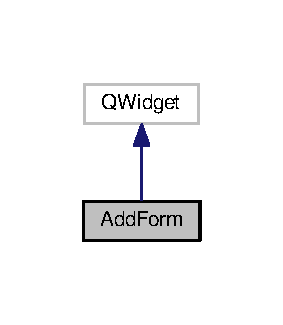
\includegraphics[width=136pt]{class_add_form__inherit__graph}
\end{center}
\end{figure}


Collaboration diagram for Add\+Form\+:\nopagebreak
\begin{figure}[H]
\begin{center}
\leavevmode
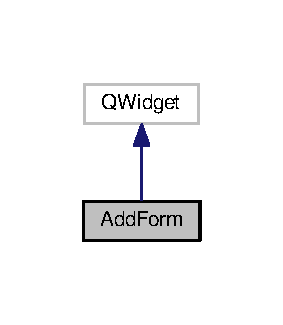
\includegraphics[width=136pt]{class_add_form__coll__graph}
\end{center}
\end{figure}
\subsection*{Signals}
\begin{DoxyCompactItemize}
\item 
void {\bfseries On\+Close} ()\hypertarget{class_add_form_aa161d4984cedd6ca6cc3dab1641beeea}{}\label{class_add_form_aa161d4984cedd6ca6cc3dab1641beeea}

\end{DoxyCompactItemize}
\subsection*{Public Member Functions}
\begin{DoxyCompactItemize}
\item 
{\bfseries Add\+Form} (Q\+Widget $\ast$parent=0)\hypertarget{class_add_form_a623e493b6c6cb526d2a624010fe6efca}{}\label{class_add_form_a623e493b6c6cb526d2a624010fe6efca}

\item 
void {\bfseries Set\+Model} (Q\+Abstract\+Item\+Model $\ast$model)\hypertarget{class_add_form_a2edb1f6faa703e3f5129bb91907964d1}{}\label{class_add_form_a2edb1f6faa703e3f5129bb91907964d1}

\item 
void {\bfseries Show\+Model\+Data} (const Q\+Model\+Index \&index)\hypertarget{class_add_form_a8d77f148efbb818939d10821e6a3c6fd}{}\label{class_add_form_a8d77f148efbb818939d10821e6a3c6fd}

\item 
bool {\bfseries event} (Q\+Event $\ast$event) override\hypertarget{class_add_form_a488387f47577f8742c920e761e9e2c63}{}\label{class_add_form_a488387f47577f8742c920e761e9e2c63}

\end{DoxyCompactItemize}


The documentation for this class was generated from the following files\+:\begin{DoxyCompactItemize}
\item 
/home/curunir/\+Documents/\+M\+A\+S\+S/\+Plugins/\+Task\+List\+View/addform.\+h\item 
/home/curunir/\+Documents/\+M\+A\+S\+S/\+Plugins/\+Task\+List\+View/addform.\+cpp\end{DoxyCompactItemize}

\hypertarget{class_a_r_neural_network_view}{}\section{A\+R\+Neural\+Network\+View Class Reference}
\label{class_a_r_neural_network_view}\index{A\+R\+Neural\+Network\+View@{A\+R\+Neural\+Network\+View}}
Inheritance diagram for A\+R\+Neural\+Network\+View\+:\begin{figure}[H]
\begin{center}
\leavevmode
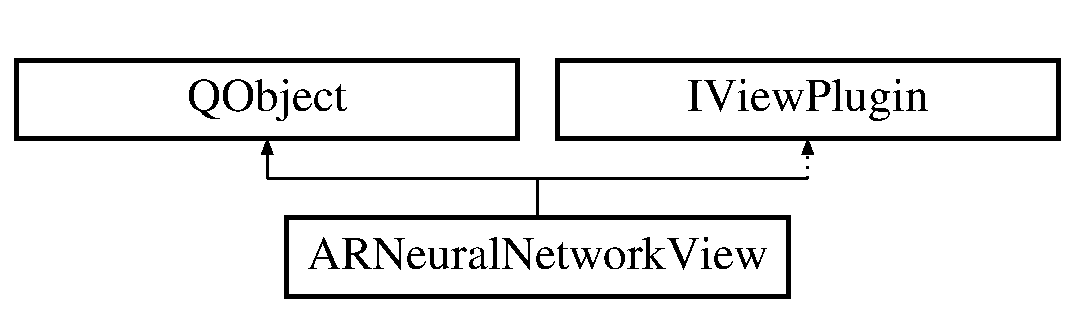
\includegraphics[height=2.000000cm]{class_a_r_neural_network_view}
\end{center}
\end{figure}
\subsection*{Public Slots}
\begin{DoxyCompactItemize}
\item 
\mbox{\Hypertarget{class_a_r_neural_network_view_ae72f15b3cabb9671d3193b1a0a389b5d}\label{class_a_r_neural_network_view_ae72f15b3cabb9671d3193b1a0a389b5d}} 
bool {\bfseries Close} () override
\end{DoxyCompactItemize}
\subsection*{Public Member Functions}
\begin{DoxyCompactItemize}
\item 
\mbox{\Hypertarget{class_a_r_neural_network_view_adfd8b5d501011015ce400df5c43a52da}\label{class_a_r_neural_network_view_adfd8b5d501011015ce400df5c43a52da}} 
void {\bfseries On\+All\+Setup} () override
\item 
\mbox{\Hypertarget{class_a_r_neural_network_view_ad6bd977f54c1f9683bdcec3599c8b2b1}\label{class_a_r_neural_network_view_ad6bd977f54c1f9683bdcec3599c8b2b1}} 
Q\+String {\bfseries Get\+Last\+Error} () override
\item 
\mbox{\Hypertarget{class_a_r_neural_network_view_a1db4e02fbfb62f194d2ffe76f9fb5bc7}\label{class_a_r_neural_network_view_a1db4e02fbfb62f194d2ffe76f9fb5bc7}} 
void {\bfseries Set\+Model} (Q\+Object $\ast$model) override
\item 
\mbox{\Hypertarget{class_a_r_neural_network_view_ad6df97a34949027264a221952677e92d}\label{class_a_r_neural_network_view_ad6df97a34949027264a221952677e92d}} 
bool {\bfseries Open} (Q\+Widget $\ast$parent) override
\end{DoxyCompactItemize}


The documentation for this class was generated from the following files\+:\begin{DoxyCompactItemize}
\item 
C\+:/\+Users/\+Curunir/\+Desktop/\+M\+A\+S\+S/\+Plugins/\+A\+R\+Neural\+Network\+View/arneuralnetworkview.\+h\item 
C\+:/\+Users/\+Curunir/\+Desktop/\+M\+A\+S\+S/\+Plugins/\+A\+R\+Neural\+Network\+View/arneuralnetworkview.\+cpp\end{DoxyCompactItemize}

\hypertarget{class_a_r_t_network}{}\section{A\+R\+T\+Network Class Reference}
\label{class_a_r_t_network}\index{A\+R\+T\+Network@{A\+R\+T\+Network}}


Inheritance diagram for A\+R\+T\+Network\+:\nopagebreak
\begin{figure}[H]
\begin{center}
\leavevmode
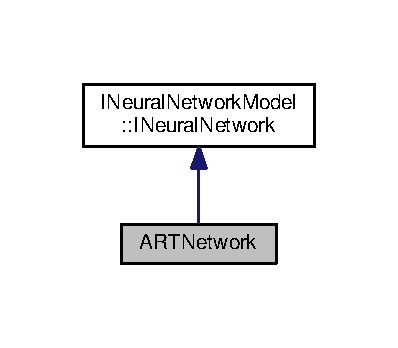
\includegraphics[width=191pt]{class_a_r_t_network__inherit__graph}
\end{center}
\end{figure}


Collaboration diagram for A\+R\+T\+Network\+:\nopagebreak
\begin{figure}[H]
\begin{center}
\leavevmode
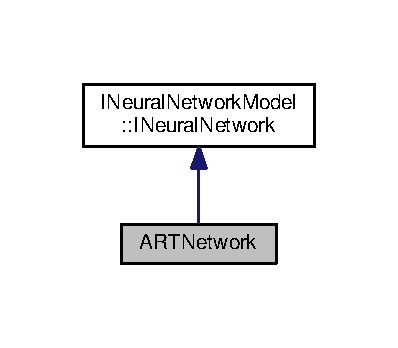
\includegraphics[width=191pt]{class_a_r_t_network__coll__graph}
\end{center}
\end{figure}
\subsection*{Public Member Functions}
\begin{DoxyCompactItemize}
\item 
bool {\bfseries Set\+Network\+Params} (Q\+Json\+Object params) override\hypertarget{class_a_r_t_network_ab473057b03bf299702c879dff08a6128}{}\label{class_a_r_t_network_ab473057b03bf299702c879dff08a6128}

\item 
void {\bfseries Setup\+SamplesF} (Q\+Json\+Object parameters, \hyperlink{class_q_vector}{Q\+Vector}$<$ \hyperlink{class_q_pair}{Input\+SampleF} $>$ $\ast$samples) override\hypertarget{class_a_r_t_network_a7e6818c24d13b718d6d8807db46b0016}{}\label{class_a_r_t_network_a7e6818c24d13b718d6d8807db46b0016}

\item 
void {\bfseries Setup\+SamplesI} (Q\+Json\+Object parameters, \hyperlink{class_q_vector}{Q\+Vector}$<$ \hyperlink{class_q_pair}{Input\+SampleI} $>$ $\ast$samples) override\hypertarget{class_a_r_t_network_a1f5750542a93bffeedacf74f780a2f2b}{}\label{class_a_r_t_network_a1f5750542a93bffeedacf74f780a2f2b}

\item 
bool {\bfseries Add\+Layer} (Q\+Json\+Object layer\+Params) override\hypertarget{class_a_r_t_network_a6025aa2fef98b81bc1dd9346fee1fd14}{}\label{class_a_r_t_network_a6025aa2fef98b81bc1dd9346fee1fd14}

\item 
void {\bfseries Reset\+Layers} () override\hypertarget{class_a_r_t_network_aa2ceed6fcdc4c73d0715d09881196569}{}\label{class_a_r_t_network_aa2ceed6fcdc4c73d0715d09881196569}

\item 
float {\bfseries Run\+Train\+Set} () override\hypertarget{class_a_r_t_network_affab976a674fe5c0626ce0adc896ba2b}{}\label{class_a_r_t_network_affab976a674fe5c0626ce0adc896ba2b}

\item 
\hyperlink{class_q_vector}{Q\+Vector}$<$ Q\+Variant $>$ {\bfseries Run\+Training\+And\+Get\+Result} () override\hypertarget{class_a_r_t_network_a2e9df6184463673c7620bd079609d727}{}\label{class_a_r_t_network_a2e9df6184463673c7620bd079609d727}

\item 
float {\bfseries Run\+Test\+Set} () override\hypertarget{class_a_r_t_network_ada8fa0752d7404bdac17955f23d1cf1a}{}\label{class_a_r_t_network_ada8fa0752d7404bdac17955f23d1cf1a}

\end{DoxyCompactItemize}
\subsection*{Static Public Member Functions}
\begin{DoxyCompactItemize}
\item 
static \hyperlink{class_a_r_t_network}{A\+R\+T\+Network} $\ast$ {\bfseries Make} (Q\+Json\+Object \&params\+Obj)\hypertarget{class_a_r_t_network_acc61c58d3082855607710e0f5266738c}{}\label{class_a_r_t_network_acc61c58d3082855607710e0f5266738c}

\end{DoxyCompactItemize}
\subsection*{Protected Types}
\begin{DoxyCompactItemize}
\item 
typedef \hyperlink{struct_a_r_t_1_1_network_params}{A\+R\+T\+::\+Network\+Params} {\bfseries Network\+Params}\hypertarget{class_a_r_t_network_a71deee5d6ab1571d49a259123c75dd12}{}\label{class_a_r_t_network_a71deee5d6ab1571d49a259123c75dd12}

\end{DoxyCompactItemize}


The documentation for this class was generated from the following files\+:\begin{DoxyCompactItemize}
\item 
/home/curunir/\+Documents/\+M\+A\+S\+S/\+Plugins/\+Neural\+Network\+Model/\+A\+R\+T/artnetwork.\+h\item 
/home/curunir/\+Documents/\+M\+A\+S\+S/\+Plugins/\+Neural\+Network\+Model/\+A\+R\+T/artnetwork.\+cpp\end{DoxyCompactItemize}

\hypertarget{struct_q_c_p_axis_painter_private_1_1_cached_label}{}\section{Q\+C\+P\+Axis\+Painter\+Private\+:\+:Cached\+Label Struct Reference}
\label{struct_q_c_p_axis_painter_private_1_1_cached_label}\index{Q\+C\+P\+Axis\+Painter\+Private\+::\+Cached\+Label@{Q\+C\+P\+Axis\+Painter\+Private\+::\+Cached\+Label}}
\subsection*{Public Attributes}
\begin{DoxyCompactItemize}
\item 
\mbox{\Hypertarget{struct_q_c_p_axis_painter_private_1_1_cached_label_a5f502db71c92e572f1e6f44f62c59d8e}\label{struct_q_c_p_axis_painter_private_1_1_cached_label_a5f502db71c92e572f1e6f44f62c59d8e}} 
Q\+PointF {\bfseries offset}
\item 
\mbox{\Hypertarget{struct_q_c_p_axis_painter_private_1_1_cached_label_a461597cbd470914a9d24b64d16037a88}\label{struct_q_c_p_axis_painter_private_1_1_cached_label_a461597cbd470914a9d24b64d16037a88}} 
Q\+Pixmap {\bfseries pixmap}
\end{DoxyCompactItemize}


The documentation for this struct was generated from the following file\+:\begin{DoxyCompactItemize}
\item 
C\+:/\+Users/\+Curunir/\+Desktop/\+M\+A\+S\+S/\+Plugins/\+A\+R\+Neural\+Network\+View/qcustomplot.\+h\end{DoxyCompactItemize}

\hypertarget{class_chromosome}{}\section{Chromosome Class Reference}
\label{class_chromosome}\index{Chromosome@{Chromosome}}
\subsection*{Public Member Functions}
\begin{DoxyCompactItemize}
\item 
\mbox{\Hypertarget{class_chromosome_a61b3ad7248489642452df6c6c24bf580}\label{class_chromosome_a61b3ad7248489642452df6c6c24bf580}} 
{\bfseries Chromosome} (\hyperlink{struct_genetic_algorithm_params_1_1_parameters}{Genetic\+Algorithm\+Params\+::\+Parameters} $\ast$params)
\item 
\mbox{\Hypertarget{class_chromosome_a2df6c471bc3dd1b248f93f9bccc0e483}\label{class_chromosome_a2df6c471bc3dd1b248f93f9bccc0e483}} 
int {\bfseries Get\+Value} ()
\end{DoxyCompactItemize}
\subsection*{Static Public Member Functions}
\begin{DoxyCompactItemize}
\item 
\mbox{\Hypertarget{class_chromosome_aaf9f158daad7690332a17158af82b9b3}\label{class_chromosome_aaf9f158daad7690332a17158af82b9b3}} 
static \hyperlink{class_chromosome}{Chromosome} $\ast$ {\bfseries Breed} (\hyperlink{class_chromosome}{Chromosome} $\ast$mother, \hyperlink{class_chromosome}{Chromosome} $\ast$father, bool with\+Mutation=true)
\item 
\mbox{\Hypertarget{class_chromosome_a01362e7b1547ddef9e79ce2e94d46f85}\label{class_chromosome_a01362e7b1547ddef9e79ce2e94d46f85}} 
static void {\bfseries Modificate\+Bit} (int value, int pos)
\end{DoxyCompactItemize}
\subsection*{Public Attributes}
\begin{DoxyCompactItemize}
\item 
\mbox{\Hypertarget{class_chromosome_af1e2825bfa9ca01f83610d68d7773238}\label{class_chromosome_af1e2825bfa9ca01f83610d68d7773238}} 
float {\bfseries fitness}
\item 
\mbox{\Hypertarget{class_chromosome_a9802175d2f1b9e093e2cbd93fdd22de7}\label{class_chromosome_a9802175d2f1b9e093e2cbd93fdd22de7}} 
\hyperlink{class_q_vector}{Q\+Vector}$<$ float $>$ {\bfseries genes}
\item 
\mbox{\Hypertarget{class_chromosome_a3e23041223b3fdcf0758f67c41b8d346}\label{class_chromosome_a3e23041223b3fdcf0758f67c41b8d346}} 
\hyperlink{struct_genetic_algorithm_params_1_1_parameters}{Genetic\+Algorithm\+Params\+::\+Parameters} $\ast$ {\bfseries params}
\end{DoxyCompactItemize}


The documentation for this class was generated from the following files\+:\begin{DoxyCompactItemize}
\item 
C\+:/\+Users/\+Curunir/\+Desktop/\+M\+A\+S\+S/\+Plugins/\+Neural\+Network\+Model/\+Genetic\+Algorithm/chromosome.\+h\item 
C\+:/\+Users/\+Curunir/\+Desktop/\+M\+A\+S\+S/\+Plugins/\+Neural\+Network\+Model/\+Genetic\+Algorithm/chromosome.\+cpp\end{DoxyCompactItemize}

\hypertarget{class_cipher_data_base_source_plugin}{}\section{Cipher\+Data\+Base\+Source\+Plugin Class Reference}
\label{class_cipher_data_base_source_plugin}\index{Cipher\+Data\+Base\+Source\+Plugin@{Cipher\+Data\+Base\+Source\+Plugin}}


Inheritance diagram for Cipher\+Data\+Base\+Source\+Plugin\+:\nopagebreak
\begin{figure}[H]
\begin{center}
\leavevmode
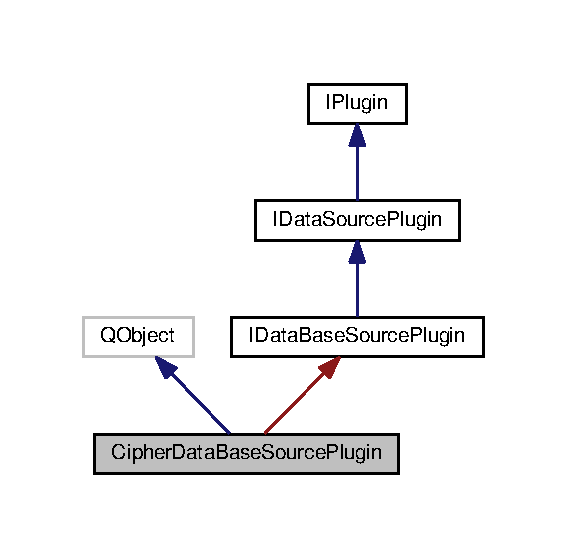
\includegraphics[width=272pt]{class_cipher_data_base_source_plugin__inherit__graph}
\end{center}
\end{figure}


Collaboration diagram for Cipher\+Data\+Base\+Source\+Plugin\+:\nopagebreak
\begin{figure}[H]
\begin{center}
\leavevmode
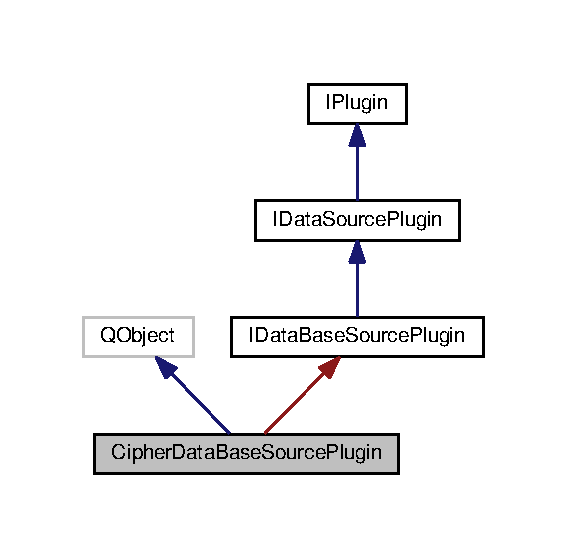
\includegraphics[width=272pt]{class_cipher_data_base_source_plugin__coll__graph}
\end{center}
\end{figure}
\subsection*{Public Member Functions}
\begin{DoxyCompactItemize}
\item 
void {\bfseries On\+All\+Setup} () override\hypertarget{class_cipher_data_base_source_plugin_a17963e88c679924dc37da6ded9e71da6}{}\label{class_cipher_data_base_source_plugin_a17963e88c679924dc37da6ded9e71da6}

\item 
Q\+String {\bfseries Get\+Last\+Error} () override\hypertarget{class_cipher_data_base_source_plugin_a4a32c746ef184f6cbdc2cfb37c872c5d}{}\label{class_cipher_data_base_source_plugin_a4a32c746ef184f6cbdc2cfb37c872c5d}

\item 
void {\bfseries Setup} () override\hypertarget{class_cipher_data_base_source_plugin_aeec7843b9e6ad2c36a0e2929a1626436}{}\label{class_cipher_data_base_source_plugin_aeec7843b9e6ad2c36a0e2929a1626436}

\item 
Q\+Sql\+Query {\bfseries Execute\+Query} (Q\+String \&query\+Text) override\hypertarget{class_cipher_data_base_source_plugin_a02d5a7888d88142660ca6ea5982446ec}{}\label{class_cipher_data_base_source_plugin_a02d5a7888d88142660ca6ea5982446ec}

\item 
Q\+Sql\+Query {\bfseries Execute\+Query} (Q\+String \&query\+Text, \hyperlink{class_q_list}{Q\+List}$<$ Q\+String $>$ $\ast$value\+Placeholders, \hyperlink{class_q_list}{Q\+List}$<$ Q\+Variant $>$ $\ast$values) override\hypertarget{class_cipher_data_base_source_plugin_aa2abe6b9929628fbb7feb62ed09b1111}{}\label{class_cipher_data_base_source_plugin_aa2abe6b9929628fbb7feb62ed09b1111}

\end{DoxyCompactItemize}


The documentation for this class was generated from the following files\+:\begin{DoxyCompactItemize}
\item 
/home/curunir/\+Documents/\+M\+A\+S\+S/\+Plugins/\+Cipher\+Data\+Base\+Source/cipherdatabasesourceplugin.\+h\item 
/home/curunir/\+Documents/\+M\+A\+S\+S/\+Plugins/\+Cipher\+Data\+Base\+Source/cipherdatabasesourceplugin.\+cpp\end{DoxyCompactItemize}

\hypertarget{class_comparing_layer}{}\section{Comparing\+Layer Class Reference}
\label{class_comparing_layer}\index{Comparing\+Layer@{Comparing\+Layer}}


Collaboration diagram for Comparing\+Layer\+:\nopagebreak
\begin{figure}[H]
\begin{center}
\leavevmode
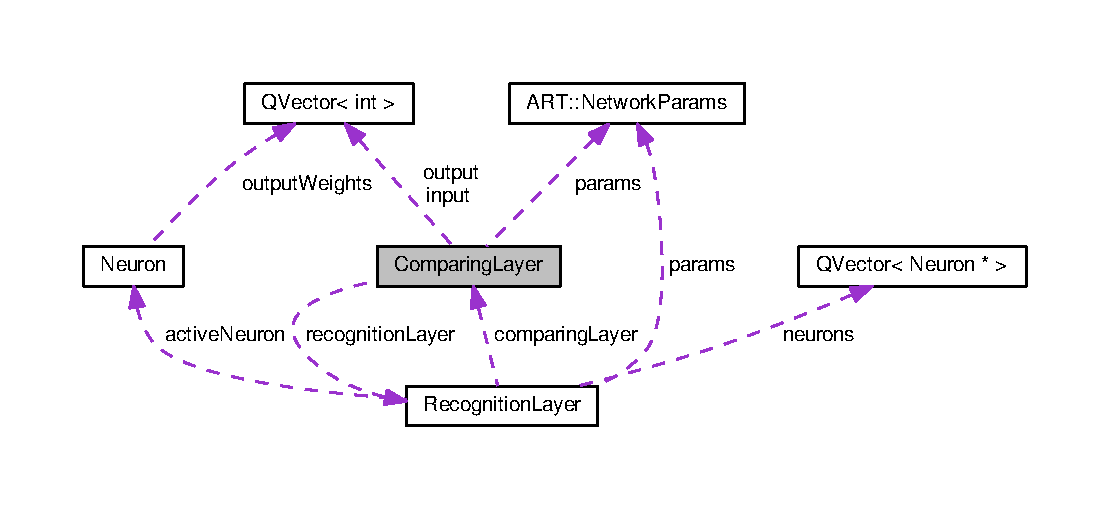
\includegraphics[width=350pt]{class_comparing_layer__coll__graph}
\end{center}
\end{figure}
\subsection*{Public Member Functions}
\begin{DoxyCompactItemize}
\item 
{\bfseries Comparing\+Layer} (int size, \hyperlink{struct_a_r_t_1_1_network_params}{Network\+Params} $\ast$params)\hypertarget{class_comparing_layer_ae9e621952f79718c948f31a9569804da}{}\label{class_comparing_layer_ae9e621952f79718c948f31a9569804da}

\item 
void {\bfseries Input} (\hyperlink{class_q_vector}{Q\+Vector}$<$ int $>$ \&input)\hypertarget{class_comparing_layer_a85b9d3ff04a58d2159226e760b9607d0}{}\label{class_comparing_layer_a85b9d3ff04a58d2159226e760b9607d0}

\item 
void {\bfseries Response} (\hyperlink{class_q_vector}{Q\+Vector}$<$ int $>$ \&response)\hypertarget{class_comparing_layer_a7fd6674cdb61903b3ad9428cafcc1c09}{}\label{class_comparing_layer_a7fd6674cdb61903b3ad9428cafcc1c09}

\end{DoxyCompactItemize}
\subsection*{Public Attributes}
\begin{DoxyCompactItemize}
\item 
\hyperlink{struct_a_r_t_1_1_network_params}{Network\+Params} $\ast$ {\bfseries params}\hypertarget{class_comparing_layer_a2c69b1c07b6cdf6ff5230680776bcb71}{}\label{class_comparing_layer_a2c69b1c07b6cdf6ff5230680776bcb71}

\item 
\hyperlink{class_q_vector}{Q\+Vector}$<$ int $>$ $\ast$ {\bfseries input}\hypertarget{class_comparing_layer_ac530a1f5b25253d54cc6ee7331d6cc4f}{}\label{class_comparing_layer_ac530a1f5b25253d54cc6ee7331d6cc4f}

\item 
\hyperlink{class_q_vector}{Q\+Vector}$<$ int $>$ {\bfseries output}\hypertarget{class_comparing_layer_af224db952c3b4562e4f9e758369a53f8}{}\label{class_comparing_layer_af224db952c3b4562e4f9e758369a53f8}

\item 
\hyperlink{class_recognition_layer}{Recognition\+Layer} $\ast$ {\bfseries recognition\+Layer}\hypertarget{class_comparing_layer_a76b454e89f511095e167fd7352595e9b}{}\label{class_comparing_layer_a76b454e89f511095e167fd7352595e9b}

\end{DoxyCompactItemize}
\subsection*{Protected Types}
\begin{DoxyCompactItemize}
\item 
typedef \hyperlink{struct_a_r_t_1_1_network_params}{A\+R\+T\+::\+Network\+Params} {\bfseries Network\+Params}\hypertarget{class_comparing_layer_af0bbef51f4b8cc8693626693a25b3b3f}{}\label{class_comparing_layer_af0bbef51f4b8cc8693626693a25b3b3f}

\end{DoxyCompactItemize}


The documentation for this class was generated from the following files\+:\begin{DoxyCompactItemize}
\item 
/home/curunir/\+Documents/\+M\+A\+S\+S/\+Plugins/\+Neural\+Network\+Model/\+A\+R\+T/comparinglayer.\+h\item 
/home/curunir/\+Documents/\+M\+A\+S\+S/\+Plugins/\+Neural\+Network\+Model/\+A\+R\+T/comparinglayer.\+cpp\end{DoxyCompactItemize}

\hypertarget{class_design_proxy_model}{}\section{Design\+Proxy\+Model Class Reference}
\label{class_design_proxy_model}\index{Design\+Proxy\+Model@{Design\+Proxy\+Model}}
Inheritance diagram for Design\+Proxy\+Model\+:\begin{figure}[H]
\begin{center}
\leavevmode
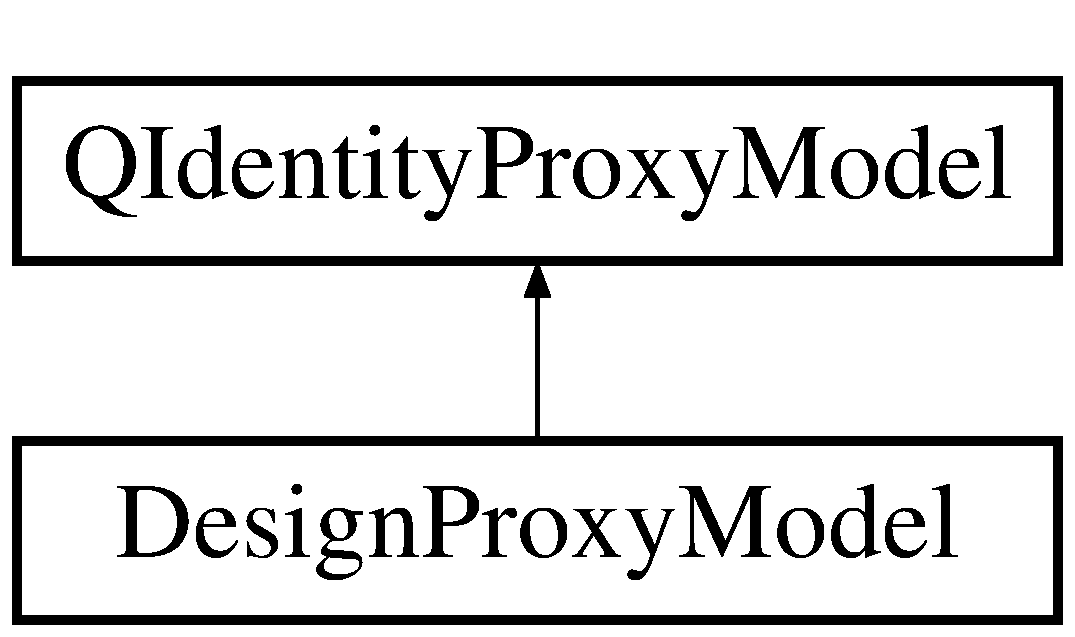
\includegraphics[height=2.000000cm]{class_design_proxy_model}
\end{center}
\end{figure}
\subsection*{Public Member Functions}
\begin{DoxyCompactItemize}
\item 
\mbox{\Hypertarget{class_design_proxy_model_a2f32a37a9e0e12091ffa25d12c2cf172}\label{class_design_proxy_model_a2f32a37a9e0e12091ffa25d12c2cf172}} 
{\bfseries Design\+Proxy\+Model} (Q\+Abstract\+Item\+Model $\ast$model)
\item 
\mbox{\Hypertarget{class_design_proxy_model_a83da41a240aa8524cc5694b0db9eacfa}\label{class_design_proxy_model_a83da41a240aa8524cc5694b0db9eacfa}} 
Q\+Variant {\bfseries data} (const Q\+Model\+Index \&index, int role) const
\item 
\mbox{\Hypertarget{class_design_proxy_model_adc16f436d8f8ebb49ec84d0522de78e0}\label{class_design_proxy_model_adc16f436d8f8ebb49ec84d0522de78e0}} 
Q\+Variant {\bfseries header\+Data} (int section, Qt\+::\+Orientation orientation, int role=Qt\+::\+Display\+Role) const
\end{DoxyCompactItemize}


The documentation for this class was generated from the following files\+:\begin{DoxyCompactItemize}
\item 
C\+:/\+Users/\+Curunir/\+Desktop/\+M\+A\+S\+S/\+Plugins/\+Task\+List\+View/designproxymodel.\+h\item 
C\+:/\+Users/\+Curunir/\+Desktop/\+M\+A\+S\+S/\+Plugins/\+Task\+List\+View/designproxymodel.\+cpp\end{DoxyCompactItemize}

\hypertarget{class_extendable_data_base_manager_plugin}{}\section{Extendable\+Data\+Base\+Manager\+Plugin Class Reference}
\label{class_extendable_data_base_manager_plugin}\index{Extendable\+Data\+Base\+Manager\+Plugin@{Extendable\+Data\+Base\+Manager\+Plugin}}


Inheritance diagram for Extendable\+Data\+Base\+Manager\+Plugin\+:\nopagebreak
\begin{figure}[H]
\begin{center}
\leavevmode
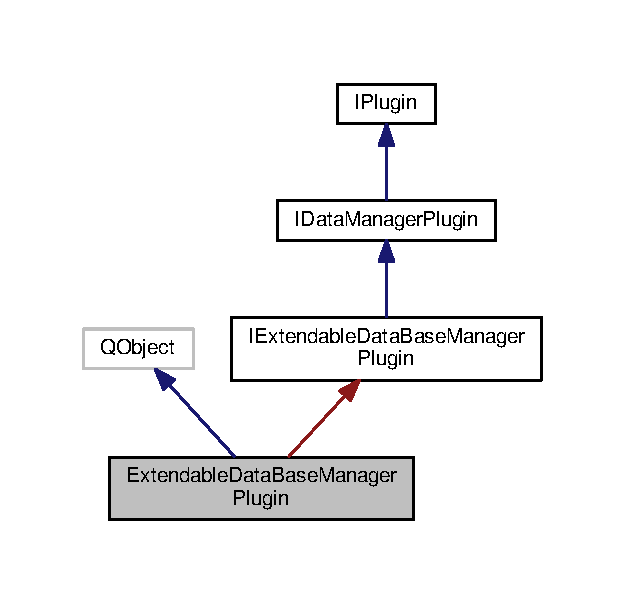
\includegraphics[width=300pt]{class_extendable_data_base_manager_plugin__inherit__graph}
\end{center}
\end{figure}


Collaboration diagram for Extendable\+Data\+Base\+Manager\+Plugin\+:\nopagebreak
\begin{figure}[H]
\begin{center}
\leavevmode
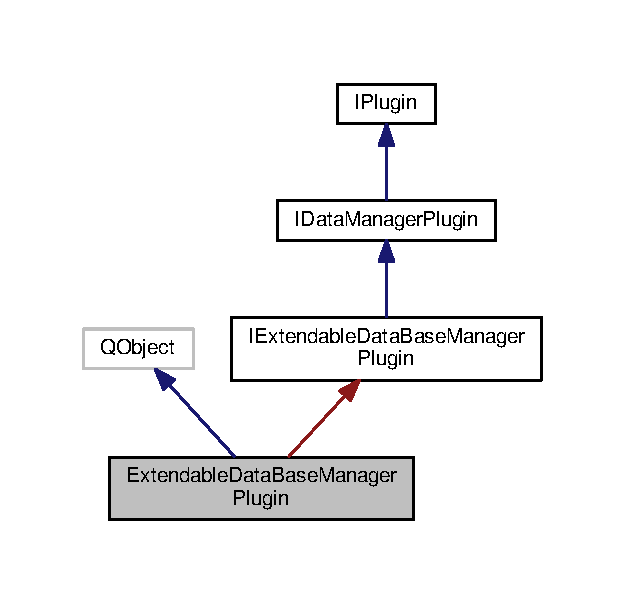
\includegraphics[width=300pt]{class_extendable_data_base_manager_plugin__coll__graph}
\end{center}
\end{figure}
\subsection*{Public Member Functions}
\begin{DoxyCompactItemize}
\item 
virtual void {\bfseries On\+All\+Setup} ()\hypertarget{class_extendable_data_base_manager_plugin_a8331c3bd54725a10f79bcacde178774b}{}\label{class_extendable_data_base_manager_plugin_a8331c3bd54725a10f79bcacde178774b}

\item 
virtual Q\+String {\bfseries Get\+Last\+Error} ()\hypertarget{class_extendable_data_base_manager_plugin_a168d8e9dadf224d24c855fe376569857}{}\label{class_extendable_data_base_manager_plugin_a168d8e9dadf224d24c855fe376569857}

\item 
bool {\bfseries Set\+Data\+Source} (Q\+Object $\ast$data\+Source) override\hypertarget{class_extendable_data_base_manager_plugin_aa28d8bd15f2547b70e82452bdd8d0c70}{}\label{class_extendable_data_base_manager_plugin_aa28d8bd15f2547b70e82452bdd8d0c70}

\item 
\hyperlink{class_q_list}{Q\+List}$<$ \hyperlink{class_i_extendable_data_base_manager_plugin_1_1_manager_data_item}{Manager\+Data\+Item} $>$ {\bfseries Get\+Data\+List} (Q\+String table\+Name) override\hypertarget{class_extendable_data_base_manager_plugin_a2c2450f08baccb26e3aade32a5879f27}{}\label{class_extendable_data_base_manager_plugin_a2c2450f08baccb26e3aade32a5879f27}

\item 
\hyperlink{class_i_extendable_data_base_manager_plugin_1_1_manager_data_item}{Manager\+Data\+Item} {\bfseries Get\+Data\+Item} (Q\+String table\+Name, int id) override\hypertarget{class_extendable_data_base_manager_plugin_a1027e67334110767807dccd64cd4946d}{}\label{class_extendable_data_base_manager_plugin_a1027e67334110767807dccd64cd4946d}

\item 
Q\+Abstract\+Item\+Model $\ast$ {\bfseries Get\+Data\+Model} (Q\+String table\+Name) override\hypertarget{class_extendable_data_base_manager_plugin_a32a7f0127593a70e827b39a462cb6d02}{}\label{class_extendable_data_base_manager_plugin_a32a7f0127593a70e827b39a462cb6d02}

\item 
\hyperlink{class_q_map}{Q\+Map}$<$ Q\+String, Q\+Variant\+::\+Type $>$ {\bfseries Get\+Table\+Header} (Q\+String table\+Name) override\hypertarget{class_extendable_data_base_manager_plugin_a8ddef0ec955d01c3e59f5dec90eed26b}{}\label{class_extendable_data_base_manager_plugin_a8ddef0ec955d01c3e59f5dec90eed26b}

\item 
bool {\bfseries Set\+Relation} (Q\+String table\+Name, Q\+String relation\+Name, \hyperlink{class_q_map}{Q\+Map}$<$ Q\+String, Q\+Variant\+::\+Type $>$ fields, \hyperlink{class_q_vector}{Q\+Vector}$<$ Q\+Variant $>$ default\+Data) override\hypertarget{class_extendable_data_base_manager_plugin_a572eff2f383b0be3e99178e6dcee78e9}{}\label{class_extendable_data_base_manager_plugin_a572eff2f383b0be3e99178e6dcee78e9}

\item 
bool {\bfseries Delete\+Relation} (Q\+String table\+Name, Q\+String relation\+Name) override\hypertarget{class_extendable_data_base_manager_plugin_a75fccf6c256cf6500ac1d7421c131bc2}{}\label{class_extendable_data_base_manager_plugin_a75fccf6c256cf6500ac1d7421c131bc2}

\item 
bool {\bfseries Set\+Active\+Relation} (Q\+String table\+Name, Q\+String relation\+Name) override\hypertarget{class_extendable_data_base_manager_plugin_a2a8f2e7f2fbeef891da297dadd0cd548}{}\label{class_extendable_data_base_manager_plugin_a2a8f2e7f2fbeef891da297dadd0cd548}

\item 
int {\bfseries Add\+Item} (Q\+String table\+Name, \hyperlink{class_i_extendable_data_base_manager_plugin_1_1_manager_data_item}{Manager\+Data\+Item} item) override\hypertarget{class_extendable_data_base_manager_plugin_a1fe950472f4798d7278dca6b24055c9c}{}\label{class_extendable_data_base_manager_plugin_a1fe950472f4798d7278dca6b24055c9c}

\item 
bool {\bfseries Edit\+Item} (Q\+String table\+Name, \hyperlink{class_i_extendable_data_base_manager_plugin_1_1_manager_data_item}{Manager\+Data\+Item} item) override\hypertarget{class_extendable_data_base_manager_plugin_a09ee5b2121ac6f5e3311701a59584fc6}{}\label{class_extendable_data_base_manager_plugin_a09ee5b2121ac6f5e3311701a59584fc6}

\item 
bool {\bfseries Delete\+Item} (Q\+String table\+Name, int id) override\hypertarget{class_extendable_data_base_manager_plugin_a91081c54f128faf88cc4f25aaf9980f4}{}\label{class_extendable_data_base_manager_plugin_a91081c54f128faf88cc4f25aaf9980f4}

\end{DoxyCompactItemize}


The documentation for this class was generated from the following files\+:\begin{DoxyCompactItemize}
\item 
/home/curunir/\+Documents/\+M\+A\+S\+S/\+Plugins/\+Extendable\+Data\+Base\+Manager/extendabledatabasemanagerplugin.\+h\item 
/home/curunir/\+Documents/\+M\+A\+S\+S/\+Plugins/\+Extendable\+Data\+Base\+Manager/extendabledatabasemanagerplugin.\+cpp\end{DoxyCompactItemize}

\hypertarget{class_extendable_item_model}{}\section{Extendable\+Item\+Model Class Reference}
\label{class_extendable_item_model}\index{Extendable\+Item\+Model@{Extendable\+Item\+Model}}
Inheritance diagram for Extendable\+Item\+Model\+:\begin{figure}[H]
\begin{center}
\leavevmode
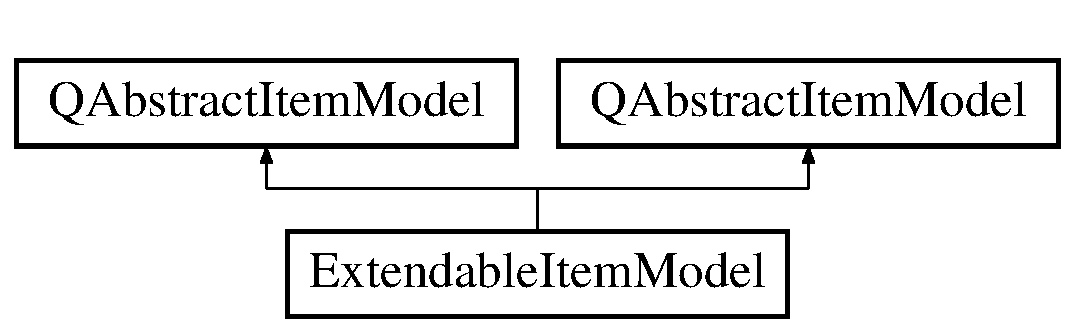
\includegraphics[height=2.000000cm]{class_extendable_item_model}
\end{center}
\end{figure}
\subsection*{Public Member Functions}
\begin{DoxyCompactItemize}
\item 
\mbox{\Hypertarget{class_extendable_item_model_a896f75df752535510036e0c5d42fac8a}\label{class_extendable_item_model_a896f75df752535510036e0c5d42fac8a}} 
{\bfseries Extendable\+Item\+Model} (Q\+String table\+Name, \hyperlink{class_i_extendable_data_base_manager_plugin}{I\+Extendable\+Data\+Base\+Manager\+Plugin} $\ast$data\+Manager, Q\+Object $\ast$parent=0)
\item 
\mbox{\Hypertarget{class_extendable_item_model_ae5887f5d5086a094d712e2f7a1f6b84b}\label{class_extendable_item_model_ae5887f5d5086a094d712e2f7a1f6b84b}} 
void {\bfseries Load\+Data} ()
\item 
\mbox{\Hypertarget{class_extendable_item_model_a49139d270880dc35b44b51bd95a36e89}\label{class_extendable_item_model_a49139d270880dc35b44b51bd95a36e89}} 
bool {\bfseries Attach\+Relation} (Q\+String relation\+Name, \hyperlink{class_q_vector}{Q\+Vector}$<$ Q\+Variant $>$ default\+Data)
\item 
\mbox{\Hypertarget{class_extendable_item_model_ad5ce2033c7ba133259dc5c46a98e4694}\label{class_extendable_item_model_ad5ce2033c7ba133259dc5c46a98e4694}} 
void {\bfseries Set\+Active\+Relation} (Q\+String relation\+Name)
\item 
\mbox{\Hypertarget{class_extendable_item_model_a7b8f0527a5d89bf515e4ba1177294e4e}\label{class_extendable_item_model_a7b8f0527a5d89bf515e4ba1177294e4e}} 
virtual Q\+Variant {\bfseries data} (const Q\+Model\+Index \&index, int role) const
\item 
\mbox{\Hypertarget{class_extendable_item_model_ae75da3ede02d0f81e3a3523a99d9306f}\label{class_extendable_item_model_ae75da3ede02d0f81e3a3523a99d9306f}} 
\hyperlink{class_q_map}{Q\+Map}$<$ int, Q\+Variant $>$ {\bfseries item\+Data} (const Q\+Model\+Index \&index) const override
\item 
\mbox{\Hypertarget{class_extendable_item_model_af798eeed6826786f0c576e1f4547f191}\label{class_extendable_item_model_af798eeed6826786f0c576e1f4547f191}} 
virtual Qt\+::\+Item\+Flags {\bfseries flags} (const Q\+Model\+Index \&index) const
\item 
\mbox{\Hypertarget{class_extendable_item_model_a6b518f098fad1c4a3e20ac5ea02f467b}\label{class_extendable_item_model_a6b518f098fad1c4a3e20ac5ea02f467b}} 
virtual Q\+Variant {\bfseries header\+Data} (int section, Qt\+::\+Orientation orientation, int role=Qt\+::\+Display\+Role) const
\item 
\mbox{\Hypertarget{class_extendable_item_model_af8ec9ce6a15ba7bfb11bf0162dd44c0c}\label{class_extendable_item_model_af8ec9ce6a15ba7bfb11bf0162dd44c0c}} 
virtual Q\+Model\+Index {\bfseries index} (int row, int column, const Q\+Model\+Index \&parent=Q\+Model\+Index()) const
\item 
\mbox{\Hypertarget{class_extendable_item_model_a8fa3d6ed261d2d811740a266e5bf3d85}\label{class_extendable_item_model_a8fa3d6ed261d2d811740a266e5bf3d85}} 
virtual Q\+Model\+Index {\bfseries parent} (const Q\+Model\+Index \&index) const
\item 
\mbox{\Hypertarget{class_extendable_item_model_a1f111148c43b7945ec13b31e1fd68602}\label{class_extendable_item_model_a1f111148c43b7945ec13b31e1fd68602}} 
virtual int {\bfseries row\+Count} (const Q\+Model\+Index \&parent=Q\+Model\+Index()) const
\item 
\mbox{\Hypertarget{class_extendable_item_model_a60bf085a67ace60208056f35af403965}\label{class_extendable_item_model_a60bf085a67ace60208056f35af403965}} 
virtual int {\bfseries column\+Count} (const Q\+Model\+Index \&parent=Q\+Model\+Index()) const
\item 
\mbox{\Hypertarget{class_extendable_item_model_a1ce2fcafb7dea41b0d922b7172d23e0d}\label{class_extendable_item_model_a1ce2fcafb7dea41b0d922b7172d23e0d}} 
virtual bool {\bfseries insert\+Rows} (int row, int count, const Q\+Model\+Index \&parent)
\item 
\mbox{\Hypertarget{class_extendable_item_model_abd1e1a5e8d942216dd9cfeaab5564eda}\label{class_extendable_item_model_abd1e1a5e8d942216dd9cfeaab5564eda}} 
virtual bool {\bfseries insert\+Columns} (int column, int count, const Q\+Model\+Index \&parent)
\item 
\mbox{\Hypertarget{class_extendable_item_model_a0845398488e6f714ca6eda0670a7aa8e}\label{class_extendable_item_model_a0845398488e6f714ca6eda0670a7aa8e}} 
virtual bool {\bfseries remove\+Rows} (int row, int count, const Q\+Model\+Index \&parent)
\item 
\mbox{\Hypertarget{class_extendable_item_model_a7d00afeac188e21c0d165b14a3c421cd}\label{class_extendable_item_model_a7d00afeac188e21c0d165b14a3c421cd}} 
virtual bool {\bfseries move\+Rows} (const Q\+Model\+Index \&source\+Parent, int source\+Row, int count, const Q\+Model\+Index \&destination\+Parent, int destination\+Child)
\item 
\mbox{\Hypertarget{class_extendable_item_model_a72c65abf36fbe31778e73c983da260cc}\label{class_extendable_item_model_a72c65abf36fbe31778e73c983da260cc}} 
virtual bool {\bfseries set\+Data} (const Q\+Model\+Index \&index, const Q\+Variant \&value, int role)
\item 
\mbox{\Hypertarget{class_extendable_item_model_a5e875f885ba62365a738a7820ceb8e4c}\label{class_extendable_item_model_a5e875f885ba62365a738a7820ceb8e4c}} 
virtual Q\+String\+List {\bfseries mime\+Types} () const
\item 
\mbox{\Hypertarget{class_extendable_item_model_ae2e75332303501a90e0fb5b8cebef1d7}\label{class_extendable_item_model_ae2e75332303501a90e0fb5b8cebef1d7}} 
virtual Q\+Mime\+Data $\ast$ {\bfseries mime\+Data} (const Q\+Model\+Index\+List \&indexes) const
\item 
\mbox{\Hypertarget{class_extendable_item_model_ae6dc27740bcfff8ecd88e3af76f7d3ac}\label{class_extendable_item_model_ae6dc27740bcfff8ecd88e3af76f7d3ac}} 
virtual bool {\bfseries drop\+Mime\+Data} (const Q\+Mime\+Data $\ast$data, Qt\+::\+Drop\+Action action, int row, int column, const Q\+Model\+Index \&parent)
\item 
\mbox{\Hypertarget{class_extendable_item_model_a896f75df752535510036e0c5d42fac8a}\label{class_extendable_item_model_a896f75df752535510036e0c5d42fac8a}} 
{\bfseries Extendable\+Item\+Model} (Q\+String table\+Name, \hyperlink{class_i_extendable_data_base_manager_plugin}{I\+Extendable\+Data\+Base\+Manager\+Plugin} $\ast$data\+Manager, Q\+Object $\ast$parent=0)
\item 
\mbox{\Hypertarget{class_extendable_item_model_ae5887f5d5086a094d712e2f7a1f6b84b}\label{class_extendable_item_model_ae5887f5d5086a094d712e2f7a1f6b84b}} 
void {\bfseries Load\+Data} ()
\item 
\mbox{\Hypertarget{class_extendable_item_model_a49139d270880dc35b44b51bd95a36e89}\label{class_extendable_item_model_a49139d270880dc35b44b51bd95a36e89}} 
bool {\bfseries Attach\+Relation} (Q\+String relation\+Name, \hyperlink{class_q_vector}{Q\+Vector}$<$ Q\+Variant $>$ default\+Data)
\item 
\mbox{\Hypertarget{class_extendable_item_model_ad5ce2033c7ba133259dc5c46a98e4694}\label{class_extendable_item_model_ad5ce2033c7ba133259dc5c46a98e4694}} 
void {\bfseries Set\+Active\+Relation} (Q\+String relation\+Name)
\item 
\mbox{\Hypertarget{class_extendable_item_model_aa9ef36b1912f6a510541509df53e9e03}\label{class_extendable_item_model_aa9ef36b1912f6a510541509df53e9e03}} 
virtual Q\+Variant {\bfseries data} (const Q\+Model\+Index \&index, int role) const
\item 
\mbox{\Hypertarget{class_extendable_item_model_a71d1609484e15a16e2a07c54aa465381}\label{class_extendable_item_model_a71d1609484e15a16e2a07c54aa465381}} 
virtual Qt\+::\+Item\+Flags {\bfseries flags} (const Q\+Model\+Index \&index) const
\item 
\mbox{\Hypertarget{class_extendable_item_model_a5ad119a5b156acf0b8ae4090e8ec72ce}\label{class_extendable_item_model_a5ad119a5b156acf0b8ae4090e8ec72ce}} 
virtual Q\+Variant {\bfseries header\+Data} (int section, Qt\+::\+Orientation orientation, int role=Qt\+::\+Display\+Role) const
\item 
\mbox{\Hypertarget{class_extendable_item_model_ae296561b96cb7d302d27d90a8743e911}\label{class_extendable_item_model_ae296561b96cb7d302d27d90a8743e911}} 
virtual Q\+Model\+Index {\bfseries index} (int row, int column, const Q\+Model\+Index \&parent=Q\+Model\+Index()) const
\item 
\mbox{\Hypertarget{class_extendable_item_model_a5ea988b185fb922797fb153ac284516f}\label{class_extendable_item_model_a5ea988b185fb922797fb153ac284516f}} 
virtual Q\+Model\+Index {\bfseries parent} (const Q\+Model\+Index \&index) const
\item 
\mbox{\Hypertarget{class_extendable_item_model_a850c9252fb6b59d3e481e564e1c89a60}\label{class_extendable_item_model_a850c9252fb6b59d3e481e564e1c89a60}} 
virtual int {\bfseries row\+Count} (const Q\+Model\+Index \&parent=Q\+Model\+Index()) const
\item 
\mbox{\Hypertarget{class_extendable_item_model_a25cdc83a4bb99ee802aa1b8533e0775e}\label{class_extendable_item_model_a25cdc83a4bb99ee802aa1b8533e0775e}} 
virtual int {\bfseries column\+Count} (const Q\+Model\+Index \&parent=Q\+Model\+Index()) const
\item 
\mbox{\Hypertarget{class_extendable_item_model_adff898fac861b1cc06783b1b5f810d36}\label{class_extendable_item_model_adff898fac861b1cc06783b1b5f810d36}} 
virtual bool {\bfseries insert\+Rows} (int row, int count, const Q\+Model\+Index \&parent)
\item 
\mbox{\Hypertarget{class_extendable_item_model_aa00ea86bd42efb9e82e08da187b6c7ec}\label{class_extendable_item_model_aa00ea86bd42efb9e82e08da187b6c7ec}} 
virtual bool {\bfseries insert\+Columns} (int column, int count, const Q\+Model\+Index \&parent)
\item 
\mbox{\Hypertarget{class_extendable_item_model_a066c457590916ebd1fb9e9694415c988}\label{class_extendable_item_model_a066c457590916ebd1fb9e9694415c988}} 
virtual bool {\bfseries remove\+Rows} (int row, int count, const Q\+Model\+Index \&parent)
\item 
\mbox{\Hypertarget{class_extendable_item_model_a2adfee96dc6e2c8f050c1bba9a4cf170}\label{class_extendable_item_model_a2adfee96dc6e2c8f050c1bba9a4cf170}} 
virtual bool {\bfseries move\+Rows} (const Q\+Model\+Index \&source\+Parent, int source\+Row, int count, const Q\+Model\+Index \&destination\+Parent, int destination\+Child)
\item 
\mbox{\Hypertarget{class_extendable_item_model_a8dd835fbda7d078df7b57253fe05712a}\label{class_extendable_item_model_a8dd835fbda7d078df7b57253fe05712a}} 
virtual bool {\bfseries set\+Data} (const Q\+Model\+Index \&index, const Q\+Variant \&value, int role)
\item 
\mbox{\Hypertarget{class_extendable_item_model_ab54a2f3ff7d15f81bb092e14f60f7e3b}\label{class_extendable_item_model_ab54a2f3ff7d15f81bb092e14f60f7e3b}} 
virtual Q\+String\+List {\bfseries mime\+Types} () const
\item 
\mbox{\Hypertarget{class_extendable_item_model_aca88d8b2053673df21d519c3e606a414}\label{class_extendable_item_model_aca88d8b2053673df21d519c3e606a414}} 
virtual Q\+Mime\+Data $\ast$ {\bfseries mime\+Data} (const Q\+Model\+Index\+List \&indexes) const
\item 
\mbox{\Hypertarget{class_extendable_item_model_a7fae485a9730a567ab5071a788a47581}\label{class_extendable_item_model_a7fae485a9730a567ab5071a788a47581}} 
virtual bool {\bfseries drop\+Mime\+Data} (const Q\+Mime\+Data $\ast$data, Qt\+::\+Drop\+Action action, int row, int column, const Q\+Model\+Index \&parent)
\end{DoxyCompactItemize}
\subsection*{Public Attributes}
\begin{DoxyCompactItemize}
\item 
\mbox{\Hypertarget{class_extendable_item_model_a41d1ee82e5e9d049fc59a672a5a1bcac}\label{class_extendable_item_model_a41d1ee82e5e9d049fc59a672a5a1bcac}} 
Q\+String {\bfseries table\+Name}
\item 
\mbox{\Hypertarget{class_extendable_item_model_a05024d7077bdcd12ce918a8e01ec11e9}\label{class_extendable_item_model_a05024d7077bdcd12ce918a8e01ec11e9}} 
Q\+String {\bfseries core\+Relation\+Name}
\item 
\mbox{\Hypertarget{class_extendable_item_model_a124bbba7be0bd4fd344f8db064c734e6}\label{class_extendable_item_model_a124bbba7be0bd4fd344f8db064c734e6}} 
\hyperlink{class_i_extendable_data_base_manager_plugin}{I\+Extendable\+Data\+Base\+Manager\+Plugin} $\ast$ {\bfseries data\+Manager}
\end{DoxyCompactItemize}


The documentation for this class was generated from the following files\+:\begin{DoxyCompactItemize}
\item 
C\+:/\+Users/\+Curunir/\+Desktop/\+M\+A\+S\+S/\+Plugins/\+Extendable\+Data\+Base\+Manager/extendableitemmodel.\+h\item 
C\+:/\+Users/\+Curunir/\+Desktop/\+M\+A\+S\+S/\+Plugins/\+Extendable\+Data\+Base\+Manager/extendableitemmodel.\+cpp\end{DoxyCompactItemize}

\hypertarget{class_extendable_tree_item_model}{}\section{Extendable\+Tree\+Item\+Model Class Reference}
\label{class_extendable_tree_item_model}\index{Extendable\+Tree\+Item\+Model@{Extendable\+Tree\+Item\+Model}}


Inheritance diagram for Extendable\+Tree\+Item\+Model\+:\nopagebreak
\begin{figure}[H]
\begin{center}
\leavevmode
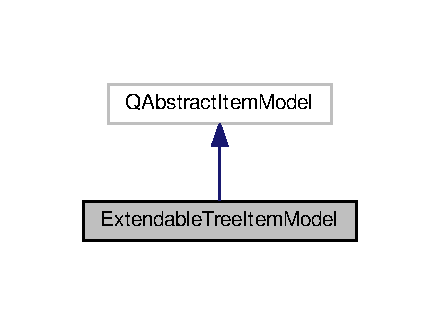
\includegraphics[width=211pt]{class_extendable_tree_item_model__inherit__graph}
\end{center}
\end{figure}


Collaboration diagram for Extendable\+Tree\+Item\+Model\+:\nopagebreak
\begin{figure}[H]
\begin{center}
\leavevmode
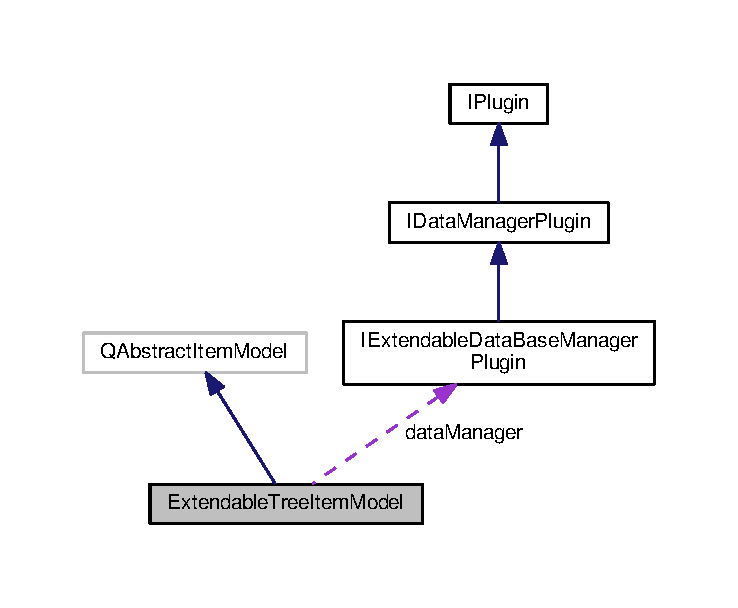
\includegraphics[width=350pt]{class_extendable_tree_item_model__coll__graph}
\end{center}
\end{figure}
\subsection*{Public Member Functions}
\begin{DoxyCompactItemize}
\item 
{\bfseries Extendable\+Tree\+Item\+Model} (Q\+String table\+Name, \hyperlink{class_i_extendable_data_base_manager_plugin}{I\+Extendable\+Data\+Base\+Manager\+Plugin} $\ast$data\+Manager, Q\+Object $\ast$parent=0)\hypertarget{class_extendable_tree_item_model_a44c736cca0dde9d9ca5c295ebc85fdfe}{}\label{class_extendable_tree_item_model_a44c736cca0dde9d9ca5c295ebc85fdfe}

\item 
void {\bfseries Load\+Data} ()\hypertarget{class_extendable_tree_item_model_acb01ad7e561a6471b7361ea50fe84c01}{}\label{class_extendable_tree_item_model_acb01ad7e561a6471b7361ea50fe84c01}

\item 
bool {\bfseries Attach\+Relation} (\hyperlink{class_q_map}{Q\+Map}$<$ Q\+String, Q\+Variant\+::\+Type $>$ relation\+Struct, Q\+String relation\+Name, \hyperlink{class_q_vector}{Q\+Vector}$<$ Q\+Variant $>$ default\+Data)\hypertarget{class_extendable_tree_item_model_ac5899069b1919eaa044e729f8a19ef93}{}\label{class_extendable_tree_item_model_ac5899069b1919eaa044e729f8a19ef93}

\item 
void {\bfseries Set\+Active\+Relation} (Q\+String relation\+Name)\hypertarget{class_extendable_tree_item_model_afdfd8ef7a227883e0d6b8916690ab383}{}\label{class_extendable_tree_item_model_afdfd8ef7a227883e0d6b8916690ab383}

\item 
Q\+Variant {\bfseries data} (const Q\+Model\+Index \&index, int role) const \hypertarget{class_extendable_tree_item_model_ab43719bc7e2e260580d03a272166335a}{}\label{class_extendable_tree_item_model_ab43719bc7e2e260580d03a272166335a}

\item 
Qt\+::\+Item\+Flags {\bfseries flags} (const Q\+Model\+Index \&index) const \hypertarget{class_extendable_tree_item_model_a95a04407e8dfe9bb21abc500cb931b35}{}\label{class_extendable_tree_item_model_a95a04407e8dfe9bb21abc500cb931b35}

\item 
Q\+Variant {\bfseries header\+Data} (int section, Qt\+::\+Orientation orientation, int role=Qt\+::\+Display\+Role) const \hypertarget{class_extendable_tree_item_model_ac50aecb40d68743484d2b94af2335da4}{}\label{class_extendable_tree_item_model_ac50aecb40d68743484d2b94af2335da4}

\item 
Q\+Model\+Index {\bfseries index} (int row, int column, const Q\+Model\+Index \&parent=Q\+Model\+Index()) const \hypertarget{class_extendable_tree_item_model_aec310edeefe5367c14135f4912833148}{}\label{class_extendable_tree_item_model_aec310edeefe5367c14135f4912833148}

\item 
Q\+Model\+Index {\bfseries parent} (const Q\+Model\+Index \&index) const \hypertarget{class_extendable_tree_item_model_a20d33b970a4b657464e8a81a741b6260}{}\label{class_extendable_tree_item_model_a20d33b970a4b657464e8a81a741b6260}

\item 
int {\bfseries row\+Count} (const Q\+Model\+Index \&parent=Q\+Model\+Index()) const \hypertarget{class_extendable_tree_item_model_a0ae57bcc0927419e70dd6385d37731c9}{}\label{class_extendable_tree_item_model_a0ae57bcc0927419e70dd6385d37731c9}

\item 
int {\bfseries column\+Count} (const Q\+Model\+Index \&parent=Q\+Model\+Index()) const \hypertarget{class_extendable_tree_item_model_a8c21281b00c5c1553dc9c3d162333582}{}\label{class_extendable_tree_item_model_a8c21281b00c5c1553dc9c3d162333582}

\item 
bool {\bfseries insert\+Rows} (int row, int count, const Q\+Model\+Index \&parent) override\hypertarget{class_extendable_tree_item_model_a60423d77dbf3227fcf76e721c22ee591}{}\label{class_extendable_tree_item_model_a60423d77dbf3227fcf76e721c22ee591}

\item 
bool {\bfseries insert\+Columns} (int column, int count, const Q\+Model\+Index \&parent) override\hypertarget{class_extendable_tree_item_model_a0d3d16a109c3cac703ca20de6c50a45e}{}\label{class_extendable_tree_item_model_a0d3d16a109c3cac703ca20de6c50a45e}

\item 
bool {\bfseries remove\+Rows} (int row, int count, const Q\+Model\+Index \&parent) override\hypertarget{class_extendable_tree_item_model_a6657cfabdb3f8f696223b04a64661562}{}\label{class_extendable_tree_item_model_a6657cfabdb3f8f696223b04a64661562}

\item 
bool {\bfseries move\+Rows} (const Q\+Model\+Index \&source\+Parent, int source\+Row, int count, const Q\+Model\+Index \&destination\+Parent, int destination\+Child) override\hypertarget{class_extendable_tree_item_model_ac23f589bb25aaa93534b37e2d08f1cbd}{}\label{class_extendable_tree_item_model_ac23f589bb25aaa93534b37e2d08f1cbd}

\item 
bool {\bfseries set\+Data} (const Q\+Model\+Index \&index, const Q\+Variant \&value, int role) override\hypertarget{class_extendable_tree_item_model_ade1332b1bb879ba4a621898b72037c8d}{}\label{class_extendable_tree_item_model_ade1332b1bb879ba4a621898b72037c8d}

\item 
Q\+String\+List {\bfseries mime\+Types} () const override\hypertarget{class_extendable_tree_item_model_ab3fd3745761bab08ed049cf84386241d}{}\label{class_extendable_tree_item_model_ab3fd3745761bab08ed049cf84386241d}

\item 
Q\+Mime\+Data $\ast$ {\bfseries mime\+Data} (const Q\+Model\+Index\+List \&indexes) const override\hypertarget{class_extendable_tree_item_model_a417f3c9c45819e586b97d3784c016e79}{}\label{class_extendable_tree_item_model_a417f3c9c45819e586b97d3784c016e79}

\item 
bool {\bfseries drop\+Mime\+Data} (const Q\+Mime\+Data $\ast$data, Qt\+::\+Drop\+Action action, int row, int column, const Q\+Model\+Index \&parent) override\hypertarget{class_extendable_tree_item_model_a0ba7b75a8cd3406e52237f85e97017b2}{}\label{class_extendable_tree_item_model_a0ba7b75a8cd3406e52237f85e97017b2}

\end{DoxyCompactItemize}
\subsection*{Public Attributes}
\begin{DoxyCompactItemize}
\item 
Q\+String {\bfseries table\+Name}\hypertarget{class_extendable_tree_item_model_a66679a4354b3e64b53b73fbe54ce0dfc}{}\label{class_extendable_tree_item_model_a66679a4354b3e64b53b73fbe54ce0dfc}

\item 
Q\+String {\bfseries core\+Relation\+Name}\hypertarget{class_extendable_tree_item_model_a641619506ce41dd28183b461ea8c5fda}{}\label{class_extendable_tree_item_model_a641619506ce41dd28183b461ea8c5fda}

\item 
\hyperlink{class_i_extendable_data_base_manager_plugin}{I\+Extendable\+Data\+Base\+Manager\+Plugin} $\ast$ {\bfseries data\+Manager}\hypertarget{class_extendable_tree_item_model_a4811726ebb543469630ff4b5eb4d6c35}{}\label{class_extendable_tree_item_model_a4811726ebb543469630ff4b5eb4d6c35}

\end{DoxyCompactItemize}


The documentation for this class was generated from the following files\+:\begin{DoxyCompactItemize}
\item 
/home/curunir/\+Documents/\+M\+A\+S\+S/\+Plugins/\+Task\+List\+Model/extendabletreeitemmodel.\+h\item 
/home/curunir/\+Documents/\+M\+A\+S\+S/\+Plugins/\+Task\+List\+Model/extendabletreeitemmodel.\+cpp\end{DoxyCompactItemize}

\hypertarget{class_gallery_form}{}\section{Gallery\+Form Class Reference}
\label{class_gallery_form}\index{Gallery\+Form@{Gallery\+Form}}


Inheritance diagram for Gallery\+Form\+:\nopagebreak
\begin{figure}[H]
\begin{center}
\leavevmode
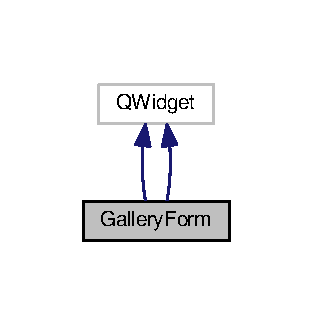
\includegraphics[width=150pt]{class_gallery_form__inherit__graph}
\end{center}
\end{figure}


Collaboration diagram for Gallery\+Form\+:\nopagebreak
\begin{figure}[H]
\begin{center}
\leavevmode
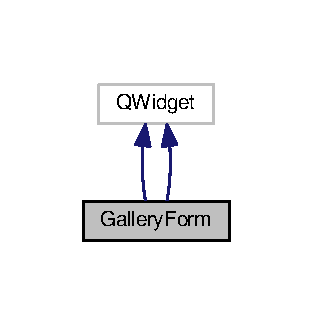
\includegraphics[width=150pt]{class_gallery_form__coll__graph}
\end{center}
\end{figure}
\subsection*{Signals}
\begin{DoxyCompactItemize}
\item 
void {\bfseries On\+Item\+Delete} (int index)\hypertarget{class_gallery_form_addfd9450a0d74d1539e2668623199198}{}\label{class_gallery_form_addfd9450a0d74d1539e2668623199198}

\item 
void {\bfseries On\+Item\+Convert} (int index)\hypertarget{class_gallery_form_a988796418cca1e4ad61d7d3e7c4da3fb}{}\label{class_gallery_form_a988796418cca1e4ad61d7d3e7c4da3fb}

\end{DoxyCompactItemize}
\subsection*{Public Member Functions}
\begin{DoxyCompactItemize}
\item 
{\bfseries Gallery\+Form} (Q\+Widget $\ast$parent=0)\hypertarget{class_gallery_form_ac733697191bca916d42a2a2cf8370f29}{}\label{class_gallery_form_ac733697191bca916d42a2a2cf8370f29}

\item 
{\bfseries Gallery\+Form} (Q\+Widget $\ast$parent=0)\hypertarget{class_gallery_form_ac733697191bca916d42a2a2cf8370f29}{}\label{class_gallery_form_ac733697191bca916d42a2a2cf8370f29}

\item 
void {\bfseries Add\+Image} (int index, Q\+Byte\+Array \&raw\+Image)\hypertarget{class_gallery_form_adadbe8dca87679d1c3a8e9a85abc8ef7}{}\label{class_gallery_form_adadbe8dca87679d1c3a8e9a85abc8ef7}

\item 
void {\bfseries Set\+Model} (Q\+Abstract\+Item\+Model $\ast$model)\hypertarget{class_gallery_form_a2aa9632ee68fed9318a34cffc6ab3402}{}\label{class_gallery_form_a2aa9632ee68fed9318a34cffc6ab3402}

\end{DoxyCompactItemize}


The documentation for this class was generated from the following files\+:\begin{DoxyCompactItemize}
\item 
/home/curunir/\+Documents/\+M\+A\+S\+S/\+Plugins/\+Day\+Plan\+View/galleryform.\+h\item 
/home/curunir/\+Documents/\+M\+A\+S\+S/\+Plugins/build-\/\+Task\+Sketch\+View-\/\+Desktop-\/\+Debug/moc\+\_\+galleryform.\+cpp\item 
/home/curunir/\+Documents/\+M\+A\+S\+S/\+Plugins/\+Day\+Plan\+View/galleryform.\+cpp\end{DoxyCompactItemize}

\hypertarget{class_gallery_item}{}\section{Gallery\+Item Class Reference}
\label{class_gallery_item}\index{Gallery\+Item@{Gallery\+Item}}


Inheritance diagram for Gallery\+Item\+:\nopagebreak
\begin{figure}[H]
\begin{center}
\leavevmode
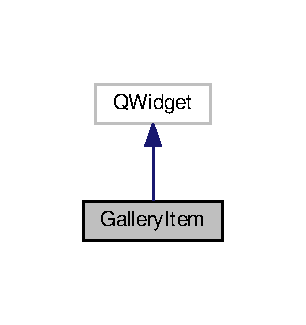
\includegraphics[width=147pt]{class_gallery_item__inherit__graph}
\end{center}
\end{figure}


Collaboration diagram for Gallery\+Item\+:\nopagebreak
\begin{figure}[H]
\begin{center}
\leavevmode
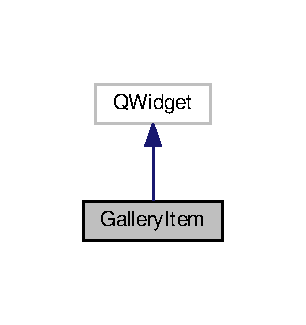
\includegraphics[width=147pt]{class_gallery_item__coll__graph}
\end{center}
\end{figure}
\subsection*{Signals}
\begin{DoxyCompactItemize}
\item 
void {\bfseries On\+Clicked} (\hyperlink{class_gallery_item}{Gallery\+Item} $\ast$)\hypertarget{class_gallery_item_a3b81d36365eaf5edfaf7a9da1df40cf3}{}\label{class_gallery_item_a3b81d36365eaf5edfaf7a9da1df40cf3}

\end{DoxyCompactItemize}
\subsection*{Public Member Functions}
\begin{DoxyCompactItemize}
\item 
{\bfseries Gallery\+Item} (Q\+Widget $\ast$parent=0)\hypertarget{class_gallery_item_a6a6378ce7933d1a4b47eca274304c197}{}\label{class_gallery_item_a6a6378ce7933d1a4b47eca274304c197}

\item 
{\bfseries Gallery\+Item} (Q\+Image image, Q\+Widget $\ast$parent=0)\hypertarget{class_gallery_item_a1a09ea56fceeada2155c81d202fa96b5}{}\label{class_gallery_item_a1a09ea56fceeada2155c81d202fa96b5}

\item 
{\bfseries Gallery\+Item} (Q\+Byte\+Array raw\+Image, Q\+Widget $\ast$parent=0)\hypertarget{class_gallery_item_a5936087e511bd7c1bf9f084139a6b170}{}\label{class_gallery_item_a5936087e511bd7c1bf9f084139a6b170}

\item 
void {\bfseries Set\+Image} (Q\+Image \&image)\hypertarget{class_gallery_item_a598e7b8ff25a9348418fa7310fdaa457}{}\label{class_gallery_item_a598e7b8ff25a9348418fa7310fdaa457}

\item 
void {\bfseries Set\+Image} (Q\+Byte\+Array \&raw\+Image)\hypertarget{class_gallery_item_a9f32ccbb78113342f47e9f683b2fdc26}{}\label{class_gallery_item_a9f32ccbb78113342f47e9f683b2fdc26}

\item 
void {\bfseries paint} (Q\+Painter $\ast$painter, const Q\+Rect \&rect, const Q\+Palette \&palette) const \hypertarget{class_gallery_item_afa964106e7f294145edd507538277ea0}{}\label{class_gallery_item_afa964106e7f294145edd507538277ea0}

\end{DoxyCompactItemize}
\subsection*{Public Attributes}
\begin{DoxyCompactItemize}
\item 
bool {\bfseries is\+In\+Focus}\hypertarget{class_gallery_item_a338ed1ece114426963316cb69b53babe}{}\label{class_gallery_item_a338ed1ece114426963316cb69b53babe}

\end{DoxyCompactItemize}
\subsection*{Protected Member Functions}
\begin{DoxyCompactItemize}
\item 
void {\bfseries paint\+Event} (Q\+Paint\+Event $\ast$event) override\hypertarget{class_gallery_item_a75d0afa0d561668b65a5f158efb7e7ce}{}\label{class_gallery_item_a75d0afa0d561668b65a5f158efb7e7ce}

\item 
void {\bfseries enter\+Event} (Q\+Event $\ast$event) override\hypertarget{class_gallery_item_a54f8de85efd7cde206458ce0ac5ad3a3}{}\label{class_gallery_item_a54f8de85efd7cde206458ce0ac5ad3a3}

\item 
void {\bfseries leave\+Event} (Q\+Event $\ast$event) override\hypertarget{class_gallery_item_afff165e5f0d9dcda2ce175cd44f58885}{}\label{class_gallery_item_afff165e5f0d9dcda2ce175cd44f58885}

\item 
void {\bfseries mouse\+Release\+Event} (Q\+Mouse\+Event $\ast$event) override\hypertarget{class_gallery_item_a6565352fbaf2708e2483f12a499ef31f}{}\label{class_gallery_item_a6565352fbaf2708e2483f12a499ef31f}

\end{DoxyCompactItemize}


The documentation for this class was generated from the following files\+:\begin{DoxyCompactItemize}
\item 
/home/curunir/\+Documents/\+M\+A\+S\+S/\+Plugins/\+Task\+Sketch\+View/galleryitem.\+h\item 
/home/curunir/\+Documents/\+M\+A\+S\+S/\+Plugins/\+Task\+Sketch\+View/galleryitem.\+cpp\end{DoxyCompactItemize}

\hypertarget{class_genetic_algorithm}{}\section{Genetic\+Algorithm Class Reference}
\label{class_genetic_algorithm}\index{Genetic\+Algorithm@{Genetic\+Algorithm}}


Inheritance diagram for Genetic\+Algorithm\+:\nopagebreak
\begin{figure}[H]
\begin{center}
\leavevmode
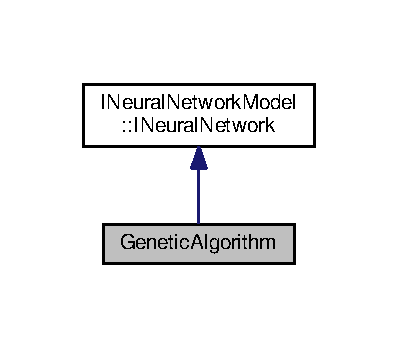
\includegraphics[width=191pt]{class_genetic_algorithm__inherit__graph}
\end{center}
\end{figure}


Collaboration diagram for Genetic\+Algorithm\+:\nopagebreak
\begin{figure}[H]
\begin{center}
\leavevmode
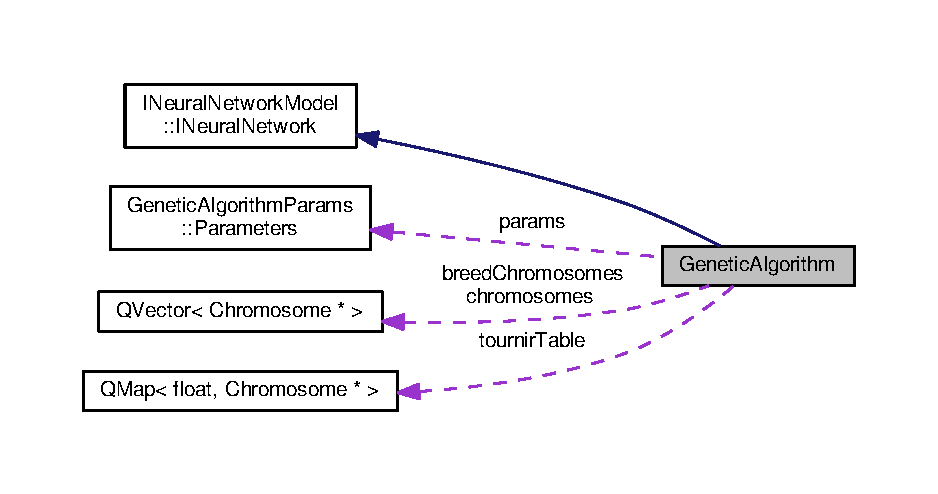
\includegraphics[width=350pt]{class_genetic_algorithm__coll__graph}
\end{center}
\end{figure}
\subsection*{Public Member Functions}
\begin{DoxyCompactItemize}
\item 
float {\bfseries Evaluate\+Fitness} (\hyperlink{class_chromosome}{Chromosome} $\ast$chromosome)\hypertarget{class_genetic_algorithm_adc2ff9ec8816b0979a3b3ac61e364518}{}\label{class_genetic_algorithm_adc2ff9ec8816b0979a3b3ac61e364518}

\item 
bool {\bfseries Set\+Network\+Params} (Q\+Json\+Object params\+Obj) override\hypertarget{class_genetic_algorithm_a8013ce6b1043de624b679c2d109ed80d}{}\label{class_genetic_algorithm_a8013ce6b1043de624b679c2d109ed80d}

\item 
void {\bfseries Setup\+SamplesF} (Q\+Json\+Object parameters, \hyperlink{class_q_vector}{Q\+Vector}$<$ \hyperlink{class_q_pair}{Input\+SampleF} $>$ $\ast$samples) override\hypertarget{class_genetic_algorithm_aa7e7cd7c3026f12e56f904106e90e8f0}{}\label{class_genetic_algorithm_aa7e7cd7c3026f12e56f904106e90e8f0}

\item 
void {\bfseries Setup\+SamplesI} (Q\+Json\+Object parameters, \hyperlink{class_q_vector}{Q\+Vector}$<$ \hyperlink{class_q_pair}{Input\+SampleI} $>$ $\ast$samples) override\hypertarget{class_genetic_algorithm_a5d75f5d038e6a59dc45ac778d04b1979}{}\label{class_genetic_algorithm_a5d75f5d038e6a59dc45ac778d04b1979}

\item 
bool {\bfseries Add\+Layer} (Q\+Json\+Object layer\+Params) override\hypertarget{class_genetic_algorithm_a164e48b38c6f9113bd436cce18a93b65}{}\label{class_genetic_algorithm_a164e48b38c6f9113bd436cce18a93b65}

\item 
void {\bfseries Reset\+Layers} () override\hypertarget{class_genetic_algorithm_af2ce8f9def4f4eddc7b8aa471705d8a6}{}\label{class_genetic_algorithm_af2ce8f9def4f4eddc7b8aa471705d8a6}

\item 
float {\bfseries Run\+Train\+Set} () override\hypertarget{class_genetic_algorithm_ad0cad1893056640d411928eb5184f199}{}\label{class_genetic_algorithm_ad0cad1893056640d411928eb5184f199}

\item 
\hyperlink{class_q_vector}{Q\+Vector}$<$ Q\+Variant $>$ {\bfseries Run\+Training\+And\+Get\+Result} () override\hypertarget{class_genetic_algorithm_ac6b7a46cf3b71a79b4ae2612a2802607}{}\label{class_genetic_algorithm_ac6b7a46cf3b71a79b4ae2612a2802607}

\item 
float {\bfseries Run\+Test\+Set} () override\hypertarget{class_genetic_algorithm_a6e56ca20f24e96e80007091f6a7d2acd}{}\label{class_genetic_algorithm_a6e56ca20f24e96e80007091f6a7d2acd}

\end{DoxyCompactItemize}
\subsection*{Static Public Member Functions}
\begin{DoxyCompactItemize}
\item 
static \hyperlink{class_genetic_algorithm}{Genetic\+Algorithm} $\ast$ {\bfseries Make} (Q\+Json\+Object \&params\+Obj)\hypertarget{class_genetic_algorithm_a58957ce0d547dc7c634a6048ce7a33bb}{}\label{class_genetic_algorithm_a58957ce0d547dc7c634a6048ce7a33bb}

\end{DoxyCompactItemize}
\subsection*{Public Attributes}
\begin{DoxyCompactItemize}
\item 
\hyperlink{class_q_vector}{Q\+Vector}$<$ \hyperlink{class_chromosome}{Chromosome} $\ast$ $>$ {\bfseries chromosomes}\hypertarget{class_genetic_algorithm_a51b416181ed5e839a55b245f02c430af}{}\label{class_genetic_algorithm_a51b416181ed5e839a55b245f02c430af}

\item 
\hyperlink{struct_genetic_algorithm_params_1_1_parameters}{Parameters} {\bfseries params}\hypertarget{class_genetic_algorithm_a08449fb8e9c0ca13f715efc46c7c3861}{}\label{class_genetic_algorithm_a08449fb8e9c0ca13f715efc46c7c3861}

\item 
\hyperlink{class_q_vector}{Q\+Vector}$<$ \hyperlink{class_chromosome}{Chromosome} $\ast$ $>$ {\bfseries breed\+Chromosomes}\hypertarget{class_genetic_algorithm_a413c9f0712074cc8dc4794b55cdadd97}{}\label{class_genetic_algorithm_a413c9f0712074cc8dc4794b55cdadd97}

\item 
\hyperlink{class_q_map}{Q\+Map}$<$ float, \hyperlink{class_chromosome}{Chromosome} $\ast$ $>$ {\bfseries tournir\+Table}\hypertarget{class_genetic_algorithm_aeb4dc5fb05dab4240068c7bb6c29362d}{}\label{class_genetic_algorithm_aeb4dc5fb05dab4240068c7bb6c29362d}

\item 
Q\+String\+List {\bfseries variables}\hypertarget{class_genetic_algorithm_aa2f60ca6342c57ff7217f678d7a02819}{}\label{class_genetic_algorithm_aa2f60ca6342c57ff7217f678d7a02819}

\item 
Q\+Script\+Engine $\ast$ {\bfseries my\+Engine}\hypertarget{class_genetic_algorithm_a732eb5d24e9f796b8f708debdf7172e1}{}\label{class_genetic_algorithm_a732eb5d24e9f796b8f708debdf7172e1}

\item 
Q\+Script\+Value {\bfseries func}\hypertarget{class_genetic_algorithm_a0c210545dc459ca999ee52783e688b53}{}\label{class_genetic_algorithm_a0c210545dc459ca999ee52783e688b53}

\item 
Q\+Script\+Value\+List {\bfseries func\+Ags}\hypertarget{class_genetic_algorithm_a744b4cccc0f9df8fdca9f573d0a5cd07}{}\label{class_genetic_algorithm_a744b4cccc0f9df8fdca9f573d0a5cd07}

\item 
float {\bfseries max\+Fitness} = 0\hypertarget{class_genetic_algorithm_a0af9a260dbff950b59184cde5cdc236f}{}\label{class_genetic_algorithm_a0af9a260dbff950b59184cde5cdc236f}

\end{DoxyCompactItemize}


The documentation for this class was generated from the following files\+:\begin{DoxyCompactItemize}
\item 
/home/curunir/\+Documents/\+M\+A\+S\+S/\+Plugins/\+Neural\+Network\+Model/\+Genetic\+Algorithm/geneticalgorithm.\+h\item 
/home/curunir/\+Documents/\+M\+A\+S\+S/\+Plugins/\+Neural\+Network\+Model/\+Genetic\+Algorithm/geneticalgorithm.\+cpp\end{DoxyCompactItemize}

\hypertarget{class_i_data_base_source_plugin}{}\section{I\+Data\+Base\+Source\+Plugin Class Reference}
\label{class_i_data_base_source_plugin}\index{I\+Data\+Base\+Source\+Plugin@{I\+Data\+Base\+Source\+Plugin}}


Inheritance diagram for I\+Data\+Base\+Source\+Plugin\+:\nopagebreak
\begin{figure}[H]
\begin{center}
\leavevmode
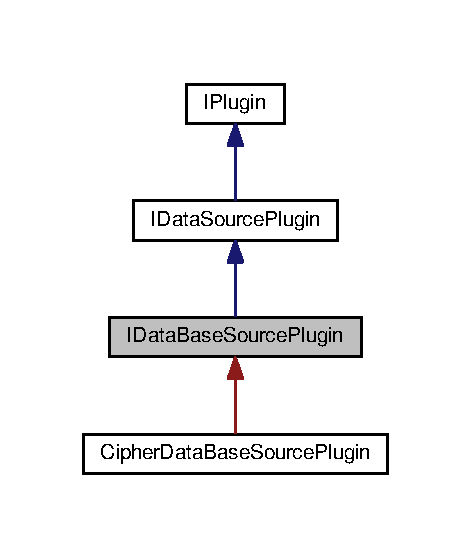
\includegraphics[width=226pt]{class_i_data_base_source_plugin__inherit__graph}
\end{center}
\end{figure}


Collaboration diagram for I\+Data\+Base\+Source\+Plugin\+:\nopagebreak
\begin{figure}[H]
\begin{center}
\leavevmode
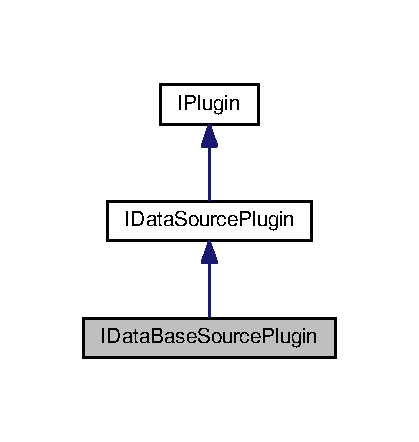
\includegraphics[width=201pt]{class_i_data_base_source_plugin__coll__graph}
\end{center}
\end{figure}
\subsection*{Public Member Functions}
\begin{DoxyCompactItemize}
\item 
virtual Q\+Sql\+Query {\bfseries Execute\+Query} (Q\+String \&query)=0\hypertarget{class_i_data_base_source_plugin_a4ec8ebd5229431cf3b87548f258960b8}{}\label{class_i_data_base_source_plugin_a4ec8ebd5229431cf3b87548f258960b8}

\item 
virtual Q\+Sql\+Query {\bfseries Execute\+Query} (Q\+String \&query, \hyperlink{class_q_list}{Q\+List}$<$ Q\+String $>$ $\ast$value\+Placeholders, \hyperlink{class_q_list}{Q\+List}$<$ Q\+Variant $>$ $\ast$values)=0\hypertarget{class_i_data_base_source_plugin_a0f7fce934bf41f5f18c52951a7eb179c}{}\label{class_i_data_base_source_plugin_a0f7fce934bf41f5f18c52951a7eb179c}

\end{DoxyCompactItemize}


The documentation for this class was generated from the following file\+:\begin{DoxyCompactItemize}
\item 
/home/curunir/\+Documents/\+M\+A\+S\+S/\+Plugins/\+Main\+Menu\+Model\+Plugin/interfaces.\+h\end{DoxyCompactItemize}

\hypertarget{class_i_data_manager_plugin}{}\section{I\+Data\+Manager\+Plugin Class Reference}
\label{class_i_data_manager_plugin}\index{I\+Data\+Manager\+Plugin@{I\+Data\+Manager\+Plugin}}


The \hyperlink{class_i_data_manager_plugin}{I\+Data\+Manager\+Plugin} class.  




{\ttfamily \#include $<$interfaces.\+h$>$}



Inheritance diagram for I\+Data\+Manager\+Plugin\+:\nopagebreak
\begin{figure}[H]
\begin{center}
\leavevmode
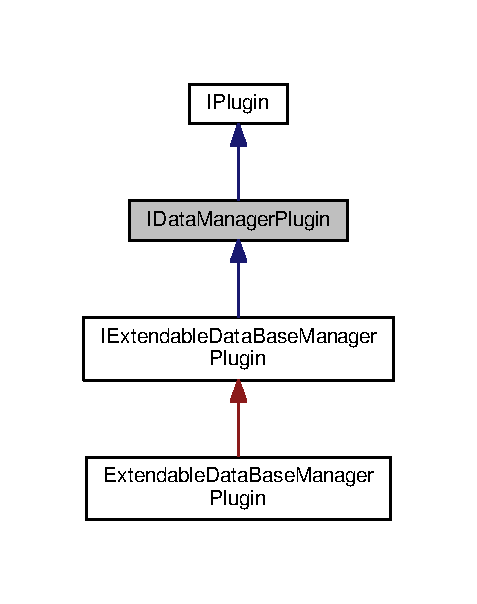
\includegraphics[width=229pt]{class_i_data_manager_plugin__inherit__graph}
\end{center}
\end{figure}


Collaboration diagram for I\+Data\+Manager\+Plugin\+:\nopagebreak
\begin{figure}[H]
\begin{center}
\leavevmode
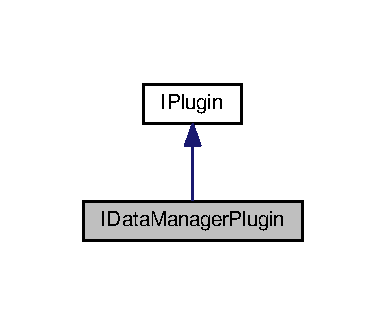
\includegraphics[width=185pt]{class_i_data_manager_plugin__coll__graph}
\end{center}
\end{figure}
\subsection*{Public Member Functions}
\begin{DoxyCompactItemize}
\item 
virtual bool {\bfseries Set\+Data\+Source} (Q\+Object $\ast$data\+Source)=0\hypertarget{class_i_data_manager_plugin_ad9a6a153bc6fe2c64b0a4ee2013fb149}{}\label{class_i_data_manager_plugin_ad9a6a153bc6fe2c64b0a4ee2013fb149}

\end{DoxyCompactItemize}


\subsection{Detailed Description}
The \hyperlink{class_i_data_manager_plugin}{I\+Data\+Manager\+Plugin} class. 

The documentation for this class was generated from the following file\+:\begin{DoxyCompactItemize}
\item 
/home/curunir/\+Documents/\+M\+A\+S\+S/\+Plugins/\+Main\+Menu\+Model\+Plugin/interfaces.\+h\end{DoxyCompactItemize}

\hypertarget{class_i_data_source_plugin}{}\section{I\+Data\+Source\+Plugin Class Reference}
\label{class_i_data_source_plugin}\index{I\+Data\+Source\+Plugin@{I\+Data\+Source\+Plugin}}


Inheritance diagram for I\+Data\+Source\+Plugin\+:\nopagebreak
\begin{figure}[H]
\begin{center}
\leavevmode
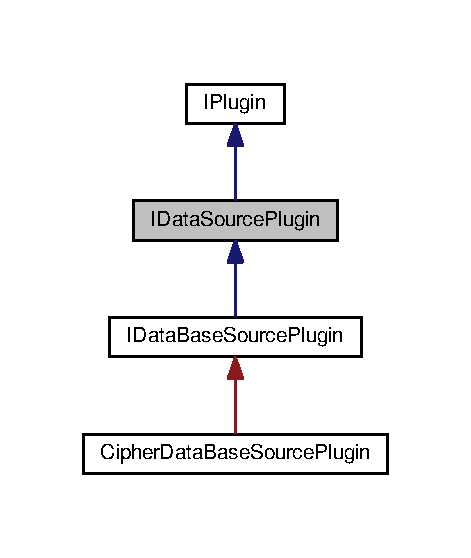
\includegraphics[width=226pt]{class_i_data_source_plugin__inherit__graph}
\end{center}
\end{figure}


Collaboration diagram for I\+Data\+Source\+Plugin\+:\nopagebreak
\begin{figure}[H]
\begin{center}
\leavevmode
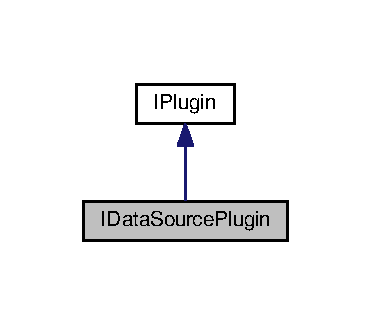
\includegraphics[width=178pt]{class_i_data_source_plugin__coll__graph}
\end{center}
\end{figure}
\subsection*{Public Member Functions}
\begin{DoxyCompactItemize}
\item 
virtual void {\bfseries Setup} ()=0\hypertarget{class_i_data_source_plugin_afb3d43d4324e8849b1cb244c59a45987}{}\label{class_i_data_source_plugin_afb3d43d4324e8849b1cb244c59a45987}

\end{DoxyCompactItemize}


The documentation for this class was generated from the following file\+:\begin{DoxyCompactItemize}
\item 
/home/curunir/\+Documents/\+M\+A\+S\+S/\+Plugins/\+Main\+Menu\+Model\+Plugin/interfaces.\+h\end{DoxyCompactItemize}

\hypertarget{class_i_day_plan_model}{}\section{I\+Day\+Plan\+Model Class Reference}
\label{class_i_day_plan_model}\index{I\+Day\+Plan\+Model@{I\+Day\+Plan\+Model}}
Inheritance diagram for I\+Day\+Plan\+Model\+:\begin{figure}[H]
\begin{center}
\leavevmode
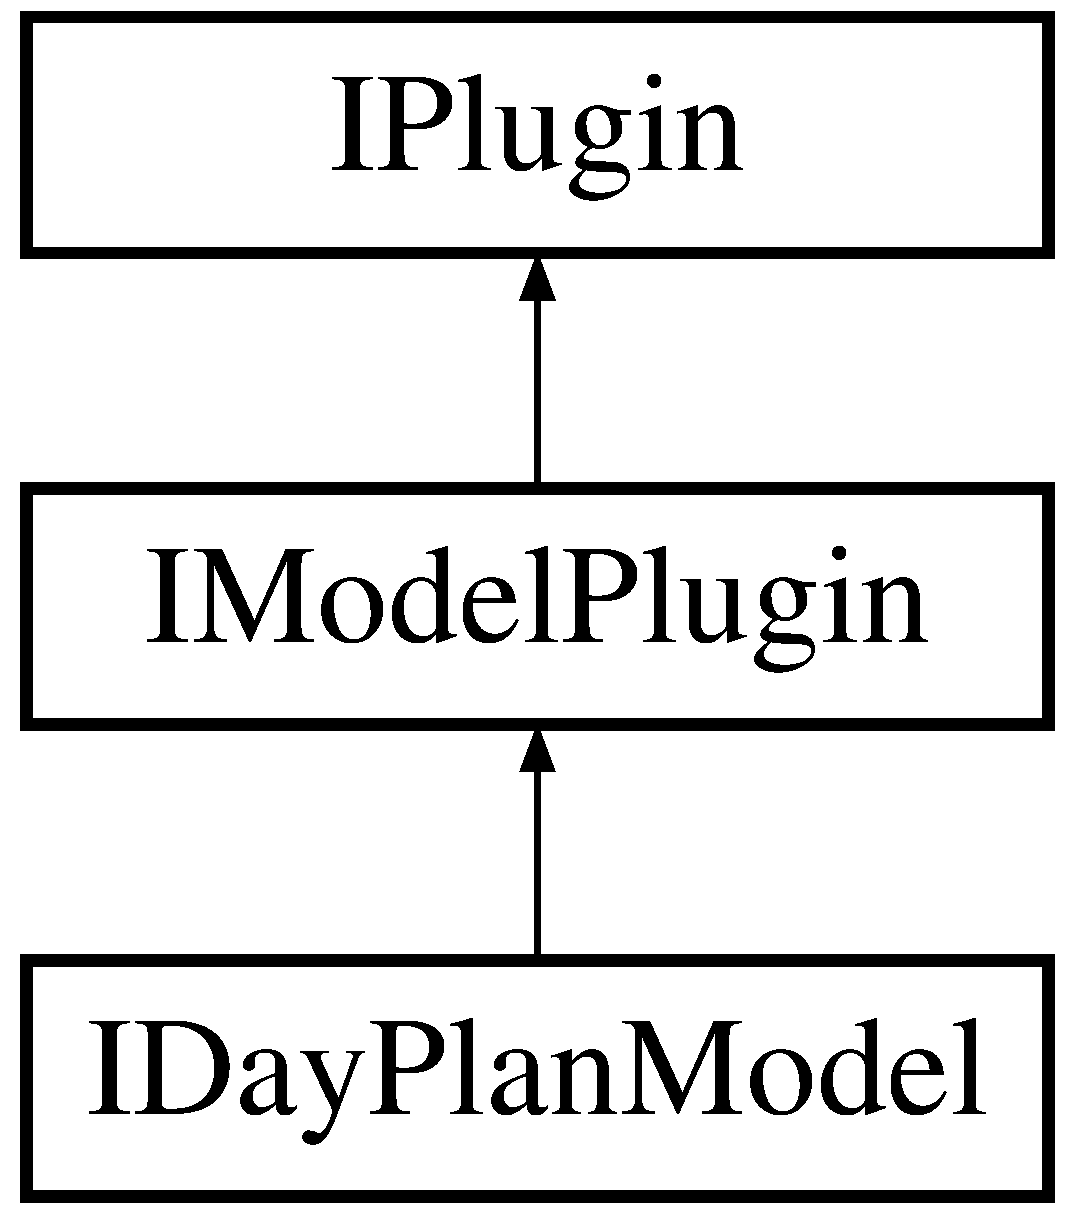
\includegraphics[height=3.000000cm]{class_i_day_plan_model}
\end{center}
\end{figure}
\subsection*{Additional Inherited Members}


The documentation for this class was generated from the following file\+:\begin{DoxyCompactItemize}
\item 
C\+:/\+Users/\+Curunir/\+Desktop/\+M\+A\+S\+S/\+Plugins/\+Day\+Plan\+Model/idayplanmodel.\+h\end{DoxyCompactItemize}

\hypertarget{class_i_d_b_manager_plugin}{}\section{I\+D\+B\+Manager\+Plugin Class Reference}
\label{class_i_d_b_manager_plugin}\index{I\+D\+B\+Manager\+Plugin@{I\+D\+B\+Manager\+Plugin}}
\subsection*{Public Member Functions}
\begin{DoxyCompactItemize}
\item 
virtual Q\+Sql\+Database $\ast$ {\bfseries Setup\+Database} ()=0\hypertarget{class_i_d_b_manager_plugin_add096dcc73790ff4230a44816090d989}{}\label{class_i_d_b_manager_plugin_add096dcc73790ff4230a44816090d989}

\item 
virtual Q\+Sql\+Query $\ast$ {\bfseries Execute\+Query} (Q\+String query)=0\hypertarget{class_i_d_b_manager_plugin_acc0927a1751a2f1d0d87b9b324db17e7}{}\label{class_i_d_b_manager_plugin_acc0927a1751a2f1d0d87b9b324db17e7}

\item 
virtual Q\+Sql\+Database $\ast$ {\bfseries Setup\+Database} ()=0\hypertarget{class_i_d_b_manager_plugin_add096dcc73790ff4230a44816090d989}{}\label{class_i_d_b_manager_plugin_add096dcc73790ff4230a44816090d989}

\item 
virtual Q\+Sql\+Query $\ast$ {\bfseries Execute\+Query} (Q\+String query)=0\hypertarget{class_i_d_b_manager_plugin_acc0927a1751a2f1d0d87b9b324db17e7}{}\label{class_i_d_b_manager_plugin_acc0927a1751a2f1d0d87b9b324db17e7}

\item 
virtual Q\+Sql\+Database $\ast$ {\bfseries Setup\+Database} ()=0\hypertarget{class_i_d_b_manager_plugin_add096dcc73790ff4230a44816090d989}{}\label{class_i_d_b_manager_plugin_add096dcc73790ff4230a44816090d989}

\item 
virtual Q\+Sql\+Query $\ast$ {\bfseries Execute\+Query} (Q\+String query)=0\hypertarget{class_i_d_b_manager_plugin_acc0927a1751a2f1d0d87b9b324db17e7}{}\label{class_i_d_b_manager_plugin_acc0927a1751a2f1d0d87b9b324db17e7}

\item 
virtual Q\+Sql\+Database $\ast$ {\bfseries Setup\+Database} ()=0\hypertarget{class_i_d_b_manager_plugin_add096dcc73790ff4230a44816090d989}{}\label{class_i_d_b_manager_plugin_add096dcc73790ff4230a44816090d989}

\item 
virtual Q\+Sql\+Query $\ast$ {\bfseries Execute\+Query} (Q\+String query)=0\hypertarget{class_i_d_b_manager_plugin_acc0927a1751a2f1d0d87b9b324db17e7}{}\label{class_i_d_b_manager_plugin_acc0927a1751a2f1d0d87b9b324db17e7}

\item 
virtual Q\+Sql\+Database $\ast$ {\bfseries Setup\+Database} ()=0\hypertarget{class_i_d_b_manager_plugin_add096dcc73790ff4230a44816090d989}{}\label{class_i_d_b_manager_plugin_add096dcc73790ff4230a44816090d989}

\item 
virtual Q\+Sql\+Query $\ast$ {\bfseries Execute\+Query} (Q\+String query)=0\hypertarget{class_i_d_b_manager_plugin_acc0927a1751a2f1d0d87b9b324db17e7}{}\label{class_i_d_b_manager_plugin_acc0927a1751a2f1d0d87b9b324db17e7}

\item 
virtual Q\+Sql\+Database $\ast$ {\bfseries Setup\+Database} ()=0\hypertarget{class_i_d_b_manager_plugin_add096dcc73790ff4230a44816090d989}{}\label{class_i_d_b_manager_plugin_add096dcc73790ff4230a44816090d989}

\item 
virtual Q\+Sql\+Query $\ast$ {\bfseries Execute\+Query} (Q\+String query)=0\hypertarget{class_i_d_b_manager_plugin_acc0927a1751a2f1d0d87b9b324db17e7}{}\label{class_i_d_b_manager_plugin_acc0927a1751a2f1d0d87b9b324db17e7}

\item 
virtual Q\+Sql\+Database $\ast$ {\bfseries Setup\+Database} ()=0\hypertarget{class_i_d_b_manager_plugin_add096dcc73790ff4230a44816090d989}{}\label{class_i_d_b_manager_plugin_add096dcc73790ff4230a44816090d989}

\item 
virtual Q\+Sql\+Query $\ast$ {\bfseries Execute\+Query} (Q\+String query)=0\hypertarget{class_i_d_b_manager_plugin_acc0927a1751a2f1d0d87b9b324db17e7}{}\label{class_i_d_b_manager_plugin_acc0927a1751a2f1d0d87b9b324db17e7}

\end{DoxyCompactItemize}


The documentation for this class was generated from the following file\+:\begin{DoxyCompactItemize}
\item 
/home/curunir/\+Documents/\+M\+A\+S\+S/\+Plugins/\+A\+R\+Neural\+Network\+View/interfaces.\+h\end{DoxyCompactItemize}

\hypertarget{class_i_d_b_tool_plugin}{}\section{I\+D\+B\+Tool\+Plugin Class Reference}
\label{class_i_d_b_tool_plugin}\index{I\+D\+B\+Tool\+Plugin@{I\+D\+B\+Tool\+Plugin}}
\subsection*{Public Member Functions}
\begin{DoxyCompactItemize}
\item 
virtual bool {\bfseries Set\+D\+B\+Manager} (\hyperlink{class_i_d_b_manager_plugin}{I\+D\+B\+Manager\+Plugin} $\ast$D\+B\+Manager)=0\hypertarget{class_i_d_b_tool_plugin_ae7c5693728988f5aa46065fed7a8ca99}{}\label{class_i_d_b_tool_plugin_ae7c5693728988f5aa46065fed7a8ca99}

\end{DoxyCompactItemize}


The documentation for this class was generated from the following file\+:\begin{DoxyCompactItemize}
\item 
/home/curunir/\+Documents/\+M\+A\+S\+S/\+Plugins/\+Extendable\+Data\+Base\+Manager/interfaces.\+h\end{DoxyCompactItemize}

\hypertarget{class_i_extendable_data_base_manager_plugin}{}\section{I\+Extendable\+Data\+Base\+Manager\+Plugin Class Reference}
\label{class_i_extendable_data_base_manager_plugin}\index{I\+Extendable\+Data\+Base\+Manager\+Plugin@{I\+Extendable\+Data\+Base\+Manager\+Plugin}}


Inheritance diagram for I\+Extendable\+Data\+Base\+Manager\+Plugin\+:\nopagebreak
\begin{figure}[H]
\begin{center}
\leavevmode
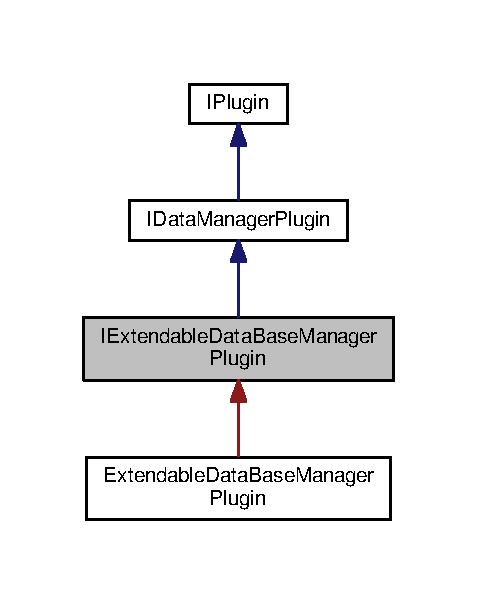
\includegraphics[width=229pt]{class_i_extendable_data_base_manager_plugin__inherit__graph}
\end{center}
\end{figure}


Collaboration diagram for I\+Extendable\+Data\+Base\+Manager\+Plugin\+:\nopagebreak
\begin{figure}[H]
\begin{center}
\leavevmode
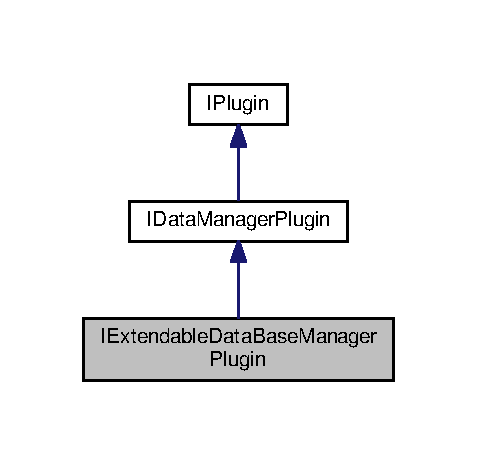
\includegraphics[width=229pt]{class_i_extendable_data_base_manager_plugin__coll__graph}
\end{center}
\end{figure}
\subsection*{Classes}
\begin{DoxyCompactItemize}
\item 
class \hyperlink{class_i_extendable_data_base_manager_plugin_1_1_manager_data_item}{Manager\+Data\+Item}
\end{DoxyCompactItemize}
\subsection*{Public Member Functions}
\begin{DoxyCompactItemize}
\item 
virtual \hyperlink{class_q_list}{Q\+List}$<$ \hyperlink{class_i_extendable_data_base_manager_plugin_1_1_manager_data_item}{Manager\+Data\+Item} $>$ {\bfseries Get\+Data\+List} (Q\+String tree\+Name)=0\hypertarget{class_i_extendable_data_base_manager_plugin_aeda41c0d78e0a702e589844a934a815c}{}\label{class_i_extendable_data_base_manager_plugin_aeda41c0d78e0a702e589844a934a815c}

\item 
virtual \hyperlink{class_i_extendable_data_base_manager_plugin_1_1_manager_data_item}{Manager\+Data\+Item} {\bfseries Get\+Data\+Item} (Q\+String tree\+Name, int id)=0\hypertarget{class_i_extendable_data_base_manager_plugin_a14c965c1f955f76bd370478211d58e22}{}\label{class_i_extendable_data_base_manager_plugin_a14c965c1f955f76bd370478211d58e22}

\item 
virtual Q\+Abstract\+Item\+Model $\ast$ {\bfseries Get\+Data\+Model} (Q\+String tree\+Name)=0\hypertarget{class_i_extendable_data_base_manager_plugin_ad0b28da100d3ebecb874b0ff6c6db9aa}{}\label{class_i_extendable_data_base_manager_plugin_ad0b28da100d3ebecb874b0ff6c6db9aa}

\item 
virtual \hyperlink{class_q_map}{Q\+Map}$<$ Q\+String, Q\+Variant\+::\+Type $>$ {\bfseries Get\+Table\+Header} (Q\+String tree\+Name)=0\hypertarget{class_i_extendable_data_base_manager_plugin_ae19dc8759c078506e5ae18e6f946930f}{}\label{class_i_extendable_data_base_manager_plugin_ae19dc8759c078506e5ae18e6f946930f}

\item 
virtual bool {\bfseries Set\+Relation} (Q\+String main\+Name, Q\+String relation\+Name, \hyperlink{class_q_map}{Q\+Map}$<$ Q\+String, Q\+Variant\+::\+Type $>$ fields, \hyperlink{class_q_vector}{Q\+Vector}$<$ Q\+Variant $>$ default\+Data)=0\hypertarget{class_i_extendable_data_base_manager_plugin_a744d2dd52fe84cf8ad3b67b43639030d}{}\label{class_i_extendable_data_base_manager_plugin_a744d2dd52fe84cf8ad3b67b43639030d}

\item 
virtual bool {\bfseries Delete\+Relation} (Q\+String main\+Name, Q\+String relation\+Name)=0\hypertarget{class_i_extendable_data_base_manager_plugin_af0b43211e9399964c707ac337c219f8d}{}\label{class_i_extendable_data_base_manager_plugin_af0b43211e9399964c707ac337c219f8d}

\item 
virtual bool {\bfseries Set\+Active\+Relation} (Q\+String main\+Name, Q\+String relation\+Name)=0\hypertarget{class_i_extendable_data_base_manager_plugin_a20b67985093680372a1c14aa29481e42}{}\label{class_i_extendable_data_base_manager_plugin_a20b67985093680372a1c14aa29481e42}

\item 
virtual int {\bfseries Add\+Item} (Q\+String tree\+Name, \hyperlink{class_i_extendable_data_base_manager_plugin_1_1_manager_data_item}{Manager\+Data\+Item} task)=0\hypertarget{class_i_extendable_data_base_manager_plugin_a0b44f850dabdb3d4cd985c1000f0d6d9}{}\label{class_i_extendable_data_base_manager_plugin_a0b44f850dabdb3d4cd985c1000f0d6d9}

\item 
virtual bool {\bfseries Edit\+Item} (Q\+String tree\+Name, \hyperlink{class_i_extendable_data_base_manager_plugin_1_1_manager_data_item}{Manager\+Data\+Item} task)=0\hypertarget{class_i_extendable_data_base_manager_plugin_a45c9c133b47f3babe95ccfe53489f193}{}\label{class_i_extendable_data_base_manager_plugin_a45c9c133b47f3babe95ccfe53489f193}

\item 
virtual bool {\bfseries Delete\+Item} (Q\+String tree\+Name, int id)=0\hypertarget{class_i_extendable_data_base_manager_plugin_aaa311e2c898b0e974e27ee0efae1716e}{}\label{class_i_extendable_data_base_manager_plugin_aaa311e2c898b0e974e27ee0efae1716e}

\end{DoxyCompactItemize}


The documentation for this class was generated from the following file\+:\begin{DoxyCompactItemize}
\item 
/home/curunir/\+Documents/\+M\+A\+S\+S/\+Plugins/\+Extendable\+Data\+Base\+Manager/iextendabledatabasemanagerplugin.\+h\end{DoxyCompactItemize}

\hypertarget{class_i_main_menu_plugin_model}{}\section{I\+Main\+Menu\+Plugin\+Model Class Reference}
\label{class_i_main_menu_plugin_model}\index{I\+Main\+Menu\+Plugin\+Model@{I\+Main\+Menu\+Plugin\+Model}}


The \hyperlink{class_i_main_menu_plugin_model}{I\+Main\+Menu\+Plugin\+Model} class.  




{\ttfamily \#include $<$imainmenumodule.\+h$>$}



Inheritance diagram for I\+Main\+Menu\+Plugin\+Model\+:\nopagebreak
\begin{figure}[H]
\begin{center}
\leavevmode
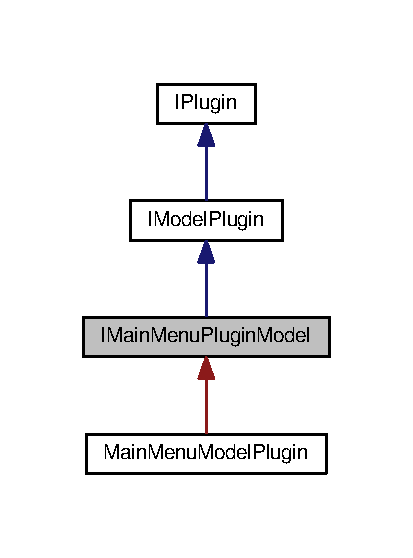
\includegraphics[width=198pt]{class_i_main_menu_plugin_model__inherit__graph}
\end{center}
\end{figure}


Collaboration diagram for I\+Main\+Menu\+Plugin\+Model\+:\nopagebreak
\begin{figure}[H]
\begin{center}
\leavevmode
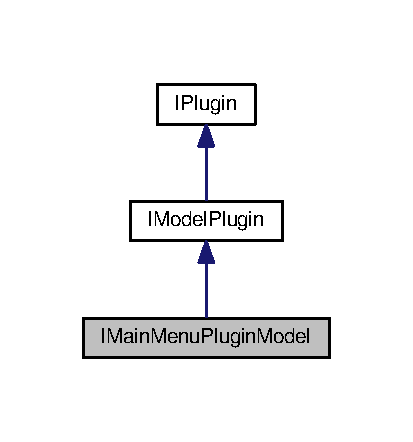
\includegraphics[width=198pt]{class_i_main_menu_plugin_model__coll__graph}
\end{center}
\end{figure}
\subsection*{Classes}
\begin{DoxyCompactItemize}
\item 
struct \hyperlink{struct_i_main_menu_plugin_model_1_1_menu_item}{Menu\+Item}
\end{DoxyCompactItemize}
\subsection*{Public Member Functions}
\begin{DoxyCompactItemize}
\item 
virtual \hyperlink{struct_i_main_menu_plugin_model_1_1_menu_item}{Menu\+Item} $\ast$ {\bfseries Get\+Root\+Menu\+Item} ()=0
\item 
virtual void {\bfseries Run\+Item} (\hyperlink{struct_i_main_menu_plugin_model_1_1_menu_item}{Menu\+Item} $\ast$item, \hyperlink{struct_meta_info}{Meta\+Info} $\ast$view\+Meta)=0
\end{DoxyCompactItemize}


\subsection{Detailed Description}
The \hyperlink{class_i_main_menu_plugin_model}{I\+Main\+Menu\+Plugin\+Model} class. 

The documentation for this class was generated from the following file\+:\begin{DoxyCompactItemize}
\item 
/home/curunir/\+Documents/\+M\+A\+S\+S/\+Plugins/\+Main\+Menu\+Model\+Plugin/imainmenumodule.\+h\end{DoxyCompactItemize}

\hypertarget{class_i_model_plugin}{}\section{I\+Model\+Plugin Class Reference}
\label{class_i_model_plugin}\index{I\+Model\+Plugin@{I\+Model\+Plugin}}


The \hyperlink{class_i_model_plugin}{I\+Model\+Plugin} class.  




{\ttfamily \#include $<$interfaces.\+h$>$}



Inheritance diagram for I\+Model\+Plugin\+:\nopagebreak
\begin{figure}[H]
\begin{center}
\leavevmode
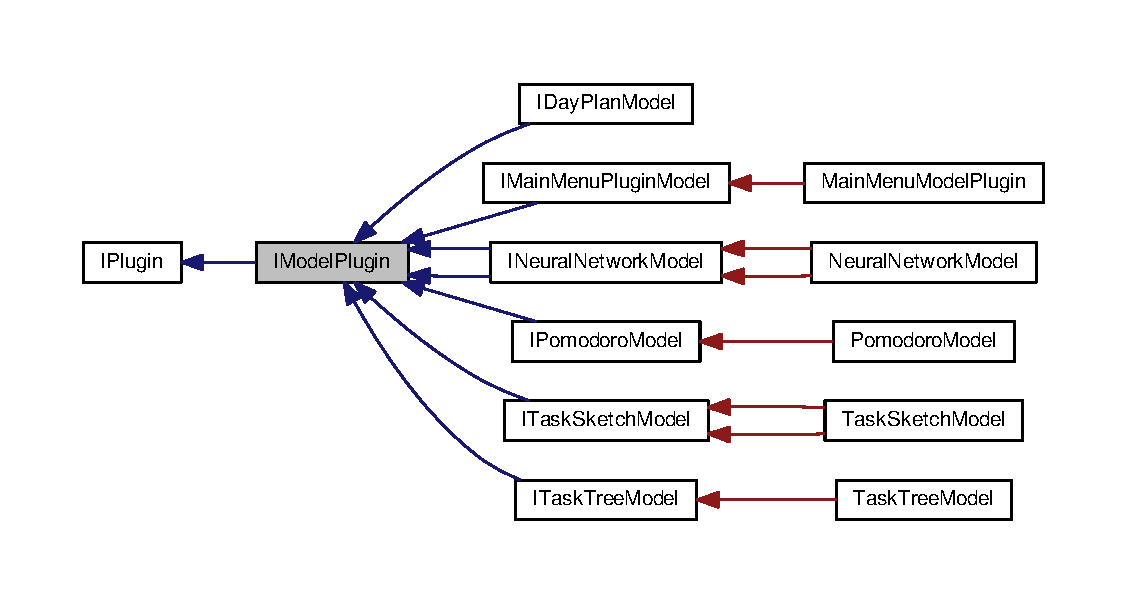
\includegraphics[width=350pt]{class_i_model_plugin__inherit__graph}
\end{center}
\end{figure}


Collaboration diagram for I\+Model\+Plugin\+:\nopagebreak
\begin{figure}[H]
\begin{center}
\leavevmode
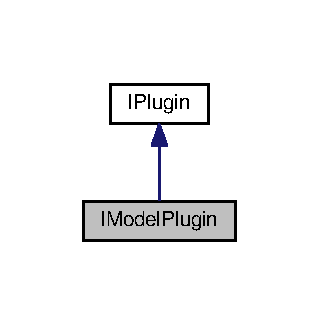
\includegraphics[width=153pt]{class_i_model_plugin__coll__graph}
\end{center}
\end{figure}
\subsection*{Public Member Functions}
\begin{DoxyCompactItemize}
\item 
virtual void {\bfseries Add\+Data\+Manager} (Q\+Object $\ast$data\+Manager)=0\hypertarget{class_i_model_plugin_ab6612f3eaf63fcf66d61ca4522e6399a}{}\label{class_i_model_plugin_ab6612f3eaf63fcf66d61ca4522e6399a}

\item 
virtual void {\bfseries Add\+Parent\+Model} (Q\+Object $\ast$model, \hyperlink{struct_meta_info}{Meta\+Info} $\ast$meta)=0\hypertarget{class_i_model_plugin_a984044bf0128b7fe19b2871a244ed030}{}\label{class_i_model_plugin_a984044bf0128b7fe19b2871a244ed030}

\item 
virtual void {\bfseries Add\+Child\+Model} (\hyperlink{class_i_model_plugin}{I\+Model\+Plugin} $\ast$model, \hyperlink{struct_meta_info}{Meta\+Info} $\ast$meta)=0\hypertarget{class_i_model_plugin_a8427d2cff223c37abb0c4d856b244c4d}{}\label{class_i_model_plugin_a8427d2cff223c37abb0c4d856b244c4d}

\item 
virtual void {\bfseries Add\+View} (\hyperlink{class_i_view_plugin}{I\+View\+Plugin} $\ast$view, \hyperlink{struct_meta_info}{Meta\+Info} $\ast$meta)=0\hypertarget{class_i_model_plugin_aa209bc554d02bf3b04b64a7003a9ace4}{}\label{class_i_model_plugin_aa209bc554d02bf3b04b64a7003a9ace4}

\item 
virtual bool {\bfseries Open} (\hyperlink{class_i_model_plugin}{I\+Model\+Plugin} $\ast$parent, Q\+Widget $\ast$parent\+Widget)=0\hypertarget{class_i_model_plugin_a1d0eb900e7bb460ab957ae90fd966d76}{}\label{class_i_model_plugin_a1d0eb900e7bb460ab957ae90fd966d76}

\item 
virtual bool {\bfseries Close\+From\+View} (\hyperlink{class_i_view_plugin}{I\+View\+Plugin} $\ast$view)=0\hypertarget{class_i_model_plugin_ae6e9c6e8eb422b31d3a32c9c7bf60152}{}\label{class_i_model_plugin_ae6e9c6e8eb422b31d3a32c9c7bf60152}

\item 
virtual void {\bfseries Child\+Self\+Closed} (\hyperlink{class_i_model_plugin}{I\+Model\+Plugin} $\ast$child)=0\hypertarget{class_i_model_plugin_a19a398057393941101d581b98db4bedf}{}\label{class_i_model_plugin_a19a398057393941101d581b98db4bedf}

\end{DoxyCompactItemize}


\subsection{Detailed Description}
The \hyperlink{class_i_model_plugin}{I\+Model\+Plugin} class. 

The documentation for this class was generated from the following file\+:\begin{DoxyCompactItemize}
\item 
/home/curunir/\+Documents/\+M\+A\+S\+S/\+Plugins/\+Main\+Menu\+Model\+Plugin/interfaces.\+h\end{DoxyCompactItemize}

\hypertarget{class_i_neural_network_model_1_1_i_neural_network}{}\section{I\+Neural\+Network\+Model\+:\+:I\+Neural\+Network Class Reference}
\label{class_i_neural_network_model_1_1_i_neural_network}\index{I\+Neural\+Network\+Model\+::\+I\+Neural\+Network@{I\+Neural\+Network\+Model\+::\+I\+Neural\+Network}}
Inheritance diagram for I\+Neural\+Network\+Model\+:\+:I\+Neural\+Network\+:\begin{figure}[H]
\begin{center}
\leavevmode
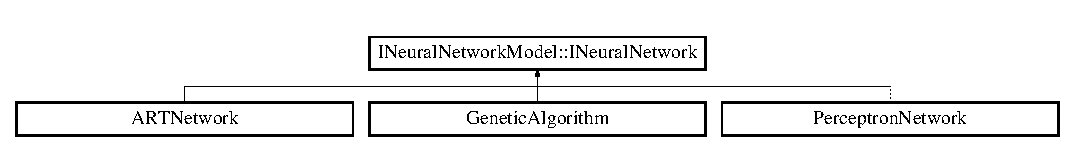
\includegraphics[height=1.588652cm]{class_i_neural_network_model_1_1_i_neural_network}
\end{center}
\end{figure}
\subsection*{Public Member Functions}
\begin{DoxyCompactItemize}
\item 
\mbox{\Hypertarget{class_i_neural_network_model_1_1_i_neural_network_a21b05dafd766b32341d22b52d4714903}\label{class_i_neural_network_model_1_1_i_neural_network_a21b05dafd766b32341d22b52d4714903}} 
virtual bool {\bfseries Set\+Network\+Params} (Q\+Json\+Object params)=0
\item 
\mbox{\Hypertarget{class_i_neural_network_model_1_1_i_neural_network_a840c7196b8c3e1065b8c0a62a1b49fb2}\label{class_i_neural_network_model_1_1_i_neural_network_a840c7196b8c3e1065b8c0a62a1b49fb2}} 
virtual void {\bfseries Setup\+SamplesF} (Q\+Json\+Object parameters, \hyperlink{class_q_vector}{Q\+Vector}$<$ \hyperlink{class_q_pair}{Input\+SampleF} $>$ $\ast$samples)=0
\item 
\mbox{\Hypertarget{class_i_neural_network_model_1_1_i_neural_network_af04047a560d8b5f68651173f62510d02}\label{class_i_neural_network_model_1_1_i_neural_network_af04047a560d8b5f68651173f62510d02}} 
virtual void {\bfseries Setup\+SamplesI} (Q\+Json\+Object parameters, \hyperlink{class_q_vector}{Q\+Vector}$<$ \hyperlink{class_q_pair}{Input\+SampleI} $>$ $\ast$samples)=0
\item 
\mbox{\Hypertarget{class_i_neural_network_model_1_1_i_neural_network_a128bb0ed83f4b3b309691943eca77954}\label{class_i_neural_network_model_1_1_i_neural_network_a128bb0ed83f4b3b309691943eca77954}} 
virtual bool {\bfseries Add\+Layer} (Q\+Json\+Object layer\+Params)=0
\item 
\mbox{\Hypertarget{class_i_neural_network_model_1_1_i_neural_network_a0940ee0d739ae2ea00eb28ef21019597}\label{class_i_neural_network_model_1_1_i_neural_network_a0940ee0d739ae2ea00eb28ef21019597}} 
virtual void {\bfseries Reset\+Layers} ()=0
\item 
\mbox{\Hypertarget{class_i_neural_network_model_1_1_i_neural_network_adbfcfb4e09800b0f32f141b071eca3d8}\label{class_i_neural_network_model_1_1_i_neural_network_adbfcfb4e09800b0f32f141b071eca3d8}} 
virtual float {\bfseries Run\+Train\+Set} ()=0
\item 
\mbox{\Hypertarget{class_i_neural_network_model_1_1_i_neural_network_a4f00d2ce86d5e006f161762ad7631d3b}\label{class_i_neural_network_model_1_1_i_neural_network_a4f00d2ce86d5e006f161762ad7631d3b}} 
virtual \hyperlink{class_q_vector}{Q\+Vector}$<$ Q\+Variant $>$ {\bfseries Run\+Training\+And\+Get\+Result} ()=0
\item 
\mbox{\Hypertarget{class_i_neural_network_model_1_1_i_neural_network_a767cdb2dfd88c7db1dfbd8620cffafc9}\label{class_i_neural_network_model_1_1_i_neural_network_a767cdb2dfd88c7db1dfbd8620cffafc9}} 
virtual float {\bfseries Run\+Test\+Set} ()=0
\end{DoxyCompactItemize}


The documentation for this class was generated from the following file\+:\begin{DoxyCompactItemize}
\item 
C\+:/\+Users/\+Curunir/\+Desktop/\+M\+A\+S\+S/\+Plugins/\+Neural\+Network\+Model/ineuralnetworkmodel.\+h\end{DoxyCompactItemize}

\hypertarget{class_i_neural_network_model}{}\section{I\+Neural\+Network\+Model Class Reference}
\label{class_i_neural_network_model}\index{I\+Neural\+Network\+Model@{I\+Neural\+Network\+Model}}
Inheritance diagram for I\+Neural\+Network\+Model\+:\begin{figure}[H]
\begin{center}
\leavevmode
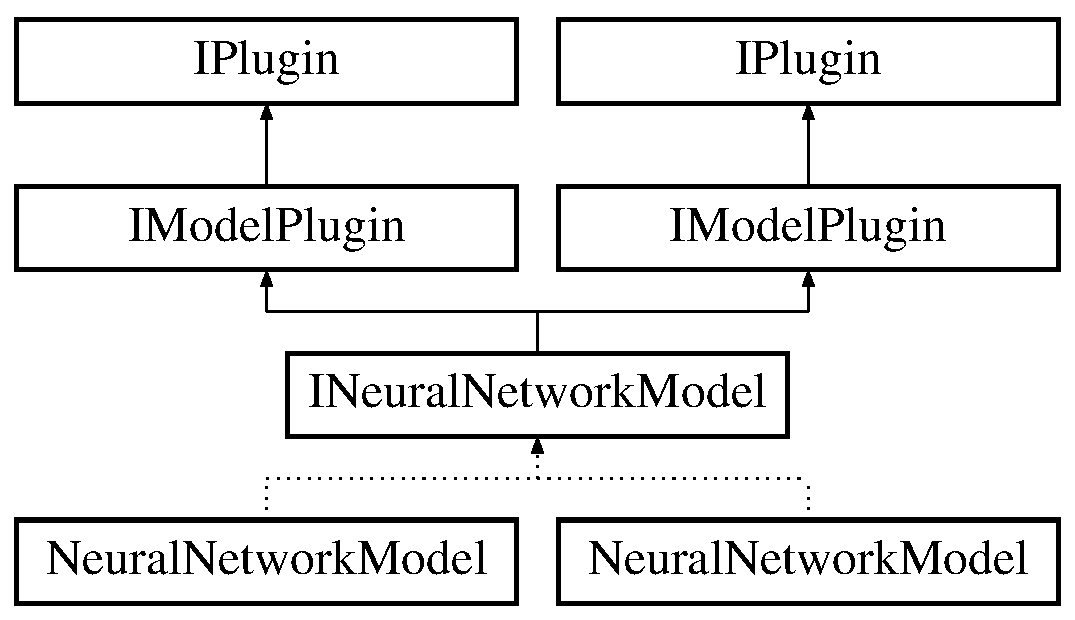
\includegraphics[height=4.000000cm]{class_i_neural_network_model}
\end{center}
\end{figure}
\subsection*{Classes}
\begin{DoxyCompactItemize}
\item 
class \hyperlink{class_i_neural_network_model_1_1_i_neural_network}{I\+Neural\+Network}
\end{DoxyCompactItemize}
\subsection*{Public Member Functions}
\begin{DoxyCompactItemize}
\item 
\mbox{\Hypertarget{class_i_neural_network_model_ac81fd0c1ff87a9147351f1d384a1692e}\label{class_i_neural_network_model_ac81fd0c1ff87a9147351f1d384a1692e}} 
virtual void {\bfseries Test\+Func} ()=0
\item 
\mbox{\Hypertarget{class_i_neural_network_model_a4732c112899b5f3a4d81db89c7d389a4}\label{class_i_neural_network_model_a4732c112899b5f3a4d81db89c7d389a4}} 
virtual \hyperlink{class_i_neural_network_model_1_1_i_neural_network}{I\+Neural\+Network} $\ast$ {\bfseries Setup\+Network} (Q\+Json\+Object network\+Params)=0
\end{DoxyCompactItemize}


The documentation for this class was generated from the following file\+:\begin{DoxyCompactItemize}
\item 
C\+:/\+Users/\+Curunir/\+Desktop/\+M\+A\+S\+S/\+Plugins/\+Empty\+Model\+Plugin/ineuralnetworkmodel.\+h\end{DoxyCompactItemize}

\hypertarget{class_input_neural_layer}{}\section{Input\+Neural\+Layer Class Reference}
\label{class_input_neural_layer}\index{Input\+Neural\+Layer@{Input\+Neural\+Layer}}
Inheritance diagram for Input\+Neural\+Layer\+:\begin{figure}[H]
\begin{center}
\leavevmode
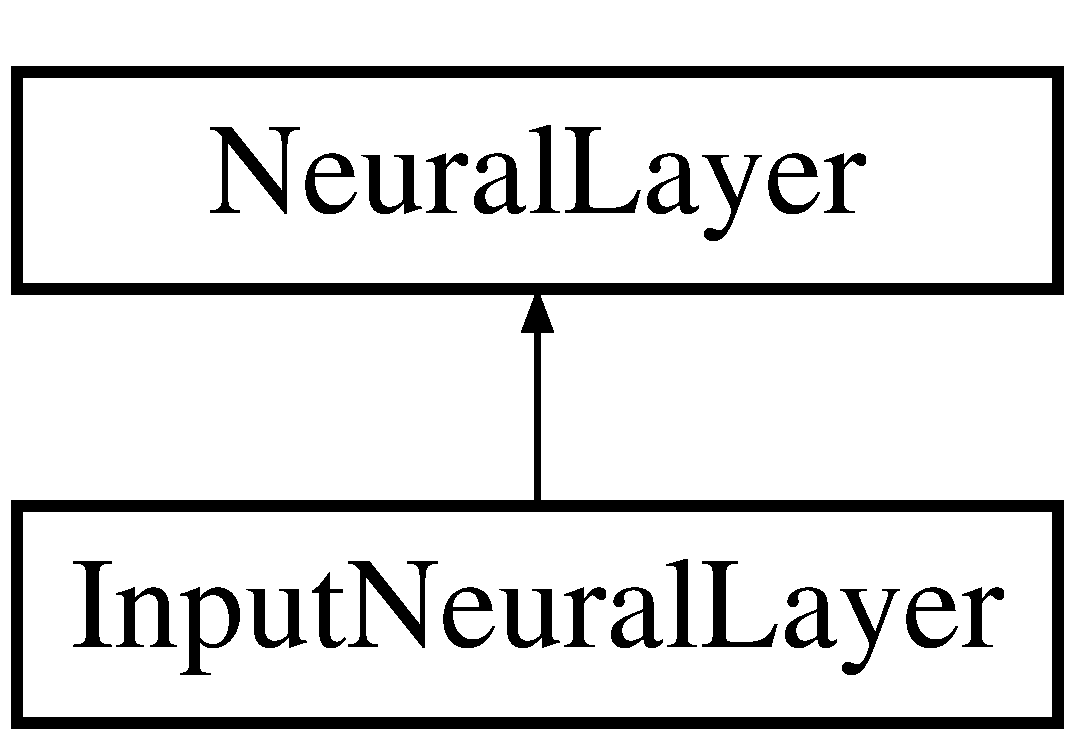
\includegraphics[height=2.000000cm]{class_input_neural_layer}
\end{center}
\end{figure}
\subsection*{Public Slots}
\begin{DoxyCompactItemize}
\item 
\mbox{\Hypertarget{class_input_neural_layer_a14633f26c2f18e3ca4bd95feb4eb9a91}\label{class_input_neural_layer_a14633f26c2f18e3ca4bd95feb4eb9a91}} 
void {\bfseries Forward} (\hyperlink{class_q_vector}{Q\+Vector}$<$ float $>$ \&input\+Signals) override
\item 
\mbox{\Hypertarget{class_input_neural_layer_a6a6e5df6ba9100259dda2d7849a8f5b7}\label{class_input_neural_layer_a6a6e5df6ba9100259dda2d7849a8f5b7}} 
void {\bfseries Back} (\hyperlink{class_q_vector}{Q\+Vector}$<$ float $>$ \&next\+Layer\+Delta) override
\end{DoxyCompactItemize}
\subsection*{Public Member Functions}
\begin{DoxyCompactItemize}
\item 
\mbox{\Hypertarget{class_input_neural_layer_a2e0edec20cf09e830fdeaee505688b1a}\label{class_input_neural_layer_a2e0edec20cf09e830fdeaee505688b1a}} 
{\bfseries Input\+Neural\+Layer} (\hyperlink{struct_perceptron_1_1_network_params}{Network\+Params} \&\hyperlink{struct_perceptron_1_1_network_params}{Network\+Params}, \hyperlink{struct_perceptron_1_1_layer_params}{Layer\+Params} \&Params)
\end{DoxyCompactItemize}
\subsection*{Additional Inherited Members}


The documentation for this class was generated from the following files\+:\begin{DoxyCompactItemize}
\item 
C\+:/\+Users/\+Curunir/\+Desktop/\+M\+A\+S\+S/\+Plugins/\+Neural\+Network\+Model/\+Perceptron/neurallayer.\+h\item 
C\+:/\+Users/\+Curunir/\+Desktop/\+M\+A\+S\+S/\+Plugins/\+Neural\+Network\+Model/\+Perceptron/neurallayer.\+cpp\end{DoxyCompactItemize}

\hypertarget{class_i_plugin}{}\section{I\+Plugin Class Reference}
\label{class_i_plugin}\index{I\+Plugin@{I\+Plugin}}


Inheritance diagram for I\+Plugin\+:\nopagebreak
\begin{figure}[H]
\begin{center}
\leavevmode
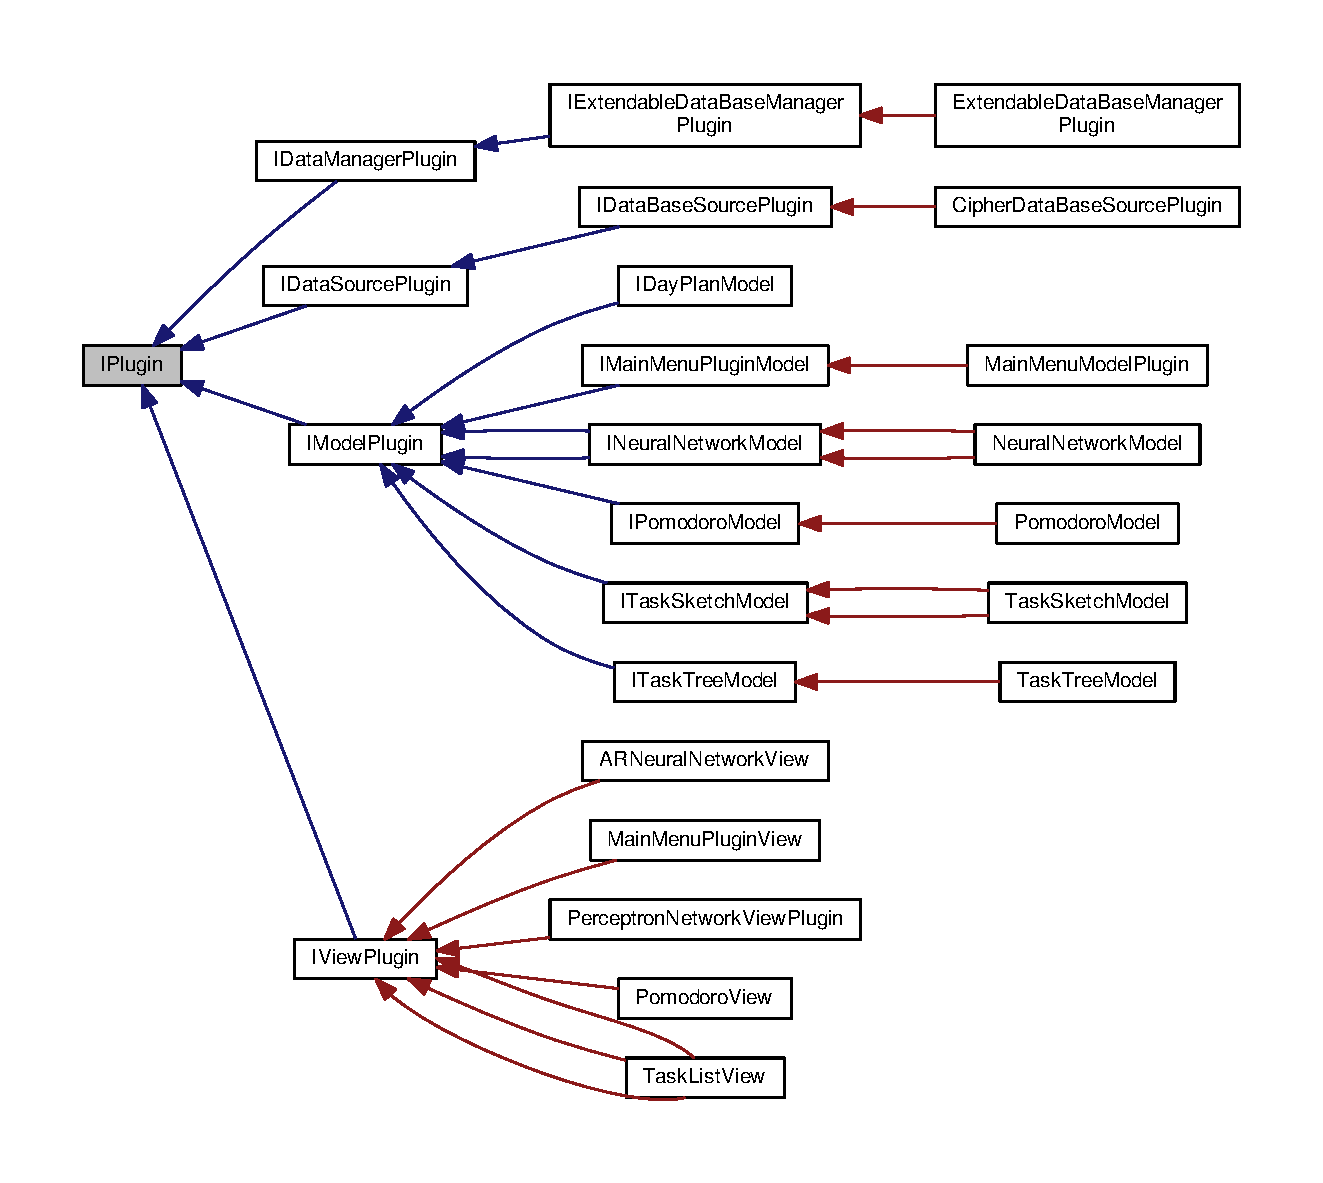
\includegraphics[width=350pt]{class_i_plugin__inherit__graph}
\end{center}
\end{figure}
\subsection*{Public Member Functions}
\begin{DoxyCompactItemize}
\item 
virtual Q\+Widget $\ast$ {\bfseries Get\+Widget} ()=0\hypertarget{class_i_plugin_a2d7fd6ff64386dc3451d93a766cfe5ac}{}\label{class_i_plugin_a2d7fd6ff64386dc3451d93a766cfe5ac}

\item 
virtual void {\bfseries Do\+Something} ()=0\hypertarget{class_i_plugin_a4fe502f97b8dd2dee1e027031f2bf3bc}{}\label{class_i_plugin_a4fe502f97b8dd2dee1e027031f2bf3bc}

\item 
virtual void {\bfseries Add\+Child\+Plugin} (\hyperlink{class_i_plugin}{I\+Plugin} $\ast$, \hyperlink{struct_meta_info}{Meta\+Info} $\ast$)=0\hypertarget{class_i_plugin_a4260318b1f6d80db0c77631465153c3e}{}\label{class_i_plugin_a4260318b1f6d80db0c77631465153c3e}

\item 
virtual bool {\bfseries Open} ()=0\hypertarget{class_i_plugin_aa8a0de947d8556119eca015c3102c8a0}{}\label{class_i_plugin_aa8a0de947d8556119eca015c3102c8a0}

\item 
virtual bool {\bfseries Close} ()=0\hypertarget{class_i_plugin_aa871cff89f6fec30f76481b5ddd689bf}{}\label{class_i_plugin_aa871cff89f6fec30f76481b5ddd689bf}

\item 
virtual Q\+String {\bfseries Get\+Error} ()=0\hypertarget{class_i_plugin_ac22c5e1c522d1827ae8c81cf14bb52df}{}\label{class_i_plugin_ac22c5e1c522d1827ae8c81cf14bb52df}

\item 
virtual void {\bfseries On\+All\+Setup} ()=0\hypertarget{class_i_plugin_a6cfbb338c5be95b42079d935aad8f02f}{}\label{class_i_plugin_a6cfbb338c5be95b42079d935aad8f02f}

\item 
virtual Q\+String {\bfseries Get\+Last\+Error} ()=0\hypertarget{class_i_plugin_a47261bd639ed10f898fd4ecfbc74f4a9}{}\label{class_i_plugin_a47261bd639ed10f898fd4ecfbc74f4a9}

\end{DoxyCompactItemize}


The documentation for this class was generated from the following files\+:\begin{DoxyCompactItemize}
\item 
/home/curunir/\+Documents/\+M\+A\+S\+S/\+Plugins/\+Extendable\+Data\+Base\+Manager/iplugin.\+h\item 
/home/curunir/\+Documents/\+M\+A\+S\+S/\+Plugins/\+Main\+Menu\+Model\+Plugin/interfaces.\+h\end{DoxyCompactItemize}

\hypertarget{class_i_plugin_model}{}\section{I\+Plugin\+Model Class Reference}
\label{class_i_plugin_model}\index{I\+Plugin\+Model@{I\+Plugin\+Model}}
\subsection*{Public Member Functions}
\begin{DoxyCompactItemize}
\item 
virtual void {\bfseries Do\+Something} ()=0\hypertarget{class_i_plugin_model_a377627e683f892ffda2c6225d975251b}{}\label{class_i_plugin_model_a377627e683f892ffda2c6225d975251b}

\item 
virtual void {\bfseries Add\+Child\+Plugin} (\hyperlink{class_i_plugin_model}{I\+Plugin\+Model} $\ast$, \hyperlink{struct_meta_info}{Meta\+Info} $\ast$)=0\hypertarget{class_i_plugin_model_aff406b0571f6dc77488c315e0df0f563}{}\label{class_i_plugin_model_aff406b0571f6dc77488c315e0df0f563}

\item 
virtual void {\bfseries Add\+D\+B\+Tool} (Q\+Object $\ast$)=0\hypertarget{class_i_plugin_model_a2db1262756c4a587fd6cd2d7191841fb}{}\label{class_i_plugin_model_a2db1262756c4a587fd6cd2d7191841fb}

\item 
virtual bool {\bfseries Open} (Q\+Widget $\ast$)=0\hypertarget{class_i_plugin_model_ac1c51202f69db707ca56e8f3c78ce163}{}\label{class_i_plugin_model_ac1c51202f69db707ca56e8f3c78ce163}

\item 
virtual bool {\bfseries Close} ()=0\hypertarget{class_i_plugin_model_a3f9ce2298f73283fec68fc908db14e57}{}\label{class_i_plugin_model_a3f9ce2298f73283fec68fc908db14e57}

\item 
virtual Q\+String {\bfseries Get\+Error} ()=0\hypertarget{class_i_plugin_model_ad42778c15ce3e8fdb9524a6dfd61792a}{}\label{class_i_plugin_model_ad42778c15ce3e8fdb9524a6dfd61792a}

\item 
virtual void {\bfseries Do\+Something} ()=0\hypertarget{class_i_plugin_model_a377627e683f892ffda2c6225d975251b}{}\label{class_i_plugin_model_a377627e683f892ffda2c6225d975251b}

\item 
virtual void {\bfseries Add\+Child\+Plugin} (\hyperlink{class_i_plugin_model}{I\+Plugin\+Model} $\ast$, \hyperlink{struct_meta_info}{Meta\+Info} $\ast$)=0\hypertarget{class_i_plugin_model_aff406b0571f6dc77488c315e0df0f563}{}\label{class_i_plugin_model_aff406b0571f6dc77488c315e0df0f563}

\item 
virtual void {\bfseries Add\+D\+B\+Tool} (Q\+Object $\ast$)=0\hypertarget{class_i_plugin_model_a2db1262756c4a587fd6cd2d7191841fb}{}\label{class_i_plugin_model_a2db1262756c4a587fd6cd2d7191841fb}

\item 
virtual bool {\bfseries Open} (Q\+Widget $\ast$)=0\hypertarget{class_i_plugin_model_ac1c51202f69db707ca56e8f3c78ce163}{}\label{class_i_plugin_model_ac1c51202f69db707ca56e8f3c78ce163}

\item 
virtual bool {\bfseries Close} ()=0\hypertarget{class_i_plugin_model_a3f9ce2298f73283fec68fc908db14e57}{}\label{class_i_plugin_model_a3f9ce2298f73283fec68fc908db14e57}

\item 
virtual Q\+String {\bfseries Get\+Error} ()=0\hypertarget{class_i_plugin_model_ad42778c15ce3e8fdb9524a6dfd61792a}{}\label{class_i_plugin_model_ad42778c15ce3e8fdb9524a6dfd61792a}

\item 
virtual void {\bfseries Do\+Something} ()=0\hypertarget{class_i_plugin_model_a377627e683f892ffda2c6225d975251b}{}\label{class_i_plugin_model_a377627e683f892ffda2c6225d975251b}

\item 
virtual void {\bfseries Add\+Child\+Plugin} (\hyperlink{class_i_plugin_model}{I\+Plugin\+Model} $\ast$, \hyperlink{struct_meta_info}{Meta\+Info} $\ast$)=0\hypertarget{class_i_plugin_model_aff406b0571f6dc77488c315e0df0f563}{}\label{class_i_plugin_model_aff406b0571f6dc77488c315e0df0f563}

\item 
virtual void {\bfseries Add\+D\+B\+Tool} (Q\+Object $\ast$)=0\hypertarget{class_i_plugin_model_a2db1262756c4a587fd6cd2d7191841fb}{}\label{class_i_plugin_model_a2db1262756c4a587fd6cd2d7191841fb}

\item 
virtual bool {\bfseries Open} (Q\+Widget $\ast$)=0\hypertarget{class_i_plugin_model_ac1c51202f69db707ca56e8f3c78ce163}{}\label{class_i_plugin_model_ac1c51202f69db707ca56e8f3c78ce163}

\item 
virtual bool {\bfseries Close} ()=0\hypertarget{class_i_plugin_model_a3f9ce2298f73283fec68fc908db14e57}{}\label{class_i_plugin_model_a3f9ce2298f73283fec68fc908db14e57}

\item 
virtual Q\+String {\bfseries Get\+Error} ()=0\hypertarget{class_i_plugin_model_ad42778c15ce3e8fdb9524a6dfd61792a}{}\label{class_i_plugin_model_ad42778c15ce3e8fdb9524a6dfd61792a}

\item 
virtual void {\bfseries Do\+Something} ()=0\hypertarget{class_i_plugin_model_a377627e683f892ffda2c6225d975251b}{}\label{class_i_plugin_model_a377627e683f892ffda2c6225d975251b}

\item 
virtual void {\bfseries Add\+Child\+Plugin} (\hyperlink{class_i_plugin_model}{I\+Plugin\+Model} $\ast$, \hyperlink{struct_meta_info}{Meta\+Info} $\ast$)=0\hypertarget{class_i_plugin_model_aff406b0571f6dc77488c315e0df0f563}{}\label{class_i_plugin_model_aff406b0571f6dc77488c315e0df0f563}

\item 
virtual void {\bfseries Add\+D\+B\+Tool} (Q\+Object $\ast$)=0\hypertarget{class_i_plugin_model_a2db1262756c4a587fd6cd2d7191841fb}{}\label{class_i_plugin_model_a2db1262756c4a587fd6cd2d7191841fb}

\item 
virtual bool {\bfseries Open} (Q\+Widget $\ast$)=0\hypertarget{class_i_plugin_model_ac1c51202f69db707ca56e8f3c78ce163}{}\label{class_i_plugin_model_ac1c51202f69db707ca56e8f3c78ce163}

\item 
virtual bool {\bfseries Close} ()=0\hypertarget{class_i_plugin_model_a3f9ce2298f73283fec68fc908db14e57}{}\label{class_i_plugin_model_a3f9ce2298f73283fec68fc908db14e57}

\item 
virtual Q\+String {\bfseries Get\+Error} ()=0\hypertarget{class_i_plugin_model_ad42778c15ce3e8fdb9524a6dfd61792a}{}\label{class_i_plugin_model_ad42778c15ce3e8fdb9524a6dfd61792a}

\item 
virtual void {\bfseries Do\+Something} ()=0\hypertarget{class_i_plugin_model_a377627e683f892ffda2c6225d975251b}{}\label{class_i_plugin_model_a377627e683f892ffda2c6225d975251b}

\item 
virtual void {\bfseries Add\+Child\+Plugin} (\hyperlink{class_i_plugin_model}{I\+Plugin\+Model} $\ast$, \hyperlink{struct_meta_info}{Meta\+Info} $\ast$)=0\hypertarget{class_i_plugin_model_aff406b0571f6dc77488c315e0df0f563}{}\label{class_i_plugin_model_aff406b0571f6dc77488c315e0df0f563}

\item 
virtual void {\bfseries Add\+D\+B\+Tool} (Q\+Object $\ast$)=0\hypertarget{class_i_plugin_model_a2db1262756c4a587fd6cd2d7191841fb}{}\label{class_i_plugin_model_a2db1262756c4a587fd6cd2d7191841fb}

\item 
virtual bool {\bfseries Open} (Q\+Widget $\ast$)=0\hypertarget{class_i_plugin_model_ac1c51202f69db707ca56e8f3c78ce163}{}\label{class_i_plugin_model_ac1c51202f69db707ca56e8f3c78ce163}

\item 
virtual bool {\bfseries Close} ()=0\hypertarget{class_i_plugin_model_a3f9ce2298f73283fec68fc908db14e57}{}\label{class_i_plugin_model_a3f9ce2298f73283fec68fc908db14e57}

\item 
virtual Q\+String {\bfseries Get\+Error} ()=0\hypertarget{class_i_plugin_model_ad42778c15ce3e8fdb9524a6dfd61792a}{}\label{class_i_plugin_model_ad42778c15ce3e8fdb9524a6dfd61792a}

\item 
virtual void {\bfseries Do\+Something} ()=0\hypertarget{class_i_plugin_model_a377627e683f892ffda2c6225d975251b}{}\label{class_i_plugin_model_a377627e683f892ffda2c6225d975251b}

\item 
virtual void {\bfseries Add\+Child\+Plugin} (\hyperlink{class_i_plugin_model}{I\+Plugin\+Model} $\ast$, \hyperlink{struct_meta_info}{Meta\+Info} $\ast$)=0\hypertarget{class_i_plugin_model_aff406b0571f6dc77488c315e0df0f563}{}\label{class_i_plugin_model_aff406b0571f6dc77488c315e0df0f563}

\item 
virtual void {\bfseries Add\+D\+B\+Tool} (Q\+Object $\ast$)=0\hypertarget{class_i_plugin_model_a2db1262756c4a587fd6cd2d7191841fb}{}\label{class_i_plugin_model_a2db1262756c4a587fd6cd2d7191841fb}

\item 
virtual bool {\bfseries Open} (Q\+Widget $\ast$)=0\hypertarget{class_i_plugin_model_ac1c51202f69db707ca56e8f3c78ce163}{}\label{class_i_plugin_model_ac1c51202f69db707ca56e8f3c78ce163}

\item 
virtual bool {\bfseries Close} ()=0\hypertarget{class_i_plugin_model_a3f9ce2298f73283fec68fc908db14e57}{}\label{class_i_plugin_model_a3f9ce2298f73283fec68fc908db14e57}

\item 
virtual Q\+String {\bfseries Get\+Error} ()=0\hypertarget{class_i_plugin_model_ad42778c15ce3e8fdb9524a6dfd61792a}{}\label{class_i_plugin_model_ad42778c15ce3e8fdb9524a6dfd61792a}

\item 
virtual void {\bfseries Do\+Something} ()=0\hypertarget{class_i_plugin_model_a377627e683f892ffda2c6225d975251b}{}\label{class_i_plugin_model_a377627e683f892ffda2c6225d975251b}

\item 
virtual void {\bfseries Add\+Child\+Plugin} (\hyperlink{class_i_plugin_model}{I\+Plugin\+Model} $\ast$, \hyperlink{struct_meta_info}{Meta\+Info} $\ast$)=0\hypertarget{class_i_plugin_model_aff406b0571f6dc77488c315e0df0f563}{}\label{class_i_plugin_model_aff406b0571f6dc77488c315e0df0f563}

\item 
virtual void {\bfseries Add\+D\+B\+Tool} (Q\+Object $\ast$)=0\hypertarget{class_i_plugin_model_a2db1262756c4a587fd6cd2d7191841fb}{}\label{class_i_plugin_model_a2db1262756c4a587fd6cd2d7191841fb}

\item 
virtual bool {\bfseries Open} (Q\+Widget $\ast$)=0\hypertarget{class_i_plugin_model_ac1c51202f69db707ca56e8f3c78ce163}{}\label{class_i_plugin_model_ac1c51202f69db707ca56e8f3c78ce163}

\item 
virtual bool {\bfseries Close} ()=0\hypertarget{class_i_plugin_model_a3f9ce2298f73283fec68fc908db14e57}{}\label{class_i_plugin_model_a3f9ce2298f73283fec68fc908db14e57}

\item 
virtual Q\+String {\bfseries Get\+Error} ()=0\hypertarget{class_i_plugin_model_ad42778c15ce3e8fdb9524a6dfd61792a}{}\label{class_i_plugin_model_ad42778c15ce3e8fdb9524a6dfd61792a}

\end{DoxyCompactItemize}


The documentation for this class was generated from the following file\+:\begin{DoxyCompactItemize}
\item 
/home/curunir/\+Documents/\+M\+A\+S\+S/\+Plugins/\+A\+R\+Neural\+Network\+View/interfaces.\+h\end{DoxyCompactItemize}

\hypertarget{class_i_plugin_view}{}\section{I\+Plugin\+View Class Reference}
\label{class_i_plugin_view}\index{I\+Plugin\+View@{I\+Plugin\+View}}
\subsection*{Public Member Functions}
\begin{DoxyCompactItemize}
\item 
virtual void {\bfseries Set\+Model} (Q\+Object $\ast$)=0\hypertarget{class_i_plugin_view_a0da8ecfdc50ba7fb49c6db2dee6fbd81}{}\label{class_i_plugin_view_a0da8ecfdc50ba7fb49c6db2dee6fbd81}

\end{DoxyCompactItemize}


The documentation for this class was generated from the following file\+:\begin{DoxyCompactItemize}
\item 
/home/curunir/\+Documents/\+M\+A\+S\+S/\+Plugins/\+Extendable\+Data\+Base\+Manager/interfaces.\+h\end{DoxyCompactItemize}

\hypertarget{class_i_pomodoro_model}{}\section{I\+Pomodoro\+Model Class Reference}
\label{class_i_pomodoro_model}\index{I\+Pomodoro\+Model@{I\+Pomodoro\+Model}}


Inheritance diagram for I\+Pomodoro\+Model\+:\nopagebreak
\begin{figure}[H]
\begin{center}
\leavevmode
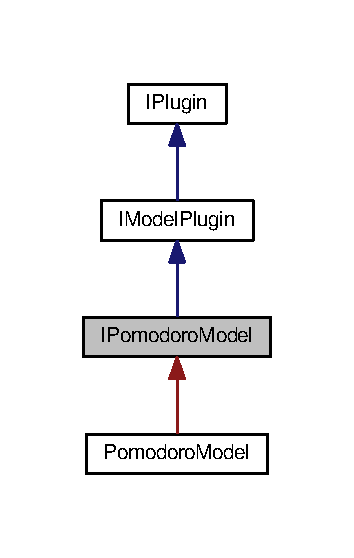
\includegraphics[width=170pt]{class_i_pomodoro_model__inherit__graph}
\end{center}
\end{figure}


Collaboration diagram for I\+Pomodoro\+Model\+:\nopagebreak
\begin{figure}[H]
\begin{center}
\leavevmode
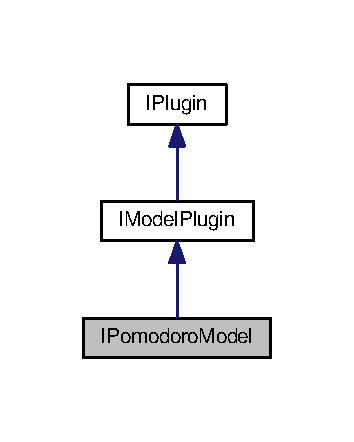
\includegraphics[width=170pt]{class_i_pomodoro_model__coll__graph}
\end{center}
\end{figure}
\subsection*{Public Member Functions}
\begin{DoxyCompactItemize}
\item 
virtual Q\+Abstract\+Item\+Model $\ast$ {\bfseries Get\+Model} ()=0\hypertarget{class_i_pomodoro_model_a8de6ac3baca2a088fbaa6323fcfce4e0}{}\label{class_i_pomodoro_model_a8de6ac3baca2a088fbaa6323fcfce4e0}

\item 
virtual Q\+Abstract\+Item\+Model $\ast$ {\bfseries Get\+Internal\+Model} ()=0\hypertarget{class_i_pomodoro_model_a27a07cc7b6fa637a3de85338fc75696c}{}\label{class_i_pomodoro_model_a27a07cc7b6fa637a3de85338fc75696c}

\end{DoxyCompactItemize}


The documentation for this class was generated from the following file\+:\begin{DoxyCompactItemize}
\item 
/home/curunir/\+Documents/\+M\+A\+S\+S/\+Plugins/\+Pomodoro\+Model/ipomodoromodel.\+h\end{DoxyCompactItemize}

\hypertarget{class_i_root_model_plugin}{}\section{I\+Root\+Model\+Plugin Class Reference}
\label{class_i_root_model_plugin}\index{I\+Root\+Model\+Plugin@{I\+Root\+Model\+Plugin}}


Interface for plugin Root\+Model.  




{\ttfamily \#include $<$rootinterface.\+h$>$}



Inheritance diagram for I\+Root\+Model\+Plugin\+:\nopagebreak
\begin{figure}[H]
\begin{center}
\leavevmode
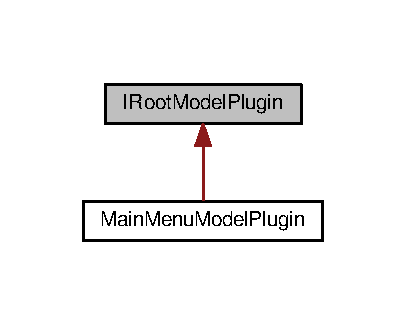
\includegraphics[width=195pt]{class_i_root_model_plugin__inherit__graph}
\end{center}
\end{figure}
\subsection*{Public Member Functions}
\begin{DoxyCompactItemize}
\item 
virtual void \hyperlink{class_i_root_model_plugin_a6c5a6562b3fc16264d36aa6e39b84a7f}{Add\+Plugin} (Q\+Object $\ast$instance, Q\+Json\+Object $\ast$meta)=0
\begin{DoxyCompactList}\small\item\em Recieve loaded plugin with it\textquotesingle{}s meta data. \end{DoxyCompactList}\item 
virtual void \hyperlink{class_i_root_model_plugin_a9ee55034608480fda71b7700d3495984}{Open} (Q\+Widget $\ast$parent\+Widget)=0
\begin{DoxyCompactList}\small\item\em Starts plugin work. Some kind of \textquotesingle{}start\textquotesingle{} signal. \end{DoxyCompactList}\end{DoxyCompactItemize}


\subsection{Detailed Description}
Interface for plugin Root\+Model. 

This interface represents most significant plugin in whole system. If plugin implements this interface it should take care of whole system plugins interactions. When \hyperlink{class_plugin_loader}{Plugin\+Loader} class loads plugins from directory it searchs the plugin which inherits from \hyperlink{class_i_root_model_plugin}{I\+Root\+Model\+Plugin}. If it find one -\/ it will send all loaded plugins to it by using \hyperlink{class_i_root_model_plugin_a6c5a6562b3fc16264d36aa6e39b84a7f}{Add\+Plugin()} method. 

\subsection{Member Function Documentation}
\index{I\+Root\+Model\+Plugin@{I\+Root\+Model\+Plugin}!Add\+Plugin@{Add\+Plugin}}
\index{Add\+Plugin@{Add\+Plugin}!I\+Root\+Model\+Plugin@{I\+Root\+Model\+Plugin}}
\subsubsection[{\texorpdfstring{Add\+Plugin(\+Q\+Object $\ast$instance, Q\+Json\+Object $\ast$meta)=0}{AddPlugin(QObject *instance, QJsonObject *meta)=0}}]{\setlength{\rightskip}{0pt plus 5cm}virtual void I\+Root\+Model\+Plugin\+::\+Add\+Plugin (
\begin{DoxyParamCaption}
\item[{Q\+Object $\ast$}]{instance, }
\item[{Q\+Json\+Object $\ast$}]{meta}
\end{DoxyParamCaption}
)\hspace{0.3cm}{\ttfamily [pure virtual]}}\hypertarget{class_i_root_model_plugin_a6c5a6562b3fc16264d36aa6e39b84a7f}{}\label{class_i_root_model_plugin_a6c5a6562b3fc16264d36aa6e39b84a7f}


Recieve loaded plugin with it\textquotesingle{}s meta data. 


\begin{DoxyParams}{Parameters}
{\em instance} & Plugin instance. \\
\hline
{\em meta} & Plugin meta data. \\
\hline
\end{DoxyParams}


Implemented in \hyperlink{class_main_menu_model_plugin_aedb87208e81b8ee847fc694805364288}{Main\+Menu\+Model\+Plugin}.

\index{I\+Root\+Model\+Plugin@{I\+Root\+Model\+Plugin}!Open@{Open}}
\index{Open@{Open}!I\+Root\+Model\+Plugin@{I\+Root\+Model\+Plugin}}
\subsubsection[{\texorpdfstring{Open(\+Q\+Widget $\ast$parent\+Widget)=0}{Open(QWidget *parentWidget)=0}}]{\setlength{\rightskip}{0pt plus 5cm}virtual void I\+Root\+Model\+Plugin\+::\+Open (
\begin{DoxyParamCaption}
\item[{Q\+Widget $\ast$}]{parent\+Widget}
\end{DoxyParamCaption}
)\hspace{0.3cm}{\ttfamily [pure virtual]}}\hypertarget{class_i_root_model_plugin_a9ee55034608480fda71b7700d3495984}{}\label{class_i_root_model_plugin_a9ee55034608480fda71b7700d3495984}


Starts plugin work. Some kind of \textquotesingle{}start\textquotesingle{} signal. 


\begin{DoxyParams}{Parameters}
{\em parent\+Widget} & This will be parent widget for all widgets in app. \\
\hline
\end{DoxyParams}


Implemented in \hyperlink{class_main_menu_model_plugin_a2eb04afbe1c9a301a7031816f37018ab}{Main\+Menu\+Model\+Plugin}.



The documentation for this class was generated from the following file\+:\begin{DoxyCompactItemize}
\item 
/home/curunir/\+Documents/\+M\+A\+S\+S/\+System/\+M\+A\+S\+S/rootinterface.\+h\end{DoxyCompactItemize}

\hypertarget{class_i_task_tree_model_1_1_i_task_relation_delegate}{}\section{I\+Task\+Tree\+Model\+:\+:I\+Task\+Relation\+Delegate Class Reference}
\label{class_i_task_tree_model_1_1_i_task_relation_delegate}\index{I\+Task\+Tree\+Model\+::\+I\+Task\+Relation\+Delegate@{I\+Task\+Tree\+Model\+::\+I\+Task\+Relation\+Delegate}}
\subsection*{Public Member Functions}
\begin{DoxyCompactItemize}
\item 
virtual void {\bfseries Set\+Value} (Q\+Variant value)=0\hypertarget{class_i_task_tree_model_1_1_i_task_relation_delegate_ab13bf8d76da4ca5e9925a7af7827a994}{}\label{class_i_task_tree_model_1_1_i_task_relation_delegate_ab13bf8d76da4ca5e9925a7af7827a994}

\item 
virtual Q\+Variant {\bfseries Get\+Value} ()=0\hypertarget{class_i_task_tree_model_1_1_i_task_relation_delegate_a1a720d6d7ca9a7aeaf9b182326152d17}{}\label{class_i_task_tree_model_1_1_i_task_relation_delegate_a1a720d6d7ca9a7aeaf9b182326152d17}

\end{DoxyCompactItemize}


The documentation for this class was generated from the following file\+:\begin{DoxyCompactItemize}
\item 
/home/curunir/\+Documents/\+M\+A\+S\+S/\+Plugins/\+Task\+List\+Model/itasktreemodel.\+h\end{DoxyCompactItemize}

\hypertarget{class_i_task_sketch_model}{}\section{I\+Task\+Sketch\+Model Class Reference}
\label{class_i_task_sketch_model}\index{I\+Task\+Sketch\+Model@{I\+Task\+Sketch\+Model}}


Inheritance diagram for I\+Task\+Sketch\+Model\+:\nopagebreak
\begin{figure}[H]
\begin{center}
\leavevmode
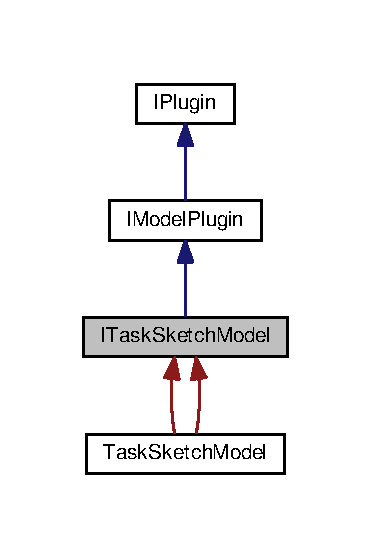
\includegraphics[width=178pt]{class_i_task_sketch_model__inherit__graph}
\end{center}
\end{figure}


Collaboration diagram for I\+Task\+Sketch\+Model\+:\nopagebreak
\begin{figure}[H]
\begin{center}
\leavevmode
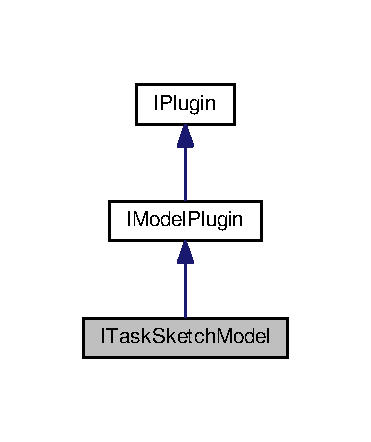
\includegraphics[width=178pt]{class_i_task_sketch_model__coll__graph}
\end{center}
\end{figure}
\subsection*{Signals}
\begin{DoxyCompactItemize}
\item 
void {\bfseries Convert\+Task\+To\+Sketch} (int)\hypertarget{class_i_task_sketch_model_a0bd379546cbb601a0ba0027ba41c22eb}{}\label{class_i_task_sketch_model_a0bd379546cbb601a0ba0027ba41c22eb}

\end{DoxyCompactItemize}
\subsection*{Public Member Functions}
\begin{DoxyCompactItemize}
\item 
virtual Q\+Abstract\+Item\+Model $\ast$ {\bfseries Get\+Model} ()=0\hypertarget{class_i_task_sketch_model_afd9ecfd849e9a10cae71d9d87ae34e5b}{}\label{class_i_task_sketch_model_afd9ecfd849e9a10cae71d9d87ae34e5b}

\item 
virtual Q\+Abstract\+Item\+Model $\ast$ {\bfseries Get\+Internal\+Model} ()=0\hypertarget{class_i_task_sketch_model_a321be8117a6275d0716c07241d7e402a}{}\label{class_i_task_sketch_model_a321be8117a6275d0716c07241d7e402a}

\item 
virtual void {\bfseries Convert\+Sketch\+To\+Task} (int sketch\+Id)=0\hypertarget{class_i_task_sketch_model_aef1346d2236510066f9dc8b0c1f68916}{}\label{class_i_task_sketch_model_aef1346d2236510066f9dc8b0c1f68916}

\end{DoxyCompactItemize}


The documentation for this class was generated from the following file\+:\begin{DoxyCompactItemize}
\item 
/home/curunir/\+Documents/\+M\+A\+S\+S/\+Plugins/\+Task\+Sketch\+Model/itasksketchmodel.\+h\end{DoxyCompactItemize}

\hypertarget{class_i_task_tree_model}{}\section{I\+Task\+Tree\+Model Class Reference}
\label{class_i_task_tree_model}\index{I\+Task\+Tree\+Model@{I\+Task\+Tree\+Model}}
Inheritance diagram for I\+Task\+Tree\+Model\+:\begin{figure}[H]
\begin{center}
\leavevmode
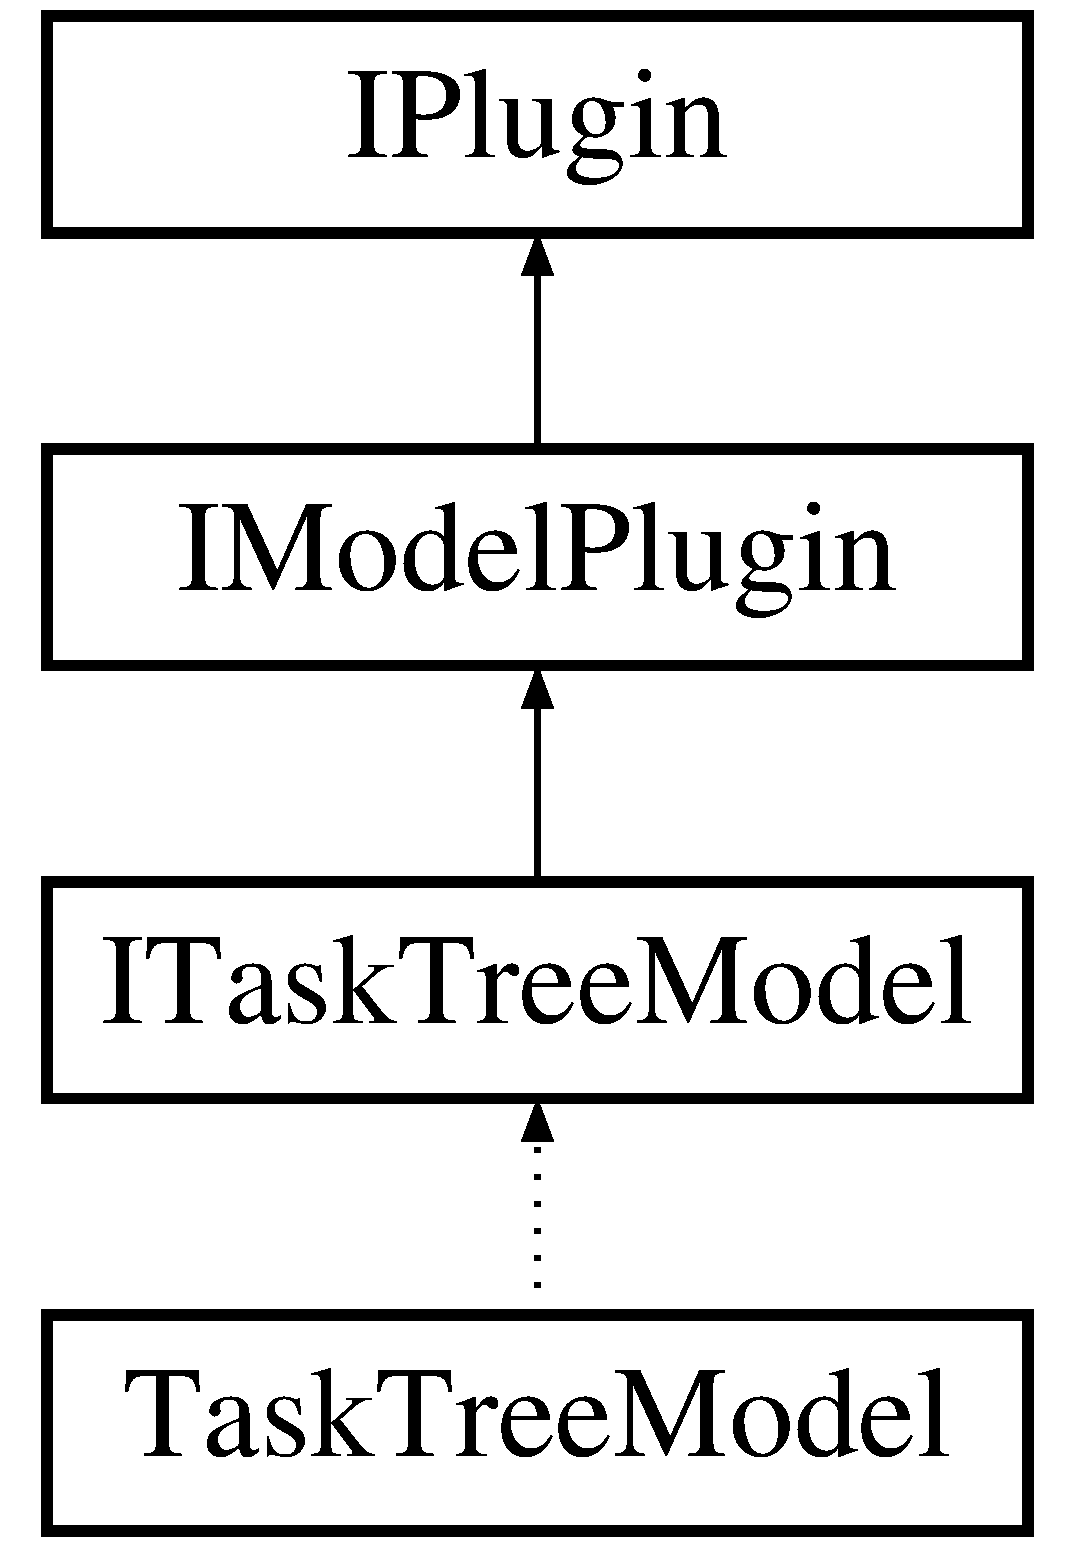
\includegraphics[height=4.000000cm]{class_i_task_tree_model}
\end{center}
\end{figure}
\subsection*{Classes}
\begin{DoxyCompactItemize}
\item 
class \hyperlink{class_i_task_tree_model_1_1_i_task_relation_delegate}{I\+Task\+Relation\+Delegate}
\end{DoxyCompactItemize}
\subsection*{Signals}
\begin{DoxyCompactItemize}
\item 
\mbox{\Hypertarget{class_i_task_tree_model_a562d5278962363c02872c528b839a0c8}\label{class_i_task_tree_model_a562d5278962363c02872c528b839a0c8}} 
void {\bfseries Open\+Task\+Edit} (int id)
\end{DoxyCompactItemize}
\subsection*{Public Member Functions}
\begin{DoxyCompactItemize}
\item 
\mbox{\Hypertarget{class_i_task_tree_model_acb54f948f72d43f4ef600d80e16eb123}\label{class_i_task_tree_model_acb54f948f72d43f4ef600d80e16eb123}} 
virtual Q\+String {\bfseries Get\+Data\+Name} ()=0
\item 
\mbox{\Hypertarget{class_i_task_tree_model_adbffd903706e118845cbeced9f47b914}\label{class_i_task_tree_model_adbffd903706e118845cbeced9f47b914}} 
virtual Q\+Abstract\+Item\+Model $\ast$ {\bfseries Get\+Tree\+Model} ()=0
\item 
\mbox{\Hypertarget{class_i_task_tree_model_a027018d851799a47dd48b17b6d23d8fd}\label{class_i_task_tree_model_a027018d851799a47dd48b17b6d23d8fd}} 
virtual void {\bfseries Set\+Relation\+Delegate} (Q\+String relation, \hyperlink{class_i_task_tree_model_1_1_i_task_relation_delegate}{I\+Task\+Relation\+Delegate} $\ast$delegate)=0
\item 
\mbox{\Hypertarget{class_i_task_tree_model_aea39be804200f98c945e82cdb8476d79}\label{class_i_task_tree_model_aea39be804200f98c945e82cdb8476d79}} 
virtual \hyperlink{class_q_map}{Q\+Map}$<$ Q\+String, \hyperlink{class_i_task_tree_model_1_1_i_task_relation_delegate}{I\+Task\+Relation\+Delegate} $\ast$ $>$ {\bfseries Get\+Relation\+Delegates} ()=0
\end{DoxyCompactItemize}


The documentation for this class was generated from the following file\+:\begin{DoxyCompactItemize}
\item 
C\+:/\+Users/\+Curunir/\+Desktop/\+M\+A\+S\+S/\+Plugins/\+Task\+List\+Model/itasktreemodel.\+h\end{DoxyCompactItemize}

\hypertarget{class_item}{}\section{Item Class Reference}
\label{class_item}\index{Item@{Item}}
\subsection*{Public Member Functions}
\begin{DoxyCompactItemize}
\item 
\mbox{\Hypertarget{class_item_aef96722ef425ab3794691db85ba4abd6}\label{class_item_aef96722ef425ab3794691db85ba4abd6}} 
{\bfseries Item} (\hyperlink{class_item}{Item} $\ast$parent, \hyperlink{class_item}{Item} $\ast$copy)
\item 
\mbox{\Hypertarget{class_item_a27fb96423d6e35b384b226bc3408b348}\label{class_item_a27fb96423d6e35b384b226bc3408b348}} 
{\bfseries Item} (\hyperlink{class_item}{Item} $\ast$parent, int id, Q\+String active\+Chunk, \hyperlink{class_q_map}{Q\+Map}$<$ Q\+String, \hyperlink{class_q_vector}{Q\+Vector}$<$ Q\+Variant $>$$>$ data\+Chunks)
\item 
\mbox{\Hypertarget{class_item_ae09610bc79b15b17cce0428661b14a88}\label{class_item_ae09610bc79b15b17cce0428661b14a88}} 
int {\bfseries Column\+Count} ()
\item 
\mbox{\Hypertarget{class_item_adad3b372e59e9b033d3f8dc371fac651}\label{class_item_adad3b372e59e9b033d3f8dc371fac651}} 
int {\bfseries Get\+Row} ()
\item 
\mbox{\Hypertarget{class_item_a279eb94495d56f33e8779f1de7110681}\label{class_item_a279eb94495d56f33e8779f1de7110681}} 
void {\bfseries Set\+Childs} (\hyperlink{class_q_list}{Q\+List}$<$ \hyperlink{class_item}{Item} $\ast$$>$ childs)
\item 
\mbox{\Hypertarget{class_item_a6a98cb08e94548f37614132f663f5dfb}\label{class_item_a6a98cb08e94548f37614132f663f5dfb}} 
void {\bfseries Add\+Child} (int row, \hyperlink{class_item}{Item} $\ast$child)
\item 
\mbox{\Hypertarget{class_item_ab77ee89c1d573571d46276904ddea022}\label{class_item_ab77ee89c1d573571d46276904ddea022}} 
void {\bfseries Remove\+Child} (\hyperlink{class_item}{Item} $\ast$child)
\item 
\mbox{\Hypertarget{class_item_a88f43c96e836f5a1473763fd0e8846bb}\label{class_item_a88f43c96e836f5a1473763fd0e8846bb}} 
void {\bfseries Remove\+Child\+At} (int row)
\item 
\mbox{\Hypertarget{class_item_a80ac5f26c6d125de147b2c5aae8631c7}\label{class_item_a80ac5f26c6d125de147b2c5aae8631c7}} 
\hyperlink{class_item}{Item} $\ast$ {\bfseries Get\+Child\+At} (int row)
\item 
\mbox{\Hypertarget{class_item_a9324d6e789340e65394bea357954e6e1}\label{class_item_a9324d6e789340e65394bea357954e6e1}} 
int {\bfseries Child\+Count} ()
\item 
\mbox{\Hypertarget{class_item_afccf539d108a9b083b67105ccb548f11}\label{class_item_afccf539d108a9b083b67105ccb548f11}} 
int {\bfseries Get\+Child\+Position} (\hyperlink{class_item}{Item} $\ast$item)
\item 
\mbox{\Hypertarget{class_item_accef83c1103296fc80b30a809e7ae293}\label{class_item_accef83c1103296fc80b30a809e7ae293}} 
void {\bfseries Set\+Active\+Chunk\+Name} (Q\+String \&active\+Chunk)
\item 
\mbox{\Hypertarget{class_item_ab50d988f2abaaa6a0803b1d35d239220}\label{class_item_ab50d988f2abaaa6a0803b1d35d239220}} 
\hyperlink{class_q_list}{Q\+List}$<$ Q\+String $>$ {\bfseries Get\+Chunks\+Names} ()
\item 
\mbox{\Hypertarget{class_item_af0ee587a5f74c92bd4d9a902a6a7e0d3}\label{class_item_af0ee587a5f74c92bd4d9a902a6a7e0d3}} 
\hyperlink{class_q_vector}{Q\+Vector}$<$ Q\+Variant $>$ {\bfseries Get\+Chunk\+Data} (Q\+String chunk\+Name=\char`\"{}\char`\"{})
\item 
\mbox{\Hypertarget{class_item_a6f25765ce2c56248e04d04ebec90d34d}\label{class_item_a6f25765ce2c56248e04d04ebec90d34d}} 
Q\+Variant {\bfseries Get\+Chunk\+Data\+Element} (int column)
\item 
\mbox{\Hypertarget{class_item_a0617312073b3d751518cfd6269c25c0a}\label{class_item_a0617312073b3d751518cfd6269c25c0a}} 
void {\bfseries Set\+Chunk\+Data} (Q\+String chunk\+Name, \hyperlink{class_q_vector}{Q\+Vector}$<$ Q\+Variant $>$ data)
\item 
\mbox{\Hypertarget{class_item_a2206a4c379b351c9cbbe2406399d2b30}\label{class_item_a2206a4c379b351c9cbbe2406399d2b30}} 
void {\bfseries Set\+Chunk\+Data\+Element} (int column, Q\+Variant data)
\item 
\mbox{\Hypertarget{class_item_ab0fa052dc1e0dc785767d25a6010ea13}\label{class_item_ab0fa052dc1e0dc785767d25a6010ea13}} 
void {\bfseries Set\+Decoration} (Q\+Variant pixmap)
\item 
\mbox{\Hypertarget{class_item_ad74957af2eb1996ebdcece4ccdb11c4d}\label{class_item_ad74957af2eb1996ebdcece4ccdb11c4d}} 
Q\+Variant {\bfseries Get\+Decoration} ()
\item 
\mbox{\Hypertarget{class_item_a3466b4b51b244ccbcac853ee7240af47}\label{class_item_a3466b4b51b244ccbcac853ee7240af47}} 
int {\bfseries Get\+Id} ()
\item 
\mbox{\Hypertarget{class_item_a46a50959228845fc8d4c1a1e3cdfc9a3}\label{class_item_a46a50959228845fc8d4c1a1e3cdfc9a3}} 
void {\bfseries Set\+Id} (int id)
\item 
\mbox{\Hypertarget{class_item_aef96722ef425ab3794691db85ba4abd6}\label{class_item_aef96722ef425ab3794691db85ba4abd6}} 
{\bfseries Item} (\hyperlink{class_item}{Item} $\ast$parent, \hyperlink{class_item}{Item} $\ast$copy)
\item 
\mbox{\Hypertarget{class_item_a27fb96423d6e35b384b226bc3408b348}\label{class_item_a27fb96423d6e35b384b226bc3408b348}} 
{\bfseries Item} (\hyperlink{class_item}{Item} $\ast$parent, int id, Q\+String active\+Chunk, \hyperlink{class_q_map}{Q\+Map}$<$ Q\+String, \hyperlink{class_q_vector}{Q\+Vector}$<$ Q\+Variant $>$$>$ data\+Chunks)
\item 
\mbox{\Hypertarget{class_item_ae09610bc79b15b17cce0428661b14a88}\label{class_item_ae09610bc79b15b17cce0428661b14a88}} 
int {\bfseries Column\+Count} ()
\item 
\mbox{\Hypertarget{class_item_adad3b372e59e9b033d3f8dc371fac651}\label{class_item_adad3b372e59e9b033d3f8dc371fac651}} 
int {\bfseries Get\+Row} ()
\item 
\mbox{\Hypertarget{class_item_a279eb94495d56f33e8779f1de7110681}\label{class_item_a279eb94495d56f33e8779f1de7110681}} 
void {\bfseries Set\+Childs} (\hyperlink{class_q_list}{Q\+List}$<$ \hyperlink{class_item}{Item} $\ast$$>$ childs)
\item 
\mbox{\Hypertarget{class_item_a6a98cb08e94548f37614132f663f5dfb}\label{class_item_a6a98cb08e94548f37614132f663f5dfb}} 
void {\bfseries Add\+Child} (int row, \hyperlink{class_item}{Item} $\ast$child)
\item 
\mbox{\Hypertarget{class_item_ab77ee89c1d573571d46276904ddea022}\label{class_item_ab77ee89c1d573571d46276904ddea022}} 
void {\bfseries Remove\+Child} (\hyperlink{class_item}{Item} $\ast$child)
\item 
\mbox{\Hypertarget{class_item_a88f43c96e836f5a1473763fd0e8846bb}\label{class_item_a88f43c96e836f5a1473763fd0e8846bb}} 
void {\bfseries Remove\+Child\+At} (int row)
\item 
\mbox{\Hypertarget{class_item_a80ac5f26c6d125de147b2c5aae8631c7}\label{class_item_a80ac5f26c6d125de147b2c5aae8631c7}} 
\hyperlink{class_item}{Item} $\ast$ {\bfseries Get\+Child\+At} (int row)
\item 
\mbox{\Hypertarget{class_item_a9324d6e789340e65394bea357954e6e1}\label{class_item_a9324d6e789340e65394bea357954e6e1}} 
int {\bfseries Child\+Count} ()
\item 
\mbox{\Hypertarget{class_item_afccf539d108a9b083b67105ccb548f11}\label{class_item_afccf539d108a9b083b67105ccb548f11}} 
int {\bfseries Get\+Child\+Position} (\hyperlink{class_item}{Item} $\ast$item)
\item 
\mbox{\Hypertarget{class_item_accef83c1103296fc80b30a809e7ae293}\label{class_item_accef83c1103296fc80b30a809e7ae293}} 
void {\bfseries Set\+Active\+Chunk\+Name} (Q\+String \&active\+Chunk)
\item 
\mbox{\Hypertarget{class_item_a68ce6aeeb3977fda454f680811de37a4}\label{class_item_a68ce6aeeb3977fda454f680811de37a4}} 
\hyperlink{class_q_list}{Q\+List}$<$ Q\+String $>$ {\bfseries Get\+Chunks\+Names} ()
\item 
\mbox{\Hypertarget{class_item_adbc518bc597ca7a811dc4ec9dad3e51b}\label{class_item_adbc518bc597ca7a811dc4ec9dad3e51b}} 
\hyperlink{class_q_vector}{Q\+Vector}$<$ Q\+Variant $>$ {\bfseries Get\+Chunk\+Data} (Q\+String chunk\+Name)
\item 
\mbox{\Hypertarget{class_item_a6f25765ce2c56248e04d04ebec90d34d}\label{class_item_a6f25765ce2c56248e04d04ebec90d34d}} 
Q\+Variant {\bfseries Get\+Chunk\+Data\+Element} (int column)
\item 
\mbox{\Hypertarget{class_item_a0617312073b3d751518cfd6269c25c0a}\label{class_item_a0617312073b3d751518cfd6269c25c0a}} 
void {\bfseries Set\+Chunk\+Data} (Q\+String chunk\+Name, \hyperlink{class_q_vector}{Q\+Vector}$<$ Q\+Variant $>$ data)
\item 
\mbox{\Hypertarget{class_item_a2206a4c379b351c9cbbe2406399d2b30}\label{class_item_a2206a4c379b351c9cbbe2406399d2b30}} 
void {\bfseries Set\+Chunk\+Data\+Element} (int column, Q\+Variant data)
\item 
\mbox{\Hypertarget{class_item_a3466b4b51b244ccbcac853ee7240af47}\label{class_item_a3466b4b51b244ccbcac853ee7240af47}} 
int {\bfseries Get\+Id} ()
\item 
\mbox{\Hypertarget{class_item_a46a50959228845fc8d4c1a1e3cdfc9a3}\label{class_item_a46a50959228845fc8d4c1a1e3cdfc9a3}} 
void {\bfseries Set\+Id} (int id)
\end{DoxyCompactItemize}
\subsection*{Public Attributes}
\begin{DoxyCompactItemize}
\item 
\mbox{\Hypertarget{class_item_ac5078a594ac17181e0ee2d90c63e9aa1}\label{class_item_ac5078a594ac17181e0ee2d90c63e9aa1}} 
\hyperlink{class_item}{Item} $\ast$ {\bfseries parent\+Item}
\end{DoxyCompactItemize}


The documentation for this class was generated from the following files\+:\begin{DoxyCompactItemize}
\item 
C\+:/\+Users/\+Curunir/\+Desktop/\+M\+A\+S\+S/\+Plugins/\+Extendable\+Data\+Base\+Manager/item.\+h\item 
C\+:/\+Users/\+Curunir/\+Desktop/\+M\+A\+S\+S/\+Plugins/\+Extendable\+Data\+Base\+Manager/item.\+cpp\end{DoxyCompactItemize}

\hypertarget{class_i_view_plugin}{}\section{I\+View\+Plugin Class Reference}
\label{class_i_view_plugin}\index{I\+View\+Plugin@{I\+View\+Plugin}}
Inheritance diagram for I\+View\+Plugin\+:\begin{figure}[H]
\begin{center}
\leavevmode
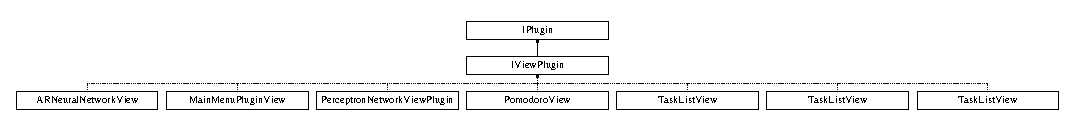
\includegraphics[height=1.250000cm]{class_i_view_plugin}
\end{center}
\end{figure}
\subsection*{Public Member Functions}
\begin{DoxyCompactItemize}
\item 
\mbox{\Hypertarget{class_i_view_plugin_a119545ceff6d7c5deaf9f1dd817af171}\label{class_i_view_plugin_a119545ceff6d7c5deaf9f1dd817af171}} 
virtual void {\bfseries Set\+Model} (Q\+Object $\ast$)=0
\item 
\mbox{\Hypertarget{class_i_view_plugin_a2eb2d20d1d438fee58cd5a6405efdef2}\label{class_i_view_plugin_a2eb2d20d1d438fee58cd5a6405efdef2}} 
virtual bool {\bfseries Open} (Q\+Widget $\ast$parent)=0
\item 
\mbox{\Hypertarget{class_i_view_plugin_a167e8ed723d3164652351d03e6db6869}\label{class_i_view_plugin_a167e8ed723d3164652351d03e6db6869}} 
virtual bool {\bfseries Close} ()=0
\end{DoxyCompactItemize}


The documentation for this class was generated from the following file\+:\begin{DoxyCompactItemize}
\item 
C\+:/\+Users/\+Curunir/\+Desktop/\+M\+A\+S\+S/\+Plugins/\+Main\+Menu\+Model\+Plugin/interfaces.\+h\end{DoxyCompactItemize}

\hypertarget{struct_perceptron_1_1_layer_params}{}\section{Perceptron\+:\+:Layer\+Params Struct Reference}
\label{struct_perceptron_1_1_layer_params}\index{Perceptron\+::\+Layer\+Params@{Perceptron\+::\+Layer\+Params}}
\subsection*{Public Attributes}
\begin{DoxyCompactItemize}
\item 
\mbox{\Hypertarget{struct_perceptron_1_1_layer_params_a2b7908df7e8e4f1b8d836d732fc29fde}\label{struct_perceptron_1_1_layer_params_a2b7908df7e8e4f1b8d836d732fc29fde}} 
int {\bfseries size}
\item 
\mbox{\Hypertarget{struct_perceptron_1_1_layer_params_aecb000611727cbf8ad2051118f2d8234}\label{struct_perceptron_1_1_layer_params_aecb000611727cbf8ad2051118f2d8234}} 
float {\bfseries Learn\+Speed}
\item 
\mbox{\Hypertarget{struct_perceptron_1_1_layer_params_a78bd006d129e016f1f710b9c07b2f985}\label{struct_perceptron_1_1_layer_params_a78bd006d129e016f1f710b9c07b2f985}} 
float {\bfseries Moment}
\item 
\mbox{\Hypertarget{struct_perceptron_1_1_layer_params_a9c9b4e0e12a9705d99a3392873088d7d}\label{struct_perceptron_1_1_layer_params_a9c9b4e0e12a9705d99a3392873088d7d}} 
float {\bfseries Func\+Indent}
\item 
\mbox{\Hypertarget{struct_perceptron_1_1_layer_params_a3ac7b22335513c6b707d99ac45ec95db}\label{struct_perceptron_1_1_layer_params_a3ac7b22335513c6b707d99ac45ec95db}} 
float {\bfseries Bias}
\end{DoxyCompactItemize}


The documentation for this struct was generated from the following file\+:\begin{DoxyCompactItemize}
\item 
C\+:/\+Users/\+Curunir/\+Desktop/\+M\+A\+S\+S/\+Plugins/\+Neural\+Network\+Model/parameters.\+h\end{DoxyCompactItemize}

\hypertarget{struct_layer_params}{}\section{Layer\+Params Struct Reference}
\label{struct_layer_params}\index{Layer\+Params@{Layer\+Params}}
\subsection*{Public Attributes}
\begin{DoxyCompactItemize}
\item 
int {\bfseries size}\hypertarget{struct_layer_params_a2e54d0a4d2d5b21b74f3fe1201edf496}{}\label{struct_layer_params_a2e54d0a4d2d5b21b74f3fe1201edf496}

\item 
float {\bfseries Learn\+Speed}\hypertarget{struct_layer_params_a1461967bf879d4aa8eedcbd8557578ae}{}\label{struct_layer_params_a1461967bf879d4aa8eedcbd8557578ae}

\item 
float {\bfseries Moment}\hypertarget{struct_layer_params_a8519674bc4f1a5aca12a75f2a64883fc}{}\label{struct_layer_params_a8519674bc4f1a5aca12a75f2a64883fc}

\item 
float {\bfseries Func\+Indent}\hypertarget{struct_layer_params_aae57514ee2e26631a5117c4e51bfcc11}{}\label{struct_layer_params_aae57514ee2e26631a5117c4e51bfcc11}

\item 
float {\bfseries Bias}\hypertarget{struct_layer_params_a91105a7a6bbd8a8c6c4b60cb105f0008}{}\label{struct_layer_params_a91105a7a6bbd8a8c6c4b60cb105f0008}

\end{DoxyCompactItemize}


The documentation for this struct was generated from the following file\+:\begin{DoxyCompactItemize}
\item 
/home/curunir/\+Documents/\+M\+A\+S\+S/\+Plugins/\+Perceptron\+Neural\+Network\+View/mainform.\+h\end{DoxyCompactItemize}

\hypertarget{class_ui_1_1_main_form}{}\section{Ui\+:\+:Main\+Form Class Reference}
\label{class_ui_1_1_main_form}\index{Ui\+::\+Main\+Form@{Ui\+::\+Main\+Form}}
Inheritance diagram for Ui\+:\+:Main\+Form\+:\begin{figure}[H]
\begin{center}
\leavevmode
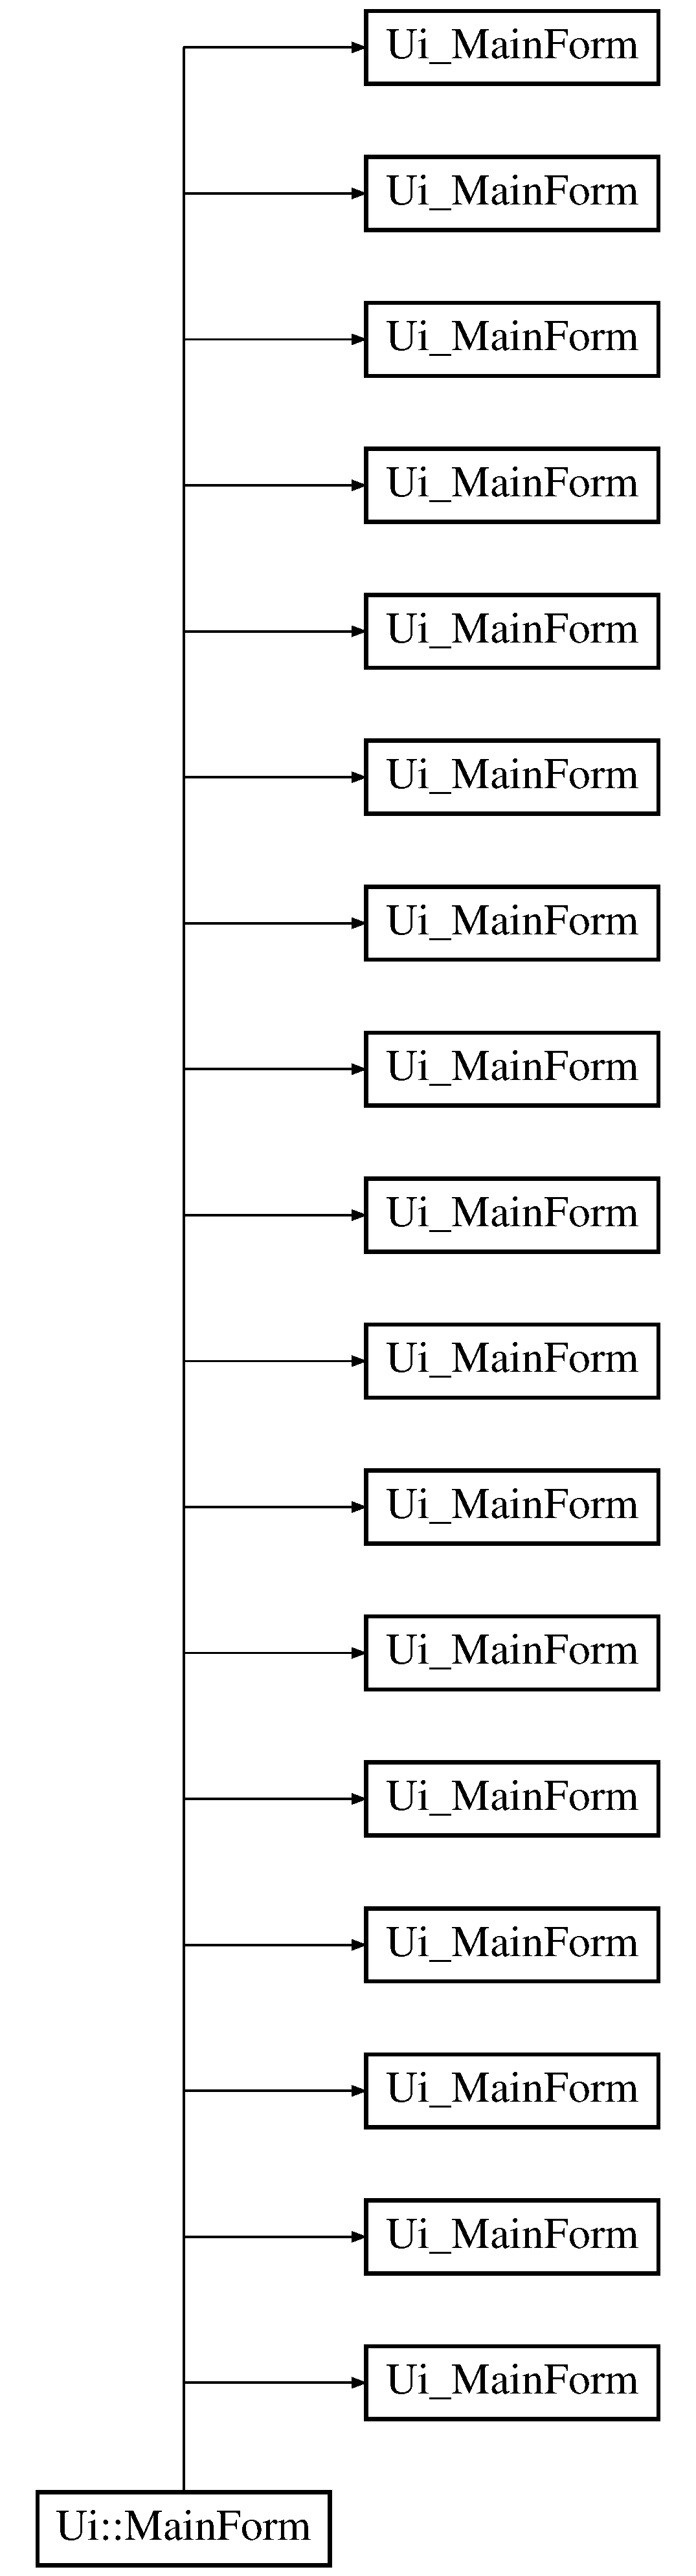
\includegraphics[height=12.000000cm]{class_ui_1_1_main_form}
\end{center}
\end{figure}
\subsection*{Additional Inherited Members}


The documentation for this class was generated from the following file\+:\begin{DoxyCompactItemize}
\item 
C\+:/\+Users/\+Curunir/\+Desktop/\+M\+A\+S\+S/\+Plugins/build-\/\+Android\+\_\+armeabi\+\_\+v7a\+\_\+\+G\+C\+C\+\_\+4\+\_\+9\+\_\+\+Qt\+\_\+5\+\_\+8\+\_\+0-\/\+A\+R\+Neural\+Network\+View-\/\+Debug/ui\+\_\+mainform.\+h\end{DoxyCompactItemize}

\hypertarget{class_main_form}{}\section{Main\+Form Class Reference}
\label{class_main_form}\index{Main\+Form@{Main\+Form}}


Inheritance diagram for Main\+Form\+:\nopagebreak
\begin{figure}[H]
\begin{center}
\leavevmode
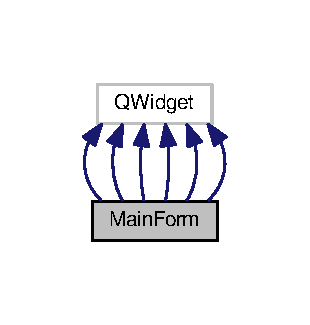
\includegraphics[width=149pt]{class_main_form__inherit__graph}
\end{center}
\end{figure}


Collaboration diagram for Main\+Form\+:\nopagebreak
\begin{figure}[H]
\begin{center}
\leavevmode
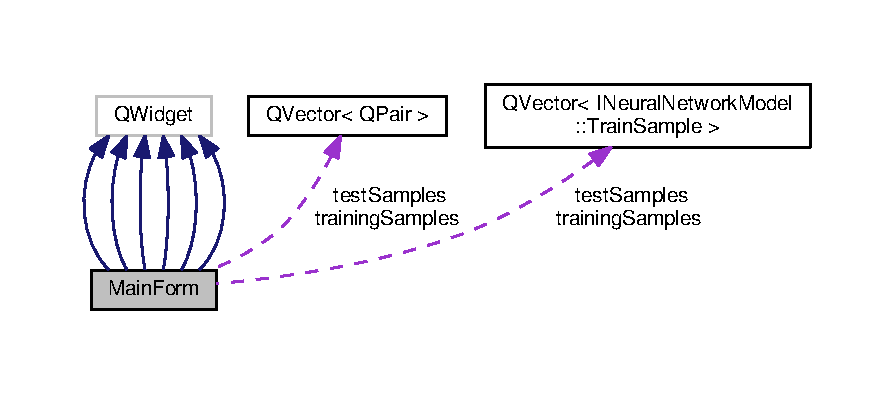
\includegraphics[width=350pt]{class_main_form__coll__graph}
\end{center}
\end{figure}
\subsection*{Signals}
\begin{DoxyCompactItemize}
\item 
void {\bfseries on\+Close} ()\hypertarget{class_main_form_af5c793d14da28ffb85334e9788f64756}{}\label{class_main_form_af5c793d14da28ffb85334e9788f64756}

\item 
void {\bfseries on\+Close} ()\hypertarget{class_main_form_af5c793d14da28ffb85334e9788f64756}{}\label{class_main_form_af5c793d14da28ffb85334e9788f64756}

\item 
void {\bfseries On\+Item\+Selected} (\hyperlink{struct_i_main_menu_plugin_model_1_1_menu_item}{I\+Main\+Menu\+Plugin\+Model\+::\+Menu\+Item} $\ast$meta, \hyperlink{struct_meta_info}{Meta\+Info} $\ast$view\+Meta)\hypertarget{class_main_form_add09750f28044115c869ec8f6d6b86ef}{}\label{class_main_form_add09750f28044115c869ec8f6d6b86ef}

\item 
void {\bfseries On\+Close} ()\hypertarget{class_main_form_ae51e9ea97c7c12d0d8b59cb295f8018b}{}\label{class_main_form_ae51e9ea97c7c12d0d8b59cb295f8018b}

\item 
void {\bfseries on\+Close} ()\hypertarget{class_main_form_af5c793d14da28ffb85334e9788f64756}{}\label{class_main_form_af5c793d14da28ffb85334e9788f64756}

\item 
void {\bfseries on\+Close} ()\hypertarget{class_main_form_af5c793d14da28ffb85334e9788f64756}{}\label{class_main_form_af5c793d14da28ffb85334e9788f64756}

\item 
void {\bfseries on\+Close} ()\hypertarget{class_main_form_af5c793d14da28ffb85334e9788f64756}{}\label{class_main_form_af5c793d14da28ffb85334e9788f64756}

\item 
void {\bfseries On\+Item\+Convert} (int index)\hypertarget{class_main_form_a9f87a145f41c5b1bf064415f79423586}{}\label{class_main_form_a9f87a145f41c5b1bf064415f79423586}

\end{DoxyCompactItemize}
\subsection*{Public Member Functions}
\begin{DoxyCompactItemize}
\item 
{\bfseries Main\+Form} (Q\+Widget $\ast$parent=0)\hypertarget{class_main_form_a8407ed1ab0a7b7bef115711157c8f344}{}\label{class_main_form_a8407ed1ab0a7b7bef115711157c8f344}

\item 
void {\bfseries Set\+Model} (\hyperlink{class_i_neural_network_model}{I\+Neural\+Network\+Model} $\ast$Model)\hypertarget{class_main_form_a69da72ae01b90a41559c050e81020135}{}\label{class_main_form_a69da72ae01b90a41559c050e81020135}

\item 
{\bfseries Main\+Form} (Q\+Widget $\ast$parent=0)\hypertarget{class_main_form_a8407ed1ab0a7b7bef115711157c8f344}{}\label{class_main_form_a8407ed1ab0a7b7bef115711157c8f344}

\item 
void {\bfseries Set\+Model} (\hyperlink{class_i_task_sketch_model}{I\+Task\+Sketch\+Model} $\ast$model)\hypertarget{class_main_form_a4d6783977b0be48e1523fd03d836e64b}{}\label{class_main_form_a4d6783977b0be48e1523fd03d836e64b}

\item 
{\bfseries Main\+Form} (Q\+Widget $\ast$parent=0)\hypertarget{class_main_form_a8407ed1ab0a7b7bef115711157c8f344}{}\label{class_main_form_a8407ed1ab0a7b7bef115711157c8f344}

\item 
void {\bfseries Set\+Root\+Menu\+Item} (\hyperlink{struct_i_main_menu_plugin_model_1_1_menu_item}{I\+Main\+Menu\+Plugin\+Model\+::\+Menu\+Item} $\ast$Root\+Menu\+Item)\hypertarget{class_main_form_a6d1caba5273f012fa93e93bc5b259e16}{}\label{class_main_form_a6d1caba5273f012fa93e93bc5b259e16}

\item 
void {\bfseries Add\+Subitems} (\hyperlink{class_menu_item_graphics_object}{Menu\+Item\+Graphics\+Object} $\ast$Parent\+Menu\+Item, \hyperlink{struct_i_main_menu_plugin_model_1_1_menu_item}{I\+Main\+Menu\+Plugin\+Model\+::\+Menu\+Item} $\ast$Parent\+Menu\+Item\+Struct)\hypertarget{class_main_form_aab382edeb9cf6c08dd2773f63268ea3d}{}\label{class_main_form_aab382edeb9cf6c08dd2773f63268ea3d}

\item 
void {\bfseries Wipe\+All\+Items} ()\hypertarget{class_main_form_a27f6000033cf622a9629b82927055c95}{}\label{class_main_form_a27f6000033cf622a9629b82927055c95}

\item 
{\bfseries Main\+Form} (Q\+Widget $\ast$parent=0)\hypertarget{class_main_form_a8407ed1ab0a7b7bef115711157c8f344}{}\label{class_main_form_a8407ed1ab0a7b7bef115711157c8f344}

\item 
void {\bfseries Set\+Model} (\hyperlink{class_i_neural_network_model}{I\+Neural\+Network\+Model} $\ast$Model)\hypertarget{class_main_form_a69da72ae01b90a41559c050e81020135}{}\label{class_main_form_a69da72ae01b90a41559c050e81020135}

\item 
{\bfseries Main\+Form} (Q\+Widget $\ast$parent=0)\hypertarget{class_main_form_a8407ed1ab0a7b7bef115711157c8f344}{}\label{class_main_form_a8407ed1ab0a7b7bef115711157c8f344}

\item 
bool {\bfseries event\+Filter} (Q\+Object $\ast$watched, Q\+Event $\ast$event) override\hypertarget{class_main_form_a1ca32d59dddffa2396c8175e4dbcff58}{}\label{class_main_form_a1ca32d59dddffa2396c8175e4dbcff58}

\item 
void {\bfseries Set\+Model} (Q\+Abstract\+Item\+Model $\ast$model)\hypertarget{class_main_form_aa6a63e62eb08de727aba05a0a20c3d3e}{}\label{class_main_form_aa6a63e62eb08de727aba05a0a20c3d3e}

\item 
{\bfseries Main\+Form} (Q\+Widget $\ast$parent=0)\hypertarget{class_main_form_a8407ed1ab0a7b7bef115711157c8f344}{}\label{class_main_form_a8407ed1ab0a7b7bef115711157c8f344}

\item 
void {\bfseries Set\+Model} (\hyperlink{class_i_task_sketch_model}{I\+Task\+Sketch\+Model} $\ast$model)\hypertarget{class_main_form_a4d6783977b0be48e1523fd03d836e64b}{}\label{class_main_form_a4d6783977b0be48e1523fd03d836e64b}

\end{DoxyCompactItemize}
\subsection*{Public Attributes}
\begin{DoxyCompactItemize}
\item 
\hyperlink{class_q_vector}{Q\+Vector}$<$ I\+Neural\+Network\+Model\+::\+Train\+Sample $>$ {\bfseries training\+Samples}\hypertarget{class_main_form_ae3827327ab01288622f789ffd9a061d9}{}\label{class_main_form_ae3827327ab01288622f789ffd9a061d9}

\item 
\hyperlink{class_q_vector}{Q\+Vector}$<$ I\+Neural\+Network\+Model\+::\+Train\+Sample $>$ {\bfseries test\+Samples}\hypertarget{class_main_form_a869b2038409b2ba9fad616af593a97a3}{}\label{class_main_form_a869b2038409b2ba9fad616af593a97a3}

\item 
Q\+Standard\+Item\+Model {\bfseries item\+Model}\hypertarget{class_main_form_a7786cdf045d6037668f86b6db1277ba3}{}\label{class_main_form_a7786cdf045d6037668f86b6db1277ba3}

\item 
Q\+Standard\+Item\+Model {\bfseries train\+Images\+Model}\hypertarget{class_main_form_af5cdf86f72c4e89d8038b1594078b2a3}{}\label{class_main_form_af5cdf86f72c4e89d8038b1594078b2a3}

\item 
Q\+Standard\+Item\+Model {\bfseries test\+Images\+Model}\hypertarget{class_main_form_afcb8254310b51c1fd58c3852a6f063fa}{}\label{class_main_form_afcb8254310b51c1fd58c3852a6f063fa}

\item 
\hyperlink{class_q_vector}{Q\+Vector}$<$ \hyperlink{class_q_pair}{Input\+SampleF} $>$ {\bfseries training\+Samples}\hypertarget{class_main_form_a52b405f679729e32653e468a14aec648}{}\label{class_main_form_a52b405f679729e32653e468a14aec648}

\item 
\hyperlink{class_q_vector}{Q\+Vector}$<$ \hyperlink{class_q_pair}{Input\+SampleF} $>$ {\bfseries test\+Samples}\hypertarget{class_main_form_a04762603238b7eace528239e5354a632}{}\label{class_main_form_a04762603238b7eace528239e5354a632}

\end{DoxyCompactItemize}


The documentation for this class was generated from the following files\+:\begin{DoxyCompactItemize}
\item 
/home/curunir/\+Documents/\+M\+A\+S\+S/\+Plugins/\+A\+R\+Neural\+Network\+View/mainform.\+h\item 
/home/curunir/\+Documents/\+M\+A\+S\+S/\+Plugins/\+A\+R\+Neural\+Network\+View/mainform.\+cpp\item 
/home/curunir/\+Documents/\+M\+A\+S\+S/\+Plugins/build-\/\+Main\+Menu\+View\+Plugin-\/\+Desktop-\/\+Debug/moc\+\_\+mainform.\+cpp\end{DoxyCompactItemize}

\hypertarget{class_main_menu_model_plugin}{}\section{Main\+Menu\+Model\+Plugin Class Reference}
\label{class_main_menu_model_plugin}\index{Main\+Menu\+Model\+Plugin@{Main\+Menu\+Model\+Plugin}}
Inheritance diagram for Main\+Menu\+Model\+Plugin\+:\begin{figure}[H]
\begin{center}
\leavevmode
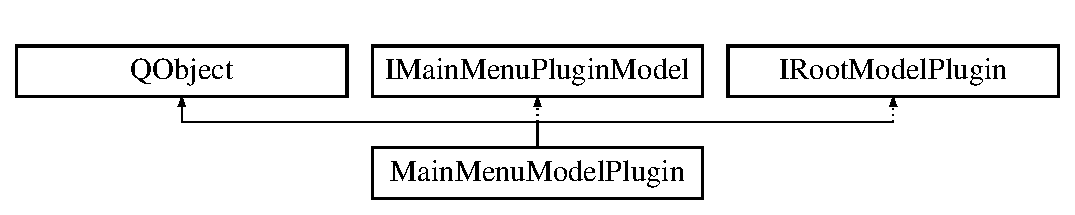
\includegraphics[height=2.000000cm]{class_main_menu_model_plugin}
\end{center}
\end{figure}
\subsection*{Public Member Functions}
\begin{DoxyCompactItemize}
\item 
void \hyperlink{class_main_menu_model_plugin_aedb87208e81b8ee847fc694805364288}{Add\+Plugin} (Q\+Object $\ast$instance, Q\+Json\+Object $\ast$meta) override
\begin{DoxyCompactList}\small\item\em Recieve loaded plugin with it\textquotesingle{}s meta data. \end{DoxyCompactList}\item 
void \hyperlink{class_main_menu_model_plugin_a2eb04afbe1c9a301a7031816f37018ab}{Open} (Q\+Widget $\ast$parent\+Widget) override
\begin{DoxyCompactList}\small\item\em Starts plugin work. Some kind of \textquotesingle{}start\textquotesingle{} signal. \end{DoxyCompactList}\item 
\mbox{\Hypertarget{class_main_menu_model_plugin_a560982062f2b3a5227dd5a9e921bad84}\label{class_main_menu_model_plugin_a560982062f2b3a5227dd5a9e921bad84}} 
void {\bfseries On\+All\+Setup} () override
\item 
\mbox{\Hypertarget{class_main_menu_model_plugin_aec44d8d7a4a40b1d7a008e2612549419}\label{class_main_menu_model_plugin_aec44d8d7a4a40b1d7a008e2612549419}} 
Q\+String {\bfseries Get\+Last\+Error} () override
\item 
\mbox{\Hypertarget{class_main_menu_model_plugin_adfd74879db8365c33705e6ff3b8c1606}\label{class_main_menu_model_plugin_adfd74879db8365c33705e6ff3b8c1606}} 
void {\bfseries Add\+Data\+Manager} (Q\+Object $\ast$data\+Manager) override
\item 
\mbox{\Hypertarget{class_main_menu_model_plugin_ac441401b496ad4412a94e0e3c17a2d78}\label{class_main_menu_model_plugin_ac441401b496ad4412a94e0e3c17a2d78}} 
void {\bfseries Add\+Parent\+Model} (Q\+Object $\ast$model, \hyperlink{struct_meta_info}{Meta\+Info} $\ast$meta) override
\item 
\mbox{\Hypertarget{class_main_menu_model_plugin_af4f21091cb24559de4485230ace97bd3}\label{class_main_menu_model_plugin_af4f21091cb24559de4485230ace97bd3}} 
void {\bfseries Add\+Child\+Model} (\hyperlink{class_i_model_plugin}{I\+Model\+Plugin} $\ast$model, \hyperlink{struct_meta_info}{Meta\+Info} $\ast$meta) override
\item 
\mbox{\Hypertarget{class_main_menu_model_plugin_a20caa43ea363917184f39482847b213b}\label{class_main_menu_model_plugin_a20caa43ea363917184f39482847b213b}} 
void {\bfseries Add\+View} (\hyperlink{class_i_view_plugin}{I\+View\+Plugin} $\ast$view, \hyperlink{struct_meta_info}{Meta\+Info} $\ast$meta) override
\item 
\mbox{\Hypertarget{class_main_menu_model_plugin_aee58baef527acb659083fa349b96484f}\label{class_main_menu_model_plugin_aee58baef527acb659083fa349b96484f}} 
bool {\bfseries Open} (\hyperlink{class_i_model_plugin}{I\+Model\+Plugin} $\ast$parent, Q\+Widget $\ast$parent\+Widget) override
\item 
\mbox{\Hypertarget{class_main_menu_model_plugin_a100f1154fc462268747294da601c377a}\label{class_main_menu_model_plugin_a100f1154fc462268747294da601c377a}} 
bool {\bfseries Close\+From\+View} (\hyperlink{class_i_view_plugin}{I\+View\+Plugin} $\ast$view) override
\item 
\mbox{\Hypertarget{class_main_menu_model_plugin_ac35d70a13e7e8b369fb974b6da5d666c}\label{class_main_menu_model_plugin_ac35d70a13e7e8b369fb974b6da5d666c}} 
void {\bfseries Child\+Self\+Closed} (\hyperlink{class_i_model_plugin}{I\+Model\+Plugin} $\ast$child) override
\item 
\mbox{\Hypertarget{class_main_menu_model_plugin_ab46eb80afb80657bd136bcb52a5e978d}\label{class_main_menu_model_plugin_ab46eb80afb80657bd136bcb52a5e978d}} 
\hyperlink{struct_i_main_menu_plugin_model_1_1_menu_item}{Menu\+Item} $\ast$ {\bfseries Get\+Root\+Menu\+Item} () override
\item 
\mbox{\Hypertarget{class_main_menu_model_plugin_a837efbbcf266a09a49f4b4987a485b10}\label{class_main_menu_model_plugin_a837efbbcf266a09a49f4b4987a485b10}} 
void {\bfseries Run\+Item} (\hyperlink{struct_i_main_menu_plugin_model_1_1_menu_item}{Menu\+Item} $\ast$item, \hyperlink{struct_meta_info}{Meta\+Info} $\ast$view\+Meta) override
\end{DoxyCompactItemize}


\subsection{Member Function Documentation}
\mbox{\Hypertarget{class_main_menu_model_plugin_aedb87208e81b8ee847fc694805364288}\label{class_main_menu_model_plugin_aedb87208e81b8ee847fc694805364288}} 
\index{Main\+Menu\+Model\+Plugin@{Main\+Menu\+Model\+Plugin}!Add\+Plugin@{Add\+Plugin}}
\index{Add\+Plugin@{Add\+Plugin}!Main\+Menu\+Model\+Plugin@{Main\+Menu\+Model\+Plugin}}
\subsubsection{\texorpdfstring{Add\+Plugin()}{AddPlugin()}}
{\footnotesize\ttfamily void Main\+Menu\+Model\+Plugin\+::\+Add\+Plugin (\begin{DoxyParamCaption}\item[{Q\+Object $\ast$}]{instance,  }\item[{Q\+Json\+Object $\ast$}]{meta }\end{DoxyParamCaption})\hspace{0.3cm}{\ttfamily [override]}, {\ttfamily [virtual]}}



Recieve loaded plugin with it\textquotesingle{}s meta data. 


\begin{DoxyParams}{Parameters}
{\em instance} & Plugin instance. \\
\hline
{\em meta} & Plugin meta data. \\
\hline
\end{DoxyParams}


Implements \hyperlink{class_i_root_model_plugin_a6c5a6562b3fc16264d36aa6e39b84a7f}{I\+Root\+Model\+Plugin}.

\mbox{\Hypertarget{class_main_menu_model_plugin_a2eb04afbe1c9a301a7031816f37018ab}\label{class_main_menu_model_plugin_a2eb04afbe1c9a301a7031816f37018ab}} 
\index{Main\+Menu\+Model\+Plugin@{Main\+Menu\+Model\+Plugin}!Open@{Open}}
\index{Open@{Open}!Main\+Menu\+Model\+Plugin@{Main\+Menu\+Model\+Plugin}}
\subsubsection{\texorpdfstring{Open()}{Open()}}
{\footnotesize\ttfamily void Main\+Menu\+Model\+Plugin\+::\+Open (\begin{DoxyParamCaption}\item[{Q\+Widget $\ast$}]{parent\+Widget }\end{DoxyParamCaption})\hspace{0.3cm}{\ttfamily [override]}, {\ttfamily [virtual]}}



Starts plugin work. Some kind of \textquotesingle{}start\textquotesingle{} signal. 


\begin{DoxyParams}{Parameters}
{\em parent\+Widget} & This will be parent widget for all widgets in app. \\
\hline
\end{DoxyParams}


Implements \hyperlink{class_i_root_model_plugin_a9ee55034608480fda71b7700d3495984}{I\+Root\+Model\+Plugin}.



The documentation for this class was generated from the following files\+:\begin{DoxyCompactItemize}
\item 
C\+:/\+Users/\+Curunir/\+Desktop/\+M\+A\+S\+S/\+Plugins/\+Main\+Menu\+Model\+Plugin/mainmenumodelplugin.\+h\item 
C\+:/\+Users/\+Curunir/\+Desktop/\+M\+A\+S\+S/\+Plugins/\+Main\+Menu\+Model\+Plugin/mainmenumodelplugin.\+cpp\end{DoxyCompactItemize}

\hypertarget{class_main_menu_plugin_view}{}\section{Main\+Menu\+Plugin\+View Class Reference}
\label{class_main_menu_plugin_view}\index{Main\+Menu\+Plugin\+View@{Main\+Menu\+Plugin\+View}}
Inheritance diagram for Main\+Menu\+Plugin\+View\+:\begin{figure}[H]
\begin{center}
\leavevmode
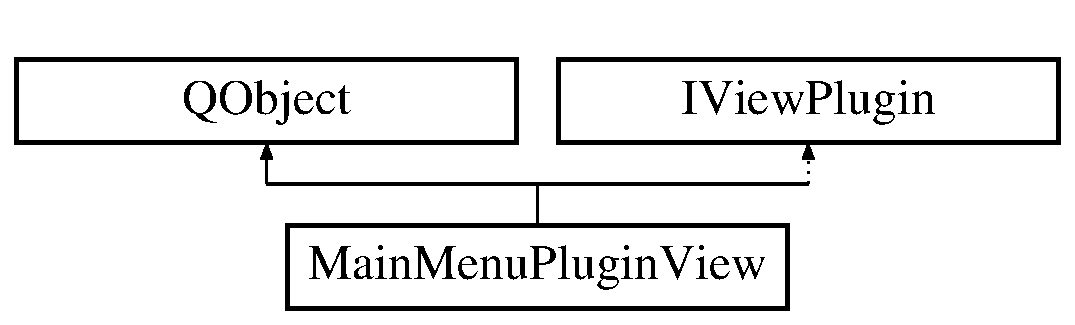
\includegraphics[height=2.000000cm]{class_main_menu_plugin_view}
\end{center}
\end{figure}
\subsection*{Public Member Functions}
\begin{DoxyCompactItemize}
\item 
\mbox{\Hypertarget{class_main_menu_plugin_view_a898a8bd2689bb67c269784ea61c46f28}\label{class_main_menu_plugin_view_a898a8bd2689bb67c269784ea61c46f28}} 
void {\bfseries On\+All\+Setup} () override
\item 
\mbox{\Hypertarget{class_main_menu_plugin_view_a8ac24e47204a97d5e3bbf616d6baf8bd}\label{class_main_menu_plugin_view_a8ac24e47204a97d5e3bbf616d6baf8bd}} 
Q\+String {\bfseries Get\+Last\+Error} () override
\item 
\mbox{\Hypertarget{class_main_menu_plugin_view_aad01cbc42d5dc1313df945e80b24f30a}\label{class_main_menu_plugin_view_aad01cbc42d5dc1313df945e80b24f30a}} 
void {\bfseries Set\+Model} (Q\+Object $\ast$model) override
\item 
\mbox{\Hypertarget{class_main_menu_plugin_view_acf1a0711a5b95bf67598aa4458916a4f}\label{class_main_menu_plugin_view_acf1a0711a5b95bf67598aa4458916a4f}} 
bool {\bfseries Open} (Q\+Widget $\ast$parent) override
\item 
\mbox{\Hypertarget{class_main_menu_plugin_view_aa269aebba786a16087a97cb350077c36}\label{class_main_menu_plugin_view_aa269aebba786a16087a97cb350077c36}} 
bool {\bfseries Close} () override
\end{DoxyCompactItemize}


The documentation for this class was generated from the following files\+:\begin{DoxyCompactItemize}
\item 
C\+:/\+Users/\+Curunir/\+Desktop/\+M\+A\+S\+S/\+Plugins/\+Main\+Menu\+View\+Plugin/mainmenupluginview.\+h\item 
C\+:/\+Users/\+Curunir/\+Desktop/\+M\+A\+S\+S/\+Plugins/\+Main\+Menu\+View\+Plugin/mainmenupluginview.\+cpp\end{DoxyCompactItemize}

\hypertarget{class_i_extendable_data_base_manager_plugin_1_1_manager_data_item}{}\section{I\+Extendable\+Data\+Base\+Manager\+Plugin\+:\+:Manager\+Data\+Item Class Reference}
\label{class_i_extendable_data_base_manager_plugin_1_1_manager_data_item}\index{I\+Extendable\+Data\+Base\+Manager\+Plugin\+::\+Manager\+Data\+Item@{I\+Extendable\+Data\+Base\+Manager\+Plugin\+::\+Manager\+Data\+Item}}
\subsection*{Public Attributes}
\begin{DoxyCompactItemize}
\item 
\mbox{\Hypertarget{class_i_extendable_data_base_manager_plugin_1_1_manager_data_item_abd5e8e3ceaa0d584593b9afc7bd4d4e3}\label{class_i_extendable_data_base_manager_plugin_1_1_manager_data_item_abd5e8e3ceaa0d584593b9afc7bd4d4e3}} 
int {\bfseries id}
\item 
\mbox{\Hypertarget{class_i_extendable_data_base_manager_plugin_1_1_manager_data_item_a1dcb37adfd0b55f67ddf2b1ecfa7a081}\label{class_i_extendable_data_base_manager_plugin_1_1_manager_data_item_a1dcb37adfd0b55f67ddf2b1ecfa7a081}} 
\hyperlink{class_q_map}{Q\+Map}$<$ Q\+String, \hyperlink{class_q_vector}{Q\+Vector}$<$ Q\+Variant $>$ $>$ {\bfseries data\+Chunks}
\end{DoxyCompactItemize}


The documentation for this class was generated from the following file\+:\begin{DoxyCompactItemize}
\item 
C\+:/\+Users/\+Curunir/\+Desktop/\+M\+A\+S\+S/\+Plugins/\+Extendable\+Data\+Base\+Manager/iextendabledatabasemanagerplugin.\+h\end{DoxyCompactItemize}

\hypertarget{struct_i_main_menu_plugin_model_1_1_menu_item}{}\section{I\+Main\+Menu\+Plugin\+Model\+:\+:Menu\+Item Struct Reference}
\label{struct_i_main_menu_plugin_model_1_1_menu_item}\index{I\+Main\+Menu\+Plugin\+Model\+::\+Menu\+Item@{I\+Main\+Menu\+Plugin\+Model\+::\+Menu\+Item}}
\subsection*{Public Attributes}
\begin{DoxyCompactItemize}
\item 
\mbox{\Hypertarget{struct_i_main_menu_plugin_model_1_1_menu_item_a1750991191ace60981315c7095723346}\label{struct_i_main_menu_plugin_model_1_1_menu_item_a1750991191ace60981315c7095723346}} 
\hyperlink{struct_meta_info}{Meta\+Info} $\ast$ {\bfseries meta}
\item 
\mbox{\Hypertarget{struct_i_main_menu_plugin_model_1_1_menu_item_a5576d4664cf1e226fbbbd5875239e0ae}\label{struct_i_main_menu_plugin_model_1_1_menu_item_a5576d4664cf1e226fbbbd5875239e0ae}} 
\hyperlink{class_q_list}{Q\+List}$<$ \hyperlink{struct_meta_info}{Meta\+Info} $\ast$ $>$ {\bfseries View\+Items}
\item 
\mbox{\Hypertarget{struct_i_main_menu_plugin_model_1_1_menu_item_a945944fea3f6fe92c7fdec32bee522a8}\label{struct_i_main_menu_plugin_model_1_1_menu_item_a945944fea3f6fe92c7fdec32bee522a8}} 
\hyperlink{class_q_list}{Q\+List}$<$ \hyperlink{struct_i_main_menu_plugin_model_1_1_menu_item}{Menu\+Item} $\ast$ $>$ {\bfseries Sub\+Items}
\end{DoxyCompactItemize}


The documentation for this struct was generated from the following file\+:\begin{DoxyCompactItemize}
\item 
C\+:/\+Users/\+Curunir/\+Desktop/\+M\+A\+S\+S/\+Plugins/\+Main\+Menu\+Model\+Plugin/imainmenumodule.\+h\end{DoxyCompactItemize}

\hypertarget{class_menu_item_graphics_object}{}\section{Menu\+Item\+Graphics\+Object Class Reference}
\label{class_menu_item_graphics_object}\index{Menu\+Item\+Graphics\+Object@{Menu\+Item\+Graphics\+Object}}
Inheritance diagram for Menu\+Item\+Graphics\+Object\+:\begin{figure}[H]
\begin{center}
\leavevmode
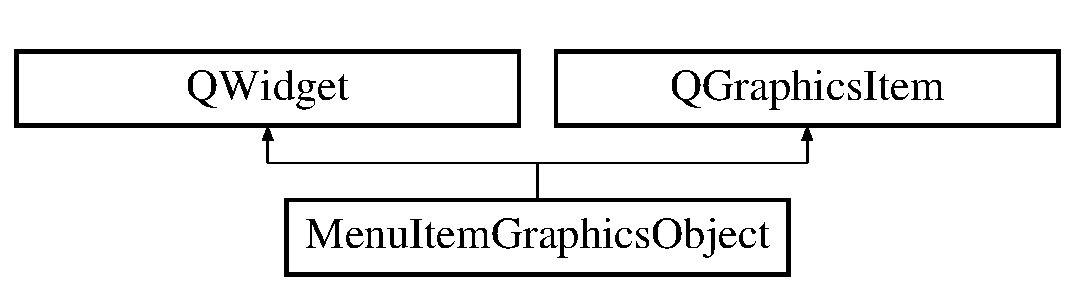
\includegraphics[height=2.000000cm]{class_menu_item_graphics_object}
\end{center}
\end{figure}
\subsection*{Signals}
\begin{DoxyCompactItemize}
\item 
\mbox{\Hypertarget{class_menu_item_graphics_object_a8cc186eece634847665b15f4ae58b426}\label{class_menu_item_graphics_object_a8cc186eece634847665b15f4ae58b426}} 
void {\bfseries On\+Clicked} (\hyperlink{class_menu_item_graphics_object}{Menu\+Item\+Graphics\+Object} $\ast$me)
\end{DoxyCompactItemize}
\subsection*{Public Member Functions}
\begin{DoxyCompactItemize}
\item 
\mbox{\Hypertarget{class_menu_item_graphics_object_a4ebc6be4ca5c88adcf7931e62161d5f1}\label{class_menu_item_graphics_object_a4ebc6be4ca5c88adcf7931e62161d5f1}} 
{\bfseries Menu\+Item\+Graphics\+Object} (\hyperlink{class_menu_item_graphics_object}{Menu\+Item\+Graphics\+Object} $\ast$Parent\+Menu\+Item, \hyperlink{struct_i_main_menu_plugin_model_1_1_menu_item}{I\+Main\+Menu\+Plugin\+Model\+::\+Menu\+Item} $\ast$\hyperlink{class_menu_item_graphics_object}{Menu\+Item\+Graphics\+Object}, \hyperlink{struct_meta_info}{Meta\+Info} $\ast$View\+Plugin, Q\+Widget $\ast$parent=0)
\item 
\mbox{\Hypertarget{class_menu_item_graphics_object_a4fabd069df87e7d05c94cd9027aa345b}\label{class_menu_item_graphics_object_a4fabd069df87e7d05c94cd9027aa345b}} 
{\bfseries Menu\+Item\+Graphics\+Object} (Q\+String name, Q\+Widget $\ast$parent=0)
\item 
\mbox{\Hypertarget{class_menu_item_graphics_object_ab17f3bcb176ffd6550df607a3e8eb3a9}\label{class_menu_item_graphics_object_ab17f3bcb176ffd6550df607a3e8eb3a9}} 
virtual Q\+RectF {\bfseries bounding\+Rect} () const
\item 
\mbox{\Hypertarget{class_menu_item_graphics_object_a00a392d4eeba783e2e8f73211adf8732}\label{class_menu_item_graphics_object_a00a392d4eeba783e2e8f73211adf8732}} 
virtual void {\bfseries paint} (Q\+Painter $\ast$painter, const Q\+Style\+Option\+Graphics\+Item $\ast$option, Q\+Widget $\ast$widget)
\end{DoxyCompactItemize}
\subsection*{Public Attributes}
\begin{DoxyCompactItemize}
\item 
\mbox{\Hypertarget{class_menu_item_graphics_object_a94290bfb4d0a10a7adb0516c84239b53}\label{class_menu_item_graphics_object_a94290bfb4d0a10a7adb0516c84239b53}} 
\hyperlink{class_menu_item_graphics_object}{Menu\+Item\+Graphics\+Object} $\ast$ {\bfseries parent\+Menu\+Item}
\item 
\mbox{\Hypertarget{class_menu_item_graphics_object_a059d772c31b4c5113290a2198150f8d6}\label{class_menu_item_graphics_object_a059d772c31b4c5113290a2198150f8d6}} 
\hyperlink{struct_i_main_menu_plugin_model_1_1_menu_item}{I\+Main\+Menu\+Plugin\+Model\+::\+Menu\+Item} $\ast$ {\bfseries menu\+Item}
\item 
\mbox{\Hypertarget{class_menu_item_graphics_object_a8d9594a1c25a956d3e34cab975dde29a}\label{class_menu_item_graphics_object_a8d9594a1c25a956d3e34cab975dde29a}} 
\hyperlink{struct_meta_info}{Meta\+Info} $\ast$ {\bfseries view\+Plugin\+Meta}
\end{DoxyCompactItemize}
\subsection*{Protected Member Functions}
\begin{DoxyCompactItemize}
\item 
\mbox{\Hypertarget{class_menu_item_graphics_object_a6f291090f45fc75a171ae55a09fd4f3d}\label{class_menu_item_graphics_object_a6f291090f45fc75a171ae55a09fd4f3d}} 
void {\bfseries mouse\+Press\+Event} (Q\+Graphics\+Scene\+Mouse\+Event $\ast$event)
\item 
\mbox{\Hypertarget{class_menu_item_graphics_object_addbf1e6b7247679ccf8b31f6a885f6e6}\label{class_menu_item_graphics_object_addbf1e6b7247679ccf8b31f6a885f6e6}} 
void {\bfseries mouse\+Release\+Event} (Q\+Graphics\+Scene\+Mouse\+Event $\ast$event)
\end{DoxyCompactItemize}
\subsection*{Protected Attributes}
\begin{DoxyCompactItemize}
\item 
\mbox{\Hypertarget{class_menu_item_graphics_object_ac8a4aab9ad0917b4f4270225a7ecbb58}\label{class_menu_item_graphics_object_ac8a4aab9ad0917b4f4270225a7ecbb58}} 
bool {\bfseries pressed}
\item 
\mbox{\Hypertarget{class_menu_item_graphics_object_aba38dc2a531e530d08f2aa92544f3104}\label{class_menu_item_graphics_object_aba38dc2a531e530d08f2aa92544f3104}} 
int {\bfseries dx}
\item 
\mbox{\Hypertarget{class_menu_item_graphics_object_a9b7f14de2c2e5ff71aad8a6ab729ef1d}\label{class_menu_item_graphics_object_a9b7f14de2c2e5ff71aad8a6ab729ef1d}} 
int {\bfseries dy}
\item 
\mbox{\Hypertarget{class_menu_item_graphics_object_a6ed305de3a3718503a5e3dabdbc07786}\label{class_menu_item_graphics_object_a6ed305de3a3718503a5e3dabdbc07786}} 
Q\+String {\bfseries item\+Menu\+Name}
\item 
\mbox{\Hypertarget{class_menu_item_graphics_object_ae78d7732b7108406484238c3814bb1e6}\label{class_menu_item_graphics_object_ae78d7732b7108406484238c3814bb1e6}} 
Q\+RectF {\bfseries bound\+Rect}
\end{DoxyCompactItemize}


The documentation for this class was generated from the following files\+:\begin{DoxyCompactItemize}
\item 
C\+:/\+Users/\+Curunir/\+Desktop/\+M\+A\+S\+S/\+Plugins/\+Main\+Menu\+View\+Plugin/menuitem.\+h\item 
C\+:/\+Users/\+Curunir/\+Desktop/\+M\+A\+S\+S/\+Plugins/build-\/\+Android\+\_\+armeabi\+\_\+v7a\+\_\+\+G\+C\+C\+\_\+4\+\_\+9\+\_\+\+Qt\+\_\+5\+\_\+8\+\_\+0-\/\+Main\+Menu\+View\+Plugin-\/\+Release/moc\+\_\+menuitem.\+cpp\item 
C\+:/\+Users/\+Curunir/\+Desktop/\+M\+A\+S\+S/\+Plugins/\+Main\+Menu\+View\+Plugin/menuitem.\+cpp\end{DoxyCompactItemize}

\hypertarget{struct_meta_info}{}\section{Meta\+Info Struct Reference}
\label{struct_meta_info}\index{Meta\+Info@{Meta\+Info}}
\subsection*{Public Attributes}
\begin{DoxyCompactItemize}
\item 
Q\+String {\bfseries Name}\hypertarget{struct_meta_info_a5a2f44643b5406699d1fb9ef742ab331}{}\label{struct_meta_info_a5a2f44643b5406699d1fb9ef742ab331}

\item 
\hyperlink{group___main_menu_module_ga9b3bee49ce70df90694056c2f48c2e77}{Plugin\+Types} {\bfseries Type}\hypertarget{struct_meta_info_aaaf1d51db4890bb4f5cbb08ea15b5940}{}\label{struct_meta_info_aaaf1d51db4890bb4f5cbb08ea15b5940}

\item 
Q\+String {\bfseries Parent\+Plugin\+Name}\hypertarget{struct_meta_info_a01ddb956e9390d748f8d3812521d17ff}{}\label{struct_meta_info_a01ddb956e9390d748f8d3812521d17ff}

\item 
Q\+String {\bfseries Data\+Managerl\+Name}\hypertarget{struct_meta_info_aa2b9d929a6ef2956c60d4bb029371669}{}\label{struct_meta_info_aa2b9d929a6ef2956c60d4bb029371669}

\end{DoxyCompactItemize}


The documentation for this struct was generated from the following files\+:\begin{DoxyCompactItemize}
\item 
/home/curunir/\+Documents/\+M\+A\+S\+S/\+Plugins/\+A\+R\+Neural\+Network\+View/interfaces.\+h\item 
/home/curunir/\+Documents/\+M\+A\+S\+S/\+Plugins/\+Extendable\+Data\+Base\+Manager/pluginstructs.\+h\end{DoxyCompactItemize}

\hypertarget{class_my_tree_view}{}\section{My\+Tree\+View Class Reference}
\label{class_my_tree_view}\index{My\+Tree\+View@{My\+Tree\+View}}


Inheritance diagram for My\+Tree\+View\+:\nopagebreak
\begin{figure}[H]
\begin{center}
\leavevmode
\includegraphics[width=151pt]{class_my_tree_view__inherit__graph}
\end{center}
\end{figure}


Collaboration diagram for My\+Tree\+View\+:\nopagebreak
\begin{figure}[H]
\begin{center}
\leavevmode
\includegraphics[width=151pt]{class_my_tree_view__coll__graph}
\end{center}
\end{figure}
\subsection*{Public Member Functions}
\begin{DoxyCompactItemize}
\item 
{\bfseries My\+Tree\+View} (Q\+Widget $\ast$parent)\hypertarget{class_my_tree_view_a0152950a0b3c03fa3c17f2b5bcacfde1}{}\label{class_my_tree_view_a0152950a0b3c03fa3c17f2b5bcacfde1}

\item 
bool {\bfseries event\+Filter} (Q\+Object $\ast$watched, Q\+Event $\ast$event) override\hypertarget{class_my_tree_view_aa40b314b7834999905769ac19a21ad7d}{}\label{class_my_tree_view_aa40b314b7834999905769ac19a21ad7d}

\end{DoxyCompactItemize}
\subsection*{Protected Member Functions}
\begin{DoxyCompactItemize}
\item 
void {\bfseries drag\+Move\+Event} (Q\+Drag\+Move\+Event $\ast$event) override\hypertarget{class_my_tree_view_afff3909f705a25758b55cc5ac0d9cf69}{}\label{class_my_tree_view_afff3909f705a25758b55cc5ac0d9cf69}

\item 
void {\bfseries drop\+Event} (Q\+Drop\+Event $\ast$event) override\hypertarget{class_my_tree_view_adba311eaf413fc319f875a43e8bc1bdb}{}\label{class_my_tree_view_adba311eaf413fc319f875a43e8bc1bdb}

\end{DoxyCompactItemize}


The documentation for this class was generated from the following files\+:\begin{DoxyCompactItemize}
\item 
/home/curunir/\+Documents/\+M\+A\+S\+S/\+Plugins/\+Task\+List\+View/mytreeview.\+h\item 
/home/curunir/\+Documents/\+M\+A\+S\+S/\+Plugins/\+Task\+List\+View/mytreeview.\+cpp\end{DoxyCompactItemize}

\hypertarget{struct_perceptron_1_1_network_params}{}\section{Perceptron\+:\+:Network\+Params Struct Reference}
\label{struct_perceptron_1_1_network_params}\index{Perceptron\+::\+Network\+Params@{Perceptron\+::\+Network\+Params}}
\subsection*{Public Attributes}
\begin{DoxyCompactItemize}
\item 
\mbox{\Hypertarget{struct_perceptron_1_1_network_params_a955f8919dc3d743bcbd0bf9a3f6106a2}\label{struct_perceptron_1_1_network_params_a955f8919dc3d743bcbd0bf9a3f6106a2}} 
int {\bfseries max\+Epoch}
\item 
\mbox{\Hypertarget{struct_perceptron_1_1_network_params_acfaab07fcc5107fcea07e99696c0b311}\label{struct_perceptron_1_1_network_params_acfaab07fcc5107fcea07e99696c0b311}} 
float {\bfseries train\+Error\+Threshold}
\item 
\mbox{\Hypertarget{struct_perceptron_1_1_network_params_a15a189b1d36274a9e51681b9097e9ff8}\label{struct_perceptron_1_1_network_params_a15a189b1d36274a9e51681b9097e9ff8}} 
float {\bfseries test\+Error\+Threshold}
\item 
\mbox{\Hypertarget{struct_perceptron_1_1_network_params_acf2c3e30c38ba223b045878bfbe246ac}\label{struct_perceptron_1_1_network_params_acf2c3e30c38ba223b045878bfbe246ac}} 
float {\bfseries min\+Weight}
\item 
\mbox{\Hypertarget{struct_perceptron_1_1_network_params_ad508697bc7cda2e68075186ec1b81ca3}\label{struct_perceptron_1_1_network_params_ad508697bc7cda2e68075186ec1b81ca3}} 
float {\bfseries max\+Weight}
\end{DoxyCompactItemize}


The documentation for this struct was generated from the following file\+:\begin{DoxyCompactItemize}
\item 
C\+:/\+Users/\+Curunir/\+Desktop/\+M\+A\+S\+S/\+Plugins/\+Neural\+Network\+Model/parameters.\+h\end{DoxyCompactItemize}

\hypertarget{struct_a_r_t_1_1_network_params}{}\section{A\+RT\+:\+:Network\+Params Struct Reference}
\label{struct_a_r_t_1_1_network_params}\index{A\+R\+T\+::\+Network\+Params@{A\+R\+T\+::\+Network\+Params}}
\subsection*{Public Attributes}
\begin{DoxyCompactItemize}
\item 
\mbox{\Hypertarget{struct_a_r_t_1_1_network_params_aababa990b5d0e5d080003e52bc8347a2}\label{struct_a_r_t_1_1_network_params_aababa990b5d0e5d080003e52bc8347a2}} 
int {\bfseries size}
\item 
\mbox{\Hypertarget{struct_a_r_t_1_1_network_params_ac985741814be043af5c083d3fb6cb44a}\label{struct_a_r_t_1_1_network_params_ac985741814be043af5c083d3fb6cb44a}} 
float {\bfseries similarity}
\item 
\mbox{\Hypertarget{struct_a_r_t_1_1_network_params_a2bd0fa378b49bddad207de236a7292d9}\label{struct_a_r_t_1_1_network_params_a2bd0fa378b49bddad207de236a7292d9}} 
float {\bfseries L}
\end{DoxyCompactItemize}


The documentation for this struct was generated from the following file\+:\begin{DoxyCompactItemize}
\item 
C\+:/\+Users/\+Curunir/\+Desktop/\+M\+A\+S\+S/\+Plugins/\+Neural\+Network\+Model/parameters.\+h\end{DoxyCompactItemize}

\hypertarget{struct_network_params}{}\section{Network\+Params Struct Reference}
\label{struct_network_params}\index{Network\+Params@{Network\+Params}}
\subsection*{Public Attributes}
\begin{DoxyCompactItemize}
\item 
\mbox{\Hypertarget{struct_network_params_a6a4d36a5e9c3f72e79ad94c9c919d4fc}\label{struct_network_params_a6a4d36a5e9c3f72e79ad94c9c919d4fc}} 
int {\bfseries max\+Epoch}
\item 
\mbox{\Hypertarget{struct_network_params_a592d5c7199126660efcd5c08b1d47c07}\label{struct_network_params_a592d5c7199126660efcd5c08b1d47c07}} 
float {\bfseries train\+Error\+Threshold}
\item 
\mbox{\Hypertarget{struct_network_params_ac8724964355a382767bfcf97e6cade9c}\label{struct_network_params_ac8724964355a382767bfcf97e6cade9c}} 
float {\bfseries test\+Error\+Threshold}
\item 
\mbox{\Hypertarget{struct_network_params_a42f00ee3de2b89324804ad4f57fdc9f4}\label{struct_network_params_a42f00ee3de2b89324804ad4f57fdc9f4}} 
float {\bfseries min\+Weight}
\item 
\mbox{\Hypertarget{struct_network_params_a57964e4d96787f96a11c9c4f7d988995}\label{struct_network_params_a57964e4d96787f96a11c9c4f7d988995}} 
float {\bfseries max\+Weight}
\end{DoxyCompactItemize}


The documentation for this struct was generated from the following file\+:\begin{DoxyCompactItemize}
\item 
C\+:/\+Users/\+Curunir/\+Desktop/\+M\+A\+S\+S/\+Plugins/\+Perceptron\+Neural\+Network\+View/mainform.\+h\end{DoxyCompactItemize}

\hypertarget{class_neural_layer}{}\section{Neural\+Layer Class Reference}
\label{class_neural_layer}\index{Neural\+Layer@{Neural\+Layer}}


Inheritance diagram for Neural\+Layer\+:\nopagebreak
\begin{figure}[H]
\begin{center}
\leavevmode
\includegraphics[width=287pt]{class_neural_layer__inherit__graph}
\end{center}
\end{figure}


Collaboration diagram for Neural\+Layer\+:\nopagebreak
\begin{figure}[H]
\begin{center}
\leavevmode
\includegraphics[width=350pt]{class_neural_layer__coll__graph}
\end{center}
\end{figure}
\subsection*{Public Slots}
\begin{DoxyCompactItemize}
\item 
virtual void {\bfseries Forward} (\hyperlink{class_q_vector}{Q\+Vector}$<$ float $>$ \&prev\+Outputs)\hypertarget{class_neural_layer_ab314d73699d84855b5611ffd9b526da2}{}\label{class_neural_layer_ab314d73699d84855b5611ffd9b526da2}

\item 
virtual void {\bfseries Back} (\hyperlink{class_q_vector}{Q\+Vector}$<$ float $>$ \&next\+Layer\+Delta)\hypertarget{class_neural_layer_a05fc717e06e6f287d5b1e8ea69f56727}{}\label{class_neural_layer_a05fc717e06e6f287d5b1e8ea69f56727}

\end{DoxyCompactItemize}
\subsection*{Public Member Functions}
\begin{DoxyCompactItemize}
\item 
{\bfseries Neural\+Layer} (\hyperlink{class_neural_layer}{Neural\+Layer} $\ast$Prev\+Layer, \hyperlink{struct_perceptron_1_1_network_params}{Network\+Params} \&\hyperlink{struct_perceptron_1_1_network_params}{Network\+Params}, \hyperlink{struct_perceptron_1_1_layer_params}{Layer\+Params} \&Params)\hypertarget{class_neural_layer_a33736379abd178ba2ab394ad39a2e284}{}\label{class_neural_layer_a33736379abd178ba2ab394ad39a2e284}

\item 
int {\bfseries Layer\+Size} ()\hypertarget{class_neural_layer_a4d000e0a192aa8f22f04762b7d208357}{}\label{class_neural_layer_a4d000e0a192aa8f22f04762b7d208357}

\item 
float {\bfseries Activation\+Func} (float x)\hypertarget{class_neural_layer_a3e565a98ae1d7353795575f575de1830}{}\label{class_neural_layer_a3e565a98ae1d7353795575f575de1830}

\item 
float {\bfseries Activation\+Func\+Derivative} (float x)\hypertarget{class_neural_layer_af2c164486c9757912f72ff06ab976d39}{}\label{class_neural_layer_af2c164486c9757912f72ff06ab976d39}

\end{DoxyCompactItemize}
\subsection*{Public Attributes}
\begin{DoxyCompactItemize}
\item 
\hyperlink{class_neural_layer}{Neural\+Layer} $\ast$ {\bfseries prev\+Layer}\hypertarget{class_neural_layer_a0575450e10a3dfecccb9b567362524a2}{}\label{class_neural_layer_a0575450e10a3dfecccb9b567362524a2}

\item 
\hyperlink{class_neural_layer}{Neural\+Layer} $\ast$ {\bfseries next\+Layer}\hypertarget{class_neural_layer_a071cf761219aecb1d9da97ee44fad3f9}{}\label{class_neural_layer_a071cf761219aecb1d9da97ee44fad3f9}

\item 
\hyperlink{class_q_vector}{Q\+Vector}$<$ \hyperlink{class_q_vector}{Q\+Vector}$<$ float $>$ $>$ {\bfseries input\+Weights}\hypertarget{class_neural_layer_a794bdd594ee597d8a99b215918b9432f}{}\label{class_neural_layer_a794bdd594ee597d8a99b215918b9432f}

\item 
\hyperlink{class_q_vector}{Q\+Vector}$<$ \hyperlink{class_q_vector}{Q\+Vector}$<$ float $>$ $>$ {\bfseries weights\+Delta}\hypertarget{class_neural_layer_ac0aaf690cb59e39d41a12f1539cd36c9}{}\label{class_neural_layer_ac0aaf690cb59e39d41a12f1539cd36c9}

\item 
\hyperlink{class_q_vector}{Q\+Vector}$<$ \hyperlink{class_q_vector}{Q\+Vector}$<$ float $>$ $>$ $\ast$ {\bfseries output\+Weights}\hypertarget{class_neural_layer_a763937d2bd27d69eca03dcc9e3be9a94}{}\label{class_neural_layer_a763937d2bd27d69eca03dcc9e3be9a94}

\item 
\hyperlink{class_q_vector}{Q\+Vector}$<$ float $>$ {\bfseries inputs}\hypertarget{class_neural_layer_a117e02be83ba7a29e138db5d4d9cefdb}{}\label{class_neural_layer_a117e02be83ba7a29e138db5d4d9cefdb}

\item 
\hyperlink{class_q_vector}{Q\+Vector}$<$ float $>$ {\bfseries outputs}\hypertarget{class_neural_layer_aac577824274773371ffd9d2aff6a0d7e}{}\label{class_neural_layer_aac577824274773371ffd9d2aff6a0d7e}

\item 
\hyperlink{class_q_vector}{Q\+Vector}$<$ float $>$ {\bfseries layer\+Delta}\hypertarget{class_neural_layer_a7e9fb43f260d94c21ac7604ac0477367}{}\label{class_neural_layer_a7e9fb43f260d94c21ac7604ac0477367}

\item 
\hyperlink{struct_perceptron_1_1_layer_params}{Layer\+Params} {\bfseries params}\hypertarget{class_neural_layer_af59922df5ffe0e8635e450c271a15ba4}{}\label{class_neural_layer_af59922df5ffe0e8635e450c271a15ba4}

\end{DoxyCompactItemize}
\subsection*{Protected Types}
\begin{DoxyCompactItemize}
\item 
typedef \hyperlink{struct_perceptron_1_1_network_params}{Perceptron\+::\+Network\+Params} {\bfseries Network\+Params}\hypertarget{class_neural_layer_ac3d37a368a77b07386981ecd0e0e55bb}{}\label{class_neural_layer_ac3d37a368a77b07386981ecd0e0e55bb}

\item 
typedef \hyperlink{struct_perceptron_1_1_layer_params}{Perceptron\+::\+Layer\+Params} {\bfseries Layer\+Params}\hypertarget{class_neural_layer_a9a46b30c0d9d329e3d2d943ae628683f}{}\label{class_neural_layer_a9a46b30c0d9d329e3d2d943ae628683f}

\item 
typedef Perceptron\+::\+Layer\+Type {\bfseries Layer\+Type}\hypertarget{class_neural_layer_a236cebae478f3f55e8256ce1b554bcb3}{}\label{class_neural_layer_a236cebae478f3f55e8256ce1b554bcb3}

\end{DoxyCompactItemize}


The documentation for this class was generated from the following files\+:\begin{DoxyCompactItemize}
\item 
/home/curunir/\+Documents/\+M\+A\+S\+S/\+Plugins/\+Neural\+Network\+Model/\+Perceptron/neurallayer.\+h\item 
/home/curunir/\+Documents/\+M\+A\+S\+S/\+Plugins/\+Neural\+Network\+Model/\+Perceptron/neurallayer.\+cpp\end{DoxyCompactItemize}

\hypertarget{class_neural_network_model}{}\section{Neural\+Network\+Model Class Reference}
\label{class_neural_network_model}\index{Neural\+Network\+Model@{Neural\+Network\+Model}}


Inheritance diagram for Neural\+Network\+Model\+:\nopagebreak
\begin{figure}[H]
\begin{center}
\leavevmode
\includegraphics[width=262pt]{class_neural_network_model__inherit__graph}
\end{center}
\end{figure}


Collaboration diagram for Neural\+Network\+Model\+:\nopagebreak
\begin{figure}[H]
\begin{center}
\leavevmode
\includegraphics[width=262pt]{class_neural_network_model__coll__graph}
\end{center}
\end{figure}
\subsection*{Public Member Functions}
\begin{DoxyCompactItemize}
\item 
void {\bfseries On\+All\+Setup} () override\hypertarget{class_neural_network_model_ae10c5a6387aa0752663d4c0ee07ed5ca}{}\label{class_neural_network_model_ae10c5a6387aa0752663d4c0ee07ed5ca}

\item 
Q\+String {\bfseries Get\+Last\+Error} () override\hypertarget{class_neural_network_model_ab9c3d8c5d6ae87dc0ed6e0650e614eb3}{}\label{class_neural_network_model_ab9c3d8c5d6ae87dc0ed6e0650e614eb3}

\item 
void {\bfseries Add\+Child\+Model} (\hyperlink{class_i_model_plugin}{I\+Model\+Plugin} $\ast$model, \hyperlink{struct_meta_info}{Meta\+Info} $\ast$meta) override\hypertarget{class_neural_network_model_a76c4f2032b0bc283e59efcf90617ca45}{}\label{class_neural_network_model_a76c4f2032b0bc283e59efcf90617ca45}

\item 
void {\bfseries Add\+View} (\hyperlink{class_i_view_plugin}{I\+View\+Plugin} $\ast$view, \hyperlink{struct_meta_info}{Meta\+Info} $\ast$meta) override\hypertarget{class_neural_network_model_ab819ce176d4dd2d2709b4db3304db5ef}{}\label{class_neural_network_model_ab819ce176d4dd2d2709b4db3304db5ef}

\item 
void {\bfseries Add\+Data\+Manager} (Q\+Object $\ast$data\+Manager) override\hypertarget{class_neural_network_model_ad20c25a3b27c40fbb448997adbf35e72}{}\label{class_neural_network_model_ad20c25a3b27c40fbb448997adbf35e72}

\item 
bool {\bfseries Open} (\hyperlink{class_i_model_plugin}{I\+Model\+Plugin} $\ast$parent, Q\+Widget $\ast$parent\+Widget, int id) override\hypertarget{class_neural_network_model_af003d712b60ba136f9fd1ace2fd259b6}{}\label{class_neural_network_model_af003d712b60ba136f9fd1ace2fd259b6}

\item 
bool {\bfseries Close} () override\hypertarget{class_neural_network_model_abb5e21816c1d96313a45e4618a1ff933}{}\label{class_neural_network_model_abb5e21816c1d96313a45e4618a1ff933}

\item 
void {\bfseries Child\+Self\+Closed} (int id) override\hypertarget{class_neural_network_model_addf09b66c86a981187257b82c030542d}{}\label{class_neural_network_model_addf09b66c86a981187257b82c030542d}

\item 
void {\bfseries Test\+Func} () override\hypertarget{class_neural_network_model_a81bbe391734aa26a7fa316dcbea0ea86}{}\label{class_neural_network_model_a81bbe391734aa26a7fa316dcbea0ea86}

\item 
void {\bfseries On\+All\+Setup} () override\hypertarget{class_neural_network_model_ae10c5a6387aa0752663d4c0ee07ed5ca}{}\label{class_neural_network_model_ae10c5a6387aa0752663d4c0ee07ed5ca}

\item 
Q\+String {\bfseries Get\+Last\+Error} () override\hypertarget{class_neural_network_model_ab9c3d8c5d6ae87dc0ed6e0650e614eb3}{}\label{class_neural_network_model_ab9c3d8c5d6ae87dc0ed6e0650e614eb3}

\item 
void {\bfseries Add\+Child\+Model} (\hyperlink{class_i_model_plugin}{I\+Model\+Plugin} $\ast$model, \hyperlink{struct_meta_info}{Meta\+Info} $\ast$meta) override\hypertarget{class_neural_network_model_a76c4f2032b0bc283e59efcf90617ca45}{}\label{class_neural_network_model_a76c4f2032b0bc283e59efcf90617ca45}

\item 
void {\bfseries Add\+View} (\hyperlink{class_i_view_plugin}{I\+View\+Plugin} $\ast$view, \hyperlink{struct_meta_info}{Meta\+Info} $\ast$meta) override\hypertarget{class_neural_network_model_ab819ce176d4dd2d2709b4db3304db5ef}{}\label{class_neural_network_model_ab819ce176d4dd2d2709b4db3304db5ef}

\item 
void {\bfseries Add\+Data\+Manager} (Q\+Object $\ast$data\+Manager) override\hypertarget{class_neural_network_model_ad20c25a3b27c40fbb448997adbf35e72}{}\label{class_neural_network_model_ad20c25a3b27c40fbb448997adbf35e72}

\item 
bool {\bfseries Open} (\hyperlink{class_i_model_plugin}{I\+Model\+Plugin} $\ast$parent, Q\+Widget $\ast$parent\+Widget) override\hypertarget{class_neural_network_model_ac6fcccae5d54c0fd16bc5e645dff04b7}{}\label{class_neural_network_model_ac6fcccae5d54c0fd16bc5e645dff04b7}

\item 
bool {\bfseries Close\+From\+View} (\hyperlink{class_i_view_plugin}{I\+View\+Plugin} $\ast$view) override\hypertarget{class_neural_network_model_ac66bbc3e734af35989a83ff95d45d894}{}\label{class_neural_network_model_ac66bbc3e734af35989a83ff95d45d894}

\item 
void {\bfseries Child\+Self\+Closed} (\hyperlink{class_i_model_plugin}{I\+Model\+Plugin} $\ast$child) override\hypertarget{class_neural_network_model_aed4269880cfc1c385e5904b1f415580b}{}\label{class_neural_network_model_aed4269880cfc1c385e5904b1f415580b}

\item 
void {\bfseries Add\+Parent\+Model} (Q\+Object $\ast$model, \hyperlink{struct_meta_info}{Meta\+Info} $\ast$meta) override\hypertarget{class_neural_network_model_ab4aa81f9f7860f62dd7c6223cb24e455}{}\label{class_neural_network_model_ab4aa81f9f7860f62dd7c6223cb24e455}

\item 
\hyperlink{class_i_neural_network_model_1_1_i_neural_network}{I\+Neural\+Network} $\ast$ {\bfseries Setup\+Network} (Q\+Json\+Object network\+Params) override\hypertarget{class_neural_network_model_a2b115f31c0e9116c2ea3134a29e8dc24}{}\label{class_neural_network_model_a2b115f31c0e9116c2ea3134a29e8dc24}

\end{DoxyCompactItemize}


The documentation for this class was generated from the following files\+:\begin{DoxyCompactItemize}
\item 
/home/curunir/\+Documents/\+M\+A\+S\+S/\+Plugins/\+Empty\+Model\+Plugin/neuralnetworkmodel.\+h\item 
/home/curunir/\+Documents/\+M\+A\+S\+S/\+Plugins/\+Empty\+Model\+Plugin/neuralnetworkmodel.\+cpp\end{DoxyCompactItemize}

\hypertarget{class_neuron}{}\section{Neuron Class Reference}
\label{class_neuron}\index{Neuron@{Neuron}}


Collaboration diagram for Neuron\+:\nopagebreak
\begin{figure}[H]
\begin{center}
\leavevmode
\includegraphics[width=187pt]{class_neuron__coll__graph}
\end{center}
\end{figure}
\subsection*{Public Member Functions}
\begin{DoxyCompactItemize}
\item 
{\bfseries Neuron} (int size, float $\ast$L)\hypertarget{class_neuron_a4da0f6ba396e848a67759d08b4aebb84}{}\label{class_neuron_a4da0f6ba396e848a67759d08b4aebb84}

\item 
{\bfseries Neuron} (int size, float $\ast$L, \hyperlink{class_q_vector}{Q\+Vector}$<$ int $>$ \&input)\hypertarget{class_neuron_a7306deecddc6f9d94c598d3a48f86c55}{}\label{class_neuron_a7306deecddc6f9d94c598d3a48f86c55}

\item 
void {\bfseries Recombine\+Weights} (\hyperlink{class_q_vector}{Q\+Vector}$<$ int $>$ \&input)\hypertarget{class_neuron_a8fe0fb53c7a23bed3a843cd37037630b}{}\label{class_neuron_a8fe0fb53c7a23bed3a843cd37037630b}

\item 
float {\bfseries Get\+Convolution} (\hyperlink{class_q_vector}{Q\+Vector}$<$ int $>$ \&input)\hypertarget{class_neuron_a92a2a9bf900c645e29343f41962f158f}{}\label{class_neuron_a92a2a9bf900c645e29343f41962f158f}

\end{DoxyCompactItemize}
\subsection*{Public Attributes}
\begin{DoxyCompactItemize}
\item 
\hyperlink{class_q_vector}{Q\+Vector}$<$ int $>$ {\bfseries output\+Weights}\hypertarget{class_neuron_aadb0bf2fa55fe14651e9b1b904112400}{}\label{class_neuron_aadb0bf2fa55fe14651e9b1b904112400}

\end{DoxyCompactItemize}


The documentation for this class was generated from the following files\+:\begin{DoxyCompactItemize}
\item 
/home/curunir/\+Documents/\+M\+A\+S\+S/\+Plugins/\+Neural\+Network\+Model/\+A\+R\+T/neuron.\+h\item 
/home/curunir/\+Documents/\+M\+A\+S\+S/\+Plugins/\+Neural\+Network\+Model/\+A\+R\+T/neuron.\+cpp\end{DoxyCompactItemize}

\hypertarget{class_output_neural_layer}{}\section{Output\+Neural\+Layer Class Reference}
\label{class_output_neural_layer}\index{Output\+Neural\+Layer@{Output\+Neural\+Layer}}
Inheritance diagram for Output\+Neural\+Layer\+:\begin{figure}[H]
\begin{center}
\leavevmode
\includegraphics[height=2.000000cm]{class_output_neural_layer}
\end{center}
\end{figure}
\subsection*{Public Slots}
\begin{DoxyCompactItemize}
\item 
\mbox{\Hypertarget{class_output_neural_layer_a23915415ef771523eaa81ac0d309fdee}\label{class_output_neural_layer_a23915415ef771523eaa81ac0d309fdee}} 
void {\bfseries Forward} (\hyperlink{class_q_vector}{Q\+Vector}$<$ float $>$ \&input\+Signals) override
\item 
\mbox{\Hypertarget{class_output_neural_layer_a88b76a85c6b0df6a08c617a50a51205c}\label{class_output_neural_layer_a88b76a85c6b0df6a08c617a50a51205c}} 
void {\bfseries Init\+Back} (\hyperlink{class_q_vector}{Q\+Vector}$<$ float $>$ \&ideal\+Result)
\end{DoxyCompactItemize}
\subsection*{Public Member Functions}
\begin{DoxyCompactItemize}
\item 
\mbox{\Hypertarget{class_output_neural_layer_a715832abcf6d3cd49da63c53a48c39ea}\label{class_output_neural_layer_a715832abcf6d3cd49da63c53a48c39ea}} 
{\bfseries Output\+Neural\+Layer} (\hyperlink{class_neural_layer}{Neural\+Layer} $\ast$Prev\+Layer, \hyperlink{struct_perceptron_1_1_network_params}{Network\+Params} \&network\+Params, \hyperlink{struct_perceptron_1_1_layer_params}{Layer\+Params} \&params)
\item 
\mbox{\Hypertarget{class_output_neural_layer_a6506d3323ab55502c0bc5e925179495b}\label{class_output_neural_layer_a6506d3323ab55502c0bc5e925179495b}} 
\hyperlink{class_q_vector}{Q\+Vector}$<$ float $>$ $\ast$ {\bfseries Get\+Outputs} ()
\end{DoxyCompactItemize}
\subsection*{Additional Inherited Members}


The documentation for this class was generated from the following files\+:\begin{DoxyCompactItemize}
\item 
C\+:/\+Users/\+Curunir/\+Desktop/\+M\+A\+S\+S/\+Plugins/\+Neural\+Network\+Model/\+Perceptron/neurallayer.\+h\item 
C\+:/\+Users/\+Curunir/\+Desktop/\+M\+A\+S\+S/\+Plugins/\+Neural\+Network\+Model/\+Perceptron/neurallayer.\+cpp\end{DoxyCompactItemize}

\hypertarget{class_paint_widget}{}\section{Paint\+Widget Class Reference}
\label{class_paint_widget}\index{Paint\+Widget@{Paint\+Widget}}
Inheritance diagram for Paint\+Widget\+:\begin{figure}[H]
\begin{center}
\leavevmode
\includegraphics[height=2.000000cm]{class_paint_widget}
\end{center}
\end{figure}
\subsection*{Public Slots}
\begin{DoxyCompactItemize}
\item 
\mbox{\Hypertarget{class_paint_widget_a5ebf42105842c3f4da64e8482a5a0b74}\label{class_paint_widget_a5ebf42105842c3f4da64e8482a5a0b74}} 
void {\bfseries Clean} ()
\end{DoxyCompactItemize}
\subsection*{Public Member Functions}
\begin{DoxyCompactItemize}
\item 
\mbox{\Hypertarget{class_paint_widget_ae6adf05aa99501c9309ca72ccbcafee4}\label{class_paint_widget_ae6adf05aa99501c9309ca72ccbcafee4}} 
{\bfseries Paint\+Widget} (Q\+Widget $\ast$parent=0)
\end{DoxyCompactItemize}
\subsection*{Public Attributes}
\begin{DoxyCompactItemize}
\item 
\mbox{\Hypertarget{class_paint_widget_af256e4154c8f1e9cae1016923b40508c}\label{class_paint_widget_af256e4154c8f1e9cae1016923b40508c}} 
Q\+Image {\bfseries image}
\end{DoxyCompactItemize}
\subsection*{Protected Member Functions}
\begin{DoxyCompactItemize}
\item 
\mbox{\Hypertarget{class_paint_widget_a1c7eb81a97caded4a094b978695c94d4}\label{class_paint_widget_a1c7eb81a97caded4a094b978695c94d4}} 
virtual void {\bfseries mouse\+Press\+Event} (Q\+Mouse\+Event $\ast$event)
\item 
\mbox{\Hypertarget{class_paint_widget_ae1eb322803e4a255a2db108410ac8f35}\label{class_paint_widget_ae1eb322803e4a255a2db108410ac8f35}} 
virtual void {\bfseries mouse\+Release\+Event} (Q\+Mouse\+Event $\ast$event)
\item 
\mbox{\Hypertarget{class_paint_widget_a66e1dca2bebbba5d84e8dab66c05e2db}\label{class_paint_widget_a66e1dca2bebbba5d84e8dab66c05e2db}} 
virtual void {\bfseries mouse\+Move\+Event} (Q\+Mouse\+Event $\ast$event)
\item 
\mbox{\Hypertarget{class_paint_widget_ae4a27141cb8bef3cf93889fec4fc9411}\label{class_paint_widget_ae4a27141cb8bef3cf93889fec4fc9411}} 
virtual void {\bfseries paint\+Event} (Q\+Paint\+Event $\ast$event)
\item 
\mbox{\Hypertarget{class_paint_widget_ac8ba3ebb21b873fccde32329f7d3d55d}\label{class_paint_widget_ac8ba3ebb21b873fccde32329f7d3d55d}} 
virtual void {\bfseries resize\+Event} (Q\+Resize\+Event $\ast$event)
\end{DoxyCompactItemize}


The documentation for this class was generated from the following files\+:\begin{DoxyCompactItemize}
\item 
C\+:/\+Users/\+Curunir/\+Desktop/\+M\+A\+S\+S/\+Plugins/\+Task\+Sketch\+View/paintwidget.\+h\item 
C\+:/\+Users/\+Curunir/\+Desktop/\+M\+A\+S\+S/\+Plugins/\+Task\+Sketch\+View/paintwidget.\+cpp\end{DoxyCompactItemize}

\hypertarget{struct_genetic_algorithm_params_1_1_parameters}{}\section{Genetic\+Algorithm\+Params\+:\+:Parameters Struct Reference}
\label{struct_genetic_algorithm_params_1_1_parameters}\index{Genetic\+Algorithm\+Params\+::\+Parameters@{Genetic\+Algorithm\+Params\+::\+Parameters}}
\subsection*{Public Types}
\begin{DoxyCompactItemize}
\item 
\mbox{\Hypertarget{struct_genetic_algorithm_params_1_1_parameters_a4abcc00278515e339ac9cef36b07c14a}\label{struct_genetic_algorithm_params_1_1_parameters_a4abcc00278515e339ac9cef36b07c14a}} 
enum {\bfseries Extremum\+Search\+Type} \{ {\bfseries None}, 
{\bfseries Min}, 
{\bfseries Max}
 \}
\end{DoxyCompactItemize}
\subsection*{Public Attributes}
\begin{DoxyCompactItemize}
\item 
\mbox{\Hypertarget{struct_genetic_algorithm_params_1_1_parameters_a2d4b36153aa65aed6fa0996f17e73c36}\label{struct_genetic_algorithm_params_1_1_parameters_a2d4b36153aa65aed6fa0996f17e73c36}} 
float {\bfseries fitness\+Threshold}
\item 
\mbox{\Hypertarget{struct_genetic_algorithm_params_1_1_parameters_a130a1e03f3a445caa0e0a00d6f2f21fd}\label{struct_genetic_algorithm_params_1_1_parameters_a130a1e03f3a445caa0e0a00d6f2f21fd}} 
int {\bfseries iterations}
\item 
\mbox{\Hypertarget{struct_genetic_algorithm_params_1_1_parameters_ad9bde581bef9239129cfdbe2d78ff514}\label{struct_genetic_algorithm_params_1_1_parameters_ad9bde581bef9239129cfdbe2d78ff514}} 
float {\bfseries target\+Result}
\item 
\mbox{\Hypertarget{struct_genetic_algorithm_params_1_1_parameters_a51c4b0811c004fe1419d9a20bd014ba7}\label{struct_genetic_algorithm_params_1_1_parameters_a51c4b0811c004fe1419d9a20bd014ba7}} 
enum Genetic\+Algorithm\+Params\+::\+Parameters\+::\+Extremum\+Search\+Type {\bfseries extremum\+Search}
\item 
\mbox{\Hypertarget{struct_genetic_algorithm_params_1_1_parameters_a8355f423b6b1015ff239b59ef391b067}\label{struct_genetic_algorithm_params_1_1_parameters_a8355f423b6b1015ff239b59ef391b067}} 
int {\bfseries population\+Size}
\item 
\mbox{\Hypertarget{struct_genetic_algorithm_params_1_1_parameters_a3e988ba9f53c8ca2338c2b12e05e54de}\label{struct_genetic_algorithm_params_1_1_parameters_a3e988ba9f53c8ca2338c2b12e05e54de}} 
int {\bfseries genes\+Count}
\item 
\mbox{\Hypertarget{struct_genetic_algorithm_params_1_1_parameters_a8cdc92e995b4f84fb7f80b9348f193fe}\label{struct_genetic_algorithm_params_1_1_parameters_a8cdc92e995b4f84fb7f80b9348f193fe}} 
int {\bfseries gene\+Capacity}
\item 
\mbox{\Hypertarget{struct_genetic_algorithm_params_1_1_parameters_a2f70a84e27bbecc6b032c1cc73052fca}\label{struct_genetic_algorithm_params_1_1_parameters_a2f70a84e27bbecc6b032c1cc73052fca}} 
float {\bfseries min\+Range}
\item 
\mbox{\Hypertarget{struct_genetic_algorithm_params_1_1_parameters_ae6366f636b54fa8753bc4117dab9392f}\label{struct_genetic_algorithm_params_1_1_parameters_ae6366f636b54fa8753bc4117dab9392f}} 
float {\bfseries max\+Range}
\end{DoxyCompactItemize}


The documentation for this struct was generated from the following file\+:\begin{DoxyCompactItemize}
\item 
C\+:/\+Users/\+Curunir/\+Desktop/\+M\+A\+S\+S/\+Plugins/\+Neural\+Network\+Model/parameters.\+h\end{DoxyCompactItemize}

\hypertarget{class_parent_window}{}\section{Parent\+Window Class Reference}
\label{class_parent_window}\index{Parent\+Window@{Parent\+Window}}


The \hyperlink{class_parent_window}{Parent\+Window} class.  




{\ttfamily \#include $<$parentwindow.\+h$>$}

Inheritance diagram for Parent\+Window\+:\begin{figure}[H]
\begin{center}
\leavevmode
\includegraphics[height=2.000000cm]{class_parent_window}
\end{center}
\end{figure}
\subsection*{Public Member Functions}
\begin{DoxyCompactItemize}
\item 
\mbox{\Hypertarget{class_parent_window_aa7a1b9030900a9042a59496d6d23c90f}\label{class_parent_window_aa7a1b9030900a9042a59496d6d23c90f}} 
{\bfseries Parent\+Window} (Q\+Widget $\ast$parent=0)
\end{DoxyCompactItemize}


\subsection{Detailed Description}
The \hyperlink{class_parent_window}{Parent\+Window} class. 

The documentation for this class was generated from the following files\+:\begin{DoxyCompactItemize}
\item 
C\+:/\+Users/\+Curunir/\+Desktop/\+M\+A\+S\+S/\+System/\+M\+A\+S\+S/parentwindow.\+h\item 
C\+:/\+Users/\+Curunir/\+Desktop/\+M\+A\+S\+S/\+System/\+M\+A\+S\+S/parentwindow.\+cpp\end{DoxyCompactItemize}

\hypertarget{class_perceptron_network}{}\section{Perceptron\+Network Class Reference}
\label{class_perceptron_network}\index{Perceptron\+Network@{Perceptron\+Network}}


Inheritance diagram for Perceptron\+Network\+:\nopagebreak
\begin{figure}[H]
\begin{center}
\leavevmode
\includegraphics[width=262pt]{class_perceptron_network__inherit__graph}
\end{center}
\end{figure}


Collaboration diagram for Perceptron\+Network\+:\nopagebreak
\begin{figure}[H]
\begin{center}
\leavevmode
\includegraphics[width=262pt]{class_perceptron_network__coll__graph}
\end{center}
\end{figure}
\subsection*{Public Member Functions}
\begin{DoxyCompactItemize}
\item 
{\bfseries Perceptron\+Network} (\hyperlink{struct_perceptron_1_1_network_params}{Network\+Params} params)\hypertarget{class_perceptron_network_a05ac856c829795664393e9577f0f58b5}{}\label{class_perceptron_network_a05ac856c829795664393e9577f0f58b5}

\item 
void {\bfseries Setup\+SamplesF} (Q\+Json\+Object parameters, \hyperlink{class_q_vector}{Q\+Vector}$<$ \hyperlink{class_q_pair}{Input\+SampleF} $>$ $\ast$samples) override\hypertarget{class_perceptron_network_a34139545d51a95537ecb46819deb348a}{}\label{class_perceptron_network_a34139545d51a95537ecb46819deb348a}

\item 
void {\bfseries Setup\+SamplesI} (Q\+Json\+Object parameters, \hyperlink{class_q_vector}{Q\+Vector}$<$ \hyperlink{class_q_pair}{Input\+SampleI} $>$ $\ast$samples) override\hypertarget{class_perceptron_network_aced7b81e1fb2d69e050f62cabd058ec3}{}\label{class_perceptron_network_aced7b81e1fb2d69e050f62cabd058ec3}

\item 
bool {\bfseries Set\+Network\+Params} (Q\+Json\+Object params) override\hypertarget{class_perceptron_network_afb8e01ac4a933a35abf784d4c00a3f12}{}\label{class_perceptron_network_afb8e01ac4a933a35abf784d4c00a3f12}

\item 
bool {\bfseries Add\+Layer} (Q\+Json\+Object layer\+Params) override\hypertarget{class_perceptron_network_ad5b18f2f4d84fb9fa7941e133a4fb72e}{}\label{class_perceptron_network_ad5b18f2f4d84fb9fa7941e133a4fb72e}

\item 
void {\bfseries Reset\+Layers} () override\hypertarget{class_perceptron_network_a725149f0b03c8a6e07ea2a64c8c98556}{}\label{class_perceptron_network_a725149f0b03c8a6e07ea2a64c8c98556}

\item 
float {\bfseries Run\+Train\+Set} () override\hypertarget{class_perceptron_network_a17cdca41fc873b70bb700b10e32240eb}{}\label{class_perceptron_network_a17cdca41fc873b70bb700b10e32240eb}

\item 
float {\bfseries Run\+Test\+Set} () override\hypertarget{class_perceptron_network_a0f2c75a5cbac4485eef6a0ef942da407}{}\label{class_perceptron_network_a0f2c75a5cbac4485eef6a0ef942da407}

\end{DoxyCompactItemize}
\subsection*{Static Public Member Functions}
\begin{DoxyCompactItemize}
\item 
static \hyperlink{class_perceptron_network}{Perceptron\+Network} $\ast$ {\bfseries Make} (Q\+Json\+Object \&params\+Obj)\hypertarget{class_perceptron_network_a9acf3e33492a4163df20f6877a6f3db7}{}\label{class_perceptron_network_a9acf3e33492a4163df20f6877a6f3db7}

\end{DoxyCompactItemize}


The documentation for this class was generated from the following files\+:\begin{DoxyCompactItemize}
\item 
/home/curunir/\+Documents/\+M\+A\+S\+S/\+Plugins/\+Neural\+Network\+Model/\+Perceptron/perceptronnetwork.\+h\item 
/home/curunir/\+Documents/\+M\+A\+S\+S/\+Plugins/\+Neural\+Network\+Model/\+Perceptron/perceptronnetwork.\+cpp\end{DoxyCompactItemize}

\hypertarget{class_perceptron_network_view_plugin}{}\section{Perceptron\+Network\+View\+Plugin Class Reference}
\label{class_perceptron_network_view_plugin}\index{Perceptron\+Network\+View\+Plugin@{Perceptron\+Network\+View\+Plugin}}


Inheritance diagram for Perceptron\+Network\+View\+Plugin\+:\nopagebreak
\begin{figure}[H]
\begin{center}
\leavevmode
\includegraphics[width=229pt]{class_perceptron_network_view_plugin__inherit__graph}
\end{center}
\end{figure}


Collaboration diagram for Perceptron\+Network\+View\+Plugin\+:\nopagebreak
\begin{figure}[H]
\begin{center}
\leavevmode
\includegraphics[width=229pt]{class_perceptron_network_view_plugin__coll__graph}
\end{center}
\end{figure}
\subsection*{Public Slots}
\begin{DoxyCompactItemize}
\item 
bool {\bfseries Close} () override\hypertarget{class_perceptron_network_view_plugin_a0b926a5f59e199142cb3a6bd2fc58e2d}{}\label{class_perceptron_network_view_plugin_a0b926a5f59e199142cb3a6bd2fc58e2d}

\end{DoxyCompactItemize}
\subsection*{Public Member Functions}
\begin{DoxyCompactItemize}
\item 
void {\bfseries On\+All\+Setup} () override\hypertarget{class_perceptron_network_view_plugin_ace8ae52e9cd4093ffc637e5b19a446ff}{}\label{class_perceptron_network_view_plugin_ace8ae52e9cd4093ffc637e5b19a446ff}

\item 
Q\+String {\bfseries Get\+Last\+Error} () override\hypertarget{class_perceptron_network_view_plugin_aa4942c85bb0eb6001b23dda5eee1d36b}{}\label{class_perceptron_network_view_plugin_aa4942c85bb0eb6001b23dda5eee1d36b}

\item 
void {\bfseries Set\+Model} (Q\+Object $\ast$model) override\hypertarget{class_perceptron_network_view_plugin_af997cf5ec39e674207d48c506f6ac804}{}\label{class_perceptron_network_view_plugin_af997cf5ec39e674207d48c506f6ac804}

\item 
bool {\bfseries Open} (Q\+Widget $\ast$parent) override\hypertarget{class_perceptron_network_view_plugin_a33791a775a8ac09f54a8c35905efe1cd}{}\label{class_perceptron_network_view_plugin_a33791a775a8ac09f54a8c35905efe1cd}

\end{DoxyCompactItemize}


The documentation for this class was generated from the following files\+:\begin{DoxyCompactItemize}
\item 
/home/curunir/\+Documents/\+M\+A\+S\+S/\+Plugins/\+Perceptron\+Neural\+Network\+View/perceptronneuralnetworkview.\+h\item 
/home/curunir/\+Documents/\+M\+A\+S\+S/\+Plugins/\+Perceptron\+Neural\+Network\+View/perceptronneuralnetworkview.\+cpp\end{DoxyCompactItemize}

\hypertarget{struct_plugin_info}{}\section{Plugin\+Info$<$ T $>$ Struct Template Reference}
\label{struct_plugin_info}\index{Plugin\+Info$<$ T $>$@{Plugin\+Info$<$ T $>$}}


Collaboration diagram for Plugin\+Info$<$ T $>$\+:\nopagebreak
\begin{figure}[H]
\begin{center}
\leavevmode
\includegraphics[width=164pt]{struct_plugin_info__coll__graph}
\end{center}
\end{figure}
\subsection*{Public Attributes}
\begin{DoxyCompactItemize}
\item 
T $\ast$ {\bfseries plugin}\hypertarget{struct_plugin_info_a988245c24cc2fe6da1c0312b8835f803}{}\label{struct_plugin_info_a988245c24cc2fe6da1c0312b8835f803}

\item 
\hyperlink{struct_meta_info}{Meta\+Info} $\ast$ {\bfseries meta}\hypertarget{struct_plugin_info_a1f5e1a17fa1569bbdb2cc4bdcd7a5656}{}\label{struct_plugin_info_a1f5e1a17fa1569bbdb2cc4bdcd7a5656}

\end{DoxyCompactItemize}


The documentation for this struct was generated from the following file\+:\begin{DoxyCompactItemize}
\item 
/home/curunir/\+Documents/\+M\+A\+S\+S/\+Plugins/\+Main\+Menu\+Model\+Plugin/interfaces.\+h\end{DoxyCompactItemize}

\hypertarget{class_plugin_linker}{}\section{Plugin\+Linker Class Reference}
\label{class_plugin_linker}\index{Plugin\+Linker@{Plugin\+Linker}}
\subsection*{Public Member Functions}
\begin{DoxyCompactItemize}
\item 
\mbox{\Hypertarget{class_plugin_linker_a864d8fa78e948711e62a3985f57e2315}\label{class_plugin_linker_a864d8fa78e948711e62a3985f57e2315}} 
void {\bfseries Add\+New\+Plugin} (Q\+Object $\ast$instance, Q\+Json\+Object $\ast$meta)
\item 
\mbox{\Hypertarget{class_plugin_linker_ad47aca648a1bd5dfd75d0829f7bacc16}\label{class_plugin_linker_ad47aca648a1bd5dfd75d0829f7bacc16}} 
\hyperlink{struct_i_main_menu_plugin_model_1_1_menu_item}{I\+Main\+Menu\+Plugin\+Model\+::\+Menu\+Item} $\ast$ {\bfseries Setup\+Links} ()
\end{DoxyCompactItemize}
\subsection*{Public Attributes}
\begin{DoxyCompactItemize}
\item 
\mbox{\Hypertarget{class_plugin_linker_ab1ecde85d4d754ee95f8c52e3eddc265}\label{class_plugin_linker_ab1ecde85d4d754ee95f8c52e3eddc265}} 
\hyperlink{class_i_model_plugin}{I\+Model\+Plugin} $\ast$ {\bfseries root\+Model}
\item 
\mbox{\Hypertarget{class_plugin_linker_a44b3d50d05723673e3682a9987621ee3}\label{class_plugin_linker_a44b3d50d05723673e3682a9987621ee3}} 
\hyperlink{struct_i_main_menu_plugin_model_1_1_menu_item}{I\+Main\+Menu\+Plugin\+Model\+::\+Menu\+Item} $\ast$ {\bfseries root\+Menu\+Item}
\item 
\mbox{\Hypertarget{class_plugin_linker_aebd5426ad88d05de6dc358c2697e143f}\label{class_plugin_linker_aebd5426ad88d05de6dc358c2697e143f}} 
\hyperlink{class_q_map}{Q\+Map}$<$ \hyperlink{struct_meta_info}{Meta\+Info} $\ast$, \hyperlink{struct_i_main_menu_plugin_model_1_1_menu_item}{I\+Main\+Menu\+Plugin\+Model\+::\+Menu\+Item} $\ast$ $>$ {\bfseries menu\+Items}
\item 
\mbox{\Hypertarget{class_plugin_linker_adb1fa516735cef59600dbe5777499841}\label{class_plugin_linker_adb1fa516735cef59600dbe5777499841}} 
\hyperlink{class_q_map}{Q\+Map}$<$ \hyperlink{class_i_model_plugin}{I\+Model\+Plugin} $\ast$, \hyperlink{struct_meta_info}{Meta\+Info} $\ast$ $>$ {\bfseries model\+Map}
\item 
\mbox{\Hypertarget{class_plugin_linker_a9703ef182dce1dcb24e83110d98933f1}\label{class_plugin_linker_a9703ef182dce1dcb24e83110d98933f1}} 
\hyperlink{class_q_map}{Q\+Map}$<$ \hyperlink{class_i_view_plugin}{I\+View\+Plugin} $\ast$, \hyperlink{struct_meta_info}{Meta\+Info} $\ast$ $>$ {\bfseries view\+Map}
\item 
\mbox{\Hypertarget{class_plugin_linker_a452d0698f6ea36e83c8094444bdfd59f}\label{class_plugin_linker_a452d0698f6ea36e83c8094444bdfd59f}} 
\hyperlink{class_q_map}{Q\+Map}$<$ \hyperlink{class_i_data_source_plugin}{I\+Data\+Source\+Plugin} $\ast$, \hyperlink{struct_meta_info}{Meta\+Info} $\ast$ $>$ {\bfseries source\+Map}
\item 
\mbox{\Hypertarget{class_plugin_linker_af19a364f23b397652828ce411c48e414}\label{class_plugin_linker_af19a364f23b397652828ce411c48e414}} 
\hyperlink{class_q_map}{Q\+Map}$<$ \hyperlink{class_i_data_manager_plugin}{I\+Data\+Manager\+Plugin} $\ast$, \hyperlink{struct_meta_info}{Meta\+Info} $\ast$ $>$ {\bfseries manager\+Map}
\end{DoxyCompactItemize}


The documentation for this class was generated from the following files\+:\begin{DoxyCompactItemize}
\item 
C\+:/\+Users/\+Curunir/\+Desktop/\+M\+A\+S\+S/\+Plugins/\+Main\+Menu\+Model\+Plugin/pluginlinker.\+h\item 
C\+:/\+Users/\+Curunir/\+Desktop/\+M\+A\+S\+S/\+Plugins/\+Main\+Menu\+Model\+Plugin/pluginlinker.\+cpp\end{DoxyCompactItemize}

\hypertarget{class_plugin_loader}{}\section{Plugin\+Loader Class Reference}
\label{class_plugin_loader}\index{Plugin\+Loader@{Plugin\+Loader}}


Loads all files from directory and tries to specify between them plugin with interface Root\+Model and initialize it.  




{\ttfamily \#include $<$pluginloader.\+h$>$}



Inheritance diagram for Plugin\+Loader\+:\nopagebreak
\begin{figure}[H]
\begin{center}
\leavevmode
\includegraphics[width=153pt]{class_plugin_loader__inherit__graph}
\end{center}
\end{figure}


Collaboration diagram for Plugin\+Loader\+:\nopagebreak
\begin{figure}[H]
\begin{center}
\leavevmode
\includegraphics[width=153pt]{class_plugin_loader__coll__graph}
\end{center}
\end{figure}
\subsection*{Public Slots}
\begin{DoxyCompactItemize}
\item 
void \hyperlink{class_plugin_loader_acdec57677a58fbce84cedb27571c72b9}{Setup\+Plugins} ()\hypertarget{class_plugin_loader_acdec57677a58fbce84cedb27571c72b9}{}\label{class_plugin_loader_acdec57677a58fbce84cedb27571c72b9}

\begin{DoxyCompactList}\small\item\em Load plugins from specified folder. In loaded files tries to specify Root\+Model plugin. If it exists -\/ set this plugin as root\+Model and send to it all unspecified plugins. \end{DoxyCompactList}\end{DoxyCompactItemize}
\subsection*{Public Member Functions}
\begin{DoxyCompactItemize}
\item 
\hyperlink{class_plugin_loader_a94ed19dc21d59ebf15afeb97590cc514}{Plugin\+Loader} (Q\+Widget $\ast$parent=0)
\end{DoxyCompactItemize}


\subsection{Detailed Description}
Loads all files from directory and tries to specify between them plugin with interface Root\+Model and initialize it. 

\subsection{Constructor \& Destructor Documentation}
\index{Plugin\+Loader@{Plugin\+Loader}!Plugin\+Loader@{Plugin\+Loader}}
\index{Plugin\+Loader@{Plugin\+Loader}!Plugin\+Loader@{Plugin\+Loader}}
\subsubsection[{\texorpdfstring{Plugin\+Loader(\+Q\+Widget $\ast$parent=0)}{PluginLoader(QWidget *parent=0)}}]{\setlength{\rightskip}{0pt plus 5cm}Plugin\+Loader\+::\+Plugin\+Loader (
\begin{DoxyParamCaption}
\item[{Q\+Widget $\ast$}]{parent = {\ttfamily 0}}
\end{DoxyParamCaption}
)\hspace{0.3cm}{\ttfamily [explicit]}}\hypertarget{class_plugin_loader_a94ed19dc21d59ebf15afeb97590cc514}{}\label{class_plugin_loader_a94ed19dc21d59ebf15afeb97590cc514}

\begin{DoxyParams}{Parameters}
{\em parent} & Q\+Widget which will be parent for all application windows. \\
\hline
\end{DoxyParams}


The documentation for this class was generated from the following files\+:\begin{DoxyCompactItemize}
\item 
/home/curunir/\+Documents/\+M\+A\+S\+S/\+System/\+M\+A\+S\+S/pluginloader.\+h\item 
/home/curunir/\+Documents/\+M\+A\+S\+S/\+System/\+M\+A\+S\+S/pluginloader.\+cpp\end{DoxyCompactItemize}

\hypertarget{class_pomodoro_button}{}\section{Pomodoro\+Button Class Reference}
\label{class_pomodoro_button}\index{Pomodoro\+Button@{Pomodoro\+Button}}


Inheritance diagram for Pomodoro\+Button\+:\nopagebreak
\begin{figure}[H]
\begin{center}
\leavevmode
\includegraphics[width=169pt]{class_pomodoro_button__inherit__graph}
\end{center}
\end{figure}


Collaboration diagram for Pomodoro\+Button\+:\nopagebreak
\begin{figure}[H]
\begin{center}
\leavevmode
\includegraphics[width=169pt]{class_pomodoro_button__coll__graph}
\end{center}
\end{figure}
\subsection*{Signals}
\begin{DoxyCompactItemize}
\item 
void {\bfseries Pomodoro\+Finished} ()\hypertarget{class_pomodoro_button_ac2392efd371986fcb20c5b29562fcc46}{}\label{class_pomodoro_button_ac2392efd371986fcb20c5b29562fcc46}

\end{DoxyCompactItemize}
\subsection*{Public Member Functions}
\begin{DoxyCompactItemize}
\item 
{\bfseries Pomodoro\+Button} (Q\+Widget $\ast$parent=0)\hypertarget{class_pomodoro_button_af566cac51b9c2ddba1b26ced5ed01de1}{}\label{class_pomodoro_button_af566cac51b9c2ddba1b26ced5ed01de1}

\end{DoxyCompactItemize}
\subsection*{Public Attributes}
\begin{DoxyCompactItemize}
\item 
Q\+Timer $\ast$ {\bfseries timer}\hypertarget{class_pomodoro_button_ab42338e4ce1e5d0f8acbe73565177e41}{}\label{class_pomodoro_button_ab42338e4ce1e5d0f8acbe73565177e41}

\item 
int {\bfseries secs\+Passed}\hypertarget{class_pomodoro_button_a6587b4babb2f78e4ee99de6c3bfd2e48}{}\label{class_pomodoro_button_a6587b4babb2f78e4ee99de6c3bfd2e48}

\item 
int {\bfseries secs\+Target}\hypertarget{class_pomodoro_button_a32cc630ba2b255bda7dfaf0b7209b79b}{}\label{class_pomodoro_button_a32cc630ba2b255bda7dfaf0b7209b79b}

\end{DoxyCompactItemize}
\subsection*{Protected Member Functions}
\begin{DoxyCompactItemize}
\item 
void {\bfseries mouse\+Release\+Event} (Q\+Mouse\+Event $\ast$event) override\hypertarget{class_pomodoro_button_a75802646c43d4f9ffd4d7e5b4c20be8b}{}\label{class_pomodoro_button_a75802646c43d4f9ffd4d7e5b4c20be8b}

\item 
void {\bfseries paint\+Event} (Q\+Paint\+Event $\ast$event) override\hypertarget{class_pomodoro_button_afb688dd2937945dd444a63999ef69ece}{}\label{class_pomodoro_button_afb688dd2937945dd444a63999ef69ece}

\end{DoxyCompactItemize}


The documentation for this class was generated from the following files\+:\begin{DoxyCompactItemize}
\item 
/home/curunir/\+Documents/\+M\+A\+S\+S/\+Plugins/\+Pomodoro\+View/pomodorobutton.\+h\item 
/home/curunir/\+Documents/\+M\+A\+S\+S/\+Plugins/build-\/\+Pomodoro\+View-\/\+Desktop\+\_\+\+Qt\+\_\+5\+\_\+5\+\_\+1\+\_\+\+G\+C\+C\+\_\+32bit-\/\+Debug/moc\+\_\+pomodorobutton.\+cpp\item 
/home/curunir/\+Documents/\+M\+A\+S\+S/\+Plugins/\+Pomodoro\+View/pomodorobutton.\+cpp\end{DoxyCompactItemize}

\hypertarget{class_pomodoro_model}{}\section{Pomodoro\+Model Class Reference}
\label{class_pomodoro_model}\index{Pomodoro\+Model@{Pomodoro\+Model}}
Inheritance diagram for Pomodoro\+Model\+:\begin{figure}[H]
\begin{center}
\leavevmode
\includegraphics[height=2.000000cm]{class_pomodoro_model}
\end{center}
\end{figure}
\subsection*{Public Member Functions}
\begin{DoxyCompactItemize}
\item 
\mbox{\Hypertarget{class_pomodoro_model_a85c9d12406ed21729f6005dfc908c5cb}\label{class_pomodoro_model_a85c9d12406ed21729f6005dfc908c5cb}} 
void {\bfseries On\+All\+Setup} () override
\item 
\mbox{\Hypertarget{class_pomodoro_model_a55f5626d19a07eb9a55df33ee85e406d}\label{class_pomodoro_model_a55f5626d19a07eb9a55df33ee85e406d}} 
Q\+String {\bfseries Get\+Last\+Error} () override
\item 
\mbox{\Hypertarget{class_pomodoro_model_adcd261354a434841efd78680bf20d931}\label{class_pomodoro_model_adcd261354a434841efd78680bf20d931}} 
void {\bfseries Add\+Data\+Manager} (Q\+Object $\ast$) override
\item 
\mbox{\Hypertarget{class_pomodoro_model_a147a7a3a571c687daff22c828707bb0b}\label{class_pomodoro_model_a147a7a3a571c687daff22c828707bb0b}} 
void {\bfseries Add\+Parent\+Model} (Q\+Object $\ast$model, \hyperlink{struct_meta_info}{Meta\+Info} $\ast$meta) override
\item 
\mbox{\Hypertarget{class_pomodoro_model_a3831623175a6c29ce1a8797ffc11c529}\label{class_pomodoro_model_a3831623175a6c29ce1a8797ffc11c529}} 
void {\bfseries Add\+Child\+Model} (\hyperlink{class_i_model_plugin}{I\+Model\+Plugin} $\ast$, \hyperlink{struct_meta_info}{Meta\+Info} $\ast$) override
\item 
\mbox{\Hypertarget{class_pomodoro_model_adedad99bab70c118b5261fe3538ef0ee}\label{class_pomodoro_model_adedad99bab70c118b5261fe3538ef0ee}} 
void {\bfseries Add\+View} (\hyperlink{class_i_view_plugin}{I\+View\+Plugin} $\ast$view, \hyperlink{struct_meta_info}{Meta\+Info} $\ast$meta) override
\item 
\mbox{\Hypertarget{class_pomodoro_model_abf2546e06f3d433d6e68d2cb49b9f1c2}\label{class_pomodoro_model_abf2546e06f3d433d6e68d2cb49b9f1c2}} 
bool {\bfseries Open} (\hyperlink{class_i_model_plugin}{I\+Model\+Plugin} $\ast$parent, Q\+Widget $\ast$parent\+Widget) override
\item 
\mbox{\Hypertarget{class_pomodoro_model_ab6e063b77058b39238b6895d9bfd305c}\label{class_pomodoro_model_ab6e063b77058b39238b6895d9bfd305c}} 
bool {\bfseries Close\+From\+View} (\hyperlink{class_i_view_plugin}{I\+View\+Plugin} $\ast$view) override
\item 
\mbox{\Hypertarget{class_pomodoro_model_a90ce59705d85cc0cf463cf7cedb71c03}\label{class_pomodoro_model_a90ce59705d85cc0cf463cf7cedb71c03}} 
void {\bfseries Child\+Self\+Closed} (\hyperlink{class_i_model_plugin}{I\+Model\+Plugin} $\ast$child) override
\item 
\mbox{\Hypertarget{class_pomodoro_model_a809e190e4f57bd457978aa8e007229b7}\label{class_pomodoro_model_a809e190e4f57bd457978aa8e007229b7}} 
Q\+Abstract\+Item\+Model $\ast$ {\bfseries Get\+Model} () override
\item 
\mbox{\Hypertarget{class_pomodoro_model_a3d96a6b665bdfc0b3fbad7411775a762}\label{class_pomodoro_model_a3d96a6b665bdfc0b3fbad7411775a762}} 
Q\+Abstract\+Item\+Model $\ast$ {\bfseries Get\+Internal\+Model} () override
\end{DoxyCompactItemize}


The documentation for this class was generated from the following files\+:\begin{DoxyCompactItemize}
\item 
C\+:/\+Users/\+Curunir/\+Desktop/\+M\+A\+S\+S/\+Plugins/\+Pomodoro\+Model/pomodoromodel.\+h\item 
C\+:/\+Users/\+Curunir/\+Desktop/\+M\+A\+S\+S/\+Plugins/\+Pomodoro\+Model/pomodoromodel.\+cpp\end{DoxyCompactItemize}

\hypertarget{class_pomodoro_view}{}\section{Pomodoro\+View Class Reference}
\label{class_pomodoro_view}\index{Pomodoro\+View@{Pomodoro\+View}}
Inheritance diagram for Pomodoro\+View\+:\begin{figure}[H]
\begin{center}
\leavevmode
\includegraphics[height=2.000000cm]{class_pomodoro_view}
\end{center}
\end{figure}
\subsection*{Public Slots}
\begin{DoxyCompactItemize}
\item 
\mbox{\Hypertarget{class_pomodoro_view_a250f01540e299dc3777c0e118075461a}\label{class_pomodoro_view_a250f01540e299dc3777c0e118075461a}} 
bool {\bfseries Close} () override
\end{DoxyCompactItemize}
\subsection*{Public Member Functions}
\begin{DoxyCompactItemize}
\item 
\mbox{\Hypertarget{class_pomodoro_view_a73074fd29303bf2e933f6e4fcba3e05a}\label{class_pomodoro_view_a73074fd29303bf2e933f6e4fcba3e05a}} 
{\bfseries Pomodoro\+View} (Q\+Widget $\ast$parent=0)
\item 
\mbox{\Hypertarget{class_pomodoro_view_af08465f4631ec877442d5fcde56d2f99}\label{class_pomodoro_view_af08465f4631ec877442d5fcde56d2f99}} 
void {\bfseries On\+All\+Setup} () override
\item 
\mbox{\Hypertarget{class_pomodoro_view_ac18c3f31681087212f58d0c83f9efaa0}\label{class_pomodoro_view_ac18c3f31681087212f58d0c83f9efaa0}} 
Q\+String {\bfseries Get\+Last\+Error} () override
\item 
\mbox{\Hypertarget{class_pomodoro_view_a77a5481dfcd4a784c9a20f9429641bbf}\label{class_pomodoro_view_a77a5481dfcd4a784c9a20f9429641bbf}} 
void {\bfseries Set\+Model} (Q\+Object $\ast$model) override
\item 
\mbox{\Hypertarget{class_pomodoro_view_a645600605cbd2577e452a46749c7553f}\label{class_pomodoro_view_a645600605cbd2577e452a46749c7553f}} 
bool {\bfseries Open} (Q\+Widget $\ast$parent) override
\end{DoxyCompactItemize}


The documentation for this class was generated from the following files\+:\begin{DoxyCompactItemize}
\item 
C\+:/\+Users/\+Curunir/\+Desktop/\+M\+A\+S\+S/\+Plugins/\+Pomodoro\+View/pomodoroview.\+h\item 
C\+:/\+Users/\+Curunir/\+Desktop/\+M\+A\+S\+S/\+Plugins/\+Pomodoro\+View/pomodoroview.\+cpp\end{DoxyCompactItemize}

\hypertarget{class_q_c_p_abstract_item}{}\section{Q\+C\+P\+Abstract\+Item Class Reference}
\label{class_q_c_p_abstract_item}\index{Q\+C\+P\+Abstract\+Item@{Q\+C\+P\+Abstract\+Item}}


The abstract base class for all items in a plot.  




Inheritance diagram for Q\+C\+P\+Abstract\+Item\+:\nopagebreak
\begin{figure}[H]
\begin{center}
\leavevmode
\includegraphics[width=350pt]{class_q_c_p_abstract_item__inherit__graph}
\end{center}
\end{figure}


Collaboration diagram for Q\+C\+P\+Abstract\+Item\+:\nopagebreak
\begin{figure}[H]
\begin{center}
\leavevmode
\includegraphics[width=350pt]{class_q_c_p_abstract_item__coll__graph}
\end{center}
\end{figure}
\subsection*{Signals}
\begin{DoxyCompactItemize}
\item 
void \hyperlink{class_q_c_p_abstract_item_aa5cffb034fc65dbb91c77e02c1c14251}{selection\+Changed} (bool selected)
\item 
void {\bfseries selectable\+Changed} (bool selectable)\hypertarget{class_q_c_p_abstract_item_a5b266c11aac61cb511901f3911dac2a3}{}\label{class_q_c_p_abstract_item_a5b266c11aac61cb511901f3911dac2a3}

\item 
void {\bfseries selection\+Changed} (bool selected)\hypertarget{class_q_c_p_abstract_item_aa5cffb034fc65dbb91c77e02c1c14251}{}\label{class_q_c_p_abstract_item_aa5cffb034fc65dbb91c77e02c1c14251}

\item 
void {\bfseries selectable\+Changed} (bool selectable)\hypertarget{class_q_c_p_abstract_item_a5b266c11aac61cb511901f3911dac2a3}{}\label{class_q_c_p_abstract_item_a5b266c11aac61cb511901f3911dac2a3}

\end{DoxyCompactItemize}
\subsection*{Public Member Functions}
\begin{DoxyCompactItemize}
\item 
\hyperlink{class_q_c_p_abstract_item_a9922507d8b4503a1fe1ed0b1030e23b6}{Q\+C\+P\+Abstract\+Item} (\hyperlink{class_q_custom_plot}{Q\+Custom\+Plot} $\ast$parent\+Plot)
\item 
bool {\bfseries clip\+To\+Axis\+Rect} () const \hypertarget{class_q_c_p_abstract_item_a5b0ea171823033bcb8aee81f4a034871}{}\label{class_q_c_p_abstract_item_a5b0ea171823033bcb8aee81f4a034871}

\item 
\hyperlink{class_q_c_p_axis_rect}{Q\+C\+P\+Axis\+Rect} $\ast$ {\bfseries clip\+Axis\+Rect} () const \hypertarget{class_q_c_p_abstract_item_a37f86618740b5047eae23eedb2de061a}{}\label{class_q_c_p_abstract_item_a37f86618740b5047eae23eedb2de061a}

\item 
bool {\bfseries selectable} () const \hypertarget{class_q_c_p_abstract_item_a9189e752025533e1595eaade0009a3bc}{}\label{class_q_c_p_abstract_item_a9189e752025533e1595eaade0009a3bc}

\item 
bool {\bfseries selected} () const \hypertarget{class_q_c_p_abstract_item_a225865808640d8d9a7dd19f09a2e93f2}{}\label{class_q_c_p_abstract_item_a225865808640d8d9a7dd19f09a2e93f2}

\item 
void \hyperlink{class_q_c_p_abstract_item_a39e05b9d4176b9accafc746d16ca6a06}{set\+Clip\+To\+Axis\+Rect} (bool clip)
\item 
void \hyperlink{class_q_c_p_abstract_item_a7dc75fcbcd10206fe0b75d757ea7a347}{set\+Clip\+Axis\+Rect} (\hyperlink{class_q_c_p_axis_rect}{Q\+C\+P\+Axis\+Rect} $\ast$rect)
\item 
Q\+\_\+\+S\+L\+OT void \hyperlink{class_q_c_p_abstract_item_a8a8e32a55bc478b849756a78c2d87fd2}{set\+Selectable} (bool selectable)
\item 
Q\+\_\+\+S\+L\+OT void \hyperlink{class_q_c_p_abstract_item_a203de94ad586cc44d16c9565f49d3378}{set\+Selected} (bool selected)
\item 
virtual double \hyperlink{class_q_c_p_abstract_item_ae41d0349d68bb802c49104afd100ba2a}{select\+Test} (const Q\+PointF \&pos, bool only\+Selectable, Q\+Variant $\ast$details=0) const Q\+\_\+\+D\+E\+C\+L\+\_\+\+O\+V\+E\+R\+R\+I\+DE=0
\item 
\hyperlink{class_q_list}{Q\+List}$<$ \hyperlink{class_q_c_p_item_position}{Q\+C\+P\+Item\+Position} $\ast$ $>$ \hyperlink{class_q_c_p_abstract_item_adf6a680cc29a6bce8345c3b6af3a91a1}{positions} () const 
\item 
\hyperlink{class_q_list}{Q\+List}$<$ \hyperlink{class_q_c_p_item_anchor}{Q\+C\+P\+Item\+Anchor} $\ast$ $>$ \hyperlink{class_q_c_p_abstract_item_a8454b9941960b840608a5a1e00b1977d}{anchors} () const 
\item 
\hyperlink{class_q_c_p_item_position}{Q\+C\+P\+Item\+Position} $\ast$ \hyperlink{class_q_c_p_abstract_item_af71345bd150f87fa1d2442837b87bb59}{position} (const Q\+String \&name) const 
\item 
\hyperlink{class_q_c_p_item_anchor}{Q\+C\+P\+Item\+Anchor} $\ast$ \hyperlink{class_q_c_p_abstract_item_abed974cba7cc02608c71dad4638e008d}{anchor} (const Q\+String \&name) const 
\item 
bool \hyperlink{class_q_c_p_abstract_item_acbce9e5ba5252541d19db0c40303357a}{has\+Anchor} (const Q\+String \&name) const 
\item 
{\bfseries Q\+C\+P\+Abstract\+Item} (\hyperlink{class_q_custom_plot}{Q\+Custom\+Plot} $\ast$parent\+Plot)\hypertarget{class_q_c_p_abstract_item_a9922507d8b4503a1fe1ed0b1030e23b6}{}\label{class_q_c_p_abstract_item_a9922507d8b4503a1fe1ed0b1030e23b6}

\item 
bool {\bfseries clip\+To\+Axis\+Rect} () const \hypertarget{class_q_c_p_abstract_item_a5b0ea171823033bcb8aee81f4a034871}{}\label{class_q_c_p_abstract_item_a5b0ea171823033bcb8aee81f4a034871}

\item 
\hyperlink{class_q_c_p_axis_rect}{Q\+C\+P\+Axis\+Rect} $\ast$ {\bfseries clip\+Axis\+Rect} () const \hypertarget{class_q_c_p_abstract_item_aeaecafc8043eb74986e169c7c6899bcf}{}\label{class_q_c_p_abstract_item_aeaecafc8043eb74986e169c7c6899bcf}

\item 
bool {\bfseries selectable} () const \hypertarget{class_q_c_p_abstract_item_a9189e752025533e1595eaade0009a3bc}{}\label{class_q_c_p_abstract_item_a9189e752025533e1595eaade0009a3bc}

\item 
bool {\bfseries selected} () const \hypertarget{class_q_c_p_abstract_item_a225865808640d8d9a7dd19f09a2e93f2}{}\label{class_q_c_p_abstract_item_a225865808640d8d9a7dd19f09a2e93f2}

\item 
void {\bfseries set\+Clip\+To\+Axis\+Rect} (bool clip)\hypertarget{class_q_c_p_abstract_item_a39e05b9d4176b9accafc746d16ca6a06}{}\label{class_q_c_p_abstract_item_a39e05b9d4176b9accafc746d16ca6a06}

\item 
void {\bfseries set\+Clip\+Axis\+Rect} (\hyperlink{class_q_c_p_axis_rect}{Q\+C\+P\+Axis\+Rect} $\ast$rect)\hypertarget{class_q_c_p_abstract_item_a7dc75fcbcd10206fe0b75d757ea7a347}{}\label{class_q_c_p_abstract_item_a7dc75fcbcd10206fe0b75d757ea7a347}

\item 
Q\+\_\+\+S\+L\+OT void {\bfseries set\+Selectable} (bool selectable)\hypertarget{class_q_c_p_abstract_item_ab36e93c24bc9817f08260e34a38a8759}{}\label{class_q_c_p_abstract_item_ab36e93c24bc9817f08260e34a38a8759}

\item 
Q\+\_\+\+S\+L\+OT void {\bfseries set\+Selected} (bool selected)\hypertarget{class_q_c_p_abstract_item_aa3d44aec4395fb95ee00e77dd13d8a39}{}\label{class_q_c_p_abstract_item_aa3d44aec4395fb95ee00e77dd13d8a39}

\item 
virtual double \hyperlink{class_q_c_p_abstract_item_ae41d0349d68bb802c49104afd100ba2a}{select\+Test} (const Q\+PointF \&pos, bool only\+Selectable, Q\+Variant $\ast$details=0) const Q\+\_\+\+D\+E\+C\+L\+\_\+\+O\+V\+E\+R\+R\+I\+DE=0
\item 
\hyperlink{class_q_list}{Q\+List}$<$ \hyperlink{class_q_c_p_item_position}{Q\+C\+P\+Item\+Position} $\ast$ $>$ {\bfseries positions} () const \hypertarget{class_q_c_p_abstract_item_a3f98af85e7cb0856c310da4db30f8337}{}\label{class_q_c_p_abstract_item_a3f98af85e7cb0856c310da4db30f8337}

\item 
\hyperlink{class_q_list}{Q\+List}$<$ \hyperlink{class_q_c_p_item_anchor}{Q\+C\+P\+Item\+Anchor} $\ast$ $>$ {\bfseries anchors} () const \hypertarget{class_q_c_p_abstract_item_ae4a33917ec04149231f633bf4294e8ac}{}\label{class_q_c_p_abstract_item_ae4a33917ec04149231f633bf4294e8ac}

\item 
\hyperlink{class_q_c_p_item_position}{Q\+C\+P\+Item\+Position} $\ast$ {\bfseries position} (const Q\+String \&name) const \hypertarget{class_q_c_p_abstract_item_ad4f5360ef49161b2da76a019e7da3a3c}{}\label{class_q_c_p_abstract_item_ad4f5360ef49161b2da76a019e7da3a3c}

\item 
\hyperlink{class_q_c_p_item_anchor}{Q\+C\+P\+Item\+Anchor} $\ast$ {\bfseries anchor} (const Q\+String \&name) const \hypertarget{class_q_c_p_abstract_item_abb37b132737a1232779d01c274ce79ab}{}\label{class_q_c_p_abstract_item_abb37b132737a1232779d01c274ce79ab}

\item 
bool {\bfseries has\+Anchor} (const Q\+String \&name) const \hypertarget{class_q_c_p_abstract_item_acbce9e5ba5252541d19db0c40303357a}{}\label{class_q_c_p_abstract_item_acbce9e5ba5252541d19db0c40303357a}

\end{DoxyCompactItemize}
\subsection*{Protected Member Functions}
\begin{DoxyCompactItemize}
\item 
virtual \hyperlink{namespace_q_c_p_a2ad6bb6281c7c2d593d4277b44c2b037}{Q\+C\+P\+::\+Interaction} {\bfseries selection\+Category} () const Q\+\_\+\+D\+E\+C\+L\+\_\+\+O\+V\+E\+R\+R\+I\+DE\hypertarget{class_q_c_p_abstract_item_aceb5f99c361cf023c7cbe7339ea29571}{}\label{class_q_c_p_abstract_item_aceb5f99c361cf023c7cbe7339ea29571}

\item 
virtual Q\+Rect {\bfseries clip\+Rect} () const Q\+\_\+\+D\+E\+C\+L\+\_\+\+O\+V\+E\+R\+R\+I\+DE\hypertarget{class_q_c_p_abstract_item_a6ad60000f29afe11035e1f791dcbd45a}{}\label{class_q_c_p_abstract_item_a6ad60000f29afe11035e1f791dcbd45a}

\item 
virtual void {\bfseries apply\+Default\+Antialiasing\+Hint} (\hyperlink{class_q_c_p_painter}{Q\+C\+P\+Painter} $\ast$painter) const Q\+\_\+\+D\+E\+C\+L\+\_\+\+O\+V\+E\+R\+R\+I\+DE\hypertarget{class_q_c_p_abstract_item_a5579ce9ec7cad202499886b042448b10}{}\label{class_q_c_p_abstract_item_a5579ce9ec7cad202499886b042448b10}

\item 
virtual void {\bfseries draw} (\hyperlink{class_q_c_p_painter}{Q\+C\+P\+Painter} $\ast$painter) Q\+\_\+\+D\+E\+C\+L\+\_\+\+O\+V\+E\+R\+R\+I\+DE=0\hypertarget{class_q_c_p_abstract_item_a007fdab79c935a5da5aa04a21d268c18}{}\label{class_q_c_p_abstract_item_a007fdab79c935a5da5aa04a21d268c18}

\item 
virtual void {\bfseries select\+Event} (Q\+Mouse\+Event $\ast$event, bool additive, const Q\+Variant \&details, bool $\ast$selection\+State\+Changed) Q\+\_\+\+D\+E\+C\+L\+\_\+\+O\+V\+E\+R\+R\+I\+DE\hypertarget{class_q_c_p_abstract_item_aa4b969c58797f39c9c0b6c07c7869d17}{}\label{class_q_c_p_abstract_item_aa4b969c58797f39c9c0b6c07c7869d17}

\item 
virtual void {\bfseries deselect\+Event} (bool $\ast$selection\+State\+Changed) Q\+\_\+\+D\+E\+C\+L\+\_\+\+O\+V\+E\+R\+R\+I\+DE\hypertarget{class_q_c_p_abstract_item_af9093798cb07a861dcc73f93ca16c0c1}{}\label{class_q_c_p_abstract_item_af9093798cb07a861dcc73f93ca16c0c1}

\item 
virtual Q\+PointF {\bfseries anchor\+Pixel\+Position} (int anchor\+Id) const \hypertarget{class_q_c_p_abstract_item_ae56a01594e57709e7be44206fd65345f}{}\label{class_q_c_p_abstract_item_ae56a01594e57709e7be44206fd65345f}

\item 
double {\bfseries rect\+Distance} (const Q\+RectF \&rect, const Q\+PointF \&pos, bool filled\+Rect) const \hypertarget{class_q_c_p_abstract_item_a57cf4b9cecbfeb5f9e267481ecfe10cd}{}\label{class_q_c_p_abstract_item_a57cf4b9cecbfeb5f9e267481ecfe10cd}

\item 
\hyperlink{class_q_c_p_item_position}{Q\+C\+P\+Item\+Position} $\ast$ {\bfseries create\+Position} (const Q\+String \&name)\hypertarget{class_q_c_p_abstract_item_a75036d39c4d4e2e1a7dd145fff915d32}{}\label{class_q_c_p_abstract_item_a75036d39c4d4e2e1a7dd145fff915d32}

\item 
\hyperlink{class_q_c_p_item_anchor}{Q\+C\+P\+Item\+Anchor} $\ast$ {\bfseries create\+Anchor} (const Q\+String \&name, int anchor\+Id)\hypertarget{class_q_c_p_abstract_item_af3fc92527802078ca395138748b629a7}{}\label{class_q_c_p_abstract_item_af3fc92527802078ca395138748b629a7}

\item 
virtual \hyperlink{namespace_q_c_p_a2ad6bb6281c7c2d593d4277b44c2b037}{Q\+C\+P\+::\+Interaction} {\bfseries selection\+Category} () const Q\+\_\+\+D\+E\+C\+L\+\_\+\+O\+V\+E\+R\+R\+I\+DE\hypertarget{class_q_c_p_abstract_item_af1e8300bcca1524f8602038d78492571}{}\label{class_q_c_p_abstract_item_af1e8300bcca1524f8602038d78492571}

\item 
virtual Q\+Rect {\bfseries clip\+Rect} () const Q\+\_\+\+D\+E\+C\+L\+\_\+\+O\+V\+E\+R\+R\+I\+DE\hypertarget{class_q_c_p_abstract_item_a193ce2d0aea9466623d5a7de88596527}{}\label{class_q_c_p_abstract_item_a193ce2d0aea9466623d5a7de88596527}

\item 
virtual void {\bfseries apply\+Default\+Antialiasing\+Hint} (\hyperlink{class_q_c_p_painter}{Q\+C\+P\+Painter} $\ast$painter) const Q\+\_\+\+D\+E\+C\+L\+\_\+\+O\+V\+E\+R\+R\+I\+DE\hypertarget{class_q_c_p_abstract_item_a85dfa6ccd355c86d44e784a75042cca1}{}\label{class_q_c_p_abstract_item_a85dfa6ccd355c86d44e784a75042cca1}

\item 
virtual void {\bfseries draw} (\hyperlink{class_q_c_p_painter}{Q\+C\+P\+Painter} $\ast$painter) Q\+\_\+\+D\+E\+C\+L\+\_\+\+O\+V\+E\+R\+R\+I\+DE=0\hypertarget{class_q_c_p_abstract_item_afe12c077663d07233a1b06608783ae41}{}\label{class_q_c_p_abstract_item_afe12c077663d07233a1b06608783ae41}

\item 
virtual void {\bfseries select\+Event} (Q\+Mouse\+Event $\ast$event, bool additive, const Q\+Variant \&details, bool $\ast$selection\+State\+Changed) Q\+\_\+\+D\+E\+C\+L\+\_\+\+O\+V\+E\+R\+R\+I\+DE\hypertarget{class_q_c_p_abstract_item_ada0abcc22693f5fc224c0acd5bd568ea}{}\label{class_q_c_p_abstract_item_ada0abcc22693f5fc224c0acd5bd568ea}

\item 
virtual void {\bfseries deselect\+Event} (bool $\ast$selection\+State\+Changed) Q\+\_\+\+D\+E\+C\+L\+\_\+\+O\+V\+E\+R\+R\+I\+DE\hypertarget{class_q_c_p_abstract_item_ac6257547cbfde82121c396d9ed1951af}{}\label{class_q_c_p_abstract_item_ac6257547cbfde82121c396d9ed1951af}

\item 
virtual Q\+PointF {\bfseries anchor\+Pixel\+Position} (int anchor\+Id) const \hypertarget{class_q_c_p_abstract_item_a839bfda44ef66c89e29a955dcb581be4}{}\label{class_q_c_p_abstract_item_a839bfda44ef66c89e29a955dcb581be4}

\item 
double {\bfseries rect\+Distance} (const Q\+RectF \&rect, const Q\+PointF \&pos, bool filled\+Rect) const \hypertarget{class_q_c_p_abstract_item_a57cf4b9cecbfeb5f9e267481ecfe10cd}{}\label{class_q_c_p_abstract_item_a57cf4b9cecbfeb5f9e267481ecfe10cd}

\item 
\hyperlink{class_q_c_p_item_position}{Q\+C\+P\+Item\+Position} $\ast$ {\bfseries create\+Position} (const Q\+String \&name)\hypertarget{class_q_c_p_abstract_item_aa77c2a99c9aa91a9128308f4388446fa}{}\label{class_q_c_p_abstract_item_aa77c2a99c9aa91a9128308f4388446fa}

\item 
\hyperlink{class_q_c_p_item_anchor}{Q\+C\+P\+Item\+Anchor} $\ast$ {\bfseries create\+Anchor} (const Q\+String \&name, int anchor\+Id)\hypertarget{class_q_c_p_abstract_item_a923b24e112879e10ca6eb90d3499c1da}{}\label{class_q_c_p_abstract_item_a923b24e112879e10ca6eb90d3499c1da}

\end{DoxyCompactItemize}
\subsection*{Protected Attributes}
\begin{DoxyCompactItemize}
\item 
bool {\bfseries m\+Clip\+To\+Axis\+Rect}\hypertarget{class_q_c_p_abstract_item_ad2a70ff6b658fcb84a9427f69d3f587d}{}\label{class_q_c_p_abstract_item_ad2a70ff6b658fcb84a9427f69d3f587d}

\item 
Q\+Pointer$<$ \hyperlink{class_q_c_p_axis_rect}{Q\+C\+P\+Axis\+Rect} $>$ {\bfseries m\+Clip\+Axis\+Rect}\hypertarget{class_q_c_p_abstract_item_a2e1ce3bb8bfe90d4ed98eb9981e72212}{}\label{class_q_c_p_abstract_item_a2e1ce3bb8bfe90d4ed98eb9981e72212}

\item 
\hyperlink{class_q_list}{Q\+List}$<$ \hyperlink{class_q_c_p_item_position}{Q\+C\+P\+Item\+Position} $\ast$ $>$ {\bfseries m\+Positions}\hypertarget{class_q_c_p_abstract_item_a3d628e29ed9af64d49733d6520330adc}{}\label{class_q_c_p_abstract_item_a3d628e29ed9af64d49733d6520330adc}

\item 
\hyperlink{class_q_list}{Q\+List}$<$ \hyperlink{class_q_c_p_item_anchor}{Q\+C\+P\+Item\+Anchor} $\ast$ $>$ {\bfseries m\+Anchors}\hypertarget{class_q_c_p_abstract_item_a2790b98b4890492055ad4a1688287536}{}\label{class_q_c_p_abstract_item_a2790b98b4890492055ad4a1688287536}

\item 
bool {\bfseries m\+Selectable}\hypertarget{class_q_c_p_abstract_item_ad81eb35c8726a0f458db9df9732e0e41}{}\label{class_q_c_p_abstract_item_ad81eb35c8726a0f458db9df9732e0e41}

\item 
bool {\bfseries m\+Selected}\hypertarget{class_q_c_p_abstract_item_a4bdb3457dad1d268c0f78a44152b9645}{}\label{class_q_c_p_abstract_item_a4bdb3457dad1d268c0f78a44152b9645}

\end{DoxyCompactItemize}
\subsection*{Friends}
\begin{DoxyCompactItemize}
\item 
class {\bfseries Q\+Custom\+Plot}\hypertarget{class_q_c_p_abstract_item_a00f8b42d059625f815808a7cc99c2f04}{}\label{class_q_c_p_abstract_item_a00f8b42d059625f815808a7cc99c2f04}

\item 
class {\bfseries Q\+C\+P\+Item\+Anchor}\hypertarget{class_q_c_p_abstract_item_a3d9baa9eac2ae5c3cc42262550aba401}{}\label{class_q_c_p_abstract_item_a3d9baa9eac2ae5c3cc42262550aba401}

\end{DoxyCompactItemize}


\subsection{Detailed Description}
The abstract base class for all items in a plot. 

In \hyperlink{class_q_custom_plot}{Q\+Custom\+Plot}, items are supplemental graphical elements that are neither plottables (\hyperlink{class_q_c_p_abstract_plottable}{Q\+C\+P\+Abstract\+Plottable}) nor axes (\hyperlink{class_q_c_p_axis}{Q\+C\+P\+Axis}). While plottables are always tied to two axes and thus plot coordinates, items can also be placed in absolute coordinates independent of any axes. Each specific item has at least one \hyperlink{class_q_c_p_item_position}{Q\+C\+P\+Item\+Position} member which controls the positioning. Some items are defined by more than one coordinate and thus have two or more \hyperlink{class_q_c_p_item_position}{Q\+C\+P\+Item\+Position} members (For example, \hyperlink{class_q_c_p_item_rect}{Q\+C\+P\+Item\+Rect} has {\itshape top\+Left} and {\itshape bottom\+Right}).

This abstract base class defines a very basic interface like visibility and clipping. Since this class is abstract, it can\textquotesingle{}t be instantiated. Use one of the subclasses or create a subclass yourself to create new items.

The built-\/in items are\+: \tabulinesep=1mm
\begin{longtabu} spread 0pt [c]{*2{|X[-1]}|}
\hline
\hyperlink{class_q_c_p_item_line}{Q\+C\+P\+Item\+Line}&A line defined by a start and an end point. May have different ending styles on each side (e.\+g. arrows). \\\cline{1-2}
\hyperlink{class_q_c_p_item_straight_line}{Q\+C\+P\+Item\+Straight\+Line}&A straight line defined by a start and a direction point. Unlike \hyperlink{class_q_c_p_item_line}{Q\+C\+P\+Item\+Line}, the straight line is infinitely long and has no endings. \\\cline{1-2}
\hyperlink{class_q_c_p_item_curve}{Q\+C\+P\+Item\+Curve}&A curve defined by start, end and two intermediate control points. May have different ending styles on each side (e.\+g. arrows). \\\cline{1-2}
\hyperlink{class_q_c_p_item_rect}{Q\+C\+P\+Item\+Rect}&A rectangle \\\cline{1-2}
\hyperlink{class_q_c_p_item_ellipse}{Q\+C\+P\+Item\+Ellipse}&An ellipse \\\cline{1-2}
\hyperlink{class_q_c_p_item_pixmap}{Q\+C\+P\+Item\+Pixmap}&An arbitrary pixmap \\\cline{1-2}
\hyperlink{class_q_c_p_item_text}{Q\+C\+P\+Item\+Text}&A text label \\\cline{1-2}
\hyperlink{class_q_c_p_item_bracket}{Q\+C\+P\+Item\+Bracket}&A bracket which may be used to reference/highlight certain parts in the plot. \\\cline{1-2}
\hyperlink{class_q_c_p_item_tracer}{Q\+C\+P\+Item\+Tracer}&An item that can be attached to a \hyperlink{class_q_c_p_graph}{Q\+C\+P\+Graph} and sticks to its data points, given a key coordinate. \\\cline{1-2}
\end{longtabu}
\hypertarget{class_q_c_p_abstract_item_items-clipping}{}\subsection{Clipping}\label{class_q_c_p_abstract_item_items-clipping}
Items are by default clipped to the main axis rect (they are only visible inside the axis rect). To make an item visible outside that axis rect, disable clipping via \hyperlink{class_q_c_p_abstract_item_a39e05b9d4176b9accafc746d16ca6a06}{set\+Clip\+To\+Axis\+Rect(false)}.

On the other hand if you want the item to be clipped to a different axis rect, specify it via \hyperlink{class_q_c_p_abstract_item_a7dc75fcbcd10206fe0b75d757ea7a347}{set\+Clip\+Axis\+Rect}. This clip\+Axis\+Rect property of an item is only used for clipping behaviour, and in principle is independent of the coordinate axes the item might be tied to via its position members (\hyperlink{class_q_c_p_item_position_a2185f45c75ac8cb9be89daeaaad50e37}{Q\+C\+P\+Item\+Position\+::set\+Axes}). However, it is common that the axis rect for clipping also contains the axes used for the item positions.\hypertarget{class_q_c_p_abstract_item_items-using}{}\subsection{Using items}\label{class_q_c_p_abstract_item_items-using}
First you instantiate the item you want to use and add it to the plot\+: 
\begin{DoxyCodeInclude}
\end{DoxyCodeInclude}
by default, the positions of the item are bound to the x-\/ and y-\/\+Axis of the plot. So we can just set the plot coordinates where the line should start/end\+: 
\begin{DoxyCodeInclude}
\end{DoxyCodeInclude}
If we don\textquotesingle{}t want the line to be positioned in plot coordinates but a different coordinate system, e.\+g. absolute pixel positions on the \hyperlink{class_q_custom_plot}{Q\+Custom\+Plot} surface, we need to change the position type like this\+: 
\begin{DoxyCodeInclude}
\end{DoxyCodeInclude}
Then we can set the coordinates, this time in pixels\+: 
\begin{DoxyCodeInclude}
\end{DoxyCodeInclude}
and make the line visible on the entire \hyperlink{class_q_custom_plot}{Q\+Custom\+Plot}, by disabling clipping to the axis rect\+: 
\begin{DoxyCodeInclude}
\end{DoxyCodeInclude}
 For more advanced plots, it is even possible to set different types and parent anchors per X/Y coordinate of an item position, using for example \hyperlink{class_q_c_p_item_position_a2113b2351d6d00457fb3559a4e20c3ea}{Q\+C\+P\+Item\+Position\+::set\+TypeX} or \hyperlink{class_q_c_p_item_position_add71461a973927c74e42179480916d9c}{Q\+C\+P\+Item\+Position\+::set\+Parent\+AnchorX}. For details, see the documentation of \hyperlink{class_q_c_p_item_position}{Q\+C\+P\+Item\+Position}.\hypertarget{class_q_c_p_abstract_item_items-subclassing}{}\subsection{Creating own items}\label{class_q_c_p_abstract_item_items-subclassing}
To create an own item, you implement a subclass of \hyperlink{class_q_c_p_abstract_item}{Q\+C\+P\+Abstract\+Item}. These are the pure virtual functions, you must implement\+: \begin{DoxyItemize}
\item \hyperlink{class_q_c_p_abstract_item_ae41d0349d68bb802c49104afd100ba2a}{select\+Test} \item draw\end{DoxyItemize}
See the documentation of those functions for what they need to do.\hypertarget{class_q_c_p_abstract_item_items-positioning}{}\subsubsection{Allowing the item to be positioned}\label{class_q_c_p_abstract_item_items-positioning}
As mentioned, item positions are represented by \hyperlink{class_q_c_p_item_position}{Q\+C\+P\+Item\+Position} members. Let\textquotesingle{}s assume the new item shall have only one point as its position (as opposed to two like a rect or multiple like a polygon). You then add a public member of type \hyperlink{class_q_c_p_item_position}{Q\+C\+P\+Item\+Position} like so\+:


\begin{DoxyCode}
\hyperlink{class_q_c_p_item_position}{QCPItemPosition} * \textcolor{keyword}{const} myPosition;
\end{DoxyCode}


the const makes sure the pointer itself can\textquotesingle{}t be modified from the user of your new item (the \hyperlink{class_q_c_p_item_position}{Q\+C\+P\+Item\+Position} instance it points to, can be modified, of course). The initialization of this pointer is made easy with the create\+Position function. Just assign the return value of this function to each \hyperlink{class_q_c_p_item_position}{Q\+C\+P\+Item\+Position} in the constructor of your item. create\+Position takes a string which is the name of the position, typically this is identical to the variable name. For example, the constructor of Q\+C\+P\+Item\+Example could look like this\+:


\begin{DoxyCode}
QCPItemExample::QCPItemExample(\hyperlink{class_q_custom_plot}{QCustomPlot} *parentPlot) :
  \hyperlink{class_q_c_p_abstract_item}{QCPAbstractItem}(parentPlot),
  myPosition(createPosition(\textcolor{stringliteral}{"myPosition"}))
\{
  \textcolor{comment}{// other constructor code}
\}
\end{DoxyCode}
\hypertarget{class_q_c_p_abstract_item_items-drawing}{}\subsubsection{The draw function}\label{class_q_c_p_abstract_item_items-drawing}
To give your item a visual representation, reimplement the draw function and use the passed \hyperlink{class_q_c_p_painter}{Q\+C\+P\+Painter} to draw the item. You can retrieve the item position in pixel coordinates from the position member(s) via \hyperlink{class_q_c_p_item_position_a247e99435d88ddd73c08fad3aebd4e8d}{Q\+C\+P\+Item\+Position\+::pixel\+Position}.

To optimize performance you should calculate a bounding rect first (don\textquotesingle{}t forget to take the pen width into account), check whether it intersects the clip\+Rect, and only draw the item at all if this is the case.\hypertarget{class_q_c_p_abstract_item_items-selection}{}\subsubsection{The select\+Test function}\label{class_q_c_p_abstract_item_items-selection}
Your implementation of the \hyperlink{class_q_c_p_abstract_item_ae41d0349d68bb802c49104afd100ba2a}{select\+Test} function may use the helpers \hyperlink{class_q_c_p_vector2_d_a0f85a9c351640a4e0fc3c2a1a42d5d0c}{Q\+C\+P\+Vector2\+D\+::distance\+Squared\+To\+Line} and rect\+Distance. With these, the implementation of the selection test becomes significantly simpler for most items. See the documentation of \hyperlink{class_q_c_p_abstract_item_ae41d0349d68bb802c49104afd100ba2a}{select\+Test} for what the function parameters mean and what the function should return.\hypertarget{class_q_c_p_abstract_item_anchors}{}\subsubsection{Providing anchors}\label{class_q_c_p_abstract_item_anchors}
Providing anchors (\hyperlink{class_q_c_p_item_anchor}{Q\+C\+P\+Item\+Anchor}) starts off like adding a position. First you create a public member, e.\+g.


\begin{DoxyCode}
\hyperlink{class_q_c_p_item_anchor}{QCPItemAnchor} * \textcolor{keyword}{const} bottom;
\end{DoxyCode}


and create it in the constructor with the create\+Anchor function, assigning it a name and an anchor id (an integer enumerating all anchors on the item, you may create an own enum for this). Since anchors can be placed anywhere, relative to the item\textquotesingle{}s position(s), your item needs to provide the position of every anchor with the reimplementation of the anchor\+Pixel\+Position(int anchor\+Id) function.

In essence the \hyperlink{class_q_c_p_item_anchor}{Q\+C\+P\+Item\+Anchor} is merely an intermediary that itself asks your item for the pixel position when anything attached to the anchor needs to know the coordinates. 

\subsection{Constructor \& Destructor Documentation}
\index{Q\+C\+P\+Abstract\+Item@{Q\+C\+P\+Abstract\+Item}!Q\+C\+P\+Abstract\+Item@{Q\+C\+P\+Abstract\+Item}}
\index{Q\+C\+P\+Abstract\+Item@{Q\+C\+P\+Abstract\+Item}!Q\+C\+P\+Abstract\+Item@{Q\+C\+P\+Abstract\+Item}}
\subsubsection[{\texorpdfstring{Q\+C\+P\+Abstract\+Item(\+Q\+Custom\+Plot $\ast$parent\+Plot)}{QCPAbstractItem(QCustomPlot *parentPlot)}}]{\setlength{\rightskip}{0pt plus 5cm}Q\+C\+P\+Abstract\+Item\+::\+Q\+C\+P\+Abstract\+Item (
\begin{DoxyParamCaption}
\item[{{\bf Q\+Custom\+Plot} $\ast$}]{parent\+Plot}
\end{DoxyParamCaption}
)\hspace{0.3cm}{\ttfamily [explicit]}}\hypertarget{class_q_c_p_abstract_item_a9922507d8b4503a1fe1ed0b1030e23b6}{}\label{class_q_c_p_abstract_item_a9922507d8b4503a1fe1ed0b1030e23b6}
Base class constructor which initializes base class members. 

\subsection{Member Function Documentation}
\index{Q\+C\+P\+Abstract\+Item@{Q\+C\+P\+Abstract\+Item}!anchor@{anchor}}
\index{anchor@{anchor}!Q\+C\+P\+Abstract\+Item@{Q\+C\+P\+Abstract\+Item}}
\subsubsection[{\texorpdfstring{anchor(const Q\+String \&name) const }{anchor(const QString &name) const }}]{\setlength{\rightskip}{0pt plus 5cm}{\bf Q\+C\+P\+Item\+Anchor} $\ast$ Q\+C\+P\+Abstract\+Item\+::anchor (
\begin{DoxyParamCaption}
\item[{const Q\+String \&}]{name}
\end{DoxyParamCaption}
) const}\hypertarget{class_q_c_p_abstract_item_abed974cba7cc02608c71dad4638e008d}{}\label{class_q_c_p_abstract_item_abed974cba7cc02608c71dad4638e008d}
Returns the \hyperlink{class_q_c_p_item_anchor}{Q\+C\+P\+Item\+Anchor} with the specified {\itshape name}. If this item doesn\textquotesingle{}t have an anchor by that name, returns 0.

This function provides an alternative way to access item anchors. Normally, you access anchors direcly by their member pointers (which typically have the same variable name as {\itshape name}).

\begin{DoxySeeAlso}{See also}
\hyperlink{class_q_c_p_abstract_item_a8454b9941960b840608a5a1e00b1977d}{anchors}, \hyperlink{class_q_c_p_abstract_item_af71345bd150f87fa1d2442837b87bb59}{position} 
\end{DoxySeeAlso}
\index{Q\+C\+P\+Abstract\+Item@{Q\+C\+P\+Abstract\+Item}!anchors@{anchors}}
\index{anchors@{anchors}!Q\+C\+P\+Abstract\+Item@{Q\+C\+P\+Abstract\+Item}}
\subsubsection[{\texorpdfstring{anchors() const }{anchors() const }}]{\setlength{\rightskip}{0pt plus 5cm}{\bf Q\+List}$<$ {\bf Q\+C\+P\+Item\+Anchor} $\ast$ $>$ Q\+C\+P\+Abstract\+Item\+::anchors (
\begin{DoxyParamCaption}
{}
\end{DoxyParamCaption}
) const\hspace{0.3cm}{\ttfamily [inline]}}\hypertarget{class_q_c_p_abstract_item_a8454b9941960b840608a5a1e00b1977d}{}\label{class_q_c_p_abstract_item_a8454b9941960b840608a5a1e00b1977d}
Returns all anchors of the item in a list. Note that since a position (\hyperlink{class_q_c_p_item_position}{Q\+C\+P\+Item\+Position}) is always also an anchor, the list will also contain the positions of this item.

\begin{DoxySeeAlso}{See also}
\hyperlink{class_q_c_p_abstract_item_adf6a680cc29a6bce8345c3b6af3a91a1}{positions}, \hyperlink{class_q_c_p_abstract_item_abed974cba7cc02608c71dad4638e008d}{anchor} 
\end{DoxySeeAlso}
\index{Q\+C\+P\+Abstract\+Item@{Q\+C\+P\+Abstract\+Item}!has\+Anchor@{has\+Anchor}}
\index{has\+Anchor@{has\+Anchor}!Q\+C\+P\+Abstract\+Item@{Q\+C\+P\+Abstract\+Item}}
\subsubsection[{\texorpdfstring{has\+Anchor(const Q\+String \&name) const }{hasAnchor(const QString &name) const }}]{\setlength{\rightskip}{0pt plus 5cm}bool Q\+C\+P\+Abstract\+Item\+::has\+Anchor (
\begin{DoxyParamCaption}
\item[{const Q\+String \&}]{name}
\end{DoxyParamCaption}
) const}\hypertarget{class_q_c_p_abstract_item_acbce9e5ba5252541d19db0c40303357a}{}\label{class_q_c_p_abstract_item_acbce9e5ba5252541d19db0c40303357a}
Returns whether this item has an anchor with the specified {\itshape name}.

Note that you can check for positions with this function, too. This is because every position is also an anchor (\hyperlink{class_q_c_p_item_position}{Q\+C\+P\+Item\+Position} inherits from \hyperlink{class_q_c_p_item_anchor}{Q\+C\+P\+Item\+Anchor}).

\begin{DoxySeeAlso}{See also}
\hyperlink{class_q_c_p_abstract_item_abed974cba7cc02608c71dad4638e008d}{anchor}, \hyperlink{class_q_c_p_abstract_item_af71345bd150f87fa1d2442837b87bb59}{position} 
\end{DoxySeeAlso}
\index{Q\+C\+P\+Abstract\+Item@{Q\+C\+P\+Abstract\+Item}!position@{position}}
\index{position@{position}!Q\+C\+P\+Abstract\+Item@{Q\+C\+P\+Abstract\+Item}}
\subsubsection[{\texorpdfstring{position(const Q\+String \&name) const }{position(const QString &name) const }}]{\setlength{\rightskip}{0pt plus 5cm}{\bf Q\+C\+P\+Item\+Position} $\ast$ Q\+C\+P\+Abstract\+Item\+::position (
\begin{DoxyParamCaption}
\item[{const Q\+String \&}]{name}
\end{DoxyParamCaption}
) const}\hypertarget{class_q_c_p_abstract_item_af71345bd150f87fa1d2442837b87bb59}{}\label{class_q_c_p_abstract_item_af71345bd150f87fa1d2442837b87bb59}
Returns the \hyperlink{class_q_c_p_item_position}{Q\+C\+P\+Item\+Position} with the specified {\itshape name}. If this item doesn\textquotesingle{}t have a position by that name, returns 0.

This function provides an alternative way to access item positions. Normally, you access positions direcly by their member pointers (which typically have the same variable name as {\itshape name}).

\begin{DoxySeeAlso}{See also}
\hyperlink{class_q_c_p_abstract_item_adf6a680cc29a6bce8345c3b6af3a91a1}{positions}, \hyperlink{class_q_c_p_abstract_item_abed974cba7cc02608c71dad4638e008d}{anchor} 
\end{DoxySeeAlso}
\index{Q\+C\+P\+Abstract\+Item@{Q\+C\+P\+Abstract\+Item}!positions@{positions}}
\index{positions@{positions}!Q\+C\+P\+Abstract\+Item@{Q\+C\+P\+Abstract\+Item}}
\subsubsection[{\texorpdfstring{positions() const }{positions() const }}]{\setlength{\rightskip}{0pt plus 5cm}{\bf Q\+List}$<$ {\bf Q\+C\+P\+Item\+Position} $\ast$ $>$ Q\+C\+P\+Abstract\+Item\+::positions (
\begin{DoxyParamCaption}
{}
\end{DoxyParamCaption}
) const\hspace{0.3cm}{\ttfamily [inline]}}\hypertarget{class_q_c_p_abstract_item_adf6a680cc29a6bce8345c3b6af3a91a1}{}\label{class_q_c_p_abstract_item_adf6a680cc29a6bce8345c3b6af3a91a1}
Returns all positions of the item in a list.

\begin{DoxySeeAlso}{See also}
\hyperlink{class_q_c_p_abstract_item_a8454b9941960b840608a5a1e00b1977d}{anchors}, \hyperlink{class_q_c_p_abstract_item_af71345bd150f87fa1d2442837b87bb59}{position} 
\end{DoxySeeAlso}
\index{Q\+C\+P\+Abstract\+Item@{Q\+C\+P\+Abstract\+Item}!selection\+Changed@{selection\+Changed}}
\index{selection\+Changed@{selection\+Changed}!Q\+C\+P\+Abstract\+Item@{Q\+C\+P\+Abstract\+Item}}
\subsubsection[{\texorpdfstring{selection\+Changed}{selectionChanged}}]{\setlength{\rightskip}{0pt plus 5cm}void Q\+C\+P\+Abstract\+Item\+::selection\+Changed (
\begin{DoxyParamCaption}
\item[{bool}]{selected}
\end{DoxyParamCaption}
)\hspace{0.3cm}{\ttfamily [signal]}}\hypertarget{class_q_c_p_abstract_item_aa5cffb034fc65dbb91c77e02c1c14251}{}\label{class_q_c_p_abstract_item_aa5cffb034fc65dbb91c77e02c1c14251}
This signal is emitted when the selection state of this item has changed, either by user interaction or by a direct call to \hyperlink{class_q_c_p_abstract_item_a203de94ad586cc44d16c9565f49d3378}{set\+Selected}. \index{Q\+C\+P\+Abstract\+Item@{Q\+C\+P\+Abstract\+Item}!select\+Test@{select\+Test}}
\index{select\+Test@{select\+Test}!Q\+C\+P\+Abstract\+Item@{Q\+C\+P\+Abstract\+Item}}
\subsubsection[{\texorpdfstring{select\+Test(const Q\+Point\+F \&pos, bool only\+Selectable, Q\+Variant $\ast$details=0) const Q\+\_\+\+D\+E\+C\+L\+\_\+\+O\+V\+E\+R\+R\+I\+D\+E=0}{selectTest(const QPointF &pos, bool onlySelectable, QVariant *details=0) const Q_DECL_OVERRIDE=0}}]{\setlength{\rightskip}{0pt plus 5cm}virtual double Q\+C\+P\+Abstract\+Item\+::select\+Test (
\begin{DoxyParamCaption}
\item[{const Q\+PointF \&}]{pos, }
\item[{bool}]{only\+Selectable, }
\item[{Q\+Variant $\ast$}]{details = {\ttfamily 0}}
\end{DoxyParamCaption}
) const\hspace{0.3cm}{\ttfamily [pure virtual]}}\hypertarget{class_q_c_p_abstract_item_ae41d0349d68bb802c49104afd100ba2a}{}\label{class_q_c_p_abstract_item_ae41d0349d68bb802c49104afd100ba2a}
This function is used to decide whether a click hits a layerable object or not.

{\itshape pos} is a point in pixel coordinates on the \hyperlink{class_q_custom_plot}{Q\+Custom\+Plot} surface. This function returns the shortest pixel distance of this point to the object. If the object is either invisible or the distance couldn\textquotesingle{}t be determined, -\/1.\+0 is returned. Further, if {\itshape only\+Selectable} is true and the object is not selectable, -\/1.\+0 is returned, too.

If the object is represented not by single lines but by an area like a \hyperlink{class_q_c_p_item_text}{Q\+C\+P\+Item\+Text} or the bars of a \hyperlink{class_q_c_p_bars}{Q\+C\+P\+Bars} plottable, a click inside the area should also be considered a hit. In these cases this function thus returns a constant value greater zero but still below the parent plot\textquotesingle{}s selection tolerance. (typically the selection\+Tolerance multiplied by 0.\+99).

Providing a constant value for area objects allows selecting line objects even when they are obscured by such area objects, by clicking close to the lines (i.\+e. closer than 0.\+99$\ast$selection\+Tolerance).

The actual setting of the selection state is not done by this function. This is handled by the parent \hyperlink{class_q_custom_plot}{Q\+Custom\+Plot} when the mouse\+Release\+Event occurs, and the finally selected object is notified via the select\+Event/deselect\+Event methods.

{\itshape details} is an optional output parameter. Every layerable subclass may place any information in {\itshape details}. This information will be passed to select\+Event when the parent \hyperlink{class_q_custom_plot}{Q\+Custom\+Plot} decides on the basis of this select\+Test call, that the object was successfully selected. The subsequent call to select\+Event will carry the {\itshape details}. This is useful for multi-\/part objects (like \hyperlink{class_q_c_p_axis}{Q\+C\+P\+Axis}). This way, a possibly complex calculation to decide which part was clicked is only done once in \hyperlink{class_q_c_p_abstract_item_ae41d0349d68bb802c49104afd100ba2a}{select\+Test}. The result (i.\+e. the actually clicked part) can then be placed in {\itshape details}. So in the subsequent select\+Event, the decision which part was selected doesn\textquotesingle{}t have to be done a second time for a single selection operation.

You may pass 0 as {\itshape details} to indicate that you are not interested in those selection details.

\begin{DoxySeeAlso}{See also}
select\+Event, deselect\+Event, \hyperlink{class_q_c_p_layerable_af6567604818db90f4fd52822f8bc8376}{mouse\+Press\+Event}, \hyperlink{class_q_c_p_layerable_a47dfd7b8fd99c08ca54e09c362b6f022}{wheel\+Event}, \hyperlink{class_q_custom_plot_a5ee1e2f6ae27419deca53e75907c27e5}{Q\+Custom\+Plot\+::set\+Interactions} 
\end{DoxySeeAlso}


Reimplemented from \hyperlink{class_q_c_p_layerable_a4001c4d0dfec55598efa4d531f2179a9}{Q\+C\+P\+Layerable}.



Implemented in \hyperlink{class_q_c_p_item_bracket_a49a6b2f41e0a8c2a2e3a2836027a8455}{Q\+C\+P\+Item\+Bracket}, \hyperlink{class_q_c_p_item_bracket_ae0e06156ec6a11c8a0c4b6f8883c72a8}{Q\+C\+P\+Item\+Bracket}, \hyperlink{class_q_c_p_item_tracer_a9fd955fea40e977d66f3a9fd5765aec4}{Q\+C\+P\+Item\+Tracer}, \hyperlink{class_q_c_p_item_tracer_a690bdc69b630e01a16cdd03a883bebbf}{Q\+C\+P\+Item\+Tracer}, \hyperlink{class_q_c_p_item_pixmap_a65d1ede7bb479b90d40186d083071947}{Q\+C\+P\+Item\+Pixmap}, \hyperlink{class_q_c_p_item_pixmap_aa2919a96737ed02f643fe138fb830712}{Q\+C\+P\+Item\+Pixmap}, \hyperlink{class_q_c_p_item_ellipse_ab6e2b8a29695c606c7731e498297ca29}{Q\+C\+P\+Item\+Ellipse}, \hyperlink{class_q_c_p_item_ellipse_adae105786cd2f5dbc557c8846a0ec994}{Q\+C\+P\+Item\+Ellipse}, \hyperlink{class_q_c_p_item_text_a676aaec10ad3cc4d7d0e4847db04c838}{Q\+C\+P\+Item\+Text}, \hyperlink{class_q_c_p_item_text_ab9d7938a7445f16a00391e9355a5ceaa}{Q\+C\+P\+Item\+Text}, \hyperlink{class_q_c_p_item_rect_a2e68621b75bae4da6ae0ab2cdd0dd733}{Q\+C\+P\+Item\+Rect}, \hyperlink{class_q_c_p_item_rect_a9a19c1c6a0c4ad8cbd9c4cbe93d6e2ac}{Q\+C\+P\+Item\+Rect}, \hyperlink{class_q_c_p_item_curve_a718fa40140a43c8afbd41a3d85c92d72}{Q\+C\+P\+Item\+Curve}, \hyperlink{class_q_c_p_item_curve_a3633c02c3d753081ca26debd92f6cf3a}{Q\+C\+P\+Item\+Curve}, \hyperlink{class_q_c_p_item_line_a8e02bfbca04fbcf3dbc375a2bf693229}{Q\+C\+P\+Item\+Line}, \hyperlink{class_q_c_p_item_line_a6ab9156f12d5f4cf23bf24121c2bf97c}{Q\+C\+P\+Item\+Line}, \hyperlink{class_q_c_p_item_straight_line_a2e36c9d4dcc3aeda78a5584f790e39e3}{Q\+C\+P\+Item\+Straight\+Line}, and \hyperlink{class_q_c_p_item_straight_line_ab5058792781373379db1c3ddd3462576}{Q\+C\+P\+Item\+Straight\+Line}.

\index{Q\+C\+P\+Abstract\+Item@{Q\+C\+P\+Abstract\+Item}!select\+Test@{select\+Test}}
\index{select\+Test@{select\+Test}!Q\+C\+P\+Abstract\+Item@{Q\+C\+P\+Abstract\+Item}}
\subsubsection[{\texorpdfstring{select\+Test(const Q\+Point\+F \&pos, bool only\+Selectable, Q\+Variant $\ast$details=0) const Q\+\_\+\+D\+E\+C\+L\+\_\+\+O\+V\+E\+R\+R\+I\+D\+E=0}{selectTest(const QPointF &pos, bool onlySelectable, QVariant *details=0) const Q_DECL_OVERRIDE=0}}]{\setlength{\rightskip}{0pt plus 5cm}virtual double Q\+C\+P\+Abstract\+Item\+::select\+Test (
\begin{DoxyParamCaption}
\item[{const Q\+PointF \&}]{pos, }
\item[{bool}]{only\+Selectable, }
\item[{Q\+Variant $\ast$}]{details = {\ttfamily 0}}
\end{DoxyParamCaption}
) const\hspace{0.3cm}{\ttfamily [pure virtual]}}\hypertarget{class_q_c_p_abstract_item_ae41d0349d68bb802c49104afd100ba2a}{}\label{class_q_c_p_abstract_item_ae41d0349d68bb802c49104afd100ba2a}
This function is used to decide whether a click hits a layerable object or not.

{\itshape pos} is a point in pixel coordinates on the \hyperlink{class_q_custom_plot}{Q\+Custom\+Plot} surface. This function returns the shortest pixel distance of this point to the object. If the object is either invisible or the distance couldn\textquotesingle{}t be determined, -\/1.\+0 is returned. Further, if {\itshape only\+Selectable} is true and the object is not selectable, -\/1.\+0 is returned, too.

If the object is represented not by single lines but by an area like a \hyperlink{class_q_c_p_item_text}{Q\+C\+P\+Item\+Text} or the bars of a \hyperlink{class_q_c_p_bars}{Q\+C\+P\+Bars} plottable, a click inside the area should also be considered a hit. In these cases this function thus returns a constant value greater zero but still below the parent plot\textquotesingle{}s selection tolerance. (typically the selection\+Tolerance multiplied by 0.\+99).

Providing a constant value for area objects allows selecting line objects even when they are obscured by such area objects, by clicking close to the lines (i.\+e. closer than 0.\+99$\ast$selection\+Tolerance).

The actual setting of the selection state is not done by this function. This is handled by the parent \hyperlink{class_q_custom_plot}{Q\+Custom\+Plot} when the mouse\+Release\+Event occurs, and the finally selected object is notified via the select\+Event/deselect\+Event methods.

{\itshape details} is an optional output parameter. Every layerable subclass may place any information in {\itshape details}. This information will be passed to select\+Event when the parent \hyperlink{class_q_custom_plot}{Q\+Custom\+Plot} decides on the basis of this select\+Test call, that the object was successfully selected. The subsequent call to select\+Event will carry the {\itshape details}. This is useful for multi-\/part objects (like \hyperlink{class_q_c_p_axis}{Q\+C\+P\+Axis}). This way, a possibly complex calculation to decide which part was clicked is only done once in \hyperlink{class_q_c_p_abstract_item_ae41d0349d68bb802c49104afd100ba2a}{select\+Test}. The result (i.\+e. the actually clicked part) can then be placed in {\itshape details}. So in the subsequent select\+Event, the decision which part was selected doesn\textquotesingle{}t have to be done a second time for a single selection operation.

You may pass 0 as {\itshape details} to indicate that you are not interested in those selection details.

\begin{DoxySeeAlso}{See also}
select\+Event, deselect\+Event, \hyperlink{class_q_c_p_layerable_af6567604818db90f4fd52822f8bc8376}{mouse\+Press\+Event}, \hyperlink{class_q_c_p_layerable_a47dfd7b8fd99c08ca54e09c362b6f022}{wheel\+Event}, \hyperlink{class_q_custom_plot_a5ee1e2f6ae27419deca53e75907c27e5}{Q\+Custom\+Plot\+::set\+Interactions} 
\end{DoxySeeAlso}


Reimplemented from \hyperlink{class_q_c_p_layerable_a4001c4d0dfec55598efa4d531f2179a9}{Q\+C\+P\+Layerable}.



Implemented in \hyperlink{class_q_c_p_item_bracket_a49a6b2f41e0a8c2a2e3a2836027a8455}{Q\+C\+P\+Item\+Bracket}, \hyperlink{class_q_c_p_item_bracket_ae0e06156ec6a11c8a0c4b6f8883c72a8}{Q\+C\+P\+Item\+Bracket}, \hyperlink{class_q_c_p_item_tracer_a9fd955fea40e977d66f3a9fd5765aec4}{Q\+C\+P\+Item\+Tracer}, \hyperlink{class_q_c_p_item_tracer_a690bdc69b630e01a16cdd03a883bebbf}{Q\+C\+P\+Item\+Tracer}, \hyperlink{class_q_c_p_item_pixmap_a65d1ede7bb479b90d40186d083071947}{Q\+C\+P\+Item\+Pixmap}, \hyperlink{class_q_c_p_item_pixmap_aa2919a96737ed02f643fe138fb830712}{Q\+C\+P\+Item\+Pixmap}, \hyperlink{class_q_c_p_item_ellipse_ab6e2b8a29695c606c7731e498297ca29}{Q\+C\+P\+Item\+Ellipse}, \hyperlink{class_q_c_p_item_ellipse_adae105786cd2f5dbc557c8846a0ec994}{Q\+C\+P\+Item\+Ellipse}, \hyperlink{class_q_c_p_item_text_a676aaec10ad3cc4d7d0e4847db04c838}{Q\+C\+P\+Item\+Text}, \hyperlink{class_q_c_p_item_text_ab9d7938a7445f16a00391e9355a5ceaa}{Q\+C\+P\+Item\+Text}, \hyperlink{class_q_c_p_item_rect_a2e68621b75bae4da6ae0ab2cdd0dd733}{Q\+C\+P\+Item\+Rect}, \hyperlink{class_q_c_p_item_rect_a9a19c1c6a0c4ad8cbd9c4cbe93d6e2ac}{Q\+C\+P\+Item\+Rect}, \hyperlink{class_q_c_p_item_curve_a718fa40140a43c8afbd41a3d85c92d72}{Q\+C\+P\+Item\+Curve}, \hyperlink{class_q_c_p_item_curve_a3633c02c3d753081ca26debd92f6cf3a}{Q\+C\+P\+Item\+Curve}, \hyperlink{class_q_c_p_item_line_a8e02bfbca04fbcf3dbc375a2bf693229}{Q\+C\+P\+Item\+Line}, \hyperlink{class_q_c_p_item_line_a6ab9156f12d5f4cf23bf24121c2bf97c}{Q\+C\+P\+Item\+Line}, \hyperlink{class_q_c_p_item_straight_line_a2e36c9d4dcc3aeda78a5584f790e39e3}{Q\+C\+P\+Item\+Straight\+Line}, and \hyperlink{class_q_c_p_item_straight_line_ab5058792781373379db1c3ddd3462576}{Q\+C\+P\+Item\+Straight\+Line}.

\index{Q\+C\+P\+Abstract\+Item@{Q\+C\+P\+Abstract\+Item}!set\+Clip\+Axis\+Rect@{set\+Clip\+Axis\+Rect}}
\index{set\+Clip\+Axis\+Rect@{set\+Clip\+Axis\+Rect}!Q\+C\+P\+Abstract\+Item@{Q\+C\+P\+Abstract\+Item}}
\subsubsection[{\texorpdfstring{set\+Clip\+Axis\+Rect(\+Q\+C\+P\+Axis\+Rect $\ast$rect)}{setClipAxisRect(QCPAxisRect *rect)}}]{\setlength{\rightskip}{0pt plus 5cm}void Q\+C\+P\+Abstract\+Item\+::set\+Clip\+Axis\+Rect (
\begin{DoxyParamCaption}
\item[{{\bf Q\+C\+P\+Axis\+Rect} $\ast$}]{rect}
\end{DoxyParamCaption}
)}\hypertarget{class_q_c_p_abstract_item_a7dc75fcbcd10206fe0b75d757ea7a347}{}\label{class_q_c_p_abstract_item_a7dc75fcbcd10206fe0b75d757ea7a347}
Sets the clip axis rect. It defines the rect that will be used to clip the item when \hyperlink{class_q_c_p_abstract_item_a39e05b9d4176b9accafc746d16ca6a06}{set\+Clip\+To\+Axis\+Rect} is set to true.

\begin{DoxySeeAlso}{See also}
\hyperlink{class_q_c_p_abstract_item_a39e05b9d4176b9accafc746d16ca6a06}{set\+Clip\+To\+Axis\+Rect} 
\end{DoxySeeAlso}
\index{Q\+C\+P\+Abstract\+Item@{Q\+C\+P\+Abstract\+Item}!set\+Clip\+To\+Axis\+Rect@{set\+Clip\+To\+Axis\+Rect}}
\index{set\+Clip\+To\+Axis\+Rect@{set\+Clip\+To\+Axis\+Rect}!Q\+C\+P\+Abstract\+Item@{Q\+C\+P\+Abstract\+Item}}
\subsubsection[{\texorpdfstring{set\+Clip\+To\+Axis\+Rect(bool clip)}{setClipToAxisRect(bool clip)}}]{\setlength{\rightskip}{0pt plus 5cm}void Q\+C\+P\+Abstract\+Item\+::set\+Clip\+To\+Axis\+Rect (
\begin{DoxyParamCaption}
\item[{bool}]{clip}
\end{DoxyParamCaption}
)}\hypertarget{class_q_c_p_abstract_item_a39e05b9d4176b9accafc746d16ca6a06}{}\label{class_q_c_p_abstract_item_a39e05b9d4176b9accafc746d16ca6a06}
Sets whether the item shall be clipped to an axis rect or whether it shall be visible on the entire \hyperlink{class_q_custom_plot}{Q\+Custom\+Plot}. The axis rect can be set with \hyperlink{class_q_c_p_abstract_item_a7dc75fcbcd10206fe0b75d757ea7a347}{set\+Clip\+Axis\+Rect}.

\begin{DoxySeeAlso}{See also}
\hyperlink{class_q_c_p_abstract_item_a7dc75fcbcd10206fe0b75d757ea7a347}{set\+Clip\+Axis\+Rect} 
\end{DoxySeeAlso}
\index{Q\+C\+P\+Abstract\+Item@{Q\+C\+P\+Abstract\+Item}!set\+Selectable@{set\+Selectable}}
\index{set\+Selectable@{set\+Selectable}!Q\+C\+P\+Abstract\+Item@{Q\+C\+P\+Abstract\+Item}}
\subsubsection[{\texorpdfstring{set\+Selectable(bool selectable)}{setSelectable(bool selectable)}}]{\setlength{\rightskip}{0pt plus 5cm}void Q\+C\+P\+Abstract\+Item\+::set\+Selectable (
\begin{DoxyParamCaption}
\item[{bool}]{selectable}
\end{DoxyParamCaption}
)}\hypertarget{class_q_c_p_abstract_item_a8a8e32a55bc478b849756a78c2d87fd2}{}\label{class_q_c_p_abstract_item_a8a8e32a55bc478b849756a78c2d87fd2}
Sets whether the user can (de-\/)select this item by clicking on the \hyperlink{class_q_custom_plot}{Q\+Custom\+Plot} surface. (When \hyperlink{class_q_custom_plot_a5ee1e2f6ae27419deca53e75907c27e5}{Q\+Custom\+Plot\+::set\+Interactions} contains Q\+Custom\+Plot\+::i\+Select\+Items.)

However, even when {\itshape selectable} was set to false, it is possible to set the selection manually, by calling \hyperlink{class_q_c_p_abstract_item_a203de94ad586cc44d16c9565f49d3378}{set\+Selected}.

\begin{DoxySeeAlso}{See also}
\hyperlink{class_q_custom_plot_a5ee1e2f6ae27419deca53e75907c27e5}{Q\+Custom\+Plot\+::set\+Interactions}, \hyperlink{class_q_c_p_abstract_item_a203de94ad586cc44d16c9565f49d3378}{set\+Selected} 
\end{DoxySeeAlso}
\index{Q\+C\+P\+Abstract\+Item@{Q\+C\+P\+Abstract\+Item}!set\+Selected@{set\+Selected}}
\index{set\+Selected@{set\+Selected}!Q\+C\+P\+Abstract\+Item@{Q\+C\+P\+Abstract\+Item}}
\subsubsection[{\texorpdfstring{set\+Selected(bool selected)}{setSelected(bool selected)}}]{\setlength{\rightskip}{0pt plus 5cm}void Q\+C\+P\+Abstract\+Item\+::set\+Selected (
\begin{DoxyParamCaption}
\item[{bool}]{selected}
\end{DoxyParamCaption}
)}\hypertarget{class_q_c_p_abstract_item_a203de94ad586cc44d16c9565f49d3378}{}\label{class_q_c_p_abstract_item_a203de94ad586cc44d16c9565f49d3378}
Sets whether this item is selected or not. When selected, it might use a different visual appearance (e.\+g. pen and brush), this depends on the specific item though.

The entire selection mechanism for items is handled automatically when \hyperlink{class_q_custom_plot_a5ee1e2f6ae27419deca53e75907c27e5}{Q\+Custom\+Plot\+::set\+Interactions} contains Q\+Custom\+Plot\+::i\+Select\+Items. You only need to call this function when you wish to change the selection state manually.

This function can change the selection state even when \hyperlink{class_q_c_p_abstract_item_a8a8e32a55bc478b849756a78c2d87fd2}{set\+Selectable} was set to false.

emits the \hyperlink{class_q_c_p_abstract_item_aa5cffb034fc65dbb91c77e02c1c14251}{selection\+Changed} signal when {\itshape selected} is different from the previous selection state.

\begin{DoxySeeAlso}{See also}
\hyperlink{class_q_c_p_abstract_item_a8a8e32a55bc478b849756a78c2d87fd2}{set\+Selectable}, \hyperlink{class_q_c_p_abstract_item_ae41d0349d68bb802c49104afd100ba2a}{select\+Test} 
\end{DoxySeeAlso}


The documentation for this class was generated from the following files\+:\begin{DoxyCompactItemize}
\item 
/home/curunir/\+Documents/\+M\+A\+S\+S/\+Plugins/\+A\+R\+Neural\+Network\+View/qcustomplot.\+h\item 
/home/curunir/\+Documents/\+M\+A\+S\+S/\+Plugins/\+A\+R\+Neural\+Network\+View/qcustomplot.\+cpp\item 
/home/curunir/\+Documents/\+M\+A\+S\+S/\+Plugins/build-\/\+Perceptron\+Neural\+Network\+View-\/\+Desktop-\/\+Debug/moc\+\_\+qcustomplot.\+cpp\end{DoxyCompactItemize}

\hypertarget{class_q_c_p_abstract_legend_item}{}\section{Q\+C\+P\+Abstract\+Legend\+Item Class Reference}
\label{class_q_c_p_abstract_legend_item}\index{Q\+C\+P\+Abstract\+Legend\+Item@{Q\+C\+P\+Abstract\+Legend\+Item}}


The abstract base class for all entries in a \hyperlink{class_q_c_p_legend}{Q\+C\+P\+Legend}.  


Inheritance diagram for Q\+C\+P\+Abstract\+Legend\+Item\+:\begin{figure}[H]
\begin{center}
\leavevmode
\includegraphics[height=2.641510cm]{class_q_c_p_abstract_legend_item}
\end{center}
\end{figure}
\subsection*{Signals}
\begin{DoxyCompactItemize}
\item 
void \hyperlink{class_q_c_p_abstract_legend_item_a7cb61fdfbaf69c590bacb8f9e7099d9e}{selection\+Changed} (bool selected)
\item 
\mbox{\Hypertarget{class_q_c_p_abstract_legend_item_abc4d779b938cc9235f9196737dbaa6bd}\label{class_q_c_p_abstract_legend_item_abc4d779b938cc9235f9196737dbaa6bd}} 
void {\bfseries selectable\+Changed} (bool selectable)
\item 
\mbox{\Hypertarget{class_q_c_p_abstract_legend_item_a7cb61fdfbaf69c590bacb8f9e7099d9e}\label{class_q_c_p_abstract_legend_item_a7cb61fdfbaf69c590bacb8f9e7099d9e}} 
void {\bfseries selection\+Changed} (bool selected)
\item 
\mbox{\Hypertarget{class_q_c_p_abstract_legend_item_abc4d779b938cc9235f9196737dbaa6bd}\label{class_q_c_p_abstract_legend_item_abc4d779b938cc9235f9196737dbaa6bd}} 
void {\bfseries selectable\+Changed} (bool selectable)
\end{DoxyCompactItemize}
\subsection*{Public Member Functions}
\begin{DoxyCompactItemize}
\item 
\hyperlink{class_q_c_p_abstract_legend_item_afaff87610e8da0fa238ecf552872d774}{Q\+C\+P\+Abstract\+Legend\+Item} (\hyperlink{class_q_c_p_legend}{Q\+C\+P\+Legend} $\ast$parent)
\item 
\mbox{\Hypertarget{class_q_c_p_abstract_legend_item_a15709a3f6b2ce3946261fe90422ae32e}\label{class_q_c_p_abstract_legend_item_a15709a3f6b2ce3946261fe90422ae32e}} 
\hyperlink{class_q_c_p_legend}{Q\+C\+P\+Legend} $\ast$ {\bfseries parent\+Legend} () const
\item 
\mbox{\Hypertarget{class_q_c_p_abstract_legend_item_a699b18e1d9e70372e51e75f462dbb643}\label{class_q_c_p_abstract_legend_item_a699b18e1d9e70372e51e75f462dbb643}} 
Q\+Font {\bfseries font} () const
\item 
\mbox{\Hypertarget{class_q_c_p_abstract_legend_item_a35b35fa697dcece86cf7e5818c0820b2}\label{class_q_c_p_abstract_legend_item_a35b35fa697dcece86cf7e5818c0820b2}} 
Q\+Color {\bfseries text\+Color} () const
\item 
\mbox{\Hypertarget{class_q_c_p_abstract_legend_item_ace98814b31762578228f6b32111cd3c0}\label{class_q_c_p_abstract_legend_item_ace98814b31762578228f6b32111cd3c0}} 
Q\+Font {\bfseries selected\+Font} () const
\item 
\mbox{\Hypertarget{class_q_c_p_abstract_legend_item_a09540594509fb0074f3a1b39548e3bdc}\label{class_q_c_p_abstract_legend_item_a09540594509fb0074f3a1b39548e3bdc}} 
Q\+Color {\bfseries selected\+Text\+Color} () const
\item 
\mbox{\Hypertarget{class_q_c_p_abstract_legend_item_af054a668038bcd7e35a35a07d1e79a23}\label{class_q_c_p_abstract_legend_item_af054a668038bcd7e35a35a07d1e79a23}} 
bool {\bfseries selectable} () const
\item 
\mbox{\Hypertarget{class_q_c_p_abstract_legend_item_adf427dbb05d5f1a8e84c6abcb05becdf}\label{class_q_c_p_abstract_legend_item_adf427dbb05d5f1a8e84c6abcb05becdf}} 
bool {\bfseries selected} () const
\item 
void \hyperlink{class_q_c_p_abstract_legend_item_a409c53455d8112f71d70c0c43eb10265}{set\+Font} (const Q\+Font \&font)
\item 
void \hyperlink{class_q_c_p_abstract_legend_item_a6ebace6aaffaedcdab2d74e88acc2d1e}{set\+Text\+Color} (const Q\+Color \&color)
\item 
void \hyperlink{class_q_c_p_abstract_legend_item_a91db5aee48617a9d3206e61376807365}{set\+Selected\+Font} (const Q\+Font \&font)
\item 
void \hyperlink{class_q_c_p_abstract_legend_item_a4d01d008ee1a5bfe9905b0397a421936}{set\+Selected\+Text\+Color} (const Q\+Color \&color)
\item 
Q\+\_\+\+S\+L\+OT void \hyperlink{class_q_c_p_abstract_legend_item_a9913ef48730551b696e7f98a2391c599}{set\+Selectable} (bool selectable)
\item 
Q\+\_\+\+S\+L\+OT void \hyperlink{class_q_c_p_abstract_legend_item_a6eed93b0ab99cb3eabb043fb08179c2b}{set\+Selected} (bool selected)
\item 
virtual double \hyperlink{class_q_c_p_abstract_legend_item_a80ec112a6608fc39dbed56239849b187}{select\+Test} (const Q\+PointF \&pos, bool only\+Selectable, Q\+Variant $\ast$details=0) const Q\+\_\+\+D\+E\+C\+L\+\_\+\+O\+V\+E\+R\+R\+I\+DE
\item 
\mbox{\Hypertarget{class_q_c_p_abstract_legend_item_afaff87610e8da0fa238ecf552872d774}\label{class_q_c_p_abstract_legend_item_afaff87610e8da0fa238ecf552872d774}} 
{\bfseries Q\+C\+P\+Abstract\+Legend\+Item} (\hyperlink{class_q_c_p_legend}{Q\+C\+P\+Legend} $\ast$parent)
\item 
\mbox{\Hypertarget{class_q_c_p_abstract_legend_item_a15709a3f6b2ce3946261fe90422ae32e}\label{class_q_c_p_abstract_legend_item_a15709a3f6b2ce3946261fe90422ae32e}} 
\hyperlink{class_q_c_p_legend}{Q\+C\+P\+Legend} $\ast$ {\bfseries parent\+Legend} () const
\item 
\mbox{\Hypertarget{class_q_c_p_abstract_legend_item_a699b18e1d9e70372e51e75f462dbb643}\label{class_q_c_p_abstract_legend_item_a699b18e1d9e70372e51e75f462dbb643}} 
Q\+Font {\bfseries font} () const
\item 
\mbox{\Hypertarget{class_q_c_p_abstract_legend_item_a35b35fa697dcece86cf7e5818c0820b2}\label{class_q_c_p_abstract_legend_item_a35b35fa697dcece86cf7e5818c0820b2}} 
Q\+Color {\bfseries text\+Color} () const
\item 
\mbox{\Hypertarget{class_q_c_p_abstract_legend_item_ace98814b31762578228f6b32111cd3c0}\label{class_q_c_p_abstract_legend_item_ace98814b31762578228f6b32111cd3c0}} 
Q\+Font {\bfseries selected\+Font} () const
\item 
\mbox{\Hypertarget{class_q_c_p_abstract_legend_item_a09540594509fb0074f3a1b39548e3bdc}\label{class_q_c_p_abstract_legend_item_a09540594509fb0074f3a1b39548e3bdc}} 
Q\+Color {\bfseries selected\+Text\+Color} () const
\item 
\mbox{\Hypertarget{class_q_c_p_abstract_legend_item_af054a668038bcd7e35a35a07d1e79a23}\label{class_q_c_p_abstract_legend_item_af054a668038bcd7e35a35a07d1e79a23}} 
bool {\bfseries selectable} () const
\item 
\mbox{\Hypertarget{class_q_c_p_abstract_legend_item_adf427dbb05d5f1a8e84c6abcb05becdf}\label{class_q_c_p_abstract_legend_item_adf427dbb05d5f1a8e84c6abcb05becdf}} 
bool {\bfseries selected} () const
\item 
\mbox{\Hypertarget{class_q_c_p_abstract_legend_item_a409c53455d8112f71d70c0c43eb10265}\label{class_q_c_p_abstract_legend_item_a409c53455d8112f71d70c0c43eb10265}} 
void {\bfseries set\+Font} (const Q\+Font \&font)
\item 
\mbox{\Hypertarget{class_q_c_p_abstract_legend_item_a6ebace6aaffaedcdab2d74e88acc2d1e}\label{class_q_c_p_abstract_legend_item_a6ebace6aaffaedcdab2d74e88acc2d1e}} 
void {\bfseries set\+Text\+Color} (const Q\+Color \&color)
\item 
\mbox{\Hypertarget{class_q_c_p_abstract_legend_item_a91db5aee48617a9d3206e61376807365}\label{class_q_c_p_abstract_legend_item_a91db5aee48617a9d3206e61376807365}} 
void {\bfseries set\+Selected\+Font} (const Q\+Font \&font)
\item 
\mbox{\Hypertarget{class_q_c_p_abstract_legend_item_a4d01d008ee1a5bfe9905b0397a421936}\label{class_q_c_p_abstract_legend_item_a4d01d008ee1a5bfe9905b0397a421936}} 
void {\bfseries set\+Selected\+Text\+Color} (const Q\+Color \&color)
\item 
\mbox{\Hypertarget{class_q_c_p_abstract_legend_item_a8c85ab790bd201686b3b99380e31c4c3}\label{class_q_c_p_abstract_legend_item_a8c85ab790bd201686b3b99380e31c4c3}} 
Q\+\_\+\+S\+L\+OT void {\bfseries set\+Selectable} (bool selectable)
\item 
\mbox{\Hypertarget{class_q_c_p_abstract_legend_item_adbfffe6ea3234fe78735d55af0287731}\label{class_q_c_p_abstract_legend_item_adbfffe6ea3234fe78735d55af0287731}} 
Q\+\_\+\+S\+L\+OT void {\bfseries set\+Selected} (bool selected)
\item 
virtual double \hyperlink{class_q_c_p_abstract_legend_item_a8ca19faad8e2062e945772289a9151bd}{select\+Test} (const Q\+PointF \&pos, bool only\+Selectable, Q\+Variant $\ast$details=0) const Q\+\_\+\+D\+E\+C\+L\+\_\+\+O\+V\+E\+R\+R\+I\+DE
\end{DoxyCompactItemize}
\subsection*{Protected Member Functions}
\begin{DoxyCompactItemize}
\item 
\mbox{\Hypertarget{class_q_c_p_abstract_legend_item_af8eb0fda0e11b0a23e1051b0102c8c6a}\label{class_q_c_p_abstract_legend_item_af8eb0fda0e11b0a23e1051b0102c8c6a}} 
virtual \hyperlink{namespace_q_c_p_a2ad6bb6281c7c2d593d4277b44c2b037}{Q\+C\+P\+::\+Interaction} {\bfseries selection\+Category} () const Q\+\_\+\+D\+E\+C\+L\+\_\+\+O\+V\+E\+R\+R\+I\+DE
\item 
\mbox{\Hypertarget{class_q_c_p_abstract_legend_item_a6bfbcb9ace779f4f6fe22241c32a67c9}\label{class_q_c_p_abstract_legend_item_a6bfbcb9ace779f4f6fe22241c32a67c9}} 
virtual void {\bfseries apply\+Default\+Antialiasing\+Hint} (\hyperlink{class_q_c_p_painter}{Q\+C\+P\+Painter} $\ast$painter) const Q\+\_\+\+D\+E\+C\+L\+\_\+\+O\+V\+E\+R\+R\+I\+DE
\item 
\mbox{\Hypertarget{class_q_c_p_abstract_legend_item_a806fa4d0104bdfc141aa8a36fcc9d51c}\label{class_q_c_p_abstract_legend_item_a806fa4d0104bdfc141aa8a36fcc9d51c}} 
virtual Q\+Rect {\bfseries clip\+Rect} () const Q\+\_\+\+D\+E\+C\+L\+\_\+\+O\+V\+E\+R\+R\+I\+DE
\item 
\mbox{\Hypertarget{class_q_c_p_abstract_legend_item_a14ce0b09f5b814c765a0d790bd838909}\label{class_q_c_p_abstract_legend_item_a14ce0b09f5b814c765a0d790bd838909}} 
virtual void {\bfseries draw} (\hyperlink{class_q_c_p_painter}{Q\+C\+P\+Painter} $\ast$painter) Q\+\_\+\+D\+E\+C\+L\+\_\+\+O\+V\+E\+R\+R\+I\+DE=0
\item 
\mbox{\Hypertarget{class_q_c_p_abstract_legend_item_a0081acfd8c4bb8ac4e9dcfe0f6c49b74}\label{class_q_c_p_abstract_legend_item_a0081acfd8c4bb8ac4e9dcfe0f6c49b74}} 
virtual void {\bfseries select\+Event} (Q\+Mouse\+Event $\ast$event, bool additive, const Q\+Variant \&details, bool $\ast$selection\+State\+Changed) Q\+\_\+\+D\+E\+C\+L\+\_\+\+O\+V\+E\+R\+R\+I\+DE
\item 
\mbox{\Hypertarget{class_q_c_p_abstract_legend_item_aa1c0620558cc8e2a2e6fb7ab558f6097}\label{class_q_c_p_abstract_legend_item_aa1c0620558cc8e2a2e6fb7ab558f6097}} 
virtual void {\bfseries deselect\+Event} (bool $\ast$selection\+State\+Changed) Q\+\_\+\+D\+E\+C\+L\+\_\+\+O\+V\+E\+R\+R\+I\+DE
\item 
\mbox{\Hypertarget{class_q_c_p_abstract_legend_item_ab5ab91a008b5528140bd523519a50322}\label{class_q_c_p_abstract_legend_item_ab5ab91a008b5528140bd523519a50322}} 
virtual \hyperlink{namespace_q_c_p_a2ad6bb6281c7c2d593d4277b44c2b037}{Q\+C\+P\+::\+Interaction} {\bfseries selection\+Category} () const Q\+\_\+\+D\+E\+C\+L\+\_\+\+O\+V\+E\+R\+R\+I\+DE
\item 
\mbox{\Hypertarget{class_q_c_p_abstract_legend_item_a219f23e13a943835f93f66508b04076f}\label{class_q_c_p_abstract_legend_item_a219f23e13a943835f93f66508b04076f}} 
virtual void {\bfseries apply\+Default\+Antialiasing\+Hint} (\hyperlink{class_q_c_p_painter}{Q\+C\+P\+Painter} $\ast$painter) const Q\+\_\+\+D\+E\+C\+L\+\_\+\+O\+V\+E\+R\+R\+I\+DE
\item 
\mbox{\Hypertarget{class_q_c_p_abstract_legend_item_ac3f4d8f9c177a93205a8934e17b18344}\label{class_q_c_p_abstract_legend_item_ac3f4d8f9c177a93205a8934e17b18344}} 
virtual Q\+Rect {\bfseries clip\+Rect} () const Q\+\_\+\+D\+E\+C\+L\+\_\+\+O\+V\+E\+R\+R\+I\+DE
\item 
\mbox{\Hypertarget{class_q_c_p_abstract_legend_item_a14ce0b09f5b814c765a0d790bd838909}\label{class_q_c_p_abstract_legend_item_a14ce0b09f5b814c765a0d790bd838909}} 
virtual void {\bfseries draw} (\hyperlink{class_q_c_p_painter}{Q\+C\+P\+Painter} $\ast$painter) Q\+\_\+\+D\+E\+C\+L\+\_\+\+O\+V\+E\+R\+R\+I\+DE=0
\item 
\mbox{\Hypertarget{class_q_c_p_abstract_legend_item_a3f8b6d953adee75c9702603dd236f764}\label{class_q_c_p_abstract_legend_item_a3f8b6d953adee75c9702603dd236f764}} 
virtual void {\bfseries select\+Event} (Q\+Mouse\+Event $\ast$event, bool additive, const Q\+Variant \&details, bool $\ast$selection\+State\+Changed) Q\+\_\+\+D\+E\+C\+L\+\_\+\+O\+V\+E\+R\+R\+I\+DE
\item 
\mbox{\Hypertarget{class_q_c_p_abstract_legend_item_a92c17b47da59f37e8ef5a22a95e9a5d0}\label{class_q_c_p_abstract_legend_item_a92c17b47da59f37e8ef5a22a95e9a5d0}} 
virtual void {\bfseries deselect\+Event} (bool $\ast$selection\+State\+Changed) Q\+\_\+\+D\+E\+C\+L\+\_\+\+O\+V\+E\+R\+R\+I\+DE
\end{DoxyCompactItemize}
\subsection*{Protected Attributes}
\begin{DoxyCompactItemize}
\item 
\mbox{\Hypertarget{class_q_c_p_abstract_legend_item_ae7d587ab9f9928acb745537c9815ff73}\label{class_q_c_p_abstract_legend_item_ae7d587ab9f9928acb745537c9815ff73}} 
\hyperlink{class_q_c_p_legend}{Q\+C\+P\+Legend} $\ast$ {\bfseries m\+Parent\+Legend}
\item 
\mbox{\Hypertarget{class_q_c_p_abstract_legend_item_ae916a78ac0d2a60e20a17ca2f24f9754}\label{class_q_c_p_abstract_legend_item_ae916a78ac0d2a60e20a17ca2f24f9754}} 
Q\+Font {\bfseries m\+Font}
\item 
\mbox{\Hypertarget{class_q_c_p_abstract_legend_item_a974b21e9930227d281344bd2242d289d}\label{class_q_c_p_abstract_legend_item_a974b21e9930227d281344bd2242d289d}} 
Q\+Color {\bfseries m\+Text\+Color}
\item 
\mbox{\Hypertarget{class_q_c_p_abstract_legend_item_ab971df604306b192875a7d097feb1e21}\label{class_q_c_p_abstract_legend_item_ab971df604306b192875a7d097feb1e21}} 
Q\+Font {\bfseries m\+Selected\+Font}
\item 
\mbox{\Hypertarget{class_q_c_p_abstract_legend_item_a4965c13854d970b24c284f0a4f005fbd}\label{class_q_c_p_abstract_legend_item_a4965c13854d970b24c284f0a4f005fbd}} 
Q\+Color {\bfseries m\+Selected\+Text\+Color}
\item 
\mbox{\Hypertarget{class_q_c_p_abstract_legend_item_aa84029f57b1b32f642fb7db63c3fc2c2}\label{class_q_c_p_abstract_legend_item_aa84029f57b1b32f642fb7db63c3fc2c2}} 
bool {\bfseries m\+Selectable}
\item 
\mbox{\Hypertarget{class_q_c_p_abstract_legend_item_ae58ebebbd0c36cc6fe897483369984d2}\label{class_q_c_p_abstract_legend_item_ae58ebebbd0c36cc6fe897483369984d2}} 
bool {\bfseries m\+Selected}
\end{DoxyCompactItemize}
\subsection*{Friends}
\begin{DoxyCompactItemize}
\item 
\mbox{\Hypertarget{class_q_c_p_abstract_legend_item_a6dddb88f268bc26693c552bbb68acbb5}\label{class_q_c_p_abstract_legend_item_a6dddb88f268bc26693c552bbb68acbb5}} 
class {\bfseries Q\+C\+P\+Legend}
\end{DoxyCompactItemize}
\subsection*{Additional Inherited Members}


\subsection{Detailed Description}
The abstract base class for all entries in a \hyperlink{class_q_c_p_legend}{Q\+C\+P\+Legend}. 

It defines a very basic interface for entries in a \hyperlink{class_q_c_p_legend}{Q\+C\+P\+Legend}. For representing plottables in the legend, the subclass \hyperlink{class_q_c_p_plottable_legend_item}{Q\+C\+P\+Plottable\+Legend\+Item} is more suitable.

Only derive directly from this class when you need absolute freedom (e.\+g. a custom legend entry that\textquotesingle{}s not even associated with a plottable).

You must implement the following pure virtual functions\+: \begin{DoxyItemize}
\item draw (from \hyperlink{class_q_c_p_layerable}{Q\+C\+P\+Layerable})\end{DoxyItemize}
You inherit the following members you may use\+: \tabulinesep=1mm
\begin{longtabu} spread 0pt [c]{*{2}{|X[-1]}|}
\hline
\hyperlink{class_q_c_p_legend}{Q\+C\+P\+Legend} $\ast${\bfseries m\+Parent\+Legend}  &A pointer to the parent \hyperlink{class_q_c_p_legend}{Q\+C\+P\+Legend}. \\\cline{1-2}
Q\+Font {\bfseries m\+Font}  &The generic font of the item. You should use this font for all or at least the most prominent text of the item.  \\\cline{1-2}
\end{longtabu}


\subsection{Constructor \& Destructor Documentation}
\mbox{\Hypertarget{class_q_c_p_abstract_legend_item_afaff87610e8da0fa238ecf552872d774}\label{class_q_c_p_abstract_legend_item_afaff87610e8da0fa238ecf552872d774}} 
\index{Q\+C\+P\+Abstract\+Legend\+Item@{Q\+C\+P\+Abstract\+Legend\+Item}!Q\+C\+P\+Abstract\+Legend\+Item@{Q\+C\+P\+Abstract\+Legend\+Item}}
\index{Q\+C\+P\+Abstract\+Legend\+Item@{Q\+C\+P\+Abstract\+Legend\+Item}!Q\+C\+P\+Abstract\+Legend\+Item@{Q\+C\+P\+Abstract\+Legend\+Item}}
\subsubsection{\texorpdfstring{Q\+C\+P\+Abstract\+Legend\+Item()}{QCPAbstractLegendItem()}}
{\footnotesize\ttfamily Q\+C\+P\+Abstract\+Legend\+Item\+::\+Q\+C\+P\+Abstract\+Legend\+Item (\begin{DoxyParamCaption}\item[{\hyperlink{class_q_c_p_legend}{Q\+C\+P\+Legend} $\ast$}]{parent }\end{DoxyParamCaption})\hspace{0.3cm}{\ttfamily [explicit]}}

Constructs a \hyperlink{class_q_c_p_abstract_legend_item}{Q\+C\+P\+Abstract\+Legend\+Item} and associates it with the \hyperlink{class_q_c_p_legend}{Q\+C\+P\+Legend} {\itshape parent}. This does not cause the item to be added to {\itshape parent}, so \hyperlink{class_q_c_p_legend_a3ab274de52d2951faea45a6d975e6b3f}{Q\+C\+P\+Legend\+::add\+Item} must be called separately. 

\subsection{Member Function Documentation}
\mbox{\Hypertarget{class_q_c_p_abstract_legend_item_a7cb61fdfbaf69c590bacb8f9e7099d9e}\label{class_q_c_p_abstract_legend_item_a7cb61fdfbaf69c590bacb8f9e7099d9e}} 
\index{Q\+C\+P\+Abstract\+Legend\+Item@{Q\+C\+P\+Abstract\+Legend\+Item}!selection\+Changed@{selection\+Changed}}
\index{selection\+Changed@{selection\+Changed}!Q\+C\+P\+Abstract\+Legend\+Item@{Q\+C\+P\+Abstract\+Legend\+Item}}
\subsubsection{\texorpdfstring{selection\+Changed}{selectionChanged}}
{\footnotesize\ttfamily void Q\+C\+P\+Abstract\+Legend\+Item\+::selection\+Changed (\begin{DoxyParamCaption}\item[{bool}]{selected }\end{DoxyParamCaption})\hspace{0.3cm}{\ttfamily [signal]}}

This signal is emitted when the selection state of this legend item has changed, either by user interaction or by a direct call to \hyperlink{class_q_c_p_abstract_legend_item_a6eed93b0ab99cb3eabb043fb08179c2b}{set\+Selected}. \mbox{\Hypertarget{class_q_c_p_abstract_legend_item_a8ca19faad8e2062e945772289a9151bd}\label{class_q_c_p_abstract_legend_item_a8ca19faad8e2062e945772289a9151bd}} 
\index{Q\+C\+P\+Abstract\+Legend\+Item@{Q\+C\+P\+Abstract\+Legend\+Item}!select\+Test@{select\+Test}}
\index{select\+Test@{select\+Test}!Q\+C\+P\+Abstract\+Legend\+Item@{Q\+C\+P\+Abstract\+Legend\+Item}}
\subsubsection{\texorpdfstring{select\+Test()}{selectTest()}\hspace{0.1cm}{\footnotesize\ttfamily [1/2]}}
{\footnotesize\ttfamily virtual double Q\+C\+P\+Abstract\+Legend\+Item\+::select\+Test (\begin{DoxyParamCaption}\item[{const Q\+PointF \&}]{pos,  }\item[{bool}]{only\+Selectable,  }\item[{Q\+Variant $\ast$}]{details = {\ttfamily 0} }\end{DoxyParamCaption}) const\hspace{0.3cm}{\ttfamily [virtual]}}

Layout elements are sensitive to events inside their outer rect. If {\itshape pos} is within the outer rect, this method returns a value corresponding to 0.\+99 times the parent plot\textquotesingle{}s selection tolerance. However, layout elements are not selectable by default. So if {\itshape only\+Selectable} is true, -\/1.\+0 is returned.

See \hyperlink{class_q_c_p_layerable_a04db8351fefd44cfdb77958e75c6288e}{Q\+C\+P\+Layerable\+::select\+Test} for a general explanation of this virtual method.

\hyperlink{class_q_c_p_layout_element}{Q\+C\+P\+Layout\+Element} subclasses may reimplement this method to provide more specific selection test behaviour. 

Reimplemented from \hyperlink{class_q_c_p_layout_element_ae97f483cccedadbf18ea4525ef240ee4}{Q\+C\+P\+Layout\+Element}.

\mbox{\Hypertarget{class_q_c_p_abstract_legend_item_a80ec112a6608fc39dbed56239849b187}\label{class_q_c_p_abstract_legend_item_a80ec112a6608fc39dbed56239849b187}} 
\index{Q\+C\+P\+Abstract\+Legend\+Item@{Q\+C\+P\+Abstract\+Legend\+Item}!select\+Test@{select\+Test}}
\index{select\+Test@{select\+Test}!Q\+C\+P\+Abstract\+Legend\+Item@{Q\+C\+P\+Abstract\+Legend\+Item}}
\subsubsection{\texorpdfstring{select\+Test()}{selectTest()}\hspace{0.1cm}{\footnotesize\ttfamily [2/2]}}
{\footnotesize\ttfamily double Q\+C\+P\+Abstract\+Legend\+Item\+::select\+Test (\begin{DoxyParamCaption}\item[{const Q\+PointF \&}]{pos,  }\item[{bool}]{only\+Selectable,  }\item[{Q\+Variant $\ast$}]{details = {\ttfamily 0} }\end{DoxyParamCaption}) const\hspace{0.3cm}{\ttfamily [virtual]}}

Layout elements are sensitive to events inside their outer rect. If {\itshape pos} is within the outer rect, this method returns a value corresponding to 0.\+99 times the parent plot\textquotesingle{}s selection tolerance. However, layout elements are not selectable by default. So if {\itshape only\+Selectable} is true, -\/1.\+0 is returned.

See \hyperlink{class_q_c_p_layerable_a04db8351fefd44cfdb77958e75c6288e}{Q\+C\+P\+Layerable\+::select\+Test} for a general explanation of this virtual method.

\hyperlink{class_q_c_p_layout_element}{Q\+C\+P\+Layout\+Element} subclasses may reimplement this method to provide more specific selection test behaviour. 

Reimplemented from \hyperlink{class_q_c_p_layout_element_ae97f483cccedadbf18ea4525ef240ee4}{Q\+C\+P\+Layout\+Element}.

\mbox{\Hypertarget{class_q_c_p_abstract_legend_item_a409c53455d8112f71d70c0c43eb10265}\label{class_q_c_p_abstract_legend_item_a409c53455d8112f71d70c0c43eb10265}} 
\index{Q\+C\+P\+Abstract\+Legend\+Item@{Q\+C\+P\+Abstract\+Legend\+Item}!set\+Font@{set\+Font}}
\index{set\+Font@{set\+Font}!Q\+C\+P\+Abstract\+Legend\+Item@{Q\+C\+P\+Abstract\+Legend\+Item}}
\subsubsection{\texorpdfstring{set\+Font()}{setFont()}}
{\footnotesize\ttfamily void Q\+C\+P\+Abstract\+Legend\+Item\+::set\+Font (\begin{DoxyParamCaption}\item[{const Q\+Font \&}]{font }\end{DoxyParamCaption})}

Sets the default font of this specific legend item to {\itshape font}.

\begin{DoxySeeAlso}{See also}
\hyperlink{class_q_c_p_abstract_legend_item_a6ebace6aaffaedcdab2d74e88acc2d1e}{set\+Text\+Color}, \hyperlink{class_q_c_p_legend_aa4cda8499e3cb0f3be415edc02984c73}{Q\+C\+P\+Legend\+::set\+Font} 
\end{DoxySeeAlso}
\mbox{\Hypertarget{class_q_c_p_abstract_legend_item_a9913ef48730551b696e7f98a2391c599}\label{class_q_c_p_abstract_legend_item_a9913ef48730551b696e7f98a2391c599}} 
\index{Q\+C\+P\+Abstract\+Legend\+Item@{Q\+C\+P\+Abstract\+Legend\+Item}!set\+Selectable@{set\+Selectable}}
\index{set\+Selectable@{set\+Selectable}!Q\+C\+P\+Abstract\+Legend\+Item@{Q\+C\+P\+Abstract\+Legend\+Item}}
\subsubsection{\texorpdfstring{set\+Selectable()}{setSelectable()}}
{\footnotesize\ttfamily void Q\+C\+P\+Abstract\+Legend\+Item\+::set\+Selectable (\begin{DoxyParamCaption}\item[{bool}]{selectable }\end{DoxyParamCaption})}

Sets whether this specific legend item is selectable.

\begin{DoxySeeAlso}{See also}
set\+Selected\+Parts, \hyperlink{class_q_custom_plot_a5ee1e2f6ae27419deca53e75907c27e5}{Q\+Custom\+Plot\+::set\+Interactions} 
\end{DoxySeeAlso}
\mbox{\Hypertarget{class_q_c_p_abstract_legend_item_a6eed93b0ab99cb3eabb043fb08179c2b}\label{class_q_c_p_abstract_legend_item_a6eed93b0ab99cb3eabb043fb08179c2b}} 
\index{Q\+C\+P\+Abstract\+Legend\+Item@{Q\+C\+P\+Abstract\+Legend\+Item}!set\+Selected@{set\+Selected}}
\index{set\+Selected@{set\+Selected}!Q\+C\+P\+Abstract\+Legend\+Item@{Q\+C\+P\+Abstract\+Legend\+Item}}
\subsubsection{\texorpdfstring{set\+Selected()}{setSelected()}}
{\footnotesize\ttfamily void Q\+C\+P\+Abstract\+Legend\+Item\+::set\+Selected (\begin{DoxyParamCaption}\item[{bool}]{selected }\end{DoxyParamCaption})}

Sets whether this specific legend item is selected.

It is possible to set the selection state of this item by calling this function directly, even if set\+Selectable is set to false.

\begin{DoxySeeAlso}{See also}
set\+Selectable\+Parts, \hyperlink{class_q_custom_plot_a5ee1e2f6ae27419deca53e75907c27e5}{Q\+Custom\+Plot\+::set\+Interactions} 
\end{DoxySeeAlso}
\mbox{\Hypertarget{class_q_c_p_abstract_legend_item_a91db5aee48617a9d3206e61376807365}\label{class_q_c_p_abstract_legend_item_a91db5aee48617a9d3206e61376807365}} 
\index{Q\+C\+P\+Abstract\+Legend\+Item@{Q\+C\+P\+Abstract\+Legend\+Item}!set\+Selected\+Font@{set\+Selected\+Font}}
\index{set\+Selected\+Font@{set\+Selected\+Font}!Q\+C\+P\+Abstract\+Legend\+Item@{Q\+C\+P\+Abstract\+Legend\+Item}}
\subsubsection{\texorpdfstring{set\+Selected\+Font()}{setSelectedFont()}}
{\footnotesize\ttfamily void Q\+C\+P\+Abstract\+Legend\+Item\+::set\+Selected\+Font (\begin{DoxyParamCaption}\item[{const Q\+Font \&}]{font }\end{DoxyParamCaption})}

When this legend item is selected, {\itshape font} is used to draw generic text, instead of the normal font set with \hyperlink{class_q_c_p_abstract_legend_item_a409c53455d8112f71d70c0c43eb10265}{set\+Font}.

\begin{DoxySeeAlso}{See also}
\hyperlink{class_q_c_p_abstract_legend_item_a409c53455d8112f71d70c0c43eb10265}{set\+Font}, \hyperlink{class_q_c_p_legend_ab580a01c3c0a239374ed66c29edf5ad2}{Q\+C\+P\+Legend\+::set\+Selected\+Font} 
\end{DoxySeeAlso}
\mbox{\Hypertarget{class_q_c_p_abstract_legend_item_a4d01d008ee1a5bfe9905b0397a421936}\label{class_q_c_p_abstract_legend_item_a4d01d008ee1a5bfe9905b0397a421936}} 
\index{Q\+C\+P\+Abstract\+Legend\+Item@{Q\+C\+P\+Abstract\+Legend\+Item}!set\+Selected\+Text\+Color@{set\+Selected\+Text\+Color}}
\index{set\+Selected\+Text\+Color@{set\+Selected\+Text\+Color}!Q\+C\+P\+Abstract\+Legend\+Item@{Q\+C\+P\+Abstract\+Legend\+Item}}
\subsubsection{\texorpdfstring{set\+Selected\+Text\+Color()}{setSelectedTextColor()}}
{\footnotesize\ttfamily void Q\+C\+P\+Abstract\+Legend\+Item\+::set\+Selected\+Text\+Color (\begin{DoxyParamCaption}\item[{const Q\+Color \&}]{color }\end{DoxyParamCaption})}

When this legend item is selected, {\itshape color} is used to draw generic text, instead of the normal color set with \hyperlink{class_q_c_p_abstract_legend_item_a6ebace6aaffaedcdab2d74e88acc2d1e}{set\+Text\+Color}.

\begin{DoxySeeAlso}{See also}
\hyperlink{class_q_c_p_abstract_legend_item_a6ebace6aaffaedcdab2d74e88acc2d1e}{set\+Text\+Color}, \hyperlink{class_q_c_p_legend_a7674dfc7a1f30e1abd1018c0ed45e0bc}{Q\+C\+P\+Legend\+::set\+Selected\+Text\+Color} 
\end{DoxySeeAlso}
\mbox{\Hypertarget{class_q_c_p_abstract_legend_item_a6ebace6aaffaedcdab2d74e88acc2d1e}\label{class_q_c_p_abstract_legend_item_a6ebace6aaffaedcdab2d74e88acc2d1e}} 
\index{Q\+C\+P\+Abstract\+Legend\+Item@{Q\+C\+P\+Abstract\+Legend\+Item}!set\+Text\+Color@{set\+Text\+Color}}
\index{set\+Text\+Color@{set\+Text\+Color}!Q\+C\+P\+Abstract\+Legend\+Item@{Q\+C\+P\+Abstract\+Legend\+Item}}
\subsubsection{\texorpdfstring{set\+Text\+Color()}{setTextColor()}}
{\footnotesize\ttfamily void Q\+C\+P\+Abstract\+Legend\+Item\+::set\+Text\+Color (\begin{DoxyParamCaption}\item[{const Q\+Color \&}]{color }\end{DoxyParamCaption})}

Sets the default text color of this specific legend item to {\itshape color}.

\begin{DoxySeeAlso}{See also}
\hyperlink{class_q_c_p_abstract_legend_item_a409c53455d8112f71d70c0c43eb10265}{set\+Font}, \hyperlink{class_q_c_p_legend_ae1eb239ff4a4632fe1b6c3e668d845c6}{Q\+C\+P\+Legend\+::set\+Text\+Color} 
\end{DoxySeeAlso}


The documentation for this class was generated from the following files\+:\begin{DoxyCompactItemize}
\item 
C\+:/\+Users/\+Curunir/\+Desktop/\+M\+A\+S\+S/\+Plugins/\+A\+R\+Neural\+Network\+View/qcustomplot.\+h\item 
C\+:/\+Users/\+Curunir/\+Desktop/\+M\+A\+S\+S/\+Plugins/\+A\+R\+Neural\+Network\+View/qcustomplot.\+cpp\item 
C\+:/\+Users/\+Curunir/\+Desktop/\+M\+A\+S\+S/\+Plugins/build-\/\+Android\+\_\+armeabi\+\_\+v7a\+\_\+\+G\+C\+C\+\_\+4\+\_\+9\+\_\+\+Qt\+\_\+5\+\_\+8\+\_\+0-\/\+A\+R\+Neural\+Network\+View-\/\+Debug/moc\+\_\+qcustomplot.\+cpp\end{DoxyCompactItemize}

\hypertarget{class_q_c_p_abstract_paint_buffer}{}\section{Q\+C\+P\+Abstract\+Paint\+Buffer Class Reference}
\label{class_q_c_p_abstract_paint_buffer}\index{Q\+C\+P\+Abstract\+Paint\+Buffer@{Q\+C\+P\+Abstract\+Paint\+Buffer}}


The abstract base class for paint buffers, which define the rendering backend.  




Inheritance diagram for Q\+C\+P\+Abstract\+Paint\+Buffer\+:\nopagebreak
\begin{figure}[H]
\begin{center}
\leavevmode
\includegraphics[width=204pt]{class_q_c_p_abstract_paint_buffer__inherit__graph}
\end{center}
\end{figure}
\subsection*{Public Member Functions}
\begin{DoxyCompactItemize}
\item 
\hyperlink{class_q_c_p_abstract_paint_buffer_a3ce532c12f10b81697108835755641e2}{Q\+C\+P\+Abstract\+Paint\+Buffer} (const Q\+Size \&size, double device\+Pixel\+Ratio)
\item 
Q\+Size {\bfseries size} () const \hypertarget{class_q_c_p_abstract_paint_buffer_aad79fd72221e4614a771c03985798d9b}{}\label{class_q_c_p_abstract_paint_buffer_aad79fd72221e4614a771c03985798d9b}

\item 
bool {\bfseries invalidated} () const \hypertarget{class_q_c_p_abstract_paint_buffer_a4b8de01a2485c2bf8e98fdbec7f0bcc6}{}\label{class_q_c_p_abstract_paint_buffer_a4b8de01a2485c2bf8e98fdbec7f0bcc6}

\item 
double {\bfseries device\+Pixel\+Ratio} () const \hypertarget{class_q_c_p_abstract_paint_buffer_a107d55bb234b5d19651157071d3b2c37}{}\label{class_q_c_p_abstract_paint_buffer_a107d55bb234b5d19651157071d3b2c37}

\item 
void \hyperlink{class_q_c_p_abstract_paint_buffer_a8b68c3cd36533f1a4a23b5ce8cd66f01}{set\+Size} (const Q\+Size \&size)
\item 
void \hyperlink{class_q_c_p_abstract_paint_buffer_ae4c7dc70dfc66be2879ce297b2b3d67f}{set\+Invalidated} (bool invalidated=true)
\item 
void \hyperlink{class_q_c_p_abstract_paint_buffer_a555eaad5d5c806420ff35602a1bb68fa}{set\+Device\+Pixel\+Ratio} (double ratio)
\item 
virtual \hyperlink{class_q_c_p_painter}{Q\+C\+P\+Painter} $\ast$ \hyperlink{class_q_c_p_abstract_paint_buffer_a9e9f29b19c033cf02fb96f1a148463f3}{start\+Painting} ()=0
\item 
virtual void \hyperlink{class_q_c_p_abstract_paint_buffer_a41b0dc6e7744f19fae09f8532c207dc1}{done\+Painting} ()
\item 
virtual void \hyperlink{class_q_c_p_abstract_paint_buffer_afb998c7525e3ae37d9d2d46c7aaf461a}{draw} (\hyperlink{class_q_c_p_painter}{Q\+C\+P\+Painter} $\ast$painter) const =0
\item 
virtual void \hyperlink{class_q_c_p_abstract_paint_buffer_a9e253f4541dfc01992b77e8830bd7722}{clear} (const Q\+Color \&color)=0
\item 
{\bfseries Q\+C\+P\+Abstract\+Paint\+Buffer} (const Q\+Size \&size, double device\+Pixel\+Ratio)\hypertarget{class_q_c_p_abstract_paint_buffer_a3ce532c12f10b81697108835755641e2}{}\label{class_q_c_p_abstract_paint_buffer_a3ce532c12f10b81697108835755641e2}

\item 
Q\+Size {\bfseries size} () const \hypertarget{class_q_c_p_abstract_paint_buffer_aad79fd72221e4614a771c03985798d9b}{}\label{class_q_c_p_abstract_paint_buffer_aad79fd72221e4614a771c03985798d9b}

\item 
bool {\bfseries invalidated} () const \hypertarget{class_q_c_p_abstract_paint_buffer_a4b8de01a2485c2bf8e98fdbec7f0bcc6}{}\label{class_q_c_p_abstract_paint_buffer_a4b8de01a2485c2bf8e98fdbec7f0bcc6}

\item 
double {\bfseries device\+Pixel\+Ratio} () const \hypertarget{class_q_c_p_abstract_paint_buffer_a107d55bb234b5d19651157071d3b2c37}{}\label{class_q_c_p_abstract_paint_buffer_a107d55bb234b5d19651157071d3b2c37}

\item 
void {\bfseries set\+Size} (const Q\+Size \&size)\hypertarget{class_q_c_p_abstract_paint_buffer_a8b68c3cd36533f1a4a23b5ce8cd66f01}{}\label{class_q_c_p_abstract_paint_buffer_a8b68c3cd36533f1a4a23b5ce8cd66f01}

\item 
void {\bfseries set\+Invalidated} (bool invalidated=true)\hypertarget{class_q_c_p_abstract_paint_buffer_ae4c7dc70dfc66be2879ce297b2b3d67f}{}\label{class_q_c_p_abstract_paint_buffer_ae4c7dc70dfc66be2879ce297b2b3d67f}

\item 
void {\bfseries set\+Device\+Pixel\+Ratio} (double ratio)\hypertarget{class_q_c_p_abstract_paint_buffer_a555eaad5d5c806420ff35602a1bb68fa}{}\label{class_q_c_p_abstract_paint_buffer_a555eaad5d5c806420ff35602a1bb68fa}

\item 
virtual \hyperlink{class_q_c_p_painter}{Q\+C\+P\+Painter} $\ast$ {\bfseries start\+Painting} ()=0\hypertarget{class_q_c_p_abstract_paint_buffer_a4840bb68102b9c04f716f550de66b2f3}{}\label{class_q_c_p_abstract_paint_buffer_a4840bb68102b9c04f716f550de66b2f3}

\item 
virtual void {\bfseries done\+Painting} ()\hypertarget{class_q_c_p_abstract_paint_buffer_a996577a718aecb3b9b5351fab797a062}{}\label{class_q_c_p_abstract_paint_buffer_a996577a718aecb3b9b5351fab797a062}

\item 
virtual void {\bfseries draw} (\hyperlink{class_q_c_p_painter}{Q\+C\+P\+Painter} $\ast$painter) const =0\hypertarget{class_q_c_p_abstract_paint_buffer_a1f92e533105b575951eba5f01d8d129d}{}\label{class_q_c_p_abstract_paint_buffer_a1f92e533105b575951eba5f01d8d129d}

\item 
virtual void {\bfseries clear} (const Q\+Color \&color)=0\hypertarget{class_q_c_p_abstract_paint_buffer_a7fc69e37c2a8232e8b2eb8b5853aae4c}{}\label{class_q_c_p_abstract_paint_buffer_a7fc69e37c2a8232e8b2eb8b5853aae4c}

\end{DoxyCompactItemize}
\subsection*{Protected Member Functions}
\begin{DoxyCompactItemize}
\item 
virtual void \hyperlink{class_q_c_p_abstract_paint_buffer_aee7506a52bd7e5a07c2af27935eb13e7}{reallocate\+Buffer} ()=0
\item 
virtual void {\bfseries reallocate\+Buffer} ()=0\hypertarget{class_q_c_p_abstract_paint_buffer_a9bbd9f7520ccfa3e13fc737813f706e4}{}\label{class_q_c_p_abstract_paint_buffer_a9bbd9f7520ccfa3e13fc737813f706e4}

\end{DoxyCompactItemize}
\subsection*{Protected Attributes}
\begin{DoxyCompactItemize}
\item 
Q\+Size {\bfseries m\+Size}\hypertarget{class_q_c_p_abstract_paint_buffer_ae246c426222bfa18d5e8797fab73e3ce}{}\label{class_q_c_p_abstract_paint_buffer_ae246c426222bfa18d5e8797fab73e3ce}

\item 
double {\bfseries m\+Device\+Pixel\+Ratio}\hypertarget{class_q_c_p_abstract_paint_buffer_a33c1fd784478441fcff9ebf3d69af5b2}{}\label{class_q_c_p_abstract_paint_buffer_a33c1fd784478441fcff9ebf3d69af5b2}

\item 
bool {\bfseries m\+Invalidated}\hypertarget{class_q_c_p_abstract_paint_buffer_a3bc49cc9cf9daaca3a60977f010c08c9}{}\label{class_q_c_p_abstract_paint_buffer_a3bc49cc9cf9daaca3a60977f010c08c9}

\end{DoxyCompactItemize}


\subsection{Detailed Description}
The abstract base class for paint buffers, which define the rendering backend. 

This abstract base class defines the basic interface that a paint buffer needs to provide in order to be usable by \hyperlink{class_q_custom_plot}{Q\+Custom\+Plot}.

A paint buffer manages both a surface to draw onto, and the matching paint device. The size of the surface can be changed via \hyperlink{class_q_c_p_abstract_paint_buffer_a8b68c3cd36533f1a4a23b5ce8cd66f01}{set\+Size}. External classes (\hyperlink{class_q_custom_plot}{Q\+Custom\+Plot} and \hyperlink{class_q_c_p_layer}{Q\+C\+P\+Layer}) request a painter via \hyperlink{class_q_c_p_abstract_paint_buffer_a9e9f29b19c033cf02fb96f1a148463f3}{start\+Painting} and then perform the draw calls. Once the painting is complete, \hyperlink{class_q_c_p_abstract_paint_buffer_a41b0dc6e7744f19fae09f8532c207dc1}{done\+Painting} is called, so the paint buffer implementation can do clean up if necessary. Before rendering a frame, each paint buffer is usually filled with a color using \hyperlink{class_q_c_p_abstract_paint_buffer_a9e253f4541dfc01992b77e8830bd7722}{clear} (usually the color is {\ttfamily Qt\+::transparent}), to remove the contents of the previous frame.

The simplest paint buffer implementation is \hyperlink{class_q_c_p_paint_buffer_pixmap}{Q\+C\+P\+Paint\+Buffer\+Pixmap} which allows regular software rendering via the raster engine. Hardware accelerated rendering via pixel buffers and frame buffer objects is provided by Q\+C\+P\+Paint\+Buffer\+Gl\+Pbuffer and Q\+C\+P\+Paint\+Buffer\+Gl\+Fbo. They are used automatically if \hyperlink{class_q_custom_plot_a7db1adc09016329f3aef7c60da935789}{Q\+Custom\+Plot\+::set\+Open\+Gl} is enabled. 

\subsection{Constructor \& Destructor Documentation}
\index{Q\+C\+P\+Abstract\+Paint\+Buffer@{Q\+C\+P\+Abstract\+Paint\+Buffer}!Q\+C\+P\+Abstract\+Paint\+Buffer@{Q\+C\+P\+Abstract\+Paint\+Buffer}}
\index{Q\+C\+P\+Abstract\+Paint\+Buffer@{Q\+C\+P\+Abstract\+Paint\+Buffer}!Q\+C\+P\+Abstract\+Paint\+Buffer@{Q\+C\+P\+Abstract\+Paint\+Buffer}}
\subsubsection[{\texorpdfstring{Q\+C\+P\+Abstract\+Paint\+Buffer(const Q\+Size \&size, double device\+Pixel\+Ratio)}{QCPAbstractPaintBuffer(const QSize &size, double devicePixelRatio)}}]{\setlength{\rightskip}{0pt plus 5cm}Q\+C\+P\+Abstract\+Paint\+Buffer\+::\+Q\+C\+P\+Abstract\+Paint\+Buffer (
\begin{DoxyParamCaption}
\item[{const Q\+Size \&}]{size, }
\item[{double}]{device\+Pixel\+Ratio}
\end{DoxyParamCaption}
)\hspace{0.3cm}{\ttfamily [explicit]}}\hypertarget{class_q_c_p_abstract_paint_buffer_a3ce532c12f10b81697108835755641e2}{}\label{class_q_c_p_abstract_paint_buffer_a3ce532c12f10b81697108835755641e2}
Creates a paint buffer and initializes it with the provided {\itshape size} and {\itshape device\+Pixel\+Ratio}.

Subclasses must call their \hyperlink{class_q_c_p_abstract_paint_buffer_aee7506a52bd7e5a07c2af27935eb13e7}{reallocate\+Buffer} implementation in their respective constructors. 

\subsection{Member Function Documentation}
\index{Q\+C\+P\+Abstract\+Paint\+Buffer@{Q\+C\+P\+Abstract\+Paint\+Buffer}!clear@{clear}}
\index{clear@{clear}!Q\+C\+P\+Abstract\+Paint\+Buffer@{Q\+C\+P\+Abstract\+Paint\+Buffer}}
\subsubsection[{\texorpdfstring{clear(const Q\+Color \&color)=0}{clear(const QColor &color)=0}}]{\setlength{\rightskip}{0pt plus 5cm}void Q\+C\+P\+Abstract\+Paint\+Buffer\+::clear (
\begin{DoxyParamCaption}
\item[{const Q\+Color \&}]{color}
\end{DoxyParamCaption}
)\hspace{0.3cm}{\ttfamily [pure virtual]}}\hypertarget{class_q_c_p_abstract_paint_buffer_a9e253f4541dfc01992b77e8830bd7722}{}\label{class_q_c_p_abstract_paint_buffer_a9e253f4541dfc01992b77e8830bd7722}
Fills the entire buffer with the provided {\itshape color}. To have an empty transparent buffer, use the named color {\ttfamily Qt\+::transparent}.

This method must not be called if there is currently a painter (acquired with \hyperlink{class_q_c_p_abstract_paint_buffer_a9e9f29b19c033cf02fb96f1a148463f3}{start\+Painting}) active. 

Implemented in \hyperlink{class_q_c_p_paint_buffer_pixmap_a14badbd010a3cde6b55817ccb7b65217}{Q\+C\+P\+Paint\+Buffer\+Pixmap}, and \hyperlink{class_q_c_p_paint_buffer_pixmap_a14badbd010a3cde6b55817ccb7b65217}{Q\+C\+P\+Paint\+Buffer\+Pixmap}.

\index{Q\+C\+P\+Abstract\+Paint\+Buffer@{Q\+C\+P\+Abstract\+Paint\+Buffer}!done\+Painting@{done\+Painting}}
\index{done\+Painting@{done\+Painting}!Q\+C\+P\+Abstract\+Paint\+Buffer@{Q\+C\+P\+Abstract\+Paint\+Buffer}}
\subsubsection[{\texorpdfstring{done\+Painting()}{donePainting()}}]{\setlength{\rightskip}{0pt plus 5cm}void Q\+C\+P\+Abstract\+Paint\+Buffer\+::done\+Painting (
\begin{DoxyParamCaption}
{}
\end{DoxyParamCaption}
)\hspace{0.3cm}{\ttfamily [inline]}, {\ttfamily [virtual]}}\hypertarget{class_q_c_p_abstract_paint_buffer_a41b0dc6e7744f19fae09f8532c207dc1}{}\label{class_q_c_p_abstract_paint_buffer_a41b0dc6e7744f19fae09f8532c207dc1}
If you have acquired a \hyperlink{class_q_c_p_painter}{Q\+C\+P\+Painter} to paint onto this paint buffer via \hyperlink{class_q_c_p_abstract_paint_buffer_a9e9f29b19c033cf02fb96f1a148463f3}{start\+Painting}, call this method as soon as you are done with the painting operations and have deleted the painter.

paint buffer subclasses may use this method to perform any type of cleanup that is necessary. The default implementation does nothing. \index{Q\+C\+P\+Abstract\+Paint\+Buffer@{Q\+C\+P\+Abstract\+Paint\+Buffer}!draw@{draw}}
\index{draw@{draw}!Q\+C\+P\+Abstract\+Paint\+Buffer@{Q\+C\+P\+Abstract\+Paint\+Buffer}}
\subsubsection[{\texorpdfstring{draw(\+Q\+C\+P\+Painter $\ast$painter) const =0}{draw(QCPPainter *painter) const =0}}]{\setlength{\rightskip}{0pt plus 5cm}void Q\+C\+P\+Abstract\+Paint\+Buffer\+::draw (
\begin{DoxyParamCaption}
\item[{{\bf Q\+C\+P\+Painter} $\ast$}]{painter}
\end{DoxyParamCaption}
) const\hspace{0.3cm}{\ttfamily [pure virtual]}}\hypertarget{class_q_c_p_abstract_paint_buffer_afb998c7525e3ae37d9d2d46c7aaf461a}{}\label{class_q_c_p_abstract_paint_buffer_afb998c7525e3ae37d9d2d46c7aaf461a}
Draws the contents of this buffer with the provided {\itshape painter}. This is the method that is used to finally join all paint buffers and draw them onto the screen. 

Implemented in \hyperlink{class_q_c_p_paint_buffer_pixmap_af7bfc685e56a0a9329e57cd9a265eb74}{Q\+C\+P\+Paint\+Buffer\+Pixmap}, and \hyperlink{class_q_c_p_paint_buffer_pixmap_a7f8df231d2439e6b9953b86798815600}{Q\+C\+P\+Paint\+Buffer\+Pixmap}.

\index{Q\+C\+P\+Abstract\+Paint\+Buffer@{Q\+C\+P\+Abstract\+Paint\+Buffer}!reallocate\+Buffer@{reallocate\+Buffer}}
\index{reallocate\+Buffer@{reallocate\+Buffer}!Q\+C\+P\+Abstract\+Paint\+Buffer@{Q\+C\+P\+Abstract\+Paint\+Buffer}}
\subsubsection[{\texorpdfstring{reallocate\+Buffer()=0}{reallocateBuffer()=0}}]{\setlength{\rightskip}{0pt plus 5cm}void Q\+C\+P\+Abstract\+Paint\+Buffer\+::reallocate\+Buffer (
\begin{DoxyParamCaption}
{}
\end{DoxyParamCaption}
)\hspace{0.3cm}{\ttfamily [protected]}, {\ttfamily [pure virtual]}}\hypertarget{class_q_c_p_abstract_paint_buffer_aee7506a52bd7e5a07c2af27935eb13e7}{}\label{class_q_c_p_abstract_paint_buffer_aee7506a52bd7e5a07c2af27935eb13e7}
Reallocates the internal buffer with the currently configured size (\hyperlink{class_q_c_p_abstract_paint_buffer_a8b68c3cd36533f1a4a23b5ce8cd66f01}{set\+Size}) and device pixel ratio, if applicable (\hyperlink{class_q_c_p_abstract_paint_buffer_a555eaad5d5c806420ff35602a1bb68fa}{set\+Device\+Pixel\+Ratio}). It is called as soon as any of those properties are changed on this paint buffer.

\begin{DoxyNote}{Note}
Subclasses of \hyperlink{class_q_c_p_abstract_paint_buffer}{Q\+C\+P\+Abstract\+Paint\+Buffer} must call their reimplementation of this method in their constructor, to perform the first allocation (this can not be done by the base class because calling pure virtual methods in base class constructors is not possible). 
\end{DoxyNote}


Implemented in \hyperlink{class_q_c_p_paint_buffer_pixmap_ad49f3205ba3463b1c44f8db3cfcc90f0}{Q\+C\+P\+Paint\+Buffer\+Pixmap}, and \hyperlink{class_q_c_p_paint_buffer_pixmap_a055692ff7293153ed5c589f3d7a6718e}{Q\+C\+P\+Paint\+Buffer\+Pixmap}.

\index{Q\+C\+P\+Abstract\+Paint\+Buffer@{Q\+C\+P\+Abstract\+Paint\+Buffer}!set\+Device\+Pixel\+Ratio@{set\+Device\+Pixel\+Ratio}}
\index{set\+Device\+Pixel\+Ratio@{set\+Device\+Pixel\+Ratio}!Q\+C\+P\+Abstract\+Paint\+Buffer@{Q\+C\+P\+Abstract\+Paint\+Buffer}}
\subsubsection[{\texorpdfstring{set\+Device\+Pixel\+Ratio(double ratio)}{setDevicePixelRatio(double ratio)}}]{\setlength{\rightskip}{0pt plus 5cm}void Q\+C\+P\+Abstract\+Paint\+Buffer\+::set\+Device\+Pixel\+Ratio (
\begin{DoxyParamCaption}
\item[{double}]{ratio}
\end{DoxyParamCaption}
)}\hypertarget{class_q_c_p_abstract_paint_buffer_a555eaad5d5c806420ff35602a1bb68fa}{}\label{class_q_c_p_abstract_paint_buffer_a555eaad5d5c806420ff35602a1bb68fa}
Sets the the device pixel ratio to {\itshape ratio}. This is useful to render on high-\/\+D\+PI output devices. The ratio is automatically set to the device pixel ratio used by the parent \hyperlink{class_q_custom_plot}{Q\+Custom\+Plot} instance.

The buffer is reallocated (by calling \hyperlink{class_q_c_p_abstract_paint_buffer_aee7506a52bd7e5a07c2af27935eb13e7}{reallocate\+Buffer}), so any painters that were obtained by \hyperlink{class_q_c_p_abstract_paint_buffer_a9e9f29b19c033cf02fb96f1a148463f3}{start\+Painting} are invalidated and must not be used after calling this method.

\begin{DoxyNote}{Note}
This method is only available for Qt versions 5.\+4 and higher. 
\end{DoxyNote}
\index{Q\+C\+P\+Abstract\+Paint\+Buffer@{Q\+C\+P\+Abstract\+Paint\+Buffer}!set\+Invalidated@{set\+Invalidated}}
\index{set\+Invalidated@{set\+Invalidated}!Q\+C\+P\+Abstract\+Paint\+Buffer@{Q\+C\+P\+Abstract\+Paint\+Buffer}}
\subsubsection[{\texorpdfstring{set\+Invalidated(bool invalidated=true)}{setInvalidated(bool invalidated=true)}}]{\setlength{\rightskip}{0pt plus 5cm}void Q\+C\+P\+Abstract\+Paint\+Buffer\+::set\+Invalidated (
\begin{DoxyParamCaption}
\item[{bool}]{invalidated = {\ttfamily true}}
\end{DoxyParamCaption}
)}\hypertarget{class_q_c_p_abstract_paint_buffer_ae4c7dc70dfc66be2879ce297b2b3d67f}{}\label{class_q_c_p_abstract_paint_buffer_ae4c7dc70dfc66be2879ce297b2b3d67f}
Sets the invalidated flag to {\itshape invalidated}.

This mechanism is used internally in conjunction with isolated replotting of \hyperlink{class_q_c_p_layer}{Q\+C\+P\+Layer} instances (in \hyperlink{class_q_c_p_layer_a67dcfc1590be2a1f2227c5a39bb59c7cada274b1644a2a3c1b794c052f1601bb2}{Q\+C\+P\+Layer\+::lm\+Buffered} mode). If \hyperlink{class_q_c_p_layer_adefd53b6db02f470151c416f42e37180}{Q\+C\+P\+Layer\+::replot} is called on a buffered layer, i.\+e. an isolated repaint of only that layer (and its dedicated paint buffer) is requested, \hyperlink{class_q_custom_plot}{Q\+Custom\+Plot} will decide depending on the invalidated flags of other paint buffers whether it also replots them, instead of only the layer on which the replot was called.

The invalidated flag is set to true when \hyperlink{class_q_c_p_layer}{Q\+C\+P\+Layer} association has changed, i.\+e. if layers were added or removed from this buffer, or if they were reordered. It is set to false as soon as all associated \hyperlink{class_q_c_p_layer}{Q\+C\+P\+Layer} instances are drawn onto the buffer.

Under normal circumstances, it is not necessary to manually call this method. \index{Q\+C\+P\+Abstract\+Paint\+Buffer@{Q\+C\+P\+Abstract\+Paint\+Buffer}!set\+Size@{set\+Size}}
\index{set\+Size@{set\+Size}!Q\+C\+P\+Abstract\+Paint\+Buffer@{Q\+C\+P\+Abstract\+Paint\+Buffer}}
\subsubsection[{\texorpdfstring{set\+Size(const Q\+Size \&size)}{setSize(const QSize &size)}}]{\setlength{\rightskip}{0pt plus 5cm}void Q\+C\+P\+Abstract\+Paint\+Buffer\+::set\+Size (
\begin{DoxyParamCaption}
\item[{const Q\+Size \&}]{size}
\end{DoxyParamCaption}
)}\hypertarget{class_q_c_p_abstract_paint_buffer_a8b68c3cd36533f1a4a23b5ce8cd66f01}{}\label{class_q_c_p_abstract_paint_buffer_a8b68c3cd36533f1a4a23b5ce8cd66f01}
Sets the paint buffer size.

The buffer is reallocated (by calling \hyperlink{class_q_c_p_abstract_paint_buffer_aee7506a52bd7e5a07c2af27935eb13e7}{reallocate\+Buffer}), so any painters that were obtained by \hyperlink{class_q_c_p_abstract_paint_buffer_a9e9f29b19c033cf02fb96f1a148463f3}{start\+Painting} are invalidated and must not be used after calling this method.

If {\itshape size} is already the current buffer size, this method does nothing. \index{Q\+C\+P\+Abstract\+Paint\+Buffer@{Q\+C\+P\+Abstract\+Paint\+Buffer}!start\+Painting@{start\+Painting}}
\index{start\+Painting@{start\+Painting}!Q\+C\+P\+Abstract\+Paint\+Buffer@{Q\+C\+P\+Abstract\+Paint\+Buffer}}
\subsubsection[{\texorpdfstring{start\+Painting()=0}{startPainting()=0}}]{\setlength{\rightskip}{0pt plus 5cm}{\bf Q\+C\+P\+Painter} $\ast$ Q\+C\+P\+Abstract\+Paint\+Buffer\+::start\+Painting (
\begin{DoxyParamCaption}
{}
\end{DoxyParamCaption}
)\hspace{0.3cm}{\ttfamily [pure virtual]}}\hypertarget{class_q_c_p_abstract_paint_buffer_a9e9f29b19c033cf02fb96f1a148463f3}{}\label{class_q_c_p_abstract_paint_buffer_a9e9f29b19c033cf02fb96f1a148463f3}
Returns a \hyperlink{class_q_c_p_painter}{Q\+C\+P\+Painter} which is ready to draw to this buffer. The ownership and thus the responsibility to delete the painter after the painting operations are complete is given to the caller of this method.

Once you are done using the painter, delete the painter and call \hyperlink{class_q_c_p_abstract_paint_buffer_a41b0dc6e7744f19fae09f8532c207dc1}{done\+Painting}.

While a painter generated with this method is active, you must not call \hyperlink{class_q_c_p_abstract_paint_buffer_a8b68c3cd36533f1a4a23b5ce8cd66f01}{set\+Size}, \hyperlink{class_q_c_p_abstract_paint_buffer_a555eaad5d5c806420ff35602a1bb68fa}{set\+Device\+Pixel\+Ratio} or \hyperlink{class_q_c_p_abstract_paint_buffer_a9e253f4541dfc01992b77e8830bd7722}{clear}.

This method may return 0, if a painter couldn\textquotesingle{}t be activated on the buffer. This usually indicates a problem with the respective painting backend. 

Implemented in \hyperlink{class_q_c_p_paint_buffer_pixmap_a357964ef7d28cfa530338be4e5c93234}{Q\+C\+P\+Paint\+Buffer\+Pixmap}, and \hyperlink{class_q_c_p_paint_buffer_pixmap_a0b919d080c2551ee35aedccebde0a67d}{Q\+C\+P\+Paint\+Buffer\+Pixmap}.



The documentation for this class was generated from the following files\+:\begin{DoxyCompactItemize}
\item 
/home/curunir/\+Documents/\+M\+A\+S\+S/\+Plugins/\+A\+R\+Neural\+Network\+View/qcustomplot.\+h\item 
/home/curunir/\+Documents/\+M\+A\+S\+S/\+Plugins/\+A\+R\+Neural\+Network\+View/qcustomplot.\+cpp\end{DoxyCompactItemize}

\hypertarget{class_q_c_p_abstract_plottable}{}\section{Q\+C\+P\+Abstract\+Plottable Class Reference}
\label{class_q_c_p_abstract_plottable}\index{Q\+C\+P\+Abstract\+Plottable@{Q\+C\+P\+Abstract\+Plottable}}


The abstract base class for all data representing objects in a plot.  


Inheritance diagram for Q\+C\+P\+Abstract\+Plottable\+:\begin{figure}[H]
\begin{center}
\leavevmode
\includegraphics[height=8.608415cm]{class_q_c_p_abstract_plottable}
\end{center}
\end{figure}
\subsection*{Signals}
\begin{DoxyCompactItemize}
\item 
void \hyperlink{class_q_c_p_abstract_plottable_a3af66432b1dca93b28e00e78a8c7c1d9}{selection\+Changed} (bool \hyperlink{class_q_c_p_abstract_plottable_a0b3b514474fe93354fc74cfc144184b4}{selected})
\item 
void \hyperlink{class_q_c_p_abstract_plottable_a787a9c39421059006891744b731fa473}{selection\+Changed} (const \hyperlink{class_q_c_p_data_selection}{Q\+C\+P\+Data\+Selection} \&\hyperlink{class_q_c_p_abstract_plottable_a040bf09f41d456284cfd39cc37aa068f}{selection})
\item 
void \hyperlink{class_q_c_p_abstract_plottable_a663b1a44123c8340ac041a29d1e2c973}{selectable\+Changed} (\hyperlink{namespace_q_c_p_ac6cb9db26a564b27feda362a438db038}{Q\+C\+P\+::\+Selection\+Type} selectable)
\item 
\mbox{\Hypertarget{class_q_c_p_abstract_plottable_a3af66432b1dca93b28e00e78a8c7c1d9}\label{class_q_c_p_abstract_plottable_a3af66432b1dca93b28e00e78a8c7c1d9}} 
void {\bfseries selection\+Changed} (bool \hyperlink{class_q_c_p_abstract_plottable_a0b3b514474fe93354fc74cfc144184b4}{selected})
\item 
\mbox{\Hypertarget{class_q_c_p_abstract_plottable_a787a9c39421059006891744b731fa473}\label{class_q_c_p_abstract_plottable_a787a9c39421059006891744b731fa473}} 
void {\bfseries selection\+Changed} (const \hyperlink{class_q_c_p_data_selection}{Q\+C\+P\+Data\+Selection} \&\hyperlink{class_q_c_p_abstract_plottable_a040bf09f41d456284cfd39cc37aa068f}{selection})
\item 
\mbox{\Hypertarget{class_q_c_p_abstract_plottable_a663b1a44123c8340ac041a29d1e2c973}\label{class_q_c_p_abstract_plottable_a663b1a44123c8340ac041a29d1e2c973}} 
void {\bfseries selectable\+Changed} (\hyperlink{namespace_q_c_p_ac6cb9db26a564b27feda362a438db038}{Q\+C\+P\+::\+Selection\+Type} selectable)
\end{DoxyCompactItemize}
\subsection*{Public Member Functions}
\begin{DoxyCompactItemize}
\item 
\hyperlink{class_q_c_p_abstract_plottable_af78a036e40db6f53a31abadc5323715a}{Q\+C\+P\+Abstract\+Plottable} (\hyperlink{class_q_c_p_axis}{Q\+C\+P\+Axis} $\ast$key\+Axis, \hyperlink{class_q_c_p_axis}{Q\+C\+P\+Axis} $\ast$value\+Axis)
\item 
\mbox{\Hypertarget{class_q_c_p_abstract_plottable_a52c226eefcb1920240eeabae574d28c0}\label{class_q_c_p_abstract_plottable_a52c226eefcb1920240eeabae574d28c0}} 
Q\+String {\bfseries name} () const
\item 
\mbox{\Hypertarget{class_q_c_p_abstract_plottable_a022717896dc57b638a7b5a7be7212ba9}\label{class_q_c_p_abstract_plottable_a022717896dc57b638a7b5a7be7212ba9}} 
bool {\bfseries antialiased\+Fill} () const
\item 
\mbox{\Hypertarget{class_q_c_p_abstract_plottable_a795370db6b1309de0ab60b633efb5ec2}\label{class_q_c_p_abstract_plottable_a795370db6b1309de0ab60b633efb5ec2}} 
bool {\bfseries antialiased\+Scatters} () const
\item 
\mbox{\Hypertarget{class_q_c_p_abstract_plottable_ad5972efc31344e5a7a78ab4f8864b2d3}\label{class_q_c_p_abstract_plottable_ad5972efc31344e5a7a78ab4f8864b2d3}} 
Q\+Pen {\bfseries pen} () const
\item 
\mbox{\Hypertarget{class_q_c_p_abstract_plottable_a893b4896dfd92b68b05b2600b80f5826}\label{class_q_c_p_abstract_plottable_a893b4896dfd92b68b05b2600b80f5826}} 
Q\+Brush {\bfseries brush} () const
\item 
\mbox{\Hypertarget{class_q_c_p_abstract_plottable_a2cdd6f0dd5e9a979037f86b4000d9cfe}\label{class_q_c_p_abstract_plottable_a2cdd6f0dd5e9a979037f86b4000d9cfe}} 
\hyperlink{class_q_c_p_axis}{Q\+C\+P\+Axis} $\ast$ {\bfseries key\+Axis} () const
\item 
\mbox{\Hypertarget{class_q_c_p_abstract_plottable_af47809a644a68ffd955fb30b01fb4f2f}\label{class_q_c_p_abstract_plottable_af47809a644a68ffd955fb30b01fb4f2f}} 
\hyperlink{class_q_c_p_axis}{Q\+C\+P\+Axis} $\ast$ {\bfseries value\+Axis} () const
\item 
\mbox{\Hypertarget{class_q_c_p_abstract_plottable_a016653741033bd332d1d4c3c725cc284}\label{class_q_c_p_abstract_plottable_a016653741033bd332d1d4c3c725cc284}} 
\hyperlink{namespace_q_c_p_ac6cb9db26a564b27feda362a438db038}{Q\+C\+P\+::\+Selection\+Type} {\bfseries selectable} () const
\item 
bool \hyperlink{class_q_c_p_abstract_plottable_a0b3b514474fe93354fc74cfc144184b4}{selected} () const
\item 
\hyperlink{class_q_c_p_data_selection}{Q\+C\+P\+Data\+Selection} \hyperlink{class_q_c_p_abstract_plottable_a040bf09f41d456284cfd39cc37aa068f}{selection} () const
\item 
\hyperlink{class_q_c_p_selection_decorator}{Q\+C\+P\+Selection\+Decorator} $\ast$ \hyperlink{class_q_c_p_abstract_plottable_a7861518e47ca0c6a0c386032c2db075e}{selection\+Decorator} () const
\item 
void \hyperlink{class_q_c_p_abstract_plottable_ab79c7ba76bc7fa89a4b3580e12149f1f}{set\+Name} (const Q\+String \&name)
\item 
void \hyperlink{class_q_c_p_abstract_plottable_a089d6b5577120239b55c39ed27c39536}{set\+Antialiased\+Fill} (bool enabled)
\item 
void \hyperlink{class_q_c_p_abstract_plottable_a2f03f067ede2ed4da6f7d0e4777a3f02}{set\+Antialiased\+Scatters} (bool enabled)
\item 
void \hyperlink{class_q_c_p_abstract_plottable_ab74b09ae4c0e7e13142fe4b5bf46cac7}{set\+Pen} (const Q\+Pen \&pen)
\item 
void \hyperlink{class_q_c_p_abstract_plottable_a7a4b92144dca6453a1f0f210e27edc74}{set\+Brush} (const Q\+Brush \&brush)
\item 
void \hyperlink{class_q_c_p_abstract_plottable_a8524fa2994c63c0913ebd9bb2ffa3920}{set\+Key\+Axis} (\hyperlink{class_q_c_p_axis}{Q\+C\+P\+Axis} $\ast$axis)
\item 
void \hyperlink{class_q_c_p_abstract_plottable_a71626a07367e241ec62ad2c34baf21cb}{set\+Value\+Axis} (\hyperlink{class_q_c_p_axis}{Q\+C\+P\+Axis} $\ast$axis)
\item 
Q\+\_\+\+S\+L\+OT void \hyperlink{class_q_c_p_abstract_plottable_ac238d6e910f976f1f30d41c2bca44ac3}{set\+Selectable} (\hyperlink{namespace_q_c_p_ac6cb9db26a564b27feda362a438db038}{Q\+C\+P\+::\+Selection\+Type} selectable)
\item 
Q\+\_\+\+S\+L\+OT void \hyperlink{class_q_c_p_abstract_plottable_a219bc5403a9d85d3129165ec3f5ae436}{set\+Selection} (\hyperlink{class_q_c_p_data_selection}{Q\+C\+P\+Data\+Selection} \hyperlink{class_q_c_p_abstract_plottable_a040bf09f41d456284cfd39cc37aa068f}{selection})
\item 
void \hyperlink{class_q_c_p_abstract_plottable_a20e266ad646f8c4a7e4631040510e5d9}{set\+Selection\+Decorator} (\hyperlink{class_q_c_p_selection_decorator}{Q\+C\+P\+Selection\+Decorator} $\ast$decorator)
\item 
virtual double \hyperlink{class_q_c_p_abstract_plottable_a38efe9641d972992a3d44204bc80ec1d}{select\+Test} (const Q\+PointF \&pos, bool only\+Selectable, Q\+Variant $\ast$details=0) const =0
\item 
virtual \hyperlink{class_q_c_p_plottable_interface1_d}{Q\+C\+P\+Plottable\+Interface1D} $\ast$ \hyperlink{class_q_c_p_abstract_plottable_a81fd9fd5c4f429c074785e2eb238a8e7}{interface1D} ()
\item 
virtual \hyperlink{class_q_c_p_range}{Q\+C\+P\+Range} \hyperlink{class_q_c_p_abstract_plottable_a4da16d3cd4b509e1104a9b0275623c96}{get\+Key\+Range} (bool \&found\+Range, \hyperlink{namespace_q_c_p_afd50e7cf431af385614987d8553ff8a9}{Q\+C\+P\+::\+Sign\+Domain} in\+Sign\+Domain=\hyperlink{namespace_q_c_p_afd50e7cf431af385614987d8553ff8a9a3dee7e9cd2fedce9253b83e172626a6c}{Q\+C\+P\+::sd\+Both}) const =0
\item 
virtual \hyperlink{class_q_c_p_range}{Q\+C\+P\+Range} \hyperlink{class_q_c_p_abstract_plottable_a4de773988b21ed090fddd27c6a3a3dcb}{get\+Value\+Range} (bool \&found\+Range, \hyperlink{namespace_q_c_p_afd50e7cf431af385614987d8553ff8a9}{Q\+C\+P\+::\+Sign\+Domain} in\+Sign\+Domain=\hyperlink{namespace_q_c_p_afd50e7cf431af385614987d8553ff8a9a3dee7e9cd2fedce9253b83e172626a6c}{Q\+C\+P\+::sd\+Both}, const \hyperlink{class_q_c_p_range}{Q\+C\+P\+Range} \&in\+Key\+Range=\hyperlink{class_q_c_p_range}{Q\+C\+P\+Range}()) const =0
\item 
void \hyperlink{class_q_c_p_abstract_plottable_a7ad84a36472441cf1f555c5683d0da93}{coords\+To\+Pixels} (double key, double value, double \&x, double \&y) const
\item 
const Q\+PointF \hyperlink{class_q_c_p_abstract_plottable_a5acb50ae984eef09a7ab92315d2ad708}{coords\+To\+Pixels} (double key, double value) const
\item 
void \hyperlink{class_q_c_p_abstract_plottable_a3903c1120ab5c27e7fa46b597ef267bd}{pixels\+To\+Coords} (double x, double y, double \&key, double \&value) const
\item 
void \hyperlink{class_q_c_p_abstract_plottable_a28d32c0062b9450847851ffdee1c5f69}{pixels\+To\+Coords} (const Q\+PointF \&pixel\+Pos, double \&key, double \&value) const
\item 
void \hyperlink{class_q_c_p_abstract_plottable_a1491c4a606bccd2d09e65e11b79eb882}{rescale\+Axes} (bool only\+Enlarge=false) const
\item 
void \hyperlink{class_q_c_p_abstract_plottable_ae96b83c961e257da116c6acf9c7da308}{rescale\+Key\+Axis} (bool only\+Enlarge=false) const
\item 
void \hyperlink{class_q_c_p_abstract_plottable_a714eaf36b12434cd71846215504db82e}{rescale\+Value\+Axis} (bool only\+Enlarge=false, bool in\+Key\+Range=false) const
\item 
bool \hyperlink{class_q_c_p_abstract_plottable_aa64e93cb5b606d8110d2cc0a349bb30f}{add\+To\+Legend} (\hyperlink{class_q_c_p_legend}{Q\+C\+P\+Legend} $\ast$legend)
\item 
bool \hyperlink{class_q_c_p_abstract_plottable_a70f8cabfd808f7d5204b9f18c45c13f5}{add\+To\+Legend} ()
\item 
bool \hyperlink{class_q_c_p_abstract_plottable_a3cc235007e2343a65ad4f463767e0e20}{remove\+From\+Legend} (\hyperlink{class_q_c_p_legend}{Q\+C\+P\+Legend} $\ast$legend) const
\item 
bool \hyperlink{class_q_c_p_abstract_plottable_ac95fb2604d9106d0852ad9ceb326fe8c}{remove\+From\+Legend} () const
\item 
\mbox{\Hypertarget{class_q_c_p_abstract_plottable_af78a036e40db6f53a31abadc5323715a}\label{class_q_c_p_abstract_plottable_af78a036e40db6f53a31abadc5323715a}} 
{\bfseries Q\+C\+P\+Abstract\+Plottable} (\hyperlink{class_q_c_p_axis}{Q\+C\+P\+Axis} $\ast$key\+Axis, \hyperlink{class_q_c_p_axis}{Q\+C\+P\+Axis} $\ast$value\+Axis)
\item 
\mbox{\Hypertarget{class_q_c_p_abstract_plottable_a52c226eefcb1920240eeabae574d28c0}\label{class_q_c_p_abstract_plottable_a52c226eefcb1920240eeabae574d28c0}} 
Q\+String {\bfseries name} () const
\item 
\mbox{\Hypertarget{class_q_c_p_abstract_plottable_a022717896dc57b638a7b5a7be7212ba9}\label{class_q_c_p_abstract_plottable_a022717896dc57b638a7b5a7be7212ba9}} 
bool {\bfseries antialiased\+Fill} () const
\item 
\mbox{\Hypertarget{class_q_c_p_abstract_plottable_a795370db6b1309de0ab60b633efb5ec2}\label{class_q_c_p_abstract_plottable_a795370db6b1309de0ab60b633efb5ec2}} 
bool {\bfseries antialiased\+Scatters} () const
\item 
\mbox{\Hypertarget{class_q_c_p_abstract_plottable_ad5972efc31344e5a7a78ab4f8864b2d3}\label{class_q_c_p_abstract_plottable_ad5972efc31344e5a7a78ab4f8864b2d3}} 
Q\+Pen {\bfseries pen} () const
\item 
\mbox{\Hypertarget{class_q_c_p_abstract_plottable_a893b4896dfd92b68b05b2600b80f5826}\label{class_q_c_p_abstract_plottable_a893b4896dfd92b68b05b2600b80f5826}} 
Q\+Brush {\bfseries brush} () const
\item 
\mbox{\Hypertarget{class_q_c_p_abstract_plottable_a2cdd6f0dd5e9a979037f86b4000d9cfe}\label{class_q_c_p_abstract_plottable_a2cdd6f0dd5e9a979037f86b4000d9cfe}} 
\hyperlink{class_q_c_p_axis}{Q\+C\+P\+Axis} $\ast$ {\bfseries key\+Axis} () const
\item 
\mbox{\Hypertarget{class_q_c_p_abstract_plottable_af47809a644a68ffd955fb30b01fb4f2f}\label{class_q_c_p_abstract_plottable_af47809a644a68ffd955fb30b01fb4f2f}} 
\hyperlink{class_q_c_p_axis}{Q\+C\+P\+Axis} $\ast$ {\bfseries value\+Axis} () const
\item 
\mbox{\Hypertarget{class_q_c_p_abstract_plottable_a016653741033bd332d1d4c3c725cc284}\label{class_q_c_p_abstract_plottable_a016653741033bd332d1d4c3c725cc284}} 
\hyperlink{namespace_q_c_p_ac6cb9db26a564b27feda362a438db038}{Q\+C\+P\+::\+Selection\+Type} {\bfseries selectable} () const
\item 
\mbox{\Hypertarget{class_q_c_p_abstract_plottable_a0b3b514474fe93354fc74cfc144184b4}\label{class_q_c_p_abstract_plottable_a0b3b514474fe93354fc74cfc144184b4}} 
bool {\bfseries selected} () const
\item 
\mbox{\Hypertarget{class_q_c_p_abstract_plottable_a040bf09f41d456284cfd39cc37aa068f}\label{class_q_c_p_abstract_plottable_a040bf09f41d456284cfd39cc37aa068f}} 
\hyperlink{class_q_c_p_data_selection}{Q\+C\+P\+Data\+Selection} {\bfseries selection} () const
\item 
\mbox{\Hypertarget{class_q_c_p_abstract_plottable_a1279d00e9409843740b9ec33796f0757}\label{class_q_c_p_abstract_plottable_a1279d00e9409843740b9ec33796f0757}} 
\hyperlink{class_q_c_p_selection_decorator}{Q\+C\+P\+Selection\+Decorator} $\ast$ {\bfseries selection\+Decorator} () const
\item 
\mbox{\Hypertarget{class_q_c_p_abstract_plottable_ab79c7ba76bc7fa89a4b3580e12149f1f}\label{class_q_c_p_abstract_plottable_ab79c7ba76bc7fa89a4b3580e12149f1f}} 
void {\bfseries set\+Name} (const Q\+String \&name)
\item 
\mbox{\Hypertarget{class_q_c_p_abstract_plottable_a089d6b5577120239b55c39ed27c39536}\label{class_q_c_p_abstract_plottable_a089d6b5577120239b55c39ed27c39536}} 
void {\bfseries set\+Antialiased\+Fill} (bool enabled)
\item 
\mbox{\Hypertarget{class_q_c_p_abstract_plottable_a2f03f067ede2ed4da6f7d0e4777a3f02}\label{class_q_c_p_abstract_plottable_a2f03f067ede2ed4da6f7d0e4777a3f02}} 
void {\bfseries set\+Antialiased\+Scatters} (bool enabled)
\item 
\mbox{\Hypertarget{class_q_c_p_abstract_plottable_ab74b09ae4c0e7e13142fe4b5bf46cac7}\label{class_q_c_p_abstract_plottable_ab74b09ae4c0e7e13142fe4b5bf46cac7}} 
void {\bfseries set\+Pen} (const Q\+Pen \&pen)
\item 
\mbox{\Hypertarget{class_q_c_p_abstract_plottable_a7a4b92144dca6453a1f0f210e27edc74}\label{class_q_c_p_abstract_plottable_a7a4b92144dca6453a1f0f210e27edc74}} 
void {\bfseries set\+Brush} (const Q\+Brush \&brush)
\item 
\mbox{\Hypertarget{class_q_c_p_abstract_plottable_a8524fa2994c63c0913ebd9bb2ffa3920}\label{class_q_c_p_abstract_plottable_a8524fa2994c63c0913ebd9bb2ffa3920}} 
void {\bfseries set\+Key\+Axis} (\hyperlink{class_q_c_p_axis}{Q\+C\+P\+Axis} $\ast$axis)
\item 
\mbox{\Hypertarget{class_q_c_p_abstract_plottable_a71626a07367e241ec62ad2c34baf21cb}\label{class_q_c_p_abstract_plottable_a71626a07367e241ec62ad2c34baf21cb}} 
void {\bfseries set\+Value\+Axis} (\hyperlink{class_q_c_p_axis}{Q\+C\+P\+Axis} $\ast$axis)
\item 
\mbox{\Hypertarget{class_q_c_p_abstract_plottable_a068d169679b7088d28aa3ba5e663dd8c}\label{class_q_c_p_abstract_plottable_a068d169679b7088d28aa3ba5e663dd8c}} 
Q\+\_\+\+S\+L\+OT void {\bfseries set\+Selectable} (\hyperlink{namespace_q_c_p_ac6cb9db26a564b27feda362a438db038}{Q\+C\+P\+::\+Selection\+Type} selectable)
\item 
\mbox{\Hypertarget{class_q_c_p_abstract_plottable_a8b94acee63e2c9c0284164f25d44fd0d}\label{class_q_c_p_abstract_plottable_a8b94acee63e2c9c0284164f25d44fd0d}} 
Q\+\_\+\+S\+L\+OT void {\bfseries set\+Selection} (\hyperlink{class_q_c_p_data_selection}{Q\+C\+P\+Data\+Selection} \hyperlink{class_q_c_p_abstract_plottable_a040bf09f41d456284cfd39cc37aa068f}{selection})
\item 
\mbox{\Hypertarget{class_q_c_p_abstract_plottable_a20e266ad646f8c4a7e4631040510e5d9}\label{class_q_c_p_abstract_plottable_a20e266ad646f8c4a7e4631040510e5d9}} 
void {\bfseries set\+Selection\+Decorator} (\hyperlink{class_q_c_p_selection_decorator}{Q\+C\+P\+Selection\+Decorator} $\ast$decorator)
\item 
virtual double \hyperlink{class_q_c_p_abstract_plottable_a38efe9641d972992a3d44204bc80ec1d}{select\+Test} (const Q\+PointF \&pos, bool only\+Selectable, Q\+Variant $\ast$details=0) const =0
\item 
\mbox{\Hypertarget{class_q_c_p_abstract_plottable_af283378dacd1b247bf557f46a9144686}\label{class_q_c_p_abstract_plottable_af283378dacd1b247bf557f46a9144686}} 
virtual \hyperlink{class_q_c_p_plottable_interface1_d}{Q\+C\+P\+Plottable\+Interface1D} $\ast$ {\bfseries interface1D} ()
\item 
\mbox{\Hypertarget{class_q_c_p_abstract_plottable_a56b4d9000f4de0de86c566c84eb05a21}\label{class_q_c_p_abstract_plottable_a56b4d9000f4de0de86c566c84eb05a21}} 
virtual \hyperlink{class_q_c_p_range}{Q\+C\+P\+Range} {\bfseries get\+Key\+Range} (bool \&found\+Range, \hyperlink{namespace_q_c_p_afd50e7cf431af385614987d8553ff8a9}{Q\+C\+P\+::\+Sign\+Domain} in\+Sign\+Domain=\hyperlink{namespace_q_c_p_afd50e7cf431af385614987d8553ff8a9a3dee7e9cd2fedce9253b83e172626a6c}{Q\+C\+P\+::sd\+Both}) const =0
\item 
\mbox{\Hypertarget{class_q_c_p_abstract_plottable_aa81c95aec08d86cdd5407e48b83ab186}\label{class_q_c_p_abstract_plottable_aa81c95aec08d86cdd5407e48b83ab186}} 
virtual \hyperlink{class_q_c_p_range}{Q\+C\+P\+Range} {\bfseries get\+Value\+Range} (bool \&found\+Range, \hyperlink{namespace_q_c_p_afd50e7cf431af385614987d8553ff8a9}{Q\+C\+P\+::\+Sign\+Domain} in\+Sign\+Domain=\hyperlink{namespace_q_c_p_afd50e7cf431af385614987d8553ff8a9a3dee7e9cd2fedce9253b83e172626a6c}{Q\+C\+P\+::sd\+Both}, const \hyperlink{class_q_c_p_range}{Q\+C\+P\+Range} \&in\+Key\+Range=\hyperlink{class_q_c_p_range}{Q\+C\+P\+Range}()) const =0
\item 
\mbox{\Hypertarget{class_q_c_p_abstract_plottable_a7ad84a36472441cf1f555c5683d0da93}\label{class_q_c_p_abstract_plottable_a7ad84a36472441cf1f555c5683d0da93}} 
void {\bfseries coords\+To\+Pixels} (double key, double value, double \&x, double \&y) const
\item 
\mbox{\Hypertarget{class_q_c_p_abstract_plottable_a5acb50ae984eef09a7ab92315d2ad708}\label{class_q_c_p_abstract_plottable_a5acb50ae984eef09a7ab92315d2ad708}} 
const Q\+PointF {\bfseries coords\+To\+Pixels} (double key, double value) const
\item 
\mbox{\Hypertarget{class_q_c_p_abstract_plottable_a3903c1120ab5c27e7fa46b597ef267bd}\label{class_q_c_p_abstract_plottable_a3903c1120ab5c27e7fa46b597ef267bd}} 
void {\bfseries pixels\+To\+Coords} (double x, double y, double \&key, double \&value) const
\item 
\mbox{\Hypertarget{class_q_c_p_abstract_plottable_a28d32c0062b9450847851ffdee1c5f69}\label{class_q_c_p_abstract_plottable_a28d32c0062b9450847851ffdee1c5f69}} 
void {\bfseries pixels\+To\+Coords} (const Q\+PointF \&pixel\+Pos, double \&key, double \&value) const
\item 
\mbox{\Hypertarget{class_q_c_p_abstract_plottable_a1491c4a606bccd2d09e65e11b79eb882}\label{class_q_c_p_abstract_plottable_a1491c4a606bccd2d09e65e11b79eb882}} 
void {\bfseries rescale\+Axes} (bool only\+Enlarge=false) const
\item 
\mbox{\Hypertarget{class_q_c_p_abstract_plottable_ae96b83c961e257da116c6acf9c7da308}\label{class_q_c_p_abstract_plottable_ae96b83c961e257da116c6acf9c7da308}} 
void {\bfseries rescale\+Key\+Axis} (bool only\+Enlarge=false) const
\item 
\mbox{\Hypertarget{class_q_c_p_abstract_plottable_a714eaf36b12434cd71846215504db82e}\label{class_q_c_p_abstract_plottable_a714eaf36b12434cd71846215504db82e}} 
void {\bfseries rescale\+Value\+Axis} (bool only\+Enlarge=false, bool in\+Key\+Range=false) const
\item 
\mbox{\Hypertarget{class_q_c_p_abstract_plottable_aa64e93cb5b606d8110d2cc0a349bb30f}\label{class_q_c_p_abstract_plottable_aa64e93cb5b606d8110d2cc0a349bb30f}} 
bool {\bfseries add\+To\+Legend} (\hyperlink{class_q_c_p_legend}{Q\+C\+P\+Legend} $\ast$legend)
\item 
\mbox{\Hypertarget{class_q_c_p_abstract_plottable_a70f8cabfd808f7d5204b9f18c45c13f5}\label{class_q_c_p_abstract_plottable_a70f8cabfd808f7d5204b9f18c45c13f5}} 
bool {\bfseries add\+To\+Legend} ()
\item 
\mbox{\Hypertarget{class_q_c_p_abstract_plottable_a3cc235007e2343a65ad4f463767e0e20}\label{class_q_c_p_abstract_plottable_a3cc235007e2343a65ad4f463767e0e20}} 
bool {\bfseries remove\+From\+Legend} (\hyperlink{class_q_c_p_legend}{Q\+C\+P\+Legend} $\ast$legend) const
\item 
\mbox{\Hypertarget{class_q_c_p_abstract_plottable_ac95fb2604d9106d0852ad9ceb326fe8c}\label{class_q_c_p_abstract_plottable_ac95fb2604d9106d0852ad9ceb326fe8c}} 
bool {\bfseries remove\+From\+Legend} () const
\end{DoxyCompactItemize}
\subsection*{Protected Member Functions}
\begin{DoxyCompactItemize}
\item 
\mbox{\Hypertarget{class_q_c_p_abstract_plottable_a635cee3effc07ad421414c76fd83548c}\label{class_q_c_p_abstract_plottable_a635cee3effc07ad421414c76fd83548c}} 
virtual Q\+Rect {\bfseries clip\+Rect} () const Q\+\_\+\+D\+E\+C\+L\+\_\+\+O\+V\+E\+R\+R\+I\+DE
\item 
\mbox{\Hypertarget{class_q_c_p_abstract_plottable_a453f676a5cee7bf846c5f0fa05ea84b3}\label{class_q_c_p_abstract_plottable_a453f676a5cee7bf846c5f0fa05ea84b3}} 
virtual void {\bfseries draw} (\hyperlink{class_q_c_p_painter}{Q\+C\+P\+Painter} $\ast$painter) Q\+\_\+\+D\+E\+C\+L\+\_\+\+O\+V\+E\+R\+R\+I\+DE=0
\item 
\mbox{\Hypertarget{class_q_c_p_abstract_plottable_af80ad8531642e786b6f4fad551c203c4}\label{class_q_c_p_abstract_plottable_af80ad8531642e786b6f4fad551c203c4}} 
virtual \hyperlink{namespace_q_c_p_a2ad6bb6281c7c2d593d4277b44c2b037}{Q\+C\+P\+::\+Interaction} {\bfseries selection\+Category} () const Q\+\_\+\+D\+E\+C\+L\+\_\+\+O\+V\+E\+R\+R\+I\+DE
\item 
\mbox{\Hypertarget{class_q_c_p_abstract_plottable_ac032077fb0db93d6faa3273d02363398}\label{class_q_c_p_abstract_plottable_ac032077fb0db93d6faa3273d02363398}} 
void {\bfseries apply\+Default\+Antialiasing\+Hint} (\hyperlink{class_q_c_p_painter}{Q\+C\+P\+Painter} $\ast$painter) const Q\+\_\+\+D\+E\+C\+L\+\_\+\+O\+V\+E\+R\+R\+I\+DE
\item 
\mbox{\Hypertarget{class_q_c_p_abstract_plottable_a2d488568cf16600dd81fa23d7d439829}\label{class_q_c_p_abstract_plottable_a2d488568cf16600dd81fa23d7d439829}} 
virtual void {\bfseries select\+Event} (Q\+Mouse\+Event $\ast$event, bool additive, const Q\+Variant \&details, bool $\ast$selection\+State\+Changed) Q\+\_\+\+D\+E\+C\+L\+\_\+\+O\+V\+E\+R\+R\+I\+DE
\item 
\mbox{\Hypertarget{class_q_c_p_abstract_plottable_a9b104d9da4f38f934363945c313bf82e}\label{class_q_c_p_abstract_plottable_a9b104d9da4f38f934363945c313bf82e}} 
virtual void {\bfseries deselect\+Event} (bool $\ast$selection\+State\+Changed) Q\+\_\+\+D\+E\+C\+L\+\_\+\+O\+V\+E\+R\+R\+I\+DE
\item 
\mbox{\Hypertarget{class_q_c_p_abstract_plottable_a71c259f4f96533d12df152c446b17425}\label{class_q_c_p_abstract_plottable_a71c259f4f96533d12df152c446b17425}} 
virtual void {\bfseries draw\+Legend\+Icon} (\hyperlink{class_q_c_p_painter}{Q\+C\+P\+Painter} $\ast$painter, const Q\+RectF \&rect) const =0
\item 
\mbox{\Hypertarget{class_q_c_p_abstract_plottable_a8d06a59ea23324cce6330ebf2262c0ed}\label{class_q_c_p_abstract_plottable_a8d06a59ea23324cce6330ebf2262c0ed}} 
void {\bfseries apply\+Fill\+Antialiasing\+Hint} (\hyperlink{class_q_c_p_painter}{Q\+C\+P\+Painter} $\ast$painter) const
\item 
\mbox{\Hypertarget{class_q_c_p_abstract_plottable_ac95f26b15a1e5d9c7bd2c0a46d760fc9}\label{class_q_c_p_abstract_plottable_ac95f26b15a1e5d9c7bd2c0a46d760fc9}} 
void {\bfseries apply\+Scatters\+Antialiasing\+Hint} (\hyperlink{class_q_c_p_painter}{Q\+C\+P\+Painter} $\ast$painter) const
\item 
\mbox{\Hypertarget{class_q_c_p_abstract_plottable_ac4553dcece65e1ee5a86bacd235f3eb5}\label{class_q_c_p_abstract_plottable_ac4553dcece65e1ee5a86bacd235f3eb5}} 
virtual Q\+Rect {\bfseries clip\+Rect} () const Q\+\_\+\+D\+E\+C\+L\+\_\+\+O\+V\+E\+R\+R\+I\+DE
\item 
\mbox{\Hypertarget{class_q_c_p_abstract_plottable_a453f676a5cee7bf846c5f0fa05ea84b3}\label{class_q_c_p_abstract_plottable_a453f676a5cee7bf846c5f0fa05ea84b3}} 
virtual void {\bfseries draw} (\hyperlink{class_q_c_p_painter}{Q\+C\+P\+Painter} $\ast$painter) Q\+\_\+\+D\+E\+C\+L\+\_\+\+O\+V\+E\+R\+R\+I\+DE=0
\item 
\mbox{\Hypertarget{class_q_c_p_abstract_plottable_ab90d413188d4ad5ab294bc35492a0e53}\label{class_q_c_p_abstract_plottable_ab90d413188d4ad5ab294bc35492a0e53}} 
virtual \hyperlink{namespace_q_c_p_a2ad6bb6281c7c2d593d4277b44c2b037}{Q\+C\+P\+::\+Interaction} {\bfseries selection\+Category} () const Q\+\_\+\+D\+E\+C\+L\+\_\+\+O\+V\+E\+R\+R\+I\+DE
\item 
\mbox{\Hypertarget{class_q_c_p_abstract_plottable_ac032077fb0db93d6faa3273d02363398}\label{class_q_c_p_abstract_plottable_ac032077fb0db93d6faa3273d02363398}} 
void {\bfseries apply\+Default\+Antialiasing\+Hint} (\hyperlink{class_q_c_p_painter}{Q\+C\+P\+Painter} $\ast$painter) const Q\+\_\+\+D\+E\+C\+L\+\_\+\+O\+V\+E\+R\+R\+I\+DE
\item 
\mbox{\Hypertarget{class_q_c_p_abstract_plottable_ad8d84dab7ab1138e6e94b3c3f9a5cb0e}\label{class_q_c_p_abstract_plottable_ad8d84dab7ab1138e6e94b3c3f9a5cb0e}} 
virtual void {\bfseries select\+Event} (Q\+Mouse\+Event $\ast$event, bool additive, const Q\+Variant \&details, bool $\ast$selection\+State\+Changed) Q\+\_\+\+D\+E\+C\+L\+\_\+\+O\+V\+E\+R\+R\+I\+DE
\item 
\mbox{\Hypertarget{class_q_c_p_abstract_plottable_ab8b5380cff6f96e6feb24c677e466587}\label{class_q_c_p_abstract_plottable_ab8b5380cff6f96e6feb24c677e466587}} 
virtual void {\bfseries deselect\+Event} (bool $\ast$selection\+State\+Changed) Q\+\_\+\+D\+E\+C\+L\+\_\+\+O\+V\+E\+R\+R\+I\+DE
\item 
\mbox{\Hypertarget{class_q_c_p_abstract_plottable_a71c259f4f96533d12df152c446b17425}\label{class_q_c_p_abstract_plottable_a71c259f4f96533d12df152c446b17425}} 
virtual void {\bfseries draw\+Legend\+Icon} (\hyperlink{class_q_c_p_painter}{Q\+C\+P\+Painter} $\ast$painter, const Q\+RectF \&rect) const =0
\item 
\mbox{\Hypertarget{class_q_c_p_abstract_plottable_a8d06a59ea23324cce6330ebf2262c0ed}\label{class_q_c_p_abstract_plottable_a8d06a59ea23324cce6330ebf2262c0ed}} 
void {\bfseries apply\+Fill\+Antialiasing\+Hint} (\hyperlink{class_q_c_p_painter}{Q\+C\+P\+Painter} $\ast$painter) const
\item 
\mbox{\Hypertarget{class_q_c_p_abstract_plottable_ac95f26b15a1e5d9c7bd2c0a46d760fc9}\label{class_q_c_p_abstract_plottable_ac95f26b15a1e5d9c7bd2c0a46d760fc9}} 
void {\bfseries apply\+Scatters\+Antialiasing\+Hint} (\hyperlink{class_q_c_p_painter}{Q\+C\+P\+Painter} $\ast$painter) const
\end{DoxyCompactItemize}
\subsection*{Protected Attributes}
\begin{DoxyCompactItemize}
\item 
\mbox{\Hypertarget{class_q_c_p_abstract_plottable_ac29ffef424e2488675930de18cde612a}\label{class_q_c_p_abstract_plottable_ac29ffef424e2488675930de18cde612a}} 
Q\+String {\bfseries m\+Name}
\item 
\mbox{\Hypertarget{class_q_c_p_abstract_plottable_a152ac765bedf927fb240545d11d453ea}\label{class_q_c_p_abstract_plottable_a152ac765bedf927fb240545d11d453ea}} 
bool {\bfseries m\+Antialiased\+Fill}
\item 
\mbox{\Hypertarget{class_q_c_p_abstract_plottable_aa115755e525a8e3a86dc683f9cab755b}\label{class_q_c_p_abstract_plottable_aa115755e525a8e3a86dc683f9cab755b}} 
bool {\bfseries m\+Antialiased\+Scatters}
\item 
\mbox{\Hypertarget{class_q_c_p_abstract_plottable_a67bc0622fd1b9fa14e54c14922dcec66}\label{class_q_c_p_abstract_plottable_a67bc0622fd1b9fa14e54c14922dcec66}} 
Q\+Pen {\bfseries m\+Pen}
\item 
\mbox{\Hypertarget{class_q_c_p_abstract_plottable_a33f00674c0161c13315ab9da0895418e}\label{class_q_c_p_abstract_plottable_a33f00674c0161c13315ab9da0895418e}} 
Q\+Brush {\bfseries m\+Brush}
\item 
\mbox{\Hypertarget{class_q_c_p_abstract_plottable_ac42713661722231f7f2eb40dcd087b1d}\label{class_q_c_p_abstract_plottable_ac42713661722231f7f2eb40dcd087b1d}} 
Q\+Pointer$<$ \hyperlink{class_q_c_p_axis}{Q\+C\+P\+Axis} $>$ {\bfseries m\+Key\+Axis}
\item 
\mbox{\Hypertarget{class_q_c_p_abstract_plottable_a8051f6b3ebae36b3923a829fa2cde5f8}\label{class_q_c_p_abstract_plottable_a8051f6b3ebae36b3923a829fa2cde5f8}} 
Q\+Pointer$<$ \hyperlink{class_q_c_p_axis}{Q\+C\+P\+Axis} $>$ {\bfseries m\+Value\+Axis}
\item 
\mbox{\Hypertarget{class_q_c_p_abstract_plottable_a3944521f7bec90974737c9d192fc57ba}\label{class_q_c_p_abstract_plottable_a3944521f7bec90974737c9d192fc57ba}} 
\hyperlink{namespace_q_c_p_ac6cb9db26a564b27feda362a438db038}{Q\+C\+P\+::\+Selection\+Type} {\bfseries m\+Selectable}
\item 
\mbox{\Hypertarget{class_q_c_p_abstract_plottable_a206aa62c9eba32c82e892b29cdbf6314}\label{class_q_c_p_abstract_plottable_a206aa62c9eba32c82e892b29cdbf6314}} 
\hyperlink{class_q_c_p_data_selection}{Q\+C\+P\+Data\+Selection} {\bfseries m\+Selection}
\item 
\mbox{\Hypertarget{class_q_c_p_abstract_plottable_a9e769bfc92b34d744c2becb69bc240f2}\label{class_q_c_p_abstract_plottable_a9e769bfc92b34d744c2becb69bc240f2}} 
\hyperlink{class_q_c_p_selection_decorator}{Q\+C\+P\+Selection\+Decorator} $\ast$ {\bfseries m\+Selection\+Decorator}
\end{DoxyCompactItemize}
\subsection*{Friends}
\begin{DoxyCompactItemize}
\item 
\mbox{\Hypertarget{class_q_c_p_abstract_plottable_a00f8b42d059625f815808a7cc99c2f04}\label{class_q_c_p_abstract_plottable_a00f8b42d059625f815808a7cc99c2f04}} 
class {\bfseries Q\+Custom\+Plot}
\item 
\mbox{\Hypertarget{class_q_c_p_abstract_plottable_a1f3cf57518867648e4f239eb18977a44}\label{class_q_c_p_abstract_plottable_a1f3cf57518867648e4f239eb18977a44}} 
class {\bfseries Q\+C\+P\+Axis}
\item 
\mbox{\Hypertarget{class_q_c_p_abstract_plottable_a44203a4807042b1694c3cefd8553f4b7}\label{class_q_c_p_abstract_plottable_a44203a4807042b1694c3cefd8553f4b7}} 
class {\bfseries Q\+C\+P\+Plottable\+Legend\+Item}
\end{DoxyCompactItemize}


\subsection{Detailed Description}
The abstract base class for all data representing objects in a plot. 

It defines a very basic interface like name, pen, brush, visibility etc. Since this class is abstract, it can\textquotesingle{}t be instantiated. Use one of the subclasses or create a subclass yourself to create new ways of displaying data (see \char`\"{}\+Creating own plottables\char`\"{} below). Plottables that display one-\/dimensional data (i.\+e. data points have a single key dimension and one or multiple values at each key) are based off of the template subclass \hyperlink{class_q_c_p_abstract_plottable1_d}{Q\+C\+P\+Abstract\+Plottable1D}, see details there.

All further specifics are in the subclasses, for example\+: \begin{DoxyItemize}
\item A normal graph with possibly a line and/or scatter points \hyperlink{class_q_c_p_graph}{Q\+C\+P\+Graph} (typically created with \hyperlink{class_q_custom_plot_a6fb2873d35a8a8089842d81a70a54167}{Q\+Custom\+Plot\+::add\+Graph}) \item A parametric curve\+: \hyperlink{class_q_c_p_curve}{Q\+C\+P\+Curve} \item A bar chart\+: \hyperlink{class_q_c_p_bars}{Q\+C\+P\+Bars} \item A statistical box plot\+: \hyperlink{class_q_c_p_statistical_box}{Q\+C\+P\+Statistical\+Box} \item A color encoded two-\/dimensional map\+: \hyperlink{class_q_c_p_color_map}{Q\+C\+P\+Color\+Map} \item An O\+H\+L\+C/\+Candlestick chart\+: \hyperlink{class_q_c_p_financial}{Q\+C\+P\+Financial}\end{DoxyItemize}
\hypertarget{class_q_c_p_abstract_plottable_plottables-subclassing}{}\subsection{Creating own plottables}\label{class_q_c_p_abstract_plottable_plottables-subclassing}
Subclassing directly from \hyperlink{class_q_c_p_abstract_plottable}{Q\+C\+P\+Abstract\+Plottable} is only recommended if you wish to display two-\/dimensional data like \hyperlink{class_q_c_p_color_map}{Q\+C\+P\+Color\+Map}, i.\+e. two logical key dimensions and one (or more) data dimensions. If you want to display data with only one logical key dimension, you should rather derive from \hyperlink{class_q_c_p_abstract_plottable1_d}{Q\+C\+P\+Abstract\+Plottable1D}.

If subclassing \hyperlink{class_q_c_p_abstract_plottable}{Q\+C\+P\+Abstract\+Plottable} directly, these are the pure virtual functions you must implement\+: \begin{DoxyItemize}
\item \hyperlink{class_q_c_p_abstract_plottable_a38efe9641d972992a3d44204bc80ec1d}{select\+Test} \item draw \item draw\+Legend\+Icon \item \hyperlink{class_q_c_p_abstract_plottable_a4da16d3cd4b509e1104a9b0275623c96}{get\+Key\+Range} \item \hyperlink{class_q_c_p_abstract_plottable_a4de773988b21ed090fddd27c6a3a3dcb}{get\+Value\+Range}\end{DoxyItemize}
See the documentation of those functions for what they need to do.

For drawing your plot, you can use the \hyperlink{class_q_c_p_abstract_plottable_a7ad84a36472441cf1f555c5683d0da93}{coords\+To\+Pixels} functions to translate a point in plot coordinates to pixel coordinates. This function is quite convenient, because it takes the orientation of the key and value axes into account for you (x and y are swapped when the key axis is vertical and the value axis horizontal). If you are worried about performance (i.\+e. you need to translate many points in a loop like \hyperlink{class_q_c_p_graph}{Q\+C\+P\+Graph}), you can directly use \hyperlink{class_q_c_p_axis_af15d1b3a7f7e9b53d759d3ccff1fe4b4}{Q\+C\+P\+Axis\+::coord\+To\+Pixel}. However, you must then take care about the orientation of the axis yourself.

Here are some important members you inherit from \hyperlink{class_q_c_p_abstract_plottable}{Q\+C\+P\+Abstract\+Plottable}\+: \tabulinesep=1mm
\begin{longtabu} spread 0pt [c]{*{2}{|X[-1]}|}
\hline
\hyperlink{class_q_custom_plot}{Q\+Custom\+Plot} $\ast${\bfseries m\+Parent\+Plot}  &A pointer to the parent \hyperlink{class_q_custom_plot}{Q\+Custom\+Plot} instance. The parent plot is inferred from the axes that are passed in the constructor. \\\cline{1-2}
Q\+String {\bfseries m\+Name}  &The name of the plottable. \\\cline{1-2}
Q\+Pen {\bfseries m\+Pen}  &The generic pen of the plottable. You should use this pen for the most prominent data representing lines in the plottable (e.\+g \hyperlink{class_q_c_p_graph}{Q\+C\+P\+Graph} uses this pen for its graph lines and scatters) \\\cline{1-2}
Q\+Brush {\bfseries m\+Brush}  &The generic brush of the plottable. You should use this brush for the most prominent fillable structures in the plottable (e.\+g. \hyperlink{class_q_c_p_graph}{Q\+C\+P\+Graph} uses this brush to control filling under the graph) \\\cline{1-2}
Q\+Pointer$<$\hyperlink{class_q_c_p_axis}{Q\+C\+P\+Axis}$>$ {\bfseries m\+Key\+Axis}, {\bfseries m\+Value\+Axis}  &The key and value axes this plottable is attached to. Call their \hyperlink{class_q_c_p_axis_af15d1b3a7f7e9b53d759d3ccff1fe4b4}{Q\+C\+P\+Axis\+::coord\+To\+Pixel} functions to translate coordinates to pixels in either the key or value dimension. Make sure to check whether the pointer is null before using it. If one of the axes is null, don\textquotesingle{}t draw the plottable. \\\cline{1-2}
\hyperlink{class_q_c_p_selection_decorator}{Q\+C\+P\+Selection\+Decorator} {\bfseries m\+Selection\+Decorator}  &The currently set selection decorator which specifies how selected data of the plottable shall be drawn and decorated. When drawing your data, you must consult this decorator for the appropriate pen/brush before drawing unselected/selected data segments. Finally, you should call its \hyperlink{class_q_c_p_selection_decorator_a4f8eb49e277063845391e803ae23054a}{Q\+C\+P\+Selection\+Decorator\+::draw\+Decoration} method at the end of your draw implementation. \\\cline{1-2}
\hyperlink{namespace_q_c_p_ac6cb9db26a564b27feda362a438db038}{Q\+C\+P\+::\+Selection\+Type} {\bfseries m\+Selectable}  &In which composition, if at all, this plottable\textquotesingle{}s data may be selected. Enforcing this setting on the data selection is done by \hyperlink{class_q_c_p_abstract_plottable}{Q\+C\+P\+Abstract\+Plottable} automatically. \\\cline{1-2}
\hyperlink{class_q_c_p_data_selection}{Q\+C\+P\+Data\+Selection} {\bfseries m\+Selection}  &Holds the current selection state of the plottable\textquotesingle{}s data, i.\+e. the selected data ranges (\hyperlink{class_q_c_p_data_range}{Q\+C\+P\+Data\+Range}).  \\\cline{1-2}
\end{longtabu}


\subsection{Constructor \& Destructor Documentation}
\mbox{\Hypertarget{class_q_c_p_abstract_plottable_af78a036e40db6f53a31abadc5323715a}\label{class_q_c_p_abstract_plottable_af78a036e40db6f53a31abadc5323715a}} 
\index{Q\+C\+P\+Abstract\+Plottable@{Q\+C\+P\+Abstract\+Plottable}!Q\+C\+P\+Abstract\+Plottable@{Q\+C\+P\+Abstract\+Plottable}}
\index{Q\+C\+P\+Abstract\+Plottable@{Q\+C\+P\+Abstract\+Plottable}!Q\+C\+P\+Abstract\+Plottable@{Q\+C\+P\+Abstract\+Plottable}}
\subsubsection{\texorpdfstring{Q\+C\+P\+Abstract\+Plottable()}{QCPAbstractPlottable()}}
{\footnotesize\ttfamily Q\+C\+P\+Abstract\+Plottable\+::\+Q\+C\+P\+Abstract\+Plottable (\begin{DoxyParamCaption}\item[{\hyperlink{class_q_c_p_axis}{Q\+C\+P\+Axis} $\ast$}]{key\+Axis,  }\item[{\hyperlink{class_q_c_p_axis}{Q\+C\+P\+Axis} $\ast$}]{value\+Axis }\end{DoxyParamCaption})}

Constructs an abstract plottable which uses {\itshape key\+Axis} as its key axis (\char`\"{}x\char`\"{}) and {\itshape value\+Axis} as its value axis (\char`\"{}y\char`\"{}). {\itshape key\+Axis} and {\itshape value\+Axis} must reside in the same \hyperlink{class_q_custom_plot}{Q\+Custom\+Plot} instance and have perpendicular orientations. If either of these restrictions is violated, a corresponding message is printed to the debug output (q\+Debug), the construction is not aborted, though.

Since \hyperlink{class_q_c_p_abstract_plottable}{Q\+C\+P\+Abstract\+Plottable} is an abstract class that defines the basic interface to plottables, it can\textquotesingle{}t be directly instantiated.

You probably want one of the subclasses like \hyperlink{class_q_c_p_graph}{Q\+C\+P\+Graph} or \hyperlink{class_q_c_p_curve}{Q\+C\+P\+Curve} instead. 

\subsection{Member Function Documentation}
\mbox{\Hypertarget{class_q_c_p_abstract_plottable_aa64e93cb5b606d8110d2cc0a349bb30f}\label{class_q_c_p_abstract_plottable_aa64e93cb5b606d8110d2cc0a349bb30f}} 
\index{Q\+C\+P\+Abstract\+Plottable@{Q\+C\+P\+Abstract\+Plottable}!add\+To\+Legend@{add\+To\+Legend}}
\index{add\+To\+Legend@{add\+To\+Legend}!Q\+C\+P\+Abstract\+Plottable@{Q\+C\+P\+Abstract\+Plottable}}
\subsubsection{\texorpdfstring{add\+To\+Legend()}{addToLegend()}\hspace{0.1cm}{\footnotesize\ttfamily [1/2]}}
{\footnotesize\ttfamily bool Q\+C\+P\+Abstract\+Plottable\+::add\+To\+Legend (\begin{DoxyParamCaption}\item[{\hyperlink{class_q_c_p_legend}{Q\+C\+P\+Legend} $\ast$}]{legend }\end{DoxyParamCaption})}

This is an overloaded member function, provided for convenience. It differs from the above function only in what argument(s) it accepts.

Adds this plottable to the specified {\itshape legend}.

Creates a \hyperlink{class_q_c_p_plottable_legend_item}{Q\+C\+P\+Plottable\+Legend\+Item} which is inserted into the legend. Returns true on success, i.\+e. when the legend exists and a legend item associated with this plottable isn\textquotesingle{}t already in the legend.

If the plottable needs a more specialized representation in the legend, you can create a corresponding subclass of \hyperlink{class_q_c_p_plottable_legend_item}{Q\+C\+P\+Plottable\+Legend\+Item} and add it to the legend manually instead of calling this method.

\begin{DoxySeeAlso}{See also}
\hyperlink{class_q_c_p_abstract_plottable_a3cc235007e2343a65ad4f463767e0e20}{remove\+From\+Legend}, \hyperlink{class_q_c_p_legend_a3ab274de52d2951faea45a6d975e6b3f}{Q\+C\+P\+Legend\+::add\+Item} 
\end{DoxySeeAlso}
\mbox{\Hypertarget{class_q_c_p_abstract_plottable_a70f8cabfd808f7d5204b9f18c45c13f5}\label{class_q_c_p_abstract_plottable_a70f8cabfd808f7d5204b9f18c45c13f5}} 
\index{Q\+C\+P\+Abstract\+Plottable@{Q\+C\+P\+Abstract\+Plottable}!add\+To\+Legend@{add\+To\+Legend}}
\index{add\+To\+Legend@{add\+To\+Legend}!Q\+C\+P\+Abstract\+Plottable@{Q\+C\+P\+Abstract\+Plottable}}
\subsubsection{\texorpdfstring{add\+To\+Legend()}{addToLegend()}\hspace{0.1cm}{\footnotesize\ttfamily [2/2]}}
{\footnotesize\ttfamily bool Q\+C\+P\+Abstract\+Plottable\+::add\+To\+Legend (\begin{DoxyParamCaption}{ }\end{DoxyParamCaption})}

This is an overloaded member function, provided for convenience. It differs from the above function only in what argument(s) it accepts.

Adds this plottable to the legend of the parent \hyperlink{class_q_custom_plot}{Q\+Custom\+Plot} (\hyperlink{class_q_custom_plot_a4eadcd237dc6a09938b68b16877fa6af}{Q\+Custom\+Plot\+::legend}).

\begin{DoxySeeAlso}{See also}
\hyperlink{class_q_c_p_abstract_plottable_a3cc235007e2343a65ad4f463767e0e20}{remove\+From\+Legend} 
\end{DoxySeeAlso}
\mbox{\Hypertarget{class_q_c_p_abstract_plottable_a7ad84a36472441cf1f555c5683d0da93}\label{class_q_c_p_abstract_plottable_a7ad84a36472441cf1f555c5683d0da93}} 
\index{Q\+C\+P\+Abstract\+Plottable@{Q\+C\+P\+Abstract\+Plottable}!coords\+To\+Pixels@{coords\+To\+Pixels}}
\index{coords\+To\+Pixels@{coords\+To\+Pixels}!Q\+C\+P\+Abstract\+Plottable@{Q\+C\+P\+Abstract\+Plottable}}
\subsubsection{\texorpdfstring{coords\+To\+Pixels()}{coordsToPixels()}\hspace{0.1cm}{\footnotesize\ttfamily [1/2]}}
{\footnotesize\ttfamily void Q\+C\+P\+Abstract\+Plottable\+::coords\+To\+Pixels (\begin{DoxyParamCaption}\item[{double}]{key,  }\item[{double}]{value,  }\item[{double \&}]{x,  }\item[{double \&}]{y }\end{DoxyParamCaption}) const}

Convenience function for transforming a key/value pair to pixels on the \hyperlink{class_q_custom_plot}{Q\+Custom\+Plot} surface, taking the orientations of the axes associated with this plottable into account (e.\+g. whether key represents x or y).

{\itshape key} and {\itshape value} are transformed to the coodinates in pixels and are written to {\itshape x} and {\itshape y}.

\begin{DoxySeeAlso}{See also}
\hyperlink{class_q_c_p_abstract_plottable_a3903c1120ab5c27e7fa46b597ef267bd}{pixels\+To\+Coords}, \hyperlink{class_q_c_p_axis_af15d1b3a7f7e9b53d759d3ccff1fe4b4}{Q\+C\+P\+Axis\+::coord\+To\+Pixel} 
\end{DoxySeeAlso}
\mbox{\Hypertarget{class_q_c_p_abstract_plottable_a5acb50ae984eef09a7ab92315d2ad708}\label{class_q_c_p_abstract_plottable_a5acb50ae984eef09a7ab92315d2ad708}} 
\index{Q\+C\+P\+Abstract\+Plottable@{Q\+C\+P\+Abstract\+Plottable}!coords\+To\+Pixels@{coords\+To\+Pixels}}
\index{coords\+To\+Pixels@{coords\+To\+Pixels}!Q\+C\+P\+Abstract\+Plottable@{Q\+C\+P\+Abstract\+Plottable}}
\subsubsection{\texorpdfstring{coords\+To\+Pixels()}{coordsToPixels()}\hspace{0.1cm}{\footnotesize\ttfamily [2/2]}}
{\footnotesize\ttfamily const Q\+PointF Q\+C\+P\+Abstract\+Plottable\+::coords\+To\+Pixels (\begin{DoxyParamCaption}\item[{double}]{key,  }\item[{double}]{value }\end{DoxyParamCaption}) const}

This is an overloaded member function, provided for convenience. It differs from the above function only in what argument(s) it accepts.

Transforms the given {\itshape key} and {\itshape value} to pixel coordinates and returns them in a Q\+PointF. \mbox{\Hypertarget{class_q_c_p_abstract_plottable_a4da16d3cd4b509e1104a9b0275623c96}\label{class_q_c_p_abstract_plottable_a4da16d3cd4b509e1104a9b0275623c96}} 
\index{Q\+C\+P\+Abstract\+Plottable@{Q\+C\+P\+Abstract\+Plottable}!get\+Key\+Range@{get\+Key\+Range}}
\index{get\+Key\+Range@{get\+Key\+Range}!Q\+C\+P\+Abstract\+Plottable@{Q\+C\+P\+Abstract\+Plottable}}
\subsubsection{\texorpdfstring{get\+Key\+Range()}{getKeyRange()}}
{\footnotesize\ttfamily \hyperlink{class_q_c_p_range}{Q\+C\+P\+Range} Q\+C\+P\+Abstract\+Plottable\+::get\+Key\+Range (\begin{DoxyParamCaption}\item[{bool \&}]{found\+Range,  }\item[{\hyperlink{namespace_q_c_p_afd50e7cf431af385614987d8553ff8a9}{Q\+C\+P\+::\+Sign\+Domain}}]{in\+Sign\+Domain = {\ttfamily \hyperlink{namespace_q_c_p_afd50e7cf431af385614987d8553ff8a9a3dee7e9cd2fedce9253b83e172626a6c}{Q\+C\+P\+::sd\+Both}} }\end{DoxyParamCaption}) const\hspace{0.3cm}{\ttfamily [pure virtual]}}

Returns the coordinate range that all data in this plottable span in the key axis dimension. For logarithmic plots, one can set {\itshape in\+Sign\+Domain} to either \hyperlink{namespace_q_c_p_afd50e7cf431af385614987d8553ff8a9a0b464fa3135be2808909739a969193c9}{Q\+C\+P\+::sd\+Negative} or \hyperlink{namespace_q_c_p_afd50e7cf431af385614987d8553ff8a9a23362334a52289677a51526a9b68db6c}{Q\+C\+P\+::sd\+Positive} in order to restrict the returned range to that sign domain. E.\+g. when only negative range is wanted, set {\itshape in\+Sign\+Domain} to \hyperlink{namespace_q_c_p_afd50e7cf431af385614987d8553ff8a9a0b464fa3135be2808909739a969193c9}{Q\+C\+P\+::sd\+Negative} and all positive points will be ignored for range calculation. For no restriction, just set {\itshape in\+Sign\+Domain} to \hyperlink{namespace_q_c_p_afd50e7cf431af385614987d8553ff8a9a3dee7e9cd2fedce9253b83e172626a6c}{Q\+C\+P\+::sd\+Both} (default). {\itshape found\+Range} is an output parameter that indicates whether a range could be found or not. If this is false, you shouldn\textquotesingle{}t use the returned range (e.\+g. no points in data).

Note that {\itshape found\+Range} is not the same as \hyperlink{class_q_c_p_range_ab38bd4841c77c7bb86c9eea0f142dcc0}{Q\+C\+P\+Range\+::valid\+Range}, since the range returned by this function may have size zero (e.\+g. when there is only one data point). In this case {\itshape found\+Range} would return true, but the returned range is not a valid range in terms of \hyperlink{class_q_c_p_range_ab38bd4841c77c7bb86c9eea0f142dcc0}{Q\+C\+P\+Range\+::valid\+Range}.

\begin{DoxySeeAlso}{See also}
\hyperlink{class_q_c_p_abstract_plottable_a1491c4a606bccd2d09e65e11b79eb882}{rescale\+Axes}, \hyperlink{class_q_c_p_abstract_plottable_a4de773988b21ed090fddd27c6a3a3dcb}{get\+Value\+Range} 
\end{DoxySeeAlso}


Implemented in \hyperlink{class_q_c_p_error_bars_a6cac828a430d66ac77a167549d01d212}{Q\+C\+P\+Error\+Bars}, \hyperlink{class_q_c_p_error_bars_aa8850872dd67af338e612427ec595a13}{Q\+C\+P\+Error\+Bars}, \hyperlink{class_q_c_p_financial_a15d68fb257113fef697356d65fa76559}{Q\+C\+P\+Financial}, \hyperlink{class_q_c_p_financial_abb56add5757f53239d8bef462bd53578}{Q\+C\+P\+Financial}, \hyperlink{class_q_c_p_color_map_a985861974560f950af6cb7fae8c46267}{Q\+C\+P\+Color\+Map}, \hyperlink{class_q_c_p_color_map_a7c87826c64551d5f2ade620f12599e45}{Q\+C\+P\+Color\+Map}, \hyperlink{class_q_c_p_statistical_box_a77d2d13301dfe60c13adfaa17fc1802f}{Q\+C\+P\+Statistical\+Box}, \hyperlink{class_q_c_p_statistical_box_ae44dd2e135ebf2a53eb6e4bfe7343211}{Q\+C\+P\+Statistical\+Box}, \hyperlink{class_q_c_p_bars_ac5a3854774d9d9cd129b1eae1426de2d}{Q\+C\+P\+Bars}, \hyperlink{class_q_c_p_bars_a3cc3cefe0a486f6cf5793b0bdc7b58cc}{Q\+C\+P\+Bars}, \hyperlink{class_q_c_p_curve_a22d09087f78f254731197cc0b8783299}{Q\+C\+P\+Curve}, \hyperlink{class_q_c_p_curve_a83e4b33a6f949211b0191168f8448d0b}{Q\+C\+P\+Curve}, \hyperlink{class_q_c_p_graph_aac47c6189e3aea46ea46939e5d14796c}{Q\+C\+P\+Graph}, and \hyperlink{class_q_c_p_graph_a7b332af5ead6a278f4a6a065febeed24}{Q\+C\+P\+Graph}.

\mbox{\Hypertarget{class_q_c_p_abstract_plottable_a4de773988b21ed090fddd27c6a3a3dcb}\label{class_q_c_p_abstract_plottable_a4de773988b21ed090fddd27c6a3a3dcb}} 
\index{Q\+C\+P\+Abstract\+Plottable@{Q\+C\+P\+Abstract\+Plottable}!get\+Value\+Range@{get\+Value\+Range}}
\index{get\+Value\+Range@{get\+Value\+Range}!Q\+C\+P\+Abstract\+Plottable@{Q\+C\+P\+Abstract\+Plottable}}
\subsubsection{\texorpdfstring{get\+Value\+Range()}{getValueRange()}}
{\footnotesize\ttfamily \hyperlink{class_q_c_p_range}{Q\+C\+P\+Range} Q\+C\+P\+Abstract\+Plottable\+::get\+Value\+Range (\begin{DoxyParamCaption}\item[{bool \&}]{found\+Range,  }\item[{\hyperlink{namespace_q_c_p_afd50e7cf431af385614987d8553ff8a9}{Q\+C\+P\+::\+Sign\+Domain}}]{in\+Sign\+Domain = {\ttfamily \hyperlink{namespace_q_c_p_afd50e7cf431af385614987d8553ff8a9a3dee7e9cd2fedce9253b83e172626a6c}{Q\+C\+P\+::sd\+Both}},  }\item[{const \hyperlink{class_q_c_p_range}{Q\+C\+P\+Range} \&}]{in\+Key\+Range = {\ttfamily \hyperlink{class_q_c_p_range}{Q\+C\+P\+Range}()} }\end{DoxyParamCaption}) const\hspace{0.3cm}{\ttfamily [pure virtual]}}

Returns the coordinate range that the data points in the specified key range ({\itshape in\+Key\+Range}) span in the value axis dimension. For logarithmic plots, one can set {\itshape in\+Sign\+Domain} to either \hyperlink{namespace_q_c_p_afd50e7cf431af385614987d8553ff8a9a0b464fa3135be2808909739a969193c9}{Q\+C\+P\+::sd\+Negative} or \hyperlink{namespace_q_c_p_afd50e7cf431af385614987d8553ff8a9a23362334a52289677a51526a9b68db6c}{Q\+C\+P\+::sd\+Positive} in order to restrict the returned range to that sign domain. E.\+g. when only negative range is wanted, set {\itshape in\+Sign\+Domain} to \hyperlink{namespace_q_c_p_afd50e7cf431af385614987d8553ff8a9a0b464fa3135be2808909739a969193c9}{Q\+C\+P\+::sd\+Negative} and all positive points will be ignored for range calculation. For no restriction, just set {\itshape in\+Sign\+Domain} to \hyperlink{namespace_q_c_p_afd50e7cf431af385614987d8553ff8a9a3dee7e9cd2fedce9253b83e172626a6c}{Q\+C\+P\+::sd\+Both} (default). {\itshape found\+Range} is an output parameter that indicates whether a range could be found or not. If this is false, you shouldn\textquotesingle{}t use the returned range (e.\+g. no points in data).

If {\itshape in\+Key\+Range} has both lower and upper bound set to zero (is equal to {\ttfamily \hyperlink{class_q_c_p_range}{Q\+C\+P\+Range()}}), all data points are considered, without any restriction on the keys.

Note that {\itshape found\+Range} is not the same as \hyperlink{class_q_c_p_range_ab38bd4841c77c7bb86c9eea0f142dcc0}{Q\+C\+P\+Range\+::valid\+Range}, since the range returned by this function may have size zero (e.\+g. when there is only one data point). In this case {\itshape found\+Range} would return true, but the returned range is not a valid range in terms of \hyperlink{class_q_c_p_range_ab38bd4841c77c7bb86c9eea0f142dcc0}{Q\+C\+P\+Range\+::valid\+Range}.

\begin{DoxySeeAlso}{See also}
\hyperlink{class_q_c_p_abstract_plottable_a1491c4a606bccd2d09e65e11b79eb882}{rescale\+Axes}, \hyperlink{class_q_c_p_abstract_plottable_a4da16d3cd4b509e1104a9b0275623c96}{get\+Key\+Range} 
\end{DoxySeeAlso}


Implemented in \hyperlink{class_q_c_p_error_bars_ab76215a186ae4862235821e028685f26}{Q\+C\+P\+Error\+Bars}, \hyperlink{class_q_c_p_error_bars_a9fc99406c0fb5b39ce6dced1a8d8ba05}{Q\+C\+P\+Error\+Bars}, \hyperlink{class_q_c_p_financial_a82d862aa134d78853f98f8c57a03415b}{Q\+C\+P\+Financial}, \hyperlink{class_q_c_p_financial_ac3ce2b2c76c755078f9a0a4c84802de6}{Q\+C\+P\+Financial}, \hyperlink{class_q_c_p_color_map_a88134493aaf6b297af34eaab65264fff}{Q\+C\+P\+Color\+Map}, \hyperlink{class_q_c_p_color_map_aec2db5aa68ba9625af8e0b7538faa6f2}{Q\+C\+P\+Color\+Map}, \hyperlink{class_q_c_p_statistical_box_ab3388a21d0c2e86fbc0cba9c06ceb49b}{Q\+C\+P\+Statistical\+Box}, \hyperlink{class_q_c_p_statistical_box_a377e0cd27c7301949778c3f27620bf89}{Q\+C\+P\+Statistical\+Box}, \hyperlink{class_q_c_p_bars_a02cee4bf94d48a1e5f6fc185d9a10477}{Q\+C\+P\+Bars}, \hyperlink{class_q_c_p_bars_a778d219e4d8939b3e794cbad8e373f20}{Q\+C\+P\+Bars}, \hyperlink{class_q_c_p_curve_a8bb8e3b9085f15921dc40483fb025ab2}{Q\+C\+P\+Curve}, \hyperlink{class_q_c_p_curve_a29417ac0f00534d89041153950d1b05b}{Q\+C\+P\+Curve}, \hyperlink{class_q_c_p_graph_a8f773e56f191a61c06e129e90a604d77}{Q\+C\+P\+Graph}, and \hyperlink{class_q_c_p_graph_a5c5b99a98bf81bc398dd46486eadb8e2}{Q\+C\+P\+Graph}.

\mbox{\Hypertarget{class_q_c_p_abstract_plottable_a81fd9fd5c4f429c074785e2eb238a8e7}\label{class_q_c_p_abstract_plottable_a81fd9fd5c4f429c074785e2eb238a8e7}} 
\index{Q\+C\+P\+Abstract\+Plottable@{Q\+C\+P\+Abstract\+Plottable}!interface1D@{interface1D}}
\index{interface1D@{interface1D}!Q\+C\+P\+Abstract\+Plottable@{Q\+C\+P\+Abstract\+Plottable}}
\subsubsection{\texorpdfstring{interface1\+D()}{interface1D()}}
{\footnotesize\ttfamily \hyperlink{class_q_c_p_plottable_interface1_d}{Q\+C\+P\+Plottable\+Interface1D} $\ast$ Q\+C\+P\+Abstract\+Plottable\+::interface1D (\begin{DoxyParamCaption}{ }\end{DoxyParamCaption})\hspace{0.3cm}{\ttfamily [inline]}, {\ttfamily [virtual]}}

If this plottable is a one-\/dimensional plottable, i.\+e. it implements the \hyperlink{class_q_c_p_plottable_interface1_d}{Q\+C\+P\+Plottable\+Interface1D}, returns the {\itshape this} pointer with that type. Otherwise (e.\+g. in the case of a \hyperlink{class_q_c_p_color_map}{Q\+C\+P\+Color\+Map}) returns zero.

You can use this method to gain read access to data coordinates while holding a pointer to the abstract base class only. 

Reimplemented in \hyperlink{class_q_c_p_error_bars_a0b6fbf3a943b4241ee485d066cc8562a}{Q\+C\+P\+Error\+Bars}, \hyperlink{class_q_c_p_error_bars_a0b6fbf3a943b4241ee485d066cc8562a}{Q\+C\+P\+Error\+Bars}, \hyperlink{class_q_c_p_abstract_plottable1_d_a3ab7511c279af967955369606c584dd6}{Q\+C\+P\+Abstract\+Plottable1\+D$<$ Data\+Type $>$}, \hyperlink{class_q_c_p_abstract_plottable1_d_ab5f14406cf661087a8ed87baea37bc7e}{Q\+C\+P\+Abstract\+Plottable1\+D$<$ Data\+Type $>$}, \hyperlink{class_q_c_p_abstract_plottable1_d_a3ab7511c279af967955369606c584dd6}{Q\+C\+P\+Abstract\+Plottable1\+D$<$ Q\+C\+P\+Financial\+Data $>$}, \hyperlink{class_q_c_p_abstract_plottable1_d_ab5f14406cf661087a8ed87baea37bc7e}{Q\+C\+P\+Abstract\+Plottable1\+D$<$ Q\+C\+P\+Financial\+Data $>$}, \hyperlink{class_q_c_p_abstract_plottable1_d_a3ab7511c279af967955369606c584dd6}{Q\+C\+P\+Abstract\+Plottable1\+D$<$ Q\+C\+P\+Statistical\+Box\+Data $>$}, \hyperlink{class_q_c_p_abstract_plottable1_d_ab5f14406cf661087a8ed87baea37bc7e}{Q\+C\+P\+Abstract\+Plottable1\+D$<$ Q\+C\+P\+Statistical\+Box\+Data $>$}, \hyperlink{class_q_c_p_abstract_plottable1_d_a3ab7511c279af967955369606c584dd6}{Q\+C\+P\+Abstract\+Plottable1\+D$<$ Q\+C\+P\+Graph\+Data $>$}, \hyperlink{class_q_c_p_abstract_plottable1_d_ab5f14406cf661087a8ed87baea37bc7e}{Q\+C\+P\+Abstract\+Plottable1\+D$<$ Q\+C\+P\+Graph\+Data $>$}, \hyperlink{class_q_c_p_abstract_plottable1_d_a3ab7511c279af967955369606c584dd6}{Q\+C\+P\+Abstract\+Plottable1\+D$<$ Q\+C\+P\+Bars\+Data $>$}, \hyperlink{class_q_c_p_abstract_plottable1_d_ab5f14406cf661087a8ed87baea37bc7e}{Q\+C\+P\+Abstract\+Plottable1\+D$<$ Q\+C\+P\+Bars\+Data $>$}, \hyperlink{class_q_c_p_abstract_plottable1_d_a3ab7511c279af967955369606c584dd6}{Q\+C\+P\+Abstract\+Plottable1\+D$<$ Q\+C\+P\+Curve\+Data $>$}, and \hyperlink{class_q_c_p_abstract_plottable1_d_ab5f14406cf661087a8ed87baea37bc7e}{Q\+C\+P\+Abstract\+Plottable1\+D$<$ Q\+C\+P\+Curve\+Data $>$}.

\mbox{\Hypertarget{class_q_c_p_abstract_plottable_a3903c1120ab5c27e7fa46b597ef267bd}\label{class_q_c_p_abstract_plottable_a3903c1120ab5c27e7fa46b597ef267bd}} 
\index{Q\+C\+P\+Abstract\+Plottable@{Q\+C\+P\+Abstract\+Plottable}!pixels\+To\+Coords@{pixels\+To\+Coords}}
\index{pixels\+To\+Coords@{pixels\+To\+Coords}!Q\+C\+P\+Abstract\+Plottable@{Q\+C\+P\+Abstract\+Plottable}}
\subsubsection{\texorpdfstring{pixels\+To\+Coords()}{pixelsToCoords()}\hspace{0.1cm}{\footnotesize\ttfamily [1/2]}}
{\footnotesize\ttfamily void Q\+C\+P\+Abstract\+Plottable\+::pixels\+To\+Coords (\begin{DoxyParamCaption}\item[{double}]{x,  }\item[{double}]{y,  }\item[{double \&}]{key,  }\item[{double \&}]{value }\end{DoxyParamCaption}) const}

Convenience function for transforming a x/y pixel pair on the \hyperlink{class_q_custom_plot}{Q\+Custom\+Plot} surface to plot coordinates, taking the orientations of the axes associated with this plottable into account (e.\+g. whether key represents x or y).

{\itshape x} and {\itshape y} are transformed to the plot coodinates and are written to {\itshape key} and {\itshape value}.

\begin{DoxySeeAlso}{See also}
\hyperlink{class_q_c_p_abstract_plottable_a7ad84a36472441cf1f555c5683d0da93}{coords\+To\+Pixels}, \hyperlink{class_q_c_p_axis_af15d1b3a7f7e9b53d759d3ccff1fe4b4}{Q\+C\+P\+Axis\+::coord\+To\+Pixel} 
\end{DoxySeeAlso}
\mbox{\Hypertarget{class_q_c_p_abstract_plottable_a28d32c0062b9450847851ffdee1c5f69}\label{class_q_c_p_abstract_plottable_a28d32c0062b9450847851ffdee1c5f69}} 
\index{Q\+C\+P\+Abstract\+Plottable@{Q\+C\+P\+Abstract\+Plottable}!pixels\+To\+Coords@{pixels\+To\+Coords}}
\index{pixels\+To\+Coords@{pixels\+To\+Coords}!Q\+C\+P\+Abstract\+Plottable@{Q\+C\+P\+Abstract\+Plottable}}
\subsubsection{\texorpdfstring{pixels\+To\+Coords()}{pixelsToCoords()}\hspace{0.1cm}{\footnotesize\ttfamily [2/2]}}
{\footnotesize\ttfamily void Q\+C\+P\+Abstract\+Plottable\+::pixels\+To\+Coords (\begin{DoxyParamCaption}\item[{const Q\+PointF \&}]{pixel\+Pos,  }\item[{double \&}]{key,  }\item[{double \&}]{value }\end{DoxyParamCaption}) const}

This is an overloaded member function, provided for convenience. It differs from the above function only in what argument(s) it accepts.

Returns the pixel input {\itshape pixel\+Pos} as plot coordinates {\itshape key} and {\itshape value}. \mbox{\Hypertarget{class_q_c_p_abstract_plottable_a3cc235007e2343a65ad4f463767e0e20}\label{class_q_c_p_abstract_plottable_a3cc235007e2343a65ad4f463767e0e20}} 
\index{Q\+C\+P\+Abstract\+Plottable@{Q\+C\+P\+Abstract\+Plottable}!remove\+From\+Legend@{remove\+From\+Legend}}
\index{remove\+From\+Legend@{remove\+From\+Legend}!Q\+C\+P\+Abstract\+Plottable@{Q\+C\+P\+Abstract\+Plottable}}
\subsubsection{\texorpdfstring{remove\+From\+Legend()}{removeFromLegend()}\hspace{0.1cm}{\footnotesize\ttfamily [1/2]}}
{\footnotesize\ttfamily bool Q\+C\+P\+Abstract\+Plottable\+::remove\+From\+Legend (\begin{DoxyParamCaption}\item[{\hyperlink{class_q_c_p_legend}{Q\+C\+P\+Legend} $\ast$}]{legend }\end{DoxyParamCaption}) const}

This is an overloaded member function, provided for convenience. It differs from the above function only in what argument(s) it accepts.

Removes the plottable from the specifed {\itshape legend}. This means the \hyperlink{class_q_c_p_plottable_legend_item}{Q\+C\+P\+Plottable\+Legend\+Item} that is associated with this plottable is removed.

Returns true on success, i.\+e. if the legend exists and a legend item associated with this plottable was found and removed.

\begin{DoxySeeAlso}{See also}
\hyperlink{class_q_c_p_abstract_plottable_aa64e93cb5b606d8110d2cc0a349bb30f}{add\+To\+Legend}, \hyperlink{class_q_c_p_legend_ac91595c3eaa746fe6321d2eb952c63bb}{Q\+C\+P\+Legend\+::remove\+Item} 
\end{DoxySeeAlso}
\mbox{\Hypertarget{class_q_c_p_abstract_plottable_ac95fb2604d9106d0852ad9ceb326fe8c}\label{class_q_c_p_abstract_plottable_ac95fb2604d9106d0852ad9ceb326fe8c}} 
\index{Q\+C\+P\+Abstract\+Plottable@{Q\+C\+P\+Abstract\+Plottable}!remove\+From\+Legend@{remove\+From\+Legend}}
\index{remove\+From\+Legend@{remove\+From\+Legend}!Q\+C\+P\+Abstract\+Plottable@{Q\+C\+P\+Abstract\+Plottable}}
\subsubsection{\texorpdfstring{remove\+From\+Legend()}{removeFromLegend()}\hspace{0.1cm}{\footnotesize\ttfamily [2/2]}}
{\footnotesize\ttfamily bool Q\+C\+P\+Abstract\+Plottable\+::remove\+From\+Legend (\begin{DoxyParamCaption}{ }\end{DoxyParamCaption}) const}

This is an overloaded member function, provided for convenience. It differs from the above function only in what argument(s) it accepts.

Removes the plottable from the legend of the parent \hyperlink{class_q_custom_plot}{Q\+Custom\+Plot}.

\begin{DoxySeeAlso}{See also}
\hyperlink{class_q_c_p_abstract_plottable_aa64e93cb5b606d8110d2cc0a349bb30f}{add\+To\+Legend} 
\end{DoxySeeAlso}
\mbox{\Hypertarget{class_q_c_p_abstract_plottable_a1491c4a606bccd2d09e65e11b79eb882}\label{class_q_c_p_abstract_plottable_a1491c4a606bccd2d09e65e11b79eb882}} 
\index{Q\+C\+P\+Abstract\+Plottable@{Q\+C\+P\+Abstract\+Plottable}!rescale\+Axes@{rescale\+Axes}}
\index{rescale\+Axes@{rescale\+Axes}!Q\+C\+P\+Abstract\+Plottable@{Q\+C\+P\+Abstract\+Plottable}}
\subsubsection{\texorpdfstring{rescale\+Axes()}{rescaleAxes()}}
{\footnotesize\ttfamily void Q\+C\+P\+Abstract\+Plottable\+::rescale\+Axes (\begin{DoxyParamCaption}\item[{bool}]{only\+Enlarge = {\ttfamily false} }\end{DoxyParamCaption}) const}

Rescales the key and value axes associated with this plottable to contain all displayed data, so the whole plottable is visible. If the scaling of an axis is logarithmic, rescale\+Axes will make sure not to rescale to an illegal range i.\+e. a range containing different signs and/or zero. Instead it will stay in the current sign domain and ignore all parts of the plottable that lie outside of that domain.

{\itshape only\+Enlarge} makes sure the ranges are only expanded, never reduced. So it\textquotesingle{}s possible to show multiple plottables in their entirety by multiple calls to rescale\+Axes where the first call has {\itshape only\+Enlarge} set to false (the default), and all subsequent set to true.

\begin{DoxySeeAlso}{See also}
\hyperlink{class_q_c_p_abstract_plottable_ae96b83c961e257da116c6acf9c7da308}{rescale\+Key\+Axis}, \hyperlink{class_q_c_p_abstract_plottable_a714eaf36b12434cd71846215504db82e}{rescale\+Value\+Axis}, \hyperlink{class_q_custom_plot_ad86528f2cee6c7e446dea4a6e8839935}{Q\+Custom\+Plot\+::rescale\+Axes}, \hyperlink{class_q_c_p_axis_a499345f02ebce4b23d8ccec96e58daa9}{Q\+C\+P\+Axis\+::rescale} 
\end{DoxySeeAlso}
\mbox{\Hypertarget{class_q_c_p_abstract_plottable_ae96b83c961e257da116c6acf9c7da308}\label{class_q_c_p_abstract_plottable_ae96b83c961e257da116c6acf9c7da308}} 
\index{Q\+C\+P\+Abstract\+Plottable@{Q\+C\+P\+Abstract\+Plottable}!rescale\+Key\+Axis@{rescale\+Key\+Axis}}
\index{rescale\+Key\+Axis@{rescale\+Key\+Axis}!Q\+C\+P\+Abstract\+Plottable@{Q\+C\+P\+Abstract\+Plottable}}
\subsubsection{\texorpdfstring{rescale\+Key\+Axis()}{rescaleKeyAxis()}}
{\footnotesize\ttfamily void Q\+C\+P\+Abstract\+Plottable\+::rescale\+Key\+Axis (\begin{DoxyParamCaption}\item[{bool}]{only\+Enlarge = {\ttfamily false} }\end{DoxyParamCaption}) const}

Rescales the key axis of the plottable so the whole plottable is visible.

See \hyperlink{class_q_c_p_abstract_plottable_a1491c4a606bccd2d09e65e11b79eb882}{rescale\+Axes} for detailed behaviour. \mbox{\Hypertarget{class_q_c_p_abstract_plottable_a714eaf36b12434cd71846215504db82e}\label{class_q_c_p_abstract_plottable_a714eaf36b12434cd71846215504db82e}} 
\index{Q\+C\+P\+Abstract\+Plottable@{Q\+C\+P\+Abstract\+Plottable}!rescale\+Value\+Axis@{rescale\+Value\+Axis}}
\index{rescale\+Value\+Axis@{rescale\+Value\+Axis}!Q\+C\+P\+Abstract\+Plottable@{Q\+C\+P\+Abstract\+Plottable}}
\subsubsection{\texorpdfstring{rescale\+Value\+Axis()}{rescaleValueAxis()}}
{\footnotesize\ttfamily void Q\+C\+P\+Abstract\+Plottable\+::rescale\+Value\+Axis (\begin{DoxyParamCaption}\item[{bool}]{only\+Enlarge = {\ttfamily false},  }\item[{bool}]{in\+Key\+Range = {\ttfamily false} }\end{DoxyParamCaption}) const}

Rescales the value axis of the plottable so the whole plottable is visible. If {\itshape in\+Key\+Range} is set to true, only the data points which are in the currently visible key axis range are considered.

Returns true if the axis was actually scaled. This might not be the case if this plottable has an invalid range, e.\+g. because it has no data points.

See \hyperlink{class_q_c_p_abstract_plottable_a1491c4a606bccd2d09e65e11b79eb882}{rescale\+Axes} for detailed behaviour. \mbox{\Hypertarget{class_q_c_p_abstract_plottable_a663b1a44123c8340ac041a29d1e2c973}\label{class_q_c_p_abstract_plottable_a663b1a44123c8340ac041a29d1e2c973}} 
\index{Q\+C\+P\+Abstract\+Plottable@{Q\+C\+P\+Abstract\+Plottable}!selectable\+Changed@{selectable\+Changed}}
\index{selectable\+Changed@{selectable\+Changed}!Q\+C\+P\+Abstract\+Plottable@{Q\+C\+P\+Abstract\+Plottable}}
\subsubsection{\texorpdfstring{selectable\+Changed}{selectableChanged}}
{\footnotesize\ttfamily void Q\+C\+P\+Abstract\+Plottable\+::selectable\+Changed (\begin{DoxyParamCaption}\item[{\hyperlink{namespace_q_c_p_ac6cb9db26a564b27feda362a438db038}{Q\+C\+P\+::\+Selection\+Type}}]{selectable }\end{DoxyParamCaption})\hspace{0.3cm}{\ttfamily [signal]}}

This signal is emitted when the selectability of this plottable has changed.

\begin{DoxySeeAlso}{See also}
\hyperlink{class_q_c_p_abstract_plottable_ac238d6e910f976f1f30d41c2bca44ac3}{set\+Selectable} 
\end{DoxySeeAlso}
\mbox{\Hypertarget{class_q_c_p_abstract_plottable_a0b3b514474fe93354fc74cfc144184b4}\label{class_q_c_p_abstract_plottable_a0b3b514474fe93354fc74cfc144184b4}} 
\index{Q\+C\+P\+Abstract\+Plottable@{Q\+C\+P\+Abstract\+Plottable}!selected@{selected}}
\index{selected@{selected}!Q\+C\+P\+Abstract\+Plottable@{Q\+C\+P\+Abstract\+Plottable}}
\subsubsection{\texorpdfstring{selected()}{selected()}}
{\footnotesize\ttfamily bool Q\+C\+P\+Abstract\+Plottable\+::selected (\begin{DoxyParamCaption}{ }\end{DoxyParamCaption}) const\hspace{0.3cm}{\ttfamily [inline]}}

Returns true if there are any data points of the plottable currently selected. Use \hyperlink{class_q_c_p_abstract_plottable_a040bf09f41d456284cfd39cc37aa068f}{selection} to retrieve the current \hyperlink{class_q_c_p_data_selection}{Q\+C\+P\+Data\+Selection}. \mbox{\Hypertarget{class_q_c_p_abstract_plottable_a040bf09f41d456284cfd39cc37aa068f}\label{class_q_c_p_abstract_plottable_a040bf09f41d456284cfd39cc37aa068f}} 
\index{Q\+C\+P\+Abstract\+Plottable@{Q\+C\+P\+Abstract\+Plottable}!selection@{selection}}
\index{selection@{selection}!Q\+C\+P\+Abstract\+Plottable@{Q\+C\+P\+Abstract\+Plottable}}
\subsubsection{\texorpdfstring{selection()}{selection()}}
{\footnotesize\ttfamily \hyperlink{class_q_c_p_data_selection}{Q\+C\+P\+Data\+Selection} Q\+C\+P\+Abstract\+Plottable\+::selection (\begin{DoxyParamCaption}{ }\end{DoxyParamCaption}) const\hspace{0.3cm}{\ttfamily [inline]}}

Returns a \hyperlink{class_q_c_p_data_selection}{Q\+C\+P\+Data\+Selection} encompassing all the data points that are currently selected on this plottable.

\begin{DoxySeeAlso}{See also}
\hyperlink{class_q_c_p_abstract_plottable_a0b3b514474fe93354fc74cfc144184b4}{selected}, \hyperlink{class_q_c_p_abstract_plottable_a219bc5403a9d85d3129165ec3f5ae436}{set\+Selection}, \hyperlink{class_q_c_p_abstract_plottable_ac238d6e910f976f1f30d41c2bca44ac3}{set\+Selectable} 
\end{DoxySeeAlso}
\mbox{\Hypertarget{class_q_c_p_abstract_plottable_a3af66432b1dca93b28e00e78a8c7c1d9}\label{class_q_c_p_abstract_plottable_a3af66432b1dca93b28e00e78a8c7c1d9}} 
\index{Q\+C\+P\+Abstract\+Plottable@{Q\+C\+P\+Abstract\+Plottable}!selection\+Changed@{selection\+Changed}}
\index{selection\+Changed@{selection\+Changed}!Q\+C\+P\+Abstract\+Plottable@{Q\+C\+P\+Abstract\+Plottable}}
\subsubsection{\texorpdfstring{selection\+Changed}{selectionChanged}\hspace{0.1cm}{\footnotesize\ttfamily [1/2]}}
{\footnotesize\ttfamily void Q\+C\+P\+Abstract\+Plottable\+::selection\+Changed (\begin{DoxyParamCaption}\item[{bool}]{selected }\end{DoxyParamCaption})\hspace{0.3cm}{\ttfamily [signal]}}

This signal is emitted when the selection state of this plottable has changed, either by user interaction or by a direct call to \hyperlink{class_q_c_p_abstract_plottable_a219bc5403a9d85d3129165ec3f5ae436}{set\+Selection}. The parameter {\itshape selected} indicates whether there are any points selected or not.

\begin{DoxySeeAlso}{See also}
\hyperlink{class_q_c_p_abstract_plottable_a787a9c39421059006891744b731fa473}{selection\+Changed(const Q\+C\+P\+Data\+Selection \&selection)} 
\end{DoxySeeAlso}
\mbox{\Hypertarget{class_q_c_p_abstract_plottable_a787a9c39421059006891744b731fa473}\label{class_q_c_p_abstract_plottable_a787a9c39421059006891744b731fa473}} 
\index{Q\+C\+P\+Abstract\+Plottable@{Q\+C\+P\+Abstract\+Plottable}!selection\+Changed@{selection\+Changed}}
\index{selection\+Changed@{selection\+Changed}!Q\+C\+P\+Abstract\+Plottable@{Q\+C\+P\+Abstract\+Plottable}}
\subsubsection{\texorpdfstring{selection\+Changed}{selectionChanged}\hspace{0.1cm}{\footnotesize\ttfamily [2/2]}}
{\footnotesize\ttfamily void Q\+C\+P\+Abstract\+Plottable\+::selection\+Changed (\begin{DoxyParamCaption}\item[{const \hyperlink{class_q_c_p_data_selection}{Q\+C\+P\+Data\+Selection} \&}]{selection }\end{DoxyParamCaption})\hspace{0.3cm}{\ttfamily [signal]}}

This signal is emitted when the selection state of this plottable has changed, either by user interaction or by a direct call to \hyperlink{class_q_c_p_abstract_plottable_a219bc5403a9d85d3129165ec3f5ae436}{set\+Selection}. The parameter {\itshape selection} holds the currently selected data ranges.

\begin{DoxySeeAlso}{See also}
\hyperlink{class_q_c_p_abstract_plottable_a3af66432b1dca93b28e00e78a8c7c1d9}{selection\+Changed(bool selected)} 
\end{DoxySeeAlso}
\mbox{\Hypertarget{class_q_c_p_abstract_plottable_a7861518e47ca0c6a0c386032c2db075e}\label{class_q_c_p_abstract_plottable_a7861518e47ca0c6a0c386032c2db075e}} 
\index{Q\+C\+P\+Abstract\+Plottable@{Q\+C\+P\+Abstract\+Plottable}!selection\+Decorator@{selection\+Decorator}}
\index{selection\+Decorator@{selection\+Decorator}!Q\+C\+P\+Abstract\+Plottable@{Q\+C\+P\+Abstract\+Plottable}}
\subsubsection{\texorpdfstring{selection\+Decorator()}{selectionDecorator()}}
{\footnotesize\ttfamily \hyperlink{class_q_c_p_selection_decorator}{Q\+C\+P\+Selection\+Decorator} $\ast$ Q\+C\+P\+Abstract\+Plottable\+::selection\+Decorator (\begin{DoxyParamCaption}{ }\end{DoxyParamCaption}) const\hspace{0.3cm}{\ttfamily [inline]}}

Provides access to the selection decorator of this plottable. The selection decorator controls how selected data ranges are drawn (e.\+g. their pen color and fill), see \hyperlink{class_q_c_p_selection_decorator}{Q\+C\+P\+Selection\+Decorator} for details.

If you wish to use an own \hyperlink{class_q_c_p_selection_decorator}{Q\+C\+P\+Selection\+Decorator} subclass, pass an instance of it to \hyperlink{class_q_c_p_abstract_plottable_a20e266ad646f8c4a7e4631040510e5d9}{set\+Selection\+Decorator}. \mbox{\Hypertarget{class_q_c_p_abstract_plottable_a38efe9641d972992a3d44204bc80ec1d}\label{class_q_c_p_abstract_plottable_a38efe9641d972992a3d44204bc80ec1d}} 
\index{Q\+C\+P\+Abstract\+Plottable@{Q\+C\+P\+Abstract\+Plottable}!select\+Test@{select\+Test}}
\index{select\+Test@{select\+Test}!Q\+C\+P\+Abstract\+Plottable@{Q\+C\+P\+Abstract\+Plottable}}
\subsubsection{\texorpdfstring{select\+Test()}{selectTest()}\hspace{0.1cm}{\footnotesize\ttfamily [1/2]}}
{\footnotesize\ttfamily virtual double Q\+C\+P\+Abstract\+Plottable\+::select\+Test (\begin{DoxyParamCaption}\item[{const Q\+PointF \&}]{pos,  }\item[{bool}]{only\+Selectable,  }\item[{Q\+Variant $\ast$}]{details = {\ttfamily 0} }\end{DoxyParamCaption}) const\hspace{0.3cm}{\ttfamily [pure virtual]}}

This function is used to decide whether a click hits a layerable object or not.

{\itshape pos} is a point in pixel coordinates on the \hyperlink{class_q_custom_plot}{Q\+Custom\+Plot} surface. This function returns the shortest pixel distance of this point to the object. If the object is either invisible or the distance couldn\textquotesingle{}t be determined, -\/1.\+0 is returned. Further, if {\itshape only\+Selectable} is true and the object is not selectable, -\/1.\+0 is returned, too.

If the object is represented not by single lines but by an area like a \hyperlink{class_q_c_p_item_text}{Q\+C\+P\+Item\+Text} or the bars of a \hyperlink{class_q_c_p_bars}{Q\+C\+P\+Bars} plottable, a click inside the area should also be considered a hit. In these cases this function thus returns a constant value greater zero but still below the parent plot\textquotesingle{}s selection tolerance. (typically the selection\+Tolerance multiplied by 0.\+99).

Providing a constant value for area objects allows selecting line objects even when they are obscured by such area objects, by clicking close to the lines (i.\+e. closer than 0.\+99$\ast$selection\+Tolerance).

The actual setting of the selection state is not done by this function. This is handled by the parent \hyperlink{class_q_custom_plot}{Q\+Custom\+Plot} when the mouse\+Release\+Event occurs, and the finally selected object is notified via the select\+Event/deselect\+Event methods.

{\itshape details} is an optional output parameter. Every layerable subclass may place any information in {\itshape details}. This information will be passed to select\+Event when the parent \hyperlink{class_q_custom_plot}{Q\+Custom\+Plot} decides on the basis of this select\+Test call, that the object was successfully selected. The subsequent call to select\+Event will carry the {\itshape details}. This is useful for multi-\/part objects (like \hyperlink{class_q_c_p_axis}{Q\+C\+P\+Axis}). This way, a possibly complex calculation to decide which part was clicked is only done once in \hyperlink{class_q_c_p_abstract_plottable_a38efe9641d972992a3d44204bc80ec1d}{select\+Test}. The result (i.\+e. the actually clicked part) can then be placed in {\itshape details}. So in the subsequent select\+Event, the decision which part was selected doesn\textquotesingle{}t have to be done a second time for a single selection operation.

You may pass 0 as {\itshape details} to indicate that you are not interested in those selection details.

\begin{DoxySeeAlso}{See also}
select\+Event, deselect\+Event, \hyperlink{class_q_c_p_layerable_af6567604818db90f4fd52822f8bc8376}{mouse\+Press\+Event}, \hyperlink{class_q_c_p_layerable_a47dfd7b8fd99c08ca54e09c362b6f022}{wheel\+Event}, \hyperlink{class_q_custom_plot_a5ee1e2f6ae27419deca53e75907c27e5}{Q\+Custom\+Plot\+::set\+Interactions} 
\end{DoxySeeAlso}


Reimplemented from \hyperlink{class_q_c_p_layerable_a04db8351fefd44cfdb77958e75c6288e}{Q\+C\+P\+Layerable}.



Implemented in \hyperlink{class_q_c_p_error_bars_ac1b6675ef43e32547a3cbcf7b7ac46ed}{Q\+C\+P\+Error\+Bars}, \hyperlink{class_q_c_p_error_bars_a78990786eb7632c9ba07105888eb6b1c}{Q\+C\+P\+Error\+Bars}, \hyperlink{class_q_c_p_financial_aac8e91622ac58330fa9ce81cc8fd40ee}{Q\+C\+P\+Financial}, \hyperlink{class_q_c_p_financial_a6067c625621b07a85a6989a0a4b8d309}{Q\+C\+P\+Financial}, \hyperlink{class_q_c_p_color_map_afb4b843596addf58096082827a9e3450}{Q\+C\+P\+Color\+Map}, \hyperlink{class_q_c_p_color_map_ada7fe6f5314d7a75377e86d3867d23f0}{Q\+C\+P\+Color\+Map}, \hyperlink{class_q_c_p_statistical_box_a1607fa92f829c631107c20ccb2d70a6d}{Q\+C\+P\+Statistical\+Box}, \hyperlink{class_q_c_p_statistical_box_ae78bfe096f463a8d08464c20cc25defe}{Q\+C\+P\+Statistical\+Box}, \hyperlink{class_q_c_p_bars_a121f899c27af3186fe93dcd0eb98f49b}{Q\+C\+P\+Bars}, \hyperlink{class_q_c_p_bars_a7b282a2932c7c0b4a45bd61e8c490153}{Q\+C\+P\+Bars}, \hyperlink{class_q_c_p_curve_a0ed9b7e6b4bc72010d6fcd974af46a8b}{Q\+C\+P\+Curve}, \hyperlink{class_q_c_p_curve_a0b3f4916f33b692508a6a1292b46880e}{Q\+C\+P\+Curve}, \hyperlink{class_q_c_p_graph_a6d669d04462d272c6aa0e5f85846d673}{Q\+C\+P\+Graph}, \hyperlink{class_q_c_p_graph_ab70a737dabcedbd4da4a0bc5a9cff60e}{Q\+C\+P\+Graph}, \hyperlink{class_q_c_p_abstract_plottable1_d_a071e2df66ba1746067dfcb5e27947b43}{Q\+C\+P\+Abstract\+Plottable1\+D$<$ Data\+Type $>$}, \hyperlink{class_q_c_p_abstract_plottable1_d_ab69f71c97019e44699599e654d382a98}{Q\+C\+P\+Abstract\+Plottable1\+D$<$ Data\+Type $>$}, \hyperlink{class_q_c_p_abstract_plottable1_d_a071e2df66ba1746067dfcb5e27947b43}{Q\+C\+P\+Abstract\+Plottable1\+D$<$ Q\+C\+P\+Financial\+Data $>$}, \hyperlink{class_q_c_p_abstract_plottable1_d_ab69f71c97019e44699599e654d382a98}{Q\+C\+P\+Abstract\+Plottable1\+D$<$ Q\+C\+P\+Financial\+Data $>$}, \hyperlink{class_q_c_p_abstract_plottable1_d_a071e2df66ba1746067dfcb5e27947b43}{Q\+C\+P\+Abstract\+Plottable1\+D$<$ Q\+C\+P\+Statistical\+Box\+Data $>$}, \hyperlink{class_q_c_p_abstract_plottable1_d_ab69f71c97019e44699599e654d382a98}{Q\+C\+P\+Abstract\+Plottable1\+D$<$ Q\+C\+P\+Statistical\+Box\+Data $>$}, \hyperlink{class_q_c_p_abstract_plottable1_d_a071e2df66ba1746067dfcb5e27947b43}{Q\+C\+P\+Abstract\+Plottable1\+D$<$ Q\+C\+P\+Graph\+Data $>$}, \hyperlink{class_q_c_p_abstract_plottable1_d_ab69f71c97019e44699599e654d382a98}{Q\+C\+P\+Abstract\+Plottable1\+D$<$ Q\+C\+P\+Graph\+Data $>$}, \hyperlink{class_q_c_p_abstract_plottable1_d_a071e2df66ba1746067dfcb5e27947b43}{Q\+C\+P\+Abstract\+Plottable1\+D$<$ Q\+C\+P\+Bars\+Data $>$}, \hyperlink{class_q_c_p_abstract_plottable1_d_ab69f71c97019e44699599e654d382a98}{Q\+C\+P\+Abstract\+Plottable1\+D$<$ Q\+C\+P\+Bars\+Data $>$}, \hyperlink{class_q_c_p_abstract_plottable1_d_a071e2df66ba1746067dfcb5e27947b43}{Q\+C\+P\+Abstract\+Plottable1\+D$<$ Q\+C\+P\+Curve\+Data $>$}, and \hyperlink{class_q_c_p_abstract_plottable1_d_ab69f71c97019e44699599e654d382a98}{Q\+C\+P\+Abstract\+Plottable1\+D$<$ Q\+C\+P\+Curve\+Data $>$}.

\mbox{\Hypertarget{class_q_c_p_abstract_plottable_a38efe9641d972992a3d44204bc80ec1d}\label{class_q_c_p_abstract_plottable_a38efe9641d972992a3d44204bc80ec1d}} 
\index{Q\+C\+P\+Abstract\+Plottable@{Q\+C\+P\+Abstract\+Plottable}!select\+Test@{select\+Test}}
\index{select\+Test@{select\+Test}!Q\+C\+P\+Abstract\+Plottable@{Q\+C\+P\+Abstract\+Plottable}}
\subsubsection{\texorpdfstring{select\+Test()}{selectTest()}\hspace{0.1cm}{\footnotesize\ttfamily [2/2]}}
{\footnotesize\ttfamily virtual double Q\+C\+P\+Abstract\+Plottable\+::select\+Test (\begin{DoxyParamCaption}\item[{const Q\+PointF \&}]{pos,  }\item[{bool}]{only\+Selectable,  }\item[{Q\+Variant $\ast$}]{details = {\ttfamily 0} }\end{DoxyParamCaption}) const\hspace{0.3cm}{\ttfamily [pure virtual]}}

This function is used to decide whether a click hits a layerable object or not.

{\itshape pos} is a point in pixel coordinates on the \hyperlink{class_q_custom_plot}{Q\+Custom\+Plot} surface. This function returns the shortest pixel distance of this point to the object. If the object is either invisible or the distance couldn\textquotesingle{}t be determined, -\/1.\+0 is returned. Further, if {\itshape only\+Selectable} is true and the object is not selectable, -\/1.\+0 is returned, too.

If the object is represented not by single lines but by an area like a \hyperlink{class_q_c_p_item_text}{Q\+C\+P\+Item\+Text} or the bars of a \hyperlink{class_q_c_p_bars}{Q\+C\+P\+Bars} plottable, a click inside the area should also be considered a hit. In these cases this function thus returns a constant value greater zero but still below the parent plot\textquotesingle{}s selection tolerance. (typically the selection\+Tolerance multiplied by 0.\+99).

Providing a constant value for area objects allows selecting line objects even when they are obscured by such area objects, by clicking close to the lines (i.\+e. closer than 0.\+99$\ast$selection\+Tolerance).

The actual setting of the selection state is not done by this function. This is handled by the parent \hyperlink{class_q_custom_plot}{Q\+Custom\+Plot} when the mouse\+Release\+Event occurs, and the finally selected object is notified via the select\+Event/deselect\+Event methods.

{\itshape details} is an optional output parameter. Every layerable subclass may place any information in {\itshape details}. This information will be passed to select\+Event when the parent \hyperlink{class_q_custom_plot}{Q\+Custom\+Plot} decides on the basis of this select\+Test call, that the object was successfully selected. The subsequent call to select\+Event will carry the {\itshape details}. This is useful for multi-\/part objects (like \hyperlink{class_q_c_p_axis}{Q\+C\+P\+Axis}). This way, a possibly complex calculation to decide which part was clicked is only done once in \hyperlink{class_q_c_p_abstract_plottable_a38efe9641d972992a3d44204bc80ec1d}{select\+Test}. The result (i.\+e. the actually clicked part) can then be placed in {\itshape details}. So in the subsequent select\+Event, the decision which part was selected doesn\textquotesingle{}t have to be done a second time for a single selection operation.

You may pass 0 as {\itshape details} to indicate that you are not interested in those selection details.

\begin{DoxySeeAlso}{See also}
select\+Event, deselect\+Event, \hyperlink{class_q_c_p_layerable_af6567604818db90f4fd52822f8bc8376}{mouse\+Press\+Event}, \hyperlink{class_q_c_p_layerable_a47dfd7b8fd99c08ca54e09c362b6f022}{wheel\+Event}, \hyperlink{class_q_custom_plot_a5ee1e2f6ae27419deca53e75907c27e5}{Q\+Custom\+Plot\+::set\+Interactions} 
\end{DoxySeeAlso}


Reimplemented from \hyperlink{class_q_c_p_layerable_a04db8351fefd44cfdb77958e75c6288e}{Q\+C\+P\+Layerable}.



Implemented in \hyperlink{class_q_c_p_error_bars_ac1b6675ef43e32547a3cbcf7b7ac46ed}{Q\+C\+P\+Error\+Bars}, \hyperlink{class_q_c_p_error_bars_a78990786eb7632c9ba07105888eb6b1c}{Q\+C\+P\+Error\+Bars}, \hyperlink{class_q_c_p_financial_aac8e91622ac58330fa9ce81cc8fd40ee}{Q\+C\+P\+Financial}, \hyperlink{class_q_c_p_financial_a6067c625621b07a85a6989a0a4b8d309}{Q\+C\+P\+Financial}, \hyperlink{class_q_c_p_color_map_afb4b843596addf58096082827a9e3450}{Q\+C\+P\+Color\+Map}, \hyperlink{class_q_c_p_color_map_ada7fe6f5314d7a75377e86d3867d23f0}{Q\+C\+P\+Color\+Map}, \hyperlink{class_q_c_p_statistical_box_a1607fa92f829c631107c20ccb2d70a6d}{Q\+C\+P\+Statistical\+Box}, \hyperlink{class_q_c_p_statistical_box_ae78bfe096f463a8d08464c20cc25defe}{Q\+C\+P\+Statistical\+Box}, \hyperlink{class_q_c_p_bars_a121f899c27af3186fe93dcd0eb98f49b}{Q\+C\+P\+Bars}, \hyperlink{class_q_c_p_bars_a7b282a2932c7c0b4a45bd61e8c490153}{Q\+C\+P\+Bars}, \hyperlink{class_q_c_p_curve_a0ed9b7e6b4bc72010d6fcd974af46a8b}{Q\+C\+P\+Curve}, \hyperlink{class_q_c_p_curve_a0b3f4916f33b692508a6a1292b46880e}{Q\+C\+P\+Curve}, \hyperlink{class_q_c_p_graph_a6d669d04462d272c6aa0e5f85846d673}{Q\+C\+P\+Graph}, \hyperlink{class_q_c_p_graph_ab70a737dabcedbd4da4a0bc5a9cff60e}{Q\+C\+P\+Graph}, \hyperlink{class_q_c_p_abstract_plottable1_d_a071e2df66ba1746067dfcb5e27947b43}{Q\+C\+P\+Abstract\+Plottable1\+D$<$ Data\+Type $>$}, \hyperlink{class_q_c_p_abstract_plottable1_d_ab69f71c97019e44699599e654d382a98}{Q\+C\+P\+Abstract\+Plottable1\+D$<$ Data\+Type $>$}, \hyperlink{class_q_c_p_abstract_plottable1_d_a071e2df66ba1746067dfcb5e27947b43}{Q\+C\+P\+Abstract\+Plottable1\+D$<$ Q\+C\+P\+Financial\+Data $>$}, \hyperlink{class_q_c_p_abstract_plottable1_d_ab69f71c97019e44699599e654d382a98}{Q\+C\+P\+Abstract\+Plottable1\+D$<$ Q\+C\+P\+Financial\+Data $>$}, \hyperlink{class_q_c_p_abstract_plottable1_d_a071e2df66ba1746067dfcb5e27947b43}{Q\+C\+P\+Abstract\+Plottable1\+D$<$ Q\+C\+P\+Statistical\+Box\+Data $>$}, \hyperlink{class_q_c_p_abstract_plottable1_d_ab69f71c97019e44699599e654d382a98}{Q\+C\+P\+Abstract\+Plottable1\+D$<$ Q\+C\+P\+Statistical\+Box\+Data $>$}, \hyperlink{class_q_c_p_abstract_plottable1_d_a071e2df66ba1746067dfcb5e27947b43}{Q\+C\+P\+Abstract\+Plottable1\+D$<$ Q\+C\+P\+Graph\+Data $>$}, \hyperlink{class_q_c_p_abstract_plottable1_d_ab69f71c97019e44699599e654d382a98}{Q\+C\+P\+Abstract\+Plottable1\+D$<$ Q\+C\+P\+Graph\+Data $>$}, \hyperlink{class_q_c_p_abstract_plottable1_d_a071e2df66ba1746067dfcb5e27947b43}{Q\+C\+P\+Abstract\+Plottable1\+D$<$ Q\+C\+P\+Bars\+Data $>$}, \hyperlink{class_q_c_p_abstract_plottable1_d_ab69f71c97019e44699599e654d382a98}{Q\+C\+P\+Abstract\+Plottable1\+D$<$ Q\+C\+P\+Bars\+Data $>$}, \hyperlink{class_q_c_p_abstract_plottable1_d_a071e2df66ba1746067dfcb5e27947b43}{Q\+C\+P\+Abstract\+Plottable1\+D$<$ Q\+C\+P\+Curve\+Data $>$}, and \hyperlink{class_q_c_p_abstract_plottable1_d_ab69f71c97019e44699599e654d382a98}{Q\+C\+P\+Abstract\+Plottable1\+D$<$ Q\+C\+P\+Curve\+Data $>$}.

\mbox{\Hypertarget{class_q_c_p_abstract_plottable_a089d6b5577120239b55c39ed27c39536}\label{class_q_c_p_abstract_plottable_a089d6b5577120239b55c39ed27c39536}} 
\index{Q\+C\+P\+Abstract\+Plottable@{Q\+C\+P\+Abstract\+Plottable}!set\+Antialiased\+Fill@{set\+Antialiased\+Fill}}
\index{set\+Antialiased\+Fill@{set\+Antialiased\+Fill}!Q\+C\+P\+Abstract\+Plottable@{Q\+C\+P\+Abstract\+Plottable}}
\subsubsection{\texorpdfstring{set\+Antialiased\+Fill()}{setAntialiasedFill()}}
{\footnotesize\ttfamily void Q\+C\+P\+Abstract\+Plottable\+::set\+Antialiased\+Fill (\begin{DoxyParamCaption}\item[{bool}]{enabled }\end{DoxyParamCaption})}

Sets whether fills of this plottable are drawn antialiased or not.

Note that this setting may be overridden by \hyperlink{class_q_custom_plot_af6f91e5eab1be85f67c556e98c3745e8}{Q\+Custom\+Plot\+::set\+Antialiased\+Elements} and \hyperlink{class_q_custom_plot_ae10d685b5eabea2999fb8775ca173c24}{Q\+Custom\+Plot\+::set\+Not\+Antialiased\+Elements}. \mbox{\Hypertarget{class_q_c_p_abstract_plottable_a2f03f067ede2ed4da6f7d0e4777a3f02}\label{class_q_c_p_abstract_plottable_a2f03f067ede2ed4da6f7d0e4777a3f02}} 
\index{Q\+C\+P\+Abstract\+Plottable@{Q\+C\+P\+Abstract\+Plottable}!set\+Antialiased\+Scatters@{set\+Antialiased\+Scatters}}
\index{set\+Antialiased\+Scatters@{set\+Antialiased\+Scatters}!Q\+C\+P\+Abstract\+Plottable@{Q\+C\+P\+Abstract\+Plottable}}
\subsubsection{\texorpdfstring{set\+Antialiased\+Scatters()}{setAntialiasedScatters()}}
{\footnotesize\ttfamily void Q\+C\+P\+Abstract\+Plottable\+::set\+Antialiased\+Scatters (\begin{DoxyParamCaption}\item[{bool}]{enabled }\end{DoxyParamCaption})}

Sets whether the scatter symbols of this plottable are drawn antialiased or not.

Note that this setting may be overridden by \hyperlink{class_q_custom_plot_af6f91e5eab1be85f67c556e98c3745e8}{Q\+Custom\+Plot\+::set\+Antialiased\+Elements} and \hyperlink{class_q_custom_plot_ae10d685b5eabea2999fb8775ca173c24}{Q\+Custom\+Plot\+::set\+Not\+Antialiased\+Elements}. \mbox{\Hypertarget{class_q_c_p_abstract_plottable_a7a4b92144dca6453a1f0f210e27edc74}\label{class_q_c_p_abstract_plottable_a7a4b92144dca6453a1f0f210e27edc74}} 
\index{Q\+C\+P\+Abstract\+Plottable@{Q\+C\+P\+Abstract\+Plottable}!set\+Brush@{set\+Brush}}
\index{set\+Brush@{set\+Brush}!Q\+C\+P\+Abstract\+Plottable@{Q\+C\+P\+Abstract\+Plottable}}
\subsubsection{\texorpdfstring{set\+Brush()}{setBrush()}}
{\footnotesize\ttfamily void Q\+C\+P\+Abstract\+Plottable\+::set\+Brush (\begin{DoxyParamCaption}\item[{const Q\+Brush \&}]{brush }\end{DoxyParamCaption})}

The brush is used to draw basic fills of the plottable representation in the plot. The Fill can be a color, gradient or texture, see the usage of Q\+Brush.

For example, the \hyperlink{class_q_c_p_graph}{Q\+C\+P\+Graph} subclass draws the fill under the graph with this brush, when it\textquotesingle{}s not set to Qt\+::\+No\+Brush.

\begin{DoxySeeAlso}{See also}
\hyperlink{class_q_c_p_abstract_plottable_ab74b09ae4c0e7e13142fe4b5bf46cac7}{set\+Pen} 
\end{DoxySeeAlso}
\mbox{\Hypertarget{class_q_c_p_abstract_plottable_a8524fa2994c63c0913ebd9bb2ffa3920}\label{class_q_c_p_abstract_plottable_a8524fa2994c63c0913ebd9bb2ffa3920}} 
\index{Q\+C\+P\+Abstract\+Plottable@{Q\+C\+P\+Abstract\+Plottable}!set\+Key\+Axis@{set\+Key\+Axis}}
\index{set\+Key\+Axis@{set\+Key\+Axis}!Q\+C\+P\+Abstract\+Plottable@{Q\+C\+P\+Abstract\+Plottable}}
\subsubsection{\texorpdfstring{set\+Key\+Axis()}{setKeyAxis()}}
{\footnotesize\ttfamily void Q\+C\+P\+Abstract\+Plottable\+::set\+Key\+Axis (\begin{DoxyParamCaption}\item[{\hyperlink{class_q_c_p_axis}{Q\+C\+P\+Axis} $\ast$}]{axis }\end{DoxyParamCaption})}

The key axis of a plottable can be set to any axis of a \hyperlink{class_q_custom_plot}{Q\+Custom\+Plot}, as long as it is orthogonal to the plottable\textquotesingle{}s value axis. This function performs no checks to make sure this is the case. The typical mathematical choice is to use the x-\/axis (\hyperlink{class_q_custom_plot_a9a79cd0158a4c7f30cbc702f0fd800e4}{Q\+Custom\+Plot\+::x\+Axis}) as key axis and the y-\/axis (\hyperlink{class_q_custom_plot_af6fea5679725b152c14facd920b19367}{Q\+Custom\+Plot\+::y\+Axis}) as value axis.

Normally, the key and value axes are set in the constructor of the plottable (or \hyperlink{class_q_custom_plot_a6fb2873d35a8a8089842d81a70a54167}{Q\+Custom\+Plot\+::add\+Graph} when working with Q\+C\+P\+Graphs through the dedicated graph interface).

\begin{DoxySeeAlso}{See also}
\hyperlink{class_q_c_p_abstract_plottable_a71626a07367e241ec62ad2c34baf21cb}{set\+Value\+Axis} 
\end{DoxySeeAlso}
\mbox{\Hypertarget{class_q_c_p_abstract_plottable_ab79c7ba76bc7fa89a4b3580e12149f1f}\label{class_q_c_p_abstract_plottable_ab79c7ba76bc7fa89a4b3580e12149f1f}} 
\index{Q\+C\+P\+Abstract\+Plottable@{Q\+C\+P\+Abstract\+Plottable}!set\+Name@{set\+Name}}
\index{set\+Name@{set\+Name}!Q\+C\+P\+Abstract\+Plottable@{Q\+C\+P\+Abstract\+Plottable}}
\subsubsection{\texorpdfstring{set\+Name()}{setName()}}
{\footnotesize\ttfamily void Q\+C\+P\+Abstract\+Plottable\+::set\+Name (\begin{DoxyParamCaption}\item[{const Q\+String \&}]{name }\end{DoxyParamCaption})}

The name is the textual representation of this plottable as it is displayed in the legend (\hyperlink{class_q_c_p_legend}{Q\+C\+P\+Legend}). It may contain any U\+T\+F-\/8 characters, including newlines. \mbox{\Hypertarget{class_q_c_p_abstract_plottable_ab74b09ae4c0e7e13142fe4b5bf46cac7}\label{class_q_c_p_abstract_plottable_ab74b09ae4c0e7e13142fe4b5bf46cac7}} 
\index{Q\+C\+P\+Abstract\+Plottable@{Q\+C\+P\+Abstract\+Plottable}!set\+Pen@{set\+Pen}}
\index{set\+Pen@{set\+Pen}!Q\+C\+P\+Abstract\+Plottable@{Q\+C\+P\+Abstract\+Plottable}}
\subsubsection{\texorpdfstring{set\+Pen()}{setPen()}}
{\footnotesize\ttfamily void Q\+C\+P\+Abstract\+Plottable\+::set\+Pen (\begin{DoxyParamCaption}\item[{const Q\+Pen \&}]{pen }\end{DoxyParamCaption})}

The pen is used to draw basic lines that make up the plottable representation in the plot.

For example, the \hyperlink{class_q_c_p_graph}{Q\+C\+P\+Graph} subclass draws its graph lines with this pen.

\begin{DoxySeeAlso}{See also}
\hyperlink{class_q_c_p_abstract_plottable_a7a4b92144dca6453a1f0f210e27edc74}{set\+Brush} 
\end{DoxySeeAlso}
\mbox{\Hypertarget{class_q_c_p_abstract_plottable_ac238d6e910f976f1f30d41c2bca44ac3}\label{class_q_c_p_abstract_plottable_ac238d6e910f976f1f30d41c2bca44ac3}} 
\index{Q\+C\+P\+Abstract\+Plottable@{Q\+C\+P\+Abstract\+Plottable}!set\+Selectable@{set\+Selectable}}
\index{set\+Selectable@{set\+Selectable}!Q\+C\+P\+Abstract\+Plottable@{Q\+C\+P\+Abstract\+Plottable}}
\subsubsection{\texorpdfstring{set\+Selectable()}{setSelectable()}}
{\footnotesize\ttfamily void Q\+C\+P\+Abstract\+Plottable\+::set\+Selectable (\begin{DoxyParamCaption}\item[{\hyperlink{namespace_q_c_p_ac6cb9db26a564b27feda362a438db038}{Q\+C\+P\+::\+Selection\+Type}}]{selectable }\end{DoxyParamCaption})}

Sets whether and to which granularity this plottable can be selected.

A selection can happen by clicking on the \hyperlink{class_q_custom_plot}{Q\+Custom\+Plot} surface (When \hyperlink{class_q_custom_plot_a5ee1e2f6ae27419deca53e75907c27e5}{Q\+Custom\+Plot\+::set\+Interactions} contains \hyperlink{namespace_q_c_p_a2ad6bb6281c7c2d593d4277b44c2b037ab4ac8dbba56ed6ef7d1355895707d6a5}{Q\+C\+P\+::i\+Select\+Plottables}), by dragging a selection rect (When \hyperlink{class_q_custom_plot_a810ef958ebe84db661c7288b526c0deb}{Q\+Custom\+Plot\+::set\+Selection\+Rect\+Mode} is \hyperlink{namespace_q_c_p_ac9aa4d6d81ac76b094f9af9ad2d3aacfa590be33019df7ba5276a8457a5c769c1}{Q\+C\+P\+::srm\+Select}), or programmatically by calling \hyperlink{class_q_c_p_abstract_plottable_a219bc5403a9d85d3129165ec3f5ae436}{set\+Selection}.

\begin{DoxySeeAlso}{See also}
\hyperlink{class_q_c_p_abstract_plottable_a219bc5403a9d85d3129165ec3f5ae436}{set\+Selection}, \hyperlink{namespace_q_c_p_ac6cb9db26a564b27feda362a438db038}{Q\+C\+P\+::\+Selection\+Type} 
\end{DoxySeeAlso}
\mbox{\Hypertarget{class_q_c_p_abstract_plottable_a219bc5403a9d85d3129165ec3f5ae436}\label{class_q_c_p_abstract_plottable_a219bc5403a9d85d3129165ec3f5ae436}} 
\index{Q\+C\+P\+Abstract\+Plottable@{Q\+C\+P\+Abstract\+Plottable}!set\+Selection@{set\+Selection}}
\index{set\+Selection@{set\+Selection}!Q\+C\+P\+Abstract\+Plottable@{Q\+C\+P\+Abstract\+Plottable}}
\subsubsection{\texorpdfstring{set\+Selection()}{setSelection()}}
{\footnotesize\ttfamily void Q\+C\+P\+Abstract\+Plottable\+::set\+Selection (\begin{DoxyParamCaption}\item[{\hyperlink{class_q_c_p_data_selection}{Q\+C\+P\+Data\+Selection}}]{selection }\end{DoxyParamCaption})}

Sets which data ranges of this plottable are selected. Selected data ranges are drawn differently (e.\+g. color) in the plot. This can be controlled via the selection decorator (see \hyperlink{class_q_c_p_abstract_plottable_a7861518e47ca0c6a0c386032c2db075e}{selection\+Decorator}).

The entire selection mechanism for plottables is handled automatically when \hyperlink{class_q_custom_plot_a5ee1e2f6ae27419deca53e75907c27e5}{Q\+Custom\+Plot\+::set\+Interactions} contains i\+Select\+Plottables. You only need to call this function when you wish to change the selection state programmatically.

Using \hyperlink{class_q_c_p_abstract_plottable_ac238d6e910f976f1f30d41c2bca44ac3}{set\+Selectable} you can further specify for each plottable whether and to which granularity it is selectable. If {\itshape selection} is not compatible with the current \hyperlink{namespace_q_c_p_ac6cb9db26a564b27feda362a438db038}{Q\+C\+P\+::\+Selection\+Type} set via \hyperlink{class_q_c_p_abstract_plottable_ac238d6e910f976f1f30d41c2bca44ac3}{set\+Selectable}, the resulting selection will be adjusted accordingly (see \hyperlink{class_q_c_p_data_selection_a17b84d852911531d229f4a76aa239a75}{Q\+C\+P\+Data\+Selection\+::enforce\+Type}).

emits the \hyperlink{class_q_c_p_abstract_plottable_a3af66432b1dca93b28e00e78a8c7c1d9}{selection\+Changed} signal when {\itshape selected} is different from the previous selection state.

\begin{DoxySeeAlso}{See also}
\hyperlink{class_q_c_p_abstract_plottable_ac238d6e910f976f1f30d41c2bca44ac3}{set\+Selectable}, \hyperlink{class_q_c_p_abstract_plottable_a38efe9641d972992a3d44204bc80ec1d}{select\+Test} 
\end{DoxySeeAlso}
\mbox{\Hypertarget{class_q_c_p_abstract_plottable_a20e266ad646f8c4a7e4631040510e5d9}\label{class_q_c_p_abstract_plottable_a20e266ad646f8c4a7e4631040510e5d9}} 
\index{Q\+C\+P\+Abstract\+Plottable@{Q\+C\+P\+Abstract\+Plottable}!set\+Selection\+Decorator@{set\+Selection\+Decorator}}
\index{set\+Selection\+Decorator@{set\+Selection\+Decorator}!Q\+C\+P\+Abstract\+Plottable@{Q\+C\+P\+Abstract\+Plottable}}
\subsubsection{\texorpdfstring{set\+Selection\+Decorator()}{setSelectionDecorator()}}
{\footnotesize\ttfamily void Q\+C\+P\+Abstract\+Plottable\+::set\+Selection\+Decorator (\begin{DoxyParamCaption}\item[{\hyperlink{class_q_c_p_selection_decorator}{Q\+C\+P\+Selection\+Decorator} $\ast$}]{decorator }\end{DoxyParamCaption})}

Use this method to set an own \hyperlink{class_q_c_p_selection_decorator}{Q\+C\+P\+Selection\+Decorator} (subclass) instance. This allows you to customize the visual representation of selected data ranges further than by using the default \hyperlink{class_q_c_p_selection_decorator}{Q\+C\+P\+Selection\+Decorator}.

The plottable takes ownership of the {\itshape decorator}.

The currently set decorator can be accessed via \hyperlink{class_q_c_p_abstract_plottable_a7861518e47ca0c6a0c386032c2db075e}{selection\+Decorator}. \mbox{\Hypertarget{class_q_c_p_abstract_plottable_a71626a07367e241ec62ad2c34baf21cb}\label{class_q_c_p_abstract_plottable_a71626a07367e241ec62ad2c34baf21cb}} 
\index{Q\+C\+P\+Abstract\+Plottable@{Q\+C\+P\+Abstract\+Plottable}!set\+Value\+Axis@{set\+Value\+Axis}}
\index{set\+Value\+Axis@{set\+Value\+Axis}!Q\+C\+P\+Abstract\+Plottable@{Q\+C\+P\+Abstract\+Plottable}}
\subsubsection{\texorpdfstring{set\+Value\+Axis()}{setValueAxis()}}
{\footnotesize\ttfamily void Q\+C\+P\+Abstract\+Plottable\+::set\+Value\+Axis (\begin{DoxyParamCaption}\item[{\hyperlink{class_q_c_p_axis}{Q\+C\+P\+Axis} $\ast$}]{axis }\end{DoxyParamCaption})}

The value axis of a plottable can be set to any axis of a \hyperlink{class_q_custom_plot}{Q\+Custom\+Plot}, as long as it is orthogonal to the plottable\textquotesingle{}s key axis. This function performs no checks to make sure this is the case. The typical mathematical choice is to use the x-\/axis (\hyperlink{class_q_custom_plot_a9a79cd0158a4c7f30cbc702f0fd800e4}{Q\+Custom\+Plot\+::x\+Axis}) as key axis and the y-\/axis (\hyperlink{class_q_custom_plot_af6fea5679725b152c14facd920b19367}{Q\+Custom\+Plot\+::y\+Axis}) as value axis.

Normally, the key and value axes are set in the constructor of the plottable (or \hyperlink{class_q_custom_plot_a6fb2873d35a8a8089842d81a70a54167}{Q\+Custom\+Plot\+::add\+Graph} when working with Q\+C\+P\+Graphs through the dedicated graph interface).

\begin{DoxySeeAlso}{See also}
\hyperlink{class_q_c_p_abstract_plottable_a8524fa2994c63c0913ebd9bb2ffa3920}{set\+Key\+Axis} 
\end{DoxySeeAlso}


The documentation for this class was generated from the following files\+:\begin{DoxyCompactItemize}
\item 
C\+:/\+Users/\+Curunir/\+Desktop/\+M\+A\+S\+S/\+Plugins/\+A\+R\+Neural\+Network\+View/qcustomplot.\+h\item 
C\+:/\+Users/\+Curunir/\+Desktop/\+M\+A\+S\+S/\+Plugins/\+A\+R\+Neural\+Network\+View/qcustomplot.\+cpp\item 
C\+:/\+Users/\+Curunir/\+Desktop/\+M\+A\+S\+S/\+Plugins/build-\/\+Android\+\_\+armeabi\+\_\+v7a\+\_\+\+G\+C\+C\+\_\+4\+\_\+9\+\_\+\+Qt\+\_\+5\+\_\+8\+\_\+0-\/\+A\+R\+Neural\+Network\+View-\/\+Debug/moc\+\_\+qcustomplot.\+cpp\end{DoxyCompactItemize}

\hypertarget{class_q_c_p_abstract_plottable1_d}{}\section{Q\+C\+P\+Abstract\+Plottable1D$<$ Data\+Type $>$ Class Template Reference}
\label{class_q_c_p_abstract_plottable1_d}\index{Q\+C\+P\+Abstract\+Plottable1\+D$<$ Data\+Type $>$@{Q\+C\+P\+Abstract\+Plottable1\+D$<$ Data\+Type $>$}}


A template base class for plottables with one-\/dimensional data.  




{\ttfamily \#include $<$qcustomplot.\+h$>$}



Inheritance diagram for Q\+C\+P\+Abstract\+Plottable1D$<$ Data\+Type $>$\+:\nopagebreak
\begin{figure}[H]
\begin{center}
\leavevmode
\includegraphics[width=339pt]{class_q_c_p_abstract_plottable1_d__inherit__graph}
\end{center}
\end{figure}


Collaboration diagram for Q\+C\+P\+Abstract\+Plottable1D$<$ Data\+Type $>$\+:\nopagebreak
\begin{figure}[H]
\begin{center}
\leavevmode
\includegraphics[width=350pt]{class_q_c_p_abstract_plottable1_d__coll__graph}
\end{center}
\end{figure}
\subsection*{Public Member Functions}
\begin{DoxyCompactItemize}
\item 
\hyperlink{class_q_c_p_abstract_plottable1_d_a30b2e50ab0afce65f104ea7a95440315}{Q\+C\+P\+Abstract\+Plottable1D} (\hyperlink{class_q_c_p_axis}{Q\+C\+P\+Axis} $\ast$key\+Axis, \hyperlink{class_q_c_p_axis}{Q\+C\+P\+Axis} $\ast$value\+Axis)
\item 
virtual int \hyperlink{class_q_c_p_abstract_plottable1_d_a8a65a68ba720ad2b6f9686843e3a89f3}{data\+Count} () const 
\item 
virtual double \hyperlink{class_q_c_p_abstract_plottable1_d_adc6821839b138f8e8696bdb18dd6ad45}{data\+Main\+Key} (int index) const 
\item 
virtual double \hyperlink{class_q_c_p_abstract_plottable1_d_acee921e5fcbdd82d1864d361a12f8971}{data\+Sort\+Key} (int index) const 
\item 
virtual double \hyperlink{class_q_c_p_abstract_plottable1_d_affeffff62c1d4e12ca669d1e595bda16}{data\+Main\+Value} (int index) const 
\item 
virtual \hyperlink{class_q_c_p_range}{Q\+C\+P\+Range} \hyperlink{class_q_c_p_abstract_plottable1_d_a311077f0302287cfc73bc2097665b997}{data\+Value\+Range} (int index) const 
\item 
virtual Q\+PointF \hyperlink{class_q_c_p_abstract_plottable1_d_a1ad8a1bfddb2d84f3c8393da44e531ed}{data\+Pixel\+Position} (int index) const 
\item 
virtual bool \hyperlink{class_q_c_p_abstract_plottable1_d_af04a13ce0c005e77bd3faad4ed40744e}{sort\+Key\+Is\+Main\+Key} () const 
\item 
virtual \hyperlink{class_q_c_p_data_selection}{Q\+C\+P\+Data\+Selection} \hyperlink{class_q_c_p_abstract_plottable1_d_ad7116feb1ac4eb4e8a3c4819d853ea6f}{select\+Test\+Rect} (const Q\+RectF \&rect, bool only\+Selectable) const 
\item 
virtual int \hyperlink{class_q_c_p_abstract_plottable1_d_ad26ffee0a968415483cee43b983ea229}{find\+Begin} (double sort\+Key, bool expanded\+Range=true) const 
\item 
virtual int \hyperlink{class_q_c_p_abstract_plottable1_d_acdef33e3455383e9f25939cdaf981dc5}{find\+End} (double sort\+Key, bool expanded\+Range=true) const 
\item 
virtual double \hyperlink{class_q_c_p_abstract_plottable1_d_a6c74e8da051e0e6b763a4be2cb139e8e}{select\+Test} (const Q\+PointF \&pos, bool only\+Selectable, Q\+Variant $\ast$details=0) const 
\item 
virtual \hyperlink{class_q_c_p_plottable_interface1_d}{Q\+C\+P\+Plottable\+Interface1D} $\ast$ \hyperlink{class_q_c_p_abstract_plottable1_d_a3ab7511c279af967955369606c584dd6}{interface1D} ()
\item 
{\bfseries Q\+C\+P\+Abstract\+Plottable1D} (\hyperlink{class_q_c_p_axis}{Q\+C\+P\+Axis} $\ast$key\+Axis, \hyperlink{class_q_c_p_axis}{Q\+C\+P\+Axis} $\ast$value\+Axis)\hypertarget{class_q_c_p_abstract_plottable1_d_a30b2e50ab0afce65f104ea7a95440315}{}\label{class_q_c_p_abstract_plottable1_d_a30b2e50ab0afce65f104ea7a95440315}

\item 
virtual int \hyperlink{class_q_c_p_abstract_plottable1_d_a48c7d43c4b807984af205876a2e75a7d}{data\+Count} () const 
\item 
virtual double \hyperlink{class_q_c_p_abstract_plottable1_d_a602a79885c3df1ec026563f1dee1760d}{data\+Main\+Key} (int index) const 
\item 
virtual double \hyperlink{class_q_c_p_abstract_plottable1_d_acee62e95f889d32f43b151706e478aac}{data\+Sort\+Key} (int index) const 
\item 
virtual double \hyperlink{class_q_c_p_abstract_plottable1_d_a2f64db7173d82ed2b8208a0fd73bc08b}{data\+Main\+Value} (int index) const 
\item 
virtual \hyperlink{class_q_c_p_range}{Q\+C\+P\+Range} \hyperlink{class_q_c_p_abstract_plottable1_d_ace7509699fb338ac0971c6a3fb6770f6}{data\+Value\+Range} (int index) const 
\item 
virtual Q\+PointF \hyperlink{class_q_c_p_abstract_plottable1_d_af179f95c0937709c4c3efd880cad0522}{data\+Pixel\+Position} (int index) const 
\item 
virtual bool \hyperlink{class_q_c_p_abstract_plottable1_d_acb9084bcacdf653284ff21584eb82ba0}{sort\+Key\+Is\+Main\+Key} () const 
\item 
virtual \hyperlink{class_q_c_p_data_selection}{Q\+C\+P\+Data\+Selection} \hyperlink{class_q_c_p_abstract_plottable1_d_a711aa2c099de8adf5dc783000b76c4a4}{select\+Test\+Rect} (const Q\+RectF \&rect, bool only\+Selectable) const 
\item 
virtual int \hyperlink{class_q_c_p_abstract_plottable1_d_a34885a5083af3118a48b47c4bc8e53fe}{find\+Begin} (double sort\+Key, bool expanded\+Range=true) const 
\item 
virtual int \hyperlink{class_q_c_p_abstract_plottable1_d_a238634a604fd277be9717f28e272a347}{find\+End} (double sort\+Key, bool expanded\+Range=true) const 
\item 
virtual double \hyperlink{class_q_c_p_abstract_plottable1_d_ac21ea96ea14e7e79f843be048ce71160}{select\+Test} (const Q\+PointF \&pos, bool only\+Selectable, Q\+Variant $\ast$details=0) const 
\item 
virtual \hyperlink{class_q_c_p_plottable_interface1_d}{Q\+C\+P\+Plottable\+Interface1D} $\ast$ \hyperlink{class_q_c_p_abstract_plottable1_d_ab5f14406cf661087a8ed87baea37bc7e}{interface1D} ()
\end{DoxyCompactItemize}
\subsection*{Protected Member Functions}
\begin{DoxyCompactItemize}
\item 
void \hyperlink{class_q_c_p_abstract_plottable1_d_a966cb165fb1dfc561d923dc6f8b149ea}{get\+Data\+Segments} (\hyperlink{class_q_list}{Q\+List}$<$ \hyperlink{class_q_c_p_data_range}{Q\+C\+P\+Data\+Range} $>$ \&selected\+Segments, \hyperlink{class_q_list}{Q\+List}$<$ \hyperlink{class_q_c_p_data_range}{Q\+C\+P\+Data\+Range} $>$ \&unselected\+Segments) const 
\item 
void \hyperlink{class_q_c_p_abstract_plottable1_d_afcc3d512b172721356003a318e0e4c88}{draw\+Polyline} (\hyperlink{class_q_c_p_painter}{Q\+C\+P\+Painter} $\ast$painter, const \hyperlink{class_q_vector}{Q\+Vector}$<$ Q\+PointF $>$ \&line\+Data) const 
\item 
void {\bfseries get\+Data\+Segments} (\hyperlink{class_q_list}{Q\+List}$<$ \hyperlink{class_q_c_p_data_range}{Q\+C\+P\+Data\+Range} $>$ \&selected\+Segments, \hyperlink{class_q_list}{Q\+List}$<$ \hyperlink{class_q_c_p_data_range}{Q\+C\+P\+Data\+Range} $>$ \&unselected\+Segments) const \hypertarget{class_q_c_p_abstract_plottable1_d_a966cb165fb1dfc561d923dc6f8b149ea}{}\label{class_q_c_p_abstract_plottable1_d_a966cb165fb1dfc561d923dc6f8b149ea}

\item 
void {\bfseries draw\+Polyline} (\hyperlink{class_q_c_p_painter}{Q\+C\+P\+Painter} $\ast$painter, const \hyperlink{class_q_vector}{Q\+Vector}$<$ Q\+PointF $>$ \&line\+Data) const \hypertarget{class_q_c_p_abstract_plottable1_d_afcc3d512b172721356003a318e0e4c88}{}\label{class_q_c_p_abstract_plottable1_d_afcc3d512b172721356003a318e0e4c88}

\end{DoxyCompactItemize}
\subsection*{Protected Attributes}
\begin{DoxyCompactItemize}
\item 
Q\+Shared\+Pointer$<$ \hyperlink{class_q_c_p_data_container}{Q\+C\+P\+Data\+Container}$<$ Data\+Type $>$ $>$ {\bfseries m\+Data\+Container}\hypertarget{class_q_c_p_abstract_plottable1_d_a89a06f41fc3118e9986a6ec698e6dc95}{}\label{class_q_c_p_abstract_plottable1_d_a89a06f41fc3118e9986a6ec698e6dc95}

\end{DoxyCompactItemize}
\subsection*{Additional Inherited Members}


\subsection{Detailed Description}
\subsubsection*{template$<$class Data\+Type$>$\\*
class Q\+C\+P\+Abstract\+Plottable1\+D$<$ Data\+Type $>$}

A template base class for plottables with one-\/dimensional data. 

This template class derives from \hyperlink{class_q_c_p_abstract_plottable}{Q\+C\+P\+Abstract\+Plottable} and from the abstract interface \hyperlink{class_q_c_p_plottable_interface1_d}{Q\+C\+P\+Plottable\+Interface1D}. It serves as a base class for all one-\/dimensional data (i.\+e. data with one key dimension), such as \hyperlink{class_q_c_p_graph}{Q\+C\+P\+Graph} and \hyperlink{class_q_c_p_curve}{Q\+C\+P\+Curve}.

The template parameter {\itshape Data\+Type} is the type of the data points of this plottable (e.\+g. \hyperlink{class_q_c_p_graph_data}{Q\+C\+P\+Graph\+Data} or \hyperlink{class_q_c_p_curve_data}{Q\+C\+P\+Curve\+Data}). The main purpose of this base class is to provide the member {\itshape m\+Data\+Container} (a shared pointer to a \hyperlink{class_q_c_p_data_container}{Q\+C\+P\+Data\+Container$<$Data\+Type$>$}) and implement the according virtual methods of the \hyperlink{class_q_c_p_plottable_interface1_d}{Q\+C\+P\+Plottable\+Interface1D}, such that most subclassed plottables don\textquotesingle{}t need to worry about this anymore.

Further, it provides a convenience method for retrieving selected/unselected data segments via \hyperlink{class_q_c_p_abstract_plottable1_d_a966cb165fb1dfc561d923dc6f8b149ea}{get\+Data\+Segments}. This is useful when subclasses implement their draw method and need to draw selected segments with a different pen/brush than unselected segments (also see \hyperlink{class_q_c_p_selection_decorator}{Q\+C\+P\+Selection\+Decorator}).

This class implements basic functionality of \hyperlink{class_q_c_p_abstract_plottable_a38efe9641d972992a3d44204bc80ec1d}{Q\+C\+P\+Abstract\+Plottable\+::select\+Test} and \hyperlink{class_q_c_p_plottable_interface1_d_a67093e4ccf490ff5f7750640941ff34c}{Q\+C\+P\+Plottable\+Interface1\+D\+::select\+Test\+Rect}, assuming point-\/like data points, based on the 1D data interface. In spite of that, most plottable subclasses will want to reimplement those methods again, to provide a more accurate hit test based on their specific data visualization geometry. 

\subsection{Constructor \& Destructor Documentation}
\index{Q\+C\+P\+Abstract\+Plottable1D@{Q\+C\+P\+Abstract\+Plottable1D}!Q\+C\+P\+Abstract\+Plottable1D@{Q\+C\+P\+Abstract\+Plottable1D}}
\index{Q\+C\+P\+Abstract\+Plottable1D@{Q\+C\+P\+Abstract\+Plottable1D}!Q\+C\+P\+Abstract\+Plottable1D@{Q\+C\+P\+Abstract\+Plottable1D}}
\subsubsection[{\texorpdfstring{Q\+C\+P\+Abstract\+Plottable1\+D(\+Q\+C\+P\+Axis $\ast$key\+Axis, Q\+C\+P\+Axis $\ast$value\+Axis)}{QCPAbstractPlottable1D(QCPAxis *keyAxis, QCPAxis *valueAxis)}}]{\setlength{\rightskip}{0pt plus 5cm}template$<$class Data\+Type $>$ {\bf Q\+C\+P\+Abstract\+Plottable1D}$<$ Data\+Type $>$\+::{\bf Q\+C\+P\+Abstract\+Plottable1D} (
\begin{DoxyParamCaption}
\item[{{\bf Q\+C\+P\+Axis} $\ast$}]{key\+Axis, }
\item[{{\bf Q\+C\+P\+Axis} $\ast$}]{value\+Axis}
\end{DoxyParamCaption}
)}\hypertarget{class_q_c_p_abstract_plottable1_d_a30b2e50ab0afce65f104ea7a95440315}{}\label{class_q_c_p_abstract_plottable1_d_a30b2e50ab0afce65f104ea7a95440315}
Forwards {\itshape key\+Axis} and {\itshape value\+Axis} to the \hyperlink{class_q_c_p_abstract_plottable_af78a036e40db6f53a31abadc5323715a}{Q\+C\+P\+Abstract\+Plottable} constructor and allocates the {\itshape m\+Data\+Container}. 

\subsection{Member Function Documentation}
\index{Q\+C\+P\+Abstract\+Plottable1D@{Q\+C\+P\+Abstract\+Plottable1D}!data\+Count@{data\+Count}}
\index{data\+Count@{data\+Count}!Q\+C\+P\+Abstract\+Plottable1D@{Q\+C\+P\+Abstract\+Plottable1D}}
\subsubsection[{\texorpdfstring{data\+Count() const }{dataCount() const }}]{\setlength{\rightskip}{0pt plus 5cm}template$<$class Data\+Type $>$ int {\bf Q\+C\+P\+Abstract\+Plottable1D}$<$ Data\+Type $>$\+::data\+Count (
\begin{DoxyParamCaption}
{}
\end{DoxyParamCaption}
) const\hspace{0.3cm}{\ttfamily [virtual]}}\hypertarget{class_q_c_p_abstract_plottable1_d_a8a65a68ba720ad2b6f9686843e3a89f3}{}\label{class_q_c_p_abstract_plottable1_d_a8a65a68ba720ad2b6f9686843e3a89f3}




Returns the number of data points of the plottable. 

Implements \hyperlink{class_q_c_p_plottable_interface1_d_a058a22c770ef4d5a0e878a7f02183da9}{Q\+C\+P\+Plottable\+Interface1D}.

\index{Q\+C\+P\+Abstract\+Plottable1D@{Q\+C\+P\+Abstract\+Plottable1D}!data\+Count@{data\+Count}}
\index{data\+Count@{data\+Count}!Q\+C\+P\+Abstract\+Plottable1D@{Q\+C\+P\+Abstract\+Plottable1D}}
\subsubsection[{\texorpdfstring{data\+Count() const }{dataCount() const }}]{\setlength{\rightskip}{0pt plus 5cm}template$<$class Data\+Type$>$ virtual int {\bf Q\+C\+P\+Abstract\+Plottable1D}$<$ Data\+Type $>$\+::data\+Count (
\begin{DoxyParamCaption}
{}
\end{DoxyParamCaption}
) const\hspace{0.3cm}{\ttfamily [virtual]}}\hypertarget{class_q_c_p_abstract_plottable1_d_a48c7d43c4b807984af205876a2e75a7d}{}\label{class_q_c_p_abstract_plottable1_d_a48c7d43c4b807984af205876a2e75a7d}
Returns the number of data points of the plottable. 

Implements \hyperlink{class_q_c_p_plottable_interface1_d_a058a22c770ef4d5a0e878a7f02183da9}{Q\+C\+P\+Plottable\+Interface1D}.

\index{Q\+C\+P\+Abstract\+Plottable1D@{Q\+C\+P\+Abstract\+Plottable1D}!data\+Main\+Key@{data\+Main\+Key}}
\index{data\+Main\+Key@{data\+Main\+Key}!Q\+C\+P\+Abstract\+Plottable1D@{Q\+C\+P\+Abstract\+Plottable1D}}
\subsubsection[{\texorpdfstring{data\+Main\+Key(int index) const }{dataMainKey(int index) const }}]{\setlength{\rightskip}{0pt plus 5cm}template$<$class Data\+Type $>$ double {\bf Q\+C\+P\+Abstract\+Plottable1D}$<$ Data\+Type $>$\+::data\+Main\+Key (
\begin{DoxyParamCaption}
\item[{int}]{index}
\end{DoxyParamCaption}
) const\hspace{0.3cm}{\ttfamily [virtual]}}\hypertarget{class_q_c_p_abstract_plottable1_d_adc6821839b138f8e8696bdb18dd6ad45}{}\label{class_q_c_p_abstract_plottable1_d_adc6821839b138f8e8696bdb18dd6ad45}




Returns the main key of the data point at the given {\itshape index}.

What the main key is, is defined by the plottable\textquotesingle{}s data type. See the \hyperlink{class_q_c_p_data_container_qcpdatacontainer-datatype}{Q\+C\+P\+Data\+Container Data\+Type} documentation for details about this naming convention. 

Implements \hyperlink{class_q_c_p_plottable_interface1_d_a2bd60daaac046945fead558cbd83cf73}{Q\+C\+P\+Plottable\+Interface1D}.

\index{Q\+C\+P\+Abstract\+Plottable1D@{Q\+C\+P\+Abstract\+Plottable1D}!data\+Main\+Key@{data\+Main\+Key}}
\index{data\+Main\+Key@{data\+Main\+Key}!Q\+C\+P\+Abstract\+Plottable1D@{Q\+C\+P\+Abstract\+Plottable1D}}
\subsubsection[{\texorpdfstring{data\+Main\+Key(int index) const }{dataMainKey(int index) const }}]{\setlength{\rightskip}{0pt plus 5cm}template$<$class Data\+Type$>$ virtual double {\bf Q\+C\+P\+Abstract\+Plottable1D}$<$ Data\+Type $>$\+::data\+Main\+Key (
\begin{DoxyParamCaption}
\item[{int}]{index}
\end{DoxyParamCaption}
) const\hspace{0.3cm}{\ttfamily [virtual]}}\hypertarget{class_q_c_p_abstract_plottable1_d_a602a79885c3df1ec026563f1dee1760d}{}\label{class_q_c_p_abstract_plottable1_d_a602a79885c3df1ec026563f1dee1760d}
Returns the main key of the data point at the given {\itshape index}.

What the main key is, is defined by the plottable\textquotesingle{}s data type. See the \hyperlink{class_q_c_p_data_container_qcpdatacontainer-datatype}{Q\+C\+P\+Data\+Container Data\+Type} documentation for details about this naming convention. 

Implements \hyperlink{class_q_c_p_plottable_interface1_d_a2bd60daaac046945fead558cbd83cf73}{Q\+C\+P\+Plottable\+Interface1D}.

\index{Q\+C\+P\+Abstract\+Plottable1D@{Q\+C\+P\+Abstract\+Plottable1D}!data\+Main\+Value@{data\+Main\+Value}}
\index{data\+Main\+Value@{data\+Main\+Value}!Q\+C\+P\+Abstract\+Plottable1D@{Q\+C\+P\+Abstract\+Plottable1D}}
\subsubsection[{\texorpdfstring{data\+Main\+Value(int index) const }{dataMainValue(int index) const }}]{\setlength{\rightskip}{0pt plus 5cm}template$<$class Data\+Type $>$ double {\bf Q\+C\+P\+Abstract\+Plottable1D}$<$ Data\+Type $>$\+::data\+Main\+Value (
\begin{DoxyParamCaption}
\item[{int}]{index}
\end{DoxyParamCaption}
) const\hspace{0.3cm}{\ttfamily [virtual]}}\hypertarget{class_q_c_p_abstract_plottable1_d_affeffff62c1d4e12ca669d1e595bda16}{}\label{class_q_c_p_abstract_plottable1_d_affeffff62c1d4e12ca669d1e595bda16}




Returns the main value of the data point at the given {\itshape index}.

What the main value is, is defined by the plottable\textquotesingle{}s data type. See the \hyperlink{class_q_c_p_data_container_qcpdatacontainer-datatype}{Q\+C\+P\+Data\+Container Data\+Type} documentation for details about this naming convention. 

Implements \hyperlink{class_q_c_p_plottable_interface1_d_af6330919e8023277d08c958a6074fc76}{Q\+C\+P\+Plottable\+Interface1D}.

\index{Q\+C\+P\+Abstract\+Plottable1D@{Q\+C\+P\+Abstract\+Plottable1D}!data\+Main\+Value@{data\+Main\+Value}}
\index{data\+Main\+Value@{data\+Main\+Value}!Q\+C\+P\+Abstract\+Plottable1D@{Q\+C\+P\+Abstract\+Plottable1D}}
\subsubsection[{\texorpdfstring{data\+Main\+Value(int index) const }{dataMainValue(int index) const }}]{\setlength{\rightskip}{0pt plus 5cm}template$<$class Data\+Type$>$ virtual double {\bf Q\+C\+P\+Abstract\+Plottable1D}$<$ Data\+Type $>$\+::data\+Main\+Value (
\begin{DoxyParamCaption}
\item[{int}]{index}
\end{DoxyParamCaption}
) const\hspace{0.3cm}{\ttfamily [virtual]}}\hypertarget{class_q_c_p_abstract_plottable1_d_a2f64db7173d82ed2b8208a0fd73bc08b}{}\label{class_q_c_p_abstract_plottable1_d_a2f64db7173d82ed2b8208a0fd73bc08b}
Returns the main value of the data point at the given {\itshape index}.

What the main value is, is defined by the plottable\textquotesingle{}s data type. See the \hyperlink{class_q_c_p_data_container_qcpdatacontainer-datatype}{Q\+C\+P\+Data\+Container Data\+Type} documentation for details about this naming convention. 

Implements \hyperlink{class_q_c_p_plottable_interface1_d_af6330919e8023277d08c958a6074fc76}{Q\+C\+P\+Plottable\+Interface1D}.

\index{Q\+C\+P\+Abstract\+Plottable1D@{Q\+C\+P\+Abstract\+Plottable1D}!data\+Pixel\+Position@{data\+Pixel\+Position}}
\index{data\+Pixel\+Position@{data\+Pixel\+Position}!Q\+C\+P\+Abstract\+Plottable1D@{Q\+C\+P\+Abstract\+Plottable1D}}
\subsubsection[{\texorpdfstring{data\+Pixel\+Position(int index) const }{dataPixelPosition(int index) const }}]{\setlength{\rightskip}{0pt plus 5cm}template$<$class Data\+Type$>$ virtual Q\+PointF {\bf Q\+C\+P\+Abstract\+Plottable1D}$<$ Data\+Type $>$\+::data\+Pixel\+Position (
\begin{DoxyParamCaption}
\item[{int}]{index}
\end{DoxyParamCaption}
) const\hspace{0.3cm}{\ttfamily [virtual]}}\hypertarget{class_q_c_p_abstract_plottable1_d_af179f95c0937709c4c3efd880cad0522}{}\label{class_q_c_p_abstract_plottable1_d_af179f95c0937709c4c3efd880cad0522}
Returns the pixel position on the widget surface at which the data point at the given {\itshape index} appears.

Usually this corresponds to the point of \hyperlink{class_q_c_p_abstract_plottable1_d_adc6821839b138f8e8696bdb18dd6ad45}{data\+Main\+Key}/\hyperlink{class_q_c_p_abstract_plottable1_d_affeffff62c1d4e12ca669d1e595bda16}{data\+Main\+Value}, in pixel coordinates. However, depending on the plottable, this might be a different apparent position than just a coord-\/to-\/pixel transform of those values. For example, \hyperlink{class_q_c_p_bars}{Q\+C\+P\+Bars} apparent data values can be shifted depending on their stacking, bar grouping or configured base value. 

Implements \hyperlink{class_q_c_p_plottable_interface1_d_a78911838cfbcfd2d8df9ad2fdbfb8e93}{Q\+C\+P\+Plottable\+Interface1D}.



Reimplemented in \hyperlink{class_q_c_p_bars_a55cdaf565cd3384158d1f7f89533bc2d}{Q\+C\+P\+Bars}, and \hyperlink{class_q_c_p_bars_a71faeb70a3834f1f391c1a7e11c9fce7}{Q\+C\+P\+Bars}.

\index{Q\+C\+P\+Abstract\+Plottable1D@{Q\+C\+P\+Abstract\+Plottable1D}!data\+Pixel\+Position@{data\+Pixel\+Position}}
\index{data\+Pixel\+Position@{data\+Pixel\+Position}!Q\+C\+P\+Abstract\+Plottable1D@{Q\+C\+P\+Abstract\+Plottable1D}}
\subsubsection[{\texorpdfstring{data\+Pixel\+Position(int index) const }{dataPixelPosition(int index) const }}]{\setlength{\rightskip}{0pt plus 5cm}template$<$class Data\+Type $>$ Q\+PointF {\bf Q\+C\+P\+Abstract\+Plottable1D}$<$ Data\+Type $>$\+::data\+Pixel\+Position (
\begin{DoxyParamCaption}
\item[{int}]{index}
\end{DoxyParamCaption}
) const\hspace{0.3cm}{\ttfamily [virtual]}}\hypertarget{class_q_c_p_abstract_plottable1_d_a1ad8a1bfddb2d84f3c8393da44e531ed}{}\label{class_q_c_p_abstract_plottable1_d_a1ad8a1bfddb2d84f3c8393da44e531ed}




Returns the pixel position on the widget surface at which the data point at the given {\itshape index} appears.

Usually this corresponds to the point of \hyperlink{class_q_c_p_abstract_plottable1_d_adc6821839b138f8e8696bdb18dd6ad45}{data\+Main\+Key}/\hyperlink{class_q_c_p_abstract_plottable1_d_affeffff62c1d4e12ca669d1e595bda16}{data\+Main\+Value}, in pixel coordinates. However, depending on the plottable, this might be a different apparent position than just a coord-\/to-\/pixel transform of those values. For example, \hyperlink{class_q_c_p_bars}{Q\+C\+P\+Bars} apparent data values can be shifted depending on their stacking, bar grouping or configured base value. 

Implements \hyperlink{class_q_c_p_plottable_interface1_d_a78911838cfbcfd2d8df9ad2fdbfb8e93}{Q\+C\+P\+Plottable\+Interface1D}.



Reimplemented in \hyperlink{class_q_c_p_bars_a55cdaf565cd3384158d1f7f89533bc2d}{Q\+C\+P\+Bars}, and \hyperlink{class_q_c_p_bars_a71faeb70a3834f1f391c1a7e11c9fce7}{Q\+C\+P\+Bars}.

\index{Q\+C\+P\+Abstract\+Plottable1D@{Q\+C\+P\+Abstract\+Plottable1D}!data\+Sort\+Key@{data\+Sort\+Key}}
\index{data\+Sort\+Key@{data\+Sort\+Key}!Q\+C\+P\+Abstract\+Plottable1D@{Q\+C\+P\+Abstract\+Plottable1D}}
\subsubsection[{\texorpdfstring{data\+Sort\+Key(int index) const }{dataSortKey(int index) const }}]{\setlength{\rightskip}{0pt plus 5cm}template$<$class Data\+Type$>$ virtual double {\bf Q\+C\+P\+Abstract\+Plottable1D}$<$ Data\+Type $>$\+::data\+Sort\+Key (
\begin{DoxyParamCaption}
\item[{int}]{index}
\end{DoxyParamCaption}
) const\hspace{0.3cm}{\ttfamily [virtual]}}\hypertarget{class_q_c_p_abstract_plottable1_d_acee62e95f889d32f43b151706e478aac}{}\label{class_q_c_p_abstract_plottable1_d_acee62e95f889d32f43b151706e478aac}
Returns the sort key of the data point at the given {\itshape index}.

What the sort key is, is defined by the plottable\textquotesingle{}s data type. See the \hyperlink{class_q_c_p_data_container_qcpdatacontainer-datatype}{Q\+C\+P\+Data\+Container Data\+Type} documentation for details about this naming convention. 

Implements \hyperlink{class_q_c_p_plottable_interface1_d_afdc92f9f01e7e35f2e96b2ea9dc14ae7}{Q\+C\+P\+Plottable\+Interface1D}.

\index{Q\+C\+P\+Abstract\+Plottable1D@{Q\+C\+P\+Abstract\+Plottable1D}!data\+Sort\+Key@{data\+Sort\+Key}}
\index{data\+Sort\+Key@{data\+Sort\+Key}!Q\+C\+P\+Abstract\+Plottable1D@{Q\+C\+P\+Abstract\+Plottable1D}}
\subsubsection[{\texorpdfstring{data\+Sort\+Key(int index) const }{dataSortKey(int index) const }}]{\setlength{\rightskip}{0pt plus 5cm}template$<$class Data\+Type $>$ double {\bf Q\+C\+P\+Abstract\+Plottable1D}$<$ Data\+Type $>$\+::data\+Sort\+Key (
\begin{DoxyParamCaption}
\item[{int}]{index}
\end{DoxyParamCaption}
) const\hspace{0.3cm}{\ttfamily [virtual]}}\hypertarget{class_q_c_p_abstract_plottable1_d_acee921e5fcbdd82d1864d361a12f8971}{}\label{class_q_c_p_abstract_plottable1_d_acee921e5fcbdd82d1864d361a12f8971}




Returns the sort key of the data point at the given {\itshape index}.

What the sort key is, is defined by the plottable\textquotesingle{}s data type. See the \hyperlink{class_q_c_p_data_container_qcpdatacontainer-datatype}{Q\+C\+P\+Data\+Container Data\+Type} documentation for details about this naming convention. 

Implements \hyperlink{class_q_c_p_plottable_interface1_d_afdc92f9f01e7e35f2e96b2ea9dc14ae7}{Q\+C\+P\+Plottable\+Interface1D}.

\index{Q\+C\+P\+Abstract\+Plottable1D@{Q\+C\+P\+Abstract\+Plottable1D}!data\+Value\+Range@{data\+Value\+Range}}
\index{data\+Value\+Range@{data\+Value\+Range}!Q\+C\+P\+Abstract\+Plottable1D@{Q\+C\+P\+Abstract\+Plottable1D}}
\subsubsection[{\texorpdfstring{data\+Value\+Range(int index) const }{dataValueRange(int index) const }}]{\setlength{\rightskip}{0pt plus 5cm}template$<$class Data\+Type$>$ virtual {\bf Q\+C\+P\+Range} {\bf Q\+C\+P\+Abstract\+Plottable1D}$<$ Data\+Type $>$\+::data\+Value\+Range (
\begin{DoxyParamCaption}
\item[{int}]{index}
\end{DoxyParamCaption}
) const\hspace{0.3cm}{\ttfamily [virtual]}}\hypertarget{class_q_c_p_abstract_plottable1_d_ace7509699fb338ac0971c6a3fb6770f6}{}\label{class_q_c_p_abstract_plottable1_d_ace7509699fb338ac0971c6a3fb6770f6}
Returns the value range of the data point at the given {\itshape index}.

What the value range is, is defined by the plottable\textquotesingle{}s data type. See the \hyperlink{class_q_c_p_data_container_qcpdatacontainer-datatype}{Q\+C\+P\+Data\+Container Data\+Type} documentation for details about this naming convention. 

Implements \hyperlink{class_q_c_p_plottable_interface1_d_a9ca7fcf14d885a200879768679b19be9}{Q\+C\+P\+Plottable\+Interface1D}.

\index{Q\+C\+P\+Abstract\+Plottable1D@{Q\+C\+P\+Abstract\+Plottable1D}!data\+Value\+Range@{data\+Value\+Range}}
\index{data\+Value\+Range@{data\+Value\+Range}!Q\+C\+P\+Abstract\+Plottable1D@{Q\+C\+P\+Abstract\+Plottable1D}}
\subsubsection[{\texorpdfstring{data\+Value\+Range(int index) const }{dataValueRange(int index) const }}]{\setlength{\rightskip}{0pt plus 5cm}template$<$class Data\+Type $>$ {\bf Q\+C\+P\+Range} {\bf Q\+C\+P\+Abstract\+Plottable1D}$<$ Data\+Type $>$\+::data\+Value\+Range (
\begin{DoxyParamCaption}
\item[{int}]{index}
\end{DoxyParamCaption}
) const\hspace{0.3cm}{\ttfamily [virtual]}}\hypertarget{class_q_c_p_abstract_plottable1_d_a311077f0302287cfc73bc2097665b997}{}\label{class_q_c_p_abstract_plottable1_d_a311077f0302287cfc73bc2097665b997}




Returns the value range of the data point at the given {\itshape index}.

What the value range is, is defined by the plottable\textquotesingle{}s data type. See the \hyperlink{class_q_c_p_data_container_qcpdatacontainer-datatype}{Q\+C\+P\+Data\+Container Data\+Type} documentation for details about this naming convention. 

Implements \hyperlink{class_q_c_p_plottable_interface1_d_a9ca7fcf14d885a200879768679b19be9}{Q\+C\+P\+Plottable\+Interface1D}.

\index{Q\+C\+P\+Abstract\+Plottable1D@{Q\+C\+P\+Abstract\+Plottable1D}!draw\+Polyline@{draw\+Polyline}}
\index{draw\+Polyline@{draw\+Polyline}!Q\+C\+P\+Abstract\+Plottable1D@{Q\+C\+P\+Abstract\+Plottable1D}}
\subsubsection[{\texorpdfstring{draw\+Polyline(\+Q\+C\+P\+Painter $\ast$painter, const Q\+Vector$<$ Q\+Point\+F $>$ \&line\+Data) const }{drawPolyline(QCPPainter *painter, const QVector< QPointF > &lineData) const }}]{\setlength{\rightskip}{0pt plus 5cm}template$<$class Data\+Type $>$ void {\bf Q\+C\+P\+Abstract\+Plottable1D}$<$ Data\+Type $>$\+::draw\+Polyline (
\begin{DoxyParamCaption}
\item[{{\bf Q\+C\+P\+Painter} $\ast$}]{painter, }
\item[{const {\bf Q\+Vector}$<$ Q\+PointF $>$ \&}]{line\+Data}
\end{DoxyParamCaption}
) const\hspace{0.3cm}{\ttfamily [protected]}}\hypertarget{class_q_c_p_abstract_plottable1_d_afcc3d512b172721356003a318e0e4c88}{}\label{class_q_c_p_abstract_plottable1_d_afcc3d512b172721356003a318e0e4c88}
A helper method which draws a line with the passed {\itshape painter}, according to the pixel data in {\itshape line\+Data}. NaN points create gaps in the line, as expected from \hyperlink{class_q_custom_plot}{Q\+Custom\+Plot}\textquotesingle{}s plottables (this is the main difference to Q\+Painter\textquotesingle{}s regular draw\+Polyline, which handles Na\+Ns by lagging or crashing).

Further it uses a faster line drawing technique based on \hyperlink{class_q_c_p_painter_a0b4b1b9bd495e182c731774dc800e6e0}{Q\+C\+P\+Painter\+::draw\+Line} rather than {\ttfamily Q\+Painter\+::draw\+Polyline} if the configured \hyperlink{class_q_custom_plot_a94a33cbdadbbac5934843508bcfc210d}{Q\+Custom\+Plot\+::set\+Plotting\+Hints()} and {\itshape painter} style allows. \index{Q\+C\+P\+Abstract\+Plottable1D@{Q\+C\+P\+Abstract\+Plottable1D}!find\+Begin@{find\+Begin}}
\index{find\+Begin@{find\+Begin}!Q\+C\+P\+Abstract\+Plottable1D@{Q\+C\+P\+Abstract\+Plottable1D}}
\subsubsection[{\texorpdfstring{find\+Begin(double sort\+Key, bool expanded\+Range=true) const }{findBegin(double sortKey, bool expandedRange=true) const }}]{\setlength{\rightskip}{0pt plus 5cm}template$<$class Data\+Type $>$ int {\bf Q\+C\+P\+Abstract\+Plottable1D}$<$ Data\+Type $>$\+::find\+Begin (
\begin{DoxyParamCaption}
\item[{double}]{sort\+Key, }
\item[{bool}]{expanded\+Range = {\ttfamily true}}
\end{DoxyParamCaption}
) const\hspace{0.3cm}{\ttfamily [virtual]}}\hypertarget{class_q_c_p_abstract_plottable1_d_ad26ffee0a968415483cee43b983ea229}{}\label{class_q_c_p_abstract_plottable1_d_ad26ffee0a968415483cee43b983ea229}




Returns the index of the data point with a (sort-\/)key that is equal to, just below, or just above {\itshape sort\+Key}. If {\itshape expanded\+Range} is true, the data point just below {\itshape sort\+Key} will be considered, otherwise the one just above.

This can be used in conjunction with \hyperlink{class_q_c_p_abstract_plottable1_d_acdef33e3455383e9f25939cdaf981dc5}{find\+End} to iterate over data points within a given key range, including or excluding the bounding data points that are just beyond the specified range.

If {\itshape expanded\+Range} is true but there are no data points below {\itshape sort\+Key}, 0 is returned.

If the container is empty, returns 0 (in that case, \hyperlink{class_q_c_p_abstract_plottable1_d_acdef33e3455383e9f25939cdaf981dc5}{find\+End} will also return 0, so a loop using these methods will not iterate over the index 0).

\begin{DoxySeeAlso}{See also}
\hyperlink{class_q_c_p_abstract_plottable1_d_acdef33e3455383e9f25939cdaf981dc5}{find\+End}, \hyperlink{class_q_c_p_data_container_a8ffcab551fd06dd037874ef644c73467}{Q\+C\+P\+Data\+Container\+::find\+Begin} 
\end{DoxySeeAlso}


Implements \hyperlink{class_q_c_p_plottable_interface1_d_a5b95783271306a4de97be54eac1e7d13}{Q\+C\+P\+Plottable\+Interface1D}.

\index{Q\+C\+P\+Abstract\+Plottable1D@{Q\+C\+P\+Abstract\+Plottable1D}!find\+Begin@{find\+Begin}}
\index{find\+Begin@{find\+Begin}!Q\+C\+P\+Abstract\+Plottable1D@{Q\+C\+P\+Abstract\+Plottable1D}}
\subsubsection[{\texorpdfstring{find\+Begin(double sort\+Key, bool expanded\+Range=true) const }{findBegin(double sortKey, bool expandedRange=true) const }}]{\setlength{\rightskip}{0pt plus 5cm}template$<$class Data\+Type$>$ virtual int {\bf Q\+C\+P\+Abstract\+Plottable1D}$<$ Data\+Type $>$\+::find\+Begin (
\begin{DoxyParamCaption}
\item[{double}]{sort\+Key, }
\item[{bool}]{expanded\+Range = {\ttfamily true}}
\end{DoxyParamCaption}
) const\hspace{0.3cm}{\ttfamily [virtual]}}\hypertarget{class_q_c_p_abstract_plottable1_d_a34885a5083af3118a48b47c4bc8e53fe}{}\label{class_q_c_p_abstract_plottable1_d_a34885a5083af3118a48b47c4bc8e53fe}
Returns the index of the data point with a (sort-\/)key that is equal to, just below, or just above {\itshape sort\+Key}. If {\itshape expanded\+Range} is true, the data point just below {\itshape sort\+Key} will be considered, otherwise the one just above.

This can be used in conjunction with \hyperlink{class_q_c_p_abstract_plottable1_d_acdef33e3455383e9f25939cdaf981dc5}{find\+End} to iterate over data points within a given key range, including or excluding the bounding data points that are just beyond the specified range.

If {\itshape expanded\+Range} is true but there are no data points below {\itshape sort\+Key}, 0 is returned.

If the container is empty, returns 0 (in that case, \hyperlink{class_q_c_p_abstract_plottable1_d_acdef33e3455383e9f25939cdaf981dc5}{find\+End} will also return 0, so a loop using these methods will not iterate over the index 0).

\begin{DoxySeeAlso}{See also}
\hyperlink{class_q_c_p_abstract_plottable1_d_acdef33e3455383e9f25939cdaf981dc5}{find\+End}, \hyperlink{class_q_c_p_data_container_a8ffcab551fd06dd037874ef644c73467}{Q\+C\+P\+Data\+Container\+::find\+Begin} 
\end{DoxySeeAlso}


Implements \hyperlink{class_q_c_p_plottable_interface1_d_a5b95783271306a4de97be54eac1e7d13}{Q\+C\+P\+Plottable\+Interface1D}.

\index{Q\+C\+P\+Abstract\+Plottable1D@{Q\+C\+P\+Abstract\+Plottable1D}!find\+End@{find\+End}}
\index{find\+End@{find\+End}!Q\+C\+P\+Abstract\+Plottable1D@{Q\+C\+P\+Abstract\+Plottable1D}}
\subsubsection[{\texorpdfstring{find\+End(double sort\+Key, bool expanded\+Range=true) const }{findEnd(double sortKey, bool expandedRange=true) const }}]{\setlength{\rightskip}{0pt plus 5cm}template$<$class Data\+Type $>$ int {\bf Q\+C\+P\+Abstract\+Plottable1D}$<$ Data\+Type $>$\+::find\+End (
\begin{DoxyParamCaption}
\item[{double}]{sort\+Key, }
\item[{bool}]{expanded\+Range = {\ttfamily true}}
\end{DoxyParamCaption}
) const\hspace{0.3cm}{\ttfamily [virtual]}}\hypertarget{class_q_c_p_abstract_plottable1_d_acdef33e3455383e9f25939cdaf981dc5}{}\label{class_q_c_p_abstract_plottable1_d_acdef33e3455383e9f25939cdaf981dc5}




Returns the index one after the data point with a (sort-\/)key that is equal to, just above, or just below {\itshape sort\+Key}. If {\itshape expanded\+Range} is true, the data point just above {\itshape sort\+Key} will be considered, otherwise the one just below.

This can be used in conjunction with \hyperlink{class_q_c_p_abstract_plottable1_d_ad26ffee0a968415483cee43b983ea229}{find\+Begin} to iterate over data points within a given key range, including the bounding data points that are just below and above the specified range.

If {\itshape expanded\+Range} is true but there are no data points above {\itshape sort\+Key}, the index just above the highest data point is returned.

If the container is empty, returns 0.

\begin{DoxySeeAlso}{See also}
\hyperlink{class_q_c_p_abstract_plottable1_d_ad26ffee0a968415483cee43b983ea229}{find\+Begin}, \hyperlink{class_q_c_p_data_container_ad9b6b0343252eb3bbd591ee28aaa4e9d}{Q\+C\+P\+Data\+Container\+::find\+End} 
\end{DoxySeeAlso}


Implements \hyperlink{class_q_c_p_plottable_interface1_d_a5deced1016bc55a41a2339619045b295}{Q\+C\+P\+Plottable\+Interface1D}.

\index{Q\+C\+P\+Abstract\+Plottable1D@{Q\+C\+P\+Abstract\+Plottable1D}!find\+End@{find\+End}}
\index{find\+End@{find\+End}!Q\+C\+P\+Abstract\+Plottable1D@{Q\+C\+P\+Abstract\+Plottable1D}}
\subsubsection[{\texorpdfstring{find\+End(double sort\+Key, bool expanded\+Range=true) const }{findEnd(double sortKey, bool expandedRange=true) const }}]{\setlength{\rightskip}{0pt plus 5cm}template$<$class Data\+Type$>$ virtual int {\bf Q\+C\+P\+Abstract\+Plottable1D}$<$ Data\+Type $>$\+::find\+End (
\begin{DoxyParamCaption}
\item[{double}]{sort\+Key, }
\item[{bool}]{expanded\+Range = {\ttfamily true}}
\end{DoxyParamCaption}
) const\hspace{0.3cm}{\ttfamily [virtual]}}\hypertarget{class_q_c_p_abstract_plottable1_d_a238634a604fd277be9717f28e272a347}{}\label{class_q_c_p_abstract_plottable1_d_a238634a604fd277be9717f28e272a347}
Returns the index one after the data point with a (sort-\/)key that is equal to, just above, or just below {\itshape sort\+Key}. If {\itshape expanded\+Range} is true, the data point just above {\itshape sort\+Key} will be considered, otherwise the one just below.

This can be used in conjunction with \hyperlink{class_q_c_p_abstract_plottable1_d_ad26ffee0a968415483cee43b983ea229}{find\+Begin} to iterate over data points within a given key range, including the bounding data points that are just below and above the specified range.

If {\itshape expanded\+Range} is true but there are no data points above {\itshape sort\+Key}, the index just above the highest data point is returned.

If the container is empty, returns 0.

\begin{DoxySeeAlso}{See also}
\hyperlink{class_q_c_p_abstract_plottable1_d_ad26ffee0a968415483cee43b983ea229}{find\+Begin}, \hyperlink{class_q_c_p_data_container_ad9b6b0343252eb3bbd591ee28aaa4e9d}{Q\+C\+P\+Data\+Container\+::find\+End} 
\end{DoxySeeAlso}


Implements \hyperlink{class_q_c_p_plottable_interface1_d_a5deced1016bc55a41a2339619045b295}{Q\+C\+P\+Plottable\+Interface1D}.

\index{Q\+C\+P\+Abstract\+Plottable1D@{Q\+C\+P\+Abstract\+Plottable1D}!get\+Data\+Segments@{get\+Data\+Segments}}
\index{get\+Data\+Segments@{get\+Data\+Segments}!Q\+C\+P\+Abstract\+Plottable1D@{Q\+C\+P\+Abstract\+Plottable1D}}
\subsubsection[{\texorpdfstring{get\+Data\+Segments(\+Q\+List$<$ Q\+C\+P\+Data\+Range $>$ \&selected\+Segments, Q\+List$<$ Q\+C\+P\+Data\+Range $>$ \&unselected\+Segments) const }{getDataSegments(QList< QCPDataRange > &selectedSegments, QList< QCPDataRange > &unselectedSegments) const }}]{\setlength{\rightskip}{0pt plus 5cm}template$<$class Data\+Type $>$ void {\bf Q\+C\+P\+Abstract\+Plottable1D}$<$ Data\+Type $>$\+::get\+Data\+Segments (
\begin{DoxyParamCaption}
\item[{{\bf Q\+List}$<$ {\bf Q\+C\+P\+Data\+Range} $>$ \&}]{selected\+Segments, }
\item[{{\bf Q\+List}$<$ {\bf Q\+C\+P\+Data\+Range} $>$ \&}]{unselected\+Segments}
\end{DoxyParamCaption}
) const\hspace{0.3cm}{\ttfamily [protected]}}\hypertarget{class_q_c_p_abstract_plottable1_d_a966cb165fb1dfc561d923dc6f8b149ea}{}\label{class_q_c_p_abstract_plottable1_d_a966cb165fb1dfc561d923dc6f8b149ea}
Splits all data into selected and unselected segments and outputs them via {\itshape selected\+Segments} and {\itshape unselected\+Segments}, respectively.

This is useful when subclasses implement their draw method and need to draw selected segments with a different pen/brush than unselected segments (also see \hyperlink{class_q_c_p_selection_decorator}{Q\+C\+P\+Selection\+Decorator}).

\begin{DoxySeeAlso}{See also}
\hyperlink{class_q_c_p_abstract_plottable_a219bc5403a9d85d3129165ec3f5ae436}{set\+Selection} 
\end{DoxySeeAlso}
\index{Q\+C\+P\+Abstract\+Plottable1D@{Q\+C\+P\+Abstract\+Plottable1D}!interface1D@{interface1D}}
\index{interface1D@{interface1D}!Q\+C\+P\+Abstract\+Plottable1D@{Q\+C\+P\+Abstract\+Plottable1D}}
\subsubsection[{\texorpdfstring{interface1\+D()}{interface1D()}}]{\setlength{\rightskip}{0pt plus 5cm}template$<$class Data\+Type$>$ virtual {\bf Q\+C\+P\+Plottable\+Interface1D}$\ast$ {\bf Q\+C\+P\+Abstract\+Plottable1D}$<$ Data\+Type $>$\+::interface1D (
\begin{DoxyParamCaption}
{}
\end{DoxyParamCaption}
)\hspace{0.3cm}{\ttfamily [inline]}, {\ttfamily [virtual]}}\hypertarget{class_q_c_p_abstract_plottable1_d_ab5f14406cf661087a8ed87baea37bc7e}{}\label{class_q_c_p_abstract_plottable1_d_ab5f14406cf661087a8ed87baea37bc7e}
If this plottable is a one-\/dimensional plottable, i.\+e. it implements the \hyperlink{class_q_c_p_plottable_interface1_d}{Q\+C\+P\+Plottable\+Interface1D}, returns the {\itshape this} pointer with that type. Otherwise (e.\+g. in the case of a \hyperlink{class_q_c_p_color_map}{Q\+C\+P\+Color\+Map}) returns zero.

You can use this method to gain read access to data coordinates while holding a pointer to the abstract base class only. 

Reimplemented from \hyperlink{class_q_c_p_abstract_plottable_a81fd9fd5c4f429c074785e2eb238a8e7}{Q\+C\+P\+Abstract\+Plottable}.

\index{Q\+C\+P\+Abstract\+Plottable1D@{Q\+C\+P\+Abstract\+Plottable1D}!interface1D@{interface1D}}
\index{interface1D@{interface1D}!Q\+C\+P\+Abstract\+Plottable1D@{Q\+C\+P\+Abstract\+Plottable1D}}
\subsubsection[{\texorpdfstring{interface1\+D()}{interface1D()}}]{\setlength{\rightskip}{0pt plus 5cm}template$<$class Data\+Type$>$ {\bf Q\+C\+P\+Plottable\+Interface1D} $\ast$ {\bf Q\+C\+P\+Abstract\+Plottable1D}$<$ Data\+Type $>$\+::interface1D (
\begin{DoxyParamCaption}
{}
\end{DoxyParamCaption}
)\hspace{0.3cm}{\ttfamily [inline]}, {\ttfamily [virtual]}}\hypertarget{class_q_c_p_abstract_plottable1_d_a3ab7511c279af967955369606c584dd6}{}\label{class_q_c_p_abstract_plottable1_d_a3ab7511c279af967955369606c584dd6}
Returns a \hyperlink{class_q_c_p_plottable_interface1_d}{Q\+C\+P\+Plottable\+Interface1D} pointer to this plottable, providing access to its 1D interface.

Reimplemented from \hyperlink{class_q_c_p_abstract_plottable_a81fd9fd5c4f429c074785e2eb238a8e7}{Q\+C\+P\+Abstract\+Plottable}.

\index{Q\+C\+P\+Abstract\+Plottable1D@{Q\+C\+P\+Abstract\+Plottable1D}!select\+Test@{select\+Test}}
\index{select\+Test@{select\+Test}!Q\+C\+P\+Abstract\+Plottable1D@{Q\+C\+P\+Abstract\+Plottable1D}}
\subsubsection[{\texorpdfstring{select\+Test(const Q\+Point\+F \&pos, bool only\+Selectable, Q\+Variant $\ast$details=0) const }{selectTest(const QPointF &pos, bool onlySelectable, QVariant *details=0) const }}]{\setlength{\rightskip}{0pt plus 5cm}template$<$class Data\+Type $>$ double {\bf Q\+C\+P\+Abstract\+Plottable1D}$<$ Data\+Type $>$\+::select\+Test (
\begin{DoxyParamCaption}
\item[{const Q\+PointF \&}]{pos, }
\item[{bool}]{only\+Selectable, }
\item[{Q\+Variant $\ast$}]{details = {\ttfamily 0}}
\end{DoxyParamCaption}
) const\hspace{0.3cm}{\ttfamily [virtual]}}\hypertarget{class_q_c_p_abstract_plottable1_d_a6c74e8da051e0e6b763a4be2cb139e8e}{}\label{class_q_c_p_abstract_plottable1_d_a6c74e8da051e0e6b763a4be2cb139e8e}
Implements a point-\/selection algorithm assuming the data (accessed via the 1D data interface) is point-\/like. Most subclasses will want to reimplement this method again, to provide a more accurate hit test based on the true data visualization geometry.

Implements \hyperlink{class_q_c_p_abstract_plottable_a38efe9641d972992a3d44204bc80ec1d}{Q\+C\+P\+Abstract\+Plottable}.



Reimplemented in \hyperlink{class_q_c_p_financial_aac8e91622ac58330fa9ce81cc8fd40ee}{Q\+C\+P\+Financial}, \hyperlink{class_q_c_p_financial_a6067c625621b07a85a6989a0a4b8d309}{Q\+C\+P\+Financial}, \hyperlink{class_q_c_p_statistical_box_a1607fa92f829c631107c20ccb2d70a6d}{Q\+C\+P\+Statistical\+Box}, \hyperlink{class_q_c_p_statistical_box_ae78bfe096f463a8d08464c20cc25defe}{Q\+C\+P\+Statistical\+Box}, \hyperlink{class_q_c_p_bars_a121f899c27af3186fe93dcd0eb98f49b}{Q\+C\+P\+Bars}, \hyperlink{class_q_c_p_bars_a7b282a2932c7c0b4a45bd61e8c490153}{Q\+C\+P\+Bars}, \hyperlink{class_q_c_p_curve_a0ed9b7e6b4bc72010d6fcd974af46a8b}{Q\+C\+P\+Curve}, \hyperlink{class_q_c_p_curve_a0b3f4916f33b692508a6a1292b46880e}{Q\+C\+P\+Curve}, \hyperlink{class_q_c_p_graph_a6d669d04462d272c6aa0e5f85846d673}{Q\+C\+P\+Graph}, and \hyperlink{class_q_c_p_graph_ab70a737dabcedbd4da4a0bc5a9cff60e}{Q\+C\+P\+Graph}.

\index{Q\+C\+P\+Abstract\+Plottable1D@{Q\+C\+P\+Abstract\+Plottable1D}!select\+Test@{select\+Test}}
\index{select\+Test@{select\+Test}!Q\+C\+P\+Abstract\+Plottable1D@{Q\+C\+P\+Abstract\+Plottable1D}}
\subsubsection[{\texorpdfstring{select\+Test(const Q\+Point\+F \&pos, bool only\+Selectable, Q\+Variant $\ast$details=0) const }{selectTest(const QPointF &pos, bool onlySelectable, QVariant *details=0) const }}]{\setlength{\rightskip}{0pt plus 5cm}template$<$class Data\+Type$>$ virtual double {\bf Q\+C\+P\+Abstract\+Plottable1D}$<$ Data\+Type $>$\+::select\+Test (
\begin{DoxyParamCaption}
\item[{const Q\+PointF \&}]{pos, }
\item[{bool}]{only\+Selectable, }
\item[{Q\+Variant $\ast$}]{details = {\ttfamily 0}}
\end{DoxyParamCaption}
) const\hspace{0.3cm}{\ttfamily [virtual]}}\hypertarget{class_q_c_p_abstract_plottable1_d_ac21ea96ea14e7e79f843be048ce71160}{}\label{class_q_c_p_abstract_plottable1_d_ac21ea96ea14e7e79f843be048ce71160}
This function is used to decide whether a click hits a layerable object or not.

{\itshape pos} is a point in pixel coordinates on the \hyperlink{class_q_custom_plot}{Q\+Custom\+Plot} surface. This function returns the shortest pixel distance of this point to the object. If the object is either invisible or the distance couldn\textquotesingle{}t be determined, -\/1.\+0 is returned. Further, if {\itshape only\+Selectable} is true and the object is not selectable, -\/1.\+0 is returned, too.

If the object is represented not by single lines but by an area like a \hyperlink{class_q_c_p_item_text}{Q\+C\+P\+Item\+Text} or the bars of a \hyperlink{class_q_c_p_bars}{Q\+C\+P\+Bars} plottable, a click inside the area should also be considered a hit. In these cases this function thus returns a constant value greater zero but still below the parent plot\textquotesingle{}s selection tolerance. (typically the selection\+Tolerance multiplied by 0.\+99).

Providing a constant value for area objects allows selecting line objects even when they are obscured by such area objects, by clicking close to the lines (i.\+e. closer than 0.\+99$\ast$selection\+Tolerance).

The actual setting of the selection state is not done by this function. This is handled by the parent \hyperlink{class_q_custom_plot}{Q\+Custom\+Plot} when the mouse\+Release\+Event occurs, and the finally selected object is notified via the select\+Event/deselect\+Event methods.

{\itshape details} is an optional output parameter. Every layerable subclass may place any information in {\itshape details}. This information will be passed to select\+Event when the parent \hyperlink{class_q_custom_plot}{Q\+Custom\+Plot} decides on the basis of this select\+Test call, that the object was successfully selected. The subsequent call to select\+Event will carry the {\itshape details}. This is useful for multi-\/part objects (like \hyperlink{class_q_c_p_axis}{Q\+C\+P\+Axis}). This way, a possibly complex calculation to decide which part was clicked is only done once in \hyperlink{class_q_c_p_abstract_plottable1_d_a6c74e8da051e0e6b763a4be2cb139e8e}{select\+Test}. The result (i.\+e. the actually clicked part) can then be placed in {\itshape details}. So in the subsequent select\+Event, the decision which part was selected doesn\textquotesingle{}t have to be done a second time for a single selection operation.

You may pass 0 as {\itshape details} to indicate that you are not interested in those selection details.

\begin{DoxySeeAlso}{See also}
select\+Event, deselect\+Event, \hyperlink{class_q_c_p_layerable_af6567604818db90f4fd52822f8bc8376}{mouse\+Press\+Event}, \hyperlink{class_q_c_p_layerable_a47dfd7b8fd99c08ca54e09c362b6f022}{wheel\+Event}, \hyperlink{class_q_custom_plot_a5ee1e2f6ae27419deca53e75907c27e5}{Q\+Custom\+Plot\+::set\+Interactions} 
\end{DoxySeeAlso}


Implements \hyperlink{class_q_c_p_abstract_plottable_a38efe9641d972992a3d44204bc80ec1d}{Q\+C\+P\+Abstract\+Plottable}.



Reimplemented in \hyperlink{class_q_c_p_financial_aac8e91622ac58330fa9ce81cc8fd40ee}{Q\+C\+P\+Financial}, \hyperlink{class_q_c_p_financial_a6067c625621b07a85a6989a0a4b8d309}{Q\+C\+P\+Financial}, \hyperlink{class_q_c_p_statistical_box_a1607fa92f829c631107c20ccb2d70a6d}{Q\+C\+P\+Statistical\+Box}, \hyperlink{class_q_c_p_statistical_box_ae78bfe096f463a8d08464c20cc25defe}{Q\+C\+P\+Statistical\+Box}, \hyperlink{class_q_c_p_bars_a121f899c27af3186fe93dcd0eb98f49b}{Q\+C\+P\+Bars}, \hyperlink{class_q_c_p_bars_a7b282a2932c7c0b4a45bd61e8c490153}{Q\+C\+P\+Bars}, \hyperlink{class_q_c_p_curve_a0ed9b7e6b4bc72010d6fcd974af46a8b}{Q\+C\+P\+Curve}, \hyperlink{class_q_c_p_curve_a0b3f4916f33b692508a6a1292b46880e}{Q\+C\+P\+Curve}, \hyperlink{class_q_c_p_graph_a6d669d04462d272c6aa0e5f85846d673}{Q\+C\+P\+Graph}, and \hyperlink{class_q_c_p_graph_ab70a737dabcedbd4da4a0bc5a9cff60e}{Q\+C\+P\+Graph}.

\index{Q\+C\+P\+Abstract\+Plottable1D@{Q\+C\+P\+Abstract\+Plottable1D}!select\+Test\+Rect@{select\+Test\+Rect}}
\index{select\+Test\+Rect@{select\+Test\+Rect}!Q\+C\+P\+Abstract\+Plottable1D@{Q\+C\+P\+Abstract\+Plottable1D}}
\subsubsection[{\texorpdfstring{select\+Test\+Rect(const Q\+Rect\+F \&rect, bool only\+Selectable) const }{selectTestRect(const QRectF &rect, bool onlySelectable) const }}]{\setlength{\rightskip}{0pt plus 5cm}template$<$class Data\+Type $>$ {\bf Q\+C\+P\+Data\+Selection} {\bf Q\+C\+P\+Abstract\+Plottable1D}$<$ Data\+Type $>$\+::select\+Test\+Rect (
\begin{DoxyParamCaption}
\item[{const Q\+RectF \&}]{rect, }
\item[{bool}]{only\+Selectable}
\end{DoxyParamCaption}
) const\hspace{0.3cm}{\ttfamily [virtual]}}\hypertarget{class_q_c_p_abstract_plottable1_d_ad7116feb1ac4eb4e8a3c4819d853ea6f}{}\label{class_q_c_p_abstract_plottable1_d_ad7116feb1ac4eb4e8a3c4819d853ea6f}
Implements a rect-\/selection algorithm assuming the data (accessed via the 1D data interface) is point-\/like. Most subclasses will want to reimplement this method again, to provide a more accurate hit test based on the true data visualization geometry.

Implements \hyperlink{class_q_c_p_plottable_interface1_d_a67093e4ccf490ff5f7750640941ff34c}{Q\+C\+P\+Plottable\+Interface1D}.



Reimplemented in \hyperlink{class_q_c_p_financial_a3c5beb1ab028a1dba845fc9dcffc7cf4}{Q\+C\+P\+Financial}, \hyperlink{class_q_c_p_financial_a2d7c9beec376fed78a6091a17f59eb1e}{Q\+C\+P\+Financial}, \hyperlink{class_q_c_p_statistical_box_a42febad6ad5e924a151434cc434b4ffc}{Q\+C\+P\+Statistical\+Box}, \hyperlink{class_q_c_p_statistical_box_a7047863d59673d8d049bf26cfdd9912c}{Q\+C\+P\+Statistical\+Box}, \hyperlink{class_q_c_p_bars_ab03bb6125c3e983b89d694f75ce6b3d5}{Q\+C\+P\+Bars}, and \hyperlink{class_q_c_p_bars_a429d8c3c39972bf6069329175bb85c34}{Q\+C\+P\+Bars}.

\index{Q\+C\+P\+Abstract\+Plottable1D@{Q\+C\+P\+Abstract\+Plottable1D}!select\+Test\+Rect@{select\+Test\+Rect}}
\index{select\+Test\+Rect@{select\+Test\+Rect}!Q\+C\+P\+Abstract\+Plottable1D@{Q\+C\+P\+Abstract\+Plottable1D}}
\subsubsection[{\texorpdfstring{select\+Test\+Rect(const Q\+Rect\+F \&rect, bool only\+Selectable) const }{selectTestRect(const QRectF &rect, bool onlySelectable) const }}]{\setlength{\rightskip}{0pt plus 5cm}template$<$class Data\+Type$>$ virtual {\bf Q\+C\+P\+Data\+Selection} {\bf Q\+C\+P\+Abstract\+Plottable1D}$<$ Data\+Type $>$\+::select\+Test\+Rect (
\begin{DoxyParamCaption}
\item[{const Q\+RectF \&}]{rect, }
\item[{bool}]{only\+Selectable}
\end{DoxyParamCaption}
) const\hspace{0.3cm}{\ttfamily [virtual]}}\hypertarget{class_q_c_p_abstract_plottable1_d_a711aa2c099de8adf5dc783000b76c4a4}{}\label{class_q_c_p_abstract_plottable1_d_a711aa2c099de8adf5dc783000b76c4a4}
Returns a data selection containing all the data points of this plottable which are contained (or hit by) {\itshape rect}. This is used mainly in the selection rect interaction for data selection (data selection mechanism).

If {\itshape only\+Selectable} is true, an empty \hyperlink{class_q_c_p_data_selection}{Q\+C\+P\+Data\+Selection} is returned if this plottable is not selectable (i.\+e. if \hyperlink{class_q_c_p_abstract_plottable_ac238d6e910f976f1f30d41c2bca44ac3}{Q\+C\+P\+Abstract\+Plottable\+::set\+Selectable} is \hyperlink{namespace_q_c_p_ac6cb9db26a564b27feda362a438db038a2cb7996ccc6c39b9e6d20f2e46bf3f57}{Q\+C\+P\+::st\+None}).

\begin{DoxyNote}{Note}
{\itshape rect} must be a normalized rect (positive or zero width and height). This is especially important when using the rect of \hyperlink{class_q_c_p_selection_rect_a15a43542e1f7b953a44c260b419e6d2c}{Q\+C\+P\+Selection\+Rect\+::accepted}, which is not necessarily normalized. Use {\ttfamily Q\+Rect\+::normalized()} when passing a rect which might not be normalized. 
\end{DoxyNote}


Implements \hyperlink{class_q_c_p_plottable_interface1_d_a67093e4ccf490ff5f7750640941ff34c}{Q\+C\+P\+Plottable\+Interface1D}.



Reimplemented in \hyperlink{class_q_c_p_financial_a3c5beb1ab028a1dba845fc9dcffc7cf4}{Q\+C\+P\+Financial}, \hyperlink{class_q_c_p_financial_a2d7c9beec376fed78a6091a17f59eb1e}{Q\+C\+P\+Financial}, \hyperlink{class_q_c_p_statistical_box_a42febad6ad5e924a151434cc434b4ffc}{Q\+C\+P\+Statistical\+Box}, \hyperlink{class_q_c_p_statistical_box_a7047863d59673d8d049bf26cfdd9912c}{Q\+C\+P\+Statistical\+Box}, \hyperlink{class_q_c_p_bars_ab03bb6125c3e983b89d694f75ce6b3d5}{Q\+C\+P\+Bars}, and \hyperlink{class_q_c_p_bars_a429d8c3c39972bf6069329175bb85c34}{Q\+C\+P\+Bars}.

\index{Q\+C\+P\+Abstract\+Plottable1D@{Q\+C\+P\+Abstract\+Plottable1D}!sort\+Key\+Is\+Main\+Key@{sort\+Key\+Is\+Main\+Key}}
\index{sort\+Key\+Is\+Main\+Key@{sort\+Key\+Is\+Main\+Key}!Q\+C\+P\+Abstract\+Plottable1D@{Q\+C\+P\+Abstract\+Plottable1D}}
\subsubsection[{\texorpdfstring{sort\+Key\+Is\+Main\+Key() const }{sortKeyIsMainKey() const }}]{\setlength{\rightskip}{0pt plus 5cm}template$<$class Data\+Type$>$ virtual bool {\bf Q\+C\+P\+Abstract\+Plottable1D}$<$ Data\+Type $>$\+::sort\+Key\+Is\+Main\+Key (
\begin{DoxyParamCaption}
{}
\end{DoxyParamCaption}
) const\hspace{0.3cm}{\ttfamily [virtual]}}\hypertarget{class_q_c_p_abstract_plottable1_d_acb9084bcacdf653284ff21584eb82ba0}{}\label{class_q_c_p_abstract_plottable1_d_acb9084bcacdf653284ff21584eb82ba0}
Returns whether the sort key (\hyperlink{class_q_c_p_abstract_plottable1_d_acee921e5fcbdd82d1864d361a12f8971}{data\+Sort\+Key}) is identical to the main key (\hyperlink{class_q_c_p_abstract_plottable1_d_adc6821839b138f8e8696bdb18dd6ad45}{data\+Main\+Key}).

What the sort and main keys are, is defined by the plottable\textquotesingle{}s data type. See the \hyperlink{class_q_c_p_data_container_qcpdatacontainer-datatype}{Q\+C\+P\+Data\+Container Data\+Type} documentation for details about this naming convention. 

Implements \hyperlink{class_q_c_p_plottable_interface1_d_a229e65e7ab968dd6cd0e259fa504b79d}{Q\+C\+P\+Plottable\+Interface1D}.

\index{Q\+C\+P\+Abstract\+Plottable1D@{Q\+C\+P\+Abstract\+Plottable1D}!sort\+Key\+Is\+Main\+Key@{sort\+Key\+Is\+Main\+Key}}
\index{sort\+Key\+Is\+Main\+Key@{sort\+Key\+Is\+Main\+Key}!Q\+C\+P\+Abstract\+Plottable1D@{Q\+C\+P\+Abstract\+Plottable1D}}
\subsubsection[{\texorpdfstring{sort\+Key\+Is\+Main\+Key() const }{sortKeyIsMainKey() const }}]{\setlength{\rightskip}{0pt plus 5cm}template$<$class Data\+Type $>$ bool {\bf Q\+C\+P\+Abstract\+Plottable1D}$<$ Data\+Type $>$\+::sort\+Key\+Is\+Main\+Key (
\begin{DoxyParamCaption}
{}
\end{DoxyParamCaption}
) const\hspace{0.3cm}{\ttfamily [virtual]}}\hypertarget{class_q_c_p_abstract_plottable1_d_af04a13ce0c005e77bd3faad4ed40744e}{}\label{class_q_c_p_abstract_plottable1_d_af04a13ce0c005e77bd3faad4ed40744e}




Returns whether the sort key (\hyperlink{class_q_c_p_abstract_plottable1_d_acee921e5fcbdd82d1864d361a12f8971}{data\+Sort\+Key}) is identical to the main key (\hyperlink{class_q_c_p_abstract_plottable1_d_adc6821839b138f8e8696bdb18dd6ad45}{data\+Main\+Key}).

What the sort and main keys are, is defined by the plottable\textquotesingle{}s data type. See the \hyperlink{class_q_c_p_data_container_qcpdatacontainer-datatype}{Q\+C\+P\+Data\+Container Data\+Type} documentation for details about this naming convention. 

Implements \hyperlink{class_q_c_p_plottable_interface1_d_a229e65e7ab968dd6cd0e259fa504b79d}{Q\+C\+P\+Plottable\+Interface1D}.



The documentation for this class was generated from the following file\+:\begin{DoxyCompactItemize}
\item 
/home/curunir/\+Documents/\+M\+A\+S\+S/\+Plugins/\+A\+R\+Neural\+Network\+View/qcustomplot.\+h\end{DoxyCompactItemize}

\hypertarget{class_q_c_p_axis}{}\section{Q\+C\+P\+Axis Class Reference}
\label{class_q_c_p_axis}\index{Q\+C\+P\+Axis@{Q\+C\+P\+Axis}}


Manages a single axis inside a \hyperlink{class_q_custom_plot}{Q\+Custom\+Plot}.  




Inheritance diagram for Q\+C\+P\+Axis\+:\nopagebreak
\begin{figure}[H]
\begin{center}
\leavevmode
\includegraphics[width=160pt]{class_q_c_p_axis__inherit__graph}
\end{center}
\end{figure}


Collaboration diagram for Q\+C\+P\+Axis\+:\nopagebreak
\begin{figure}[H]
\begin{center}
\leavevmode
\includegraphics[width=350pt]{class_q_c_p_axis__coll__graph}
\end{center}
\end{figure}
\subsection*{Public Types}
\begin{DoxyCompactItemize}
\item 
enum \hyperlink{class_q_c_p_axis_ae2bcc1728b382f10f064612b368bc18a}{Axis\+Type} \{ \\*
\hyperlink{class_q_c_p_axis_ae2bcc1728b382f10f064612b368bc18aa8b78b9b79503778969f793bf03ab2fc6}{at\+Left} = 0x01, 
\hyperlink{class_q_c_p_axis_ae2bcc1728b382f10f064612b368bc18aa2f0eb342b63c46c1388fc50fd7e9bcc5}{at\+Right} = 0x02, 
\hyperlink{class_q_c_p_axis_ae2bcc1728b382f10f064612b368bc18aaf239a04211a4faa9cc6b637f3e1febd3}{at\+Top} = 0x04, 
\hyperlink{class_q_c_p_axis_ae2bcc1728b382f10f064612b368bc18aa008abfe8978d3e7074635766e4b7b451}{at\+Bottom} = 0x08, 
\\*
\hyperlink{class_q_c_p_axis_ae2bcc1728b382f10f064612b368bc18aa8b78b9b79503778969f793bf03ab2fc6}{at\+Left} = 0x01, 
\hyperlink{class_q_c_p_axis_ae2bcc1728b382f10f064612b368bc18aa2f0eb342b63c46c1388fc50fd7e9bcc5}{at\+Right} = 0x02, 
\hyperlink{class_q_c_p_axis_ae2bcc1728b382f10f064612b368bc18aaf239a04211a4faa9cc6b637f3e1febd3}{at\+Top} = 0x04, 
\hyperlink{class_q_c_p_axis_ae2bcc1728b382f10f064612b368bc18aa008abfe8978d3e7074635766e4b7b451}{at\+Bottom} = 0x08
 \}
\item 
enum \hyperlink{class_q_c_p_axis_a24b13374b9b8f75f47eed2ea78c37db9}{Label\+Side} \{ \hyperlink{class_q_c_p_axis_a24b13374b9b8f75f47eed2ea78c37db9aff95f9e416645472248f680fc64c28d1}{ls\+Inside}, 
\hyperlink{class_q_c_p_axis_a24b13374b9b8f75f47eed2ea78c37db9a6485a6945fe86bb5acb881c4f45121b0}{ls\+Outside}, 
\hyperlink{class_q_c_p_axis_a24b13374b9b8f75f47eed2ea78c37db9aff95f9e416645472248f680fc64c28d1}{ls\+Inside}, 
\hyperlink{class_q_c_p_axis_a24b13374b9b8f75f47eed2ea78c37db9a6485a6945fe86bb5acb881c4f45121b0}{ls\+Outside}
 \}
\item 
enum \hyperlink{class_q_c_p_axis_a36d8e8658dbaa179bf2aeb973db2d6f0}{Scale\+Type} \{ \hyperlink{class_q_c_p_axis_a36d8e8658dbaa179bf2aeb973db2d6f0ac2a013f86793dd3cd879bae4c4a3a29d}{st\+Linear}, 
\hyperlink{class_q_c_p_axis_a36d8e8658dbaa179bf2aeb973db2d6f0af4ca9655d4e466545bc14bddb8663c8e}{st\+Logarithmic}, 
\hyperlink{class_q_c_p_axis_a36d8e8658dbaa179bf2aeb973db2d6f0ac2a013f86793dd3cd879bae4c4a3a29d}{st\+Linear}, 
\hyperlink{class_q_c_p_axis_a36d8e8658dbaa179bf2aeb973db2d6f0af4ca9655d4e466545bc14bddb8663c8e}{st\+Logarithmic}
 \}
\item 
enum \hyperlink{class_q_c_p_axis_abee4c7a54c468b1385dfce2c898b115f}{Selectable\+Part} \{ \\*
\hyperlink{class_q_c_p_axis_abee4c7a54c468b1385dfce2c898b115fac80ec43d6c97386e7c4b728e61fa2385}{sp\+None} = 0, 
\hyperlink{class_q_c_p_axis_abee4c7a54c468b1385dfce2c898b115fa13de5b2d81b767cede2182eb7b620865}{sp\+Axis} = 0x001, 
\hyperlink{class_q_c_p_axis_abee4c7a54c468b1385dfce2c898b115faefdbf8e82b02bca4bb490e737e4a0e25}{sp\+Tick\+Labels} = 0x002, 
\hyperlink{class_q_c_p_axis_abee4c7a54c468b1385dfce2c898b115fa60e3b20d6f52f565d4b901a5fb1ed8cf}{sp\+Axis\+Label} = 0x004, 
\\*
\hyperlink{class_q_c_p_axis_abee4c7a54c468b1385dfce2c898b115fac80ec43d6c97386e7c4b728e61fa2385}{sp\+None} = 0, 
\hyperlink{class_q_c_p_axis_abee4c7a54c468b1385dfce2c898b115fa13de5b2d81b767cede2182eb7b620865}{sp\+Axis} = 0x001, 
\hyperlink{class_q_c_p_axis_abee4c7a54c468b1385dfce2c898b115faefdbf8e82b02bca4bb490e737e4a0e25}{sp\+Tick\+Labels} = 0x002, 
\hyperlink{class_q_c_p_axis_abee4c7a54c468b1385dfce2c898b115fa60e3b20d6f52f565d4b901a5fb1ed8cf}{sp\+Axis\+Label} = 0x004
 \}
\item 
enum \hyperlink{class_q_c_p_axis_ae2bcc1728b382f10f064612b368bc18a}{Axis\+Type} \{ \\*
\hyperlink{class_q_c_p_axis_ae2bcc1728b382f10f064612b368bc18aa8b78b9b79503778969f793bf03ab2fc6}{at\+Left} = 0x01, 
\hyperlink{class_q_c_p_axis_ae2bcc1728b382f10f064612b368bc18aa2f0eb342b63c46c1388fc50fd7e9bcc5}{at\+Right} = 0x02, 
\hyperlink{class_q_c_p_axis_ae2bcc1728b382f10f064612b368bc18aaf239a04211a4faa9cc6b637f3e1febd3}{at\+Top} = 0x04, 
\hyperlink{class_q_c_p_axis_ae2bcc1728b382f10f064612b368bc18aa008abfe8978d3e7074635766e4b7b451}{at\+Bottom} = 0x08, 
\\*
\hyperlink{class_q_c_p_axis_ae2bcc1728b382f10f064612b368bc18aa8b78b9b79503778969f793bf03ab2fc6}{at\+Left} = 0x01, 
\hyperlink{class_q_c_p_axis_ae2bcc1728b382f10f064612b368bc18aa2f0eb342b63c46c1388fc50fd7e9bcc5}{at\+Right} = 0x02, 
\hyperlink{class_q_c_p_axis_ae2bcc1728b382f10f064612b368bc18aaf239a04211a4faa9cc6b637f3e1febd3}{at\+Top} = 0x04, 
\hyperlink{class_q_c_p_axis_ae2bcc1728b382f10f064612b368bc18aa008abfe8978d3e7074635766e4b7b451}{at\+Bottom} = 0x08
 \}
\item 
enum \hyperlink{class_q_c_p_axis_a24b13374b9b8f75f47eed2ea78c37db9}{Label\+Side} \{ \hyperlink{class_q_c_p_axis_a24b13374b9b8f75f47eed2ea78c37db9aff95f9e416645472248f680fc64c28d1}{ls\+Inside}, 
\hyperlink{class_q_c_p_axis_a24b13374b9b8f75f47eed2ea78c37db9a6485a6945fe86bb5acb881c4f45121b0}{ls\+Outside}, 
\hyperlink{class_q_c_p_axis_a24b13374b9b8f75f47eed2ea78c37db9aff95f9e416645472248f680fc64c28d1}{ls\+Inside}, 
\hyperlink{class_q_c_p_axis_a24b13374b9b8f75f47eed2ea78c37db9a6485a6945fe86bb5acb881c4f45121b0}{ls\+Outside}
 \}
\item 
enum \hyperlink{class_q_c_p_axis_a36d8e8658dbaa179bf2aeb973db2d6f0}{Scale\+Type} \{ \hyperlink{class_q_c_p_axis_a36d8e8658dbaa179bf2aeb973db2d6f0ac2a013f86793dd3cd879bae4c4a3a29d}{st\+Linear}, 
\hyperlink{class_q_c_p_axis_a36d8e8658dbaa179bf2aeb973db2d6f0af4ca9655d4e466545bc14bddb8663c8e}{st\+Logarithmic}, 
\hyperlink{class_q_c_p_axis_a36d8e8658dbaa179bf2aeb973db2d6f0ac2a013f86793dd3cd879bae4c4a3a29d}{st\+Linear}, 
\hyperlink{class_q_c_p_axis_a36d8e8658dbaa179bf2aeb973db2d6f0af4ca9655d4e466545bc14bddb8663c8e}{st\+Logarithmic}
 \}
\item 
enum \hyperlink{class_q_c_p_axis_abee4c7a54c468b1385dfce2c898b115f}{Selectable\+Part} \{ \\*
\hyperlink{class_q_c_p_axis_abee4c7a54c468b1385dfce2c898b115fac80ec43d6c97386e7c4b728e61fa2385}{sp\+None} = 0, 
\hyperlink{class_q_c_p_axis_abee4c7a54c468b1385dfce2c898b115fa13de5b2d81b767cede2182eb7b620865}{sp\+Axis} = 0x001, 
\hyperlink{class_q_c_p_axis_abee4c7a54c468b1385dfce2c898b115faefdbf8e82b02bca4bb490e737e4a0e25}{sp\+Tick\+Labels} = 0x002, 
\hyperlink{class_q_c_p_axis_abee4c7a54c468b1385dfce2c898b115fa60e3b20d6f52f565d4b901a5fb1ed8cf}{sp\+Axis\+Label} = 0x004, 
\\*
\hyperlink{class_q_c_p_axis_abee4c7a54c468b1385dfce2c898b115fac80ec43d6c97386e7c4b728e61fa2385}{sp\+None} = 0, 
\hyperlink{class_q_c_p_axis_abee4c7a54c468b1385dfce2c898b115fa13de5b2d81b767cede2182eb7b620865}{sp\+Axis} = 0x001, 
\hyperlink{class_q_c_p_axis_abee4c7a54c468b1385dfce2c898b115faefdbf8e82b02bca4bb490e737e4a0e25}{sp\+Tick\+Labels} = 0x002, 
\hyperlink{class_q_c_p_axis_abee4c7a54c468b1385dfce2c898b115fa60e3b20d6f52f565d4b901a5fb1ed8cf}{sp\+Axis\+Label} = 0x004
 \}
\end{DoxyCompactItemize}
\subsection*{Signals}
\begin{DoxyCompactItemize}
\item 
void \hyperlink{class_q_c_p_axis_a0894084e4c16a1736534c4095746f910}{range\+Changed} (const \hyperlink{class_q_c_p_range}{Q\+C\+P\+Range} \&new\+Range)
\item 
void \hyperlink{class_q_c_p_axis_aac8576288e8e31f16186124bc10dd10d}{range\+Changed} (const \hyperlink{class_q_c_p_range}{Q\+C\+P\+Range} \&new\+Range, const \hyperlink{class_q_c_p_range}{Q\+C\+P\+Range} \&old\+Range)
\item 
void \hyperlink{class_q_c_p_axis_a3505ed8a93bd2e349d858d84996bf767}{scale\+Type\+Changed} (\hyperlink{class_q_c_p_axis_a36d8e8658dbaa179bf2aeb973db2d6f0}{Q\+C\+P\+Axis\+::\+Scale\+Type} scale\+Type)
\item 
void {\bfseries selection\+Changed} (const Q\+C\+P\+Axis\+::\+Selectable\+Parts \&parts)\hypertarget{class_q_c_p_axis_a62b598abeee7174a05f9d542cc85b1f5}{}\label{class_q_c_p_axis_a62b598abeee7174a05f9d542cc85b1f5}

\item 
void \hyperlink{class_q_c_p_axis_aa5ff1fd851139028a3bb4efcb31de9fc}{selectable\+Changed} (const Q\+C\+P\+Axis\+::\+Selectable\+Parts \&parts)
\item 
void {\bfseries range\+Changed} (const \hyperlink{class_q_c_p_range}{Q\+C\+P\+Range} \&new\+Range)\hypertarget{class_q_c_p_axis_a0894084e4c16a1736534c4095746f910}{}\label{class_q_c_p_axis_a0894084e4c16a1736534c4095746f910}

\item 
void {\bfseries range\+Changed} (const \hyperlink{class_q_c_p_range}{Q\+C\+P\+Range} \&new\+Range, const \hyperlink{class_q_c_p_range}{Q\+C\+P\+Range} \&old\+Range)\hypertarget{class_q_c_p_axis_aac8576288e8e31f16186124bc10dd10d}{}\label{class_q_c_p_axis_aac8576288e8e31f16186124bc10dd10d}

\item 
void {\bfseries scale\+Type\+Changed} (\hyperlink{class_q_c_p_axis_a36d8e8658dbaa179bf2aeb973db2d6f0}{Q\+C\+P\+Axis\+::\+Scale\+Type} scale\+Type)\hypertarget{class_q_c_p_axis_a3505ed8a93bd2e349d858d84996bf767}{}\label{class_q_c_p_axis_a3505ed8a93bd2e349d858d84996bf767}

\item 
void {\bfseries selection\+Changed} (const Q\+C\+P\+Axis\+::\+Selectable\+Parts \&parts)\hypertarget{class_q_c_p_axis_a62b598abeee7174a05f9d542cc85b1f5}{}\label{class_q_c_p_axis_a62b598abeee7174a05f9d542cc85b1f5}

\item 
void {\bfseries selectable\+Changed} (const Q\+C\+P\+Axis\+::\+Selectable\+Parts \&parts)\hypertarget{class_q_c_p_axis_aa5ff1fd851139028a3bb4efcb31de9fc}{}\label{class_q_c_p_axis_aa5ff1fd851139028a3bb4efcb31de9fc}

\end{DoxyCompactItemize}
\subsection*{Public Member Functions}
\begin{DoxyCompactItemize}
\item 
\hyperlink{class_q_c_p_axis_ac62c042968bae0e6d474fcfc57c9b71f}{Q\+C\+P\+Axis} (\hyperlink{class_q_c_p_axis_rect}{Q\+C\+P\+Axis\+Rect} $\ast$parent, \hyperlink{class_q_c_p_axis_ae2bcc1728b382f10f064612b368bc18a}{Axis\+Type} type)
\item 
\hyperlink{class_q_c_p_axis_ae2bcc1728b382f10f064612b368bc18a}{Axis\+Type} {\bfseries axis\+Type} () const \hypertarget{class_q_c_p_axis_a593c37bf6aa4990326dc09e24f45db7f}{}\label{class_q_c_p_axis_a593c37bf6aa4990326dc09e24f45db7f}

\item 
\hyperlink{class_q_c_p_axis_rect}{Q\+C\+P\+Axis\+Rect} $\ast$ {\bfseries axis\+Rect} () const \hypertarget{class_q_c_p_axis_aada3102af43b029e3879bcbf2bddfabb}{}\label{class_q_c_p_axis_aada3102af43b029e3879bcbf2bddfabb}

\item 
\hyperlink{class_q_c_p_axis_a36d8e8658dbaa179bf2aeb973db2d6f0}{Scale\+Type} {\bfseries scale\+Type} () const \hypertarget{class_q_c_p_axis_a8563e13407bc0616da7f7c84e02de170}{}\label{class_q_c_p_axis_a8563e13407bc0616da7f7c84e02de170}

\item 
const \hyperlink{class_q_c_p_range}{Q\+C\+P\+Range} {\bfseries range} () const \hypertarget{class_q_c_p_axis_ab1ea79a4f5ea4cf42620f8f51c477ac4}{}\label{class_q_c_p_axis_ab1ea79a4f5ea4cf42620f8f51c477ac4}

\item 
bool {\bfseries range\+Reversed} () const \hypertarget{class_q_c_p_axis_ade26dc7994ccd8a11f64fd83377ee021}{}\label{class_q_c_p_axis_ade26dc7994ccd8a11f64fd83377ee021}

\item 
Q\+Shared\+Pointer$<$ \hyperlink{class_q_c_p_axis_ticker}{Q\+C\+P\+Axis\+Ticker} $>$ \hyperlink{class_q_c_p_axis_acdd672979a52b1f31e2da3518c92616d}{ticker} () const 
\item 
bool {\bfseries ticks} () const \hypertarget{class_q_c_p_axis_a61c504ec7c5bed9a63edf45345995d10}{}\label{class_q_c_p_axis_a61c504ec7c5bed9a63edf45345995d10}

\item 
bool {\bfseries tick\+Labels} () const \hypertarget{class_q_c_p_axis_a9a78fcccd98a73d37b3d991df7b6ef1d}{}\label{class_q_c_p_axis_a9a78fcccd98a73d37b3d991df7b6ef1d}

\item 
int {\bfseries tick\+Label\+Padding} () const \hypertarget{class_q_c_p_axis_af7bc2fac3f95949ecd0204d20dc1463b}{}\label{class_q_c_p_axis_af7bc2fac3f95949ecd0204d20dc1463b}

\item 
Q\+Font {\bfseries tick\+Label\+Font} () const \hypertarget{class_q_c_p_axis_af6d7ad17f3398b114a413f7a3dc5ef9d}{}\label{class_q_c_p_axis_af6d7ad17f3398b114a413f7a3dc5ef9d}

\item 
Q\+Color {\bfseries tick\+Label\+Color} () const \hypertarget{class_q_c_p_axis_ac86d0636aa55ddd94df171f609897a32}{}\label{class_q_c_p_axis_ac86d0636aa55ddd94df171f609897a32}

\item 
double {\bfseries tick\+Label\+Rotation} () const \hypertarget{class_q_c_p_axis_ab9199d72b8c4c06cc6c9b928c30d00d2}{}\label{class_q_c_p_axis_ab9199d72b8c4c06cc6c9b928c30d00d2}

\item 
\hyperlink{class_q_c_p_axis_a24b13374b9b8f75f47eed2ea78c37db9}{Label\+Side} {\bfseries tick\+Label\+Side} () const \hypertarget{class_q_c_p_axis_a0a33835705406506b02a445b1ba32357}{}\label{class_q_c_p_axis_a0a33835705406506b02a445b1ba32357}

\item 
Q\+String {\bfseries number\+Format} () const \hypertarget{class_q_c_p_axis_ae6729b40845b29ffa5a440aa53cec215}{}\label{class_q_c_p_axis_ae6729b40845b29ffa5a440aa53cec215}

\item 
int {\bfseries number\+Precision} () const \hypertarget{class_q_c_p_axis_a91cb2825060ac79a889296377fe0c7c1}{}\label{class_q_c_p_axis_a91cb2825060ac79a889296377fe0c7c1}

\item 
\hyperlink{class_q_vector}{Q\+Vector}$<$ double $>$ {\bfseries tick\+Vector} () const \hypertarget{class_q_c_p_axis_a5b00b14f480f926df976cc6c52309e78}{}\label{class_q_c_p_axis_a5b00b14f480f926df976cc6c52309e78}

\item 
\hyperlink{class_q_vector}{Q\+Vector}$<$ Q\+String $>$ {\bfseries tick\+Vector\+Labels} () const \hypertarget{class_q_c_p_axis_a64e6fa81f943ad33dcaf3fa606687b93}{}\label{class_q_c_p_axis_a64e6fa81f943ad33dcaf3fa606687b93}

\item 
int {\bfseries tick\+Length\+In} () const \hypertarget{class_q_c_p_axis_a59265d65c5034695ac2578bccbbb0f4a}{}\label{class_q_c_p_axis_a59265d65c5034695ac2578bccbbb0f4a}

\item 
int {\bfseries tick\+Length\+Out} () const \hypertarget{class_q_c_p_axis_ae1b3d7473f50ba8544b2027c1cdc80f2}{}\label{class_q_c_p_axis_ae1b3d7473f50ba8544b2027c1cdc80f2}

\item 
bool {\bfseries sub\+Ticks} () const \hypertarget{class_q_c_p_axis_ae957f44d2782a97d08fda8f0b2879d94}{}\label{class_q_c_p_axis_ae957f44d2782a97d08fda8f0b2879d94}

\item 
int {\bfseries sub\+Tick\+Length\+In} () const \hypertarget{class_q_c_p_axis_a052e6ab2ada7e87fa5e5831dcbd4a517}{}\label{class_q_c_p_axis_a052e6ab2ada7e87fa5e5831dcbd4a517}

\item 
int {\bfseries sub\+Tick\+Length\+Out} () const \hypertarget{class_q_c_p_axis_a091fdf8d1b3f9660e38b854578efb9bc}{}\label{class_q_c_p_axis_a091fdf8d1b3f9660e38b854578efb9bc}

\item 
Q\+Pen {\bfseries base\+Pen} () const \hypertarget{class_q_c_p_axis_a4f6a7cd46fb104b1dad93e29cc78fe74}{}\label{class_q_c_p_axis_a4f6a7cd46fb104b1dad93e29cc78fe74}

\item 
Q\+Pen {\bfseries tick\+Pen} () const \hypertarget{class_q_c_p_axis_a5eb206da4265c6c083db71d692da3bc4}{}\label{class_q_c_p_axis_a5eb206da4265c6c083db71d692da3bc4}

\item 
Q\+Pen {\bfseries sub\+Tick\+Pen} () const \hypertarget{class_q_c_p_axis_a2e8bce6dd03e393dbdf6bb427461a726}{}\label{class_q_c_p_axis_a2e8bce6dd03e393dbdf6bb427461a726}

\item 
Q\+Font {\bfseries label\+Font} () const \hypertarget{class_q_c_p_axis_ae8029ae0b32e9d4d73dddcdd0a08c838}{}\label{class_q_c_p_axis_ae8029ae0b32e9d4d73dddcdd0a08c838}

\item 
Q\+Color {\bfseries label\+Color} () const \hypertarget{class_q_c_p_axis_a7854c2875e3b8d86b210d108bd87aeb9}{}\label{class_q_c_p_axis_a7854c2875e3b8d86b210d108bd87aeb9}

\item 
Q\+String {\bfseries label} () const \hypertarget{class_q_c_p_axis_ab3486dca5a6e9e3ca0e32678272ba549}{}\label{class_q_c_p_axis_ab3486dca5a6e9e3ca0e32678272ba549}

\item 
int {\bfseries label\+Padding} () const \hypertarget{class_q_c_p_axis_a59c9a0e362dec811491fc9a0709d2afa}{}\label{class_q_c_p_axis_a59c9a0e362dec811491fc9a0709d2afa}

\item 
int {\bfseries padding} () const \hypertarget{class_q_c_p_axis_abb85015a9467ec176e70698307ec833a}{}\label{class_q_c_p_axis_abb85015a9467ec176e70698307ec833a}

\item 
int {\bfseries offset} () const \hypertarget{class_q_c_p_axis_aebc032ac6eea164a02859c017f52d5e7}{}\label{class_q_c_p_axis_aebc032ac6eea164a02859c017f52d5e7}

\item 
Selectable\+Parts {\bfseries selected\+Parts} () const \hypertarget{class_q_c_p_axis_a08323248a1cba4750ef07ceea159e0b3}{}\label{class_q_c_p_axis_a08323248a1cba4750ef07ceea159e0b3}

\item 
Selectable\+Parts {\bfseries selectable\+Parts} () const \hypertarget{class_q_c_p_axis_ad2bff3d2ed3d35c10d44c0c02441bd2c}{}\label{class_q_c_p_axis_ad2bff3d2ed3d35c10d44c0c02441bd2c}

\item 
Q\+Font {\bfseries selected\+Tick\+Label\+Font} () const \hypertarget{class_q_c_p_axis_ae245bb3dcd0ec71eee38437de6e719f7}{}\label{class_q_c_p_axis_ae245bb3dcd0ec71eee38437de6e719f7}

\item 
Q\+Font {\bfseries selected\+Label\+Font} () const \hypertarget{class_q_c_p_axis_a078bbc88b33595a5308350c2889c96d4}{}\label{class_q_c_p_axis_a078bbc88b33595a5308350c2889c96d4}

\item 
Q\+Color {\bfseries selected\+Tick\+Label\+Color} () const \hypertarget{class_q_c_p_axis_a5a3af4bd1a820bb7c6d4c85e1d8d452f}{}\label{class_q_c_p_axis_a5a3af4bd1a820bb7c6d4c85e1d8d452f}

\item 
Q\+Color {\bfseries selected\+Label\+Color} () const \hypertarget{class_q_c_p_axis_a8cf8de6ac7f1ca617e05412f669ed229}{}\label{class_q_c_p_axis_a8cf8de6ac7f1ca617e05412f669ed229}

\item 
Q\+Pen {\bfseries selected\+Base\+Pen} () const \hypertarget{class_q_c_p_axis_a5a3919ad7b60c2789b04c7e72387cfd6}{}\label{class_q_c_p_axis_a5a3919ad7b60c2789b04c7e72387cfd6}

\item 
Q\+Pen {\bfseries selected\+Tick\+Pen} () const \hypertarget{class_q_c_p_axis_a9f86ef82e1d1a908ab4c68cfa5fe4175}{}\label{class_q_c_p_axis_a9f86ef82e1d1a908ab4c68cfa5fe4175}

\item 
Q\+Pen {\bfseries selected\+Sub\+Tick\+Pen} () const \hypertarget{class_q_c_p_axis_a1b264fdfef48c22aba36e76de7856784}{}\label{class_q_c_p_axis_a1b264fdfef48c22aba36e76de7856784}

\item 
\hyperlink{class_q_c_p_line_ending}{Q\+C\+P\+Line\+Ending} {\bfseries lower\+Ending} () const \hypertarget{class_q_c_p_axis_ac85aebbedf67d7bc9e1e5c182151536b}{}\label{class_q_c_p_axis_ac85aebbedf67d7bc9e1e5c182151536b}

\item 
\hyperlink{class_q_c_p_line_ending}{Q\+C\+P\+Line\+Ending} {\bfseries upper\+Ending} () const \hypertarget{class_q_c_p_axis_aad503ac95ee34e614ffee0bd66473e1a}{}\label{class_q_c_p_axis_aad503ac95ee34e614ffee0bd66473e1a}

\item 
\hyperlink{class_q_c_p_grid}{Q\+C\+P\+Grid} $\ast$ \hyperlink{class_q_c_p_axis_ac4fb913cce3072b5e75a4635e0f6cd04}{grid} () const 
\item 
Q\+\_\+\+S\+L\+OT void \hyperlink{class_q_c_p_axis_adef29cae617af4f519f6c40d1a866ca6}{set\+Scale\+Type} (\hyperlink{class_q_c_p_axis_a36d8e8658dbaa179bf2aeb973db2d6f0}{Q\+C\+P\+Axis\+::\+Scale\+Type} type)
\item 
Q\+\_\+\+S\+L\+OT void \hyperlink{class_q_c_p_axis_aebdfea5d44c3a0ad2b4700cd4d25b641}{set\+Range} (const \hyperlink{class_q_c_p_range}{Q\+C\+P\+Range} \&range)
\item 
void \hyperlink{class_q_c_p_axis_a57d6ee9e9009fe88cb19db476ec70bca}{set\+Range} (double lower, double upper)
\item 
void \hyperlink{class_q_c_p_axis_acf60e5b2d631fbc8c4548c3d579cb6d0}{set\+Range} (double position, double size, Qt\+::\+Alignment\+Flag alignment)
\item 
void \hyperlink{class_q_c_p_axis_afcf51227d337db28d1a9ce9a4d1bc91a}{set\+Range\+Lower} (double lower)
\item 
void \hyperlink{class_q_c_p_axis_acd3ca1247aa867b540cd5ec30ccd3bef}{set\+Range\+Upper} (double upper)
\item 
void \hyperlink{class_q_c_p_axis_a2172fdb196b1a0dc3f40992fcad8e9e1}{set\+Range\+Reversed} (bool reversed)
\item 
void \hyperlink{class_q_c_p_axis_a4ee03fcd2c74d05cd1a419b9af5cfbdc}{set\+Ticker} (Q\+Shared\+Pointer$<$ \hyperlink{class_q_c_p_axis_ticker}{Q\+C\+P\+Axis\+Ticker} $>$ \hyperlink{class_q_c_p_axis_acdd672979a52b1f31e2da3518c92616d}{ticker})
\item 
void \hyperlink{class_q_c_p_axis_ac891409315bc379e3b1abdb162c1a011}{set\+Ticks} (bool show)
\item 
void \hyperlink{class_q_c_p_axis_a04ba16e1f6f78d70f938519576ed32c8}{set\+Tick\+Labels} (bool show)
\item 
void \hyperlink{class_q_c_p_axis_af302c479af9dbc2e9f0e44e07c0012ee}{set\+Tick\+Label\+Padding} (int padding)
\item 
void \hyperlink{class_q_c_p_axis_a2b8690c4e8dbc39d9185d2b398ce7a6c}{set\+Tick\+Label\+Font} (const Q\+Font \&font)
\item 
void \hyperlink{class_q_c_p_axis_a395e445c3fe496b935bee7b911ecfd1c}{set\+Tick\+Label\+Color} (const Q\+Color \&color)
\item 
void \hyperlink{class_q_c_p_axis_a1bddd4413df8a576b7ad4b067fb33375}{set\+Tick\+Label\+Rotation} (double degrees)
\item 
void \hyperlink{class_q_c_p_axis_a13ec644fc6e22715744c92c6dfa4f0fa}{set\+Tick\+Label\+Side} (\hyperlink{class_q_c_p_axis_a24b13374b9b8f75f47eed2ea78c37db9}{Label\+Side} side)
\item 
void \hyperlink{class_q_c_p_axis_ae585a54dc2aac662e90a2ca82f002590}{set\+Number\+Format} (const Q\+String \&format\+Code)
\item 
void \hyperlink{class_q_c_p_axis_a21dc8023ad7500382ad9574b48137e63}{set\+Number\+Precision} (int precision)
\item 
void \hyperlink{class_q_c_p_axis_a62ec40bebe3540e9c1479a8fd2be3b0d}{set\+Tick\+Length} (int inside, int outside=0)
\item 
void \hyperlink{class_q_c_p_axis_afae1a37a99611366275a51204d991739}{set\+Tick\+Length\+In} (int inside)
\item 
void \hyperlink{class_q_c_p_axis_a3b8a0debd1ffedd2c22d0592dfbb4e62}{set\+Tick\+Length\+Out} (int outside)
\item 
void \hyperlink{class_q_c_p_axis_afa0ce8d4d0015ed23dcde01f8bc30106}{set\+Sub\+Ticks} (bool show)
\item 
void \hyperlink{class_q_c_p_axis_ab702d6fd42fc620607435339a1c2a2e1}{set\+Sub\+Tick\+Length} (int inside, int outside=0)
\item 
void \hyperlink{class_q_c_p_axis_ac46fa2a993a9f5789540977610acf1de}{set\+Sub\+Tick\+Length\+In} (int inside)
\item 
void \hyperlink{class_q_c_p_axis_a4c6dfc3963492ed72a77724012df5f23}{set\+Sub\+Tick\+Length\+Out} (int outside)
\item 
void \hyperlink{class_q_c_p_axis_a778d45fb71b3c7ab3bb7079e18b058e4}{set\+Base\+Pen} (const Q\+Pen \&pen)
\item 
void \hyperlink{class_q_c_p_axis_ad80923bcc1c5da4c4db602c5325e797e}{set\+Tick\+Pen} (const Q\+Pen \&pen)
\item 
void \hyperlink{class_q_c_p_axis_aede4028ae7516bd51a60618a8233f9cf}{set\+Sub\+Tick\+Pen} (const Q\+Pen \&pen)
\item 
void \hyperlink{class_q_c_p_axis_a71ac1a47f7547e490a8c4311d1433cf3}{set\+Label\+Font} (const Q\+Font \&font)
\item 
void \hyperlink{class_q_c_p_axis_a6c906fe56d75f0122335b9f79b999608}{set\+Label\+Color} (const Q\+Color \&color)
\item 
void \hyperlink{class_q_c_p_axis_a33bcc382c111c9f31bb0687352a2dea4}{set\+Label} (const Q\+String \&str)
\item 
void \hyperlink{class_q_c_p_axis_a4391192a766e5d20cfe5cbc17607a7a2}{set\+Label\+Padding} (int padding)
\item 
void \hyperlink{class_q_c_p_axis_a5691441cb3de9e9844855d339c0db279}{set\+Padding} (int padding)
\item 
void \hyperlink{class_q_c_p_axis_a04a652603cbe50eba9969ee6d68873c3}{set\+Offset} (int offset)
\item 
void \hyperlink{class_q_c_p_axis_a845ccb560b7bc5281098a5be494145f6}{set\+Selected\+Tick\+Label\+Font} (const Q\+Font \&font)
\item 
void \hyperlink{class_q_c_p_axis_a02ec2a75d4d8401eaab834fbc6803d30}{set\+Selected\+Label\+Font} (const Q\+Font \&font)
\item 
void \hyperlink{class_q_c_p_axis_a9bdbf5e63ab15187f3a1de9440129227}{set\+Selected\+Tick\+Label\+Color} (const Q\+Color \&color)
\item 
void \hyperlink{class_q_c_p_axis_a5d502dec597c634f491fdd73d151c72d}{set\+Selected\+Label\+Color} (const Q\+Color \&color)
\item 
void \hyperlink{class_q_c_p_axis_aeb917a909215605b95ef2be843de1ee8}{set\+Selected\+Base\+Pen} (const Q\+Pen \&pen)
\item 
void \hyperlink{class_q_c_p_axis_a8360502685eb782edbf04019c9345cdc}{set\+Selected\+Tick\+Pen} (const Q\+Pen \&pen)
\item 
void \hyperlink{class_q_c_p_axis_a2a00a7166600155eac26843132eb9576}{set\+Selected\+Sub\+Tick\+Pen} (const Q\+Pen \&pen)
\item 
Q\+\_\+\+S\+L\+OT void {\bfseries set\+Selectable\+Parts} (const Q\+C\+P\+Axis\+::\+Selectable\+Parts \&selectable\+Parts)\hypertarget{class_q_c_p_axis_ab2d5ab07ad9e7f0e5529e1fb5d00712e}{}\label{class_q_c_p_axis_ab2d5ab07ad9e7f0e5529e1fb5d00712e}

\item 
Q\+\_\+\+S\+L\+OT void {\bfseries set\+Selected\+Parts} (const Q\+C\+P\+Axis\+::\+Selectable\+Parts \&selected\+Parts)\hypertarget{class_q_c_p_axis_a816a132715d851b7016c9740b880464c}{}\label{class_q_c_p_axis_a816a132715d851b7016c9740b880464c}

\item 
void \hyperlink{class_q_c_p_axis_a08af1c72db9ae4dc8cb8a973d44405ab}{set\+Lower\+Ending} (const \hyperlink{class_q_c_p_line_ending}{Q\+C\+P\+Line\+Ending} \&ending)
\item 
void \hyperlink{class_q_c_p_axis_a69119b892fc306f651763596685aa377}{set\+Upper\+Ending} (const \hyperlink{class_q_c_p_line_ending}{Q\+C\+P\+Line\+Ending} \&ending)
\item 
virtual double \hyperlink{class_q_c_p_axis_a63b7103c57fe9acfbce164334ea837f8}{select\+Test} (const Q\+PointF \&pos, bool only\+Selectable, Q\+Variant $\ast$details=0) const Q\+\_\+\+D\+E\+C\+L\+\_\+\+O\+V\+E\+R\+R\+I\+DE
\item 
Qt\+::\+Orientation \hyperlink{class_q_c_p_axis_a57483f2f60145ddc9e63f3af53959265}{orientation} () const 
\item 
int \hyperlink{class_q_c_p_axis_ae3b000e10a6885b8ee05298ae7124ab6}{pixel\+Orientation} () const 
\item 
void \hyperlink{class_q_c_p_axis_a18f3a68f2b691af1fd34b6593c886630}{move\+Range} (double diff)
\item 
void \hyperlink{class_q_c_p_axis_a31d18ddf3a4f21ceb077db8ae5b69856}{scale\+Range} (double factor)
\item 
void \hyperlink{class_q_c_p_axis_a7072ff96fe690148f1bbcdb4f773ea1c}{scale\+Range} (double factor, double center)
\item 
void \hyperlink{class_q_c_p_axis_af4bbd446dcaee5a83ac30ce9bcd6e125}{set\+Scale\+Ratio} (const \hyperlink{class_q_c_p_axis}{Q\+C\+P\+Axis} $\ast$other\+Axis, double ratio=1.\+0)
\item 
void \hyperlink{class_q_c_p_axis_a499345f02ebce4b23d8ccec96e58daa9}{rescale} (bool only\+Visible\+Plottables=false)
\item 
double \hyperlink{class_q_c_p_axis_ae9289ef7043b9d966af88eaa95b037d1}{pixel\+To\+Coord} (double value) const 
\item 
double \hyperlink{class_q_c_p_axis_a985ae693b842fb0422b4390fe36d299a}{coord\+To\+Pixel} (double value) const 
\item 
\hyperlink{class_q_c_p_axis_abee4c7a54c468b1385dfce2c898b115f}{Selectable\+Part} \hyperlink{class_q_c_p_axis_ab2965a8ab1da948b897f1c006080760b}{get\+Part\+At} (const Q\+PointF \&pos) const 
\item 
\hyperlink{class_q_list}{Q\+List}$<$ \hyperlink{class_q_c_p_abstract_plottable}{Q\+C\+P\+Abstract\+Plottable} $\ast$ $>$ \hyperlink{class_q_c_p_axis_a4f7404494cccdbfc00e1e865b7ed16a4}{plottables} () const 
\item 
\hyperlink{class_q_list}{Q\+List}$<$ \hyperlink{class_q_c_p_graph}{Q\+C\+P\+Graph} $\ast$ $>$ \hyperlink{class_q_c_p_axis_ad3919e7d7400f55446ea82018fe5e3a8}{graphs} () const 
\item 
\hyperlink{class_q_list}{Q\+List}$<$ \hyperlink{class_q_c_p_abstract_item}{Q\+C\+P\+Abstract\+Item} $\ast$ $>$ \hyperlink{class_q_c_p_axis_ae437656a5fd1a03721a8f2d7aab460fe}{items} () const 
\item 
{\bfseries Q\+C\+P\+Axis} (\hyperlink{class_q_c_p_axis_rect}{Q\+C\+P\+Axis\+Rect} $\ast$parent, \hyperlink{class_q_c_p_axis_ae2bcc1728b382f10f064612b368bc18a}{Axis\+Type} type)\hypertarget{class_q_c_p_axis_ac62c042968bae0e6d474fcfc57c9b71f}{}\label{class_q_c_p_axis_ac62c042968bae0e6d474fcfc57c9b71f}

\item 
\hyperlink{class_q_c_p_axis_ae2bcc1728b382f10f064612b368bc18a}{Axis\+Type} {\bfseries axis\+Type} () const \hypertarget{class_q_c_p_axis_a593c37bf6aa4990326dc09e24f45db7f}{}\label{class_q_c_p_axis_a593c37bf6aa4990326dc09e24f45db7f}

\item 
\hyperlink{class_q_c_p_axis_rect}{Q\+C\+P\+Axis\+Rect} $\ast$ {\bfseries axis\+Rect} () const \hypertarget{class_q_c_p_axis_aada3102af43b029e3879bcbf2bddfabb}{}\label{class_q_c_p_axis_aada3102af43b029e3879bcbf2bddfabb}

\item 
\hyperlink{class_q_c_p_axis_a36d8e8658dbaa179bf2aeb973db2d6f0}{Scale\+Type} {\bfseries scale\+Type} () const \hypertarget{class_q_c_p_axis_a8563e13407bc0616da7f7c84e02de170}{}\label{class_q_c_p_axis_a8563e13407bc0616da7f7c84e02de170}

\item 
const \hyperlink{class_q_c_p_range}{Q\+C\+P\+Range} {\bfseries range} () const \hypertarget{class_q_c_p_axis_ab1ea79a4f5ea4cf42620f8f51c477ac4}{}\label{class_q_c_p_axis_ab1ea79a4f5ea4cf42620f8f51c477ac4}

\item 
bool {\bfseries range\+Reversed} () const \hypertarget{class_q_c_p_axis_ade26dc7994ccd8a11f64fd83377ee021}{}\label{class_q_c_p_axis_ade26dc7994ccd8a11f64fd83377ee021}

\item 
Q\+Shared\+Pointer$<$ \hyperlink{class_q_c_p_axis_ticker}{Q\+C\+P\+Axis\+Ticker} $>$ {\bfseries ticker} () const \hypertarget{class_q_c_p_axis_a8d51c6948f4761b27eba54ca8af887f4}{}\label{class_q_c_p_axis_a8d51c6948f4761b27eba54ca8af887f4}

\item 
bool {\bfseries ticks} () const \hypertarget{class_q_c_p_axis_a61c504ec7c5bed9a63edf45345995d10}{}\label{class_q_c_p_axis_a61c504ec7c5bed9a63edf45345995d10}

\item 
bool {\bfseries tick\+Labels} () const \hypertarget{class_q_c_p_axis_a9a78fcccd98a73d37b3d991df7b6ef1d}{}\label{class_q_c_p_axis_a9a78fcccd98a73d37b3d991df7b6ef1d}

\item 
int {\bfseries tick\+Label\+Padding} () const \hypertarget{class_q_c_p_axis_af7bc2fac3f95949ecd0204d20dc1463b}{}\label{class_q_c_p_axis_af7bc2fac3f95949ecd0204d20dc1463b}

\item 
Q\+Font {\bfseries tick\+Label\+Font} () const \hypertarget{class_q_c_p_axis_af6d7ad17f3398b114a413f7a3dc5ef9d}{}\label{class_q_c_p_axis_af6d7ad17f3398b114a413f7a3dc5ef9d}

\item 
Q\+Color {\bfseries tick\+Label\+Color} () const \hypertarget{class_q_c_p_axis_ac86d0636aa55ddd94df171f609897a32}{}\label{class_q_c_p_axis_ac86d0636aa55ddd94df171f609897a32}

\item 
double {\bfseries tick\+Label\+Rotation} () const \hypertarget{class_q_c_p_axis_ab9199d72b8c4c06cc6c9b928c30d00d2}{}\label{class_q_c_p_axis_ab9199d72b8c4c06cc6c9b928c30d00d2}

\item 
\hyperlink{class_q_c_p_axis_a24b13374b9b8f75f47eed2ea78c37db9}{Label\+Side} {\bfseries tick\+Label\+Side} () const \hypertarget{class_q_c_p_axis_a5368d75cb586241b0d4c3e3a872ed52c}{}\label{class_q_c_p_axis_a5368d75cb586241b0d4c3e3a872ed52c}

\item 
Q\+String {\bfseries number\+Format} () const \hypertarget{class_q_c_p_axis_ae6729b40845b29ffa5a440aa53cec215}{}\label{class_q_c_p_axis_ae6729b40845b29ffa5a440aa53cec215}

\item 
int {\bfseries number\+Precision} () const \hypertarget{class_q_c_p_axis_a91cb2825060ac79a889296377fe0c7c1}{}\label{class_q_c_p_axis_a91cb2825060ac79a889296377fe0c7c1}

\item 
\hyperlink{class_q_vector}{Q\+Vector}$<$ double $>$ {\bfseries tick\+Vector} () const \hypertarget{class_q_c_p_axis_a5b00b14f480f926df976cc6c52309e78}{}\label{class_q_c_p_axis_a5b00b14f480f926df976cc6c52309e78}

\item 
\hyperlink{class_q_vector}{Q\+Vector}$<$ Q\+String $>$ {\bfseries tick\+Vector\+Labels} () const \hypertarget{class_q_c_p_axis_a64e6fa81f943ad33dcaf3fa606687b93}{}\label{class_q_c_p_axis_a64e6fa81f943ad33dcaf3fa606687b93}

\item 
int {\bfseries tick\+Length\+In} () const \hypertarget{class_q_c_p_axis_a59265d65c5034695ac2578bccbbb0f4a}{}\label{class_q_c_p_axis_a59265d65c5034695ac2578bccbbb0f4a}

\item 
int {\bfseries tick\+Length\+Out} () const \hypertarget{class_q_c_p_axis_ae1b3d7473f50ba8544b2027c1cdc80f2}{}\label{class_q_c_p_axis_ae1b3d7473f50ba8544b2027c1cdc80f2}

\item 
bool {\bfseries sub\+Ticks} () const \hypertarget{class_q_c_p_axis_ae957f44d2782a97d08fda8f0b2879d94}{}\label{class_q_c_p_axis_ae957f44d2782a97d08fda8f0b2879d94}

\item 
int {\bfseries sub\+Tick\+Length\+In} () const \hypertarget{class_q_c_p_axis_a052e6ab2ada7e87fa5e5831dcbd4a517}{}\label{class_q_c_p_axis_a052e6ab2ada7e87fa5e5831dcbd4a517}

\item 
int {\bfseries sub\+Tick\+Length\+Out} () const \hypertarget{class_q_c_p_axis_a091fdf8d1b3f9660e38b854578efb9bc}{}\label{class_q_c_p_axis_a091fdf8d1b3f9660e38b854578efb9bc}

\item 
Q\+Pen {\bfseries base\+Pen} () const \hypertarget{class_q_c_p_axis_a4f6a7cd46fb104b1dad93e29cc78fe74}{}\label{class_q_c_p_axis_a4f6a7cd46fb104b1dad93e29cc78fe74}

\item 
Q\+Pen {\bfseries tick\+Pen} () const \hypertarget{class_q_c_p_axis_a5eb206da4265c6c083db71d692da3bc4}{}\label{class_q_c_p_axis_a5eb206da4265c6c083db71d692da3bc4}

\item 
Q\+Pen {\bfseries sub\+Tick\+Pen} () const \hypertarget{class_q_c_p_axis_a2e8bce6dd03e393dbdf6bb427461a726}{}\label{class_q_c_p_axis_a2e8bce6dd03e393dbdf6bb427461a726}

\item 
Q\+Font {\bfseries label\+Font} () const \hypertarget{class_q_c_p_axis_ae8029ae0b32e9d4d73dddcdd0a08c838}{}\label{class_q_c_p_axis_ae8029ae0b32e9d4d73dddcdd0a08c838}

\item 
Q\+Color {\bfseries label\+Color} () const \hypertarget{class_q_c_p_axis_a7854c2875e3b8d86b210d108bd87aeb9}{}\label{class_q_c_p_axis_a7854c2875e3b8d86b210d108bd87aeb9}

\item 
Q\+String {\bfseries label} () const \hypertarget{class_q_c_p_axis_ab3486dca5a6e9e3ca0e32678272ba549}{}\label{class_q_c_p_axis_ab3486dca5a6e9e3ca0e32678272ba549}

\item 
int {\bfseries label\+Padding} () const \hypertarget{class_q_c_p_axis_a59c9a0e362dec811491fc9a0709d2afa}{}\label{class_q_c_p_axis_a59c9a0e362dec811491fc9a0709d2afa}

\item 
int {\bfseries padding} () const \hypertarget{class_q_c_p_axis_abb85015a9467ec176e70698307ec833a}{}\label{class_q_c_p_axis_abb85015a9467ec176e70698307ec833a}

\item 
int {\bfseries offset} () const \hypertarget{class_q_c_p_axis_aebc032ac6eea164a02859c017f52d5e7}{}\label{class_q_c_p_axis_aebc032ac6eea164a02859c017f52d5e7}

\item 
Selectable\+Parts {\bfseries selected\+Parts} () const \hypertarget{class_q_c_p_axis_a08323248a1cba4750ef07ceea159e0b3}{}\label{class_q_c_p_axis_a08323248a1cba4750ef07ceea159e0b3}

\item 
Selectable\+Parts {\bfseries selectable\+Parts} () const \hypertarget{class_q_c_p_axis_ad2bff3d2ed3d35c10d44c0c02441bd2c}{}\label{class_q_c_p_axis_ad2bff3d2ed3d35c10d44c0c02441bd2c}

\item 
Q\+Font {\bfseries selected\+Tick\+Label\+Font} () const \hypertarget{class_q_c_p_axis_ae245bb3dcd0ec71eee38437de6e719f7}{}\label{class_q_c_p_axis_ae245bb3dcd0ec71eee38437de6e719f7}

\item 
Q\+Font {\bfseries selected\+Label\+Font} () const \hypertarget{class_q_c_p_axis_a078bbc88b33595a5308350c2889c96d4}{}\label{class_q_c_p_axis_a078bbc88b33595a5308350c2889c96d4}

\item 
Q\+Color {\bfseries selected\+Tick\+Label\+Color} () const \hypertarget{class_q_c_p_axis_a5a3af4bd1a820bb7c6d4c85e1d8d452f}{}\label{class_q_c_p_axis_a5a3af4bd1a820bb7c6d4c85e1d8d452f}

\item 
Q\+Color {\bfseries selected\+Label\+Color} () const \hypertarget{class_q_c_p_axis_a8cf8de6ac7f1ca617e05412f669ed229}{}\label{class_q_c_p_axis_a8cf8de6ac7f1ca617e05412f669ed229}

\item 
Q\+Pen {\bfseries selected\+Base\+Pen} () const \hypertarget{class_q_c_p_axis_a5a3919ad7b60c2789b04c7e72387cfd6}{}\label{class_q_c_p_axis_a5a3919ad7b60c2789b04c7e72387cfd6}

\item 
Q\+Pen {\bfseries selected\+Tick\+Pen} () const \hypertarget{class_q_c_p_axis_a9f86ef82e1d1a908ab4c68cfa5fe4175}{}\label{class_q_c_p_axis_a9f86ef82e1d1a908ab4c68cfa5fe4175}

\item 
Q\+Pen {\bfseries selected\+Sub\+Tick\+Pen} () const \hypertarget{class_q_c_p_axis_a1b264fdfef48c22aba36e76de7856784}{}\label{class_q_c_p_axis_a1b264fdfef48c22aba36e76de7856784}

\item 
\hyperlink{class_q_c_p_line_ending}{Q\+C\+P\+Line\+Ending} {\bfseries lower\+Ending} () const \hypertarget{class_q_c_p_axis_ac85aebbedf67d7bc9e1e5c182151536b}{}\label{class_q_c_p_axis_ac85aebbedf67d7bc9e1e5c182151536b}

\item 
\hyperlink{class_q_c_p_line_ending}{Q\+C\+P\+Line\+Ending} {\bfseries upper\+Ending} () const \hypertarget{class_q_c_p_axis_aad503ac95ee34e614ffee0bd66473e1a}{}\label{class_q_c_p_axis_aad503ac95ee34e614ffee0bd66473e1a}

\item 
\hyperlink{class_q_c_p_grid}{Q\+C\+P\+Grid} $\ast$ {\bfseries grid} () const \hypertarget{class_q_c_p_axis_a6757e19b6c3f5ccd245029366df88a78}{}\label{class_q_c_p_axis_a6757e19b6c3f5ccd245029366df88a78}

\item 
Q\+\_\+\+S\+L\+OT void {\bfseries set\+Scale\+Type} (\hyperlink{class_q_c_p_axis_a36d8e8658dbaa179bf2aeb973db2d6f0}{Q\+C\+P\+Axis\+::\+Scale\+Type} type)\hypertarget{class_q_c_p_axis_ac5a0e28e2e93b66ef8d39a5bb7a6bdfb}{}\label{class_q_c_p_axis_ac5a0e28e2e93b66ef8d39a5bb7a6bdfb}

\item 
Q\+\_\+\+S\+L\+OT void {\bfseries set\+Range} (const \hyperlink{class_q_c_p_range}{Q\+C\+P\+Range} \&range)\hypertarget{class_q_c_p_axis_a1b0b4637dd2cc1506b87e49dae0152d3}{}\label{class_q_c_p_axis_a1b0b4637dd2cc1506b87e49dae0152d3}

\item 
void {\bfseries set\+Range} (double lower, double upper)\hypertarget{class_q_c_p_axis_a57d6ee9e9009fe88cb19db476ec70bca}{}\label{class_q_c_p_axis_a57d6ee9e9009fe88cb19db476ec70bca}

\item 
void {\bfseries set\+Range} (double position, double size, Qt\+::\+Alignment\+Flag alignment)\hypertarget{class_q_c_p_axis_acf60e5b2d631fbc8c4548c3d579cb6d0}{}\label{class_q_c_p_axis_acf60e5b2d631fbc8c4548c3d579cb6d0}

\item 
void {\bfseries set\+Range\+Lower} (double lower)\hypertarget{class_q_c_p_axis_afcf51227d337db28d1a9ce9a4d1bc91a}{}\label{class_q_c_p_axis_afcf51227d337db28d1a9ce9a4d1bc91a}

\item 
void {\bfseries set\+Range\+Upper} (double upper)\hypertarget{class_q_c_p_axis_acd3ca1247aa867b540cd5ec30ccd3bef}{}\label{class_q_c_p_axis_acd3ca1247aa867b540cd5ec30ccd3bef}

\item 
void {\bfseries set\+Range\+Reversed} (bool reversed)\hypertarget{class_q_c_p_axis_a2172fdb196b1a0dc3f40992fcad8e9e1}{}\label{class_q_c_p_axis_a2172fdb196b1a0dc3f40992fcad8e9e1}

\item 
void {\bfseries set\+Ticker} (Q\+Shared\+Pointer$<$ \hyperlink{class_q_c_p_axis_ticker}{Q\+C\+P\+Axis\+Ticker} $>$ \hyperlink{class_q_c_p_axis_acdd672979a52b1f31e2da3518c92616d}{ticker})\hypertarget{class_q_c_p_axis_a4ee03fcd2c74d05cd1a419b9af5cfbdc}{}\label{class_q_c_p_axis_a4ee03fcd2c74d05cd1a419b9af5cfbdc}

\item 
void {\bfseries set\+Ticks} (bool show)\hypertarget{class_q_c_p_axis_ac891409315bc379e3b1abdb162c1a011}{}\label{class_q_c_p_axis_ac891409315bc379e3b1abdb162c1a011}

\item 
void {\bfseries set\+Tick\+Labels} (bool show)\hypertarget{class_q_c_p_axis_a04ba16e1f6f78d70f938519576ed32c8}{}\label{class_q_c_p_axis_a04ba16e1f6f78d70f938519576ed32c8}

\item 
void {\bfseries set\+Tick\+Label\+Padding} (int padding)\hypertarget{class_q_c_p_axis_af302c479af9dbc2e9f0e44e07c0012ee}{}\label{class_q_c_p_axis_af302c479af9dbc2e9f0e44e07c0012ee}

\item 
void {\bfseries set\+Tick\+Label\+Font} (const Q\+Font \&font)\hypertarget{class_q_c_p_axis_a2b8690c4e8dbc39d9185d2b398ce7a6c}{}\label{class_q_c_p_axis_a2b8690c4e8dbc39d9185d2b398ce7a6c}

\item 
void {\bfseries set\+Tick\+Label\+Color} (const Q\+Color \&color)\hypertarget{class_q_c_p_axis_a395e445c3fe496b935bee7b911ecfd1c}{}\label{class_q_c_p_axis_a395e445c3fe496b935bee7b911ecfd1c}

\item 
void {\bfseries set\+Tick\+Label\+Rotation} (double degrees)\hypertarget{class_q_c_p_axis_a1bddd4413df8a576b7ad4b067fb33375}{}\label{class_q_c_p_axis_a1bddd4413df8a576b7ad4b067fb33375}

\item 
void {\bfseries set\+Tick\+Label\+Side} (\hyperlink{class_q_c_p_axis_a24b13374b9b8f75f47eed2ea78c37db9}{Label\+Side} side)\hypertarget{class_q_c_p_axis_a13ec644fc6e22715744c92c6dfa4f0fa}{}\label{class_q_c_p_axis_a13ec644fc6e22715744c92c6dfa4f0fa}

\item 
void {\bfseries set\+Number\+Format} (const Q\+String \&format\+Code)\hypertarget{class_q_c_p_axis_ae585a54dc2aac662e90a2ca82f002590}{}\label{class_q_c_p_axis_ae585a54dc2aac662e90a2ca82f002590}

\item 
void {\bfseries set\+Number\+Precision} (int precision)\hypertarget{class_q_c_p_axis_a21dc8023ad7500382ad9574b48137e63}{}\label{class_q_c_p_axis_a21dc8023ad7500382ad9574b48137e63}

\item 
void {\bfseries set\+Tick\+Length} (int inside, int outside=0)\hypertarget{class_q_c_p_axis_a62ec40bebe3540e9c1479a8fd2be3b0d}{}\label{class_q_c_p_axis_a62ec40bebe3540e9c1479a8fd2be3b0d}

\item 
void {\bfseries set\+Tick\+Length\+In} (int inside)\hypertarget{class_q_c_p_axis_afae1a37a99611366275a51204d991739}{}\label{class_q_c_p_axis_afae1a37a99611366275a51204d991739}

\item 
void {\bfseries set\+Tick\+Length\+Out} (int outside)\hypertarget{class_q_c_p_axis_a3b8a0debd1ffedd2c22d0592dfbb4e62}{}\label{class_q_c_p_axis_a3b8a0debd1ffedd2c22d0592dfbb4e62}

\item 
void {\bfseries set\+Sub\+Ticks} (bool show)\hypertarget{class_q_c_p_axis_afa0ce8d4d0015ed23dcde01f8bc30106}{}\label{class_q_c_p_axis_afa0ce8d4d0015ed23dcde01f8bc30106}

\item 
void {\bfseries set\+Sub\+Tick\+Length} (int inside, int outside=0)\hypertarget{class_q_c_p_axis_ab702d6fd42fc620607435339a1c2a2e1}{}\label{class_q_c_p_axis_ab702d6fd42fc620607435339a1c2a2e1}

\item 
void {\bfseries set\+Sub\+Tick\+Length\+In} (int inside)\hypertarget{class_q_c_p_axis_ac46fa2a993a9f5789540977610acf1de}{}\label{class_q_c_p_axis_ac46fa2a993a9f5789540977610acf1de}

\item 
void {\bfseries set\+Sub\+Tick\+Length\+Out} (int outside)\hypertarget{class_q_c_p_axis_a4c6dfc3963492ed72a77724012df5f23}{}\label{class_q_c_p_axis_a4c6dfc3963492ed72a77724012df5f23}

\item 
void {\bfseries set\+Base\+Pen} (const Q\+Pen \&pen)\hypertarget{class_q_c_p_axis_a778d45fb71b3c7ab3bb7079e18b058e4}{}\label{class_q_c_p_axis_a778d45fb71b3c7ab3bb7079e18b058e4}

\item 
void {\bfseries set\+Tick\+Pen} (const Q\+Pen \&pen)\hypertarget{class_q_c_p_axis_ad80923bcc1c5da4c4db602c5325e797e}{}\label{class_q_c_p_axis_ad80923bcc1c5da4c4db602c5325e797e}

\item 
void {\bfseries set\+Sub\+Tick\+Pen} (const Q\+Pen \&pen)\hypertarget{class_q_c_p_axis_aede4028ae7516bd51a60618a8233f9cf}{}\label{class_q_c_p_axis_aede4028ae7516bd51a60618a8233f9cf}

\item 
void {\bfseries set\+Label\+Font} (const Q\+Font \&font)\hypertarget{class_q_c_p_axis_a71ac1a47f7547e490a8c4311d1433cf3}{}\label{class_q_c_p_axis_a71ac1a47f7547e490a8c4311d1433cf3}

\item 
void {\bfseries set\+Label\+Color} (const Q\+Color \&color)\hypertarget{class_q_c_p_axis_a6c906fe56d75f0122335b9f79b999608}{}\label{class_q_c_p_axis_a6c906fe56d75f0122335b9f79b999608}

\item 
void {\bfseries set\+Label} (const Q\+String \&str)\hypertarget{class_q_c_p_axis_a33bcc382c111c9f31bb0687352a2dea4}{}\label{class_q_c_p_axis_a33bcc382c111c9f31bb0687352a2dea4}

\item 
void {\bfseries set\+Label\+Padding} (int padding)\hypertarget{class_q_c_p_axis_a4391192a766e5d20cfe5cbc17607a7a2}{}\label{class_q_c_p_axis_a4391192a766e5d20cfe5cbc17607a7a2}

\item 
void {\bfseries set\+Padding} (int padding)\hypertarget{class_q_c_p_axis_a5691441cb3de9e9844855d339c0db279}{}\label{class_q_c_p_axis_a5691441cb3de9e9844855d339c0db279}

\item 
void {\bfseries set\+Offset} (int offset)\hypertarget{class_q_c_p_axis_a04a652603cbe50eba9969ee6d68873c3}{}\label{class_q_c_p_axis_a04a652603cbe50eba9969ee6d68873c3}

\item 
void {\bfseries set\+Selected\+Tick\+Label\+Font} (const Q\+Font \&font)\hypertarget{class_q_c_p_axis_a845ccb560b7bc5281098a5be494145f6}{}\label{class_q_c_p_axis_a845ccb560b7bc5281098a5be494145f6}

\item 
void {\bfseries set\+Selected\+Label\+Font} (const Q\+Font \&font)\hypertarget{class_q_c_p_axis_a02ec2a75d4d8401eaab834fbc6803d30}{}\label{class_q_c_p_axis_a02ec2a75d4d8401eaab834fbc6803d30}

\item 
void {\bfseries set\+Selected\+Tick\+Label\+Color} (const Q\+Color \&color)\hypertarget{class_q_c_p_axis_a9bdbf5e63ab15187f3a1de9440129227}{}\label{class_q_c_p_axis_a9bdbf5e63ab15187f3a1de9440129227}

\item 
void {\bfseries set\+Selected\+Label\+Color} (const Q\+Color \&color)\hypertarget{class_q_c_p_axis_a5d502dec597c634f491fdd73d151c72d}{}\label{class_q_c_p_axis_a5d502dec597c634f491fdd73d151c72d}

\item 
void {\bfseries set\+Selected\+Base\+Pen} (const Q\+Pen \&pen)\hypertarget{class_q_c_p_axis_aeb917a909215605b95ef2be843de1ee8}{}\label{class_q_c_p_axis_aeb917a909215605b95ef2be843de1ee8}

\item 
void {\bfseries set\+Selected\+Tick\+Pen} (const Q\+Pen \&pen)\hypertarget{class_q_c_p_axis_a8360502685eb782edbf04019c9345cdc}{}\label{class_q_c_p_axis_a8360502685eb782edbf04019c9345cdc}

\item 
void {\bfseries set\+Selected\+Sub\+Tick\+Pen} (const Q\+Pen \&pen)\hypertarget{class_q_c_p_axis_a2a00a7166600155eac26843132eb9576}{}\label{class_q_c_p_axis_a2a00a7166600155eac26843132eb9576}

\item 
Q\+\_\+\+S\+L\+OT void {\bfseries set\+Selectable\+Parts} (const Q\+C\+P\+Axis\+::\+Selectable\+Parts \&selectable\+Parts)\hypertarget{class_q_c_p_axis_ab2d5ab07ad9e7f0e5529e1fb5d00712e}{}\label{class_q_c_p_axis_ab2d5ab07ad9e7f0e5529e1fb5d00712e}

\item 
Q\+\_\+\+S\+L\+OT void {\bfseries set\+Selected\+Parts} (const Q\+C\+P\+Axis\+::\+Selectable\+Parts \&selected\+Parts)\hypertarget{class_q_c_p_axis_a816a132715d851b7016c9740b880464c}{}\label{class_q_c_p_axis_a816a132715d851b7016c9740b880464c}

\item 
void {\bfseries set\+Lower\+Ending} (const \hyperlink{class_q_c_p_line_ending}{Q\+C\+P\+Line\+Ending} \&ending)\hypertarget{class_q_c_p_axis_a08af1c72db9ae4dc8cb8a973d44405ab}{}\label{class_q_c_p_axis_a08af1c72db9ae4dc8cb8a973d44405ab}

\item 
void {\bfseries set\+Upper\+Ending} (const \hyperlink{class_q_c_p_line_ending}{Q\+C\+P\+Line\+Ending} \&ending)\hypertarget{class_q_c_p_axis_a69119b892fc306f651763596685aa377}{}\label{class_q_c_p_axis_a69119b892fc306f651763596685aa377}

\item 
virtual double \hyperlink{class_q_c_p_axis_ad5db8e8f406fa52621d6cb7b35b9d63c}{select\+Test} (const Q\+PointF \&pos, bool only\+Selectable, Q\+Variant $\ast$details=0) const Q\+\_\+\+D\+E\+C\+L\+\_\+\+O\+V\+E\+R\+R\+I\+DE
\item 
Qt\+::\+Orientation {\bfseries orientation} () const \hypertarget{class_q_c_p_axis_a57483f2f60145ddc9e63f3af53959265}{}\label{class_q_c_p_axis_a57483f2f60145ddc9e63f3af53959265}

\item 
int {\bfseries pixel\+Orientation} () const \hypertarget{class_q_c_p_axis_ae3b000e10a6885b8ee05298ae7124ab6}{}\label{class_q_c_p_axis_ae3b000e10a6885b8ee05298ae7124ab6}

\item 
void {\bfseries move\+Range} (double diff)\hypertarget{class_q_c_p_axis_a18f3a68f2b691af1fd34b6593c886630}{}\label{class_q_c_p_axis_a18f3a68f2b691af1fd34b6593c886630}

\item 
void {\bfseries scale\+Range} (double factor)\hypertarget{class_q_c_p_axis_a31d18ddf3a4f21ceb077db8ae5b69856}{}\label{class_q_c_p_axis_a31d18ddf3a4f21ceb077db8ae5b69856}

\item 
void {\bfseries scale\+Range} (double factor, double center)\hypertarget{class_q_c_p_axis_a7072ff96fe690148f1bbcdb4f773ea1c}{}\label{class_q_c_p_axis_a7072ff96fe690148f1bbcdb4f773ea1c}

\item 
void {\bfseries set\+Scale\+Ratio} (const \hyperlink{class_q_c_p_axis}{Q\+C\+P\+Axis} $\ast$other\+Axis, double ratio=1.\+0)\hypertarget{class_q_c_p_axis_af4bbd446dcaee5a83ac30ce9bcd6e125}{}\label{class_q_c_p_axis_af4bbd446dcaee5a83ac30ce9bcd6e125}

\item 
void {\bfseries rescale} (bool only\+Visible\+Plottables=false)\hypertarget{class_q_c_p_axis_a499345f02ebce4b23d8ccec96e58daa9}{}\label{class_q_c_p_axis_a499345f02ebce4b23d8ccec96e58daa9}

\item 
double {\bfseries pixel\+To\+Coord} (double value) const \hypertarget{class_q_c_p_axis_ae9289ef7043b9d966af88eaa95b037d1}{}\label{class_q_c_p_axis_ae9289ef7043b9d966af88eaa95b037d1}

\item 
double {\bfseries coord\+To\+Pixel} (double value) const \hypertarget{class_q_c_p_axis_a985ae693b842fb0422b4390fe36d299a}{}\label{class_q_c_p_axis_a985ae693b842fb0422b4390fe36d299a}

\item 
\hyperlink{class_q_c_p_axis_abee4c7a54c468b1385dfce2c898b115f}{Selectable\+Part} {\bfseries get\+Part\+At} (const Q\+PointF \&pos) const \hypertarget{class_q_c_p_axis_a5ec3e1aa9fb107b7973e5c47bead7ecf}{}\label{class_q_c_p_axis_a5ec3e1aa9fb107b7973e5c47bead7ecf}

\item 
\hyperlink{class_q_list}{Q\+List}$<$ \hyperlink{class_q_c_p_abstract_plottable}{Q\+C\+P\+Abstract\+Plottable} $\ast$ $>$ {\bfseries plottables} () const \hypertarget{class_q_c_p_axis_adb1c6fdd21e5e372b10c0d02111d1c41}{}\label{class_q_c_p_axis_adb1c6fdd21e5e372b10c0d02111d1c41}

\item 
\hyperlink{class_q_list}{Q\+List}$<$ \hyperlink{class_q_c_p_graph}{Q\+C\+P\+Graph} $\ast$ $>$ {\bfseries graphs} () const \hypertarget{class_q_c_p_axis_aa06c2880e628fc3ea96aa77bb02a7e69}{}\label{class_q_c_p_axis_aa06c2880e628fc3ea96aa77bb02a7e69}

\item 
\hyperlink{class_q_list}{Q\+List}$<$ \hyperlink{class_q_c_p_abstract_item}{Q\+C\+P\+Abstract\+Item} $\ast$ $>$ {\bfseries items} () const \hypertarget{class_q_c_p_axis_a506d1efa23600e8a30ca92ef7002d122}{}\label{class_q_c_p_axis_a506d1efa23600e8a30ca92ef7002d122}

\end{DoxyCompactItemize}
\subsection*{Static Public Member Functions}
\begin{DoxyCompactItemize}
\item 
static \hyperlink{class_q_c_p_axis_ae2bcc1728b382f10f064612b368bc18a}{Axis\+Type} \hyperlink{class_q_c_p_axis_ac0a6b77bd52bec6c81cd62d167cfeba6}{margin\+Side\+To\+Axis\+Type} (\hyperlink{namespace_q_c_p_a7e487e3e2ccb62ab7771065bab7cae54}{Q\+C\+P\+::\+Margin\+Side} side)
\item 
static Qt\+::\+Orientation \hyperlink{class_q_c_p_axis_a9a68b3e45f1b1e33d4d807822342516c}{orientation} (\hyperlink{class_q_c_p_axis_ae2bcc1728b382f10f064612b368bc18a}{Axis\+Type} type)
\item 
static \hyperlink{class_q_c_p_axis_ae2bcc1728b382f10f064612b368bc18a}{Axis\+Type} \hyperlink{class_q_c_p_axis_aa85ba73dfee6483e23825461b725e363}{opposite} (\hyperlink{class_q_c_p_axis_ae2bcc1728b382f10f064612b368bc18a}{Axis\+Type} type)
\item 
static \hyperlink{class_q_c_p_axis_ae2bcc1728b382f10f064612b368bc18a}{Axis\+Type} {\bfseries margin\+Side\+To\+Axis\+Type} (\hyperlink{namespace_q_c_p_a7e487e3e2ccb62ab7771065bab7cae54}{Q\+C\+P\+::\+Margin\+Side} side)\hypertarget{class_q_c_p_axis_aad1924683216301698cfe1ed43c799c4}{}\label{class_q_c_p_axis_aad1924683216301698cfe1ed43c799c4}

\item 
static Qt\+::\+Orientation {\bfseries orientation} (\hyperlink{class_q_c_p_axis_ae2bcc1728b382f10f064612b368bc18a}{Axis\+Type} type)\hypertarget{class_q_c_p_axis_a9a68b3e45f1b1e33d4d807822342516c}{}\label{class_q_c_p_axis_a9a68b3e45f1b1e33d4d807822342516c}

\item 
static \hyperlink{class_q_c_p_axis_ae2bcc1728b382f10f064612b368bc18a}{Axis\+Type} {\bfseries opposite} (\hyperlink{class_q_c_p_axis_ae2bcc1728b382f10f064612b368bc18a}{Axis\+Type} type)\hypertarget{class_q_c_p_axis_aa22c33f3afe169962dc7abdbcd7d45d8}{}\label{class_q_c_p_axis_aa22c33f3afe169962dc7abdbcd7d45d8}

\end{DoxyCompactItemize}
\subsection*{Protected Member Functions}
\begin{DoxyCompactItemize}
\item 
virtual int {\bfseries calculate\+Margin} ()\hypertarget{class_q_c_p_axis_a47bdb0a55de6759489ee47665199aebb}{}\label{class_q_c_p_axis_a47bdb0a55de6759489ee47665199aebb}

\item 
virtual void {\bfseries apply\+Default\+Antialiasing\+Hint} (\hyperlink{class_q_c_p_painter}{Q\+C\+P\+Painter} $\ast$painter) const Q\+\_\+\+D\+E\+C\+L\+\_\+\+O\+V\+E\+R\+R\+I\+DE\hypertarget{class_q_c_p_axis_adbaeffcdc2707f2bd5dc1bbd11236770}{}\label{class_q_c_p_axis_adbaeffcdc2707f2bd5dc1bbd11236770}

\item 
virtual void {\bfseries draw} (\hyperlink{class_q_c_p_painter}{Q\+C\+P\+Painter} $\ast$painter) Q\+\_\+\+D\+E\+C\+L\+\_\+\+O\+V\+E\+R\+R\+I\+DE\hypertarget{class_q_c_p_axis_ac15ebb4225ca5212d8e5fffae481bc9b}{}\label{class_q_c_p_axis_ac15ebb4225ca5212d8e5fffae481bc9b}

\item 
virtual \hyperlink{namespace_q_c_p_a2ad6bb6281c7c2d593d4277b44c2b037}{Q\+C\+P\+::\+Interaction} {\bfseries selection\+Category} () const Q\+\_\+\+D\+E\+C\+L\+\_\+\+O\+V\+E\+R\+R\+I\+DE\hypertarget{class_q_c_p_axis_ab751e3e96495716a2f6742ca7d7b3d49}{}\label{class_q_c_p_axis_ab751e3e96495716a2f6742ca7d7b3d49}

\item 
virtual void {\bfseries select\+Event} (Q\+Mouse\+Event $\ast$event, bool additive, const Q\+Variant \&details, bool $\ast$selection\+State\+Changed) Q\+\_\+\+D\+E\+C\+L\+\_\+\+O\+V\+E\+R\+R\+I\+DE\hypertarget{class_q_c_p_axis_a50c3ed18e189d48421ec2978f88e4f87}{}\label{class_q_c_p_axis_a50c3ed18e189d48421ec2978f88e4f87}

\item 
virtual void {\bfseries deselect\+Event} (bool $\ast$selection\+State\+Changed) Q\+\_\+\+D\+E\+C\+L\+\_\+\+O\+V\+E\+R\+R\+I\+DE\hypertarget{class_q_c_p_axis_a5bc1f8a8d0fbc7658eba70c80279ed31}{}\label{class_q_c_p_axis_a5bc1f8a8d0fbc7658eba70c80279ed31}

\item 
void {\bfseries setup\+Tick\+Vectors} ()\hypertarget{class_q_c_p_axis_a57d9e961bae7d62f5b4e1f143e660c78}{}\label{class_q_c_p_axis_a57d9e961bae7d62f5b4e1f143e660c78}

\item 
Q\+Pen {\bfseries get\+Base\+Pen} () const \hypertarget{class_q_c_p_axis_a3eb0681d31baf579bb73b86a0153cb02}{}\label{class_q_c_p_axis_a3eb0681d31baf579bb73b86a0153cb02}

\item 
Q\+Pen {\bfseries get\+Tick\+Pen} () const \hypertarget{class_q_c_p_axis_a7f503910be40fb1717e1635be3ef17e1}{}\label{class_q_c_p_axis_a7f503910be40fb1717e1635be3ef17e1}

\item 
Q\+Pen {\bfseries get\+Sub\+Tick\+Pen} () const \hypertarget{class_q_c_p_axis_ab4f7e60a40eb051c775afcaeab895c85}{}\label{class_q_c_p_axis_ab4f7e60a40eb051c775afcaeab895c85}

\item 
Q\+Font {\bfseries get\+Tick\+Label\+Font} () const \hypertarget{class_q_c_p_axis_aef30b66668986523225089a67280ec7a}{}\label{class_q_c_p_axis_aef30b66668986523225089a67280ec7a}

\item 
Q\+Font {\bfseries get\+Label\+Font} () const \hypertarget{class_q_c_p_axis_ab0768eb2879efb202645d19ff789e63e}{}\label{class_q_c_p_axis_ab0768eb2879efb202645d19ff789e63e}

\item 
Q\+Color {\bfseries get\+Tick\+Label\+Color} () const \hypertarget{class_q_c_p_axis_a0f8583f7ac24ccc70d39fdd2389cad6e}{}\label{class_q_c_p_axis_a0f8583f7ac24ccc70d39fdd2389cad6e}

\item 
Q\+Color {\bfseries get\+Label\+Color} () const \hypertarget{class_q_c_p_axis_a42bd69b9e9c571f13624079be18ccdc1}{}\label{class_q_c_p_axis_a42bd69b9e9c571f13624079be18ccdc1}

\item 
virtual int {\bfseries calculate\+Margin} ()\hypertarget{class_q_c_p_axis_a6a84f9634cec70ceb06701ac03039358}{}\label{class_q_c_p_axis_a6a84f9634cec70ceb06701ac03039358}

\item 
virtual void {\bfseries apply\+Default\+Antialiasing\+Hint} (\hyperlink{class_q_c_p_painter}{Q\+C\+P\+Painter} $\ast$painter) const Q\+\_\+\+D\+E\+C\+L\+\_\+\+O\+V\+E\+R\+R\+I\+DE\hypertarget{class_q_c_p_axis_a9d6e83cebc1f2b777cb681782653fad6}{}\label{class_q_c_p_axis_a9d6e83cebc1f2b777cb681782653fad6}

\item 
virtual void {\bfseries draw} (\hyperlink{class_q_c_p_painter}{Q\+C\+P\+Painter} $\ast$painter) Q\+\_\+\+D\+E\+C\+L\+\_\+\+O\+V\+E\+R\+R\+I\+DE\hypertarget{class_q_c_p_axis_a647d98a3f75688b3ec2364c1169dda9e}{}\label{class_q_c_p_axis_a647d98a3f75688b3ec2364c1169dda9e}

\item 
virtual \hyperlink{namespace_q_c_p_a2ad6bb6281c7c2d593d4277b44c2b037}{Q\+C\+P\+::\+Interaction} {\bfseries selection\+Category} () const Q\+\_\+\+D\+E\+C\+L\+\_\+\+O\+V\+E\+R\+R\+I\+DE\hypertarget{class_q_c_p_axis_a54bf731cab5c943ea5bd6914bc561a31}{}\label{class_q_c_p_axis_a54bf731cab5c943ea5bd6914bc561a31}

\item 
virtual void {\bfseries select\+Event} (Q\+Mouse\+Event $\ast$event, bool additive, const Q\+Variant \&details, bool $\ast$selection\+State\+Changed) Q\+\_\+\+D\+E\+C\+L\+\_\+\+O\+V\+E\+R\+R\+I\+DE\hypertarget{class_q_c_p_axis_aceb54231926cc65abecd638b2d125408}{}\label{class_q_c_p_axis_aceb54231926cc65abecd638b2d125408}

\item 
virtual void {\bfseries deselect\+Event} (bool $\ast$selection\+State\+Changed) Q\+\_\+\+D\+E\+C\+L\+\_\+\+O\+V\+E\+R\+R\+I\+DE\hypertarget{class_q_c_p_axis_ad35767b1835603051691885296dee49e}{}\label{class_q_c_p_axis_ad35767b1835603051691885296dee49e}

\item 
void {\bfseries setup\+Tick\+Vectors} ()\hypertarget{class_q_c_p_axis_a57d9e961bae7d62f5b4e1f143e660c78}{}\label{class_q_c_p_axis_a57d9e961bae7d62f5b4e1f143e660c78}

\item 
Q\+Pen {\bfseries get\+Base\+Pen} () const \hypertarget{class_q_c_p_axis_a3eb0681d31baf579bb73b86a0153cb02}{}\label{class_q_c_p_axis_a3eb0681d31baf579bb73b86a0153cb02}

\item 
Q\+Pen {\bfseries get\+Tick\+Pen} () const \hypertarget{class_q_c_p_axis_a7f503910be40fb1717e1635be3ef17e1}{}\label{class_q_c_p_axis_a7f503910be40fb1717e1635be3ef17e1}

\item 
Q\+Pen {\bfseries get\+Sub\+Tick\+Pen} () const \hypertarget{class_q_c_p_axis_ab4f7e60a40eb051c775afcaeab895c85}{}\label{class_q_c_p_axis_ab4f7e60a40eb051c775afcaeab895c85}

\item 
Q\+Font {\bfseries get\+Tick\+Label\+Font} () const \hypertarget{class_q_c_p_axis_aef30b66668986523225089a67280ec7a}{}\label{class_q_c_p_axis_aef30b66668986523225089a67280ec7a}

\item 
Q\+Font {\bfseries get\+Label\+Font} () const \hypertarget{class_q_c_p_axis_ab0768eb2879efb202645d19ff789e63e}{}\label{class_q_c_p_axis_ab0768eb2879efb202645d19ff789e63e}

\item 
Q\+Color {\bfseries get\+Tick\+Label\+Color} () const \hypertarget{class_q_c_p_axis_a0f8583f7ac24ccc70d39fdd2389cad6e}{}\label{class_q_c_p_axis_a0f8583f7ac24ccc70d39fdd2389cad6e}

\item 
Q\+Color {\bfseries get\+Label\+Color} () const \hypertarget{class_q_c_p_axis_a42bd69b9e9c571f13624079be18ccdc1}{}\label{class_q_c_p_axis_a42bd69b9e9c571f13624079be18ccdc1}

\end{DoxyCompactItemize}
\subsection*{Protected Attributes}
\begin{DoxyCompactItemize}
\item 
\hyperlink{class_q_c_p_axis_ae2bcc1728b382f10f064612b368bc18a}{Axis\+Type} {\bfseries m\+Axis\+Type}\hypertarget{class_q_c_p_axis_ae704bf9f2c2b026f08dd4ccad79c616e}{}\label{class_q_c_p_axis_ae704bf9f2c2b026f08dd4ccad79c616e}

\item 
\hyperlink{class_q_c_p_axis_rect}{Q\+C\+P\+Axis\+Rect} $\ast$ {\bfseries m\+Axis\+Rect}\hypertarget{class_q_c_p_axis_a7a427f45158d9d4dbac63af4da10f8a5}{}\label{class_q_c_p_axis_a7a427f45158d9d4dbac63af4da10f8a5}

\item 
int {\bfseries m\+Padding}\hypertarget{class_q_c_p_axis_a52a805a4f03231210e0880db7f77e098}{}\label{class_q_c_p_axis_a52a805a4f03231210e0880db7f77e098}

\item 
Qt\+::\+Orientation {\bfseries m\+Orientation}\hypertarget{class_q_c_p_axis_a048e1792fa86f4f86df55200b3f0be36}{}\label{class_q_c_p_axis_a048e1792fa86f4f86df55200b3f0be36}

\item 
Selectable\+Parts {\bfseries m\+Selectable\+Parts}\hypertarget{class_q_c_p_axis_ab9042d8a095998f27a28b39411d8b9c3}{}\label{class_q_c_p_axis_ab9042d8a095998f27a28b39411d8b9c3}

\item 
Selectable\+Parts {\bfseries m\+Selected\+Parts}\hypertarget{class_q_c_p_axis_a8f1eb0abfe2ae64652aa46b360e841e4}{}\label{class_q_c_p_axis_a8f1eb0abfe2ae64652aa46b360e841e4}

\item 
Q\+Pen {\bfseries m\+Base\+Pen}\hypertarget{class_q_c_p_axis_ad6b4a0aee9558fb35529e960b8fef72d}{}\label{class_q_c_p_axis_ad6b4a0aee9558fb35529e960b8fef72d}

\item 
Q\+Pen {\bfseries m\+Selected\+Base\+Pen}\hypertarget{class_q_c_p_axis_a80baa4e3c16f9b6edf3eccacd2a50fde}{}\label{class_q_c_p_axis_a80baa4e3c16f9b6edf3eccacd2a50fde}

\item 
Q\+String {\bfseries m\+Label}\hypertarget{class_q_c_p_axis_ae8001dbdfc47685c1cf7b98b044460e6}{}\label{class_q_c_p_axis_ae8001dbdfc47685c1cf7b98b044460e6}

\item 
Q\+Font {\bfseries m\+Label\+Font}\hypertarget{class_q_c_p_axis_a37442d470e30e19b81ecaf979a34d046}{}\label{class_q_c_p_axis_a37442d470e30e19b81ecaf979a34d046}

\item 
Q\+Font {\bfseries m\+Selected\+Label\+Font}\hypertarget{class_q_c_p_axis_ae48fe3489afadc0b3cd003233e2bf19f}{}\label{class_q_c_p_axis_ae48fe3489afadc0b3cd003233e2bf19f}

\item 
Q\+Color {\bfseries m\+Label\+Color}\hypertarget{class_q_c_p_axis_a457a003bb1c2b6ab73e5a173ba7558fd}{}\label{class_q_c_p_axis_a457a003bb1c2b6ab73e5a173ba7558fd}

\item 
Q\+Color {\bfseries m\+Selected\+Label\+Color}\hypertarget{class_q_c_p_axis_a94f57de3ba024471ca206d83cf2258dd}{}\label{class_q_c_p_axis_a94f57de3ba024471ca206d83cf2258dd}

\item 
bool {\bfseries m\+Tick\+Labels}\hypertarget{class_q_c_p_axis_a3e4315be072026644e69009557a2fa11}{}\label{class_q_c_p_axis_a3e4315be072026644e69009557a2fa11}

\item 
Q\+Font {\bfseries m\+Tick\+Label\+Font}\hypertarget{class_q_c_p_axis_add79d1e39c4ed65869a1e9cc79043f3f}{}\label{class_q_c_p_axis_add79d1e39c4ed65869a1e9cc79043f3f}

\item 
Q\+Font {\bfseries m\+Selected\+Tick\+Label\+Font}\hypertarget{class_q_c_p_axis_a4f2e4919da9615dac612662c249b1119}{}\label{class_q_c_p_axis_a4f2e4919da9615dac612662c249b1119}

\item 
Q\+Color {\bfseries m\+Tick\+Label\+Color}\hypertarget{class_q_c_p_axis_a6384a749b3b56a97df081d8082321ab4}{}\label{class_q_c_p_axis_a6384a749b3b56a97df081d8082321ab4}

\item 
Q\+Color {\bfseries m\+Selected\+Tick\+Label\+Color}\hypertarget{class_q_c_p_axis_a3bcad40902f45dc4c991a2c3e4d31d70}{}\label{class_q_c_p_axis_a3bcad40902f45dc4c991a2c3e4d31d70}

\item 
int {\bfseries m\+Number\+Precision}\hypertarget{class_q_c_p_axis_acd76e8c783384d99ccc4a13797eec188}{}\label{class_q_c_p_axis_acd76e8c783384d99ccc4a13797eec188}

\item 
Q\+Latin1\+Char {\bfseries m\+Number\+Format\+Char}\hypertarget{class_q_c_p_axis_a39594313deef458f425bba25cd337a8a}{}\label{class_q_c_p_axis_a39594313deef458f425bba25cd337a8a}

\item 
bool {\bfseries m\+Number\+Beautiful\+Powers}\hypertarget{class_q_c_p_axis_af03809bee3f3e35fcc38d25b6dd5003b}{}\label{class_q_c_p_axis_af03809bee3f3e35fcc38d25b6dd5003b}

\item 
bool {\bfseries m\+Ticks}\hypertarget{class_q_c_p_axis_ab111e74bba22e06848897c932fc549fe}{}\label{class_q_c_p_axis_ab111e74bba22e06848897c932fc549fe}

\item 
bool {\bfseries m\+Sub\+Ticks}\hypertarget{class_q_c_p_axis_af16aab9c3effa482fa10e7dd5c3d91f3}{}\label{class_q_c_p_axis_af16aab9c3effa482fa10e7dd5c3d91f3}

\item 
Q\+Pen {\bfseries m\+Tick\+Pen}\hypertarget{class_q_c_p_axis_a1d52c78c856d8bd1f331d4ec4e63d944}{}\label{class_q_c_p_axis_a1d52c78c856d8bd1f331d4ec4e63d944}

\item 
Q\+Pen {\bfseries m\+Selected\+Tick\+Pen}\hypertarget{class_q_c_p_axis_a9524593dbc75a5c5b29dbd1cb4b37df5}{}\label{class_q_c_p_axis_a9524593dbc75a5c5b29dbd1cb4b37df5}

\item 
Q\+Pen {\bfseries m\+Sub\+Tick\+Pen}\hypertarget{class_q_c_p_axis_a32ef56d3a417866720eb12667d27dbd1}{}\label{class_q_c_p_axis_a32ef56d3a417866720eb12667d27dbd1}

\item 
Q\+Pen {\bfseries m\+Selected\+Sub\+Tick\+Pen}\hypertarget{class_q_c_p_axis_aa5cc6afc5dc2a365f5abbd36eb04a1dc}{}\label{class_q_c_p_axis_aa5cc6afc5dc2a365f5abbd36eb04a1dc}

\item 
\hyperlink{class_q_c_p_range}{Q\+C\+P\+Range} {\bfseries m\+Range}\hypertarget{class_q_c_p_axis_a1ee36773c49062d751560e11f90845f7}{}\label{class_q_c_p_axis_a1ee36773c49062d751560e11f90845f7}

\item 
bool {\bfseries m\+Range\+Reversed}\hypertarget{class_q_c_p_axis_a5cb034f57aa3d773a9ca55a0931dbf7b}{}\label{class_q_c_p_axis_a5cb034f57aa3d773a9ca55a0931dbf7b}

\item 
\hyperlink{class_q_c_p_axis_a36d8e8658dbaa179bf2aeb973db2d6f0}{Scale\+Type} {\bfseries m\+Scale\+Type}\hypertarget{class_q_c_p_axis_ad706039549cbbbec5fcb2baf7894e04d}{}\label{class_q_c_p_axis_ad706039549cbbbec5fcb2baf7894e04d}

\item 
\hyperlink{class_q_c_p_grid}{Q\+C\+P\+Grid} $\ast$ {\bfseries m\+Grid}\hypertarget{class_q_c_p_axis_a1327b23812c47aed4adcc793ea29c59a}{}\label{class_q_c_p_axis_a1327b23812c47aed4adcc793ea29c59a}

\item 
\hyperlink{class_q_c_p_axis_painter_private}{Q\+C\+P\+Axis\+Painter\+Private} $\ast$ {\bfseries m\+Axis\+Painter}\hypertarget{class_q_c_p_axis_a6f706c9e9da89c18e94067b859e4f3c7}{}\label{class_q_c_p_axis_a6f706c9e9da89c18e94067b859e4f3c7}

\item 
Q\+Shared\+Pointer$<$ \hyperlink{class_q_c_p_axis_ticker}{Q\+C\+P\+Axis\+Ticker} $>$ {\bfseries m\+Ticker}\hypertarget{class_q_c_p_axis_adc991d91b12f6c427bb194473ce18080}{}\label{class_q_c_p_axis_adc991d91b12f6c427bb194473ce18080}

\item 
\hyperlink{class_q_vector}{Q\+Vector}$<$ double $>$ {\bfseries m\+Tick\+Vector}\hypertarget{class_q_c_p_axis_a6f231b4ba48570a3ab71d62a7d5ec84c}{}\label{class_q_c_p_axis_a6f231b4ba48570a3ab71d62a7d5ec84c}

\item 
\hyperlink{class_q_vector}{Q\+Vector}$<$ Q\+String $>$ {\bfseries m\+Tick\+Vector\+Labels}\hypertarget{class_q_c_p_axis_ac9d1aeb1e401bd421d12848742d84fe2}{}\label{class_q_c_p_axis_ac9d1aeb1e401bd421d12848742d84fe2}

\item 
\hyperlink{class_q_vector}{Q\+Vector}$<$ double $>$ {\bfseries m\+Sub\+Tick\+Vector}\hypertarget{class_q_c_p_axis_a173cc7f7e9fe3c58e61ea4a5adb6f00a}{}\label{class_q_c_p_axis_a173cc7f7e9fe3c58e61ea4a5adb6f00a}

\item 
bool {\bfseries m\+Cached\+Margin\+Valid}\hypertarget{class_q_c_p_axis_a2cde37b6e385f47e11322df4ac1b0e9b}{}\label{class_q_c_p_axis_a2cde37b6e385f47e11322df4ac1b0e9b}

\item 
int {\bfseries m\+Cached\+Margin}\hypertarget{class_q_c_p_axis_a48ace55cbd54f7241e7f1b06fd369b64}{}\label{class_q_c_p_axis_a48ace55cbd54f7241e7f1b06fd369b64}

\end{DoxyCompactItemize}
\subsection*{Friends}
\begin{DoxyCompactItemize}
\item 
class {\bfseries Q\+Custom\+Plot}\hypertarget{class_q_c_p_axis_a00f8b42d059625f815808a7cc99c2f04}{}\label{class_q_c_p_axis_a00f8b42d059625f815808a7cc99c2f04}

\item 
class {\bfseries Q\+C\+P\+Grid}\hypertarget{class_q_c_p_axis_aba5bcc293a6df1e0d98056ba3faf982b}{}\label{class_q_c_p_axis_aba5bcc293a6df1e0d98056ba3faf982b}

\item 
class {\bfseries Q\+C\+P\+Axis\+Rect}\hypertarget{class_q_c_p_axis_a34deb2f894a2e4188ca024f20ccbefc1}{}\label{class_q_c_p_axis_a34deb2f894a2e4188ca024f20ccbefc1}

\end{DoxyCompactItemize}


\subsection{Detailed Description}
Manages a single axis inside a \hyperlink{class_q_custom_plot}{Q\+Custom\+Plot}. 

Usually doesn\textquotesingle{}t need to be instantiated externally. Access Q\+Custom\+Plot\textquotesingle{}s default four axes via \hyperlink{class_q_custom_plot_a9a79cd0158a4c7f30cbc702f0fd800e4}{Q\+Custom\+Plot\+::x\+Axis} (bottom), \hyperlink{class_q_custom_plot_af6fea5679725b152c14facd920b19367}{Q\+Custom\+Plot\+::y\+Axis} (left), \hyperlink{class_q_custom_plot_ada41599f22cad901c030f3dcbdd82fd9}{Q\+Custom\+Plot\+::x\+Axis2} (top) and \hyperlink{class_q_custom_plot_af13fdc5bce7d0fabd640f13ba805c0b7}{Q\+Custom\+Plot\+::y\+Axis2} (right).

Axes are always part of an axis rect, see \hyperlink{class_q_c_p_axis_rect}{Q\+C\+P\+Axis\+Rect}.  \begin{center}Naming convention of axis parts\end{center}  ~\newline
  \begin{center}Overview of the spacings and paddings that define the geometry of an axis. The dashed gray line on the left represents the \hyperlink{class_q_custom_plot}{Q\+Custom\+Plot} widget border.\end{center} 

Each axis holds an instance of \hyperlink{class_q_c_p_axis_ticker}{Q\+C\+P\+Axis\+Ticker} which is used to generate the tick coordinates and tick labels. You can access the currently installed \hyperlink{class_q_c_p_axis_acdd672979a52b1f31e2da3518c92616d}{ticker} or set a new one (possibly one of the specialized subclasses, or your own subclass) via \hyperlink{class_q_c_p_axis_a4ee03fcd2c74d05cd1a419b9af5cfbdc}{set\+Ticker}. For details, see the documentation of \hyperlink{class_q_c_p_axis_ticker}{Q\+C\+P\+Axis\+Ticker}. 

\subsection{Member Enumeration Documentation}
\index{Q\+C\+P\+Axis@{Q\+C\+P\+Axis}!Axis\+Type@{Axis\+Type}}
\index{Axis\+Type@{Axis\+Type}!Q\+C\+P\+Axis@{Q\+C\+P\+Axis}}
\subsubsection[{\texorpdfstring{Axis\+Type}{AxisType}}]{\setlength{\rightskip}{0pt plus 5cm}enum {\bf Q\+C\+P\+Axis\+::\+Axis\+Type}}\hypertarget{class_q_c_p_axis_ae2bcc1728b382f10f064612b368bc18a}{}\label{class_q_c_p_axis_ae2bcc1728b382f10f064612b368bc18a}
Defines at which side of the axis rect the axis will appear. This also affects how the tick marks are drawn, on which side the labels are placed etc. \begin{Desc}
\item[Enumerator]\par
\begin{description}
\index{at\+Left@{at\+Left}!Q\+C\+P\+Axis@{Q\+C\+P\+Axis}}\index{Q\+C\+P\+Axis@{Q\+C\+P\+Axis}!at\+Left@{at\+Left}}\item[{\em 
at\+Left\hypertarget{class_q_c_p_axis_ae2bcc1728b382f10f064612b368bc18aa8b78b9b79503778969f793bf03ab2fc6}{}\label{class_q_c_p_axis_ae2bcc1728b382f10f064612b368bc18aa8b78b9b79503778969f793bf03ab2fc6}
}]{\ttfamily 0x01} Axis is vertical and on the left side of the axis rect \index{at\+Right@{at\+Right}!Q\+C\+P\+Axis@{Q\+C\+P\+Axis}}\index{Q\+C\+P\+Axis@{Q\+C\+P\+Axis}!at\+Right@{at\+Right}}\item[{\em 
at\+Right\hypertarget{class_q_c_p_axis_ae2bcc1728b382f10f064612b368bc18aa2f0eb342b63c46c1388fc50fd7e9bcc5}{}\label{class_q_c_p_axis_ae2bcc1728b382f10f064612b368bc18aa2f0eb342b63c46c1388fc50fd7e9bcc5}
}]{\ttfamily 0x02} Axis is vertical and on the right side of the axis rect \index{at\+Top@{at\+Top}!Q\+C\+P\+Axis@{Q\+C\+P\+Axis}}\index{Q\+C\+P\+Axis@{Q\+C\+P\+Axis}!at\+Top@{at\+Top}}\item[{\em 
at\+Top\hypertarget{class_q_c_p_axis_ae2bcc1728b382f10f064612b368bc18aaf239a04211a4faa9cc6b637f3e1febd3}{}\label{class_q_c_p_axis_ae2bcc1728b382f10f064612b368bc18aaf239a04211a4faa9cc6b637f3e1febd3}
}]{\ttfamily 0x04} Axis is horizontal and on the top side of the axis rect \index{at\+Bottom@{at\+Bottom}!Q\+C\+P\+Axis@{Q\+C\+P\+Axis}}\index{Q\+C\+P\+Axis@{Q\+C\+P\+Axis}!at\+Bottom@{at\+Bottom}}\item[{\em 
at\+Bottom\hypertarget{class_q_c_p_axis_ae2bcc1728b382f10f064612b368bc18aa008abfe8978d3e7074635766e4b7b451}{}\label{class_q_c_p_axis_ae2bcc1728b382f10f064612b368bc18aa008abfe8978d3e7074635766e4b7b451}
}]{\ttfamily 0x08} Axis is horizontal and on the bottom side of the axis rect \index{at\+Left@{at\+Left}!Q\+C\+P\+Axis@{Q\+C\+P\+Axis}}\index{Q\+C\+P\+Axis@{Q\+C\+P\+Axis}!at\+Left@{at\+Left}}\item[{\em 
at\+Left\hypertarget{class_q_c_p_axis_ae2bcc1728b382f10f064612b368bc18aa8b78b9b79503778969f793bf03ab2fc6}{}\label{class_q_c_p_axis_ae2bcc1728b382f10f064612b368bc18aa8b78b9b79503778969f793bf03ab2fc6}
}]{\ttfamily 0x01} Axis is vertical and on the left side of the axis rect \index{at\+Right@{at\+Right}!Q\+C\+P\+Axis@{Q\+C\+P\+Axis}}\index{Q\+C\+P\+Axis@{Q\+C\+P\+Axis}!at\+Right@{at\+Right}}\item[{\em 
at\+Right\hypertarget{class_q_c_p_axis_ae2bcc1728b382f10f064612b368bc18aa2f0eb342b63c46c1388fc50fd7e9bcc5}{}\label{class_q_c_p_axis_ae2bcc1728b382f10f064612b368bc18aa2f0eb342b63c46c1388fc50fd7e9bcc5}
}]{\ttfamily 0x02} Axis is vertical and on the right side of the axis rect \index{at\+Top@{at\+Top}!Q\+C\+P\+Axis@{Q\+C\+P\+Axis}}\index{Q\+C\+P\+Axis@{Q\+C\+P\+Axis}!at\+Top@{at\+Top}}\item[{\em 
at\+Top\hypertarget{class_q_c_p_axis_ae2bcc1728b382f10f064612b368bc18aaf239a04211a4faa9cc6b637f3e1febd3}{}\label{class_q_c_p_axis_ae2bcc1728b382f10f064612b368bc18aaf239a04211a4faa9cc6b637f3e1febd3}
}]{\ttfamily 0x04} Axis is horizontal and on the top side of the axis rect \index{at\+Bottom@{at\+Bottom}!Q\+C\+P\+Axis@{Q\+C\+P\+Axis}}\index{Q\+C\+P\+Axis@{Q\+C\+P\+Axis}!at\+Bottom@{at\+Bottom}}\item[{\em 
at\+Bottom\hypertarget{class_q_c_p_axis_ae2bcc1728b382f10f064612b368bc18aa008abfe8978d3e7074635766e4b7b451}{}\label{class_q_c_p_axis_ae2bcc1728b382f10f064612b368bc18aa008abfe8978d3e7074635766e4b7b451}
}]{\ttfamily 0x08} Axis is horizontal and on the bottom side of the axis rect \end{description}
\end{Desc}
\index{Q\+C\+P\+Axis@{Q\+C\+P\+Axis}!Axis\+Type@{Axis\+Type}}
\index{Axis\+Type@{Axis\+Type}!Q\+C\+P\+Axis@{Q\+C\+P\+Axis}}
\subsubsection[{\texorpdfstring{Axis\+Type}{AxisType}}]{\setlength{\rightskip}{0pt plus 5cm}enum {\bf Q\+C\+P\+Axis\+::\+Axis\+Type}}\hypertarget{class_q_c_p_axis_ae2bcc1728b382f10f064612b368bc18a}{}\label{class_q_c_p_axis_ae2bcc1728b382f10f064612b368bc18a}
Defines at which side of the axis rect the axis will appear. This also affects how the tick marks are drawn, on which side the labels are placed etc. \begin{Desc}
\item[Enumerator]\par
\begin{description}
\index{at\+Left@{at\+Left}!Q\+C\+P\+Axis@{Q\+C\+P\+Axis}}\index{Q\+C\+P\+Axis@{Q\+C\+P\+Axis}!at\+Left@{at\+Left}}\item[{\em 
at\+Left\hypertarget{class_q_c_p_axis_ae2bcc1728b382f10f064612b368bc18aa8b78b9b79503778969f793bf03ab2fc6}{}\label{class_q_c_p_axis_ae2bcc1728b382f10f064612b368bc18aa8b78b9b79503778969f793bf03ab2fc6}
}]{\ttfamily 0x01} Axis is vertical and on the left side of the axis rect \index{at\+Right@{at\+Right}!Q\+C\+P\+Axis@{Q\+C\+P\+Axis}}\index{Q\+C\+P\+Axis@{Q\+C\+P\+Axis}!at\+Right@{at\+Right}}\item[{\em 
at\+Right\hypertarget{class_q_c_p_axis_ae2bcc1728b382f10f064612b368bc18aa2f0eb342b63c46c1388fc50fd7e9bcc5}{}\label{class_q_c_p_axis_ae2bcc1728b382f10f064612b368bc18aa2f0eb342b63c46c1388fc50fd7e9bcc5}
}]{\ttfamily 0x02} Axis is vertical and on the right side of the axis rect \index{at\+Top@{at\+Top}!Q\+C\+P\+Axis@{Q\+C\+P\+Axis}}\index{Q\+C\+P\+Axis@{Q\+C\+P\+Axis}!at\+Top@{at\+Top}}\item[{\em 
at\+Top\hypertarget{class_q_c_p_axis_ae2bcc1728b382f10f064612b368bc18aaf239a04211a4faa9cc6b637f3e1febd3}{}\label{class_q_c_p_axis_ae2bcc1728b382f10f064612b368bc18aaf239a04211a4faa9cc6b637f3e1febd3}
}]{\ttfamily 0x04} Axis is horizontal and on the top side of the axis rect \index{at\+Bottom@{at\+Bottom}!Q\+C\+P\+Axis@{Q\+C\+P\+Axis}}\index{Q\+C\+P\+Axis@{Q\+C\+P\+Axis}!at\+Bottom@{at\+Bottom}}\item[{\em 
at\+Bottom\hypertarget{class_q_c_p_axis_ae2bcc1728b382f10f064612b368bc18aa008abfe8978d3e7074635766e4b7b451}{}\label{class_q_c_p_axis_ae2bcc1728b382f10f064612b368bc18aa008abfe8978d3e7074635766e4b7b451}
}]{\ttfamily 0x08} Axis is horizontal and on the bottom side of the axis rect \index{at\+Left@{at\+Left}!Q\+C\+P\+Axis@{Q\+C\+P\+Axis}}\index{Q\+C\+P\+Axis@{Q\+C\+P\+Axis}!at\+Left@{at\+Left}}\item[{\em 
at\+Left\hypertarget{class_q_c_p_axis_ae2bcc1728b382f10f064612b368bc18aa8b78b9b79503778969f793bf03ab2fc6}{}\label{class_q_c_p_axis_ae2bcc1728b382f10f064612b368bc18aa8b78b9b79503778969f793bf03ab2fc6}
}]{\ttfamily 0x01} Axis is vertical and on the left side of the axis rect \index{at\+Right@{at\+Right}!Q\+C\+P\+Axis@{Q\+C\+P\+Axis}}\index{Q\+C\+P\+Axis@{Q\+C\+P\+Axis}!at\+Right@{at\+Right}}\item[{\em 
at\+Right\hypertarget{class_q_c_p_axis_ae2bcc1728b382f10f064612b368bc18aa2f0eb342b63c46c1388fc50fd7e9bcc5}{}\label{class_q_c_p_axis_ae2bcc1728b382f10f064612b368bc18aa2f0eb342b63c46c1388fc50fd7e9bcc5}
}]{\ttfamily 0x02} Axis is vertical and on the right side of the axis rect \index{at\+Top@{at\+Top}!Q\+C\+P\+Axis@{Q\+C\+P\+Axis}}\index{Q\+C\+P\+Axis@{Q\+C\+P\+Axis}!at\+Top@{at\+Top}}\item[{\em 
at\+Top\hypertarget{class_q_c_p_axis_ae2bcc1728b382f10f064612b368bc18aaf239a04211a4faa9cc6b637f3e1febd3}{}\label{class_q_c_p_axis_ae2bcc1728b382f10f064612b368bc18aaf239a04211a4faa9cc6b637f3e1febd3}
}]{\ttfamily 0x04} Axis is horizontal and on the top side of the axis rect \index{at\+Bottom@{at\+Bottom}!Q\+C\+P\+Axis@{Q\+C\+P\+Axis}}\index{Q\+C\+P\+Axis@{Q\+C\+P\+Axis}!at\+Bottom@{at\+Bottom}}\item[{\em 
at\+Bottom\hypertarget{class_q_c_p_axis_ae2bcc1728b382f10f064612b368bc18aa008abfe8978d3e7074635766e4b7b451}{}\label{class_q_c_p_axis_ae2bcc1728b382f10f064612b368bc18aa008abfe8978d3e7074635766e4b7b451}
}]{\ttfamily 0x08} Axis is horizontal and on the bottom side of the axis rect \end{description}
\end{Desc}
\index{Q\+C\+P\+Axis@{Q\+C\+P\+Axis}!Label\+Side@{Label\+Side}}
\index{Label\+Side@{Label\+Side}!Q\+C\+P\+Axis@{Q\+C\+P\+Axis}}
\subsubsection[{\texorpdfstring{Label\+Side}{LabelSide}}]{\setlength{\rightskip}{0pt plus 5cm}enum {\bf Q\+C\+P\+Axis\+::\+Label\+Side}}\hypertarget{class_q_c_p_axis_a24b13374b9b8f75f47eed2ea78c37db9}{}\label{class_q_c_p_axis_a24b13374b9b8f75f47eed2ea78c37db9}
Defines on which side of the axis the tick labels (numbers) shall appear.

\begin{DoxySeeAlso}{See also}
\hyperlink{class_q_c_p_axis_a13ec644fc6e22715744c92c6dfa4f0fa}{set\+Tick\+Label\+Side} 
\end{DoxySeeAlso}
\begin{Desc}
\item[Enumerator]\par
\begin{description}
\index{ls\+Inside@{ls\+Inside}!Q\+C\+P\+Axis@{Q\+C\+P\+Axis}}\index{Q\+C\+P\+Axis@{Q\+C\+P\+Axis}!ls\+Inside@{ls\+Inside}}\item[{\em 
ls\+Inside\hypertarget{class_q_c_p_axis_a24b13374b9b8f75f47eed2ea78c37db9aff95f9e416645472248f680fc64c28d1}{}\label{class_q_c_p_axis_a24b13374b9b8f75f47eed2ea78c37db9aff95f9e416645472248f680fc64c28d1}
}]Tick labels will be displayed inside the axis rect and clipped to the inner axis rect. \index{ls\+Outside@{ls\+Outside}!Q\+C\+P\+Axis@{Q\+C\+P\+Axis}}\index{Q\+C\+P\+Axis@{Q\+C\+P\+Axis}!ls\+Outside@{ls\+Outside}}\item[{\em 
ls\+Outside\hypertarget{class_q_c_p_axis_a24b13374b9b8f75f47eed2ea78c37db9a6485a6945fe86bb5acb881c4f45121b0}{}\label{class_q_c_p_axis_a24b13374b9b8f75f47eed2ea78c37db9a6485a6945fe86bb5acb881c4f45121b0}
}]Tick labels will be displayed outside the axis rect. \index{ls\+Inside@{ls\+Inside}!Q\+C\+P\+Axis@{Q\+C\+P\+Axis}}\index{Q\+C\+P\+Axis@{Q\+C\+P\+Axis}!ls\+Inside@{ls\+Inside}}\item[{\em 
ls\+Inside\hypertarget{class_q_c_p_axis_a24b13374b9b8f75f47eed2ea78c37db9aff95f9e416645472248f680fc64c28d1}{}\label{class_q_c_p_axis_a24b13374b9b8f75f47eed2ea78c37db9aff95f9e416645472248f680fc64c28d1}
}]Tick labels will be displayed inside the axis rect and clipped to the inner axis rect. \index{ls\+Outside@{ls\+Outside}!Q\+C\+P\+Axis@{Q\+C\+P\+Axis}}\index{Q\+C\+P\+Axis@{Q\+C\+P\+Axis}!ls\+Outside@{ls\+Outside}}\item[{\em 
ls\+Outside\hypertarget{class_q_c_p_axis_a24b13374b9b8f75f47eed2ea78c37db9a6485a6945fe86bb5acb881c4f45121b0}{}\label{class_q_c_p_axis_a24b13374b9b8f75f47eed2ea78c37db9a6485a6945fe86bb5acb881c4f45121b0}
}]Tick labels will be displayed outside the axis rect. \end{description}
\end{Desc}
\index{Q\+C\+P\+Axis@{Q\+C\+P\+Axis}!Label\+Side@{Label\+Side}}
\index{Label\+Side@{Label\+Side}!Q\+C\+P\+Axis@{Q\+C\+P\+Axis}}
\subsubsection[{\texorpdfstring{Label\+Side}{LabelSide}}]{\setlength{\rightskip}{0pt plus 5cm}enum {\bf Q\+C\+P\+Axis\+::\+Label\+Side}}\hypertarget{class_q_c_p_axis_a24b13374b9b8f75f47eed2ea78c37db9}{}\label{class_q_c_p_axis_a24b13374b9b8f75f47eed2ea78c37db9}
Defines on which side of the axis the tick labels (numbers) shall appear.

\begin{DoxySeeAlso}{See also}
\hyperlink{class_q_c_p_axis_a13ec644fc6e22715744c92c6dfa4f0fa}{set\+Tick\+Label\+Side} 
\end{DoxySeeAlso}
\begin{Desc}
\item[Enumerator]\par
\begin{description}
\index{ls\+Inside@{ls\+Inside}!Q\+C\+P\+Axis@{Q\+C\+P\+Axis}}\index{Q\+C\+P\+Axis@{Q\+C\+P\+Axis}!ls\+Inside@{ls\+Inside}}\item[{\em 
ls\+Inside\hypertarget{class_q_c_p_axis_a24b13374b9b8f75f47eed2ea78c37db9aff95f9e416645472248f680fc64c28d1}{}\label{class_q_c_p_axis_a24b13374b9b8f75f47eed2ea78c37db9aff95f9e416645472248f680fc64c28d1}
}]Tick labels will be displayed inside the axis rect and clipped to the inner axis rect. \index{ls\+Outside@{ls\+Outside}!Q\+C\+P\+Axis@{Q\+C\+P\+Axis}}\index{Q\+C\+P\+Axis@{Q\+C\+P\+Axis}!ls\+Outside@{ls\+Outside}}\item[{\em 
ls\+Outside\hypertarget{class_q_c_p_axis_a24b13374b9b8f75f47eed2ea78c37db9a6485a6945fe86bb5acb881c4f45121b0}{}\label{class_q_c_p_axis_a24b13374b9b8f75f47eed2ea78c37db9a6485a6945fe86bb5acb881c4f45121b0}
}]Tick labels will be displayed outside the axis rect. \index{ls\+Inside@{ls\+Inside}!Q\+C\+P\+Axis@{Q\+C\+P\+Axis}}\index{Q\+C\+P\+Axis@{Q\+C\+P\+Axis}!ls\+Inside@{ls\+Inside}}\item[{\em 
ls\+Inside\hypertarget{class_q_c_p_axis_a24b13374b9b8f75f47eed2ea78c37db9aff95f9e416645472248f680fc64c28d1}{}\label{class_q_c_p_axis_a24b13374b9b8f75f47eed2ea78c37db9aff95f9e416645472248f680fc64c28d1}
}]Tick labels will be displayed inside the axis rect and clipped to the inner axis rect. \index{ls\+Outside@{ls\+Outside}!Q\+C\+P\+Axis@{Q\+C\+P\+Axis}}\index{Q\+C\+P\+Axis@{Q\+C\+P\+Axis}!ls\+Outside@{ls\+Outside}}\item[{\em 
ls\+Outside\hypertarget{class_q_c_p_axis_a24b13374b9b8f75f47eed2ea78c37db9a6485a6945fe86bb5acb881c4f45121b0}{}\label{class_q_c_p_axis_a24b13374b9b8f75f47eed2ea78c37db9a6485a6945fe86bb5acb881c4f45121b0}
}]Tick labels will be displayed outside the axis rect. \end{description}
\end{Desc}
\index{Q\+C\+P\+Axis@{Q\+C\+P\+Axis}!Scale\+Type@{Scale\+Type}}
\index{Scale\+Type@{Scale\+Type}!Q\+C\+P\+Axis@{Q\+C\+P\+Axis}}
\subsubsection[{\texorpdfstring{Scale\+Type}{ScaleType}}]{\setlength{\rightskip}{0pt plus 5cm}enum {\bf Q\+C\+P\+Axis\+::\+Scale\+Type}}\hypertarget{class_q_c_p_axis_a36d8e8658dbaa179bf2aeb973db2d6f0}{}\label{class_q_c_p_axis_a36d8e8658dbaa179bf2aeb973db2d6f0}
Defines the scale of an axis. \begin{DoxySeeAlso}{See also}
\hyperlink{class_q_c_p_axis_adef29cae617af4f519f6c40d1a866ca6}{set\+Scale\+Type} 
\end{DoxySeeAlso}
\begin{Desc}
\item[Enumerator]\par
\begin{description}
\index{st\+Linear@{st\+Linear}!Q\+C\+P\+Axis@{Q\+C\+P\+Axis}}\index{Q\+C\+P\+Axis@{Q\+C\+P\+Axis}!st\+Linear@{st\+Linear}}\item[{\em 
st\+Linear\hypertarget{class_q_c_p_axis_a36d8e8658dbaa179bf2aeb973db2d6f0ac2a013f86793dd3cd879bae4c4a3a29d}{}\label{class_q_c_p_axis_a36d8e8658dbaa179bf2aeb973db2d6f0ac2a013f86793dd3cd879bae4c4a3a29d}
}]Linear scaling. \index{st\+Logarithmic@{st\+Logarithmic}!Q\+C\+P\+Axis@{Q\+C\+P\+Axis}}\index{Q\+C\+P\+Axis@{Q\+C\+P\+Axis}!st\+Logarithmic@{st\+Logarithmic}}\item[{\em 
st\+Logarithmic\hypertarget{class_q_c_p_axis_a36d8e8658dbaa179bf2aeb973db2d6f0af4ca9655d4e466545bc14bddb8663c8e}{}\label{class_q_c_p_axis_a36d8e8658dbaa179bf2aeb973db2d6f0af4ca9655d4e466545bc14bddb8663c8e}
}]Logarithmic scaling with correspondingly transformed axis coordinates (possibly also \hyperlink{class_q_c_p_axis_a4ee03fcd2c74d05cd1a419b9af5cfbdc}{set\+Ticker} to a \hyperlink{class_q_c_p_axis_ticker_log}{Q\+C\+P\+Axis\+Ticker\+Log} instance). \index{st\+Linear@{st\+Linear}!Q\+C\+P\+Axis@{Q\+C\+P\+Axis}}\index{Q\+C\+P\+Axis@{Q\+C\+P\+Axis}!st\+Linear@{st\+Linear}}\item[{\em 
st\+Linear\hypertarget{class_q_c_p_axis_a36d8e8658dbaa179bf2aeb973db2d6f0ac2a013f86793dd3cd879bae4c4a3a29d}{}\label{class_q_c_p_axis_a36d8e8658dbaa179bf2aeb973db2d6f0ac2a013f86793dd3cd879bae4c4a3a29d}
}]Linear scaling. \index{st\+Logarithmic@{st\+Logarithmic}!Q\+C\+P\+Axis@{Q\+C\+P\+Axis}}\index{Q\+C\+P\+Axis@{Q\+C\+P\+Axis}!st\+Logarithmic@{st\+Logarithmic}}\item[{\em 
st\+Logarithmic\hypertarget{class_q_c_p_axis_a36d8e8658dbaa179bf2aeb973db2d6f0af4ca9655d4e466545bc14bddb8663c8e}{}\label{class_q_c_p_axis_a36d8e8658dbaa179bf2aeb973db2d6f0af4ca9655d4e466545bc14bddb8663c8e}
}]Logarithmic scaling with correspondingly transformed axis coordinates (possibly also \hyperlink{class_q_c_p_axis_a4ee03fcd2c74d05cd1a419b9af5cfbdc}{set\+Ticker} to a \hyperlink{class_q_c_p_axis_ticker_log}{Q\+C\+P\+Axis\+Ticker\+Log} instance). \end{description}
\end{Desc}
\index{Q\+C\+P\+Axis@{Q\+C\+P\+Axis}!Scale\+Type@{Scale\+Type}}
\index{Scale\+Type@{Scale\+Type}!Q\+C\+P\+Axis@{Q\+C\+P\+Axis}}
\subsubsection[{\texorpdfstring{Scale\+Type}{ScaleType}}]{\setlength{\rightskip}{0pt plus 5cm}enum {\bf Q\+C\+P\+Axis\+::\+Scale\+Type}}\hypertarget{class_q_c_p_axis_a36d8e8658dbaa179bf2aeb973db2d6f0}{}\label{class_q_c_p_axis_a36d8e8658dbaa179bf2aeb973db2d6f0}
Defines the scale of an axis. \begin{DoxySeeAlso}{See also}
\hyperlink{class_q_c_p_axis_adef29cae617af4f519f6c40d1a866ca6}{set\+Scale\+Type} 
\end{DoxySeeAlso}
\begin{Desc}
\item[Enumerator]\par
\begin{description}
\index{st\+Linear@{st\+Linear}!Q\+C\+P\+Axis@{Q\+C\+P\+Axis}}\index{Q\+C\+P\+Axis@{Q\+C\+P\+Axis}!st\+Linear@{st\+Linear}}\item[{\em 
st\+Linear\hypertarget{class_q_c_p_axis_a36d8e8658dbaa179bf2aeb973db2d6f0ac2a013f86793dd3cd879bae4c4a3a29d}{}\label{class_q_c_p_axis_a36d8e8658dbaa179bf2aeb973db2d6f0ac2a013f86793dd3cd879bae4c4a3a29d}
}]Linear scaling. \index{st\+Logarithmic@{st\+Logarithmic}!Q\+C\+P\+Axis@{Q\+C\+P\+Axis}}\index{Q\+C\+P\+Axis@{Q\+C\+P\+Axis}!st\+Logarithmic@{st\+Logarithmic}}\item[{\em 
st\+Logarithmic\hypertarget{class_q_c_p_axis_a36d8e8658dbaa179bf2aeb973db2d6f0af4ca9655d4e466545bc14bddb8663c8e}{}\label{class_q_c_p_axis_a36d8e8658dbaa179bf2aeb973db2d6f0af4ca9655d4e466545bc14bddb8663c8e}
}]Logarithmic scaling with correspondingly transformed axis coordinates (possibly also \hyperlink{class_q_c_p_axis_a4ee03fcd2c74d05cd1a419b9af5cfbdc}{set\+Ticker} to a \hyperlink{class_q_c_p_axis_ticker_log}{Q\+C\+P\+Axis\+Ticker\+Log} instance). \index{st\+Linear@{st\+Linear}!Q\+C\+P\+Axis@{Q\+C\+P\+Axis}}\index{Q\+C\+P\+Axis@{Q\+C\+P\+Axis}!st\+Linear@{st\+Linear}}\item[{\em 
st\+Linear\hypertarget{class_q_c_p_axis_a36d8e8658dbaa179bf2aeb973db2d6f0ac2a013f86793dd3cd879bae4c4a3a29d}{}\label{class_q_c_p_axis_a36d8e8658dbaa179bf2aeb973db2d6f0ac2a013f86793dd3cd879bae4c4a3a29d}
}]Linear scaling. \index{st\+Logarithmic@{st\+Logarithmic}!Q\+C\+P\+Axis@{Q\+C\+P\+Axis}}\index{Q\+C\+P\+Axis@{Q\+C\+P\+Axis}!st\+Logarithmic@{st\+Logarithmic}}\item[{\em 
st\+Logarithmic\hypertarget{class_q_c_p_axis_a36d8e8658dbaa179bf2aeb973db2d6f0af4ca9655d4e466545bc14bddb8663c8e}{}\label{class_q_c_p_axis_a36d8e8658dbaa179bf2aeb973db2d6f0af4ca9655d4e466545bc14bddb8663c8e}
}]Logarithmic scaling with correspondingly transformed axis coordinates (possibly also \hyperlink{class_q_c_p_axis_a4ee03fcd2c74d05cd1a419b9af5cfbdc}{set\+Ticker} to a \hyperlink{class_q_c_p_axis_ticker_log}{Q\+C\+P\+Axis\+Ticker\+Log} instance). \end{description}
\end{Desc}
\index{Q\+C\+P\+Axis@{Q\+C\+P\+Axis}!Selectable\+Part@{Selectable\+Part}}
\index{Selectable\+Part@{Selectable\+Part}!Q\+C\+P\+Axis@{Q\+C\+P\+Axis}}
\subsubsection[{\texorpdfstring{Selectable\+Part}{SelectablePart}}]{\setlength{\rightskip}{0pt plus 5cm}enum {\bf Q\+C\+P\+Axis\+::\+Selectable\+Part}}\hypertarget{class_q_c_p_axis_abee4c7a54c468b1385dfce2c898b115f}{}\label{class_q_c_p_axis_abee4c7a54c468b1385dfce2c898b115f}
Defines the selectable parts of an axis. \begin{DoxySeeAlso}{See also}
set\+Selectable\+Parts, set\+Selected\+Parts 
\end{DoxySeeAlso}
\begin{Desc}
\item[Enumerator]\par
\begin{description}
\index{sp\+None@{sp\+None}!Q\+C\+P\+Axis@{Q\+C\+P\+Axis}}\index{Q\+C\+P\+Axis@{Q\+C\+P\+Axis}!sp\+None@{sp\+None}}\item[{\em 
sp\+None\hypertarget{class_q_c_p_axis_abee4c7a54c468b1385dfce2c898b115fac80ec43d6c97386e7c4b728e61fa2385}{}\label{class_q_c_p_axis_abee4c7a54c468b1385dfce2c898b115fac80ec43d6c97386e7c4b728e61fa2385}
}]None of the selectable parts. \index{sp\+Axis@{sp\+Axis}!Q\+C\+P\+Axis@{Q\+C\+P\+Axis}}\index{Q\+C\+P\+Axis@{Q\+C\+P\+Axis}!sp\+Axis@{sp\+Axis}}\item[{\em 
sp\+Axis\hypertarget{class_q_c_p_axis_abee4c7a54c468b1385dfce2c898b115fa13de5b2d81b767cede2182eb7b620865}{}\label{class_q_c_p_axis_abee4c7a54c468b1385dfce2c898b115fa13de5b2d81b767cede2182eb7b620865}
}]The axis backbone and tick marks. \index{sp\+Tick\+Labels@{sp\+Tick\+Labels}!Q\+C\+P\+Axis@{Q\+C\+P\+Axis}}\index{Q\+C\+P\+Axis@{Q\+C\+P\+Axis}!sp\+Tick\+Labels@{sp\+Tick\+Labels}}\item[{\em 
sp\+Tick\+Labels\hypertarget{class_q_c_p_axis_abee4c7a54c468b1385dfce2c898b115faefdbf8e82b02bca4bb490e737e4a0e25}{}\label{class_q_c_p_axis_abee4c7a54c468b1385dfce2c898b115faefdbf8e82b02bca4bb490e737e4a0e25}
}]Tick labels (numbers) of this axis (as a whole, not individually) \index{sp\+Axis\+Label@{sp\+Axis\+Label}!Q\+C\+P\+Axis@{Q\+C\+P\+Axis}}\index{Q\+C\+P\+Axis@{Q\+C\+P\+Axis}!sp\+Axis\+Label@{sp\+Axis\+Label}}\item[{\em 
sp\+Axis\+Label\hypertarget{class_q_c_p_axis_abee4c7a54c468b1385dfce2c898b115fa60e3b20d6f52f565d4b901a5fb1ed8cf}{}\label{class_q_c_p_axis_abee4c7a54c468b1385dfce2c898b115fa60e3b20d6f52f565d4b901a5fb1ed8cf}
}]The axis label. \index{sp\+None@{sp\+None}!Q\+C\+P\+Axis@{Q\+C\+P\+Axis}}\index{Q\+C\+P\+Axis@{Q\+C\+P\+Axis}!sp\+None@{sp\+None}}\item[{\em 
sp\+None\hypertarget{class_q_c_p_axis_abee4c7a54c468b1385dfce2c898b115fac80ec43d6c97386e7c4b728e61fa2385}{}\label{class_q_c_p_axis_abee4c7a54c468b1385dfce2c898b115fac80ec43d6c97386e7c4b728e61fa2385}
}]None of the selectable parts. \index{sp\+Axis@{sp\+Axis}!Q\+C\+P\+Axis@{Q\+C\+P\+Axis}}\index{Q\+C\+P\+Axis@{Q\+C\+P\+Axis}!sp\+Axis@{sp\+Axis}}\item[{\em 
sp\+Axis\hypertarget{class_q_c_p_axis_abee4c7a54c468b1385dfce2c898b115fa13de5b2d81b767cede2182eb7b620865}{}\label{class_q_c_p_axis_abee4c7a54c468b1385dfce2c898b115fa13de5b2d81b767cede2182eb7b620865}
}]The axis backbone and tick marks. \index{sp\+Tick\+Labels@{sp\+Tick\+Labels}!Q\+C\+P\+Axis@{Q\+C\+P\+Axis}}\index{Q\+C\+P\+Axis@{Q\+C\+P\+Axis}!sp\+Tick\+Labels@{sp\+Tick\+Labels}}\item[{\em 
sp\+Tick\+Labels\hypertarget{class_q_c_p_axis_abee4c7a54c468b1385dfce2c898b115faefdbf8e82b02bca4bb490e737e4a0e25}{}\label{class_q_c_p_axis_abee4c7a54c468b1385dfce2c898b115faefdbf8e82b02bca4bb490e737e4a0e25}
}]Tick labels (numbers) of this axis (as a whole, not individually) \index{sp\+Axis\+Label@{sp\+Axis\+Label}!Q\+C\+P\+Axis@{Q\+C\+P\+Axis}}\index{Q\+C\+P\+Axis@{Q\+C\+P\+Axis}!sp\+Axis\+Label@{sp\+Axis\+Label}}\item[{\em 
sp\+Axis\+Label\hypertarget{class_q_c_p_axis_abee4c7a54c468b1385dfce2c898b115fa60e3b20d6f52f565d4b901a5fb1ed8cf}{}\label{class_q_c_p_axis_abee4c7a54c468b1385dfce2c898b115fa60e3b20d6f52f565d4b901a5fb1ed8cf}
}]The axis label. \end{description}
\end{Desc}
\index{Q\+C\+P\+Axis@{Q\+C\+P\+Axis}!Selectable\+Part@{Selectable\+Part}}
\index{Selectable\+Part@{Selectable\+Part}!Q\+C\+P\+Axis@{Q\+C\+P\+Axis}}
\subsubsection[{\texorpdfstring{Selectable\+Part}{SelectablePart}}]{\setlength{\rightskip}{0pt plus 5cm}enum {\bf Q\+C\+P\+Axis\+::\+Selectable\+Part}}\hypertarget{class_q_c_p_axis_abee4c7a54c468b1385dfce2c898b115f}{}\label{class_q_c_p_axis_abee4c7a54c468b1385dfce2c898b115f}
Defines the selectable parts of an axis. \begin{DoxySeeAlso}{See also}
set\+Selectable\+Parts, set\+Selected\+Parts 
\end{DoxySeeAlso}
\begin{Desc}
\item[Enumerator]\par
\begin{description}
\index{sp\+None@{sp\+None}!Q\+C\+P\+Axis@{Q\+C\+P\+Axis}}\index{Q\+C\+P\+Axis@{Q\+C\+P\+Axis}!sp\+None@{sp\+None}}\item[{\em 
sp\+None\hypertarget{class_q_c_p_axis_abee4c7a54c468b1385dfce2c898b115fac80ec43d6c97386e7c4b728e61fa2385}{}\label{class_q_c_p_axis_abee4c7a54c468b1385dfce2c898b115fac80ec43d6c97386e7c4b728e61fa2385}
}]None of the selectable parts. \index{sp\+Axis@{sp\+Axis}!Q\+C\+P\+Axis@{Q\+C\+P\+Axis}}\index{Q\+C\+P\+Axis@{Q\+C\+P\+Axis}!sp\+Axis@{sp\+Axis}}\item[{\em 
sp\+Axis\hypertarget{class_q_c_p_axis_abee4c7a54c468b1385dfce2c898b115fa13de5b2d81b767cede2182eb7b620865}{}\label{class_q_c_p_axis_abee4c7a54c468b1385dfce2c898b115fa13de5b2d81b767cede2182eb7b620865}
}]The axis backbone and tick marks. \index{sp\+Tick\+Labels@{sp\+Tick\+Labels}!Q\+C\+P\+Axis@{Q\+C\+P\+Axis}}\index{Q\+C\+P\+Axis@{Q\+C\+P\+Axis}!sp\+Tick\+Labels@{sp\+Tick\+Labels}}\item[{\em 
sp\+Tick\+Labels\hypertarget{class_q_c_p_axis_abee4c7a54c468b1385dfce2c898b115faefdbf8e82b02bca4bb490e737e4a0e25}{}\label{class_q_c_p_axis_abee4c7a54c468b1385dfce2c898b115faefdbf8e82b02bca4bb490e737e4a0e25}
}]Tick labels (numbers) of this axis (as a whole, not individually) \index{sp\+Axis\+Label@{sp\+Axis\+Label}!Q\+C\+P\+Axis@{Q\+C\+P\+Axis}}\index{Q\+C\+P\+Axis@{Q\+C\+P\+Axis}!sp\+Axis\+Label@{sp\+Axis\+Label}}\item[{\em 
sp\+Axis\+Label\hypertarget{class_q_c_p_axis_abee4c7a54c468b1385dfce2c898b115fa60e3b20d6f52f565d4b901a5fb1ed8cf}{}\label{class_q_c_p_axis_abee4c7a54c468b1385dfce2c898b115fa60e3b20d6f52f565d4b901a5fb1ed8cf}
}]The axis label. \index{sp\+None@{sp\+None}!Q\+C\+P\+Axis@{Q\+C\+P\+Axis}}\index{Q\+C\+P\+Axis@{Q\+C\+P\+Axis}!sp\+None@{sp\+None}}\item[{\em 
sp\+None\hypertarget{class_q_c_p_axis_abee4c7a54c468b1385dfce2c898b115fac80ec43d6c97386e7c4b728e61fa2385}{}\label{class_q_c_p_axis_abee4c7a54c468b1385dfce2c898b115fac80ec43d6c97386e7c4b728e61fa2385}
}]None of the selectable parts. \index{sp\+Axis@{sp\+Axis}!Q\+C\+P\+Axis@{Q\+C\+P\+Axis}}\index{Q\+C\+P\+Axis@{Q\+C\+P\+Axis}!sp\+Axis@{sp\+Axis}}\item[{\em 
sp\+Axis\hypertarget{class_q_c_p_axis_abee4c7a54c468b1385dfce2c898b115fa13de5b2d81b767cede2182eb7b620865}{}\label{class_q_c_p_axis_abee4c7a54c468b1385dfce2c898b115fa13de5b2d81b767cede2182eb7b620865}
}]The axis backbone and tick marks. \index{sp\+Tick\+Labels@{sp\+Tick\+Labels}!Q\+C\+P\+Axis@{Q\+C\+P\+Axis}}\index{Q\+C\+P\+Axis@{Q\+C\+P\+Axis}!sp\+Tick\+Labels@{sp\+Tick\+Labels}}\item[{\em 
sp\+Tick\+Labels\hypertarget{class_q_c_p_axis_abee4c7a54c468b1385dfce2c898b115faefdbf8e82b02bca4bb490e737e4a0e25}{}\label{class_q_c_p_axis_abee4c7a54c468b1385dfce2c898b115faefdbf8e82b02bca4bb490e737e4a0e25}
}]Tick labels (numbers) of this axis (as a whole, not individually) \index{sp\+Axis\+Label@{sp\+Axis\+Label}!Q\+C\+P\+Axis@{Q\+C\+P\+Axis}}\index{Q\+C\+P\+Axis@{Q\+C\+P\+Axis}!sp\+Axis\+Label@{sp\+Axis\+Label}}\item[{\em 
sp\+Axis\+Label\hypertarget{class_q_c_p_axis_abee4c7a54c468b1385dfce2c898b115fa60e3b20d6f52f565d4b901a5fb1ed8cf}{}\label{class_q_c_p_axis_abee4c7a54c468b1385dfce2c898b115fa60e3b20d6f52f565d4b901a5fb1ed8cf}
}]The axis label. \end{description}
\end{Desc}


\subsection{Constructor \& Destructor Documentation}
\index{Q\+C\+P\+Axis@{Q\+C\+P\+Axis}!Q\+C\+P\+Axis@{Q\+C\+P\+Axis}}
\index{Q\+C\+P\+Axis@{Q\+C\+P\+Axis}!Q\+C\+P\+Axis@{Q\+C\+P\+Axis}}
\subsubsection[{\texorpdfstring{Q\+C\+P\+Axis(\+Q\+C\+P\+Axis\+Rect $\ast$parent, Axis\+Type type)}{QCPAxis(QCPAxisRect *parent, AxisType type)}}]{\setlength{\rightskip}{0pt plus 5cm}Q\+C\+P\+Axis\+::\+Q\+C\+P\+Axis (
\begin{DoxyParamCaption}
\item[{{\bf Q\+C\+P\+Axis\+Rect} $\ast$}]{parent, }
\item[{{\bf Axis\+Type}}]{type}
\end{DoxyParamCaption}
)\hspace{0.3cm}{\ttfamily [explicit]}}\hypertarget{class_q_c_p_axis_ac62c042968bae0e6d474fcfc57c9b71f}{}\label{class_q_c_p_axis_ac62c042968bae0e6d474fcfc57c9b71f}
Constructs an Axis instance of Type {\itshape type} for the axis rect {\itshape parent}.

Usually it isn\textquotesingle{}t necessary to instantiate axes directly, because you can let \hyperlink{class_q_custom_plot}{Q\+Custom\+Plot} create them for you with \hyperlink{class_q_c_p_axis_rect_a2dc336092ccc57d44a46194c8a23e4f4}{Q\+C\+P\+Axis\+Rect\+::add\+Axis}. If you want to use own Q\+C\+P\+Axis-\/subclasses however, create them manually and then inject them also via \hyperlink{class_q_c_p_axis_rect_a2dc336092ccc57d44a46194c8a23e4f4}{Q\+C\+P\+Axis\+Rect\+::add\+Axis}. 

\subsection{Member Function Documentation}
\index{Q\+C\+P\+Axis@{Q\+C\+P\+Axis}!coord\+To\+Pixel@{coord\+To\+Pixel}}
\index{coord\+To\+Pixel@{coord\+To\+Pixel}!Q\+C\+P\+Axis@{Q\+C\+P\+Axis}}
\subsubsection[{\texorpdfstring{coord\+To\+Pixel(double value) const }{coordToPixel(double value) const }}]{\setlength{\rightskip}{0pt plus 5cm}double Q\+C\+P\+Axis\+::coord\+To\+Pixel (
\begin{DoxyParamCaption}
\item[{double}]{value}
\end{DoxyParamCaption}
) const}\hypertarget{class_q_c_p_axis_a985ae693b842fb0422b4390fe36d299a}{}\label{class_q_c_p_axis_a985ae693b842fb0422b4390fe36d299a}
Transforms {\itshape value}, in coordinates of the axis, to pixel coordinates of the \hyperlink{class_q_custom_plot}{Q\+Custom\+Plot} widget. \index{Q\+C\+P\+Axis@{Q\+C\+P\+Axis}!get\+Part\+At@{get\+Part\+At}}
\index{get\+Part\+At@{get\+Part\+At}!Q\+C\+P\+Axis@{Q\+C\+P\+Axis}}
\subsubsection[{\texorpdfstring{get\+Part\+At(const Q\+Point\+F \&pos) const }{getPartAt(const QPointF &pos) const }}]{\setlength{\rightskip}{0pt plus 5cm}{\bf Q\+C\+P\+Axis\+::\+Selectable\+Part} Q\+C\+P\+Axis\+::get\+Part\+At (
\begin{DoxyParamCaption}
\item[{const Q\+PointF \&}]{pos}
\end{DoxyParamCaption}
) const}\hypertarget{class_q_c_p_axis_ab2965a8ab1da948b897f1c006080760b}{}\label{class_q_c_p_axis_ab2965a8ab1da948b897f1c006080760b}
Returns the part of the axis that is hit by {\itshape pos} (in pixels). The return value of this function is independent of the user-\/selectable parts defined with set\+Selectable\+Parts. Further, this function does not change the current selection state of the axis.

If the axis is not visible (\hyperlink{class_q_c_p_layerable_a3bed99ddc396b48ce3ebfdc0418744f8}{set\+Visible}), this function always returns \hyperlink{class_q_c_p_axis_abee4c7a54c468b1385dfce2c898b115fac80ec43d6c97386e7c4b728e61fa2385}{sp\+None}.

\begin{DoxySeeAlso}{See also}
set\+Selected\+Parts, set\+Selectable\+Parts, \hyperlink{class_q_custom_plot_a5ee1e2f6ae27419deca53e75907c27e5}{Q\+Custom\+Plot\+::set\+Interactions} 
\end{DoxySeeAlso}
\index{Q\+C\+P\+Axis@{Q\+C\+P\+Axis}!graphs@{graphs}}
\index{graphs@{graphs}!Q\+C\+P\+Axis@{Q\+C\+P\+Axis}}
\subsubsection[{\texorpdfstring{graphs() const }{graphs() const }}]{\setlength{\rightskip}{0pt plus 5cm}{\bf Q\+List}$<$ {\bf Q\+C\+P\+Graph} $\ast$ $>$ Q\+C\+P\+Axis\+::graphs (
\begin{DoxyParamCaption}
{}
\end{DoxyParamCaption}
) const}\hypertarget{class_q_c_p_axis_ad3919e7d7400f55446ea82018fe5e3a8}{}\label{class_q_c_p_axis_ad3919e7d7400f55446ea82018fe5e3a8}
Returns a list of all the graphs that have this axis as key or value axis.

\begin{DoxySeeAlso}{See also}
\hyperlink{class_q_c_p_axis_a4f7404494cccdbfc00e1e865b7ed16a4}{plottables}, \hyperlink{class_q_c_p_axis_ae437656a5fd1a03721a8f2d7aab460fe}{items} 
\end{DoxySeeAlso}
\index{Q\+C\+P\+Axis@{Q\+C\+P\+Axis}!grid@{grid}}
\index{grid@{grid}!Q\+C\+P\+Axis@{Q\+C\+P\+Axis}}
\subsubsection[{\texorpdfstring{grid() const }{grid() const }}]{\setlength{\rightskip}{0pt plus 5cm}{\bf Q\+C\+P\+Grid} $\ast$ Q\+C\+P\+Axis\+::grid (
\begin{DoxyParamCaption}
{}
\end{DoxyParamCaption}
) const\hspace{0.3cm}{\ttfamily [inline]}}\hypertarget{class_q_c_p_axis_ac4fb913cce3072b5e75a4635e0f6cd04}{}\label{class_q_c_p_axis_ac4fb913cce3072b5e75a4635e0f6cd04}
Returns the \hyperlink{class_q_c_p_grid}{Q\+C\+P\+Grid} instance belonging to this axis. Access it to set details about the way the grid is displayed. \index{Q\+C\+P\+Axis@{Q\+C\+P\+Axis}!items@{items}}
\index{items@{items}!Q\+C\+P\+Axis@{Q\+C\+P\+Axis}}
\subsubsection[{\texorpdfstring{items() const }{items() const }}]{\setlength{\rightskip}{0pt plus 5cm}{\bf Q\+List}$<$ {\bf Q\+C\+P\+Abstract\+Item} $\ast$ $>$ Q\+C\+P\+Axis\+::items (
\begin{DoxyParamCaption}
{}
\end{DoxyParamCaption}
) const}\hypertarget{class_q_c_p_axis_ae437656a5fd1a03721a8f2d7aab460fe}{}\label{class_q_c_p_axis_ae437656a5fd1a03721a8f2d7aab460fe}
Returns a list of all the items that are associated with this axis. An item is considered associated with an axis if at least one of its positions uses the axis as key or value axis.

\begin{DoxySeeAlso}{See also}
\hyperlink{class_q_c_p_axis_a4f7404494cccdbfc00e1e865b7ed16a4}{plottables}, \hyperlink{class_q_c_p_axis_ad3919e7d7400f55446ea82018fe5e3a8}{graphs} 
\end{DoxySeeAlso}
\index{Q\+C\+P\+Axis@{Q\+C\+P\+Axis}!margin\+Side\+To\+Axis\+Type@{margin\+Side\+To\+Axis\+Type}}
\index{margin\+Side\+To\+Axis\+Type@{margin\+Side\+To\+Axis\+Type}!Q\+C\+P\+Axis@{Q\+C\+P\+Axis}}
\subsubsection[{\texorpdfstring{margin\+Side\+To\+Axis\+Type(\+Q\+C\+P\+::\+Margin\+Side side)}{marginSideToAxisType(QCP::MarginSide side)}}]{\setlength{\rightskip}{0pt plus 5cm}{\bf Q\+C\+P\+Axis\+::\+Axis\+Type} Q\+C\+P\+Axis\+::margin\+Side\+To\+Axis\+Type (
\begin{DoxyParamCaption}
\item[{{\bf Q\+C\+P\+::\+Margin\+Side}}]{side}
\end{DoxyParamCaption}
)\hspace{0.3cm}{\ttfamily [static]}}\hypertarget{class_q_c_p_axis_ac0a6b77bd52bec6c81cd62d167cfeba6}{}\label{class_q_c_p_axis_ac0a6b77bd52bec6c81cd62d167cfeba6}
Transforms a margin side to the logically corresponding axis type. (\hyperlink{namespace_q_c_p_a7e487e3e2ccb62ab7771065bab7cae54a9a47416a401c58f0c6219d17152757a9}{Q\+C\+P\+::ms\+Left} to \hyperlink{class_q_c_p_axis_ae2bcc1728b382f10f064612b368bc18aa8b78b9b79503778969f793bf03ab2fc6}{Q\+C\+P\+Axis\+::at\+Left}, \hyperlink{namespace_q_c_p_a7e487e3e2ccb62ab7771065bab7cae54a75c2181d12e8b8346e2e99e1beb4b694}{Q\+C\+P\+::ms\+Right} to \hyperlink{class_q_c_p_axis_ae2bcc1728b382f10f064612b368bc18aa2f0eb342b63c46c1388fc50fd7e9bcc5}{Q\+C\+P\+Axis\+::at\+Right}, etc.) \index{Q\+C\+P\+Axis@{Q\+C\+P\+Axis}!move\+Range@{move\+Range}}
\index{move\+Range@{move\+Range}!Q\+C\+P\+Axis@{Q\+C\+P\+Axis}}
\subsubsection[{\texorpdfstring{move\+Range(double diff)}{moveRange(double diff)}}]{\setlength{\rightskip}{0pt plus 5cm}void Q\+C\+P\+Axis\+::move\+Range (
\begin{DoxyParamCaption}
\item[{double}]{diff}
\end{DoxyParamCaption}
)}\hypertarget{class_q_c_p_axis_a18f3a68f2b691af1fd34b6593c886630}{}\label{class_q_c_p_axis_a18f3a68f2b691af1fd34b6593c886630}
If the scale type (\hyperlink{class_q_c_p_axis_adef29cae617af4f519f6c40d1a866ca6}{set\+Scale\+Type}) is \hyperlink{class_q_c_p_axis_a36d8e8658dbaa179bf2aeb973db2d6f0ac2a013f86793dd3cd879bae4c4a3a29d}{st\+Linear}, {\itshape diff} is added to the lower and upper bounds of the range. The range is simply moved by {\itshape diff}.

If the scale type is \hyperlink{class_q_c_p_axis_a36d8e8658dbaa179bf2aeb973db2d6f0af4ca9655d4e466545bc14bddb8663c8e}{st\+Logarithmic}, the range bounds are multiplied by {\itshape diff}. This corresponds to an apparent \char`\"{}linear\char`\"{} move in logarithmic scaling by a distance of log(diff). \index{Q\+C\+P\+Axis@{Q\+C\+P\+Axis}!opposite@{opposite}}
\index{opposite@{opposite}!Q\+C\+P\+Axis@{Q\+C\+P\+Axis}}
\subsubsection[{\texorpdfstring{opposite(\+Axis\+Type type)}{opposite(AxisType type)}}]{\setlength{\rightskip}{0pt plus 5cm}{\bf Q\+C\+P\+Axis\+::\+Axis\+Type} Q\+C\+P\+Axis\+::opposite (
\begin{DoxyParamCaption}
\item[{{\bf Q\+C\+P\+Axis\+::\+Axis\+Type}}]{type}
\end{DoxyParamCaption}
)\hspace{0.3cm}{\ttfamily [static]}}\hypertarget{class_q_c_p_axis_aa85ba73dfee6483e23825461b725e363}{}\label{class_q_c_p_axis_aa85ba73dfee6483e23825461b725e363}
Returns the axis type that describes the opposite axis of an axis with the specified {\itshape type}. \index{Q\+C\+P\+Axis@{Q\+C\+P\+Axis}!orientation@{orientation}}
\index{orientation@{orientation}!Q\+C\+P\+Axis@{Q\+C\+P\+Axis}}
\subsubsection[{\texorpdfstring{orientation() const }{orientation() const }}]{\setlength{\rightskip}{0pt plus 5cm}Qt\+::\+Orientation Q\+C\+P\+Axis\+::orientation (
\begin{DoxyParamCaption}
{}
\end{DoxyParamCaption}
) const\hspace{0.3cm}{\ttfamily [inline]}}\hypertarget{class_q_c_p_axis_a57483f2f60145ddc9e63f3af53959265}{}\label{class_q_c_p_axis_a57483f2f60145ddc9e63f3af53959265}
Returns the orientation of this axis. The axis orientation (horizontal or vertical) is deduced from the axis type (left, top, right or bottom).

\begin{DoxySeeAlso}{See also}
\hyperlink{class_q_c_p_axis_a9a68b3e45f1b1e33d4d807822342516c}{orientation(\+Axis\+Type type)}, \hyperlink{class_q_c_p_axis_ae3b000e10a6885b8ee05298ae7124ab6}{pixel\+Orientation} 
\end{DoxySeeAlso}
\index{Q\+C\+P\+Axis@{Q\+C\+P\+Axis}!orientation@{orientation}}
\index{orientation@{orientation}!Q\+C\+P\+Axis@{Q\+C\+P\+Axis}}
\subsubsection[{\texorpdfstring{orientation(\+Axis\+Type type)}{orientation(AxisType type)}}]{\setlength{\rightskip}{0pt plus 5cm}static Qt\+::\+Orientation Q\+C\+P\+Axis\+::orientation (
\begin{DoxyParamCaption}
\item[{{\bf Axis\+Type}}]{type}
\end{DoxyParamCaption}
)\hspace{0.3cm}{\ttfamily [inline]}, {\ttfamily [static]}}\hypertarget{class_q_c_p_axis_a9a68b3e45f1b1e33d4d807822342516c}{}\label{class_q_c_p_axis_a9a68b3e45f1b1e33d4d807822342516c}
Returns the orientation of the specified axis type

\begin{DoxySeeAlso}{See also}
\hyperlink{class_q_c_p_axis_a57483f2f60145ddc9e63f3af53959265}{orientation()}, \hyperlink{class_q_c_p_axis_ae3b000e10a6885b8ee05298ae7124ab6}{pixel\+Orientation} 
\end{DoxySeeAlso}
\index{Q\+C\+P\+Axis@{Q\+C\+P\+Axis}!pixel\+Orientation@{pixel\+Orientation}}
\index{pixel\+Orientation@{pixel\+Orientation}!Q\+C\+P\+Axis@{Q\+C\+P\+Axis}}
\subsubsection[{\texorpdfstring{pixel\+Orientation() const }{pixelOrientation() const }}]{\setlength{\rightskip}{0pt plus 5cm}int Q\+C\+P\+Axis\+::pixel\+Orientation (
\begin{DoxyParamCaption}
{}
\end{DoxyParamCaption}
) const\hspace{0.3cm}{\ttfamily [inline]}}\hypertarget{class_q_c_p_axis_ae3b000e10a6885b8ee05298ae7124ab6}{}\label{class_q_c_p_axis_ae3b000e10a6885b8ee05298ae7124ab6}
Returns which direction points towards higher coordinate values/keys, in pixel space.

This method returns either 1 or -\/1. If it returns 1, then going in the positive direction along the orientation of the axis in pixels corresponds to going from lower to higher axis coordinates. On the other hand, if this method returns -\/1, going to smaller pixel values corresponds to going from lower to higher axis coordinates.

For example, this is useful to easily shift axis coordinates by a certain amount given in pixels, without having to care about reversed or vertically aligned axes\+:


\begin{DoxyCode}
\textcolor{keywordtype}{double} newKey = keyAxis->pixelToCoord(keyAxis->coordToPixel(oldKey)+10*keyAxis->pixelOrientation());
\end{DoxyCode}


{\itshape new\+Key} will then contain a key that is ten pixels towards higher keys, starting from {\itshape old\+Key}. \index{Q\+C\+P\+Axis@{Q\+C\+P\+Axis}!pixel\+To\+Coord@{pixel\+To\+Coord}}
\index{pixel\+To\+Coord@{pixel\+To\+Coord}!Q\+C\+P\+Axis@{Q\+C\+P\+Axis}}
\subsubsection[{\texorpdfstring{pixel\+To\+Coord(double value) const }{pixelToCoord(double value) const }}]{\setlength{\rightskip}{0pt plus 5cm}double Q\+C\+P\+Axis\+::pixel\+To\+Coord (
\begin{DoxyParamCaption}
\item[{double}]{value}
\end{DoxyParamCaption}
) const}\hypertarget{class_q_c_p_axis_ae9289ef7043b9d966af88eaa95b037d1}{}\label{class_q_c_p_axis_ae9289ef7043b9d966af88eaa95b037d1}
Transforms {\itshape value}, in pixel coordinates of the \hyperlink{class_q_custom_plot}{Q\+Custom\+Plot} widget, to axis coordinates. \index{Q\+C\+P\+Axis@{Q\+C\+P\+Axis}!plottables@{plottables}}
\index{plottables@{plottables}!Q\+C\+P\+Axis@{Q\+C\+P\+Axis}}
\subsubsection[{\texorpdfstring{plottables() const }{plottables() const }}]{\setlength{\rightskip}{0pt plus 5cm}{\bf Q\+List}$<$ {\bf Q\+C\+P\+Abstract\+Plottable} $\ast$ $>$ Q\+C\+P\+Axis\+::plottables (
\begin{DoxyParamCaption}
{}
\end{DoxyParamCaption}
) const}\hypertarget{class_q_c_p_axis_a4f7404494cccdbfc00e1e865b7ed16a4}{}\label{class_q_c_p_axis_a4f7404494cccdbfc00e1e865b7ed16a4}
Returns a list of all the plottables that have this axis as key or value axis.

If you are only interested in plottables of type \hyperlink{class_q_c_p_graph}{Q\+C\+P\+Graph}, see \hyperlink{class_q_c_p_axis_ad3919e7d7400f55446ea82018fe5e3a8}{graphs}.

\begin{DoxySeeAlso}{See also}
\hyperlink{class_q_c_p_axis_ad3919e7d7400f55446ea82018fe5e3a8}{graphs}, \hyperlink{class_q_c_p_axis_ae437656a5fd1a03721a8f2d7aab460fe}{items} 
\end{DoxySeeAlso}
\index{Q\+C\+P\+Axis@{Q\+C\+P\+Axis}!range\+Changed@{range\+Changed}}
\index{range\+Changed@{range\+Changed}!Q\+C\+P\+Axis@{Q\+C\+P\+Axis}}
\subsubsection[{\texorpdfstring{range\+Changed}{rangeChanged}}]{\setlength{\rightskip}{0pt plus 5cm}void Q\+C\+P\+Axis\+::range\+Changed (
\begin{DoxyParamCaption}
\item[{const {\bf Q\+C\+P\+Range} \&}]{new\+Range}
\end{DoxyParamCaption}
)\hspace{0.3cm}{\ttfamily [signal]}}\hypertarget{class_q_c_p_axis_a0894084e4c16a1736534c4095746f910}{}\label{class_q_c_p_axis_a0894084e4c16a1736534c4095746f910}
This signal is emitted when the range of this axis has changed. You can connect it to the \hyperlink{class_q_c_p_axis_aebdfea5d44c3a0ad2b4700cd4d25b641}{set\+Range} slot of another axis to communicate the new range to the other axis, in order for it to be synchronized.

You may also manipulate/correct the range with \hyperlink{class_q_c_p_axis_aebdfea5d44c3a0ad2b4700cd4d25b641}{set\+Range} in a slot connected to this signal. This is useful if for example a maximum range span shall not be exceeded, or if the lower/upper range shouldn\textquotesingle{}t go beyond certain values (see \hyperlink{class_q_c_p_range_a7ad9b4f4f53bd28c98b183d750abaddf}{Q\+C\+P\+Range\+::bounded}). For example, the following slot would limit the x axis to ranges between 0 and 10\+: 
\begin{DoxyCode}
customPlot->xAxis->setRange(newRange.bounded(0, 10))
\end{DoxyCode}
 \index{Q\+C\+P\+Axis@{Q\+C\+P\+Axis}!range\+Changed@{range\+Changed}}
\index{range\+Changed@{range\+Changed}!Q\+C\+P\+Axis@{Q\+C\+P\+Axis}}
\subsubsection[{\texorpdfstring{range\+Changed}{rangeChanged}}]{\setlength{\rightskip}{0pt plus 5cm}void Q\+C\+P\+Axis\+::range\+Changed (
\begin{DoxyParamCaption}
\item[{const {\bf Q\+C\+P\+Range} \&}]{new\+Range, }
\item[{const {\bf Q\+C\+P\+Range} \&}]{old\+Range}
\end{DoxyParamCaption}
)\hspace{0.3cm}{\ttfamily [signal]}}\hypertarget{class_q_c_p_axis_aac8576288e8e31f16186124bc10dd10d}{}\label{class_q_c_p_axis_aac8576288e8e31f16186124bc10dd10d}
This is an overloaded member function, provided for convenience. It differs from the above function only in what argument(s) it accepts.

Additionally to the new range, this signal also provides the previous range held by the axis as {\itshape old\+Range}. \index{Q\+C\+P\+Axis@{Q\+C\+P\+Axis}!rescale@{rescale}}
\index{rescale@{rescale}!Q\+C\+P\+Axis@{Q\+C\+P\+Axis}}
\subsubsection[{\texorpdfstring{rescale(bool only\+Visible\+Plottables=false)}{rescale(bool onlyVisiblePlottables=false)}}]{\setlength{\rightskip}{0pt plus 5cm}void Q\+C\+P\+Axis\+::rescale (
\begin{DoxyParamCaption}
\item[{bool}]{only\+Visible\+Plottables = {\ttfamily false}}
\end{DoxyParamCaption}
)}\hypertarget{class_q_c_p_axis_a499345f02ebce4b23d8ccec96e58daa9}{}\label{class_q_c_p_axis_a499345f02ebce4b23d8ccec96e58daa9}
Changes the axis range such that all plottables associated with this axis are fully visible in that dimension.

\begin{DoxySeeAlso}{See also}
\hyperlink{class_q_c_p_abstract_plottable_a7e8fc3be43c27ccacd70a7bf9d74a5cd}{Q\+C\+P\+Abstract\+Plottable\+::rescale\+Axes}, \hyperlink{class_q_custom_plot_ad86528f2cee6c7e446dea4a6e8839935}{Q\+Custom\+Plot\+::rescale\+Axes} 
\end{DoxySeeAlso}
\index{Q\+C\+P\+Axis@{Q\+C\+P\+Axis}!scale\+Range@{scale\+Range}}
\index{scale\+Range@{scale\+Range}!Q\+C\+P\+Axis@{Q\+C\+P\+Axis}}
\subsubsection[{\texorpdfstring{scale\+Range(double factor)}{scaleRange(double factor)}}]{\setlength{\rightskip}{0pt plus 5cm}void Q\+C\+P\+Axis\+::scale\+Range (
\begin{DoxyParamCaption}
\item[{double}]{factor}
\end{DoxyParamCaption}
)}\hypertarget{class_q_c_p_axis_a31d18ddf3a4f21ceb077db8ae5b69856}{}\label{class_q_c_p_axis_a31d18ddf3a4f21ceb077db8ae5b69856}
Scales the range of this axis by {\itshape factor} around the center of the current axis range. For example, if {\itshape factor} is 2.\+0, then the axis range will double its size, and the point at the axis range center won\textquotesingle{}t have changed its position in the \hyperlink{class_q_custom_plot}{Q\+Custom\+Plot} widget (i.\+e. coordinates around the center will have moved symmetrically closer).

If you wish to scale around a different coordinate than the current axis range center, use the overload \hyperlink{class_q_c_p_axis_a7072ff96fe690148f1bbcdb4f773ea1c}{scale\+Range(double factor, double center)}. \index{Q\+C\+P\+Axis@{Q\+C\+P\+Axis}!scale\+Range@{scale\+Range}}
\index{scale\+Range@{scale\+Range}!Q\+C\+P\+Axis@{Q\+C\+P\+Axis}}
\subsubsection[{\texorpdfstring{scale\+Range(double factor, double center)}{scaleRange(double factor, double center)}}]{\setlength{\rightskip}{0pt plus 5cm}void Q\+C\+P\+Axis\+::scale\+Range (
\begin{DoxyParamCaption}
\item[{double}]{factor, }
\item[{double}]{center}
\end{DoxyParamCaption}
)}\hypertarget{class_q_c_p_axis_a7072ff96fe690148f1bbcdb4f773ea1c}{}\label{class_q_c_p_axis_a7072ff96fe690148f1bbcdb4f773ea1c}
This is an overloaded member function, provided for convenience. It differs from the above function only in what argument(s) it accepts.

Scales the range of this axis by {\itshape factor} around the coordinate {\itshape center}. For example, if {\itshape factor} is 2.\+0, {\itshape center} is 1.\+0, then the axis range will double its size, and the point at coordinate 1.\+0 won\textquotesingle{}t have changed its position in the \hyperlink{class_q_custom_plot}{Q\+Custom\+Plot} widget (i.\+e. coordinates around 1.\+0 will have moved symmetrically closer to 1.\+0).

\begin{DoxySeeAlso}{See also}
\hyperlink{class_q_c_p_axis_a31d18ddf3a4f21ceb077db8ae5b69856}{scale\+Range(double factor)} 
\end{DoxySeeAlso}
\index{Q\+C\+P\+Axis@{Q\+C\+P\+Axis}!scale\+Type\+Changed@{scale\+Type\+Changed}}
\index{scale\+Type\+Changed@{scale\+Type\+Changed}!Q\+C\+P\+Axis@{Q\+C\+P\+Axis}}
\subsubsection[{\texorpdfstring{scale\+Type\+Changed}{scaleTypeChanged}}]{\setlength{\rightskip}{0pt plus 5cm}void Q\+C\+P\+Axis\+::scale\+Type\+Changed (
\begin{DoxyParamCaption}
\item[{{\bf Q\+C\+P\+Axis\+::\+Scale\+Type}}]{scale\+Type}
\end{DoxyParamCaption}
)\hspace{0.3cm}{\ttfamily [signal]}}\hypertarget{class_q_c_p_axis_a3505ed8a93bd2e349d858d84996bf767}{}\label{class_q_c_p_axis_a3505ed8a93bd2e349d858d84996bf767}
This signal is emitted when the scale type changes, by calls to \hyperlink{class_q_c_p_axis_adef29cae617af4f519f6c40d1a866ca6}{set\+Scale\+Type} \index{Q\+C\+P\+Axis@{Q\+C\+P\+Axis}!selectable\+Changed@{selectable\+Changed}}
\index{selectable\+Changed@{selectable\+Changed}!Q\+C\+P\+Axis@{Q\+C\+P\+Axis}}
\subsubsection[{\texorpdfstring{selectable\+Changed}{selectableChanged}}]{\setlength{\rightskip}{0pt plus 5cm}void Q\+C\+P\+Axis\+::selectable\+Changed (
\begin{DoxyParamCaption}
\item[{const Q\+C\+P\+Axis\+::\+Selectable\+Parts \&}]{parts}
\end{DoxyParamCaption}
)\hspace{0.3cm}{\ttfamily [signal]}}\hypertarget{class_q_c_p_axis_aa5ff1fd851139028a3bb4efcb31de9fc}{}\label{class_q_c_p_axis_aa5ff1fd851139028a3bb4efcb31de9fc}
This signal is emitted when the selectability changes, by calls to set\+Selectable\+Parts \index{Q\+C\+P\+Axis@{Q\+C\+P\+Axis}!select\+Test@{select\+Test}}
\index{select\+Test@{select\+Test}!Q\+C\+P\+Axis@{Q\+C\+P\+Axis}}
\subsubsection[{\texorpdfstring{select\+Test(const Q\+Point\+F \&pos, bool only\+Selectable, Q\+Variant $\ast$details=0) const Q\+\_\+\+D\+E\+C\+L\+\_\+\+O\+V\+E\+R\+R\+I\+DE}{selectTest(const QPointF &pos, bool onlySelectable, QVariant *details=0) const Q_DECL_OVERRIDE}}]{\setlength{\rightskip}{0pt plus 5cm}double Q\+C\+P\+Axis\+::select\+Test (
\begin{DoxyParamCaption}
\item[{const Q\+PointF \&}]{pos, }
\item[{bool}]{only\+Selectable, }
\item[{Q\+Variant $\ast$}]{details = {\ttfamily 0}}
\end{DoxyParamCaption}
) const\hspace{0.3cm}{\ttfamily [virtual]}}\hypertarget{class_q_c_p_axis_a63b7103c57fe9acfbce164334ea837f8}{}\label{class_q_c_p_axis_a63b7103c57fe9acfbce164334ea837f8}
This function is used to decide whether a click hits a layerable object or not.

{\itshape pos} is a point in pixel coordinates on the \hyperlink{class_q_custom_plot}{Q\+Custom\+Plot} surface. This function returns the shortest pixel distance of this point to the object. If the object is either invisible or the distance couldn\textquotesingle{}t be determined, -\/1.\+0 is returned. Further, if {\itshape only\+Selectable} is true and the object is not selectable, -\/1.\+0 is returned, too.

If the object is represented not by single lines but by an area like a \hyperlink{class_q_c_p_item_text}{Q\+C\+P\+Item\+Text} or the bars of a \hyperlink{class_q_c_p_bars}{Q\+C\+P\+Bars} plottable, a click inside the area should also be considered a hit. In these cases this function thus returns a constant value greater zero but still below the parent plot\textquotesingle{}s selection tolerance. (typically the selection\+Tolerance multiplied by 0.\+99).

Providing a constant value for area objects allows selecting line objects even when they are obscured by such area objects, by clicking close to the lines (i.\+e. closer than 0.\+99$\ast$selection\+Tolerance).

The actual setting of the selection state is not done by this function. This is handled by the parent \hyperlink{class_q_custom_plot}{Q\+Custom\+Plot} when the mouse\+Release\+Event occurs, and the finally selected object is notified via the select\+Event/deselect\+Event methods.

{\itshape details} is an optional output parameter. Every layerable subclass may place any information in {\itshape details}. This information will be passed to select\+Event when the parent \hyperlink{class_q_custom_plot}{Q\+Custom\+Plot} decides on the basis of this select\+Test call, that the object was successfully selected. The subsequent call to select\+Event will carry the {\itshape details}. This is useful for multi-\/part objects (like \hyperlink{class_q_c_p_axis}{Q\+C\+P\+Axis}). This way, a possibly complex calculation to decide which part was clicked is only done once in \hyperlink{class_q_c_p_axis_a63b7103c57fe9acfbce164334ea837f8}{select\+Test}. The result (i.\+e. the actually clicked part) can then be placed in {\itshape details}. So in the subsequent select\+Event, the decision which part was selected doesn\textquotesingle{}t have to be done a second time for a single selection operation.

You may pass 0 as {\itshape details} to indicate that you are not interested in those selection details.

\begin{DoxySeeAlso}{See also}
select\+Event, deselect\+Event, \hyperlink{class_q_c_p_layerable_af6567604818db90f4fd52822f8bc8376}{mouse\+Press\+Event}, \hyperlink{class_q_c_p_layerable_a47dfd7b8fd99c08ca54e09c362b6f022}{wheel\+Event}, \hyperlink{class_q_custom_plot_a5ee1e2f6ae27419deca53e75907c27e5}{Q\+Custom\+Plot\+::set\+Interactions} 
\end{DoxySeeAlso}


Reimplemented from \hyperlink{class_q_c_p_layerable_a4001c4d0dfec55598efa4d531f2179a9}{Q\+C\+P\+Layerable}.

\index{Q\+C\+P\+Axis@{Q\+C\+P\+Axis}!select\+Test@{select\+Test}}
\index{select\+Test@{select\+Test}!Q\+C\+P\+Axis@{Q\+C\+P\+Axis}}
\subsubsection[{\texorpdfstring{select\+Test(const Q\+Point\+F \&pos, bool only\+Selectable, Q\+Variant $\ast$details=0) const Q\+\_\+\+D\+E\+C\+L\+\_\+\+O\+V\+E\+R\+R\+I\+DE}{selectTest(const QPointF &pos, bool onlySelectable, QVariant *details=0) const Q_DECL_OVERRIDE}}]{\setlength{\rightskip}{0pt plus 5cm}virtual double Q\+C\+P\+Axis\+::select\+Test (
\begin{DoxyParamCaption}
\item[{const Q\+PointF \&}]{pos, }
\item[{bool}]{only\+Selectable, }
\item[{Q\+Variant $\ast$}]{details = {\ttfamily 0}}
\end{DoxyParamCaption}
) const\hspace{0.3cm}{\ttfamily [virtual]}}\hypertarget{class_q_c_p_axis_ad5db8e8f406fa52621d6cb7b35b9d63c}{}\label{class_q_c_p_axis_ad5db8e8f406fa52621d6cb7b35b9d63c}
This function is used to decide whether a click hits a layerable object or not.

{\itshape pos} is a point in pixel coordinates on the \hyperlink{class_q_custom_plot}{Q\+Custom\+Plot} surface. This function returns the shortest pixel distance of this point to the object. If the object is either invisible or the distance couldn\textquotesingle{}t be determined, -\/1.\+0 is returned. Further, if {\itshape only\+Selectable} is true and the object is not selectable, -\/1.\+0 is returned, too.

If the object is represented not by single lines but by an area like a \hyperlink{class_q_c_p_item_text}{Q\+C\+P\+Item\+Text} or the bars of a \hyperlink{class_q_c_p_bars}{Q\+C\+P\+Bars} plottable, a click inside the area should also be considered a hit. In these cases this function thus returns a constant value greater zero but still below the parent plot\textquotesingle{}s selection tolerance. (typically the selection\+Tolerance multiplied by 0.\+99).

Providing a constant value for area objects allows selecting line objects even when they are obscured by such area objects, by clicking close to the lines (i.\+e. closer than 0.\+99$\ast$selection\+Tolerance).

The actual setting of the selection state is not done by this function. This is handled by the parent \hyperlink{class_q_custom_plot}{Q\+Custom\+Plot} when the mouse\+Release\+Event occurs, and the finally selected object is notified via the select\+Event/deselect\+Event methods.

{\itshape details} is an optional output parameter. Every layerable subclass may place any information in {\itshape details}. This information will be passed to select\+Event when the parent \hyperlink{class_q_custom_plot}{Q\+Custom\+Plot} decides on the basis of this select\+Test call, that the object was successfully selected. The subsequent call to select\+Event will carry the {\itshape details}. This is useful for multi-\/part objects (like \hyperlink{class_q_c_p_axis}{Q\+C\+P\+Axis}). This way, a possibly complex calculation to decide which part was clicked is only done once in \hyperlink{class_q_c_p_axis_a63b7103c57fe9acfbce164334ea837f8}{select\+Test}. The result (i.\+e. the actually clicked part) can then be placed in {\itshape details}. So in the subsequent select\+Event, the decision which part was selected doesn\textquotesingle{}t have to be done a second time for a single selection operation.

You may pass 0 as {\itshape details} to indicate that you are not interested in those selection details.

\begin{DoxySeeAlso}{See also}
select\+Event, deselect\+Event, \hyperlink{class_q_c_p_layerable_af6567604818db90f4fd52822f8bc8376}{mouse\+Press\+Event}, \hyperlink{class_q_c_p_layerable_a47dfd7b8fd99c08ca54e09c362b6f022}{wheel\+Event}, \hyperlink{class_q_custom_plot_a5ee1e2f6ae27419deca53e75907c27e5}{Q\+Custom\+Plot\+::set\+Interactions} 
\end{DoxySeeAlso}


Reimplemented from \hyperlink{class_q_c_p_layerable_a4001c4d0dfec55598efa4d531f2179a9}{Q\+C\+P\+Layerable}.

\index{Q\+C\+P\+Axis@{Q\+C\+P\+Axis}!set\+Base\+Pen@{set\+Base\+Pen}}
\index{set\+Base\+Pen@{set\+Base\+Pen}!Q\+C\+P\+Axis@{Q\+C\+P\+Axis}}
\subsubsection[{\texorpdfstring{set\+Base\+Pen(const Q\+Pen \&pen)}{setBasePen(const QPen &pen)}}]{\setlength{\rightskip}{0pt plus 5cm}void Q\+C\+P\+Axis\+::set\+Base\+Pen (
\begin{DoxyParamCaption}
\item[{const Q\+Pen \&}]{pen}
\end{DoxyParamCaption}
)}\hypertarget{class_q_c_p_axis_a778d45fb71b3c7ab3bb7079e18b058e4}{}\label{class_q_c_p_axis_a778d45fb71b3c7ab3bb7079e18b058e4}
Sets the pen, the axis base line is drawn with.

\begin{DoxySeeAlso}{See also}
\hyperlink{class_q_c_p_axis_ad80923bcc1c5da4c4db602c5325e797e}{set\+Tick\+Pen}, \hyperlink{class_q_c_p_axis_aede4028ae7516bd51a60618a8233f9cf}{set\+Sub\+Tick\+Pen} 
\end{DoxySeeAlso}
\index{Q\+C\+P\+Axis@{Q\+C\+P\+Axis}!set\+Label@{set\+Label}}
\index{set\+Label@{set\+Label}!Q\+C\+P\+Axis@{Q\+C\+P\+Axis}}
\subsubsection[{\texorpdfstring{set\+Label(const Q\+String \&str)}{setLabel(const QString &str)}}]{\setlength{\rightskip}{0pt plus 5cm}void Q\+C\+P\+Axis\+::set\+Label (
\begin{DoxyParamCaption}
\item[{const Q\+String \&}]{str}
\end{DoxyParamCaption}
)}\hypertarget{class_q_c_p_axis_a33bcc382c111c9f31bb0687352a2dea4}{}\label{class_q_c_p_axis_a33bcc382c111c9f31bb0687352a2dea4}
Sets the text of the axis label that will be shown below/above or next to the axis, depending on its orientation. To disable axis labels, pass an empty string as {\itshape str}. \index{Q\+C\+P\+Axis@{Q\+C\+P\+Axis}!set\+Label\+Color@{set\+Label\+Color}}
\index{set\+Label\+Color@{set\+Label\+Color}!Q\+C\+P\+Axis@{Q\+C\+P\+Axis}}
\subsubsection[{\texorpdfstring{set\+Label\+Color(const Q\+Color \&color)}{setLabelColor(const QColor &color)}}]{\setlength{\rightskip}{0pt plus 5cm}void Q\+C\+P\+Axis\+::set\+Label\+Color (
\begin{DoxyParamCaption}
\item[{const Q\+Color \&}]{color}
\end{DoxyParamCaption}
)}\hypertarget{class_q_c_p_axis_a6c906fe56d75f0122335b9f79b999608}{}\label{class_q_c_p_axis_a6c906fe56d75f0122335b9f79b999608}
Sets the color of the axis label.

\begin{DoxySeeAlso}{See also}
\hyperlink{class_q_c_p_axis_a71ac1a47f7547e490a8c4311d1433cf3}{set\+Label\+Font} 
\end{DoxySeeAlso}
\index{Q\+C\+P\+Axis@{Q\+C\+P\+Axis}!set\+Label\+Font@{set\+Label\+Font}}
\index{set\+Label\+Font@{set\+Label\+Font}!Q\+C\+P\+Axis@{Q\+C\+P\+Axis}}
\subsubsection[{\texorpdfstring{set\+Label\+Font(const Q\+Font \&font)}{setLabelFont(const QFont &font)}}]{\setlength{\rightskip}{0pt plus 5cm}void Q\+C\+P\+Axis\+::set\+Label\+Font (
\begin{DoxyParamCaption}
\item[{const Q\+Font \&}]{font}
\end{DoxyParamCaption}
)}\hypertarget{class_q_c_p_axis_a71ac1a47f7547e490a8c4311d1433cf3}{}\label{class_q_c_p_axis_a71ac1a47f7547e490a8c4311d1433cf3}
Sets the font of the axis label.

\begin{DoxySeeAlso}{See also}
\hyperlink{class_q_c_p_axis_a6c906fe56d75f0122335b9f79b999608}{set\+Label\+Color} 
\end{DoxySeeAlso}
\index{Q\+C\+P\+Axis@{Q\+C\+P\+Axis}!set\+Label\+Padding@{set\+Label\+Padding}}
\index{set\+Label\+Padding@{set\+Label\+Padding}!Q\+C\+P\+Axis@{Q\+C\+P\+Axis}}
\subsubsection[{\texorpdfstring{set\+Label\+Padding(int padding)}{setLabelPadding(int padding)}}]{\setlength{\rightskip}{0pt plus 5cm}void Q\+C\+P\+Axis\+::set\+Label\+Padding (
\begin{DoxyParamCaption}
\item[{int}]{padding}
\end{DoxyParamCaption}
)}\hypertarget{class_q_c_p_axis_a4391192a766e5d20cfe5cbc17607a7a2}{}\label{class_q_c_p_axis_a4391192a766e5d20cfe5cbc17607a7a2}
Sets the distance between the tick labels and the axis label.

\begin{DoxySeeAlso}{See also}
\hyperlink{class_q_c_p_axis_af302c479af9dbc2e9f0e44e07c0012ee}{set\+Tick\+Label\+Padding}, \hyperlink{class_q_c_p_axis_a5691441cb3de9e9844855d339c0db279}{set\+Padding} 
\end{DoxySeeAlso}
\index{Q\+C\+P\+Axis@{Q\+C\+P\+Axis}!set\+Lower\+Ending@{set\+Lower\+Ending}}
\index{set\+Lower\+Ending@{set\+Lower\+Ending}!Q\+C\+P\+Axis@{Q\+C\+P\+Axis}}
\subsubsection[{\texorpdfstring{set\+Lower\+Ending(const Q\+C\+P\+Line\+Ending \&ending)}{setLowerEnding(const QCPLineEnding &ending)}}]{\setlength{\rightskip}{0pt plus 5cm}void Q\+C\+P\+Axis\+::set\+Lower\+Ending (
\begin{DoxyParamCaption}
\item[{const {\bf Q\+C\+P\+Line\+Ending} \&}]{ending}
\end{DoxyParamCaption}
)}\hypertarget{class_q_c_p_axis_a08af1c72db9ae4dc8cb8a973d44405ab}{}\label{class_q_c_p_axis_a08af1c72db9ae4dc8cb8a973d44405ab}
Sets the style for the lower axis ending. See the documentation of \hyperlink{class_q_c_p_line_ending}{Q\+C\+P\+Line\+Ending} for available styles.

For horizontal axes, this method refers to the left ending, for vertical axes the bottom ending. Note that this meaning does not change when the axis range is reversed with \hyperlink{class_q_c_p_axis_a2172fdb196b1a0dc3f40992fcad8e9e1}{set\+Range\+Reversed}.

\begin{DoxySeeAlso}{See also}
\hyperlink{class_q_c_p_axis_a69119b892fc306f651763596685aa377}{set\+Upper\+Ending} 
\end{DoxySeeAlso}
\index{Q\+C\+P\+Axis@{Q\+C\+P\+Axis}!set\+Number\+Format@{set\+Number\+Format}}
\index{set\+Number\+Format@{set\+Number\+Format}!Q\+C\+P\+Axis@{Q\+C\+P\+Axis}}
\subsubsection[{\texorpdfstring{set\+Number\+Format(const Q\+String \&format\+Code)}{setNumberFormat(const QString &formatCode)}}]{\setlength{\rightskip}{0pt plus 5cm}void Q\+C\+P\+Axis\+::set\+Number\+Format (
\begin{DoxyParamCaption}
\item[{const Q\+String \&}]{format\+Code}
\end{DoxyParamCaption}
)}\hypertarget{class_q_c_p_axis_ae585a54dc2aac662e90a2ca82f002590}{}\label{class_q_c_p_axis_ae585a54dc2aac662e90a2ca82f002590}
Sets the number format for the numbers in tick labels. This {\itshape format\+Code} is an extended version of the format code used e.\+g. by Q\+String\+::number() and Q\+Locale\+::to\+String(). For reference about that, see the \char`\"{}\+Argument Formats\char`\"{} section in the detailed description of the Q\+String class.

{\itshape format\+Code} is a string of one, two or three characters. The first character is identical to the normal format code used by Qt. In short, this means\+: \textquotesingle{}e\textquotesingle{}/\textquotesingle{}E\textquotesingle{} scientific format, \textquotesingle{}f\textquotesingle{} fixed format, \textquotesingle{}g\textquotesingle{}/\textquotesingle{}G\textquotesingle{} scientific or fixed, whichever is shorter.

The second and third characters are optional and specific to \hyperlink{class_q_custom_plot}{Q\+Custom\+Plot}\+:~\newline
If the first char was \textquotesingle{}e\textquotesingle{} or \textquotesingle{}g\textquotesingle{}, numbers are/might be displayed in the scientific format, e.\+g. \char`\"{}5.\+5e9\char`\"{}, which is ugly in a plot. So when the second char of {\itshape format\+Code} is set to \textquotesingle{}b\textquotesingle{} (for \char`\"{}beautiful\char`\"{}), those exponential numbers are formatted in a more natural way, i.\+e. \char`\"{}5.\+5
\mbox{[}multiplication sign\mbox{]} 10 \mbox{[}superscript\mbox{]} 9\char`\"{}. By default, the multiplication sign is a centered dot. If instead a cross should be shown (as is usual in the U\+SA), the third char of {\itshape format\+Code} can be set to \textquotesingle{}c\textquotesingle{}. The inserted multiplication signs are the U\+T\+F-\/8 characters 215 (0x\+D7) for the cross and 183 (0x\+B7) for the dot.

Examples for {\itshape format\+Code\+:} \begin{DoxyItemize}
\item {\ttfamily g} normal format code behaviour. If number is small, fixed format is used, if number is large, normal scientific format is used \item {\ttfamily gb} If number is small, fixed format is used, if number is large, scientific format is used with beautifully typeset decimal powers and a dot as multiplication sign \item {\ttfamily ebc} All numbers are in scientific format with beautifully typeset decimal power and a cross as multiplication sign \item {\ttfamily fb} illegal format code, since fixed format doesn\textquotesingle{}t support (or need) beautifully typeset decimal powers. Format code will be reduced to \textquotesingle{}f\textquotesingle{}. \item {\ttfamily hello} illegal format code, since first char is not \textquotesingle{}e\textquotesingle{}, \textquotesingle{}E\textquotesingle{}, \textquotesingle{}f\textquotesingle{}, \textquotesingle{}g\textquotesingle{} or \textquotesingle{}G\textquotesingle{}. Current format code will not be changed. \end{DoxyItemize}
\index{Q\+C\+P\+Axis@{Q\+C\+P\+Axis}!set\+Number\+Precision@{set\+Number\+Precision}}
\index{set\+Number\+Precision@{set\+Number\+Precision}!Q\+C\+P\+Axis@{Q\+C\+P\+Axis}}
\subsubsection[{\texorpdfstring{set\+Number\+Precision(int precision)}{setNumberPrecision(int precision)}}]{\setlength{\rightskip}{0pt plus 5cm}void Q\+C\+P\+Axis\+::set\+Number\+Precision (
\begin{DoxyParamCaption}
\item[{int}]{precision}
\end{DoxyParamCaption}
)}\hypertarget{class_q_c_p_axis_a21dc8023ad7500382ad9574b48137e63}{}\label{class_q_c_p_axis_a21dc8023ad7500382ad9574b48137e63}
Sets the precision of the tick label numbers. See Q\+Locale\+::to\+String(double i, char f, int prec) for details. The effect of precisions are most notably for number Formats starting with \textquotesingle{}e\textquotesingle{}, see \hyperlink{class_q_c_p_axis_ae585a54dc2aac662e90a2ca82f002590}{set\+Number\+Format} \index{Q\+C\+P\+Axis@{Q\+C\+P\+Axis}!set\+Offset@{set\+Offset}}
\index{set\+Offset@{set\+Offset}!Q\+C\+P\+Axis@{Q\+C\+P\+Axis}}
\subsubsection[{\texorpdfstring{set\+Offset(int offset)}{setOffset(int offset)}}]{\setlength{\rightskip}{0pt plus 5cm}void Q\+C\+P\+Axis\+::set\+Offset (
\begin{DoxyParamCaption}
\item[{int}]{offset}
\end{DoxyParamCaption}
)}\hypertarget{class_q_c_p_axis_a04a652603cbe50eba9969ee6d68873c3}{}\label{class_q_c_p_axis_a04a652603cbe50eba9969ee6d68873c3}
Sets the offset the axis has to its axis rect side.

If an axis rect side has multiple axes and automatic margin calculation is enabled for that side, only the offset of the inner most axis has meaning (even if it is set to be invisible). The offset of the other, outer axes is controlled automatically, to place them at appropriate positions. \index{Q\+C\+P\+Axis@{Q\+C\+P\+Axis}!set\+Padding@{set\+Padding}}
\index{set\+Padding@{set\+Padding}!Q\+C\+P\+Axis@{Q\+C\+P\+Axis}}
\subsubsection[{\texorpdfstring{set\+Padding(int padding)}{setPadding(int padding)}}]{\setlength{\rightskip}{0pt plus 5cm}void Q\+C\+P\+Axis\+::set\+Padding (
\begin{DoxyParamCaption}
\item[{int}]{padding}
\end{DoxyParamCaption}
)}\hypertarget{class_q_c_p_axis_a5691441cb3de9e9844855d339c0db279}{}\label{class_q_c_p_axis_a5691441cb3de9e9844855d339c0db279}
Sets the padding of the axis.

When \hyperlink{class_q_c_p_layout_element_accfda49994e3e6d51ed14504abf9d27d}{Q\+C\+P\+Axis\+Rect\+::set\+Auto\+Margins} is enabled, the padding is the additional outer most space, that is left blank.

The axis padding has no meaning if \hyperlink{class_q_c_p_layout_element_accfda49994e3e6d51ed14504abf9d27d}{Q\+C\+P\+Axis\+Rect\+::set\+Auto\+Margins} is disabled.

\begin{DoxySeeAlso}{See also}
\hyperlink{class_q_c_p_axis_a4391192a766e5d20cfe5cbc17607a7a2}{set\+Label\+Padding}, \hyperlink{class_q_c_p_axis_af302c479af9dbc2e9f0e44e07c0012ee}{set\+Tick\+Label\+Padding} 
\end{DoxySeeAlso}
\index{Q\+C\+P\+Axis@{Q\+C\+P\+Axis}!set\+Range@{set\+Range}}
\index{set\+Range@{set\+Range}!Q\+C\+P\+Axis@{Q\+C\+P\+Axis}}
\subsubsection[{\texorpdfstring{set\+Range(const Q\+C\+P\+Range \&range)}{setRange(const QCPRange &range)}}]{\setlength{\rightskip}{0pt plus 5cm}void Q\+C\+P\+Axis\+::set\+Range (
\begin{DoxyParamCaption}
\item[{const {\bf Q\+C\+P\+Range} \&}]{range}
\end{DoxyParamCaption}
)}\hypertarget{class_q_c_p_axis_aebdfea5d44c3a0ad2b4700cd4d25b641}{}\label{class_q_c_p_axis_aebdfea5d44c3a0ad2b4700cd4d25b641}
Sets the range of the axis.

This slot may be connected with the \hyperlink{class_q_c_p_axis_a0894084e4c16a1736534c4095746f910}{range\+Changed} signal of another axis so this axis is always synchronized with the other axis range, when it changes.

To invert the direction of an axis, use \hyperlink{class_q_c_p_axis_a2172fdb196b1a0dc3f40992fcad8e9e1}{set\+Range\+Reversed}. \index{Q\+C\+P\+Axis@{Q\+C\+P\+Axis}!set\+Range@{set\+Range}}
\index{set\+Range@{set\+Range}!Q\+C\+P\+Axis@{Q\+C\+P\+Axis}}
\subsubsection[{\texorpdfstring{set\+Range(double lower, double upper)}{setRange(double lower, double upper)}}]{\setlength{\rightskip}{0pt plus 5cm}void Q\+C\+P\+Axis\+::set\+Range (
\begin{DoxyParamCaption}
\item[{double}]{lower, }
\item[{double}]{upper}
\end{DoxyParamCaption}
)}\hypertarget{class_q_c_p_axis_a57d6ee9e9009fe88cb19db476ec70bca}{}\label{class_q_c_p_axis_a57d6ee9e9009fe88cb19db476ec70bca}
This is an overloaded member function, provided for convenience. It differs from the above function only in what argument(s) it accepts.

Sets the lower and upper bound of the axis range.

To invert the direction of an axis, use \hyperlink{class_q_c_p_axis_a2172fdb196b1a0dc3f40992fcad8e9e1}{set\+Range\+Reversed}.

There is also a slot to set a range, see \hyperlink{class_q_c_p_axis_aebdfea5d44c3a0ad2b4700cd4d25b641}{set\+Range(const Q\+C\+P\+Range \&range)}. \index{Q\+C\+P\+Axis@{Q\+C\+P\+Axis}!set\+Range@{set\+Range}}
\index{set\+Range@{set\+Range}!Q\+C\+P\+Axis@{Q\+C\+P\+Axis}}
\subsubsection[{\texorpdfstring{set\+Range(double position, double size, Qt\+::\+Alignment\+Flag alignment)}{setRange(double position, double size, Qt::AlignmentFlag alignment)}}]{\setlength{\rightskip}{0pt plus 5cm}void Q\+C\+P\+Axis\+::set\+Range (
\begin{DoxyParamCaption}
\item[{double}]{position, }
\item[{double}]{size, }
\item[{Qt\+::\+Alignment\+Flag}]{alignment}
\end{DoxyParamCaption}
)}\hypertarget{class_q_c_p_axis_acf60e5b2d631fbc8c4548c3d579cb6d0}{}\label{class_q_c_p_axis_acf60e5b2d631fbc8c4548c3d579cb6d0}
This is an overloaded member function, provided for convenience. It differs from the above function only in what argument(s) it accepts.

Sets the range of the axis.

The {\itshape position} coordinate indicates together with the {\itshape alignment} parameter, where the new range will be positioned. {\itshape size} defines the size of the new axis range. {\itshape alignment} may be Qt\+::\+Align\+Left, Qt\+::\+Align\+Right or Qt\+::\+Align\+Center. This will cause the left border, right border, or center of the range to be aligned with {\itshape position}. Any other values of {\itshape alignment} will default to Qt\+::\+Align\+Center. \index{Q\+C\+P\+Axis@{Q\+C\+P\+Axis}!set\+Range\+Lower@{set\+Range\+Lower}}
\index{set\+Range\+Lower@{set\+Range\+Lower}!Q\+C\+P\+Axis@{Q\+C\+P\+Axis}}
\subsubsection[{\texorpdfstring{set\+Range\+Lower(double lower)}{setRangeLower(double lower)}}]{\setlength{\rightskip}{0pt plus 5cm}void Q\+C\+P\+Axis\+::set\+Range\+Lower (
\begin{DoxyParamCaption}
\item[{double}]{lower}
\end{DoxyParamCaption}
)}\hypertarget{class_q_c_p_axis_afcf51227d337db28d1a9ce9a4d1bc91a}{}\label{class_q_c_p_axis_afcf51227d337db28d1a9ce9a4d1bc91a}
Sets the lower bound of the axis range. The upper bound is not changed. \begin{DoxySeeAlso}{See also}
\hyperlink{class_q_c_p_axis_aebdfea5d44c3a0ad2b4700cd4d25b641}{set\+Range} 
\end{DoxySeeAlso}
\index{Q\+C\+P\+Axis@{Q\+C\+P\+Axis}!set\+Range\+Reversed@{set\+Range\+Reversed}}
\index{set\+Range\+Reversed@{set\+Range\+Reversed}!Q\+C\+P\+Axis@{Q\+C\+P\+Axis}}
\subsubsection[{\texorpdfstring{set\+Range\+Reversed(bool reversed)}{setRangeReversed(bool reversed)}}]{\setlength{\rightskip}{0pt plus 5cm}void Q\+C\+P\+Axis\+::set\+Range\+Reversed (
\begin{DoxyParamCaption}
\item[{bool}]{reversed}
\end{DoxyParamCaption}
)}\hypertarget{class_q_c_p_axis_a2172fdb196b1a0dc3f40992fcad8e9e1}{}\label{class_q_c_p_axis_a2172fdb196b1a0dc3f40992fcad8e9e1}
Sets whether the axis range (direction) is displayed reversed. Normally, the values on horizontal axes increase left to right, on vertical axes bottom to top. When {\itshape reversed} is set to true, the direction of increasing values is inverted.

Note that the range and data interface stays the same for reversed axes, e.\+g. the {\itshape lower} part of the \hyperlink{class_q_c_p_axis_aebdfea5d44c3a0ad2b4700cd4d25b641}{set\+Range} interface will still reference the mathematically smaller number than the {\itshape upper} part. \index{Q\+C\+P\+Axis@{Q\+C\+P\+Axis}!set\+Range\+Upper@{set\+Range\+Upper}}
\index{set\+Range\+Upper@{set\+Range\+Upper}!Q\+C\+P\+Axis@{Q\+C\+P\+Axis}}
\subsubsection[{\texorpdfstring{set\+Range\+Upper(double upper)}{setRangeUpper(double upper)}}]{\setlength{\rightskip}{0pt plus 5cm}void Q\+C\+P\+Axis\+::set\+Range\+Upper (
\begin{DoxyParamCaption}
\item[{double}]{upper}
\end{DoxyParamCaption}
)}\hypertarget{class_q_c_p_axis_acd3ca1247aa867b540cd5ec30ccd3bef}{}\label{class_q_c_p_axis_acd3ca1247aa867b540cd5ec30ccd3bef}
Sets the upper bound of the axis range. The lower bound is not changed. \begin{DoxySeeAlso}{See also}
\hyperlink{class_q_c_p_axis_aebdfea5d44c3a0ad2b4700cd4d25b641}{set\+Range} 
\end{DoxySeeAlso}
\index{Q\+C\+P\+Axis@{Q\+C\+P\+Axis}!set\+Scale\+Ratio@{set\+Scale\+Ratio}}
\index{set\+Scale\+Ratio@{set\+Scale\+Ratio}!Q\+C\+P\+Axis@{Q\+C\+P\+Axis}}
\subsubsection[{\texorpdfstring{set\+Scale\+Ratio(const Q\+C\+P\+Axis $\ast$other\+Axis, double ratio=1.\+0)}{setScaleRatio(const QCPAxis *otherAxis, double ratio=1.0)}}]{\setlength{\rightskip}{0pt plus 5cm}void Q\+C\+P\+Axis\+::set\+Scale\+Ratio (
\begin{DoxyParamCaption}
\item[{const {\bf Q\+C\+P\+Axis} $\ast$}]{other\+Axis, }
\item[{double}]{ratio = {\ttfamily 1.0}}
\end{DoxyParamCaption}
)}\hypertarget{class_q_c_p_axis_af4bbd446dcaee5a83ac30ce9bcd6e125}{}\label{class_q_c_p_axis_af4bbd446dcaee5a83ac30ce9bcd6e125}
Scales the range of this axis to have a certain scale {\itshape ratio} to {\itshape other\+Axis}. The scaling will be done around the center of the current axis range.

For example, if {\itshape ratio} is 1, this axis is the {\itshape y\+Axis} and {\itshape other\+Axis} is {\itshape x\+Axis}, graphs plotted with those axes will appear in a 1\+:1 aspect ratio, independent of the aspect ratio the axis rect has.

This is an operation that changes the range of this axis once, it doesn\textquotesingle{}t fix the scale ratio indefinitely. Note that calling this function in the constructor of the \hyperlink{class_q_custom_plot}{Q\+Custom\+Plot}\textquotesingle{}s parent won\textquotesingle{}t have the desired effect, since the widget dimensions aren\textquotesingle{}t defined yet, and a resize\+Event will follow. \index{Q\+C\+P\+Axis@{Q\+C\+P\+Axis}!set\+Scale\+Type@{set\+Scale\+Type}}
\index{set\+Scale\+Type@{set\+Scale\+Type}!Q\+C\+P\+Axis@{Q\+C\+P\+Axis}}
\subsubsection[{\texorpdfstring{set\+Scale\+Type(\+Q\+C\+P\+Axis\+::\+Scale\+Type type)}{setScaleType(QCPAxis::ScaleType type)}}]{\setlength{\rightskip}{0pt plus 5cm}void Q\+C\+P\+Axis\+::set\+Scale\+Type (
\begin{DoxyParamCaption}
\item[{{\bf Q\+C\+P\+Axis\+::\+Scale\+Type}}]{type}
\end{DoxyParamCaption}
)}\hypertarget{class_q_c_p_axis_adef29cae617af4f519f6c40d1a866ca6}{}\label{class_q_c_p_axis_adef29cae617af4f519f6c40d1a866ca6}
Sets whether the axis uses a linear scale or a logarithmic scale.

Note that this method controls the coordinate transformation. You will likely also want to use a logarithmic tick spacing and labeling, which can be achieved by setting an instance of \hyperlink{class_q_c_p_axis_ticker_log}{Q\+C\+P\+Axis\+Ticker\+Log} via \hyperlink{class_q_c_p_axis_a4ee03fcd2c74d05cd1a419b9af5cfbdc}{set\+Ticker}. See the documentation of \hyperlink{class_q_c_p_axis_ticker_log}{Q\+C\+P\+Axis\+Ticker\+Log} about the details of logarithmic axis tick creation.

\hyperlink{class_q_c_p_axis_a21dc8023ad7500382ad9574b48137e63}{set\+Number\+Precision} \index{Q\+C\+P\+Axis@{Q\+C\+P\+Axis}!set\+Selected\+Base\+Pen@{set\+Selected\+Base\+Pen}}
\index{set\+Selected\+Base\+Pen@{set\+Selected\+Base\+Pen}!Q\+C\+P\+Axis@{Q\+C\+P\+Axis}}
\subsubsection[{\texorpdfstring{set\+Selected\+Base\+Pen(const Q\+Pen \&pen)}{setSelectedBasePen(const QPen &pen)}}]{\setlength{\rightskip}{0pt plus 5cm}void Q\+C\+P\+Axis\+::set\+Selected\+Base\+Pen (
\begin{DoxyParamCaption}
\item[{const Q\+Pen \&}]{pen}
\end{DoxyParamCaption}
)}\hypertarget{class_q_c_p_axis_aeb917a909215605b95ef2be843de1ee8}{}\label{class_q_c_p_axis_aeb917a909215605b95ef2be843de1ee8}
Sets the pen that is used to draw the axis base line when selected.

\begin{DoxySeeAlso}{See also}
\hyperlink{class_q_c_p_axis_a778d45fb71b3c7ab3bb7079e18b058e4}{set\+Base\+Pen}, set\+Selectable\+Parts, set\+Selected\+Parts, \hyperlink{class_q_custom_plot_a5ee1e2f6ae27419deca53e75907c27e5}{Q\+Custom\+Plot\+::set\+Interactions} 
\end{DoxySeeAlso}
\index{Q\+C\+P\+Axis@{Q\+C\+P\+Axis}!set\+Selected\+Label\+Color@{set\+Selected\+Label\+Color}}
\index{set\+Selected\+Label\+Color@{set\+Selected\+Label\+Color}!Q\+C\+P\+Axis@{Q\+C\+P\+Axis}}
\subsubsection[{\texorpdfstring{set\+Selected\+Label\+Color(const Q\+Color \&color)}{setSelectedLabelColor(const QColor &color)}}]{\setlength{\rightskip}{0pt plus 5cm}void Q\+C\+P\+Axis\+::set\+Selected\+Label\+Color (
\begin{DoxyParamCaption}
\item[{const Q\+Color \&}]{color}
\end{DoxyParamCaption}
)}\hypertarget{class_q_c_p_axis_a5d502dec597c634f491fdd73d151c72d}{}\label{class_q_c_p_axis_a5d502dec597c634f491fdd73d151c72d}
Sets the color that is used for the axis label when it is selected.

\begin{DoxySeeAlso}{See also}
\hyperlink{class_q_c_p_axis_a6c906fe56d75f0122335b9f79b999608}{set\+Label\+Color}, set\+Selectable\+Parts, set\+Selected\+Parts, \hyperlink{class_q_custom_plot_a5ee1e2f6ae27419deca53e75907c27e5}{Q\+Custom\+Plot\+::set\+Interactions} 
\end{DoxySeeAlso}
\index{Q\+C\+P\+Axis@{Q\+C\+P\+Axis}!set\+Selected\+Label\+Font@{set\+Selected\+Label\+Font}}
\index{set\+Selected\+Label\+Font@{set\+Selected\+Label\+Font}!Q\+C\+P\+Axis@{Q\+C\+P\+Axis}}
\subsubsection[{\texorpdfstring{set\+Selected\+Label\+Font(const Q\+Font \&font)}{setSelectedLabelFont(const QFont &font)}}]{\setlength{\rightskip}{0pt plus 5cm}void Q\+C\+P\+Axis\+::set\+Selected\+Label\+Font (
\begin{DoxyParamCaption}
\item[{const Q\+Font \&}]{font}
\end{DoxyParamCaption}
)}\hypertarget{class_q_c_p_axis_a02ec2a75d4d8401eaab834fbc6803d30}{}\label{class_q_c_p_axis_a02ec2a75d4d8401eaab834fbc6803d30}
Sets the font that is used for the axis label when it is selected.

\begin{DoxySeeAlso}{See also}
\hyperlink{class_q_c_p_axis_a71ac1a47f7547e490a8c4311d1433cf3}{set\+Label\+Font}, set\+Selectable\+Parts, set\+Selected\+Parts, \hyperlink{class_q_custom_plot_a5ee1e2f6ae27419deca53e75907c27e5}{Q\+Custom\+Plot\+::set\+Interactions} 
\end{DoxySeeAlso}
\index{Q\+C\+P\+Axis@{Q\+C\+P\+Axis}!set\+Selected\+Sub\+Tick\+Pen@{set\+Selected\+Sub\+Tick\+Pen}}
\index{set\+Selected\+Sub\+Tick\+Pen@{set\+Selected\+Sub\+Tick\+Pen}!Q\+C\+P\+Axis@{Q\+C\+P\+Axis}}
\subsubsection[{\texorpdfstring{set\+Selected\+Sub\+Tick\+Pen(const Q\+Pen \&pen)}{setSelectedSubTickPen(const QPen &pen)}}]{\setlength{\rightskip}{0pt plus 5cm}void Q\+C\+P\+Axis\+::set\+Selected\+Sub\+Tick\+Pen (
\begin{DoxyParamCaption}
\item[{const Q\+Pen \&}]{pen}
\end{DoxyParamCaption}
)}\hypertarget{class_q_c_p_axis_a2a00a7166600155eac26843132eb9576}{}\label{class_q_c_p_axis_a2a00a7166600155eac26843132eb9576}
Sets the pen that is used to draw the subticks when selected.

\begin{DoxySeeAlso}{See also}
\hyperlink{class_q_c_p_axis_aede4028ae7516bd51a60618a8233f9cf}{set\+Sub\+Tick\+Pen}, set\+Selectable\+Parts, set\+Selected\+Parts, \hyperlink{class_q_custom_plot_a5ee1e2f6ae27419deca53e75907c27e5}{Q\+Custom\+Plot\+::set\+Interactions} 
\end{DoxySeeAlso}
\index{Q\+C\+P\+Axis@{Q\+C\+P\+Axis}!set\+Selected\+Tick\+Label\+Color@{set\+Selected\+Tick\+Label\+Color}}
\index{set\+Selected\+Tick\+Label\+Color@{set\+Selected\+Tick\+Label\+Color}!Q\+C\+P\+Axis@{Q\+C\+P\+Axis}}
\subsubsection[{\texorpdfstring{set\+Selected\+Tick\+Label\+Color(const Q\+Color \&color)}{setSelectedTickLabelColor(const QColor &color)}}]{\setlength{\rightskip}{0pt plus 5cm}void Q\+C\+P\+Axis\+::set\+Selected\+Tick\+Label\+Color (
\begin{DoxyParamCaption}
\item[{const Q\+Color \&}]{color}
\end{DoxyParamCaption}
)}\hypertarget{class_q_c_p_axis_a9bdbf5e63ab15187f3a1de9440129227}{}\label{class_q_c_p_axis_a9bdbf5e63ab15187f3a1de9440129227}
Sets the color that is used for tick labels when they are selected.

\begin{DoxySeeAlso}{See also}
\hyperlink{class_q_c_p_axis_a395e445c3fe496b935bee7b911ecfd1c}{set\+Tick\+Label\+Color}, set\+Selectable\+Parts, set\+Selected\+Parts, \hyperlink{class_q_custom_plot_a5ee1e2f6ae27419deca53e75907c27e5}{Q\+Custom\+Plot\+::set\+Interactions} 
\end{DoxySeeAlso}
\index{Q\+C\+P\+Axis@{Q\+C\+P\+Axis}!set\+Selected\+Tick\+Label\+Font@{set\+Selected\+Tick\+Label\+Font}}
\index{set\+Selected\+Tick\+Label\+Font@{set\+Selected\+Tick\+Label\+Font}!Q\+C\+P\+Axis@{Q\+C\+P\+Axis}}
\subsubsection[{\texorpdfstring{set\+Selected\+Tick\+Label\+Font(const Q\+Font \&font)}{setSelectedTickLabelFont(const QFont &font)}}]{\setlength{\rightskip}{0pt plus 5cm}void Q\+C\+P\+Axis\+::set\+Selected\+Tick\+Label\+Font (
\begin{DoxyParamCaption}
\item[{const Q\+Font \&}]{font}
\end{DoxyParamCaption}
)}\hypertarget{class_q_c_p_axis_a845ccb560b7bc5281098a5be494145f6}{}\label{class_q_c_p_axis_a845ccb560b7bc5281098a5be494145f6}
Sets the font that is used for tick labels when they are selected.

\begin{DoxySeeAlso}{See also}
\hyperlink{class_q_c_p_axis_a2b8690c4e8dbc39d9185d2b398ce7a6c}{set\+Tick\+Label\+Font}, set\+Selectable\+Parts, set\+Selected\+Parts, \hyperlink{class_q_custom_plot_a5ee1e2f6ae27419deca53e75907c27e5}{Q\+Custom\+Plot\+::set\+Interactions} 
\end{DoxySeeAlso}
\index{Q\+C\+P\+Axis@{Q\+C\+P\+Axis}!set\+Selected\+Tick\+Pen@{set\+Selected\+Tick\+Pen}}
\index{set\+Selected\+Tick\+Pen@{set\+Selected\+Tick\+Pen}!Q\+C\+P\+Axis@{Q\+C\+P\+Axis}}
\subsubsection[{\texorpdfstring{set\+Selected\+Tick\+Pen(const Q\+Pen \&pen)}{setSelectedTickPen(const QPen &pen)}}]{\setlength{\rightskip}{0pt plus 5cm}void Q\+C\+P\+Axis\+::set\+Selected\+Tick\+Pen (
\begin{DoxyParamCaption}
\item[{const Q\+Pen \&}]{pen}
\end{DoxyParamCaption}
)}\hypertarget{class_q_c_p_axis_a8360502685eb782edbf04019c9345cdc}{}\label{class_q_c_p_axis_a8360502685eb782edbf04019c9345cdc}
Sets the pen that is used to draw the (major) ticks when selected.

\begin{DoxySeeAlso}{See also}
\hyperlink{class_q_c_p_axis_ad80923bcc1c5da4c4db602c5325e797e}{set\+Tick\+Pen}, set\+Selectable\+Parts, set\+Selected\+Parts, \hyperlink{class_q_custom_plot_a5ee1e2f6ae27419deca53e75907c27e5}{Q\+Custom\+Plot\+::set\+Interactions} 
\end{DoxySeeAlso}
\index{Q\+C\+P\+Axis@{Q\+C\+P\+Axis}!set\+Sub\+Tick\+Length@{set\+Sub\+Tick\+Length}}
\index{set\+Sub\+Tick\+Length@{set\+Sub\+Tick\+Length}!Q\+C\+P\+Axis@{Q\+C\+P\+Axis}}
\subsubsection[{\texorpdfstring{set\+Sub\+Tick\+Length(int inside, int outside=0)}{setSubTickLength(int inside, int outside=0)}}]{\setlength{\rightskip}{0pt plus 5cm}void Q\+C\+P\+Axis\+::set\+Sub\+Tick\+Length (
\begin{DoxyParamCaption}
\item[{int}]{inside, }
\item[{int}]{outside = {\ttfamily 0}}
\end{DoxyParamCaption}
)}\hypertarget{class_q_c_p_axis_ab702d6fd42fc620607435339a1c2a2e1}{}\label{class_q_c_p_axis_ab702d6fd42fc620607435339a1c2a2e1}
Sets the length of the subticks in pixels. {\itshape inside} is the length the subticks will reach inside the plot and {\itshape outside} is the length they will reach outside the plot. If {\itshape outside} is greater than zero, the tick labels and axis label will increase their distance to the axis accordingly, so they won\textquotesingle{}t collide with the ticks.

\begin{DoxySeeAlso}{See also}
\hyperlink{class_q_c_p_axis_a62ec40bebe3540e9c1479a8fd2be3b0d}{set\+Tick\+Length}, \hyperlink{class_q_c_p_axis_ac46fa2a993a9f5789540977610acf1de}{set\+Sub\+Tick\+Length\+In}, \hyperlink{class_q_c_p_axis_a4c6dfc3963492ed72a77724012df5f23}{set\+Sub\+Tick\+Length\+Out} 
\end{DoxySeeAlso}
\index{Q\+C\+P\+Axis@{Q\+C\+P\+Axis}!set\+Sub\+Tick\+Length\+In@{set\+Sub\+Tick\+Length\+In}}
\index{set\+Sub\+Tick\+Length\+In@{set\+Sub\+Tick\+Length\+In}!Q\+C\+P\+Axis@{Q\+C\+P\+Axis}}
\subsubsection[{\texorpdfstring{set\+Sub\+Tick\+Length\+In(int inside)}{setSubTickLengthIn(int inside)}}]{\setlength{\rightskip}{0pt plus 5cm}void Q\+C\+P\+Axis\+::set\+Sub\+Tick\+Length\+In (
\begin{DoxyParamCaption}
\item[{int}]{inside}
\end{DoxyParamCaption}
)}\hypertarget{class_q_c_p_axis_ac46fa2a993a9f5789540977610acf1de}{}\label{class_q_c_p_axis_ac46fa2a993a9f5789540977610acf1de}
Sets the length of the inward subticks in pixels. {\itshape inside} is the length the subticks will reach inside the plot.

\begin{DoxySeeAlso}{See also}
\hyperlink{class_q_c_p_axis_a4c6dfc3963492ed72a77724012df5f23}{set\+Sub\+Tick\+Length\+Out}, \hyperlink{class_q_c_p_axis_ab702d6fd42fc620607435339a1c2a2e1}{set\+Sub\+Tick\+Length}, \hyperlink{class_q_c_p_axis_a62ec40bebe3540e9c1479a8fd2be3b0d}{set\+Tick\+Length} 
\end{DoxySeeAlso}
\index{Q\+C\+P\+Axis@{Q\+C\+P\+Axis}!set\+Sub\+Tick\+Length\+Out@{set\+Sub\+Tick\+Length\+Out}}
\index{set\+Sub\+Tick\+Length\+Out@{set\+Sub\+Tick\+Length\+Out}!Q\+C\+P\+Axis@{Q\+C\+P\+Axis}}
\subsubsection[{\texorpdfstring{set\+Sub\+Tick\+Length\+Out(int outside)}{setSubTickLengthOut(int outside)}}]{\setlength{\rightskip}{0pt plus 5cm}void Q\+C\+P\+Axis\+::set\+Sub\+Tick\+Length\+Out (
\begin{DoxyParamCaption}
\item[{int}]{outside}
\end{DoxyParamCaption}
)}\hypertarget{class_q_c_p_axis_a4c6dfc3963492ed72a77724012df5f23}{}\label{class_q_c_p_axis_a4c6dfc3963492ed72a77724012df5f23}
Sets the length of the outward subticks in pixels. {\itshape outside} is the length the subticks will reach outside the plot. If {\itshape outside} is greater than zero, the tick labels will increase their distance to the axis accordingly, so they won\textquotesingle{}t collide with the ticks.

\begin{DoxySeeAlso}{See also}
\hyperlink{class_q_c_p_axis_ac46fa2a993a9f5789540977610acf1de}{set\+Sub\+Tick\+Length\+In}, \hyperlink{class_q_c_p_axis_ab702d6fd42fc620607435339a1c2a2e1}{set\+Sub\+Tick\+Length}, \hyperlink{class_q_c_p_axis_a62ec40bebe3540e9c1479a8fd2be3b0d}{set\+Tick\+Length} 
\end{DoxySeeAlso}
\index{Q\+C\+P\+Axis@{Q\+C\+P\+Axis}!set\+Sub\+Tick\+Pen@{set\+Sub\+Tick\+Pen}}
\index{set\+Sub\+Tick\+Pen@{set\+Sub\+Tick\+Pen}!Q\+C\+P\+Axis@{Q\+C\+P\+Axis}}
\subsubsection[{\texorpdfstring{set\+Sub\+Tick\+Pen(const Q\+Pen \&pen)}{setSubTickPen(const QPen &pen)}}]{\setlength{\rightskip}{0pt plus 5cm}void Q\+C\+P\+Axis\+::set\+Sub\+Tick\+Pen (
\begin{DoxyParamCaption}
\item[{const Q\+Pen \&}]{pen}
\end{DoxyParamCaption}
)}\hypertarget{class_q_c_p_axis_aede4028ae7516bd51a60618a8233f9cf}{}\label{class_q_c_p_axis_aede4028ae7516bd51a60618a8233f9cf}
Sets the pen, subtick marks will be drawn with.

\begin{DoxySeeAlso}{See also}
set\+Sub\+Tick\+Count, \hyperlink{class_q_c_p_axis_ab702d6fd42fc620607435339a1c2a2e1}{set\+Sub\+Tick\+Length}, \hyperlink{class_q_c_p_axis_a778d45fb71b3c7ab3bb7079e18b058e4}{set\+Base\+Pen} 
\end{DoxySeeAlso}
\index{Q\+C\+P\+Axis@{Q\+C\+P\+Axis}!set\+Sub\+Ticks@{set\+Sub\+Ticks}}
\index{set\+Sub\+Ticks@{set\+Sub\+Ticks}!Q\+C\+P\+Axis@{Q\+C\+P\+Axis}}
\subsubsection[{\texorpdfstring{set\+Sub\+Ticks(bool show)}{setSubTicks(bool show)}}]{\setlength{\rightskip}{0pt plus 5cm}void Q\+C\+P\+Axis\+::set\+Sub\+Ticks (
\begin{DoxyParamCaption}
\item[{bool}]{show}
\end{DoxyParamCaption}
)}\hypertarget{class_q_c_p_axis_afa0ce8d4d0015ed23dcde01f8bc30106}{}\label{class_q_c_p_axis_afa0ce8d4d0015ed23dcde01f8bc30106}
Sets whether sub tick marks are displayed.

Sub ticks are only potentially visible if (major) ticks are also visible (see \hyperlink{class_q_c_p_axis_ac891409315bc379e3b1abdb162c1a011}{set\+Ticks})

\begin{DoxySeeAlso}{See also}
\hyperlink{class_q_c_p_axis_ac891409315bc379e3b1abdb162c1a011}{set\+Ticks} 
\end{DoxySeeAlso}
\index{Q\+C\+P\+Axis@{Q\+C\+P\+Axis}!set\+Ticker@{set\+Ticker}}
\index{set\+Ticker@{set\+Ticker}!Q\+C\+P\+Axis@{Q\+C\+P\+Axis}}
\subsubsection[{\texorpdfstring{set\+Ticker(\+Q\+Shared\+Pointer$<$ Q\+C\+P\+Axis\+Ticker $>$ ticker)}{setTicker(QSharedPointer< QCPAxisTicker > ticker)}}]{\setlength{\rightskip}{0pt plus 5cm}void Q\+C\+P\+Axis\+::set\+Ticker (
\begin{DoxyParamCaption}
\item[{Q\+Shared\+Pointer$<$ {\bf Q\+C\+P\+Axis\+Ticker} $>$}]{ticker}
\end{DoxyParamCaption}
)}\hypertarget{class_q_c_p_axis_a4ee03fcd2c74d05cd1a419b9af5cfbdc}{}\label{class_q_c_p_axis_a4ee03fcd2c74d05cd1a419b9af5cfbdc}
The axis ticker is responsible for generating the tick positions and tick labels. See the documentation of \hyperlink{class_q_c_p_axis_ticker}{Q\+C\+P\+Axis\+Ticker} for details on how to work with axis tickers.

You can change the tick positioning/labeling behaviour of this axis by setting a different \hyperlink{class_q_c_p_axis_ticker}{Q\+C\+P\+Axis\+Ticker} subclass using this method. If you only wish to modify the currently installed axis ticker, access it via \hyperlink{class_q_c_p_axis_acdd672979a52b1f31e2da3518c92616d}{ticker}.

Since the ticker is stored in the axis as a shared pointer, multiple axes may share the same axis ticker simply by passing the same shared pointer to multiple axes.

\begin{DoxySeeAlso}{See also}
\hyperlink{class_q_c_p_axis_acdd672979a52b1f31e2da3518c92616d}{ticker} 
\end{DoxySeeAlso}
\index{Q\+C\+P\+Axis@{Q\+C\+P\+Axis}!set\+Tick\+Label\+Color@{set\+Tick\+Label\+Color}}
\index{set\+Tick\+Label\+Color@{set\+Tick\+Label\+Color}!Q\+C\+P\+Axis@{Q\+C\+P\+Axis}}
\subsubsection[{\texorpdfstring{set\+Tick\+Label\+Color(const Q\+Color \&color)}{setTickLabelColor(const QColor &color)}}]{\setlength{\rightskip}{0pt plus 5cm}void Q\+C\+P\+Axis\+::set\+Tick\+Label\+Color (
\begin{DoxyParamCaption}
\item[{const Q\+Color \&}]{color}
\end{DoxyParamCaption}
)}\hypertarget{class_q_c_p_axis_a395e445c3fe496b935bee7b911ecfd1c}{}\label{class_q_c_p_axis_a395e445c3fe496b935bee7b911ecfd1c}
Sets the color of the tick labels.

\begin{DoxySeeAlso}{See also}
\hyperlink{class_q_c_p_axis_a04ba16e1f6f78d70f938519576ed32c8}{set\+Tick\+Labels}, \hyperlink{class_q_c_p_axis_a2b8690c4e8dbc39d9185d2b398ce7a6c}{set\+Tick\+Label\+Font} 
\end{DoxySeeAlso}
\index{Q\+C\+P\+Axis@{Q\+C\+P\+Axis}!set\+Tick\+Label\+Font@{set\+Tick\+Label\+Font}}
\index{set\+Tick\+Label\+Font@{set\+Tick\+Label\+Font}!Q\+C\+P\+Axis@{Q\+C\+P\+Axis}}
\subsubsection[{\texorpdfstring{set\+Tick\+Label\+Font(const Q\+Font \&font)}{setTickLabelFont(const QFont &font)}}]{\setlength{\rightskip}{0pt plus 5cm}void Q\+C\+P\+Axis\+::set\+Tick\+Label\+Font (
\begin{DoxyParamCaption}
\item[{const Q\+Font \&}]{font}
\end{DoxyParamCaption}
)}\hypertarget{class_q_c_p_axis_a2b8690c4e8dbc39d9185d2b398ce7a6c}{}\label{class_q_c_p_axis_a2b8690c4e8dbc39d9185d2b398ce7a6c}
Sets the font of the tick labels.

\begin{DoxySeeAlso}{See also}
\hyperlink{class_q_c_p_axis_a04ba16e1f6f78d70f938519576ed32c8}{set\+Tick\+Labels}, \hyperlink{class_q_c_p_axis_a395e445c3fe496b935bee7b911ecfd1c}{set\+Tick\+Label\+Color} 
\end{DoxySeeAlso}
\index{Q\+C\+P\+Axis@{Q\+C\+P\+Axis}!set\+Tick\+Label\+Padding@{set\+Tick\+Label\+Padding}}
\index{set\+Tick\+Label\+Padding@{set\+Tick\+Label\+Padding}!Q\+C\+P\+Axis@{Q\+C\+P\+Axis}}
\subsubsection[{\texorpdfstring{set\+Tick\+Label\+Padding(int padding)}{setTickLabelPadding(int padding)}}]{\setlength{\rightskip}{0pt plus 5cm}void Q\+C\+P\+Axis\+::set\+Tick\+Label\+Padding (
\begin{DoxyParamCaption}
\item[{int}]{padding}
\end{DoxyParamCaption}
)}\hypertarget{class_q_c_p_axis_af302c479af9dbc2e9f0e44e07c0012ee}{}\label{class_q_c_p_axis_af302c479af9dbc2e9f0e44e07c0012ee}
Sets the distance between the axis base line (including any outward ticks) and the tick labels. \begin{DoxySeeAlso}{See also}
\hyperlink{class_q_c_p_axis_a4391192a766e5d20cfe5cbc17607a7a2}{set\+Label\+Padding}, \hyperlink{class_q_c_p_axis_a5691441cb3de9e9844855d339c0db279}{set\+Padding} 
\end{DoxySeeAlso}
\index{Q\+C\+P\+Axis@{Q\+C\+P\+Axis}!set\+Tick\+Label\+Rotation@{set\+Tick\+Label\+Rotation}}
\index{set\+Tick\+Label\+Rotation@{set\+Tick\+Label\+Rotation}!Q\+C\+P\+Axis@{Q\+C\+P\+Axis}}
\subsubsection[{\texorpdfstring{set\+Tick\+Label\+Rotation(double degrees)}{setTickLabelRotation(double degrees)}}]{\setlength{\rightskip}{0pt plus 5cm}void Q\+C\+P\+Axis\+::set\+Tick\+Label\+Rotation (
\begin{DoxyParamCaption}
\item[{double}]{degrees}
\end{DoxyParamCaption}
)}\hypertarget{class_q_c_p_axis_a1bddd4413df8a576b7ad4b067fb33375}{}\label{class_q_c_p_axis_a1bddd4413df8a576b7ad4b067fb33375}
Sets the rotation of the tick labels. If {\itshape degrees} is zero, the labels are drawn normally. Else, the tick labels are drawn rotated by {\itshape degrees} clockwise. The specified angle is bound to values from -\/90 to 90 degrees.

If {\itshape degrees} is exactly -\/90, 0 or 90, the tick labels are centered on the tick coordinate. For other angles, the label is drawn with an offset such that it seems to point toward or away from the tick mark. \index{Q\+C\+P\+Axis@{Q\+C\+P\+Axis}!set\+Tick\+Labels@{set\+Tick\+Labels}}
\index{set\+Tick\+Labels@{set\+Tick\+Labels}!Q\+C\+P\+Axis@{Q\+C\+P\+Axis}}
\subsubsection[{\texorpdfstring{set\+Tick\+Labels(bool show)}{setTickLabels(bool show)}}]{\setlength{\rightskip}{0pt plus 5cm}void Q\+C\+P\+Axis\+::set\+Tick\+Labels (
\begin{DoxyParamCaption}
\item[{bool}]{show}
\end{DoxyParamCaption}
)}\hypertarget{class_q_c_p_axis_a04ba16e1f6f78d70f938519576ed32c8}{}\label{class_q_c_p_axis_a04ba16e1f6f78d70f938519576ed32c8}
Sets whether tick labels are displayed. Tick labels are the numbers drawn next to tick marks. \index{Q\+C\+P\+Axis@{Q\+C\+P\+Axis}!set\+Tick\+Label\+Side@{set\+Tick\+Label\+Side}}
\index{set\+Tick\+Label\+Side@{set\+Tick\+Label\+Side}!Q\+C\+P\+Axis@{Q\+C\+P\+Axis}}
\subsubsection[{\texorpdfstring{set\+Tick\+Label\+Side(\+Label\+Side side)}{setTickLabelSide(LabelSide side)}}]{\setlength{\rightskip}{0pt plus 5cm}void Q\+C\+P\+Axis\+::set\+Tick\+Label\+Side (
\begin{DoxyParamCaption}
\item[{{\bf Label\+Side}}]{side}
\end{DoxyParamCaption}
)}\hypertarget{class_q_c_p_axis_a13ec644fc6e22715744c92c6dfa4f0fa}{}\label{class_q_c_p_axis_a13ec644fc6e22715744c92c6dfa4f0fa}
Sets whether the tick labels (numbers) shall appear inside or outside the axis rect.

The usual and default setting is \hyperlink{class_q_c_p_axis_a24b13374b9b8f75f47eed2ea78c37db9a6485a6945fe86bb5acb881c4f45121b0}{ls\+Outside}. Very compact plots sometimes require tick labels to be inside the axis rect, to save space. If {\itshape side} is set to \hyperlink{class_q_c_p_axis_a24b13374b9b8f75f47eed2ea78c37db9aff95f9e416645472248f680fc64c28d1}{ls\+Inside}, the tick labels appear on the inside are additionally clipped to the axis rect. \index{Q\+C\+P\+Axis@{Q\+C\+P\+Axis}!set\+Tick\+Length@{set\+Tick\+Length}}
\index{set\+Tick\+Length@{set\+Tick\+Length}!Q\+C\+P\+Axis@{Q\+C\+P\+Axis}}
\subsubsection[{\texorpdfstring{set\+Tick\+Length(int inside, int outside=0)}{setTickLength(int inside, int outside=0)}}]{\setlength{\rightskip}{0pt plus 5cm}void Q\+C\+P\+Axis\+::set\+Tick\+Length (
\begin{DoxyParamCaption}
\item[{int}]{inside, }
\item[{int}]{outside = {\ttfamily 0}}
\end{DoxyParamCaption}
)}\hypertarget{class_q_c_p_axis_a62ec40bebe3540e9c1479a8fd2be3b0d}{}\label{class_q_c_p_axis_a62ec40bebe3540e9c1479a8fd2be3b0d}
Sets the length of the ticks in pixels. {\itshape inside} is the length the ticks will reach inside the plot and {\itshape outside} is the length they will reach outside the plot. If {\itshape outside} is greater than zero, the tick labels and axis label will increase their distance to the axis accordingly, so they won\textquotesingle{}t collide with the ticks.

\begin{DoxySeeAlso}{See also}
\hyperlink{class_q_c_p_axis_ab702d6fd42fc620607435339a1c2a2e1}{set\+Sub\+Tick\+Length}, \hyperlink{class_q_c_p_axis_afae1a37a99611366275a51204d991739}{set\+Tick\+Length\+In}, \hyperlink{class_q_c_p_axis_a3b8a0debd1ffedd2c22d0592dfbb4e62}{set\+Tick\+Length\+Out} 
\end{DoxySeeAlso}
\index{Q\+C\+P\+Axis@{Q\+C\+P\+Axis}!set\+Tick\+Length\+In@{set\+Tick\+Length\+In}}
\index{set\+Tick\+Length\+In@{set\+Tick\+Length\+In}!Q\+C\+P\+Axis@{Q\+C\+P\+Axis}}
\subsubsection[{\texorpdfstring{set\+Tick\+Length\+In(int inside)}{setTickLengthIn(int inside)}}]{\setlength{\rightskip}{0pt plus 5cm}void Q\+C\+P\+Axis\+::set\+Tick\+Length\+In (
\begin{DoxyParamCaption}
\item[{int}]{inside}
\end{DoxyParamCaption}
)}\hypertarget{class_q_c_p_axis_afae1a37a99611366275a51204d991739}{}\label{class_q_c_p_axis_afae1a37a99611366275a51204d991739}
Sets the length of the inward ticks in pixels. {\itshape inside} is the length the ticks will reach inside the plot.

\begin{DoxySeeAlso}{See also}
\hyperlink{class_q_c_p_axis_a3b8a0debd1ffedd2c22d0592dfbb4e62}{set\+Tick\+Length\+Out}, \hyperlink{class_q_c_p_axis_a62ec40bebe3540e9c1479a8fd2be3b0d}{set\+Tick\+Length}, \hyperlink{class_q_c_p_axis_ab702d6fd42fc620607435339a1c2a2e1}{set\+Sub\+Tick\+Length} 
\end{DoxySeeAlso}
\index{Q\+C\+P\+Axis@{Q\+C\+P\+Axis}!set\+Tick\+Length\+Out@{set\+Tick\+Length\+Out}}
\index{set\+Tick\+Length\+Out@{set\+Tick\+Length\+Out}!Q\+C\+P\+Axis@{Q\+C\+P\+Axis}}
\subsubsection[{\texorpdfstring{set\+Tick\+Length\+Out(int outside)}{setTickLengthOut(int outside)}}]{\setlength{\rightskip}{0pt plus 5cm}void Q\+C\+P\+Axis\+::set\+Tick\+Length\+Out (
\begin{DoxyParamCaption}
\item[{int}]{outside}
\end{DoxyParamCaption}
)}\hypertarget{class_q_c_p_axis_a3b8a0debd1ffedd2c22d0592dfbb4e62}{}\label{class_q_c_p_axis_a3b8a0debd1ffedd2c22d0592dfbb4e62}
Sets the length of the outward ticks in pixels. {\itshape outside} is the length the ticks will reach outside the plot. If {\itshape outside} is greater than zero, the tick labels and axis label will increase their distance to the axis accordingly, so they won\textquotesingle{}t collide with the ticks.

\begin{DoxySeeAlso}{See also}
\hyperlink{class_q_c_p_axis_afae1a37a99611366275a51204d991739}{set\+Tick\+Length\+In}, \hyperlink{class_q_c_p_axis_a62ec40bebe3540e9c1479a8fd2be3b0d}{set\+Tick\+Length}, \hyperlink{class_q_c_p_axis_ab702d6fd42fc620607435339a1c2a2e1}{set\+Sub\+Tick\+Length} 
\end{DoxySeeAlso}
\index{Q\+C\+P\+Axis@{Q\+C\+P\+Axis}!set\+Tick\+Pen@{set\+Tick\+Pen}}
\index{set\+Tick\+Pen@{set\+Tick\+Pen}!Q\+C\+P\+Axis@{Q\+C\+P\+Axis}}
\subsubsection[{\texorpdfstring{set\+Tick\+Pen(const Q\+Pen \&pen)}{setTickPen(const QPen &pen)}}]{\setlength{\rightskip}{0pt plus 5cm}void Q\+C\+P\+Axis\+::set\+Tick\+Pen (
\begin{DoxyParamCaption}
\item[{const Q\+Pen \&}]{pen}
\end{DoxyParamCaption}
)}\hypertarget{class_q_c_p_axis_ad80923bcc1c5da4c4db602c5325e797e}{}\label{class_q_c_p_axis_ad80923bcc1c5da4c4db602c5325e797e}
Sets the pen, tick marks will be drawn with.

\begin{DoxySeeAlso}{See also}
\hyperlink{class_q_c_p_axis_a62ec40bebe3540e9c1479a8fd2be3b0d}{set\+Tick\+Length}, \hyperlink{class_q_c_p_axis_a778d45fb71b3c7ab3bb7079e18b058e4}{set\+Base\+Pen} 
\end{DoxySeeAlso}
\index{Q\+C\+P\+Axis@{Q\+C\+P\+Axis}!set\+Ticks@{set\+Ticks}}
\index{set\+Ticks@{set\+Ticks}!Q\+C\+P\+Axis@{Q\+C\+P\+Axis}}
\subsubsection[{\texorpdfstring{set\+Ticks(bool show)}{setTicks(bool show)}}]{\setlength{\rightskip}{0pt plus 5cm}void Q\+C\+P\+Axis\+::set\+Ticks (
\begin{DoxyParamCaption}
\item[{bool}]{show}
\end{DoxyParamCaption}
)}\hypertarget{class_q_c_p_axis_ac891409315bc379e3b1abdb162c1a011}{}\label{class_q_c_p_axis_ac891409315bc379e3b1abdb162c1a011}
Sets whether tick marks are displayed.

Note that setting {\itshape show} to false does not imply that tick labels are invisible, too. To achieve that, see \hyperlink{class_q_c_p_axis_a04ba16e1f6f78d70f938519576ed32c8}{set\+Tick\+Labels}.

\begin{DoxySeeAlso}{See also}
\hyperlink{class_q_c_p_axis_afa0ce8d4d0015ed23dcde01f8bc30106}{set\+Sub\+Ticks} 
\end{DoxySeeAlso}
\index{Q\+C\+P\+Axis@{Q\+C\+P\+Axis}!set\+Upper\+Ending@{set\+Upper\+Ending}}
\index{set\+Upper\+Ending@{set\+Upper\+Ending}!Q\+C\+P\+Axis@{Q\+C\+P\+Axis}}
\subsubsection[{\texorpdfstring{set\+Upper\+Ending(const Q\+C\+P\+Line\+Ending \&ending)}{setUpperEnding(const QCPLineEnding &ending)}}]{\setlength{\rightskip}{0pt plus 5cm}void Q\+C\+P\+Axis\+::set\+Upper\+Ending (
\begin{DoxyParamCaption}
\item[{const {\bf Q\+C\+P\+Line\+Ending} \&}]{ending}
\end{DoxyParamCaption}
)}\hypertarget{class_q_c_p_axis_a69119b892fc306f651763596685aa377}{}\label{class_q_c_p_axis_a69119b892fc306f651763596685aa377}
Sets the style for the upper axis ending. See the documentation of \hyperlink{class_q_c_p_line_ending}{Q\+C\+P\+Line\+Ending} for available styles.

For horizontal axes, this method refers to the right ending, for vertical axes the top ending. Note that this meaning does not change when the axis range is reversed with \hyperlink{class_q_c_p_axis_a2172fdb196b1a0dc3f40992fcad8e9e1}{set\+Range\+Reversed}.

\begin{DoxySeeAlso}{See also}
\hyperlink{class_q_c_p_axis_a08af1c72db9ae4dc8cb8a973d44405ab}{set\+Lower\+Ending} 
\end{DoxySeeAlso}
\index{Q\+C\+P\+Axis@{Q\+C\+P\+Axis}!ticker@{ticker}}
\index{ticker@{ticker}!Q\+C\+P\+Axis@{Q\+C\+P\+Axis}}
\subsubsection[{\texorpdfstring{ticker() const }{ticker() const }}]{\setlength{\rightskip}{0pt plus 5cm}Q\+Shared\+Pointer$<$ {\bf Q\+C\+P\+Axis\+Ticker} $>$ Q\+C\+P\+Axis\+::ticker (
\begin{DoxyParamCaption}
{}
\end{DoxyParamCaption}
) const\hspace{0.3cm}{\ttfamily [inline]}}\hypertarget{class_q_c_p_axis_acdd672979a52b1f31e2da3518c92616d}{}\label{class_q_c_p_axis_acdd672979a52b1f31e2da3518c92616d}
Returns a modifiable shared pointer to the currently installed axis ticker. The axis ticker is responsible for generating the tick positions and tick labels of this axis. You can access the \hyperlink{class_q_c_p_axis_ticker}{Q\+C\+P\+Axis\+Ticker} with this method and modify basic properties such as the approximate tick count (\hyperlink{class_q_c_p_axis_ticker_a47752abba8293e6dc18491501ae34008}{Q\+C\+P\+Axis\+Ticker\+::set\+Tick\+Count}).

You can gain more control over the axis ticks by setting a different \hyperlink{class_q_c_p_axis_ticker}{Q\+C\+P\+Axis\+Ticker} subclass, see the documentation there. A new axis ticker can be set with \hyperlink{class_q_c_p_axis_a4ee03fcd2c74d05cd1a419b9af5cfbdc}{set\+Ticker}.

Since the ticker is stored in the axis as a shared pointer, multiple axes may share the same axis ticker simply by passing the same shared pointer to multiple axes.

\begin{DoxySeeAlso}{See also}
\hyperlink{class_q_c_p_axis_a4ee03fcd2c74d05cd1a419b9af5cfbdc}{set\+Ticker} 
\end{DoxySeeAlso}


The documentation for this class was generated from the following files\+:\begin{DoxyCompactItemize}
\item 
/home/curunir/\+Documents/\+M\+A\+S\+S/\+Plugins/\+A\+R\+Neural\+Network\+View/qcustomplot.\+h\item 
/home/curunir/\+Documents/\+M\+A\+S\+S/\+Plugins/\+A\+R\+Neural\+Network\+View/qcustomplot.\+cpp\item 
/home/curunir/\+Documents/\+M\+A\+S\+S/\+Plugins/build-\/\+Perceptron\+Neural\+Network\+View-\/\+Desktop-\/\+Debug/moc\+\_\+qcustomplot.\+cpp\end{DoxyCompactItemize}

\hypertarget{class_q_c_p_axis_painter_private}{}\section{Q\+C\+P\+Axis\+Painter\+Private Class Reference}
\label{class_q_c_p_axis_painter_private}\index{Q\+C\+P\+Axis\+Painter\+Private@{Q\+C\+P\+Axis\+Painter\+Private}}


Collaboration diagram for Q\+C\+P\+Axis\+Painter\+Private\+:\nopagebreak
\begin{figure}[H]
\begin{center}
\leavevmode
\includegraphics[width=350pt]{class_q_c_p_axis_painter_private__coll__graph}
\end{center}
\end{figure}
\subsection*{Classes}
\begin{DoxyCompactItemize}
\item 
struct \hyperlink{struct_q_c_p_axis_painter_private_1_1_cached_label}{Cached\+Label}
\item 
struct \hyperlink{struct_q_c_p_axis_painter_private_1_1_tick_label_data}{Tick\+Label\+Data}
\end{DoxyCompactItemize}
\subsection*{Public Member Functions}
\begin{DoxyCompactItemize}
\item 
\hyperlink{class_q_c_p_axis_painter_private_a0f14aa5c4aa83dbcd68984a7c73bf94f}{Q\+C\+P\+Axis\+Painter\+Private} (\hyperlink{class_q_custom_plot}{Q\+Custom\+Plot} $\ast$parent\+Plot)
\item 
virtual void {\bfseries draw} (\hyperlink{class_q_c_p_painter}{Q\+C\+P\+Painter} $\ast$painter)\hypertarget{class_q_c_p_axis_painter_private_a0207a99bdf9c4f70af20928898ddc2fc}{}\label{class_q_c_p_axis_painter_private_a0207a99bdf9c4f70af20928898ddc2fc}

\item 
virtual int {\bfseries size} () const \hypertarget{class_q_c_p_axis_painter_private_a8b2dc0bd2ccbf6bd450733ec9e410a38}{}\label{class_q_c_p_axis_painter_private_a8b2dc0bd2ccbf6bd450733ec9e410a38}

\item 
void {\bfseries clear\+Cache} ()\hypertarget{class_q_c_p_axis_painter_private_a7b6806e32c44384fd0ae4dcdaa72b1b5}{}\label{class_q_c_p_axis_painter_private_a7b6806e32c44384fd0ae4dcdaa72b1b5}

\item 
Q\+Rect {\bfseries axis\+Selection\+Box} () const \hypertarget{class_q_c_p_axis_painter_private_aaf93529ac60215ea020cdff5635c3e80}{}\label{class_q_c_p_axis_painter_private_aaf93529ac60215ea020cdff5635c3e80}

\item 
Q\+Rect {\bfseries tick\+Labels\+Selection\+Box} () const \hypertarget{class_q_c_p_axis_painter_private_af02fc189ab8460c202eb4138c9aca516}{}\label{class_q_c_p_axis_painter_private_af02fc189ab8460c202eb4138c9aca516}

\item 
Q\+Rect {\bfseries label\+Selection\+Box} () const \hypertarget{class_q_c_p_axis_painter_private_ae907476bf8cf0ecd17620575e17c06b1}{}\label{class_q_c_p_axis_painter_private_ae907476bf8cf0ecd17620575e17c06b1}

\item 
{\bfseries Q\+C\+P\+Axis\+Painter\+Private} (\hyperlink{class_q_custom_plot}{Q\+Custom\+Plot} $\ast$parent\+Plot)\hypertarget{class_q_c_p_axis_painter_private_a0f14aa5c4aa83dbcd68984a7c73bf94f}{}\label{class_q_c_p_axis_painter_private_a0f14aa5c4aa83dbcd68984a7c73bf94f}

\item 
virtual void {\bfseries draw} (\hyperlink{class_q_c_p_painter}{Q\+C\+P\+Painter} $\ast$painter)\hypertarget{class_q_c_p_axis_painter_private_a73d5da6d2296825fcf3134dc688510c7}{}\label{class_q_c_p_axis_painter_private_a73d5da6d2296825fcf3134dc688510c7}

\item 
virtual int {\bfseries size} () const \hypertarget{class_q_c_p_axis_painter_private_add9b2decf4e1df0a730cca4124ad7afc}{}\label{class_q_c_p_axis_painter_private_add9b2decf4e1df0a730cca4124ad7afc}

\item 
void {\bfseries clear\+Cache} ()\hypertarget{class_q_c_p_axis_painter_private_a7b6806e32c44384fd0ae4dcdaa72b1b5}{}\label{class_q_c_p_axis_painter_private_a7b6806e32c44384fd0ae4dcdaa72b1b5}

\item 
Q\+Rect {\bfseries axis\+Selection\+Box} () const \hypertarget{class_q_c_p_axis_painter_private_aaf93529ac60215ea020cdff5635c3e80}{}\label{class_q_c_p_axis_painter_private_aaf93529ac60215ea020cdff5635c3e80}

\item 
Q\+Rect {\bfseries tick\+Labels\+Selection\+Box} () const \hypertarget{class_q_c_p_axis_painter_private_af02fc189ab8460c202eb4138c9aca516}{}\label{class_q_c_p_axis_painter_private_af02fc189ab8460c202eb4138c9aca516}

\item 
Q\+Rect {\bfseries label\+Selection\+Box} () const \hypertarget{class_q_c_p_axis_painter_private_ae907476bf8cf0ecd17620575e17c06b1}{}\label{class_q_c_p_axis_painter_private_ae907476bf8cf0ecd17620575e17c06b1}

\end{DoxyCompactItemize}
\subsection*{Public Attributes}
\begin{DoxyCompactItemize}
\item 
\hyperlink{class_q_c_p_axis_ae2bcc1728b382f10f064612b368bc18a}{Q\+C\+P\+Axis\+::\+Axis\+Type} {\bfseries type}\hypertarget{class_q_c_p_axis_painter_private_ae04594e97417336933d807c86d353098}{}\label{class_q_c_p_axis_painter_private_ae04594e97417336933d807c86d353098}

\item 
Q\+Pen {\bfseries base\+Pen}\hypertarget{class_q_c_p_axis_painter_private_ab4affb27ae3485fecb7466622cabcbb2}{}\label{class_q_c_p_axis_painter_private_ab4affb27ae3485fecb7466622cabcbb2}

\item 
\hyperlink{class_q_c_p_line_ending}{Q\+C\+P\+Line\+Ending} {\bfseries lower\+Ending}\hypertarget{class_q_c_p_axis_painter_private_a077696dd1e7efb96e4c199f521433e24}{}\label{class_q_c_p_axis_painter_private_a077696dd1e7efb96e4c199f521433e24}

\item 
\hyperlink{class_q_c_p_line_ending}{Q\+C\+P\+Line\+Ending} {\bfseries upper\+Ending}\hypertarget{class_q_c_p_axis_painter_private_af764be913be5f924700ac9bbb8c01139}{}\label{class_q_c_p_axis_painter_private_af764be913be5f924700ac9bbb8c01139}

\item 
int {\bfseries label\+Padding}\hypertarget{class_q_c_p_axis_painter_private_a3f7465372df132bf7814345ea697dd34}{}\label{class_q_c_p_axis_painter_private_a3f7465372df132bf7814345ea697dd34}

\item 
Q\+Font {\bfseries label\+Font}\hypertarget{class_q_c_p_axis_painter_private_add1ff1030fbc36112c19b1468ad82d55}{}\label{class_q_c_p_axis_painter_private_add1ff1030fbc36112c19b1468ad82d55}

\item 
Q\+Color {\bfseries label\+Color}\hypertarget{class_q_c_p_axis_painter_private_a5c36467daf057da0cf0792f3c5a06089}{}\label{class_q_c_p_axis_painter_private_a5c36467daf057da0cf0792f3c5a06089}

\item 
Q\+String {\bfseries label}\hypertarget{class_q_c_p_axis_painter_private_afe004c322f92543c0467afc02da6cf6d}{}\label{class_q_c_p_axis_painter_private_afe004c322f92543c0467afc02da6cf6d}

\item 
int {\bfseries tick\+Label\+Padding}\hypertarget{class_q_c_p_axis_painter_private_a264cfa080e84e536cf2d1ab9c5d5cc5f}{}\label{class_q_c_p_axis_painter_private_a264cfa080e84e536cf2d1ab9c5d5cc5f}

\item 
double {\bfseries tick\+Label\+Rotation}\hypertarget{class_q_c_p_axis_painter_private_ae6ade9232a8e400924009e8edca94bac}{}\label{class_q_c_p_axis_painter_private_ae6ade9232a8e400924009e8edca94bac}

\item 
\hyperlink{class_q_c_p_axis_a24b13374b9b8f75f47eed2ea78c37db9}{Q\+C\+P\+Axis\+::\+Label\+Side} {\bfseries tick\+Label\+Side}\hypertarget{class_q_c_p_axis_painter_private_a9d27f7625fcfbeb3a60193d0c18fc7e9}{}\label{class_q_c_p_axis_painter_private_a9d27f7625fcfbeb3a60193d0c18fc7e9}

\item 
bool {\bfseries substitute\+Exponent}\hypertarget{class_q_c_p_axis_painter_private_a546d22b10ddb5ca8582b7deb90223a91}{}\label{class_q_c_p_axis_painter_private_a546d22b10ddb5ca8582b7deb90223a91}

\item 
bool {\bfseries number\+Multiply\+Cross}\hypertarget{class_q_c_p_axis_painter_private_a0deb7524009140f00a774dfd286d002c}{}\label{class_q_c_p_axis_painter_private_a0deb7524009140f00a774dfd286d002c}

\item 
int {\bfseries tick\+Length\+In}\hypertarget{class_q_c_p_axis_painter_private_ae7360ff805fc6097019de8b35ffbd7e7}{}\label{class_q_c_p_axis_painter_private_ae7360ff805fc6097019de8b35ffbd7e7}

\item 
int {\bfseries tick\+Length\+Out}\hypertarget{class_q_c_p_axis_painter_private_acbebb1f868906200f968627bc907b77d}{}\label{class_q_c_p_axis_painter_private_acbebb1f868906200f968627bc907b77d}

\item 
int {\bfseries sub\+Tick\+Length\+In}\hypertarget{class_q_c_p_axis_painter_private_af11f7d83021c9cb3b0e76fe7814c6110}{}\label{class_q_c_p_axis_painter_private_af11f7d83021c9cb3b0e76fe7814c6110}

\item 
int {\bfseries sub\+Tick\+Length\+Out}\hypertarget{class_q_c_p_axis_painter_private_a5f1afddc3dc7ccc4d5adcbcd8f0c2218}{}\label{class_q_c_p_axis_painter_private_a5f1afddc3dc7ccc4d5adcbcd8f0c2218}

\item 
Q\+Pen {\bfseries tick\+Pen}\hypertarget{class_q_c_p_axis_painter_private_a389dde97f02fdee23965e4736e7d8c62}{}\label{class_q_c_p_axis_painter_private_a389dde97f02fdee23965e4736e7d8c62}

\item 
Q\+Pen {\bfseries sub\+Tick\+Pen}\hypertarget{class_q_c_p_axis_painter_private_a9b9cf594cd16575f52ecda9abef4e412}{}\label{class_q_c_p_axis_painter_private_a9b9cf594cd16575f52ecda9abef4e412}

\item 
Q\+Font {\bfseries tick\+Label\+Font}\hypertarget{class_q_c_p_axis_painter_private_a06cb4b185feb1e560e01d65887e4d80d}{}\label{class_q_c_p_axis_painter_private_a06cb4b185feb1e560e01d65887e4d80d}

\item 
Q\+Color {\bfseries tick\+Label\+Color}\hypertarget{class_q_c_p_axis_painter_private_a88032cf15c997e3956b79617b859e8ad}{}\label{class_q_c_p_axis_painter_private_a88032cf15c997e3956b79617b859e8ad}

\item 
Q\+Rect {\bfseries axis\+Rect}\hypertarget{class_q_c_p_axis_painter_private_afcd55b0e1ecd689fffd2b1fc75dc7732}{}\label{class_q_c_p_axis_painter_private_afcd55b0e1ecd689fffd2b1fc75dc7732}

\item 
Q\+Rect {\bfseries viewport\+Rect}\hypertarget{class_q_c_p_axis_painter_private_a8627dc6b40781e3291bb508e4ac574d6}{}\label{class_q_c_p_axis_painter_private_a8627dc6b40781e3291bb508e4ac574d6}

\item 
double {\bfseries offset}\hypertarget{class_q_c_p_axis_painter_private_aea226a1e39357d71f66d85093e30a830}{}\label{class_q_c_p_axis_painter_private_aea226a1e39357d71f66d85093e30a830}

\item 
bool {\bfseries abbreviate\+Decimal\+Powers}\hypertarget{class_q_c_p_axis_painter_private_a68353c2eeabd00d96a2e36a0b3809cb2}{}\label{class_q_c_p_axis_painter_private_a68353c2eeabd00d96a2e36a0b3809cb2}

\item 
bool {\bfseries reversed\+Endings}\hypertarget{class_q_c_p_axis_painter_private_a06d0ef3f4f1b567feb84196fc3b140da}{}\label{class_q_c_p_axis_painter_private_a06d0ef3f4f1b567feb84196fc3b140da}

\item 
\hyperlink{class_q_vector}{Q\+Vector}$<$ double $>$ {\bfseries sub\+Tick\+Positions}\hypertarget{class_q_c_p_axis_painter_private_a4ad4973fb113e3ebeb66d67a799ddf7d}{}\label{class_q_c_p_axis_painter_private_a4ad4973fb113e3ebeb66d67a799ddf7d}

\item 
\hyperlink{class_q_vector}{Q\+Vector}$<$ double $>$ {\bfseries tick\+Positions}\hypertarget{class_q_c_p_axis_painter_private_a354f0ff839da7c9105c8cba34c5154ce}{}\label{class_q_c_p_axis_painter_private_a354f0ff839da7c9105c8cba34c5154ce}

\item 
\hyperlink{class_q_vector}{Q\+Vector}$<$ Q\+String $>$ {\bfseries tick\+Labels}\hypertarget{class_q_c_p_axis_painter_private_a268cffb1555545f4889125f7b3532f92}{}\label{class_q_c_p_axis_painter_private_a268cffb1555545f4889125f7b3532f92}

\end{DoxyCompactItemize}
\subsection*{Protected Member Functions}
\begin{DoxyCompactItemize}
\item 
virtual Q\+Byte\+Array {\bfseries generate\+Label\+Parameter\+Hash} () const \hypertarget{class_q_c_p_axis_painter_private_a91a023bbefe1c3bf330570c0b985de84}{}\label{class_q_c_p_axis_painter_private_a91a023bbefe1c3bf330570c0b985de84}

\item 
virtual void {\bfseries place\+Tick\+Label} (\hyperlink{class_q_c_p_painter}{Q\+C\+P\+Painter} $\ast$painter, double position, int distance\+To\+Axis, const Q\+String \&text, Q\+Size $\ast$tick\+Labels\+Size)\hypertarget{class_q_c_p_axis_painter_private_af8fe7350c19575bc33ca770f9b3a15fd}{}\label{class_q_c_p_axis_painter_private_af8fe7350c19575bc33ca770f9b3a15fd}

\item 
virtual void {\bfseries draw\+Tick\+Label} (\hyperlink{class_q_c_p_painter}{Q\+C\+P\+Painter} $\ast$painter, double x, double y, const \hyperlink{struct_q_c_p_axis_painter_private_1_1_tick_label_data}{Tick\+Label\+Data} \&label\+Data) const \hypertarget{class_q_c_p_axis_painter_private_ad8f2f12cd35b8189e8bf96679e873933}{}\label{class_q_c_p_axis_painter_private_ad8f2f12cd35b8189e8bf96679e873933}

\item 
virtual \hyperlink{struct_q_c_p_axis_painter_private_1_1_tick_label_data}{Tick\+Label\+Data} {\bfseries get\+Tick\+Label\+Data} (const Q\+Font \&font, const Q\+String \&text) const \hypertarget{class_q_c_p_axis_painter_private_ad9f24fbcbf9d8c92b34d9d00b010e6a3}{}\label{class_q_c_p_axis_painter_private_ad9f24fbcbf9d8c92b34d9d00b010e6a3}

\item 
virtual Q\+PointF {\bfseries get\+Tick\+Label\+Draw\+Offset} (const \hyperlink{struct_q_c_p_axis_painter_private_1_1_tick_label_data}{Tick\+Label\+Data} \&label\+Data) const \hypertarget{class_q_c_p_axis_painter_private_a6b02e6fd70cc65f726ca8cb3e6f16de4}{}\label{class_q_c_p_axis_painter_private_a6b02e6fd70cc65f726ca8cb3e6f16de4}

\item 
virtual void {\bfseries get\+Max\+Tick\+Label\+Size} (const Q\+Font \&font, const Q\+String \&text, Q\+Size $\ast$tick\+Labels\+Size) const \hypertarget{class_q_c_p_axis_painter_private_a8a7c82303e272485621fde78a5b674f9}{}\label{class_q_c_p_axis_painter_private_a8a7c82303e272485621fde78a5b674f9}

\item 
virtual Q\+Byte\+Array {\bfseries generate\+Label\+Parameter\+Hash} () const \hypertarget{class_q_c_p_axis_painter_private_acbc52f2903ab7c343ec697a1f2a214cf}{}\label{class_q_c_p_axis_painter_private_acbc52f2903ab7c343ec697a1f2a214cf}

\item 
virtual void {\bfseries place\+Tick\+Label} (\hyperlink{class_q_c_p_painter}{Q\+C\+P\+Painter} $\ast$painter, double position, int distance\+To\+Axis, const Q\+String \&text, Q\+Size $\ast$tick\+Labels\+Size)\hypertarget{class_q_c_p_axis_painter_private_a829170e248b76a226a68e28f36d8ba6c}{}\label{class_q_c_p_axis_painter_private_a829170e248b76a226a68e28f36d8ba6c}

\item 
virtual void {\bfseries draw\+Tick\+Label} (\hyperlink{class_q_c_p_painter}{Q\+C\+P\+Painter} $\ast$painter, double x, double y, const \hyperlink{struct_q_c_p_axis_painter_private_1_1_tick_label_data}{Tick\+Label\+Data} \&label\+Data) const \hypertarget{class_q_c_p_axis_painter_private_ab5d195e3f413d90fd9328caceaf3d2b3}{}\label{class_q_c_p_axis_painter_private_ab5d195e3f413d90fd9328caceaf3d2b3}

\item 
virtual \hyperlink{struct_q_c_p_axis_painter_private_1_1_tick_label_data}{Tick\+Label\+Data} {\bfseries get\+Tick\+Label\+Data} (const Q\+Font \&font, const Q\+String \&text) const \hypertarget{class_q_c_p_axis_painter_private_a7d22dd56fc4fb2e3f9b820d903183edd}{}\label{class_q_c_p_axis_painter_private_a7d22dd56fc4fb2e3f9b820d903183edd}

\item 
virtual Q\+PointF {\bfseries get\+Tick\+Label\+Draw\+Offset} (const \hyperlink{struct_q_c_p_axis_painter_private_1_1_tick_label_data}{Tick\+Label\+Data} \&label\+Data) const \hypertarget{class_q_c_p_axis_painter_private_ad90002b4eb674b8d462e0de574125b71}{}\label{class_q_c_p_axis_painter_private_ad90002b4eb674b8d462e0de574125b71}

\item 
virtual void {\bfseries get\+Max\+Tick\+Label\+Size} (const Q\+Font \&font, const Q\+String \&text, Q\+Size $\ast$tick\+Labels\+Size) const \hypertarget{class_q_c_p_axis_painter_private_af546f5175352f131eb9b40a6c3970510}{}\label{class_q_c_p_axis_painter_private_af546f5175352f131eb9b40a6c3970510}

\end{DoxyCompactItemize}
\subsection*{Protected Attributes}
\begin{DoxyCompactItemize}
\item 
\hyperlink{class_q_custom_plot}{Q\+Custom\+Plot} $\ast$ {\bfseries m\+Parent\+Plot}\hypertarget{class_q_c_p_axis_painter_private_a846f8030d23be6ccde28fc51957642a2}{}\label{class_q_c_p_axis_painter_private_a846f8030d23be6ccde28fc51957642a2}

\item 
Q\+Byte\+Array {\bfseries m\+Label\+Parameter\+Hash}\hypertarget{class_q_c_p_axis_painter_private_aab8be59df22ed4e43e3a6d511cbc466a}{}\label{class_q_c_p_axis_painter_private_aab8be59df22ed4e43e3a6d511cbc466a}

\item 
Q\+Cache$<$ Q\+String, \hyperlink{struct_q_c_p_axis_painter_private_1_1_cached_label}{Cached\+Label} $>$ {\bfseries m\+Label\+Cache}\hypertarget{class_q_c_p_axis_painter_private_ac5dd41f8de9cfd65b41819520bd3b74e}{}\label{class_q_c_p_axis_painter_private_ac5dd41f8de9cfd65b41819520bd3b74e}

\item 
Q\+Rect {\bfseries m\+Axis\+Selection\+Box}\hypertarget{class_q_c_p_axis_painter_private_a9d7586f4923994488bdd006415b13f5f}{}\label{class_q_c_p_axis_painter_private_a9d7586f4923994488bdd006415b13f5f}

\item 
Q\+Rect {\bfseries m\+Tick\+Labels\+Selection\+Box}\hypertarget{class_q_c_p_axis_painter_private_a0adaf5f1d89be0f32dc4a904d157e5a9}{}\label{class_q_c_p_axis_painter_private_a0adaf5f1d89be0f32dc4a904d157e5a9}

\item 
Q\+Rect {\bfseries m\+Label\+Selection\+Box}\hypertarget{class_q_c_p_axis_painter_private_abac9a47048d537f72ca147b6f29d30f1}{}\label{class_q_c_p_axis_painter_private_abac9a47048d537f72ca147b6f29d30f1}

\end{DoxyCompactItemize}


\subsection{Constructor \& Destructor Documentation}
\index{Q\+C\+P\+Axis\+Painter\+Private@{Q\+C\+P\+Axis\+Painter\+Private}!Q\+C\+P\+Axis\+Painter\+Private@{Q\+C\+P\+Axis\+Painter\+Private}}
\index{Q\+C\+P\+Axis\+Painter\+Private@{Q\+C\+P\+Axis\+Painter\+Private}!Q\+C\+P\+Axis\+Painter\+Private@{Q\+C\+P\+Axis\+Painter\+Private}}
\subsubsection[{\texorpdfstring{Q\+C\+P\+Axis\+Painter\+Private(\+Q\+Custom\+Plot $\ast$parent\+Plot)}{QCPAxisPainterPrivate(QCustomPlot *parentPlot)}}]{\setlength{\rightskip}{0pt plus 5cm}Q\+C\+P\+Axis\+Painter\+Private\+::\+Q\+C\+P\+Axis\+Painter\+Private (
\begin{DoxyParamCaption}
\item[{{\bf Q\+Custom\+Plot} $\ast$}]{parent\+Plot}
\end{DoxyParamCaption}
)\hspace{0.3cm}{\ttfamily [explicit]}}\hypertarget{class_q_c_p_axis_painter_private_a0f14aa5c4aa83dbcd68984a7c73bf94f}{}\label{class_q_c_p_axis_painter_private_a0f14aa5c4aa83dbcd68984a7c73bf94f}
Constructs a \hyperlink{class_q_c_p_axis_painter_private}{Q\+C\+P\+Axis\+Painter\+Private} instance. Make sure to not create a new instance on every redraw, to utilize the caching mechanisms. 

The documentation for this class was generated from the following files\+:\begin{DoxyCompactItemize}
\item 
/home/curunir/\+Documents/\+M\+A\+S\+S/\+Plugins/\+A\+R\+Neural\+Network\+View/qcustomplot.\+h\item 
/home/curunir/\+Documents/\+M\+A\+S\+S/\+Plugins/\+A\+R\+Neural\+Network\+View/qcustomplot.\+cpp\end{DoxyCompactItemize}

\hypertarget{class_q_c_p_axis_rect}{}\section{Q\+C\+P\+Axis\+Rect Class Reference}
\label{class_q_c_p_axis_rect}\index{Q\+C\+P\+Axis\+Rect@{Q\+C\+P\+Axis\+Rect}}


Holds multiple axes and arranges them in a rectangular shape.  




Inheritance diagram for Q\+C\+P\+Axis\+Rect\+:\nopagebreak
\begin{figure}[H]
\begin{center}
\leavevmode
\includegraphics[width=238pt]{class_q_c_p_axis_rect__inherit__graph}
\end{center}
\end{figure}


Collaboration diagram for Q\+C\+P\+Axis\+Rect\+:\nopagebreak
\begin{figure}[H]
\begin{center}
\leavevmode
\includegraphics[width=350pt]{class_q_c_p_axis_rect__coll__graph}
\end{center}
\end{figure}
\subsection*{Public Member Functions}
\begin{DoxyCompactItemize}
\item 
\hyperlink{class_q_c_p_axis_rect_a60b31dece805462c1b82eea2e69ba042}{Q\+C\+P\+Axis\+Rect} (\hyperlink{class_q_custom_plot}{Q\+Custom\+Plot} $\ast$parent\+Plot, bool setup\+Default\+Axes=true)
\item 
Q\+Pixmap {\bfseries background} () const \hypertarget{class_q_c_p_axis_rect_a0daa1dadd2a62dbfa37b7f742edd0059}{}\label{class_q_c_p_axis_rect_a0daa1dadd2a62dbfa37b7f742edd0059}

\item 
Q\+Brush {\bfseries background\+Brush} () const \hypertarget{class_q_c_p_axis_rect_a6f8f9f9ff63a803a3cf8796e77a98123}{}\label{class_q_c_p_axis_rect_a6f8f9f9ff63a803a3cf8796e77a98123}

\item 
bool {\bfseries background\+Scaled} () const \hypertarget{class_q_c_p_axis_rect_a67c18777b88fe9c81dee3dd2b5f50e5c}{}\label{class_q_c_p_axis_rect_a67c18777b88fe9c81dee3dd2b5f50e5c}

\item 
Qt\+::\+Aspect\+Ratio\+Mode {\bfseries background\+Scaled\+Mode} () const \hypertarget{class_q_c_p_axis_rect_a3d0f42d6be11a0b3d4576402a2b0032d}{}\label{class_q_c_p_axis_rect_a3d0f42d6be11a0b3d4576402a2b0032d}

\item 
Qt\+::\+Orientations {\bfseries range\+Drag} () const \hypertarget{class_q_c_p_axis_rect_af24b46954ce27a26b23770cdb8319080}{}\label{class_q_c_p_axis_rect_af24b46954ce27a26b23770cdb8319080}

\item 
Qt\+::\+Orientations {\bfseries range\+Zoom} () const \hypertarget{class_q_c_p_axis_rect_a3397fc60e5df29089090bc236e9f05f6}{}\label{class_q_c_p_axis_rect_a3397fc60e5df29089090bc236e9f05f6}

\item 
\hyperlink{class_q_c_p_axis}{Q\+C\+P\+Axis} $\ast$ \hyperlink{class_q_c_p_axis_rect_a6d7c22cfc54fac7a3d6ef80b133a8574}{range\+Drag\+Axis} (Qt\+::\+Orientation orientation)
\item 
\hyperlink{class_q_c_p_axis}{Q\+C\+P\+Axis} $\ast$ \hyperlink{class_q_c_p_axis_rect_a679c63f2b8daccfe6ec5110dce3dd3b6}{range\+Zoom\+Axis} (Qt\+::\+Orientation orientation)
\item 
\hyperlink{class_q_list}{Q\+List}$<$ \hyperlink{class_q_c_p_axis}{Q\+C\+P\+Axis} $\ast$ $>$ \hyperlink{class_q_c_p_axis_rect_aae5f99a044ca911685a306f01b7ff941}{range\+Drag\+Axes} (Qt\+::\+Orientation orientation)
\item 
\hyperlink{class_q_list}{Q\+List}$<$ \hyperlink{class_q_c_p_axis}{Q\+C\+P\+Axis} $\ast$ $>$ \hyperlink{class_q_c_p_axis_rect_a86aac0f435f209d60dacd22cda10c104}{range\+Zoom\+Axes} (Qt\+::\+Orientation orientation)
\item 
double \hyperlink{class_q_c_p_axis_rect_ae4e6c4d143aacc88d2d3c56f117c2fe1}{range\+Zoom\+Factor} (Qt\+::\+Orientation orientation)
\item 
void \hyperlink{class_q_c_p_axis_rect_af615ab5e52b8e0a9a0eff415b6559db5}{set\+Background} (const Q\+Pixmap \&pm)
\item 
void \hyperlink{class_q_c_p_axis_rect_ac48a2d5d9b7732e73b86605c69c5e4c1}{set\+Background} (const Q\+Pixmap \&pm, bool scaled, Qt\+::\+Aspect\+Ratio\+Mode mode=Qt\+::\+Keep\+Aspect\+Ratio\+By\+Expanding)
\item 
void \hyperlink{class_q_c_p_axis_rect_a22a22b8668735438dc06f9a55fe46b33}{set\+Background} (const Q\+Brush \&brush)
\item 
void \hyperlink{class_q_c_p_axis_rect_ae6d36c3e0e968ffb991170a018e7b503}{set\+Background\+Scaled} (bool scaled)
\item 
void \hyperlink{class_q_c_p_axis_rect_a5ef77ea829c9de7ba248e473f48f7305}{set\+Background\+Scaled\+Mode} (Qt\+::\+Aspect\+Ratio\+Mode mode)
\item 
void \hyperlink{class_q_c_p_axis_rect_ae6aef2f7211ba6097c925dcd26008418}{set\+Range\+Drag} (Qt\+::\+Orientations orientations)
\item 
void \hyperlink{class_q_c_p_axis_rect_a7960a9d222f1c31d558b064b60f86a31}{set\+Range\+Zoom} (Qt\+::\+Orientations orientations)
\item 
void \hyperlink{class_q_c_p_axis_rect_a648cce336bd99daac4a5ca3e5743775d}{set\+Range\+Drag\+Axes} (\hyperlink{class_q_c_p_axis}{Q\+C\+P\+Axis} $\ast$horizontal, \hyperlink{class_q_c_p_axis}{Q\+C\+P\+Axis} $\ast$vertical)
\item 
void \hyperlink{class_q_c_p_axis_rect_af0fbc510147a2a54b9c8cd296e6df8ac}{set\+Range\+Drag\+Axes} (\hyperlink{class_q_list}{Q\+List}$<$ \hyperlink{class_q_c_p_axis}{Q\+C\+P\+Axis} $\ast$ $>$ \hyperlink{class_q_c_p_axis_rect_a66654d51ca611ef036ded36250cd2518}{axes})
\item 
void \hyperlink{class_q_c_p_axis_rect_a8366903edcb3bb703a8b0be783a85746}{set\+Range\+Drag\+Axes} (\hyperlink{class_q_list}{Q\+List}$<$ \hyperlink{class_q_c_p_axis}{Q\+C\+P\+Axis} $\ast$ $>$ horizontal, \hyperlink{class_q_list}{Q\+List}$<$ \hyperlink{class_q_c_p_axis}{Q\+C\+P\+Axis} $\ast$ $>$ vertical)
\item 
void \hyperlink{class_q_c_p_axis_rect_a9442cca2aa358405f39a64d51eca13d2}{set\+Range\+Zoom\+Axes} (\hyperlink{class_q_c_p_axis}{Q\+C\+P\+Axis} $\ast$horizontal, \hyperlink{class_q_c_p_axis}{Q\+C\+P\+Axis} $\ast$vertical)
\item 
void \hyperlink{class_q_c_p_axis_rect_a89c1ab7ee6d2a14b56c57c9a796ba623}{set\+Range\+Zoom\+Axes} (\hyperlink{class_q_list}{Q\+List}$<$ \hyperlink{class_q_c_p_axis}{Q\+C\+P\+Axis} $\ast$ $>$ \hyperlink{class_q_c_p_axis_rect_a66654d51ca611ef036ded36250cd2518}{axes})
\item 
void \hyperlink{class_q_c_p_axis_rect_ae29d6e9e54ebd981769c986e498ae118}{set\+Range\+Zoom\+Axes} (\hyperlink{class_q_list}{Q\+List}$<$ \hyperlink{class_q_c_p_axis}{Q\+C\+P\+Axis} $\ast$ $>$ horizontal, \hyperlink{class_q_list}{Q\+List}$<$ \hyperlink{class_q_c_p_axis}{Q\+C\+P\+Axis} $\ast$ $>$ vertical)
\item 
void \hyperlink{class_q_c_p_axis_rect_a895d7ac745ea614e04056244b3c138ac}{set\+Range\+Zoom\+Factor} (double horizontal\+Factor, double vertical\+Factor)
\item 
void \hyperlink{class_q_c_p_axis_rect_ae83d187b03fc6fa4f00765ad50cd3fc3}{set\+Range\+Zoom\+Factor} (double factor)
\item 
int \hyperlink{class_q_c_p_axis_rect_a16e3e4646e52e4b5d5b865076c29ae58}{axis\+Count} (\hyperlink{class_q_c_p_axis_ae2bcc1728b382f10f064612b368bc18a}{Q\+C\+P\+Axis\+::\+Axis\+Type} type) const 
\item 
\hyperlink{class_q_c_p_axis}{Q\+C\+P\+Axis} $\ast$ \hyperlink{class_q_c_p_axis_rect_a560de44e47a4af0f86c59102a094b1e4}{axis} (\hyperlink{class_q_c_p_axis_ae2bcc1728b382f10f064612b368bc18a}{Q\+C\+P\+Axis\+::\+Axis\+Type} type, int index=0) const 
\item 
\hyperlink{class_q_list}{Q\+List}$<$ \hyperlink{class_q_c_p_axis}{Q\+C\+P\+Axis} $\ast$ $>$ \hyperlink{class_q_c_p_axis_rect_a66654d51ca611ef036ded36250cd2518}{axes} (Q\+C\+P\+Axis\+::\+Axis\+Types types) const 
\item 
\hyperlink{class_q_list}{Q\+List}$<$ \hyperlink{class_q_c_p_axis}{Q\+C\+P\+Axis} $\ast$ $>$ \hyperlink{class_q_c_p_axis_rect_a18dcdc0dd6c7520bc9f3d15a7a3feec2}{axes} () const 
\item 
\hyperlink{class_q_c_p_axis}{Q\+C\+P\+Axis} $\ast$ \hyperlink{class_q_c_p_axis_rect_a2dc336092ccc57d44a46194c8a23e4f4}{add\+Axis} (\hyperlink{class_q_c_p_axis_ae2bcc1728b382f10f064612b368bc18a}{Q\+C\+P\+Axis\+::\+Axis\+Type} type, \hyperlink{class_q_c_p_axis}{Q\+C\+P\+Axis} $\ast$\hyperlink{class_q_c_p_axis_rect_a560de44e47a4af0f86c59102a094b1e4}{axis}=0)
\item 
\hyperlink{class_q_list}{Q\+List}$<$ \hyperlink{class_q_c_p_axis}{Q\+C\+P\+Axis} $\ast$ $>$ \hyperlink{class_q_c_p_axis_rect_a792e1f3d9cb1591fca135bb0de9b81fc}{add\+Axes} (Q\+C\+P\+Axis\+::\+Axis\+Types types)
\item 
bool \hyperlink{class_q_c_p_axis_rect_a03c39cd9704f0d36fb6cf980cdddcbaa}{remove\+Axis} (\hyperlink{class_q_c_p_axis}{Q\+C\+P\+Axis} $\ast$\hyperlink{class_q_c_p_axis_rect_a560de44e47a4af0f86c59102a094b1e4}{axis})
\item 
\hyperlink{class_q_c_p_layout_inset}{Q\+C\+P\+Layout\+Inset} $\ast$ \hyperlink{class_q_c_p_axis_rect_a4114887c7141b59650b7488f930993e5}{inset\+Layout} () const 
\item 
void \hyperlink{class_q_c_p_axis_rect_a5fc8460564e81dcc2a9343dc8bc1fe67}{zoom} (const Q\+RectF \&pixel\+Rect)
\item 
void \hyperlink{class_q_c_p_axis_rect_ae481c28b50e10cfbbec59fde45e77367}{zoom} (const Q\+RectF \&pixel\+Rect, const \hyperlink{class_q_list}{Q\+List}$<$ \hyperlink{class_q_c_p_axis}{Q\+C\+P\+Axis} $\ast$ $>$ \&affected\+Axes)
\item 
void \hyperlink{class_q_c_p_axis_rect_a5fa906175447b14206954f77fc7f1ef4}{setup\+Full\+Axes\+Box} (bool connect\+Ranges=false)
\item 
\hyperlink{class_q_list}{Q\+List}$<$ \hyperlink{class_q_c_p_abstract_plottable}{Q\+C\+P\+Abstract\+Plottable} $\ast$ $>$ \hyperlink{class_q_c_p_axis_rect_a5b0d629c8de5572945eeae79a142296e}{plottables} () const 
\item 
\hyperlink{class_q_list}{Q\+List}$<$ \hyperlink{class_q_c_p_graph}{Q\+C\+P\+Graph} $\ast$ $>$ \hyperlink{class_q_c_p_axis_rect_afa4ff90901d9275f670e24b40e3c1b25}{graphs} () const 
\item 
\hyperlink{class_q_list}{Q\+List}$<$ \hyperlink{class_q_c_p_abstract_item}{Q\+C\+P\+Abstract\+Item} $\ast$ $>$ \hyperlink{class_q_c_p_axis_rect_a0f17ed539962cfcbaca8ce0b1776c840}{items} () const 
\item 
int \hyperlink{class_q_c_p_axis_rect_a55b3ecf72a3a65b053f7651b88db458d}{left} () const 
\item 
int \hyperlink{class_q_c_p_axis_rect_a6d0f989fc552aa2b563cf82f8fc81e61}{right} () const 
\item 
int \hyperlink{class_q_c_p_axis_rect_ac45aef1eb75cea46b241b6303028a607}{top} () const 
\item 
int \hyperlink{class_q_c_p_axis_rect_af2b5982ebe7e6f781b9bf1cc371a60d8}{bottom} () const 
\item 
int \hyperlink{class_q_c_p_axis_rect_a45bf5c17f4ca29131b7eb0db06efc259}{width} () const 
\item 
int \hyperlink{class_q_c_p_axis_rect_a1c55c4f3bef40cf01b21820316c8469e}{height} () const 
\item 
Q\+Size \hyperlink{class_q_c_p_axis_rect_a871b9fe49e92b39a3cbe29a59e458536}{size} () const 
\item 
Q\+Point \hyperlink{class_q_c_p_axis_rect_a88acbe716bcf5072790a6f95637c40d8}{top\+Left} () const 
\item 
Q\+Point \hyperlink{class_q_c_p_axis_rect_a232409546394c23b59407bc62fa460a8}{top\+Right} () const 
\item 
Q\+Point \hyperlink{class_q_c_p_axis_rect_a724b0333971ea6a338f0dbd814dc97ae}{bottom\+Left} () const 
\item 
Q\+Point \hyperlink{class_q_c_p_axis_rect_a49ea3c7dff834b47e266cbf3d79f78b9}{bottom\+Right} () const 
\item 
Q\+Point \hyperlink{class_q_c_p_axis_rect_aea5e6042bca198424fa1bc02fc282e59}{center} () const 
\item 
virtual void \hyperlink{class_q_c_p_axis_rect_add049d464b9ef2ccdc638adc4ccb4aca}{update} (\hyperlink{class_q_c_p_layout_element_a0d83360e05735735aaf6d7983c56374d}{Update\+Phase} phase) Q\+\_\+\+D\+E\+C\+L\+\_\+\+O\+V\+E\+R\+R\+I\+DE
\item 
virtual \hyperlink{class_q_list}{Q\+List}$<$ \hyperlink{class_q_c_p_layout_element}{Q\+C\+P\+Layout\+Element} $\ast$ $>$ \hyperlink{class_q_c_p_axis_rect_a3aee067fd105f2fa8de9eb8024435ac5}{elements} (bool recursive) const Q\+\_\+\+D\+E\+C\+L\+\_\+\+O\+V\+E\+R\+R\+I\+DE
\item 
{\bfseries Q\+C\+P\+Axis\+Rect} (\hyperlink{class_q_custom_plot}{Q\+Custom\+Plot} $\ast$parent\+Plot, bool setup\+Default\+Axes=true)\hypertarget{class_q_c_p_axis_rect_a60b31dece805462c1b82eea2e69ba042}{}\label{class_q_c_p_axis_rect_a60b31dece805462c1b82eea2e69ba042}

\item 
Q\+Pixmap {\bfseries background} () const \hypertarget{class_q_c_p_axis_rect_a0daa1dadd2a62dbfa37b7f742edd0059}{}\label{class_q_c_p_axis_rect_a0daa1dadd2a62dbfa37b7f742edd0059}

\item 
Q\+Brush {\bfseries background\+Brush} () const \hypertarget{class_q_c_p_axis_rect_a6f8f9f9ff63a803a3cf8796e77a98123}{}\label{class_q_c_p_axis_rect_a6f8f9f9ff63a803a3cf8796e77a98123}

\item 
bool {\bfseries background\+Scaled} () const \hypertarget{class_q_c_p_axis_rect_a67c18777b88fe9c81dee3dd2b5f50e5c}{}\label{class_q_c_p_axis_rect_a67c18777b88fe9c81dee3dd2b5f50e5c}

\item 
Qt\+::\+Aspect\+Ratio\+Mode {\bfseries background\+Scaled\+Mode} () const \hypertarget{class_q_c_p_axis_rect_a3d0f42d6be11a0b3d4576402a2b0032d}{}\label{class_q_c_p_axis_rect_a3d0f42d6be11a0b3d4576402a2b0032d}

\item 
Qt\+::\+Orientations {\bfseries range\+Drag} () const \hypertarget{class_q_c_p_axis_rect_af24b46954ce27a26b23770cdb8319080}{}\label{class_q_c_p_axis_rect_af24b46954ce27a26b23770cdb8319080}

\item 
Qt\+::\+Orientations {\bfseries range\+Zoom} () const \hypertarget{class_q_c_p_axis_rect_a3397fc60e5df29089090bc236e9f05f6}{}\label{class_q_c_p_axis_rect_a3397fc60e5df29089090bc236e9f05f6}

\item 
\hyperlink{class_q_c_p_axis}{Q\+C\+P\+Axis} $\ast$ {\bfseries range\+Drag\+Axis} (Qt\+::\+Orientation orientation)\hypertarget{class_q_c_p_axis_rect_a0fcc12c5a91eb51a89719b0726955d8a}{}\label{class_q_c_p_axis_rect_a0fcc12c5a91eb51a89719b0726955d8a}

\item 
\hyperlink{class_q_c_p_axis}{Q\+C\+P\+Axis} $\ast$ {\bfseries range\+Zoom\+Axis} (Qt\+::\+Orientation orientation)\hypertarget{class_q_c_p_axis_rect_a28b74801ba16e7051e44b711613c526f}{}\label{class_q_c_p_axis_rect_a28b74801ba16e7051e44b711613c526f}

\item 
\hyperlink{class_q_list}{Q\+List}$<$ \hyperlink{class_q_c_p_axis}{Q\+C\+P\+Axis} $\ast$ $>$ {\bfseries range\+Drag\+Axes} (Qt\+::\+Orientation orientation)\hypertarget{class_q_c_p_axis_rect_ac5235fb4d169970a1270b5768c85cc73}{}\label{class_q_c_p_axis_rect_ac5235fb4d169970a1270b5768c85cc73}

\item 
\hyperlink{class_q_list}{Q\+List}$<$ \hyperlink{class_q_c_p_axis}{Q\+C\+P\+Axis} $\ast$ $>$ {\bfseries range\+Zoom\+Axes} (Qt\+::\+Orientation orientation)\hypertarget{class_q_c_p_axis_rect_afe65f86ff947928515d0c07280405bde}{}\label{class_q_c_p_axis_rect_afe65f86ff947928515d0c07280405bde}

\item 
double {\bfseries range\+Zoom\+Factor} (Qt\+::\+Orientation orientation)\hypertarget{class_q_c_p_axis_rect_ae4e6c4d143aacc88d2d3c56f117c2fe1}{}\label{class_q_c_p_axis_rect_ae4e6c4d143aacc88d2d3c56f117c2fe1}

\item 
void {\bfseries set\+Background} (const Q\+Pixmap \&pm)\hypertarget{class_q_c_p_axis_rect_af615ab5e52b8e0a9a0eff415b6559db5}{}\label{class_q_c_p_axis_rect_af615ab5e52b8e0a9a0eff415b6559db5}

\item 
void {\bfseries set\+Background} (const Q\+Pixmap \&pm, bool scaled, Qt\+::\+Aspect\+Ratio\+Mode mode=Qt\+::\+Keep\+Aspect\+Ratio\+By\+Expanding)\hypertarget{class_q_c_p_axis_rect_ac48a2d5d9b7732e73b86605c69c5e4c1}{}\label{class_q_c_p_axis_rect_ac48a2d5d9b7732e73b86605c69c5e4c1}

\item 
void {\bfseries set\+Background} (const Q\+Brush \&brush)\hypertarget{class_q_c_p_axis_rect_a22a22b8668735438dc06f9a55fe46b33}{}\label{class_q_c_p_axis_rect_a22a22b8668735438dc06f9a55fe46b33}

\item 
void {\bfseries set\+Background\+Scaled} (bool scaled)\hypertarget{class_q_c_p_axis_rect_ae6d36c3e0e968ffb991170a018e7b503}{}\label{class_q_c_p_axis_rect_ae6d36c3e0e968ffb991170a018e7b503}

\item 
void {\bfseries set\+Background\+Scaled\+Mode} (Qt\+::\+Aspect\+Ratio\+Mode mode)\hypertarget{class_q_c_p_axis_rect_a5ef77ea829c9de7ba248e473f48f7305}{}\label{class_q_c_p_axis_rect_a5ef77ea829c9de7ba248e473f48f7305}

\item 
void {\bfseries set\+Range\+Drag} (Qt\+::\+Orientations orientations)\hypertarget{class_q_c_p_axis_rect_ae6aef2f7211ba6097c925dcd26008418}{}\label{class_q_c_p_axis_rect_ae6aef2f7211ba6097c925dcd26008418}

\item 
void {\bfseries set\+Range\+Zoom} (Qt\+::\+Orientations orientations)\hypertarget{class_q_c_p_axis_rect_a7960a9d222f1c31d558b064b60f86a31}{}\label{class_q_c_p_axis_rect_a7960a9d222f1c31d558b064b60f86a31}

\item 
void {\bfseries set\+Range\+Drag\+Axes} (\hyperlink{class_q_c_p_axis}{Q\+C\+P\+Axis} $\ast$horizontal, \hyperlink{class_q_c_p_axis}{Q\+C\+P\+Axis} $\ast$vertical)\hypertarget{class_q_c_p_axis_rect_a648cce336bd99daac4a5ca3e5743775d}{}\label{class_q_c_p_axis_rect_a648cce336bd99daac4a5ca3e5743775d}

\item 
void {\bfseries set\+Range\+Drag\+Axes} (\hyperlink{class_q_list}{Q\+List}$<$ \hyperlink{class_q_c_p_axis}{Q\+C\+P\+Axis} $\ast$ $>$ \hyperlink{class_q_c_p_axis_rect_a66654d51ca611ef036ded36250cd2518}{axes})\hypertarget{class_q_c_p_axis_rect_af0fbc510147a2a54b9c8cd296e6df8ac}{}\label{class_q_c_p_axis_rect_af0fbc510147a2a54b9c8cd296e6df8ac}

\item 
void {\bfseries set\+Range\+Drag\+Axes} (\hyperlink{class_q_list}{Q\+List}$<$ \hyperlink{class_q_c_p_axis}{Q\+C\+P\+Axis} $\ast$ $>$ horizontal, \hyperlink{class_q_list}{Q\+List}$<$ \hyperlink{class_q_c_p_axis}{Q\+C\+P\+Axis} $\ast$ $>$ vertical)\hypertarget{class_q_c_p_axis_rect_a8366903edcb3bb703a8b0be783a85746}{}\label{class_q_c_p_axis_rect_a8366903edcb3bb703a8b0be783a85746}

\item 
void {\bfseries set\+Range\+Zoom\+Axes} (\hyperlink{class_q_c_p_axis}{Q\+C\+P\+Axis} $\ast$horizontal, \hyperlink{class_q_c_p_axis}{Q\+C\+P\+Axis} $\ast$vertical)\hypertarget{class_q_c_p_axis_rect_a9442cca2aa358405f39a64d51eca13d2}{}\label{class_q_c_p_axis_rect_a9442cca2aa358405f39a64d51eca13d2}

\item 
void {\bfseries set\+Range\+Zoom\+Axes} (\hyperlink{class_q_list}{Q\+List}$<$ \hyperlink{class_q_c_p_axis}{Q\+C\+P\+Axis} $\ast$ $>$ \hyperlink{class_q_c_p_axis_rect_a66654d51ca611ef036ded36250cd2518}{axes})\hypertarget{class_q_c_p_axis_rect_a89c1ab7ee6d2a14b56c57c9a796ba623}{}\label{class_q_c_p_axis_rect_a89c1ab7ee6d2a14b56c57c9a796ba623}

\item 
void {\bfseries set\+Range\+Zoom\+Axes} (\hyperlink{class_q_list}{Q\+List}$<$ \hyperlink{class_q_c_p_axis}{Q\+C\+P\+Axis} $\ast$ $>$ horizontal, \hyperlink{class_q_list}{Q\+List}$<$ \hyperlink{class_q_c_p_axis}{Q\+C\+P\+Axis} $\ast$ $>$ vertical)\hypertarget{class_q_c_p_axis_rect_ae29d6e9e54ebd981769c986e498ae118}{}\label{class_q_c_p_axis_rect_ae29d6e9e54ebd981769c986e498ae118}

\item 
void {\bfseries set\+Range\+Zoom\+Factor} (double horizontal\+Factor, double vertical\+Factor)\hypertarget{class_q_c_p_axis_rect_a895d7ac745ea614e04056244b3c138ac}{}\label{class_q_c_p_axis_rect_a895d7ac745ea614e04056244b3c138ac}

\item 
void {\bfseries set\+Range\+Zoom\+Factor} (double factor)\hypertarget{class_q_c_p_axis_rect_ae83d187b03fc6fa4f00765ad50cd3fc3}{}\label{class_q_c_p_axis_rect_ae83d187b03fc6fa4f00765ad50cd3fc3}

\item 
int {\bfseries axis\+Count} (\hyperlink{class_q_c_p_axis_ae2bcc1728b382f10f064612b368bc18a}{Q\+C\+P\+Axis\+::\+Axis\+Type} type) const \hypertarget{class_q_c_p_axis_rect_a16e3e4646e52e4b5d5b865076c29ae58}{}\label{class_q_c_p_axis_rect_a16e3e4646e52e4b5d5b865076c29ae58}

\item 
\hyperlink{class_q_c_p_axis}{Q\+C\+P\+Axis} $\ast$ {\bfseries axis} (\hyperlink{class_q_c_p_axis_ae2bcc1728b382f10f064612b368bc18a}{Q\+C\+P\+Axis\+::\+Axis\+Type} type, int index=0) const \hypertarget{class_q_c_p_axis_rect_a24fb41092c710f1d2b550e318cec642a}{}\label{class_q_c_p_axis_rect_a24fb41092c710f1d2b550e318cec642a}

\item 
\hyperlink{class_q_list}{Q\+List}$<$ \hyperlink{class_q_c_p_axis}{Q\+C\+P\+Axis} $\ast$ $>$ {\bfseries axes} (Q\+C\+P\+Axis\+::\+Axis\+Types types) const \hypertarget{class_q_c_p_axis_rect_af0e1a46e676e1cb7116765ddcab7089f}{}\label{class_q_c_p_axis_rect_af0e1a46e676e1cb7116765ddcab7089f}

\item 
\hyperlink{class_q_list}{Q\+List}$<$ \hyperlink{class_q_c_p_axis}{Q\+C\+P\+Axis} $\ast$ $>$ {\bfseries axes} () const \hypertarget{class_q_c_p_axis_rect_af19d8f81290619394c6989962ce62d30}{}\label{class_q_c_p_axis_rect_af19d8f81290619394c6989962ce62d30}

\item 
\hyperlink{class_q_c_p_axis}{Q\+C\+P\+Axis} $\ast$ {\bfseries add\+Axis} (\hyperlink{class_q_c_p_axis_ae2bcc1728b382f10f064612b368bc18a}{Q\+C\+P\+Axis\+::\+Axis\+Type} type, \hyperlink{class_q_c_p_axis}{Q\+C\+P\+Axis} $\ast$\hyperlink{class_q_c_p_axis_rect_a560de44e47a4af0f86c59102a094b1e4}{axis}=0)\hypertarget{class_q_c_p_axis_rect_abbff863e639573bf5ba7224b5411912e}{}\label{class_q_c_p_axis_rect_abbff863e639573bf5ba7224b5411912e}

\item 
\hyperlink{class_q_list}{Q\+List}$<$ \hyperlink{class_q_c_p_axis}{Q\+C\+P\+Axis} $\ast$ $>$ {\bfseries add\+Axes} (Q\+C\+P\+Axis\+::\+Axis\+Types types)\hypertarget{class_q_c_p_axis_rect_afbb5e6dc35195ec1072f28c02cf715d8}{}\label{class_q_c_p_axis_rect_afbb5e6dc35195ec1072f28c02cf715d8}

\item 
bool {\bfseries remove\+Axis} (\hyperlink{class_q_c_p_axis}{Q\+C\+P\+Axis} $\ast$\hyperlink{class_q_c_p_axis_rect_a560de44e47a4af0f86c59102a094b1e4}{axis})\hypertarget{class_q_c_p_axis_rect_a03c39cd9704f0d36fb6cf980cdddcbaa}{}\label{class_q_c_p_axis_rect_a03c39cd9704f0d36fb6cf980cdddcbaa}

\item 
\hyperlink{class_q_c_p_layout_inset}{Q\+C\+P\+Layout\+Inset} $\ast$ {\bfseries inset\+Layout} () const \hypertarget{class_q_c_p_axis_rect_ab7407983cf60528f429506131e77966e}{}\label{class_q_c_p_axis_rect_ab7407983cf60528f429506131e77966e}

\item 
void {\bfseries zoom} (const Q\+RectF \&pixel\+Rect)\hypertarget{class_q_c_p_axis_rect_a5fc8460564e81dcc2a9343dc8bc1fe67}{}\label{class_q_c_p_axis_rect_a5fc8460564e81dcc2a9343dc8bc1fe67}

\item 
void {\bfseries zoom} (const Q\+RectF \&pixel\+Rect, const \hyperlink{class_q_list}{Q\+List}$<$ \hyperlink{class_q_c_p_axis}{Q\+C\+P\+Axis} $\ast$ $>$ \&affected\+Axes)\hypertarget{class_q_c_p_axis_rect_ae481c28b50e10cfbbec59fde45e77367}{}\label{class_q_c_p_axis_rect_ae481c28b50e10cfbbec59fde45e77367}

\item 
void {\bfseries setup\+Full\+Axes\+Box} (bool connect\+Ranges=false)\hypertarget{class_q_c_p_axis_rect_a5fa906175447b14206954f77fc7f1ef4}{}\label{class_q_c_p_axis_rect_a5fa906175447b14206954f77fc7f1ef4}

\item 
\hyperlink{class_q_list}{Q\+List}$<$ \hyperlink{class_q_c_p_abstract_plottable}{Q\+C\+P\+Abstract\+Plottable} $\ast$ $>$ {\bfseries plottables} () const \hypertarget{class_q_c_p_axis_rect_a1fe8ccb8f0fb79d0026a994a7ff7a2dc}{}\label{class_q_c_p_axis_rect_a1fe8ccb8f0fb79d0026a994a7ff7a2dc}

\item 
\hyperlink{class_q_list}{Q\+List}$<$ \hyperlink{class_q_c_p_graph}{Q\+C\+P\+Graph} $\ast$ $>$ {\bfseries graphs} () const \hypertarget{class_q_c_p_axis_rect_aa9cb4c172b5d15ff45527abcd1a794ea}{}\label{class_q_c_p_axis_rect_aa9cb4c172b5d15ff45527abcd1a794ea}

\item 
\hyperlink{class_q_list}{Q\+List}$<$ \hyperlink{class_q_c_p_abstract_item}{Q\+C\+P\+Abstract\+Item} $\ast$ $>$ {\bfseries items} () const \hypertarget{class_q_c_p_axis_rect_a991e1501fdc5af6ee30fff09b789210a}{}\label{class_q_c_p_axis_rect_a991e1501fdc5af6ee30fff09b789210a}

\item 
int {\bfseries left} () const \hypertarget{class_q_c_p_axis_rect_a55b3ecf72a3a65b053f7651b88db458d}{}\label{class_q_c_p_axis_rect_a55b3ecf72a3a65b053f7651b88db458d}

\item 
int {\bfseries right} () const \hypertarget{class_q_c_p_axis_rect_a6d0f989fc552aa2b563cf82f8fc81e61}{}\label{class_q_c_p_axis_rect_a6d0f989fc552aa2b563cf82f8fc81e61}

\item 
int {\bfseries top} () const \hypertarget{class_q_c_p_axis_rect_ac45aef1eb75cea46b241b6303028a607}{}\label{class_q_c_p_axis_rect_ac45aef1eb75cea46b241b6303028a607}

\item 
int {\bfseries bottom} () const \hypertarget{class_q_c_p_axis_rect_af2b5982ebe7e6f781b9bf1cc371a60d8}{}\label{class_q_c_p_axis_rect_af2b5982ebe7e6f781b9bf1cc371a60d8}

\item 
int {\bfseries width} () const \hypertarget{class_q_c_p_axis_rect_a45bf5c17f4ca29131b7eb0db06efc259}{}\label{class_q_c_p_axis_rect_a45bf5c17f4ca29131b7eb0db06efc259}

\item 
int {\bfseries height} () const \hypertarget{class_q_c_p_axis_rect_a1c55c4f3bef40cf01b21820316c8469e}{}\label{class_q_c_p_axis_rect_a1c55c4f3bef40cf01b21820316c8469e}

\item 
Q\+Size {\bfseries size} () const \hypertarget{class_q_c_p_axis_rect_a871b9fe49e92b39a3cbe29a59e458536}{}\label{class_q_c_p_axis_rect_a871b9fe49e92b39a3cbe29a59e458536}

\item 
Q\+Point {\bfseries top\+Left} () const \hypertarget{class_q_c_p_axis_rect_a88acbe716bcf5072790a6f95637c40d8}{}\label{class_q_c_p_axis_rect_a88acbe716bcf5072790a6f95637c40d8}

\item 
Q\+Point {\bfseries top\+Right} () const \hypertarget{class_q_c_p_axis_rect_a232409546394c23b59407bc62fa460a8}{}\label{class_q_c_p_axis_rect_a232409546394c23b59407bc62fa460a8}

\item 
Q\+Point {\bfseries bottom\+Left} () const \hypertarget{class_q_c_p_axis_rect_a724b0333971ea6a338f0dbd814dc97ae}{}\label{class_q_c_p_axis_rect_a724b0333971ea6a338f0dbd814dc97ae}

\item 
Q\+Point {\bfseries bottom\+Right} () const \hypertarget{class_q_c_p_axis_rect_a49ea3c7dff834b47e266cbf3d79f78b9}{}\label{class_q_c_p_axis_rect_a49ea3c7dff834b47e266cbf3d79f78b9}

\item 
Q\+Point {\bfseries center} () const \hypertarget{class_q_c_p_axis_rect_aea5e6042bca198424fa1bc02fc282e59}{}\label{class_q_c_p_axis_rect_aea5e6042bca198424fa1bc02fc282e59}

\item 
virtual void \hyperlink{class_q_c_p_axis_rect_a8c9f5555c257955648465e8293adb7ef}{update} (\hyperlink{class_q_c_p_layout_element_a0d83360e05735735aaf6d7983c56374d}{Update\+Phase} phase) Q\+\_\+\+D\+E\+C\+L\+\_\+\+O\+V\+E\+R\+R\+I\+DE
\item 
virtual \hyperlink{class_q_list}{Q\+List}$<$ \hyperlink{class_q_c_p_layout_element}{Q\+C\+P\+Layout\+Element} $\ast$ $>$ \hyperlink{class_q_c_p_axis_rect_a516deca38a227006634ecb0456096982}{elements} (bool recursive) const Q\+\_\+\+D\+E\+C\+L\+\_\+\+O\+V\+E\+R\+R\+I\+DE
\end{DoxyCompactItemize}
\subsection*{Protected Member Functions}
\begin{DoxyCompactItemize}
\item 
virtual void {\bfseries apply\+Default\+Antialiasing\+Hint} (\hyperlink{class_q_c_p_painter}{Q\+C\+P\+Painter} $\ast$painter) const Q\+\_\+\+D\+E\+C\+L\+\_\+\+O\+V\+E\+R\+R\+I\+DE\hypertarget{class_q_c_p_axis_rect_a4a318008e2b7f881a14c3d97186b31f9}{}\label{class_q_c_p_axis_rect_a4a318008e2b7f881a14c3d97186b31f9}

\item 
virtual void {\bfseries draw} (\hyperlink{class_q_c_p_painter}{Q\+C\+P\+Painter} $\ast$painter) Q\+\_\+\+D\+E\+C\+L\+\_\+\+O\+V\+E\+R\+R\+I\+DE\hypertarget{class_q_c_p_axis_rect_af710c50530e370539a4439d6c4db9090}{}\label{class_q_c_p_axis_rect_af710c50530e370539a4439d6c4db9090}

\item 
virtual int {\bfseries calculate\+Auto\+Margin} (\hyperlink{namespace_q_c_p_a7e487e3e2ccb62ab7771065bab7cae54}{Q\+C\+P\+::\+Margin\+Side} side) Q\+\_\+\+D\+E\+C\+L\+\_\+\+O\+V\+E\+R\+R\+I\+DE\hypertarget{class_q_c_p_axis_rect_ac51055d83f5f414b6d013d3a24b0a941}{}\label{class_q_c_p_axis_rect_ac51055d83f5f414b6d013d3a24b0a941}

\item 
virtual void {\bfseries layout\+Changed} () Q\+\_\+\+D\+E\+C\+L\+\_\+\+O\+V\+E\+R\+R\+I\+DE\hypertarget{class_q_c_p_axis_rect_a575e38ac71a21906dc2d7b3364db2d62}{}\label{class_q_c_p_axis_rect_a575e38ac71a21906dc2d7b3364db2d62}

\item 
virtual void \hyperlink{class_q_c_p_axis_rect_aa9a7c807eaa4666870ac94aa6abc4dde}{mouse\+Press\+Event} (Q\+Mouse\+Event $\ast$event, const Q\+Variant \&details) Q\+\_\+\+D\+E\+C\+L\+\_\+\+O\+V\+E\+R\+R\+I\+DE
\item 
virtual void \hyperlink{class_q_c_p_axis_rect_a9cd27ad8c5cfb49aefd9dbb30def4beb}{mouse\+Move\+Event} (Q\+Mouse\+Event $\ast$event, const Q\+PointF \&start\+Pos) Q\+\_\+\+D\+E\+C\+L\+\_\+\+O\+V\+E\+R\+R\+I\+DE
\item 
virtual void \hyperlink{class_q_c_p_axis_rect_a6c89b988d3a0b93c0878f0ebdb5037f4}{mouse\+Release\+Event} (Q\+Mouse\+Event $\ast$event, const Q\+PointF \&start\+Pos) Q\+\_\+\+D\+E\+C\+L\+\_\+\+O\+V\+E\+R\+R\+I\+DE
\item 
virtual void \hyperlink{class_q_c_p_axis_rect_a93eeaa0c127d6d6fe8171b2455080262}{wheel\+Event} (Q\+Wheel\+Event $\ast$event) Q\+\_\+\+D\+E\+C\+L\+\_\+\+O\+V\+E\+R\+R\+I\+DE
\item 
void {\bfseries draw\+Background} (\hyperlink{class_q_c_p_painter}{Q\+C\+P\+Painter} $\ast$painter)\hypertarget{class_q_c_p_axis_rect_ab49d338d1ce74b476fcead5b32cf06dc}{}\label{class_q_c_p_axis_rect_ab49d338d1ce74b476fcead5b32cf06dc}

\item 
void {\bfseries update\+Axes\+Offset} (\hyperlink{class_q_c_p_axis_ae2bcc1728b382f10f064612b368bc18a}{Q\+C\+P\+Axis\+::\+Axis\+Type} type)\hypertarget{class_q_c_p_axis_rect_a6024ccdc74f5dc0e8a0fe482e5b28a20}{}\label{class_q_c_p_axis_rect_a6024ccdc74f5dc0e8a0fe482e5b28a20}

\item 
virtual void {\bfseries apply\+Default\+Antialiasing\+Hint} (\hyperlink{class_q_c_p_painter}{Q\+C\+P\+Painter} $\ast$painter) const Q\+\_\+\+D\+E\+C\+L\+\_\+\+O\+V\+E\+R\+R\+I\+DE\hypertarget{class_q_c_p_axis_rect_a3b22bd6e457a8aa80862d8a1028176fd}{}\label{class_q_c_p_axis_rect_a3b22bd6e457a8aa80862d8a1028176fd}

\item 
virtual void {\bfseries draw} (\hyperlink{class_q_c_p_painter}{Q\+C\+P\+Painter} $\ast$painter) Q\+\_\+\+D\+E\+C\+L\+\_\+\+O\+V\+E\+R\+R\+I\+DE\hypertarget{class_q_c_p_axis_rect_ab2b26ea1267ef842b20a05569577487b}{}\label{class_q_c_p_axis_rect_ab2b26ea1267ef842b20a05569577487b}

\item 
virtual int {\bfseries calculate\+Auto\+Margin} (\hyperlink{namespace_q_c_p_a7e487e3e2ccb62ab7771065bab7cae54}{Q\+C\+P\+::\+Margin\+Side} side) Q\+\_\+\+D\+E\+C\+L\+\_\+\+O\+V\+E\+R\+R\+I\+DE\hypertarget{class_q_c_p_axis_rect_a986b1199b2827a5def15f986711b7c0e}{}\label{class_q_c_p_axis_rect_a986b1199b2827a5def15f986711b7c0e}

\item 
virtual void {\bfseries layout\+Changed} () Q\+\_\+\+D\+E\+C\+L\+\_\+\+O\+V\+E\+R\+R\+I\+DE\hypertarget{class_q_c_p_axis_rect_a218b0d8e065b7eb5fc23c0d80e7d5f33}{}\label{class_q_c_p_axis_rect_a218b0d8e065b7eb5fc23c0d80e7d5f33}

\item 
virtual void \hyperlink{class_q_c_p_axis_rect_a8f514245839c0bfd9472e945899064e7}{mouse\+Press\+Event} (Q\+Mouse\+Event $\ast$event, const Q\+Variant \&details) Q\+\_\+\+D\+E\+C\+L\+\_\+\+O\+V\+E\+R\+R\+I\+DE
\item 
virtual void \hyperlink{class_q_c_p_axis_rect_a96e89068c5d9859f777d269fc277667a}{mouse\+Move\+Event} (Q\+Mouse\+Event $\ast$event, const Q\+PointF \&start\+Pos) Q\+\_\+\+D\+E\+C\+L\+\_\+\+O\+V\+E\+R\+R\+I\+DE
\item 
virtual void \hyperlink{class_q_c_p_axis_rect_ae4d536756ccd48928e8b3c475d8384b1}{mouse\+Release\+Event} (Q\+Mouse\+Event $\ast$event, const Q\+PointF \&start\+Pos) Q\+\_\+\+D\+E\+C\+L\+\_\+\+O\+V\+E\+R\+R\+I\+DE
\item 
virtual void \hyperlink{class_q_c_p_axis_rect_a2ca1c7bf10a472147df1b7d7bc6bfe93}{wheel\+Event} (Q\+Wheel\+Event $\ast$event) Q\+\_\+\+D\+E\+C\+L\+\_\+\+O\+V\+E\+R\+R\+I\+DE
\item 
void {\bfseries draw\+Background} (\hyperlink{class_q_c_p_painter}{Q\+C\+P\+Painter} $\ast$painter)\hypertarget{class_q_c_p_axis_rect_ab49d338d1ce74b476fcead5b32cf06dc}{}\label{class_q_c_p_axis_rect_ab49d338d1ce74b476fcead5b32cf06dc}

\item 
void {\bfseries update\+Axes\+Offset} (\hyperlink{class_q_c_p_axis_ae2bcc1728b382f10f064612b368bc18a}{Q\+C\+P\+Axis\+::\+Axis\+Type} type)\hypertarget{class_q_c_p_axis_rect_a6024ccdc74f5dc0e8a0fe482e5b28a20}{}\label{class_q_c_p_axis_rect_a6024ccdc74f5dc0e8a0fe482e5b28a20}

\end{DoxyCompactItemize}
\subsection*{Protected Attributes}
\begin{DoxyCompactItemize}
\item 
Q\+Brush {\bfseries m\+Background\+Brush}\hypertarget{class_q_c_p_axis_rect_a5748e1a37f63c428e38b0a7724b46259}{}\label{class_q_c_p_axis_rect_a5748e1a37f63c428e38b0a7724b46259}

\item 
Q\+Pixmap {\bfseries m\+Background\+Pixmap}\hypertarget{class_q_c_p_axis_rect_a38fb1a15f43228a0c124553649303722}{}\label{class_q_c_p_axis_rect_a38fb1a15f43228a0c124553649303722}

\item 
Q\+Pixmap {\bfseries m\+Scaled\+Background\+Pixmap}\hypertarget{class_q_c_p_axis_rect_aa74b9415598d59b49290e41e42d7ee27}{}\label{class_q_c_p_axis_rect_aa74b9415598d59b49290e41e42d7ee27}

\item 
bool {\bfseries m\+Background\+Scaled}\hypertarget{class_q_c_p_axis_rect_a5ad835f0fae5d7cc5ada9e063641dbf1}{}\label{class_q_c_p_axis_rect_a5ad835f0fae5d7cc5ada9e063641dbf1}

\item 
Qt\+::\+Aspect\+Ratio\+Mode {\bfseries m\+Background\+Scaled\+Mode}\hypertarget{class_q_c_p_axis_rect_a859fd368e794663e346b4f53f35078e9}{}\label{class_q_c_p_axis_rect_a859fd368e794663e346b4f53f35078e9}

\item 
\hyperlink{class_q_c_p_layout_inset}{Q\+C\+P\+Layout\+Inset} $\ast$ {\bfseries m\+Inset\+Layout}\hypertarget{class_q_c_p_axis_rect_aecc8c4a23820ed82017ca998f3d2c526}{}\label{class_q_c_p_axis_rect_aecc8c4a23820ed82017ca998f3d2c526}

\item 
Qt\+::\+Orientations {\bfseries m\+Range\+Drag}\hypertarget{class_q_c_p_axis_rect_aa9f107f66ca3469ad50ee6cea7c9e237}{}\label{class_q_c_p_axis_rect_aa9f107f66ca3469ad50ee6cea7c9e237}

\item 
Qt\+::\+Orientations {\bfseries m\+Range\+Zoom}\hypertarget{class_q_c_p_axis_rect_a215eff671d48df2edccc36e7f976f28c}{}\label{class_q_c_p_axis_rect_a215eff671d48df2edccc36e7f976f28c}

\item 
\hyperlink{class_q_list}{Q\+List}$<$ Q\+Pointer$<$ \hyperlink{class_q_c_p_axis}{Q\+C\+P\+Axis} $>$ $>$ {\bfseries m\+Range\+Drag\+Horz\+Axis}\hypertarget{class_q_c_p_axis_rect_a53c654a3f5c3d2cc933b1182844ddcea}{}\label{class_q_c_p_axis_rect_a53c654a3f5c3d2cc933b1182844ddcea}

\item 
\hyperlink{class_q_list}{Q\+List}$<$ Q\+Pointer$<$ \hyperlink{class_q_c_p_axis}{Q\+C\+P\+Axis} $>$ $>$ {\bfseries m\+Range\+Drag\+Vert\+Axis}\hypertarget{class_q_c_p_axis_rect_ad476bc1f62e85c194f8f156248b39903}{}\label{class_q_c_p_axis_rect_ad476bc1f62e85c194f8f156248b39903}

\item 
\hyperlink{class_q_list}{Q\+List}$<$ Q\+Pointer$<$ \hyperlink{class_q_c_p_axis}{Q\+C\+P\+Axis} $>$ $>$ {\bfseries m\+Range\+Zoom\+Horz\+Axis}\hypertarget{class_q_c_p_axis_rect_a3700988ec7ee02412de1fae4a75f7bf0}{}\label{class_q_c_p_axis_rect_a3700988ec7ee02412de1fae4a75f7bf0}

\item 
\hyperlink{class_q_list}{Q\+List}$<$ Q\+Pointer$<$ \hyperlink{class_q_c_p_axis}{Q\+C\+P\+Axis} $>$ $>$ {\bfseries m\+Range\+Zoom\+Vert\+Axis}\hypertarget{class_q_c_p_axis_rect_ab6b597596c4cbfdf9b90aefd59863fdf}{}\label{class_q_c_p_axis_rect_ab6b597596c4cbfdf9b90aefd59863fdf}

\item 
double {\bfseries m\+Range\+Zoom\+Factor\+Horz}\hypertarget{class_q_c_p_axis_rect_ad08d0250ed7b99de387d0ea6c7fd4dc1}{}\label{class_q_c_p_axis_rect_ad08d0250ed7b99de387d0ea6c7fd4dc1}

\item 
double {\bfseries m\+Range\+Zoom\+Factor\+Vert}\hypertarget{class_q_c_p_axis_rect_a32f063629581d5bf82b12769940b34ad}{}\label{class_q_c_p_axis_rect_a32f063629581d5bf82b12769940b34ad}

\item 
\hyperlink{class_q_list}{Q\+List}$<$ \hyperlink{class_q_c_p_range}{Q\+C\+P\+Range} $>$ {\bfseries m\+Drag\+Start\+Horz\+Range}\hypertarget{class_q_c_p_axis_rect_a6806a82287f962eeb35bbb7c02f56d1e}{}\label{class_q_c_p_axis_rect_a6806a82287f962eeb35bbb7c02f56d1e}

\item 
\hyperlink{class_q_list}{Q\+List}$<$ \hyperlink{class_q_c_p_range}{Q\+C\+P\+Range} $>$ {\bfseries m\+Drag\+Start\+Vert\+Range}\hypertarget{class_q_c_p_axis_rect_a39719450bcd611c455763e650a81af52}{}\label{class_q_c_p_axis_rect_a39719450bcd611c455763e650a81af52}

\item 
Q\+C\+P\+::\+Antialiased\+Elements {\bfseries m\+A\+A\+Drag\+Backup}\hypertarget{class_q_c_p_axis_rect_aa4a24f76360cfebe1bcf17a77fa7521b}{}\label{class_q_c_p_axis_rect_aa4a24f76360cfebe1bcf17a77fa7521b}

\item 
Q\+C\+P\+::\+Antialiased\+Elements {\bfseries m\+Not\+A\+A\+Drag\+Backup}\hypertarget{class_q_c_p_axis_rect_a6fcb12e052e276d57efbb128be31d6f5}{}\label{class_q_c_p_axis_rect_a6fcb12e052e276d57efbb128be31d6f5}

\item 
Q\+Point {\bfseries m\+Drag\+Start}\hypertarget{class_q_c_p_axis_rect_a032896b28f83a58010d8d533b78c49df}{}\label{class_q_c_p_axis_rect_a032896b28f83a58010d8d533b78c49df}

\item 
bool {\bfseries m\+Dragging}\hypertarget{class_q_c_p_axis_rect_ab49a6698194cf0e9e38a1d734c0888a8}{}\label{class_q_c_p_axis_rect_ab49a6698194cf0e9e38a1d734c0888a8}

\item 
Q\+Hash$<$ \hyperlink{class_q_c_p_axis_ae2bcc1728b382f10f064612b368bc18a}{Q\+C\+P\+Axis\+::\+Axis\+Type}, \hyperlink{class_q_list}{Q\+List}$<$ \hyperlink{class_q_c_p_axis}{Q\+C\+P\+Axis} $\ast$ $>$ $>$ {\bfseries m\+Axes}\hypertarget{class_q_c_p_axis_rect_ad51b376756280ee85c0ca367437fda7c}{}\label{class_q_c_p_axis_rect_ad51b376756280ee85c0ca367437fda7c}

\end{DoxyCompactItemize}
\subsection*{Friends}
\begin{DoxyCompactItemize}
\item 
class {\bfseries Q\+Custom\+Plot}\hypertarget{class_q_c_p_axis_rect_a00f8b42d059625f815808a7cc99c2f04}{}\label{class_q_c_p_axis_rect_a00f8b42d059625f815808a7cc99c2f04}

\end{DoxyCompactItemize}
\subsection*{Additional Inherited Members}


\subsection{Detailed Description}
Holds multiple axes and arranges them in a rectangular shape. 

This class represents an axis rect, a rectangular area that is bounded on all sides with an arbitrary number of axes.

Initially \hyperlink{class_q_custom_plot}{Q\+Custom\+Plot} has one axis rect, accessible via \hyperlink{class_q_custom_plot_a4a37a1add5fe63060ac518cf0a4c4050}{Q\+Custom\+Plot\+::axis\+Rect()}. However, the layout system allows to have multiple axis rects, e.\+g. arranged in a grid layout (\hyperlink{class_q_custom_plot_afd280d4d621ae64a106543a545c508d7}{Q\+Custom\+Plot\+::plot\+Layout}).

By default, \hyperlink{class_q_c_p_axis_rect}{Q\+C\+P\+Axis\+Rect} comes with four axes, at bottom, top, left and right. They can be accessed via \hyperlink{class_q_c_p_axis_rect_a560de44e47a4af0f86c59102a094b1e4}{axis} by providing the respective axis type (\hyperlink{class_q_c_p_axis_ae2bcc1728b382f10f064612b368bc18a}{Q\+C\+P\+Axis\+::\+Axis\+Type}) and index. If you need all axes in the axis rect, use \hyperlink{class_q_c_p_axis_rect_a66654d51ca611ef036ded36250cd2518}{axes}. The top and right axes are set to be invisible initially (\hyperlink{class_q_c_p_layerable_a3bed99ddc396b48ce3ebfdc0418744f8}{Q\+C\+P\+Axis\+::set\+Visible}). To add more axes to a side, use \hyperlink{class_q_c_p_axis_rect_a2dc336092ccc57d44a46194c8a23e4f4}{add\+Axis} or \hyperlink{class_q_c_p_axis_rect_a792e1f3d9cb1591fca135bb0de9b81fc}{add\+Axes}. To remove an axis, use \hyperlink{class_q_c_p_axis_rect_a03c39cd9704f0d36fb6cf980cdddcbaa}{remove\+Axis}.

The axis rect layerable itself only draws a background pixmap or color, if specified (\hyperlink{class_q_c_p_axis_rect_af615ab5e52b8e0a9a0eff415b6559db5}{set\+Background}). It is placed on the \char`\"{}background\char`\"{} layer initially (see \hyperlink{class_q_c_p_layer}{Q\+C\+P\+Layer} for an explanation of the \hyperlink{class_q_custom_plot}{Q\+Custom\+Plot} layer system). The axes that are held by the axis rect can be placed on other layers, independently of the axis rect.

Every axis rect has a child layout of type \hyperlink{class_q_c_p_layout_inset}{Q\+C\+P\+Layout\+Inset}. It is accessible via \hyperlink{class_q_c_p_axis_rect_a4114887c7141b59650b7488f930993e5}{inset\+Layout} and can be used to have other layout elements (or even other layouts with multiple elements) hovering inside the axis rect.

If an axis rect is clicked and dragged, it processes this by moving certain axis ranges. The behaviour can be controlled with \hyperlink{class_q_c_p_axis_rect_ae6aef2f7211ba6097c925dcd26008418}{set\+Range\+Drag} and \hyperlink{class_q_c_p_axis_rect_a648cce336bd99daac4a5ca3e5743775d}{set\+Range\+Drag\+Axes}. If the mouse wheel is scrolled while the cursor is on the axis rect, certain axes are scaled. This is controllable via \hyperlink{class_q_c_p_axis_rect_a7960a9d222f1c31d558b064b60f86a31}{set\+Range\+Zoom}, \hyperlink{class_q_c_p_axis_rect_a9442cca2aa358405f39a64d51eca13d2}{set\+Range\+Zoom\+Axes} and \hyperlink{class_q_c_p_axis_rect_a895d7ac745ea614e04056244b3c138ac}{set\+Range\+Zoom\+Factor}. These interactions are only enabled if \hyperlink{class_q_custom_plot_a5ee1e2f6ae27419deca53e75907c27e5}{Q\+Custom\+Plot\+::set\+Interactions} contains \hyperlink{namespace_q_c_p_a2ad6bb6281c7c2d593d4277b44c2b037a15aab687b04f7ecf86506102b41b0900}{Q\+C\+P\+::i\+Range\+Drag} and \hyperlink{namespace_q_c_p_a2ad6bb6281c7c2d593d4277b44c2b037ae91a9794d8323fe08229dda97d2c17a0}{Q\+C\+P\+::i\+Range\+Zoom}.

 \begin{center}Overview of the spacings and paddings that define the geometry of an axis. The dashed line on the far left indicates the viewport/widget border.\end{center}  

\subsection{Constructor \& Destructor Documentation}
\index{Q\+C\+P\+Axis\+Rect@{Q\+C\+P\+Axis\+Rect}!Q\+C\+P\+Axis\+Rect@{Q\+C\+P\+Axis\+Rect}}
\index{Q\+C\+P\+Axis\+Rect@{Q\+C\+P\+Axis\+Rect}!Q\+C\+P\+Axis\+Rect@{Q\+C\+P\+Axis\+Rect}}
\subsubsection[{\texorpdfstring{Q\+C\+P\+Axis\+Rect(\+Q\+Custom\+Plot $\ast$parent\+Plot, bool setup\+Default\+Axes=true)}{QCPAxisRect(QCustomPlot *parentPlot, bool setupDefaultAxes=true)}}]{\setlength{\rightskip}{0pt plus 5cm}Q\+C\+P\+Axis\+Rect\+::\+Q\+C\+P\+Axis\+Rect (
\begin{DoxyParamCaption}
\item[{{\bf Q\+Custom\+Plot} $\ast$}]{parent\+Plot, }
\item[{bool}]{setup\+Default\+Axes = {\ttfamily true}}
\end{DoxyParamCaption}
)\hspace{0.3cm}{\ttfamily [explicit]}}\hypertarget{class_q_c_p_axis_rect_a60b31dece805462c1b82eea2e69ba042}{}\label{class_q_c_p_axis_rect_a60b31dece805462c1b82eea2e69ba042}
Creates a \hyperlink{class_q_c_p_axis_rect}{Q\+C\+P\+Axis\+Rect} instance and sets default values. An axis is added for each of the four sides, the top and right axes are set invisible initially. 

\subsection{Member Function Documentation}
\index{Q\+C\+P\+Axis\+Rect@{Q\+C\+P\+Axis\+Rect}!add\+Axes@{add\+Axes}}
\index{add\+Axes@{add\+Axes}!Q\+C\+P\+Axis\+Rect@{Q\+C\+P\+Axis\+Rect}}
\subsubsection[{\texorpdfstring{add\+Axes(\+Q\+C\+P\+Axis\+::\+Axis\+Types types)}{addAxes(QCPAxis::AxisTypes types)}}]{\setlength{\rightskip}{0pt plus 5cm}{\bf Q\+List}$<$ {\bf Q\+C\+P\+Axis} $\ast$ $>$ Q\+C\+P\+Axis\+Rect\+::add\+Axes (
\begin{DoxyParamCaption}
\item[{Q\+C\+P\+Axis\+::\+Axis\+Types}]{types}
\end{DoxyParamCaption}
)}\hypertarget{class_q_c_p_axis_rect_a792e1f3d9cb1591fca135bb0de9b81fc}{}\label{class_q_c_p_axis_rect_a792e1f3d9cb1591fca135bb0de9b81fc}
Adds a new axis with \hyperlink{class_q_c_p_axis_rect_a2dc336092ccc57d44a46194c8a23e4f4}{add\+Axis} to each axis rect side specified in {\itshape types}. This may be an {\ttfamily or}-\/combination of \hyperlink{class_q_c_p_axis_ae2bcc1728b382f10f064612b368bc18a}{Q\+C\+P\+Axis\+::\+Axis\+Type}, so axes can be added to multiple sides at once.

Returns a list of the added axes.

\begin{DoxySeeAlso}{See also}
\hyperlink{class_q_c_p_axis_rect_a2dc336092ccc57d44a46194c8a23e4f4}{add\+Axis}, \hyperlink{class_q_c_p_axis_rect_a5fa906175447b14206954f77fc7f1ef4}{setup\+Full\+Axes\+Box} 
\end{DoxySeeAlso}
\index{Q\+C\+P\+Axis\+Rect@{Q\+C\+P\+Axis\+Rect}!add\+Axis@{add\+Axis}}
\index{add\+Axis@{add\+Axis}!Q\+C\+P\+Axis\+Rect@{Q\+C\+P\+Axis\+Rect}}
\subsubsection[{\texorpdfstring{add\+Axis(\+Q\+C\+P\+Axis\+::\+Axis\+Type type, Q\+C\+P\+Axis $\ast$axis=0)}{addAxis(QCPAxis::AxisType type, QCPAxis *axis=0)}}]{\setlength{\rightskip}{0pt plus 5cm}{\bf Q\+C\+P\+Axis} $\ast$ Q\+C\+P\+Axis\+Rect\+::add\+Axis (
\begin{DoxyParamCaption}
\item[{{\bf Q\+C\+P\+Axis\+::\+Axis\+Type}}]{type, }
\item[{{\bf Q\+C\+P\+Axis} $\ast$}]{axis = {\ttfamily 0}}
\end{DoxyParamCaption}
)}\hypertarget{class_q_c_p_axis_rect_a2dc336092ccc57d44a46194c8a23e4f4}{}\label{class_q_c_p_axis_rect_a2dc336092ccc57d44a46194c8a23e4f4}
Adds a new axis to the axis rect side specified with {\itshape type}, and returns it. If {\itshape axis} is 0, a new \hyperlink{class_q_c_p_axis}{Q\+C\+P\+Axis} instance is created internally. \hyperlink{class_q_custom_plot}{Q\+Custom\+Plot} owns the returned axis, so if you want to remove an axis, use \hyperlink{class_q_c_p_axis_rect_a03c39cd9704f0d36fb6cf980cdddcbaa}{remove\+Axis} instead of deleting it manually.

You may inject \hyperlink{class_q_c_p_axis}{Q\+C\+P\+Axis} instances (or sublasses of \hyperlink{class_q_c_p_axis}{Q\+C\+P\+Axis}) by setting {\itshape axis} to an axis that was previously created outside \hyperlink{class_q_custom_plot}{Q\+Custom\+Plot}. It is important to note that \hyperlink{class_q_custom_plot}{Q\+Custom\+Plot} takes ownership of the axis, so you may not delete it afterwards. Further, the {\itshape axis} must have been created with this axis rect as parent and with the same axis type as specified in {\itshape type}. If this is not the case, a debug output is generated, the axis is not added, and the method returns 0.

This method can not be used to move {\itshape axis} between axis rects. The same {\itshape axis} instance must not be added multiple times to the same or different axis rects.

If an axis rect side already contains one or more axes, the lower and upper endings of the new axis (\hyperlink{class_q_c_p_axis_a08af1c72db9ae4dc8cb8a973d44405ab}{Q\+C\+P\+Axis\+::set\+Lower\+Ending}, \hyperlink{class_q_c_p_axis_a69119b892fc306f651763596685aa377}{Q\+C\+P\+Axis\+::set\+Upper\+Ending}) are set to \hyperlink{class_q_c_p_line_ending_a5ef16e6876b4b74959c7261d8d4c2cd5a7b0b7402cc4bb17848d2a533a20c1e6f}{Q\+C\+P\+Line\+Ending\+::es\+Half\+Bar}.

\begin{DoxySeeAlso}{See also}
\hyperlink{class_q_c_p_axis_rect_a792e1f3d9cb1591fca135bb0de9b81fc}{add\+Axes}, \hyperlink{class_q_c_p_axis_rect_a5fa906175447b14206954f77fc7f1ef4}{setup\+Full\+Axes\+Box} 
\end{DoxySeeAlso}
\index{Q\+C\+P\+Axis\+Rect@{Q\+C\+P\+Axis\+Rect}!axes@{axes}}
\index{axes@{axes}!Q\+C\+P\+Axis\+Rect@{Q\+C\+P\+Axis\+Rect}}
\subsubsection[{\texorpdfstring{axes(\+Q\+C\+P\+Axis\+::\+Axis\+Types types) const }{axes(QCPAxis::AxisTypes types) const }}]{\setlength{\rightskip}{0pt plus 5cm}{\bf Q\+List}$<$ {\bf Q\+C\+P\+Axis} $\ast$ $>$ Q\+C\+P\+Axis\+Rect\+::axes (
\begin{DoxyParamCaption}
\item[{Q\+C\+P\+Axis\+::\+Axis\+Types}]{types}
\end{DoxyParamCaption}
) const}\hypertarget{class_q_c_p_axis_rect_a66654d51ca611ef036ded36250cd2518}{}\label{class_q_c_p_axis_rect_a66654d51ca611ef036ded36250cd2518}
Returns all axes on the axis rect sides specified with {\itshape types}.

{\itshape types} may be a single \hyperlink{class_q_c_p_axis_ae2bcc1728b382f10f064612b368bc18a}{Q\+C\+P\+Axis\+::\+Axis\+Type} or an {\ttfamily or}-\/combination, to get the axes of multiple sides.

\begin{DoxySeeAlso}{See also}
\hyperlink{class_q_c_p_axis_rect_a560de44e47a4af0f86c59102a094b1e4}{axis} 
\end{DoxySeeAlso}
\index{Q\+C\+P\+Axis\+Rect@{Q\+C\+P\+Axis\+Rect}!axes@{axes}}
\index{axes@{axes}!Q\+C\+P\+Axis\+Rect@{Q\+C\+P\+Axis\+Rect}}
\subsubsection[{\texorpdfstring{axes() const }{axes() const }}]{\setlength{\rightskip}{0pt plus 5cm}{\bf Q\+List}$<$ {\bf Q\+C\+P\+Axis} $\ast$ $>$ Q\+C\+P\+Axis\+Rect\+::axes (
\begin{DoxyParamCaption}
{}
\end{DoxyParamCaption}
) const}\hypertarget{class_q_c_p_axis_rect_a18dcdc0dd6c7520bc9f3d15a7a3feec2}{}\label{class_q_c_p_axis_rect_a18dcdc0dd6c7520bc9f3d15a7a3feec2}
This is an overloaded member function, provided for convenience. It differs from the above function only in what argument(s) it accepts.

Returns all axes of this axis rect. \index{Q\+C\+P\+Axis\+Rect@{Q\+C\+P\+Axis\+Rect}!axis@{axis}}
\index{axis@{axis}!Q\+C\+P\+Axis\+Rect@{Q\+C\+P\+Axis\+Rect}}
\subsubsection[{\texorpdfstring{axis(\+Q\+C\+P\+Axis\+::\+Axis\+Type type, int index=0) const }{axis(QCPAxis::AxisType type, int index=0) const }}]{\setlength{\rightskip}{0pt plus 5cm}{\bf Q\+C\+P\+Axis} $\ast$ Q\+C\+P\+Axis\+Rect\+::axis (
\begin{DoxyParamCaption}
\item[{{\bf Q\+C\+P\+Axis\+::\+Axis\+Type}}]{type, }
\item[{int}]{index = {\ttfamily 0}}
\end{DoxyParamCaption}
) const}\hypertarget{class_q_c_p_axis_rect_a560de44e47a4af0f86c59102a094b1e4}{}\label{class_q_c_p_axis_rect_a560de44e47a4af0f86c59102a094b1e4}
Returns the axis with the given {\itshape index} on the axis rect side specified with {\itshape type}.

\begin{DoxySeeAlso}{See also}
\hyperlink{class_q_c_p_axis_rect_a16e3e4646e52e4b5d5b865076c29ae58}{axis\+Count}, \hyperlink{class_q_c_p_axis_rect_a66654d51ca611ef036ded36250cd2518}{axes} 
\end{DoxySeeAlso}
\index{Q\+C\+P\+Axis\+Rect@{Q\+C\+P\+Axis\+Rect}!axis\+Count@{axis\+Count}}
\index{axis\+Count@{axis\+Count}!Q\+C\+P\+Axis\+Rect@{Q\+C\+P\+Axis\+Rect}}
\subsubsection[{\texorpdfstring{axis\+Count(\+Q\+C\+P\+Axis\+::\+Axis\+Type type) const }{axisCount(QCPAxis::AxisType type) const }}]{\setlength{\rightskip}{0pt plus 5cm}int Q\+C\+P\+Axis\+Rect\+::axis\+Count (
\begin{DoxyParamCaption}
\item[{{\bf Q\+C\+P\+Axis\+::\+Axis\+Type}}]{type}
\end{DoxyParamCaption}
) const}\hypertarget{class_q_c_p_axis_rect_a16e3e4646e52e4b5d5b865076c29ae58}{}\label{class_q_c_p_axis_rect_a16e3e4646e52e4b5d5b865076c29ae58}
Returns the number of axes on the axis rect side specified with {\itshape type}.

\begin{DoxySeeAlso}{See also}
\hyperlink{class_q_c_p_axis_rect_a560de44e47a4af0f86c59102a094b1e4}{axis} 
\end{DoxySeeAlso}
\index{Q\+C\+P\+Axis\+Rect@{Q\+C\+P\+Axis\+Rect}!bottom@{bottom}}
\index{bottom@{bottom}!Q\+C\+P\+Axis\+Rect@{Q\+C\+P\+Axis\+Rect}}
\subsubsection[{\texorpdfstring{bottom() const }{bottom() const }}]{\setlength{\rightskip}{0pt plus 5cm}int Q\+C\+P\+Axis\+Rect\+::bottom (
\begin{DoxyParamCaption}
{}
\end{DoxyParamCaption}
) const\hspace{0.3cm}{\ttfamily [inline]}}\hypertarget{class_q_c_p_axis_rect_af2b5982ebe7e6f781b9bf1cc371a60d8}{}\label{class_q_c_p_axis_rect_af2b5982ebe7e6f781b9bf1cc371a60d8}
Returns the pixel position of the bottom border of this axis rect. Margins are not taken into account here, so the returned value is with respect to the inner \hyperlink{class_q_c_p_layout_element_affdfea003469aac3d0fac5f4e06171bc}{rect}. \index{Q\+C\+P\+Axis\+Rect@{Q\+C\+P\+Axis\+Rect}!bottom\+Left@{bottom\+Left}}
\index{bottom\+Left@{bottom\+Left}!Q\+C\+P\+Axis\+Rect@{Q\+C\+P\+Axis\+Rect}}
\subsubsection[{\texorpdfstring{bottom\+Left() const }{bottomLeft() const }}]{\setlength{\rightskip}{0pt plus 5cm}Q\+Point Q\+C\+P\+Axis\+Rect\+::bottom\+Left (
\begin{DoxyParamCaption}
{}
\end{DoxyParamCaption}
) const\hspace{0.3cm}{\ttfamily [inline]}}\hypertarget{class_q_c_p_axis_rect_a724b0333971ea6a338f0dbd814dc97ae}{}\label{class_q_c_p_axis_rect_a724b0333971ea6a338f0dbd814dc97ae}
Returns the bottom left corner of this axis rect in pixels. Margins are not taken into account here, so the returned value is with respect to the inner \hyperlink{class_q_c_p_layout_element_affdfea003469aac3d0fac5f4e06171bc}{rect}. \index{Q\+C\+P\+Axis\+Rect@{Q\+C\+P\+Axis\+Rect}!bottom\+Right@{bottom\+Right}}
\index{bottom\+Right@{bottom\+Right}!Q\+C\+P\+Axis\+Rect@{Q\+C\+P\+Axis\+Rect}}
\subsubsection[{\texorpdfstring{bottom\+Right() const }{bottomRight() const }}]{\setlength{\rightskip}{0pt plus 5cm}Q\+Point Q\+C\+P\+Axis\+Rect\+::bottom\+Right (
\begin{DoxyParamCaption}
{}
\end{DoxyParamCaption}
) const\hspace{0.3cm}{\ttfamily [inline]}}\hypertarget{class_q_c_p_axis_rect_a49ea3c7dff834b47e266cbf3d79f78b9}{}\label{class_q_c_p_axis_rect_a49ea3c7dff834b47e266cbf3d79f78b9}
Returns the bottom right corner of this axis rect in pixels. Margins are not taken into account here, so the returned value is with respect to the inner \hyperlink{class_q_c_p_layout_element_affdfea003469aac3d0fac5f4e06171bc}{rect}. \index{Q\+C\+P\+Axis\+Rect@{Q\+C\+P\+Axis\+Rect}!center@{center}}
\index{center@{center}!Q\+C\+P\+Axis\+Rect@{Q\+C\+P\+Axis\+Rect}}
\subsubsection[{\texorpdfstring{center() const }{center() const }}]{\setlength{\rightskip}{0pt plus 5cm}Q\+Point Q\+C\+P\+Axis\+Rect\+::center (
\begin{DoxyParamCaption}
{}
\end{DoxyParamCaption}
) const\hspace{0.3cm}{\ttfamily [inline]}}\hypertarget{class_q_c_p_axis_rect_aea5e6042bca198424fa1bc02fc282e59}{}\label{class_q_c_p_axis_rect_aea5e6042bca198424fa1bc02fc282e59}
Returns the center of this axis rect in pixels. Margins are not taken into account here, so the returned value is with respect to the inner \hyperlink{class_q_c_p_layout_element_affdfea003469aac3d0fac5f4e06171bc}{rect}. \index{Q\+C\+P\+Axis\+Rect@{Q\+C\+P\+Axis\+Rect}!elements@{elements}}
\index{elements@{elements}!Q\+C\+P\+Axis\+Rect@{Q\+C\+P\+Axis\+Rect}}
\subsubsection[{\texorpdfstring{elements(bool recursive) const Q\+\_\+\+D\+E\+C\+L\+\_\+\+O\+V\+E\+R\+R\+I\+DE}{elements(bool recursive) const Q_DECL_OVERRIDE}}]{\setlength{\rightskip}{0pt plus 5cm}{\bf Q\+List}$<$ {\bf Q\+C\+P\+Layout\+Element} $\ast$ $>$ Q\+C\+P\+Axis\+Rect\+::elements (
\begin{DoxyParamCaption}
\item[{bool}]{recursive}
\end{DoxyParamCaption}
) const\hspace{0.3cm}{\ttfamily [virtual]}}\hypertarget{class_q_c_p_axis_rect_a3aee067fd105f2fa8de9eb8024435ac5}{}\label{class_q_c_p_axis_rect_a3aee067fd105f2fa8de9eb8024435ac5}
Returns a list of all child elements in this layout element. If {\itshape recursive} is true, all sub-\/child elements are included in the list, too.

\begin{DoxyWarning}{Warning}
There may be entries with value 0 in the returned list. (For example, \hyperlink{class_q_c_p_layout_grid}{Q\+C\+P\+Layout\+Grid} may have empty cells which yield 0 at the respective index.) 
\end{DoxyWarning}


Reimplemented from \hyperlink{class_q_c_p_layout_element_a311d60d78e62ef8eaaedb1b6ceb9e788}{Q\+C\+P\+Layout\+Element}.

\index{Q\+C\+P\+Axis\+Rect@{Q\+C\+P\+Axis\+Rect}!elements@{elements}}
\index{elements@{elements}!Q\+C\+P\+Axis\+Rect@{Q\+C\+P\+Axis\+Rect}}
\subsubsection[{\texorpdfstring{elements(bool recursive) const Q\+\_\+\+D\+E\+C\+L\+\_\+\+O\+V\+E\+R\+R\+I\+DE}{elements(bool recursive) const Q_DECL_OVERRIDE}}]{\setlength{\rightskip}{0pt plus 5cm}virtual {\bf Q\+List}$<${\bf Q\+C\+P\+Layout\+Element}$\ast$$>$ Q\+C\+P\+Axis\+Rect\+::elements (
\begin{DoxyParamCaption}
\item[{bool}]{recursive}
\end{DoxyParamCaption}
) const\hspace{0.3cm}{\ttfamily [virtual]}}\hypertarget{class_q_c_p_axis_rect_a516deca38a227006634ecb0456096982}{}\label{class_q_c_p_axis_rect_a516deca38a227006634ecb0456096982}
Returns a list of all child elements in this layout element. If {\itshape recursive} is true, all sub-\/child elements are included in the list, too.

\begin{DoxyWarning}{Warning}
There may be entries with value 0 in the returned list. (For example, \hyperlink{class_q_c_p_layout_grid}{Q\+C\+P\+Layout\+Grid} may have empty cells which yield 0 at the respective index.) 
\end{DoxyWarning}


Reimplemented from \hyperlink{class_q_c_p_layout_element_a311d60d78e62ef8eaaedb1b6ceb9e788}{Q\+C\+P\+Layout\+Element}.

\index{Q\+C\+P\+Axis\+Rect@{Q\+C\+P\+Axis\+Rect}!graphs@{graphs}}
\index{graphs@{graphs}!Q\+C\+P\+Axis\+Rect@{Q\+C\+P\+Axis\+Rect}}
\subsubsection[{\texorpdfstring{graphs() const }{graphs() const }}]{\setlength{\rightskip}{0pt plus 5cm}{\bf Q\+List}$<$ {\bf Q\+C\+P\+Graph} $\ast$ $>$ Q\+C\+P\+Axis\+Rect\+::graphs (
\begin{DoxyParamCaption}
{}
\end{DoxyParamCaption}
) const}\hypertarget{class_q_c_p_axis_rect_afa4ff90901d9275f670e24b40e3c1b25}{}\label{class_q_c_p_axis_rect_afa4ff90901d9275f670e24b40e3c1b25}
Returns a list of all the graphs that are associated with this axis rect.

A graph is considered associated with an axis rect if its key or value axis (or both) is in this axis rect.

\begin{DoxySeeAlso}{See also}
\hyperlink{class_q_c_p_axis_rect_a5b0d629c8de5572945eeae79a142296e}{plottables}, \hyperlink{class_q_c_p_axis_rect_a0f17ed539962cfcbaca8ce0b1776c840}{items} 
\end{DoxySeeAlso}
\index{Q\+C\+P\+Axis\+Rect@{Q\+C\+P\+Axis\+Rect}!height@{height}}
\index{height@{height}!Q\+C\+P\+Axis\+Rect@{Q\+C\+P\+Axis\+Rect}}
\subsubsection[{\texorpdfstring{height() const }{height() const }}]{\setlength{\rightskip}{0pt plus 5cm}int Q\+C\+P\+Axis\+Rect\+::height (
\begin{DoxyParamCaption}
{}
\end{DoxyParamCaption}
) const\hspace{0.3cm}{\ttfamily [inline]}}\hypertarget{class_q_c_p_axis_rect_a1c55c4f3bef40cf01b21820316c8469e}{}\label{class_q_c_p_axis_rect_a1c55c4f3bef40cf01b21820316c8469e}
Returns the pixel height of this axis rect. Margins are not taken into account here, so the returned value is with respect to the inner \hyperlink{class_q_c_p_layout_element_affdfea003469aac3d0fac5f4e06171bc}{rect}. \index{Q\+C\+P\+Axis\+Rect@{Q\+C\+P\+Axis\+Rect}!inset\+Layout@{inset\+Layout}}
\index{inset\+Layout@{inset\+Layout}!Q\+C\+P\+Axis\+Rect@{Q\+C\+P\+Axis\+Rect}}
\subsubsection[{\texorpdfstring{inset\+Layout() const }{insetLayout() const }}]{\setlength{\rightskip}{0pt plus 5cm}{\bf Q\+C\+P\+Layout\+Inset} $\ast$ Q\+C\+P\+Axis\+Rect\+::inset\+Layout (
\begin{DoxyParamCaption}
{}
\end{DoxyParamCaption}
) const\hspace{0.3cm}{\ttfamily [inline]}}\hypertarget{class_q_c_p_axis_rect_a4114887c7141b59650b7488f930993e5}{}\label{class_q_c_p_axis_rect_a4114887c7141b59650b7488f930993e5}
Returns the inset layout of this axis rect. It can be used to place other layout elements (or even layouts with multiple other elements) inside/on top of an axis rect.

\begin{DoxySeeAlso}{See also}
\hyperlink{class_q_c_p_layout_inset}{Q\+C\+P\+Layout\+Inset} 
\end{DoxySeeAlso}
\index{Q\+C\+P\+Axis\+Rect@{Q\+C\+P\+Axis\+Rect}!items@{items}}
\index{items@{items}!Q\+C\+P\+Axis\+Rect@{Q\+C\+P\+Axis\+Rect}}
\subsubsection[{\texorpdfstring{items() const }{items() const }}]{\setlength{\rightskip}{0pt plus 5cm}{\bf Q\+List}$<$ {\bf Q\+C\+P\+Abstract\+Item} $\ast$ $>$ Q\+C\+P\+Axis\+Rect\+::items (
\begin{DoxyParamCaption}
{}
\end{DoxyParamCaption}
) const}\hypertarget{class_q_c_p_axis_rect_a0f17ed539962cfcbaca8ce0b1776c840}{}\label{class_q_c_p_axis_rect_a0f17ed539962cfcbaca8ce0b1776c840}
Returns a list of all the items that are associated with this axis rect.

An item is considered associated with an axis rect if any of its positions has key or value axis set to an axis that is in this axis rect, or if any of its positions has \hyperlink{class_q_c_p_item_position_a0cd9b326fb324710169e92e8ca0041c2}{Q\+C\+P\+Item\+Position\+::set\+Axis\+Rect} set to the axis rect, or if the clip axis rect (\hyperlink{class_q_c_p_abstract_item_a7dc75fcbcd10206fe0b75d757ea7a347}{Q\+C\+P\+Abstract\+Item\+::set\+Clip\+Axis\+Rect}) is set to this axis rect.

\begin{DoxySeeAlso}{See also}
\hyperlink{class_q_c_p_axis_rect_a5b0d629c8de5572945eeae79a142296e}{plottables}, \hyperlink{class_q_c_p_axis_rect_afa4ff90901d9275f670e24b40e3c1b25}{graphs} 
\end{DoxySeeAlso}
\index{Q\+C\+P\+Axis\+Rect@{Q\+C\+P\+Axis\+Rect}!left@{left}}
\index{left@{left}!Q\+C\+P\+Axis\+Rect@{Q\+C\+P\+Axis\+Rect}}
\subsubsection[{\texorpdfstring{left() const }{left() const }}]{\setlength{\rightskip}{0pt plus 5cm}int Q\+C\+P\+Axis\+Rect\+::left (
\begin{DoxyParamCaption}
{}
\end{DoxyParamCaption}
) const\hspace{0.3cm}{\ttfamily [inline]}}\hypertarget{class_q_c_p_axis_rect_a55b3ecf72a3a65b053f7651b88db458d}{}\label{class_q_c_p_axis_rect_a55b3ecf72a3a65b053f7651b88db458d}
Returns the pixel position of the left border of this axis rect. Margins are not taken into account here, so the returned value is with respect to the inner \hyperlink{class_q_c_p_layout_element_affdfea003469aac3d0fac5f4e06171bc}{rect}. \index{Q\+C\+P\+Axis\+Rect@{Q\+C\+P\+Axis\+Rect}!mouse\+Move\+Event@{mouse\+Move\+Event}}
\index{mouse\+Move\+Event@{mouse\+Move\+Event}!Q\+C\+P\+Axis\+Rect@{Q\+C\+P\+Axis\+Rect}}
\subsubsection[{\texorpdfstring{mouse\+Move\+Event(\+Q\+Mouse\+Event $\ast$event, const Q\+Point\+F \&start\+Pos) Q\+\_\+\+D\+E\+C\+L\+\_\+\+O\+V\+E\+R\+R\+I\+DE}{mouseMoveEvent(QMouseEvent *event, const QPointF &startPos) Q_DECL_OVERRIDE}}]{\setlength{\rightskip}{0pt plus 5cm}void Q\+C\+P\+Axis\+Rect\+::mouse\+Move\+Event (
\begin{DoxyParamCaption}
\item[{Q\+Mouse\+Event $\ast$}]{event, }
\item[{const Q\+PointF \&}]{start\+Pos}
\end{DoxyParamCaption}
)\hspace{0.3cm}{\ttfamily [protected]}, {\ttfamily [virtual]}}\hypertarget{class_q_c_p_axis_rect_a9cd27ad8c5cfb49aefd9dbb30def4beb}{}\label{class_q_c_p_axis_rect_a9cd27ad8c5cfb49aefd9dbb30def4beb}
This event gets called when the user moves the mouse while holding a mouse button, after this layerable has become the mouse grabber by accepting the preceding \hyperlink{class_q_c_p_axis_rect_aa9a7c807eaa4666870ac94aa6abc4dde}{mouse\+Press\+Event}.

The current pixel position of the cursor on the \hyperlink{class_q_custom_plot}{Q\+Custom\+Plot} widget is accessible via {\ttfamily event-\/$>$pos()}. The parameter {\itshape start\+Pos} indicates the position where the initial \hyperlink{class_q_c_p_axis_rect_aa9a7c807eaa4666870ac94aa6abc4dde}{mouse\+Press\+Event} occured, that started the mouse interaction.

The default implementation does nothing.

\begin{DoxySeeAlso}{See also}
\hyperlink{class_q_c_p_axis_rect_aa9a7c807eaa4666870ac94aa6abc4dde}{mouse\+Press\+Event}, \hyperlink{class_q_c_p_axis_rect_a6c89b988d3a0b93c0878f0ebdb5037f4}{mouse\+Release\+Event}, \hyperlink{class_q_c_p_layerable_a4171e2e823aca242dd0279f00ed2de81}{mouse\+Double\+Click\+Event}, \hyperlink{class_q_c_p_axis_rect_a93eeaa0c127d6d6fe8171b2455080262}{wheel\+Event} 
\end{DoxySeeAlso}


Reimplemented from \hyperlink{class_q_c_p_layerable_a9eee1ba47fd69be111059ca3881933e4}{Q\+C\+P\+Layerable}.

\index{Q\+C\+P\+Axis\+Rect@{Q\+C\+P\+Axis\+Rect}!mouse\+Move\+Event@{mouse\+Move\+Event}}
\index{mouse\+Move\+Event@{mouse\+Move\+Event}!Q\+C\+P\+Axis\+Rect@{Q\+C\+P\+Axis\+Rect}}
\subsubsection[{\texorpdfstring{mouse\+Move\+Event(\+Q\+Mouse\+Event $\ast$event, const Q\+Point\+F \&start\+Pos) Q\+\_\+\+D\+E\+C\+L\+\_\+\+O\+V\+E\+R\+R\+I\+DE}{mouseMoveEvent(QMouseEvent *event, const QPointF &startPos) Q_DECL_OVERRIDE}}]{\setlength{\rightskip}{0pt plus 5cm}virtual void Q\+C\+P\+Axis\+Rect\+::mouse\+Move\+Event (
\begin{DoxyParamCaption}
\item[{Q\+Mouse\+Event $\ast$}]{event, }
\item[{const Q\+PointF \&}]{start\+Pos}
\end{DoxyParamCaption}
)\hspace{0.3cm}{\ttfamily [protected]}, {\ttfamily [virtual]}}\hypertarget{class_q_c_p_axis_rect_a96e89068c5d9859f777d269fc277667a}{}\label{class_q_c_p_axis_rect_a96e89068c5d9859f777d269fc277667a}
This event gets called when the user moves the mouse while holding a mouse button, after this layerable has become the mouse grabber by accepting the preceding \hyperlink{class_q_c_p_axis_rect_aa9a7c807eaa4666870ac94aa6abc4dde}{mouse\+Press\+Event}.

The current pixel position of the cursor on the \hyperlink{class_q_custom_plot}{Q\+Custom\+Plot} widget is accessible via {\ttfamily event-\/$>$pos()}. The parameter {\itshape start\+Pos} indicates the position where the initial \hyperlink{class_q_c_p_axis_rect_aa9a7c807eaa4666870ac94aa6abc4dde}{mouse\+Press\+Event} occured, that started the mouse interaction.

The default implementation does nothing.

\begin{DoxySeeAlso}{See also}
\hyperlink{class_q_c_p_axis_rect_aa9a7c807eaa4666870ac94aa6abc4dde}{mouse\+Press\+Event}, \hyperlink{class_q_c_p_axis_rect_a6c89b988d3a0b93c0878f0ebdb5037f4}{mouse\+Release\+Event}, \hyperlink{class_q_c_p_layerable_a4171e2e823aca242dd0279f00ed2de81}{mouse\+Double\+Click\+Event}, \hyperlink{class_q_c_p_axis_rect_a93eeaa0c127d6d6fe8171b2455080262}{wheel\+Event} 
\end{DoxySeeAlso}


Reimplemented from \hyperlink{class_q_c_p_layerable_a9eee1ba47fd69be111059ca3881933e4}{Q\+C\+P\+Layerable}.

\index{Q\+C\+P\+Axis\+Rect@{Q\+C\+P\+Axis\+Rect}!mouse\+Press\+Event@{mouse\+Press\+Event}}
\index{mouse\+Press\+Event@{mouse\+Press\+Event}!Q\+C\+P\+Axis\+Rect@{Q\+C\+P\+Axis\+Rect}}
\subsubsection[{\texorpdfstring{mouse\+Press\+Event(\+Q\+Mouse\+Event $\ast$event, const Q\+Variant \&details) Q\+\_\+\+D\+E\+C\+L\+\_\+\+O\+V\+E\+R\+R\+I\+DE}{mousePressEvent(QMouseEvent *event, const QVariant &details) Q_DECL_OVERRIDE}}]{\setlength{\rightskip}{0pt plus 5cm}void Q\+C\+P\+Axis\+Rect\+::mouse\+Press\+Event (
\begin{DoxyParamCaption}
\item[{Q\+Mouse\+Event $\ast$}]{event, }
\item[{const Q\+Variant \&}]{details}
\end{DoxyParamCaption}
)\hspace{0.3cm}{\ttfamily [protected]}, {\ttfamily [virtual]}}\hypertarget{class_q_c_p_axis_rect_aa9a7c807eaa4666870ac94aa6abc4dde}{}\label{class_q_c_p_axis_rect_aa9a7c807eaa4666870ac94aa6abc4dde}
This event gets called when the user presses a mouse button while the cursor is over the layerable. Whether a cursor is over the layerable is decided by a preceding call to \hyperlink{class_q_c_p_layout_element_ae97f483cccedadbf18ea4525ef240ee4}{select\+Test}.

The current pixel position of the cursor on the \hyperlink{class_q_custom_plot}{Q\+Custom\+Plot} widget is accessible via {\ttfamily event-\/$>$pos()}. The parameter {\itshape details} contains layerable-\/specific details about the hit, which were generated in the previous call to \hyperlink{class_q_c_p_layout_element_ae97f483cccedadbf18ea4525ef240ee4}{select\+Test}. For example, One-\/dimensional plottables like \hyperlink{class_q_c_p_graph}{Q\+C\+P\+Graph} or \hyperlink{class_q_c_p_bars}{Q\+C\+P\+Bars} convey the clicked data point in the {\itshape details} parameter, as \hyperlink{class_q_c_p_data_selection}{Q\+C\+P\+Data\+Selection} packed as Q\+Variant. Multi-\/part objects convey the specific {\ttfamily Selectable\+Part} that was hit (e.\+g. \hyperlink{class_q_c_p_axis_abee4c7a54c468b1385dfce2c898b115f}{Q\+C\+P\+Axis\+::\+Selectable\+Part} in the case of axes).

\hyperlink{class_q_custom_plot}{Q\+Custom\+Plot} uses an event propagation system that works the same as Qt\textquotesingle{}s system. If your layerable doesn\textquotesingle{}t reimplement the \hyperlink{class_q_c_p_axis_rect_aa9a7c807eaa4666870ac94aa6abc4dde}{mouse\+Press\+Event} or explicitly calls {\ttfamily event-\/$>$ignore()} in its reimplementation, the event will be propagated to the next layerable in the stacking order.

Once a layerable has accepted the \hyperlink{class_q_c_p_axis_rect_aa9a7c807eaa4666870ac94aa6abc4dde}{mouse\+Press\+Event}, it is considered the mouse grabber and will receive all following calls to \hyperlink{class_q_c_p_axis_rect_a9cd27ad8c5cfb49aefd9dbb30def4beb}{mouse\+Move\+Event} or \hyperlink{class_q_c_p_axis_rect_a6c89b988d3a0b93c0878f0ebdb5037f4}{mouse\+Release\+Event} for this mouse interaction (a \char`\"{}mouse interaction\char`\"{} in this context ends with the release).

The default implementation does nothing except explicitly ignoring the event with {\ttfamily event-\/$>$ignore()}.

\begin{DoxySeeAlso}{See also}
\hyperlink{class_q_c_p_axis_rect_a9cd27ad8c5cfb49aefd9dbb30def4beb}{mouse\+Move\+Event}, \hyperlink{class_q_c_p_axis_rect_a6c89b988d3a0b93c0878f0ebdb5037f4}{mouse\+Release\+Event}, \hyperlink{class_q_c_p_layerable_a4171e2e823aca242dd0279f00ed2de81}{mouse\+Double\+Click\+Event}, \hyperlink{class_q_c_p_axis_rect_a93eeaa0c127d6d6fe8171b2455080262}{wheel\+Event} 
\end{DoxySeeAlso}


Reimplemented from \hyperlink{class_q_c_p_layerable_af6567604818db90f4fd52822f8bc8376}{Q\+C\+P\+Layerable}.

\index{Q\+C\+P\+Axis\+Rect@{Q\+C\+P\+Axis\+Rect}!mouse\+Press\+Event@{mouse\+Press\+Event}}
\index{mouse\+Press\+Event@{mouse\+Press\+Event}!Q\+C\+P\+Axis\+Rect@{Q\+C\+P\+Axis\+Rect}}
\subsubsection[{\texorpdfstring{mouse\+Press\+Event(\+Q\+Mouse\+Event $\ast$event, const Q\+Variant \&details) Q\+\_\+\+D\+E\+C\+L\+\_\+\+O\+V\+E\+R\+R\+I\+DE}{mousePressEvent(QMouseEvent *event, const QVariant &details) Q_DECL_OVERRIDE}}]{\setlength{\rightskip}{0pt plus 5cm}virtual void Q\+C\+P\+Axis\+Rect\+::mouse\+Press\+Event (
\begin{DoxyParamCaption}
\item[{Q\+Mouse\+Event $\ast$}]{event, }
\item[{const Q\+Variant \&}]{details}
\end{DoxyParamCaption}
)\hspace{0.3cm}{\ttfamily [protected]}, {\ttfamily [virtual]}}\hypertarget{class_q_c_p_axis_rect_a8f514245839c0bfd9472e945899064e7}{}\label{class_q_c_p_axis_rect_a8f514245839c0bfd9472e945899064e7}
This event gets called when the user presses a mouse button while the cursor is over the layerable. Whether a cursor is over the layerable is decided by a preceding call to \hyperlink{class_q_c_p_layout_element_ae97f483cccedadbf18ea4525ef240ee4}{select\+Test}.

The current pixel position of the cursor on the \hyperlink{class_q_custom_plot}{Q\+Custom\+Plot} widget is accessible via {\ttfamily event-\/$>$pos()}. The parameter {\itshape details} contains layerable-\/specific details about the hit, which were generated in the previous call to \hyperlink{class_q_c_p_layout_element_ae97f483cccedadbf18ea4525ef240ee4}{select\+Test}. For example, One-\/dimensional plottables like \hyperlink{class_q_c_p_graph}{Q\+C\+P\+Graph} or \hyperlink{class_q_c_p_bars}{Q\+C\+P\+Bars} convey the clicked data point in the {\itshape details} parameter, as \hyperlink{class_q_c_p_data_selection}{Q\+C\+P\+Data\+Selection} packed as Q\+Variant. Multi-\/part objects convey the specific {\ttfamily Selectable\+Part} that was hit (e.\+g. \hyperlink{class_q_c_p_axis_abee4c7a54c468b1385dfce2c898b115f}{Q\+C\+P\+Axis\+::\+Selectable\+Part} in the case of axes).

\hyperlink{class_q_custom_plot}{Q\+Custom\+Plot} uses an event propagation system that works the same as Qt\textquotesingle{}s system. If your layerable doesn\textquotesingle{}t reimplement the \hyperlink{class_q_c_p_axis_rect_aa9a7c807eaa4666870ac94aa6abc4dde}{mouse\+Press\+Event} or explicitly calls {\ttfamily event-\/$>$ignore()} in its reimplementation, the event will be propagated to the next layerable in the stacking order.

Once a layerable has accepted the \hyperlink{class_q_c_p_axis_rect_aa9a7c807eaa4666870ac94aa6abc4dde}{mouse\+Press\+Event}, it is considered the mouse grabber and will receive all following calls to \hyperlink{class_q_c_p_axis_rect_a9cd27ad8c5cfb49aefd9dbb30def4beb}{mouse\+Move\+Event} or \hyperlink{class_q_c_p_axis_rect_a6c89b988d3a0b93c0878f0ebdb5037f4}{mouse\+Release\+Event} for this mouse interaction (a \char`\"{}mouse interaction\char`\"{} in this context ends with the release).

The default implementation does nothing except explicitly ignoring the event with {\ttfamily event-\/$>$ignore()}.

\begin{DoxySeeAlso}{See also}
\hyperlink{class_q_c_p_axis_rect_a9cd27ad8c5cfb49aefd9dbb30def4beb}{mouse\+Move\+Event}, \hyperlink{class_q_c_p_axis_rect_a6c89b988d3a0b93c0878f0ebdb5037f4}{mouse\+Release\+Event}, \hyperlink{class_q_c_p_layerable_a4171e2e823aca242dd0279f00ed2de81}{mouse\+Double\+Click\+Event}, \hyperlink{class_q_c_p_axis_rect_a93eeaa0c127d6d6fe8171b2455080262}{wheel\+Event} 
\end{DoxySeeAlso}


Reimplemented from \hyperlink{class_q_c_p_layerable_af6567604818db90f4fd52822f8bc8376}{Q\+C\+P\+Layerable}.

\index{Q\+C\+P\+Axis\+Rect@{Q\+C\+P\+Axis\+Rect}!mouse\+Release\+Event@{mouse\+Release\+Event}}
\index{mouse\+Release\+Event@{mouse\+Release\+Event}!Q\+C\+P\+Axis\+Rect@{Q\+C\+P\+Axis\+Rect}}
\subsubsection[{\texorpdfstring{mouse\+Release\+Event(\+Q\+Mouse\+Event $\ast$event, const Q\+Point\+F \&start\+Pos) Q\+\_\+\+D\+E\+C\+L\+\_\+\+O\+V\+E\+R\+R\+I\+DE}{mouseReleaseEvent(QMouseEvent *event, const QPointF &startPos) Q_DECL_OVERRIDE}}]{\setlength{\rightskip}{0pt plus 5cm}virtual void Q\+C\+P\+Axis\+Rect\+::mouse\+Release\+Event (
\begin{DoxyParamCaption}
\item[{Q\+Mouse\+Event $\ast$}]{event, }
\item[{const Q\+PointF \&}]{start\+Pos}
\end{DoxyParamCaption}
)\hspace{0.3cm}{\ttfamily [protected]}, {\ttfamily [virtual]}}\hypertarget{class_q_c_p_axis_rect_ae4d536756ccd48928e8b3c475d8384b1}{}\label{class_q_c_p_axis_rect_ae4d536756ccd48928e8b3c475d8384b1}
This event gets called when the user releases the mouse button, after this layerable has become the mouse grabber by accepting the preceding \hyperlink{class_q_c_p_axis_rect_aa9a7c807eaa4666870ac94aa6abc4dde}{mouse\+Press\+Event}.

The current pixel position of the cursor on the \hyperlink{class_q_custom_plot}{Q\+Custom\+Plot} widget is accessible via {\ttfamily event-\/$>$pos()}. The parameter {\itshape start\+Pos} indicates the position where the initial \hyperlink{class_q_c_p_axis_rect_aa9a7c807eaa4666870ac94aa6abc4dde}{mouse\+Press\+Event} occured, that started the mouse interaction.

The default implementation does nothing.

\begin{DoxySeeAlso}{See also}
\hyperlink{class_q_c_p_axis_rect_aa9a7c807eaa4666870ac94aa6abc4dde}{mouse\+Press\+Event}, \hyperlink{class_q_c_p_axis_rect_a9cd27ad8c5cfb49aefd9dbb30def4beb}{mouse\+Move\+Event}, \hyperlink{class_q_c_p_layerable_a4171e2e823aca242dd0279f00ed2de81}{mouse\+Double\+Click\+Event}, \hyperlink{class_q_c_p_axis_rect_a93eeaa0c127d6d6fe8171b2455080262}{wheel\+Event} 
\end{DoxySeeAlso}


Reimplemented from \hyperlink{class_q_c_p_layerable_aa0d79b005686f668622bbe66ac03ba2c}{Q\+C\+P\+Layerable}.

\index{Q\+C\+P\+Axis\+Rect@{Q\+C\+P\+Axis\+Rect}!mouse\+Release\+Event@{mouse\+Release\+Event}}
\index{mouse\+Release\+Event@{mouse\+Release\+Event}!Q\+C\+P\+Axis\+Rect@{Q\+C\+P\+Axis\+Rect}}
\subsubsection[{\texorpdfstring{mouse\+Release\+Event(\+Q\+Mouse\+Event $\ast$event, const Q\+Point\+F \&start\+Pos) Q\+\_\+\+D\+E\+C\+L\+\_\+\+O\+V\+E\+R\+R\+I\+DE}{mouseReleaseEvent(QMouseEvent *event, const QPointF &startPos) Q_DECL_OVERRIDE}}]{\setlength{\rightskip}{0pt plus 5cm}void Q\+C\+P\+Axis\+Rect\+::mouse\+Release\+Event (
\begin{DoxyParamCaption}
\item[{Q\+Mouse\+Event $\ast$}]{event, }
\item[{const Q\+PointF \&}]{start\+Pos}
\end{DoxyParamCaption}
)\hspace{0.3cm}{\ttfamily [protected]}, {\ttfamily [virtual]}}\hypertarget{class_q_c_p_axis_rect_a6c89b988d3a0b93c0878f0ebdb5037f4}{}\label{class_q_c_p_axis_rect_a6c89b988d3a0b93c0878f0ebdb5037f4}
This event gets called when the user releases the mouse button, after this layerable has become the mouse grabber by accepting the preceding \hyperlink{class_q_c_p_axis_rect_aa9a7c807eaa4666870ac94aa6abc4dde}{mouse\+Press\+Event}.

The current pixel position of the cursor on the \hyperlink{class_q_custom_plot}{Q\+Custom\+Plot} widget is accessible via {\ttfamily event-\/$>$pos()}. The parameter {\itshape start\+Pos} indicates the position where the initial \hyperlink{class_q_c_p_axis_rect_aa9a7c807eaa4666870ac94aa6abc4dde}{mouse\+Press\+Event} occured, that started the mouse interaction.

The default implementation does nothing.

\begin{DoxySeeAlso}{See also}
\hyperlink{class_q_c_p_axis_rect_aa9a7c807eaa4666870ac94aa6abc4dde}{mouse\+Press\+Event}, \hyperlink{class_q_c_p_axis_rect_a9cd27ad8c5cfb49aefd9dbb30def4beb}{mouse\+Move\+Event}, \hyperlink{class_q_c_p_layerable_a4171e2e823aca242dd0279f00ed2de81}{mouse\+Double\+Click\+Event}, \hyperlink{class_q_c_p_axis_rect_a93eeaa0c127d6d6fe8171b2455080262}{wheel\+Event} 
\end{DoxySeeAlso}


Reimplemented from \hyperlink{class_q_c_p_layerable_aa0d79b005686f668622bbe66ac03ba2c}{Q\+C\+P\+Layerable}.

\index{Q\+C\+P\+Axis\+Rect@{Q\+C\+P\+Axis\+Rect}!plottables@{plottables}}
\index{plottables@{plottables}!Q\+C\+P\+Axis\+Rect@{Q\+C\+P\+Axis\+Rect}}
\subsubsection[{\texorpdfstring{plottables() const }{plottables() const }}]{\setlength{\rightskip}{0pt plus 5cm}{\bf Q\+List}$<$ {\bf Q\+C\+P\+Abstract\+Plottable} $\ast$ $>$ Q\+C\+P\+Axis\+Rect\+::plottables (
\begin{DoxyParamCaption}
{}
\end{DoxyParamCaption}
) const}\hypertarget{class_q_c_p_axis_rect_a5b0d629c8de5572945eeae79a142296e}{}\label{class_q_c_p_axis_rect_a5b0d629c8de5572945eeae79a142296e}
Returns a list of all the plottables that are associated with this axis rect.

A plottable is considered associated with an axis rect if its key or value axis (or both) is in this axis rect.

\begin{DoxySeeAlso}{See also}
\hyperlink{class_q_c_p_axis_rect_afa4ff90901d9275f670e24b40e3c1b25}{graphs}, \hyperlink{class_q_c_p_axis_rect_a0f17ed539962cfcbaca8ce0b1776c840}{items} 
\end{DoxySeeAlso}
\index{Q\+C\+P\+Axis\+Rect@{Q\+C\+P\+Axis\+Rect}!range\+Drag\+Axes@{range\+Drag\+Axes}}
\index{range\+Drag\+Axes@{range\+Drag\+Axes}!Q\+C\+P\+Axis\+Rect@{Q\+C\+P\+Axis\+Rect}}
\subsubsection[{\texorpdfstring{range\+Drag\+Axes(\+Qt\+::\+Orientation orientation)}{rangeDragAxes(Qt::Orientation orientation)}}]{\setlength{\rightskip}{0pt plus 5cm}{\bf Q\+List}$<$ {\bf Q\+C\+P\+Axis} $\ast$ $>$ Q\+C\+P\+Axis\+Rect\+::range\+Drag\+Axes (
\begin{DoxyParamCaption}
\item[{Qt\+::\+Orientation}]{orientation}
\end{DoxyParamCaption}
)}\hypertarget{class_q_c_p_axis_rect_aae5f99a044ca911685a306f01b7ff941}{}\label{class_q_c_p_axis_rect_aae5f99a044ca911685a306f01b7ff941}
Returns all range drag axes of the {\itshape orientation} provided.

\begin{DoxySeeAlso}{See also}
\hyperlink{class_q_c_p_axis_rect_a679c63f2b8daccfe6ec5110dce3dd3b6}{range\+Zoom\+Axis}, \hyperlink{class_q_c_p_axis_rect_a9442cca2aa358405f39a64d51eca13d2}{set\+Range\+Zoom\+Axes} 
\end{DoxySeeAlso}
\index{Q\+C\+P\+Axis\+Rect@{Q\+C\+P\+Axis\+Rect}!range\+Drag\+Axis@{range\+Drag\+Axis}}
\index{range\+Drag\+Axis@{range\+Drag\+Axis}!Q\+C\+P\+Axis\+Rect@{Q\+C\+P\+Axis\+Rect}}
\subsubsection[{\texorpdfstring{range\+Drag\+Axis(\+Qt\+::\+Orientation orientation)}{rangeDragAxis(Qt::Orientation orientation)}}]{\setlength{\rightskip}{0pt plus 5cm}{\bf Q\+C\+P\+Axis} $\ast$ Q\+C\+P\+Axis\+Rect\+::range\+Drag\+Axis (
\begin{DoxyParamCaption}
\item[{Qt\+::\+Orientation}]{orientation}
\end{DoxyParamCaption}
)}\hypertarget{class_q_c_p_axis_rect_a6d7c22cfc54fac7a3d6ef80b133a8574}{}\label{class_q_c_p_axis_rect_a6d7c22cfc54fac7a3d6ef80b133a8574}
Returns the range drag axis of the {\itshape orientation} provided. If multiple axes were set, returns the first one (use \hyperlink{class_q_c_p_axis_rect_aae5f99a044ca911685a306f01b7ff941}{range\+Drag\+Axes} to retrieve a list with all set axes).

\begin{DoxySeeAlso}{See also}
\hyperlink{class_q_c_p_axis_rect_a648cce336bd99daac4a5ca3e5743775d}{set\+Range\+Drag\+Axes} 
\end{DoxySeeAlso}
\index{Q\+C\+P\+Axis\+Rect@{Q\+C\+P\+Axis\+Rect}!range\+Zoom\+Axes@{range\+Zoom\+Axes}}
\index{range\+Zoom\+Axes@{range\+Zoom\+Axes}!Q\+C\+P\+Axis\+Rect@{Q\+C\+P\+Axis\+Rect}}
\subsubsection[{\texorpdfstring{range\+Zoom\+Axes(\+Qt\+::\+Orientation orientation)}{rangeZoomAxes(Qt::Orientation orientation)}}]{\setlength{\rightskip}{0pt plus 5cm}{\bf Q\+List}$<$ {\bf Q\+C\+P\+Axis} $\ast$ $>$ Q\+C\+P\+Axis\+Rect\+::range\+Zoom\+Axes (
\begin{DoxyParamCaption}
\item[{Qt\+::\+Orientation}]{orientation}
\end{DoxyParamCaption}
)}\hypertarget{class_q_c_p_axis_rect_a86aac0f435f209d60dacd22cda10c104}{}\label{class_q_c_p_axis_rect_a86aac0f435f209d60dacd22cda10c104}
Returns all range zoom axes of the {\itshape orientation} provided.

\begin{DoxySeeAlso}{See also}
\hyperlink{class_q_c_p_axis_rect_a6d7c22cfc54fac7a3d6ef80b133a8574}{range\+Drag\+Axis}, \hyperlink{class_q_c_p_axis_rect_a648cce336bd99daac4a5ca3e5743775d}{set\+Range\+Drag\+Axes} 
\end{DoxySeeAlso}
\index{Q\+C\+P\+Axis\+Rect@{Q\+C\+P\+Axis\+Rect}!range\+Zoom\+Axis@{range\+Zoom\+Axis}}
\index{range\+Zoom\+Axis@{range\+Zoom\+Axis}!Q\+C\+P\+Axis\+Rect@{Q\+C\+P\+Axis\+Rect}}
\subsubsection[{\texorpdfstring{range\+Zoom\+Axis(\+Qt\+::\+Orientation orientation)}{rangeZoomAxis(Qt::Orientation orientation)}}]{\setlength{\rightskip}{0pt plus 5cm}{\bf Q\+C\+P\+Axis} $\ast$ Q\+C\+P\+Axis\+Rect\+::range\+Zoom\+Axis (
\begin{DoxyParamCaption}
\item[{Qt\+::\+Orientation}]{orientation}
\end{DoxyParamCaption}
)}\hypertarget{class_q_c_p_axis_rect_a679c63f2b8daccfe6ec5110dce3dd3b6}{}\label{class_q_c_p_axis_rect_a679c63f2b8daccfe6ec5110dce3dd3b6}
Returns the range zoom axis of the {\itshape orientation} provided. If multiple axes were set, returns the first one (use \hyperlink{class_q_c_p_axis_rect_a86aac0f435f209d60dacd22cda10c104}{range\+Zoom\+Axes} to retrieve a list with all set axes).

\begin{DoxySeeAlso}{See also}
\hyperlink{class_q_c_p_axis_rect_a9442cca2aa358405f39a64d51eca13d2}{set\+Range\+Zoom\+Axes} 
\end{DoxySeeAlso}
\index{Q\+C\+P\+Axis\+Rect@{Q\+C\+P\+Axis\+Rect}!range\+Zoom\+Factor@{range\+Zoom\+Factor}}
\index{range\+Zoom\+Factor@{range\+Zoom\+Factor}!Q\+C\+P\+Axis\+Rect@{Q\+C\+P\+Axis\+Rect}}
\subsubsection[{\texorpdfstring{range\+Zoom\+Factor(\+Qt\+::\+Orientation orientation)}{rangeZoomFactor(Qt::Orientation orientation)}}]{\setlength{\rightskip}{0pt plus 5cm}double Q\+C\+P\+Axis\+Rect\+::range\+Zoom\+Factor (
\begin{DoxyParamCaption}
\item[{Qt\+::\+Orientation}]{orientation}
\end{DoxyParamCaption}
)}\hypertarget{class_q_c_p_axis_rect_ae4e6c4d143aacc88d2d3c56f117c2fe1}{}\label{class_q_c_p_axis_rect_ae4e6c4d143aacc88d2d3c56f117c2fe1}
Returns the range zoom factor of the {\itshape orientation} provided.

\begin{DoxySeeAlso}{See also}
\hyperlink{class_q_c_p_axis_rect_a895d7ac745ea614e04056244b3c138ac}{set\+Range\+Zoom\+Factor} 
\end{DoxySeeAlso}
\index{Q\+C\+P\+Axis\+Rect@{Q\+C\+P\+Axis\+Rect}!remove\+Axis@{remove\+Axis}}
\index{remove\+Axis@{remove\+Axis}!Q\+C\+P\+Axis\+Rect@{Q\+C\+P\+Axis\+Rect}}
\subsubsection[{\texorpdfstring{remove\+Axis(\+Q\+C\+P\+Axis $\ast$axis)}{removeAxis(QCPAxis *axis)}}]{\setlength{\rightskip}{0pt plus 5cm}bool Q\+C\+P\+Axis\+Rect\+::remove\+Axis (
\begin{DoxyParamCaption}
\item[{{\bf Q\+C\+P\+Axis} $\ast$}]{axis}
\end{DoxyParamCaption}
)}\hypertarget{class_q_c_p_axis_rect_a03c39cd9704f0d36fb6cf980cdddcbaa}{}\label{class_q_c_p_axis_rect_a03c39cd9704f0d36fb6cf980cdddcbaa}
Removes the specified {\itshape axis} from the axis rect and deletes it.

Returns true on success, i.\+e. if {\itshape axis} was a valid axis in this axis rect.

\begin{DoxySeeAlso}{See also}
\hyperlink{class_q_c_p_axis_rect_a2dc336092ccc57d44a46194c8a23e4f4}{add\+Axis} 
\end{DoxySeeAlso}
\index{Q\+C\+P\+Axis\+Rect@{Q\+C\+P\+Axis\+Rect}!right@{right}}
\index{right@{right}!Q\+C\+P\+Axis\+Rect@{Q\+C\+P\+Axis\+Rect}}
\subsubsection[{\texorpdfstring{right() const }{right() const }}]{\setlength{\rightskip}{0pt plus 5cm}int Q\+C\+P\+Axis\+Rect\+::right (
\begin{DoxyParamCaption}
{}
\end{DoxyParamCaption}
) const\hspace{0.3cm}{\ttfamily [inline]}}\hypertarget{class_q_c_p_axis_rect_a6d0f989fc552aa2b563cf82f8fc81e61}{}\label{class_q_c_p_axis_rect_a6d0f989fc552aa2b563cf82f8fc81e61}
Returns the pixel position of the right border of this axis rect. Margins are not taken into account here, so the returned value is with respect to the inner \hyperlink{class_q_c_p_layout_element_affdfea003469aac3d0fac5f4e06171bc}{rect}. \index{Q\+C\+P\+Axis\+Rect@{Q\+C\+P\+Axis\+Rect}!set\+Background@{set\+Background}}
\index{set\+Background@{set\+Background}!Q\+C\+P\+Axis\+Rect@{Q\+C\+P\+Axis\+Rect}}
\subsubsection[{\texorpdfstring{set\+Background(const Q\+Pixmap \&pm)}{setBackground(const QPixmap &pm)}}]{\setlength{\rightskip}{0pt plus 5cm}void Q\+C\+P\+Axis\+Rect\+::set\+Background (
\begin{DoxyParamCaption}
\item[{const Q\+Pixmap \&}]{pm}
\end{DoxyParamCaption}
)}\hypertarget{class_q_c_p_axis_rect_af615ab5e52b8e0a9a0eff415b6559db5}{}\label{class_q_c_p_axis_rect_af615ab5e52b8e0a9a0eff415b6559db5}
Sets {\itshape pm} as the axis background pixmap. The axis background pixmap will be drawn inside the axis rect. Since axis rects place themselves on the \char`\"{}background\char`\"{} layer by default, the axis rect backgrounds are usually drawn below everything else.

For cases where the provided pixmap doesn\textquotesingle{}t have the same size as the axis rect, scaling can be enabled with \hyperlink{class_q_c_p_axis_rect_ae6d36c3e0e968ffb991170a018e7b503}{set\+Background\+Scaled} and the scaling mode (i.\+e. whether and how the aspect ratio is preserved) can be set with \hyperlink{class_q_c_p_axis_rect_a5ef77ea829c9de7ba248e473f48f7305}{set\+Background\+Scaled\+Mode}. To set all these options in one call, consider using the overloaded version of this function.

Below the pixmap, the axis rect may be optionally filled with a brush, if specified with \hyperlink{class_q_c_p_axis_rect_a22a22b8668735438dc06f9a55fe46b33}{set\+Background(const Q\+Brush \&brush)}.

\begin{DoxySeeAlso}{See also}
\hyperlink{class_q_c_p_axis_rect_ae6d36c3e0e968ffb991170a018e7b503}{set\+Background\+Scaled}, \hyperlink{class_q_c_p_axis_rect_a5ef77ea829c9de7ba248e473f48f7305}{set\+Background\+Scaled\+Mode}, \hyperlink{class_q_c_p_axis_rect_a22a22b8668735438dc06f9a55fe46b33}{set\+Background(const Q\+Brush \&brush)} 
\end{DoxySeeAlso}
\index{Q\+C\+P\+Axis\+Rect@{Q\+C\+P\+Axis\+Rect}!set\+Background@{set\+Background}}
\index{set\+Background@{set\+Background}!Q\+C\+P\+Axis\+Rect@{Q\+C\+P\+Axis\+Rect}}
\subsubsection[{\texorpdfstring{set\+Background(const Q\+Pixmap \&pm, bool scaled, Qt\+::\+Aspect\+Ratio\+Mode mode=\+Qt\+::\+Keep\+Aspect\+Ratio\+By\+Expanding)}{setBackground(const QPixmap &pm, bool scaled, Qt::AspectRatioMode mode=Qt::KeepAspectRatioByExpanding)}}]{\setlength{\rightskip}{0pt plus 5cm}void Q\+C\+P\+Axis\+Rect\+::set\+Background (
\begin{DoxyParamCaption}
\item[{const Q\+Pixmap \&}]{pm, }
\item[{bool}]{scaled, }
\item[{Qt\+::\+Aspect\+Ratio\+Mode}]{mode = {\ttfamily Qt\+:\+:KeepAspectRatioByExpanding}}
\end{DoxyParamCaption}
)}\hypertarget{class_q_c_p_axis_rect_ac48a2d5d9b7732e73b86605c69c5e4c1}{}\label{class_q_c_p_axis_rect_ac48a2d5d9b7732e73b86605c69c5e4c1}
This is an overloaded member function, provided for convenience. It differs from the above function only in what argument(s) it accepts.

Allows setting the background pixmap of the axis rect, whether it shall be scaled and how it shall be scaled in one call.

\begin{DoxySeeAlso}{See also}
\hyperlink{class_q_c_p_axis_rect_af615ab5e52b8e0a9a0eff415b6559db5}{set\+Background(const Q\+Pixmap \&pm)}, \hyperlink{class_q_c_p_axis_rect_ae6d36c3e0e968ffb991170a018e7b503}{set\+Background\+Scaled}, \hyperlink{class_q_c_p_axis_rect_a5ef77ea829c9de7ba248e473f48f7305}{set\+Background\+Scaled\+Mode} 
\end{DoxySeeAlso}
\index{Q\+C\+P\+Axis\+Rect@{Q\+C\+P\+Axis\+Rect}!set\+Background@{set\+Background}}
\index{set\+Background@{set\+Background}!Q\+C\+P\+Axis\+Rect@{Q\+C\+P\+Axis\+Rect}}
\subsubsection[{\texorpdfstring{set\+Background(const Q\+Brush \&brush)}{setBackground(const QBrush &brush)}}]{\setlength{\rightskip}{0pt plus 5cm}void Q\+C\+P\+Axis\+Rect\+::set\+Background (
\begin{DoxyParamCaption}
\item[{const Q\+Brush \&}]{brush}
\end{DoxyParamCaption}
)}\hypertarget{class_q_c_p_axis_rect_a22a22b8668735438dc06f9a55fe46b33}{}\label{class_q_c_p_axis_rect_a22a22b8668735438dc06f9a55fe46b33}
This is an overloaded member function, provided for convenience. It differs from the above function only in what argument(s) it accepts.

Sets {\itshape brush} as the background brush. The axis rect background will be filled with this brush. Since axis rects place themselves on the \char`\"{}background\char`\"{} layer by default, the axis rect backgrounds are usually drawn below everything else.

The brush will be drawn before (under) any background pixmap, which may be specified with \hyperlink{class_q_c_p_axis_rect_af615ab5e52b8e0a9a0eff415b6559db5}{set\+Background(const Q\+Pixmap \&pm)}.

To disable drawing of a background brush, set {\itshape brush} to Qt\+::\+No\+Brush.

\begin{DoxySeeAlso}{See also}
\hyperlink{class_q_c_p_axis_rect_af615ab5e52b8e0a9a0eff415b6559db5}{set\+Background(const Q\+Pixmap \&pm)} 
\end{DoxySeeAlso}
\index{Q\+C\+P\+Axis\+Rect@{Q\+C\+P\+Axis\+Rect}!set\+Background\+Scaled@{set\+Background\+Scaled}}
\index{set\+Background\+Scaled@{set\+Background\+Scaled}!Q\+C\+P\+Axis\+Rect@{Q\+C\+P\+Axis\+Rect}}
\subsubsection[{\texorpdfstring{set\+Background\+Scaled(bool scaled)}{setBackgroundScaled(bool scaled)}}]{\setlength{\rightskip}{0pt plus 5cm}void Q\+C\+P\+Axis\+Rect\+::set\+Background\+Scaled (
\begin{DoxyParamCaption}
\item[{bool}]{scaled}
\end{DoxyParamCaption}
)}\hypertarget{class_q_c_p_axis_rect_ae6d36c3e0e968ffb991170a018e7b503}{}\label{class_q_c_p_axis_rect_ae6d36c3e0e968ffb991170a018e7b503}
Sets whether the axis background pixmap shall be scaled to fit the axis rect or not. If {\itshape scaled} is set to true, you may control whether and how the aspect ratio of the original pixmap is preserved with \hyperlink{class_q_c_p_axis_rect_a5ef77ea829c9de7ba248e473f48f7305}{set\+Background\+Scaled\+Mode}.

Note that the scaled version of the original pixmap is buffered, so there is no performance penalty on replots. (Except when the axis rect dimensions are changed continuously.)

\begin{DoxySeeAlso}{See also}
\hyperlink{class_q_c_p_axis_rect_af615ab5e52b8e0a9a0eff415b6559db5}{set\+Background}, \hyperlink{class_q_c_p_axis_rect_a5ef77ea829c9de7ba248e473f48f7305}{set\+Background\+Scaled\+Mode} 
\end{DoxySeeAlso}
\index{Q\+C\+P\+Axis\+Rect@{Q\+C\+P\+Axis\+Rect}!set\+Background\+Scaled\+Mode@{set\+Background\+Scaled\+Mode}}
\index{set\+Background\+Scaled\+Mode@{set\+Background\+Scaled\+Mode}!Q\+C\+P\+Axis\+Rect@{Q\+C\+P\+Axis\+Rect}}
\subsubsection[{\texorpdfstring{set\+Background\+Scaled\+Mode(\+Qt\+::\+Aspect\+Ratio\+Mode mode)}{setBackgroundScaledMode(Qt::AspectRatioMode mode)}}]{\setlength{\rightskip}{0pt plus 5cm}void Q\+C\+P\+Axis\+Rect\+::set\+Background\+Scaled\+Mode (
\begin{DoxyParamCaption}
\item[{Qt\+::\+Aspect\+Ratio\+Mode}]{mode}
\end{DoxyParamCaption}
)}\hypertarget{class_q_c_p_axis_rect_a5ef77ea829c9de7ba248e473f48f7305}{}\label{class_q_c_p_axis_rect_a5ef77ea829c9de7ba248e473f48f7305}
If scaling of the axis background pixmap is enabled (\hyperlink{class_q_c_p_axis_rect_ae6d36c3e0e968ffb991170a018e7b503}{set\+Background\+Scaled}), use this function to define whether and how the aspect ratio of the original pixmap passed to \hyperlink{class_q_c_p_axis_rect_af615ab5e52b8e0a9a0eff415b6559db5}{set\+Background} is preserved. \begin{DoxySeeAlso}{See also}
\hyperlink{class_q_c_p_axis_rect_af615ab5e52b8e0a9a0eff415b6559db5}{set\+Background}, \hyperlink{class_q_c_p_axis_rect_ae6d36c3e0e968ffb991170a018e7b503}{set\+Background\+Scaled} 
\end{DoxySeeAlso}
\index{Q\+C\+P\+Axis\+Rect@{Q\+C\+P\+Axis\+Rect}!set\+Range\+Drag@{set\+Range\+Drag}}
\index{set\+Range\+Drag@{set\+Range\+Drag}!Q\+C\+P\+Axis\+Rect@{Q\+C\+P\+Axis\+Rect}}
\subsubsection[{\texorpdfstring{set\+Range\+Drag(\+Qt\+::\+Orientations orientations)}{setRangeDrag(Qt::Orientations orientations)}}]{\setlength{\rightskip}{0pt plus 5cm}void Q\+C\+P\+Axis\+Rect\+::set\+Range\+Drag (
\begin{DoxyParamCaption}
\item[{Qt\+::\+Orientations}]{orientations}
\end{DoxyParamCaption}
)}\hypertarget{class_q_c_p_axis_rect_ae6aef2f7211ba6097c925dcd26008418}{}\label{class_q_c_p_axis_rect_ae6aef2f7211ba6097c925dcd26008418}
Sets which axis orientation may be range dragged by the user with mouse interaction. What orientation corresponds to which specific axis can be set with \hyperlink{class_q_c_p_axis_rect_a648cce336bd99daac4a5ca3e5743775d}{set\+Range\+Drag\+Axes(\+Q\+C\+P\+Axis $\ast$horizontal, Q\+C\+P\+Axis $\ast$vertical)}. By default, the horizontal axis is the bottom axis (x\+Axis) and the vertical axis is the left axis (y\+Axis).

To disable range dragging entirely, pass 0 as {\itshape orientations} or remove \hyperlink{namespace_q_c_p_a2ad6bb6281c7c2d593d4277b44c2b037a15aab687b04f7ecf86506102b41b0900}{Q\+C\+P\+::i\+Range\+Drag} from \hyperlink{class_q_custom_plot_a5ee1e2f6ae27419deca53e75907c27e5}{Q\+Custom\+Plot\+::set\+Interactions}. To enable range dragging for both directions, pass {\ttfamily Qt\+::\+Horizontal $\vert$ Qt\+::\+Vertical} as {\itshape orientations}.

In addition to setting {\itshape orientations} to a non-\/zero value, make sure \hyperlink{class_q_custom_plot_a5ee1e2f6ae27419deca53e75907c27e5}{Q\+Custom\+Plot\+::set\+Interactions} contains \hyperlink{namespace_q_c_p_a2ad6bb6281c7c2d593d4277b44c2b037a15aab687b04f7ecf86506102b41b0900}{Q\+C\+P\+::i\+Range\+Drag} to enable the range dragging interaction.

\begin{DoxySeeAlso}{See also}
\hyperlink{class_q_c_p_axis_rect_a7960a9d222f1c31d558b064b60f86a31}{set\+Range\+Zoom}, \hyperlink{class_q_c_p_axis_rect_a648cce336bd99daac4a5ca3e5743775d}{set\+Range\+Drag\+Axes}, \hyperlink{class_q_custom_plot_a775bdcb6329d44701aeaa6135b0e5265}{Q\+Custom\+Plot\+::set\+No\+Antialiasing\+On\+Drag} 
\end{DoxySeeAlso}
\index{Q\+C\+P\+Axis\+Rect@{Q\+C\+P\+Axis\+Rect}!set\+Range\+Drag\+Axes@{set\+Range\+Drag\+Axes}}
\index{set\+Range\+Drag\+Axes@{set\+Range\+Drag\+Axes}!Q\+C\+P\+Axis\+Rect@{Q\+C\+P\+Axis\+Rect}}
\subsubsection[{\texorpdfstring{set\+Range\+Drag\+Axes(\+Q\+C\+P\+Axis $\ast$horizontal, Q\+C\+P\+Axis $\ast$vertical)}{setRangeDragAxes(QCPAxis *horizontal, QCPAxis *vertical)}}]{\setlength{\rightskip}{0pt plus 5cm}void Q\+C\+P\+Axis\+Rect\+::set\+Range\+Drag\+Axes (
\begin{DoxyParamCaption}
\item[{{\bf Q\+C\+P\+Axis} $\ast$}]{horizontal, }
\item[{{\bf Q\+C\+P\+Axis} $\ast$}]{vertical}
\end{DoxyParamCaption}
)}\hypertarget{class_q_c_p_axis_rect_a648cce336bd99daac4a5ca3e5743775d}{}\label{class_q_c_p_axis_rect_a648cce336bd99daac4a5ca3e5743775d}
This is an overloaded member function, provided for convenience. It differs from the above function only in what argument(s) it accepts.

Sets the axes whose range will be dragged when \hyperlink{class_q_c_p_axis_rect_ae6aef2f7211ba6097c925dcd26008418}{set\+Range\+Drag} enables mouse range dragging on the \hyperlink{class_q_custom_plot}{Q\+Custom\+Plot} widget. Pass 0 if no axis shall be dragged in the respective orientation.

Use the overload taking a list of axes, if multiple axes (more than one per orientation) shall react to dragging interactions.

\begin{DoxySeeAlso}{See also}
\hyperlink{class_q_c_p_axis_rect_a9442cca2aa358405f39a64d51eca13d2}{set\+Range\+Zoom\+Axes} 
\end{DoxySeeAlso}
\index{Q\+C\+P\+Axis\+Rect@{Q\+C\+P\+Axis\+Rect}!set\+Range\+Drag\+Axes@{set\+Range\+Drag\+Axes}}
\index{set\+Range\+Drag\+Axes@{set\+Range\+Drag\+Axes}!Q\+C\+P\+Axis\+Rect@{Q\+C\+P\+Axis\+Rect}}
\subsubsection[{\texorpdfstring{set\+Range\+Drag\+Axes(\+Q\+List$<$ Q\+C\+P\+Axis $\ast$ $>$ axes)}{setRangeDragAxes(QList< QCPAxis * > axes)}}]{\setlength{\rightskip}{0pt plus 5cm}void Q\+C\+P\+Axis\+Rect\+::set\+Range\+Drag\+Axes (
\begin{DoxyParamCaption}
\item[{{\bf Q\+List}$<$ {\bf Q\+C\+P\+Axis} $\ast$ $>$}]{axes}
\end{DoxyParamCaption}
)}\hypertarget{class_q_c_p_axis_rect_af0fbc510147a2a54b9c8cd296e6df8ac}{}\label{class_q_c_p_axis_rect_af0fbc510147a2a54b9c8cd296e6df8ac}
This is an overloaded member function, provided for convenience. It differs from the above function only in what argument(s) it accepts.

This method allows to set up multiple axes to react to horizontal and vertical dragging. The drag orientation that the respective axis will react to is deduced from its orientation (\hyperlink{class_q_c_p_axis_a57483f2f60145ddc9e63f3af53959265}{Q\+C\+P\+Axis\+::orientation}).

In the unusual case that you wish to e.\+g. drag a vertically oriented axis with a horizontal drag motion, use the overload taking two separate lists for horizontal and vertical dragging. \index{Q\+C\+P\+Axis\+Rect@{Q\+C\+P\+Axis\+Rect}!set\+Range\+Drag\+Axes@{set\+Range\+Drag\+Axes}}
\index{set\+Range\+Drag\+Axes@{set\+Range\+Drag\+Axes}!Q\+C\+P\+Axis\+Rect@{Q\+C\+P\+Axis\+Rect}}
\subsubsection[{\texorpdfstring{set\+Range\+Drag\+Axes(\+Q\+List$<$ Q\+C\+P\+Axis $\ast$ $>$ horizontal, Q\+List$<$ Q\+C\+P\+Axis $\ast$ $>$ vertical)}{setRangeDragAxes(QList< QCPAxis * > horizontal, QList< QCPAxis * > vertical)}}]{\setlength{\rightskip}{0pt plus 5cm}void Q\+C\+P\+Axis\+Rect\+::set\+Range\+Drag\+Axes (
\begin{DoxyParamCaption}
\item[{{\bf Q\+List}$<$ {\bf Q\+C\+P\+Axis} $\ast$ $>$}]{horizontal, }
\item[{{\bf Q\+List}$<$ {\bf Q\+C\+P\+Axis} $\ast$ $>$}]{vertical}
\end{DoxyParamCaption}
)}\hypertarget{class_q_c_p_axis_rect_a8366903edcb3bb703a8b0be783a85746}{}\label{class_q_c_p_axis_rect_a8366903edcb3bb703a8b0be783a85746}
This is an overloaded member function, provided for convenience. It differs from the above function only in what argument(s) it accepts.

This method allows to set multiple axes up to react to horizontal and vertical dragging, and define specifically which axis reacts to which drag orientation (irrespective of the axis orientation). \index{Q\+C\+P\+Axis\+Rect@{Q\+C\+P\+Axis\+Rect}!set\+Range\+Zoom@{set\+Range\+Zoom}}
\index{set\+Range\+Zoom@{set\+Range\+Zoom}!Q\+C\+P\+Axis\+Rect@{Q\+C\+P\+Axis\+Rect}}
\subsubsection[{\texorpdfstring{set\+Range\+Zoom(\+Qt\+::\+Orientations orientations)}{setRangeZoom(Qt::Orientations orientations)}}]{\setlength{\rightskip}{0pt plus 5cm}void Q\+C\+P\+Axis\+Rect\+::set\+Range\+Zoom (
\begin{DoxyParamCaption}
\item[{Qt\+::\+Orientations}]{orientations}
\end{DoxyParamCaption}
)}\hypertarget{class_q_c_p_axis_rect_a7960a9d222f1c31d558b064b60f86a31}{}\label{class_q_c_p_axis_rect_a7960a9d222f1c31d558b064b60f86a31}
Sets which axis orientation may be zoomed by the user with the mouse wheel. What orientation corresponds to which specific axis can be set with \hyperlink{class_q_c_p_axis_rect_a9442cca2aa358405f39a64d51eca13d2}{set\+Range\+Zoom\+Axes}(\hyperlink{class_q_c_p_axis}{Q\+C\+P\+Axis} $\ast$horizontal, \hyperlink{class_q_c_p_axis}{Q\+C\+P\+Axis} $\ast$vertical). By default, the horizontal axis is the bottom axis (x\+Axis) and the vertical axis is the left axis (y\+Axis).

To disable range zooming entirely, pass 0 as {\itshape orientations} or remove \hyperlink{namespace_q_c_p_a2ad6bb6281c7c2d593d4277b44c2b037ae91a9794d8323fe08229dda97d2c17a0}{Q\+C\+P\+::i\+Range\+Zoom} from \hyperlink{class_q_custom_plot_a5ee1e2f6ae27419deca53e75907c27e5}{Q\+Custom\+Plot\+::set\+Interactions}. To enable range zooming for both directions, pass {\ttfamily Qt\+::\+Horizontal $\vert$ Qt\+::\+Vertical} as {\itshape orientations}.

In addition to setting {\itshape orientations} to a non-\/zero value, make sure \hyperlink{class_q_custom_plot_a5ee1e2f6ae27419deca53e75907c27e5}{Q\+Custom\+Plot\+::set\+Interactions} contains \hyperlink{namespace_q_c_p_a2ad6bb6281c7c2d593d4277b44c2b037ae91a9794d8323fe08229dda97d2c17a0}{Q\+C\+P\+::i\+Range\+Zoom} to enable the range zooming interaction.

\begin{DoxySeeAlso}{See also}
\hyperlink{class_q_c_p_axis_rect_a895d7ac745ea614e04056244b3c138ac}{set\+Range\+Zoom\+Factor}, \hyperlink{class_q_c_p_axis_rect_a9442cca2aa358405f39a64d51eca13d2}{set\+Range\+Zoom\+Axes}, \hyperlink{class_q_c_p_axis_rect_ae6aef2f7211ba6097c925dcd26008418}{set\+Range\+Drag} 
\end{DoxySeeAlso}
\index{Q\+C\+P\+Axis\+Rect@{Q\+C\+P\+Axis\+Rect}!set\+Range\+Zoom\+Axes@{set\+Range\+Zoom\+Axes}}
\index{set\+Range\+Zoom\+Axes@{set\+Range\+Zoom\+Axes}!Q\+C\+P\+Axis\+Rect@{Q\+C\+P\+Axis\+Rect}}
\subsubsection[{\texorpdfstring{set\+Range\+Zoom\+Axes(\+Q\+C\+P\+Axis $\ast$horizontal, Q\+C\+P\+Axis $\ast$vertical)}{setRangeZoomAxes(QCPAxis *horizontal, QCPAxis *vertical)}}]{\setlength{\rightskip}{0pt plus 5cm}void Q\+C\+P\+Axis\+Rect\+::set\+Range\+Zoom\+Axes (
\begin{DoxyParamCaption}
\item[{{\bf Q\+C\+P\+Axis} $\ast$}]{horizontal, }
\item[{{\bf Q\+C\+P\+Axis} $\ast$}]{vertical}
\end{DoxyParamCaption}
)}\hypertarget{class_q_c_p_axis_rect_a9442cca2aa358405f39a64d51eca13d2}{}\label{class_q_c_p_axis_rect_a9442cca2aa358405f39a64d51eca13d2}
Sets the axes whose range will be zoomed when \hyperlink{class_q_c_p_axis_rect_a7960a9d222f1c31d558b064b60f86a31}{set\+Range\+Zoom} enables mouse wheel zooming on the \hyperlink{class_q_custom_plot}{Q\+Custom\+Plot} widget. Pass 0 if no axis shall be zoomed in the respective orientation.

The two axes can be zoomed with different strengths, when different factors are passed to \hyperlink{class_q_c_p_axis_rect_a895d7ac745ea614e04056244b3c138ac}{set\+Range\+Zoom\+Factor(double horizontal\+Factor, double vertical\+Factor)}.

Use the overload taking a list of axes, if multiple axes (more than one per orientation) shall react to zooming interactions.

\begin{DoxySeeAlso}{See also}
\hyperlink{class_q_c_p_axis_rect_a648cce336bd99daac4a5ca3e5743775d}{set\+Range\+Drag\+Axes} 
\end{DoxySeeAlso}
\index{Q\+C\+P\+Axis\+Rect@{Q\+C\+P\+Axis\+Rect}!set\+Range\+Zoom\+Axes@{set\+Range\+Zoom\+Axes}}
\index{set\+Range\+Zoom\+Axes@{set\+Range\+Zoom\+Axes}!Q\+C\+P\+Axis\+Rect@{Q\+C\+P\+Axis\+Rect}}
\subsubsection[{\texorpdfstring{set\+Range\+Zoom\+Axes(\+Q\+List$<$ Q\+C\+P\+Axis $\ast$ $>$ axes)}{setRangeZoomAxes(QList< QCPAxis * > axes)}}]{\setlength{\rightskip}{0pt plus 5cm}void Q\+C\+P\+Axis\+Rect\+::set\+Range\+Zoom\+Axes (
\begin{DoxyParamCaption}
\item[{{\bf Q\+List}$<$ {\bf Q\+C\+P\+Axis} $\ast$ $>$}]{axes}
\end{DoxyParamCaption}
)}\hypertarget{class_q_c_p_axis_rect_a89c1ab7ee6d2a14b56c57c9a796ba623}{}\label{class_q_c_p_axis_rect_a89c1ab7ee6d2a14b56c57c9a796ba623}
This is an overloaded member function, provided for convenience. It differs from the above function only in what argument(s) it accepts.

This method allows to set up multiple axes to react to horizontal and vertical range zooming. The zoom orientation that the respective axis will react to is deduced from its orientation (\hyperlink{class_q_c_p_axis_a57483f2f60145ddc9e63f3af53959265}{Q\+C\+P\+Axis\+::orientation}).

In the unusual case that you wish to e.\+g. zoom a vertically oriented axis with a horizontal zoom interaction, use the overload taking two separate lists for horizontal and vertical zooming. \index{Q\+C\+P\+Axis\+Rect@{Q\+C\+P\+Axis\+Rect}!set\+Range\+Zoom\+Axes@{set\+Range\+Zoom\+Axes}}
\index{set\+Range\+Zoom\+Axes@{set\+Range\+Zoom\+Axes}!Q\+C\+P\+Axis\+Rect@{Q\+C\+P\+Axis\+Rect}}
\subsubsection[{\texorpdfstring{set\+Range\+Zoom\+Axes(\+Q\+List$<$ Q\+C\+P\+Axis $\ast$ $>$ horizontal, Q\+List$<$ Q\+C\+P\+Axis $\ast$ $>$ vertical)}{setRangeZoomAxes(QList< QCPAxis * > horizontal, QList< QCPAxis * > vertical)}}]{\setlength{\rightskip}{0pt plus 5cm}void Q\+C\+P\+Axis\+Rect\+::set\+Range\+Zoom\+Axes (
\begin{DoxyParamCaption}
\item[{{\bf Q\+List}$<$ {\bf Q\+C\+P\+Axis} $\ast$ $>$}]{horizontal, }
\item[{{\bf Q\+List}$<$ {\bf Q\+C\+P\+Axis} $\ast$ $>$}]{vertical}
\end{DoxyParamCaption}
)}\hypertarget{class_q_c_p_axis_rect_ae29d6e9e54ebd981769c986e498ae118}{}\label{class_q_c_p_axis_rect_ae29d6e9e54ebd981769c986e498ae118}
This is an overloaded member function, provided for convenience. It differs from the above function only in what argument(s) it accepts.

This method allows to set multiple axes up to react to horizontal and vertical zooming, and define specifically which axis reacts to which zoom orientation (irrespective of the axis orientation). \index{Q\+C\+P\+Axis\+Rect@{Q\+C\+P\+Axis\+Rect}!set\+Range\+Zoom\+Factor@{set\+Range\+Zoom\+Factor}}
\index{set\+Range\+Zoom\+Factor@{set\+Range\+Zoom\+Factor}!Q\+C\+P\+Axis\+Rect@{Q\+C\+P\+Axis\+Rect}}
\subsubsection[{\texorpdfstring{set\+Range\+Zoom\+Factor(double horizontal\+Factor, double vertical\+Factor)}{setRangeZoomFactor(double horizontalFactor, double verticalFactor)}}]{\setlength{\rightskip}{0pt plus 5cm}void Q\+C\+P\+Axis\+Rect\+::set\+Range\+Zoom\+Factor (
\begin{DoxyParamCaption}
\item[{double}]{horizontal\+Factor, }
\item[{double}]{vertical\+Factor}
\end{DoxyParamCaption}
)}\hypertarget{class_q_c_p_axis_rect_a895d7ac745ea614e04056244b3c138ac}{}\label{class_q_c_p_axis_rect_a895d7ac745ea614e04056244b3c138ac}
Sets how strong one rotation step of the mouse wheel zooms, when range zoom was activated with \hyperlink{class_q_c_p_axis_rect_a7960a9d222f1c31d558b064b60f86a31}{set\+Range\+Zoom}. The two parameters {\itshape horizontal\+Factor} and {\itshape vertical\+Factor} provide a way to let the horizontal axis zoom at different rates than the vertical axis. Which axis is horizontal and which is vertical, can be set with \hyperlink{class_q_c_p_axis_rect_a9442cca2aa358405f39a64d51eca13d2}{set\+Range\+Zoom\+Axes}.

When the zoom factor is greater than one, scrolling the mouse wheel backwards (towards the user) will zoom in (make the currently visible range smaller). For zoom factors smaller than one, the same scrolling direction will zoom out. \index{Q\+C\+P\+Axis\+Rect@{Q\+C\+P\+Axis\+Rect}!set\+Range\+Zoom\+Factor@{set\+Range\+Zoom\+Factor}}
\index{set\+Range\+Zoom\+Factor@{set\+Range\+Zoom\+Factor}!Q\+C\+P\+Axis\+Rect@{Q\+C\+P\+Axis\+Rect}}
\subsubsection[{\texorpdfstring{set\+Range\+Zoom\+Factor(double factor)}{setRangeZoomFactor(double factor)}}]{\setlength{\rightskip}{0pt plus 5cm}void Q\+C\+P\+Axis\+Rect\+::set\+Range\+Zoom\+Factor (
\begin{DoxyParamCaption}
\item[{double}]{factor}
\end{DoxyParamCaption}
)}\hypertarget{class_q_c_p_axis_rect_ae83d187b03fc6fa4f00765ad50cd3fc3}{}\label{class_q_c_p_axis_rect_ae83d187b03fc6fa4f00765ad50cd3fc3}
This is an overloaded member function, provided for convenience. It differs from the above function only in what argument(s) it accepts.

Sets both the horizontal and vertical zoom {\itshape factor}. \index{Q\+C\+P\+Axis\+Rect@{Q\+C\+P\+Axis\+Rect}!setup\+Full\+Axes\+Box@{setup\+Full\+Axes\+Box}}
\index{setup\+Full\+Axes\+Box@{setup\+Full\+Axes\+Box}!Q\+C\+P\+Axis\+Rect@{Q\+C\+P\+Axis\+Rect}}
\subsubsection[{\texorpdfstring{setup\+Full\+Axes\+Box(bool connect\+Ranges=false)}{setupFullAxesBox(bool connectRanges=false)}}]{\setlength{\rightskip}{0pt plus 5cm}void Q\+C\+P\+Axis\+Rect\+::setup\+Full\+Axes\+Box (
\begin{DoxyParamCaption}
\item[{bool}]{connect\+Ranges = {\ttfamily false}}
\end{DoxyParamCaption}
)}\hypertarget{class_q_c_p_axis_rect_a5fa906175447b14206954f77fc7f1ef4}{}\label{class_q_c_p_axis_rect_a5fa906175447b14206954f77fc7f1ef4}
Convenience function to create an axis on each side that doesn\textquotesingle{}t have any axes yet and set their visibility to true. Further, the top/right axes are assigned the following properties of the bottom/left axes\+:

\begin{DoxyItemize}
\item range (\hyperlink{class_q_c_p_axis_aebdfea5d44c3a0ad2b4700cd4d25b641}{Q\+C\+P\+Axis\+::set\+Range}) \item range reversed (\hyperlink{class_q_c_p_axis_a2172fdb196b1a0dc3f40992fcad8e9e1}{Q\+C\+P\+Axis\+::set\+Range\+Reversed}) \item scale type (\hyperlink{class_q_c_p_axis_adef29cae617af4f519f6c40d1a866ca6}{Q\+C\+P\+Axis\+::set\+Scale\+Type}) \item tick visibility (\hyperlink{class_q_c_p_axis_ac891409315bc379e3b1abdb162c1a011}{Q\+C\+P\+Axis\+::set\+Ticks}) \item number format (\hyperlink{class_q_c_p_axis_ae585a54dc2aac662e90a2ca82f002590}{Q\+C\+P\+Axis\+::set\+Number\+Format}) \item number precision (\hyperlink{class_q_c_p_axis_a21dc8023ad7500382ad9574b48137e63}{Q\+C\+P\+Axis\+::set\+Number\+Precision}) \item tick count of ticker (\hyperlink{class_q_c_p_axis_ticker_a47752abba8293e6dc18491501ae34008}{Q\+C\+P\+Axis\+Ticker\+::set\+Tick\+Count}) \item tick origin of ticker (\hyperlink{class_q_c_p_axis_ticker_ab509c7e500293bf66a8409f0d7c23943}{Q\+C\+P\+Axis\+Ticker\+::set\+Tick\+Origin})\end{DoxyItemize}
Tick label visibility (\hyperlink{class_q_c_p_axis_a04ba16e1f6f78d70f938519576ed32c8}{Q\+C\+P\+Axis\+::set\+Tick\+Labels}) of the right and top axes are set to false.

If {\itshape connect\+Ranges} is true, the \hyperlink{class_q_c_p_axis_a0894084e4c16a1736534c4095746f910}{range\+Changed} signals of the bottom and left axes are connected to the \hyperlink{class_q_c_p_axis_aebdfea5d44c3a0ad2b4700cd4d25b641}{Q\+C\+P\+Axis\+::set\+Range} slots of the top and right axes. \index{Q\+C\+P\+Axis\+Rect@{Q\+C\+P\+Axis\+Rect}!size@{size}}
\index{size@{size}!Q\+C\+P\+Axis\+Rect@{Q\+C\+P\+Axis\+Rect}}
\subsubsection[{\texorpdfstring{size() const }{size() const }}]{\setlength{\rightskip}{0pt plus 5cm}Q\+Size Q\+C\+P\+Axis\+Rect\+::size (
\begin{DoxyParamCaption}
{}
\end{DoxyParamCaption}
) const\hspace{0.3cm}{\ttfamily [inline]}}\hypertarget{class_q_c_p_axis_rect_a871b9fe49e92b39a3cbe29a59e458536}{}\label{class_q_c_p_axis_rect_a871b9fe49e92b39a3cbe29a59e458536}
Returns the pixel size of this axis rect. Margins are not taken into account here, so the returned value is with respect to the inner \hyperlink{class_q_c_p_layout_element_affdfea003469aac3d0fac5f4e06171bc}{rect}. \index{Q\+C\+P\+Axis\+Rect@{Q\+C\+P\+Axis\+Rect}!top@{top}}
\index{top@{top}!Q\+C\+P\+Axis\+Rect@{Q\+C\+P\+Axis\+Rect}}
\subsubsection[{\texorpdfstring{top() const }{top() const }}]{\setlength{\rightskip}{0pt plus 5cm}int Q\+C\+P\+Axis\+Rect\+::top (
\begin{DoxyParamCaption}
{}
\end{DoxyParamCaption}
) const\hspace{0.3cm}{\ttfamily [inline]}}\hypertarget{class_q_c_p_axis_rect_ac45aef1eb75cea46b241b6303028a607}{}\label{class_q_c_p_axis_rect_ac45aef1eb75cea46b241b6303028a607}
Returns the pixel position of the top border of this axis rect. Margins are not taken into account here, so the returned value is with respect to the inner \hyperlink{class_q_c_p_layout_element_affdfea003469aac3d0fac5f4e06171bc}{rect}. \index{Q\+C\+P\+Axis\+Rect@{Q\+C\+P\+Axis\+Rect}!top\+Left@{top\+Left}}
\index{top\+Left@{top\+Left}!Q\+C\+P\+Axis\+Rect@{Q\+C\+P\+Axis\+Rect}}
\subsubsection[{\texorpdfstring{top\+Left() const }{topLeft() const }}]{\setlength{\rightskip}{0pt plus 5cm}Q\+Point Q\+C\+P\+Axis\+Rect\+::top\+Left (
\begin{DoxyParamCaption}
{}
\end{DoxyParamCaption}
) const\hspace{0.3cm}{\ttfamily [inline]}}\hypertarget{class_q_c_p_axis_rect_a88acbe716bcf5072790a6f95637c40d8}{}\label{class_q_c_p_axis_rect_a88acbe716bcf5072790a6f95637c40d8}
Returns the top left corner of this axis rect in pixels. Margins are not taken into account here, so the returned value is with respect to the inner \hyperlink{class_q_c_p_layout_element_affdfea003469aac3d0fac5f4e06171bc}{rect}. \index{Q\+C\+P\+Axis\+Rect@{Q\+C\+P\+Axis\+Rect}!top\+Right@{top\+Right}}
\index{top\+Right@{top\+Right}!Q\+C\+P\+Axis\+Rect@{Q\+C\+P\+Axis\+Rect}}
\subsubsection[{\texorpdfstring{top\+Right() const }{topRight() const }}]{\setlength{\rightskip}{0pt plus 5cm}Q\+Point Q\+C\+P\+Axis\+Rect\+::top\+Right (
\begin{DoxyParamCaption}
{}
\end{DoxyParamCaption}
) const\hspace{0.3cm}{\ttfamily [inline]}}\hypertarget{class_q_c_p_axis_rect_a232409546394c23b59407bc62fa460a8}{}\label{class_q_c_p_axis_rect_a232409546394c23b59407bc62fa460a8}
Returns the top right corner of this axis rect in pixels. Margins are not taken into account here, so the returned value is with respect to the inner \hyperlink{class_q_c_p_layout_element_affdfea003469aac3d0fac5f4e06171bc}{rect}. \index{Q\+C\+P\+Axis\+Rect@{Q\+C\+P\+Axis\+Rect}!update@{update}}
\index{update@{update}!Q\+C\+P\+Axis\+Rect@{Q\+C\+P\+Axis\+Rect}}
\subsubsection[{\texorpdfstring{update(\+Update\+Phase phase) Q\+\_\+\+D\+E\+C\+L\+\_\+\+O\+V\+E\+R\+R\+I\+DE}{update(UpdatePhase phase) Q_DECL_OVERRIDE}}]{\setlength{\rightskip}{0pt plus 5cm}void Q\+C\+P\+Axis\+Rect\+::update (
\begin{DoxyParamCaption}
\item[{{\bf Update\+Phase}}]{phase}
\end{DoxyParamCaption}
)\hspace{0.3cm}{\ttfamily [virtual]}}\hypertarget{class_q_c_p_axis_rect_add049d464b9ef2ccdc638adc4ccb4aca}{}\label{class_q_c_p_axis_rect_add049d464b9ef2ccdc638adc4ccb4aca}
This method is called automatically upon replot and doesn\textquotesingle{}t need to be called by users of \hyperlink{class_q_c_p_axis_rect}{Q\+C\+P\+Axis\+Rect}.

Calls the base class implementation to update the margins (see \hyperlink{class_q_c_p_layout_element_a929c2ec62e0e0e1d8418eaa802e2af9b}{Q\+C\+P\+Layout\+Element\+::update}), and finally passes the \hyperlink{class_q_c_p_layout_element_affdfea003469aac3d0fac5f4e06171bc}{rect} to the inset layout (\hyperlink{class_q_c_p_axis_rect_a4114887c7141b59650b7488f930993e5}{inset\+Layout}) and calls its Q\+C\+P\+Inset\+Layout\+::update function.

Reimplemented from \hyperlink{class_q_c_p_layout_element_a929c2ec62e0e0e1d8418eaa802e2af9b}{Q\+C\+P\+Layout\+Element}.

\index{Q\+C\+P\+Axis\+Rect@{Q\+C\+P\+Axis\+Rect}!update@{update}}
\index{update@{update}!Q\+C\+P\+Axis\+Rect@{Q\+C\+P\+Axis\+Rect}}
\subsubsection[{\texorpdfstring{update(\+Update\+Phase phase) Q\+\_\+\+D\+E\+C\+L\+\_\+\+O\+V\+E\+R\+R\+I\+DE}{update(UpdatePhase phase) Q_DECL_OVERRIDE}}]{\setlength{\rightskip}{0pt plus 5cm}virtual void Q\+C\+P\+Axis\+Rect\+::update (
\begin{DoxyParamCaption}
\item[{{\bf Update\+Phase}}]{phase}
\end{DoxyParamCaption}
)\hspace{0.3cm}{\ttfamily [virtual]}}\hypertarget{class_q_c_p_axis_rect_a8c9f5555c257955648465e8293adb7ef}{}\label{class_q_c_p_axis_rect_a8c9f5555c257955648465e8293adb7ef}
Updates the layout element and sub-\/elements. This function is automatically called before every replot by the parent layout element. It is called multiple times, once for every \hyperlink{class_q_c_p_layout_element_a0d83360e05735735aaf6d7983c56374d}{Update\+Phase}. The phases are run through in the order of the enum values. For details about what happens at the different phases, see the documentation of \hyperlink{class_q_c_p_layout_element_a0d83360e05735735aaf6d7983c56374d}{Update\+Phase}.

Layout elements that have child elements should call the \hyperlink{class_q_c_p_axis_rect_add049d464b9ef2ccdc638adc4ccb4aca}{update} method of their child elements, and pass the current {\itshape phase} unchanged.

The default implementation executes the automatic margin mechanism in the \hyperlink{class_q_c_p_layout_element_a0d83360e05735735aaf6d7983c56374dae1924e6bd8696f20d2eb224d8084a268}{up\+Margins} phase. Subclasses should make sure to call the base class implementation. 

Reimplemented from \hyperlink{class_q_c_p_layout_element_a929c2ec62e0e0e1d8418eaa802e2af9b}{Q\+C\+P\+Layout\+Element}.

\index{Q\+C\+P\+Axis\+Rect@{Q\+C\+P\+Axis\+Rect}!wheel\+Event@{wheel\+Event}}
\index{wheel\+Event@{wheel\+Event}!Q\+C\+P\+Axis\+Rect@{Q\+C\+P\+Axis\+Rect}}
\subsubsection[{\texorpdfstring{wheel\+Event(\+Q\+Wheel\+Event $\ast$event) Q\+\_\+\+D\+E\+C\+L\+\_\+\+O\+V\+E\+R\+R\+I\+DE}{wheelEvent(QWheelEvent *event) Q_DECL_OVERRIDE}}]{\setlength{\rightskip}{0pt plus 5cm}virtual void Q\+C\+P\+Axis\+Rect\+::wheel\+Event (
\begin{DoxyParamCaption}
\item[{Q\+Wheel\+Event $\ast$}]{event}
\end{DoxyParamCaption}
)\hspace{0.3cm}{\ttfamily [protected]}, {\ttfamily [virtual]}}\hypertarget{class_q_c_p_axis_rect_a2ca1c7bf10a472147df1b7d7bc6bfe93}{}\label{class_q_c_p_axis_rect_a2ca1c7bf10a472147df1b7d7bc6bfe93}
This event gets called when the user turns the mouse scroll wheel while the cursor is over the layerable. Whether a cursor is over the layerable is decided by a preceding call to \hyperlink{class_q_c_p_layout_element_ae97f483cccedadbf18ea4525ef240ee4}{select\+Test}.

The current pixel position of the cursor on the \hyperlink{class_q_custom_plot}{Q\+Custom\+Plot} widget is accessible via {\ttfamily event-\/$>$pos()}.

The {\ttfamily event-\/$>$delta()} indicates how far the mouse wheel was turned, which is usually +/-\/ 120 for single rotation steps. However, if the mouse wheel is turned rapidly, multiple steps may accumulate to one event, making {\ttfamily event-\/$>$delta()} larger. On the other hand, if the wheel has very smooth steps or none at all, the delta may be smaller.

The default implementation does nothing.

\begin{DoxySeeAlso}{See also}
\hyperlink{class_q_c_p_axis_rect_aa9a7c807eaa4666870ac94aa6abc4dde}{mouse\+Press\+Event}, \hyperlink{class_q_c_p_axis_rect_a9cd27ad8c5cfb49aefd9dbb30def4beb}{mouse\+Move\+Event}, \hyperlink{class_q_c_p_axis_rect_a6c89b988d3a0b93c0878f0ebdb5037f4}{mouse\+Release\+Event}, \hyperlink{class_q_c_p_layerable_a4171e2e823aca242dd0279f00ed2de81}{mouse\+Double\+Click\+Event} 
\end{DoxySeeAlso}


Reimplemented from \hyperlink{class_q_c_p_layerable_a47dfd7b8fd99c08ca54e09c362b6f022}{Q\+C\+P\+Layerable}.

\index{Q\+C\+P\+Axis\+Rect@{Q\+C\+P\+Axis\+Rect}!wheel\+Event@{wheel\+Event}}
\index{wheel\+Event@{wheel\+Event}!Q\+C\+P\+Axis\+Rect@{Q\+C\+P\+Axis\+Rect}}
\subsubsection[{\texorpdfstring{wheel\+Event(\+Q\+Wheel\+Event $\ast$event) Q\+\_\+\+D\+E\+C\+L\+\_\+\+O\+V\+E\+R\+R\+I\+DE}{wheelEvent(QWheelEvent *event) Q_DECL_OVERRIDE}}]{\setlength{\rightskip}{0pt plus 5cm}void Q\+C\+P\+Axis\+Rect\+::wheel\+Event (
\begin{DoxyParamCaption}
\item[{Q\+Wheel\+Event $\ast$}]{event}
\end{DoxyParamCaption}
)\hspace{0.3cm}{\ttfamily [protected]}, {\ttfamily [virtual]}}\hypertarget{class_q_c_p_axis_rect_a93eeaa0c127d6d6fe8171b2455080262}{}\label{class_q_c_p_axis_rect_a93eeaa0c127d6d6fe8171b2455080262}
This event gets called when the user turns the mouse scroll wheel while the cursor is over the layerable. Whether a cursor is over the layerable is decided by a preceding call to \hyperlink{class_q_c_p_layout_element_ae97f483cccedadbf18ea4525ef240ee4}{select\+Test}.

The current pixel position of the cursor on the \hyperlink{class_q_custom_plot}{Q\+Custom\+Plot} widget is accessible via {\ttfamily event-\/$>$pos()}.

The {\ttfamily event-\/$>$delta()} indicates how far the mouse wheel was turned, which is usually +/-\/ 120 for single rotation steps. However, if the mouse wheel is turned rapidly, multiple steps may accumulate to one event, making {\ttfamily event-\/$>$delta()} larger. On the other hand, if the wheel has very smooth steps or none at all, the delta may be smaller.

The default implementation does nothing.

\begin{DoxySeeAlso}{See also}
\hyperlink{class_q_c_p_axis_rect_aa9a7c807eaa4666870ac94aa6abc4dde}{mouse\+Press\+Event}, \hyperlink{class_q_c_p_axis_rect_a9cd27ad8c5cfb49aefd9dbb30def4beb}{mouse\+Move\+Event}, \hyperlink{class_q_c_p_axis_rect_a6c89b988d3a0b93c0878f0ebdb5037f4}{mouse\+Release\+Event}, \hyperlink{class_q_c_p_layerable_a4171e2e823aca242dd0279f00ed2de81}{mouse\+Double\+Click\+Event} 
\end{DoxySeeAlso}


Reimplemented from \hyperlink{class_q_c_p_layerable_a47dfd7b8fd99c08ca54e09c362b6f022}{Q\+C\+P\+Layerable}.

\index{Q\+C\+P\+Axis\+Rect@{Q\+C\+P\+Axis\+Rect}!width@{width}}
\index{width@{width}!Q\+C\+P\+Axis\+Rect@{Q\+C\+P\+Axis\+Rect}}
\subsubsection[{\texorpdfstring{width() const }{width() const }}]{\setlength{\rightskip}{0pt plus 5cm}int Q\+C\+P\+Axis\+Rect\+::width (
\begin{DoxyParamCaption}
{}
\end{DoxyParamCaption}
) const\hspace{0.3cm}{\ttfamily [inline]}}\hypertarget{class_q_c_p_axis_rect_a45bf5c17f4ca29131b7eb0db06efc259}{}\label{class_q_c_p_axis_rect_a45bf5c17f4ca29131b7eb0db06efc259}
Returns the pixel width of this axis rect. Margins are not taken into account here, so the returned value is with respect to the inner \hyperlink{class_q_c_p_layout_element_affdfea003469aac3d0fac5f4e06171bc}{rect}. \index{Q\+C\+P\+Axis\+Rect@{Q\+C\+P\+Axis\+Rect}!zoom@{zoom}}
\index{zoom@{zoom}!Q\+C\+P\+Axis\+Rect@{Q\+C\+P\+Axis\+Rect}}
\subsubsection[{\texorpdfstring{zoom(const Q\+Rect\+F \&pixel\+Rect)}{zoom(const QRectF &pixelRect)}}]{\setlength{\rightskip}{0pt plus 5cm}void Q\+C\+P\+Axis\+Rect\+::zoom (
\begin{DoxyParamCaption}
\item[{const Q\+RectF \&}]{pixel\+Rect}
\end{DoxyParamCaption}
)}\hypertarget{class_q_c_p_axis_rect_a5fc8460564e81dcc2a9343dc8bc1fe67}{}\label{class_q_c_p_axis_rect_a5fc8460564e81dcc2a9343dc8bc1fe67}
Zooms in (or out) to the passed rectangular region {\itshape pixel\+Rect}, given in pixel coordinates.

All axes of this axis rect will have their range zoomed accordingly. If you only wish to zoom specific axes, use the overloaded version of this method.

\begin{DoxySeeAlso}{See also}
\hyperlink{class_q_custom_plot_a810ef958ebe84db661c7288b526c0deb}{Q\+Custom\+Plot\+::set\+Selection\+Rect\+Mode} 
\end{DoxySeeAlso}
\index{Q\+C\+P\+Axis\+Rect@{Q\+C\+P\+Axis\+Rect}!zoom@{zoom}}
\index{zoom@{zoom}!Q\+C\+P\+Axis\+Rect@{Q\+C\+P\+Axis\+Rect}}
\subsubsection[{\texorpdfstring{zoom(const Q\+Rect\+F \&pixel\+Rect, const Q\+List$<$ Q\+C\+P\+Axis $\ast$ $>$ \&affected\+Axes)}{zoom(const QRectF &pixelRect, const QList< QCPAxis * > &affectedAxes)}}]{\setlength{\rightskip}{0pt plus 5cm}void Q\+C\+P\+Axis\+Rect\+::zoom (
\begin{DoxyParamCaption}
\item[{const Q\+RectF \&}]{pixel\+Rect, }
\item[{const {\bf Q\+List}$<$ {\bf Q\+C\+P\+Axis} $\ast$ $>$ \&}]{affected\+Axes}
\end{DoxyParamCaption}
)}\hypertarget{class_q_c_p_axis_rect_ae481c28b50e10cfbbec59fde45e77367}{}\label{class_q_c_p_axis_rect_ae481c28b50e10cfbbec59fde45e77367}
This is an overloaded member function, provided for convenience. It differs from the above function only in what argument(s) it accepts.

Zooms in (or out) to the passed rectangular region {\itshape pixel\+Rect}, given in pixel coordinates.

Only the axes passed in {\itshape affected\+Axes} will have their ranges zoomed accordingly.

\begin{DoxySeeAlso}{See also}
\hyperlink{class_q_custom_plot_a810ef958ebe84db661c7288b526c0deb}{Q\+Custom\+Plot\+::set\+Selection\+Rect\+Mode} 
\end{DoxySeeAlso}


The documentation for this class was generated from the following files\+:\begin{DoxyCompactItemize}
\item 
/home/curunir/\+Documents/\+M\+A\+S\+S/\+Plugins/\+A\+R\+Neural\+Network\+View/qcustomplot.\+h\item 
/home/curunir/\+Documents/\+M\+A\+S\+S/\+Plugins/\+A\+R\+Neural\+Network\+View/qcustomplot.\+cpp\end{DoxyCompactItemize}

\hypertarget{class_q_c_p_axis_ticker}{}\section{Q\+C\+P\+Axis\+Ticker Class Reference}
\label{class_q_c_p_axis_ticker}\index{Q\+C\+P\+Axis\+Ticker@{Q\+C\+P\+Axis\+Ticker}}


The base class tick generator used by \hyperlink{class_q_c_p_axis}{Q\+C\+P\+Axis} to create tick positions and tick labels.  




Inheritance diagram for Q\+C\+P\+Axis\+Ticker\+:\nopagebreak
\begin{figure}[H]
\begin{center}
\leavevmode
\includegraphics[width=329pt]{class_q_c_p_axis_ticker__inherit__graph}
\end{center}
\end{figure}
\subsection*{Public Types}
\begin{DoxyCompactItemize}
\item 
enum \hyperlink{class_q_c_p_axis_ticker_ab6d2f9d9477821623ac9bc4b21ddf49a}{Tick\+Step\+Strategy} \{ \hyperlink{class_q_c_p_axis_ticker_ab6d2f9d9477821623ac9bc4b21ddf49aa58661394415760a6eb2fd2f1e6604f40}{tss\+Readability}, 
\hyperlink{class_q_c_p_axis_ticker_ab6d2f9d9477821623ac9bc4b21ddf49aa00554450d75d9741f6312a161c49a31f}{tss\+Meet\+Tick\+Count}, 
\hyperlink{class_q_c_p_axis_ticker_ab6d2f9d9477821623ac9bc4b21ddf49aa58661394415760a6eb2fd2f1e6604f40}{tss\+Readability}, 
\hyperlink{class_q_c_p_axis_ticker_ab6d2f9d9477821623ac9bc4b21ddf49aa00554450d75d9741f6312a161c49a31f}{tss\+Meet\+Tick\+Count}
 \}
\item 
enum \hyperlink{class_q_c_p_axis_ticker_ab6d2f9d9477821623ac9bc4b21ddf49a}{Tick\+Step\+Strategy} \{ \hyperlink{class_q_c_p_axis_ticker_ab6d2f9d9477821623ac9bc4b21ddf49aa58661394415760a6eb2fd2f1e6604f40}{tss\+Readability}, 
\hyperlink{class_q_c_p_axis_ticker_ab6d2f9d9477821623ac9bc4b21ddf49aa00554450d75d9741f6312a161c49a31f}{tss\+Meet\+Tick\+Count}, 
\hyperlink{class_q_c_p_axis_ticker_ab6d2f9d9477821623ac9bc4b21ddf49aa58661394415760a6eb2fd2f1e6604f40}{tss\+Readability}, 
\hyperlink{class_q_c_p_axis_ticker_ab6d2f9d9477821623ac9bc4b21ddf49aa00554450d75d9741f6312a161c49a31f}{tss\+Meet\+Tick\+Count}
 \}
\end{DoxyCompactItemize}
\subsection*{Public Member Functions}
\begin{DoxyCompactItemize}
\item 
\hyperlink{class_q_c_p_axis_ticker_a8fcf23c79ebd72202fe79253f9f01ea8}{Q\+C\+P\+Axis\+Ticker} ()
\item 
\hyperlink{class_q_c_p_axis_ticker_ab6d2f9d9477821623ac9bc4b21ddf49a}{Tick\+Step\+Strategy} {\bfseries tick\+Step\+Strategy} () const \hypertarget{class_q_c_p_axis_ticker_adbde618e69fee8215e90aab20eb7fe88}{}\label{class_q_c_p_axis_ticker_adbde618e69fee8215e90aab20eb7fe88}

\item 
int {\bfseries tick\+Count} () const \hypertarget{class_q_c_p_axis_ticker_a860d9fbe9762abd19560b27b2b803f14}{}\label{class_q_c_p_axis_ticker_a860d9fbe9762abd19560b27b2b803f14}

\item 
double {\bfseries tick\+Origin} () const \hypertarget{class_q_c_p_axis_ticker_a521d8e0d3dc5b711bad3582c1473d333}{}\label{class_q_c_p_axis_ticker_a521d8e0d3dc5b711bad3582c1473d333}

\item 
void \hyperlink{class_q_c_p_axis_ticker_a73b1d847c1a12159af6bfda4ebebe7d5}{set\+Tick\+Step\+Strategy} (\hyperlink{class_q_c_p_axis_ticker_ab6d2f9d9477821623ac9bc4b21ddf49a}{Tick\+Step\+Strategy} strategy)
\item 
void \hyperlink{class_q_c_p_axis_ticker_a47752abba8293e6dc18491501ae34008}{set\+Tick\+Count} (int count)
\item 
void \hyperlink{class_q_c_p_axis_ticker_ab509c7e500293bf66a8409f0d7c23943}{set\+Tick\+Origin} (double origin)
\item 
virtual void \hyperlink{class_q_c_p_axis_ticker_aefbd11725678ca824add8cf926cbc856}{generate} (const \hyperlink{class_q_c_p_range}{Q\+C\+P\+Range} \&range, const Q\+Locale \&locale, Q\+Char format\+Char, int precision, \hyperlink{class_q_vector}{Q\+Vector}$<$ double $>$ \&ticks, \hyperlink{class_q_vector}{Q\+Vector}$<$ double $>$ $\ast$sub\+Ticks, \hyperlink{class_q_vector}{Q\+Vector}$<$ Q\+String $>$ $\ast$tick\+Labels)
\item 
\hyperlink{class_q_c_p_axis_ticker_ab6d2f9d9477821623ac9bc4b21ddf49a}{Tick\+Step\+Strategy} {\bfseries tick\+Step\+Strategy} () const \hypertarget{class_q_c_p_axis_ticker_adbde618e69fee8215e90aab20eb7fe88}{}\label{class_q_c_p_axis_ticker_adbde618e69fee8215e90aab20eb7fe88}

\item 
int {\bfseries tick\+Count} () const \hypertarget{class_q_c_p_axis_ticker_a860d9fbe9762abd19560b27b2b803f14}{}\label{class_q_c_p_axis_ticker_a860d9fbe9762abd19560b27b2b803f14}

\item 
double {\bfseries tick\+Origin} () const \hypertarget{class_q_c_p_axis_ticker_a521d8e0d3dc5b711bad3582c1473d333}{}\label{class_q_c_p_axis_ticker_a521d8e0d3dc5b711bad3582c1473d333}

\item 
void {\bfseries set\+Tick\+Step\+Strategy} (\hyperlink{class_q_c_p_axis_ticker_ab6d2f9d9477821623ac9bc4b21ddf49a}{Tick\+Step\+Strategy} strategy)\hypertarget{class_q_c_p_axis_ticker_a73b1d847c1a12159af6bfda4ebebe7d5}{}\label{class_q_c_p_axis_ticker_a73b1d847c1a12159af6bfda4ebebe7d5}

\item 
void {\bfseries set\+Tick\+Count} (int count)\hypertarget{class_q_c_p_axis_ticker_a47752abba8293e6dc18491501ae34008}{}\label{class_q_c_p_axis_ticker_a47752abba8293e6dc18491501ae34008}

\item 
void {\bfseries set\+Tick\+Origin} (double origin)\hypertarget{class_q_c_p_axis_ticker_ab509c7e500293bf66a8409f0d7c23943}{}\label{class_q_c_p_axis_ticker_ab509c7e500293bf66a8409f0d7c23943}

\item 
virtual void {\bfseries generate} (const \hyperlink{class_q_c_p_range}{Q\+C\+P\+Range} \&range, const Q\+Locale \&locale, Q\+Char format\+Char, int precision, \hyperlink{class_q_vector}{Q\+Vector}$<$ double $>$ \&ticks, \hyperlink{class_q_vector}{Q\+Vector}$<$ double $>$ $\ast$sub\+Ticks, \hyperlink{class_q_vector}{Q\+Vector}$<$ Q\+String $>$ $\ast$tick\+Labels)\hypertarget{class_q_c_p_axis_ticker_ae11e785e1d9ecfe7d4ba1292551b4a46}{}\label{class_q_c_p_axis_ticker_ae11e785e1d9ecfe7d4ba1292551b4a46}

\end{DoxyCompactItemize}
\subsection*{Protected Member Functions}
\begin{DoxyCompactItemize}
\item 
virtual double {\bfseries get\+Tick\+Step} (const \hyperlink{class_q_c_p_range}{Q\+C\+P\+Range} \&range)\hypertarget{class_q_c_p_axis_ticker_a910d69bcec2de37e92d8d4e1ecf201e2}{}\label{class_q_c_p_axis_ticker_a910d69bcec2de37e92d8d4e1ecf201e2}

\item 
virtual int {\bfseries get\+Sub\+Tick\+Count} (double tick\+Step)\hypertarget{class_q_c_p_axis_ticker_a4ccc403ced7a1457ce6ba293509933c8}{}\label{class_q_c_p_axis_ticker_a4ccc403ced7a1457ce6ba293509933c8}

\item 
virtual Q\+String {\bfseries get\+Tick\+Label} (double tick, const Q\+Locale \&locale, Q\+Char format\+Char, int precision)\hypertarget{class_q_c_p_axis_ticker_a8201eb4aa8be192bf786b126eb5ee089}{}\label{class_q_c_p_axis_ticker_a8201eb4aa8be192bf786b126eb5ee089}

\item 
virtual \hyperlink{class_q_vector}{Q\+Vector}$<$ double $>$ {\bfseries create\+Tick\+Vector} (double tick\+Step, const \hyperlink{class_q_c_p_range}{Q\+C\+P\+Range} \&range)\hypertarget{class_q_c_p_axis_ticker_af4645a824c7bd2ca8fc7e86ebf9055bd}{}\label{class_q_c_p_axis_ticker_af4645a824c7bd2ca8fc7e86ebf9055bd}

\item 
virtual \hyperlink{class_q_vector}{Q\+Vector}$<$ double $>$ {\bfseries create\+Sub\+Tick\+Vector} (int sub\+Tick\+Count, const \hyperlink{class_q_vector}{Q\+Vector}$<$ double $>$ \&ticks)\hypertarget{class_q_c_p_axis_ticker_a9a6435723fa0bd366d1ea4c2cff7c33f}{}\label{class_q_c_p_axis_ticker_a9a6435723fa0bd366d1ea4c2cff7c33f}

\item 
virtual \hyperlink{class_q_vector}{Q\+Vector}$<$ Q\+String $>$ {\bfseries create\+Label\+Vector} (const \hyperlink{class_q_vector}{Q\+Vector}$<$ double $>$ \&ticks, const Q\+Locale \&locale, Q\+Char format\+Char, int precision)\hypertarget{class_q_c_p_axis_ticker_a804050e408f37a0b9770c6654ebe6aa7}{}\label{class_q_c_p_axis_ticker_a804050e408f37a0b9770c6654ebe6aa7}

\item 
void {\bfseries trim\+Ticks} (const \hyperlink{class_q_c_p_range}{Q\+C\+P\+Range} \&range, \hyperlink{class_q_vector}{Q\+Vector}$<$ double $>$ \&ticks, bool keep\+One\+Outlier) const \hypertarget{class_q_c_p_axis_ticker_a7eaaf1a0bf7807fe95e36d40e3b3ed65}{}\label{class_q_c_p_axis_ticker_a7eaaf1a0bf7807fe95e36d40e3b3ed65}

\item 
double {\bfseries pick\+Closest} (double target, const \hyperlink{class_q_vector}{Q\+Vector}$<$ double $>$ \&candidates) const \hypertarget{class_q_c_p_axis_ticker_ae967cfb82e329d834a50c6f1f0d2a33d}{}\label{class_q_c_p_axis_ticker_ae967cfb82e329d834a50c6f1f0d2a33d}

\item 
double {\bfseries get\+Mantissa} (double input, double $\ast$magnitude=0) const \hypertarget{class_q_c_p_axis_ticker_a791ecd8c1a9c000f8e7fdb2578aca257}{}\label{class_q_c_p_axis_ticker_a791ecd8c1a9c000f8e7fdb2578aca257}

\item 
double {\bfseries clean\+Mantissa} (double input) const \hypertarget{class_q_c_p_axis_ticker_a534f5a2c9f8565c602a5423e944c7747}{}\label{class_q_c_p_axis_ticker_a534f5a2c9f8565c602a5423e944c7747}

\item 
virtual double {\bfseries get\+Tick\+Step} (const \hyperlink{class_q_c_p_range}{Q\+C\+P\+Range} \&range)\hypertarget{class_q_c_p_axis_ticker_a4ff8a8bff34993820d3b75b6cdc4a85d}{}\label{class_q_c_p_axis_ticker_a4ff8a8bff34993820d3b75b6cdc4a85d}

\item 
virtual int {\bfseries get\+Sub\+Tick\+Count} (double tick\+Step)\hypertarget{class_q_c_p_axis_ticker_aa3703390b2b7a54b8cf0a81d58f75624}{}\label{class_q_c_p_axis_ticker_aa3703390b2b7a54b8cf0a81d58f75624}

\item 
virtual Q\+String {\bfseries get\+Tick\+Label} (double tick, const Q\+Locale \&locale, Q\+Char format\+Char, int precision)\hypertarget{class_q_c_p_axis_ticker_ad51fe3f25144d24d84694fb21a2a1222}{}\label{class_q_c_p_axis_ticker_ad51fe3f25144d24d84694fb21a2a1222}

\item 
virtual \hyperlink{class_q_vector}{Q\+Vector}$<$ double $>$ {\bfseries create\+Tick\+Vector} (double tick\+Step, const \hyperlink{class_q_c_p_range}{Q\+C\+P\+Range} \&range)\hypertarget{class_q_c_p_axis_ticker_a861191fe54b81d4d1d6ff21af05af65c}{}\label{class_q_c_p_axis_ticker_a861191fe54b81d4d1d6ff21af05af65c}

\item 
virtual \hyperlink{class_q_vector}{Q\+Vector}$<$ double $>$ {\bfseries create\+Sub\+Tick\+Vector} (int sub\+Tick\+Count, const \hyperlink{class_q_vector}{Q\+Vector}$<$ double $>$ \&ticks)\hypertarget{class_q_c_p_axis_ticker_a08dddea0b6a833dcbd9e0b4366814640}{}\label{class_q_c_p_axis_ticker_a08dddea0b6a833dcbd9e0b4366814640}

\item 
virtual \hyperlink{class_q_vector}{Q\+Vector}$<$ Q\+String $>$ {\bfseries create\+Label\+Vector} (const \hyperlink{class_q_vector}{Q\+Vector}$<$ double $>$ \&ticks, const Q\+Locale \&locale, Q\+Char format\+Char, int precision)\hypertarget{class_q_c_p_axis_ticker_ab1ec5c1c6dad57320d64ceef837b439c}{}\label{class_q_c_p_axis_ticker_ab1ec5c1c6dad57320d64ceef837b439c}

\item 
void {\bfseries trim\+Ticks} (const \hyperlink{class_q_c_p_range}{Q\+C\+P\+Range} \&range, \hyperlink{class_q_vector}{Q\+Vector}$<$ double $>$ \&ticks, bool keep\+One\+Outlier) const \hypertarget{class_q_c_p_axis_ticker_a7eaaf1a0bf7807fe95e36d40e3b3ed65}{}\label{class_q_c_p_axis_ticker_a7eaaf1a0bf7807fe95e36d40e3b3ed65}

\item 
double {\bfseries pick\+Closest} (double target, const \hyperlink{class_q_vector}{Q\+Vector}$<$ double $>$ \&candidates) const \hypertarget{class_q_c_p_axis_ticker_ae967cfb82e329d834a50c6f1f0d2a33d}{}\label{class_q_c_p_axis_ticker_ae967cfb82e329d834a50c6f1f0d2a33d}

\item 
double {\bfseries get\+Mantissa} (double input, double $\ast$magnitude=0) const \hypertarget{class_q_c_p_axis_ticker_a791ecd8c1a9c000f8e7fdb2578aca257}{}\label{class_q_c_p_axis_ticker_a791ecd8c1a9c000f8e7fdb2578aca257}

\item 
double {\bfseries clean\+Mantissa} (double input) const \hypertarget{class_q_c_p_axis_ticker_a534f5a2c9f8565c602a5423e944c7747}{}\label{class_q_c_p_axis_ticker_a534f5a2c9f8565c602a5423e944c7747}

\end{DoxyCompactItemize}
\subsection*{Protected Attributes}
\begin{DoxyCompactItemize}
\item 
\hyperlink{class_q_c_p_axis_ticker_ab6d2f9d9477821623ac9bc4b21ddf49a}{Tick\+Step\+Strategy} {\bfseries m\+Tick\+Step\+Strategy}\hypertarget{class_q_c_p_axis_ticker_ac059d6d670b2f6132c593fb4de156701}{}\label{class_q_c_p_axis_ticker_ac059d6d670b2f6132c593fb4de156701}

\item 
int {\bfseries m\+Tick\+Count}\hypertarget{class_q_c_p_axis_ticker_a14a35b47d1aad11b08d18ea0e25937b8}{}\label{class_q_c_p_axis_ticker_a14a35b47d1aad11b08d18ea0e25937b8}

\item 
double {\bfseries m\+Tick\+Origin}\hypertarget{class_q_c_p_axis_ticker_a560ef9347b1aa599a9bf0e2f29d3ec16}{}\label{class_q_c_p_axis_ticker_a560ef9347b1aa599a9bf0e2f29d3ec16}

\end{DoxyCompactItemize}


\subsection{Detailed Description}
The base class tick generator used by \hyperlink{class_q_c_p_axis}{Q\+C\+P\+Axis} to create tick positions and tick labels. 

Each \hyperlink{class_q_c_p_axis}{Q\+C\+P\+Axis} has an internal \hyperlink{class_q_c_p_axis_ticker}{Q\+C\+P\+Axis\+Ticker} (or a subclass) in order to generate tick positions and tick labels for the current axis range. The ticker of an axis can be set via \hyperlink{class_q_c_p_axis_a4ee03fcd2c74d05cd1a419b9af5cfbdc}{Q\+C\+P\+Axis\+::set\+Ticker}. Since that method takes a {\ttfamily Q\+Shared\+Pointer$<$\+Q\+C\+P\+Axis\+Ticker$>$}, multiple axes can share the same ticker instance.

This base class generates normal tick coordinates and numeric labels for linear axes. It picks a reasonable tick step (the separation between ticks) which results in readable tick labels. The number of ticks that should be approximately generated can be set via \hyperlink{class_q_c_p_axis_ticker_a47752abba8293e6dc18491501ae34008}{set\+Tick\+Count}. Depending on the current tick step strategy (\hyperlink{class_q_c_p_axis_ticker_a73b1d847c1a12159af6bfda4ebebe7d5}{set\+Tick\+Step\+Strategy}), the algorithm either sacrifices readability to better match the specified tick count (\hyperlink{class_q_c_p_axis_ticker_ab6d2f9d9477821623ac9bc4b21ddf49aa00554450d75d9741f6312a161c49a31f}{Q\+C\+P\+Axis\+Ticker\+::tss\+Meet\+Tick\+Count}) or relaxes the tick count in favor of better tick steps (\hyperlink{class_q_c_p_axis_ticker_ab6d2f9d9477821623ac9bc4b21ddf49aa58661394415760a6eb2fd2f1e6604f40}{Q\+C\+P\+Axis\+Ticker\+::tss\+Readability}), which is the default.

The following more specialized axis ticker subclasses are available, see details in the respective class documentation\+:

\begin{center} \tabulinesep=1mm
\begin{longtabu} spread 0pt [c]{*2{|X[-1]}|}
\hline
\hyperlink{class_q_c_p_axis_ticker_fixed}{Q\+C\+P\+Axis\+Ticker\+Fixed}& \\\cline{1-2}
\hyperlink{class_q_c_p_axis_ticker_log}{Q\+C\+P\+Axis\+Ticker\+Log}& \\\cline{1-2}
\hyperlink{class_q_c_p_axis_ticker_pi}{Q\+C\+P\+Axis\+Ticker\+Pi}& \\\cline{1-2}
\hyperlink{class_q_c_p_axis_ticker_text}{Q\+C\+P\+Axis\+Ticker\+Text}& \\\cline{1-2}
\hyperlink{class_q_c_p_axis_ticker_date_time}{Q\+C\+P\+Axis\+Ticker\+Date\+Time}& \\\cline{1-2}
\hyperlink{class_q_c_p_axis_ticker_time}{Q\+C\+P\+Axis\+Ticker\+Time}&  \\\cline{1-2}
\end{longtabu}
\end{center} \hypertarget{class_q_c_p_axis_ticker_axisticker-subclassing}{}\subsection{Creating own axis tickers}\label{class_q_c_p_axis_ticker_axisticker-subclassing}
Creating own axis tickers can be achieved very easily by sublassing \hyperlink{class_q_c_p_axis_ticker}{Q\+C\+P\+Axis\+Ticker} and reimplementing some or all of the available virtual methods.

In the simplest case you might wish to just generate different tick steps than the other tickers, so you only reimplement the method get\+Tick\+Step. If you additionally want control over the string that will be shown as tick label, reimplement get\+Tick\+Label.

If you wish to have complete control, you can generate the tick vectors and tick label vectors yourself by reimplementing create\+Tick\+Vector and create\+Label\+Vector. The default implementations use the previously mentioned virtual methods get\+Tick\+Step and get\+Tick\+Label, but your reimplementations don\textquotesingle{}t necessarily need to do so. For example in the case of unequal tick steps, the method get\+Tick\+Step loses its usefulness and can be ignored.

The sub tick count between major ticks can be controlled with get\+Sub\+Tick\+Count. Full sub tick placement control is obtained by reimplementing create\+Sub\+Tick\+Vector.

See the documentation of all these virtual methods in \hyperlink{class_q_c_p_axis_ticker}{Q\+C\+P\+Axis\+Ticker} for detailed information about the parameters and expected return values. 

\subsection{Member Enumeration Documentation}
\index{Q\+C\+P\+Axis\+Ticker@{Q\+C\+P\+Axis\+Ticker}!Tick\+Step\+Strategy@{Tick\+Step\+Strategy}}
\index{Tick\+Step\+Strategy@{Tick\+Step\+Strategy}!Q\+C\+P\+Axis\+Ticker@{Q\+C\+P\+Axis\+Ticker}}
\subsubsection[{\texorpdfstring{Tick\+Step\+Strategy}{TickStepStrategy}}]{\setlength{\rightskip}{0pt plus 5cm}enum {\bf Q\+C\+P\+Axis\+Ticker\+::\+Tick\+Step\+Strategy}}\hypertarget{class_q_c_p_axis_ticker_ab6d2f9d9477821623ac9bc4b21ddf49a}{}\label{class_q_c_p_axis_ticker_ab6d2f9d9477821623ac9bc4b21ddf49a}
Defines the strategies that the axis ticker may follow when choosing the size of the tick step.

\begin{DoxySeeAlso}{See also}
\hyperlink{class_q_c_p_axis_ticker_a73b1d847c1a12159af6bfda4ebebe7d5}{set\+Tick\+Step\+Strategy} 
\end{DoxySeeAlso}
\begin{Desc}
\item[Enumerator]\par
\begin{description}
\index{tss\+Readability@{tss\+Readability}!Q\+C\+P\+Axis\+Ticker@{Q\+C\+P\+Axis\+Ticker}}\index{Q\+C\+P\+Axis\+Ticker@{Q\+C\+P\+Axis\+Ticker}!tss\+Readability@{tss\+Readability}}\item[{\em 
tss\+Readability\hypertarget{class_q_c_p_axis_ticker_ab6d2f9d9477821623ac9bc4b21ddf49aa58661394415760a6eb2fd2f1e6604f40}{}\label{class_q_c_p_axis_ticker_ab6d2f9d9477821623ac9bc4b21ddf49aa58661394415760a6eb2fd2f1e6604f40}
}]A nicely readable tick step is prioritized over matching the requested number of ticks (see \hyperlink{class_q_c_p_axis_ticker_a47752abba8293e6dc18491501ae34008}{set\+Tick\+Count}) \index{tss\+Meet\+Tick\+Count@{tss\+Meet\+Tick\+Count}!Q\+C\+P\+Axis\+Ticker@{Q\+C\+P\+Axis\+Ticker}}\index{Q\+C\+P\+Axis\+Ticker@{Q\+C\+P\+Axis\+Ticker}!tss\+Meet\+Tick\+Count@{tss\+Meet\+Tick\+Count}}\item[{\em 
tss\+Meet\+Tick\+Count\hypertarget{class_q_c_p_axis_ticker_ab6d2f9d9477821623ac9bc4b21ddf49aa00554450d75d9741f6312a161c49a31f}{}\label{class_q_c_p_axis_ticker_ab6d2f9d9477821623ac9bc4b21ddf49aa00554450d75d9741f6312a161c49a31f}
}]Less readable tick steps are allowed which in turn facilitates getting closer to the requested tick count. \index{tss\+Readability@{tss\+Readability}!Q\+C\+P\+Axis\+Ticker@{Q\+C\+P\+Axis\+Ticker}}\index{Q\+C\+P\+Axis\+Ticker@{Q\+C\+P\+Axis\+Ticker}!tss\+Readability@{tss\+Readability}}\item[{\em 
tss\+Readability\hypertarget{class_q_c_p_axis_ticker_ab6d2f9d9477821623ac9bc4b21ddf49aa58661394415760a6eb2fd2f1e6604f40}{}\label{class_q_c_p_axis_ticker_ab6d2f9d9477821623ac9bc4b21ddf49aa58661394415760a6eb2fd2f1e6604f40}
}]A nicely readable tick step is prioritized over matching the requested number of ticks (see \hyperlink{class_q_c_p_axis_ticker_a47752abba8293e6dc18491501ae34008}{set\+Tick\+Count}) \index{tss\+Meet\+Tick\+Count@{tss\+Meet\+Tick\+Count}!Q\+C\+P\+Axis\+Ticker@{Q\+C\+P\+Axis\+Ticker}}\index{Q\+C\+P\+Axis\+Ticker@{Q\+C\+P\+Axis\+Ticker}!tss\+Meet\+Tick\+Count@{tss\+Meet\+Tick\+Count}}\item[{\em 
tss\+Meet\+Tick\+Count\hypertarget{class_q_c_p_axis_ticker_ab6d2f9d9477821623ac9bc4b21ddf49aa00554450d75d9741f6312a161c49a31f}{}\label{class_q_c_p_axis_ticker_ab6d2f9d9477821623ac9bc4b21ddf49aa00554450d75d9741f6312a161c49a31f}
}]Less readable tick steps are allowed which in turn facilitates getting closer to the requested tick count. \end{description}
\end{Desc}
\index{Q\+C\+P\+Axis\+Ticker@{Q\+C\+P\+Axis\+Ticker}!Tick\+Step\+Strategy@{Tick\+Step\+Strategy}}
\index{Tick\+Step\+Strategy@{Tick\+Step\+Strategy}!Q\+C\+P\+Axis\+Ticker@{Q\+C\+P\+Axis\+Ticker}}
\subsubsection[{\texorpdfstring{Tick\+Step\+Strategy}{TickStepStrategy}}]{\setlength{\rightskip}{0pt plus 5cm}enum {\bf Q\+C\+P\+Axis\+Ticker\+::\+Tick\+Step\+Strategy}}\hypertarget{class_q_c_p_axis_ticker_ab6d2f9d9477821623ac9bc4b21ddf49a}{}\label{class_q_c_p_axis_ticker_ab6d2f9d9477821623ac9bc4b21ddf49a}
Defines the strategies that the axis ticker may follow when choosing the size of the tick step.

\begin{DoxySeeAlso}{See also}
\hyperlink{class_q_c_p_axis_ticker_a73b1d847c1a12159af6bfda4ebebe7d5}{set\+Tick\+Step\+Strategy} 
\end{DoxySeeAlso}
\begin{Desc}
\item[Enumerator]\par
\begin{description}
\index{tss\+Readability@{tss\+Readability}!Q\+C\+P\+Axis\+Ticker@{Q\+C\+P\+Axis\+Ticker}}\index{Q\+C\+P\+Axis\+Ticker@{Q\+C\+P\+Axis\+Ticker}!tss\+Readability@{tss\+Readability}}\item[{\em 
tss\+Readability\hypertarget{class_q_c_p_axis_ticker_ab6d2f9d9477821623ac9bc4b21ddf49aa58661394415760a6eb2fd2f1e6604f40}{}\label{class_q_c_p_axis_ticker_ab6d2f9d9477821623ac9bc4b21ddf49aa58661394415760a6eb2fd2f1e6604f40}
}]A nicely readable tick step is prioritized over matching the requested number of ticks (see \hyperlink{class_q_c_p_axis_ticker_a47752abba8293e6dc18491501ae34008}{set\+Tick\+Count}) \index{tss\+Meet\+Tick\+Count@{tss\+Meet\+Tick\+Count}!Q\+C\+P\+Axis\+Ticker@{Q\+C\+P\+Axis\+Ticker}}\index{Q\+C\+P\+Axis\+Ticker@{Q\+C\+P\+Axis\+Ticker}!tss\+Meet\+Tick\+Count@{tss\+Meet\+Tick\+Count}}\item[{\em 
tss\+Meet\+Tick\+Count\hypertarget{class_q_c_p_axis_ticker_ab6d2f9d9477821623ac9bc4b21ddf49aa00554450d75d9741f6312a161c49a31f}{}\label{class_q_c_p_axis_ticker_ab6d2f9d9477821623ac9bc4b21ddf49aa00554450d75d9741f6312a161c49a31f}
}]Less readable tick steps are allowed which in turn facilitates getting closer to the requested tick count. \index{tss\+Readability@{tss\+Readability}!Q\+C\+P\+Axis\+Ticker@{Q\+C\+P\+Axis\+Ticker}}\index{Q\+C\+P\+Axis\+Ticker@{Q\+C\+P\+Axis\+Ticker}!tss\+Readability@{tss\+Readability}}\item[{\em 
tss\+Readability\hypertarget{class_q_c_p_axis_ticker_ab6d2f9d9477821623ac9bc4b21ddf49aa58661394415760a6eb2fd2f1e6604f40}{}\label{class_q_c_p_axis_ticker_ab6d2f9d9477821623ac9bc4b21ddf49aa58661394415760a6eb2fd2f1e6604f40}
}]A nicely readable tick step is prioritized over matching the requested number of ticks (see \hyperlink{class_q_c_p_axis_ticker_a47752abba8293e6dc18491501ae34008}{set\+Tick\+Count}) \index{tss\+Meet\+Tick\+Count@{tss\+Meet\+Tick\+Count}!Q\+C\+P\+Axis\+Ticker@{Q\+C\+P\+Axis\+Ticker}}\index{Q\+C\+P\+Axis\+Ticker@{Q\+C\+P\+Axis\+Ticker}!tss\+Meet\+Tick\+Count@{tss\+Meet\+Tick\+Count}}\item[{\em 
tss\+Meet\+Tick\+Count\hypertarget{class_q_c_p_axis_ticker_ab6d2f9d9477821623ac9bc4b21ddf49aa00554450d75d9741f6312a161c49a31f}{}\label{class_q_c_p_axis_ticker_ab6d2f9d9477821623ac9bc4b21ddf49aa00554450d75d9741f6312a161c49a31f}
}]Less readable tick steps are allowed which in turn facilitates getting closer to the requested tick count. \end{description}
\end{Desc}


\subsection{Constructor \& Destructor Documentation}
\index{Q\+C\+P\+Axis\+Ticker@{Q\+C\+P\+Axis\+Ticker}!Q\+C\+P\+Axis\+Ticker@{Q\+C\+P\+Axis\+Ticker}}
\index{Q\+C\+P\+Axis\+Ticker@{Q\+C\+P\+Axis\+Ticker}!Q\+C\+P\+Axis\+Ticker@{Q\+C\+P\+Axis\+Ticker}}
\subsubsection[{\texorpdfstring{Q\+C\+P\+Axis\+Ticker()}{QCPAxisTicker()}}]{\setlength{\rightskip}{0pt plus 5cm}Q\+C\+P\+Axis\+Ticker\+::\+Q\+C\+P\+Axis\+Ticker (
\begin{DoxyParamCaption}
{}
\end{DoxyParamCaption}
)}\hypertarget{class_q_c_p_axis_ticker_a8fcf23c79ebd72202fe79253f9f01ea8}{}\label{class_q_c_p_axis_ticker_a8fcf23c79ebd72202fe79253f9f01ea8}
Constructs the ticker and sets reasonable default values. Axis tickers are commonly created managed by a Q\+Shared\+Pointer, which then can be passed to \hyperlink{class_q_c_p_axis_a4ee03fcd2c74d05cd1a419b9af5cfbdc}{Q\+C\+P\+Axis\+::set\+Ticker}. 

\subsection{Member Function Documentation}
\index{Q\+C\+P\+Axis\+Ticker@{Q\+C\+P\+Axis\+Ticker}!generate@{generate}}
\index{generate@{generate}!Q\+C\+P\+Axis\+Ticker@{Q\+C\+P\+Axis\+Ticker}}
\subsubsection[{\texorpdfstring{generate(const Q\+C\+P\+Range \&range, const Q\+Locale \&locale, Q\+Char format\+Char, int precision, Q\+Vector$<$ double $>$ \&ticks, Q\+Vector$<$ double $>$ $\ast$sub\+Ticks, Q\+Vector$<$ Q\+String $>$ $\ast$tick\+Labels)}{generate(const QCPRange &range, const QLocale &locale, QChar formatChar, int precision, QVector< double > &ticks, QVector< double > *subTicks, QVector< QString > *tickLabels)}}]{\setlength{\rightskip}{0pt plus 5cm}void Q\+C\+P\+Axis\+Ticker\+::generate (
\begin{DoxyParamCaption}
\item[{const {\bf Q\+C\+P\+Range} \&}]{range, }
\item[{const Q\+Locale \&}]{locale, }
\item[{Q\+Char}]{format\+Char, }
\item[{int}]{precision, }
\item[{{\bf Q\+Vector}$<$ double $>$ \&}]{ticks, }
\item[{{\bf Q\+Vector}$<$ double $>$ $\ast$}]{sub\+Ticks, }
\item[{{\bf Q\+Vector}$<$ Q\+String $>$ $\ast$}]{tick\+Labels}
\end{DoxyParamCaption}
)\hspace{0.3cm}{\ttfamily [virtual]}}\hypertarget{class_q_c_p_axis_ticker_aefbd11725678ca824add8cf926cbc856}{}\label{class_q_c_p_axis_ticker_aefbd11725678ca824add8cf926cbc856}
This is the method called by \hyperlink{class_q_c_p_axis}{Q\+C\+P\+Axis} in order to actually generate tick coordinates ({\itshape ticks}), tick label strings ({\itshape tick\+Labels}) and sub tick coordinates ({\itshape sub\+Ticks}).

The ticks are generated for the specified {\itshape range}. The generated labels typically follow the specified {\itshape locale}, {\itshape format\+Char} and number {\itshape precision}, however this might be different (or even irrelevant) for certain \hyperlink{class_q_c_p_axis_ticker}{Q\+C\+P\+Axis\+Ticker} subclasses.

The output parameter {\itshape ticks} is filled with the generated tick positions in axis coordinates. The output parameters {\itshape sub\+Ticks} and {\itshape tick\+Labels} are optional (set them to 0 if not needed) and are respectively filled with sub tick coordinates, and tick label strings belonging to {\itshape ticks} by index. \index{Q\+C\+P\+Axis\+Ticker@{Q\+C\+P\+Axis\+Ticker}!set\+Tick\+Count@{set\+Tick\+Count}}
\index{set\+Tick\+Count@{set\+Tick\+Count}!Q\+C\+P\+Axis\+Ticker@{Q\+C\+P\+Axis\+Ticker}}
\subsubsection[{\texorpdfstring{set\+Tick\+Count(int count)}{setTickCount(int count)}}]{\setlength{\rightskip}{0pt plus 5cm}void Q\+C\+P\+Axis\+Ticker\+::set\+Tick\+Count (
\begin{DoxyParamCaption}
\item[{int}]{count}
\end{DoxyParamCaption}
)}\hypertarget{class_q_c_p_axis_ticker_a47752abba8293e6dc18491501ae34008}{}\label{class_q_c_p_axis_ticker_a47752abba8293e6dc18491501ae34008}
Sets how many ticks this ticker shall aim to generate across the axis range. Note that {\itshape count} is not guaranteed to be matched exactly, as generating readable tick intervals may conflict with the requested number of ticks.

Whether the readability has priority over meeting the requested {\itshape count} can be specified with \hyperlink{class_q_c_p_axis_ticker_a73b1d847c1a12159af6bfda4ebebe7d5}{set\+Tick\+Step\+Strategy}. \index{Q\+C\+P\+Axis\+Ticker@{Q\+C\+P\+Axis\+Ticker}!set\+Tick\+Origin@{set\+Tick\+Origin}}
\index{set\+Tick\+Origin@{set\+Tick\+Origin}!Q\+C\+P\+Axis\+Ticker@{Q\+C\+P\+Axis\+Ticker}}
\subsubsection[{\texorpdfstring{set\+Tick\+Origin(double origin)}{setTickOrigin(double origin)}}]{\setlength{\rightskip}{0pt plus 5cm}void Q\+C\+P\+Axis\+Ticker\+::set\+Tick\+Origin (
\begin{DoxyParamCaption}
\item[{double}]{origin}
\end{DoxyParamCaption}
)}\hypertarget{class_q_c_p_axis_ticker_ab509c7e500293bf66a8409f0d7c23943}{}\label{class_q_c_p_axis_ticker_ab509c7e500293bf66a8409f0d7c23943}
Sets the mathematical coordinate (or \char`\"{}offset\char`\"{}) of the zeroth tick. This tick coordinate is just a concept and doesn\textquotesingle{}t need to be inside the currently visible axis range.

By default {\itshape origin} is zero, which for example yields ticks \{-\/5, 0, 5, 10, 15,...\} when the tick step is five. If {\itshape origin} is now set to 1 instead, the correspondingly generated ticks would be \{-\/4, 1, 6, 11, 16,...\}. \index{Q\+C\+P\+Axis\+Ticker@{Q\+C\+P\+Axis\+Ticker}!set\+Tick\+Step\+Strategy@{set\+Tick\+Step\+Strategy}}
\index{set\+Tick\+Step\+Strategy@{set\+Tick\+Step\+Strategy}!Q\+C\+P\+Axis\+Ticker@{Q\+C\+P\+Axis\+Ticker}}
\subsubsection[{\texorpdfstring{set\+Tick\+Step\+Strategy(\+Tick\+Step\+Strategy strategy)}{setTickStepStrategy(TickStepStrategy strategy)}}]{\setlength{\rightskip}{0pt plus 5cm}void Q\+C\+P\+Axis\+Ticker\+::set\+Tick\+Step\+Strategy (
\begin{DoxyParamCaption}
\item[{{\bf Q\+C\+P\+Axis\+Ticker\+::\+Tick\+Step\+Strategy}}]{strategy}
\end{DoxyParamCaption}
)}\hypertarget{class_q_c_p_axis_ticker_a73b1d847c1a12159af6bfda4ebebe7d5}{}\label{class_q_c_p_axis_ticker_a73b1d847c1a12159af6bfda4ebebe7d5}
Sets which strategy the axis ticker follows when choosing the size of the tick step. For the available strategies, see \hyperlink{class_q_c_p_axis_ticker_ab6d2f9d9477821623ac9bc4b21ddf49a}{Tick\+Step\+Strategy}. 

The documentation for this class was generated from the following files\+:\begin{DoxyCompactItemize}
\item 
/home/curunir/\+Documents/\+M\+A\+S\+S/\+Plugins/\+A\+R\+Neural\+Network\+View/qcustomplot.\+h\item 
/home/curunir/\+Documents/\+M\+A\+S\+S/\+Plugins/\+A\+R\+Neural\+Network\+View/qcustomplot.\+cpp\end{DoxyCompactItemize}

\hypertarget{class_q_c_p_axis_ticker_date_time}{}\section{Q\+C\+P\+Axis\+Ticker\+Date\+Time Class Reference}
\label{class_q_c_p_axis_ticker_date_time}\index{Q\+C\+P\+Axis\+Ticker\+Date\+Time@{Q\+C\+P\+Axis\+Ticker\+Date\+Time}}


Specialized axis ticker for calendar dates and times as axis ticks.  


Inheritance diagram for Q\+C\+P\+Axis\+Ticker\+Date\+Time\+:\begin{figure}[H]
\begin{center}
\leavevmode
\includegraphics[height=2.000000cm]{class_q_c_p_axis_ticker_date_time}
\end{center}
\end{figure}
\subsection*{Public Member Functions}
\begin{DoxyCompactItemize}
\item 
\hyperlink{class_q_c_p_axis_ticker_date_time_a84cc5c6bbc7c99c1f9bd4b3a392e1b9d}{Q\+C\+P\+Axis\+Ticker\+Date\+Time} ()
\item 
\mbox{\Hypertarget{class_q_c_p_axis_ticker_date_time_aac8e2bb32ca8ff1394c42d2d62390718}\label{class_q_c_p_axis_ticker_date_time_aac8e2bb32ca8ff1394c42d2d62390718}} 
Q\+String {\bfseries date\+Time\+Format} () const
\item 
\mbox{\Hypertarget{class_q_c_p_axis_ticker_date_time_ae688e69ba55c9247af26b6db85cf9573}\label{class_q_c_p_axis_ticker_date_time_ae688e69ba55c9247af26b6db85cf9573}} 
Qt\+::\+Time\+Spec {\bfseries date\+Time\+Spec} () const
\item 
void \hyperlink{class_q_c_p_axis_ticker_date_time_ad52660a82f688395468674d555f6a86b}{set\+Date\+Time\+Format} (const Q\+String \&format)
\item 
void \hyperlink{class_q_c_p_axis_ticker_date_time_afbd987c7197e42ab61e67fb1c38abebc}{set\+Date\+Time\+Spec} (Qt\+::\+Time\+Spec spec)
\item 
void \hyperlink{class_q_c_p_axis_ticker_date_time_a5388e048cbd32cf1ba730b9f1859eb5c}{set\+Tick\+Origin} (double origin)
\item 
void \hyperlink{class_q_c_p_axis_ticker_date_time_a2ea905872b8171847a49a5e093fb0c48}{set\+Tick\+Origin} (const Q\+Date\+Time \&origin)
\item 
\mbox{\Hypertarget{class_q_c_p_axis_ticker_date_time_aac8e2bb32ca8ff1394c42d2d62390718}\label{class_q_c_p_axis_ticker_date_time_aac8e2bb32ca8ff1394c42d2d62390718}} 
Q\+String {\bfseries date\+Time\+Format} () const
\item 
\mbox{\Hypertarget{class_q_c_p_axis_ticker_date_time_ae688e69ba55c9247af26b6db85cf9573}\label{class_q_c_p_axis_ticker_date_time_ae688e69ba55c9247af26b6db85cf9573}} 
Qt\+::\+Time\+Spec {\bfseries date\+Time\+Spec} () const
\item 
\mbox{\Hypertarget{class_q_c_p_axis_ticker_date_time_ad52660a82f688395468674d555f6a86b}\label{class_q_c_p_axis_ticker_date_time_ad52660a82f688395468674d555f6a86b}} 
void {\bfseries set\+Date\+Time\+Format} (const Q\+String \&format)
\item 
\mbox{\Hypertarget{class_q_c_p_axis_ticker_date_time_afbd987c7197e42ab61e67fb1c38abebc}\label{class_q_c_p_axis_ticker_date_time_afbd987c7197e42ab61e67fb1c38abebc}} 
void {\bfseries set\+Date\+Time\+Spec} (Qt\+::\+Time\+Spec spec)
\item 
\mbox{\Hypertarget{class_q_c_p_axis_ticker_date_time_a5388e048cbd32cf1ba730b9f1859eb5c}\label{class_q_c_p_axis_ticker_date_time_a5388e048cbd32cf1ba730b9f1859eb5c}} 
void {\bfseries set\+Tick\+Origin} (double origin)
\item 
\mbox{\Hypertarget{class_q_c_p_axis_ticker_date_time_a2ea905872b8171847a49a5e093fb0c48}\label{class_q_c_p_axis_ticker_date_time_a2ea905872b8171847a49a5e093fb0c48}} 
void {\bfseries set\+Tick\+Origin} (const Q\+Date\+Time \&origin)
\end{DoxyCompactItemize}
\subsection*{Static Public Member Functions}
\begin{DoxyCompactItemize}
\item 
static Q\+Date\+Time \hyperlink{class_q_c_p_axis_ticker_date_time_a4c1761ad057f5564804a53f942629b53}{key\+To\+Date\+Time} (double key)
\item 
static double \hyperlink{class_q_c_p_axis_ticker_date_time_aa24f293f16fff0f937bf71f4140033f1}{date\+Time\+To\+Key} (const Q\+Date\+Time date\+Time)
\item 
static double \hyperlink{class_q_c_p_axis_ticker_date_time_ad87afc7dba65843f68da5ca88bc004f4}{date\+Time\+To\+Key} (const Q\+Date date)
\item 
\mbox{\Hypertarget{class_q_c_p_axis_ticker_date_time_a611fe16e483e6dc953252b16c06c6822}\label{class_q_c_p_axis_ticker_date_time_a611fe16e483e6dc953252b16c06c6822}} 
static Q\+Date\+Time {\bfseries key\+To\+Date\+Time} (double key)
\item 
\mbox{\Hypertarget{class_q_c_p_axis_ticker_date_time_a4f8c046473805fd1d973e0f1817f84e5}\label{class_q_c_p_axis_ticker_date_time_a4f8c046473805fd1d973e0f1817f84e5}} 
static double {\bfseries date\+Time\+To\+Key} (const Q\+Date\+Time date\+Time)
\item 
\mbox{\Hypertarget{class_q_c_p_axis_ticker_date_time_a1d8101ae5dd72f1b6d2bb25ad4678e0b}\label{class_q_c_p_axis_ticker_date_time_a1d8101ae5dd72f1b6d2bb25ad4678e0b}} 
static double {\bfseries date\+Time\+To\+Key} (const Q\+Date date)
\end{DoxyCompactItemize}
\subsection*{Protected Types}
\begin{DoxyCompactItemize}
\item 
\mbox{\Hypertarget{class_q_c_p_axis_ticker_date_time_af2c7c60821a6234ca7a172f42ef7f1d8}\label{class_q_c_p_axis_ticker_date_time_af2c7c60821a6234ca7a172f42ef7f1d8}} 
enum {\bfseries Date\+Strategy} \{ \newline
{\bfseries ds\+None}, 
{\bfseries ds\+Uniform\+Time\+In\+Day}, 
{\bfseries ds\+Uniform\+Day\+In\+Month}, 
{\bfseries ds\+None}, 
\newline
{\bfseries ds\+Uniform\+Time\+In\+Day}, 
{\bfseries ds\+Uniform\+Day\+In\+Month}
 \}
\item 
\mbox{\Hypertarget{class_q_c_p_axis_ticker_date_time_af2c7c60821a6234ca7a172f42ef7f1d8}\label{class_q_c_p_axis_ticker_date_time_af2c7c60821a6234ca7a172f42ef7f1d8}} 
enum {\bfseries Date\+Strategy} \{ \newline
{\bfseries ds\+None}, 
{\bfseries ds\+Uniform\+Time\+In\+Day}, 
{\bfseries ds\+Uniform\+Day\+In\+Month}, 
{\bfseries ds\+None}, 
\newline
{\bfseries ds\+Uniform\+Time\+In\+Day}, 
{\bfseries ds\+Uniform\+Day\+In\+Month}
 \}
\end{DoxyCompactItemize}
\subsection*{Protected Member Functions}
\begin{DoxyCompactItemize}
\item 
\mbox{\Hypertarget{class_q_c_p_axis_ticker_date_time_a0560c14a3f87bb99ab136aca8321b32a}\label{class_q_c_p_axis_ticker_date_time_a0560c14a3f87bb99ab136aca8321b32a}} 
virtual double {\bfseries get\+Tick\+Step} (const \hyperlink{class_q_c_p_range}{Q\+C\+P\+Range} \&range) Q\+\_\+\+D\+E\+C\+L\+\_\+\+O\+V\+E\+R\+R\+I\+DE
\item 
\mbox{\Hypertarget{class_q_c_p_axis_ticker_date_time_a78dece0d51426a3c310528d413e09193}\label{class_q_c_p_axis_ticker_date_time_a78dece0d51426a3c310528d413e09193}} 
virtual int {\bfseries get\+Sub\+Tick\+Count} (double tick\+Step) Q\+\_\+\+D\+E\+C\+L\+\_\+\+O\+V\+E\+R\+R\+I\+DE
\item 
\mbox{\Hypertarget{class_q_c_p_axis_ticker_date_time_a4dc6a03f7ea5c619477528a683ed5c18}\label{class_q_c_p_axis_ticker_date_time_a4dc6a03f7ea5c619477528a683ed5c18}} 
virtual Q\+String {\bfseries get\+Tick\+Label} (double tick, const Q\+Locale \&locale, Q\+Char format\+Char, int precision) Q\+\_\+\+D\+E\+C\+L\+\_\+\+O\+V\+E\+R\+R\+I\+DE
\item 
\mbox{\Hypertarget{class_q_c_p_axis_ticker_date_time_a44c2c09a303d281801b69226e243047d}\label{class_q_c_p_axis_ticker_date_time_a44c2c09a303d281801b69226e243047d}} 
virtual \hyperlink{class_q_vector}{Q\+Vector}$<$ double $>$ {\bfseries create\+Tick\+Vector} (double tick\+Step, const \hyperlink{class_q_c_p_range}{Q\+C\+P\+Range} \&range) Q\+\_\+\+D\+E\+C\+L\+\_\+\+O\+V\+E\+R\+R\+I\+DE
\item 
\mbox{\Hypertarget{class_q_c_p_axis_ticker_date_time_ab6f6570d12c875dd3c57d71d399fff0b}\label{class_q_c_p_axis_ticker_date_time_ab6f6570d12c875dd3c57d71d399fff0b}} 
virtual double {\bfseries get\+Tick\+Step} (const \hyperlink{class_q_c_p_range}{Q\+C\+P\+Range} \&range) Q\+\_\+\+D\+E\+C\+L\+\_\+\+O\+V\+E\+R\+R\+I\+DE
\item 
\mbox{\Hypertarget{class_q_c_p_axis_ticker_date_time_a0bd73692b3e7636e9fe6e00645dfc4ed}\label{class_q_c_p_axis_ticker_date_time_a0bd73692b3e7636e9fe6e00645dfc4ed}} 
virtual int {\bfseries get\+Sub\+Tick\+Count} (double tick\+Step) Q\+\_\+\+D\+E\+C\+L\+\_\+\+O\+V\+E\+R\+R\+I\+DE
\item 
\mbox{\Hypertarget{class_q_c_p_axis_ticker_date_time_a8869afd045012689cd8a541af7e5178e}\label{class_q_c_p_axis_ticker_date_time_a8869afd045012689cd8a541af7e5178e}} 
virtual Q\+String {\bfseries get\+Tick\+Label} (double tick, const Q\+Locale \&locale, Q\+Char format\+Char, int precision) Q\+\_\+\+D\+E\+C\+L\+\_\+\+O\+V\+E\+R\+R\+I\+DE
\item 
\mbox{\Hypertarget{class_q_c_p_axis_ticker_date_time_a4dfccc4115da212812ef22e5662171d6}\label{class_q_c_p_axis_ticker_date_time_a4dfccc4115da212812ef22e5662171d6}} 
virtual \hyperlink{class_q_vector}{Q\+Vector}$<$ double $>$ {\bfseries create\+Tick\+Vector} (double tick\+Step, const \hyperlink{class_q_c_p_range}{Q\+C\+P\+Range} \&range) Q\+\_\+\+D\+E\+C\+L\+\_\+\+O\+V\+E\+R\+R\+I\+DE
\end{DoxyCompactItemize}
\subsection*{Protected Attributes}
\begin{DoxyCompactItemize}
\item 
\mbox{\Hypertarget{class_q_c_p_axis_ticker_date_time_adbbb25add598377998c0c57dbd29adaf}\label{class_q_c_p_axis_ticker_date_time_adbbb25add598377998c0c57dbd29adaf}} 
Q\+String {\bfseries m\+Date\+Time\+Format}
\item 
\mbox{\Hypertarget{class_q_c_p_axis_ticker_date_time_a5f5abe83c371f13eb3415585e638dba9}\label{class_q_c_p_axis_ticker_date_time_a5f5abe83c371f13eb3415585e638dba9}} 
Qt\+::\+Time\+Spec {\bfseries m\+Date\+Time\+Spec}
\item 
\mbox{\Hypertarget{class_q_c_p_axis_ticker_date_time_a7be1477443d73fef8dd25a07d9fe4b20}\label{class_q_c_p_axis_ticker_date_time_a7be1477443d73fef8dd25a07d9fe4b20}} 
enum Q\+C\+P\+Axis\+Ticker\+Date\+Time\+::\+Date\+Strategy {\bfseries m\+Date\+Strategy}
\end{DoxyCompactItemize}
\subsection*{Additional Inherited Members}


\subsection{Detailed Description}
Specialized axis ticker for calendar dates and times as axis ticks. 



This \hyperlink{class_q_c_p_axis_ticker}{Q\+C\+P\+Axis\+Ticker} subclass generates ticks that correspond to real calendar dates and times. The plot axis coordinate is interpreted as Unix Time, so seconds since Epoch (January 1, 1970, 00\+:00 U\+TC). This is also used for example by Q\+Date\+Time in the {\ttfamily to\+Time\+\_\+t()/set\+Time\+\_\+t()} methods with a precision of one second. Since Qt 4.\+7, millisecond accuracy can be obtained from Q\+Date\+Time by using {\ttfamily Q\+Date\+Time\+::from\+M\+Secs\+Since\+Epoch()/1000.0}. The static methods \hyperlink{class_q_c_p_axis_ticker_date_time_aa24f293f16fff0f937bf71f4140033f1}{date\+Time\+To\+Key} and \hyperlink{class_q_c_p_axis_ticker_date_time_a4c1761ad057f5564804a53f942629b53}{key\+To\+Date\+Time} conveniently perform this conversion achieving a precision of one millisecond on all Qt versions.

The format of the date/time display in the tick labels is controlled with \hyperlink{class_q_c_p_axis_ticker_date_time_ad52660a82f688395468674d555f6a86b}{set\+Date\+Time\+Format}. If a different time spec (time zone) shall be used, see \hyperlink{class_q_c_p_axis_ticker_date_time_afbd987c7197e42ab61e67fb1c38abebc}{set\+Date\+Time\+Spec}.

This ticker produces unequal tick spacing in order to provide intuitive date and time-\/of-\/day ticks. For example, if the axis range spans a few years such that there is one tick per year, ticks will be positioned on 1. January of every year. This is intuitive but, due to leap years, will result in slightly unequal tick intervals (visually unnoticeable). The same can be seen in the image above\+: even though the number of days varies month by month, this ticker generates ticks on the same day of each month.

If you would like to change the date/time that is used as a (mathematical) starting date for the ticks, use the \hyperlink{class_q_c_p_axis_ticker_date_time_a2ea905872b8171847a49a5e093fb0c48}{set\+Tick\+Origin(const Q\+Date\+Time \&origin)} method overload, which takes a Q\+Date\+Time. If you pass 15. July, 9\+:45 to this method, the yearly ticks will end up on 15. July at 9\+:45 of every year.

The ticker can be created and assigned to an axis like this\+: 
\begin{DoxyCodeInclude}
\end{DoxyCodeInclude}
 \begin{DoxyNote}{Note}
If you rather wish to display relative times in terms of days, hours, minutes, seconds and milliseconds, and are not interested in the intricacies of real calendar dates with months and (leap) years, have a look at \hyperlink{class_q_c_p_axis_ticker_time}{Q\+C\+P\+Axis\+Ticker\+Time} instead. 
\end{DoxyNote}


\subsection{Constructor \& Destructor Documentation}
\mbox{\Hypertarget{class_q_c_p_axis_ticker_date_time_a84cc5c6bbc7c99c1f9bd4b3a392e1b9d}\label{class_q_c_p_axis_ticker_date_time_a84cc5c6bbc7c99c1f9bd4b3a392e1b9d}} 
\index{Q\+C\+P\+Axis\+Ticker\+Date\+Time@{Q\+C\+P\+Axis\+Ticker\+Date\+Time}!Q\+C\+P\+Axis\+Ticker\+Date\+Time@{Q\+C\+P\+Axis\+Ticker\+Date\+Time}}
\index{Q\+C\+P\+Axis\+Ticker\+Date\+Time@{Q\+C\+P\+Axis\+Ticker\+Date\+Time}!Q\+C\+P\+Axis\+Ticker\+Date\+Time@{Q\+C\+P\+Axis\+Ticker\+Date\+Time}}
\subsubsection{\texorpdfstring{Q\+C\+P\+Axis\+Ticker\+Date\+Time()}{QCPAxisTickerDateTime()}}
{\footnotesize\ttfamily Q\+C\+P\+Axis\+Ticker\+Date\+Time\+::\+Q\+C\+P\+Axis\+Ticker\+Date\+Time (\begin{DoxyParamCaption}{ }\end{DoxyParamCaption})}

Constructs the ticker and sets reasonable default values. Axis tickers are commonly created managed by a Q\+Shared\+Pointer, which then can be passed to \hyperlink{class_q_c_p_axis_a4ee03fcd2c74d05cd1a419b9af5cfbdc}{Q\+C\+P\+Axis\+::set\+Ticker}. 

\subsection{Member Function Documentation}
\mbox{\Hypertarget{class_q_c_p_axis_ticker_date_time_aa24f293f16fff0f937bf71f4140033f1}\label{class_q_c_p_axis_ticker_date_time_aa24f293f16fff0f937bf71f4140033f1}} 
\index{Q\+C\+P\+Axis\+Ticker\+Date\+Time@{Q\+C\+P\+Axis\+Ticker\+Date\+Time}!date\+Time\+To\+Key@{date\+Time\+To\+Key}}
\index{date\+Time\+To\+Key@{date\+Time\+To\+Key}!Q\+C\+P\+Axis\+Ticker\+Date\+Time@{Q\+C\+P\+Axis\+Ticker\+Date\+Time}}
\subsubsection{\texorpdfstring{date\+Time\+To\+Key()}{dateTimeToKey()}\hspace{0.1cm}{\footnotesize\ttfamily [1/2]}}
{\footnotesize\ttfamily double Q\+C\+P\+Axis\+Ticker\+Date\+Time\+::date\+Time\+To\+Key (\begin{DoxyParamCaption}\item[{const Q\+Date\+Time}]{date\+Time }\end{DoxyParamCaption})\hspace{0.3cm}{\ttfamily [static]}}

This is an overloaded member function, provided for convenience. It differs from the above function only in what argument(s) it accepts.

A convenience method which turns a Q\+Date\+Time object into a double value that corresponds to seconds since Epoch (1. Jan 1970, 00\+:00 U\+TC). This is the format used as axis coordinates by \hyperlink{class_q_c_p_axis_ticker_date_time}{Q\+C\+P\+Axis\+Ticker\+Date\+Time}.

The accuracy achieved by this method is one millisecond, irrespective of the used Qt version (it works around the lack of a Q\+Date\+Time\+::to\+M\+Secs\+Since\+Epoch in Qt 4.\+6)

\begin{DoxySeeAlso}{See also}
\hyperlink{class_q_c_p_axis_ticker_date_time_a4c1761ad057f5564804a53f942629b53}{key\+To\+Date\+Time} 
\end{DoxySeeAlso}
\mbox{\Hypertarget{class_q_c_p_axis_ticker_date_time_ad87afc7dba65843f68da5ca88bc004f4}\label{class_q_c_p_axis_ticker_date_time_ad87afc7dba65843f68da5ca88bc004f4}} 
\index{Q\+C\+P\+Axis\+Ticker\+Date\+Time@{Q\+C\+P\+Axis\+Ticker\+Date\+Time}!date\+Time\+To\+Key@{date\+Time\+To\+Key}}
\index{date\+Time\+To\+Key@{date\+Time\+To\+Key}!Q\+C\+P\+Axis\+Ticker\+Date\+Time@{Q\+C\+P\+Axis\+Ticker\+Date\+Time}}
\subsubsection{\texorpdfstring{date\+Time\+To\+Key()}{dateTimeToKey()}\hspace{0.1cm}{\footnotesize\ttfamily [2/2]}}
{\footnotesize\ttfamily double Q\+C\+P\+Axis\+Ticker\+Date\+Time\+::date\+Time\+To\+Key (\begin{DoxyParamCaption}\item[{const Q\+Date}]{date }\end{DoxyParamCaption})\hspace{0.3cm}{\ttfamily [static]}}

This is an overloaded member function, provided for convenience. It differs from the above function only in what argument(s) it accepts.

A convenience method which turns a Q\+Date object into a double value that corresponds to seconds since Epoch (1. Jan 1970, 00\+:00 U\+TC). This is the format used as axis coordinates by \hyperlink{class_q_c_p_axis_ticker_date_time}{Q\+C\+P\+Axis\+Ticker\+Date\+Time}.

\begin{DoxySeeAlso}{See also}
\hyperlink{class_q_c_p_axis_ticker_date_time_a4c1761ad057f5564804a53f942629b53}{key\+To\+Date\+Time} 
\end{DoxySeeAlso}
\mbox{\Hypertarget{class_q_c_p_axis_ticker_date_time_a4c1761ad057f5564804a53f942629b53}\label{class_q_c_p_axis_ticker_date_time_a4c1761ad057f5564804a53f942629b53}} 
\index{Q\+C\+P\+Axis\+Ticker\+Date\+Time@{Q\+C\+P\+Axis\+Ticker\+Date\+Time}!key\+To\+Date\+Time@{key\+To\+Date\+Time}}
\index{key\+To\+Date\+Time@{key\+To\+Date\+Time}!Q\+C\+P\+Axis\+Ticker\+Date\+Time@{Q\+C\+P\+Axis\+Ticker\+Date\+Time}}
\subsubsection{\texorpdfstring{key\+To\+Date\+Time()}{keyToDateTime()}}
{\footnotesize\ttfamily Q\+Date\+Time Q\+C\+P\+Axis\+Ticker\+Date\+Time\+::key\+To\+Date\+Time (\begin{DoxyParamCaption}\item[{double}]{key }\end{DoxyParamCaption})\hspace{0.3cm}{\ttfamily [static]}}

A convenience method which turns {\itshape key} (in seconds since Epoch 1. Jan 1970, 00\+:00 U\+TC) into a Q\+Date\+Time object. This can be used to turn axis coordinates to actual Q\+Date\+Times.

The accuracy achieved by this method is one millisecond, irrespective of the used Qt version (it works around the lack of a Q\+Date\+Time\+::from\+M\+Secs\+Since\+Epoch in Qt 4.\+6)

\begin{DoxySeeAlso}{See also}
\hyperlink{class_q_c_p_axis_ticker_date_time_aa24f293f16fff0f937bf71f4140033f1}{date\+Time\+To\+Key} 
\end{DoxySeeAlso}
\mbox{\Hypertarget{class_q_c_p_axis_ticker_date_time_ad52660a82f688395468674d555f6a86b}\label{class_q_c_p_axis_ticker_date_time_ad52660a82f688395468674d555f6a86b}} 
\index{Q\+C\+P\+Axis\+Ticker\+Date\+Time@{Q\+C\+P\+Axis\+Ticker\+Date\+Time}!set\+Date\+Time\+Format@{set\+Date\+Time\+Format}}
\index{set\+Date\+Time\+Format@{set\+Date\+Time\+Format}!Q\+C\+P\+Axis\+Ticker\+Date\+Time@{Q\+C\+P\+Axis\+Ticker\+Date\+Time}}
\subsubsection{\texorpdfstring{set\+Date\+Time\+Format()}{setDateTimeFormat()}}
{\footnotesize\ttfamily void Q\+C\+P\+Axis\+Ticker\+Date\+Time\+::set\+Date\+Time\+Format (\begin{DoxyParamCaption}\item[{const Q\+String \&}]{format }\end{DoxyParamCaption})}

Sets the format in which dates and times are displayed as tick labels. For details about the {\itshape format} string, see the documentation of Q\+Date\+Time\+::to\+String().

Newlines can be inserted with \char`\"{}\textbackslash{}n\char`\"{}.

\begin{DoxySeeAlso}{See also}
\hyperlink{class_q_c_p_axis_ticker_date_time_afbd987c7197e42ab61e67fb1c38abebc}{set\+Date\+Time\+Spec} 
\end{DoxySeeAlso}
\mbox{\Hypertarget{class_q_c_p_axis_ticker_date_time_afbd987c7197e42ab61e67fb1c38abebc}\label{class_q_c_p_axis_ticker_date_time_afbd987c7197e42ab61e67fb1c38abebc}} 
\index{Q\+C\+P\+Axis\+Ticker\+Date\+Time@{Q\+C\+P\+Axis\+Ticker\+Date\+Time}!set\+Date\+Time\+Spec@{set\+Date\+Time\+Spec}}
\index{set\+Date\+Time\+Spec@{set\+Date\+Time\+Spec}!Q\+C\+P\+Axis\+Ticker\+Date\+Time@{Q\+C\+P\+Axis\+Ticker\+Date\+Time}}
\subsubsection{\texorpdfstring{set\+Date\+Time\+Spec()}{setDateTimeSpec()}}
{\footnotesize\ttfamily void Q\+C\+P\+Axis\+Ticker\+Date\+Time\+::set\+Date\+Time\+Spec (\begin{DoxyParamCaption}\item[{Qt\+::\+Time\+Spec}]{spec }\end{DoxyParamCaption})}

Sets the time spec that is used for creating the tick labels from corresponding dates/times.

The default value of Q\+Date\+Time objects (and also \hyperlink{class_q_c_p_axis_ticker_date_time}{Q\+C\+P\+Axis\+Ticker\+Date\+Time}) is {\ttfamily Qt\+::\+Local\+Time}. However, if the date time values passed to \hyperlink{class_q_custom_plot}{Q\+Custom\+Plot} (e.\+g. in the form of axis ranges or keys of a plottable) are given in the U\+TC spec, set {\itshape spec} to {\ttfamily Qt\+::\+U\+TC} to get the correct axis labels.

\begin{DoxySeeAlso}{See also}
\hyperlink{class_q_c_p_axis_ticker_date_time_ad52660a82f688395468674d555f6a86b}{set\+Date\+Time\+Format} 
\end{DoxySeeAlso}
\mbox{\Hypertarget{class_q_c_p_axis_ticker_date_time_a5388e048cbd32cf1ba730b9f1859eb5c}\label{class_q_c_p_axis_ticker_date_time_a5388e048cbd32cf1ba730b9f1859eb5c}} 
\index{Q\+C\+P\+Axis\+Ticker\+Date\+Time@{Q\+C\+P\+Axis\+Ticker\+Date\+Time}!set\+Tick\+Origin@{set\+Tick\+Origin}}
\index{set\+Tick\+Origin@{set\+Tick\+Origin}!Q\+C\+P\+Axis\+Ticker\+Date\+Time@{Q\+C\+P\+Axis\+Ticker\+Date\+Time}}
\subsubsection{\texorpdfstring{set\+Tick\+Origin()}{setTickOrigin()}\hspace{0.1cm}{\footnotesize\ttfamily [1/2]}}
{\footnotesize\ttfamily void Q\+C\+P\+Axis\+Ticker\+Date\+Time\+::set\+Tick\+Origin (\begin{DoxyParamCaption}\item[{double}]{origin }\end{DoxyParamCaption})}

Sets the tick origin (see \hyperlink{class_q_c_p_axis_ticker_ab509c7e500293bf66a8409f0d7c23943}{Q\+C\+P\+Axis\+Ticker\+::set\+Tick\+Origin}) in seconds since Epoch (1. Jan 1970, 00\+:00 U\+TC). For the date time ticker it might be more intuitive to use the overload which directly takes a Q\+Date\+Time, see \hyperlink{class_q_c_p_axis_ticker_date_time_a2ea905872b8171847a49a5e093fb0c48}{set\+Tick\+Origin(const Q\+Date\+Time \&origin)}.

This is useful to define the month/day/time recurring at greater tick interval steps. For example, If you pass 15. July, 9\+:45 to this method and the tick interval happens to be one tick per year, the ticks will end up on 15. July at 9\+:45 of every year. \mbox{\Hypertarget{class_q_c_p_axis_ticker_date_time_a2ea905872b8171847a49a5e093fb0c48}\label{class_q_c_p_axis_ticker_date_time_a2ea905872b8171847a49a5e093fb0c48}} 
\index{Q\+C\+P\+Axis\+Ticker\+Date\+Time@{Q\+C\+P\+Axis\+Ticker\+Date\+Time}!set\+Tick\+Origin@{set\+Tick\+Origin}}
\index{set\+Tick\+Origin@{set\+Tick\+Origin}!Q\+C\+P\+Axis\+Ticker\+Date\+Time@{Q\+C\+P\+Axis\+Ticker\+Date\+Time}}
\subsubsection{\texorpdfstring{set\+Tick\+Origin()}{setTickOrigin()}\hspace{0.1cm}{\footnotesize\ttfamily [2/2]}}
{\footnotesize\ttfamily void Q\+C\+P\+Axis\+Ticker\+Date\+Time\+::set\+Tick\+Origin (\begin{DoxyParamCaption}\item[{const Q\+Date\+Time \&}]{origin }\end{DoxyParamCaption})}

Sets the tick origin (see \hyperlink{class_q_c_p_axis_ticker_ab509c7e500293bf66a8409f0d7c23943}{Q\+C\+P\+Axis\+Ticker\+::set\+Tick\+Origin}) as a Q\+Date\+Time {\itshape origin}.

This is useful to define the month/day/time recurring at greater tick interval steps. For example, If you pass 15. July, 9\+:45 to this method and the tick interval happens to be one tick per year, the ticks will end up on 15. July at 9\+:45 of every year. 

The documentation for this class was generated from the following files\+:\begin{DoxyCompactItemize}
\item 
C\+:/\+Users/\+Curunir/\+Desktop/\+M\+A\+S\+S/\+Plugins/\+A\+R\+Neural\+Network\+View/qcustomplot.\+h\item 
C\+:/\+Users/\+Curunir/\+Desktop/\+M\+A\+S\+S/\+Plugins/\+A\+R\+Neural\+Network\+View/qcustomplot.\+cpp\end{DoxyCompactItemize}

\hypertarget{class_q_c_p_axis_ticker_fixed}{}\section{Q\+C\+P\+Axis\+Ticker\+Fixed Class Reference}
\label{class_q_c_p_axis_ticker_fixed}\index{Q\+C\+P\+Axis\+Ticker\+Fixed@{Q\+C\+P\+Axis\+Ticker\+Fixed}}


Specialized axis ticker with a fixed tick step.  


Inheritance diagram for Q\+C\+P\+Axis\+Ticker\+Fixed\+:\begin{figure}[H]
\begin{center}
\leavevmode
\includegraphics[height=2.000000cm]{class_q_c_p_axis_ticker_fixed}
\end{center}
\end{figure}
\subsection*{Public Types}
\begin{DoxyCompactItemize}
\item 
enum \hyperlink{class_q_c_p_axis_ticker_fixed_a15b3d38b935d404b1311eb85cfb6a439}{Scale\+Strategy} \{ \newline
\hyperlink{class_q_c_p_axis_ticker_fixed_a15b3d38b935d404b1311eb85cfb6a439a5a515bf0c906eae47ef5d5e31eb9f818}{ss\+None}, 
\hyperlink{class_q_c_p_axis_ticker_fixed_a15b3d38b935d404b1311eb85cfb6a439a410f5c537f577b9dda33cb0152b756c6}{ss\+Multiples}, 
\hyperlink{class_q_c_p_axis_ticker_fixed_a15b3d38b935d404b1311eb85cfb6a439ab965e069729e3426a0b18c54a5ac6afd}{ss\+Powers}, 
\hyperlink{class_q_c_p_axis_ticker_fixed_a15b3d38b935d404b1311eb85cfb6a439a5a515bf0c906eae47ef5d5e31eb9f818}{ss\+None}, 
\newline
\hyperlink{class_q_c_p_axis_ticker_fixed_a15b3d38b935d404b1311eb85cfb6a439a410f5c537f577b9dda33cb0152b756c6}{ss\+Multiples}, 
\hyperlink{class_q_c_p_axis_ticker_fixed_a15b3d38b935d404b1311eb85cfb6a439ab965e069729e3426a0b18c54a5ac6afd}{ss\+Powers}
 \}
\item 
enum \hyperlink{class_q_c_p_axis_ticker_fixed_a15b3d38b935d404b1311eb85cfb6a439}{Scale\+Strategy} \{ \newline
\hyperlink{class_q_c_p_axis_ticker_fixed_a15b3d38b935d404b1311eb85cfb6a439a5a515bf0c906eae47ef5d5e31eb9f818}{ss\+None}, 
\hyperlink{class_q_c_p_axis_ticker_fixed_a15b3d38b935d404b1311eb85cfb6a439a410f5c537f577b9dda33cb0152b756c6}{ss\+Multiples}, 
\hyperlink{class_q_c_p_axis_ticker_fixed_a15b3d38b935d404b1311eb85cfb6a439ab965e069729e3426a0b18c54a5ac6afd}{ss\+Powers}, 
\hyperlink{class_q_c_p_axis_ticker_fixed_a15b3d38b935d404b1311eb85cfb6a439a5a515bf0c906eae47ef5d5e31eb9f818}{ss\+None}, 
\newline
\hyperlink{class_q_c_p_axis_ticker_fixed_a15b3d38b935d404b1311eb85cfb6a439a410f5c537f577b9dda33cb0152b756c6}{ss\+Multiples}, 
\hyperlink{class_q_c_p_axis_ticker_fixed_a15b3d38b935d404b1311eb85cfb6a439ab965e069729e3426a0b18c54a5ac6afd}{ss\+Powers}
 \}
\end{DoxyCompactItemize}
\subsection*{Public Member Functions}
\begin{DoxyCompactItemize}
\item 
\hyperlink{class_q_c_p_axis_ticker_fixed_a96d2b053a15f9b8e94550c3efeff6a34}{Q\+C\+P\+Axis\+Ticker\+Fixed} ()
\item 
\mbox{\Hypertarget{class_q_c_p_axis_ticker_fixed_a33d1324c8666b4d5df975dea32ed5a28}\label{class_q_c_p_axis_ticker_fixed_a33d1324c8666b4d5df975dea32ed5a28}} 
double {\bfseries tick\+Step} () const
\item 
\mbox{\Hypertarget{class_q_c_p_axis_ticker_fixed_a20fd8fcb257f63449f8913335ad57e45}\label{class_q_c_p_axis_ticker_fixed_a20fd8fcb257f63449f8913335ad57e45}} 
\hyperlink{class_q_c_p_axis_ticker_fixed_a15b3d38b935d404b1311eb85cfb6a439}{Scale\+Strategy} {\bfseries scale\+Strategy} () const
\item 
void \hyperlink{class_q_c_p_axis_ticker_fixed_a4bc83d85a4f81d4abdd3fa5042d7b833}{set\+Tick\+Step} (double step)
\item 
void \hyperlink{class_q_c_p_axis_ticker_fixed_acbc7c9bcd80b3dc3edee5f0519d301f6}{set\+Scale\+Strategy} (\hyperlink{class_q_c_p_axis_ticker_fixed_a15b3d38b935d404b1311eb85cfb6a439}{Scale\+Strategy} strategy)
\item 
\mbox{\Hypertarget{class_q_c_p_axis_ticker_fixed_a33d1324c8666b4d5df975dea32ed5a28}\label{class_q_c_p_axis_ticker_fixed_a33d1324c8666b4d5df975dea32ed5a28}} 
double {\bfseries tick\+Step} () const
\item 
\mbox{\Hypertarget{class_q_c_p_axis_ticker_fixed_a20fd8fcb257f63449f8913335ad57e45}\label{class_q_c_p_axis_ticker_fixed_a20fd8fcb257f63449f8913335ad57e45}} 
\hyperlink{class_q_c_p_axis_ticker_fixed_a15b3d38b935d404b1311eb85cfb6a439}{Scale\+Strategy} {\bfseries scale\+Strategy} () const
\item 
\mbox{\Hypertarget{class_q_c_p_axis_ticker_fixed_a4bc83d85a4f81d4abdd3fa5042d7b833}\label{class_q_c_p_axis_ticker_fixed_a4bc83d85a4f81d4abdd3fa5042d7b833}} 
void {\bfseries set\+Tick\+Step} (double step)
\item 
\mbox{\Hypertarget{class_q_c_p_axis_ticker_fixed_acbc7c9bcd80b3dc3edee5f0519d301f6}\label{class_q_c_p_axis_ticker_fixed_acbc7c9bcd80b3dc3edee5f0519d301f6}} 
void {\bfseries set\+Scale\+Strategy} (\hyperlink{class_q_c_p_axis_ticker_fixed_a15b3d38b935d404b1311eb85cfb6a439}{Scale\+Strategy} strategy)
\end{DoxyCompactItemize}
\subsection*{Protected Member Functions}
\begin{DoxyCompactItemize}
\item 
\mbox{\Hypertarget{class_q_c_p_axis_ticker_fixed_a9e99da01ab92a86aed415eef32fed13a}\label{class_q_c_p_axis_ticker_fixed_a9e99da01ab92a86aed415eef32fed13a}} 
virtual double {\bfseries get\+Tick\+Step} (const \hyperlink{class_q_c_p_range}{Q\+C\+P\+Range} \&range) Q\+\_\+\+D\+E\+C\+L\+\_\+\+O\+V\+E\+R\+R\+I\+DE
\item 
\mbox{\Hypertarget{class_q_c_p_axis_ticker_fixed_ada7d04195eafb15398dbfa1ed163e64f}\label{class_q_c_p_axis_ticker_fixed_ada7d04195eafb15398dbfa1ed163e64f}} 
virtual double {\bfseries get\+Tick\+Step} (const \hyperlink{class_q_c_p_range}{Q\+C\+P\+Range} \&range) Q\+\_\+\+D\+E\+C\+L\+\_\+\+O\+V\+E\+R\+R\+I\+DE
\end{DoxyCompactItemize}
\subsection*{Protected Attributes}
\begin{DoxyCompactItemize}
\item 
\mbox{\Hypertarget{class_q_c_p_axis_ticker_fixed_a4aeef2d3eaa57ec56f422ab1f82175d2}\label{class_q_c_p_axis_ticker_fixed_a4aeef2d3eaa57ec56f422ab1f82175d2}} 
double {\bfseries m\+Tick\+Step}
\item 
\mbox{\Hypertarget{class_q_c_p_axis_ticker_fixed_a61ead1590161769b0d36e09419e67b10}\label{class_q_c_p_axis_ticker_fixed_a61ead1590161769b0d36e09419e67b10}} 
\hyperlink{class_q_c_p_axis_ticker_fixed_a15b3d38b935d404b1311eb85cfb6a439}{Scale\+Strategy} {\bfseries m\+Scale\+Strategy}
\end{DoxyCompactItemize}


\subsection{Detailed Description}
Specialized axis ticker with a fixed tick step. 



This \hyperlink{class_q_c_p_axis_ticker}{Q\+C\+P\+Axis\+Ticker} subclass generates ticks with a fixed tick step set with \hyperlink{class_q_c_p_axis_ticker_fixed_a4bc83d85a4f81d4abdd3fa5042d7b833}{set\+Tick\+Step}. It is also possible to allow integer multiples and integer powers of the specified tick step with \hyperlink{class_q_c_p_axis_ticker_fixed_acbc7c9bcd80b3dc3edee5f0519d301f6}{set\+Scale\+Strategy}.

A typical application of this ticker is to make an axis only display integers, by setting the tick step of the ticker to 1.\+0 and the scale strategy to \hyperlink{class_q_c_p_axis_ticker_fixed_a15b3d38b935d404b1311eb85cfb6a439a410f5c537f577b9dda33cb0152b756c6}{ss\+Multiples}.

Another case is when a certain number has a special meaning and axis ticks should only appear at multiples of that value. In this case you might also want to consider \hyperlink{class_q_c_p_axis_ticker_pi}{Q\+C\+P\+Axis\+Ticker\+Pi} because despite the name it is not limited to only pi symbols/values.

The ticker can be created and assigned to an axis like this\+: 
\begin{DoxyCodeInclude}
\end{DoxyCodeInclude}


\subsection{Member Enumeration Documentation}
\mbox{\Hypertarget{class_q_c_p_axis_ticker_fixed_a15b3d38b935d404b1311eb85cfb6a439}\label{class_q_c_p_axis_ticker_fixed_a15b3d38b935d404b1311eb85cfb6a439}} 
\index{Q\+C\+P\+Axis\+Ticker\+Fixed@{Q\+C\+P\+Axis\+Ticker\+Fixed}!Scale\+Strategy@{Scale\+Strategy}}
\index{Scale\+Strategy@{Scale\+Strategy}!Q\+C\+P\+Axis\+Ticker\+Fixed@{Q\+C\+P\+Axis\+Ticker\+Fixed}}
\subsubsection{\texorpdfstring{Scale\+Strategy}{ScaleStrategy}\hspace{0.1cm}{\footnotesize\ttfamily [1/2]}}
{\footnotesize\ttfamily enum \hyperlink{class_q_c_p_axis_ticker_fixed_a15b3d38b935d404b1311eb85cfb6a439}{Q\+C\+P\+Axis\+Ticker\+Fixed\+::\+Scale\+Strategy}}

Defines how the axis ticker may modify the specified tick step (\hyperlink{class_q_c_p_axis_ticker_fixed_a4bc83d85a4f81d4abdd3fa5042d7b833}{set\+Tick\+Step}) in order to control the number of ticks in the axis range.

\begin{DoxySeeAlso}{See also}
\hyperlink{class_q_c_p_axis_ticker_fixed_acbc7c9bcd80b3dc3edee5f0519d301f6}{set\+Scale\+Strategy} 
\end{DoxySeeAlso}
\begin{DoxyEnumFields}{Enumerator}
\raisebox{\heightof{T}}[0pt][0pt]{\index{ss\+None@{ss\+None}!Q\+C\+P\+Axis\+Ticker\+Fixed@{Q\+C\+P\+Axis\+Ticker\+Fixed}}\index{Q\+C\+P\+Axis\+Ticker\+Fixed@{Q\+C\+P\+Axis\+Ticker\+Fixed}!ss\+None@{ss\+None}}}\mbox{\Hypertarget{class_q_c_p_axis_ticker_fixed_a15b3d38b935d404b1311eb85cfb6a439a5a515bf0c906eae47ef5d5e31eb9f818}\label{class_q_c_p_axis_ticker_fixed_a15b3d38b935d404b1311eb85cfb6a439a5a515bf0c906eae47ef5d5e31eb9f818}} 
ss\+None&Modifications are not allowed, the specified tick step is absolutely fixed. This might cause a high tick density and overlapping labels if the axis range is zoomed out. \\
\hline

\raisebox{\heightof{T}}[0pt][0pt]{\index{ss\+Multiples@{ss\+Multiples}!Q\+C\+P\+Axis\+Ticker\+Fixed@{Q\+C\+P\+Axis\+Ticker\+Fixed}}\index{Q\+C\+P\+Axis\+Ticker\+Fixed@{Q\+C\+P\+Axis\+Ticker\+Fixed}!ss\+Multiples@{ss\+Multiples}}}\mbox{\Hypertarget{class_q_c_p_axis_ticker_fixed_a15b3d38b935d404b1311eb85cfb6a439a410f5c537f577b9dda33cb0152b756c6}\label{class_q_c_p_axis_ticker_fixed_a15b3d38b935d404b1311eb85cfb6a439a410f5c537f577b9dda33cb0152b756c6}} 
ss\+Multiples&An integer multiple of the specified tick step is allowed. The used factor follows the base class properties of \hyperlink{class_q_c_p_axis_ticker_a73b1d847c1a12159af6bfda4ebebe7d5}{set\+Tick\+Step\+Strategy} and \hyperlink{class_q_c_p_axis_ticker_a47752abba8293e6dc18491501ae34008}{set\+Tick\+Count}. \\
\hline

\raisebox{\heightof{T}}[0pt][0pt]{\index{ss\+Powers@{ss\+Powers}!Q\+C\+P\+Axis\+Ticker\+Fixed@{Q\+C\+P\+Axis\+Ticker\+Fixed}}\index{Q\+C\+P\+Axis\+Ticker\+Fixed@{Q\+C\+P\+Axis\+Ticker\+Fixed}!ss\+Powers@{ss\+Powers}}}\mbox{\Hypertarget{class_q_c_p_axis_ticker_fixed_a15b3d38b935d404b1311eb85cfb6a439ab965e069729e3426a0b18c54a5ac6afd}\label{class_q_c_p_axis_ticker_fixed_a15b3d38b935d404b1311eb85cfb6a439ab965e069729e3426a0b18c54a5ac6afd}} 
ss\+Powers&An integer power of the specified tick step is allowed. \\
\hline

\raisebox{\heightof{T}}[0pt][0pt]{\index{ss\+None@{ss\+None}!Q\+C\+P\+Axis\+Ticker\+Fixed@{Q\+C\+P\+Axis\+Ticker\+Fixed}}\index{Q\+C\+P\+Axis\+Ticker\+Fixed@{Q\+C\+P\+Axis\+Ticker\+Fixed}!ss\+None@{ss\+None}}}\mbox{\Hypertarget{class_q_c_p_axis_ticker_fixed_a15b3d38b935d404b1311eb85cfb6a439a5a515bf0c906eae47ef5d5e31eb9f818}\label{class_q_c_p_axis_ticker_fixed_a15b3d38b935d404b1311eb85cfb6a439a5a515bf0c906eae47ef5d5e31eb9f818}} 
ss\+None&Modifications are not allowed, the specified tick step is absolutely fixed. This might cause a high tick density and overlapping labels if the axis range is zoomed out. \\
\hline

\raisebox{\heightof{T}}[0pt][0pt]{\index{ss\+Multiples@{ss\+Multiples}!Q\+C\+P\+Axis\+Ticker\+Fixed@{Q\+C\+P\+Axis\+Ticker\+Fixed}}\index{Q\+C\+P\+Axis\+Ticker\+Fixed@{Q\+C\+P\+Axis\+Ticker\+Fixed}!ss\+Multiples@{ss\+Multiples}}}\mbox{\Hypertarget{class_q_c_p_axis_ticker_fixed_a15b3d38b935d404b1311eb85cfb6a439a410f5c537f577b9dda33cb0152b756c6}\label{class_q_c_p_axis_ticker_fixed_a15b3d38b935d404b1311eb85cfb6a439a410f5c537f577b9dda33cb0152b756c6}} 
ss\+Multiples&An integer multiple of the specified tick step is allowed. The used factor follows the base class properties of \hyperlink{class_q_c_p_axis_ticker_a73b1d847c1a12159af6bfda4ebebe7d5}{set\+Tick\+Step\+Strategy} and \hyperlink{class_q_c_p_axis_ticker_a47752abba8293e6dc18491501ae34008}{set\+Tick\+Count}. \\
\hline

\raisebox{\heightof{T}}[0pt][0pt]{\index{ss\+Powers@{ss\+Powers}!Q\+C\+P\+Axis\+Ticker\+Fixed@{Q\+C\+P\+Axis\+Ticker\+Fixed}}\index{Q\+C\+P\+Axis\+Ticker\+Fixed@{Q\+C\+P\+Axis\+Ticker\+Fixed}!ss\+Powers@{ss\+Powers}}}\mbox{\Hypertarget{class_q_c_p_axis_ticker_fixed_a15b3d38b935d404b1311eb85cfb6a439ab965e069729e3426a0b18c54a5ac6afd}\label{class_q_c_p_axis_ticker_fixed_a15b3d38b935d404b1311eb85cfb6a439ab965e069729e3426a0b18c54a5ac6afd}} 
ss\+Powers&An integer power of the specified tick step is allowed. \\
\hline

\end{DoxyEnumFields}
\mbox{\Hypertarget{class_q_c_p_axis_ticker_fixed_a15b3d38b935d404b1311eb85cfb6a439}\label{class_q_c_p_axis_ticker_fixed_a15b3d38b935d404b1311eb85cfb6a439}} 
\index{Q\+C\+P\+Axis\+Ticker\+Fixed@{Q\+C\+P\+Axis\+Ticker\+Fixed}!Scale\+Strategy@{Scale\+Strategy}}
\index{Scale\+Strategy@{Scale\+Strategy}!Q\+C\+P\+Axis\+Ticker\+Fixed@{Q\+C\+P\+Axis\+Ticker\+Fixed}}
\subsubsection{\texorpdfstring{Scale\+Strategy}{ScaleStrategy}\hspace{0.1cm}{\footnotesize\ttfamily [2/2]}}
{\footnotesize\ttfamily enum \hyperlink{class_q_c_p_axis_ticker_fixed_a15b3d38b935d404b1311eb85cfb6a439}{Q\+C\+P\+Axis\+Ticker\+Fixed\+::\+Scale\+Strategy}}

Defines how the axis ticker may modify the specified tick step (\hyperlink{class_q_c_p_axis_ticker_fixed_a4bc83d85a4f81d4abdd3fa5042d7b833}{set\+Tick\+Step}) in order to control the number of ticks in the axis range.

\begin{DoxySeeAlso}{See also}
\hyperlink{class_q_c_p_axis_ticker_fixed_acbc7c9bcd80b3dc3edee5f0519d301f6}{set\+Scale\+Strategy} 
\end{DoxySeeAlso}
\begin{DoxyEnumFields}{Enumerator}
\raisebox{\heightof{T}}[0pt][0pt]{\index{ss\+None@{ss\+None}!Q\+C\+P\+Axis\+Ticker\+Fixed@{Q\+C\+P\+Axis\+Ticker\+Fixed}}\index{Q\+C\+P\+Axis\+Ticker\+Fixed@{Q\+C\+P\+Axis\+Ticker\+Fixed}!ss\+None@{ss\+None}}}\mbox{\Hypertarget{class_q_c_p_axis_ticker_fixed_a15b3d38b935d404b1311eb85cfb6a439a5a515bf0c906eae47ef5d5e31eb9f818}\label{class_q_c_p_axis_ticker_fixed_a15b3d38b935d404b1311eb85cfb6a439a5a515bf0c906eae47ef5d5e31eb9f818}} 
ss\+None&Modifications are not allowed, the specified tick step is absolutely fixed. This might cause a high tick density and overlapping labels if the axis range is zoomed out. \\
\hline

\raisebox{\heightof{T}}[0pt][0pt]{\index{ss\+Multiples@{ss\+Multiples}!Q\+C\+P\+Axis\+Ticker\+Fixed@{Q\+C\+P\+Axis\+Ticker\+Fixed}}\index{Q\+C\+P\+Axis\+Ticker\+Fixed@{Q\+C\+P\+Axis\+Ticker\+Fixed}!ss\+Multiples@{ss\+Multiples}}}\mbox{\Hypertarget{class_q_c_p_axis_ticker_fixed_a15b3d38b935d404b1311eb85cfb6a439a410f5c537f577b9dda33cb0152b756c6}\label{class_q_c_p_axis_ticker_fixed_a15b3d38b935d404b1311eb85cfb6a439a410f5c537f577b9dda33cb0152b756c6}} 
ss\+Multiples&An integer multiple of the specified tick step is allowed. The used factor follows the base class properties of \hyperlink{class_q_c_p_axis_ticker_a73b1d847c1a12159af6bfda4ebebe7d5}{set\+Tick\+Step\+Strategy} and \hyperlink{class_q_c_p_axis_ticker_a47752abba8293e6dc18491501ae34008}{set\+Tick\+Count}. \\
\hline

\raisebox{\heightof{T}}[0pt][0pt]{\index{ss\+Powers@{ss\+Powers}!Q\+C\+P\+Axis\+Ticker\+Fixed@{Q\+C\+P\+Axis\+Ticker\+Fixed}}\index{Q\+C\+P\+Axis\+Ticker\+Fixed@{Q\+C\+P\+Axis\+Ticker\+Fixed}!ss\+Powers@{ss\+Powers}}}\mbox{\Hypertarget{class_q_c_p_axis_ticker_fixed_a15b3d38b935d404b1311eb85cfb6a439ab965e069729e3426a0b18c54a5ac6afd}\label{class_q_c_p_axis_ticker_fixed_a15b3d38b935d404b1311eb85cfb6a439ab965e069729e3426a0b18c54a5ac6afd}} 
ss\+Powers&An integer power of the specified tick step is allowed. \\
\hline

\raisebox{\heightof{T}}[0pt][0pt]{\index{ss\+None@{ss\+None}!Q\+C\+P\+Axis\+Ticker\+Fixed@{Q\+C\+P\+Axis\+Ticker\+Fixed}}\index{Q\+C\+P\+Axis\+Ticker\+Fixed@{Q\+C\+P\+Axis\+Ticker\+Fixed}!ss\+None@{ss\+None}}}\mbox{\Hypertarget{class_q_c_p_axis_ticker_fixed_a15b3d38b935d404b1311eb85cfb6a439a5a515bf0c906eae47ef5d5e31eb9f818}\label{class_q_c_p_axis_ticker_fixed_a15b3d38b935d404b1311eb85cfb6a439a5a515bf0c906eae47ef5d5e31eb9f818}} 
ss\+None&Modifications are not allowed, the specified tick step is absolutely fixed. This might cause a high tick density and overlapping labels if the axis range is zoomed out. \\
\hline

\raisebox{\heightof{T}}[0pt][0pt]{\index{ss\+Multiples@{ss\+Multiples}!Q\+C\+P\+Axis\+Ticker\+Fixed@{Q\+C\+P\+Axis\+Ticker\+Fixed}}\index{Q\+C\+P\+Axis\+Ticker\+Fixed@{Q\+C\+P\+Axis\+Ticker\+Fixed}!ss\+Multiples@{ss\+Multiples}}}\mbox{\Hypertarget{class_q_c_p_axis_ticker_fixed_a15b3d38b935d404b1311eb85cfb6a439a410f5c537f577b9dda33cb0152b756c6}\label{class_q_c_p_axis_ticker_fixed_a15b3d38b935d404b1311eb85cfb6a439a410f5c537f577b9dda33cb0152b756c6}} 
ss\+Multiples&An integer multiple of the specified tick step is allowed. The used factor follows the base class properties of \hyperlink{class_q_c_p_axis_ticker_a73b1d847c1a12159af6bfda4ebebe7d5}{set\+Tick\+Step\+Strategy} and \hyperlink{class_q_c_p_axis_ticker_a47752abba8293e6dc18491501ae34008}{set\+Tick\+Count}. \\
\hline

\raisebox{\heightof{T}}[0pt][0pt]{\index{ss\+Powers@{ss\+Powers}!Q\+C\+P\+Axis\+Ticker\+Fixed@{Q\+C\+P\+Axis\+Ticker\+Fixed}}\index{Q\+C\+P\+Axis\+Ticker\+Fixed@{Q\+C\+P\+Axis\+Ticker\+Fixed}!ss\+Powers@{ss\+Powers}}}\mbox{\Hypertarget{class_q_c_p_axis_ticker_fixed_a15b3d38b935d404b1311eb85cfb6a439ab965e069729e3426a0b18c54a5ac6afd}\label{class_q_c_p_axis_ticker_fixed_a15b3d38b935d404b1311eb85cfb6a439ab965e069729e3426a0b18c54a5ac6afd}} 
ss\+Powers&An integer power of the specified tick step is allowed. \\
\hline

\end{DoxyEnumFields}


\subsection{Constructor \& Destructor Documentation}
\mbox{\Hypertarget{class_q_c_p_axis_ticker_fixed_a96d2b053a15f9b8e94550c3efeff6a34}\label{class_q_c_p_axis_ticker_fixed_a96d2b053a15f9b8e94550c3efeff6a34}} 
\index{Q\+C\+P\+Axis\+Ticker\+Fixed@{Q\+C\+P\+Axis\+Ticker\+Fixed}!Q\+C\+P\+Axis\+Ticker\+Fixed@{Q\+C\+P\+Axis\+Ticker\+Fixed}}
\index{Q\+C\+P\+Axis\+Ticker\+Fixed@{Q\+C\+P\+Axis\+Ticker\+Fixed}!Q\+C\+P\+Axis\+Ticker\+Fixed@{Q\+C\+P\+Axis\+Ticker\+Fixed}}
\subsubsection{\texorpdfstring{Q\+C\+P\+Axis\+Ticker\+Fixed()}{QCPAxisTickerFixed()}}
{\footnotesize\ttfamily Q\+C\+P\+Axis\+Ticker\+Fixed\+::\+Q\+C\+P\+Axis\+Ticker\+Fixed (\begin{DoxyParamCaption}{ }\end{DoxyParamCaption})}

Constructs the ticker and sets reasonable default values. Axis tickers are commonly created managed by a Q\+Shared\+Pointer, which then can be passed to \hyperlink{class_q_c_p_axis_a4ee03fcd2c74d05cd1a419b9af5cfbdc}{Q\+C\+P\+Axis\+::set\+Ticker}. 

\subsection{Member Function Documentation}
\mbox{\Hypertarget{class_q_c_p_axis_ticker_fixed_acbc7c9bcd80b3dc3edee5f0519d301f6}\label{class_q_c_p_axis_ticker_fixed_acbc7c9bcd80b3dc3edee5f0519d301f6}} 
\index{Q\+C\+P\+Axis\+Ticker\+Fixed@{Q\+C\+P\+Axis\+Ticker\+Fixed}!set\+Scale\+Strategy@{set\+Scale\+Strategy}}
\index{set\+Scale\+Strategy@{set\+Scale\+Strategy}!Q\+C\+P\+Axis\+Ticker\+Fixed@{Q\+C\+P\+Axis\+Ticker\+Fixed}}
\subsubsection{\texorpdfstring{set\+Scale\+Strategy()}{setScaleStrategy()}}
{\footnotesize\ttfamily void Q\+C\+P\+Axis\+Ticker\+Fixed\+::set\+Scale\+Strategy (\begin{DoxyParamCaption}\item[{\hyperlink{class_q_c_p_axis_ticker_fixed_a15b3d38b935d404b1311eb85cfb6a439}{Q\+C\+P\+Axis\+Ticker\+Fixed\+::\+Scale\+Strategy}}]{strategy }\end{DoxyParamCaption})}

Sets whether the specified tick step (\hyperlink{class_q_c_p_axis_ticker_fixed_a4bc83d85a4f81d4abdd3fa5042d7b833}{set\+Tick\+Step}) is absolutely fixed or whether modifications may be applied to it before calculating the finally used tick step, such as permitting multiples or powers. See \hyperlink{class_q_c_p_axis_ticker_fixed_a15b3d38b935d404b1311eb85cfb6a439}{Scale\+Strategy} for details.

The default strategy is \hyperlink{class_q_c_p_axis_ticker_fixed_a15b3d38b935d404b1311eb85cfb6a439a5a515bf0c906eae47ef5d5e31eb9f818}{ss\+None}, which means the tick step is absolutely fixed. \mbox{\Hypertarget{class_q_c_p_axis_ticker_fixed_a4bc83d85a4f81d4abdd3fa5042d7b833}\label{class_q_c_p_axis_ticker_fixed_a4bc83d85a4f81d4abdd3fa5042d7b833}} 
\index{Q\+C\+P\+Axis\+Ticker\+Fixed@{Q\+C\+P\+Axis\+Ticker\+Fixed}!set\+Tick\+Step@{set\+Tick\+Step}}
\index{set\+Tick\+Step@{set\+Tick\+Step}!Q\+C\+P\+Axis\+Ticker\+Fixed@{Q\+C\+P\+Axis\+Ticker\+Fixed}}
\subsubsection{\texorpdfstring{set\+Tick\+Step()}{setTickStep()}}
{\footnotesize\ttfamily void Q\+C\+P\+Axis\+Ticker\+Fixed\+::set\+Tick\+Step (\begin{DoxyParamCaption}\item[{double}]{step }\end{DoxyParamCaption})}

Sets the fixed tick interval to {\itshape step}.

The axis ticker will only use this tick step when generating axis ticks. This might cause a very high tick density and overlapping labels if the axis range is zoomed out. Using \hyperlink{class_q_c_p_axis_ticker_fixed_acbc7c9bcd80b3dc3edee5f0519d301f6}{set\+Scale\+Strategy} it is possible to relax the fixed step and also allow multiples or powers of {\itshape step}. This will enable the ticker to reduce the number of ticks to a reasonable amount (see \hyperlink{class_q_c_p_axis_ticker_a47752abba8293e6dc18491501ae34008}{set\+Tick\+Count}). 

The documentation for this class was generated from the following files\+:\begin{DoxyCompactItemize}
\item 
C\+:/\+Users/\+Curunir/\+Desktop/\+M\+A\+S\+S/\+Plugins/\+A\+R\+Neural\+Network\+View/qcustomplot.\+h\item 
C\+:/\+Users/\+Curunir/\+Desktop/\+M\+A\+S\+S/\+Plugins/\+A\+R\+Neural\+Network\+View/qcustomplot.\+cpp\end{DoxyCompactItemize}

\hypertarget{class_q_c_p_axis_ticker_log}{}\section{Q\+C\+P\+Axis\+Ticker\+Log Class Reference}
\label{class_q_c_p_axis_ticker_log}\index{Q\+C\+P\+Axis\+Ticker\+Log@{Q\+C\+P\+Axis\+Ticker\+Log}}


Specialized axis ticker suited for logarithmic axes.  


Inheritance diagram for Q\+C\+P\+Axis\+Ticker\+Log\+:\begin{figure}[H]
\begin{center}
\leavevmode
\includegraphics[height=2.000000cm]{class_q_c_p_axis_ticker_log}
\end{center}
\end{figure}
\subsection*{Public Member Functions}
\begin{DoxyCompactItemize}
\item 
\hyperlink{class_q_c_p_axis_ticker_log_af3cb86ea5eef2023c0b96b5260c4cbdf}{Q\+C\+P\+Axis\+Ticker\+Log} ()
\item 
\mbox{\Hypertarget{class_q_c_p_axis_ticker_log_a841a97f2b6850ff1ef3aa73e89d94775}\label{class_q_c_p_axis_ticker_log_a841a97f2b6850ff1ef3aa73e89d94775}} 
double {\bfseries log\+Base} () const
\item 
\mbox{\Hypertarget{class_q_c_p_axis_ticker_log_aebe43661977364fc1fd220fa1ae36a10}\label{class_q_c_p_axis_ticker_log_aebe43661977364fc1fd220fa1ae36a10}} 
int {\bfseries sub\+Tick\+Count} () const
\item 
void \hyperlink{class_q_c_p_axis_ticker_log_ac6e3b4e03baea3816f898869ab9751ef}{set\+Log\+Base} (double base)
\item 
void \hyperlink{class_q_c_p_axis_ticker_log_ad51989c798c0cfd50936d77aac57c56a}{set\+Sub\+Tick\+Count} (int sub\+Ticks)
\item 
\mbox{\Hypertarget{class_q_c_p_axis_ticker_log_a841a97f2b6850ff1ef3aa73e89d94775}\label{class_q_c_p_axis_ticker_log_a841a97f2b6850ff1ef3aa73e89d94775}} 
double {\bfseries log\+Base} () const
\item 
\mbox{\Hypertarget{class_q_c_p_axis_ticker_log_aebe43661977364fc1fd220fa1ae36a10}\label{class_q_c_p_axis_ticker_log_aebe43661977364fc1fd220fa1ae36a10}} 
int {\bfseries sub\+Tick\+Count} () const
\item 
\mbox{\Hypertarget{class_q_c_p_axis_ticker_log_ac6e3b4e03baea3816f898869ab9751ef}\label{class_q_c_p_axis_ticker_log_ac6e3b4e03baea3816f898869ab9751ef}} 
void {\bfseries set\+Log\+Base} (double base)
\item 
\mbox{\Hypertarget{class_q_c_p_axis_ticker_log_ad51989c798c0cfd50936d77aac57c56a}\label{class_q_c_p_axis_ticker_log_ad51989c798c0cfd50936d77aac57c56a}} 
void {\bfseries set\+Sub\+Tick\+Count} (int sub\+Ticks)
\end{DoxyCompactItemize}
\subsection*{Protected Member Functions}
\begin{DoxyCompactItemize}
\item 
\mbox{\Hypertarget{class_q_c_p_axis_ticker_log_a57be974214a065d3247406331f02fa49}\label{class_q_c_p_axis_ticker_log_a57be974214a065d3247406331f02fa49}} 
virtual double {\bfseries get\+Tick\+Step} (const \hyperlink{class_q_c_p_range}{Q\+C\+P\+Range} \&range) Q\+\_\+\+D\+E\+C\+L\+\_\+\+O\+V\+E\+R\+R\+I\+DE
\item 
\mbox{\Hypertarget{class_q_c_p_axis_ticker_log_a352fef7ae68837acd26e35188aa86167}\label{class_q_c_p_axis_ticker_log_a352fef7ae68837acd26e35188aa86167}} 
virtual int {\bfseries get\+Sub\+Tick\+Count} (double tick\+Step) Q\+\_\+\+D\+E\+C\+L\+\_\+\+O\+V\+E\+R\+R\+I\+DE
\item 
\mbox{\Hypertarget{class_q_c_p_axis_ticker_log_af8873a8d1d2b9392d8f7a73218c889ab}\label{class_q_c_p_axis_ticker_log_af8873a8d1d2b9392d8f7a73218c889ab}} 
virtual \hyperlink{class_q_vector}{Q\+Vector}$<$ double $>$ {\bfseries create\+Tick\+Vector} (double tick\+Step, const \hyperlink{class_q_c_p_range}{Q\+C\+P\+Range} \&range) Q\+\_\+\+D\+E\+C\+L\+\_\+\+O\+V\+E\+R\+R\+I\+DE
\item 
\mbox{\Hypertarget{class_q_c_p_axis_ticker_log_af2c27089792fe459395c108ac6721dc7}\label{class_q_c_p_axis_ticker_log_af2c27089792fe459395c108ac6721dc7}} 
virtual double {\bfseries get\+Tick\+Step} (const \hyperlink{class_q_c_p_range}{Q\+C\+P\+Range} \&range) Q\+\_\+\+D\+E\+C\+L\+\_\+\+O\+V\+E\+R\+R\+I\+DE
\item 
\mbox{\Hypertarget{class_q_c_p_axis_ticker_log_aca64621d1a341538bc1afe67e90d85f7}\label{class_q_c_p_axis_ticker_log_aca64621d1a341538bc1afe67e90d85f7}} 
virtual int {\bfseries get\+Sub\+Tick\+Count} (double tick\+Step) Q\+\_\+\+D\+E\+C\+L\+\_\+\+O\+V\+E\+R\+R\+I\+DE
\item 
\mbox{\Hypertarget{class_q_c_p_axis_ticker_log_a4d5b72e61eeac27c584eec487f62a52e}\label{class_q_c_p_axis_ticker_log_a4d5b72e61eeac27c584eec487f62a52e}} 
virtual \hyperlink{class_q_vector}{Q\+Vector}$<$ double $>$ {\bfseries create\+Tick\+Vector} (double tick\+Step, const \hyperlink{class_q_c_p_range}{Q\+C\+P\+Range} \&range) Q\+\_\+\+D\+E\+C\+L\+\_\+\+O\+V\+E\+R\+R\+I\+DE
\end{DoxyCompactItemize}
\subsection*{Protected Attributes}
\begin{DoxyCompactItemize}
\item 
\mbox{\Hypertarget{class_q_c_p_axis_ticker_log_a4108bcc1cd68dcec54dc75667440d328}\label{class_q_c_p_axis_ticker_log_a4108bcc1cd68dcec54dc75667440d328}} 
double {\bfseries m\+Log\+Base}
\item 
\mbox{\Hypertarget{class_q_c_p_axis_ticker_log_a3d92b729bedbbbd34ee5f74565defd95}\label{class_q_c_p_axis_ticker_log_a3d92b729bedbbbd34ee5f74565defd95}} 
int {\bfseries m\+Sub\+Tick\+Count}
\item 
\mbox{\Hypertarget{class_q_c_p_axis_ticker_log_aeba719bbeec39957f475ef89d6ae2fe7}\label{class_q_c_p_axis_ticker_log_aeba719bbeec39957f475ef89d6ae2fe7}} 
double {\bfseries m\+Log\+Base\+Ln\+Inv}
\end{DoxyCompactItemize}
\subsection*{Additional Inherited Members}


\subsection{Detailed Description}
Specialized axis ticker suited for logarithmic axes. 



This \hyperlink{class_q_c_p_axis_ticker}{Q\+C\+P\+Axis\+Ticker} subclass generates ticks with unequal tick intervals suited for logarithmic axis scales. The ticks are placed at powers of the specified log base (\hyperlink{class_q_c_p_axis_ticker_log_ac6e3b4e03baea3816f898869ab9751ef}{set\+Log\+Base}).

Especially in the case of a log base equal to 10 (the default), it might be desirable to have tick labels in the form of powers of ten without mantissa display. To achieve this, set the number precision (\hyperlink{class_q_c_p_axis_a21dc8023ad7500382ad9574b48137e63}{Q\+C\+P\+Axis\+::set\+Number\+Precision}) to zero and the number format (\hyperlink{class_q_c_p_axis_ae585a54dc2aac662e90a2ca82f002590}{Q\+C\+P\+Axis\+::set\+Number\+Format}) to scientific (exponential) display with beautifully typeset decimal powers, so a format string of {\ttfamily \char`\"{}eb\char`\"{}}. This will result in the following axis tick labels\+:



The ticker can be created and assigned to an axis like this\+: 
\begin{DoxyCodeInclude}
\end{DoxyCodeInclude}


\subsection{Constructor \& Destructor Documentation}
\mbox{\Hypertarget{class_q_c_p_axis_ticker_log_af3cb86ea5eef2023c0b96b5260c4cbdf}\label{class_q_c_p_axis_ticker_log_af3cb86ea5eef2023c0b96b5260c4cbdf}} 
\index{Q\+C\+P\+Axis\+Ticker\+Log@{Q\+C\+P\+Axis\+Ticker\+Log}!Q\+C\+P\+Axis\+Ticker\+Log@{Q\+C\+P\+Axis\+Ticker\+Log}}
\index{Q\+C\+P\+Axis\+Ticker\+Log@{Q\+C\+P\+Axis\+Ticker\+Log}!Q\+C\+P\+Axis\+Ticker\+Log@{Q\+C\+P\+Axis\+Ticker\+Log}}
\subsubsection{\texorpdfstring{Q\+C\+P\+Axis\+Ticker\+Log()}{QCPAxisTickerLog()}}
{\footnotesize\ttfamily Q\+C\+P\+Axis\+Ticker\+Log\+::\+Q\+C\+P\+Axis\+Ticker\+Log (\begin{DoxyParamCaption}{ }\end{DoxyParamCaption})}

Constructs the ticker and sets reasonable default values. Axis tickers are commonly created managed by a Q\+Shared\+Pointer, which then can be passed to \hyperlink{class_q_c_p_axis_a4ee03fcd2c74d05cd1a419b9af5cfbdc}{Q\+C\+P\+Axis\+::set\+Ticker}. 

\subsection{Member Function Documentation}
\mbox{\Hypertarget{class_q_c_p_axis_ticker_log_ac6e3b4e03baea3816f898869ab9751ef}\label{class_q_c_p_axis_ticker_log_ac6e3b4e03baea3816f898869ab9751ef}} 
\index{Q\+C\+P\+Axis\+Ticker\+Log@{Q\+C\+P\+Axis\+Ticker\+Log}!set\+Log\+Base@{set\+Log\+Base}}
\index{set\+Log\+Base@{set\+Log\+Base}!Q\+C\+P\+Axis\+Ticker\+Log@{Q\+C\+P\+Axis\+Ticker\+Log}}
\subsubsection{\texorpdfstring{set\+Log\+Base()}{setLogBase()}}
{\footnotesize\ttfamily void Q\+C\+P\+Axis\+Ticker\+Log\+::set\+Log\+Base (\begin{DoxyParamCaption}\item[{double}]{base }\end{DoxyParamCaption})}

Sets the logarithm base used for tick coordinate generation. The ticks will be placed at integer powers of {\itshape base}. \mbox{\Hypertarget{class_q_c_p_axis_ticker_log_ad51989c798c0cfd50936d77aac57c56a}\label{class_q_c_p_axis_ticker_log_ad51989c798c0cfd50936d77aac57c56a}} 
\index{Q\+C\+P\+Axis\+Ticker\+Log@{Q\+C\+P\+Axis\+Ticker\+Log}!set\+Sub\+Tick\+Count@{set\+Sub\+Tick\+Count}}
\index{set\+Sub\+Tick\+Count@{set\+Sub\+Tick\+Count}!Q\+C\+P\+Axis\+Ticker\+Log@{Q\+C\+P\+Axis\+Ticker\+Log}}
\subsubsection{\texorpdfstring{set\+Sub\+Tick\+Count()}{setSubTickCount()}}
{\footnotesize\ttfamily void Q\+C\+P\+Axis\+Ticker\+Log\+::set\+Sub\+Tick\+Count (\begin{DoxyParamCaption}\item[{int}]{sub\+Ticks }\end{DoxyParamCaption})}

Sets the number of sub ticks in a tick interval. Within each interval, the sub ticks are spaced linearly to provide a better visual guide, so the sub tick density increases toward the higher tick.

Note that {\itshape sub\+Ticks} is the number of sub ticks (not sub intervals) in one tick interval. So in the case of logarithm base 10 an intuitive sub tick spacing would be achieved with eight sub ticks (the default). This means e.\+g. between the ticks 10 and 100 there will be eight ticks, namely at 20, 30, 40, 50, 60, 70, 80 and 90. 

The documentation for this class was generated from the following files\+:\begin{DoxyCompactItemize}
\item 
C\+:/\+Users/\+Curunir/\+Desktop/\+M\+A\+S\+S/\+Plugins/\+A\+R\+Neural\+Network\+View/qcustomplot.\+h\item 
C\+:/\+Users/\+Curunir/\+Desktop/\+M\+A\+S\+S/\+Plugins/\+A\+R\+Neural\+Network\+View/qcustomplot.\+cpp\end{DoxyCompactItemize}

\hypertarget{class_q_c_p_axis_ticker_pi}{}\section{Q\+C\+P\+Axis\+Ticker\+Pi Class Reference}
\label{class_q_c_p_axis_ticker_pi}\index{Q\+C\+P\+Axis\+Ticker\+Pi@{Q\+C\+P\+Axis\+Ticker\+Pi}}


Specialized axis ticker to display ticks in units of an arbitrary constant, for example pi.  


Inheritance diagram for Q\+C\+P\+Axis\+Ticker\+Pi\+:\begin{figure}[H]
\begin{center}
\leavevmode
\includegraphics[height=2.000000cm]{class_q_c_p_axis_ticker_pi}
\end{center}
\end{figure}
\subsection*{Public Types}
\begin{DoxyCompactItemize}
\item 
enum \hyperlink{class_q_c_p_axis_ticker_pi_a262f1534c7f0c79a7d5237f5d1e2c54c}{Fraction\+Style} \{ \newline
\hyperlink{class_q_c_p_axis_ticker_pi_a262f1534c7f0c79a7d5237f5d1e2c54ca3c99bdfc698a18a9d14cb2e6e90eaa4b}{fs\+Floating\+Point}, 
\hyperlink{class_q_c_p_axis_ticker_pi_a262f1534c7f0c79a7d5237f5d1e2c54ca6fac514410866c5f9cb7917dbe12345a}{fs\+Ascii\+Fractions}, 
\hyperlink{class_q_c_p_axis_ticker_pi_a262f1534c7f0c79a7d5237f5d1e2c54cae110eb223e71eb94792ea75eb1748826}{fs\+Unicode\+Fractions}, 
\hyperlink{class_q_c_p_axis_ticker_pi_a262f1534c7f0c79a7d5237f5d1e2c54ca3c99bdfc698a18a9d14cb2e6e90eaa4b}{fs\+Floating\+Point}, 
\newline
\hyperlink{class_q_c_p_axis_ticker_pi_a262f1534c7f0c79a7d5237f5d1e2c54ca6fac514410866c5f9cb7917dbe12345a}{fs\+Ascii\+Fractions}, 
\hyperlink{class_q_c_p_axis_ticker_pi_a262f1534c7f0c79a7d5237f5d1e2c54cae110eb223e71eb94792ea75eb1748826}{fs\+Unicode\+Fractions}
 \}
\item 
enum \hyperlink{class_q_c_p_axis_ticker_pi_a262f1534c7f0c79a7d5237f5d1e2c54c}{Fraction\+Style} \{ \newline
\hyperlink{class_q_c_p_axis_ticker_pi_a262f1534c7f0c79a7d5237f5d1e2c54ca3c99bdfc698a18a9d14cb2e6e90eaa4b}{fs\+Floating\+Point}, 
\hyperlink{class_q_c_p_axis_ticker_pi_a262f1534c7f0c79a7d5237f5d1e2c54ca6fac514410866c5f9cb7917dbe12345a}{fs\+Ascii\+Fractions}, 
\hyperlink{class_q_c_p_axis_ticker_pi_a262f1534c7f0c79a7d5237f5d1e2c54cae110eb223e71eb94792ea75eb1748826}{fs\+Unicode\+Fractions}, 
\hyperlink{class_q_c_p_axis_ticker_pi_a262f1534c7f0c79a7d5237f5d1e2c54ca3c99bdfc698a18a9d14cb2e6e90eaa4b}{fs\+Floating\+Point}, 
\newline
\hyperlink{class_q_c_p_axis_ticker_pi_a262f1534c7f0c79a7d5237f5d1e2c54ca6fac514410866c5f9cb7917dbe12345a}{fs\+Ascii\+Fractions}, 
\hyperlink{class_q_c_p_axis_ticker_pi_a262f1534c7f0c79a7d5237f5d1e2c54cae110eb223e71eb94792ea75eb1748826}{fs\+Unicode\+Fractions}
 \}
\end{DoxyCompactItemize}
\subsection*{Public Member Functions}
\begin{DoxyCompactItemize}
\item 
\hyperlink{class_q_c_p_axis_ticker_pi_aa0d7b7034055927c0f0077a2d713d7d0}{Q\+C\+P\+Axis\+Ticker\+Pi} ()
\item 
\mbox{\Hypertarget{class_q_c_p_axis_ticker_pi_a2fd785cd66a6f4f969ac2eca1b08e0f2}\label{class_q_c_p_axis_ticker_pi_a2fd785cd66a6f4f969ac2eca1b08e0f2}} 
Q\+String {\bfseries pi\+Symbol} () const
\item 
\mbox{\Hypertarget{class_q_c_p_axis_ticker_pi_abddc18799caa4ae6c721e1e5e229b3a4}\label{class_q_c_p_axis_ticker_pi_abddc18799caa4ae6c721e1e5e229b3a4}} 
double {\bfseries pi\+Value} () const
\item 
\mbox{\Hypertarget{class_q_c_p_axis_ticker_pi_aa320edf0a30386ce6a63c18050fbdfd8}\label{class_q_c_p_axis_ticker_pi_aa320edf0a30386ce6a63c18050fbdfd8}} 
bool {\bfseries periodicity} () const
\item 
\mbox{\Hypertarget{class_q_c_p_axis_ticker_pi_ab532d5e838168a8a5bbafea4eafc94be}\label{class_q_c_p_axis_ticker_pi_ab532d5e838168a8a5bbafea4eafc94be}} 
\hyperlink{class_q_c_p_axis_ticker_pi_a262f1534c7f0c79a7d5237f5d1e2c54c}{Fraction\+Style} {\bfseries fraction\+Style} () const
\item 
void \hyperlink{class_q_c_p_axis_ticker_pi_acfdcd4758a393bde4be12a50fb2017b5}{set\+Pi\+Symbol} (Q\+String symbol)
\item 
void \hyperlink{class_q_c_p_axis_ticker_pi_a36ce0651d2ec92edd36feac1619c2468}{set\+Pi\+Value} (double pi)
\item 
void \hyperlink{class_q_c_p_axis_ticker_pi_a58f538dc01860fb56e46970e28a87f03}{set\+Periodicity} (int multiples\+Of\+Pi)
\item 
void \hyperlink{class_q_c_p_axis_ticker_pi_a760c8af6ca68178e607556c4e5049d71}{set\+Fraction\+Style} (\hyperlink{class_q_c_p_axis_ticker_pi_a262f1534c7f0c79a7d5237f5d1e2c54c}{Fraction\+Style} style)
\item 
\mbox{\Hypertarget{class_q_c_p_axis_ticker_pi_a2fd785cd66a6f4f969ac2eca1b08e0f2}\label{class_q_c_p_axis_ticker_pi_a2fd785cd66a6f4f969ac2eca1b08e0f2}} 
Q\+String {\bfseries pi\+Symbol} () const
\item 
\mbox{\Hypertarget{class_q_c_p_axis_ticker_pi_abddc18799caa4ae6c721e1e5e229b3a4}\label{class_q_c_p_axis_ticker_pi_abddc18799caa4ae6c721e1e5e229b3a4}} 
double {\bfseries pi\+Value} () const
\item 
\mbox{\Hypertarget{class_q_c_p_axis_ticker_pi_aa320edf0a30386ce6a63c18050fbdfd8}\label{class_q_c_p_axis_ticker_pi_aa320edf0a30386ce6a63c18050fbdfd8}} 
bool {\bfseries periodicity} () const
\item 
\mbox{\Hypertarget{class_q_c_p_axis_ticker_pi_ab532d5e838168a8a5bbafea4eafc94be}\label{class_q_c_p_axis_ticker_pi_ab532d5e838168a8a5bbafea4eafc94be}} 
\hyperlink{class_q_c_p_axis_ticker_pi_a262f1534c7f0c79a7d5237f5d1e2c54c}{Fraction\+Style} {\bfseries fraction\+Style} () const
\item 
\mbox{\Hypertarget{class_q_c_p_axis_ticker_pi_acfdcd4758a393bde4be12a50fb2017b5}\label{class_q_c_p_axis_ticker_pi_acfdcd4758a393bde4be12a50fb2017b5}} 
void {\bfseries set\+Pi\+Symbol} (Q\+String symbol)
\item 
\mbox{\Hypertarget{class_q_c_p_axis_ticker_pi_a36ce0651d2ec92edd36feac1619c2468}\label{class_q_c_p_axis_ticker_pi_a36ce0651d2ec92edd36feac1619c2468}} 
void {\bfseries set\+Pi\+Value} (double pi)
\item 
\mbox{\Hypertarget{class_q_c_p_axis_ticker_pi_a58f538dc01860fb56e46970e28a87f03}\label{class_q_c_p_axis_ticker_pi_a58f538dc01860fb56e46970e28a87f03}} 
void {\bfseries set\+Periodicity} (int multiples\+Of\+Pi)
\item 
\mbox{\Hypertarget{class_q_c_p_axis_ticker_pi_a760c8af6ca68178e607556c4e5049d71}\label{class_q_c_p_axis_ticker_pi_a760c8af6ca68178e607556c4e5049d71}} 
void {\bfseries set\+Fraction\+Style} (\hyperlink{class_q_c_p_axis_ticker_pi_a262f1534c7f0c79a7d5237f5d1e2c54c}{Fraction\+Style} style)
\end{DoxyCompactItemize}
\subsection*{Protected Member Functions}
\begin{DoxyCompactItemize}
\item 
\mbox{\Hypertarget{class_q_c_p_axis_ticker_pi_a55301f0072983bd2d7c131a24e1779e7}\label{class_q_c_p_axis_ticker_pi_a55301f0072983bd2d7c131a24e1779e7}} 
virtual double {\bfseries get\+Tick\+Step} (const \hyperlink{class_q_c_p_range}{Q\+C\+P\+Range} \&range) Q\+\_\+\+D\+E\+C\+L\+\_\+\+O\+V\+E\+R\+R\+I\+DE
\item 
\mbox{\Hypertarget{class_q_c_p_axis_ticker_pi_a56c90f870da97c8670cfae4d04ff3ac7}\label{class_q_c_p_axis_ticker_pi_a56c90f870da97c8670cfae4d04ff3ac7}} 
virtual int {\bfseries get\+Sub\+Tick\+Count} (double tick\+Step) Q\+\_\+\+D\+E\+C\+L\+\_\+\+O\+V\+E\+R\+R\+I\+DE
\item 
\mbox{\Hypertarget{class_q_c_p_axis_ticker_pi_a9a087d931d4344b8a91d5cecceff7109}\label{class_q_c_p_axis_ticker_pi_a9a087d931d4344b8a91d5cecceff7109}} 
virtual Q\+String {\bfseries get\+Tick\+Label} (double tick, const Q\+Locale \&locale, Q\+Char format\+Char, int precision) Q\+\_\+\+D\+E\+C\+L\+\_\+\+O\+V\+E\+R\+R\+I\+DE
\item 
\mbox{\Hypertarget{class_q_c_p_axis_ticker_pi_a0e30609aed5025d331cb61671f0115d0}\label{class_q_c_p_axis_ticker_pi_a0e30609aed5025d331cb61671f0115d0}} 
void {\bfseries simplify\+Fraction} (int \&numerator, int \&denominator) const
\item 
\mbox{\Hypertarget{class_q_c_p_axis_ticker_pi_afb59d434358173eb5b58e41255bea904}\label{class_q_c_p_axis_ticker_pi_afb59d434358173eb5b58e41255bea904}} 
Q\+String {\bfseries fraction\+To\+String} (int numerator, int denominator) const
\item 
\mbox{\Hypertarget{class_q_c_p_axis_ticker_pi_ade6f7e49238e986e9aed74178a78d8d3}\label{class_q_c_p_axis_ticker_pi_ade6f7e49238e986e9aed74178a78d8d3}} 
Q\+String {\bfseries unicode\+Fraction} (int numerator, int denominator) const
\item 
\mbox{\Hypertarget{class_q_c_p_axis_ticker_pi_a34798972670b3760d649ccfe0d0ee9a5}\label{class_q_c_p_axis_ticker_pi_a34798972670b3760d649ccfe0d0ee9a5}} 
Q\+String {\bfseries unicode\+Superscript} (int number) const
\item 
\mbox{\Hypertarget{class_q_c_p_axis_ticker_pi_a5b3bb340adb888a30a96225e1ca23c7a}\label{class_q_c_p_axis_ticker_pi_a5b3bb340adb888a30a96225e1ca23c7a}} 
Q\+String {\bfseries unicode\+Subscript} (int number) const
\item 
\mbox{\Hypertarget{class_q_c_p_axis_ticker_pi_a1c7fb37262f89bbd432a5b5799df5778}\label{class_q_c_p_axis_ticker_pi_a1c7fb37262f89bbd432a5b5799df5778}} 
virtual double {\bfseries get\+Tick\+Step} (const \hyperlink{class_q_c_p_range}{Q\+C\+P\+Range} \&range) Q\+\_\+\+D\+E\+C\+L\+\_\+\+O\+V\+E\+R\+R\+I\+DE
\item 
\mbox{\Hypertarget{class_q_c_p_axis_ticker_pi_a85b1a9eda8ad2c327bebe0439c4529dc}\label{class_q_c_p_axis_ticker_pi_a85b1a9eda8ad2c327bebe0439c4529dc}} 
virtual int {\bfseries get\+Sub\+Tick\+Count} (double tick\+Step) Q\+\_\+\+D\+E\+C\+L\+\_\+\+O\+V\+E\+R\+R\+I\+DE
\item 
\mbox{\Hypertarget{class_q_c_p_axis_ticker_pi_a77e9a2537bfdf6441c3dc7a4865edd7d}\label{class_q_c_p_axis_ticker_pi_a77e9a2537bfdf6441c3dc7a4865edd7d}} 
virtual Q\+String {\bfseries get\+Tick\+Label} (double tick, const Q\+Locale \&locale, Q\+Char format\+Char, int precision) Q\+\_\+\+D\+E\+C\+L\+\_\+\+O\+V\+E\+R\+R\+I\+DE
\item 
\mbox{\Hypertarget{class_q_c_p_axis_ticker_pi_a0e30609aed5025d331cb61671f0115d0}\label{class_q_c_p_axis_ticker_pi_a0e30609aed5025d331cb61671f0115d0}} 
void {\bfseries simplify\+Fraction} (int \&numerator, int \&denominator) const
\item 
\mbox{\Hypertarget{class_q_c_p_axis_ticker_pi_afb59d434358173eb5b58e41255bea904}\label{class_q_c_p_axis_ticker_pi_afb59d434358173eb5b58e41255bea904}} 
Q\+String {\bfseries fraction\+To\+String} (int numerator, int denominator) const
\item 
\mbox{\Hypertarget{class_q_c_p_axis_ticker_pi_ade6f7e49238e986e9aed74178a78d8d3}\label{class_q_c_p_axis_ticker_pi_ade6f7e49238e986e9aed74178a78d8d3}} 
Q\+String {\bfseries unicode\+Fraction} (int numerator, int denominator) const
\item 
\mbox{\Hypertarget{class_q_c_p_axis_ticker_pi_a34798972670b3760d649ccfe0d0ee9a5}\label{class_q_c_p_axis_ticker_pi_a34798972670b3760d649ccfe0d0ee9a5}} 
Q\+String {\bfseries unicode\+Superscript} (int number) const
\item 
\mbox{\Hypertarget{class_q_c_p_axis_ticker_pi_a5b3bb340adb888a30a96225e1ca23c7a}\label{class_q_c_p_axis_ticker_pi_a5b3bb340adb888a30a96225e1ca23c7a}} 
Q\+String {\bfseries unicode\+Subscript} (int number) const
\end{DoxyCompactItemize}
\subsection*{Protected Attributes}
\begin{DoxyCompactItemize}
\item 
\mbox{\Hypertarget{class_q_c_p_axis_ticker_pi_a0962084571116e4d98e4dccc2e68f5ea}\label{class_q_c_p_axis_ticker_pi_a0962084571116e4d98e4dccc2e68f5ea}} 
Q\+String {\bfseries m\+Pi\+Symbol}
\item 
\mbox{\Hypertarget{class_q_c_p_axis_ticker_pi_ab3e899a3d23ada89eb48b465204b09ea}\label{class_q_c_p_axis_ticker_pi_ab3e899a3d23ada89eb48b465204b09ea}} 
double {\bfseries m\+Pi\+Value}
\item 
\mbox{\Hypertarget{class_q_c_p_axis_ticker_pi_af5372570aa91ef3b0586939d91c119db}\label{class_q_c_p_axis_ticker_pi_af5372570aa91ef3b0586939d91c119db}} 
int {\bfseries m\+Periodicity}
\item 
\mbox{\Hypertarget{class_q_c_p_axis_ticker_pi_a34db3e41fbc1e91426841ca040930595}\label{class_q_c_p_axis_ticker_pi_a34db3e41fbc1e91426841ca040930595}} 
\hyperlink{class_q_c_p_axis_ticker_pi_a262f1534c7f0c79a7d5237f5d1e2c54c}{Fraction\+Style} {\bfseries m\+Fraction\+Style}
\item 
\mbox{\Hypertarget{class_q_c_p_axis_ticker_pi_a943706b7796d778c62915498864bbeb8}\label{class_q_c_p_axis_ticker_pi_a943706b7796d778c62915498864bbeb8}} 
double {\bfseries m\+Pi\+Tick\+Step}
\end{DoxyCompactItemize}


\subsection{Detailed Description}
Specialized axis ticker to display ticks in units of an arbitrary constant, for example pi. 



This \hyperlink{class_q_c_p_axis_ticker}{Q\+C\+P\+Axis\+Ticker} subclass generates ticks that are expressed with respect to a given symbolic constant with a numerical value specified with \hyperlink{class_q_c_p_axis_ticker_pi_a36ce0651d2ec92edd36feac1619c2468}{set\+Pi\+Value} and an appearance in the tick labels specified with \hyperlink{class_q_c_p_axis_ticker_pi_acfdcd4758a393bde4be12a50fb2017b5}{set\+Pi\+Symbol}.

Ticks may be generated at fractions of the symbolic constant. How these fractions appear in the tick label can be configured with \hyperlink{class_q_c_p_axis_ticker_pi_a760c8af6ca68178e607556c4e5049d71}{set\+Fraction\+Style}.

The ticker can be created and assigned to an axis like this\+: 
\begin{DoxyCodeInclude}
\end{DoxyCodeInclude}


\subsection{Member Enumeration Documentation}
\mbox{\Hypertarget{class_q_c_p_axis_ticker_pi_a262f1534c7f0c79a7d5237f5d1e2c54c}\label{class_q_c_p_axis_ticker_pi_a262f1534c7f0c79a7d5237f5d1e2c54c}} 
\index{Q\+C\+P\+Axis\+Ticker\+Pi@{Q\+C\+P\+Axis\+Ticker\+Pi}!Fraction\+Style@{Fraction\+Style}}
\index{Fraction\+Style@{Fraction\+Style}!Q\+C\+P\+Axis\+Ticker\+Pi@{Q\+C\+P\+Axis\+Ticker\+Pi}}
\subsubsection{\texorpdfstring{Fraction\+Style}{FractionStyle}\hspace{0.1cm}{\footnotesize\ttfamily [1/2]}}
{\footnotesize\ttfamily enum \hyperlink{class_q_c_p_axis_ticker_pi_a262f1534c7f0c79a7d5237f5d1e2c54c}{Q\+C\+P\+Axis\+Ticker\+Pi\+::\+Fraction\+Style}}

Defines how fractions should be displayed in tick labels.

\begin{DoxySeeAlso}{See also}
\hyperlink{class_q_c_p_axis_ticker_pi_a760c8af6ca68178e607556c4e5049d71}{set\+Fraction\+Style} 
\end{DoxySeeAlso}
\begin{DoxyEnumFields}{Enumerator}
\raisebox{\heightof{T}}[0pt][0pt]{\index{fs\+Floating\+Point@{fs\+Floating\+Point}!Q\+C\+P\+Axis\+Ticker\+Pi@{Q\+C\+P\+Axis\+Ticker\+Pi}}\index{Q\+C\+P\+Axis\+Ticker\+Pi@{Q\+C\+P\+Axis\+Ticker\+Pi}!fs\+Floating\+Point@{fs\+Floating\+Point}}}\mbox{\Hypertarget{class_q_c_p_axis_ticker_pi_a262f1534c7f0c79a7d5237f5d1e2c54ca3c99bdfc698a18a9d14cb2e6e90eaa4b}\label{class_q_c_p_axis_ticker_pi_a262f1534c7f0c79a7d5237f5d1e2c54ca3c99bdfc698a18a9d14cb2e6e90eaa4b}} 
fs\+Floating\+Point&Fractions are displayed as regular decimal floating point numbers, e.\+g. \char`\"{}0.\+25\char`\"{} or \char`\"{}0.\+125\char`\"{}. \\
\hline

\raisebox{\heightof{T}}[0pt][0pt]{\index{fs\+Ascii\+Fractions@{fs\+Ascii\+Fractions}!Q\+C\+P\+Axis\+Ticker\+Pi@{Q\+C\+P\+Axis\+Ticker\+Pi}}\index{Q\+C\+P\+Axis\+Ticker\+Pi@{Q\+C\+P\+Axis\+Ticker\+Pi}!fs\+Ascii\+Fractions@{fs\+Ascii\+Fractions}}}\mbox{\Hypertarget{class_q_c_p_axis_ticker_pi_a262f1534c7f0c79a7d5237f5d1e2c54ca6fac514410866c5f9cb7917dbe12345a}\label{class_q_c_p_axis_ticker_pi_a262f1534c7f0c79a7d5237f5d1e2c54ca6fac514410866c5f9cb7917dbe12345a}} 
fs\+Ascii\+Fractions&Fractions are written as rationals using A\+S\+C\+II characters only, e.\+g. \char`\"{}1/4\char`\"{} or \char`\"{}1/8\char`\"{}. \\
\hline

\raisebox{\heightof{T}}[0pt][0pt]{\index{fs\+Unicode\+Fractions@{fs\+Unicode\+Fractions}!Q\+C\+P\+Axis\+Ticker\+Pi@{Q\+C\+P\+Axis\+Ticker\+Pi}}\index{Q\+C\+P\+Axis\+Ticker\+Pi@{Q\+C\+P\+Axis\+Ticker\+Pi}!fs\+Unicode\+Fractions@{fs\+Unicode\+Fractions}}}\mbox{\Hypertarget{class_q_c_p_axis_ticker_pi_a262f1534c7f0c79a7d5237f5d1e2c54cae110eb223e71eb94792ea75eb1748826}\label{class_q_c_p_axis_ticker_pi_a262f1534c7f0c79a7d5237f5d1e2c54cae110eb223e71eb94792ea75eb1748826}} 
fs\+Unicode\+Fractions&Fractions are written using sub-\/ and superscript U\+T\+F-\/8 digits and the fraction symbol. \\
\hline

\raisebox{\heightof{T}}[0pt][0pt]{\index{fs\+Floating\+Point@{fs\+Floating\+Point}!Q\+C\+P\+Axis\+Ticker\+Pi@{Q\+C\+P\+Axis\+Ticker\+Pi}}\index{Q\+C\+P\+Axis\+Ticker\+Pi@{Q\+C\+P\+Axis\+Ticker\+Pi}!fs\+Floating\+Point@{fs\+Floating\+Point}}}\mbox{\Hypertarget{class_q_c_p_axis_ticker_pi_a262f1534c7f0c79a7d5237f5d1e2c54ca3c99bdfc698a18a9d14cb2e6e90eaa4b}\label{class_q_c_p_axis_ticker_pi_a262f1534c7f0c79a7d5237f5d1e2c54ca3c99bdfc698a18a9d14cb2e6e90eaa4b}} 
fs\+Floating\+Point&Fractions are displayed as regular decimal floating point numbers, e.\+g. \char`\"{}0.\+25\char`\"{} or \char`\"{}0.\+125\char`\"{}. \\
\hline

\raisebox{\heightof{T}}[0pt][0pt]{\index{fs\+Ascii\+Fractions@{fs\+Ascii\+Fractions}!Q\+C\+P\+Axis\+Ticker\+Pi@{Q\+C\+P\+Axis\+Ticker\+Pi}}\index{Q\+C\+P\+Axis\+Ticker\+Pi@{Q\+C\+P\+Axis\+Ticker\+Pi}!fs\+Ascii\+Fractions@{fs\+Ascii\+Fractions}}}\mbox{\Hypertarget{class_q_c_p_axis_ticker_pi_a262f1534c7f0c79a7d5237f5d1e2c54ca6fac514410866c5f9cb7917dbe12345a}\label{class_q_c_p_axis_ticker_pi_a262f1534c7f0c79a7d5237f5d1e2c54ca6fac514410866c5f9cb7917dbe12345a}} 
fs\+Ascii\+Fractions&Fractions are written as rationals using A\+S\+C\+II characters only, e.\+g. \char`\"{}1/4\char`\"{} or \char`\"{}1/8\char`\"{}. \\
\hline

\raisebox{\heightof{T}}[0pt][0pt]{\index{fs\+Unicode\+Fractions@{fs\+Unicode\+Fractions}!Q\+C\+P\+Axis\+Ticker\+Pi@{Q\+C\+P\+Axis\+Ticker\+Pi}}\index{Q\+C\+P\+Axis\+Ticker\+Pi@{Q\+C\+P\+Axis\+Ticker\+Pi}!fs\+Unicode\+Fractions@{fs\+Unicode\+Fractions}}}\mbox{\Hypertarget{class_q_c_p_axis_ticker_pi_a262f1534c7f0c79a7d5237f5d1e2c54cae110eb223e71eb94792ea75eb1748826}\label{class_q_c_p_axis_ticker_pi_a262f1534c7f0c79a7d5237f5d1e2c54cae110eb223e71eb94792ea75eb1748826}} 
fs\+Unicode\+Fractions&Fractions are written using sub-\/ and superscript U\+T\+F-\/8 digits and the fraction symbol. \\
\hline

\end{DoxyEnumFields}
\mbox{\Hypertarget{class_q_c_p_axis_ticker_pi_a262f1534c7f0c79a7d5237f5d1e2c54c}\label{class_q_c_p_axis_ticker_pi_a262f1534c7f0c79a7d5237f5d1e2c54c}} 
\index{Q\+C\+P\+Axis\+Ticker\+Pi@{Q\+C\+P\+Axis\+Ticker\+Pi}!Fraction\+Style@{Fraction\+Style}}
\index{Fraction\+Style@{Fraction\+Style}!Q\+C\+P\+Axis\+Ticker\+Pi@{Q\+C\+P\+Axis\+Ticker\+Pi}}
\subsubsection{\texorpdfstring{Fraction\+Style}{FractionStyle}\hspace{0.1cm}{\footnotesize\ttfamily [2/2]}}
{\footnotesize\ttfamily enum \hyperlink{class_q_c_p_axis_ticker_pi_a262f1534c7f0c79a7d5237f5d1e2c54c}{Q\+C\+P\+Axis\+Ticker\+Pi\+::\+Fraction\+Style}}

Defines how fractions should be displayed in tick labels.

\begin{DoxySeeAlso}{See also}
\hyperlink{class_q_c_p_axis_ticker_pi_a760c8af6ca68178e607556c4e5049d71}{set\+Fraction\+Style} 
\end{DoxySeeAlso}
\begin{DoxyEnumFields}{Enumerator}
\raisebox{\heightof{T}}[0pt][0pt]{\index{fs\+Floating\+Point@{fs\+Floating\+Point}!Q\+C\+P\+Axis\+Ticker\+Pi@{Q\+C\+P\+Axis\+Ticker\+Pi}}\index{Q\+C\+P\+Axis\+Ticker\+Pi@{Q\+C\+P\+Axis\+Ticker\+Pi}!fs\+Floating\+Point@{fs\+Floating\+Point}}}\mbox{\Hypertarget{class_q_c_p_axis_ticker_pi_a262f1534c7f0c79a7d5237f5d1e2c54ca3c99bdfc698a18a9d14cb2e6e90eaa4b}\label{class_q_c_p_axis_ticker_pi_a262f1534c7f0c79a7d5237f5d1e2c54ca3c99bdfc698a18a9d14cb2e6e90eaa4b}} 
fs\+Floating\+Point&Fractions are displayed as regular decimal floating point numbers, e.\+g. \char`\"{}0.\+25\char`\"{} or \char`\"{}0.\+125\char`\"{}. \\
\hline

\raisebox{\heightof{T}}[0pt][0pt]{\index{fs\+Ascii\+Fractions@{fs\+Ascii\+Fractions}!Q\+C\+P\+Axis\+Ticker\+Pi@{Q\+C\+P\+Axis\+Ticker\+Pi}}\index{Q\+C\+P\+Axis\+Ticker\+Pi@{Q\+C\+P\+Axis\+Ticker\+Pi}!fs\+Ascii\+Fractions@{fs\+Ascii\+Fractions}}}\mbox{\Hypertarget{class_q_c_p_axis_ticker_pi_a262f1534c7f0c79a7d5237f5d1e2c54ca6fac514410866c5f9cb7917dbe12345a}\label{class_q_c_p_axis_ticker_pi_a262f1534c7f0c79a7d5237f5d1e2c54ca6fac514410866c5f9cb7917dbe12345a}} 
fs\+Ascii\+Fractions&Fractions are written as rationals using A\+S\+C\+II characters only, e.\+g. \char`\"{}1/4\char`\"{} or \char`\"{}1/8\char`\"{}. \\
\hline

\raisebox{\heightof{T}}[0pt][0pt]{\index{fs\+Unicode\+Fractions@{fs\+Unicode\+Fractions}!Q\+C\+P\+Axis\+Ticker\+Pi@{Q\+C\+P\+Axis\+Ticker\+Pi}}\index{Q\+C\+P\+Axis\+Ticker\+Pi@{Q\+C\+P\+Axis\+Ticker\+Pi}!fs\+Unicode\+Fractions@{fs\+Unicode\+Fractions}}}\mbox{\Hypertarget{class_q_c_p_axis_ticker_pi_a262f1534c7f0c79a7d5237f5d1e2c54cae110eb223e71eb94792ea75eb1748826}\label{class_q_c_p_axis_ticker_pi_a262f1534c7f0c79a7d5237f5d1e2c54cae110eb223e71eb94792ea75eb1748826}} 
fs\+Unicode\+Fractions&Fractions are written using sub-\/ and superscript U\+T\+F-\/8 digits and the fraction symbol. \\
\hline

\raisebox{\heightof{T}}[0pt][0pt]{\index{fs\+Floating\+Point@{fs\+Floating\+Point}!Q\+C\+P\+Axis\+Ticker\+Pi@{Q\+C\+P\+Axis\+Ticker\+Pi}}\index{Q\+C\+P\+Axis\+Ticker\+Pi@{Q\+C\+P\+Axis\+Ticker\+Pi}!fs\+Floating\+Point@{fs\+Floating\+Point}}}\mbox{\Hypertarget{class_q_c_p_axis_ticker_pi_a262f1534c7f0c79a7d5237f5d1e2c54ca3c99bdfc698a18a9d14cb2e6e90eaa4b}\label{class_q_c_p_axis_ticker_pi_a262f1534c7f0c79a7d5237f5d1e2c54ca3c99bdfc698a18a9d14cb2e6e90eaa4b}} 
fs\+Floating\+Point&Fractions are displayed as regular decimal floating point numbers, e.\+g. \char`\"{}0.\+25\char`\"{} or \char`\"{}0.\+125\char`\"{}. \\
\hline

\raisebox{\heightof{T}}[0pt][0pt]{\index{fs\+Ascii\+Fractions@{fs\+Ascii\+Fractions}!Q\+C\+P\+Axis\+Ticker\+Pi@{Q\+C\+P\+Axis\+Ticker\+Pi}}\index{Q\+C\+P\+Axis\+Ticker\+Pi@{Q\+C\+P\+Axis\+Ticker\+Pi}!fs\+Ascii\+Fractions@{fs\+Ascii\+Fractions}}}\mbox{\Hypertarget{class_q_c_p_axis_ticker_pi_a262f1534c7f0c79a7d5237f5d1e2c54ca6fac514410866c5f9cb7917dbe12345a}\label{class_q_c_p_axis_ticker_pi_a262f1534c7f0c79a7d5237f5d1e2c54ca6fac514410866c5f9cb7917dbe12345a}} 
fs\+Ascii\+Fractions&Fractions are written as rationals using A\+S\+C\+II characters only, e.\+g. \char`\"{}1/4\char`\"{} or \char`\"{}1/8\char`\"{}. \\
\hline

\raisebox{\heightof{T}}[0pt][0pt]{\index{fs\+Unicode\+Fractions@{fs\+Unicode\+Fractions}!Q\+C\+P\+Axis\+Ticker\+Pi@{Q\+C\+P\+Axis\+Ticker\+Pi}}\index{Q\+C\+P\+Axis\+Ticker\+Pi@{Q\+C\+P\+Axis\+Ticker\+Pi}!fs\+Unicode\+Fractions@{fs\+Unicode\+Fractions}}}\mbox{\Hypertarget{class_q_c_p_axis_ticker_pi_a262f1534c7f0c79a7d5237f5d1e2c54cae110eb223e71eb94792ea75eb1748826}\label{class_q_c_p_axis_ticker_pi_a262f1534c7f0c79a7d5237f5d1e2c54cae110eb223e71eb94792ea75eb1748826}} 
fs\+Unicode\+Fractions&Fractions are written using sub-\/ and superscript U\+T\+F-\/8 digits and the fraction symbol. \\
\hline

\end{DoxyEnumFields}


\subsection{Constructor \& Destructor Documentation}
\mbox{\Hypertarget{class_q_c_p_axis_ticker_pi_aa0d7b7034055927c0f0077a2d713d7d0}\label{class_q_c_p_axis_ticker_pi_aa0d7b7034055927c0f0077a2d713d7d0}} 
\index{Q\+C\+P\+Axis\+Ticker\+Pi@{Q\+C\+P\+Axis\+Ticker\+Pi}!Q\+C\+P\+Axis\+Ticker\+Pi@{Q\+C\+P\+Axis\+Ticker\+Pi}}
\index{Q\+C\+P\+Axis\+Ticker\+Pi@{Q\+C\+P\+Axis\+Ticker\+Pi}!Q\+C\+P\+Axis\+Ticker\+Pi@{Q\+C\+P\+Axis\+Ticker\+Pi}}
\subsubsection{\texorpdfstring{Q\+C\+P\+Axis\+Ticker\+Pi()}{QCPAxisTickerPi()}}
{\footnotesize\ttfamily Q\+C\+P\+Axis\+Ticker\+Pi\+::\+Q\+C\+P\+Axis\+Ticker\+Pi (\begin{DoxyParamCaption}{ }\end{DoxyParamCaption})}

Constructs the ticker and sets reasonable default values. Axis tickers are commonly created managed by a Q\+Shared\+Pointer, which then can be passed to \hyperlink{class_q_c_p_axis_a4ee03fcd2c74d05cd1a419b9af5cfbdc}{Q\+C\+P\+Axis\+::set\+Ticker}. 

\subsection{Member Function Documentation}
\mbox{\Hypertarget{class_q_c_p_axis_ticker_pi_a760c8af6ca68178e607556c4e5049d71}\label{class_q_c_p_axis_ticker_pi_a760c8af6ca68178e607556c4e5049d71}} 
\index{Q\+C\+P\+Axis\+Ticker\+Pi@{Q\+C\+P\+Axis\+Ticker\+Pi}!set\+Fraction\+Style@{set\+Fraction\+Style}}
\index{set\+Fraction\+Style@{set\+Fraction\+Style}!Q\+C\+P\+Axis\+Ticker\+Pi@{Q\+C\+P\+Axis\+Ticker\+Pi}}
\subsubsection{\texorpdfstring{set\+Fraction\+Style()}{setFractionStyle()}}
{\footnotesize\ttfamily void Q\+C\+P\+Axis\+Ticker\+Pi\+::set\+Fraction\+Style (\begin{DoxyParamCaption}\item[{\hyperlink{class_q_c_p_axis_ticker_pi_a262f1534c7f0c79a7d5237f5d1e2c54c}{Q\+C\+P\+Axis\+Ticker\+Pi\+::\+Fraction\+Style}}]{style }\end{DoxyParamCaption})}

Sets how the numerical/fractional part preceding the symbolic constant is displayed in tick labels. See \hyperlink{class_q_c_p_axis_ticker_pi_a262f1534c7f0c79a7d5237f5d1e2c54c}{Fraction\+Style} for the various options. \mbox{\Hypertarget{class_q_c_p_axis_ticker_pi_a58f538dc01860fb56e46970e28a87f03}\label{class_q_c_p_axis_ticker_pi_a58f538dc01860fb56e46970e28a87f03}} 
\index{Q\+C\+P\+Axis\+Ticker\+Pi@{Q\+C\+P\+Axis\+Ticker\+Pi}!set\+Periodicity@{set\+Periodicity}}
\index{set\+Periodicity@{set\+Periodicity}!Q\+C\+P\+Axis\+Ticker\+Pi@{Q\+C\+P\+Axis\+Ticker\+Pi}}
\subsubsection{\texorpdfstring{set\+Periodicity()}{setPeriodicity()}}
{\footnotesize\ttfamily void Q\+C\+P\+Axis\+Ticker\+Pi\+::set\+Periodicity (\begin{DoxyParamCaption}\item[{int}]{multiples\+Of\+Pi }\end{DoxyParamCaption})}

Sets whether the axis labels shall appear periodicly and if so, at which multiplicity of the symbolic constant.

To disable periodicity, set {\itshape multiples\+Of\+Pi} to zero.

For example, an axis that identifies 0 with 2pi would set {\itshape multiples\+Of\+Pi} to two. \mbox{\Hypertarget{class_q_c_p_axis_ticker_pi_acfdcd4758a393bde4be12a50fb2017b5}\label{class_q_c_p_axis_ticker_pi_acfdcd4758a393bde4be12a50fb2017b5}} 
\index{Q\+C\+P\+Axis\+Ticker\+Pi@{Q\+C\+P\+Axis\+Ticker\+Pi}!set\+Pi\+Symbol@{set\+Pi\+Symbol}}
\index{set\+Pi\+Symbol@{set\+Pi\+Symbol}!Q\+C\+P\+Axis\+Ticker\+Pi@{Q\+C\+P\+Axis\+Ticker\+Pi}}
\subsubsection{\texorpdfstring{set\+Pi\+Symbol()}{setPiSymbol()}}
{\footnotesize\ttfamily void Q\+C\+P\+Axis\+Ticker\+Pi\+::set\+Pi\+Symbol (\begin{DoxyParamCaption}\item[{Q\+String}]{symbol }\end{DoxyParamCaption})}

Sets how the symbol part (which is always a suffix to the number) shall appear in the axis tick label.

If a space shall appear between the number and the symbol, make sure the space is contained in {\itshape symbol}. \mbox{\Hypertarget{class_q_c_p_axis_ticker_pi_a36ce0651d2ec92edd36feac1619c2468}\label{class_q_c_p_axis_ticker_pi_a36ce0651d2ec92edd36feac1619c2468}} 
\index{Q\+C\+P\+Axis\+Ticker\+Pi@{Q\+C\+P\+Axis\+Ticker\+Pi}!set\+Pi\+Value@{set\+Pi\+Value}}
\index{set\+Pi\+Value@{set\+Pi\+Value}!Q\+C\+P\+Axis\+Ticker\+Pi@{Q\+C\+P\+Axis\+Ticker\+Pi}}
\subsubsection{\texorpdfstring{set\+Pi\+Value()}{setPiValue()}}
{\footnotesize\ttfamily void Q\+C\+P\+Axis\+Ticker\+Pi\+::set\+Pi\+Value (\begin{DoxyParamCaption}\item[{double}]{pi }\end{DoxyParamCaption})}

Sets the numerical value that the symbolic constant has.

This will be used to place the appropriate fractions of the symbol at the respective axis coordinates. 

The documentation for this class was generated from the following files\+:\begin{DoxyCompactItemize}
\item 
C\+:/\+Users/\+Curunir/\+Desktop/\+M\+A\+S\+S/\+Plugins/\+A\+R\+Neural\+Network\+View/qcustomplot.\+h\item 
C\+:/\+Users/\+Curunir/\+Desktop/\+M\+A\+S\+S/\+Plugins/\+A\+R\+Neural\+Network\+View/qcustomplot.\+cpp\end{DoxyCompactItemize}

\hypertarget{class_q_c_p_axis_ticker_text}{}\section{Q\+C\+P\+Axis\+Ticker\+Text Class Reference}
\label{class_q_c_p_axis_ticker_text}\index{Q\+C\+P\+Axis\+Ticker\+Text@{Q\+C\+P\+Axis\+Ticker\+Text}}


Specialized axis ticker which allows arbitrary labels at specified coordinates.  


Inheritance diagram for Q\+C\+P\+Axis\+Ticker\+Text\+:\begin{figure}[H]
\begin{center}
\leavevmode
\includegraphics[height=2.000000cm]{class_q_c_p_axis_ticker_text}
\end{center}
\end{figure}
\subsection*{Public Member Functions}
\begin{DoxyCompactItemize}
\item 
\hyperlink{class_q_c_p_axis_ticker_text_a1d7243b1256c1aa9d1d5b99b2e84e648}{Q\+C\+P\+Axis\+Ticker\+Text} ()
\item 
\hyperlink{class_q_map}{Q\+Map}$<$ double, Q\+String $>$ \& \hyperlink{class_q_c_p_axis_ticker_text_ac84622a6bb4f2a98474e185ecaf3189a}{ticks} ()
\item 
\mbox{\Hypertarget{class_q_c_p_axis_ticker_text_a5c3c59e8fdf4c96568dd50d4a653e791}\label{class_q_c_p_axis_ticker_text_a5c3c59e8fdf4c96568dd50d4a653e791}} 
int {\bfseries sub\+Tick\+Count} () const
\item 
void \hyperlink{class_q_c_p_axis_ticker_text_a8cdf1f21940f1f53f5e3d30b2c74f5cf}{set\+Ticks} (const \hyperlink{class_q_map}{Q\+Map}$<$ double, Q\+String $>$ \&\hyperlink{class_q_c_p_axis_ticker_text_ac84622a6bb4f2a98474e185ecaf3189a}{ticks})
\item 
void \hyperlink{class_q_c_p_axis_ticker_text_a69f3898cc1cf11d2437851f959faa1e8}{set\+Ticks} (const \hyperlink{class_q_vector}{Q\+Vector}$<$ double $>$ \&positions, const \hyperlink{class_q_vector}{Q\+Vector}$<$ Q\+String $>$ labels)
\item 
void \hyperlink{class_q_c_p_axis_ticker_text_a8cfa50c51183c90186892eeef978d571}{set\+Sub\+Tick\+Count} (int sub\+Ticks)
\item 
void \hyperlink{class_q_c_p_axis_ticker_text_a21826d2fcd9a25c194d34d4f67aa1460}{clear} ()
\item 
void \hyperlink{class_q_c_p_axis_ticker_text_aada3db69e5fc6585aaa4ea5d89552eb0}{add\+Tick} (double position, Q\+String label)
\item 
void \hyperlink{class_q_c_p_axis_ticker_text_aba34051300eecaefbedb2df8feff2d45}{add\+Ticks} (const \hyperlink{class_q_map}{Q\+Map}$<$ double, Q\+String $>$ \&\hyperlink{class_q_c_p_axis_ticker_text_ac84622a6bb4f2a98474e185ecaf3189a}{ticks})
\item 
void \hyperlink{class_q_c_p_axis_ticker_text_a8140c730e20b0050e1b702af3db00b2e}{add\+Ticks} (const \hyperlink{class_q_vector}{Q\+Vector}$<$ double $>$ \&positions, const \hyperlink{class_q_vector}{Q\+Vector}$<$ Q\+String $>$ \&labels)
\item 
\mbox{\Hypertarget{class_q_c_p_axis_ticker_text_ab820240363a58dd195c000c77657a522}\label{class_q_c_p_axis_ticker_text_ab820240363a58dd195c000c77657a522}} 
\hyperlink{class_q_map}{Q\+Map}$<$ double, Q\+String $>$ \& {\bfseries ticks} ()
\item 
\mbox{\Hypertarget{class_q_c_p_axis_ticker_text_a5c3c59e8fdf4c96568dd50d4a653e791}\label{class_q_c_p_axis_ticker_text_a5c3c59e8fdf4c96568dd50d4a653e791}} 
int {\bfseries sub\+Tick\+Count} () const
\item 
\mbox{\Hypertarget{class_q_c_p_axis_ticker_text_a8cdf1f21940f1f53f5e3d30b2c74f5cf}\label{class_q_c_p_axis_ticker_text_a8cdf1f21940f1f53f5e3d30b2c74f5cf}} 
void {\bfseries set\+Ticks} (const \hyperlink{class_q_map}{Q\+Map}$<$ double, Q\+String $>$ \&\hyperlink{class_q_c_p_axis_ticker_text_ac84622a6bb4f2a98474e185ecaf3189a}{ticks})
\item 
\mbox{\Hypertarget{class_q_c_p_axis_ticker_text_a69f3898cc1cf11d2437851f959faa1e8}\label{class_q_c_p_axis_ticker_text_a69f3898cc1cf11d2437851f959faa1e8}} 
void {\bfseries set\+Ticks} (const \hyperlink{class_q_vector}{Q\+Vector}$<$ double $>$ \&positions, const \hyperlink{class_q_vector}{Q\+Vector}$<$ Q\+String $>$ labels)
\item 
\mbox{\Hypertarget{class_q_c_p_axis_ticker_text_a8cfa50c51183c90186892eeef978d571}\label{class_q_c_p_axis_ticker_text_a8cfa50c51183c90186892eeef978d571}} 
void {\bfseries set\+Sub\+Tick\+Count} (int sub\+Ticks)
\item 
\mbox{\Hypertarget{class_q_c_p_axis_ticker_text_a21826d2fcd9a25c194d34d4f67aa1460}\label{class_q_c_p_axis_ticker_text_a21826d2fcd9a25c194d34d4f67aa1460}} 
void {\bfseries clear} ()
\item 
\mbox{\Hypertarget{class_q_c_p_axis_ticker_text_aada3db69e5fc6585aaa4ea5d89552eb0}\label{class_q_c_p_axis_ticker_text_aada3db69e5fc6585aaa4ea5d89552eb0}} 
void {\bfseries add\+Tick} (double position, Q\+String label)
\item 
\mbox{\Hypertarget{class_q_c_p_axis_ticker_text_aba34051300eecaefbedb2df8feff2d45}\label{class_q_c_p_axis_ticker_text_aba34051300eecaefbedb2df8feff2d45}} 
void {\bfseries add\+Ticks} (const \hyperlink{class_q_map}{Q\+Map}$<$ double, Q\+String $>$ \&\hyperlink{class_q_c_p_axis_ticker_text_ac84622a6bb4f2a98474e185ecaf3189a}{ticks})
\item 
\mbox{\Hypertarget{class_q_c_p_axis_ticker_text_a8140c730e20b0050e1b702af3db00b2e}\label{class_q_c_p_axis_ticker_text_a8140c730e20b0050e1b702af3db00b2e}} 
void {\bfseries add\+Ticks} (const \hyperlink{class_q_vector}{Q\+Vector}$<$ double $>$ \&positions, const \hyperlink{class_q_vector}{Q\+Vector}$<$ Q\+String $>$ \&labels)
\end{DoxyCompactItemize}
\subsection*{Protected Member Functions}
\begin{DoxyCompactItemize}
\item 
virtual double \hyperlink{class_q_c_p_axis_ticker_text_a628f16c41905e8c95c6622d6757a38c4}{get\+Tick\+Step} (const \hyperlink{class_q_c_p_range}{Q\+C\+P\+Range} \&range) Q\+\_\+\+D\+E\+C\+L\+\_\+\+O\+V\+E\+R\+R\+I\+DE
\item 
virtual int \hyperlink{class_q_c_p_axis_ticker_text_a9c2488b877776870239abda4c8106052}{get\+Sub\+Tick\+Count} (double tick\+Step) Q\+\_\+\+D\+E\+C\+L\+\_\+\+O\+V\+E\+R\+R\+I\+DE
\item 
virtual Q\+String \hyperlink{class_q_c_p_axis_ticker_text_a99247779a9c20bea1f50911117540a71}{get\+Tick\+Label} (double tick, const Q\+Locale \&locale, Q\+Char format\+Char, int precision) Q\+\_\+\+D\+E\+C\+L\+\_\+\+O\+V\+E\+R\+R\+I\+DE
\item 
virtual \hyperlink{class_q_vector}{Q\+Vector}$<$ double $>$ \hyperlink{class_q_c_p_axis_ticker_text_aa195c4fd0364d0393f1798fb495d6a60}{create\+Tick\+Vector} (double tick\+Step, const \hyperlink{class_q_c_p_range}{Q\+C\+P\+Range} \&range) Q\+\_\+\+D\+E\+C\+L\+\_\+\+O\+V\+E\+R\+R\+I\+DE
\item 
\mbox{\Hypertarget{class_q_c_p_axis_ticker_text_aa220d42ce46debd93a759440c2214a33}\label{class_q_c_p_axis_ticker_text_aa220d42ce46debd93a759440c2214a33}} 
virtual double {\bfseries get\+Tick\+Step} (const \hyperlink{class_q_c_p_range}{Q\+C\+P\+Range} \&range) Q\+\_\+\+D\+E\+C\+L\+\_\+\+O\+V\+E\+R\+R\+I\+DE
\item 
\mbox{\Hypertarget{class_q_c_p_axis_ticker_text_ac899dad500213b5c488033071723e97d}\label{class_q_c_p_axis_ticker_text_ac899dad500213b5c488033071723e97d}} 
virtual int {\bfseries get\+Sub\+Tick\+Count} (double tick\+Step) Q\+\_\+\+D\+E\+C\+L\+\_\+\+O\+V\+E\+R\+R\+I\+DE
\item 
\mbox{\Hypertarget{class_q_c_p_axis_ticker_text_adb3da2374ca0b62ff1d648097ae17e8a}\label{class_q_c_p_axis_ticker_text_adb3da2374ca0b62ff1d648097ae17e8a}} 
virtual Q\+String {\bfseries get\+Tick\+Label} (double tick, const Q\+Locale \&locale, Q\+Char format\+Char, int precision) Q\+\_\+\+D\+E\+C\+L\+\_\+\+O\+V\+E\+R\+R\+I\+DE
\item 
\mbox{\Hypertarget{class_q_c_p_axis_ticker_text_aee843a6f6f00ba80e825f2acb224c1e9}\label{class_q_c_p_axis_ticker_text_aee843a6f6f00ba80e825f2acb224c1e9}} 
virtual \hyperlink{class_q_vector}{Q\+Vector}$<$ double $>$ {\bfseries create\+Tick\+Vector} (double tick\+Step, const \hyperlink{class_q_c_p_range}{Q\+C\+P\+Range} \&range) Q\+\_\+\+D\+E\+C\+L\+\_\+\+O\+V\+E\+R\+R\+I\+DE
\end{DoxyCompactItemize}
\subsection*{Protected Attributes}
\begin{DoxyCompactItemize}
\item 
\mbox{\Hypertarget{class_q_c_p_axis_ticker_text_aebd34e6c0515fe12343c9c7916a71c60}\label{class_q_c_p_axis_ticker_text_aebd34e6c0515fe12343c9c7916a71c60}} 
\hyperlink{class_q_map}{Q\+Map}$<$ double, Q\+String $>$ {\bfseries m\+Ticks}
\item 
\mbox{\Hypertarget{class_q_c_p_axis_ticker_text_a206d092b1598eecb981bba7fb16ff44e}\label{class_q_c_p_axis_ticker_text_a206d092b1598eecb981bba7fb16ff44e}} 
int {\bfseries m\+Sub\+Tick\+Count}
\end{DoxyCompactItemize}
\subsection*{Additional Inherited Members}


\subsection{Detailed Description}
Specialized axis ticker which allows arbitrary labels at specified coordinates. 



This \hyperlink{class_q_c_p_axis_ticker}{Q\+C\+P\+Axis\+Ticker} subclass generates ticks which can be directly specified by the user as coordinates and associated strings. They can be passed as a whole with \hyperlink{class_q_c_p_axis_ticker_text_a8cdf1f21940f1f53f5e3d30b2c74f5cf}{set\+Ticks} or one at a time with \hyperlink{class_q_c_p_axis_ticker_text_aada3db69e5fc6585aaa4ea5d89552eb0}{add\+Tick}. Alternatively you can directly access the internal storage via \hyperlink{class_q_c_p_axis_ticker_text_ac84622a6bb4f2a98474e185ecaf3189a}{ticks} and modify the tick/label data there.

This is useful for cases where the axis represents categories rather than numerical values.

If you are updating the ticks of this ticker regularly and in a dynamic fasion (e.\+g. dependent on the axis range), it is a sign that you should probably create an own ticker by subclassing \hyperlink{class_q_c_p_axis_ticker}{Q\+C\+P\+Axis\+Ticker}, instead of using this one.

The ticker can be created and assigned to an axis like this\+: 
\begin{DoxyCodeInclude}
\end{DoxyCodeInclude}


\subsection{Constructor \& Destructor Documentation}
\mbox{\Hypertarget{class_q_c_p_axis_ticker_text_a1d7243b1256c1aa9d1d5b99b2e84e648}\label{class_q_c_p_axis_ticker_text_a1d7243b1256c1aa9d1d5b99b2e84e648}} 
\index{Q\+C\+P\+Axis\+Ticker\+Text@{Q\+C\+P\+Axis\+Ticker\+Text}!Q\+C\+P\+Axis\+Ticker\+Text@{Q\+C\+P\+Axis\+Ticker\+Text}}
\index{Q\+C\+P\+Axis\+Ticker\+Text@{Q\+C\+P\+Axis\+Ticker\+Text}!Q\+C\+P\+Axis\+Ticker\+Text@{Q\+C\+P\+Axis\+Ticker\+Text}}
\subsubsection{\texorpdfstring{Q\+C\+P\+Axis\+Ticker\+Text()}{QCPAxisTickerText()}}
{\footnotesize\ttfamily Q\+C\+P\+Axis\+Ticker\+Text\+::\+Q\+C\+P\+Axis\+Ticker\+Text (\begin{DoxyParamCaption}{ }\end{DoxyParamCaption})}

Constructs the ticker and sets reasonable default values. Axis tickers are commonly created managed by a Q\+Shared\+Pointer, which then can be passed to \hyperlink{class_q_c_p_axis_a4ee03fcd2c74d05cd1a419b9af5cfbdc}{Q\+C\+P\+Axis\+::set\+Ticker}. 

\subsection{Member Function Documentation}
\mbox{\Hypertarget{class_q_c_p_axis_ticker_text_aada3db69e5fc6585aaa4ea5d89552eb0}\label{class_q_c_p_axis_ticker_text_aada3db69e5fc6585aaa4ea5d89552eb0}} 
\index{Q\+C\+P\+Axis\+Ticker\+Text@{Q\+C\+P\+Axis\+Ticker\+Text}!add\+Tick@{add\+Tick}}
\index{add\+Tick@{add\+Tick}!Q\+C\+P\+Axis\+Ticker\+Text@{Q\+C\+P\+Axis\+Ticker\+Text}}
\subsubsection{\texorpdfstring{add\+Tick()}{addTick()}}
{\footnotesize\ttfamily void Q\+C\+P\+Axis\+Ticker\+Text\+::add\+Tick (\begin{DoxyParamCaption}\item[{double}]{position,  }\item[{Q\+String}]{label }\end{DoxyParamCaption})}

Adds a single tick to the axis at the given axis coordinate {\itshape position}, with the provided tick {\itshape label}.

\begin{DoxySeeAlso}{See also}
\hyperlink{class_q_c_p_axis_ticker_text_aba34051300eecaefbedb2df8feff2d45}{add\+Ticks}, \hyperlink{class_q_c_p_axis_ticker_text_a8cdf1f21940f1f53f5e3d30b2c74f5cf}{set\+Ticks}, \hyperlink{class_q_c_p_axis_ticker_text_a21826d2fcd9a25c194d34d4f67aa1460}{clear} 
\end{DoxySeeAlso}
\mbox{\Hypertarget{class_q_c_p_axis_ticker_text_aba34051300eecaefbedb2df8feff2d45}\label{class_q_c_p_axis_ticker_text_aba34051300eecaefbedb2df8feff2d45}} 
\index{Q\+C\+P\+Axis\+Ticker\+Text@{Q\+C\+P\+Axis\+Ticker\+Text}!add\+Ticks@{add\+Ticks}}
\index{add\+Ticks@{add\+Ticks}!Q\+C\+P\+Axis\+Ticker\+Text@{Q\+C\+P\+Axis\+Ticker\+Text}}
\subsubsection{\texorpdfstring{add\+Ticks()}{addTicks()}\hspace{0.1cm}{\footnotesize\ttfamily [1/2]}}
{\footnotesize\ttfamily void Q\+C\+P\+Axis\+Ticker\+Text\+::add\+Ticks (\begin{DoxyParamCaption}\item[{const \hyperlink{class_q_map}{Q\+Map}$<$ double, Q\+String $>$ \&}]{ticks }\end{DoxyParamCaption})}

This is an overloaded member function, provided for convenience. It differs from the above function only in what argument(s) it accepts.

Adds the provided {\itshape ticks} to the ones already existing. The map key of {\itshape ticks} corresponds to the axis coordinate, and the map value is the string that will appear as tick label.

An alternative to manipulate ticks is to directly access the internal storage with the \hyperlink{class_q_c_p_axis_ticker_text_ac84622a6bb4f2a98474e185ecaf3189a}{ticks} getter.

\begin{DoxySeeAlso}{See also}
\hyperlink{class_q_c_p_axis_ticker_text_aada3db69e5fc6585aaa4ea5d89552eb0}{add\+Tick}, \hyperlink{class_q_c_p_axis_ticker_text_a8cdf1f21940f1f53f5e3d30b2c74f5cf}{set\+Ticks}, \hyperlink{class_q_c_p_axis_ticker_text_a21826d2fcd9a25c194d34d4f67aa1460}{clear} 
\end{DoxySeeAlso}
\mbox{\Hypertarget{class_q_c_p_axis_ticker_text_a8140c730e20b0050e1b702af3db00b2e}\label{class_q_c_p_axis_ticker_text_a8140c730e20b0050e1b702af3db00b2e}} 
\index{Q\+C\+P\+Axis\+Ticker\+Text@{Q\+C\+P\+Axis\+Ticker\+Text}!add\+Ticks@{add\+Ticks}}
\index{add\+Ticks@{add\+Ticks}!Q\+C\+P\+Axis\+Ticker\+Text@{Q\+C\+P\+Axis\+Ticker\+Text}}
\subsubsection{\texorpdfstring{add\+Ticks()}{addTicks()}\hspace{0.1cm}{\footnotesize\ttfamily [2/2]}}
{\footnotesize\ttfamily void Q\+C\+P\+Axis\+Ticker\+Text\+::add\+Ticks (\begin{DoxyParamCaption}\item[{const \hyperlink{class_q_vector}{Q\+Vector}$<$ double $>$ \&}]{positions,  }\item[{const \hyperlink{class_q_vector}{Q\+Vector}$<$ Q\+String $>$ \&}]{labels }\end{DoxyParamCaption})}

This is an overloaded member function, provided for convenience. It differs from the above function only in what argument(s) it accepts.

Adds the provided ticks to the ones already existing. The entries of {\itshape positions} correspond to the axis coordinates, and the entries of {\itshape labels} are the respective strings that will appear as tick labels.

An alternative to manipulate ticks is to directly access the internal storage with the \hyperlink{class_q_c_p_axis_ticker_text_ac84622a6bb4f2a98474e185ecaf3189a}{ticks} getter.

\begin{DoxySeeAlso}{See also}
\hyperlink{class_q_c_p_axis_ticker_text_aada3db69e5fc6585aaa4ea5d89552eb0}{add\+Tick}, \hyperlink{class_q_c_p_axis_ticker_text_a8cdf1f21940f1f53f5e3d30b2c74f5cf}{set\+Ticks}, \hyperlink{class_q_c_p_axis_ticker_text_a21826d2fcd9a25c194d34d4f67aa1460}{clear} 
\end{DoxySeeAlso}
\mbox{\Hypertarget{class_q_c_p_axis_ticker_text_a21826d2fcd9a25c194d34d4f67aa1460}\label{class_q_c_p_axis_ticker_text_a21826d2fcd9a25c194d34d4f67aa1460}} 
\index{Q\+C\+P\+Axis\+Ticker\+Text@{Q\+C\+P\+Axis\+Ticker\+Text}!clear@{clear}}
\index{clear@{clear}!Q\+C\+P\+Axis\+Ticker\+Text@{Q\+C\+P\+Axis\+Ticker\+Text}}
\subsubsection{\texorpdfstring{clear()}{clear()}}
{\footnotesize\ttfamily void Q\+C\+P\+Axis\+Ticker\+Text\+::clear (\begin{DoxyParamCaption}{ }\end{DoxyParamCaption})}

Clears all ticks.

An alternative to manipulate ticks is to directly access the internal storage with the \hyperlink{class_q_c_p_axis_ticker_text_ac84622a6bb4f2a98474e185ecaf3189a}{ticks} getter.

\begin{DoxySeeAlso}{See also}
\hyperlink{class_q_c_p_axis_ticker_text_a8cdf1f21940f1f53f5e3d30b2c74f5cf}{set\+Ticks}, \hyperlink{class_q_c_p_axis_ticker_text_aba34051300eecaefbedb2df8feff2d45}{add\+Ticks}, \hyperlink{class_q_c_p_axis_ticker_text_aada3db69e5fc6585aaa4ea5d89552eb0}{add\+Tick} 
\end{DoxySeeAlso}
\mbox{\Hypertarget{class_q_c_p_axis_ticker_text_aa195c4fd0364d0393f1798fb495d6a60}\label{class_q_c_p_axis_ticker_text_aa195c4fd0364d0393f1798fb495d6a60}} 
\index{Q\+C\+P\+Axis\+Ticker\+Text@{Q\+C\+P\+Axis\+Ticker\+Text}!create\+Tick\+Vector@{create\+Tick\+Vector}}
\index{create\+Tick\+Vector@{create\+Tick\+Vector}!Q\+C\+P\+Axis\+Ticker\+Text@{Q\+C\+P\+Axis\+Ticker\+Text}}
\subsubsection{\texorpdfstring{create\+Tick\+Vector()}{createTickVector()}}
{\footnotesize\ttfamily \hyperlink{class_q_vector}{Q\+Vector}$<$ double $>$ Q\+C\+P\+Axis\+Ticker\+Text\+::create\+Tick\+Vector (\begin{DoxyParamCaption}\item[{double}]{tick\+Step,  }\item[{const \hyperlink{class_q_c_p_range}{Q\+C\+P\+Range} \&}]{range }\end{DoxyParamCaption})\hspace{0.3cm}{\ttfamily [protected]}, {\ttfamily [virtual]}}

Returns the externally provided tick coordinates which are in the specified {\itshape range}. If available, one tick above and below the range is provided in addition, to allow possible sub tick calculation. The parameter {\itshape tick\+Step} is ignored.

Reimplemented from \hyperlink{class_q_c_p_axis_ticker}{Q\+C\+P\+Axis\+Ticker}.

\mbox{\Hypertarget{class_q_c_p_axis_ticker_text_a9c2488b877776870239abda4c8106052}\label{class_q_c_p_axis_ticker_text_a9c2488b877776870239abda4c8106052}} 
\index{Q\+C\+P\+Axis\+Ticker\+Text@{Q\+C\+P\+Axis\+Ticker\+Text}!get\+Sub\+Tick\+Count@{get\+Sub\+Tick\+Count}}
\index{get\+Sub\+Tick\+Count@{get\+Sub\+Tick\+Count}!Q\+C\+P\+Axis\+Ticker\+Text@{Q\+C\+P\+Axis\+Ticker\+Text}}
\subsubsection{\texorpdfstring{get\+Sub\+Tick\+Count()}{getSubTickCount()}}
{\footnotesize\ttfamily int Q\+C\+P\+Axis\+Ticker\+Text\+::get\+Sub\+Tick\+Count (\begin{DoxyParamCaption}\item[{double}]{tick\+Step }\end{DoxyParamCaption})\hspace{0.3cm}{\ttfamily [protected]}, {\ttfamily [virtual]}}

Returns the sub tick count that was configured with \hyperlink{class_q_c_p_axis_ticker_text_a8cfa50c51183c90186892eeef978d571}{set\+Sub\+Tick\+Count}.

Reimplemented from \hyperlink{class_q_c_p_axis_ticker}{Q\+C\+P\+Axis\+Ticker}.

\mbox{\Hypertarget{class_q_c_p_axis_ticker_text_a99247779a9c20bea1f50911117540a71}\label{class_q_c_p_axis_ticker_text_a99247779a9c20bea1f50911117540a71}} 
\index{Q\+C\+P\+Axis\+Ticker\+Text@{Q\+C\+P\+Axis\+Ticker\+Text}!get\+Tick\+Label@{get\+Tick\+Label}}
\index{get\+Tick\+Label@{get\+Tick\+Label}!Q\+C\+P\+Axis\+Ticker\+Text@{Q\+C\+P\+Axis\+Ticker\+Text}}
\subsubsection{\texorpdfstring{get\+Tick\+Label()}{getTickLabel()}}
{\footnotesize\ttfamily Q\+String Q\+C\+P\+Axis\+Ticker\+Text\+::get\+Tick\+Label (\begin{DoxyParamCaption}\item[{double}]{tick,  }\item[{const Q\+Locale \&}]{locale,  }\item[{Q\+Char}]{format\+Char,  }\item[{int}]{precision }\end{DoxyParamCaption})\hspace{0.3cm}{\ttfamily [protected]}, {\ttfamily [virtual]}}

Returns the tick label which corresponds to the key {\itshape tick} in the internal tick storage. Since the labels are provided externally, {\itshape locale}, {\itshape format\+Char}, and {\itshape precision} are ignored.

Reimplemented from \hyperlink{class_q_c_p_axis_ticker}{Q\+C\+P\+Axis\+Ticker}.

\mbox{\Hypertarget{class_q_c_p_axis_ticker_text_a628f16c41905e8c95c6622d6757a38c4}\label{class_q_c_p_axis_ticker_text_a628f16c41905e8c95c6622d6757a38c4}} 
\index{Q\+C\+P\+Axis\+Ticker\+Text@{Q\+C\+P\+Axis\+Ticker\+Text}!get\+Tick\+Step@{get\+Tick\+Step}}
\index{get\+Tick\+Step@{get\+Tick\+Step}!Q\+C\+P\+Axis\+Ticker\+Text@{Q\+C\+P\+Axis\+Ticker\+Text}}
\subsubsection{\texorpdfstring{get\+Tick\+Step()}{getTickStep()}}
{\footnotesize\ttfamily double Q\+C\+P\+Axis\+Ticker\+Text\+::get\+Tick\+Step (\begin{DoxyParamCaption}\item[{const \hyperlink{class_q_c_p_range}{Q\+C\+P\+Range} \&}]{range }\end{DoxyParamCaption})\hspace{0.3cm}{\ttfamily [protected]}, {\ttfamily [virtual]}}

Since the tick coordinates are provided externally, this method implementation does nothing.

Reimplemented from \hyperlink{class_q_c_p_axis_ticker}{Q\+C\+P\+Axis\+Ticker}.

\mbox{\Hypertarget{class_q_c_p_axis_ticker_text_a8cfa50c51183c90186892eeef978d571}\label{class_q_c_p_axis_ticker_text_a8cfa50c51183c90186892eeef978d571}} 
\index{Q\+C\+P\+Axis\+Ticker\+Text@{Q\+C\+P\+Axis\+Ticker\+Text}!set\+Sub\+Tick\+Count@{set\+Sub\+Tick\+Count}}
\index{set\+Sub\+Tick\+Count@{set\+Sub\+Tick\+Count}!Q\+C\+P\+Axis\+Ticker\+Text@{Q\+C\+P\+Axis\+Ticker\+Text}}
\subsubsection{\texorpdfstring{set\+Sub\+Tick\+Count()}{setSubTickCount()}}
{\footnotesize\ttfamily void Q\+C\+P\+Axis\+Ticker\+Text\+::set\+Sub\+Tick\+Count (\begin{DoxyParamCaption}\item[{int}]{sub\+Ticks }\end{DoxyParamCaption})}

Sets the number of sub ticks that shall appear between ticks. For \hyperlink{class_q_c_p_axis_ticker_text}{Q\+C\+P\+Axis\+Ticker\+Text}, there is no automatic sub tick count calculation. So if sub ticks are needed, they must be configured with this method. \mbox{\Hypertarget{class_q_c_p_axis_ticker_text_a8cdf1f21940f1f53f5e3d30b2c74f5cf}\label{class_q_c_p_axis_ticker_text_a8cdf1f21940f1f53f5e3d30b2c74f5cf}} 
\index{Q\+C\+P\+Axis\+Ticker\+Text@{Q\+C\+P\+Axis\+Ticker\+Text}!set\+Ticks@{set\+Ticks}}
\index{set\+Ticks@{set\+Ticks}!Q\+C\+P\+Axis\+Ticker\+Text@{Q\+C\+P\+Axis\+Ticker\+Text}}
\subsubsection{\texorpdfstring{set\+Ticks()}{setTicks()}\hspace{0.1cm}{\footnotesize\ttfamily [1/2]}}
{\footnotesize\ttfamily void Q\+C\+P\+Axis\+Ticker\+Text\+::set\+Ticks (\begin{DoxyParamCaption}\item[{const \hyperlink{class_q_map}{Q\+Map}$<$ double, Q\+String $>$ \&}]{ticks }\end{DoxyParamCaption})}

This is an overloaded member function, provided for convenience. It differs from the above function only in what argument(s) it accepts.

Sets the ticks that shall appear on the axis. The map key of {\itshape ticks} corresponds to the axis coordinate, and the map value is the string that will appear as tick label.

An alternative to manipulate ticks is to directly access the internal storage with the \hyperlink{class_q_c_p_axis_ticker_text_ac84622a6bb4f2a98474e185ecaf3189a}{ticks} getter.

\begin{DoxySeeAlso}{See also}
\hyperlink{class_q_c_p_axis_ticker_text_aba34051300eecaefbedb2df8feff2d45}{add\+Ticks}, \hyperlink{class_q_c_p_axis_ticker_text_aada3db69e5fc6585aaa4ea5d89552eb0}{add\+Tick}, \hyperlink{class_q_c_p_axis_ticker_text_a21826d2fcd9a25c194d34d4f67aa1460}{clear} 
\end{DoxySeeAlso}
\mbox{\Hypertarget{class_q_c_p_axis_ticker_text_a69f3898cc1cf11d2437851f959faa1e8}\label{class_q_c_p_axis_ticker_text_a69f3898cc1cf11d2437851f959faa1e8}} 
\index{Q\+C\+P\+Axis\+Ticker\+Text@{Q\+C\+P\+Axis\+Ticker\+Text}!set\+Ticks@{set\+Ticks}}
\index{set\+Ticks@{set\+Ticks}!Q\+C\+P\+Axis\+Ticker\+Text@{Q\+C\+P\+Axis\+Ticker\+Text}}
\subsubsection{\texorpdfstring{set\+Ticks()}{setTicks()}\hspace{0.1cm}{\footnotesize\ttfamily [2/2]}}
{\footnotesize\ttfamily void Q\+C\+P\+Axis\+Ticker\+Text\+::set\+Ticks (\begin{DoxyParamCaption}\item[{const \hyperlink{class_q_vector}{Q\+Vector}$<$ double $>$ \&}]{positions,  }\item[{const \hyperlink{class_q_vector}{Q\+Vector}$<$ Q\+String $>$}]{labels }\end{DoxyParamCaption})}

This is an overloaded member function, provided for convenience. It differs from the above function only in what argument(s) it accepts.

Sets the ticks that shall appear on the axis. The entries of {\itshape positions} correspond to the axis coordinates, and the entries of {\itshape labels} are the respective strings that will appear as tick labels.

\begin{DoxySeeAlso}{See also}
\hyperlink{class_q_c_p_axis_ticker_text_aba34051300eecaefbedb2df8feff2d45}{add\+Ticks}, \hyperlink{class_q_c_p_axis_ticker_text_aada3db69e5fc6585aaa4ea5d89552eb0}{add\+Tick}, \hyperlink{class_q_c_p_axis_ticker_text_a21826d2fcd9a25c194d34d4f67aa1460}{clear} 
\end{DoxySeeAlso}
\mbox{\Hypertarget{class_q_c_p_axis_ticker_text_ac84622a6bb4f2a98474e185ecaf3189a}\label{class_q_c_p_axis_ticker_text_ac84622a6bb4f2a98474e185ecaf3189a}} 
\index{Q\+C\+P\+Axis\+Ticker\+Text@{Q\+C\+P\+Axis\+Ticker\+Text}!ticks@{ticks}}
\index{ticks@{ticks}!Q\+C\+P\+Axis\+Ticker\+Text@{Q\+C\+P\+Axis\+Ticker\+Text}}
\subsubsection{\texorpdfstring{ticks()}{ticks()}}
{\footnotesize\ttfamily \hyperlink{class_q_map}{Q\+Map}$<$ double, Q\+String $>$ \& Q\+C\+P\+Axis\+Ticker\+Text\+::ticks (\begin{DoxyParamCaption}{ }\end{DoxyParamCaption})\hspace{0.3cm}{\ttfamily [inline]}}

Returns a non-\/const reference to the internal map which stores the tick coordinates and their labels.

You can access the map directly in order to add, remove or manipulate ticks, as an alternative to using the methods provided by \hyperlink{class_q_c_p_axis_ticker_text}{Q\+C\+P\+Axis\+Ticker\+Text}, such as \hyperlink{class_q_c_p_axis_ticker_text_a8cdf1f21940f1f53f5e3d30b2c74f5cf}{set\+Ticks} and \hyperlink{class_q_c_p_axis_ticker_text_aada3db69e5fc6585aaa4ea5d89552eb0}{add\+Tick}. 

The documentation for this class was generated from the following files\+:\begin{DoxyCompactItemize}
\item 
C\+:/\+Users/\+Curunir/\+Desktop/\+M\+A\+S\+S/\+Plugins/\+A\+R\+Neural\+Network\+View/qcustomplot.\+h\item 
C\+:/\+Users/\+Curunir/\+Desktop/\+M\+A\+S\+S/\+Plugins/\+A\+R\+Neural\+Network\+View/qcustomplot.\+cpp\end{DoxyCompactItemize}

\hypertarget{class_q_c_p_axis_ticker_time}{}\section{Q\+C\+P\+Axis\+Ticker\+Time Class Reference}
\label{class_q_c_p_axis_ticker_time}\index{Q\+C\+P\+Axis\+Ticker\+Time@{Q\+C\+P\+Axis\+Ticker\+Time}}


Specialized axis ticker for time spans in units of milliseconds to days.  




Inheritance diagram for Q\+C\+P\+Axis\+Ticker\+Time\+:\nopagebreak
\begin{figure}[H]
\begin{center}
\leavevmode
\includegraphics[width=187pt]{class_q_c_p_axis_ticker_time__inherit__graph}
\end{center}
\end{figure}


Collaboration diagram for Q\+C\+P\+Axis\+Ticker\+Time\+:\nopagebreak
\begin{figure}[H]
\begin{center}
\leavevmode
\includegraphics[width=187pt]{class_q_c_p_axis_ticker_time__coll__graph}
\end{center}
\end{figure}
\subsection*{Public Types}
\begin{DoxyCompactItemize}
\item 
enum \hyperlink{class_q_c_p_axis_ticker_time_a5c48ded8c6d3a1aca9b68219469fea3e}{Time\+Unit} \{ \\*
{\bfseries tu\+Milliseconds}, 
{\bfseries tu\+Seconds}, 
{\bfseries tu\+Minutes}, 
{\bfseries tu\+Hours}, 
\\*
{\bfseries tu\+Days}, 
{\bfseries tu\+Milliseconds}, 
{\bfseries tu\+Seconds}, 
{\bfseries tu\+Minutes}, 
\\*
{\bfseries tu\+Hours}, 
{\bfseries tu\+Days}
 \}
\item 
enum \hyperlink{class_q_c_p_axis_ticker_time_a5c48ded8c6d3a1aca9b68219469fea3e}{Time\+Unit} \{ \\*
{\bfseries tu\+Milliseconds}, 
{\bfseries tu\+Seconds}, 
{\bfseries tu\+Minutes}, 
{\bfseries tu\+Hours}, 
\\*
{\bfseries tu\+Days}, 
{\bfseries tu\+Milliseconds}, 
{\bfseries tu\+Seconds}, 
{\bfseries tu\+Minutes}, 
\\*
{\bfseries tu\+Hours}, 
{\bfseries tu\+Days}
 \}
\end{DoxyCompactItemize}
\subsection*{Public Member Functions}
\begin{DoxyCompactItemize}
\item 
\hyperlink{class_q_c_p_axis_ticker_time_a5145aac1d2117fdac411d9e8552cc41b}{Q\+C\+P\+Axis\+Ticker\+Time} ()
\item 
Q\+String {\bfseries time\+Format} () const \hypertarget{class_q_c_p_axis_ticker_time_a7131ca197593d941adaea6faa75249d0}{}\label{class_q_c_p_axis_ticker_time_a7131ca197593d941adaea6faa75249d0}

\item 
int {\bfseries field\+Width} (\hyperlink{class_q_c_p_axis_ticker_time_a5c48ded8c6d3a1aca9b68219469fea3e}{Time\+Unit} unit) const \hypertarget{class_q_c_p_axis_ticker_time_a13f16bf1335ab365a841496c27a6b71c}{}\label{class_q_c_p_axis_ticker_time_a13f16bf1335ab365a841496c27a6b71c}

\item 
void \hyperlink{class_q_c_p_axis_ticker_time_a2f30b6e5125bce4256be9ce3177088ea}{set\+Time\+Format} (const Q\+String \&format)
\item 
void \hyperlink{class_q_c_p_axis_ticker_time_adc13e54fc969be98a5c0e3fa0dbaa293}{set\+Field\+Width} (\hyperlink{class_q_c_p_axis_ticker_time_a5c48ded8c6d3a1aca9b68219469fea3e}{Time\+Unit} unit, int width)
\item 
Q\+String {\bfseries time\+Format} () const \hypertarget{class_q_c_p_axis_ticker_time_a7131ca197593d941adaea6faa75249d0}{}\label{class_q_c_p_axis_ticker_time_a7131ca197593d941adaea6faa75249d0}

\item 
int {\bfseries field\+Width} (\hyperlink{class_q_c_p_axis_ticker_time_a5c48ded8c6d3a1aca9b68219469fea3e}{Time\+Unit} unit) const \hypertarget{class_q_c_p_axis_ticker_time_a13f16bf1335ab365a841496c27a6b71c}{}\label{class_q_c_p_axis_ticker_time_a13f16bf1335ab365a841496c27a6b71c}

\item 
void {\bfseries set\+Time\+Format} (const Q\+String \&format)\hypertarget{class_q_c_p_axis_ticker_time_a2f30b6e5125bce4256be9ce3177088ea}{}\label{class_q_c_p_axis_ticker_time_a2f30b6e5125bce4256be9ce3177088ea}

\item 
void {\bfseries set\+Field\+Width} (\hyperlink{class_q_c_p_axis_ticker_time_a5c48ded8c6d3a1aca9b68219469fea3e}{Time\+Unit} unit, int width)\hypertarget{class_q_c_p_axis_ticker_time_adc13e54fc969be98a5c0e3fa0dbaa293}{}\label{class_q_c_p_axis_ticker_time_adc13e54fc969be98a5c0e3fa0dbaa293}

\end{DoxyCompactItemize}
\subsection*{Protected Member Functions}
\begin{DoxyCompactItemize}
\item 
virtual double {\bfseries get\+Tick\+Step} (const \hyperlink{class_q_c_p_range}{Q\+C\+P\+Range} \&range) Q\+\_\+\+D\+E\+C\+L\+\_\+\+O\+V\+E\+R\+R\+I\+DE\hypertarget{class_q_c_p_axis_ticker_time_a5615064642090fe193797caea8b98cb4}{}\label{class_q_c_p_axis_ticker_time_a5615064642090fe193797caea8b98cb4}

\item 
virtual int {\bfseries get\+Sub\+Tick\+Count} (double tick\+Step) Q\+\_\+\+D\+E\+C\+L\+\_\+\+O\+V\+E\+R\+R\+I\+DE\hypertarget{class_q_c_p_axis_ticker_time_acace84c46598176aa53837e147595471}{}\label{class_q_c_p_axis_ticker_time_acace84c46598176aa53837e147595471}

\item 
virtual Q\+String {\bfseries get\+Tick\+Label} (double tick, const Q\+Locale \&locale, Q\+Char format\+Char, int precision) Q\+\_\+\+D\+E\+C\+L\+\_\+\+O\+V\+E\+R\+R\+I\+DE\hypertarget{class_q_c_p_axis_ticker_time_a046eb771bdf2a959f570db542b3a0be6}{}\label{class_q_c_p_axis_ticker_time_a046eb771bdf2a959f570db542b3a0be6}

\item 
void {\bfseries replace\+Unit} (Q\+String \&text, \hyperlink{class_q_c_p_axis_ticker_time_a5c48ded8c6d3a1aca9b68219469fea3e}{Time\+Unit} unit, int value) const \hypertarget{class_q_c_p_axis_ticker_time_a71896eb1fd7eafaba911245c048857e1}{}\label{class_q_c_p_axis_ticker_time_a71896eb1fd7eafaba911245c048857e1}

\item 
virtual double {\bfseries get\+Tick\+Step} (const \hyperlink{class_q_c_p_range}{Q\+C\+P\+Range} \&range) Q\+\_\+\+D\+E\+C\+L\+\_\+\+O\+V\+E\+R\+R\+I\+DE\hypertarget{class_q_c_p_axis_ticker_time_a38462cd47fdca21bf6c1938eaad93c0c}{}\label{class_q_c_p_axis_ticker_time_a38462cd47fdca21bf6c1938eaad93c0c}

\item 
virtual int {\bfseries get\+Sub\+Tick\+Count} (double tick\+Step) Q\+\_\+\+D\+E\+C\+L\+\_\+\+O\+V\+E\+R\+R\+I\+DE\hypertarget{class_q_c_p_axis_ticker_time_a08b898076e82b8ee6adcc027e1db92a7}{}\label{class_q_c_p_axis_ticker_time_a08b898076e82b8ee6adcc027e1db92a7}

\item 
virtual Q\+String {\bfseries get\+Tick\+Label} (double tick, const Q\+Locale \&locale, Q\+Char format\+Char, int precision) Q\+\_\+\+D\+E\+C\+L\+\_\+\+O\+V\+E\+R\+R\+I\+DE\hypertarget{class_q_c_p_axis_ticker_time_a684c762479ac38be7c3cf9b378883147}{}\label{class_q_c_p_axis_ticker_time_a684c762479ac38be7c3cf9b378883147}

\item 
void {\bfseries replace\+Unit} (Q\+String \&text, \hyperlink{class_q_c_p_axis_ticker_time_a5c48ded8c6d3a1aca9b68219469fea3e}{Time\+Unit} unit, int value) const \hypertarget{class_q_c_p_axis_ticker_time_a71896eb1fd7eafaba911245c048857e1}{}\label{class_q_c_p_axis_ticker_time_a71896eb1fd7eafaba911245c048857e1}

\end{DoxyCompactItemize}
\subsection*{Protected Attributes}
\begin{DoxyCompactItemize}
\item 
Q\+String {\bfseries m\+Time\+Format}\hypertarget{class_q_c_p_axis_ticker_time_a800af3fe0a7c1a8110c043b82169bc9d}{}\label{class_q_c_p_axis_ticker_time_a800af3fe0a7c1a8110c043b82169bc9d}

\item 
Q\+Hash$<$ \hyperlink{class_q_c_p_axis_ticker_time_a5c48ded8c6d3a1aca9b68219469fea3e}{Time\+Unit}, int $>$ {\bfseries m\+Field\+Width}\hypertarget{class_q_c_p_axis_ticker_time_a85c3c25b92d5ff64a59b475f32d03154}{}\label{class_q_c_p_axis_ticker_time_a85c3c25b92d5ff64a59b475f32d03154}

\item 
\hyperlink{class_q_c_p_axis_ticker_time_a5c48ded8c6d3a1aca9b68219469fea3e}{Time\+Unit} {\bfseries m\+Smallest\+Unit}\hypertarget{class_q_c_p_axis_ticker_time_a61033c493cec76a69628d1aaa5b07abf}{}\label{class_q_c_p_axis_ticker_time_a61033c493cec76a69628d1aaa5b07abf}

\item 
\hyperlink{class_q_c_p_axis_ticker_time_a5c48ded8c6d3a1aca9b68219469fea3e}{Time\+Unit} {\bfseries m\+Biggest\+Unit}\hypertarget{class_q_c_p_axis_ticker_time_a349b2debe07adc591996aa73dec9a757}{}\label{class_q_c_p_axis_ticker_time_a349b2debe07adc591996aa73dec9a757}

\item 
Q\+Hash$<$ \hyperlink{class_q_c_p_axis_ticker_time_a5c48ded8c6d3a1aca9b68219469fea3e}{Time\+Unit}, Q\+String $>$ {\bfseries m\+Format\+Pattern}\hypertarget{class_q_c_p_axis_ticker_time_a84f4e4a2c6b7d3e4c1bf66a2432b541f}{}\label{class_q_c_p_axis_ticker_time_a84f4e4a2c6b7d3e4c1bf66a2432b541f}

\end{DoxyCompactItemize}


\subsection{Detailed Description}
Specialized axis ticker for time spans in units of milliseconds to days. 



This \hyperlink{class_q_c_p_axis_ticker}{Q\+C\+P\+Axis\+Ticker} subclass generates ticks that corresponds to time intervals.

The format of the time display in the tick labels is controlled with \hyperlink{class_q_c_p_axis_ticker_time_a2f30b6e5125bce4256be9ce3177088ea}{set\+Time\+Format} and \hyperlink{class_q_c_p_axis_ticker_time_adc13e54fc969be98a5c0e3fa0dbaa293}{set\+Field\+Width}. The time coordinate is in the unit of seconds with respect to the time coordinate zero. Unlike with \hyperlink{class_q_c_p_axis_ticker_date_time}{Q\+C\+P\+Axis\+Ticker\+Date\+Time}, the ticks don\textquotesingle{}t correspond to a specific calendar date and time.

The time can be displayed in milliseconds, seconds, minutes, hours and days. Depending on the largest available unit in the format specified with \hyperlink{class_q_c_p_axis_ticker_time_a2f30b6e5125bce4256be9ce3177088ea}{set\+Time\+Format}, any time spans above will be carried in that largest unit. So for example if the format string is \char`\"{}\%m\+:\%s\char`\"{} and a tick at coordinate value 7815 (being 2 hours, 10 minutes and 15 seconds) is created, the resulting tick label will show \char`\"{}130\+:15\char`\"{} (130 minutes, 15 seconds). If the format string is \char`\"{}\%h\+:\%m\+:\%s\char`\"{}, the hour unit will be used and the label will thus be \char`\"{}02\+:10\+:15\char`\"{}. Negative times with respect to the axis zero will carry a leading minus sign.

The ticker can be created and assigned to an axis like this\+: 
\begin{DoxyCodeInclude}
\end{DoxyCodeInclude}
 Here is an example of a time axis providing time information in days, hours and minutes. Due to the axis range spanning a few days and the wanted tick count (\hyperlink{class_q_c_p_axis_ticker_a47752abba8293e6dc18491501ae34008}{set\+Tick\+Count}), the ticker decided to use tick steps of 12 hours\+:



The format string for this example is 
\begin{DoxyCodeInclude}
\end{DoxyCodeInclude}
 \begin{DoxyNote}{Note}
If you rather wish to display calendar dates and times, have a look at \hyperlink{class_q_c_p_axis_ticker_date_time}{Q\+C\+P\+Axis\+Ticker\+Date\+Time} instead. 
\end{DoxyNote}


\subsection{Member Enumeration Documentation}
\index{Q\+C\+P\+Axis\+Ticker\+Time@{Q\+C\+P\+Axis\+Ticker\+Time}!Time\+Unit@{Time\+Unit}}
\index{Time\+Unit@{Time\+Unit}!Q\+C\+P\+Axis\+Ticker\+Time@{Q\+C\+P\+Axis\+Ticker\+Time}}
\subsubsection[{\texorpdfstring{Time\+Unit}{TimeUnit}}]{\setlength{\rightskip}{0pt plus 5cm}enum {\bf Q\+C\+P\+Axis\+Ticker\+Time\+::\+Time\+Unit}}\hypertarget{class_q_c_p_axis_ticker_time_a5c48ded8c6d3a1aca9b68219469fea3e}{}\label{class_q_c_p_axis_ticker_time_a5c48ded8c6d3a1aca9b68219469fea3e}
Defines the logical units in which fractions of time spans can be expressed.

\begin{DoxySeeAlso}{See also}
\hyperlink{class_q_c_p_axis_ticker_time_adc13e54fc969be98a5c0e3fa0dbaa293}{set\+Field\+Width}, \hyperlink{class_q_c_p_axis_ticker_time_a2f30b6e5125bce4256be9ce3177088ea}{set\+Time\+Format} 
\end{DoxySeeAlso}
\index{Q\+C\+P\+Axis\+Ticker\+Time@{Q\+C\+P\+Axis\+Ticker\+Time}!Time\+Unit@{Time\+Unit}}
\index{Time\+Unit@{Time\+Unit}!Q\+C\+P\+Axis\+Ticker\+Time@{Q\+C\+P\+Axis\+Ticker\+Time}}
\subsubsection[{\texorpdfstring{Time\+Unit}{TimeUnit}}]{\setlength{\rightskip}{0pt plus 5cm}enum {\bf Q\+C\+P\+Axis\+Ticker\+Time\+::\+Time\+Unit}}\hypertarget{class_q_c_p_axis_ticker_time_a5c48ded8c6d3a1aca9b68219469fea3e}{}\label{class_q_c_p_axis_ticker_time_a5c48ded8c6d3a1aca9b68219469fea3e}
Defines the logical units in which fractions of time spans can be expressed.

\begin{DoxySeeAlso}{See also}
\hyperlink{class_q_c_p_axis_ticker_time_adc13e54fc969be98a5c0e3fa0dbaa293}{set\+Field\+Width}, \hyperlink{class_q_c_p_axis_ticker_time_a2f30b6e5125bce4256be9ce3177088ea}{set\+Time\+Format} 
\end{DoxySeeAlso}


\subsection{Constructor \& Destructor Documentation}
\index{Q\+C\+P\+Axis\+Ticker\+Time@{Q\+C\+P\+Axis\+Ticker\+Time}!Q\+C\+P\+Axis\+Ticker\+Time@{Q\+C\+P\+Axis\+Ticker\+Time}}
\index{Q\+C\+P\+Axis\+Ticker\+Time@{Q\+C\+P\+Axis\+Ticker\+Time}!Q\+C\+P\+Axis\+Ticker\+Time@{Q\+C\+P\+Axis\+Ticker\+Time}}
\subsubsection[{\texorpdfstring{Q\+C\+P\+Axis\+Ticker\+Time()}{QCPAxisTickerTime()}}]{\setlength{\rightskip}{0pt plus 5cm}Q\+C\+P\+Axis\+Ticker\+Time\+::\+Q\+C\+P\+Axis\+Ticker\+Time (
\begin{DoxyParamCaption}
{}
\end{DoxyParamCaption}
)}\hypertarget{class_q_c_p_axis_ticker_time_a5145aac1d2117fdac411d9e8552cc41b}{}\label{class_q_c_p_axis_ticker_time_a5145aac1d2117fdac411d9e8552cc41b}
Constructs the ticker and sets reasonable default values. Axis tickers are commonly created managed by a Q\+Shared\+Pointer, which then can be passed to \hyperlink{class_q_c_p_axis_a4ee03fcd2c74d05cd1a419b9af5cfbdc}{Q\+C\+P\+Axis\+::set\+Ticker}. 

\subsection{Member Function Documentation}
\index{Q\+C\+P\+Axis\+Ticker\+Time@{Q\+C\+P\+Axis\+Ticker\+Time}!set\+Field\+Width@{set\+Field\+Width}}
\index{set\+Field\+Width@{set\+Field\+Width}!Q\+C\+P\+Axis\+Ticker\+Time@{Q\+C\+P\+Axis\+Ticker\+Time}}
\subsubsection[{\texorpdfstring{set\+Field\+Width(\+Time\+Unit unit, int width)}{setFieldWidth(TimeUnit unit, int width)}}]{\setlength{\rightskip}{0pt plus 5cm}void Q\+C\+P\+Axis\+Ticker\+Time\+::set\+Field\+Width (
\begin{DoxyParamCaption}
\item[{{\bf Q\+C\+P\+Axis\+Ticker\+Time\+::\+Time\+Unit}}]{unit, }
\item[{int}]{width}
\end{DoxyParamCaption}
)}\hypertarget{class_q_c_p_axis_ticker_time_adc13e54fc969be98a5c0e3fa0dbaa293}{}\label{class_q_c_p_axis_ticker_time_adc13e54fc969be98a5c0e3fa0dbaa293}
Sets the field widh of the specified {\itshape unit} to be {\itshape width} digits, when displayed in the tick label. If the number for the specific unit is shorter than {\itshape width}, it will be padded with an according number of zeros to the left in order to reach the field width.

\begin{DoxySeeAlso}{See also}
\hyperlink{class_q_c_p_axis_ticker_time_a2f30b6e5125bce4256be9ce3177088ea}{set\+Time\+Format} 
\end{DoxySeeAlso}
\index{Q\+C\+P\+Axis\+Ticker\+Time@{Q\+C\+P\+Axis\+Ticker\+Time}!set\+Time\+Format@{set\+Time\+Format}}
\index{set\+Time\+Format@{set\+Time\+Format}!Q\+C\+P\+Axis\+Ticker\+Time@{Q\+C\+P\+Axis\+Ticker\+Time}}
\subsubsection[{\texorpdfstring{set\+Time\+Format(const Q\+String \&format)}{setTimeFormat(const QString &format)}}]{\setlength{\rightskip}{0pt plus 5cm}void Q\+C\+P\+Axis\+Ticker\+Time\+::set\+Time\+Format (
\begin{DoxyParamCaption}
\item[{const Q\+String \&}]{format}
\end{DoxyParamCaption}
)}\hypertarget{class_q_c_p_axis_ticker_time_a2f30b6e5125bce4256be9ce3177088ea}{}\label{class_q_c_p_axis_ticker_time_a2f30b6e5125bce4256be9ce3177088ea}
Sets the format that will be used to display time in the tick labels.

The available patterns are\+:
\begin{DoxyItemize}
\item \%z for milliseconds
\item \%s for seconds
\item \%m for minutes
\item \%h for hours
\item \%d for days
\end{DoxyItemize}

The field width (zero padding) can be controlled for each unit with \hyperlink{class_q_c_p_axis_ticker_time_adc13e54fc969be98a5c0e3fa0dbaa293}{set\+Field\+Width}.

The largest unit that appears in {\itshape format} will carry all the remaining time of a certain tick coordinate, even if it overflows the natural limit of the unit. For example, if \%m is the largest unit it might become larger than 59 in order to consume larger time values. If on the other hand \%h is available, the minutes will wrap around to zero after 59 and the time will carry to the hour digit. 

The documentation for this class was generated from the following files\+:\begin{DoxyCompactItemize}
\item 
/home/curunir/\+Documents/\+M\+A\+S\+S/\+Plugins/\+A\+R\+Neural\+Network\+View/qcustomplot.\+h\item 
/home/curunir/\+Documents/\+M\+A\+S\+S/\+Plugins/\+A\+R\+Neural\+Network\+View/qcustomplot.\+cpp\end{DoxyCompactItemize}

\hypertarget{class_q_c_p_bars}{}\section{Q\+C\+P\+Bars Class Reference}
\label{class_q_c_p_bars}\index{Q\+C\+P\+Bars@{Q\+C\+P\+Bars}}


A plottable representing a bar chart in a plot.  




Inheritance diagram for Q\+C\+P\+Bars\+:\nopagebreak
\begin{figure}[H]
\begin{center}
\leavevmode
\includegraphics[width=339pt]{class_q_c_p_bars__inherit__graph}
\end{center}
\end{figure}


Collaboration diagram for Q\+C\+P\+Bars\+:\nopagebreak
\begin{figure}[H]
\begin{center}
\leavevmode
\includegraphics[width=350pt]{class_q_c_p_bars__coll__graph}
\end{center}
\end{figure}
\subsection*{Public Types}
\begin{DoxyCompactItemize}
\item 
enum \hyperlink{class_q_c_p_bars_a65dbbf1ab41cbe993d71521096ed4649}{Width\+Type} \{ \\*
\hyperlink{class_q_c_p_bars_a65dbbf1ab41cbe993d71521096ed4649ae7e741f0e184498ee3a94da6ac016541}{wt\+Absolute}, 
\hyperlink{class_q_c_p_bars_a65dbbf1ab41cbe993d71521096ed4649a904f41b3ee230356f50427dc929f8223}{wt\+Axis\+Rect\+Ratio}, 
\hyperlink{class_q_c_p_bars_a65dbbf1ab41cbe993d71521096ed4649a67f08c8d84085b506a42e7d85d14589a}{wt\+Plot\+Coords}, 
\hyperlink{class_q_c_p_bars_a65dbbf1ab41cbe993d71521096ed4649ae7e741f0e184498ee3a94da6ac016541}{wt\+Absolute}, 
\\*
\hyperlink{class_q_c_p_bars_a65dbbf1ab41cbe993d71521096ed4649a904f41b3ee230356f50427dc929f8223}{wt\+Axis\+Rect\+Ratio}, 
\hyperlink{class_q_c_p_bars_a65dbbf1ab41cbe993d71521096ed4649a67f08c8d84085b506a42e7d85d14589a}{wt\+Plot\+Coords}
 \}
\item 
enum \hyperlink{class_q_c_p_bars_a65dbbf1ab41cbe993d71521096ed4649}{Width\+Type} \{ \\*
\hyperlink{class_q_c_p_bars_a65dbbf1ab41cbe993d71521096ed4649ae7e741f0e184498ee3a94da6ac016541}{wt\+Absolute}, 
\hyperlink{class_q_c_p_bars_a65dbbf1ab41cbe993d71521096ed4649a904f41b3ee230356f50427dc929f8223}{wt\+Axis\+Rect\+Ratio}, 
\hyperlink{class_q_c_p_bars_a65dbbf1ab41cbe993d71521096ed4649a67f08c8d84085b506a42e7d85d14589a}{wt\+Plot\+Coords}, 
\hyperlink{class_q_c_p_bars_a65dbbf1ab41cbe993d71521096ed4649ae7e741f0e184498ee3a94da6ac016541}{wt\+Absolute}, 
\\*
\hyperlink{class_q_c_p_bars_a65dbbf1ab41cbe993d71521096ed4649a904f41b3ee230356f50427dc929f8223}{wt\+Axis\+Rect\+Ratio}, 
\hyperlink{class_q_c_p_bars_a65dbbf1ab41cbe993d71521096ed4649a67f08c8d84085b506a42e7d85d14589a}{wt\+Plot\+Coords}
 \}
\end{DoxyCompactItemize}
\subsection*{Public Member Functions}
\begin{DoxyCompactItemize}
\item 
\hyperlink{class_q_c_p_bars_a64006999ad9dff308f40df41cef176ad}{Q\+C\+P\+Bars} (\hyperlink{class_q_c_p_axis}{Q\+C\+P\+Axis} $\ast$key\+Axis, \hyperlink{class_q_c_p_axis}{Q\+C\+P\+Axis} $\ast$value\+Axis)
\item 
double {\bfseries width} () const \hypertarget{class_q_c_p_bars_a42798c38abd5f5db22bd45d77f429625}{}\label{class_q_c_p_bars_a42798c38abd5f5db22bd45d77f429625}

\item 
\hyperlink{class_q_c_p_bars_a65dbbf1ab41cbe993d71521096ed4649}{Width\+Type} {\bfseries width\+Type} () const \hypertarget{class_q_c_p_bars_a8606651ada5804075f6affd04c88dd05}{}\label{class_q_c_p_bars_a8606651ada5804075f6affd04c88dd05}

\item 
\hyperlink{class_q_c_p_bars_group}{Q\+C\+P\+Bars\+Group} $\ast$ {\bfseries bars\+Group} () const \hypertarget{class_q_c_p_bars_a6d6b2b17619a0ba9c7a88bb2b90fc178}{}\label{class_q_c_p_bars_a6d6b2b17619a0ba9c7a88bb2b90fc178}

\item 
double {\bfseries base\+Value} () const \hypertarget{class_q_c_p_bars_a3c8686a74396883fd1da87b2e325b043}{}\label{class_q_c_p_bars_a3c8686a74396883fd1da87b2e325b043}

\item 
double {\bfseries stacking\+Gap} () const \hypertarget{class_q_c_p_bars_af2cdffc1a2adb784ec06a986691750cb}{}\label{class_q_c_p_bars_af2cdffc1a2adb784ec06a986691750cb}

\item 
\hyperlink{class_q_c_p_bars}{Q\+C\+P\+Bars} $\ast$ \hyperlink{class_q_c_p_bars_a2c46a686cbad95f180ca3c2e88263961}{bar\+Below} () const 
\item 
\hyperlink{class_q_c_p_bars}{Q\+C\+P\+Bars} $\ast$ \hyperlink{class_q_c_p_bars_a9ca48a6577586825d85bdc1fbf410803}{bar\+Above} () const 
\item 
Q\+Shared\+Pointer$<$ \hyperlink{class_q_c_p_data_container}{Q\+C\+P\+Bars\+Data\+Container} $>$ \hyperlink{class_q_c_p_bars_afa75a82bb667d0300da551b47771ac5f}{data} () const 
\item 
void \hyperlink{class_q_c_p_bars_a6dc562ec7120a8521e1061f2134367e4}{set\+Data} (Q\+Shared\+Pointer$<$ \hyperlink{class_q_c_p_data_container}{Q\+C\+P\+Bars\+Data\+Container} $>$ \hyperlink{class_q_c_p_bars_afa75a82bb667d0300da551b47771ac5f}{data})
\item 
void \hyperlink{class_q_c_p_bars_a2a88cd5b16ec7b71e5a590f95b50c5ce}{set\+Data} (const \hyperlink{class_q_vector}{Q\+Vector}$<$ double $>$ \&keys, const \hyperlink{class_q_vector}{Q\+Vector}$<$ double $>$ \&values, bool already\+Sorted=false)
\item 
void \hyperlink{class_q_c_p_bars_afec6116579d44d5b706e0fa5e5332507}{set\+Width} (double width)
\item 
void \hyperlink{class_q_c_p_bars_adcaa3b41281bb2c0f7949b341592fcc0}{set\+Width\+Type} (\hyperlink{class_q_c_p_bars_a65dbbf1ab41cbe993d71521096ed4649}{Width\+Type} width\+Type)
\item 
void \hyperlink{class_q_c_p_bars_aedd1709061f0b307c47ddb45e172ef9a}{set\+Bars\+Group} (\hyperlink{class_q_c_p_bars_group}{Q\+C\+P\+Bars\+Group} $\ast$bars\+Group)
\item 
void \hyperlink{class_q_c_p_bars_a574ec7eb7537566df1a28ff085d75623}{set\+Base\+Value} (double base\+Value)
\item 
void \hyperlink{class_q_c_p_bars_aeacf7561afb1c70284b22822b57c7bb5}{set\+Stacking\+Gap} (double pixels)
\item 
void \hyperlink{class_q_c_p_bars_a323d6970d6d6e3166d89916a7f60f733}{add\+Data} (const \hyperlink{class_q_vector}{Q\+Vector}$<$ double $>$ \&keys, const \hyperlink{class_q_vector}{Q\+Vector}$<$ double $>$ \&values, bool already\+Sorted=false)
\item 
void \hyperlink{class_q_c_p_bars_a684dd105403a5497fda42f2094fecbb7}{add\+Data} (double key, double value)
\item 
void \hyperlink{class_q_c_p_bars_a69fc371346980f19177c3d1ecdad78ee}{move\+Below} (\hyperlink{class_q_c_p_bars}{Q\+C\+P\+Bars} $\ast$bars)
\item 
void \hyperlink{class_q_c_p_bars_ac22e00a6a41509538c21b04f0a57318c}{move\+Above} (\hyperlink{class_q_c_p_bars}{Q\+C\+P\+Bars} $\ast$bars)
\item 
virtual \hyperlink{class_q_c_p_data_selection}{Q\+C\+P\+Data\+Selection} \hyperlink{class_q_c_p_bars_ab03bb6125c3e983b89d694f75ce6b3d5}{select\+Test\+Rect} (const Q\+RectF \&rect, bool only\+Selectable) const Q\+\_\+\+D\+E\+C\+L\+\_\+\+O\+V\+E\+R\+R\+I\+DE
\item 
virtual double \hyperlink{class_q_c_p_bars_a121f899c27af3186fe93dcd0eb98f49b}{select\+Test} (const Q\+PointF \&pos, bool only\+Selectable, Q\+Variant $\ast$details=0) const Q\+\_\+\+D\+E\+C\+L\+\_\+\+O\+V\+E\+R\+R\+I\+DE
\item 
virtual \hyperlink{class_q_c_p_range}{Q\+C\+P\+Range} \hyperlink{class_q_c_p_bars_ac5a3854774d9d9cd129b1eae1426de2d}{get\+Key\+Range} (bool \&found\+Range, \hyperlink{namespace_q_c_p_afd50e7cf431af385614987d8553ff8a9}{Q\+C\+P\+::\+Sign\+Domain} in\+Sign\+Domain=\hyperlink{namespace_q_c_p_afd50e7cf431af385614987d8553ff8a9a3dee7e9cd2fedce9253b83e172626a6c}{Q\+C\+P\+::sd\+Both}) const Q\+\_\+\+D\+E\+C\+L\+\_\+\+O\+V\+E\+R\+R\+I\+DE
\item 
virtual \hyperlink{class_q_c_p_range}{Q\+C\+P\+Range} \hyperlink{class_q_c_p_bars_a02cee4bf94d48a1e5f6fc185d9a10477}{get\+Value\+Range} (bool \&found\+Range, \hyperlink{namespace_q_c_p_afd50e7cf431af385614987d8553ff8a9}{Q\+C\+P\+::\+Sign\+Domain} in\+Sign\+Domain=\hyperlink{namespace_q_c_p_afd50e7cf431af385614987d8553ff8a9a3dee7e9cd2fedce9253b83e172626a6c}{Q\+C\+P\+::sd\+Both}, const \hyperlink{class_q_c_p_range}{Q\+C\+P\+Range} \&in\+Key\+Range=\hyperlink{class_q_c_p_range}{Q\+C\+P\+Range}()) const Q\+\_\+\+D\+E\+C\+L\+\_\+\+O\+V\+E\+R\+R\+I\+DE
\item 
virtual Q\+PointF \hyperlink{class_q_c_p_bars_a55cdaf565cd3384158d1f7f89533bc2d}{data\+Pixel\+Position} (int index) const Q\+\_\+\+D\+E\+C\+L\+\_\+\+O\+V\+E\+R\+R\+I\+DE
\item 
{\bfseries Q\+C\+P\+Bars} (\hyperlink{class_q_c_p_axis}{Q\+C\+P\+Axis} $\ast$key\+Axis, \hyperlink{class_q_c_p_axis}{Q\+C\+P\+Axis} $\ast$value\+Axis)\hypertarget{class_q_c_p_bars_a64006999ad9dff308f40df41cef176ad}{}\label{class_q_c_p_bars_a64006999ad9dff308f40df41cef176ad}

\item 
double {\bfseries width} () const \hypertarget{class_q_c_p_bars_a42798c38abd5f5db22bd45d77f429625}{}\label{class_q_c_p_bars_a42798c38abd5f5db22bd45d77f429625}

\item 
\hyperlink{class_q_c_p_bars_a65dbbf1ab41cbe993d71521096ed4649}{Width\+Type} {\bfseries width\+Type} () const \hypertarget{class_q_c_p_bars_a8606651ada5804075f6affd04c88dd05}{}\label{class_q_c_p_bars_a8606651ada5804075f6affd04c88dd05}

\item 
\hyperlink{class_q_c_p_bars_group}{Q\+C\+P\+Bars\+Group} $\ast$ {\bfseries bars\+Group} () const \hypertarget{class_q_c_p_bars_a6d6b2b17619a0ba9c7a88bb2b90fc178}{}\label{class_q_c_p_bars_a6d6b2b17619a0ba9c7a88bb2b90fc178}

\item 
double {\bfseries base\+Value} () const \hypertarget{class_q_c_p_bars_a3c8686a74396883fd1da87b2e325b043}{}\label{class_q_c_p_bars_a3c8686a74396883fd1da87b2e325b043}

\item 
double {\bfseries stacking\+Gap} () const \hypertarget{class_q_c_p_bars_af2cdffc1a2adb784ec06a986691750cb}{}\label{class_q_c_p_bars_af2cdffc1a2adb784ec06a986691750cb}

\item 
\hyperlink{class_q_c_p_bars}{Q\+C\+P\+Bars} $\ast$ {\bfseries bar\+Below} () const \hypertarget{class_q_c_p_bars_a45c16879198ef5a2441838762828ddc3}{}\label{class_q_c_p_bars_a45c16879198ef5a2441838762828ddc3}

\item 
\hyperlink{class_q_c_p_bars}{Q\+C\+P\+Bars} $\ast$ {\bfseries bar\+Above} () const \hypertarget{class_q_c_p_bars_a08042270d1fa7babcb39a63587d12487}{}\label{class_q_c_p_bars_a08042270d1fa7babcb39a63587d12487}

\item 
Q\+Shared\+Pointer$<$ \hyperlink{class_q_c_p_data_container}{Q\+C\+P\+Bars\+Data\+Container} $>$ {\bfseries data} () const \hypertarget{class_q_c_p_bars_aed933b03f4fde80c73b0c5df5bb68133}{}\label{class_q_c_p_bars_aed933b03f4fde80c73b0c5df5bb68133}

\item 
void {\bfseries set\+Data} (Q\+Shared\+Pointer$<$ \hyperlink{class_q_c_p_data_container}{Q\+C\+P\+Bars\+Data\+Container} $>$ \hyperlink{class_q_c_p_bars_afa75a82bb667d0300da551b47771ac5f}{data})\hypertarget{class_q_c_p_bars_a6dc562ec7120a8521e1061f2134367e4}{}\label{class_q_c_p_bars_a6dc562ec7120a8521e1061f2134367e4}

\item 
void {\bfseries set\+Data} (const \hyperlink{class_q_vector}{Q\+Vector}$<$ double $>$ \&keys, const \hyperlink{class_q_vector}{Q\+Vector}$<$ double $>$ \&values, bool already\+Sorted=false)\hypertarget{class_q_c_p_bars_a2a88cd5b16ec7b71e5a590f95b50c5ce}{}\label{class_q_c_p_bars_a2a88cd5b16ec7b71e5a590f95b50c5ce}

\item 
void {\bfseries set\+Width} (double width)\hypertarget{class_q_c_p_bars_afec6116579d44d5b706e0fa5e5332507}{}\label{class_q_c_p_bars_afec6116579d44d5b706e0fa5e5332507}

\item 
void {\bfseries set\+Width\+Type} (\hyperlink{class_q_c_p_bars_a65dbbf1ab41cbe993d71521096ed4649}{Width\+Type} width\+Type)\hypertarget{class_q_c_p_bars_adcaa3b41281bb2c0f7949b341592fcc0}{}\label{class_q_c_p_bars_adcaa3b41281bb2c0f7949b341592fcc0}

\item 
void {\bfseries set\+Bars\+Group} (\hyperlink{class_q_c_p_bars_group}{Q\+C\+P\+Bars\+Group} $\ast$bars\+Group)\hypertarget{class_q_c_p_bars_aedd1709061f0b307c47ddb45e172ef9a}{}\label{class_q_c_p_bars_aedd1709061f0b307c47ddb45e172ef9a}

\item 
void {\bfseries set\+Base\+Value} (double base\+Value)\hypertarget{class_q_c_p_bars_a574ec7eb7537566df1a28ff085d75623}{}\label{class_q_c_p_bars_a574ec7eb7537566df1a28ff085d75623}

\item 
void {\bfseries set\+Stacking\+Gap} (double pixels)\hypertarget{class_q_c_p_bars_aeacf7561afb1c70284b22822b57c7bb5}{}\label{class_q_c_p_bars_aeacf7561afb1c70284b22822b57c7bb5}

\item 
void {\bfseries add\+Data} (const \hyperlink{class_q_vector}{Q\+Vector}$<$ double $>$ \&keys, const \hyperlink{class_q_vector}{Q\+Vector}$<$ double $>$ \&values, bool already\+Sorted=false)\hypertarget{class_q_c_p_bars_a323d6970d6d6e3166d89916a7f60f733}{}\label{class_q_c_p_bars_a323d6970d6d6e3166d89916a7f60f733}

\item 
void {\bfseries add\+Data} (double key, double value)\hypertarget{class_q_c_p_bars_a684dd105403a5497fda42f2094fecbb7}{}\label{class_q_c_p_bars_a684dd105403a5497fda42f2094fecbb7}

\item 
void {\bfseries move\+Below} (\hyperlink{class_q_c_p_bars}{Q\+C\+P\+Bars} $\ast$bars)\hypertarget{class_q_c_p_bars_a69fc371346980f19177c3d1ecdad78ee}{}\label{class_q_c_p_bars_a69fc371346980f19177c3d1ecdad78ee}

\item 
void {\bfseries move\+Above} (\hyperlink{class_q_c_p_bars}{Q\+C\+P\+Bars} $\ast$bars)\hypertarget{class_q_c_p_bars_ac22e00a6a41509538c21b04f0a57318c}{}\label{class_q_c_p_bars_ac22e00a6a41509538c21b04f0a57318c}

\item 
virtual \hyperlink{class_q_c_p_data_selection}{Q\+C\+P\+Data\+Selection} \hyperlink{class_q_c_p_bars_a429d8c3c39972bf6069329175bb85c34}{select\+Test\+Rect} (const Q\+RectF \&rect, bool only\+Selectable) const Q\+\_\+\+D\+E\+C\+L\+\_\+\+O\+V\+E\+R\+R\+I\+DE
\item 
virtual double \hyperlink{class_q_c_p_bars_a7b282a2932c7c0b4a45bd61e8c490153}{select\+Test} (const Q\+PointF \&pos, bool only\+Selectable, Q\+Variant $\ast$details=0) const Q\+\_\+\+D\+E\+C\+L\+\_\+\+O\+V\+E\+R\+R\+I\+DE
\item 
virtual \hyperlink{class_q_c_p_range}{Q\+C\+P\+Range} \hyperlink{class_q_c_p_bars_a3cc3cefe0a486f6cf5793b0bdc7b58cc}{get\+Key\+Range} (bool \&found\+Range, \hyperlink{namespace_q_c_p_afd50e7cf431af385614987d8553ff8a9}{Q\+C\+P\+::\+Sign\+Domain} in\+Sign\+Domain=\hyperlink{namespace_q_c_p_afd50e7cf431af385614987d8553ff8a9a3dee7e9cd2fedce9253b83e172626a6c}{Q\+C\+P\+::sd\+Both}) const Q\+\_\+\+D\+E\+C\+L\+\_\+\+O\+V\+E\+R\+R\+I\+DE
\item 
virtual \hyperlink{class_q_c_p_range}{Q\+C\+P\+Range} \hyperlink{class_q_c_p_bars_a778d219e4d8939b3e794cbad8e373f20}{get\+Value\+Range} (bool \&found\+Range, \hyperlink{namespace_q_c_p_afd50e7cf431af385614987d8553ff8a9}{Q\+C\+P\+::\+Sign\+Domain} in\+Sign\+Domain=\hyperlink{namespace_q_c_p_afd50e7cf431af385614987d8553ff8a9a3dee7e9cd2fedce9253b83e172626a6c}{Q\+C\+P\+::sd\+Both}, const \hyperlink{class_q_c_p_range}{Q\+C\+P\+Range} \&in\+Key\+Range=\hyperlink{class_q_c_p_range}{Q\+C\+P\+Range}()) const Q\+\_\+\+D\+E\+C\+L\+\_\+\+O\+V\+E\+R\+R\+I\+DE
\item 
virtual Q\+PointF \hyperlink{class_q_c_p_bars_a71faeb70a3834f1f391c1a7e11c9fce7}{data\+Pixel\+Position} (int index) const Q\+\_\+\+D\+E\+C\+L\+\_\+\+O\+V\+E\+R\+R\+I\+DE
\end{DoxyCompactItemize}
\subsection*{Protected Member Functions}
\begin{DoxyCompactItemize}
\item 
virtual void {\bfseries draw} (\hyperlink{class_q_c_p_painter}{Q\+C\+P\+Painter} $\ast$painter) Q\+\_\+\+D\+E\+C\+L\+\_\+\+O\+V\+E\+R\+R\+I\+DE\hypertarget{class_q_c_p_bars_aa267c20650d55084c3f47cb2f8fac9dc}{}\label{class_q_c_p_bars_aa267c20650d55084c3f47cb2f8fac9dc}

\item 
virtual void {\bfseries draw\+Legend\+Icon} (\hyperlink{class_q_c_p_painter}{Q\+C\+P\+Painter} $\ast$painter, const Q\+RectF \&rect) const Q\+\_\+\+D\+E\+C\+L\+\_\+\+O\+V\+E\+R\+R\+I\+DE\hypertarget{class_q_c_p_bars_aee7c3e1763fd6b504c45baa8775be7b7}{}\label{class_q_c_p_bars_aee7c3e1763fd6b504c45baa8775be7b7}

\item 
void {\bfseries get\+Visible\+Data\+Bounds} (Q\+C\+P\+Bars\+Data\+Container\+::const\+\_\+iterator \&begin, Q\+C\+P\+Bars\+Data\+Container\+::const\+\_\+iterator \&end) const \hypertarget{class_q_c_p_bars_ac7bd86184d5baad410cd0d9c5c07f126}{}\label{class_q_c_p_bars_ac7bd86184d5baad410cd0d9c5c07f126}

\item 
Q\+RectF {\bfseries get\+Bar\+Rect} (double key, double value) const \hypertarget{class_q_c_p_bars_a2d279b96f3d8385b865ff7c11c1c608a}{}\label{class_q_c_p_bars_a2d279b96f3d8385b865ff7c11c1c608a}

\item 
void {\bfseries get\+Pixel\+Width} (double key, double \&lower, double \&upper) const \hypertarget{class_q_c_p_bars_a794eefe4fb29b9b40583654ccbf460dc}{}\label{class_q_c_p_bars_a794eefe4fb29b9b40583654ccbf460dc}

\item 
double {\bfseries get\+Stacked\+Base\+Value} (double key, bool positive) const \hypertarget{class_q_c_p_bars_ae9b0c2fad9f29030c84bb6e62a4b605f}{}\label{class_q_c_p_bars_ae9b0c2fad9f29030c84bb6e62a4b605f}

\item 
virtual void {\bfseries draw} (\hyperlink{class_q_c_p_painter}{Q\+C\+P\+Painter} $\ast$painter) Q\+\_\+\+D\+E\+C\+L\+\_\+\+O\+V\+E\+R\+R\+I\+DE\hypertarget{class_q_c_p_bars_a532b0ee9b17ddc76ef089bae8c37eee7}{}\label{class_q_c_p_bars_a532b0ee9b17ddc76ef089bae8c37eee7}

\item 
virtual void {\bfseries draw\+Legend\+Icon} (\hyperlink{class_q_c_p_painter}{Q\+C\+P\+Painter} $\ast$painter, const Q\+RectF \&rect) const Q\+\_\+\+D\+E\+C\+L\+\_\+\+O\+V\+E\+R\+R\+I\+DE\hypertarget{class_q_c_p_bars_ae1da52b19e47f95ed34d00e454a12ba9}{}\label{class_q_c_p_bars_ae1da52b19e47f95ed34d00e454a12ba9}

\item 
void {\bfseries get\+Visible\+Data\+Bounds} (Q\+C\+P\+Bars\+Data\+Container\+::const\+\_\+iterator \&begin, Q\+C\+P\+Bars\+Data\+Container\+::const\+\_\+iterator \&end) const \hypertarget{class_q_c_p_bars_ac7bd86184d5baad410cd0d9c5c07f126}{}\label{class_q_c_p_bars_ac7bd86184d5baad410cd0d9c5c07f126}

\item 
Q\+RectF {\bfseries get\+Bar\+Rect} (double key, double value) const \hypertarget{class_q_c_p_bars_a2d279b96f3d8385b865ff7c11c1c608a}{}\label{class_q_c_p_bars_a2d279b96f3d8385b865ff7c11c1c608a}

\item 
void {\bfseries get\+Pixel\+Width} (double key, double \&lower, double \&upper) const \hypertarget{class_q_c_p_bars_a794eefe4fb29b9b40583654ccbf460dc}{}\label{class_q_c_p_bars_a794eefe4fb29b9b40583654ccbf460dc}

\item 
double {\bfseries get\+Stacked\+Base\+Value} (double key, bool positive) const \hypertarget{class_q_c_p_bars_ae9b0c2fad9f29030c84bb6e62a4b605f}{}\label{class_q_c_p_bars_ae9b0c2fad9f29030c84bb6e62a4b605f}

\end{DoxyCompactItemize}
\subsection*{Static Protected Member Functions}
\begin{DoxyCompactItemize}
\item 
static void {\bfseries connect\+Bars} (\hyperlink{class_q_c_p_bars}{Q\+C\+P\+Bars} $\ast$lower, \hyperlink{class_q_c_p_bars}{Q\+C\+P\+Bars} $\ast$upper)\hypertarget{class_q_c_p_bars_a6ea37802cd22f97235cab614b14b9f19}{}\label{class_q_c_p_bars_a6ea37802cd22f97235cab614b14b9f19}

\item 
static void {\bfseries connect\+Bars} (\hyperlink{class_q_c_p_bars}{Q\+C\+P\+Bars} $\ast$lower, \hyperlink{class_q_c_p_bars}{Q\+C\+P\+Bars} $\ast$upper)\hypertarget{class_q_c_p_bars_a195e53438d6adaff6636dda7a744afa6}{}\label{class_q_c_p_bars_a195e53438d6adaff6636dda7a744afa6}

\end{DoxyCompactItemize}
\subsection*{Protected Attributes}
\begin{DoxyCompactItemize}
\item 
double {\bfseries m\+Width}\hypertarget{class_q_c_p_bars_a7c4e0f2246f8133f48a9c3f24cf5b920}{}\label{class_q_c_p_bars_a7c4e0f2246f8133f48a9c3f24cf5b920}

\item 
\hyperlink{class_q_c_p_bars_a65dbbf1ab41cbe993d71521096ed4649}{Width\+Type} {\bfseries m\+Width\+Type}\hypertarget{class_q_c_p_bars_a94dba1309496c7601d01e2c59715cbb3}{}\label{class_q_c_p_bars_a94dba1309496c7601d01e2c59715cbb3}

\item 
\hyperlink{class_q_c_p_bars_group}{Q\+C\+P\+Bars\+Group} $\ast$ {\bfseries m\+Bars\+Group}\hypertarget{class_q_c_p_bars_aa275992f430658c34c09dd433220c0e9}{}\label{class_q_c_p_bars_aa275992f430658c34c09dd433220c0e9}

\item 
double {\bfseries m\+Base\+Value}\hypertarget{class_q_c_p_bars_aa0515cf47fa6044cc28e59b1ae5ec759}{}\label{class_q_c_p_bars_aa0515cf47fa6044cc28e59b1ae5ec759}

\item 
double {\bfseries m\+Stacking\+Gap}\hypertarget{class_q_c_p_bars_a2022ddbcf8b464a05d434700a666da18}{}\label{class_q_c_p_bars_a2022ddbcf8b464a05d434700a666da18}

\item 
Q\+Pointer$<$ \hyperlink{class_q_c_p_bars}{Q\+C\+P\+Bars} $>$ {\bfseries m\+Bar\+Below}\hypertarget{class_q_c_p_bars_ad5b54f17ce4b822ca870efb5c659d8fa}{}\label{class_q_c_p_bars_ad5b54f17ce4b822ca870efb5c659d8fa}

\item 
Q\+Pointer$<$ \hyperlink{class_q_c_p_bars}{Q\+C\+P\+Bars} $>$ {\bfseries m\+Bar\+Above}\hypertarget{class_q_c_p_bars_a6882472a5f89e7fa32890170cb75f5a0}{}\label{class_q_c_p_bars_a6882472a5f89e7fa32890170cb75f5a0}

\end{DoxyCompactItemize}
\subsection*{Friends}
\begin{DoxyCompactItemize}
\item 
class {\bfseries Q\+Custom\+Plot}\hypertarget{class_q_c_p_bars_a00f8b42d059625f815808a7cc99c2f04}{}\label{class_q_c_p_bars_a00f8b42d059625f815808a7cc99c2f04}

\item 
class {\bfseries Q\+C\+P\+Legend}\hypertarget{class_q_c_p_bars_a6dddb88f268bc26693c552bbb68acbb5}{}\label{class_q_c_p_bars_a6dddb88f268bc26693c552bbb68acbb5}

\item 
class {\bfseries Q\+C\+P\+Bars\+Group}\hypertarget{class_q_c_p_bars_a813eb18e0df73d042d2f69055d562e6e}{}\label{class_q_c_p_bars_a813eb18e0df73d042d2f69055d562e6e}

\end{DoxyCompactItemize}
\subsection*{Additional Inherited Members}


\subsection{Detailed Description}
A plottable representing a bar chart in a plot. 



To plot data, assign it with the \hyperlink{class_q_c_p_bars_a6dc562ec7120a8521e1061f2134367e4}{set\+Data} or \hyperlink{class_q_c_p_bars_a323d6970d6d6e3166d89916a7f60f733}{add\+Data} functions.\hypertarget{class_q_c_p_bars_qcpbars-appearance}{}\subsection{Changing the appearance}\label{class_q_c_p_bars_qcpbars-appearance}
The appearance of the bars is determined by the pen and the brush (\hyperlink{class_q_c_p_abstract_plottable_ab74b09ae4c0e7e13142fe4b5bf46cac7}{set\+Pen}, \hyperlink{class_q_c_p_abstract_plottable_a7a4b92144dca6453a1f0f210e27edc74}{set\+Brush}). The width of the individual bars can be controlled with \hyperlink{class_q_c_p_bars_adcaa3b41281bb2c0f7949b341592fcc0}{set\+Width\+Type} and \hyperlink{class_q_c_p_bars_afec6116579d44d5b706e0fa5e5332507}{set\+Width}.

Bar charts are stackable. This means, two \hyperlink{class_q_c_p_bars}{Q\+C\+P\+Bars} plottables can be placed on top of each other (see \hyperlink{class_q_c_p_bars_ac22e00a6a41509538c21b04f0a57318c}{Q\+C\+P\+Bars\+::move\+Above}). So when two bars are at the same key position, they will appear stacked.

If you would like to group multiple \hyperlink{class_q_c_p_bars}{Q\+C\+P\+Bars} plottables together so they appear side by side as shown below, use \hyperlink{class_q_c_p_bars_group}{Q\+C\+P\+Bars\+Group}.

\hypertarget{class_q_c_p_bars_qcpbars-usage}{}\subsection{Usage}\label{class_q_c_p_bars_qcpbars-usage}
Like all data representing objects in \hyperlink{class_q_custom_plot}{Q\+Custom\+Plot}, the \hyperlink{class_q_c_p_bars}{Q\+C\+P\+Bars} is a plottable (\hyperlink{class_q_c_p_abstract_plottable}{Q\+C\+P\+Abstract\+Plottable}). So the plottable-\/interface of \hyperlink{class_q_custom_plot}{Q\+Custom\+Plot} applies (\hyperlink{class_q_custom_plot_a32de81ff53e263e785b83b52ecd99d6f}{Q\+Custom\+Plot\+::plottable}, \hyperlink{class_q_custom_plot_af3dafd56884208474f311d6226513ab2}{Q\+Custom\+Plot\+::remove\+Plottable}, etc.)

Usually, you first create an instance\+: 
\begin{DoxyCodeInclude}
\end{DoxyCodeInclude}
which registers it with the \hyperlink{class_q_custom_plot}{Q\+Custom\+Plot} instance of the passed axes. Note that this \hyperlink{class_q_custom_plot}{Q\+Custom\+Plot} instance takes ownership of the plottable, so do not delete it manually but use \hyperlink{class_q_custom_plot_af3dafd56884208474f311d6226513ab2}{Q\+Custom\+Plot\+::remove\+Plottable()} instead. The newly created plottable can be modified, e.\+g.\+: 
\begin{DoxyCodeInclude}
\end{DoxyCodeInclude}


\subsection{Member Enumeration Documentation}
\index{Q\+C\+P\+Bars@{Q\+C\+P\+Bars}!Width\+Type@{Width\+Type}}
\index{Width\+Type@{Width\+Type}!Q\+C\+P\+Bars@{Q\+C\+P\+Bars}}
\subsubsection[{\texorpdfstring{Width\+Type}{WidthType}}]{\setlength{\rightskip}{0pt plus 5cm}enum {\bf Q\+C\+P\+Bars\+::\+Width\+Type}}\hypertarget{class_q_c_p_bars_a65dbbf1ab41cbe993d71521096ed4649}{}\label{class_q_c_p_bars_a65dbbf1ab41cbe993d71521096ed4649}
Defines the ways the width of the bar can be specified. Thus it defines what the number passed to \hyperlink{class_q_c_p_bars_afec6116579d44d5b706e0fa5e5332507}{set\+Width} actually means.

\begin{DoxySeeAlso}{See also}
\hyperlink{class_q_c_p_bars_adcaa3b41281bb2c0f7949b341592fcc0}{set\+Width\+Type}, \hyperlink{class_q_c_p_bars_afec6116579d44d5b706e0fa5e5332507}{set\+Width} 
\end{DoxySeeAlso}
\begin{Desc}
\item[Enumerator]\par
\begin{description}
\index{wt\+Absolute@{wt\+Absolute}!Q\+C\+P\+Bars@{Q\+C\+P\+Bars}}\index{Q\+C\+P\+Bars@{Q\+C\+P\+Bars}!wt\+Absolute@{wt\+Absolute}}\item[{\em 
wt\+Absolute\hypertarget{class_q_c_p_bars_a65dbbf1ab41cbe993d71521096ed4649ae7e741f0e184498ee3a94da6ac016541}{}\label{class_q_c_p_bars_a65dbbf1ab41cbe993d71521096ed4649ae7e741f0e184498ee3a94da6ac016541}
}]Bar width is in absolute pixels. \index{wt\+Axis\+Rect\+Ratio@{wt\+Axis\+Rect\+Ratio}!Q\+C\+P\+Bars@{Q\+C\+P\+Bars}}\index{Q\+C\+P\+Bars@{Q\+C\+P\+Bars}!wt\+Axis\+Rect\+Ratio@{wt\+Axis\+Rect\+Ratio}}\item[{\em 
wt\+Axis\+Rect\+Ratio\hypertarget{class_q_c_p_bars_a65dbbf1ab41cbe993d71521096ed4649a904f41b3ee230356f50427dc929f8223}{}\label{class_q_c_p_bars_a65dbbf1ab41cbe993d71521096ed4649a904f41b3ee230356f50427dc929f8223}
}]Bar width is given by a fraction of the axis rect size. \index{wt\+Plot\+Coords@{wt\+Plot\+Coords}!Q\+C\+P\+Bars@{Q\+C\+P\+Bars}}\index{Q\+C\+P\+Bars@{Q\+C\+P\+Bars}!wt\+Plot\+Coords@{wt\+Plot\+Coords}}\item[{\em 
wt\+Plot\+Coords\hypertarget{class_q_c_p_bars_a65dbbf1ab41cbe993d71521096ed4649a67f08c8d84085b506a42e7d85d14589a}{}\label{class_q_c_p_bars_a65dbbf1ab41cbe993d71521096ed4649a67f08c8d84085b506a42e7d85d14589a}
}]Bar width is in key coordinates and thus scales with the key axis range. \index{wt\+Absolute@{wt\+Absolute}!Q\+C\+P\+Bars@{Q\+C\+P\+Bars}}\index{Q\+C\+P\+Bars@{Q\+C\+P\+Bars}!wt\+Absolute@{wt\+Absolute}}\item[{\em 
wt\+Absolute\hypertarget{class_q_c_p_bars_a65dbbf1ab41cbe993d71521096ed4649ae7e741f0e184498ee3a94da6ac016541}{}\label{class_q_c_p_bars_a65dbbf1ab41cbe993d71521096ed4649ae7e741f0e184498ee3a94da6ac016541}
}]Bar width is in absolute pixels. \index{wt\+Axis\+Rect\+Ratio@{wt\+Axis\+Rect\+Ratio}!Q\+C\+P\+Bars@{Q\+C\+P\+Bars}}\index{Q\+C\+P\+Bars@{Q\+C\+P\+Bars}!wt\+Axis\+Rect\+Ratio@{wt\+Axis\+Rect\+Ratio}}\item[{\em 
wt\+Axis\+Rect\+Ratio\hypertarget{class_q_c_p_bars_a65dbbf1ab41cbe993d71521096ed4649a904f41b3ee230356f50427dc929f8223}{}\label{class_q_c_p_bars_a65dbbf1ab41cbe993d71521096ed4649a904f41b3ee230356f50427dc929f8223}
}]Bar width is given by a fraction of the axis rect size. \index{wt\+Plot\+Coords@{wt\+Plot\+Coords}!Q\+C\+P\+Bars@{Q\+C\+P\+Bars}}\index{Q\+C\+P\+Bars@{Q\+C\+P\+Bars}!wt\+Plot\+Coords@{wt\+Plot\+Coords}}\item[{\em 
wt\+Plot\+Coords\hypertarget{class_q_c_p_bars_a65dbbf1ab41cbe993d71521096ed4649a67f08c8d84085b506a42e7d85d14589a}{}\label{class_q_c_p_bars_a65dbbf1ab41cbe993d71521096ed4649a67f08c8d84085b506a42e7d85d14589a}
}]Bar width is in key coordinates and thus scales with the key axis range. \end{description}
\end{Desc}
\index{Q\+C\+P\+Bars@{Q\+C\+P\+Bars}!Width\+Type@{Width\+Type}}
\index{Width\+Type@{Width\+Type}!Q\+C\+P\+Bars@{Q\+C\+P\+Bars}}
\subsubsection[{\texorpdfstring{Width\+Type}{WidthType}}]{\setlength{\rightskip}{0pt plus 5cm}enum {\bf Q\+C\+P\+Bars\+::\+Width\+Type}}\hypertarget{class_q_c_p_bars_a65dbbf1ab41cbe993d71521096ed4649}{}\label{class_q_c_p_bars_a65dbbf1ab41cbe993d71521096ed4649}
Defines the ways the width of the bar can be specified. Thus it defines what the number passed to \hyperlink{class_q_c_p_bars_afec6116579d44d5b706e0fa5e5332507}{set\+Width} actually means.

\begin{DoxySeeAlso}{See also}
\hyperlink{class_q_c_p_bars_adcaa3b41281bb2c0f7949b341592fcc0}{set\+Width\+Type}, \hyperlink{class_q_c_p_bars_afec6116579d44d5b706e0fa5e5332507}{set\+Width} 
\end{DoxySeeAlso}
\begin{Desc}
\item[Enumerator]\par
\begin{description}
\index{wt\+Absolute@{wt\+Absolute}!Q\+C\+P\+Bars@{Q\+C\+P\+Bars}}\index{Q\+C\+P\+Bars@{Q\+C\+P\+Bars}!wt\+Absolute@{wt\+Absolute}}\item[{\em 
wt\+Absolute\hypertarget{class_q_c_p_bars_a65dbbf1ab41cbe993d71521096ed4649ae7e741f0e184498ee3a94da6ac016541}{}\label{class_q_c_p_bars_a65dbbf1ab41cbe993d71521096ed4649ae7e741f0e184498ee3a94da6ac016541}
}]Bar width is in absolute pixels. \index{wt\+Axis\+Rect\+Ratio@{wt\+Axis\+Rect\+Ratio}!Q\+C\+P\+Bars@{Q\+C\+P\+Bars}}\index{Q\+C\+P\+Bars@{Q\+C\+P\+Bars}!wt\+Axis\+Rect\+Ratio@{wt\+Axis\+Rect\+Ratio}}\item[{\em 
wt\+Axis\+Rect\+Ratio\hypertarget{class_q_c_p_bars_a65dbbf1ab41cbe993d71521096ed4649a904f41b3ee230356f50427dc929f8223}{}\label{class_q_c_p_bars_a65dbbf1ab41cbe993d71521096ed4649a904f41b3ee230356f50427dc929f8223}
}]Bar width is given by a fraction of the axis rect size. \index{wt\+Plot\+Coords@{wt\+Plot\+Coords}!Q\+C\+P\+Bars@{Q\+C\+P\+Bars}}\index{Q\+C\+P\+Bars@{Q\+C\+P\+Bars}!wt\+Plot\+Coords@{wt\+Plot\+Coords}}\item[{\em 
wt\+Plot\+Coords\hypertarget{class_q_c_p_bars_a65dbbf1ab41cbe993d71521096ed4649a67f08c8d84085b506a42e7d85d14589a}{}\label{class_q_c_p_bars_a65dbbf1ab41cbe993d71521096ed4649a67f08c8d84085b506a42e7d85d14589a}
}]Bar width is in key coordinates and thus scales with the key axis range. \index{wt\+Absolute@{wt\+Absolute}!Q\+C\+P\+Bars@{Q\+C\+P\+Bars}}\index{Q\+C\+P\+Bars@{Q\+C\+P\+Bars}!wt\+Absolute@{wt\+Absolute}}\item[{\em 
wt\+Absolute\hypertarget{class_q_c_p_bars_a65dbbf1ab41cbe993d71521096ed4649ae7e741f0e184498ee3a94da6ac016541}{}\label{class_q_c_p_bars_a65dbbf1ab41cbe993d71521096ed4649ae7e741f0e184498ee3a94da6ac016541}
}]Bar width is in absolute pixels. \index{wt\+Axis\+Rect\+Ratio@{wt\+Axis\+Rect\+Ratio}!Q\+C\+P\+Bars@{Q\+C\+P\+Bars}}\index{Q\+C\+P\+Bars@{Q\+C\+P\+Bars}!wt\+Axis\+Rect\+Ratio@{wt\+Axis\+Rect\+Ratio}}\item[{\em 
wt\+Axis\+Rect\+Ratio\hypertarget{class_q_c_p_bars_a65dbbf1ab41cbe993d71521096ed4649a904f41b3ee230356f50427dc929f8223}{}\label{class_q_c_p_bars_a65dbbf1ab41cbe993d71521096ed4649a904f41b3ee230356f50427dc929f8223}
}]Bar width is given by a fraction of the axis rect size. \index{wt\+Plot\+Coords@{wt\+Plot\+Coords}!Q\+C\+P\+Bars@{Q\+C\+P\+Bars}}\index{Q\+C\+P\+Bars@{Q\+C\+P\+Bars}!wt\+Plot\+Coords@{wt\+Plot\+Coords}}\item[{\em 
wt\+Plot\+Coords\hypertarget{class_q_c_p_bars_a65dbbf1ab41cbe993d71521096ed4649a67f08c8d84085b506a42e7d85d14589a}{}\label{class_q_c_p_bars_a65dbbf1ab41cbe993d71521096ed4649a67f08c8d84085b506a42e7d85d14589a}
}]Bar width is in key coordinates and thus scales with the key axis range. \end{description}
\end{Desc}


\subsection{Constructor \& Destructor Documentation}
\index{Q\+C\+P\+Bars@{Q\+C\+P\+Bars}!Q\+C\+P\+Bars@{Q\+C\+P\+Bars}}
\index{Q\+C\+P\+Bars@{Q\+C\+P\+Bars}!Q\+C\+P\+Bars@{Q\+C\+P\+Bars}}
\subsubsection[{\texorpdfstring{Q\+C\+P\+Bars(\+Q\+C\+P\+Axis $\ast$key\+Axis, Q\+C\+P\+Axis $\ast$value\+Axis)}{QCPBars(QCPAxis *keyAxis, QCPAxis *valueAxis)}}]{\setlength{\rightskip}{0pt plus 5cm}Q\+C\+P\+Bars\+::\+Q\+C\+P\+Bars (
\begin{DoxyParamCaption}
\item[{{\bf Q\+C\+P\+Axis} $\ast$}]{key\+Axis, }
\item[{{\bf Q\+C\+P\+Axis} $\ast$}]{value\+Axis}
\end{DoxyParamCaption}
)\hspace{0.3cm}{\ttfamily [explicit]}}\hypertarget{class_q_c_p_bars_a64006999ad9dff308f40df41cef176ad}{}\label{class_q_c_p_bars_a64006999ad9dff308f40df41cef176ad}
Constructs a bar chart which uses {\itshape key\+Axis} as its key axis (\char`\"{}x\char`\"{}) and {\itshape value\+Axis} as its value axis (\char`\"{}y\char`\"{}). {\itshape key\+Axis} and {\itshape value\+Axis} must reside in the same \hyperlink{class_q_custom_plot}{Q\+Custom\+Plot} instance and not have the same orientation. If either of these restrictions is violated, a corresponding message is printed to the debug output (q\+Debug), the construction is not aborted, though.

The created \hyperlink{class_q_c_p_bars}{Q\+C\+P\+Bars} is automatically registered with the \hyperlink{class_q_custom_plot}{Q\+Custom\+Plot} instance inferred from {\itshape key\+Axis}. This \hyperlink{class_q_custom_plot}{Q\+Custom\+Plot} instance takes ownership of the \hyperlink{class_q_c_p_bars}{Q\+C\+P\+Bars}, so do not delete it manually but use \hyperlink{class_q_custom_plot_af3dafd56884208474f311d6226513ab2}{Q\+Custom\+Plot\+::remove\+Plottable()} instead. 

\subsection{Member Function Documentation}
\index{Q\+C\+P\+Bars@{Q\+C\+P\+Bars}!add\+Data@{add\+Data}}
\index{add\+Data@{add\+Data}!Q\+C\+P\+Bars@{Q\+C\+P\+Bars}}
\subsubsection[{\texorpdfstring{add\+Data(const Q\+Vector$<$ double $>$ \&keys, const Q\+Vector$<$ double $>$ \&values, bool already\+Sorted=false)}{addData(const QVector< double > &keys, const QVector< double > &values, bool alreadySorted=false)}}]{\setlength{\rightskip}{0pt plus 5cm}void Q\+C\+P\+Bars\+::add\+Data (
\begin{DoxyParamCaption}
\item[{const {\bf Q\+Vector}$<$ double $>$ \&}]{keys, }
\item[{const {\bf Q\+Vector}$<$ double $>$ \&}]{values, }
\item[{bool}]{already\+Sorted = {\ttfamily false}}
\end{DoxyParamCaption}
)}\hypertarget{class_q_c_p_bars_a323d6970d6d6e3166d89916a7f60f733}{}\label{class_q_c_p_bars_a323d6970d6d6e3166d89916a7f60f733}
This is an overloaded member function, provided for convenience. It differs from the above function only in what argument(s) it accepts.

Adds the provided points in {\itshape keys} and {\itshape values} to the current data. The provided vectors should have equal length. Else, the number of added points will be the size of the smallest vector.

If you can guarantee that the passed data points are sorted by {\itshape keys} in ascending order, you can set {\itshape already\+Sorted} to true, to improve performance by saving a sorting run.

Alternatively, you can also access and modify the data directly via the \hyperlink{class_q_c_p_bars_afa75a82bb667d0300da551b47771ac5f}{data} method, which returns a pointer to the internal data container. \index{Q\+C\+P\+Bars@{Q\+C\+P\+Bars}!add\+Data@{add\+Data}}
\index{add\+Data@{add\+Data}!Q\+C\+P\+Bars@{Q\+C\+P\+Bars}}
\subsubsection[{\texorpdfstring{add\+Data(double key, double value)}{addData(double key, double value)}}]{\setlength{\rightskip}{0pt plus 5cm}void Q\+C\+P\+Bars\+::add\+Data (
\begin{DoxyParamCaption}
\item[{double}]{key, }
\item[{double}]{value}
\end{DoxyParamCaption}
)}\hypertarget{class_q_c_p_bars_a684dd105403a5497fda42f2094fecbb7}{}\label{class_q_c_p_bars_a684dd105403a5497fda42f2094fecbb7}
This is an overloaded member function, provided for convenience. It differs from the above function only in what argument(s) it accepts. Adds the provided data point as {\itshape key} and {\itshape value} to the current data.

Alternatively, you can also access and modify the data directly via the \hyperlink{class_q_c_p_bars_afa75a82bb667d0300da551b47771ac5f}{data} method, which returns a pointer to the internal data container. \index{Q\+C\+P\+Bars@{Q\+C\+P\+Bars}!bar\+Above@{bar\+Above}}
\index{bar\+Above@{bar\+Above}!Q\+C\+P\+Bars@{Q\+C\+P\+Bars}}
\subsubsection[{\texorpdfstring{bar\+Above() const }{barAbove() const }}]{\setlength{\rightskip}{0pt plus 5cm}{\bf Q\+C\+P\+Bars} $\ast$ Q\+C\+P\+Bars\+::bar\+Above (
\begin{DoxyParamCaption}
{}
\end{DoxyParamCaption}
) const\hspace{0.3cm}{\ttfamily [inline]}}\hypertarget{class_q_c_p_bars_a9ca48a6577586825d85bdc1fbf410803}{}\label{class_q_c_p_bars_a9ca48a6577586825d85bdc1fbf410803}
Returns the bars plottable that is directly above this bars plottable. If there is no such plottable, returns 0.

\begin{DoxySeeAlso}{See also}
\hyperlink{class_q_c_p_bars_a2c46a686cbad95f180ca3c2e88263961}{bar\+Below}, \hyperlink{class_q_c_p_bars_a69fc371346980f19177c3d1ecdad78ee}{move\+Below}, \hyperlink{class_q_c_p_bars_ac22e00a6a41509538c21b04f0a57318c}{move\+Above} 
\end{DoxySeeAlso}
\index{Q\+C\+P\+Bars@{Q\+C\+P\+Bars}!bar\+Below@{bar\+Below}}
\index{bar\+Below@{bar\+Below}!Q\+C\+P\+Bars@{Q\+C\+P\+Bars}}
\subsubsection[{\texorpdfstring{bar\+Below() const }{barBelow() const }}]{\setlength{\rightskip}{0pt plus 5cm}{\bf Q\+C\+P\+Bars} $\ast$ Q\+C\+P\+Bars\+::bar\+Below (
\begin{DoxyParamCaption}
{}
\end{DoxyParamCaption}
) const\hspace{0.3cm}{\ttfamily [inline]}}\hypertarget{class_q_c_p_bars_a2c46a686cbad95f180ca3c2e88263961}{}\label{class_q_c_p_bars_a2c46a686cbad95f180ca3c2e88263961}
Returns the bars plottable that is directly below this bars plottable. If there is no such plottable, returns 0.

\begin{DoxySeeAlso}{See also}
\hyperlink{class_q_c_p_bars_a9ca48a6577586825d85bdc1fbf410803}{bar\+Above}, \hyperlink{class_q_c_p_bars_a69fc371346980f19177c3d1ecdad78ee}{move\+Below}, \hyperlink{class_q_c_p_bars_ac22e00a6a41509538c21b04f0a57318c}{move\+Above} 
\end{DoxySeeAlso}
\index{Q\+C\+P\+Bars@{Q\+C\+P\+Bars}!data@{data}}
\index{data@{data}!Q\+C\+P\+Bars@{Q\+C\+P\+Bars}}
\subsubsection[{\texorpdfstring{data() const }{data() const }}]{\setlength{\rightskip}{0pt plus 5cm}Q\+Shared\+Pointer$<$ {\bf Q\+C\+P\+Bars\+Data\+Container} $>$ Q\+C\+P\+Bars\+::data (
\begin{DoxyParamCaption}
{}
\end{DoxyParamCaption}
) const\hspace{0.3cm}{\ttfamily [inline]}}\hypertarget{class_q_c_p_bars_afa75a82bb667d0300da551b47771ac5f}{}\label{class_q_c_p_bars_afa75a82bb667d0300da551b47771ac5f}
Returns a shared pointer to the internal data storage of type Q\+C\+P\+Bars\+Data\+Container. You may use it to directly manipulate the data, which may be more convenient and faster than using the regular \hyperlink{class_q_c_p_bars_a6dc562ec7120a8521e1061f2134367e4}{set\+Data} or \hyperlink{class_q_c_p_bars_a323d6970d6d6e3166d89916a7f60f733}{add\+Data} methods. \index{Q\+C\+P\+Bars@{Q\+C\+P\+Bars}!data\+Pixel\+Position@{data\+Pixel\+Position}}
\index{data\+Pixel\+Position@{data\+Pixel\+Position}!Q\+C\+P\+Bars@{Q\+C\+P\+Bars}}
\subsubsection[{\texorpdfstring{data\+Pixel\+Position(int index) const Q\+\_\+\+D\+E\+C\+L\+\_\+\+O\+V\+E\+R\+R\+I\+DE}{dataPixelPosition(int index) const Q_DECL_OVERRIDE}}]{\setlength{\rightskip}{0pt plus 5cm}Q\+PointF Q\+C\+P\+Bars\+::data\+Pixel\+Position (
\begin{DoxyParamCaption}
\item[{int}]{index}
\end{DoxyParamCaption}
) const\hspace{0.3cm}{\ttfamily [virtual]}}\hypertarget{class_q_c_p_bars_a55cdaf565cd3384158d1f7f89533bc2d}{}\label{class_q_c_p_bars_a55cdaf565cd3384158d1f7f89533bc2d}




Returns the pixel position on the widget surface at which the data point at the given {\itshape index} appears.

Usually this corresponds to the point of \hyperlink{class_q_c_p_abstract_plottable1_d_adc6821839b138f8e8696bdb18dd6ad45}{data\+Main\+Key}/\hyperlink{class_q_c_p_abstract_plottable1_d_affeffff62c1d4e12ca669d1e595bda16}{data\+Main\+Value}, in pixel coordinates. However, depending on the plottable, this might be a different apparent position than just a coord-\/to-\/pixel transform of those values. For example, \hyperlink{class_q_c_p_bars}{Q\+C\+P\+Bars} apparent data values can be shifted depending on their stacking, bar grouping or configured base value. 

Reimplemented from \hyperlink{class_q_c_p_abstract_plottable1_d_a1ad8a1bfddb2d84f3c8393da44e531ed}{Q\+C\+P\+Abstract\+Plottable1\+D$<$ Q\+C\+P\+Bars\+Data $>$}.

\index{Q\+C\+P\+Bars@{Q\+C\+P\+Bars}!data\+Pixel\+Position@{data\+Pixel\+Position}}
\index{data\+Pixel\+Position@{data\+Pixel\+Position}!Q\+C\+P\+Bars@{Q\+C\+P\+Bars}}
\subsubsection[{\texorpdfstring{data\+Pixel\+Position(int index) const Q\+\_\+\+D\+E\+C\+L\+\_\+\+O\+V\+E\+R\+R\+I\+DE}{dataPixelPosition(int index) const Q_DECL_OVERRIDE}}]{\setlength{\rightskip}{0pt plus 5cm}virtual Q\+PointF Q\+C\+P\+Bars\+::data\+Pixel\+Position (
\begin{DoxyParamCaption}
\item[{int}]{index}
\end{DoxyParamCaption}
) const\hspace{0.3cm}{\ttfamily [virtual]}}\hypertarget{class_q_c_p_bars_a71faeb70a3834f1f391c1a7e11c9fce7}{}\label{class_q_c_p_bars_a71faeb70a3834f1f391c1a7e11c9fce7}




Returns the pixel position on the widget surface at which the data point at the given {\itshape index} appears.

Usually this corresponds to the point of \hyperlink{class_q_c_p_abstract_plottable1_d_adc6821839b138f8e8696bdb18dd6ad45}{data\+Main\+Key}/\hyperlink{class_q_c_p_abstract_plottable1_d_affeffff62c1d4e12ca669d1e595bda16}{data\+Main\+Value}, in pixel coordinates. However, depending on the plottable, this might be a different apparent position than just a coord-\/to-\/pixel transform of those values. For example, \hyperlink{class_q_c_p_bars}{Q\+C\+P\+Bars} apparent data values can be shifted depending on their stacking, bar grouping or configured base value. 

Reimplemented from \hyperlink{class_q_c_p_abstract_plottable1_d_a1ad8a1bfddb2d84f3c8393da44e531ed}{Q\+C\+P\+Abstract\+Plottable1\+D$<$ Q\+C\+P\+Bars\+Data $>$}.

\index{Q\+C\+P\+Bars@{Q\+C\+P\+Bars}!get\+Key\+Range@{get\+Key\+Range}}
\index{get\+Key\+Range@{get\+Key\+Range}!Q\+C\+P\+Bars@{Q\+C\+P\+Bars}}
\subsubsection[{\texorpdfstring{get\+Key\+Range(bool \&found\+Range, Q\+C\+P\+::\+Sign\+Domain in\+Sign\+Domain=\+Q\+C\+P\+::sd\+Both) const Q\+\_\+\+D\+E\+C\+L\+\_\+\+O\+V\+E\+R\+R\+I\+DE}{getKeyRange(bool &foundRange, QCP::SignDomain inSignDomain=QCP::sdBoth) const Q_DECL_OVERRIDE}}]{\setlength{\rightskip}{0pt plus 5cm}{\bf Q\+C\+P\+Range} Q\+C\+P\+Bars\+::get\+Key\+Range (
\begin{DoxyParamCaption}
\item[{bool \&}]{found\+Range, }
\item[{{\bf Q\+C\+P\+::\+Sign\+Domain}}]{in\+Sign\+Domain = {\ttfamily {\bf Q\+C\+P\+::sd\+Both}}}
\end{DoxyParamCaption}
) const\hspace{0.3cm}{\ttfamily [virtual]}}\hypertarget{class_q_c_p_bars_ac5a3854774d9d9cd129b1eae1426de2d}{}\label{class_q_c_p_bars_ac5a3854774d9d9cd129b1eae1426de2d}
Returns the coordinate range that all data in this plottable span in the key axis dimension. For logarithmic plots, one can set {\itshape in\+Sign\+Domain} to either \hyperlink{namespace_q_c_p_afd50e7cf431af385614987d8553ff8a9a0b464fa3135be2808909739a969193c9}{Q\+C\+P\+::sd\+Negative} or \hyperlink{namespace_q_c_p_afd50e7cf431af385614987d8553ff8a9a23362334a52289677a51526a9b68db6c}{Q\+C\+P\+::sd\+Positive} in order to restrict the returned range to that sign domain. E.\+g. when only negative range is wanted, set {\itshape in\+Sign\+Domain} to \hyperlink{namespace_q_c_p_afd50e7cf431af385614987d8553ff8a9a0b464fa3135be2808909739a969193c9}{Q\+C\+P\+::sd\+Negative} and all positive points will be ignored for range calculation. For no restriction, just set {\itshape in\+Sign\+Domain} to \hyperlink{namespace_q_c_p_afd50e7cf431af385614987d8553ff8a9a3dee7e9cd2fedce9253b83e172626a6c}{Q\+C\+P\+::sd\+Both} (default). {\itshape found\+Range} is an output parameter that indicates whether a range could be found or not. If this is false, you shouldn\textquotesingle{}t use the returned range (e.\+g. no points in data).

Note that {\itshape found\+Range} is not the same as \hyperlink{class_q_c_p_range_ab38bd4841c77c7bb86c9eea0f142dcc0}{Q\+C\+P\+Range\+::valid\+Range}, since the range returned by this function may have size zero (e.\+g. when there is only one data point). In this case {\itshape found\+Range} would return true, but the returned range is not a valid range in terms of \hyperlink{class_q_c_p_range_ab38bd4841c77c7bb86c9eea0f142dcc0}{Q\+C\+P\+Range\+::valid\+Range}.

\begin{DoxySeeAlso}{See also}
\hyperlink{class_q_c_p_abstract_plottable_a7e8fc3be43c27ccacd70a7bf9d74a5cd}{rescale\+Axes}, \hyperlink{class_q_c_p_bars_a02cee4bf94d48a1e5f6fc185d9a10477}{get\+Value\+Range} 
\end{DoxySeeAlso}


Implements \hyperlink{class_q_c_p_abstract_plottable_a4da16d3cd4b509e1104a9b0275623c96}{Q\+C\+P\+Abstract\+Plottable}.

\index{Q\+C\+P\+Bars@{Q\+C\+P\+Bars}!get\+Key\+Range@{get\+Key\+Range}}
\index{get\+Key\+Range@{get\+Key\+Range}!Q\+C\+P\+Bars@{Q\+C\+P\+Bars}}
\subsubsection[{\texorpdfstring{get\+Key\+Range(bool \&found\+Range, Q\+C\+P\+::\+Sign\+Domain in\+Sign\+Domain=\+Q\+C\+P\+::sd\+Both) const Q\+\_\+\+D\+E\+C\+L\+\_\+\+O\+V\+E\+R\+R\+I\+DE}{getKeyRange(bool &foundRange, QCP::SignDomain inSignDomain=QCP::sdBoth) const Q_DECL_OVERRIDE}}]{\setlength{\rightskip}{0pt plus 5cm}virtual {\bf Q\+C\+P\+Range} Q\+C\+P\+Bars\+::get\+Key\+Range (
\begin{DoxyParamCaption}
\item[{bool \&}]{found\+Range, }
\item[{{\bf Q\+C\+P\+::\+Sign\+Domain}}]{in\+Sign\+Domain = {\ttfamily {\bf Q\+C\+P\+::sd\+Both}}}
\end{DoxyParamCaption}
) const\hspace{0.3cm}{\ttfamily [virtual]}}\hypertarget{class_q_c_p_bars_a3cc3cefe0a486f6cf5793b0bdc7b58cc}{}\label{class_q_c_p_bars_a3cc3cefe0a486f6cf5793b0bdc7b58cc}
Returns the coordinate range that all data in this plottable span in the key axis dimension. For logarithmic plots, one can set {\itshape in\+Sign\+Domain} to either \hyperlink{namespace_q_c_p_afd50e7cf431af385614987d8553ff8a9a0b464fa3135be2808909739a969193c9}{Q\+C\+P\+::sd\+Negative} or \hyperlink{namespace_q_c_p_afd50e7cf431af385614987d8553ff8a9a23362334a52289677a51526a9b68db6c}{Q\+C\+P\+::sd\+Positive} in order to restrict the returned range to that sign domain. E.\+g. when only negative range is wanted, set {\itshape in\+Sign\+Domain} to \hyperlink{namespace_q_c_p_afd50e7cf431af385614987d8553ff8a9a0b464fa3135be2808909739a969193c9}{Q\+C\+P\+::sd\+Negative} and all positive points will be ignored for range calculation. For no restriction, just set {\itshape in\+Sign\+Domain} to \hyperlink{namespace_q_c_p_afd50e7cf431af385614987d8553ff8a9a3dee7e9cd2fedce9253b83e172626a6c}{Q\+C\+P\+::sd\+Both} (default). {\itshape found\+Range} is an output parameter that indicates whether a range could be found or not. If this is false, you shouldn\textquotesingle{}t use the returned range (e.\+g. no points in data).

Note that {\itshape found\+Range} is not the same as \hyperlink{class_q_c_p_range_ab38bd4841c77c7bb86c9eea0f142dcc0}{Q\+C\+P\+Range\+::valid\+Range}, since the range returned by this function may have size zero (e.\+g. when there is only one data point). In this case {\itshape found\+Range} would return true, but the returned range is not a valid range in terms of \hyperlink{class_q_c_p_range_ab38bd4841c77c7bb86c9eea0f142dcc0}{Q\+C\+P\+Range\+::valid\+Range}.

\begin{DoxySeeAlso}{See also}
\hyperlink{class_q_c_p_abstract_plottable_a7e8fc3be43c27ccacd70a7bf9d74a5cd}{rescale\+Axes}, \hyperlink{class_q_c_p_bars_a02cee4bf94d48a1e5f6fc185d9a10477}{get\+Value\+Range} 
\end{DoxySeeAlso}


Implements \hyperlink{class_q_c_p_abstract_plottable_a4da16d3cd4b509e1104a9b0275623c96}{Q\+C\+P\+Abstract\+Plottable}.

\index{Q\+C\+P\+Bars@{Q\+C\+P\+Bars}!get\+Value\+Range@{get\+Value\+Range}}
\index{get\+Value\+Range@{get\+Value\+Range}!Q\+C\+P\+Bars@{Q\+C\+P\+Bars}}
\subsubsection[{\texorpdfstring{get\+Value\+Range(bool \&found\+Range, Q\+C\+P\+::\+Sign\+Domain in\+Sign\+Domain=\+Q\+C\+P\+::sd\+Both, const Q\+C\+P\+Range \&in\+Key\+Range=\+Q\+C\+P\+Range()) const Q\+\_\+\+D\+E\+C\+L\+\_\+\+O\+V\+E\+R\+R\+I\+DE}{getValueRange(bool &foundRange, QCP::SignDomain inSignDomain=QCP::sdBoth, const QCPRange &inKeyRange=QCPRange()) const Q_DECL_OVERRIDE}}]{\setlength{\rightskip}{0pt plus 5cm}virtual {\bf Q\+C\+P\+Range} Q\+C\+P\+Bars\+::get\+Value\+Range (
\begin{DoxyParamCaption}
\item[{bool \&}]{found\+Range, }
\item[{{\bf Q\+C\+P\+::\+Sign\+Domain}}]{in\+Sign\+Domain = {\ttfamily {\bf Q\+C\+P\+::sd\+Both}}, }
\item[{const {\bf Q\+C\+P\+Range} \&}]{in\+Key\+Range = {\ttfamily {\bf Q\+C\+P\+Range}()}}
\end{DoxyParamCaption}
) const\hspace{0.3cm}{\ttfamily [virtual]}}\hypertarget{class_q_c_p_bars_a778d219e4d8939b3e794cbad8e373f20}{}\label{class_q_c_p_bars_a778d219e4d8939b3e794cbad8e373f20}
Returns the coordinate range that the data points in the specified key range ({\itshape in\+Key\+Range}) span in the value axis dimension. For logarithmic plots, one can set {\itshape in\+Sign\+Domain} to either \hyperlink{namespace_q_c_p_afd50e7cf431af385614987d8553ff8a9a0b464fa3135be2808909739a969193c9}{Q\+C\+P\+::sd\+Negative} or \hyperlink{namespace_q_c_p_afd50e7cf431af385614987d8553ff8a9a23362334a52289677a51526a9b68db6c}{Q\+C\+P\+::sd\+Positive} in order to restrict the returned range to that sign domain. E.\+g. when only negative range is wanted, set {\itshape in\+Sign\+Domain} to \hyperlink{namespace_q_c_p_afd50e7cf431af385614987d8553ff8a9a0b464fa3135be2808909739a969193c9}{Q\+C\+P\+::sd\+Negative} and all positive points will be ignored for range calculation. For no restriction, just set {\itshape in\+Sign\+Domain} to \hyperlink{namespace_q_c_p_afd50e7cf431af385614987d8553ff8a9a3dee7e9cd2fedce9253b83e172626a6c}{Q\+C\+P\+::sd\+Both} (default). {\itshape found\+Range} is an output parameter that indicates whether a range could be found or not. If this is false, you shouldn\textquotesingle{}t use the returned range (e.\+g. no points in data).

If {\itshape in\+Key\+Range} has both lower and upper bound set to zero (is equal to {\ttfamily \hyperlink{class_q_c_p_range}{Q\+C\+P\+Range()}}), all data points are considered, without any restriction on the keys.

Note that {\itshape found\+Range} is not the same as \hyperlink{class_q_c_p_range_ab38bd4841c77c7bb86c9eea0f142dcc0}{Q\+C\+P\+Range\+::valid\+Range}, since the range returned by this function may have size zero (e.\+g. when there is only one data point). In this case {\itshape found\+Range} would return true, but the returned range is not a valid range in terms of \hyperlink{class_q_c_p_range_ab38bd4841c77c7bb86c9eea0f142dcc0}{Q\+C\+P\+Range\+::valid\+Range}.

\begin{DoxySeeAlso}{See also}
\hyperlink{class_q_c_p_abstract_plottable_a7e8fc3be43c27ccacd70a7bf9d74a5cd}{rescale\+Axes}, \hyperlink{class_q_c_p_bars_ac5a3854774d9d9cd129b1eae1426de2d}{get\+Key\+Range} 
\end{DoxySeeAlso}


Implements \hyperlink{class_q_c_p_abstract_plottable_a4de773988b21ed090fddd27c6a3a3dcb}{Q\+C\+P\+Abstract\+Plottable}.

\index{Q\+C\+P\+Bars@{Q\+C\+P\+Bars}!get\+Value\+Range@{get\+Value\+Range}}
\index{get\+Value\+Range@{get\+Value\+Range}!Q\+C\+P\+Bars@{Q\+C\+P\+Bars}}
\subsubsection[{\texorpdfstring{get\+Value\+Range(bool \&found\+Range, Q\+C\+P\+::\+Sign\+Domain in\+Sign\+Domain=\+Q\+C\+P\+::sd\+Both, const Q\+C\+P\+Range \&in\+Key\+Range=\+Q\+C\+P\+Range()) const Q\+\_\+\+D\+E\+C\+L\+\_\+\+O\+V\+E\+R\+R\+I\+DE}{getValueRange(bool &foundRange, QCP::SignDomain inSignDomain=QCP::sdBoth, const QCPRange &inKeyRange=QCPRange()) const Q_DECL_OVERRIDE}}]{\setlength{\rightskip}{0pt plus 5cm}{\bf Q\+C\+P\+Range} Q\+C\+P\+Bars\+::get\+Value\+Range (
\begin{DoxyParamCaption}
\item[{bool \&}]{found\+Range, }
\item[{{\bf Q\+C\+P\+::\+Sign\+Domain}}]{in\+Sign\+Domain = {\ttfamily {\bf Q\+C\+P\+::sd\+Both}}, }
\item[{const {\bf Q\+C\+P\+Range} \&}]{in\+Key\+Range = {\ttfamily {\bf Q\+C\+P\+Range}()}}
\end{DoxyParamCaption}
) const\hspace{0.3cm}{\ttfamily [virtual]}}\hypertarget{class_q_c_p_bars_a02cee4bf94d48a1e5f6fc185d9a10477}{}\label{class_q_c_p_bars_a02cee4bf94d48a1e5f6fc185d9a10477}
Returns the coordinate range that the data points in the specified key range ({\itshape in\+Key\+Range}) span in the value axis dimension. For logarithmic plots, one can set {\itshape in\+Sign\+Domain} to either \hyperlink{namespace_q_c_p_afd50e7cf431af385614987d8553ff8a9a0b464fa3135be2808909739a969193c9}{Q\+C\+P\+::sd\+Negative} or \hyperlink{namespace_q_c_p_afd50e7cf431af385614987d8553ff8a9a23362334a52289677a51526a9b68db6c}{Q\+C\+P\+::sd\+Positive} in order to restrict the returned range to that sign domain. E.\+g. when only negative range is wanted, set {\itshape in\+Sign\+Domain} to \hyperlink{namespace_q_c_p_afd50e7cf431af385614987d8553ff8a9a0b464fa3135be2808909739a969193c9}{Q\+C\+P\+::sd\+Negative} and all positive points will be ignored for range calculation. For no restriction, just set {\itshape in\+Sign\+Domain} to \hyperlink{namespace_q_c_p_afd50e7cf431af385614987d8553ff8a9a3dee7e9cd2fedce9253b83e172626a6c}{Q\+C\+P\+::sd\+Both} (default). {\itshape found\+Range} is an output parameter that indicates whether a range could be found or not. If this is false, you shouldn\textquotesingle{}t use the returned range (e.\+g. no points in data).

If {\itshape in\+Key\+Range} has both lower and upper bound set to zero (is equal to {\ttfamily \hyperlink{class_q_c_p_range}{Q\+C\+P\+Range()}}), all data points are considered, without any restriction on the keys.

Note that {\itshape found\+Range} is not the same as \hyperlink{class_q_c_p_range_ab38bd4841c77c7bb86c9eea0f142dcc0}{Q\+C\+P\+Range\+::valid\+Range}, since the range returned by this function may have size zero (e.\+g. when there is only one data point). In this case {\itshape found\+Range} would return true, but the returned range is not a valid range in terms of \hyperlink{class_q_c_p_range_ab38bd4841c77c7bb86c9eea0f142dcc0}{Q\+C\+P\+Range\+::valid\+Range}.

\begin{DoxySeeAlso}{See also}
\hyperlink{class_q_c_p_abstract_plottable_a7e8fc3be43c27ccacd70a7bf9d74a5cd}{rescale\+Axes}, \hyperlink{class_q_c_p_bars_ac5a3854774d9d9cd129b1eae1426de2d}{get\+Key\+Range} 
\end{DoxySeeAlso}


Implements \hyperlink{class_q_c_p_abstract_plottable_a4de773988b21ed090fddd27c6a3a3dcb}{Q\+C\+P\+Abstract\+Plottable}.

\index{Q\+C\+P\+Bars@{Q\+C\+P\+Bars}!move\+Above@{move\+Above}}
\index{move\+Above@{move\+Above}!Q\+C\+P\+Bars@{Q\+C\+P\+Bars}}
\subsubsection[{\texorpdfstring{move\+Above(\+Q\+C\+P\+Bars $\ast$bars)}{moveAbove(QCPBars *bars)}}]{\setlength{\rightskip}{0pt plus 5cm}void Q\+C\+P\+Bars\+::move\+Above (
\begin{DoxyParamCaption}
\item[{{\bf Q\+C\+P\+Bars} $\ast$}]{bars}
\end{DoxyParamCaption}
)}\hypertarget{class_q_c_p_bars_ac22e00a6a41509538c21b04f0a57318c}{}\label{class_q_c_p_bars_ac22e00a6a41509538c21b04f0a57318c}
Moves this bars plottable above {\itshape bars}. In other words, the bars of this plottable will appear above the bars of {\itshape bars}. The move target {\itshape bars} must use the same key and value axis as this plottable.

Inserting into and removing from existing bar stacking is handled gracefully. If {\itshape bars} already has a bars object above itself, this bars object is inserted between the two. If this bars object is already between two other bars, the two other bars will be stacked on top of each other after the operation.

To remove this bars plottable from any stacking, set {\itshape bars} to 0.

\begin{DoxySeeAlso}{See also}
\hyperlink{class_q_c_p_bars_a69fc371346980f19177c3d1ecdad78ee}{move\+Below}, \hyperlink{class_q_c_p_bars_a2c46a686cbad95f180ca3c2e88263961}{bar\+Below}, \hyperlink{class_q_c_p_bars_a9ca48a6577586825d85bdc1fbf410803}{bar\+Above} 
\end{DoxySeeAlso}
\index{Q\+C\+P\+Bars@{Q\+C\+P\+Bars}!move\+Below@{move\+Below}}
\index{move\+Below@{move\+Below}!Q\+C\+P\+Bars@{Q\+C\+P\+Bars}}
\subsubsection[{\texorpdfstring{move\+Below(\+Q\+C\+P\+Bars $\ast$bars)}{moveBelow(QCPBars *bars)}}]{\setlength{\rightskip}{0pt plus 5cm}void Q\+C\+P\+Bars\+::move\+Below (
\begin{DoxyParamCaption}
\item[{{\bf Q\+C\+P\+Bars} $\ast$}]{bars}
\end{DoxyParamCaption}
)}\hypertarget{class_q_c_p_bars_a69fc371346980f19177c3d1ecdad78ee}{}\label{class_q_c_p_bars_a69fc371346980f19177c3d1ecdad78ee}
Moves this bars plottable below {\itshape bars}. In other words, the bars of this plottable will appear below the bars of {\itshape bars}. The move target {\itshape bars} must use the same key and value axis as this plottable.

Inserting into and removing from existing bar stacking is handled gracefully. If {\itshape bars} already has a bars object below itself, this bars object is inserted between the two. If this bars object is already between two other bars, the two other bars will be stacked on top of each other after the operation.

To remove this bars plottable from any stacking, set {\itshape bars} to 0.

\begin{DoxySeeAlso}{See also}
\hyperlink{class_q_c_p_bars_a69fc371346980f19177c3d1ecdad78ee}{move\+Below}, \hyperlink{class_q_c_p_bars_a9ca48a6577586825d85bdc1fbf410803}{bar\+Above}, \hyperlink{class_q_c_p_bars_a2c46a686cbad95f180ca3c2e88263961}{bar\+Below} 
\end{DoxySeeAlso}
\index{Q\+C\+P\+Bars@{Q\+C\+P\+Bars}!select\+Test@{select\+Test}}
\index{select\+Test@{select\+Test}!Q\+C\+P\+Bars@{Q\+C\+P\+Bars}}
\subsubsection[{\texorpdfstring{select\+Test(const Q\+Point\+F \&pos, bool only\+Selectable, Q\+Variant $\ast$details=0) const Q\+\_\+\+D\+E\+C\+L\+\_\+\+O\+V\+E\+R\+R\+I\+DE}{selectTest(const QPointF &pos, bool onlySelectable, QVariant *details=0) const Q_DECL_OVERRIDE}}]{\setlength{\rightskip}{0pt plus 5cm}virtual double Q\+C\+P\+Bars\+::select\+Test (
\begin{DoxyParamCaption}
\item[{const Q\+PointF \&}]{pos, }
\item[{bool}]{only\+Selectable, }
\item[{Q\+Variant $\ast$}]{details = {\ttfamily 0}}
\end{DoxyParamCaption}
) const\hspace{0.3cm}{\ttfamily [virtual]}}\hypertarget{class_q_c_p_bars_a7b282a2932c7c0b4a45bd61e8c490153}{}\label{class_q_c_p_bars_a7b282a2932c7c0b4a45bd61e8c490153}
Implements a point-\/selection algorithm assuming the data (accessed via the 1D data interface) is point-\/like. Most subclasses will want to reimplement this method again, to provide a more accurate hit test based on the true data visualization geometry.

Reimplemented from \hyperlink{class_q_c_p_abstract_plottable1_d_a6c74e8da051e0e6b763a4be2cb139e8e}{Q\+C\+P\+Abstract\+Plottable1\+D$<$ Q\+C\+P\+Bars\+Data $>$}.

\index{Q\+C\+P\+Bars@{Q\+C\+P\+Bars}!select\+Test@{select\+Test}}
\index{select\+Test@{select\+Test}!Q\+C\+P\+Bars@{Q\+C\+P\+Bars}}
\subsubsection[{\texorpdfstring{select\+Test(const Q\+Point\+F \&pos, bool only\+Selectable, Q\+Variant $\ast$details=0) const Q\+\_\+\+D\+E\+C\+L\+\_\+\+O\+V\+E\+R\+R\+I\+DE}{selectTest(const QPointF &pos, bool onlySelectable, QVariant *details=0) const Q_DECL_OVERRIDE}}]{\setlength{\rightskip}{0pt plus 5cm}double Q\+C\+P\+Bars\+::select\+Test (
\begin{DoxyParamCaption}
\item[{const Q\+PointF \&}]{pos, }
\item[{bool}]{only\+Selectable, }
\item[{Q\+Variant $\ast$}]{details = {\ttfamily 0}}
\end{DoxyParamCaption}
) const\hspace{0.3cm}{\ttfamily [virtual]}}\hypertarget{class_q_c_p_bars_a121f899c27af3186fe93dcd0eb98f49b}{}\label{class_q_c_p_bars_a121f899c27af3186fe93dcd0eb98f49b}
Implements a point-\/selection algorithm assuming the data (accessed via the 1D data interface) is point-\/like. Most subclasses will want to reimplement this method again, to provide a more accurate hit test based on the true data visualization geometry.

Reimplemented from \hyperlink{class_q_c_p_abstract_plottable1_d_a6c74e8da051e0e6b763a4be2cb139e8e}{Q\+C\+P\+Abstract\+Plottable1\+D$<$ Q\+C\+P\+Bars\+Data $>$}.

\index{Q\+C\+P\+Bars@{Q\+C\+P\+Bars}!select\+Test\+Rect@{select\+Test\+Rect}}
\index{select\+Test\+Rect@{select\+Test\+Rect}!Q\+C\+P\+Bars@{Q\+C\+P\+Bars}}
\subsubsection[{\texorpdfstring{select\+Test\+Rect(const Q\+Rect\+F \&rect, bool only\+Selectable) const Q\+\_\+\+D\+E\+C\+L\+\_\+\+O\+V\+E\+R\+R\+I\+DE}{selectTestRect(const QRectF &rect, bool onlySelectable) const Q_DECL_OVERRIDE}}]{\setlength{\rightskip}{0pt plus 5cm}{\bf Q\+C\+P\+Data\+Selection} Q\+C\+P\+Bars\+::select\+Test\+Rect (
\begin{DoxyParamCaption}
\item[{const Q\+RectF \&}]{rect, }
\item[{bool}]{only\+Selectable}
\end{DoxyParamCaption}
) const\hspace{0.3cm}{\ttfamily [virtual]}}\hypertarget{class_q_c_p_bars_ab03bb6125c3e983b89d694f75ce6b3d5}{}\label{class_q_c_p_bars_ab03bb6125c3e983b89d694f75ce6b3d5}




Returns a data selection containing all the data points of this plottable which are contained (or hit by) {\itshape rect}. This is used mainly in the selection rect interaction for data selection (data selection mechanism).

If {\itshape only\+Selectable} is true, an empty \hyperlink{class_q_c_p_data_selection}{Q\+C\+P\+Data\+Selection} is returned if this plottable is not selectable (i.\+e. if \hyperlink{class_q_c_p_abstract_plottable_ac238d6e910f976f1f30d41c2bca44ac3}{Q\+C\+P\+Abstract\+Plottable\+::set\+Selectable} is \hyperlink{namespace_q_c_p_ac6cb9db26a564b27feda362a438db038a2cb7996ccc6c39b9e6d20f2e46bf3f57}{Q\+C\+P\+::st\+None}).

\begin{DoxyNote}{Note}
{\itshape rect} must be a normalized rect (positive or zero width and height). This is especially important when using the rect of \hyperlink{class_q_c_p_selection_rect_a15a43542e1f7b953a44c260b419e6d2c}{Q\+C\+P\+Selection\+Rect\+::accepted}, which is not necessarily normalized. Use {\ttfamily Q\+Rect\+::normalized()} when passing a rect which might not be normalized. 
\end{DoxyNote}


Reimplemented from \hyperlink{class_q_c_p_abstract_plottable1_d_ad7116feb1ac4eb4e8a3c4819d853ea6f}{Q\+C\+P\+Abstract\+Plottable1\+D$<$ Q\+C\+P\+Bars\+Data $>$}.

\index{Q\+C\+P\+Bars@{Q\+C\+P\+Bars}!select\+Test\+Rect@{select\+Test\+Rect}}
\index{select\+Test\+Rect@{select\+Test\+Rect}!Q\+C\+P\+Bars@{Q\+C\+P\+Bars}}
\subsubsection[{\texorpdfstring{select\+Test\+Rect(const Q\+Rect\+F \&rect, bool only\+Selectable) const Q\+\_\+\+D\+E\+C\+L\+\_\+\+O\+V\+E\+R\+R\+I\+DE}{selectTestRect(const QRectF &rect, bool onlySelectable) const Q_DECL_OVERRIDE}}]{\setlength{\rightskip}{0pt plus 5cm}virtual {\bf Q\+C\+P\+Data\+Selection} Q\+C\+P\+Bars\+::select\+Test\+Rect (
\begin{DoxyParamCaption}
\item[{const Q\+RectF \&}]{rect, }
\item[{bool}]{only\+Selectable}
\end{DoxyParamCaption}
) const\hspace{0.3cm}{\ttfamily [virtual]}}\hypertarget{class_q_c_p_bars_a429d8c3c39972bf6069329175bb85c34}{}\label{class_q_c_p_bars_a429d8c3c39972bf6069329175bb85c34}
Implements a rect-\/selection algorithm assuming the data (accessed via the 1D data interface) is point-\/like. Most subclasses will want to reimplement this method again, to provide a more accurate hit test based on the true data visualization geometry.

Reimplemented from \hyperlink{class_q_c_p_abstract_plottable1_d_ad7116feb1ac4eb4e8a3c4819d853ea6f}{Q\+C\+P\+Abstract\+Plottable1\+D$<$ Q\+C\+P\+Bars\+Data $>$}.

\index{Q\+C\+P\+Bars@{Q\+C\+P\+Bars}!set\+Bars\+Group@{set\+Bars\+Group}}
\index{set\+Bars\+Group@{set\+Bars\+Group}!Q\+C\+P\+Bars@{Q\+C\+P\+Bars}}
\subsubsection[{\texorpdfstring{set\+Bars\+Group(\+Q\+C\+P\+Bars\+Group $\ast$bars\+Group)}{setBarsGroup(QCPBarsGroup *barsGroup)}}]{\setlength{\rightskip}{0pt plus 5cm}void Q\+C\+P\+Bars\+::set\+Bars\+Group (
\begin{DoxyParamCaption}
\item[{{\bf Q\+C\+P\+Bars\+Group} $\ast$}]{bars\+Group}
\end{DoxyParamCaption}
)}\hypertarget{class_q_c_p_bars_aedd1709061f0b307c47ddb45e172ef9a}{}\label{class_q_c_p_bars_aedd1709061f0b307c47ddb45e172ef9a}
Sets to which \hyperlink{class_q_c_p_bars_group}{Q\+C\+P\+Bars\+Group} this \hyperlink{class_q_c_p_bars}{Q\+C\+P\+Bars} instance belongs to. Alternatively, you can also use \hyperlink{class_q_c_p_bars_group_a809ed63cc4ff7cd5b0b8c96b470163d3}{Q\+C\+P\+Bars\+Group\+::append}.

To remove this \hyperlink{class_q_c_p_bars}{Q\+C\+P\+Bars} from any group, set {\itshape bars\+Group} to 0. \index{Q\+C\+P\+Bars@{Q\+C\+P\+Bars}!set\+Base\+Value@{set\+Base\+Value}}
\index{set\+Base\+Value@{set\+Base\+Value}!Q\+C\+P\+Bars@{Q\+C\+P\+Bars}}
\subsubsection[{\texorpdfstring{set\+Base\+Value(double base\+Value)}{setBaseValue(double baseValue)}}]{\setlength{\rightskip}{0pt plus 5cm}void Q\+C\+P\+Bars\+::set\+Base\+Value (
\begin{DoxyParamCaption}
\item[{double}]{base\+Value}
\end{DoxyParamCaption}
)}\hypertarget{class_q_c_p_bars_a574ec7eb7537566df1a28ff085d75623}{}\label{class_q_c_p_bars_a574ec7eb7537566df1a28ff085d75623}
Sets the base value of this bars plottable.

The base value defines where on the value coordinate the bars start. How far the bars extend from the base value is given by their individual value data. For example, if the base value is set to 1, a bar with data value 2 will have its lowest point at value coordinate 1 and highest point at 3.

For stacked bars, only the base value of the bottom-\/most \hyperlink{class_q_c_p_bars}{Q\+C\+P\+Bars} has meaning.

The default base value is 0. \index{Q\+C\+P\+Bars@{Q\+C\+P\+Bars}!set\+Data@{set\+Data}}
\index{set\+Data@{set\+Data}!Q\+C\+P\+Bars@{Q\+C\+P\+Bars}}
\subsubsection[{\texorpdfstring{set\+Data(\+Q\+Shared\+Pointer$<$ Q\+C\+P\+Bars\+Data\+Container $>$ data)}{setData(QSharedPointer< QCPBarsDataContainer > data)}}]{\setlength{\rightskip}{0pt plus 5cm}void Q\+C\+P\+Bars\+::set\+Data (
\begin{DoxyParamCaption}
\item[{Q\+Shared\+Pointer$<$ {\bf Q\+C\+P\+Bars\+Data\+Container} $>$}]{data}
\end{DoxyParamCaption}
)}\hypertarget{class_q_c_p_bars_a6dc562ec7120a8521e1061f2134367e4}{}\label{class_q_c_p_bars_a6dc562ec7120a8521e1061f2134367e4}
This is an overloaded member function, provided for convenience. It differs from the above function only in what argument(s) it accepts.

Replaces the current data container with the provided {\itshape data} container.

Since a Q\+Shared\+Pointer is used, multiple \hyperlink{class_q_c_p_bars}{Q\+C\+P\+Bars} may share the same data container safely. Modifying the data in the container will then affect all bars that share the container. Sharing can be achieved by simply exchanging the data containers wrapped in shared pointers\+: 
\begin{DoxyCodeInclude}
\end{DoxyCodeInclude}
 If you do not wish to share containers, but create a copy from an existing container, rather use the \hyperlink{class_q_c_p_data_container_ae7042bd534fc3ce7befa2ce3f790b5bf}{Q\+C\+P\+Data\+Container$<$\+Data\+Type$>$\+::set} method on the bar\textquotesingle{}s data container directly\+: 
\begin{DoxyCodeInclude}
\end{DoxyCodeInclude}
 \begin{DoxySeeAlso}{See also}
\hyperlink{class_q_c_p_bars_a323d6970d6d6e3166d89916a7f60f733}{add\+Data} 
\end{DoxySeeAlso}
\index{Q\+C\+P\+Bars@{Q\+C\+P\+Bars}!set\+Data@{set\+Data}}
\index{set\+Data@{set\+Data}!Q\+C\+P\+Bars@{Q\+C\+P\+Bars}}
\subsubsection[{\texorpdfstring{set\+Data(const Q\+Vector$<$ double $>$ \&keys, const Q\+Vector$<$ double $>$ \&values, bool already\+Sorted=false)}{setData(const QVector< double > &keys, const QVector< double > &values, bool alreadySorted=false)}}]{\setlength{\rightskip}{0pt plus 5cm}void Q\+C\+P\+Bars\+::set\+Data (
\begin{DoxyParamCaption}
\item[{const {\bf Q\+Vector}$<$ double $>$ \&}]{keys, }
\item[{const {\bf Q\+Vector}$<$ double $>$ \&}]{values, }
\item[{bool}]{already\+Sorted = {\ttfamily false}}
\end{DoxyParamCaption}
)}\hypertarget{class_q_c_p_bars_a2a88cd5b16ec7b71e5a590f95b50c5ce}{}\label{class_q_c_p_bars_a2a88cd5b16ec7b71e5a590f95b50c5ce}
This is an overloaded member function, provided for convenience. It differs from the above function only in what argument(s) it accepts.

Replaces the current data with the provided points in {\itshape keys} and {\itshape values}. The provided vectors should have equal length. Else, the number of added points will be the size of the smallest vector.

If you can guarantee that the passed data points are sorted by {\itshape keys} in ascending order, you can set {\itshape already\+Sorted} to true, to improve performance by saving a sorting run.

\begin{DoxySeeAlso}{See also}
\hyperlink{class_q_c_p_bars_a323d6970d6d6e3166d89916a7f60f733}{add\+Data} 
\end{DoxySeeAlso}
\index{Q\+C\+P\+Bars@{Q\+C\+P\+Bars}!set\+Stacking\+Gap@{set\+Stacking\+Gap}}
\index{set\+Stacking\+Gap@{set\+Stacking\+Gap}!Q\+C\+P\+Bars@{Q\+C\+P\+Bars}}
\subsubsection[{\texorpdfstring{set\+Stacking\+Gap(double pixels)}{setStackingGap(double pixels)}}]{\setlength{\rightskip}{0pt plus 5cm}void Q\+C\+P\+Bars\+::set\+Stacking\+Gap (
\begin{DoxyParamCaption}
\item[{double}]{pixels}
\end{DoxyParamCaption}
)}\hypertarget{class_q_c_p_bars_aeacf7561afb1c70284b22822b57c7bb5}{}\label{class_q_c_p_bars_aeacf7561afb1c70284b22822b57c7bb5}
If this bars plottable is stacked on top of another bars plottable (\hyperlink{class_q_c_p_bars_ac22e00a6a41509538c21b04f0a57318c}{move\+Above}), this method allows specifying a distance in {\itshape pixels}, by which the drawn bar rectangles will be separated by the bars below it. \index{Q\+C\+P\+Bars@{Q\+C\+P\+Bars}!set\+Width@{set\+Width}}
\index{set\+Width@{set\+Width}!Q\+C\+P\+Bars@{Q\+C\+P\+Bars}}
\subsubsection[{\texorpdfstring{set\+Width(double width)}{setWidth(double width)}}]{\setlength{\rightskip}{0pt plus 5cm}void Q\+C\+P\+Bars\+::set\+Width (
\begin{DoxyParamCaption}
\item[{double}]{width}
\end{DoxyParamCaption}
)}\hypertarget{class_q_c_p_bars_afec6116579d44d5b706e0fa5e5332507}{}\label{class_q_c_p_bars_afec6116579d44d5b706e0fa5e5332507}
Sets the width of the bars.

How the number passed as {\itshape width} is interpreted (e.\+g. screen pixels, plot coordinates,...), depends on the currently set width type, see \hyperlink{class_q_c_p_bars_adcaa3b41281bb2c0f7949b341592fcc0}{set\+Width\+Type} and \hyperlink{class_q_c_p_bars_a65dbbf1ab41cbe993d71521096ed4649}{Width\+Type}. \index{Q\+C\+P\+Bars@{Q\+C\+P\+Bars}!set\+Width\+Type@{set\+Width\+Type}}
\index{set\+Width\+Type@{set\+Width\+Type}!Q\+C\+P\+Bars@{Q\+C\+P\+Bars}}
\subsubsection[{\texorpdfstring{set\+Width\+Type(\+Width\+Type width\+Type)}{setWidthType(WidthType widthType)}}]{\setlength{\rightskip}{0pt plus 5cm}void Q\+C\+P\+Bars\+::set\+Width\+Type (
\begin{DoxyParamCaption}
\item[{{\bf Q\+C\+P\+Bars\+::\+Width\+Type}}]{width\+Type}
\end{DoxyParamCaption}
)}\hypertarget{class_q_c_p_bars_adcaa3b41281bb2c0f7949b341592fcc0}{}\label{class_q_c_p_bars_adcaa3b41281bb2c0f7949b341592fcc0}
Sets how the width of the bars is defined. See the documentation of \hyperlink{class_q_c_p_bars_a65dbbf1ab41cbe993d71521096ed4649}{Width\+Type} for an explanation of the possible values for {\itshape width\+Type}.

The default value is \hyperlink{class_q_c_p_bars_a65dbbf1ab41cbe993d71521096ed4649a67f08c8d84085b506a42e7d85d14589a}{wt\+Plot\+Coords}.

\begin{DoxySeeAlso}{See also}
\hyperlink{class_q_c_p_bars_afec6116579d44d5b706e0fa5e5332507}{set\+Width} 
\end{DoxySeeAlso}


The documentation for this class was generated from the following files\+:\begin{DoxyCompactItemize}
\item 
/home/curunir/\+Documents/\+M\+A\+S\+S/\+Plugins/\+A\+R\+Neural\+Network\+View/qcustomplot.\+h\item 
/home/curunir/\+Documents/\+M\+A\+S\+S/\+Plugins/\+A\+R\+Neural\+Network\+View/qcustomplot.\+cpp\end{DoxyCompactItemize}

\hypertarget{class_q_c_p_bars_data}{}\section{Q\+C\+P\+Bars\+Data Class Reference}
\label{class_q_c_p_bars_data}\index{Q\+C\+P\+Bars\+Data@{Q\+C\+P\+Bars\+Data}}


Holds the data of one single data point (one bar) for \hyperlink{class_q_c_p_bars}{Q\+C\+P\+Bars}.  


\subsection*{Public Member Functions}
\begin{DoxyCompactItemize}
\item 
\hyperlink{class_q_c_p_bars_data_a800794d4c5fea22eeb8bade20798496b}{Q\+C\+P\+Bars\+Data} ()
\item 
\hyperlink{class_q_c_p_bars_data_a4158816a69e2c675885f48afa2b5acc9}{Q\+C\+P\+Bars\+Data} (double key, double value)
\item 
double \hyperlink{class_q_c_p_bars_data_a107d22d84f336bf6e3c3ad0133a5d2f6}{sort\+Key} () const
\item 
double \hyperlink{class_q_c_p_bars_data_a8c1d09e63b0e90a6c1fba56ddeaa8964}{main\+Key} () const
\item 
double \hyperlink{class_q_c_p_bars_data_a360d975e587f9e84259aaec172efb10b}{main\+Value} () const
\item 
\hyperlink{class_q_c_p_range}{Q\+C\+P\+Range} \hyperlink{class_q_c_p_bars_data_acf3e6479dacacd6c81eebe7d4cd62185}{value\+Range} () const
\item 
\mbox{\Hypertarget{class_q_c_p_bars_data_a4158816a69e2c675885f48afa2b5acc9}\label{class_q_c_p_bars_data_a4158816a69e2c675885f48afa2b5acc9}} 
{\bfseries Q\+C\+P\+Bars\+Data} (double key, double value)
\item 
\mbox{\Hypertarget{class_q_c_p_bars_data_a107d22d84f336bf6e3c3ad0133a5d2f6}\label{class_q_c_p_bars_data_a107d22d84f336bf6e3c3ad0133a5d2f6}} 
double {\bfseries sort\+Key} () const
\item 
\mbox{\Hypertarget{class_q_c_p_bars_data_a8c1d09e63b0e90a6c1fba56ddeaa8964}\label{class_q_c_p_bars_data_a8c1d09e63b0e90a6c1fba56ddeaa8964}} 
double {\bfseries main\+Key} () const
\item 
\mbox{\Hypertarget{class_q_c_p_bars_data_a360d975e587f9e84259aaec172efb10b}\label{class_q_c_p_bars_data_a360d975e587f9e84259aaec172efb10b}} 
double {\bfseries main\+Value} () const
\item 
\mbox{\Hypertarget{class_q_c_p_bars_data_acf3e6479dacacd6c81eebe7d4cd62185}\label{class_q_c_p_bars_data_acf3e6479dacacd6c81eebe7d4cd62185}} 
\hyperlink{class_q_c_p_range}{Q\+C\+P\+Range} {\bfseries value\+Range} () const
\end{DoxyCompactItemize}
\subsection*{Static Public Member Functions}
\begin{DoxyCompactItemize}
\item 
static \hyperlink{class_q_c_p_bars_data}{Q\+C\+P\+Bars\+Data} \hyperlink{class_q_c_p_bars_data_ad170d4e90498005ec319338910252ba8}{from\+Sort\+Key} (double \hyperlink{class_q_c_p_bars_data_a107d22d84f336bf6e3c3ad0133a5d2f6}{sort\+Key})
\item 
static bool \hyperlink{class_q_c_p_bars_data_aebaabda335bd4c9f81bd585d16b63aa8}{sort\+Key\+Is\+Main\+Key} ()
\item 
\mbox{\Hypertarget{class_q_c_p_bars_data_ad170d4e90498005ec319338910252ba8}\label{class_q_c_p_bars_data_ad170d4e90498005ec319338910252ba8}} 
static \hyperlink{class_q_c_p_bars_data}{Q\+C\+P\+Bars\+Data} {\bfseries from\+Sort\+Key} (double \hyperlink{class_q_c_p_bars_data_a107d22d84f336bf6e3c3ad0133a5d2f6}{sort\+Key})
\item 
\mbox{\Hypertarget{class_q_c_p_bars_data_a2d24f70f768f0a41defa85f84868039d}\label{class_q_c_p_bars_data_a2d24f70f768f0a41defa85f84868039d}} 
static bool {\bfseries sort\+Key\+Is\+Main\+Key} ()
\end{DoxyCompactItemize}
\subsection*{Public Attributes}
\begin{DoxyCompactItemize}
\item 
\mbox{\Hypertarget{class_q_c_p_bars_data_a09b492217dc03ee1c0348a2f2e6e0a04}\label{class_q_c_p_bars_data_a09b492217dc03ee1c0348a2f2e6e0a04}} 
double {\bfseries key}
\item 
\mbox{\Hypertarget{class_q_c_p_bars_data_ab636644fb40630f3b1b72f44d65ec072}\label{class_q_c_p_bars_data_ab636644fb40630f3b1b72f44d65ec072}} 
double {\bfseries value}
\end{DoxyCompactItemize}


\subsection{Detailed Description}
Holds the data of one single data point (one bar) for \hyperlink{class_q_c_p_bars}{Q\+C\+P\+Bars}. 

The stored data is\+: \begin{DoxyItemize}
\item {\itshape key\+:} coordinate on the key axis of this bar (this is the {\itshape main\+Key} and the {\itshape sort\+Key}) \item {\itshape value\+:} height coordinate on the value axis of this bar (this is the {\itshape main\+Value})\end{DoxyItemize}
The container for storing multiple data points is Q\+C\+P\+Bars\+Data\+Container. It is a typedef for \hyperlink{class_q_c_p_data_container}{Q\+C\+P\+Data\+Container} with \hyperlink{class_q_c_p_bars_data}{Q\+C\+P\+Bars\+Data} as the Data\+Type template parameter. See the documentation there for an explanation regarding the data type\textquotesingle{}s generic methods.

\begin{DoxySeeAlso}{See also}
Q\+C\+P\+Bars\+Data\+Container 
\end{DoxySeeAlso}


\subsection{Constructor \& Destructor Documentation}
\mbox{\Hypertarget{class_q_c_p_bars_data_a800794d4c5fea22eeb8bade20798496b}\label{class_q_c_p_bars_data_a800794d4c5fea22eeb8bade20798496b}} 
\index{Q\+C\+P\+Bars\+Data@{Q\+C\+P\+Bars\+Data}!Q\+C\+P\+Bars\+Data@{Q\+C\+P\+Bars\+Data}}
\index{Q\+C\+P\+Bars\+Data@{Q\+C\+P\+Bars\+Data}!Q\+C\+P\+Bars\+Data@{Q\+C\+P\+Bars\+Data}}
\subsubsection{\texorpdfstring{Q\+C\+P\+Bars\+Data()}{QCPBarsData()}\hspace{0.1cm}{\footnotesize\ttfamily [1/2]}}
{\footnotesize\ttfamily Q\+C\+P\+Bars\+Data\+::\+Q\+C\+P\+Bars\+Data (\begin{DoxyParamCaption}{ }\end{DoxyParamCaption})}

Constructs a bar data point with key and value set to zero. \mbox{\Hypertarget{class_q_c_p_bars_data_a4158816a69e2c675885f48afa2b5acc9}\label{class_q_c_p_bars_data_a4158816a69e2c675885f48afa2b5acc9}} 
\index{Q\+C\+P\+Bars\+Data@{Q\+C\+P\+Bars\+Data}!Q\+C\+P\+Bars\+Data@{Q\+C\+P\+Bars\+Data}}
\index{Q\+C\+P\+Bars\+Data@{Q\+C\+P\+Bars\+Data}!Q\+C\+P\+Bars\+Data@{Q\+C\+P\+Bars\+Data}}
\subsubsection{\texorpdfstring{Q\+C\+P\+Bars\+Data()}{QCPBarsData()}\hspace{0.1cm}{\footnotesize\ttfamily [2/2]}}
{\footnotesize\ttfamily Q\+C\+P\+Bars\+Data\+::\+Q\+C\+P\+Bars\+Data (\begin{DoxyParamCaption}\item[{double}]{key,  }\item[{double}]{value }\end{DoxyParamCaption})}

Constructs a bar data point with the specified {\itshape key} and {\itshape value}. 

\subsection{Member Function Documentation}
\mbox{\Hypertarget{class_q_c_p_bars_data_ad170d4e90498005ec319338910252ba8}\label{class_q_c_p_bars_data_ad170d4e90498005ec319338910252ba8}} 
\index{Q\+C\+P\+Bars\+Data@{Q\+C\+P\+Bars\+Data}!from\+Sort\+Key@{from\+Sort\+Key}}
\index{from\+Sort\+Key@{from\+Sort\+Key}!Q\+C\+P\+Bars\+Data@{Q\+C\+P\+Bars\+Data}}
\subsubsection{\texorpdfstring{from\+Sort\+Key()}{fromSortKey()}}
{\footnotesize\ttfamily static \hyperlink{class_q_c_p_bars_data}{Q\+C\+P\+Bars\+Data} Q\+C\+P\+Bars\+Data\+::from\+Sort\+Key (\begin{DoxyParamCaption}\item[{double}]{sort\+Key }\end{DoxyParamCaption})\hspace{0.3cm}{\ttfamily [inline]}, {\ttfamily [static]}}

Returns a data point with the specified {\itshape sort\+Key}. All other members are set to zero.

For a general explanation of what this method is good for in the context of the data container, see the documentation of \hyperlink{class_q_c_p_data_container}{Q\+C\+P\+Data\+Container}. \mbox{\Hypertarget{class_q_c_p_bars_data_a8c1d09e63b0e90a6c1fba56ddeaa8964}\label{class_q_c_p_bars_data_a8c1d09e63b0e90a6c1fba56ddeaa8964}} 
\index{Q\+C\+P\+Bars\+Data@{Q\+C\+P\+Bars\+Data}!main\+Key@{main\+Key}}
\index{main\+Key@{main\+Key}!Q\+C\+P\+Bars\+Data@{Q\+C\+P\+Bars\+Data}}
\subsubsection{\texorpdfstring{main\+Key()}{mainKey()}}
{\footnotesize\ttfamily double Q\+C\+P\+Bars\+Data\+::main\+Key (\begin{DoxyParamCaption}{ }\end{DoxyParamCaption}) const\hspace{0.3cm}{\ttfamily [inline]}}

Returns the {\itshape key} member of this data point.

For a general explanation of what this method is good for in the context of the data container, see the documentation of \hyperlink{class_q_c_p_data_container}{Q\+C\+P\+Data\+Container}. \mbox{\Hypertarget{class_q_c_p_bars_data_a360d975e587f9e84259aaec172efb10b}\label{class_q_c_p_bars_data_a360d975e587f9e84259aaec172efb10b}} 
\index{Q\+C\+P\+Bars\+Data@{Q\+C\+P\+Bars\+Data}!main\+Value@{main\+Value}}
\index{main\+Value@{main\+Value}!Q\+C\+P\+Bars\+Data@{Q\+C\+P\+Bars\+Data}}
\subsubsection{\texorpdfstring{main\+Value()}{mainValue()}}
{\footnotesize\ttfamily double Q\+C\+P\+Bars\+Data\+::main\+Value (\begin{DoxyParamCaption}{ }\end{DoxyParamCaption}) const\hspace{0.3cm}{\ttfamily [inline]}}

Returns the {\itshape value} member of this data point.

For a general explanation of what this method is good for in the context of the data container, see the documentation of \hyperlink{class_q_c_p_data_container}{Q\+C\+P\+Data\+Container}. \mbox{\Hypertarget{class_q_c_p_bars_data_a107d22d84f336bf6e3c3ad0133a5d2f6}\label{class_q_c_p_bars_data_a107d22d84f336bf6e3c3ad0133a5d2f6}} 
\index{Q\+C\+P\+Bars\+Data@{Q\+C\+P\+Bars\+Data}!sort\+Key@{sort\+Key}}
\index{sort\+Key@{sort\+Key}!Q\+C\+P\+Bars\+Data@{Q\+C\+P\+Bars\+Data}}
\subsubsection{\texorpdfstring{sort\+Key()}{sortKey()}}
{\footnotesize\ttfamily double Q\+C\+P\+Bars\+Data\+::sort\+Key (\begin{DoxyParamCaption}{ }\end{DoxyParamCaption}) const\hspace{0.3cm}{\ttfamily [inline]}}

Returns the {\itshape key} member of this data point.

For a general explanation of what this method is good for in the context of the data container, see the documentation of \hyperlink{class_q_c_p_data_container}{Q\+C\+P\+Data\+Container}. \mbox{\Hypertarget{class_q_c_p_bars_data_aebaabda335bd4c9f81bd585d16b63aa8}\label{class_q_c_p_bars_data_aebaabda335bd4c9f81bd585d16b63aa8}} 
\index{Q\+C\+P\+Bars\+Data@{Q\+C\+P\+Bars\+Data}!sort\+Key\+Is\+Main\+Key@{sort\+Key\+Is\+Main\+Key}}
\index{sort\+Key\+Is\+Main\+Key@{sort\+Key\+Is\+Main\+Key}!Q\+C\+P\+Bars\+Data@{Q\+C\+P\+Bars\+Data}}
\subsubsection{\texorpdfstring{sort\+Key\+Is\+Main\+Key()}{sortKeyIsMainKey()}}
{\footnotesize\ttfamily static static bool Q\+C\+P\+Bars\+Data\+::sort\+Key\+Is\+Main\+Key (\begin{DoxyParamCaption}{ }\end{DoxyParamCaption})\hspace{0.3cm}{\ttfamily [inline]}, {\ttfamily [static]}}

Since the member {\itshape key} is both the data point key coordinate and the data ordering parameter, this method returns true.

For a general explanation of what this method is good for in the context of the data container, see the documentation of \hyperlink{class_q_c_p_data_container}{Q\+C\+P\+Data\+Container}. \mbox{\Hypertarget{class_q_c_p_bars_data_acf3e6479dacacd6c81eebe7d4cd62185}\label{class_q_c_p_bars_data_acf3e6479dacacd6c81eebe7d4cd62185}} 
\index{Q\+C\+P\+Bars\+Data@{Q\+C\+P\+Bars\+Data}!value\+Range@{value\+Range}}
\index{value\+Range@{value\+Range}!Q\+C\+P\+Bars\+Data@{Q\+C\+P\+Bars\+Data}}
\subsubsection{\texorpdfstring{value\+Range()}{valueRange()}}
{\footnotesize\ttfamily \hyperlink{class_q_c_p_range}{Q\+C\+P\+Range} Q\+C\+P\+Bars\+Data\+::value\+Range (\begin{DoxyParamCaption}{ }\end{DoxyParamCaption}) const\hspace{0.3cm}{\ttfamily [inline]}}

Returns a \hyperlink{class_q_c_p_range}{Q\+C\+P\+Range} with both lower and upper boundary set to {\itshape value} of this data point.

For a general explanation of what this method is good for in the context of the data container, see the documentation of \hyperlink{class_q_c_p_data_container}{Q\+C\+P\+Data\+Container}. 

The documentation for this class was generated from the following files\+:\begin{DoxyCompactItemize}
\item 
C\+:/\+Users/\+Curunir/\+Desktop/\+M\+A\+S\+S/\+Plugins/\+A\+R\+Neural\+Network\+View/qcustomplot.\+h\item 
C\+:/\+Users/\+Curunir/\+Desktop/\+M\+A\+S\+S/\+Plugins/\+A\+R\+Neural\+Network\+View/qcustomplot.\+cpp\end{DoxyCompactItemize}

\hypertarget{class_q_c_p_bars_group}{}\section{Q\+C\+P\+Bars\+Group Class Reference}
\label{class_q_c_p_bars_group}\index{Q\+C\+P\+Bars\+Group@{Q\+C\+P\+Bars\+Group}}


Groups multiple \hyperlink{class_q_c_p_bars}{Q\+C\+P\+Bars} together so they appear side by side.  




Inheritance diagram for Q\+C\+P\+Bars\+Group\+:\nopagebreak
\begin{figure}[H]
\begin{center}
\leavevmode
\includegraphics[width=165pt]{class_q_c_p_bars_group__inherit__graph}
\end{center}
\end{figure}


Collaboration diagram for Q\+C\+P\+Bars\+Group\+:\nopagebreak
\begin{figure}[H]
\begin{center}
\leavevmode
\includegraphics[width=350pt]{class_q_c_p_bars_group__coll__graph}
\end{center}
\end{figure}
\subsection*{Public Types}
\begin{DoxyCompactItemize}
\item 
enum \hyperlink{class_q_c_p_bars_group_a4c0521120a97e60bbca37677a37075b6}{Spacing\+Type} \{ \\*
\hyperlink{class_q_c_p_bars_group_a4c0521120a97e60bbca37677a37075b6a65894b0f2b8249ebca289296fea7297d}{st\+Absolute}, 
\hyperlink{class_q_c_p_bars_group_a4c0521120a97e60bbca37677a37075b6a7b43366bb86f2ea96acb884f107c4728}{st\+Axis\+Rect\+Ratio}, 
\hyperlink{class_q_c_p_bars_group_a4c0521120a97e60bbca37677a37075b6a73baa3f808dc74956073b8bb2eec391d}{st\+Plot\+Coords}, 
\hyperlink{class_q_c_p_bars_group_a4c0521120a97e60bbca37677a37075b6a65894b0f2b8249ebca289296fea7297d}{st\+Absolute}, 
\\*
\hyperlink{class_q_c_p_bars_group_a4c0521120a97e60bbca37677a37075b6a7b43366bb86f2ea96acb884f107c4728}{st\+Axis\+Rect\+Ratio}, 
\hyperlink{class_q_c_p_bars_group_a4c0521120a97e60bbca37677a37075b6a73baa3f808dc74956073b8bb2eec391d}{st\+Plot\+Coords}
 \}
\item 
enum \hyperlink{class_q_c_p_bars_group_a4c0521120a97e60bbca37677a37075b6}{Spacing\+Type} \{ \\*
\hyperlink{class_q_c_p_bars_group_a4c0521120a97e60bbca37677a37075b6a65894b0f2b8249ebca289296fea7297d}{st\+Absolute}, 
\hyperlink{class_q_c_p_bars_group_a4c0521120a97e60bbca37677a37075b6a7b43366bb86f2ea96acb884f107c4728}{st\+Axis\+Rect\+Ratio}, 
\hyperlink{class_q_c_p_bars_group_a4c0521120a97e60bbca37677a37075b6a73baa3f808dc74956073b8bb2eec391d}{st\+Plot\+Coords}, 
\hyperlink{class_q_c_p_bars_group_a4c0521120a97e60bbca37677a37075b6a65894b0f2b8249ebca289296fea7297d}{st\+Absolute}, 
\\*
\hyperlink{class_q_c_p_bars_group_a4c0521120a97e60bbca37677a37075b6a7b43366bb86f2ea96acb884f107c4728}{st\+Axis\+Rect\+Ratio}, 
\hyperlink{class_q_c_p_bars_group_a4c0521120a97e60bbca37677a37075b6a73baa3f808dc74956073b8bb2eec391d}{st\+Plot\+Coords}
 \}
\end{DoxyCompactItemize}
\subsection*{Public Member Functions}
\begin{DoxyCompactItemize}
\item 
\hyperlink{class_q_c_p_bars_group_aa4e043b9a22c6c5ea0f93740aca063e1}{Q\+C\+P\+Bars\+Group} (\hyperlink{class_q_custom_plot}{Q\+Custom\+Plot} $\ast$parent\+Plot)
\item 
\hyperlink{class_q_c_p_bars_group_a4c0521120a97e60bbca37677a37075b6}{Spacing\+Type} {\bfseries spacing\+Type} () const \hypertarget{class_q_c_p_bars_group_a1bb562f669d47bd7d3cdd2da1f7d8f00}{}\label{class_q_c_p_bars_group_a1bb562f669d47bd7d3cdd2da1f7d8f00}

\item 
double {\bfseries spacing} () const \hypertarget{class_q_c_p_bars_group_a730bffefcac6c97aaf60e6f64dd3bcd9}{}\label{class_q_c_p_bars_group_a730bffefcac6c97aaf60e6f64dd3bcd9}

\item 
void \hyperlink{class_q_c_p_bars_group_a2c7e2d61b10594a4555b615e1fcaf49e}{set\+Spacing\+Type} (\hyperlink{class_q_c_p_bars_group_a4c0521120a97e60bbca37677a37075b6}{Spacing\+Type} spacing\+Type)
\item 
void \hyperlink{class_q_c_p_bars_group_aa553d327479d72a0c3dafcc724a190e2}{set\+Spacing} (double spacing)
\item 
\hyperlink{class_q_list}{Q\+List}$<$ \hyperlink{class_q_c_p_bars}{Q\+C\+P\+Bars} $\ast$ $>$ \hyperlink{class_q_c_p_bars_group_a7c72ed1f8cd962c93b8c42ab96cd91ec}{bars} () const 
\item 
\hyperlink{class_q_c_p_bars}{Q\+C\+P\+Bars} $\ast$ \hyperlink{class_q_c_p_bars_group_a72d022790b7c93151c95c28eefaf51b4}{bars} (int index) const 
\item 
int \hyperlink{class_q_c_p_bars_group_af07364189c5717a158ec95b609687532}{size} () const 
\item 
bool \hyperlink{class_q_c_p_bars_group_a1d89da4e9176f4f77105e9a4afd44e2b}{is\+Empty} () const 
\item 
void \hyperlink{class_q_c_p_bars_group_a3ddf23928c6cd89530bd34ab7ba7b177}{clear} ()
\item 
bool {\bfseries contains} (\hyperlink{class_q_c_p_bars}{Q\+C\+P\+Bars} $\ast$\hyperlink{class_q_c_p_bars_group_a7c72ed1f8cd962c93b8c42ab96cd91ec}{bars}) const \hypertarget{class_q_c_p_bars_group_adb4837894167e629e42e200db056fac3}{}\label{class_q_c_p_bars_group_adb4837894167e629e42e200db056fac3}

\item 
void \hyperlink{class_q_c_p_bars_group_a809ed63cc4ff7cd5b0b8c96b470163d3}{append} (\hyperlink{class_q_c_p_bars}{Q\+C\+P\+Bars} $\ast$\hyperlink{class_q_c_p_bars_group_a7c72ed1f8cd962c93b8c42ab96cd91ec}{bars})
\item 
void \hyperlink{class_q_c_p_bars_group_a309a5f7233db189f3ea9c2d04ece6c13}{insert} (int i, \hyperlink{class_q_c_p_bars}{Q\+C\+P\+Bars} $\ast$\hyperlink{class_q_c_p_bars_group_a7c72ed1f8cd962c93b8c42ab96cd91ec}{bars})
\item 
void \hyperlink{class_q_c_p_bars_group_a215e28a5944f1159013a0e19169220e7}{remove} (\hyperlink{class_q_c_p_bars}{Q\+C\+P\+Bars} $\ast$\hyperlink{class_q_c_p_bars_group_a7c72ed1f8cd962c93b8c42ab96cd91ec}{bars})
\item 
{\bfseries Q\+C\+P\+Bars\+Group} (\hyperlink{class_q_custom_plot}{Q\+Custom\+Plot} $\ast$parent\+Plot)\hypertarget{class_q_c_p_bars_group_aa4e043b9a22c6c5ea0f93740aca063e1}{}\label{class_q_c_p_bars_group_aa4e043b9a22c6c5ea0f93740aca063e1}

\item 
\hyperlink{class_q_c_p_bars_group_a4c0521120a97e60bbca37677a37075b6}{Spacing\+Type} {\bfseries spacing\+Type} () const \hypertarget{class_q_c_p_bars_group_a1bb562f669d47bd7d3cdd2da1f7d8f00}{}\label{class_q_c_p_bars_group_a1bb562f669d47bd7d3cdd2da1f7d8f00}

\item 
double {\bfseries spacing} () const \hypertarget{class_q_c_p_bars_group_a730bffefcac6c97aaf60e6f64dd3bcd9}{}\label{class_q_c_p_bars_group_a730bffefcac6c97aaf60e6f64dd3bcd9}

\item 
void {\bfseries set\+Spacing\+Type} (\hyperlink{class_q_c_p_bars_group_a4c0521120a97e60bbca37677a37075b6}{Spacing\+Type} spacing\+Type)\hypertarget{class_q_c_p_bars_group_a2c7e2d61b10594a4555b615e1fcaf49e}{}\label{class_q_c_p_bars_group_a2c7e2d61b10594a4555b615e1fcaf49e}

\item 
void {\bfseries set\+Spacing} (double spacing)\hypertarget{class_q_c_p_bars_group_aa553d327479d72a0c3dafcc724a190e2}{}\label{class_q_c_p_bars_group_aa553d327479d72a0c3dafcc724a190e2}

\item 
\hyperlink{class_q_list}{Q\+List}$<$ \hyperlink{class_q_c_p_bars}{Q\+C\+P\+Bars} $\ast$ $>$ {\bfseries bars} () const \hypertarget{class_q_c_p_bars_group_a2e8766bf5d4e101444515df96ab490bf}{}\label{class_q_c_p_bars_group_a2e8766bf5d4e101444515df96ab490bf}

\item 
\hyperlink{class_q_c_p_bars}{Q\+C\+P\+Bars} $\ast$ {\bfseries bars} (int index) const \hypertarget{class_q_c_p_bars_group_a8ef27c3c7fbf2a8773e4939535a3d9cc}{}\label{class_q_c_p_bars_group_a8ef27c3c7fbf2a8773e4939535a3d9cc}

\item 
int {\bfseries size} () const \hypertarget{class_q_c_p_bars_group_af07364189c5717a158ec95b609687532}{}\label{class_q_c_p_bars_group_af07364189c5717a158ec95b609687532}

\item 
bool {\bfseries is\+Empty} () const \hypertarget{class_q_c_p_bars_group_a1d89da4e9176f4f77105e9a4afd44e2b}{}\label{class_q_c_p_bars_group_a1d89da4e9176f4f77105e9a4afd44e2b}

\item 
void {\bfseries clear} ()\hypertarget{class_q_c_p_bars_group_a3ddf23928c6cd89530bd34ab7ba7b177}{}\label{class_q_c_p_bars_group_a3ddf23928c6cd89530bd34ab7ba7b177}

\item 
bool {\bfseries contains} (\hyperlink{class_q_c_p_bars}{Q\+C\+P\+Bars} $\ast$\hyperlink{class_q_c_p_bars_group_a7c72ed1f8cd962c93b8c42ab96cd91ec}{bars}) const \hypertarget{class_q_c_p_bars_group_adb4837894167e629e42e200db056fac3}{}\label{class_q_c_p_bars_group_adb4837894167e629e42e200db056fac3}

\item 
void {\bfseries append} (\hyperlink{class_q_c_p_bars}{Q\+C\+P\+Bars} $\ast$\hyperlink{class_q_c_p_bars_group_a7c72ed1f8cd962c93b8c42ab96cd91ec}{bars})\hypertarget{class_q_c_p_bars_group_a809ed63cc4ff7cd5b0b8c96b470163d3}{}\label{class_q_c_p_bars_group_a809ed63cc4ff7cd5b0b8c96b470163d3}

\item 
void {\bfseries insert} (int i, \hyperlink{class_q_c_p_bars}{Q\+C\+P\+Bars} $\ast$\hyperlink{class_q_c_p_bars_group_a7c72ed1f8cd962c93b8c42ab96cd91ec}{bars})\hypertarget{class_q_c_p_bars_group_a309a5f7233db189f3ea9c2d04ece6c13}{}\label{class_q_c_p_bars_group_a309a5f7233db189f3ea9c2d04ece6c13}

\item 
void {\bfseries remove} (\hyperlink{class_q_c_p_bars}{Q\+C\+P\+Bars} $\ast$\hyperlink{class_q_c_p_bars_group_a7c72ed1f8cd962c93b8c42ab96cd91ec}{bars})\hypertarget{class_q_c_p_bars_group_a215e28a5944f1159013a0e19169220e7}{}\label{class_q_c_p_bars_group_a215e28a5944f1159013a0e19169220e7}

\end{DoxyCompactItemize}
\subsection*{Protected Member Functions}
\begin{DoxyCompactItemize}
\item 
void {\bfseries register\+Bars} (\hyperlink{class_q_c_p_bars}{Q\+C\+P\+Bars} $\ast$\hyperlink{class_q_c_p_bars_group_a7c72ed1f8cd962c93b8c42ab96cd91ec}{bars})\hypertarget{class_q_c_p_bars_group_a7b00514f19ad58d0bb3fd5246a67fae2}{}\label{class_q_c_p_bars_group_a7b00514f19ad58d0bb3fd5246a67fae2}

\item 
void {\bfseries unregister\+Bars} (\hyperlink{class_q_c_p_bars}{Q\+C\+P\+Bars} $\ast$\hyperlink{class_q_c_p_bars_group_a7c72ed1f8cd962c93b8c42ab96cd91ec}{bars})\hypertarget{class_q_c_p_bars_group_ac7073cdd7b1a40c6cb4b5f908145f8c4}{}\label{class_q_c_p_bars_group_ac7073cdd7b1a40c6cb4b5f908145f8c4}

\item 
double {\bfseries key\+Pixel\+Offset} (const \hyperlink{class_q_c_p_bars}{Q\+C\+P\+Bars} $\ast$\hyperlink{class_q_c_p_bars_group_a7c72ed1f8cd962c93b8c42ab96cd91ec}{bars}, double key\+Coord)\hypertarget{class_q_c_p_bars_group_a8e2ca6002e7bab49670144d048a2bcc9}{}\label{class_q_c_p_bars_group_a8e2ca6002e7bab49670144d048a2bcc9}

\item 
double {\bfseries get\+Pixel\+Spacing} (const \hyperlink{class_q_c_p_bars}{Q\+C\+P\+Bars} $\ast$\hyperlink{class_q_c_p_bars_group_a7c72ed1f8cd962c93b8c42ab96cd91ec}{bars}, double key\+Coord)\hypertarget{class_q_c_p_bars_group_a0beccd41bc3841a4c5b284823bc7d2de}{}\label{class_q_c_p_bars_group_a0beccd41bc3841a4c5b284823bc7d2de}

\item 
void {\bfseries register\+Bars} (\hyperlink{class_q_c_p_bars}{Q\+C\+P\+Bars} $\ast$\hyperlink{class_q_c_p_bars_group_a7c72ed1f8cd962c93b8c42ab96cd91ec}{bars})\hypertarget{class_q_c_p_bars_group_a7b00514f19ad58d0bb3fd5246a67fae2}{}\label{class_q_c_p_bars_group_a7b00514f19ad58d0bb3fd5246a67fae2}

\item 
void {\bfseries unregister\+Bars} (\hyperlink{class_q_c_p_bars}{Q\+C\+P\+Bars} $\ast$\hyperlink{class_q_c_p_bars_group_a7c72ed1f8cd962c93b8c42ab96cd91ec}{bars})\hypertarget{class_q_c_p_bars_group_ac7073cdd7b1a40c6cb4b5f908145f8c4}{}\label{class_q_c_p_bars_group_ac7073cdd7b1a40c6cb4b5f908145f8c4}

\item 
double {\bfseries key\+Pixel\+Offset} (const \hyperlink{class_q_c_p_bars}{Q\+C\+P\+Bars} $\ast$\hyperlink{class_q_c_p_bars_group_a7c72ed1f8cd962c93b8c42ab96cd91ec}{bars}, double key\+Coord)\hypertarget{class_q_c_p_bars_group_a8e2ca6002e7bab49670144d048a2bcc9}{}\label{class_q_c_p_bars_group_a8e2ca6002e7bab49670144d048a2bcc9}

\item 
double {\bfseries get\+Pixel\+Spacing} (const \hyperlink{class_q_c_p_bars}{Q\+C\+P\+Bars} $\ast$\hyperlink{class_q_c_p_bars_group_a7c72ed1f8cd962c93b8c42ab96cd91ec}{bars}, double key\+Coord)\hypertarget{class_q_c_p_bars_group_a0beccd41bc3841a4c5b284823bc7d2de}{}\label{class_q_c_p_bars_group_a0beccd41bc3841a4c5b284823bc7d2de}

\end{DoxyCompactItemize}
\subsection*{Protected Attributes}
\begin{DoxyCompactItemize}
\item 
\hyperlink{class_q_custom_plot}{Q\+Custom\+Plot} $\ast$ {\bfseries m\+Parent\+Plot}\hypertarget{class_q_c_p_bars_group_a32ae4b78f87bd225a604e73a4ae9be83}{}\label{class_q_c_p_bars_group_a32ae4b78f87bd225a604e73a4ae9be83}

\item 
\hyperlink{class_q_c_p_bars_group_a4c0521120a97e60bbca37677a37075b6}{Spacing\+Type} {\bfseries m\+Spacing\+Type}\hypertarget{class_q_c_p_bars_group_a6794ee1a9c81864d627bff6a4b2d64ec}{}\label{class_q_c_p_bars_group_a6794ee1a9c81864d627bff6a4b2d64ec}

\item 
double {\bfseries m\+Spacing}\hypertarget{class_q_c_p_bars_group_a56471d7f548ca6141b7a5bf9629f7ece}{}\label{class_q_c_p_bars_group_a56471d7f548ca6141b7a5bf9629f7ece}

\item 
\hyperlink{class_q_list}{Q\+List}$<$ \hyperlink{class_q_c_p_bars}{Q\+C\+P\+Bars} $\ast$ $>$ {\bfseries m\+Bars}\hypertarget{class_q_c_p_bars_group_afdf50d0fcb5322b9fcf51c39660c066e}{}\label{class_q_c_p_bars_group_afdf50d0fcb5322b9fcf51c39660c066e}

\end{DoxyCompactItemize}
\subsection*{Friends}
\begin{DoxyCompactItemize}
\item 
class {\bfseries Q\+C\+P\+Bars}\hypertarget{class_q_c_p_bars_group_ad54ecefadd1efdfcaca605dba1fcc7c2}{}\label{class_q_c_p_bars_group_ad54ecefadd1efdfcaca605dba1fcc7c2}

\end{DoxyCompactItemize}


\subsection{Detailed Description}
Groups multiple \hyperlink{class_q_c_p_bars}{Q\+C\+P\+Bars} together so they appear side by side. 



When showing multiple \hyperlink{class_q_c_p_bars}{Q\+C\+P\+Bars} in one plot which have bars at identical keys, it may be desirable to have them appearing next to each other at each key. This is what adding the respective \hyperlink{class_q_c_p_bars}{Q\+C\+P\+Bars} plottables to a \hyperlink{class_q_c_p_bars_group}{Q\+C\+P\+Bars\+Group} achieves. (An alternative approach is to stack them on top of each other, see \hyperlink{class_q_c_p_bars_ac22e00a6a41509538c21b04f0a57318c}{Q\+C\+P\+Bars\+::move\+Above}.)\hypertarget{class_q_c_p_bars_group_qcpbarsgroup-usage}{}\subsection{Usage}\label{class_q_c_p_bars_group_qcpbarsgroup-usage}
To add a \hyperlink{class_q_c_p_bars}{Q\+C\+P\+Bars} plottable to the group, create a new group and then add the respective bars intances\+: 
\begin{DoxyCodeInclude}
\end{DoxyCodeInclude}
Alternatively to appending to the group like shown above, you can also set the group on the \hyperlink{class_q_c_p_bars}{Q\+C\+P\+Bars} plottable via \hyperlink{class_q_c_p_bars_aedd1709061f0b307c47ddb45e172ef9a}{Q\+C\+P\+Bars\+::set\+Bars\+Group}.

The spacing between the bars can be configured via \hyperlink{class_q_c_p_bars_group_a2c7e2d61b10594a4555b615e1fcaf49e}{set\+Spacing\+Type} and \hyperlink{class_q_c_p_bars_group_aa553d327479d72a0c3dafcc724a190e2}{set\+Spacing}. The bars in this group appear in the plot in the order they were appended. To insert a bars plottable at a certain index position, or to reposition a bars plottable which is already in the group, use \hyperlink{class_q_c_p_bars_group_a309a5f7233db189f3ea9c2d04ece6c13}{insert}.

To remove specific bars from the group, use either \hyperlink{class_q_c_p_bars_group_a215e28a5944f1159013a0e19169220e7}{remove} or call \hyperlink{class_q_c_p_bars_aedd1709061f0b307c47ddb45e172ef9a}{Q\+C\+P\+Bars\+:\+:set\+Bars\+Group(0)} on the respective bars plottable.

To clear the entire group, call \hyperlink{class_q_c_p_bars_group_a3ddf23928c6cd89530bd34ab7ba7b177}{clear}, or simply delete the group.\hypertarget{class_q_c_p_bars_group_qcpbarsgroup-example}{}\subsection{Example}\label{class_q_c_p_bars_group_qcpbarsgroup-example}
The image above is generated with the following code\+: 
\begin{DoxyCodeInclude}
\end{DoxyCodeInclude}


\subsection{Member Enumeration Documentation}
\index{Q\+C\+P\+Bars\+Group@{Q\+C\+P\+Bars\+Group}!Spacing\+Type@{Spacing\+Type}}
\index{Spacing\+Type@{Spacing\+Type}!Q\+C\+P\+Bars\+Group@{Q\+C\+P\+Bars\+Group}}
\subsubsection[{\texorpdfstring{Spacing\+Type}{SpacingType}}]{\setlength{\rightskip}{0pt plus 5cm}enum {\bf Q\+C\+P\+Bars\+Group\+::\+Spacing\+Type}}\hypertarget{class_q_c_p_bars_group_a4c0521120a97e60bbca37677a37075b6}{}\label{class_q_c_p_bars_group_a4c0521120a97e60bbca37677a37075b6}
Defines the ways the spacing between bars in the group can be specified. Thus it defines what the number passed to \hyperlink{class_q_c_p_bars_group_aa553d327479d72a0c3dafcc724a190e2}{set\+Spacing} actually means.

\begin{DoxySeeAlso}{See also}
\hyperlink{class_q_c_p_bars_group_a2c7e2d61b10594a4555b615e1fcaf49e}{set\+Spacing\+Type}, \hyperlink{class_q_c_p_bars_group_aa553d327479d72a0c3dafcc724a190e2}{set\+Spacing} 
\end{DoxySeeAlso}
\begin{Desc}
\item[Enumerator]\par
\begin{description}
\index{st\+Absolute@{st\+Absolute}!Q\+C\+P\+Bars\+Group@{Q\+C\+P\+Bars\+Group}}\index{Q\+C\+P\+Bars\+Group@{Q\+C\+P\+Bars\+Group}!st\+Absolute@{st\+Absolute}}\item[{\em 
st\+Absolute\hypertarget{class_q_c_p_bars_group_a4c0521120a97e60bbca37677a37075b6a65894b0f2b8249ebca289296fea7297d}{}\label{class_q_c_p_bars_group_a4c0521120a97e60bbca37677a37075b6a65894b0f2b8249ebca289296fea7297d}
}]Bar spacing is in absolute pixels. \index{st\+Axis\+Rect\+Ratio@{st\+Axis\+Rect\+Ratio}!Q\+C\+P\+Bars\+Group@{Q\+C\+P\+Bars\+Group}}\index{Q\+C\+P\+Bars\+Group@{Q\+C\+P\+Bars\+Group}!st\+Axis\+Rect\+Ratio@{st\+Axis\+Rect\+Ratio}}\item[{\em 
st\+Axis\+Rect\+Ratio\hypertarget{class_q_c_p_bars_group_a4c0521120a97e60bbca37677a37075b6a7b43366bb86f2ea96acb884f107c4728}{}\label{class_q_c_p_bars_group_a4c0521120a97e60bbca37677a37075b6a7b43366bb86f2ea96acb884f107c4728}
}]Bar spacing is given by a fraction of the axis rect size. \index{st\+Plot\+Coords@{st\+Plot\+Coords}!Q\+C\+P\+Bars\+Group@{Q\+C\+P\+Bars\+Group}}\index{Q\+C\+P\+Bars\+Group@{Q\+C\+P\+Bars\+Group}!st\+Plot\+Coords@{st\+Plot\+Coords}}\item[{\em 
st\+Plot\+Coords\hypertarget{class_q_c_p_bars_group_a4c0521120a97e60bbca37677a37075b6a73baa3f808dc74956073b8bb2eec391d}{}\label{class_q_c_p_bars_group_a4c0521120a97e60bbca37677a37075b6a73baa3f808dc74956073b8bb2eec391d}
}]Bar spacing is in key coordinates and thus scales with the key axis range. \index{st\+Absolute@{st\+Absolute}!Q\+C\+P\+Bars\+Group@{Q\+C\+P\+Bars\+Group}}\index{Q\+C\+P\+Bars\+Group@{Q\+C\+P\+Bars\+Group}!st\+Absolute@{st\+Absolute}}\item[{\em 
st\+Absolute\hypertarget{class_q_c_p_bars_group_a4c0521120a97e60bbca37677a37075b6a65894b0f2b8249ebca289296fea7297d}{}\label{class_q_c_p_bars_group_a4c0521120a97e60bbca37677a37075b6a65894b0f2b8249ebca289296fea7297d}
}]Bar spacing is in absolute pixels. \index{st\+Axis\+Rect\+Ratio@{st\+Axis\+Rect\+Ratio}!Q\+C\+P\+Bars\+Group@{Q\+C\+P\+Bars\+Group}}\index{Q\+C\+P\+Bars\+Group@{Q\+C\+P\+Bars\+Group}!st\+Axis\+Rect\+Ratio@{st\+Axis\+Rect\+Ratio}}\item[{\em 
st\+Axis\+Rect\+Ratio\hypertarget{class_q_c_p_bars_group_a4c0521120a97e60bbca37677a37075b6a7b43366bb86f2ea96acb884f107c4728}{}\label{class_q_c_p_bars_group_a4c0521120a97e60bbca37677a37075b6a7b43366bb86f2ea96acb884f107c4728}
}]Bar spacing is given by a fraction of the axis rect size. \index{st\+Plot\+Coords@{st\+Plot\+Coords}!Q\+C\+P\+Bars\+Group@{Q\+C\+P\+Bars\+Group}}\index{Q\+C\+P\+Bars\+Group@{Q\+C\+P\+Bars\+Group}!st\+Plot\+Coords@{st\+Plot\+Coords}}\item[{\em 
st\+Plot\+Coords\hypertarget{class_q_c_p_bars_group_a4c0521120a97e60bbca37677a37075b6a73baa3f808dc74956073b8bb2eec391d}{}\label{class_q_c_p_bars_group_a4c0521120a97e60bbca37677a37075b6a73baa3f808dc74956073b8bb2eec391d}
}]Bar spacing is in key coordinates and thus scales with the key axis range. \end{description}
\end{Desc}
\index{Q\+C\+P\+Bars\+Group@{Q\+C\+P\+Bars\+Group}!Spacing\+Type@{Spacing\+Type}}
\index{Spacing\+Type@{Spacing\+Type}!Q\+C\+P\+Bars\+Group@{Q\+C\+P\+Bars\+Group}}
\subsubsection[{\texorpdfstring{Spacing\+Type}{SpacingType}}]{\setlength{\rightskip}{0pt plus 5cm}enum {\bf Q\+C\+P\+Bars\+Group\+::\+Spacing\+Type}}\hypertarget{class_q_c_p_bars_group_a4c0521120a97e60bbca37677a37075b6}{}\label{class_q_c_p_bars_group_a4c0521120a97e60bbca37677a37075b6}
Defines the ways the spacing between bars in the group can be specified. Thus it defines what the number passed to \hyperlink{class_q_c_p_bars_group_aa553d327479d72a0c3dafcc724a190e2}{set\+Spacing} actually means.

\begin{DoxySeeAlso}{See also}
\hyperlink{class_q_c_p_bars_group_a2c7e2d61b10594a4555b615e1fcaf49e}{set\+Spacing\+Type}, \hyperlink{class_q_c_p_bars_group_aa553d327479d72a0c3dafcc724a190e2}{set\+Spacing} 
\end{DoxySeeAlso}
\begin{Desc}
\item[Enumerator]\par
\begin{description}
\index{st\+Absolute@{st\+Absolute}!Q\+C\+P\+Bars\+Group@{Q\+C\+P\+Bars\+Group}}\index{Q\+C\+P\+Bars\+Group@{Q\+C\+P\+Bars\+Group}!st\+Absolute@{st\+Absolute}}\item[{\em 
st\+Absolute\hypertarget{class_q_c_p_bars_group_a4c0521120a97e60bbca37677a37075b6a65894b0f2b8249ebca289296fea7297d}{}\label{class_q_c_p_bars_group_a4c0521120a97e60bbca37677a37075b6a65894b0f2b8249ebca289296fea7297d}
}]Bar spacing is in absolute pixels. \index{st\+Axis\+Rect\+Ratio@{st\+Axis\+Rect\+Ratio}!Q\+C\+P\+Bars\+Group@{Q\+C\+P\+Bars\+Group}}\index{Q\+C\+P\+Bars\+Group@{Q\+C\+P\+Bars\+Group}!st\+Axis\+Rect\+Ratio@{st\+Axis\+Rect\+Ratio}}\item[{\em 
st\+Axis\+Rect\+Ratio\hypertarget{class_q_c_p_bars_group_a4c0521120a97e60bbca37677a37075b6a7b43366bb86f2ea96acb884f107c4728}{}\label{class_q_c_p_bars_group_a4c0521120a97e60bbca37677a37075b6a7b43366bb86f2ea96acb884f107c4728}
}]Bar spacing is given by a fraction of the axis rect size. \index{st\+Plot\+Coords@{st\+Plot\+Coords}!Q\+C\+P\+Bars\+Group@{Q\+C\+P\+Bars\+Group}}\index{Q\+C\+P\+Bars\+Group@{Q\+C\+P\+Bars\+Group}!st\+Plot\+Coords@{st\+Plot\+Coords}}\item[{\em 
st\+Plot\+Coords\hypertarget{class_q_c_p_bars_group_a4c0521120a97e60bbca37677a37075b6a73baa3f808dc74956073b8bb2eec391d}{}\label{class_q_c_p_bars_group_a4c0521120a97e60bbca37677a37075b6a73baa3f808dc74956073b8bb2eec391d}
}]Bar spacing is in key coordinates and thus scales with the key axis range. \index{st\+Absolute@{st\+Absolute}!Q\+C\+P\+Bars\+Group@{Q\+C\+P\+Bars\+Group}}\index{Q\+C\+P\+Bars\+Group@{Q\+C\+P\+Bars\+Group}!st\+Absolute@{st\+Absolute}}\item[{\em 
st\+Absolute\hypertarget{class_q_c_p_bars_group_a4c0521120a97e60bbca37677a37075b6a65894b0f2b8249ebca289296fea7297d}{}\label{class_q_c_p_bars_group_a4c0521120a97e60bbca37677a37075b6a65894b0f2b8249ebca289296fea7297d}
}]Bar spacing is in absolute pixels. \index{st\+Axis\+Rect\+Ratio@{st\+Axis\+Rect\+Ratio}!Q\+C\+P\+Bars\+Group@{Q\+C\+P\+Bars\+Group}}\index{Q\+C\+P\+Bars\+Group@{Q\+C\+P\+Bars\+Group}!st\+Axis\+Rect\+Ratio@{st\+Axis\+Rect\+Ratio}}\item[{\em 
st\+Axis\+Rect\+Ratio\hypertarget{class_q_c_p_bars_group_a4c0521120a97e60bbca37677a37075b6a7b43366bb86f2ea96acb884f107c4728}{}\label{class_q_c_p_bars_group_a4c0521120a97e60bbca37677a37075b6a7b43366bb86f2ea96acb884f107c4728}
}]Bar spacing is given by a fraction of the axis rect size. \index{st\+Plot\+Coords@{st\+Plot\+Coords}!Q\+C\+P\+Bars\+Group@{Q\+C\+P\+Bars\+Group}}\index{Q\+C\+P\+Bars\+Group@{Q\+C\+P\+Bars\+Group}!st\+Plot\+Coords@{st\+Plot\+Coords}}\item[{\em 
st\+Plot\+Coords\hypertarget{class_q_c_p_bars_group_a4c0521120a97e60bbca37677a37075b6a73baa3f808dc74956073b8bb2eec391d}{}\label{class_q_c_p_bars_group_a4c0521120a97e60bbca37677a37075b6a73baa3f808dc74956073b8bb2eec391d}
}]Bar spacing is in key coordinates and thus scales with the key axis range. \end{description}
\end{Desc}


\subsection{Constructor \& Destructor Documentation}
\index{Q\+C\+P\+Bars\+Group@{Q\+C\+P\+Bars\+Group}!Q\+C\+P\+Bars\+Group@{Q\+C\+P\+Bars\+Group}}
\index{Q\+C\+P\+Bars\+Group@{Q\+C\+P\+Bars\+Group}!Q\+C\+P\+Bars\+Group@{Q\+C\+P\+Bars\+Group}}
\subsubsection[{\texorpdfstring{Q\+C\+P\+Bars\+Group(\+Q\+Custom\+Plot $\ast$parent\+Plot)}{QCPBarsGroup(QCustomPlot *parentPlot)}}]{\setlength{\rightskip}{0pt plus 5cm}Q\+C\+P\+Bars\+Group\+::\+Q\+C\+P\+Bars\+Group (
\begin{DoxyParamCaption}
\item[{{\bf Q\+Custom\+Plot} $\ast$}]{parent\+Plot}
\end{DoxyParamCaption}
)}\hypertarget{class_q_c_p_bars_group_aa4e043b9a22c6c5ea0f93740aca063e1}{}\label{class_q_c_p_bars_group_aa4e043b9a22c6c5ea0f93740aca063e1}
Constructs a new bars group for the specified \hyperlink{class_q_custom_plot}{Q\+Custom\+Plot} instance. 

\subsection{Member Function Documentation}
\index{Q\+C\+P\+Bars\+Group@{Q\+C\+P\+Bars\+Group}!append@{append}}
\index{append@{append}!Q\+C\+P\+Bars\+Group@{Q\+C\+P\+Bars\+Group}}
\subsubsection[{\texorpdfstring{append(\+Q\+C\+P\+Bars $\ast$bars)}{append(QCPBars *bars)}}]{\setlength{\rightskip}{0pt plus 5cm}void Q\+C\+P\+Bars\+Group\+::append (
\begin{DoxyParamCaption}
\item[{{\bf Q\+C\+P\+Bars} $\ast$}]{bars}
\end{DoxyParamCaption}
)}\hypertarget{class_q_c_p_bars_group_a809ed63cc4ff7cd5b0b8c96b470163d3}{}\label{class_q_c_p_bars_group_a809ed63cc4ff7cd5b0b8c96b470163d3}
Adds the specified {\itshape bars} plottable to this group. Alternatively, you can also use \hyperlink{class_q_c_p_bars_aedd1709061f0b307c47ddb45e172ef9a}{Q\+C\+P\+Bars\+::set\+Bars\+Group} on the {\itshape bars} instance.

\begin{DoxySeeAlso}{See also}
\hyperlink{class_q_c_p_bars_group_a309a5f7233db189f3ea9c2d04ece6c13}{insert}, \hyperlink{class_q_c_p_bars_group_a215e28a5944f1159013a0e19169220e7}{remove} 
\end{DoxySeeAlso}
\index{Q\+C\+P\+Bars\+Group@{Q\+C\+P\+Bars\+Group}!bars@{bars}}
\index{bars@{bars}!Q\+C\+P\+Bars\+Group@{Q\+C\+P\+Bars\+Group}}
\subsubsection[{\texorpdfstring{bars() const }{bars() const }}]{\setlength{\rightskip}{0pt plus 5cm}{\bf Q\+List}$<$ {\bf Q\+C\+P\+Bars} $\ast$ $>$ Q\+C\+P\+Bars\+Group\+::bars (
\begin{DoxyParamCaption}
{}
\end{DoxyParamCaption}
) const\hspace{0.3cm}{\ttfamily [inline]}}\hypertarget{class_q_c_p_bars_group_a7c72ed1f8cd962c93b8c42ab96cd91ec}{}\label{class_q_c_p_bars_group_a7c72ed1f8cd962c93b8c42ab96cd91ec}
Returns all bars currently in this group.

\begin{DoxySeeAlso}{See also}
bars(int index) 
\end{DoxySeeAlso}
\index{Q\+C\+P\+Bars\+Group@{Q\+C\+P\+Bars\+Group}!bars@{bars}}
\index{bars@{bars}!Q\+C\+P\+Bars\+Group@{Q\+C\+P\+Bars\+Group}}
\subsubsection[{\texorpdfstring{bars(int index) const }{bars(int index) const }}]{\setlength{\rightskip}{0pt plus 5cm}{\bf Q\+C\+P\+Bars} $\ast$ Q\+C\+P\+Bars\+Group\+::bars (
\begin{DoxyParamCaption}
\item[{int}]{index}
\end{DoxyParamCaption}
) const}\hypertarget{class_q_c_p_bars_group_a72d022790b7c93151c95c28eefaf51b4}{}\label{class_q_c_p_bars_group_a72d022790b7c93151c95c28eefaf51b4}
Returns the \hyperlink{class_q_c_p_bars}{Q\+C\+P\+Bars} instance with the specified {\itshape index} in this group. If no such \hyperlink{class_q_c_p_bars}{Q\+C\+P\+Bars} exists, returns 0.

\begin{DoxySeeAlso}{See also}
\hyperlink{class_q_c_p_bars_group_a7c72ed1f8cd962c93b8c42ab96cd91ec}{bars()}, \hyperlink{class_q_c_p_bars_group_af07364189c5717a158ec95b609687532}{size} 
\end{DoxySeeAlso}
\index{Q\+C\+P\+Bars\+Group@{Q\+C\+P\+Bars\+Group}!clear@{clear}}
\index{clear@{clear}!Q\+C\+P\+Bars\+Group@{Q\+C\+P\+Bars\+Group}}
\subsubsection[{\texorpdfstring{clear()}{clear()}}]{\setlength{\rightskip}{0pt plus 5cm}void Q\+C\+P\+Bars\+Group\+::clear (
\begin{DoxyParamCaption}
{}
\end{DoxyParamCaption}
)}\hypertarget{class_q_c_p_bars_group_a3ddf23928c6cd89530bd34ab7ba7b177}{}\label{class_q_c_p_bars_group_a3ddf23928c6cd89530bd34ab7ba7b177}
Removes all \hyperlink{class_q_c_p_bars}{Q\+C\+P\+Bars} plottables from this group.

\begin{DoxySeeAlso}{See also}
\hyperlink{class_q_c_p_bars_group_a1d89da4e9176f4f77105e9a4afd44e2b}{is\+Empty} 
\end{DoxySeeAlso}
\index{Q\+C\+P\+Bars\+Group@{Q\+C\+P\+Bars\+Group}!insert@{insert}}
\index{insert@{insert}!Q\+C\+P\+Bars\+Group@{Q\+C\+P\+Bars\+Group}}
\subsubsection[{\texorpdfstring{insert(int i, Q\+C\+P\+Bars $\ast$bars)}{insert(int i, QCPBars *bars)}}]{\setlength{\rightskip}{0pt plus 5cm}void Q\+C\+P\+Bars\+Group\+::insert (
\begin{DoxyParamCaption}
\item[{int}]{i, }
\item[{{\bf Q\+C\+P\+Bars} $\ast$}]{bars}
\end{DoxyParamCaption}
)}\hypertarget{class_q_c_p_bars_group_a309a5f7233db189f3ea9c2d04ece6c13}{}\label{class_q_c_p_bars_group_a309a5f7233db189f3ea9c2d04ece6c13}
Inserts the specified {\itshape bars} plottable into this group at the specified index position {\itshape i}. This gives you full control over the ordering of the bars.

{\itshape bars} may already be part of this group. In that case, {\itshape bars} is just moved to the new index position.

\begin{DoxySeeAlso}{See also}
\hyperlink{class_q_c_p_bars_group_a809ed63cc4ff7cd5b0b8c96b470163d3}{append}, \hyperlink{class_q_c_p_bars_group_a215e28a5944f1159013a0e19169220e7}{remove} 
\end{DoxySeeAlso}
\index{Q\+C\+P\+Bars\+Group@{Q\+C\+P\+Bars\+Group}!is\+Empty@{is\+Empty}}
\index{is\+Empty@{is\+Empty}!Q\+C\+P\+Bars\+Group@{Q\+C\+P\+Bars\+Group}}
\subsubsection[{\texorpdfstring{is\+Empty() const }{isEmpty() const }}]{\setlength{\rightskip}{0pt plus 5cm}bool Q\+C\+P\+Bars\+Group\+::is\+Empty (
\begin{DoxyParamCaption}
{}
\end{DoxyParamCaption}
) const\hspace{0.3cm}{\ttfamily [inline]}}\hypertarget{class_q_c_p_bars_group_a1d89da4e9176f4f77105e9a4afd44e2b}{}\label{class_q_c_p_bars_group_a1d89da4e9176f4f77105e9a4afd44e2b}
Returns whether this bars group is empty.

\begin{DoxySeeAlso}{See also}
\hyperlink{class_q_c_p_bars_group_af07364189c5717a158ec95b609687532}{size} 
\end{DoxySeeAlso}
\index{Q\+C\+P\+Bars\+Group@{Q\+C\+P\+Bars\+Group}!remove@{remove}}
\index{remove@{remove}!Q\+C\+P\+Bars\+Group@{Q\+C\+P\+Bars\+Group}}
\subsubsection[{\texorpdfstring{remove(\+Q\+C\+P\+Bars $\ast$bars)}{remove(QCPBars *bars)}}]{\setlength{\rightskip}{0pt plus 5cm}void Q\+C\+P\+Bars\+Group\+::remove (
\begin{DoxyParamCaption}
\item[{{\bf Q\+C\+P\+Bars} $\ast$}]{bars}
\end{DoxyParamCaption}
)}\hypertarget{class_q_c_p_bars_group_a215e28a5944f1159013a0e19169220e7}{}\label{class_q_c_p_bars_group_a215e28a5944f1159013a0e19169220e7}
Removes the specified {\itshape bars} plottable from this group.

\begin{DoxySeeAlso}{See also}
contains, \hyperlink{class_q_c_p_bars_group_a3ddf23928c6cd89530bd34ab7ba7b177}{clear} 
\end{DoxySeeAlso}
\index{Q\+C\+P\+Bars\+Group@{Q\+C\+P\+Bars\+Group}!set\+Spacing@{set\+Spacing}}
\index{set\+Spacing@{set\+Spacing}!Q\+C\+P\+Bars\+Group@{Q\+C\+P\+Bars\+Group}}
\subsubsection[{\texorpdfstring{set\+Spacing(double spacing)}{setSpacing(double spacing)}}]{\setlength{\rightskip}{0pt plus 5cm}void Q\+C\+P\+Bars\+Group\+::set\+Spacing (
\begin{DoxyParamCaption}
\item[{double}]{spacing}
\end{DoxyParamCaption}
)}\hypertarget{class_q_c_p_bars_group_aa553d327479d72a0c3dafcc724a190e2}{}\label{class_q_c_p_bars_group_aa553d327479d72a0c3dafcc724a190e2}
Sets the spacing between adjacent bars. What the number passed as {\itshape spacing} actually means, is defined by the current \hyperlink{class_q_c_p_bars_group_a4c0521120a97e60bbca37677a37075b6}{Spacing\+Type}, which can be set with \hyperlink{class_q_c_p_bars_group_a2c7e2d61b10594a4555b615e1fcaf49e}{set\+Spacing\+Type}.

\begin{DoxySeeAlso}{See also}
\hyperlink{class_q_c_p_bars_group_a2c7e2d61b10594a4555b615e1fcaf49e}{set\+Spacing\+Type} 
\end{DoxySeeAlso}
\index{Q\+C\+P\+Bars\+Group@{Q\+C\+P\+Bars\+Group}!set\+Spacing\+Type@{set\+Spacing\+Type}}
\index{set\+Spacing\+Type@{set\+Spacing\+Type}!Q\+C\+P\+Bars\+Group@{Q\+C\+P\+Bars\+Group}}
\subsubsection[{\texorpdfstring{set\+Spacing\+Type(\+Spacing\+Type spacing\+Type)}{setSpacingType(SpacingType spacingType)}}]{\setlength{\rightskip}{0pt plus 5cm}void Q\+C\+P\+Bars\+Group\+::set\+Spacing\+Type (
\begin{DoxyParamCaption}
\item[{{\bf Spacing\+Type}}]{spacing\+Type}
\end{DoxyParamCaption}
)}\hypertarget{class_q_c_p_bars_group_a2c7e2d61b10594a4555b615e1fcaf49e}{}\label{class_q_c_p_bars_group_a2c7e2d61b10594a4555b615e1fcaf49e}
Sets how the spacing between adjacent bars is interpreted. See \hyperlink{class_q_c_p_bars_group_a4c0521120a97e60bbca37677a37075b6}{Spacing\+Type}.

The actual spacing can then be specified with \hyperlink{class_q_c_p_bars_group_aa553d327479d72a0c3dafcc724a190e2}{set\+Spacing}.

\begin{DoxySeeAlso}{See also}
\hyperlink{class_q_c_p_bars_group_aa553d327479d72a0c3dafcc724a190e2}{set\+Spacing} 
\end{DoxySeeAlso}
\index{Q\+C\+P\+Bars\+Group@{Q\+C\+P\+Bars\+Group}!size@{size}}
\index{size@{size}!Q\+C\+P\+Bars\+Group@{Q\+C\+P\+Bars\+Group}}
\subsubsection[{\texorpdfstring{size() const }{size() const }}]{\setlength{\rightskip}{0pt plus 5cm}int Q\+C\+P\+Bars\+Group\+::size (
\begin{DoxyParamCaption}
{}
\end{DoxyParamCaption}
) const\hspace{0.3cm}{\ttfamily [inline]}}\hypertarget{class_q_c_p_bars_group_af07364189c5717a158ec95b609687532}{}\label{class_q_c_p_bars_group_af07364189c5717a158ec95b609687532}
Returns the number of \hyperlink{class_q_c_p_bars}{Q\+C\+P\+Bars} plottables that are part of this group. 

The documentation for this class was generated from the following files\+:\begin{DoxyCompactItemize}
\item 
/home/curunir/\+Documents/\+M\+A\+S\+S/\+Plugins/\+A\+R\+Neural\+Network\+View/qcustomplot.\+h\item 
/home/curunir/\+Documents/\+M\+A\+S\+S/\+Plugins/\+A\+R\+Neural\+Network\+View/qcustomplot.\+cpp\end{DoxyCompactItemize}

\hypertarget{class_q_c_p_color_gradient}{}\section{Q\+C\+P\+Color\+Gradient Class Reference}
\label{class_q_c_p_color_gradient}\index{Q\+C\+P\+Color\+Gradient@{Q\+C\+P\+Color\+Gradient}}


Defines a color gradient for use with e.\+g. \hyperlink{class_q_c_p_color_map}{Q\+C\+P\+Color\+Map}.  


\subsection*{Public Types}
\begin{DoxyCompactItemize}
\item 
enum \hyperlink{class_q_c_p_color_gradient_ac5dca17cc24336e6ca176610e7f77fc1}{Color\+Interpolation} \{ \hyperlink{class_q_c_p_color_gradient_ac5dca17cc24336e6ca176610e7f77fc1a18d3bb189bc5ac3c9ef345dad522fde4}{ci\+R\+GB}, 
\hyperlink{class_q_c_p_color_gradient_ac5dca17cc24336e6ca176610e7f77fc1a3662ff840f7db088d58e5bdb1105e3a4}{ci\+H\+SV}, 
\hyperlink{class_q_c_p_color_gradient_ac5dca17cc24336e6ca176610e7f77fc1a18d3bb189bc5ac3c9ef345dad522fde4}{ci\+R\+GB}, 
\hyperlink{class_q_c_p_color_gradient_ac5dca17cc24336e6ca176610e7f77fc1a3662ff840f7db088d58e5bdb1105e3a4}{ci\+H\+SV}
 \}
\item 
enum \hyperlink{class_q_c_p_color_gradient_aed6569828fee337023670272910c9072}{Gradient\+Preset} \{ \newline
\hyperlink{class_q_c_p_color_gradient_aed6569828fee337023670272910c9072a231b77e839ec2cf01e1573aae5bc4a35}{gp\+Grayscale}, 
\hyperlink{class_q_c_p_color_gradient_aed6569828fee337023670272910c9072ad899fc6ce4f4f957a017e9e60a55196d}{gp\+Hot}, 
\hyperlink{class_q_c_p_color_gradient_aed6569828fee337023670272910c9072ac9e62b3462c0837b4be0855a14c63ab6}{gp\+Cold}, 
\hyperlink{class_q_c_p_color_gradient_aed6569828fee337023670272910c9072a966669645266af90223fb69ac8baeb77}{gp\+Night}, 
\newline
\hyperlink{class_q_c_p_color_gradient_aed6569828fee337023670272910c9072ae15e7650a85bb33d5c1164ea26c5c6d4}{gp\+Candy}, 
\hyperlink{class_q_c_p_color_gradient_aed6569828fee337023670272910c9072a6deb5ec11029f48cf859be2b6f66d2b8}{gp\+Geography}, 
\hyperlink{class_q_c_p_color_gradient_aed6569828fee337023670272910c9072abe9934ecde531d948f89fe78e62bbd97}{gp\+Ion}, 
\hyperlink{class_q_c_p_color_gradient_aed6569828fee337023670272910c9072acbc3848125d37b0e6a1e9f4934868937}{gp\+Thermal}, 
\newline
\hyperlink{class_q_c_p_color_gradient_aed6569828fee337023670272910c9072a3cefa4e01a387539b36792558e5f335c}{gp\+Polar}, 
\hyperlink{class_q_c_p_color_gradient_aed6569828fee337023670272910c9072a2037a77bbfe46278d1cf42743f2b62ac}{gp\+Spectrum}, 
\hyperlink{class_q_c_p_color_gradient_aed6569828fee337023670272910c9072a099491b74c9e2121da78a5c5900173c1}{gp\+Jet}, 
\hyperlink{class_q_c_p_color_gradient_aed6569828fee337023670272910c9072aa9382f15c19d131045d8ee3b4a40b799}{gp\+Hues}, 
\newline
\hyperlink{class_q_c_p_color_gradient_aed6569828fee337023670272910c9072a231b77e839ec2cf01e1573aae5bc4a35}{gp\+Grayscale}, 
\hyperlink{class_q_c_p_color_gradient_aed6569828fee337023670272910c9072ad899fc6ce4f4f957a017e9e60a55196d}{gp\+Hot}, 
\hyperlink{class_q_c_p_color_gradient_aed6569828fee337023670272910c9072ac9e62b3462c0837b4be0855a14c63ab6}{gp\+Cold}, 
\hyperlink{class_q_c_p_color_gradient_aed6569828fee337023670272910c9072a966669645266af90223fb69ac8baeb77}{gp\+Night}, 
\newline
\hyperlink{class_q_c_p_color_gradient_aed6569828fee337023670272910c9072ae15e7650a85bb33d5c1164ea26c5c6d4}{gp\+Candy}, 
\hyperlink{class_q_c_p_color_gradient_aed6569828fee337023670272910c9072a6deb5ec11029f48cf859be2b6f66d2b8}{gp\+Geography}, 
\hyperlink{class_q_c_p_color_gradient_aed6569828fee337023670272910c9072abe9934ecde531d948f89fe78e62bbd97}{gp\+Ion}, 
\hyperlink{class_q_c_p_color_gradient_aed6569828fee337023670272910c9072acbc3848125d37b0e6a1e9f4934868937}{gp\+Thermal}, 
\newline
\hyperlink{class_q_c_p_color_gradient_aed6569828fee337023670272910c9072a3cefa4e01a387539b36792558e5f335c}{gp\+Polar}, 
\hyperlink{class_q_c_p_color_gradient_aed6569828fee337023670272910c9072a2037a77bbfe46278d1cf42743f2b62ac}{gp\+Spectrum}, 
\hyperlink{class_q_c_p_color_gradient_aed6569828fee337023670272910c9072a099491b74c9e2121da78a5c5900173c1}{gp\+Jet}, 
\hyperlink{class_q_c_p_color_gradient_aed6569828fee337023670272910c9072aa9382f15c19d131045d8ee3b4a40b799}{gp\+Hues}
 \}
\item 
enum \hyperlink{class_q_c_p_color_gradient_ac5dca17cc24336e6ca176610e7f77fc1}{Color\+Interpolation} \{ \hyperlink{class_q_c_p_color_gradient_ac5dca17cc24336e6ca176610e7f77fc1a18d3bb189bc5ac3c9ef345dad522fde4}{ci\+R\+GB}, 
\hyperlink{class_q_c_p_color_gradient_ac5dca17cc24336e6ca176610e7f77fc1a3662ff840f7db088d58e5bdb1105e3a4}{ci\+H\+SV}, 
\hyperlink{class_q_c_p_color_gradient_ac5dca17cc24336e6ca176610e7f77fc1a18d3bb189bc5ac3c9ef345dad522fde4}{ci\+R\+GB}, 
\hyperlink{class_q_c_p_color_gradient_ac5dca17cc24336e6ca176610e7f77fc1a3662ff840f7db088d58e5bdb1105e3a4}{ci\+H\+SV}
 \}
\item 
enum \hyperlink{class_q_c_p_color_gradient_aed6569828fee337023670272910c9072}{Gradient\+Preset} \{ \newline
\hyperlink{class_q_c_p_color_gradient_aed6569828fee337023670272910c9072a231b77e839ec2cf01e1573aae5bc4a35}{gp\+Grayscale}, 
\hyperlink{class_q_c_p_color_gradient_aed6569828fee337023670272910c9072ad899fc6ce4f4f957a017e9e60a55196d}{gp\+Hot}, 
\hyperlink{class_q_c_p_color_gradient_aed6569828fee337023670272910c9072ac9e62b3462c0837b4be0855a14c63ab6}{gp\+Cold}, 
\hyperlink{class_q_c_p_color_gradient_aed6569828fee337023670272910c9072a966669645266af90223fb69ac8baeb77}{gp\+Night}, 
\newline
\hyperlink{class_q_c_p_color_gradient_aed6569828fee337023670272910c9072ae15e7650a85bb33d5c1164ea26c5c6d4}{gp\+Candy}, 
\hyperlink{class_q_c_p_color_gradient_aed6569828fee337023670272910c9072a6deb5ec11029f48cf859be2b6f66d2b8}{gp\+Geography}, 
\hyperlink{class_q_c_p_color_gradient_aed6569828fee337023670272910c9072abe9934ecde531d948f89fe78e62bbd97}{gp\+Ion}, 
\hyperlink{class_q_c_p_color_gradient_aed6569828fee337023670272910c9072acbc3848125d37b0e6a1e9f4934868937}{gp\+Thermal}, 
\newline
\hyperlink{class_q_c_p_color_gradient_aed6569828fee337023670272910c9072a3cefa4e01a387539b36792558e5f335c}{gp\+Polar}, 
\hyperlink{class_q_c_p_color_gradient_aed6569828fee337023670272910c9072a2037a77bbfe46278d1cf42743f2b62ac}{gp\+Spectrum}, 
\hyperlink{class_q_c_p_color_gradient_aed6569828fee337023670272910c9072a099491b74c9e2121da78a5c5900173c1}{gp\+Jet}, 
\hyperlink{class_q_c_p_color_gradient_aed6569828fee337023670272910c9072aa9382f15c19d131045d8ee3b4a40b799}{gp\+Hues}, 
\newline
\hyperlink{class_q_c_p_color_gradient_aed6569828fee337023670272910c9072a231b77e839ec2cf01e1573aae5bc4a35}{gp\+Grayscale}, 
\hyperlink{class_q_c_p_color_gradient_aed6569828fee337023670272910c9072ad899fc6ce4f4f957a017e9e60a55196d}{gp\+Hot}, 
\hyperlink{class_q_c_p_color_gradient_aed6569828fee337023670272910c9072ac9e62b3462c0837b4be0855a14c63ab6}{gp\+Cold}, 
\hyperlink{class_q_c_p_color_gradient_aed6569828fee337023670272910c9072a966669645266af90223fb69ac8baeb77}{gp\+Night}, 
\newline
\hyperlink{class_q_c_p_color_gradient_aed6569828fee337023670272910c9072ae15e7650a85bb33d5c1164ea26c5c6d4}{gp\+Candy}, 
\hyperlink{class_q_c_p_color_gradient_aed6569828fee337023670272910c9072a6deb5ec11029f48cf859be2b6f66d2b8}{gp\+Geography}, 
\hyperlink{class_q_c_p_color_gradient_aed6569828fee337023670272910c9072abe9934ecde531d948f89fe78e62bbd97}{gp\+Ion}, 
\hyperlink{class_q_c_p_color_gradient_aed6569828fee337023670272910c9072acbc3848125d37b0e6a1e9f4934868937}{gp\+Thermal}, 
\newline
\hyperlink{class_q_c_p_color_gradient_aed6569828fee337023670272910c9072a3cefa4e01a387539b36792558e5f335c}{gp\+Polar}, 
\hyperlink{class_q_c_p_color_gradient_aed6569828fee337023670272910c9072a2037a77bbfe46278d1cf42743f2b62ac}{gp\+Spectrum}, 
\hyperlink{class_q_c_p_color_gradient_aed6569828fee337023670272910c9072a099491b74c9e2121da78a5c5900173c1}{gp\+Jet}, 
\hyperlink{class_q_c_p_color_gradient_aed6569828fee337023670272910c9072aa9382f15c19d131045d8ee3b4a40b799}{gp\+Hues}
 \}
\end{DoxyCompactItemize}
\subsection*{Public Member Functions}
\begin{DoxyCompactItemize}
\item 
\hyperlink{class_q_c_p_color_gradient_a96bcc490ff9dc32b22941ce00800bce0}{Q\+C\+P\+Color\+Gradient} ()
\item 
\hyperlink{class_q_c_p_color_gradient_a4e570b4004fd60bd135e52d685ed2b66}{Q\+C\+P\+Color\+Gradient} (\hyperlink{class_q_c_p_color_gradient_aed6569828fee337023670272910c9072}{Gradient\+Preset} preset)
\item 
\mbox{\Hypertarget{class_q_c_p_color_gradient_a7f3478c33c59aa3c03b9ea1f809877fa}\label{class_q_c_p_color_gradient_a7f3478c33c59aa3c03b9ea1f809877fa}} 
bool {\bfseries operator==} (const \hyperlink{class_q_c_p_color_gradient}{Q\+C\+P\+Color\+Gradient} \&other) const
\item 
\mbox{\Hypertarget{class_q_c_p_color_gradient_ad26a10e3beaef4fc6f2553d1a9756087}\label{class_q_c_p_color_gradient_ad26a10e3beaef4fc6f2553d1a9756087}} 
bool {\bfseries operator!=} (const \hyperlink{class_q_c_p_color_gradient}{Q\+C\+P\+Color\+Gradient} \&other) const
\item 
\mbox{\Hypertarget{class_q_c_p_color_gradient_ac4b9d7034fc3b6c76318b05075367090}\label{class_q_c_p_color_gradient_ac4b9d7034fc3b6c76318b05075367090}} 
int {\bfseries level\+Count} () const
\item 
\mbox{\Hypertarget{class_q_c_p_color_gradient_aaab19729e921682401044ac8e518ff02}\label{class_q_c_p_color_gradient_aaab19729e921682401044ac8e518ff02}} 
\hyperlink{class_q_map}{Q\+Map}$<$ double, Q\+Color $>$ {\bfseries color\+Stops} () const
\item 
\mbox{\Hypertarget{class_q_c_p_color_gradient_abad5002858db8cf75ecb045200881de6}\label{class_q_c_p_color_gradient_abad5002858db8cf75ecb045200881de6}} 
\hyperlink{class_q_c_p_color_gradient_ac5dca17cc24336e6ca176610e7f77fc1}{Color\+Interpolation} {\bfseries color\+Interpolation} () const
\item 
\mbox{\Hypertarget{class_q_c_p_color_gradient_a22a1d2b17f203caf0dcec833507fb9e0}\label{class_q_c_p_color_gradient_a22a1d2b17f203caf0dcec833507fb9e0}} 
bool {\bfseries periodic} () const
\item 
void \hyperlink{class_q_c_p_color_gradient_a18da587eb4f7fc788ea28ba15b6a12de}{set\+Level\+Count} (int n)
\item 
void \hyperlink{class_q_c_p_color_gradient_a724e828aa6f0ba5011a9392477c35d3a}{set\+Color\+Stops} (const \hyperlink{class_q_map}{Q\+Map}$<$ double, Q\+Color $>$ \&color\+Stops)
\item 
void \hyperlink{class_q_c_p_color_gradient_a3b48be5e78079db1bb2a1188a4c3390e}{set\+Color\+Stop\+At} (double position, const Q\+Color \&color)
\item 
void \hyperlink{class_q_c_p_color_gradient_aa13fda86406e1d896a465a409ae63b38}{set\+Color\+Interpolation} (\hyperlink{class_q_c_p_color_gradient_ac5dca17cc24336e6ca176610e7f77fc1}{Color\+Interpolation} interpolation)
\item 
void \hyperlink{class_q_c_p_color_gradient_a39d6448155fc00a219f239220d14bb39}{set\+Periodic} (bool enabled)
\item 
void \hyperlink{class_q_c_p_color_gradient_aaf423ceb943e177b0ed2c48c811d83dc}{colorize} (const double $\ast$data, const \hyperlink{class_q_c_p_range}{Q\+C\+P\+Range} \&range, Q\+Rgb $\ast$scan\+Line, int n, int data\+Index\+Factor=1, bool logarithmic=false)
\item 
void \hyperlink{class_q_c_p_color_gradient_acf0cc7fba83ef21f7b8d5d5258519db3}{colorize} (const double $\ast$data, const unsigned char $\ast$alpha, const \hyperlink{class_q_c_p_range}{Q\+C\+P\+Range} \&range, Q\+Rgb $\ast$scan\+Line, int n, int data\+Index\+Factor=1, bool logarithmic=false)
\item 
\mbox{\Hypertarget{class_q_c_p_color_gradient_a0599545c859268b025d2060dea741cea}\label{class_q_c_p_color_gradient_a0599545c859268b025d2060dea741cea}} 
Q\+Rgb {\bfseries color} (double position, const \hyperlink{class_q_c_p_range}{Q\+C\+P\+Range} \&range, bool logarithmic=false)
\item 
void \hyperlink{class_q_c_p_color_gradient_aa0aeec1528241728b9671bf8e60b1622}{load\+Preset} (\hyperlink{class_q_c_p_color_gradient_aed6569828fee337023670272910c9072}{Gradient\+Preset} preset)
\item 
void \hyperlink{class_q_c_p_color_gradient_a939213e85f0d1279519d555c5fcfb6ad}{clear\+Color\+Stops} ()
\item 
\hyperlink{class_q_c_p_color_gradient}{Q\+C\+P\+Color\+Gradient} \hyperlink{class_q_c_p_color_gradient_a9f72f501de429829ec446333316decda}{inverted} () const
\item 
\mbox{\Hypertarget{class_q_c_p_color_gradient_a4e570b4004fd60bd135e52d685ed2b66}\label{class_q_c_p_color_gradient_a4e570b4004fd60bd135e52d685ed2b66}} 
{\bfseries Q\+C\+P\+Color\+Gradient} (\hyperlink{class_q_c_p_color_gradient_aed6569828fee337023670272910c9072}{Gradient\+Preset} preset)
\item 
\mbox{\Hypertarget{class_q_c_p_color_gradient_a7f3478c33c59aa3c03b9ea1f809877fa}\label{class_q_c_p_color_gradient_a7f3478c33c59aa3c03b9ea1f809877fa}} 
bool {\bfseries operator==} (const \hyperlink{class_q_c_p_color_gradient}{Q\+C\+P\+Color\+Gradient} \&other) const
\item 
\mbox{\Hypertarget{class_q_c_p_color_gradient_ad26a10e3beaef4fc6f2553d1a9756087}\label{class_q_c_p_color_gradient_ad26a10e3beaef4fc6f2553d1a9756087}} 
bool {\bfseries operator!=} (const \hyperlink{class_q_c_p_color_gradient}{Q\+C\+P\+Color\+Gradient} \&other) const
\item 
\mbox{\Hypertarget{class_q_c_p_color_gradient_ac4b9d7034fc3b6c76318b05075367090}\label{class_q_c_p_color_gradient_ac4b9d7034fc3b6c76318b05075367090}} 
int {\bfseries level\+Count} () const
\item 
\mbox{\Hypertarget{class_q_c_p_color_gradient_aaab19729e921682401044ac8e518ff02}\label{class_q_c_p_color_gradient_aaab19729e921682401044ac8e518ff02}} 
\hyperlink{class_q_map}{Q\+Map}$<$ double, Q\+Color $>$ {\bfseries color\+Stops} () const
\item 
\mbox{\Hypertarget{class_q_c_p_color_gradient_abad5002858db8cf75ecb045200881de6}\label{class_q_c_p_color_gradient_abad5002858db8cf75ecb045200881de6}} 
\hyperlink{class_q_c_p_color_gradient_ac5dca17cc24336e6ca176610e7f77fc1}{Color\+Interpolation} {\bfseries color\+Interpolation} () const
\item 
\mbox{\Hypertarget{class_q_c_p_color_gradient_a22a1d2b17f203caf0dcec833507fb9e0}\label{class_q_c_p_color_gradient_a22a1d2b17f203caf0dcec833507fb9e0}} 
bool {\bfseries periodic} () const
\item 
\mbox{\Hypertarget{class_q_c_p_color_gradient_a18da587eb4f7fc788ea28ba15b6a12de}\label{class_q_c_p_color_gradient_a18da587eb4f7fc788ea28ba15b6a12de}} 
void {\bfseries set\+Level\+Count} (int n)
\item 
\mbox{\Hypertarget{class_q_c_p_color_gradient_a724e828aa6f0ba5011a9392477c35d3a}\label{class_q_c_p_color_gradient_a724e828aa6f0ba5011a9392477c35d3a}} 
void {\bfseries set\+Color\+Stops} (const \hyperlink{class_q_map}{Q\+Map}$<$ double, Q\+Color $>$ \&color\+Stops)
\item 
\mbox{\Hypertarget{class_q_c_p_color_gradient_a3b48be5e78079db1bb2a1188a4c3390e}\label{class_q_c_p_color_gradient_a3b48be5e78079db1bb2a1188a4c3390e}} 
void {\bfseries set\+Color\+Stop\+At} (double position, const Q\+Color \&color)
\item 
\mbox{\Hypertarget{class_q_c_p_color_gradient_aa13fda86406e1d896a465a409ae63b38}\label{class_q_c_p_color_gradient_aa13fda86406e1d896a465a409ae63b38}} 
void {\bfseries set\+Color\+Interpolation} (\hyperlink{class_q_c_p_color_gradient_ac5dca17cc24336e6ca176610e7f77fc1}{Color\+Interpolation} interpolation)
\item 
\mbox{\Hypertarget{class_q_c_p_color_gradient_a39d6448155fc00a219f239220d14bb39}\label{class_q_c_p_color_gradient_a39d6448155fc00a219f239220d14bb39}} 
void {\bfseries set\+Periodic} (bool enabled)
\item 
\mbox{\Hypertarget{class_q_c_p_color_gradient_aaf423ceb943e177b0ed2c48c811d83dc}\label{class_q_c_p_color_gradient_aaf423ceb943e177b0ed2c48c811d83dc}} 
void {\bfseries colorize} (const double $\ast$data, const \hyperlink{class_q_c_p_range}{Q\+C\+P\+Range} \&range, Q\+Rgb $\ast$scan\+Line, int n, int data\+Index\+Factor=1, bool logarithmic=false)
\item 
\mbox{\Hypertarget{class_q_c_p_color_gradient_acf0cc7fba83ef21f7b8d5d5258519db3}\label{class_q_c_p_color_gradient_acf0cc7fba83ef21f7b8d5d5258519db3}} 
void {\bfseries colorize} (const double $\ast$data, const unsigned char $\ast$alpha, const \hyperlink{class_q_c_p_range}{Q\+C\+P\+Range} \&range, Q\+Rgb $\ast$scan\+Line, int n, int data\+Index\+Factor=1, bool logarithmic=false)
\item 
\mbox{\Hypertarget{class_q_c_p_color_gradient_a0599545c859268b025d2060dea741cea}\label{class_q_c_p_color_gradient_a0599545c859268b025d2060dea741cea}} 
Q\+Rgb {\bfseries color} (double position, const \hyperlink{class_q_c_p_range}{Q\+C\+P\+Range} \&range, bool logarithmic=false)
\item 
\mbox{\Hypertarget{class_q_c_p_color_gradient_aa0aeec1528241728b9671bf8e60b1622}\label{class_q_c_p_color_gradient_aa0aeec1528241728b9671bf8e60b1622}} 
void {\bfseries load\+Preset} (\hyperlink{class_q_c_p_color_gradient_aed6569828fee337023670272910c9072}{Gradient\+Preset} preset)
\item 
\mbox{\Hypertarget{class_q_c_p_color_gradient_a939213e85f0d1279519d555c5fcfb6ad}\label{class_q_c_p_color_gradient_a939213e85f0d1279519d555c5fcfb6ad}} 
void {\bfseries clear\+Color\+Stops} ()
\item 
\mbox{\Hypertarget{class_q_c_p_color_gradient_a9f72f501de429829ec446333316decda}\label{class_q_c_p_color_gradient_a9f72f501de429829ec446333316decda}} 
\hyperlink{class_q_c_p_color_gradient}{Q\+C\+P\+Color\+Gradient} {\bfseries inverted} () const
\end{DoxyCompactItemize}
\subsection*{Protected Member Functions}
\begin{DoxyCompactItemize}
\item 
\mbox{\Hypertarget{class_q_c_p_color_gradient_a137b368ea8829a871974add6e4883c71}\label{class_q_c_p_color_gradient_a137b368ea8829a871974add6e4883c71}} 
bool {\bfseries stops\+Use\+Alpha} () const
\item 
\mbox{\Hypertarget{class_q_c_p_color_gradient_a353f15ab3ab586eebf1f6b58c3e2707b}\label{class_q_c_p_color_gradient_a353f15ab3ab586eebf1f6b58c3e2707b}} 
void {\bfseries update\+Color\+Buffer} ()
\item 
\mbox{\Hypertarget{class_q_c_p_color_gradient_a137b368ea8829a871974add6e4883c71}\label{class_q_c_p_color_gradient_a137b368ea8829a871974add6e4883c71}} 
bool {\bfseries stops\+Use\+Alpha} () const
\item 
\mbox{\Hypertarget{class_q_c_p_color_gradient_a353f15ab3ab586eebf1f6b58c3e2707b}\label{class_q_c_p_color_gradient_a353f15ab3ab586eebf1f6b58c3e2707b}} 
void {\bfseries update\+Color\+Buffer} ()
\end{DoxyCompactItemize}
\subsection*{Protected Attributes}
\begin{DoxyCompactItemize}
\item 
\mbox{\Hypertarget{class_q_c_p_color_gradient_a98fb68e359904b2c991fcae3e38a211a}\label{class_q_c_p_color_gradient_a98fb68e359904b2c991fcae3e38a211a}} 
int {\bfseries m\+Level\+Count}
\item 
\mbox{\Hypertarget{class_q_c_p_color_gradient_a9208f022592e3bc77241669b66422b6f}\label{class_q_c_p_color_gradient_a9208f022592e3bc77241669b66422b6f}} 
\hyperlink{class_q_map}{Q\+Map}$<$ double, Q\+Color $>$ {\bfseries m\+Color\+Stops}
\item 
\mbox{\Hypertarget{class_q_c_p_color_gradient_a028cef73d863800a9ee93ffd641cce01}\label{class_q_c_p_color_gradient_a028cef73d863800a9ee93ffd641cce01}} 
\hyperlink{class_q_c_p_color_gradient_ac5dca17cc24336e6ca176610e7f77fc1}{Color\+Interpolation} {\bfseries m\+Color\+Interpolation}
\item 
\mbox{\Hypertarget{class_q_c_p_color_gradient_a4b07deeb20ca1ee2d5ea7e01bf0420af}\label{class_q_c_p_color_gradient_a4b07deeb20ca1ee2d5ea7e01bf0420af}} 
bool {\bfseries m\+Periodic}
\item 
\mbox{\Hypertarget{class_q_c_p_color_gradient_ad554625b4812f46679b180a5a2ea93fd}\label{class_q_c_p_color_gradient_ad554625b4812f46679b180a5a2ea93fd}} 
\hyperlink{class_q_vector}{Q\+Vector}$<$ Q\+Rgb $>$ {\bfseries m\+Color\+Buffer}
\item 
\mbox{\Hypertarget{class_q_c_p_color_gradient_abacf55e11f67d6722a687af1bb2687bd}\label{class_q_c_p_color_gradient_abacf55e11f67d6722a687af1bb2687bd}} 
bool {\bfseries m\+Color\+Buffer\+Invalidated}
\end{DoxyCompactItemize}


\subsection{Detailed Description}
Defines a color gradient for use with e.\+g. \hyperlink{class_q_c_p_color_map}{Q\+C\+P\+Color\+Map}. 

This class describes a color gradient which can be used to encode data with color. For example, \hyperlink{class_q_c_p_color_map}{Q\+C\+P\+Color\+Map} and \hyperlink{class_q_c_p_color_scale}{Q\+C\+P\+Color\+Scale} have \hyperlink{class_q_c_p_color_map_a7313c78360471cead3576341a2c50377}{set\+Gradient} methods which take an instance of this class. Colors are set with \hyperlink{class_q_c_p_color_gradient_a3b48be5e78079db1bb2a1188a4c3390e}{set\+Color\+Stop\+At(double position, const Q\+Color \&color)} with a {\itshape position} from 0 to 1. In between these defined color positions, the color will be interpolated linearly either in R\+GB or H\+SV space, see \hyperlink{class_q_c_p_color_gradient_aa13fda86406e1d896a465a409ae63b38}{set\+Color\+Interpolation}.

Alternatively, load one of the preset color gradients shown in the image below, with \hyperlink{class_q_c_p_color_gradient_aa0aeec1528241728b9671bf8e60b1622}{load\+Preset}, or by directly specifying the preset in the constructor.

Apart from red, green and blue components, the gradient also interpolates the alpha values of the configured color stops. This allows to display some portions of the data range as transparent in the plot.



The \hyperlink{class_q_c_p_color_gradient}{ructor} allows directly converting a \hyperlink{class_q_c_p_color_gradient_aed6569828fee337023670272910c9072}{Gradient\+Preset} to a \hyperlink{class_q_c_p_color_gradient}{Q\+C\+P\+Color\+Gradient}. This means that you can directly pass \hyperlink{class_q_c_p_color_gradient_aed6569828fee337023670272910c9072}{Gradient\+Preset} to all the {\itshape set\+Gradient} methods, e.\+g.\+: 
\begin{DoxyCodeInclude}
\end{DoxyCodeInclude}
 The total number of levels used in the gradient can be set with \hyperlink{class_q_c_p_color_gradient_a18da587eb4f7fc788ea28ba15b6a12de}{set\+Level\+Count}. Whether the color gradient shall be applied periodically (wrapping around) to data values that lie outside the data range specified on the plottable instance can be controlled with \hyperlink{class_q_c_p_color_gradient_a39d6448155fc00a219f239220d14bb39}{set\+Periodic}. 

\subsection{Member Enumeration Documentation}
\mbox{\Hypertarget{class_q_c_p_color_gradient_ac5dca17cc24336e6ca176610e7f77fc1}\label{class_q_c_p_color_gradient_ac5dca17cc24336e6ca176610e7f77fc1}} 
\index{Q\+C\+P\+Color\+Gradient@{Q\+C\+P\+Color\+Gradient}!Color\+Interpolation@{Color\+Interpolation}}
\index{Color\+Interpolation@{Color\+Interpolation}!Q\+C\+P\+Color\+Gradient@{Q\+C\+P\+Color\+Gradient}}
\subsubsection{\texorpdfstring{Color\+Interpolation}{ColorInterpolation}\hspace{0.1cm}{\footnotesize\ttfamily [1/2]}}
{\footnotesize\ttfamily enum \hyperlink{class_q_c_p_color_gradient_ac5dca17cc24336e6ca176610e7f77fc1}{Q\+C\+P\+Color\+Gradient\+::\+Color\+Interpolation}}

Defines the color spaces in which color interpolation between gradient stops can be performed.

\begin{DoxySeeAlso}{See also}
\hyperlink{class_q_c_p_color_gradient_aa13fda86406e1d896a465a409ae63b38}{set\+Color\+Interpolation} 
\end{DoxySeeAlso}
\begin{DoxyEnumFields}{Enumerator}
\raisebox{\heightof{T}}[0pt][0pt]{\index{ci\+R\+GB@{ci\+R\+GB}!Q\+C\+P\+Color\+Gradient@{Q\+C\+P\+Color\+Gradient}}\index{Q\+C\+P\+Color\+Gradient@{Q\+C\+P\+Color\+Gradient}!ci\+R\+GB@{ci\+R\+GB}}}\mbox{\Hypertarget{class_q_c_p_color_gradient_ac5dca17cc24336e6ca176610e7f77fc1a18d3bb189bc5ac3c9ef345dad522fde4}\label{class_q_c_p_color_gradient_ac5dca17cc24336e6ca176610e7f77fc1a18d3bb189bc5ac3c9ef345dad522fde4}} 
ci\+R\+GB&Color channels red, green and blue are linearly interpolated. \\
\hline

\raisebox{\heightof{T}}[0pt][0pt]{\index{ci\+H\+SV@{ci\+H\+SV}!Q\+C\+P\+Color\+Gradient@{Q\+C\+P\+Color\+Gradient}}\index{Q\+C\+P\+Color\+Gradient@{Q\+C\+P\+Color\+Gradient}!ci\+H\+SV@{ci\+H\+SV}}}\mbox{\Hypertarget{class_q_c_p_color_gradient_ac5dca17cc24336e6ca176610e7f77fc1a3662ff840f7db088d58e5bdb1105e3a4}\label{class_q_c_p_color_gradient_ac5dca17cc24336e6ca176610e7f77fc1a3662ff840f7db088d58e5bdb1105e3a4}} 
ci\+H\+SV&Color channels hue, saturation and value are linearly interpolated (The hue is interpolated over the shortest angle distance) \\
\hline

\raisebox{\heightof{T}}[0pt][0pt]{\index{ci\+R\+GB@{ci\+R\+GB}!Q\+C\+P\+Color\+Gradient@{Q\+C\+P\+Color\+Gradient}}\index{Q\+C\+P\+Color\+Gradient@{Q\+C\+P\+Color\+Gradient}!ci\+R\+GB@{ci\+R\+GB}}}\mbox{\Hypertarget{class_q_c_p_color_gradient_ac5dca17cc24336e6ca176610e7f77fc1a18d3bb189bc5ac3c9ef345dad522fde4}\label{class_q_c_p_color_gradient_ac5dca17cc24336e6ca176610e7f77fc1a18d3bb189bc5ac3c9ef345dad522fde4}} 
ci\+R\+GB&Color channels red, green and blue are linearly interpolated. \\
\hline

\raisebox{\heightof{T}}[0pt][0pt]{\index{ci\+H\+SV@{ci\+H\+SV}!Q\+C\+P\+Color\+Gradient@{Q\+C\+P\+Color\+Gradient}}\index{Q\+C\+P\+Color\+Gradient@{Q\+C\+P\+Color\+Gradient}!ci\+H\+SV@{ci\+H\+SV}}}\mbox{\Hypertarget{class_q_c_p_color_gradient_ac5dca17cc24336e6ca176610e7f77fc1a3662ff840f7db088d58e5bdb1105e3a4}\label{class_q_c_p_color_gradient_ac5dca17cc24336e6ca176610e7f77fc1a3662ff840f7db088d58e5bdb1105e3a4}} 
ci\+H\+SV&Color channels hue, saturation and value are linearly interpolated (The hue is interpolated over the shortest angle distance) \\
\hline

\end{DoxyEnumFields}
\mbox{\Hypertarget{class_q_c_p_color_gradient_ac5dca17cc24336e6ca176610e7f77fc1}\label{class_q_c_p_color_gradient_ac5dca17cc24336e6ca176610e7f77fc1}} 
\index{Q\+C\+P\+Color\+Gradient@{Q\+C\+P\+Color\+Gradient}!Color\+Interpolation@{Color\+Interpolation}}
\index{Color\+Interpolation@{Color\+Interpolation}!Q\+C\+P\+Color\+Gradient@{Q\+C\+P\+Color\+Gradient}}
\subsubsection{\texorpdfstring{Color\+Interpolation}{ColorInterpolation}\hspace{0.1cm}{\footnotesize\ttfamily [2/2]}}
{\footnotesize\ttfamily enum \hyperlink{class_q_c_p_color_gradient_ac5dca17cc24336e6ca176610e7f77fc1}{Q\+C\+P\+Color\+Gradient\+::\+Color\+Interpolation}}

Defines the color spaces in which color interpolation between gradient stops can be performed.

\begin{DoxySeeAlso}{See also}
\hyperlink{class_q_c_p_color_gradient_aa13fda86406e1d896a465a409ae63b38}{set\+Color\+Interpolation} 
\end{DoxySeeAlso}
\begin{DoxyEnumFields}{Enumerator}
\raisebox{\heightof{T}}[0pt][0pt]{\index{ci\+R\+GB@{ci\+R\+GB}!Q\+C\+P\+Color\+Gradient@{Q\+C\+P\+Color\+Gradient}}\index{Q\+C\+P\+Color\+Gradient@{Q\+C\+P\+Color\+Gradient}!ci\+R\+GB@{ci\+R\+GB}}}\mbox{\Hypertarget{class_q_c_p_color_gradient_ac5dca17cc24336e6ca176610e7f77fc1a18d3bb189bc5ac3c9ef345dad522fde4}\label{class_q_c_p_color_gradient_ac5dca17cc24336e6ca176610e7f77fc1a18d3bb189bc5ac3c9ef345dad522fde4}} 
ci\+R\+GB&Color channels red, green and blue are linearly interpolated. \\
\hline

\raisebox{\heightof{T}}[0pt][0pt]{\index{ci\+H\+SV@{ci\+H\+SV}!Q\+C\+P\+Color\+Gradient@{Q\+C\+P\+Color\+Gradient}}\index{Q\+C\+P\+Color\+Gradient@{Q\+C\+P\+Color\+Gradient}!ci\+H\+SV@{ci\+H\+SV}}}\mbox{\Hypertarget{class_q_c_p_color_gradient_ac5dca17cc24336e6ca176610e7f77fc1a3662ff840f7db088d58e5bdb1105e3a4}\label{class_q_c_p_color_gradient_ac5dca17cc24336e6ca176610e7f77fc1a3662ff840f7db088d58e5bdb1105e3a4}} 
ci\+H\+SV&Color channels hue, saturation and value are linearly interpolated (The hue is interpolated over the shortest angle distance) \\
\hline

\raisebox{\heightof{T}}[0pt][0pt]{\index{ci\+R\+GB@{ci\+R\+GB}!Q\+C\+P\+Color\+Gradient@{Q\+C\+P\+Color\+Gradient}}\index{Q\+C\+P\+Color\+Gradient@{Q\+C\+P\+Color\+Gradient}!ci\+R\+GB@{ci\+R\+GB}}}\mbox{\Hypertarget{class_q_c_p_color_gradient_ac5dca17cc24336e6ca176610e7f77fc1a18d3bb189bc5ac3c9ef345dad522fde4}\label{class_q_c_p_color_gradient_ac5dca17cc24336e6ca176610e7f77fc1a18d3bb189bc5ac3c9ef345dad522fde4}} 
ci\+R\+GB&Color channels red, green and blue are linearly interpolated. \\
\hline

\raisebox{\heightof{T}}[0pt][0pt]{\index{ci\+H\+SV@{ci\+H\+SV}!Q\+C\+P\+Color\+Gradient@{Q\+C\+P\+Color\+Gradient}}\index{Q\+C\+P\+Color\+Gradient@{Q\+C\+P\+Color\+Gradient}!ci\+H\+SV@{ci\+H\+SV}}}\mbox{\Hypertarget{class_q_c_p_color_gradient_ac5dca17cc24336e6ca176610e7f77fc1a3662ff840f7db088d58e5bdb1105e3a4}\label{class_q_c_p_color_gradient_ac5dca17cc24336e6ca176610e7f77fc1a3662ff840f7db088d58e5bdb1105e3a4}} 
ci\+H\+SV&Color channels hue, saturation and value are linearly interpolated (The hue is interpolated over the shortest angle distance) \\
\hline

\end{DoxyEnumFields}
\mbox{\Hypertarget{class_q_c_p_color_gradient_aed6569828fee337023670272910c9072}\label{class_q_c_p_color_gradient_aed6569828fee337023670272910c9072}} 
\index{Q\+C\+P\+Color\+Gradient@{Q\+C\+P\+Color\+Gradient}!Gradient\+Preset@{Gradient\+Preset}}
\index{Gradient\+Preset@{Gradient\+Preset}!Q\+C\+P\+Color\+Gradient@{Q\+C\+P\+Color\+Gradient}}
\subsubsection{\texorpdfstring{Gradient\+Preset}{GradientPreset}\hspace{0.1cm}{\footnotesize\ttfamily [1/2]}}
{\footnotesize\ttfamily enum \hyperlink{class_q_c_p_color_gradient_aed6569828fee337023670272910c9072}{Q\+C\+P\+Color\+Gradient\+::\+Gradient\+Preset}}

Defines the available presets that can be loaded with \hyperlink{class_q_c_p_color_gradient_aa0aeec1528241728b9671bf8e60b1622}{load\+Preset}. See the documentation there for an image of the presets. \begin{DoxyEnumFields}{Enumerator}
\raisebox{\heightof{T}}[0pt][0pt]{\index{gp\+Grayscale@{gp\+Grayscale}!Q\+C\+P\+Color\+Gradient@{Q\+C\+P\+Color\+Gradient}}\index{Q\+C\+P\+Color\+Gradient@{Q\+C\+P\+Color\+Gradient}!gp\+Grayscale@{gp\+Grayscale}}}\mbox{\Hypertarget{class_q_c_p_color_gradient_aed6569828fee337023670272910c9072a231b77e839ec2cf01e1573aae5bc4a35}\label{class_q_c_p_color_gradient_aed6569828fee337023670272910c9072a231b77e839ec2cf01e1573aae5bc4a35}} 
gp\+Grayscale&Continuous lightness from black to white (suited for non-\/biased data representation) \\
\hline

\raisebox{\heightof{T}}[0pt][0pt]{\index{gp\+Hot@{gp\+Hot}!Q\+C\+P\+Color\+Gradient@{Q\+C\+P\+Color\+Gradient}}\index{Q\+C\+P\+Color\+Gradient@{Q\+C\+P\+Color\+Gradient}!gp\+Hot@{gp\+Hot}}}\mbox{\Hypertarget{class_q_c_p_color_gradient_aed6569828fee337023670272910c9072ad899fc6ce4f4f957a017e9e60a55196d}\label{class_q_c_p_color_gradient_aed6569828fee337023670272910c9072ad899fc6ce4f4f957a017e9e60a55196d}} 
gp\+Hot&Continuous lightness from black over firey colors to white (suited for non-\/biased data representation) \\
\hline

\raisebox{\heightof{T}}[0pt][0pt]{\index{gp\+Cold@{gp\+Cold}!Q\+C\+P\+Color\+Gradient@{Q\+C\+P\+Color\+Gradient}}\index{Q\+C\+P\+Color\+Gradient@{Q\+C\+P\+Color\+Gradient}!gp\+Cold@{gp\+Cold}}}\mbox{\Hypertarget{class_q_c_p_color_gradient_aed6569828fee337023670272910c9072ac9e62b3462c0837b4be0855a14c63ab6}\label{class_q_c_p_color_gradient_aed6569828fee337023670272910c9072ac9e62b3462c0837b4be0855a14c63ab6}} 
gp\+Cold&Continuous lightness from black over icey colors to white (suited for non-\/biased data representation) \\
\hline

\raisebox{\heightof{T}}[0pt][0pt]{\index{gp\+Night@{gp\+Night}!Q\+C\+P\+Color\+Gradient@{Q\+C\+P\+Color\+Gradient}}\index{Q\+C\+P\+Color\+Gradient@{Q\+C\+P\+Color\+Gradient}!gp\+Night@{gp\+Night}}}\mbox{\Hypertarget{class_q_c_p_color_gradient_aed6569828fee337023670272910c9072a966669645266af90223fb69ac8baeb77}\label{class_q_c_p_color_gradient_aed6569828fee337023670272910c9072a966669645266af90223fb69ac8baeb77}} 
gp\+Night&Continuous lightness from black over weak blueish colors to white (suited for non-\/biased data representation) \\
\hline

\raisebox{\heightof{T}}[0pt][0pt]{\index{gp\+Candy@{gp\+Candy}!Q\+C\+P\+Color\+Gradient@{Q\+C\+P\+Color\+Gradient}}\index{Q\+C\+P\+Color\+Gradient@{Q\+C\+P\+Color\+Gradient}!gp\+Candy@{gp\+Candy}}}\mbox{\Hypertarget{class_q_c_p_color_gradient_aed6569828fee337023670272910c9072ae15e7650a85bb33d5c1164ea26c5c6d4}\label{class_q_c_p_color_gradient_aed6569828fee337023670272910c9072ae15e7650a85bb33d5c1164ea26c5c6d4}} 
gp\+Candy&Blue over pink to white. \\
\hline

\raisebox{\heightof{T}}[0pt][0pt]{\index{gp\+Geography@{gp\+Geography}!Q\+C\+P\+Color\+Gradient@{Q\+C\+P\+Color\+Gradient}}\index{Q\+C\+P\+Color\+Gradient@{Q\+C\+P\+Color\+Gradient}!gp\+Geography@{gp\+Geography}}}\mbox{\Hypertarget{class_q_c_p_color_gradient_aed6569828fee337023670272910c9072a6deb5ec11029f48cf859be2b6f66d2b8}\label{class_q_c_p_color_gradient_aed6569828fee337023670272910c9072a6deb5ec11029f48cf859be2b6f66d2b8}} 
gp\+Geography&Colors suitable to represent different elevations on geographical maps. \\
\hline

\raisebox{\heightof{T}}[0pt][0pt]{\index{gp\+Ion@{gp\+Ion}!Q\+C\+P\+Color\+Gradient@{Q\+C\+P\+Color\+Gradient}}\index{Q\+C\+P\+Color\+Gradient@{Q\+C\+P\+Color\+Gradient}!gp\+Ion@{gp\+Ion}}}\mbox{\Hypertarget{class_q_c_p_color_gradient_aed6569828fee337023670272910c9072abe9934ecde531d948f89fe78e62bbd97}\label{class_q_c_p_color_gradient_aed6569828fee337023670272910c9072abe9934ecde531d948f89fe78e62bbd97}} 
gp\+Ion&Half hue spectrum from black over purple to blue and finally green (creates banding illusion but allows more precise magnitude estimates) \\
\hline

\raisebox{\heightof{T}}[0pt][0pt]{\index{gp\+Thermal@{gp\+Thermal}!Q\+C\+P\+Color\+Gradient@{Q\+C\+P\+Color\+Gradient}}\index{Q\+C\+P\+Color\+Gradient@{Q\+C\+P\+Color\+Gradient}!gp\+Thermal@{gp\+Thermal}}}\mbox{\Hypertarget{class_q_c_p_color_gradient_aed6569828fee337023670272910c9072acbc3848125d37b0e6a1e9f4934868937}\label{class_q_c_p_color_gradient_aed6569828fee337023670272910c9072acbc3848125d37b0e6a1e9f4934868937}} 
gp\+Thermal&Colors suitable for thermal imaging, ranging from dark blue over purple to orange, yellow and white. \\
\hline

\raisebox{\heightof{T}}[0pt][0pt]{\index{gp\+Polar@{gp\+Polar}!Q\+C\+P\+Color\+Gradient@{Q\+C\+P\+Color\+Gradient}}\index{Q\+C\+P\+Color\+Gradient@{Q\+C\+P\+Color\+Gradient}!gp\+Polar@{gp\+Polar}}}\mbox{\Hypertarget{class_q_c_p_color_gradient_aed6569828fee337023670272910c9072a3cefa4e01a387539b36792558e5f335c}\label{class_q_c_p_color_gradient_aed6569828fee337023670272910c9072a3cefa4e01a387539b36792558e5f335c}} 
gp\+Polar&Colors suitable to emphasize polarity around the center, with blue for negative, black in the middle and red for positive values. \\
\hline

\raisebox{\heightof{T}}[0pt][0pt]{\index{gp\+Spectrum@{gp\+Spectrum}!Q\+C\+P\+Color\+Gradient@{Q\+C\+P\+Color\+Gradient}}\index{Q\+C\+P\+Color\+Gradient@{Q\+C\+P\+Color\+Gradient}!gp\+Spectrum@{gp\+Spectrum}}}\mbox{\Hypertarget{class_q_c_p_color_gradient_aed6569828fee337023670272910c9072a2037a77bbfe46278d1cf42743f2b62ac}\label{class_q_c_p_color_gradient_aed6569828fee337023670272910c9072a2037a77bbfe46278d1cf42743f2b62ac}} 
gp\+Spectrum&An approximation of the visible light spectrum (creates banding illusion but allows more precise magnitude estimates) \\
\hline

\raisebox{\heightof{T}}[0pt][0pt]{\index{gp\+Jet@{gp\+Jet}!Q\+C\+P\+Color\+Gradient@{Q\+C\+P\+Color\+Gradient}}\index{Q\+C\+P\+Color\+Gradient@{Q\+C\+P\+Color\+Gradient}!gp\+Jet@{gp\+Jet}}}\mbox{\Hypertarget{class_q_c_p_color_gradient_aed6569828fee337023670272910c9072a099491b74c9e2121da78a5c5900173c1}\label{class_q_c_p_color_gradient_aed6569828fee337023670272910c9072a099491b74c9e2121da78a5c5900173c1}} 
gp\+Jet&Hue variation similar to a spectrum, often used in numerical visualization (creates banding illusion but allows more precise magnitude estimates) \\
\hline

\raisebox{\heightof{T}}[0pt][0pt]{\index{gp\+Hues@{gp\+Hues}!Q\+C\+P\+Color\+Gradient@{Q\+C\+P\+Color\+Gradient}}\index{Q\+C\+P\+Color\+Gradient@{Q\+C\+P\+Color\+Gradient}!gp\+Hues@{gp\+Hues}}}\mbox{\Hypertarget{class_q_c_p_color_gradient_aed6569828fee337023670272910c9072aa9382f15c19d131045d8ee3b4a40b799}\label{class_q_c_p_color_gradient_aed6569828fee337023670272910c9072aa9382f15c19d131045d8ee3b4a40b799}} 
gp\+Hues&Full hue cycle, with highest and lowest color red (suitable for periodic data, such as angles and phases, see \hyperlink{class_q_c_p_color_gradient_a39d6448155fc00a219f239220d14bb39}{set\+Periodic}) \\
\hline

\raisebox{\heightof{T}}[0pt][0pt]{\index{gp\+Grayscale@{gp\+Grayscale}!Q\+C\+P\+Color\+Gradient@{Q\+C\+P\+Color\+Gradient}}\index{Q\+C\+P\+Color\+Gradient@{Q\+C\+P\+Color\+Gradient}!gp\+Grayscale@{gp\+Grayscale}}}\mbox{\Hypertarget{class_q_c_p_color_gradient_aed6569828fee337023670272910c9072a231b77e839ec2cf01e1573aae5bc4a35}\label{class_q_c_p_color_gradient_aed6569828fee337023670272910c9072a231b77e839ec2cf01e1573aae5bc4a35}} 
gp\+Grayscale&Continuous lightness from black to white (suited for non-\/biased data representation) \\
\hline

\raisebox{\heightof{T}}[0pt][0pt]{\index{gp\+Hot@{gp\+Hot}!Q\+C\+P\+Color\+Gradient@{Q\+C\+P\+Color\+Gradient}}\index{Q\+C\+P\+Color\+Gradient@{Q\+C\+P\+Color\+Gradient}!gp\+Hot@{gp\+Hot}}}\mbox{\Hypertarget{class_q_c_p_color_gradient_aed6569828fee337023670272910c9072ad899fc6ce4f4f957a017e9e60a55196d}\label{class_q_c_p_color_gradient_aed6569828fee337023670272910c9072ad899fc6ce4f4f957a017e9e60a55196d}} 
gp\+Hot&Continuous lightness from black over firey colors to white (suited for non-\/biased data representation) \\
\hline

\raisebox{\heightof{T}}[0pt][0pt]{\index{gp\+Cold@{gp\+Cold}!Q\+C\+P\+Color\+Gradient@{Q\+C\+P\+Color\+Gradient}}\index{Q\+C\+P\+Color\+Gradient@{Q\+C\+P\+Color\+Gradient}!gp\+Cold@{gp\+Cold}}}\mbox{\Hypertarget{class_q_c_p_color_gradient_aed6569828fee337023670272910c9072ac9e62b3462c0837b4be0855a14c63ab6}\label{class_q_c_p_color_gradient_aed6569828fee337023670272910c9072ac9e62b3462c0837b4be0855a14c63ab6}} 
gp\+Cold&Continuous lightness from black over icey colors to white (suited for non-\/biased data representation) \\
\hline

\raisebox{\heightof{T}}[0pt][0pt]{\index{gp\+Night@{gp\+Night}!Q\+C\+P\+Color\+Gradient@{Q\+C\+P\+Color\+Gradient}}\index{Q\+C\+P\+Color\+Gradient@{Q\+C\+P\+Color\+Gradient}!gp\+Night@{gp\+Night}}}\mbox{\Hypertarget{class_q_c_p_color_gradient_aed6569828fee337023670272910c9072a966669645266af90223fb69ac8baeb77}\label{class_q_c_p_color_gradient_aed6569828fee337023670272910c9072a966669645266af90223fb69ac8baeb77}} 
gp\+Night&Continuous lightness from black over weak blueish colors to white (suited for non-\/biased data representation) \\
\hline

\raisebox{\heightof{T}}[0pt][0pt]{\index{gp\+Candy@{gp\+Candy}!Q\+C\+P\+Color\+Gradient@{Q\+C\+P\+Color\+Gradient}}\index{Q\+C\+P\+Color\+Gradient@{Q\+C\+P\+Color\+Gradient}!gp\+Candy@{gp\+Candy}}}\mbox{\Hypertarget{class_q_c_p_color_gradient_aed6569828fee337023670272910c9072ae15e7650a85bb33d5c1164ea26c5c6d4}\label{class_q_c_p_color_gradient_aed6569828fee337023670272910c9072ae15e7650a85bb33d5c1164ea26c5c6d4}} 
gp\+Candy&Blue over pink to white. \\
\hline

\raisebox{\heightof{T}}[0pt][0pt]{\index{gp\+Geography@{gp\+Geography}!Q\+C\+P\+Color\+Gradient@{Q\+C\+P\+Color\+Gradient}}\index{Q\+C\+P\+Color\+Gradient@{Q\+C\+P\+Color\+Gradient}!gp\+Geography@{gp\+Geography}}}\mbox{\Hypertarget{class_q_c_p_color_gradient_aed6569828fee337023670272910c9072a6deb5ec11029f48cf859be2b6f66d2b8}\label{class_q_c_p_color_gradient_aed6569828fee337023670272910c9072a6deb5ec11029f48cf859be2b6f66d2b8}} 
gp\+Geography&Colors suitable to represent different elevations on geographical maps. \\
\hline

\raisebox{\heightof{T}}[0pt][0pt]{\index{gp\+Ion@{gp\+Ion}!Q\+C\+P\+Color\+Gradient@{Q\+C\+P\+Color\+Gradient}}\index{Q\+C\+P\+Color\+Gradient@{Q\+C\+P\+Color\+Gradient}!gp\+Ion@{gp\+Ion}}}\mbox{\Hypertarget{class_q_c_p_color_gradient_aed6569828fee337023670272910c9072abe9934ecde531d948f89fe78e62bbd97}\label{class_q_c_p_color_gradient_aed6569828fee337023670272910c9072abe9934ecde531d948f89fe78e62bbd97}} 
gp\+Ion&Half hue spectrum from black over purple to blue and finally green (creates banding illusion but allows more precise magnitude estimates) \\
\hline

\raisebox{\heightof{T}}[0pt][0pt]{\index{gp\+Thermal@{gp\+Thermal}!Q\+C\+P\+Color\+Gradient@{Q\+C\+P\+Color\+Gradient}}\index{Q\+C\+P\+Color\+Gradient@{Q\+C\+P\+Color\+Gradient}!gp\+Thermal@{gp\+Thermal}}}\mbox{\Hypertarget{class_q_c_p_color_gradient_aed6569828fee337023670272910c9072acbc3848125d37b0e6a1e9f4934868937}\label{class_q_c_p_color_gradient_aed6569828fee337023670272910c9072acbc3848125d37b0e6a1e9f4934868937}} 
gp\+Thermal&Colors suitable for thermal imaging, ranging from dark blue over purple to orange, yellow and white. \\
\hline

\raisebox{\heightof{T}}[0pt][0pt]{\index{gp\+Polar@{gp\+Polar}!Q\+C\+P\+Color\+Gradient@{Q\+C\+P\+Color\+Gradient}}\index{Q\+C\+P\+Color\+Gradient@{Q\+C\+P\+Color\+Gradient}!gp\+Polar@{gp\+Polar}}}\mbox{\Hypertarget{class_q_c_p_color_gradient_aed6569828fee337023670272910c9072a3cefa4e01a387539b36792558e5f335c}\label{class_q_c_p_color_gradient_aed6569828fee337023670272910c9072a3cefa4e01a387539b36792558e5f335c}} 
gp\+Polar&Colors suitable to emphasize polarity around the center, with blue for negative, black in the middle and red for positive values. \\
\hline

\raisebox{\heightof{T}}[0pt][0pt]{\index{gp\+Spectrum@{gp\+Spectrum}!Q\+C\+P\+Color\+Gradient@{Q\+C\+P\+Color\+Gradient}}\index{Q\+C\+P\+Color\+Gradient@{Q\+C\+P\+Color\+Gradient}!gp\+Spectrum@{gp\+Spectrum}}}\mbox{\Hypertarget{class_q_c_p_color_gradient_aed6569828fee337023670272910c9072a2037a77bbfe46278d1cf42743f2b62ac}\label{class_q_c_p_color_gradient_aed6569828fee337023670272910c9072a2037a77bbfe46278d1cf42743f2b62ac}} 
gp\+Spectrum&An approximation of the visible light spectrum (creates banding illusion but allows more precise magnitude estimates) \\
\hline

\raisebox{\heightof{T}}[0pt][0pt]{\index{gp\+Jet@{gp\+Jet}!Q\+C\+P\+Color\+Gradient@{Q\+C\+P\+Color\+Gradient}}\index{Q\+C\+P\+Color\+Gradient@{Q\+C\+P\+Color\+Gradient}!gp\+Jet@{gp\+Jet}}}\mbox{\Hypertarget{class_q_c_p_color_gradient_aed6569828fee337023670272910c9072a099491b74c9e2121da78a5c5900173c1}\label{class_q_c_p_color_gradient_aed6569828fee337023670272910c9072a099491b74c9e2121da78a5c5900173c1}} 
gp\+Jet&Hue variation similar to a spectrum, often used in numerical visualization (creates banding illusion but allows more precise magnitude estimates) \\
\hline

\raisebox{\heightof{T}}[0pt][0pt]{\index{gp\+Hues@{gp\+Hues}!Q\+C\+P\+Color\+Gradient@{Q\+C\+P\+Color\+Gradient}}\index{Q\+C\+P\+Color\+Gradient@{Q\+C\+P\+Color\+Gradient}!gp\+Hues@{gp\+Hues}}}\mbox{\Hypertarget{class_q_c_p_color_gradient_aed6569828fee337023670272910c9072aa9382f15c19d131045d8ee3b4a40b799}\label{class_q_c_p_color_gradient_aed6569828fee337023670272910c9072aa9382f15c19d131045d8ee3b4a40b799}} 
gp\+Hues&Full hue cycle, with highest and lowest color red (suitable for periodic data, such as angles and phases, see \hyperlink{class_q_c_p_color_gradient_a39d6448155fc00a219f239220d14bb39}{set\+Periodic}) \\
\hline

\end{DoxyEnumFields}
\mbox{\Hypertarget{class_q_c_p_color_gradient_aed6569828fee337023670272910c9072}\label{class_q_c_p_color_gradient_aed6569828fee337023670272910c9072}} 
\index{Q\+C\+P\+Color\+Gradient@{Q\+C\+P\+Color\+Gradient}!Gradient\+Preset@{Gradient\+Preset}}
\index{Gradient\+Preset@{Gradient\+Preset}!Q\+C\+P\+Color\+Gradient@{Q\+C\+P\+Color\+Gradient}}
\subsubsection{\texorpdfstring{Gradient\+Preset}{GradientPreset}\hspace{0.1cm}{\footnotesize\ttfamily [2/2]}}
{\footnotesize\ttfamily enum \hyperlink{class_q_c_p_color_gradient_aed6569828fee337023670272910c9072}{Q\+C\+P\+Color\+Gradient\+::\+Gradient\+Preset}}

Defines the available presets that can be loaded with \hyperlink{class_q_c_p_color_gradient_aa0aeec1528241728b9671bf8e60b1622}{load\+Preset}. See the documentation there for an image of the presets. \begin{DoxyEnumFields}{Enumerator}
\raisebox{\heightof{T}}[0pt][0pt]{\index{gp\+Grayscale@{gp\+Grayscale}!Q\+C\+P\+Color\+Gradient@{Q\+C\+P\+Color\+Gradient}}\index{Q\+C\+P\+Color\+Gradient@{Q\+C\+P\+Color\+Gradient}!gp\+Grayscale@{gp\+Grayscale}}}\mbox{\Hypertarget{class_q_c_p_color_gradient_aed6569828fee337023670272910c9072a231b77e839ec2cf01e1573aae5bc4a35}\label{class_q_c_p_color_gradient_aed6569828fee337023670272910c9072a231b77e839ec2cf01e1573aae5bc4a35}} 
gp\+Grayscale&Continuous lightness from black to white (suited for non-\/biased data representation) \\
\hline

\raisebox{\heightof{T}}[0pt][0pt]{\index{gp\+Hot@{gp\+Hot}!Q\+C\+P\+Color\+Gradient@{Q\+C\+P\+Color\+Gradient}}\index{Q\+C\+P\+Color\+Gradient@{Q\+C\+P\+Color\+Gradient}!gp\+Hot@{gp\+Hot}}}\mbox{\Hypertarget{class_q_c_p_color_gradient_aed6569828fee337023670272910c9072ad899fc6ce4f4f957a017e9e60a55196d}\label{class_q_c_p_color_gradient_aed6569828fee337023670272910c9072ad899fc6ce4f4f957a017e9e60a55196d}} 
gp\+Hot&Continuous lightness from black over firey colors to white (suited for non-\/biased data representation) \\
\hline

\raisebox{\heightof{T}}[0pt][0pt]{\index{gp\+Cold@{gp\+Cold}!Q\+C\+P\+Color\+Gradient@{Q\+C\+P\+Color\+Gradient}}\index{Q\+C\+P\+Color\+Gradient@{Q\+C\+P\+Color\+Gradient}!gp\+Cold@{gp\+Cold}}}\mbox{\Hypertarget{class_q_c_p_color_gradient_aed6569828fee337023670272910c9072ac9e62b3462c0837b4be0855a14c63ab6}\label{class_q_c_p_color_gradient_aed6569828fee337023670272910c9072ac9e62b3462c0837b4be0855a14c63ab6}} 
gp\+Cold&Continuous lightness from black over icey colors to white (suited for non-\/biased data representation) \\
\hline

\raisebox{\heightof{T}}[0pt][0pt]{\index{gp\+Night@{gp\+Night}!Q\+C\+P\+Color\+Gradient@{Q\+C\+P\+Color\+Gradient}}\index{Q\+C\+P\+Color\+Gradient@{Q\+C\+P\+Color\+Gradient}!gp\+Night@{gp\+Night}}}\mbox{\Hypertarget{class_q_c_p_color_gradient_aed6569828fee337023670272910c9072a966669645266af90223fb69ac8baeb77}\label{class_q_c_p_color_gradient_aed6569828fee337023670272910c9072a966669645266af90223fb69ac8baeb77}} 
gp\+Night&Continuous lightness from black over weak blueish colors to white (suited for non-\/biased data representation) \\
\hline

\raisebox{\heightof{T}}[0pt][0pt]{\index{gp\+Candy@{gp\+Candy}!Q\+C\+P\+Color\+Gradient@{Q\+C\+P\+Color\+Gradient}}\index{Q\+C\+P\+Color\+Gradient@{Q\+C\+P\+Color\+Gradient}!gp\+Candy@{gp\+Candy}}}\mbox{\Hypertarget{class_q_c_p_color_gradient_aed6569828fee337023670272910c9072ae15e7650a85bb33d5c1164ea26c5c6d4}\label{class_q_c_p_color_gradient_aed6569828fee337023670272910c9072ae15e7650a85bb33d5c1164ea26c5c6d4}} 
gp\+Candy&Blue over pink to white. \\
\hline

\raisebox{\heightof{T}}[0pt][0pt]{\index{gp\+Geography@{gp\+Geography}!Q\+C\+P\+Color\+Gradient@{Q\+C\+P\+Color\+Gradient}}\index{Q\+C\+P\+Color\+Gradient@{Q\+C\+P\+Color\+Gradient}!gp\+Geography@{gp\+Geography}}}\mbox{\Hypertarget{class_q_c_p_color_gradient_aed6569828fee337023670272910c9072a6deb5ec11029f48cf859be2b6f66d2b8}\label{class_q_c_p_color_gradient_aed6569828fee337023670272910c9072a6deb5ec11029f48cf859be2b6f66d2b8}} 
gp\+Geography&Colors suitable to represent different elevations on geographical maps. \\
\hline

\raisebox{\heightof{T}}[0pt][0pt]{\index{gp\+Ion@{gp\+Ion}!Q\+C\+P\+Color\+Gradient@{Q\+C\+P\+Color\+Gradient}}\index{Q\+C\+P\+Color\+Gradient@{Q\+C\+P\+Color\+Gradient}!gp\+Ion@{gp\+Ion}}}\mbox{\Hypertarget{class_q_c_p_color_gradient_aed6569828fee337023670272910c9072abe9934ecde531d948f89fe78e62bbd97}\label{class_q_c_p_color_gradient_aed6569828fee337023670272910c9072abe9934ecde531d948f89fe78e62bbd97}} 
gp\+Ion&Half hue spectrum from black over purple to blue and finally green (creates banding illusion but allows more precise magnitude estimates) \\
\hline

\raisebox{\heightof{T}}[0pt][0pt]{\index{gp\+Thermal@{gp\+Thermal}!Q\+C\+P\+Color\+Gradient@{Q\+C\+P\+Color\+Gradient}}\index{Q\+C\+P\+Color\+Gradient@{Q\+C\+P\+Color\+Gradient}!gp\+Thermal@{gp\+Thermal}}}\mbox{\Hypertarget{class_q_c_p_color_gradient_aed6569828fee337023670272910c9072acbc3848125d37b0e6a1e9f4934868937}\label{class_q_c_p_color_gradient_aed6569828fee337023670272910c9072acbc3848125d37b0e6a1e9f4934868937}} 
gp\+Thermal&Colors suitable for thermal imaging, ranging from dark blue over purple to orange, yellow and white. \\
\hline

\raisebox{\heightof{T}}[0pt][0pt]{\index{gp\+Polar@{gp\+Polar}!Q\+C\+P\+Color\+Gradient@{Q\+C\+P\+Color\+Gradient}}\index{Q\+C\+P\+Color\+Gradient@{Q\+C\+P\+Color\+Gradient}!gp\+Polar@{gp\+Polar}}}\mbox{\Hypertarget{class_q_c_p_color_gradient_aed6569828fee337023670272910c9072a3cefa4e01a387539b36792558e5f335c}\label{class_q_c_p_color_gradient_aed6569828fee337023670272910c9072a3cefa4e01a387539b36792558e5f335c}} 
gp\+Polar&Colors suitable to emphasize polarity around the center, with blue for negative, black in the middle and red for positive values. \\
\hline

\raisebox{\heightof{T}}[0pt][0pt]{\index{gp\+Spectrum@{gp\+Spectrum}!Q\+C\+P\+Color\+Gradient@{Q\+C\+P\+Color\+Gradient}}\index{Q\+C\+P\+Color\+Gradient@{Q\+C\+P\+Color\+Gradient}!gp\+Spectrum@{gp\+Spectrum}}}\mbox{\Hypertarget{class_q_c_p_color_gradient_aed6569828fee337023670272910c9072a2037a77bbfe46278d1cf42743f2b62ac}\label{class_q_c_p_color_gradient_aed6569828fee337023670272910c9072a2037a77bbfe46278d1cf42743f2b62ac}} 
gp\+Spectrum&An approximation of the visible light spectrum (creates banding illusion but allows more precise magnitude estimates) \\
\hline

\raisebox{\heightof{T}}[0pt][0pt]{\index{gp\+Jet@{gp\+Jet}!Q\+C\+P\+Color\+Gradient@{Q\+C\+P\+Color\+Gradient}}\index{Q\+C\+P\+Color\+Gradient@{Q\+C\+P\+Color\+Gradient}!gp\+Jet@{gp\+Jet}}}\mbox{\Hypertarget{class_q_c_p_color_gradient_aed6569828fee337023670272910c9072a099491b74c9e2121da78a5c5900173c1}\label{class_q_c_p_color_gradient_aed6569828fee337023670272910c9072a099491b74c9e2121da78a5c5900173c1}} 
gp\+Jet&Hue variation similar to a spectrum, often used in numerical visualization (creates banding illusion but allows more precise magnitude estimates) \\
\hline

\raisebox{\heightof{T}}[0pt][0pt]{\index{gp\+Hues@{gp\+Hues}!Q\+C\+P\+Color\+Gradient@{Q\+C\+P\+Color\+Gradient}}\index{Q\+C\+P\+Color\+Gradient@{Q\+C\+P\+Color\+Gradient}!gp\+Hues@{gp\+Hues}}}\mbox{\Hypertarget{class_q_c_p_color_gradient_aed6569828fee337023670272910c9072aa9382f15c19d131045d8ee3b4a40b799}\label{class_q_c_p_color_gradient_aed6569828fee337023670272910c9072aa9382f15c19d131045d8ee3b4a40b799}} 
gp\+Hues&Full hue cycle, with highest and lowest color red (suitable for periodic data, such as angles and phases, see \hyperlink{class_q_c_p_color_gradient_a39d6448155fc00a219f239220d14bb39}{set\+Periodic}) \\
\hline

\raisebox{\heightof{T}}[0pt][0pt]{\index{gp\+Grayscale@{gp\+Grayscale}!Q\+C\+P\+Color\+Gradient@{Q\+C\+P\+Color\+Gradient}}\index{Q\+C\+P\+Color\+Gradient@{Q\+C\+P\+Color\+Gradient}!gp\+Grayscale@{gp\+Grayscale}}}\mbox{\Hypertarget{class_q_c_p_color_gradient_aed6569828fee337023670272910c9072a231b77e839ec2cf01e1573aae5bc4a35}\label{class_q_c_p_color_gradient_aed6569828fee337023670272910c9072a231b77e839ec2cf01e1573aae5bc4a35}} 
gp\+Grayscale&Continuous lightness from black to white (suited for non-\/biased data representation) \\
\hline

\raisebox{\heightof{T}}[0pt][0pt]{\index{gp\+Hot@{gp\+Hot}!Q\+C\+P\+Color\+Gradient@{Q\+C\+P\+Color\+Gradient}}\index{Q\+C\+P\+Color\+Gradient@{Q\+C\+P\+Color\+Gradient}!gp\+Hot@{gp\+Hot}}}\mbox{\Hypertarget{class_q_c_p_color_gradient_aed6569828fee337023670272910c9072ad899fc6ce4f4f957a017e9e60a55196d}\label{class_q_c_p_color_gradient_aed6569828fee337023670272910c9072ad899fc6ce4f4f957a017e9e60a55196d}} 
gp\+Hot&Continuous lightness from black over firey colors to white (suited for non-\/biased data representation) \\
\hline

\raisebox{\heightof{T}}[0pt][0pt]{\index{gp\+Cold@{gp\+Cold}!Q\+C\+P\+Color\+Gradient@{Q\+C\+P\+Color\+Gradient}}\index{Q\+C\+P\+Color\+Gradient@{Q\+C\+P\+Color\+Gradient}!gp\+Cold@{gp\+Cold}}}\mbox{\Hypertarget{class_q_c_p_color_gradient_aed6569828fee337023670272910c9072ac9e62b3462c0837b4be0855a14c63ab6}\label{class_q_c_p_color_gradient_aed6569828fee337023670272910c9072ac9e62b3462c0837b4be0855a14c63ab6}} 
gp\+Cold&Continuous lightness from black over icey colors to white (suited for non-\/biased data representation) \\
\hline

\raisebox{\heightof{T}}[0pt][0pt]{\index{gp\+Night@{gp\+Night}!Q\+C\+P\+Color\+Gradient@{Q\+C\+P\+Color\+Gradient}}\index{Q\+C\+P\+Color\+Gradient@{Q\+C\+P\+Color\+Gradient}!gp\+Night@{gp\+Night}}}\mbox{\Hypertarget{class_q_c_p_color_gradient_aed6569828fee337023670272910c9072a966669645266af90223fb69ac8baeb77}\label{class_q_c_p_color_gradient_aed6569828fee337023670272910c9072a966669645266af90223fb69ac8baeb77}} 
gp\+Night&Continuous lightness from black over weak blueish colors to white (suited for non-\/biased data representation) \\
\hline

\raisebox{\heightof{T}}[0pt][0pt]{\index{gp\+Candy@{gp\+Candy}!Q\+C\+P\+Color\+Gradient@{Q\+C\+P\+Color\+Gradient}}\index{Q\+C\+P\+Color\+Gradient@{Q\+C\+P\+Color\+Gradient}!gp\+Candy@{gp\+Candy}}}\mbox{\Hypertarget{class_q_c_p_color_gradient_aed6569828fee337023670272910c9072ae15e7650a85bb33d5c1164ea26c5c6d4}\label{class_q_c_p_color_gradient_aed6569828fee337023670272910c9072ae15e7650a85bb33d5c1164ea26c5c6d4}} 
gp\+Candy&Blue over pink to white. \\
\hline

\raisebox{\heightof{T}}[0pt][0pt]{\index{gp\+Geography@{gp\+Geography}!Q\+C\+P\+Color\+Gradient@{Q\+C\+P\+Color\+Gradient}}\index{Q\+C\+P\+Color\+Gradient@{Q\+C\+P\+Color\+Gradient}!gp\+Geography@{gp\+Geography}}}\mbox{\Hypertarget{class_q_c_p_color_gradient_aed6569828fee337023670272910c9072a6deb5ec11029f48cf859be2b6f66d2b8}\label{class_q_c_p_color_gradient_aed6569828fee337023670272910c9072a6deb5ec11029f48cf859be2b6f66d2b8}} 
gp\+Geography&Colors suitable to represent different elevations on geographical maps. \\
\hline

\raisebox{\heightof{T}}[0pt][0pt]{\index{gp\+Ion@{gp\+Ion}!Q\+C\+P\+Color\+Gradient@{Q\+C\+P\+Color\+Gradient}}\index{Q\+C\+P\+Color\+Gradient@{Q\+C\+P\+Color\+Gradient}!gp\+Ion@{gp\+Ion}}}\mbox{\Hypertarget{class_q_c_p_color_gradient_aed6569828fee337023670272910c9072abe9934ecde531d948f89fe78e62bbd97}\label{class_q_c_p_color_gradient_aed6569828fee337023670272910c9072abe9934ecde531d948f89fe78e62bbd97}} 
gp\+Ion&Half hue spectrum from black over purple to blue and finally green (creates banding illusion but allows more precise magnitude estimates) \\
\hline

\raisebox{\heightof{T}}[0pt][0pt]{\index{gp\+Thermal@{gp\+Thermal}!Q\+C\+P\+Color\+Gradient@{Q\+C\+P\+Color\+Gradient}}\index{Q\+C\+P\+Color\+Gradient@{Q\+C\+P\+Color\+Gradient}!gp\+Thermal@{gp\+Thermal}}}\mbox{\Hypertarget{class_q_c_p_color_gradient_aed6569828fee337023670272910c9072acbc3848125d37b0e6a1e9f4934868937}\label{class_q_c_p_color_gradient_aed6569828fee337023670272910c9072acbc3848125d37b0e6a1e9f4934868937}} 
gp\+Thermal&Colors suitable for thermal imaging, ranging from dark blue over purple to orange, yellow and white. \\
\hline

\raisebox{\heightof{T}}[0pt][0pt]{\index{gp\+Polar@{gp\+Polar}!Q\+C\+P\+Color\+Gradient@{Q\+C\+P\+Color\+Gradient}}\index{Q\+C\+P\+Color\+Gradient@{Q\+C\+P\+Color\+Gradient}!gp\+Polar@{gp\+Polar}}}\mbox{\Hypertarget{class_q_c_p_color_gradient_aed6569828fee337023670272910c9072a3cefa4e01a387539b36792558e5f335c}\label{class_q_c_p_color_gradient_aed6569828fee337023670272910c9072a3cefa4e01a387539b36792558e5f335c}} 
gp\+Polar&Colors suitable to emphasize polarity around the center, with blue for negative, black in the middle and red for positive values. \\
\hline

\raisebox{\heightof{T}}[0pt][0pt]{\index{gp\+Spectrum@{gp\+Spectrum}!Q\+C\+P\+Color\+Gradient@{Q\+C\+P\+Color\+Gradient}}\index{Q\+C\+P\+Color\+Gradient@{Q\+C\+P\+Color\+Gradient}!gp\+Spectrum@{gp\+Spectrum}}}\mbox{\Hypertarget{class_q_c_p_color_gradient_aed6569828fee337023670272910c9072a2037a77bbfe46278d1cf42743f2b62ac}\label{class_q_c_p_color_gradient_aed6569828fee337023670272910c9072a2037a77bbfe46278d1cf42743f2b62ac}} 
gp\+Spectrum&An approximation of the visible light spectrum (creates banding illusion but allows more precise magnitude estimates) \\
\hline

\raisebox{\heightof{T}}[0pt][0pt]{\index{gp\+Jet@{gp\+Jet}!Q\+C\+P\+Color\+Gradient@{Q\+C\+P\+Color\+Gradient}}\index{Q\+C\+P\+Color\+Gradient@{Q\+C\+P\+Color\+Gradient}!gp\+Jet@{gp\+Jet}}}\mbox{\Hypertarget{class_q_c_p_color_gradient_aed6569828fee337023670272910c9072a099491b74c9e2121da78a5c5900173c1}\label{class_q_c_p_color_gradient_aed6569828fee337023670272910c9072a099491b74c9e2121da78a5c5900173c1}} 
gp\+Jet&Hue variation similar to a spectrum, often used in numerical visualization (creates banding illusion but allows more precise magnitude estimates) \\
\hline

\raisebox{\heightof{T}}[0pt][0pt]{\index{gp\+Hues@{gp\+Hues}!Q\+C\+P\+Color\+Gradient@{Q\+C\+P\+Color\+Gradient}}\index{Q\+C\+P\+Color\+Gradient@{Q\+C\+P\+Color\+Gradient}!gp\+Hues@{gp\+Hues}}}\mbox{\Hypertarget{class_q_c_p_color_gradient_aed6569828fee337023670272910c9072aa9382f15c19d131045d8ee3b4a40b799}\label{class_q_c_p_color_gradient_aed6569828fee337023670272910c9072aa9382f15c19d131045d8ee3b4a40b799}} 
gp\+Hues&Full hue cycle, with highest and lowest color red (suitable for periodic data, such as angles and phases, see \hyperlink{class_q_c_p_color_gradient_a39d6448155fc00a219f239220d14bb39}{set\+Periodic}) \\
\hline

\end{DoxyEnumFields}


\subsection{Constructor \& Destructor Documentation}
\mbox{\Hypertarget{class_q_c_p_color_gradient_a96bcc490ff9dc32b22941ce00800bce0}\label{class_q_c_p_color_gradient_a96bcc490ff9dc32b22941ce00800bce0}} 
\index{Q\+C\+P\+Color\+Gradient@{Q\+C\+P\+Color\+Gradient}!Q\+C\+P\+Color\+Gradient@{Q\+C\+P\+Color\+Gradient}}
\index{Q\+C\+P\+Color\+Gradient@{Q\+C\+P\+Color\+Gradient}!Q\+C\+P\+Color\+Gradient@{Q\+C\+P\+Color\+Gradient}}
\subsubsection{\texorpdfstring{Q\+C\+P\+Color\+Gradient()}{QCPColorGradient()}\hspace{0.1cm}{\footnotesize\ttfamily [1/2]}}
{\footnotesize\ttfamily Q\+C\+P\+Color\+Gradient\+::\+Q\+C\+P\+Color\+Gradient (\begin{DoxyParamCaption}{ }\end{DoxyParamCaption})}

Constructs a new, empty \hyperlink{class_q_c_p_color_gradient}{Q\+C\+P\+Color\+Gradient} with no predefined color stops. You can add own color stops with \hyperlink{class_q_c_p_color_gradient_a3b48be5e78079db1bb2a1188a4c3390e}{set\+Color\+Stop\+At}.

The color level count is initialized to 350. \mbox{\Hypertarget{class_q_c_p_color_gradient_a4e570b4004fd60bd135e52d685ed2b66}\label{class_q_c_p_color_gradient_a4e570b4004fd60bd135e52d685ed2b66}} 
\index{Q\+C\+P\+Color\+Gradient@{Q\+C\+P\+Color\+Gradient}!Q\+C\+P\+Color\+Gradient@{Q\+C\+P\+Color\+Gradient}}
\index{Q\+C\+P\+Color\+Gradient@{Q\+C\+P\+Color\+Gradient}!Q\+C\+P\+Color\+Gradient@{Q\+C\+P\+Color\+Gradient}}
\subsubsection{\texorpdfstring{Q\+C\+P\+Color\+Gradient()}{QCPColorGradient()}\hspace{0.1cm}{\footnotesize\ttfamily [2/2]}}
{\footnotesize\ttfamily Q\+C\+P\+Color\+Gradient\+::\+Q\+C\+P\+Color\+Gradient (\begin{DoxyParamCaption}\item[{\hyperlink{class_q_c_p_color_gradient_aed6569828fee337023670272910c9072}{Gradient\+Preset}}]{preset }\end{DoxyParamCaption})}

Constructs a new \hyperlink{class_q_c_p_color_gradient}{Q\+C\+P\+Color\+Gradient} initialized with the colors and color interpolation according to {\itshape preset}.

The color level count is initialized to 350. 

\subsection{Member Function Documentation}
\mbox{\Hypertarget{class_q_c_p_color_gradient_a939213e85f0d1279519d555c5fcfb6ad}\label{class_q_c_p_color_gradient_a939213e85f0d1279519d555c5fcfb6ad}} 
\index{Q\+C\+P\+Color\+Gradient@{Q\+C\+P\+Color\+Gradient}!clear\+Color\+Stops@{clear\+Color\+Stops}}
\index{clear\+Color\+Stops@{clear\+Color\+Stops}!Q\+C\+P\+Color\+Gradient@{Q\+C\+P\+Color\+Gradient}}
\subsubsection{\texorpdfstring{clear\+Color\+Stops()}{clearColorStops()}}
{\footnotesize\ttfamily void Q\+C\+P\+Color\+Gradient\+::clear\+Color\+Stops (\begin{DoxyParamCaption}{ }\end{DoxyParamCaption})}

Clears all color stops.

\begin{DoxySeeAlso}{See also}
\hyperlink{class_q_c_p_color_gradient_a724e828aa6f0ba5011a9392477c35d3a}{set\+Color\+Stops}, \hyperlink{class_q_c_p_color_gradient_a3b48be5e78079db1bb2a1188a4c3390e}{set\+Color\+Stop\+At} 
\end{DoxySeeAlso}
\mbox{\Hypertarget{class_q_c_p_color_gradient_aaf423ceb943e177b0ed2c48c811d83dc}\label{class_q_c_p_color_gradient_aaf423ceb943e177b0ed2c48c811d83dc}} 
\index{Q\+C\+P\+Color\+Gradient@{Q\+C\+P\+Color\+Gradient}!colorize@{colorize}}
\index{colorize@{colorize}!Q\+C\+P\+Color\+Gradient@{Q\+C\+P\+Color\+Gradient}}
\subsubsection{\texorpdfstring{colorize()}{colorize()}\hspace{0.1cm}{\footnotesize\ttfamily [1/2]}}
{\footnotesize\ttfamily void Q\+C\+P\+Color\+Gradient\+::colorize (\begin{DoxyParamCaption}\item[{const double $\ast$}]{data,  }\item[{const \hyperlink{class_q_c_p_range}{Q\+C\+P\+Range} \&}]{range,  }\item[{Q\+Rgb $\ast$}]{scan\+Line,  }\item[{int}]{n,  }\item[{int}]{data\+Index\+Factor = {\ttfamily 1},  }\item[{bool}]{logarithmic = {\ttfamily false} }\end{DoxyParamCaption})}

This is an overloaded member function, provided for convenience. It differs from the above function only in what argument(s) it accepts.

This method is used to quickly convert a {\itshape data} array to colors. The colors will be output in the array {\itshape scan\+Line}. Both {\itshape data} and {\itshape scan\+Line} must have the length {\itshape n} when passed to this function. The data range that shall be used for mapping the data value to the gradient is passed in {\itshape range}. {\itshape logarithmic} indicates whether the data values shall be mapped to colors logarithmically.

if {\itshape data} actually contains 2\+D-\/data linearized via {\ttfamily \mbox{[}row$\ast$column\+Count + column\mbox{]}}, you can set {\itshape data\+Index\+Factor} to {\ttfamily column\+Count} to convert a column instead of a row of the data array, in {\itshape scan\+Line}. {\itshape scan\+Line} will remain a regular (1D) array. This works because {\itshape data} is addressed {\ttfamily data\mbox{[}i$\ast$data\+Index\+Factor\mbox{]}}.

Use the overloaded method to additionally provide alpha map data.

The Q\+Rgb values that are placed in {\itshape scan\+Line} have their r, g and b components premultiplied with alpha (see Q\+Image\+::\+Format\+\_\+\+A\+R\+G\+B32\+\_\+\+Premultiplied). \mbox{\Hypertarget{class_q_c_p_color_gradient_acf0cc7fba83ef21f7b8d5d5258519db3}\label{class_q_c_p_color_gradient_acf0cc7fba83ef21f7b8d5d5258519db3}} 
\index{Q\+C\+P\+Color\+Gradient@{Q\+C\+P\+Color\+Gradient}!colorize@{colorize}}
\index{colorize@{colorize}!Q\+C\+P\+Color\+Gradient@{Q\+C\+P\+Color\+Gradient}}
\subsubsection{\texorpdfstring{colorize()}{colorize()}\hspace{0.1cm}{\footnotesize\ttfamily [2/2]}}
{\footnotesize\ttfamily void Q\+C\+P\+Color\+Gradient\+::colorize (\begin{DoxyParamCaption}\item[{const double $\ast$}]{data,  }\item[{const unsigned char $\ast$}]{alpha,  }\item[{const \hyperlink{class_q_c_p_range}{Q\+C\+P\+Range} \&}]{range,  }\item[{Q\+Rgb $\ast$}]{scan\+Line,  }\item[{int}]{n,  }\item[{int}]{data\+Index\+Factor = {\ttfamily 1},  }\item[{bool}]{logarithmic = {\ttfamily false} }\end{DoxyParamCaption})}

This is an overloaded member function, provided for convenience. It differs from the above function only in what argument(s) it accepts.

Additionally to the other overload of \hyperlink{class_q_c_p_color_gradient_aaf423ceb943e177b0ed2c48c811d83dc}{colorize}, this method takes the array {\itshape alpha}, which has the same size and structure as {\itshape data} and encodes the alpha information per data point.

The Q\+Rgb values that are placed in {\itshape scan\+Line} have their r, g and b components premultiplied with alpha (see Q\+Image\+::\+Format\+\_\+\+A\+R\+G\+B32\+\_\+\+Premultiplied). \mbox{\Hypertarget{class_q_c_p_color_gradient_a9f72f501de429829ec446333316decda}\label{class_q_c_p_color_gradient_a9f72f501de429829ec446333316decda}} 
\index{Q\+C\+P\+Color\+Gradient@{Q\+C\+P\+Color\+Gradient}!inverted@{inverted}}
\index{inverted@{inverted}!Q\+C\+P\+Color\+Gradient@{Q\+C\+P\+Color\+Gradient}}
\subsubsection{\texorpdfstring{inverted()}{inverted()}}
{\footnotesize\ttfamily \hyperlink{class_q_c_p_color_gradient}{Q\+C\+P\+Color\+Gradient} Q\+C\+P\+Color\+Gradient\+::inverted (\begin{DoxyParamCaption}{ }\end{DoxyParamCaption}) const}

Returns an inverted gradient. The inverted gradient has all properties as this \hyperlink{class_q_c_p_color_gradient}{Q\+C\+P\+Color\+Gradient}, but the order of the color stops is inverted.

\begin{DoxySeeAlso}{See also}
\hyperlink{class_q_c_p_color_gradient_a724e828aa6f0ba5011a9392477c35d3a}{set\+Color\+Stops}, \hyperlink{class_q_c_p_color_gradient_a3b48be5e78079db1bb2a1188a4c3390e}{set\+Color\+Stop\+At} 
\end{DoxySeeAlso}
\mbox{\Hypertarget{class_q_c_p_color_gradient_aa0aeec1528241728b9671bf8e60b1622}\label{class_q_c_p_color_gradient_aa0aeec1528241728b9671bf8e60b1622}} 
\index{Q\+C\+P\+Color\+Gradient@{Q\+C\+P\+Color\+Gradient}!load\+Preset@{load\+Preset}}
\index{load\+Preset@{load\+Preset}!Q\+C\+P\+Color\+Gradient@{Q\+C\+P\+Color\+Gradient}}
\subsubsection{\texorpdfstring{load\+Preset()}{loadPreset()}}
{\footnotesize\ttfamily void Q\+C\+P\+Color\+Gradient\+::load\+Preset (\begin{DoxyParamCaption}\item[{\hyperlink{class_q_c_p_color_gradient_aed6569828fee337023670272910c9072}{Gradient\+Preset}}]{preset }\end{DoxyParamCaption})}

Clears the current color stops and loads the specified {\itshape preset}. A preset consists of predefined color stops and the corresponding color interpolation method.

The available presets are\+:  \mbox{\Hypertarget{class_q_c_p_color_gradient_aa13fda86406e1d896a465a409ae63b38}\label{class_q_c_p_color_gradient_aa13fda86406e1d896a465a409ae63b38}} 
\index{Q\+C\+P\+Color\+Gradient@{Q\+C\+P\+Color\+Gradient}!set\+Color\+Interpolation@{set\+Color\+Interpolation}}
\index{set\+Color\+Interpolation@{set\+Color\+Interpolation}!Q\+C\+P\+Color\+Gradient@{Q\+C\+P\+Color\+Gradient}}
\subsubsection{\texorpdfstring{set\+Color\+Interpolation()}{setColorInterpolation()}}
{\footnotesize\ttfamily void Q\+C\+P\+Color\+Gradient\+::set\+Color\+Interpolation (\begin{DoxyParamCaption}\item[{\hyperlink{class_q_c_p_color_gradient_ac5dca17cc24336e6ca176610e7f77fc1}{Q\+C\+P\+Color\+Gradient\+::\+Color\+Interpolation}}]{interpolation }\end{DoxyParamCaption})}

Sets whether the colors in between the configured color stops (see \hyperlink{class_q_c_p_color_gradient_a3b48be5e78079db1bb2a1188a4c3390e}{set\+Color\+Stop\+At}) shall be interpolated linearly in R\+GB or in H\+SV color space.

For example, a sweep in R\+GB space from red to green will have a muddy brown intermediate color, whereas in H\+SV space the intermediate color is yellow. \mbox{\Hypertarget{class_q_c_p_color_gradient_a3b48be5e78079db1bb2a1188a4c3390e}\label{class_q_c_p_color_gradient_a3b48be5e78079db1bb2a1188a4c3390e}} 
\index{Q\+C\+P\+Color\+Gradient@{Q\+C\+P\+Color\+Gradient}!set\+Color\+Stop\+At@{set\+Color\+Stop\+At}}
\index{set\+Color\+Stop\+At@{set\+Color\+Stop\+At}!Q\+C\+P\+Color\+Gradient@{Q\+C\+P\+Color\+Gradient}}
\subsubsection{\texorpdfstring{set\+Color\+Stop\+At()}{setColorStopAt()}}
{\footnotesize\ttfamily void Q\+C\+P\+Color\+Gradient\+::set\+Color\+Stop\+At (\begin{DoxyParamCaption}\item[{double}]{position,  }\item[{const Q\+Color \&}]{color }\end{DoxyParamCaption})}

Sets the {\itshape color} the gradient will have at the specified {\itshape position} (from 0 to 1). In between these color stops, the color is interpolated according to \hyperlink{class_q_c_p_color_gradient_aa13fda86406e1d896a465a409ae63b38}{set\+Color\+Interpolation}.

\begin{DoxySeeAlso}{See also}
\hyperlink{class_q_c_p_color_gradient_a724e828aa6f0ba5011a9392477c35d3a}{set\+Color\+Stops}, \hyperlink{class_q_c_p_color_gradient_a939213e85f0d1279519d555c5fcfb6ad}{clear\+Color\+Stops} 
\end{DoxySeeAlso}
\mbox{\Hypertarget{class_q_c_p_color_gradient_a724e828aa6f0ba5011a9392477c35d3a}\label{class_q_c_p_color_gradient_a724e828aa6f0ba5011a9392477c35d3a}} 
\index{Q\+C\+P\+Color\+Gradient@{Q\+C\+P\+Color\+Gradient}!set\+Color\+Stops@{set\+Color\+Stops}}
\index{set\+Color\+Stops@{set\+Color\+Stops}!Q\+C\+P\+Color\+Gradient@{Q\+C\+P\+Color\+Gradient}}
\subsubsection{\texorpdfstring{set\+Color\+Stops()}{setColorStops()}}
{\footnotesize\ttfamily void Q\+C\+P\+Color\+Gradient\+::set\+Color\+Stops (\begin{DoxyParamCaption}\item[{const \hyperlink{class_q_map}{Q\+Map}$<$ double, Q\+Color $>$ \&}]{color\+Stops }\end{DoxyParamCaption})}

Sets at which positions from 0 to 1 which color shall occur. The positions are the keys, the colors are the values of the passed \hyperlink{class_q_map}{Q\+Map} {\itshape color\+Stops}. In between these color stops, the color is interpolated according to \hyperlink{class_q_c_p_color_gradient_aa13fda86406e1d896a465a409ae63b38}{set\+Color\+Interpolation}.

A more convenient way to create a custom gradient may be to clear all color stops with \hyperlink{class_q_c_p_color_gradient_a939213e85f0d1279519d555c5fcfb6ad}{clear\+Color\+Stops} (or creating a new, empty \hyperlink{class_q_c_p_color_gradient}{Q\+C\+P\+Color\+Gradient}) and then adding them one by one with \hyperlink{class_q_c_p_color_gradient_a3b48be5e78079db1bb2a1188a4c3390e}{set\+Color\+Stop\+At}.

\begin{DoxySeeAlso}{See also}
\hyperlink{class_q_c_p_color_gradient_a939213e85f0d1279519d555c5fcfb6ad}{clear\+Color\+Stops} 
\end{DoxySeeAlso}
\mbox{\Hypertarget{class_q_c_p_color_gradient_a18da587eb4f7fc788ea28ba15b6a12de}\label{class_q_c_p_color_gradient_a18da587eb4f7fc788ea28ba15b6a12de}} 
\index{Q\+C\+P\+Color\+Gradient@{Q\+C\+P\+Color\+Gradient}!set\+Level\+Count@{set\+Level\+Count}}
\index{set\+Level\+Count@{set\+Level\+Count}!Q\+C\+P\+Color\+Gradient@{Q\+C\+P\+Color\+Gradient}}
\subsubsection{\texorpdfstring{set\+Level\+Count()}{setLevelCount()}}
{\footnotesize\ttfamily void Q\+C\+P\+Color\+Gradient\+::set\+Level\+Count (\begin{DoxyParamCaption}\item[{int}]{n }\end{DoxyParamCaption})}

Sets the number of discretization levels of the color gradient to {\itshape n}. The default is 350 which is typically enough to create a smooth appearance. The minimum number of levels is 2.

 \mbox{\Hypertarget{class_q_c_p_color_gradient_a39d6448155fc00a219f239220d14bb39}\label{class_q_c_p_color_gradient_a39d6448155fc00a219f239220d14bb39}} 
\index{Q\+C\+P\+Color\+Gradient@{Q\+C\+P\+Color\+Gradient}!set\+Periodic@{set\+Periodic}}
\index{set\+Periodic@{set\+Periodic}!Q\+C\+P\+Color\+Gradient@{Q\+C\+P\+Color\+Gradient}}
\subsubsection{\texorpdfstring{set\+Periodic()}{setPeriodic()}}
{\footnotesize\ttfamily void Q\+C\+P\+Color\+Gradient\+::set\+Periodic (\begin{DoxyParamCaption}\item[{bool}]{enabled }\end{DoxyParamCaption})}

Sets whether data points that are outside the configured data range (e.\+g. \hyperlink{class_q_c_p_color_map_a980b42837821159786a85b4b7dcb8774}{Q\+C\+P\+Color\+Map\+::set\+Data\+Range}) are colored by periodically repeating the color gradient or whether they all have the same color, corresponding to the respective gradient boundary color.



As shown in the image above, gradients that have the same start and end color are especially suitable for a periodic gradient mapping, since they produce smooth color transitions throughout the color map. A preset that has this property is \hyperlink{class_q_c_p_color_gradient_aed6569828fee337023670272910c9072aa9382f15c19d131045d8ee3b4a40b799}{gp\+Hues}.

In practice, using periodic color gradients makes sense when the data corresponds to a periodic dimension, such as an angle or a phase. If this is not the case, the color encoding might become ambiguous, because multiple different data values are shown as the same color. 

The documentation for this class was generated from the following files\+:\begin{DoxyCompactItemize}
\item 
C\+:/\+Users/\+Curunir/\+Desktop/\+M\+A\+S\+S/\+Plugins/\+A\+R\+Neural\+Network\+View/qcustomplot.\+h\item 
C\+:/\+Users/\+Curunir/\+Desktop/\+M\+A\+S\+S/\+Plugins/\+A\+R\+Neural\+Network\+View/qcustomplot.\+cpp\end{DoxyCompactItemize}

\hypertarget{class_q_c_p_color_map}{}\section{Q\+C\+P\+Color\+Map Class Reference}
\label{class_q_c_p_color_map}\index{Q\+C\+P\+Color\+Map@{Q\+C\+P\+Color\+Map}}


A plottable representing a two-\/dimensional color map in a plot.  




Inheritance diagram for Q\+C\+P\+Color\+Map\+:\nopagebreak
\begin{figure}[H]
\begin{center}
\leavevmode
\includegraphics[width=193pt]{class_q_c_p_color_map__inherit__graph}
\end{center}
\end{figure}


Collaboration diagram for Q\+C\+P\+Color\+Map\+:\nopagebreak
\begin{figure}[H]
\begin{center}
\leavevmode
\includegraphics[width=350pt]{class_q_c_p_color_map__coll__graph}
\end{center}
\end{figure}
\subsection*{Signals}
\begin{DoxyCompactItemize}
\item 
void \hyperlink{class_q_c_p_color_map_a83ae5be3903da493f732e1a5c14fd807}{data\+Range\+Changed} (const \hyperlink{class_q_c_p_range}{Q\+C\+P\+Range} \&new\+Range)
\item 
void \hyperlink{class_q_c_p_color_map_a978d5d5c9f68cffef8c902b855c04490}{data\+Scale\+Type\+Changed} (\hyperlink{class_q_c_p_axis_a36d8e8658dbaa179bf2aeb973db2d6f0}{Q\+C\+P\+Axis\+::\+Scale\+Type} scale\+Type)
\item 
void \hyperlink{class_q_c_p_color_map_a31a12726736b1ac274e7b1d8dfb67468}{gradient\+Changed} (const \hyperlink{class_q_c_p_color_gradient}{Q\+C\+P\+Color\+Gradient} \&new\+Gradient)
\item 
void {\bfseries data\+Range\+Changed} (const \hyperlink{class_q_c_p_range}{Q\+C\+P\+Range} \&new\+Range)\hypertarget{class_q_c_p_color_map_a83ae5be3903da493f732e1a5c14fd807}{}\label{class_q_c_p_color_map_a83ae5be3903da493f732e1a5c14fd807}

\item 
void {\bfseries data\+Scale\+Type\+Changed} (\hyperlink{class_q_c_p_axis_a36d8e8658dbaa179bf2aeb973db2d6f0}{Q\+C\+P\+Axis\+::\+Scale\+Type} scale\+Type)\hypertarget{class_q_c_p_color_map_a978d5d5c9f68cffef8c902b855c04490}{}\label{class_q_c_p_color_map_a978d5d5c9f68cffef8c902b855c04490}

\item 
void {\bfseries gradient\+Changed} (const \hyperlink{class_q_c_p_color_gradient}{Q\+C\+P\+Color\+Gradient} \&new\+Gradient)\hypertarget{class_q_c_p_color_map_a31a12726736b1ac274e7b1d8dfb67468}{}\label{class_q_c_p_color_map_a31a12726736b1ac274e7b1d8dfb67468}

\end{DoxyCompactItemize}
\subsection*{Public Member Functions}
\begin{DoxyCompactItemize}
\item 
\hyperlink{class_q_c_p_color_map_aa37e976d2ee1e2be6c4cd88a64b36215}{Q\+C\+P\+Color\+Map} (\hyperlink{class_q_c_p_axis}{Q\+C\+P\+Axis} $\ast$key\+Axis, \hyperlink{class_q_c_p_axis}{Q\+C\+P\+Axis} $\ast$value\+Axis)
\item 
\hyperlink{class_q_c_p_color_map_data}{Q\+C\+P\+Color\+Map\+Data} $\ast$ \hyperlink{class_q_c_p_color_map_a3ae12c9ce842352037cd20ea5267414f}{data} () const 
\item 
\hyperlink{class_q_c_p_range}{Q\+C\+P\+Range} {\bfseries data\+Range} () const \hypertarget{class_q_c_p_color_map_a37cc8e821e070697e15652f6419fab48}{}\label{class_q_c_p_color_map_a37cc8e821e070697e15652f6419fab48}

\item 
\hyperlink{class_q_c_p_axis_a36d8e8658dbaa179bf2aeb973db2d6f0}{Q\+C\+P\+Axis\+::\+Scale\+Type} {\bfseries data\+Scale\+Type} () const \hypertarget{class_q_c_p_color_map_a5ffc703dc603c4fd942f36ea51b8c48d}{}\label{class_q_c_p_color_map_a5ffc703dc603c4fd942f36ea51b8c48d}

\item 
bool {\bfseries interpolate} () const \hypertarget{class_q_c_p_color_map_a39019675a7ad00efad7212b96c0ccc95}{}\label{class_q_c_p_color_map_a39019675a7ad00efad7212b96c0ccc95}

\item 
bool {\bfseries tight\+Boundary} () const \hypertarget{class_q_c_p_color_map_aa1d9aa8db73a5942881f6f6c5afdbb0f}{}\label{class_q_c_p_color_map_aa1d9aa8db73a5942881f6f6c5afdbb0f}

\item 
\hyperlink{class_q_c_p_color_gradient}{Q\+C\+P\+Color\+Gradient} {\bfseries gradient} () const \hypertarget{class_q_c_p_color_map_a9f967a971474e32345290b79cf107809}{}\label{class_q_c_p_color_map_a9f967a971474e32345290b79cf107809}

\item 
\hyperlink{class_q_c_p_color_scale}{Q\+C\+P\+Color\+Scale} $\ast$ {\bfseries color\+Scale} () const \hypertarget{class_q_c_p_color_map_a6bd82e0b042a2ec4d64f40853a3b05e3}{}\label{class_q_c_p_color_map_a6bd82e0b042a2ec4d64f40853a3b05e3}

\item 
void \hyperlink{class_q_c_p_color_map_a5a23e133a20c4ccad35fd32e6c0f9809}{set\+Data} (\hyperlink{class_q_c_p_color_map_data}{Q\+C\+P\+Color\+Map\+Data} $\ast$\hyperlink{class_q_c_p_color_map_a3ae12c9ce842352037cd20ea5267414f}{data}, bool copy=false)
\item 
Q\+\_\+\+S\+L\+OT void \hyperlink{class_q_c_p_color_map_a980b42837821159786a85b4b7dcb8774}{set\+Data\+Range} (const \hyperlink{class_q_c_p_range}{Q\+C\+P\+Range} \&data\+Range)
\item 
Q\+\_\+\+S\+L\+OT void \hyperlink{class_q_c_p_color_map_a9d20aa08e3c1f20f22908c45b9c06511}{set\+Data\+Scale\+Type} (\hyperlink{class_q_c_p_axis_a36d8e8658dbaa179bf2aeb973db2d6f0}{Q\+C\+P\+Axis\+::\+Scale\+Type} scale\+Type)
\item 
Q\+\_\+\+S\+L\+OT void \hyperlink{class_q_c_p_color_map_a7313c78360471cead3576341a2c50377}{set\+Gradient} (const \hyperlink{class_q_c_p_color_gradient}{Q\+C\+P\+Color\+Gradient} \&gradient)
\item 
void \hyperlink{class_q_c_p_color_map_a484eaa8a5065cfc386b15375bf98b964}{set\+Interpolate} (bool enabled)
\item 
void \hyperlink{class_q_c_p_color_map_ad03221cc285e5f562a0b13d684b5576d}{set\+Tight\+Boundary} (bool enabled)
\item 
void \hyperlink{class_q_c_p_color_map_aa828921db364fe3c6af4619580ab85fd}{set\+Color\+Scale} (\hyperlink{class_q_c_p_color_scale}{Q\+C\+P\+Color\+Scale} $\ast$color\+Scale)
\item 
void \hyperlink{class_q_c_p_color_map_a856608fa3dd1cc290bcd5f29a5575774}{rescale\+Data\+Range} (bool recalculate\+Data\+Bounds=false)
\item 
Q\+\_\+\+S\+L\+OT void \hyperlink{class_q_c_p_color_map_a5d8158b62d55fcfeaabcb68ce0083e87}{update\+Legend\+Icon} (Qt\+::\+Transformation\+Mode transform\+Mode=Qt\+::\+Smooth\+Transformation, const Q\+Size \&thumb\+Size=Q\+Size(32, 18))
\item 
virtual double \hyperlink{class_q_c_p_color_map_afb4b843596addf58096082827a9e3450}{select\+Test} (const Q\+PointF \&pos, bool only\+Selectable, Q\+Variant $\ast$details=0) const Q\+\_\+\+D\+E\+C\+L\+\_\+\+O\+V\+E\+R\+R\+I\+DE
\item 
virtual \hyperlink{class_q_c_p_range}{Q\+C\+P\+Range} \hyperlink{class_q_c_p_color_map_a985861974560f950af6cb7fae8c46267}{get\+Key\+Range} (bool \&found\+Range, \hyperlink{namespace_q_c_p_afd50e7cf431af385614987d8553ff8a9}{Q\+C\+P\+::\+Sign\+Domain} in\+Sign\+Domain=\hyperlink{namespace_q_c_p_afd50e7cf431af385614987d8553ff8a9a3dee7e9cd2fedce9253b83e172626a6c}{Q\+C\+P\+::sd\+Both}) const Q\+\_\+\+D\+E\+C\+L\+\_\+\+O\+V\+E\+R\+R\+I\+DE
\item 
virtual \hyperlink{class_q_c_p_range}{Q\+C\+P\+Range} \hyperlink{class_q_c_p_color_map_a88134493aaf6b297af34eaab65264fff}{get\+Value\+Range} (bool \&found\+Range, \hyperlink{namespace_q_c_p_afd50e7cf431af385614987d8553ff8a9}{Q\+C\+P\+::\+Sign\+Domain} in\+Sign\+Domain=\hyperlink{namespace_q_c_p_afd50e7cf431af385614987d8553ff8a9a3dee7e9cd2fedce9253b83e172626a6c}{Q\+C\+P\+::sd\+Both}, const \hyperlink{class_q_c_p_range}{Q\+C\+P\+Range} \&in\+Key\+Range=\hyperlink{class_q_c_p_range}{Q\+C\+P\+Range}()) const Q\+\_\+\+D\+E\+C\+L\+\_\+\+O\+V\+E\+R\+R\+I\+DE
\item 
{\bfseries Q\+C\+P\+Color\+Map} (\hyperlink{class_q_c_p_axis}{Q\+C\+P\+Axis} $\ast$key\+Axis, \hyperlink{class_q_c_p_axis}{Q\+C\+P\+Axis} $\ast$value\+Axis)\hypertarget{class_q_c_p_color_map_aa37e976d2ee1e2be6c4cd88a64b36215}{}\label{class_q_c_p_color_map_aa37e976d2ee1e2be6c4cd88a64b36215}

\item 
\hyperlink{class_q_c_p_color_map_data}{Q\+C\+P\+Color\+Map\+Data} $\ast$ {\bfseries data} () const \hypertarget{class_q_c_p_color_map_a7f7977e1259dd4bcbcedbdaca8bd60e9}{}\label{class_q_c_p_color_map_a7f7977e1259dd4bcbcedbdaca8bd60e9}

\item 
\hyperlink{class_q_c_p_range}{Q\+C\+P\+Range} {\bfseries data\+Range} () const \hypertarget{class_q_c_p_color_map_a37cc8e821e070697e15652f6419fab48}{}\label{class_q_c_p_color_map_a37cc8e821e070697e15652f6419fab48}

\item 
\hyperlink{class_q_c_p_axis_a36d8e8658dbaa179bf2aeb973db2d6f0}{Q\+C\+P\+Axis\+::\+Scale\+Type} {\bfseries data\+Scale\+Type} () const \hypertarget{class_q_c_p_color_map_a5ffc703dc603c4fd942f36ea51b8c48d}{}\label{class_q_c_p_color_map_a5ffc703dc603c4fd942f36ea51b8c48d}

\item 
bool {\bfseries interpolate} () const \hypertarget{class_q_c_p_color_map_a39019675a7ad00efad7212b96c0ccc95}{}\label{class_q_c_p_color_map_a39019675a7ad00efad7212b96c0ccc95}

\item 
bool {\bfseries tight\+Boundary} () const \hypertarget{class_q_c_p_color_map_aa1d9aa8db73a5942881f6f6c5afdbb0f}{}\label{class_q_c_p_color_map_aa1d9aa8db73a5942881f6f6c5afdbb0f}

\item 
\hyperlink{class_q_c_p_color_gradient}{Q\+C\+P\+Color\+Gradient} {\bfseries gradient} () const \hypertarget{class_q_c_p_color_map_a9f967a971474e32345290b79cf107809}{}\label{class_q_c_p_color_map_a9f967a971474e32345290b79cf107809}

\item 
\hyperlink{class_q_c_p_color_scale}{Q\+C\+P\+Color\+Scale} $\ast$ {\bfseries color\+Scale} () const \hypertarget{class_q_c_p_color_map_a6bd82e0b042a2ec4d64f40853a3b05e3}{}\label{class_q_c_p_color_map_a6bd82e0b042a2ec4d64f40853a3b05e3}

\item 
void {\bfseries set\+Data} (\hyperlink{class_q_c_p_color_map_data}{Q\+C\+P\+Color\+Map\+Data} $\ast$\hyperlink{class_q_c_p_color_map_a3ae12c9ce842352037cd20ea5267414f}{data}, bool copy=false)\hypertarget{class_q_c_p_color_map_a5a23e133a20c4ccad35fd32e6c0f9809}{}\label{class_q_c_p_color_map_a5a23e133a20c4ccad35fd32e6c0f9809}

\item 
Q\+\_\+\+S\+L\+OT void {\bfseries set\+Data\+Range} (const \hyperlink{class_q_c_p_range}{Q\+C\+P\+Range} \&data\+Range)\hypertarget{class_q_c_p_color_map_adffa7d847989fc47d0e125ddecffdc07}{}\label{class_q_c_p_color_map_adffa7d847989fc47d0e125ddecffdc07}

\item 
Q\+\_\+\+S\+L\+OT void {\bfseries set\+Data\+Scale\+Type} (\hyperlink{class_q_c_p_axis_a36d8e8658dbaa179bf2aeb973db2d6f0}{Q\+C\+P\+Axis\+::\+Scale\+Type} scale\+Type)\hypertarget{class_q_c_p_color_map_a3e8981d25045fc443d6ddb1a3ba0db37}{}\label{class_q_c_p_color_map_a3e8981d25045fc443d6ddb1a3ba0db37}

\item 
Q\+\_\+\+S\+L\+OT void {\bfseries set\+Gradient} (const \hyperlink{class_q_c_p_color_gradient}{Q\+C\+P\+Color\+Gradient} \&gradient)\hypertarget{class_q_c_p_color_map_acd6260526faee58f13af48768527c7d9}{}\label{class_q_c_p_color_map_acd6260526faee58f13af48768527c7d9}

\item 
void {\bfseries set\+Interpolate} (bool enabled)\hypertarget{class_q_c_p_color_map_a484eaa8a5065cfc386b15375bf98b964}{}\label{class_q_c_p_color_map_a484eaa8a5065cfc386b15375bf98b964}

\item 
void {\bfseries set\+Tight\+Boundary} (bool enabled)\hypertarget{class_q_c_p_color_map_ad03221cc285e5f562a0b13d684b5576d}{}\label{class_q_c_p_color_map_ad03221cc285e5f562a0b13d684b5576d}

\item 
void {\bfseries set\+Color\+Scale} (\hyperlink{class_q_c_p_color_scale}{Q\+C\+P\+Color\+Scale} $\ast$color\+Scale)\hypertarget{class_q_c_p_color_map_aa828921db364fe3c6af4619580ab85fd}{}\label{class_q_c_p_color_map_aa828921db364fe3c6af4619580ab85fd}

\item 
void {\bfseries rescale\+Data\+Range} (bool recalculate\+Data\+Bounds=false)\hypertarget{class_q_c_p_color_map_a856608fa3dd1cc290bcd5f29a5575774}{}\label{class_q_c_p_color_map_a856608fa3dd1cc290bcd5f29a5575774}

\item 
Q\+\_\+\+S\+L\+OT void {\bfseries update\+Legend\+Icon} (Qt\+::\+Transformation\+Mode transform\+Mode=Qt\+::\+Smooth\+Transformation, const Q\+Size \&thumb\+Size=Q\+Size(32, 18))\hypertarget{class_q_c_p_color_map_a57a4fd9d9f92f7f75fcb425ffb4b8466}{}\label{class_q_c_p_color_map_a57a4fd9d9f92f7f75fcb425ffb4b8466}

\item 
virtual double \hyperlink{class_q_c_p_color_map_ada7fe6f5314d7a75377e86d3867d23f0}{select\+Test} (const Q\+PointF \&pos, bool only\+Selectable, Q\+Variant $\ast$details=0) const Q\+\_\+\+D\+E\+C\+L\+\_\+\+O\+V\+E\+R\+R\+I\+DE
\item 
virtual \hyperlink{class_q_c_p_range}{Q\+C\+P\+Range} \hyperlink{class_q_c_p_color_map_a7c87826c64551d5f2ade620f12599e45}{get\+Key\+Range} (bool \&found\+Range, \hyperlink{namespace_q_c_p_afd50e7cf431af385614987d8553ff8a9}{Q\+C\+P\+::\+Sign\+Domain} in\+Sign\+Domain=\hyperlink{namespace_q_c_p_afd50e7cf431af385614987d8553ff8a9a3dee7e9cd2fedce9253b83e172626a6c}{Q\+C\+P\+::sd\+Both}) const Q\+\_\+\+D\+E\+C\+L\+\_\+\+O\+V\+E\+R\+R\+I\+DE
\item 
virtual \hyperlink{class_q_c_p_range}{Q\+C\+P\+Range} \hyperlink{class_q_c_p_color_map_aec2db5aa68ba9625af8e0b7538faa6f2}{get\+Value\+Range} (bool \&found\+Range, \hyperlink{namespace_q_c_p_afd50e7cf431af385614987d8553ff8a9}{Q\+C\+P\+::\+Sign\+Domain} in\+Sign\+Domain=\hyperlink{namespace_q_c_p_afd50e7cf431af385614987d8553ff8a9a3dee7e9cd2fedce9253b83e172626a6c}{Q\+C\+P\+::sd\+Both}, const \hyperlink{class_q_c_p_range}{Q\+C\+P\+Range} \&in\+Key\+Range=\hyperlink{class_q_c_p_range}{Q\+C\+P\+Range}()) const Q\+\_\+\+D\+E\+C\+L\+\_\+\+O\+V\+E\+R\+R\+I\+DE
\end{DoxyCompactItemize}
\subsection*{Protected Member Functions}
\begin{DoxyCompactItemize}
\item 
virtual void {\bfseries update\+Map\+Image} ()\hypertarget{class_q_c_p_color_map_a5efcea591bb5486d968af520a4d43c3a}{}\label{class_q_c_p_color_map_a5efcea591bb5486d968af520a4d43c3a}

\item 
virtual void {\bfseries draw} (\hyperlink{class_q_c_p_painter}{Q\+C\+P\+Painter} $\ast$painter) Q\+\_\+\+D\+E\+C\+L\+\_\+\+O\+V\+E\+R\+R\+I\+DE\hypertarget{class_q_c_p_color_map_a6b628014d2939368935efd0a788648c8}{}\label{class_q_c_p_color_map_a6b628014d2939368935efd0a788648c8}

\item 
virtual void {\bfseries draw\+Legend\+Icon} (\hyperlink{class_q_c_p_painter}{Q\+C\+P\+Painter} $\ast$painter, const Q\+RectF \&rect) const Q\+\_\+\+D\+E\+C\+L\+\_\+\+O\+V\+E\+R\+R\+I\+DE\hypertarget{class_q_c_p_color_map_adeaa5e262a03b7f021bd1aa6f1e60ce9}{}\label{class_q_c_p_color_map_adeaa5e262a03b7f021bd1aa6f1e60ce9}

\item 
virtual void {\bfseries update\+Map\+Image} ()\hypertarget{class_q_c_p_color_map_a4925b3ad3bae1eb7e99f3b4496e80552}{}\label{class_q_c_p_color_map_a4925b3ad3bae1eb7e99f3b4496e80552}

\item 
virtual void {\bfseries draw} (\hyperlink{class_q_c_p_painter}{Q\+C\+P\+Painter} $\ast$painter) Q\+\_\+\+D\+E\+C\+L\+\_\+\+O\+V\+E\+R\+R\+I\+DE\hypertarget{class_q_c_p_color_map_a9341bb24e8d4e25cf57f7b60c5b98236}{}\label{class_q_c_p_color_map_a9341bb24e8d4e25cf57f7b60c5b98236}

\item 
virtual void {\bfseries draw\+Legend\+Icon} (\hyperlink{class_q_c_p_painter}{Q\+C\+P\+Painter} $\ast$painter, const Q\+RectF \&rect) const Q\+\_\+\+D\+E\+C\+L\+\_\+\+O\+V\+E\+R\+R\+I\+DE\hypertarget{class_q_c_p_color_map_aac08a04fceed57618440d9cde4527ab1}{}\label{class_q_c_p_color_map_aac08a04fceed57618440d9cde4527ab1}

\end{DoxyCompactItemize}
\subsection*{Protected Attributes}
\begin{DoxyCompactItemize}
\item 
\hyperlink{class_q_c_p_range}{Q\+C\+P\+Range} {\bfseries m\+Data\+Range}\hypertarget{class_q_c_p_color_map_ab87609621d16cd3e9d52ad070b327b08}{}\label{class_q_c_p_color_map_ab87609621d16cd3e9d52ad070b327b08}

\item 
\hyperlink{class_q_c_p_axis_a36d8e8658dbaa179bf2aeb973db2d6f0}{Q\+C\+P\+Axis\+::\+Scale\+Type} {\bfseries m\+Data\+Scale\+Type}\hypertarget{class_q_c_p_color_map_ab28a4b2def408f83b9818799d5f18446}{}\label{class_q_c_p_color_map_ab28a4b2def408f83b9818799d5f18446}

\item 
\hyperlink{class_q_c_p_color_map_data}{Q\+C\+P\+Color\+Map\+Data} $\ast$ {\bfseries m\+Map\+Data}\hypertarget{class_q_c_p_color_map_a1fda3eb5a2c52cde39a867ea1ca3600e}{}\label{class_q_c_p_color_map_a1fda3eb5a2c52cde39a867ea1ca3600e}

\item 
\hyperlink{class_q_c_p_color_gradient}{Q\+C\+P\+Color\+Gradient} {\bfseries m\+Gradient}\hypertarget{class_q_c_p_color_map_aab77fe9a8df6f0486ab3507cc5f278fa}{}\label{class_q_c_p_color_map_aab77fe9a8df6f0486ab3507cc5f278fa}

\item 
bool {\bfseries m\+Interpolate}\hypertarget{class_q_c_p_color_map_af77e5eba9a844592648edeb6fbe834f1}{}\label{class_q_c_p_color_map_af77e5eba9a844592648edeb6fbe834f1}

\item 
bool {\bfseries m\+Tight\+Boundary}\hypertarget{class_q_c_p_color_map_ac2e9425fe4381b496726e1c09f978302}{}\label{class_q_c_p_color_map_ac2e9425fe4381b496726e1c09f978302}

\item 
Q\+Pointer$<$ \hyperlink{class_q_c_p_color_scale}{Q\+C\+P\+Color\+Scale} $>$ {\bfseries m\+Color\+Scale}\hypertarget{class_q_c_p_color_map_a3f17ad196cd49c1f3801aef27988eb7a}{}\label{class_q_c_p_color_map_a3f17ad196cd49c1f3801aef27988eb7a}

\item 
Q\+Image {\bfseries m\+Map\+Image}\hypertarget{class_q_c_p_color_map_a66110813b42eca78b64095b2a1f285a0}{}\label{class_q_c_p_color_map_a66110813b42eca78b64095b2a1f285a0}

\item 
Q\+Image {\bfseries m\+Undersampled\+Map\+Image}\hypertarget{class_q_c_p_color_map_acad3d52f3572436d5f2e4057911ea8d3}{}\label{class_q_c_p_color_map_acad3d52f3572436d5f2e4057911ea8d3}

\item 
Q\+Pixmap {\bfseries m\+Legend\+Icon}\hypertarget{class_q_c_p_color_map_ada522988db02cb531767d38c5029ef60}{}\label{class_q_c_p_color_map_ada522988db02cb531767d38c5029ef60}

\item 
bool {\bfseries m\+Map\+Image\+Invalidated}\hypertarget{class_q_c_p_color_map_ac9aea6a5c193d7fa866bc7b26e79ef2c}{}\label{class_q_c_p_color_map_ac9aea6a5c193d7fa866bc7b26e79ef2c}

\end{DoxyCompactItemize}
\subsection*{Friends}
\begin{DoxyCompactItemize}
\item 
class {\bfseries Q\+Custom\+Plot}\hypertarget{class_q_c_p_color_map_a00f8b42d059625f815808a7cc99c2f04}{}\label{class_q_c_p_color_map_a00f8b42d059625f815808a7cc99c2f04}

\item 
class {\bfseries Q\+C\+P\+Legend}\hypertarget{class_q_c_p_color_map_a6dddb88f268bc26693c552bbb68acbb5}{}\label{class_q_c_p_color_map_a6dddb88f268bc26693c552bbb68acbb5}

\end{DoxyCompactItemize}


\subsection{Detailed Description}
A plottable representing a two-\/dimensional color map in a plot. 



The data is stored in the class \hyperlink{class_q_c_p_color_map_data}{Q\+C\+P\+Color\+Map\+Data}, which can be accessed via the \hyperlink{class_q_c_p_color_map_a3ae12c9ce842352037cd20ea5267414f}{data()} method.

A color map has three dimensions to represent a data point\+: The {\itshape key} dimension, the {\itshape value} dimension and the {\itshape data} dimension. As with other plottables such as graphs, {\itshape key} and {\itshape value} correspond to two orthogonal axes on the \hyperlink{class_q_custom_plot}{Q\+Custom\+Plot} surface that you specify in the \hyperlink{class_q_c_p_color_map}{Q\+C\+P\+Color\+Map} constructor. The {\itshape data} dimension however is encoded as the color of the point at ({\itshape key}, {\itshape value}).

Set the number of points (or {\itshape cells}) in the key/value dimension via \hyperlink{class_q_c_p_color_map_data_a0d9ff35c299d0478b682bfbcdd9c097e}{Q\+C\+P\+Color\+Map\+Data\+::set\+Size}. The plot coordinate range over which these points will be displayed is specified via \hyperlink{class_q_c_p_color_map_data_aad9c1c7c703c1339489fc730517c83d4}{Q\+C\+P\+Color\+Map\+Data\+::set\+Range}. The first cell will be centered on the lower range boundary and the last cell will be centered on the upper range boundary. The data can be set by either accessing the cells directly with \hyperlink{class_q_c_p_color_map_data_a8e75eaf8746596319032a93f3d2d0683}{Q\+C\+P\+Color\+Map\+Data\+::set\+Cell} or by addressing the cells via their plot coordinates with \hyperlink{class_q_c_p_color_map_data_afd2083ccfd6987ec94aa7ef8e91ca39a}{Q\+C\+P\+Color\+Map\+Data\+::set\+Data}. If possible, you should prefer set\+Cell, since it doesn\textquotesingle{}t need to do any coordinate transformation and thus performs a bit better.

The cell with index (0, 0) is at the bottom left, if the color map uses normal (i.\+e. not reversed) key and value axes.

To show the user which colors correspond to which {\itshape data} values, a \hyperlink{class_q_c_p_color_scale}{Q\+C\+P\+Color\+Scale} is typically placed to the right of the axis rect. See the documentation there for details on how to add and use a color scale.\hypertarget{class_q_c_p_color_map_qcpcolormap-appearance}{}\subsection{Changing the appearance}\label{class_q_c_p_color_map_qcpcolormap-appearance}
The central part of the appearance is the color gradient, which can be specified via \hyperlink{class_q_c_p_color_map_a7313c78360471cead3576341a2c50377}{set\+Gradient}. See the documentation of \hyperlink{class_q_c_p_color_gradient}{Q\+C\+P\+Color\+Gradient} for details on configuring a color gradient.

The {\itshape data} range that is mapped to the colors of the gradient can be specified with \hyperlink{class_q_c_p_color_map_a980b42837821159786a85b4b7dcb8774}{set\+Data\+Range}. To make the data range encompass the whole data set minimum to maximum, call \hyperlink{class_q_c_p_color_map_a856608fa3dd1cc290bcd5f29a5575774}{rescale\+Data\+Range}.\hypertarget{class_q_c_p_color_map_qcpcolormap-transparency}{}\subsection{Transparency}\label{class_q_c_p_color_map_qcpcolormap-transparency}
Transparency in color maps can be achieved by two mechanisms. On one hand, you can specify alpha values for color stops of the \hyperlink{class_q_c_p_color_gradient}{Q\+C\+P\+Color\+Gradient}, via the regular Q\+Color interface. This will cause the color map data which gets mapped to colors around those color stops to appear with the accordingly interpolated transparency.

On the other hand you can also directly apply an alpha value to each cell independent of its data, by using the alpha map feature of \hyperlink{class_q_c_p_color_map_data}{Q\+C\+P\+Color\+Map\+Data}. The relevant methods are \hyperlink{class_q_c_p_color_map_data_aaf7de5b34c58f38d8f4c1ceb064a876c}{Q\+C\+P\+Color\+Map\+Data\+::set\+Alpha}, \hyperlink{class_q_c_p_color_map_data_a93e2a549d7702bc849cd48a585294657}{Q\+C\+P\+Color\+Map\+Data\+::fill\+Alpha} and \hyperlink{class_q_c_p_color_map_data_a14d08b9c3720cd719400079b86d3906b}{Q\+C\+P\+Color\+Map\+Data\+::clear\+Alpha()}.

The two transparencies will be joined together in the plot and otherwise not interfere with each other. They are mixed in a multiplicative matter, so an alpha of e.\+g. 50\% (128/255) in both modes simultaneously, will result in a total transparency of 25\% (64/255).\hypertarget{class_q_c_p_color_map_qcpcolormap-usage}{}\subsection{Usage}\label{class_q_c_p_color_map_qcpcolormap-usage}
Like all data representing objects in \hyperlink{class_q_custom_plot}{Q\+Custom\+Plot}, the \hyperlink{class_q_c_p_color_map}{Q\+C\+P\+Color\+Map} is a plottable (\hyperlink{class_q_c_p_abstract_plottable}{Q\+C\+P\+Abstract\+Plottable}). So the plottable-\/interface of \hyperlink{class_q_custom_plot}{Q\+Custom\+Plot} applies (\hyperlink{class_q_custom_plot_a32de81ff53e263e785b83b52ecd99d6f}{Q\+Custom\+Plot\+::plottable}, \hyperlink{class_q_custom_plot_af3dafd56884208474f311d6226513ab2}{Q\+Custom\+Plot\+::remove\+Plottable}, etc.)

Usually, you first create an instance\+: 
\begin{DoxyCodeInclude}
\end{DoxyCodeInclude}
which registers it with the \hyperlink{class_q_custom_plot}{Q\+Custom\+Plot} instance of the passed axes. Note that this \hyperlink{class_q_custom_plot}{Q\+Custom\+Plot} instance takes ownership of the plottable, so do not delete it manually but use \hyperlink{class_q_custom_plot_af3dafd56884208474f311d6226513ab2}{Q\+Custom\+Plot\+::remove\+Plottable()} instead. The newly created plottable can be modified, e.\+g.\+: 
\begin{DoxyCodeInclude}
\end{DoxyCodeInclude}
 \begin{DoxyNote}{Note}
The \hyperlink{class_q_c_p_color_map}{Q\+C\+P\+Color\+Map} always displays the data at equal key/value intervals, even if the key or value axis is set to a logarithmic scaling. If you want to use \hyperlink{class_q_c_p_color_map}{Q\+C\+P\+Color\+Map} with logarithmic axes, you shouldn\textquotesingle{}t use the \hyperlink{class_q_c_p_color_map_data_afd2083ccfd6987ec94aa7ef8e91ca39a}{Q\+C\+P\+Color\+Map\+Data\+::set\+Data} method as it uses a linear transformation to determine the cell index. Rather directly access the cell index with \hyperlink{class_q_c_p_color_map_data_a8e75eaf8746596319032a93f3d2d0683}{Q\+C\+P\+Color\+Map\+Data\+::set\+Cell}. 
\end{DoxyNote}


\subsection{Constructor \& Destructor Documentation}
\index{Q\+C\+P\+Color\+Map@{Q\+C\+P\+Color\+Map}!Q\+C\+P\+Color\+Map@{Q\+C\+P\+Color\+Map}}
\index{Q\+C\+P\+Color\+Map@{Q\+C\+P\+Color\+Map}!Q\+C\+P\+Color\+Map@{Q\+C\+P\+Color\+Map}}
\subsubsection[{\texorpdfstring{Q\+C\+P\+Color\+Map(\+Q\+C\+P\+Axis $\ast$key\+Axis, Q\+C\+P\+Axis $\ast$value\+Axis)}{QCPColorMap(QCPAxis *keyAxis, QCPAxis *valueAxis)}}]{\setlength{\rightskip}{0pt plus 5cm}Q\+C\+P\+Color\+Map\+::\+Q\+C\+P\+Color\+Map (
\begin{DoxyParamCaption}
\item[{{\bf Q\+C\+P\+Axis} $\ast$}]{key\+Axis, }
\item[{{\bf Q\+C\+P\+Axis} $\ast$}]{value\+Axis}
\end{DoxyParamCaption}
)\hspace{0.3cm}{\ttfamily [explicit]}}\hypertarget{class_q_c_p_color_map_aa37e976d2ee1e2be6c4cd88a64b36215}{}\label{class_q_c_p_color_map_aa37e976d2ee1e2be6c4cd88a64b36215}
Constructs a color map with the specified {\itshape key\+Axis} and {\itshape value\+Axis}.

The created \hyperlink{class_q_c_p_color_map}{Q\+C\+P\+Color\+Map} is automatically registered with the \hyperlink{class_q_custom_plot}{Q\+Custom\+Plot} instance inferred from {\itshape key\+Axis}. This \hyperlink{class_q_custom_plot}{Q\+Custom\+Plot} instance takes ownership of the \hyperlink{class_q_c_p_color_map}{Q\+C\+P\+Color\+Map}, so do not delete it manually but use \hyperlink{class_q_custom_plot_af3dafd56884208474f311d6226513ab2}{Q\+Custom\+Plot\+::remove\+Plottable()} instead. 

\subsection{Member Function Documentation}
\index{Q\+C\+P\+Color\+Map@{Q\+C\+P\+Color\+Map}!data@{data}}
\index{data@{data}!Q\+C\+P\+Color\+Map@{Q\+C\+P\+Color\+Map}}
\subsubsection[{\texorpdfstring{data() const }{data() const }}]{\setlength{\rightskip}{0pt plus 5cm}{\bf Q\+C\+P\+Color\+Map\+Data} $\ast$ Q\+C\+P\+Color\+Map\+::data (
\begin{DoxyParamCaption}
{}
\end{DoxyParamCaption}
) const\hspace{0.3cm}{\ttfamily [inline]}}\hypertarget{class_q_c_p_color_map_a3ae12c9ce842352037cd20ea5267414f}{}\label{class_q_c_p_color_map_a3ae12c9ce842352037cd20ea5267414f}
Returns a pointer to the internal data storage of type \hyperlink{class_q_c_p_color_map_data}{Q\+C\+P\+Color\+Map\+Data}. Access this to modify data points (cells) and the color map key/value range.

\begin{DoxySeeAlso}{See also}
\hyperlink{class_q_c_p_color_map_a5a23e133a20c4ccad35fd32e6c0f9809}{set\+Data} 
\end{DoxySeeAlso}
\index{Q\+C\+P\+Color\+Map@{Q\+C\+P\+Color\+Map}!data\+Range\+Changed@{data\+Range\+Changed}}
\index{data\+Range\+Changed@{data\+Range\+Changed}!Q\+C\+P\+Color\+Map@{Q\+C\+P\+Color\+Map}}
\subsubsection[{\texorpdfstring{data\+Range\+Changed}{dataRangeChanged}}]{\setlength{\rightskip}{0pt plus 5cm}void Q\+C\+P\+Color\+Map\+::data\+Range\+Changed (
\begin{DoxyParamCaption}
\item[{const {\bf Q\+C\+P\+Range} \&}]{new\+Range}
\end{DoxyParamCaption}
)\hspace{0.3cm}{\ttfamily [signal]}}\hypertarget{class_q_c_p_color_map_a83ae5be3903da493f732e1a5c14fd807}{}\label{class_q_c_p_color_map_a83ae5be3903da493f732e1a5c14fd807}
This signal is emitted when the data range changes.

\begin{DoxySeeAlso}{See also}
\hyperlink{class_q_c_p_color_map_a980b42837821159786a85b4b7dcb8774}{set\+Data\+Range} 
\end{DoxySeeAlso}
\index{Q\+C\+P\+Color\+Map@{Q\+C\+P\+Color\+Map}!data\+Scale\+Type\+Changed@{data\+Scale\+Type\+Changed}}
\index{data\+Scale\+Type\+Changed@{data\+Scale\+Type\+Changed}!Q\+C\+P\+Color\+Map@{Q\+C\+P\+Color\+Map}}
\subsubsection[{\texorpdfstring{data\+Scale\+Type\+Changed}{dataScaleTypeChanged}}]{\setlength{\rightskip}{0pt plus 5cm}void Q\+C\+P\+Color\+Map\+::data\+Scale\+Type\+Changed (
\begin{DoxyParamCaption}
\item[{{\bf Q\+C\+P\+Axis\+::\+Scale\+Type}}]{scale\+Type}
\end{DoxyParamCaption}
)\hspace{0.3cm}{\ttfamily [signal]}}\hypertarget{class_q_c_p_color_map_a978d5d5c9f68cffef8c902b855c04490}{}\label{class_q_c_p_color_map_a978d5d5c9f68cffef8c902b855c04490}
This signal is emitted when the data scale type changes.

\begin{DoxySeeAlso}{See also}
\hyperlink{class_q_c_p_color_map_a9d20aa08e3c1f20f22908c45b9c06511}{set\+Data\+Scale\+Type} 
\end{DoxySeeAlso}
\index{Q\+C\+P\+Color\+Map@{Q\+C\+P\+Color\+Map}!get\+Key\+Range@{get\+Key\+Range}}
\index{get\+Key\+Range@{get\+Key\+Range}!Q\+C\+P\+Color\+Map@{Q\+C\+P\+Color\+Map}}
\subsubsection[{\texorpdfstring{get\+Key\+Range(bool \&found\+Range, Q\+C\+P\+::\+Sign\+Domain in\+Sign\+Domain=\+Q\+C\+P\+::sd\+Both) const Q\+\_\+\+D\+E\+C\+L\+\_\+\+O\+V\+E\+R\+R\+I\+DE}{getKeyRange(bool &foundRange, QCP::SignDomain inSignDomain=QCP::sdBoth) const Q_DECL_OVERRIDE}}]{\setlength{\rightskip}{0pt plus 5cm}{\bf Q\+C\+P\+Range} Q\+C\+P\+Color\+Map\+::get\+Key\+Range (
\begin{DoxyParamCaption}
\item[{bool \&}]{found\+Range, }
\item[{{\bf Q\+C\+P\+::\+Sign\+Domain}}]{in\+Sign\+Domain = {\ttfamily {\bf Q\+C\+P\+::sd\+Both}}}
\end{DoxyParamCaption}
) const\hspace{0.3cm}{\ttfamily [virtual]}}\hypertarget{class_q_c_p_color_map_a985861974560f950af6cb7fae8c46267}{}\label{class_q_c_p_color_map_a985861974560f950af6cb7fae8c46267}
Returns the coordinate range that all data in this plottable span in the key axis dimension. For logarithmic plots, one can set {\itshape in\+Sign\+Domain} to either \hyperlink{namespace_q_c_p_afd50e7cf431af385614987d8553ff8a9a0b464fa3135be2808909739a969193c9}{Q\+C\+P\+::sd\+Negative} or \hyperlink{namespace_q_c_p_afd50e7cf431af385614987d8553ff8a9a23362334a52289677a51526a9b68db6c}{Q\+C\+P\+::sd\+Positive} in order to restrict the returned range to that sign domain. E.\+g. when only negative range is wanted, set {\itshape in\+Sign\+Domain} to \hyperlink{namespace_q_c_p_afd50e7cf431af385614987d8553ff8a9a0b464fa3135be2808909739a969193c9}{Q\+C\+P\+::sd\+Negative} and all positive points will be ignored for range calculation. For no restriction, just set {\itshape in\+Sign\+Domain} to \hyperlink{namespace_q_c_p_afd50e7cf431af385614987d8553ff8a9a3dee7e9cd2fedce9253b83e172626a6c}{Q\+C\+P\+::sd\+Both} (default). {\itshape found\+Range} is an output parameter that indicates whether a range could be found or not. If this is false, you shouldn\textquotesingle{}t use the returned range (e.\+g. no points in data).

Note that {\itshape found\+Range} is not the same as \hyperlink{class_q_c_p_range_ab38bd4841c77c7bb86c9eea0f142dcc0}{Q\+C\+P\+Range\+::valid\+Range}, since the range returned by this function may have size zero (e.\+g. when there is only one data point). In this case {\itshape found\+Range} would return true, but the returned range is not a valid range in terms of \hyperlink{class_q_c_p_range_ab38bd4841c77c7bb86c9eea0f142dcc0}{Q\+C\+P\+Range\+::valid\+Range}.

\begin{DoxySeeAlso}{See also}
\hyperlink{class_q_c_p_abstract_plottable_a7e8fc3be43c27ccacd70a7bf9d74a5cd}{rescale\+Axes}, \hyperlink{class_q_c_p_color_map_a88134493aaf6b297af34eaab65264fff}{get\+Value\+Range} 
\end{DoxySeeAlso}


Implements \hyperlink{class_q_c_p_abstract_plottable_a4da16d3cd4b509e1104a9b0275623c96}{Q\+C\+P\+Abstract\+Plottable}.

\index{Q\+C\+P\+Color\+Map@{Q\+C\+P\+Color\+Map}!get\+Key\+Range@{get\+Key\+Range}}
\index{get\+Key\+Range@{get\+Key\+Range}!Q\+C\+P\+Color\+Map@{Q\+C\+P\+Color\+Map}}
\subsubsection[{\texorpdfstring{get\+Key\+Range(bool \&found\+Range, Q\+C\+P\+::\+Sign\+Domain in\+Sign\+Domain=\+Q\+C\+P\+::sd\+Both) const Q\+\_\+\+D\+E\+C\+L\+\_\+\+O\+V\+E\+R\+R\+I\+DE}{getKeyRange(bool &foundRange, QCP::SignDomain inSignDomain=QCP::sdBoth) const Q_DECL_OVERRIDE}}]{\setlength{\rightskip}{0pt plus 5cm}virtual {\bf Q\+C\+P\+Range} Q\+C\+P\+Color\+Map\+::get\+Key\+Range (
\begin{DoxyParamCaption}
\item[{bool \&}]{found\+Range, }
\item[{{\bf Q\+C\+P\+::\+Sign\+Domain}}]{in\+Sign\+Domain = {\ttfamily {\bf Q\+C\+P\+::sd\+Both}}}
\end{DoxyParamCaption}
) const\hspace{0.3cm}{\ttfamily [virtual]}}\hypertarget{class_q_c_p_color_map_a7c87826c64551d5f2ade620f12599e45}{}\label{class_q_c_p_color_map_a7c87826c64551d5f2ade620f12599e45}
Returns the coordinate range that all data in this plottable span in the key axis dimension. For logarithmic plots, one can set {\itshape in\+Sign\+Domain} to either \hyperlink{namespace_q_c_p_afd50e7cf431af385614987d8553ff8a9a0b464fa3135be2808909739a969193c9}{Q\+C\+P\+::sd\+Negative} or \hyperlink{namespace_q_c_p_afd50e7cf431af385614987d8553ff8a9a23362334a52289677a51526a9b68db6c}{Q\+C\+P\+::sd\+Positive} in order to restrict the returned range to that sign domain. E.\+g. when only negative range is wanted, set {\itshape in\+Sign\+Domain} to \hyperlink{namespace_q_c_p_afd50e7cf431af385614987d8553ff8a9a0b464fa3135be2808909739a969193c9}{Q\+C\+P\+::sd\+Negative} and all positive points will be ignored for range calculation. For no restriction, just set {\itshape in\+Sign\+Domain} to \hyperlink{namespace_q_c_p_afd50e7cf431af385614987d8553ff8a9a3dee7e9cd2fedce9253b83e172626a6c}{Q\+C\+P\+::sd\+Both} (default). {\itshape found\+Range} is an output parameter that indicates whether a range could be found or not. If this is false, you shouldn\textquotesingle{}t use the returned range (e.\+g. no points in data).

Note that {\itshape found\+Range} is not the same as \hyperlink{class_q_c_p_range_ab38bd4841c77c7bb86c9eea0f142dcc0}{Q\+C\+P\+Range\+::valid\+Range}, since the range returned by this function may have size zero (e.\+g. when there is only one data point). In this case {\itshape found\+Range} would return true, but the returned range is not a valid range in terms of \hyperlink{class_q_c_p_range_ab38bd4841c77c7bb86c9eea0f142dcc0}{Q\+C\+P\+Range\+::valid\+Range}.

\begin{DoxySeeAlso}{See also}
\hyperlink{class_q_c_p_abstract_plottable_a7e8fc3be43c27ccacd70a7bf9d74a5cd}{rescale\+Axes}, \hyperlink{class_q_c_p_color_map_a88134493aaf6b297af34eaab65264fff}{get\+Value\+Range} 
\end{DoxySeeAlso}


Implements \hyperlink{class_q_c_p_abstract_plottable_a4da16d3cd4b509e1104a9b0275623c96}{Q\+C\+P\+Abstract\+Plottable}.

\index{Q\+C\+P\+Color\+Map@{Q\+C\+P\+Color\+Map}!get\+Value\+Range@{get\+Value\+Range}}
\index{get\+Value\+Range@{get\+Value\+Range}!Q\+C\+P\+Color\+Map@{Q\+C\+P\+Color\+Map}}
\subsubsection[{\texorpdfstring{get\+Value\+Range(bool \&found\+Range, Q\+C\+P\+::\+Sign\+Domain in\+Sign\+Domain=\+Q\+C\+P\+::sd\+Both, const Q\+C\+P\+Range \&in\+Key\+Range=\+Q\+C\+P\+Range()) const Q\+\_\+\+D\+E\+C\+L\+\_\+\+O\+V\+E\+R\+R\+I\+DE}{getValueRange(bool &foundRange, QCP::SignDomain inSignDomain=QCP::sdBoth, const QCPRange &inKeyRange=QCPRange()) const Q_DECL_OVERRIDE}}]{\setlength{\rightskip}{0pt plus 5cm}{\bf Q\+C\+P\+Range} Q\+C\+P\+Color\+Map\+::get\+Value\+Range (
\begin{DoxyParamCaption}
\item[{bool \&}]{found\+Range, }
\item[{{\bf Q\+C\+P\+::\+Sign\+Domain}}]{in\+Sign\+Domain = {\ttfamily {\bf Q\+C\+P\+::sd\+Both}}, }
\item[{const {\bf Q\+C\+P\+Range} \&}]{in\+Key\+Range = {\ttfamily {\bf Q\+C\+P\+Range}()}}
\end{DoxyParamCaption}
) const\hspace{0.3cm}{\ttfamily [virtual]}}\hypertarget{class_q_c_p_color_map_a88134493aaf6b297af34eaab65264fff}{}\label{class_q_c_p_color_map_a88134493aaf6b297af34eaab65264fff}
Returns the coordinate range that the data points in the specified key range ({\itshape in\+Key\+Range}) span in the value axis dimension. For logarithmic plots, one can set {\itshape in\+Sign\+Domain} to either \hyperlink{namespace_q_c_p_afd50e7cf431af385614987d8553ff8a9a0b464fa3135be2808909739a969193c9}{Q\+C\+P\+::sd\+Negative} or \hyperlink{namespace_q_c_p_afd50e7cf431af385614987d8553ff8a9a23362334a52289677a51526a9b68db6c}{Q\+C\+P\+::sd\+Positive} in order to restrict the returned range to that sign domain. E.\+g. when only negative range is wanted, set {\itshape in\+Sign\+Domain} to \hyperlink{namespace_q_c_p_afd50e7cf431af385614987d8553ff8a9a0b464fa3135be2808909739a969193c9}{Q\+C\+P\+::sd\+Negative} and all positive points will be ignored for range calculation. For no restriction, just set {\itshape in\+Sign\+Domain} to \hyperlink{namespace_q_c_p_afd50e7cf431af385614987d8553ff8a9a3dee7e9cd2fedce9253b83e172626a6c}{Q\+C\+P\+::sd\+Both} (default). {\itshape found\+Range} is an output parameter that indicates whether a range could be found or not. If this is false, you shouldn\textquotesingle{}t use the returned range (e.\+g. no points in data).

If {\itshape in\+Key\+Range} has both lower and upper bound set to zero (is equal to {\ttfamily \hyperlink{class_q_c_p_range}{Q\+C\+P\+Range()}}), all data points are considered, without any restriction on the keys.

Note that {\itshape found\+Range} is not the same as \hyperlink{class_q_c_p_range_ab38bd4841c77c7bb86c9eea0f142dcc0}{Q\+C\+P\+Range\+::valid\+Range}, since the range returned by this function may have size zero (e.\+g. when there is only one data point). In this case {\itshape found\+Range} would return true, but the returned range is not a valid range in terms of \hyperlink{class_q_c_p_range_ab38bd4841c77c7bb86c9eea0f142dcc0}{Q\+C\+P\+Range\+::valid\+Range}.

\begin{DoxySeeAlso}{See also}
\hyperlink{class_q_c_p_abstract_plottable_a7e8fc3be43c27ccacd70a7bf9d74a5cd}{rescale\+Axes}, \hyperlink{class_q_c_p_color_map_a985861974560f950af6cb7fae8c46267}{get\+Key\+Range} 
\end{DoxySeeAlso}


Implements \hyperlink{class_q_c_p_abstract_plottable_a4de773988b21ed090fddd27c6a3a3dcb}{Q\+C\+P\+Abstract\+Plottable}.

\index{Q\+C\+P\+Color\+Map@{Q\+C\+P\+Color\+Map}!get\+Value\+Range@{get\+Value\+Range}}
\index{get\+Value\+Range@{get\+Value\+Range}!Q\+C\+P\+Color\+Map@{Q\+C\+P\+Color\+Map}}
\subsubsection[{\texorpdfstring{get\+Value\+Range(bool \&found\+Range, Q\+C\+P\+::\+Sign\+Domain in\+Sign\+Domain=\+Q\+C\+P\+::sd\+Both, const Q\+C\+P\+Range \&in\+Key\+Range=\+Q\+C\+P\+Range()) const Q\+\_\+\+D\+E\+C\+L\+\_\+\+O\+V\+E\+R\+R\+I\+DE}{getValueRange(bool &foundRange, QCP::SignDomain inSignDomain=QCP::sdBoth, const QCPRange &inKeyRange=QCPRange()) const Q_DECL_OVERRIDE}}]{\setlength{\rightskip}{0pt plus 5cm}virtual {\bf Q\+C\+P\+Range} Q\+C\+P\+Color\+Map\+::get\+Value\+Range (
\begin{DoxyParamCaption}
\item[{bool \&}]{found\+Range, }
\item[{{\bf Q\+C\+P\+::\+Sign\+Domain}}]{in\+Sign\+Domain = {\ttfamily {\bf Q\+C\+P\+::sd\+Both}}, }
\item[{const {\bf Q\+C\+P\+Range} \&}]{in\+Key\+Range = {\ttfamily {\bf Q\+C\+P\+Range}()}}
\end{DoxyParamCaption}
) const\hspace{0.3cm}{\ttfamily [virtual]}}\hypertarget{class_q_c_p_color_map_aec2db5aa68ba9625af8e0b7538faa6f2}{}\label{class_q_c_p_color_map_aec2db5aa68ba9625af8e0b7538faa6f2}
Returns the coordinate range that the data points in the specified key range ({\itshape in\+Key\+Range}) span in the value axis dimension. For logarithmic plots, one can set {\itshape in\+Sign\+Domain} to either \hyperlink{namespace_q_c_p_afd50e7cf431af385614987d8553ff8a9a0b464fa3135be2808909739a969193c9}{Q\+C\+P\+::sd\+Negative} or \hyperlink{namespace_q_c_p_afd50e7cf431af385614987d8553ff8a9a23362334a52289677a51526a9b68db6c}{Q\+C\+P\+::sd\+Positive} in order to restrict the returned range to that sign domain. E.\+g. when only negative range is wanted, set {\itshape in\+Sign\+Domain} to \hyperlink{namespace_q_c_p_afd50e7cf431af385614987d8553ff8a9a0b464fa3135be2808909739a969193c9}{Q\+C\+P\+::sd\+Negative} and all positive points will be ignored for range calculation. For no restriction, just set {\itshape in\+Sign\+Domain} to \hyperlink{namespace_q_c_p_afd50e7cf431af385614987d8553ff8a9a3dee7e9cd2fedce9253b83e172626a6c}{Q\+C\+P\+::sd\+Both} (default). {\itshape found\+Range} is an output parameter that indicates whether a range could be found or not. If this is false, you shouldn\textquotesingle{}t use the returned range (e.\+g. no points in data).

If {\itshape in\+Key\+Range} has both lower and upper bound set to zero (is equal to {\ttfamily \hyperlink{class_q_c_p_range}{Q\+C\+P\+Range()}}), all data points are considered, without any restriction on the keys.

Note that {\itshape found\+Range} is not the same as \hyperlink{class_q_c_p_range_ab38bd4841c77c7bb86c9eea0f142dcc0}{Q\+C\+P\+Range\+::valid\+Range}, since the range returned by this function may have size zero (e.\+g. when there is only one data point). In this case {\itshape found\+Range} would return true, but the returned range is not a valid range in terms of \hyperlink{class_q_c_p_range_ab38bd4841c77c7bb86c9eea0f142dcc0}{Q\+C\+P\+Range\+::valid\+Range}.

\begin{DoxySeeAlso}{See also}
\hyperlink{class_q_c_p_abstract_plottable_a7e8fc3be43c27ccacd70a7bf9d74a5cd}{rescale\+Axes}, \hyperlink{class_q_c_p_color_map_a985861974560f950af6cb7fae8c46267}{get\+Key\+Range} 
\end{DoxySeeAlso}


Implements \hyperlink{class_q_c_p_abstract_plottable_a4de773988b21ed090fddd27c6a3a3dcb}{Q\+C\+P\+Abstract\+Plottable}.

\index{Q\+C\+P\+Color\+Map@{Q\+C\+P\+Color\+Map}!gradient\+Changed@{gradient\+Changed}}
\index{gradient\+Changed@{gradient\+Changed}!Q\+C\+P\+Color\+Map@{Q\+C\+P\+Color\+Map}}
\subsubsection[{\texorpdfstring{gradient\+Changed}{gradientChanged}}]{\setlength{\rightskip}{0pt plus 5cm}void Q\+C\+P\+Color\+Map\+::gradient\+Changed (
\begin{DoxyParamCaption}
\item[{const {\bf Q\+C\+P\+Color\+Gradient} \&}]{new\+Gradient}
\end{DoxyParamCaption}
)\hspace{0.3cm}{\ttfamily [signal]}}\hypertarget{class_q_c_p_color_map_a31a12726736b1ac274e7b1d8dfb67468}{}\label{class_q_c_p_color_map_a31a12726736b1ac274e7b1d8dfb67468}
This signal is emitted when the gradient changes.

\begin{DoxySeeAlso}{See also}
\hyperlink{class_q_c_p_color_map_a7313c78360471cead3576341a2c50377}{set\+Gradient} 
\end{DoxySeeAlso}
\index{Q\+C\+P\+Color\+Map@{Q\+C\+P\+Color\+Map}!rescale\+Data\+Range@{rescale\+Data\+Range}}
\index{rescale\+Data\+Range@{rescale\+Data\+Range}!Q\+C\+P\+Color\+Map@{Q\+C\+P\+Color\+Map}}
\subsubsection[{\texorpdfstring{rescale\+Data\+Range(bool recalculate\+Data\+Bounds=false)}{rescaleDataRange(bool recalculateDataBounds=false)}}]{\setlength{\rightskip}{0pt plus 5cm}void Q\+C\+P\+Color\+Map\+::rescale\+Data\+Range (
\begin{DoxyParamCaption}
\item[{bool}]{recalculate\+Data\+Bounds = {\ttfamily false}}
\end{DoxyParamCaption}
)}\hypertarget{class_q_c_p_color_map_a856608fa3dd1cc290bcd5f29a5575774}{}\label{class_q_c_p_color_map_a856608fa3dd1cc290bcd5f29a5575774}
Sets the data range (\hyperlink{class_q_c_p_color_map_a980b42837821159786a85b4b7dcb8774}{set\+Data\+Range}) to span the minimum and maximum values that occur in the current data set. This corresponds to the \hyperlink{class_q_c_p_abstract_plottable_a1acecfcca3e7fcda00fcbaa3c886386f}{rescale\+Key\+Axis} or \hyperlink{class_q_c_p_abstract_plottable_a4336ede4d4ef615022356316d9e9c362}{rescale\+Value\+Axis} methods, only for the third data dimension of the color map.

The minimum and maximum values of the data set are buffered in the internal \hyperlink{class_q_c_p_color_map_data}{Q\+C\+P\+Color\+Map\+Data} instance (\hyperlink{class_q_c_p_color_map_a3ae12c9ce842352037cd20ea5267414f}{data}). As data is updated via its \hyperlink{class_q_c_p_color_map_data_a8e75eaf8746596319032a93f3d2d0683}{Q\+C\+P\+Color\+Map\+Data\+::set\+Cell} or \hyperlink{class_q_c_p_color_map_data_afd2083ccfd6987ec94aa7ef8e91ca39a}{Q\+C\+P\+Color\+Map\+Data\+::set\+Data}, the buffered minimum and maximum values are updated, too. For performance reasons, however, they are only updated in an expanding fashion. So the buffered maximum can only increase and the buffered minimum can only decrease. In consequence, changes to the data that actually lower the maximum of the data set (by overwriting the cell holding the current maximum with a smaller value), aren\textquotesingle{}t recognized and the buffered maximum overestimates the true maximum of the data set. The same happens for the buffered minimum. To recalculate the true minimum and maximum by explicitly looking at each cell, the method \hyperlink{class_q_c_p_color_map_data_ab235ade8a4d64bd3adb26a99b3dd57ee}{Q\+C\+P\+Color\+Map\+Data\+::recalculate\+Data\+Bounds} can be used. For convenience, setting the parameter {\itshape recalculate\+Data\+Bounds} calls this method before setting the data range to the buffered minimum and maximum.

\begin{DoxySeeAlso}{See also}
\hyperlink{class_q_c_p_color_map_a980b42837821159786a85b4b7dcb8774}{set\+Data\+Range} 
\end{DoxySeeAlso}
\index{Q\+C\+P\+Color\+Map@{Q\+C\+P\+Color\+Map}!select\+Test@{select\+Test}}
\index{select\+Test@{select\+Test}!Q\+C\+P\+Color\+Map@{Q\+C\+P\+Color\+Map}}
\subsubsection[{\texorpdfstring{select\+Test(const Q\+Point\+F \&pos, bool only\+Selectable, Q\+Variant $\ast$details=0) const Q\+\_\+\+D\+E\+C\+L\+\_\+\+O\+V\+E\+R\+R\+I\+DE}{selectTest(const QPointF &pos, bool onlySelectable, QVariant *details=0) const Q_DECL_OVERRIDE}}]{\setlength{\rightskip}{0pt plus 5cm}double Q\+C\+P\+Color\+Map\+::select\+Test (
\begin{DoxyParamCaption}
\item[{const Q\+PointF \&}]{pos, }
\item[{bool}]{only\+Selectable, }
\item[{Q\+Variant $\ast$}]{details = {\ttfamily 0}}
\end{DoxyParamCaption}
) const\hspace{0.3cm}{\ttfamily [virtual]}}\hypertarget{class_q_c_p_color_map_afb4b843596addf58096082827a9e3450}{}\label{class_q_c_p_color_map_afb4b843596addf58096082827a9e3450}
This function is used to decide whether a click hits a layerable object or not.

{\itshape pos} is a point in pixel coordinates on the \hyperlink{class_q_custom_plot}{Q\+Custom\+Plot} surface. This function returns the shortest pixel distance of this point to the object. If the object is either invisible or the distance couldn\textquotesingle{}t be determined, -\/1.\+0 is returned. Further, if {\itshape only\+Selectable} is true and the object is not selectable, -\/1.\+0 is returned, too.

If the object is represented not by single lines but by an area like a \hyperlink{class_q_c_p_item_text}{Q\+C\+P\+Item\+Text} or the bars of a \hyperlink{class_q_c_p_bars}{Q\+C\+P\+Bars} plottable, a click inside the area should also be considered a hit. In these cases this function thus returns a constant value greater zero but still below the parent plot\textquotesingle{}s selection tolerance. (typically the selection\+Tolerance multiplied by 0.\+99).

Providing a constant value for area objects allows selecting line objects even when they are obscured by such area objects, by clicking close to the lines (i.\+e. closer than 0.\+99$\ast$selection\+Tolerance).

The actual setting of the selection state is not done by this function. This is handled by the parent \hyperlink{class_q_custom_plot}{Q\+Custom\+Plot} when the mouse\+Release\+Event occurs, and the finally selected object is notified via the select\+Event/deselect\+Event methods.

{\itshape details} is an optional output parameter. Every layerable subclass may place any information in {\itshape details}. This information will be passed to select\+Event when the parent \hyperlink{class_q_custom_plot}{Q\+Custom\+Plot} decides on the basis of this select\+Test call, that the object was successfully selected. The subsequent call to select\+Event will carry the {\itshape details}. This is useful for multi-\/part objects (like \hyperlink{class_q_c_p_axis}{Q\+C\+P\+Axis}). This way, a possibly complex calculation to decide which part was clicked is only done once in \hyperlink{class_q_c_p_color_map_afb4b843596addf58096082827a9e3450}{select\+Test}. The result (i.\+e. the actually clicked part) can then be placed in {\itshape details}. So in the subsequent select\+Event, the decision which part was selected doesn\textquotesingle{}t have to be done a second time for a single selection operation.

You may pass 0 as {\itshape details} to indicate that you are not interested in those selection details.

\begin{DoxySeeAlso}{See also}
select\+Event, deselect\+Event, \hyperlink{class_q_c_p_layerable_af6567604818db90f4fd52822f8bc8376}{mouse\+Press\+Event}, \hyperlink{class_q_c_p_layerable_a47dfd7b8fd99c08ca54e09c362b6f022}{wheel\+Event}, \hyperlink{class_q_custom_plot_a5ee1e2f6ae27419deca53e75907c27e5}{Q\+Custom\+Plot\+::set\+Interactions} 
\end{DoxySeeAlso}


Implements \hyperlink{class_q_c_p_abstract_plottable_a38efe9641d972992a3d44204bc80ec1d}{Q\+C\+P\+Abstract\+Plottable}.

\index{Q\+C\+P\+Color\+Map@{Q\+C\+P\+Color\+Map}!select\+Test@{select\+Test}}
\index{select\+Test@{select\+Test}!Q\+C\+P\+Color\+Map@{Q\+C\+P\+Color\+Map}}
\subsubsection[{\texorpdfstring{select\+Test(const Q\+Point\+F \&pos, bool only\+Selectable, Q\+Variant $\ast$details=0) const Q\+\_\+\+D\+E\+C\+L\+\_\+\+O\+V\+E\+R\+R\+I\+DE}{selectTest(const QPointF &pos, bool onlySelectable, QVariant *details=0) const Q_DECL_OVERRIDE}}]{\setlength{\rightskip}{0pt plus 5cm}virtual double Q\+C\+P\+Color\+Map\+::select\+Test (
\begin{DoxyParamCaption}
\item[{const Q\+PointF \&}]{pos, }
\item[{bool}]{only\+Selectable, }
\item[{Q\+Variant $\ast$}]{details = {\ttfamily 0}}
\end{DoxyParamCaption}
) const\hspace{0.3cm}{\ttfamily [virtual]}}\hypertarget{class_q_c_p_color_map_ada7fe6f5314d7a75377e86d3867d23f0}{}\label{class_q_c_p_color_map_ada7fe6f5314d7a75377e86d3867d23f0}
This function is used to decide whether a click hits a layerable object or not.

{\itshape pos} is a point in pixel coordinates on the \hyperlink{class_q_custom_plot}{Q\+Custom\+Plot} surface. This function returns the shortest pixel distance of this point to the object. If the object is either invisible or the distance couldn\textquotesingle{}t be determined, -\/1.\+0 is returned. Further, if {\itshape only\+Selectable} is true and the object is not selectable, -\/1.\+0 is returned, too.

If the object is represented not by single lines but by an area like a \hyperlink{class_q_c_p_item_text}{Q\+C\+P\+Item\+Text} or the bars of a \hyperlink{class_q_c_p_bars}{Q\+C\+P\+Bars} plottable, a click inside the area should also be considered a hit. In these cases this function thus returns a constant value greater zero but still below the parent plot\textquotesingle{}s selection tolerance. (typically the selection\+Tolerance multiplied by 0.\+99).

Providing a constant value for area objects allows selecting line objects even when they are obscured by such area objects, by clicking close to the lines (i.\+e. closer than 0.\+99$\ast$selection\+Tolerance).

The actual setting of the selection state is not done by this function. This is handled by the parent \hyperlink{class_q_custom_plot}{Q\+Custom\+Plot} when the mouse\+Release\+Event occurs, and the finally selected object is notified via the select\+Event/deselect\+Event methods.

{\itshape details} is an optional output parameter. Every layerable subclass may place any information in {\itshape details}. This information will be passed to select\+Event when the parent \hyperlink{class_q_custom_plot}{Q\+Custom\+Plot} decides on the basis of this select\+Test call, that the object was successfully selected. The subsequent call to select\+Event will carry the {\itshape details}. This is useful for multi-\/part objects (like \hyperlink{class_q_c_p_axis}{Q\+C\+P\+Axis}). This way, a possibly complex calculation to decide which part was clicked is only done once in \hyperlink{class_q_c_p_color_map_afb4b843596addf58096082827a9e3450}{select\+Test}. The result (i.\+e. the actually clicked part) can then be placed in {\itshape details}. So in the subsequent select\+Event, the decision which part was selected doesn\textquotesingle{}t have to be done a second time for a single selection operation.

You may pass 0 as {\itshape details} to indicate that you are not interested in those selection details.

\begin{DoxySeeAlso}{See also}
select\+Event, deselect\+Event, \hyperlink{class_q_c_p_layerable_af6567604818db90f4fd52822f8bc8376}{mouse\+Press\+Event}, \hyperlink{class_q_c_p_layerable_a47dfd7b8fd99c08ca54e09c362b6f022}{wheel\+Event}, \hyperlink{class_q_custom_plot_a5ee1e2f6ae27419deca53e75907c27e5}{Q\+Custom\+Plot\+::set\+Interactions} 
\end{DoxySeeAlso}


Implements \hyperlink{class_q_c_p_abstract_plottable_a38efe9641d972992a3d44204bc80ec1d}{Q\+C\+P\+Abstract\+Plottable}.

\index{Q\+C\+P\+Color\+Map@{Q\+C\+P\+Color\+Map}!set\+Color\+Scale@{set\+Color\+Scale}}
\index{set\+Color\+Scale@{set\+Color\+Scale}!Q\+C\+P\+Color\+Map@{Q\+C\+P\+Color\+Map}}
\subsubsection[{\texorpdfstring{set\+Color\+Scale(\+Q\+C\+P\+Color\+Scale $\ast$color\+Scale)}{setColorScale(QCPColorScale *colorScale)}}]{\setlength{\rightskip}{0pt plus 5cm}void Q\+C\+P\+Color\+Map\+::set\+Color\+Scale (
\begin{DoxyParamCaption}
\item[{{\bf Q\+C\+P\+Color\+Scale} $\ast$}]{color\+Scale}
\end{DoxyParamCaption}
)}\hypertarget{class_q_c_p_color_map_aa828921db364fe3c6af4619580ab85fd}{}\label{class_q_c_p_color_map_aa828921db364fe3c6af4619580ab85fd}
Associates the color scale {\itshape color\+Scale} with this color map.

This means that both the color scale and the color map synchronize their gradient, data range and data scale type (\hyperlink{class_q_c_p_color_map_a7313c78360471cead3576341a2c50377}{set\+Gradient}, \hyperlink{class_q_c_p_color_map_a980b42837821159786a85b4b7dcb8774}{set\+Data\+Range}, \hyperlink{class_q_c_p_color_map_a9d20aa08e3c1f20f22908c45b9c06511}{set\+Data\+Scale\+Type}). Multiple color maps can be associated with one single color scale. This causes the color maps to also synchronize those properties, via the mutual color scale.

This function causes the color map to adopt the current color gradient, data range and data scale type of {\itshape color\+Scale}. After this call, you may change these properties at either the color map or the color scale, and the setting will be applied to both.

Pass 0 as {\itshape color\+Scale} to disconnect the color scale from this color map again. \index{Q\+C\+P\+Color\+Map@{Q\+C\+P\+Color\+Map}!set\+Data@{set\+Data}}
\index{set\+Data@{set\+Data}!Q\+C\+P\+Color\+Map@{Q\+C\+P\+Color\+Map}}
\subsubsection[{\texorpdfstring{set\+Data(\+Q\+C\+P\+Color\+Map\+Data $\ast$data, bool copy=false)}{setData(QCPColorMapData *data, bool copy=false)}}]{\setlength{\rightskip}{0pt plus 5cm}void Q\+C\+P\+Color\+Map\+::set\+Data (
\begin{DoxyParamCaption}
\item[{{\bf Q\+C\+P\+Color\+Map\+Data} $\ast$}]{data, }
\item[{bool}]{copy = {\ttfamily false}}
\end{DoxyParamCaption}
)}\hypertarget{class_q_c_p_color_map_a5a23e133a20c4ccad35fd32e6c0f9809}{}\label{class_q_c_p_color_map_a5a23e133a20c4ccad35fd32e6c0f9809}
Replaces the current \hyperlink{class_q_c_p_color_map_a3ae12c9ce842352037cd20ea5267414f}{data} with the provided {\itshape data}.

If {\itshape copy} is set to true, the {\itshape data} object will only be copied. if false, the color map takes ownership of the passed data and replaces the internal data pointer with it. This is significantly faster than copying for large datasets. \index{Q\+C\+P\+Color\+Map@{Q\+C\+P\+Color\+Map}!set\+Data\+Range@{set\+Data\+Range}}
\index{set\+Data\+Range@{set\+Data\+Range}!Q\+C\+P\+Color\+Map@{Q\+C\+P\+Color\+Map}}
\subsubsection[{\texorpdfstring{set\+Data\+Range(const Q\+C\+P\+Range \&data\+Range)}{setDataRange(const QCPRange &dataRange)}}]{\setlength{\rightskip}{0pt plus 5cm}void Q\+C\+P\+Color\+Map\+::set\+Data\+Range (
\begin{DoxyParamCaption}
\item[{const {\bf Q\+C\+P\+Range} \&}]{data\+Range}
\end{DoxyParamCaption}
)}\hypertarget{class_q_c_p_color_map_a980b42837821159786a85b4b7dcb8774}{}\label{class_q_c_p_color_map_a980b42837821159786a85b4b7dcb8774}
Sets the data range of this color map to {\itshape data\+Range}. The data range defines which data values are mapped to the color gradient.

To make the data range span the full range of the data set, use \hyperlink{class_q_c_p_color_map_a856608fa3dd1cc290bcd5f29a5575774}{rescale\+Data\+Range}.

\begin{DoxySeeAlso}{See also}
\hyperlink{class_q_c_p_color_scale_abe88633003a26d1e756aa74984587fef}{Q\+C\+P\+Color\+Scale\+::set\+Data\+Range} 
\end{DoxySeeAlso}
\index{Q\+C\+P\+Color\+Map@{Q\+C\+P\+Color\+Map}!set\+Data\+Scale\+Type@{set\+Data\+Scale\+Type}}
\index{set\+Data\+Scale\+Type@{set\+Data\+Scale\+Type}!Q\+C\+P\+Color\+Map@{Q\+C\+P\+Color\+Map}}
\subsubsection[{\texorpdfstring{set\+Data\+Scale\+Type(\+Q\+C\+P\+Axis\+::\+Scale\+Type scale\+Type)}{setDataScaleType(QCPAxis::ScaleType scaleType)}}]{\setlength{\rightskip}{0pt plus 5cm}void Q\+C\+P\+Color\+Map\+::set\+Data\+Scale\+Type (
\begin{DoxyParamCaption}
\item[{{\bf Q\+C\+P\+Axis\+::\+Scale\+Type}}]{scale\+Type}
\end{DoxyParamCaption}
)}\hypertarget{class_q_c_p_color_map_a9d20aa08e3c1f20f22908c45b9c06511}{}\label{class_q_c_p_color_map_a9d20aa08e3c1f20f22908c45b9c06511}
Sets whether the data is correlated with the color gradient linearly or logarithmically.

\begin{DoxySeeAlso}{See also}
\hyperlink{class_q_c_p_color_scale_aeb6107d67dd7325145b2498abae67fc3}{Q\+C\+P\+Color\+Scale\+::set\+Data\+Scale\+Type} 
\end{DoxySeeAlso}
\index{Q\+C\+P\+Color\+Map@{Q\+C\+P\+Color\+Map}!set\+Gradient@{set\+Gradient}}
\index{set\+Gradient@{set\+Gradient}!Q\+C\+P\+Color\+Map@{Q\+C\+P\+Color\+Map}}
\subsubsection[{\texorpdfstring{set\+Gradient(const Q\+C\+P\+Color\+Gradient \&gradient)}{setGradient(const QCPColorGradient &gradient)}}]{\setlength{\rightskip}{0pt plus 5cm}void Q\+C\+P\+Color\+Map\+::set\+Gradient (
\begin{DoxyParamCaption}
\item[{const {\bf Q\+C\+P\+Color\+Gradient} \&}]{gradient}
\end{DoxyParamCaption}
)}\hypertarget{class_q_c_p_color_map_a7313c78360471cead3576341a2c50377}{}\label{class_q_c_p_color_map_a7313c78360471cead3576341a2c50377}
Sets the color gradient that is used to represent the data. For more details on how to create an own gradient or use one of the preset gradients, see \hyperlink{class_q_c_p_color_gradient}{Q\+C\+P\+Color\+Gradient}.

The colors defined by the gradient will be used to represent data values in the currently set data range, see \hyperlink{class_q_c_p_color_map_a980b42837821159786a85b4b7dcb8774}{set\+Data\+Range}. Data points that are outside this data range will either be colored uniformly with the respective gradient boundary color, or the gradient will repeat, depending on \hyperlink{class_q_c_p_color_gradient_a39d6448155fc00a219f239220d14bb39}{Q\+C\+P\+Color\+Gradient\+::set\+Periodic}.

\begin{DoxySeeAlso}{See also}
\hyperlink{class_q_c_p_color_scale_a1f29583bb6f1e7f473b62fb712be3940}{Q\+C\+P\+Color\+Scale\+::set\+Gradient} 
\end{DoxySeeAlso}
\index{Q\+C\+P\+Color\+Map@{Q\+C\+P\+Color\+Map}!set\+Interpolate@{set\+Interpolate}}
\index{set\+Interpolate@{set\+Interpolate}!Q\+C\+P\+Color\+Map@{Q\+C\+P\+Color\+Map}}
\subsubsection[{\texorpdfstring{set\+Interpolate(bool enabled)}{setInterpolate(bool enabled)}}]{\setlength{\rightskip}{0pt plus 5cm}void Q\+C\+P\+Color\+Map\+::set\+Interpolate (
\begin{DoxyParamCaption}
\item[{bool}]{enabled}
\end{DoxyParamCaption}
)}\hypertarget{class_q_c_p_color_map_a484eaa8a5065cfc386b15375bf98b964}{}\label{class_q_c_p_color_map_a484eaa8a5065cfc386b15375bf98b964}
Sets whether the color map image shall use bicubic interpolation when displaying the color map shrinked or expanded, and not at a 1\+:1 pixel-\/to-\/data scale.

\index{Q\+C\+P\+Color\+Map@{Q\+C\+P\+Color\+Map}!set\+Tight\+Boundary@{set\+Tight\+Boundary}}
\index{set\+Tight\+Boundary@{set\+Tight\+Boundary}!Q\+C\+P\+Color\+Map@{Q\+C\+P\+Color\+Map}}
\subsubsection[{\texorpdfstring{set\+Tight\+Boundary(bool enabled)}{setTightBoundary(bool enabled)}}]{\setlength{\rightskip}{0pt plus 5cm}void Q\+C\+P\+Color\+Map\+::set\+Tight\+Boundary (
\begin{DoxyParamCaption}
\item[{bool}]{enabled}
\end{DoxyParamCaption}
)}\hypertarget{class_q_c_p_color_map_ad03221cc285e5f562a0b13d684b5576d}{}\label{class_q_c_p_color_map_ad03221cc285e5f562a0b13d684b5576d}
Sets whether the outer most data rows and columns are clipped to the specified key and value range (see \hyperlink{class_q_c_p_color_map_data_a0738c485f3c9df9ea1241b7a8bb6a86e}{Q\+C\+P\+Color\+Map\+Data\+::set\+Key\+Range}, \hyperlink{class_q_c_p_color_map_data_ada1b2680ba96a5f4175b6d341cf75d23}{Q\+C\+P\+Color\+Map\+Data\+::set\+Value\+Range}).

if {\itshape enabled} is set to false, the data points at the border of the color map are drawn with the same width and height as all other data points. Since the data points are represented by rectangles of one color centered on the data coordinate, this means that the shown color map extends by half a data point over the specified key/value range in each direction.

\index{Q\+C\+P\+Color\+Map@{Q\+C\+P\+Color\+Map}!update\+Legend\+Icon@{update\+Legend\+Icon}}
\index{update\+Legend\+Icon@{update\+Legend\+Icon}!Q\+C\+P\+Color\+Map@{Q\+C\+P\+Color\+Map}}
\subsubsection[{\texorpdfstring{update\+Legend\+Icon(\+Qt\+::\+Transformation\+Mode transform\+Mode=\+Qt\+::\+Smooth\+Transformation, const Q\+Size \&thumb\+Size=\+Q\+Size(32, 18))}{updateLegendIcon(Qt::TransformationMode transformMode=Qt::SmoothTransformation, const QSize &thumbSize=QSize(32, 18))}}]{\setlength{\rightskip}{0pt plus 5cm}void Q\+C\+P\+Color\+Map\+::update\+Legend\+Icon (
\begin{DoxyParamCaption}
\item[{Qt\+::\+Transformation\+Mode}]{transform\+Mode = {\ttfamily Qt\+:\+:SmoothTransformation}, }
\item[{const Q\+Size \&}]{thumb\+Size = {\ttfamily QSize(32,~18)}}
\end{DoxyParamCaption}
)}\hypertarget{class_q_c_p_color_map_a5d8158b62d55fcfeaabcb68ce0083e87}{}\label{class_q_c_p_color_map_a5d8158b62d55fcfeaabcb68ce0083e87}
Takes the current appearance of the color map and updates the legend icon, which is used to represent this color map in the legend (see \hyperlink{class_q_c_p_legend}{Q\+C\+P\+Legend}).

The {\itshape transform\+Mode} specifies whether the rescaling is done by a faster, low quality image scaling algorithm (Qt\+::\+Fast\+Transformation) or by a slower, higher quality algorithm (Qt\+::\+Smooth\+Transformation).

The current color map appearance is scaled down to {\itshape thumb\+Size}. Ideally, this should be equal to the size of the legend icon (see \hyperlink{class_q_c_p_legend_a8b0740cce488bf7010da6beda6898984}{Q\+C\+P\+Legend\+::set\+Icon\+Size}). If it isn\textquotesingle{}t exactly the configured legend icon size, the thumb will be rescaled during drawing of the legend item.

\begin{DoxySeeAlso}{See also}
\hyperlink{class_q_c_p_color_map_a980b42837821159786a85b4b7dcb8774}{set\+Data\+Range} 
\end{DoxySeeAlso}


The documentation for this class was generated from the following files\+:\begin{DoxyCompactItemize}
\item 
/home/curunir/\+Documents/\+M\+A\+S\+S/\+Plugins/\+A\+R\+Neural\+Network\+View/qcustomplot.\+h\item 
/home/curunir/\+Documents/\+M\+A\+S\+S/\+Plugins/\+A\+R\+Neural\+Network\+View/qcustomplot.\+cpp\end{DoxyCompactItemize}

\hypertarget{class_q_c_p_color_map_data}{}\section{Q\+C\+P\+Color\+Map\+Data Class Reference}
\label{class_q_c_p_color_map_data}\index{Q\+C\+P\+Color\+Map\+Data@{Q\+C\+P\+Color\+Map\+Data}}


Holds the two-\/dimensional data of a \hyperlink{class_q_c_p_color_map}{Q\+C\+P\+Color\+Map} plottable.  




Collaboration diagram for Q\+C\+P\+Color\+Map\+Data\+:\nopagebreak
\begin{figure}[H]
\begin{center}
\leavevmode
\includegraphics[width=193pt]{class_q_c_p_color_map_data__coll__graph}
\end{center}
\end{figure}
\subsection*{Public Member Functions}
\begin{DoxyCompactItemize}
\item 
\hyperlink{class_q_c_p_color_map_data_aac9d8eb81e18e240d89d56c01933fd23}{Q\+C\+P\+Color\+Map\+Data} (int key\+Size, int value\+Size, const \hyperlink{class_q_c_p_range}{Q\+C\+P\+Range} \&key\+Range, const \hyperlink{class_q_c_p_range}{Q\+C\+P\+Range} \&value\+Range)
\item 
\hyperlink{class_q_c_p_color_map_data_a7f2145d86473263494abb9bf1de20436}{Q\+C\+P\+Color\+Map\+Data} (const \hyperlink{class_q_c_p_color_map_data}{Q\+C\+P\+Color\+Map\+Data} \&other)
\item 
\hyperlink{class_q_c_p_color_map_data}{Q\+C\+P\+Color\+Map\+Data} \& \hyperlink{class_q_c_p_color_map_data_afdf4dd1b2f5714234fe84709b85c2a8d}{operator=} (const \hyperlink{class_q_c_p_color_map_data}{Q\+C\+P\+Color\+Map\+Data} \&other)
\item 
int {\bfseries key\+Size} () const \hypertarget{class_q_c_p_color_map_data_aa8d7811686fdfea964947715210c4af8}{}\label{class_q_c_p_color_map_data_aa8d7811686fdfea964947715210c4af8}

\item 
int {\bfseries value\+Size} () const \hypertarget{class_q_c_p_color_map_data_ab880be6bc587f34e8d22fe77ef6b57e9}{}\label{class_q_c_p_color_map_data_ab880be6bc587f34e8d22fe77ef6b57e9}

\item 
\hyperlink{class_q_c_p_range}{Q\+C\+P\+Range} {\bfseries key\+Range} () const \hypertarget{class_q_c_p_color_map_data_a4765180639742460f64ab6c97c745c08}{}\label{class_q_c_p_color_map_data_a4765180639742460f64ab6c97c745c08}

\item 
\hyperlink{class_q_c_p_range}{Q\+C\+P\+Range} {\bfseries value\+Range} () const \hypertarget{class_q_c_p_color_map_data_a025be4d7ba0494fd7b38a5a56c737f2a}{}\label{class_q_c_p_color_map_data_a025be4d7ba0494fd7b38a5a56c737f2a}

\item 
\hyperlink{class_q_c_p_range}{Q\+C\+P\+Range} {\bfseries data\+Bounds} () const \hypertarget{class_q_c_p_color_map_data_a9ff433248ee226ea0c469ae6cc2489fd}{}\label{class_q_c_p_color_map_data_a9ff433248ee226ea0c469ae6cc2489fd}

\item 
double {\bfseries data} (double key, double value)\hypertarget{class_q_c_p_color_map_data_a2c33807b008cdb9e1394245c294c0eaf}{}\label{class_q_c_p_color_map_data_a2c33807b008cdb9e1394245c294c0eaf}

\item 
double {\bfseries cell} (int key\+Index, int value\+Index)\hypertarget{class_q_c_p_color_map_data_af51ecd21f347adbf87b4cce4e1f5cbd6}{}\label{class_q_c_p_color_map_data_af51ecd21f347adbf87b4cce4e1f5cbd6}

\item 
unsigned char \hyperlink{class_q_c_p_color_map_data_a4f7e6b7a97017400cbbd46f0660e68ea}{alpha} (int key\+Index, int value\+Index)
\item 
void \hyperlink{class_q_c_p_color_map_data_a0d9ff35c299d0478b682bfbcdd9c097e}{set\+Size} (int key\+Size, int value\+Size)
\item 
void \hyperlink{class_q_c_p_color_map_data_ac7ef70e383aface34b44dbde49234b6b}{set\+Key\+Size} (int key\+Size)
\item 
void \hyperlink{class_q_c_p_color_map_data_a0893c9e3914513048b45e3429ffd16f2}{set\+Value\+Size} (int value\+Size)
\item 
void \hyperlink{class_q_c_p_color_map_data_aad9c1c7c703c1339489fc730517c83d4}{set\+Range} (const \hyperlink{class_q_c_p_range}{Q\+C\+P\+Range} \&key\+Range, const \hyperlink{class_q_c_p_range}{Q\+C\+P\+Range} \&value\+Range)
\item 
void \hyperlink{class_q_c_p_color_map_data_a0738c485f3c9df9ea1241b7a8bb6a86e}{set\+Key\+Range} (const \hyperlink{class_q_c_p_range}{Q\+C\+P\+Range} \&key\+Range)
\item 
void \hyperlink{class_q_c_p_color_map_data_ada1b2680ba96a5f4175b6d341cf75d23}{set\+Value\+Range} (const \hyperlink{class_q_c_p_range}{Q\+C\+P\+Range} \&value\+Range)
\item 
void \hyperlink{class_q_c_p_color_map_data_afd2083ccfd6987ec94aa7ef8e91ca39a}{set\+Data} (double key, double value, double z)
\item 
void \hyperlink{class_q_c_p_color_map_data_a8e75eaf8746596319032a93f3d2d0683}{set\+Cell} (int key\+Index, int value\+Index, double z)
\item 
void \hyperlink{class_q_c_p_color_map_data_aaf7de5b34c58f38d8f4c1ceb064a876c}{set\+Alpha} (int key\+Index, int value\+Index, unsigned char \hyperlink{class_q_c_p_color_map_data_a4f7e6b7a97017400cbbd46f0660e68ea}{alpha})
\item 
void \hyperlink{class_q_c_p_color_map_data_ab235ade8a4d64bd3adb26a99b3dd57ee}{recalculate\+Data\+Bounds} ()
\item 
void \hyperlink{class_q_c_p_color_map_data_a9910ba830e96955bd5c8e5bef1e77ef3}{clear} ()
\item 
void \hyperlink{class_q_c_p_color_map_data_a14d08b9c3720cd719400079b86d3906b}{clear\+Alpha} ()
\item 
void \hyperlink{class_q_c_p_color_map_data_a350f783260eb9b5de5c7b5e0d5d3e3c2}{fill} (double z)
\item 
void \hyperlink{class_q_c_p_color_map_data_a93e2a549d7702bc849cd48a585294657}{fill\+Alpha} (unsigned char \hyperlink{class_q_c_p_color_map_data_a4f7e6b7a97017400cbbd46f0660e68ea}{alpha})
\item 
bool \hyperlink{class_q_c_p_color_map_data_a986009324aee1fc5f696db46bd03dde5}{is\+Empty} () const 
\item 
void \hyperlink{class_q_c_p_color_map_data_a26e33c5ec7094b60136350bcd77d3737}{coord\+To\+Cell} (double key, double value, int $\ast$key\+Index, int $\ast$value\+Index) const 
\item 
void \hyperlink{class_q_c_p_color_map_data_ac96d6e84befe7b9951b5da6d4d4a2a47}{cell\+To\+Coord} (int key\+Index, int value\+Index, double $\ast$key, double $\ast$value) const 
\item 
{\bfseries Q\+C\+P\+Color\+Map\+Data} (int key\+Size, int value\+Size, const \hyperlink{class_q_c_p_range}{Q\+C\+P\+Range} \&key\+Range, const \hyperlink{class_q_c_p_range}{Q\+C\+P\+Range} \&value\+Range)\hypertarget{class_q_c_p_color_map_data_aac9d8eb81e18e240d89d56c01933fd23}{}\label{class_q_c_p_color_map_data_aac9d8eb81e18e240d89d56c01933fd23}

\item 
{\bfseries Q\+C\+P\+Color\+Map\+Data} (const \hyperlink{class_q_c_p_color_map_data}{Q\+C\+P\+Color\+Map\+Data} \&other)\hypertarget{class_q_c_p_color_map_data_a7f2145d86473263494abb9bf1de20436}{}\label{class_q_c_p_color_map_data_a7f2145d86473263494abb9bf1de20436}

\item 
\hyperlink{class_q_c_p_color_map_data}{Q\+C\+P\+Color\+Map\+Data} \& {\bfseries operator=} (const \hyperlink{class_q_c_p_color_map_data}{Q\+C\+P\+Color\+Map\+Data} \&other)\hypertarget{class_q_c_p_color_map_data_a115b69e1f5a0f1294e16011793c4a583}{}\label{class_q_c_p_color_map_data_a115b69e1f5a0f1294e16011793c4a583}

\item 
int {\bfseries key\+Size} () const \hypertarget{class_q_c_p_color_map_data_aa8d7811686fdfea964947715210c4af8}{}\label{class_q_c_p_color_map_data_aa8d7811686fdfea964947715210c4af8}

\item 
int {\bfseries value\+Size} () const \hypertarget{class_q_c_p_color_map_data_ab880be6bc587f34e8d22fe77ef6b57e9}{}\label{class_q_c_p_color_map_data_ab880be6bc587f34e8d22fe77ef6b57e9}

\item 
\hyperlink{class_q_c_p_range}{Q\+C\+P\+Range} {\bfseries key\+Range} () const \hypertarget{class_q_c_p_color_map_data_a4765180639742460f64ab6c97c745c08}{}\label{class_q_c_p_color_map_data_a4765180639742460f64ab6c97c745c08}

\item 
\hyperlink{class_q_c_p_range}{Q\+C\+P\+Range} {\bfseries value\+Range} () const \hypertarget{class_q_c_p_color_map_data_a025be4d7ba0494fd7b38a5a56c737f2a}{}\label{class_q_c_p_color_map_data_a025be4d7ba0494fd7b38a5a56c737f2a}

\item 
\hyperlink{class_q_c_p_range}{Q\+C\+P\+Range} {\bfseries data\+Bounds} () const \hypertarget{class_q_c_p_color_map_data_a9ff433248ee226ea0c469ae6cc2489fd}{}\label{class_q_c_p_color_map_data_a9ff433248ee226ea0c469ae6cc2489fd}

\item 
double {\bfseries data} (double key, double value)\hypertarget{class_q_c_p_color_map_data_a2c33807b008cdb9e1394245c294c0eaf}{}\label{class_q_c_p_color_map_data_a2c33807b008cdb9e1394245c294c0eaf}

\item 
double {\bfseries cell} (int key\+Index, int value\+Index)\hypertarget{class_q_c_p_color_map_data_af51ecd21f347adbf87b4cce4e1f5cbd6}{}\label{class_q_c_p_color_map_data_af51ecd21f347adbf87b4cce4e1f5cbd6}

\item 
unsigned char {\bfseries alpha} (int key\+Index, int value\+Index)\hypertarget{class_q_c_p_color_map_data_a4f7e6b7a97017400cbbd46f0660e68ea}{}\label{class_q_c_p_color_map_data_a4f7e6b7a97017400cbbd46f0660e68ea}

\item 
void {\bfseries set\+Size} (int key\+Size, int value\+Size)\hypertarget{class_q_c_p_color_map_data_a0d9ff35c299d0478b682bfbcdd9c097e}{}\label{class_q_c_p_color_map_data_a0d9ff35c299d0478b682bfbcdd9c097e}

\item 
void {\bfseries set\+Key\+Size} (int key\+Size)\hypertarget{class_q_c_p_color_map_data_ac7ef70e383aface34b44dbde49234b6b}{}\label{class_q_c_p_color_map_data_ac7ef70e383aface34b44dbde49234b6b}

\item 
void {\bfseries set\+Value\+Size} (int value\+Size)\hypertarget{class_q_c_p_color_map_data_a0893c9e3914513048b45e3429ffd16f2}{}\label{class_q_c_p_color_map_data_a0893c9e3914513048b45e3429ffd16f2}

\item 
void {\bfseries set\+Range} (const \hyperlink{class_q_c_p_range}{Q\+C\+P\+Range} \&key\+Range, const \hyperlink{class_q_c_p_range}{Q\+C\+P\+Range} \&value\+Range)\hypertarget{class_q_c_p_color_map_data_aad9c1c7c703c1339489fc730517c83d4}{}\label{class_q_c_p_color_map_data_aad9c1c7c703c1339489fc730517c83d4}

\item 
void {\bfseries set\+Key\+Range} (const \hyperlink{class_q_c_p_range}{Q\+C\+P\+Range} \&key\+Range)\hypertarget{class_q_c_p_color_map_data_a0738c485f3c9df9ea1241b7a8bb6a86e}{}\label{class_q_c_p_color_map_data_a0738c485f3c9df9ea1241b7a8bb6a86e}

\item 
void {\bfseries set\+Value\+Range} (const \hyperlink{class_q_c_p_range}{Q\+C\+P\+Range} \&value\+Range)\hypertarget{class_q_c_p_color_map_data_ada1b2680ba96a5f4175b6d341cf75d23}{}\label{class_q_c_p_color_map_data_ada1b2680ba96a5f4175b6d341cf75d23}

\item 
void {\bfseries set\+Data} (double key, double value, double z)\hypertarget{class_q_c_p_color_map_data_afd2083ccfd6987ec94aa7ef8e91ca39a}{}\label{class_q_c_p_color_map_data_afd2083ccfd6987ec94aa7ef8e91ca39a}

\item 
void {\bfseries set\+Cell} (int key\+Index, int value\+Index, double z)\hypertarget{class_q_c_p_color_map_data_a8e75eaf8746596319032a93f3d2d0683}{}\label{class_q_c_p_color_map_data_a8e75eaf8746596319032a93f3d2d0683}

\item 
void {\bfseries set\+Alpha} (int key\+Index, int value\+Index, unsigned char \hyperlink{class_q_c_p_color_map_data_a4f7e6b7a97017400cbbd46f0660e68ea}{alpha})\hypertarget{class_q_c_p_color_map_data_aaf7de5b34c58f38d8f4c1ceb064a876c}{}\label{class_q_c_p_color_map_data_aaf7de5b34c58f38d8f4c1ceb064a876c}

\item 
void {\bfseries recalculate\+Data\+Bounds} ()\hypertarget{class_q_c_p_color_map_data_ab235ade8a4d64bd3adb26a99b3dd57ee}{}\label{class_q_c_p_color_map_data_ab235ade8a4d64bd3adb26a99b3dd57ee}

\item 
void {\bfseries clear} ()\hypertarget{class_q_c_p_color_map_data_a9910ba830e96955bd5c8e5bef1e77ef3}{}\label{class_q_c_p_color_map_data_a9910ba830e96955bd5c8e5bef1e77ef3}

\item 
void {\bfseries clear\+Alpha} ()\hypertarget{class_q_c_p_color_map_data_a14d08b9c3720cd719400079b86d3906b}{}\label{class_q_c_p_color_map_data_a14d08b9c3720cd719400079b86d3906b}

\item 
void {\bfseries fill} (double z)\hypertarget{class_q_c_p_color_map_data_a350f783260eb9b5de5c7b5e0d5d3e3c2}{}\label{class_q_c_p_color_map_data_a350f783260eb9b5de5c7b5e0d5d3e3c2}

\item 
void {\bfseries fill\+Alpha} (unsigned char \hyperlink{class_q_c_p_color_map_data_a4f7e6b7a97017400cbbd46f0660e68ea}{alpha})\hypertarget{class_q_c_p_color_map_data_a93e2a549d7702bc849cd48a585294657}{}\label{class_q_c_p_color_map_data_a93e2a549d7702bc849cd48a585294657}

\item 
bool {\bfseries is\+Empty} () const \hypertarget{class_q_c_p_color_map_data_a986009324aee1fc5f696db46bd03dde5}{}\label{class_q_c_p_color_map_data_a986009324aee1fc5f696db46bd03dde5}

\item 
void {\bfseries coord\+To\+Cell} (double key, double value, int $\ast$key\+Index, int $\ast$value\+Index) const \hypertarget{class_q_c_p_color_map_data_a26e33c5ec7094b60136350bcd77d3737}{}\label{class_q_c_p_color_map_data_a26e33c5ec7094b60136350bcd77d3737}

\item 
void {\bfseries cell\+To\+Coord} (int key\+Index, int value\+Index, double $\ast$key, double $\ast$value) const \hypertarget{class_q_c_p_color_map_data_ac96d6e84befe7b9951b5da6d4d4a2a47}{}\label{class_q_c_p_color_map_data_ac96d6e84befe7b9951b5da6d4d4a2a47}

\end{DoxyCompactItemize}
\subsection*{Protected Member Functions}
\begin{DoxyCompactItemize}
\item 
bool {\bfseries create\+Alpha} (bool initialize\+Opaque=true)\hypertarget{class_q_c_p_color_map_data_a42c2b1c303683515fa4de4c551f54441}{}\label{class_q_c_p_color_map_data_a42c2b1c303683515fa4de4c551f54441}

\item 
bool {\bfseries create\+Alpha} (bool initialize\+Opaque=true)\hypertarget{class_q_c_p_color_map_data_a42c2b1c303683515fa4de4c551f54441}{}\label{class_q_c_p_color_map_data_a42c2b1c303683515fa4de4c551f54441}

\end{DoxyCompactItemize}
\subsection*{Protected Attributes}
\begin{DoxyCompactItemize}
\item 
int {\bfseries m\+Key\+Size}\hypertarget{class_q_c_p_color_map_data_a354e06462023340fbc03894b22499f6d}{}\label{class_q_c_p_color_map_data_a354e06462023340fbc03894b22499f6d}

\item 
int {\bfseries m\+Value\+Size}\hypertarget{class_q_c_p_color_map_data_ae8ee9093632a59f55eb4fc06579ed256}{}\label{class_q_c_p_color_map_data_ae8ee9093632a59f55eb4fc06579ed256}

\item 
\hyperlink{class_q_c_p_range}{Q\+C\+P\+Range} {\bfseries m\+Key\+Range}\hypertarget{class_q_c_p_color_map_data_aaaafd0d7d0f153dbd152f3daf34254ee}{}\label{class_q_c_p_color_map_data_aaaafd0d7d0f153dbd152f3daf34254ee}

\item 
\hyperlink{class_q_c_p_range}{Q\+C\+P\+Range} {\bfseries m\+Value\+Range}\hypertarget{class_q_c_p_color_map_data_a225bb96f10c1a27b51ae59249477dbef}{}\label{class_q_c_p_color_map_data_a225bb96f10c1a27b51ae59249477dbef}

\item 
bool {\bfseries m\+Is\+Empty}\hypertarget{class_q_c_p_color_map_data_a10e91aa89ed05bd177b1f81e07b465b8}{}\label{class_q_c_p_color_map_data_a10e91aa89ed05bd177b1f81e07b465b8}

\item 
double $\ast$ {\bfseries m\+Data}\hypertarget{class_q_c_p_color_map_data_ac5ce98c703d4cf6fb69ffd338b3321c9}{}\label{class_q_c_p_color_map_data_ac5ce98c703d4cf6fb69ffd338b3321c9}

\item 
unsigned char $\ast$ {\bfseries m\+Alpha}\hypertarget{class_q_c_p_color_map_data_a3a7dcec000080fe1e2ce3ca7399946ed}{}\label{class_q_c_p_color_map_data_a3a7dcec000080fe1e2ce3ca7399946ed}

\item 
\hyperlink{class_q_c_p_range}{Q\+C\+P\+Range} {\bfseries m\+Data\+Bounds}\hypertarget{class_q_c_p_color_map_data_a1798b3dcc0a27091d196bfd156dcb3f2}{}\label{class_q_c_p_color_map_data_a1798b3dcc0a27091d196bfd156dcb3f2}

\item 
bool {\bfseries m\+Data\+Modified}\hypertarget{class_q_c_p_color_map_data_ad3cc682da2ac14e5acdbc05cf4d3d93b}{}\label{class_q_c_p_color_map_data_ad3cc682da2ac14e5acdbc05cf4d3d93b}

\end{DoxyCompactItemize}
\subsection*{Friends}
\begin{DoxyCompactItemize}
\item 
class {\bfseries Q\+C\+P\+Color\+Map}\hypertarget{class_q_c_p_color_map_data_ae6b38f708771afd88992c2b46a5c984b}{}\label{class_q_c_p_color_map_data_ae6b38f708771afd88992c2b46a5c984b}

\end{DoxyCompactItemize}


\subsection{Detailed Description}
Holds the two-\/dimensional data of a \hyperlink{class_q_c_p_color_map}{Q\+C\+P\+Color\+Map} plottable. 

This class is a data storage for \hyperlink{class_q_c_p_color_map}{Q\+C\+P\+Color\+Map}. It holds a two-\/dimensional array, which \hyperlink{class_q_c_p_color_map}{Q\+C\+P\+Color\+Map} then displays as a 2D image in the plot, where the array values are represented by a color, depending on the value.

The size of the array can be controlled via \hyperlink{class_q_c_p_color_map_data_a0d9ff35c299d0478b682bfbcdd9c097e}{set\+Size} (or \hyperlink{class_q_c_p_color_map_data_ac7ef70e383aface34b44dbde49234b6b}{set\+Key\+Size}, \hyperlink{class_q_c_p_color_map_data_a0893c9e3914513048b45e3429ffd16f2}{set\+Value\+Size}). Which plot coordinates these cells correspond to can be configured with \hyperlink{class_q_c_p_color_map_data_aad9c1c7c703c1339489fc730517c83d4}{set\+Range} (or \hyperlink{class_q_c_p_color_map_data_a0738c485f3c9df9ea1241b7a8bb6a86e}{set\+Key\+Range}, \hyperlink{class_q_c_p_color_map_data_ada1b2680ba96a5f4175b6d341cf75d23}{set\+Value\+Range}).

The data cells can be accessed in two ways\+: They can be directly addressed by an integer index with \hyperlink{class_q_c_p_color_map_data_a8e75eaf8746596319032a93f3d2d0683}{set\+Cell}. This is the fastest method. Alternatively, they can be addressed by their plot coordinate with \hyperlink{class_q_c_p_color_map_data_afd2083ccfd6987ec94aa7ef8e91ca39a}{set\+Data}. plot coordinate to cell index transformations and vice versa are provided by the functions \hyperlink{class_q_c_p_color_map_data_a26e33c5ec7094b60136350bcd77d3737}{coord\+To\+Cell} and \hyperlink{class_q_c_p_color_map_data_ac96d6e84befe7b9951b5da6d4d4a2a47}{cell\+To\+Coord}.

A \hyperlink{class_q_c_p_color_map_data}{Q\+C\+P\+Color\+Map\+Data} also holds an on-\/demand two-\/dimensional array of alpha values which (if allocated) has the same size as the data map. It can be accessed via \hyperlink{class_q_c_p_color_map_data_aaf7de5b34c58f38d8f4c1ceb064a876c}{set\+Alpha}, \hyperlink{class_q_c_p_color_map_data_a93e2a549d7702bc849cd48a585294657}{fill\+Alpha} and \hyperlink{class_q_c_p_color_map_data_a14d08b9c3720cd719400079b86d3906b}{clear\+Alpha}. The memory for the alpha map is only allocated if needed, i.\+e. on the first call of \hyperlink{class_q_c_p_color_map_data_aaf7de5b34c58f38d8f4c1ceb064a876c}{set\+Alpha}. \hyperlink{class_q_c_p_color_map_data_a14d08b9c3720cd719400079b86d3906b}{clear\+Alpha} restores full opacity and frees the alpha map.

This class also buffers the minimum and maximum values that are in the data set, to provide \hyperlink{class_q_c_p_color_map_a856608fa3dd1cc290bcd5f29a5575774}{Q\+C\+P\+Color\+Map\+::rescale\+Data\+Range} with the necessary information quickly. Setting a cell to a value that is greater than the current maximum increases this maximum to the new value. However, setting the cell that currently holds the maximum value to a smaller value doesn\textquotesingle{}t decrease the maximum again, because finding the true new maximum would require going through the entire data array, which might be time consuming. The same holds for the data minimum. This functionality is given by \hyperlink{class_q_c_p_color_map_data_ab235ade8a4d64bd3adb26a99b3dd57ee}{recalculate\+Data\+Bounds}, such that you can decide when it is sensible to find the true current minimum and maximum. The method \hyperlink{class_q_c_p_color_map_a856608fa3dd1cc290bcd5f29a5575774}{Q\+C\+P\+Color\+Map\+::rescale\+Data\+Range} offers a convenience parameter {\itshape recalculate\+Data\+Bounds} which may be set to true to automatically call \hyperlink{class_q_c_p_color_map_data_ab235ade8a4d64bd3adb26a99b3dd57ee}{recalculate\+Data\+Bounds} internally. 

\subsection{Constructor \& Destructor Documentation}
\index{Q\+C\+P\+Color\+Map\+Data@{Q\+C\+P\+Color\+Map\+Data}!Q\+C\+P\+Color\+Map\+Data@{Q\+C\+P\+Color\+Map\+Data}}
\index{Q\+C\+P\+Color\+Map\+Data@{Q\+C\+P\+Color\+Map\+Data}!Q\+C\+P\+Color\+Map\+Data@{Q\+C\+P\+Color\+Map\+Data}}
\subsubsection[{\texorpdfstring{Q\+C\+P\+Color\+Map\+Data(int key\+Size, int value\+Size, const Q\+C\+P\+Range \&key\+Range, const Q\+C\+P\+Range \&value\+Range)}{QCPColorMapData(int keySize, int valueSize, const QCPRange &keyRange, const QCPRange &valueRange)}}]{\setlength{\rightskip}{0pt plus 5cm}Q\+C\+P\+Color\+Map\+Data\+::\+Q\+C\+P\+Color\+Map\+Data (
\begin{DoxyParamCaption}
\item[{int}]{key\+Size, }
\item[{int}]{value\+Size, }
\item[{const {\bf Q\+C\+P\+Range} \&}]{key\+Range, }
\item[{const {\bf Q\+C\+P\+Range} \&}]{value\+Range}
\end{DoxyParamCaption}
)}\hypertarget{class_q_c_p_color_map_data_aac9d8eb81e18e240d89d56c01933fd23}{}\label{class_q_c_p_color_map_data_aac9d8eb81e18e240d89d56c01933fd23}
Constructs a new \hyperlink{class_q_c_p_color_map_data}{Q\+C\+P\+Color\+Map\+Data} instance. The instance has {\itshape key\+Size} cells in the key direction and {\itshape value\+Size} cells in the value direction. These cells will be displayed by the \hyperlink{class_q_c_p_color_map}{Q\+C\+P\+Color\+Map} at the coordinates {\itshape key\+Range} and {\itshape value\+Range}.

\begin{DoxySeeAlso}{See also}
\hyperlink{class_q_c_p_color_map_data_a0d9ff35c299d0478b682bfbcdd9c097e}{set\+Size}, \hyperlink{class_q_c_p_color_map_data_ac7ef70e383aface34b44dbde49234b6b}{set\+Key\+Size}, \hyperlink{class_q_c_p_color_map_data_a0893c9e3914513048b45e3429ffd16f2}{set\+Value\+Size}, \hyperlink{class_q_c_p_color_map_data_aad9c1c7c703c1339489fc730517c83d4}{set\+Range}, \hyperlink{class_q_c_p_color_map_data_a0738c485f3c9df9ea1241b7a8bb6a86e}{set\+Key\+Range}, \hyperlink{class_q_c_p_color_map_data_ada1b2680ba96a5f4175b6d341cf75d23}{set\+Value\+Range} 
\end{DoxySeeAlso}
\index{Q\+C\+P\+Color\+Map\+Data@{Q\+C\+P\+Color\+Map\+Data}!Q\+C\+P\+Color\+Map\+Data@{Q\+C\+P\+Color\+Map\+Data}}
\index{Q\+C\+P\+Color\+Map\+Data@{Q\+C\+P\+Color\+Map\+Data}!Q\+C\+P\+Color\+Map\+Data@{Q\+C\+P\+Color\+Map\+Data}}
\subsubsection[{\texorpdfstring{Q\+C\+P\+Color\+Map\+Data(const Q\+C\+P\+Color\+Map\+Data \&other)}{QCPColorMapData(const QCPColorMapData &other)}}]{\setlength{\rightskip}{0pt plus 5cm}Q\+C\+P\+Color\+Map\+Data\+::\+Q\+C\+P\+Color\+Map\+Data (
\begin{DoxyParamCaption}
\item[{const {\bf Q\+C\+P\+Color\+Map\+Data} \&}]{other}
\end{DoxyParamCaption}
)}\hypertarget{class_q_c_p_color_map_data_a7f2145d86473263494abb9bf1de20436}{}\label{class_q_c_p_color_map_data_a7f2145d86473263494abb9bf1de20436}
Constructs a new \hyperlink{class_q_c_p_color_map_data}{Q\+C\+P\+Color\+Map\+Data} instance copying the data and range of {\itshape other}. 

\subsection{Member Function Documentation}
\index{Q\+C\+P\+Color\+Map\+Data@{Q\+C\+P\+Color\+Map\+Data}!alpha@{alpha}}
\index{alpha@{alpha}!Q\+C\+P\+Color\+Map\+Data@{Q\+C\+P\+Color\+Map\+Data}}
\subsubsection[{\texorpdfstring{alpha(int key\+Index, int value\+Index)}{alpha(int keyIndex, int valueIndex)}}]{\setlength{\rightskip}{0pt plus 5cm}unsigned char Q\+C\+P\+Color\+Map\+Data\+::alpha (
\begin{DoxyParamCaption}
\item[{int}]{key\+Index, }
\item[{int}]{value\+Index}
\end{DoxyParamCaption}
)}\hypertarget{class_q_c_p_color_map_data_a4f7e6b7a97017400cbbd46f0660e68ea}{}\label{class_q_c_p_color_map_data_a4f7e6b7a97017400cbbd46f0660e68ea}
Returns the alpha map value of the cell with the indices {\itshape key\+Index} and {\itshape value\+Index}.

If this color map data doesn\textquotesingle{}t have an alpha map (because \hyperlink{class_q_c_p_color_map_data_aaf7de5b34c58f38d8f4c1ceb064a876c}{set\+Alpha} was never called after creation or after a call to \hyperlink{class_q_c_p_color_map_data_a14d08b9c3720cd719400079b86d3906b}{clear\+Alpha}), returns 255, which corresponds to full opacity.

\begin{DoxySeeAlso}{See also}
\hyperlink{class_q_c_p_color_map_data_aaf7de5b34c58f38d8f4c1ceb064a876c}{set\+Alpha} 
\end{DoxySeeAlso}
\index{Q\+C\+P\+Color\+Map\+Data@{Q\+C\+P\+Color\+Map\+Data}!cell\+To\+Coord@{cell\+To\+Coord}}
\index{cell\+To\+Coord@{cell\+To\+Coord}!Q\+C\+P\+Color\+Map\+Data@{Q\+C\+P\+Color\+Map\+Data}}
\subsubsection[{\texorpdfstring{cell\+To\+Coord(int key\+Index, int value\+Index, double $\ast$key, double $\ast$value) const }{cellToCoord(int keyIndex, int valueIndex, double *key, double *value) const }}]{\setlength{\rightskip}{0pt plus 5cm}void Q\+C\+P\+Color\+Map\+Data\+::cell\+To\+Coord (
\begin{DoxyParamCaption}
\item[{int}]{key\+Index, }
\item[{int}]{value\+Index, }
\item[{double $\ast$}]{key, }
\item[{double $\ast$}]{value}
\end{DoxyParamCaption}
) const}\hypertarget{class_q_c_p_color_map_data_ac96d6e84befe7b9951b5da6d4d4a2a47}{}\label{class_q_c_p_color_map_data_ac96d6e84befe7b9951b5da6d4d4a2a47}
Transforms cell indices given by {\itshape key\+Index} and {\itshape value\+Index} to cell indices of this \hyperlink{class_q_c_p_color_map_data}{Q\+C\+P\+Color\+Map\+Data} instance. The resulting coordinates are returned via the output parameters {\itshape key} and {\itshape value}.

If you are only interested in a key or value coordinate, you may pass 0 as {\itshape key} or {\itshape value}.

\begin{DoxyNote}{Note}
The \hyperlink{class_q_c_p_color_map}{Q\+C\+P\+Color\+Map} always displays the data at equal key/value intervals, even if the key or value axis is set to a logarithmic scaling. If you want to use \hyperlink{class_q_c_p_color_map}{Q\+C\+P\+Color\+Map} with logarithmic axes, you shouldn\textquotesingle{}t use the \hyperlink{class_q_c_p_color_map_data_ac96d6e84befe7b9951b5da6d4d4a2a47}{Q\+C\+P\+Color\+Map\+Data\+::cell\+To\+Coord} method as it uses a linear transformation to determine the cell index.
\end{DoxyNote}
\begin{DoxySeeAlso}{See also}
\hyperlink{class_q_c_p_color_map_data_a26e33c5ec7094b60136350bcd77d3737}{coord\+To\+Cell}, \hyperlink{class_q_c_p_axis_ae9289ef7043b9d966af88eaa95b037d1}{Q\+C\+P\+Axis\+::pixel\+To\+Coord} 
\end{DoxySeeAlso}
\index{Q\+C\+P\+Color\+Map\+Data@{Q\+C\+P\+Color\+Map\+Data}!clear@{clear}}
\index{clear@{clear}!Q\+C\+P\+Color\+Map\+Data@{Q\+C\+P\+Color\+Map\+Data}}
\subsubsection[{\texorpdfstring{clear()}{clear()}}]{\setlength{\rightskip}{0pt plus 5cm}void Q\+C\+P\+Color\+Map\+Data\+::clear (
\begin{DoxyParamCaption}
{}
\end{DoxyParamCaption}
)}\hypertarget{class_q_c_p_color_map_data_a9910ba830e96955bd5c8e5bef1e77ef3}{}\label{class_q_c_p_color_map_data_a9910ba830e96955bd5c8e5bef1e77ef3}
Frees the internal data memory.

This is equivalent to calling \hyperlink{class_q_c_p_color_map_data_a0d9ff35c299d0478b682bfbcdd9c097e}{set\+Size(0, 0)}. \index{Q\+C\+P\+Color\+Map\+Data@{Q\+C\+P\+Color\+Map\+Data}!clear\+Alpha@{clear\+Alpha}}
\index{clear\+Alpha@{clear\+Alpha}!Q\+C\+P\+Color\+Map\+Data@{Q\+C\+P\+Color\+Map\+Data}}
\subsubsection[{\texorpdfstring{clear\+Alpha()}{clearAlpha()}}]{\setlength{\rightskip}{0pt plus 5cm}void Q\+C\+P\+Color\+Map\+Data\+::clear\+Alpha (
\begin{DoxyParamCaption}
{}
\end{DoxyParamCaption}
)}\hypertarget{class_q_c_p_color_map_data_a14d08b9c3720cd719400079b86d3906b}{}\label{class_q_c_p_color_map_data_a14d08b9c3720cd719400079b86d3906b}
Frees the internal alpha map. The color map will have full opacity again. \index{Q\+C\+P\+Color\+Map\+Data@{Q\+C\+P\+Color\+Map\+Data}!coord\+To\+Cell@{coord\+To\+Cell}}
\index{coord\+To\+Cell@{coord\+To\+Cell}!Q\+C\+P\+Color\+Map\+Data@{Q\+C\+P\+Color\+Map\+Data}}
\subsubsection[{\texorpdfstring{coord\+To\+Cell(double key, double value, int $\ast$key\+Index, int $\ast$value\+Index) const }{coordToCell(double key, double value, int *keyIndex, int *valueIndex) const }}]{\setlength{\rightskip}{0pt plus 5cm}void Q\+C\+P\+Color\+Map\+Data\+::coord\+To\+Cell (
\begin{DoxyParamCaption}
\item[{double}]{key, }
\item[{double}]{value, }
\item[{int $\ast$}]{key\+Index, }
\item[{int $\ast$}]{value\+Index}
\end{DoxyParamCaption}
) const}\hypertarget{class_q_c_p_color_map_data_a26e33c5ec7094b60136350bcd77d3737}{}\label{class_q_c_p_color_map_data_a26e33c5ec7094b60136350bcd77d3737}
Transforms plot coordinates given by {\itshape key} and {\itshape value} to cell indices of this \hyperlink{class_q_c_p_color_map_data}{Q\+C\+P\+Color\+Map\+Data} instance. The resulting cell indices are returned via the output parameters {\itshape key\+Index} and {\itshape value\+Index}.

The retrieved key/value cell indices can then be used for example with \hyperlink{class_q_c_p_color_map_data_a8e75eaf8746596319032a93f3d2d0683}{set\+Cell}.

If you are only interested in a key or value index, you may pass 0 as {\itshape value\+Index} or {\itshape key\+Index}.

\begin{DoxyNote}{Note}
The \hyperlink{class_q_c_p_color_map}{Q\+C\+P\+Color\+Map} always displays the data at equal key/value intervals, even if the key or value axis is set to a logarithmic scaling. If you want to use \hyperlink{class_q_c_p_color_map}{Q\+C\+P\+Color\+Map} with logarithmic axes, you shouldn\textquotesingle{}t use the \hyperlink{class_q_c_p_color_map_data_a26e33c5ec7094b60136350bcd77d3737}{Q\+C\+P\+Color\+Map\+Data\+::coord\+To\+Cell} method as it uses a linear transformation to determine the cell index.
\end{DoxyNote}
\begin{DoxySeeAlso}{See also}
\hyperlink{class_q_c_p_color_map_data_ac96d6e84befe7b9951b5da6d4d4a2a47}{cell\+To\+Coord}, \hyperlink{class_q_c_p_axis_a985ae693b842fb0422b4390fe36d299a}{Q\+C\+P\+Axis\+::coord\+To\+Pixel} 
\end{DoxySeeAlso}
\index{Q\+C\+P\+Color\+Map\+Data@{Q\+C\+P\+Color\+Map\+Data}!fill@{fill}}
\index{fill@{fill}!Q\+C\+P\+Color\+Map\+Data@{Q\+C\+P\+Color\+Map\+Data}}
\subsubsection[{\texorpdfstring{fill(double z)}{fill(double z)}}]{\setlength{\rightskip}{0pt plus 5cm}void Q\+C\+P\+Color\+Map\+Data\+::fill (
\begin{DoxyParamCaption}
\item[{double}]{z}
\end{DoxyParamCaption}
)}\hypertarget{class_q_c_p_color_map_data_a350f783260eb9b5de5c7b5e0d5d3e3c2}{}\label{class_q_c_p_color_map_data_a350f783260eb9b5de5c7b5e0d5d3e3c2}
Sets all cells to the value {\itshape z}. \index{Q\+C\+P\+Color\+Map\+Data@{Q\+C\+P\+Color\+Map\+Data}!fill\+Alpha@{fill\+Alpha}}
\index{fill\+Alpha@{fill\+Alpha}!Q\+C\+P\+Color\+Map\+Data@{Q\+C\+P\+Color\+Map\+Data}}
\subsubsection[{\texorpdfstring{fill\+Alpha(unsigned char alpha)}{fillAlpha(unsigned char alpha)}}]{\setlength{\rightskip}{0pt plus 5cm}void Q\+C\+P\+Color\+Map\+Data\+::fill\+Alpha (
\begin{DoxyParamCaption}
\item[{unsigned char}]{alpha}
\end{DoxyParamCaption}
)}\hypertarget{class_q_c_p_color_map_data_a93e2a549d7702bc849cd48a585294657}{}\label{class_q_c_p_color_map_data_a93e2a549d7702bc849cd48a585294657}
Sets the opacity of all color map cells to {\itshape alpha}. A value of 0 for {\itshape alpha} results in a fully transparent color map, and a value of 255 results in a fully opaque color map.

If you wish to restore opacity to 100\% and free any used memory for the alpha map, rather use \hyperlink{class_q_c_p_color_map_data_a14d08b9c3720cd719400079b86d3906b}{clear\+Alpha}.

\begin{DoxySeeAlso}{See also}
\hyperlink{class_q_c_p_color_map_data_aaf7de5b34c58f38d8f4c1ceb064a876c}{set\+Alpha} 
\end{DoxySeeAlso}
\index{Q\+C\+P\+Color\+Map\+Data@{Q\+C\+P\+Color\+Map\+Data}!is\+Empty@{is\+Empty}}
\index{is\+Empty@{is\+Empty}!Q\+C\+P\+Color\+Map\+Data@{Q\+C\+P\+Color\+Map\+Data}}
\subsubsection[{\texorpdfstring{is\+Empty() const }{isEmpty() const }}]{\setlength{\rightskip}{0pt plus 5cm}bool Q\+C\+P\+Color\+Map\+Data\+::is\+Empty (
\begin{DoxyParamCaption}
{}
\end{DoxyParamCaption}
) const\hspace{0.3cm}{\ttfamily [inline]}}\hypertarget{class_q_c_p_color_map_data_a986009324aee1fc5f696db46bd03dde5}{}\label{class_q_c_p_color_map_data_a986009324aee1fc5f696db46bd03dde5}
Returns whether this instance carries no data. This is equivalent to having a size where at least one of the dimensions is 0 (see \hyperlink{class_q_c_p_color_map_data_a0d9ff35c299d0478b682bfbcdd9c097e}{set\+Size}). \index{Q\+C\+P\+Color\+Map\+Data@{Q\+C\+P\+Color\+Map\+Data}!operator=@{operator=}}
\index{operator=@{operator=}!Q\+C\+P\+Color\+Map\+Data@{Q\+C\+P\+Color\+Map\+Data}}
\subsubsection[{\texorpdfstring{operator=(const Q\+C\+P\+Color\+Map\+Data \&other)}{operator=(const QCPColorMapData &other)}}]{\setlength{\rightskip}{0pt plus 5cm}{\bf Q\+C\+P\+Color\+Map\+Data} \& Q\+C\+P\+Color\+Map\+Data\+::operator= (
\begin{DoxyParamCaption}
\item[{const {\bf Q\+C\+P\+Color\+Map\+Data} \&}]{other}
\end{DoxyParamCaption}
)}\hypertarget{class_q_c_p_color_map_data_afdf4dd1b2f5714234fe84709b85c2a8d}{}\label{class_q_c_p_color_map_data_afdf4dd1b2f5714234fe84709b85c2a8d}
Overwrites this color map data instance with the data stored in {\itshape other}. The alpha map state is transferred, too. \index{Q\+C\+P\+Color\+Map\+Data@{Q\+C\+P\+Color\+Map\+Data}!recalculate\+Data\+Bounds@{recalculate\+Data\+Bounds}}
\index{recalculate\+Data\+Bounds@{recalculate\+Data\+Bounds}!Q\+C\+P\+Color\+Map\+Data@{Q\+C\+P\+Color\+Map\+Data}}
\subsubsection[{\texorpdfstring{recalculate\+Data\+Bounds()}{recalculateDataBounds()}}]{\setlength{\rightskip}{0pt plus 5cm}void Q\+C\+P\+Color\+Map\+Data\+::recalculate\+Data\+Bounds (
\begin{DoxyParamCaption}
{}
\end{DoxyParamCaption}
)}\hypertarget{class_q_c_p_color_map_data_ab235ade8a4d64bd3adb26a99b3dd57ee}{}\label{class_q_c_p_color_map_data_ab235ade8a4d64bd3adb26a99b3dd57ee}
Goes through the data and updates the buffered minimum and maximum data values.

Calling this method is only advised if you are about to call \hyperlink{class_q_c_p_color_map_a856608fa3dd1cc290bcd5f29a5575774}{Q\+C\+P\+Color\+Map\+::rescale\+Data\+Range} and can not guarantee that the cells holding the maximum or minimum data haven\textquotesingle{}t been overwritten with a smaller or larger value respectively, since the buffered maximum/minimum values have been updated the last time. Why this is the case is explained in the class description (\hyperlink{class_q_c_p_color_map_data}{Q\+C\+P\+Color\+Map\+Data}).

Note that the method \hyperlink{class_q_c_p_color_map_a856608fa3dd1cc290bcd5f29a5575774}{Q\+C\+P\+Color\+Map\+::rescale\+Data\+Range} provides a parameter {\itshape recalculate\+Data\+Bounds} for convenience. Setting this to true will call this method for you, before doing the rescale. \index{Q\+C\+P\+Color\+Map\+Data@{Q\+C\+P\+Color\+Map\+Data}!set\+Alpha@{set\+Alpha}}
\index{set\+Alpha@{set\+Alpha}!Q\+C\+P\+Color\+Map\+Data@{Q\+C\+P\+Color\+Map\+Data}}
\subsubsection[{\texorpdfstring{set\+Alpha(int key\+Index, int value\+Index, unsigned char alpha)}{setAlpha(int keyIndex, int valueIndex, unsigned char alpha)}}]{\setlength{\rightskip}{0pt plus 5cm}void Q\+C\+P\+Color\+Map\+Data\+::set\+Alpha (
\begin{DoxyParamCaption}
\item[{int}]{key\+Index, }
\item[{int}]{value\+Index, }
\item[{unsigned char}]{alpha}
\end{DoxyParamCaption}
)}\hypertarget{class_q_c_p_color_map_data_aaf7de5b34c58f38d8f4c1ceb064a876c}{}\label{class_q_c_p_color_map_data_aaf7de5b34c58f38d8f4c1ceb064a876c}
Sets the alpha of the color map cell given by {\itshape key\+Index} and {\itshape value\+Index} to {\itshape alpha}. A value of 0 for {\itshape alpha} results in a fully transparent cell, and a value of 255 results in a fully opaque cell.

If an alpha map doesn\textquotesingle{}t exist yet for this color map data, it will be created here. If you wish to restore full opacity and free any allocated memory of the alpha map, call \hyperlink{class_q_c_p_color_map_data_a14d08b9c3720cd719400079b86d3906b}{clear\+Alpha}.

Note that the cell-\/wise alpha which can be configured here is independent of any alpha configured in the color map\textquotesingle{}s gradient (\hyperlink{class_q_c_p_color_gradient}{Q\+C\+P\+Color\+Gradient}). If a cell is affected both by the cell-\/wise and gradient alpha, the alpha values will be blended accordingly during rendering of the color map.

\begin{DoxySeeAlso}{See also}
\hyperlink{class_q_c_p_color_map_data_a93e2a549d7702bc849cd48a585294657}{fill\+Alpha}, \hyperlink{class_q_c_p_color_map_data_a14d08b9c3720cd719400079b86d3906b}{clear\+Alpha} 
\end{DoxySeeAlso}
\index{Q\+C\+P\+Color\+Map\+Data@{Q\+C\+P\+Color\+Map\+Data}!set\+Cell@{set\+Cell}}
\index{set\+Cell@{set\+Cell}!Q\+C\+P\+Color\+Map\+Data@{Q\+C\+P\+Color\+Map\+Data}}
\subsubsection[{\texorpdfstring{set\+Cell(int key\+Index, int value\+Index, double z)}{setCell(int keyIndex, int valueIndex, double z)}}]{\setlength{\rightskip}{0pt plus 5cm}void Q\+C\+P\+Color\+Map\+Data\+::set\+Cell (
\begin{DoxyParamCaption}
\item[{int}]{key\+Index, }
\item[{int}]{value\+Index, }
\item[{double}]{z}
\end{DoxyParamCaption}
)}\hypertarget{class_q_c_p_color_map_data_a8e75eaf8746596319032a93f3d2d0683}{}\label{class_q_c_p_color_map_data_a8e75eaf8746596319032a93f3d2d0683}
Sets the data of the cell with indices {\itshape key\+Index} and {\itshape value\+Index} to {\itshape z}. The indices enumerate the cells starting from zero, up to the map\textquotesingle{}s size-\/1 in the respective dimension (see \hyperlink{class_q_c_p_color_map_data_a0d9ff35c299d0478b682bfbcdd9c097e}{set\+Size}).

In the standard plot configuration (horizontal key axis and vertical value axis, both not range-\/reversed), the cell with indices (0, 0) is in the bottom left corner and the cell with indices (key\+Size-\/1, value\+Size-\/1) is in the top right corner of the color map.

\begin{DoxySeeAlso}{See also}
\hyperlink{class_q_c_p_color_map_data_afd2083ccfd6987ec94aa7ef8e91ca39a}{set\+Data}, \hyperlink{class_q_c_p_color_map_data_a0d9ff35c299d0478b682bfbcdd9c097e}{set\+Size} 
\end{DoxySeeAlso}
\index{Q\+C\+P\+Color\+Map\+Data@{Q\+C\+P\+Color\+Map\+Data}!set\+Data@{set\+Data}}
\index{set\+Data@{set\+Data}!Q\+C\+P\+Color\+Map\+Data@{Q\+C\+P\+Color\+Map\+Data}}
\subsubsection[{\texorpdfstring{set\+Data(double key, double value, double z)}{setData(double key, double value, double z)}}]{\setlength{\rightskip}{0pt plus 5cm}void Q\+C\+P\+Color\+Map\+Data\+::set\+Data (
\begin{DoxyParamCaption}
\item[{double}]{key, }
\item[{double}]{value, }
\item[{double}]{z}
\end{DoxyParamCaption}
)}\hypertarget{class_q_c_p_color_map_data_afd2083ccfd6987ec94aa7ef8e91ca39a}{}\label{class_q_c_p_color_map_data_afd2083ccfd6987ec94aa7ef8e91ca39a}
Sets the data of the cell, which lies at the plot coordinates given by {\itshape key} and {\itshape value}, to {\itshape z}.

\begin{DoxyNote}{Note}
The \hyperlink{class_q_c_p_color_map}{Q\+C\+P\+Color\+Map} always displays the data at equal key/value intervals, even if the key or value axis is set to a logarithmic scaling. If you want to use \hyperlink{class_q_c_p_color_map}{Q\+C\+P\+Color\+Map} with logarithmic axes, you shouldn\textquotesingle{}t use the \hyperlink{class_q_c_p_color_map_data_afd2083ccfd6987ec94aa7ef8e91ca39a}{Q\+C\+P\+Color\+Map\+Data\+::set\+Data} method as it uses a linear transformation to determine the cell index. Rather directly access the cell index with \hyperlink{class_q_c_p_color_map_data_a8e75eaf8746596319032a93f3d2d0683}{Q\+C\+P\+Color\+Map\+Data\+::set\+Cell}.
\end{DoxyNote}
\begin{DoxySeeAlso}{See also}
\hyperlink{class_q_c_p_color_map_data_a8e75eaf8746596319032a93f3d2d0683}{set\+Cell}, \hyperlink{class_q_c_p_color_map_data_aad9c1c7c703c1339489fc730517c83d4}{set\+Range} 
\end{DoxySeeAlso}
\index{Q\+C\+P\+Color\+Map\+Data@{Q\+C\+P\+Color\+Map\+Data}!set\+Key\+Range@{set\+Key\+Range}}
\index{set\+Key\+Range@{set\+Key\+Range}!Q\+C\+P\+Color\+Map\+Data@{Q\+C\+P\+Color\+Map\+Data}}
\subsubsection[{\texorpdfstring{set\+Key\+Range(const Q\+C\+P\+Range \&key\+Range)}{setKeyRange(const QCPRange &keyRange)}}]{\setlength{\rightskip}{0pt plus 5cm}void Q\+C\+P\+Color\+Map\+Data\+::set\+Key\+Range (
\begin{DoxyParamCaption}
\item[{const {\bf Q\+C\+P\+Range} \&}]{key\+Range}
\end{DoxyParamCaption}
)}\hypertarget{class_q_c_p_color_map_data_a0738c485f3c9df9ea1241b7a8bb6a86e}{}\label{class_q_c_p_color_map_data_a0738c485f3c9df9ea1241b7a8bb6a86e}
Sets the coordinate range the data shall be distributed over in the key dimension. Together with the value range, This defines the rectangular area covered by the color map in plot coordinates.

The outer cells will be centered on the range boundaries given to this function. For example, if the key size (\hyperlink{class_q_c_p_color_map_data_ac7ef70e383aface34b44dbde49234b6b}{set\+Key\+Size}) is 3 and {\itshape key\+Range} is set to {\ttfamily \hyperlink{class_q_c_p_range}{Q\+C\+P\+Range(2, 3)}} there will be cells centered on the key coordinates 2, 2.\+5 and 3.

\begin{DoxySeeAlso}{See also}
\hyperlink{class_q_c_p_color_map_data_aad9c1c7c703c1339489fc730517c83d4}{set\+Range}, \hyperlink{class_q_c_p_color_map_data_ada1b2680ba96a5f4175b6d341cf75d23}{set\+Value\+Range}, \hyperlink{class_q_c_p_color_map_data_a0d9ff35c299d0478b682bfbcdd9c097e}{set\+Size} 
\end{DoxySeeAlso}
\index{Q\+C\+P\+Color\+Map\+Data@{Q\+C\+P\+Color\+Map\+Data}!set\+Key\+Size@{set\+Key\+Size}}
\index{set\+Key\+Size@{set\+Key\+Size}!Q\+C\+P\+Color\+Map\+Data@{Q\+C\+P\+Color\+Map\+Data}}
\subsubsection[{\texorpdfstring{set\+Key\+Size(int key\+Size)}{setKeySize(int keySize)}}]{\setlength{\rightskip}{0pt plus 5cm}void Q\+C\+P\+Color\+Map\+Data\+::set\+Key\+Size (
\begin{DoxyParamCaption}
\item[{int}]{key\+Size}
\end{DoxyParamCaption}
)}\hypertarget{class_q_c_p_color_map_data_ac7ef70e383aface34b44dbde49234b6b}{}\label{class_q_c_p_color_map_data_ac7ef70e383aface34b44dbde49234b6b}
Resizes the data array to have {\itshape key\+Size} cells in the key dimension.

The current data is discarded and the map cells are set to 0, unless the map had already the requested size.

Setting {\itshape key\+Size} to zero frees the internal data array and \hyperlink{class_q_c_p_color_map_data_a986009324aee1fc5f696db46bd03dde5}{is\+Empty} returns true.

\begin{DoxySeeAlso}{See also}
\hyperlink{class_q_c_p_color_map_data_a0738c485f3c9df9ea1241b7a8bb6a86e}{set\+Key\+Range}, \hyperlink{class_q_c_p_color_map_data_a0d9ff35c299d0478b682bfbcdd9c097e}{set\+Size}, \hyperlink{class_q_c_p_color_map_data_a0893c9e3914513048b45e3429ffd16f2}{set\+Value\+Size} 
\end{DoxySeeAlso}
\index{Q\+C\+P\+Color\+Map\+Data@{Q\+C\+P\+Color\+Map\+Data}!set\+Range@{set\+Range}}
\index{set\+Range@{set\+Range}!Q\+C\+P\+Color\+Map\+Data@{Q\+C\+P\+Color\+Map\+Data}}
\subsubsection[{\texorpdfstring{set\+Range(const Q\+C\+P\+Range \&key\+Range, const Q\+C\+P\+Range \&value\+Range)}{setRange(const QCPRange &keyRange, const QCPRange &valueRange)}}]{\setlength{\rightskip}{0pt plus 5cm}void Q\+C\+P\+Color\+Map\+Data\+::set\+Range (
\begin{DoxyParamCaption}
\item[{const {\bf Q\+C\+P\+Range} \&}]{key\+Range, }
\item[{const {\bf Q\+C\+P\+Range} \&}]{value\+Range}
\end{DoxyParamCaption}
)}\hypertarget{class_q_c_p_color_map_data_aad9c1c7c703c1339489fc730517c83d4}{}\label{class_q_c_p_color_map_data_aad9c1c7c703c1339489fc730517c83d4}
Sets the coordinate ranges the data shall be distributed over. This defines the rectangular area covered by the color map in plot coordinates.

The outer cells will be centered on the range boundaries given to this function. For example, if the key size (\hyperlink{class_q_c_p_color_map_data_ac7ef70e383aface34b44dbde49234b6b}{set\+Key\+Size}) is 3 and {\itshape key\+Range} is set to {\ttfamily \hyperlink{class_q_c_p_range}{Q\+C\+P\+Range(2, 3)}} there will be cells centered on the key coordinates 2, 2.\+5 and 3.

\begin{DoxySeeAlso}{See also}
\hyperlink{class_q_c_p_color_map_data_a0d9ff35c299d0478b682bfbcdd9c097e}{set\+Size} 
\end{DoxySeeAlso}
\index{Q\+C\+P\+Color\+Map\+Data@{Q\+C\+P\+Color\+Map\+Data}!set\+Size@{set\+Size}}
\index{set\+Size@{set\+Size}!Q\+C\+P\+Color\+Map\+Data@{Q\+C\+P\+Color\+Map\+Data}}
\subsubsection[{\texorpdfstring{set\+Size(int key\+Size, int value\+Size)}{setSize(int keySize, int valueSize)}}]{\setlength{\rightskip}{0pt plus 5cm}void Q\+C\+P\+Color\+Map\+Data\+::set\+Size (
\begin{DoxyParamCaption}
\item[{int}]{key\+Size, }
\item[{int}]{value\+Size}
\end{DoxyParamCaption}
)}\hypertarget{class_q_c_p_color_map_data_a0d9ff35c299d0478b682bfbcdd9c097e}{}\label{class_q_c_p_color_map_data_a0d9ff35c299d0478b682bfbcdd9c097e}
Resizes the data array to have {\itshape key\+Size} cells in the key dimension and {\itshape value\+Size} cells in the value dimension.

The current data is discarded and the map cells are set to 0, unless the map had already the requested size.

Setting at least one of {\itshape key\+Size} or {\itshape value\+Size} to zero frees the internal data array and \hyperlink{class_q_c_p_color_map_data_a986009324aee1fc5f696db46bd03dde5}{is\+Empty} returns true.

\begin{DoxySeeAlso}{See also}
\hyperlink{class_q_c_p_color_map_data_aad9c1c7c703c1339489fc730517c83d4}{set\+Range}, \hyperlink{class_q_c_p_color_map_data_ac7ef70e383aface34b44dbde49234b6b}{set\+Key\+Size}, \hyperlink{class_q_c_p_color_map_data_a0893c9e3914513048b45e3429ffd16f2}{set\+Value\+Size} 
\end{DoxySeeAlso}
\index{Q\+C\+P\+Color\+Map\+Data@{Q\+C\+P\+Color\+Map\+Data}!set\+Value\+Range@{set\+Value\+Range}}
\index{set\+Value\+Range@{set\+Value\+Range}!Q\+C\+P\+Color\+Map\+Data@{Q\+C\+P\+Color\+Map\+Data}}
\subsubsection[{\texorpdfstring{set\+Value\+Range(const Q\+C\+P\+Range \&value\+Range)}{setValueRange(const QCPRange &valueRange)}}]{\setlength{\rightskip}{0pt plus 5cm}void Q\+C\+P\+Color\+Map\+Data\+::set\+Value\+Range (
\begin{DoxyParamCaption}
\item[{const {\bf Q\+C\+P\+Range} \&}]{value\+Range}
\end{DoxyParamCaption}
)}\hypertarget{class_q_c_p_color_map_data_ada1b2680ba96a5f4175b6d341cf75d23}{}\label{class_q_c_p_color_map_data_ada1b2680ba96a5f4175b6d341cf75d23}
Sets the coordinate range the data shall be distributed over in the value dimension. Together with the key range, This defines the rectangular area covered by the color map in plot coordinates.

The outer cells will be centered on the range boundaries given to this function. For example, if the value size (\hyperlink{class_q_c_p_color_map_data_a0893c9e3914513048b45e3429ffd16f2}{set\+Value\+Size}) is 3 and {\itshape value\+Range} is set to {\ttfamily \hyperlink{class_q_c_p_range}{Q\+C\+P\+Range(2, 3)}} there will be cells centered on the value coordinates 2, 2.\+5 and 3.

\begin{DoxySeeAlso}{See also}
\hyperlink{class_q_c_p_color_map_data_aad9c1c7c703c1339489fc730517c83d4}{set\+Range}, \hyperlink{class_q_c_p_color_map_data_a0738c485f3c9df9ea1241b7a8bb6a86e}{set\+Key\+Range}, \hyperlink{class_q_c_p_color_map_data_a0d9ff35c299d0478b682bfbcdd9c097e}{set\+Size} 
\end{DoxySeeAlso}
\index{Q\+C\+P\+Color\+Map\+Data@{Q\+C\+P\+Color\+Map\+Data}!set\+Value\+Size@{set\+Value\+Size}}
\index{set\+Value\+Size@{set\+Value\+Size}!Q\+C\+P\+Color\+Map\+Data@{Q\+C\+P\+Color\+Map\+Data}}
\subsubsection[{\texorpdfstring{set\+Value\+Size(int value\+Size)}{setValueSize(int valueSize)}}]{\setlength{\rightskip}{0pt plus 5cm}void Q\+C\+P\+Color\+Map\+Data\+::set\+Value\+Size (
\begin{DoxyParamCaption}
\item[{int}]{value\+Size}
\end{DoxyParamCaption}
)}\hypertarget{class_q_c_p_color_map_data_a0893c9e3914513048b45e3429ffd16f2}{}\label{class_q_c_p_color_map_data_a0893c9e3914513048b45e3429ffd16f2}
Resizes the data array to have {\itshape value\+Size} cells in the value dimension.

The current data is discarded and the map cells are set to 0, unless the map had already the requested size.

Setting {\itshape value\+Size} to zero frees the internal data array and \hyperlink{class_q_c_p_color_map_data_a986009324aee1fc5f696db46bd03dde5}{is\+Empty} returns true.

\begin{DoxySeeAlso}{See also}
\hyperlink{class_q_c_p_color_map_data_ada1b2680ba96a5f4175b6d341cf75d23}{set\+Value\+Range}, \hyperlink{class_q_c_p_color_map_data_a0d9ff35c299d0478b682bfbcdd9c097e}{set\+Size}, \hyperlink{class_q_c_p_color_map_data_ac7ef70e383aface34b44dbde49234b6b}{set\+Key\+Size} 
\end{DoxySeeAlso}


The documentation for this class was generated from the following files\+:\begin{DoxyCompactItemize}
\item 
/home/curunir/\+Documents/\+M\+A\+S\+S/\+Plugins/\+A\+R\+Neural\+Network\+View/qcustomplot.\+h\item 
/home/curunir/\+Documents/\+M\+A\+S\+S/\+Plugins/\+A\+R\+Neural\+Network\+View/qcustomplot.\+cpp\end{DoxyCompactItemize}

\hypertarget{class_q_c_p_color_scale}{}\section{Q\+C\+P\+Color\+Scale Class Reference}
\label{class_q_c_p_color_scale}\index{Q\+C\+P\+Color\+Scale@{Q\+C\+P\+Color\+Scale}}


A color scale for use with color coding data such as \hyperlink{class_q_c_p_color_map}{Q\+C\+P\+Color\+Map}.  




Inheritance diagram for Q\+C\+P\+Color\+Scale\+:\nopagebreak
\begin{figure}[H]
\begin{center}
\leavevmode
\includegraphics[width=184pt]{class_q_c_p_color_scale__inherit__graph}
\end{center}
\end{figure}


Collaboration diagram for Q\+C\+P\+Color\+Scale\+:\nopagebreak
\begin{figure}[H]
\begin{center}
\leavevmode
\includegraphics[width=350pt]{class_q_c_p_color_scale__coll__graph}
\end{center}
\end{figure}
\subsection*{Signals}
\begin{DoxyCompactItemize}
\item 
void \hyperlink{class_q_c_p_color_scale_a685717490a6aa83c5e711a4f34e837f9}{data\+Range\+Changed} (const \hyperlink{class_q_c_p_range}{Q\+C\+P\+Range} \&new\+Range)
\item 
void \hyperlink{class_q_c_p_color_scale_a61558b962f7791ff2f15a565dcf60181}{data\+Scale\+Type\+Changed} (\hyperlink{class_q_c_p_axis_a36d8e8658dbaa179bf2aeb973db2d6f0}{Q\+C\+P\+Axis\+::\+Scale\+Type} scale\+Type)
\item 
void \hyperlink{class_q_c_p_color_scale_a5e5f8c5626242c8f7308bfab74d3d989}{gradient\+Changed} (const \hyperlink{class_q_c_p_color_gradient}{Q\+C\+P\+Color\+Gradient} \&new\+Gradient)
\item 
void {\bfseries data\+Range\+Changed} (const \hyperlink{class_q_c_p_range}{Q\+C\+P\+Range} \&new\+Range)\hypertarget{class_q_c_p_color_scale_a685717490a6aa83c5e711a4f34e837f9}{}\label{class_q_c_p_color_scale_a685717490a6aa83c5e711a4f34e837f9}

\item 
void {\bfseries data\+Scale\+Type\+Changed} (\hyperlink{class_q_c_p_axis_a36d8e8658dbaa179bf2aeb973db2d6f0}{Q\+C\+P\+Axis\+::\+Scale\+Type} scale\+Type)\hypertarget{class_q_c_p_color_scale_a61558b962f7791ff2f15a565dcf60181}{}\label{class_q_c_p_color_scale_a61558b962f7791ff2f15a565dcf60181}

\item 
void {\bfseries gradient\+Changed} (const \hyperlink{class_q_c_p_color_gradient}{Q\+C\+P\+Color\+Gradient} \&new\+Gradient)\hypertarget{class_q_c_p_color_scale_a5e5f8c5626242c8f7308bfab74d3d989}{}\label{class_q_c_p_color_scale_a5e5f8c5626242c8f7308bfab74d3d989}

\end{DoxyCompactItemize}
\subsection*{Public Member Functions}
\begin{DoxyCompactItemize}
\item 
\hyperlink{class_q_c_p_color_scale_aa8debce1be38b54287c04d4f584394b4}{Q\+C\+P\+Color\+Scale} (\hyperlink{class_q_custom_plot}{Q\+Custom\+Plot} $\ast$parent\+Plot)
\item 
\hyperlink{class_q_c_p_axis}{Q\+C\+P\+Axis} $\ast$ \hyperlink{class_q_c_p_color_scale_a1205bd67c8a33d5818aac1f6eea016a4}{axis} () const 
\item 
\hyperlink{class_q_c_p_axis_ae2bcc1728b382f10f064612b368bc18a}{Q\+C\+P\+Axis\+::\+Axis\+Type} {\bfseries type} () const \hypertarget{class_q_c_p_color_scale_a9a5236328c97fbfde01e3d91c4fcce6a}{}\label{class_q_c_p_color_scale_a9a5236328c97fbfde01e3d91c4fcce6a}

\item 
\hyperlink{class_q_c_p_range}{Q\+C\+P\+Range} {\bfseries data\+Range} () const \hypertarget{class_q_c_p_color_scale_a52134696d5e04074fff4227d92d96f7b}{}\label{class_q_c_p_color_scale_a52134696d5e04074fff4227d92d96f7b}

\item 
\hyperlink{class_q_c_p_axis_a36d8e8658dbaa179bf2aeb973db2d6f0}{Q\+C\+P\+Axis\+::\+Scale\+Type} {\bfseries data\+Scale\+Type} () const \hypertarget{class_q_c_p_color_scale_a9718c004421811be97e683d7f7d7ee61}{}\label{class_q_c_p_color_scale_a9718c004421811be97e683d7f7d7ee61}

\item 
\hyperlink{class_q_c_p_color_gradient}{Q\+C\+P\+Color\+Gradient} {\bfseries gradient} () const \hypertarget{class_q_c_p_color_scale_ac71a6cd853c97a2dbfd32f67afd399df}{}\label{class_q_c_p_color_scale_ac71a6cd853c97a2dbfd32f67afd399df}

\item 
Q\+String {\bfseries label} () const \hypertarget{class_q_c_p_color_scale_af92a62a6e4401f4c5b5e36cc94351ec9}{}\label{class_q_c_p_color_scale_af92a62a6e4401f4c5b5e36cc94351ec9}

\item 
int {\bfseries bar\+Width} () const \hypertarget{class_q_c_p_color_scale_a0de546f12105cf8bcb00ce60366d3a3d}{}\label{class_q_c_p_color_scale_a0de546f12105cf8bcb00ce60366d3a3d}

\item 
bool {\bfseries range\+Drag} () const \hypertarget{class_q_c_p_color_scale_a0d45597064cc40bc8a84d11e870c6b05}{}\label{class_q_c_p_color_scale_a0d45597064cc40bc8a84d11e870c6b05}

\item 
bool {\bfseries range\+Zoom} () const \hypertarget{class_q_c_p_color_scale_a1123986a10acda3cdc371e4d97b3326c}{}\label{class_q_c_p_color_scale_a1123986a10acda3cdc371e4d97b3326c}

\item 
void \hyperlink{class_q_c_p_color_scale_a1bf9bdb291927c422dd66b404b206f1f}{set\+Type} (\hyperlink{class_q_c_p_axis_ae2bcc1728b382f10f064612b368bc18a}{Q\+C\+P\+Axis\+::\+Axis\+Type} type)
\item 
Q\+\_\+\+S\+L\+OT void \hyperlink{class_q_c_p_color_scale_abe88633003a26d1e756aa74984587fef}{set\+Data\+Range} (const \hyperlink{class_q_c_p_range}{Q\+C\+P\+Range} \&data\+Range)
\item 
Q\+\_\+\+S\+L\+OT void \hyperlink{class_q_c_p_color_scale_aeb6107d67dd7325145b2498abae67fc3}{set\+Data\+Scale\+Type} (\hyperlink{class_q_c_p_axis_a36d8e8658dbaa179bf2aeb973db2d6f0}{Q\+C\+P\+Axis\+::\+Scale\+Type} scale\+Type)
\item 
Q\+\_\+\+S\+L\+OT void \hyperlink{class_q_c_p_color_scale_a1f29583bb6f1e7f473b62fb712be3940}{set\+Gradient} (const \hyperlink{class_q_c_p_color_gradient}{Q\+C\+P\+Color\+Gradient} \&gradient)
\item 
void \hyperlink{class_q_c_p_color_scale_aee124ae8396320cacf8276e9a0fbb8ce}{set\+Label} (const Q\+String \&str)
\item 
void \hyperlink{class_q_c_p_color_scale_ab9dcc0c1cd583477496209b1413bcb99}{set\+Bar\+Width} (int width)
\item 
void \hyperlink{class_q_c_p_color_scale_a21c51a55e4fd581b6feadca9ee5b38d5}{set\+Range\+Drag} (bool enabled)
\item 
void \hyperlink{class_q_c_p_color_scale_a96bd60fb6317ad6821841b539c93eeeb}{set\+Range\+Zoom} (bool enabled)
\item 
\hyperlink{class_q_list}{Q\+List}$<$ \hyperlink{class_q_c_p_color_map}{Q\+C\+P\+Color\+Map} $\ast$ $>$ \hyperlink{class_q_c_p_color_scale_a01bb96981614f2556ef7da04531a7a05}{color\+Maps} () const 
\item 
void \hyperlink{class_q_c_p_color_scale_a425983db4478543924ddbd04ea20a356}{rescale\+Data\+Range} (bool only\+Visible\+Maps)
\item 
virtual void \hyperlink{class_q_c_p_color_scale_a259dcb6d3053a2cc3c197e9b1191ddbe}{update} (\hyperlink{class_q_c_p_layout_element_a0d83360e05735735aaf6d7983c56374d}{Update\+Phase} phase) Q\+\_\+\+D\+E\+C\+L\+\_\+\+O\+V\+E\+R\+R\+I\+DE
\item 
{\bfseries Q\+C\+P\+Color\+Scale} (\hyperlink{class_q_custom_plot}{Q\+Custom\+Plot} $\ast$parent\+Plot)\hypertarget{class_q_c_p_color_scale_aa8debce1be38b54287c04d4f584394b4}{}\label{class_q_c_p_color_scale_aa8debce1be38b54287c04d4f584394b4}

\item 
\hyperlink{class_q_c_p_axis}{Q\+C\+P\+Axis} $\ast$ {\bfseries axis} () const \hypertarget{class_q_c_p_color_scale_ad90f5a33780e8445c2eca924a302d28e}{}\label{class_q_c_p_color_scale_ad90f5a33780e8445c2eca924a302d28e}

\item 
\hyperlink{class_q_c_p_axis_ae2bcc1728b382f10f064612b368bc18a}{Q\+C\+P\+Axis\+::\+Axis\+Type} {\bfseries type} () const \hypertarget{class_q_c_p_color_scale_a9a5236328c97fbfde01e3d91c4fcce6a}{}\label{class_q_c_p_color_scale_a9a5236328c97fbfde01e3d91c4fcce6a}

\item 
\hyperlink{class_q_c_p_range}{Q\+C\+P\+Range} {\bfseries data\+Range} () const \hypertarget{class_q_c_p_color_scale_a52134696d5e04074fff4227d92d96f7b}{}\label{class_q_c_p_color_scale_a52134696d5e04074fff4227d92d96f7b}

\item 
\hyperlink{class_q_c_p_axis_a36d8e8658dbaa179bf2aeb973db2d6f0}{Q\+C\+P\+Axis\+::\+Scale\+Type} {\bfseries data\+Scale\+Type} () const \hypertarget{class_q_c_p_color_scale_a9718c004421811be97e683d7f7d7ee61}{}\label{class_q_c_p_color_scale_a9718c004421811be97e683d7f7d7ee61}

\item 
\hyperlink{class_q_c_p_color_gradient}{Q\+C\+P\+Color\+Gradient} {\bfseries gradient} () const \hypertarget{class_q_c_p_color_scale_ac71a6cd853c97a2dbfd32f67afd399df}{}\label{class_q_c_p_color_scale_ac71a6cd853c97a2dbfd32f67afd399df}

\item 
Q\+String {\bfseries label} () const \hypertarget{class_q_c_p_color_scale_af92a62a6e4401f4c5b5e36cc94351ec9}{}\label{class_q_c_p_color_scale_af92a62a6e4401f4c5b5e36cc94351ec9}

\item 
int {\bfseries bar\+Width} () const \hypertarget{class_q_c_p_color_scale_a0de546f12105cf8bcb00ce60366d3a3d}{}\label{class_q_c_p_color_scale_a0de546f12105cf8bcb00ce60366d3a3d}

\item 
bool {\bfseries range\+Drag} () const \hypertarget{class_q_c_p_color_scale_a0d45597064cc40bc8a84d11e870c6b05}{}\label{class_q_c_p_color_scale_a0d45597064cc40bc8a84d11e870c6b05}

\item 
bool {\bfseries range\+Zoom} () const \hypertarget{class_q_c_p_color_scale_a1123986a10acda3cdc371e4d97b3326c}{}\label{class_q_c_p_color_scale_a1123986a10acda3cdc371e4d97b3326c}

\item 
void {\bfseries set\+Type} (\hyperlink{class_q_c_p_axis_ae2bcc1728b382f10f064612b368bc18a}{Q\+C\+P\+Axis\+::\+Axis\+Type} type)\hypertarget{class_q_c_p_color_scale_a1bf9bdb291927c422dd66b404b206f1f}{}\label{class_q_c_p_color_scale_a1bf9bdb291927c422dd66b404b206f1f}

\item 
Q\+\_\+\+S\+L\+OT void {\bfseries set\+Data\+Range} (const \hyperlink{class_q_c_p_range}{Q\+C\+P\+Range} \&data\+Range)\hypertarget{class_q_c_p_color_scale_abb46cf71d84dc5b7d03323357442d2dd}{}\label{class_q_c_p_color_scale_abb46cf71d84dc5b7d03323357442d2dd}

\item 
Q\+\_\+\+S\+L\+OT void {\bfseries set\+Data\+Scale\+Type} (\hyperlink{class_q_c_p_axis_a36d8e8658dbaa179bf2aeb973db2d6f0}{Q\+C\+P\+Axis\+::\+Scale\+Type} scale\+Type)\hypertarget{class_q_c_p_color_scale_a93fe7596edc87301608e769d0646a619}{}\label{class_q_c_p_color_scale_a93fe7596edc87301608e769d0646a619}

\item 
Q\+\_\+\+S\+L\+OT void {\bfseries set\+Gradient} (const \hyperlink{class_q_c_p_color_gradient}{Q\+C\+P\+Color\+Gradient} \&gradient)\hypertarget{class_q_c_p_color_scale_a4b08e17b5f5726b26d101df7aa2ee182}{}\label{class_q_c_p_color_scale_a4b08e17b5f5726b26d101df7aa2ee182}

\item 
void {\bfseries set\+Label} (const Q\+String \&str)\hypertarget{class_q_c_p_color_scale_aee124ae8396320cacf8276e9a0fbb8ce}{}\label{class_q_c_p_color_scale_aee124ae8396320cacf8276e9a0fbb8ce}

\item 
void {\bfseries set\+Bar\+Width} (int width)\hypertarget{class_q_c_p_color_scale_ab9dcc0c1cd583477496209b1413bcb99}{}\label{class_q_c_p_color_scale_ab9dcc0c1cd583477496209b1413bcb99}

\item 
void {\bfseries set\+Range\+Drag} (bool enabled)\hypertarget{class_q_c_p_color_scale_a21c51a55e4fd581b6feadca9ee5b38d5}{}\label{class_q_c_p_color_scale_a21c51a55e4fd581b6feadca9ee5b38d5}

\item 
void {\bfseries set\+Range\+Zoom} (bool enabled)\hypertarget{class_q_c_p_color_scale_a96bd60fb6317ad6821841b539c93eeeb}{}\label{class_q_c_p_color_scale_a96bd60fb6317ad6821841b539c93eeeb}

\item 
\hyperlink{class_q_list}{Q\+List}$<$ \hyperlink{class_q_c_p_color_map}{Q\+C\+P\+Color\+Map} $\ast$ $>$ {\bfseries color\+Maps} () const \hypertarget{class_q_c_p_color_scale_a31b654f4d719d5355821ecc2e12334f0}{}\label{class_q_c_p_color_scale_a31b654f4d719d5355821ecc2e12334f0}

\item 
void {\bfseries rescale\+Data\+Range} (bool only\+Visible\+Maps)\hypertarget{class_q_c_p_color_scale_a425983db4478543924ddbd04ea20a356}{}\label{class_q_c_p_color_scale_a425983db4478543924ddbd04ea20a356}

\item 
virtual void \hyperlink{class_q_c_p_color_scale_a5bbae1d186440907cc95b1afdcfd0290}{update} (\hyperlink{class_q_c_p_layout_element_a0d83360e05735735aaf6d7983c56374d}{Update\+Phase} phase) Q\+\_\+\+D\+E\+C\+L\+\_\+\+O\+V\+E\+R\+R\+I\+DE
\end{DoxyCompactItemize}
\subsection*{Protected Member Functions}
\begin{DoxyCompactItemize}
\item 
virtual void {\bfseries apply\+Default\+Antialiasing\+Hint} (\hyperlink{class_q_c_p_painter}{Q\+C\+P\+Painter} $\ast$painter) const Q\+\_\+\+D\+E\+C\+L\+\_\+\+O\+V\+E\+R\+R\+I\+DE\hypertarget{class_q_c_p_color_scale_af1b24d24a70f25b65d29f09e413390a8}{}\label{class_q_c_p_color_scale_af1b24d24a70f25b65d29f09e413390a8}

\item 
virtual void \hyperlink{class_q_c_p_color_scale_a91f633b97ffcd57fdf8cd814974c20e6}{mouse\+Press\+Event} (Q\+Mouse\+Event $\ast$event, const Q\+Variant \&details) Q\+\_\+\+D\+E\+C\+L\+\_\+\+O\+V\+E\+R\+R\+I\+DE
\item 
virtual void \hyperlink{class_q_c_p_color_scale_a3b2bd79725aefaf2630fc76e90939442}{mouse\+Move\+Event} (Q\+Mouse\+Event $\ast$event, const Q\+PointF \&start\+Pos) Q\+\_\+\+D\+E\+C\+L\+\_\+\+O\+V\+E\+R\+R\+I\+DE
\item 
virtual void \hyperlink{class_q_c_p_color_scale_a6a35dd39ab4e5cb2d7b29ebb4d5b61b0}{mouse\+Release\+Event} (Q\+Mouse\+Event $\ast$event, const Q\+PointF \&start\+Pos) Q\+\_\+\+D\+E\+C\+L\+\_\+\+O\+V\+E\+R\+R\+I\+DE
\item 
virtual void \hyperlink{class_q_c_p_color_scale_a63cf19be184f6670c9495ad3a9a1baeb}{wheel\+Event} (Q\+Wheel\+Event $\ast$event) Q\+\_\+\+D\+E\+C\+L\+\_\+\+O\+V\+E\+R\+R\+I\+DE
\item 
virtual void {\bfseries apply\+Default\+Antialiasing\+Hint} (\hyperlink{class_q_c_p_painter}{Q\+C\+P\+Painter} $\ast$painter) const Q\+\_\+\+D\+E\+C\+L\+\_\+\+O\+V\+E\+R\+R\+I\+DE\hypertarget{class_q_c_p_color_scale_ae931610a4f5bafe5912e5f1bf3057dd4}{}\label{class_q_c_p_color_scale_ae931610a4f5bafe5912e5f1bf3057dd4}

\item 
virtual void \hyperlink{class_q_c_p_color_scale_ab73a9f3a28aec68494e26bbdd1bb987a}{mouse\+Press\+Event} (Q\+Mouse\+Event $\ast$event, const Q\+Variant \&details) Q\+\_\+\+D\+E\+C\+L\+\_\+\+O\+V\+E\+R\+R\+I\+DE
\item 
virtual void \hyperlink{class_q_c_p_color_scale_a57afb0708a8ecec9ae0feb4536f7e933}{mouse\+Move\+Event} (Q\+Mouse\+Event $\ast$event, const Q\+PointF \&start\+Pos) Q\+\_\+\+D\+E\+C\+L\+\_\+\+O\+V\+E\+R\+R\+I\+DE
\item 
virtual void \hyperlink{class_q_c_p_color_scale_ae19d4f32e96db2bd26be8956d6444e26}{mouse\+Release\+Event} (Q\+Mouse\+Event $\ast$event, const Q\+PointF \&start\+Pos) Q\+\_\+\+D\+E\+C\+L\+\_\+\+O\+V\+E\+R\+R\+I\+DE
\item 
virtual void \hyperlink{class_q_c_p_color_scale_a5cda10e845bfe04ed63efd55acc212ae}{wheel\+Event} (Q\+Wheel\+Event $\ast$event) Q\+\_\+\+D\+E\+C\+L\+\_\+\+O\+V\+E\+R\+R\+I\+DE
\end{DoxyCompactItemize}
\subsection*{Protected Attributes}
\begin{DoxyCompactItemize}
\item 
\hyperlink{class_q_c_p_axis_ae2bcc1728b382f10f064612b368bc18a}{Q\+C\+P\+Axis\+::\+Axis\+Type} {\bfseries m\+Type}\hypertarget{class_q_c_p_color_scale_a7d47ed4ab76f38e50164e9d77fe33789}{}\label{class_q_c_p_color_scale_a7d47ed4ab76f38e50164e9d77fe33789}

\item 
\hyperlink{class_q_c_p_range}{Q\+C\+P\+Range} {\bfseries m\+Data\+Range}\hypertarget{class_q_c_p_color_scale_a5d4853feb32cd0077bb2b871687c844b}{}\label{class_q_c_p_color_scale_a5d4853feb32cd0077bb2b871687c844b}

\item 
\hyperlink{class_q_c_p_axis_a36d8e8658dbaa179bf2aeb973db2d6f0}{Q\+C\+P\+Axis\+::\+Scale\+Type} {\bfseries m\+Data\+Scale\+Type}\hypertarget{class_q_c_p_color_scale_a2754d6a78736f64a241e333fbd955372}{}\label{class_q_c_p_color_scale_a2754d6a78736f64a241e333fbd955372}

\item 
\hyperlink{class_q_c_p_color_gradient}{Q\+C\+P\+Color\+Gradient} {\bfseries m\+Gradient}\hypertarget{class_q_c_p_color_scale_ae195a385032066b5c46cc3301af58922}{}\label{class_q_c_p_color_scale_ae195a385032066b5c46cc3301af58922}

\item 
int {\bfseries m\+Bar\+Width}\hypertarget{class_q_c_p_color_scale_a409d2ab78dff1f92da5e6acfb062e811}{}\label{class_q_c_p_color_scale_a409d2ab78dff1f92da5e6acfb062e811}

\item 
Q\+Pointer$<$ \hyperlink{class_q_c_p_color_scale_axis_rect_private}{Q\+C\+P\+Color\+Scale\+Axis\+Rect\+Private} $>$ {\bfseries m\+Axis\+Rect}\hypertarget{class_q_c_p_color_scale_a5883c9c1a99965c3e368904731fa7327}{}\label{class_q_c_p_color_scale_a5883c9c1a99965c3e368904731fa7327}

\item 
Q\+Pointer$<$ \hyperlink{class_q_c_p_axis}{Q\+C\+P\+Axis} $>$ {\bfseries m\+Color\+Axis}\hypertarget{class_q_c_p_color_scale_aa49df044eb5ffc37f588657423ff381c}{}\label{class_q_c_p_color_scale_aa49df044eb5ffc37f588657423ff381c}

\end{DoxyCompactItemize}
\subsection*{Friends}
\begin{DoxyCompactItemize}
\item 
class {\bfseries Q\+C\+P\+Color\+Scale\+Axis\+Rect\+Private}\hypertarget{class_q_c_p_color_scale_a44953764e439ada4d07eef4f12a103b2}{}\label{class_q_c_p_color_scale_a44953764e439ada4d07eef4f12a103b2}

\end{DoxyCompactItemize}
\subsection*{Additional Inherited Members}


\subsection{Detailed Description}
A color scale for use with color coding data such as \hyperlink{class_q_c_p_color_map}{Q\+C\+P\+Color\+Map}. 

This layout element can be placed on the plot to correlate a color gradient with data values. It is usually used in combination with one or multiple \hyperlink{class_q_c_p_color_map}{Q\+C\+P\+Color\+Maps}.



The color scale can be either horizontal or vertical, as shown in the image above. The orientation and the side where the numbers appear is controlled with \hyperlink{class_q_c_p_color_scale_a1bf9bdb291927c422dd66b404b206f1f}{set\+Type}.

Use \hyperlink{class_q_c_p_color_map_aa828921db364fe3c6af4619580ab85fd}{Q\+C\+P\+Color\+Map\+::set\+Color\+Scale} to connect a color map with a color scale. Once they are connected, they share their gradient, data range and data scale type (\hyperlink{class_q_c_p_color_scale_a1f29583bb6f1e7f473b62fb712be3940}{set\+Gradient}, \hyperlink{class_q_c_p_color_scale_abe88633003a26d1e756aa74984587fef}{set\+Data\+Range}, \hyperlink{class_q_c_p_color_scale_aeb6107d67dd7325145b2498abae67fc3}{set\+Data\+Scale\+Type}). Multiple color maps may be associated with a single color scale, to make them all synchronize these properties.

To have finer control over the number display and axis behaviour, you can directly access the \hyperlink{class_q_c_p_color_scale_a1205bd67c8a33d5818aac1f6eea016a4}{axis}. See the documentation of \hyperlink{class_q_c_p_axis}{Q\+C\+P\+Axis} for details about configuring axes. For example, if you want to change the number of automatically generated ticks, call 
\begin{DoxyCodeInclude}
\end{DoxyCodeInclude}
 Placing a color scale next to the main axis rect works like with any other layout element\+: 
\begin{DoxyCodeInclude}
\end{DoxyCodeInclude}
In this case we have placed it to the right of the default axis rect, so it wasn\textquotesingle{}t necessary to call \hyperlink{class_q_c_p_color_scale_a1bf9bdb291927c422dd66b404b206f1f}{set\+Type}, since \hyperlink{class_q_c_p_axis_ae2bcc1728b382f10f064612b368bc18aa2f0eb342b63c46c1388fc50fd7e9bcc5}{Q\+C\+P\+Axis\+::at\+Right} is already the default. The text next to the color scale can be set with \hyperlink{class_q_c_p_color_scale_aee124ae8396320cacf8276e9a0fbb8ce}{set\+Label}.

For optimum appearance (like in the image above), it may be desirable to line up the axis rect and the borders of the color scale. Use a \hyperlink{class_q_c_p_margin_group}{Q\+C\+P\+Margin\+Group} to achieve this\+: 
\begin{DoxyCodeInclude}
\end{DoxyCodeInclude}
 Color scales are initialized with a non-\/zero minimum top and bottom margin (\hyperlink{class_q_c_p_layout_element_a0a8a17abc16b7923159fcc7608f94673}{set\+Minimum\+Margins}), because vertical color scales are most common and the minimum top/bottom margin makes sure it keeps some distance to the top/bottom widget border. So if you change to a horizontal color scale by setting \hyperlink{class_q_c_p_color_scale_a1bf9bdb291927c422dd66b404b206f1f}{set\+Type} to \hyperlink{class_q_c_p_axis_ae2bcc1728b382f10f064612b368bc18aa008abfe8978d3e7074635766e4b7b451}{Q\+C\+P\+Axis\+::at\+Bottom} or \hyperlink{class_q_c_p_axis_ae2bcc1728b382f10f064612b368bc18aaf239a04211a4faa9cc6b637f3e1febd3}{Q\+C\+P\+Axis\+::at\+Top}, you might want to also change the minimum margins accordingly, e.\+g. {\ttfamily set\+Minimum\+Margins(\+Q\+Margins(6, 0, 6, 0))}. 

\subsection{Constructor \& Destructor Documentation}
\index{Q\+C\+P\+Color\+Scale@{Q\+C\+P\+Color\+Scale}!Q\+C\+P\+Color\+Scale@{Q\+C\+P\+Color\+Scale}}
\index{Q\+C\+P\+Color\+Scale@{Q\+C\+P\+Color\+Scale}!Q\+C\+P\+Color\+Scale@{Q\+C\+P\+Color\+Scale}}
\subsubsection[{\texorpdfstring{Q\+C\+P\+Color\+Scale(\+Q\+Custom\+Plot $\ast$parent\+Plot)}{QCPColorScale(QCustomPlot *parentPlot)}}]{\setlength{\rightskip}{0pt plus 5cm}Q\+C\+P\+Color\+Scale\+::\+Q\+C\+P\+Color\+Scale (
\begin{DoxyParamCaption}
\item[{{\bf Q\+Custom\+Plot} $\ast$}]{parent\+Plot}
\end{DoxyParamCaption}
)\hspace{0.3cm}{\ttfamily [explicit]}}\hypertarget{class_q_c_p_color_scale_aa8debce1be38b54287c04d4f584394b4}{}\label{class_q_c_p_color_scale_aa8debce1be38b54287c04d4f584394b4}
Constructs a new \hyperlink{class_q_c_p_color_scale}{Q\+C\+P\+Color\+Scale}. 

\subsection{Member Function Documentation}
\index{Q\+C\+P\+Color\+Scale@{Q\+C\+P\+Color\+Scale}!axis@{axis}}
\index{axis@{axis}!Q\+C\+P\+Color\+Scale@{Q\+C\+P\+Color\+Scale}}
\subsubsection[{\texorpdfstring{axis() const }{axis() const }}]{\setlength{\rightskip}{0pt plus 5cm}{\bf Q\+C\+P\+Axis} $\ast$ Q\+C\+P\+Color\+Scale\+::axis (
\begin{DoxyParamCaption}
{}
\end{DoxyParamCaption}
) const\hspace{0.3cm}{\ttfamily [inline]}}\hypertarget{class_q_c_p_color_scale_a1205bd67c8a33d5818aac1f6eea016a4}{}\label{class_q_c_p_color_scale_a1205bd67c8a33d5818aac1f6eea016a4}
Returns the internal \hyperlink{class_q_c_p_axis}{Q\+C\+P\+Axis} instance of this color scale. You can access it to alter the appearance and behaviour of the axis. \hyperlink{class_q_c_p_color_scale}{Q\+C\+P\+Color\+Scale} duplicates some properties in its interface for convenience. Those are \hyperlink{class_q_c_p_color_scale_abe88633003a26d1e756aa74984587fef}{set\+Data\+Range} (\hyperlink{class_q_c_p_axis_aebdfea5d44c3a0ad2b4700cd4d25b641}{Q\+C\+P\+Axis\+::set\+Range}), \hyperlink{class_q_c_p_color_scale_aeb6107d67dd7325145b2498abae67fc3}{set\+Data\+Scale\+Type} (\hyperlink{class_q_c_p_axis_adef29cae617af4f519f6c40d1a866ca6}{Q\+C\+P\+Axis\+::set\+Scale\+Type}), and the method \hyperlink{class_q_c_p_color_scale_aee124ae8396320cacf8276e9a0fbb8ce}{set\+Label} (\hyperlink{class_q_c_p_axis_a33bcc382c111c9f31bb0687352a2dea4}{Q\+C\+P\+Axis\+::set\+Label}). As they each are connected, it does not matter whether you use the method on the \hyperlink{class_q_c_p_color_scale}{Q\+C\+P\+Color\+Scale} or on its \hyperlink{class_q_c_p_axis}{Q\+C\+P\+Axis}.

If the type of the color scale is changed with \hyperlink{class_q_c_p_color_scale_a1bf9bdb291927c422dd66b404b206f1f}{set\+Type}, the axis returned by this method will change, too, to either the left, right, bottom or top axis, depending on which type was set. \index{Q\+C\+P\+Color\+Scale@{Q\+C\+P\+Color\+Scale}!color\+Maps@{color\+Maps}}
\index{color\+Maps@{color\+Maps}!Q\+C\+P\+Color\+Scale@{Q\+C\+P\+Color\+Scale}}
\subsubsection[{\texorpdfstring{color\+Maps() const }{colorMaps() const }}]{\setlength{\rightskip}{0pt plus 5cm}{\bf Q\+List}$<$ {\bf Q\+C\+P\+Color\+Map} $\ast$ $>$ Q\+C\+P\+Color\+Scale\+::color\+Maps (
\begin{DoxyParamCaption}
{}
\end{DoxyParamCaption}
) const}\hypertarget{class_q_c_p_color_scale_a01bb96981614f2556ef7da04531a7a05}{}\label{class_q_c_p_color_scale_a01bb96981614f2556ef7da04531a7a05}
Returns a list of all the color maps associated with this color scale. \index{Q\+C\+P\+Color\+Scale@{Q\+C\+P\+Color\+Scale}!data\+Range\+Changed@{data\+Range\+Changed}}
\index{data\+Range\+Changed@{data\+Range\+Changed}!Q\+C\+P\+Color\+Scale@{Q\+C\+P\+Color\+Scale}}
\subsubsection[{\texorpdfstring{data\+Range\+Changed}{dataRangeChanged}}]{\setlength{\rightskip}{0pt plus 5cm}void Q\+C\+P\+Color\+Scale\+::data\+Range\+Changed (
\begin{DoxyParamCaption}
\item[{const {\bf Q\+C\+P\+Range} \&}]{new\+Range}
\end{DoxyParamCaption}
)\hspace{0.3cm}{\ttfamily [signal]}}\hypertarget{class_q_c_p_color_scale_a685717490a6aa83c5e711a4f34e837f9}{}\label{class_q_c_p_color_scale_a685717490a6aa83c5e711a4f34e837f9}
This signal is emitted when the data range changes.

\begin{DoxySeeAlso}{See also}
\hyperlink{class_q_c_p_color_scale_abe88633003a26d1e756aa74984587fef}{set\+Data\+Range} 
\end{DoxySeeAlso}
\index{Q\+C\+P\+Color\+Scale@{Q\+C\+P\+Color\+Scale}!data\+Scale\+Type\+Changed@{data\+Scale\+Type\+Changed}}
\index{data\+Scale\+Type\+Changed@{data\+Scale\+Type\+Changed}!Q\+C\+P\+Color\+Scale@{Q\+C\+P\+Color\+Scale}}
\subsubsection[{\texorpdfstring{data\+Scale\+Type\+Changed}{dataScaleTypeChanged}}]{\setlength{\rightskip}{0pt plus 5cm}void Q\+C\+P\+Color\+Scale\+::data\+Scale\+Type\+Changed (
\begin{DoxyParamCaption}
\item[{{\bf Q\+C\+P\+Axis\+::\+Scale\+Type}}]{scale\+Type}
\end{DoxyParamCaption}
)\hspace{0.3cm}{\ttfamily [signal]}}\hypertarget{class_q_c_p_color_scale_a61558b962f7791ff2f15a565dcf60181}{}\label{class_q_c_p_color_scale_a61558b962f7791ff2f15a565dcf60181}
This signal is emitted when the data scale type changes.

\begin{DoxySeeAlso}{See also}
\hyperlink{class_q_c_p_color_scale_aeb6107d67dd7325145b2498abae67fc3}{set\+Data\+Scale\+Type} 
\end{DoxySeeAlso}
\index{Q\+C\+P\+Color\+Scale@{Q\+C\+P\+Color\+Scale}!gradient\+Changed@{gradient\+Changed}}
\index{gradient\+Changed@{gradient\+Changed}!Q\+C\+P\+Color\+Scale@{Q\+C\+P\+Color\+Scale}}
\subsubsection[{\texorpdfstring{gradient\+Changed}{gradientChanged}}]{\setlength{\rightskip}{0pt plus 5cm}void Q\+C\+P\+Color\+Scale\+::gradient\+Changed (
\begin{DoxyParamCaption}
\item[{const {\bf Q\+C\+P\+Color\+Gradient} \&}]{new\+Gradient}
\end{DoxyParamCaption}
)\hspace{0.3cm}{\ttfamily [signal]}}\hypertarget{class_q_c_p_color_scale_a5e5f8c5626242c8f7308bfab74d3d989}{}\label{class_q_c_p_color_scale_a5e5f8c5626242c8f7308bfab74d3d989}
This signal is emitted when the gradient changes.

\begin{DoxySeeAlso}{See also}
\hyperlink{class_q_c_p_color_scale_a1f29583bb6f1e7f473b62fb712be3940}{set\+Gradient} 
\end{DoxySeeAlso}
\index{Q\+C\+P\+Color\+Scale@{Q\+C\+P\+Color\+Scale}!mouse\+Move\+Event@{mouse\+Move\+Event}}
\index{mouse\+Move\+Event@{mouse\+Move\+Event}!Q\+C\+P\+Color\+Scale@{Q\+C\+P\+Color\+Scale}}
\subsubsection[{\texorpdfstring{mouse\+Move\+Event(\+Q\+Mouse\+Event $\ast$event, const Q\+Point\+F \&start\+Pos) Q\+\_\+\+D\+E\+C\+L\+\_\+\+O\+V\+E\+R\+R\+I\+DE}{mouseMoveEvent(QMouseEvent *event, const QPointF &startPos) Q_DECL_OVERRIDE}}]{\setlength{\rightskip}{0pt plus 5cm}void Q\+C\+P\+Color\+Scale\+::mouse\+Move\+Event (
\begin{DoxyParamCaption}
\item[{Q\+Mouse\+Event $\ast$}]{event, }
\item[{const Q\+PointF \&}]{start\+Pos}
\end{DoxyParamCaption}
)\hspace{0.3cm}{\ttfamily [protected]}, {\ttfamily [virtual]}}\hypertarget{class_q_c_p_color_scale_a3b2bd79725aefaf2630fc76e90939442}{}\label{class_q_c_p_color_scale_a3b2bd79725aefaf2630fc76e90939442}
This event gets called when the user moves the mouse while holding a mouse button, after this layerable has become the mouse grabber by accepting the preceding \hyperlink{class_q_c_p_color_scale_a91f633b97ffcd57fdf8cd814974c20e6}{mouse\+Press\+Event}.

The current pixel position of the cursor on the \hyperlink{class_q_custom_plot}{Q\+Custom\+Plot} widget is accessible via {\ttfamily event-\/$>$pos()}. The parameter {\itshape start\+Pos} indicates the position where the initial \hyperlink{class_q_c_p_color_scale_a91f633b97ffcd57fdf8cd814974c20e6}{mouse\+Press\+Event} occured, that started the mouse interaction.

The default implementation does nothing.

\begin{DoxySeeAlso}{See also}
\hyperlink{class_q_c_p_color_scale_a91f633b97ffcd57fdf8cd814974c20e6}{mouse\+Press\+Event}, \hyperlink{class_q_c_p_color_scale_a6a35dd39ab4e5cb2d7b29ebb4d5b61b0}{mouse\+Release\+Event}, \hyperlink{class_q_c_p_layerable_a4171e2e823aca242dd0279f00ed2de81}{mouse\+Double\+Click\+Event}, \hyperlink{class_q_c_p_color_scale_a63cf19be184f6670c9495ad3a9a1baeb}{wheel\+Event} 
\end{DoxySeeAlso}


Reimplemented from \hyperlink{class_q_c_p_layerable_a9eee1ba47fd69be111059ca3881933e4}{Q\+C\+P\+Layerable}.

\index{Q\+C\+P\+Color\+Scale@{Q\+C\+P\+Color\+Scale}!mouse\+Move\+Event@{mouse\+Move\+Event}}
\index{mouse\+Move\+Event@{mouse\+Move\+Event}!Q\+C\+P\+Color\+Scale@{Q\+C\+P\+Color\+Scale}}
\subsubsection[{\texorpdfstring{mouse\+Move\+Event(\+Q\+Mouse\+Event $\ast$event, const Q\+Point\+F \&start\+Pos) Q\+\_\+\+D\+E\+C\+L\+\_\+\+O\+V\+E\+R\+R\+I\+DE}{mouseMoveEvent(QMouseEvent *event, const QPointF &startPos) Q_DECL_OVERRIDE}}]{\setlength{\rightskip}{0pt plus 5cm}virtual void Q\+C\+P\+Color\+Scale\+::mouse\+Move\+Event (
\begin{DoxyParamCaption}
\item[{Q\+Mouse\+Event $\ast$}]{event, }
\item[{const Q\+PointF \&}]{start\+Pos}
\end{DoxyParamCaption}
)\hspace{0.3cm}{\ttfamily [protected]}, {\ttfamily [virtual]}}\hypertarget{class_q_c_p_color_scale_a57afb0708a8ecec9ae0feb4536f7e933}{}\label{class_q_c_p_color_scale_a57afb0708a8ecec9ae0feb4536f7e933}
This event gets called when the user moves the mouse while holding a mouse button, after this layerable has become the mouse grabber by accepting the preceding \hyperlink{class_q_c_p_color_scale_a91f633b97ffcd57fdf8cd814974c20e6}{mouse\+Press\+Event}.

The current pixel position of the cursor on the \hyperlink{class_q_custom_plot}{Q\+Custom\+Plot} widget is accessible via {\ttfamily event-\/$>$pos()}. The parameter {\itshape start\+Pos} indicates the position where the initial \hyperlink{class_q_c_p_color_scale_a91f633b97ffcd57fdf8cd814974c20e6}{mouse\+Press\+Event} occured, that started the mouse interaction.

The default implementation does nothing.

\begin{DoxySeeAlso}{See also}
\hyperlink{class_q_c_p_color_scale_a91f633b97ffcd57fdf8cd814974c20e6}{mouse\+Press\+Event}, \hyperlink{class_q_c_p_color_scale_a6a35dd39ab4e5cb2d7b29ebb4d5b61b0}{mouse\+Release\+Event}, \hyperlink{class_q_c_p_layerable_a4171e2e823aca242dd0279f00ed2de81}{mouse\+Double\+Click\+Event}, \hyperlink{class_q_c_p_color_scale_a63cf19be184f6670c9495ad3a9a1baeb}{wheel\+Event} 
\end{DoxySeeAlso}


Reimplemented from \hyperlink{class_q_c_p_layerable_a9eee1ba47fd69be111059ca3881933e4}{Q\+C\+P\+Layerable}.

\index{Q\+C\+P\+Color\+Scale@{Q\+C\+P\+Color\+Scale}!mouse\+Press\+Event@{mouse\+Press\+Event}}
\index{mouse\+Press\+Event@{mouse\+Press\+Event}!Q\+C\+P\+Color\+Scale@{Q\+C\+P\+Color\+Scale}}
\subsubsection[{\texorpdfstring{mouse\+Press\+Event(\+Q\+Mouse\+Event $\ast$event, const Q\+Variant \&details) Q\+\_\+\+D\+E\+C\+L\+\_\+\+O\+V\+E\+R\+R\+I\+DE}{mousePressEvent(QMouseEvent *event, const QVariant &details) Q_DECL_OVERRIDE}}]{\setlength{\rightskip}{0pt plus 5cm}void Q\+C\+P\+Color\+Scale\+::mouse\+Press\+Event (
\begin{DoxyParamCaption}
\item[{Q\+Mouse\+Event $\ast$}]{event, }
\item[{const Q\+Variant \&}]{details}
\end{DoxyParamCaption}
)\hspace{0.3cm}{\ttfamily [protected]}, {\ttfamily [virtual]}}\hypertarget{class_q_c_p_color_scale_a91f633b97ffcd57fdf8cd814974c20e6}{}\label{class_q_c_p_color_scale_a91f633b97ffcd57fdf8cd814974c20e6}
This event gets called when the user presses a mouse button while the cursor is over the layerable. Whether a cursor is over the layerable is decided by a preceding call to \hyperlink{class_q_c_p_layout_element_ae97f483cccedadbf18ea4525ef240ee4}{select\+Test}.

The current pixel position of the cursor on the \hyperlink{class_q_custom_plot}{Q\+Custom\+Plot} widget is accessible via {\ttfamily event-\/$>$pos()}. The parameter {\itshape details} contains layerable-\/specific details about the hit, which were generated in the previous call to \hyperlink{class_q_c_p_layout_element_ae97f483cccedadbf18ea4525ef240ee4}{select\+Test}. For example, One-\/dimensional plottables like \hyperlink{class_q_c_p_graph}{Q\+C\+P\+Graph} or \hyperlink{class_q_c_p_bars}{Q\+C\+P\+Bars} convey the clicked data point in the {\itshape details} parameter, as \hyperlink{class_q_c_p_data_selection}{Q\+C\+P\+Data\+Selection} packed as Q\+Variant. Multi-\/part objects convey the specific {\ttfamily Selectable\+Part} that was hit (e.\+g. \hyperlink{class_q_c_p_axis_abee4c7a54c468b1385dfce2c898b115f}{Q\+C\+P\+Axis\+::\+Selectable\+Part} in the case of axes).

\hyperlink{class_q_custom_plot}{Q\+Custom\+Plot} uses an event propagation system that works the same as Qt\textquotesingle{}s system. If your layerable doesn\textquotesingle{}t reimplement the \hyperlink{class_q_c_p_color_scale_a91f633b97ffcd57fdf8cd814974c20e6}{mouse\+Press\+Event} or explicitly calls {\ttfamily event-\/$>$ignore()} in its reimplementation, the event will be propagated to the next layerable in the stacking order.

Once a layerable has accepted the \hyperlink{class_q_c_p_color_scale_a91f633b97ffcd57fdf8cd814974c20e6}{mouse\+Press\+Event}, it is considered the mouse grabber and will receive all following calls to \hyperlink{class_q_c_p_color_scale_a3b2bd79725aefaf2630fc76e90939442}{mouse\+Move\+Event} or \hyperlink{class_q_c_p_color_scale_a6a35dd39ab4e5cb2d7b29ebb4d5b61b0}{mouse\+Release\+Event} for this mouse interaction (a \char`\"{}mouse interaction\char`\"{} in this context ends with the release).

The default implementation does nothing except explicitly ignoring the event with {\ttfamily event-\/$>$ignore()}.

\begin{DoxySeeAlso}{See also}
\hyperlink{class_q_c_p_color_scale_a3b2bd79725aefaf2630fc76e90939442}{mouse\+Move\+Event}, \hyperlink{class_q_c_p_color_scale_a6a35dd39ab4e5cb2d7b29ebb4d5b61b0}{mouse\+Release\+Event}, \hyperlink{class_q_c_p_layerable_a4171e2e823aca242dd0279f00ed2de81}{mouse\+Double\+Click\+Event}, \hyperlink{class_q_c_p_color_scale_a63cf19be184f6670c9495ad3a9a1baeb}{wheel\+Event} 
\end{DoxySeeAlso}


Reimplemented from \hyperlink{class_q_c_p_layerable_af6567604818db90f4fd52822f8bc8376}{Q\+C\+P\+Layerable}.

\index{Q\+C\+P\+Color\+Scale@{Q\+C\+P\+Color\+Scale}!mouse\+Press\+Event@{mouse\+Press\+Event}}
\index{mouse\+Press\+Event@{mouse\+Press\+Event}!Q\+C\+P\+Color\+Scale@{Q\+C\+P\+Color\+Scale}}
\subsubsection[{\texorpdfstring{mouse\+Press\+Event(\+Q\+Mouse\+Event $\ast$event, const Q\+Variant \&details) Q\+\_\+\+D\+E\+C\+L\+\_\+\+O\+V\+E\+R\+R\+I\+DE}{mousePressEvent(QMouseEvent *event, const QVariant &details) Q_DECL_OVERRIDE}}]{\setlength{\rightskip}{0pt plus 5cm}virtual void Q\+C\+P\+Color\+Scale\+::mouse\+Press\+Event (
\begin{DoxyParamCaption}
\item[{Q\+Mouse\+Event $\ast$}]{event, }
\item[{const Q\+Variant \&}]{details}
\end{DoxyParamCaption}
)\hspace{0.3cm}{\ttfamily [protected]}, {\ttfamily [virtual]}}\hypertarget{class_q_c_p_color_scale_ab73a9f3a28aec68494e26bbdd1bb987a}{}\label{class_q_c_p_color_scale_ab73a9f3a28aec68494e26bbdd1bb987a}
This event gets called when the user presses a mouse button while the cursor is over the layerable. Whether a cursor is over the layerable is decided by a preceding call to \hyperlink{class_q_c_p_layout_element_ae97f483cccedadbf18ea4525ef240ee4}{select\+Test}.

The current pixel position of the cursor on the \hyperlink{class_q_custom_plot}{Q\+Custom\+Plot} widget is accessible via {\ttfamily event-\/$>$pos()}. The parameter {\itshape details} contains layerable-\/specific details about the hit, which were generated in the previous call to \hyperlink{class_q_c_p_layout_element_ae97f483cccedadbf18ea4525ef240ee4}{select\+Test}. For example, One-\/dimensional plottables like \hyperlink{class_q_c_p_graph}{Q\+C\+P\+Graph} or \hyperlink{class_q_c_p_bars}{Q\+C\+P\+Bars} convey the clicked data point in the {\itshape details} parameter, as \hyperlink{class_q_c_p_data_selection}{Q\+C\+P\+Data\+Selection} packed as Q\+Variant. Multi-\/part objects convey the specific {\ttfamily Selectable\+Part} that was hit (e.\+g. \hyperlink{class_q_c_p_axis_abee4c7a54c468b1385dfce2c898b115f}{Q\+C\+P\+Axis\+::\+Selectable\+Part} in the case of axes).

\hyperlink{class_q_custom_plot}{Q\+Custom\+Plot} uses an event propagation system that works the same as Qt\textquotesingle{}s system. If your layerable doesn\textquotesingle{}t reimplement the \hyperlink{class_q_c_p_color_scale_a91f633b97ffcd57fdf8cd814974c20e6}{mouse\+Press\+Event} or explicitly calls {\ttfamily event-\/$>$ignore()} in its reimplementation, the event will be propagated to the next layerable in the stacking order.

Once a layerable has accepted the \hyperlink{class_q_c_p_color_scale_a91f633b97ffcd57fdf8cd814974c20e6}{mouse\+Press\+Event}, it is considered the mouse grabber and will receive all following calls to \hyperlink{class_q_c_p_color_scale_a3b2bd79725aefaf2630fc76e90939442}{mouse\+Move\+Event} or \hyperlink{class_q_c_p_color_scale_a6a35dd39ab4e5cb2d7b29ebb4d5b61b0}{mouse\+Release\+Event} for this mouse interaction (a \char`\"{}mouse interaction\char`\"{} in this context ends with the release).

The default implementation does nothing except explicitly ignoring the event with {\ttfamily event-\/$>$ignore()}.

\begin{DoxySeeAlso}{See also}
\hyperlink{class_q_c_p_color_scale_a3b2bd79725aefaf2630fc76e90939442}{mouse\+Move\+Event}, \hyperlink{class_q_c_p_color_scale_a6a35dd39ab4e5cb2d7b29ebb4d5b61b0}{mouse\+Release\+Event}, \hyperlink{class_q_c_p_layerable_a4171e2e823aca242dd0279f00ed2de81}{mouse\+Double\+Click\+Event}, \hyperlink{class_q_c_p_color_scale_a63cf19be184f6670c9495ad3a9a1baeb}{wheel\+Event} 
\end{DoxySeeAlso}


Reimplemented from \hyperlink{class_q_c_p_layerable_af6567604818db90f4fd52822f8bc8376}{Q\+C\+P\+Layerable}.

\index{Q\+C\+P\+Color\+Scale@{Q\+C\+P\+Color\+Scale}!mouse\+Release\+Event@{mouse\+Release\+Event}}
\index{mouse\+Release\+Event@{mouse\+Release\+Event}!Q\+C\+P\+Color\+Scale@{Q\+C\+P\+Color\+Scale}}
\subsubsection[{\texorpdfstring{mouse\+Release\+Event(\+Q\+Mouse\+Event $\ast$event, const Q\+Point\+F \&start\+Pos) Q\+\_\+\+D\+E\+C\+L\+\_\+\+O\+V\+E\+R\+R\+I\+DE}{mouseReleaseEvent(QMouseEvent *event, const QPointF &startPos) Q_DECL_OVERRIDE}}]{\setlength{\rightskip}{0pt plus 5cm}void Q\+C\+P\+Color\+Scale\+::mouse\+Release\+Event (
\begin{DoxyParamCaption}
\item[{Q\+Mouse\+Event $\ast$}]{event, }
\item[{const Q\+PointF \&}]{start\+Pos}
\end{DoxyParamCaption}
)\hspace{0.3cm}{\ttfamily [protected]}, {\ttfamily [virtual]}}\hypertarget{class_q_c_p_color_scale_a6a35dd39ab4e5cb2d7b29ebb4d5b61b0}{}\label{class_q_c_p_color_scale_a6a35dd39ab4e5cb2d7b29ebb4d5b61b0}
This event gets called when the user releases the mouse button, after this layerable has become the mouse grabber by accepting the preceding \hyperlink{class_q_c_p_color_scale_a91f633b97ffcd57fdf8cd814974c20e6}{mouse\+Press\+Event}.

The current pixel position of the cursor on the \hyperlink{class_q_custom_plot}{Q\+Custom\+Plot} widget is accessible via {\ttfamily event-\/$>$pos()}. The parameter {\itshape start\+Pos} indicates the position where the initial \hyperlink{class_q_c_p_color_scale_a91f633b97ffcd57fdf8cd814974c20e6}{mouse\+Press\+Event} occured, that started the mouse interaction.

The default implementation does nothing.

\begin{DoxySeeAlso}{See also}
\hyperlink{class_q_c_p_color_scale_a91f633b97ffcd57fdf8cd814974c20e6}{mouse\+Press\+Event}, \hyperlink{class_q_c_p_color_scale_a3b2bd79725aefaf2630fc76e90939442}{mouse\+Move\+Event}, \hyperlink{class_q_c_p_layerable_a4171e2e823aca242dd0279f00ed2de81}{mouse\+Double\+Click\+Event}, \hyperlink{class_q_c_p_color_scale_a63cf19be184f6670c9495ad3a9a1baeb}{wheel\+Event} 
\end{DoxySeeAlso}


Reimplemented from \hyperlink{class_q_c_p_layerable_aa0d79b005686f668622bbe66ac03ba2c}{Q\+C\+P\+Layerable}.

\index{Q\+C\+P\+Color\+Scale@{Q\+C\+P\+Color\+Scale}!mouse\+Release\+Event@{mouse\+Release\+Event}}
\index{mouse\+Release\+Event@{mouse\+Release\+Event}!Q\+C\+P\+Color\+Scale@{Q\+C\+P\+Color\+Scale}}
\subsubsection[{\texorpdfstring{mouse\+Release\+Event(\+Q\+Mouse\+Event $\ast$event, const Q\+Point\+F \&start\+Pos) Q\+\_\+\+D\+E\+C\+L\+\_\+\+O\+V\+E\+R\+R\+I\+DE}{mouseReleaseEvent(QMouseEvent *event, const QPointF &startPos) Q_DECL_OVERRIDE}}]{\setlength{\rightskip}{0pt plus 5cm}virtual void Q\+C\+P\+Color\+Scale\+::mouse\+Release\+Event (
\begin{DoxyParamCaption}
\item[{Q\+Mouse\+Event $\ast$}]{event, }
\item[{const Q\+PointF \&}]{start\+Pos}
\end{DoxyParamCaption}
)\hspace{0.3cm}{\ttfamily [protected]}, {\ttfamily [virtual]}}\hypertarget{class_q_c_p_color_scale_ae19d4f32e96db2bd26be8956d6444e26}{}\label{class_q_c_p_color_scale_ae19d4f32e96db2bd26be8956d6444e26}
This event gets called when the user releases the mouse button, after this layerable has become the mouse grabber by accepting the preceding \hyperlink{class_q_c_p_color_scale_a91f633b97ffcd57fdf8cd814974c20e6}{mouse\+Press\+Event}.

The current pixel position of the cursor on the \hyperlink{class_q_custom_plot}{Q\+Custom\+Plot} widget is accessible via {\ttfamily event-\/$>$pos()}. The parameter {\itshape start\+Pos} indicates the position where the initial \hyperlink{class_q_c_p_color_scale_a91f633b97ffcd57fdf8cd814974c20e6}{mouse\+Press\+Event} occured, that started the mouse interaction.

The default implementation does nothing.

\begin{DoxySeeAlso}{See also}
\hyperlink{class_q_c_p_color_scale_a91f633b97ffcd57fdf8cd814974c20e6}{mouse\+Press\+Event}, \hyperlink{class_q_c_p_color_scale_a3b2bd79725aefaf2630fc76e90939442}{mouse\+Move\+Event}, \hyperlink{class_q_c_p_layerable_a4171e2e823aca242dd0279f00ed2de81}{mouse\+Double\+Click\+Event}, \hyperlink{class_q_c_p_color_scale_a63cf19be184f6670c9495ad3a9a1baeb}{wheel\+Event} 
\end{DoxySeeAlso}


Reimplemented from \hyperlink{class_q_c_p_layerable_aa0d79b005686f668622bbe66ac03ba2c}{Q\+C\+P\+Layerable}.

\index{Q\+C\+P\+Color\+Scale@{Q\+C\+P\+Color\+Scale}!rescale\+Data\+Range@{rescale\+Data\+Range}}
\index{rescale\+Data\+Range@{rescale\+Data\+Range}!Q\+C\+P\+Color\+Scale@{Q\+C\+P\+Color\+Scale}}
\subsubsection[{\texorpdfstring{rescale\+Data\+Range(bool only\+Visible\+Maps)}{rescaleDataRange(bool onlyVisibleMaps)}}]{\setlength{\rightskip}{0pt plus 5cm}void Q\+C\+P\+Color\+Scale\+::rescale\+Data\+Range (
\begin{DoxyParamCaption}
\item[{bool}]{only\+Visible\+Maps}
\end{DoxyParamCaption}
)}\hypertarget{class_q_c_p_color_scale_a425983db4478543924ddbd04ea20a356}{}\label{class_q_c_p_color_scale_a425983db4478543924ddbd04ea20a356}
Changes the data range such that all color maps associated with this color scale are fully mapped to the gradient in the data dimension.

\begin{DoxySeeAlso}{See also}
\hyperlink{class_q_c_p_color_scale_abe88633003a26d1e756aa74984587fef}{set\+Data\+Range} 
\end{DoxySeeAlso}
\index{Q\+C\+P\+Color\+Scale@{Q\+C\+P\+Color\+Scale}!set\+Bar\+Width@{set\+Bar\+Width}}
\index{set\+Bar\+Width@{set\+Bar\+Width}!Q\+C\+P\+Color\+Scale@{Q\+C\+P\+Color\+Scale}}
\subsubsection[{\texorpdfstring{set\+Bar\+Width(int width)}{setBarWidth(int width)}}]{\setlength{\rightskip}{0pt plus 5cm}void Q\+C\+P\+Color\+Scale\+::set\+Bar\+Width (
\begin{DoxyParamCaption}
\item[{int}]{width}
\end{DoxyParamCaption}
)}\hypertarget{class_q_c_p_color_scale_ab9dcc0c1cd583477496209b1413bcb99}{}\label{class_q_c_p_color_scale_ab9dcc0c1cd583477496209b1413bcb99}
Sets the width (or height, for horizontal color scales) the bar where the gradient is displayed will have. \index{Q\+C\+P\+Color\+Scale@{Q\+C\+P\+Color\+Scale}!set\+Data\+Range@{set\+Data\+Range}}
\index{set\+Data\+Range@{set\+Data\+Range}!Q\+C\+P\+Color\+Scale@{Q\+C\+P\+Color\+Scale}}
\subsubsection[{\texorpdfstring{set\+Data\+Range(const Q\+C\+P\+Range \&data\+Range)}{setDataRange(const QCPRange &dataRange)}}]{\setlength{\rightskip}{0pt plus 5cm}void Q\+C\+P\+Color\+Scale\+::set\+Data\+Range (
\begin{DoxyParamCaption}
\item[{const {\bf Q\+C\+P\+Range} \&}]{data\+Range}
\end{DoxyParamCaption}
)}\hypertarget{class_q_c_p_color_scale_abe88633003a26d1e756aa74984587fef}{}\label{class_q_c_p_color_scale_abe88633003a26d1e756aa74984587fef}
Sets the range spanned by the color gradient and that is shown by the axis in the color scale.

It is equivalent to calling \hyperlink{class_q_c_p_color_map_a980b42837821159786a85b4b7dcb8774}{Q\+C\+P\+Color\+Map\+::set\+Data\+Range} on any of the connected color maps. It is also equivalent to directly accessing the \hyperlink{class_q_c_p_color_scale_a1205bd67c8a33d5818aac1f6eea016a4}{axis} and setting its range with \hyperlink{class_q_c_p_axis_aebdfea5d44c3a0ad2b4700cd4d25b641}{Q\+C\+P\+Axis\+::set\+Range}.

\begin{DoxySeeAlso}{See also}
\hyperlink{class_q_c_p_color_scale_aeb6107d67dd7325145b2498abae67fc3}{set\+Data\+Scale\+Type}, \hyperlink{class_q_c_p_color_scale_a1f29583bb6f1e7f473b62fb712be3940}{set\+Gradient}, \hyperlink{class_q_c_p_color_scale_a425983db4478543924ddbd04ea20a356}{rescale\+Data\+Range} 
\end{DoxySeeAlso}
\index{Q\+C\+P\+Color\+Scale@{Q\+C\+P\+Color\+Scale}!set\+Data\+Scale\+Type@{set\+Data\+Scale\+Type}}
\index{set\+Data\+Scale\+Type@{set\+Data\+Scale\+Type}!Q\+C\+P\+Color\+Scale@{Q\+C\+P\+Color\+Scale}}
\subsubsection[{\texorpdfstring{set\+Data\+Scale\+Type(\+Q\+C\+P\+Axis\+::\+Scale\+Type scale\+Type)}{setDataScaleType(QCPAxis::ScaleType scaleType)}}]{\setlength{\rightskip}{0pt plus 5cm}void Q\+C\+P\+Color\+Scale\+::set\+Data\+Scale\+Type (
\begin{DoxyParamCaption}
\item[{{\bf Q\+C\+P\+Axis\+::\+Scale\+Type}}]{scale\+Type}
\end{DoxyParamCaption}
)}\hypertarget{class_q_c_p_color_scale_aeb6107d67dd7325145b2498abae67fc3}{}\label{class_q_c_p_color_scale_aeb6107d67dd7325145b2498abae67fc3}
Sets the scale type of the color scale, i.\+e. whether values are linearly associated with colors or logarithmically.

It is equivalent to calling \hyperlink{class_q_c_p_color_map_a9d20aa08e3c1f20f22908c45b9c06511}{Q\+C\+P\+Color\+Map\+::set\+Data\+Scale\+Type} on any of the connected color maps. It is also equivalent to directly accessing the \hyperlink{class_q_c_p_color_scale_a1205bd67c8a33d5818aac1f6eea016a4}{axis} and setting its scale type with \hyperlink{class_q_c_p_axis_adef29cae617af4f519f6c40d1a866ca6}{Q\+C\+P\+Axis\+::set\+Scale\+Type}.

\begin{DoxySeeAlso}{See also}
\hyperlink{class_q_c_p_color_scale_abe88633003a26d1e756aa74984587fef}{set\+Data\+Range}, \hyperlink{class_q_c_p_color_scale_a1f29583bb6f1e7f473b62fb712be3940}{set\+Gradient} 
\end{DoxySeeAlso}
\index{Q\+C\+P\+Color\+Scale@{Q\+C\+P\+Color\+Scale}!set\+Gradient@{set\+Gradient}}
\index{set\+Gradient@{set\+Gradient}!Q\+C\+P\+Color\+Scale@{Q\+C\+P\+Color\+Scale}}
\subsubsection[{\texorpdfstring{set\+Gradient(const Q\+C\+P\+Color\+Gradient \&gradient)}{setGradient(const QCPColorGradient &gradient)}}]{\setlength{\rightskip}{0pt plus 5cm}void Q\+C\+P\+Color\+Scale\+::set\+Gradient (
\begin{DoxyParamCaption}
\item[{const {\bf Q\+C\+P\+Color\+Gradient} \&}]{gradient}
\end{DoxyParamCaption}
)}\hypertarget{class_q_c_p_color_scale_a1f29583bb6f1e7f473b62fb712be3940}{}\label{class_q_c_p_color_scale_a1f29583bb6f1e7f473b62fb712be3940}
Sets the color gradient that will be used to represent data values.

It is equivalent to calling \hyperlink{class_q_c_p_color_map_a7313c78360471cead3576341a2c50377}{Q\+C\+P\+Color\+Map\+::set\+Gradient} on any of the connected color maps.

\begin{DoxySeeAlso}{See also}
\hyperlink{class_q_c_p_color_scale_abe88633003a26d1e756aa74984587fef}{set\+Data\+Range}, \hyperlink{class_q_c_p_color_scale_aeb6107d67dd7325145b2498abae67fc3}{set\+Data\+Scale\+Type} 
\end{DoxySeeAlso}
\index{Q\+C\+P\+Color\+Scale@{Q\+C\+P\+Color\+Scale}!set\+Label@{set\+Label}}
\index{set\+Label@{set\+Label}!Q\+C\+P\+Color\+Scale@{Q\+C\+P\+Color\+Scale}}
\subsubsection[{\texorpdfstring{set\+Label(const Q\+String \&str)}{setLabel(const QString &str)}}]{\setlength{\rightskip}{0pt plus 5cm}void Q\+C\+P\+Color\+Scale\+::set\+Label (
\begin{DoxyParamCaption}
\item[{const Q\+String \&}]{str}
\end{DoxyParamCaption}
)}\hypertarget{class_q_c_p_color_scale_aee124ae8396320cacf8276e9a0fbb8ce}{}\label{class_q_c_p_color_scale_aee124ae8396320cacf8276e9a0fbb8ce}
Sets the axis label of the color scale. This is equivalent to calling \hyperlink{class_q_c_p_axis_a33bcc382c111c9f31bb0687352a2dea4}{Q\+C\+P\+Axis\+::set\+Label} on the internal \hyperlink{class_q_c_p_color_scale_a1205bd67c8a33d5818aac1f6eea016a4}{axis}. \index{Q\+C\+P\+Color\+Scale@{Q\+C\+P\+Color\+Scale}!set\+Range\+Drag@{set\+Range\+Drag}}
\index{set\+Range\+Drag@{set\+Range\+Drag}!Q\+C\+P\+Color\+Scale@{Q\+C\+P\+Color\+Scale}}
\subsubsection[{\texorpdfstring{set\+Range\+Drag(bool enabled)}{setRangeDrag(bool enabled)}}]{\setlength{\rightskip}{0pt plus 5cm}void Q\+C\+P\+Color\+Scale\+::set\+Range\+Drag (
\begin{DoxyParamCaption}
\item[{bool}]{enabled}
\end{DoxyParamCaption}
)}\hypertarget{class_q_c_p_color_scale_a21c51a55e4fd581b6feadca9ee5b38d5}{}\label{class_q_c_p_color_scale_a21c51a55e4fd581b6feadca9ee5b38d5}
Sets whether the user can drag the data range (\hyperlink{class_q_c_p_color_scale_abe88633003a26d1e756aa74984587fef}{set\+Data\+Range}).

Note that \hyperlink{namespace_q_c_p_a2ad6bb6281c7c2d593d4277b44c2b037a15aab687b04f7ecf86506102b41b0900}{Q\+C\+P\+::i\+Range\+Drag} must be in the \hyperlink{class_q_custom_plot}{Q\+Custom\+Plot}\textquotesingle{}s interactions (\hyperlink{class_q_custom_plot_a5ee1e2f6ae27419deca53e75907c27e5}{Q\+Custom\+Plot\+::set\+Interactions}) to allow range dragging. \index{Q\+C\+P\+Color\+Scale@{Q\+C\+P\+Color\+Scale}!set\+Range\+Zoom@{set\+Range\+Zoom}}
\index{set\+Range\+Zoom@{set\+Range\+Zoom}!Q\+C\+P\+Color\+Scale@{Q\+C\+P\+Color\+Scale}}
\subsubsection[{\texorpdfstring{set\+Range\+Zoom(bool enabled)}{setRangeZoom(bool enabled)}}]{\setlength{\rightskip}{0pt plus 5cm}void Q\+C\+P\+Color\+Scale\+::set\+Range\+Zoom (
\begin{DoxyParamCaption}
\item[{bool}]{enabled}
\end{DoxyParamCaption}
)}\hypertarget{class_q_c_p_color_scale_a96bd60fb6317ad6821841b539c93eeeb}{}\label{class_q_c_p_color_scale_a96bd60fb6317ad6821841b539c93eeeb}
Sets whether the user can zoom the data range (\hyperlink{class_q_c_p_color_scale_abe88633003a26d1e756aa74984587fef}{set\+Data\+Range}) by scrolling the mouse wheel.

Note that \hyperlink{namespace_q_c_p_a2ad6bb6281c7c2d593d4277b44c2b037ae91a9794d8323fe08229dda97d2c17a0}{Q\+C\+P\+::i\+Range\+Zoom} must be in the \hyperlink{class_q_custom_plot}{Q\+Custom\+Plot}\textquotesingle{}s interactions (\hyperlink{class_q_custom_plot_a5ee1e2f6ae27419deca53e75907c27e5}{Q\+Custom\+Plot\+::set\+Interactions}) to allow range dragging. \index{Q\+C\+P\+Color\+Scale@{Q\+C\+P\+Color\+Scale}!set\+Type@{set\+Type}}
\index{set\+Type@{set\+Type}!Q\+C\+P\+Color\+Scale@{Q\+C\+P\+Color\+Scale}}
\subsubsection[{\texorpdfstring{set\+Type(\+Q\+C\+P\+Axis\+::\+Axis\+Type type)}{setType(QCPAxis::AxisType type)}}]{\setlength{\rightskip}{0pt plus 5cm}void Q\+C\+P\+Color\+Scale\+::set\+Type (
\begin{DoxyParamCaption}
\item[{{\bf Q\+C\+P\+Axis\+::\+Axis\+Type}}]{type}
\end{DoxyParamCaption}
)}\hypertarget{class_q_c_p_color_scale_a1bf9bdb291927c422dd66b404b206f1f}{}\label{class_q_c_p_color_scale_a1bf9bdb291927c422dd66b404b206f1f}
Sets at which side of the color scale the axis is placed, and thus also its orientation.

Note that after setting {\itshape type} to a different value, the axis returned by \hyperlink{class_q_c_p_color_scale_a1205bd67c8a33d5818aac1f6eea016a4}{axis()} will be a different one. The new axis will adopt the following properties from the previous axis\+: The range, scale type, label and ticker (the latter will be shared and not copied). \index{Q\+C\+P\+Color\+Scale@{Q\+C\+P\+Color\+Scale}!update@{update}}
\index{update@{update}!Q\+C\+P\+Color\+Scale@{Q\+C\+P\+Color\+Scale}}
\subsubsection[{\texorpdfstring{update(\+Update\+Phase phase) Q\+\_\+\+D\+E\+C\+L\+\_\+\+O\+V\+E\+R\+R\+I\+DE}{update(UpdatePhase phase) Q_DECL_OVERRIDE}}]{\setlength{\rightskip}{0pt plus 5cm}void Q\+C\+P\+Color\+Scale\+::update (
\begin{DoxyParamCaption}
\item[{{\bf Update\+Phase}}]{phase}
\end{DoxyParamCaption}
)\hspace{0.3cm}{\ttfamily [virtual]}}\hypertarget{class_q_c_p_color_scale_a259dcb6d3053a2cc3c197e9b1191ddbe}{}\label{class_q_c_p_color_scale_a259dcb6d3053a2cc3c197e9b1191ddbe}
Updates the layout element and sub-\/elements. This function is automatically called before every replot by the parent layout element. It is called multiple times, once for every \hyperlink{class_q_c_p_layout_element_a0d83360e05735735aaf6d7983c56374d}{Update\+Phase}. The phases are run through in the order of the enum values. For details about what happens at the different phases, see the documentation of \hyperlink{class_q_c_p_layout_element_a0d83360e05735735aaf6d7983c56374d}{Update\+Phase}.

Layout elements that have child elements should call the \hyperlink{class_q_c_p_color_scale_a259dcb6d3053a2cc3c197e9b1191ddbe}{update} method of their child elements, and pass the current {\itshape phase} unchanged.

The default implementation executes the automatic margin mechanism in the \hyperlink{class_q_c_p_layout_element_a0d83360e05735735aaf6d7983c56374dae1924e6bd8696f20d2eb224d8084a268}{up\+Margins} phase. Subclasses should make sure to call the base class implementation. 

Reimplemented from \hyperlink{class_q_c_p_layout_element_a929c2ec62e0e0e1d8418eaa802e2af9b}{Q\+C\+P\+Layout\+Element}.

\index{Q\+C\+P\+Color\+Scale@{Q\+C\+P\+Color\+Scale}!update@{update}}
\index{update@{update}!Q\+C\+P\+Color\+Scale@{Q\+C\+P\+Color\+Scale}}
\subsubsection[{\texorpdfstring{update(\+Update\+Phase phase) Q\+\_\+\+D\+E\+C\+L\+\_\+\+O\+V\+E\+R\+R\+I\+DE}{update(UpdatePhase phase) Q_DECL_OVERRIDE}}]{\setlength{\rightskip}{0pt plus 5cm}virtual void Q\+C\+P\+Color\+Scale\+::update (
\begin{DoxyParamCaption}
\item[{{\bf Update\+Phase}}]{phase}
\end{DoxyParamCaption}
)\hspace{0.3cm}{\ttfamily [virtual]}}\hypertarget{class_q_c_p_color_scale_a5bbae1d186440907cc95b1afdcfd0290}{}\label{class_q_c_p_color_scale_a5bbae1d186440907cc95b1afdcfd0290}
Updates the layout element and sub-\/elements. This function is automatically called before every replot by the parent layout element. It is called multiple times, once for every \hyperlink{class_q_c_p_layout_element_a0d83360e05735735aaf6d7983c56374d}{Update\+Phase}. The phases are run through in the order of the enum values. For details about what happens at the different phases, see the documentation of \hyperlink{class_q_c_p_layout_element_a0d83360e05735735aaf6d7983c56374d}{Update\+Phase}.

Layout elements that have child elements should call the \hyperlink{class_q_c_p_color_scale_a259dcb6d3053a2cc3c197e9b1191ddbe}{update} method of their child elements, and pass the current {\itshape phase} unchanged.

The default implementation executes the automatic margin mechanism in the \hyperlink{class_q_c_p_layout_element_a0d83360e05735735aaf6d7983c56374dae1924e6bd8696f20d2eb224d8084a268}{up\+Margins} phase. Subclasses should make sure to call the base class implementation. 

Reimplemented from \hyperlink{class_q_c_p_layout_element_a929c2ec62e0e0e1d8418eaa802e2af9b}{Q\+C\+P\+Layout\+Element}.

\index{Q\+C\+P\+Color\+Scale@{Q\+C\+P\+Color\+Scale}!wheel\+Event@{wheel\+Event}}
\index{wheel\+Event@{wheel\+Event}!Q\+C\+P\+Color\+Scale@{Q\+C\+P\+Color\+Scale}}
\subsubsection[{\texorpdfstring{wheel\+Event(\+Q\+Wheel\+Event $\ast$event) Q\+\_\+\+D\+E\+C\+L\+\_\+\+O\+V\+E\+R\+R\+I\+DE}{wheelEvent(QWheelEvent *event) Q_DECL_OVERRIDE}}]{\setlength{\rightskip}{0pt plus 5cm}virtual void Q\+C\+P\+Color\+Scale\+::wheel\+Event (
\begin{DoxyParamCaption}
\item[{Q\+Wheel\+Event $\ast$}]{event}
\end{DoxyParamCaption}
)\hspace{0.3cm}{\ttfamily [protected]}, {\ttfamily [virtual]}}\hypertarget{class_q_c_p_color_scale_a5cda10e845bfe04ed63efd55acc212ae}{}\label{class_q_c_p_color_scale_a5cda10e845bfe04ed63efd55acc212ae}
This event gets called when the user turns the mouse scroll wheel while the cursor is over the layerable. Whether a cursor is over the layerable is decided by a preceding call to \hyperlink{class_q_c_p_layout_element_ae97f483cccedadbf18ea4525ef240ee4}{select\+Test}.

The current pixel position of the cursor on the \hyperlink{class_q_custom_plot}{Q\+Custom\+Plot} widget is accessible via {\ttfamily event-\/$>$pos()}.

The {\ttfamily event-\/$>$delta()} indicates how far the mouse wheel was turned, which is usually +/-\/ 120 for single rotation steps. However, if the mouse wheel is turned rapidly, multiple steps may accumulate to one event, making {\ttfamily event-\/$>$delta()} larger. On the other hand, if the wheel has very smooth steps or none at all, the delta may be smaller.

The default implementation does nothing.

\begin{DoxySeeAlso}{See also}
\hyperlink{class_q_c_p_color_scale_a91f633b97ffcd57fdf8cd814974c20e6}{mouse\+Press\+Event}, \hyperlink{class_q_c_p_color_scale_a3b2bd79725aefaf2630fc76e90939442}{mouse\+Move\+Event}, \hyperlink{class_q_c_p_color_scale_a6a35dd39ab4e5cb2d7b29ebb4d5b61b0}{mouse\+Release\+Event}, \hyperlink{class_q_c_p_layerable_a4171e2e823aca242dd0279f00ed2de81}{mouse\+Double\+Click\+Event} 
\end{DoxySeeAlso}


Reimplemented from \hyperlink{class_q_c_p_layerable_a47dfd7b8fd99c08ca54e09c362b6f022}{Q\+C\+P\+Layerable}.

\index{Q\+C\+P\+Color\+Scale@{Q\+C\+P\+Color\+Scale}!wheel\+Event@{wheel\+Event}}
\index{wheel\+Event@{wheel\+Event}!Q\+C\+P\+Color\+Scale@{Q\+C\+P\+Color\+Scale}}
\subsubsection[{\texorpdfstring{wheel\+Event(\+Q\+Wheel\+Event $\ast$event) Q\+\_\+\+D\+E\+C\+L\+\_\+\+O\+V\+E\+R\+R\+I\+DE}{wheelEvent(QWheelEvent *event) Q_DECL_OVERRIDE}}]{\setlength{\rightskip}{0pt plus 5cm}void Q\+C\+P\+Color\+Scale\+::wheel\+Event (
\begin{DoxyParamCaption}
\item[{Q\+Wheel\+Event $\ast$}]{event}
\end{DoxyParamCaption}
)\hspace{0.3cm}{\ttfamily [protected]}, {\ttfamily [virtual]}}\hypertarget{class_q_c_p_color_scale_a63cf19be184f6670c9495ad3a9a1baeb}{}\label{class_q_c_p_color_scale_a63cf19be184f6670c9495ad3a9a1baeb}
This event gets called when the user turns the mouse scroll wheel while the cursor is over the layerable. Whether a cursor is over the layerable is decided by a preceding call to \hyperlink{class_q_c_p_layout_element_ae97f483cccedadbf18ea4525ef240ee4}{select\+Test}.

The current pixel position of the cursor on the \hyperlink{class_q_custom_plot}{Q\+Custom\+Plot} widget is accessible via {\ttfamily event-\/$>$pos()}.

The {\ttfamily event-\/$>$delta()} indicates how far the mouse wheel was turned, which is usually +/-\/ 120 for single rotation steps. However, if the mouse wheel is turned rapidly, multiple steps may accumulate to one event, making {\ttfamily event-\/$>$delta()} larger. On the other hand, if the wheel has very smooth steps or none at all, the delta may be smaller.

The default implementation does nothing.

\begin{DoxySeeAlso}{See also}
\hyperlink{class_q_c_p_color_scale_a91f633b97ffcd57fdf8cd814974c20e6}{mouse\+Press\+Event}, \hyperlink{class_q_c_p_color_scale_a3b2bd79725aefaf2630fc76e90939442}{mouse\+Move\+Event}, \hyperlink{class_q_c_p_color_scale_a6a35dd39ab4e5cb2d7b29ebb4d5b61b0}{mouse\+Release\+Event}, \hyperlink{class_q_c_p_layerable_a4171e2e823aca242dd0279f00ed2de81}{mouse\+Double\+Click\+Event} 
\end{DoxySeeAlso}


Reimplemented from \hyperlink{class_q_c_p_layerable_a47dfd7b8fd99c08ca54e09c362b6f022}{Q\+C\+P\+Layerable}.



The documentation for this class was generated from the following files\+:\begin{DoxyCompactItemize}
\item 
/home/curunir/\+Documents/\+M\+A\+S\+S/\+Plugins/\+A\+R\+Neural\+Network\+View/qcustomplot.\+h\item 
/home/curunir/\+Documents/\+M\+A\+S\+S/\+Plugins/\+A\+R\+Neural\+Network\+View/qcustomplot.\+cpp\end{DoxyCompactItemize}

\hypertarget{class_q_c_p_color_scale_axis_rect_private}{}\section{Q\+C\+P\+Color\+Scale\+Axis\+Rect\+Private Class Reference}
\label{class_q_c_p_color_scale_axis_rect_private}\index{Q\+C\+P\+Color\+Scale\+Axis\+Rect\+Private@{Q\+C\+P\+Color\+Scale\+Axis\+Rect\+Private}}
Inheritance diagram for Q\+C\+P\+Color\+Scale\+Axis\+Rect\+Private\+:\begin{figure}[H]
\begin{center}
\leavevmode
\includegraphics[height=1.758794cm]{class_q_c_p_color_scale_axis_rect_private}
\end{center}
\end{figure}
\subsection*{Public Member Functions}
\begin{DoxyCompactItemize}
\item 
\hyperlink{class_q_c_p_color_scale_axis_rect_private_ad3b242f75dd2b33581364a4e668a80db}{Q\+C\+P\+Color\+Scale\+Axis\+Rect\+Private} (\hyperlink{class_q_c_p_color_scale}{Q\+C\+P\+Color\+Scale} $\ast$parent\+Color\+Scale)
\item 
\mbox{\Hypertarget{class_q_c_p_color_scale_axis_rect_private_ad3b242f75dd2b33581364a4e668a80db}\label{class_q_c_p_color_scale_axis_rect_private_ad3b242f75dd2b33581364a4e668a80db}} 
{\bfseries Q\+C\+P\+Color\+Scale\+Axis\+Rect\+Private} (\hyperlink{class_q_c_p_color_scale}{Q\+C\+P\+Color\+Scale} $\ast$parent\+Color\+Scale)
\end{DoxyCompactItemize}
\subsection*{Protected Member Functions}
\begin{DoxyCompactItemize}
\item 
\mbox{\Hypertarget{class_q_c_p_color_scale_axis_rect_private_adb67bfe9057a9dd9a85f548c274e6d98}\label{class_q_c_p_color_scale_axis_rect_private_adb67bfe9057a9dd9a85f548c274e6d98}} 
virtual void {\bfseries draw} (\hyperlink{class_q_c_p_painter}{Q\+C\+P\+Painter} $\ast$painter)
\item 
\mbox{\Hypertarget{class_q_c_p_color_scale_axis_rect_private_a73754cab312aeaddea1bfcc67cc079ac}\label{class_q_c_p_color_scale_axis_rect_private_a73754cab312aeaddea1bfcc67cc079ac}} 
void {\bfseries update\+Gradient\+Image} ()
\item 
\mbox{\Hypertarget{class_q_c_p_color_scale_axis_rect_private_a6112ad4291ac1695d37659cb049d598d}\label{class_q_c_p_color_scale_axis_rect_private_a6112ad4291ac1695d37659cb049d598d}} 
Q\+\_\+\+S\+L\+OT void {\bfseries axis\+Selection\+Changed} (Q\+C\+P\+Axis\+::\+Selectable\+Parts selected\+Parts)
\item 
\mbox{\Hypertarget{class_q_c_p_color_scale_axis_rect_private_a66d2baed86966bb03a6d7c32dc7d59f7}\label{class_q_c_p_color_scale_axis_rect_private_a66d2baed86966bb03a6d7c32dc7d59f7}} 
Q\+\_\+\+S\+L\+OT void {\bfseries axis\+Selectable\+Changed} (Q\+C\+P\+Axis\+::\+Selectable\+Parts selectable\+Parts)
\item 
\mbox{\Hypertarget{class_q_c_p_color_scale_axis_rect_private_a2b3398390737fe909801193e9c68758d}\label{class_q_c_p_color_scale_axis_rect_private_a2b3398390737fe909801193e9c68758d}} 
virtual void {\bfseries draw} (\hyperlink{class_q_c_p_painter}{Q\+C\+P\+Painter} $\ast$painter)
\item 
\mbox{\Hypertarget{class_q_c_p_color_scale_axis_rect_private_a73754cab312aeaddea1bfcc67cc079ac}\label{class_q_c_p_color_scale_axis_rect_private_a73754cab312aeaddea1bfcc67cc079ac}} 
void {\bfseries update\+Gradient\+Image} ()
\item 
\mbox{\Hypertarget{class_q_c_p_color_scale_axis_rect_private_a469323e7153a8a2801a55f297d13daa1}\label{class_q_c_p_color_scale_axis_rect_private_a469323e7153a8a2801a55f297d13daa1}} 
Q\+\_\+\+S\+L\+OT void {\bfseries axis\+Selection\+Changed} (Q\+C\+P\+Axis\+::\+Selectable\+Parts selected\+Parts)
\item 
\mbox{\Hypertarget{class_q_c_p_color_scale_axis_rect_private_a9401142640e19608130dfe63a6846b11}\label{class_q_c_p_color_scale_axis_rect_private_a9401142640e19608130dfe63a6846b11}} 
Q\+\_\+\+S\+L\+OT void {\bfseries axis\+Selectable\+Changed} (Q\+C\+P\+Axis\+::\+Selectable\+Parts selectable\+Parts)
\end{DoxyCompactItemize}
\subsection*{Protected Attributes}
\begin{DoxyCompactItemize}
\item 
\mbox{\Hypertarget{class_q_c_p_color_scale_axis_rect_private_a3e88b718f84ec0146ddc88e151a8d245}\label{class_q_c_p_color_scale_axis_rect_private_a3e88b718f84ec0146ddc88e151a8d245}} 
\hyperlink{class_q_c_p_color_scale}{Q\+C\+P\+Color\+Scale} $\ast$ {\bfseries m\+Parent\+Color\+Scale}
\item 
\mbox{\Hypertarget{class_q_c_p_color_scale_axis_rect_private_ad4f7c8ee1c6012d9950870811773119c}\label{class_q_c_p_color_scale_axis_rect_private_ad4f7c8ee1c6012d9950870811773119c}} 
Q\+Image {\bfseries m\+Gradient\+Image}
\item 
\mbox{\Hypertarget{class_q_c_p_color_scale_axis_rect_private_a2c0b15b071e1f93006b48b5be022a631}\label{class_q_c_p_color_scale_axis_rect_private_a2c0b15b071e1f93006b48b5be022a631}} 
bool {\bfseries m\+Gradient\+Image\+Invalidated}
\end{DoxyCompactItemize}
\subsection*{Friends}
\begin{DoxyCompactItemize}
\item 
\mbox{\Hypertarget{class_q_c_p_color_scale_axis_rect_private_a209311af95c80db34237574e5081a8f9}\label{class_q_c_p_color_scale_axis_rect_private_a209311af95c80db34237574e5081a8f9}} 
class {\bfseries Q\+C\+P\+Color\+Scale}
\end{DoxyCompactItemize}
\subsection*{Additional Inherited Members}


\subsection{Constructor \& Destructor Documentation}
\mbox{\Hypertarget{class_q_c_p_color_scale_axis_rect_private_ad3b242f75dd2b33581364a4e668a80db}\label{class_q_c_p_color_scale_axis_rect_private_ad3b242f75dd2b33581364a4e668a80db}} 
\index{Q\+C\+P\+Color\+Scale\+Axis\+Rect\+Private@{Q\+C\+P\+Color\+Scale\+Axis\+Rect\+Private}!Q\+C\+P\+Color\+Scale\+Axis\+Rect\+Private@{Q\+C\+P\+Color\+Scale\+Axis\+Rect\+Private}}
\index{Q\+C\+P\+Color\+Scale\+Axis\+Rect\+Private@{Q\+C\+P\+Color\+Scale\+Axis\+Rect\+Private}!Q\+C\+P\+Color\+Scale\+Axis\+Rect\+Private@{Q\+C\+P\+Color\+Scale\+Axis\+Rect\+Private}}
\subsubsection{\texorpdfstring{Q\+C\+P\+Color\+Scale\+Axis\+Rect\+Private()}{QCPColorScaleAxisRectPrivate()}}
{\footnotesize\ttfamily Q\+C\+P\+Color\+Scale\+Axis\+Rect\+Private\+::\+Q\+C\+P\+Color\+Scale\+Axis\+Rect\+Private (\begin{DoxyParamCaption}\item[{\hyperlink{class_q_c_p_color_scale}{Q\+C\+P\+Color\+Scale} $\ast$}]{parent\+Color\+Scale }\end{DoxyParamCaption})\hspace{0.3cm}{\ttfamily [explicit]}}

Creates a new instance, as a child of {\itshape parent\+Color\+Scale}. 

The documentation for this class was generated from the following files\+:\begin{DoxyCompactItemize}
\item 
C\+:/\+Users/\+Curunir/\+Desktop/\+M\+A\+S\+S/\+Plugins/\+A\+R\+Neural\+Network\+View/qcustomplot.\+h\item 
C\+:/\+Users/\+Curunir/\+Desktop/\+M\+A\+S\+S/\+Plugins/\+A\+R\+Neural\+Network\+View/qcustomplot.\+cpp\end{DoxyCompactItemize}

\hypertarget{class_q_c_p_curve}{}\section{Q\+C\+P\+Curve Class Reference}
\label{class_q_c_p_curve}\index{Q\+C\+P\+Curve@{Q\+C\+P\+Curve}}


A plottable representing a parametric curve in a plot.  




Inheritance diagram for Q\+C\+P\+Curve\+:\nopagebreak
\begin{figure}[H]
\begin{center}
\leavevmode
\includegraphics[width=339pt]{class_q_c_p_curve__inherit__graph}
\end{center}
\end{figure}


Collaboration diagram for Q\+C\+P\+Curve\+:\nopagebreak
\begin{figure}[H]
\begin{center}
\leavevmode
\includegraphics[width=350pt]{class_q_c_p_curve__coll__graph}
\end{center}
\end{figure}
\subsection*{Public Types}
\begin{DoxyCompactItemize}
\item 
enum \hyperlink{class_q_c_p_curve_a2710e9f79302152cff794c6e16cc01f1}{Line\+Style} \{ \hyperlink{class_q_c_p_curve_a2710e9f79302152cff794c6e16cc01f1a65deb77129bf07722cc01d54ddf0b6b7}{ls\+None}, 
\hyperlink{class_q_c_p_curve_a2710e9f79302152cff794c6e16cc01f1abb5cbe337df27682d7674652057fdc58}{ls\+Line}, 
\hyperlink{class_q_c_p_curve_a2710e9f79302152cff794c6e16cc01f1a65deb77129bf07722cc01d54ddf0b6b7}{ls\+None}, 
\hyperlink{class_q_c_p_curve_a2710e9f79302152cff794c6e16cc01f1abb5cbe337df27682d7674652057fdc58}{ls\+Line}
 \}
\item 
enum \hyperlink{class_q_c_p_curve_a2710e9f79302152cff794c6e16cc01f1}{Line\+Style} \{ \hyperlink{class_q_c_p_curve_a2710e9f79302152cff794c6e16cc01f1a65deb77129bf07722cc01d54ddf0b6b7}{ls\+None}, 
\hyperlink{class_q_c_p_curve_a2710e9f79302152cff794c6e16cc01f1abb5cbe337df27682d7674652057fdc58}{ls\+Line}, 
\hyperlink{class_q_c_p_curve_a2710e9f79302152cff794c6e16cc01f1a65deb77129bf07722cc01d54ddf0b6b7}{ls\+None}, 
\hyperlink{class_q_c_p_curve_a2710e9f79302152cff794c6e16cc01f1abb5cbe337df27682d7674652057fdc58}{ls\+Line}
 \}
\end{DoxyCompactItemize}
\subsection*{Public Member Functions}
\begin{DoxyCompactItemize}
\item 
\hyperlink{class_q_c_p_curve_a36de58e2652b3fa47bdf9187d421d3ce}{Q\+C\+P\+Curve} (\hyperlink{class_q_c_p_axis}{Q\+C\+P\+Axis} $\ast$key\+Axis, \hyperlink{class_q_c_p_axis}{Q\+C\+P\+Axis} $\ast$value\+Axis)
\item 
Q\+Shared\+Pointer$<$ \hyperlink{class_q_c_p_data_container}{Q\+C\+P\+Curve\+Data\+Container} $>$ \hyperlink{class_q_c_p_curve_ad89c71fdd1726506c21c0cc471547368}{data} () const 
\item 
\hyperlink{class_q_c_p_scatter_style}{Q\+C\+P\+Scatter\+Style} {\bfseries scatter\+Style} () const \hypertarget{class_q_c_p_curve_a9ab864c9f6ba0cedf65853f59d867a68}{}\label{class_q_c_p_curve_a9ab864c9f6ba0cedf65853f59d867a68}

\item 
int {\bfseries scatter\+Skip} () const \hypertarget{class_q_c_p_curve_a3f79b67a8e6bd7d30403d802d39bbcf0}{}\label{class_q_c_p_curve_a3f79b67a8e6bd7d30403d802d39bbcf0}

\item 
\hyperlink{class_q_c_p_curve_a2710e9f79302152cff794c6e16cc01f1}{Line\+Style} {\bfseries line\+Style} () const \hypertarget{class_q_c_p_curve_a0314dd644258949aeb4a95cebde5abaf}{}\label{class_q_c_p_curve_a0314dd644258949aeb4a95cebde5abaf}

\item 
void \hyperlink{class_q_c_p_curve_a41246850d2e080bc57183ca19cd4135e}{set\+Data} (Q\+Shared\+Pointer$<$ \hyperlink{class_q_c_p_data_container}{Q\+C\+P\+Curve\+Data\+Container} $>$ \hyperlink{class_q_c_p_curve_ad89c71fdd1726506c21c0cc471547368}{data})
\item 
void \hyperlink{class_q_c_p_curve_a0768af2c33c8dcffa3cf5bdeb53923a6}{set\+Data} (const \hyperlink{class_q_vector}{Q\+Vector}$<$ double $>$ \&t, const \hyperlink{class_q_vector}{Q\+Vector}$<$ double $>$ \&keys, const \hyperlink{class_q_vector}{Q\+Vector}$<$ double $>$ \&values, bool already\+Sorted=false)
\item 
void \hyperlink{class_q_c_p_curve_a9d3245d43304226e013240c94802f7f6}{set\+Data} (const \hyperlink{class_q_vector}{Q\+Vector}$<$ double $>$ \&keys, const \hyperlink{class_q_vector}{Q\+Vector}$<$ double $>$ \&values)
\item 
void \hyperlink{class_q_c_p_curve_a55e43b44709bf50a35500644988aa706}{set\+Scatter\+Style} (const \hyperlink{class_q_c_p_scatter_style}{Q\+C\+P\+Scatter\+Style} \&style)
\item 
void \hyperlink{class_q_c_p_curve_a97dbfecd497e972d5f2162615e6da5be}{set\+Scatter\+Skip} (int skip)
\item 
void \hyperlink{class_q_c_p_curve_a4a377ec863ff81a1875c3094a6177c19}{set\+Line\+Style} (\hyperlink{class_q_c_p_curve_a2710e9f79302152cff794c6e16cc01f1}{Line\+Style} style)
\item 
void \hyperlink{class_q_c_p_curve_a73edf394b94f3f24f07518e30565a07f}{add\+Data} (const \hyperlink{class_q_vector}{Q\+Vector}$<$ double $>$ \&t, const \hyperlink{class_q_vector}{Q\+Vector}$<$ double $>$ \&keys, const \hyperlink{class_q_vector}{Q\+Vector}$<$ double $>$ \&values, bool already\+Sorted=false)
\item 
void \hyperlink{class_q_c_p_curve_a6424fa06da1786648c83ad13a0d0aa14}{add\+Data} (const \hyperlink{class_q_vector}{Q\+Vector}$<$ double $>$ \&keys, const \hyperlink{class_q_vector}{Q\+Vector}$<$ double $>$ \&values)
\item 
void \hyperlink{class_q_c_p_curve_a13398b236f6926014e404eeb5b9f415c}{add\+Data} (double t, double key, double value)
\item 
void \hyperlink{class_q_c_p_curve_ada4762e793cd5707b33f35b8a4b0f8fb}{add\+Data} (double key, double value)
\item 
virtual double \hyperlink{class_q_c_p_curve_a0ed9b7e6b4bc72010d6fcd974af46a8b}{select\+Test} (const Q\+PointF \&pos, bool only\+Selectable, Q\+Variant $\ast$details=0) const Q\+\_\+\+D\+E\+C\+L\+\_\+\+O\+V\+E\+R\+R\+I\+DE
\item 
virtual \hyperlink{class_q_c_p_range}{Q\+C\+P\+Range} \hyperlink{class_q_c_p_curve_a22d09087f78f254731197cc0b8783299}{get\+Key\+Range} (bool \&found\+Range, \hyperlink{namespace_q_c_p_afd50e7cf431af385614987d8553ff8a9}{Q\+C\+P\+::\+Sign\+Domain} in\+Sign\+Domain=\hyperlink{namespace_q_c_p_afd50e7cf431af385614987d8553ff8a9a3dee7e9cd2fedce9253b83e172626a6c}{Q\+C\+P\+::sd\+Both}) const Q\+\_\+\+D\+E\+C\+L\+\_\+\+O\+V\+E\+R\+R\+I\+DE
\item 
virtual \hyperlink{class_q_c_p_range}{Q\+C\+P\+Range} \hyperlink{class_q_c_p_curve_a8bb8e3b9085f15921dc40483fb025ab2}{get\+Value\+Range} (bool \&found\+Range, \hyperlink{namespace_q_c_p_afd50e7cf431af385614987d8553ff8a9}{Q\+C\+P\+::\+Sign\+Domain} in\+Sign\+Domain=\hyperlink{namespace_q_c_p_afd50e7cf431af385614987d8553ff8a9a3dee7e9cd2fedce9253b83e172626a6c}{Q\+C\+P\+::sd\+Both}, const \hyperlink{class_q_c_p_range}{Q\+C\+P\+Range} \&in\+Key\+Range=\hyperlink{class_q_c_p_range}{Q\+C\+P\+Range}()) const Q\+\_\+\+D\+E\+C\+L\+\_\+\+O\+V\+E\+R\+R\+I\+DE
\item 
{\bfseries Q\+C\+P\+Curve} (\hyperlink{class_q_c_p_axis}{Q\+C\+P\+Axis} $\ast$key\+Axis, \hyperlink{class_q_c_p_axis}{Q\+C\+P\+Axis} $\ast$value\+Axis)\hypertarget{class_q_c_p_curve_a36de58e2652b3fa47bdf9187d421d3ce}{}\label{class_q_c_p_curve_a36de58e2652b3fa47bdf9187d421d3ce}

\item 
Q\+Shared\+Pointer$<$ \hyperlink{class_q_c_p_data_container}{Q\+C\+P\+Curve\+Data\+Container} $>$ {\bfseries data} () const \hypertarget{class_q_c_p_curve_ad60808afdd4a11b0254e5d14567c20df}{}\label{class_q_c_p_curve_ad60808afdd4a11b0254e5d14567c20df}

\item 
\hyperlink{class_q_c_p_scatter_style}{Q\+C\+P\+Scatter\+Style} {\bfseries scatter\+Style} () const \hypertarget{class_q_c_p_curve_a9ab864c9f6ba0cedf65853f59d867a68}{}\label{class_q_c_p_curve_a9ab864c9f6ba0cedf65853f59d867a68}

\item 
int {\bfseries scatter\+Skip} () const \hypertarget{class_q_c_p_curve_a3f79b67a8e6bd7d30403d802d39bbcf0}{}\label{class_q_c_p_curve_a3f79b67a8e6bd7d30403d802d39bbcf0}

\item 
\hyperlink{class_q_c_p_curve_a2710e9f79302152cff794c6e16cc01f1}{Line\+Style} {\bfseries line\+Style} () const \hypertarget{class_q_c_p_curve_a0314dd644258949aeb4a95cebde5abaf}{}\label{class_q_c_p_curve_a0314dd644258949aeb4a95cebde5abaf}

\item 
void {\bfseries set\+Data} (Q\+Shared\+Pointer$<$ \hyperlink{class_q_c_p_data_container}{Q\+C\+P\+Curve\+Data\+Container} $>$ \hyperlink{class_q_c_p_curve_ad89c71fdd1726506c21c0cc471547368}{data})\hypertarget{class_q_c_p_curve_a41246850d2e080bc57183ca19cd4135e}{}\label{class_q_c_p_curve_a41246850d2e080bc57183ca19cd4135e}

\item 
void {\bfseries set\+Data} (const \hyperlink{class_q_vector}{Q\+Vector}$<$ double $>$ \&t, const \hyperlink{class_q_vector}{Q\+Vector}$<$ double $>$ \&keys, const \hyperlink{class_q_vector}{Q\+Vector}$<$ double $>$ \&values, bool already\+Sorted=false)\hypertarget{class_q_c_p_curve_a0768af2c33c8dcffa3cf5bdeb53923a6}{}\label{class_q_c_p_curve_a0768af2c33c8dcffa3cf5bdeb53923a6}

\item 
void {\bfseries set\+Data} (const \hyperlink{class_q_vector}{Q\+Vector}$<$ double $>$ \&keys, const \hyperlink{class_q_vector}{Q\+Vector}$<$ double $>$ \&values)\hypertarget{class_q_c_p_curve_a9d3245d43304226e013240c94802f7f6}{}\label{class_q_c_p_curve_a9d3245d43304226e013240c94802f7f6}

\item 
void {\bfseries set\+Scatter\+Style} (const \hyperlink{class_q_c_p_scatter_style}{Q\+C\+P\+Scatter\+Style} \&style)\hypertarget{class_q_c_p_curve_a55e43b44709bf50a35500644988aa706}{}\label{class_q_c_p_curve_a55e43b44709bf50a35500644988aa706}

\item 
void {\bfseries set\+Scatter\+Skip} (int skip)\hypertarget{class_q_c_p_curve_a97dbfecd497e972d5f2162615e6da5be}{}\label{class_q_c_p_curve_a97dbfecd497e972d5f2162615e6da5be}

\item 
void {\bfseries set\+Line\+Style} (\hyperlink{class_q_c_p_curve_a2710e9f79302152cff794c6e16cc01f1}{Line\+Style} style)\hypertarget{class_q_c_p_curve_a4a377ec863ff81a1875c3094a6177c19}{}\label{class_q_c_p_curve_a4a377ec863ff81a1875c3094a6177c19}

\item 
void {\bfseries add\+Data} (const \hyperlink{class_q_vector}{Q\+Vector}$<$ double $>$ \&t, const \hyperlink{class_q_vector}{Q\+Vector}$<$ double $>$ \&keys, const \hyperlink{class_q_vector}{Q\+Vector}$<$ double $>$ \&values, bool already\+Sorted=false)\hypertarget{class_q_c_p_curve_a73edf394b94f3f24f07518e30565a07f}{}\label{class_q_c_p_curve_a73edf394b94f3f24f07518e30565a07f}

\item 
void {\bfseries add\+Data} (const \hyperlink{class_q_vector}{Q\+Vector}$<$ double $>$ \&keys, const \hyperlink{class_q_vector}{Q\+Vector}$<$ double $>$ \&values)\hypertarget{class_q_c_p_curve_a6424fa06da1786648c83ad13a0d0aa14}{}\label{class_q_c_p_curve_a6424fa06da1786648c83ad13a0d0aa14}

\item 
void {\bfseries add\+Data} (double t, double key, double value)\hypertarget{class_q_c_p_curve_a13398b236f6926014e404eeb5b9f415c}{}\label{class_q_c_p_curve_a13398b236f6926014e404eeb5b9f415c}

\item 
void {\bfseries add\+Data} (double key, double value)\hypertarget{class_q_c_p_curve_ada4762e793cd5707b33f35b8a4b0f8fb}{}\label{class_q_c_p_curve_ada4762e793cd5707b33f35b8a4b0f8fb}

\item 
virtual double \hyperlink{class_q_c_p_curve_a0b3f4916f33b692508a6a1292b46880e}{select\+Test} (const Q\+PointF \&pos, bool only\+Selectable, Q\+Variant $\ast$details=0) const Q\+\_\+\+D\+E\+C\+L\+\_\+\+O\+V\+E\+R\+R\+I\+DE
\item 
virtual \hyperlink{class_q_c_p_range}{Q\+C\+P\+Range} \hyperlink{class_q_c_p_curve_a83e4b33a6f949211b0191168f8448d0b}{get\+Key\+Range} (bool \&found\+Range, \hyperlink{namespace_q_c_p_afd50e7cf431af385614987d8553ff8a9}{Q\+C\+P\+::\+Sign\+Domain} in\+Sign\+Domain=\hyperlink{namespace_q_c_p_afd50e7cf431af385614987d8553ff8a9a3dee7e9cd2fedce9253b83e172626a6c}{Q\+C\+P\+::sd\+Both}) const Q\+\_\+\+D\+E\+C\+L\+\_\+\+O\+V\+E\+R\+R\+I\+DE
\item 
virtual \hyperlink{class_q_c_p_range}{Q\+C\+P\+Range} \hyperlink{class_q_c_p_curve_a29417ac0f00534d89041153950d1b05b}{get\+Value\+Range} (bool \&found\+Range, \hyperlink{namespace_q_c_p_afd50e7cf431af385614987d8553ff8a9}{Q\+C\+P\+::\+Sign\+Domain} in\+Sign\+Domain=\hyperlink{namespace_q_c_p_afd50e7cf431af385614987d8553ff8a9a3dee7e9cd2fedce9253b83e172626a6c}{Q\+C\+P\+::sd\+Both}, const \hyperlink{class_q_c_p_range}{Q\+C\+P\+Range} \&in\+Key\+Range=\hyperlink{class_q_c_p_range}{Q\+C\+P\+Range}()) const Q\+\_\+\+D\+E\+C\+L\+\_\+\+O\+V\+E\+R\+R\+I\+DE
\end{DoxyCompactItemize}
\subsection*{Protected Member Functions}
\begin{DoxyCompactItemize}
\item 
virtual void {\bfseries draw} (\hyperlink{class_q_c_p_painter}{Q\+C\+P\+Painter} $\ast$painter) Q\+\_\+\+D\+E\+C\+L\+\_\+\+O\+V\+E\+R\+R\+I\+DE\hypertarget{class_q_c_p_curve_ac199d41d23865cd68bd7b598308a4433}{}\label{class_q_c_p_curve_ac199d41d23865cd68bd7b598308a4433}

\item 
virtual void {\bfseries draw\+Legend\+Icon} (\hyperlink{class_q_c_p_painter}{Q\+C\+P\+Painter} $\ast$painter, const Q\+RectF \&rect) const Q\+\_\+\+D\+E\+C\+L\+\_\+\+O\+V\+E\+R\+R\+I\+DE\hypertarget{class_q_c_p_curve_aac6e94afbce4002d2cd7793250154e84}{}\label{class_q_c_p_curve_aac6e94afbce4002d2cd7793250154e84}

\item 
virtual void {\bfseries draw\+Curve\+Line} (\hyperlink{class_q_c_p_painter}{Q\+C\+P\+Painter} $\ast$painter, const \hyperlink{class_q_vector}{Q\+Vector}$<$ Q\+PointF $>$ \&lines) const \hypertarget{class_q_c_p_curve_a2d657f89bfb5a5da35a063dca997c583}{}\label{class_q_c_p_curve_a2d657f89bfb5a5da35a063dca997c583}

\item 
virtual void {\bfseries draw\+Scatter\+Plot} (\hyperlink{class_q_c_p_painter}{Q\+C\+P\+Painter} $\ast$painter, const \hyperlink{class_q_vector}{Q\+Vector}$<$ Q\+PointF $>$ \&points, const \hyperlink{class_q_c_p_scatter_style}{Q\+C\+P\+Scatter\+Style} \&style) const \hypertarget{class_q_c_p_curve_a783b6188a81617380534e41539f55ed3}{}\label{class_q_c_p_curve_a783b6188a81617380534e41539f55ed3}

\item 
void {\bfseries get\+Curve\+Lines} (\hyperlink{class_q_vector}{Q\+Vector}$<$ Q\+PointF $>$ $\ast$lines, const \hyperlink{class_q_c_p_data_range}{Q\+C\+P\+Data\+Range} \&data\+Range, double pen\+Width) const \hypertarget{class_q_c_p_curve_a90999a3378969ed08046395fa8fab37b}{}\label{class_q_c_p_curve_a90999a3378969ed08046395fa8fab37b}

\item 
void {\bfseries get\+Scatters} (\hyperlink{class_q_vector}{Q\+Vector}$<$ Q\+PointF $>$ $\ast$scatters, const \hyperlink{class_q_c_p_data_range}{Q\+C\+P\+Data\+Range} \&data\+Range, double scatter\+Width) const \hypertarget{class_q_c_p_curve_aaa0cc6dc484d2fc98ebaee4b121206fa}{}\label{class_q_c_p_curve_aaa0cc6dc484d2fc98ebaee4b121206fa}

\item 
int {\bfseries get\+Region} (double key, double value, double key\+Min, double value\+Max, double key\+Max, double value\+Min) const \hypertarget{class_q_c_p_curve_a8e0df32978cc526d2f3f0e342834bd4c}{}\label{class_q_c_p_curve_a8e0df32978cc526d2f3f0e342834bd4c}

\item 
Q\+PointF {\bfseries get\+Optimized\+Point} (int prev\+Region, double prev\+Key, double prev\+Value, double key, double value, double key\+Min, double value\+Max, double key\+Max, double value\+Min) const \hypertarget{class_q_c_p_curve_a4ed1566795ea51d519f9f0d17f0f131d}{}\label{class_q_c_p_curve_a4ed1566795ea51d519f9f0d17f0f131d}

\item 
\hyperlink{class_q_vector}{Q\+Vector}$<$ Q\+PointF $>$ {\bfseries get\+Optimized\+Corner\+Points} (int prev\+Region, int current\+Region, double prev\+Key, double prev\+Value, double key, double value, double key\+Min, double value\+Max, double key\+Max, double value\+Min) const \hypertarget{class_q_c_p_curve_a929433e67ae3e3770236abea5f1e7a6d}{}\label{class_q_c_p_curve_a929433e67ae3e3770236abea5f1e7a6d}

\item 
bool {\bfseries may\+Traverse} (int prev\+Region, int current\+Region) const \hypertarget{class_q_c_p_curve_ae5b232c8201441a940516c745309a685}{}\label{class_q_c_p_curve_ae5b232c8201441a940516c745309a685}

\item 
bool {\bfseries get\+Traverse} (double prev\+Key, double prev\+Value, double key, double value, double key\+Min, double value\+Max, double key\+Max, double value\+Min, Q\+PointF \&crossA, Q\+PointF \&crossB) const \hypertarget{class_q_c_p_curve_aa5ba854363f7343c829e37c7d19830cd}{}\label{class_q_c_p_curve_aa5ba854363f7343c829e37c7d19830cd}

\item 
void {\bfseries get\+Traverse\+Corner\+Points} (int prev\+Region, int current\+Region, double key\+Min, double value\+Max, double key\+Max, double value\+Min, \hyperlink{class_q_vector}{Q\+Vector}$<$ Q\+PointF $>$ \&before\+Traverse, \hyperlink{class_q_vector}{Q\+Vector}$<$ Q\+PointF $>$ \&after\+Traverse) const \hypertarget{class_q_c_p_curve_ab231faca0b8d53c19be37c1baea14dd8}{}\label{class_q_c_p_curve_ab231faca0b8d53c19be37c1baea14dd8}

\item 
double {\bfseries point\+Distance} (const Q\+PointF \&pixel\+Point, Q\+C\+P\+Curve\+Data\+Container\+::const\+\_\+iterator \&closest\+Data) const \hypertarget{class_q_c_p_curve_ad95dda62d82d34271cdd22708a278d97}{}\label{class_q_c_p_curve_ad95dda62d82d34271cdd22708a278d97}

\item 
virtual void {\bfseries draw} (\hyperlink{class_q_c_p_painter}{Q\+C\+P\+Painter} $\ast$painter) Q\+\_\+\+D\+E\+C\+L\+\_\+\+O\+V\+E\+R\+R\+I\+DE\hypertarget{class_q_c_p_curve_abf0a47e94e3c0d3b3ab4d83bca190287}{}\label{class_q_c_p_curve_abf0a47e94e3c0d3b3ab4d83bca190287}

\item 
virtual void {\bfseries draw\+Legend\+Icon} (\hyperlink{class_q_c_p_painter}{Q\+C\+P\+Painter} $\ast$painter, const Q\+RectF \&rect) const Q\+\_\+\+D\+E\+C\+L\+\_\+\+O\+V\+E\+R\+R\+I\+DE\hypertarget{class_q_c_p_curve_a8089dd4f58308934371e11d47e163ff7}{}\label{class_q_c_p_curve_a8089dd4f58308934371e11d47e163ff7}

\item 
virtual void {\bfseries draw\+Curve\+Line} (\hyperlink{class_q_c_p_painter}{Q\+C\+P\+Painter} $\ast$painter, const \hyperlink{class_q_vector}{Q\+Vector}$<$ Q\+PointF $>$ \&lines) const \hypertarget{class_q_c_p_curve_a690a9b11b5a4657cdab61f41d4ce553e}{}\label{class_q_c_p_curve_a690a9b11b5a4657cdab61f41d4ce553e}

\item 
virtual void {\bfseries draw\+Scatter\+Plot} (\hyperlink{class_q_c_p_painter}{Q\+C\+P\+Painter} $\ast$painter, const \hyperlink{class_q_vector}{Q\+Vector}$<$ Q\+PointF $>$ \&points, const \hyperlink{class_q_c_p_scatter_style}{Q\+C\+P\+Scatter\+Style} \&style) const \hypertarget{class_q_c_p_curve_a1d4e3e98b0d82cf098d4a0fcbb288b37}{}\label{class_q_c_p_curve_a1d4e3e98b0d82cf098d4a0fcbb288b37}

\item 
void {\bfseries get\+Curve\+Lines} (\hyperlink{class_q_vector}{Q\+Vector}$<$ Q\+PointF $>$ $\ast$lines, const \hyperlink{class_q_c_p_data_range}{Q\+C\+P\+Data\+Range} \&data\+Range, double pen\+Width) const \hypertarget{class_q_c_p_curve_a90999a3378969ed08046395fa8fab37b}{}\label{class_q_c_p_curve_a90999a3378969ed08046395fa8fab37b}

\item 
void {\bfseries get\+Scatters} (\hyperlink{class_q_vector}{Q\+Vector}$<$ Q\+PointF $>$ $\ast$scatters, const \hyperlink{class_q_c_p_data_range}{Q\+C\+P\+Data\+Range} \&data\+Range, double scatter\+Width) const \hypertarget{class_q_c_p_curve_aaa0cc6dc484d2fc98ebaee4b121206fa}{}\label{class_q_c_p_curve_aaa0cc6dc484d2fc98ebaee4b121206fa}

\item 
int {\bfseries get\+Region} (double key, double value, double key\+Min, double value\+Max, double key\+Max, double value\+Min) const \hypertarget{class_q_c_p_curve_a8e0df32978cc526d2f3f0e342834bd4c}{}\label{class_q_c_p_curve_a8e0df32978cc526d2f3f0e342834bd4c}

\item 
Q\+PointF {\bfseries get\+Optimized\+Point} (int prev\+Region, double prev\+Key, double prev\+Value, double key, double value, double key\+Min, double value\+Max, double key\+Max, double value\+Min) const \hypertarget{class_q_c_p_curve_a4ed1566795ea51d519f9f0d17f0f131d}{}\label{class_q_c_p_curve_a4ed1566795ea51d519f9f0d17f0f131d}

\item 
\hyperlink{class_q_vector}{Q\+Vector}$<$ Q\+PointF $>$ {\bfseries get\+Optimized\+Corner\+Points} (int prev\+Region, int current\+Region, double prev\+Key, double prev\+Value, double key, double value, double key\+Min, double value\+Max, double key\+Max, double value\+Min) const \hypertarget{class_q_c_p_curve_aa64007f561dc2e7145f45548d1f6566b}{}\label{class_q_c_p_curve_aa64007f561dc2e7145f45548d1f6566b}

\item 
bool {\bfseries may\+Traverse} (int prev\+Region, int current\+Region) const \hypertarget{class_q_c_p_curve_ae5b232c8201441a940516c745309a685}{}\label{class_q_c_p_curve_ae5b232c8201441a940516c745309a685}

\item 
bool {\bfseries get\+Traverse} (double prev\+Key, double prev\+Value, double key, double value, double key\+Min, double value\+Max, double key\+Max, double value\+Min, Q\+PointF \&crossA, Q\+PointF \&crossB) const \hypertarget{class_q_c_p_curve_aa5ba854363f7343c829e37c7d19830cd}{}\label{class_q_c_p_curve_aa5ba854363f7343c829e37c7d19830cd}

\item 
void {\bfseries get\+Traverse\+Corner\+Points} (int prev\+Region, int current\+Region, double key\+Min, double value\+Max, double key\+Max, double value\+Min, \hyperlink{class_q_vector}{Q\+Vector}$<$ Q\+PointF $>$ \&before\+Traverse, \hyperlink{class_q_vector}{Q\+Vector}$<$ Q\+PointF $>$ \&after\+Traverse) const \hypertarget{class_q_c_p_curve_ab231faca0b8d53c19be37c1baea14dd8}{}\label{class_q_c_p_curve_ab231faca0b8d53c19be37c1baea14dd8}

\item 
double {\bfseries point\+Distance} (const Q\+PointF \&pixel\+Point, Q\+C\+P\+Curve\+Data\+Container\+::const\+\_\+iterator \&closest\+Data) const \hypertarget{class_q_c_p_curve_ad95dda62d82d34271cdd22708a278d97}{}\label{class_q_c_p_curve_ad95dda62d82d34271cdd22708a278d97}

\end{DoxyCompactItemize}
\subsection*{Protected Attributes}
\begin{DoxyCompactItemize}
\item 
\hyperlink{class_q_c_p_scatter_style}{Q\+C\+P\+Scatter\+Style} {\bfseries m\+Scatter\+Style}\hypertarget{class_q_c_p_curve_a08f803b4a30b01bbd7a1eab15d0f864f}{}\label{class_q_c_p_curve_a08f803b4a30b01bbd7a1eab15d0f864f}

\item 
int {\bfseries m\+Scatter\+Skip}\hypertarget{class_q_c_p_curve_a990bd5fdeb474459f3f6f5ad0a7b945c}{}\label{class_q_c_p_curve_a990bd5fdeb474459f3f6f5ad0a7b945c}

\item 
\hyperlink{class_q_c_p_curve_a2710e9f79302152cff794c6e16cc01f1}{Line\+Style} {\bfseries m\+Line\+Style}\hypertarget{class_q_c_p_curve_ae1f35ae2b15aee8e15bcdfec5be95156}{}\label{class_q_c_p_curve_ae1f35ae2b15aee8e15bcdfec5be95156}

\end{DoxyCompactItemize}
\subsection*{Friends}
\begin{DoxyCompactItemize}
\item 
class {\bfseries Q\+Custom\+Plot}\hypertarget{class_q_c_p_curve_a00f8b42d059625f815808a7cc99c2f04}{}\label{class_q_c_p_curve_a00f8b42d059625f815808a7cc99c2f04}

\item 
class {\bfseries Q\+C\+P\+Legend}\hypertarget{class_q_c_p_curve_a6dddb88f268bc26693c552bbb68acbb5}{}\label{class_q_c_p_curve_a6dddb88f268bc26693c552bbb68acbb5}

\end{DoxyCompactItemize}
\subsection*{Additional Inherited Members}


\subsection{Detailed Description}
A plottable representing a parametric curve in a plot. 



Unlike \hyperlink{class_q_c_p_graph}{Q\+C\+P\+Graph}, plottables of this type may have multiple points with the same key coordinate, so their visual representation can have {\itshape loops}. This is realized by introducing a third coordinate {\itshape t}, which defines the order of the points described by the other two coordinates {\itshape x} and {\itshape y}.

To plot data, assign it with the \hyperlink{class_q_c_p_curve_a41246850d2e080bc57183ca19cd4135e}{set\+Data} or \hyperlink{class_q_c_p_curve_a73edf394b94f3f24f07518e30565a07f}{add\+Data} functions. Alternatively, you can also access and modify the curve\textquotesingle{}s data via the \hyperlink{class_q_c_p_curve_ad89c71fdd1726506c21c0cc471547368}{data} method, which returns a pointer to the internal Q\+C\+P\+Curve\+Data\+Container.

Gaps in the curve can be created by adding data points with NaN as key and value ({\ttfamily q\+Q\+Na\+N()} or {\ttfamily std\+::numeric\+\_\+limits$<$double$>$\+::quiet\+\_\+\+Na\+N()}) in between the two data points that shall be separated.\hypertarget{class_q_c_p_curve_qcpcurve-appearance}{}\subsection{Changing the appearance}\label{class_q_c_p_curve_qcpcurve-appearance}
The appearance of the curve is determined by the pen and the brush (\hyperlink{class_q_c_p_abstract_plottable_ab74b09ae4c0e7e13142fe4b5bf46cac7}{set\+Pen}, \hyperlink{class_q_c_p_abstract_plottable_a7a4b92144dca6453a1f0f210e27edc74}{set\+Brush}).\hypertarget{class_q_c_p_curve_qcpcurve-usage}{}\subsection{Usage}\label{class_q_c_p_curve_qcpcurve-usage}
Like all data representing objects in \hyperlink{class_q_custom_plot}{Q\+Custom\+Plot}, the \hyperlink{class_q_c_p_curve}{Q\+C\+P\+Curve} is a plottable (\hyperlink{class_q_c_p_abstract_plottable}{Q\+C\+P\+Abstract\+Plottable}). So the plottable-\/interface of \hyperlink{class_q_custom_plot}{Q\+Custom\+Plot} applies (\hyperlink{class_q_custom_plot_a32de81ff53e263e785b83b52ecd99d6f}{Q\+Custom\+Plot\+::plottable}, \hyperlink{class_q_custom_plot_af3dafd56884208474f311d6226513ab2}{Q\+Custom\+Plot\+::remove\+Plottable}, etc.)

Usually, you first create an instance\+: 
\begin{DoxyCodeInclude}
\end{DoxyCodeInclude}
which registers it with the \hyperlink{class_q_custom_plot}{Q\+Custom\+Plot} instance of the passed axes. Note that this \hyperlink{class_q_custom_plot}{Q\+Custom\+Plot} instance takes ownership of the plottable, so do not delete it manually but use \hyperlink{class_q_custom_plot_af3dafd56884208474f311d6226513ab2}{Q\+Custom\+Plot\+::remove\+Plottable()} instead. The newly created plottable can be modified, e.\+g.\+: 
\begin{DoxyCodeInclude}
\end{DoxyCodeInclude}


\subsection{Member Enumeration Documentation}
\index{Q\+C\+P\+Curve@{Q\+C\+P\+Curve}!Line\+Style@{Line\+Style}}
\index{Line\+Style@{Line\+Style}!Q\+C\+P\+Curve@{Q\+C\+P\+Curve}}
\subsubsection[{\texorpdfstring{Line\+Style}{LineStyle}}]{\setlength{\rightskip}{0pt plus 5cm}enum {\bf Q\+C\+P\+Curve\+::\+Line\+Style}}\hypertarget{class_q_c_p_curve_a2710e9f79302152cff794c6e16cc01f1}{}\label{class_q_c_p_curve_a2710e9f79302152cff794c6e16cc01f1}
Defines how the curve\textquotesingle{}s line is represented visually in the plot. The line is drawn with the current pen of the curve (\hyperlink{class_q_c_p_abstract_plottable_ab74b09ae4c0e7e13142fe4b5bf46cac7}{set\+Pen}). \begin{DoxySeeAlso}{See also}
\hyperlink{class_q_c_p_curve_a4a377ec863ff81a1875c3094a6177c19}{set\+Line\+Style} 
\end{DoxySeeAlso}
\begin{Desc}
\item[Enumerator]\par
\begin{description}
\index{ls\+None@{ls\+None}!Q\+C\+P\+Curve@{Q\+C\+P\+Curve}}\index{Q\+C\+P\+Curve@{Q\+C\+P\+Curve}!ls\+None@{ls\+None}}\item[{\em 
ls\+None\hypertarget{class_q_c_p_curve_a2710e9f79302152cff794c6e16cc01f1a65deb77129bf07722cc01d54ddf0b6b7}{}\label{class_q_c_p_curve_a2710e9f79302152cff794c6e16cc01f1a65deb77129bf07722cc01d54ddf0b6b7}
}]No line is drawn between data points (e.\+g. only scatters) \index{ls\+Line@{ls\+Line}!Q\+C\+P\+Curve@{Q\+C\+P\+Curve}}\index{Q\+C\+P\+Curve@{Q\+C\+P\+Curve}!ls\+Line@{ls\+Line}}\item[{\em 
ls\+Line\hypertarget{class_q_c_p_curve_a2710e9f79302152cff794c6e16cc01f1abb5cbe337df27682d7674652057fdc58}{}\label{class_q_c_p_curve_a2710e9f79302152cff794c6e16cc01f1abb5cbe337df27682d7674652057fdc58}
}]Data points are connected with a straight line. \index{ls\+None@{ls\+None}!Q\+C\+P\+Curve@{Q\+C\+P\+Curve}}\index{Q\+C\+P\+Curve@{Q\+C\+P\+Curve}!ls\+None@{ls\+None}}\item[{\em 
ls\+None\hypertarget{class_q_c_p_curve_a2710e9f79302152cff794c6e16cc01f1a65deb77129bf07722cc01d54ddf0b6b7}{}\label{class_q_c_p_curve_a2710e9f79302152cff794c6e16cc01f1a65deb77129bf07722cc01d54ddf0b6b7}
}]No line is drawn between data points (e.\+g. only scatters) \index{ls\+Line@{ls\+Line}!Q\+C\+P\+Curve@{Q\+C\+P\+Curve}}\index{Q\+C\+P\+Curve@{Q\+C\+P\+Curve}!ls\+Line@{ls\+Line}}\item[{\em 
ls\+Line\hypertarget{class_q_c_p_curve_a2710e9f79302152cff794c6e16cc01f1abb5cbe337df27682d7674652057fdc58}{}\label{class_q_c_p_curve_a2710e9f79302152cff794c6e16cc01f1abb5cbe337df27682d7674652057fdc58}
}]Data points are connected with a straight line. \end{description}
\end{Desc}
\index{Q\+C\+P\+Curve@{Q\+C\+P\+Curve}!Line\+Style@{Line\+Style}}
\index{Line\+Style@{Line\+Style}!Q\+C\+P\+Curve@{Q\+C\+P\+Curve}}
\subsubsection[{\texorpdfstring{Line\+Style}{LineStyle}}]{\setlength{\rightskip}{0pt plus 5cm}enum {\bf Q\+C\+P\+Curve\+::\+Line\+Style}}\hypertarget{class_q_c_p_curve_a2710e9f79302152cff794c6e16cc01f1}{}\label{class_q_c_p_curve_a2710e9f79302152cff794c6e16cc01f1}
Defines how the curve\textquotesingle{}s line is represented visually in the plot. The line is drawn with the current pen of the curve (\hyperlink{class_q_c_p_abstract_plottable_ab74b09ae4c0e7e13142fe4b5bf46cac7}{set\+Pen}). \begin{DoxySeeAlso}{See also}
\hyperlink{class_q_c_p_curve_a4a377ec863ff81a1875c3094a6177c19}{set\+Line\+Style} 
\end{DoxySeeAlso}
\begin{Desc}
\item[Enumerator]\par
\begin{description}
\index{ls\+None@{ls\+None}!Q\+C\+P\+Curve@{Q\+C\+P\+Curve}}\index{Q\+C\+P\+Curve@{Q\+C\+P\+Curve}!ls\+None@{ls\+None}}\item[{\em 
ls\+None\hypertarget{class_q_c_p_curve_a2710e9f79302152cff794c6e16cc01f1a65deb77129bf07722cc01d54ddf0b6b7}{}\label{class_q_c_p_curve_a2710e9f79302152cff794c6e16cc01f1a65deb77129bf07722cc01d54ddf0b6b7}
}]No line is drawn between data points (e.\+g. only scatters) \index{ls\+Line@{ls\+Line}!Q\+C\+P\+Curve@{Q\+C\+P\+Curve}}\index{Q\+C\+P\+Curve@{Q\+C\+P\+Curve}!ls\+Line@{ls\+Line}}\item[{\em 
ls\+Line\hypertarget{class_q_c_p_curve_a2710e9f79302152cff794c6e16cc01f1abb5cbe337df27682d7674652057fdc58}{}\label{class_q_c_p_curve_a2710e9f79302152cff794c6e16cc01f1abb5cbe337df27682d7674652057fdc58}
}]Data points are connected with a straight line. \index{ls\+None@{ls\+None}!Q\+C\+P\+Curve@{Q\+C\+P\+Curve}}\index{Q\+C\+P\+Curve@{Q\+C\+P\+Curve}!ls\+None@{ls\+None}}\item[{\em 
ls\+None\hypertarget{class_q_c_p_curve_a2710e9f79302152cff794c6e16cc01f1a65deb77129bf07722cc01d54ddf0b6b7}{}\label{class_q_c_p_curve_a2710e9f79302152cff794c6e16cc01f1a65deb77129bf07722cc01d54ddf0b6b7}
}]No line is drawn between data points (e.\+g. only scatters) \index{ls\+Line@{ls\+Line}!Q\+C\+P\+Curve@{Q\+C\+P\+Curve}}\index{Q\+C\+P\+Curve@{Q\+C\+P\+Curve}!ls\+Line@{ls\+Line}}\item[{\em 
ls\+Line\hypertarget{class_q_c_p_curve_a2710e9f79302152cff794c6e16cc01f1abb5cbe337df27682d7674652057fdc58}{}\label{class_q_c_p_curve_a2710e9f79302152cff794c6e16cc01f1abb5cbe337df27682d7674652057fdc58}
}]Data points are connected with a straight line. \end{description}
\end{Desc}


\subsection{Constructor \& Destructor Documentation}
\index{Q\+C\+P\+Curve@{Q\+C\+P\+Curve}!Q\+C\+P\+Curve@{Q\+C\+P\+Curve}}
\index{Q\+C\+P\+Curve@{Q\+C\+P\+Curve}!Q\+C\+P\+Curve@{Q\+C\+P\+Curve}}
\subsubsection[{\texorpdfstring{Q\+C\+P\+Curve(\+Q\+C\+P\+Axis $\ast$key\+Axis, Q\+C\+P\+Axis $\ast$value\+Axis)}{QCPCurve(QCPAxis *keyAxis, QCPAxis *valueAxis)}}]{\setlength{\rightskip}{0pt plus 5cm}Q\+C\+P\+Curve\+::\+Q\+C\+P\+Curve (
\begin{DoxyParamCaption}
\item[{{\bf Q\+C\+P\+Axis} $\ast$}]{key\+Axis, }
\item[{{\bf Q\+C\+P\+Axis} $\ast$}]{value\+Axis}
\end{DoxyParamCaption}
)\hspace{0.3cm}{\ttfamily [explicit]}}\hypertarget{class_q_c_p_curve_a36de58e2652b3fa47bdf9187d421d3ce}{}\label{class_q_c_p_curve_a36de58e2652b3fa47bdf9187d421d3ce}
Constructs a curve which uses {\itshape key\+Axis} as its key axis (\char`\"{}x\char`\"{}) and {\itshape value\+Axis} as its value axis (\char`\"{}y\char`\"{}). {\itshape key\+Axis} and {\itshape value\+Axis} must reside in the same \hyperlink{class_q_custom_plot}{Q\+Custom\+Plot} instance and not have the same orientation. If either of these restrictions is violated, a corresponding message is printed to the debug output (q\+Debug), the construction is not aborted, though.

The created \hyperlink{class_q_c_p_curve}{Q\+C\+P\+Curve} is automatically registered with the \hyperlink{class_q_custom_plot}{Q\+Custom\+Plot} instance inferred from {\itshape key\+Axis}. This \hyperlink{class_q_custom_plot}{Q\+Custom\+Plot} instance takes ownership of the \hyperlink{class_q_c_p_curve}{Q\+C\+P\+Curve}, so do not delete it manually but use \hyperlink{class_q_custom_plot_af3dafd56884208474f311d6226513ab2}{Q\+Custom\+Plot\+::remove\+Plottable()} instead. 

\subsection{Member Function Documentation}
\index{Q\+C\+P\+Curve@{Q\+C\+P\+Curve}!add\+Data@{add\+Data}}
\index{add\+Data@{add\+Data}!Q\+C\+P\+Curve@{Q\+C\+P\+Curve}}
\subsubsection[{\texorpdfstring{add\+Data(const Q\+Vector$<$ double $>$ \&t, const Q\+Vector$<$ double $>$ \&keys, const Q\+Vector$<$ double $>$ \&values, bool already\+Sorted=false)}{addData(const QVector< double > &t, const QVector< double > &keys, const QVector< double > &values, bool alreadySorted=false)}}]{\setlength{\rightskip}{0pt plus 5cm}void Q\+C\+P\+Curve\+::add\+Data (
\begin{DoxyParamCaption}
\item[{const {\bf Q\+Vector}$<$ double $>$ \&}]{t, }
\item[{const {\bf Q\+Vector}$<$ double $>$ \&}]{keys, }
\item[{const {\bf Q\+Vector}$<$ double $>$ \&}]{values, }
\item[{bool}]{already\+Sorted = {\ttfamily false}}
\end{DoxyParamCaption}
)}\hypertarget{class_q_c_p_curve_a73edf394b94f3f24f07518e30565a07f}{}\label{class_q_c_p_curve_a73edf394b94f3f24f07518e30565a07f}
This is an overloaded member function, provided for convenience. It differs from the above function only in what argument(s) it accepts.

Adds the provided points in {\itshape t}, {\itshape keys} and {\itshape values} to the current data. The provided vectors should have equal length. Else, the number of added points will be the size of the smallest vector.

If you can guarantee that the passed data points are sorted by {\itshape keys} in ascending order, you can set {\itshape already\+Sorted} to true, to improve performance by saving a sorting run.

Alternatively, you can also access and modify the data directly via the \hyperlink{class_q_c_p_curve_ad89c71fdd1726506c21c0cc471547368}{data} method, which returns a pointer to the internal data container. \index{Q\+C\+P\+Curve@{Q\+C\+P\+Curve}!add\+Data@{add\+Data}}
\index{add\+Data@{add\+Data}!Q\+C\+P\+Curve@{Q\+C\+P\+Curve}}
\subsubsection[{\texorpdfstring{add\+Data(const Q\+Vector$<$ double $>$ \&keys, const Q\+Vector$<$ double $>$ \&values)}{addData(const QVector< double > &keys, const QVector< double > &values)}}]{\setlength{\rightskip}{0pt plus 5cm}void Q\+C\+P\+Curve\+::add\+Data (
\begin{DoxyParamCaption}
\item[{const {\bf Q\+Vector}$<$ double $>$ \&}]{keys, }
\item[{const {\bf Q\+Vector}$<$ double $>$ \&}]{values}
\end{DoxyParamCaption}
)}\hypertarget{class_q_c_p_curve_a6424fa06da1786648c83ad13a0d0aa14}{}\label{class_q_c_p_curve_a6424fa06da1786648c83ad13a0d0aa14}
This is an overloaded member function, provided for convenience. It differs from the above function only in what argument(s) it accepts.

Adds the provided points in {\itshape keys} and {\itshape values} to the current data. The provided vectors should have equal length. Else, the number of added points will be the size of the smallest vector.

The t parameter of each data point will be set to the integer index of the respective key/value pair.

Alternatively, you can also access and modify the data directly via the \hyperlink{class_q_c_p_curve_ad89c71fdd1726506c21c0cc471547368}{data} method, which returns a pointer to the internal data container. \index{Q\+C\+P\+Curve@{Q\+C\+P\+Curve}!add\+Data@{add\+Data}}
\index{add\+Data@{add\+Data}!Q\+C\+P\+Curve@{Q\+C\+P\+Curve}}
\subsubsection[{\texorpdfstring{add\+Data(double t, double key, double value)}{addData(double t, double key, double value)}}]{\setlength{\rightskip}{0pt plus 5cm}void Q\+C\+P\+Curve\+::add\+Data (
\begin{DoxyParamCaption}
\item[{double}]{t, }
\item[{double}]{key, }
\item[{double}]{value}
\end{DoxyParamCaption}
)}\hypertarget{class_q_c_p_curve_a13398b236f6926014e404eeb5b9f415c}{}\label{class_q_c_p_curve_a13398b236f6926014e404eeb5b9f415c}
This is an overloaded member function, provided for convenience. It differs from the above function only in what argument(s) it accepts. Adds the provided data point as {\itshape t}, {\itshape key} and {\itshape value} to the current data.

Alternatively, you can also access and modify the data directly via the \hyperlink{class_q_c_p_curve_ad89c71fdd1726506c21c0cc471547368}{data} method, which returns a pointer to the internal data container. \index{Q\+C\+P\+Curve@{Q\+C\+P\+Curve}!add\+Data@{add\+Data}}
\index{add\+Data@{add\+Data}!Q\+C\+P\+Curve@{Q\+C\+P\+Curve}}
\subsubsection[{\texorpdfstring{add\+Data(double key, double value)}{addData(double key, double value)}}]{\setlength{\rightskip}{0pt plus 5cm}void Q\+C\+P\+Curve\+::add\+Data (
\begin{DoxyParamCaption}
\item[{double}]{key, }
\item[{double}]{value}
\end{DoxyParamCaption}
)}\hypertarget{class_q_c_p_curve_ada4762e793cd5707b33f35b8a4b0f8fb}{}\label{class_q_c_p_curve_ada4762e793cd5707b33f35b8a4b0f8fb}
This is an overloaded member function, provided for convenience. It differs from the above function only in what argument(s) it accepts.

Adds the provided data point as {\itshape key} and {\itshape value} to the current data.

The t parameter is generated automatically by increments of 1 for each point, starting at the highest t of previously existing data or 0, if the curve data is empty.

Alternatively, you can also access and modify the data directly via the \hyperlink{class_q_c_p_curve_ad89c71fdd1726506c21c0cc471547368}{data} method, which returns a pointer to the internal data container. \index{Q\+C\+P\+Curve@{Q\+C\+P\+Curve}!data@{data}}
\index{data@{data}!Q\+C\+P\+Curve@{Q\+C\+P\+Curve}}
\subsubsection[{\texorpdfstring{data() const }{data() const }}]{\setlength{\rightskip}{0pt plus 5cm}Q\+Shared\+Pointer$<$ {\bf Q\+C\+P\+Curve\+Data\+Container} $>$ Q\+C\+P\+Curve\+::data (
\begin{DoxyParamCaption}
{}
\end{DoxyParamCaption}
) const\hspace{0.3cm}{\ttfamily [inline]}}\hypertarget{class_q_c_p_curve_ad89c71fdd1726506c21c0cc471547368}{}\label{class_q_c_p_curve_ad89c71fdd1726506c21c0cc471547368}
Returns a shared pointer to the internal data storage of type Q\+C\+P\+Curve\+Data\+Container. You may use it to directly manipulate the data, which may be more convenient and faster than using the regular \hyperlink{class_q_c_p_curve_a41246850d2e080bc57183ca19cd4135e}{set\+Data} or \hyperlink{class_q_c_p_curve_a73edf394b94f3f24f07518e30565a07f}{add\+Data} methods. \index{Q\+C\+P\+Curve@{Q\+C\+P\+Curve}!get\+Key\+Range@{get\+Key\+Range}}
\index{get\+Key\+Range@{get\+Key\+Range}!Q\+C\+P\+Curve@{Q\+C\+P\+Curve}}
\subsubsection[{\texorpdfstring{get\+Key\+Range(bool \&found\+Range, Q\+C\+P\+::\+Sign\+Domain in\+Sign\+Domain=\+Q\+C\+P\+::sd\+Both) const Q\+\_\+\+D\+E\+C\+L\+\_\+\+O\+V\+E\+R\+R\+I\+DE}{getKeyRange(bool &foundRange, QCP::SignDomain inSignDomain=QCP::sdBoth) const Q_DECL_OVERRIDE}}]{\setlength{\rightskip}{0pt plus 5cm}{\bf Q\+C\+P\+Range} Q\+C\+P\+Curve\+::get\+Key\+Range (
\begin{DoxyParamCaption}
\item[{bool \&}]{found\+Range, }
\item[{{\bf Q\+C\+P\+::\+Sign\+Domain}}]{in\+Sign\+Domain = {\ttfamily {\bf Q\+C\+P\+::sd\+Both}}}
\end{DoxyParamCaption}
) const\hspace{0.3cm}{\ttfamily [virtual]}}\hypertarget{class_q_c_p_curve_a22d09087f78f254731197cc0b8783299}{}\label{class_q_c_p_curve_a22d09087f78f254731197cc0b8783299}
Returns the coordinate range that all data in this plottable span in the key axis dimension. For logarithmic plots, one can set {\itshape in\+Sign\+Domain} to either \hyperlink{namespace_q_c_p_afd50e7cf431af385614987d8553ff8a9a0b464fa3135be2808909739a969193c9}{Q\+C\+P\+::sd\+Negative} or \hyperlink{namespace_q_c_p_afd50e7cf431af385614987d8553ff8a9a23362334a52289677a51526a9b68db6c}{Q\+C\+P\+::sd\+Positive} in order to restrict the returned range to that sign domain. E.\+g. when only negative range is wanted, set {\itshape in\+Sign\+Domain} to \hyperlink{namespace_q_c_p_afd50e7cf431af385614987d8553ff8a9a0b464fa3135be2808909739a969193c9}{Q\+C\+P\+::sd\+Negative} and all positive points will be ignored for range calculation. For no restriction, just set {\itshape in\+Sign\+Domain} to \hyperlink{namespace_q_c_p_afd50e7cf431af385614987d8553ff8a9a3dee7e9cd2fedce9253b83e172626a6c}{Q\+C\+P\+::sd\+Both} (default). {\itshape found\+Range} is an output parameter that indicates whether a range could be found or not. If this is false, you shouldn\textquotesingle{}t use the returned range (e.\+g. no points in data).

Note that {\itshape found\+Range} is not the same as \hyperlink{class_q_c_p_range_ab38bd4841c77c7bb86c9eea0f142dcc0}{Q\+C\+P\+Range\+::valid\+Range}, since the range returned by this function may have size zero (e.\+g. when there is only one data point). In this case {\itshape found\+Range} would return true, but the returned range is not a valid range in terms of \hyperlink{class_q_c_p_range_ab38bd4841c77c7bb86c9eea0f142dcc0}{Q\+C\+P\+Range\+::valid\+Range}.

\begin{DoxySeeAlso}{See also}
\hyperlink{class_q_c_p_abstract_plottable_a7e8fc3be43c27ccacd70a7bf9d74a5cd}{rescale\+Axes}, \hyperlink{class_q_c_p_curve_a8bb8e3b9085f15921dc40483fb025ab2}{get\+Value\+Range} 
\end{DoxySeeAlso}


Implements \hyperlink{class_q_c_p_abstract_plottable_a4da16d3cd4b509e1104a9b0275623c96}{Q\+C\+P\+Abstract\+Plottable}.

\index{Q\+C\+P\+Curve@{Q\+C\+P\+Curve}!get\+Key\+Range@{get\+Key\+Range}}
\index{get\+Key\+Range@{get\+Key\+Range}!Q\+C\+P\+Curve@{Q\+C\+P\+Curve}}
\subsubsection[{\texorpdfstring{get\+Key\+Range(bool \&found\+Range, Q\+C\+P\+::\+Sign\+Domain in\+Sign\+Domain=\+Q\+C\+P\+::sd\+Both) const Q\+\_\+\+D\+E\+C\+L\+\_\+\+O\+V\+E\+R\+R\+I\+DE}{getKeyRange(bool &foundRange, QCP::SignDomain inSignDomain=QCP::sdBoth) const Q_DECL_OVERRIDE}}]{\setlength{\rightskip}{0pt plus 5cm}virtual {\bf Q\+C\+P\+Range} Q\+C\+P\+Curve\+::get\+Key\+Range (
\begin{DoxyParamCaption}
\item[{bool \&}]{found\+Range, }
\item[{{\bf Q\+C\+P\+::\+Sign\+Domain}}]{in\+Sign\+Domain = {\ttfamily {\bf Q\+C\+P\+::sd\+Both}}}
\end{DoxyParamCaption}
) const\hspace{0.3cm}{\ttfamily [virtual]}}\hypertarget{class_q_c_p_curve_a83e4b33a6f949211b0191168f8448d0b}{}\label{class_q_c_p_curve_a83e4b33a6f949211b0191168f8448d0b}
Returns the coordinate range that all data in this plottable span in the key axis dimension. For logarithmic plots, one can set {\itshape in\+Sign\+Domain} to either \hyperlink{namespace_q_c_p_afd50e7cf431af385614987d8553ff8a9a0b464fa3135be2808909739a969193c9}{Q\+C\+P\+::sd\+Negative} or \hyperlink{namespace_q_c_p_afd50e7cf431af385614987d8553ff8a9a23362334a52289677a51526a9b68db6c}{Q\+C\+P\+::sd\+Positive} in order to restrict the returned range to that sign domain. E.\+g. when only negative range is wanted, set {\itshape in\+Sign\+Domain} to \hyperlink{namespace_q_c_p_afd50e7cf431af385614987d8553ff8a9a0b464fa3135be2808909739a969193c9}{Q\+C\+P\+::sd\+Negative} and all positive points will be ignored for range calculation. For no restriction, just set {\itshape in\+Sign\+Domain} to \hyperlink{namespace_q_c_p_afd50e7cf431af385614987d8553ff8a9a3dee7e9cd2fedce9253b83e172626a6c}{Q\+C\+P\+::sd\+Both} (default). {\itshape found\+Range} is an output parameter that indicates whether a range could be found or not. If this is false, you shouldn\textquotesingle{}t use the returned range (e.\+g. no points in data).

Note that {\itshape found\+Range} is not the same as \hyperlink{class_q_c_p_range_ab38bd4841c77c7bb86c9eea0f142dcc0}{Q\+C\+P\+Range\+::valid\+Range}, since the range returned by this function may have size zero (e.\+g. when there is only one data point). In this case {\itshape found\+Range} would return true, but the returned range is not a valid range in terms of \hyperlink{class_q_c_p_range_ab38bd4841c77c7bb86c9eea0f142dcc0}{Q\+C\+P\+Range\+::valid\+Range}.

\begin{DoxySeeAlso}{See also}
\hyperlink{class_q_c_p_abstract_plottable_a7e8fc3be43c27ccacd70a7bf9d74a5cd}{rescale\+Axes}, \hyperlink{class_q_c_p_curve_a8bb8e3b9085f15921dc40483fb025ab2}{get\+Value\+Range} 
\end{DoxySeeAlso}


Implements \hyperlink{class_q_c_p_abstract_plottable_a4da16d3cd4b509e1104a9b0275623c96}{Q\+C\+P\+Abstract\+Plottable}.

\index{Q\+C\+P\+Curve@{Q\+C\+P\+Curve}!get\+Value\+Range@{get\+Value\+Range}}
\index{get\+Value\+Range@{get\+Value\+Range}!Q\+C\+P\+Curve@{Q\+C\+P\+Curve}}
\subsubsection[{\texorpdfstring{get\+Value\+Range(bool \&found\+Range, Q\+C\+P\+::\+Sign\+Domain in\+Sign\+Domain=\+Q\+C\+P\+::sd\+Both, const Q\+C\+P\+Range \&in\+Key\+Range=\+Q\+C\+P\+Range()) const Q\+\_\+\+D\+E\+C\+L\+\_\+\+O\+V\+E\+R\+R\+I\+DE}{getValueRange(bool &foundRange, QCP::SignDomain inSignDomain=QCP::sdBoth, const QCPRange &inKeyRange=QCPRange()) const Q_DECL_OVERRIDE}}]{\setlength{\rightskip}{0pt plus 5cm}{\bf Q\+C\+P\+Range} Q\+C\+P\+Curve\+::get\+Value\+Range (
\begin{DoxyParamCaption}
\item[{bool \&}]{found\+Range, }
\item[{{\bf Q\+C\+P\+::\+Sign\+Domain}}]{in\+Sign\+Domain = {\ttfamily {\bf Q\+C\+P\+::sd\+Both}}, }
\item[{const {\bf Q\+C\+P\+Range} \&}]{in\+Key\+Range = {\ttfamily {\bf Q\+C\+P\+Range}()}}
\end{DoxyParamCaption}
) const\hspace{0.3cm}{\ttfamily [virtual]}}\hypertarget{class_q_c_p_curve_a8bb8e3b9085f15921dc40483fb025ab2}{}\label{class_q_c_p_curve_a8bb8e3b9085f15921dc40483fb025ab2}
Returns the coordinate range that the data points in the specified key range ({\itshape in\+Key\+Range}) span in the value axis dimension. For logarithmic plots, one can set {\itshape in\+Sign\+Domain} to either \hyperlink{namespace_q_c_p_afd50e7cf431af385614987d8553ff8a9a0b464fa3135be2808909739a969193c9}{Q\+C\+P\+::sd\+Negative} or \hyperlink{namespace_q_c_p_afd50e7cf431af385614987d8553ff8a9a23362334a52289677a51526a9b68db6c}{Q\+C\+P\+::sd\+Positive} in order to restrict the returned range to that sign domain. E.\+g. when only negative range is wanted, set {\itshape in\+Sign\+Domain} to \hyperlink{namespace_q_c_p_afd50e7cf431af385614987d8553ff8a9a0b464fa3135be2808909739a969193c9}{Q\+C\+P\+::sd\+Negative} and all positive points will be ignored for range calculation. For no restriction, just set {\itshape in\+Sign\+Domain} to \hyperlink{namespace_q_c_p_afd50e7cf431af385614987d8553ff8a9a3dee7e9cd2fedce9253b83e172626a6c}{Q\+C\+P\+::sd\+Both} (default). {\itshape found\+Range} is an output parameter that indicates whether a range could be found or not. If this is false, you shouldn\textquotesingle{}t use the returned range (e.\+g. no points in data).

If {\itshape in\+Key\+Range} has both lower and upper bound set to zero (is equal to {\ttfamily \hyperlink{class_q_c_p_range}{Q\+C\+P\+Range()}}), all data points are considered, without any restriction on the keys.

Note that {\itshape found\+Range} is not the same as \hyperlink{class_q_c_p_range_ab38bd4841c77c7bb86c9eea0f142dcc0}{Q\+C\+P\+Range\+::valid\+Range}, since the range returned by this function may have size zero (e.\+g. when there is only one data point). In this case {\itshape found\+Range} would return true, but the returned range is not a valid range in terms of \hyperlink{class_q_c_p_range_ab38bd4841c77c7bb86c9eea0f142dcc0}{Q\+C\+P\+Range\+::valid\+Range}.

\begin{DoxySeeAlso}{See also}
\hyperlink{class_q_c_p_abstract_plottable_a7e8fc3be43c27ccacd70a7bf9d74a5cd}{rescale\+Axes}, \hyperlink{class_q_c_p_curve_a22d09087f78f254731197cc0b8783299}{get\+Key\+Range} 
\end{DoxySeeAlso}


Implements \hyperlink{class_q_c_p_abstract_plottable_a4de773988b21ed090fddd27c6a3a3dcb}{Q\+C\+P\+Abstract\+Plottable}.

\index{Q\+C\+P\+Curve@{Q\+C\+P\+Curve}!get\+Value\+Range@{get\+Value\+Range}}
\index{get\+Value\+Range@{get\+Value\+Range}!Q\+C\+P\+Curve@{Q\+C\+P\+Curve}}
\subsubsection[{\texorpdfstring{get\+Value\+Range(bool \&found\+Range, Q\+C\+P\+::\+Sign\+Domain in\+Sign\+Domain=\+Q\+C\+P\+::sd\+Both, const Q\+C\+P\+Range \&in\+Key\+Range=\+Q\+C\+P\+Range()) const Q\+\_\+\+D\+E\+C\+L\+\_\+\+O\+V\+E\+R\+R\+I\+DE}{getValueRange(bool &foundRange, QCP::SignDomain inSignDomain=QCP::sdBoth, const QCPRange &inKeyRange=QCPRange()) const Q_DECL_OVERRIDE}}]{\setlength{\rightskip}{0pt plus 5cm}virtual {\bf Q\+C\+P\+Range} Q\+C\+P\+Curve\+::get\+Value\+Range (
\begin{DoxyParamCaption}
\item[{bool \&}]{found\+Range, }
\item[{{\bf Q\+C\+P\+::\+Sign\+Domain}}]{in\+Sign\+Domain = {\ttfamily {\bf Q\+C\+P\+::sd\+Both}}, }
\item[{const {\bf Q\+C\+P\+Range} \&}]{in\+Key\+Range = {\ttfamily {\bf Q\+C\+P\+Range}()}}
\end{DoxyParamCaption}
) const\hspace{0.3cm}{\ttfamily [virtual]}}\hypertarget{class_q_c_p_curve_a29417ac0f00534d89041153950d1b05b}{}\label{class_q_c_p_curve_a29417ac0f00534d89041153950d1b05b}
Returns the coordinate range that the data points in the specified key range ({\itshape in\+Key\+Range}) span in the value axis dimension. For logarithmic plots, one can set {\itshape in\+Sign\+Domain} to either \hyperlink{namespace_q_c_p_afd50e7cf431af385614987d8553ff8a9a0b464fa3135be2808909739a969193c9}{Q\+C\+P\+::sd\+Negative} or \hyperlink{namespace_q_c_p_afd50e7cf431af385614987d8553ff8a9a23362334a52289677a51526a9b68db6c}{Q\+C\+P\+::sd\+Positive} in order to restrict the returned range to that sign domain. E.\+g. when only negative range is wanted, set {\itshape in\+Sign\+Domain} to \hyperlink{namespace_q_c_p_afd50e7cf431af385614987d8553ff8a9a0b464fa3135be2808909739a969193c9}{Q\+C\+P\+::sd\+Negative} and all positive points will be ignored for range calculation. For no restriction, just set {\itshape in\+Sign\+Domain} to \hyperlink{namespace_q_c_p_afd50e7cf431af385614987d8553ff8a9a3dee7e9cd2fedce9253b83e172626a6c}{Q\+C\+P\+::sd\+Both} (default). {\itshape found\+Range} is an output parameter that indicates whether a range could be found or not. If this is false, you shouldn\textquotesingle{}t use the returned range (e.\+g. no points in data).

If {\itshape in\+Key\+Range} has both lower and upper bound set to zero (is equal to {\ttfamily \hyperlink{class_q_c_p_range}{Q\+C\+P\+Range()}}), all data points are considered, without any restriction on the keys.

Note that {\itshape found\+Range} is not the same as \hyperlink{class_q_c_p_range_ab38bd4841c77c7bb86c9eea0f142dcc0}{Q\+C\+P\+Range\+::valid\+Range}, since the range returned by this function may have size zero (e.\+g. when there is only one data point). In this case {\itshape found\+Range} would return true, but the returned range is not a valid range in terms of \hyperlink{class_q_c_p_range_ab38bd4841c77c7bb86c9eea0f142dcc0}{Q\+C\+P\+Range\+::valid\+Range}.

\begin{DoxySeeAlso}{See also}
\hyperlink{class_q_c_p_abstract_plottable_a7e8fc3be43c27ccacd70a7bf9d74a5cd}{rescale\+Axes}, \hyperlink{class_q_c_p_curve_a22d09087f78f254731197cc0b8783299}{get\+Key\+Range} 
\end{DoxySeeAlso}


Implements \hyperlink{class_q_c_p_abstract_plottable_a4de773988b21ed090fddd27c6a3a3dcb}{Q\+C\+P\+Abstract\+Plottable}.

\index{Q\+C\+P\+Curve@{Q\+C\+P\+Curve}!select\+Test@{select\+Test}}
\index{select\+Test@{select\+Test}!Q\+C\+P\+Curve@{Q\+C\+P\+Curve}}
\subsubsection[{\texorpdfstring{select\+Test(const Q\+Point\+F \&pos, bool only\+Selectable, Q\+Variant $\ast$details=0) const Q\+\_\+\+D\+E\+C\+L\+\_\+\+O\+V\+E\+R\+R\+I\+DE}{selectTest(const QPointF &pos, bool onlySelectable, QVariant *details=0) const Q_DECL_OVERRIDE}}]{\setlength{\rightskip}{0pt plus 5cm}double Q\+C\+P\+Curve\+::select\+Test (
\begin{DoxyParamCaption}
\item[{const Q\+PointF \&}]{pos, }
\item[{bool}]{only\+Selectable, }
\item[{Q\+Variant $\ast$}]{details = {\ttfamily 0}}
\end{DoxyParamCaption}
) const\hspace{0.3cm}{\ttfamily [virtual]}}\hypertarget{class_q_c_p_curve_a0ed9b7e6b4bc72010d6fcd974af46a8b}{}\label{class_q_c_p_curve_a0ed9b7e6b4bc72010d6fcd974af46a8b}
Implements a point-\/selection algorithm assuming the data (accessed via the 1D data interface) is point-\/like. Most subclasses will want to reimplement this method again, to provide a more accurate hit test based on the true data visualization geometry.

Reimplemented from \hyperlink{class_q_c_p_abstract_plottable1_d_a6c74e8da051e0e6b763a4be2cb139e8e}{Q\+C\+P\+Abstract\+Plottable1\+D$<$ Q\+C\+P\+Curve\+Data $>$}.

\index{Q\+C\+P\+Curve@{Q\+C\+P\+Curve}!select\+Test@{select\+Test}}
\index{select\+Test@{select\+Test}!Q\+C\+P\+Curve@{Q\+C\+P\+Curve}}
\subsubsection[{\texorpdfstring{select\+Test(const Q\+Point\+F \&pos, bool only\+Selectable, Q\+Variant $\ast$details=0) const Q\+\_\+\+D\+E\+C\+L\+\_\+\+O\+V\+E\+R\+R\+I\+DE}{selectTest(const QPointF &pos, bool onlySelectable, QVariant *details=0) const Q_DECL_OVERRIDE}}]{\setlength{\rightskip}{0pt plus 5cm}virtual double Q\+C\+P\+Curve\+::select\+Test (
\begin{DoxyParamCaption}
\item[{const Q\+PointF \&}]{pos, }
\item[{bool}]{only\+Selectable, }
\item[{Q\+Variant $\ast$}]{details = {\ttfamily 0}}
\end{DoxyParamCaption}
) const\hspace{0.3cm}{\ttfamily [virtual]}}\hypertarget{class_q_c_p_curve_a0b3f4916f33b692508a6a1292b46880e}{}\label{class_q_c_p_curve_a0b3f4916f33b692508a6a1292b46880e}
Implements a point-\/selection algorithm assuming the data (accessed via the 1D data interface) is point-\/like. Most subclasses will want to reimplement this method again, to provide a more accurate hit test based on the true data visualization geometry.

Reimplemented from \hyperlink{class_q_c_p_abstract_plottable1_d_a6c74e8da051e0e6b763a4be2cb139e8e}{Q\+C\+P\+Abstract\+Plottable1\+D$<$ Q\+C\+P\+Curve\+Data $>$}.

\index{Q\+C\+P\+Curve@{Q\+C\+P\+Curve}!set\+Data@{set\+Data}}
\index{set\+Data@{set\+Data}!Q\+C\+P\+Curve@{Q\+C\+P\+Curve}}
\subsubsection[{\texorpdfstring{set\+Data(\+Q\+Shared\+Pointer$<$ Q\+C\+P\+Curve\+Data\+Container $>$ data)}{setData(QSharedPointer< QCPCurveDataContainer > data)}}]{\setlength{\rightskip}{0pt plus 5cm}void Q\+C\+P\+Curve\+::set\+Data (
\begin{DoxyParamCaption}
\item[{Q\+Shared\+Pointer$<$ {\bf Q\+C\+P\+Curve\+Data\+Container} $>$}]{data}
\end{DoxyParamCaption}
)}\hypertarget{class_q_c_p_curve_a41246850d2e080bc57183ca19cd4135e}{}\label{class_q_c_p_curve_a41246850d2e080bc57183ca19cd4135e}
This is an overloaded member function, provided for convenience. It differs from the above function only in what argument(s) it accepts.

Replaces the current data container with the provided {\itshape data} container.

Since a Q\+Shared\+Pointer is used, multiple Q\+C\+P\+Curves may share the same data container safely. Modifying the data in the container will then affect all curves that share the container. Sharing can be achieved by simply exchanging the data containers wrapped in shared pointers\+: 
\begin{DoxyCodeInclude}
\end{DoxyCodeInclude}
 If you do not wish to share containers, but create a copy from an existing container, rather use the \hyperlink{class_q_c_p_data_container_ae7042bd534fc3ce7befa2ce3f790b5bf}{Q\+C\+P\+Data\+Container$<$\+Data\+Type$>$\+::set} method on the curve\textquotesingle{}s data container directly\+: 
\begin{DoxyCodeInclude}
\end{DoxyCodeInclude}
 \begin{DoxySeeAlso}{See also}
\hyperlink{class_q_c_p_curve_a73edf394b94f3f24f07518e30565a07f}{add\+Data} 
\end{DoxySeeAlso}
\index{Q\+C\+P\+Curve@{Q\+C\+P\+Curve}!set\+Data@{set\+Data}}
\index{set\+Data@{set\+Data}!Q\+C\+P\+Curve@{Q\+C\+P\+Curve}}
\subsubsection[{\texorpdfstring{set\+Data(const Q\+Vector$<$ double $>$ \&t, const Q\+Vector$<$ double $>$ \&keys, const Q\+Vector$<$ double $>$ \&values, bool already\+Sorted=false)}{setData(const QVector< double > &t, const QVector< double > &keys, const QVector< double > &values, bool alreadySorted=false)}}]{\setlength{\rightskip}{0pt plus 5cm}void Q\+C\+P\+Curve\+::set\+Data (
\begin{DoxyParamCaption}
\item[{const {\bf Q\+Vector}$<$ double $>$ \&}]{t, }
\item[{const {\bf Q\+Vector}$<$ double $>$ \&}]{keys, }
\item[{const {\bf Q\+Vector}$<$ double $>$ \&}]{values, }
\item[{bool}]{already\+Sorted = {\ttfamily false}}
\end{DoxyParamCaption}
)}\hypertarget{class_q_c_p_curve_a0768af2c33c8dcffa3cf5bdeb53923a6}{}\label{class_q_c_p_curve_a0768af2c33c8dcffa3cf5bdeb53923a6}
This is an overloaded member function, provided for convenience. It differs from the above function only in what argument(s) it accepts.

Replaces the current data with the provided points in {\itshape t}, {\itshape keys} and {\itshape values}. The provided vectors should have equal length. Else, the number of added points will be the size of the smallest vector.

If you can guarantee that the passed data points are sorted by {\itshape t} in ascending order, you can set {\itshape already\+Sorted} to true, to improve performance by saving a sorting run.

\begin{DoxySeeAlso}{See also}
\hyperlink{class_q_c_p_curve_a73edf394b94f3f24f07518e30565a07f}{add\+Data} 
\end{DoxySeeAlso}
\index{Q\+C\+P\+Curve@{Q\+C\+P\+Curve}!set\+Data@{set\+Data}}
\index{set\+Data@{set\+Data}!Q\+C\+P\+Curve@{Q\+C\+P\+Curve}}
\subsubsection[{\texorpdfstring{set\+Data(const Q\+Vector$<$ double $>$ \&keys, const Q\+Vector$<$ double $>$ \&values)}{setData(const QVector< double > &keys, const QVector< double > &values)}}]{\setlength{\rightskip}{0pt plus 5cm}void Q\+C\+P\+Curve\+::set\+Data (
\begin{DoxyParamCaption}
\item[{const {\bf Q\+Vector}$<$ double $>$ \&}]{keys, }
\item[{const {\bf Q\+Vector}$<$ double $>$ \&}]{values}
\end{DoxyParamCaption}
)}\hypertarget{class_q_c_p_curve_a9d3245d43304226e013240c94802f7f6}{}\label{class_q_c_p_curve_a9d3245d43304226e013240c94802f7f6}
This is an overloaded member function, provided for convenience. It differs from the above function only in what argument(s) it accepts.

Replaces the current data with the provided points in {\itshape keys} and {\itshape values}. The provided vectors should have equal length. Else, the number of added points will be the size of the smallest vector.

The t parameter of each data point will be set to the integer index of the respective key/value pair.

\begin{DoxySeeAlso}{See also}
\hyperlink{class_q_c_p_curve_a73edf394b94f3f24f07518e30565a07f}{add\+Data} 
\end{DoxySeeAlso}
\index{Q\+C\+P\+Curve@{Q\+C\+P\+Curve}!set\+Line\+Style@{set\+Line\+Style}}
\index{set\+Line\+Style@{set\+Line\+Style}!Q\+C\+P\+Curve@{Q\+C\+P\+Curve}}
\subsubsection[{\texorpdfstring{set\+Line\+Style(\+Line\+Style style)}{setLineStyle(LineStyle style)}}]{\setlength{\rightskip}{0pt plus 5cm}void Q\+C\+P\+Curve\+::set\+Line\+Style (
\begin{DoxyParamCaption}
\item[{{\bf Q\+C\+P\+Curve\+::\+Line\+Style}}]{style}
\end{DoxyParamCaption}
)}\hypertarget{class_q_c_p_curve_a4a377ec863ff81a1875c3094a6177c19}{}\label{class_q_c_p_curve_a4a377ec863ff81a1875c3094a6177c19}
Sets how the single data points are connected in the plot or how they are represented visually apart from the scatter symbol. For scatter-\/only plots, set {\itshape style} to \hyperlink{class_q_c_p_curve_a2710e9f79302152cff794c6e16cc01f1a65deb77129bf07722cc01d54ddf0b6b7}{ls\+None} and \hyperlink{class_q_c_p_curve_a55e43b44709bf50a35500644988aa706}{set\+Scatter\+Style} to the desired scatter style.

\begin{DoxySeeAlso}{See also}
\hyperlink{class_q_c_p_curve_a55e43b44709bf50a35500644988aa706}{set\+Scatter\+Style} 
\end{DoxySeeAlso}
\index{Q\+C\+P\+Curve@{Q\+C\+P\+Curve}!set\+Scatter\+Skip@{set\+Scatter\+Skip}}
\index{set\+Scatter\+Skip@{set\+Scatter\+Skip}!Q\+C\+P\+Curve@{Q\+C\+P\+Curve}}
\subsubsection[{\texorpdfstring{set\+Scatter\+Skip(int skip)}{setScatterSkip(int skip)}}]{\setlength{\rightskip}{0pt plus 5cm}void Q\+C\+P\+Curve\+::set\+Scatter\+Skip (
\begin{DoxyParamCaption}
\item[{int}]{skip}
\end{DoxyParamCaption}
)}\hypertarget{class_q_c_p_curve_a97dbfecd497e972d5f2162615e6da5be}{}\label{class_q_c_p_curve_a97dbfecd497e972d5f2162615e6da5be}
If scatters are displayed (scatter style not \hyperlink{class_q_c_p_scatter_style_adb31525af6b680e6f1b7472e43859349a4a706d6879ec5c34643446db00469b33}{Q\+C\+P\+Scatter\+Style\+::ss\+None}), {\itshape skip} number of scatter points are skipped/not drawn after every drawn scatter point.

This can be used to make the data appear sparser while for example still having a smooth line, and to improve performance for very high density plots.

If {\itshape skip} is set to 0 (default), all scatter points are drawn.

\begin{DoxySeeAlso}{See also}
\hyperlink{class_q_c_p_curve_a55e43b44709bf50a35500644988aa706}{set\+Scatter\+Style} 
\end{DoxySeeAlso}
\index{Q\+C\+P\+Curve@{Q\+C\+P\+Curve}!set\+Scatter\+Style@{set\+Scatter\+Style}}
\index{set\+Scatter\+Style@{set\+Scatter\+Style}!Q\+C\+P\+Curve@{Q\+C\+P\+Curve}}
\subsubsection[{\texorpdfstring{set\+Scatter\+Style(const Q\+C\+P\+Scatter\+Style \&style)}{setScatterStyle(const QCPScatterStyle &style)}}]{\setlength{\rightskip}{0pt plus 5cm}void Q\+C\+P\+Curve\+::set\+Scatter\+Style (
\begin{DoxyParamCaption}
\item[{const {\bf Q\+C\+P\+Scatter\+Style} \&}]{style}
\end{DoxyParamCaption}
)}\hypertarget{class_q_c_p_curve_a55e43b44709bf50a35500644988aa706}{}\label{class_q_c_p_curve_a55e43b44709bf50a35500644988aa706}
Sets the visual appearance of single data points in the plot. If set to \hyperlink{class_q_c_p_scatter_style_adb31525af6b680e6f1b7472e43859349a4a706d6879ec5c34643446db00469b33}{Q\+C\+P\+Scatter\+Style\+::ss\+None}, no scatter points are drawn (e.\+g. for line-\/only plots with appropriate line style).

\begin{DoxySeeAlso}{See also}
\hyperlink{class_q_c_p_scatter_style}{Q\+C\+P\+Scatter\+Style}, \hyperlink{class_q_c_p_curve_a4a377ec863ff81a1875c3094a6177c19}{set\+Line\+Style} 
\end{DoxySeeAlso}


The documentation for this class was generated from the following files\+:\begin{DoxyCompactItemize}
\item 
/home/curunir/\+Documents/\+M\+A\+S\+S/\+Plugins/\+A\+R\+Neural\+Network\+View/qcustomplot.\+h\item 
/home/curunir/\+Documents/\+M\+A\+S\+S/\+Plugins/\+A\+R\+Neural\+Network\+View/qcustomplot.\+cpp\end{DoxyCompactItemize}

\hypertarget{class_q_c_p_curve_data}{}\section{Q\+C\+P\+Curve\+Data Class Reference}
\label{class_q_c_p_curve_data}\index{Q\+C\+P\+Curve\+Data@{Q\+C\+P\+Curve\+Data}}


Holds the data of one single data point for \hyperlink{class_q_c_p_curve}{Q\+C\+P\+Curve}.  


\subsection*{Public Member Functions}
\begin{DoxyCompactItemize}
\item 
\hyperlink{class_q_c_p_curve_data_a48252779b5198a509d99c69ae223fbf8}{Q\+C\+P\+Curve\+Data} ()
\item 
\hyperlink{class_q_c_p_curve_data_a3586be0cc6f8db15bcdd0c0d03b0c173}{Q\+C\+P\+Curve\+Data} (double t, double key, double value)
\item 
double \hyperlink{class_q_c_p_curve_data_a583174f2b68e01b4d545f04571f58bd0}{sort\+Key} () const
\item 
double \hyperlink{class_q_c_p_curve_data_ac805ffc8b4207652efb9fcc6a2cdd3e8}{main\+Key} () const
\item 
double \hyperlink{class_q_c_p_curve_data_a39a94131e5f62f16b256bcf8c47a3205}{main\+Value} () const
\item 
\hyperlink{class_q_c_p_range}{Q\+C\+P\+Range} \hyperlink{class_q_c_p_curve_data_acf15deffd18d400651f8384a95dad9f8}{value\+Range} () const
\item 
\mbox{\Hypertarget{class_q_c_p_curve_data_a3586be0cc6f8db15bcdd0c0d03b0c173}\label{class_q_c_p_curve_data_a3586be0cc6f8db15bcdd0c0d03b0c173}} 
{\bfseries Q\+C\+P\+Curve\+Data} (double t, double key, double value)
\item 
\mbox{\Hypertarget{class_q_c_p_curve_data_a583174f2b68e01b4d545f04571f58bd0}\label{class_q_c_p_curve_data_a583174f2b68e01b4d545f04571f58bd0}} 
double {\bfseries sort\+Key} () const
\item 
\mbox{\Hypertarget{class_q_c_p_curve_data_ac805ffc8b4207652efb9fcc6a2cdd3e8}\label{class_q_c_p_curve_data_ac805ffc8b4207652efb9fcc6a2cdd3e8}} 
double {\bfseries main\+Key} () const
\item 
\mbox{\Hypertarget{class_q_c_p_curve_data_a39a94131e5f62f16b256bcf8c47a3205}\label{class_q_c_p_curve_data_a39a94131e5f62f16b256bcf8c47a3205}} 
double {\bfseries main\+Value} () const
\item 
\mbox{\Hypertarget{class_q_c_p_curve_data_acf15deffd18d400651f8384a95dad9f8}\label{class_q_c_p_curve_data_acf15deffd18d400651f8384a95dad9f8}} 
\hyperlink{class_q_c_p_range}{Q\+C\+P\+Range} {\bfseries value\+Range} () const
\end{DoxyCompactItemize}
\subsection*{Static Public Member Functions}
\begin{DoxyCompactItemize}
\item 
static \hyperlink{class_q_c_p_curve_data}{Q\+C\+P\+Curve\+Data} \hyperlink{class_q_c_p_curve_data_a40adf1a6ba93051c415a65298b49aa6e}{from\+Sort\+Key} (double \hyperlink{class_q_c_p_curve_data_a583174f2b68e01b4d545f04571f58bd0}{sort\+Key})
\item 
static bool \hyperlink{class_q_c_p_curve_data_a1b78f228e31ca40a1e69add44537918c}{sort\+Key\+Is\+Main\+Key} ()
\item 
\mbox{\Hypertarget{class_q_c_p_curve_data_a40adf1a6ba93051c415a65298b49aa6e}\label{class_q_c_p_curve_data_a40adf1a6ba93051c415a65298b49aa6e}} 
static \hyperlink{class_q_c_p_curve_data}{Q\+C\+P\+Curve\+Data} {\bfseries from\+Sort\+Key} (double \hyperlink{class_q_c_p_curve_data_a583174f2b68e01b4d545f04571f58bd0}{sort\+Key})
\item 
\mbox{\Hypertarget{class_q_c_p_curve_data_a22bb516e31f7e4b28e314a1da20f2526}\label{class_q_c_p_curve_data_a22bb516e31f7e4b28e314a1da20f2526}} 
static bool {\bfseries sort\+Key\+Is\+Main\+Key} ()
\end{DoxyCompactItemize}
\subsection*{Public Attributes}
\begin{DoxyCompactItemize}
\item 
\mbox{\Hypertarget{class_q_c_p_curve_data_aecc395525be28e9178a088793beb3ff3}\label{class_q_c_p_curve_data_aecc395525be28e9178a088793beb3ff3}} 
double {\bfseries t}
\item 
\mbox{\Hypertarget{class_q_c_p_curve_data_a8a4ec5f2b9a396149fd842e309701bd4}\label{class_q_c_p_curve_data_a8a4ec5f2b9a396149fd842e309701bd4}} 
double {\bfseries key}
\item 
\mbox{\Hypertarget{class_q_c_p_curve_data_a72b39b8e1dbf7b45382ebd48419b6828}\label{class_q_c_p_curve_data_a72b39b8e1dbf7b45382ebd48419b6828}} 
double {\bfseries value}
\end{DoxyCompactItemize}


\subsection{Detailed Description}
Holds the data of one single data point for \hyperlink{class_q_c_p_curve}{Q\+C\+P\+Curve}. 

The stored data is\+: \begin{DoxyItemize}
\item {\itshape t\+:} the free ordering parameter of this curve point, like in the mathematical vector {\itshape (x(t), y(t))}. (This is the {\itshape sort\+Key}) \item {\itshape key\+:} coordinate on the key axis of this curve point (this is the {\itshape main\+Key}) \item {\itshape value\+:} coordinate on the value axis of this curve point (this is the {\itshape main\+Value})\end{DoxyItemize}
The container for storing multiple data points is Q\+C\+P\+Curve\+Data\+Container. It is a typedef for \hyperlink{class_q_c_p_data_container}{Q\+C\+P\+Data\+Container} with \hyperlink{class_q_c_p_curve_data}{Q\+C\+P\+Curve\+Data} as the Data\+Type template parameter. See the documentation there for an explanation regarding the data type\textquotesingle{}s generic methods.

\begin{DoxySeeAlso}{See also}
Q\+C\+P\+Curve\+Data\+Container 
\end{DoxySeeAlso}


\subsection{Constructor \& Destructor Documentation}
\mbox{\Hypertarget{class_q_c_p_curve_data_a48252779b5198a509d99c69ae223fbf8}\label{class_q_c_p_curve_data_a48252779b5198a509d99c69ae223fbf8}} 
\index{Q\+C\+P\+Curve\+Data@{Q\+C\+P\+Curve\+Data}!Q\+C\+P\+Curve\+Data@{Q\+C\+P\+Curve\+Data}}
\index{Q\+C\+P\+Curve\+Data@{Q\+C\+P\+Curve\+Data}!Q\+C\+P\+Curve\+Data@{Q\+C\+P\+Curve\+Data}}
\subsubsection{\texorpdfstring{Q\+C\+P\+Curve\+Data()}{QCPCurveData()}\hspace{0.1cm}{\footnotesize\ttfamily [1/2]}}
{\footnotesize\ttfamily Q\+C\+P\+Curve\+Data\+::\+Q\+C\+P\+Curve\+Data (\begin{DoxyParamCaption}{ }\end{DoxyParamCaption})}

Constructs a curve data point with t, key and value set to zero. \mbox{\Hypertarget{class_q_c_p_curve_data_a3586be0cc6f8db15bcdd0c0d03b0c173}\label{class_q_c_p_curve_data_a3586be0cc6f8db15bcdd0c0d03b0c173}} 
\index{Q\+C\+P\+Curve\+Data@{Q\+C\+P\+Curve\+Data}!Q\+C\+P\+Curve\+Data@{Q\+C\+P\+Curve\+Data}}
\index{Q\+C\+P\+Curve\+Data@{Q\+C\+P\+Curve\+Data}!Q\+C\+P\+Curve\+Data@{Q\+C\+P\+Curve\+Data}}
\subsubsection{\texorpdfstring{Q\+C\+P\+Curve\+Data()}{QCPCurveData()}\hspace{0.1cm}{\footnotesize\ttfamily [2/2]}}
{\footnotesize\ttfamily Q\+C\+P\+Curve\+Data\+::\+Q\+C\+P\+Curve\+Data (\begin{DoxyParamCaption}\item[{double}]{t,  }\item[{double}]{key,  }\item[{double}]{value }\end{DoxyParamCaption})}

Constructs a curve data point with the specified {\itshape t}, {\itshape key} and {\itshape value}. 

\subsection{Member Function Documentation}
\mbox{\Hypertarget{class_q_c_p_curve_data_a40adf1a6ba93051c415a65298b49aa6e}\label{class_q_c_p_curve_data_a40adf1a6ba93051c415a65298b49aa6e}} 
\index{Q\+C\+P\+Curve\+Data@{Q\+C\+P\+Curve\+Data}!from\+Sort\+Key@{from\+Sort\+Key}}
\index{from\+Sort\+Key@{from\+Sort\+Key}!Q\+C\+P\+Curve\+Data@{Q\+C\+P\+Curve\+Data}}
\subsubsection{\texorpdfstring{from\+Sort\+Key()}{fromSortKey()}}
{\footnotesize\ttfamily static \hyperlink{class_q_c_p_curve_data}{Q\+C\+P\+Curve\+Data} Q\+C\+P\+Curve\+Data\+::from\+Sort\+Key (\begin{DoxyParamCaption}\item[{double}]{sort\+Key }\end{DoxyParamCaption})\hspace{0.3cm}{\ttfamily [inline]}, {\ttfamily [static]}}

Returns a data point with the specified {\itshape sort\+Key} (assigned to the data point\textquotesingle{}s {\itshape t} member). All other members are set to zero.

For a general explanation of what this method is good for in the context of the data container, see the documentation of \hyperlink{class_q_c_p_data_container}{Q\+C\+P\+Data\+Container}. \mbox{\Hypertarget{class_q_c_p_curve_data_ac805ffc8b4207652efb9fcc6a2cdd3e8}\label{class_q_c_p_curve_data_ac805ffc8b4207652efb9fcc6a2cdd3e8}} 
\index{Q\+C\+P\+Curve\+Data@{Q\+C\+P\+Curve\+Data}!main\+Key@{main\+Key}}
\index{main\+Key@{main\+Key}!Q\+C\+P\+Curve\+Data@{Q\+C\+P\+Curve\+Data}}
\subsubsection{\texorpdfstring{main\+Key()}{mainKey()}}
{\footnotesize\ttfamily double Q\+C\+P\+Curve\+Data\+::main\+Key (\begin{DoxyParamCaption}{ }\end{DoxyParamCaption}) const\hspace{0.3cm}{\ttfamily [inline]}}

Returns the {\itshape key} member of this data point.

For a general explanation of what this method is good for in the context of the data container, see the documentation of \hyperlink{class_q_c_p_data_container}{Q\+C\+P\+Data\+Container}. \mbox{\Hypertarget{class_q_c_p_curve_data_a39a94131e5f62f16b256bcf8c47a3205}\label{class_q_c_p_curve_data_a39a94131e5f62f16b256bcf8c47a3205}} 
\index{Q\+C\+P\+Curve\+Data@{Q\+C\+P\+Curve\+Data}!main\+Value@{main\+Value}}
\index{main\+Value@{main\+Value}!Q\+C\+P\+Curve\+Data@{Q\+C\+P\+Curve\+Data}}
\subsubsection{\texorpdfstring{main\+Value()}{mainValue()}}
{\footnotesize\ttfamily double Q\+C\+P\+Curve\+Data\+::main\+Value (\begin{DoxyParamCaption}{ }\end{DoxyParamCaption}) const\hspace{0.3cm}{\ttfamily [inline]}}

Returns the {\itshape value} member of this data point.

For a general explanation of what this method is good for in the context of the data container, see the documentation of \hyperlink{class_q_c_p_data_container}{Q\+C\+P\+Data\+Container}. \mbox{\Hypertarget{class_q_c_p_curve_data_a583174f2b68e01b4d545f04571f58bd0}\label{class_q_c_p_curve_data_a583174f2b68e01b4d545f04571f58bd0}} 
\index{Q\+C\+P\+Curve\+Data@{Q\+C\+P\+Curve\+Data}!sort\+Key@{sort\+Key}}
\index{sort\+Key@{sort\+Key}!Q\+C\+P\+Curve\+Data@{Q\+C\+P\+Curve\+Data}}
\subsubsection{\texorpdfstring{sort\+Key()}{sortKey()}}
{\footnotesize\ttfamily double Q\+C\+P\+Curve\+Data\+::sort\+Key (\begin{DoxyParamCaption}{ }\end{DoxyParamCaption}) const\hspace{0.3cm}{\ttfamily [inline]}}

Returns the {\itshape t} member of this data point.

For a general explanation of what this method is good for in the context of the data container, see the documentation of \hyperlink{class_q_c_p_data_container}{Q\+C\+P\+Data\+Container}. \mbox{\Hypertarget{class_q_c_p_curve_data_a1b78f228e31ca40a1e69add44537918c}\label{class_q_c_p_curve_data_a1b78f228e31ca40a1e69add44537918c}} 
\index{Q\+C\+P\+Curve\+Data@{Q\+C\+P\+Curve\+Data}!sort\+Key\+Is\+Main\+Key@{sort\+Key\+Is\+Main\+Key}}
\index{sort\+Key\+Is\+Main\+Key@{sort\+Key\+Is\+Main\+Key}!Q\+C\+P\+Curve\+Data@{Q\+C\+P\+Curve\+Data}}
\subsubsection{\texorpdfstring{sort\+Key\+Is\+Main\+Key()}{sortKeyIsMainKey()}}
{\footnotesize\ttfamily static static bool Q\+C\+P\+Curve\+Data\+::sort\+Key\+Is\+Main\+Key (\begin{DoxyParamCaption}{ }\end{DoxyParamCaption})\hspace{0.3cm}{\ttfamily [inline]}, {\ttfamily [static]}}

Since the member {\itshape key} is the data point key coordinate and the member {\itshape t} is the data ordering parameter, this method returns false.

For a general explanation of what this method is good for in the context of the data container, see the documentation of \hyperlink{class_q_c_p_data_container}{Q\+C\+P\+Data\+Container}. \mbox{\Hypertarget{class_q_c_p_curve_data_acf15deffd18d400651f8384a95dad9f8}\label{class_q_c_p_curve_data_acf15deffd18d400651f8384a95dad9f8}} 
\index{Q\+C\+P\+Curve\+Data@{Q\+C\+P\+Curve\+Data}!value\+Range@{value\+Range}}
\index{value\+Range@{value\+Range}!Q\+C\+P\+Curve\+Data@{Q\+C\+P\+Curve\+Data}}
\subsubsection{\texorpdfstring{value\+Range()}{valueRange()}}
{\footnotesize\ttfamily \hyperlink{class_q_c_p_range}{Q\+C\+P\+Range} Q\+C\+P\+Curve\+Data\+::value\+Range (\begin{DoxyParamCaption}{ }\end{DoxyParamCaption}) const\hspace{0.3cm}{\ttfamily [inline]}}

Returns a \hyperlink{class_q_c_p_range}{Q\+C\+P\+Range} with both lower and upper boundary set to {\itshape value} of this data point.

For a general explanation of what this method is good for in the context of the data container, see the documentation of \hyperlink{class_q_c_p_data_container}{Q\+C\+P\+Data\+Container}. 

The documentation for this class was generated from the following files\+:\begin{DoxyCompactItemize}
\item 
C\+:/\+Users/\+Curunir/\+Desktop/\+M\+A\+S\+S/\+Plugins/\+A\+R\+Neural\+Network\+View/qcustomplot.\+h\item 
C\+:/\+Users/\+Curunir/\+Desktop/\+M\+A\+S\+S/\+Plugins/\+A\+R\+Neural\+Network\+View/qcustomplot.\+cpp\end{DoxyCompactItemize}

\hypertarget{class_q_c_p_data_container}{}\section{Q\+C\+P\+Data\+Container$<$ Data\+Type $>$ Class Template Reference}
\label{class_q_c_p_data_container}\index{Q\+C\+P\+Data\+Container$<$ Data\+Type $>$@{Q\+C\+P\+Data\+Container$<$ Data\+Type $>$}}


The generic data container for one-\/dimensional plottables.  




{\ttfamily \#include $<$qcustomplot.\+h$>$}



Collaboration diagram for Q\+C\+P\+Data\+Container$<$ Data\+Type $>$\+:\nopagebreak
\begin{figure}[H]
\begin{center}
\leavevmode
\includegraphics[width=242pt]{class_q_c_p_data_container__coll__graph}
\end{center}
\end{figure}
\subsection*{Public Types}
\begin{DoxyCompactItemize}
\item 
typedef \hyperlink{class_q_vector}{Q\+Vector}$<$ Data\+Type $>$\+::const\+\_\+iterator {\bfseries const\+\_\+iterator}\hypertarget{class_q_c_p_data_container_ae40a91f5cb0bcac61d727427449b7d15}{}\label{class_q_c_p_data_container_ae40a91f5cb0bcac61d727427449b7d15}

\item 
typedef \hyperlink{class_q_vector}{Q\+Vector}$<$ Data\+Type $>$\+::iterator {\bfseries iterator}\hypertarget{class_q_c_p_data_container_a1bb453c3ae37d1ee5268878acb3a9d29}{}\label{class_q_c_p_data_container_a1bb453c3ae37d1ee5268878acb3a9d29}

\item 
typedef \hyperlink{class_q_vector}{Q\+Vector}$<$ Data\+Type $>$\+::const\+\_\+iterator {\bfseries const\+\_\+iterator}\hypertarget{class_q_c_p_data_container_ae40a91f5cb0bcac61d727427449b7d15}{}\label{class_q_c_p_data_container_ae40a91f5cb0bcac61d727427449b7d15}

\item 
typedef \hyperlink{class_q_vector}{Q\+Vector}$<$ Data\+Type $>$\+::iterator {\bfseries iterator}\hypertarget{class_q_c_p_data_container_a1bb453c3ae37d1ee5268878acb3a9d29}{}\label{class_q_c_p_data_container_a1bb453c3ae37d1ee5268878acb3a9d29}

\end{DoxyCompactItemize}
\subsection*{Public Member Functions}
\begin{DoxyCompactItemize}
\item 
\hyperlink{class_q_c_p_data_container_af86c0c63719f92c360ff67cc06c6fe6f}{Q\+C\+P\+Data\+Container} ()
\item 
int \hyperlink{class_q_c_p_data_container_a09003591d8812dea7a548c500b62750a}{size} () const 
\item 
bool \hyperlink{class_q_c_p_data_container_af2a4d189394da4a3e78bf52ff6945f1d}{is\+Empty} () const 
\item 
bool {\bfseries auto\+Squeeze} () const \hypertarget{class_q_c_p_data_container_a998f6e133f162f32818ca529a0be7355}{}\label{class_q_c_p_data_container_a998f6e133f162f32818ca529a0be7355}

\item 
void \hyperlink{class_q_c_p_data_container_a233f866760a78950d2a393c1a4bc54b5}{set\+Auto\+Squeeze} (bool enabled)
\item 
void \hyperlink{class_q_c_p_data_container_ae7042bd534fc3ce7befa2ce3f790b5bf}{set} (const \hyperlink{class_q_c_p_data_container}{Q\+C\+P\+Data\+Container}$<$ Data\+Type $>$ \&data)
\item 
void \hyperlink{class_q_c_p_data_container_aff99fffbb26597a354c4bc8312596ab2}{set} (const \hyperlink{class_q_vector}{Q\+Vector}$<$ Data\+Type $>$ \&data, bool already\+Sorted=false)
\item 
void \hyperlink{class_q_c_p_data_container_a42b98bd994307ccd163a43d576f91ad9}{add} (const \hyperlink{class_q_c_p_data_container}{Q\+C\+P\+Data\+Container}$<$ Data\+Type $>$ \&data)
\item 
void \hyperlink{class_q_c_p_data_container_a51d2a4c9ce4baf5e950b767d26673972}{add} (const \hyperlink{class_q_vector}{Q\+Vector}$<$ Data\+Type $>$ \&data, bool already\+Sorted=false)
\item 
void \hyperlink{class_q_c_p_data_container_a715e8e9972466804954a2f8fbd5288b7}{add} (const Data\+Type \&data)
\item 
void \hyperlink{class_q_c_p_data_container_aa7f74cbce304b0369e1626c3798e1eda}{remove\+Before} (double sort\+Key)
\item 
void \hyperlink{class_q_c_p_data_container_abbe5d87ffc10b5aeffa5bb42cf03aa3c}{remove\+After} (double sort\+Key)
\item 
void \hyperlink{class_q_c_p_data_container_ae5f569a120648b167efa78835f12fd38}{remove} (double sort\+Key\+From, double sort\+Key\+To)
\item 
void \hyperlink{class_q_c_p_data_container_a2dbded7f0732bacf9db48fdfbbb620bc}{remove} (double sort\+Key)
\item 
void \hyperlink{class_q_c_p_data_container_a7e2b29736c6fd761649bda1a54ba967f}{clear} ()
\item 
void \hyperlink{class_q_c_p_data_container_a75da92e33063b63d6da5014683591d45}{sort} ()
\item 
void \hyperlink{class_q_c_p_data_container_a82fcc511def22287fc62579d0706387c}{squeeze} (bool pre\+Allocation=true, bool post\+Allocation=true)
\item 
const\+\_\+iterator \hyperlink{class_q_c_p_data_container_a02360beeb3484df7c20f20c8f3ed4bb2}{const\+Begin} () const 
\item 
const\+\_\+iterator \hyperlink{class_q_c_p_data_container_ad007d9955a4fb2ec1f7e07532b59d169}{const\+End} () const 
\item 
iterator {\bfseries begin} ()\hypertarget{class_q_c_p_data_container_a58c6f18e40003df1759ef571b485d720}{}\label{class_q_c_p_data_container_a58c6f18e40003df1759ef571b485d720}

\item 
iterator {\bfseries end} ()\hypertarget{class_q_c_p_data_container_a3c7d450cdad10302e6102f7fe064223c}{}\label{class_q_c_p_data_container_a3c7d450cdad10302e6102f7fe064223c}

\item 
const\+\_\+iterator \hyperlink{class_q_c_p_data_container_a8ffcab551fd06dd037874ef644c73467}{find\+Begin} (double sort\+Key, bool expanded\+Range=true) const 
\item 
const\+\_\+iterator \hyperlink{class_q_c_p_data_container_ad9b6b0343252eb3bbd591ee28aaa4e9d}{find\+End} (double sort\+Key, bool expanded\+Range=true) const 
\item 
const\+\_\+iterator \hyperlink{class_q_c_p_data_container_a6e92717af67e5e93a80f1f44ce040c74}{at} (int index) const 
\item 
\hyperlink{class_q_c_p_range}{Q\+C\+P\+Range} \hyperlink{class_q_c_p_data_container_aba6e1a93c21ccc56a432b4a02c9d0ed2}{key\+Range} (bool \&found\+Range, \hyperlink{namespace_q_c_p_afd50e7cf431af385614987d8553ff8a9}{Q\+C\+P\+::\+Sign\+Domain} sign\+Domain=\hyperlink{namespace_q_c_p_afd50e7cf431af385614987d8553ff8a9a3dee7e9cd2fedce9253b83e172626a6c}{Q\+C\+P\+::sd\+Both})
\item 
\hyperlink{class_q_c_p_range}{Q\+C\+P\+Range} \hyperlink{class_q_c_p_data_container_a35a102dc2424d1228fc374d9313efbe9}{value\+Range} (bool \&found\+Range, \hyperlink{namespace_q_c_p_afd50e7cf431af385614987d8553ff8a9}{Q\+C\+P\+::\+Sign\+Domain} sign\+Domain=\hyperlink{namespace_q_c_p_afd50e7cf431af385614987d8553ff8a9a3dee7e9cd2fedce9253b83e172626a6c}{Q\+C\+P\+::sd\+Both}, const \hyperlink{class_q_c_p_range}{Q\+C\+P\+Range} \&in\+Key\+Range=\hyperlink{class_q_c_p_range}{Q\+C\+P\+Range}())
\item 
\hyperlink{class_q_c_p_data_range}{Q\+C\+P\+Data\+Range} \hyperlink{class_q_c_p_data_container_a0aa30487aa557b38c2e10f918454c085}{data\+Range} () const 
\item 
void \hyperlink{class_q_c_p_data_container_ad55f9e9c95ab4414b477d2f08ffd9bd7}{limit\+Iterators\+To\+Data\+Range} (const\+\_\+iterator \&begin, const\+\_\+iterator \&end, const \hyperlink{class_q_c_p_data_range}{Q\+C\+P\+Data\+Range} \&\hyperlink{class_q_c_p_data_container_a0aa30487aa557b38c2e10f918454c085}{data\+Range}) const 
\item 
int {\bfseries size} () const \hypertarget{class_q_c_p_data_container_a09003591d8812dea7a548c500b62750a}{}\label{class_q_c_p_data_container_a09003591d8812dea7a548c500b62750a}

\item 
bool {\bfseries is\+Empty} () const \hypertarget{class_q_c_p_data_container_af2a4d189394da4a3e78bf52ff6945f1d}{}\label{class_q_c_p_data_container_af2a4d189394da4a3e78bf52ff6945f1d}

\item 
bool {\bfseries auto\+Squeeze} () const \hypertarget{class_q_c_p_data_container_a998f6e133f162f32818ca529a0be7355}{}\label{class_q_c_p_data_container_a998f6e133f162f32818ca529a0be7355}

\item 
void {\bfseries set\+Auto\+Squeeze} (bool enabled)\hypertarget{class_q_c_p_data_container_a233f866760a78950d2a393c1a4bc54b5}{}\label{class_q_c_p_data_container_a233f866760a78950d2a393c1a4bc54b5}

\item 
void {\bfseries set} (const \hyperlink{class_q_c_p_data_container}{Q\+C\+P\+Data\+Container}$<$ Data\+Type $>$ \&data)\hypertarget{class_q_c_p_data_container_ae7042bd534fc3ce7befa2ce3f790b5bf}{}\label{class_q_c_p_data_container_ae7042bd534fc3ce7befa2ce3f790b5bf}

\item 
void {\bfseries set} (const \hyperlink{class_q_vector}{Q\+Vector}$<$ Data\+Type $>$ \&data, bool already\+Sorted=false)\hypertarget{class_q_c_p_data_container_aff99fffbb26597a354c4bc8312596ab2}{}\label{class_q_c_p_data_container_aff99fffbb26597a354c4bc8312596ab2}

\item 
void {\bfseries add} (const \hyperlink{class_q_c_p_data_container}{Q\+C\+P\+Data\+Container}$<$ Data\+Type $>$ \&data)\hypertarget{class_q_c_p_data_container_a42b98bd994307ccd163a43d576f91ad9}{}\label{class_q_c_p_data_container_a42b98bd994307ccd163a43d576f91ad9}

\item 
void {\bfseries add} (const \hyperlink{class_q_vector}{Q\+Vector}$<$ Data\+Type $>$ \&data, bool already\+Sorted=false)\hypertarget{class_q_c_p_data_container_a51d2a4c9ce4baf5e950b767d26673972}{}\label{class_q_c_p_data_container_a51d2a4c9ce4baf5e950b767d26673972}

\item 
void {\bfseries add} (const Data\+Type \&data)\hypertarget{class_q_c_p_data_container_a715e8e9972466804954a2f8fbd5288b7}{}\label{class_q_c_p_data_container_a715e8e9972466804954a2f8fbd5288b7}

\item 
void {\bfseries remove\+Before} (double sort\+Key)\hypertarget{class_q_c_p_data_container_aa7f74cbce304b0369e1626c3798e1eda}{}\label{class_q_c_p_data_container_aa7f74cbce304b0369e1626c3798e1eda}

\item 
void {\bfseries remove\+After} (double sort\+Key)\hypertarget{class_q_c_p_data_container_abbe5d87ffc10b5aeffa5bb42cf03aa3c}{}\label{class_q_c_p_data_container_abbe5d87ffc10b5aeffa5bb42cf03aa3c}

\item 
void {\bfseries remove} (double sort\+Key\+From, double sort\+Key\+To)\hypertarget{class_q_c_p_data_container_ae5f569a120648b167efa78835f12fd38}{}\label{class_q_c_p_data_container_ae5f569a120648b167efa78835f12fd38}

\item 
void {\bfseries remove} (double sort\+Key)\hypertarget{class_q_c_p_data_container_a2dbded7f0732bacf9db48fdfbbb620bc}{}\label{class_q_c_p_data_container_a2dbded7f0732bacf9db48fdfbbb620bc}

\item 
void {\bfseries clear} ()\hypertarget{class_q_c_p_data_container_a7e2b29736c6fd761649bda1a54ba967f}{}\label{class_q_c_p_data_container_a7e2b29736c6fd761649bda1a54ba967f}

\item 
void {\bfseries sort} ()\hypertarget{class_q_c_p_data_container_a75da92e33063b63d6da5014683591d45}{}\label{class_q_c_p_data_container_a75da92e33063b63d6da5014683591d45}

\item 
void {\bfseries squeeze} (bool pre\+Allocation=true, bool post\+Allocation=true)\hypertarget{class_q_c_p_data_container_a82fcc511def22287fc62579d0706387c}{}\label{class_q_c_p_data_container_a82fcc511def22287fc62579d0706387c}

\item 
const\+\_\+iterator {\bfseries const\+Begin} () const \hypertarget{class_q_c_p_data_container_a8082c1b4ad8737c8de272e7d2ece0dcd}{}\label{class_q_c_p_data_container_a8082c1b4ad8737c8de272e7d2ece0dcd}

\item 
const\+\_\+iterator {\bfseries const\+End} () const \hypertarget{class_q_c_p_data_container_a71de981d30faec3c6fda012ac0e5313e}{}\label{class_q_c_p_data_container_a71de981d30faec3c6fda012ac0e5313e}

\item 
iterator {\bfseries begin} ()\hypertarget{class_q_c_p_data_container_a58c6f18e40003df1759ef571b485d720}{}\label{class_q_c_p_data_container_a58c6f18e40003df1759ef571b485d720}

\item 
iterator {\bfseries end} ()\hypertarget{class_q_c_p_data_container_a3c7d450cdad10302e6102f7fe064223c}{}\label{class_q_c_p_data_container_a3c7d450cdad10302e6102f7fe064223c}

\item 
const\+\_\+iterator {\bfseries find\+Begin} (double sort\+Key, bool expanded\+Range=true) const \hypertarget{class_q_c_p_data_container_a5758ac0474e4152dfdeb311240f45b0c}{}\label{class_q_c_p_data_container_a5758ac0474e4152dfdeb311240f45b0c}

\item 
const\+\_\+iterator {\bfseries find\+End} (double sort\+Key, bool expanded\+Range=true) const \hypertarget{class_q_c_p_data_container_aa1afeb1a48709390861bcc2356ac1d4f}{}\label{class_q_c_p_data_container_aa1afeb1a48709390861bcc2356ac1d4f}

\item 
const\+\_\+iterator {\bfseries at} (int index) const \hypertarget{class_q_c_p_data_container_a4651dee427680a381b84c4fa56115af8}{}\label{class_q_c_p_data_container_a4651dee427680a381b84c4fa56115af8}

\item 
\hyperlink{class_q_c_p_range}{Q\+C\+P\+Range} {\bfseries key\+Range} (bool \&found\+Range, \hyperlink{namespace_q_c_p_afd50e7cf431af385614987d8553ff8a9}{Q\+C\+P\+::\+Sign\+Domain} sign\+Domain=\hyperlink{namespace_q_c_p_afd50e7cf431af385614987d8553ff8a9a3dee7e9cd2fedce9253b83e172626a6c}{Q\+C\+P\+::sd\+Both})\hypertarget{class_q_c_p_data_container_aba6e1a93c21ccc56a432b4a02c9d0ed2}{}\label{class_q_c_p_data_container_aba6e1a93c21ccc56a432b4a02c9d0ed2}

\item 
\hyperlink{class_q_c_p_range}{Q\+C\+P\+Range} {\bfseries value\+Range} (bool \&found\+Range, \hyperlink{namespace_q_c_p_afd50e7cf431af385614987d8553ff8a9}{Q\+C\+P\+::\+Sign\+Domain} sign\+Domain=\hyperlink{namespace_q_c_p_afd50e7cf431af385614987d8553ff8a9a3dee7e9cd2fedce9253b83e172626a6c}{Q\+C\+P\+::sd\+Both}, const \hyperlink{class_q_c_p_range}{Q\+C\+P\+Range} \&in\+Key\+Range=\hyperlink{class_q_c_p_range}{Q\+C\+P\+Range}())\hypertarget{class_q_c_p_data_container_a35a102dc2424d1228fc374d9313efbe9}{}\label{class_q_c_p_data_container_a35a102dc2424d1228fc374d9313efbe9}

\item 
\hyperlink{class_q_c_p_data_range}{Q\+C\+P\+Data\+Range} {\bfseries data\+Range} () const \hypertarget{class_q_c_p_data_container_a0aa30487aa557b38c2e10f918454c085}{}\label{class_q_c_p_data_container_a0aa30487aa557b38c2e10f918454c085}

\item 
void {\bfseries limit\+Iterators\+To\+Data\+Range} (const\+\_\+iterator \&begin, const\+\_\+iterator \&end, const \hyperlink{class_q_c_p_data_range}{Q\+C\+P\+Data\+Range} \&\hyperlink{class_q_c_p_data_container_a0aa30487aa557b38c2e10f918454c085}{data\+Range}) const \hypertarget{class_q_c_p_data_container_ad55f9e9c95ab4414b477d2f08ffd9bd7}{}\label{class_q_c_p_data_container_ad55f9e9c95ab4414b477d2f08ffd9bd7}

\end{DoxyCompactItemize}
\subsection*{Protected Member Functions}
\begin{DoxyCompactItemize}
\item 
void {\bfseries preallocate\+Grow} (int minimum\+Prealloc\+Size)\hypertarget{class_q_c_p_data_container_aae8cdb2bcc3b900ec22f26df3e7d67c7}{}\label{class_q_c_p_data_container_aae8cdb2bcc3b900ec22f26df3e7d67c7}

\item 
void {\bfseries perform\+Auto\+Squeeze} ()\hypertarget{class_q_c_p_data_container_a83c25ac14be1c920df85e797ee75c982}{}\label{class_q_c_p_data_container_a83c25ac14be1c920df85e797ee75c982}

\item 
void {\bfseries preallocate\+Grow} (int minimum\+Prealloc\+Size)\hypertarget{class_q_c_p_data_container_aae8cdb2bcc3b900ec22f26df3e7d67c7}{}\label{class_q_c_p_data_container_aae8cdb2bcc3b900ec22f26df3e7d67c7}

\item 
void {\bfseries perform\+Auto\+Squeeze} ()\hypertarget{class_q_c_p_data_container_a83c25ac14be1c920df85e797ee75c982}{}\label{class_q_c_p_data_container_a83c25ac14be1c920df85e797ee75c982}

\end{DoxyCompactItemize}
\subsection*{Protected Attributes}
\begin{DoxyCompactItemize}
\item 
bool {\bfseries m\+Auto\+Squeeze}\hypertarget{class_q_c_p_data_container_aae64c517d64511ad7a81ff8ee7b29147}{}\label{class_q_c_p_data_container_aae64c517d64511ad7a81ff8ee7b29147}

\item 
\hyperlink{class_q_vector}{Q\+Vector}$<$ Data\+Type $>$ {\bfseries m\+Data}\hypertarget{class_q_c_p_data_container_a2ee68eef8975c644d3e43158fe1ba798}{}\label{class_q_c_p_data_container_a2ee68eef8975c644d3e43158fe1ba798}

\item 
int {\bfseries m\+Prealloc\+Size}\hypertarget{class_q_c_p_data_container_a3554d3ad00e69f7ce057efa00ea6f4b2}{}\label{class_q_c_p_data_container_a3554d3ad00e69f7ce057efa00ea6f4b2}

\item 
int {\bfseries m\+Prealloc\+Iteration}\hypertarget{class_q_c_p_data_container_ab2115bf023c29691f441eaf1889de84a}{}\label{class_q_c_p_data_container_ab2115bf023c29691f441eaf1889de84a}

\end{DoxyCompactItemize}
\subsection*{Related Functions}
(Note that these are not member functions.) \begin{DoxyCompactItemize}
\item 
{\footnotesize template$<$class Data\+Type $>$ }\\bool \hyperlink{class_q_c_p_data_container_a74c5e06728cb6fa778a25d9ec0c4bd36}{qcp\+Less\+Than\+Sort\+Key} (const Data\+Type \&a, const Data\+Type \&b)
\end{DoxyCompactItemize}


\subsection{Detailed Description}
\subsubsection*{template$<$class Data\+Type$>$\\*
class Q\+C\+P\+Data\+Container$<$ Data\+Type $>$}

The generic data container for one-\/dimensional plottables. 

This class template provides a fast container for data storage of one-\/dimensional data. The data type is specified as template parameter (called {\itshape Data\+Type} in the following) and must provide some methods as described in the \hyperlink{class_q_c_p_data_container_qcpdatacontainer-datatype}{next section}.

The data is stored in a sorted fashion, which allows very quick lookups by the sorted key as well as retrieval of ranges (see \hyperlink{class_q_c_p_data_container_a8ffcab551fd06dd037874ef644c73467}{find\+Begin}, \hyperlink{class_q_c_p_data_container_ad9b6b0343252eb3bbd591ee28aaa4e9d}{find\+End}, \hyperlink{class_q_c_p_data_container_aba6e1a93c21ccc56a432b4a02c9d0ed2}{key\+Range}) using binary search. The container uses a preallocation and a postallocation scheme, such that appending and prepending data (with respect to the sort key) is very fast and minimizes reallocations. If data is added which needs to be inserted between existing keys, the merge usually can be done quickly too, using the fact that existing data is always sorted. The user can further improve performance by specifying that added data is already itself sorted by key, if he can guarantee that this is the case (see for example \hyperlink{class_q_c_p_data_container_a51d2a4c9ce4baf5e950b767d26673972}{add(const Q\+Vector$<$\+Data\+Type$>$ \&data, bool already\+Sorted)}).

The data can be accessed with the provided const iterators (\hyperlink{class_q_c_p_data_container_a02360beeb3484df7c20f20c8f3ed4bb2}{const\+Begin}, \hyperlink{class_q_c_p_data_container_ad007d9955a4fb2ec1f7e07532b59d169}{const\+End}). If it is necessary to alter existing data in-\/place, the non-\/const iterators can be used (begin, end). Changing data members that are not the sort key (for most data types called {\itshape key}) is safe from the container\textquotesingle{}s perspective.

Great care must be taken however if the sort key is modified through the non-\/const iterators. For performance reasons, the iterators don\textquotesingle{}t automatically cause a re-\/sorting upon their manipulation. It is thus the responsibility of the user to leave the container in a sorted state when finished with the data manipulation, before calling any other methods on the container. A complete re-\/sort (e.\+g. after finishing all sort key manipulation) can be done by calling \hyperlink{class_q_c_p_data_container_a75da92e33063b63d6da5014683591d45}{sort}. Failing to do so can not be detected by the container efficiently and will cause both rendering artifacts and potential data loss.

Implementing one-\/dimensional plottables that make use of a \hyperlink{class_q_c_p_data_container}{Q\+C\+P\+Data\+Container$<$\+T$>$} is usually done by subclassing from \hyperlink{class_q_c_p_abstract_plottable1_d}{Q\+C\+P\+Abstract\+Plottable1D$<$T$>$}, which introduces an according {\itshape m\+Data\+Container} member and some convenience methods.\hypertarget{class_q_c_p_data_container_qcpdatacontainer-datatype}{}\subsection{Requirements for the Data\+Type template parameter}\label{class_q_c_p_data_container_qcpdatacontainer-datatype}
The template parameter {\ttfamily Data\+Type} is the type of the stored data points. It must be trivially copyable and have the following public methods, preferably inline\+:

\begin{DoxyItemize}
\item {\ttfamily double sort\+Key() const}~\newline
 Returns the member variable of this data point that is the sort key, defining the ordering in the container. Often this variable is simply called {\itshape key}.\end{DoxyItemize}
\begin{DoxyItemize}
\item {\ttfamily static Data\+Type from\+Sort\+Key(double sort\+Key)}~\newline
 Returns a new instance of the data type initialized with its sort key set to {\itshape sort\+Key}.\end{DoxyItemize}
\begin{DoxyItemize}
\item {\ttfamily static bool sort\+Key\+Is\+Main\+Key()}~\newline
 Returns true if the sort key is equal to the main key (see method {\ttfamily main\+Key} below). For most plottables this is the case. It is not the case for example for \hyperlink{class_q_c_p_curve}{Q\+C\+P\+Curve}, which uses {\itshape t} as sort key and {\itshape key} as main key. This is the reason why \hyperlink{class_q_c_p_curve}{Q\+C\+P\+Curve} unlike \hyperlink{class_q_c_p_graph}{Q\+C\+P\+Graph} can display parametric curves with loops.\end{DoxyItemize}
\begin{DoxyItemize}
\item {\ttfamily double main\+Key() const}~\newline
 Returns the variable of this data point considered the main key. This is commonly the variable that is used as the coordinate of this data point on the key axis of the plottable. This method is used for example when determining the automatic axis rescaling of key axes (\hyperlink{class_q_c_p_axis_a499345f02ebce4b23d8ccec96e58daa9}{Q\+C\+P\+Axis\+::rescale}).\end{DoxyItemize}
\begin{DoxyItemize}
\item {\ttfamily double main\+Value() const}~\newline
 Returns the variable of this data point considered the main value. This is commonly the variable that is used as the coordinate of this data point on the value axis of the plottable.\end{DoxyItemize}
\begin{DoxyItemize}
\item {\ttfamily \hyperlink{class_q_c_p_range}{Q\+C\+P\+Range} value\+Range() const}~\newline
 Returns the range this data point spans in the value axis coordinate. If the data is single-\/valued (e.\+g. \hyperlink{class_q_c_p_graph_data}{Q\+C\+P\+Graph\+Data}), this is simply a range with both lower and upper set to the main data point value. However if the data points can represent multiple values at once (e.\+g \hyperlink{class_q_c_p_financial_data}{Q\+C\+P\+Financial\+Data} with its {\itshape high}, {\itshape low}, {\itshape open} and {\itshape close} values at each {\itshape key}) this method should return the range those values span. This method is used for example when determining the automatic axis rescaling of value axes (\hyperlink{class_q_c_p_axis_a499345f02ebce4b23d8ccec96e58daa9}{Q\+C\+P\+Axis\+::rescale}). \end{DoxyItemize}


\subsection{Constructor \& Destructor Documentation}
\index{Q\+C\+P\+Data\+Container@{Q\+C\+P\+Data\+Container}!Q\+C\+P\+Data\+Container@{Q\+C\+P\+Data\+Container}}
\index{Q\+C\+P\+Data\+Container@{Q\+C\+P\+Data\+Container}!Q\+C\+P\+Data\+Container@{Q\+C\+P\+Data\+Container}}
\subsubsection[{\texorpdfstring{Q\+C\+P\+Data\+Container()}{QCPDataContainer()}}]{\setlength{\rightskip}{0pt plus 5cm}template$<$class Data\+Type $>$ {\bf Q\+C\+P\+Data\+Container}$<$ Data\+Type $>$\+::{\bf Q\+C\+P\+Data\+Container} (
\begin{DoxyParamCaption}
{}
\end{DoxyParamCaption}
)}\hypertarget{class_q_c_p_data_container_af86c0c63719f92c360ff67cc06c6fe6f}{}\label{class_q_c_p_data_container_af86c0c63719f92c360ff67cc06c6fe6f}
Constructs a \hyperlink{class_q_c_p_data_container}{Q\+C\+P\+Data\+Container} used for plottable classes that represent a series of key-\/sorted data 

\subsection{Member Function Documentation}
\index{Q\+C\+P\+Data\+Container@{Q\+C\+P\+Data\+Container}!add@{add}}
\index{add@{add}!Q\+C\+P\+Data\+Container@{Q\+C\+P\+Data\+Container}}
\subsubsection[{\texorpdfstring{add(const Q\+C\+P\+Data\+Container$<$ Data\+Type $>$ \&data)}{add(const QCPDataContainer< DataType > &data)}}]{\setlength{\rightskip}{0pt plus 5cm}template$<$class Data\+Type $>$ void {\bf Q\+C\+P\+Data\+Container}$<$ Data\+Type $>$\+::add (
\begin{DoxyParamCaption}
\item[{const {\bf Q\+C\+P\+Data\+Container}$<$ Data\+Type $>$ \&}]{data}
\end{DoxyParamCaption}
)}\hypertarget{class_q_c_p_data_container_a42b98bd994307ccd163a43d576f91ad9}{}\label{class_q_c_p_data_container_a42b98bd994307ccd163a43d576f91ad9}
This is an overloaded member function, provided for convenience. It differs from the above function only in what argument(s) it accepts.

Adds the provided {\itshape data} to the current data in this container.

\begin{DoxySeeAlso}{See also}
\hyperlink{class_q_c_p_data_container_ae7042bd534fc3ce7befa2ce3f790b5bf}{set}, \hyperlink{class_q_c_p_data_container_ae5f569a120648b167efa78835f12fd38}{remove} 
\end{DoxySeeAlso}
\index{Q\+C\+P\+Data\+Container@{Q\+C\+P\+Data\+Container}!add@{add}}
\index{add@{add}!Q\+C\+P\+Data\+Container@{Q\+C\+P\+Data\+Container}}
\subsubsection[{\texorpdfstring{add(const Q\+Vector$<$ Data\+Type $>$ \&data, bool already\+Sorted=false)}{add(const QVector< DataType > &data, bool alreadySorted=false)}}]{\setlength{\rightskip}{0pt plus 5cm}template$<$class Data\+Type $>$ void {\bf Q\+C\+P\+Data\+Container}$<$ Data\+Type $>$\+::add (
\begin{DoxyParamCaption}
\item[{const {\bf Q\+Vector}$<$ Data\+Type $>$ \&}]{data, }
\item[{bool}]{already\+Sorted = {\ttfamily false}}
\end{DoxyParamCaption}
)}\hypertarget{class_q_c_p_data_container_a51d2a4c9ce4baf5e950b767d26673972}{}\label{class_q_c_p_data_container_a51d2a4c9ce4baf5e950b767d26673972}
Adds the provided data points in {\itshape data} to the current data.

If you can guarantee that the data points in {\itshape data} have ascending order with respect to the Data\+Type\textquotesingle{}s sort key, set {\itshape already\+Sorted} to true to avoid an unnecessary sorting run.

\begin{DoxySeeAlso}{See also}
\hyperlink{class_q_c_p_data_container_ae7042bd534fc3ce7befa2ce3f790b5bf}{set}, \hyperlink{class_q_c_p_data_container_ae5f569a120648b167efa78835f12fd38}{remove} 
\end{DoxySeeAlso}
\index{Q\+C\+P\+Data\+Container@{Q\+C\+P\+Data\+Container}!add@{add}}
\index{add@{add}!Q\+C\+P\+Data\+Container@{Q\+C\+P\+Data\+Container}}
\subsubsection[{\texorpdfstring{add(const Data\+Type \&data)}{add(const DataType &data)}}]{\setlength{\rightskip}{0pt plus 5cm}template$<$class Data\+Type $>$ void {\bf Q\+C\+P\+Data\+Container}$<$ Data\+Type $>$\+::add (
\begin{DoxyParamCaption}
\item[{const Data\+Type \&}]{data}
\end{DoxyParamCaption}
)}\hypertarget{class_q_c_p_data_container_a715e8e9972466804954a2f8fbd5288b7}{}\label{class_q_c_p_data_container_a715e8e9972466804954a2f8fbd5288b7}
This is an overloaded member function, provided for convenience. It differs from the above function only in what argument(s) it accepts.

Adds the provided single data point to the current data.

\begin{DoxySeeAlso}{See also}
\hyperlink{class_q_c_p_data_container_ae5f569a120648b167efa78835f12fd38}{remove} 
\end{DoxySeeAlso}
\index{Q\+C\+P\+Data\+Container@{Q\+C\+P\+Data\+Container}!at@{at}}
\index{at@{at}!Q\+C\+P\+Data\+Container@{Q\+C\+P\+Data\+Container}}
\subsubsection[{\texorpdfstring{at(int index) const }{at(int index) const }}]{\setlength{\rightskip}{0pt plus 5cm}template$<$class Data\+Type$>$ Q\+C\+P\+Data\+Container\+::const\+\_\+iterator {\bf Q\+C\+P\+Data\+Container}$<$ Data\+Type $>$\+::at (
\begin{DoxyParamCaption}
\item[{int}]{index}
\end{DoxyParamCaption}
) const\hspace{0.3cm}{\ttfamily [inline]}}\hypertarget{class_q_c_p_data_container_a6e92717af67e5e93a80f1f44ce040c74}{}\label{class_q_c_p_data_container_a6e92717af67e5e93a80f1f44ce040c74}
Returns a const iterator to the element with the specified {\itshape index}. If {\itshape index} points beyond the available elements in this container, returns \hyperlink{class_q_c_p_data_container_ad007d9955a4fb2ec1f7e07532b59d169}{const\+End}, i.\+e. an iterator past the last valid element.

You can use this method to easily obtain iterators from a \hyperlink{class_q_c_p_data_range}{Q\+C\+P\+Data\+Range}, see the data selection page for an example. \index{Q\+C\+P\+Data\+Container@{Q\+C\+P\+Data\+Container}!clear@{clear}}
\index{clear@{clear}!Q\+C\+P\+Data\+Container@{Q\+C\+P\+Data\+Container}}
\subsubsection[{\texorpdfstring{clear()}{clear()}}]{\setlength{\rightskip}{0pt plus 5cm}template$<$class Data\+Type $>$ void {\bf Q\+C\+P\+Data\+Container}$<$ Data\+Type $>$\+::clear (
\begin{DoxyParamCaption}
{}
\end{DoxyParamCaption}
)}\hypertarget{class_q_c_p_data_container_a7e2b29736c6fd761649bda1a54ba967f}{}\label{class_q_c_p_data_container_a7e2b29736c6fd761649bda1a54ba967f}
Removes all data points.

\begin{DoxySeeAlso}{See also}
\hyperlink{class_q_c_p_data_container_ae5f569a120648b167efa78835f12fd38}{remove}, \hyperlink{class_q_c_p_data_container_abbe5d87ffc10b5aeffa5bb42cf03aa3c}{remove\+After}, \hyperlink{class_q_c_p_data_container_aa7f74cbce304b0369e1626c3798e1eda}{remove\+Before} 
\end{DoxySeeAlso}
\index{Q\+C\+P\+Data\+Container@{Q\+C\+P\+Data\+Container}!const\+Begin@{const\+Begin}}
\index{const\+Begin@{const\+Begin}!Q\+C\+P\+Data\+Container@{Q\+C\+P\+Data\+Container}}
\subsubsection[{\texorpdfstring{const\+Begin() const }{constBegin() const }}]{\setlength{\rightskip}{0pt plus 5cm}template$<$class Data\+Type$>$ Q\+C\+P\+Data\+Container\+::const\+\_\+iterator {\bf Q\+C\+P\+Data\+Container}$<$ Data\+Type $>$\+::const\+Begin (
\begin{DoxyParamCaption}
{}
\end{DoxyParamCaption}
) const\hspace{0.3cm}{\ttfamily [inline]}}\hypertarget{class_q_c_p_data_container_a02360beeb3484df7c20f20c8f3ed4bb2}{}\label{class_q_c_p_data_container_a02360beeb3484df7c20f20c8f3ed4bb2}
Returns a const iterator to the first data point in this container. \index{Q\+C\+P\+Data\+Container@{Q\+C\+P\+Data\+Container}!const\+End@{const\+End}}
\index{const\+End@{const\+End}!Q\+C\+P\+Data\+Container@{Q\+C\+P\+Data\+Container}}
\subsubsection[{\texorpdfstring{const\+End() const }{constEnd() const }}]{\setlength{\rightskip}{0pt plus 5cm}template$<$class Data\+Type$>$ Q\+C\+P\+Data\+Container\+::const\+\_\+iterator {\bf Q\+C\+P\+Data\+Container}$<$ Data\+Type $>$\+::const\+End (
\begin{DoxyParamCaption}
{}
\end{DoxyParamCaption}
) const\hspace{0.3cm}{\ttfamily [inline]}}\hypertarget{class_q_c_p_data_container_ad007d9955a4fb2ec1f7e07532b59d169}{}\label{class_q_c_p_data_container_ad007d9955a4fb2ec1f7e07532b59d169}
Returns a const iterator to the element past the last data point in this container. \index{Q\+C\+P\+Data\+Container@{Q\+C\+P\+Data\+Container}!data\+Range@{data\+Range}}
\index{data\+Range@{data\+Range}!Q\+C\+P\+Data\+Container@{Q\+C\+P\+Data\+Container}}
\subsubsection[{\texorpdfstring{data\+Range() const }{dataRange() const }}]{\setlength{\rightskip}{0pt plus 5cm}template$<$class Data\+Type$>$ {\bf Q\+C\+P\+Data\+Range} {\bf Q\+C\+P\+Data\+Container}$<$ Data\+Type $>$\+::data\+Range (
\begin{DoxyParamCaption}
{}
\end{DoxyParamCaption}
) const\hspace{0.3cm}{\ttfamily [inline]}}\hypertarget{class_q_c_p_data_container_a0aa30487aa557b38c2e10f918454c085}{}\label{class_q_c_p_data_container_a0aa30487aa557b38c2e10f918454c085}
Returns a \hyperlink{class_q_c_p_data_range}{Q\+C\+P\+Data\+Range} encompassing the entire data set of this container. This means the begin index of the returned range is 0, and the end index is \hyperlink{class_q_c_p_data_container_a09003591d8812dea7a548c500b62750a}{size}. \index{Q\+C\+P\+Data\+Container@{Q\+C\+P\+Data\+Container}!find\+Begin@{find\+Begin}}
\index{find\+Begin@{find\+Begin}!Q\+C\+P\+Data\+Container@{Q\+C\+P\+Data\+Container}}
\subsubsection[{\texorpdfstring{find\+Begin(double sort\+Key, bool expanded\+Range=true) const }{findBegin(double sortKey, bool expandedRange=true) const }}]{\setlength{\rightskip}{0pt plus 5cm}template$<$class Data\+Type $>$ {\bf Q\+C\+P\+Data\+Container}$<$ Data\+Type $>$\+::const\+\_\+iterator {\bf Q\+C\+P\+Data\+Container}$<$ Data\+Type $>$\+::find\+Begin (
\begin{DoxyParamCaption}
\item[{double}]{sort\+Key, }
\item[{bool}]{expanded\+Range = {\ttfamily true}}
\end{DoxyParamCaption}
) const}\hypertarget{class_q_c_p_data_container_a8ffcab551fd06dd037874ef644c73467}{}\label{class_q_c_p_data_container_a8ffcab551fd06dd037874ef644c73467}
Returns an iterator to the data point with a (sort-\/)key that is equal to, just below, or just above {\itshape sort\+Key}. If {\itshape expanded\+Range} is true, the data point just below {\itshape sort\+Key} will be considered, otherwise the one just above.

This can be used in conjunction with \hyperlink{class_q_c_p_data_container_ad9b6b0343252eb3bbd591ee28aaa4e9d}{find\+End} to iterate over data points within a given key range, including or excluding the bounding data points that are just beyond the specified range.

If {\itshape expanded\+Range} is true but there are no data points below {\itshape sort\+Key}, \hyperlink{class_q_c_p_data_container_a02360beeb3484df7c20f20c8f3ed4bb2}{const\+Begin} is returned.

If the container is empty, returns \hyperlink{class_q_c_p_data_container_ad007d9955a4fb2ec1f7e07532b59d169}{const\+End}.

\begin{DoxySeeAlso}{See also}
\hyperlink{class_q_c_p_data_container_ad9b6b0343252eb3bbd591ee28aaa4e9d}{find\+End}, \hyperlink{class_q_c_p_plottable_interface1_d_a5b95783271306a4de97be54eac1e7d13}{Q\+C\+P\+Plottable\+Interface1\+D\+::find\+Begin} 
\end{DoxySeeAlso}
\index{Q\+C\+P\+Data\+Container@{Q\+C\+P\+Data\+Container}!find\+End@{find\+End}}
\index{find\+End@{find\+End}!Q\+C\+P\+Data\+Container@{Q\+C\+P\+Data\+Container}}
\subsubsection[{\texorpdfstring{find\+End(double sort\+Key, bool expanded\+Range=true) const }{findEnd(double sortKey, bool expandedRange=true) const }}]{\setlength{\rightskip}{0pt plus 5cm}template$<$class Data\+Type $>$ {\bf Q\+C\+P\+Data\+Container}$<$ Data\+Type $>$\+::const\+\_\+iterator {\bf Q\+C\+P\+Data\+Container}$<$ Data\+Type $>$\+::find\+End (
\begin{DoxyParamCaption}
\item[{double}]{sort\+Key, }
\item[{bool}]{expanded\+Range = {\ttfamily true}}
\end{DoxyParamCaption}
) const}\hypertarget{class_q_c_p_data_container_ad9b6b0343252eb3bbd591ee28aaa4e9d}{}\label{class_q_c_p_data_container_ad9b6b0343252eb3bbd591ee28aaa4e9d}
Returns an iterator to the element after the data point with a (sort-\/)key that is equal to, just above or just below {\itshape sort\+Key}. If {\itshape expanded\+Range} is true, the data point just above {\itshape sort\+Key} will be considered, otherwise the one just below.

This can be used in conjunction with \hyperlink{class_q_c_p_data_container_a8ffcab551fd06dd037874ef644c73467}{find\+Begin} to iterate over data points within a given key range, including the bounding data points that are just below and above the specified range.

If {\itshape expanded\+Range} is true but there are no data points above {\itshape sort\+Key}, \hyperlink{class_q_c_p_data_container_ad007d9955a4fb2ec1f7e07532b59d169}{const\+End} is returned.

If the container is empty, \hyperlink{class_q_c_p_data_container_ad007d9955a4fb2ec1f7e07532b59d169}{const\+End} is returned.

\begin{DoxySeeAlso}{See also}
\hyperlink{class_q_c_p_data_container_a8ffcab551fd06dd037874ef644c73467}{find\+Begin}, \hyperlink{class_q_c_p_plottable_interface1_d_a5deced1016bc55a41a2339619045b295}{Q\+C\+P\+Plottable\+Interface1\+D\+::find\+End} 
\end{DoxySeeAlso}
\index{Q\+C\+P\+Data\+Container@{Q\+C\+P\+Data\+Container}!is\+Empty@{is\+Empty}}
\index{is\+Empty@{is\+Empty}!Q\+C\+P\+Data\+Container@{Q\+C\+P\+Data\+Container}}
\subsubsection[{\texorpdfstring{is\+Empty() const }{isEmpty() const }}]{\setlength{\rightskip}{0pt plus 5cm}template$<$class Data\+Type$>$ bool {\bf Q\+C\+P\+Data\+Container}$<$ Data\+Type $>$\+::is\+Empty (
\begin{DoxyParamCaption}
{}
\end{DoxyParamCaption}
) const\hspace{0.3cm}{\ttfamily [inline]}}\hypertarget{class_q_c_p_data_container_af2a4d189394da4a3e78bf52ff6945f1d}{}\label{class_q_c_p_data_container_af2a4d189394da4a3e78bf52ff6945f1d}
Returns whether this container holds no data points. \index{Q\+C\+P\+Data\+Container@{Q\+C\+P\+Data\+Container}!key\+Range@{key\+Range}}
\index{key\+Range@{key\+Range}!Q\+C\+P\+Data\+Container@{Q\+C\+P\+Data\+Container}}
\subsubsection[{\texorpdfstring{key\+Range(bool \&found\+Range, Q\+C\+P\+::\+Sign\+Domain sign\+Domain=\+Q\+C\+P\+::sd\+Both)}{keyRange(bool &foundRange, QCP::SignDomain signDomain=QCP::sdBoth)}}]{\setlength{\rightskip}{0pt plus 5cm}template$<$class Data\+Type $>$ {\bf Q\+C\+P\+Range} {\bf Q\+C\+P\+Data\+Container}$<$ Data\+Type $>$\+::key\+Range (
\begin{DoxyParamCaption}
\item[{bool \&}]{found\+Range, }
\item[{{\bf Q\+C\+P\+::\+Sign\+Domain}}]{sign\+Domain = {\ttfamily {\bf Q\+C\+P\+::sd\+Both}}}
\end{DoxyParamCaption}
)}\hypertarget{class_q_c_p_data_container_aba6e1a93c21ccc56a432b4a02c9d0ed2}{}\label{class_q_c_p_data_container_aba6e1a93c21ccc56a432b4a02c9d0ed2}
Returns the range encompassed by the (main-\/)key coordinate of all data points. The output parameter {\itshape found\+Range} indicates whether a sensible range was found. If this is false, you should not use the returned \hyperlink{class_q_c_p_range}{Q\+C\+P\+Range} (e.\+g. the data container is empty or all points have the same key).

Use {\itshape sign\+Domain} to control which sign of the key coordinates should be considered. This is relevant e.\+g. for logarithmic plots which can mathematically only display one sign domain at a time.

If the Data\+Type reports that its main key is equal to the sort key ({\itshape sort\+Key\+Is\+Main\+Key}), as is the case for most plottables, this method uses this fact and finds the range very quickly.

\begin{DoxySeeAlso}{See also}
\hyperlink{class_q_c_p_data_container_a35a102dc2424d1228fc374d9313efbe9}{value\+Range} 
\end{DoxySeeAlso}
\index{Q\+C\+P\+Data\+Container@{Q\+C\+P\+Data\+Container}!limit\+Iterators\+To\+Data\+Range@{limit\+Iterators\+To\+Data\+Range}}
\index{limit\+Iterators\+To\+Data\+Range@{limit\+Iterators\+To\+Data\+Range}!Q\+C\+P\+Data\+Container@{Q\+C\+P\+Data\+Container}}
\subsubsection[{\texorpdfstring{limit\+Iterators\+To\+Data\+Range(const\+\_\+iterator \&begin, const\+\_\+iterator \&end, const Q\+C\+P\+Data\+Range \&data\+Range) const }{limitIteratorsToDataRange(const_iterator &begin, const_iterator &end, const QCPDataRange &dataRange) const }}]{\setlength{\rightskip}{0pt plus 5cm}template$<$class Data\+Type $>$ void {\bf Q\+C\+P\+Data\+Container}$<$ Data\+Type $>$\+::limit\+Iterators\+To\+Data\+Range (
\begin{DoxyParamCaption}
\item[{const\+\_\+iterator \&}]{begin, }
\item[{const\+\_\+iterator \&}]{end, }
\item[{const {\bf Q\+C\+P\+Data\+Range} \&}]{data\+Range}
\end{DoxyParamCaption}
) const}\hypertarget{class_q_c_p_data_container_ad55f9e9c95ab4414b477d2f08ffd9bd7}{}\label{class_q_c_p_data_container_ad55f9e9c95ab4414b477d2f08ffd9bd7}
Makes sure {\itshape begin} and {\itshape end} mark a data range that is both within the bounds of this data container\textquotesingle{}s data, as well as within the specified {\itshape data\+Range}.

This function doesn\textquotesingle{}t require for {\itshape data\+Range} to be within the bounds of this data container\textquotesingle{}s valid range. \index{Q\+C\+P\+Data\+Container@{Q\+C\+P\+Data\+Container}!remove@{remove}}
\index{remove@{remove}!Q\+C\+P\+Data\+Container@{Q\+C\+P\+Data\+Container}}
\subsubsection[{\texorpdfstring{remove(double sort\+Key\+From, double sort\+Key\+To)}{remove(double sortKeyFrom, double sortKeyTo)}}]{\setlength{\rightskip}{0pt plus 5cm}template$<$class Data\+Type $>$ void {\bf Q\+C\+P\+Data\+Container}$<$ Data\+Type $>$\+::remove (
\begin{DoxyParamCaption}
\item[{double}]{sort\+Key\+From, }
\item[{double}]{sort\+Key\+To}
\end{DoxyParamCaption}
)}\hypertarget{class_q_c_p_data_container_ae5f569a120648b167efa78835f12fd38}{}\label{class_q_c_p_data_container_ae5f569a120648b167efa78835f12fd38}
Removes all data points with (sort-\/)keys between {\itshape sort\+Key\+From} and {\itshape sort\+Key\+To}. if {\itshape sort\+Key\+From} is greater or equal to {\itshape sort\+Key\+To}, the function does nothing. To remove a single data point with known (sort-\/)key, use \hyperlink{class_q_c_p_data_container_a2dbded7f0732bacf9db48fdfbbb620bc}{remove(double sort\+Key)}.

\begin{DoxySeeAlso}{See also}
\hyperlink{class_q_c_p_data_container_aa7f74cbce304b0369e1626c3798e1eda}{remove\+Before}, \hyperlink{class_q_c_p_data_container_abbe5d87ffc10b5aeffa5bb42cf03aa3c}{remove\+After}, \hyperlink{class_q_c_p_data_container_a7e2b29736c6fd761649bda1a54ba967f}{clear} 
\end{DoxySeeAlso}
\index{Q\+C\+P\+Data\+Container@{Q\+C\+P\+Data\+Container}!remove@{remove}}
\index{remove@{remove}!Q\+C\+P\+Data\+Container@{Q\+C\+P\+Data\+Container}}
\subsubsection[{\texorpdfstring{remove(double sort\+Key)}{remove(double sortKey)}}]{\setlength{\rightskip}{0pt plus 5cm}template$<$class Data\+Type $>$ void {\bf Q\+C\+P\+Data\+Container}$<$ Data\+Type $>$\+::remove (
\begin{DoxyParamCaption}
\item[{double}]{sort\+Key}
\end{DoxyParamCaption}
)}\hypertarget{class_q_c_p_data_container_a2dbded7f0732bacf9db48fdfbbb620bc}{}\label{class_q_c_p_data_container_a2dbded7f0732bacf9db48fdfbbb620bc}
This is an overloaded member function, provided for convenience. It differs from the above function only in what argument(s) it accepts.

Removes a single data point at {\itshape sort\+Key}. If the position is not known with absolute (binary) precision, consider using \hyperlink{class_q_c_p_data_container_ae5f569a120648b167efa78835f12fd38}{remove(double sort\+Key\+From, double sort\+Key\+To)} with a small fuzziness interval around the suspected position, depeding on the precision with which the (sort-\/)key is known.

\begin{DoxySeeAlso}{See also}
\hyperlink{class_q_c_p_data_container_aa7f74cbce304b0369e1626c3798e1eda}{remove\+Before}, \hyperlink{class_q_c_p_data_container_abbe5d87ffc10b5aeffa5bb42cf03aa3c}{remove\+After}, \hyperlink{class_q_c_p_data_container_a7e2b29736c6fd761649bda1a54ba967f}{clear} 
\end{DoxySeeAlso}
\index{Q\+C\+P\+Data\+Container@{Q\+C\+P\+Data\+Container}!remove\+After@{remove\+After}}
\index{remove\+After@{remove\+After}!Q\+C\+P\+Data\+Container@{Q\+C\+P\+Data\+Container}}
\subsubsection[{\texorpdfstring{remove\+After(double sort\+Key)}{removeAfter(double sortKey)}}]{\setlength{\rightskip}{0pt plus 5cm}template$<$class Data\+Type $>$ void {\bf Q\+C\+P\+Data\+Container}$<$ Data\+Type $>$\+::remove\+After (
\begin{DoxyParamCaption}
\item[{double}]{sort\+Key}
\end{DoxyParamCaption}
)}\hypertarget{class_q_c_p_data_container_abbe5d87ffc10b5aeffa5bb42cf03aa3c}{}\label{class_q_c_p_data_container_abbe5d87ffc10b5aeffa5bb42cf03aa3c}
Removes all data points with (sort-\/)keys greater than or equal to {\itshape sort\+Key}.

\begin{DoxySeeAlso}{See also}
\hyperlink{class_q_c_p_data_container_aa7f74cbce304b0369e1626c3798e1eda}{remove\+Before}, \hyperlink{class_q_c_p_data_container_ae5f569a120648b167efa78835f12fd38}{remove}, \hyperlink{class_q_c_p_data_container_a7e2b29736c6fd761649bda1a54ba967f}{clear} 
\end{DoxySeeAlso}
\index{Q\+C\+P\+Data\+Container@{Q\+C\+P\+Data\+Container}!remove\+Before@{remove\+Before}}
\index{remove\+Before@{remove\+Before}!Q\+C\+P\+Data\+Container@{Q\+C\+P\+Data\+Container}}
\subsubsection[{\texorpdfstring{remove\+Before(double sort\+Key)}{removeBefore(double sortKey)}}]{\setlength{\rightskip}{0pt plus 5cm}template$<$class Data\+Type $>$ void {\bf Q\+C\+P\+Data\+Container}$<$ Data\+Type $>$\+::remove\+Before (
\begin{DoxyParamCaption}
\item[{double}]{sort\+Key}
\end{DoxyParamCaption}
)}\hypertarget{class_q_c_p_data_container_aa7f74cbce304b0369e1626c3798e1eda}{}\label{class_q_c_p_data_container_aa7f74cbce304b0369e1626c3798e1eda}
Removes all data points with (sort-\/)keys smaller than or equal to {\itshape sort\+Key}.

\begin{DoxySeeAlso}{See also}
\hyperlink{class_q_c_p_data_container_abbe5d87ffc10b5aeffa5bb42cf03aa3c}{remove\+After}, \hyperlink{class_q_c_p_data_container_ae5f569a120648b167efa78835f12fd38}{remove}, \hyperlink{class_q_c_p_data_container_a7e2b29736c6fd761649bda1a54ba967f}{clear} 
\end{DoxySeeAlso}
\index{Q\+C\+P\+Data\+Container@{Q\+C\+P\+Data\+Container}!set@{set}}
\index{set@{set}!Q\+C\+P\+Data\+Container@{Q\+C\+P\+Data\+Container}}
\subsubsection[{\texorpdfstring{set(const Q\+C\+P\+Data\+Container$<$ Data\+Type $>$ \&data)}{set(const QCPDataContainer< DataType > &data)}}]{\setlength{\rightskip}{0pt plus 5cm}template$<$class Data\+Type $>$ void {\bf Q\+C\+P\+Data\+Container}$<$ Data\+Type $>$\+::set (
\begin{DoxyParamCaption}
\item[{const {\bf Q\+C\+P\+Data\+Container}$<$ Data\+Type $>$ \&}]{data}
\end{DoxyParamCaption}
)}\hypertarget{class_q_c_p_data_container_ae7042bd534fc3ce7befa2ce3f790b5bf}{}\label{class_q_c_p_data_container_ae7042bd534fc3ce7befa2ce3f790b5bf}
This is an overloaded member function, provided for convenience. It differs from the above function only in what argument(s) it accepts.

Replaces the current data in this container with the provided {\itshape data}.

\begin{DoxySeeAlso}{See also}
\hyperlink{class_q_c_p_data_container_a42b98bd994307ccd163a43d576f91ad9}{add}, \hyperlink{class_q_c_p_data_container_ae5f569a120648b167efa78835f12fd38}{remove} 
\end{DoxySeeAlso}
\index{Q\+C\+P\+Data\+Container@{Q\+C\+P\+Data\+Container}!set@{set}}
\index{set@{set}!Q\+C\+P\+Data\+Container@{Q\+C\+P\+Data\+Container}}
\subsubsection[{\texorpdfstring{set(const Q\+Vector$<$ Data\+Type $>$ \&data, bool already\+Sorted=false)}{set(const QVector< DataType > &data, bool alreadySorted=false)}}]{\setlength{\rightskip}{0pt plus 5cm}template$<$class Data\+Type $>$ void {\bf Q\+C\+P\+Data\+Container}$<$ Data\+Type $>$\+::set (
\begin{DoxyParamCaption}
\item[{const {\bf Q\+Vector}$<$ Data\+Type $>$ \&}]{data, }
\item[{bool}]{already\+Sorted = {\ttfamily false}}
\end{DoxyParamCaption}
)}\hypertarget{class_q_c_p_data_container_aff99fffbb26597a354c4bc8312596ab2}{}\label{class_q_c_p_data_container_aff99fffbb26597a354c4bc8312596ab2}
This is an overloaded member function, provided for convenience. It differs from the above function only in what argument(s) it accepts.

Replaces the current data in this container with the provided {\itshape data} 

If you can guarantee that the data points in {\itshape data} have ascending order with respect to the Data\+Type\textquotesingle{}s sort key, set {\itshape already\+Sorted} to true to avoid an unnecessary sorting run.

\begin{DoxySeeAlso}{See also}
\hyperlink{class_q_c_p_data_container_a42b98bd994307ccd163a43d576f91ad9}{add}, \hyperlink{class_q_c_p_data_container_ae5f569a120648b167efa78835f12fd38}{remove} 
\end{DoxySeeAlso}
\index{Q\+C\+P\+Data\+Container@{Q\+C\+P\+Data\+Container}!set\+Auto\+Squeeze@{set\+Auto\+Squeeze}}
\index{set\+Auto\+Squeeze@{set\+Auto\+Squeeze}!Q\+C\+P\+Data\+Container@{Q\+C\+P\+Data\+Container}}
\subsubsection[{\texorpdfstring{set\+Auto\+Squeeze(bool enabled)}{setAutoSqueeze(bool enabled)}}]{\setlength{\rightskip}{0pt plus 5cm}template$<$class Data\+Type $>$ void {\bf Q\+C\+P\+Data\+Container}$<$ Data\+Type $>$\+::set\+Auto\+Squeeze (
\begin{DoxyParamCaption}
\item[{bool}]{enabled}
\end{DoxyParamCaption}
)}\hypertarget{class_q_c_p_data_container_a233f866760a78950d2a393c1a4bc54b5}{}\label{class_q_c_p_data_container_a233f866760a78950d2a393c1a4bc54b5}
Sets whether the container automatically decides when to release memory from its post-\/ and preallocation pools when data points are removed. By default this is enabled and for typical applications shouldn\textquotesingle{}t be changed.

If auto squeeze is disabled, you can manually decide when to release pre-\//postallocation with \hyperlink{class_q_c_p_data_container_a82fcc511def22287fc62579d0706387c}{squeeze}. \index{Q\+C\+P\+Data\+Container@{Q\+C\+P\+Data\+Container}!size@{size}}
\index{size@{size}!Q\+C\+P\+Data\+Container@{Q\+C\+P\+Data\+Container}}
\subsubsection[{\texorpdfstring{size() const }{size() const }}]{\setlength{\rightskip}{0pt plus 5cm}template$<$class Data\+Type$>$ int {\bf Q\+C\+P\+Data\+Container}$<$ Data\+Type $>$\+::size (
\begin{DoxyParamCaption}
{}
\end{DoxyParamCaption}
) const\hspace{0.3cm}{\ttfamily [inline]}}\hypertarget{class_q_c_p_data_container_a09003591d8812dea7a548c500b62750a}{}\label{class_q_c_p_data_container_a09003591d8812dea7a548c500b62750a}
Returns the number of data points in the container. \index{Q\+C\+P\+Data\+Container@{Q\+C\+P\+Data\+Container}!sort@{sort}}
\index{sort@{sort}!Q\+C\+P\+Data\+Container@{Q\+C\+P\+Data\+Container}}
\subsubsection[{\texorpdfstring{sort()}{sort()}}]{\setlength{\rightskip}{0pt plus 5cm}template$<$class Data\+Type $>$ void {\bf Q\+C\+P\+Data\+Container}$<$ Data\+Type $>$\+::sort (
\begin{DoxyParamCaption}
{}
\end{DoxyParamCaption}
)}\hypertarget{class_q_c_p_data_container_a75da92e33063b63d6da5014683591d45}{}\label{class_q_c_p_data_container_a75da92e33063b63d6da5014683591d45}
Re-\/sorts all data points in the container by their sort key.

When setting, adding or removing points using the \hyperlink{class_q_c_p_data_container}{Q\+C\+P\+Data\+Container} interface (\hyperlink{class_q_c_p_data_container_ae7042bd534fc3ce7befa2ce3f790b5bf}{set}, \hyperlink{class_q_c_p_data_container_a42b98bd994307ccd163a43d576f91ad9}{add}, \hyperlink{class_q_c_p_data_container_ae5f569a120648b167efa78835f12fd38}{remove}, etc.), the container makes sure to always stay in a sorted state such that a full resort is never necessary. However, if you choose to directly manipulate the sort key on data points by accessing and modifying it through the non-\/const iterators (begin, end), it is your responsibility to bring the container back into a sorted state before any other methods are called on it. This can be achieved by calling this method immediately after finishing the sort key manipulation. \index{Q\+C\+P\+Data\+Container@{Q\+C\+P\+Data\+Container}!squeeze@{squeeze}}
\index{squeeze@{squeeze}!Q\+C\+P\+Data\+Container@{Q\+C\+P\+Data\+Container}}
\subsubsection[{\texorpdfstring{squeeze(bool pre\+Allocation=true, bool post\+Allocation=true)}{squeeze(bool preAllocation=true, bool postAllocation=true)}}]{\setlength{\rightskip}{0pt plus 5cm}template$<$class Data\+Type $>$ void {\bf Q\+C\+P\+Data\+Container}$<$ Data\+Type $>$\+::squeeze (
\begin{DoxyParamCaption}
\item[{bool}]{pre\+Allocation = {\ttfamily true}, }
\item[{bool}]{post\+Allocation = {\ttfamily true}}
\end{DoxyParamCaption}
)}\hypertarget{class_q_c_p_data_container_a82fcc511def22287fc62579d0706387c}{}\label{class_q_c_p_data_container_a82fcc511def22287fc62579d0706387c}
Frees all unused memory that is currently in the preallocation and postallocation pools.

Note that \hyperlink{class_q_c_p_data_container}{Q\+C\+P\+Data\+Container} automatically decides whether squeezing is necessary, if \hyperlink{class_q_c_p_data_container_a233f866760a78950d2a393c1a4bc54b5}{set\+Auto\+Squeeze} is left enabled. It should thus not be necessary to use this method for typical applications.

The parameters {\itshape pre\+Allocation} and {\itshape post\+Allocation} control whether pre-\/ and/or post allocation should be freed, respectively. \index{Q\+C\+P\+Data\+Container@{Q\+C\+P\+Data\+Container}!value\+Range@{value\+Range}}
\index{value\+Range@{value\+Range}!Q\+C\+P\+Data\+Container@{Q\+C\+P\+Data\+Container}}
\subsubsection[{\texorpdfstring{value\+Range(bool \&found\+Range, Q\+C\+P\+::\+Sign\+Domain sign\+Domain=\+Q\+C\+P\+::sd\+Both, const Q\+C\+P\+Range \&in\+Key\+Range=\+Q\+C\+P\+Range())}{valueRange(bool &foundRange, QCP::SignDomain signDomain=QCP::sdBoth, const QCPRange &inKeyRange=QCPRange())}}]{\setlength{\rightskip}{0pt plus 5cm}template$<$class Data\+Type $>$ {\bf Q\+C\+P\+Range} {\bf Q\+C\+P\+Data\+Container}$<$ Data\+Type $>$\+::value\+Range (
\begin{DoxyParamCaption}
\item[{bool \&}]{found\+Range, }
\item[{{\bf Q\+C\+P\+::\+Sign\+Domain}}]{sign\+Domain = {\ttfamily {\bf Q\+C\+P\+::sd\+Both}}, }
\item[{const {\bf Q\+C\+P\+Range} \&}]{in\+Key\+Range = {\ttfamily {\bf Q\+C\+P\+Range}()}}
\end{DoxyParamCaption}
)}\hypertarget{class_q_c_p_data_container_a35a102dc2424d1228fc374d9313efbe9}{}\label{class_q_c_p_data_container_a35a102dc2424d1228fc374d9313efbe9}
Returns the range encompassed by the value coordinates of the data points in the specified key range ({\itshape in\+Key\+Range}), using the full {\itshape Data\+Type\+::value\+Range} reported by the data points. The output parameter {\itshape found\+Range} indicates whether a sensible range was found. If this is false, you should not use the returned \hyperlink{class_q_c_p_range}{Q\+C\+P\+Range} (e.\+g. the data container is empty or all points have the same value).

If {\itshape in\+Key\+Range} has both lower and upper bound set to zero (is equal to {\ttfamily \hyperlink{class_q_c_p_range}{Q\+C\+P\+Range()}}), all data points are considered, without any restriction on the keys.

Use {\itshape sign\+Domain} to control which sign of the value coordinates should be considered. This is relevant e.\+g. for logarithmic plots which can mathematically only display one sign domain at a time.

\begin{DoxySeeAlso}{See also}
\hyperlink{class_q_c_p_data_container_aba6e1a93c21ccc56a432b4a02c9d0ed2}{key\+Range} 
\end{DoxySeeAlso}


\subsection{Friends And Related Function Documentation}
\index{Q\+C\+P\+Data\+Container@{Q\+C\+P\+Data\+Container}!qcp\+Less\+Than\+Sort\+Key@{qcp\+Less\+Than\+Sort\+Key}}
\index{qcp\+Less\+Than\+Sort\+Key@{qcp\+Less\+Than\+Sort\+Key}!Q\+C\+P\+Data\+Container@{Q\+C\+P\+Data\+Container}}
\subsubsection[{\texorpdfstring{qcp\+Less\+Than\+Sort\+Key(const Data\+Type \&a, const Data\+Type \&b)}{qcpLessThanSortKey(const DataType &a, const DataType &b)}}]{\setlength{\rightskip}{0pt plus 5cm}template$<$class Data\+Type $>$ bool qcp\+Less\+Than\+Sort\+Key (
\begin{DoxyParamCaption}
\item[{const Data\+Type \&}]{a, }
\item[{const Data\+Type \&}]{b}
\end{DoxyParamCaption}
)\hspace{0.3cm}{\ttfamily [related]}}\hypertarget{class_q_c_p_data_container_a74c5e06728cb6fa778a25d9ec0c4bd36}{}\label{class_q_c_p_data_container_a74c5e06728cb6fa778a25d9ec0c4bd36}
Returns whether the sort key of {\itshape a} is less than the sort key of {\itshape b}.

\begin{DoxySeeAlso}{See also}
\hyperlink{class_q_c_p_data_container_a75da92e33063b63d6da5014683591d45}{Q\+C\+P\+Data\+Container\+::sort} 
\end{DoxySeeAlso}


The documentation for this class was generated from the following file\+:\begin{DoxyCompactItemize}
\item 
/home/curunir/\+Documents/\+M\+A\+S\+S/\+Plugins/\+A\+R\+Neural\+Network\+View/qcustomplot.\+h\end{DoxyCompactItemize}

\hypertarget{class_q_c_p_data_range}{}\section{Q\+C\+P\+Data\+Range Class Reference}
\label{class_q_c_p_data_range}\index{Q\+C\+P\+Data\+Range@{Q\+C\+P\+Data\+Range}}


Describes a data range given by begin and end index.  


\subsection*{Public Member Functions}
\begin{DoxyCompactItemize}
\item 
\hyperlink{class_q_c_p_data_range_a49e72fd9bace1da9d875136dcc04c986}{Q\+C\+P\+Data\+Range} ()
\item 
\hyperlink{class_q_c_p_data_range_a6c7f4a3684210423270515403060e9cf}{Q\+C\+P\+Data\+Range} (int begin, int end)
\item 
bool {\bfseries operator==} (const \hyperlink{class_q_c_p_data_range}{Q\+C\+P\+Data\+Range} \&other) const \hypertarget{class_q_c_p_data_range_a6947b187a6562b98e22e32a5f9663de2}{}\label{class_q_c_p_data_range_a6947b187a6562b98e22e32a5f9663de2}

\item 
bool {\bfseries operator!=} (const \hyperlink{class_q_c_p_data_range}{Q\+C\+P\+Data\+Range} \&other) const \hypertarget{class_q_c_p_data_range_a8eaea2a7c791e7ef494b03af547417a4}{}\label{class_q_c_p_data_range_a8eaea2a7c791e7ef494b03af547417a4}

\item 
int {\bfseries begin} () const \hypertarget{class_q_c_p_data_range_a6b14c93d5010e973427b8ecaebf77864}{}\label{class_q_c_p_data_range_a6b14c93d5010e973427b8ecaebf77864}

\item 
int {\bfseries end} () const \hypertarget{class_q_c_p_data_range_add50cb7075b68a0dd35fb5c962c81bbf}{}\label{class_q_c_p_data_range_add50cb7075b68a0dd35fb5c962c81bbf}

\item 
int \hyperlink{class_q_c_p_data_range_aec29c6f4234c01ed7a56c3bb0e75f340}{size} () const 
\item 
int \hyperlink{class_q_c_p_data_range_a4e65d1bf09fce82dbc67a7b71b2cf088}{length} () const 
\item 
void \hyperlink{class_q_c_p_data_range_a54ff59048e01e46ac4aefafc844626c6}{set\+Begin} (int begin)
\item 
void \hyperlink{class_q_c_p_data_range_a277f1a9eafe70b9184d9c00b641ae5de}{set\+End} (int end)
\item 
bool \hyperlink{class_q_c_p_data_range_a063eeb2c81e86900d974936cbb83f508}{is\+Valid} () const 
\item 
bool \hyperlink{class_q_c_p_data_range_a2ab2e0710dbd4493133ab582ef7e5fc3}{is\+Empty} () const 
\item 
\hyperlink{class_q_c_p_data_range}{Q\+C\+P\+Data\+Range} \hyperlink{class_q_c_p_data_range_a4de1bec5a6e1145bd332d93ac2cc8327}{bounded} (const \hyperlink{class_q_c_p_data_range}{Q\+C\+P\+Data\+Range} \&other) const 
\item 
\hyperlink{class_q_c_p_data_range}{Q\+C\+P\+Data\+Range} \hyperlink{class_q_c_p_data_range_a92eb8e85db62f0f833486fa4521fb586}{expanded} (const \hyperlink{class_q_c_p_data_range}{Q\+C\+P\+Data\+Range} \&other) const 
\item 
\hyperlink{class_q_c_p_data_range}{Q\+C\+P\+Data\+Range} \hyperlink{class_q_c_p_data_range_a2c56cbc35c3beaed34fca1839d570520}{intersection} (const \hyperlink{class_q_c_p_data_range}{Q\+C\+P\+Data\+Range} \&other) const 
\item 
\hyperlink{class_q_c_p_data_range}{Q\+C\+P\+Data\+Range} \hyperlink{class_q_c_p_data_range_a7a7a144cd3df55a6e011b9a84f0f8b69}{adjusted} (int change\+Begin, int change\+End) const 
\item 
bool \hyperlink{class_q_c_p_data_range_afda3603f6ca7cb5c518cdaeea45af267}{intersects} (const \hyperlink{class_q_c_p_data_range}{Q\+C\+P\+Data\+Range} \&other) const 
\item 
bool \hyperlink{class_q_c_p_data_range_a691620b718e4bcefb77bcdde88bd1b34}{contains} (const \hyperlink{class_q_c_p_data_range}{Q\+C\+P\+Data\+Range} \&other) const 
\item 
{\bfseries Q\+C\+P\+Data\+Range} (int begin, int end)\hypertarget{class_q_c_p_data_range_a6c7f4a3684210423270515403060e9cf}{}\label{class_q_c_p_data_range_a6c7f4a3684210423270515403060e9cf}

\item 
bool {\bfseries operator==} (const \hyperlink{class_q_c_p_data_range}{Q\+C\+P\+Data\+Range} \&other) const \hypertarget{class_q_c_p_data_range_a6947b187a6562b98e22e32a5f9663de2}{}\label{class_q_c_p_data_range_a6947b187a6562b98e22e32a5f9663de2}

\item 
bool {\bfseries operator!=} (const \hyperlink{class_q_c_p_data_range}{Q\+C\+P\+Data\+Range} \&other) const \hypertarget{class_q_c_p_data_range_a8eaea2a7c791e7ef494b03af547417a4}{}\label{class_q_c_p_data_range_a8eaea2a7c791e7ef494b03af547417a4}

\item 
int {\bfseries begin} () const \hypertarget{class_q_c_p_data_range_a6b14c93d5010e973427b8ecaebf77864}{}\label{class_q_c_p_data_range_a6b14c93d5010e973427b8ecaebf77864}

\item 
int {\bfseries end} () const \hypertarget{class_q_c_p_data_range_add50cb7075b68a0dd35fb5c962c81bbf}{}\label{class_q_c_p_data_range_add50cb7075b68a0dd35fb5c962c81bbf}

\item 
int {\bfseries size} () const \hypertarget{class_q_c_p_data_range_aec29c6f4234c01ed7a56c3bb0e75f340}{}\label{class_q_c_p_data_range_aec29c6f4234c01ed7a56c3bb0e75f340}

\item 
int {\bfseries length} () const \hypertarget{class_q_c_p_data_range_a4e65d1bf09fce82dbc67a7b71b2cf088}{}\label{class_q_c_p_data_range_a4e65d1bf09fce82dbc67a7b71b2cf088}

\item 
void {\bfseries set\+Begin} (int begin)\hypertarget{class_q_c_p_data_range_a54ff59048e01e46ac4aefafc844626c6}{}\label{class_q_c_p_data_range_a54ff59048e01e46ac4aefafc844626c6}

\item 
void {\bfseries set\+End} (int end)\hypertarget{class_q_c_p_data_range_a277f1a9eafe70b9184d9c00b641ae5de}{}\label{class_q_c_p_data_range_a277f1a9eafe70b9184d9c00b641ae5de}

\item 
bool {\bfseries is\+Valid} () const \hypertarget{class_q_c_p_data_range_a063eeb2c81e86900d974936cbb83f508}{}\label{class_q_c_p_data_range_a063eeb2c81e86900d974936cbb83f508}

\item 
bool {\bfseries is\+Empty} () const \hypertarget{class_q_c_p_data_range_a2ab2e0710dbd4493133ab582ef7e5fc3}{}\label{class_q_c_p_data_range_a2ab2e0710dbd4493133ab582ef7e5fc3}

\item 
\hyperlink{class_q_c_p_data_range}{Q\+C\+P\+Data\+Range} {\bfseries bounded} (const \hyperlink{class_q_c_p_data_range}{Q\+C\+P\+Data\+Range} \&other) const \hypertarget{class_q_c_p_data_range_a4de1bec5a6e1145bd332d93ac2cc8327}{}\label{class_q_c_p_data_range_a4de1bec5a6e1145bd332d93ac2cc8327}

\item 
\hyperlink{class_q_c_p_data_range}{Q\+C\+P\+Data\+Range} {\bfseries expanded} (const \hyperlink{class_q_c_p_data_range}{Q\+C\+P\+Data\+Range} \&other) const \hypertarget{class_q_c_p_data_range_a92eb8e85db62f0f833486fa4521fb586}{}\label{class_q_c_p_data_range_a92eb8e85db62f0f833486fa4521fb586}

\item 
\hyperlink{class_q_c_p_data_range}{Q\+C\+P\+Data\+Range} {\bfseries intersection} (const \hyperlink{class_q_c_p_data_range}{Q\+C\+P\+Data\+Range} \&other) const \hypertarget{class_q_c_p_data_range_a2c56cbc35c3beaed34fca1839d570520}{}\label{class_q_c_p_data_range_a2c56cbc35c3beaed34fca1839d570520}

\item 
\hyperlink{class_q_c_p_data_range}{Q\+C\+P\+Data\+Range} {\bfseries adjusted} (int change\+Begin, int change\+End) const \hypertarget{class_q_c_p_data_range_a7a7a144cd3df55a6e011b9a84f0f8b69}{}\label{class_q_c_p_data_range_a7a7a144cd3df55a6e011b9a84f0f8b69}

\item 
bool {\bfseries intersects} (const \hyperlink{class_q_c_p_data_range}{Q\+C\+P\+Data\+Range} \&other) const \hypertarget{class_q_c_p_data_range_afda3603f6ca7cb5c518cdaeea45af267}{}\label{class_q_c_p_data_range_afda3603f6ca7cb5c518cdaeea45af267}

\item 
bool {\bfseries contains} (const \hyperlink{class_q_c_p_data_range}{Q\+C\+P\+Data\+Range} \&other) const \hypertarget{class_q_c_p_data_range_a691620b718e4bcefb77bcdde88bd1b34}{}\label{class_q_c_p_data_range_a691620b718e4bcefb77bcdde88bd1b34}

\end{DoxyCompactItemize}
\subsection*{Related Functions}
(Note that these are not member functions.) \begin{DoxyCompactItemize}
\item 
Q\+Debug \hyperlink{class_q_c_p_data_range_a486dd7af8a090ed069672e3510e6a082}{operator$<$$<$} (Q\+Debug d, const \hyperlink{class_q_c_p_data_range}{Q\+C\+P\+Data\+Range} \&data\+Range)
\end{DoxyCompactItemize}


\subsection{Detailed Description}
Describes a data range given by begin and end index. 

\hyperlink{class_q_c_p_data_range}{Q\+C\+P\+Data\+Range} holds two integers describing the begin (\hyperlink{class_q_c_p_data_range_a54ff59048e01e46ac4aefafc844626c6}{set\+Begin}) and end (\hyperlink{class_q_c_p_data_range_a277f1a9eafe70b9184d9c00b641ae5de}{set\+End}) index of a contiguous set of data points. The end index points to the data point above the last data point that\textquotesingle{}s part of the data range, similarly to the nomenclature used in standard iterators.

Data Ranges are not bound to a certain plottable, thus they can be freely exchanged, created and modified. If a non-\/contiguous data set shall be described, the class \hyperlink{class_q_c_p_data_selection}{Q\+C\+P\+Data\+Selection} is used, which holds and manages multiple instances of \hyperlink{class_q_c_p_data_range}{Q\+C\+P\+Data\+Range}. In most situations, \hyperlink{class_q_c_p_data_selection}{Q\+C\+P\+Data\+Selection} is thus used.

Both \hyperlink{class_q_c_p_data_range}{Q\+C\+P\+Data\+Range} and \hyperlink{class_q_c_p_data_selection}{Q\+C\+P\+Data\+Selection} offer convenience methods to work with them, e.\+g. \hyperlink{class_q_c_p_data_range_a4de1bec5a6e1145bd332d93ac2cc8327}{bounded}, \hyperlink{class_q_c_p_data_range_a92eb8e85db62f0f833486fa4521fb586}{expanded}, \hyperlink{class_q_c_p_data_range_afda3603f6ca7cb5c518cdaeea45af267}{intersects}, \hyperlink{class_q_c_p_data_range_a2c56cbc35c3beaed34fca1839d570520}{intersection}, \hyperlink{class_q_c_p_data_range_a7a7a144cd3df55a6e011b9a84f0f8b69}{adjusted}, \hyperlink{class_q_c_p_data_range_a691620b718e4bcefb77bcdde88bd1b34}{contains}. Further, addition and subtraction operators (defined in \hyperlink{class_q_c_p_data_selection}{Q\+C\+P\+Data\+Selection}) can be used to join/subtract data ranges and data selections (or mixtures), to retrieve a corresponding \hyperlink{class_q_c_p_data_selection}{Q\+C\+P\+Data\+Selection}.

Q\+Custom\+Plot\textquotesingle{}s data selection mechanism is based on \hyperlink{class_q_c_p_data_selection}{Q\+C\+P\+Data\+Selection} and \hyperlink{class_q_c_p_data_range}{Q\+C\+P\+Data\+Range}.

\begin{DoxyNote}{Note}
Do not confuse \hyperlink{class_q_c_p_data_range}{Q\+C\+P\+Data\+Range} with \hyperlink{class_q_c_p_range}{Q\+C\+P\+Range}. A \hyperlink{class_q_c_p_range}{Q\+C\+P\+Range} describes an interval in floating point plot coordinates, e.\+g. the current axis range. 
\end{DoxyNote}


\subsection{Constructor \& Destructor Documentation}
\index{Q\+C\+P\+Data\+Range@{Q\+C\+P\+Data\+Range}!Q\+C\+P\+Data\+Range@{Q\+C\+P\+Data\+Range}}
\index{Q\+C\+P\+Data\+Range@{Q\+C\+P\+Data\+Range}!Q\+C\+P\+Data\+Range@{Q\+C\+P\+Data\+Range}}
\subsubsection[{\texorpdfstring{Q\+C\+P\+Data\+Range()}{QCPDataRange()}}]{\setlength{\rightskip}{0pt plus 5cm}Q\+C\+P\+Data\+Range\+::\+Q\+C\+P\+Data\+Range (
\begin{DoxyParamCaption}
{}
\end{DoxyParamCaption}
)}\hypertarget{class_q_c_p_data_range_a49e72fd9bace1da9d875136dcc04c986}{}\label{class_q_c_p_data_range_a49e72fd9bace1da9d875136dcc04c986}
Creates an empty \hyperlink{class_q_c_p_data_range}{Q\+C\+P\+Data\+Range}, with begin and end set to 0. \index{Q\+C\+P\+Data\+Range@{Q\+C\+P\+Data\+Range}!Q\+C\+P\+Data\+Range@{Q\+C\+P\+Data\+Range}}
\index{Q\+C\+P\+Data\+Range@{Q\+C\+P\+Data\+Range}!Q\+C\+P\+Data\+Range@{Q\+C\+P\+Data\+Range}}
\subsubsection[{\texorpdfstring{Q\+C\+P\+Data\+Range(int begin, int end)}{QCPDataRange(int begin, int end)}}]{\setlength{\rightskip}{0pt plus 5cm}Q\+C\+P\+Data\+Range\+::\+Q\+C\+P\+Data\+Range (
\begin{DoxyParamCaption}
\item[{int}]{begin, }
\item[{int}]{end}
\end{DoxyParamCaption}
)}\hypertarget{class_q_c_p_data_range_a6c7f4a3684210423270515403060e9cf}{}\label{class_q_c_p_data_range_a6c7f4a3684210423270515403060e9cf}
Creates a \hyperlink{class_q_c_p_data_range}{Q\+C\+P\+Data\+Range}, initialized with the specified {\itshape begin} and {\itshape end}.

No checks or corrections are made to ensure the resulting range is valid (\hyperlink{class_q_c_p_data_range_a063eeb2c81e86900d974936cbb83f508}{is\+Valid}). 

\subsection{Member Function Documentation}
\index{Q\+C\+P\+Data\+Range@{Q\+C\+P\+Data\+Range}!adjusted@{adjusted}}
\index{adjusted@{adjusted}!Q\+C\+P\+Data\+Range@{Q\+C\+P\+Data\+Range}}
\subsubsection[{\texorpdfstring{adjusted(int change\+Begin, int change\+End) const }{adjusted(int changeBegin, int changeEnd) const }}]{\setlength{\rightskip}{0pt plus 5cm}{\bf Q\+C\+P\+Data\+Range} Q\+C\+P\+Data\+Range\+::adjusted (
\begin{DoxyParamCaption}
\item[{int}]{change\+Begin, }
\item[{int}]{change\+End}
\end{DoxyParamCaption}
) const\hspace{0.3cm}{\ttfamily [inline]}}\hypertarget{class_q_c_p_data_range_a7a7a144cd3df55a6e011b9a84f0f8b69}{}\label{class_q_c_p_data_range_a7a7a144cd3df55a6e011b9a84f0f8b69}
Returns a data range where {\itshape change\+Begin} and {\itshape change\+End} were added to the begin and end indices, respectively. \index{Q\+C\+P\+Data\+Range@{Q\+C\+P\+Data\+Range}!bounded@{bounded}}
\index{bounded@{bounded}!Q\+C\+P\+Data\+Range@{Q\+C\+P\+Data\+Range}}
\subsubsection[{\texorpdfstring{bounded(const Q\+C\+P\+Data\+Range \&other) const }{bounded(const QCPDataRange &other) const }}]{\setlength{\rightskip}{0pt plus 5cm}{\bf Q\+C\+P\+Data\+Range} Q\+C\+P\+Data\+Range\+::bounded (
\begin{DoxyParamCaption}
\item[{const {\bf Q\+C\+P\+Data\+Range} \&}]{other}
\end{DoxyParamCaption}
) const}\hypertarget{class_q_c_p_data_range_a4de1bec5a6e1145bd332d93ac2cc8327}{}\label{class_q_c_p_data_range_a4de1bec5a6e1145bd332d93ac2cc8327}
Returns a data range that matches this data range, except that parts exceeding {\itshape other} are excluded.

This method is very similar to \hyperlink{class_q_c_p_data_range_a2c56cbc35c3beaed34fca1839d570520}{intersection}, with one distinction\+: If this range and the {\itshape other} range share no intersection, the returned data range will be empty with begin and end set to the respective boundary side of {\itshape other}, at which this range is residing. (\hyperlink{class_q_c_p_data_range_a2c56cbc35c3beaed34fca1839d570520}{intersection} would just return a range with begin and end set to 0.) \index{Q\+C\+P\+Data\+Range@{Q\+C\+P\+Data\+Range}!contains@{contains}}
\index{contains@{contains}!Q\+C\+P\+Data\+Range@{Q\+C\+P\+Data\+Range}}
\subsubsection[{\texorpdfstring{contains(const Q\+C\+P\+Data\+Range \&other) const }{contains(const QCPDataRange &other) const }}]{\setlength{\rightskip}{0pt plus 5cm}bool Q\+C\+P\+Data\+Range\+::contains (
\begin{DoxyParamCaption}
\item[{const {\bf Q\+C\+P\+Data\+Range} \&}]{other}
\end{DoxyParamCaption}
) const}\hypertarget{class_q_c_p_data_range_a691620b718e4bcefb77bcdde88bd1b34}{}\label{class_q_c_p_data_range_a691620b718e4bcefb77bcdde88bd1b34}
Returns whether all data points described by this data range are also in {\itshape other}.

\begin{DoxySeeAlso}{See also}
\hyperlink{class_q_c_p_data_range_afda3603f6ca7cb5c518cdaeea45af267}{intersects} 
\end{DoxySeeAlso}
\index{Q\+C\+P\+Data\+Range@{Q\+C\+P\+Data\+Range}!expanded@{expanded}}
\index{expanded@{expanded}!Q\+C\+P\+Data\+Range@{Q\+C\+P\+Data\+Range}}
\subsubsection[{\texorpdfstring{expanded(const Q\+C\+P\+Data\+Range \&other) const }{expanded(const QCPDataRange &other) const }}]{\setlength{\rightskip}{0pt plus 5cm}{\bf Q\+C\+P\+Data\+Range} Q\+C\+P\+Data\+Range\+::expanded (
\begin{DoxyParamCaption}
\item[{const {\bf Q\+C\+P\+Data\+Range} \&}]{other}
\end{DoxyParamCaption}
) const}\hypertarget{class_q_c_p_data_range_a92eb8e85db62f0f833486fa4521fb586}{}\label{class_q_c_p_data_range_a92eb8e85db62f0f833486fa4521fb586}
Returns a data range that contains both this data range as well as {\itshape other}. \index{Q\+C\+P\+Data\+Range@{Q\+C\+P\+Data\+Range}!intersection@{intersection}}
\index{intersection@{intersection}!Q\+C\+P\+Data\+Range@{Q\+C\+P\+Data\+Range}}
\subsubsection[{\texorpdfstring{intersection(const Q\+C\+P\+Data\+Range \&other) const }{intersection(const QCPDataRange &other) const }}]{\setlength{\rightskip}{0pt plus 5cm}{\bf Q\+C\+P\+Data\+Range} Q\+C\+P\+Data\+Range\+::intersection (
\begin{DoxyParamCaption}
\item[{const {\bf Q\+C\+P\+Data\+Range} \&}]{other}
\end{DoxyParamCaption}
) const}\hypertarget{class_q_c_p_data_range_a2c56cbc35c3beaed34fca1839d570520}{}\label{class_q_c_p_data_range_a2c56cbc35c3beaed34fca1839d570520}
Returns the data range which is contained in both this data range and {\itshape other}.

This method is very similar to \hyperlink{class_q_c_p_data_range_a4de1bec5a6e1145bd332d93ac2cc8327}{bounded}, with one distinction\+: If this range and the {\itshape other} range share no intersection, the returned data range will be empty with begin and end set to 0. (\hyperlink{class_q_c_p_data_range_a4de1bec5a6e1145bd332d93ac2cc8327}{bounded} would return a range with begin and end set to one of the boundaries of {\itshape other}, depending on which side this range is on.)

\begin{DoxySeeAlso}{See also}
\hyperlink{class_q_c_p_data_selection_a08371e0e97001f5f688047223123958b}{Q\+C\+P\+Data\+Selection\+::intersection} 
\end{DoxySeeAlso}
\index{Q\+C\+P\+Data\+Range@{Q\+C\+P\+Data\+Range}!intersects@{intersects}}
\index{intersects@{intersects}!Q\+C\+P\+Data\+Range@{Q\+C\+P\+Data\+Range}}
\subsubsection[{\texorpdfstring{intersects(const Q\+C\+P\+Data\+Range \&other) const }{intersects(const QCPDataRange &other) const }}]{\setlength{\rightskip}{0pt plus 5cm}bool Q\+C\+P\+Data\+Range\+::intersects (
\begin{DoxyParamCaption}
\item[{const {\bf Q\+C\+P\+Data\+Range} \&}]{other}
\end{DoxyParamCaption}
) const}\hypertarget{class_q_c_p_data_range_afda3603f6ca7cb5c518cdaeea45af267}{}\label{class_q_c_p_data_range_afda3603f6ca7cb5c518cdaeea45af267}
Returns whether this data range and {\itshape other} share common data points.

\begin{DoxySeeAlso}{See also}
\hyperlink{class_q_c_p_data_range_a2c56cbc35c3beaed34fca1839d570520}{intersection}, \hyperlink{class_q_c_p_data_range_a691620b718e4bcefb77bcdde88bd1b34}{contains} 
\end{DoxySeeAlso}
\index{Q\+C\+P\+Data\+Range@{Q\+C\+P\+Data\+Range}!is\+Empty@{is\+Empty}}
\index{is\+Empty@{is\+Empty}!Q\+C\+P\+Data\+Range@{Q\+C\+P\+Data\+Range}}
\subsubsection[{\texorpdfstring{is\+Empty() const }{isEmpty() const }}]{\setlength{\rightskip}{0pt plus 5cm}bool Q\+C\+P\+Data\+Range\+::is\+Empty (
\begin{DoxyParamCaption}
{}
\end{DoxyParamCaption}
) const\hspace{0.3cm}{\ttfamily [inline]}}\hypertarget{class_q_c_p_data_range_a2ab2e0710dbd4493133ab582ef7e5fc3}{}\label{class_q_c_p_data_range_a2ab2e0710dbd4493133ab582ef7e5fc3}
Returns whether this range is empty, i.\+e. whether its begin index equals its end index.

\begin{DoxySeeAlso}{See also}
\hyperlink{class_q_c_p_data_range_aec29c6f4234c01ed7a56c3bb0e75f340}{size}, \hyperlink{class_q_c_p_data_range_a4e65d1bf09fce82dbc67a7b71b2cf088}{length} 
\end{DoxySeeAlso}
\index{Q\+C\+P\+Data\+Range@{Q\+C\+P\+Data\+Range}!is\+Valid@{is\+Valid}}
\index{is\+Valid@{is\+Valid}!Q\+C\+P\+Data\+Range@{Q\+C\+P\+Data\+Range}}
\subsubsection[{\texorpdfstring{is\+Valid() const }{isValid() const }}]{\setlength{\rightskip}{0pt plus 5cm}bool Q\+C\+P\+Data\+Range\+::is\+Valid (
\begin{DoxyParamCaption}
{}
\end{DoxyParamCaption}
) const\hspace{0.3cm}{\ttfamily [inline]}}\hypertarget{class_q_c_p_data_range_a063eeb2c81e86900d974936cbb83f508}{}\label{class_q_c_p_data_range_a063eeb2c81e86900d974936cbb83f508}
Returns whether this range is valid. A valid range has a begin index greater or equal to 0, and an end index greater or equal to the begin index.

\begin{DoxyNote}{Note}
Invalid ranges should be avoided and are never the result of any of \hyperlink{class_q_custom_plot}{Q\+Custom\+Plot}\textquotesingle{}s methods (unless they are themselves fed with invalid ranges). Do not pass invalid ranges to \hyperlink{class_q_custom_plot}{Q\+Custom\+Plot}\textquotesingle{}s methods. The invalid range is not inherently prevented in \hyperlink{class_q_c_p_data_range}{Q\+C\+P\+Data\+Range}, to allow temporary invalid begin/end values while manipulating the range. An invalid range is not necessarily empty (\hyperlink{class_q_c_p_data_range_a2ab2e0710dbd4493133ab582ef7e5fc3}{is\+Empty}), since its \hyperlink{class_q_c_p_data_range_a4e65d1bf09fce82dbc67a7b71b2cf088}{length} can be negative and thus non-\/zero. 
\end{DoxyNote}
\index{Q\+C\+P\+Data\+Range@{Q\+C\+P\+Data\+Range}!length@{length}}
\index{length@{length}!Q\+C\+P\+Data\+Range@{Q\+C\+P\+Data\+Range}}
\subsubsection[{\texorpdfstring{length() const }{length() const }}]{\setlength{\rightskip}{0pt plus 5cm}int Q\+C\+P\+Data\+Range\+::length (
\begin{DoxyParamCaption}
{}
\end{DoxyParamCaption}
) const\hspace{0.3cm}{\ttfamily [inline]}}\hypertarget{class_q_c_p_data_range_a4e65d1bf09fce82dbc67a7b71b2cf088}{}\label{class_q_c_p_data_range_a4e65d1bf09fce82dbc67a7b71b2cf088}
Returns the number of data points described by this data range. Equivalent to \hyperlink{class_q_c_p_data_range_aec29c6f4234c01ed7a56c3bb0e75f340}{size}. \index{Q\+C\+P\+Data\+Range@{Q\+C\+P\+Data\+Range}!set\+Begin@{set\+Begin}}
\index{set\+Begin@{set\+Begin}!Q\+C\+P\+Data\+Range@{Q\+C\+P\+Data\+Range}}
\subsubsection[{\texorpdfstring{set\+Begin(int begin)}{setBegin(int begin)}}]{\setlength{\rightskip}{0pt plus 5cm}void Q\+C\+P\+Data\+Range\+::set\+Begin (
\begin{DoxyParamCaption}
\item[{int}]{begin}
\end{DoxyParamCaption}
)\hspace{0.3cm}{\ttfamily [inline]}}\hypertarget{class_q_c_p_data_range_a54ff59048e01e46ac4aefafc844626c6}{}\label{class_q_c_p_data_range_a54ff59048e01e46ac4aefafc844626c6}
Sets the begin of this data range. The {\itshape begin} index points to the first data point that is part of the data range.

No checks or corrections are made to ensure the resulting range is valid (\hyperlink{class_q_c_p_data_range_a063eeb2c81e86900d974936cbb83f508}{is\+Valid}).

\begin{DoxySeeAlso}{See also}
\hyperlink{class_q_c_p_data_range_a277f1a9eafe70b9184d9c00b641ae5de}{set\+End} 
\end{DoxySeeAlso}
\index{Q\+C\+P\+Data\+Range@{Q\+C\+P\+Data\+Range}!set\+End@{set\+End}}
\index{set\+End@{set\+End}!Q\+C\+P\+Data\+Range@{Q\+C\+P\+Data\+Range}}
\subsubsection[{\texorpdfstring{set\+End(int end)}{setEnd(int end)}}]{\setlength{\rightskip}{0pt plus 5cm}void Q\+C\+P\+Data\+Range\+::set\+End (
\begin{DoxyParamCaption}
\item[{int}]{end}
\end{DoxyParamCaption}
)\hspace{0.3cm}{\ttfamily [inline]}}\hypertarget{class_q_c_p_data_range_a277f1a9eafe70b9184d9c00b641ae5de}{}\label{class_q_c_p_data_range_a277f1a9eafe70b9184d9c00b641ae5de}
Sets the end of this data range. The {\itshape end} index points to the data point just above the last data point that is part of the data range.

No checks or corrections are made to ensure the resulting range is valid (\hyperlink{class_q_c_p_data_range_a063eeb2c81e86900d974936cbb83f508}{is\+Valid}).

\begin{DoxySeeAlso}{See also}
\hyperlink{class_q_c_p_data_range_a54ff59048e01e46ac4aefafc844626c6}{set\+Begin} 
\end{DoxySeeAlso}
\index{Q\+C\+P\+Data\+Range@{Q\+C\+P\+Data\+Range}!size@{size}}
\index{size@{size}!Q\+C\+P\+Data\+Range@{Q\+C\+P\+Data\+Range}}
\subsubsection[{\texorpdfstring{size() const }{size() const }}]{\setlength{\rightskip}{0pt plus 5cm}int Q\+C\+P\+Data\+Range\+::size (
\begin{DoxyParamCaption}
{}
\end{DoxyParamCaption}
) const\hspace{0.3cm}{\ttfamily [inline]}}\hypertarget{class_q_c_p_data_range_aec29c6f4234c01ed7a56c3bb0e75f340}{}\label{class_q_c_p_data_range_aec29c6f4234c01ed7a56c3bb0e75f340}
Returns the number of data points described by this data range. This is equal to the end index minus the begin index.

\begin{DoxySeeAlso}{See also}
\hyperlink{class_q_c_p_data_range_a4e65d1bf09fce82dbc67a7b71b2cf088}{length} 
\end{DoxySeeAlso}


\subsection{Friends And Related Function Documentation}
\index{Q\+C\+P\+Data\+Range@{Q\+C\+P\+Data\+Range}!operator$<$$<$@{operator$<$$<$}}
\index{operator$<$$<$@{operator$<$$<$}!Q\+C\+P\+Data\+Range@{Q\+C\+P\+Data\+Range}}
\subsubsection[{\texorpdfstring{operator$<$$<$(\+Q\+Debug d, const Q\+C\+P\+Data\+Range \&data\+Range)}{operator<<(QDebug d, const QCPDataRange &dataRange)}}]{\setlength{\rightskip}{0pt plus 5cm}Q\+Debug operator$<$$<$ (
\begin{DoxyParamCaption}
\item[{Q\+Debug}]{d, }
\item[{const {\bf Q\+C\+P\+Data\+Range} \&}]{data\+Range}
\end{DoxyParamCaption}
)\hspace{0.3cm}{\ttfamily [related]}}\hypertarget{class_q_c_p_data_range_a486dd7af8a090ed069672e3510e6a082}{}\label{class_q_c_p_data_range_a486dd7af8a090ed069672e3510e6a082}
Prints {\itshape data\+Range} in a human readable format to the q\+Debug output. 

The documentation for this class was generated from the following files\+:\begin{DoxyCompactItemize}
\item 
/home/curunir/\+Documents/\+M\+A\+S\+S/\+Plugins/\+A\+R\+Neural\+Network\+View/qcustomplot.\+h\item 
/home/curunir/\+Documents/\+M\+A\+S\+S/\+Plugins/\+A\+R\+Neural\+Network\+View/qcustomplot.\+cpp\end{DoxyCompactItemize}

\hypertarget{class_q_c_p_data_selection}{}\section{Q\+C\+P\+Data\+Selection Class Reference}
\label{class_q_c_p_data_selection}\index{Q\+C\+P\+Data\+Selection@{Q\+C\+P\+Data\+Selection}}


Describes a data set by holding multiple \hyperlink{class_q_c_p_data_range}{Q\+C\+P\+Data\+Range} instances.  


\subsection*{Public Member Functions}
\begin{DoxyCompactItemize}
\item 
\hyperlink{class_q_c_p_data_selection_a0e0b7faaec7df1a7c77dd6f4883cdf0d}{Q\+C\+P\+Data\+Selection} ()
\item 
\hyperlink{class_q_c_p_data_selection_a738dfb4f5718c5df5ed35ea33ac37818}{Q\+C\+P\+Data\+Selection} (const \hyperlink{class_q_c_p_data_range}{Q\+C\+P\+Data\+Range} \&range)
\item 
bool \hyperlink{class_q_c_p_data_selection_a664fa566569b17148abafd6b1dbbf347}{operator==} (const \hyperlink{class_q_c_p_data_selection}{Q\+C\+P\+Data\+Selection} \&other) const
\item 
\mbox{\Hypertarget{class_q_c_p_data_selection_a8324733cc88660ee4792ee60d6a4520c}\label{class_q_c_p_data_selection_a8324733cc88660ee4792ee60d6a4520c}} 
bool {\bfseries operator!=} (const \hyperlink{class_q_c_p_data_selection}{Q\+C\+P\+Data\+Selection} \&other) const
\item 
\hyperlink{class_q_c_p_data_selection}{Q\+C\+P\+Data\+Selection} \& \hyperlink{class_q_c_p_data_selection_a4584d4b0ea5c4f095bd7b70f88eb5d9d}{operator+=} (const \hyperlink{class_q_c_p_data_selection}{Q\+C\+P\+Data\+Selection} \&other)
\item 
\hyperlink{class_q_c_p_data_selection}{Q\+C\+P\+Data\+Selection} \& \hyperlink{class_q_c_p_data_selection_a17058640d4e6f49984a0e7e42043df1b}{operator+=} (const \hyperlink{class_q_c_p_data_range}{Q\+C\+P\+Data\+Range} \&other)
\item 
\hyperlink{class_q_c_p_data_selection}{Q\+C\+P\+Data\+Selection} \& \hyperlink{class_q_c_p_data_selection_a66f9fab70b026baa64bf8e52fe5de07e}{operator-\/=} (const \hyperlink{class_q_c_p_data_selection}{Q\+C\+P\+Data\+Selection} \&other)
\item 
\hyperlink{class_q_c_p_data_selection}{Q\+C\+P\+Data\+Selection} \& \hyperlink{class_q_c_p_data_selection_a8d18b20d20dde737eefc10967e31cf73}{operator-\/=} (const \hyperlink{class_q_c_p_data_range}{Q\+C\+P\+Data\+Range} \&other)
\item 
int \hyperlink{class_q_c_p_data_selection_abd8869ccb231ab991e8576de931f647d}{data\+Range\+Count} () const
\item 
int \hyperlink{class_q_c_p_data_selection_ac9e74dd294778aa799216c3435c9c4f0}{data\+Point\+Count} () const
\item 
\hyperlink{class_q_c_p_data_range}{Q\+C\+P\+Data\+Range} \hyperlink{class_q_c_p_data_selection_a6956acf6a9a49a353b4f9b58608978ad}{data\+Range} (int index=0) const
\item 
\hyperlink{class_q_list}{Q\+List}$<$ \hyperlink{class_q_c_p_data_range}{Q\+C\+P\+Data\+Range} $>$ \hyperlink{class_q_c_p_data_selection_ac3b1c5e7713d380cd9e447f4556b94da}{data\+Ranges} () const
\item 
\hyperlink{class_q_c_p_data_range}{Q\+C\+P\+Data\+Range} \hyperlink{class_q_c_p_data_selection_a890f9291e0b7f065747040de5d68ff7d}{span} () const
\item 
void \hyperlink{class_q_c_p_data_selection_a46740c5aa7b80ae9b2abf6985d61b74f}{add\+Data\+Range} (const \hyperlink{class_q_c_p_data_range}{Q\+C\+P\+Data\+Range} \&\hyperlink{class_q_c_p_data_selection_a6956acf6a9a49a353b4f9b58608978ad}{data\+Range}, bool \hyperlink{class_q_c_p_data_selection_a4a2fbad1a6e4d1dd26fdfdf88956f2a4}{simplify}=true)
\item 
void \hyperlink{class_q_c_p_data_selection_a385dd665e6690d39afb8bbd727b1e00b}{clear} ()
\item 
bool \hyperlink{class_q_c_p_data_selection_a7f7526b475998dc0c3d6c376b24736c9}{is\+Empty} () const
\item 
void \hyperlink{class_q_c_p_data_selection_a4a2fbad1a6e4d1dd26fdfdf88956f2a4}{simplify} ()
\item 
void \hyperlink{class_q_c_p_data_selection_a17b84d852911531d229f4a76aa239a75}{enforce\+Type} (\hyperlink{namespace_q_c_p_ac6cb9db26a564b27feda362a438db038}{Q\+C\+P\+::\+Selection\+Type} type)
\item 
bool \hyperlink{class_q_c_p_data_selection_ab1ad3d5bbb55749c3f7ab1e45429c932}{contains} (const \hyperlink{class_q_c_p_data_selection}{Q\+C\+P\+Data\+Selection} \&other) const
\item 
\hyperlink{class_q_c_p_data_selection}{Q\+C\+P\+Data\+Selection} \hyperlink{class_q_c_p_data_selection_af5267ced53687561367105ee77b874ab}{intersection} (const \hyperlink{class_q_c_p_data_range}{Q\+C\+P\+Data\+Range} \&other) const
\item 
\hyperlink{class_q_c_p_data_selection}{Q\+C\+P\+Data\+Selection} \hyperlink{class_q_c_p_data_selection_af296ec5a948656c1d1ecb7b2970d2a24}{intersection} (const \hyperlink{class_q_c_p_data_selection}{Q\+C\+P\+Data\+Selection} \&other) const
\item 
\hyperlink{class_q_c_p_data_selection}{Q\+C\+P\+Data\+Selection} \hyperlink{class_q_c_p_data_selection_ae8097f4e4ffee7b1b5df27c93eb365db}{inverse} (const \hyperlink{class_q_c_p_data_range}{Q\+C\+P\+Data\+Range} \&outer\+Range) const
\item 
\mbox{\Hypertarget{class_q_c_p_data_selection_a738dfb4f5718c5df5ed35ea33ac37818}\label{class_q_c_p_data_selection_a738dfb4f5718c5df5ed35ea33ac37818}} 
{\bfseries Q\+C\+P\+Data\+Selection} (const \hyperlink{class_q_c_p_data_range}{Q\+C\+P\+Data\+Range} \&range)
\item 
\mbox{\Hypertarget{class_q_c_p_data_selection_a664fa566569b17148abafd6b1dbbf347}\label{class_q_c_p_data_selection_a664fa566569b17148abafd6b1dbbf347}} 
bool {\bfseries operator==} (const \hyperlink{class_q_c_p_data_selection}{Q\+C\+P\+Data\+Selection} \&other) const
\item 
\mbox{\Hypertarget{class_q_c_p_data_selection_a8324733cc88660ee4792ee60d6a4520c}\label{class_q_c_p_data_selection_a8324733cc88660ee4792ee60d6a4520c}} 
bool {\bfseries operator!=} (const \hyperlink{class_q_c_p_data_selection}{Q\+C\+P\+Data\+Selection} \&other) const
\item 
\mbox{\Hypertarget{class_q_c_p_data_selection_a4489657a10fc18b3e5b123f2a1d049cc}\label{class_q_c_p_data_selection_a4489657a10fc18b3e5b123f2a1d049cc}} 
\hyperlink{class_q_c_p_data_selection}{Q\+C\+P\+Data\+Selection} \& {\bfseries operator+=} (const \hyperlink{class_q_c_p_data_selection}{Q\+C\+P\+Data\+Selection} \&other)
\item 
\mbox{\Hypertarget{class_q_c_p_data_selection_a041a5aee161401628779b206891322ff}\label{class_q_c_p_data_selection_a041a5aee161401628779b206891322ff}} 
\hyperlink{class_q_c_p_data_selection}{Q\+C\+P\+Data\+Selection} \& {\bfseries operator+=} (const \hyperlink{class_q_c_p_data_range}{Q\+C\+P\+Data\+Range} \&other)
\item 
\mbox{\Hypertarget{class_q_c_p_data_selection_afbfd6dc65d809ad0e8517f25ee616baa}\label{class_q_c_p_data_selection_afbfd6dc65d809ad0e8517f25ee616baa}} 
\hyperlink{class_q_c_p_data_selection}{Q\+C\+P\+Data\+Selection} \& {\bfseries operator-\/=} (const \hyperlink{class_q_c_p_data_selection}{Q\+C\+P\+Data\+Selection} \&other)
\item 
\mbox{\Hypertarget{class_q_c_p_data_selection_a2c57c281b54040a0a342b41f2f5b2e94}\label{class_q_c_p_data_selection_a2c57c281b54040a0a342b41f2f5b2e94}} 
\hyperlink{class_q_c_p_data_selection}{Q\+C\+P\+Data\+Selection} \& {\bfseries operator-\/=} (const \hyperlink{class_q_c_p_data_range}{Q\+C\+P\+Data\+Range} \&other)
\item 
\mbox{\Hypertarget{class_q_c_p_data_selection_abd8869ccb231ab991e8576de931f647d}\label{class_q_c_p_data_selection_abd8869ccb231ab991e8576de931f647d}} 
int {\bfseries data\+Range\+Count} () const
\item 
\mbox{\Hypertarget{class_q_c_p_data_selection_ac9e74dd294778aa799216c3435c9c4f0}\label{class_q_c_p_data_selection_ac9e74dd294778aa799216c3435c9c4f0}} 
int {\bfseries data\+Point\+Count} () const
\item 
\mbox{\Hypertarget{class_q_c_p_data_selection_a6956acf6a9a49a353b4f9b58608978ad}\label{class_q_c_p_data_selection_a6956acf6a9a49a353b4f9b58608978ad}} 
\hyperlink{class_q_c_p_data_range}{Q\+C\+P\+Data\+Range} {\bfseries data\+Range} (int index=0) const
\item 
\mbox{\Hypertarget{class_q_c_p_data_selection_a59e358db08c44d30aa7b5c4d76f55065}\label{class_q_c_p_data_selection_a59e358db08c44d30aa7b5c4d76f55065}} 
\hyperlink{class_q_list}{Q\+List}$<$ \hyperlink{class_q_c_p_data_range}{Q\+C\+P\+Data\+Range} $>$ {\bfseries data\+Ranges} () const
\item 
\mbox{\Hypertarget{class_q_c_p_data_selection_a890f9291e0b7f065747040de5d68ff7d}\label{class_q_c_p_data_selection_a890f9291e0b7f065747040de5d68ff7d}} 
\hyperlink{class_q_c_p_data_range}{Q\+C\+P\+Data\+Range} {\bfseries span} () const
\item 
\mbox{\Hypertarget{class_q_c_p_data_selection_a46740c5aa7b80ae9b2abf6985d61b74f}\label{class_q_c_p_data_selection_a46740c5aa7b80ae9b2abf6985d61b74f}} 
void {\bfseries add\+Data\+Range} (const \hyperlink{class_q_c_p_data_range}{Q\+C\+P\+Data\+Range} \&\hyperlink{class_q_c_p_data_selection_a6956acf6a9a49a353b4f9b58608978ad}{data\+Range}, bool \hyperlink{class_q_c_p_data_selection_a4a2fbad1a6e4d1dd26fdfdf88956f2a4}{simplify}=true)
\item 
\mbox{\Hypertarget{class_q_c_p_data_selection_a385dd665e6690d39afb8bbd727b1e00b}\label{class_q_c_p_data_selection_a385dd665e6690d39afb8bbd727b1e00b}} 
void {\bfseries clear} ()
\item 
\mbox{\Hypertarget{class_q_c_p_data_selection_a7f7526b475998dc0c3d6c376b24736c9}\label{class_q_c_p_data_selection_a7f7526b475998dc0c3d6c376b24736c9}} 
bool {\bfseries is\+Empty} () const
\item 
\mbox{\Hypertarget{class_q_c_p_data_selection_a4a2fbad1a6e4d1dd26fdfdf88956f2a4}\label{class_q_c_p_data_selection_a4a2fbad1a6e4d1dd26fdfdf88956f2a4}} 
void {\bfseries simplify} ()
\item 
\mbox{\Hypertarget{class_q_c_p_data_selection_a17b84d852911531d229f4a76aa239a75}\label{class_q_c_p_data_selection_a17b84d852911531d229f4a76aa239a75}} 
void {\bfseries enforce\+Type} (\hyperlink{namespace_q_c_p_ac6cb9db26a564b27feda362a438db038}{Q\+C\+P\+::\+Selection\+Type} type)
\item 
\mbox{\Hypertarget{class_q_c_p_data_selection_ab1ad3d5bbb55749c3f7ab1e45429c932}\label{class_q_c_p_data_selection_ab1ad3d5bbb55749c3f7ab1e45429c932}} 
bool {\bfseries contains} (const \hyperlink{class_q_c_p_data_selection}{Q\+C\+P\+Data\+Selection} \&other) const
\item 
\mbox{\Hypertarget{class_q_c_p_data_selection_af5267ced53687561367105ee77b874ab}\label{class_q_c_p_data_selection_af5267ced53687561367105ee77b874ab}} 
\hyperlink{class_q_c_p_data_selection}{Q\+C\+P\+Data\+Selection} {\bfseries intersection} (const \hyperlink{class_q_c_p_data_range}{Q\+C\+P\+Data\+Range} \&other) const
\item 
\mbox{\Hypertarget{class_q_c_p_data_selection_af296ec5a948656c1d1ecb7b2970d2a24}\label{class_q_c_p_data_selection_af296ec5a948656c1d1ecb7b2970d2a24}} 
\hyperlink{class_q_c_p_data_selection}{Q\+C\+P\+Data\+Selection} {\bfseries intersection} (const \hyperlink{class_q_c_p_data_selection}{Q\+C\+P\+Data\+Selection} \&other) const
\item 
\mbox{\Hypertarget{class_q_c_p_data_selection_ae8097f4e4ffee7b1b5df27c93eb365db}\label{class_q_c_p_data_selection_ae8097f4e4ffee7b1b5df27c93eb365db}} 
\hyperlink{class_q_c_p_data_selection}{Q\+C\+P\+Data\+Selection} {\bfseries inverse} (const \hyperlink{class_q_c_p_data_range}{Q\+C\+P\+Data\+Range} \&outer\+Range) const
\end{DoxyCompactItemize}
\subsection*{Friends}
\begin{DoxyCompactItemize}
\item 
const \hyperlink{class_q_c_p_data_selection}{Q\+C\+P\+Data\+Selection} \hyperlink{class_q_c_p_data_selection_a49c0217af248959d59abfdd29401b678}{operator+} (const \hyperlink{class_q_c_p_data_selection}{Q\+C\+P\+Data\+Selection} \&a, const \hyperlink{class_q_c_p_data_selection}{Q\+C\+P\+Data\+Selection} \&b)
\item 
const \hyperlink{class_q_c_p_data_selection}{Q\+C\+P\+Data\+Selection} \hyperlink{class_q_c_p_data_selection_a5feed9419bd3df5cb4d4a761580545cc}{operator+} (const \hyperlink{class_q_c_p_data_range}{Q\+C\+P\+Data\+Range} \&a, const \hyperlink{class_q_c_p_data_selection}{Q\+C\+P\+Data\+Selection} \&b)
\item 
const \hyperlink{class_q_c_p_data_selection}{Q\+C\+P\+Data\+Selection} \hyperlink{class_q_c_p_data_selection_aa574f51a74d6998e9be95e252e6be287}{operator+} (const \hyperlink{class_q_c_p_data_selection}{Q\+C\+P\+Data\+Selection} \&a, const \hyperlink{class_q_c_p_data_range}{Q\+C\+P\+Data\+Range} \&b)
\item 
const \hyperlink{class_q_c_p_data_selection}{Q\+C\+P\+Data\+Selection} \hyperlink{class_q_c_p_data_selection_a0822e3133b80b5dedfc8050a19c1e0c5}{operator+} (const \hyperlink{class_q_c_p_data_range}{Q\+C\+P\+Data\+Range} \&a, const \hyperlink{class_q_c_p_data_range}{Q\+C\+P\+Data\+Range} \&b)
\item 
const \hyperlink{class_q_c_p_data_selection}{Q\+C\+P\+Data\+Selection} \hyperlink{class_q_c_p_data_selection_a41147ef7d6303c746e398278b7b624d1}{operator-\/} (const \hyperlink{class_q_c_p_data_selection}{Q\+C\+P\+Data\+Selection} \&a, const \hyperlink{class_q_c_p_data_selection}{Q\+C\+P\+Data\+Selection} \&b)
\item 
const \hyperlink{class_q_c_p_data_selection}{Q\+C\+P\+Data\+Selection} \hyperlink{class_q_c_p_data_selection_a726652cb9ed840e3025435cc2c266468}{operator-\/} (const \hyperlink{class_q_c_p_data_range}{Q\+C\+P\+Data\+Range} \&a, const \hyperlink{class_q_c_p_data_selection}{Q\+C\+P\+Data\+Selection} \&b)
\item 
const \hyperlink{class_q_c_p_data_selection}{Q\+C\+P\+Data\+Selection} \hyperlink{class_q_c_p_data_selection_a32c5784ac70946f09a09b2dd19816b78}{operator-\/} (const \hyperlink{class_q_c_p_data_selection}{Q\+C\+P\+Data\+Selection} \&a, const \hyperlink{class_q_c_p_data_range}{Q\+C\+P\+Data\+Range} \&b)
\item 
const \hyperlink{class_q_c_p_data_selection}{Q\+C\+P\+Data\+Selection} \hyperlink{class_q_c_p_data_selection_ad62dd67b505c1fa9c02d1aafabcb9acf}{operator-\/} (const \hyperlink{class_q_c_p_data_range}{Q\+C\+P\+Data\+Range} \&a, const \hyperlink{class_q_c_p_data_range}{Q\+C\+P\+Data\+Range} \&b)
\item 
const \hyperlink{class_q_c_p_data_selection}{Q\+C\+P\+Data\+Selection} \hyperlink{class_q_c_p_data_selection_a49c0217af248959d59abfdd29401b678}{operator+} (const \hyperlink{class_q_c_p_data_selection}{Q\+C\+P\+Data\+Selection} \&a, const \hyperlink{class_q_c_p_data_selection}{Q\+C\+P\+Data\+Selection} \&b)
\item 
const \hyperlink{class_q_c_p_data_selection}{Q\+C\+P\+Data\+Selection} \hyperlink{class_q_c_p_data_selection_a5feed9419bd3df5cb4d4a761580545cc}{operator+} (const \hyperlink{class_q_c_p_data_range}{Q\+C\+P\+Data\+Range} \&a, const \hyperlink{class_q_c_p_data_selection}{Q\+C\+P\+Data\+Selection} \&b)
\item 
const \hyperlink{class_q_c_p_data_selection}{Q\+C\+P\+Data\+Selection} \hyperlink{class_q_c_p_data_selection_aa574f51a74d6998e9be95e252e6be287}{operator+} (const \hyperlink{class_q_c_p_data_selection}{Q\+C\+P\+Data\+Selection} \&a, const \hyperlink{class_q_c_p_data_range}{Q\+C\+P\+Data\+Range} \&b)
\item 
const \hyperlink{class_q_c_p_data_selection}{Q\+C\+P\+Data\+Selection} \hyperlink{class_q_c_p_data_selection_a0822e3133b80b5dedfc8050a19c1e0c5}{operator+} (const \hyperlink{class_q_c_p_data_range}{Q\+C\+P\+Data\+Range} \&a, const \hyperlink{class_q_c_p_data_range}{Q\+C\+P\+Data\+Range} \&b)
\item 
const \hyperlink{class_q_c_p_data_selection}{Q\+C\+P\+Data\+Selection} \hyperlink{class_q_c_p_data_selection_a41147ef7d6303c746e398278b7b624d1}{operator-\/} (const \hyperlink{class_q_c_p_data_selection}{Q\+C\+P\+Data\+Selection} \&a, const \hyperlink{class_q_c_p_data_selection}{Q\+C\+P\+Data\+Selection} \&b)
\item 
const \hyperlink{class_q_c_p_data_selection}{Q\+C\+P\+Data\+Selection} \hyperlink{class_q_c_p_data_selection_a726652cb9ed840e3025435cc2c266468}{operator-\/} (const \hyperlink{class_q_c_p_data_range}{Q\+C\+P\+Data\+Range} \&a, const \hyperlink{class_q_c_p_data_selection}{Q\+C\+P\+Data\+Selection} \&b)
\item 
const \hyperlink{class_q_c_p_data_selection}{Q\+C\+P\+Data\+Selection} \hyperlink{class_q_c_p_data_selection_a32c5784ac70946f09a09b2dd19816b78}{operator-\/} (const \hyperlink{class_q_c_p_data_selection}{Q\+C\+P\+Data\+Selection} \&a, const \hyperlink{class_q_c_p_data_range}{Q\+C\+P\+Data\+Range} \&b)
\item 
const \hyperlink{class_q_c_p_data_selection}{Q\+C\+P\+Data\+Selection} \hyperlink{class_q_c_p_data_selection_ad62dd67b505c1fa9c02d1aafabcb9acf}{operator-\/} (const \hyperlink{class_q_c_p_data_range}{Q\+C\+P\+Data\+Range} \&a, const \hyperlink{class_q_c_p_data_range}{Q\+C\+P\+Data\+Range} \&b)
\end{DoxyCompactItemize}
\subsection*{Related Functions}
(Note that these are not member functions.) \begin{DoxyCompactItemize}
\item 
Q\+Debug \hyperlink{class_q_c_p_data_selection_aed65b8988afe6b03adeadf5edf663670}{operator$<$$<$} (Q\+Debug d, const \hyperlink{class_q_c_p_data_selection}{Q\+C\+P\+Data\+Selection} \&selection)
\end{DoxyCompactItemize}


\subsection{Detailed Description}
Describes a data set by holding multiple \hyperlink{class_q_c_p_data_range}{Q\+C\+P\+Data\+Range} instances. 

\hyperlink{class_q_c_p_data_selection}{Q\+C\+P\+Data\+Selection} manages multiple instances of \hyperlink{class_q_c_p_data_range}{Q\+C\+P\+Data\+Range} in order to represent any (possibly disjoint) set of data selection.

The data selection can be modified with addition and subtraction operators which take \hyperlink{class_q_c_p_data_selection}{Q\+C\+P\+Data\+Selection} and \hyperlink{class_q_c_p_data_range}{Q\+C\+P\+Data\+Range} instances, as well as methods such as \hyperlink{class_q_c_p_data_selection_a46740c5aa7b80ae9b2abf6985d61b74f}{add\+Data\+Range} and \hyperlink{class_q_c_p_data_selection_a385dd665e6690d39afb8bbd727b1e00b}{clear}. Read access is provided by \hyperlink{class_q_c_p_data_selection_a6956acf6a9a49a353b4f9b58608978ad}{data\+Range}, \hyperlink{class_q_c_p_data_selection_ac3b1c5e7713d380cd9e447f4556b94da}{data\+Ranges}, \hyperlink{class_q_c_p_data_selection_abd8869ccb231ab991e8576de931f647d}{data\+Range\+Count}, etc.

The method \hyperlink{class_q_c_p_data_selection_a4a2fbad1a6e4d1dd26fdfdf88956f2a4}{simplify} is used to join directly adjacent or even overlapping \hyperlink{class_q_c_p_data_range}{Q\+C\+P\+Data\+Range} instances. \hyperlink{class_q_c_p_data_selection}{Q\+C\+P\+Data\+Selection} automatically simplifies when using the addition/subtraction operators. The only case when \hyperlink{class_q_c_p_data_selection_a4a2fbad1a6e4d1dd26fdfdf88956f2a4}{simplify} is left to the user, is when calling \hyperlink{class_q_c_p_data_selection_a46740c5aa7b80ae9b2abf6985d61b74f}{add\+Data\+Range}, with the parameter {\itshape simplify} explicitly set to false. This is useful if many data ranges will be added to the selection successively and the overhead for simplifying after each iteration shall be avoided. In this case, you should make sure to call \hyperlink{class_q_c_p_data_selection_a4a2fbad1a6e4d1dd26fdfdf88956f2a4}{simplify} after completing the operation.

Use \hyperlink{class_q_c_p_data_selection_a17b84d852911531d229f4a76aa239a75}{enforce\+Type} to bring the data selection into a state complying with the constraints for selections defined in \hyperlink{namespace_q_c_p_ac6cb9db26a564b27feda362a438db038}{Q\+C\+P\+::\+Selection\+Type}.

Q\+Custom\+Plot\textquotesingle{}s data selection mechanism is based on \hyperlink{class_q_c_p_data_selection}{Q\+C\+P\+Data\+Selection} and \hyperlink{class_q_c_p_data_range}{Q\+C\+P\+Data\+Range}.\hypertarget{class_q_c_p_data_selection_qcpdataselection-iterating}{}\subsection{Iterating over a data selection}\label{class_q_c_p_data_selection_qcpdataselection-iterating}
As an example, the following code snippet calculates the average value of a graph\textquotesingle{}s data \hyperlink{class_q_c_p_abstract_plottable_a040bf09f41d456284cfd39cc37aa068f}{selection}\+:


\begin{DoxyCodeInclude}
\end{DoxyCodeInclude}


\subsection{Constructor \& Destructor Documentation}
\mbox{\Hypertarget{class_q_c_p_data_selection_a0e0b7faaec7df1a7c77dd6f4883cdf0d}\label{class_q_c_p_data_selection_a0e0b7faaec7df1a7c77dd6f4883cdf0d}} 
\index{Q\+C\+P\+Data\+Selection@{Q\+C\+P\+Data\+Selection}!Q\+C\+P\+Data\+Selection@{Q\+C\+P\+Data\+Selection}}
\index{Q\+C\+P\+Data\+Selection@{Q\+C\+P\+Data\+Selection}!Q\+C\+P\+Data\+Selection@{Q\+C\+P\+Data\+Selection}}
\subsubsection{\texorpdfstring{Q\+C\+P\+Data\+Selection()}{QCPDataSelection()}\hspace{0.1cm}{\footnotesize\ttfamily [1/2]}}
{\footnotesize\ttfamily Q\+C\+P\+Data\+Selection\+::\+Q\+C\+P\+Data\+Selection (\begin{DoxyParamCaption}{ }\end{DoxyParamCaption})\hspace{0.3cm}{\ttfamily [explicit]}}

Creates an empty \hyperlink{class_q_c_p_data_selection}{Q\+C\+P\+Data\+Selection}. \mbox{\Hypertarget{class_q_c_p_data_selection_a738dfb4f5718c5df5ed35ea33ac37818}\label{class_q_c_p_data_selection_a738dfb4f5718c5df5ed35ea33ac37818}} 
\index{Q\+C\+P\+Data\+Selection@{Q\+C\+P\+Data\+Selection}!Q\+C\+P\+Data\+Selection@{Q\+C\+P\+Data\+Selection}}
\index{Q\+C\+P\+Data\+Selection@{Q\+C\+P\+Data\+Selection}!Q\+C\+P\+Data\+Selection@{Q\+C\+P\+Data\+Selection}}
\subsubsection{\texorpdfstring{Q\+C\+P\+Data\+Selection()}{QCPDataSelection()}\hspace{0.1cm}{\footnotesize\ttfamily [2/2]}}
{\footnotesize\ttfamily Q\+C\+P\+Data\+Selection\+::\+Q\+C\+P\+Data\+Selection (\begin{DoxyParamCaption}\item[{const \hyperlink{class_q_c_p_data_range}{Q\+C\+P\+Data\+Range} \&}]{range }\end{DoxyParamCaption})\hspace{0.3cm}{\ttfamily [explicit]}}

Creates a \hyperlink{class_q_c_p_data_selection}{Q\+C\+P\+Data\+Selection} containing the provided {\itshape range}. 

\subsection{Member Function Documentation}
\mbox{\Hypertarget{class_q_c_p_data_selection_a46740c5aa7b80ae9b2abf6985d61b74f}\label{class_q_c_p_data_selection_a46740c5aa7b80ae9b2abf6985d61b74f}} 
\index{Q\+C\+P\+Data\+Selection@{Q\+C\+P\+Data\+Selection}!add\+Data\+Range@{add\+Data\+Range}}
\index{add\+Data\+Range@{add\+Data\+Range}!Q\+C\+P\+Data\+Selection@{Q\+C\+P\+Data\+Selection}}
\subsubsection{\texorpdfstring{add\+Data\+Range()}{addDataRange()}}
{\footnotesize\ttfamily void Q\+C\+P\+Data\+Selection\+::add\+Data\+Range (\begin{DoxyParamCaption}\item[{const \hyperlink{class_q_c_p_data_range}{Q\+C\+P\+Data\+Range} \&}]{data\+Range,  }\item[{bool}]{simplify = {\ttfamily true} }\end{DoxyParamCaption})}

Adds the given {\itshape data\+Range} to this data selection. This is equivalent to the += operator but allows disabling immediate simplification by setting {\itshape simplify} to false. This can improve performance if adding a very large amount of data ranges successively. In this case, make sure to call \hyperlink{class_q_c_p_data_selection_a4a2fbad1a6e4d1dd26fdfdf88956f2a4}{simplify} manually, after the operation. \mbox{\Hypertarget{class_q_c_p_data_selection_a385dd665e6690d39afb8bbd727b1e00b}\label{class_q_c_p_data_selection_a385dd665e6690d39afb8bbd727b1e00b}} 
\index{Q\+C\+P\+Data\+Selection@{Q\+C\+P\+Data\+Selection}!clear@{clear}}
\index{clear@{clear}!Q\+C\+P\+Data\+Selection@{Q\+C\+P\+Data\+Selection}}
\subsubsection{\texorpdfstring{clear()}{clear()}}
{\footnotesize\ttfamily void Q\+C\+P\+Data\+Selection\+::clear (\begin{DoxyParamCaption}{ }\end{DoxyParamCaption})}

Removes all data ranges. The data selection then contains no data points.

\hyperlink{class_q_c_p_data_selection_a7f7526b475998dc0c3d6c376b24736c9}{is\+Empty} \mbox{\Hypertarget{class_q_c_p_data_selection_ab1ad3d5bbb55749c3f7ab1e45429c932}\label{class_q_c_p_data_selection_ab1ad3d5bbb55749c3f7ab1e45429c932}} 
\index{Q\+C\+P\+Data\+Selection@{Q\+C\+P\+Data\+Selection}!contains@{contains}}
\index{contains@{contains}!Q\+C\+P\+Data\+Selection@{Q\+C\+P\+Data\+Selection}}
\subsubsection{\texorpdfstring{contains()}{contains()}}
{\footnotesize\ttfamily bool Q\+C\+P\+Data\+Selection\+::contains (\begin{DoxyParamCaption}\item[{const \hyperlink{class_q_c_p_data_selection}{Q\+C\+P\+Data\+Selection} \&}]{other }\end{DoxyParamCaption}) const}

Returns true if the data selection {\itshape other} is contained entirely in this data selection, i.\+e. all data point indices that are in {\itshape other} are also in this data selection.

\begin{DoxySeeAlso}{See also}
\hyperlink{class_q_c_p_data_range_a13ca398776374a3160aa85433718b812}{Q\+C\+P\+Data\+Range\+::contains} 
\end{DoxySeeAlso}
\mbox{\Hypertarget{class_q_c_p_data_selection_ac9e74dd294778aa799216c3435c9c4f0}\label{class_q_c_p_data_selection_ac9e74dd294778aa799216c3435c9c4f0}} 
\index{Q\+C\+P\+Data\+Selection@{Q\+C\+P\+Data\+Selection}!data\+Point\+Count@{data\+Point\+Count}}
\index{data\+Point\+Count@{data\+Point\+Count}!Q\+C\+P\+Data\+Selection@{Q\+C\+P\+Data\+Selection}}
\subsubsection{\texorpdfstring{data\+Point\+Count()}{dataPointCount()}}
{\footnotesize\ttfamily int Q\+C\+P\+Data\+Selection\+::data\+Point\+Count (\begin{DoxyParamCaption}{ }\end{DoxyParamCaption}) const}

Returns the total number of data points contained in all data ranges that make up this data selection. \mbox{\Hypertarget{class_q_c_p_data_selection_a6956acf6a9a49a353b4f9b58608978ad}\label{class_q_c_p_data_selection_a6956acf6a9a49a353b4f9b58608978ad}} 
\index{Q\+C\+P\+Data\+Selection@{Q\+C\+P\+Data\+Selection}!data\+Range@{data\+Range}}
\index{data\+Range@{data\+Range}!Q\+C\+P\+Data\+Selection@{Q\+C\+P\+Data\+Selection}}
\subsubsection{\texorpdfstring{data\+Range()}{dataRange()}}
{\footnotesize\ttfamily \hyperlink{class_q_c_p_data_range}{Q\+C\+P\+Data\+Range} Q\+C\+P\+Data\+Selection\+::data\+Range (\begin{DoxyParamCaption}\item[{int}]{index = {\ttfamily 0} }\end{DoxyParamCaption}) const}

Returns the data range with the specified {\itshape index}.

If the data selection is simplified (the usual state of the selection, see \hyperlink{class_q_c_p_data_selection_a4a2fbad1a6e4d1dd26fdfdf88956f2a4}{simplify}), the ranges are sorted by ascending data point index.

\begin{DoxySeeAlso}{See also}
\hyperlink{class_q_c_p_data_selection_abd8869ccb231ab991e8576de931f647d}{data\+Range\+Count} 
\end{DoxySeeAlso}
\mbox{\Hypertarget{class_q_c_p_data_selection_abd8869ccb231ab991e8576de931f647d}\label{class_q_c_p_data_selection_abd8869ccb231ab991e8576de931f647d}} 
\index{Q\+C\+P\+Data\+Selection@{Q\+C\+P\+Data\+Selection}!data\+Range\+Count@{data\+Range\+Count}}
\index{data\+Range\+Count@{data\+Range\+Count}!Q\+C\+P\+Data\+Selection@{Q\+C\+P\+Data\+Selection}}
\subsubsection{\texorpdfstring{data\+Range\+Count()}{dataRangeCount()}}
{\footnotesize\ttfamily int Q\+C\+P\+Data\+Selection\+::data\+Range\+Count (\begin{DoxyParamCaption}{ }\end{DoxyParamCaption}) const\hspace{0.3cm}{\ttfamily [inline]}}

Returns the number of ranges that make up the data selection. The ranges can be accessed by \hyperlink{class_q_c_p_data_selection_a6956acf6a9a49a353b4f9b58608978ad}{data\+Range} via their index.

\begin{DoxySeeAlso}{See also}
\hyperlink{class_q_c_p_data_selection_a6956acf6a9a49a353b4f9b58608978ad}{data\+Range}, \hyperlink{class_q_c_p_data_selection_ac9e74dd294778aa799216c3435c9c4f0}{data\+Point\+Count} 
\end{DoxySeeAlso}
\mbox{\Hypertarget{class_q_c_p_data_selection_ac3b1c5e7713d380cd9e447f4556b94da}\label{class_q_c_p_data_selection_ac3b1c5e7713d380cd9e447f4556b94da}} 
\index{Q\+C\+P\+Data\+Selection@{Q\+C\+P\+Data\+Selection}!data\+Ranges@{data\+Ranges}}
\index{data\+Ranges@{data\+Ranges}!Q\+C\+P\+Data\+Selection@{Q\+C\+P\+Data\+Selection}}
\subsubsection{\texorpdfstring{data\+Ranges()}{dataRanges()}}
{\footnotesize\ttfamily \hyperlink{class_q_list}{Q\+List}$<$ \hyperlink{class_q_c_p_data_range}{Q\+C\+P\+Data\+Range} $>$ Q\+C\+P\+Data\+Selection\+::data\+Ranges (\begin{DoxyParamCaption}{ }\end{DoxyParamCaption}) const\hspace{0.3cm}{\ttfamily [inline]}}

Returns all data ranges that make up the data selection. If the data selection is simplified (the usual state of the selection, see \hyperlink{class_q_c_p_data_selection_a4a2fbad1a6e4d1dd26fdfdf88956f2a4}{simplify}), the ranges are sorted by ascending data point index.

\begin{DoxySeeAlso}{See also}
\hyperlink{class_q_c_p_data_selection_a6956acf6a9a49a353b4f9b58608978ad}{data\+Range} 
\end{DoxySeeAlso}
\mbox{\Hypertarget{class_q_c_p_data_selection_a17b84d852911531d229f4a76aa239a75}\label{class_q_c_p_data_selection_a17b84d852911531d229f4a76aa239a75}} 
\index{Q\+C\+P\+Data\+Selection@{Q\+C\+P\+Data\+Selection}!enforce\+Type@{enforce\+Type}}
\index{enforce\+Type@{enforce\+Type}!Q\+C\+P\+Data\+Selection@{Q\+C\+P\+Data\+Selection}}
\subsubsection{\texorpdfstring{enforce\+Type()}{enforceType()}}
{\footnotesize\ttfamily void Q\+C\+P\+Data\+Selection\+::enforce\+Type (\begin{DoxyParamCaption}\item[{\hyperlink{namespace_q_c_p_ac6cb9db26a564b27feda362a438db038}{Q\+C\+P\+::\+Selection\+Type}}]{type }\end{DoxyParamCaption})}

Makes sure this data selection conforms to the specified {\itshape type} selection type. Before the type is enforced, \hyperlink{class_q_c_p_data_selection_a4a2fbad1a6e4d1dd26fdfdf88956f2a4}{simplify} is called.

Depending on {\itshape type}, enforcing means adding new data points that were previously not part of the selection, or removing data points from the selection. If the current selection already conforms to {\itshape type}, the data selection is not changed.

\begin{DoxySeeAlso}{See also}
\hyperlink{namespace_q_c_p_ac6cb9db26a564b27feda362a438db038}{Q\+C\+P\+::\+Selection\+Type} 
\end{DoxySeeAlso}
\mbox{\Hypertarget{class_q_c_p_data_selection_af5267ced53687561367105ee77b874ab}\label{class_q_c_p_data_selection_af5267ced53687561367105ee77b874ab}} 
\index{Q\+C\+P\+Data\+Selection@{Q\+C\+P\+Data\+Selection}!intersection@{intersection}}
\index{intersection@{intersection}!Q\+C\+P\+Data\+Selection@{Q\+C\+P\+Data\+Selection}}
\subsubsection{\texorpdfstring{intersection()}{intersection()}\hspace{0.1cm}{\footnotesize\ttfamily [1/2]}}
{\footnotesize\ttfamily \hyperlink{class_q_c_p_data_selection}{Q\+C\+P\+Data\+Selection} Q\+C\+P\+Data\+Selection\+::intersection (\begin{DoxyParamCaption}\item[{const \hyperlink{class_q_c_p_data_range}{Q\+C\+P\+Data\+Range} \&}]{other }\end{DoxyParamCaption}) const}

Returns a data selection containing the points which are both in this data selection and in the data range {\itshape other}.

A common use case is to limit an unknown data selection to the valid range of a data container, using \hyperlink{class_q_c_p_data_container_aece90eeb2ba8d3c46d3d94023630fbc7}{Q\+C\+P\+Data\+Container\+::data\+Range} as {\itshape other}. One can then safely iterate over the returned data selection without exceeding the data container\textquotesingle{}s bounds. \mbox{\Hypertarget{class_q_c_p_data_selection_af296ec5a948656c1d1ecb7b2970d2a24}\label{class_q_c_p_data_selection_af296ec5a948656c1d1ecb7b2970d2a24}} 
\index{Q\+C\+P\+Data\+Selection@{Q\+C\+P\+Data\+Selection}!intersection@{intersection}}
\index{intersection@{intersection}!Q\+C\+P\+Data\+Selection@{Q\+C\+P\+Data\+Selection}}
\subsubsection{\texorpdfstring{intersection()}{intersection()}\hspace{0.1cm}{\footnotesize\ttfamily [2/2]}}
{\footnotesize\ttfamily \hyperlink{class_q_c_p_data_selection}{Q\+C\+P\+Data\+Selection} Q\+C\+P\+Data\+Selection\+::intersection (\begin{DoxyParamCaption}\item[{const \hyperlink{class_q_c_p_data_selection}{Q\+C\+P\+Data\+Selection} \&}]{other }\end{DoxyParamCaption}) const}

Returns a data selection containing the points which are both in this data selection and in the data selection {\itshape other}. \mbox{\Hypertarget{class_q_c_p_data_selection_ae8097f4e4ffee7b1b5df27c93eb365db}\label{class_q_c_p_data_selection_ae8097f4e4ffee7b1b5df27c93eb365db}} 
\index{Q\+C\+P\+Data\+Selection@{Q\+C\+P\+Data\+Selection}!inverse@{inverse}}
\index{inverse@{inverse}!Q\+C\+P\+Data\+Selection@{Q\+C\+P\+Data\+Selection}}
\subsubsection{\texorpdfstring{inverse()}{inverse()}}
{\footnotesize\ttfamily \hyperlink{class_q_c_p_data_selection}{Q\+C\+P\+Data\+Selection} Q\+C\+P\+Data\+Selection\+::inverse (\begin{DoxyParamCaption}\item[{const \hyperlink{class_q_c_p_data_range}{Q\+C\+P\+Data\+Range} \&}]{outer\+Range }\end{DoxyParamCaption}) const}

Returns a data selection which is the exact inverse of this data selection, with {\itshape outer\+Range} defining the base range on which to invert. If {\itshape outer\+Range} is smaller than the \hyperlink{class_q_c_p_data_selection_a890f9291e0b7f065747040de5d68ff7d}{span} of this data selection, it is expanded accordingly.

For example, this method can be used to retrieve all unselected segments by setting {\itshape outer\+Range} to the full data range of the plottable, and calling this method on a data selection holding the selected segments. \mbox{\Hypertarget{class_q_c_p_data_selection_a7f7526b475998dc0c3d6c376b24736c9}\label{class_q_c_p_data_selection_a7f7526b475998dc0c3d6c376b24736c9}} 
\index{Q\+C\+P\+Data\+Selection@{Q\+C\+P\+Data\+Selection}!is\+Empty@{is\+Empty}}
\index{is\+Empty@{is\+Empty}!Q\+C\+P\+Data\+Selection@{Q\+C\+P\+Data\+Selection}}
\subsubsection{\texorpdfstring{is\+Empty()}{isEmpty()}}
{\footnotesize\ttfamily bool Q\+C\+P\+Data\+Selection\+::is\+Empty (\begin{DoxyParamCaption}{ }\end{DoxyParamCaption}) const\hspace{0.3cm}{\ttfamily [inline]}}

Returns true if there are no data ranges, and thus no data points, in this \hyperlink{class_q_c_p_data_selection}{Q\+C\+P\+Data\+Selection} instance.

\begin{DoxySeeAlso}{See also}
\hyperlink{class_q_c_p_data_selection_abd8869ccb231ab991e8576de931f647d}{data\+Range\+Count} 
\end{DoxySeeAlso}
\mbox{\Hypertarget{class_q_c_p_data_selection_a4584d4b0ea5c4f095bd7b70f88eb5d9d}\label{class_q_c_p_data_selection_a4584d4b0ea5c4f095bd7b70f88eb5d9d}} 
\index{Q\+C\+P\+Data\+Selection@{Q\+C\+P\+Data\+Selection}!operator+=@{operator+=}}
\index{operator+=@{operator+=}!Q\+C\+P\+Data\+Selection@{Q\+C\+P\+Data\+Selection}}
\subsubsection{\texorpdfstring{operator+=()}{operator+=()}\hspace{0.1cm}{\footnotesize\ttfamily [1/2]}}
{\footnotesize\ttfamily \hyperlink{class_q_c_p_data_selection}{Q\+C\+P\+Data\+Selection} \& Q\+C\+P\+Data\+Selection\+::operator+= (\begin{DoxyParamCaption}\item[{const \hyperlink{class_q_c_p_data_selection}{Q\+C\+P\+Data\+Selection} \&}]{other }\end{DoxyParamCaption})}

Adds the data selection of {\itshape other} to this data selection, and then simplifies this data selection (see \hyperlink{class_q_c_p_data_selection_a4a2fbad1a6e4d1dd26fdfdf88956f2a4}{simplify}). \mbox{\Hypertarget{class_q_c_p_data_selection_a17058640d4e6f49984a0e7e42043df1b}\label{class_q_c_p_data_selection_a17058640d4e6f49984a0e7e42043df1b}} 
\index{Q\+C\+P\+Data\+Selection@{Q\+C\+P\+Data\+Selection}!operator+=@{operator+=}}
\index{operator+=@{operator+=}!Q\+C\+P\+Data\+Selection@{Q\+C\+P\+Data\+Selection}}
\subsubsection{\texorpdfstring{operator+=()}{operator+=()}\hspace{0.1cm}{\footnotesize\ttfamily [2/2]}}
{\footnotesize\ttfamily \hyperlink{class_q_c_p_data_selection}{Q\+C\+P\+Data\+Selection} \& Q\+C\+P\+Data\+Selection\+::operator+= (\begin{DoxyParamCaption}\item[{const \hyperlink{class_q_c_p_data_range}{Q\+C\+P\+Data\+Range} \&}]{other }\end{DoxyParamCaption})}

Adds the data range {\itshape other} to this data selection, and then simplifies this data selection (see \hyperlink{class_q_c_p_data_selection_a4a2fbad1a6e4d1dd26fdfdf88956f2a4}{simplify}). \mbox{\Hypertarget{class_q_c_p_data_selection_a66f9fab70b026baa64bf8e52fe5de07e}\label{class_q_c_p_data_selection_a66f9fab70b026baa64bf8e52fe5de07e}} 
\index{Q\+C\+P\+Data\+Selection@{Q\+C\+P\+Data\+Selection}!operator-\/=@{operator-\/=}}
\index{operator-\/=@{operator-\/=}!Q\+C\+P\+Data\+Selection@{Q\+C\+P\+Data\+Selection}}
\subsubsection{\texorpdfstring{operator-\/=()}{operator-=()}\hspace{0.1cm}{\footnotesize\ttfamily [1/2]}}
{\footnotesize\ttfamily \hyperlink{class_q_c_p_data_selection}{Q\+C\+P\+Data\+Selection} \& Q\+C\+P\+Data\+Selection\+::operator-\/= (\begin{DoxyParamCaption}\item[{const \hyperlink{class_q_c_p_data_selection}{Q\+C\+P\+Data\+Selection} \&}]{other }\end{DoxyParamCaption})}

Removes all data point indices that are described by {\itshape other} from this data range. \mbox{\Hypertarget{class_q_c_p_data_selection_a8d18b20d20dde737eefc10967e31cf73}\label{class_q_c_p_data_selection_a8d18b20d20dde737eefc10967e31cf73}} 
\index{Q\+C\+P\+Data\+Selection@{Q\+C\+P\+Data\+Selection}!operator-\/=@{operator-\/=}}
\index{operator-\/=@{operator-\/=}!Q\+C\+P\+Data\+Selection@{Q\+C\+P\+Data\+Selection}}
\subsubsection{\texorpdfstring{operator-\/=()}{operator-=()}\hspace{0.1cm}{\footnotesize\ttfamily [2/2]}}
{\footnotesize\ttfamily \hyperlink{class_q_c_p_data_selection}{Q\+C\+P\+Data\+Selection} \& Q\+C\+P\+Data\+Selection\+::operator-\/= (\begin{DoxyParamCaption}\item[{const \hyperlink{class_q_c_p_data_range}{Q\+C\+P\+Data\+Range} \&}]{other }\end{DoxyParamCaption})}

Removes all data point indices that are described by {\itshape other} from this data range. \mbox{\Hypertarget{class_q_c_p_data_selection_a664fa566569b17148abafd6b1dbbf347}\label{class_q_c_p_data_selection_a664fa566569b17148abafd6b1dbbf347}} 
\index{Q\+C\+P\+Data\+Selection@{Q\+C\+P\+Data\+Selection}!operator==@{operator==}}
\index{operator==@{operator==}!Q\+C\+P\+Data\+Selection@{Q\+C\+P\+Data\+Selection}}
\subsubsection{\texorpdfstring{operator==()}{operator==()}}
{\footnotesize\ttfamily bool Q\+C\+P\+Data\+Selection\+::operator== (\begin{DoxyParamCaption}\item[{const \hyperlink{class_q_c_p_data_selection}{Q\+C\+P\+Data\+Selection} \&}]{other }\end{DoxyParamCaption}) const}

Returns true if this selection is identical (contains the same data ranges with the same begin and end indices) to {\itshape other}.

Note that both data selections must be in simplified state (the usual state of the selection, see \hyperlink{class_q_c_p_data_selection_a4a2fbad1a6e4d1dd26fdfdf88956f2a4}{simplify}) for this operator to return correct results. \mbox{\Hypertarget{class_q_c_p_data_selection_a4a2fbad1a6e4d1dd26fdfdf88956f2a4}\label{class_q_c_p_data_selection_a4a2fbad1a6e4d1dd26fdfdf88956f2a4}} 
\index{Q\+C\+P\+Data\+Selection@{Q\+C\+P\+Data\+Selection}!simplify@{simplify}}
\index{simplify@{simplify}!Q\+C\+P\+Data\+Selection@{Q\+C\+P\+Data\+Selection}}
\subsubsection{\texorpdfstring{simplify()}{simplify()}}
{\footnotesize\ttfamily void Q\+C\+P\+Data\+Selection\+::simplify (\begin{DoxyParamCaption}{ }\end{DoxyParamCaption})}

Sorts all data ranges by range begin index in ascending order, and then joins directly adjacent or overlapping ranges. This can reduce the number of individual data ranges in the selection, and prevents possible double-\/counting when iterating over the data points held by the data ranges.

This method is automatically called when using the addition/subtraction operators. The only case when \hyperlink{class_q_c_p_data_selection_a4a2fbad1a6e4d1dd26fdfdf88956f2a4}{simplify} is left to the user, is when calling \hyperlink{class_q_c_p_data_selection_a46740c5aa7b80ae9b2abf6985d61b74f}{add\+Data\+Range}, with the parameter {\itshape simplify} explicitly set to false. \mbox{\Hypertarget{class_q_c_p_data_selection_a890f9291e0b7f065747040de5d68ff7d}\label{class_q_c_p_data_selection_a890f9291e0b7f065747040de5d68ff7d}} 
\index{Q\+C\+P\+Data\+Selection@{Q\+C\+P\+Data\+Selection}!span@{span}}
\index{span@{span}!Q\+C\+P\+Data\+Selection@{Q\+C\+P\+Data\+Selection}}
\subsubsection{\texorpdfstring{span()}{span()}}
{\footnotesize\ttfamily \hyperlink{class_q_c_p_data_range}{Q\+C\+P\+Data\+Range} Q\+C\+P\+Data\+Selection\+::span (\begin{DoxyParamCaption}{ }\end{DoxyParamCaption}) const}

Returns a \hyperlink{class_q_c_p_data_range}{Q\+C\+P\+Data\+Range} which spans the entire data selection, including possible intermediate segments which are not part of the original data selection. 

\subsection{Friends And Related Function Documentation}
\mbox{\Hypertarget{class_q_c_p_data_selection_a49c0217af248959d59abfdd29401b678}\label{class_q_c_p_data_selection_a49c0217af248959d59abfdd29401b678}} 
\index{Q\+C\+P\+Data\+Selection@{Q\+C\+P\+Data\+Selection}!operator+@{operator+}}
\index{operator+@{operator+}!Q\+C\+P\+Data\+Selection@{Q\+C\+P\+Data\+Selection}}
\subsubsection{\texorpdfstring{operator+}{operator+}\hspace{0.1cm}{\footnotesize\ttfamily [1/8]}}
{\footnotesize\ttfamily const \hyperlink{class_q_c_p_data_selection}{Q\+C\+P\+Data\+Selection} operator+ (\begin{DoxyParamCaption}\item[{const \hyperlink{class_q_c_p_data_selection}{Q\+C\+P\+Data\+Selection} \&}]{a,  }\item[{const \hyperlink{class_q_c_p_data_selection}{Q\+C\+P\+Data\+Selection} \&}]{b }\end{DoxyParamCaption})\hspace{0.3cm}{\ttfamily [friend]}}

Return a \hyperlink{class_q_c_p_data_selection}{Q\+C\+P\+Data\+Selection} with the data points in {\itshape a} joined with the data points in {\itshape b}. The resulting data selection is already simplified (see \hyperlink{class_q_c_p_data_selection_a4a2fbad1a6e4d1dd26fdfdf88956f2a4}{Q\+C\+P\+Data\+Selection\+::simplify}). \mbox{\Hypertarget{class_q_c_p_data_selection_a49c0217af248959d59abfdd29401b678}\label{class_q_c_p_data_selection_a49c0217af248959d59abfdd29401b678}} 
\index{Q\+C\+P\+Data\+Selection@{Q\+C\+P\+Data\+Selection}!operator+@{operator+}}
\index{operator+@{operator+}!Q\+C\+P\+Data\+Selection@{Q\+C\+P\+Data\+Selection}}
\subsubsection{\texorpdfstring{operator+}{operator+}\hspace{0.1cm}{\footnotesize\ttfamily [2/8]}}
{\footnotesize\ttfamily const \hyperlink{class_q_c_p_data_selection}{Q\+C\+P\+Data\+Selection} operator+ (\begin{DoxyParamCaption}\item[{const \hyperlink{class_q_c_p_data_selection}{Q\+C\+P\+Data\+Selection} \&}]{a,  }\item[{const \hyperlink{class_q_c_p_data_selection}{Q\+C\+P\+Data\+Selection} \&}]{b }\end{DoxyParamCaption})\hspace{0.3cm}{\ttfamily [friend]}}

Return a \hyperlink{class_q_c_p_data_selection}{Q\+C\+P\+Data\+Selection} with the data points in {\itshape a} joined with the data points in {\itshape b}. The resulting data selection is already simplified (see \hyperlink{class_q_c_p_data_selection_a4a2fbad1a6e4d1dd26fdfdf88956f2a4}{Q\+C\+P\+Data\+Selection\+::simplify}). \mbox{\Hypertarget{class_q_c_p_data_selection_a5feed9419bd3df5cb4d4a761580545cc}\label{class_q_c_p_data_selection_a5feed9419bd3df5cb4d4a761580545cc}} 
\index{Q\+C\+P\+Data\+Selection@{Q\+C\+P\+Data\+Selection}!operator+@{operator+}}
\index{operator+@{operator+}!Q\+C\+P\+Data\+Selection@{Q\+C\+P\+Data\+Selection}}
\subsubsection{\texorpdfstring{operator+}{operator+}\hspace{0.1cm}{\footnotesize\ttfamily [3/8]}}
{\footnotesize\ttfamily const \hyperlink{class_q_c_p_data_selection}{Q\+C\+P\+Data\+Selection} operator+ (\begin{DoxyParamCaption}\item[{const \hyperlink{class_q_c_p_data_range}{Q\+C\+P\+Data\+Range} \&}]{a,  }\item[{const \hyperlink{class_q_c_p_data_selection}{Q\+C\+P\+Data\+Selection} \&}]{b }\end{DoxyParamCaption})\hspace{0.3cm}{\ttfamily [friend]}}

Return a \hyperlink{class_q_c_p_data_selection}{Q\+C\+P\+Data\+Selection} with the data points in {\itshape a} joined with the data points in {\itshape b}. The resulting data selection is already simplified (see \hyperlink{class_q_c_p_data_selection_a4a2fbad1a6e4d1dd26fdfdf88956f2a4}{Q\+C\+P\+Data\+Selection\+::simplify}). \mbox{\Hypertarget{class_q_c_p_data_selection_a5feed9419bd3df5cb4d4a761580545cc}\label{class_q_c_p_data_selection_a5feed9419bd3df5cb4d4a761580545cc}} 
\index{Q\+C\+P\+Data\+Selection@{Q\+C\+P\+Data\+Selection}!operator+@{operator+}}
\index{operator+@{operator+}!Q\+C\+P\+Data\+Selection@{Q\+C\+P\+Data\+Selection}}
\subsubsection{\texorpdfstring{operator+}{operator+}\hspace{0.1cm}{\footnotesize\ttfamily [4/8]}}
{\footnotesize\ttfamily const \hyperlink{class_q_c_p_data_selection}{Q\+C\+P\+Data\+Selection} operator+ (\begin{DoxyParamCaption}\item[{const \hyperlink{class_q_c_p_data_range}{Q\+C\+P\+Data\+Range} \&}]{a,  }\item[{const \hyperlink{class_q_c_p_data_selection}{Q\+C\+P\+Data\+Selection} \&}]{b }\end{DoxyParamCaption})\hspace{0.3cm}{\ttfamily [friend]}}

Return a \hyperlink{class_q_c_p_data_selection}{Q\+C\+P\+Data\+Selection} with the data points in {\itshape a} joined with the data points in {\itshape b}. The resulting data selection is already simplified (see \hyperlink{class_q_c_p_data_selection_a4a2fbad1a6e4d1dd26fdfdf88956f2a4}{Q\+C\+P\+Data\+Selection\+::simplify}). \mbox{\Hypertarget{class_q_c_p_data_selection_aa574f51a74d6998e9be95e252e6be287}\label{class_q_c_p_data_selection_aa574f51a74d6998e9be95e252e6be287}} 
\index{Q\+C\+P\+Data\+Selection@{Q\+C\+P\+Data\+Selection}!operator+@{operator+}}
\index{operator+@{operator+}!Q\+C\+P\+Data\+Selection@{Q\+C\+P\+Data\+Selection}}
\subsubsection{\texorpdfstring{operator+}{operator+}\hspace{0.1cm}{\footnotesize\ttfamily [5/8]}}
{\footnotesize\ttfamily const \hyperlink{class_q_c_p_data_selection}{Q\+C\+P\+Data\+Selection} operator+ (\begin{DoxyParamCaption}\item[{const \hyperlink{class_q_c_p_data_selection}{Q\+C\+P\+Data\+Selection} \&}]{a,  }\item[{const \hyperlink{class_q_c_p_data_range}{Q\+C\+P\+Data\+Range} \&}]{b }\end{DoxyParamCaption})\hspace{0.3cm}{\ttfamily [friend]}}

Return a \hyperlink{class_q_c_p_data_selection}{Q\+C\+P\+Data\+Selection} with the data points in {\itshape a} joined with the data points in {\itshape b}. The resulting data selection is already simplified (see \hyperlink{class_q_c_p_data_selection_a4a2fbad1a6e4d1dd26fdfdf88956f2a4}{Q\+C\+P\+Data\+Selection\+::simplify}). \mbox{\Hypertarget{class_q_c_p_data_selection_aa574f51a74d6998e9be95e252e6be287}\label{class_q_c_p_data_selection_aa574f51a74d6998e9be95e252e6be287}} 
\index{Q\+C\+P\+Data\+Selection@{Q\+C\+P\+Data\+Selection}!operator+@{operator+}}
\index{operator+@{operator+}!Q\+C\+P\+Data\+Selection@{Q\+C\+P\+Data\+Selection}}
\subsubsection{\texorpdfstring{operator+}{operator+}\hspace{0.1cm}{\footnotesize\ttfamily [6/8]}}
{\footnotesize\ttfamily const \hyperlink{class_q_c_p_data_selection}{Q\+C\+P\+Data\+Selection} operator+ (\begin{DoxyParamCaption}\item[{const \hyperlink{class_q_c_p_data_selection}{Q\+C\+P\+Data\+Selection} \&}]{a,  }\item[{const \hyperlink{class_q_c_p_data_range}{Q\+C\+P\+Data\+Range} \&}]{b }\end{DoxyParamCaption})\hspace{0.3cm}{\ttfamily [friend]}}

Return a \hyperlink{class_q_c_p_data_selection}{Q\+C\+P\+Data\+Selection} with the data points in {\itshape a} joined with the data points in {\itshape b}. The resulting data selection is already simplified (see \hyperlink{class_q_c_p_data_selection_a4a2fbad1a6e4d1dd26fdfdf88956f2a4}{Q\+C\+P\+Data\+Selection\+::simplify}). \mbox{\Hypertarget{class_q_c_p_data_selection_a0822e3133b80b5dedfc8050a19c1e0c5}\label{class_q_c_p_data_selection_a0822e3133b80b5dedfc8050a19c1e0c5}} 
\index{Q\+C\+P\+Data\+Selection@{Q\+C\+P\+Data\+Selection}!operator+@{operator+}}
\index{operator+@{operator+}!Q\+C\+P\+Data\+Selection@{Q\+C\+P\+Data\+Selection}}
\subsubsection{\texorpdfstring{operator+}{operator+}\hspace{0.1cm}{\footnotesize\ttfamily [7/8]}}
{\footnotesize\ttfamily const \hyperlink{class_q_c_p_data_selection}{Q\+C\+P\+Data\+Selection} operator+ (\begin{DoxyParamCaption}\item[{const \hyperlink{class_q_c_p_data_range}{Q\+C\+P\+Data\+Range} \&}]{a,  }\item[{const \hyperlink{class_q_c_p_data_range}{Q\+C\+P\+Data\+Range} \&}]{b }\end{DoxyParamCaption})\hspace{0.3cm}{\ttfamily [friend]}}

Return a \hyperlink{class_q_c_p_data_selection}{Q\+C\+P\+Data\+Selection} with the data points in {\itshape a} joined with the data points in {\itshape b}. The resulting data selection is already simplified (see \hyperlink{class_q_c_p_data_selection_a4a2fbad1a6e4d1dd26fdfdf88956f2a4}{Q\+C\+P\+Data\+Selection\+::simplify}). \mbox{\Hypertarget{class_q_c_p_data_selection_a0822e3133b80b5dedfc8050a19c1e0c5}\label{class_q_c_p_data_selection_a0822e3133b80b5dedfc8050a19c1e0c5}} 
\index{Q\+C\+P\+Data\+Selection@{Q\+C\+P\+Data\+Selection}!operator+@{operator+}}
\index{operator+@{operator+}!Q\+C\+P\+Data\+Selection@{Q\+C\+P\+Data\+Selection}}
\subsubsection{\texorpdfstring{operator+}{operator+}\hspace{0.1cm}{\footnotesize\ttfamily [8/8]}}
{\footnotesize\ttfamily const \hyperlink{class_q_c_p_data_selection}{Q\+C\+P\+Data\+Selection} operator+ (\begin{DoxyParamCaption}\item[{const \hyperlink{class_q_c_p_data_range}{Q\+C\+P\+Data\+Range} \&}]{a,  }\item[{const \hyperlink{class_q_c_p_data_range}{Q\+C\+P\+Data\+Range} \&}]{b }\end{DoxyParamCaption})\hspace{0.3cm}{\ttfamily [friend]}}

Return a \hyperlink{class_q_c_p_data_selection}{Q\+C\+P\+Data\+Selection} with the data points in {\itshape a} joined with the data points in {\itshape b}. The resulting data selection is already simplified (see \hyperlink{class_q_c_p_data_selection_a4a2fbad1a6e4d1dd26fdfdf88956f2a4}{Q\+C\+P\+Data\+Selection\+::simplify}). \mbox{\Hypertarget{class_q_c_p_data_selection_a41147ef7d6303c746e398278b7b624d1}\label{class_q_c_p_data_selection_a41147ef7d6303c746e398278b7b624d1}} 
\index{Q\+C\+P\+Data\+Selection@{Q\+C\+P\+Data\+Selection}!operator-\/@{operator-\/}}
\index{operator-\/@{operator-\/}!Q\+C\+P\+Data\+Selection@{Q\+C\+P\+Data\+Selection}}
\subsubsection{\texorpdfstring{operator-\/}{operator-}\hspace{0.1cm}{\footnotesize\ttfamily [1/8]}}
{\footnotesize\ttfamily const \hyperlink{class_q_c_p_data_selection}{Q\+C\+P\+Data\+Selection} operator-\/ (\begin{DoxyParamCaption}\item[{const \hyperlink{class_q_c_p_data_selection}{Q\+C\+P\+Data\+Selection} \&}]{a,  }\item[{const \hyperlink{class_q_c_p_data_selection}{Q\+C\+P\+Data\+Selection} \&}]{b }\end{DoxyParamCaption})\hspace{0.3cm}{\ttfamily [friend]}}

Return a \hyperlink{class_q_c_p_data_selection}{Q\+C\+P\+Data\+Selection} with the data points which are in {\itshape a} but not in {\itshape b}. \mbox{\Hypertarget{class_q_c_p_data_selection_a41147ef7d6303c746e398278b7b624d1}\label{class_q_c_p_data_selection_a41147ef7d6303c746e398278b7b624d1}} 
\index{Q\+C\+P\+Data\+Selection@{Q\+C\+P\+Data\+Selection}!operator-\/@{operator-\/}}
\index{operator-\/@{operator-\/}!Q\+C\+P\+Data\+Selection@{Q\+C\+P\+Data\+Selection}}
\subsubsection{\texorpdfstring{operator-\/}{operator-}\hspace{0.1cm}{\footnotesize\ttfamily [2/8]}}
{\footnotesize\ttfamily const \hyperlink{class_q_c_p_data_selection}{Q\+C\+P\+Data\+Selection} operator-\/ (\begin{DoxyParamCaption}\item[{const \hyperlink{class_q_c_p_data_selection}{Q\+C\+P\+Data\+Selection} \&}]{a,  }\item[{const \hyperlink{class_q_c_p_data_selection}{Q\+C\+P\+Data\+Selection} \&}]{b }\end{DoxyParamCaption})\hspace{0.3cm}{\ttfamily [friend]}}

Return a \hyperlink{class_q_c_p_data_selection}{Q\+C\+P\+Data\+Selection} with the data points which are in {\itshape a} but not in {\itshape b}. \mbox{\Hypertarget{class_q_c_p_data_selection_a726652cb9ed840e3025435cc2c266468}\label{class_q_c_p_data_selection_a726652cb9ed840e3025435cc2c266468}} 
\index{Q\+C\+P\+Data\+Selection@{Q\+C\+P\+Data\+Selection}!operator-\/@{operator-\/}}
\index{operator-\/@{operator-\/}!Q\+C\+P\+Data\+Selection@{Q\+C\+P\+Data\+Selection}}
\subsubsection{\texorpdfstring{operator-\/}{operator-}\hspace{0.1cm}{\footnotesize\ttfamily [3/8]}}
{\footnotesize\ttfamily const \hyperlink{class_q_c_p_data_selection}{Q\+C\+P\+Data\+Selection} operator-\/ (\begin{DoxyParamCaption}\item[{const \hyperlink{class_q_c_p_data_range}{Q\+C\+P\+Data\+Range} \&}]{a,  }\item[{const \hyperlink{class_q_c_p_data_selection}{Q\+C\+P\+Data\+Selection} \&}]{b }\end{DoxyParamCaption})\hspace{0.3cm}{\ttfamily [friend]}}

Return a \hyperlink{class_q_c_p_data_selection}{Q\+C\+P\+Data\+Selection} with the data points which are in {\itshape a} but not in {\itshape b}. \mbox{\Hypertarget{class_q_c_p_data_selection_a726652cb9ed840e3025435cc2c266468}\label{class_q_c_p_data_selection_a726652cb9ed840e3025435cc2c266468}} 
\index{Q\+C\+P\+Data\+Selection@{Q\+C\+P\+Data\+Selection}!operator-\/@{operator-\/}}
\index{operator-\/@{operator-\/}!Q\+C\+P\+Data\+Selection@{Q\+C\+P\+Data\+Selection}}
\subsubsection{\texorpdfstring{operator-\/}{operator-}\hspace{0.1cm}{\footnotesize\ttfamily [4/8]}}
{\footnotesize\ttfamily const \hyperlink{class_q_c_p_data_selection}{Q\+C\+P\+Data\+Selection} operator-\/ (\begin{DoxyParamCaption}\item[{const \hyperlink{class_q_c_p_data_range}{Q\+C\+P\+Data\+Range} \&}]{a,  }\item[{const \hyperlink{class_q_c_p_data_selection}{Q\+C\+P\+Data\+Selection} \&}]{b }\end{DoxyParamCaption})\hspace{0.3cm}{\ttfamily [friend]}}

Return a \hyperlink{class_q_c_p_data_selection}{Q\+C\+P\+Data\+Selection} with the data points which are in {\itshape a} but not in {\itshape b}. \mbox{\Hypertarget{class_q_c_p_data_selection_a32c5784ac70946f09a09b2dd19816b78}\label{class_q_c_p_data_selection_a32c5784ac70946f09a09b2dd19816b78}} 
\index{Q\+C\+P\+Data\+Selection@{Q\+C\+P\+Data\+Selection}!operator-\/@{operator-\/}}
\index{operator-\/@{operator-\/}!Q\+C\+P\+Data\+Selection@{Q\+C\+P\+Data\+Selection}}
\subsubsection{\texorpdfstring{operator-\/}{operator-}\hspace{0.1cm}{\footnotesize\ttfamily [5/8]}}
{\footnotesize\ttfamily const \hyperlink{class_q_c_p_data_selection}{Q\+C\+P\+Data\+Selection} operator-\/ (\begin{DoxyParamCaption}\item[{const \hyperlink{class_q_c_p_data_selection}{Q\+C\+P\+Data\+Selection} \&}]{a,  }\item[{const \hyperlink{class_q_c_p_data_range}{Q\+C\+P\+Data\+Range} \&}]{b }\end{DoxyParamCaption})\hspace{0.3cm}{\ttfamily [friend]}}

Return a \hyperlink{class_q_c_p_data_selection}{Q\+C\+P\+Data\+Selection} with the data points which are in {\itshape a} but not in {\itshape b}. \mbox{\Hypertarget{class_q_c_p_data_selection_a32c5784ac70946f09a09b2dd19816b78}\label{class_q_c_p_data_selection_a32c5784ac70946f09a09b2dd19816b78}} 
\index{Q\+C\+P\+Data\+Selection@{Q\+C\+P\+Data\+Selection}!operator-\/@{operator-\/}}
\index{operator-\/@{operator-\/}!Q\+C\+P\+Data\+Selection@{Q\+C\+P\+Data\+Selection}}
\subsubsection{\texorpdfstring{operator-\/}{operator-}\hspace{0.1cm}{\footnotesize\ttfamily [6/8]}}
{\footnotesize\ttfamily const \hyperlink{class_q_c_p_data_selection}{Q\+C\+P\+Data\+Selection} operator-\/ (\begin{DoxyParamCaption}\item[{const \hyperlink{class_q_c_p_data_selection}{Q\+C\+P\+Data\+Selection} \&}]{a,  }\item[{const \hyperlink{class_q_c_p_data_range}{Q\+C\+P\+Data\+Range} \&}]{b }\end{DoxyParamCaption})\hspace{0.3cm}{\ttfamily [friend]}}

Return a \hyperlink{class_q_c_p_data_selection}{Q\+C\+P\+Data\+Selection} with the data points which are in {\itshape a} but not in {\itshape b}. \mbox{\Hypertarget{class_q_c_p_data_selection_ad62dd67b505c1fa9c02d1aafabcb9acf}\label{class_q_c_p_data_selection_ad62dd67b505c1fa9c02d1aafabcb9acf}} 
\index{Q\+C\+P\+Data\+Selection@{Q\+C\+P\+Data\+Selection}!operator-\/@{operator-\/}}
\index{operator-\/@{operator-\/}!Q\+C\+P\+Data\+Selection@{Q\+C\+P\+Data\+Selection}}
\subsubsection{\texorpdfstring{operator-\/}{operator-}\hspace{0.1cm}{\footnotesize\ttfamily [7/8]}}
{\footnotesize\ttfamily const \hyperlink{class_q_c_p_data_selection}{Q\+C\+P\+Data\+Selection} operator-\/ (\begin{DoxyParamCaption}\item[{const \hyperlink{class_q_c_p_data_range}{Q\+C\+P\+Data\+Range} \&}]{a,  }\item[{const \hyperlink{class_q_c_p_data_range}{Q\+C\+P\+Data\+Range} \&}]{b }\end{DoxyParamCaption})\hspace{0.3cm}{\ttfamily [friend]}}

Return a \hyperlink{class_q_c_p_data_selection}{Q\+C\+P\+Data\+Selection} with the data points which are in {\itshape a} but not in {\itshape b}. \mbox{\Hypertarget{class_q_c_p_data_selection_ad62dd67b505c1fa9c02d1aafabcb9acf}\label{class_q_c_p_data_selection_ad62dd67b505c1fa9c02d1aafabcb9acf}} 
\index{Q\+C\+P\+Data\+Selection@{Q\+C\+P\+Data\+Selection}!operator-\/@{operator-\/}}
\index{operator-\/@{operator-\/}!Q\+C\+P\+Data\+Selection@{Q\+C\+P\+Data\+Selection}}
\subsubsection{\texorpdfstring{operator-\/}{operator-}\hspace{0.1cm}{\footnotesize\ttfamily [8/8]}}
{\footnotesize\ttfamily const \hyperlink{class_q_c_p_data_selection}{Q\+C\+P\+Data\+Selection} operator-\/ (\begin{DoxyParamCaption}\item[{const \hyperlink{class_q_c_p_data_range}{Q\+C\+P\+Data\+Range} \&}]{a,  }\item[{const \hyperlink{class_q_c_p_data_range}{Q\+C\+P\+Data\+Range} \&}]{b }\end{DoxyParamCaption})\hspace{0.3cm}{\ttfamily [friend]}}

Return a \hyperlink{class_q_c_p_data_selection}{Q\+C\+P\+Data\+Selection} with the data points which are in {\itshape a} but not in {\itshape b}. \mbox{\Hypertarget{class_q_c_p_data_selection_aed65b8988afe6b03adeadf5edf663670}\label{class_q_c_p_data_selection_aed65b8988afe6b03adeadf5edf663670}} 
\index{Q\+C\+P\+Data\+Selection@{Q\+C\+P\+Data\+Selection}!operator$<$$<$@{operator$<$$<$}}
\index{operator$<$$<$@{operator$<$$<$}!Q\+C\+P\+Data\+Selection@{Q\+C\+P\+Data\+Selection}}
\subsubsection{\texorpdfstring{operator$<$$<$()}{operator<<()}}
{\footnotesize\ttfamily Q\+Debug operator$<$$<$ (\begin{DoxyParamCaption}\item[{Q\+Debug}]{d,  }\item[{const \hyperlink{class_q_c_p_data_selection}{Q\+C\+P\+Data\+Selection} \&}]{selection }\end{DoxyParamCaption})\hspace{0.3cm}{\ttfamily [related]}}

Prints {\itshape selection} in a human readable format to the q\+Debug output. 

The documentation for this class was generated from the following files\+:\begin{DoxyCompactItemize}
\item 
C\+:/\+Users/\+Curunir/\+Desktop/\+M\+A\+S\+S/\+Plugins/\+A\+R\+Neural\+Network\+View/qcustomplot.\+h\item 
C\+:/\+Users/\+Curunir/\+Desktop/\+M\+A\+S\+S/\+Plugins/\+A\+R\+Neural\+Network\+View/qcustomplot.\+cpp\end{DoxyCompactItemize}

\hypertarget{class_q_c_p_error_bars}{}\section{Q\+C\+P\+Error\+Bars Class Reference}
\label{class_q_c_p_error_bars}\index{Q\+C\+P\+Error\+Bars@{Q\+C\+P\+Error\+Bars}}


A plottable that adds a set of error bars to other plottables.  




Inheritance diagram for Q\+C\+P\+Error\+Bars\+:\nopagebreak
\begin{figure}[H]
\begin{center}
\leavevmode
\includegraphics[width=339pt]{class_q_c_p_error_bars__inherit__graph}
\end{center}
\end{figure}


Collaboration diagram for Q\+C\+P\+Error\+Bars\+:\nopagebreak
\begin{figure}[H]
\begin{center}
\leavevmode
\includegraphics[width=350pt]{class_q_c_p_error_bars__coll__graph}
\end{center}
\end{figure}
\subsection*{Public Types}
\begin{DoxyCompactItemize}
\item 
enum \hyperlink{class_q_c_p_error_bars_a95f0220f11a72648b96480a85ce26474}{Error\+Type} \{ \hyperlink{class_q_c_p_error_bars_a95f0220f11a72648b96480a85ce26474a5c1ff5857626236aec8084953e07d7ba}{et\+Key\+Error}, 
\hyperlink{class_q_c_p_error_bars_a95f0220f11a72648b96480a85ce26474ad2493fb1fe29121e70594749e5edef3f}{et\+Value\+Error}, 
\hyperlink{class_q_c_p_error_bars_a95f0220f11a72648b96480a85ce26474a5c1ff5857626236aec8084953e07d7ba}{et\+Key\+Error}, 
\hyperlink{class_q_c_p_error_bars_a95f0220f11a72648b96480a85ce26474ad2493fb1fe29121e70594749e5edef3f}{et\+Value\+Error}
 \}
\item 
enum \hyperlink{class_q_c_p_error_bars_a95f0220f11a72648b96480a85ce26474}{Error\+Type} \{ \hyperlink{class_q_c_p_error_bars_a95f0220f11a72648b96480a85ce26474a5c1ff5857626236aec8084953e07d7ba}{et\+Key\+Error}, 
\hyperlink{class_q_c_p_error_bars_a95f0220f11a72648b96480a85ce26474ad2493fb1fe29121e70594749e5edef3f}{et\+Value\+Error}, 
\hyperlink{class_q_c_p_error_bars_a95f0220f11a72648b96480a85ce26474a5c1ff5857626236aec8084953e07d7ba}{et\+Key\+Error}, 
\hyperlink{class_q_c_p_error_bars_a95f0220f11a72648b96480a85ce26474ad2493fb1fe29121e70594749e5edef3f}{et\+Value\+Error}
 \}
\end{DoxyCompactItemize}
\subsection*{Public Member Functions}
\begin{DoxyCompactItemize}
\item 
\hyperlink{class_q_c_p_error_bars_a5cdcc33e5f173780c3d657e96216e5c1}{Q\+C\+P\+Error\+Bars} (\hyperlink{class_q_c_p_axis}{Q\+C\+P\+Axis} $\ast$key\+Axis, \hyperlink{class_q_c_p_axis}{Q\+C\+P\+Axis} $\ast$value\+Axis)
\item 
Q\+Shared\+Pointer$<$ \hyperlink{class_q_vector}{Q\+C\+P\+Error\+Bars\+Data\+Container} $>$ \hyperlink{class_q_c_p_error_bars_ade69711ef3f9ec10e77d121fa2ba773b}{data} () const 
\item 
\hyperlink{class_q_c_p_abstract_plottable}{Q\+C\+P\+Abstract\+Plottable} $\ast$ {\bfseries data\+Plottable} () const \hypertarget{class_q_c_p_error_bars_ad9e85b60a45022c1c3c88dd88693b465}{}\label{class_q_c_p_error_bars_ad9e85b60a45022c1c3c88dd88693b465}

\item 
\hyperlink{class_q_c_p_error_bars_a95f0220f11a72648b96480a85ce26474}{Error\+Type} {\bfseries error\+Type} () const \hypertarget{class_q_c_p_error_bars_a05020eba90982b7d1308560edc3ff59f}{}\label{class_q_c_p_error_bars_a05020eba90982b7d1308560edc3ff59f}

\item 
double {\bfseries whisker\+Width} () const \hypertarget{class_q_c_p_error_bars_acb67e100878a60bbe3118baf21d3b2e9}{}\label{class_q_c_p_error_bars_acb67e100878a60bbe3118baf21d3b2e9}

\item 
double {\bfseries symbol\+Gap} () const \hypertarget{class_q_c_p_error_bars_a5987a45043d4cc6425438ce2b96b6972}{}\label{class_q_c_p_error_bars_a5987a45043d4cc6425438ce2b96b6972}

\item 
void \hyperlink{class_q_c_p_error_bars_a92b1980003255f5f7c05407a4d92aabc}{set\+Data} (Q\+Shared\+Pointer$<$ \hyperlink{class_q_vector}{Q\+C\+P\+Error\+Bars\+Data\+Container} $>$ \hyperlink{class_q_c_p_error_bars_ade69711ef3f9ec10e77d121fa2ba773b}{data})
\item 
void \hyperlink{class_q_c_p_error_bars_a2f33d68a7ec163b09017dce3d9d3abcc}{set\+Data} (const \hyperlink{class_q_vector}{Q\+Vector}$<$ double $>$ \&error)
\item 
void \hyperlink{class_q_c_p_error_bars_aac0cf070b957c11177e91b02bcb433c8}{set\+Data} (const \hyperlink{class_q_vector}{Q\+Vector}$<$ double $>$ \&error\+Minus, const \hyperlink{class_q_vector}{Q\+Vector}$<$ double $>$ \&error\+Plus)
\item 
void \hyperlink{class_q_c_p_error_bars_aabb42a964cfbf780cd1c79850c7cd989}{set\+Data\+Plottable} (\hyperlink{class_q_c_p_abstract_plottable}{Q\+C\+P\+Abstract\+Plottable} $\ast$plottable)
\item 
void \hyperlink{class_q_c_p_error_bars_af0af493d454a8f3a0908830160680d2b}{set\+Error\+Type} (\hyperlink{class_q_c_p_error_bars_a95f0220f11a72648b96480a85ce26474}{Error\+Type} type)
\item 
void \hyperlink{class_q_c_p_error_bars_ad05f6ff9e46c6047f1cd2459744b7b59}{set\+Whisker\+Width} (double pixels)
\item 
void \hyperlink{class_q_c_p_error_bars_a280ee8d863d8a2630c309701d019b3de}{set\+Symbol\+Gap} (double pixels)
\item 
void \hyperlink{class_q_c_p_error_bars_aae296ad9817b3fa418db284af81cecf8}{add\+Data} (const \hyperlink{class_q_vector}{Q\+Vector}$<$ double $>$ \&error)
\item 
void \hyperlink{class_q_c_p_error_bars_a2135cf41d7925a3dcdadd4eb03fd3eb6}{add\+Data} (const \hyperlink{class_q_vector}{Q\+Vector}$<$ double $>$ \&error\+Minus, const \hyperlink{class_q_vector}{Q\+Vector}$<$ double $>$ \&error\+Plus)
\item 
void \hyperlink{class_q_c_p_error_bars_a39ef73b0e61941fc4064fd3a5224c72a}{add\+Data} (double error)
\item 
void \hyperlink{class_q_c_p_error_bars_a1833c5de9c2fe2952b977505d9f27cd1}{add\+Data} (double error\+Minus, double error\+Plus)
\item 
virtual int \hyperlink{class_q_c_p_error_bars_aafb9bdb1915a6516c5ac087c4cf3fa31}{data\+Count} () const 
\item 
virtual double \hyperlink{class_q_c_p_error_bars_a11214dc4cb036c4aa72c5be3ad1c8c4d}{data\+Main\+Key} (int index) const 
\item 
virtual double \hyperlink{class_q_c_p_error_bars_ade1d7b893397eb0ebdaca79d3e2495f6}{data\+Sort\+Key} (int index) const 
\item 
virtual double \hyperlink{class_q_c_p_error_bars_a8b5e77ae65a36a79bc77ca7181658db1}{data\+Main\+Value} (int index) const 
\item 
virtual \hyperlink{class_q_c_p_range}{Q\+C\+P\+Range} \hyperlink{class_q_c_p_error_bars_ac724e15a2d8324228932217cea174392}{data\+Value\+Range} (int index) const 
\item 
virtual Q\+PointF \hyperlink{class_q_c_p_error_bars_a3c295ae2110a560c2c0071884e49713b}{data\+Pixel\+Position} (int index) const 
\item 
virtual bool \hyperlink{class_q_c_p_error_bars_acefa299acb305f8c274cb954bafaefa9}{sort\+Key\+Is\+Main\+Key} () const 
\item 
virtual \hyperlink{class_q_c_p_data_selection}{Q\+C\+P\+Data\+Selection} \hyperlink{class_q_c_p_error_bars_a8326840b9eb776e6f81855eb11286a36}{select\+Test\+Rect} (const Q\+RectF \&rect, bool only\+Selectable) const 
\item 
virtual int \hyperlink{class_q_c_p_error_bars_a7ed3c6ca95f809c26482cf5e655b381f}{find\+Begin} (double sort\+Key, bool expanded\+Range=true) const 
\item 
virtual int \hyperlink{class_q_c_p_error_bars_affdf813c2088a783f99a3363c99808bd}{find\+End} (double sort\+Key, bool expanded\+Range=true) const 
\item 
virtual double \hyperlink{class_q_c_p_error_bars_ac1b6675ef43e32547a3cbcf7b7ac46ed}{select\+Test} (const Q\+PointF \&pos, bool only\+Selectable, Q\+Variant $\ast$details=0) const Q\+\_\+\+D\+E\+C\+L\+\_\+\+O\+V\+E\+R\+R\+I\+DE
\item 
virtual \hyperlink{class_q_c_p_plottable_interface1_d}{Q\+C\+P\+Plottable\+Interface1D} $\ast$ \hyperlink{class_q_c_p_error_bars_a0b6fbf3a943b4241ee485d066cc8562a}{interface1D} () Q\+\_\+\+D\+E\+C\+L\+\_\+\+O\+V\+E\+R\+R\+I\+DE
\item 
{\bfseries Q\+C\+P\+Error\+Bars} (\hyperlink{class_q_c_p_axis}{Q\+C\+P\+Axis} $\ast$key\+Axis, \hyperlink{class_q_c_p_axis}{Q\+C\+P\+Axis} $\ast$value\+Axis)\hypertarget{class_q_c_p_error_bars_a5cdcc33e5f173780c3d657e96216e5c1}{}\label{class_q_c_p_error_bars_a5cdcc33e5f173780c3d657e96216e5c1}

\item 
Q\+Shared\+Pointer$<$ \hyperlink{class_q_vector}{Q\+C\+P\+Error\+Bars\+Data\+Container} $>$ {\bfseries data} () const \hypertarget{class_q_c_p_error_bars_a1c8206451629bd4432658cec0563738a}{}\label{class_q_c_p_error_bars_a1c8206451629bd4432658cec0563738a}

\item 
\hyperlink{class_q_c_p_abstract_plottable}{Q\+C\+P\+Abstract\+Plottable} $\ast$ {\bfseries data\+Plottable} () const \hypertarget{class_q_c_p_error_bars_ad9e85b60a45022c1c3c88dd88693b465}{}\label{class_q_c_p_error_bars_ad9e85b60a45022c1c3c88dd88693b465}

\item 
\hyperlink{class_q_c_p_error_bars_a95f0220f11a72648b96480a85ce26474}{Error\+Type} {\bfseries error\+Type} () const \hypertarget{class_q_c_p_error_bars_a05020eba90982b7d1308560edc3ff59f}{}\label{class_q_c_p_error_bars_a05020eba90982b7d1308560edc3ff59f}

\item 
double {\bfseries whisker\+Width} () const \hypertarget{class_q_c_p_error_bars_acb67e100878a60bbe3118baf21d3b2e9}{}\label{class_q_c_p_error_bars_acb67e100878a60bbe3118baf21d3b2e9}

\item 
double {\bfseries symbol\+Gap} () const \hypertarget{class_q_c_p_error_bars_a5987a45043d4cc6425438ce2b96b6972}{}\label{class_q_c_p_error_bars_a5987a45043d4cc6425438ce2b96b6972}

\item 
void {\bfseries set\+Data} (Q\+Shared\+Pointer$<$ \hyperlink{class_q_vector}{Q\+C\+P\+Error\+Bars\+Data\+Container} $>$ \hyperlink{class_q_c_p_error_bars_ade69711ef3f9ec10e77d121fa2ba773b}{data})\hypertarget{class_q_c_p_error_bars_a92b1980003255f5f7c05407a4d92aabc}{}\label{class_q_c_p_error_bars_a92b1980003255f5f7c05407a4d92aabc}

\item 
void {\bfseries set\+Data} (const \hyperlink{class_q_vector}{Q\+Vector}$<$ double $>$ \&error)\hypertarget{class_q_c_p_error_bars_a2f33d68a7ec163b09017dce3d9d3abcc}{}\label{class_q_c_p_error_bars_a2f33d68a7ec163b09017dce3d9d3abcc}

\item 
void {\bfseries set\+Data} (const \hyperlink{class_q_vector}{Q\+Vector}$<$ double $>$ \&error\+Minus, const \hyperlink{class_q_vector}{Q\+Vector}$<$ double $>$ \&error\+Plus)\hypertarget{class_q_c_p_error_bars_aac0cf070b957c11177e91b02bcb433c8}{}\label{class_q_c_p_error_bars_aac0cf070b957c11177e91b02bcb433c8}

\item 
void {\bfseries set\+Data\+Plottable} (\hyperlink{class_q_c_p_abstract_plottable}{Q\+C\+P\+Abstract\+Plottable} $\ast$plottable)\hypertarget{class_q_c_p_error_bars_aabb42a964cfbf780cd1c79850c7cd989}{}\label{class_q_c_p_error_bars_aabb42a964cfbf780cd1c79850c7cd989}

\item 
void {\bfseries set\+Error\+Type} (\hyperlink{class_q_c_p_error_bars_a95f0220f11a72648b96480a85ce26474}{Error\+Type} type)\hypertarget{class_q_c_p_error_bars_af0af493d454a8f3a0908830160680d2b}{}\label{class_q_c_p_error_bars_af0af493d454a8f3a0908830160680d2b}

\item 
void {\bfseries set\+Whisker\+Width} (double pixels)\hypertarget{class_q_c_p_error_bars_ad05f6ff9e46c6047f1cd2459744b7b59}{}\label{class_q_c_p_error_bars_ad05f6ff9e46c6047f1cd2459744b7b59}

\item 
void {\bfseries set\+Symbol\+Gap} (double pixels)\hypertarget{class_q_c_p_error_bars_a280ee8d863d8a2630c309701d019b3de}{}\label{class_q_c_p_error_bars_a280ee8d863d8a2630c309701d019b3de}

\item 
void {\bfseries add\+Data} (const \hyperlink{class_q_vector}{Q\+Vector}$<$ double $>$ \&error)\hypertarget{class_q_c_p_error_bars_aae296ad9817b3fa418db284af81cecf8}{}\label{class_q_c_p_error_bars_aae296ad9817b3fa418db284af81cecf8}

\item 
void {\bfseries add\+Data} (const \hyperlink{class_q_vector}{Q\+Vector}$<$ double $>$ \&error\+Minus, const \hyperlink{class_q_vector}{Q\+Vector}$<$ double $>$ \&error\+Plus)\hypertarget{class_q_c_p_error_bars_a2135cf41d7925a3dcdadd4eb03fd3eb6}{}\label{class_q_c_p_error_bars_a2135cf41d7925a3dcdadd4eb03fd3eb6}

\item 
void {\bfseries add\+Data} (double error)\hypertarget{class_q_c_p_error_bars_a39ef73b0e61941fc4064fd3a5224c72a}{}\label{class_q_c_p_error_bars_a39ef73b0e61941fc4064fd3a5224c72a}

\item 
void {\bfseries add\+Data} (double error\+Minus, double error\+Plus)\hypertarget{class_q_c_p_error_bars_a1833c5de9c2fe2952b977505d9f27cd1}{}\label{class_q_c_p_error_bars_a1833c5de9c2fe2952b977505d9f27cd1}

\item 
virtual int \hyperlink{class_q_c_p_error_bars_ac3d99896de7fdf339d105fbff7f960be}{data\+Count} () const 
\item 
virtual double \hyperlink{class_q_c_p_error_bars_a4d3e459cf4739949f3566021a229ee53}{data\+Main\+Key} (int index) const 
\item 
virtual double \hyperlink{class_q_c_p_error_bars_a2b37b7ddb99e9e3ff76ac8f4172b7ee4}{data\+Sort\+Key} (int index) const 
\item 
virtual double \hyperlink{class_q_c_p_error_bars_aa4ac3e906e11d23e6ad9d30f15d6f991}{data\+Main\+Value} (int index) const 
\item 
virtual \hyperlink{class_q_c_p_range}{Q\+C\+P\+Range} \hyperlink{class_q_c_p_error_bars_a2b909b80bdfbe6f7ffa3f392528fab2a}{data\+Value\+Range} (int index) const 
\item 
virtual Q\+PointF \hyperlink{class_q_c_p_error_bars_a67d5d86bd035ffc47e33fcf6865e1480}{data\+Pixel\+Position} (int index) const 
\item 
virtual bool \hyperlink{class_q_c_p_error_bars_a668aeaf542891da7859e3075c6c1b5c6}{sort\+Key\+Is\+Main\+Key} () const 
\item 
virtual \hyperlink{class_q_c_p_data_selection}{Q\+C\+P\+Data\+Selection} \hyperlink{class_q_c_p_error_bars_a7d0336c69635e49e351c2c4cf5418ad2}{select\+Test\+Rect} (const Q\+RectF \&rect, bool only\+Selectable) const 
\item 
virtual int \hyperlink{class_q_c_p_error_bars_a87d81a85fc89a93e9cc5e31a9c011018}{find\+Begin} (double sort\+Key, bool expanded\+Range=true) const 
\item 
virtual int \hyperlink{class_q_c_p_error_bars_aa73016e62fb8dbef4dd44d0b080ddf8a}{find\+End} (double sort\+Key, bool expanded\+Range=true) const 
\item 
virtual double \hyperlink{class_q_c_p_error_bars_a78990786eb7632c9ba07105888eb6b1c}{select\+Test} (const Q\+PointF \&pos, bool only\+Selectable, Q\+Variant $\ast$details=0) const Q\+\_\+\+D\+E\+C\+L\+\_\+\+O\+V\+E\+R\+R\+I\+DE
\item 
virtual \hyperlink{class_q_c_p_plottable_interface1_d}{Q\+C\+P\+Plottable\+Interface1D} $\ast$ \hyperlink{class_q_c_p_error_bars_a0b6fbf3a943b4241ee485d066cc8562a}{interface1D} () Q\+\_\+\+D\+E\+C\+L\+\_\+\+O\+V\+E\+R\+R\+I\+DE
\end{DoxyCompactItemize}
\subsection*{Protected Member Functions}
\begin{DoxyCompactItemize}
\item 
virtual void {\bfseries draw} (\hyperlink{class_q_c_p_painter}{Q\+C\+P\+Painter} $\ast$painter) Q\+\_\+\+D\+E\+C\+L\+\_\+\+O\+V\+E\+R\+R\+I\+DE\hypertarget{class_q_c_p_error_bars_a801e85931372abf2a1034bfb2eac5cd2}{}\label{class_q_c_p_error_bars_a801e85931372abf2a1034bfb2eac5cd2}

\item 
virtual void {\bfseries draw\+Legend\+Icon} (\hyperlink{class_q_c_p_painter}{Q\+C\+P\+Painter} $\ast$painter, const Q\+RectF \&rect) const Q\+\_\+\+D\+E\+C\+L\+\_\+\+O\+V\+E\+R\+R\+I\+DE\hypertarget{class_q_c_p_error_bars_a20f5d292e66103f26bca00b11ce417b4}{}\label{class_q_c_p_error_bars_a20f5d292e66103f26bca00b11ce417b4}

\item 
virtual \hyperlink{class_q_c_p_range}{Q\+C\+P\+Range} \hyperlink{class_q_c_p_error_bars_a6cac828a430d66ac77a167549d01d212}{get\+Key\+Range} (bool \&found\+Range, \hyperlink{namespace_q_c_p_afd50e7cf431af385614987d8553ff8a9}{Q\+C\+P\+::\+Sign\+Domain} in\+Sign\+Domain=\hyperlink{namespace_q_c_p_afd50e7cf431af385614987d8553ff8a9a3dee7e9cd2fedce9253b83e172626a6c}{Q\+C\+P\+::sd\+Both}) const Q\+\_\+\+D\+E\+C\+L\+\_\+\+O\+V\+E\+R\+R\+I\+DE
\item 
virtual \hyperlink{class_q_c_p_range}{Q\+C\+P\+Range} \hyperlink{class_q_c_p_error_bars_ab76215a186ae4862235821e028685f26}{get\+Value\+Range} (bool \&found\+Range, \hyperlink{namespace_q_c_p_afd50e7cf431af385614987d8553ff8a9}{Q\+C\+P\+::\+Sign\+Domain} in\+Sign\+Domain=\hyperlink{namespace_q_c_p_afd50e7cf431af385614987d8553ff8a9a3dee7e9cd2fedce9253b83e172626a6c}{Q\+C\+P\+::sd\+Both}, const \hyperlink{class_q_c_p_range}{Q\+C\+P\+Range} \&in\+Key\+Range=\hyperlink{class_q_c_p_range}{Q\+C\+P\+Range}()) const Q\+\_\+\+D\+E\+C\+L\+\_\+\+O\+V\+E\+R\+R\+I\+DE
\item 
void {\bfseries get\+Error\+Bar\+Lines} (Q\+C\+P\+Error\+Bars\+Data\+Container\+::const\+\_\+iterator it, \hyperlink{class_q_vector}{Q\+Vector}$<$ Q\+LineF $>$ \&backbones, \hyperlink{class_q_vector}{Q\+Vector}$<$ Q\+LineF $>$ \&whiskers) const \hypertarget{class_q_c_p_error_bars_afafbd781f0e702a773524d7ee9220741}{}\label{class_q_c_p_error_bars_afafbd781f0e702a773524d7ee9220741}

\item 
void {\bfseries get\+Visible\+Data\+Bounds} (Q\+C\+P\+Error\+Bars\+Data\+Container\+::const\+\_\+iterator \&begin, Q\+C\+P\+Error\+Bars\+Data\+Container\+::const\+\_\+iterator \&end, const \hyperlink{class_q_c_p_data_range}{Q\+C\+P\+Data\+Range} \&range\+Restriction) const \hypertarget{class_q_c_p_error_bars_a4d86d520222be51851106312dff75c49}{}\label{class_q_c_p_error_bars_a4d86d520222be51851106312dff75c49}

\item 
double {\bfseries point\+Distance} (const Q\+PointF \&pixel\+Point, Q\+C\+P\+Error\+Bars\+Data\+Container\+::const\+\_\+iterator \&closest\+Data) const \hypertarget{class_q_c_p_error_bars_a6701c510c6a0ad95d3335c6f2470eca0}{}\label{class_q_c_p_error_bars_a6701c510c6a0ad95d3335c6f2470eca0}

\item 
void {\bfseries get\+Data\+Segments} (\hyperlink{class_q_list}{Q\+List}$<$ \hyperlink{class_q_c_p_data_range}{Q\+C\+P\+Data\+Range} $>$ \&selected\+Segments, \hyperlink{class_q_list}{Q\+List}$<$ \hyperlink{class_q_c_p_data_range}{Q\+C\+P\+Data\+Range} $>$ \&unselected\+Segments) const \hypertarget{class_q_c_p_error_bars_a1e9fef8dd1853558c05d1235c1a1b033}{}\label{class_q_c_p_error_bars_a1e9fef8dd1853558c05d1235c1a1b033}

\item 
bool {\bfseries error\+Bar\+Visible} (int index) const \hypertarget{class_q_c_p_error_bars_ae654c5016cebd994b104684578358afe}{}\label{class_q_c_p_error_bars_ae654c5016cebd994b104684578358afe}

\item 
bool {\bfseries rect\+Intersects\+Line} (const Q\+RectF \&pixel\+Rect, const Q\+LineF \&line) const \hypertarget{class_q_c_p_error_bars_a4c2f5cf2afe52b702c07c977758b29dd}{}\label{class_q_c_p_error_bars_a4c2f5cf2afe52b702c07c977758b29dd}

\item 
virtual void {\bfseries draw} (\hyperlink{class_q_c_p_painter}{Q\+C\+P\+Painter} $\ast$painter) Q\+\_\+\+D\+E\+C\+L\+\_\+\+O\+V\+E\+R\+R\+I\+DE\hypertarget{class_q_c_p_error_bars_aa3fe7904b723ea98acd4ab21ddf9404b}{}\label{class_q_c_p_error_bars_aa3fe7904b723ea98acd4ab21ddf9404b}

\item 
virtual void {\bfseries draw\+Legend\+Icon} (\hyperlink{class_q_c_p_painter}{Q\+C\+P\+Painter} $\ast$painter, const Q\+RectF \&rect) const Q\+\_\+\+D\+E\+C\+L\+\_\+\+O\+V\+E\+R\+R\+I\+DE\hypertarget{class_q_c_p_error_bars_af41ddd11b89881042a2ab19392d8a609}{}\label{class_q_c_p_error_bars_af41ddd11b89881042a2ab19392d8a609}

\item 
virtual \hyperlink{class_q_c_p_range}{Q\+C\+P\+Range} \hyperlink{class_q_c_p_error_bars_aa8850872dd67af338e612427ec595a13}{get\+Key\+Range} (bool \&found\+Range, \hyperlink{namespace_q_c_p_afd50e7cf431af385614987d8553ff8a9}{Q\+C\+P\+::\+Sign\+Domain} in\+Sign\+Domain=\hyperlink{namespace_q_c_p_afd50e7cf431af385614987d8553ff8a9a3dee7e9cd2fedce9253b83e172626a6c}{Q\+C\+P\+::sd\+Both}) const Q\+\_\+\+D\+E\+C\+L\+\_\+\+O\+V\+E\+R\+R\+I\+DE
\item 
virtual \hyperlink{class_q_c_p_range}{Q\+C\+P\+Range} \hyperlink{class_q_c_p_error_bars_a9fc99406c0fb5b39ce6dced1a8d8ba05}{get\+Value\+Range} (bool \&found\+Range, \hyperlink{namespace_q_c_p_afd50e7cf431af385614987d8553ff8a9}{Q\+C\+P\+::\+Sign\+Domain} in\+Sign\+Domain=\hyperlink{namespace_q_c_p_afd50e7cf431af385614987d8553ff8a9a3dee7e9cd2fedce9253b83e172626a6c}{Q\+C\+P\+::sd\+Both}, const \hyperlink{class_q_c_p_range}{Q\+C\+P\+Range} \&in\+Key\+Range=\hyperlink{class_q_c_p_range}{Q\+C\+P\+Range}()) const Q\+\_\+\+D\+E\+C\+L\+\_\+\+O\+V\+E\+R\+R\+I\+DE
\item 
void {\bfseries get\+Error\+Bar\+Lines} (Q\+C\+P\+Error\+Bars\+Data\+Container\+::const\+\_\+iterator it, \hyperlink{class_q_vector}{Q\+Vector}$<$ Q\+LineF $>$ \&backbones, \hyperlink{class_q_vector}{Q\+Vector}$<$ Q\+LineF $>$ \&whiskers) const \hypertarget{class_q_c_p_error_bars_afafbd781f0e702a773524d7ee9220741}{}\label{class_q_c_p_error_bars_afafbd781f0e702a773524d7ee9220741}

\item 
void {\bfseries get\+Visible\+Data\+Bounds} (Q\+C\+P\+Error\+Bars\+Data\+Container\+::const\+\_\+iterator \&begin, Q\+C\+P\+Error\+Bars\+Data\+Container\+::const\+\_\+iterator \&end, const \hyperlink{class_q_c_p_data_range}{Q\+C\+P\+Data\+Range} \&range\+Restriction) const \hypertarget{class_q_c_p_error_bars_a4d86d520222be51851106312dff75c49}{}\label{class_q_c_p_error_bars_a4d86d520222be51851106312dff75c49}

\item 
double {\bfseries point\+Distance} (const Q\+PointF \&pixel\+Point, Q\+C\+P\+Error\+Bars\+Data\+Container\+::const\+\_\+iterator \&closest\+Data) const \hypertarget{class_q_c_p_error_bars_a6701c510c6a0ad95d3335c6f2470eca0}{}\label{class_q_c_p_error_bars_a6701c510c6a0ad95d3335c6f2470eca0}

\item 
void {\bfseries get\+Data\+Segments} (\hyperlink{class_q_list}{Q\+List}$<$ \hyperlink{class_q_c_p_data_range}{Q\+C\+P\+Data\+Range} $>$ \&selected\+Segments, \hyperlink{class_q_list}{Q\+List}$<$ \hyperlink{class_q_c_p_data_range}{Q\+C\+P\+Data\+Range} $>$ \&unselected\+Segments) const \hypertarget{class_q_c_p_error_bars_a1e9fef8dd1853558c05d1235c1a1b033}{}\label{class_q_c_p_error_bars_a1e9fef8dd1853558c05d1235c1a1b033}

\item 
bool {\bfseries error\+Bar\+Visible} (int index) const \hypertarget{class_q_c_p_error_bars_ae654c5016cebd994b104684578358afe}{}\label{class_q_c_p_error_bars_ae654c5016cebd994b104684578358afe}

\item 
bool {\bfseries rect\+Intersects\+Line} (const Q\+RectF \&pixel\+Rect, const Q\+LineF \&line) const \hypertarget{class_q_c_p_error_bars_a4c2f5cf2afe52b702c07c977758b29dd}{}\label{class_q_c_p_error_bars_a4c2f5cf2afe52b702c07c977758b29dd}

\end{DoxyCompactItemize}
\subsection*{Protected Attributes}
\begin{DoxyCompactItemize}
\item 
Q\+Shared\+Pointer$<$ \hyperlink{class_q_vector}{Q\+C\+P\+Error\+Bars\+Data\+Container} $>$ {\bfseries m\+Data\+Container}\hypertarget{class_q_c_p_error_bars_a20c4496f47655b3beb889fe2ca9f8622}{}\label{class_q_c_p_error_bars_a20c4496f47655b3beb889fe2ca9f8622}

\item 
Q\+Pointer$<$ \hyperlink{class_q_c_p_abstract_plottable}{Q\+C\+P\+Abstract\+Plottable} $>$ {\bfseries m\+Data\+Plottable}\hypertarget{class_q_c_p_error_bars_ad2a0e62d353d64a3dc0bce1a1a3394a9}{}\label{class_q_c_p_error_bars_ad2a0e62d353d64a3dc0bce1a1a3394a9}

\item 
\hyperlink{class_q_c_p_error_bars_a95f0220f11a72648b96480a85ce26474}{Error\+Type} {\bfseries m\+Error\+Type}\hypertarget{class_q_c_p_error_bars_af9fd3117b86aac728c9e8e87c406ed9a}{}\label{class_q_c_p_error_bars_af9fd3117b86aac728c9e8e87c406ed9a}

\item 
double {\bfseries m\+Whisker\+Width}\hypertarget{class_q_c_p_error_bars_a3873724f7ac3392bdf9d46a47076a1d2}{}\label{class_q_c_p_error_bars_a3873724f7ac3392bdf9d46a47076a1d2}

\item 
double {\bfseries m\+Symbol\+Gap}\hypertarget{class_q_c_p_error_bars_a5cb5628b75e5aff0875710705666ec57}{}\label{class_q_c_p_error_bars_a5cb5628b75e5aff0875710705666ec57}

\end{DoxyCompactItemize}
\subsection*{Friends}
\begin{DoxyCompactItemize}
\item 
class {\bfseries Q\+Custom\+Plot}\hypertarget{class_q_c_p_error_bars_a00f8b42d059625f815808a7cc99c2f04}{}\label{class_q_c_p_error_bars_a00f8b42d059625f815808a7cc99c2f04}

\item 
class {\bfseries Q\+C\+P\+Legend}\hypertarget{class_q_c_p_error_bars_a6dddb88f268bc26693c552bbb68acbb5}{}\label{class_q_c_p_error_bars_a6dddb88f268bc26693c552bbb68acbb5}

\end{DoxyCompactItemize}
\subsection*{Additional Inherited Members}


\subsection{Detailed Description}
A plottable that adds a set of error bars to other plottables. 



The \hyperlink{class_q_c_p_error_bars}{Q\+C\+P\+Error\+Bars} plottable can be attached to other one-\/dimensional plottables (e.\+g. \hyperlink{class_q_c_p_graph}{Q\+C\+P\+Graph}, \hyperlink{class_q_c_p_curve}{Q\+C\+P\+Curve}, \hyperlink{class_q_c_p_bars}{Q\+C\+P\+Bars}, etc.) and equips them with error bars.

Use \hyperlink{class_q_c_p_error_bars_aabb42a964cfbf780cd1c79850c7cd989}{set\+Data\+Plottable} to define for which plottable the \hyperlink{class_q_c_p_error_bars}{Q\+C\+P\+Error\+Bars} shall display the error bars. The orientation of the error bars can be controlled with \hyperlink{class_q_c_p_error_bars_af0af493d454a8f3a0908830160680d2b}{set\+Error\+Type}.

By using \hyperlink{class_q_c_p_error_bars_a92b1980003255f5f7c05407a4d92aabc}{set\+Data}, you can supply the actual error data, either as symmetric error or plus/minus asymmetric errors. \hyperlink{class_q_c_p_error_bars}{Q\+C\+P\+Error\+Bars} only stores the error data. The absolute key/value position of each error bar will be adopted from the configured data plottable. The error data of the \hyperlink{class_q_c_p_error_bars}{Q\+C\+P\+Error\+Bars} are associated one-\/to-\/one via their index to the data points of the data plottable. You can directly access and manipulate the error bar data via \hyperlink{class_q_c_p_error_bars_ade69711ef3f9ec10e77d121fa2ba773b}{data}.

Set either of the plus/minus errors to NaN ({\ttfamily q\+Q\+Na\+N()} or {\ttfamily std\+::numeric\+\_\+limits$<$double$>$\+::quiet\+\_\+\+Na\+N()}) to not show the respective error bar on the data point at that index.\hypertarget{class_q_c_p_error_bars_qcperrorbars-appearance}{}\subsection{Changing the appearance}\label{class_q_c_p_error_bars_qcperrorbars-appearance}
The appearance of the error bars is defined by the pen (\hyperlink{class_q_c_p_abstract_plottable_ab74b09ae4c0e7e13142fe4b5bf46cac7}{set\+Pen}), and the width of the whiskers (\hyperlink{class_q_c_p_error_bars_ad05f6ff9e46c6047f1cd2459744b7b59}{set\+Whisker\+Width}). Further, the error bar backbones may leave a gap around the data point center to prevent that error bars are drawn too close to or even through scatter points. This gap size can be controlled via \hyperlink{class_q_c_p_error_bars_a280ee8d863d8a2630c309701d019b3de}{set\+Symbol\+Gap}. 

\subsection{Member Enumeration Documentation}
\index{Q\+C\+P\+Error\+Bars@{Q\+C\+P\+Error\+Bars}!Error\+Type@{Error\+Type}}
\index{Error\+Type@{Error\+Type}!Q\+C\+P\+Error\+Bars@{Q\+C\+P\+Error\+Bars}}
\subsubsection[{\texorpdfstring{Error\+Type}{ErrorType}}]{\setlength{\rightskip}{0pt plus 5cm}enum {\bf Q\+C\+P\+Error\+Bars\+::\+Error\+Type}}\hypertarget{class_q_c_p_error_bars_a95f0220f11a72648b96480a85ce26474}{}\label{class_q_c_p_error_bars_a95f0220f11a72648b96480a85ce26474}
Defines in which orientation the error bars shall appear. If your data needs both error dimensions, create two \hyperlink{class_q_c_p_error_bars}{Q\+C\+P\+Error\+Bars} with different \hyperlink{class_q_c_p_error_bars_a95f0220f11a72648b96480a85ce26474}{Error\+Type}.

\begin{DoxySeeAlso}{See also}
\hyperlink{class_q_c_p_error_bars_af0af493d454a8f3a0908830160680d2b}{set\+Error\+Type} 
\end{DoxySeeAlso}
\begin{Desc}
\item[Enumerator]\par
\begin{description}
\index{et\+Key\+Error@{et\+Key\+Error}!Q\+C\+P\+Error\+Bars@{Q\+C\+P\+Error\+Bars}}\index{Q\+C\+P\+Error\+Bars@{Q\+C\+P\+Error\+Bars}!et\+Key\+Error@{et\+Key\+Error}}\item[{\em 
et\+Key\+Error\hypertarget{class_q_c_p_error_bars_a95f0220f11a72648b96480a85ce26474a5c1ff5857626236aec8084953e07d7ba}{}\label{class_q_c_p_error_bars_a95f0220f11a72648b96480a85ce26474a5c1ff5857626236aec8084953e07d7ba}
}]The errors are for the key dimension (bars appear parallel to the key axis) \index{et\+Value\+Error@{et\+Value\+Error}!Q\+C\+P\+Error\+Bars@{Q\+C\+P\+Error\+Bars}}\index{Q\+C\+P\+Error\+Bars@{Q\+C\+P\+Error\+Bars}!et\+Value\+Error@{et\+Value\+Error}}\item[{\em 
et\+Value\+Error\hypertarget{class_q_c_p_error_bars_a95f0220f11a72648b96480a85ce26474ad2493fb1fe29121e70594749e5edef3f}{}\label{class_q_c_p_error_bars_a95f0220f11a72648b96480a85ce26474ad2493fb1fe29121e70594749e5edef3f}
}]The errors are for the value dimension (bars appear parallel to the value axis) \index{et\+Key\+Error@{et\+Key\+Error}!Q\+C\+P\+Error\+Bars@{Q\+C\+P\+Error\+Bars}}\index{Q\+C\+P\+Error\+Bars@{Q\+C\+P\+Error\+Bars}!et\+Key\+Error@{et\+Key\+Error}}\item[{\em 
et\+Key\+Error\hypertarget{class_q_c_p_error_bars_a95f0220f11a72648b96480a85ce26474a5c1ff5857626236aec8084953e07d7ba}{}\label{class_q_c_p_error_bars_a95f0220f11a72648b96480a85ce26474a5c1ff5857626236aec8084953e07d7ba}
}]The errors are for the key dimension (bars appear parallel to the key axis) \index{et\+Value\+Error@{et\+Value\+Error}!Q\+C\+P\+Error\+Bars@{Q\+C\+P\+Error\+Bars}}\index{Q\+C\+P\+Error\+Bars@{Q\+C\+P\+Error\+Bars}!et\+Value\+Error@{et\+Value\+Error}}\item[{\em 
et\+Value\+Error\hypertarget{class_q_c_p_error_bars_a95f0220f11a72648b96480a85ce26474ad2493fb1fe29121e70594749e5edef3f}{}\label{class_q_c_p_error_bars_a95f0220f11a72648b96480a85ce26474ad2493fb1fe29121e70594749e5edef3f}
}]The errors are for the value dimension (bars appear parallel to the value axis) \end{description}
\end{Desc}
\index{Q\+C\+P\+Error\+Bars@{Q\+C\+P\+Error\+Bars}!Error\+Type@{Error\+Type}}
\index{Error\+Type@{Error\+Type}!Q\+C\+P\+Error\+Bars@{Q\+C\+P\+Error\+Bars}}
\subsubsection[{\texorpdfstring{Error\+Type}{ErrorType}}]{\setlength{\rightskip}{0pt plus 5cm}enum {\bf Q\+C\+P\+Error\+Bars\+::\+Error\+Type}}\hypertarget{class_q_c_p_error_bars_a95f0220f11a72648b96480a85ce26474}{}\label{class_q_c_p_error_bars_a95f0220f11a72648b96480a85ce26474}
Defines in which orientation the error bars shall appear. If your data needs both error dimensions, create two \hyperlink{class_q_c_p_error_bars}{Q\+C\+P\+Error\+Bars} with different \hyperlink{class_q_c_p_error_bars_a95f0220f11a72648b96480a85ce26474}{Error\+Type}.

\begin{DoxySeeAlso}{See also}
\hyperlink{class_q_c_p_error_bars_af0af493d454a8f3a0908830160680d2b}{set\+Error\+Type} 
\end{DoxySeeAlso}
\begin{Desc}
\item[Enumerator]\par
\begin{description}
\index{et\+Key\+Error@{et\+Key\+Error}!Q\+C\+P\+Error\+Bars@{Q\+C\+P\+Error\+Bars}}\index{Q\+C\+P\+Error\+Bars@{Q\+C\+P\+Error\+Bars}!et\+Key\+Error@{et\+Key\+Error}}\item[{\em 
et\+Key\+Error\hypertarget{class_q_c_p_error_bars_a95f0220f11a72648b96480a85ce26474a5c1ff5857626236aec8084953e07d7ba}{}\label{class_q_c_p_error_bars_a95f0220f11a72648b96480a85ce26474a5c1ff5857626236aec8084953e07d7ba}
}]The errors are for the key dimension (bars appear parallel to the key axis) \index{et\+Value\+Error@{et\+Value\+Error}!Q\+C\+P\+Error\+Bars@{Q\+C\+P\+Error\+Bars}}\index{Q\+C\+P\+Error\+Bars@{Q\+C\+P\+Error\+Bars}!et\+Value\+Error@{et\+Value\+Error}}\item[{\em 
et\+Value\+Error\hypertarget{class_q_c_p_error_bars_a95f0220f11a72648b96480a85ce26474ad2493fb1fe29121e70594749e5edef3f}{}\label{class_q_c_p_error_bars_a95f0220f11a72648b96480a85ce26474ad2493fb1fe29121e70594749e5edef3f}
}]The errors are for the value dimension (bars appear parallel to the value axis) \index{et\+Key\+Error@{et\+Key\+Error}!Q\+C\+P\+Error\+Bars@{Q\+C\+P\+Error\+Bars}}\index{Q\+C\+P\+Error\+Bars@{Q\+C\+P\+Error\+Bars}!et\+Key\+Error@{et\+Key\+Error}}\item[{\em 
et\+Key\+Error\hypertarget{class_q_c_p_error_bars_a95f0220f11a72648b96480a85ce26474a5c1ff5857626236aec8084953e07d7ba}{}\label{class_q_c_p_error_bars_a95f0220f11a72648b96480a85ce26474a5c1ff5857626236aec8084953e07d7ba}
}]The errors are for the key dimension (bars appear parallel to the key axis) \index{et\+Value\+Error@{et\+Value\+Error}!Q\+C\+P\+Error\+Bars@{Q\+C\+P\+Error\+Bars}}\index{Q\+C\+P\+Error\+Bars@{Q\+C\+P\+Error\+Bars}!et\+Value\+Error@{et\+Value\+Error}}\item[{\em 
et\+Value\+Error\hypertarget{class_q_c_p_error_bars_a95f0220f11a72648b96480a85ce26474ad2493fb1fe29121e70594749e5edef3f}{}\label{class_q_c_p_error_bars_a95f0220f11a72648b96480a85ce26474ad2493fb1fe29121e70594749e5edef3f}
}]The errors are for the value dimension (bars appear parallel to the value axis) \end{description}
\end{Desc}


\subsection{Constructor \& Destructor Documentation}
\index{Q\+C\+P\+Error\+Bars@{Q\+C\+P\+Error\+Bars}!Q\+C\+P\+Error\+Bars@{Q\+C\+P\+Error\+Bars}}
\index{Q\+C\+P\+Error\+Bars@{Q\+C\+P\+Error\+Bars}!Q\+C\+P\+Error\+Bars@{Q\+C\+P\+Error\+Bars}}
\subsubsection[{\texorpdfstring{Q\+C\+P\+Error\+Bars(\+Q\+C\+P\+Axis $\ast$key\+Axis, Q\+C\+P\+Axis $\ast$value\+Axis)}{QCPErrorBars(QCPAxis *keyAxis, QCPAxis *valueAxis)}}]{\setlength{\rightskip}{0pt plus 5cm}Q\+C\+P\+Error\+Bars\+::\+Q\+C\+P\+Error\+Bars (
\begin{DoxyParamCaption}
\item[{{\bf Q\+C\+P\+Axis} $\ast$}]{key\+Axis, }
\item[{{\bf Q\+C\+P\+Axis} $\ast$}]{value\+Axis}
\end{DoxyParamCaption}
)\hspace{0.3cm}{\ttfamily [explicit]}}\hypertarget{class_q_c_p_error_bars_a5cdcc33e5f173780c3d657e96216e5c1}{}\label{class_q_c_p_error_bars_a5cdcc33e5f173780c3d657e96216e5c1}
Constructs an error bars plottable which uses {\itshape key\+Axis} as its key axis (\char`\"{}x\char`\"{}) and {\itshape value\+Axis} as its value axis (\char`\"{}y\char`\"{}). {\itshape key\+Axis} and {\itshape value\+Axis} must reside in the same \hyperlink{class_q_custom_plot}{Q\+Custom\+Plot} instance and not have the same orientation. If either of these restrictions is violated, a corresponding message is printed to the debug output (q\+Debug), the construction is not aborted, though.

It is also important that the {\itshape key\+Axis} and {\itshape value\+Axis} are the same for the error bars plottable and the data plottable that the error bars shall be drawn on (\hyperlink{class_q_c_p_error_bars_aabb42a964cfbf780cd1c79850c7cd989}{set\+Data\+Plottable}).

The created \hyperlink{class_q_c_p_error_bars}{Q\+C\+P\+Error\+Bars} is automatically registered with the \hyperlink{class_q_custom_plot}{Q\+Custom\+Plot} instance inferred from {\itshape key\+Axis}. This \hyperlink{class_q_custom_plot}{Q\+Custom\+Plot} instance takes ownership of the \hyperlink{class_q_c_p_error_bars}{Q\+C\+P\+Error\+Bars}, so do not delete it manually but use \hyperlink{class_q_custom_plot_af3dafd56884208474f311d6226513ab2}{Q\+Custom\+Plot\+::remove\+Plottable()} instead. 

\subsection{Member Function Documentation}
\index{Q\+C\+P\+Error\+Bars@{Q\+C\+P\+Error\+Bars}!add\+Data@{add\+Data}}
\index{add\+Data@{add\+Data}!Q\+C\+P\+Error\+Bars@{Q\+C\+P\+Error\+Bars}}
\subsubsection[{\texorpdfstring{add\+Data(const Q\+Vector$<$ double $>$ \&error)}{addData(const QVector< double > &error)}}]{\setlength{\rightskip}{0pt plus 5cm}void Q\+C\+P\+Error\+Bars\+::add\+Data (
\begin{DoxyParamCaption}
\item[{const {\bf Q\+Vector}$<$ double $>$ \&}]{error}
\end{DoxyParamCaption}
)}\hypertarget{class_q_c_p_error_bars_aae296ad9817b3fa418db284af81cecf8}{}\label{class_q_c_p_error_bars_aae296ad9817b3fa418db284af81cecf8}
This is an overloaded member function, provided for convenience. It differs from the above function only in what argument(s) it accepts.

Adds symmetrical error values as specified in {\itshape error}. The errors will be associated one-\/to-\/one by the data point index to the associated data plottable (\hyperlink{class_q_c_p_error_bars_aabb42a964cfbf780cd1c79850c7cd989}{set\+Data\+Plottable}).

You can directly access and manipulate the error bar data via \hyperlink{class_q_c_p_error_bars_ade69711ef3f9ec10e77d121fa2ba773b}{data}.

\begin{DoxySeeAlso}{See also}
\hyperlink{class_q_c_p_error_bars_a92b1980003255f5f7c05407a4d92aabc}{set\+Data} 
\end{DoxySeeAlso}
\index{Q\+C\+P\+Error\+Bars@{Q\+C\+P\+Error\+Bars}!add\+Data@{add\+Data}}
\index{add\+Data@{add\+Data}!Q\+C\+P\+Error\+Bars@{Q\+C\+P\+Error\+Bars}}
\subsubsection[{\texorpdfstring{add\+Data(const Q\+Vector$<$ double $>$ \&error\+Minus, const Q\+Vector$<$ double $>$ \&error\+Plus)}{addData(const QVector< double > &errorMinus, const QVector< double > &errorPlus)}}]{\setlength{\rightskip}{0pt plus 5cm}void Q\+C\+P\+Error\+Bars\+::add\+Data (
\begin{DoxyParamCaption}
\item[{const {\bf Q\+Vector}$<$ double $>$ \&}]{error\+Minus, }
\item[{const {\bf Q\+Vector}$<$ double $>$ \&}]{error\+Plus}
\end{DoxyParamCaption}
)}\hypertarget{class_q_c_p_error_bars_a2135cf41d7925a3dcdadd4eb03fd3eb6}{}\label{class_q_c_p_error_bars_a2135cf41d7925a3dcdadd4eb03fd3eb6}
This is an overloaded member function, provided for convenience. It differs from the above function only in what argument(s) it accepts.

Adds asymmetrical errors as specified in {\itshape error\+Minus} and {\itshape error\+Plus}. The errors will be associated one-\/to-\/one by the data point index to the associated data plottable (\hyperlink{class_q_c_p_error_bars_aabb42a964cfbf780cd1c79850c7cd989}{set\+Data\+Plottable}).

You can directly access and manipulate the error bar data via \hyperlink{class_q_c_p_error_bars_ade69711ef3f9ec10e77d121fa2ba773b}{data}.

\begin{DoxySeeAlso}{See also}
\hyperlink{class_q_c_p_error_bars_a92b1980003255f5f7c05407a4d92aabc}{set\+Data} 
\end{DoxySeeAlso}
\index{Q\+C\+P\+Error\+Bars@{Q\+C\+P\+Error\+Bars}!add\+Data@{add\+Data}}
\index{add\+Data@{add\+Data}!Q\+C\+P\+Error\+Bars@{Q\+C\+P\+Error\+Bars}}
\subsubsection[{\texorpdfstring{add\+Data(double error)}{addData(double error)}}]{\setlength{\rightskip}{0pt plus 5cm}void Q\+C\+P\+Error\+Bars\+::add\+Data (
\begin{DoxyParamCaption}
\item[{double}]{error}
\end{DoxyParamCaption}
)}\hypertarget{class_q_c_p_error_bars_a39ef73b0e61941fc4064fd3a5224c72a}{}\label{class_q_c_p_error_bars_a39ef73b0e61941fc4064fd3a5224c72a}
This is an overloaded member function, provided for convenience. It differs from the above function only in what argument(s) it accepts.

Adds a single symmetrical error bar as specified in {\itshape error}. The errors will be associated one-\/to-\/one by the data point index to the associated data plottable (\hyperlink{class_q_c_p_error_bars_aabb42a964cfbf780cd1c79850c7cd989}{set\+Data\+Plottable}).

You can directly access and manipulate the error bar data via \hyperlink{class_q_c_p_error_bars_ade69711ef3f9ec10e77d121fa2ba773b}{data}.

\begin{DoxySeeAlso}{See also}
\hyperlink{class_q_c_p_error_bars_a92b1980003255f5f7c05407a4d92aabc}{set\+Data} 
\end{DoxySeeAlso}
\index{Q\+C\+P\+Error\+Bars@{Q\+C\+P\+Error\+Bars}!add\+Data@{add\+Data}}
\index{add\+Data@{add\+Data}!Q\+C\+P\+Error\+Bars@{Q\+C\+P\+Error\+Bars}}
\subsubsection[{\texorpdfstring{add\+Data(double error\+Minus, double error\+Plus)}{addData(double errorMinus, double errorPlus)}}]{\setlength{\rightskip}{0pt plus 5cm}void Q\+C\+P\+Error\+Bars\+::add\+Data (
\begin{DoxyParamCaption}
\item[{double}]{error\+Minus, }
\item[{double}]{error\+Plus}
\end{DoxyParamCaption}
)}\hypertarget{class_q_c_p_error_bars_a1833c5de9c2fe2952b977505d9f27cd1}{}\label{class_q_c_p_error_bars_a1833c5de9c2fe2952b977505d9f27cd1}
This is an overloaded member function, provided for convenience. It differs from the above function only in what argument(s) it accepts.

Adds a single asymmetrical error bar as specified in {\itshape error\+Minus} and {\itshape error\+Plus}. The errors will be associated one-\/to-\/one by the data point index to the associated data plottable (\hyperlink{class_q_c_p_error_bars_aabb42a964cfbf780cd1c79850c7cd989}{set\+Data\+Plottable}).

You can directly access and manipulate the error bar data via \hyperlink{class_q_c_p_error_bars_ade69711ef3f9ec10e77d121fa2ba773b}{data}.

\begin{DoxySeeAlso}{See also}
\hyperlink{class_q_c_p_error_bars_a92b1980003255f5f7c05407a4d92aabc}{set\+Data} 
\end{DoxySeeAlso}
\index{Q\+C\+P\+Error\+Bars@{Q\+C\+P\+Error\+Bars}!data@{data}}
\index{data@{data}!Q\+C\+P\+Error\+Bars@{Q\+C\+P\+Error\+Bars}}
\subsubsection[{\texorpdfstring{data() const }{data() const }}]{\setlength{\rightskip}{0pt plus 5cm}Q\+Shared\+Pointer$<$ {\bf Q\+C\+P\+Error\+Bars\+Data\+Container} $>$ Q\+C\+P\+Error\+Bars\+::data (
\begin{DoxyParamCaption}
{}
\end{DoxyParamCaption}
) const\hspace{0.3cm}{\ttfamily [inline]}}\hypertarget{class_q_c_p_error_bars_ade69711ef3f9ec10e77d121fa2ba773b}{}\label{class_q_c_p_error_bars_ade69711ef3f9ec10e77d121fa2ba773b}
Returns a shared pointer to the internal data storage of type Q\+C\+P\+Error\+Bars\+Data\+Container. You may use it to directly manipulate the error values, which may be more convenient and faster than using the regular \hyperlink{class_q_c_p_error_bars_a92b1980003255f5f7c05407a4d92aabc}{set\+Data} methods. \index{Q\+C\+P\+Error\+Bars@{Q\+C\+P\+Error\+Bars}!data\+Count@{data\+Count}}
\index{data\+Count@{data\+Count}!Q\+C\+P\+Error\+Bars@{Q\+C\+P\+Error\+Bars}}
\subsubsection[{\texorpdfstring{data\+Count() const }{dataCount() const }}]{\setlength{\rightskip}{0pt plus 5cm}int Q\+C\+P\+Error\+Bars\+::data\+Count (
\begin{DoxyParamCaption}
{}
\end{DoxyParamCaption}
) const\hspace{0.3cm}{\ttfamily [virtual]}}\hypertarget{class_q_c_p_error_bars_aafb9bdb1915a6516c5ac087c4cf3fa31}{}\label{class_q_c_p_error_bars_aafb9bdb1915a6516c5ac087c4cf3fa31}
Returns the number of data points of the plottable. 

Implements \hyperlink{class_q_c_p_plottable_interface1_d_a058a22c770ef4d5a0e878a7f02183da9}{Q\+C\+P\+Plottable\+Interface1D}.

\index{Q\+C\+P\+Error\+Bars@{Q\+C\+P\+Error\+Bars}!data\+Count@{data\+Count}}
\index{data\+Count@{data\+Count}!Q\+C\+P\+Error\+Bars@{Q\+C\+P\+Error\+Bars}}
\subsubsection[{\texorpdfstring{data\+Count() const }{dataCount() const }}]{\setlength{\rightskip}{0pt plus 5cm}virtual int Q\+C\+P\+Error\+Bars\+::data\+Count (
\begin{DoxyParamCaption}
{}
\end{DoxyParamCaption}
) const\hspace{0.3cm}{\ttfamily [virtual]}}\hypertarget{class_q_c_p_error_bars_ac3d99896de7fdf339d105fbff7f960be}{}\label{class_q_c_p_error_bars_ac3d99896de7fdf339d105fbff7f960be}
Returns the number of data points of the plottable. 

Implements \hyperlink{class_q_c_p_plottable_interface1_d_a058a22c770ef4d5a0e878a7f02183da9}{Q\+C\+P\+Plottable\+Interface1D}.

\index{Q\+C\+P\+Error\+Bars@{Q\+C\+P\+Error\+Bars}!data\+Main\+Key@{data\+Main\+Key}}
\index{data\+Main\+Key@{data\+Main\+Key}!Q\+C\+P\+Error\+Bars@{Q\+C\+P\+Error\+Bars}}
\subsubsection[{\texorpdfstring{data\+Main\+Key(int index) const }{dataMainKey(int index) const }}]{\setlength{\rightskip}{0pt plus 5cm}double Q\+C\+P\+Error\+Bars\+::data\+Main\+Key (
\begin{DoxyParamCaption}
\item[{int}]{index}
\end{DoxyParamCaption}
) const\hspace{0.3cm}{\ttfamily [virtual]}}\hypertarget{class_q_c_p_error_bars_a11214dc4cb036c4aa72c5be3ad1c8c4d}{}\label{class_q_c_p_error_bars_a11214dc4cb036c4aa72c5be3ad1c8c4d}
Returns the main key of the data point at the given {\itshape index}.

What the main key is, is defined by the plottable\textquotesingle{}s data type. See the \hyperlink{class_q_c_p_data_container_qcpdatacontainer-datatype}{Q\+C\+P\+Data\+Container Data\+Type} documentation for details about this naming convention. 

Implements \hyperlink{class_q_c_p_plottable_interface1_d_a2bd60daaac046945fead558cbd83cf73}{Q\+C\+P\+Plottable\+Interface1D}.

\index{Q\+C\+P\+Error\+Bars@{Q\+C\+P\+Error\+Bars}!data\+Main\+Key@{data\+Main\+Key}}
\index{data\+Main\+Key@{data\+Main\+Key}!Q\+C\+P\+Error\+Bars@{Q\+C\+P\+Error\+Bars}}
\subsubsection[{\texorpdfstring{data\+Main\+Key(int index) const }{dataMainKey(int index) const }}]{\setlength{\rightskip}{0pt plus 5cm}virtual double Q\+C\+P\+Error\+Bars\+::data\+Main\+Key (
\begin{DoxyParamCaption}
\item[{int}]{index}
\end{DoxyParamCaption}
) const\hspace{0.3cm}{\ttfamily [virtual]}}\hypertarget{class_q_c_p_error_bars_a4d3e459cf4739949f3566021a229ee53}{}\label{class_q_c_p_error_bars_a4d3e459cf4739949f3566021a229ee53}
Returns the main key of the data point at the given {\itshape index}.

What the main key is, is defined by the plottable\textquotesingle{}s data type. See the \hyperlink{class_q_c_p_data_container_qcpdatacontainer-datatype}{Q\+C\+P\+Data\+Container Data\+Type} documentation for details about this naming convention. 

Implements \hyperlink{class_q_c_p_plottable_interface1_d_a2bd60daaac046945fead558cbd83cf73}{Q\+C\+P\+Plottable\+Interface1D}.

\index{Q\+C\+P\+Error\+Bars@{Q\+C\+P\+Error\+Bars}!data\+Main\+Value@{data\+Main\+Value}}
\index{data\+Main\+Value@{data\+Main\+Value}!Q\+C\+P\+Error\+Bars@{Q\+C\+P\+Error\+Bars}}
\subsubsection[{\texorpdfstring{data\+Main\+Value(int index) const }{dataMainValue(int index) const }}]{\setlength{\rightskip}{0pt plus 5cm}double Q\+C\+P\+Error\+Bars\+::data\+Main\+Value (
\begin{DoxyParamCaption}
\item[{int}]{index}
\end{DoxyParamCaption}
) const\hspace{0.3cm}{\ttfamily [virtual]}}\hypertarget{class_q_c_p_error_bars_a8b5e77ae65a36a79bc77ca7181658db1}{}\label{class_q_c_p_error_bars_a8b5e77ae65a36a79bc77ca7181658db1}
Returns the main value of the data point at the given {\itshape index}.

What the main value is, is defined by the plottable\textquotesingle{}s data type. See the \hyperlink{class_q_c_p_data_container_qcpdatacontainer-datatype}{Q\+C\+P\+Data\+Container Data\+Type} documentation for details about this naming convention. 

Implements \hyperlink{class_q_c_p_plottable_interface1_d_af6330919e8023277d08c958a6074fc76}{Q\+C\+P\+Plottable\+Interface1D}.

\index{Q\+C\+P\+Error\+Bars@{Q\+C\+P\+Error\+Bars}!data\+Main\+Value@{data\+Main\+Value}}
\index{data\+Main\+Value@{data\+Main\+Value}!Q\+C\+P\+Error\+Bars@{Q\+C\+P\+Error\+Bars}}
\subsubsection[{\texorpdfstring{data\+Main\+Value(int index) const }{dataMainValue(int index) const }}]{\setlength{\rightskip}{0pt plus 5cm}virtual double Q\+C\+P\+Error\+Bars\+::data\+Main\+Value (
\begin{DoxyParamCaption}
\item[{int}]{index}
\end{DoxyParamCaption}
) const\hspace{0.3cm}{\ttfamily [virtual]}}\hypertarget{class_q_c_p_error_bars_aa4ac3e906e11d23e6ad9d30f15d6f991}{}\label{class_q_c_p_error_bars_aa4ac3e906e11d23e6ad9d30f15d6f991}
Returns the main value of the data point at the given {\itshape index}.

What the main value is, is defined by the plottable\textquotesingle{}s data type. See the \hyperlink{class_q_c_p_data_container_qcpdatacontainer-datatype}{Q\+C\+P\+Data\+Container Data\+Type} documentation for details about this naming convention. 

Implements \hyperlink{class_q_c_p_plottable_interface1_d_af6330919e8023277d08c958a6074fc76}{Q\+C\+P\+Plottable\+Interface1D}.

\index{Q\+C\+P\+Error\+Bars@{Q\+C\+P\+Error\+Bars}!data\+Pixel\+Position@{data\+Pixel\+Position}}
\index{data\+Pixel\+Position@{data\+Pixel\+Position}!Q\+C\+P\+Error\+Bars@{Q\+C\+P\+Error\+Bars}}
\subsubsection[{\texorpdfstring{data\+Pixel\+Position(int index) const }{dataPixelPosition(int index) const }}]{\setlength{\rightskip}{0pt plus 5cm}Q\+PointF Q\+C\+P\+Error\+Bars\+::data\+Pixel\+Position (
\begin{DoxyParamCaption}
\item[{int}]{index}
\end{DoxyParamCaption}
) const\hspace{0.3cm}{\ttfamily [virtual]}}\hypertarget{class_q_c_p_error_bars_a3c295ae2110a560c2c0071884e49713b}{}\label{class_q_c_p_error_bars_a3c295ae2110a560c2c0071884e49713b}
Returns the pixel position on the widget surface at which the data point at the given {\itshape index} appears.

Usually this corresponds to the point of \hyperlink{class_q_c_p_error_bars_a11214dc4cb036c4aa72c5be3ad1c8c4d}{data\+Main\+Key}/\hyperlink{class_q_c_p_error_bars_a8b5e77ae65a36a79bc77ca7181658db1}{data\+Main\+Value}, in pixel coordinates. However, depending on the plottable, this might be a different apparent position than just a coord-\/to-\/pixel transform of those values. For example, \hyperlink{class_q_c_p_bars}{Q\+C\+P\+Bars} apparent data values can be shifted depending on their stacking, bar grouping or configured base value. 

Implements \hyperlink{class_q_c_p_plottable_interface1_d_a78911838cfbcfd2d8df9ad2fdbfb8e93}{Q\+C\+P\+Plottable\+Interface1D}.

\index{Q\+C\+P\+Error\+Bars@{Q\+C\+P\+Error\+Bars}!data\+Pixel\+Position@{data\+Pixel\+Position}}
\index{data\+Pixel\+Position@{data\+Pixel\+Position}!Q\+C\+P\+Error\+Bars@{Q\+C\+P\+Error\+Bars}}
\subsubsection[{\texorpdfstring{data\+Pixel\+Position(int index) const }{dataPixelPosition(int index) const }}]{\setlength{\rightskip}{0pt plus 5cm}virtual Q\+PointF Q\+C\+P\+Error\+Bars\+::data\+Pixel\+Position (
\begin{DoxyParamCaption}
\item[{int}]{index}
\end{DoxyParamCaption}
) const\hspace{0.3cm}{\ttfamily [virtual]}}\hypertarget{class_q_c_p_error_bars_a67d5d86bd035ffc47e33fcf6865e1480}{}\label{class_q_c_p_error_bars_a67d5d86bd035ffc47e33fcf6865e1480}
Returns the pixel position on the widget surface at which the data point at the given {\itshape index} appears.

Usually this corresponds to the point of \hyperlink{class_q_c_p_error_bars_a11214dc4cb036c4aa72c5be3ad1c8c4d}{data\+Main\+Key}/\hyperlink{class_q_c_p_error_bars_a8b5e77ae65a36a79bc77ca7181658db1}{data\+Main\+Value}, in pixel coordinates. However, depending on the plottable, this might be a different apparent position than just a coord-\/to-\/pixel transform of those values. For example, \hyperlink{class_q_c_p_bars}{Q\+C\+P\+Bars} apparent data values can be shifted depending on their stacking, bar grouping or configured base value. 

Implements \hyperlink{class_q_c_p_plottable_interface1_d_a78911838cfbcfd2d8df9ad2fdbfb8e93}{Q\+C\+P\+Plottable\+Interface1D}.

\index{Q\+C\+P\+Error\+Bars@{Q\+C\+P\+Error\+Bars}!data\+Sort\+Key@{data\+Sort\+Key}}
\index{data\+Sort\+Key@{data\+Sort\+Key}!Q\+C\+P\+Error\+Bars@{Q\+C\+P\+Error\+Bars}}
\subsubsection[{\texorpdfstring{data\+Sort\+Key(int index) const }{dataSortKey(int index) const }}]{\setlength{\rightskip}{0pt plus 5cm}double Q\+C\+P\+Error\+Bars\+::data\+Sort\+Key (
\begin{DoxyParamCaption}
\item[{int}]{index}
\end{DoxyParamCaption}
) const\hspace{0.3cm}{\ttfamily [virtual]}}\hypertarget{class_q_c_p_error_bars_ade1d7b893397eb0ebdaca79d3e2495f6}{}\label{class_q_c_p_error_bars_ade1d7b893397eb0ebdaca79d3e2495f6}
Returns the sort key of the data point at the given {\itshape index}.

What the sort key is, is defined by the plottable\textquotesingle{}s data type. See the \hyperlink{class_q_c_p_data_container_qcpdatacontainer-datatype}{Q\+C\+P\+Data\+Container Data\+Type} documentation for details about this naming convention. 

Implements \hyperlink{class_q_c_p_plottable_interface1_d_afdc92f9f01e7e35f2e96b2ea9dc14ae7}{Q\+C\+P\+Plottable\+Interface1D}.

\index{Q\+C\+P\+Error\+Bars@{Q\+C\+P\+Error\+Bars}!data\+Sort\+Key@{data\+Sort\+Key}}
\index{data\+Sort\+Key@{data\+Sort\+Key}!Q\+C\+P\+Error\+Bars@{Q\+C\+P\+Error\+Bars}}
\subsubsection[{\texorpdfstring{data\+Sort\+Key(int index) const }{dataSortKey(int index) const }}]{\setlength{\rightskip}{0pt plus 5cm}virtual double Q\+C\+P\+Error\+Bars\+::data\+Sort\+Key (
\begin{DoxyParamCaption}
\item[{int}]{index}
\end{DoxyParamCaption}
) const\hspace{0.3cm}{\ttfamily [virtual]}}\hypertarget{class_q_c_p_error_bars_a2b37b7ddb99e9e3ff76ac8f4172b7ee4}{}\label{class_q_c_p_error_bars_a2b37b7ddb99e9e3ff76ac8f4172b7ee4}
Returns the sort key of the data point at the given {\itshape index}.

What the sort key is, is defined by the plottable\textquotesingle{}s data type. See the \hyperlink{class_q_c_p_data_container_qcpdatacontainer-datatype}{Q\+C\+P\+Data\+Container Data\+Type} documentation for details about this naming convention. 

Implements \hyperlink{class_q_c_p_plottable_interface1_d_afdc92f9f01e7e35f2e96b2ea9dc14ae7}{Q\+C\+P\+Plottable\+Interface1D}.

\index{Q\+C\+P\+Error\+Bars@{Q\+C\+P\+Error\+Bars}!data\+Value\+Range@{data\+Value\+Range}}
\index{data\+Value\+Range@{data\+Value\+Range}!Q\+C\+P\+Error\+Bars@{Q\+C\+P\+Error\+Bars}}
\subsubsection[{\texorpdfstring{data\+Value\+Range(int index) const }{dataValueRange(int index) const }}]{\setlength{\rightskip}{0pt plus 5cm}{\bf Q\+C\+P\+Range} Q\+C\+P\+Error\+Bars\+::data\+Value\+Range (
\begin{DoxyParamCaption}
\item[{int}]{index}
\end{DoxyParamCaption}
) const\hspace{0.3cm}{\ttfamily [virtual]}}\hypertarget{class_q_c_p_error_bars_ac724e15a2d8324228932217cea174392}{}\label{class_q_c_p_error_bars_ac724e15a2d8324228932217cea174392}
Returns the value range of the data point at the given {\itshape index}.

What the value range is, is defined by the plottable\textquotesingle{}s data type. See the \hyperlink{class_q_c_p_data_container_qcpdatacontainer-datatype}{Q\+C\+P\+Data\+Container Data\+Type} documentation for details about this naming convention. 

Implements \hyperlink{class_q_c_p_plottable_interface1_d_a9ca7fcf14d885a200879768679b19be9}{Q\+C\+P\+Plottable\+Interface1D}.

\index{Q\+C\+P\+Error\+Bars@{Q\+C\+P\+Error\+Bars}!data\+Value\+Range@{data\+Value\+Range}}
\index{data\+Value\+Range@{data\+Value\+Range}!Q\+C\+P\+Error\+Bars@{Q\+C\+P\+Error\+Bars}}
\subsubsection[{\texorpdfstring{data\+Value\+Range(int index) const }{dataValueRange(int index) const }}]{\setlength{\rightskip}{0pt plus 5cm}virtual {\bf Q\+C\+P\+Range} Q\+C\+P\+Error\+Bars\+::data\+Value\+Range (
\begin{DoxyParamCaption}
\item[{int}]{index}
\end{DoxyParamCaption}
) const\hspace{0.3cm}{\ttfamily [virtual]}}\hypertarget{class_q_c_p_error_bars_a2b909b80bdfbe6f7ffa3f392528fab2a}{}\label{class_q_c_p_error_bars_a2b909b80bdfbe6f7ffa3f392528fab2a}
Returns the value range of the data point at the given {\itshape index}.

What the value range is, is defined by the plottable\textquotesingle{}s data type. See the \hyperlink{class_q_c_p_data_container_qcpdatacontainer-datatype}{Q\+C\+P\+Data\+Container Data\+Type} documentation for details about this naming convention. 

Implements \hyperlink{class_q_c_p_plottable_interface1_d_a9ca7fcf14d885a200879768679b19be9}{Q\+C\+P\+Plottable\+Interface1D}.

\index{Q\+C\+P\+Error\+Bars@{Q\+C\+P\+Error\+Bars}!find\+Begin@{find\+Begin}}
\index{find\+Begin@{find\+Begin}!Q\+C\+P\+Error\+Bars@{Q\+C\+P\+Error\+Bars}}
\subsubsection[{\texorpdfstring{find\+Begin(double sort\+Key, bool expanded\+Range=true) const }{findBegin(double sortKey, bool expandedRange=true) const }}]{\setlength{\rightskip}{0pt plus 5cm}int Q\+C\+P\+Error\+Bars\+::find\+Begin (
\begin{DoxyParamCaption}
\item[{double}]{sort\+Key, }
\item[{bool}]{expanded\+Range = {\ttfamily true}}
\end{DoxyParamCaption}
) const\hspace{0.3cm}{\ttfamily [virtual]}}\hypertarget{class_q_c_p_error_bars_a7ed3c6ca95f809c26482cf5e655b381f}{}\label{class_q_c_p_error_bars_a7ed3c6ca95f809c26482cf5e655b381f}
Returns the index of the data point with a (sort-\/)key that is equal to, just below, or just above {\itshape sort\+Key}. If {\itshape expanded\+Range} is true, the data point just below {\itshape sort\+Key} will be considered, otherwise the one just above.

This can be used in conjunction with \hyperlink{class_q_c_p_error_bars_affdf813c2088a783f99a3363c99808bd}{find\+End} to iterate over data points within a given key range, including or excluding the bounding data points that are just beyond the specified range.

If {\itshape expanded\+Range} is true but there are no data points below {\itshape sort\+Key}, 0 is returned.

If the container is empty, returns 0 (in that case, \hyperlink{class_q_c_p_error_bars_affdf813c2088a783f99a3363c99808bd}{find\+End} will also return 0, so a loop using these methods will not iterate over the index 0).

\begin{DoxySeeAlso}{See also}
\hyperlink{class_q_c_p_error_bars_affdf813c2088a783f99a3363c99808bd}{find\+End}, \hyperlink{class_q_c_p_data_container_a8ffcab551fd06dd037874ef644c73467}{Q\+C\+P\+Data\+Container\+::find\+Begin} 
\end{DoxySeeAlso}


Implements \hyperlink{class_q_c_p_plottable_interface1_d_a5b95783271306a4de97be54eac1e7d13}{Q\+C\+P\+Plottable\+Interface1D}.

\index{Q\+C\+P\+Error\+Bars@{Q\+C\+P\+Error\+Bars}!find\+Begin@{find\+Begin}}
\index{find\+Begin@{find\+Begin}!Q\+C\+P\+Error\+Bars@{Q\+C\+P\+Error\+Bars}}
\subsubsection[{\texorpdfstring{find\+Begin(double sort\+Key, bool expanded\+Range=true) const }{findBegin(double sortKey, bool expandedRange=true) const }}]{\setlength{\rightskip}{0pt plus 5cm}virtual int Q\+C\+P\+Error\+Bars\+::find\+Begin (
\begin{DoxyParamCaption}
\item[{double}]{sort\+Key, }
\item[{bool}]{expanded\+Range = {\ttfamily true}}
\end{DoxyParamCaption}
) const\hspace{0.3cm}{\ttfamily [virtual]}}\hypertarget{class_q_c_p_error_bars_a87d81a85fc89a93e9cc5e31a9c011018}{}\label{class_q_c_p_error_bars_a87d81a85fc89a93e9cc5e31a9c011018}
Returns the index of the data point with a (sort-\/)key that is equal to, just below, or just above {\itshape sort\+Key}. If {\itshape expanded\+Range} is true, the data point just below {\itshape sort\+Key} will be considered, otherwise the one just above.

This can be used in conjunction with \hyperlink{class_q_c_p_error_bars_affdf813c2088a783f99a3363c99808bd}{find\+End} to iterate over data points within a given key range, including or excluding the bounding data points that are just beyond the specified range.

If {\itshape expanded\+Range} is true but there are no data points below {\itshape sort\+Key}, 0 is returned.

If the container is empty, returns 0 (in that case, \hyperlink{class_q_c_p_error_bars_affdf813c2088a783f99a3363c99808bd}{find\+End} will also return 0, so a loop using these methods will not iterate over the index 0).

\begin{DoxySeeAlso}{See also}
\hyperlink{class_q_c_p_error_bars_affdf813c2088a783f99a3363c99808bd}{find\+End}, \hyperlink{class_q_c_p_data_container_a8ffcab551fd06dd037874ef644c73467}{Q\+C\+P\+Data\+Container\+::find\+Begin} 
\end{DoxySeeAlso}


Implements \hyperlink{class_q_c_p_plottable_interface1_d_a5b95783271306a4de97be54eac1e7d13}{Q\+C\+P\+Plottable\+Interface1D}.

\index{Q\+C\+P\+Error\+Bars@{Q\+C\+P\+Error\+Bars}!find\+End@{find\+End}}
\index{find\+End@{find\+End}!Q\+C\+P\+Error\+Bars@{Q\+C\+P\+Error\+Bars}}
\subsubsection[{\texorpdfstring{find\+End(double sort\+Key, bool expanded\+Range=true) const }{findEnd(double sortKey, bool expandedRange=true) const }}]{\setlength{\rightskip}{0pt plus 5cm}virtual int Q\+C\+P\+Error\+Bars\+::find\+End (
\begin{DoxyParamCaption}
\item[{double}]{sort\+Key, }
\item[{bool}]{expanded\+Range = {\ttfamily true}}
\end{DoxyParamCaption}
) const\hspace{0.3cm}{\ttfamily [virtual]}}\hypertarget{class_q_c_p_error_bars_aa73016e62fb8dbef4dd44d0b080ddf8a}{}\label{class_q_c_p_error_bars_aa73016e62fb8dbef4dd44d0b080ddf8a}
Returns the index one after the data point with a (sort-\/)key that is equal to, just above, or just below {\itshape sort\+Key}. If {\itshape expanded\+Range} is true, the data point just above {\itshape sort\+Key} will be considered, otherwise the one just below.

This can be used in conjunction with \hyperlink{class_q_c_p_error_bars_a7ed3c6ca95f809c26482cf5e655b381f}{find\+Begin} to iterate over data points within a given key range, including the bounding data points that are just below and above the specified range.

If {\itshape expanded\+Range} is true but there are no data points above {\itshape sort\+Key}, the index just above the highest data point is returned.

If the container is empty, returns 0.

\begin{DoxySeeAlso}{See also}
\hyperlink{class_q_c_p_error_bars_a7ed3c6ca95f809c26482cf5e655b381f}{find\+Begin}, \hyperlink{class_q_c_p_data_container_ad9b6b0343252eb3bbd591ee28aaa4e9d}{Q\+C\+P\+Data\+Container\+::find\+End} 
\end{DoxySeeAlso}


Implements \hyperlink{class_q_c_p_plottable_interface1_d_a5deced1016bc55a41a2339619045b295}{Q\+C\+P\+Plottable\+Interface1D}.

\index{Q\+C\+P\+Error\+Bars@{Q\+C\+P\+Error\+Bars}!find\+End@{find\+End}}
\index{find\+End@{find\+End}!Q\+C\+P\+Error\+Bars@{Q\+C\+P\+Error\+Bars}}
\subsubsection[{\texorpdfstring{find\+End(double sort\+Key, bool expanded\+Range=true) const }{findEnd(double sortKey, bool expandedRange=true) const }}]{\setlength{\rightskip}{0pt plus 5cm}int Q\+C\+P\+Error\+Bars\+::find\+End (
\begin{DoxyParamCaption}
\item[{double}]{sort\+Key, }
\item[{bool}]{expanded\+Range = {\ttfamily true}}
\end{DoxyParamCaption}
) const\hspace{0.3cm}{\ttfamily [virtual]}}\hypertarget{class_q_c_p_error_bars_affdf813c2088a783f99a3363c99808bd}{}\label{class_q_c_p_error_bars_affdf813c2088a783f99a3363c99808bd}
Returns the index one after the data point with a (sort-\/)key that is equal to, just above, or just below {\itshape sort\+Key}. If {\itshape expanded\+Range} is true, the data point just above {\itshape sort\+Key} will be considered, otherwise the one just below.

This can be used in conjunction with \hyperlink{class_q_c_p_error_bars_a7ed3c6ca95f809c26482cf5e655b381f}{find\+Begin} to iterate over data points within a given key range, including the bounding data points that are just below and above the specified range.

If {\itshape expanded\+Range} is true but there are no data points above {\itshape sort\+Key}, the index just above the highest data point is returned.

If the container is empty, returns 0.

\begin{DoxySeeAlso}{See also}
\hyperlink{class_q_c_p_error_bars_a7ed3c6ca95f809c26482cf5e655b381f}{find\+Begin}, \hyperlink{class_q_c_p_data_container_ad9b6b0343252eb3bbd591ee28aaa4e9d}{Q\+C\+P\+Data\+Container\+::find\+End} 
\end{DoxySeeAlso}


Implements \hyperlink{class_q_c_p_plottable_interface1_d_a5deced1016bc55a41a2339619045b295}{Q\+C\+P\+Plottable\+Interface1D}.

\index{Q\+C\+P\+Error\+Bars@{Q\+C\+P\+Error\+Bars}!get\+Key\+Range@{get\+Key\+Range}}
\index{get\+Key\+Range@{get\+Key\+Range}!Q\+C\+P\+Error\+Bars@{Q\+C\+P\+Error\+Bars}}
\subsubsection[{\texorpdfstring{get\+Key\+Range(bool \&found\+Range, Q\+C\+P\+::\+Sign\+Domain in\+Sign\+Domain=\+Q\+C\+P\+::sd\+Both) const Q\+\_\+\+D\+E\+C\+L\+\_\+\+O\+V\+E\+R\+R\+I\+DE}{getKeyRange(bool &foundRange, QCP::SignDomain inSignDomain=QCP::sdBoth) const Q_DECL_OVERRIDE}}]{\setlength{\rightskip}{0pt plus 5cm}virtual {\bf Q\+C\+P\+Range} Q\+C\+P\+Error\+Bars\+::get\+Key\+Range (
\begin{DoxyParamCaption}
\item[{bool \&}]{found\+Range, }
\item[{{\bf Q\+C\+P\+::\+Sign\+Domain}}]{in\+Sign\+Domain = {\ttfamily {\bf Q\+C\+P\+::sd\+Both}}}
\end{DoxyParamCaption}
) const\hspace{0.3cm}{\ttfamily [protected]}, {\ttfamily [virtual]}}\hypertarget{class_q_c_p_error_bars_aa8850872dd67af338e612427ec595a13}{}\label{class_q_c_p_error_bars_aa8850872dd67af338e612427ec595a13}
Returns the coordinate range that all data in this plottable span in the key axis dimension. For logarithmic plots, one can set {\itshape in\+Sign\+Domain} to either \hyperlink{namespace_q_c_p_afd50e7cf431af385614987d8553ff8a9a0b464fa3135be2808909739a969193c9}{Q\+C\+P\+::sd\+Negative} or \hyperlink{namespace_q_c_p_afd50e7cf431af385614987d8553ff8a9a23362334a52289677a51526a9b68db6c}{Q\+C\+P\+::sd\+Positive} in order to restrict the returned range to that sign domain. E.\+g. when only negative range is wanted, set {\itshape in\+Sign\+Domain} to \hyperlink{namespace_q_c_p_afd50e7cf431af385614987d8553ff8a9a0b464fa3135be2808909739a969193c9}{Q\+C\+P\+::sd\+Negative} and all positive points will be ignored for range calculation. For no restriction, just set {\itshape in\+Sign\+Domain} to \hyperlink{namespace_q_c_p_afd50e7cf431af385614987d8553ff8a9a3dee7e9cd2fedce9253b83e172626a6c}{Q\+C\+P\+::sd\+Both} (default). {\itshape found\+Range} is an output parameter that indicates whether a range could be found or not. If this is false, you shouldn\textquotesingle{}t use the returned range (e.\+g. no points in data).

Note that {\itshape found\+Range} is not the same as \hyperlink{class_q_c_p_range_ab38bd4841c77c7bb86c9eea0f142dcc0}{Q\+C\+P\+Range\+::valid\+Range}, since the range returned by this function may have size zero (e.\+g. when there is only one data point). In this case {\itshape found\+Range} would return true, but the returned range is not a valid range in terms of \hyperlink{class_q_c_p_range_ab38bd4841c77c7bb86c9eea0f142dcc0}{Q\+C\+P\+Range\+::valid\+Range}.

\begin{DoxySeeAlso}{See also}
\hyperlink{class_q_c_p_abstract_plottable_a7e8fc3be43c27ccacd70a7bf9d74a5cd}{rescale\+Axes}, \hyperlink{class_q_c_p_error_bars_ab76215a186ae4862235821e028685f26}{get\+Value\+Range} 
\end{DoxySeeAlso}


Implements \hyperlink{class_q_c_p_abstract_plottable_a4da16d3cd4b509e1104a9b0275623c96}{Q\+C\+P\+Abstract\+Plottable}.

\index{Q\+C\+P\+Error\+Bars@{Q\+C\+P\+Error\+Bars}!get\+Key\+Range@{get\+Key\+Range}}
\index{get\+Key\+Range@{get\+Key\+Range}!Q\+C\+P\+Error\+Bars@{Q\+C\+P\+Error\+Bars}}
\subsubsection[{\texorpdfstring{get\+Key\+Range(bool \&found\+Range, Q\+C\+P\+::\+Sign\+Domain in\+Sign\+Domain=\+Q\+C\+P\+::sd\+Both) const Q\+\_\+\+D\+E\+C\+L\+\_\+\+O\+V\+E\+R\+R\+I\+DE}{getKeyRange(bool &foundRange, QCP::SignDomain inSignDomain=QCP::sdBoth) const Q_DECL_OVERRIDE}}]{\setlength{\rightskip}{0pt plus 5cm}{\bf Q\+C\+P\+Range} Q\+C\+P\+Error\+Bars\+::get\+Key\+Range (
\begin{DoxyParamCaption}
\item[{bool \&}]{found\+Range, }
\item[{{\bf Q\+C\+P\+::\+Sign\+Domain}}]{in\+Sign\+Domain = {\ttfamily {\bf Q\+C\+P\+::sd\+Both}}}
\end{DoxyParamCaption}
) const\hspace{0.3cm}{\ttfamily [protected]}, {\ttfamily [virtual]}}\hypertarget{class_q_c_p_error_bars_a6cac828a430d66ac77a167549d01d212}{}\label{class_q_c_p_error_bars_a6cac828a430d66ac77a167549d01d212}
Returns the coordinate range that all data in this plottable span in the key axis dimension. For logarithmic plots, one can set {\itshape in\+Sign\+Domain} to either \hyperlink{namespace_q_c_p_afd50e7cf431af385614987d8553ff8a9a0b464fa3135be2808909739a969193c9}{Q\+C\+P\+::sd\+Negative} or \hyperlink{namespace_q_c_p_afd50e7cf431af385614987d8553ff8a9a23362334a52289677a51526a9b68db6c}{Q\+C\+P\+::sd\+Positive} in order to restrict the returned range to that sign domain. E.\+g. when only negative range is wanted, set {\itshape in\+Sign\+Domain} to \hyperlink{namespace_q_c_p_afd50e7cf431af385614987d8553ff8a9a0b464fa3135be2808909739a969193c9}{Q\+C\+P\+::sd\+Negative} and all positive points will be ignored for range calculation. For no restriction, just set {\itshape in\+Sign\+Domain} to \hyperlink{namespace_q_c_p_afd50e7cf431af385614987d8553ff8a9a3dee7e9cd2fedce9253b83e172626a6c}{Q\+C\+P\+::sd\+Both} (default). {\itshape found\+Range} is an output parameter that indicates whether a range could be found or not. If this is false, you shouldn\textquotesingle{}t use the returned range (e.\+g. no points in data).

Note that {\itshape found\+Range} is not the same as \hyperlink{class_q_c_p_range_ab38bd4841c77c7bb86c9eea0f142dcc0}{Q\+C\+P\+Range\+::valid\+Range}, since the range returned by this function may have size zero (e.\+g. when there is only one data point). In this case {\itshape found\+Range} would return true, but the returned range is not a valid range in terms of \hyperlink{class_q_c_p_range_ab38bd4841c77c7bb86c9eea0f142dcc0}{Q\+C\+P\+Range\+::valid\+Range}.

\begin{DoxySeeAlso}{See also}
\hyperlink{class_q_c_p_abstract_plottable_a7e8fc3be43c27ccacd70a7bf9d74a5cd}{rescale\+Axes}, \hyperlink{class_q_c_p_error_bars_ab76215a186ae4862235821e028685f26}{get\+Value\+Range} 
\end{DoxySeeAlso}


Implements \hyperlink{class_q_c_p_abstract_plottable_a4da16d3cd4b509e1104a9b0275623c96}{Q\+C\+P\+Abstract\+Plottable}.

\index{Q\+C\+P\+Error\+Bars@{Q\+C\+P\+Error\+Bars}!get\+Value\+Range@{get\+Value\+Range}}
\index{get\+Value\+Range@{get\+Value\+Range}!Q\+C\+P\+Error\+Bars@{Q\+C\+P\+Error\+Bars}}
\subsubsection[{\texorpdfstring{get\+Value\+Range(bool \&found\+Range, Q\+C\+P\+::\+Sign\+Domain in\+Sign\+Domain=\+Q\+C\+P\+::sd\+Both, const Q\+C\+P\+Range \&in\+Key\+Range=\+Q\+C\+P\+Range()) const Q\+\_\+\+D\+E\+C\+L\+\_\+\+O\+V\+E\+R\+R\+I\+DE}{getValueRange(bool &foundRange, QCP::SignDomain inSignDomain=QCP::sdBoth, const QCPRange &inKeyRange=QCPRange()) const Q_DECL_OVERRIDE}}]{\setlength{\rightskip}{0pt plus 5cm}{\bf Q\+C\+P\+Range} Q\+C\+P\+Error\+Bars\+::get\+Value\+Range (
\begin{DoxyParamCaption}
\item[{bool \&}]{found\+Range, }
\item[{{\bf Q\+C\+P\+::\+Sign\+Domain}}]{in\+Sign\+Domain = {\ttfamily {\bf Q\+C\+P\+::sd\+Both}}, }
\item[{const {\bf Q\+C\+P\+Range} \&}]{in\+Key\+Range = {\ttfamily {\bf Q\+C\+P\+Range}()}}
\end{DoxyParamCaption}
) const\hspace{0.3cm}{\ttfamily [protected]}, {\ttfamily [virtual]}}\hypertarget{class_q_c_p_error_bars_ab76215a186ae4862235821e028685f26}{}\label{class_q_c_p_error_bars_ab76215a186ae4862235821e028685f26}
Returns the coordinate range that the data points in the specified key range ({\itshape in\+Key\+Range}) span in the value axis dimension. For logarithmic plots, one can set {\itshape in\+Sign\+Domain} to either \hyperlink{namespace_q_c_p_afd50e7cf431af385614987d8553ff8a9a0b464fa3135be2808909739a969193c9}{Q\+C\+P\+::sd\+Negative} or \hyperlink{namespace_q_c_p_afd50e7cf431af385614987d8553ff8a9a23362334a52289677a51526a9b68db6c}{Q\+C\+P\+::sd\+Positive} in order to restrict the returned range to that sign domain. E.\+g. when only negative range is wanted, set {\itshape in\+Sign\+Domain} to \hyperlink{namespace_q_c_p_afd50e7cf431af385614987d8553ff8a9a0b464fa3135be2808909739a969193c9}{Q\+C\+P\+::sd\+Negative} and all positive points will be ignored for range calculation. For no restriction, just set {\itshape in\+Sign\+Domain} to \hyperlink{namespace_q_c_p_afd50e7cf431af385614987d8553ff8a9a3dee7e9cd2fedce9253b83e172626a6c}{Q\+C\+P\+::sd\+Both} (default). {\itshape found\+Range} is an output parameter that indicates whether a range could be found or not. If this is false, you shouldn\textquotesingle{}t use the returned range (e.\+g. no points in data).

If {\itshape in\+Key\+Range} has both lower and upper bound set to zero (is equal to {\ttfamily \hyperlink{class_q_c_p_range}{Q\+C\+P\+Range()}}), all data points are considered, without any restriction on the keys.

Note that {\itshape found\+Range} is not the same as \hyperlink{class_q_c_p_range_ab38bd4841c77c7bb86c9eea0f142dcc0}{Q\+C\+P\+Range\+::valid\+Range}, since the range returned by this function may have size zero (e.\+g. when there is only one data point). In this case {\itshape found\+Range} would return true, but the returned range is not a valid range in terms of \hyperlink{class_q_c_p_range_ab38bd4841c77c7bb86c9eea0f142dcc0}{Q\+C\+P\+Range\+::valid\+Range}.

\begin{DoxySeeAlso}{See also}
\hyperlink{class_q_c_p_abstract_plottable_a7e8fc3be43c27ccacd70a7bf9d74a5cd}{rescale\+Axes}, \hyperlink{class_q_c_p_error_bars_a6cac828a430d66ac77a167549d01d212}{get\+Key\+Range} 
\end{DoxySeeAlso}


Implements \hyperlink{class_q_c_p_abstract_plottable_a4de773988b21ed090fddd27c6a3a3dcb}{Q\+C\+P\+Abstract\+Plottable}.

\index{Q\+C\+P\+Error\+Bars@{Q\+C\+P\+Error\+Bars}!get\+Value\+Range@{get\+Value\+Range}}
\index{get\+Value\+Range@{get\+Value\+Range}!Q\+C\+P\+Error\+Bars@{Q\+C\+P\+Error\+Bars}}
\subsubsection[{\texorpdfstring{get\+Value\+Range(bool \&found\+Range, Q\+C\+P\+::\+Sign\+Domain in\+Sign\+Domain=\+Q\+C\+P\+::sd\+Both, const Q\+C\+P\+Range \&in\+Key\+Range=\+Q\+C\+P\+Range()) const Q\+\_\+\+D\+E\+C\+L\+\_\+\+O\+V\+E\+R\+R\+I\+DE}{getValueRange(bool &foundRange, QCP::SignDomain inSignDomain=QCP::sdBoth, const QCPRange &inKeyRange=QCPRange()) const Q_DECL_OVERRIDE}}]{\setlength{\rightskip}{0pt plus 5cm}virtual {\bf Q\+C\+P\+Range} Q\+C\+P\+Error\+Bars\+::get\+Value\+Range (
\begin{DoxyParamCaption}
\item[{bool \&}]{found\+Range, }
\item[{{\bf Q\+C\+P\+::\+Sign\+Domain}}]{in\+Sign\+Domain = {\ttfamily {\bf Q\+C\+P\+::sd\+Both}}, }
\item[{const {\bf Q\+C\+P\+Range} \&}]{in\+Key\+Range = {\ttfamily {\bf Q\+C\+P\+Range}()}}
\end{DoxyParamCaption}
) const\hspace{0.3cm}{\ttfamily [protected]}, {\ttfamily [virtual]}}\hypertarget{class_q_c_p_error_bars_a9fc99406c0fb5b39ce6dced1a8d8ba05}{}\label{class_q_c_p_error_bars_a9fc99406c0fb5b39ce6dced1a8d8ba05}
Returns the coordinate range that the data points in the specified key range ({\itshape in\+Key\+Range}) span in the value axis dimension. For logarithmic plots, one can set {\itshape in\+Sign\+Domain} to either \hyperlink{namespace_q_c_p_afd50e7cf431af385614987d8553ff8a9a0b464fa3135be2808909739a969193c9}{Q\+C\+P\+::sd\+Negative} or \hyperlink{namespace_q_c_p_afd50e7cf431af385614987d8553ff8a9a23362334a52289677a51526a9b68db6c}{Q\+C\+P\+::sd\+Positive} in order to restrict the returned range to that sign domain. E.\+g. when only negative range is wanted, set {\itshape in\+Sign\+Domain} to \hyperlink{namespace_q_c_p_afd50e7cf431af385614987d8553ff8a9a0b464fa3135be2808909739a969193c9}{Q\+C\+P\+::sd\+Negative} and all positive points will be ignored for range calculation. For no restriction, just set {\itshape in\+Sign\+Domain} to \hyperlink{namespace_q_c_p_afd50e7cf431af385614987d8553ff8a9a3dee7e9cd2fedce9253b83e172626a6c}{Q\+C\+P\+::sd\+Both} (default). {\itshape found\+Range} is an output parameter that indicates whether a range could be found or not. If this is false, you shouldn\textquotesingle{}t use the returned range (e.\+g. no points in data).

If {\itshape in\+Key\+Range} has both lower and upper bound set to zero (is equal to {\ttfamily \hyperlink{class_q_c_p_range}{Q\+C\+P\+Range()}}), all data points are considered, without any restriction on the keys.

Note that {\itshape found\+Range} is not the same as \hyperlink{class_q_c_p_range_ab38bd4841c77c7bb86c9eea0f142dcc0}{Q\+C\+P\+Range\+::valid\+Range}, since the range returned by this function may have size zero (e.\+g. when there is only one data point). In this case {\itshape found\+Range} would return true, but the returned range is not a valid range in terms of \hyperlink{class_q_c_p_range_ab38bd4841c77c7bb86c9eea0f142dcc0}{Q\+C\+P\+Range\+::valid\+Range}.

\begin{DoxySeeAlso}{See also}
\hyperlink{class_q_c_p_abstract_plottable_a7e8fc3be43c27ccacd70a7bf9d74a5cd}{rescale\+Axes}, \hyperlink{class_q_c_p_error_bars_a6cac828a430d66ac77a167549d01d212}{get\+Key\+Range} 
\end{DoxySeeAlso}


Implements \hyperlink{class_q_c_p_abstract_plottable_a4de773988b21ed090fddd27c6a3a3dcb}{Q\+C\+P\+Abstract\+Plottable}.

\index{Q\+C\+P\+Error\+Bars@{Q\+C\+P\+Error\+Bars}!interface1D@{interface1D}}
\index{interface1D@{interface1D}!Q\+C\+P\+Error\+Bars@{Q\+C\+P\+Error\+Bars}}
\subsubsection[{\texorpdfstring{interface1\+D() Q\+\_\+\+D\+E\+C\+L\+\_\+\+O\+V\+E\+R\+R\+I\+DE}{interface1D() Q_DECL_OVERRIDE}}]{\setlength{\rightskip}{0pt plus 5cm}virtual {\bf Q\+C\+P\+Plottable\+Interface1D}$\ast$ Q\+C\+P\+Error\+Bars\+::interface1D (
\begin{DoxyParamCaption}
{}
\end{DoxyParamCaption}
)\hspace{0.3cm}{\ttfamily [inline]}, {\ttfamily [virtual]}}\hypertarget{class_q_c_p_error_bars_a0b6fbf3a943b4241ee485d066cc8562a}{}\label{class_q_c_p_error_bars_a0b6fbf3a943b4241ee485d066cc8562a}
If this plottable is a one-\/dimensional plottable, i.\+e. it implements the \hyperlink{class_q_c_p_plottable_interface1_d}{Q\+C\+P\+Plottable\+Interface1D}, returns the {\itshape this} pointer with that type. Otherwise (e.\+g. in the case of a \hyperlink{class_q_c_p_color_map}{Q\+C\+P\+Color\+Map}) returns zero.

You can use this method to gain read access to data coordinates while holding a pointer to the abstract base class only. 

Reimplemented from \hyperlink{class_q_c_p_abstract_plottable_a81fd9fd5c4f429c074785e2eb238a8e7}{Q\+C\+P\+Abstract\+Plottable}.

\index{Q\+C\+P\+Error\+Bars@{Q\+C\+P\+Error\+Bars}!interface1D@{interface1D}}
\index{interface1D@{interface1D}!Q\+C\+P\+Error\+Bars@{Q\+C\+P\+Error\+Bars}}
\subsubsection[{\texorpdfstring{interface1\+D() Q\+\_\+\+D\+E\+C\+L\+\_\+\+O\+V\+E\+R\+R\+I\+DE}{interface1D() Q_DECL_OVERRIDE}}]{\setlength{\rightskip}{0pt plus 5cm}virtual {\bf Q\+C\+P\+Plottable\+Interface1D}$\ast$ Q\+C\+P\+Error\+Bars\+::interface1D (
\begin{DoxyParamCaption}
{}
\end{DoxyParamCaption}
)\hspace{0.3cm}{\ttfamily [inline]}, {\ttfamily [virtual]}}\hypertarget{class_q_c_p_error_bars_a0b6fbf3a943b4241ee485d066cc8562a}{}\label{class_q_c_p_error_bars_a0b6fbf3a943b4241ee485d066cc8562a}
If this plottable is a one-\/dimensional plottable, i.\+e. it implements the \hyperlink{class_q_c_p_plottable_interface1_d}{Q\+C\+P\+Plottable\+Interface1D}, returns the {\itshape this} pointer with that type. Otherwise (e.\+g. in the case of a \hyperlink{class_q_c_p_color_map}{Q\+C\+P\+Color\+Map}) returns zero.

You can use this method to gain read access to data coordinates while holding a pointer to the abstract base class only. 

Reimplemented from \hyperlink{class_q_c_p_abstract_plottable_a81fd9fd5c4f429c074785e2eb238a8e7}{Q\+C\+P\+Abstract\+Plottable}.

\index{Q\+C\+P\+Error\+Bars@{Q\+C\+P\+Error\+Bars}!select\+Test@{select\+Test}}
\index{select\+Test@{select\+Test}!Q\+C\+P\+Error\+Bars@{Q\+C\+P\+Error\+Bars}}
\subsubsection[{\texorpdfstring{select\+Test(const Q\+Point\+F \&pos, bool only\+Selectable, Q\+Variant $\ast$details=0) const Q\+\_\+\+D\+E\+C\+L\+\_\+\+O\+V\+E\+R\+R\+I\+DE}{selectTest(const QPointF &pos, bool onlySelectable, QVariant *details=0) const Q_DECL_OVERRIDE}}]{\setlength{\rightskip}{0pt plus 5cm}virtual double Q\+C\+P\+Error\+Bars\+::select\+Test (
\begin{DoxyParamCaption}
\item[{const Q\+PointF \&}]{pos, }
\item[{bool}]{only\+Selectable, }
\item[{Q\+Variant $\ast$}]{details = {\ttfamily 0}}
\end{DoxyParamCaption}
) const\hspace{0.3cm}{\ttfamily [virtual]}}\hypertarget{class_q_c_p_error_bars_a78990786eb7632c9ba07105888eb6b1c}{}\label{class_q_c_p_error_bars_a78990786eb7632c9ba07105888eb6b1c}
This function is used to decide whether a click hits a layerable object or not.

{\itshape pos} is a point in pixel coordinates on the \hyperlink{class_q_custom_plot}{Q\+Custom\+Plot} surface. This function returns the shortest pixel distance of this point to the object. If the object is either invisible or the distance couldn\textquotesingle{}t be determined, -\/1.\+0 is returned. Further, if {\itshape only\+Selectable} is true and the object is not selectable, -\/1.\+0 is returned, too.

If the object is represented not by single lines but by an area like a \hyperlink{class_q_c_p_item_text}{Q\+C\+P\+Item\+Text} or the bars of a \hyperlink{class_q_c_p_bars}{Q\+C\+P\+Bars} plottable, a click inside the area should also be considered a hit. In these cases this function thus returns a constant value greater zero but still below the parent plot\textquotesingle{}s selection tolerance. (typically the selection\+Tolerance multiplied by 0.\+99).

Providing a constant value for area objects allows selecting line objects even when they are obscured by such area objects, by clicking close to the lines (i.\+e. closer than 0.\+99$\ast$selection\+Tolerance).

The actual setting of the selection state is not done by this function. This is handled by the parent \hyperlink{class_q_custom_plot}{Q\+Custom\+Plot} when the mouse\+Release\+Event occurs, and the finally selected object is notified via the select\+Event/deselect\+Event methods.

{\itshape details} is an optional output parameter. Every layerable subclass may place any information in {\itshape details}. This information will be passed to select\+Event when the parent \hyperlink{class_q_custom_plot}{Q\+Custom\+Plot} decides on the basis of this select\+Test call, that the object was successfully selected. The subsequent call to select\+Event will carry the {\itshape details}. This is useful for multi-\/part objects (like \hyperlink{class_q_c_p_axis}{Q\+C\+P\+Axis}). This way, a possibly complex calculation to decide which part was clicked is only done once in \hyperlink{class_q_c_p_error_bars_ac1b6675ef43e32547a3cbcf7b7ac46ed}{select\+Test}. The result (i.\+e. the actually clicked part) can then be placed in {\itshape details}. So in the subsequent select\+Event, the decision which part was selected doesn\textquotesingle{}t have to be done a second time for a single selection operation.

You may pass 0 as {\itshape details} to indicate that you are not interested in those selection details.

\begin{DoxySeeAlso}{See also}
select\+Event, deselect\+Event, \hyperlink{class_q_c_p_layerable_af6567604818db90f4fd52822f8bc8376}{mouse\+Press\+Event}, \hyperlink{class_q_c_p_layerable_a47dfd7b8fd99c08ca54e09c362b6f022}{wheel\+Event}, \hyperlink{class_q_custom_plot_a5ee1e2f6ae27419deca53e75907c27e5}{Q\+Custom\+Plot\+::set\+Interactions} 
\end{DoxySeeAlso}


Implements \hyperlink{class_q_c_p_abstract_plottable_a38efe9641d972992a3d44204bc80ec1d}{Q\+C\+P\+Abstract\+Plottable}.

\index{Q\+C\+P\+Error\+Bars@{Q\+C\+P\+Error\+Bars}!select\+Test@{select\+Test}}
\index{select\+Test@{select\+Test}!Q\+C\+P\+Error\+Bars@{Q\+C\+P\+Error\+Bars}}
\subsubsection[{\texorpdfstring{select\+Test(const Q\+Point\+F \&pos, bool only\+Selectable, Q\+Variant $\ast$details=0) const Q\+\_\+\+D\+E\+C\+L\+\_\+\+O\+V\+E\+R\+R\+I\+DE}{selectTest(const QPointF &pos, bool onlySelectable, QVariant *details=0) const Q_DECL_OVERRIDE}}]{\setlength{\rightskip}{0pt plus 5cm}double Q\+C\+P\+Error\+Bars\+::select\+Test (
\begin{DoxyParamCaption}
\item[{const Q\+PointF \&}]{pos, }
\item[{bool}]{only\+Selectable, }
\item[{Q\+Variant $\ast$}]{details = {\ttfamily 0}}
\end{DoxyParamCaption}
) const\hspace{0.3cm}{\ttfamily [virtual]}}\hypertarget{class_q_c_p_error_bars_ac1b6675ef43e32547a3cbcf7b7ac46ed}{}\label{class_q_c_p_error_bars_ac1b6675ef43e32547a3cbcf7b7ac46ed}
This function is used to decide whether a click hits a layerable object or not.

{\itshape pos} is a point in pixel coordinates on the \hyperlink{class_q_custom_plot}{Q\+Custom\+Plot} surface. This function returns the shortest pixel distance of this point to the object. If the object is either invisible or the distance couldn\textquotesingle{}t be determined, -\/1.\+0 is returned. Further, if {\itshape only\+Selectable} is true and the object is not selectable, -\/1.\+0 is returned, too.

If the object is represented not by single lines but by an area like a \hyperlink{class_q_c_p_item_text}{Q\+C\+P\+Item\+Text} or the bars of a \hyperlink{class_q_c_p_bars}{Q\+C\+P\+Bars} plottable, a click inside the area should also be considered a hit. In these cases this function thus returns a constant value greater zero but still below the parent plot\textquotesingle{}s selection tolerance. (typically the selection\+Tolerance multiplied by 0.\+99).

Providing a constant value for area objects allows selecting line objects even when they are obscured by such area objects, by clicking close to the lines (i.\+e. closer than 0.\+99$\ast$selection\+Tolerance).

The actual setting of the selection state is not done by this function. This is handled by the parent \hyperlink{class_q_custom_plot}{Q\+Custom\+Plot} when the mouse\+Release\+Event occurs, and the finally selected object is notified via the select\+Event/deselect\+Event methods.

{\itshape details} is an optional output parameter. Every layerable subclass may place any information in {\itshape details}. This information will be passed to select\+Event when the parent \hyperlink{class_q_custom_plot}{Q\+Custom\+Plot} decides on the basis of this select\+Test call, that the object was successfully selected. The subsequent call to select\+Event will carry the {\itshape details}. This is useful for multi-\/part objects (like \hyperlink{class_q_c_p_axis}{Q\+C\+P\+Axis}). This way, a possibly complex calculation to decide which part was clicked is only done once in \hyperlink{class_q_c_p_error_bars_ac1b6675ef43e32547a3cbcf7b7ac46ed}{select\+Test}. The result (i.\+e. the actually clicked part) can then be placed in {\itshape details}. So in the subsequent select\+Event, the decision which part was selected doesn\textquotesingle{}t have to be done a second time for a single selection operation.

You may pass 0 as {\itshape details} to indicate that you are not interested in those selection details.

\begin{DoxySeeAlso}{See also}
select\+Event, deselect\+Event, \hyperlink{class_q_c_p_layerable_af6567604818db90f4fd52822f8bc8376}{mouse\+Press\+Event}, \hyperlink{class_q_c_p_layerable_a47dfd7b8fd99c08ca54e09c362b6f022}{wheel\+Event}, \hyperlink{class_q_custom_plot_a5ee1e2f6ae27419deca53e75907c27e5}{Q\+Custom\+Plot\+::set\+Interactions} 
\end{DoxySeeAlso}


Implements \hyperlink{class_q_c_p_abstract_plottable_a38efe9641d972992a3d44204bc80ec1d}{Q\+C\+P\+Abstract\+Plottable}.

\index{Q\+C\+P\+Error\+Bars@{Q\+C\+P\+Error\+Bars}!select\+Test\+Rect@{select\+Test\+Rect}}
\index{select\+Test\+Rect@{select\+Test\+Rect}!Q\+C\+P\+Error\+Bars@{Q\+C\+P\+Error\+Bars}}
\subsubsection[{\texorpdfstring{select\+Test\+Rect(const Q\+Rect\+F \&rect, bool only\+Selectable) const }{selectTestRect(const QRectF &rect, bool onlySelectable) const }}]{\setlength{\rightskip}{0pt plus 5cm}virtual {\bf Q\+C\+P\+Data\+Selection} Q\+C\+P\+Error\+Bars\+::select\+Test\+Rect (
\begin{DoxyParamCaption}
\item[{const Q\+RectF \&}]{rect, }
\item[{bool}]{only\+Selectable}
\end{DoxyParamCaption}
) const\hspace{0.3cm}{\ttfamily [virtual]}}\hypertarget{class_q_c_p_error_bars_a7d0336c69635e49e351c2c4cf5418ad2}{}\label{class_q_c_p_error_bars_a7d0336c69635e49e351c2c4cf5418ad2}
Returns a data selection containing all the data points of this plottable which are contained (or hit by) {\itshape rect}. This is used mainly in the selection rect interaction for data selection (data selection mechanism).

If {\itshape only\+Selectable} is true, an empty \hyperlink{class_q_c_p_data_selection}{Q\+C\+P\+Data\+Selection} is returned if this plottable is not selectable (i.\+e. if \hyperlink{class_q_c_p_abstract_plottable_ac238d6e910f976f1f30d41c2bca44ac3}{Q\+C\+P\+Abstract\+Plottable\+::set\+Selectable} is \hyperlink{namespace_q_c_p_ac6cb9db26a564b27feda362a438db038a2cb7996ccc6c39b9e6d20f2e46bf3f57}{Q\+C\+P\+::st\+None}).

\begin{DoxyNote}{Note}
{\itshape rect} must be a normalized rect (positive or zero width and height). This is especially important when using the rect of \hyperlink{class_q_c_p_selection_rect_a15a43542e1f7b953a44c260b419e6d2c}{Q\+C\+P\+Selection\+Rect\+::accepted}, which is not necessarily normalized. Use {\ttfamily Q\+Rect\+::normalized()} when passing a rect which might not be normalized. 
\end{DoxyNote}


Implements \hyperlink{class_q_c_p_plottable_interface1_d_a67093e4ccf490ff5f7750640941ff34c}{Q\+C\+P\+Plottable\+Interface1D}.

\index{Q\+C\+P\+Error\+Bars@{Q\+C\+P\+Error\+Bars}!select\+Test\+Rect@{select\+Test\+Rect}}
\index{select\+Test\+Rect@{select\+Test\+Rect}!Q\+C\+P\+Error\+Bars@{Q\+C\+P\+Error\+Bars}}
\subsubsection[{\texorpdfstring{select\+Test\+Rect(const Q\+Rect\+F \&rect, bool only\+Selectable) const }{selectTestRect(const QRectF &rect, bool onlySelectable) const }}]{\setlength{\rightskip}{0pt plus 5cm}{\bf Q\+C\+P\+Data\+Selection} Q\+C\+P\+Error\+Bars\+::select\+Test\+Rect (
\begin{DoxyParamCaption}
\item[{const Q\+RectF \&}]{rect, }
\item[{bool}]{only\+Selectable}
\end{DoxyParamCaption}
) const\hspace{0.3cm}{\ttfamily [virtual]}}\hypertarget{class_q_c_p_error_bars_a8326840b9eb776e6f81855eb11286a36}{}\label{class_q_c_p_error_bars_a8326840b9eb776e6f81855eb11286a36}




Returns a data selection containing all the data points of this plottable which are contained (or hit by) {\itshape rect}. This is used mainly in the selection rect interaction for data selection (data selection mechanism).

If {\itshape only\+Selectable} is true, an empty \hyperlink{class_q_c_p_data_selection}{Q\+C\+P\+Data\+Selection} is returned if this plottable is not selectable (i.\+e. if \hyperlink{class_q_c_p_abstract_plottable_ac238d6e910f976f1f30d41c2bca44ac3}{Q\+C\+P\+Abstract\+Plottable\+::set\+Selectable} is \hyperlink{namespace_q_c_p_ac6cb9db26a564b27feda362a438db038a2cb7996ccc6c39b9e6d20f2e46bf3f57}{Q\+C\+P\+::st\+None}).

\begin{DoxyNote}{Note}
{\itshape rect} must be a normalized rect (positive or zero width and height). This is especially important when using the rect of \hyperlink{class_q_c_p_selection_rect_a15a43542e1f7b953a44c260b419e6d2c}{Q\+C\+P\+Selection\+Rect\+::accepted}, which is not necessarily normalized. Use {\ttfamily Q\+Rect\+::normalized()} when passing a rect which might not be normalized. 
\end{DoxyNote}


Implements \hyperlink{class_q_c_p_plottable_interface1_d_a67093e4ccf490ff5f7750640941ff34c}{Q\+C\+P\+Plottable\+Interface1D}.

\index{Q\+C\+P\+Error\+Bars@{Q\+C\+P\+Error\+Bars}!set\+Data@{set\+Data}}
\index{set\+Data@{set\+Data}!Q\+C\+P\+Error\+Bars@{Q\+C\+P\+Error\+Bars}}
\subsubsection[{\texorpdfstring{set\+Data(\+Q\+Shared\+Pointer$<$ Q\+C\+P\+Error\+Bars\+Data\+Container $>$ data)}{setData(QSharedPointer< QCPErrorBarsDataContainer > data)}}]{\setlength{\rightskip}{0pt plus 5cm}void Q\+C\+P\+Error\+Bars\+::set\+Data (
\begin{DoxyParamCaption}
\item[{Q\+Shared\+Pointer$<$ {\bf Q\+C\+P\+Error\+Bars\+Data\+Container} $>$}]{data}
\end{DoxyParamCaption}
)}\hypertarget{class_q_c_p_error_bars_a92b1980003255f5f7c05407a4d92aabc}{}\label{class_q_c_p_error_bars_a92b1980003255f5f7c05407a4d92aabc}
This is an overloaded member function, provided for convenience. It differs from the above function only in what argument(s) it accepts.

Replaces the current data container with the provided {\itshape data} container.

Since a Q\+Shared\+Pointer is used, multiple \hyperlink{class_q_c_p_error_bars}{Q\+C\+P\+Error\+Bars} instances may share the same data container safely. Modifying the data in the container will then affect all \hyperlink{class_q_c_p_error_bars}{Q\+C\+P\+Error\+Bars} instances that share the container. Sharing can be achieved by simply exchanging the data containers wrapped in shared pointers\+: 
\begin{DoxyCodeInclude}
\end{DoxyCodeInclude}
 If you do not wish to share containers, but create a copy from an existing container, assign the data containers directly\+: 
\begin{DoxyCodeInclude}
\end{DoxyCodeInclude}
(This uses different notation compared with other plottables, because the \hyperlink{class_q_c_p_error_bars}{Q\+C\+P\+Error\+Bars} uses a {\ttfamily Q\+Vector$<$\+Q\+C\+P\+Error\+Bars\+Data$>$} as its data container, instead of a \hyperlink{class_q_c_p_data_container}{Q\+C\+P\+Data\+Container}.)

\begin{DoxySeeAlso}{See also}
\hyperlink{class_q_c_p_error_bars_aae296ad9817b3fa418db284af81cecf8}{add\+Data} 
\end{DoxySeeAlso}
\index{Q\+C\+P\+Error\+Bars@{Q\+C\+P\+Error\+Bars}!set\+Data@{set\+Data}}
\index{set\+Data@{set\+Data}!Q\+C\+P\+Error\+Bars@{Q\+C\+P\+Error\+Bars}}
\subsubsection[{\texorpdfstring{set\+Data(const Q\+Vector$<$ double $>$ \&error)}{setData(const QVector< double > &error)}}]{\setlength{\rightskip}{0pt plus 5cm}void Q\+C\+P\+Error\+Bars\+::set\+Data (
\begin{DoxyParamCaption}
\item[{const {\bf Q\+Vector}$<$ double $>$ \&}]{error}
\end{DoxyParamCaption}
)}\hypertarget{class_q_c_p_error_bars_a2f33d68a7ec163b09017dce3d9d3abcc}{}\label{class_q_c_p_error_bars_a2f33d68a7ec163b09017dce3d9d3abcc}
This is an overloaded member function, provided for convenience. It differs from the above function only in what argument(s) it accepts.

Sets symmetrical error values as specified in {\itshape error}. The errors will be associated one-\/to-\/one by the data point index to the associated data plottable (\hyperlink{class_q_c_p_error_bars_aabb42a964cfbf780cd1c79850c7cd989}{set\+Data\+Plottable}).

You can directly access and manipulate the error bar data via \hyperlink{class_q_c_p_error_bars_ade69711ef3f9ec10e77d121fa2ba773b}{data}.

\begin{DoxySeeAlso}{See also}
\hyperlink{class_q_c_p_error_bars_aae296ad9817b3fa418db284af81cecf8}{add\+Data} 
\end{DoxySeeAlso}
\index{Q\+C\+P\+Error\+Bars@{Q\+C\+P\+Error\+Bars}!set\+Data@{set\+Data}}
\index{set\+Data@{set\+Data}!Q\+C\+P\+Error\+Bars@{Q\+C\+P\+Error\+Bars}}
\subsubsection[{\texorpdfstring{set\+Data(const Q\+Vector$<$ double $>$ \&error\+Minus, const Q\+Vector$<$ double $>$ \&error\+Plus)}{setData(const QVector< double > &errorMinus, const QVector< double > &errorPlus)}}]{\setlength{\rightskip}{0pt plus 5cm}void Q\+C\+P\+Error\+Bars\+::set\+Data (
\begin{DoxyParamCaption}
\item[{const {\bf Q\+Vector}$<$ double $>$ \&}]{error\+Minus, }
\item[{const {\bf Q\+Vector}$<$ double $>$ \&}]{error\+Plus}
\end{DoxyParamCaption}
)}\hypertarget{class_q_c_p_error_bars_aac0cf070b957c11177e91b02bcb433c8}{}\label{class_q_c_p_error_bars_aac0cf070b957c11177e91b02bcb433c8}
This is an overloaded member function, provided for convenience. It differs from the above function only in what argument(s) it accepts.

Sets asymmetrical errors as specified in {\itshape error\+Minus} and {\itshape error\+Plus}. The errors will be associated one-\/to-\/one by the data point index to the associated data plottable (\hyperlink{class_q_c_p_error_bars_aabb42a964cfbf780cd1c79850c7cd989}{set\+Data\+Plottable}).

You can directly access and manipulate the error bar data via \hyperlink{class_q_c_p_error_bars_ade69711ef3f9ec10e77d121fa2ba773b}{data}.

\begin{DoxySeeAlso}{See also}
\hyperlink{class_q_c_p_error_bars_aae296ad9817b3fa418db284af81cecf8}{add\+Data} 
\end{DoxySeeAlso}
\index{Q\+C\+P\+Error\+Bars@{Q\+C\+P\+Error\+Bars}!set\+Data\+Plottable@{set\+Data\+Plottable}}
\index{set\+Data\+Plottable@{set\+Data\+Plottable}!Q\+C\+P\+Error\+Bars@{Q\+C\+P\+Error\+Bars}}
\subsubsection[{\texorpdfstring{set\+Data\+Plottable(\+Q\+C\+P\+Abstract\+Plottable $\ast$plottable)}{setDataPlottable(QCPAbstractPlottable *plottable)}}]{\setlength{\rightskip}{0pt plus 5cm}void Q\+C\+P\+Error\+Bars\+::set\+Data\+Plottable (
\begin{DoxyParamCaption}
\item[{{\bf Q\+C\+P\+Abstract\+Plottable} $\ast$}]{plottable}
\end{DoxyParamCaption}
)}\hypertarget{class_q_c_p_error_bars_aabb42a964cfbf780cd1c79850c7cd989}{}\label{class_q_c_p_error_bars_aabb42a964cfbf780cd1c79850c7cd989}
Sets the data plottable to which the error bars will be applied. The error values specified e.\+g. via \hyperlink{class_q_c_p_error_bars_a92b1980003255f5f7c05407a4d92aabc}{set\+Data} will be associated one-\/to-\/one by the data point index to the data points of {\itshape plottable}. This means that the error bars will adopt the key/value coordinates of the data point with the same index.

The passed {\itshape plottable} must be a one-\/dimensional plottable, i.\+e. it must implement the \hyperlink{class_q_c_p_plottable_interface1_d}{Q\+C\+P\+Plottable\+Interface1D}. Further, it must not be a \hyperlink{class_q_c_p_error_bars}{Q\+C\+P\+Error\+Bars} instance itself. If either of these restrictions is violated, a corresponding q\+Debug output is generated, and the data plottable of this \hyperlink{class_q_c_p_error_bars}{Q\+C\+P\+Error\+Bars} instance is set to zero.

For proper display, care must also be taken that the key and value axes of the {\itshape plottable} match those configured for this \hyperlink{class_q_c_p_error_bars}{Q\+C\+P\+Error\+Bars} instance. \index{Q\+C\+P\+Error\+Bars@{Q\+C\+P\+Error\+Bars}!set\+Error\+Type@{set\+Error\+Type}}
\index{set\+Error\+Type@{set\+Error\+Type}!Q\+C\+P\+Error\+Bars@{Q\+C\+P\+Error\+Bars}}
\subsubsection[{\texorpdfstring{set\+Error\+Type(\+Error\+Type type)}{setErrorType(ErrorType type)}}]{\setlength{\rightskip}{0pt plus 5cm}void Q\+C\+P\+Error\+Bars\+::set\+Error\+Type (
\begin{DoxyParamCaption}
\item[{{\bf Error\+Type}}]{type}
\end{DoxyParamCaption}
)}\hypertarget{class_q_c_p_error_bars_af0af493d454a8f3a0908830160680d2b}{}\label{class_q_c_p_error_bars_af0af493d454a8f3a0908830160680d2b}
Sets in which orientation the error bars shall appear on the data points. If your data needs both error dimensions, create two \hyperlink{class_q_c_p_error_bars}{Q\+C\+P\+Error\+Bars} with different {\itshape type}. \index{Q\+C\+P\+Error\+Bars@{Q\+C\+P\+Error\+Bars}!set\+Symbol\+Gap@{set\+Symbol\+Gap}}
\index{set\+Symbol\+Gap@{set\+Symbol\+Gap}!Q\+C\+P\+Error\+Bars@{Q\+C\+P\+Error\+Bars}}
\subsubsection[{\texorpdfstring{set\+Symbol\+Gap(double pixels)}{setSymbolGap(double pixels)}}]{\setlength{\rightskip}{0pt plus 5cm}void Q\+C\+P\+Error\+Bars\+::set\+Symbol\+Gap (
\begin{DoxyParamCaption}
\item[{double}]{pixels}
\end{DoxyParamCaption}
)}\hypertarget{class_q_c_p_error_bars_a280ee8d863d8a2630c309701d019b3de}{}\label{class_q_c_p_error_bars_a280ee8d863d8a2630c309701d019b3de}
Sets the gap diameter around the data points that will be left out when drawing the error bar backbones. This gap prevents that error bars are drawn too close to or even through scatter points. \index{Q\+C\+P\+Error\+Bars@{Q\+C\+P\+Error\+Bars}!set\+Whisker\+Width@{set\+Whisker\+Width}}
\index{set\+Whisker\+Width@{set\+Whisker\+Width}!Q\+C\+P\+Error\+Bars@{Q\+C\+P\+Error\+Bars}}
\subsubsection[{\texorpdfstring{set\+Whisker\+Width(double pixels)}{setWhiskerWidth(double pixels)}}]{\setlength{\rightskip}{0pt plus 5cm}void Q\+C\+P\+Error\+Bars\+::set\+Whisker\+Width (
\begin{DoxyParamCaption}
\item[{double}]{pixels}
\end{DoxyParamCaption}
)}\hypertarget{class_q_c_p_error_bars_ad05f6ff9e46c6047f1cd2459744b7b59}{}\label{class_q_c_p_error_bars_ad05f6ff9e46c6047f1cd2459744b7b59}
Sets the width of the whiskers (the short bars at the end of the actual error bar backbones) to {\itshape pixels}. \index{Q\+C\+P\+Error\+Bars@{Q\+C\+P\+Error\+Bars}!sort\+Key\+Is\+Main\+Key@{sort\+Key\+Is\+Main\+Key}}
\index{sort\+Key\+Is\+Main\+Key@{sort\+Key\+Is\+Main\+Key}!Q\+C\+P\+Error\+Bars@{Q\+C\+P\+Error\+Bars}}
\subsubsection[{\texorpdfstring{sort\+Key\+Is\+Main\+Key() const }{sortKeyIsMainKey() const }}]{\setlength{\rightskip}{0pt plus 5cm}bool Q\+C\+P\+Error\+Bars\+::sort\+Key\+Is\+Main\+Key (
\begin{DoxyParamCaption}
{}
\end{DoxyParamCaption}
) const\hspace{0.3cm}{\ttfamily [virtual]}}\hypertarget{class_q_c_p_error_bars_acefa299acb305f8c274cb954bafaefa9}{}\label{class_q_c_p_error_bars_acefa299acb305f8c274cb954bafaefa9}
Returns whether the sort key (\hyperlink{class_q_c_p_error_bars_ade1d7b893397eb0ebdaca79d3e2495f6}{data\+Sort\+Key}) is identical to the main key (\hyperlink{class_q_c_p_error_bars_a11214dc4cb036c4aa72c5be3ad1c8c4d}{data\+Main\+Key}).

What the sort and main keys are, is defined by the plottable\textquotesingle{}s data type. See the \hyperlink{class_q_c_p_data_container_qcpdatacontainer-datatype}{Q\+C\+P\+Data\+Container Data\+Type} documentation for details about this naming convention. 

Implements \hyperlink{class_q_c_p_plottable_interface1_d_a229e65e7ab968dd6cd0e259fa504b79d}{Q\+C\+P\+Plottable\+Interface1D}.

\index{Q\+C\+P\+Error\+Bars@{Q\+C\+P\+Error\+Bars}!sort\+Key\+Is\+Main\+Key@{sort\+Key\+Is\+Main\+Key}}
\index{sort\+Key\+Is\+Main\+Key@{sort\+Key\+Is\+Main\+Key}!Q\+C\+P\+Error\+Bars@{Q\+C\+P\+Error\+Bars}}
\subsubsection[{\texorpdfstring{sort\+Key\+Is\+Main\+Key() const }{sortKeyIsMainKey() const }}]{\setlength{\rightskip}{0pt plus 5cm}virtual bool Q\+C\+P\+Error\+Bars\+::sort\+Key\+Is\+Main\+Key (
\begin{DoxyParamCaption}
{}
\end{DoxyParamCaption}
) const\hspace{0.3cm}{\ttfamily [virtual]}}\hypertarget{class_q_c_p_error_bars_a668aeaf542891da7859e3075c6c1b5c6}{}\label{class_q_c_p_error_bars_a668aeaf542891da7859e3075c6c1b5c6}
Returns whether the sort key (\hyperlink{class_q_c_p_error_bars_ade1d7b893397eb0ebdaca79d3e2495f6}{data\+Sort\+Key}) is identical to the main key (\hyperlink{class_q_c_p_error_bars_a11214dc4cb036c4aa72c5be3ad1c8c4d}{data\+Main\+Key}).

What the sort and main keys are, is defined by the plottable\textquotesingle{}s data type. See the \hyperlink{class_q_c_p_data_container_qcpdatacontainer-datatype}{Q\+C\+P\+Data\+Container Data\+Type} documentation for details about this naming convention. 

Implements \hyperlink{class_q_c_p_plottable_interface1_d_a229e65e7ab968dd6cd0e259fa504b79d}{Q\+C\+P\+Plottable\+Interface1D}.



The documentation for this class was generated from the following files\+:\begin{DoxyCompactItemize}
\item 
/home/curunir/\+Documents/\+M\+A\+S\+S/\+Plugins/\+A\+R\+Neural\+Network\+View/qcustomplot.\+h\item 
/home/curunir/\+Documents/\+M\+A\+S\+S/\+Plugins/\+A\+R\+Neural\+Network\+View/qcustomplot.\+cpp\end{DoxyCompactItemize}

\hypertarget{class_q_c_p_error_bars_data}{}\section{Q\+C\+P\+Error\+Bars\+Data Class Reference}
\label{class_q_c_p_error_bars_data}\index{Q\+C\+P\+Error\+Bars\+Data@{Q\+C\+P\+Error\+Bars\+Data}}


Holds the data of one single error bar for \hyperlink{class_q_c_p_error_bars}{Q\+C\+P\+Error\+Bars}.  


\subsection*{Public Member Functions}
\begin{DoxyCompactItemize}
\item 
\hyperlink{class_q_c_p_error_bars_data_ac18bdb46dec56f8df7f3c99d058cc725}{Q\+C\+P\+Error\+Bars\+Data} ()
\item 
\hyperlink{class_q_c_p_error_bars_data_a73ebdaa55fa7f0052b70895b28edb444}{Q\+C\+P\+Error\+Bars\+Data} (double error)
\item 
\hyperlink{class_q_c_p_error_bars_data_a7c61e42d87aea3312262d5429bc28387}{Q\+C\+P\+Error\+Bars\+Data} (double error\+Minus, double error\+Plus)
\item 
\mbox{\Hypertarget{class_q_c_p_error_bars_data_a73ebdaa55fa7f0052b70895b28edb444}\label{class_q_c_p_error_bars_data_a73ebdaa55fa7f0052b70895b28edb444}} 
{\bfseries Q\+C\+P\+Error\+Bars\+Data} (double error)
\item 
\mbox{\Hypertarget{class_q_c_p_error_bars_data_a7c61e42d87aea3312262d5429bc28387}\label{class_q_c_p_error_bars_data_a7c61e42d87aea3312262d5429bc28387}} 
{\bfseries Q\+C\+P\+Error\+Bars\+Data} (double error\+Minus, double error\+Plus)
\end{DoxyCompactItemize}
\subsection*{Public Attributes}
\begin{DoxyCompactItemize}
\item 
\mbox{\Hypertarget{class_q_c_p_error_bars_data_af8aaea160e52c14c57836224ee78020b}\label{class_q_c_p_error_bars_data_af8aaea160e52c14c57836224ee78020b}} 
double {\bfseries error\+Minus}
\item 
\mbox{\Hypertarget{class_q_c_p_error_bars_data_ad1283c99fbfccf37a0226b1df52f0776}\label{class_q_c_p_error_bars_data_ad1283c99fbfccf37a0226b1df52f0776}} 
double {\bfseries error\+Plus}
\end{DoxyCompactItemize}


\subsection{Detailed Description}
Holds the data of one single error bar for \hyperlink{class_q_c_p_error_bars}{Q\+C\+P\+Error\+Bars}. 

The stored data is\+: \begin{DoxyItemize}
\item {\itshape error\+Minus\+:} how much the error bar extends towards negative coordinates from the data point position \item {\itshape error\+Plus\+:} how much the error bar extends towards positive coordinates from the data point position\end{DoxyItemize}
The container for storing the error bar information is Q\+C\+P\+Error\+Bars\+Data\+Container. It is a typedef for {\ttfamily \hyperlink{class_q_vector}{Q\+Vector}$<$\hyperlink{class_q_c_p_error_bars_data}{Q\+C\+P\+Error\+Bars\+Data}$>$}.

\begin{DoxySeeAlso}{See also}
Q\+C\+P\+Error\+Bars\+Data\+Container 
\end{DoxySeeAlso}


\subsection{Constructor \& Destructor Documentation}
\mbox{\Hypertarget{class_q_c_p_error_bars_data_ac18bdb46dec56f8df7f3c99d058cc725}\label{class_q_c_p_error_bars_data_ac18bdb46dec56f8df7f3c99d058cc725}} 
\index{Q\+C\+P\+Error\+Bars\+Data@{Q\+C\+P\+Error\+Bars\+Data}!Q\+C\+P\+Error\+Bars\+Data@{Q\+C\+P\+Error\+Bars\+Data}}
\index{Q\+C\+P\+Error\+Bars\+Data@{Q\+C\+P\+Error\+Bars\+Data}!Q\+C\+P\+Error\+Bars\+Data@{Q\+C\+P\+Error\+Bars\+Data}}
\subsubsection{\texorpdfstring{Q\+C\+P\+Error\+Bars\+Data()}{QCPErrorBarsData()}\hspace{0.1cm}{\footnotesize\ttfamily [1/3]}}
{\footnotesize\ttfamily Q\+C\+P\+Error\+Bars\+Data\+::\+Q\+C\+P\+Error\+Bars\+Data (\begin{DoxyParamCaption}{ }\end{DoxyParamCaption})}

Constructs an error bar with errors set to zero. \mbox{\Hypertarget{class_q_c_p_error_bars_data_a73ebdaa55fa7f0052b70895b28edb444}\label{class_q_c_p_error_bars_data_a73ebdaa55fa7f0052b70895b28edb444}} 
\index{Q\+C\+P\+Error\+Bars\+Data@{Q\+C\+P\+Error\+Bars\+Data}!Q\+C\+P\+Error\+Bars\+Data@{Q\+C\+P\+Error\+Bars\+Data}}
\index{Q\+C\+P\+Error\+Bars\+Data@{Q\+C\+P\+Error\+Bars\+Data}!Q\+C\+P\+Error\+Bars\+Data@{Q\+C\+P\+Error\+Bars\+Data}}
\subsubsection{\texorpdfstring{Q\+C\+P\+Error\+Bars\+Data()}{QCPErrorBarsData()}\hspace{0.1cm}{\footnotesize\ttfamily [2/3]}}
{\footnotesize\ttfamily Q\+C\+P\+Error\+Bars\+Data\+::\+Q\+C\+P\+Error\+Bars\+Data (\begin{DoxyParamCaption}\item[{double}]{error }\end{DoxyParamCaption})\hspace{0.3cm}{\ttfamily [explicit]}}

Constructs an error bar with equal {\itshape error} in both negative and positive direction. \mbox{\Hypertarget{class_q_c_p_error_bars_data_a7c61e42d87aea3312262d5429bc28387}\label{class_q_c_p_error_bars_data_a7c61e42d87aea3312262d5429bc28387}} 
\index{Q\+C\+P\+Error\+Bars\+Data@{Q\+C\+P\+Error\+Bars\+Data}!Q\+C\+P\+Error\+Bars\+Data@{Q\+C\+P\+Error\+Bars\+Data}}
\index{Q\+C\+P\+Error\+Bars\+Data@{Q\+C\+P\+Error\+Bars\+Data}!Q\+C\+P\+Error\+Bars\+Data@{Q\+C\+P\+Error\+Bars\+Data}}
\subsubsection{\texorpdfstring{Q\+C\+P\+Error\+Bars\+Data()}{QCPErrorBarsData()}\hspace{0.1cm}{\footnotesize\ttfamily [3/3]}}
{\footnotesize\ttfamily Q\+C\+P\+Error\+Bars\+Data\+::\+Q\+C\+P\+Error\+Bars\+Data (\begin{DoxyParamCaption}\item[{double}]{error\+Minus,  }\item[{double}]{error\+Plus }\end{DoxyParamCaption})}

Constructs an error bar with negative and positive errors set to {\itshape error\+Minus} and {\itshape error\+Plus}, respectively. 

The documentation for this class was generated from the following files\+:\begin{DoxyCompactItemize}
\item 
C\+:/\+Users/\+Curunir/\+Desktop/\+M\+A\+S\+S/\+Plugins/\+A\+R\+Neural\+Network\+View/qcustomplot.\+h\item 
C\+:/\+Users/\+Curunir/\+Desktop/\+M\+A\+S\+S/\+Plugins/\+A\+R\+Neural\+Network\+View/qcustomplot.\+cpp\end{DoxyCompactItemize}

\hypertarget{class_q_c_p_financial}{}\section{Q\+C\+P\+Financial Class Reference}
\label{class_q_c_p_financial}\index{Q\+C\+P\+Financial@{Q\+C\+P\+Financial}}


A plottable representing a financial stock chart.  


Inheritance diagram for Q\+C\+P\+Financial\+:\begin{figure}[H]
\begin{center}
\leavevmode
\includegraphics[height=2.926829cm]{class_q_c_p_financial}
\end{center}
\end{figure}
\subsection*{Public Types}
\begin{DoxyCompactItemize}
\item 
enum \hyperlink{class_q_c_p_financial_aef1761dda71a53dc5269685e9e492626}{Width\+Type} \{ \newline
\hyperlink{class_q_c_p_financial_aef1761dda71a53dc5269685e9e492626a19038174c7fbb4966922960cc9f73d5c}{wt\+Absolute}, 
\hyperlink{class_q_c_p_financial_aef1761dda71a53dc5269685e9e492626a6c3024ab68e1937cd2aaae8b1467b46a}{wt\+Axis\+Rect\+Ratio}, 
\hyperlink{class_q_c_p_financial_aef1761dda71a53dc5269685e9e492626aebf2679f42649543a6cf372741d03ea3}{wt\+Plot\+Coords}, 
\hyperlink{class_q_c_p_financial_aef1761dda71a53dc5269685e9e492626a19038174c7fbb4966922960cc9f73d5c}{wt\+Absolute}, 
\newline
\hyperlink{class_q_c_p_financial_aef1761dda71a53dc5269685e9e492626a6c3024ab68e1937cd2aaae8b1467b46a}{wt\+Axis\+Rect\+Ratio}, 
\hyperlink{class_q_c_p_financial_aef1761dda71a53dc5269685e9e492626aebf2679f42649543a6cf372741d03ea3}{wt\+Plot\+Coords}
 \}
\item 
enum \hyperlink{class_q_c_p_financial_a0f800e21ee98d646dfc6f8f89d10ebfb}{Chart\+Style} \{ \hyperlink{class_q_c_p_financial_a0f800e21ee98d646dfc6f8f89d10ebfba3acf5bf7e9047684023e3236755768de}{cs\+Ohlc}, 
\hyperlink{class_q_c_p_financial_a0f800e21ee98d646dfc6f8f89d10ebfba70109b20d14e2ff148fdbd500902e567}{cs\+Candlestick}, 
\hyperlink{class_q_c_p_financial_a0f800e21ee98d646dfc6f8f89d10ebfba3acf5bf7e9047684023e3236755768de}{cs\+Ohlc}, 
\hyperlink{class_q_c_p_financial_a0f800e21ee98d646dfc6f8f89d10ebfba70109b20d14e2ff148fdbd500902e567}{cs\+Candlestick}
 \}
\item 
enum \hyperlink{class_q_c_p_financial_aef1761dda71a53dc5269685e9e492626}{Width\+Type} \{ \newline
\hyperlink{class_q_c_p_financial_aef1761dda71a53dc5269685e9e492626a19038174c7fbb4966922960cc9f73d5c}{wt\+Absolute}, 
\hyperlink{class_q_c_p_financial_aef1761dda71a53dc5269685e9e492626a6c3024ab68e1937cd2aaae8b1467b46a}{wt\+Axis\+Rect\+Ratio}, 
\hyperlink{class_q_c_p_financial_aef1761dda71a53dc5269685e9e492626aebf2679f42649543a6cf372741d03ea3}{wt\+Plot\+Coords}, 
\hyperlink{class_q_c_p_financial_aef1761dda71a53dc5269685e9e492626a19038174c7fbb4966922960cc9f73d5c}{wt\+Absolute}, 
\newline
\hyperlink{class_q_c_p_financial_aef1761dda71a53dc5269685e9e492626a6c3024ab68e1937cd2aaae8b1467b46a}{wt\+Axis\+Rect\+Ratio}, 
\hyperlink{class_q_c_p_financial_aef1761dda71a53dc5269685e9e492626aebf2679f42649543a6cf372741d03ea3}{wt\+Plot\+Coords}
 \}
\item 
enum \hyperlink{class_q_c_p_financial_a0f800e21ee98d646dfc6f8f89d10ebfb}{Chart\+Style} \{ \hyperlink{class_q_c_p_financial_a0f800e21ee98d646dfc6f8f89d10ebfba3acf5bf7e9047684023e3236755768de}{cs\+Ohlc}, 
\hyperlink{class_q_c_p_financial_a0f800e21ee98d646dfc6f8f89d10ebfba70109b20d14e2ff148fdbd500902e567}{cs\+Candlestick}, 
\hyperlink{class_q_c_p_financial_a0f800e21ee98d646dfc6f8f89d10ebfba3acf5bf7e9047684023e3236755768de}{cs\+Ohlc}, 
\hyperlink{class_q_c_p_financial_a0f800e21ee98d646dfc6f8f89d10ebfba70109b20d14e2ff148fdbd500902e567}{cs\+Candlestick}
 \}
\end{DoxyCompactItemize}
\subsection*{Public Member Functions}
\begin{DoxyCompactItemize}
\item 
\hyperlink{class_q_c_p_financial_a4702d5248feeb9d1ec6e3ce725b10b32}{Q\+C\+P\+Financial} (\hyperlink{class_q_c_p_axis}{Q\+C\+P\+Axis} $\ast$key\+Axis, \hyperlink{class_q_c_p_axis}{Q\+C\+P\+Axis} $\ast$value\+Axis)
\item 
Q\+Shared\+Pointer$<$ \hyperlink{class_q_c_p_data_container}{Q\+C\+P\+Financial\+Data\+Container} $>$ \hyperlink{class_q_c_p_financial_aec3f666271cf48bd7b87d84fe3f8c074}{data} () const
\item 
\mbox{\Hypertarget{class_q_c_p_financial_a5243371c1fde30fdae00555d7760ec2d}\label{class_q_c_p_financial_a5243371c1fde30fdae00555d7760ec2d}} 
\hyperlink{class_q_c_p_financial_a0f800e21ee98d646dfc6f8f89d10ebfb}{Chart\+Style} {\bfseries chart\+Style} () const
\item 
\mbox{\Hypertarget{class_q_c_p_financial_a12548f13658eda5833204ef60f524870}\label{class_q_c_p_financial_a12548f13658eda5833204ef60f524870}} 
double {\bfseries width} () const
\item 
\mbox{\Hypertarget{class_q_c_p_financial_a7afa595e63800c072701e6e57d4ca9e2}\label{class_q_c_p_financial_a7afa595e63800c072701e6e57d4ca9e2}} 
\hyperlink{class_q_c_p_financial_aef1761dda71a53dc5269685e9e492626}{Width\+Type} {\bfseries width\+Type} () const
\item 
\mbox{\Hypertarget{class_q_c_p_financial_afd4b51de5be8e53776b649f9877a50e6}\label{class_q_c_p_financial_afd4b51de5be8e53776b649f9877a50e6}} 
bool {\bfseries two\+Colored} () const
\item 
\mbox{\Hypertarget{class_q_c_p_financial_ae922e75f3d5b8854369ac0bf1ebfb053}\label{class_q_c_p_financial_ae922e75f3d5b8854369ac0bf1ebfb053}} 
Q\+Brush {\bfseries brush\+Positive} () const
\item 
\mbox{\Hypertarget{class_q_c_p_financial_ad4fdc5bc21f5eb17070e043bd4a35f53}\label{class_q_c_p_financial_ad4fdc5bc21f5eb17070e043bd4a35f53}} 
Q\+Brush {\bfseries brush\+Negative} () const
\item 
\mbox{\Hypertarget{class_q_c_p_financial_ae803fe25fdd6f0acacde4539590795ed}\label{class_q_c_p_financial_ae803fe25fdd6f0acacde4539590795ed}} 
Q\+Pen {\bfseries pen\+Positive} () const
\item 
\mbox{\Hypertarget{class_q_c_p_financial_a25d9a8f256e5ddcba56b6e2e7e968653}\label{class_q_c_p_financial_a25d9a8f256e5ddcba56b6e2e7e968653}} 
Q\+Pen {\bfseries pen\+Negative} () const
\item 
void \hyperlink{class_q_c_p_financial_a72089e75b8a50d18097526c3c79fdb85}{set\+Data} (Q\+Shared\+Pointer$<$ \hyperlink{class_q_c_p_data_container}{Q\+C\+P\+Financial\+Data\+Container} $>$ \hyperlink{class_q_c_p_financial_aec3f666271cf48bd7b87d84fe3f8c074}{data})
\item 
void \hyperlink{class_q_c_p_financial_a12992e669ed19d7bb48dbe601570cc05}{set\+Data} (const \hyperlink{class_q_vector}{Q\+Vector}$<$ double $>$ \&keys, const \hyperlink{class_q_vector}{Q\+Vector}$<$ double $>$ \&open, const \hyperlink{class_q_vector}{Q\+Vector}$<$ double $>$ \&high, const \hyperlink{class_q_vector}{Q\+Vector}$<$ double $>$ \&low, const \hyperlink{class_q_vector}{Q\+Vector}$<$ double $>$ \&close, bool already\+Sorted=false)
\item 
void \hyperlink{class_q_c_p_financial_a5a59175d36279d71596e64d7bb65596f}{set\+Chart\+Style} (\hyperlink{class_q_c_p_financial_a0f800e21ee98d646dfc6f8f89d10ebfb}{Chart\+Style} style)
\item 
void \hyperlink{class_q_c_p_financial_a99633f8bac86a61d534ae5eeb1a3068f}{set\+Width} (double width)
\item 
void \hyperlink{class_q_c_p_financial_a204b7b710352796593a432b723e34089}{set\+Width\+Type} (\hyperlink{class_q_c_p_financial_aef1761dda71a53dc5269685e9e492626}{Width\+Type} width\+Type)
\item 
void \hyperlink{class_q_c_p_financial_a138e44aac160a17a9676652e240c5f08}{set\+Two\+Colored} (bool two\+Colored)
\item 
void \hyperlink{class_q_c_p_financial_a5ebff2b1764efd07cc44942e67821829}{set\+Brush\+Positive} (const Q\+Brush \&brush)
\item 
void \hyperlink{class_q_c_p_financial_a8bbdd87629f9144b3ef51af660c0961a}{set\+Brush\+Negative} (const Q\+Brush \&brush)
\item 
void \hyperlink{class_q_c_p_financial_ac58aa3adc7a35aab0088764b840683e5}{set\+Pen\+Positive} (const Q\+Pen \&pen)
\item 
void \hyperlink{class_q_c_p_financial_afe5c07e94ccea01a75b3a2476993c346}{set\+Pen\+Negative} (const Q\+Pen \&pen)
\item 
void \hyperlink{class_q_c_p_financial_a372ac031e44a7a6c912d203556af96f7}{add\+Data} (const \hyperlink{class_q_vector}{Q\+Vector}$<$ double $>$ \&keys, const \hyperlink{class_q_vector}{Q\+Vector}$<$ double $>$ \&open, const \hyperlink{class_q_vector}{Q\+Vector}$<$ double $>$ \&high, const \hyperlink{class_q_vector}{Q\+Vector}$<$ double $>$ \&low, const \hyperlink{class_q_vector}{Q\+Vector}$<$ double $>$ \&close, bool already\+Sorted=false)
\item 
void \hyperlink{class_q_c_p_financial_a688bbd052e00a02954ddb0068b378170}{add\+Data} (double key, double open, double high, double low, double close)
\item 
virtual \hyperlink{class_q_c_p_data_selection}{Q\+C\+P\+Data\+Selection} \hyperlink{class_q_c_p_financial_a3c5beb1ab028a1dba845fc9dcffc7cf4}{select\+Test\+Rect} (const Q\+RectF \&rect, bool only\+Selectable) const Q\+\_\+\+D\+E\+C\+L\+\_\+\+O\+V\+E\+R\+R\+I\+DE
\item 
virtual double \hyperlink{class_q_c_p_financial_aac8e91622ac58330fa9ce81cc8fd40ee}{select\+Test} (const Q\+PointF \&pos, bool only\+Selectable, Q\+Variant $\ast$details=0) const Q\+\_\+\+D\+E\+C\+L\+\_\+\+O\+V\+E\+R\+R\+I\+DE
\item 
virtual \hyperlink{class_q_c_p_range}{Q\+C\+P\+Range} \hyperlink{class_q_c_p_financial_a15d68fb257113fef697356d65fa76559}{get\+Key\+Range} (bool \&found\+Range, \hyperlink{namespace_q_c_p_afd50e7cf431af385614987d8553ff8a9}{Q\+C\+P\+::\+Sign\+Domain} in\+Sign\+Domain=\hyperlink{namespace_q_c_p_afd50e7cf431af385614987d8553ff8a9a3dee7e9cd2fedce9253b83e172626a6c}{Q\+C\+P\+::sd\+Both}) const Q\+\_\+\+D\+E\+C\+L\+\_\+\+O\+V\+E\+R\+R\+I\+DE
\item 
virtual \hyperlink{class_q_c_p_range}{Q\+C\+P\+Range} \hyperlink{class_q_c_p_financial_a82d862aa134d78853f98f8c57a03415b}{get\+Value\+Range} (bool \&found\+Range, \hyperlink{namespace_q_c_p_afd50e7cf431af385614987d8553ff8a9}{Q\+C\+P\+::\+Sign\+Domain} in\+Sign\+Domain=\hyperlink{namespace_q_c_p_afd50e7cf431af385614987d8553ff8a9a3dee7e9cd2fedce9253b83e172626a6c}{Q\+C\+P\+::sd\+Both}, const \hyperlink{class_q_c_p_range}{Q\+C\+P\+Range} \&in\+Key\+Range=\hyperlink{class_q_c_p_range}{Q\+C\+P\+Range}()) const Q\+\_\+\+D\+E\+C\+L\+\_\+\+O\+V\+E\+R\+R\+I\+DE
\item 
\mbox{\Hypertarget{class_q_c_p_financial_a4702d5248feeb9d1ec6e3ce725b10b32}\label{class_q_c_p_financial_a4702d5248feeb9d1ec6e3ce725b10b32}} 
{\bfseries Q\+C\+P\+Financial} (\hyperlink{class_q_c_p_axis}{Q\+C\+P\+Axis} $\ast$key\+Axis, \hyperlink{class_q_c_p_axis}{Q\+C\+P\+Axis} $\ast$value\+Axis)
\item 
\mbox{\Hypertarget{class_q_c_p_financial_a4d95fc450c7c7d2202eb65d49f87c05a}\label{class_q_c_p_financial_a4d95fc450c7c7d2202eb65d49f87c05a}} 
Q\+Shared\+Pointer$<$ \hyperlink{class_q_c_p_data_container}{Q\+C\+P\+Financial\+Data\+Container} $>$ {\bfseries data} () const
\item 
\mbox{\Hypertarget{class_q_c_p_financial_a5243371c1fde30fdae00555d7760ec2d}\label{class_q_c_p_financial_a5243371c1fde30fdae00555d7760ec2d}} 
\hyperlink{class_q_c_p_financial_a0f800e21ee98d646dfc6f8f89d10ebfb}{Chart\+Style} {\bfseries chart\+Style} () const
\item 
\mbox{\Hypertarget{class_q_c_p_financial_a12548f13658eda5833204ef60f524870}\label{class_q_c_p_financial_a12548f13658eda5833204ef60f524870}} 
double {\bfseries width} () const
\item 
\mbox{\Hypertarget{class_q_c_p_financial_a7afa595e63800c072701e6e57d4ca9e2}\label{class_q_c_p_financial_a7afa595e63800c072701e6e57d4ca9e2}} 
\hyperlink{class_q_c_p_financial_aef1761dda71a53dc5269685e9e492626}{Width\+Type} {\bfseries width\+Type} () const
\item 
\mbox{\Hypertarget{class_q_c_p_financial_afd4b51de5be8e53776b649f9877a50e6}\label{class_q_c_p_financial_afd4b51de5be8e53776b649f9877a50e6}} 
bool {\bfseries two\+Colored} () const
\item 
\mbox{\Hypertarget{class_q_c_p_financial_ae922e75f3d5b8854369ac0bf1ebfb053}\label{class_q_c_p_financial_ae922e75f3d5b8854369ac0bf1ebfb053}} 
Q\+Brush {\bfseries brush\+Positive} () const
\item 
\mbox{\Hypertarget{class_q_c_p_financial_ad4fdc5bc21f5eb17070e043bd4a35f53}\label{class_q_c_p_financial_ad4fdc5bc21f5eb17070e043bd4a35f53}} 
Q\+Brush {\bfseries brush\+Negative} () const
\item 
\mbox{\Hypertarget{class_q_c_p_financial_ae803fe25fdd6f0acacde4539590795ed}\label{class_q_c_p_financial_ae803fe25fdd6f0acacde4539590795ed}} 
Q\+Pen {\bfseries pen\+Positive} () const
\item 
\mbox{\Hypertarget{class_q_c_p_financial_a25d9a8f256e5ddcba56b6e2e7e968653}\label{class_q_c_p_financial_a25d9a8f256e5ddcba56b6e2e7e968653}} 
Q\+Pen {\bfseries pen\+Negative} () const
\item 
\mbox{\Hypertarget{class_q_c_p_financial_a72089e75b8a50d18097526c3c79fdb85}\label{class_q_c_p_financial_a72089e75b8a50d18097526c3c79fdb85}} 
void {\bfseries set\+Data} (Q\+Shared\+Pointer$<$ \hyperlink{class_q_c_p_data_container}{Q\+C\+P\+Financial\+Data\+Container} $>$ \hyperlink{class_q_c_p_financial_aec3f666271cf48bd7b87d84fe3f8c074}{data})
\item 
\mbox{\Hypertarget{class_q_c_p_financial_a12992e669ed19d7bb48dbe601570cc05}\label{class_q_c_p_financial_a12992e669ed19d7bb48dbe601570cc05}} 
void {\bfseries set\+Data} (const \hyperlink{class_q_vector}{Q\+Vector}$<$ double $>$ \&keys, const \hyperlink{class_q_vector}{Q\+Vector}$<$ double $>$ \&open, const \hyperlink{class_q_vector}{Q\+Vector}$<$ double $>$ \&high, const \hyperlink{class_q_vector}{Q\+Vector}$<$ double $>$ \&low, const \hyperlink{class_q_vector}{Q\+Vector}$<$ double $>$ \&close, bool already\+Sorted=false)
\item 
\mbox{\Hypertarget{class_q_c_p_financial_a5a59175d36279d71596e64d7bb65596f}\label{class_q_c_p_financial_a5a59175d36279d71596e64d7bb65596f}} 
void {\bfseries set\+Chart\+Style} (\hyperlink{class_q_c_p_financial_a0f800e21ee98d646dfc6f8f89d10ebfb}{Chart\+Style} style)
\item 
\mbox{\Hypertarget{class_q_c_p_financial_a99633f8bac86a61d534ae5eeb1a3068f}\label{class_q_c_p_financial_a99633f8bac86a61d534ae5eeb1a3068f}} 
void {\bfseries set\+Width} (double width)
\item 
\mbox{\Hypertarget{class_q_c_p_financial_a204b7b710352796593a432b723e34089}\label{class_q_c_p_financial_a204b7b710352796593a432b723e34089}} 
void {\bfseries set\+Width\+Type} (\hyperlink{class_q_c_p_financial_aef1761dda71a53dc5269685e9e492626}{Width\+Type} width\+Type)
\item 
\mbox{\Hypertarget{class_q_c_p_financial_a138e44aac160a17a9676652e240c5f08}\label{class_q_c_p_financial_a138e44aac160a17a9676652e240c5f08}} 
void {\bfseries set\+Two\+Colored} (bool two\+Colored)
\item 
\mbox{\Hypertarget{class_q_c_p_financial_a5ebff2b1764efd07cc44942e67821829}\label{class_q_c_p_financial_a5ebff2b1764efd07cc44942e67821829}} 
void {\bfseries set\+Brush\+Positive} (const Q\+Brush \&brush)
\item 
\mbox{\Hypertarget{class_q_c_p_financial_a8bbdd87629f9144b3ef51af660c0961a}\label{class_q_c_p_financial_a8bbdd87629f9144b3ef51af660c0961a}} 
void {\bfseries set\+Brush\+Negative} (const Q\+Brush \&brush)
\item 
\mbox{\Hypertarget{class_q_c_p_financial_ac58aa3adc7a35aab0088764b840683e5}\label{class_q_c_p_financial_ac58aa3adc7a35aab0088764b840683e5}} 
void {\bfseries set\+Pen\+Positive} (const Q\+Pen \&pen)
\item 
\mbox{\Hypertarget{class_q_c_p_financial_afe5c07e94ccea01a75b3a2476993c346}\label{class_q_c_p_financial_afe5c07e94ccea01a75b3a2476993c346}} 
void {\bfseries set\+Pen\+Negative} (const Q\+Pen \&pen)
\item 
\mbox{\Hypertarget{class_q_c_p_financial_a372ac031e44a7a6c912d203556af96f7}\label{class_q_c_p_financial_a372ac031e44a7a6c912d203556af96f7}} 
void {\bfseries add\+Data} (const \hyperlink{class_q_vector}{Q\+Vector}$<$ double $>$ \&keys, const \hyperlink{class_q_vector}{Q\+Vector}$<$ double $>$ \&open, const \hyperlink{class_q_vector}{Q\+Vector}$<$ double $>$ \&high, const \hyperlink{class_q_vector}{Q\+Vector}$<$ double $>$ \&low, const \hyperlink{class_q_vector}{Q\+Vector}$<$ double $>$ \&close, bool already\+Sorted=false)
\item 
\mbox{\Hypertarget{class_q_c_p_financial_a688bbd052e00a02954ddb0068b378170}\label{class_q_c_p_financial_a688bbd052e00a02954ddb0068b378170}} 
void {\bfseries add\+Data} (double key, double open, double high, double low, double close)
\item 
virtual \hyperlink{class_q_c_p_data_selection}{Q\+C\+P\+Data\+Selection} \hyperlink{class_q_c_p_financial_a2d7c9beec376fed78a6091a17f59eb1e}{select\+Test\+Rect} (const Q\+RectF \&rect, bool only\+Selectable) const Q\+\_\+\+D\+E\+C\+L\+\_\+\+O\+V\+E\+R\+R\+I\+DE
\item 
virtual double \hyperlink{class_q_c_p_financial_a6067c625621b07a85a6989a0a4b8d309}{select\+Test} (const Q\+PointF \&pos, bool only\+Selectable, Q\+Variant $\ast$details=0) const Q\+\_\+\+D\+E\+C\+L\+\_\+\+O\+V\+E\+R\+R\+I\+DE
\item 
virtual \hyperlink{class_q_c_p_range}{Q\+C\+P\+Range} \hyperlink{class_q_c_p_financial_abb56add5757f53239d8bef462bd53578}{get\+Key\+Range} (bool \&found\+Range, \hyperlink{namespace_q_c_p_afd50e7cf431af385614987d8553ff8a9}{Q\+C\+P\+::\+Sign\+Domain} in\+Sign\+Domain=\hyperlink{namespace_q_c_p_afd50e7cf431af385614987d8553ff8a9a3dee7e9cd2fedce9253b83e172626a6c}{Q\+C\+P\+::sd\+Both}) const Q\+\_\+\+D\+E\+C\+L\+\_\+\+O\+V\+E\+R\+R\+I\+DE
\item 
virtual \hyperlink{class_q_c_p_range}{Q\+C\+P\+Range} \hyperlink{class_q_c_p_financial_ac3ce2b2c76c755078f9a0a4c84802de6}{get\+Value\+Range} (bool \&found\+Range, \hyperlink{namespace_q_c_p_afd50e7cf431af385614987d8553ff8a9}{Q\+C\+P\+::\+Sign\+Domain} in\+Sign\+Domain=\hyperlink{namespace_q_c_p_afd50e7cf431af385614987d8553ff8a9a3dee7e9cd2fedce9253b83e172626a6c}{Q\+C\+P\+::sd\+Both}, const \hyperlink{class_q_c_p_range}{Q\+C\+P\+Range} \&in\+Key\+Range=\hyperlink{class_q_c_p_range}{Q\+C\+P\+Range}()) const Q\+\_\+\+D\+E\+C\+L\+\_\+\+O\+V\+E\+R\+R\+I\+DE
\end{DoxyCompactItemize}
\subsection*{Static Public Member Functions}
\begin{DoxyCompactItemize}
\item 
static \hyperlink{class_q_c_p_data_container}{Q\+C\+P\+Financial\+Data\+Container} \hyperlink{class_q_c_p_financial_a9a058c035040d3939b8884f4aaccb1a7}{time\+Series\+To\+Ohlc} (const \hyperlink{class_q_vector}{Q\+Vector}$<$ double $>$ \&time, const \hyperlink{class_q_vector}{Q\+Vector}$<$ double $>$ \&value, double time\+Bin\+Size, double time\+Bin\+Offset=0)
\item 
\mbox{\Hypertarget{class_q_c_p_financial_a65dd164f9c4dc7b031c39128b06e9279}\label{class_q_c_p_financial_a65dd164f9c4dc7b031c39128b06e9279}} 
static \hyperlink{class_q_c_p_data_container}{Q\+C\+P\+Financial\+Data\+Container} {\bfseries time\+Series\+To\+Ohlc} (const \hyperlink{class_q_vector}{Q\+Vector}$<$ double $>$ \&time, const \hyperlink{class_q_vector}{Q\+Vector}$<$ double $>$ \&value, double time\+Bin\+Size, double time\+Bin\+Offset=0)
\end{DoxyCompactItemize}
\subsection*{Protected Member Functions}
\begin{DoxyCompactItemize}
\item 
\mbox{\Hypertarget{class_q_c_p_financial_a4d62b7a618d609321adb5f5f1e31f446}\label{class_q_c_p_financial_a4d62b7a618d609321adb5f5f1e31f446}} 
virtual void {\bfseries draw} (\hyperlink{class_q_c_p_painter}{Q\+C\+P\+Painter} $\ast$painter) Q\+\_\+\+D\+E\+C\+L\+\_\+\+O\+V\+E\+R\+R\+I\+DE
\item 
\mbox{\Hypertarget{class_q_c_p_financial_a53f6ef2cddb650993f04c66e39a04942}\label{class_q_c_p_financial_a53f6ef2cddb650993f04c66e39a04942}} 
virtual void {\bfseries draw\+Legend\+Icon} (\hyperlink{class_q_c_p_painter}{Q\+C\+P\+Painter} $\ast$painter, const Q\+RectF \&rect) const Q\+\_\+\+D\+E\+C\+L\+\_\+\+O\+V\+E\+R\+R\+I\+DE
\item 
\mbox{\Hypertarget{class_q_c_p_financial_a2c77aab636f6bce6e0407b3f94e90d08}\label{class_q_c_p_financial_a2c77aab636f6bce6e0407b3f94e90d08}} 
void {\bfseries draw\+Ohlc\+Plot} (\hyperlink{class_q_c_p_painter}{Q\+C\+P\+Painter} $\ast$painter, const Q\+C\+P\+Financial\+Data\+Container\+::const\+\_\+iterator \&begin, const Q\+C\+P\+Financial\+Data\+Container\+::const\+\_\+iterator \&end, bool is\+Selected)
\item 
\mbox{\Hypertarget{class_q_c_p_financial_ade6b703369d8acb3bfa0b8e244df4b06}\label{class_q_c_p_financial_ade6b703369d8acb3bfa0b8e244df4b06}} 
void {\bfseries draw\+Candlestick\+Plot} (\hyperlink{class_q_c_p_painter}{Q\+C\+P\+Painter} $\ast$painter, const Q\+C\+P\+Financial\+Data\+Container\+::const\+\_\+iterator \&begin, const Q\+C\+P\+Financial\+Data\+Container\+::const\+\_\+iterator \&end, bool is\+Selected)
\item 
\mbox{\Hypertarget{class_q_c_p_financial_a3ff49384a95233140c8205af77c08955}\label{class_q_c_p_financial_a3ff49384a95233140c8205af77c08955}} 
double {\bfseries get\+Pixel\+Width} (double key, double key\+Pixel) const
\item 
\mbox{\Hypertarget{class_q_c_p_financial_a2bf2228cc443eb5fb11ec3ea3902859c}\label{class_q_c_p_financial_a2bf2228cc443eb5fb11ec3ea3902859c}} 
double {\bfseries ohlc\+Select\+Test} (const Q\+PointF \&pos, const Q\+C\+P\+Financial\+Data\+Container\+::const\+\_\+iterator \&begin, const Q\+C\+P\+Financial\+Data\+Container\+::const\+\_\+iterator \&end, Q\+C\+P\+Financial\+Data\+Container\+::const\+\_\+iterator \&closest\+Data\+Point) const
\item 
\mbox{\Hypertarget{class_q_c_p_financial_a9783e91a33fd08a402b1a3821d43e471}\label{class_q_c_p_financial_a9783e91a33fd08a402b1a3821d43e471}} 
double {\bfseries candlestick\+Select\+Test} (const Q\+PointF \&pos, const Q\+C\+P\+Financial\+Data\+Container\+::const\+\_\+iterator \&begin, const Q\+C\+P\+Financial\+Data\+Container\+::const\+\_\+iterator \&end, Q\+C\+P\+Financial\+Data\+Container\+::const\+\_\+iterator \&closest\+Data\+Point) const
\item 
\mbox{\Hypertarget{class_q_c_p_financial_a31a3dda8b6b9a5b674e28f1daeb21a75}\label{class_q_c_p_financial_a31a3dda8b6b9a5b674e28f1daeb21a75}} 
void {\bfseries get\+Visible\+Data\+Bounds} (Q\+C\+P\+Financial\+Data\+Container\+::const\+\_\+iterator \&begin, Q\+C\+P\+Financial\+Data\+Container\+::const\+\_\+iterator \&end) const
\item 
\mbox{\Hypertarget{class_q_c_p_financial_afbe9e8cb0de3e9e789a9668b29cad098}\label{class_q_c_p_financial_afbe9e8cb0de3e9e789a9668b29cad098}} 
Q\+RectF {\bfseries selection\+Hit\+Box} (Q\+C\+P\+Financial\+Data\+Container\+::const\+\_\+iterator it) const
\item 
\mbox{\Hypertarget{class_q_c_p_financial_a0b631bf26922fcad254f6c01f1e57c8f}\label{class_q_c_p_financial_a0b631bf26922fcad254f6c01f1e57c8f}} 
virtual void {\bfseries draw} (\hyperlink{class_q_c_p_painter}{Q\+C\+P\+Painter} $\ast$painter) Q\+\_\+\+D\+E\+C\+L\+\_\+\+O\+V\+E\+R\+R\+I\+DE
\item 
\mbox{\Hypertarget{class_q_c_p_financial_a7ece3ce5522ea36a19fdf64ff97e79ec}\label{class_q_c_p_financial_a7ece3ce5522ea36a19fdf64ff97e79ec}} 
virtual void {\bfseries draw\+Legend\+Icon} (\hyperlink{class_q_c_p_painter}{Q\+C\+P\+Painter} $\ast$painter, const Q\+RectF \&rect) const Q\+\_\+\+D\+E\+C\+L\+\_\+\+O\+V\+E\+R\+R\+I\+DE
\item 
\mbox{\Hypertarget{class_q_c_p_financial_a2c77aab636f6bce6e0407b3f94e90d08}\label{class_q_c_p_financial_a2c77aab636f6bce6e0407b3f94e90d08}} 
void {\bfseries draw\+Ohlc\+Plot} (\hyperlink{class_q_c_p_painter}{Q\+C\+P\+Painter} $\ast$painter, const Q\+C\+P\+Financial\+Data\+Container\+::const\+\_\+iterator \&begin, const Q\+C\+P\+Financial\+Data\+Container\+::const\+\_\+iterator \&end, bool is\+Selected)
\item 
\mbox{\Hypertarget{class_q_c_p_financial_ade6b703369d8acb3bfa0b8e244df4b06}\label{class_q_c_p_financial_ade6b703369d8acb3bfa0b8e244df4b06}} 
void {\bfseries draw\+Candlestick\+Plot} (\hyperlink{class_q_c_p_painter}{Q\+C\+P\+Painter} $\ast$painter, const Q\+C\+P\+Financial\+Data\+Container\+::const\+\_\+iterator \&begin, const Q\+C\+P\+Financial\+Data\+Container\+::const\+\_\+iterator \&end, bool is\+Selected)
\item 
\mbox{\Hypertarget{class_q_c_p_financial_a3ff49384a95233140c8205af77c08955}\label{class_q_c_p_financial_a3ff49384a95233140c8205af77c08955}} 
double {\bfseries get\+Pixel\+Width} (double key, double key\+Pixel) const
\item 
\mbox{\Hypertarget{class_q_c_p_financial_a2bf2228cc443eb5fb11ec3ea3902859c}\label{class_q_c_p_financial_a2bf2228cc443eb5fb11ec3ea3902859c}} 
double {\bfseries ohlc\+Select\+Test} (const Q\+PointF \&pos, const Q\+C\+P\+Financial\+Data\+Container\+::const\+\_\+iterator \&begin, const Q\+C\+P\+Financial\+Data\+Container\+::const\+\_\+iterator \&end, Q\+C\+P\+Financial\+Data\+Container\+::const\+\_\+iterator \&closest\+Data\+Point) const
\item 
\mbox{\Hypertarget{class_q_c_p_financial_a9783e91a33fd08a402b1a3821d43e471}\label{class_q_c_p_financial_a9783e91a33fd08a402b1a3821d43e471}} 
double {\bfseries candlestick\+Select\+Test} (const Q\+PointF \&pos, const Q\+C\+P\+Financial\+Data\+Container\+::const\+\_\+iterator \&begin, const Q\+C\+P\+Financial\+Data\+Container\+::const\+\_\+iterator \&end, Q\+C\+P\+Financial\+Data\+Container\+::const\+\_\+iterator \&closest\+Data\+Point) const
\item 
\mbox{\Hypertarget{class_q_c_p_financial_a31a3dda8b6b9a5b674e28f1daeb21a75}\label{class_q_c_p_financial_a31a3dda8b6b9a5b674e28f1daeb21a75}} 
void {\bfseries get\+Visible\+Data\+Bounds} (Q\+C\+P\+Financial\+Data\+Container\+::const\+\_\+iterator \&begin, Q\+C\+P\+Financial\+Data\+Container\+::const\+\_\+iterator \&end) const
\item 
\mbox{\Hypertarget{class_q_c_p_financial_afbe9e8cb0de3e9e789a9668b29cad098}\label{class_q_c_p_financial_afbe9e8cb0de3e9e789a9668b29cad098}} 
Q\+RectF {\bfseries selection\+Hit\+Box} (Q\+C\+P\+Financial\+Data\+Container\+::const\+\_\+iterator it) const
\end{DoxyCompactItemize}
\subsection*{Protected Attributes}
\begin{DoxyCompactItemize}
\item 
\mbox{\Hypertarget{class_q_c_p_financial_ab65c2ce8d6354451870bb44b894c1e92}\label{class_q_c_p_financial_ab65c2ce8d6354451870bb44b894c1e92}} 
\hyperlink{class_q_c_p_financial_a0f800e21ee98d646dfc6f8f89d10ebfb}{Chart\+Style} {\bfseries m\+Chart\+Style}
\item 
\mbox{\Hypertarget{class_q_c_p_financial_af630e5eb8485146b9c777e63fd1cf993}\label{class_q_c_p_financial_af630e5eb8485146b9c777e63fd1cf993}} 
double {\bfseries m\+Width}
\item 
\mbox{\Hypertarget{class_q_c_p_financial_a7926204997e04c9de9dbe1f092df125a}\label{class_q_c_p_financial_a7926204997e04c9de9dbe1f092df125a}} 
\hyperlink{class_q_c_p_financial_aef1761dda71a53dc5269685e9e492626}{Width\+Type} {\bfseries m\+Width\+Type}
\item 
\mbox{\Hypertarget{class_q_c_p_financial_a6afe919190b884d9bac026cefcc8c0a8}\label{class_q_c_p_financial_a6afe919190b884d9bac026cefcc8c0a8}} 
bool {\bfseries m\+Two\+Colored}
\item 
\mbox{\Hypertarget{class_q_c_p_financial_ab7e6eed16260a2f88ca6bd940dffea79}\label{class_q_c_p_financial_ab7e6eed16260a2f88ca6bd940dffea79}} 
Q\+Brush {\bfseries m\+Brush\+Positive}
\item 
\mbox{\Hypertarget{class_q_c_p_financial_acb0e31874b7a1deb56bd42e8ab3e68f2}\label{class_q_c_p_financial_acb0e31874b7a1deb56bd42e8ab3e68f2}} 
Q\+Brush {\bfseries m\+Brush\+Negative}
\item 
\mbox{\Hypertarget{class_q_c_p_financial_aa6599186f417ba615caebb3f6c762bd8}\label{class_q_c_p_financial_aa6599186f417ba615caebb3f6c762bd8}} 
Q\+Pen {\bfseries m\+Pen\+Positive}
\item 
\mbox{\Hypertarget{class_q_c_p_financial_a263fbfefde2cc19c8d4024a8319c2bbb}\label{class_q_c_p_financial_a263fbfefde2cc19c8d4024a8319c2bbb}} 
Q\+Pen {\bfseries m\+Pen\+Negative}
\end{DoxyCompactItemize}
\subsection*{Friends}
\begin{DoxyCompactItemize}
\item 
\mbox{\Hypertarget{class_q_c_p_financial_a00f8b42d059625f815808a7cc99c2f04}\label{class_q_c_p_financial_a00f8b42d059625f815808a7cc99c2f04}} 
class {\bfseries Q\+Custom\+Plot}
\item 
\mbox{\Hypertarget{class_q_c_p_financial_a6dddb88f268bc26693c552bbb68acbb5}\label{class_q_c_p_financial_a6dddb88f268bc26693c552bbb68acbb5}} 
class {\bfseries Q\+C\+P\+Legend}
\end{DoxyCompactItemize}
\subsection*{Additional Inherited Members}


\subsection{Detailed Description}
A plottable representing a financial stock chart. 



This plottable represents time series data binned to certain intervals, mainly used for stock charts. The two common representations O\+H\+LC (Open-\/\+High-\/\+Low-\/\+Close) bars and Candlesticks can be set via \hyperlink{class_q_c_p_financial_a5a59175d36279d71596e64d7bb65596f}{set\+Chart\+Style}.

The data is passed via \hyperlink{class_q_c_p_financial_a72089e75b8a50d18097526c3c79fdb85}{set\+Data} as a set of open/high/low/close values at certain keys (typically times). This means the data must be already binned appropriately. If data is only available as a series of values (e.\+g. {\itshape price} against {\itshape time}), you can use the static convenience function \hyperlink{class_q_c_p_financial_a9a058c035040d3939b8884f4aaccb1a7}{time\+Series\+To\+Ohlc} to generate binned O\+H\+L\+C-\/data which can then be passed to \hyperlink{class_q_c_p_financial_a72089e75b8a50d18097526c3c79fdb85}{set\+Data}.

The width of the O\+H\+LC bars/candlesticks can be controlled with \hyperlink{class_q_c_p_financial_a99633f8bac86a61d534ae5eeb1a3068f}{set\+Width} and \hyperlink{class_q_c_p_financial_a204b7b710352796593a432b723e34089}{set\+Width\+Type}. A typical choice is to set the width type to \hyperlink{class_q_c_p_financial_aef1761dda71a53dc5269685e9e492626aebf2679f42649543a6cf372741d03ea3}{wt\+Plot\+Coords} (the default) and the width to (or slightly less than) one time bin interval width.\hypertarget{class_q_c_p_financial_qcpfinancial-appearance}{}\subsection{Changing the appearance}\label{class_q_c_p_financial_qcpfinancial-appearance}
Charts can be either single-\/ or two-\/colored (\hyperlink{class_q_c_p_financial_a138e44aac160a17a9676652e240c5f08}{set\+Two\+Colored}). If set to be single-\/colored, lines are drawn with the plottable\textquotesingle{}s pen (\hyperlink{class_q_c_p_abstract_plottable_ab74b09ae4c0e7e13142fe4b5bf46cac7}{set\+Pen}) and fills with the brush (\hyperlink{class_q_c_p_abstract_plottable_a7a4b92144dca6453a1f0f210e27edc74}{set\+Brush}).

If set to two-\/colored, positive changes of the value during an interval ({\itshape close} $>$= {\itshape open}) are represented with a different pen and brush than negative changes ({\itshape close} $<$ {\itshape open}). These can be configured with \hyperlink{class_q_c_p_financial_ac58aa3adc7a35aab0088764b840683e5}{set\+Pen\+Positive}, \hyperlink{class_q_c_p_financial_afe5c07e94ccea01a75b3a2476993c346}{set\+Pen\+Negative}, \hyperlink{class_q_c_p_financial_a5ebff2b1764efd07cc44942e67821829}{set\+Brush\+Positive}, and \hyperlink{class_q_c_p_financial_a8bbdd87629f9144b3ef51af660c0961a}{set\+Brush\+Negative}. In two-\/colored mode, the normal plottable pen/brush is ignored. Upon selection however, the normal selected pen/brush (provided by the \hyperlink{class_q_c_p_abstract_plottable_a7861518e47ca0c6a0c386032c2db075e}{selection\+Decorator}) is used, irrespective of whether the chart is single-\/ or two-\/colored.\hypertarget{class_q_c_p_financial_qcpfinancial-usage}{}\subsection{Usage}\label{class_q_c_p_financial_qcpfinancial-usage}
Like all data representing objects in \hyperlink{class_q_custom_plot}{Q\+Custom\+Plot}, the \hyperlink{class_q_c_p_financial}{Q\+C\+P\+Financial} is a plottable (\hyperlink{class_q_c_p_abstract_plottable}{Q\+C\+P\+Abstract\+Plottable}). So the plottable-\/interface of \hyperlink{class_q_custom_plot}{Q\+Custom\+Plot} applies (\hyperlink{class_q_custom_plot_a32de81ff53e263e785b83b52ecd99d6f}{Q\+Custom\+Plot\+::plottable}, \hyperlink{class_q_custom_plot_af3dafd56884208474f311d6226513ab2}{Q\+Custom\+Plot\+::remove\+Plottable}, etc.)

Usually, you first create an instance\+:


\begin{DoxyCodeInclude}
\end{DoxyCodeInclude}
which registers it with the \hyperlink{class_q_custom_plot}{Q\+Custom\+Plot} instance of the passed axes. Note that this \hyperlink{class_q_custom_plot}{Q\+Custom\+Plot} instance takes ownership of the plottable, so do not delete it manually but use \hyperlink{class_q_custom_plot_af3dafd56884208474f311d6226513ab2}{Q\+Custom\+Plot\+::remove\+Plottable()} instead. The newly created plottable can be modified, e.\+g.\+:


\begin{DoxyCodeInclude}
\end{DoxyCodeInclude}
Here we have used the static helper method \hyperlink{class_q_c_p_financial_a9a058c035040d3939b8884f4aaccb1a7}{time\+Series\+To\+Ohlc}, to turn a time-\/price data series into a 24-\/hour binned open-\/high-\/low-\/close data series as \hyperlink{class_q_c_p_financial}{Q\+C\+P\+Financial} uses. 

\subsection{Member Enumeration Documentation}
\mbox{\Hypertarget{class_q_c_p_financial_a0f800e21ee98d646dfc6f8f89d10ebfb}\label{class_q_c_p_financial_a0f800e21ee98d646dfc6f8f89d10ebfb}} 
\index{Q\+C\+P\+Financial@{Q\+C\+P\+Financial}!Chart\+Style@{Chart\+Style}}
\index{Chart\+Style@{Chart\+Style}!Q\+C\+P\+Financial@{Q\+C\+P\+Financial}}
\subsubsection{\texorpdfstring{Chart\+Style}{ChartStyle}\hspace{0.1cm}{\footnotesize\ttfamily [1/2]}}
{\footnotesize\ttfamily enum \hyperlink{class_q_c_p_financial_a0f800e21ee98d646dfc6f8f89d10ebfb}{Q\+C\+P\+Financial\+::\+Chart\+Style}}

Defines the possible representations of O\+H\+LC data in the plot.

\begin{DoxySeeAlso}{See also}
\hyperlink{class_q_c_p_financial_a5a59175d36279d71596e64d7bb65596f}{set\+Chart\+Style} 
\end{DoxySeeAlso}
\begin{DoxyEnumFields}{Enumerator}
\raisebox{\heightof{T}}[0pt][0pt]{\index{cs\+Ohlc@{cs\+Ohlc}!Q\+C\+P\+Financial@{Q\+C\+P\+Financial}}\index{Q\+C\+P\+Financial@{Q\+C\+P\+Financial}!cs\+Ohlc@{cs\+Ohlc}}}\mbox{\Hypertarget{class_q_c_p_financial_a0f800e21ee98d646dfc6f8f89d10ebfba3acf5bf7e9047684023e3236755768de}\label{class_q_c_p_financial_a0f800e21ee98d646dfc6f8f89d10ebfba3acf5bf7e9047684023e3236755768de}} 
cs\+Ohlc&Open-\/\+High-\/\+Low-\/\+Close bar representation. \\
\hline

\raisebox{\heightof{T}}[0pt][0pt]{\index{cs\+Candlestick@{cs\+Candlestick}!Q\+C\+P\+Financial@{Q\+C\+P\+Financial}}\index{Q\+C\+P\+Financial@{Q\+C\+P\+Financial}!cs\+Candlestick@{cs\+Candlestick}}}\mbox{\Hypertarget{class_q_c_p_financial_a0f800e21ee98d646dfc6f8f89d10ebfba70109b20d14e2ff148fdbd500902e567}\label{class_q_c_p_financial_a0f800e21ee98d646dfc6f8f89d10ebfba70109b20d14e2ff148fdbd500902e567}} 
cs\+Candlestick&Candlestick representation. \\
\hline

\raisebox{\heightof{T}}[0pt][0pt]{\index{cs\+Ohlc@{cs\+Ohlc}!Q\+C\+P\+Financial@{Q\+C\+P\+Financial}}\index{Q\+C\+P\+Financial@{Q\+C\+P\+Financial}!cs\+Ohlc@{cs\+Ohlc}}}\mbox{\Hypertarget{class_q_c_p_financial_a0f800e21ee98d646dfc6f8f89d10ebfba3acf5bf7e9047684023e3236755768de}\label{class_q_c_p_financial_a0f800e21ee98d646dfc6f8f89d10ebfba3acf5bf7e9047684023e3236755768de}} 
cs\+Ohlc&Open-\/\+High-\/\+Low-\/\+Close bar representation. \\
\hline

\raisebox{\heightof{T}}[0pt][0pt]{\index{cs\+Candlestick@{cs\+Candlestick}!Q\+C\+P\+Financial@{Q\+C\+P\+Financial}}\index{Q\+C\+P\+Financial@{Q\+C\+P\+Financial}!cs\+Candlestick@{cs\+Candlestick}}}\mbox{\Hypertarget{class_q_c_p_financial_a0f800e21ee98d646dfc6f8f89d10ebfba70109b20d14e2ff148fdbd500902e567}\label{class_q_c_p_financial_a0f800e21ee98d646dfc6f8f89d10ebfba70109b20d14e2ff148fdbd500902e567}} 
cs\+Candlestick&Candlestick representation. \\
\hline

\end{DoxyEnumFields}
\mbox{\Hypertarget{class_q_c_p_financial_a0f800e21ee98d646dfc6f8f89d10ebfb}\label{class_q_c_p_financial_a0f800e21ee98d646dfc6f8f89d10ebfb}} 
\index{Q\+C\+P\+Financial@{Q\+C\+P\+Financial}!Chart\+Style@{Chart\+Style}}
\index{Chart\+Style@{Chart\+Style}!Q\+C\+P\+Financial@{Q\+C\+P\+Financial}}
\subsubsection{\texorpdfstring{Chart\+Style}{ChartStyle}\hspace{0.1cm}{\footnotesize\ttfamily [2/2]}}
{\footnotesize\ttfamily enum \hyperlink{class_q_c_p_financial_a0f800e21ee98d646dfc6f8f89d10ebfb}{Q\+C\+P\+Financial\+::\+Chart\+Style}}

Defines the possible representations of O\+H\+LC data in the plot.

\begin{DoxySeeAlso}{See also}
\hyperlink{class_q_c_p_financial_a5a59175d36279d71596e64d7bb65596f}{set\+Chart\+Style} 
\end{DoxySeeAlso}
\begin{DoxyEnumFields}{Enumerator}
\raisebox{\heightof{T}}[0pt][0pt]{\index{cs\+Ohlc@{cs\+Ohlc}!Q\+C\+P\+Financial@{Q\+C\+P\+Financial}}\index{Q\+C\+P\+Financial@{Q\+C\+P\+Financial}!cs\+Ohlc@{cs\+Ohlc}}}\mbox{\Hypertarget{class_q_c_p_financial_a0f800e21ee98d646dfc6f8f89d10ebfba3acf5bf7e9047684023e3236755768de}\label{class_q_c_p_financial_a0f800e21ee98d646dfc6f8f89d10ebfba3acf5bf7e9047684023e3236755768de}} 
cs\+Ohlc&Open-\/\+High-\/\+Low-\/\+Close bar representation. \\
\hline

\raisebox{\heightof{T}}[0pt][0pt]{\index{cs\+Candlestick@{cs\+Candlestick}!Q\+C\+P\+Financial@{Q\+C\+P\+Financial}}\index{Q\+C\+P\+Financial@{Q\+C\+P\+Financial}!cs\+Candlestick@{cs\+Candlestick}}}\mbox{\Hypertarget{class_q_c_p_financial_a0f800e21ee98d646dfc6f8f89d10ebfba70109b20d14e2ff148fdbd500902e567}\label{class_q_c_p_financial_a0f800e21ee98d646dfc6f8f89d10ebfba70109b20d14e2ff148fdbd500902e567}} 
cs\+Candlestick&Candlestick representation. \\
\hline

\raisebox{\heightof{T}}[0pt][0pt]{\index{cs\+Ohlc@{cs\+Ohlc}!Q\+C\+P\+Financial@{Q\+C\+P\+Financial}}\index{Q\+C\+P\+Financial@{Q\+C\+P\+Financial}!cs\+Ohlc@{cs\+Ohlc}}}\mbox{\Hypertarget{class_q_c_p_financial_a0f800e21ee98d646dfc6f8f89d10ebfba3acf5bf7e9047684023e3236755768de}\label{class_q_c_p_financial_a0f800e21ee98d646dfc6f8f89d10ebfba3acf5bf7e9047684023e3236755768de}} 
cs\+Ohlc&Open-\/\+High-\/\+Low-\/\+Close bar representation. \\
\hline

\raisebox{\heightof{T}}[0pt][0pt]{\index{cs\+Candlestick@{cs\+Candlestick}!Q\+C\+P\+Financial@{Q\+C\+P\+Financial}}\index{Q\+C\+P\+Financial@{Q\+C\+P\+Financial}!cs\+Candlestick@{cs\+Candlestick}}}\mbox{\Hypertarget{class_q_c_p_financial_a0f800e21ee98d646dfc6f8f89d10ebfba70109b20d14e2ff148fdbd500902e567}\label{class_q_c_p_financial_a0f800e21ee98d646dfc6f8f89d10ebfba70109b20d14e2ff148fdbd500902e567}} 
cs\+Candlestick&Candlestick representation. \\
\hline

\end{DoxyEnumFields}
\mbox{\Hypertarget{class_q_c_p_financial_aef1761dda71a53dc5269685e9e492626}\label{class_q_c_p_financial_aef1761dda71a53dc5269685e9e492626}} 
\index{Q\+C\+P\+Financial@{Q\+C\+P\+Financial}!Width\+Type@{Width\+Type}}
\index{Width\+Type@{Width\+Type}!Q\+C\+P\+Financial@{Q\+C\+P\+Financial}}
\subsubsection{\texorpdfstring{Width\+Type}{WidthType}\hspace{0.1cm}{\footnotesize\ttfamily [1/2]}}
{\footnotesize\ttfamily enum \hyperlink{class_q_c_p_financial_aef1761dda71a53dc5269685e9e492626}{Q\+C\+P\+Financial\+::\+Width\+Type}}

Defines the ways the width of the financial bar can be specified. Thus it defines what the number passed to \hyperlink{class_q_c_p_financial_a99633f8bac86a61d534ae5eeb1a3068f}{set\+Width} actually means.

\begin{DoxySeeAlso}{See also}
\hyperlink{class_q_c_p_financial_a204b7b710352796593a432b723e34089}{set\+Width\+Type}, \hyperlink{class_q_c_p_financial_a99633f8bac86a61d534ae5eeb1a3068f}{set\+Width} 
\end{DoxySeeAlso}
\begin{DoxyEnumFields}{Enumerator}
\raisebox{\heightof{T}}[0pt][0pt]{\index{wt\+Absolute@{wt\+Absolute}!Q\+C\+P\+Financial@{Q\+C\+P\+Financial}}\index{Q\+C\+P\+Financial@{Q\+C\+P\+Financial}!wt\+Absolute@{wt\+Absolute}}}\mbox{\Hypertarget{class_q_c_p_financial_aef1761dda71a53dc5269685e9e492626a19038174c7fbb4966922960cc9f73d5c}\label{class_q_c_p_financial_aef1761dda71a53dc5269685e9e492626a19038174c7fbb4966922960cc9f73d5c}} 
wt\+Absolute&width is in absolute pixels \\
\hline

\raisebox{\heightof{T}}[0pt][0pt]{\index{wt\+Axis\+Rect\+Ratio@{wt\+Axis\+Rect\+Ratio}!Q\+C\+P\+Financial@{Q\+C\+P\+Financial}}\index{Q\+C\+P\+Financial@{Q\+C\+P\+Financial}!wt\+Axis\+Rect\+Ratio@{wt\+Axis\+Rect\+Ratio}}}\mbox{\Hypertarget{class_q_c_p_financial_aef1761dda71a53dc5269685e9e492626a6c3024ab68e1937cd2aaae8b1467b46a}\label{class_q_c_p_financial_aef1761dda71a53dc5269685e9e492626a6c3024ab68e1937cd2aaae8b1467b46a}} 
wt\+Axis\+Rect\+Ratio&width is given by a fraction of the axis rect size \\
\hline

\raisebox{\heightof{T}}[0pt][0pt]{\index{wt\+Plot\+Coords@{wt\+Plot\+Coords}!Q\+C\+P\+Financial@{Q\+C\+P\+Financial}}\index{Q\+C\+P\+Financial@{Q\+C\+P\+Financial}!wt\+Plot\+Coords@{wt\+Plot\+Coords}}}\mbox{\Hypertarget{class_q_c_p_financial_aef1761dda71a53dc5269685e9e492626aebf2679f42649543a6cf372741d03ea3}\label{class_q_c_p_financial_aef1761dda71a53dc5269685e9e492626aebf2679f42649543a6cf372741d03ea3}} 
wt\+Plot\+Coords&width is in key coordinates and thus scales with the key axis range \\
\hline

\raisebox{\heightof{T}}[0pt][0pt]{\index{wt\+Absolute@{wt\+Absolute}!Q\+C\+P\+Financial@{Q\+C\+P\+Financial}}\index{Q\+C\+P\+Financial@{Q\+C\+P\+Financial}!wt\+Absolute@{wt\+Absolute}}}\mbox{\Hypertarget{class_q_c_p_financial_aef1761dda71a53dc5269685e9e492626a19038174c7fbb4966922960cc9f73d5c}\label{class_q_c_p_financial_aef1761dda71a53dc5269685e9e492626a19038174c7fbb4966922960cc9f73d5c}} 
wt\+Absolute&width is in absolute pixels \\
\hline

\raisebox{\heightof{T}}[0pt][0pt]{\index{wt\+Axis\+Rect\+Ratio@{wt\+Axis\+Rect\+Ratio}!Q\+C\+P\+Financial@{Q\+C\+P\+Financial}}\index{Q\+C\+P\+Financial@{Q\+C\+P\+Financial}!wt\+Axis\+Rect\+Ratio@{wt\+Axis\+Rect\+Ratio}}}\mbox{\Hypertarget{class_q_c_p_financial_aef1761dda71a53dc5269685e9e492626a6c3024ab68e1937cd2aaae8b1467b46a}\label{class_q_c_p_financial_aef1761dda71a53dc5269685e9e492626a6c3024ab68e1937cd2aaae8b1467b46a}} 
wt\+Axis\+Rect\+Ratio&width is given by a fraction of the axis rect size \\
\hline

\raisebox{\heightof{T}}[0pt][0pt]{\index{wt\+Plot\+Coords@{wt\+Plot\+Coords}!Q\+C\+P\+Financial@{Q\+C\+P\+Financial}}\index{Q\+C\+P\+Financial@{Q\+C\+P\+Financial}!wt\+Plot\+Coords@{wt\+Plot\+Coords}}}\mbox{\Hypertarget{class_q_c_p_financial_aef1761dda71a53dc5269685e9e492626aebf2679f42649543a6cf372741d03ea3}\label{class_q_c_p_financial_aef1761dda71a53dc5269685e9e492626aebf2679f42649543a6cf372741d03ea3}} 
wt\+Plot\+Coords&width is in key coordinates and thus scales with the key axis range \\
\hline

\end{DoxyEnumFields}
\mbox{\Hypertarget{class_q_c_p_financial_aef1761dda71a53dc5269685e9e492626}\label{class_q_c_p_financial_aef1761dda71a53dc5269685e9e492626}} 
\index{Q\+C\+P\+Financial@{Q\+C\+P\+Financial}!Width\+Type@{Width\+Type}}
\index{Width\+Type@{Width\+Type}!Q\+C\+P\+Financial@{Q\+C\+P\+Financial}}
\subsubsection{\texorpdfstring{Width\+Type}{WidthType}\hspace{0.1cm}{\footnotesize\ttfamily [2/2]}}
{\footnotesize\ttfamily enum \hyperlink{class_q_c_p_financial_aef1761dda71a53dc5269685e9e492626}{Q\+C\+P\+Financial\+::\+Width\+Type}}

Defines the ways the width of the financial bar can be specified. Thus it defines what the number passed to \hyperlink{class_q_c_p_financial_a99633f8bac86a61d534ae5eeb1a3068f}{set\+Width} actually means.

\begin{DoxySeeAlso}{See also}
\hyperlink{class_q_c_p_financial_a204b7b710352796593a432b723e34089}{set\+Width\+Type}, \hyperlink{class_q_c_p_financial_a99633f8bac86a61d534ae5eeb1a3068f}{set\+Width} 
\end{DoxySeeAlso}
\begin{DoxyEnumFields}{Enumerator}
\raisebox{\heightof{T}}[0pt][0pt]{\index{wt\+Absolute@{wt\+Absolute}!Q\+C\+P\+Financial@{Q\+C\+P\+Financial}}\index{Q\+C\+P\+Financial@{Q\+C\+P\+Financial}!wt\+Absolute@{wt\+Absolute}}}\mbox{\Hypertarget{class_q_c_p_financial_aef1761dda71a53dc5269685e9e492626a19038174c7fbb4966922960cc9f73d5c}\label{class_q_c_p_financial_aef1761dda71a53dc5269685e9e492626a19038174c7fbb4966922960cc9f73d5c}} 
wt\+Absolute&width is in absolute pixels \\
\hline

\raisebox{\heightof{T}}[0pt][0pt]{\index{wt\+Axis\+Rect\+Ratio@{wt\+Axis\+Rect\+Ratio}!Q\+C\+P\+Financial@{Q\+C\+P\+Financial}}\index{Q\+C\+P\+Financial@{Q\+C\+P\+Financial}!wt\+Axis\+Rect\+Ratio@{wt\+Axis\+Rect\+Ratio}}}\mbox{\Hypertarget{class_q_c_p_financial_aef1761dda71a53dc5269685e9e492626a6c3024ab68e1937cd2aaae8b1467b46a}\label{class_q_c_p_financial_aef1761dda71a53dc5269685e9e492626a6c3024ab68e1937cd2aaae8b1467b46a}} 
wt\+Axis\+Rect\+Ratio&width is given by a fraction of the axis rect size \\
\hline

\raisebox{\heightof{T}}[0pt][0pt]{\index{wt\+Plot\+Coords@{wt\+Plot\+Coords}!Q\+C\+P\+Financial@{Q\+C\+P\+Financial}}\index{Q\+C\+P\+Financial@{Q\+C\+P\+Financial}!wt\+Plot\+Coords@{wt\+Plot\+Coords}}}\mbox{\Hypertarget{class_q_c_p_financial_aef1761dda71a53dc5269685e9e492626aebf2679f42649543a6cf372741d03ea3}\label{class_q_c_p_financial_aef1761dda71a53dc5269685e9e492626aebf2679f42649543a6cf372741d03ea3}} 
wt\+Plot\+Coords&width is in key coordinates and thus scales with the key axis range \\
\hline

\raisebox{\heightof{T}}[0pt][0pt]{\index{wt\+Absolute@{wt\+Absolute}!Q\+C\+P\+Financial@{Q\+C\+P\+Financial}}\index{Q\+C\+P\+Financial@{Q\+C\+P\+Financial}!wt\+Absolute@{wt\+Absolute}}}\mbox{\Hypertarget{class_q_c_p_financial_aef1761dda71a53dc5269685e9e492626a19038174c7fbb4966922960cc9f73d5c}\label{class_q_c_p_financial_aef1761dda71a53dc5269685e9e492626a19038174c7fbb4966922960cc9f73d5c}} 
wt\+Absolute&width is in absolute pixels \\
\hline

\raisebox{\heightof{T}}[0pt][0pt]{\index{wt\+Axis\+Rect\+Ratio@{wt\+Axis\+Rect\+Ratio}!Q\+C\+P\+Financial@{Q\+C\+P\+Financial}}\index{Q\+C\+P\+Financial@{Q\+C\+P\+Financial}!wt\+Axis\+Rect\+Ratio@{wt\+Axis\+Rect\+Ratio}}}\mbox{\Hypertarget{class_q_c_p_financial_aef1761dda71a53dc5269685e9e492626a6c3024ab68e1937cd2aaae8b1467b46a}\label{class_q_c_p_financial_aef1761dda71a53dc5269685e9e492626a6c3024ab68e1937cd2aaae8b1467b46a}} 
wt\+Axis\+Rect\+Ratio&width is given by a fraction of the axis rect size \\
\hline

\raisebox{\heightof{T}}[0pt][0pt]{\index{wt\+Plot\+Coords@{wt\+Plot\+Coords}!Q\+C\+P\+Financial@{Q\+C\+P\+Financial}}\index{Q\+C\+P\+Financial@{Q\+C\+P\+Financial}!wt\+Plot\+Coords@{wt\+Plot\+Coords}}}\mbox{\Hypertarget{class_q_c_p_financial_aef1761dda71a53dc5269685e9e492626aebf2679f42649543a6cf372741d03ea3}\label{class_q_c_p_financial_aef1761dda71a53dc5269685e9e492626aebf2679f42649543a6cf372741d03ea3}} 
wt\+Plot\+Coords&width is in key coordinates and thus scales with the key axis range \\
\hline

\end{DoxyEnumFields}


\subsection{Constructor \& Destructor Documentation}
\mbox{\Hypertarget{class_q_c_p_financial_a4702d5248feeb9d1ec6e3ce725b10b32}\label{class_q_c_p_financial_a4702d5248feeb9d1ec6e3ce725b10b32}} 
\index{Q\+C\+P\+Financial@{Q\+C\+P\+Financial}!Q\+C\+P\+Financial@{Q\+C\+P\+Financial}}
\index{Q\+C\+P\+Financial@{Q\+C\+P\+Financial}!Q\+C\+P\+Financial@{Q\+C\+P\+Financial}}
\subsubsection{\texorpdfstring{Q\+C\+P\+Financial()}{QCPFinancial()}}
{\footnotesize\ttfamily Q\+C\+P\+Financial\+::\+Q\+C\+P\+Financial (\begin{DoxyParamCaption}\item[{\hyperlink{class_q_c_p_axis}{Q\+C\+P\+Axis} $\ast$}]{key\+Axis,  }\item[{\hyperlink{class_q_c_p_axis}{Q\+C\+P\+Axis} $\ast$}]{value\+Axis }\end{DoxyParamCaption})\hspace{0.3cm}{\ttfamily [explicit]}}

Constructs a financial chart which uses {\itshape key\+Axis} as its key axis (\char`\"{}x\char`\"{}) and {\itshape value\+Axis} as its value axis (\char`\"{}y\char`\"{}). {\itshape key\+Axis} and {\itshape value\+Axis} must reside in the same \hyperlink{class_q_custom_plot}{Q\+Custom\+Plot} instance and not have the same orientation. If either of these restrictions is violated, a corresponding message is printed to the debug output (q\+Debug), the construction is not aborted, though.

The created \hyperlink{class_q_c_p_financial}{Q\+C\+P\+Financial} is automatically registered with the \hyperlink{class_q_custom_plot}{Q\+Custom\+Plot} instance inferred from {\itshape key\+Axis}. This \hyperlink{class_q_custom_plot}{Q\+Custom\+Plot} instance takes ownership of the \hyperlink{class_q_c_p_financial}{Q\+C\+P\+Financial}, so do not delete it manually but use \hyperlink{class_q_custom_plot_af3dafd56884208474f311d6226513ab2}{Q\+Custom\+Plot\+::remove\+Plottable()} instead. 

\subsection{Member Function Documentation}
\mbox{\Hypertarget{class_q_c_p_financial_a372ac031e44a7a6c912d203556af96f7}\label{class_q_c_p_financial_a372ac031e44a7a6c912d203556af96f7}} 
\index{Q\+C\+P\+Financial@{Q\+C\+P\+Financial}!add\+Data@{add\+Data}}
\index{add\+Data@{add\+Data}!Q\+C\+P\+Financial@{Q\+C\+P\+Financial}}
\subsubsection{\texorpdfstring{add\+Data()}{addData()}\hspace{0.1cm}{\footnotesize\ttfamily [1/2]}}
{\footnotesize\ttfamily void Q\+C\+P\+Financial\+::add\+Data (\begin{DoxyParamCaption}\item[{const \hyperlink{class_q_vector}{Q\+Vector}$<$ double $>$ \&}]{keys,  }\item[{const \hyperlink{class_q_vector}{Q\+Vector}$<$ double $>$ \&}]{open,  }\item[{const \hyperlink{class_q_vector}{Q\+Vector}$<$ double $>$ \&}]{high,  }\item[{const \hyperlink{class_q_vector}{Q\+Vector}$<$ double $>$ \&}]{low,  }\item[{const \hyperlink{class_q_vector}{Q\+Vector}$<$ double $>$ \&}]{close,  }\item[{bool}]{already\+Sorted = {\ttfamily false} }\end{DoxyParamCaption})}

This is an overloaded member function, provided for convenience. It differs from the above function only in what argument(s) it accepts.

Adds the provided points in {\itshape keys}, {\itshape open}, {\itshape high}, {\itshape low} and {\itshape close} to the current data. The provided vectors should have equal length. Else, the number of added points will be the size of the smallest vector.

If you can guarantee that the passed data points are sorted by {\itshape keys} in ascending order, you can set {\itshape already\+Sorted} to true, to improve performance by saving a sorting run.

Alternatively, you can also access and modify the data directly via the \hyperlink{class_q_c_p_financial_aec3f666271cf48bd7b87d84fe3f8c074}{data} method, which returns a pointer to the internal data container.

\begin{DoxySeeAlso}{See also}
\hyperlink{class_q_c_p_financial_a9a058c035040d3939b8884f4aaccb1a7}{time\+Series\+To\+Ohlc} 
\end{DoxySeeAlso}
\mbox{\Hypertarget{class_q_c_p_financial_a688bbd052e00a02954ddb0068b378170}\label{class_q_c_p_financial_a688bbd052e00a02954ddb0068b378170}} 
\index{Q\+C\+P\+Financial@{Q\+C\+P\+Financial}!add\+Data@{add\+Data}}
\index{add\+Data@{add\+Data}!Q\+C\+P\+Financial@{Q\+C\+P\+Financial}}
\subsubsection{\texorpdfstring{add\+Data()}{addData()}\hspace{0.1cm}{\footnotesize\ttfamily [2/2]}}
{\footnotesize\ttfamily void Q\+C\+P\+Financial\+::add\+Data (\begin{DoxyParamCaption}\item[{double}]{key,  }\item[{double}]{open,  }\item[{double}]{high,  }\item[{double}]{low,  }\item[{double}]{close }\end{DoxyParamCaption})}

This is an overloaded member function, provided for convenience. It differs from the above function only in what argument(s) it accepts.

Adds the provided data point as {\itshape key}, {\itshape open}, {\itshape high}, {\itshape low} and {\itshape close} to the current data.

Alternatively, you can also access and modify the data directly via the \hyperlink{class_q_c_p_financial_aec3f666271cf48bd7b87d84fe3f8c074}{data} method, which returns a pointer to the internal data container.

\begin{DoxySeeAlso}{See also}
\hyperlink{class_q_c_p_financial_a9a058c035040d3939b8884f4aaccb1a7}{time\+Series\+To\+Ohlc} 
\end{DoxySeeAlso}
\mbox{\Hypertarget{class_q_c_p_financial_aec3f666271cf48bd7b87d84fe3f8c074}\label{class_q_c_p_financial_aec3f666271cf48bd7b87d84fe3f8c074}} 
\index{Q\+C\+P\+Financial@{Q\+C\+P\+Financial}!data@{data}}
\index{data@{data}!Q\+C\+P\+Financial@{Q\+C\+P\+Financial}}
\subsubsection{\texorpdfstring{data()}{data()}}
{\footnotesize\ttfamily \hyperlink{class_q_c_p_data_container}{Q\+C\+P\+Financial\+Data\+Container} $\ast$ Q\+C\+P\+Financial\+::data (\begin{DoxyParamCaption}{ }\end{DoxyParamCaption}) const\hspace{0.3cm}{\ttfamily [inline]}}

Returns a pointer to the internal data storage of type Q\+C\+P\+Financial\+Data\+Container. You may use it to directly manipulate the data, which may be more convenient and faster than using the regular \hyperlink{class_q_c_p_financial_a72089e75b8a50d18097526c3c79fdb85}{set\+Data} or \hyperlink{class_q_c_p_financial_a372ac031e44a7a6c912d203556af96f7}{add\+Data} methods, in certain situations. \mbox{\Hypertarget{class_q_c_p_financial_abb56add5757f53239d8bef462bd53578}\label{class_q_c_p_financial_abb56add5757f53239d8bef462bd53578}} 
\index{Q\+C\+P\+Financial@{Q\+C\+P\+Financial}!get\+Key\+Range@{get\+Key\+Range}}
\index{get\+Key\+Range@{get\+Key\+Range}!Q\+C\+P\+Financial@{Q\+C\+P\+Financial}}
\subsubsection{\texorpdfstring{get\+Key\+Range()}{getKeyRange()}\hspace{0.1cm}{\footnotesize\ttfamily [1/2]}}
{\footnotesize\ttfamily virtual \hyperlink{class_q_c_p_range}{Q\+C\+P\+Range} Q\+C\+P\+Financial\+::get\+Key\+Range (\begin{DoxyParamCaption}\item[{bool \&}]{found\+Range,  }\item[{\hyperlink{namespace_q_c_p_afd50e7cf431af385614987d8553ff8a9}{Q\+C\+P\+::\+Sign\+Domain}}]{in\+Sign\+Domain = {\ttfamily \hyperlink{namespace_q_c_p_afd50e7cf431af385614987d8553ff8a9a3dee7e9cd2fedce9253b83e172626a6c}{Q\+C\+P\+::sd\+Both}} }\end{DoxyParamCaption}) const\hspace{0.3cm}{\ttfamily [virtual]}}

Returns the coordinate range that all data in this plottable span in the key axis dimension. For logarithmic plots, one can set {\itshape in\+Sign\+Domain} to either \hyperlink{namespace_q_c_p_afd50e7cf431af385614987d8553ff8a9a0b464fa3135be2808909739a969193c9}{Q\+C\+P\+::sd\+Negative} or \hyperlink{namespace_q_c_p_afd50e7cf431af385614987d8553ff8a9a23362334a52289677a51526a9b68db6c}{Q\+C\+P\+::sd\+Positive} in order to restrict the returned range to that sign domain. E.\+g. when only negative range is wanted, set {\itshape in\+Sign\+Domain} to \hyperlink{namespace_q_c_p_afd50e7cf431af385614987d8553ff8a9a0b464fa3135be2808909739a969193c9}{Q\+C\+P\+::sd\+Negative} and all positive points will be ignored for range calculation. For no restriction, just set {\itshape in\+Sign\+Domain} to \hyperlink{namespace_q_c_p_afd50e7cf431af385614987d8553ff8a9a3dee7e9cd2fedce9253b83e172626a6c}{Q\+C\+P\+::sd\+Both} (default). {\itshape found\+Range} is an output parameter that indicates whether a range could be found or not. If this is false, you shouldn\textquotesingle{}t use the returned range (e.\+g. no points in data).

Note that {\itshape found\+Range} is not the same as \hyperlink{class_q_c_p_range_ab38bd4841c77c7bb86c9eea0f142dcc0}{Q\+C\+P\+Range\+::valid\+Range}, since the range returned by this function may have size zero (e.\+g. when there is only one data point). In this case {\itshape found\+Range} would return true, but the returned range is not a valid range in terms of \hyperlink{class_q_c_p_range_ab38bd4841c77c7bb86c9eea0f142dcc0}{Q\+C\+P\+Range\+::valid\+Range}.

\begin{DoxySeeAlso}{See also}
\hyperlink{class_q_c_p_abstract_plottable_a1491c4a606bccd2d09e65e11b79eb882}{rescale\+Axes}, \hyperlink{class_q_c_p_financial_a82d862aa134d78853f98f8c57a03415b}{get\+Value\+Range} 
\end{DoxySeeAlso}


Implements \hyperlink{class_q_c_p_abstract_plottable_a4da16d3cd4b509e1104a9b0275623c96}{Q\+C\+P\+Abstract\+Plottable}.

\mbox{\Hypertarget{class_q_c_p_financial_a15d68fb257113fef697356d65fa76559}\label{class_q_c_p_financial_a15d68fb257113fef697356d65fa76559}} 
\index{Q\+C\+P\+Financial@{Q\+C\+P\+Financial}!get\+Key\+Range@{get\+Key\+Range}}
\index{get\+Key\+Range@{get\+Key\+Range}!Q\+C\+P\+Financial@{Q\+C\+P\+Financial}}
\subsubsection{\texorpdfstring{get\+Key\+Range()}{getKeyRange()}\hspace{0.1cm}{\footnotesize\ttfamily [2/2]}}
{\footnotesize\ttfamily \hyperlink{class_q_c_p_range}{Q\+C\+P\+Range} Q\+C\+P\+Financial\+::get\+Key\+Range (\begin{DoxyParamCaption}\item[{bool \&}]{found\+Range,  }\item[{\hyperlink{namespace_q_c_p_afd50e7cf431af385614987d8553ff8a9}{Q\+C\+P\+::\+Sign\+Domain}}]{in\+Sign\+Domain = {\ttfamily \hyperlink{namespace_q_c_p_afd50e7cf431af385614987d8553ff8a9a3dee7e9cd2fedce9253b83e172626a6c}{Q\+C\+P\+::sd\+Both}} }\end{DoxyParamCaption}) const\hspace{0.3cm}{\ttfamily [virtual]}}

Returns the coordinate range that all data in this plottable span in the key axis dimension. For logarithmic plots, one can set {\itshape in\+Sign\+Domain} to either \hyperlink{namespace_q_c_p_afd50e7cf431af385614987d8553ff8a9a0b464fa3135be2808909739a969193c9}{Q\+C\+P\+::sd\+Negative} or \hyperlink{namespace_q_c_p_afd50e7cf431af385614987d8553ff8a9a23362334a52289677a51526a9b68db6c}{Q\+C\+P\+::sd\+Positive} in order to restrict the returned range to that sign domain. E.\+g. when only negative range is wanted, set {\itshape in\+Sign\+Domain} to \hyperlink{namespace_q_c_p_afd50e7cf431af385614987d8553ff8a9a0b464fa3135be2808909739a969193c9}{Q\+C\+P\+::sd\+Negative} and all positive points will be ignored for range calculation. For no restriction, just set {\itshape in\+Sign\+Domain} to \hyperlink{namespace_q_c_p_afd50e7cf431af385614987d8553ff8a9a3dee7e9cd2fedce9253b83e172626a6c}{Q\+C\+P\+::sd\+Both} (default). {\itshape found\+Range} is an output parameter that indicates whether a range could be found or not. If this is false, you shouldn\textquotesingle{}t use the returned range (e.\+g. no points in data).

Note that {\itshape found\+Range} is not the same as \hyperlink{class_q_c_p_range_ab38bd4841c77c7bb86c9eea0f142dcc0}{Q\+C\+P\+Range\+::valid\+Range}, since the range returned by this function may have size zero (e.\+g. when there is only one data point). In this case {\itshape found\+Range} would return true, but the returned range is not a valid range in terms of \hyperlink{class_q_c_p_range_ab38bd4841c77c7bb86c9eea0f142dcc0}{Q\+C\+P\+Range\+::valid\+Range}.

\begin{DoxySeeAlso}{See also}
\hyperlink{class_q_c_p_abstract_plottable_a1491c4a606bccd2d09e65e11b79eb882}{rescale\+Axes}, \hyperlink{class_q_c_p_financial_a82d862aa134d78853f98f8c57a03415b}{get\+Value\+Range} 
\end{DoxySeeAlso}


Implements \hyperlink{class_q_c_p_abstract_plottable_a4da16d3cd4b509e1104a9b0275623c96}{Q\+C\+P\+Abstract\+Plottable}.

\mbox{\Hypertarget{class_q_c_p_financial_a82d862aa134d78853f98f8c57a03415b}\label{class_q_c_p_financial_a82d862aa134d78853f98f8c57a03415b}} 
\index{Q\+C\+P\+Financial@{Q\+C\+P\+Financial}!get\+Value\+Range@{get\+Value\+Range}}
\index{get\+Value\+Range@{get\+Value\+Range}!Q\+C\+P\+Financial@{Q\+C\+P\+Financial}}
\subsubsection{\texorpdfstring{get\+Value\+Range()}{getValueRange()}\hspace{0.1cm}{\footnotesize\ttfamily [1/2]}}
{\footnotesize\ttfamily \hyperlink{class_q_c_p_range}{Q\+C\+P\+Range} Q\+C\+P\+Financial\+::get\+Value\+Range (\begin{DoxyParamCaption}\item[{bool \&}]{found\+Range,  }\item[{\hyperlink{namespace_q_c_p_afd50e7cf431af385614987d8553ff8a9}{Q\+C\+P\+::\+Sign\+Domain}}]{in\+Sign\+Domain = {\ttfamily \hyperlink{namespace_q_c_p_afd50e7cf431af385614987d8553ff8a9a3dee7e9cd2fedce9253b83e172626a6c}{Q\+C\+P\+::sd\+Both}},  }\item[{const \hyperlink{class_q_c_p_range}{Q\+C\+P\+Range} \&}]{in\+Key\+Range = {\ttfamily \hyperlink{class_q_c_p_range}{Q\+C\+P\+Range}()} }\end{DoxyParamCaption}) const\hspace{0.3cm}{\ttfamily [virtual]}}

Returns the coordinate range that the data points in the specified key range ({\itshape in\+Key\+Range}) span in the value axis dimension. For logarithmic plots, one can set {\itshape in\+Sign\+Domain} to either \hyperlink{namespace_q_c_p_afd50e7cf431af385614987d8553ff8a9a0b464fa3135be2808909739a969193c9}{Q\+C\+P\+::sd\+Negative} or \hyperlink{namespace_q_c_p_afd50e7cf431af385614987d8553ff8a9a23362334a52289677a51526a9b68db6c}{Q\+C\+P\+::sd\+Positive} in order to restrict the returned range to that sign domain. E.\+g. when only negative range is wanted, set {\itshape in\+Sign\+Domain} to \hyperlink{namespace_q_c_p_afd50e7cf431af385614987d8553ff8a9a0b464fa3135be2808909739a969193c9}{Q\+C\+P\+::sd\+Negative} and all positive points will be ignored for range calculation. For no restriction, just set {\itshape in\+Sign\+Domain} to \hyperlink{namespace_q_c_p_afd50e7cf431af385614987d8553ff8a9a3dee7e9cd2fedce9253b83e172626a6c}{Q\+C\+P\+::sd\+Both} (default). {\itshape found\+Range} is an output parameter that indicates whether a range could be found or not. If this is false, you shouldn\textquotesingle{}t use the returned range (e.\+g. no points in data).

If {\itshape in\+Key\+Range} has both lower and upper bound set to zero (is equal to {\ttfamily \hyperlink{class_q_c_p_range}{Q\+C\+P\+Range()}}), all data points are considered, without any restriction on the keys.

Note that {\itshape found\+Range} is not the same as \hyperlink{class_q_c_p_range_ab38bd4841c77c7bb86c9eea0f142dcc0}{Q\+C\+P\+Range\+::valid\+Range}, since the range returned by this function may have size zero (e.\+g. when there is only one data point). In this case {\itshape found\+Range} would return true, but the returned range is not a valid range in terms of \hyperlink{class_q_c_p_range_ab38bd4841c77c7bb86c9eea0f142dcc0}{Q\+C\+P\+Range\+::valid\+Range}.

\begin{DoxySeeAlso}{See also}
\hyperlink{class_q_c_p_abstract_plottable_a1491c4a606bccd2d09e65e11b79eb882}{rescale\+Axes}, \hyperlink{class_q_c_p_financial_a15d68fb257113fef697356d65fa76559}{get\+Key\+Range} 
\end{DoxySeeAlso}


Implements \hyperlink{class_q_c_p_abstract_plottable_a4de773988b21ed090fddd27c6a3a3dcb}{Q\+C\+P\+Abstract\+Plottable}.

\mbox{\Hypertarget{class_q_c_p_financial_ac3ce2b2c76c755078f9a0a4c84802de6}\label{class_q_c_p_financial_ac3ce2b2c76c755078f9a0a4c84802de6}} 
\index{Q\+C\+P\+Financial@{Q\+C\+P\+Financial}!get\+Value\+Range@{get\+Value\+Range}}
\index{get\+Value\+Range@{get\+Value\+Range}!Q\+C\+P\+Financial@{Q\+C\+P\+Financial}}
\subsubsection{\texorpdfstring{get\+Value\+Range()}{getValueRange()}\hspace{0.1cm}{\footnotesize\ttfamily [2/2]}}
{\footnotesize\ttfamily virtual \hyperlink{class_q_c_p_range}{Q\+C\+P\+Range} Q\+C\+P\+Financial\+::get\+Value\+Range (\begin{DoxyParamCaption}\item[{bool \&}]{found\+Range,  }\item[{\hyperlink{namespace_q_c_p_afd50e7cf431af385614987d8553ff8a9}{Q\+C\+P\+::\+Sign\+Domain}}]{in\+Sign\+Domain = {\ttfamily \hyperlink{namespace_q_c_p_afd50e7cf431af385614987d8553ff8a9a3dee7e9cd2fedce9253b83e172626a6c}{Q\+C\+P\+::sd\+Both}},  }\item[{const \hyperlink{class_q_c_p_range}{Q\+C\+P\+Range} \&}]{in\+Key\+Range = {\ttfamily \hyperlink{class_q_c_p_range}{Q\+C\+P\+Range}()} }\end{DoxyParamCaption}) const\hspace{0.3cm}{\ttfamily [virtual]}}

Returns the coordinate range that the data points in the specified key range ({\itshape in\+Key\+Range}) span in the value axis dimension. For logarithmic plots, one can set {\itshape in\+Sign\+Domain} to either \hyperlink{namespace_q_c_p_afd50e7cf431af385614987d8553ff8a9a0b464fa3135be2808909739a969193c9}{Q\+C\+P\+::sd\+Negative} or \hyperlink{namespace_q_c_p_afd50e7cf431af385614987d8553ff8a9a23362334a52289677a51526a9b68db6c}{Q\+C\+P\+::sd\+Positive} in order to restrict the returned range to that sign domain. E.\+g. when only negative range is wanted, set {\itshape in\+Sign\+Domain} to \hyperlink{namespace_q_c_p_afd50e7cf431af385614987d8553ff8a9a0b464fa3135be2808909739a969193c9}{Q\+C\+P\+::sd\+Negative} and all positive points will be ignored for range calculation. For no restriction, just set {\itshape in\+Sign\+Domain} to \hyperlink{namespace_q_c_p_afd50e7cf431af385614987d8553ff8a9a3dee7e9cd2fedce9253b83e172626a6c}{Q\+C\+P\+::sd\+Both} (default). {\itshape found\+Range} is an output parameter that indicates whether a range could be found or not. If this is false, you shouldn\textquotesingle{}t use the returned range (e.\+g. no points in data).

If {\itshape in\+Key\+Range} has both lower and upper bound set to zero (is equal to {\ttfamily \hyperlink{class_q_c_p_range}{Q\+C\+P\+Range()}}), all data points are considered, without any restriction on the keys.

Note that {\itshape found\+Range} is not the same as \hyperlink{class_q_c_p_range_ab38bd4841c77c7bb86c9eea0f142dcc0}{Q\+C\+P\+Range\+::valid\+Range}, since the range returned by this function may have size zero (e.\+g. when there is only one data point). In this case {\itshape found\+Range} would return true, but the returned range is not a valid range in terms of \hyperlink{class_q_c_p_range_ab38bd4841c77c7bb86c9eea0f142dcc0}{Q\+C\+P\+Range\+::valid\+Range}.

\begin{DoxySeeAlso}{See also}
\hyperlink{class_q_c_p_abstract_plottable_a1491c4a606bccd2d09e65e11b79eb882}{rescale\+Axes}, \hyperlink{class_q_c_p_financial_a15d68fb257113fef697356d65fa76559}{get\+Key\+Range} 
\end{DoxySeeAlso}


Implements \hyperlink{class_q_c_p_abstract_plottable_a4de773988b21ed090fddd27c6a3a3dcb}{Q\+C\+P\+Abstract\+Plottable}.

\mbox{\Hypertarget{class_q_c_p_financial_a6067c625621b07a85a6989a0a4b8d309}\label{class_q_c_p_financial_a6067c625621b07a85a6989a0a4b8d309}} 
\index{Q\+C\+P\+Financial@{Q\+C\+P\+Financial}!select\+Test@{select\+Test}}
\index{select\+Test@{select\+Test}!Q\+C\+P\+Financial@{Q\+C\+P\+Financial}}
\subsubsection{\texorpdfstring{select\+Test()}{selectTest()}\hspace{0.1cm}{\footnotesize\ttfamily [1/2]}}
{\footnotesize\ttfamily virtual double Q\+C\+P\+Financial\+::select\+Test (\begin{DoxyParamCaption}\item[{const Q\+PointF \&}]{pos,  }\item[{bool}]{only\+Selectable,  }\item[{Q\+Variant $\ast$}]{details = {\ttfamily 0} }\end{DoxyParamCaption}) const\hspace{0.3cm}{\ttfamily [virtual]}}

Implements a point-\/selection algorithm assuming the data (accessed via the 1D data interface) is point-\/like. Most subclasses will want to reimplement this method again, to provide a more accurate hit test based on the true data visualization geometry.

Reimplemented from \hyperlink{class_q_c_p_abstract_plottable1_d_a071e2df66ba1746067dfcb5e27947b43}{Q\+C\+P\+Abstract\+Plottable1\+D$<$ Q\+C\+P\+Financial\+Data $>$}.

\mbox{\Hypertarget{class_q_c_p_financial_aac8e91622ac58330fa9ce81cc8fd40ee}\label{class_q_c_p_financial_aac8e91622ac58330fa9ce81cc8fd40ee}} 
\index{Q\+C\+P\+Financial@{Q\+C\+P\+Financial}!select\+Test@{select\+Test}}
\index{select\+Test@{select\+Test}!Q\+C\+P\+Financial@{Q\+C\+P\+Financial}}
\subsubsection{\texorpdfstring{select\+Test()}{selectTest()}\hspace{0.1cm}{\footnotesize\ttfamily [2/2]}}
{\footnotesize\ttfamily double Q\+C\+P\+Financial\+::select\+Test (\begin{DoxyParamCaption}\item[{const Q\+PointF \&}]{pos,  }\item[{bool}]{only\+Selectable,  }\item[{Q\+Variant $\ast$}]{details = {\ttfamily 0} }\end{DoxyParamCaption}) const\hspace{0.3cm}{\ttfamily [virtual]}}

Implements a point-\/selection algorithm assuming the data (accessed via the 1D data interface) is point-\/like. Most subclasses will want to reimplement this method again, to provide a more accurate hit test based on the true data visualization geometry.

Reimplemented from \hyperlink{class_q_c_p_abstract_plottable1_d_a071e2df66ba1746067dfcb5e27947b43}{Q\+C\+P\+Abstract\+Plottable1\+D$<$ Q\+C\+P\+Financial\+Data $>$}.

\mbox{\Hypertarget{class_q_c_p_financial_a3c5beb1ab028a1dba845fc9dcffc7cf4}\label{class_q_c_p_financial_a3c5beb1ab028a1dba845fc9dcffc7cf4}} 
\index{Q\+C\+P\+Financial@{Q\+C\+P\+Financial}!select\+Test\+Rect@{select\+Test\+Rect}}
\index{select\+Test\+Rect@{select\+Test\+Rect}!Q\+C\+P\+Financial@{Q\+C\+P\+Financial}}
\subsubsection{\texorpdfstring{select\+Test\+Rect()}{selectTestRect()}\hspace{0.1cm}{\footnotesize\ttfamily [1/2]}}
{\footnotesize\ttfamily \hyperlink{class_q_c_p_data_selection}{Q\+C\+P\+Data\+Selection} Q\+C\+P\+Financial\+::select\+Test\+Rect (\begin{DoxyParamCaption}\item[{const Q\+RectF \&}]{rect,  }\item[{bool}]{only\+Selectable }\end{DoxyParamCaption}) const\hspace{0.3cm}{\ttfamily [virtual]}}





Returns a data selection containing all the data points of this plottable which are contained (or hit by) {\itshape rect}. This is used mainly in the selection rect interaction for data selection (data selection mechanism).

If {\itshape only\+Selectable} is true, an empty \hyperlink{class_q_c_p_data_selection}{Q\+C\+P\+Data\+Selection} is returned if this plottable is not selectable (i.\+e. if \hyperlink{class_q_c_p_abstract_plottable_ac238d6e910f976f1f30d41c2bca44ac3}{Q\+C\+P\+Abstract\+Plottable\+::set\+Selectable} is \hyperlink{namespace_q_c_p_ac6cb9db26a564b27feda362a438db038a2cb7996ccc6c39b9e6d20f2e46bf3f57}{Q\+C\+P\+::st\+None}).

\begin{DoxyNote}{Note}
{\itshape rect} must be a normalized rect (positive or zero width and height). This is especially important when using the rect of \hyperlink{class_q_c_p_selection_rect_a15a43542e1f7b953a44c260b419e6d2c}{Q\+C\+P\+Selection\+Rect\+::accepted}, which is not necessarily normalized. Use {\ttfamily Q\+Rect\+::normalized()} when passing a rect which might not be normalized. 
\end{DoxyNote}


Reimplemented from \hyperlink{class_q_c_p_abstract_plottable1_d_ac385c38a79e419ed3600c2ee398fd216}{Q\+C\+P\+Abstract\+Plottable1\+D$<$ Q\+C\+P\+Financial\+Data $>$}.

\mbox{\Hypertarget{class_q_c_p_financial_a2d7c9beec376fed78a6091a17f59eb1e}\label{class_q_c_p_financial_a2d7c9beec376fed78a6091a17f59eb1e}} 
\index{Q\+C\+P\+Financial@{Q\+C\+P\+Financial}!select\+Test\+Rect@{select\+Test\+Rect}}
\index{select\+Test\+Rect@{select\+Test\+Rect}!Q\+C\+P\+Financial@{Q\+C\+P\+Financial}}
\subsubsection{\texorpdfstring{select\+Test\+Rect()}{selectTestRect()}\hspace{0.1cm}{\footnotesize\ttfamily [2/2]}}
{\footnotesize\ttfamily virtual \hyperlink{class_q_c_p_data_selection}{Q\+C\+P\+Data\+Selection} Q\+C\+P\+Financial\+::select\+Test\+Rect (\begin{DoxyParamCaption}\item[{const Q\+RectF \&}]{rect,  }\item[{bool}]{only\+Selectable }\end{DoxyParamCaption}) const\hspace{0.3cm}{\ttfamily [virtual]}}

Implements a rect-\/selection algorithm assuming the data (accessed via the 1D data interface) is point-\/like. Most subclasses will want to reimplement this method again, to provide a more accurate hit test based on the true data visualization geometry.

Reimplemented from \hyperlink{class_q_c_p_abstract_plottable1_d_ac385c38a79e419ed3600c2ee398fd216}{Q\+C\+P\+Abstract\+Plottable1\+D$<$ Q\+C\+P\+Financial\+Data $>$}.

\mbox{\Hypertarget{class_q_c_p_financial_a8bbdd87629f9144b3ef51af660c0961a}\label{class_q_c_p_financial_a8bbdd87629f9144b3ef51af660c0961a}} 
\index{Q\+C\+P\+Financial@{Q\+C\+P\+Financial}!set\+Brush\+Negative@{set\+Brush\+Negative}}
\index{set\+Brush\+Negative@{set\+Brush\+Negative}!Q\+C\+P\+Financial@{Q\+C\+P\+Financial}}
\subsubsection{\texorpdfstring{set\+Brush\+Negative()}{setBrushNegative()}}
{\footnotesize\ttfamily void Q\+C\+P\+Financial\+::set\+Brush\+Negative (\begin{DoxyParamCaption}\item[{const Q\+Brush \&}]{brush }\end{DoxyParamCaption})}

If \hyperlink{class_q_c_p_financial_a138e44aac160a17a9676652e240c5f08}{set\+Two\+Colored} is set to true, this function controls the brush that is used to draw fills of data points with a negative trend (i.\+e. bars/candlesticks with close $<$ open).

If {\itshape two\+Colored} is false, the normal plottable\textquotesingle{}s pen and brush are used (\hyperlink{class_q_c_p_abstract_plottable_ab74b09ae4c0e7e13142fe4b5bf46cac7}{set\+Pen}, \hyperlink{class_q_c_p_abstract_plottable_a7a4b92144dca6453a1f0f210e27edc74}{set\+Brush}).

\begin{DoxySeeAlso}{See also}
\hyperlink{class_q_c_p_financial_a5ebff2b1764efd07cc44942e67821829}{set\+Brush\+Positive}, \hyperlink{class_q_c_p_financial_afe5c07e94ccea01a75b3a2476993c346}{set\+Pen\+Negative}, \hyperlink{class_q_c_p_financial_ac58aa3adc7a35aab0088764b840683e5}{set\+Pen\+Positive} 
\end{DoxySeeAlso}
\mbox{\Hypertarget{class_q_c_p_financial_a5ebff2b1764efd07cc44942e67821829}\label{class_q_c_p_financial_a5ebff2b1764efd07cc44942e67821829}} 
\index{Q\+C\+P\+Financial@{Q\+C\+P\+Financial}!set\+Brush\+Positive@{set\+Brush\+Positive}}
\index{set\+Brush\+Positive@{set\+Brush\+Positive}!Q\+C\+P\+Financial@{Q\+C\+P\+Financial}}
\subsubsection{\texorpdfstring{set\+Brush\+Positive()}{setBrushPositive()}}
{\footnotesize\ttfamily void Q\+C\+P\+Financial\+::set\+Brush\+Positive (\begin{DoxyParamCaption}\item[{const Q\+Brush \&}]{brush }\end{DoxyParamCaption})}

If \hyperlink{class_q_c_p_financial_a138e44aac160a17a9676652e240c5f08}{set\+Two\+Colored} is set to true, this function controls the brush that is used to draw fills of data points with a positive trend (i.\+e. bars/candlesticks with close $>$= open).

If {\itshape two\+Colored} is false, the normal plottable\textquotesingle{}s pen and brush are used (\hyperlink{class_q_c_p_abstract_plottable_ab74b09ae4c0e7e13142fe4b5bf46cac7}{set\+Pen}, \hyperlink{class_q_c_p_abstract_plottable_a7a4b92144dca6453a1f0f210e27edc74}{set\+Brush}).

\begin{DoxySeeAlso}{See also}
\hyperlink{class_q_c_p_financial_a8bbdd87629f9144b3ef51af660c0961a}{set\+Brush\+Negative}, \hyperlink{class_q_c_p_financial_ac58aa3adc7a35aab0088764b840683e5}{set\+Pen\+Positive}, \hyperlink{class_q_c_p_financial_afe5c07e94ccea01a75b3a2476993c346}{set\+Pen\+Negative} 
\end{DoxySeeAlso}
\mbox{\Hypertarget{class_q_c_p_financial_a5a59175d36279d71596e64d7bb65596f}\label{class_q_c_p_financial_a5a59175d36279d71596e64d7bb65596f}} 
\index{Q\+C\+P\+Financial@{Q\+C\+P\+Financial}!set\+Chart\+Style@{set\+Chart\+Style}}
\index{set\+Chart\+Style@{set\+Chart\+Style}!Q\+C\+P\+Financial@{Q\+C\+P\+Financial}}
\subsubsection{\texorpdfstring{set\+Chart\+Style()}{setChartStyle()}}
{\footnotesize\ttfamily void Q\+C\+P\+Financial\+::set\+Chart\+Style (\begin{DoxyParamCaption}\item[{\hyperlink{class_q_c_p_financial_a0f800e21ee98d646dfc6f8f89d10ebfb}{Q\+C\+P\+Financial\+::\+Chart\+Style}}]{style }\end{DoxyParamCaption})}

Sets which representation style shall be used to display the O\+H\+LC data. \mbox{\Hypertarget{class_q_c_p_financial_a72089e75b8a50d18097526c3c79fdb85}\label{class_q_c_p_financial_a72089e75b8a50d18097526c3c79fdb85}} 
\index{Q\+C\+P\+Financial@{Q\+C\+P\+Financial}!set\+Data@{set\+Data}}
\index{set\+Data@{set\+Data}!Q\+C\+P\+Financial@{Q\+C\+P\+Financial}}
\subsubsection{\texorpdfstring{set\+Data()}{setData()}\hspace{0.1cm}{\footnotesize\ttfamily [1/2]}}
{\footnotesize\ttfamily void Q\+C\+P\+Financial\+::set\+Data (\begin{DoxyParamCaption}\item[{Q\+Shared\+Pointer$<$ \hyperlink{class_q_c_p_data_container}{Q\+C\+P\+Financial\+Data\+Container} $>$}]{data }\end{DoxyParamCaption})}

This is an overloaded member function, provided for convenience. It differs from the above function only in what argument(s) it accepts.

Replaces the current data container with the provided {\itshape data} container.

Since a Q\+Shared\+Pointer is used, multiple Q\+C\+P\+Financials may share the same data container safely. Modifying the data in the container will then affect all financials that share the container. Sharing can be achieved by simply exchanging the data containers wrapped in shared pointers\+: 
\begin{DoxyCodeInclude}
\end{DoxyCodeInclude}
 If you do not wish to share containers, but create a copy from an existing container, rather use the \hyperlink{class_q_c_p_data_container_ae7042bd534fc3ce7befa2ce3f790b5bf}{Q\+C\+P\+Data\+Container$<$\+Data\+Type$>$\+::set} method on the financial\textquotesingle{}s data container directly\+: 
\begin{DoxyCodeInclude}
\end{DoxyCodeInclude}
 \begin{DoxySeeAlso}{See also}
\hyperlink{class_q_c_p_financial_a372ac031e44a7a6c912d203556af96f7}{add\+Data}, \hyperlink{class_q_c_p_financial_a9a058c035040d3939b8884f4aaccb1a7}{time\+Series\+To\+Ohlc} 
\end{DoxySeeAlso}
\mbox{\Hypertarget{class_q_c_p_financial_a12992e669ed19d7bb48dbe601570cc05}\label{class_q_c_p_financial_a12992e669ed19d7bb48dbe601570cc05}} 
\index{Q\+C\+P\+Financial@{Q\+C\+P\+Financial}!set\+Data@{set\+Data}}
\index{set\+Data@{set\+Data}!Q\+C\+P\+Financial@{Q\+C\+P\+Financial}}
\subsubsection{\texorpdfstring{set\+Data()}{setData()}\hspace{0.1cm}{\footnotesize\ttfamily [2/2]}}
{\footnotesize\ttfamily void Q\+C\+P\+Financial\+::set\+Data (\begin{DoxyParamCaption}\item[{const \hyperlink{class_q_vector}{Q\+Vector}$<$ double $>$ \&}]{keys,  }\item[{const \hyperlink{class_q_vector}{Q\+Vector}$<$ double $>$ \&}]{open,  }\item[{const \hyperlink{class_q_vector}{Q\+Vector}$<$ double $>$ \&}]{high,  }\item[{const \hyperlink{class_q_vector}{Q\+Vector}$<$ double $>$ \&}]{low,  }\item[{const \hyperlink{class_q_vector}{Q\+Vector}$<$ double $>$ \&}]{close,  }\item[{bool}]{already\+Sorted = {\ttfamily false} }\end{DoxyParamCaption})}

This is an overloaded member function, provided for convenience. It differs from the above function only in what argument(s) it accepts.

Replaces the current data with the provided points in {\itshape keys}, {\itshape open}, {\itshape high}, {\itshape low} and {\itshape close}. The provided vectors should have equal length. Else, the number of added points will be the size of the smallest vector.

If you can guarantee that the passed data points are sorted by {\itshape keys} in ascending order, you can set {\itshape already\+Sorted} to true, to improve performance by saving a sorting run.

\begin{DoxySeeAlso}{See also}
\hyperlink{class_q_c_p_financial_a372ac031e44a7a6c912d203556af96f7}{add\+Data}, \hyperlink{class_q_c_p_financial_a9a058c035040d3939b8884f4aaccb1a7}{time\+Series\+To\+Ohlc} 
\end{DoxySeeAlso}
\mbox{\Hypertarget{class_q_c_p_financial_afe5c07e94ccea01a75b3a2476993c346}\label{class_q_c_p_financial_afe5c07e94ccea01a75b3a2476993c346}} 
\index{Q\+C\+P\+Financial@{Q\+C\+P\+Financial}!set\+Pen\+Negative@{set\+Pen\+Negative}}
\index{set\+Pen\+Negative@{set\+Pen\+Negative}!Q\+C\+P\+Financial@{Q\+C\+P\+Financial}}
\subsubsection{\texorpdfstring{set\+Pen\+Negative()}{setPenNegative()}}
{\footnotesize\ttfamily void Q\+C\+P\+Financial\+::set\+Pen\+Negative (\begin{DoxyParamCaption}\item[{const Q\+Pen \&}]{pen }\end{DoxyParamCaption})}

If \hyperlink{class_q_c_p_financial_a138e44aac160a17a9676652e240c5f08}{set\+Two\+Colored} is set to true, this function controls the pen that is used to draw outlines of data points with a negative trend (i.\+e. bars/candlesticks with close $<$ open).

If {\itshape two\+Colored} is false, the normal plottable\textquotesingle{}s pen and brush are used (\hyperlink{class_q_c_p_abstract_plottable_ab74b09ae4c0e7e13142fe4b5bf46cac7}{set\+Pen}, \hyperlink{class_q_c_p_abstract_plottable_a7a4b92144dca6453a1f0f210e27edc74}{set\+Brush}).

\begin{DoxySeeAlso}{See also}
\hyperlink{class_q_c_p_financial_ac58aa3adc7a35aab0088764b840683e5}{set\+Pen\+Positive}, \hyperlink{class_q_c_p_financial_a8bbdd87629f9144b3ef51af660c0961a}{set\+Brush\+Negative}, \hyperlink{class_q_c_p_financial_a5ebff2b1764efd07cc44942e67821829}{set\+Brush\+Positive} 
\end{DoxySeeAlso}
\mbox{\Hypertarget{class_q_c_p_financial_ac58aa3adc7a35aab0088764b840683e5}\label{class_q_c_p_financial_ac58aa3adc7a35aab0088764b840683e5}} 
\index{Q\+C\+P\+Financial@{Q\+C\+P\+Financial}!set\+Pen\+Positive@{set\+Pen\+Positive}}
\index{set\+Pen\+Positive@{set\+Pen\+Positive}!Q\+C\+P\+Financial@{Q\+C\+P\+Financial}}
\subsubsection{\texorpdfstring{set\+Pen\+Positive()}{setPenPositive()}}
{\footnotesize\ttfamily void Q\+C\+P\+Financial\+::set\+Pen\+Positive (\begin{DoxyParamCaption}\item[{const Q\+Pen \&}]{pen }\end{DoxyParamCaption})}

If \hyperlink{class_q_c_p_financial_a138e44aac160a17a9676652e240c5f08}{set\+Two\+Colored} is set to true, this function controls the pen that is used to draw outlines of data points with a positive trend (i.\+e. bars/candlesticks with close $>$= open).

If {\itshape two\+Colored} is false, the normal plottable\textquotesingle{}s pen and brush are used (\hyperlink{class_q_c_p_abstract_plottable_ab74b09ae4c0e7e13142fe4b5bf46cac7}{set\+Pen}, \hyperlink{class_q_c_p_abstract_plottable_a7a4b92144dca6453a1f0f210e27edc74}{set\+Brush}).

\begin{DoxySeeAlso}{See also}
\hyperlink{class_q_c_p_financial_afe5c07e94ccea01a75b3a2476993c346}{set\+Pen\+Negative}, \hyperlink{class_q_c_p_financial_a5ebff2b1764efd07cc44942e67821829}{set\+Brush\+Positive}, \hyperlink{class_q_c_p_financial_a8bbdd87629f9144b3ef51af660c0961a}{set\+Brush\+Negative} 
\end{DoxySeeAlso}
\mbox{\Hypertarget{class_q_c_p_financial_a138e44aac160a17a9676652e240c5f08}\label{class_q_c_p_financial_a138e44aac160a17a9676652e240c5f08}} 
\index{Q\+C\+P\+Financial@{Q\+C\+P\+Financial}!set\+Two\+Colored@{set\+Two\+Colored}}
\index{set\+Two\+Colored@{set\+Two\+Colored}!Q\+C\+P\+Financial@{Q\+C\+P\+Financial}}
\subsubsection{\texorpdfstring{set\+Two\+Colored()}{setTwoColored()}}
{\footnotesize\ttfamily void Q\+C\+P\+Financial\+::set\+Two\+Colored (\begin{DoxyParamCaption}\item[{bool}]{two\+Colored }\end{DoxyParamCaption})}

Sets whether this chart shall contrast positive from negative trends per data point by using two separate colors to draw the respective bars/candlesticks.

If {\itshape two\+Colored} is false, the normal plottable\textquotesingle{}s pen and brush are used (\hyperlink{class_q_c_p_abstract_plottable_ab74b09ae4c0e7e13142fe4b5bf46cac7}{set\+Pen}, \hyperlink{class_q_c_p_abstract_plottable_a7a4b92144dca6453a1f0f210e27edc74}{set\+Brush}).

\begin{DoxySeeAlso}{See also}
\hyperlink{class_q_c_p_financial_ac58aa3adc7a35aab0088764b840683e5}{set\+Pen\+Positive}, \hyperlink{class_q_c_p_financial_afe5c07e94ccea01a75b3a2476993c346}{set\+Pen\+Negative}, \hyperlink{class_q_c_p_financial_a5ebff2b1764efd07cc44942e67821829}{set\+Brush\+Positive}, \hyperlink{class_q_c_p_financial_a8bbdd87629f9144b3ef51af660c0961a}{set\+Brush\+Negative} 
\end{DoxySeeAlso}
\mbox{\Hypertarget{class_q_c_p_financial_a99633f8bac86a61d534ae5eeb1a3068f}\label{class_q_c_p_financial_a99633f8bac86a61d534ae5eeb1a3068f}} 
\index{Q\+C\+P\+Financial@{Q\+C\+P\+Financial}!set\+Width@{set\+Width}}
\index{set\+Width@{set\+Width}!Q\+C\+P\+Financial@{Q\+C\+P\+Financial}}
\subsubsection{\texorpdfstring{set\+Width()}{setWidth()}}
{\footnotesize\ttfamily void Q\+C\+P\+Financial\+::set\+Width (\begin{DoxyParamCaption}\item[{double}]{width }\end{DoxyParamCaption})}

Sets the width of the individual bars/candlesticks to {\itshape width} in plot key coordinates.

A typical choice is to set it to (or slightly less than) one bin interval width. \mbox{\Hypertarget{class_q_c_p_financial_a204b7b710352796593a432b723e34089}\label{class_q_c_p_financial_a204b7b710352796593a432b723e34089}} 
\index{Q\+C\+P\+Financial@{Q\+C\+P\+Financial}!set\+Width\+Type@{set\+Width\+Type}}
\index{set\+Width\+Type@{set\+Width\+Type}!Q\+C\+P\+Financial@{Q\+C\+P\+Financial}}
\subsubsection{\texorpdfstring{set\+Width\+Type()}{setWidthType()}}
{\footnotesize\ttfamily void Q\+C\+P\+Financial\+::set\+Width\+Type (\begin{DoxyParamCaption}\item[{\hyperlink{class_q_c_p_financial_aef1761dda71a53dc5269685e9e492626}{Q\+C\+P\+Financial\+::\+Width\+Type}}]{width\+Type }\end{DoxyParamCaption})}

Sets how the width of the financial bars is defined. See the documentation of \hyperlink{class_q_c_p_financial_aef1761dda71a53dc5269685e9e492626}{Width\+Type} for an explanation of the possible values for {\itshape width\+Type}.

The default value is \hyperlink{class_q_c_p_financial_aef1761dda71a53dc5269685e9e492626aebf2679f42649543a6cf372741d03ea3}{wt\+Plot\+Coords}.

\begin{DoxySeeAlso}{See also}
\hyperlink{class_q_c_p_financial_a99633f8bac86a61d534ae5eeb1a3068f}{set\+Width} 
\end{DoxySeeAlso}
\mbox{\Hypertarget{class_q_c_p_financial_a9a058c035040d3939b8884f4aaccb1a7}\label{class_q_c_p_financial_a9a058c035040d3939b8884f4aaccb1a7}} 
\index{Q\+C\+P\+Financial@{Q\+C\+P\+Financial}!time\+Series\+To\+Ohlc@{time\+Series\+To\+Ohlc}}
\index{time\+Series\+To\+Ohlc@{time\+Series\+To\+Ohlc}!Q\+C\+P\+Financial@{Q\+C\+P\+Financial}}
\subsubsection{\texorpdfstring{time\+Series\+To\+Ohlc()}{timeSeriesToOhlc()}}
{\footnotesize\ttfamily \hyperlink{class_q_c_p_data_container}{Q\+C\+P\+Financial\+Data\+Container} Q\+C\+P\+Financial\+::time\+Series\+To\+Ohlc (\begin{DoxyParamCaption}\item[{const \hyperlink{class_q_vector}{Q\+Vector}$<$ double $>$ \&}]{time,  }\item[{const \hyperlink{class_q_vector}{Q\+Vector}$<$ double $>$ \&}]{value,  }\item[{double}]{time\+Bin\+Size,  }\item[{double}]{time\+Bin\+Offset = {\ttfamily 0} }\end{DoxyParamCaption})\hspace{0.3cm}{\ttfamily [static]}}

A convenience function that converts time series data ({\itshape value} against {\itshape time}) to O\+H\+LC binned data points. The return value can then be passed on to \hyperlink{class_q_c_p_data_container_ae7042bd534fc3ce7befa2ce3f790b5bf}{Q\+C\+P\+Financial\+Data\+Container\+::set}(const Q\+C\+P\+Financial\+Data\+Container\&).

The size of the bins can be controlled with {\itshape time\+Bin\+Size} in the same units as {\itshape time} is given. For example, if the unit of {\itshape time} is seconds and single O\+H\+L\+C/\+Candlesticks should span an hour each, set {\itshape time\+Bin\+Size} to 3600.

{\itshape time\+Bin\+Offset} allows to control precisely at what {\itshape time} coordinate a bin should start. The value passed as {\itshape time\+Bin\+Offset} doesn\textquotesingle{}t need to be in the range encompassed by the {\itshape time} keys. It merely defines the mathematical offset/phase of the bins that will be used to process the data. 

The documentation for this class was generated from the following files\+:\begin{DoxyCompactItemize}
\item 
C\+:/\+Users/\+Curunir/\+Desktop/\+M\+A\+S\+S/\+Plugins/\+A\+R\+Neural\+Network\+View/qcustomplot.\+h\item 
C\+:/\+Users/\+Curunir/\+Desktop/\+M\+A\+S\+S/\+Plugins/\+A\+R\+Neural\+Network\+View/qcustomplot.\+cpp\end{DoxyCompactItemize}

\hypertarget{class_q_c_p_financial_data}{}\section{Q\+C\+P\+Financial\+Data Class Reference}
\label{class_q_c_p_financial_data}\index{Q\+C\+P\+Financial\+Data@{Q\+C\+P\+Financial\+Data}}


Holds the data of one single data point for \hyperlink{class_q_c_p_financial}{Q\+C\+P\+Financial}.  


\subsection*{Public Member Functions}
\begin{DoxyCompactItemize}
\item 
\hyperlink{class_q_c_p_financial_data_a1ca53b3a9ae4e9658a4fd1ca57d76ba4}{Q\+C\+P\+Financial\+Data} ()
\item 
\hyperlink{class_q_c_p_financial_data_a069b72c514dfd4fc8e1d5df811e54ca4}{Q\+C\+P\+Financial\+Data} (double key, double open, double high, double low, double close)
\item 
double \hyperlink{class_q_c_p_financial_data_ab378e8ef6aef482735aba69115cb442e}{sort\+Key} () const
\item 
double \hyperlink{class_q_c_p_financial_data_af6ed6349c65d938fabd2e4dd2cd499ff}{main\+Key} () const
\item 
double \hyperlink{class_q_c_p_financial_data_a65206c76b6f31a57e04dc7da88c9be60}{main\+Value} () const
\item 
\hyperlink{class_q_c_p_range}{Q\+C\+P\+Range} \hyperlink{class_q_c_p_financial_data_a164d5584eeeb9ba48b4b595ac2ac7fcf}{value\+Range} () const
\item 
\mbox{\Hypertarget{class_q_c_p_financial_data_a069b72c514dfd4fc8e1d5df811e54ca4}\label{class_q_c_p_financial_data_a069b72c514dfd4fc8e1d5df811e54ca4}} 
{\bfseries Q\+C\+P\+Financial\+Data} (double key, double open, double high, double low, double close)
\item 
\mbox{\Hypertarget{class_q_c_p_financial_data_ab378e8ef6aef482735aba69115cb442e}\label{class_q_c_p_financial_data_ab378e8ef6aef482735aba69115cb442e}} 
double {\bfseries sort\+Key} () const
\item 
\mbox{\Hypertarget{class_q_c_p_financial_data_af6ed6349c65d938fabd2e4dd2cd499ff}\label{class_q_c_p_financial_data_af6ed6349c65d938fabd2e4dd2cd499ff}} 
double {\bfseries main\+Key} () const
\item 
\mbox{\Hypertarget{class_q_c_p_financial_data_a65206c76b6f31a57e04dc7da88c9be60}\label{class_q_c_p_financial_data_a65206c76b6f31a57e04dc7da88c9be60}} 
double {\bfseries main\+Value} () const
\item 
\mbox{\Hypertarget{class_q_c_p_financial_data_a164d5584eeeb9ba48b4b595ac2ac7fcf}\label{class_q_c_p_financial_data_a164d5584eeeb9ba48b4b595ac2ac7fcf}} 
\hyperlink{class_q_c_p_range}{Q\+C\+P\+Range} {\bfseries value\+Range} () const
\end{DoxyCompactItemize}
\subsection*{Static Public Member Functions}
\begin{DoxyCompactItemize}
\item 
static \hyperlink{class_q_c_p_financial_data}{Q\+C\+P\+Financial\+Data} \hyperlink{class_q_c_p_financial_data_a54a0ca7ee7fd7713972477e8e2533ce5}{from\+Sort\+Key} (double \hyperlink{class_q_c_p_financial_data_ab378e8ef6aef482735aba69115cb442e}{sort\+Key})
\item 
static bool \hyperlink{class_q_c_p_financial_data_a1121db9420a7694144f6a99b09257a5f}{sort\+Key\+Is\+Main\+Key} ()
\item 
\mbox{\Hypertarget{class_q_c_p_financial_data_a54a0ca7ee7fd7713972477e8e2533ce5}\label{class_q_c_p_financial_data_a54a0ca7ee7fd7713972477e8e2533ce5}} 
static \hyperlink{class_q_c_p_financial_data}{Q\+C\+P\+Financial\+Data} {\bfseries from\+Sort\+Key} (double \hyperlink{class_q_c_p_financial_data_ab378e8ef6aef482735aba69115cb442e}{sort\+Key})
\item 
\mbox{\Hypertarget{class_q_c_p_financial_data_a45c90527fd3cececeb41e47555333794}\label{class_q_c_p_financial_data_a45c90527fd3cececeb41e47555333794}} 
static bool {\bfseries sort\+Key\+Is\+Main\+Key} ()
\end{DoxyCompactItemize}
\subsection*{Public Attributes}
\begin{DoxyCompactItemize}
\item 
\mbox{\Hypertarget{class_q_c_p_financial_data_a18bc92126f28c214b05b0161e5f5958b}\label{class_q_c_p_financial_data_a18bc92126f28c214b05b0161e5f5958b}} 
double {\bfseries key}
\item 
\mbox{\Hypertarget{class_q_c_p_financial_data_a3059e1e1fbcb9fd243fde0450f238032}\label{class_q_c_p_financial_data_a3059e1e1fbcb9fd243fde0450f238032}} 
double {\bfseries open}
\item 
\mbox{\Hypertarget{class_q_c_p_financial_data_a299a4b241296fb6cd1baf5ab03f7126a}\label{class_q_c_p_financial_data_a299a4b241296fb6cd1baf5ab03f7126a}} 
double {\bfseries high}
\item 
\mbox{\Hypertarget{class_q_c_p_financial_data_aecce0fb45a115e3f3a25eea78491ac16}\label{class_q_c_p_financial_data_aecce0fb45a115e3f3a25eea78491ac16}} 
double {\bfseries low}
\item 
\mbox{\Hypertarget{class_q_c_p_financial_data_a45e9b96944c4a08ea6c82a72d3d22df2}\label{class_q_c_p_financial_data_a45e9b96944c4a08ea6c82a72d3d22df2}} 
double {\bfseries close}
\end{DoxyCompactItemize}


\subsection{Detailed Description}
Holds the data of one single data point for \hyperlink{class_q_c_p_financial}{Q\+C\+P\+Financial}. 

The stored data is\+: \begin{DoxyItemize}
\item {\itshape key\+:} coordinate on the key axis of this data point (this is the {\itshape main\+Key} and the {\itshape sort\+Key}) \item {\itshape open\+:} The opening value at the data point (this is the {\itshape main\+Value}) \item {\itshape high\+:} The high/maximum value at the data point \item {\itshape low\+:} The low/minimum value at the data point \item {\itshape close\+:} The closing value at the data point\end{DoxyItemize}
The container for storing multiple data points is Q\+C\+P\+Financial\+Data\+Container. It is a typedef for \hyperlink{class_q_c_p_data_container}{Q\+C\+P\+Data\+Container} with \hyperlink{class_q_c_p_financial_data}{Q\+C\+P\+Financial\+Data} as the Data\+Type template parameter. See the documentation there for an explanation regarding the data type\textquotesingle{}s generic methods.

\begin{DoxySeeAlso}{See also}
Q\+C\+P\+Financial\+Data\+Container 
\end{DoxySeeAlso}


\subsection{Constructor \& Destructor Documentation}
\mbox{\Hypertarget{class_q_c_p_financial_data_a1ca53b3a9ae4e9658a4fd1ca57d76ba4}\label{class_q_c_p_financial_data_a1ca53b3a9ae4e9658a4fd1ca57d76ba4}} 
\index{Q\+C\+P\+Financial\+Data@{Q\+C\+P\+Financial\+Data}!Q\+C\+P\+Financial\+Data@{Q\+C\+P\+Financial\+Data}}
\index{Q\+C\+P\+Financial\+Data@{Q\+C\+P\+Financial\+Data}!Q\+C\+P\+Financial\+Data@{Q\+C\+P\+Financial\+Data}}
\subsubsection{\texorpdfstring{Q\+C\+P\+Financial\+Data()}{QCPFinancialData()}\hspace{0.1cm}{\footnotesize\ttfamily [1/2]}}
{\footnotesize\ttfamily Q\+C\+P\+Financial\+Data\+::\+Q\+C\+P\+Financial\+Data (\begin{DoxyParamCaption}{ }\end{DoxyParamCaption})}

Constructs a data point with key and all values set to zero. \mbox{\Hypertarget{class_q_c_p_financial_data_a069b72c514dfd4fc8e1d5df811e54ca4}\label{class_q_c_p_financial_data_a069b72c514dfd4fc8e1d5df811e54ca4}} 
\index{Q\+C\+P\+Financial\+Data@{Q\+C\+P\+Financial\+Data}!Q\+C\+P\+Financial\+Data@{Q\+C\+P\+Financial\+Data}}
\index{Q\+C\+P\+Financial\+Data@{Q\+C\+P\+Financial\+Data}!Q\+C\+P\+Financial\+Data@{Q\+C\+P\+Financial\+Data}}
\subsubsection{\texorpdfstring{Q\+C\+P\+Financial\+Data()}{QCPFinancialData()}\hspace{0.1cm}{\footnotesize\ttfamily [2/2]}}
{\footnotesize\ttfamily Q\+C\+P\+Financial\+Data\+::\+Q\+C\+P\+Financial\+Data (\begin{DoxyParamCaption}\item[{double}]{key,  }\item[{double}]{open,  }\item[{double}]{high,  }\item[{double}]{low,  }\item[{double}]{close }\end{DoxyParamCaption})}

Constructs a data point with the specified {\itshape key} and O\+H\+LC values. 

\subsection{Member Function Documentation}
\mbox{\Hypertarget{class_q_c_p_financial_data_a54a0ca7ee7fd7713972477e8e2533ce5}\label{class_q_c_p_financial_data_a54a0ca7ee7fd7713972477e8e2533ce5}} 
\index{Q\+C\+P\+Financial\+Data@{Q\+C\+P\+Financial\+Data}!from\+Sort\+Key@{from\+Sort\+Key}}
\index{from\+Sort\+Key@{from\+Sort\+Key}!Q\+C\+P\+Financial\+Data@{Q\+C\+P\+Financial\+Data}}
\subsubsection{\texorpdfstring{from\+Sort\+Key()}{fromSortKey()}}
{\footnotesize\ttfamily static \hyperlink{class_q_c_p_financial_data}{Q\+C\+P\+Financial\+Data} Q\+C\+P\+Financial\+Data\+::from\+Sort\+Key (\begin{DoxyParamCaption}\item[{double}]{sort\+Key }\end{DoxyParamCaption})\hspace{0.3cm}{\ttfamily [inline]}, {\ttfamily [static]}}

Returns a data point with the specified {\itshape sort\+Key}. All other members are set to zero.

For a general explanation of what this method is good for in the context of the data container, see the documentation of \hyperlink{class_q_c_p_data_container}{Q\+C\+P\+Data\+Container}. \mbox{\Hypertarget{class_q_c_p_financial_data_af6ed6349c65d938fabd2e4dd2cd499ff}\label{class_q_c_p_financial_data_af6ed6349c65d938fabd2e4dd2cd499ff}} 
\index{Q\+C\+P\+Financial\+Data@{Q\+C\+P\+Financial\+Data}!main\+Key@{main\+Key}}
\index{main\+Key@{main\+Key}!Q\+C\+P\+Financial\+Data@{Q\+C\+P\+Financial\+Data}}
\subsubsection{\texorpdfstring{main\+Key()}{mainKey()}}
{\footnotesize\ttfamily double Q\+C\+P\+Financial\+Data\+::main\+Key (\begin{DoxyParamCaption}{ }\end{DoxyParamCaption}) const\hspace{0.3cm}{\ttfamily [inline]}}

Returns the {\itshape key} member of this data point.

For a general explanation of what this method is good for in the context of the data container, see the documentation of \hyperlink{class_q_c_p_data_container}{Q\+C\+P\+Data\+Container}. \mbox{\Hypertarget{class_q_c_p_financial_data_a65206c76b6f31a57e04dc7da88c9be60}\label{class_q_c_p_financial_data_a65206c76b6f31a57e04dc7da88c9be60}} 
\index{Q\+C\+P\+Financial\+Data@{Q\+C\+P\+Financial\+Data}!main\+Value@{main\+Value}}
\index{main\+Value@{main\+Value}!Q\+C\+P\+Financial\+Data@{Q\+C\+P\+Financial\+Data}}
\subsubsection{\texorpdfstring{main\+Value()}{mainValue()}}
{\footnotesize\ttfamily double Q\+C\+P\+Financial\+Data\+::main\+Value (\begin{DoxyParamCaption}{ }\end{DoxyParamCaption}) const\hspace{0.3cm}{\ttfamily [inline]}}

Returns the {\itshape open} member of this data point.

For a general explanation of what this method is good for in the context of the data container, see the documentation of \hyperlink{class_q_c_p_data_container}{Q\+C\+P\+Data\+Container}. \mbox{\Hypertarget{class_q_c_p_financial_data_ab378e8ef6aef482735aba69115cb442e}\label{class_q_c_p_financial_data_ab378e8ef6aef482735aba69115cb442e}} 
\index{Q\+C\+P\+Financial\+Data@{Q\+C\+P\+Financial\+Data}!sort\+Key@{sort\+Key}}
\index{sort\+Key@{sort\+Key}!Q\+C\+P\+Financial\+Data@{Q\+C\+P\+Financial\+Data}}
\subsubsection{\texorpdfstring{sort\+Key()}{sortKey()}}
{\footnotesize\ttfamily double Q\+C\+P\+Financial\+Data\+::sort\+Key (\begin{DoxyParamCaption}{ }\end{DoxyParamCaption}) const\hspace{0.3cm}{\ttfamily [inline]}}

Returns the {\itshape key} member of this data point.

For a general explanation of what this method is good for in the context of the data container, see the documentation of \hyperlink{class_q_c_p_data_container}{Q\+C\+P\+Data\+Container}. \mbox{\Hypertarget{class_q_c_p_financial_data_a1121db9420a7694144f6a99b09257a5f}\label{class_q_c_p_financial_data_a1121db9420a7694144f6a99b09257a5f}} 
\index{Q\+C\+P\+Financial\+Data@{Q\+C\+P\+Financial\+Data}!sort\+Key\+Is\+Main\+Key@{sort\+Key\+Is\+Main\+Key}}
\index{sort\+Key\+Is\+Main\+Key@{sort\+Key\+Is\+Main\+Key}!Q\+C\+P\+Financial\+Data@{Q\+C\+P\+Financial\+Data}}
\subsubsection{\texorpdfstring{sort\+Key\+Is\+Main\+Key()}{sortKeyIsMainKey()}}
{\footnotesize\ttfamily static static bool Q\+C\+P\+Financial\+Data\+::sort\+Key\+Is\+Main\+Key (\begin{DoxyParamCaption}{ }\end{DoxyParamCaption})\hspace{0.3cm}{\ttfamily [inline]}, {\ttfamily [static]}}

Since the member {\itshape key} is both the data point key coordinate and the data ordering parameter, this method returns true.

For a general explanation of what this method is good for in the context of the data container, see the documentation of \hyperlink{class_q_c_p_data_container}{Q\+C\+P\+Data\+Container}. \mbox{\Hypertarget{class_q_c_p_financial_data_a164d5584eeeb9ba48b4b595ac2ac7fcf}\label{class_q_c_p_financial_data_a164d5584eeeb9ba48b4b595ac2ac7fcf}} 
\index{Q\+C\+P\+Financial\+Data@{Q\+C\+P\+Financial\+Data}!value\+Range@{value\+Range}}
\index{value\+Range@{value\+Range}!Q\+C\+P\+Financial\+Data@{Q\+C\+P\+Financial\+Data}}
\subsubsection{\texorpdfstring{value\+Range()}{valueRange()}}
{\footnotesize\ttfamily \hyperlink{class_q_c_p_range}{Q\+C\+P\+Range} Q\+C\+P\+Financial\+Data\+::value\+Range (\begin{DoxyParamCaption}{ }\end{DoxyParamCaption}) const\hspace{0.3cm}{\ttfamily [inline]}}

Returns a \hyperlink{class_q_c_p_range}{Q\+C\+P\+Range} spanning from the {\itshape low} to the {\itshape high} value of this data point.

For a general explanation of what this method is good for in the context of the data container, see the documentation of \hyperlink{class_q_c_p_data_container}{Q\+C\+P\+Data\+Container}. 

The documentation for this class was generated from the following files\+:\begin{DoxyCompactItemize}
\item 
C\+:/\+Users/\+Curunir/\+Desktop/\+M\+A\+S\+S/\+Plugins/\+A\+R\+Neural\+Network\+View/qcustomplot.\+h\item 
C\+:/\+Users/\+Curunir/\+Desktop/\+M\+A\+S\+S/\+Plugins/\+A\+R\+Neural\+Network\+View/qcustomplot.\+cpp\end{DoxyCompactItemize}

\hypertarget{class_q_c_p_graph}{}\section{Q\+C\+P\+Graph Class Reference}
\label{class_q_c_p_graph}\index{Q\+C\+P\+Graph@{Q\+C\+P\+Graph}}


A plottable representing a graph in a plot.  




Inheritance diagram for Q\+C\+P\+Graph\+:\nopagebreak
\begin{figure}[H]
\begin{center}
\leavevmode
\includegraphics[width=339pt]{class_q_c_p_graph__inherit__graph}
\end{center}
\end{figure}


Collaboration diagram for Q\+C\+P\+Graph\+:\nopagebreak
\begin{figure}[H]
\begin{center}
\leavevmode
\includegraphics[width=350pt]{class_q_c_p_graph__coll__graph}
\end{center}
\end{figure}
\subsection*{Public Types}
\begin{DoxyCompactItemize}
\item 
enum \hyperlink{class_q_c_p_graph_ad60175cd9b5cac937c5ee685c32c0859}{Line\+Style} \{ \\*
\hyperlink{class_q_c_p_graph_ad60175cd9b5cac937c5ee685c32c0859a2c4b4f5d9c34928d369cd649518bdb79}{ls\+None}, 
\hyperlink{class_q_c_p_graph_ad60175cd9b5cac937c5ee685c32c0859ac2ecb6878883968d436c06d5a1345867}{ls\+Line}, 
\hyperlink{class_q_c_p_graph_ad60175cd9b5cac937c5ee685c32c0859a50a5619169124b3b524cebb6de993eee}{ls\+Step\+Left}, 
\hyperlink{class_q_c_p_graph_ad60175cd9b5cac937c5ee685c32c0859afc3a655d34d56ee2a3a9d4969bf0a6b8}{ls\+Step\+Right}, 
\\*
\hyperlink{class_q_c_p_graph_ad60175cd9b5cac937c5ee685c32c0859a9f7f3f66a811a18fe1b0a3e3a0928a73}{ls\+Step\+Center}, 
\hyperlink{class_q_c_p_graph_ad60175cd9b5cac937c5ee685c32c0859a9564511c68ac5c2d27146e8fd977335f}{ls\+Impulse}, 
\hyperlink{class_q_c_p_graph_ad60175cd9b5cac937c5ee685c32c0859a2c4b4f5d9c34928d369cd649518bdb79}{ls\+None}, 
\hyperlink{class_q_c_p_graph_ad60175cd9b5cac937c5ee685c32c0859ac2ecb6878883968d436c06d5a1345867}{ls\+Line}, 
\\*
\hyperlink{class_q_c_p_graph_ad60175cd9b5cac937c5ee685c32c0859a50a5619169124b3b524cebb6de993eee}{ls\+Step\+Left}, 
\hyperlink{class_q_c_p_graph_ad60175cd9b5cac937c5ee685c32c0859afc3a655d34d56ee2a3a9d4969bf0a6b8}{ls\+Step\+Right}, 
\hyperlink{class_q_c_p_graph_ad60175cd9b5cac937c5ee685c32c0859a9f7f3f66a811a18fe1b0a3e3a0928a73}{ls\+Step\+Center}, 
\hyperlink{class_q_c_p_graph_ad60175cd9b5cac937c5ee685c32c0859a9564511c68ac5c2d27146e8fd977335f}{ls\+Impulse}
 \}
\item 
enum \hyperlink{class_q_c_p_graph_ad60175cd9b5cac937c5ee685c32c0859}{Line\+Style} \{ \\*
\hyperlink{class_q_c_p_graph_ad60175cd9b5cac937c5ee685c32c0859a2c4b4f5d9c34928d369cd649518bdb79}{ls\+None}, 
\hyperlink{class_q_c_p_graph_ad60175cd9b5cac937c5ee685c32c0859ac2ecb6878883968d436c06d5a1345867}{ls\+Line}, 
\hyperlink{class_q_c_p_graph_ad60175cd9b5cac937c5ee685c32c0859a50a5619169124b3b524cebb6de993eee}{ls\+Step\+Left}, 
\hyperlink{class_q_c_p_graph_ad60175cd9b5cac937c5ee685c32c0859afc3a655d34d56ee2a3a9d4969bf0a6b8}{ls\+Step\+Right}, 
\\*
\hyperlink{class_q_c_p_graph_ad60175cd9b5cac937c5ee685c32c0859a9f7f3f66a811a18fe1b0a3e3a0928a73}{ls\+Step\+Center}, 
\hyperlink{class_q_c_p_graph_ad60175cd9b5cac937c5ee685c32c0859a9564511c68ac5c2d27146e8fd977335f}{ls\+Impulse}, 
\hyperlink{class_q_c_p_graph_ad60175cd9b5cac937c5ee685c32c0859a2c4b4f5d9c34928d369cd649518bdb79}{ls\+None}, 
\hyperlink{class_q_c_p_graph_ad60175cd9b5cac937c5ee685c32c0859ac2ecb6878883968d436c06d5a1345867}{ls\+Line}, 
\\*
\hyperlink{class_q_c_p_graph_ad60175cd9b5cac937c5ee685c32c0859a50a5619169124b3b524cebb6de993eee}{ls\+Step\+Left}, 
\hyperlink{class_q_c_p_graph_ad60175cd9b5cac937c5ee685c32c0859afc3a655d34d56ee2a3a9d4969bf0a6b8}{ls\+Step\+Right}, 
\hyperlink{class_q_c_p_graph_ad60175cd9b5cac937c5ee685c32c0859a9f7f3f66a811a18fe1b0a3e3a0928a73}{ls\+Step\+Center}, 
\hyperlink{class_q_c_p_graph_ad60175cd9b5cac937c5ee685c32c0859a9564511c68ac5c2d27146e8fd977335f}{ls\+Impulse}
 \}
\end{DoxyCompactItemize}
\subsection*{Public Member Functions}
\begin{DoxyCompactItemize}
\item 
\hyperlink{class_q_c_p_graph_a0393a38cf7183cbf46348eb6cf9a5a6c}{Q\+C\+P\+Graph} (\hyperlink{class_q_c_p_axis}{Q\+C\+P\+Axis} $\ast$key\+Axis, \hyperlink{class_q_c_p_axis}{Q\+C\+P\+Axis} $\ast$value\+Axis)
\item 
Q\+Shared\+Pointer$<$ \hyperlink{class_q_c_p_data_container}{Q\+C\+P\+Graph\+Data\+Container} $>$ \hyperlink{class_q_c_p_graph_a04514a2b1fb61a280ead66abe80b89ab}{data} () const 
\item 
\hyperlink{class_q_c_p_graph_ad60175cd9b5cac937c5ee685c32c0859}{Line\+Style} {\bfseries line\+Style} () const \hypertarget{class_q_c_p_graph_ad6db8d31abeac256a285fc68d6b9b9be}{}\label{class_q_c_p_graph_ad6db8d31abeac256a285fc68d6b9b9be}

\item 
\hyperlink{class_q_c_p_scatter_style}{Q\+C\+P\+Scatter\+Style} {\bfseries scatter\+Style} () const \hypertarget{class_q_c_p_graph_ae0227c79f4e42a350c2c99fb2fb879db}{}\label{class_q_c_p_graph_ae0227c79f4e42a350c2c99fb2fb879db}

\item 
int {\bfseries scatter\+Skip} () const \hypertarget{class_q_c_p_graph_ae82c8427471bf68ccae960dfea6f30bd}{}\label{class_q_c_p_graph_ae82c8427471bf68ccae960dfea6f30bd}

\item 
\hyperlink{class_q_c_p_graph}{Q\+C\+P\+Graph} $\ast$ {\bfseries channel\+Fill\+Graph} () const \hypertarget{class_q_c_p_graph_a5369f23863e04a6164f8b66d49fd18f4}{}\label{class_q_c_p_graph_a5369f23863e04a6164f8b66d49fd18f4}

\item 
bool {\bfseries adaptive\+Sampling} () const \hypertarget{class_q_c_p_graph_ad3bea28ec910eedfa9b788928d610de0}{}\label{class_q_c_p_graph_ad3bea28ec910eedfa9b788928d610de0}

\item 
void \hyperlink{class_q_c_p_graph_a1eae9429a316b008e2d99b2d65a54395}{set\+Data} (Q\+Shared\+Pointer$<$ \hyperlink{class_q_c_p_data_container}{Q\+C\+P\+Graph\+Data\+Container} $>$ \hyperlink{class_q_c_p_graph_a04514a2b1fb61a280ead66abe80b89ab}{data})
\item 
void \hyperlink{class_q_c_p_graph_a73578d786532132310a926c3cd529b29}{set\+Data} (const \hyperlink{class_q_vector}{Q\+Vector}$<$ double $>$ \&keys, const \hyperlink{class_q_vector}{Q\+Vector}$<$ double $>$ \&values, bool already\+Sorted=false)
\item 
void \hyperlink{class_q_c_p_graph_a513fecccff5b2a50ce53f665338c60ff}{set\+Line\+Style} (\hyperlink{class_q_c_p_graph_ad60175cd9b5cac937c5ee685c32c0859}{Line\+Style} ls)
\item 
void \hyperlink{class_q_c_p_graph_a12bd17a8ba21983163ec5d8f42a9fea5}{set\+Scatter\+Style} (const \hyperlink{class_q_c_p_scatter_style}{Q\+C\+P\+Scatter\+Style} \&style)
\item 
void \hyperlink{class_q_c_p_graph_a17cebd3196f434258abb82ba6dc443f2}{set\+Scatter\+Skip} (int skip)
\item 
void \hyperlink{class_q_c_p_graph_a2d03156df1b64037a2e36cfa50351ca3}{set\+Channel\+Fill\+Graph} (\hyperlink{class_q_c_p_graph}{Q\+C\+P\+Graph} $\ast$target\+Graph)
\item 
void \hyperlink{class_q_c_p_graph_ab468cd600160f327836aa0644291e64c}{set\+Adaptive\+Sampling} (bool enabled)
\item 
void \hyperlink{class_q_c_p_graph_ae0555c0d3fe0fa7cb8628f88158d420f}{add\+Data} (const \hyperlink{class_q_vector}{Q\+Vector}$<$ double $>$ \&keys, const \hyperlink{class_q_vector}{Q\+Vector}$<$ double $>$ \&values, bool already\+Sorted=false)
\item 
void \hyperlink{class_q_c_p_graph_a0bf98b1972286cfb7b1c4b7dd6ae2012}{add\+Data} (double key, double value)
\item 
virtual double \hyperlink{class_q_c_p_graph_a6d669d04462d272c6aa0e5f85846d673}{select\+Test} (const Q\+PointF \&pos, bool only\+Selectable, Q\+Variant $\ast$details=0) const Q\+\_\+\+D\+E\+C\+L\+\_\+\+O\+V\+E\+R\+R\+I\+DE
\item 
virtual \hyperlink{class_q_c_p_range}{Q\+C\+P\+Range} \hyperlink{class_q_c_p_graph_aac47c6189e3aea46ea46939e5d14796c}{get\+Key\+Range} (bool \&found\+Range, \hyperlink{namespace_q_c_p_afd50e7cf431af385614987d8553ff8a9}{Q\+C\+P\+::\+Sign\+Domain} in\+Sign\+Domain=\hyperlink{namespace_q_c_p_afd50e7cf431af385614987d8553ff8a9a3dee7e9cd2fedce9253b83e172626a6c}{Q\+C\+P\+::sd\+Both}) const Q\+\_\+\+D\+E\+C\+L\+\_\+\+O\+V\+E\+R\+R\+I\+DE
\item 
virtual \hyperlink{class_q_c_p_range}{Q\+C\+P\+Range} \hyperlink{class_q_c_p_graph_a8f773e56f191a61c06e129e90a604d77}{get\+Value\+Range} (bool \&found\+Range, \hyperlink{namespace_q_c_p_afd50e7cf431af385614987d8553ff8a9}{Q\+C\+P\+::\+Sign\+Domain} in\+Sign\+Domain=\hyperlink{namespace_q_c_p_afd50e7cf431af385614987d8553ff8a9a3dee7e9cd2fedce9253b83e172626a6c}{Q\+C\+P\+::sd\+Both}, const \hyperlink{class_q_c_p_range}{Q\+C\+P\+Range} \&in\+Key\+Range=\hyperlink{class_q_c_p_range}{Q\+C\+P\+Range}()) const Q\+\_\+\+D\+E\+C\+L\+\_\+\+O\+V\+E\+R\+R\+I\+DE
\item 
{\bfseries Q\+C\+P\+Graph} (\hyperlink{class_q_c_p_axis}{Q\+C\+P\+Axis} $\ast$key\+Axis, \hyperlink{class_q_c_p_axis}{Q\+C\+P\+Axis} $\ast$value\+Axis)\hypertarget{class_q_c_p_graph_a0393a38cf7183cbf46348eb6cf9a5a6c}{}\label{class_q_c_p_graph_a0393a38cf7183cbf46348eb6cf9a5a6c}

\item 
Q\+Shared\+Pointer$<$ \hyperlink{class_q_c_p_data_container}{Q\+C\+P\+Graph\+Data\+Container} $>$ {\bfseries data} () const \hypertarget{class_q_c_p_graph_abd2fa4f710fa950b1834bf24e66efc9a}{}\label{class_q_c_p_graph_abd2fa4f710fa950b1834bf24e66efc9a}

\item 
\hyperlink{class_q_c_p_graph_ad60175cd9b5cac937c5ee685c32c0859}{Line\+Style} {\bfseries line\+Style} () const \hypertarget{class_q_c_p_graph_ad6db8d31abeac256a285fc68d6b9b9be}{}\label{class_q_c_p_graph_ad6db8d31abeac256a285fc68d6b9b9be}

\item 
\hyperlink{class_q_c_p_scatter_style}{Q\+C\+P\+Scatter\+Style} {\bfseries scatter\+Style} () const \hypertarget{class_q_c_p_graph_ae0227c79f4e42a350c2c99fb2fb879db}{}\label{class_q_c_p_graph_ae0227c79f4e42a350c2c99fb2fb879db}

\item 
int {\bfseries scatter\+Skip} () const \hypertarget{class_q_c_p_graph_ae82c8427471bf68ccae960dfea6f30bd}{}\label{class_q_c_p_graph_ae82c8427471bf68ccae960dfea6f30bd}

\item 
\hyperlink{class_q_c_p_graph}{Q\+C\+P\+Graph} $\ast$ {\bfseries channel\+Fill\+Graph} () const \hypertarget{class_q_c_p_graph_a5369f23863e04a6164f8b66d49fd18f4}{}\label{class_q_c_p_graph_a5369f23863e04a6164f8b66d49fd18f4}

\item 
bool {\bfseries adaptive\+Sampling} () const \hypertarget{class_q_c_p_graph_ad3bea28ec910eedfa9b788928d610de0}{}\label{class_q_c_p_graph_ad3bea28ec910eedfa9b788928d610de0}

\item 
void {\bfseries set\+Data} (Q\+Shared\+Pointer$<$ \hyperlink{class_q_c_p_data_container}{Q\+C\+P\+Graph\+Data\+Container} $>$ \hyperlink{class_q_c_p_graph_a04514a2b1fb61a280ead66abe80b89ab}{data})\hypertarget{class_q_c_p_graph_a1eae9429a316b008e2d99b2d65a54395}{}\label{class_q_c_p_graph_a1eae9429a316b008e2d99b2d65a54395}

\item 
void {\bfseries set\+Data} (const \hyperlink{class_q_vector}{Q\+Vector}$<$ double $>$ \&keys, const \hyperlink{class_q_vector}{Q\+Vector}$<$ double $>$ \&values, bool already\+Sorted=false)\hypertarget{class_q_c_p_graph_a73578d786532132310a926c3cd529b29}{}\label{class_q_c_p_graph_a73578d786532132310a926c3cd529b29}

\item 
void {\bfseries set\+Line\+Style} (\hyperlink{class_q_c_p_graph_ad60175cd9b5cac937c5ee685c32c0859}{Line\+Style} ls)\hypertarget{class_q_c_p_graph_a513fecccff5b2a50ce53f665338c60ff}{}\label{class_q_c_p_graph_a513fecccff5b2a50ce53f665338c60ff}

\item 
void {\bfseries set\+Scatter\+Style} (const \hyperlink{class_q_c_p_scatter_style}{Q\+C\+P\+Scatter\+Style} \&style)\hypertarget{class_q_c_p_graph_a12bd17a8ba21983163ec5d8f42a9fea5}{}\label{class_q_c_p_graph_a12bd17a8ba21983163ec5d8f42a9fea5}

\item 
void {\bfseries set\+Scatter\+Skip} (int skip)\hypertarget{class_q_c_p_graph_a17cebd3196f434258abb82ba6dc443f2}{}\label{class_q_c_p_graph_a17cebd3196f434258abb82ba6dc443f2}

\item 
void {\bfseries set\+Channel\+Fill\+Graph} (\hyperlink{class_q_c_p_graph}{Q\+C\+P\+Graph} $\ast$target\+Graph)\hypertarget{class_q_c_p_graph_a2d03156df1b64037a2e36cfa50351ca3}{}\label{class_q_c_p_graph_a2d03156df1b64037a2e36cfa50351ca3}

\item 
void {\bfseries set\+Adaptive\+Sampling} (bool enabled)\hypertarget{class_q_c_p_graph_ab468cd600160f327836aa0644291e64c}{}\label{class_q_c_p_graph_ab468cd600160f327836aa0644291e64c}

\item 
void {\bfseries add\+Data} (const \hyperlink{class_q_vector}{Q\+Vector}$<$ double $>$ \&keys, const \hyperlink{class_q_vector}{Q\+Vector}$<$ double $>$ \&values, bool already\+Sorted=false)\hypertarget{class_q_c_p_graph_ae0555c0d3fe0fa7cb8628f88158d420f}{}\label{class_q_c_p_graph_ae0555c0d3fe0fa7cb8628f88158d420f}

\item 
void {\bfseries add\+Data} (double key, double value)\hypertarget{class_q_c_p_graph_a0bf98b1972286cfb7b1c4b7dd6ae2012}{}\label{class_q_c_p_graph_a0bf98b1972286cfb7b1c4b7dd6ae2012}

\item 
virtual double \hyperlink{class_q_c_p_graph_ab70a737dabcedbd4da4a0bc5a9cff60e}{select\+Test} (const Q\+PointF \&pos, bool only\+Selectable, Q\+Variant $\ast$details=0) const Q\+\_\+\+D\+E\+C\+L\+\_\+\+O\+V\+E\+R\+R\+I\+DE
\item 
virtual \hyperlink{class_q_c_p_range}{Q\+C\+P\+Range} \hyperlink{class_q_c_p_graph_a7b332af5ead6a278f4a6a065febeed24}{get\+Key\+Range} (bool \&found\+Range, \hyperlink{namespace_q_c_p_afd50e7cf431af385614987d8553ff8a9}{Q\+C\+P\+::\+Sign\+Domain} in\+Sign\+Domain=\hyperlink{namespace_q_c_p_afd50e7cf431af385614987d8553ff8a9a3dee7e9cd2fedce9253b83e172626a6c}{Q\+C\+P\+::sd\+Both}) const Q\+\_\+\+D\+E\+C\+L\+\_\+\+O\+V\+E\+R\+R\+I\+DE
\item 
virtual \hyperlink{class_q_c_p_range}{Q\+C\+P\+Range} \hyperlink{class_q_c_p_graph_a5c5b99a98bf81bc398dd46486eadb8e2}{get\+Value\+Range} (bool \&found\+Range, \hyperlink{namespace_q_c_p_afd50e7cf431af385614987d8553ff8a9}{Q\+C\+P\+::\+Sign\+Domain} in\+Sign\+Domain=\hyperlink{namespace_q_c_p_afd50e7cf431af385614987d8553ff8a9a3dee7e9cd2fedce9253b83e172626a6c}{Q\+C\+P\+::sd\+Both}, const \hyperlink{class_q_c_p_range}{Q\+C\+P\+Range} \&in\+Key\+Range=\hyperlink{class_q_c_p_range}{Q\+C\+P\+Range}()) const Q\+\_\+\+D\+E\+C\+L\+\_\+\+O\+V\+E\+R\+R\+I\+DE
\end{DoxyCompactItemize}
\subsection*{Protected Member Functions}
\begin{DoxyCompactItemize}
\item 
virtual void {\bfseries draw} (\hyperlink{class_q_c_p_painter}{Q\+C\+P\+Painter} $\ast$painter) Q\+\_\+\+D\+E\+C\+L\+\_\+\+O\+V\+E\+R\+R\+I\+DE\hypertarget{class_q_c_p_graph_a2b0849598f06e834b43ce18cd13bcdc3}{}\label{class_q_c_p_graph_a2b0849598f06e834b43ce18cd13bcdc3}

\item 
virtual void {\bfseries draw\+Legend\+Icon} (\hyperlink{class_q_c_p_painter}{Q\+C\+P\+Painter} $\ast$painter, const Q\+RectF \&rect) const Q\+\_\+\+D\+E\+C\+L\+\_\+\+O\+V\+E\+R\+R\+I\+DE\hypertarget{class_q_c_p_graph_a6efbab06c400bdb15e28b2d0a4ecc18a}{}\label{class_q_c_p_graph_a6efbab06c400bdb15e28b2d0a4ecc18a}

\item 
virtual void {\bfseries draw\+Fill} (\hyperlink{class_q_c_p_painter}{Q\+C\+P\+Painter} $\ast$painter, \hyperlink{class_q_vector}{Q\+Vector}$<$ Q\+PointF $>$ $\ast$lines) const \hypertarget{class_q_c_p_graph_a81f56135cf16ee23af4e60bdd06a3331}{}\label{class_q_c_p_graph_a81f56135cf16ee23af4e60bdd06a3331}

\item 
virtual void {\bfseries draw\+Scatter\+Plot} (\hyperlink{class_q_c_p_painter}{Q\+C\+P\+Painter} $\ast$painter, const \hyperlink{class_q_vector}{Q\+Vector}$<$ Q\+PointF $>$ \&scatters, const \hyperlink{class_q_c_p_scatter_style}{Q\+C\+P\+Scatter\+Style} \&style) const \hypertarget{class_q_c_p_graph_a80031550e4809555b7bcbfeb3c7a1b07}{}\label{class_q_c_p_graph_a80031550e4809555b7bcbfeb3c7a1b07}

\item 
virtual void {\bfseries draw\+Line\+Plot} (\hyperlink{class_q_c_p_painter}{Q\+C\+P\+Painter} $\ast$painter, const \hyperlink{class_q_vector}{Q\+Vector}$<$ Q\+PointF $>$ \&lines) const \hypertarget{class_q_c_p_graph_a731d6e34e4987d1158f861036498bcab}{}\label{class_q_c_p_graph_a731d6e34e4987d1158f861036498bcab}

\item 
virtual void {\bfseries draw\+Impulse\+Plot} (\hyperlink{class_q_c_p_painter}{Q\+C\+P\+Painter} $\ast$painter, const \hyperlink{class_q_vector}{Q\+Vector}$<$ Q\+PointF $>$ \&lines) const \hypertarget{class_q_c_p_graph_a1b183c21190ab2beafcd917fbe5f24c8}{}\label{class_q_c_p_graph_a1b183c21190ab2beafcd917fbe5f24c8}

\item 
virtual void {\bfseries get\+Optimized\+Line\+Data} (\hyperlink{class_q_vector}{Q\+Vector}$<$ \hyperlink{class_q_c_p_graph_data}{Q\+C\+P\+Graph\+Data} $>$ $\ast$line\+Data, const Q\+C\+P\+Graph\+Data\+Container\+::const\+\_\+iterator \&begin, const Q\+C\+P\+Graph\+Data\+Container\+::const\+\_\+iterator \&end) const \hypertarget{class_q_c_p_graph_a888f1f7b6cd598c7f30bd812f30ebe89}{}\label{class_q_c_p_graph_a888f1f7b6cd598c7f30bd812f30ebe89}

\item 
virtual void {\bfseries get\+Optimized\+Scatter\+Data} (\hyperlink{class_q_vector}{Q\+Vector}$<$ \hyperlink{class_q_c_p_graph_data}{Q\+C\+P\+Graph\+Data} $>$ $\ast$scatter\+Data, Q\+C\+P\+Graph\+Data\+Container\+::const\+\_\+iterator begin, Q\+C\+P\+Graph\+Data\+Container\+::const\+\_\+iterator end) const \hypertarget{class_q_c_p_graph_af9f0c50d187fb6bc8a5164985460a894}{}\label{class_q_c_p_graph_af9f0c50d187fb6bc8a5164985460a894}

\item 
void \hyperlink{class_q_c_p_graph_a687d370a9fbe8d4345dd6387870a198d}{get\+Visible\+Data\+Bounds} (Q\+C\+P\+Graph\+Data\+Container\+::const\+\_\+iterator \&begin, Q\+C\+P\+Graph\+Data\+Container\+::const\+\_\+iterator \&end, const \hyperlink{class_q_c_p_data_range}{Q\+C\+P\+Data\+Range} \&range\+Restriction) const 
\item 
void {\bfseries get\+Lines} (\hyperlink{class_q_vector}{Q\+Vector}$<$ Q\+PointF $>$ $\ast$lines, const \hyperlink{class_q_c_p_data_range}{Q\+C\+P\+Data\+Range} \&data\+Range) const \hypertarget{class_q_c_p_graph_a4827cc8402023cceec56bc2e59915565}{}\label{class_q_c_p_graph_a4827cc8402023cceec56bc2e59915565}

\item 
void {\bfseries get\+Scatters} (\hyperlink{class_q_vector}{Q\+Vector}$<$ Q\+PointF $>$ $\ast$scatters, const \hyperlink{class_q_c_p_data_range}{Q\+C\+P\+Data\+Range} \&data\+Range) const \hypertarget{class_q_c_p_graph_affcf992b16846f43f55500c910d197c8}{}\label{class_q_c_p_graph_affcf992b16846f43f55500c910d197c8}

\item 
\hyperlink{class_q_vector}{Q\+Vector}$<$ Q\+PointF $>$ {\bfseries data\+To\+Lines} (const \hyperlink{class_q_vector}{Q\+Vector}$<$ \hyperlink{class_q_c_p_graph_data}{Q\+C\+P\+Graph\+Data} $>$ \&\hyperlink{class_q_c_p_graph_a04514a2b1fb61a280ead66abe80b89ab}{data}) const \hypertarget{class_q_c_p_graph_ad3d0a20bcf390698f6b14e3dc20a4c33}{}\label{class_q_c_p_graph_ad3d0a20bcf390698f6b14e3dc20a4c33}

\item 
\hyperlink{class_q_vector}{Q\+Vector}$<$ Q\+PointF $>$ {\bfseries data\+To\+Step\+Left\+Lines} (const \hyperlink{class_q_vector}{Q\+Vector}$<$ \hyperlink{class_q_c_p_graph_data}{Q\+C\+P\+Graph\+Data} $>$ \&\hyperlink{class_q_c_p_graph_a04514a2b1fb61a280ead66abe80b89ab}{data}) const \hypertarget{class_q_c_p_graph_a64423430763ee0ce7b3b3274e4df3e56}{}\label{class_q_c_p_graph_a64423430763ee0ce7b3b3274e4df3e56}

\item 
\hyperlink{class_q_vector}{Q\+Vector}$<$ Q\+PointF $>$ {\bfseries data\+To\+Step\+Right\+Lines} (const \hyperlink{class_q_vector}{Q\+Vector}$<$ \hyperlink{class_q_c_p_graph_data}{Q\+C\+P\+Graph\+Data} $>$ \&\hyperlink{class_q_c_p_graph_a04514a2b1fb61a280ead66abe80b89ab}{data}) const \hypertarget{class_q_c_p_graph_a194ad6590b465a6ac6d393b492798a6f}{}\label{class_q_c_p_graph_a194ad6590b465a6ac6d393b492798a6f}

\item 
\hyperlink{class_q_vector}{Q\+Vector}$<$ Q\+PointF $>$ {\bfseries data\+To\+Step\+Center\+Lines} (const \hyperlink{class_q_vector}{Q\+Vector}$<$ \hyperlink{class_q_c_p_graph_data}{Q\+C\+P\+Graph\+Data} $>$ \&\hyperlink{class_q_c_p_graph_a04514a2b1fb61a280ead66abe80b89ab}{data}) const \hypertarget{class_q_c_p_graph_a2ad792d49fc4b613c1fc05544f530ef8}{}\label{class_q_c_p_graph_a2ad792d49fc4b613c1fc05544f530ef8}

\item 
\hyperlink{class_q_vector}{Q\+Vector}$<$ Q\+PointF $>$ {\bfseries data\+To\+Impulse\+Lines} (const \hyperlink{class_q_vector}{Q\+Vector}$<$ \hyperlink{class_q_c_p_graph_data}{Q\+C\+P\+Graph\+Data} $>$ \&\hyperlink{class_q_c_p_graph_a04514a2b1fb61a280ead66abe80b89ab}{data}) const \hypertarget{class_q_c_p_graph_a0aa76bf06582287c7ab3f32a83fd94f1}{}\label{class_q_c_p_graph_a0aa76bf06582287c7ab3f32a83fd94f1}

\item 
void {\bfseries add\+Fill\+Base\+Points} (\hyperlink{class_q_vector}{Q\+Vector}$<$ Q\+PointF $>$ $\ast$lines) const \hypertarget{class_q_c_p_graph_a259f6fc4d2568201abb5f1b69f1c2baf}{}\label{class_q_c_p_graph_a259f6fc4d2568201abb5f1b69f1c2baf}

\item 
void {\bfseries remove\+Fill\+Base\+Points} (\hyperlink{class_q_vector}{Q\+Vector}$<$ Q\+PointF $>$ $\ast$lines) const \hypertarget{class_q_c_p_graph_ae58eab7a1fd2ad104b0bec80cf6a30fd}{}\label{class_q_c_p_graph_ae58eab7a1fd2ad104b0bec80cf6a30fd}

\item 
Q\+PointF {\bfseries lower\+Fill\+Base\+Point} (double lower\+Key) const \hypertarget{class_q_c_p_graph_a41f982e8ceaefe6a53eb7432f26d64b6}{}\label{class_q_c_p_graph_a41f982e8ceaefe6a53eb7432f26d64b6}

\item 
Q\+PointF {\bfseries upper\+Fill\+Base\+Point} (double upper\+Key) const \hypertarget{class_q_c_p_graph_a363d066c179e0f46cc93c12bafb0bfba}{}\label{class_q_c_p_graph_a363d066c179e0f46cc93c12bafb0bfba}

\item 
const Q\+PolygonF {\bfseries get\+Channel\+Fill\+Polygon} (const \hyperlink{class_q_vector}{Q\+Vector}$<$ Q\+PointF $>$ $\ast$lines) const \hypertarget{class_q_c_p_graph_ab9f5bc0c2c98c90f287b4bbccf4944f6}{}\label{class_q_c_p_graph_ab9f5bc0c2c98c90f287b4bbccf4944f6}

\item 
int {\bfseries find\+Index\+BelowX} (const \hyperlink{class_q_vector}{Q\+Vector}$<$ Q\+PointF $>$ $\ast$\hyperlink{class_q_c_p_graph_a04514a2b1fb61a280ead66abe80b89ab}{data}, double x) const \hypertarget{class_q_c_p_graph_a6f4e9461d5925be9228fc4760249a04f}{}\label{class_q_c_p_graph_a6f4e9461d5925be9228fc4760249a04f}

\item 
int {\bfseries find\+Index\+AboveX} (const \hyperlink{class_q_vector}{Q\+Vector}$<$ Q\+PointF $>$ $\ast$\hyperlink{class_q_c_p_graph_a04514a2b1fb61a280ead66abe80b89ab}{data}, double x) const \hypertarget{class_q_c_p_graph_abab2a75b5e63630432bdd1f3b57f07fa}{}\label{class_q_c_p_graph_abab2a75b5e63630432bdd1f3b57f07fa}

\item 
int {\bfseries find\+Index\+BelowY} (const \hyperlink{class_q_vector}{Q\+Vector}$<$ Q\+PointF $>$ $\ast$\hyperlink{class_q_c_p_graph_a04514a2b1fb61a280ead66abe80b89ab}{data}, double y) const \hypertarget{class_q_c_p_graph_a6c4d556de3d1e02f548401001f72c6ff}{}\label{class_q_c_p_graph_a6c4d556de3d1e02f548401001f72c6ff}

\item 
int {\bfseries find\+Index\+AboveY} (const \hyperlink{class_q_vector}{Q\+Vector}$<$ Q\+PointF $>$ $\ast$\hyperlink{class_q_c_p_graph_a04514a2b1fb61a280ead66abe80b89ab}{data}, double y) const \hypertarget{class_q_c_p_graph_adf50243f1df203883a2187089734bfcb}{}\label{class_q_c_p_graph_adf50243f1df203883a2187089734bfcb}

\item 
double {\bfseries point\+Distance} (const Q\+PointF \&pixel\+Point, Q\+C\+P\+Graph\+Data\+Container\+::const\+\_\+iterator \&closest\+Data) const \hypertarget{class_q_c_p_graph_a619f22c55dffe9e6f380c5c79e3d9f0f}{}\label{class_q_c_p_graph_a619f22c55dffe9e6f380c5c79e3d9f0f}

\item 
virtual void {\bfseries draw} (\hyperlink{class_q_c_p_painter}{Q\+C\+P\+Painter} $\ast$painter) Q\+\_\+\+D\+E\+C\+L\+\_\+\+O\+V\+E\+R\+R\+I\+DE\hypertarget{class_q_c_p_graph_a96b5797ede88bb067e002bbb2856826b}{}\label{class_q_c_p_graph_a96b5797ede88bb067e002bbb2856826b}

\item 
virtual void {\bfseries draw\+Legend\+Icon} (\hyperlink{class_q_c_p_painter}{Q\+C\+P\+Painter} $\ast$painter, const Q\+RectF \&rect) const Q\+\_\+\+D\+E\+C\+L\+\_\+\+O\+V\+E\+R\+R\+I\+DE\hypertarget{class_q_c_p_graph_aae25a7748d571580fbefd4cec1444526}{}\label{class_q_c_p_graph_aae25a7748d571580fbefd4cec1444526}

\item 
virtual void {\bfseries draw\+Fill} (\hyperlink{class_q_c_p_painter}{Q\+C\+P\+Painter} $\ast$painter, \hyperlink{class_q_vector}{Q\+Vector}$<$ Q\+PointF $>$ $\ast$lines) const \hypertarget{class_q_c_p_graph_a29ce3dfec2f1246a0abbab09b8f27224}{}\label{class_q_c_p_graph_a29ce3dfec2f1246a0abbab09b8f27224}

\item 
virtual void {\bfseries draw\+Scatter\+Plot} (\hyperlink{class_q_c_p_painter}{Q\+C\+P\+Painter} $\ast$painter, const \hyperlink{class_q_vector}{Q\+Vector}$<$ Q\+PointF $>$ \&scatters, const \hyperlink{class_q_c_p_scatter_style}{Q\+C\+P\+Scatter\+Style} \&style) const \hypertarget{class_q_c_p_graph_a33d51a1fa27c6a38e0d2dd63c3c7f468}{}\label{class_q_c_p_graph_a33d51a1fa27c6a38e0d2dd63c3c7f468}

\item 
virtual void {\bfseries draw\+Line\+Plot} (\hyperlink{class_q_c_p_painter}{Q\+C\+P\+Painter} $\ast$painter, const \hyperlink{class_q_vector}{Q\+Vector}$<$ Q\+PointF $>$ \&lines) const \hypertarget{class_q_c_p_graph_a2588e948b6223e4dc0e0069292a82a3f}{}\label{class_q_c_p_graph_a2588e948b6223e4dc0e0069292a82a3f}

\item 
virtual void {\bfseries draw\+Impulse\+Plot} (\hyperlink{class_q_c_p_painter}{Q\+C\+P\+Painter} $\ast$painter, const \hyperlink{class_q_vector}{Q\+Vector}$<$ Q\+PointF $>$ \&lines) const \hypertarget{class_q_c_p_graph_a761ebea8c82b0fee22d9833215b3f9f3}{}\label{class_q_c_p_graph_a761ebea8c82b0fee22d9833215b3f9f3}

\item 
virtual void {\bfseries get\+Optimized\+Line\+Data} (\hyperlink{class_q_vector}{Q\+Vector}$<$ \hyperlink{class_q_c_p_graph_data}{Q\+C\+P\+Graph\+Data} $>$ $\ast$line\+Data, const Q\+C\+P\+Graph\+Data\+Container\+::const\+\_\+iterator \&begin, const Q\+C\+P\+Graph\+Data\+Container\+::const\+\_\+iterator \&end) const \hypertarget{class_q_c_p_graph_ae3f5ccbbe21b0c295b977534614ba79b}{}\label{class_q_c_p_graph_ae3f5ccbbe21b0c295b977534614ba79b}

\item 
virtual void {\bfseries get\+Optimized\+Scatter\+Data} (\hyperlink{class_q_vector}{Q\+Vector}$<$ \hyperlink{class_q_c_p_graph_data}{Q\+C\+P\+Graph\+Data} $>$ $\ast$scatter\+Data, Q\+C\+P\+Graph\+Data\+Container\+::const\+\_\+iterator begin, Q\+C\+P\+Graph\+Data\+Container\+::const\+\_\+iterator end) const \hypertarget{class_q_c_p_graph_aa724dc436acf048a390609e2153fb36e}{}\label{class_q_c_p_graph_aa724dc436acf048a390609e2153fb36e}

\item 
void {\bfseries get\+Visible\+Data\+Bounds} (Q\+C\+P\+Graph\+Data\+Container\+::const\+\_\+iterator \&begin, Q\+C\+P\+Graph\+Data\+Container\+::const\+\_\+iterator \&end, const \hyperlink{class_q_c_p_data_range}{Q\+C\+P\+Data\+Range} \&range\+Restriction) const \hypertarget{class_q_c_p_graph_a687d370a9fbe8d4345dd6387870a198d}{}\label{class_q_c_p_graph_a687d370a9fbe8d4345dd6387870a198d}

\item 
void {\bfseries get\+Lines} (\hyperlink{class_q_vector}{Q\+Vector}$<$ Q\+PointF $>$ $\ast$lines, const \hyperlink{class_q_c_p_data_range}{Q\+C\+P\+Data\+Range} \&data\+Range) const \hypertarget{class_q_c_p_graph_a4827cc8402023cceec56bc2e59915565}{}\label{class_q_c_p_graph_a4827cc8402023cceec56bc2e59915565}

\item 
void {\bfseries get\+Scatters} (\hyperlink{class_q_vector}{Q\+Vector}$<$ Q\+PointF $>$ $\ast$scatters, const \hyperlink{class_q_c_p_data_range}{Q\+C\+P\+Data\+Range} \&data\+Range) const \hypertarget{class_q_c_p_graph_affcf992b16846f43f55500c910d197c8}{}\label{class_q_c_p_graph_affcf992b16846f43f55500c910d197c8}

\item 
\hyperlink{class_q_vector}{Q\+Vector}$<$ Q\+PointF $>$ {\bfseries data\+To\+Lines} (const \hyperlink{class_q_vector}{Q\+Vector}$<$ \hyperlink{class_q_c_p_graph_data}{Q\+C\+P\+Graph\+Data} $>$ \&\hyperlink{class_q_c_p_graph_a04514a2b1fb61a280ead66abe80b89ab}{data}) const \hypertarget{class_q_c_p_graph_aba5f6fe725d647e215594d857c002c89}{}\label{class_q_c_p_graph_aba5f6fe725d647e215594d857c002c89}

\item 
\hyperlink{class_q_vector}{Q\+Vector}$<$ Q\+PointF $>$ {\bfseries data\+To\+Step\+Left\+Lines} (const \hyperlink{class_q_vector}{Q\+Vector}$<$ \hyperlink{class_q_c_p_graph_data}{Q\+C\+P\+Graph\+Data} $>$ \&\hyperlink{class_q_c_p_graph_a04514a2b1fb61a280ead66abe80b89ab}{data}) const \hypertarget{class_q_c_p_graph_ae8574394b76c73d2853f45732bb9188e}{}\label{class_q_c_p_graph_ae8574394b76c73d2853f45732bb9188e}

\item 
\hyperlink{class_q_vector}{Q\+Vector}$<$ Q\+PointF $>$ {\bfseries data\+To\+Step\+Right\+Lines} (const \hyperlink{class_q_vector}{Q\+Vector}$<$ \hyperlink{class_q_c_p_graph_data}{Q\+C\+P\+Graph\+Data} $>$ \&\hyperlink{class_q_c_p_graph_a04514a2b1fb61a280ead66abe80b89ab}{data}) const \hypertarget{class_q_c_p_graph_a362c97e64451f9d77776893392774f42}{}\label{class_q_c_p_graph_a362c97e64451f9d77776893392774f42}

\item 
\hyperlink{class_q_vector}{Q\+Vector}$<$ Q\+PointF $>$ {\bfseries data\+To\+Step\+Center\+Lines} (const \hyperlink{class_q_vector}{Q\+Vector}$<$ \hyperlink{class_q_c_p_graph_data}{Q\+C\+P\+Graph\+Data} $>$ \&\hyperlink{class_q_c_p_graph_a04514a2b1fb61a280ead66abe80b89ab}{data}) const \hypertarget{class_q_c_p_graph_aa0b65abc3c6c7436cf5c701f3d43cd90}{}\label{class_q_c_p_graph_aa0b65abc3c6c7436cf5c701f3d43cd90}

\item 
\hyperlink{class_q_vector}{Q\+Vector}$<$ Q\+PointF $>$ {\bfseries data\+To\+Impulse\+Lines} (const \hyperlink{class_q_vector}{Q\+Vector}$<$ \hyperlink{class_q_c_p_graph_data}{Q\+C\+P\+Graph\+Data} $>$ \&\hyperlink{class_q_c_p_graph_a04514a2b1fb61a280ead66abe80b89ab}{data}) const \hypertarget{class_q_c_p_graph_a439c25428f367814ae1db875f6a6adcf}{}\label{class_q_c_p_graph_a439c25428f367814ae1db875f6a6adcf}

\item 
void {\bfseries add\+Fill\+Base\+Points} (\hyperlink{class_q_vector}{Q\+Vector}$<$ Q\+PointF $>$ $\ast$lines) const \hypertarget{class_q_c_p_graph_a259f6fc4d2568201abb5f1b69f1c2baf}{}\label{class_q_c_p_graph_a259f6fc4d2568201abb5f1b69f1c2baf}

\item 
void {\bfseries remove\+Fill\+Base\+Points} (\hyperlink{class_q_vector}{Q\+Vector}$<$ Q\+PointF $>$ $\ast$lines) const \hypertarget{class_q_c_p_graph_ae58eab7a1fd2ad104b0bec80cf6a30fd}{}\label{class_q_c_p_graph_ae58eab7a1fd2ad104b0bec80cf6a30fd}

\item 
Q\+PointF {\bfseries lower\+Fill\+Base\+Point} (double lower\+Key) const \hypertarget{class_q_c_p_graph_a41f982e8ceaefe6a53eb7432f26d64b6}{}\label{class_q_c_p_graph_a41f982e8ceaefe6a53eb7432f26d64b6}

\item 
Q\+PointF {\bfseries upper\+Fill\+Base\+Point} (double upper\+Key) const \hypertarget{class_q_c_p_graph_a363d066c179e0f46cc93c12bafb0bfba}{}\label{class_q_c_p_graph_a363d066c179e0f46cc93c12bafb0bfba}

\item 
const Q\+PolygonF {\bfseries get\+Channel\+Fill\+Polygon} (const \hyperlink{class_q_vector}{Q\+Vector}$<$ Q\+PointF $>$ $\ast$lines) const \hypertarget{class_q_c_p_graph_ab9f5bc0c2c98c90f287b4bbccf4944f6}{}\label{class_q_c_p_graph_ab9f5bc0c2c98c90f287b4bbccf4944f6}

\item 
int {\bfseries find\+Index\+BelowX} (const \hyperlink{class_q_vector}{Q\+Vector}$<$ Q\+PointF $>$ $\ast$\hyperlink{class_q_c_p_graph_a04514a2b1fb61a280ead66abe80b89ab}{data}, double x) const \hypertarget{class_q_c_p_graph_a6f4e9461d5925be9228fc4760249a04f}{}\label{class_q_c_p_graph_a6f4e9461d5925be9228fc4760249a04f}

\item 
int {\bfseries find\+Index\+AboveX} (const \hyperlink{class_q_vector}{Q\+Vector}$<$ Q\+PointF $>$ $\ast$\hyperlink{class_q_c_p_graph_a04514a2b1fb61a280ead66abe80b89ab}{data}, double x) const \hypertarget{class_q_c_p_graph_abab2a75b5e63630432bdd1f3b57f07fa}{}\label{class_q_c_p_graph_abab2a75b5e63630432bdd1f3b57f07fa}

\item 
int {\bfseries find\+Index\+BelowY} (const \hyperlink{class_q_vector}{Q\+Vector}$<$ Q\+PointF $>$ $\ast$\hyperlink{class_q_c_p_graph_a04514a2b1fb61a280ead66abe80b89ab}{data}, double y) const \hypertarget{class_q_c_p_graph_a6c4d556de3d1e02f548401001f72c6ff}{}\label{class_q_c_p_graph_a6c4d556de3d1e02f548401001f72c6ff}

\item 
int {\bfseries find\+Index\+AboveY} (const \hyperlink{class_q_vector}{Q\+Vector}$<$ Q\+PointF $>$ $\ast$\hyperlink{class_q_c_p_graph_a04514a2b1fb61a280ead66abe80b89ab}{data}, double y) const \hypertarget{class_q_c_p_graph_adf50243f1df203883a2187089734bfcb}{}\label{class_q_c_p_graph_adf50243f1df203883a2187089734bfcb}

\item 
double {\bfseries point\+Distance} (const Q\+PointF \&pixel\+Point, Q\+C\+P\+Graph\+Data\+Container\+::const\+\_\+iterator \&closest\+Data) const \hypertarget{class_q_c_p_graph_a619f22c55dffe9e6f380c5c79e3d9f0f}{}\label{class_q_c_p_graph_a619f22c55dffe9e6f380c5c79e3d9f0f}

\end{DoxyCompactItemize}
\subsection*{Protected Attributes}
\begin{DoxyCompactItemize}
\item 
\hyperlink{class_q_c_p_graph_ad60175cd9b5cac937c5ee685c32c0859}{Line\+Style} {\bfseries m\+Line\+Style}\hypertarget{class_q_c_p_graph_a8604fd98402035a63375849f7341ee25}{}\label{class_q_c_p_graph_a8604fd98402035a63375849f7341ee25}

\item 
\hyperlink{class_q_c_p_scatter_style}{Q\+C\+P\+Scatter\+Style} {\bfseries m\+Scatter\+Style}\hypertarget{class_q_c_p_graph_a4aa36241f166ccd1f75fc8f24e4a3247}{}\label{class_q_c_p_graph_a4aa36241f166ccd1f75fc8f24e4a3247}

\item 
int {\bfseries m\+Scatter\+Skip}\hypertarget{class_q_c_p_graph_a4ca1e50fbfe8307022b42a6f6178fae0}{}\label{class_q_c_p_graph_a4ca1e50fbfe8307022b42a6f6178fae0}

\item 
Q\+Pointer$<$ \hyperlink{class_q_c_p_graph}{Q\+C\+P\+Graph} $>$ {\bfseries m\+Channel\+Fill\+Graph}\hypertarget{class_q_c_p_graph_a2636d7976a9bab61e0eb3a4d28a2bb6f}{}\label{class_q_c_p_graph_a2636d7976a9bab61e0eb3a4d28a2bb6f}

\item 
bool {\bfseries m\+Adaptive\+Sampling}\hypertarget{class_q_c_p_graph_aa951e78aeba714cf443be6da2e52502e}{}\label{class_q_c_p_graph_aa951e78aeba714cf443be6da2e52502e}

\end{DoxyCompactItemize}
\subsection*{Friends}
\begin{DoxyCompactItemize}
\item 
class {\bfseries Q\+Custom\+Plot}\hypertarget{class_q_c_p_graph_a00f8b42d059625f815808a7cc99c2f04}{}\label{class_q_c_p_graph_a00f8b42d059625f815808a7cc99c2f04}

\item 
class {\bfseries Q\+C\+P\+Legend}\hypertarget{class_q_c_p_graph_a6dddb88f268bc26693c552bbb68acbb5}{}\label{class_q_c_p_graph_a6dddb88f268bc26693c552bbb68acbb5}

\end{DoxyCompactItemize}
\subsection*{Additional Inherited Members}


\subsection{Detailed Description}
A plottable representing a graph in a plot. 



Usually you create new graphs by calling \hyperlink{class_q_custom_plot_a6fb2873d35a8a8089842d81a70a54167}{Q\+Custom\+Plot\+::add\+Graph}. The resulting instance can be accessed via \hyperlink{class_q_custom_plot_a6d3ed93c2bf46ab7fa670d66be4cddaf}{Q\+Custom\+Plot\+::graph}.

To plot data, assign it with the \hyperlink{class_q_c_p_graph_a1eae9429a316b008e2d99b2d65a54395}{set\+Data} or \hyperlink{class_q_c_p_graph_ae0555c0d3fe0fa7cb8628f88158d420f}{add\+Data} functions. Alternatively, you can also access and modify the data via the \hyperlink{class_q_c_p_graph_a04514a2b1fb61a280ead66abe80b89ab}{data} method, which returns a pointer to the internal Q\+C\+P\+Graph\+Data\+Container.

Graphs are used to display single-\/valued data. Single-\/valued means that there should only be one data point per unique key coordinate. In other words, the graph can\textquotesingle{}t have {\itshape loops}. If you do want to plot non-\/single-\/valued curves, rather use the \hyperlink{class_q_c_p_curve}{Q\+C\+P\+Curve} plottable.

Gaps in the graph line can be created by adding data points with NaN as value ({\ttfamily q\+Q\+Na\+N()} or {\ttfamily std\+::numeric\+\_\+limits$<$double$>$\+::quiet\+\_\+\+Na\+N()}) in between the two data points that shall be separated.\hypertarget{class_q_c_p_graph_qcpgraph-appearance}{}\subsection{Changing the appearance}\label{class_q_c_p_graph_qcpgraph-appearance}
The appearance of the graph is mainly determined by the line style, scatter style, brush and pen of the graph (\hyperlink{class_q_c_p_graph_a513fecccff5b2a50ce53f665338c60ff}{set\+Line\+Style}, \hyperlink{class_q_c_p_graph_a12bd17a8ba21983163ec5d8f42a9fea5}{set\+Scatter\+Style}, \hyperlink{class_q_c_p_abstract_plottable_a7a4b92144dca6453a1f0f210e27edc74}{set\+Brush}, \hyperlink{class_q_c_p_abstract_plottable_ab74b09ae4c0e7e13142fe4b5bf46cac7}{set\+Pen}).\hypertarget{class_q_c_p_graph_filling}{}\subsubsection{Filling under or between graphs}\label{class_q_c_p_graph_filling}
\hyperlink{class_q_c_p_graph}{Q\+C\+P\+Graph} knows two types of fills\+: Normal graph fills towards the zero-\/value-\/line parallel to the key axis of the graph, and fills between two graphs, called channel fills. To enable a fill, just set a brush with \hyperlink{class_q_c_p_abstract_plottable_a7a4b92144dca6453a1f0f210e27edc74}{set\+Brush} which is neither Qt\+::\+No\+Brush nor fully transparent.

By default, a normal fill towards the zero-\/value-\/line will be drawn. To set up a channel fill between this graph and another one, call \hyperlink{class_q_c_p_graph_a2d03156df1b64037a2e36cfa50351ca3}{set\+Channel\+Fill\+Graph} with the other graph as parameter.

\begin{DoxySeeAlso}{See also}
\hyperlink{class_q_custom_plot_a6fb2873d35a8a8089842d81a70a54167}{Q\+Custom\+Plot\+::add\+Graph}, \hyperlink{class_q_custom_plot_a6d3ed93c2bf46ab7fa670d66be4cddaf}{Q\+Custom\+Plot\+::graph} 
\end{DoxySeeAlso}


\subsection{Member Enumeration Documentation}
\index{Q\+C\+P\+Graph@{Q\+C\+P\+Graph}!Line\+Style@{Line\+Style}}
\index{Line\+Style@{Line\+Style}!Q\+C\+P\+Graph@{Q\+C\+P\+Graph}}
\subsubsection[{\texorpdfstring{Line\+Style}{LineStyle}}]{\setlength{\rightskip}{0pt plus 5cm}enum {\bf Q\+C\+P\+Graph\+::\+Line\+Style}}\hypertarget{class_q_c_p_graph_ad60175cd9b5cac937c5ee685c32c0859}{}\label{class_q_c_p_graph_ad60175cd9b5cac937c5ee685c32c0859}
Defines how the graph\textquotesingle{}s line is represented visually in the plot. The line is drawn with the current pen of the graph (\hyperlink{class_q_c_p_abstract_plottable_ab74b09ae4c0e7e13142fe4b5bf46cac7}{set\+Pen}). \begin{DoxySeeAlso}{See also}
\hyperlink{class_q_c_p_graph_a513fecccff5b2a50ce53f665338c60ff}{set\+Line\+Style} 
\end{DoxySeeAlso}
\begin{Desc}
\item[Enumerator]\par
\begin{description}
\index{ls\+None@{ls\+None}!Q\+C\+P\+Graph@{Q\+C\+P\+Graph}}\index{Q\+C\+P\+Graph@{Q\+C\+P\+Graph}!ls\+None@{ls\+None}}\item[{\em 
ls\+None\hypertarget{class_q_c_p_graph_ad60175cd9b5cac937c5ee685c32c0859a2c4b4f5d9c34928d369cd649518bdb79}{}\label{class_q_c_p_graph_ad60175cd9b5cac937c5ee685c32c0859a2c4b4f5d9c34928d369cd649518bdb79}
}]data points are not connected with any lines (e.\+g. data only represented with symbols according to the scatter style, see \hyperlink{class_q_c_p_graph_a12bd17a8ba21983163ec5d8f42a9fea5}{set\+Scatter\+Style}) \index{ls\+Line@{ls\+Line}!Q\+C\+P\+Graph@{Q\+C\+P\+Graph}}\index{Q\+C\+P\+Graph@{Q\+C\+P\+Graph}!ls\+Line@{ls\+Line}}\item[{\em 
ls\+Line\hypertarget{class_q_c_p_graph_ad60175cd9b5cac937c5ee685c32c0859ac2ecb6878883968d436c06d5a1345867}{}\label{class_q_c_p_graph_ad60175cd9b5cac937c5ee685c32c0859ac2ecb6878883968d436c06d5a1345867}
}]data points are connected by a straight line \index{ls\+Step\+Left@{ls\+Step\+Left}!Q\+C\+P\+Graph@{Q\+C\+P\+Graph}}\index{Q\+C\+P\+Graph@{Q\+C\+P\+Graph}!ls\+Step\+Left@{ls\+Step\+Left}}\item[{\em 
ls\+Step\+Left\hypertarget{class_q_c_p_graph_ad60175cd9b5cac937c5ee685c32c0859a50a5619169124b3b524cebb6de993eee}{}\label{class_q_c_p_graph_ad60175cd9b5cac937c5ee685c32c0859a50a5619169124b3b524cebb6de993eee}
}]line is drawn as steps where the step height is the value of the left data point \index{ls\+Step\+Right@{ls\+Step\+Right}!Q\+C\+P\+Graph@{Q\+C\+P\+Graph}}\index{Q\+C\+P\+Graph@{Q\+C\+P\+Graph}!ls\+Step\+Right@{ls\+Step\+Right}}\item[{\em 
ls\+Step\+Right\hypertarget{class_q_c_p_graph_ad60175cd9b5cac937c5ee685c32c0859afc3a655d34d56ee2a3a9d4969bf0a6b8}{}\label{class_q_c_p_graph_ad60175cd9b5cac937c5ee685c32c0859afc3a655d34d56ee2a3a9d4969bf0a6b8}
}]line is drawn as steps where the step height is the value of the right data point \index{ls\+Step\+Center@{ls\+Step\+Center}!Q\+C\+P\+Graph@{Q\+C\+P\+Graph}}\index{Q\+C\+P\+Graph@{Q\+C\+P\+Graph}!ls\+Step\+Center@{ls\+Step\+Center}}\item[{\em 
ls\+Step\+Center\hypertarget{class_q_c_p_graph_ad60175cd9b5cac937c5ee685c32c0859a9f7f3f66a811a18fe1b0a3e3a0928a73}{}\label{class_q_c_p_graph_ad60175cd9b5cac937c5ee685c32c0859a9f7f3f66a811a18fe1b0a3e3a0928a73}
}]line is drawn as steps where the step is in between two data points \index{ls\+Impulse@{ls\+Impulse}!Q\+C\+P\+Graph@{Q\+C\+P\+Graph}}\index{Q\+C\+P\+Graph@{Q\+C\+P\+Graph}!ls\+Impulse@{ls\+Impulse}}\item[{\em 
ls\+Impulse\hypertarget{class_q_c_p_graph_ad60175cd9b5cac937c5ee685c32c0859a9564511c68ac5c2d27146e8fd977335f}{}\label{class_q_c_p_graph_ad60175cd9b5cac937c5ee685c32c0859a9564511c68ac5c2d27146e8fd977335f}
}]each data point is represented by a line parallel to the value axis, which reaches from the data point to the zero-\/value-\/line \index{ls\+None@{ls\+None}!Q\+C\+P\+Graph@{Q\+C\+P\+Graph}}\index{Q\+C\+P\+Graph@{Q\+C\+P\+Graph}!ls\+None@{ls\+None}}\item[{\em 
ls\+None\hypertarget{class_q_c_p_graph_ad60175cd9b5cac937c5ee685c32c0859a2c4b4f5d9c34928d369cd649518bdb79}{}\label{class_q_c_p_graph_ad60175cd9b5cac937c5ee685c32c0859a2c4b4f5d9c34928d369cd649518bdb79}
}]data points are not connected with any lines (e.\+g. data only represented with symbols according to the scatter style, see \hyperlink{class_q_c_p_graph_a12bd17a8ba21983163ec5d8f42a9fea5}{set\+Scatter\+Style}) \index{ls\+Line@{ls\+Line}!Q\+C\+P\+Graph@{Q\+C\+P\+Graph}}\index{Q\+C\+P\+Graph@{Q\+C\+P\+Graph}!ls\+Line@{ls\+Line}}\item[{\em 
ls\+Line\hypertarget{class_q_c_p_graph_ad60175cd9b5cac937c5ee685c32c0859ac2ecb6878883968d436c06d5a1345867}{}\label{class_q_c_p_graph_ad60175cd9b5cac937c5ee685c32c0859ac2ecb6878883968d436c06d5a1345867}
}]data points are connected by a straight line \index{ls\+Step\+Left@{ls\+Step\+Left}!Q\+C\+P\+Graph@{Q\+C\+P\+Graph}}\index{Q\+C\+P\+Graph@{Q\+C\+P\+Graph}!ls\+Step\+Left@{ls\+Step\+Left}}\item[{\em 
ls\+Step\+Left\hypertarget{class_q_c_p_graph_ad60175cd9b5cac937c5ee685c32c0859a50a5619169124b3b524cebb6de993eee}{}\label{class_q_c_p_graph_ad60175cd9b5cac937c5ee685c32c0859a50a5619169124b3b524cebb6de993eee}
}]line is drawn as steps where the step height is the value of the left data point \index{ls\+Step\+Right@{ls\+Step\+Right}!Q\+C\+P\+Graph@{Q\+C\+P\+Graph}}\index{Q\+C\+P\+Graph@{Q\+C\+P\+Graph}!ls\+Step\+Right@{ls\+Step\+Right}}\item[{\em 
ls\+Step\+Right\hypertarget{class_q_c_p_graph_ad60175cd9b5cac937c5ee685c32c0859afc3a655d34d56ee2a3a9d4969bf0a6b8}{}\label{class_q_c_p_graph_ad60175cd9b5cac937c5ee685c32c0859afc3a655d34d56ee2a3a9d4969bf0a6b8}
}]line is drawn as steps where the step height is the value of the right data point \index{ls\+Step\+Center@{ls\+Step\+Center}!Q\+C\+P\+Graph@{Q\+C\+P\+Graph}}\index{Q\+C\+P\+Graph@{Q\+C\+P\+Graph}!ls\+Step\+Center@{ls\+Step\+Center}}\item[{\em 
ls\+Step\+Center\hypertarget{class_q_c_p_graph_ad60175cd9b5cac937c5ee685c32c0859a9f7f3f66a811a18fe1b0a3e3a0928a73}{}\label{class_q_c_p_graph_ad60175cd9b5cac937c5ee685c32c0859a9f7f3f66a811a18fe1b0a3e3a0928a73}
}]line is drawn as steps where the step is in between two data points \index{ls\+Impulse@{ls\+Impulse}!Q\+C\+P\+Graph@{Q\+C\+P\+Graph}}\index{Q\+C\+P\+Graph@{Q\+C\+P\+Graph}!ls\+Impulse@{ls\+Impulse}}\item[{\em 
ls\+Impulse\hypertarget{class_q_c_p_graph_ad60175cd9b5cac937c5ee685c32c0859a9564511c68ac5c2d27146e8fd977335f}{}\label{class_q_c_p_graph_ad60175cd9b5cac937c5ee685c32c0859a9564511c68ac5c2d27146e8fd977335f}
}]each data point is represented by a line parallel to the value axis, which reaches from the data point to the zero-\/value-\/line \end{description}
\end{Desc}
\index{Q\+C\+P\+Graph@{Q\+C\+P\+Graph}!Line\+Style@{Line\+Style}}
\index{Line\+Style@{Line\+Style}!Q\+C\+P\+Graph@{Q\+C\+P\+Graph}}
\subsubsection[{\texorpdfstring{Line\+Style}{LineStyle}}]{\setlength{\rightskip}{0pt plus 5cm}enum {\bf Q\+C\+P\+Graph\+::\+Line\+Style}}\hypertarget{class_q_c_p_graph_ad60175cd9b5cac937c5ee685c32c0859}{}\label{class_q_c_p_graph_ad60175cd9b5cac937c5ee685c32c0859}
Defines how the graph\textquotesingle{}s line is represented visually in the plot. The line is drawn with the current pen of the graph (\hyperlink{class_q_c_p_abstract_plottable_ab74b09ae4c0e7e13142fe4b5bf46cac7}{set\+Pen}). \begin{DoxySeeAlso}{See also}
\hyperlink{class_q_c_p_graph_a513fecccff5b2a50ce53f665338c60ff}{set\+Line\+Style} 
\end{DoxySeeAlso}
\begin{Desc}
\item[Enumerator]\par
\begin{description}
\index{ls\+None@{ls\+None}!Q\+C\+P\+Graph@{Q\+C\+P\+Graph}}\index{Q\+C\+P\+Graph@{Q\+C\+P\+Graph}!ls\+None@{ls\+None}}\item[{\em 
ls\+None\hypertarget{class_q_c_p_graph_ad60175cd9b5cac937c5ee685c32c0859a2c4b4f5d9c34928d369cd649518bdb79}{}\label{class_q_c_p_graph_ad60175cd9b5cac937c5ee685c32c0859a2c4b4f5d9c34928d369cd649518bdb79}
}]data points are not connected with any lines (e.\+g. data only represented with symbols according to the scatter style, see \hyperlink{class_q_c_p_graph_a12bd17a8ba21983163ec5d8f42a9fea5}{set\+Scatter\+Style}) \index{ls\+Line@{ls\+Line}!Q\+C\+P\+Graph@{Q\+C\+P\+Graph}}\index{Q\+C\+P\+Graph@{Q\+C\+P\+Graph}!ls\+Line@{ls\+Line}}\item[{\em 
ls\+Line\hypertarget{class_q_c_p_graph_ad60175cd9b5cac937c5ee685c32c0859ac2ecb6878883968d436c06d5a1345867}{}\label{class_q_c_p_graph_ad60175cd9b5cac937c5ee685c32c0859ac2ecb6878883968d436c06d5a1345867}
}]data points are connected by a straight line \index{ls\+Step\+Left@{ls\+Step\+Left}!Q\+C\+P\+Graph@{Q\+C\+P\+Graph}}\index{Q\+C\+P\+Graph@{Q\+C\+P\+Graph}!ls\+Step\+Left@{ls\+Step\+Left}}\item[{\em 
ls\+Step\+Left\hypertarget{class_q_c_p_graph_ad60175cd9b5cac937c5ee685c32c0859a50a5619169124b3b524cebb6de993eee}{}\label{class_q_c_p_graph_ad60175cd9b5cac937c5ee685c32c0859a50a5619169124b3b524cebb6de993eee}
}]line is drawn as steps where the step height is the value of the left data point \index{ls\+Step\+Right@{ls\+Step\+Right}!Q\+C\+P\+Graph@{Q\+C\+P\+Graph}}\index{Q\+C\+P\+Graph@{Q\+C\+P\+Graph}!ls\+Step\+Right@{ls\+Step\+Right}}\item[{\em 
ls\+Step\+Right\hypertarget{class_q_c_p_graph_ad60175cd9b5cac937c5ee685c32c0859afc3a655d34d56ee2a3a9d4969bf0a6b8}{}\label{class_q_c_p_graph_ad60175cd9b5cac937c5ee685c32c0859afc3a655d34d56ee2a3a9d4969bf0a6b8}
}]line is drawn as steps where the step height is the value of the right data point \index{ls\+Step\+Center@{ls\+Step\+Center}!Q\+C\+P\+Graph@{Q\+C\+P\+Graph}}\index{Q\+C\+P\+Graph@{Q\+C\+P\+Graph}!ls\+Step\+Center@{ls\+Step\+Center}}\item[{\em 
ls\+Step\+Center\hypertarget{class_q_c_p_graph_ad60175cd9b5cac937c5ee685c32c0859a9f7f3f66a811a18fe1b0a3e3a0928a73}{}\label{class_q_c_p_graph_ad60175cd9b5cac937c5ee685c32c0859a9f7f3f66a811a18fe1b0a3e3a0928a73}
}]line is drawn as steps where the step is in between two data points \index{ls\+Impulse@{ls\+Impulse}!Q\+C\+P\+Graph@{Q\+C\+P\+Graph}}\index{Q\+C\+P\+Graph@{Q\+C\+P\+Graph}!ls\+Impulse@{ls\+Impulse}}\item[{\em 
ls\+Impulse\hypertarget{class_q_c_p_graph_ad60175cd9b5cac937c5ee685c32c0859a9564511c68ac5c2d27146e8fd977335f}{}\label{class_q_c_p_graph_ad60175cd9b5cac937c5ee685c32c0859a9564511c68ac5c2d27146e8fd977335f}
}]each data point is represented by a line parallel to the value axis, which reaches from the data point to the zero-\/value-\/line \index{ls\+None@{ls\+None}!Q\+C\+P\+Graph@{Q\+C\+P\+Graph}}\index{Q\+C\+P\+Graph@{Q\+C\+P\+Graph}!ls\+None@{ls\+None}}\item[{\em 
ls\+None\hypertarget{class_q_c_p_graph_ad60175cd9b5cac937c5ee685c32c0859a2c4b4f5d9c34928d369cd649518bdb79}{}\label{class_q_c_p_graph_ad60175cd9b5cac937c5ee685c32c0859a2c4b4f5d9c34928d369cd649518bdb79}
}]data points are not connected with any lines (e.\+g. data only represented with symbols according to the scatter style, see \hyperlink{class_q_c_p_graph_a12bd17a8ba21983163ec5d8f42a9fea5}{set\+Scatter\+Style}) \index{ls\+Line@{ls\+Line}!Q\+C\+P\+Graph@{Q\+C\+P\+Graph}}\index{Q\+C\+P\+Graph@{Q\+C\+P\+Graph}!ls\+Line@{ls\+Line}}\item[{\em 
ls\+Line\hypertarget{class_q_c_p_graph_ad60175cd9b5cac937c5ee685c32c0859ac2ecb6878883968d436c06d5a1345867}{}\label{class_q_c_p_graph_ad60175cd9b5cac937c5ee685c32c0859ac2ecb6878883968d436c06d5a1345867}
}]data points are connected by a straight line \index{ls\+Step\+Left@{ls\+Step\+Left}!Q\+C\+P\+Graph@{Q\+C\+P\+Graph}}\index{Q\+C\+P\+Graph@{Q\+C\+P\+Graph}!ls\+Step\+Left@{ls\+Step\+Left}}\item[{\em 
ls\+Step\+Left\hypertarget{class_q_c_p_graph_ad60175cd9b5cac937c5ee685c32c0859a50a5619169124b3b524cebb6de993eee}{}\label{class_q_c_p_graph_ad60175cd9b5cac937c5ee685c32c0859a50a5619169124b3b524cebb6de993eee}
}]line is drawn as steps where the step height is the value of the left data point \index{ls\+Step\+Right@{ls\+Step\+Right}!Q\+C\+P\+Graph@{Q\+C\+P\+Graph}}\index{Q\+C\+P\+Graph@{Q\+C\+P\+Graph}!ls\+Step\+Right@{ls\+Step\+Right}}\item[{\em 
ls\+Step\+Right\hypertarget{class_q_c_p_graph_ad60175cd9b5cac937c5ee685c32c0859afc3a655d34d56ee2a3a9d4969bf0a6b8}{}\label{class_q_c_p_graph_ad60175cd9b5cac937c5ee685c32c0859afc3a655d34d56ee2a3a9d4969bf0a6b8}
}]line is drawn as steps where the step height is the value of the right data point \index{ls\+Step\+Center@{ls\+Step\+Center}!Q\+C\+P\+Graph@{Q\+C\+P\+Graph}}\index{Q\+C\+P\+Graph@{Q\+C\+P\+Graph}!ls\+Step\+Center@{ls\+Step\+Center}}\item[{\em 
ls\+Step\+Center\hypertarget{class_q_c_p_graph_ad60175cd9b5cac937c5ee685c32c0859a9f7f3f66a811a18fe1b0a3e3a0928a73}{}\label{class_q_c_p_graph_ad60175cd9b5cac937c5ee685c32c0859a9f7f3f66a811a18fe1b0a3e3a0928a73}
}]line is drawn as steps where the step is in between two data points \index{ls\+Impulse@{ls\+Impulse}!Q\+C\+P\+Graph@{Q\+C\+P\+Graph}}\index{Q\+C\+P\+Graph@{Q\+C\+P\+Graph}!ls\+Impulse@{ls\+Impulse}}\item[{\em 
ls\+Impulse\hypertarget{class_q_c_p_graph_ad60175cd9b5cac937c5ee685c32c0859a9564511c68ac5c2d27146e8fd977335f}{}\label{class_q_c_p_graph_ad60175cd9b5cac937c5ee685c32c0859a9564511c68ac5c2d27146e8fd977335f}
}]each data point is represented by a line parallel to the value axis, which reaches from the data point to the zero-\/value-\/line \end{description}
\end{Desc}


\subsection{Constructor \& Destructor Documentation}
\index{Q\+C\+P\+Graph@{Q\+C\+P\+Graph}!Q\+C\+P\+Graph@{Q\+C\+P\+Graph}}
\index{Q\+C\+P\+Graph@{Q\+C\+P\+Graph}!Q\+C\+P\+Graph@{Q\+C\+P\+Graph}}
\subsubsection[{\texorpdfstring{Q\+C\+P\+Graph(\+Q\+C\+P\+Axis $\ast$key\+Axis, Q\+C\+P\+Axis $\ast$value\+Axis)}{QCPGraph(QCPAxis *keyAxis, QCPAxis *valueAxis)}}]{\setlength{\rightskip}{0pt plus 5cm}Q\+C\+P\+Graph\+::\+Q\+C\+P\+Graph (
\begin{DoxyParamCaption}
\item[{{\bf Q\+C\+P\+Axis} $\ast$}]{key\+Axis, }
\item[{{\bf Q\+C\+P\+Axis} $\ast$}]{value\+Axis}
\end{DoxyParamCaption}
)\hspace{0.3cm}{\ttfamily [explicit]}}\hypertarget{class_q_c_p_graph_a0393a38cf7183cbf46348eb6cf9a5a6c}{}\label{class_q_c_p_graph_a0393a38cf7183cbf46348eb6cf9a5a6c}
Constructs a graph which uses {\itshape key\+Axis} as its key axis (\char`\"{}x\char`\"{}) and {\itshape value\+Axis} as its value axis (\char`\"{}y\char`\"{}). {\itshape key\+Axis} and {\itshape value\+Axis} must reside in the same \hyperlink{class_q_custom_plot}{Q\+Custom\+Plot} instance and not have the same orientation. If either of these restrictions is violated, a corresponding message is printed to the debug output (q\+Debug), the construction is not aborted, though.

The created \hyperlink{class_q_c_p_graph}{Q\+C\+P\+Graph} is automatically registered with the \hyperlink{class_q_custom_plot}{Q\+Custom\+Plot} instance inferred from {\itshape key\+Axis}. This \hyperlink{class_q_custom_plot}{Q\+Custom\+Plot} instance takes ownership of the \hyperlink{class_q_c_p_graph}{Q\+C\+P\+Graph}, so do not delete it manually but use \hyperlink{class_q_custom_plot_af3dafd56884208474f311d6226513ab2}{Q\+Custom\+Plot\+::remove\+Plottable()} instead.

To directly create a graph inside a plot, you can also use the simpler \hyperlink{class_q_custom_plot_a6fb2873d35a8a8089842d81a70a54167}{Q\+Custom\+Plot\+::add\+Graph} function. 

\subsection{Member Function Documentation}
\index{Q\+C\+P\+Graph@{Q\+C\+P\+Graph}!add\+Data@{add\+Data}}
\index{add\+Data@{add\+Data}!Q\+C\+P\+Graph@{Q\+C\+P\+Graph}}
\subsubsection[{\texorpdfstring{add\+Data(const Q\+Vector$<$ double $>$ \&keys, const Q\+Vector$<$ double $>$ \&values, bool already\+Sorted=false)}{addData(const QVector< double > &keys, const QVector< double > &values, bool alreadySorted=false)}}]{\setlength{\rightskip}{0pt plus 5cm}void Q\+C\+P\+Graph\+::add\+Data (
\begin{DoxyParamCaption}
\item[{const {\bf Q\+Vector}$<$ double $>$ \&}]{keys, }
\item[{const {\bf Q\+Vector}$<$ double $>$ \&}]{values, }
\item[{bool}]{already\+Sorted = {\ttfamily false}}
\end{DoxyParamCaption}
)}\hypertarget{class_q_c_p_graph_ae0555c0d3fe0fa7cb8628f88158d420f}{}\label{class_q_c_p_graph_ae0555c0d3fe0fa7cb8628f88158d420f}
This is an overloaded member function, provided for convenience. It differs from the above function only in what argument(s) it accepts.

Adds the provided points in {\itshape keys} and {\itshape values} to the current data. The provided vectors should have equal length. Else, the number of added points will be the size of the smallest vector.

If you can guarantee that the passed data points are sorted by {\itshape keys} in ascending order, you can set {\itshape already\+Sorted} to true, to improve performance by saving a sorting run.

Alternatively, you can also access and modify the data directly via the \hyperlink{class_q_c_p_graph_a04514a2b1fb61a280ead66abe80b89ab}{data} method, which returns a pointer to the internal data container. \index{Q\+C\+P\+Graph@{Q\+C\+P\+Graph}!add\+Data@{add\+Data}}
\index{add\+Data@{add\+Data}!Q\+C\+P\+Graph@{Q\+C\+P\+Graph}}
\subsubsection[{\texorpdfstring{add\+Data(double key, double value)}{addData(double key, double value)}}]{\setlength{\rightskip}{0pt plus 5cm}void Q\+C\+P\+Graph\+::add\+Data (
\begin{DoxyParamCaption}
\item[{double}]{key, }
\item[{double}]{value}
\end{DoxyParamCaption}
)}\hypertarget{class_q_c_p_graph_a0bf98b1972286cfb7b1c4b7dd6ae2012}{}\label{class_q_c_p_graph_a0bf98b1972286cfb7b1c4b7dd6ae2012}
This is an overloaded member function, provided for convenience. It differs from the above function only in what argument(s) it accepts.

Adds the provided data point as {\itshape key} and {\itshape value} to the current data.

Alternatively, you can also access and modify the data directly via the \hyperlink{class_q_c_p_graph_a04514a2b1fb61a280ead66abe80b89ab}{data} method, which returns a pointer to the internal data container. \index{Q\+C\+P\+Graph@{Q\+C\+P\+Graph}!data@{data}}
\index{data@{data}!Q\+C\+P\+Graph@{Q\+C\+P\+Graph}}
\subsubsection[{\texorpdfstring{data() const }{data() const }}]{\setlength{\rightskip}{0pt plus 5cm}Q\+Shared\+Pointer$<$ {\bf Q\+C\+P\+Graph\+Data\+Container} $>$ Q\+C\+P\+Graph\+::data (
\begin{DoxyParamCaption}
{}
\end{DoxyParamCaption}
) const\hspace{0.3cm}{\ttfamily [inline]}}\hypertarget{class_q_c_p_graph_a04514a2b1fb61a280ead66abe80b89ab}{}\label{class_q_c_p_graph_a04514a2b1fb61a280ead66abe80b89ab}
Returns a shared pointer to the internal data storage of type Q\+C\+P\+Graph\+Data\+Container. You may use it to directly manipulate the data, which may be more convenient and faster than using the regular \hyperlink{class_q_c_p_graph_a1eae9429a316b008e2d99b2d65a54395}{set\+Data} or \hyperlink{class_q_c_p_graph_ae0555c0d3fe0fa7cb8628f88158d420f}{add\+Data} methods. \index{Q\+C\+P\+Graph@{Q\+C\+P\+Graph}!get\+Key\+Range@{get\+Key\+Range}}
\index{get\+Key\+Range@{get\+Key\+Range}!Q\+C\+P\+Graph@{Q\+C\+P\+Graph}}
\subsubsection[{\texorpdfstring{get\+Key\+Range(bool \&found\+Range, Q\+C\+P\+::\+Sign\+Domain in\+Sign\+Domain=\+Q\+C\+P\+::sd\+Both) const Q\+\_\+\+D\+E\+C\+L\+\_\+\+O\+V\+E\+R\+R\+I\+DE}{getKeyRange(bool &foundRange, QCP::SignDomain inSignDomain=QCP::sdBoth) const Q_DECL_OVERRIDE}}]{\setlength{\rightskip}{0pt plus 5cm}{\bf Q\+C\+P\+Range} Q\+C\+P\+Graph\+::get\+Key\+Range (
\begin{DoxyParamCaption}
\item[{bool \&}]{found\+Range, }
\item[{{\bf Q\+C\+P\+::\+Sign\+Domain}}]{in\+Sign\+Domain = {\ttfamily {\bf Q\+C\+P\+::sd\+Both}}}
\end{DoxyParamCaption}
) const\hspace{0.3cm}{\ttfamily [virtual]}}\hypertarget{class_q_c_p_graph_aac47c6189e3aea46ea46939e5d14796c}{}\label{class_q_c_p_graph_aac47c6189e3aea46ea46939e5d14796c}
Returns the coordinate range that all data in this plottable span in the key axis dimension. For logarithmic plots, one can set {\itshape in\+Sign\+Domain} to either \hyperlink{namespace_q_c_p_afd50e7cf431af385614987d8553ff8a9a0b464fa3135be2808909739a969193c9}{Q\+C\+P\+::sd\+Negative} or \hyperlink{namespace_q_c_p_afd50e7cf431af385614987d8553ff8a9a23362334a52289677a51526a9b68db6c}{Q\+C\+P\+::sd\+Positive} in order to restrict the returned range to that sign domain. E.\+g. when only negative range is wanted, set {\itshape in\+Sign\+Domain} to \hyperlink{namespace_q_c_p_afd50e7cf431af385614987d8553ff8a9a0b464fa3135be2808909739a969193c9}{Q\+C\+P\+::sd\+Negative} and all positive points will be ignored for range calculation. For no restriction, just set {\itshape in\+Sign\+Domain} to \hyperlink{namespace_q_c_p_afd50e7cf431af385614987d8553ff8a9a3dee7e9cd2fedce9253b83e172626a6c}{Q\+C\+P\+::sd\+Both} (default). {\itshape found\+Range} is an output parameter that indicates whether a range could be found or not. If this is false, you shouldn\textquotesingle{}t use the returned range (e.\+g. no points in data).

Note that {\itshape found\+Range} is not the same as \hyperlink{class_q_c_p_range_ab38bd4841c77c7bb86c9eea0f142dcc0}{Q\+C\+P\+Range\+::valid\+Range}, since the range returned by this function may have size zero (e.\+g. when there is only one data point). In this case {\itshape found\+Range} would return true, but the returned range is not a valid range in terms of \hyperlink{class_q_c_p_range_ab38bd4841c77c7bb86c9eea0f142dcc0}{Q\+C\+P\+Range\+::valid\+Range}.

\begin{DoxySeeAlso}{See also}
\hyperlink{class_q_c_p_abstract_plottable_a7e8fc3be43c27ccacd70a7bf9d74a5cd}{rescale\+Axes}, \hyperlink{class_q_c_p_graph_a8f773e56f191a61c06e129e90a604d77}{get\+Value\+Range} 
\end{DoxySeeAlso}


Implements \hyperlink{class_q_c_p_abstract_plottable_a4da16d3cd4b509e1104a9b0275623c96}{Q\+C\+P\+Abstract\+Plottable}.

\index{Q\+C\+P\+Graph@{Q\+C\+P\+Graph}!get\+Key\+Range@{get\+Key\+Range}}
\index{get\+Key\+Range@{get\+Key\+Range}!Q\+C\+P\+Graph@{Q\+C\+P\+Graph}}
\subsubsection[{\texorpdfstring{get\+Key\+Range(bool \&found\+Range, Q\+C\+P\+::\+Sign\+Domain in\+Sign\+Domain=\+Q\+C\+P\+::sd\+Both) const Q\+\_\+\+D\+E\+C\+L\+\_\+\+O\+V\+E\+R\+R\+I\+DE}{getKeyRange(bool &foundRange, QCP::SignDomain inSignDomain=QCP::sdBoth) const Q_DECL_OVERRIDE}}]{\setlength{\rightskip}{0pt plus 5cm}virtual {\bf Q\+C\+P\+Range} Q\+C\+P\+Graph\+::get\+Key\+Range (
\begin{DoxyParamCaption}
\item[{bool \&}]{found\+Range, }
\item[{{\bf Q\+C\+P\+::\+Sign\+Domain}}]{in\+Sign\+Domain = {\ttfamily {\bf Q\+C\+P\+::sd\+Both}}}
\end{DoxyParamCaption}
) const\hspace{0.3cm}{\ttfamily [virtual]}}\hypertarget{class_q_c_p_graph_a7b332af5ead6a278f4a6a065febeed24}{}\label{class_q_c_p_graph_a7b332af5ead6a278f4a6a065febeed24}
Returns the coordinate range that all data in this plottable span in the key axis dimension. For logarithmic plots, one can set {\itshape in\+Sign\+Domain} to either \hyperlink{namespace_q_c_p_afd50e7cf431af385614987d8553ff8a9a0b464fa3135be2808909739a969193c9}{Q\+C\+P\+::sd\+Negative} or \hyperlink{namespace_q_c_p_afd50e7cf431af385614987d8553ff8a9a23362334a52289677a51526a9b68db6c}{Q\+C\+P\+::sd\+Positive} in order to restrict the returned range to that sign domain. E.\+g. when only negative range is wanted, set {\itshape in\+Sign\+Domain} to \hyperlink{namespace_q_c_p_afd50e7cf431af385614987d8553ff8a9a0b464fa3135be2808909739a969193c9}{Q\+C\+P\+::sd\+Negative} and all positive points will be ignored for range calculation. For no restriction, just set {\itshape in\+Sign\+Domain} to \hyperlink{namespace_q_c_p_afd50e7cf431af385614987d8553ff8a9a3dee7e9cd2fedce9253b83e172626a6c}{Q\+C\+P\+::sd\+Both} (default). {\itshape found\+Range} is an output parameter that indicates whether a range could be found or not. If this is false, you shouldn\textquotesingle{}t use the returned range (e.\+g. no points in data).

Note that {\itshape found\+Range} is not the same as \hyperlink{class_q_c_p_range_ab38bd4841c77c7bb86c9eea0f142dcc0}{Q\+C\+P\+Range\+::valid\+Range}, since the range returned by this function may have size zero (e.\+g. when there is only one data point). In this case {\itshape found\+Range} would return true, but the returned range is not a valid range in terms of \hyperlink{class_q_c_p_range_ab38bd4841c77c7bb86c9eea0f142dcc0}{Q\+C\+P\+Range\+::valid\+Range}.

\begin{DoxySeeAlso}{See also}
\hyperlink{class_q_c_p_abstract_plottable_a7e8fc3be43c27ccacd70a7bf9d74a5cd}{rescale\+Axes}, \hyperlink{class_q_c_p_graph_a8f773e56f191a61c06e129e90a604d77}{get\+Value\+Range} 
\end{DoxySeeAlso}


Implements \hyperlink{class_q_c_p_abstract_plottable_a4da16d3cd4b509e1104a9b0275623c96}{Q\+C\+P\+Abstract\+Plottable}.

\index{Q\+C\+P\+Graph@{Q\+C\+P\+Graph}!get\+Value\+Range@{get\+Value\+Range}}
\index{get\+Value\+Range@{get\+Value\+Range}!Q\+C\+P\+Graph@{Q\+C\+P\+Graph}}
\subsubsection[{\texorpdfstring{get\+Value\+Range(bool \&found\+Range, Q\+C\+P\+::\+Sign\+Domain in\+Sign\+Domain=\+Q\+C\+P\+::sd\+Both, const Q\+C\+P\+Range \&in\+Key\+Range=\+Q\+C\+P\+Range()) const Q\+\_\+\+D\+E\+C\+L\+\_\+\+O\+V\+E\+R\+R\+I\+DE}{getValueRange(bool &foundRange, QCP::SignDomain inSignDomain=QCP::sdBoth, const QCPRange &inKeyRange=QCPRange()) const Q_DECL_OVERRIDE}}]{\setlength{\rightskip}{0pt plus 5cm}{\bf Q\+C\+P\+Range} Q\+C\+P\+Graph\+::get\+Value\+Range (
\begin{DoxyParamCaption}
\item[{bool \&}]{found\+Range, }
\item[{{\bf Q\+C\+P\+::\+Sign\+Domain}}]{in\+Sign\+Domain = {\ttfamily {\bf Q\+C\+P\+::sd\+Both}}, }
\item[{const {\bf Q\+C\+P\+Range} \&}]{in\+Key\+Range = {\ttfamily {\bf Q\+C\+P\+Range}()}}
\end{DoxyParamCaption}
) const\hspace{0.3cm}{\ttfamily [virtual]}}\hypertarget{class_q_c_p_graph_a8f773e56f191a61c06e129e90a604d77}{}\label{class_q_c_p_graph_a8f773e56f191a61c06e129e90a604d77}
Returns the coordinate range that the data points in the specified key range ({\itshape in\+Key\+Range}) span in the value axis dimension. For logarithmic plots, one can set {\itshape in\+Sign\+Domain} to either \hyperlink{namespace_q_c_p_afd50e7cf431af385614987d8553ff8a9a0b464fa3135be2808909739a969193c9}{Q\+C\+P\+::sd\+Negative} or \hyperlink{namespace_q_c_p_afd50e7cf431af385614987d8553ff8a9a23362334a52289677a51526a9b68db6c}{Q\+C\+P\+::sd\+Positive} in order to restrict the returned range to that sign domain. E.\+g. when only negative range is wanted, set {\itshape in\+Sign\+Domain} to \hyperlink{namespace_q_c_p_afd50e7cf431af385614987d8553ff8a9a0b464fa3135be2808909739a969193c9}{Q\+C\+P\+::sd\+Negative} and all positive points will be ignored for range calculation. For no restriction, just set {\itshape in\+Sign\+Domain} to \hyperlink{namespace_q_c_p_afd50e7cf431af385614987d8553ff8a9a3dee7e9cd2fedce9253b83e172626a6c}{Q\+C\+P\+::sd\+Both} (default). {\itshape found\+Range} is an output parameter that indicates whether a range could be found or not. If this is false, you shouldn\textquotesingle{}t use the returned range (e.\+g. no points in data).

If {\itshape in\+Key\+Range} has both lower and upper bound set to zero (is equal to {\ttfamily \hyperlink{class_q_c_p_range}{Q\+C\+P\+Range()}}), all data points are considered, without any restriction on the keys.

Note that {\itshape found\+Range} is not the same as \hyperlink{class_q_c_p_range_ab38bd4841c77c7bb86c9eea0f142dcc0}{Q\+C\+P\+Range\+::valid\+Range}, since the range returned by this function may have size zero (e.\+g. when there is only one data point). In this case {\itshape found\+Range} would return true, but the returned range is not a valid range in terms of \hyperlink{class_q_c_p_range_ab38bd4841c77c7bb86c9eea0f142dcc0}{Q\+C\+P\+Range\+::valid\+Range}.

\begin{DoxySeeAlso}{See also}
\hyperlink{class_q_c_p_abstract_plottable_a7e8fc3be43c27ccacd70a7bf9d74a5cd}{rescale\+Axes}, \hyperlink{class_q_c_p_graph_aac47c6189e3aea46ea46939e5d14796c}{get\+Key\+Range} 
\end{DoxySeeAlso}


Implements \hyperlink{class_q_c_p_abstract_plottable_a4de773988b21ed090fddd27c6a3a3dcb}{Q\+C\+P\+Abstract\+Plottable}.

\index{Q\+C\+P\+Graph@{Q\+C\+P\+Graph}!get\+Value\+Range@{get\+Value\+Range}}
\index{get\+Value\+Range@{get\+Value\+Range}!Q\+C\+P\+Graph@{Q\+C\+P\+Graph}}
\subsubsection[{\texorpdfstring{get\+Value\+Range(bool \&found\+Range, Q\+C\+P\+::\+Sign\+Domain in\+Sign\+Domain=\+Q\+C\+P\+::sd\+Both, const Q\+C\+P\+Range \&in\+Key\+Range=\+Q\+C\+P\+Range()) const Q\+\_\+\+D\+E\+C\+L\+\_\+\+O\+V\+E\+R\+R\+I\+DE}{getValueRange(bool &foundRange, QCP::SignDomain inSignDomain=QCP::sdBoth, const QCPRange &inKeyRange=QCPRange()) const Q_DECL_OVERRIDE}}]{\setlength{\rightskip}{0pt plus 5cm}virtual {\bf Q\+C\+P\+Range} Q\+C\+P\+Graph\+::get\+Value\+Range (
\begin{DoxyParamCaption}
\item[{bool \&}]{found\+Range, }
\item[{{\bf Q\+C\+P\+::\+Sign\+Domain}}]{in\+Sign\+Domain = {\ttfamily {\bf Q\+C\+P\+::sd\+Both}}, }
\item[{const {\bf Q\+C\+P\+Range} \&}]{in\+Key\+Range = {\ttfamily {\bf Q\+C\+P\+Range}()}}
\end{DoxyParamCaption}
) const\hspace{0.3cm}{\ttfamily [virtual]}}\hypertarget{class_q_c_p_graph_a5c5b99a98bf81bc398dd46486eadb8e2}{}\label{class_q_c_p_graph_a5c5b99a98bf81bc398dd46486eadb8e2}
Returns the coordinate range that the data points in the specified key range ({\itshape in\+Key\+Range}) span in the value axis dimension. For logarithmic plots, one can set {\itshape in\+Sign\+Domain} to either \hyperlink{namespace_q_c_p_afd50e7cf431af385614987d8553ff8a9a0b464fa3135be2808909739a969193c9}{Q\+C\+P\+::sd\+Negative} or \hyperlink{namespace_q_c_p_afd50e7cf431af385614987d8553ff8a9a23362334a52289677a51526a9b68db6c}{Q\+C\+P\+::sd\+Positive} in order to restrict the returned range to that sign domain. E.\+g. when only negative range is wanted, set {\itshape in\+Sign\+Domain} to \hyperlink{namespace_q_c_p_afd50e7cf431af385614987d8553ff8a9a0b464fa3135be2808909739a969193c9}{Q\+C\+P\+::sd\+Negative} and all positive points will be ignored for range calculation. For no restriction, just set {\itshape in\+Sign\+Domain} to \hyperlink{namespace_q_c_p_afd50e7cf431af385614987d8553ff8a9a3dee7e9cd2fedce9253b83e172626a6c}{Q\+C\+P\+::sd\+Both} (default). {\itshape found\+Range} is an output parameter that indicates whether a range could be found or not. If this is false, you shouldn\textquotesingle{}t use the returned range (e.\+g. no points in data).

If {\itshape in\+Key\+Range} has both lower and upper bound set to zero (is equal to {\ttfamily \hyperlink{class_q_c_p_range}{Q\+C\+P\+Range()}}), all data points are considered, without any restriction on the keys.

Note that {\itshape found\+Range} is not the same as \hyperlink{class_q_c_p_range_ab38bd4841c77c7bb86c9eea0f142dcc0}{Q\+C\+P\+Range\+::valid\+Range}, since the range returned by this function may have size zero (e.\+g. when there is only one data point). In this case {\itshape found\+Range} would return true, but the returned range is not a valid range in terms of \hyperlink{class_q_c_p_range_ab38bd4841c77c7bb86c9eea0f142dcc0}{Q\+C\+P\+Range\+::valid\+Range}.

\begin{DoxySeeAlso}{See also}
\hyperlink{class_q_c_p_abstract_plottable_a7e8fc3be43c27ccacd70a7bf9d74a5cd}{rescale\+Axes}, \hyperlink{class_q_c_p_graph_aac47c6189e3aea46ea46939e5d14796c}{get\+Key\+Range} 
\end{DoxySeeAlso}


Implements \hyperlink{class_q_c_p_abstract_plottable_a4de773988b21ed090fddd27c6a3a3dcb}{Q\+C\+P\+Abstract\+Plottable}.

\index{Q\+C\+P\+Graph@{Q\+C\+P\+Graph}!get\+Visible\+Data\+Bounds@{get\+Visible\+Data\+Bounds}}
\index{get\+Visible\+Data\+Bounds@{get\+Visible\+Data\+Bounds}!Q\+C\+P\+Graph@{Q\+C\+P\+Graph}}
\subsubsection[{\texorpdfstring{get\+Visible\+Data\+Bounds(\+Q\+C\+P\+Graph\+Data\+Container\+::const\+\_\+iterator \&begin, Q\+C\+P\+Graph\+Data\+Container\+::const\+\_\+iterator \&end, const Q\+C\+P\+Data\+Range \&range\+Restriction) const }{getVisibleDataBounds(QCPGraphDataContainer::const_iterator &begin, QCPGraphDataContainer::const_iterator &end, const QCPDataRange &rangeRestriction) const }}]{\setlength{\rightskip}{0pt plus 5cm}void Q\+C\+P\+Graph\+::get\+Visible\+Data\+Bounds (
\begin{DoxyParamCaption}
\item[{Q\+C\+P\+Graph\+Data\+Container\+::const\+\_\+iterator \&}]{begin, }
\item[{Q\+C\+P\+Graph\+Data\+Container\+::const\+\_\+iterator \&}]{end, }
\item[{const {\bf Q\+C\+P\+Data\+Range} \&}]{range\+Restriction}
\end{DoxyParamCaption}
) const\hspace{0.3cm}{\ttfamily [protected]}}\hypertarget{class_q_c_p_graph_a687d370a9fbe8d4345dd6387870a198d}{}\label{class_q_c_p_graph_a687d370a9fbe8d4345dd6387870a198d}
This method outputs the currently visible data range via {\itshape begin} and {\itshape end}. The returned range will also never exceed {\itshape range\+Restriction}.

This method takes into account that the drawing of data lines at the axis rect border always requires the points just outside the visible axis range. So {\itshape begin} and {\itshape end} may actually indicate a range that contains one additional data point to the left and right of the visible axis range. \index{Q\+C\+P\+Graph@{Q\+C\+P\+Graph}!select\+Test@{select\+Test}}
\index{select\+Test@{select\+Test}!Q\+C\+P\+Graph@{Q\+C\+P\+Graph}}
\subsubsection[{\texorpdfstring{select\+Test(const Q\+Point\+F \&pos, bool only\+Selectable, Q\+Variant $\ast$details=0) const Q\+\_\+\+D\+E\+C\+L\+\_\+\+O\+V\+E\+R\+R\+I\+DE}{selectTest(const QPointF &pos, bool onlySelectable, QVariant *details=0) const Q_DECL_OVERRIDE}}]{\setlength{\rightskip}{0pt plus 5cm}double Q\+C\+P\+Graph\+::select\+Test (
\begin{DoxyParamCaption}
\item[{const Q\+PointF \&}]{pos, }
\item[{bool}]{only\+Selectable, }
\item[{Q\+Variant $\ast$}]{details = {\ttfamily 0}}
\end{DoxyParamCaption}
) const\hspace{0.3cm}{\ttfamily [virtual]}}\hypertarget{class_q_c_p_graph_a6d669d04462d272c6aa0e5f85846d673}{}\label{class_q_c_p_graph_a6d669d04462d272c6aa0e5f85846d673}
Implements a point-\/selection algorithm assuming the data (accessed via the 1D data interface) is point-\/like. Most subclasses will want to reimplement this method again, to provide a more accurate hit test based on the true data visualization geometry.

Reimplemented from \hyperlink{class_q_c_p_abstract_plottable1_d_a6c74e8da051e0e6b763a4be2cb139e8e}{Q\+C\+P\+Abstract\+Plottable1\+D$<$ Q\+C\+P\+Graph\+Data $>$}.

\index{Q\+C\+P\+Graph@{Q\+C\+P\+Graph}!select\+Test@{select\+Test}}
\index{select\+Test@{select\+Test}!Q\+C\+P\+Graph@{Q\+C\+P\+Graph}}
\subsubsection[{\texorpdfstring{select\+Test(const Q\+Point\+F \&pos, bool only\+Selectable, Q\+Variant $\ast$details=0) const Q\+\_\+\+D\+E\+C\+L\+\_\+\+O\+V\+E\+R\+R\+I\+DE}{selectTest(const QPointF &pos, bool onlySelectable, QVariant *details=0) const Q_DECL_OVERRIDE}}]{\setlength{\rightskip}{0pt plus 5cm}virtual double Q\+C\+P\+Graph\+::select\+Test (
\begin{DoxyParamCaption}
\item[{const Q\+PointF \&}]{pos, }
\item[{bool}]{only\+Selectable, }
\item[{Q\+Variant $\ast$}]{details = {\ttfamily 0}}
\end{DoxyParamCaption}
) const\hspace{0.3cm}{\ttfamily [virtual]}}\hypertarget{class_q_c_p_graph_ab70a737dabcedbd4da4a0bc5a9cff60e}{}\label{class_q_c_p_graph_ab70a737dabcedbd4da4a0bc5a9cff60e}
Implements a point-\/selection algorithm assuming the data (accessed via the 1D data interface) is point-\/like. Most subclasses will want to reimplement this method again, to provide a more accurate hit test based on the true data visualization geometry.

Reimplemented from \hyperlink{class_q_c_p_abstract_plottable1_d_a6c74e8da051e0e6b763a4be2cb139e8e}{Q\+C\+P\+Abstract\+Plottable1\+D$<$ Q\+C\+P\+Graph\+Data $>$}.

\index{Q\+C\+P\+Graph@{Q\+C\+P\+Graph}!set\+Adaptive\+Sampling@{set\+Adaptive\+Sampling}}
\index{set\+Adaptive\+Sampling@{set\+Adaptive\+Sampling}!Q\+C\+P\+Graph@{Q\+C\+P\+Graph}}
\subsubsection[{\texorpdfstring{set\+Adaptive\+Sampling(bool enabled)}{setAdaptiveSampling(bool enabled)}}]{\setlength{\rightskip}{0pt plus 5cm}void Q\+C\+P\+Graph\+::set\+Adaptive\+Sampling (
\begin{DoxyParamCaption}
\item[{bool}]{enabled}
\end{DoxyParamCaption}
)}\hypertarget{class_q_c_p_graph_ab468cd600160f327836aa0644291e64c}{}\label{class_q_c_p_graph_ab468cd600160f327836aa0644291e64c}
Sets whether adaptive sampling shall be used when plotting this graph. \hyperlink{class_q_custom_plot}{Q\+Custom\+Plot}\textquotesingle{}s adaptive sampling technique can drastically improve the replot performance for graphs with a larger number of points (e.\+g. above 10,000), without notably changing the appearance of the graph.

By default, adaptive sampling is enabled. Even if enabled, \hyperlink{class_q_custom_plot}{Q\+Custom\+Plot} decides whether adaptive sampling shall actually be used on a per-\/graph basis. So leaving adaptive sampling enabled has no disadvantage in almost all cases.

 As can be seen, line plots experience no visual degradation from adaptive sampling. Outliers are reproduced reliably, as well as the overall shape of the data set. The replot time reduces dramatically though. This allows \hyperlink{class_q_custom_plot}{Q\+Custom\+Plot} to display large amounts of data in realtime.

 Care must be taken when using high-\/density scatter plots in combination with adaptive sampling. The adaptive sampling algorithm treats scatter plots more carefully than line plots which still gives a significant reduction of replot times, but not quite as much as for line plots. This is because scatter plots inherently need more data points to be preserved in order to still resemble the original, non-\/adaptive-\/sampling plot. As shown above, the results still aren\textquotesingle{}t quite identical, as banding occurs for the outer data points. This is in fact intentional, such that the boundaries of the data cloud stay visible to the viewer. How strong the banding appears, depends on the point density, i.\+e. the number of points in the plot.

For some situations with scatter plots it might thus be desirable to manually turn adaptive sampling off. For example, when saving the plot to disk. This can be achieved by setting {\itshape enabled} to false before issuing a command like \hyperlink{class_q_custom_plot_ac92cc9256d12f354b40a4be4600b5fb9}{Q\+Custom\+Plot\+::save\+Png}, and setting {\itshape enabled} back to true afterwards. \index{Q\+C\+P\+Graph@{Q\+C\+P\+Graph}!set\+Channel\+Fill\+Graph@{set\+Channel\+Fill\+Graph}}
\index{set\+Channel\+Fill\+Graph@{set\+Channel\+Fill\+Graph}!Q\+C\+P\+Graph@{Q\+C\+P\+Graph}}
\subsubsection[{\texorpdfstring{set\+Channel\+Fill\+Graph(\+Q\+C\+P\+Graph $\ast$target\+Graph)}{setChannelFillGraph(QCPGraph *targetGraph)}}]{\setlength{\rightskip}{0pt plus 5cm}void Q\+C\+P\+Graph\+::set\+Channel\+Fill\+Graph (
\begin{DoxyParamCaption}
\item[{{\bf Q\+C\+P\+Graph} $\ast$}]{target\+Graph}
\end{DoxyParamCaption}
)}\hypertarget{class_q_c_p_graph_a2d03156df1b64037a2e36cfa50351ca3}{}\label{class_q_c_p_graph_a2d03156df1b64037a2e36cfa50351ca3}
Sets the target graph for filling the area between this graph and {\itshape target\+Graph} with the current brush (\hyperlink{class_q_c_p_abstract_plottable_a7a4b92144dca6453a1f0f210e27edc74}{set\+Brush}).

When {\itshape target\+Graph} is set to 0, a normal graph fill to the zero-\/value-\/line will be shown. To disable any filling, set the brush to Qt\+::\+No\+Brush.

\begin{DoxySeeAlso}{See also}
\hyperlink{class_q_c_p_abstract_plottable_a7a4b92144dca6453a1f0f210e27edc74}{set\+Brush} 
\end{DoxySeeAlso}
\index{Q\+C\+P\+Graph@{Q\+C\+P\+Graph}!set\+Data@{set\+Data}}
\index{set\+Data@{set\+Data}!Q\+C\+P\+Graph@{Q\+C\+P\+Graph}}
\subsubsection[{\texorpdfstring{set\+Data(\+Q\+Shared\+Pointer$<$ Q\+C\+P\+Graph\+Data\+Container $>$ data)}{setData(QSharedPointer< QCPGraphDataContainer > data)}}]{\setlength{\rightskip}{0pt plus 5cm}void Q\+C\+P\+Graph\+::set\+Data (
\begin{DoxyParamCaption}
\item[{Q\+Shared\+Pointer$<$ {\bf Q\+C\+P\+Graph\+Data\+Container} $>$}]{data}
\end{DoxyParamCaption}
)}\hypertarget{class_q_c_p_graph_a1eae9429a316b008e2d99b2d65a54395}{}\label{class_q_c_p_graph_a1eae9429a316b008e2d99b2d65a54395}
This is an overloaded member function, provided for convenience. It differs from the above function only in what argument(s) it accepts.

Replaces the current data container with the provided {\itshape data} container.

Since a Q\+Shared\+Pointer is used, multiple Q\+C\+P\+Graphs may share the same data container safely. Modifying the data in the container will then affect all graphs that share the container. Sharing can be achieved by simply exchanging the data containers wrapped in shared pointers\+: 
\begin{DoxyCodeInclude}
\end{DoxyCodeInclude}
 If you do not wish to share containers, but create a copy from an existing container, rather use the \hyperlink{class_q_c_p_data_container_ae7042bd534fc3ce7befa2ce3f790b5bf}{Q\+C\+P\+Data\+Container$<$\+Data\+Type$>$\+::set} method on the graph\textquotesingle{}s data container directly\+: 
\begin{DoxyCodeInclude}
\end{DoxyCodeInclude}
 \begin{DoxySeeAlso}{See also}
\hyperlink{class_q_c_p_graph_ae0555c0d3fe0fa7cb8628f88158d420f}{add\+Data} 
\end{DoxySeeAlso}
\index{Q\+C\+P\+Graph@{Q\+C\+P\+Graph}!set\+Data@{set\+Data}}
\index{set\+Data@{set\+Data}!Q\+C\+P\+Graph@{Q\+C\+P\+Graph}}
\subsubsection[{\texorpdfstring{set\+Data(const Q\+Vector$<$ double $>$ \&keys, const Q\+Vector$<$ double $>$ \&values, bool already\+Sorted=false)}{setData(const QVector< double > &keys, const QVector< double > &values, bool alreadySorted=false)}}]{\setlength{\rightskip}{0pt plus 5cm}void Q\+C\+P\+Graph\+::set\+Data (
\begin{DoxyParamCaption}
\item[{const {\bf Q\+Vector}$<$ double $>$ \&}]{keys, }
\item[{const {\bf Q\+Vector}$<$ double $>$ \&}]{values, }
\item[{bool}]{already\+Sorted = {\ttfamily false}}
\end{DoxyParamCaption}
)}\hypertarget{class_q_c_p_graph_a73578d786532132310a926c3cd529b29}{}\label{class_q_c_p_graph_a73578d786532132310a926c3cd529b29}
This is an overloaded member function, provided for convenience. It differs from the above function only in what argument(s) it accepts.

Replaces the current data with the provided points in {\itshape keys} and {\itshape values}. The provided vectors should have equal length. Else, the number of added points will be the size of the smallest vector.

If you can guarantee that the passed data points are sorted by {\itshape keys} in ascending order, you can set {\itshape already\+Sorted} to true, to improve performance by saving a sorting run.

\begin{DoxySeeAlso}{See also}
\hyperlink{class_q_c_p_graph_ae0555c0d3fe0fa7cb8628f88158d420f}{add\+Data} 
\end{DoxySeeAlso}
\index{Q\+C\+P\+Graph@{Q\+C\+P\+Graph}!set\+Line\+Style@{set\+Line\+Style}}
\index{set\+Line\+Style@{set\+Line\+Style}!Q\+C\+P\+Graph@{Q\+C\+P\+Graph}}
\subsubsection[{\texorpdfstring{set\+Line\+Style(\+Line\+Style ls)}{setLineStyle(LineStyle ls)}}]{\setlength{\rightskip}{0pt plus 5cm}void Q\+C\+P\+Graph\+::set\+Line\+Style (
\begin{DoxyParamCaption}
\item[{{\bf Line\+Style}}]{ls}
\end{DoxyParamCaption}
)}\hypertarget{class_q_c_p_graph_a513fecccff5b2a50ce53f665338c60ff}{}\label{class_q_c_p_graph_a513fecccff5b2a50ce53f665338c60ff}
Sets how the single data points are connected in the plot. For scatter-\/only plots, set {\itshape ls} to \hyperlink{class_q_c_p_graph_ad60175cd9b5cac937c5ee685c32c0859a2c4b4f5d9c34928d369cd649518bdb79}{ls\+None} and \hyperlink{class_q_c_p_graph_a12bd17a8ba21983163ec5d8f42a9fea5}{set\+Scatter\+Style} to the desired scatter style.

\begin{DoxySeeAlso}{See also}
\hyperlink{class_q_c_p_graph_a12bd17a8ba21983163ec5d8f42a9fea5}{set\+Scatter\+Style} 
\end{DoxySeeAlso}
\index{Q\+C\+P\+Graph@{Q\+C\+P\+Graph}!set\+Scatter\+Skip@{set\+Scatter\+Skip}}
\index{set\+Scatter\+Skip@{set\+Scatter\+Skip}!Q\+C\+P\+Graph@{Q\+C\+P\+Graph}}
\subsubsection[{\texorpdfstring{set\+Scatter\+Skip(int skip)}{setScatterSkip(int skip)}}]{\setlength{\rightskip}{0pt plus 5cm}void Q\+C\+P\+Graph\+::set\+Scatter\+Skip (
\begin{DoxyParamCaption}
\item[{int}]{skip}
\end{DoxyParamCaption}
)}\hypertarget{class_q_c_p_graph_a17cebd3196f434258abb82ba6dc443f2}{}\label{class_q_c_p_graph_a17cebd3196f434258abb82ba6dc443f2}
If scatters are displayed (scatter style not \hyperlink{class_q_c_p_scatter_style_adb31525af6b680e6f1b7472e43859349a4a706d6879ec5c34643446db00469b33}{Q\+C\+P\+Scatter\+Style\+::ss\+None}), {\itshape skip} number of scatter points are skipped/not drawn after every drawn scatter point.

This can be used to make the data appear sparser while for example still having a smooth line, and to improve performance for very high density plots.

If {\itshape skip} is set to 0 (default), all scatter points are drawn.

\begin{DoxySeeAlso}{See also}
\hyperlink{class_q_c_p_graph_a12bd17a8ba21983163ec5d8f42a9fea5}{set\+Scatter\+Style} 
\end{DoxySeeAlso}
\index{Q\+C\+P\+Graph@{Q\+C\+P\+Graph}!set\+Scatter\+Style@{set\+Scatter\+Style}}
\index{set\+Scatter\+Style@{set\+Scatter\+Style}!Q\+C\+P\+Graph@{Q\+C\+P\+Graph}}
\subsubsection[{\texorpdfstring{set\+Scatter\+Style(const Q\+C\+P\+Scatter\+Style \&style)}{setScatterStyle(const QCPScatterStyle &style)}}]{\setlength{\rightskip}{0pt plus 5cm}void Q\+C\+P\+Graph\+::set\+Scatter\+Style (
\begin{DoxyParamCaption}
\item[{const {\bf Q\+C\+P\+Scatter\+Style} \&}]{style}
\end{DoxyParamCaption}
)}\hypertarget{class_q_c_p_graph_a12bd17a8ba21983163ec5d8f42a9fea5}{}\label{class_q_c_p_graph_a12bd17a8ba21983163ec5d8f42a9fea5}
Sets the visual appearance of single data points in the plot. If set to \hyperlink{class_q_c_p_scatter_style_adb31525af6b680e6f1b7472e43859349a4a706d6879ec5c34643446db00469b33}{Q\+C\+P\+Scatter\+Style\+::ss\+None}, no scatter points are drawn (e.\+g. for line-\/only-\/plots with appropriate line style).

\begin{DoxySeeAlso}{See also}
\hyperlink{class_q_c_p_scatter_style}{Q\+C\+P\+Scatter\+Style}, \hyperlink{class_q_c_p_graph_a513fecccff5b2a50ce53f665338c60ff}{set\+Line\+Style} 
\end{DoxySeeAlso}


The documentation for this class was generated from the following files\+:\begin{DoxyCompactItemize}
\item 
/home/curunir/\+Documents/\+M\+A\+S\+S/\+Plugins/\+A\+R\+Neural\+Network\+View/qcustomplot.\+h\item 
/home/curunir/\+Documents/\+M\+A\+S\+S/\+Plugins/\+A\+R\+Neural\+Network\+View/qcustomplot.\+cpp\end{DoxyCompactItemize}

\hypertarget{class_q_c_p_graph_data}{}\section{Q\+C\+P\+Graph\+Data Class Reference}
\label{class_q_c_p_graph_data}\index{Q\+C\+P\+Graph\+Data@{Q\+C\+P\+Graph\+Data}}


Holds the data of one single data point for \hyperlink{class_q_c_p_graph}{Q\+C\+P\+Graph}.  


\subsection*{Public Member Functions}
\begin{DoxyCompactItemize}
\item 
\hyperlink{class_q_c_p_graph_data_ac43f7499383d2fa2ffb7a4ad43f76c7c}{Q\+C\+P\+Graph\+Data} ()
\item 
\hyperlink{class_q_c_p_graph_data_a2c32177f12f902f4e05f712837082bd6}{Q\+C\+P\+Graph\+Data} (double key, double value)
\item 
double \hyperlink{class_q_c_p_graph_data_aae097cdf07f2c31edbbc7931e1e2e47f}{sort\+Key} () const 
\item 
double \hyperlink{class_q_c_p_graph_data_a4466437f7f8ddc63f9239fba54f5629a}{main\+Key} () const 
\item 
double \hyperlink{class_q_c_p_graph_data_ad43edfdb885b27e78ec786cc191d4b19}{main\+Value} () const 
\item 
\hyperlink{class_q_c_p_range}{Q\+C\+P\+Range} \hyperlink{class_q_c_p_graph_data_a5eb7d51a8cdccbc38b4f745ca0bdfed9}{value\+Range} () const 
\item 
{\bfseries Q\+C\+P\+Graph\+Data} (double key, double value)\hypertarget{class_q_c_p_graph_data_a2c32177f12f902f4e05f712837082bd6}{}\label{class_q_c_p_graph_data_a2c32177f12f902f4e05f712837082bd6}

\item 
double {\bfseries sort\+Key} () const \hypertarget{class_q_c_p_graph_data_aae097cdf07f2c31edbbc7931e1e2e47f}{}\label{class_q_c_p_graph_data_aae097cdf07f2c31edbbc7931e1e2e47f}

\item 
double {\bfseries main\+Key} () const \hypertarget{class_q_c_p_graph_data_a4466437f7f8ddc63f9239fba54f5629a}{}\label{class_q_c_p_graph_data_a4466437f7f8ddc63f9239fba54f5629a}

\item 
double {\bfseries main\+Value} () const \hypertarget{class_q_c_p_graph_data_ad43edfdb885b27e78ec786cc191d4b19}{}\label{class_q_c_p_graph_data_ad43edfdb885b27e78ec786cc191d4b19}

\item 
\hyperlink{class_q_c_p_range}{Q\+C\+P\+Range} {\bfseries value\+Range} () const \hypertarget{class_q_c_p_graph_data_a5eb7d51a8cdccbc38b4f745ca0bdfed9}{}\label{class_q_c_p_graph_data_a5eb7d51a8cdccbc38b4f745ca0bdfed9}

\end{DoxyCompactItemize}
\subsection*{Static Public Member Functions}
\begin{DoxyCompactItemize}
\item 
static \hyperlink{class_q_c_p_graph_data}{Q\+C\+P\+Graph\+Data} \hyperlink{class_q_c_p_graph_data_a4646eac7f7a48970ea0fc5153aab0e77}{from\+Sort\+Key} (double \hyperlink{class_q_c_p_graph_data_aae097cdf07f2c31edbbc7931e1e2e47f}{sort\+Key})
\item 
static bool \hyperlink{class_q_c_p_graph_data_a1c98dfd21b82321a173db4ff860dfd21}{sort\+Key\+Is\+Main\+Key} ()
\item 
static \hyperlink{class_q_c_p_graph_data}{Q\+C\+P\+Graph\+Data} {\bfseries from\+Sort\+Key} (double \hyperlink{class_q_c_p_graph_data_aae097cdf07f2c31edbbc7931e1e2e47f}{sort\+Key})\hypertarget{class_q_c_p_graph_data_a4646eac7f7a48970ea0fc5153aab0e77}{}\label{class_q_c_p_graph_data_a4646eac7f7a48970ea0fc5153aab0e77}

\item 
static bool {\bfseries sort\+Key\+Is\+Main\+Key} ()\hypertarget{class_q_c_p_graph_data_a61da5d975de269a23d98ad18bc4f4ab3}{}\label{class_q_c_p_graph_data_a61da5d975de269a23d98ad18bc4f4ab3}

\end{DoxyCompactItemize}
\subsection*{Public Attributes}
\begin{DoxyCompactItemize}
\item 
double {\bfseries key}\hypertarget{class_q_c_p_graph_data_a2fcebdf84af975761c0661237d7e28ec}{}\label{class_q_c_p_graph_data_a2fcebdf84af975761c0661237d7e28ec}

\item 
double {\bfseries value}\hypertarget{class_q_c_p_graph_data_ac97e3ddbdcbe0b58d0b4d6f95250d59c}{}\label{class_q_c_p_graph_data_ac97e3ddbdcbe0b58d0b4d6f95250d59c}

\end{DoxyCompactItemize}


\subsection{Detailed Description}
Holds the data of one single data point for \hyperlink{class_q_c_p_graph}{Q\+C\+P\+Graph}. 

The stored data is\+: \begin{DoxyItemize}
\item {\itshape key\+:} coordinate on the key axis of this data point (this is the {\itshape main\+Key} and the {\itshape sort\+Key}) \item {\itshape value\+:} coordinate on the value axis of this data point (this is the {\itshape main\+Value})\end{DoxyItemize}
The container for storing multiple data points is Q\+C\+P\+Graph\+Data\+Container. It is a typedef for \hyperlink{class_q_c_p_data_container}{Q\+C\+P\+Data\+Container} with \hyperlink{class_q_c_p_graph_data}{Q\+C\+P\+Graph\+Data} as the Data\+Type template parameter. See the documentation there for an explanation regarding the data type\textquotesingle{}s generic methods.

\begin{DoxySeeAlso}{See also}
Q\+C\+P\+Graph\+Data\+Container 
\end{DoxySeeAlso}


\subsection{Constructor \& Destructor Documentation}
\index{Q\+C\+P\+Graph\+Data@{Q\+C\+P\+Graph\+Data}!Q\+C\+P\+Graph\+Data@{Q\+C\+P\+Graph\+Data}}
\index{Q\+C\+P\+Graph\+Data@{Q\+C\+P\+Graph\+Data}!Q\+C\+P\+Graph\+Data@{Q\+C\+P\+Graph\+Data}}
\subsubsection[{\texorpdfstring{Q\+C\+P\+Graph\+Data()}{QCPGraphData()}}]{\setlength{\rightskip}{0pt plus 5cm}Q\+C\+P\+Graph\+Data\+::\+Q\+C\+P\+Graph\+Data (
\begin{DoxyParamCaption}
{}
\end{DoxyParamCaption}
)}\hypertarget{class_q_c_p_graph_data_ac43f7499383d2fa2ffb7a4ad43f76c7c}{}\label{class_q_c_p_graph_data_ac43f7499383d2fa2ffb7a4ad43f76c7c}
Constructs a data point with key and value set to zero. \index{Q\+C\+P\+Graph\+Data@{Q\+C\+P\+Graph\+Data}!Q\+C\+P\+Graph\+Data@{Q\+C\+P\+Graph\+Data}}
\index{Q\+C\+P\+Graph\+Data@{Q\+C\+P\+Graph\+Data}!Q\+C\+P\+Graph\+Data@{Q\+C\+P\+Graph\+Data}}
\subsubsection[{\texorpdfstring{Q\+C\+P\+Graph\+Data(double key, double value)}{QCPGraphData(double key, double value)}}]{\setlength{\rightskip}{0pt plus 5cm}Q\+C\+P\+Graph\+Data\+::\+Q\+C\+P\+Graph\+Data (
\begin{DoxyParamCaption}
\item[{double}]{key, }
\item[{double}]{value}
\end{DoxyParamCaption}
)}\hypertarget{class_q_c_p_graph_data_a2c32177f12f902f4e05f712837082bd6}{}\label{class_q_c_p_graph_data_a2c32177f12f902f4e05f712837082bd6}
Constructs a data point with the specified {\itshape key} and {\itshape value}. 

\subsection{Member Function Documentation}
\index{Q\+C\+P\+Graph\+Data@{Q\+C\+P\+Graph\+Data}!from\+Sort\+Key@{from\+Sort\+Key}}
\index{from\+Sort\+Key@{from\+Sort\+Key}!Q\+C\+P\+Graph\+Data@{Q\+C\+P\+Graph\+Data}}
\subsubsection[{\texorpdfstring{from\+Sort\+Key(double sort\+Key)}{fromSortKey(double sortKey)}}]{\setlength{\rightskip}{0pt plus 5cm}static {\bf Q\+C\+P\+Graph\+Data} Q\+C\+P\+Graph\+Data\+::from\+Sort\+Key (
\begin{DoxyParamCaption}
\item[{double}]{sort\+Key}
\end{DoxyParamCaption}
)\hspace{0.3cm}{\ttfamily [inline]}, {\ttfamily [static]}}\hypertarget{class_q_c_p_graph_data_a4646eac7f7a48970ea0fc5153aab0e77}{}\label{class_q_c_p_graph_data_a4646eac7f7a48970ea0fc5153aab0e77}
Returns a data point with the specified {\itshape sort\+Key}. All other members are set to zero.

For a general explanation of what this method is good for in the context of the data container, see the documentation of \hyperlink{class_q_c_p_data_container}{Q\+C\+P\+Data\+Container}. \index{Q\+C\+P\+Graph\+Data@{Q\+C\+P\+Graph\+Data}!main\+Key@{main\+Key}}
\index{main\+Key@{main\+Key}!Q\+C\+P\+Graph\+Data@{Q\+C\+P\+Graph\+Data}}
\subsubsection[{\texorpdfstring{main\+Key() const }{mainKey() const }}]{\setlength{\rightskip}{0pt plus 5cm}double Q\+C\+P\+Graph\+Data\+::main\+Key (
\begin{DoxyParamCaption}
{}
\end{DoxyParamCaption}
) const\hspace{0.3cm}{\ttfamily [inline]}}\hypertarget{class_q_c_p_graph_data_a4466437f7f8ddc63f9239fba54f5629a}{}\label{class_q_c_p_graph_data_a4466437f7f8ddc63f9239fba54f5629a}
Returns the {\itshape key} member of this data point.

For a general explanation of what this method is good for in the context of the data container, see the documentation of \hyperlink{class_q_c_p_data_container}{Q\+C\+P\+Data\+Container}. \index{Q\+C\+P\+Graph\+Data@{Q\+C\+P\+Graph\+Data}!main\+Value@{main\+Value}}
\index{main\+Value@{main\+Value}!Q\+C\+P\+Graph\+Data@{Q\+C\+P\+Graph\+Data}}
\subsubsection[{\texorpdfstring{main\+Value() const }{mainValue() const }}]{\setlength{\rightskip}{0pt plus 5cm}double Q\+C\+P\+Graph\+Data\+::main\+Value (
\begin{DoxyParamCaption}
{}
\end{DoxyParamCaption}
) const\hspace{0.3cm}{\ttfamily [inline]}}\hypertarget{class_q_c_p_graph_data_ad43edfdb885b27e78ec786cc191d4b19}{}\label{class_q_c_p_graph_data_ad43edfdb885b27e78ec786cc191d4b19}
Returns the {\itshape value} member of this data point.

For a general explanation of what this method is good for in the context of the data container, see the documentation of \hyperlink{class_q_c_p_data_container}{Q\+C\+P\+Data\+Container}. \index{Q\+C\+P\+Graph\+Data@{Q\+C\+P\+Graph\+Data}!sort\+Key@{sort\+Key}}
\index{sort\+Key@{sort\+Key}!Q\+C\+P\+Graph\+Data@{Q\+C\+P\+Graph\+Data}}
\subsubsection[{\texorpdfstring{sort\+Key() const }{sortKey() const }}]{\setlength{\rightskip}{0pt plus 5cm}double Q\+C\+P\+Graph\+Data\+::sort\+Key (
\begin{DoxyParamCaption}
{}
\end{DoxyParamCaption}
) const\hspace{0.3cm}{\ttfamily [inline]}}\hypertarget{class_q_c_p_graph_data_aae097cdf07f2c31edbbc7931e1e2e47f}{}\label{class_q_c_p_graph_data_aae097cdf07f2c31edbbc7931e1e2e47f}
Returns the {\itshape key} member of this data point.

For a general explanation of what this method is good for in the context of the data container, see the documentation of \hyperlink{class_q_c_p_data_container}{Q\+C\+P\+Data\+Container}. \index{Q\+C\+P\+Graph\+Data@{Q\+C\+P\+Graph\+Data}!sort\+Key\+Is\+Main\+Key@{sort\+Key\+Is\+Main\+Key}}
\index{sort\+Key\+Is\+Main\+Key@{sort\+Key\+Is\+Main\+Key}!Q\+C\+P\+Graph\+Data@{Q\+C\+P\+Graph\+Data}}
\subsubsection[{\texorpdfstring{sort\+Key\+Is\+Main\+Key()}{sortKeyIsMainKey()}}]{\setlength{\rightskip}{0pt plus 5cm}static static bool Q\+C\+P\+Graph\+Data\+::sort\+Key\+Is\+Main\+Key (
\begin{DoxyParamCaption}
{}
\end{DoxyParamCaption}
)\hspace{0.3cm}{\ttfamily [inline]}, {\ttfamily [static]}}\hypertarget{class_q_c_p_graph_data_a1c98dfd21b82321a173db4ff860dfd21}{}\label{class_q_c_p_graph_data_a1c98dfd21b82321a173db4ff860dfd21}
Since the member {\itshape key} is both the data point key coordinate and the data ordering parameter, this method returns true.

For a general explanation of what this method is good for in the context of the data container, see the documentation of \hyperlink{class_q_c_p_data_container}{Q\+C\+P\+Data\+Container}. \index{Q\+C\+P\+Graph\+Data@{Q\+C\+P\+Graph\+Data}!value\+Range@{value\+Range}}
\index{value\+Range@{value\+Range}!Q\+C\+P\+Graph\+Data@{Q\+C\+P\+Graph\+Data}}
\subsubsection[{\texorpdfstring{value\+Range() const }{valueRange() const }}]{\setlength{\rightskip}{0pt plus 5cm}{\bf Q\+C\+P\+Range} Q\+C\+P\+Graph\+Data\+::value\+Range (
\begin{DoxyParamCaption}
{}
\end{DoxyParamCaption}
) const\hspace{0.3cm}{\ttfamily [inline]}}\hypertarget{class_q_c_p_graph_data_a5eb7d51a8cdccbc38b4f745ca0bdfed9}{}\label{class_q_c_p_graph_data_a5eb7d51a8cdccbc38b4f745ca0bdfed9}
Returns a \hyperlink{class_q_c_p_range}{Q\+C\+P\+Range} with both lower and upper boundary set to {\itshape value} of this data point.

For a general explanation of what this method is good for in the context of the data container, see the documentation of \hyperlink{class_q_c_p_data_container}{Q\+C\+P\+Data\+Container}. 

The documentation for this class was generated from the following files\+:\begin{DoxyCompactItemize}
\item 
/home/curunir/\+Documents/\+M\+A\+S\+S/\+Plugins/\+A\+R\+Neural\+Network\+View/qcustomplot.\+h\item 
/home/curunir/\+Documents/\+M\+A\+S\+S/\+Plugins/\+A\+R\+Neural\+Network\+View/qcustomplot.\+cpp\end{DoxyCompactItemize}

\hypertarget{class_q_c_p_grid}{}\section{Q\+C\+P\+Grid Class Reference}
\label{class_q_c_p_grid}\index{Q\+C\+P\+Grid@{Q\+C\+P\+Grid}}


Responsible for drawing the grid of a \hyperlink{class_q_c_p_axis}{Q\+C\+P\+Axis}.  


Inheritance diagram for Q\+C\+P\+Grid\+:\begin{figure}[H]
\begin{center}
\leavevmode
\includegraphics[height=3.000000cm]{class_q_c_p_grid}
\end{center}
\end{figure}
\subsection*{Public Member Functions}
\begin{DoxyCompactItemize}
\item 
\hyperlink{class_q_c_p_grid_acd1cdd2909625388a13048b698494a17}{Q\+C\+P\+Grid} (\hyperlink{class_q_c_p_axis}{Q\+C\+P\+Axis} $\ast$parent\+Axis)
\item 
\mbox{\Hypertarget{class_q_c_p_grid_afface6d8cb6df3cbdc0b5c7c2658f96a}\label{class_q_c_p_grid_afface6d8cb6df3cbdc0b5c7c2658f96a}} 
bool {\bfseries sub\+Grid\+Visible} () const
\item 
\mbox{\Hypertarget{class_q_c_p_grid_af16a269b15b2a8d904be087d060536bc}\label{class_q_c_p_grid_af16a269b15b2a8d904be087d060536bc}} 
bool {\bfseries antialiased\+Sub\+Grid} () const
\item 
\mbox{\Hypertarget{class_q_c_p_grid_a578d0bd4d2e5000a2ca69b9a034d59aa}\label{class_q_c_p_grid_a578d0bd4d2e5000a2ca69b9a034d59aa}} 
bool {\bfseries antialiased\+Zero\+Line} () const
\item 
\mbox{\Hypertarget{class_q_c_p_grid_a1d68418766b3408c0b7b29ef40b04c2a}\label{class_q_c_p_grid_a1d68418766b3408c0b7b29ef40b04c2a}} 
Q\+Pen {\bfseries pen} () const
\item 
\mbox{\Hypertarget{class_q_c_p_grid_ae231e5b87e68689a666f90531a15552f}\label{class_q_c_p_grid_ae231e5b87e68689a666f90531a15552f}} 
Q\+Pen {\bfseries sub\+Grid\+Pen} () const
\item 
\mbox{\Hypertarget{class_q_c_p_grid_a85f248487110c4043be696aef5f2f6e1}\label{class_q_c_p_grid_a85f248487110c4043be696aef5f2f6e1}} 
Q\+Pen {\bfseries zero\+Line\+Pen} () const
\item 
void \hyperlink{class_q_c_p_grid_ad4ad6bf714ec45e08845456355a1b700}{set\+Sub\+Grid\+Visible} (bool visible)
\item 
void \hyperlink{class_q_c_p_grid_a5692310ba183721a413d60951407d114}{set\+Antialiased\+Sub\+Grid} (bool enabled)
\item 
void \hyperlink{class_q_c_p_grid_a3cc6d54647393ee71afb6da56af07aa4}{set\+Antialiased\+Zero\+Line} (bool enabled)
\item 
void \hyperlink{class_q_c_p_grid_aa05ab9816ffb440908171e45e833b593}{set\+Pen} (const Q\+Pen \&pen)
\item 
void \hyperlink{class_q_c_p_grid_a9edd3593f384d1f0b0202a39cef4453d}{set\+Sub\+Grid\+Pen} (const Q\+Pen \&pen)
\item 
void \hyperlink{class_q_c_p_grid_a209f40fdb252397b418b82d3494d8ea0}{set\+Zero\+Line\+Pen} (const Q\+Pen \&pen)
\item 
\mbox{\Hypertarget{class_q_c_p_grid_acd1cdd2909625388a13048b698494a17}\label{class_q_c_p_grid_acd1cdd2909625388a13048b698494a17}} 
{\bfseries Q\+C\+P\+Grid} (\hyperlink{class_q_c_p_axis}{Q\+C\+P\+Axis} $\ast$parent\+Axis)
\item 
\mbox{\Hypertarget{class_q_c_p_grid_afface6d8cb6df3cbdc0b5c7c2658f96a}\label{class_q_c_p_grid_afface6d8cb6df3cbdc0b5c7c2658f96a}} 
bool {\bfseries sub\+Grid\+Visible} () const
\item 
\mbox{\Hypertarget{class_q_c_p_grid_af16a269b15b2a8d904be087d060536bc}\label{class_q_c_p_grid_af16a269b15b2a8d904be087d060536bc}} 
bool {\bfseries antialiased\+Sub\+Grid} () const
\item 
\mbox{\Hypertarget{class_q_c_p_grid_a578d0bd4d2e5000a2ca69b9a034d59aa}\label{class_q_c_p_grid_a578d0bd4d2e5000a2ca69b9a034d59aa}} 
bool {\bfseries antialiased\+Zero\+Line} () const
\item 
\mbox{\Hypertarget{class_q_c_p_grid_a1d68418766b3408c0b7b29ef40b04c2a}\label{class_q_c_p_grid_a1d68418766b3408c0b7b29ef40b04c2a}} 
Q\+Pen {\bfseries pen} () const
\item 
\mbox{\Hypertarget{class_q_c_p_grid_ae231e5b87e68689a666f90531a15552f}\label{class_q_c_p_grid_ae231e5b87e68689a666f90531a15552f}} 
Q\+Pen {\bfseries sub\+Grid\+Pen} () const
\item 
\mbox{\Hypertarget{class_q_c_p_grid_a85f248487110c4043be696aef5f2f6e1}\label{class_q_c_p_grid_a85f248487110c4043be696aef5f2f6e1}} 
Q\+Pen {\bfseries zero\+Line\+Pen} () const
\item 
\mbox{\Hypertarget{class_q_c_p_grid_ad4ad6bf714ec45e08845456355a1b700}\label{class_q_c_p_grid_ad4ad6bf714ec45e08845456355a1b700}} 
void {\bfseries set\+Sub\+Grid\+Visible} (bool visible)
\item 
\mbox{\Hypertarget{class_q_c_p_grid_a5692310ba183721a413d60951407d114}\label{class_q_c_p_grid_a5692310ba183721a413d60951407d114}} 
void {\bfseries set\+Antialiased\+Sub\+Grid} (bool enabled)
\item 
\mbox{\Hypertarget{class_q_c_p_grid_a3cc6d54647393ee71afb6da56af07aa4}\label{class_q_c_p_grid_a3cc6d54647393ee71afb6da56af07aa4}} 
void {\bfseries set\+Antialiased\+Zero\+Line} (bool enabled)
\item 
\mbox{\Hypertarget{class_q_c_p_grid_aa05ab9816ffb440908171e45e833b593}\label{class_q_c_p_grid_aa05ab9816ffb440908171e45e833b593}} 
void {\bfseries set\+Pen} (const Q\+Pen \&pen)
\item 
\mbox{\Hypertarget{class_q_c_p_grid_a9edd3593f384d1f0b0202a39cef4453d}\label{class_q_c_p_grid_a9edd3593f384d1f0b0202a39cef4453d}} 
void {\bfseries set\+Sub\+Grid\+Pen} (const Q\+Pen \&pen)
\item 
\mbox{\Hypertarget{class_q_c_p_grid_a209f40fdb252397b418b82d3494d8ea0}\label{class_q_c_p_grid_a209f40fdb252397b418b82d3494d8ea0}} 
void {\bfseries set\+Zero\+Line\+Pen} (const Q\+Pen \&pen)
\end{DoxyCompactItemize}
\subsection*{Protected Member Functions}
\begin{DoxyCompactItemize}
\item 
\mbox{\Hypertarget{class_q_c_p_grid_a64fa48e16b4629f5df2a5029ab6e761c}\label{class_q_c_p_grid_a64fa48e16b4629f5df2a5029ab6e761c}} 
virtual void {\bfseries apply\+Default\+Antialiasing\+Hint} (\hyperlink{class_q_c_p_painter}{Q\+C\+P\+Painter} $\ast$painter) const Q\+\_\+\+D\+E\+C\+L\+\_\+\+O\+V\+E\+R\+R\+I\+DE
\item 
\mbox{\Hypertarget{class_q_c_p_grid_aad9a312d998e2d170956334d4cb80be2}\label{class_q_c_p_grid_aad9a312d998e2d170956334d4cb80be2}} 
virtual void {\bfseries draw} (\hyperlink{class_q_c_p_painter}{Q\+C\+P\+Painter} $\ast$painter) Q\+\_\+\+D\+E\+C\+L\+\_\+\+O\+V\+E\+R\+R\+I\+DE
\item 
\mbox{\Hypertarget{class_q_c_p_grid_aee4e95d54acabbe298d6dda0dd86c0a4}\label{class_q_c_p_grid_aee4e95d54acabbe298d6dda0dd86c0a4}} 
void {\bfseries draw\+Grid\+Lines} (\hyperlink{class_q_c_p_painter}{Q\+C\+P\+Painter} $\ast$painter) const
\item 
\mbox{\Hypertarget{class_q_c_p_grid_a751ce8aef815bcc9193432a30c8b6b6e}\label{class_q_c_p_grid_a751ce8aef815bcc9193432a30c8b6b6e}} 
void {\bfseries draw\+Sub\+Grid\+Lines} (\hyperlink{class_q_c_p_painter}{Q\+C\+P\+Painter} $\ast$painter) const
\item 
\mbox{\Hypertarget{class_q_c_p_grid_a8c5a09c3767242edcb518aded102f7df}\label{class_q_c_p_grid_a8c5a09c3767242edcb518aded102f7df}} 
virtual void {\bfseries apply\+Default\+Antialiasing\+Hint} (\hyperlink{class_q_c_p_painter}{Q\+C\+P\+Painter} $\ast$painter) const Q\+\_\+\+D\+E\+C\+L\+\_\+\+O\+V\+E\+R\+R\+I\+DE
\item 
\mbox{\Hypertarget{class_q_c_p_grid_ad0f9695ee58c60c7995e66ce21394e03}\label{class_q_c_p_grid_ad0f9695ee58c60c7995e66ce21394e03}} 
virtual void {\bfseries draw} (\hyperlink{class_q_c_p_painter}{Q\+C\+P\+Painter} $\ast$painter) Q\+\_\+\+D\+E\+C\+L\+\_\+\+O\+V\+E\+R\+R\+I\+DE
\item 
\mbox{\Hypertarget{class_q_c_p_grid_aee4e95d54acabbe298d6dda0dd86c0a4}\label{class_q_c_p_grid_aee4e95d54acabbe298d6dda0dd86c0a4}} 
void {\bfseries draw\+Grid\+Lines} (\hyperlink{class_q_c_p_painter}{Q\+C\+P\+Painter} $\ast$painter) const
\item 
\mbox{\Hypertarget{class_q_c_p_grid_a751ce8aef815bcc9193432a30c8b6b6e}\label{class_q_c_p_grid_a751ce8aef815bcc9193432a30c8b6b6e}} 
void {\bfseries draw\+Sub\+Grid\+Lines} (\hyperlink{class_q_c_p_painter}{Q\+C\+P\+Painter} $\ast$painter) const
\end{DoxyCompactItemize}
\subsection*{Protected Attributes}
\begin{DoxyCompactItemize}
\item 
\mbox{\Hypertarget{class_q_c_p_grid_a4e4a0400d6319bb44c06341f6298c87b}\label{class_q_c_p_grid_a4e4a0400d6319bb44c06341f6298c87b}} 
bool {\bfseries m\+Sub\+Grid\+Visible}
\item 
\mbox{\Hypertarget{class_q_c_p_grid_a71b7051f833f0c5de3094998d6afdd87}\label{class_q_c_p_grid_a71b7051f833f0c5de3094998d6afdd87}} 
bool {\bfseries m\+Antialiased\+Sub\+Grid}
\item 
\mbox{\Hypertarget{class_q_c_p_grid_a8c0df56ae86440408c050895dcdb922b}\label{class_q_c_p_grid_a8c0df56ae86440408c050895dcdb922b}} 
bool {\bfseries m\+Antialiased\+Zero\+Line}
\item 
\mbox{\Hypertarget{class_q_c_p_grid_a1cdc4a3bccf6a40c2d4360def9fefa40}\label{class_q_c_p_grid_a1cdc4a3bccf6a40c2d4360def9fefa40}} 
Q\+Pen {\bfseries m\+Pen}
\item 
\mbox{\Hypertarget{class_q_c_p_grid_aa9004bc139ad3ea92629f0aaae81d83f}\label{class_q_c_p_grid_aa9004bc139ad3ea92629f0aaae81d83f}} 
Q\+Pen {\bfseries m\+Sub\+Grid\+Pen}
\item 
\mbox{\Hypertarget{class_q_c_p_grid_a379481871f17655c27eda30af233554f}\label{class_q_c_p_grid_a379481871f17655c27eda30af233554f}} 
Q\+Pen {\bfseries m\+Zero\+Line\+Pen}
\item 
\mbox{\Hypertarget{class_q_c_p_grid_a4505846c84f2739d76afbf565b051ad6}\label{class_q_c_p_grid_a4505846c84f2739d76afbf565b051ad6}} 
\hyperlink{class_q_c_p_axis}{Q\+C\+P\+Axis} $\ast$ {\bfseries m\+Parent\+Axis}
\end{DoxyCompactItemize}
\subsection*{Friends}
\begin{DoxyCompactItemize}
\item 
\mbox{\Hypertarget{class_q_c_p_grid_a1f3cf57518867648e4f239eb18977a44}\label{class_q_c_p_grid_a1f3cf57518867648e4f239eb18977a44}} 
class {\bfseries Q\+C\+P\+Axis}
\end{DoxyCompactItemize}
\subsection*{Additional Inherited Members}


\subsection{Detailed Description}
Responsible for drawing the grid of a \hyperlink{class_q_c_p_axis}{Q\+C\+P\+Axis}. 

This class is tightly bound to \hyperlink{class_q_c_p_axis}{Q\+C\+P\+Axis}. Every axis owns a grid instance and uses it to draw the grid lines, sub grid lines and zero-\/line. You can interact with the grid of an axis via \hyperlink{class_q_c_p_axis_a63f1dd2df663680d2a8d06c19592dd63}{Q\+C\+P\+Axis\+::grid}. Normally, you don\textquotesingle{}t need to create an instance of \hyperlink{class_q_c_p_grid}{Q\+C\+P\+Grid} yourself.

The axis and grid drawing was split into two classes to allow them to be placed on different layers (both \hyperlink{class_q_c_p_axis}{Q\+C\+P\+Axis} and \hyperlink{class_q_c_p_grid}{Q\+C\+P\+Grid} inherit from \hyperlink{class_q_c_p_layerable}{Q\+C\+P\+Layerable}). Thus it is possible to have the grid in the background and the axes in the foreground, and any plottables/items in between. This described situation is the default setup, see the \hyperlink{class_q_c_p_layer}{Q\+C\+P\+Layer} documentation. 

\subsection{Constructor \& Destructor Documentation}
\mbox{\Hypertarget{class_q_c_p_grid_acd1cdd2909625388a13048b698494a17}\label{class_q_c_p_grid_acd1cdd2909625388a13048b698494a17}} 
\index{Q\+C\+P\+Grid@{Q\+C\+P\+Grid}!Q\+C\+P\+Grid@{Q\+C\+P\+Grid}}
\index{Q\+C\+P\+Grid@{Q\+C\+P\+Grid}!Q\+C\+P\+Grid@{Q\+C\+P\+Grid}}
\subsubsection{\texorpdfstring{Q\+C\+P\+Grid()}{QCPGrid()}}
{\footnotesize\ttfamily Q\+C\+P\+Grid\+::\+Q\+C\+P\+Grid (\begin{DoxyParamCaption}\item[{\hyperlink{class_q_c_p_axis}{Q\+C\+P\+Axis} $\ast$}]{parent\+Axis }\end{DoxyParamCaption})\hspace{0.3cm}{\ttfamily [explicit]}}

Creates a \hyperlink{class_q_c_p_grid}{Q\+C\+P\+Grid} instance and sets default values.

You shouldn\textquotesingle{}t instantiate grids on their own, since every \hyperlink{class_q_c_p_axis}{Q\+C\+P\+Axis} brings its own \hyperlink{class_q_c_p_grid}{Q\+C\+P\+Grid}. 

\subsection{Member Function Documentation}
\mbox{\Hypertarget{class_q_c_p_grid_a5692310ba183721a413d60951407d114}\label{class_q_c_p_grid_a5692310ba183721a413d60951407d114}} 
\index{Q\+C\+P\+Grid@{Q\+C\+P\+Grid}!set\+Antialiased\+Sub\+Grid@{set\+Antialiased\+Sub\+Grid}}
\index{set\+Antialiased\+Sub\+Grid@{set\+Antialiased\+Sub\+Grid}!Q\+C\+P\+Grid@{Q\+C\+P\+Grid}}
\subsubsection{\texorpdfstring{set\+Antialiased\+Sub\+Grid()}{setAntialiasedSubGrid()}}
{\footnotesize\ttfamily void Q\+C\+P\+Grid\+::set\+Antialiased\+Sub\+Grid (\begin{DoxyParamCaption}\item[{bool}]{enabled }\end{DoxyParamCaption})}

Sets whether sub grid lines are drawn antialiased. \mbox{\Hypertarget{class_q_c_p_grid_a3cc6d54647393ee71afb6da56af07aa4}\label{class_q_c_p_grid_a3cc6d54647393ee71afb6da56af07aa4}} 
\index{Q\+C\+P\+Grid@{Q\+C\+P\+Grid}!set\+Antialiased\+Zero\+Line@{set\+Antialiased\+Zero\+Line}}
\index{set\+Antialiased\+Zero\+Line@{set\+Antialiased\+Zero\+Line}!Q\+C\+P\+Grid@{Q\+C\+P\+Grid}}
\subsubsection{\texorpdfstring{set\+Antialiased\+Zero\+Line()}{setAntialiasedZeroLine()}}
{\footnotesize\ttfamily void Q\+C\+P\+Grid\+::set\+Antialiased\+Zero\+Line (\begin{DoxyParamCaption}\item[{bool}]{enabled }\end{DoxyParamCaption})}

Sets whether zero lines are drawn antialiased. \mbox{\Hypertarget{class_q_c_p_grid_aa05ab9816ffb440908171e45e833b593}\label{class_q_c_p_grid_aa05ab9816ffb440908171e45e833b593}} 
\index{Q\+C\+P\+Grid@{Q\+C\+P\+Grid}!set\+Pen@{set\+Pen}}
\index{set\+Pen@{set\+Pen}!Q\+C\+P\+Grid@{Q\+C\+P\+Grid}}
\subsubsection{\texorpdfstring{set\+Pen()}{setPen()}}
{\footnotesize\ttfamily void Q\+C\+P\+Grid\+::set\+Pen (\begin{DoxyParamCaption}\item[{const Q\+Pen \&}]{pen }\end{DoxyParamCaption})}

Sets the pen with which (major) grid lines are drawn. \mbox{\Hypertarget{class_q_c_p_grid_a9edd3593f384d1f0b0202a39cef4453d}\label{class_q_c_p_grid_a9edd3593f384d1f0b0202a39cef4453d}} 
\index{Q\+C\+P\+Grid@{Q\+C\+P\+Grid}!set\+Sub\+Grid\+Pen@{set\+Sub\+Grid\+Pen}}
\index{set\+Sub\+Grid\+Pen@{set\+Sub\+Grid\+Pen}!Q\+C\+P\+Grid@{Q\+C\+P\+Grid}}
\subsubsection{\texorpdfstring{set\+Sub\+Grid\+Pen()}{setSubGridPen()}}
{\footnotesize\ttfamily void Q\+C\+P\+Grid\+::set\+Sub\+Grid\+Pen (\begin{DoxyParamCaption}\item[{const Q\+Pen \&}]{pen }\end{DoxyParamCaption})}

Sets the pen with which sub grid lines are drawn. \mbox{\Hypertarget{class_q_c_p_grid_ad4ad6bf714ec45e08845456355a1b700}\label{class_q_c_p_grid_ad4ad6bf714ec45e08845456355a1b700}} 
\index{Q\+C\+P\+Grid@{Q\+C\+P\+Grid}!set\+Sub\+Grid\+Visible@{set\+Sub\+Grid\+Visible}}
\index{set\+Sub\+Grid\+Visible@{set\+Sub\+Grid\+Visible}!Q\+C\+P\+Grid@{Q\+C\+P\+Grid}}
\subsubsection{\texorpdfstring{set\+Sub\+Grid\+Visible()}{setSubGridVisible()}}
{\footnotesize\ttfamily void Q\+C\+P\+Grid\+::set\+Sub\+Grid\+Visible (\begin{DoxyParamCaption}\item[{bool}]{visible }\end{DoxyParamCaption})}

Sets whether grid lines at sub tick marks are drawn.

\begin{DoxySeeAlso}{See also}
\hyperlink{class_q_c_p_grid_a9edd3593f384d1f0b0202a39cef4453d}{set\+Sub\+Grid\+Pen} 
\end{DoxySeeAlso}
\mbox{\Hypertarget{class_q_c_p_grid_a209f40fdb252397b418b82d3494d8ea0}\label{class_q_c_p_grid_a209f40fdb252397b418b82d3494d8ea0}} 
\index{Q\+C\+P\+Grid@{Q\+C\+P\+Grid}!set\+Zero\+Line\+Pen@{set\+Zero\+Line\+Pen}}
\index{set\+Zero\+Line\+Pen@{set\+Zero\+Line\+Pen}!Q\+C\+P\+Grid@{Q\+C\+P\+Grid}}
\subsubsection{\texorpdfstring{set\+Zero\+Line\+Pen()}{setZeroLinePen()}}
{\footnotesize\ttfamily void Q\+C\+P\+Grid\+::set\+Zero\+Line\+Pen (\begin{DoxyParamCaption}\item[{const Q\+Pen \&}]{pen }\end{DoxyParamCaption})}

Sets the pen with which zero lines are drawn.

Zero lines are lines at value coordinate 0 which may be drawn with a different pen than other grid lines. To disable zero lines and just draw normal grid lines at zero, set {\itshape pen} to Qt\+::\+No\+Pen. 

The documentation for this class was generated from the following files\+:\begin{DoxyCompactItemize}
\item 
C\+:/\+Users/\+Curunir/\+Desktop/\+M\+A\+S\+S/\+Plugins/\+A\+R\+Neural\+Network\+View/qcustomplot.\+h\item 
C\+:/\+Users/\+Curunir/\+Desktop/\+M\+A\+S\+S/\+Plugins/\+A\+R\+Neural\+Network\+View/qcustomplot.\+cpp\end{DoxyCompactItemize}

\hypertarget{class_q_c_p_item_anchor}{}\section{Q\+C\+P\+Item\+Anchor Class Reference}
\label{class_q_c_p_item_anchor}\index{Q\+C\+P\+Item\+Anchor@{Q\+C\+P\+Item\+Anchor}}


An anchor of an item to which positions can be attached to.  


Inheritance diagram for Q\+C\+P\+Item\+Anchor\+:\begin{figure}[H]
\begin{center}
\leavevmode
\includegraphics[height=2.000000cm]{class_q_c_p_item_anchor}
\end{center}
\end{figure}
\subsection*{Public Member Functions}
\begin{DoxyCompactItemize}
\item 
\hyperlink{class_q_c_p_item_anchor_a32573023c6fa65b4496f1f995e5bfa5f}{Q\+C\+P\+Item\+Anchor} (\hyperlink{class_q_custom_plot}{Q\+Custom\+Plot} $\ast$parent\+Plot, \hyperlink{class_q_c_p_abstract_item}{Q\+C\+P\+Abstract\+Item} $\ast$parent\+Item, const Q\+String \&name, int anchor\+Id=-\/1)
\item 
\mbox{\Hypertarget{class_q_c_p_item_anchor_aad37cdf5a3f63428f61be739014e212e}\label{class_q_c_p_item_anchor_aad37cdf5a3f63428f61be739014e212e}} 
Q\+String {\bfseries name} () const
\item 
virtual Q\+PointF \hyperlink{class_q_c_p_item_anchor_a06dcfb7220d26eee93eef56ae66582cb}{pixel\+Position} () const
\item 
\mbox{\Hypertarget{class_q_c_p_item_anchor_a32573023c6fa65b4496f1f995e5bfa5f}\label{class_q_c_p_item_anchor_a32573023c6fa65b4496f1f995e5bfa5f}} 
{\bfseries Q\+C\+P\+Item\+Anchor} (\hyperlink{class_q_custom_plot}{Q\+Custom\+Plot} $\ast$parent\+Plot, \hyperlink{class_q_c_p_abstract_item}{Q\+C\+P\+Abstract\+Item} $\ast$parent\+Item, const Q\+String \&name, int anchor\+Id=-\/1)
\item 
\mbox{\Hypertarget{class_q_c_p_item_anchor_aad37cdf5a3f63428f61be739014e212e}\label{class_q_c_p_item_anchor_aad37cdf5a3f63428f61be739014e212e}} 
Q\+String {\bfseries name} () const
\item 
\mbox{\Hypertarget{class_q_c_p_item_anchor_a8f07eda402227676fb0508e3e9df54ef}\label{class_q_c_p_item_anchor_a8f07eda402227676fb0508e3e9df54ef}} 
virtual Q\+PointF {\bfseries pixel\+Position} () const
\end{DoxyCompactItemize}
\subsection*{Protected Member Functions}
\begin{DoxyCompactItemize}
\item 
virtual \hyperlink{class_q_c_p_item_position}{Q\+C\+P\+Item\+Position} $\ast$ \hyperlink{class_q_c_p_item_anchor_ac54b20120669950255a63587193dbb86}{to\+Q\+C\+P\+Item\+Position} ()
\item 
\mbox{\Hypertarget{class_q_c_p_item_anchor_aef15daa640debfb11b0aeaa2116c6fbc}\label{class_q_c_p_item_anchor_aef15daa640debfb11b0aeaa2116c6fbc}} 
void {\bfseries add\+ChildX} (\hyperlink{class_q_c_p_item_position}{Q\+C\+P\+Item\+Position} $\ast$pos)
\item 
\mbox{\Hypertarget{class_q_c_p_item_anchor_a230b1d494cda63458e289bbe1b642599}\label{class_q_c_p_item_anchor_a230b1d494cda63458e289bbe1b642599}} 
void {\bfseries remove\+ChildX} (\hyperlink{class_q_c_p_item_position}{Q\+C\+P\+Item\+Position} $\ast$pos)
\item 
\mbox{\Hypertarget{class_q_c_p_item_anchor_af05dc56f24536f0c7a9a0f57b58cea67}\label{class_q_c_p_item_anchor_af05dc56f24536f0c7a9a0f57b58cea67}} 
void {\bfseries add\+ChildY} (\hyperlink{class_q_c_p_item_position}{Q\+C\+P\+Item\+Position} $\ast$pos)
\item 
\mbox{\Hypertarget{class_q_c_p_item_anchor_aa2394911d8fff3bd958b9f4f1994b64d}\label{class_q_c_p_item_anchor_aa2394911d8fff3bd958b9f4f1994b64d}} 
void {\bfseries remove\+ChildY} (\hyperlink{class_q_c_p_item_position}{Q\+C\+P\+Item\+Position} $\ast$pos)
\item 
\mbox{\Hypertarget{class_q_c_p_item_anchor_a688325bfb121b71b7c8260a6aec6d67f}\label{class_q_c_p_item_anchor_a688325bfb121b71b7c8260a6aec6d67f}} 
virtual \hyperlink{class_q_c_p_item_position}{Q\+C\+P\+Item\+Position} $\ast$ {\bfseries to\+Q\+C\+P\+Item\+Position} ()
\item 
\mbox{\Hypertarget{class_q_c_p_item_anchor_aef15daa640debfb11b0aeaa2116c6fbc}\label{class_q_c_p_item_anchor_aef15daa640debfb11b0aeaa2116c6fbc}} 
void {\bfseries add\+ChildX} (\hyperlink{class_q_c_p_item_position}{Q\+C\+P\+Item\+Position} $\ast$pos)
\item 
\mbox{\Hypertarget{class_q_c_p_item_anchor_a230b1d494cda63458e289bbe1b642599}\label{class_q_c_p_item_anchor_a230b1d494cda63458e289bbe1b642599}} 
void {\bfseries remove\+ChildX} (\hyperlink{class_q_c_p_item_position}{Q\+C\+P\+Item\+Position} $\ast$pos)
\item 
\mbox{\Hypertarget{class_q_c_p_item_anchor_af05dc56f24536f0c7a9a0f57b58cea67}\label{class_q_c_p_item_anchor_af05dc56f24536f0c7a9a0f57b58cea67}} 
void {\bfseries add\+ChildY} (\hyperlink{class_q_c_p_item_position}{Q\+C\+P\+Item\+Position} $\ast$pos)
\item 
\mbox{\Hypertarget{class_q_c_p_item_anchor_aa2394911d8fff3bd958b9f4f1994b64d}\label{class_q_c_p_item_anchor_aa2394911d8fff3bd958b9f4f1994b64d}} 
void {\bfseries remove\+ChildY} (\hyperlink{class_q_c_p_item_position}{Q\+C\+P\+Item\+Position} $\ast$pos)
\end{DoxyCompactItemize}
\subsection*{Protected Attributes}
\begin{DoxyCompactItemize}
\item 
\mbox{\Hypertarget{class_q_c_p_item_anchor_a23ad4d0ab0d2cbb41a7baf05bcf996ec}\label{class_q_c_p_item_anchor_a23ad4d0ab0d2cbb41a7baf05bcf996ec}} 
Q\+String {\bfseries m\+Name}
\item 
\mbox{\Hypertarget{class_q_c_p_item_anchor_a953cb4eb7b11197f740a06cd3a053e12}\label{class_q_c_p_item_anchor_a953cb4eb7b11197f740a06cd3a053e12}} 
\hyperlink{class_q_custom_plot}{Q\+Custom\+Plot} $\ast$ {\bfseries m\+Parent\+Plot}
\item 
\mbox{\Hypertarget{class_q_c_p_item_anchor_a71b931e61fa168e3538d6fd416f75bb2}\label{class_q_c_p_item_anchor_a71b931e61fa168e3538d6fd416f75bb2}} 
\hyperlink{class_q_c_p_abstract_item}{Q\+C\+P\+Abstract\+Item} $\ast$ {\bfseries m\+Parent\+Item}
\item 
\mbox{\Hypertarget{class_q_c_p_item_anchor_a00c62070333e8345976b579676ad3997}\label{class_q_c_p_item_anchor_a00c62070333e8345976b579676ad3997}} 
int {\bfseries m\+Anchor\+Id}
\item 
\mbox{\Hypertarget{class_q_c_p_item_anchor_ae53b06f4e0d46b9f7fb4fad33d8a9cc2}\label{class_q_c_p_item_anchor_ae53b06f4e0d46b9f7fb4fad33d8a9cc2}} 
Q\+Set$<$ \hyperlink{class_q_c_p_item_position}{Q\+C\+P\+Item\+Position} $\ast$ $>$ {\bfseries m\+ChildrenX}
\item 
\mbox{\Hypertarget{class_q_c_p_item_anchor_a77bc4bcb35851865119c51c285093cb6}\label{class_q_c_p_item_anchor_a77bc4bcb35851865119c51c285093cb6}} 
Q\+Set$<$ \hyperlink{class_q_c_p_item_position}{Q\+C\+P\+Item\+Position} $\ast$ $>$ {\bfseries m\+ChildrenY}
\end{DoxyCompactItemize}
\subsection*{Friends}
\begin{DoxyCompactItemize}
\item 
\mbox{\Hypertarget{class_q_c_p_item_anchor_aa03816fbd8b000db6f53b236deefc96f}\label{class_q_c_p_item_anchor_aa03816fbd8b000db6f53b236deefc96f}} 
class {\bfseries Q\+C\+P\+Item\+Position}
\end{DoxyCompactItemize}


\subsection{Detailed Description}
An anchor of an item to which positions can be attached to. 

An item (\hyperlink{class_q_c_p_abstract_item}{Q\+C\+P\+Abstract\+Item}) may have one or more anchors. Unlike \hyperlink{class_q_c_p_item_position}{Q\+C\+P\+Item\+Position}, an anchor doesn\textquotesingle{}t control anything on its item, but provides a way to tie other items via their positions to the anchor.

For example, a \hyperlink{class_q_c_p_item_rect}{Q\+C\+P\+Item\+Rect} is defined by its positions {\itshape top\+Left} and {\itshape bottom\+Right}. Additionally it has various anchors like {\itshape top}, {\itshape top\+Right} or {\itshape bottom\+Left} etc. So you can attach the {\itshape start} (which is a \hyperlink{class_q_c_p_item_position}{Q\+C\+P\+Item\+Position}) of a \hyperlink{class_q_c_p_item_line}{Q\+C\+P\+Item\+Line} to one of the anchors by calling \hyperlink{class_q_c_p_item_position_ac094d67a95d2dceafa0d50b9db3a7e51}{Q\+C\+P\+Item\+Position\+::set\+Parent\+Anchor} on {\itshape start}, passing the wanted anchor of the \hyperlink{class_q_c_p_item_rect}{Q\+C\+P\+Item\+Rect}. This way the start of the line will now always follow the respective anchor location on the rect item.

Note that \hyperlink{class_q_c_p_item_position}{Q\+C\+P\+Item\+Position} derives from \hyperlink{class_q_c_p_item_anchor}{Q\+C\+P\+Item\+Anchor}, so every position can also serve as an anchor to other positions.

To learn how to provide anchors in your own item subclasses, see the subclassing section of the \hyperlink{class_q_c_p_abstract_item}{Q\+C\+P\+Abstract\+Item} documentation. 

\subsection{Constructor \& Destructor Documentation}
\mbox{\Hypertarget{class_q_c_p_item_anchor_a32573023c6fa65b4496f1f995e5bfa5f}\label{class_q_c_p_item_anchor_a32573023c6fa65b4496f1f995e5bfa5f}} 
\index{Q\+C\+P\+Item\+Anchor@{Q\+C\+P\+Item\+Anchor}!Q\+C\+P\+Item\+Anchor@{Q\+C\+P\+Item\+Anchor}}
\index{Q\+C\+P\+Item\+Anchor@{Q\+C\+P\+Item\+Anchor}!Q\+C\+P\+Item\+Anchor@{Q\+C\+P\+Item\+Anchor}}
\subsubsection{\texorpdfstring{Q\+C\+P\+Item\+Anchor()}{QCPItemAnchor()}}
{\footnotesize\ttfamily Q\+C\+P\+Item\+Anchor\+::\+Q\+C\+P\+Item\+Anchor (\begin{DoxyParamCaption}\item[{\hyperlink{class_q_custom_plot}{Q\+Custom\+Plot} $\ast$}]{parent\+Plot,  }\item[{\hyperlink{class_q_c_p_abstract_item}{Q\+C\+P\+Abstract\+Item} $\ast$}]{parent\+Item,  }\item[{const Q\+String \&}]{name,  }\item[{int}]{anchor\+Id = {\ttfamily -\/1} }\end{DoxyParamCaption})}

Creates a new \hyperlink{class_q_c_p_item_anchor}{Q\+C\+P\+Item\+Anchor}. You shouldn\textquotesingle{}t create \hyperlink{class_q_c_p_item_anchor}{Q\+C\+P\+Item\+Anchor} instances directly, even if you want to make a new item subclass. Use Q\+C\+P\+Abstract\+Item\+::create\+Anchor instead, as explained in the subclassing section of the \hyperlink{class_q_c_p_abstract_item}{Q\+C\+P\+Abstract\+Item} documentation. 

\subsection{Member Function Documentation}
\mbox{\Hypertarget{class_q_c_p_item_anchor_a06dcfb7220d26eee93eef56ae66582cb}\label{class_q_c_p_item_anchor_a06dcfb7220d26eee93eef56ae66582cb}} 
\index{Q\+C\+P\+Item\+Anchor@{Q\+C\+P\+Item\+Anchor}!pixel\+Position@{pixel\+Position}}
\index{pixel\+Position@{pixel\+Position}!Q\+C\+P\+Item\+Anchor@{Q\+C\+P\+Item\+Anchor}}
\subsubsection{\texorpdfstring{pixel\+Position()}{pixelPosition()}}
{\footnotesize\ttfamily Q\+PointF Q\+C\+P\+Item\+Anchor\+::pixel\+Position (\begin{DoxyParamCaption}{ }\end{DoxyParamCaption}) const\hspace{0.3cm}{\ttfamily [virtual]}}

Returns the final absolute pixel position of the \hyperlink{class_q_c_p_item_anchor}{Q\+C\+P\+Item\+Anchor} on the \hyperlink{class_q_custom_plot}{Q\+Custom\+Plot} surface.

The pixel information is internally retrieved via Q\+C\+P\+Abstract\+Item\+::anchor\+Pixel\+Position of the parent item, \hyperlink{class_q_c_p_item_anchor}{Q\+C\+P\+Item\+Anchor} is just an intermediary. 

Reimplemented in \hyperlink{class_q_c_p_item_position_a3b5a12a8e5081c1a5bb878ffdcfa92ad}{Q\+C\+P\+Item\+Position}, and \hyperlink{class_q_c_p_item_position_a6ebd073ec4d248b655f3e07804835e6e}{Q\+C\+P\+Item\+Position}.

\mbox{\Hypertarget{class_q_c_p_item_anchor_ac54b20120669950255a63587193dbb86}\label{class_q_c_p_item_anchor_ac54b20120669950255a63587193dbb86}} 
\index{Q\+C\+P\+Item\+Anchor@{Q\+C\+P\+Item\+Anchor}!to\+Q\+C\+P\+Item\+Position@{to\+Q\+C\+P\+Item\+Position}}
\index{to\+Q\+C\+P\+Item\+Position@{to\+Q\+C\+P\+Item\+Position}!Q\+C\+P\+Item\+Anchor@{Q\+C\+P\+Item\+Anchor}}
\subsubsection{\texorpdfstring{to\+Q\+C\+P\+Item\+Position()}{toQCPItemPosition()}}
{\footnotesize\ttfamily \hyperlink{class_q_c_p_item_position}{Q\+C\+P\+Item\+Position} $\ast$ Q\+C\+P\+Item\+Anchor\+::to\+Q\+C\+P\+Item\+Position (\begin{DoxyParamCaption}{ }\end{DoxyParamCaption})\hspace{0.3cm}{\ttfamily [inline]}, {\ttfamily [protected]}, {\ttfamily [virtual]}}

Returns 0 if this instance is merely a \hyperlink{class_q_c_p_item_anchor}{Q\+C\+P\+Item\+Anchor}, and a valid pointer of type Q\+C\+P\+Item\+Position$\ast$ if it actually is a \hyperlink{class_q_c_p_item_position}{Q\+C\+P\+Item\+Position} (which is a subclass of \hyperlink{class_q_c_p_item_anchor}{Q\+C\+P\+Item\+Anchor}).

This safe downcast functionality could also be achieved with a dynamic\+\_\+cast. However, \hyperlink{class_q_custom_plot}{Q\+Custom\+Plot} avoids dynamic\+\_\+cast to work with projects that don\textquotesingle{}t have R\+T\+TI support enabled (e.\+g. -\/fno-\/rtti flag with gcc compiler). 

Reimplemented in \hyperlink{class_q_c_p_item_position_a008ff9ebe645a963671b68bcf7f7a1c0}{Q\+C\+P\+Item\+Position}, and \hyperlink{class_q_c_p_item_position_a008ff9ebe645a963671b68bcf7f7a1c0}{Q\+C\+P\+Item\+Position}.



The documentation for this class was generated from the following files\+:\begin{DoxyCompactItemize}
\item 
C\+:/\+Users/\+Curunir/\+Desktop/\+M\+A\+S\+S/\+Plugins/\+A\+R\+Neural\+Network\+View/qcustomplot.\+h\item 
C\+:/\+Users/\+Curunir/\+Desktop/\+M\+A\+S\+S/\+Plugins/\+A\+R\+Neural\+Network\+View/qcustomplot.\+cpp\end{DoxyCompactItemize}

\hypertarget{class_q_c_p_item_bracket}{}\section{Q\+C\+P\+Item\+Bracket Class Reference}
\label{class_q_c_p_item_bracket}\index{Q\+C\+P\+Item\+Bracket@{Q\+C\+P\+Item\+Bracket}}


A bracket for referencing/highlighting certain parts in the plot.  




Inheritance diagram for Q\+C\+P\+Item\+Bracket\+:\nopagebreak
\begin{figure}[H]
\begin{center}
\leavevmode
\includegraphics[width=175pt]{class_q_c_p_item_bracket__inherit__graph}
\end{center}
\end{figure}


Collaboration diagram for Q\+C\+P\+Item\+Bracket\+:\nopagebreak
\begin{figure}[H]
\begin{center}
\leavevmode
\includegraphics[width=350pt]{class_q_c_p_item_bracket__coll__graph}
\end{center}
\end{figure}
\subsection*{Public Types}
\begin{DoxyCompactItemize}
\item 
enum \hyperlink{class_q_c_p_item_bracket_a7ac3afd0b24a607054e7212047d59dbd}{Bracket\+Style} \{ \\*
\hyperlink{class_q_c_p_item_bracket_a7ac3afd0b24a607054e7212047d59dbda44d78ec5c23946228633281791ec7134}{bs\+Square}, 
\hyperlink{class_q_c_p_item_bracket_a7ac3afd0b24a607054e7212047d59dbdad2626a7b6509a484d6b7b3210be33966}{bs\+Round}, 
\hyperlink{class_q_c_p_item_bracket_a7ac3afd0b24a607054e7212047d59dbda2f39852776671dab9ef24020d3b56660}{bs\+Curly}, 
\hyperlink{class_q_c_p_item_bracket_a7ac3afd0b24a607054e7212047d59dbda0333e35b7183ca344f06435133ca53b5}{bs\+Calligraphic}, 
\\*
\hyperlink{class_q_c_p_item_bracket_a7ac3afd0b24a607054e7212047d59dbda44d78ec5c23946228633281791ec7134}{bs\+Square}, 
\hyperlink{class_q_c_p_item_bracket_a7ac3afd0b24a607054e7212047d59dbdad2626a7b6509a484d6b7b3210be33966}{bs\+Round}, 
\hyperlink{class_q_c_p_item_bracket_a7ac3afd0b24a607054e7212047d59dbda2f39852776671dab9ef24020d3b56660}{bs\+Curly}, 
\hyperlink{class_q_c_p_item_bracket_a7ac3afd0b24a607054e7212047d59dbda0333e35b7183ca344f06435133ca53b5}{bs\+Calligraphic}
 \}
\item 
enum \hyperlink{class_q_c_p_item_bracket_a7ac3afd0b24a607054e7212047d59dbd}{Bracket\+Style} \{ \\*
\hyperlink{class_q_c_p_item_bracket_a7ac3afd0b24a607054e7212047d59dbda44d78ec5c23946228633281791ec7134}{bs\+Square}, 
\hyperlink{class_q_c_p_item_bracket_a7ac3afd0b24a607054e7212047d59dbdad2626a7b6509a484d6b7b3210be33966}{bs\+Round}, 
\hyperlink{class_q_c_p_item_bracket_a7ac3afd0b24a607054e7212047d59dbda2f39852776671dab9ef24020d3b56660}{bs\+Curly}, 
\hyperlink{class_q_c_p_item_bracket_a7ac3afd0b24a607054e7212047d59dbda0333e35b7183ca344f06435133ca53b5}{bs\+Calligraphic}, 
\\*
\hyperlink{class_q_c_p_item_bracket_a7ac3afd0b24a607054e7212047d59dbda44d78ec5c23946228633281791ec7134}{bs\+Square}, 
\hyperlink{class_q_c_p_item_bracket_a7ac3afd0b24a607054e7212047d59dbdad2626a7b6509a484d6b7b3210be33966}{bs\+Round}, 
\hyperlink{class_q_c_p_item_bracket_a7ac3afd0b24a607054e7212047d59dbda2f39852776671dab9ef24020d3b56660}{bs\+Curly}, 
\hyperlink{class_q_c_p_item_bracket_a7ac3afd0b24a607054e7212047d59dbda0333e35b7183ca344f06435133ca53b5}{bs\+Calligraphic}
 \}
\end{DoxyCompactItemize}
\subsection*{Public Member Functions}
\begin{DoxyCompactItemize}
\item 
\hyperlink{class_q_c_p_item_bracket_a44ecfa37a76de5e3549e2d61f9d8ee56}{Q\+C\+P\+Item\+Bracket} (\hyperlink{class_q_custom_plot}{Q\+Custom\+Plot} $\ast$parent\+Plot)
\item 
Q\+Pen {\bfseries pen} () const \hypertarget{class_q_c_p_item_bracket_a8963ff4a232b649c83d2461fd3c30d39}{}\label{class_q_c_p_item_bracket_a8963ff4a232b649c83d2461fd3c30d39}

\item 
Q\+Pen {\bfseries selected\+Pen} () const \hypertarget{class_q_c_p_item_bracket_a9f6ea5ea9559ef36dfacdadd6e9bdcf0}{}\label{class_q_c_p_item_bracket_a9f6ea5ea9559ef36dfacdadd6e9bdcf0}

\item 
double {\bfseries length} () const \hypertarget{class_q_c_p_item_bracket_aed5126eafcb1381ee5718499c20ba023}{}\label{class_q_c_p_item_bracket_aed5126eafcb1381ee5718499c20ba023}

\item 
\hyperlink{class_q_c_p_item_bracket_a7ac3afd0b24a607054e7212047d59dbd}{Bracket\+Style} {\bfseries style} () const \hypertarget{class_q_c_p_item_bracket_afad726f453f70fe77c0e9c2f260fff97}{}\label{class_q_c_p_item_bracket_afad726f453f70fe77c0e9c2f260fff97}

\item 
void \hyperlink{class_q_c_p_item_bracket_ab13001d9cc5d8f9e56ea15bdda682acb}{set\+Pen} (const Q\+Pen \&pen)
\item 
void \hyperlink{class_q_c_p_item_bracket_a349785c31122778a520c64891fa204c5}{set\+Selected\+Pen} (const Q\+Pen \&pen)
\item 
void \hyperlink{class_q_c_p_item_bracket_ac7cfc3da7da9b5c5ac5dfbe4f0351b2a}{set\+Length} (double length)
\item 
void \hyperlink{class_q_c_p_item_bracket_a612dffa2373422eef8754d690add3703}{set\+Style} (\hyperlink{class_q_c_p_item_bracket_a7ac3afd0b24a607054e7212047d59dbd}{Bracket\+Style} style)
\item 
virtual double \hyperlink{class_q_c_p_item_bracket_a49a6b2f41e0a8c2a2e3a2836027a8455}{select\+Test} (const Q\+PointF \&pos, bool only\+Selectable, Q\+Variant $\ast$details=0) const Q\+\_\+\+D\+E\+C\+L\+\_\+\+O\+V\+E\+R\+R\+I\+DE
\item 
{\bfseries Q\+C\+P\+Item\+Bracket} (\hyperlink{class_q_custom_plot}{Q\+Custom\+Plot} $\ast$parent\+Plot)\hypertarget{class_q_c_p_item_bracket_a44ecfa37a76de5e3549e2d61f9d8ee56}{}\label{class_q_c_p_item_bracket_a44ecfa37a76de5e3549e2d61f9d8ee56}

\item 
Q\+Pen {\bfseries pen} () const \hypertarget{class_q_c_p_item_bracket_a8963ff4a232b649c83d2461fd3c30d39}{}\label{class_q_c_p_item_bracket_a8963ff4a232b649c83d2461fd3c30d39}

\item 
Q\+Pen {\bfseries selected\+Pen} () const \hypertarget{class_q_c_p_item_bracket_a9f6ea5ea9559ef36dfacdadd6e9bdcf0}{}\label{class_q_c_p_item_bracket_a9f6ea5ea9559ef36dfacdadd6e9bdcf0}

\item 
double {\bfseries length} () const \hypertarget{class_q_c_p_item_bracket_aed5126eafcb1381ee5718499c20ba023}{}\label{class_q_c_p_item_bracket_aed5126eafcb1381ee5718499c20ba023}

\item 
\hyperlink{class_q_c_p_item_bracket_a7ac3afd0b24a607054e7212047d59dbd}{Bracket\+Style} {\bfseries style} () const \hypertarget{class_q_c_p_item_bracket_afad726f453f70fe77c0e9c2f260fff97}{}\label{class_q_c_p_item_bracket_afad726f453f70fe77c0e9c2f260fff97}

\item 
void {\bfseries set\+Pen} (const Q\+Pen \&pen)\hypertarget{class_q_c_p_item_bracket_ab13001d9cc5d8f9e56ea15bdda682acb}{}\label{class_q_c_p_item_bracket_ab13001d9cc5d8f9e56ea15bdda682acb}

\item 
void {\bfseries set\+Selected\+Pen} (const Q\+Pen \&pen)\hypertarget{class_q_c_p_item_bracket_a349785c31122778a520c64891fa204c5}{}\label{class_q_c_p_item_bracket_a349785c31122778a520c64891fa204c5}

\item 
void {\bfseries set\+Length} (double length)\hypertarget{class_q_c_p_item_bracket_ac7cfc3da7da9b5c5ac5dfbe4f0351b2a}{}\label{class_q_c_p_item_bracket_ac7cfc3da7da9b5c5ac5dfbe4f0351b2a}

\item 
void {\bfseries set\+Style} (\hyperlink{class_q_c_p_item_bracket_a7ac3afd0b24a607054e7212047d59dbd}{Bracket\+Style} style)\hypertarget{class_q_c_p_item_bracket_a612dffa2373422eef8754d690add3703}{}\label{class_q_c_p_item_bracket_a612dffa2373422eef8754d690add3703}

\item 
virtual double \hyperlink{class_q_c_p_item_bracket_ae0e06156ec6a11c8a0c4b6f8883c72a8}{select\+Test} (const Q\+PointF \&pos, bool only\+Selectable, Q\+Variant $\ast$details=0) const Q\+\_\+\+D\+E\+C\+L\+\_\+\+O\+V\+E\+R\+R\+I\+DE
\end{DoxyCompactItemize}
\subsection*{Public Attributes}
\begin{DoxyCompactItemize}
\item 
\hyperlink{class_q_c_p_item_position}{Q\+C\+P\+Item\+Position} $\ast$const {\bfseries left}\hypertarget{class_q_c_p_item_bracket_a63902fc210ba92a43450960f482ff247}{}\label{class_q_c_p_item_bracket_a63902fc210ba92a43450960f482ff247}

\item 
\hyperlink{class_q_c_p_item_position}{Q\+C\+P\+Item\+Position} $\ast$const {\bfseries right}\hypertarget{class_q_c_p_item_bracket_ac5f733b140234c3d7a22397faa02e0f7}{}\label{class_q_c_p_item_bracket_ac5f733b140234c3d7a22397faa02e0f7}

\item 
\hyperlink{class_q_c_p_item_anchor}{Q\+C\+P\+Item\+Anchor} $\ast$const {\bfseries center}\hypertarget{class_q_c_p_item_bracket_a9d457b70c5952a594e6b8af21a1d53be}{}\label{class_q_c_p_item_bracket_a9d457b70c5952a594e6b8af21a1d53be}

\end{DoxyCompactItemize}
\subsection*{Protected Types}
\begin{DoxyCompactItemize}
\item 
enum {\bfseries Anchor\+Index} \{ {\bfseries ai\+Center}, 
{\bfseries ai\+Center}
 \}\hypertarget{class_q_c_p_item_bracket_a7f3a6a56d67f71219ed220553f3dd861}{}\label{class_q_c_p_item_bracket_a7f3a6a56d67f71219ed220553f3dd861}

\item 
enum {\bfseries Anchor\+Index} \{ {\bfseries ai\+Center}, 
{\bfseries ai\+Center}
 \}\hypertarget{class_q_c_p_item_bracket_a7f3a6a56d67f71219ed220553f3dd861}{}\label{class_q_c_p_item_bracket_a7f3a6a56d67f71219ed220553f3dd861}

\end{DoxyCompactItemize}
\subsection*{Protected Member Functions}
\begin{DoxyCompactItemize}
\item 
virtual void {\bfseries draw} (\hyperlink{class_q_c_p_painter}{Q\+C\+P\+Painter} $\ast$painter) Q\+\_\+\+D\+E\+C\+L\+\_\+\+O\+V\+E\+R\+R\+I\+DE\hypertarget{class_q_c_p_item_bracket_a942a3978aea44a2fc7b4383f2bf6d417}{}\label{class_q_c_p_item_bracket_a942a3978aea44a2fc7b4383f2bf6d417}

\item 
virtual Q\+PointF {\bfseries anchor\+Pixel\+Position} (int anchor\+Id) const Q\+\_\+\+D\+E\+C\+L\+\_\+\+O\+V\+E\+R\+R\+I\+DE\hypertarget{class_q_c_p_item_bracket_a008d87325d26b6616d368cec06027cce}{}\label{class_q_c_p_item_bracket_a008d87325d26b6616d368cec06027cce}

\item 
Q\+Pen {\bfseries main\+Pen} () const \hypertarget{class_q_c_p_item_bracket_a8df4ad873bf88a4a7bfb9bbbd490e495}{}\label{class_q_c_p_item_bracket_a8df4ad873bf88a4a7bfb9bbbd490e495}

\item 
virtual void {\bfseries draw} (\hyperlink{class_q_c_p_painter}{Q\+C\+P\+Painter} $\ast$painter) Q\+\_\+\+D\+E\+C\+L\+\_\+\+O\+V\+E\+R\+R\+I\+DE\hypertarget{class_q_c_p_item_bracket_ab0bd7bc35c003158465163b6b14ee313}{}\label{class_q_c_p_item_bracket_ab0bd7bc35c003158465163b6b14ee313}

\item 
virtual Q\+PointF {\bfseries anchor\+Pixel\+Position} (int anchor\+Id) const Q\+\_\+\+D\+E\+C\+L\+\_\+\+O\+V\+E\+R\+R\+I\+DE\hypertarget{class_q_c_p_item_bracket_a941816bd018cff125cc6f8edefae1910}{}\label{class_q_c_p_item_bracket_a941816bd018cff125cc6f8edefae1910}

\item 
Q\+Pen {\bfseries main\+Pen} () const \hypertarget{class_q_c_p_item_bracket_a8df4ad873bf88a4a7bfb9bbbd490e495}{}\label{class_q_c_p_item_bracket_a8df4ad873bf88a4a7bfb9bbbd490e495}

\end{DoxyCompactItemize}
\subsection*{Protected Attributes}
\begin{DoxyCompactItemize}
\item 
Q\+Pen {\bfseries m\+Pen}\hypertarget{class_q_c_p_item_bracket_a350c864a5853b04343719f5a8be6b675}{}\label{class_q_c_p_item_bracket_a350c864a5853b04343719f5a8be6b675}

\item 
Q\+Pen {\bfseries m\+Selected\+Pen}\hypertarget{class_q_c_p_item_bracket_adcfb53602d1802d00e2de4fd6df6b291}{}\label{class_q_c_p_item_bracket_adcfb53602d1802d00e2de4fd6df6b291}

\item 
double {\bfseries m\+Length}\hypertarget{class_q_c_p_item_bracket_ab3d99bba8da18eb4d0e0cb23dded33b2}{}\label{class_q_c_p_item_bracket_ab3d99bba8da18eb4d0e0cb23dded33b2}

\item 
\hyperlink{class_q_c_p_item_bracket_a7ac3afd0b24a607054e7212047d59dbd}{Bracket\+Style} {\bfseries m\+Style}\hypertarget{class_q_c_p_item_bracket_ac911907184c824d621f274f8e0990080}{}\label{class_q_c_p_item_bracket_ac911907184c824d621f274f8e0990080}

\end{DoxyCompactItemize}
\subsection*{Additional Inherited Members}


\subsection{Detailed Description}
A bracket for referencing/highlighting certain parts in the plot. 

 It has two positions, {\itshape left} and {\itshape right}, which define the span of the bracket. If {\itshape left} is actually farther to the left than {\itshape right}, the bracket is opened to the bottom, as shown in the example image.

The bracket supports multiple styles via \hyperlink{class_q_c_p_item_bracket_a612dffa2373422eef8754d690add3703}{set\+Style}. The length, i.\+e. how far the bracket stretches away from the embraced span, can be controlled with \hyperlink{class_q_c_p_item_bracket_ac7cfc3da7da9b5c5ac5dfbe4f0351b2a}{set\+Length}.

 \begin{center}Demonstrating the effect of different values for \hyperlink{class_q_c_p_item_bracket_ac7cfc3da7da9b5c5ac5dfbe4f0351b2a}{set\+Length}, for styles \hyperlink{class_q_c_p_item_bracket_a7ac3afd0b24a607054e7212047d59dbda0333e35b7183ca344f06435133ca53b5}{bs\+Calligraphic} and \hyperlink{class_q_c_p_item_bracket_a7ac3afd0b24a607054e7212047d59dbda44d78ec5c23946228633281791ec7134}{bs\+Square}. Anchors and positions are displayed for reference.\end{center} 

It provides an anchor {\itshape center}, to allow connection of other items, e.\+g. an arrow (\hyperlink{class_q_c_p_item_line}{Q\+C\+P\+Item\+Line} or \hyperlink{class_q_c_p_item_curve}{Q\+C\+P\+Item\+Curve}) or a text label (\hyperlink{class_q_c_p_item_text}{Q\+C\+P\+Item\+Text}), to the bracket. 

\subsection{Member Enumeration Documentation}
\index{Q\+C\+P\+Item\+Bracket@{Q\+C\+P\+Item\+Bracket}!Bracket\+Style@{Bracket\+Style}}
\index{Bracket\+Style@{Bracket\+Style}!Q\+C\+P\+Item\+Bracket@{Q\+C\+P\+Item\+Bracket}}
\subsubsection[{\texorpdfstring{Bracket\+Style}{BracketStyle}}]{\setlength{\rightskip}{0pt plus 5cm}enum {\bf Q\+C\+P\+Item\+Bracket\+::\+Bracket\+Style}}\hypertarget{class_q_c_p_item_bracket_a7ac3afd0b24a607054e7212047d59dbd}{}\label{class_q_c_p_item_bracket_a7ac3afd0b24a607054e7212047d59dbd}
Defines the various visual shapes of the bracket item. The appearance can be further modified by \hyperlink{class_q_c_p_item_bracket_ac7cfc3da7da9b5c5ac5dfbe4f0351b2a}{set\+Length} and \hyperlink{class_q_c_p_item_bracket_ab13001d9cc5d8f9e56ea15bdda682acb}{set\+Pen}.

\begin{DoxySeeAlso}{See also}
\hyperlink{class_q_c_p_item_bracket_a612dffa2373422eef8754d690add3703}{set\+Style} 
\end{DoxySeeAlso}
\begin{Desc}
\item[Enumerator]\par
\begin{description}
\index{bs\+Square@{bs\+Square}!Q\+C\+P\+Item\+Bracket@{Q\+C\+P\+Item\+Bracket}}\index{Q\+C\+P\+Item\+Bracket@{Q\+C\+P\+Item\+Bracket}!bs\+Square@{bs\+Square}}\item[{\em 
bs\+Square\hypertarget{class_q_c_p_item_bracket_a7ac3afd0b24a607054e7212047d59dbda44d78ec5c23946228633281791ec7134}{}\label{class_q_c_p_item_bracket_a7ac3afd0b24a607054e7212047d59dbda44d78ec5c23946228633281791ec7134}
}]A brace with angled edges. \index{bs\+Round@{bs\+Round}!Q\+C\+P\+Item\+Bracket@{Q\+C\+P\+Item\+Bracket}}\index{Q\+C\+P\+Item\+Bracket@{Q\+C\+P\+Item\+Bracket}!bs\+Round@{bs\+Round}}\item[{\em 
bs\+Round\hypertarget{class_q_c_p_item_bracket_a7ac3afd0b24a607054e7212047d59dbdad2626a7b6509a484d6b7b3210be33966}{}\label{class_q_c_p_item_bracket_a7ac3afd0b24a607054e7212047d59dbdad2626a7b6509a484d6b7b3210be33966}
}]A brace with round edges. \index{bs\+Curly@{bs\+Curly}!Q\+C\+P\+Item\+Bracket@{Q\+C\+P\+Item\+Bracket}}\index{Q\+C\+P\+Item\+Bracket@{Q\+C\+P\+Item\+Bracket}!bs\+Curly@{bs\+Curly}}\item[{\em 
bs\+Curly\hypertarget{class_q_c_p_item_bracket_a7ac3afd0b24a607054e7212047d59dbda2f39852776671dab9ef24020d3b56660}{}\label{class_q_c_p_item_bracket_a7ac3afd0b24a607054e7212047d59dbda2f39852776671dab9ef24020d3b56660}
}]A curly brace. \index{bs\+Calligraphic@{bs\+Calligraphic}!Q\+C\+P\+Item\+Bracket@{Q\+C\+P\+Item\+Bracket}}\index{Q\+C\+P\+Item\+Bracket@{Q\+C\+P\+Item\+Bracket}!bs\+Calligraphic@{bs\+Calligraphic}}\item[{\em 
bs\+Calligraphic\hypertarget{class_q_c_p_item_bracket_a7ac3afd0b24a607054e7212047d59dbda0333e35b7183ca344f06435133ca53b5}{}\label{class_q_c_p_item_bracket_a7ac3afd0b24a607054e7212047d59dbda0333e35b7183ca344f06435133ca53b5}
}]A curly brace with varying stroke width giving a calligraphic impression. \index{bs\+Square@{bs\+Square}!Q\+C\+P\+Item\+Bracket@{Q\+C\+P\+Item\+Bracket}}\index{Q\+C\+P\+Item\+Bracket@{Q\+C\+P\+Item\+Bracket}!bs\+Square@{bs\+Square}}\item[{\em 
bs\+Square\hypertarget{class_q_c_p_item_bracket_a7ac3afd0b24a607054e7212047d59dbda44d78ec5c23946228633281791ec7134}{}\label{class_q_c_p_item_bracket_a7ac3afd0b24a607054e7212047d59dbda44d78ec5c23946228633281791ec7134}
}]A brace with angled edges. \index{bs\+Round@{bs\+Round}!Q\+C\+P\+Item\+Bracket@{Q\+C\+P\+Item\+Bracket}}\index{Q\+C\+P\+Item\+Bracket@{Q\+C\+P\+Item\+Bracket}!bs\+Round@{bs\+Round}}\item[{\em 
bs\+Round\hypertarget{class_q_c_p_item_bracket_a7ac3afd0b24a607054e7212047d59dbdad2626a7b6509a484d6b7b3210be33966}{}\label{class_q_c_p_item_bracket_a7ac3afd0b24a607054e7212047d59dbdad2626a7b6509a484d6b7b3210be33966}
}]A brace with round edges. \index{bs\+Curly@{bs\+Curly}!Q\+C\+P\+Item\+Bracket@{Q\+C\+P\+Item\+Bracket}}\index{Q\+C\+P\+Item\+Bracket@{Q\+C\+P\+Item\+Bracket}!bs\+Curly@{bs\+Curly}}\item[{\em 
bs\+Curly\hypertarget{class_q_c_p_item_bracket_a7ac3afd0b24a607054e7212047d59dbda2f39852776671dab9ef24020d3b56660}{}\label{class_q_c_p_item_bracket_a7ac3afd0b24a607054e7212047d59dbda2f39852776671dab9ef24020d3b56660}
}]A curly brace. \index{bs\+Calligraphic@{bs\+Calligraphic}!Q\+C\+P\+Item\+Bracket@{Q\+C\+P\+Item\+Bracket}}\index{Q\+C\+P\+Item\+Bracket@{Q\+C\+P\+Item\+Bracket}!bs\+Calligraphic@{bs\+Calligraphic}}\item[{\em 
bs\+Calligraphic\hypertarget{class_q_c_p_item_bracket_a7ac3afd0b24a607054e7212047d59dbda0333e35b7183ca344f06435133ca53b5}{}\label{class_q_c_p_item_bracket_a7ac3afd0b24a607054e7212047d59dbda0333e35b7183ca344f06435133ca53b5}
}]A curly brace with varying stroke width giving a calligraphic impression. \end{description}
\end{Desc}
\index{Q\+C\+P\+Item\+Bracket@{Q\+C\+P\+Item\+Bracket}!Bracket\+Style@{Bracket\+Style}}
\index{Bracket\+Style@{Bracket\+Style}!Q\+C\+P\+Item\+Bracket@{Q\+C\+P\+Item\+Bracket}}
\subsubsection[{\texorpdfstring{Bracket\+Style}{BracketStyle}}]{\setlength{\rightskip}{0pt plus 5cm}enum {\bf Q\+C\+P\+Item\+Bracket\+::\+Bracket\+Style}}\hypertarget{class_q_c_p_item_bracket_a7ac3afd0b24a607054e7212047d59dbd}{}\label{class_q_c_p_item_bracket_a7ac3afd0b24a607054e7212047d59dbd}
Defines the various visual shapes of the bracket item. The appearance can be further modified by \hyperlink{class_q_c_p_item_bracket_ac7cfc3da7da9b5c5ac5dfbe4f0351b2a}{set\+Length} and \hyperlink{class_q_c_p_item_bracket_ab13001d9cc5d8f9e56ea15bdda682acb}{set\+Pen}.

\begin{DoxySeeAlso}{See also}
\hyperlink{class_q_c_p_item_bracket_a612dffa2373422eef8754d690add3703}{set\+Style} 
\end{DoxySeeAlso}
\begin{Desc}
\item[Enumerator]\par
\begin{description}
\index{bs\+Square@{bs\+Square}!Q\+C\+P\+Item\+Bracket@{Q\+C\+P\+Item\+Bracket}}\index{Q\+C\+P\+Item\+Bracket@{Q\+C\+P\+Item\+Bracket}!bs\+Square@{bs\+Square}}\item[{\em 
bs\+Square\hypertarget{class_q_c_p_item_bracket_a7ac3afd0b24a607054e7212047d59dbda44d78ec5c23946228633281791ec7134}{}\label{class_q_c_p_item_bracket_a7ac3afd0b24a607054e7212047d59dbda44d78ec5c23946228633281791ec7134}
}]A brace with angled edges. \index{bs\+Round@{bs\+Round}!Q\+C\+P\+Item\+Bracket@{Q\+C\+P\+Item\+Bracket}}\index{Q\+C\+P\+Item\+Bracket@{Q\+C\+P\+Item\+Bracket}!bs\+Round@{bs\+Round}}\item[{\em 
bs\+Round\hypertarget{class_q_c_p_item_bracket_a7ac3afd0b24a607054e7212047d59dbdad2626a7b6509a484d6b7b3210be33966}{}\label{class_q_c_p_item_bracket_a7ac3afd0b24a607054e7212047d59dbdad2626a7b6509a484d6b7b3210be33966}
}]A brace with round edges. \index{bs\+Curly@{bs\+Curly}!Q\+C\+P\+Item\+Bracket@{Q\+C\+P\+Item\+Bracket}}\index{Q\+C\+P\+Item\+Bracket@{Q\+C\+P\+Item\+Bracket}!bs\+Curly@{bs\+Curly}}\item[{\em 
bs\+Curly\hypertarget{class_q_c_p_item_bracket_a7ac3afd0b24a607054e7212047d59dbda2f39852776671dab9ef24020d3b56660}{}\label{class_q_c_p_item_bracket_a7ac3afd0b24a607054e7212047d59dbda2f39852776671dab9ef24020d3b56660}
}]A curly brace. \index{bs\+Calligraphic@{bs\+Calligraphic}!Q\+C\+P\+Item\+Bracket@{Q\+C\+P\+Item\+Bracket}}\index{Q\+C\+P\+Item\+Bracket@{Q\+C\+P\+Item\+Bracket}!bs\+Calligraphic@{bs\+Calligraphic}}\item[{\em 
bs\+Calligraphic\hypertarget{class_q_c_p_item_bracket_a7ac3afd0b24a607054e7212047d59dbda0333e35b7183ca344f06435133ca53b5}{}\label{class_q_c_p_item_bracket_a7ac3afd0b24a607054e7212047d59dbda0333e35b7183ca344f06435133ca53b5}
}]A curly brace with varying stroke width giving a calligraphic impression. \index{bs\+Square@{bs\+Square}!Q\+C\+P\+Item\+Bracket@{Q\+C\+P\+Item\+Bracket}}\index{Q\+C\+P\+Item\+Bracket@{Q\+C\+P\+Item\+Bracket}!bs\+Square@{bs\+Square}}\item[{\em 
bs\+Square\hypertarget{class_q_c_p_item_bracket_a7ac3afd0b24a607054e7212047d59dbda44d78ec5c23946228633281791ec7134}{}\label{class_q_c_p_item_bracket_a7ac3afd0b24a607054e7212047d59dbda44d78ec5c23946228633281791ec7134}
}]A brace with angled edges. \index{bs\+Round@{bs\+Round}!Q\+C\+P\+Item\+Bracket@{Q\+C\+P\+Item\+Bracket}}\index{Q\+C\+P\+Item\+Bracket@{Q\+C\+P\+Item\+Bracket}!bs\+Round@{bs\+Round}}\item[{\em 
bs\+Round\hypertarget{class_q_c_p_item_bracket_a7ac3afd0b24a607054e7212047d59dbdad2626a7b6509a484d6b7b3210be33966}{}\label{class_q_c_p_item_bracket_a7ac3afd0b24a607054e7212047d59dbdad2626a7b6509a484d6b7b3210be33966}
}]A brace with round edges. \index{bs\+Curly@{bs\+Curly}!Q\+C\+P\+Item\+Bracket@{Q\+C\+P\+Item\+Bracket}}\index{Q\+C\+P\+Item\+Bracket@{Q\+C\+P\+Item\+Bracket}!bs\+Curly@{bs\+Curly}}\item[{\em 
bs\+Curly\hypertarget{class_q_c_p_item_bracket_a7ac3afd0b24a607054e7212047d59dbda2f39852776671dab9ef24020d3b56660}{}\label{class_q_c_p_item_bracket_a7ac3afd0b24a607054e7212047d59dbda2f39852776671dab9ef24020d3b56660}
}]A curly brace. \index{bs\+Calligraphic@{bs\+Calligraphic}!Q\+C\+P\+Item\+Bracket@{Q\+C\+P\+Item\+Bracket}}\index{Q\+C\+P\+Item\+Bracket@{Q\+C\+P\+Item\+Bracket}!bs\+Calligraphic@{bs\+Calligraphic}}\item[{\em 
bs\+Calligraphic\hypertarget{class_q_c_p_item_bracket_a7ac3afd0b24a607054e7212047d59dbda0333e35b7183ca344f06435133ca53b5}{}\label{class_q_c_p_item_bracket_a7ac3afd0b24a607054e7212047d59dbda0333e35b7183ca344f06435133ca53b5}
}]A curly brace with varying stroke width giving a calligraphic impression. \end{description}
\end{Desc}


\subsection{Constructor \& Destructor Documentation}
\index{Q\+C\+P\+Item\+Bracket@{Q\+C\+P\+Item\+Bracket}!Q\+C\+P\+Item\+Bracket@{Q\+C\+P\+Item\+Bracket}}
\index{Q\+C\+P\+Item\+Bracket@{Q\+C\+P\+Item\+Bracket}!Q\+C\+P\+Item\+Bracket@{Q\+C\+P\+Item\+Bracket}}
\subsubsection[{\texorpdfstring{Q\+C\+P\+Item\+Bracket(\+Q\+Custom\+Plot $\ast$parent\+Plot)}{QCPItemBracket(QCustomPlot *parentPlot)}}]{\setlength{\rightskip}{0pt plus 5cm}Q\+C\+P\+Item\+Bracket\+::\+Q\+C\+P\+Item\+Bracket (
\begin{DoxyParamCaption}
\item[{{\bf Q\+Custom\+Plot} $\ast$}]{parent\+Plot}
\end{DoxyParamCaption}
)\hspace{0.3cm}{\ttfamily [explicit]}}\hypertarget{class_q_c_p_item_bracket_a44ecfa37a76de5e3549e2d61f9d8ee56}{}\label{class_q_c_p_item_bracket_a44ecfa37a76de5e3549e2d61f9d8ee56}
Creates a bracket item and sets default values.

The created item is automatically registered with {\itshape parent\+Plot}. This \hyperlink{class_q_custom_plot}{Q\+Custom\+Plot} instance takes ownership of the item, so do not delete it manually but use \hyperlink{class_q_custom_plot_ae04446557292551e8fb6e2c106e1848d}{Q\+Custom\+Plot\+::remove\+Item()} instead. 

\subsection{Member Function Documentation}
\index{Q\+C\+P\+Item\+Bracket@{Q\+C\+P\+Item\+Bracket}!select\+Test@{select\+Test}}
\index{select\+Test@{select\+Test}!Q\+C\+P\+Item\+Bracket@{Q\+C\+P\+Item\+Bracket}}
\subsubsection[{\texorpdfstring{select\+Test(const Q\+Point\+F \&pos, bool only\+Selectable, Q\+Variant $\ast$details=0) const Q\+\_\+\+D\+E\+C\+L\+\_\+\+O\+V\+E\+R\+R\+I\+DE}{selectTest(const QPointF &pos, bool onlySelectable, QVariant *details=0) const Q_DECL_OVERRIDE}}]{\setlength{\rightskip}{0pt plus 5cm}double Q\+C\+P\+Item\+Bracket\+::select\+Test (
\begin{DoxyParamCaption}
\item[{const Q\+PointF \&}]{pos, }
\item[{bool}]{only\+Selectable, }
\item[{Q\+Variant $\ast$}]{details = {\ttfamily 0}}
\end{DoxyParamCaption}
) const\hspace{0.3cm}{\ttfamily [virtual]}}\hypertarget{class_q_c_p_item_bracket_a49a6b2f41e0a8c2a2e3a2836027a8455}{}\label{class_q_c_p_item_bracket_a49a6b2f41e0a8c2a2e3a2836027a8455}
This function is used to decide whether a click hits a layerable object or not.

{\itshape pos} is a point in pixel coordinates on the \hyperlink{class_q_custom_plot}{Q\+Custom\+Plot} surface. This function returns the shortest pixel distance of this point to the object. If the object is either invisible or the distance couldn\textquotesingle{}t be determined, -\/1.\+0 is returned. Further, if {\itshape only\+Selectable} is true and the object is not selectable, -\/1.\+0 is returned, too.

If the object is represented not by single lines but by an area like a \hyperlink{class_q_c_p_item_text}{Q\+C\+P\+Item\+Text} or the bars of a \hyperlink{class_q_c_p_bars}{Q\+C\+P\+Bars} plottable, a click inside the area should also be considered a hit. In these cases this function thus returns a constant value greater zero but still below the parent plot\textquotesingle{}s selection tolerance. (typically the selection\+Tolerance multiplied by 0.\+99).

Providing a constant value for area objects allows selecting line objects even when they are obscured by such area objects, by clicking close to the lines (i.\+e. closer than 0.\+99$\ast$selection\+Tolerance).

The actual setting of the selection state is not done by this function. This is handled by the parent \hyperlink{class_q_custom_plot}{Q\+Custom\+Plot} when the mouse\+Release\+Event occurs, and the finally selected object is notified via the select\+Event/deselect\+Event methods.

{\itshape details} is an optional output parameter. Every layerable subclass may place any information in {\itshape details}. This information will be passed to select\+Event when the parent \hyperlink{class_q_custom_plot}{Q\+Custom\+Plot} decides on the basis of this select\+Test call, that the object was successfully selected. The subsequent call to select\+Event will carry the {\itshape details}. This is useful for multi-\/part objects (like \hyperlink{class_q_c_p_axis}{Q\+C\+P\+Axis}). This way, a possibly complex calculation to decide which part was clicked is only done once in \hyperlink{class_q_c_p_item_bracket_a49a6b2f41e0a8c2a2e3a2836027a8455}{select\+Test}. The result (i.\+e. the actually clicked part) can then be placed in {\itshape details}. So in the subsequent select\+Event, the decision which part was selected doesn\textquotesingle{}t have to be done a second time for a single selection operation.

You may pass 0 as {\itshape details} to indicate that you are not interested in those selection details.

\begin{DoxySeeAlso}{See also}
select\+Event, deselect\+Event, \hyperlink{class_q_c_p_layerable_af6567604818db90f4fd52822f8bc8376}{mouse\+Press\+Event}, \hyperlink{class_q_c_p_layerable_a47dfd7b8fd99c08ca54e09c362b6f022}{wheel\+Event}, \hyperlink{class_q_custom_plot_a5ee1e2f6ae27419deca53e75907c27e5}{Q\+Custom\+Plot\+::set\+Interactions} 
\end{DoxySeeAlso}


Implements \hyperlink{class_q_c_p_abstract_item_ae41d0349d68bb802c49104afd100ba2a}{Q\+C\+P\+Abstract\+Item}.

\index{Q\+C\+P\+Item\+Bracket@{Q\+C\+P\+Item\+Bracket}!select\+Test@{select\+Test}}
\index{select\+Test@{select\+Test}!Q\+C\+P\+Item\+Bracket@{Q\+C\+P\+Item\+Bracket}}
\subsubsection[{\texorpdfstring{select\+Test(const Q\+Point\+F \&pos, bool only\+Selectable, Q\+Variant $\ast$details=0) const Q\+\_\+\+D\+E\+C\+L\+\_\+\+O\+V\+E\+R\+R\+I\+DE}{selectTest(const QPointF &pos, bool onlySelectable, QVariant *details=0) const Q_DECL_OVERRIDE}}]{\setlength{\rightskip}{0pt plus 5cm}virtual double Q\+C\+P\+Item\+Bracket\+::select\+Test (
\begin{DoxyParamCaption}
\item[{const Q\+PointF \&}]{pos, }
\item[{bool}]{only\+Selectable, }
\item[{Q\+Variant $\ast$}]{details = {\ttfamily 0}}
\end{DoxyParamCaption}
) const\hspace{0.3cm}{\ttfamily [virtual]}}\hypertarget{class_q_c_p_item_bracket_ae0e06156ec6a11c8a0c4b6f8883c72a8}{}\label{class_q_c_p_item_bracket_ae0e06156ec6a11c8a0c4b6f8883c72a8}
This function is used to decide whether a click hits a layerable object or not.

{\itshape pos} is a point in pixel coordinates on the \hyperlink{class_q_custom_plot}{Q\+Custom\+Plot} surface. This function returns the shortest pixel distance of this point to the object. If the object is either invisible or the distance couldn\textquotesingle{}t be determined, -\/1.\+0 is returned. Further, if {\itshape only\+Selectable} is true and the object is not selectable, -\/1.\+0 is returned, too.

If the object is represented not by single lines but by an area like a \hyperlink{class_q_c_p_item_text}{Q\+C\+P\+Item\+Text} or the bars of a \hyperlink{class_q_c_p_bars}{Q\+C\+P\+Bars} plottable, a click inside the area should also be considered a hit. In these cases this function thus returns a constant value greater zero but still below the parent plot\textquotesingle{}s selection tolerance. (typically the selection\+Tolerance multiplied by 0.\+99).

Providing a constant value for area objects allows selecting line objects even when they are obscured by such area objects, by clicking close to the lines (i.\+e. closer than 0.\+99$\ast$selection\+Tolerance).

The actual setting of the selection state is not done by this function. This is handled by the parent \hyperlink{class_q_custom_plot}{Q\+Custom\+Plot} when the mouse\+Release\+Event occurs, and the finally selected object is notified via the select\+Event/deselect\+Event methods.

{\itshape details} is an optional output parameter. Every layerable subclass may place any information in {\itshape details}. This information will be passed to select\+Event when the parent \hyperlink{class_q_custom_plot}{Q\+Custom\+Plot} decides on the basis of this select\+Test call, that the object was successfully selected. The subsequent call to select\+Event will carry the {\itshape details}. This is useful for multi-\/part objects (like \hyperlink{class_q_c_p_axis}{Q\+C\+P\+Axis}). This way, a possibly complex calculation to decide which part was clicked is only done once in \hyperlink{class_q_c_p_item_bracket_a49a6b2f41e0a8c2a2e3a2836027a8455}{select\+Test}. The result (i.\+e. the actually clicked part) can then be placed in {\itshape details}. So in the subsequent select\+Event, the decision which part was selected doesn\textquotesingle{}t have to be done a second time for a single selection operation.

You may pass 0 as {\itshape details} to indicate that you are not interested in those selection details.

\begin{DoxySeeAlso}{See also}
select\+Event, deselect\+Event, \hyperlink{class_q_c_p_layerable_af6567604818db90f4fd52822f8bc8376}{mouse\+Press\+Event}, \hyperlink{class_q_c_p_layerable_a47dfd7b8fd99c08ca54e09c362b6f022}{wheel\+Event}, \hyperlink{class_q_custom_plot_a5ee1e2f6ae27419deca53e75907c27e5}{Q\+Custom\+Plot\+::set\+Interactions} 
\end{DoxySeeAlso}


Implements \hyperlink{class_q_c_p_abstract_item_ae41d0349d68bb802c49104afd100ba2a}{Q\+C\+P\+Abstract\+Item}.

\index{Q\+C\+P\+Item\+Bracket@{Q\+C\+P\+Item\+Bracket}!set\+Length@{set\+Length}}
\index{set\+Length@{set\+Length}!Q\+C\+P\+Item\+Bracket@{Q\+C\+P\+Item\+Bracket}}
\subsubsection[{\texorpdfstring{set\+Length(double length)}{setLength(double length)}}]{\setlength{\rightskip}{0pt plus 5cm}void Q\+C\+P\+Item\+Bracket\+::set\+Length (
\begin{DoxyParamCaption}
\item[{double}]{length}
\end{DoxyParamCaption}
)}\hypertarget{class_q_c_p_item_bracket_ac7cfc3da7da9b5c5ac5dfbe4f0351b2a}{}\label{class_q_c_p_item_bracket_ac7cfc3da7da9b5c5ac5dfbe4f0351b2a}
Sets the {\itshape length} in pixels how far the bracket extends in the direction towards the embraced span of the bracket (i.\+e. perpendicular to the {\itshape left}-\/{\itshape right}-\/direction)

 \begin{center}Demonstrating the effect of different values for \hyperlink{class_q_c_p_item_bracket_ac7cfc3da7da9b5c5ac5dfbe4f0351b2a}{set\+Length}, for styles \hyperlink{class_q_c_p_item_bracket_a7ac3afd0b24a607054e7212047d59dbda0333e35b7183ca344f06435133ca53b5}{bs\+Calligraphic} and \hyperlink{class_q_c_p_item_bracket_a7ac3afd0b24a607054e7212047d59dbda44d78ec5c23946228633281791ec7134}{bs\+Square}. Anchors and positions are displayed for reference.\end{center}  \index{Q\+C\+P\+Item\+Bracket@{Q\+C\+P\+Item\+Bracket}!set\+Pen@{set\+Pen}}
\index{set\+Pen@{set\+Pen}!Q\+C\+P\+Item\+Bracket@{Q\+C\+P\+Item\+Bracket}}
\subsubsection[{\texorpdfstring{set\+Pen(const Q\+Pen \&pen)}{setPen(const QPen &pen)}}]{\setlength{\rightskip}{0pt plus 5cm}void Q\+C\+P\+Item\+Bracket\+::set\+Pen (
\begin{DoxyParamCaption}
\item[{const Q\+Pen \&}]{pen}
\end{DoxyParamCaption}
)}\hypertarget{class_q_c_p_item_bracket_ab13001d9cc5d8f9e56ea15bdda682acb}{}\label{class_q_c_p_item_bracket_ab13001d9cc5d8f9e56ea15bdda682acb}
Sets the pen that will be used to draw the bracket.

Note that when the style is \hyperlink{class_q_c_p_item_bracket_a7ac3afd0b24a607054e7212047d59dbda0333e35b7183ca344f06435133ca53b5}{bs\+Calligraphic}, only the color will be taken from the pen, the stroke and width are ignored. To change the apparent stroke width of a calligraphic bracket, use \hyperlink{class_q_c_p_item_bracket_ac7cfc3da7da9b5c5ac5dfbe4f0351b2a}{set\+Length}, which has a similar effect.

\begin{DoxySeeAlso}{See also}
\hyperlink{class_q_c_p_item_bracket_a349785c31122778a520c64891fa204c5}{set\+Selected\+Pen} 
\end{DoxySeeAlso}
\index{Q\+C\+P\+Item\+Bracket@{Q\+C\+P\+Item\+Bracket}!set\+Selected\+Pen@{set\+Selected\+Pen}}
\index{set\+Selected\+Pen@{set\+Selected\+Pen}!Q\+C\+P\+Item\+Bracket@{Q\+C\+P\+Item\+Bracket}}
\subsubsection[{\texorpdfstring{set\+Selected\+Pen(const Q\+Pen \&pen)}{setSelectedPen(const QPen &pen)}}]{\setlength{\rightskip}{0pt plus 5cm}void Q\+C\+P\+Item\+Bracket\+::set\+Selected\+Pen (
\begin{DoxyParamCaption}
\item[{const Q\+Pen \&}]{pen}
\end{DoxyParamCaption}
)}\hypertarget{class_q_c_p_item_bracket_a349785c31122778a520c64891fa204c5}{}\label{class_q_c_p_item_bracket_a349785c31122778a520c64891fa204c5}
Sets the pen that will be used to draw the bracket when selected

\begin{DoxySeeAlso}{See also}
\hyperlink{class_q_c_p_item_bracket_ab13001d9cc5d8f9e56ea15bdda682acb}{set\+Pen}, \hyperlink{class_q_c_p_abstract_item_a203de94ad586cc44d16c9565f49d3378}{set\+Selected} 
\end{DoxySeeAlso}
\index{Q\+C\+P\+Item\+Bracket@{Q\+C\+P\+Item\+Bracket}!set\+Style@{set\+Style}}
\index{set\+Style@{set\+Style}!Q\+C\+P\+Item\+Bracket@{Q\+C\+P\+Item\+Bracket}}
\subsubsection[{\texorpdfstring{set\+Style(\+Bracket\+Style style)}{setStyle(BracketStyle style)}}]{\setlength{\rightskip}{0pt plus 5cm}void Q\+C\+P\+Item\+Bracket\+::set\+Style (
\begin{DoxyParamCaption}
\item[{{\bf Q\+C\+P\+Item\+Bracket\+::\+Bracket\+Style}}]{style}
\end{DoxyParamCaption}
)}\hypertarget{class_q_c_p_item_bracket_a612dffa2373422eef8754d690add3703}{}\label{class_q_c_p_item_bracket_a612dffa2373422eef8754d690add3703}
Sets the style of the bracket, i.\+e. the shape/visual appearance.

\begin{DoxySeeAlso}{See also}
\hyperlink{class_q_c_p_item_bracket_ab13001d9cc5d8f9e56ea15bdda682acb}{set\+Pen} 
\end{DoxySeeAlso}


The documentation for this class was generated from the following files\+:\begin{DoxyCompactItemize}
\item 
/home/curunir/\+Documents/\+M\+A\+S\+S/\+Plugins/\+A\+R\+Neural\+Network\+View/qcustomplot.\+h\item 
/home/curunir/\+Documents/\+M\+A\+S\+S/\+Plugins/\+A\+R\+Neural\+Network\+View/qcustomplot.\+cpp\end{DoxyCompactItemize}

\hypertarget{class_q_c_p_item_curve}{}\section{Q\+C\+P\+Item\+Curve Class Reference}
\label{class_q_c_p_item_curve}\index{Q\+C\+P\+Item\+Curve@{Q\+C\+P\+Item\+Curve}}


A curved line from one point to another.  


Inheritance diagram for Q\+C\+P\+Item\+Curve\+:\begin{figure}[H]
\begin{center}
\leavevmode
\includegraphics[height=3.017241cm]{class_q_c_p_item_curve}
\end{center}
\end{figure}
\subsection*{Public Member Functions}
\begin{DoxyCompactItemize}
\item 
\hyperlink{class_q_c_p_item_curve_ac9b7508bb5c8827e1a7a6199f8c82bec}{Q\+C\+P\+Item\+Curve} (\hyperlink{class_q_custom_plot}{Q\+Custom\+Plot} $\ast$parent\+Plot)
\item 
\mbox{\Hypertarget{class_q_c_p_item_curve_aefe2e9affaa9c70f434a076def4a7ea5}\label{class_q_c_p_item_curve_aefe2e9affaa9c70f434a076def4a7ea5}} 
Q\+Pen {\bfseries pen} () const
\item 
\mbox{\Hypertarget{class_q_c_p_item_curve_a4827e5f89e8fb3b2760871c4e5315322}\label{class_q_c_p_item_curve_a4827e5f89e8fb3b2760871c4e5315322}} 
Q\+Pen {\bfseries selected\+Pen} () const
\item 
\mbox{\Hypertarget{class_q_c_p_item_curve_a86467ff1dc9cbcefead6333bd5e27393}\label{class_q_c_p_item_curve_a86467ff1dc9cbcefead6333bd5e27393}} 
\hyperlink{class_q_c_p_line_ending}{Q\+C\+P\+Line\+Ending} {\bfseries head} () const
\item 
\mbox{\Hypertarget{class_q_c_p_item_curve_aaef82aa581f6996444028027d6829acc}\label{class_q_c_p_item_curve_aaef82aa581f6996444028027d6829acc}} 
\hyperlink{class_q_c_p_line_ending}{Q\+C\+P\+Line\+Ending} {\bfseries tail} () const
\item 
void \hyperlink{class_q_c_p_item_curve_a034be908440aec785c34b92843461221}{set\+Pen} (const Q\+Pen \&pen)
\item 
void \hyperlink{class_q_c_p_item_curve_a375b917669f868c5a106bf2f1ab7c26d}{set\+Selected\+Pen} (const Q\+Pen \&pen)
\item 
void \hyperlink{class_q_c_p_item_curve_a08a30d9cdd63995deea3d9e20430676f}{set\+Head} (const \hyperlink{class_q_c_p_line_ending}{Q\+C\+P\+Line\+Ending} \&head)
\item 
void \hyperlink{class_q_c_p_item_curve_ac3488d8b1a6489c845dc5bff3ef71124}{set\+Tail} (const \hyperlink{class_q_c_p_line_ending}{Q\+C\+P\+Line\+Ending} \&tail)
\item 
virtual double \hyperlink{class_q_c_p_item_curve_a718fa40140a43c8afbd41a3d85c92d72}{select\+Test} (const Q\+PointF \&pos, bool only\+Selectable, Q\+Variant $\ast$details=0) const Q\+\_\+\+D\+E\+C\+L\+\_\+\+O\+V\+E\+R\+R\+I\+DE
\item 
\mbox{\Hypertarget{class_q_c_p_item_curve_ac9b7508bb5c8827e1a7a6199f8c82bec}\label{class_q_c_p_item_curve_ac9b7508bb5c8827e1a7a6199f8c82bec}} 
{\bfseries Q\+C\+P\+Item\+Curve} (\hyperlink{class_q_custom_plot}{Q\+Custom\+Plot} $\ast$parent\+Plot)
\item 
\mbox{\Hypertarget{class_q_c_p_item_curve_aefe2e9affaa9c70f434a076def4a7ea5}\label{class_q_c_p_item_curve_aefe2e9affaa9c70f434a076def4a7ea5}} 
Q\+Pen {\bfseries pen} () const
\item 
\mbox{\Hypertarget{class_q_c_p_item_curve_a4827e5f89e8fb3b2760871c4e5315322}\label{class_q_c_p_item_curve_a4827e5f89e8fb3b2760871c4e5315322}} 
Q\+Pen {\bfseries selected\+Pen} () const
\item 
\mbox{\Hypertarget{class_q_c_p_item_curve_a86467ff1dc9cbcefead6333bd5e27393}\label{class_q_c_p_item_curve_a86467ff1dc9cbcefead6333bd5e27393}} 
\hyperlink{class_q_c_p_line_ending}{Q\+C\+P\+Line\+Ending} {\bfseries head} () const
\item 
\mbox{\Hypertarget{class_q_c_p_item_curve_aaef82aa581f6996444028027d6829acc}\label{class_q_c_p_item_curve_aaef82aa581f6996444028027d6829acc}} 
\hyperlink{class_q_c_p_line_ending}{Q\+C\+P\+Line\+Ending} {\bfseries tail} () const
\item 
\mbox{\Hypertarget{class_q_c_p_item_curve_a034be908440aec785c34b92843461221}\label{class_q_c_p_item_curve_a034be908440aec785c34b92843461221}} 
void {\bfseries set\+Pen} (const Q\+Pen \&pen)
\item 
\mbox{\Hypertarget{class_q_c_p_item_curve_a375b917669f868c5a106bf2f1ab7c26d}\label{class_q_c_p_item_curve_a375b917669f868c5a106bf2f1ab7c26d}} 
void {\bfseries set\+Selected\+Pen} (const Q\+Pen \&pen)
\item 
\mbox{\Hypertarget{class_q_c_p_item_curve_a08a30d9cdd63995deea3d9e20430676f}\label{class_q_c_p_item_curve_a08a30d9cdd63995deea3d9e20430676f}} 
void {\bfseries set\+Head} (const \hyperlink{class_q_c_p_line_ending}{Q\+C\+P\+Line\+Ending} \&head)
\item 
\mbox{\Hypertarget{class_q_c_p_item_curve_ac3488d8b1a6489c845dc5bff3ef71124}\label{class_q_c_p_item_curve_ac3488d8b1a6489c845dc5bff3ef71124}} 
void {\bfseries set\+Tail} (const \hyperlink{class_q_c_p_line_ending}{Q\+C\+P\+Line\+Ending} \&tail)
\item 
virtual double \hyperlink{class_q_c_p_item_curve_a3633c02c3d753081ca26debd92f6cf3a}{select\+Test} (const Q\+PointF \&pos, bool only\+Selectable, Q\+Variant $\ast$details=0) const Q\+\_\+\+D\+E\+C\+L\+\_\+\+O\+V\+E\+R\+R\+I\+DE
\end{DoxyCompactItemize}
\subsection*{Public Attributes}
\begin{DoxyCompactItemize}
\item 
\mbox{\Hypertarget{class_q_c_p_item_curve_a052f51bfd8f71cff68378bd58d271e61}\label{class_q_c_p_item_curve_a052f51bfd8f71cff68378bd58d271e61}} 
\hyperlink{class_q_c_p_item_position}{Q\+C\+P\+Item\+Position} $\ast$const {\bfseries start}
\item 
\mbox{\Hypertarget{class_q_c_p_item_curve_a025846914e79c6aa6b7f7e3a63135862}\label{class_q_c_p_item_curve_a025846914e79c6aa6b7f7e3a63135862}} 
\hyperlink{class_q_c_p_item_position}{Q\+C\+P\+Item\+Position} $\ast$const {\bfseries start\+Dir}
\item 
\mbox{\Hypertarget{class_q_c_p_item_curve_aacf3dbe6a36784a5bd0ff9445a91c95b}\label{class_q_c_p_item_curve_aacf3dbe6a36784a5bd0ff9445a91c95b}} 
\hyperlink{class_q_c_p_item_position}{Q\+C\+P\+Item\+Position} $\ast$const {\bfseries end\+Dir}
\item 
\mbox{\Hypertarget{class_q_c_p_item_curve_a16048c9df53d45a87d6385d4e18ab620}\label{class_q_c_p_item_curve_a16048c9df53d45a87d6385d4e18ab620}} 
\hyperlink{class_q_c_p_item_position}{Q\+C\+P\+Item\+Position} $\ast$const {\bfseries end}
\end{DoxyCompactItemize}
\subsection*{Protected Member Functions}
\begin{DoxyCompactItemize}
\item 
\mbox{\Hypertarget{class_q_c_p_item_curve_a856ae61de18278847ba5e0e357bf68f2}\label{class_q_c_p_item_curve_a856ae61de18278847ba5e0e357bf68f2}} 
virtual void {\bfseries draw} (\hyperlink{class_q_c_p_painter}{Q\+C\+P\+Painter} $\ast$painter) Q\+\_\+\+D\+E\+C\+L\+\_\+\+O\+V\+E\+R\+R\+I\+DE
\item 
\mbox{\Hypertarget{class_q_c_p_item_curve_a3a3a84518e8701211c8c5a40bf3c911f}\label{class_q_c_p_item_curve_a3a3a84518e8701211c8c5a40bf3c911f}} 
Q\+Pen {\bfseries main\+Pen} () const
\item 
\mbox{\Hypertarget{class_q_c_p_item_curve_a0c702ef5d0b7858e2da20c01f98c9981}\label{class_q_c_p_item_curve_a0c702ef5d0b7858e2da20c01f98c9981}} 
virtual void {\bfseries draw} (\hyperlink{class_q_c_p_painter}{Q\+C\+P\+Painter} $\ast$painter) Q\+\_\+\+D\+E\+C\+L\+\_\+\+O\+V\+E\+R\+R\+I\+DE
\item 
\mbox{\Hypertarget{class_q_c_p_item_curve_a3a3a84518e8701211c8c5a40bf3c911f}\label{class_q_c_p_item_curve_a3a3a84518e8701211c8c5a40bf3c911f}} 
Q\+Pen {\bfseries main\+Pen} () const
\end{DoxyCompactItemize}
\subsection*{Protected Attributes}
\begin{DoxyCompactItemize}
\item 
\mbox{\Hypertarget{class_q_c_p_item_curve_a7ef92988d1db2e4d0311e34c0a57fe42}\label{class_q_c_p_item_curve_a7ef92988d1db2e4d0311e34c0a57fe42}} 
Q\+Pen {\bfseries m\+Pen}
\item 
\mbox{\Hypertarget{class_q_c_p_item_curve_ab22cbab261b20be5aa8e4ca252149246}\label{class_q_c_p_item_curve_ab22cbab261b20be5aa8e4ca252149246}} 
Q\+Pen {\bfseries m\+Selected\+Pen}
\item 
\mbox{\Hypertarget{class_q_c_p_item_curve_af2cc26ff199570940dc96f5ec19a13f8}\label{class_q_c_p_item_curve_af2cc26ff199570940dc96f5ec19a13f8}} 
\hyperlink{class_q_c_p_line_ending}{Q\+C\+P\+Line\+Ending} {\bfseries m\+Head}
\item 
\mbox{\Hypertarget{class_q_c_p_item_curve_af1dca285b97e3f5b892dab827a79f327}\label{class_q_c_p_item_curve_af1dca285b97e3f5b892dab827a79f327}} 
\hyperlink{class_q_c_p_line_ending}{Q\+C\+P\+Line\+Ending} {\bfseries m\+Tail}
\end{DoxyCompactItemize}
\subsection*{Additional Inherited Members}


\subsection{Detailed Description}
A curved line from one point to another. 

 It has four positions, {\itshape start} and {\itshape end}, which define the end points of the line, and two control points which define the direction the line exits from the start and the direction from which it approaches the end\+: {\itshape start\+Dir} and {\itshape end\+Dir}.

With \hyperlink{class_q_c_p_item_curve_a08a30d9cdd63995deea3d9e20430676f}{set\+Head} and \hyperlink{class_q_c_p_item_curve_ac3488d8b1a6489c845dc5bff3ef71124}{set\+Tail} you may set different line ending styles, e.\+g. to create an arrow.

Often it is desirable for the control points to stay at fixed relative positions to the start/end point. This can be achieved by setting the parent anchor e.\+g. of {\itshape start\+Dir} simply to {\itshape start}, and then specify the desired pixel offset with \hyperlink{class_q_c_p_item_position_aa988ba4e87ab684c9021017dcaba945f}{Q\+C\+P\+Item\+Position\+::set\+Coords} on {\itshape start\+Dir}. 

\subsection{Constructor \& Destructor Documentation}
\mbox{\Hypertarget{class_q_c_p_item_curve_ac9b7508bb5c8827e1a7a6199f8c82bec}\label{class_q_c_p_item_curve_ac9b7508bb5c8827e1a7a6199f8c82bec}} 
\index{Q\+C\+P\+Item\+Curve@{Q\+C\+P\+Item\+Curve}!Q\+C\+P\+Item\+Curve@{Q\+C\+P\+Item\+Curve}}
\index{Q\+C\+P\+Item\+Curve@{Q\+C\+P\+Item\+Curve}!Q\+C\+P\+Item\+Curve@{Q\+C\+P\+Item\+Curve}}
\subsubsection{\texorpdfstring{Q\+C\+P\+Item\+Curve()}{QCPItemCurve()}}
{\footnotesize\ttfamily Q\+C\+P\+Item\+Curve\+::\+Q\+C\+P\+Item\+Curve (\begin{DoxyParamCaption}\item[{\hyperlink{class_q_custom_plot}{Q\+Custom\+Plot} $\ast$}]{parent\+Plot }\end{DoxyParamCaption})\hspace{0.3cm}{\ttfamily [explicit]}}

Creates a curve item and sets default values.

The created item is automatically registered with {\itshape parent\+Plot}. This \hyperlink{class_q_custom_plot}{Q\+Custom\+Plot} instance takes ownership of the item, so do not delete it manually but use \hyperlink{class_q_custom_plot_ae04446557292551e8fb6e2c106e1848d}{Q\+Custom\+Plot\+::remove\+Item()} instead. 

\subsection{Member Function Documentation}
\mbox{\Hypertarget{class_q_c_p_item_curve_a718fa40140a43c8afbd41a3d85c92d72}\label{class_q_c_p_item_curve_a718fa40140a43c8afbd41a3d85c92d72}} 
\index{Q\+C\+P\+Item\+Curve@{Q\+C\+P\+Item\+Curve}!select\+Test@{select\+Test}}
\index{select\+Test@{select\+Test}!Q\+C\+P\+Item\+Curve@{Q\+C\+P\+Item\+Curve}}
\subsubsection{\texorpdfstring{select\+Test()}{selectTest()}\hspace{0.1cm}{\footnotesize\ttfamily [1/2]}}
{\footnotesize\ttfamily double Q\+C\+P\+Item\+Curve\+::select\+Test (\begin{DoxyParamCaption}\item[{const Q\+PointF \&}]{pos,  }\item[{bool}]{only\+Selectable,  }\item[{Q\+Variant $\ast$}]{details = {\ttfamily 0} }\end{DoxyParamCaption}) const\hspace{0.3cm}{\ttfamily [virtual]}}

This function is used to decide whether a click hits a layerable object or not.

{\itshape pos} is a point in pixel coordinates on the \hyperlink{class_q_custom_plot}{Q\+Custom\+Plot} surface. This function returns the shortest pixel distance of this point to the object. If the object is either invisible or the distance couldn\textquotesingle{}t be determined, -\/1.\+0 is returned. Further, if {\itshape only\+Selectable} is true and the object is not selectable, -\/1.\+0 is returned, too.

If the object is represented not by single lines but by an area like a \hyperlink{class_q_c_p_item_text}{Q\+C\+P\+Item\+Text} or the bars of a \hyperlink{class_q_c_p_bars}{Q\+C\+P\+Bars} plottable, a click inside the area should also be considered a hit. In these cases this function thus returns a constant value greater zero but still below the parent plot\textquotesingle{}s selection tolerance. (typically the selection\+Tolerance multiplied by 0.\+99).

Providing a constant value for area objects allows selecting line objects even when they are obscured by such area objects, by clicking close to the lines (i.\+e. closer than 0.\+99$\ast$selection\+Tolerance).

The actual setting of the selection state is not done by this function. This is handled by the parent \hyperlink{class_q_custom_plot}{Q\+Custom\+Plot} when the mouse\+Release\+Event occurs, and the finally selected object is notified via the select\+Event/deselect\+Event methods.

{\itshape details} is an optional output parameter. Every layerable subclass may place any information in {\itshape details}. This information will be passed to select\+Event when the parent \hyperlink{class_q_custom_plot}{Q\+Custom\+Plot} decides on the basis of this select\+Test call, that the object was successfully selected. The subsequent call to select\+Event will carry the {\itshape details}. This is useful for multi-\/part objects (like \hyperlink{class_q_c_p_axis}{Q\+C\+P\+Axis}). This way, a possibly complex calculation to decide which part was clicked is only done once in \hyperlink{class_q_c_p_item_curve_a718fa40140a43c8afbd41a3d85c92d72}{select\+Test}. The result (i.\+e. the actually clicked part) can then be placed in {\itshape details}. So in the subsequent select\+Event, the decision which part was selected doesn\textquotesingle{}t have to be done a second time for a single selection operation.

You may pass 0 as {\itshape details} to indicate that you are not interested in those selection details.

\begin{DoxySeeAlso}{See also}
select\+Event, deselect\+Event, \hyperlink{class_q_c_p_layerable_af6567604818db90f4fd52822f8bc8376}{mouse\+Press\+Event}, \hyperlink{class_q_c_p_layerable_a47dfd7b8fd99c08ca54e09c362b6f022}{wheel\+Event}, \hyperlink{class_q_custom_plot_a5ee1e2f6ae27419deca53e75907c27e5}{Q\+Custom\+Plot\+::set\+Interactions} 
\end{DoxySeeAlso}


Implements \hyperlink{class_q_c_p_abstract_item_ae41d0349d68bb802c49104afd100ba2a}{Q\+C\+P\+Abstract\+Item}.

\mbox{\Hypertarget{class_q_c_p_item_curve_a3633c02c3d753081ca26debd92f6cf3a}\label{class_q_c_p_item_curve_a3633c02c3d753081ca26debd92f6cf3a}} 
\index{Q\+C\+P\+Item\+Curve@{Q\+C\+P\+Item\+Curve}!select\+Test@{select\+Test}}
\index{select\+Test@{select\+Test}!Q\+C\+P\+Item\+Curve@{Q\+C\+P\+Item\+Curve}}
\subsubsection{\texorpdfstring{select\+Test()}{selectTest()}\hspace{0.1cm}{\footnotesize\ttfamily [2/2]}}
{\footnotesize\ttfamily virtual double Q\+C\+P\+Item\+Curve\+::select\+Test (\begin{DoxyParamCaption}\item[{const Q\+PointF \&}]{pos,  }\item[{bool}]{only\+Selectable,  }\item[{Q\+Variant $\ast$}]{details = {\ttfamily 0} }\end{DoxyParamCaption}) const\hspace{0.3cm}{\ttfamily [virtual]}}

This function is used to decide whether a click hits a layerable object or not.

{\itshape pos} is a point in pixel coordinates on the \hyperlink{class_q_custom_plot}{Q\+Custom\+Plot} surface. This function returns the shortest pixel distance of this point to the object. If the object is either invisible or the distance couldn\textquotesingle{}t be determined, -\/1.\+0 is returned. Further, if {\itshape only\+Selectable} is true and the object is not selectable, -\/1.\+0 is returned, too.

If the object is represented not by single lines but by an area like a \hyperlink{class_q_c_p_item_text}{Q\+C\+P\+Item\+Text} or the bars of a \hyperlink{class_q_c_p_bars}{Q\+C\+P\+Bars} plottable, a click inside the area should also be considered a hit. In these cases this function thus returns a constant value greater zero but still below the parent plot\textquotesingle{}s selection tolerance. (typically the selection\+Tolerance multiplied by 0.\+99).

Providing a constant value for area objects allows selecting line objects even when they are obscured by such area objects, by clicking close to the lines (i.\+e. closer than 0.\+99$\ast$selection\+Tolerance).

The actual setting of the selection state is not done by this function. This is handled by the parent \hyperlink{class_q_custom_plot}{Q\+Custom\+Plot} when the mouse\+Release\+Event occurs, and the finally selected object is notified via the select\+Event/deselect\+Event methods.

{\itshape details} is an optional output parameter. Every layerable subclass may place any information in {\itshape details}. This information will be passed to select\+Event when the parent \hyperlink{class_q_custom_plot}{Q\+Custom\+Plot} decides on the basis of this select\+Test call, that the object was successfully selected. The subsequent call to select\+Event will carry the {\itshape details}. This is useful for multi-\/part objects (like \hyperlink{class_q_c_p_axis}{Q\+C\+P\+Axis}). This way, a possibly complex calculation to decide which part was clicked is only done once in \hyperlink{class_q_c_p_item_curve_a718fa40140a43c8afbd41a3d85c92d72}{select\+Test}. The result (i.\+e. the actually clicked part) can then be placed in {\itshape details}. So in the subsequent select\+Event, the decision which part was selected doesn\textquotesingle{}t have to be done a second time for a single selection operation.

You may pass 0 as {\itshape details} to indicate that you are not interested in those selection details.

\begin{DoxySeeAlso}{See also}
select\+Event, deselect\+Event, \hyperlink{class_q_c_p_layerable_af6567604818db90f4fd52822f8bc8376}{mouse\+Press\+Event}, \hyperlink{class_q_c_p_layerable_a47dfd7b8fd99c08ca54e09c362b6f022}{wheel\+Event}, \hyperlink{class_q_custom_plot_a5ee1e2f6ae27419deca53e75907c27e5}{Q\+Custom\+Plot\+::set\+Interactions} 
\end{DoxySeeAlso}


Implements \hyperlink{class_q_c_p_abstract_item_ae41d0349d68bb802c49104afd100ba2a}{Q\+C\+P\+Abstract\+Item}.

\mbox{\Hypertarget{class_q_c_p_item_curve_a08a30d9cdd63995deea3d9e20430676f}\label{class_q_c_p_item_curve_a08a30d9cdd63995deea3d9e20430676f}} 
\index{Q\+C\+P\+Item\+Curve@{Q\+C\+P\+Item\+Curve}!set\+Head@{set\+Head}}
\index{set\+Head@{set\+Head}!Q\+C\+P\+Item\+Curve@{Q\+C\+P\+Item\+Curve}}
\subsubsection{\texorpdfstring{set\+Head()}{setHead()}}
{\footnotesize\ttfamily void Q\+C\+P\+Item\+Curve\+::set\+Head (\begin{DoxyParamCaption}\item[{const \hyperlink{class_q_c_p_line_ending}{Q\+C\+P\+Line\+Ending} \&}]{head }\end{DoxyParamCaption})}

Sets the line ending style of the head. The head corresponds to the {\itshape end} position.

Note that due to the overloaded \hyperlink{class_q_c_p_line_ending}{Q\+C\+P\+Line\+Ending} constructor, you may directly specify a \hyperlink{class_q_c_p_line_ending_a5ef16e6876b4b74959c7261d8d4c2cd5}{Q\+C\+P\+Line\+Ending\+::\+Ending\+Style} here, e.\+g.
\begin{DoxyCode}
\hyperlink{class_q_c_p_item_curve_a08a30d9cdd63995deea3d9e20430676f}{setHead}(\hyperlink{class_q_c_p_line_ending_a5ef16e6876b4b74959c7261d8d4c2cd5a814748a589d8bf2a0b6bf8ed4a6a5376}{QCPLineEnding::esSpikeArrow}) 
\end{DoxyCode}


\begin{DoxySeeAlso}{See also}
\hyperlink{class_q_c_p_item_curve_ac3488d8b1a6489c845dc5bff3ef71124}{set\+Tail} 
\end{DoxySeeAlso}
\mbox{\Hypertarget{class_q_c_p_item_curve_a034be908440aec785c34b92843461221}\label{class_q_c_p_item_curve_a034be908440aec785c34b92843461221}} 
\index{Q\+C\+P\+Item\+Curve@{Q\+C\+P\+Item\+Curve}!set\+Pen@{set\+Pen}}
\index{set\+Pen@{set\+Pen}!Q\+C\+P\+Item\+Curve@{Q\+C\+P\+Item\+Curve}}
\subsubsection{\texorpdfstring{set\+Pen()}{setPen()}}
{\footnotesize\ttfamily void Q\+C\+P\+Item\+Curve\+::set\+Pen (\begin{DoxyParamCaption}\item[{const Q\+Pen \&}]{pen }\end{DoxyParamCaption})}

Sets the pen that will be used to draw the line

\begin{DoxySeeAlso}{See also}
\hyperlink{class_q_c_p_item_curve_a375b917669f868c5a106bf2f1ab7c26d}{set\+Selected\+Pen} 
\end{DoxySeeAlso}
\mbox{\Hypertarget{class_q_c_p_item_curve_a375b917669f868c5a106bf2f1ab7c26d}\label{class_q_c_p_item_curve_a375b917669f868c5a106bf2f1ab7c26d}} 
\index{Q\+C\+P\+Item\+Curve@{Q\+C\+P\+Item\+Curve}!set\+Selected\+Pen@{set\+Selected\+Pen}}
\index{set\+Selected\+Pen@{set\+Selected\+Pen}!Q\+C\+P\+Item\+Curve@{Q\+C\+P\+Item\+Curve}}
\subsubsection{\texorpdfstring{set\+Selected\+Pen()}{setSelectedPen()}}
{\footnotesize\ttfamily void Q\+C\+P\+Item\+Curve\+::set\+Selected\+Pen (\begin{DoxyParamCaption}\item[{const Q\+Pen \&}]{pen }\end{DoxyParamCaption})}

Sets the pen that will be used to draw the line when selected

\begin{DoxySeeAlso}{See also}
\hyperlink{class_q_c_p_item_curve_a034be908440aec785c34b92843461221}{set\+Pen}, \hyperlink{class_q_c_p_abstract_item_a203de94ad586cc44d16c9565f49d3378}{set\+Selected} 
\end{DoxySeeAlso}
\mbox{\Hypertarget{class_q_c_p_item_curve_ac3488d8b1a6489c845dc5bff3ef71124}\label{class_q_c_p_item_curve_ac3488d8b1a6489c845dc5bff3ef71124}} 
\index{Q\+C\+P\+Item\+Curve@{Q\+C\+P\+Item\+Curve}!set\+Tail@{set\+Tail}}
\index{set\+Tail@{set\+Tail}!Q\+C\+P\+Item\+Curve@{Q\+C\+P\+Item\+Curve}}
\subsubsection{\texorpdfstring{set\+Tail()}{setTail()}}
{\footnotesize\ttfamily void Q\+C\+P\+Item\+Curve\+::set\+Tail (\begin{DoxyParamCaption}\item[{const \hyperlink{class_q_c_p_line_ending}{Q\+C\+P\+Line\+Ending} \&}]{tail }\end{DoxyParamCaption})}

Sets the line ending style of the tail. The tail corresponds to the {\itshape start} position.

Note that due to the overloaded \hyperlink{class_q_c_p_line_ending}{Q\+C\+P\+Line\+Ending} constructor, you may directly specify a \hyperlink{class_q_c_p_line_ending_a5ef16e6876b4b74959c7261d8d4c2cd5}{Q\+C\+P\+Line\+Ending\+::\+Ending\+Style} here, e.\+g.
\begin{DoxyCode}
\hyperlink{class_q_c_p_item_curve_ac3488d8b1a6489c845dc5bff3ef71124}{setTail}(\hyperlink{class_q_c_p_line_ending_a5ef16e6876b4b74959c7261d8d4c2cd5a814748a589d8bf2a0b6bf8ed4a6a5376}{QCPLineEnding::esSpikeArrow}) 
\end{DoxyCode}


\begin{DoxySeeAlso}{See also}
\hyperlink{class_q_c_p_item_curve_a08a30d9cdd63995deea3d9e20430676f}{set\+Head} 
\end{DoxySeeAlso}


The documentation for this class was generated from the following files\+:\begin{DoxyCompactItemize}
\item 
C\+:/\+Users/\+Curunir/\+Desktop/\+M\+A\+S\+S/\+Plugins/\+A\+R\+Neural\+Network\+View/qcustomplot.\+h\item 
C\+:/\+Users/\+Curunir/\+Desktop/\+M\+A\+S\+S/\+Plugins/\+A\+R\+Neural\+Network\+View/qcustomplot.\+cpp\end{DoxyCompactItemize}

\hypertarget{class_q_c_p_item_ellipse}{}\section{Q\+C\+P\+Item\+Ellipse Class Reference}
\label{class_q_c_p_item_ellipse}\index{Q\+C\+P\+Item\+Ellipse@{Q\+C\+P\+Item\+Ellipse}}


An ellipse.  




Inheritance diagram for Q\+C\+P\+Item\+Ellipse\+:\nopagebreak
\begin{figure}[H]
\begin{center}
\leavevmode
\includegraphics[width=175pt]{class_q_c_p_item_ellipse__inherit__graph}
\end{center}
\end{figure}


Collaboration diagram for Q\+C\+P\+Item\+Ellipse\+:\nopagebreak
\begin{figure}[H]
\begin{center}
\leavevmode
\includegraphics[width=350pt]{class_q_c_p_item_ellipse__coll__graph}
\end{center}
\end{figure}
\subsection*{Public Member Functions}
\begin{DoxyCompactItemize}
\item 
\hyperlink{class_q_c_p_item_ellipse_a759b77ef002515eba0263b5447ecb3fb}{Q\+C\+P\+Item\+Ellipse} (\hyperlink{class_q_custom_plot}{Q\+Custom\+Plot} $\ast$parent\+Plot)
\item 
Q\+Pen {\bfseries pen} () const \hypertarget{class_q_c_p_item_ellipse_adb67471eabaf1214c99767f1653ca0ed}{}\label{class_q_c_p_item_ellipse_adb67471eabaf1214c99767f1653ca0ed}

\item 
Q\+Pen {\bfseries selected\+Pen} () const \hypertarget{class_q_c_p_item_ellipse_ac52ab52225d238365ff3264b4b69130f}{}\label{class_q_c_p_item_ellipse_ac52ab52225d238365ff3264b4b69130f}

\item 
Q\+Brush {\bfseries brush} () const \hypertarget{class_q_c_p_item_ellipse_ac012e4fd59fdb1afb6554937bae8f7e1}{}\label{class_q_c_p_item_ellipse_ac012e4fd59fdb1afb6554937bae8f7e1}

\item 
Q\+Brush {\bfseries selected\+Brush} () const \hypertarget{class_q_c_p_item_ellipse_a0043e401a912d54ea3195bab0967b394}{}\label{class_q_c_p_item_ellipse_a0043e401a912d54ea3195bab0967b394}

\item 
void \hyperlink{class_q_c_p_item_ellipse_adb81a663ed2420fcfa011e49f678d1a6}{set\+Pen} (const Q\+Pen \&pen)
\item 
void \hyperlink{class_q_c_p_item_ellipse_a6c542fba1dc918041c583f58a50dde99}{set\+Selected\+Pen} (const Q\+Pen \&pen)
\item 
void \hyperlink{class_q_c_p_item_ellipse_a49fc74e6965834e873d027d026def798}{set\+Brush} (const Q\+Brush \&brush)
\item 
void \hyperlink{class_q_c_p_item_ellipse_a9693501cfaa43a099655c75bed0dab3f}{set\+Selected\+Brush} (const Q\+Brush \&brush)
\item 
virtual double \hyperlink{class_q_c_p_item_ellipse_ab6e2b8a29695c606c7731e498297ca29}{select\+Test} (const Q\+PointF \&pos, bool only\+Selectable, Q\+Variant $\ast$details=0) const Q\+\_\+\+D\+E\+C\+L\+\_\+\+O\+V\+E\+R\+R\+I\+DE
\item 
{\bfseries Q\+C\+P\+Item\+Ellipse} (\hyperlink{class_q_custom_plot}{Q\+Custom\+Plot} $\ast$parent\+Plot)\hypertarget{class_q_c_p_item_ellipse_a759b77ef002515eba0263b5447ecb3fb}{}\label{class_q_c_p_item_ellipse_a759b77ef002515eba0263b5447ecb3fb}

\item 
Q\+Pen {\bfseries pen} () const \hypertarget{class_q_c_p_item_ellipse_adb67471eabaf1214c99767f1653ca0ed}{}\label{class_q_c_p_item_ellipse_adb67471eabaf1214c99767f1653ca0ed}

\item 
Q\+Pen {\bfseries selected\+Pen} () const \hypertarget{class_q_c_p_item_ellipse_ac52ab52225d238365ff3264b4b69130f}{}\label{class_q_c_p_item_ellipse_ac52ab52225d238365ff3264b4b69130f}

\item 
Q\+Brush {\bfseries brush} () const \hypertarget{class_q_c_p_item_ellipse_ac012e4fd59fdb1afb6554937bae8f7e1}{}\label{class_q_c_p_item_ellipse_ac012e4fd59fdb1afb6554937bae8f7e1}

\item 
Q\+Brush {\bfseries selected\+Brush} () const \hypertarget{class_q_c_p_item_ellipse_a0043e401a912d54ea3195bab0967b394}{}\label{class_q_c_p_item_ellipse_a0043e401a912d54ea3195bab0967b394}

\item 
void {\bfseries set\+Pen} (const Q\+Pen \&pen)\hypertarget{class_q_c_p_item_ellipse_adb81a663ed2420fcfa011e49f678d1a6}{}\label{class_q_c_p_item_ellipse_adb81a663ed2420fcfa011e49f678d1a6}

\item 
void {\bfseries set\+Selected\+Pen} (const Q\+Pen \&pen)\hypertarget{class_q_c_p_item_ellipse_a6c542fba1dc918041c583f58a50dde99}{}\label{class_q_c_p_item_ellipse_a6c542fba1dc918041c583f58a50dde99}

\item 
void {\bfseries set\+Brush} (const Q\+Brush \&brush)\hypertarget{class_q_c_p_item_ellipse_a49fc74e6965834e873d027d026def798}{}\label{class_q_c_p_item_ellipse_a49fc74e6965834e873d027d026def798}

\item 
void {\bfseries set\+Selected\+Brush} (const Q\+Brush \&brush)\hypertarget{class_q_c_p_item_ellipse_a9693501cfaa43a099655c75bed0dab3f}{}\label{class_q_c_p_item_ellipse_a9693501cfaa43a099655c75bed0dab3f}

\item 
virtual double \hyperlink{class_q_c_p_item_ellipse_adae105786cd2f5dbc557c8846a0ec994}{select\+Test} (const Q\+PointF \&pos, bool only\+Selectable, Q\+Variant $\ast$details=0) const Q\+\_\+\+D\+E\+C\+L\+\_\+\+O\+V\+E\+R\+R\+I\+DE
\end{DoxyCompactItemize}
\subsection*{Public Attributes}
\begin{DoxyCompactItemize}
\item 
\hyperlink{class_q_c_p_item_position}{Q\+C\+P\+Item\+Position} $\ast$const {\bfseries top\+Left}\hypertarget{class_q_c_p_item_ellipse_a3b8caa3de100bbae4cc66baf283f8c90}{}\label{class_q_c_p_item_ellipse_a3b8caa3de100bbae4cc66baf283f8c90}

\item 
\hyperlink{class_q_c_p_item_position}{Q\+C\+P\+Item\+Position} $\ast$const {\bfseries bottom\+Right}\hypertarget{class_q_c_p_item_ellipse_a0d247ba90c08a8cabfadd924a009205b}{}\label{class_q_c_p_item_ellipse_a0d247ba90c08a8cabfadd924a009205b}

\item 
\hyperlink{class_q_c_p_item_anchor}{Q\+C\+P\+Item\+Anchor} $\ast$const {\bfseries top\+Left\+Rim}\hypertarget{class_q_c_p_item_ellipse_a7daaaf935495a8595dbeafee96860cf8}{}\label{class_q_c_p_item_ellipse_a7daaaf935495a8595dbeafee96860cf8}

\item 
\hyperlink{class_q_c_p_item_anchor}{Q\+C\+P\+Item\+Anchor} $\ast$const {\bfseries top}\hypertarget{class_q_c_p_item_ellipse_af4fecd450de027c2373e1e9d1f2bb8a8}{}\label{class_q_c_p_item_ellipse_af4fecd450de027c2373e1e9d1f2bb8a8}

\item 
\hyperlink{class_q_c_p_item_anchor}{Q\+C\+P\+Item\+Anchor} $\ast$const {\bfseries top\+Right\+Rim}\hypertarget{class_q_c_p_item_ellipse_a119ba581fcfb938f4668147a329c9aad}{}\label{class_q_c_p_item_ellipse_a119ba581fcfb938f4668147a329c9aad}

\item 
\hyperlink{class_q_c_p_item_anchor}{Q\+C\+P\+Item\+Anchor} $\ast$const {\bfseries right}\hypertarget{class_q_c_p_item_ellipse_af05ce0ccf15a3ed64999ce938f85e294}{}\label{class_q_c_p_item_ellipse_af05ce0ccf15a3ed64999ce938f85e294}

\item 
\hyperlink{class_q_c_p_item_anchor}{Q\+C\+P\+Item\+Anchor} $\ast$const {\bfseries bottom\+Right\+Rim}\hypertarget{class_q_c_p_item_ellipse_ae4824c5453e6ef0906d0fb4dfefd36e3}{}\label{class_q_c_p_item_ellipse_ae4824c5453e6ef0906d0fb4dfefd36e3}

\item 
\hyperlink{class_q_c_p_item_anchor}{Q\+C\+P\+Item\+Anchor} $\ast$const {\bfseries bottom}\hypertarget{class_q_c_p_item_ellipse_a34f8246cf7d3ffe38e3e07d32cefe076}{}\label{class_q_c_p_item_ellipse_a34f8246cf7d3ffe38e3e07d32cefe076}

\item 
\hyperlink{class_q_c_p_item_anchor}{Q\+C\+P\+Item\+Anchor} $\ast$const {\bfseries bottom\+Left\+Rim}\hypertarget{class_q_c_p_item_ellipse_a2e27048c703d979f2f9fbcb146894e5b}{}\label{class_q_c_p_item_ellipse_a2e27048c703d979f2f9fbcb146894e5b}

\item 
\hyperlink{class_q_c_p_item_anchor}{Q\+C\+P\+Item\+Anchor} $\ast$const {\bfseries left}\hypertarget{class_q_c_p_item_ellipse_abda006703c0a018ae6403013ba0b3049}{}\label{class_q_c_p_item_ellipse_abda006703c0a018ae6403013ba0b3049}

\item 
\hyperlink{class_q_c_p_item_anchor}{Q\+C\+P\+Item\+Anchor} $\ast$const {\bfseries center}\hypertarget{class_q_c_p_item_ellipse_abeab6b2c874c603b4b1cd8dc452cae8d}{}\label{class_q_c_p_item_ellipse_abeab6b2c874c603b4b1cd8dc452cae8d}

\end{DoxyCompactItemize}
\subsection*{Protected Types}
\begin{DoxyCompactItemize}
\item 
enum {\bfseries Anchor\+Index} \{ \\*
{\bfseries ai\+Top\+Left\+Rim}, 
{\bfseries ai\+Top}, 
{\bfseries ai\+Top\+Right\+Rim}, 
{\bfseries ai\+Right}, 
\\*
{\bfseries ai\+Bottom\+Right\+Rim}, 
{\bfseries ai\+Bottom}, 
{\bfseries ai\+Bottom\+Left\+Rim}, 
{\bfseries ai\+Left}, 
\\*
{\bfseries ai\+Center}, 
{\bfseries ai\+Top\+Left\+Rim}, 
{\bfseries ai\+Top}, 
{\bfseries ai\+Top\+Right\+Rim}, 
\\*
{\bfseries ai\+Right}, 
{\bfseries ai\+Bottom\+Right\+Rim}, 
{\bfseries ai\+Bottom}, 
{\bfseries ai\+Bottom\+Left\+Rim}, 
\\*
{\bfseries ai\+Left}, 
{\bfseries ai\+Center}
 \}\hypertarget{class_q_c_p_item_ellipse_a415009889543169f35b70795f415e45e}{}\label{class_q_c_p_item_ellipse_a415009889543169f35b70795f415e45e}

\item 
enum {\bfseries Anchor\+Index} \{ \\*
{\bfseries ai\+Top\+Left\+Rim}, 
{\bfseries ai\+Top}, 
{\bfseries ai\+Top\+Right\+Rim}, 
{\bfseries ai\+Right}, 
\\*
{\bfseries ai\+Bottom\+Right\+Rim}, 
{\bfseries ai\+Bottom}, 
{\bfseries ai\+Bottom\+Left\+Rim}, 
{\bfseries ai\+Left}, 
\\*
{\bfseries ai\+Center}, 
{\bfseries ai\+Top\+Left\+Rim}, 
{\bfseries ai\+Top}, 
{\bfseries ai\+Top\+Right\+Rim}, 
\\*
{\bfseries ai\+Right}, 
{\bfseries ai\+Bottom\+Right\+Rim}, 
{\bfseries ai\+Bottom}, 
{\bfseries ai\+Bottom\+Left\+Rim}, 
\\*
{\bfseries ai\+Left}, 
{\bfseries ai\+Center}
 \}\hypertarget{class_q_c_p_item_ellipse_a415009889543169f35b70795f415e45e}{}\label{class_q_c_p_item_ellipse_a415009889543169f35b70795f415e45e}

\end{DoxyCompactItemize}
\subsection*{Protected Member Functions}
\begin{DoxyCompactItemize}
\item 
virtual void {\bfseries draw} (\hyperlink{class_q_c_p_painter}{Q\+C\+P\+Painter} $\ast$painter) Q\+\_\+\+D\+E\+C\+L\+\_\+\+O\+V\+E\+R\+R\+I\+DE\hypertarget{class_q_c_p_item_ellipse_a77eebd67a402fc496082a2e51356928c}{}\label{class_q_c_p_item_ellipse_a77eebd67a402fc496082a2e51356928c}

\item 
virtual Q\+PointF {\bfseries anchor\+Pixel\+Position} (int anchor\+Id) const Q\+\_\+\+D\+E\+C\+L\+\_\+\+O\+V\+E\+R\+R\+I\+DE\hypertarget{class_q_c_p_item_ellipse_a35cd6983c61a16ac33c23f08dd2817cc}{}\label{class_q_c_p_item_ellipse_a35cd6983c61a16ac33c23f08dd2817cc}

\item 
Q\+Pen {\bfseries main\+Pen} () const \hypertarget{class_q_c_p_item_ellipse_afc78d49ed5ffa886bccf18f297f83d30}{}\label{class_q_c_p_item_ellipse_afc78d49ed5ffa886bccf18f297f83d30}

\item 
Q\+Brush {\bfseries main\+Brush} () const \hypertarget{class_q_c_p_item_ellipse_a2a9757204877c9d0fd07adfb26d6b1d8}{}\label{class_q_c_p_item_ellipse_a2a9757204877c9d0fd07adfb26d6b1d8}

\item 
virtual void {\bfseries draw} (\hyperlink{class_q_c_p_painter}{Q\+C\+P\+Painter} $\ast$painter) Q\+\_\+\+D\+E\+C\+L\+\_\+\+O\+V\+E\+R\+R\+I\+DE\hypertarget{class_q_c_p_item_ellipse_ad0ec07724af3430dff1c64774ec237db}{}\label{class_q_c_p_item_ellipse_ad0ec07724af3430dff1c64774ec237db}

\item 
virtual Q\+PointF {\bfseries anchor\+Pixel\+Position} (int anchor\+Id) const Q\+\_\+\+D\+E\+C\+L\+\_\+\+O\+V\+E\+R\+R\+I\+DE\hypertarget{class_q_c_p_item_ellipse_a6892d099d160b3941b78e9f7e9a4fabc}{}\label{class_q_c_p_item_ellipse_a6892d099d160b3941b78e9f7e9a4fabc}

\item 
Q\+Pen {\bfseries main\+Pen} () const \hypertarget{class_q_c_p_item_ellipse_afc78d49ed5ffa886bccf18f297f83d30}{}\label{class_q_c_p_item_ellipse_afc78d49ed5ffa886bccf18f297f83d30}

\item 
Q\+Brush {\bfseries main\+Brush} () const \hypertarget{class_q_c_p_item_ellipse_a2a9757204877c9d0fd07adfb26d6b1d8}{}\label{class_q_c_p_item_ellipse_a2a9757204877c9d0fd07adfb26d6b1d8}

\end{DoxyCompactItemize}
\subsection*{Protected Attributes}
\begin{DoxyCompactItemize}
\item 
Q\+Pen {\bfseries m\+Pen}\hypertarget{class_q_c_p_item_ellipse_a16ad9389acf028a7e4ac8fd7a550b2e4}{}\label{class_q_c_p_item_ellipse_a16ad9389acf028a7e4ac8fd7a550b2e4}

\item 
Q\+Pen {\bfseries m\+Selected\+Pen}\hypertarget{class_q_c_p_item_ellipse_a57b047abfce6f1a84ed46ca668c90e21}{}\label{class_q_c_p_item_ellipse_a57b047abfce6f1a84ed46ca668c90e21}

\item 
Q\+Brush {\bfseries m\+Brush}\hypertarget{class_q_c_p_item_ellipse_a6fa59478cd3ad1b10e6c1f6cedc84bd6}{}\label{class_q_c_p_item_ellipse_a6fa59478cd3ad1b10e6c1f6cedc84bd6}

\item 
Q\+Brush {\bfseries m\+Selected\+Brush}\hypertarget{class_q_c_p_item_ellipse_a2e49d5547478aa36910ed8a2dcc8a5c0}{}\label{class_q_c_p_item_ellipse_a2e49d5547478aa36910ed8a2dcc8a5c0}

\end{DoxyCompactItemize}
\subsection*{Additional Inherited Members}


\subsection{Detailed Description}
An ellipse. 

 It has two positions, {\itshape top\+Left} and {\itshape bottom\+Right}, which define the rect the ellipse will be drawn in. 

\subsection{Constructor \& Destructor Documentation}
\index{Q\+C\+P\+Item\+Ellipse@{Q\+C\+P\+Item\+Ellipse}!Q\+C\+P\+Item\+Ellipse@{Q\+C\+P\+Item\+Ellipse}}
\index{Q\+C\+P\+Item\+Ellipse@{Q\+C\+P\+Item\+Ellipse}!Q\+C\+P\+Item\+Ellipse@{Q\+C\+P\+Item\+Ellipse}}
\subsubsection[{\texorpdfstring{Q\+C\+P\+Item\+Ellipse(\+Q\+Custom\+Plot $\ast$parent\+Plot)}{QCPItemEllipse(QCustomPlot *parentPlot)}}]{\setlength{\rightskip}{0pt plus 5cm}Q\+C\+P\+Item\+Ellipse\+::\+Q\+C\+P\+Item\+Ellipse (
\begin{DoxyParamCaption}
\item[{{\bf Q\+Custom\+Plot} $\ast$}]{parent\+Plot}
\end{DoxyParamCaption}
)\hspace{0.3cm}{\ttfamily [explicit]}}\hypertarget{class_q_c_p_item_ellipse_a759b77ef002515eba0263b5447ecb3fb}{}\label{class_q_c_p_item_ellipse_a759b77ef002515eba0263b5447ecb3fb}
Creates an ellipse item and sets default values.

The created item is automatically registered with {\itshape parent\+Plot}. This \hyperlink{class_q_custom_plot}{Q\+Custom\+Plot} instance takes ownership of the item, so do not delete it manually but use \hyperlink{class_q_custom_plot_ae04446557292551e8fb6e2c106e1848d}{Q\+Custom\+Plot\+::remove\+Item()} instead. 

\subsection{Member Function Documentation}
\index{Q\+C\+P\+Item\+Ellipse@{Q\+C\+P\+Item\+Ellipse}!select\+Test@{select\+Test}}
\index{select\+Test@{select\+Test}!Q\+C\+P\+Item\+Ellipse@{Q\+C\+P\+Item\+Ellipse}}
\subsubsection[{\texorpdfstring{select\+Test(const Q\+Point\+F \&pos, bool only\+Selectable, Q\+Variant $\ast$details=0) const Q\+\_\+\+D\+E\+C\+L\+\_\+\+O\+V\+E\+R\+R\+I\+DE}{selectTest(const QPointF &pos, bool onlySelectable, QVariant *details=0) const Q_DECL_OVERRIDE}}]{\setlength{\rightskip}{0pt plus 5cm}double Q\+C\+P\+Item\+Ellipse\+::select\+Test (
\begin{DoxyParamCaption}
\item[{const Q\+PointF \&}]{pos, }
\item[{bool}]{only\+Selectable, }
\item[{Q\+Variant $\ast$}]{details = {\ttfamily 0}}
\end{DoxyParamCaption}
) const\hspace{0.3cm}{\ttfamily [virtual]}}\hypertarget{class_q_c_p_item_ellipse_ab6e2b8a29695c606c7731e498297ca29}{}\label{class_q_c_p_item_ellipse_ab6e2b8a29695c606c7731e498297ca29}
This function is used to decide whether a click hits a layerable object or not.

{\itshape pos} is a point in pixel coordinates on the \hyperlink{class_q_custom_plot}{Q\+Custom\+Plot} surface. This function returns the shortest pixel distance of this point to the object. If the object is either invisible or the distance couldn\textquotesingle{}t be determined, -\/1.\+0 is returned. Further, if {\itshape only\+Selectable} is true and the object is not selectable, -\/1.\+0 is returned, too.

If the object is represented not by single lines but by an area like a \hyperlink{class_q_c_p_item_text}{Q\+C\+P\+Item\+Text} or the bars of a \hyperlink{class_q_c_p_bars}{Q\+C\+P\+Bars} plottable, a click inside the area should also be considered a hit. In these cases this function thus returns a constant value greater zero but still below the parent plot\textquotesingle{}s selection tolerance. (typically the selection\+Tolerance multiplied by 0.\+99).

Providing a constant value for area objects allows selecting line objects even when they are obscured by such area objects, by clicking close to the lines (i.\+e. closer than 0.\+99$\ast$selection\+Tolerance).

The actual setting of the selection state is not done by this function. This is handled by the parent \hyperlink{class_q_custom_plot}{Q\+Custom\+Plot} when the mouse\+Release\+Event occurs, and the finally selected object is notified via the select\+Event/deselect\+Event methods.

{\itshape details} is an optional output parameter. Every layerable subclass may place any information in {\itshape details}. This information will be passed to select\+Event when the parent \hyperlink{class_q_custom_plot}{Q\+Custom\+Plot} decides on the basis of this select\+Test call, that the object was successfully selected. The subsequent call to select\+Event will carry the {\itshape details}. This is useful for multi-\/part objects (like \hyperlink{class_q_c_p_axis}{Q\+C\+P\+Axis}). This way, a possibly complex calculation to decide which part was clicked is only done once in \hyperlink{class_q_c_p_item_ellipse_ab6e2b8a29695c606c7731e498297ca29}{select\+Test}. The result (i.\+e. the actually clicked part) can then be placed in {\itshape details}. So in the subsequent select\+Event, the decision which part was selected doesn\textquotesingle{}t have to be done a second time for a single selection operation.

You may pass 0 as {\itshape details} to indicate that you are not interested in those selection details.

\begin{DoxySeeAlso}{See also}
select\+Event, deselect\+Event, \hyperlink{class_q_c_p_layerable_af6567604818db90f4fd52822f8bc8376}{mouse\+Press\+Event}, \hyperlink{class_q_c_p_layerable_a47dfd7b8fd99c08ca54e09c362b6f022}{wheel\+Event}, \hyperlink{class_q_custom_plot_a5ee1e2f6ae27419deca53e75907c27e5}{Q\+Custom\+Plot\+::set\+Interactions} 
\end{DoxySeeAlso}


Implements \hyperlink{class_q_c_p_abstract_item_ae41d0349d68bb802c49104afd100ba2a}{Q\+C\+P\+Abstract\+Item}.

\index{Q\+C\+P\+Item\+Ellipse@{Q\+C\+P\+Item\+Ellipse}!select\+Test@{select\+Test}}
\index{select\+Test@{select\+Test}!Q\+C\+P\+Item\+Ellipse@{Q\+C\+P\+Item\+Ellipse}}
\subsubsection[{\texorpdfstring{select\+Test(const Q\+Point\+F \&pos, bool only\+Selectable, Q\+Variant $\ast$details=0) const Q\+\_\+\+D\+E\+C\+L\+\_\+\+O\+V\+E\+R\+R\+I\+DE}{selectTest(const QPointF &pos, bool onlySelectable, QVariant *details=0) const Q_DECL_OVERRIDE}}]{\setlength{\rightskip}{0pt plus 5cm}virtual double Q\+C\+P\+Item\+Ellipse\+::select\+Test (
\begin{DoxyParamCaption}
\item[{const Q\+PointF \&}]{pos, }
\item[{bool}]{only\+Selectable, }
\item[{Q\+Variant $\ast$}]{details = {\ttfamily 0}}
\end{DoxyParamCaption}
) const\hspace{0.3cm}{\ttfamily [virtual]}}\hypertarget{class_q_c_p_item_ellipse_adae105786cd2f5dbc557c8846a0ec994}{}\label{class_q_c_p_item_ellipse_adae105786cd2f5dbc557c8846a0ec994}
This function is used to decide whether a click hits a layerable object or not.

{\itshape pos} is a point in pixel coordinates on the \hyperlink{class_q_custom_plot}{Q\+Custom\+Plot} surface. This function returns the shortest pixel distance of this point to the object. If the object is either invisible or the distance couldn\textquotesingle{}t be determined, -\/1.\+0 is returned. Further, if {\itshape only\+Selectable} is true and the object is not selectable, -\/1.\+0 is returned, too.

If the object is represented not by single lines but by an area like a \hyperlink{class_q_c_p_item_text}{Q\+C\+P\+Item\+Text} or the bars of a \hyperlink{class_q_c_p_bars}{Q\+C\+P\+Bars} plottable, a click inside the area should also be considered a hit. In these cases this function thus returns a constant value greater zero but still below the parent plot\textquotesingle{}s selection tolerance. (typically the selection\+Tolerance multiplied by 0.\+99).

Providing a constant value for area objects allows selecting line objects even when they are obscured by such area objects, by clicking close to the lines (i.\+e. closer than 0.\+99$\ast$selection\+Tolerance).

The actual setting of the selection state is not done by this function. This is handled by the parent \hyperlink{class_q_custom_plot}{Q\+Custom\+Plot} when the mouse\+Release\+Event occurs, and the finally selected object is notified via the select\+Event/deselect\+Event methods.

{\itshape details} is an optional output parameter. Every layerable subclass may place any information in {\itshape details}. This information will be passed to select\+Event when the parent \hyperlink{class_q_custom_plot}{Q\+Custom\+Plot} decides on the basis of this select\+Test call, that the object was successfully selected. The subsequent call to select\+Event will carry the {\itshape details}. This is useful for multi-\/part objects (like \hyperlink{class_q_c_p_axis}{Q\+C\+P\+Axis}). This way, a possibly complex calculation to decide which part was clicked is only done once in \hyperlink{class_q_c_p_item_ellipse_ab6e2b8a29695c606c7731e498297ca29}{select\+Test}. The result (i.\+e. the actually clicked part) can then be placed in {\itshape details}. So in the subsequent select\+Event, the decision which part was selected doesn\textquotesingle{}t have to be done a second time for a single selection operation.

You may pass 0 as {\itshape details} to indicate that you are not interested in those selection details.

\begin{DoxySeeAlso}{See also}
select\+Event, deselect\+Event, \hyperlink{class_q_c_p_layerable_af6567604818db90f4fd52822f8bc8376}{mouse\+Press\+Event}, \hyperlink{class_q_c_p_layerable_a47dfd7b8fd99c08ca54e09c362b6f022}{wheel\+Event}, \hyperlink{class_q_custom_plot_a5ee1e2f6ae27419deca53e75907c27e5}{Q\+Custom\+Plot\+::set\+Interactions} 
\end{DoxySeeAlso}


Implements \hyperlink{class_q_c_p_abstract_item_ae41d0349d68bb802c49104afd100ba2a}{Q\+C\+P\+Abstract\+Item}.

\index{Q\+C\+P\+Item\+Ellipse@{Q\+C\+P\+Item\+Ellipse}!set\+Brush@{set\+Brush}}
\index{set\+Brush@{set\+Brush}!Q\+C\+P\+Item\+Ellipse@{Q\+C\+P\+Item\+Ellipse}}
\subsubsection[{\texorpdfstring{set\+Brush(const Q\+Brush \&brush)}{setBrush(const QBrush &brush)}}]{\setlength{\rightskip}{0pt plus 5cm}void Q\+C\+P\+Item\+Ellipse\+::set\+Brush (
\begin{DoxyParamCaption}
\item[{const Q\+Brush \&}]{brush}
\end{DoxyParamCaption}
)}\hypertarget{class_q_c_p_item_ellipse_a49fc74e6965834e873d027d026def798}{}\label{class_q_c_p_item_ellipse_a49fc74e6965834e873d027d026def798}
Sets the brush that will be used to fill the ellipse. To disable filling, set {\itshape brush} to Qt\+::\+No\+Brush.

\begin{DoxySeeAlso}{See also}
\hyperlink{class_q_c_p_item_ellipse_a9693501cfaa43a099655c75bed0dab3f}{set\+Selected\+Brush}, \hyperlink{class_q_c_p_item_ellipse_adb81a663ed2420fcfa011e49f678d1a6}{set\+Pen} 
\end{DoxySeeAlso}
\index{Q\+C\+P\+Item\+Ellipse@{Q\+C\+P\+Item\+Ellipse}!set\+Pen@{set\+Pen}}
\index{set\+Pen@{set\+Pen}!Q\+C\+P\+Item\+Ellipse@{Q\+C\+P\+Item\+Ellipse}}
\subsubsection[{\texorpdfstring{set\+Pen(const Q\+Pen \&pen)}{setPen(const QPen &pen)}}]{\setlength{\rightskip}{0pt plus 5cm}void Q\+C\+P\+Item\+Ellipse\+::set\+Pen (
\begin{DoxyParamCaption}
\item[{const Q\+Pen \&}]{pen}
\end{DoxyParamCaption}
)}\hypertarget{class_q_c_p_item_ellipse_adb81a663ed2420fcfa011e49f678d1a6}{}\label{class_q_c_p_item_ellipse_adb81a663ed2420fcfa011e49f678d1a6}
Sets the pen that will be used to draw the line of the ellipse

\begin{DoxySeeAlso}{See also}
\hyperlink{class_q_c_p_item_ellipse_a6c542fba1dc918041c583f58a50dde99}{set\+Selected\+Pen}, \hyperlink{class_q_c_p_item_ellipse_a49fc74e6965834e873d027d026def798}{set\+Brush} 
\end{DoxySeeAlso}
\index{Q\+C\+P\+Item\+Ellipse@{Q\+C\+P\+Item\+Ellipse}!set\+Selected\+Brush@{set\+Selected\+Brush}}
\index{set\+Selected\+Brush@{set\+Selected\+Brush}!Q\+C\+P\+Item\+Ellipse@{Q\+C\+P\+Item\+Ellipse}}
\subsubsection[{\texorpdfstring{set\+Selected\+Brush(const Q\+Brush \&brush)}{setSelectedBrush(const QBrush &brush)}}]{\setlength{\rightskip}{0pt plus 5cm}void Q\+C\+P\+Item\+Ellipse\+::set\+Selected\+Brush (
\begin{DoxyParamCaption}
\item[{const Q\+Brush \&}]{brush}
\end{DoxyParamCaption}
)}\hypertarget{class_q_c_p_item_ellipse_a9693501cfaa43a099655c75bed0dab3f}{}\label{class_q_c_p_item_ellipse_a9693501cfaa43a099655c75bed0dab3f}
Sets the brush that will be used to fill the ellipse when selected. To disable filling, set {\itshape brush} to Qt\+::\+No\+Brush.

\begin{DoxySeeAlso}{See also}
\hyperlink{class_q_c_p_item_ellipse_a49fc74e6965834e873d027d026def798}{set\+Brush} 
\end{DoxySeeAlso}
\index{Q\+C\+P\+Item\+Ellipse@{Q\+C\+P\+Item\+Ellipse}!set\+Selected\+Pen@{set\+Selected\+Pen}}
\index{set\+Selected\+Pen@{set\+Selected\+Pen}!Q\+C\+P\+Item\+Ellipse@{Q\+C\+P\+Item\+Ellipse}}
\subsubsection[{\texorpdfstring{set\+Selected\+Pen(const Q\+Pen \&pen)}{setSelectedPen(const QPen &pen)}}]{\setlength{\rightskip}{0pt plus 5cm}void Q\+C\+P\+Item\+Ellipse\+::set\+Selected\+Pen (
\begin{DoxyParamCaption}
\item[{const Q\+Pen \&}]{pen}
\end{DoxyParamCaption}
)}\hypertarget{class_q_c_p_item_ellipse_a6c542fba1dc918041c583f58a50dde99}{}\label{class_q_c_p_item_ellipse_a6c542fba1dc918041c583f58a50dde99}
Sets the pen that will be used to draw the line of the ellipse when selected

\begin{DoxySeeAlso}{See also}
\hyperlink{class_q_c_p_item_ellipse_adb81a663ed2420fcfa011e49f678d1a6}{set\+Pen}, \hyperlink{class_q_c_p_abstract_item_a203de94ad586cc44d16c9565f49d3378}{set\+Selected} 
\end{DoxySeeAlso}


The documentation for this class was generated from the following files\+:\begin{DoxyCompactItemize}
\item 
/home/curunir/\+Documents/\+M\+A\+S\+S/\+Plugins/\+A\+R\+Neural\+Network\+View/qcustomplot.\+h\item 
/home/curunir/\+Documents/\+M\+A\+S\+S/\+Plugins/\+A\+R\+Neural\+Network\+View/qcustomplot.\+cpp\end{DoxyCompactItemize}

\hypertarget{class_q_c_p_item_line}{}\section{Q\+C\+P\+Item\+Line Class Reference}
\label{class_q_c_p_item_line}\index{Q\+C\+P\+Item\+Line@{Q\+C\+P\+Item\+Line}}


A line from one point to another.  


Inheritance diagram for Q\+C\+P\+Item\+Line\+:\begin{figure}[H]
\begin{center}
\leavevmode
\includegraphics[height=3.017241cm]{class_q_c_p_item_line}
\end{center}
\end{figure}
\subsection*{Public Member Functions}
\begin{DoxyCompactItemize}
\item 
\hyperlink{class_q_c_p_item_line_a17804b7f64961c6accf25b61e85142e3}{Q\+C\+P\+Item\+Line} (\hyperlink{class_q_custom_plot}{Q\+Custom\+Plot} $\ast$parent\+Plot)
\item 
\mbox{\Hypertarget{class_q_c_p_item_line_a712e5a7f59db3f4c588dfc370a63e225}\label{class_q_c_p_item_line_a712e5a7f59db3f4c588dfc370a63e225}} 
Q\+Pen {\bfseries pen} () const
\item 
\mbox{\Hypertarget{class_q_c_p_item_line_ae1782c4fbecd38054ec3d49d8572a5e5}\label{class_q_c_p_item_line_ae1782c4fbecd38054ec3d49d8572a5e5}} 
Q\+Pen {\bfseries selected\+Pen} () const
\item 
\mbox{\Hypertarget{class_q_c_p_item_line_a6cdc9e87e17418d4b0e66eaa0f041407}\label{class_q_c_p_item_line_a6cdc9e87e17418d4b0e66eaa0f041407}} 
\hyperlink{class_q_c_p_line_ending}{Q\+C\+P\+Line\+Ending} {\bfseries head} () const
\item 
\mbox{\Hypertarget{class_q_c_p_item_line_ac085d3939ec11d7a4d592dc2ed578360}\label{class_q_c_p_item_line_ac085d3939ec11d7a4d592dc2ed578360}} 
\hyperlink{class_q_c_p_line_ending}{Q\+C\+P\+Line\+Ending} {\bfseries tail} () const
\item 
void \hyperlink{class_q_c_p_item_line_a572528dab61c1abe205822fbd5db4b27}{set\+Pen} (const Q\+Pen \&pen)
\item 
void \hyperlink{class_q_c_p_item_line_a3e2fec44503277e77717e9c24f87f1ea}{set\+Selected\+Pen} (const Q\+Pen \&pen)
\item 
void \hyperlink{class_q_c_p_item_line_aebf3d687114d584e0459db6759e2c3c3}{set\+Head} (const \hyperlink{class_q_c_p_line_ending}{Q\+C\+P\+Line\+Ending} \&head)
\item 
void \hyperlink{class_q_c_p_item_line_ac264222c3297a7efe33df9345c811a5f}{set\+Tail} (const \hyperlink{class_q_c_p_line_ending}{Q\+C\+P\+Line\+Ending} \&tail)
\item 
virtual double \hyperlink{class_q_c_p_item_line_a8e02bfbca04fbcf3dbc375a2bf693229}{select\+Test} (const Q\+PointF \&pos, bool only\+Selectable, Q\+Variant $\ast$details=0) const Q\+\_\+\+D\+E\+C\+L\+\_\+\+O\+V\+E\+R\+R\+I\+DE
\item 
\mbox{\Hypertarget{class_q_c_p_item_line_a17804b7f64961c6accf25b61e85142e3}\label{class_q_c_p_item_line_a17804b7f64961c6accf25b61e85142e3}} 
{\bfseries Q\+C\+P\+Item\+Line} (\hyperlink{class_q_custom_plot}{Q\+Custom\+Plot} $\ast$parent\+Plot)
\item 
\mbox{\Hypertarget{class_q_c_p_item_line_a712e5a7f59db3f4c588dfc370a63e225}\label{class_q_c_p_item_line_a712e5a7f59db3f4c588dfc370a63e225}} 
Q\+Pen {\bfseries pen} () const
\item 
\mbox{\Hypertarget{class_q_c_p_item_line_ae1782c4fbecd38054ec3d49d8572a5e5}\label{class_q_c_p_item_line_ae1782c4fbecd38054ec3d49d8572a5e5}} 
Q\+Pen {\bfseries selected\+Pen} () const
\item 
\mbox{\Hypertarget{class_q_c_p_item_line_a6cdc9e87e17418d4b0e66eaa0f041407}\label{class_q_c_p_item_line_a6cdc9e87e17418d4b0e66eaa0f041407}} 
\hyperlink{class_q_c_p_line_ending}{Q\+C\+P\+Line\+Ending} {\bfseries head} () const
\item 
\mbox{\Hypertarget{class_q_c_p_item_line_ac085d3939ec11d7a4d592dc2ed578360}\label{class_q_c_p_item_line_ac085d3939ec11d7a4d592dc2ed578360}} 
\hyperlink{class_q_c_p_line_ending}{Q\+C\+P\+Line\+Ending} {\bfseries tail} () const
\item 
\mbox{\Hypertarget{class_q_c_p_item_line_a572528dab61c1abe205822fbd5db4b27}\label{class_q_c_p_item_line_a572528dab61c1abe205822fbd5db4b27}} 
void {\bfseries set\+Pen} (const Q\+Pen \&pen)
\item 
\mbox{\Hypertarget{class_q_c_p_item_line_a3e2fec44503277e77717e9c24f87f1ea}\label{class_q_c_p_item_line_a3e2fec44503277e77717e9c24f87f1ea}} 
void {\bfseries set\+Selected\+Pen} (const Q\+Pen \&pen)
\item 
\mbox{\Hypertarget{class_q_c_p_item_line_aebf3d687114d584e0459db6759e2c3c3}\label{class_q_c_p_item_line_aebf3d687114d584e0459db6759e2c3c3}} 
void {\bfseries set\+Head} (const \hyperlink{class_q_c_p_line_ending}{Q\+C\+P\+Line\+Ending} \&head)
\item 
\mbox{\Hypertarget{class_q_c_p_item_line_ac264222c3297a7efe33df9345c811a5f}\label{class_q_c_p_item_line_ac264222c3297a7efe33df9345c811a5f}} 
void {\bfseries set\+Tail} (const \hyperlink{class_q_c_p_line_ending}{Q\+C\+P\+Line\+Ending} \&tail)
\item 
virtual double \hyperlink{class_q_c_p_item_line_a6ab9156f12d5f4cf23bf24121c2bf97c}{select\+Test} (const Q\+PointF \&pos, bool only\+Selectable, Q\+Variant $\ast$details=0) const Q\+\_\+\+D\+E\+C\+L\+\_\+\+O\+V\+E\+R\+R\+I\+DE
\end{DoxyCompactItemize}
\subsection*{Public Attributes}
\begin{DoxyCompactItemize}
\item 
\mbox{\Hypertarget{class_q_c_p_item_line_a36e257617a76719388669c4a72cc11aa}\label{class_q_c_p_item_line_a36e257617a76719388669c4a72cc11aa}} 
\hyperlink{class_q_c_p_item_position}{Q\+C\+P\+Item\+Position} $\ast$const {\bfseries start}
\item 
\mbox{\Hypertarget{class_q_c_p_item_line_a5116ddd9ceb5332e5bb53ff492501dc2}\label{class_q_c_p_item_line_a5116ddd9ceb5332e5bb53ff492501dc2}} 
\hyperlink{class_q_c_p_item_position}{Q\+C\+P\+Item\+Position} $\ast$const {\bfseries end}
\end{DoxyCompactItemize}
\subsection*{Protected Member Functions}
\begin{DoxyCompactItemize}
\item 
\mbox{\Hypertarget{class_q_c_p_item_line_ae184140b61b2ef5b8edde76304447200}\label{class_q_c_p_item_line_ae184140b61b2ef5b8edde76304447200}} 
virtual void {\bfseries draw} (\hyperlink{class_q_c_p_painter}{Q\+C\+P\+Painter} $\ast$painter) Q\+\_\+\+D\+E\+C\+L\+\_\+\+O\+V\+E\+R\+R\+I\+DE
\item 
\mbox{\Hypertarget{class_q_c_p_item_line_a7b00a1d82be8b961461cc4039acd12a3}\label{class_q_c_p_item_line_a7b00a1d82be8b961461cc4039acd12a3}} 
Q\+LineF {\bfseries get\+Rect\+Clipped\+Line} (const \hyperlink{class_q_c_p_vector2_d}{Q\+C\+P\+Vector2D} \&start, const \hyperlink{class_q_c_p_vector2_d}{Q\+C\+P\+Vector2D} \&end, const Q\+Rect \&rect) const
\item 
\mbox{\Hypertarget{class_q_c_p_item_line_af8b5370462515b279578d8b4a57bd3b4}\label{class_q_c_p_item_line_af8b5370462515b279578d8b4a57bd3b4}} 
Q\+Pen {\bfseries main\+Pen} () const
\item 
\mbox{\Hypertarget{class_q_c_p_item_line_a3aaf4e599727f71e6b96b4b36f82c939}\label{class_q_c_p_item_line_a3aaf4e599727f71e6b96b4b36f82c939}} 
virtual void {\bfseries draw} (\hyperlink{class_q_c_p_painter}{Q\+C\+P\+Painter} $\ast$painter) Q\+\_\+\+D\+E\+C\+L\+\_\+\+O\+V\+E\+R\+R\+I\+DE
\item 
\mbox{\Hypertarget{class_q_c_p_item_line_a7b00a1d82be8b961461cc4039acd12a3}\label{class_q_c_p_item_line_a7b00a1d82be8b961461cc4039acd12a3}} 
Q\+LineF {\bfseries get\+Rect\+Clipped\+Line} (const \hyperlink{class_q_c_p_vector2_d}{Q\+C\+P\+Vector2D} \&start, const \hyperlink{class_q_c_p_vector2_d}{Q\+C\+P\+Vector2D} \&end, const Q\+Rect \&rect) const
\item 
\mbox{\Hypertarget{class_q_c_p_item_line_af8b5370462515b279578d8b4a57bd3b4}\label{class_q_c_p_item_line_af8b5370462515b279578d8b4a57bd3b4}} 
Q\+Pen {\bfseries main\+Pen} () const
\end{DoxyCompactItemize}
\subsection*{Protected Attributes}
\begin{DoxyCompactItemize}
\item 
\mbox{\Hypertarget{class_q_c_p_item_line_abbb544d5bb927dfe4e81a7f3ca4c65ac}\label{class_q_c_p_item_line_abbb544d5bb927dfe4e81a7f3ca4c65ac}} 
Q\+Pen {\bfseries m\+Pen}
\item 
\mbox{\Hypertarget{class_q_c_p_item_line_aff858ad6dde3b90024814ca4b116f278}\label{class_q_c_p_item_line_aff858ad6dde3b90024814ca4b116f278}} 
Q\+Pen {\bfseries m\+Selected\+Pen}
\item 
\mbox{\Hypertarget{class_q_c_p_item_line_a51603f28ab7ddb1c1a95ea384791d3ed}\label{class_q_c_p_item_line_a51603f28ab7ddb1c1a95ea384791d3ed}} 
\hyperlink{class_q_c_p_line_ending}{Q\+C\+P\+Line\+Ending} {\bfseries m\+Head}
\item 
\mbox{\Hypertarget{class_q_c_p_item_line_ab8ed61dfe15bbb1cbf9b95eae95e242f}\label{class_q_c_p_item_line_ab8ed61dfe15bbb1cbf9b95eae95e242f}} 
\hyperlink{class_q_c_p_line_ending}{Q\+C\+P\+Line\+Ending} {\bfseries m\+Tail}
\end{DoxyCompactItemize}
\subsection*{Additional Inherited Members}


\subsection{Detailed Description}
A line from one point to another. 

 It has two positions, {\itshape start} and {\itshape end}, which define the end points of the line.

With \hyperlink{class_q_c_p_item_line_aebf3d687114d584e0459db6759e2c3c3}{set\+Head} and \hyperlink{class_q_c_p_item_line_ac264222c3297a7efe33df9345c811a5f}{set\+Tail} you may set different line ending styles, e.\+g. to create an arrow. 

\subsection{Constructor \& Destructor Documentation}
\mbox{\Hypertarget{class_q_c_p_item_line_a17804b7f64961c6accf25b61e85142e3}\label{class_q_c_p_item_line_a17804b7f64961c6accf25b61e85142e3}} 
\index{Q\+C\+P\+Item\+Line@{Q\+C\+P\+Item\+Line}!Q\+C\+P\+Item\+Line@{Q\+C\+P\+Item\+Line}}
\index{Q\+C\+P\+Item\+Line@{Q\+C\+P\+Item\+Line}!Q\+C\+P\+Item\+Line@{Q\+C\+P\+Item\+Line}}
\subsubsection{\texorpdfstring{Q\+C\+P\+Item\+Line()}{QCPItemLine()}}
{\footnotesize\ttfamily Q\+C\+P\+Item\+Line\+::\+Q\+C\+P\+Item\+Line (\begin{DoxyParamCaption}\item[{\hyperlink{class_q_custom_plot}{Q\+Custom\+Plot} $\ast$}]{parent\+Plot }\end{DoxyParamCaption})\hspace{0.3cm}{\ttfamily [explicit]}}

Creates a line item and sets default values.

The created item is automatically registered with {\itshape parent\+Plot}. This \hyperlink{class_q_custom_plot}{Q\+Custom\+Plot} instance takes ownership of the item, so do not delete it manually but use \hyperlink{class_q_custom_plot_ae04446557292551e8fb6e2c106e1848d}{Q\+Custom\+Plot\+::remove\+Item()} instead. 

\subsection{Member Function Documentation}
\mbox{\Hypertarget{class_q_c_p_item_line_a8e02bfbca04fbcf3dbc375a2bf693229}\label{class_q_c_p_item_line_a8e02bfbca04fbcf3dbc375a2bf693229}} 
\index{Q\+C\+P\+Item\+Line@{Q\+C\+P\+Item\+Line}!select\+Test@{select\+Test}}
\index{select\+Test@{select\+Test}!Q\+C\+P\+Item\+Line@{Q\+C\+P\+Item\+Line}}
\subsubsection{\texorpdfstring{select\+Test()}{selectTest()}\hspace{0.1cm}{\footnotesize\ttfamily [1/2]}}
{\footnotesize\ttfamily double Q\+C\+P\+Item\+Line\+::select\+Test (\begin{DoxyParamCaption}\item[{const Q\+PointF \&}]{pos,  }\item[{bool}]{only\+Selectable,  }\item[{Q\+Variant $\ast$}]{details = {\ttfamily 0} }\end{DoxyParamCaption}) const\hspace{0.3cm}{\ttfamily [virtual]}}

This function is used to decide whether a click hits a layerable object or not.

{\itshape pos} is a point in pixel coordinates on the \hyperlink{class_q_custom_plot}{Q\+Custom\+Plot} surface. This function returns the shortest pixel distance of this point to the object. If the object is either invisible or the distance couldn\textquotesingle{}t be determined, -\/1.\+0 is returned. Further, if {\itshape only\+Selectable} is true and the object is not selectable, -\/1.\+0 is returned, too.

If the object is represented not by single lines but by an area like a \hyperlink{class_q_c_p_item_text}{Q\+C\+P\+Item\+Text} or the bars of a \hyperlink{class_q_c_p_bars}{Q\+C\+P\+Bars} plottable, a click inside the area should also be considered a hit. In these cases this function thus returns a constant value greater zero but still below the parent plot\textquotesingle{}s selection tolerance. (typically the selection\+Tolerance multiplied by 0.\+99).

Providing a constant value for area objects allows selecting line objects even when they are obscured by such area objects, by clicking close to the lines (i.\+e. closer than 0.\+99$\ast$selection\+Tolerance).

The actual setting of the selection state is not done by this function. This is handled by the parent \hyperlink{class_q_custom_plot}{Q\+Custom\+Plot} when the mouse\+Release\+Event occurs, and the finally selected object is notified via the select\+Event/deselect\+Event methods.

{\itshape details} is an optional output parameter. Every layerable subclass may place any information in {\itshape details}. This information will be passed to select\+Event when the parent \hyperlink{class_q_custom_plot}{Q\+Custom\+Plot} decides on the basis of this select\+Test call, that the object was successfully selected. The subsequent call to select\+Event will carry the {\itshape details}. This is useful for multi-\/part objects (like \hyperlink{class_q_c_p_axis}{Q\+C\+P\+Axis}). This way, a possibly complex calculation to decide which part was clicked is only done once in \hyperlink{class_q_c_p_item_line_a8e02bfbca04fbcf3dbc375a2bf693229}{select\+Test}. The result (i.\+e. the actually clicked part) can then be placed in {\itshape details}. So in the subsequent select\+Event, the decision which part was selected doesn\textquotesingle{}t have to be done a second time for a single selection operation.

You may pass 0 as {\itshape details} to indicate that you are not interested in those selection details.

\begin{DoxySeeAlso}{See also}
select\+Event, deselect\+Event, \hyperlink{class_q_c_p_layerable_af6567604818db90f4fd52822f8bc8376}{mouse\+Press\+Event}, \hyperlink{class_q_c_p_layerable_a47dfd7b8fd99c08ca54e09c362b6f022}{wheel\+Event}, \hyperlink{class_q_custom_plot_a5ee1e2f6ae27419deca53e75907c27e5}{Q\+Custom\+Plot\+::set\+Interactions} 
\end{DoxySeeAlso}


Implements \hyperlink{class_q_c_p_abstract_item_ae41d0349d68bb802c49104afd100ba2a}{Q\+C\+P\+Abstract\+Item}.

\mbox{\Hypertarget{class_q_c_p_item_line_a6ab9156f12d5f4cf23bf24121c2bf97c}\label{class_q_c_p_item_line_a6ab9156f12d5f4cf23bf24121c2bf97c}} 
\index{Q\+C\+P\+Item\+Line@{Q\+C\+P\+Item\+Line}!select\+Test@{select\+Test}}
\index{select\+Test@{select\+Test}!Q\+C\+P\+Item\+Line@{Q\+C\+P\+Item\+Line}}
\subsubsection{\texorpdfstring{select\+Test()}{selectTest()}\hspace{0.1cm}{\footnotesize\ttfamily [2/2]}}
{\footnotesize\ttfamily virtual double Q\+C\+P\+Item\+Line\+::select\+Test (\begin{DoxyParamCaption}\item[{const Q\+PointF \&}]{pos,  }\item[{bool}]{only\+Selectable,  }\item[{Q\+Variant $\ast$}]{details = {\ttfamily 0} }\end{DoxyParamCaption}) const\hspace{0.3cm}{\ttfamily [virtual]}}

This function is used to decide whether a click hits a layerable object or not.

{\itshape pos} is a point in pixel coordinates on the \hyperlink{class_q_custom_plot}{Q\+Custom\+Plot} surface. This function returns the shortest pixel distance of this point to the object. If the object is either invisible or the distance couldn\textquotesingle{}t be determined, -\/1.\+0 is returned. Further, if {\itshape only\+Selectable} is true and the object is not selectable, -\/1.\+0 is returned, too.

If the object is represented not by single lines but by an area like a \hyperlink{class_q_c_p_item_text}{Q\+C\+P\+Item\+Text} or the bars of a \hyperlink{class_q_c_p_bars}{Q\+C\+P\+Bars} plottable, a click inside the area should also be considered a hit. In these cases this function thus returns a constant value greater zero but still below the parent plot\textquotesingle{}s selection tolerance. (typically the selection\+Tolerance multiplied by 0.\+99).

Providing a constant value for area objects allows selecting line objects even when they are obscured by such area objects, by clicking close to the lines (i.\+e. closer than 0.\+99$\ast$selection\+Tolerance).

The actual setting of the selection state is not done by this function. This is handled by the parent \hyperlink{class_q_custom_plot}{Q\+Custom\+Plot} when the mouse\+Release\+Event occurs, and the finally selected object is notified via the select\+Event/deselect\+Event methods.

{\itshape details} is an optional output parameter. Every layerable subclass may place any information in {\itshape details}. This information will be passed to select\+Event when the parent \hyperlink{class_q_custom_plot}{Q\+Custom\+Plot} decides on the basis of this select\+Test call, that the object was successfully selected. The subsequent call to select\+Event will carry the {\itshape details}. This is useful for multi-\/part objects (like \hyperlink{class_q_c_p_axis}{Q\+C\+P\+Axis}). This way, a possibly complex calculation to decide which part was clicked is only done once in \hyperlink{class_q_c_p_item_line_a8e02bfbca04fbcf3dbc375a2bf693229}{select\+Test}. The result (i.\+e. the actually clicked part) can then be placed in {\itshape details}. So in the subsequent select\+Event, the decision which part was selected doesn\textquotesingle{}t have to be done a second time for a single selection operation.

You may pass 0 as {\itshape details} to indicate that you are not interested in those selection details.

\begin{DoxySeeAlso}{See also}
select\+Event, deselect\+Event, \hyperlink{class_q_c_p_layerable_af6567604818db90f4fd52822f8bc8376}{mouse\+Press\+Event}, \hyperlink{class_q_c_p_layerable_a47dfd7b8fd99c08ca54e09c362b6f022}{wheel\+Event}, \hyperlink{class_q_custom_plot_a5ee1e2f6ae27419deca53e75907c27e5}{Q\+Custom\+Plot\+::set\+Interactions} 
\end{DoxySeeAlso}


Implements \hyperlink{class_q_c_p_abstract_item_ae41d0349d68bb802c49104afd100ba2a}{Q\+C\+P\+Abstract\+Item}.

\mbox{\Hypertarget{class_q_c_p_item_line_aebf3d687114d584e0459db6759e2c3c3}\label{class_q_c_p_item_line_aebf3d687114d584e0459db6759e2c3c3}} 
\index{Q\+C\+P\+Item\+Line@{Q\+C\+P\+Item\+Line}!set\+Head@{set\+Head}}
\index{set\+Head@{set\+Head}!Q\+C\+P\+Item\+Line@{Q\+C\+P\+Item\+Line}}
\subsubsection{\texorpdfstring{set\+Head()}{setHead()}}
{\footnotesize\ttfamily void Q\+C\+P\+Item\+Line\+::set\+Head (\begin{DoxyParamCaption}\item[{const \hyperlink{class_q_c_p_line_ending}{Q\+C\+P\+Line\+Ending} \&}]{head }\end{DoxyParamCaption})}

Sets the line ending style of the head. The head corresponds to the {\itshape end} position.

Note that due to the overloaded \hyperlink{class_q_c_p_line_ending}{Q\+C\+P\+Line\+Ending} constructor, you may directly specify a \hyperlink{class_q_c_p_line_ending_a5ef16e6876b4b74959c7261d8d4c2cd5}{Q\+C\+P\+Line\+Ending\+::\+Ending\+Style} here, e.\+g.
\begin{DoxyCode}
\hyperlink{class_q_c_p_item_line_aebf3d687114d584e0459db6759e2c3c3}{setHead}(\hyperlink{class_q_c_p_line_ending_a5ef16e6876b4b74959c7261d8d4c2cd5a814748a589d8bf2a0b6bf8ed4a6a5376}{QCPLineEnding::esSpikeArrow}) 
\end{DoxyCode}


\begin{DoxySeeAlso}{See also}
\hyperlink{class_q_c_p_item_line_ac264222c3297a7efe33df9345c811a5f}{set\+Tail} 
\end{DoxySeeAlso}
\mbox{\Hypertarget{class_q_c_p_item_line_a572528dab61c1abe205822fbd5db4b27}\label{class_q_c_p_item_line_a572528dab61c1abe205822fbd5db4b27}} 
\index{Q\+C\+P\+Item\+Line@{Q\+C\+P\+Item\+Line}!set\+Pen@{set\+Pen}}
\index{set\+Pen@{set\+Pen}!Q\+C\+P\+Item\+Line@{Q\+C\+P\+Item\+Line}}
\subsubsection{\texorpdfstring{set\+Pen()}{setPen()}}
{\footnotesize\ttfamily void Q\+C\+P\+Item\+Line\+::set\+Pen (\begin{DoxyParamCaption}\item[{const Q\+Pen \&}]{pen }\end{DoxyParamCaption})}

Sets the pen that will be used to draw the line

\begin{DoxySeeAlso}{See also}
\hyperlink{class_q_c_p_item_line_a3e2fec44503277e77717e9c24f87f1ea}{set\+Selected\+Pen} 
\end{DoxySeeAlso}
\mbox{\Hypertarget{class_q_c_p_item_line_a3e2fec44503277e77717e9c24f87f1ea}\label{class_q_c_p_item_line_a3e2fec44503277e77717e9c24f87f1ea}} 
\index{Q\+C\+P\+Item\+Line@{Q\+C\+P\+Item\+Line}!set\+Selected\+Pen@{set\+Selected\+Pen}}
\index{set\+Selected\+Pen@{set\+Selected\+Pen}!Q\+C\+P\+Item\+Line@{Q\+C\+P\+Item\+Line}}
\subsubsection{\texorpdfstring{set\+Selected\+Pen()}{setSelectedPen()}}
{\footnotesize\ttfamily void Q\+C\+P\+Item\+Line\+::set\+Selected\+Pen (\begin{DoxyParamCaption}\item[{const Q\+Pen \&}]{pen }\end{DoxyParamCaption})}

Sets the pen that will be used to draw the line when selected

\begin{DoxySeeAlso}{See also}
\hyperlink{class_q_c_p_item_line_a572528dab61c1abe205822fbd5db4b27}{set\+Pen}, \hyperlink{class_q_c_p_abstract_item_a203de94ad586cc44d16c9565f49d3378}{set\+Selected} 
\end{DoxySeeAlso}
\mbox{\Hypertarget{class_q_c_p_item_line_ac264222c3297a7efe33df9345c811a5f}\label{class_q_c_p_item_line_ac264222c3297a7efe33df9345c811a5f}} 
\index{Q\+C\+P\+Item\+Line@{Q\+C\+P\+Item\+Line}!set\+Tail@{set\+Tail}}
\index{set\+Tail@{set\+Tail}!Q\+C\+P\+Item\+Line@{Q\+C\+P\+Item\+Line}}
\subsubsection{\texorpdfstring{set\+Tail()}{setTail()}}
{\footnotesize\ttfamily void Q\+C\+P\+Item\+Line\+::set\+Tail (\begin{DoxyParamCaption}\item[{const \hyperlink{class_q_c_p_line_ending}{Q\+C\+P\+Line\+Ending} \&}]{tail }\end{DoxyParamCaption})}

Sets the line ending style of the tail. The tail corresponds to the {\itshape start} position.

Note that due to the overloaded \hyperlink{class_q_c_p_line_ending}{Q\+C\+P\+Line\+Ending} constructor, you may directly specify a \hyperlink{class_q_c_p_line_ending_a5ef16e6876b4b74959c7261d8d4c2cd5}{Q\+C\+P\+Line\+Ending\+::\+Ending\+Style} here, e.\+g.
\begin{DoxyCode}
\hyperlink{class_q_c_p_item_line_ac264222c3297a7efe33df9345c811a5f}{setTail}(\hyperlink{class_q_c_p_line_ending_a5ef16e6876b4b74959c7261d8d4c2cd5a814748a589d8bf2a0b6bf8ed4a6a5376}{QCPLineEnding::esSpikeArrow}) 
\end{DoxyCode}


\begin{DoxySeeAlso}{See also}
\hyperlink{class_q_c_p_item_line_aebf3d687114d584e0459db6759e2c3c3}{set\+Head} 
\end{DoxySeeAlso}


The documentation for this class was generated from the following files\+:\begin{DoxyCompactItemize}
\item 
C\+:/\+Users/\+Curunir/\+Desktop/\+M\+A\+S\+S/\+Plugins/\+A\+R\+Neural\+Network\+View/qcustomplot.\+h\item 
C\+:/\+Users/\+Curunir/\+Desktop/\+M\+A\+S\+S/\+Plugins/\+A\+R\+Neural\+Network\+View/qcustomplot.\+cpp\end{DoxyCompactItemize}

\hypertarget{class_q_c_p_item_pixmap}{}\section{Q\+C\+P\+Item\+Pixmap Class Reference}
\label{class_q_c_p_item_pixmap}\index{Q\+C\+P\+Item\+Pixmap@{Q\+C\+P\+Item\+Pixmap}}


An arbitrary pixmap.  


Inheritance diagram for Q\+C\+P\+Item\+Pixmap\+:\begin{figure}[H]
\begin{center}
\leavevmode
\includegraphics[height=3.017241cm]{class_q_c_p_item_pixmap}
\end{center}
\end{figure}
\subsection*{Public Member Functions}
\begin{DoxyCompactItemize}
\item 
\hyperlink{class_q_c_p_item_pixmap_aa6de42a37261b21a5480e7da122345c3}{Q\+C\+P\+Item\+Pixmap} (\hyperlink{class_q_custom_plot}{Q\+Custom\+Plot} $\ast$parent\+Plot)
\item 
\mbox{\Hypertarget{class_q_c_p_item_pixmap_a7daef7e0c432902d69e7db3e0e217a1f}\label{class_q_c_p_item_pixmap_a7daef7e0c432902d69e7db3e0e217a1f}} 
Q\+Pixmap {\bfseries pixmap} () const
\item 
\mbox{\Hypertarget{class_q_c_p_item_pixmap_a8768534b5f3080abfc007db198373327}\label{class_q_c_p_item_pixmap_a8768534b5f3080abfc007db198373327}} 
bool {\bfseries scaled} () const
\item 
\mbox{\Hypertarget{class_q_c_p_item_pixmap_a662cbca12e6cdcd2a94b0b08879292fd}\label{class_q_c_p_item_pixmap_a662cbca12e6cdcd2a94b0b08879292fd}} 
Qt\+::\+Aspect\+Ratio\+Mode {\bfseries aspect\+Ratio\+Mode} () const
\item 
\mbox{\Hypertarget{class_q_c_p_item_pixmap_ab963aa9693d49c323948f2820a5785b6}\label{class_q_c_p_item_pixmap_ab963aa9693d49c323948f2820a5785b6}} 
Qt\+::\+Transformation\+Mode {\bfseries transformation\+Mode} () const
\item 
\mbox{\Hypertarget{class_q_c_p_item_pixmap_a6ae9922eba6386a5ac4e2a569ec29e1f}\label{class_q_c_p_item_pixmap_a6ae9922eba6386a5ac4e2a569ec29e1f}} 
Q\+Pen {\bfseries pen} () const
\item 
\mbox{\Hypertarget{class_q_c_p_item_pixmap_a23806a20efcb172f0309e18809dc49d8}\label{class_q_c_p_item_pixmap_a23806a20efcb172f0309e18809dc49d8}} 
Q\+Pen {\bfseries selected\+Pen} () const
\item 
void \hyperlink{class_q_c_p_item_pixmap_a726b69ea4025edf48f9b29b6450548a7}{set\+Pixmap} (const Q\+Pixmap \&pixmap)
\item 
void \hyperlink{class_q_c_p_item_pixmap_ab4d44529a1c6c8d37d0ea7560e042777}{set\+Scaled} (bool scaled, Qt\+::\+Aspect\+Ratio\+Mode aspect\+Ratio\+Mode=Qt\+::\+Keep\+Aspect\+Ratio, Qt\+::\+Transformation\+Mode transformation\+Mode=Qt\+::\+Smooth\+Transformation)
\item 
void \hyperlink{class_q_c_p_item_pixmap_acdade1305edb4b5cae14f97fd132065f}{set\+Pen} (const Q\+Pen \&pen)
\item 
void \hyperlink{class_q_c_p_item_pixmap_afc5e479e88e53740176ce77cb70dd67a}{set\+Selected\+Pen} (const Q\+Pen \&pen)
\item 
virtual double \hyperlink{class_q_c_p_item_pixmap_a65d1ede7bb479b90d40186d083071947}{select\+Test} (const Q\+PointF \&pos, bool only\+Selectable, Q\+Variant $\ast$details=0) const Q\+\_\+\+D\+E\+C\+L\+\_\+\+O\+V\+E\+R\+R\+I\+DE
\item 
\mbox{\Hypertarget{class_q_c_p_item_pixmap_aa6de42a37261b21a5480e7da122345c3}\label{class_q_c_p_item_pixmap_aa6de42a37261b21a5480e7da122345c3}} 
{\bfseries Q\+C\+P\+Item\+Pixmap} (\hyperlink{class_q_custom_plot}{Q\+Custom\+Plot} $\ast$parent\+Plot)
\item 
\mbox{\Hypertarget{class_q_c_p_item_pixmap_a7daef7e0c432902d69e7db3e0e217a1f}\label{class_q_c_p_item_pixmap_a7daef7e0c432902d69e7db3e0e217a1f}} 
Q\+Pixmap {\bfseries pixmap} () const
\item 
\mbox{\Hypertarget{class_q_c_p_item_pixmap_a8768534b5f3080abfc007db198373327}\label{class_q_c_p_item_pixmap_a8768534b5f3080abfc007db198373327}} 
bool {\bfseries scaled} () const
\item 
\mbox{\Hypertarget{class_q_c_p_item_pixmap_a662cbca12e6cdcd2a94b0b08879292fd}\label{class_q_c_p_item_pixmap_a662cbca12e6cdcd2a94b0b08879292fd}} 
Qt\+::\+Aspect\+Ratio\+Mode {\bfseries aspect\+Ratio\+Mode} () const
\item 
\mbox{\Hypertarget{class_q_c_p_item_pixmap_ab963aa9693d49c323948f2820a5785b6}\label{class_q_c_p_item_pixmap_ab963aa9693d49c323948f2820a5785b6}} 
Qt\+::\+Transformation\+Mode {\bfseries transformation\+Mode} () const
\item 
\mbox{\Hypertarget{class_q_c_p_item_pixmap_a6ae9922eba6386a5ac4e2a569ec29e1f}\label{class_q_c_p_item_pixmap_a6ae9922eba6386a5ac4e2a569ec29e1f}} 
Q\+Pen {\bfseries pen} () const
\item 
\mbox{\Hypertarget{class_q_c_p_item_pixmap_a23806a20efcb172f0309e18809dc49d8}\label{class_q_c_p_item_pixmap_a23806a20efcb172f0309e18809dc49d8}} 
Q\+Pen {\bfseries selected\+Pen} () const
\item 
\mbox{\Hypertarget{class_q_c_p_item_pixmap_a726b69ea4025edf48f9b29b6450548a7}\label{class_q_c_p_item_pixmap_a726b69ea4025edf48f9b29b6450548a7}} 
void {\bfseries set\+Pixmap} (const Q\+Pixmap \&pixmap)
\item 
\mbox{\Hypertarget{class_q_c_p_item_pixmap_ab4d44529a1c6c8d37d0ea7560e042777}\label{class_q_c_p_item_pixmap_ab4d44529a1c6c8d37d0ea7560e042777}} 
void {\bfseries set\+Scaled} (bool scaled, Qt\+::\+Aspect\+Ratio\+Mode aspect\+Ratio\+Mode=Qt\+::\+Keep\+Aspect\+Ratio, Qt\+::\+Transformation\+Mode transformation\+Mode=Qt\+::\+Smooth\+Transformation)
\item 
\mbox{\Hypertarget{class_q_c_p_item_pixmap_acdade1305edb4b5cae14f97fd132065f}\label{class_q_c_p_item_pixmap_acdade1305edb4b5cae14f97fd132065f}} 
void {\bfseries set\+Pen} (const Q\+Pen \&pen)
\item 
\mbox{\Hypertarget{class_q_c_p_item_pixmap_afc5e479e88e53740176ce77cb70dd67a}\label{class_q_c_p_item_pixmap_afc5e479e88e53740176ce77cb70dd67a}} 
void {\bfseries set\+Selected\+Pen} (const Q\+Pen \&pen)
\item 
virtual double \hyperlink{class_q_c_p_item_pixmap_aa2919a96737ed02f643fe138fb830712}{select\+Test} (const Q\+PointF \&pos, bool only\+Selectable, Q\+Variant $\ast$details=0) const Q\+\_\+\+D\+E\+C\+L\+\_\+\+O\+V\+E\+R\+R\+I\+DE
\end{DoxyCompactItemize}
\subsection*{Public Attributes}
\begin{DoxyCompactItemize}
\item 
\mbox{\Hypertarget{class_q_c_p_item_pixmap_afb9d692027a6cafc16ab733474ae1f1a}\label{class_q_c_p_item_pixmap_afb9d692027a6cafc16ab733474ae1f1a}} 
\hyperlink{class_q_c_p_item_position}{Q\+C\+P\+Item\+Position} $\ast$const {\bfseries top\+Left}
\item 
\mbox{\Hypertarget{class_q_c_p_item_pixmap_a0a3bdfb9a445a9cf2baf9bd2d1e3a08c}\label{class_q_c_p_item_pixmap_a0a3bdfb9a445a9cf2baf9bd2d1e3a08c}} 
\hyperlink{class_q_c_p_item_position}{Q\+C\+P\+Item\+Position} $\ast$const {\bfseries bottom\+Right}
\item 
\mbox{\Hypertarget{class_q_c_p_item_pixmap_a3c435321e50094bccb532e991b61ee8c}\label{class_q_c_p_item_pixmap_a3c435321e50094bccb532e991b61ee8c}} 
\hyperlink{class_q_c_p_item_anchor}{Q\+C\+P\+Item\+Anchor} $\ast$const {\bfseries top}
\item 
\mbox{\Hypertarget{class_q_c_p_item_pixmap_ac9f622ac5e76915fec829c958e75aa77}\label{class_q_c_p_item_pixmap_ac9f622ac5e76915fec829c958e75aa77}} 
\hyperlink{class_q_c_p_item_anchor}{Q\+C\+P\+Item\+Anchor} $\ast$const {\bfseries top\+Right}
\item 
\mbox{\Hypertarget{class_q_c_p_item_pixmap_a89703baeb4a98a686bb5f6bd9a540265}\label{class_q_c_p_item_pixmap_a89703baeb4a98a686bb5f6bd9a540265}} 
\hyperlink{class_q_c_p_item_anchor}{Q\+C\+P\+Item\+Anchor} $\ast$const {\bfseries right}
\item 
\mbox{\Hypertarget{class_q_c_p_item_pixmap_aba5df495e1fa37e97b80450d8a1ae623}\label{class_q_c_p_item_pixmap_aba5df495e1fa37e97b80450d8a1ae623}} 
\hyperlink{class_q_c_p_item_anchor}{Q\+C\+P\+Item\+Anchor} $\ast$const {\bfseries bottom}
\item 
\mbox{\Hypertarget{class_q_c_p_item_pixmap_ae9c0248d50d56119cd466d9218e9ffc2}\label{class_q_c_p_item_pixmap_ae9c0248d50d56119cd466d9218e9ffc2}} 
\hyperlink{class_q_c_p_item_anchor}{Q\+C\+P\+Item\+Anchor} $\ast$const {\bfseries bottom\+Left}
\item 
\mbox{\Hypertarget{class_q_c_p_item_pixmap_a6f0728bf33aab37035eb80016e4ec825}\label{class_q_c_p_item_pixmap_a6f0728bf33aab37035eb80016e4ec825}} 
\hyperlink{class_q_c_p_item_anchor}{Q\+C\+P\+Item\+Anchor} $\ast$const {\bfseries left}
\end{DoxyCompactItemize}
\subsection*{Protected Types}
\begin{DoxyCompactItemize}
\item 
\mbox{\Hypertarget{class_q_c_p_item_pixmap_a0ea7f65edb7395e02de521915f221174}\label{class_q_c_p_item_pixmap_a0ea7f65edb7395e02de521915f221174}} 
enum {\bfseries Anchor\+Index} \{ \newline
{\bfseries ai\+Top}, 
{\bfseries ai\+Top\+Right}, 
{\bfseries ai\+Right}, 
{\bfseries ai\+Bottom}, 
\newline
{\bfseries ai\+Bottom\+Left}, 
{\bfseries ai\+Left}, 
{\bfseries ai\+Top}, 
{\bfseries ai\+Top\+Right}, 
\newline
{\bfseries ai\+Right}, 
{\bfseries ai\+Bottom}, 
{\bfseries ai\+Bottom\+Left}, 
{\bfseries ai\+Left}
 \}
\item 
\mbox{\Hypertarget{class_q_c_p_item_pixmap_a0ea7f65edb7395e02de521915f221174}\label{class_q_c_p_item_pixmap_a0ea7f65edb7395e02de521915f221174}} 
enum {\bfseries Anchor\+Index} \{ \newline
{\bfseries ai\+Top}, 
{\bfseries ai\+Top\+Right}, 
{\bfseries ai\+Right}, 
{\bfseries ai\+Bottom}, 
\newline
{\bfseries ai\+Bottom\+Left}, 
{\bfseries ai\+Left}, 
{\bfseries ai\+Top}, 
{\bfseries ai\+Top\+Right}, 
\newline
{\bfseries ai\+Right}, 
{\bfseries ai\+Bottom}, 
{\bfseries ai\+Bottom\+Left}, 
{\bfseries ai\+Left}
 \}
\end{DoxyCompactItemize}
\subsection*{Protected Member Functions}
\begin{DoxyCompactItemize}
\item 
\mbox{\Hypertarget{class_q_c_p_item_pixmap_a9538a7d37fe20a4ff4bb2cb5bbbf2b48}\label{class_q_c_p_item_pixmap_a9538a7d37fe20a4ff4bb2cb5bbbf2b48}} 
virtual void {\bfseries draw} (\hyperlink{class_q_c_p_painter}{Q\+C\+P\+Painter} $\ast$painter) Q\+\_\+\+D\+E\+C\+L\+\_\+\+O\+V\+E\+R\+R\+I\+DE
\item 
\mbox{\Hypertarget{class_q_c_p_item_pixmap_a5803d8e173bc4d48619fc43701db32e5}\label{class_q_c_p_item_pixmap_a5803d8e173bc4d48619fc43701db32e5}} 
virtual Q\+PointF {\bfseries anchor\+Pixel\+Position} (int anchor\+Id) const Q\+\_\+\+D\+E\+C\+L\+\_\+\+O\+V\+E\+R\+R\+I\+DE
\item 
\mbox{\Hypertarget{class_q_c_p_item_pixmap_a8bced3027b326b290726cd1979c7cfc6}\label{class_q_c_p_item_pixmap_a8bced3027b326b290726cd1979c7cfc6}} 
void {\bfseries update\+Scaled\+Pixmap} (Q\+Rect final\+Rect=Q\+Rect(), bool flip\+Horz=false, bool flip\+Vert=false)
\item 
\mbox{\Hypertarget{class_q_c_p_item_pixmap_a4e7d803e5093c457a109f8fae56677c2}\label{class_q_c_p_item_pixmap_a4e7d803e5093c457a109f8fae56677c2}} 
Q\+Rect {\bfseries get\+Final\+Rect} (bool $\ast$flipped\+Horz=0, bool $\ast$flipped\+Vert=0) const
\item 
\mbox{\Hypertarget{class_q_c_p_item_pixmap_aad6dddd67163831538d40023a98a9fe7}\label{class_q_c_p_item_pixmap_aad6dddd67163831538d40023a98a9fe7}} 
Q\+Pen {\bfseries main\+Pen} () const
\item 
\mbox{\Hypertarget{class_q_c_p_item_pixmap_a721462da0bbccac5e8759921390b1197}\label{class_q_c_p_item_pixmap_a721462da0bbccac5e8759921390b1197}} 
virtual void {\bfseries draw} (\hyperlink{class_q_c_p_painter}{Q\+C\+P\+Painter} $\ast$painter) Q\+\_\+\+D\+E\+C\+L\+\_\+\+O\+V\+E\+R\+R\+I\+DE
\item 
\mbox{\Hypertarget{class_q_c_p_item_pixmap_a5d576c14fdc7999c000a6aed1b7c2fb0}\label{class_q_c_p_item_pixmap_a5d576c14fdc7999c000a6aed1b7c2fb0}} 
virtual Q\+PointF {\bfseries anchor\+Pixel\+Position} (int anchor\+Id) const Q\+\_\+\+D\+E\+C\+L\+\_\+\+O\+V\+E\+R\+R\+I\+DE
\item 
\mbox{\Hypertarget{class_q_c_p_item_pixmap_a8bced3027b326b290726cd1979c7cfc6}\label{class_q_c_p_item_pixmap_a8bced3027b326b290726cd1979c7cfc6}} 
void {\bfseries update\+Scaled\+Pixmap} (Q\+Rect final\+Rect=Q\+Rect(), bool flip\+Horz=false, bool flip\+Vert=false)
\item 
\mbox{\Hypertarget{class_q_c_p_item_pixmap_a4e7d803e5093c457a109f8fae56677c2}\label{class_q_c_p_item_pixmap_a4e7d803e5093c457a109f8fae56677c2}} 
Q\+Rect {\bfseries get\+Final\+Rect} (bool $\ast$flipped\+Horz=0, bool $\ast$flipped\+Vert=0) const
\item 
\mbox{\Hypertarget{class_q_c_p_item_pixmap_aad6dddd67163831538d40023a98a9fe7}\label{class_q_c_p_item_pixmap_aad6dddd67163831538d40023a98a9fe7}} 
Q\+Pen {\bfseries main\+Pen} () const
\end{DoxyCompactItemize}
\subsection*{Protected Attributes}
\begin{DoxyCompactItemize}
\item 
\mbox{\Hypertarget{class_q_c_p_item_pixmap_a1396cce7f26c7b8e9512906284380c4d}\label{class_q_c_p_item_pixmap_a1396cce7f26c7b8e9512906284380c4d}} 
Q\+Pixmap {\bfseries m\+Pixmap}
\item 
\mbox{\Hypertarget{class_q_c_p_item_pixmap_a2ebc66e15b9f1264563d58f29ba1bc00}\label{class_q_c_p_item_pixmap_a2ebc66e15b9f1264563d58f29ba1bc00}} 
Q\+Pixmap {\bfseries m\+Scaled\+Pixmap}
\item 
\mbox{\Hypertarget{class_q_c_p_item_pixmap_a8fe670a529cd46a9b8afd9fc1203bc3f}\label{class_q_c_p_item_pixmap_a8fe670a529cd46a9b8afd9fc1203bc3f}} 
bool {\bfseries m\+Scaled}
\item 
\mbox{\Hypertarget{class_q_c_p_item_pixmap_a223134abd4cf3d6c368573c622bd2e1c}\label{class_q_c_p_item_pixmap_a223134abd4cf3d6c368573c622bd2e1c}} 
bool {\bfseries m\+Scaled\+Pixmap\+Invalidated}
\item 
\mbox{\Hypertarget{class_q_c_p_item_pixmap_a8dc6b6c1e106ac523efae22d5fe55bab}\label{class_q_c_p_item_pixmap_a8dc6b6c1e106ac523efae22d5fe55bab}} 
Qt\+::\+Aspect\+Ratio\+Mode {\bfseries m\+Aspect\+Ratio\+Mode}
\item 
\mbox{\Hypertarget{class_q_c_p_item_pixmap_ac9ecad3b9842363754e32eda2cf821bd}\label{class_q_c_p_item_pixmap_ac9ecad3b9842363754e32eda2cf821bd}} 
Qt\+::\+Transformation\+Mode {\bfseries m\+Transformation\+Mode}
\item 
\mbox{\Hypertarget{class_q_c_p_item_pixmap_acfee1124eb51a1887aaf8de10777c7a1}\label{class_q_c_p_item_pixmap_acfee1124eb51a1887aaf8de10777c7a1}} 
Q\+Pen {\bfseries m\+Pen}
\item 
\mbox{\Hypertarget{class_q_c_p_item_pixmap_a0949e5bb6a261fc4e9668e28e2effcfa}\label{class_q_c_p_item_pixmap_a0949e5bb6a261fc4e9668e28e2effcfa}} 
Q\+Pen {\bfseries m\+Selected\+Pen}
\end{DoxyCompactItemize}
\subsection*{Additional Inherited Members}


\subsection{Detailed Description}
An arbitrary pixmap. 

 It has two positions, {\itshape top\+Left} and {\itshape bottom\+Right}, which define the rectangle the pixmap will be drawn in. Depending on the scale setting (\hyperlink{class_q_c_p_item_pixmap_ab4d44529a1c6c8d37d0ea7560e042777}{set\+Scaled}), the pixmap will be either scaled to fit the rectangle or be drawn aligned to the top\+Left position.

If scaling is enabled and {\itshape top\+Left} is further to the bottom/right than {\itshape bottom\+Right} (as shown on the right side of the example image), the pixmap will be flipped in the respective orientations. 

\subsection{Constructor \& Destructor Documentation}
\mbox{\Hypertarget{class_q_c_p_item_pixmap_aa6de42a37261b21a5480e7da122345c3}\label{class_q_c_p_item_pixmap_aa6de42a37261b21a5480e7da122345c3}} 
\index{Q\+C\+P\+Item\+Pixmap@{Q\+C\+P\+Item\+Pixmap}!Q\+C\+P\+Item\+Pixmap@{Q\+C\+P\+Item\+Pixmap}}
\index{Q\+C\+P\+Item\+Pixmap@{Q\+C\+P\+Item\+Pixmap}!Q\+C\+P\+Item\+Pixmap@{Q\+C\+P\+Item\+Pixmap}}
\subsubsection{\texorpdfstring{Q\+C\+P\+Item\+Pixmap()}{QCPItemPixmap()}}
{\footnotesize\ttfamily Q\+C\+P\+Item\+Pixmap\+::\+Q\+C\+P\+Item\+Pixmap (\begin{DoxyParamCaption}\item[{\hyperlink{class_q_custom_plot}{Q\+Custom\+Plot} $\ast$}]{parent\+Plot }\end{DoxyParamCaption})\hspace{0.3cm}{\ttfamily [explicit]}}

Creates a rectangle item and sets default values.

The created item is automatically registered with {\itshape parent\+Plot}. This \hyperlink{class_q_custom_plot}{Q\+Custom\+Plot} instance takes ownership of the item, so do not delete it manually but use \hyperlink{class_q_custom_plot_ae04446557292551e8fb6e2c106e1848d}{Q\+Custom\+Plot\+::remove\+Item()} instead. 

\subsection{Member Function Documentation}
\mbox{\Hypertarget{class_q_c_p_item_pixmap_a65d1ede7bb479b90d40186d083071947}\label{class_q_c_p_item_pixmap_a65d1ede7bb479b90d40186d083071947}} 
\index{Q\+C\+P\+Item\+Pixmap@{Q\+C\+P\+Item\+Pixmap}!select\+Test@{select\+Test}}
\index{select\+Test@{select\+Test}!Q\+C\+P\+Item\+Pixmap@{Q\+C\+P\+Item\+Pixmap}}
\subsubsection{\texorpdfstring{select\+Test()}{selectTest()}\hspace{0.1cm}{\footnotesize\ttfamily [1/2]}}
{\footnotesize\ttfamily double Q\+C\+P\+Item\+Pixmap\+::select\+Test (\begin{DoxyParamCaption}\item[{const Q\+PointF \&}]{pos,  }\item[{bool}]{only\+Selectable,  }\item[{Q\+Variant $\ast$}]{details = {\ttfamily 0} }\end{DoxyParamCaption}) const\hspace{0.3cm}{\ttfamily [virtual]}}

This function is used to decide whether a click hits a layerable object or not.

{\itshape pos} is a point in pixel coordinates on the \hyperlink{class_q_custom_plot}{Q\+Custom\+Plot} surface. This function returns the shortest pixel distance of this point to the object. If the object is either invisible or the distance couldn\textquotesingle{}t be determined, -\/1.\+0 is returned. Further, if {\itshape only\+Selectable} is true and the object is not selectable, -\/1.\+0 is returned, too.

If the object is represented not by single lines but by an area like a \hyperlink{class_q_c_p_item_text}{Q\+C\+P\+Item\+Text} or the bars of a \hyperlink{class_q_c_p_bars}{Q\+C\+P\+Bars} plottable, a click inside the area should also be considered a hit. In these cases this function thus returns a constant value greater zero but still below the parent plot\textquotesingle{}s selection tolerance. (typically the selection\+Tolerance multiplied by 0.\+99).

Providing a constant value for area objects allows selecting line objects even when they are obscured by such area objects, by clicking close to the lines (i.\+e. closer than 0.\+99$\ast$selection\+Tolerance).

The actual setting of the selection state is not done by this function. This is handled by the parent \hyperlink{class_q_custom_plot}{Q\+Custom\+Plot} when the mouse\+Release\+Event occurs, and the finally selected object is notified via the select\+Event/deselect\+Event methods.

{\itshape details} is an optional output parameter. Every layerable subclass may place any information in {\itshape details}. This information will be passed to select\+Event when the parent \hyperlink{class_q_custom_plot}{Q\+Custom\+Plot} decides on the basis of this select\+Test call, that the object was successfully selected. The subsequent call to select\+Event will carry the {\itshape details}. This is useful for multi-\/part objects (like \hyperlink{class_q_c_p_axis}{Q\+C\+P\+Axis}). This way, a possibly complex calculation to decide which part was clicked is only done once in \hyperlink{class_q_c_p_item_pixmap_a65d1ede7bb479b90d40186d083071947}{select\+Test}. The result (i.\+e. the actually clicked part) can then be placed in {\itshape details}. So in the subsequent select\+Event, the decision which part was selected doesn\textquotesingle{}t have to be done a second time for a single selection operation.

You may pass 0 as {\itshape details} to indicate that you are not interested in those selection details.

\begin{DoxySeeAlso}{See also}
select\+Event, deselect\+Event, \hyperlink{class_q_c_p_layerable_af6567604818db90f4fd52822f8bc8376}{mouse\+Press\+Event}, \hyperlink{class_q_c_p_layerable_a47dfd7b8fd99c08ca54e09c362b6f022}{wheel\+Event}, \hyperlink{class_q_custom_plot_a5ee1e2f6ae27419deca53e75907c27e5}{Q\+Custom\+Plot\+::set\+Interactions} 
\end{DoxySeeAlso}


Implements \hyperlink{class_q_c_p_abstract_item_ae41d0349d68bb802c49104afd100ba2a}{Q\+C\+P\+Abstract\+Item}.

\mbox{\Hypertarget{class_q_c_p_item_pixmap_aa2919a96737ed02f643fe138fb830712}\label{class_q_c_p_item_pixmap_aa2919a96737ed02f643fe138fb830712}} 
\index{Q\+C\+P\+Item\+Pixmap@{Q\+C\+P\+Item\+Pixmap}!select\+Test@{select\+Test}}
\index{select\+Test@{select\+Test}!Q\+C\+P\+Item\+Pixmap@{Q\+C\+P\+Item\+Pixmap}}
\subsubsection{\texorpdfstring{select\+Test()}{selectTest()}\hspace{0.1cm}{\footnotesize\ttfamily [2/2]}}
{\footnotesize\ttfamily virtual double Q\+C\+P\+Item\+Pixmap\+::select\+Test (\begin{DoxyParamCaption}\item[{const Q\+PointF \&}]{pos,  }\item[{bool}]{only\+Selectable,  }\item[{Q\+Variant $\ast$}]{details = {\ttfamily 0} }\end{DoxyParamCaption}) const\hspace{0.3cm}{\ttfamily [virtual]}}

This function is used to decide whether a click hits a layerable object or not.

{\itshape pos} is a point in pixel coordinates on the \hyperlink{class_q_custom_plot}{Q\+Custom\+Plot} surface. This function returns the shortest pixel distance of this point to the object. If the object is either invisible or the distance couldn\textquotesingle{}t be determined, -\/1.\+0 is returned. Further, if {\itshape only\+Selectable} is true and the object is not selectable, -\/1.\+0 is returned, too.

If the object is represented not by single lines but by an area like a \hyperlink{class_q_c_p_item_text}{Q\+C\+P\+Item\+Text} or the bars of a \hyperlink{class_q_c_p_bars}{Q\+C\+P\+Bars} plottable, a click inside the area should also be considered a hit. In these cases this function thus returns a constant value greater zero but still below the parent plot\textquotesingle{}s selection tolerance. (typically the selection\+Tolerance multiplied by 0.\+99).

Providing a constant value for area objects allows selecting line objects even when they are obscured by such area objects, by clicking close to the lines (i.\+e. closer than 0.\+99$\ast$selection\+Tolerance).

The actual setting of the selection state is not done by this function. This is handled by the parent \hyperlink{class_q_custom_plot}{Q\+Custom\+Plot} when the mouse\+Release\+Event occurs, and the finally selected object is notified via the select\+Event/deselect\+Event methods.

{\itshape details} is an optional output parameter. Every layerable subclass may place any information in {\itshape details}. This information will be passed to select\+Event when the parent \hyperlink{class_q_custom_plot}{Q\+Custom\+Plot} decides on the basis of this select\+Test call, that the object was successfully selected. The subsequent call to select\+Event will carry the {\itshape details}. This is useful for multi-\/part objects (like \hyperlink{class_q_c_p_axis}{Q\+C\+P\+Axis}). This way, a possibly complex calculation to decide which part was clicked is only done once in \hyperlink{class_q_c_p_item_pixmap_a65d1ede7bb479b90d40186d083071947}{select\+Test}. The result (i.\+e. the actually clicked part) can then be placed in {\itshape details}. So in the subsequent select\+Event, the decision which part was selected doesn\textquotesingle{}t have to be done a second time for a single selection operation.

You may pass 0 as {\itshape details} to indicate that you are not interested in those selection details.

\begin{DoxySeeAlso}{See also}
select\+Event, deselect\+Event, \hyperlink{class_q_c_p_layerable_af6567604818db90f4fd52822f8bc8376}{mouse\+Press\+Event}, \hyperlink{class_q_c_p_layerable_a47dfd7b8fd99c08ca54e09c362b6f022}{wheel\+Event}, \hyperlink{class_q_custom_plot_a5ee1e2f6ae27419deca53e75907c27e5}{Q\+Custom\+Plot\+::set\+Interactions} 
\end{DoxySeeAlso}


Implements \hyperlink{class_q_c_p_abstract_item_ae41d0349d68bb802c49104afd100ba2a}{Q\+C\+P\+Abstract\+Item}.

\mbox{\Hypertarget{class_q_c_p_item_pixmap_acdade1305edb4b5cae14f97fd132065f}\label{class_q_c_p_item_pixmap_acdade1305edb4b5cae14f97fd132065f}} 
\index{Q\+C\+P\+Item\+Pixmap@{Q\+C\+P\+Item\+Pixmap}!set\+Pen@{set\+Pen}}
\index{set\+Pen@{set\+Pen}!Q\+C\+P\+Item\+Pixmap@{Q\+C\+P\+Item\+Pixmap}}
\subsubsection{\texorpdfstring{set\+Pen()}{setPen()}}
{\footnotesize\ttfamily void Q\+C\+P\+Item\+Pixmap\+::set\+Pen (\begin{DoxyParamCaption}\item[{const Q\+Pen \&}]{pen }\end{DoxyParamCaption})}

Sets the pen that will be used to draw a border around the pixmap.

\begin{DoxySeeAlso}{See also}
\hyperlink{class_q_c_p_item_pixmap_afc5e479e88e53740176ce77cb70dd67a}{set\+Selected\+Pen}, set\+Brush 
\end{DoxySeeAlso}
\mbox{\Hypertarget{class_q_c_p_item_pixmap_a726b69ea4025edf48f9b29b6450548a7}\label{class_q_c_p_item_pixmap_a726b69ea4025edf48f9b29b6450548a7}} 
\index{Q\+C\+P\+Item\+Pixmap@{Q\+C\+P\+Item\+Pixmap}!set\+Pixmap@{set\+Pixmap}}
\index{set\+Pixmap@{set\+Pixmap}!Q\+C\+P\+Item\+Pixmap@{Q\+C\+P\+Item\+Pixmap}}
\subsubsection{\texorpdfstring{set\+Pixmap()}{setPixmap()}}
{\footnotesize\ttfamily void Q\+C\+P\+Item\+Pixmap\+::set\+Pixmap (\begin{DoxyParamCaption}\item[{const Q\+Pixmap \&}]{pixmap }\end{DoxyParamCaption})}

Sets the pixmap that will be displayed. \mbox{\Hypertarget{class_q_c_p_item_pixmap_ab4d44529a1c6c8d37d0ea7560e042777}\label{class_q_c_p_item_pixmap_ab4d44529a1c6c8d37d0ea7560e042777}} 
\index{Q\+C\+P\+Item\+Pixmap@{Q\+C\+P\+Item\+Pixmap}!set\+Scaled@{set\+Scaled}}
\index{set\+Scaled@{set\+Scaled}!Q\+C\+P\+Item\+Pixmap@{Q\+C\+P\+Item\+Pixmap}}
\subsubsection{\texorpdfstring{set\+Scaled()}{setScaled()}}
{\footnotesize\ttfamily void Q\+C\+P\+Item\+Pixmap\+::set\+Scaled (\begin{DoxyParamCaption}\item[{bool}]{scaled,  }\item[{Qt\+::\+Aspect\+Ratio\+Mode}]{aspect\+Ratio\+Mode = {\ttfamily Qt\+:\+:KeepAspectRatio},  }\item[{Qt\+::\+Transformation\+Mode}]{transformation\+Mode = {\ttfamily Qt\+:\+:SmoothTransformation} }\end{DoxyParamCaption})}

Sets whether the pixmap will be scaled to fit the rectangle defined by the {\itshape top\+Left} and {\itshape bottom\+Right} positions. \mbox{\Hypertarget{class_q_c_p_item_pixmap_afc5e479e88e53740176ce77cb70dd67a}\label{class_q_c_p_item_pixmap_afc5e479e88e53740176ce77cb70dd67a}} 
\index{Q\+C\+P\+Item\+Pixmap@{Q\+C\+P\+Item\+Pixmap}!set\+Selected\+Pen@{set\+Selected\+Pen}}
\index{set\+Selected\+Pen@{set\+Selected\+Pen}!Q\+C\+P\+Item\+Pixmap@{Q\+C\+P\+Item\+Pixmap}}
\subsubsection{\texorpdfstring{set\+Selected\+Pen()}{setSelectedPen()}}
{\footnotesize\ttfamily void Q\+C\+P\+Item\+Pixmap\+::set\+Selected\+Pen (\begin{DoxyParamCaption}\item[{const Q\+Pen \&}]{pen }\end{DoxyParamCaption})}

Sets the pen that will be used to draw a border around the pixmap when selected

\begin{DoxySeeAlso}{See also}
\hyperlink{class_q_c_p_item_pixmap_acdade1305edb4b5cae14f97fd132065f}{set\+Pen}, \hyperlink{class_q_c_p_abstract_item_a203de94ad586cc44d16c9565f49d3378}{set\+Selected} 
\end{DoxySeeAlso}


The documentation for this class was generated from the following files\+:\begin{DoxyCompactItemize}
\item 
C\+:/\+Users/\+Curunir/\+Desktop/\+M\+A\+S\+S/\+Plugins/\+A\+R\+Neural\+Network\+View/qcustomplot.\+h\item 
C\+:/\+Users/\+Curunir/\+Desktop/\+M\+A\+S\+S/\+Plugins/\+A\+R\+Neural\+Network\+View/qcustomplot.\+cpp\end{DoxyCompactItemize}

\hypertarget{class_q_c_p_item_position}{}\section{Q\+C\+P\+Item\+Position Class Reference}
\label{class_q_c_p_item_position}\index{Q\+C\+P\+Item\+Position@{Q\+C\+P\+Item\+Position}}


Manages the position of an item.  


Inheritance diagram for Q\+C\+P\+Item\+Position\+:\begin{figure}[H]
\begin{center}
\leavevmode
\includegraphics[height=2.000000cm]{class_q_c_p_item_position}
\end{center}
\end{figure}
\subsection*{Public Types}
\begin{DoxyCompactItemize}
\item 
enum \hyperlink{class_q_c_p_item_position_aad9936c22bf43e3d358552f6e86dbdc8}{Position\+Type} \{ \newline
\hyperlink{class_q_c_p_item_position_aad9936c22bf43e3d358552f6e86dbdc8a3702d60f75c3259c625381c9675c053e}{pt\+Absolute}, 
\hyperlink{class_q_c_p_item_position_aad9936c22bf43e3d358552f6e86dbdc8ad2ec2c0f63a73a94c098af9334903f9b}{pt\+Viewport\+Ratio}, 
\hyperlink{class_q_c_p_item_position_aad9936c22bf43e3d358552f6e86dbdc8a5122cb53066293593ba4445ea9a75391}{pt\+Axis\+Rect\+Ratio}, 
\hyperlink{class_q_c_p_item_position_aad9936c22bf43e3d358552f6e86dbdc8ae797603bd91e9561c0f2da044a30e5c6}{pt\+Plot\+Coords}, 
\newline
\hyperlink{class_q_c_p_item_position_aad9936c22bf43e3d358552f6e86dbdc8a3702d60f75c3259c625381c9675c053e}{pt\+Absolute}, 
\hyperlink{class_q_c_p_item_position_aad9936c22bf43e3d358552f6e86dbdc8ad2ec2c0f63a73a94c098af9334903f9b}{pt\+Viewport\+Ratio}, 
\hyperlink{class_q_c_p_item_position_aad9936c22bf43e3d358552f6e86dbdc8a5122cb53066293593ba4445ea9a75391}{pt\+Axis\+Rect\+Ratio}, 
\hyperlink{class_q_c_p_item_position_aad9936c22bf43e3d358552f6e86dbdc8ae797603bd91e9561c0f2da044a30e5c6}{pt\+Plot\+Coords}
 \}
\item 
enum \hyperlink{class_q_c_p_item_position_aad9936c22bf43e3d358552f6e86dbdc8}{Position\+Type} \{ \newline
\hyperlink{class_q_c_p_item_position_aad9936c22bf43e3d358552f6e86dbdc8a3702d60f75c3259c625381c9675c053e}{pt\+Absolute}, 
\hyperlink{class_q_c_p_item_position_aad9936c22bf43e3d358552f6e86dbdc8ad2ec2c0f63a73a94c098af9334903f9b}{pt\+Viewport\+Ratio}, 
\hyperlink{class_q_c_p_item_position_aad9936c22bf43e3d358552f6e86dbdc8a5122cb53066293593ba4445ea9a75391}{pt\+Axis\+Rect\+Ratio}, 
\hyperlink{class_q_c_p_item_position_aad9936c22bf43e3d358552f6e86dbdc8ae797603bd91e9561c0f2da044a30e5c6}{pt\+Plot\+Coords}, 
\newline
\hyperlink{class_q_c_p_item_position_aad9936c22bf43e3d358552f6e86dbdc8a3702d60f75c3259c625381c9675c053e}{pt\+Absolute}, 
\hyperlink{class_q_c_p_item_position_aad9936c22bf43e3d358552f6e86dbdc8ad2ec2c0f63a73a94c098af9334903f9b}{pt\+Viewport\+Ratio}, 
\hyperlink{class_q_c_p_item_position_aad9936c22bf43e3d358552f6e86dbdc8a5122cb53066293593ba4445ea9a75391}{pt\+Axis\+Rect\+Ratio}, 
\hyperlink{class_q_c_p_item_position_aad9936c22bf43e3d358552f6e86dbdc8ae797603bd91e9561c0f2da044a30e5c6}{pt\+Plot\+Coords}
 \}
\end{DoxyCompactItemize}
\subsection*{Public Member Functions}
\begin{DoxyCompactItemize}
\item 
\hyperlink{class_q_c_p_item_position_a6519a552bd9766354644ec24d1f26622}{Q\+C\+P\+Item\+Position} (\hyperlink{class_q_custom_plot}{Q\+Custom\+Plot} $\ast$parent\+Plot, \hyperlink{class_q_c_p_abstract_item}{Q\+C\+P\+Abstract\+Item} $\ast$parent\+Item, const Q\+String \&name)
\item 
\hyperlink{class_q_c_p_item_position_aad9936c22bf43e3d358552f6e86dbdc8}{Position\+Type} \hyperlink{class_q_c_p_item_position_abfd74d86bd799306ce0295ffe433bdfc}{type} () const
\item 
\mbox{\Hypertarget{class_q_c_p_item_position_a1415911868835701c04250566bfc681d}\label{class_q_c_p_item_position_a1415911868835701c04250566bfc681d}} 
\hyperlink{class_q_c_p_item_position_aad9936c22bf43e3d358552f6e86dbdc8}{Position\+Type} {\bfseries typeX} () const
\item 
\mbox{\Hypertarget{class_q_c_p_item_position_ae47bac6f679c58f9e1c78dc63d56f331}\label{class_q_c_p_item_position_ae47bac6f679c58f9e1c78dc63d56f331}} 
\hyperlink{class_q_c_p_item_position_aad9936c22bf43e3d358552f6e86dbdc8}{Position\+Type} {\bfseries typeY} () const
\item 
\hyperlink{class_q_c_p_item_anchor}{Q\+C\+P\+Item\+Anchor} $\ast$ \hyperlink{class_q_c_p_item_position_a0a87f9dce1af6cc9b510785991bcf1c6}{parent\+Anchor} () const
\item 
\mbox{\Hypertarget{class_q_c_p_item_position_a605cb8b2cf6044d3d03cb1a894faf98a}\label{class_q_c_p_item_position_a605cb8b2cf6044d3d03cb1a894faf98a}} 
\hyperlink{class_q_c_p_item_anchor}{Q\+C\+P\+Item\+Anchor} $\ast$ {\bfseries parent\+AnchorX} () const
\item 
\mbox{\Hypertarget{class_q_c_p_item_position_aa40afec791a4339b09572922ca425ec2}\label{class_q_c_p_item_position_aa40afec791a4339b09572922ca425ec2}} 
\hyperlink{class_q_c_p_item_anchor}{Q\+C\+P\+Item\+Anchor} $\ast$ {\bfseries parent\+AnchorY} () const
\item 
\mbox{\Hypertarget{class_q_c_p_item_position_a6fc519f1b73722a8d0cff7d4d647407e}\label{class_q_c_p_item_position_a6fc519f1b73722a8d0cff7d4d647407e}} 
double {\bfseries key} () const
\item 
\mbox{\Hypertarget{class_q_c_p_item_position_acfcf86f840a7366a4299bff593d5d636}\label{class_q_c_p_item_position_acfcf86f840a7366a4299bff593d5d636}} 
double {\bfseries value} () const
\item 
\mbox{\Hypertarget{class_q_c_p_item_position_aa4ecf5b04c67049c05d37619e090820b}\label{class_q_c_p_item_position_aa4ecf5b04c67049c05d37619e090820b}} 
Q\+PointF {\bfseries coords} () const
\item 
\mbox{\Hypertarget{class_q_c_p_item_position_a9ad34861fbfd8be8b8270c16f879169c}\label{class_q_c_p_item_position_a9ad34861fbfd8be8b8270c16f879169c}} 
\hyperlink{class_q_c_p_axis}{Q\+C\+P\+Axis} $\ast$ {\bfseries key\+Axis} () const
\item 
\mbox{\Hypertarget{class_q_c_p_item_position_a356ac94e7e73d88deb7f2841c0d0c734}\label{class_q_c_p_item_position_a356ac94e7e73d88deb7f2841c0d0c734}} 
\hyperlink{class_q_c_p_axis}{Q\+C\+P\+Axis} $\ast$ {\bfseries value\+Axis} () const
\item 
\mbox{\Hypertarget{class_q_c_p_item_position_ae4081cfe7575f922f403c6e3a2ce7891}\label{class_q_c_p_item_position_ae4081cfe7575f922f403c6e3a2ce7891}} 
\hyperlink{class_q_c_p_axis_rect}{Q\+C\+P\+Axis\+Rect} $\ast$ {\bfseries axis\+Rect} () const
\item 
virtual Q\+PointF \hyperlink{class_q_c_p_item_position_a3b5a12a8e5081c1a5bb878ffdcfa92ad}{pixel\+Position} () const
\item 
void \hyperlink{class_q_c_p_item_position_aa476abf71ed8fa4c537457ebb1a754ad}{set\+Type} (\hyperlink{class_q_c_p_item_position_aad9936c22bf43e3d358552f6e86dbdc8}{Position\+Type} \hyperlink{class_q_c_p_item_position_abfd74d86bd799306ce0295ffe433bdfc}{type})
\item 
void \hyperlink{class_q_c_p_item_position_a2113b2351d6d00457fb3559a4e20c3ea}{set\+TypeX} (\hyperlink{class_q_c_p_item_position_aad9936c22bf43e3d358552f6e86dbdc8}{Position\+Type} \hyperlink{class_q_c_p_item_position_abfd74d86bd799306ce0295ffe433bdfc}{type})
\item 
void \hyperlink{class_q_c_p_item_position_ac2a454aa5a54c1615c50686601ec4510}{set\+TypeY} (\hyperlink{class_q_c_p_item_position_aad9936c22bf43e3d358552f6e86dbdc8}{Position\+Type} \hyperlink{class_q_c_p_item_position_abfd74d86bd799306ce0295ffe433bdfc}{type})
\item 
bool \hyperlink{class_q_c_p_item_position_ac094d67a95d2dceafa0d50b9db3a7e51}{set\+Parent\+Anchor} (\hyperlink{class_q_c_p_item_anchor}{Q\+C\+P\+Item\+Anchor} $\ast$\hyperlink{class_q_c_p_item_position_a0a87f9dce1af6cc9b510785991bcf1c6}{parent\+Anchor}, bool keep\+Pixel\+Position=false)
\item 
bool \hyperlink{class_q_c_p_item_position_add71461a973927c74e42179480916d9c}{set\+Parent\+AnchorX} (\hyperlink{class_q_c_p_item_anchor}{Q\+C\+P\+Item\+Anchor} $\ast$\hyperlink{class_q_c_p_item_position_a0a87f9dce1af6cc9b510785991bcf1c6}{parent\+Anchor}, bool keep\+Pixel\+Position=false)
\item 
bool \hyperlink{class_q_c_p_item_position_add5ec1db9d19cec58a3b5c9e0a0c3f9d}{set\+Parent\+AnchorY} (\hyperlink{class_q_c_p_item_anchor}{Q\+C\+P\+Item\+Anchor} $\ast$\hyperlink{class_q_c_p_item_position_a0a87f9dce1af6cc9b510785991bcf1c6}{parent\+Anchor}, bool keep\+Pixel\+Position=false)
\item 
void \hyperlink{class_q_c_p_item_position_aa988ba4e87ab684c9021017dcaba945f}{set\+Coords} (double key, double value)
\item 
void \hyperlink{class_q_c_p_item_position_acc70b3abc143287f806e5f154e5e07b0}{set\+Coords} (const Q\+PointF \&coords)
\item 
void \hyperlink{class_q_c_p_item_position_a2185f45c75ac8cb9be89daeaaad50e37}{set\+Axes} (\hyperlink{class_q_c_p_axis}{Q\+C\+P\+Axis} $\ast$key\+Axis, \hyperlink{class_q_c_p_axis}{Q\+C\+P\+Axis} $\ast$value\+Axis)
\item 
void \hyperlink{class_q_c_p_item_position_a0cd9b326fb324710169e92e8ca0041c2}{set\+Axis\+Rect} (\hyperlink{class_q_c_p_axis_rect}{Q\+C\+P\+Axis\+Rect} $\ast$axis\+Rect)
\item 
void \hyperlink{class_q_c_p_item_position_a8d4f858f2089973967cf9cb81970ef0a}{set\+Pixel\+Position} (const Q\+PointF \&\hyperlink{class_q_c_p_item_position_a3b5a12a8e5081c1a5bb878ffdcfa92ad}{pixel\+Position})
\item 
\mbox{\Hypertarget{class_q_c_p_item_position_a6519a552bd9766354644ec24d1f26622}\label{class_q_c_p_item_position_a6519a552bd9766354644ec24d1f26622}} 
{\bfseries Q\+C\+P\+Item\+Position} (\hyperlink{class_q_custom_plot}{Q\+Custom\+Plot} $\ast$parent\+Plot, \hyperlink{class_q_c_p_abstract_item}{Q\+C\+P\+Abstract\+Item} $\ast$parent\+Item, const Q\+String \&name)
\item 
\mbox{\Hypertarget{class_q_c_p_item_position_abc1276e2ef603e459a9e48e75966bf8f}\label{class_q_c_p_item_position_abc1276e2ef603e459a9e48e75966bf8f}} 
\hyperlink{class_q_c_p_item_position_aad9936c22bf43e3d358552f6e86dbdc8}{Position\+Type} {\bfseries type} () const
\item 
\mbox{\Hypertarget{class_q_c_p_item_position_a1415911868835701c04250566bfc681d}\label{class_q_c_p_item_position_a1415911868835701c04250566bfc681d}} 
\hyperlink{class_q_c_p_item_position_aad9936c22bf43e3d358552f6e86dbdc8}{Position\+Type} {\bfseries typeX} () const
\item 
\mbox{\Hypertarget{class_q_c_p_item_position_ae47bac6f679c58f9e1c78dc63d56f331}\label{class_q_c_p_item_position_ae47bac6f679c58f9e1c78dc63d56f331}} 
\hyperlink{class_q_c_p_item_position_aad9936c22bf43e3d358552f6e86dbdc8}{Position\+Type} {\bfseries typeY} () const
\item 
\mbox{\Hypertarget{class_q_c_p_item_position_ae3090a98428ac228ff8dacc1c6377076}\label{class_q_c_p_item_position_ae3090a98428ac228ff8dacc1c6377076}} 
\hyperlink{class_q_c_p_item_anchor}{Q\+C\+P\+Item\+Anchor} $\ast$ {\bfseries parent\+Anchor} () const
\item 
\mbox{\Hypertarget{class_q_c_p_item_position_a605cb8b2cf6044d3d03cb1a894faf98a}\label{class_q_c_p_item_position_a605cb8b2cf6044d3d03cb1a894faf98a}} 
\hyperlink{class_q_c_p_item_anchor}{Q\+C\+P\+Item\+Anchor} $\ast$ {\bfseries parent\+AnchorX} () const
\item 
\mbox{\Hypertarget{class_q_c_p_item_position_aa40afec791a4339b09572922ca425ec2}\label{class_q_c_p_item_position_aa40afec791a4339b09572922ca425ec2}} 
\hyperlink{class_q_c_p_item_anchor}{Q\+C\+P\+Item\+Anchor} $\ast$ {\bfseries parent\+AnchorY} () const
\item 
\mbox{\Hypertarget{class_q_c_p_item_position_a6fc519f1b73722a8d0cff7d4d647407e}\label{class_q_c_p_item_position_a6fc519f1b73722a8d0cff7d4d647407e}} 
double {\bfseries key} () const
\item 
\mbox{\Hypertarget{class_q_c_p_item_position_acfcf86f840a7366a4299bff593d5d636}\label{class_q_c_p_item_position_acfcf86f840a7366a4299bff593d5d636}} 
double {\bfseries value} () const
\item 
\mbox{\Hypertarget{class_q_c_p_item_position_aa4ecf5b04c67049c05d37619e090820b}\label{class_q_c_p_item_position_aa4ecf5b04c67049c05d37619e090820b}} 
Q\+PointF {\bfseries coords} () const
\item 
\mbox{\Hypertarget{class_q_c_p_item_position_a9ad34861fbfd8be8b8270c16f879169c}\label{class_q_c_p_item_position_a9ad34861fbfd8be8b8270c16f879169c}} 
\hyperlink{class_q_c_p_axis}{Q\+C\+P\+Axis} $\ast$ {\bfseries key\+Axis} () const
\item 
\mbox{\Hypertarget{class_q_c_p_item_position_a356ac94e7e73d88deb7f2841c0d0c734}\label{class_q_c_p_item_position_a356ac94e7e73d88deb7f2841c0d0c734}} 
\hyperlink{class_q_c_p_axis}{Q\+C\+P\+Axis} $\ast$ {\bfseries value\+Axis} () const
\item 
\mbox{\Hypertarget{class_q_c_p_item_position_ae9e95ab1635dbc244bd0681d52513a79}\label{class_q_c_p_item_position_ae9e95ab1635dbc244bd0681d52513a79}} 
\hyperlink{class_q_c_p_axis_rect}{Q\+C\+P\+Axis\+Rect} $\ast$ {\bfseries axis\+Rect} () const
\item 
virtual Q\+PointF \hyperlink{class_q_c_p_item_position_a6ebd073ec4d248b655f3e07804835e6e}{pixel\+Position} () const
\item 
\mbox{\Hypertarget{class_q_c_p_item_position_aa476abf71ed8fa4c537457ebb1a754ad}\label{class_q_c_p_item_position_aa476abf71ed8fa4c537457ebb1a754ad}} 
void {\bfseries set\+Type} (\hyperlink{class_q_c_p_item_position_aad9936c22bf43e3d358552f6e86dbdc8}{Position\+Type} \hyperlink{class_q_c_p_item_position_abfd74d86bd799306ce0295ffe433bdfc}{type})
\item 
\mbox{\Hypertarget{class_q_c_p_item_position_a2113b2351d6d00457fb3559a4e20c3ea}\label{class_q_c_p_item_position_a2113b2351d6d00457fb3559a4e20c3ea}} 
void {\bfseries set\+TypeX} (\hyperlink{class_q_c_p_item_position_aad9936c22bf43e3d358552f6e86dbdc8}{Position\+Type} \hyperlink{class_q_c_p_item_position_abfd74d86bd799306ce0295ffe433bdfc}{type})
\item 
\mbox{\Hypertarget{class_q_c_p_item_position_ac2a454aa5a54c1615c50686601ec4510}\label{class_q_c_p_item_position_ac2a454aa5a54c1615c50686601ec4510}} 
void {\bfseries set\+TypeY} (\hyperlink{class_q_c_p_item_position_aad9936c22bf43e3d358552f6e86dbdc8}{Position\+Type} \hyperlink{class_q_c_p_item_position_abfd74d86bd799306ce0295ffe433bdfc}{type})
\item 
\mbox{\Hypertarget{class_q_c_p_item_position_ac094d67a95d2dceafa0d50b9db3a7e51}\label{class_q_c_p_item_position_ac094d67a95d2dceafa0d50b9db3a7e51}} 
bool {\bfseries set\+Parent\+Anchor} (\hyperlink{class_q_c_p_item_anchor}{Q\+C\+P\+Item\+Anchor} $\ast$\hyperlink{class_q_c_p_item_position_a0a87f9dce1af6cc9b510785991bcf1c6}{parent\+Anchor}, bool keep\+Pixel\+Position=false)
\item 
\mbox{\Hypertarget{class_q_c_p_item_position_add71461a973927c74e42179480916d9c}\label{class_q_c_p_item_position_add71461a973927c74e42179480916d9c}} 
bool {\bfseries set\+Parent\+AnchorX} (\hyperlink{class_q_c_p_item_anchor}{Q\+C\+P\+Item\+Anchor} $\ast$\hyperlink{class_q_c_p_item_position_a0a87f9dce1af6cc9b510785991bcf1c6}{parent\+Anchor}, bool keep\+Pixel\+Position=false)
\item 
\mbox{\Hypertarget{class_q_c_p_item_position_add5ec1db9d19cec58a3b5c9e0a0c3f9d}\label{class_q_c_p_item_position_add5ec1db9d19cec58a3b5c9e0a0c3f9d}} 
bool {\bfseries set\+Parent\+AnchorY} (\hyperlink{class_q_c_p_item_anchor}{Q\+C\+P\+Item\+Anchor} $\ast$\hyperlink{class_q_c_p_item_position_a0a87f9dce1af6cc9b510785991bcf1c6}{parent\+Anchor}, bool keep\+Pixel\+Position=false)
\item 
\mbox{\Hypertarget{class_q_c_p_item_position_aa988ba4e87ab684c9021017dcaba945f}\label{class_q_c_p_item_position_aa988ba4e87ab684c9021017dcaba945f}} 
void {\bfseries set\+Coords} (double key, double value)
\item 
\mbox{\Hypertarget{class_q_c_p_item_position_acc70b3abc143287f806e5f154e5e07b0}\label{class_q_c_p_item_position_acc70b3abc143287f806e5f154e5e07b0}} 
void {\bfseries set\+Coords} (const Q\+PointF \&coords)
\item 
\mbox{\Hypertarget{class_q_c_p_item_position_a2185f45c75ac8cb9be89daeaaad50e37}\label{class_q_c_p_item_position_a2185f45c75ac8cb9be89daeaaad50e37}} 
void {\bfseries set\+Axes} (\hyperlink{class_q_c_p_axis}{Q\+C\+P\+Axis} $\ast$key\+Axis, \hyperlink{class_q_c_p_axis}{Q\+C\+P\+Axis} $\ast$value\+Axis)
\item 
\mbox{\Hypertarget{class_q_c_p_item_position_a0cd9b326fb324710169e92e8ca0041c2}\label{class_q_c_p_item_position_a0cd9b326fb324710169e92e8ca0041c2}} 
void {\bfseries set\+Axis\+Rect} (\hyperlink{class_q_c_p_axis_rect}{Q\+C\+P\+Axis\+Rect} $\ast$axis\+Rect)
\item 
\mbox{\Hypertarget{class_q_c_p_item_position_a8d4f858f2089973967cf9cb81970ef0a}\label{class_q_c_p_item_position_a8d4f858f2089973967cf9cb81970ef0a}} 
void {\bfseries set\+Pixel\+Position} (const Q\+PointF \&\hyperlink{class_q_c_p_item_position_a3b5a12a8e5081c1a5bb878ffdcfa92ad}{pixel\+Position})
\end{DoxyCompactItemize}
\subsection*{Protected Member Functions}
\begin{DoxyCompactItemize}
\item 
virtual \hyperlink{class_q_c_p_item_position}{Q\+C\+P\+Item\+Position} $\ast$ \hyperlink{class_q_c_p_item_position_a008ff9ebe645a963671b68bcf7f7a1c0}{to\+Q\+C\+P\+Item\+Position} () Q\+\_\+\+D\+E\+C\+L\+\_\+\+O\+V\+E\+R\+R\+I\+DE
\item 
virtual \hyperlink{class_q_c_p_item_position}{Q\+C\+P\+Item\+Position} $\ast$ \hyperlink{class_q_c_p_item_position_a008ff9ebe645a963671b68bcf7f7a1c0}{to\+Q\+C\+P\+Item\+Position} () Q\+\_\+\+D\+E\+C\+L\+\_\+\+O\+V\+E\+R\+R\+I\+DE
\end{DoxyCompactItemize}
\subsection*{Protected Attributes}
\begin{DoxyCompactItemize}
\item 
\mbox{\Hypertarget{class_q_c_p_item_position_ae2a617dce057c5f3ec6878c1823aa291}\label{class_q_c_p_item_position_ae2a617dce057c5f3ec6878c1823aa291}} 
\hyperlink{class_q_c_p_item_position_aad9936c22bf43e3d358552f6e86dbdc8}{Position\+Type} {\bfseries m\+Position\+TypeX}
\item 
\mbox{\Hypertarget{class_q_c_p_item_position_a47c96c0ef4380e1af4aaa7c2265c260b}\label{class_q_c_p_item_position_a47c96c0ef4380e1af4aaa7c2265c260b}} 
\hyperlink{class_q_c_p_item_position_aad9936c22bf43e3d358552f6e86dbdc8}{Position\+Type} {\bfseries m\+Position\+TypeY}
\item 
\mbox{\Hypertarget{class_q_c_p_item_position_a2870d4484bd2a98674531edaeeadabac}\label{class_q_c_p_item_position_a2870d4484bd2a98674531edaeeadabac}} 
Q\+Pointer$<$ \hyperlink{class_q_c_p_axis}{Q\+C\+P\+Axis} $>$ {\bfseries m\+Key\+Axis}
\item 
\mbox{\Hypertarget{class_q_c_p_item_position_a539488a5ca5f7efb5fbc465453dcf97e}\label{class_q_c_p_item_position_a539488a5ca5f7efb5fbc465453dcf97e}} 
Q\+Pointer$<$ \hyperlink{class_q_c_p_axis}{Q\+C\+P\+Axis} $>$ {\bfseries m\+Value\+Axis}
\item 
\mbox{\Hypertarget{class_q_c_p_item_position_a6836c503f112fa0f663154caf4e56993}\label{class_q_c_p_item_position_a6836c503f112fa0f663154caf4e56993}} 
Q\+Pointer$<$ \hyperlink{class_q_c_p_axis_rect}{Q\+C\+P\+Axis\+Rect} $>$ {\bfseries m\+Axis\+Rect}
\item 
\mbox{\Hypertarget{class_q_c_p_item_position_a4ff3931ad115603dfb4c7000b24bb415}\label{class_q_c_p_item_position_a4ff3931ad115603dfb4c7000b24bb415}} 
double {\bfseries m\+Key}
\item 
\mbox{\Hypertarget{class_q_c_p_item_position_a67bf5df69f587d53731724a7d61c6c3f}\label{class_q_c_p_item_position_a67bf5df69f587d53731724a7d61c6c3f}} 
double {\bfseries m\+Value}
\item 
\mbox{\Hypertarget{class_q_c_p_item_position_a02dbf7a06615195e4f0a807ab5b575a4}\label{class_q_c_p_item_position_a02dbf7a06615195e4f0a807ab5b575a4}} 
\hyperlink{class_q_c_p_item_anchor}{Q\+C\+P\+Item\+Anchor} $\ast$ {\bfseries m\+Parent\+AnchorX}
\item 
\mbox{\Hypertarget{class_q_c_p_item_position_afc6142a6a09c8fa41c44d3d54fadd737}\label{class_q_c_p_item_position_afc6142a6a09c8fa41c44d3d54fadd737}} 
\hyperlink{class_q_c_p_item_anchor}{Q\+C\+P\+Item\+Anchor} $\ast$ {\bfseries m\+Parent\+AnchorY}
\end{DoxyCompactItemize}


\subsection{Detailed Description}
Manages the position of an item. 

Every item has at least one public \hyperlink{class_q_c_p_item_position}{Q\+C\+P\+Item\+Position} member pointer which provides ways to position the item on the \hyperlink{class_q_custom_plot}{Q\+Custom\+Plot} surface. Some items have multiple positions, for example \hyperlink{class_q_c_p_item_rect}{Q\+C\+P\+Item\+Rect} has two\+: {\itshape top\+Left} and {\itshape bottom\+Right}.

\hyperlink{class_q_c_p_item_position}{Q\+C\+P\+Item\+Position} has a type (\hyperlink{class_q_c_p_item_position_aad9936c22bf43e3d358552f6e86dbdc8}{Position\+Type}) that can be set with \hyperlink{class_q_c_p_item_position_aa476abf71ed8fa4c537457ebb1a754ad}{set\+Type}. This type defines how coordinates passed to \hyperlink{class_q_c_p_item_position_aa988ba4e87ab684c9021017dcaba945f}{set\+Coords} are to be interpreted, e.\+g. as absolute pixel coordinates, as plot coordinates of certain axes, etc. For more advanced plots it is also possible to assign different types per X/Y coordinate of the position (see \hyperlink{class_q_c_p_item_position_a2113b2351d6d00457fb3559a4e20c3ea}{set\+TypeX}, \hyperlink{class_q_c_p_item_position_ac2a454aa5a54c1615c50686601ec4510}{set\+TypeY}). This way an item could be positioned at a fixed pixel distance from the top in the Y direction, while following a plot coordinate in the X direction.

A \hyperlink{class_q_c_p_item_position}{Q\+C\+P\+Item\+Position} may have a parent \hyperlink{class_q_c_p_item_anchor}{Q\+C\+P\+Item\+Anchor}, see \hyperlink{class_q_c_p_item_position_ac094d67a95d2dceafa0d50b9db3a7e51}{set\+Parent\+Anchor}. This way you can tie multiple items together. If the \hyperlink{class_q_c_p_item_position}{Q\+C\+P\+Item\+Position} has a parent, its coordinates (\hyperlink{class_q_c_p_item_position_aa988ba4e87ab684c9021017dcaba945f}{set\+Coords}) are considered to be absolute pixels in the reference frame of the parent anchor, where (0, 0) means directly ontop of the parent anchor. For example, You could attach the {\itshape start} position of a \hyperlink{class_q_c_p_item_line}{Q\+C\+P\+Item\+Line} to the {\itshape bottom} anchor of a \hyperlink{class_q_c_p_item_text}{Q\+C\+P\+Item\+Text} to make the starting point of the line always be centered under the text label, no matter where the text is moved to. For more advanced plots, it is possible to assign different parent anchors per X/Y coordinate of the position, see \hyperlink{class_q_c_p_item_position_add71461a973927c74e42179480916d9c}{set\+Parent\+AnchorX}, \hyperlink{class_q_c_p_item_position_add5ec1db9d19cec58a3b5c9e0a0c3f9d}{set\+Parent\+AnchorY}. This way an item could follow another item in the X direction but stay at a fixed position in the Y direction. Or even follow item A in X, and item B in Y.

Note that every \hyperlink{class_q_c_p_item_position}{Q\+C\+P\+Item\+Position} inherits from \hyperlink{class_q_c_p_item_anchor}{Q\+C\+P\+Item\+Anchor} and thus can itself be used as parent anchor for other positions.

To set the apparent pixel position on the \hyperlink{class_q_custom_plot}{Q\+Custom\+Plot} surface directly, use \hyperlink{class_q_c_p_item_position_a8d4f858f2089973967cf9cb81970ef0a}{set\+Pixel\+Position}. This works no matter what type this \hyperlink{class_q_c_p_item_position}{Q\+C\+P\+Item\+Position} is or what parent-\/child situation it is in, as \hyperlink{class_q_c_p_item_position_a8d4f858f2089973967cf9cb81970ef0a}{set\+Pixel\+Position} transforms the coordinates appropriately, to make the position appear at the specified pixel values. 

\subsection{Member Enumeration Documentation}
\mbox{\Hypertarget{class_q_c_p_item_position_aad9936c22bf43e3d358552f6e86dbdc8}\label{class_q_c_p_item_position_aad9936c22bf43e3d358552f6e86dbdc8}} 
\index{Q\+C\+P\+Item\+Position@{Q\+C\+P\+Item\+Position}!Position\+Type@{Position\+Type}}
\index{Position\+Type@{Position\+Type}!Q\+C\+P\+Item\+Position@{Q\+C\+P\+Item\+Position}}
\subsubsection{\texorpdfstring{Position\+Type}{PositionType}\hspace{0.1cm}{\footnotesize\ttfamily [1/2]}}
{\footnotesize\ttfamily enum \hyperlink{class_q_c_p_item_position_aad9936c22bf43e3d358552f6e86dbdc8}{Q\+C\+P\+Item\+Position\+::\+Position\+Type}}

Defines the ways an item position can be specified. Thus it defines what the numbers passed to \hyperlink{class_q_c_p_item_position_aa988ba4e87ab684c9021017dcaba945f}{set\+Coords} actually mean.

\begin{DoxySeeAlso}{See also}
\hyperlink{class_q_c_p_item_position_aa476abf71ed8fa4c537457ebb1a754ad}{set\+Type} 
\end{DoxySeeAlso}
\begin{DoxyEnumFields}{Enumerator}
\raisebox{\heightof{T}}[0pt][0pt]{\index{pt\+Absolute@{pt\+Absolute}!Q\+C\+P\+Item\+Position@{Q\+C\+P\+Item\+Position}}\index{Q\+C\+P\+Item\+Position@{Q\+C\+P\+Item\+Position}!pt\+Absolute@{pt\+Absolute}}}\mbox{\Hypertarget{class_q_c_p_item_position_aad9936c22bf43e3d358552f6e86dbdc8a3702d60f75c3259c625381c9675c053e}\label{class_q_c_p_item_position_aad9936c22bf43e3d358552f6e86dbdc8a3702d60f75c3259c625381c9675c053e}} 
pt\+Absolute&Static positioning in pixels, starting from the top left corner of the viewport/widget. \\
\hline

\raisebox{\heightof{T}}[0pt][0pt]{\index{pt\+Viewport\+Ratio@{pt\+Viewport\+Ratio}!Q\+C\+P\+Item\+Position@{Q\+C\+P\+Item\+Position}}\index{Q\+C\+P\+Item\+Position@{Q\+C\+P\+Item\+Position}!pt\+Viewport\+Ratio@{pt\+Viewport\+Ratio}}}\mbox{\Hypertarget{class_q_c_p_item_position_aad9936c22bf43e3d358552f6e86dbdc8ad2ec2c0f63a73a94c098af9334903f9b}\label{class_q_c_p_item_position_aad9936c22bf43e3d358552f6e86dbdc8ad2ec2c0f63a73a94c098af9334903f9b}} 
pt\+Viewport\+Ratio&Static positioning given by a fraction of the viewport size. For example, if you call set\+Coords(0, 0), the position will be at the top left corner of the viewport/widget. set\+Coords(1, 1) will be at the bottom right corner, set\+Coords(0.\+5, 0) will be horizontally centered and vertically at the top of the viewport/widget, etc. \\
\hline

\raisebox{\heightof{T}}[0pt][0pt]{\index{pt\+Axis\+Rect\+Ratio@{pt\+Axis\+Rect\+Ratio}!Q\+C\+P\+Item\+Position@{Q\+C\+P\+Item\+Position}}\index{Q\+C\+P\+Item\+Position@{Q\+C\+P\+Item\+Position}!pt\+Axis\+Rect\+Ratio@{pt\+Axis\+Rect\+Ratio}}}\mbox{\Hypertarget{class_q_c_p_item_position_aad9936c22bf43e3d358552f6e86dbdc8a5122cb53066293593ba4445ea9a75391}\label{class_q_c_p_item_position_aad9936c22bf43e3d358552f6e86dbdc8a5122cb53066293593ba4445ea9a75391}} 
pt\+Axis\+Rect\+Ratio&Static positioning given by a fraction of the axis rect size (see \hyperlink{class_q_c_p_item_position_a0cd9b326fb324710169e92e8ca0041c2}{set\+Axis\+Rect}). For example, if you call set\+Coords(0, 0), the position will be at the top left corner of the axis rect. set\+Coords(1, 1) will be at the bottom right corner, set\+Coords(0.\+5, 0) will be horizontally centered and vertically at the top of the axis rect, etc. You can also go beyond the axis rect by providing negative coordinates or coordinates larger than 1. \\
\hline

\raisebox{\heightof{T}}[0pt][0pt]{\index{pt\+Plot\+Coords@{pt\+Plot\+Coords}!Q\+C\+P\+Item\+Position@{Q\+C\+P\+Item\+Position}}\index{Q\+C\+P\+Item\+Position@{Q\+C\+P\+Item\+Position}!pt\+Plot\+Coords@{pt\+Plot\+Coords}}}\mbox{\Hypertarget{class_q_c_p_item_position_aad9936c22bf43e3d358552f6e86dbdc8ae797603bd91e9561c0f2da044a30e5c6}\label{class_q_c_p_item_position_aad9936c22bf43e3d358552f6e86dbdc8ae797603bd91e9561c0f2da044a30e5c6}} 
pt\+Plot\+Coords&Dynamic positioning at a plot coordinate defined by two axes (see \hyperlink{class_q_c_p_item_position_a2185f45c75ac8cb9be89daeaaad50e37}{set\+Axes}). \\
\hline

\raisebox{\heightof{T}}[0pt][0pt]{\index{pt\+Absolute@{pt\+Absolute}!Q\+C\+P\+Item\+Position@{Q\+C\+P\+Item\+Position}}\index{Q\+C\+P\+Item\+Position@{Q\+C\+P\+Item\+Position}!pt\+Absolute@{pt\+Absolute}}}\mbox{\Hypertarget{class_q_c_p_item_position_aad9936c22bf43e3d358552f6e86dbdc8a3702d60f75c3259c625381c9675c053e}\label{class_q_c_p_item_position_aad9936c22bf43e3d358552f6e86dbdc8a3702d60f75c3259c625381c9675c053e}} 
pt\+Absolute&Static positioning in pixels, starting from the top left corner of the viewport/widget. \\
\hline

\raisebox{\heightof{T}}[0pt][0pt]{\index{pt\+Viewport\+Ratio@{pt\+Viewport\+Ratio}!Q\+C\+P\+Item\+Position@{Q\+C\+P\+Item\+Position}}\index{Q\+C\+P\+Item\+Position@{Q\+C\+P\+Item\+Position}!pt\+Viewport\+Ratio@{pt\+Viewport\+Ratio}}}\mbox{\Hypertarget{class_q_c_p_item_position_aad9936c22bf43e3d358552f6e86dbdc8ad2ec2c0f63a73a94c098af9334903f9b}\label{class_q_c_p_item_position_aad9936c22bf43e3d358552f6e86dbdc8ad2ec2c0f63a73a94c098af9334903f9b}} 
pt\+Viewport\+Ratio&Static positioning given by a fraction of the viewport size. For example, if you call set\+Coords(0, 0), the position will be at the top left corner of the viewport/widget. set\+Coords(1, 1) will be at the bottom right corner, set\+Coords(0.\+5, 0) will be horizontally centered and vertically at the top of the viewport/widget, etc. \\
\hline

\raisebox{\heightof{T}}[0pt][0pt]{\index{pt\+Axis\+Rect\+Ratio@{pt\+Axis\+Rect\+Ratio}!Q\+C\+P\+Item\+Position@{Q\+C\+P\+Item\+Position}}\index{Q\+C\+P\+Item\+Position@{Q\+C\+P\+Item\+Position}!pt\+Axis\+Rect\+Ratio@{pt\+Axis\+Rect\+Ratio}}}\mbox{\Hypertarget{class_q_c_p_item_position_aad9936c22bf43e3d358552f6e86dbdc8a5122cb53066293593ba4445ea9a75391}\label{class_q_c_p_item_position_aad9936c22bf43e3d358552f6e86dbdc8a5122cb53066293593ba4445ea9a75391}} 
pt\+Axis\+Rect\+Ratio&Static positioning given by a fraction of the axis rect size (see \hyperlink{class_q_c_p_item_position_a0cd9b326fb324710169e92e8ca0041c2}{set\+Axis\+Rect}). For example, if you call set\+Coords(0, 0), the position will be at the top left corner of the axis rect. set\+Coords(1, 1) will be at the bottom right corner, set\+Coords(0.\+5, 0) will be horizontally centered and vertically at the top of the axis rect, etc. You can also go beyond the axis rect by providing negative coordinates or coordinates larger than 1. \\
\hline

\raisebox{\heightof{T}}[0pt][0pt]{\index{pt\+Plot\+Coords@{pt\+Plot\+Coords}!Q\+C\+P\+Item\+Position@{Q\+C\+P\+Item\+Position}}\index{Q\+C\+P\+Item\+Position@{Q\+C\+P\+Item\+Position}!pt\+Plot\+Coords@{pt\+Plot\+Coords}}}\mbox{\Hypertarget{class_q_c_p_item_position_aad9936c22bf43e3d358552f6e86dbdc8ae797603bd91e9561c0f2da044a30e5c6}\label{class_q_c_p_item_position_aad9936c22bf43e3d358552f6e86dbdc8ae797603bd91e9561c0f2da044a30e5c6}} 
pt\+Plot\+Coords&Dynamic positioning at a plot coordinate defined by two axes (see \hyperlink{class_q_c_p_item_position_a2185f45c75ac8cb9be89daeaaad50e37}{set\+Axes}). \\
\hline

\end{DoxyEnumFields}
\mbox{\Hypertarget{class_q_c_p_item_position_aad9936c22bf43e3d358552f6e86dbdc8}\label{class_q_c_p_item_position_aad9936c22bf43e3d358552f6e86dbdc8}} 
\index{Q\+C\+P\+Item\+Position@{Q\+C\+P\+Item\+Position}!Position\+Type@{Position\+Type}}
\index{Position\+Type@{Position\+Type}!Q\+C\+P\+Item\+Position@{Q\+C\+P\+Item\+Position}}
\subsubsection{\texorpdfstring{Position\+Type}{PositionType}\hspace{0.1cm}{\footnotesize\ttfamily [2/2]}}
{\footnotesize\ttfamily enum \hyperlink{class_q_c_p_item_position_aad9936c22bf43e3d358552f6e86dbdc8}{Q\+C\+P\+Item\+Position\+::\+Position\+Type}}

Defines the ways an item position can be specified. Thus it defines what the numbers passed to \hyperlink{class_q_c_p_item_position_aa988ba4e87ab684c9021017dcaba945f}{set\+Coords} actually mean.

\begin{DoxySeeAlso}{See also}
\hyperlink{class_q_c_p_item_position_aa476abf71ed8fa4c537457ebb1a754ad}{set\+Type} 
\end{DoxySeeAlso}
\begin{DoxyEnumFields}{Enumerator}
\raisebox{\heightof{T}}[0pt][0pt]{\index{pt\+Absolute@{pt\+Absolute}!Q\+C\+P\+Item\+Position@{Q\+C\+P\+Item\+Position}}\index{Q\+C\+P\+Item\+Position@{Q\+C\+P\+Item\+Position}!pt\+Absolute@{pt\+Absolute}}}\mbox{\Hypertarget{class_q_c_p_item_position_aad9936c22bf43e3d358552f6e86dbdc8a3702d60f75c3259c625381c9675c053e}\label{class_q_c_p_item_position_aad9936c22bf43e3d358552f6e86dbdc8a3702d60f75c3259c625381c9675c053e}} 
pt\+Absolute&Static positioning in pixels, starting from the top left corner of the viewport/widget. \\
\hline

\raisebox{\heightof{T}}[0pt][0pt]{\index{pt\+Viewport\+Ratio@{pt\+Viewport\+Ratio}!Q\+C\+P\+Item\+Position@{Q\+C\+P\+Item\+Position}}\index{Q\+C\+P\+Item\+Position@{Q\+C\+P\+Item\+Position}!pt\+Viewport\+Ratio@{pt\+Viewport\+Ratio}}}\mbox{\Hypertarget{class_q_c_p_item_position_aad9936c22bf43e3d358552f6e86dbdc8ad2ec2c0f63a73a94c098af9334903f9b}\label{class_q_c_p_item_position_aad9936c22bf43e3d358552f6e86dbdc8ad2ec2c0f63a73a94c098af9334903f9b}} 
pt\+Viewport\+Ratio&Static positioning given by a fraction of the viewport size. For example, if you call set\+Coords(0, 0), the position will be at the top left corner of the viewport/widget. set\+Coords(1, 1) will be at the bottom right corner, set\+Coords(0.\+5, 0) will be horizontally centered and vertically at the top of the viewport/widget, etc. \\
\hline

\raisebox{\heightof{T}}[0pt][0pt]{\index{pt\+Axis\+Rect\+Ratio@{pt\+Axis\+Rect\+Ratio}!Q\+C\+P\+Item\+Position@{Q\+C\+P\+Item\+Position}}\index{Q\+C\+P\+Item\+Position@{Q\+C\+P\+Item\+Position}!pt\+Axis\+Rect\+Ratio@{pt\+Axis\+Rect\+Ratio}}}\mbox{\Hypertarget{class_q_c_p_item_position_aad9936c22bf43e3d358552f6e86dbdc8a5122cb53066293593ba4445ea9a75391}\label{class_q_c_p_item_position_aad9936c22bf43e3d358552f6e86dbdc8a5122cb53066293593ba4445ea9a75391}} 
pt\+Axis\+Rect\+Ratio&Static positioning given by a fraction of the axis rect size (see \hyperlink{class_q_c_p_item_position_a0cd9b326fb324710169e92e8ca0041c2}{set\+Axis\+Rect}). For example, if you call set\+Coords(0, 0), the position will be at the top left corner of the axis rect. set\+Coords(1, 1) will be at the bottom right corner, set\+Coords(0.\+5, 0) will be horizontally centered and vertically at the top of the axis rect, etc. You can also go beyond the axis rect by providing negative coordinates or coordinates larger than 1. \\
\hline

\raisebox{\heightof{T}}[0pt][0pt]{\index{pt\+Plot\+Coords@{pt\+Plot\+Coords}!Q\+C\+P\+Item\+Position@{Q\+C\+P\+Item\+Position}}\index{Q\+C\+P\+Item\+Position@{Q\+C\+P\+Item\+Position}!pt\+Plot\+Coords@{pt\+Plot\+Coords}}}\mbox{\Hypertarget{class_q_c_p_item_position_aad9936c22bf43e3d358552f6e86dbdc8ae797603bd91e9561c0f2da044a30e5c6}\label{class_q_c_p_item_position_aad9936c22bf43e3d358552f6e86dbdc8ae797603bd91e9561c0f2da044a30e5c6}} 
pt\+Plot\+Coords&Dynamic positioning at a plot coordinate defined by two axes (see \hyperlink{class_q_c_p_item_position_a2185f45c75ac8cb9be89daeaaad50e37}{set\+Axes}). \\
\hline

\raisebox{\heightof{T}}[0pt][0pt]{\index{pt\+Absolute@{pt\+Absolute}!Q\+C\+P\+Item\+Position@{Q\+C\+P\+Item\+Position}}\index{Q\+C\+P\+Item\+Position@{Q\+C\+P\+Item\+Position}!pt\+Absolute@{pt\+Absolute}}}\mbox{\Hypertarget{class_q_c_p_item_position_aad9936c22bf43e3d358552f6e86dbdc8a3702d60f75c3259c625381c9675c053e}\label{class_q_c_p_item_position_aad9936c22bf43e3d358552f6e86dbdc8a3702d60f75c3259c625381c9675c053e}} 
pt\+Absolute&Static positioning in pixels, starting from the top left corner of the viewport/widget. \\
\hline

\raisebox{\heightof{T}}[0pt][0pt]{\index{pt\+Viewport\+Ratio@{pt\+Viewport\+Ratio}!Q\+C\+P\+Item\+Position@{Q\+C\+P\+Item\+Position}}\index{Q\+C\+P\+Item\+Position@{Q\+C\+P\+Item\+Position}!pt\+Viewport\+Ratio@{pt\+Viewport\+Ratio}}}\mbox{\Hypertarget{class_q_c_p_item_position_aad9936c22bf43e3d358552f6e86dbdc8ad2ec2c0f63a73a94c098af9334903f9b}\label{class_q_c_p_item_position_aad9936c22bf43e3d358552f6e86dbdc8ad2ec2c0f63a73a94c098af9334903f9b}} 
pt\+Viewport\+Ratio&Static positioning given by a fraction of the viewport size. For example, if you call set\+Coords(0, 0), the position will be at the top left corner of the viewport/widget. set\+Coords(1, 1) will be at the bottom right corner, set\+Coords(0.\+5, 0) will be horizontally centered and vertically at the top of the viewport/widget, etc. \\
\hline

\raisebox{\heightof{T}}[0pt][0pt]{\index{pt\+Axis\+Rect\+Ratio@{pt\+Axis\+Rect\+Ratio}!Q\+C\+P\+Item\+Position@{Q\+C\+P\+Item\+Position}}\index{Q\+C\+P\+Item\+Position@{Q\+C\+P\+Item\+Position}!pt\+Axis\+Rect\+Ratio@{pt\+Axis\+Rect\+Ratio}}}\mbox{\Hypertarget{class_q_c_p_item_position_aad9936c22bf43e3d358552f6e86dbdc8a5122cb53066293593ba4445ea9a75391}\label{class_q_c_p_item_position_aad9936c22bf43e3d358552f6e86dbdc8a5122cb53066293593ba4445ea9a75391}} 
pt\+Axis\+Rect\+Ratio&Static positioning given by a fraction of the axis rect size (see \hyperlink{class_q_c_p_item_position_a0cd9b326fb324710169e92e8ca0041c2}{set\+Axis\+Rect}). For example, if you call set\+Coords(0, 0), the position will be at the top left corner of the axis rect. set\+Coords(1, 1) will be at the bottom right corner, set\+Coords(0.\+5, 0) will be horizontally centered and vertically at the top of the axis rect, etc. You can also go beyond the axis rect by providing negative coordinates or coordinates larger than 1. \\
\hline

\raisebox{\heightof{T}}[0pt][0pt]{\index{pt\+Plot\+Coords@{pt\+Plot\+Coords}!Q\+C\+P\+Item\+Position@{Q\+C\+P\+Item\+Position}}\index{Q\+C\+P\+Item\+Position@{Q\+C\+P\+Item\+Position}!pt\+Plot\+Coords@{pt\+Plot\+Coords}}}\mbox{\Hypertarget{class_q_c_p_item_position_aad9936c22bf43e3d358552f6e86dbdc8ae797603bd91e9561c0f2da044a30e5c6}\label{class_q_c_p_item_position_aad9936c22bf43e3d358552f6e86dbdc8ae797603bd91e9561c0f2da044a30e5c6}} 
pt\+Plot\+Coords&Dynamic positioning at a plot coordinate defined by two axes (see \hyperlink{class_q_c_p_item_position_a2185f45c75ac8cb9be89daeaaad50e37}{set\+Axes}). \\
\hline

\end{DoxyEnumFields}


\subsection{Constructor \& Destructor Documentation}
\mbox{\Hypertarget{class_q_c_p_item_position_a6519a552bd9766354644ec24d1f26622}\label{class_q_c_p_item_position_a6519a552bd9766354644ec24d1f26622}} 
\index{Q\+C\+P\+Item\+Position@{Q\+C\+P\+Item\+Position}!Q\+C\+P\+Item\+Position@{Q\+C\+P\+Item\+Position}}
\index{Q\+C\+P\+Item\+Position@{Q\+C\+P\+Item\+Position}!Q\+C\+P\+Item\+Position@{Q\+C\+P\+Item\+Position}}
\subsubsection{\texorpdfstring{Q\+C\+P\+Item\+Position()}{QCPItemPosition()}}
{\footnotesize\ttfamily Q\+C\+P\+Item\+Position\+::\+Q\+C\+P\+Item\+Position (\begin{DoxyParamCaption}\item[{\hyperlink{class_q_custom_plot}{Q\+Custom\+Plot} $\ast$}]{parent\+Plot,  }\item[{\hyperlink{class_q_c_p_abstract_item}{Q\+C\+P\+Abstract\+Item} $\ast$}]{parent\+Item,  }\item[{const Q\+String \&}]{name }\end{DoxyParamCaption})}

Creates a new \hyperlink{class_q_c_p_item_position}{Q\+C\+P\+Item\+Position}. You shouldn\textquotesingle{}t create \hyperlink{class_q_c_p_item_position}{Q\+C\+P\+Item\+Position} instances directly, even if you want to make a new item subclass. Use Q\+C\+P\+Abstract\+Item\+::create\+Position instead, as explained in the subclassing section of the \hyperlink{class_q_c_p_abstract_item}{Q\+C\+P\+Abstract\+Item} documentation. 

\subsection{Member Function Documentation}
\mbox{\Hypertarget{class_q_c_p_item_position_a0a87f9dce1af6cc9b510785991bcf1c6}\label{class_q_c_p_item_position_a0a87f9dce1af6cc9b510785991bcf1c6}} 
\index{Q\+C\+P\+Item\+Position@{Q\+C\+P\+Item\+Position}!parent\+Anchor@{parent\+Anchor}}
\index{parent\+Anchor@{parent\+Anchor}!Q\+C\+P\+Item\+Position@{Q\+C\+P\+Item\+Position}}
\subsubsection{\texorpdfstring{parent\+Anchor()}{parentAnchor()}}
{\footnotesize\ttfamily \hyperlink{class_q_c_p_item_anchor}{Q\+C\+P\+Item\+Anchor} $\ast$ Q\+C\+P\+Item\+Position\+::parent\+Anchor (\begin{DoxyParamCaption}{ }\end{DoxyParamCaption}) const\hspace{0.3cm}{\ttfamily [inline]}}

Returns the current parent anchor.

If different parent anchors were set for X and Y (\hyperlink{class_q_c_p_item_position_add71461a973927c74e42179480916d9c}{set\+Parent\+AnchorX}, \hyperlink{class_q_c_p_item_position_add5ec1db9d19cec58a3b5c9e0a0c3f9d}{set\+Parent\+AnchorY}), this method returns the parent anchor of the Y coordinate. In that case rather use {\itshape parent\+Anchor\+X()} and {\itshape parent\+Anchor\+Y()}.

\begin{DoxySeeAlso}{See also}
\hyperlink{class_q_c_p_item_position_ac094d67a95d2dceafa0d50b9db3a7e51}{set\+Parent\+Anchor} 
\end{DoxySeeAlso}
\mbox{\Hypertarget{class_q_c_p_item_position_a6ebd073ec4d248b655f3e07804835e6e}\label{class_q_c_p_item_position_a6ebd073ec4d248b655f3e07804835e6e}} 
\index{Q\+C\+P\+Item\+Position@{Q\+C\+P\+Item\+Position}!pixel\+Position@{pixel\+Position}}
\index{pixel\+Position@{pixel\+Position}!Q\+C\+P\+Item\+Position@{Q\+C\+P\+Item\+Position}}
\subsubsection{\texorpdfstring{pixel\+Position()}{pixelPosition()}\hspace{0.1cm}{\footnotesize\ttfamily [1/2]}}
{\footnotesize\ttfamily virtual Q\+PointF Q\+C\+P\+Item\+Position\+::pixel\+Position (\begin{DoxyParamCaption}{ }\end{DoxyParamCaption}) const\hspace{0.3cm}{\ttfamily [virtual]}}

Returns the final absolute pixel position of the \hyperlink{class_q_c_p_item_anchor}{Q\+C\+P\+Item\+Anchor} on the \hyperlink{class_q_custom_plot}{Q\+Custom\+Plot} surface.

The pixel information is internally retrieved via Q\+C\+P\+Abstract\+Item\+::anchor\+Pixel\+Position of the parent item, \hyperlink{class_q_c_p_item_anchor}{Q\+C\+P\+Item\+Anchor} is just an intermediary. 

Reimplemented from \hyperlink{class_q_c_p_item_anchor_a06dcfb7220d26eee93eef56ae66582cb}{Q\+C\+P\+Item\+Anchor}.

\mbox{\Hypertarget{class_q_c_p_item_position_a3b5a12a8e5081c1a5bb878ffdcfa92ad}\label{class_q_c_p_item_position_a3b5a12a8e5081c1a5bb878ffdcfa92ad}} 
\index{Q\+C\+P\+Item\+Position@{Q\+C\+P\+Item\+Position}!pixel\+Position@{pixel\+Position}}
\index{pixel\+Position@{pixel\+Position}!Q\+C\+P\+Item\+Position@{Q\+C\+P\+Item\+Position}}
\subsubsection{\texorpdfstring{pixel\+Position()}{pixelPosition()}\hspace{0.1cm}{\footnotesize\ttfamily [2/2]}}
{\footnotesize\ttfamily Q\+PointF Q\+C\+P\+Item\+Position\+::pixel\+Position (\begin{DoxyParamCaption}{ }\end{DoxyParamCaption}) const\hspace{0.3cm}{\ttfamily [virtual]}}

Returns the final absolute pixel position of the \hyperlink{class_q_c_p_item_position}{Q\+C\+P\+Item\+Position} on the \hyperlink{class_q_custom_plot}{Q\+Custom\+Plot} surface. It includes all effects of type (\hyperlink{class_q_c_p_item_position_aa476abf71ed8fa4c537457ebb1a754ad}{set\+Type}) and possible parent anchors (\hyperlink{class_q_c_p_item_position_ac094d67a95d2dceafa0d50b9db3a7e51}{set\+Parent\+Anchor}).

\begin{DoxySeeAlso}{See also}
\hyperlink{class_q_c_p_item_position_a8d4f858f2089973967cf9cb81970ef0a}{set\+Pixel\+Position} 
\end{DoxySeeAlso}


Reimplemented from \hyperlink{class_q_c_p_item_anchor_a06dcfb7220d26eee93eef56ae66582cb}{Q\+C\+P\+Item\+Anchor}.

\mbox{\Hypertarget{class_q_c_p_item_position_a2185f45c75ac8cb9be89daeaaad50e37}\label{class_q_c_p_item_position_a2185f45c75ac8cb9be89daeaaad50e37}} 
\index{Q\+C\+P\+Item\+Position@{Q\+C\+P\+Item\+Position}!set\+Axes@{set\+Axes}}
\index{set\+Axes@{set\+Axes}!Q\+C\+P\+Item\+Position@{Q\+C\+P\+Item\+Position}}
\subsubsection{\texorpdfstring{set\+Axes()}{setAxes()}}
{\footnotesize\ttfamily void Q\+C\+P\+Item\+Position\+::set\+Axes (\begin{DoxyParamCaption}\item[{\hyperlink{class_q_c_p_axis}{Q\+C\+P\+Axis} $\ast$}]{key\+Axis,  }\item[{\hyperlink{class_q_c_p_axis}{Q\+C\+P\+Axis} $\ast$}]{value\+Axis }\end{DoxyParamCaption})}

When \hyperlink{class_q_c_p_item_position_aa476abf71ed8fa4c537457ebb1a754ad}{set\+Type} is \hyperlink{class_q_c_p_item_position_aad9936c22bf43e3d358552f6e86dbdc8ae797603bd91e9561c0f2da044a30e5c6}{pt\+Plot\+Coords}, this function may be used to specify the axes the coordinates set with \hyperlink{class_q_c_p_item_position_aa988ba4e87ab684c9021017dcaba945f}{set\+Coords} relate to. By default they are set to the initial x\+Axis and y\+Axis of the \hyperlink{class_q_custom_plot}{Q\+Custom\+Plot}. \mbox{\Hypertarget{class_q_c_p_item_position_a0cd9b326fb324710169e92e8ca0041c2}\label{class_q_c_p_item_position_a0cd9b326fb324710169e92e8ca0041c2}} 
\index{Q\+C\+P\+Item\+Position@{Q\+C\+P\+Item\+Position}!set\+Axis\+Rect@{set\+Axis\+Rect}}
\index{set\+Axis\+Rect@{set\+Axis\+Rect}!Q\+C\+P\+Item\+Position@{Q\+C\+P\+Item\+Position}}
\subsubsection{\texorpdfstring{set\+Axis\+Rect()}{setAxisRect()}}
{\footnotesize\ttfamily void Q\+C\+P\+Item\+Position\+::set\+Axis\+Rect (\begin{DoxyParamCaption}\item[{\hyperlink{class_q_c_p_axis_rect}{Q\+C\+P\+Axis\+Rect} $\ast$}]{axis\+Rect }\end{DoxyParamCaption})}

When \hyperlink{class_q_c_p_item_position_aa476abf71ed8fa4c537457ebb1a754ad}{set\+Type} is \hyperlink{class_q_c_p_item_position_aad9936c22bf43e3d358552f6e86dbdc8a5122cb53066293593ba4445ea9a75391}{pt\+Axis\+Rect\+Ratio}, this function may be used to specify the axis rect the coordinates set with \hyperlink{class_q_c_p_item_position_aa988ba4e87ab684c9021017dcaba945f}{set\+Coords} relate to. By default this is set to the main axis rect of the \hyperlink{class_q_custom_plot}{Q\+Custom\+Plot}. \mbox{\Hypertarget{class_q_c_p_item_position_aa988ba4e87ab684c9021017dcaba945f}\label{class_q_c_p_item_position_aa988ba4e87ab684c9021017dcaba945f}} 
\index{Q\+C\+P\+Item\+Position@{Q\+C\+P\+Item\+Position}!set\+Coords@{set\+Coords}}
\index{set\+Coords@{set\+Coords}!Q\+C\+P\+Item\+Position@{Q\+C\+P\+Item\+Position}}
\subsubsection{\texorpdfstring{set\+Coords()}{setCoords()}\hspace{0.1cm}{\footnotesize\ttfamily [1/2]}}
{\footnotesize\ttfamily void Q\+C\+P\+Item\+Position\+::set\+Coords (\begin{DoxyParamCaption}\item[{double}]{key,  }\item[{double}]{value }\end{DoxyParamCaption})}

Sets the coordinates of this \hyperlink{class_q_c_p_item_position}{Q\+C\+P\+Item\+Position}. What the coordinates mean, is defined by the type (\hyperlink{class_q_c_p_item_position_aa476abf71ed8fa4c537457ebb1a754ad}{set\+Type}, \hyperlink{class_q_c_p_item_position_a2113b2351d6d00457fb3559a4e20c3ea}{set\+TypeX}, \hyperlink{class_q_c_p_item_position_ac2a454aa5a54c1615c50686601ec4510}{set\+TypeY}).

For example, if the type is \hyperlink{class_q_c_p_item_position_aad9936c22bf43e3d358552f6e86dbdc8a3702d60f75c3259c625381c9675c053e}{pt\+Absolute}, {\itshape key} and {\itshape value} mean the x and y pixel position on the \hyperlink{class_q_custom_plot}{Q\+Custom\+Plot} surface. In that case the origin (0, 0) is in the top left corner of the \hyperlink{class_q_custom_plot}{Q\+Custom\+Plot} viewport. If the type is \hyperlink{class_q_c_p_item_position_aad9936c22bf43e3d358552f6e86dbdc8ae797603bd91e9561c0f2da044a30e5c6}{pt\+Plot\+Coords}, {\itshape key} and {\itshape value} mean a point in the plot coordinate system defined by the axes set by \hyperlink{class_q_c_p_item_position_a2185f45c75ac8cb9be89daeaaad50e37}{set\+Axes}. By default those are the \hyperlink{class_q_custom_plot}{Q\+Custom\+Plot}\textquotesingle{}s x\+Axis and y\+Axis. See the documentation of \hyperlink{class_q_c_p_item_position_aa476abf71ed8fa4c537457ebb1a754ad}{set\+Type} for other available coordinate types and their meaning.

If different types were configured for X and Y (\hyperlink{class_q_c_p_item_position_a2113b2351d6d00457fb3559a4e20c3ea}{set\+TypeX}, \hyperlink{class_q_c_p_item_position_ac2a454aa5a54c1615c50686601ec4510}{set\+TypeY}), {\itshape key} and {\itshape value} must also be provided in the different coordinate systems. Here, the X type refers to {\itshape key}, and the Y type refers to {\itshape value}.

\begin{DoxySeeAlso}{See also}
\hyperlink{class_q_c_p_item_position_a8d4f858f2089973967cf9cb81970ef0a}{set\+Pixel\+Position} 
\end{DoxySeeAlso}
\mbox{\Hypertarget{class_q_c_p_item_position_acc70b3abc143287f806e5f154e5e07b0}\label{class_q_c_p_item_position_acc70b3abc143287f806e5f154e5e07b0}} 
\index{Q\+C\+P\+Item\+Position@{Q\+C\+P\+Item\+Position}!set\+Coords@{set\+Coords}}
\index{set\+Coords@{set\+Coords}!Q\+C\+P\+Item\+Position@{Q\+C\+P\+Item\+Position}}
\subsubsection{\texorpdfstring{set\+Coords()}{setCoords()}\hspace{0.1cm}{\footnotesize\ttfamily [2/2]}}
{\footnotesize\ttfamily void Q\+C\+P\+Item\+Position\+::set\+Coords (\begin{DoxyParamCaption}\item[{const Q\+PointF \&}]{pos }\end{DoxyParamCaption})}

This is an overloaded member function, provided for convenience. It differs from the above function only in what argument(s) it accepts.

Sets the coordinates as a Q\+PointF {\itshape pos} where pos.\+x has the meaning of {\itshape key} and pos.\+y the meaning of {\itshape value} of the \hyperlink{class_q_c_p_item_position_aa988ba4e87ab684c9021017dcaba945f}{set\+Coords(double key, double value)} method. \mbox{\Hypertarget{class_q_c_p_item_position_ac094d67a95d2dceafa0d50b9db3a7e51}\label{class_q_c_p_item_position_ac094d67a95d2dceafa0d50b9db3a7e51}} 
\index{Q\+C\+P\+Item\+Position@{Q\+C\+P\+Item\+Position}!set\+Parent\+Anchor@{set\+Parent\+Anchor}}
\index{set\+Parent\+Anchor@{set\+Parent\+Anchor}!Q\+C\+P\+Item\+Position@{Q\+C\+P\+Item\+Position}}
\subsubsection{\texorpdfstring{set\+Parent\+Anchor()}{setParentAnchor()}}
{\footnotesize\ttfamily bool Q\+C\+P\+Item\+Position\+::set\+Parent\+Anchor (\begin{DoxyParamCaption}\item[{\hyperlink{class_q_c_p_item_anchor}{Q\+C\+P\+Item\+Anchor} $\ast$}]{parent\+Anchor,  }\item[{bool}]{keep\+Pixel\+Position = {\ttfamily false} }\end{DoxyParamCaption})}

Sets the parent of this \hyperlink{class_q_c_p_item_position}{Q\+C\+P\+Item\+Position} to {\itshape parent\+Anchor}. This means the position will now follow any position changes of the anchor. The local coordinate system of positions with a parent anchor always is absolute pixels, with (0, 0) being exactly on top of the parent anchor. (Hence the type shouldn\textquotesingle{}t be set to \hyperlink{class_q_c_p_item_position_aad9936c22bf43e3d358552f6e86dbdc8ae797603bd91e9561c0f2da044a30e5c6}{pt\+Plot\+Coords} for positions with parent anchors.)

if {\itshape keep\+Pixel\+Position} is true, the current pixel position of the \hyperlink{class_q_c_p_item_position}{Q\+C\+P\+Item\+Position} is preserved during reparenting. If it\textquotesingle{}s set to false, the coordinates are set to (0, 0), i.\+e. the position will be exactly on top of the parent anchor.

To remove this \hyperlink{class_q_c_p_item_position}{Q\+C\+P\+Item\+Position} from any parent anchor, set {\itshape parent\+Anchor} to 0.

If the \hyperlink{class_q_c_p_item_position}{Q\+C\+P\+Item\+Position} previously had no parent and the type is \hyperlink{class_q_c_p_item_position_aad9936c22bf43e3d358552f6e86dbdc8ae797603bd91e9561c0f2da044a30e5c6}{pt\+Plot\+Coords}, the type is set to \hyperlink{class_q_c_p_item_position_aad9936c22bf43e3d358552f6e86dbdc8a3702d60f75c3259c625381c9675c053e}{pt\+Absolute}, to keep the position in a valid state.

This method sets the parent anchor for both X and Y directions. It is also possible to set different parents for X and Y, see \hyperlink{class_q_c_p_item_position_add71461a973927c74e42179480916d9c}{set\+Parent\+AnchorX}, \hyperlink{class_q_c_p_item_position_add5ec1db9d19cec58a3b5c9e0a0c3f9d}{set\+Parent\+AnchorY}. \mbox{\Hypertarget{class_q_c_p_item_position_add71461a973927c74e42179480916d9c}\label{class_q_c_p_item_position_add71461a973927c74e42179480916d9c}} 
\index{Q\+C\+P\+Item\+Position@{Q\+C\+P\+Item\+Position}!set\+Parent\+AnchorX@{set\+Parent\+AnchorX}}
\index{set\+Parent\+AnchorX@{set\+Parent\+AnchorX}!Q\+C\+P\+Item\+Position@{Q\+C\+P\+Item\+Position}}
\subsubsection{\texorpdfstring{set\+Parent\+Anchor\+X()}{setParentAnchorX()}}
{\footnotesize\ttfamily bool Q\+C\+P\+Item\+Position\+::set\+Parent\+AnchorX (\begin{DoxyParamCaption}\item[{\hyperlink{class_q_c_p_item_anchor}{Q\+C\+P\+Item\+Anchor} $\ast$}]{parent\+Anchor,  }\item[{bool}]{keep\+Pixel\+Position = {\ttfamily false} }\end{DoxyParamCaption})}

This method sets the parent anchor of the X coordinate to {\itshape parent\+Anchor}.

For a detailed description of what a parent anchor is, see the documentation of \hyperlink{class_q_c_p_item_position_ac094d67a95d2dceafa0d50b9db3a7e51}{set\+Parent\+Anchor}.

\begin{DoxySeeAlso}{See also}
\hyperlink{class_q_c_p_item_position_ac094d67a95d2dceafa0d50b9db3a7e51}{set\+Parent\+Anchor}, \hyperlink{class_q_c_p_item_position_add5ec1db9d19cec58a3b5c9e0a0c3f9d}{set\+Parent\+AnchorY} 
\end{DoxySeeAlso}
\mbox{\Hypertarget{class_q_c_p_item_position_add5ec1db9d19cec58a3b5c9e0a0c3f9d}\label{class_q_c_p_item_position_add5ec1db9d19cec58a3b5c9e0a0c3f9d}} 
\index{Q\+C\+P\+Item\+Position@{Q\+C\+P\+Item\+Position}!set\+Parent\+AnchorY@{set\+Parent\+AnchorY}}
\index{set\+Parent\+AnchorY@{set\+Parent\+AnchorY}!Q\+C\+P\+Item\+Position@{Q\+C\+P\+Item\+Position}}
\subsubsection{\texorpdfstring{set\+Parent\+Anchor\+Y()}{setParentAnchorY()}}
{\footnotesize\ttfamily bool Q\+C\+P\+Item\+Position\+::set\+Parent\+AnchorY (\begin{DoxyParamCaption}\item[{\hyperlink{class_q_c_p_item_anchor}{Q\+C\+P\+Item\+Anchor} $\ast$}]{parent\+Anchor,  }\item[{bool}]{keep\+Pixel\+Position = {\ttfamily false} }\end{DoxyParamCaption})}

This method sets the parent anchor of the Y coordinate to {\itshape parent\+Anchor}.

For a detailed description of what a parent anchor is, see the documentation of \hyperlink{class_q_c_p_item_position_ac094d67a95d2dceafa0d50b9db3a7e51}{set\+Parent\+Anchor}.

\begin{DoxySeeAlso}{See also}
\hyperlink{class_q_c_p_item_position_ac094d67a95d2dceafa0d50b9db3a7e51}{set\+Parent\+Anchor}, \hyperlink{class_q_c_p_item_position_add71461a973927c74e42179480916d9c}{set\+Parent\+AnchorX} 
\end{DoxySeeAlso}
\mbox{\Hypertarget{class_q_c_p_item_position_a8d4f858f2089973967cf9cb81970ef0a}\label{class_q_c_p_item_position_a8d4f858f2089973967cf9cb81970ef0a}} 
\index{Q\+C\+P\+Item\+Position@{Q\+C\+P\+Item\+Position}!set\+Pixel\+Position@{set\+Pixel\+Position}}
\index{set\+Pixel\+Position@{set\+Pixel\+Position}!Q\+C\+P\+Item\+Position@{Q\+C\+P\+Item\+Position}}
\subsubsection{\texorpdfstring{set\+Pixel\+Position()}{setPixelPosition()}}
{\footnotesize\ttfamily void Q\+C\+P\+Item\+Position\+::set\+Pixel\+Position (\begin{DoxyParamCaption}\item[{const Q\+PointF \&}]{pixel\+Position }\end{DoxyParamCaption})}

Sets the apparent pixel position. This works no matter what type (\hyperlink{class_q_c_p_item_position_aa476abf71ed8fa4c537457ebb1a754ad}{set\+Type}) this \hyperlink{class_q_c_p_item_position}{Q\+C\+P\+Item\+Position} is or what parent-\/child situation it is in, as coordinates are transformed appropriately, to make the position finally appear at the specified pixel values.

Only if the type is \hyperlink{class_q_c_p_item_position_aad9936c22bf43e3d358552f6e86dbdc8a3702d60f75c3259c625381c9675c053e}{pt\+Absolute} and no parent anchor is set, this function\textquotesingle{}s effect is identical to that of \hyperlink{class_q_c_p_item_position_aa988ba4e87ab684c9021017dcaba945f}{set\+Coords}.

\begin{DoxySeeAlso}{See also}
\hyperlink{class_q_c_p_item_position_a3b5a12a8e5081c1a5bb878ffdcfa92ad}{pixel\+Position}, \hyperlink{class_q_c_p_item_position_aa988ba4e87ab684c9021017dcaba945f}{set\+Coords} 
\end{DoxySeeAlso}
\mbox{\Hypertarget{class_q_c_p_item_position_aa476abf71ed8fa4c537457ebb1a754ad}\label{class_q_c_p_item_position_aa476abf71ed8fa4c537457ebb1a754ad}} 
\index{Q\+C\+P\+Item\+Position@{Q\+C\+P\+Item\+Position}!set\+Type@{set\+Type}}
\index{set\+Type@{set\+Type}!Q\+C\+P\+Item\+Position@{Q\+C\+P\+Item\+Position}}
\subsubsection{\texorpdfstring{set\+Type()}{setType()}}
{\footnotesize\ttfamily void Q\+C\+P\+Item\+Position\+::set\+Type (\begin{DoxyParamCaption}\item[{\hyperlink{class_q_c_p_item_position_aad9936c22bf43e3d358552f6e86dbdc8}{Q\+C\+P\+Item\+Position\+::\+Position\+Type}}]{type }\end{DoxyParamCaption})}

Sets the type of the position. The type defines how the coordinates passed to \hyperlink{class_q_c_p_item_position_aa988ba4e87ab684c9021017dcaba945f}{set\+Coords} should be handled and how the \hyperlink{class_q_c_p_item_position}{Q\+C\+P\+Item\+Position} should behave in the plot.

The possible values for {\itshape type} can be separated in two main categories\+:

\begin{DoxyItemize}
\item The position is regarded as a point in plot coordinates. This corresponds to \hyperlink{class_q_c_p_item_position_aad9936c22bf43e3d358552f6e86dbdc8ae797603bd91e9561c0f2da044a30e5c6}{pt\+Plot\+Coords} and requires two axes that define the plot coordinate system. They can be specified with \hyperlink{class_q_c_p_item_position_a2185f45c75ac8cb9be89daeaaad50e37}{set\+Axes}. By default, the \hyperlink{class_q_custom_plot}{Q\+Custom\+Plot}\textquotesingle{}s x-\/ and y\+Axis are used.\end{DoxyItemize}
\begin{DoxyItemize}
\item The position is fixed on the \hyperlink{class_q_custom_plot}{Q\+Custom\+Plot} surface, i.\+e. independent of axis ranges. This corresponds to all other types, i.\+e. \hyperlink{class_q_c_p_item_position_aad9936c22bf43e3d358552f6e86dbdc8a3702d60f75c3259c625381c9675c053e}{pt\+Absolute}, \hyperlink{class_q_c_p_item_position_aad9936c22bf43e3d358552f6e86dbdc8ad2ec2c0f63a73a94c098af9334903f9b}{pt\+Viewport\+Ratio} and \hyperlink{class_q_c_p_item_position_aad9936c22bf43e3d358552f6e86dbdc8a5122cb53066293593ba4445ea9a75391}{pt\+Axis\+Rect\+Ratio}. They differ only in the way the absolute position is described, see the documentation of \hyperlink{class_q_c_p_item_position_aad9936c22bf43e3d358552f6e86dbdc8}{Position\+Type} for details. For \hyperlink{class_q_c_p_item_position_aad9936c22bf43e3d358552f6e86dbdc8a5122cb53066293593ba4445ea9a75391}{pt\+Axis\+Rect\+Ratio}, note that you can specify the axis rect with \hyperlink{class_q_c_p_item_position_a0cd9b326fb324710169e92e8ca0041c2}{set\+Axis\+Rect}. By default this is set to the main axis rect.\end{DoxyItemize}
Note that the position type \hyperlink{class_q_c_p_item_position_aad9936c22bf43e3d358552f6e86dbdc8ae797603bd91e9561c0f2da044a30e5c6}{pt\+Plot\+Coords} is only available (and sensible) when the position has no parent anchor (\hyperlink{class_q_c_p_item_position_ac094d67a95d2dceafa0d50b9db3a7e51}{set\+Parent\+Anchor}).

If the type is changed, the apparent pixel position on the plot is preserved. This means the coordinates as retrieved with coords() and set with \hyperlink{class_q_c_p_item_position_aa988ba4e87ab684c9021017dcaba945f}{set\+Coords} may change in the process.

This method sets the type for both X and Y directions. It is also possible to set different types for X and Y, see \hyperlink{class_q_c_p_item_position_a2113b2351d6d00457fb3559a4e20c3ea}{set\+TypeX}, \hyperlink{class_q_c_p_item_position_ac2a454aa5a54c1615c50686601ec4510}{set\+TypeY}. \mbox{\Hypertarget{class_q_c_p_item_position_a2113b2351d6d00457fb3559a4e20c3ea}\label{class_q_c_p_item_position_a2113b2351d6d00457fb3559a4e20c3ea}} 
\index{Q\+C\+P\+Item\+Position@{Q\+C\+P\+Item\+Position}!set\+TypeX@{set\+TypeX}}
\index{set\+TypeX@{set\+TypeX}!Q\+C\+P\+Item\+Position@{Q\+C\+P\+Item\+Position}}
\subsubsection{\texorpdfstring{set\+Type\+X()}{setTypeX()}}
{\footnotesize\ttfamily void Q\+C\+P\+Item\+Position\+::set\+TypeX (\begin{DoxyParamCaption}\item[{\hyperlink{class_q_c_p_item_position_aad9936c22bf43e3d358552f6e86dbdc8}{Q\+C\+P\+Item\+Position\+::\+Position\+Type}}]{type }\end{DoxyParamCaption})}

This method sets the position type of the X coordinate to {\itshape type}.

For a detailed description of what a position type is, see the documentation of \hyperlink{class_q_c_p_item_position_aa476abf71ed8fa4c537457ebb1a754ad}{set\+Type}.

\begin{DoxySeeAlso}{See also}
\hyperlink{class_q_c_p_item_position_aa476abf71ed8fa4c537457ebb1a754ad}{set\+Type}, \hyperlink{class_q_c_p_item_position_ac2a454aa5a54c1615c50686601ec4510}{set\+TypeY} 
\end{DoxySeeAlso}
\mbox{\Hypertarget{class_q_c_p_item_position_ac2a454aa5a54c1615c50686601ec4510}\label{class_q_c_p_item_position_ac2a454aa5a54c1615c50686601ec4510}} 
\index{Q\+C\+P\+Item\+Position@{Q\+C\+P\+Item\+Position}!set\+TypeY@{set\+TypeY}}
\index{set\+TypeY@{set\+TypeY}!Q\+C\+P\+Item\+Position@{Q\+C\+P\+Item\+Position}}
\subsubsection{\texorpdfstring{set\+Type\+Y()}{setTypeY()}}
{\footnotesize\ttfamily void Q\+C\+P\+Item\+Position\+::set\+TypeY (\begin{DoxyParamCaption}\item[{\hyperlink{class_q_c_p_item_position_aad9936c22bf43e3d358552f6e86dbdc8}{Q\+C\+P\+Item\+Position\+::\+Position\+Type}}]{type }\end{DoxyParamCaption})}

This method sets the position type of the Y coordinate to {\itshape type}.

For a detailed description of what a position type is, see the documentation of \hyperlink{class_q_c_p_item_position_aa476abf71ed8fa4c537457ebb1a754ad}{set\+Type}.

\begin{DoxySeeAlso}{See also}
\hyperlink{class_q_c_p_item_position_aa476abf71ed8fa4c537457ebb1a754ad}{set\+Type}, \hyperlink{class_q_c_p_item_position_a2113b2351d6d00457fb3559a4e20c3ea}{set\+TypeX} 
\end{DoxySeeAlso}
\mbox{\Hypertarget{class_q_c_p_item_position_a008ff9ebe645a963671b68bcf7f7a1c0}\label{class_q_c_p_item_position_a008ff9ebe645a963671b68bcf7f7a1c0}} 
\index{Q\+C\+P\+Item\+Position@{Q\+C\+P\+Item\+Position}!to\+Q\+C\+P\+Item\+Position@{to\+Q\+C\+P\+Item\+Position}}
\index{to\+Q\+C\+P\+Item\+Position@{to\+Q\+C\+P\+Item\+Position}!Q\+C\+P\+Item\+Position@{Q\+C\+P\+Item\+Position}}
\subsubsection{\texorpdfstring{to\+Q\+C\+P\+Item\+Position()}{toQCPItemPosition()}\hspace{0.1cm}{\footnotesize\ttfamily [1/2]}}
{\footnotesize\ttfamily virtual \hyperlink{class_q_c_p_item_position}{Q\+C\+P\+Item\+Position}$\ast$ Q\+C\+P\+Item\+Position\+::to\+Q\+C\+P\+Item\+Position (\begin{DoxyParamCaption}{ }\end{DoxyParamCaption})\hspace{0.3cm}{\ttfamily [inline]}, {\ttfamily [protected]}, {\ttfamily [virtual]}}

Returns 0 if this instance is merely a \hyperlink{class_q_c_p_item_anchor}{Q\+C\+P\+Item\+Anchor}, and a valid pointer of type Q\+C\+P\+Item\+Position$\ast$ if it actually is a \hyperlink{class_q_c_p_item_position}{Q\+C\+P\+Item\+Position} (which is a subclass of \hyperlink{class_q_c_p_item_anchor}{Q\+C\+P\+Item\+Anchor}).

This safe downcast functionality could also be achieved with a dynamic\+\_\+cast. However, \hyperlink{class_q_custom_plot}{Q\+Custom\+Plot} avoids dynamic\+\_\+cast to work with projects that don\textquotesingle{}t have R\+T\+TI support enabled (e.\+g. -\/fno-\/rtti flag with gcc compiler). 

Reimplemented from \hyperlink{class_q_c_p_item_anchor_ac54b20120669950255a63587193dbb86}{Q\+C\+P\+Item\+Anchor}.

\mbox{\Hypertarget{class_q_c_p_item_position_a008ff9ebe645a963671b68bcf7f7a1c0}\label{class_q_c_p_item_position_a008ff9ebe645a963671b68bcf7f7a1c0}} 
\index{Q\+C\+P\+Item\+Position@{Q\+C\+P\+Item\+Position}!to\+Q\+C\+P\+Item\+Position@{to\+Q\+C\+P\+Item\+Position}}
\index{to\+Q\+C\+P\+Item\+Position@{to\+Q\+C\+P\+Item\+Position}!Q\+C\+P\+Item\+Position@{Q\+C\+P\+Item\+Position}}
\subsubsection{\texorpdfstring{to\+Q\+C\+P\+Item\+Position()}{toQCPItemPosition()}\hspace{0.1cm}{\footnotesize\ttfamily [2/2]}}
{\footnotesize\ttfamily virtual \hyperlink{class_q_c_p_item_position}{Q\+C\+P\+Item\+Position}$\ast$ Q\+C\+P\+Item\+Position\+::to\+Q\+C\+P\+Item\+Position (\begin{DoxyParamCaption}{ }\end{DoxyParamCaption})\hspace{0.3cm}{\ttfamily [inline]}, {\ttfamily [protected]}, {\ttfamily [virtual]}}

Returns 0 if this instance is merely a \hyperlink{class_q_c_p_item_anchor}{Q\+C\+P\+Item\+Anchor}, and a valid pointer of type Q\+C\+P\+Item\+Position$\ast$ if it actually is a \hyperlink{class_q_c_p_item_position}{Q\+C\+P\+Item\+Position} (which is a subclass of \hyperlink{class_q_c_p_item_anchor}{Q\+C\+P\+Item\+Anchor}).

This safe downcast functionality could also be achieved with a dynamic\+\_\+cast. However, \hyperlink{class_q_custom_plot}{Q\+Custom\+Plot} avoids dynamic\+\_\+cast to work with projects that don\textquotesingle{}t have R\+T\+TI support enabled (e.\+g. -\/fno-\/rtti flag with gcc compiler). 

Reimplemented from \hyperlink{class_q_c_p_item_anchor_ac54b20120669950255a63587193dbb86}{Q\+C\+P\+Item\+Anchor}.

\mbox{\Hypertarget{class_q_c_p_item_position_abfd74d86bd799306ce0295ffe433bdfc}\label{class_q_c_p_item_position_abfd74d86bd799306ce0295ffe433bdfc}} 
\index{Q\+C\+P\+Item\+Position@{Q\+C\+P\+Item\+Position}!type@{type}}
\index{type@{type}!Q\+C\+P\+Item\+Position@{Q\+C\+P\+Item\+Position}}
\subsubsection{\texorpdfstring{type()}{type()}}
{\footnotesize\ttfamily \hyperlink{class_q_c_p_item_position_aad9936c22bf43e3d358552f6e86dbdc8}{Q\+C\+P\+Item\+Position\+::\+Position\+Type} $\ast$ Q\+C\+P\+Item\+Position\+::type (\begin{DoxyParamCaption}{ }\end{DoxyParamCaption}) const\hspace{0.3cm}{\ttfamily [inline]}}

Returns the current position type.

If different types were set for X and Y (\hyperlink{class_q_c_p_item_position_a2113b2351d6d00457fb3559a4e20c3ea}{set\+TypeX}, \hyperlink{class_q_c_p_item_position_ac2a454aa5a54c1615c50686601ec4510}{set\+TypeY}), this method returns the type of the X coordinate. In that case rather use {\itshape type\+X()} and {\itshape type\+Y()}.

\begin{DoxySeeAlso}{See also}
\hyperlink{class_q_c_p_item_position_aa476abf71ed8fa4c537457ebb1a754ad}{set\+Type} 
\end{DoxySeeAlso}


The documentation for this class was generated from the following files\+:\begin{DoxyCompactItemize}
\item 
C\+:/\+Users/\+Curunir/\+Desktop/\+M\+A\+S\+S/\+Plugins/\+A\+R\+Neural\+Network\+View/qcustomplot.\+h\item 
C\+:/\+Users/\+Curunir/\+Desktop/\+M\+A\+S\+S/\+Plugins/\+A\+R\+Neural\+Network\+View/qcustomplot.\+cpp\end{DoxyCompactItemize}

\hypertarget{class_q_c_p_item_rect}{}\section{Q\+C\+P\+Item\+Rect Class Reference}
\label{class_q_c_p_item_rect}\index{Q\+C\+P\+Item\+Rect@{Q\+C\+P\+Item\+Rect}}


A rectangle.  




Inheritance diagram for Q\+C\+P\+Item\+Rect\+:\nopagebreak
\begin{figure}[H]
\begin{center}
\leavevmode
\includegraphics[width=175pt]{class_q_c_p_item_rect__inherit__graph}
\end{center}
\end{figure}


Collaboration diagram for Q\+C\+P\+Item\+Rect\+:\nopagebreak
\begin{figure}[H]
\begin{center}
\leavevmode
\includegraphics[width=350pt]{class_q_c_p_item_rect__coll__graph}
\end{center}
\end{figure}
\subsection*{Public Member Functions}
\begin{DoxyCompactItemize}
\item 
\hyperlink{class_q_c_p_item_rect_a412ad1579f7a1fba453d0fa28c496cbc}{Q\+C\+P\+Item\+Rect} (\hyperlink{class_q_custom_plot}{Q\+Custom\+Plot} $\ast$parent\+Plot)
\item 
Q\+Pen {\bfseries pen} () const \hypertarget{class_q_c_p_item_rect_a3cb7b6de5e82cc5a3c99e9de919a55e6}{}\label{class_q_c_p_item_rect_a3cb7b6de5e82cc5a3c99e9de919a55e6}

\item 
Q\+Pen {\bfseries selected\+Pen} () const \hypertarget{class_q_c_p_item_rect_a7e701c34e72a4c25647e93fa369f395c}{}\label{class_q_c_p_item_rect_a7e701c34e72a4c25647e93fa369f395c}

\item 
Q\+Brush {\bfseries brush} () const \hypertarget{class_q_c_p_item_rect_a03d2d26ffcac78b25b8e90915f9c4abe}{}\label{class_q_c_p_item_rect_a03d2d26ffcac78b25b8e90915f9c4abe}

\item 
Q\+Brush {\bfseries selected\+Brush} () const \hypertarget{class_q_c_p_item_rect_a3b586228393f5c8efa78c4d2a4b25cbf}{}\label{class_q_c_p_item_rect_a3b586228393f5c8efa78c4d2a4b25cbf}

\item 
void \hyperlink{class_q_c_p_item_rect_a483c0da5a17e1646cd17ddea2c124e7d}{set\+Pen} (const Q\+Pen \&pen)
\item 
void \hyperlink{class_q_c_p_item_rect_a52a1bcb2dc753a538e406a2ba3cf21ce}{set\+Selected\+Pen} (const Q\+Pen \&pen)
\item 
void \hyperlink{class_q_c_p_item_rect_abbd4e346a03513ee466afc25d9c75446}{set\+Brush} (const Q\+Brush \&brush)
\item 
void \hyperlink{class_q_c_p_item_rect_abd1792859844118dedee86223cede7af}{set\+Selected\+Brush} (const Q\+Brush \&brush)
\item 
virtual double \hyperlink{class_q_c_p_item_rect_a2e68621b75bae4da6ae0ab2cdd0dd733}{select\+Test} (const Q\+PointF \&pos, bool only\+Selectable, Q\+Variant $\ast$details=0) const Q\+\_\+\+D\+E\+C\+L\+\_\+\+O\+V\+E\+R\+R\+I\+DE
\item 
{\bfseries Q\+C\+P\+Item\+Rect} (\hyperlink{class_q_custom_plot}{Q\+Custom\+Plot} $\ast$parent\+Plot)\hypertarget{class_q_c_p_item_rect_a412ad1579f7a1fba453d0fa28c496cbc}{}\label{class_q_c_p_item_rect_a412ad1579f7a1fba453d0fa28c496cbc}

\item 
Q\+Pen {\bfseries pen} () const \hypertarget{class_q_c_p_item_rect_a3cb7b6de5e82cc5a3c99e9de919a55e6}{}\label{class_q_c_p_item_rect_a3cb7b6de5e82cc5a3c99e9de919a55e6}

\item 
Q\+Pen {\bfseries selected\+Pen} () const \hypertarget{class_q_c_p_item_rect_a7e701c34e72a4c25647e93fa369f395c}{}\label{class_q_c_p_item_rect_a7e701c34e72a4c25647e93fa369f395c}

\item 
Q\+Brush {\bfseries brush} () const \hypertarget{class_q_c_p_item_rect_a03d2d26ffcac78b25b8e90915f9c4abe}{}\label{class_q_c_p_item_rect_a03d2d26ffcac78b25b8e90915f9c4abe}

\item 
Q\+Brush {\bfseries selected\+Brush} () const \hypertarget{class_q_c_p_item_rect_a3b586228393f5c8efa78c4d2a4b25cbf}{}\label{class_q_c_p_item_rect_a3b586228393f5c8efa78c4d2a4b25cbf}

\item 
void {\bfseries set\+Pen} (const Q\+Pen \&pen)\hypertarget{class_q_c_p_item_rect_a483c0da5a17e1646cd17ddea2c124e7d}{}\label{class_q_c_p_item_rect_a483c0da5a17e1646cd17ddea2c124e7d}

\item 
void {\bfseries set\+Selected\+Pen} (const Q\+Pen \&pen)\hypertarget{class_q_c_p_item_rect_a52a1bcb2dc753a538e406a2ba3cf21ce}{}\label{class_q_c_p_item_rect_a52a1bcb2dc753a538e406a2ba3cf21ce}

\item 
void {\bfseries set\+Brush} (const Q\+Brush \&brush)\hypertarget{class_q_c_p_item_rect_abbd4e346a03513ee466afc25d9c75446}{}\label{class_q_c_p_item_rect_abbd4e346a03513ee466afc25d9c75446}

\item 
void {\bfseries set\+Selected\+Brush} (const Q\+Brush \&brush)\hypertarget{class_q_c_p_item_rect_abd1792859844118dedee86223cede7af}{}\label{class_q_c_p_item_rect_abd1792859844118dedee86223cede7af}

\item 
virtual double \hyperlink{class_q_c_p_item_rect_a9a19c1c6a0c4ad8cbd9c4cbe93d6e2ac}{select\+Test} (const Q\+PointF \&pos, bool only\+Selectable, Q\+Variant $\ast$details=0) const Q\+\_\+\+D\+E\+C\+L\+\_\+\+O\+V\+E\+R\+R\+I\+DE
\end{DoxyCompactItemize}
\subsection*{Public Attributes}
\begin{DoxyCompactItemize}
\item 
\hyperlink{class_q_c_p_item_position}{Q\+C\+P\+Item\+Position} $\ast$const {\bfseries top\+Left}\hypertarget{class_q_c_p_item_rect_a8eabeb17d2257b88091426bb50a3eb9a}{}\label{class_q_c_p_item_rect_a8eabeb17d2257b88091426bb50a3eb9a}

\item 
\hyperlink{class_q_c_p_item_position}{Q\+C\+P\+Item\+Position} $\ast$const {\bfseries bottom\+Right}\hypertarget{class_q_c_p_item_rect_a5d684c27a23ef6c13927c1a3adbefc5e}{}\label{class_q_c_p_item_rect_a5d684c27a23ef6c13927c1a3adbefc5e}

\item 
\hyperlink{class_q_c_p_item_anchor}{Q\+C\+P\+Item\+Anchor} $\ast$const {\bfseries top}\hypertarget{class_q_c_p_item_rect_a29798fcbe5143c562c83a05e7fc6c433}{}\label{class_q_c_p_item_rect_a29798fcbe5143c562c83a05e7fc6c433}

\item 
\hyperlink{class_q_c_p_item_anchor}{Q\+C\+P\+Item\+Anchor} $\ast$const {\bfseries top\+Right}\hypertarget{class_q_c_p_item_rect_a130b661101d82d3a43f8dd55ac50d51e}{}\label{class_q_c_p_item_rect_a130b661101d82d3a43f8dd55ac50d51e}

\item 
\hyperlink{class_q_c_p_item_anchor}{Q\+C\+P\+Item\+Anchor} $\ast$const {\bfseries right}\hypertarget{class_q_c_p_item_rect_a2f6d8d854d161438e19cabdc0f5e88b0}{}\label{class_q_c_p_item_rect_a2f6d8d854d161438e19cabdc0f5e88b0}

\item 
\hyperlink{class_q_c_p_item_anchor}{Q\+C\+P\+Item\+Anchor} $\ast$const {\bfseries bottom}\hypertarget{class_q_c_p_item_rect_ac62c437011a196477738b0640c8a050a}{}\label{class_q_c_p_item_rect_ac62c437011a196477738b0640c8a050a}

\item 
\hyperlink{class_q_c_p_item_anchor}{Q\+C\+P\+Item\+Anchor} $\ast$const {\bfseries bottom\+Left}\hypertarget{class_q_c_p_item_rect_a6b083b769abfb8993f8bb185e4c584ab}{}\label{class_q_c_p_item_rect_a6b083b769abfb8993f8bb185e4c584ab}

\item 
\hyperlink{class_q_c_p_item_anchor}{Q\+C\+P\+Item\+Anchor} $\ast$const {\bfseries left}\hypertarget{class_q_c_p_item_rect_a295b82ac1484b1c27565d1e989ddcd4d}{}\label{class_q_c_p_item_rect_a295b82ac1484b1c27565d1e989ddcd4d}

\end{DoxyCompactItemize}
\subsection*{Protected Types}
\begin{DoxyCompactItemize}
\item 
enum {\bfseries Anchor\+Index} \{ \\*
{\bfseries ai\+Top}, 
{\bfseries ai\+Top\+Right}, 
{\bfseries ai\+Right}, 
{\bfseries ai\+Bottom}, 
\\*
{\bfseries ai\+Bottom\+Left}, 
{\bfseries ai\+Left}, 
{\bfseries ai\+Top}, 
{\bfseries ai\+Top\+Right}, 
\\*
{\bfseries ai\+Right}, 
{\bfseries ai\+Bottom}, 
{\bfseries ai\+Bottom\+Left}, 
{\bfseries ai\+Left}
 \}\hypertarget{class_q_c_p_item_rect_af0ebba58e6bca4851c4db726691ec0d3}{}\label{class_q_c_p_item_rect_af0ebba58e6bca4851c4db726691ec0d3}

\item 
enum {\bfseries Anchor\+Index} \{ \\*
{\bfseries ai\+Top}, 
{\bfseries ai\+Top\+Right}, 
{\bfseries ai\+Right}, 
{\bfseries ai\+Bottom}, 
\\*
{\bfseries ai\+Bottom\+Left}, 
{\bfseries ai\+Left}, 
{\bfseries ai\+Top}, 
{\bfseries ai\+Top\+Right}, 
\\*
{\bfseries ai\+Right}, 
{\bfseries ai\+Bottom}, 
{\bfseries ai\+Bottom\+Left}, 
{\bfseries ai\+Left}
 \}\hypertarget{class_q_c_p_item_rect_af0ebba58e6bca4851c4db726691ec0d3}{}\label{class_q_c_p_item_rect_af0ebba58e6bca4851c4db726691ec0d3}

\end{DoxyCompactItemize}
\subsection*{Protected Member Functions}
\begin{DoxyCompactItemize}
\item 
virtual void {\bfseries draw} (\hyperlink{class_q_c_p_painter}{Q\+C\+P\+Painter} $\ast$painter) Q\+\_\+\+D\+E\+C\+L\+\_\+\+O\+V\+E\+R\+R\+I\+DE\hypertarget{class_q_c_p_item_rect_a3c492960d0fc038cf1b60578b62b6cdc}{}\label{class_q_c_p_item_rect_a3c492960d0fc038cf1b60578b62b6cdc}

\item 
virtual Q\+PointF {\bfseries anchor\+Pixel\+Position} (int anchor\+Id) const Q\+\_\+\+D\+E\+C\+L\+\_\+\+O\+V\+E\+R\+R\+I\+DE\hypertarget{class_q_c_p_item_rect_a844027325b33a3b7eef424128ee5109c}{}\label{class_q_c_p_item_rect_a844027325b33a3b7eef424128ee5109c}

\item 
Q\+Pen {\bfseries main\+Pen} () const \hypertarget{class_q_c_p_item_rect_afa0fb7c6328a1e197ecd537de36daf8f}{}\label{class_q_c_p_item_rect_afa0fb7c6328a1e197ecd537de36daf8f}

\item 
Q\+Brush {\bfseries main\+Brush} () const \hypertarget{class_q_c_p_item_rect_ab0bd8e272e822ec851ba5b0c20e9200e}{}\label{class_q_c_p_item_rect_ab0bd8e272e822ec851ba5b0c20e9200e}

\item 
virtual void {\bfseries draw} (\hyperlink{class_q_c_p_painter}{Q\+C\+P\+Painter} $\ast$painter) Q\+\_\+\+D\+E\+C\+L\+\_\+\+O\+V\+E\+R\+R\+I\+DE\hypertarget{class_q_c_p_item_rect_a3b066d124ae7823be9085f913a431b04}{}\label{class_q_c_p_item_rect_a3b066d124ae7823be9085f913a431b04}

\item 
virtual Q\+PointF {\bfseries anchor\+Pixel\+Position} (int anchor\+Id) const Q\+\_\+\+D\+E\+C\+L\+\_\+\+O\+V\+E\+R\+R\+I\+DE\hypertarget{class_q_c_p_item_rect_a66c76d84a3a12e04bbe669e045f66486}{}\label{class_q_c_p_item_rect_a66c76d84a3a12e04bbe669e045f66486}

\item 
Q\+Pen {\bfseries main\+Pen} () const \hypertarget{class_q_c_p_item_rect_afa0fb7c6328a1e197ecd537de36daf8f}{}\label{class_q_c_p_item_rect_afa0fb7c6328a1e197ecd537de36daf8f}

\item 
Q\+Brush {\bfseries main\+Brush} () const \hypertarget{class_q_c_p_item_rect_ab0bd8e272e822ec851ba5b0c20e9200e}{}\label{class_q_c_p_item_rect_ab0bd8e272e822ec851ba5b0c20e9200e}

\end{DoxyCompactItemize}
\subsection*{Protected Attributes}
\begin{DoxyCompactItemize}
\item 
Q\+Pen {\bfseries m\+Pen}\hypertarget{class_q_c_p_item_rect_aa0d49323628d6752026056bfb52afd86}{}\label{class_q_c_p_item_rect_aa0d49323628d6752026056bfb52afd86}

\item 
Q\+Pen {\bfseries m\+Selected\+Pen}\hypertarget{class_q_c_p_item_rect_a73cc0bee61de3c67221ec8c7a76a29ed}{}\label{class_q_c_p_item_rect_a73cc0bee61de3c67221ec8c7a76a29ed}

\item 
Q\+Brush {\bfseries m\+Brush}\hypertarget{class_q_c_p_item_rect_a2d7f207fada27588b3a52b19234d3c2e}{}\label{class_q_c_p_item_rect_a2d7f207fada27588b3a52b19234d3c2e}

\item 
Q\+Brush {\bfseries m\+Selected\+Brush}\hypertarget{class_q_c_p_item_rect_a21b70eee59b6e19ae0bbdf037b13508f}{}\label{class_q_c_p_item_rect_a21b70eee59b6e19ae0bbdf037b13508f}

\end{DoxyCompactItemize}
\subsection*{Additional Inherited Members}


\subsection{Detailed Description}
A rectangle. 

 It has two positions, {\itshape top\+Left} and {\itshape bottom\+Right}, which define the rectangle. 

\subsection{Constructor \& Destructor Documentation}
\index{Q\+C\+P\+Item\+Rect@{Q\+C\+P\+Item\+Rect}!Q\+C\+P\+Item\+Rect@{Q\+C\+P\+Item\+Rect}}
\index{Q\+C\+P\+Item\+Rect@{Q\+C\+P\+Item\+Rect}!Q\+C\+P\+Item\+Rect@{Q\+C\+P\+Item\+Rect}}
\subsubsection[{\texorpdfstring{Q\+C\+P\+Item\+Rect(\+Q\+Custom\+Plot $\ast$parent\+Plot)}{QCPItemRect(QCustomPlot *parentPlot)}}]{\setlength{\rightskip}{0pt plus 5cm}Q\+C\+P\+Item\+Rect\+::\+Q\+C\+P\+Item\+Rect (
\begin{DoxyParamCaption}
\item[{{\bf Q\+Custom\+Plot} $\ast$}]{parent\+Plot}
\end{DoxyParamCaption}
)\hspace{0.3cm}{\ttfamily [explicit]}}\hypertarget{class_q_c_p_item_rect_a412ad1579f7a1fba453d0fa28c496cbc}{}\label{class_q_c_p_item_rect_a412ad1579f7a1fba453d0fa28c496cbc}
Creates a rectangle item and sets default values.

The created item is automatically registered with {\itshape parent\+Plot}. This \hyperlink{class_q_custom_plot}{Q\+Custom\+Plot} instance takes ownership of the item, so do not delete it manually but use \hyperlink{class_q_custom_plot_ae04446557292551e8fb6e2c106e1848d}{Q\+Custom\+Plot\+::remove\+Item()} instead. 

\subsection{Member Function Documentation}
\index{Q\+C\+P\+Item\+Rect@{Q\+C\+P\+Item\+Rect}!select\+Test@{select\+Test}}
\index{select\+Test@{select\+Test}!Q\+C\+P\+Item\+Rect@{Q\+C\+P\+Item\+Rect}}
\subsubsection[{\texorpdfstring{select\+Test(const Q\+Point\+F \&pos, bool only\+Selectable, Q\+Variant $\ast$details=0) const Q\+\_\+\+D\+E\+C\+L\+\_\+\+O\+V\+E\+R\+R\+I\+DE}{selectTest(const QPointF &pos, bool onlySelectable, QVariant *details=0) const Q_DECL_OVERRIDE}}]{\setlength{\rightskip}{0pt plus 5cm}double Q\+C\+P\+Item\+Rect\+::select\+Test (
\begin{DoxyParamCaption}
\item[{const Q\+PointF \&}]{pos, }
\item[{bool}]{only\+Selectable, }
\item[{Q\+Variant $\ast$}]{details = {\ttfamily 0}}
\end{DoxyParamCaption}
) const\hspace{0.3cm}{\ttfamily [virtual]}}\hypertarget{class_q_c_p_item_rect_a2e68621b75bae4da6ae0ab2cdd0dd733}{}\label{class_q_c_p_item_rect_a2e68621b75bae4da6ae0ab2cdd0dd733}
This function is used to decide whether a click hits a layerable object or not.

{\itshape pos} is a point in pixel coordinates on the \hyperlink{class_q_custom_plot}{Q\+Custom\+Plot} surface. This function returns the shortest pixel distance of this point to the object. If the object is either invisible or the distance couldn\textquotesingle{}t be determined, -\/1.\+0 is returned. Further, if {\itshape only\+Selectable} is true and the object is not selectable, -\/1.\+0 is returned, too.

If the object is represented not by single lines but by an area like a \hyperlink{class_q_c_p_item_text}{Q\+C\+P\+Item\+Text} or the bars of a \hyperlink{class_q_c_p_bars}{Q\+C\+P\+Bars} plottable, a click inside the area should also be considered a hit. In these cases this function thus returns a constant value greater zero but still below the parent plot\textquotesingle{}s selection tolerance. (typically the selection\+Tolerance multiplied by 0.\+99).

Providing a constant value for area objects allows selecting line objects even when they are obscured by such area objects, by clicking close to the lines (i.\+e. closer than 0.\+99$\ast$selection\+Tolerance).

The actual setting of the selection state is not done by this function. This is handled by the parent \hyperlink{class_q_custom_plot}{Q\+Custom\+Plot} when the mouse\+Release\+Event occurs, and the finally selected object is notified via the select\+Event/deselect\+Event methods.

{\itshape details} is an optional output parameter. Every layerable subclass may place any information in {\itshape details}. This information will be passed to select\+Event when the parent \hyperlink{class_q_custom_plot}{Q\+Custom\+Plot} decides on the basis of this select\+Test call, that the object was successfully selected. The subsequent call to select\+Event will carry the {\itshape details}. This is useful for multi-\/part objects (like \hyperlink{class_q_c_p_axis}{Q\+C\+P\+Axis}). This way, a possibly complex calculation to decide which part was clicked is only done once in \hyperlink{class_q_c_p_item_rect_a2e68621b75bae4da6ae0ab2cdd0dd733}{select\+Test}. The result (i.\+e. the actually clicked part) can then be placed in {\itshape details}. So in the subsequent select\+Event, the decision which part was selected doesn\textquotesingle{}t have to be done a second time for a single selection operation.

You may pass 0 as {\itshape details} to indicate that you are not interested in those selection details.

\begin{DoxySeeAlso}{See also}
select\+Event, deselect\+Event, \hyperlink{class_q_c_p_layerable_af6567604818db90f4fd52822f8bc8376}{mouse\+Press\+Event}, \hyperlink{class_q_c_p_layerable_a47dfd7b8fd99c08ca54e09c362b6f022}{wheel\+Event}, \hyperlink{class_q_custom_plot_a5ee1e2f6ae27419deca53e75907c27e5}{Q\+Custom\+Plot\+::set\+Interactions} 
\end{DoxySeeAlso}


Implements \hyperlink{class_q_c_p_abstract_item_ae41d0349d68bb802c49104afd100ba2a}{Q\+C\+P\+Abstract\+Item}.

\index{Q\+C\+P\+Item\+Rect@{Q\+C\+P\+Item\+Rect}!select\+Test@{select\+Test}}
\index{select\+Test@{select\+Test}!Q\+C\+P\+Item\+Rect@{Q\+C\+P\+Item\+Rect}}
\subsubsection[{\texorpdfstring{select\+Test(const Q\+Point\+F \&pos, bool only\+Selectable, Q\+Variant $\ast$details=0) const Q\+\_\+\+D\+E\+C\+L\+\_\+\+O\+V\+E\+R\+R\+I\+DE}{selectTest(const QPointF &pos, bool onlySelectable, QVariant *details=0) const Q_DECL_OVERRIDE}}]{\setlength{\rightskip}{0pt plus 5cm}virtual double Q\+C\+P\+Item\+Rect\+::select\+Test (
\begin{DoxyParamCaption}
\item[{const Q\+PointF \&}]{pos, }
\item[{bool}]{only\+Selectable, }
\item[{Q\+Variant $\ast$}]{details = {\ttfamily 0}}
\end{DoxyParamCaption}
) const\hspace{0.3cm}{\ttfamily [virtual]}}\hypertarget{class_q_c_p_item_rect_a9a19c1c6a0c4ad8cbd9c4cbe93d6e2ac}{}\label{class_q_c_p_item_rect_a9a19c1c6a0c4ad8cbd9c4cbe93d6e2ac}
This function is used to decide whether a click hits a layerable object or not.

{\itshape pos} is a point in pixel coordinates on the \hyperlink{class_q_custom_plot}{Q\+Custom\+Plot} surface. This function returns the shortest pixel distance of this point to the object. If the object is either invisible or the distance couldn\textquotesingle{}t be determined, -\/1.\+0 is returned. Further, if {\itshape only\+Selectable} is true and the object is not selectable, -\/1.\+0 is returned, too.

If the object is represented not by single lines but by an area like a \hyperlink{class_q_c_p_item_text}{Q\+C\+P\+Item\+Text} or the bars of a \hyperlink{class_q_c_p_bars}{Q\+C\+P\+Bars} plottable, a click inside the area should also be considered a hit. In these cases this function thus returns a constant value greater zero but still below the parent plot\textquotesingle{}s selection tolerance. (typically the selection\+Tolerance multiplied by 0.\+99).

Providing a constant value for area objects allows selecting line objects even when they are obscured by such area objects, by clicking close to the lines (i.\+e. closer than 0.\+99$\ast$selection\+Tolerance).

The actual setting of the selection state is not done by this function. This is handled by the parent \hyperlink{class_q_custom_plot}{Q\+Custom\+Plot} when the mouse\+Release\+Event occurs, and the finally selected object is notified via the select\+Event/deselect\+Event methods.

{\itshape details} is an optional output parameter. Every layerable subclass may place any information in {\itshape details}. This information will be passed to select\+Event when the parent \hyperlink{class_q_custom_plot}{Q\+Custom\+Plot} decides on the basis of this select\+Test call, that the object was successfully selected. The subsequent call to select\+Event will carry the {\itshape details}. This is useful for multi-\/part objects (like \hyperlink{class_q_c_p_axis}{Q\+C\+P\+Axis}). This way, a possibly complex calculation to decide which part was clicked is only done once in \hyperlink{class_q_c_p_item_rect_a2e68621b75bae4da6ae0ab2cdd0dd733}{select\+Test}. The result (i.\+e. the actually clicked part) can then be placed in {\itshape details}. So in the subsequent select\+Event, the decision which part was selected doesn\textquotesingle{}t have to be done a second time for a single selection operation.

You may pass 0 as {\itshape details} to indicate that you are not interested in those selection details.

\begin{DoxySeeAlso}{See also}
select\+Event, deselect\+Event, \hyperlink{class_q_c_p_layerable_af6567604818db90f4fd52822f8bc8376}{mouse\+Press\+Event}, \hyperlink{class_q_c_p_layerable_a47dfd7b8fd99c08ca54e09c362b6f022}{wheel\+Event}, \hyperlink{class_q_custom_plot_a5ee1e2f6ae27419deca53e75907c27e5}{Q\+Custom\+Plot\+::set\+Interactions} 
\end{DoxySeeAlso}


Implements \hyperlink{class_q_c_p_abstract_item_ae41d0349d68bb802c49104afd100ba2a}{Q\+C\+P\+Abstract\+Item}.

\index{Q\+C\+P\+Item\+Rect@{Q\+C\+P\+Item\+Rect}!set\+Brush@{set\+Brush}}
\index{set\+Brush@{set\+Brush}!Q\+C\+P\+Item\+Rect@{Q\+C\+P\+Item\+Rect}}
\subsubsection[{\texorpdfstring{set\+Brush(const Q\+Brush \&brush)}{setBrush(const QBrush &brush)}}]{\setlength{\rightskip}{0pt plus 5cm}void Q\+C\+P\+Item\+Rect\+::set\+Brush (
\begin{DoxyParamCaption}
\item[{const Q\+Brush \&}]{brush}
\end{DoxyParamCaption}
)}\hypertarget{class_q_c_p_item_rect_abbd4e346a03513ee466afc25d9c75446}{}\label{class_q_c_p_item_rect_abbd4e346a03513ee466afc25d9c75446}
Sets the brush that will be used to fill the rectangle. To disable filling, set {\itshape brush} to Qt\+::\+No\+Brush.

\begin{DoxySeeAlso}{See also}
\hyperlink{class_q_c_p_item_rect_abd1792859844118dedee86223cede7af}{set\+Selected\+Brush}, \hyperlink{class_q_c_p_item_rect_a483c0da5a17e1646cd17ddea2c124e7d}{set\+Pen} 
\end{DoxySeeAlso}
\index{Q\+C\+P\+Item\+Rect@{Q\+C\+P\+Item\+Rect}!set\+Pen@{set\+Pen}}
\index{set\+Pen@{set\+Pen}!Q\+C\+P\+Item\+Rect@{Q\+C\+P\+Item\+Rect}}
\subsubsection[{\texorpdfstring{set\+Pen(const Q\+Pen \&pen)}{setPen(const QPen &pen)}}]{\setlength{\rightskip}{0pt plus 5cm}void Q\+C\+P\+Item\+Rect\+::set\+Pen (
\begin{DoxyParamCaption}
\item[{const Q\+Pen \&}]{pen}
\end{DoxyParamCaption}
)}\hypertarget{class_q_c_p_item_rect_a483c0da5a17e1646cd17ddea2c124e7d}{}\label{class_q_c_p_item_rect_a483c0da5a17e1646cd17ddea2c124e7d}
Sets the pen that will be used to draw the line of the rectangle

\begin{DoxySeeAlso}{See also}
\hyperlink{class_q_c_p_item_rect_a52a1bcb2dc753a538e406a2ba3cf21ce}{set\+Selected\+Pen}, \hyperlink{class_q_c_p_item_rect_abbd4e346a03513ee466afc25d9c75446}{set\+Brush} 
\end{DoxySeeAlso}
\index{Q\+C\+P\+Item\+Rect@{Q\+C\+P\+Item\+Rect}!set\+Selected\+Brush@{set\+Selected\+Brush}}
\index{set\+Selected\+Brush@{set\+Selected\+Brush}!Q\+C\+P\+Item\+Rect@{Q\+C\+P\+Item\+Rect}}
\subsubsection[{\texorpdfstring{set\+Selected\+Brush(const Q\+Brush \&brush)}{setSelectedBrush(const QBrush &brush)}}]{\setlength{\rightskip}{0pt plus 5cm}void Q\+C\+P\+Item\+Rect\+::set\+Selected\+Brush (
\begin{DoxyParamCaption}
\item[{const Q\+Brush \&}]{brush}
\end{DoxyParamCaption}
)}\hypertarget{class_q_c_p_item_rect_abd1792859844118dedee86223cede7af}{}\label{class_q_c_p_item_rect_abd1792859844118dedee86223cede7af}
Sets the brush that will be used to fill the rectangle when selected. To disable filling, set {\itshape brush} to Qt\+::\+No\+Brush.

\begin{DoxySeeAlso}{See also}
\hyperlink{class_q_c_p_item_rect_abbd4e346a03513ee466afc25d9c75446}{set\+Brush} 
\end{DoxySeeAlso}
\index{Q\+C\+P\+Item\+Rect@{Q\+C\+P\+Item\+Rect}!set\+Selected\+Pen@{set\+Selected\+Pen}}
\index{set\+Selected\+Pen@{set\+Selected\+Pen}!Q\+C\+P\+Item\+Rect@{Q\+C\+P\+Item\+Rect}}
\subsubsection[{\texorpdfstring{set\+Selected\+Pen(const Q\+Pen \&pen)}{setSelectedPen(const QPen &pen)}}]{\setlength{\rightskip}{0pt plus 5cm}void Q\+C\+P\+Item\+Rect\+::set\+Selected\+Pen (
\begin{DoxyParamCaption}
\item[{const Q\+Pen \&}]{pen}
\end{DoxyParamCaption}
)}\hypertarget{class_q_c_p_item_rect_a52a1bcb2dc753a538e406a2ba3cf21ce}{}\label{class_q_c_p_item_rect_a52a1bcb2dc753a538e406a2ba3cf21ce}
Sets the pen that will be used to draw the line of the rectangle when selected

\begin{DoxySeeAlso}{See also}
\hyperlink{class_q_c_p_item_rect_a483c0da5a17e1646cd17ddea2c124e7d}{set\+Pen}, \hyperlink{class_q_c_p_abstract_item_a203de94ad586cc44d16c9565f49d3378}{set\+Selected} 
\end{DoxySeeAlso}


The documentation for this class was generated from the following files\+:\begin{DoxyCompactItemize}
\item 
/home/curunir/\+Documents/\+M\+A\+S\+S/\+Plugins/\+A\+R\+Neural\+Network\+View/qcustomplot.\+h\item 
/home/curunir/\+Documents/\+M\+A\+S\+S/\+Plugins/\+A\+R\+Neural\+Network\+View/qcustomplot.\+cpp\end{DoxyCompactItemize}

\hypertarget{class_q_c_p_item_straight_line}{}\section{Q\+C\+P\+Item\+Straight\+Line Class Reference}
\label{class_q_c_p_item_straight_line}\index{Q\+C\+P\+Item\+Straight\+Line@{Q\+C\+P\+Item\+Straight\+Line}}


A straight line that spans infinitely in both directions.  


Inheritance diagram for Q\+C\+P\+Item\+Straight\+Line\+:\begin{figure}[H]
\begin{center}
\leavevmode
\includegraphics[height=2.573529cm]{class_q_c_p_item_straight_line}
\end{center}
\end{figure}
\subsection*{Public Member Functions}
\begin{DoxyCompactItemize}
\item 
\hyperlink{class_q_c_p_item_straight_line_a41fd2e1f006983449eca9830930c3b10}{Q\+C\+P\+Item\+Straight\+Line} (\hyperlink{class_q_custom_plot}{Q\+Custom\+Plot} $\ast$parent\+Plot)
\item 
\mbox{\Hypertarget{class_q_c_p_item_straight_line_aa751d46cf36073607c11508763f85ff6}\label{class_q_c_p_item_straight_line_aa751d46cf36073607c11508763f85ff6}} 
Q\+Pen {\bfseries pen} () const
\item 
\mbox{\Hypertarget{class_q_c_p_item_straight_line_ae4a4607045b1d0594f89eee448a31ff9}\label{class_q_c_p_item_straight_line_ae4a4607045b1d0594f89eee448a31ff9}} 
Q\+Pen {\bfseries selected\+Pen} () const
\item 
void \hyperlink{class_q_c_p_item_straight_line_a9f36c9c9e60d7d9ac084c80380ac8601}{set\+Pen} (const Q\+Pen \&pen)
\item 
void \hyperlink{class_q_c_p_item_straight_line_a5c33559498d33543fa95cf0a36e851ff}{set\+Selected\+Pen} (const Q\+Pen \&pen)
\item 
virtual double \hyperlink{class_q_c_p_item_straight_line_a2e36c9d4dcc3aeda78a5584f790e39e3}{select\+Test} (const Q\+PointF \&pos, bool only\+Selectable, Q\+Variant $\ast$details=0) const Q\+\_\+\+D\+E\+C\+L\+\_\+\+O\+V\+E\+R\+R\+I\+DE
\item 
\mbox{\Hypertarget{class_q_c_p_item_straight_line_a41fd2e1f006983449eca9830930c3b10}\label{class_q_c_p_item_straight_line_a41fd2e1f006983449eca9830930c3b10}} 
{\bfseries Q\+C\+P\+Item\+Straight\+Line} (\hyperlink{class_q_custom_plot}{Q\+Custom\+Plot} $\ast$parent\+Plot)
\item 
\mbox{\Hypertarget{class_q_c_p_item_straight_line_aa751d46cf36073607c11508763f85ff6}\label{class_q_c_p_item_straight_line_aa751d46cf36073607c11508763f85ff6}} 
Q\+Pen {\bfseries pen} () const
\item 
\mbox{\Hypertarget{class_q_c_p_item_straight_line_ae4a4607045b1d0594f89eee448a31ff9}\label{class_q_c_p_item_straight_line_ae4a4607045b1d0594f89eee448a31ff9}} 
Q\+Pen {\bfseries selected\+Pen} () const
\item 
\mbox{\Hypertarget{class_q_c_p_item_straight_line_a9f36c9c9e60d7d9ac084c80380ac8601}\label{class_q_c_p_item_straight_line_a9f36c9c9e60d7d9ac084c80380ac8601}} 
void {\bfseries set\+Pen} (const Q\+Pen \&pen)
\item 
\mbox{\Hypertarget{class_q_c_p_item_straight_line_a5c33559498d33543fa95cf0a36e851ff}\label{class_q_c_p_item_straight_line_a5c33559498d33543fa95cf0a36e851ff}} 
void {\bfseries set\+Selected\+Pen} (const Q\+Pen \&pen)
\item 
virtual double \hyperlink{class_q_c_p_item_straight_line_ab5058792781373379db1c3ddd3462576}{select\+Test} (const Q\+PointF \&pos, bool only\+Selectable, Q\+Variant $\ast$details=0) const Q\+\_\+\+D\+E\+C\+L\+\_\+\+O\+V\+E\+R\+R\+I\+DE
\end{DoxyCompactItemize}
\subsection*{Public Attributes}
\begin{DoxyCompactItemize}
\item 
\mbox{\Hypertarget{class_q_c_p_item_straight_line_a4017e13e9c5a7540d2eb570a46e2e377}\label{class_q_c_p_item_straight_line_a4017e13e9c5a7540d2eb570a46e2e377}} 
\hyperlink{class_q_c_p_item_position}{Q\+C\+P\+Item\+Position} $\ast$const {\bfseries point1}
\item 
\mbox{\Hypertarget{class_q_c_p_item_straight_line_a6e8cabe7bc886bb2a374cb69f4468f34}\label{class_q_c_p_item_straight_line_a6e8cabe7bc886bb2a374cb69f4468f34}} 
\hyperlink{class_q_c_p_item_position}{Q\+C\+P\+Item\+Position} $\ast$const {\bfseries point2}
\end{DoxyCompactItemize}
\subsection*{Protected Member Functions}
\begin{DoxyCompactItemize}
\item 
\mbox{\Hypertarget{class_q_c_p_item_straight_line_acbc84ad219bf4845152e4e2202fcaa3c}\label{class_q_c_p_item_straight_line_acbc84ad219bf4845152e4e2202fcaa3c}} 
virtual void {\bfseries draw} (\hyperlink{class_q_c_p_painter}{Q\+C\+P\+Painter} $\ast$painter) Q\+\_\+\+D\+E\+C\+L\+\_\+\+O\+V\+E\+R\+R\+I\+DE
\item 
\mbox{\Hypertarget{class_q_c_p_item_straight_line_ae1de3d4121c06e5ffea4961722a54f5e}\label{class_q_c_p_item_straight_line_ae1de3d4121c06e5ffea4961722a54f5e}} 
Q\+LineF {\bfseries get\+Rect\+Clipped\+Straight\+Line} (const \hyperlink{class_q_c_p_vector2_d}{Q\+C\+P\+Vector2D} \&point1, const \hyperlink{class_q_c_p_vector2_d}{Q\+C\+P\+Vector2D} \&vec, const Q\+Rect \&rect) const
\item 
\mbox{\Hypertarget{class_q_c_p_item_straight_line_a5b1a39cfc54c3e22f65de2958d40eb59}\label{class_q_c_p_item_straight_line_a5b1a39cfc54c3e22f65de2958d40eb59}} 
Q\+Pen {\bfseries main\+Pen} () const
\item 
\mbox{\Hypertarget{class_q_c_p_item_straight_line_ae4777141c4514e0e33103bd38b2679a4}\label{class_q_c_p_item_straight_line_ae4777141c4514e0e33103bd38b2679a4}} 
virtual void {\bfseries draw} (\hyperlink{class_q_c_p_painter}{Q\+C\+P\+Painter} $\ast$painter) Q\+\_\+\+D\+E\+C\+L\+\_\+\+O\+V\+E\+R\+R\+I\+DE
\item 
\mbox{\Hypertarget{class_q_c_p_item_straight_line_ae1de3d4121c06e5ffea4961722a54f5e}\label{class_q_c_p_item_straight_line_ae1de3d4121c06e5ffea4961722a54f5e}} 
Q\+LineF {\bfseries get\+Rect\+Clipped\+Straight\+Line} (const \hyperlink{class_q_c_p_vector2_d}{Q\+C\+P\+Vector2D} \&point1, const \hyperlink{class_q_c_p_vector2_d}{Q\+C\+P\+Vector2D} \&vec, const Q\+Rect \&rect) const
\item 
\mbox{\Hypertarget{class_q_c_p_item_straight_line_a5b1a39cfc54c3e22f65de2958d40eb59}\label{class_q_c_p_item_straight_line_a5b1a39cfc54c3e22f65de2958d40eb59}} 
Q\+Pen {\bfseries main\+Pen} () const
\end{DoxyCompactItemize}
\subsection*{Protected Attributes}
\begin{DoxyCompactItemize}
\item 
\mbox{\Hypertarget{class_q_c_p_item_straight_line_a15106ddc2ebd73ed5c1bc57aa92bee8f}\label{class_q_c_p_item_straight_line_a15106ddc2ebd73ed5c1bc57aa92bee8f}} 
Q\+Pen {\bfseries m\+Pen}
\item 
\mbox{\Hypertarget{class_q_c_p_item_straight_line_a0307a0d56a018656adbf798bc84c2a4b}\label{class_q_c_p_item_straight_line_a0307a0d56a018656adbf798bc84c2a4b}} 
Q\+Pen {\bfseries m\+Selected\+Pen}
\end{DoxyCompactItemize}
\subsection*{Additional Inherited Members}


\subsection{Detailed Description}
A straight line that spans infinitely in both directions. 

 It has two positions, {\itshape point1} and {\itshape point2}, which define the straight line. 

\subsection{Constructor \& Destructor Documentation}
\mbox{\Hypertarget{class_q_c_p_item_straight_line_a41fd2e1f006983449eca9830930c3b10}\label{class_q_c_p_item_straight_line_a41fd2e1f006983449eca9830930c3b10}} 
\index{Q\+C\+P\+Item\+Straight\+Line@{Q\+C\+P\+Item\+Straight\+Line}!Q\+C\+P\+Item\+Straight\+Line@{Q\+C\+P\+Item\+Straight\+Line}}
\index{Q\+C\+P\+Item\+Straight\+Line@{Q\+C\+P\+Item\+Straight\+Line}!Q\+C\+P\+Item\+Straight\+Line@{Q\+C\+P\+Item\+Straight\+Line}}
\subsubsection{\texorpdfstring{Q\+C\+P\+Item\+Straight\+Line()}{QCPItemStraightLine()}}
{\footnotesize\ttfamily Q\+C\+P\+Item\+Straight\+Line\+::\+Q\+C\+P\+Item\+Straight\+Line (\begin{DoxyParamCaption}\item[{\hyperlink{class_q_custom_plot}{Q\+Custom\+Plot} $\ast$}]{parent\+Plot }\end{DoxyParamCaption})\hspace{0.3cm}{\ttfamily [explicit]}}

Creates a straight line item and sets default values.

The created item is automatically registered with {\itshape parent\+Plot}. This \hyperlink{class_q_custom_plot}{Q\+Custom\+Plot} instance takes ownership of the item, so do not delete it manually but use \hyperlink{class_q_custom_plot_ae04446557292551e8fb6e2c106e1848d}{Q\+Custom\+Plot\+::remove\+Item()} instead. 

\subsection{Member Function Documentation}
\mbox{\Hypertarget{class_q_c_p_item_straight_line_a2e36c9d4dcc3aeda78a5584f790e39e3}\label{class_q_c_p_item_straight_line_a2e36c9d4dcc3aeda78a5584f790e39e3}} 
\index{Q\+C\+P\+Item\+Straight\+Line@{Q\+C\+P\+Item\+Straight\+Line}!select\+Test@{select\+Test}}
\index{select\+Test@{select\+Test}!Q\+C\+P\+Item\+Straight\+Line@{Q\+C\+P\+Item\+Straight\+Line}}
\subsubsection{\texorpdfstring{select\+Test()}{selectTest()}\hspace{0.1cm}{\footnotesize\ttfamily [1/2]}}
{\footnotesize\ttfamily double Q\+C\+P\+Item\+Straight\+Line\+::select\+Test (\begin{DoxyParamCaption}\item[{const Q\+PointF \&}]{pos,  }\item[{bool}]{only\+Selectable,  }\item[{Q\+Variant $\ast$}]{details = {\ttfamily 0} }\end{DoxyParamCaption}) const\hspace{0.3cm}{\ttfamily [virtual]}}

This function is used to decide whether a click hits a layerable object or not.

{\itshape pos} is a point in pixel coordinates on the \hyperlink{class_q_custom_plot}{Q\+Custom\+Plot} surface. This function returns the shortest pixel distance of this point to the object. If the object is either invisible or the distance couldn\textquotesingle{}t be determined, -\/1.\+0 is returned. Further, if {\itshape only\+Selectable} is true and the object is not selectable, -\/1.\+0 is returned, too.

If the object is represented not by single lines but by an area like a \hyperlink{class_q_c_p_item_text}{Q\+C\+P\+Item\+Text} or the bars of a \hyperlink{class_q_c_p_bars}{Q\+C\+P\+Bars} plottable, a click inside the area should also be considered a hit. In these cases this function thus returns a constant value greater zero but still below the parent plot\textquotesingle{}s selection tolerance. (typically the selection\+Tolerance multiplied by 0.\+99).

Providing a constant value for area objects allows selecting line objects even when they are obscured by such area objects, by clicking close to the lines (i.\+e. closer than 0.\+99$\ast$selection\+Tolerance).

The actual setting of the selection state is not done by this function. This is handled by the parent \hyperlink{class_q_custom_plot}{Q\+Custom\+Plot} when the mouse\+Release\+Event occurs, and the finally selected object is notified via the select\+Event/deselect\+Event methods.

{\itshape details} is an optional output parameter. Every layerable subclass may place any information in {\itshape details}. This information will be passed to select\+Event when the parent \hyperlink{class_q_custom_plot}{Q\+Custom\+Plot} decides on the basis of this select\+Test call, that the object was successfully selected. The subsequent call to select\+Event will carry the {\itshape details}. This is useful for multi-\/part objects (like \hyperlink{class_q_c_p_axis}{Q\+C\+P\+Axis}). This way, a possibly complex calculation to decide which part was clicked is only done once in \hyperlink{class_q_c_p_item_straight_line_a2e36c9d4dcc3aeda78a5584f790e39e3}{select\+Test}. The result (i.\+e. the actually clicked part) can then be placed in {\itshape details}. So in the subsequent select\+Event, the decision which part was selected doesn\textquotesingle{}t have to be done a second time for a single selection operation.

You may pass 0 as {\itshape details} to indicate that you are not interested in those selection details.

\begin{DoxySeeAlso}{See also}
select\+Event, deselect\+Event, \hyperlink{class_q_c_p_layerable_af6567604818db90f4fd52822f8bc8376}{mouse\+Press\+Event}, \hyperlink{class_q_c_p_layerable_a47dfd7b8fd99c08ca54e09c362b6f022}{wheel\+Event}, \hyperlink{class_q_custom_plot_a5ee1e2f6ae27419deca53e75907c27e5}{Q\+Custom\+Plot\+::set\+Interactions} 
\end{DoxySeeAlso}


Implements \hyperlink{class_q_c_p_abstract_item_ae41d0349d68bb802c49104afd100ba2a}{Q\+C\+P\+Abstract\+Item}.

\mbox{\Hypertarget{class_q_c_p_item_straight_line_ab5058792781373379db1c3ddd3462576}\label{class_q_c_p_item_straight_line_ab5058792781373379db1c3ddd3462576}} 
\index{Q\+C\+P\+Item\+Straight\+Line@{Q\+C\+P\+Item\+Straight\+Line}!select\+Test@{select\+Test}}
\index{select\+Test@{select\+Test}!Q\+C\+P\+Item\+Straight\+Line@{Q\+C\+P\+Item\+Straight\+Line}}
\subsubsection{\texorpdfstring{select\+Test()}{selectTest()}\hspace{0.1cm}{\footnotesize\ttfamily [2/2]}}
{\footnotesize\ttfamily virtual double Q\+C\+P\+Item\+Straight\+Line\+::select\+Test (\begin{DoxyParamCaption}\item[{const Q\+PointF \&}]{pos,  }\item[{bool}]{only\+Selectable,  }\item[{Q\+Variant $\ast$}]{details = {\ttfamily 0} }\end{DoxyParamCaption}) const\hspace{0.3cm}{\ttfamily [virtual]}}

This function is used to decide whether a click hits a layerable object or not.

{\itshape pos} is a point in pixel coordinates on the \hyperlink{class_q_custom_plot}{Q\+Custom\+Plot} surface. This function returns the shortest pixel distance of this point to the object. If the object is either invisible or the distance couldn\textquotesingle{}t be determined, -\/1.\+0 is returned. Further, if {\itshape only\+Selectable} is true and the object is not selectable, -\/1.\+0 is returned, too.

If the object is represented not by single lines but by an area like a \hyperlink{class_q_c_p_item_text}{Q\+C\+P\+Item\+Text} or the bars of a \hyperlink{class_q_c_p_bars}{Q\+C\+P\+Bars} plottable, a click inside the area should also be considered a hit. In these cases this function thus returns a constant value greater zero but still below the parent plot\textquotesingle{}s selection tolerance. (typically the selection\+Tolerance multiplied by 0.\+99).

Providing a constant value for area objects allows selecting line objects even when they are obscured by such area objects, by clicking close to the lines (i.\+e. closer than 0.\+99$\ast$selection\+Tolerance).

The actual setting of the selection state is not done by this function. This is handled by the parent \hyperlink{class_q_custom_plot}{Q\+Custom\+Plot} when the mouse\+Release\+Event occurs, and the finally selected object is notified via the select\+Event/deselect\+Event methods.

{\itshape details} is an optional output parameter. Every layerable subclass may place any information in {\itshape details}. This information will be passed to select\+Event when the parent \hyperlink{class_q_custom_plot}{Q\+Custom\+Plot} decides on the basis of this select\+Test call, that the object was successfully selected. The subsequent call to select\+Event will carry the {\itshape details}. This is useful for multi-\/part objects (like \hyperlink{class_q_c_p_axis}{Q\+C\+P\+Axis}). This way, a possibly complex calculation to decide which part was clicked is only done once in \hyperlink{class_q_c_p_item_straight_line_a2e36c9d4dcc3aeda78a5584f790e39e3}{select\+Test}. The result (i.\+e. the actually clicked part) can then be placed in {\itshape details}. So in the subsequent select\+Event, the decision which part was selected doesn\textquotesingle{}t have to be done a second time for a single selection operation.

You may pass 0 as {\itshape details} to indicate that you are not interested in those selection details.

\begin{DoxySeeAlso}{See also}
select\+Event, deselect\+Event, \hyperlink{class_q_c_p_layerable_af6567604818db90f4fd52822f8bc8376}{mouse\+Press\+Event}, \hyperlink{class_q_c_p_layerable_a47dfd7b8fd99c08ca54e09c362b6f022}{wheel\+Event}, \hyperlink{class_q_custom_plot_a5ee1e2f6ae27419deca53e75907c27e5}{Q\+Custom\+Plot\+::set\+Interactions} 
\end{DoxySeeAlso}


Implements \hyperlink{class_q_c_p_abstract_item_ae41d0349d68bb802c49104afd100ba2a}{Q\+C\+P\+Abstract\+Item}.

\mbox{\Hypertarget{class_q_c_p_item_straight_line_a9f36c9c9e60d7d9ac084c80380ac8601}\label{class_q_c_p_item_straight_line_a9f36c9c9e60d7d9ac084c80380ac8601}} 
\index{Q\+C\+P\+Item\+Straight\+Line@{Q\+C\+P\+Item\+Straight\+Line}!set\+Pen@{set\+Pen}}
\index{set\+Pen@{set\+Pen}!Q\+C\+P\+Item\+Straight\+Line@{Q\+C\+P\+Item\+Straight\+Line}}
\subsubsection{\texorpdfstring{set\+Pen()}{setPen()}}
{\footnotesize\ttfamily void Q\+C\+P\+Item\+Straight\+Line\+::set\+Pen (\begin{DoxyParamCaption}\item[{const Q\+Pen \&}]{pen }\end{DoxyParamCaption})}

Sets the pen that will be used to draw the line

\begin{DoxySeeAlso}{See also}
\hyperlink{class_q_c_p_item_straight_line_a5c33559498d33543fa95cf0a36e851ff}{set\+Selected\+Pen} 
\end{DoxySeeAlso}
\mbox{\Hypertarget{class_q_c_p_item_straight_line_a5c33559498d33543fa95cf0a36e851ff}\label{class_q_c_p_item_straight_line_a5c33559498d33543fa95cf0a36e851ff}} 
\index{Q\+C\+P\+Item\+Straight\+Line@{Q\+C\+P\+Item\+Straight\+Line}!set\+Selected\+Pen@{set\+Selected\+Pen}}
\index{set\+Selected\+Pen@{set\+Selected\+Pen}!Q\+C\+P\+Item\+Straight\+Line@{Q\+C\+P\+Item\+Straight\+Line}}
\subsubsection{\texorpdfstring{set\+Selected\+Pen()}{setSelectedPen()}}
{\footnotesize\ttfamily void Q\+C\+P\+Item\+Straight\+Line\+::set\+Selected\+Pen (\begin{DoxyParamCaption}\item[{const Q\+Pen \&}]{pen }\end{DoxyParamCaption})}

Sets the pen that will be used to draw the line when selected

\begin{DoxySeeAlso}{See also}
\hyperlink{class_q_c_p_item_straight_line_a9f36c9c9e60d7d9ac084c80380ac8601}{set\+Pen}, \hyperlink{class_q_c_p_abstract_item_a203de94ad586cc44d16c9565f49d3378}{set\+Selected} 
\end{DoxySeeAlso}


The documentation for this class was generated from the following files\+:\begin{DoxyCompactItemize}
\item 
C\+:/\+Users/\+Curunir/\+Desktop/\+M\+A\+S\+S/\+Plugins/\+A\+R\+Neural\+Network\+View/qcustomplot.\+h\item 
C\+:/\+Users/\+Curunir/\+Desktop/\+M\+A\+S\+S/\+Plugins/\+A\+R\+Neural\+Network\+View/qcustomplot.\+cpp\end{DoxyCompactItemize}

\hypertarget{class_q_c_p_item_text}{}\section{Q\+C\+P\+Item\+Text Class Reference}
\label{class_q_c_p_item_text}\index{Q\+C\+P\+Item\+Text@{Q\+C\+P\+Item\+Text}}


A text label.  




Inheritance diagram for Q\+C\+P\+Item\+Text\+:\nopagebreak
\begin{figure}[H]
\begin{center}
\leavevmode
\includegraphics[width=175pt]{class_q_c_p_item_text__inherit__graph}
\end{center}
\end{figure}


Collaboration diagram for Q\+C\+P\+Item\+Text\+:\nopagebreak
\begin{figure}[H]
\begin{center}
\leavevmode
\includegraphics[width=350pt]{class_q_c_p_item_text__coll__graph}
\end{center}
\end{figure}
\subsection*{Public Member Functions}
\begin{DoxyCompactItemize}
\item 
\hyperlink{class_q_c_p_item_text_a77ff96a2972a00872ff8f8c67143abbe}{Q\+C\+P\+Item\+Text} (\hyperlink{class_q_custom_plot}{Q\+Custom\+Plot} $\ast$parent\+Plot)
\item 
Q\+Color {\bfseries color} () const \hypertarget{class_q_c_p_item_text_ac9cb0a8a27f64d1b40855910ea9ebd03}{}\label{class_q_c_p_item_text_ac9cb0a8a27f64d1b40855910ea9ebd03}

\item 
Q\+Color {\bfseries selected\+Color} () const \hypertarget{class_q_c_p_item_text_a44f690ec0ba6a32e518f2e923c002e39}{}\label{class_q_c_p_item_text_a44f690ec0ba6a32e518f2e923c002e39}

\item 
Q\+Pen {\bfseries pen} () const \hypertarget{class_q_c_p_item_text_a552bd02f46dbcb4b4812559036893352}{}\label{class_q_c_p_item_text_a552bd02f46dbcb4b4812559036893352}

\item 
Q\+Pen {\bfseries selected\+Pen} () const \hypertarget{class_q_c_p_item_text_a70c86ec95133d3e904d1718023fe3c4e}{}\label{class_q_c_p_item_text_a70c86ec95133d3e904d1718023fe3c4e}

\item 
Q\+Brush {\bfseries brush} () const \hypertarget{class_q_c_p_item_text_a38b981dfacb703efa8e27346eebcb5a2}{}\label{class_q_c_p_item_text_a38b981dfacb703efa8e27346eebcb5a2}

\item 
Q\+Brush {\bfseries selected\+Brush} () const \hypertarget{class_q_c_p_item_text_ac6802bbceff1ade0053166c64a5a6966}{}\label{class_q_c_p_item_text_ac6802bbceff1ade0053166c64a5a6966}

\item 
Q\+Font {\bfseries font} () const \hypertarget{class_q_c_p_item_text_ad34943fd68a9b1451d3e3234d072e418}{}\label{class_q_c_p_item_text_ad34943fd68a9b1451d3e3234d072e418}

\item 
Q\+Font {\bfseries selected\+Font} () const \hypertarget{class_q_c_p_item_text_af2e7cacb1975132508714a51c5f48c3b}{}\label{class_q_c_p_item_text_af2e7cacb1975132508714a51c5f48c3b}

\item 
Q\+String {\bfseries text} () const \hypertarget{class_q_c_p_item_text_a9547f7832010486abed0837e75db5330}{}\label{class_q_c_p_item_text_a9547f7832010486abed0837e75db5330}

\item 
Qt\+::\+Alignment {\bfseries position\+Alignment} () const \hypertarget{class_q_c_p_item_text_af13c6adc480f268116ae72196eb44b06}{}\label{class_q_c_p_item_text_af13c6adc480f268116ae72196eb44b06}

\item 
Qt\+::\+Alignment {\bfseries text\+Alignment} () const \hypertarget{class_q_c_p_item_text_aaa1d84b3f61f9f2a0cce230e66ef7194}{}\label{class_q_c_p_item_text_aaa1d84b3f61f9f2a0cce230e66ef7194}

\item 
double {\bfseries rotation} () const \hypertarget{class_q_c_p_item_text_ae8991207fa1697511c1c8af9f3ca0e0a}{}\label{class_q_c_p_item_text_ae8991207fa1697511c1c8af9f3ca0e0a}

\item 
Q\+Margins {\bfseries padding} () const \hypertarget{class_q_c_p_item_text_a00e0fa03822ff384bf4921c1c90322ff}{}\label{class_q_c_p_item_text_a00e0fa03822ff384bf4921c1c90322ff}

\item 
void \hyperlink{class_q_c_p_item_text_aa51efc0841fe52da9eaf8aff6fc8a8b2}{set\+Color} (const Q\+Color \&color)
\item 
void \hyperlink{class_q_c_p_item_text_ae7ba0bdb75c897b028388e45bfd435fa}{set\+Selected\+Color} (const Q\+Color \&color)
\item 
void \hyperlink{class_q_c_p_item_text_a9b9ec6eea0eb0603977ff84d4c78d0a3}{set\+Pen} (const Q\+Pen \&pen)
\item 
void \hyperlink{class_q_c_p_item_text_a291febe586f0da3f1c392e77bef4aa20}{set\+Selected\+Pen} (const Q\+Pen \&pen)
\item 
void \hyperlink{class_q_c_p_item_text_a1c7e131516df2ed8d941ef31240ded8e}{set\+Brush} (const Q\+Brush \&brush)
\item 
void \hyperlink{class_q_c_p_item_text_a6b8377eeb2af75eb9528422671ac16cb}{set\+Selected\+Brush} (const Q\+Brush \&brush)
\item 
void \hyperlink{class_q_c_p_item_text_a94ad60ebe04f5c07c35e7c2029e96b1f}{set\+Font} (const Q\+Font \&font)
\item 
void \hyperlink{class_q_c_p_item_text_a0be2841772f83663c4db307928b82816}{set\+Selected\+Font} (const Q\+Font \&font)
\item 
void \hyperlink{class_q_c_p_item_text_a3dacdda0ac88f99a05b333b977c48747}{set\+Text} (const Q\+String \&text)
\item 
void \hyperlink{class_q_c_p_item_text_a781cdf8c640fc6a055dcff1e675c8c7a}{set\+Position\+Alignment} (Qt\+::\+Alignment alignment)
\item 
void \hyperlink{class_q_c_p_item_text_ab5bc0684c4d1bed81949a11b34dba478}{set\+Text\+Alignment} (Qt\+::\+Alignment alignment)
\item 
void \hyperlink{class_q_c_p_item_text_a4bcc10cd97952c3f749d75824b5077f0}{set\+Rotation} (double degrees)
\item 
void \hyperlink{class_q_c_p_item_text_aeea8a3e01f135f9dd0bb08f51db66310}{set\+Padding} (const Q\+Margins \&padding)
\item 
virtual double \hyperlink{class_q_c_p_item_text_a676aaec10ad3cc4d7d0e4847db04c838}{select\+Test} (const Q\+PointF \&pos, bool only\+Selectable, Q\+Variant $\ast$details=0) const Q\+\_\+\+D\+E\+C\+L\+\_\+\+O\+V\+E\+R\+R\+I\+DE
\item 
{\bfseries Q\+C\+P\+Item\+Text} (\hyperlink{class_q_custom_plot}{Q\+Custom\+Plot} $\ast$parent\+Plot)\hypertarget{class_q_c_p_item_text_a77ff96a2972a00872ff8f8c67143abbe}{}\label{class_q_c_p_item_text_a77ff96a2972a00872ff8f8c67143abbe}

\item 
Q\+Color {\bfseries color} () const \hypertarget{class_q_c_p_item_text_ac9cb0a8a27f64d1b40855910ea9ebd03}{}\label{class_q_c_p_item_text_ac9cb0a8a27f64d1b40855910ea9ebd03}

\item 
Q\+Color {\bfseries selected\+Color} () const \hypertarget{class_q_c_p_item_text_a44f690ec0ba6a32e518f2e923c002e39}{}\label{class_q_c_p_item_text_a44f690ec0ba6a32e518f2e923c002e39}

\item 
Q\+Pen {\bfseries pen} () const \hypertarget{class_q_c_p_item_text_a552bd02f46dbcb4b4812559036893352}{}\label{class_q_c_p_item_text_a552bd02f46dbcb4b4812559036893352}

\item 
Q\+Pen {\bfseries selected\+Pen} () const \hypertarget{class_q_c_p_item_text_a70c86ec95133d3e904d1718023fe3c4e}{}\label{class_q_c_p_item_text_a70c86ec95133d3e904d1718023fe3c4e}

\item 
Q\+Brush {\bfseries brush} () const \hypertarget{class_q_c_p_item_text_a38b981dfacb703efa8e27346eebcb5a2}{}\label{class_q_c_p_item_text_a38b981dfacb703efa8e27346eebcb5a2}

\item 
Q\+Brush {\bfseries selected\+Brush} () const \hypertarget{class_q_c_p_item_text_ac6802bbceff1ade0053166c64a5a6966}{}\label{class_q_c_p_item_text_ac6802bbceff1ade0053166c64a5a6966}

\item 
Q\+Font {\bfseries font} () const \hypertarget{class_q_c_p_item_text_ad34943fd68a9b1451d3e3234d072e418}{}\label{class_q_c_p_item_text_ad34943fd68a9b1451d3e3234d072e418}

\item 
Q\+Font {\bfseries selected\+Font} () const \hypertarget{class_q_c_p_item_text_af2e7cacb1975132508714a51c5f48c3b}{}\label{class_q_c_p_item_text_af2e7cacb1975132508714a51c5f48c3b}

\item 
Q\+String {\bfseries text} () const \hypertarget{class_q_c_p_item_text_a9547f7832010486abed0837e75db5330}{}\label{class_q_c_p_item_text_a9547f7832010486abed0837e75db5330}

\item 
Qt\+::\+Alignment {\bfseries position\+Alignment} () const \hypertarget{class_q_c_p_item_text_af13c6adc480f268116ae72196eb44b06}{}\label{class_q_c_p_item_text_af13c6adc480f268116ae72196eb44b06}

\item 
Qt\+::\+Alignment {\bfseries text\+Alignment} () const \hypertarget{class_q_c_p_item_text_aaa1d84b3f61f9f2a0cce230e66ef7194}{}\label{class_q_c_p_item_text_aaa1d84b3f61f9f2a0cce230e66ef7194}

\item 
double {\bfseries rotation} () const \hypertarget{class_q_c_p_item_text_ae8991207fa1697511c1c8af9f3ca0e0a}{}\label{class_q_c_p_item_text_ae8991207fa1697511c1c8af9f3ca0e0a}

\item 
Q\+Margins {\bfseries padding} () const \hypertarget{class_q_c_p_item_text_a00e0fa03822ff384bf4921c1c90322ff}{}\label{class_q_c_p_item_text_a00e0fa03822ff384bf4921c1c90322ff}

\item 
void {\bfseries set\+Color} (const Q\+Color \&color)\hypertarget{class_q_c_p_item_text_aa51efc0841fe52da9eaf8aff6fc8a8b2}{}\label{class_q_c_p_item_text_aa51efc0841fe52da9eaf8aff6fc8a8b2}

\item 
void {\bfseries set\+Selected\+Color} (const Q\+Color \&color)\hypertarget{class_q_c_p_item_text_ae7ba0bdb75c897b028388e45bfd435fa}{}\label{class_q_c_p_item_text_ae7ba0bdb75c897b028388e45bfd435fa}

\item 
void {\bfseries set\+Pen} (const Q\+Pen \&pen)\hypertarget{class_q_c_p_item_text_a9b9ec6eea0eb0603977ff84d4c78d0a3}{}\label{class_q_c_p_item_text_a9b9ec6eea0eb0603977ff84d4c78d0a3}

\item 
void {\bfseries set\+Selected\+Pen} (const Q\+Pen \&pen)\hypertarget{class_q_c_p_item_text_a291febe586f0da3f1c392e77bef4aa20}{}\label{class_q_c_p_item_text_a291febe586f0da3f1c392e77bef4aa20}

\item 
void {\bfseries set\+Brush} (const Q\+Brush \&brush)\hypertarget{class_q_c_p_item_text_a1c7e131516df2ed8d941ef31240ded8e}{}\label{class_q_c_p_item_text_a1c7e131516df2ed8d941ef31240ded8e}

\item 
void {\bfseries set\+Selected\+Brush} (const Q\+Brush \&brush)\hypertarget{class_q_c_p_item_text_a6b8377eeb2af75eb9528422671ac16cb}{}\label{class_q_c_p_item_text_a6b8377eeb2af75eb9528422671ac16cb}

\item 
void {\bfseries set\+Font} (const Q\+Font \&font)\hypertarget{class_q_c_p_item_text_a94ad60ebe04f5c07c35e7c2029e96b1f}{}\label{class_q_c_p_item_text_a94ad60ebe04f5c07c35e7c2029e96b1f}

\item 
void {\bfseries set\+Selected\+Font} (const Q\+Font \&font)\hypertarget{class_q_c_p_item_text_a0be2841772f83663c4db307928b82816}{}\label{class_q_c_p_item_text_a0be2841772f83663c4db307928b82816}

\item 
void {\bfseries set\+Text} (const Q\+String \&text)\hypertarget{class_q_c_p_item_text_a3dacdda0ac88f99a05b333b977c48747}{}\label{class_q_c_p_item_text_a3dacdda0ac88f99a05b333b977c48747}

\item 
void {\bfseries set\+Position\+Alignment} (Qt\+::\+Alignment alignment)\hypertarget{class_q_c_p_item_text_a781cdf8c640fc6a055dcff1e675c8c7a}{}\label{class_q_c_p_item_text_a781cdf8c640fc6a055dcff1e675c8c7a}

\item 
void {\bfseries set\+Text\+Alignment} (Qt\+::\+Alignment alignment)\hypertarget{class_q_c_p_item_text_ab5bc0684c4d1bed81949a11b34dba478}{}\label{class_q_c_p_item_text_ab5bc0684c4d1bed81949a11b34dba478}

\item 
void {\bfseries set\+Rotation} (double degrees)\hypertarget{class_q_c_p_item_text_a4bcc10cd97952c3f749d75824b5077f0}{}\label{class_q_c_p_item_text_a4bcc10cd97952c3f749d75824b5077f0}

\item 
void {\bfseries set\+Padding} (const Q\+Margins \&padding)\hypertarget{class_q_c_p_item_text_aeea8a3e01f135f9dd0bb08f51db66310}{}\label{class_q_c_p_item_text_aeea8a3e01f135f9dd0bb08f51db66310}

\item 
virtual double \hyperlink{class_q_c_p_item_text_ab9d7938a7445f16a00391e9355a5ceaa}{select\+Test} (const Q\+PointF \&pos, bool only\+Selectable, Q\+Variant $\ast$details=0) const Q\+\_\+\+D\+E\+C\+L\+\_\+\+O\+V\+E\+R\+R\+I\+DE
\end{DoxyCompactItemize}
\subsection*{Public Attributes}
\begin{DoxyCompactItemize}
\item 
\hyperlink{class_q_c_p_item_position}{Q\+C\+P\+Item\+Position} $\ast$const {\bfseries position}\hypertarget{class_q_c_p_item_text_a280893f449cdcf58330b0a5d11a7533a}{}\label{class_q_c_p_item_text_a280893f449cdcf58330b0a5d11a7533a}

\item 
\hyperlink{class_q_c_p_item_anchor}{Q\+C\+P\+Item\+Anchor} $\ast$const {\bfseries top\+Left}\hypertarget{class_q_c_p_item_text_aa1aa253ce3dc6d31b5ab0497b28d606a}{}\label{class_q_c_p_item_text_aa1aa253ce3dc6d31b5ab0497b28d606a}

\item 
\hyperlink{class_q_c_p_item_anchor}{Q\+C\+P\+Item\+Anchor} $\ast$const {\bfseries top}\hypertarget{class_q_c_p_item_text_aac18d7d8018f88c911ce72cbc88f9df4}{}\label{class_q_c_p_item_text_aac18d7d8018f88c911ce72cbc88f9df4}

\item 
\hyperlink{class_q_c_p_item_anchor}{Q\+C\+P\+Item\+Anchor} $\ast$const {\bfseries top\+Right}\hypertarget{class_q_c_p_item_text_a10e8c30d6a71156e34dc2fbd50255337}{}\label{class_q_c_p_item_text_a10e8c30d6a71156e34dc2fbd50255337}

\item 
\hyperlink{class_q_c_p_item_anchor}{Q\+C\+P\+Item\+Anchor} $\ast$const {\bfseries right}\hypertarget{class_q_c_p_item_text_a4e9ff0aabee92759dc16ac518fc4a255}{}\label{class_q_c_p_item_text_a4e9ff0aabee92759dc16ac518fc4a255}

\item 
\hyperlink{class_q_c_p_item_anchor}{Q\+C\+P\+Item\+Anchor} $\ast$const {\bfseries bottom\+Right}\hypertarget{class_q_c_p_item_text_a6bcdf88ea04185f356ec40349c200eb9}{}\label{class_q_c_p_item_text_a6bcdf88ea04185f356ec40349c200eb9}

\item 
\hyperlink{class_q_c_p_item_anchor}{Q\+C\+P\+Item\+Anchor} $\ast$const {\bfseries bottom}\hypertarget{class_q_c_p_item_text_aef24d23f43c01e9d6f211c8aaa84c046}{}\label{class_q_c_p_item_text_aef24d23f43c01e9d6f211c8aaa84c046}

\item 
\hyperlink{class_q_c_p_item_anchor}{Q\+C\+P\+Item\+Anchor} $\ast$const {\bfseries bottom\+Left}\hypertarget{class_q_c_p_item_text_a7b43d882c7f0f36c9610d16f3a0a0578}{}\label{class_q_c_p_item_text_a7b43d882c7f0f36c9610d16f3a0a0578}

\item 
\hyperlink{class_q_c_p_item_anchor}{Q\+C\+P\+Item\+Anchor} $\ast$const {\bfseries left}\hypertarget{class_q_c_p_item_text_a3ba9883fdd4f25abf9c242b079a6262b}{}\label{class_q_c_p_item_text_a3ba9883fdd4f25abf9c242b079a6262b}

\end{DoxyCompactItemize}
\subsection*{Protected Types}
\begin{DoxyCompactItemize}
\item 
enum {\bfseries Anchor\+Index} \{ \\*
{\bfseries ai\+Top\+Left}, 
{\bfseries ai\+Top}, 
{\bfseries ai\+Top\+Right}, 
{\bfseries ai\+Right}, 
\\*
{\bfseries ai\+Bottom\+Right}, 
{\bfseries ai\+Bottom}, 
{\bfseries ai\+Bottom\+Left}, 
{\bfseries ai\+Left}, 
\\*
{\bfseries ai\+Top\+Left}, 
{\bfseries ai\+Top}, 
{\bfseries ai\+Top\+Right}, 
{\bfseries ai\+Right}, 
\\*
{\bfseries ai\+Bottom\+Right}, 
{\bfseries ai\+Bottom}, 
{\bfseries ai\+Bottom\+Left}, 
{\bfseries ai\+Left}
 \}\hypertarget{class_q_c_p_item_text_a14a84e58f72519c8ae1d7a4a1dd23f21}{}\label{class_q_c_p_item_text_a14a84e58f72519c8ae1d7a4a1dd23f21}

\item 
enum {\bfseries Anchor\+Index} \{ \\*
{\bfseries ai\+Top\+Left}, 
{\bfseries ai\+Top}, 
{\bfseries ai\+Top\+Right}, 
{\bfseries ai\+Right}, 
\\*
{\bfseries ai\+Bottom\+Right}, 
{\bfseries ai\+Bottom}, 
{\bfseries ai\+Bottom\+Left}, 
{\bfseries ai\+Left}, 
\\*
{\bfseries ai\+Top\+Left}, 
{\bfseries ai\+Top}, 
{\bfseries ai\+Top\+Right}, 
{\bfseries ai\+Right}, 
\\*
{\bfseries ai\+Bottom\+Right}, 
{\bfseries ai\+Bottom}, 
{\bfseries ai\+Bottom\+Left}, 
{\bfseries ai\+Left}
 \}\hypertarget{class_q_c_p_item_text_a14a84e58f72519c8ae1d7a4a1dd23f21}{}\label{class_q_c_p_item_text_a14a84e58f72519c8ae1d7a4a1dd23f21}

\end{DoxyCompactItemize}
\subsection*{Protected Member Functions}
\begin{DoxyCompactItemize}
\item 
virtual void {\bfseries draw} (\hyperlink{class_q_c_p_painter}{Q\+C\+P\+Painter} $\ast$painter) Q\+\_\+\+D\+E\+C\+L\+\_\+\+O\+V\+E\+R\+R\+I\+DE\hypertarget{class_q_c_p_item_text_a8f8f075da83b6547c2b32e1f64cf0554}{}\label{class_q_c_p_item_text_a8f8f075da83b6547c2b32e1f64cf0554}

\item 
virtual Q\+PointF {\bfseries anchor\+Pixel\+Position} (int anchor\+Id) const Q\+\_\+\+D\+E\+C\+L\+\_\+\+O\+V\+E\+R\+R\+I\+DE\hypertarget{class_q_c_p_item_text_afcdb1724d88d561f65da95fb54b0acb7}{}\label{class_q_c_p_item_text_afcdb1724d88d561f65da95fb54b0acb7}

\item 
Q\+PointF {\bfseries get\+Text\+Draw\+Point} (const Q\+PointF \&pos, const Q\+RectF \&rect, Qt\+::\+Alignment position\+Alignment) const \hypertarget{class_q_c_p_item_text_aa6e478b1ce198eace89157c4cacc3ddc}{}\label{class_q_c_p_item_text_aa6e478b1ce198eace89157c4cacc3ddc}

\item 
Q\+Font {\bfseries main\+Font} () const \hypertarget{class_q_c_p_item_text_a23d391bd6471c45e73f45add67ede902}{}\label{class_q_c_p_item_text_a23d391bd6471c45e73f45add67ede902}

\item 
Q\+Color {\bfseries main\+Color} () const \hypertarget{class_q_c_p_item_text_ad7bf17e4945cc86bbf9a36331da059a0}{}\label{class_q_c_p_item_text_ad7bf17e4945cc86bbf9a36331da059a0}

\item 
Q\+Pen {\bfseries main\+Pen} () const \hypertarget{class_q_c_p_item_text_a9ade32d362b22853659201c738269e2a}{}\label{class_q_c_p_item_text_a9ade32d362b22853659201c738269e2a}

\item 
Q\+Brush {\bfseries main\+Brush} () const \hypertarget{class_q_c_p_item_text_a10d6585a030633aa79d5ebc5a437f183}{}\label{class_q_c_p_item_text_a10d6585a030633aa79d5ebc5a437f183}

\item 
virtual void {\bfseries draw} (\hyperlink{class_q_c_p_painter}{Q\+C\+P\+Painter} $\ast$painter) Q\+\_\+\+D\+E\+C\+L\+\_\+\+O\+V\+E\+R\+R\+I\+DE\hypertarget{class_q_c_p_item_text_a02580ee5d7172e19a0178717edb9f79e}{}\label{class_q_c_p_item_text_a02580ee5d7172e19a0178717edb9f79e}

\item 
virtual Q\+PointF {\bfseries anchor\+Pixel\+Position} (int anchor\+Id) const Q\+\_\+\+D\+E\+C\+L\+\_\+\+O\+V\+E\+R\+R\+I\+DE\hypertarget{class_q_c_p_item_text_a383963bea5a2e7b27759b0115d3d5c36}{}\label{class_q_c_p_item_text_a383963bea5a2e7b27759b0115d3d5c36}

\item 
Q\+PointF {\bfseries get\+Text\+Draw\+Point} (const Q\+PointF \&pos, const Q\+RectF \&rect, Qt\+::\+Alignment position\+Alignment) const \hypertarget{class_q_c_p_item_text_aa6e478b1ce198eace89157c4cacc3ddc}{}\label{class_q_c_p_item_text_aa6e478b1ce198eace89157c4cacc3ddc}

\item 
Q\+Font {\bfseries main\+Font} () const \hypertarget{class_q_c_p_item_text_a23d391bd6471c45e73f45add67ede902}{}\label{class_q_c_p_item_text_a23d391bd6471c45e73f45add67ede902}

\item 
Q\+Color {\bfseries main\+Color} () const \hypertarget{class_q_c_p_item_text_ad7bf17e4945cc86bbf9a36331da059a0}{}\label{class_q_c_p_item_text_ad7bf17e4945cc86bbf9a36331da059a0}

\item 
Q\+Pen {\bfseries main\+Pen} () const \hypertarget{class_q_c_p_item_text_a9ade32d362b22853659201c738269e2a}{}\label{class_q_c_p_item_text_a9ade32d362b22853659201c738269e2a}

\item 
Q\+Brush {\bfseries main\+Brush} () const \hypertarget{class_q_c_p_item_text_a10d6585a030633aa79d5ebc5a437f183}{}\label{class_q_c_p_item_text_a10d6585a030633aa79d5ebc5a437f183}

\end{DoxyCompactItemize}
\subsection*{Protected Attributes}
\begin{DoxyCompactItemize}
\item 
Q\+Color {\bfseries m\+Color}\hypertarget{class_q_c_p_item_text_a8407f284ad867f627878cc26ef433d08}{}\label{class_q_c_p_item_text_a8407f284ad867f627878cc26ef433d08}

\item 
Q\+Color {\bfseries m\+Selected\+Color}\hypertarget{class_q_c_p_item_text_a7eb64e42f5f7998a97d8907ad25933c1}{}\label{class_q_c_p_item_text_a7eb64e42f5f7998a97d8907ad25933c1}

\item 
Q\+Pen {\bfseries m\+Pen}\hypertarget{class_q_c_p_item_text_aa02388705dbbff1bf7b8aa872b5f579c}{}\label{class_q_c_p_item_text_aa02388705dbbff1bf7b8aa872b5f579c}

\item 
Q\+Pen {\bfseries m\+Selected\+Pen}\hypertarget{class_q_c_p_item_text_a8eaec649606d6ead2d8d4dcb5691777c}{}\label{class_q_c_p_item_text_a8eaec649606d6ead2d8d4dcb5691777c}

\item 
Q\+Brush {\bfseries m\+Brush}\hypertarget{class_q_c_p_item_text_a2535911875faa459b8337f2efccb5cb8}{}\label{class_q_c_p_item_text_a2535911875faa459b8337f2efccb5cb8}

\item 
Q\+Brush {\bfseries m\+Selected\+Brush}\hypertarget{class_q_c_p_item_text_a28ccd097b42a216d81db9c6869f54a59}{}\label{class_q_c_p_item_text_a28ccd097b42a216d81db9c6869f54a59}

\item 
Q\+Font {\bfseries m\+Font}\hypertarget{class_q_c_p_item_text_a1dc87fe2a824820d549ffd7e644eef8d}{}\label{class_q_c_p_item_text_a1dc87fe2a824820d549ffd7e644eef8d}

\item 
Q\+Font {\bfseries m\+Selected\+Font}\hypertarget{class_q_c_p_item_text_a6702f141fae590b2f4f1ec02fe9f8bd5}{}\label{class_q_c_p_item_text_a6702f141fae590b2f4f1ec02fe9f8bd5}

\item 
Q\+String {\bfseries m\+Text}\hypertarget{class_q_c_p_item_text_a2dec3e08c11f51639629374ecec3bd62}{}\label{class_q_c_p_item_text_a2dec3e08c11f51639629374ecec3bd62}

\item 
Qt\+::\+Alignment {\bfseries m\+Position\+Alignment}\hypertarget{class_q_c_p_item_text_a6c27f7dc1a962a04b32430cf99f04654}{}\label{class_q_c_p_item_text_a6c27f7dc1a962a04b32430cf99f04654}

\item 
Qt\+::\+Alignment {\bfseries m\+Text\+Alignment}\hypertarget{class_q_c_p_item_text_acdb2e50c38e83da00f083771efbd213f}{}\label{class_q_c_p_item_text_acdb2e50c38e83da00f083771efbd213f}

\item 
double {\bfseries m\+Rotation}\hypertarget{class_q_c_p_item_text_ac37df0061552225d2277e1ee3b48f2cb}{}\label{class_q_c_p_item_text_ac37df0061552225d2277e1ee3b48f2cb}

\item 
Q\+Margins {\bfseries m\+Padding}\hypertarget{class_q_c_p_item_text_ae7b3ef0ce6046efd4b346d28f2e1fb67}{}\label{class_q_c_p_item_text_ae7b3ef0ce6046efd4b346d28f2e1fb67}

\end{DoxyCompactItemize}
\subsection*{Additional Inherited Members}


\subsection{Detailed Description}
A text label. 

 Its position is defined by the member {\itshape position} and the setting of \hyperlink{class_q_c_p_item_text_a781cdf8c640fc6a055dcff1e675c8c7a}{set\+Position\+Alignment}. The latter controls which part of the text rect shall be aligned with {\itshape position}.

The text alignment itself (i.\+e. left, center, right) can be controlled with \hyperlink{class_q_c_p_item_text_ab5bc0684c4d1bed81949a11b34dba478}{set\+Text\+Alignment}.

The text may be rotated around the {\itshape position} point with \hyperlink{class_q_c_p_item_text_a4bcc10cd97952c3f749d75824b5077f0}{set\+Rotation}. 

\subsection{Constructor \& Destructor Documentation}
\index{Q\+C\+P\+Item\+Text@{Q\+C\+P\+Item\+Text}!Q\+C\+P\+Item\+Text@{Q\+C\+P\+Item\+Text}}
\index{Q\+C\+P\+Item\+Text@{Q\+C\+P\+Item\+Text}!Q\+C\+P\+Item\+Text@{Q\+C\+P\+Item\+Text}}
\subsubsection[{\texorpdfstring{Q\+C\+P\+Item\+Text(\+Q\+Custom\+Plot $\ast$parent\+Plot)}{QCPItemText(QCustomPlot *parentPlot)}}]{\setlength{\rightskip}{0pt plus 5cm}Q\+C\+P\+Item\+Text\+::\+Q\+C\+P\+Item\+Text (
\begin{DoxyParamCaption}
\item[{{\bf Q\+Custom\+Plot} $\ast$}]{parent\+Plot}
\end{DoxyParamCaption}
)\hspace{0.3cm}{\ttfamily [explicit]}}\hypertarget{class_q_c_p_item_text_a77ff96a2972a00872ff8f8c67143abbe}{}\label{class_q_c_p_item_text_a77ff96a2972a00872ff8f8c67143abbe}
Creates a text item and sets default values.

The created item is automatically registered with {\itshape parent\+Plot}. This \hyperlink{class_q_custom_plot}{Q\+Custom\+Plot} instance takes ownership of the item, so do not delete it manually but use \hyperlink{class_q_custom_plot_ae04446557292551e8fb6e2c106e1848d}{Q\+Custom\+Plot\+::remove\+Item()} instead. 

\subsection{Member Function Documentation}
\index{Q\+C\+P\+Item\+Text@{Q\+C\+P\+Item\+Text}!select\+Test@{select\+Test}}
\index{select\+Test@{select\+Test}!Q\+C\+P\+Item\+Text@{Q\+C\+P\+Item\+Text}}
\subsubsection[{\texorpdfstring{select\+Test(const Q\+Point\+F \&pos, bool only\+Selectable, Q\+Variant $\ast$details=0) const Q\+\_\+\+D\+E\+C\+L\+\_\+\+O\+V\+E\+R\+R\+I\+DE}{selectTest(const QPointF &pos, bool onlySelectable, QVariant *details=0) const Q_DECL_OVERRIDE}}]{\setlength{\rightskip}{0pt plus 5cm}double Q\+C\+P\+Item\+Text\+::select\+Test (
\begin{DoxyParamCaption}
\item[{const Q\+PointF \&}]{pos, }
\item[{bool}]{only\+Selectable, }
\item[{Q\+Variant $\ast$}]{details = {\ttfamily 0}}
\end{DoxyParamCaption}
) const\hspace{0.3cm}{\ttfamily [virtual]}}\hypertarget{class_q_c_p_item_text_a676aaec10ad3cc4d7d0e4847db04c838}{}\label{class_q_c_p_item_text_a676aaec10ad3cc4d7d0e4847db04c838}
This function is used to decide whether a click hits a layerable object or not.

{\itshape pos} is a point in pixel coordinates on the \hyperlink{class_q_custom_plot}{Q\+Custom\+Plot} surface. This function returns the shortest pixel distance of this point to the object. If the object is either invisible or the distance couldn\textquotesingle{}t be determined, -\/1.\+0 is returned. Further, if {\itshape only\+Selectable} is true and the object is not selectable, -\/1.\+0 is returned, too.

If the object is represented not by single lines but by an area like a \hyperlink{class_q_c_p_item_text}{Q\+C\+P\+Item\+Text} or the bars of a \hyperlink{class_q_c_p_bars}{Q\+C\+P\+Bars} plottable, a click inside the area should also be considered a hit. In these cases this function thus returns a constant value greater zero but still below the parent plot\textquotesingle{}s selection tolerance. (typically the selection\+Tolerance multiplied by 0.\+99).

Providing a constant value for area objects allows selecting line objects even when they are obscured by such area objects, by clicking close to the lines (i.\+e. closer than 0.\+99$\ast$selection\+Tolerance).

The actual setting of the selection state is not done by this function. This is handled by the parent \hyperlink{class_q_custom_plot}{Q\+Custom\+Plot} when the mouse\+Release\+Event occurs, and the finally selected object is notified via the select\+Event/deselect\+Event methods.

{\itshape details} is an optional output parameter. Every layerable subclass may place any information in {\itshape details}. This information will be passed to select\+Event when the parent \hyperlink{class_q_custom_plot}{Q\+Custom\+Plot} decides on the basis of this select\+Test call, that the object was successfully selected. The subsequent call to select\+Event will carry the {\itshape details}. This is useful for multi-\/part objects (like \hyperlink{class_q_c_p_axis}{Q\+C\+P\+Axis}). This way, a possibly complex calculation to decide which part was clicked is only done once in \hyperlink{class_q_c_p_item_text_a676aaec10ad3cc4d7d0e4847db04c838}{select\+Test}. The result (i.\+e. the actually clicked part) can then be placed in {\itshape details}. So in the subsequent select\+Event, the decision which part was selected doesn\textquotesingle{}t have to be done a second time for a single selection operation.

You may pass 0 as {\itshape details} to indicate that you are not interested in those selection details.

\begin{DoxySeeAlso}{See also}
select\+Event, deselect\+Event, \hyperlink{class_q_c_p_layerable_af6567604818db90f4fd52822f8bc8376}{mouse\+Press\+Event}, \hyperlink{class_q_c_p_layerable_a47dfd7b8fd99c08ca54e09c362b6f022}{wheel\+Event}, \hyperlink{class_q_custom_plot_a5ee1e2f6ae27419deca53e75907c27e5}{Q\+Custom\+Plot\+::set\+Interactions} 
\end{DoxySeeAlso}


Implements \hyperlink{class_q_c_p_abstract_item_ae41d0349d68bb802c49104afd100ba2a}{Q\+C\+P\+Abstract\+Item}.

\index{Q\+C\+P\+Item\+Text@{Q\+C\+P\+Item\+Text}!select\+Test@{select\+Test}}
\index{select\+Test@{select\+Test}!Q\+C\+P\+Item\+Text@{Q\+C\+P\+Item\+Text}}
\subsubsection[{\texorpdfstring{select\+Test(const Q\+Point\+F \&pos, bool only\+Selectable, Q\+Variant $\ast$details=0) const Q\+\_\+\+D\+E\+C\+L\+\_\+\+O\+V\+E\+R\+R\+I\+DE}{selectTest(const QPointF &pos, bool onlySelectable, QVariant *details=0) const Q_DECL_OVERRIDE}}]{\setlength{\rightskip}{0pt plus 5cm}virtual double Q\+C\+P\+Item\+Text\+::select\+Test (
\begin{DoxyParamCaption}
\item[{const Q\+PointF \&}]{pos, }
\item[{bool}]{only\+Selectable, }
\item[{Q\+Variant $\ast$}]{details = {\ttfamily 0}}
\end{DoxyParamCaption}
) const\hspace{0.3cm}{\ttfamily [virtual]}}\hypertarget{class_q_c_p_item_text_ab9d7938a7445f16a00391e9355a5ceaa}{}\label{class_q_c_p_item_text_ab9d7938a7445f16a00391e9355a5ceaa}
This function is used to decide whether a click hits a layerable object or not.

{\itshape pos} is a point in pixel coordinates on the \hyperlink{class_q_custom_plot}{Q\+Custom\+Plot} surface. This function returns the shortest pixel distance of this point to the object. If the object is either invisible or the distance couldn\textquotesingle{}t be determined, -\/1.\+0 is returned. Further, if {\itshape only\+Selectable} is true and the object is not selectable, -\/1.\+0 is returned, too.

If the object is represented not by single lines but by an area like a \hyperlink{class_q_c_p_item_text}{Q\+C\+P\+Item\+Text} or the bars of a \hyperlink{class_q_c_p_bars}{Q\+C\+P\+Bars} plottable, a click inside the area should also be considered a hit. In these cases this function thus returns a constant value greater zero but still below the parent plot\textquotesingle{}s selection tolerance. (typically the selection\+Tolerance multiplied by 0.\+99).

Providing a constant value for area objects allows selecting line objects even when they are obscured by such area objects, by clicking close to the lines (i.\+e. closer than 0.\+99$\ast$selection\+Tolerance).

The actual setting of the selection state is not done by this function. This is handled by the parent \hyperlink{class_q_custom_plot}{Q\+Custom\+Plot} when the mouse\+Release\+Event occurs, and the finally selected object is notified via the select\+Event/deselect\+Event methods.

{\itshape details} is an optional output parameter. Every layerable subclass may place any information in {\itshape details}. This information will be passed to select\+Event when the parent \hyperlink{class_q_custom_plot}{Q\+Custom\+Plot} decides on the basis of this select\+Test call, that the object was successfully selected. The subsequent call to select\+Event will carry the {\itshape details}. This is useful for multi-\/part objects (like \hyperlink{class_q_c_p_axis}{Q\+C\+P\+Axis}). This way, a possibly complex calculation to decide which part was clicked is only done once in \hyperlink{class_q_c_p_item_text_a676aaec10ad3cc4d7d0e4847db04c838}{select\+Test}. The result (i.\+e. the actually clicked part) can then be placed in {\itshape details}. So in the subsequent select\+Event, the decision which part was selected doesn\textquotesingle{}t have to be done a second time for a single selection operation.

You may pass 0 as {\itshape details} to indicate that you are not interested in those selection details.

\begin{DoxySeeAlso}{See also}
select\+Event, deselect\+Event, \hyperlink{class_q_c_p_layerable_af6567604818db90f4fd52822f8bc8376}{mouse\+Press\+Event}, \hyperlink{class_q_c_p_layerable_a47dfd7b8fd99c08ca54e09c362b6f022}{wheel\+Event}, \hyperlink{class_q_custom_plot_a5ee1e2f6ae27419deca53e75907c27e5}{Q\+Custom\+Plot\+::set\+Interactions} 
\end{DoxySeeAlso}


Implements \hyperlink{class_q_c_p_abstract_item_ae41d0349d68bb802c49104afd100ba2a}{Q\+C\+P\+Abstract\+Item}.

\index{Q\+C\+P\+Item\+Text@{Q\+C\+P\+Item\+Text}!set\+Brush@{set\+Brush}}
\index{set\+Brush@{set\+Brush}!Q\+C\+P\+Item\+Text@{Q\+C\+P\+Item\+Text}}
\subsubsection[{\texorpdfstring{set\+Brush(const Q\+Brush \&brush)}{setBrush(const QBrush &brush)}}]{\setlength{\rightskip}{0pt plus 5cm}void Q\+C\+P\+Item\+Text\+::set\+Brush (
\begin{DoxyParamCaption}
\item[{const Q\+Brush \&}]{brush}
\end{DoxyParamCaption}
)}\hypertarget{class_q_c_p_item_text_a1c7e131516df2ed8d941ef31240ded8e}{}\label{class_q_c_p_item_text_a1c7e131516df2ed8d941ef31240ded8e}
Sets the brush that will be used do fill the background of the text. To disable the background, set {\itshape brush} to Qt\+::\+No\+Brush.

\begin{DoxySeeAlso}{See also}
\hyperlink{class_q_c_p_item_text_a6b8377eeb2af75eb9528422671ac16cb}{set\+Selected\+Brush}, \hyperlink{class_q_c_p_item_text_a9b9ec6eea0eb0603977ff84d4c78d0a3}{set\+Pen}, \hyperlink{class_q_c_p_item_text_aeea8a3e01f135f9dd0bb08f51db66310}{set\+Padding} 
\end{DoxySeeAlso}
\index{Q\+C\+P\+Item\+Text@{Q\+C\+P\+Item\+Text}!set\+Color@{set\+Color}}
\index{set\+Color@{set\+Color}!Q\+C\+P\+Item\+Text@{Q\+C\+P\+Item\+Text}}
\subsubsection[{\texorpdfstring{set\+Color(const Q\+Color \&color)}{setColor(const QColor &color)}}]{\setlength{\rightskip}{0pt plus 5cm}void Q\+C\+P\+Item\+Text\+::set\+Color (
\begin{DoxyParamCaption}
\item[{const Q\+Color \&}]{color}
\end{DoxyParamCaption}
)}\hypertarget{class_q_c_p_item_text_aa51efc0841fe52da9eaf8aff6fc8a8b2}{}\label{class_q_c_p_item_text_aa51efc0841fe52da9eaf8aff6fc8a8b2}
Sets the color of the text. \index{Q\+C\+P\+Item\+Text@{Q\+C\+P\+Item\+Text}!set\+Font@{set\+Font}}
\index{set\+Font@{set\+Font}!Q\+C\+P\+Item\+Text@{Q\+C\+P\+Item\+Text}}
\subsubsection[{\texorpdfstring{set\+Font(const Q\+Font \&font)}{setFont(const QFont &font)}}]{\setlength{\rightskip}{0pt plus 5cm}void Q\+C\+P\+Item\+Text\+::set\+Font (
\begin{DoxyParamCaption}
\item[{const Q\+Font \&}]{font}
\end{DoxyParamCaption}
)}\hypertarget{class_q_c_p_item_text_a94ad60ebe04f5c07c35e7c2029e96b1f}{}\label{class_q_c_p_item_text_a94ad60ebe04f5c07c35e7c2029e96b1f}
Sets the font of the text.

\begin{DoxySeeAlso}{See also}
\hyperlink{class_q_c_p_item_text_a0be2841772f83663c4db307928b82816}{set\+Selected\+Font}, \hyperlink{class_q_c_p_item_text_aa51efc0841fe52da9eaf8aff6fc8a8b2}{set\+Color} 
\end{DoxySeeAlso}
\index{Q\+C\+P\+Item\+Text@{Q\+C\+P\+Item\+Text}!set\+Padding@{set\+Padding}}
\index{set\+Padding@{set\+Padding}!Q\+C\+P\+Item\+Text@{Q\+C\+P\+Item\+Text}}
\subsubsection[{\texorpdfstring{set\+Padding(const Q\+Margins \&padding)}{setPadding(const QMargins &padding)}}]{\setlength{\rightskip}{0pt plus 5cm}void Q\+C\+P\+Item\+Text\+::set\+Padding (
\begin{DoxyParamCaption}
\item[{const Q\+Margins \&}]{padding}
\end{DoxyParamCaption}
)}\hypertarget{class_q_c_p_item_text_aeea8a3e01f135f9dd0bb08f51db66310}{}\label{class_q_c_p_item_text_aeea8a3e01f135f9dd0bb08f51db66310}
Sets the distance between the border of the text rectangle and the text. The appearance (and visibility) of the text rectangle can be controlled with \hyperlink{class_q_c_p_item_text_a9b9ec6eea0eb0603977ff84d4c78d0a3}{set\+Pen} and \hyperlink{class_q_c_p_item_text_a1c7e131516df2ed8d941ef31240ded8e}{set\+Brush}. \index{Q\+C\+P\+Item\+Text@{Q\+C\+P\+Item\+Text}!set\+Pen@{set\+Pen}}
\index{set\+Pen@{set\+Pen}!Q\+C\+P\+Item\+Text@{Q\+C\+P\+Item\+Text}}
\subsubsection[{\texorpdfstring{set\+Pen(const Q\+Pen \&pen)}{setPen(const QPen &pen)}}]{\setlength{\rightskip}{0pt plus 5cm}void Q\+C\+P\+Item\+Text\+::set\+Pen (
\begin{DoxyParamCaption}
\item[{const Q\+Pen \&}]{pen}
\end{DoxyParamCaption}
)}\hypertarget{class_q_c_p_item_text_a9b9ec6eea0eb0603977ff84d4c78d0a3}{}\label{class_q_c_p_item_text_a9b9ec6eea0eb0603977ff84d4c78d0a3}
Sets the pen that will be used do draw a rectangular border around the text. To disable the border, set {\itshape pen} to Qt\+::\+No\+Pen.

\begin{DoxySeeAlso}{See also}
\hyperlink{class_q_c_p_item_text_a291febe586f0da3f1c392e77bef4aa20}{set\+Selected\+Pen}, \hyperlink{class_q_c_p_item_text_a1c7e131516df2ed8d941ef31240ded8e}{set\+Brush}, \hyperlink{class_q_c_p_item_text_aeea8a3e01f135f9dd0bb08f51db66310}{set\+Padding} 
\end{DoxySeeAlso}
\index{Q\+C\+P\+Item\+Text@{Q\+C\+P\+Item\+Text}!set\+Position\+Alignment@{set\+Position\+Alignment}}
\index{set\+Position\+Alignment@{set\+Position\+Alignment}!Q\+C\+P\+Item\+Text@{Q\+C\+P\+Item\+Text}}
\subsubsection[{\texorpdfstring{set\+Position\+Alignment(\+Qt\+::\+Alignment alignment)}{setPositionAlignment(Qt::Alignment alignment)}}]{\setlength{\rightskip}{0pt plus 5cm}void Q\+C\+P\+Item\+Text\+::set\+Position\+Alignment (
\begin{DoxyParamCaption}
\item[{Qt\+::\+Alignment}]{alignment}
\end{DoxyParamCaption}
)}\hypertarget{class_q_c_p_item_text_a781cdf8c640fc6a055dcff1e675c8c7a}{}\label{class_q_c_p_item_text_a781cdf8c640fc6a055dcff1e675c8c7a}
Sets which point of the text rect shall be aligned with {\itshape position}.

Examples\+: \begin{DoxyItemize}
\item If {\itshape alignment} is {\ttfamily Qt\+::\+Align\+H\+Center $\vert$ Qt\+::\+Align\+Top}, the text will be positioned such that the top of the text rect will be horizontally centered on {\itshape position}. \item If {\itshape alignment} is {\ttfamily Qt\+::\+Align\+Left $\vert$ Qt\+::\+Align\+Bottom}, {\itshape position} will indicate the bottom left corner of the text rect.\end{DoxyItemize}
If you want to control the alignment of (multi-\/lined) text within the text rect, use \hyperlink{class_q_c_p_item_text_ab5bc0684c4d1bed81949a11b34dba478}{set\+Text\+Alignment}. \index{Q\+C\+P\+Item\+Text@{Q\+C\+P\+Item\+Text}!set\+Rotation@{set\+Rotation}}
\index{set\+Rotation@{set\+Rotation}!Q\+C\+P\+Item\+Text@{Q\+C\+P\+Item\+Text}}
\subsubsection[{\texorpdfstring{set\+Rotation(double degrees)}{setRotation(double degrees)}}]{\setlength{\rightskip}{0pt plus 5cm}void Q\+C\+P\+Item\+Text\+::set\+Rotation (
\begin{DoxyParamCaption}
\item[{double}]{degrees}
\end{DoxyParamCaption}
)}\hypertarget{class_q_c_p_item_text_a4bcc10cd97952c3f749d75824b5077f0}{}\label{class_q_c_p_item_text_a4bcc10cd97952c3f749d75824b5077f0}
Sets the angle in degrees by which the text (and the text rectangle, if visible) will be rotated around {\itshape position}. \index{Q\+C\+P\+Item\+Text@{Q\+C\+P\+Item\+Text}!set\+Selected\+Brush@{set\+Selected\+Brush}}
\index{set\+Selected\+Brush@{set\+Selected\+Brush}!Q\+C\+P\+Item\+Text@{Q\+C\+P\+Item\+Text}}
\subsubsection[{\texorpdfstring{set\+Selected\+Brush(const Q\+Brush \&brush)}{setSelectedBrush(const QBrush &brush)}}]{\setlength{\rightskip}{0pt plus 5cm}void Q\+C\+P\+Item\+Text\+::set\+Selected\+Brush (
\begin{DoxyParamCaption}
\item[{const Q\+Brush \&}]{brush}
\end{DoxyParamCaption}
)}\hypertarget{class_q_c_p_item_text_a6b8377eeb2af75eb9528422671ac16cb}{}\label{class_q_c_p_item_text_a6b8377eeb2af75eb9528422671ac16cb}
Sets the brush that will be used do fill the background of the text, when the item is selected. To disable the background, set {\itshape brush} to Qt\+::\+No\+Brush.

\begin{DoxySeeAlso}{See also}
\hyperlink{class_q_c_p_item_text_a1c7e131516df2ed8d941ef31240ded8e}{set\+Brush} 
\end{DoxySeeAlso}
\index{Q\+C\+P\+Item\+Text@{Q\+C\+P\+Item\+Text}!set\+Selected\+Color@{set\+Selected\+Color}}
\index{set\+Selected\+Color@{set\+Selected\+Color}!Q\+C\+P\+Item\+Text@{Q\+C\+P\+Item\+Text}}
\subsubsection[{\texorpdfstring{set\+Selected\+Color(const Q\+Color \&color)}{setSelectedColor(const QColor &color)}}]{\setlength{\rightskip}{0pt plus 5cm}void Q\+C\+P\+Item\+Text\+::set\+Selected\+Color (
\begin{DoxyParamCaption}
\item[{const Q\+Color \&}]{color}
\end{DoxyParamCaption}
)}\hypertarget{class_q_c_p_item_text_ae7ba0bdb75c897b028388e45bfd435fa}{}\label{class_q_c_p_item_text_ae7ba0bdb75c897b028388e45bfd435fa}
Sets the color of the text that will be used when the item is selected. \index{Q\+C\+P\+Item\+Text@{Q\+C\+P\+Item\+Text}!set\+Selected\+Font@{set\+Selected\+Font}}
\index{set\+Selected\+Font@{set\+Selected\+Font}!Q\+C\+P\+Item\+Text@{Q\+C\+P\+Item\+Text}}
\subsubsection[{\texorpdfstring{set\+Selected\+Font(const Q\+Font \&font)}{setSelectedFont(const QFont &font)}}]{\setlength{\rightskip}{0pt plus 5cm}void Q\+C\+P\+Item\+Text\+::set\+Selected\+Font (
\begin{DoxyParamCaption}
\item[{const Q\+Font \&}]{font}
\end{DoxyParamCaption}
)}\hypertarget{class_q_c_p_item_text_a0be2841772f83663c4db307928b82816}{}\label{class_q_c_p_item_text_a0be2841772f83663c4db307928b82816}
Sets the font of the text that will be used when the item is selected.

\begin{DoxySeeAlso}{See also}
\hyperlink{class_q_c_p_item_text_a94ad60ebe04f5c07c35e7c2029e96b1f}{set\+Font} 
\end{DoxySeeAlso}
\index{Q\+C\+P\+Item\+Text@{Q\+C\+P\+Item\+Text}!set\+Selected\+Pen@{set\+Selected\+Pen}}
\index{set\+Selected\+Pen@{set\+Selected\+Pen}!Q\+C\+P\+Item\+Text@{Q\+C\+P\+Item\+Text}}
\subsubsection[{\texorpdfstring{set\+Selected\+Pen(const Q\+Pen \&pen)}{setSelectedPen(const QPen &pen)}}]{\setlength{\rightskip}{0pt plus 5cm}void Q\+C\+P\+Item\+Text\+::set\+Selected\+Pen (
\begin{DoxyParamCaption}
\item[{const Q\+Pen \&}]{pen}
\end{DoxyParamCaption}
)}\hypertarget{class_q_c_p_item_text_a291febe586f0da3f1c392e77bef4aa20}{}\label{class_q_c_p_item_text_a291febe586f0da3f1c392e77bef4aa20}
Sets the pen that will be used do draw a rectangular border around the text, when the item is selected. To disable the border, set {\itshape pen} to Qt\+::\+No\+Pen.

\begin{DoxySeeAlso}{See also}
\hyperlink{class_q_c_p_item_text_a9b9ec6eea0eb0603977ff84d4c78d0a3}{set\+Pen} 
\end{DoxySeeAlso}
\index{Q\+C\+P\+Item\+Text@{Q\+C\+P\+Item\+Text}!set\+Text@{set\+Text}}
\index{set\+Text@{set\+Text}!Q\+C\+P\+Item\+Text@{Q\+C\+P\+Item\+Text}}
\subsubsection[{\texorpdfstring{set\+Text(const Q\+String \&text)}{setText(const QString &text)}}]{\setlength{\rightskip}{0pt plus 5cm}void Q\+C\+P\+Item\+Text\+::set\+Text (
\begin{DoxyParamCaption}
\item[{const Q\+String \&}]{text}
\end{DoxyParamCaption}
)}\hypertarget{class_q_c_p_item_text_a3dacdda0ac88f99a05b333b977c48747}{}\label{class_q_c_p_item_text_a3dacdda0ac88f99a05b333b977c48747}
Sets the text that will be displayed. Multi-\/line texts are supported by inserting a line break character, e.\+g. \textquotesingle{}~\newline
\textquotesingle{}.

\begin{DoxySeeAlso}{See also}
\hyperlink{class_q_c_p_item_text_a94ad60ebe04f5c07c35e7c2029e96b1f}{set\+Font}, \hyperlink{class_q_c_p_item_text_aa51efc0841fe52da9eaf8aff6fc8a8b2}{set\+Color}, \hyperlink{class_q_c_p_item_text_ab5bc0684c4d1bed81949a11b34dba478}{set\+Text\+Alignment} 
\end{DoxySeeAlso}
\index{Q\+C\+P\+Item\+Text@{Q\+C\+P\+Item\+Text}!set\+Text\+Alignment@{set\+Text\+Alignment}}
\index{set\+Text\+Alignment@{set\+Text\+Alignment}!Q\+C\+P\+Item\+Text@{Q\+C\+P\+Item\+Text}}
\subsubsection[{\texorpdfstring{set\+Text\+Alignment(\+Qt\+::\+Alignment alignment)}{setTextAlignment(Qt::Alignment alignment)}}]{\setlength{\rightskip}{0pt plus 5cm}void Q\+C\+P\+Item\+Text\+::set\+Text\+Alignment (
\begin{DoxyParamCaption}
\item[{Qt\+::\+Alignment}]{alignment}
\end{DoxyParamCaption}
)}\hypertarget{class_q_c_p_item_text_ab5bc0684c4d1bed81949a11b34dba478}{}\label{class_q_c_p_item_text_ab5bc0684c4d1bed81949a11b34dba478}
Controls how (multi-\/lined) text is aligned inside the text rect (typically Qt\+::\+Align\+Left, Qt\+::\+Align\+Center or Qt\+::\+Align\+Right). 

The documentation for this class was generated from the following files\+:\begin{DoxyCompactItemize}
\item 
/home/curunir/\+Documents/\+M\+A\+S\+S/\+Plugins/\+A\+R\+Neural\+Network\+View/qcustomplot.\+h\item 
/home/curunir/\+Documents/\+M\+A\+S\+S/\+Plugins/\+A\+R\+Neural\+Network\+View/qcustomplot.\+cpp\end{DoxyCompactItemize}

\hypertarget{class_q_c_p_item_tracer}{}\section{Q\+C\+P\+Item\+Tracer Class Reference}
\label{class_q_c_p_item_tracer}\index{Q\+C\+P\+Item\+Tracer@{Q\+C\+P\+Item\+Tracer}}


\hyperlink{class_item}{Item} that sticks to \hyperlink{class_q_c_p_graph}{Q\+C\+P\+Graph} data points.  


Inheritance diagram for Q\+C\+P\+Item\+Tracer\+:\begin{figure}[H]
\begin{center}
\leavevmode
\includegraphics[height=3.017241cm]{class_q_c_p_item_tracer}
\end{center}
\end{figure}
\subsection*{Public Types}
\begin{DoxyCompactItemize}
\item 
enum \hyperlink{class_q_c_p_item_tracer_a2f05ddb13978036f902ca3ab47076500}{Tracer\+Style} \{ \newline
\hyperlink{class_q_c_p_item_tracer_a2f05ddb13978036f902ca3ab47076500af543193a0b17ac133beb26152292f6b6}{ts\+None}, 
\hyperlink{class_q_c_p_item_tracer_a2f05ddb13978036f902ca3ab47076500ac9a231fd2a98eb04f4e0d102c9656514}{ts\+Plus}, 
\hyperlink{class_q_c_p_item_tracer_a2f05ddb13978036f902ca3ab47076500afe1146977c53e62390e0d01cbc9b0d05}{ts\+Crosshair}, 
\hyperlink{class_q_c_p_item_tracer_a2f05ddb13978036f902ca3ab47076500a73fb6b1df0d29b66d59a3607402ac5b6}{ts\+Circle}, 
\newline
\hyperlink{class_q_c_p_item_tracer_a2f05ddb13978036f902ca3ab47076500adf458a753354dc478e2d896a0260edcc}{ts\+Square}, 
\hyperlink{class_q_c_p_item_tracer_a2f05ddb13978036f902ca3ab47076500af543193a0b17ac133beb26152292f6b6}{ts\+None}, 
\hyperlink{class_q_c_p_item_tracer_a2f05ddb13978036f902ca3ab47076500ac9a231fd2a98eb04f4e0d102c9656514}{ts\+Plus}, 
\hyperlink{class_q_c_p_item_tracer_a2f05ddb13978036f902ca3ab47076500afe1146977c53e62390e0d01cbc9b0d05}{ts\+Crosshair}, 
\newline
\hyperlink{class_q_c_p_item_tracer_a2f05ddb13978036f902ca3ab47076500a73fb6b1df0d29b66d59a3607402ac5b6}{ts\+Circle}, 
\hyperlink{class_q_c_p_item_tracer_a2f05ddb13978036f902ca3ab47076500adf458a753354dc478e2d896a0260edcc}{ts\+Square}
 \}
\item 
enum \hyperlink{class_q_c_p_item_tracer_a2f05ddb13978036f902ca3ab47076500}{Tracer\+Style} \{ \newline
\hyperlink{class_q_c_p_item_tracer_a2f05ddb13978036f902ca3ab47076500af543193a0b17ac133beb26152292f6b6}{ts\+None}, 
\hyperlink{class_q_c_p_item_tracer_a2f05ddb13978036f902ca3ab47076500ac9a231fd2a98eb04f4e0d102c9656514}{ts\+Plus}, 
\hyperlink{class_q_c_p_item_tracer_a2f05ddb13978036f902ca3ab47076500afe1146977c53e62390e0d01cbc9b0d05}{ts\+Crosshair}, 
\hyperlink{class_q_c_p_item_tracer_a2f05ddb13978036f902ca3ab47076500a73fb6b1df0d29b66d59a3607402ac5b6}{ts\+Circle}, 
\newline
\hyperlink{class_q_c_p_item_tracer_a2f05ddb13978036f902ca3ab47076500adf458a753354dc478e2d896a0260edcc}{ts\+Square}, 
\hyperlink{class_q_c_p_item_tracer_a2f05ddb13978036f902ca3ab47076500af543193a0b17ac133beb26152292f6b6}{ts\+None}, 
\hyperlink{class_q_c_p_item_tracer_a2f05ddb13978036f902ca3ab47076500ac9a231fd2a98eb04f4e0d102c9656514}{ts\+Plus}, 
\hyperlink{class_q_c_p_item_tracer_a2f05ddb13978036f902ca3ab47076500afe1146977c53e62390e0d01cbc9b0d05}{ts\+Crosshair}, 
\newline
\hyperlink{class_q_c_p_item_tracer_a2f05ddb13978036f902ca3ab47076500a73fb6b1df0d29b66d59a3607402ac5b6}{ts\+Circle}, 
\hyperlink{class_q_c_p_item_tracer_a2f05ddb13978036f902ca3ab47076500adf458a753354dc478e2d896a0260edcc}{ts\+Square}
 \}
\end{DoxyCompactItemize}
\subsection*{Public Member Functions}
\begin{DoxyCompactItemize}
\item 
\hyperlink{class_q_c_p_item_tracer_adc5ca846eeac323db4aa1fc4081e36be}{Q\+C\+P\+Item\+Tracer} (\hyperlink{class_q_custom_plot}{Q\+Custom\+Plot} $\ast$parent\+Plot)
\item 
\mbox{\Hypertarget{class_q_c_p_item_tracer_a789cdc627868f5a4a0956816072571c9}\label{class_q_c_p_item_tracer_a789cdc627868f5a4a0956816072571c9}} 
Q\+Pen {\bfseries pen} () const
\item 
\mbox{\Hypertarget{class_q_c_p_item_tracer_ad231a97bac99e01778618d1a5720b17d}\label{class_q_c_p_item_tracer_ad231a97bac99e01778618d1a5720b17d}} 
Q\+Pen {\bfseries selected\+Pen} () const
\item 
\mbox{\Hypertarget{class_q_c_p_item_tracer_a6dd4660e70f58bb00390bcda56be568d}\label{class_q_c_p_item_tracer_a6dd4660e70f58bb00390bcda56be568d}} 
Q\+Brush {\bfseries brush} () const
\item 
\mbox{\Hypertarget{class_q_c_p_item_tracer_ae3e48270b4a6ec20f7a9e1f63e778243}\label{class_q_c_p_item_tracer_ae3e48270b4a6ec20f7a9e1f63e778243}} 
Q\+Brush {\bfseries selected\+Brush} () const
\item 
\mbox{\Hypertarget{class_q_c_p_item_tracer_a4e42d7b49f293273a74a49a2457856e2}\label{class_q_c_p_item_tracer_a4e42d7b49f293273a74a49a2457856e2}} 
double {\bfseries size} () const
\item 
\mbox{\Hypertarget{class_q_c_p_item_tracer_afdaee32c9ccc9c14502b28d3d86bf5ed}\label{class_q_c_p_item_tracer_afdaee32c9ccc9c14502b28d3d86bf5ed}} 
\hyperlink{class_q_c_p_item_tracer_a2f05ddb13978036f902ca3ab47076500}{Tracer\+Style} {\bfseries style} () const
\item 
\mbox{\Hypertarget{class_q_c_p_item_tracer_ac6526e3e1fff79894f034823461b138a}\label{class_q_c_p_item_tracer_ac6526e3e1fff79894f034823461b138a}} 
\hyperlink{class_q_c_p_graph}{Q\+C\+P\+Graph} $\ast$ {\bfseries graph} () const
\item 
\mbox{\Hypertarget{class_q_c_p_item_tracer_ac39a0791109588d11bb97cd643da2470}\label{class_q_c_p_item_tracer_ac39a0791109588d11bb97cd643da2470}} 
double {\bfseries graph\+Key} () const
\item 
\mbox{\Hypertarget{class_q_c_p_item_tracer_ae9ab6d72e0a35e1769c0b5a9b58181f2}\label{class_q_c_p_item_tracer_ae9ab6d72e0a35e1769c0b5a9b58181f2}} 
bool {\bfseries interpolating} () const
\item 
void \hyperlink{class_q_c_p_item_tracer_af8048636fc1ef0152e51809b008df2ca}{set\+Pen} (const Q\+Pen \&pen)
\item 
void \hyperlink{class_q_c_p_item_tracer_ae1bf70db7f13f928660168cd3e5069f3}{set\+Selected\+Pen} (const Q\+Pen \&pen)
\item 
void \hyperlink{class_q_c_p_item_tracer_a2c303f7470a30084daa201ed556b3c36}{set\+Brush} (const Q\+Brush \&brush)
\item 
void \hyperlink{class_q_c_p_item_tracer_a0f55c084980a7a312af859d3e7b558ef}{set\+Selected\+Brush} (const Q\+Brush \&brush)
\item 
void \hyperlink{class_q_c_p_item_tracer_ae47fe0617f5fef5fdb766999569be10a}{set\+Size} (double size)
\item 
void \hyperlink{class_q_c_p_item_tracer_a41a2ac4f1acd7897b4e2a2579c03204e}{set\+Style} (\hyperlink{class_q_c_p_item_tracer_a2f05ddb13978036f902ca3ab47076500}{Tracer\+Style} style)
\item 
void \hyperlink{class_q_c_p_item_tracer_af5886f4ded8dd68cb4f3388f390790c0}{set\+Graph} (\hyperlink{class_q_c_p_graph}{Q\+C\+P\+Graph} $\ast$graph)
\item 
void \hyperlink{class_q_c_p_item_tracer_a6840143b42f3b685cedf7c6d83a704c8}{set\+Graph\+Key} (double key)
\item 
void \hyperlink{class_q_c_p_item_tracer_a6c244a9d1175bef12b50afafd4f5fcd2}{set\+Interpolating} (bool enabled)
\item 
virtual double \hyperlink{class_q_c_p_item_tracer_a9fd955fea40e977d66f3a9fd5765aec4}{select\+Test} (const Q\+PointF \&pos, bool only\+Selectable, Q\+Variant $\ast$details=0) const Q\+\_\+\+D\+E\+C\+L\+\_\+\+O\+V\+E\+R\+R\+I\+DE
\item 
void \hyperlink{class_q_c_p_item_tracer_a5b90296109e36384aedbc8908a670413}{update\+Position} ()
\item 
\mbox{\Hypertarget{class_q_c_p_item_tracer_adc5ca846eeac323db4aa1fc4081e36be}\label{class_q_c_p_item_tracer_adc5ca846eeac323db4aa1fc4081e36be}} 
{\bfseries Q\+C\+P\+Item\+Tracer} (\hyperlink{class_q_custom_plot}{Q\+Custom\+Plot} $\ast$parent\+Plot)
\item 
\mbox{\Hypertarget{class_q_c_p_item_tracer_a789cdc627868f5a4a0956816072571c9}\label{class_q_c_p_item_tracer_a789cdc627868f5a4a0956816072571c9}} 
Q\+Pen {\bfseries pen} () const
\item 
\mbox{\Hypertarget{class_q_c_p_item_tracer_ad231a97bac99e01778618d1a5720b17d}\label{class_q_c_p_item_tracer_ad231a97bac99e01778618d1a5720b17d}} 
Q\+Pen {\bfseries selected\+Pen} () const
\item 
\mbox{\Hypertarget{class_q_c_p_item_tracer_a6dd4660e70f58bb00390bcda56be568d}\label{class_q_c_p_item_tracer_a6dd4660e70f58bb00390bcda56be568d}} 
Q\+Brush {\bfseries brush} () const
\item 
\mbox{\Hypertarget{class_q_c_p_item_tracer_ae3e48270b4a6ec20f7a9e1f63e778243}\label{class_q_c_p_item_tracer_ae3e48270b4a6ec20f7a9e1f63e778243}} 
Q\+Brush {\bfseries selected\+Brush} () const
\item 
\mbox{\Hypertarget{class_q_c_p_item_tracer_a4e42d7b49f293273a74a49a2457856e2}\label{class_q_c_p_item_tracer_a4e42d7b49f293273a74a49a2457856e2}} 
double {\bfseries size} () const
\item 
\mbox{\Hypertarget{class_q_c_p_item_tracer_afdaee32c9ccc9c14502b28d3d86bf5ed}\label{class_q_c_p_item_tracer_afdaee32c9ccc9c14502b28d3d86bf5ed}} 
\hyperlink{class_q_c_p_item_tracer_a2f05ddb13978036f902ca3ab47076500}{Tracer\+Style} {\bfseries style} () const
\item 
\mbox{\Hypertarget{class_q_c_p_item_tracer_ac6526e3e1fff79894f034823461b138a}\label{class_q_c_p_item_tracer_ac6526e3e1fff79894f034823461b138a}} 
\hyperlink{class_q_c_p_graph}{Q\+C\+P\+Graph} $\ast$ {\bfseries graph} () const
\item 
\mbox{\Hypertarget{class_q_c_p_item_tracer_ac39a0791109588d11bb97cd643da2470}\label{class_q_c_p_item_tracer_ac39a0791109588d11bb97cd643da2470}} 
double {\bfseries graph\+Key} () const
\item 
\mbox{\Hypertarget{class_q_c_p_item_tracer_ae9ab6d72e0a35e1769c0b5a9b58181f2}\label{class_q_c_p_item_tracer_ae9ab6d72e0a35e1769c0b5a9b58181f2}} 
bool {\bfseries interpolating} () const
\item 
\mbox{\Hypertarget{class_q_c_p_item_tracer_af8048636fc1ef0152e51809b008df2ca}\label{class_q_c_p_item_tracer_af8048636fc1ef0152e51809b008df2ca}} 
void {\bfseries set\+Pen} (const Q\+Pen \&pen)
\item 
\mbox{\Hypertarget{class_q_c_p_item_tracer_ae1bf70db7f13f928660168cd3e5069f3}\label{class_q_c_p_item_tracer_ae1bf70db7f13f928660168cd3e5069f3}} 
void {\bfseries set\+Selected\+Pen} (const Q\+Pen \&pen)
\item 
\mbox{\Hypertarget{class_q_c_p_item_tracer_a2c303f7470a30084daa201ed556b3c36}\label{class_q_c_p_item_tracer_a2c303f7470a30084daa201ed556b3c36}} 
void {\bfseries set\+Brush} (const Q\+Brush \&brush)
\item 
\mbox{\Hypertarget{class_q_c_p_item_tracer_a0f55c084980a7a312af859d3e7b558ef}\label{class_q_c_p_item_tracer_a0f55c084980a7a312af859d3e7b558ef}} 
void {\bfseries set\+Selected\+Brush} (const Q\+Brush \&brush)
\item 
\mbox{\Hypertarget{class_q_c_p_item_tracer_ae47fe0617f5fef5fdb766999569be10a}\label{class_q_c_p_item_tracer_ae47fe0617f5fef5fdb766999569be10a}} 
void {\bfseries set\+Size} (double size)
\item 
\mbox{\Hypertarget{class_q_c_p_item_tracer_a41a2ac4f1acd7897b4e2a2579c03204e}\label{class_q_c_p_item_tracer_a41a2ac4f1acd7897b4e2a2579c03204e}} 
void {\bfseries set\+Style} (\hyperlink{class_q_c_p_item_tracer_a2f05ddb13978036f902ca3ab47076500}{Tracer\+Style} style)
\item 
\mbox{\Hypertarget{class_q_c_p_item_tracer_af5886f4ded8dd68cb4f3388f390790c0}\label{class_q_c_p_item_tracer_af5886f4ded8dd68cb4f3388f390790c0}} 
void {\bfseries set\+Graph} (\hyperlink{class_q_c_p_graph}{Q\+C\+P\+Graph} $\ast$graph)
\item 
\mbox{\Hypertarget{class_q_c_p_item_tracer_a6840143b42f3b685cedf7c6d83a704c8}\label{class_q_c_p_item_tracer_a6840143b42f3b685cedf7c6d83a704c8}} 
void {\bfseries set\+Graph\+Key} (double key)
\item 
\mbox{\Hypertarget{class_q_c_p_item_tracer_a6c244a9d1175bef12b50afafd4f5fcd2}\label{class_q_c_p_item_tracer_a6c244a9d1175bef12b50afafd4f5fcd2}} 
void {\bfseries set\+Interpolating} (bool enabled)
\item 
virtual double \hyperlink{class_q_c_p_item_tracer_a690bdc69b630e01a16cdd03a883bebbf}{select\+Test} (const Q\+PointF \&pos, bool only\+Selectable, Q\+Variant $\ast$details=0) const Q\+\_\+\+D\+E\+C\+L\+\_\+\+O\+V\+E\+R\+R\+I\+DE
\item 
\mbox{\Hypertarget{class_q_c_p_item_tracer_a5b90296109e36384aedbc8908a670413}\label{class_q_c_p_item_tracer_a5b90296109e36384aedbc8908a670413}} 
void {\bfseries update\+Position} ()
\end{DoxyCompactItemize}
\subsection*{Public Attributes}
\begin{DoxyCompactItemize}
\item 
\mbox{\Hypertarget{class_q_c_p_item_tracer_ae65d3a6666f0bfde26a9d3239de6821b}\label{class_q_c_p_item_tracer_ae65d3a6666f0bfde26a9d3239de6821b}} 
\hyperlink{class_q_c_p_item_position}{Q\+C\+P\+Item\+Position} $\ast$const {\bfseries position}
\end{DoxyCompactItemize}
\subsection*{Protected Member Functions}
\begin{DoxyCompactItemize}
\item 
\mbox{\Hypertarget{class_q_c_p_item_tracer_a11f187ffea436434f3b5cfc387811967}\label{class_q_c_p_item_tracer_a11f187ffea436434f3b5cfc387811967}} 
virtual void {\bfseries draw} (\hyperlink{class_q_c_p_painter}{Q\+C\+P\+Painter} $\ast$painter) Q\+\_\+\+D\+E\+C\+L\+\_\+\+O\+V\+E\+R\+R\+I\+DE
\item 
\mbox{\Hypertarget{class_q_c_p_item_tracer_abffdcf64d0f84f7b41bd4af07d144642}\label{class_q_c_p_item_tracer_abffdcf64d0f84f7b41bd4af07d144642}} 
Q\+Pen {\bfseries main\+Pen} () const
\item 
\mbox{\Hypertarget{class_q_c_p_item_tracer_a94f81c54197577e86c53a60cf39155cd}\label{class_q_c_p_item_tracer_a94f81c54197577e86c53a60cf39155cd}} 
Q\+Brush {\bfseries main\+Brush} () const
\item 
\mbox{\Hypertarget{class_q_c_p_item_tracer_aad802fc9727825e4e96acaf4ec408b1e}\label{class_q_c_p_item_tracer_aad802fc9727825e4e96acaf4ec408b1e}} 
virtual void {\bfseries draw} (\hyperlink{class_q_c_p_painter}{Q\+C\+P\+Painter} $\ast$painter) Q\+\_\+\+D\+E\+C\+L\+\_\+\+O\+V\+E\+R\+R\+I\+DE
\item 
\mbox{\Hypertarget{class_q_c_p_item_tracer_abffdcf64d0f84f7b41bd4af07d144642}\label{class_q_c_p_item_tracer_abffdcf64d0f84f7b41bd4af07d144642}} 
Q\+Pen {\bfseries main\+Pen} () const
\item 
\mbox{\Hypertarget{class_q_c_p_item_tracer_a94f81c54197577e86c53a60cf39155cd}\label{class_q_c_p_item_tracer_a94f81c54197577e86c53a60cf39155cd}} 
Q\+Brush {\bfseries main\+Brush} () const
\end{DoxyCompactItemize}
\subsection*{Protected Attributes}
\begin{DoxyCompactItemize}
\item 
\mbox{\Hypertarget{class_q_c_p_item_tracer_a579e3bd6bd16d6aaff03638dc8a99a69}\label{class_q_c_p_item_tracer_a579e3bd6bd16d6aaff03638dc8a99a69}} 
Q\+Pen {\bfseries m\+Pen}
\item 
\mbox{\Hypertarget{class_q_c_p_item_tracer_a3f61829784200819661d1e2a5354d866}\label{class_q_c_p_item_tracer_a3f61829784200819661d1e2a5354d866}} 
Q\+Pen {\bfseries m\+Selected\+Pen}
\item 
\mbox{\Hypertarget{class_q_c_p_item_tracer_a6597be63a17a266233941354200b2340}\label{class_q_c_p_item_tracer_a6597be63a17a266233941354200b2340}} 
Q\+Brush {\bfseries m\+Brush}
\item 
\mbox{\Hypertarget{class_q_c_p_item_tracer_a1c15d2adde40efdcc0ef1ff78fd256a6}\label{class_q_c_p_item_tracer_a1c15d2adde40efdcc0ef1ff78fd256a6}} 
Q\+Brush {\bfseries m\+Selected\+Brush}
\item 
\mbox{\Hypertarget{class_q_c_p_item_tracer_a575153a24bb357d1e006f6bc3bd099b9}\label{class_q_c_p_item_tracer_a575153a24bb357d1e006f6bc3bd099b9}} 
double {\bfseries m\+Size}
\item 
\mbox{\Hypertarget{class_q_c_p_item_tracer_afb1f236bebf417544e0138fef22a292e}\label{class_q_c_p_item_tracer_afb1f236bebf417544e0138fef22a292e}} 
\hyperlink{class_q_c_p_item_tracer_a2f05ddb13978036f902ca3ab47076500}{Tracer\+Style} {\bfseries m\+Style}
\item 
\mbox{\Hypertarget{class_q_c_p_item_tracer_abc36e7dac497940d343b1c50b222324f}\label{class_q_c_p_item_tracer_abc36e7dac497940d343b1c50b222324f}} 
\hyperlink{class_q_c_p_graph}{Q\+C\+P\+Graph} $\ast$ {\bfseries m\+Graph}
\item 
\mbox{\Hypertarget{class_q_c_p_item_tracer_a8fa20f2e9ee07d21fd7c8d30ba4702ca}\label{class_q_c_p_item_tracer_a8fa20f2e9ee07d21fd7c8d30ba4702ca}} 
double {\bfseries m\+Graph\+Key}
\item 
\mbox{\Hypertarget{class_q_c_p_item_tracer_afab37c22ad39f235921e86f93cd84595}\label{class_q_c_p_item_tracer_afab37c22ad39f235921e86f93cd84595}} 
bool {\bfseries m\+Interpolating}
\end{DoxyCompactItemize}
\subsection*{Additional Inherited Members}


\subsection{Detailed Description}
\hyperlink{class_item}{Item} that sticks to \hyperlink{class_q_c_p_graph}{Q\+C\+P\+Graph} data points. 

 The tracer can be connected with a \hyperlink{class_q_c_p_graph}{Q\+C\+P\+Graph} via \hyperlink{class_q_c_p_item_tracer_af5886f4ded8dd68cb4f3388f390790c0}{set\+Graph}. Then it will automatically adopt the coordinate axes of the graph and update its {\itshape position} to be on the graph\textquotesingle{}s data. This means the key stays controllable via \hyperlink{class_q_c_p_item_tracer_a6840143b42f3b685cedf7c6d83a704c8}{set\+Graph\+Key}, but the value will follow the graph data. If a \hyperlink{class_q_c_p_graph}{Q\+C\+P\+Graph} is connected, note that setting the coordinates of the tracer item directly via {\itshape position} will have no effect because they will be overriden in the next redraw (this is when the coordinate update happens).

If the specified key in \hyperlink{class_q_c_p_item_tracer_a6840143b42f3b685cedf7c6d83a704c8}{set\+Graph\+Key} is outside the key bounds of the graph, the tracer will stay at the corresponding end of the graph.

With \hyperlink{class_q_c_p_item_tracer_a6c244a9d1175bef12b50afafd4f5fcd2}{set\+Interpolating} you may specify whether the tracer may only stay exactly on data points or whether it interpolates data points linearly, if given a key that lies between two data points of the graph.

The tracer has different visual styles, see \hyperlink{class_q_c_p_item_tracer_a41a2ac4f1acd7897b4e2a2579c03204e}{set\+Style}. It is also possible to make the tracer have no own visual appearance (set the style to \hyperlink{class_q_c_p_item_tracer_a2f05ddb13978036f902ca3ab47076500af543193a0b17ac133beb26152292f6b6}{ts\+None}), and just connect other item positions to the tracer {\itshape position} (used as an anchor) via \hyperlink{class_q_c_p_item_position_ac094d67a95d2dceafa0d50b9db3a7e51}{Q\+C\+P\+Item\+Position\+::set\+Parent\+Anchor}.

\begin{DoxyNote}{Note}
The tracer position is only automatically updated upon redraws. So when the data of the graph changes and immediately afterwards (without a redraw) the position coordinates of the tracer are retrieved, they will not reflect the updated data of the graph. In this case \hyperlink{class_q_c_p_item_tracer_a5b90296109e36384aedbc8908a670413}{update\+Position} must be called manually, prior to reading the tracer coordinates. 
\end{DoxyNote}


\subsection{Member Enumeration Documentation}
\mbox{\Hypertarget{class_q_c_p_item_tracer_a2f05ddb13978036f902ca3ab47076500}\label{class_q_c_p_item_tracer_a2f05ddb13978036f902ca3ab47076500}} 
\index{Q\+C\+P\+Item\+Tracer@{Q\+C\+P\+Item\+Tracer}!Tracer\+Style@{Tracer\+Style}}
\index{Tracer\+Style@{Tracer\+Style}!Q\+C\+P\+Item\+Tracer@{Q\+C\+P\+Item\+Tracer}}
\subsubsection{\texorpdfstring{Tracer\+Style}{TracerStyle}\hspace{0.1cm}{\footnotesize\ttfamily [1/2]}}
{\footnotesize\ttfamily enum \hyperlink{class_q_c_p_item_tracer_a2f05ddb13978036f902ca3ab47076500}{Q\+C\+P\+Item\+Tracer\+::\+Tracer\+Style}}

The different visual appearances a tracer item can have. Some styles size may be controlled with \hyperlink{class_q_c_p_item_tracer_ae47fe0617f5fef5fdb766999569be10a}{set\+Size}.

\begin{DoxySeeAlso}{See also}
\hyperlink{class_q_c_p_item_tracer_a41a2ac4f1acd7897b4e2a2579c03204e}{set\+Style} 
\end{DoxySeeAlso}
\begin{DoxyEnumFields}{Enumerator}
\raisebox{\heightof{T}}[0pt][0pt]{\index{ts\+None@{ts\+None}!Q\+C\+P\+Item\+Tracer@{Q\+C\+P\+Item\+Tracer}}\index{Q\+C\+P\+Item\+Tracer@{Q\+C\+P\+Item\+Tracer}!ts\+None@{ts\+None}}}\mbox{\Hypertarget{class_q_c_p_item_tracer_a2f05ddb13978036f902ca3ab47076500af543193a0b17ac133beb26152292f6b6}\label{class_q_c_p_item_tracer_a2f05ddb13978036f902ca3ab47076500af543193a0b17ac133beb26152292f6b6}} 
ts\+None&The tracer is not visible. \\
\hline

\raisebox{\heightof{T}}[0pt][0pt]{\index{ts\+Plus@{ts\+Plus}!Q\+C\+P\+Item\+Tracer@{Q\+C\+P\+Item\+Tracer}}\index{Q\+C\+P\+Item\+Tracer@{Q\+C\+P\+Item\+Tracer}!ts\+Plus@{ts\+Plus}}}\mbox{\Hypertarget{class_q_c_p_item_tracer_a2f05ddb13978036f902ca3ab47076500ac9a231fd2a98eb04f4e0d102c9656514}\label{class_q_c_p_item_tracer_a2f05ddb13978036f902ca3ab47076500ac9a231fd2a98eb04f4e0d102c9656514}} 
ts\+Plus&A plus shaped crosshair with limited size. \\
\hline

\raisebox{\heightof{T}}[0pt][0pt]{\index{ts\+Crosshair@{ts\+Crosshair}!Q\+C\+P\+Item\+Tracer@{Q\+C\+P\+Item\+Tracer}}\index{Q\+C\+P\+Item\+Tracer@{Q\+C\+P\+Item\+Tracer}!ts\+Crosshair@{ts\+Crosshair}}}\mbox{\Hypertarget{class_q_c_p_item_tracer_a2f05ddb13978036f902ca3ab47076500afe1146977c53e62390e0d01cbc9b0d05}\label{class_q_c_p_item_tracer_a2f05ddb13978036f902ca3ab47076500afe1146977c53e62390e0d01cbc9b0d05}} 
ts\+Crosshair&A plus shaped crosshair which spans the complete axis rect. \\
\hline

\raisebox{\heightof{T}}[0pt][0pt]{\index{ts\+Circle@{ts\+Circle}!Q\+C\+P\+Item\+Tracer@{Q\+C\+P\+Item\+Tracer}}\index{Q\+C\+P\+Item\+Tracer@{Q\+C\+P\+Item\+Tracer}!ts\+Circle@{ts\+Circle}}}\mbox{\Hypertarget{class_q_c_p_item_tracer_a2f05ddb13978036f902ca3ab47076500a73fb6b1df0d29b66d59a3607402ac5b6}\label{class_q_c_p_item_tracer_a2f05ddb13978036f902ca3ab47076500a73fb6b1df0d29b66d59a3607402ac5b6}} 
ts\+Circle&A circle. \\
\hline

\raisebox{\heightof{T}}[0pt][0pt]{\index{ts\+Square@{ts\+Square}!Q\+C\+P\+Item\+Tracer@{Q\+C\+P\+Item\+Tracer}}\index{Q\+C\+P\+Item\+Tracer@{Q\+C\+P\+Item\+Tracer}!ts\+Square@{ts\+Square}}}\mbox{\Hypertarget{class_q_c_p_item_tracer_a2f05ddb13978036f902ca3ab47076500adf458a753354dc478e2d896a0260edcc}\label{class_q_c_p_item_tracer_a2f05ddb13978036f902ca3ab47076500adf458a753354dc478e2d896a0260edcc}} 
ts\+Square&A square. \\
\hline

\raisebox{\heightof{T}}[0pt][0pt]{\index{ts\+None@{ts\+None}!Q\+C\+P\+Item\+Tracer@{Q\+C\+P\+Item\+Tracer}}\index{Q\+C\+P\+Item\+Tracer@{Q\+C\+P\+Item\+Tracer}!ts\+None@{ts\+None}}}\mbox{\Hypertarget{class_q_c_p_item_tracer_a2f05ddb13978036f902ca3ab47076500af543193a0b17ac133beb26152292f6b6}\label{class_q_c_p_item_tracer_a2f05ddb13978036f902ca3ab47076500af543193a0b17ac133beb26152292f6b6}} 
ts\+None&The tracer is not visible. \\
\hline

\raisebox{\heightof{T}}[0pt][0pt]{\index{ts\+Plus@{ts\+Plus}!Q\+C\+P\+Item\+Tracer@{Q\+C\+P\+Item\+Tracer}}\index{Q\+C\+P\+Item\+Tracer@{Q\+C\+P\+Item\+Tracer}!ts\+Plus@{ts\+Plus}}}\mbox{\Hypertarget{class_q_c_p_item_tracer_a2f05ddb13978036f902ca3ab47076500ac9a231fd2a98eb04f4e0d102c9656514}\label{class_q_c_p_item_tracer_a2f05ddb13978036f902ca3ab47076500ac9a231fd2a98eb04f4e0d102c9656514}} 
ts\+Plus&A plus shaped crosshair with limited size. \\
\hline

\raisebox{\heightof{T}}[0pt][0pt]{\index{ts\+Crosshair@{ts\+Crosshair}!Q\+C\+P\+Item\+Tracer@{Q\+C\+P\+Item\+Tracer}}\index{Q\+C\+P\+Item\+Tracer@{Q\+C\+P\+Item\+Tracer}!ts\+Crosshair@{ts\+Crosshair}}}\mbox{\Hypertarget{class_q_c_p_item_tracer_a2f05ddb13978036f902ca3ab47076500afe1146977c53e62390e0d01cbc9b0d05}\label{class_q_c_p_item_tracer_a2f05ddb13978036f902ca3ab47076500afe1146977c53e62390e0d01cbc9b0d05}} 
ts\+Crosshair&A plus shaped crosshair which spans the complete axis rect. \\
\hline

\raisebox{\heightof{T}}[0pt][0pt]{\index{ts\+Circle@{ts\+Circle}!Q\+C\+P\+Item\+Tracer@{Q\+C\+P\+Item\+Tracer}}\index{Q\+C\+P\+Item\+Tracer@{Q\+C\+P\+Item\+Tracer}!ts\+Circle@{ts\+Circle}}}\mbox{\Hypertarget{class_q_c_p_item_tracer_a2f05ddb13978036f902ca3ab47076500a73fb6b1df0d29b66d59a3607402ac5b6}\label{class_q_c_p_item_tracer_a2f05ddb13978036f902ca3ab47076500a73fb6b1df0d29b66d59a3607402ac5b6}} 
ts\+Circle&A circle. \\
\hline

\raisebox{\heightof{T}}[0pt][0pt]{\index{ts\+Square@{ts\+Square}!Q\+C\+P\+Item\+Tracer@{Q\+C\+P\+Item\+Tracer}}\index{Q\+C\+P\+Item\+Tracer@{Q\+C\+P\+Item\+Tracer}!ts\+Square@{ts\+Square}}}\mbox{\Hypertarget{class_q_c_p_item_tracer_a2f05ddb13978036f902ca3ab47076500adf458a753354dc478e2d896a0260edcc}\label{class_q_c_p_item_tracer_a2f05ddb13978036f902ca3ab47076500adf458a753354dc478e2d896a0260edcc}} 
ts\+Square&A square. \\
\hline

\end{DoxyEnumFields}
\mbox{\Hypertarget{class_q_c_p_item_tracer_a2f05ddb13978036f902ca3ab47076500}\label{class_q_c_p_item_tracer_a2f05ddb13978036f902ca3ab47076500}} 
\index{Q\+C\+P\+Item\+Tracer@{Q\+C\+P\+Item\+Tracer}!Tracer\+Style@{Tracer\+Style}}
\index{Tracer\+Style@{Tracer\+Style}!Q\+C\+P\+Item\+Tracer@{Q\+C\+P\+Item\+Tracer}}
\subsubsection{\texorpdfstring{Tracer\+Style}{TracerStyle}\hspace{0.1cm}{\footnotesize\ttfamily [2/2]}}
{\footnotesize\ttfamily enum \hyperlink{class_q_c_p_item_tracer_a2f05ddb13978036f902ca3ab47076500}{Q\+C\+P\+Item\+Tracer\+::\+Tracer\+Style}}

The different visual appearances a tracer item can have. Some styles size may be controlled with \hyperlink{class_q_c_p_item_tracer_ae47fe0617f5fef5fdb766999569be10a}{set\+Size}.

\begin{DoxySeeAlso}{See also}
\hyperlink{class_q_c_p_item_tracer_a41a2ac4f1acd7897b4e2a2579c03204e}{set\+Style} 
\end{DoxySeeAlso}
\begin{DoxyEnumFields}{Enumerator}
\raisebox{\heightof{T}}[0pt][0pt]{\index{ts\+None@{ts\+None}!Q\+C\+P\+Item\+Tracer@{Q\+C\+P\+Item\+Tracer}}\index{Q\+C\+P\+Item\+Tracer@{Q\+C\+P\+Item\+Tracer}!ts\+None@{ts\+None}}}\mbox{\Hypertarget{class_q_c_p_item_tracer_a2f05ddb13978036f902ca3ab47076500af543193a0b17ac133beb26152292f6b6}\label{class_q_c_p_item_tracer_a2f05ddb13978036f902ca3ab47076500af543193a0b17ac133beb26152292f6b6}} 
ts\+None&The tracer is not visible. \\
\hline

\raisebox{\heightof{T}}[0pt][0pt]{\index{ts\+Plus@{ts\+Plus}!Q\+C\+P\+Item\+Tracer@{Q\+C\+P\+Item\+Tracer}}\index{Q\+C\+P\+Item\+Tracer@{Q\+C\+P\+Item\+Tracer}!ts\+Plus@{ts\+Plus}}}\mbox{\Hypertarget{class_q_c_p_item_tracer_a2f05ddb13978036f902ca3ab47076500ac9a231fd2a98eb04f4e0d102c9656514}\label{class_q_c_p_item_tracer_a2f05ddb13978036f902ca3ab47076500ac9a231fd2a98eb04f4e0d102c9656514}} 
ts\+Plus&A plus shaped crosshair with limited size. \\
\hline

\raisebox{\heightof{T}}[0pt][0pt]{\index{ts\+Crosshair@{ts\+Crosshair}!Q\+C\+P\+Item\+Tracer@{Q\+C\+P\+Item\+Tracer}}\index{Q\+C\+P\+Item\+Tracer@{Q\+C\+P\+Item\+Tracer}!ts\+Crosshair@{ts\+Crosshair}}}\mbox{\Hypertarget{class_q_c_p_item_tracer_a2f05ddb13978036f902ca3ab47076500afe1146977c53e62390e0d01cbc9b0d05}\label{class_q_c_p_item_tracer_a2f05ddb13978036f902ca3ab47076500afe1146977c53e62390e0d01cbc9b0d05}} 
ts\+Crosshair&A plus shaped crosshair which spans the complete axis rect. \\
\hline

\raisebox{\heightof{T}}[0pt][0pt]{\index{ts\+Circle@{ts\+Circle}!Q\+C\+P\+Item\+Tracer@{Q\+C\+P\+Item\+Tracer}}\index{Q\+C\+P\+Item\+Tracer@{Q\+C\+P\+Item\+Tracer}!ts\+Circle@{ts\+Circle}}}\mbox{\Hypertarget{class_q_c_p_item_tracer_a2f05ddb13978036f902ca3ab47076500a73fb6b1df0d29b66d59a3607402ac5b6}\label{class_q_c_p_item_tracer_a2f05ddb13978036f902ca3ab47076500a73fb6b1df0d29b66d59a3607402ac5b6}} 
ts\+Circle&A circle. \\
\hline

\raisebox{\heightof{T}}[0pt][0pt]{\index{ts\+Square@{ts\+Square}!Q\+C\+P\+Item\+Tracer@{Q\+C\+P\+Item\+Tracer}}\index{Q\+C\+P\+Item\+Tracer@{Q\+C\+P\+Item\+Tracer}!ts\+Square@{ts\+Square}}}\mbox{\Hypertarget{class_q_c_p_item_tracer_a2f05ddb13978036f902ca3ab47076500adf458a753354dc478e2d896a0260edcc}\label{class_q_c_p_item_tracer_a2f05ddb13978036f902ca3ab47076500adf458a753354dc478e2d896a0260edcc}} 
ts\+Square&A square. \\
\hline

\raisebox{\heightof{T}}[0pt][0pt]{\index{ts\+None@{ts\+None}!Q\+C\+P\+Item\+Tracer@{Q\+C\+P\+Item\+Tracer}}\index{Q\+C\+P\+Item\+Tracer@{Q\+C\+P\+Item\+Tracer}!ts\+None@{ts\+None}}}\mbox{\Hypertarget{class_q_c_p_item_tracer_a2f05ddb13978036f902ca3ab47076500af543193a0b17ac133beb26152292f6b6}\label{class_q_c_p_item_tracer_a2f05ddb13978036f902ca3ab47076500af543193a0b17ac133beb26152292f6b6}} 
ts\+None&The tracer is not visible. \\
\hline

\raisebox{\heightof{T}}[0pt][0pt]{\index{ts\+Plus@{ts\+Plus}!Q\+C\+P\+Item\+Tracer@{Q\+C\+P\+Item\+Tracer}}\index{Q\+C\+P\+Item\+Tracer@{Q\+C\+P\+Item\+Tracer}!ts\+Plus@{ts\+Plus}}}\mbox{\Hypertarget{class_q_c_p_item_tracer_a2f05ddb13978036f902ca3ab47076500ac9a231fd2a98eb04f4e0d102c9656514}\label{class_q_c_p_item_tracer_a2f05ddb13978036f902ca3ab47076500ac9a231fd2a98eb04f4e0d102c9656514}} 
ts\+Plus&A plus shaped crosshair with limited size. \\
\hline

\raisebox{\heightof{T}}[0pt][0pt]{\index{ts\+Crosshair@{ts\+Crosshair}!Q\+C\+P\+Item\+Tracer@{Q\+C\+P\+Item\+Tracer}}\index{Q\+C\+P\+Item\+Tracer@{Q\+C\+P\+Item\+Tracer}!ts\+Crosshair@{ts\+Crosshair}}}\mbox{\Hypertarget{class_q_c_p_item_tracer_a2f05ddb13978036f902ca3ab47076500afe1146977c53e62390e0d01cbc9b0d05}\label{class_q_c_p_item_tracer_a2f05ddb13978036f902ca3ab47076500afe1146977c53e62390e0d01cbc9b0d05}} 
ts\+Crosshair&A plus shaped crosshair which spans the complete axis rect. \\
\hline

\raisebox{\heightof{T}}[0pt][0pt]{\index{ts\+Circle@{ts\+Circle}!Q\+C\+P\+Item\+Tracer@{Q\+C\+P\+Item\+Tracer}}\index{Q\+C\+P\+Item\+Tracer@{Q\+C\+P\+Item\+Tracer}!ts\+Circle@{ts\+Circle}}}\mbox{\Hypertarget{class_q_c_p_item_tracer_a2f05ddb13978036f902ca3ab47076500a73fb6b1df0d29b66d59a3607402ac5b6}\label{class_q_c_p_item_tracer_a2f05ddb13978036f902ca3ab47076500a73fb6b1df0d29b66d59a3607402ac5b6}} 
ts\+Circle&A circle. \\
\hline

\raisebox{\heightof{T}}[0pt][0pt]{\index{ts\+Square@{ts\+Square}!Q\+C\+P\+Item\+Tracer@{Q\+C\+P\+Item\+Tracer}}\index{Q\+C\+P\+Item\+Tracer@{Q\+C\+P\+Item\+Tracer}!ts\+Square@{ts\+Square}}}\mbox{\Hypertarget{class_q_c_p_item_tracer_a2f05ddb13978036f902ca3ab47076500adf458a753354dc478e2d896a0260edcc}\label{class_q_c_p_item_tracer_a2f05ddb13978036f902ca3ab47076500adf458a753354dc478e2d896a0260edcc}} 
ts\+Square&A square. \\
\hline

\end{DoxyEnumFields}


\subsection{Constructor \& Destructor Documentation}
\mbox{\Hypertarget{class_q_c_p_item_tracer_adc5ca846eeac323db4aa1fc4081e36be}\label{class_q_c_p_item_tracer_adc5ca846eeac323db4aa1fc4081e36be}} 
\index{Q\+C\+P\+Item\+Tracer@{Q\+C\+P\+Item\+Tracer}!Q\+C\+P\+Item\+Tracer@{Q\+C\+P\+Item\+Tracer}}
\index{Q\+C\+P\+Item\+Tracer@{Q\+C\+P\+Item\+Tracer}!Q\+C\+P\+Item\+Tracer@{Q\+C\+P\+Item\+Tracer}}
\subsubsection{\texorpdfstring{Q\+C\+P\+Item\+Tracer()}{QCPItemTracer()}}
{\footnotesize\ttfamily Q\+C\+P\+Item\+Tracer\+::\+Q\+C\+P\+Item\+Tracer (\begin{DoxyParamCaption}\item[{\hyperlink{class_q_custom_plot}{Q\+Custom\+Plot} $\ast$}]{parent\+Plot }\end{DoxyParamCaption})\hspace{0.3cm}{\ttfamily [explicit]}}

Creates a tracer item and sets default values.

The created item is automatically registered with {\itshape parent\+Plot}. This \hyperlink{class_q_custom_plot}{Q\+Custom\+Plot} instance takes ownership of the item, so do not delete it manually but use \hyperlink{class_q_custom_plot_ae04446557292551e8fb6e2c106e1848d}{Q\+Custom\+Plot\+::remove\+Item()} instead. 

\subsection{Member Function Documentation}
\mbox{\Hypertarget{class_q_c_p_item_tracer_a9fd955fea40e977d66f3a9fd5765aec4}\label{class_q_c_p_item_tracer_a9fd955fea40e977d66f3a9fd5765aec4}} 
\index{Q\+C\+P\+Item\+Tracer@{Q\+C\+P\+Item\+Tracer}!select\+Test@{select\+Test}}
\index{select\+Test@{select\+Test}!Q\+C\+P\+Item\+Tracer@{Q\+C\+P\+Item\+Tracer}}
\subsubsection{\texorpdfstring{select\+Test()}{selectTest()}\hspace{0.1cm}{\footnotesize\ttfamily [1/2]}}
{\footnotesize\ttfamily double Q\+C\+P\+Item\+Tracer\+::select\+Test (\begin{DoxyParamCaption}\item[{const Q\+PointF \&}]{pos,  }\item[{bool}]{only\+Selectable,  }\item[{Q\+Variant $\ast$}]{details = {\ttfamily 0} }\end{DoxyParamCaption}) const\hspace{0.3cm}{\ttfamily [virtual]}}

This function is used to decide whether a click hits a layerable object or not.

{\itshape pos} is a point in pixel coordinates on the \hyperlink{class_q_custom_plot}{Q\+Custom\+Plot} surface. This function returns the shortest pixel distance of this point to the object. If the object is either invisible or the distance couldn\textquotesingle{}t be determined, -\/1.\+0 is returned. Further, if {\itshape only\+Selectable} is true and the object is not selectable, -\/1.\+0 is returned, too.

If the object is represented not by single lines but by an area like a \hyperlink{class_q_c_p_item_text}{Q\+C\+P\+Item\+Text} or the bars of a \hyperlink{class_q_c_p_bars}{Q\+C\+P\+Bars} plottable, a click inside the area should also be considered a hit. In these cases this function thus returns a constant value greater zero but still below the parent plot\textquotesingle{}s selection tolerance. (typically the selection\+Tolerance multiplied by 0.\+99).

Providing a constant value for area objects allows selecting line objects even when they are obscured by such area objects, by clicking close to the lines (i.\+e. closer than 0.\+99$\ast$selection\+Tolerance).

The actual setting of the selection state is not done by this function. This is handled by the parent \hyperlink{class_q_custom_plot}{Q\+Custom\+Plot} when the mouse\+Release\+Event occurs, and the finally selected object is notified via the select\+Event/deselect\+Event methods.

{\itshape details} is an optional output parameter. Every layerable subclass may place any information in {\itshape details}. This information will be passed to select\+Event when the parent \hyperlink{class_q_custom_plot}{Q\+Custom\+Plot} decides on the basis of this select\+Test call, that the object was successfully selected. The subsequent call to select\+Event will carry the {\itshape details}. This is useful for multi-\/part objects (like \hyperlink{class_q_c_p_axis}{Q\+C\+P\+Axis}). This way, a possibly complex calculation to decide which part was clicked is only done once in \hyperlink{class_q_c_p_item_tracer_a9fd955fea40e977d66f3a9fd5765aec4}{select\+Test}. The result (i.\+e. the actually clicked part) can then be placed in {\itshape details}. So in the subsequent select\+Event, the decision which part was selected doesn\textquotesingle{}t have to be done a second time for a single selection operation.

You may pass 0 as {\itshape details} to indicate that you are not interested in those selection details.

\begin{DoxySeeAlso}{See also}
select\+Event, deselect\+Event, \hyperlink{class_q_c_p_layerable_af6567604818db90f4fd52822f8bc8376}{mouse\+Press\+Event}, \hyperlink{class_q_c_p_layerable_a47dfd7b8fd99c08ca54e09c362b6f022}{wheel\+Event}, \hyperlink{class_q_custom_plot_a5ee1e2f6ae27419deca53e75907c27e5}{Q\+Custom\+Plot\+::set\+Interactions} 
\end{DoxySeeAlso}


Implements \hyperlink{class_q_c_p_abstract_item_ae41d0349d68bb802c49104afd100ba2a}{Q\+C\+P\+Abstract\+Item}.

\mbox{\Hypertarget{class_q_c_p_item_tracer_a690bdc69b630e01a16cdd03a883bebbf}\label{class_q_c_p_item_tracer_a690bdc69b630e01a16cdd03a883bebbf}} 
\index{Q\+C\+P\+Item\+Tracer@{Q\+C\+P\+Item\+Tracer}!select\+Test@{select\+Test}}
\index{select\+Test@{select\+Test}!Q\+C\+P\+Item\+Tracer@{Q\+C\+P\+Item\+Tracer}}
\subsubsection{\texorpdfstring{select\+Test()}{selectTest()}\hspace{0.1cm}{\footnotesize\ttfamily [2/2]}}
{\footnotesize\ttfamily virtual double Q\+C\+P\+Item\+Tracer\+::select\+Test (\begin{DoxyParamCaption}\item[{const Q\+PointF \&}]{pos,  }\item[{bool}]{only\+Selectable,  }\item[{Q\+Variant $\ast$}]{details = {\ttfamily 0} }\end{DoxyParamCaption}) const\hspace{0.3cm}{\ttfamily [virtual]}}

This function is used to decide whether a click hits a layerable object or not.

{\itshape pos} is a point in pixel coordinates on the \hyperlink{class_q_custom_plot}{Q\+Custom\+Plot} surface. This function returns the shortest pixel distance of this point to the object. If the object is either invisible or the distance couldn\textquotesingle{}t be determined, -\/1.\+0 is returned. Further, if {\itshape only\+Selectable} is true and the object is not selectable, -\/1.\+0 is returned, too.

If the object is represented not by single lines but by an area like a \hyperlink{class_q_c_p_item_text}{Q\+C\+P\+Item\+Text} or the bars of a \hyperlink{class_q_c_p_bars}{Q\+C\+P\+Bars} plottable, a click inside the area should also be considered a hit. In these cases this function thus returns a constant value greater zero but still below the parent plot\textquotesingle{}s selection tolerance. (typically the selection\+Tolerance multiplied by 0.\+99).

Providing a constant value for area objects allows selecting line objects even when they are obscured by such area objects, by clicking close to the lines (i.\+e. closer than 0.\+99$\ast$selection\+Tolerance).

The actual setting of the selection state is not done by this function. This is handled by the parent \hyperlink{class_q_custom_plot}{Q\+Custom\+Plot} when the mouse\+Release\+Event occurs, and the finally selected object is notified via the select\+Event/deselect\+Event methods.

{\itshape details} is an optional output parameter. Every layerable subclass may place any information in {\itshape details}. This information will be passed to select\+Event when the parent \hyperlink{class_q_custom_plot}{Q\+Custom\+Plot} decides on the basis of this select\+Test call, that the object was successfully selected. The subsequent call to select\+Event will carry the {\itshape details}. This is useful for multi-\/part objects (like \hyperlink{class_q_c_p_axis}{Q\+C\+P\+Axis}). This way, a possibly complex calculation to decide which part was clicked is only done once in \hyperlink{class_q_c_p_item_tracer_a9fd955fea40e977d66f3a9fd5765aec4}{select\+Test}. The result (i.\+e. the actually clicked part) can then be placed in {\itshape details}. So in the subsequent select\+Event, the decision which part was selected doesn\textquotesingle{}t have to be done a second time for a single selection operation.

You may pass 0 as {\itshape details} to indicate that you are not interested in those selection details.

\begin{DoxySeeAlso}{See also}
select\+Event, deselect\+Event, \hyperlink{class_q_c_p_layerable_af6567604818db90f4fd52822f8bc8376}{mouse\+Press\+Event}, \hyperlink{class_q_c_p_layerable_a47dfd7b8fd99c08ca54e09c362b6f022}{wheel\+Event}, \hyperlink{class_q_custom_plot_a5ee1e2f6ae27419deca53e75907c27e5}{Q\+Custom\+Plot\+::set\+Interactions} 
\end{DoxySeeAlso}


Implements \hyperlink{class_q_c_p_abstract_item_ae41d0349d68bb802c49104afd100ba2a}{Q\+C\+P\+Abstract\+Item}.

\mbox{\Hypertarget{class_q_c_p_item_tracer_a2c303f7470a30084daa201ed556b3c36}\label{class_q_c_p_item_tracer_a2c303f7470a30084daa201ed556b3c36}} 
\index{Q\+C\+P\+Item\+Tracer@{Q\+C\+P\+Item\+Tracer}!set\+Brush@{set\+Brush}}
\index{set\+Brush@{set\+Brush}!Q\+C\+P\+Item\+Tracer@{Q\+C\+P\+Item\+Tracer}}
\subsubsection{\texorpdfstring{set\+Brush()}{setBrush()}}
{\footnotesize\ttfamily void Q\+C\+P\+Item\+Tracer\+::set\+Brush (\begin{DoxyParamCaption}\item[{const Q\+Brush \&}]{brush }\end{DoxyParamCaption})}

Sets the brush that will be used to draw any fills of the tracer

\begin{DoxySeeAlso}{See also}
\hyperlink{class_q_c_p_item_tracer_a0f55c084980a7a312af859d3e7b558ef}{set\+Selected\+Brush}, \hyperlink{class_q_c_p_item_tracer_af8048636fc1ef0152e51809b008df2ca}{set\+Pen} 
\end{DoxySeeAlso}
\mbox{\Hypertarget{class_q_c_p_item_tracer_af5886f4ded8dd68cb4f3388f390790c0}\label{class_q_c_p_item_tracer_af5886f4ded8dd68cb4f3388f390790c0}} 
\index{Q\+C\+P\+Item\+Tracer@{Q\+C\+P\+Item\+Tracer}!set\+Graph@{set\+Graph}}
\index{set\+Graph@{set\+Graph}!Q\+C\+P\+Item\+Tracer@{Q\+C\+P\+Item\+Tracer}}
\subsubsection{\texorpdfstring{set\+Graph()}{setGraph()}}
{\footnotesize\ttfamily void Q\+C\+P\+Item\+Tracer\+::set\+Graph (\begin{DoxyParamCaption}\item[{\hyperlink{class_q_c_p_graph}{Q\+C\+P\+Graph} $\ast$}]{graph }\end{DoxyParamCaption})}

Sets the \hyperlink{class_q_c_p_graph}{Q\+C\+P\+Graph} this tracer sticks to. The tracer {\itshape position} will be set to type \hyperlink{class_q_c_p_item_position_aad9936c22bf43e3d358552f6e86dbdc8ae797603bd91e9561c0f2da044a30e5c6}{Q\+C\+P\+Item\+Position\+::pt\+Plot\+Coords} and the axes will be set to the axes of {\itshape graph}.

To free the tracer from any graph, set {\itshape graph} to 0. The tracer {\itshape position} can then be placed freely like any other item position. This is the state the tracer will assume when its graph gets deleted while still attached to it.

\begin{DoxySeeAlso}{See also}
\hyperlink{class_q_c_p_item_tracer_a6840143b42f3b685cedf7c6d83a704c8}{set\+Graph\+Key} 
\end{DoxySeeAlso}
\mbox{\Hypertarget{class_q_c_p_item_tracer_a6840143b42f3b685cedf7c6d83a704c8}\label{class_q_c_p_item_tracer_a6840143b42f3b685cedf7c6d83a704c8}} 
\index{Q\+C\+P\+Item\+Tracer@{Q\+C\+P\+Item\+Tracer}!set\+Graph\+Key@{set\+Graph\+Key}}
\index{set\+Graph\+Key@{set\+Graph\+Key}!Q\+C\+P\+Item\+Tracer@{Q\+C\+P\+Item\+Tracer}}
\subsubsection{\texorpdfstring{set\+Graph\+Key()}{setGraphKey()}}
{\footnotesize\ttfamily void Q\+C\+P\+Item\+Tracer\+::set\+Graph\+Key (\begin{DoxyParamCaption}\item[{double}]{key }\end{DoxyParamCaption})}

Sets the key of the graph\textquotesingle{}s data point the tracer will be positioned at. This is the only free coordinate of a tracer when attached to a graph.

Depending on \hyperlink{class_q_c_p_item_tracer_a6c244a9d1175bef12b50afafd4f5fcd2}{set\+Interpolating}, the tracer will be either positioned on the data point closest to {\itshape key}, or will stay exactly at {\itshape key} and interpolate the value linearly.

\begin{DoxySeeAlso}{See also}
\hyperlink{class_q_c_p_item_tracer_af5886f4ded8dd68cb4f3388f390790c0}{set\+Graph}, \hyperlink{class_q_c_p_item_tracer_a6c244a9d1175bef12b50afafd4f5fcd2}{set\+Interpolating} 
\end{DoxySeeAlso}
\mbox{\Hypertarget{class_q_c_p_item_tracer_a6c244a9d1175bef12b50afafd4f5fcd2}\label{class_q_c_p_item_tracer_a6c244a9d1175bef12b50afafd4f5fcd2}} 
\index{Q\+C\+P\+Item\+Tracer@{Q\+C\+P\+Item\+Tracer}!set\+Interpolating@{set\+Interpolating}}
\index{set\+Interpolating@{set\+Interpolating}!Q\+C\+P\+Item\+Tracer@{Q\+C\+P\+Item\+Tracer}}
\subsubsection{\texorpdfstring{set\+Interpolating()}{setInterpolating()}}
{\footnotesize\ttfamily void Q\+C\+P\+Item\+Tracer\+::set\+Interpolating (\begin{DoxyParamCaption}\item[{bool}]{enabled }\end{DoxyParamCaption})}

Sets whether the value of the graph\textquotesingle{}s data points shall be interpolated, when positioning the tracer.

If {\itshape enabled} is set to false and a key is given with \hyperlink{class_q_c_p_item_tracer_a6840143b42f3b685cedf7c6d83a704c8}{set\+Graph\+Key}, the tracer is placed on the data point of the graph which is closest to the key, but which is not necessarily exactly there. If {\itshape enabled} is true, the tracer will be positioned exactly at the specified key, and the appropriate value will be interpolated from the graph\textquotesingle{}s data points linearly.

\begin{DoxySeeAlso}{See also}
\hyperlink{class_q_c_p_item_tracer_af5886f4ded8dd68cb4f3388f390790c0}{set\+Graph}, \hyperlink{class_q_c_p_item_tracer_a6840143b42f3b685cedf7c6d83a704c8}{set\+Graph\+Key} 
\end{DoxySeeAlso}
\mbox{\Hypertarget{class_q_c_p_item_tracer_af8048636fc1ef0152e51809b008df2ca}\label{class_q_c_p_item_tracer_af8048636fc1ef0152e51809b008df2ca}} 
\index{Q\+C\+P\+Item\+Tracer@{Q\+C\+P\+Item\+Tracer}!set\+Pen@{set\+Pen}}
\index{set\+Pen@{set\+Pen}!Q\+C\+P\+Item\+Tracer@{Q\+C\+P\+Item\+Tracer}}
\subsubsection{\texorpdfstring{set\+Pen()}{setPen()}}
{\footnotesize\ttfamily void Q\+C\+P\+Item\+Tracer\+::set\+Pen (\begin{DoxyParamCaption}\item[{const Q\+Pen \&}]{pen }\end{DoxyParamCaption})}

Sets the pen that will be used to draw the line of the tracer

\begin{DoxySeeAlso}{See also}
\hyperlink{class_q_c_p_item_tracer_ae1bf70db7f13f928660168cd3e5069f3}{set\+Selected\+Pen}, \hyperlink{class_q_c_p_item_tracer_a2c303f7470a30084daa201ed556b3c36}{set\+Brush} 
\end{DoxySeeAlso}
\mbox{\Hypertarget{class_q_c_p_item_tracer_a0f55c084980a7a312af859d3e7b558ef}\label{class_q_c_p_item_tracer_a0f55c084980a7a312af859d3e7b558ef}} 
\index{Q\+C\+P\+Item\+Tracer@{Q\+C\+P\+Item\+Tracer}!set\+Selected\+Brush@{set\+Selected\+Brush}}
\index{set\+Selected\+Brush@{set\+Selected\+Brush}!Q\+C\+P\+Item\+Tracer@{Q\+C\+P\+Item\+Tracer}}
\subsubsection{\texorpdfstring{set\+Selected\+Brush()}{setSelectedBrush()}}
{\footnotesize\ttfamily void Q\+C\+P\+Item\+Tracer\+::set\+Selected\+Brush (\begin{DoxyParamCaption}\item[{const Q\+Brush \&}]{brush }\end{DoxyParamCaption})}

Sets the brush that will be used to draw any fills of the tracer, when selected.

\begin{DoxySeeAlso}{See also}
\hyperlink{class_q_c_p_item_tracer_a2c303f7470a30084daa201ed556b3c36}{set\+Brush}, \hyperlink{class_q_c_p_abstract_item_a203de94ad586cc44d16c9565f49d3378}{set\+Selected} 
\end{DoxySeeAlso}
\mbox{\Hypertarget{class_q_c_p_item_tracer_ae1bf70db7f13f928660168cd3e5069f3}\label{class_q_c_p_item_tracer_ae1bf70db7f13f928660168cd3e5069f3}} 
\index{Q\+C\+P\+Item\+Tracer@{Q\+C\+P\+Item\+Tracer}!set\+Selected\+Pen@{set\+Selected\+Pen}}
\index{set\+Selected\+Pen@{set\+Selected\+Pen}!Q\+C\+P\+Item\+Tracer@{Q\+C\+P\+Item\+Tracer}}
\subsubsection{\texorpdfstring{set\+Selected\+Pen()}{setSelectedPen()}}
{\footnotesize\ttfamily void Q\+C\+P\+Item\+Tracer\+::set\+Selected\+Pen (\begin{DoxyParamCaption}\item[{const Q\+Pen \&}]{pen }\end{DoxyParamCaption})}

Sets the pen that will be used to draw the line of the tracer when selected

\begin{DoxySeeAlso}{See also}
\hyperlink{class_q_c_p_item_tracer_af8048636fc1ef0152e51809b008df2ca}{set\+Pen}, \hyperlink{class_q_c_p_abstract_item_a203de94ad586cc44d16c9565f49d3378}{set\+Selected} 
\end{DoxySeeAlso}
\mbox{\Hypertarget{class_q_c_p_item_tracer_ae47fe0617f5fef5fdb766999569be10a}\label{class_q_c_p_item_tracer_ae47fe0617f5fef5fdb766999569be10a}} 
\index{Q\+C\+P\+Item\+Tracer@{Q\+C\+P\+Item\+Tracer}!set\+Size@{set\+Size}}
\index{set\+Size@{set\+Size}!Q\+C\+P\+Item\+Tracer@{Q\+C\+P\+Item\+Tracer}}
\subsubsection{\texorpdfstring{set\+Size()}{setSize()}}
{\footnotesize\ttfamily void Q\+C\+P\+Item\+Tracer\+::set\+Size (\begin{DoxyParamCaption}\item[{double}]{size }\end{DoxyParamCaption})}

Sets the size of the tracer in pixels, if the style supports setting a size (e.\+g. \hyperlink{class_q_c_p_item_tracer_a2f05ddb13978036f902ca3ab47076500adf458a753354dc478e2d896a0260edcc}{ts\+Square} does, \hyperlink{class_q_c_p_item_tracer_a2f05ddb13978036f902ca3ab47076500afe1146977c53e62390e0d01cbc9b0d05}{ts\+Crosshair} does not). \mbox{\Hypertarget{class_q_c_p_item_tracer_a41a2ac4f1acd7897b4e2a2579c03204e}\label{class_q_c_p_item_tracer_a41a2ac4f1acd7897b4e2a2579c03204e}} 
\index{Q\+C\+P\+Item\+Tracer@{Q\+C\+P\+Item\+Tracer}!set\+Style@{set\+Style}}
\index{set\+Style@{set\+Style}!Q\+C\+P\+Item\+Tracer@{Q\+C\+P\+Item\+Tracer}}
\subsubsection{\texorpdfstring{set\+Style()}{setStyle()}}
{\footnotesize\ttfamily void Q\+C\+P\+Item\+Tracer\+::set\+Style (\begin{DoxyParamCaption}\item[{\hyperlink{class_q_c_p_item_tracer_a2f05ddb13978036f902ca3ab47076500}{Q\+C\+P\+Item\+Tracer\+::\+Tracer\+Style}}]{style }\end{DoxyParamCaption})}

Sets the style/visual appearance of the tracer.

If you only want to use the tracer {\itshape position} as an anchor for other items, set {\itshape style} to \hyperlink{class_q_c_p_item_tracer_a2f05ddb13978036f902ca3ab47076500af543193a0b17ac133beb26152292f6b6}{ts\+None}. \mbox{\Hypertarget{class_q_c_p_item_tracer_a5b90296109e36384aedbc8908a670413}\label{class_q_c_p_item_tracer_a5b90296109e36384aedbc8908a670413}} 
\index{Q\+C\+P\+Item\+Tracer@{Q\+C\+P\+Item\+Tracer}!update\+Position@{update\+Position}}
\index{update\+Position@{update\+Position}!Q\+C\+P\+Item\+Tracer@{Q\+C\+P\+Item\+Tracer}}
\subsubsection{\texorpdfstring{update\+Position()}{updatePosition()}}
{\footnotesize\ttfamily void Q\+C\+P\+Item\+Tracer\+::update\+Position (\begin{DoxyParamCaption}{ }\end{DoxyParamCaption})}

If the tracer is connected with a graph (\hyperlink{class_q_c_p_item_tracer_af5886f4ded8dd68cb4f3388f390790c0}{set\+Graph}), this function updates the tracer\textquotesingle{}s {\itshape position} to reside on the graph data, depending on the configured key (\hyperlink{class_q_c_p_item_tracer_a6840143b42f3b685cedf7c6d83a704c8}{set\+Graph\+Key}).

It is called automatically on every redraw and normally doesn\textquotesingle{}t need to be called manually. One exception is when you want to read the tracer coordinates via {\itshape position} and are not sure that the graph\textquotesingle{}s data (or the tracer key with \hyperlink{class_q_c_p_item_tracer_a6840143b42f3b685cedf7c6d83a704c8}{set\+Graph\+Key}) hasn\textquotesingle{}t changed since the last redraw. In that situation, call this function before accessing {\itshape position}, to make sure you don\textquotesingle{}t get out-\/of-\/date coordinates.

If there is no graph set on this tracer, this function does nothing. 

The documentation for this class was generated from the following files\+:\begin{DoxyCompactItemize}
\item 
C\+:/\+Users/\+Curunir/\+Desktop/\+M\+A\+S\+S/\+Plugins/\+A\+R\+Neural\+Network\+View/qcustomplot.\+h\item 
C\+:/\+Users/\+Curunir/\+Desktop/\+M\+A\+S\+S/\+Plugins/\+A\+R\+Neural\+Network\+View/qcustomplot.\+cpp\end{DoxyCompactItemize}

\hypertarget{class_q_c_p_layer}{}\section{Q\+C\+P\+Layer Class Reference}
\label{class_q_c_p_layer}\index{Q\+C\+P\+Layer@{Q\+C\+P\+Layer}}


A layer that may contain objects, to control the rendering order.  




Inheritance diagram for Q\+C\+P\+Layer\+:\nopagebreak
\begin{figure}[H]
\begin{center}
\leavevmode
\includegraphics[width=142pt]{class_q_c_p_layer__inherit__graph}
\end{center}
\end{figure}


Collaboration diagram for Q\+C\+P\+Layer\+:\nopagebreak
\begin{figure}[H]
\begin{center}
\leavevmode
\includegraphics[width=350pt]{class_q_c_p_layer__coll__graph}
\end{center}
\end{figure}
\subsection*{Public Types}
\begin{DoxyCompactItemize}
\item 
enum \hyperlink{class_q_c_p_layer_a67dcfc1590be2a1f2227c5a39bb59c7c}{Layer\+Mode} \{ \hyperlink{class_q_c_p_layer_a67dcfc1590be2a1f2227c5a39bb59c7ca6294b5ed9040aede762c626f5108f934}{lm\+Logical}, 
\hyperlink{class_q_c_p_layer_a67dcfc1590be2a1f2227c5a39bb59c7cada274b1644a2a3c1b794c052f1601bb2}{lm\+Buffered}, 
\hyperlink{class_q_c_p_layer_a67dcfc1590be2a1f2227c5a39bb59c7ca6294b5ed9040aede762c626f5108f934}{lm\+Logical}, 
\hyperlink{class_q_c_p_layer_a67dcfc1590be2a1f2227c5a39bb59c7cada274b1644a2a3c1b794c052f1601bb2}{lm\+Buffered}
 \}
\item 
enum \hyperlink{class_q_c_p_layer_a67dcfc1590be2a1f2227c5a39bb59c7c}{Layer\+Mode} \{ \hyperlink{class_q_c_p_layer_a67dcfc1590be2a1f2227c5a39bb59c7ca6294b5ed9040aede762c626f5108f934}{lm\+Logical}, 
\hyperlink{class_q_c_p_layer_a67dcfc1590be2a1f2227c5a39bb59c7cada274b1644a2a3c1b794c052f1601bb2}{lm\+Buffered}, 
\hyperlink{class_q_c_p_layer_a67dcfc1590be2a1f2227c5a39bb59c7ca6294b5ed9040aede762c626f5108f934}{lm\+Logical}, 
\hyperlink{class_q_c_p_layer_a67dcfc1590be2a1f2227c5a39bb59c7cada274b1644a2a3c1b794c052f1601bb2}{lm\+Buffered}
 \}
\end{DoxyCompactItemize}
\subsection*{Public Member Functions}
\begin{DoxyCompactItemize}
\item 
\hyperlink{class_q_c_p_layer_a5d0657fc86d624e5efbe930ef21af718}{Q\+C\+P\+Layer} (\hyperlink{class_q_custom_plot}{Q\+Custom\+Plot} $\ast$parent\+Plot, const Q\+String \&layer\+Name)
\item 
\hyperlink{class_q_custom_plot}{Q\+Custom\+Plot} $\ast$ {\bfseries parent\+Plot} () const \hypertarget{class_q_c_p_layer_a3958c9a938c2d05a7378c41484acee08}{}\label{class_q_c_p_layer_a3958c9a938c2d05a7378c41484acee08}

\item 
Q\+String {\bfseries name} () const \hypertarget{class_q_c_p_layer_a96ebd1e436f3813938cb9cd4a59a60be}{}\label{class_q_c_p_layer_a96ebd1e436f3813938cb9cd4a59a60be}

\item 
int \hyperlink{class_q_c_p_layer_ad5d7010829a6b99f326b07d7e37c8c99}{index} () const 
\item 
\hyperlink{class_q_list}{Q\+List}$<$ \hyperlink{class_q_c_p_layerable}{Q\+C\+P\+Layerable} $\ast$ $>$ \hyperlink{class_q_c_p_layer_a94c2f0100e48cefad2de8fe0fbb03c27}{children} () const 
\item 
bool {\bfseries visible} () const \hypertarget{class_q_c_p_layer_a9efca636e4dcad721999a6282f296016}{}\label{class_q_c_p_layer_a9efca636e4dcad721999a6282f296016}

\item 
\hyperlink{class_q_c_p_layer_a67dcfc1590be2a1f2227c5a39bb59c7c}{Layer\+Mode} {\bfseries mode} () const \hypertarget{class_q_c_p_layer_ae93755983003f89e5331bc91598a772e}{}\label{class_q_c_p_layer_ae93755983003f89e5331bc91598a772e}

\item 
void \hyperlink{class_q_c_p_layer_ac07671f74edf6884b51a82afb2c19516}{set\+Visible} (bool visible)
\item 
void \hyperlink{class_q_c_p_layer_a938d57b04f4e4c23cedf1711f983919b}{set\+Mode} (\hyperlink{class_q_c_p_layer_a67dcfc1590be2a1f2227c5a39bb59c7c}{Layer\+Mode} mode)
\item 
void \hyperlink{class_q_c_p_layer_adefd53b6db02f470151c416f42e37180}{replot} ()
\item 
{\bfseries Q\+C\+P\+Layer} (\hyperlink{class_q_custom_plot}{Q\+Custom\+Plot} $\ast$parent\+Plot, const Q\+String \&layer\+Name)\hypertarget{class_q_c_p_layer_a5d0657fc86d624e5efbe930ef21af718}{}\label{class_q_c_p_layer_a5d0657fc86d624e5efbe930ef21af718}

\item 
\hyperlink{class_q_custom_plot}{Q\+Custom\+Plot} $\ast$ {\bfseries parent\+Plot} () const \hypertarget{class_q_c_p_layer_a3958c9a938c2d05a7378c41484acee08}{}\label{class_q_c_p_layer_a3958c9a938c2d05a7378c41484acee08}

\item 
Q\+String {\bfseries name} () const \hypertarget{class_q_c_p_layer_a96ebd1e436f3813938cb9cd4a59a60be}{}\label{class_q_c_p_layer_a96ebd1e436f3813938cb9cd4a59a60be}

\item 
int {\bfseries index} () const \hypertarget{class_q_c_p_layer_ad5d7010829a6b99f326b07d7e37c8c99}{}\label{class_q_c_p_layer_ad5d7010829a6b99f326b07d7e37c8c99}

\item 
\hyperlink{class_q_list}{Q\+List}$<$ \hyperlink{class_q_c_p_layerable}{Q\+C\+P\+Layerable} $\ast$ $>$ {\bfseries children} () const \hypertarget{class_q_c_p_layer_a402c2990a74313ce06f386abb673638f}{}\label{class_q_c_p_layer_a402c2990a74313ce06f386abb673638f}

\item 
bool {\bfseries visible} () const \hypertarget{class_q_c_p_layer_a9efca636e4dcad721999a6282f296016}{}\label{class_q_c_p_layer_a9efca636e4dcad721999a6282f296016}

\item 
\hyperlink{class_q_c_p_layer_a67dcfc1590be2a1f2227c5a39bb59c7c}{Layer\+Mode} {\bfseries mode} () const \hypertarget{class_q_c_p_layer_ae93755983003f89e5331bc91598a772e}{}\label{class_q_c_p_layer_ae93755983003f89e5331bc91598a772e}

\item 
void {\bfseries set\+Visible} (bool visible)\hypertarget{class_q_c_p_layer_ac07671f74edf6884b51a82afb2c19516}{}\label{class_q_c_p_layer_ac07671f74edf6884b51a82afb2c19516}

\item 
void {\bfseries set\+Mode} (\hyperlink{class_q_c_p_layer_a67dcfc1590be2a1f2227c5a39bb59c7c}{Layer\+Mode} mode)\hypertarget{class_q_c_p_layer_a938d57b04f4e4c23cedf1711f983919b}{}\label{class_q_c_p_layer_a938d57b04f4e4c23cedf1711f983919b}

\item 
void {\bfseries replot} ()\hypertarget{class_q_c_p_layer_adefd53b6db02f470151c416f42e37180}{}\label{class_q_c_p_layer_adefd53b6db02f470151c416f42e37180}

\end{DoxyCompactItemize}
\subsection*{Protected Member Functions}
\begin{DoxyCompactItemize}
\item 
void {\bfseries draw} (\hyperlink{class_q_c_p_painter}{Q\+C\+P\+Painter} $\ast$painter)\hypertarget{class_q_c_p_layer_ab831a99c8d30b15ec4533ca341e8813b}{}\label{class_q_c_p_layer_ab831a99c8d30b15ec4533ca341e8813b}

\item 
void {\bfseries draw\+To\+Paint\+Buffer} ()\hypertarget{class_q_c_p_layer_a4a8e0a86f31462299e7fc8e8158dd2c6}{}\label{class_q_c_p_layer_a4a8e0a86f31462299e7fc8e8158dd2c6}

\item 
void {\bfseries add\+Child} (\hyperlink{class_q_c_p_layerable}{Q\+C\+P\+Layerable} $\ast$layerable, bool prepend)\hypertarget{class_q_c_p_layer_a57ce5e49364aa9122276d5df3b4a0ddc}{}\label{class_q_c_p_layer_a57ce5e49364aa9122276d5df3b4a0ddc}

\item 
void {\bfseries remove\+Child} (\hyperlink{class_q_c_p_layerable}{Q\+C\+P\+Layerable} $\ast$layerable)\hypertarget{class_q_c_p_layer_ac2f64ac7761650582d968d86670ef362}{}\label{class_q_c_p_layer_ac2f64ac7761650582d968d86670ef362}

\item 
void {\bfseries draw} (\hyperlink{class_q_c_p_painter}{Q\+C\+P\+Painter} $\ast$painter)\hypertarget{class_q_c_p_layer_ab831a99c8d30b15ec4533ca341e8813b}{}\label{class_q_c_p_layer_ab831a99c8d30b15ec4533ca341e8813b}

\item 
void {\bfseries draw\+To\+Paint\+Buffer} ()\hypertarget{class_q_c_p_layer_a4a8e0a86f31462299e7fc8e8158dd2c6}{}\label{class_q_c_p_layer_a4a8e0a86f31462299e7fc8e8158dd2c6}

\item 
void {\bfseries add\+Child} (\hyperlink{class_q_c_p_layerable}{Q\+C\+P\+Layerable} $\ast$layerable, bool prepend)\hypertarget{class_q_c_p_layer_a57ce5e49364aa9122276d5df3b4a0ddc}{}\label{class_q_c_p_layer_a57ce5e49364aa9122276d5df3b4a0ddc}

\item 
void {\bfseries remove\+Child} (\hyperlink{class_q_c_p_layerable}{Q\+C\+P\+Layerable} $\ast$layerable)\hypertarget{class_q_c_p_layer_ac2f64ac7761650582d968d86670ef362}{}\label{class_q_c_p_layer_ac2f64ac7761650582d968d86670ef362}

\end{DoxyCompactItemize}
\subsection*{Protected Attributes}
\begin{DoxyCompactItemize}
\item 
\hyperlink{class_q_custom_plot}{Q\+Custom\+Plot} $\ast$ {\bfseries m\+Parent\+Plot}\hypertarget{class_q_c_p_layer_a7de89b11e56522c19439b4666194d3c4}{}\label{class_q_c_p_layer_a7de89b11e56522c19439b4666194d3c4}

\item 
Q\+String {\bfseries m\+Name}\hypertarget{class_q_c_p_layer_a91e6298183cb4b9dfd4efdfaf1ecc220}{}\label{class_q_c_p_layer_a91e6298183cb4b9dfd4efdfaf1ecc220}

\item 
int {\bfseries m\+Index}\hypertarget{class_q_c_p_layer_a122088bcab6cec76a52b75ce8606605b}{}\label{class_q_c_p_layer_a122088bcab6cec76a52b75ce8606605b}

\item 
\hyperlink{class_q_list}{Q\+List}$<$ \hyperlink{class_q_c_p_layerable}{Q\+C\+P\+Layerable} $\ast$ $>$ {\bfseries m\+Children}\hypertarget{class_q_c_p_layer_a0b32189cc98d488d6649731e9c2a6089}{}\label{class_q_c_p_layer_a0b32189cc98d488d6649731e9c2a6089}

\item 
bool {\bfseries m\+Visible}\hypertarget{class_q_c_p_layer_a264950deb08e589460c126c895a1e2b5}{}\label{class_q_c_p_layer_a264950deb08e589460c126c895a1e2b5}

\item 
\hyperlink{class_q_c_p_layer_a67dcfc1590be2a1f2227c5a39bb59c7c}{Layer\+Mode} {\bfseries m\+Mode}\hypertarget{class_q_c_p_layer_a11bd0aa190d8fa21c8c7673d070737c8}{}\label{class_q_c_p_layer_a11bd0aa190d8fa21c8c7673d070737c8}

\item 
Q\+Weak\+Pointer$<$ \hyperlink{class_q_c_p_abstract_paint_buffer}{Q\+C\+P\+Abstract\+Paint\+Buffer} $>$ {\bfseries m\+Paint\+Buffer}\hypertarget{class_q_c_p_layer_aa99de922c03144a50f7bf280095c8b4f}{}\label{class_q_c_p_layer_aa99de922c03144a50f7bf280095c8b4f}

\end{DoxyCompactItemize}
\subsection*{Friends}
\begin{DoxyCompactItemize}
\item 
class {\bfseries Q\+Custom\+Plot}\hypertarget{class_q_c_p_layer_a00f8b42d059625f815808a7cc99c2f04}{}\label{class_q_c_p_layer_a00f8b42d059625f815808a7cc99c2f04}

\item 
class {\bfseries Q\+C\+P\+Layerable}\hypertarget{class_q_c_p_layer_a1fd64e85b6acdaf9c09c904817e2162c}{}\label{class_q_c_p_layer_a1fd64e85b6acdaf9c09c904817e2162c}

\end{DoxyCompactItemize}


\subsection{Detailed Description}
A layer that may contain objects, to control the rendering order. 

The Layering system of \hyperlink{class_q_custom_plot}{Q\+Custom\+Plot} is the mechanism to control the rendering order of the elements inside the plot.

It is based on the two classes \hyperlink{class_q_c_p_layer}{Q\+C\+P\+Layer} and \hyperlink{class_q_c_p_layerable}{Q\+C\+P\+Layerable}. \hyperlink{class_q_custom_plot}{Q\+Custom\+Plot} holds an ordered list of one or more instances of \hyperlink{class_q_c_p_layer}{Q\+C\+P\+Layer} (see \hyperlink{class_q_custom_plot_ad5255393df078448bb6ac83fa5db5f52}{Q\+Custom\+Plot\+::add\+Layer}, \hyperlink{class_q_custom_plot_aac492da01782820454e9136a8db28182}{Q\+Custom\+Plot\+::layer}, \hyperlink{class_q_custom_plot_ae896140beff19424e9e9e02d6e331104}{Q\+Custom\+Plot\+::move\+Layer}, etc.). When replotting, \hyperlink{class_q_custom_plot}{Q\+Custom\+Plot} goes through the list of layers bottom to top and successively draws the layerables of the layers into the paint buffer(s).

A \hyperlink{class_q_c_p_layer}{Q\+C\+P\+Layer} contains an ordered list of \hyperlink{class_q_c_p_layerable}{Q\+C\+P\+Layerable} instances. \hyperlink{class_q_c_p_layerable}{Q\+C\+P\+Layerable} is an abstract base class from which almost all visible objects derive, like axes, grids, graphs, items, etc.\hypertarget{class_q_c_p_layer_qcplayer-defaultlayers}{}\subsection{Default layers}\label{class_q_c_p_layer_qcplayer-defaultlayers}
Initially, \hyperlink{class_q_custom_plot}{Q\+Custom\+Plot} has six layers\+: \char`\"{}background\char`\"{}, \char`\"{}grid\char`\"{}, \char`\"{}main\char`\"{}, \char`\"{}axes\char`\"{}, \char`\"{}legend\char`\"{} and \char`\"{}overlay\char`\"{} (in that order). On top is the \char`\"{}overlay\char`\"{} layer, which only contains the \hyperlink{class_q_custom_plot}{Q\+Custom\+Plot}\textquotesingle{}s selection rect (\hyperlink{class_q_custom_plot_ae64a3994735d8f592a60d9430526a163}{Q\+Custom\+Plot\+::selection\+Rect}). The next two layers \char`\"{}axes\char`\"{} and \char`\"{}legend\char`\"{} contain the default axes and legend, so they will be drawn above plottables. In the middle, there is the \char`\"{}main\char`\"{} layer. It is initially empty and set as the current layer (see \hyperlink{class_q_custom_plot_a73a6dc47c653bb6f8f030abca5a11852}{Q\+Custom\+Plot\+::set\+Current\+Layer}). This means, all new plottables, items etc. are created on this layer by default. Then comes the \char`\"{}grid\char`\"{} layer which contains the \hyperlink{class_q_c_p_grid}{Q\+C\+P\+Grid} instances (which belong tightly to \hyperlink{class_q_c_p_axis}{Q\+C\+P\+Axis}, see \hyperlink{class_q_c_p_axis_ac4fb913cce3072b5e75a4635e0f6cd04}{Q\+C\+P\+Axis\+::grid}). The Axis rect background shall be drawn behind everything else, thus the default \hyperlink{class_q_c_p_axis_rect}{Q\+C\+P\+Axis\+Rect} instance is placed on the \char`\"{}background\char`\"{} layer. Of course, the layer affiliation of the individual objects can be changed as required (\hyperlink{class_q_c_p_layerable_ab0d0da6d2de45a118886d2c8e16d5a54}{Q\+C\+P\+Layerable\+::set\+Layer}).\hypertarget{class_q_c_p_layer_qcplayer-ordering}{}\subsection{Controlling the rendering order via layers}\label{class_q_c_p_layer_qcplayer-ordering}
Controlling the ordering of layerables in the plot is easy\+: Create a new layer in the position you want the layerable to be in, e.\+g. above \char`\"{}main\char`\"{}, with \hyperlink{class_q_custom_plot_ad5255393df078448bb6ac83fa5db5f52}{Q\+Custom\+Plot\+::add\+Layer}. Then set the current layer with \hyperlink{class_q_custom_plot_a73a6dc47c653bb6f8f030abca5a11852}{Q\+Custom\+Plot\+::set\+Current\+Layer} to that new layer and finally create the objects normally. They will be placed on the new layer automatically, due to the current layer setting. Alternatively you could have also ignored the current layer setting and just moved the objects with \hyperlink{class_q_c_p_layerable_ab0d0da6d2de45a118886d2c8e16d5a54}{Q\+C\+P\+Layerable\+::set\+Layer} to the desired layer after creating them.

It is also possible to move whole layers. For example, If you want the grid to be shown in front of all plottables/items on the \char`\"{}main\char`\"{} layer, just move it above \char`\"{}main\char`\"{} with \hyperlink{class_q_custom_plot_ae896140beff19424e9e9e02d6e331104}{Q\+Custom\+Plot\+::move\+Layer}.

The rendering order within one layer is simply by order of creation or insertion. The item created last (or added last to the layer), is drawn on top of all other objects on that layer.

When a layer is deleted, the objects on it are not deleted with it, but fall on the layer below the deleted layer, see \hyperlink{class_q_custom_plot_a40f75e342c5eaab6a86066a42a0e2a94}{Q\+Custom\+Plot\+::remove\+Layer}.\hypertarget{class_q_c_p_layer_qcplayer-buffering}{}\subsection{Replotting only a specific layer}\label{class_q_c_p_layer_qcplayer-buffering}
If the layer mode (\hyperlink{class_q_c_p_layer_a938d57b04f4e4c23cedf1711f983919b}{set\+Mode}) is set to \hyperlink{class_q_c_p_layer_a67dcfc1590be2a1f2227c5a39bb59c7cada274b1644a2a3c1b794c052f1601bb2}{lm\+Buffered}, you can replot only this specific layer by calling \hyperlink{class_q_c_p_layer_adefd53b6db02f470151c416f42e37180}{replot}. In certain situations this can provide better replot performance, compared with a full replot of all layers. Upon creation of a new layer, the layer mode is initialized to \hyperlink{class_q_c_p_layer_a67dcfc1590be2a1f2227c5a39bb59c7ca6294b5ed9040aede762c626f5108f934}{lm\+Logical}. The only layer that is set to \hyperlink{class_q_c_p_layer_a67dcfc1590be2a1f2227c5a39bb59c7cada274b1644a2a3c1b794c052f1601bb2}{lm\+Buffered} in a new \hyperlink{class_q_custom_plot}{Q\+Custom\+Plot} instance is the \char`\"{}overlay\char`\"{} layer, containing the selection rect. 

\subsection{Member Enumeration Documentation}
\index{Q\+C\+P\+Layer@{Q\+C\+P\+Layer}!Layer\+Mode@{Layer\+Mode}}
\index{Layer\+Mode@{Layer\+Mode}!Q\+C\+P\+Layer@{Q\+C\+P\+Layer}}
\subsubsection[{\texorpdfstring{Layer\+Mode}{LayerMode}}]{\setlength{\rightskip}{0pt plus 5cm}enum {\bf Q\+C\+P\+Layer\+::\+Layer\+Mode}}\hypertarget{class_q_c_p_layer_a67dcfc1590be2a1f2227c5a39bb59c7c}{}\label{class_q_c_p_layer_a67dcfc1590be2a1f2227c5a39bb59c7c}
Defines the different rendering modes of a layer. Depending on the mode, certain layers can be replotted individually, without the need to replot (possibly complex) layerables on other layers.

\begin{DoxySeeAlso}{See also}
\hyperlink{class_q_c_p_layer_a938d57b04f4e4c23cedf1711f983919b}{set\+Mode} 
\end{DoxySeeAlso}
\begin{Desc}
\item[Enumerator]\par
\begin{description}
\index{lm\+Logical@{lm\+Logical}!Q\+C\+P\+Layer@{Q\+C\+P\+Layer}}\index{Q\+C\+P\+Layer@{Q\+C\+P\+Layer}!lm\+Logical@{lm\+Logical}}\item[{\em 
lm\+Logical\hypertarget{class_q_c_p_layer_a67dcfc1590be2a1f2227c5a39bb59c7ca6294b5ed9040aede762c626f5108f934}{}\label{class_q_c_p_layer_a67dcfc1590be2a1f2227c5a39bb59c7ca6294b5ed9040aede762c626f5108f934}
}]Layer is used only for rendering order, and shares paint buffer with all other adjacent logical layers. \index{lm\+Buffered@{lm\+Buffered}!Q\+C\+P\+Layer@{Q\+C\+P\+Layer}}\index{Q\+C\+P\+Layer@{Q\+C\+P\+Layer}!lm\+Buffered@{lm\+Buffered}}\item[{\em 
lm\+Buffered\hypertarget{class_q_c_p_layer_a67dcfc1590be2a1f2227c5a39bb59c7cada274b1644a2a3c1b794c052f1601bb2}{}\label{class_q_c_p_layer_a67dcfc1590be2a1f2227c5a39bb59c7cada274b1644a2a3c1b794c052f1601bb2}
}]Layer has its own paint buffer and may be replotted individually (see \hyperlink{class_q_c_p_layer_adefd53b6db02f470151c416f42e37180}{replot}). \index{lm\+Logical@{lm\+Logical}!Q\+C\+P\+Layer@{Q\+C\+P\+Layer}}\index{Q\+C\+P\+Layer@{Q\+C\+P\+Layer}!lm\+Logical@{lm\+Logical}}\item[{\em 
lm\+Logical\hypertarget{class_q_c_p_layer_a67dcfc1590be2a1f2227c5a39bb59c7ca6294b5ed9040aede762c626f5108f934}{}\label{class_q_c_p_layer_a67dcfc1590be2a1f2227c5a39bb59c7ca6294b5ed9040aede762c626f5108f934}
}]Layer is used only for rendering order, and shares paint buffer with all other adjacent logical layers. \index{lm\+Buffered@{lm\+Buffered}!Q\+C\+P\+Layer@{Q\+C\+P\+Layer}}\index{Q\+C\+P\+Layer@{Q\+C\+P\+Layer}!lm\+Buffered@{lm\+Buffered}}\item[{\em 
lm\+Buffered\hypertarget{class_q_c_p_layer_a67dcfc1590be2a1f2227c5a39bb59c7cada274b1644a2a3c1b794c052f1601bb2}{}\label{class_q_c_p_layer_a67dcfc1590be2a1f2227c5a39bb59c7cada274b1644a2a3c1b794c052f1601bb2}
}]Layer has its own paint buffer and may be replotted individually (see \hyperlink{class_q_c_p_layer_adefd53b6db02f470151c416f42e37180}{replot}). \end{description}
\end{Desc}
\index{Q\+C\+P\+Layer@{Q\+C\+P\+Layer}!Layer\+Mode@{Layer\+Mode}}
\index{Layer\+Mode@{Layer\+Mode}!Q\+C\+P\+Layer@{Q\+C\+P\+Layer}}
\subsubsection[{\texorpdfstring{Layer\+Mode}{LayerMode}}]{\setlength{\rightskip}{0pt plus 5cm}enum {\bf Q\+C\+P\+Layer\+::\+Layer\+Mode}}\hypertarget{class_q_c_p_layer_a67dcfc1590be2a1f2227c5a39bb59c7c}{}\label{class_q_c_p_layer_a67dcfc1590be2a1f2227c5a39bb59c7c}
Defines the different rendering modes of a layer. Depending on the mode, certain layers can be replotted individually, without the need to replot (possibly complex) layerables on other layers.

\begin{DoxySeeAlso}{See also}
\hyperlink{class_q_c_p_layer_a938d57b04f4e4c23cedf1711f983919b}{set\+Mode} 
\end{DoxySeeAlso}
\begin{Desc}
\item[Enumerator]\par
\begin{description}
\index{lm\+Logical@{lm\+Logical}!Q\+C\+P\+Layer@{Q\+C\+P\+Layer}}\index{Q\+C\+P\+Layer@{Q\+C\+P\+Layer}!lm\+Logical@{lm\+Logical}}\item[{\em 
lm\+Logical\hypertarget{class_q_c_p_layer_a67dcfc1590be2a1f2227c5a39bb59c7ca6294b5ed9040aede762c626f5108f934}{}\label{class_q_c_p_layer_a67dcfc1590be2a1f2227c5a39bb59c7ca6294b5ed9040aede762c626f5108f934}
}]Layer is used only for rendering order, and shares paint buffer with all other adjacent logical layers. \index{lm\+Buffered@{lm\+Buffered}!Q\+C\+P\+Layer@{Q\+C\+P\+Layer}}\index{Q\+C\+P\+Layer@{Q\+C\+P\+Layer}!lm\+Buffered@{lm\+Buffered}}\item[{\em 
lm\+Buffered\hypertarget{class_q_c_p_layer_a67dcfc1590be2a1f2227c5a39bb59c7cada274b1644a2a3c1b794c052f1601bb2}{}\label{class_q_c_p_layer_a67dcfc1590be2a1f2227c5a39bb59c7cada274b1644a2a3c1b794c052f1601bb2}
}]Layer has its own paint buffer and may be replotted individually (see \hyperlink{class_q_c_p_layer_adefd53b6db02f470151c416f42e37180}{replot}). \index{lm\+Logical@{lm\+Logical}!Q\+C\+P\+Layer@{Q\+C\+P\+Layer}}\index{Q\+C\+P\+Layer@{Q\+C\+P\+Layer}!lm\+Logical@{lm\+Logical}}\item[{\em 
lm\+Logical\hypertarget{class_q_c_p_layer_a67dcfc1590be2a1f2227c5a39bb59c7ca6294b5ed9040aede762c626f5108f934}{}\label{class_q_c_p_layer_a67dcfc1590be2a1f2227c5a39bb59c7ca6294b5ed9040aede762c626f5108f934}
}]Layer is used only for rendering order, and shares paint buffer with all other adjacent logical layers. \index{lm\+Buffered@{lm\+Buffered}!Q\+C\+P\+Layer@{Q\+C\+P\+Layer}}\index{Q\+C\+P\+Layer@{Q\+C\+P\+Layer}!lm\+Buffered@{lm\+Buffered}}\item[{\em 
lm\+Buffered\hypertarget{class_q_c_p_layer_a67dcfc1590be2a1f2227c5a39bb59c7cada274b1644a2a3c1b794c052f1601bb2}{}\label{class_q_c_p_layer_a67dcfc1590be2a1f2227c5a39bb59c7cada274b1644a2a3c1b794c052f1601bb2}
}]Layer has its own paint buffer and may be replotted individually (see \hyperlink{class_q_c_p_layer_adefd53b6db02f470151c416f42e37180}{replot}). \end{description}
\end{Desc}


\subsection{Constructor \& Destructor Documentation}
\index{Q\+C\+P\+Layer@{Q\+C\+P\+Layer}!Q\+C\+P\+Layer@{Q\+C\+P\+Layer}}
\index{Q\+C\+P\+Layer@{Q\+C\+P\+Layer}!Q\+C\+P\+Layer@{Q\+C\+P\+Layer}}
\subsubsection[{\texorpdfstring{Q\+C\+P\+Layer(\+Q\+Custom\+Plot $\ast$parent\+Plot, const Q\+String \&layer\+Name)}{QCPLayer(QCustomPlot *parentPlot, const QString &layerName)}}]{\setlength{\rightskip}{0pt plus 5cm}Q\+C\+P\+Layer\+::\+Q\+C\+P\+Layer (
\begin{DoxyParamCaption}
\item[{{\bf Q\+Custom\+Plot} $\ast$}]{parent\+Plot, }
\item[{const Q\+String \&}]{layer\+Name}
\end{DoxyParamCaption}
)}\hypertarget{class_q_c_p_layer_a5d0657fc86d624e5efbe930ef21af718}{}\label{class_q_c_p_layer_a5d0657fc86d624e5efbe930ef21af718}
Creates a new \hyperlink{class_q_c_p_layer}{Q\+C\+P\+Layer} instance.

Normally you shouldn\textquotesingle{}t directly instantiate layers, use \hyperlink{class_q_custom_plot_ad5255393df078448bb6ac83fa5db5f52}{Q\+Custom\+Plot\+::add\+Layer} instead.

\begin{DoxyWarning}{Warning}
It is not checked that {\itshape layer\+Name} is actually a unique layer name in {\itshape parent\+Plot}. This check is only performed by \hyperlink{class_q_custom_plot_ad5255393df078448bb6ac83fa5db5f52}{Q\+Custom\+Plot\+::add\+Layer}. 
\end{DoxyWarning}


\subsection{Member Function Documentation}
\index{Q\+C\+P\+Layer@{Q\+C\+P\+Layer}!children@{children}}
\index{children@{children}!Q\+C\+P\+Layer@{Q\+C\+P\+Layer}}
\subsubsection[{\texorpdfstring{children() const }{children() const }}]{\setlength{\rightskip}{0pt plus 5cm}{\bf Q\+List}$<$ {\bf Q\+C\+P\+Layerable} $\ast$ $>$ Q\+C\+P\+Layer\+::children (
\begin{DoxyParamCaption}
{}
\end{DoxyParamCaption}
) const\hspace{0.3cm}{\ttfamily [inline]}}\hypertarget{class_q_c_p_layer_a94c2f0100e48cefad2de8fe0fbb03c27}{}\label{class_q_c_p_layer_a94c2f0100e48cefad2de8fe0fbb03c27}
Returns a list of all layerables on this layer. The order corresponds to the rendering order\+: layerables with higher indices are drawn above layerables with lower indices. \index{Q\+C\+P\+Layer@{Q\+C\+P\+Layer}!index@{index}}
\index{index@{index}!Q\+C\+P\+Layer@{Q\+C\+P\+Layer}}
\subsubsection[{\texorpdfstring{index() const }{index() const }}]{\setlength{\rightskip}{0pt plus 5cm}int Q\+C\+P\+Layer\+::index (
\begin{DoxyParamCaption}
{}
\end{DoxyParamCaption}
) const\hspace{0.3cm}{\ttfamily [inline]}}\hypertarget{class_q_c_p_layer_ad5d7010829a6b99f326b07d7e37c8c99}{}\label{class_q_c_p_layer_ad5d7010829a6b99f326b07d7e37c8c99}
Returns the index this layer has in the \hyperlink{class_q_custom_plot}{Q\+Custom\+Plot}. The index is the integer number by which this layer can be accessed via \hyperlink{class_q_custom_plot_aac492da01782820454e9136a8db28182}{Q\+Custom\+Plot\+::layer}.

Layers with higher indices will be drawn above layers with lower indices. \index{Q\+C\+P\+Layer@{Q\+C\+P\+Layer}!replot@{replot}}
\index{replot@{replot}!Q\+C\+P\+Layer@{Q\+C\+P\+Layer}}
\subsubsection[{\texorpdfstring{replot()}{replot()}}]{\setlength{\rightskip}{0pt plus 5cm}void Q\+C\+P\+Layer\+::replot (
\begin{DoxyParamCaption}
{}
\end{DoxyParamCaption}
)}\hypertarget{class_q_c_p_layer_adefd53b6db02f470151c416f42e37180}{}\label{class_q_c_p_layer_adefd53b6db02f470151c416f42e37180}
If the layer mode (\hyperlink{class_q_c_p_layer_a938d57b04f4e4c23cedf1711f983919b}{set\+Mode}) is set to \hyperlink{class_q_c_p_layer_a67dcfc1590be2a1f2227c5a39bb59c7cada274b1644a2a3c1b794c052f1601bb2}{lm\+Buffered}, this method allows replotting only the layerables on this specific layer, without the need to replot all other layers (as a call to \hyperlink{class_q_custom_plot_aa4bfe7d70dbe67e81d877819b75ab9af}{Q\+Custom\+Plot\+::replot} would do).

If the layer mode is \hyperlink{class_q_c_p_layer_a67dcfc1590be2a1f2227c5a39bb59c7ca6294b5ed9040aede762c626f5108f934}{lm\+Logical} however, this method simply calls \hyperlink{class_q_custom_plot_aa4bfe7d70dbe67e81d877819b75ab9af}{Q\+Custom\+Plot\+::replot} on the parent \hyperlink{class_q_custom_plot}{Q\+Custom\+Plot} instance.

\hyperlink{class_q_custom_plot}{Q\+Custom\+Plot} also makes sure to replot all layers instead of only this one, if the layer ordering has changed since the last full replot and the other paint buffers were thus invalidated.

\begin{DoxySeeAlso}{See also}
draw 
\end{DoxySeeAlso}
\index{Q\+C\+P\+Layer@{Q\+C\+P\+Layer}!set\+Mode@{set\+Mode}}
\index{set\+Mode@{set\+Mode}!Q\+C\+P\+Layer@{Q\+C\+P\+Layer}}
\subsubsection[{\texorpdfstring{set\+Mode(\+Layer\+Mode mode)}{setMode(LayerMode mode)}}]{\setlength{\rightskip}{0pt plus 5cm}void Q\+C\+P\+Layer\+::set\+Mode (
\begin{DoxyParamCaption}
\item[{{\bf Q\+C\+P\+Layer\+::\+Layer\+Mode}}]{mode}
\end{DoxyParamCaption}
)}\hypertarget{class_q_c_p_layer_a938d57b04f4e4c23cedf1711f983919b}{}\label{class_q_c_p_layer_a938d57b04f4e4c23cedf1711f983919b}
Sets the rendering mode of this layer.

If {\itshape mode} is set to \hyperlink{class_q_c_p_layer_a67dcfc1590be2a1f2227c5a39bb59c7cada274b1644a2a3c1b794c052f1601bb2}{lm\+Buffered} for a layer, it will be given a dedicated paint buffer by the parent \hyperlink{class_q_custom_plot}{Q\+Custom\+Plot} instance. This means it may be replotted individually by calling \hyperlink{class_q_c_p_layer_adefd53b6db02f470151c416f42e37180}{Q\+C\+P\+Layer\+::replot}, without needing to replot all other layers.

Layers which are set to \hyperlink{class_q_c_p_layer_a67dcfc1590be2a1f2227c5a39bb59c7ca6294b5ed9040aede762c626f5108f934}{lm\+Logical} (the default) are used only to define the rendering order and can\textquotesingle{}t be replotted individually.

Note that each layer which is set to \hyperlink{class_q_c_p_layer_a67dcfc1590be2a1f2227c5a39bb59c7cada274b1644a2a3c1b794c052f1601bb2}{lm\+Buffered} requires additional paint buffers for the layers below, above and for the layer itself. This increases the memory consumption and (slightly) decreases the repainting speed because multiple paint buffers need to be joined. So you should carefully choose which layers benefit from having their own paint buffer. A typical example would be a layer which contains certain layerables (e.\+g. items) that need to be changed and thus replotted regularly, while all other layerables on other layers stay static. By default, only the topmost layer called \char`\"{}overlay\char`\"{} is in mode \hyperlink{class_q_c_p_layer_a67dcfc1590be2a1f2227c5a39bb59c7cada274b1644a2a3c1b794c052f1601bb2}{lm\+Buffered}, and contains the selection rect.

\begin{DoxySeeAlso}{See also}
\hyperlink{class_q_c_p_layer_adefd53b6db02f470151c416f42e37180}{replot} 
\end{DoxySeeAlso}
\index{Q\+C\+P\+Layer@{Q\+C\+P\+Layer}!set\+Visible@{set\+Visible}}
\index{set\+Visible@{set\+Visible}!Q\+C\+P\+Layer@{Q\+C\+P\+Layer}}
\subsubsection[{\texorpdfstring{set\+Visible(bool visible)}{setVisible(bool visible)}}]{\setlength{\rightskip}{0pt plus 5cm}void Q\+C\+P\+Layer\+::set\+Visible (
\begin{DoxyParamCaption}
\item[{bool}]{visible}
\end{DoxyParamCaption}
)}\hypertarget{class_q_c_p_layer_ac07671f74edf6884b51a82afb2c19516}{}\label{class_q_c_p_layer_ac07671f74edf6884b51a82afb2c19516}
Sets whether this layer is visible or not. If {\itshape visible} is set to false, all layerables on this layer will be invisible.

This function doesn\textquotesingle{}t change the visibility property of the layerables (\hyperlink{class_q_c_p_layerable_a3bed99ddc396b48ce3ebfdc0418744f8}{Q\+C\+P\+Layerable\+::set\+Visible}), but the \hyperlink{class_q_c_p_layerable_a30809f7455e9794bca7b6c737622fa63}{Q\+C\+P\+Layerable\+::real\+Visibility} of each layerable takes the visibility of the parent layer into account. 

The documentation for this class was generated from the following files\+:\begin{DoxyCompactItemize}
\item 
/home/curunir/\+Documents/\+M\+A\+S\+S/\+Plugins/\+A\+R\+Neural\+Network\+View/qcustomplot.\+h\item 
/home/curunir/\+Documents/\+M\+A\+S\+S/\+Plugins/\+A\+R\+Neural\+Network\+View/qcustomplot.\+cpp\end{DoxyCompactItemize}

\hypertarget{class_q_c_p_layerable}{}\section{Q\+C\+P\+Layerable Class Reference}
\label{class_q_c_p_layerable}\index{Q\+C\+P\+Layerable@{Q\+C\+P\+Layerable}}


Base class for all drawable objects.  




Inheritance diagram for Q\+C\+P\+Layerable\+:\nopagebreak
\begin{figure}[H]
\begin{center}
\leavevmode
\includegraphics[width=350pt]{class_q_c_p_layerable__inherit__graph}
\end{center}
\end{figure}


Collaboration diagram for Q\+C\+P\+Layerable\+:\nopagebreak
\begin{figure}[H]
\begin{center}
\leavevmode
\includegraphics[width=350pt]{class_q_c_p_layerable__coll__graph}
\end{center}
\end{figure}
\subsection*{Signals}
\begin{DoxyCompactItemize}
\item 
void \hyperlink{class_q_c_p_layerable_abbf8657cedea73ac1c3499b521c90eba}{layer\+Changed} (\hyperlink{class_q_c_p_layer}{Q\+C\+P\+Layer} $\ast$new\+Layer)
\item 
void {\bfseries layer\+Changed} (\hyperlink{class_q_c_p_layer}{Q\+C\+P\+Layer} $\ast$new\+Layer)\hypertarget{class_q_c_p_layerable_abbf8657cedea73ac1c3499b521c90eba}{}\label{class_q_c_p_layerable_abbf8657cedea73ac1c3499b521c90eba}

\end{DoxyCompactItemize}
\subsection*{Public Member Functions}
\begin{DoxyCompactItemize}
\item 
\hyperlink{class_q_c_p_layerable_a74c0fa237f29bf0e49565013fc5d1ec0}{Q\+C\+P\+Layerable} (\hyperlink{class_q_custom_plot}{Q\+Custom\+Plot} $\ast$plot, Q\+String target\+Layer=Q\+String(), \hyperlink{class_q_c_p_layerable}{Q\+C\+P\+Layerable} $\ast$\hyperlink{class_q_c_p_layerable_a98d79f5b716d45eac4347befe546d0ec}{parent\+Layerable}=0)
\item 
bool {\bfseries visible} () const \hypertarget{class_q_c_p_layerable_a10a3cc92e0fa63e4a929e61d34e275a7}{}\label{class_q_c_p_layerable_a10a3cc92e0fa63e4a929e61d34e275a7}

\item 
\hyperlink{class_q_custom_plot}{Q\+Custom\+Plot} $\ast$ {\bfseries parent\+Plot} () const \hypertarget{class_q_c_p_layerable_ab7e0e94461566093d36ffc0f5312b109}{}\label{class_q_c_p_layerable_ab7e0e94461566093d36ffc0f5312b109}

\item 
\hyperlink{class_q_c_p_layerable}{Q\+C\+P\+Layerable} $\ast$ \hyperlink{class_q_c_p_layerable_a98d79f5b716d45eac4347befe546d0ec}{parent\+Layerable} () const 
\item 
\hyperlink{class_q_c_p_layer}{Q\+C\+P\+Layer} $\ast$ {\bfseries layer} () const \hypertarget{class_q_c_p_layerable_aea67e8c19145e70d68c286a36f6b8300}{}\label{class_q_c_p_layerable_aea67e8c19145e70d68c286a36f6b8300}

\item 
bool {\bfseries antialiased} () const \hypertarget{class_q_c_p_layerable_aef5cb4aa899ed9dc9384fd614560291e}{}\label{class_q_c_p_layerable_aef5cb4aa899ed9dc9384fd614560291e}

\item 
void \hyperlink{class_q_c_p_layerable_a3bed99ddc396b48ce3ebfdc0418744f8}{set\+Visible} (bool on)
\item 
Q\+\_\+\+S\+L\+OT bool \hyperlink{class_q_c_p_layerable_ab0d0da6d2de45a118886d2c8e16d5a54}{set\+Layer} (\hyperlink{class_q_c_p_layer}{Q\+C\+P\+Layer} $\ast$layer)
\item 
bool \hyperlink{class_q_c_p_layerable_ab25a0e7b897993b44447caee0f142083}{set\+Layer} (const Q\+String \&layer\+Name)
\item 
void \hyperlink{class_q_c_p_layerable_a4fd43e89be4a553ead41652565ff0581}{set\+Antialiased} (bool enabled)
\item 
virtual double \hyperlink{class_q_c_p_layerable_a4001c4d0dfec55598efa4d531f2179a9}{select\+Test} (const Q\+PointF \&pos, bool only\+Selectable, Q\+Variant $\ast$details=0) const 
\item 
bool \hyperlink{class_q_c_p_layerable_a30809f7455e9794bca7b6c737622fa63}{real\+Visibility} () const 
\item 
{\bfseries Q\+C\+P\+Layerable} (\hyperlink{class_q_custom_plot}{Q\+Custom\+Plot} $\ast$plot, Q\+String target\+Layer=Q\+String(), \hyperlink{class_q_c_p_layerable}{Q\+C\+P\+Layerable} $\ast$\hyperlink{class_q_c_p_layerable_a98d79f5b716d45eac4347befe546d0ec}{parent\+Layerable}=0)\hypertarget{class_q_c_p_layerable_a74c0fa237f29bf0e49565013fc5d1ec0}{}\label{class_q_c_p_layerable_a74c0fa237f29bf0e49565013fc5d1ec0}

\item 
bool {\bfseries visible} () const \hypertarget{class_q_c_p_layerable_a10a3cc92e0fa63e4a929e61d34e275a7}{}\label{class_q_c_p_layerable_a10a3cc92e0fa63e4a929e61d34e275a7}

\item 
\hyperlink{class_q_custom_plot}{Q\+Custom\+Plot} $\ast$ {\bfseries parent\+Plot} () const \hypertarget{class_q_c_p_layerable_ab7e0e94461566093d36ffc0f5312b109}{}\label{class_q_c_p_layerable_ab7e0e94461566093d36ffc0f5312b109}

\item 
\hyperlink{class_q_c_p_layerable}{Q\+C\+P\+Layerable} $\ast$ {\bfseries parent\+Layerable} () const \hypertarget{class_q_c_p_layerable_aecaafc76ad8146d2a4d54837c5eada46}{}\label{class_q_c_p_layerable_aecaafc76ad8146d2a4d54837c5eada46}

\item 
\hyperlink{class_q_c_p_layer}{Q\+C\+P\+Layer} $\ast$ {\bfseries layer} () const \hypertarget{class_q_c_p_layerable_aea67e8c19145e70d68c286a36f6b8300}{}\label{class_q_c_p_layerable_aea67e8c19145e70d68c286a36f6b8300}

\item 
bool {\bfseries antialiased} () const \hypertarget{class_q_c_p_layerable_aef5cb4aa899ed9dc9384fd614560291e}{}\label{class_q_c_p_layerable_aef5cb4aa899ed9dc9384fd614560291e}

\item 
void {\bfseries set\+Visible} (bool on)\hypertarget{class_q_c_p_layerable_a3bed99ddc396b48ce3ebfdc0418744f8}{}\label{class_q_c_p_layerable_a3bed99ddc396b48ce3ebfdc0418744f8}

\item 
Q\+\_\+\+S\+L\+OT bool {\bfseries set\+Layer} (\hyperlink{class_q_c_p_layer}{Q\+C\+P\+Layer} $\ast$layer)\hypertarget{class_q_c_p_layerable_aea8c061ee8a1aa7ea88ee9ca9cbaa773}{}\label{class_q_c_p_layerable_aea8c061ee8a1aa7ea88ee9ca9cbaa773}

\item 
bool {\bfseries set\+Layer} (const Q\+String \&layer\+Name)\hypertarget{class_q_c_p_layerable_ab25a0e7b897993b44447caee0f142083}{}\label{class_q_c_p_layerable_ab25a0e7b897993b44447caee0f142083}

\item 
void {\bfseries set\+Antialiased} (bool enabled)\hypertarget{class_q_c_p_layerable_a4fd43e89be4a553ead41652565ff0581}{}\label{class_q_c_p_layerable_a4fd43e89be4a553ead41652565ff0581}

\item 
virtual double {\bfseries select\+Test} (const Q\+PointF \&pos, bool only\+Selectable, Q\+Variant $\ast$details=0) const \hypertarget{class_q_c_p_layerable_a99b721af31986cf960264f0cf7203967}{}\label{class_q_c_p_layerable_a99b721af31986cf960264f0cf7203967}

\item 
bool {\bfseries real\+Visibility} () const \hypertarget{class_q_c_p_layerable_a30809f7455e9794bca7b6c737622fa63}{}\label{class_q_c_p_layerable_a30809f7455e9794bca7b6c737622fa63}

\end{DoxyCompactItemize}
\subsection*{Protected Member Functions}
\begin{DoxyCompactItemize}
\item 
virtual void {\bfseries parent\+Plot\+Initialized} (\hyperlink{class_q_custom_plot}{Q\+Custom\+Plot} $\ast$parent\+Plot)\hypertarget{class_q_c_p_layerable_ab20b7dbd8e0249ed61adb9622c427382}{}\label{class_q_c_p_layerable_ab20b7dbd8e0249ed61adb9622c427382}

\item 
virtual \hyperlink{namespace_q_c_p_a2ad6bb6281c7c2d593d4277b44c2b037}{Q\+C\+P\+::\+Interaction} {\bfseries selection\+Category} () const \hypertarget{class_q_c_p_layerable_aa4035e586b7f317a06ba7e74e242a5ea}{}\label{class_q_c_p_layerable_aa4035e586b7f317a06ba7e74e242a5ea}

\item 
virtual Q\+Rect {\bfseries clip\+Rect} () const \hypertarget{class_q_c_p_layerable_a07a8f746640c3704b09910df297afcba}{}\label{class_q_c_p_layerable_a07a8f746640c3704b09910df297afcba}

\item 
virtual void {\bfseries apply\+Default\+Antialiasing\+Hint} (\hyperlink{class_q_c_p_painter}{Q\+C\+P\+Painter} $\ast$painter) const =0\hypertarget{class_q_c_p_layerable_afdf83ddc6a265cbf4c89fe99d3d93473}{}\label{class_q_c_p_layerable_afdf83ddc6a265cbf4c89fe99d3d93473}

\item 
virtual void {\bfseries draw} (\hyperlink{class_q_c_p_painter}{Q\+C\+P\+Painter} $\ast$painter)=0\hypertarget{class_q_c_p_layerable_adf62b4bac3ca934db80290792fc897e1}{}\label{class_q_c_p_layerable_adf62b4bac3ca934db80290792fc897e1}

\item 
virtual void {\bfseries select\+Event} (Q\+Mouse\+Event $\ast$event, bool additive, const Q\+Variant \&details, bool $\ast$selection\+State\+Changed)\hypertarget{class_q_c_p_layerable_a7498c2d0d081cf7cad0fb3bb93aa0e91}{}\label{class_q_c_p_layerable_a7498c2d0d081cf7cad0fb3bb93aa0e91}

\item 
virtual void {\bfseries deselect\+Event} (bool $\ast$selection\+State\+Changed)\hypertarget{class_q_c_p_layerable_ae546370644a5551c76af739afc008bee}{}\label{class_q_c_p_layerable_ae546370644a5551c76af739afc008bee}

\item 
virtual void \hyperlink{class_q_c_p_layerable_af6567604818db90f4fd52822f8bc8376}{mouse\+Press\+Event} (Q\+Mouse\+Event $\ast$event, const Q\+Variant \&details)
\item 
virtual void \hyperlink{class_q_c_p_layerable_a9eee1ba47fd69be111059ca3881933e4}{mouse\+Move\+Event} (Q\+Mouse\+Event $\ast$event, const Q\+PointF \&start\+Pos)
\item 
virtual void \hyperlink{class_q_c_p_layerable_aa0d79b005686f668622bbe66ac03ba2c}{mouse\+Release\+Event} (Q\+Mouse\+Event $\ast$event, const Q\+PointF \&start\+Pos)
\item 
virtual void \hyperlink{class_q_c_p_layerable_a4171e2e823aca242dd0279f00ed2de81}{mouse\+Double\+Click\+Event} (Q\+Mouse\+Event $\ast$event, const Q\+Variant \&details)
\item 
virtual void \hyperlink{class_q_c_p_layerable_a47dfd7b8fd99c08ca54e09c362b6f022}{wheel\+Event} (Q\+Wheel\+Event $\ast$event)
\item 
void {\bfseries initialize\+Parent\+Plot} (\hyperlink{class_q_custom_plot}{Q\+Custom\+Plot} $\ast$parent\+Plot)\hypertarget{class_q_c_p_layerable_a8cbe5a0c9a5674249982f5ca5f8e02bc}{}\label{class_q_c_p_layerable_a8cbe5a0c9a5674249982f5ca5f8e02bc}

\item 
void {\bfseries set\+Parent\+Layerable} (\hyperlink{class_q_c_p_layerable}{Q\+C\+P\+Layerable} $\ast$\hyperlink{class_q_c_p_layerable_a98d79f5b716d45eac4347befe546d0ec}{parent\+Layerable})\hypertarget{class_q_c_p_layerable_aa23c893671f1f6744ac235cf2204cf3a}{}\label{class_q_c_p_layerable_aa23c893671f1f6744ac235cf2204cf3a}

\item 
bool {\bfseries move\+To\+Layer} (\hyperlink{class_q_c_p_layer}{Q\+C\+P\+Layer} $\ast$layer, bool prepend)\hypertarget{class_q_c_p_layerable_af94484cfb7cbbddb7de522e9be71d9a4}{}\label{class_q_c_p_layerable_af94484cfb7cbbddb7de522e9be71d9a4}

\item 
void {\bfseries apply\+Antialiasing\+Hint} (\hyperlink{class_q_c_p_painter}{Q\+C\+P\+Painter} $\ast$painter, bool local\+Antialiased, \hyperlink{namespace_q_c_p_ae55dbe315d41fe80f29ba88100843a0c}{Q\+C\+P\+::\+Antialiased\+Element} override\+Element) const \hypertarget{class_q_c_p_layerable_a62bd552d1a45aa9accb24b310542279e}{}\label{class_q_c_p_layerable_a62bd552d1a45aa9accb24b310542279e}

\item 
virtual void {\bfseries parent\+Plot\+Initialized} (\hyperlink{class_q_custom_plot}{Q\+Custom\+Plot} $\ast$parent\+Plot)\hypertarget{class_q_c_p_layerable_ac504c8a0075c2fefbf941c4e599d218c}{}\label{class_q_c_p_layerable_ac504c8a0075c2fefbf941c4e599d218c}

\item 
virtual \hyperlink{namespace_q_c_p_a2ad6bb6281c7c2d593d4277b44c2b037}{Q\+C\+P\+::\+Interaction} {\bfseries selection\+Category} () const \hypertarget{class_q_c_p_layerable_a85bd25ac9be0f0eefc3f0722b83216e5}{}\label{class_q_c_p_layerable_a85bd25ac9be0f0eefc3f0722b83216e5}

\item 
virtual Q\+Rect {\bfseries clip\+Rect} () const \hypertarget{class_q_c_p_layerable_a34c6bbed3bf011123e96695e17f8fba6}{}\label{class_q_c_p_layerable_a34c6bbed3bf011123e96695e17f8fba6}

\item 
virtual void {\bfseries apply\+Default\+Antialiasing\+Hint} (\hyperlink{class_q_c_p_painter}{Q\+C\+P\+Painter} $\ast$painter) const =0\hypertarget{class_q_c_p_layerable_a1168944abbf9fa6731b0f4a2d0d67e8b}{}\label{class_q_c_p_layerable_a1168944abbf9fa6731b0f4a2d0d67e8b}

\item 
virtual void {\bfseries draw} (\hyperlink{class_q_c_p_painter}{Q\+C\+P\+Painter} $\ast$painter)=0\hypertarget{class_q_c_p_layerable_adf62b4bac3ca934db80290792fc897e1}{}\label{class_q_c_p_layerable_adf62b4bac3ca934db80290792fc897e1}

\item 
virtual void {\bfseries select\+Event} (Q\+Mouse\+Event $\ast$event, bool additive, const Q\+Variant \&details, bool $\ast$selection\+State\+Changed)\hypertarget{class_q_c_p_layerable_a0ff16be287fca7c237070ed821e921db}{}\label{class_q_c_p_layerable_a0ff16be287fca7c237070ed821e921db}

\item 
virtual void {\bfseries deselect\+Event} (bool $\ast$selection\+State\+Changed)\hypertarget{class_q_c_p_layerable_a86e627b6b03aea7202b65328bd150936}{}\label{class_q_c_p_layerable_a86e627b6b03aea7202b65328bd150936}

\item 
virtual void {\bfseries mouse\+Press\+Event} (Q\+Mouse\+Event $\ast$event, const Q\+Variant \&details)\hypertarget{class_q_c_p_layerable_a0295d5eb32e429bd1a9845e4fe889a93}{}\label{class_q_c_p_layerable_a0295d5eb32e429bd1a9845e4fe889a93}

\item 
virtual void {\bfseries mouse\+Move\+Event} (Q\+Mouse\+Event $\ast$event, const Q\+PointF \&start\+Pos)\hypertarget{class_q_c_p_layerable_afd4d5359773fc5f479bcd6c5bb7d9711}{}\label{class_q_c_p_layerable_afd4d5359773fc5f479bcd6c5bb7d9711}

\item 
virtual void {\bfseries mouse\+Release\+Event} (Q\+Mouse\+Event $\ast$event, const Q\+PointF \&start\+Pos)\hypertarget{class_q_c_p_layerable_a2f1b906a2cf286bc492b4600c369b28c}{}\label{class_q_c_p_layerable_a2f1b906a2cf286bc492b4600c369b28c}

\item 
virtual void {\bfseries mouse\+Double\+Click\+Event} (Q\+Mouse\+Event $\ast$event, const Q\+Variant \&details)\hypertarget{class_q_c_p_layerable_afedfd6f29df0297deba2812f4497810c}{}\label{class_q_c_p_layerable_afedfd6f29df0297deba2812f4497810c}

\item 
virtual void {\bfseries wheel\+Event} (Q\+Wheel\+Event $\ast$event)\hypertarget{class_q_c_p_layerable_ae8ec992ac0d81d65c70048fa3e8bd454}{}\label{class_q_c_p_layerable_ae8ec992ac0d81d65c70048fa3e8bd454}

\item 
void {\bfseries initialize\+Parent\+Plot} (\hyperlink{class_q_custom_plot}{Q\+Custom\+Plot} $\ast$parent\+Plot)\hypertarget{class_q_c_p_layerable_a8cbe5a0c9a5674249982f5ca5f8e02bc}{}\label{class_q_c_p_layerable_a8cbe5a0c9a5674249982f5ca5f8e02bc}

\item 
void {\bfseries set\+Parent\+Layerable} (\hyperlink{class_q_c_p_layerable}{Q\+C\+P\+Layerable} $\ast$\hyperlink{class_q_c_p_layerable_a98d79f5b716d45eac4347befe546d0ec}{parent\+Layerable})\hypertarget{class_q_c_p_layerable_aa23c893671f1f6744ac235cf2204cf3a}{}\label{class_q_c_p_layerable_aa23c893671f1f6744ac235cf2204cf3a}

\item 
bool {\bfseries move\+To\+Layer} (\hyperlink{class_q_c_p_layer}{Q\+C\+P\+Layer} $\ast$layer, bool prepend)\hypertarget{class_q_c_p_layerable_af94484cfb7cbbddb7de522e9be71d9a4}{}\label{class_q_c_p_layerable_af94484cfb7cbbddb7de522e9be71d9a4}

\item 
void {\bfseries apply\+Antialiasing\+Hint} (\hyperlink{class_q_c_p_painter}{Q\+C\+P\+Painter} $\ast$painter, bool local\+Antialiased, \hyperlink{namespace_q_c_p_ae55dbe315d41fe80f29ba88100843a0c}{Q\+C\+P\+::\+Antialiased\+Element} override\+Element) const \hypertarget{class_q_c_p_layerable_a62bd552d1a45aa9accb24b310542279e}{}\label{class_q_c_p_layerable_a62bd552d1a45aa9accb24b310542279e}

\end{DoxyCompactItemize}
\subsection*{Protected Attributes}
\begin{DoxyCompactItemize}
\item 
bool {\bfseries m\+Visible}\hypertarget{class_q_c_p_layerable_a62e3aed8427d6ce3ccf716f285106cb3}{}\label{class_q_c_p_layerable_a62e3aed8427d6ce3ccf716f285106cb3}

\item 
\hyperlink{class_q_custom_plot}{Q\+Custom\+Plot} $\ast$ {\bfseries m\+Parent\+Plot}\hypertarget{class_q_c_p_layerable_a2b4d2fbdaa592e2bec15d946b1318967}{}\label{class_q_c_p_layerable_a2b4d2fbdaa592e2bec15d946b1318967}

\item 
Q\+Pointer$<$ \hyperlink{class_q_c_p_layerable}{Q\+C\+P\+Layerable} $>$ {\bfseries m\+Parent\+Layerable}\hypertarget{class_q_c_p_layerable_ae913ef233f6f78c5bed6284707e7b153}{}\label{class_q_c_p_layerable_ae913ef233f6f78c5bed6284707e7b153}

\item 
\hyperlink{class_q_c_p_layer}{Q\+C\+P\+Layer} $\ast$ {\bfseries m\+Layer}\hypertarget{class_q_c_p_layerable_ab94f7e18706ef9e0ea4cd3776099184a}{}\label{class_q_c_p_layerable_ab94f7e18706ef9e0ea4cd3776099184a}

\item 
bool {\bfseries m\+Antialiased}\hypertarget{class_q_c_p_layerable_a3ab45a4c76a3333ce42eb217a81733ec}{}\label{class_q_c_p_layerable_a3ab45a4c76a3333ce42eb217a81733ec}

\end{DoxyCompactItemize}
\subsection*{Friends}
\begin{DoxyCompactItemize}
\item 
class {\bfseries Q\+Custom\+Plot}\hypertarget{class_q_c_p_layerable_a00f8b42d059625f815808a7cc99c2f04}{}\label{class_q_c_p_layerable_a00f8b42d059625f815808a7cc99c2f04}

\item 
class {\bfseries Q\+C\+P\+Layer}\hypertarget{class_q_c_p_layerable_a2a01236a783f727a2d74f0dcb7ffa34a}{}\label{class_q_c_p_layerable_a2a01236a783f727a2d74f0dcb7ffa34a}

\item 
class {\bfseries Q\+C\+P\+Axis\+Rect}\hypertarget{class_q_c_p_layerable_a34deb2f894a2e4188ca024f20ccbefc1}{}\label{class_q_c_p_layerable_a34deb2f894a2e4188ca024f20ccbefc1}

\end{DoxyCompactItemize}


\subsection{Detailed Description}
Base class for all drawable objects. 

This is the abstract base class most visible objects derive from, e.\+g. plottables, axes, grid etc.

Every layerable is on a layer (\hyperlink{class_q_c_p_layer}{Q\+C\+P\+Layer}) which allows controlling the rendering order by stacking the layers accordingly.

For details about the layering mechanism, see the \hyperlink{class_q_c_p_layer}{Q\+C\+P\+Layer} documentation. 

\subsection{Constructor \& Destructor Documentation}
\index{Q\+C\+P\+Layerable@{Q\+C\+P\+Layerable}!Q\+C\+P\+Layerable@{Q\+C\+P\+Layerable}}
\index{Q\+C\+P\+Layerable@{Q\+C\+P\+Layerable}!Q\+C\+P\+Layerable@{Q\+C\+P\+Layerable}}
\subsubsection[{\texorpdfstring{Q\+C\+P\+Layerable(\+Q\+Custom\+Plot $\ast$plot, Q\+String target\+Layer=\+Q\+String(), Q\+C\+P\+Layerable $\ast$parent\+Layerable=0)}{QCPLayerable(QCustomPlot *plot, QString targetLayer=QString(), QCPLayerable *parentLayerable=0)}}]{\setlength{\rightskip}{0pt plus 5cm}Q\+C\+P\+Layerable\+::\+Q\+C\+P\+Layerable (
\begin{DoxyParamCaption}
\item[{{\bf Q\+Custom\+Plot} $\ast$}]{plot, }
\item[{Q\+String}]{target\+Layer = {\ttfamily QString()}, }
\item[{{\bf Q\+C\+P\+Layerable} $\ast$}]{parent\+Layerable = {\ttfamily 0}}
\end{DoxyParamCaption}
)}\hypertarget{class_q_c_p_layerable_a74c0fa237f29bf0e49565013fc5d1ec0}{}\label{class_q_c_p_layerable_a74c0fa237f29bf0e49565013fc5d1ec0}
Creates a new \hyperlink{class_q_c_p_layerable}{Q\+C\+P\+Layerable} instance.

Since \hyperlink{class_q_c_p_layerable}{Q\+C\+P\+Layerable} is an abstract base class, it can\textquotesingle{}t be instantiated directly. Use one of the derived classes.

If {\itshape plot} is provided, it automatically places itself on the layer named {\itshape target\+Layer}. If {\itshape target\+Layer} is an empty string, it places itself on the current layer of the plot (see \hyperlink{class_q_custom_plot_a73a6dc47c653bb6f8f030abca5a11852}{Q\+Custom\+Plot\+::set\+Current\+Layer}).

It is possible to provide 0 as {\itshape plot}. In that case, you should assign a parent plot at a later time with initialize\+Parent\+Plot.

The layerable\textquotesingle{}s parent layerable is set to {\itshape parent\+Layerable}, if provided. Direct layerable parents are mainly used to control visibility in a hierarchy of layerables. This means a layerable is only drawn, if all its ancestor layerables are also visible. Note that {\itshape parent\+Layerable} does not become the Q\+Object-\/parent (for memory management) of this layerable, {\itshape plot} does. It is not uncommon to set the Q\+Object-\/parent to something else in the constructors of \hyperlink{class_q_c_p_layerable}{Q\+C\+P\+Layerable} subclasses, to guarantee a working destruction hierarchy. 

\subsection{Member Function Documentation}
\index{Q\+C\+P\+Layerable@{Q\+C\+P\+Layerable}!layer\+Changed@{layer\+Changed}}
\index{layer\+Changed@{layer\+Changed}!Q\+C\+P\+Layerable@{Q\+C\+P\+Layerable}}
\subsubsection[{\texorpdfstring{layer\+Changed}{layerChanged}}]{\setlength{\rightskip}{0pt plus 5cm}void Q\+C\+P\+Layerable\+::layer\+Changed (
\begin{DoxyParamCaption}
\item[{{\bf Q\+C\+P\+Layer} $\ast$}]{new\+Layer}
\end{DoxyParamCaption}
)\hspace{0.3cm}{\ttfamily [signal]}}\hypertarget{class_q_c_p_layerable_abbf8657cedea73ac1c3499b521c90eba}{}\label{class_q_c_p_layerable_abbf8657cedea73ac1c3499b521c90eba}
This signal is emitted when the layer of this layerable changes, i.\+e. this layerable is moved to a different layer.

\begin{DoxySeeAlso}{See also}
\hyperlink{class_q_c_p_layerable_ab0d0da6d2de45a118886d2c8e16d5a54}{set\+Layer} 
\end{DoxySeeAlso}
\index{Q\+C\+P\+Layerable@{Q\+C\+P\+Layerable}!mouse\+Double\+Click\+Event@{mouse\+Double\+Click\+Event}}
\index{mouse\+Double\+Click\+Event@{mouse\+Double\+Click\+Event}!Q\+C\+P\+Layerable@{Q\+C\+P\+Layerable}}
\subsubsection[{\texorpdfstring{mouse\+Double\+Click\+Event(\+Q\+Mouse\+Event $\ast$event, const Q\+Variant \&details)}{mouseDoubleClickEvent(QMouseEvent *event, const QVariant &details)}}]{\setlength{\rightskip}{0pt plus 5cm}void Q\+C\+P\+Layerable\+::mouse\+Double\+Click\+Event (
\begin{DoxyParamCaption}
\item[{Q\+Mouse\+Event $\ast$}]{event, }
\item[{const Q\+Variant \&}]{details}
\end{DoxyParamCaption}
)\hspace{0.3cm}{\ttfamily [protected]}, {\ttfamily [virtual]}}\hypertarget{class_q_c_p_layerable_a4171e2e823aca242dd0279f00ed2de81}{}\label{class_q_c_p_layerable_a4171e2e823aca242dd0279f00ed2de81}
This event gets called when the user presses the mouse button a second time in a double-\/click, while the cursor is over the layerable. Whether a cursor is over the layerable is decided by a preceding call to \hyperlink{class_q_c_p_layerable_a4001c4d0dfec55598efa4d531f2179a9}{select\+Test}.

The \hyperlink{class_q_c_p_layerable_a4171e2e823aca242dd0279f00ed2de81}{mouse\+Double\+Click\+Event} is called instead of the second \hyperlink{class_q_c_p_layerable_af6567604818db90f4fd52822f8bc8376}{mouse\+Press\+Event}. So in the case of a double-\/click, the event succession is {\itshape press\+Event -- release\+Event -- double\+Click\+Event -- release\+Event}.

The current pixel position of the cursor on the \hyperlink{class_q_custom_plot}{Q\+Custom\+Plot} widget is accessible via {\ttfamily event-\/$>$pos()}. The parameter {\itshape details} contains layerable-\/specific details about the hit, which were generated in the previous call to \hyperlink{class_q_c_p_layerable_a4001c4d0dfec55598efa4d531f2179a9}{select\+Test}. For example, One-\/dimensional plottables like \hyperlink{class_q_c_p_graph}{Q\+C\+P\+Graph} or \hyperlink{class_q_c_p_bars}{Q\+C\+P\+Bars} convey the clicked data point in the {\itshape details} parameter, as \hyperlink{class_q_c_p_data_selection}{Q\+C\+P\+Data\+Selection} packed as Q\+Variant. Multi-\/part objects convey the specific {\ttfamily Selectable\+Part} that was hit (e.\+g. \hyperlink{class_q_c_p_axis_abee4c7a54c468b1385dfce2c898b115f}{Q\+C\+P\+Axis\+::\+Selectable\+Part} in the case of axes).

Similarly to \hyperlink{class_q_c_p_layerable_af6567604818db90f4fd52822f8bc8376}{mouse\+Press\+Event}, once a layerable has accepted the \hyperlink{class_q_c_p_layerable_a4171e2e823aca242dd0279f00ed2de81}{mouse\+Double\+Click\+Event}, it is considered the mouse grabber and will receive all following calls to \hyperlink{class_q_c_p_layerable_a9eee1ba47fd69be111059ca3881933e4}{mouse\+Move\+Event} and \hyperlink{class_q_c_p_layerable_aa0d79b005686f668622bbe66ac03ba2c}{mouse\+Release\+Event} for this mouse interaction (a \char`\"{}mouse interaction\char`\"{} in this context ends with the release).

The default implementation does nothing except explicitly ignoring the event with {\ttfamily event-\/$>$ignore()}.

\begin{DoxySeeAlso}{See also}
\hyperlink{class_q_c_p_layerable_af6567604818db90f4fd52822f8bc8376}{mouse\+Press\+Event}, \hyperlink{class_q_c_p_layerable_a9eee1ba47fd69be111059ca3881933e4}{mouse\+Move\+Event}, \hyperlink{class_q_c_p_layerable_aa0d79b005686f668622bbe66ac03ba2c}{mouse\+Release\+Event}, \hyperlink{class_q_c_p_layerable_a47dfd7b8fd99c08ca54e09c362b6f022}{wheel\+Event} 
\end{DoxySeeAlso}


Reimplemented in \hyperlink{class_q_c_p_text_element_a2272ff775ab385f612e9fd39773de7c0}{Q\+C\+P\+Text\+Element}, and \hyperlink{class_q_c_p_text_element_a45dcc9c527018f879c28b0d61b57147f}{Q\+C\+P\+Text\+Element}.

\index{Q\+C\+P\+Layerable@{Q\+C\+P\+Layerable}!mouse\+Move\+Event@{mouse\+Move\+Event}}
\index{mouse\+Move\+Event@{mouse\+Move\+Event}!Q\+C\+P\+Layerable@{Q\+C\+P\+Layerable}}
\subsubsection[{\texorpdfstring{mouse\+Move\+Event(\+Q\+Mouse\+Event $\ast$event, const Q\+Point\+F \&start\+Pos)}{mouseMoveEvent(QMouseEvent *event, const QPointF &startPos)}}]{\setlength{\rightskip}{0pt plus 5cm}void Q\+C\+P\+Layerable\+::mouse\+Move\+Event (
\begin{DoxyParamCaption}
\item[{Q\+Mouse\+Event $\ast$}]{event, }
\item[{const Q\+PointF \&}]{start\+Pos}
\end{DoxyParamCaption}
)\hspace{0.3cm}{\ttfamily [protected]}, {\ttfamily [virtual]}}\hypertarget{class_q_c_p_layerable_a9eee1ba47fd69be111059ca3881933e4}{}\label{class_q_c_p_layerable_a9eee1ba47fd69be111059ca3881933e4}
This event gets called when the user moves the mouse while holding a mouse button, after this layerable has become the mouse grabber by accepting the preceding \hyperlink{class_q_c_p_layerable_af6567604818db90f4fd52822f8bc8376}{mouse\+Press\+Event}.

The current pixel position of the cursor on the \hyperlink{class_q_custom_plot}{Q\+Custom\+Plot} widget is accessible via {\ttfamily event-\/$>$pos()}. The parameter {\itshape start\+Pos} indicates the position where the initial \hyperlink{class_q_c_p_layerable_af6567604818db90f4fd52822f8bc8376}{mouse\+Press\+Event} occured, that started the mouse interaction.

The default implementation does nothing.

\begin{DoxySeeAlso}{See also}
\hyperlink{class_q_c_p_layerable_af6567604818db90f4fd52822f8bc8376}{mouse\+Press\+Event}, \hyperlink{class_q_c_p_layerable_aa0d79b005686f668622bbe66ac03ba2c}{mouse\+Release\+Event}, \hyperlink{class_q_c_p_layerable_a4171e2e823aca242dd0279f00ed2de81}{mouse\+Double\+Click\+Event}, \hyperlink{class_q_c_p_layerable_a47dfd7b8fd99c08ca54e09c362b6f022}{wheel\+Event} 
\end{DoxySeeAlso}


Reimplemented in \hyperlink{class_q_c_p_color_scale_a3b2bd79725aefaf2630fc76e90939442}{Q\+C\+P\+Color\+Scale}, \hyperlink{class_q_c_p_color_scale_a57afb0708a8ecec9ae0feb4536f7e933}{Q\+C\+P\+Color\+Scale}, \hyperlink{class_q_c_p_axis_rect_a9cd27ad8c5cfb49aefd9dbb30def4beb}{Q\+C\+P\+Axis\+Rect}, and \hyperlink{class_q_c_p_axis_rect_a96e89068c5d9859f777d269fc277667a}{Q\+C\+P\+Axis\+Rect}.

\index{Q\+C\+P\+Layerable@{Q\+C\+P\+Layerable}!mouse\+Press\+Event@{mouse\+Press\+Event}}
\index{mouse\+Press\+Event@{mouse\+Press\+Event}!Q\+C\+P\+Layerable@{Q\+C\+P\+Layerable}}
\subsubsection[{\texorpdfstring{mouse\+Press\+Event(\+Q\+Mouse\+Event $\ast$event, const Q\+Variant \&details)}{mousePressEvent(QMouseEvent *event, const QVariant &details)}}]{\setlength{\rightskip}{0pt plus 5cm}void Q\+C\+P\+Layerable\+::mouse\+Press\+Event (
\begin{DoxyParamCaption}
\item[{Q\+Mouse\+Event $\ast$}]{event, }
\item[{const Q\+Variant \&}]{details}
\end{DoxyParamCaption}
)\hspace{0.3cm}{\ttfamily [protected]}, {\ttfamily [virtual]}}\hypertarget{class_q_c_p_layerable_af6567604818db90f4fd52822f8bc8376}{}\label{class_q_c_p_layerable_af6567604818db90f4fd52822f8bc8376}
This event gets called when the user presses a mouse button while the cursor is over the layerable. Whether a cursor is over the layerable is decided by a preceding call to \hyperlink{class_q_c_p_layerable_a4001c4d0dfec55598efa4d531f2179a9}{select\+Test}.

The current pixel position of the cursor on the \hyperlink{class_q_custom_plot}{Q\+Custom\+Plot} widget is accessible via {\ttfamily event-\/$>$pos()}. The parameter {\itshape details} contains layerable-\/specific details about the hit, which were generated in the previous call to \hyperlink{class_q_c_p_layerable_a4001c4d0dfec55598efa4d531f2179a9}{select\+Test}. For example, One-\/dimensional plottables like \hyperlink{class_q_c_p_graph}{Q\+C\+P\+Graph} or \hyperlink{class_q_c_p_bars}{Q\+C\+P\+Bars} convey the clicked data point in the {\itshape details} parameter, as \hyperlink{class_q_c_p_data_selection}{Q\+C\+P\+Data\+Selection} packed as Q\+Variant. Multi-\/part objects convey the specific {\ttfamily Selectable\+Part} that was hit (e.\+g. \hyperlink{class_q_c_p_axis_abee4c7a54c468b1385dfce2c898b115f}{Q\+C\+P\+Axis\+::\+Selectable\+Part} in the case of axes).

\hyperlink{class_q_custom_plot}{Q\+Custom\+Plot} uses an event propagation system that works the same as Qt\textquotesingle{}s system. If your layerable doesn\textquotesingle{}t reimplement the \hyperlink{class_q_c_p_layerable_af6567604818db90f4fd52822f8bc8376}{mouse\+Press\+Event} or explicitly calls {\ttfamily event-\/$>$ignore()} in its reimplementation, the event will be propagated to the next layerable in the stacking order.

Once a layerable has accepted the \hyperlink{class_q_c_p_layerable_af6567604818db90f4fd52822f8bc8376}{mouse\+Press\+Event}, it is considered the mouse grabber and will receive all following calls to \hyperlink{class_q_c_p_layerable_a9eee1ba47fd69be111059ca3881933e4}{mouse\+Move\+Event} or \hyperlink{class_q_c_p_layerable_aa0d79b005686f668622bbe66ac03ba2c}{mouse\+Release\+Event} for this mouse interaction (a \char`\"{}mouse interaction\char`\"{} in this context ends with the release).

The default implementation does nothing except explicitly ignoring the event with {\ttfamily event-\/$>$ignore()}.

\begin{DoxySeeAlso}{See also}
\hyperlink{class_q_c_p_layerable_a9eee1ba47fd69be111059ca3881933e4}{mouse\+Move\+Event}, \hyperlink{class_q_c_p_layerable_aa0d79b005686f668622bbe66ac03ba2c}{mouse\+Release\+Event}, \hyperlink{class_q_c_p_layerable_a4171e2e823aca242dd0279f00ed2de81}{mouse\+Double\+Click\+Event}, \hyperlink{class_q_c_p_layerable_a47dfd7b8fd99c08ca54e09c362b6f022}{wheel\+Event} 
\end{DoxySeeAlso}


Reimplemented in \hyperlink{class_q_c_p_color_scale_a91f633b97ffcd57fdf8cd814974c20e6}{Q\+C\+P\+Color\+Scale}, \hyperlink{class_q_c_p_color_scale_ab73a9f3a28aec68494e26bbdd1bb987a}{Q\+C\+P\+Color\+Scale}, \hyperlink{class_q_c_p_text_element_ad7b2c98355e3d2f912574b74fcee0574}{Q\+C\+P\+Text\+Element}, \hyperlink{class_q_c_p_text_element_aa52d0292e7444526cccd453945238f4b}{Q\+C\+P\+Text\+Element}, \hyperlink{class_q_c_p_axis_rect_aa9a7c807eaa4666870ac94aa6abc4dde}{Q\+C\+P\+Axis\+Rect}, and \hyperlink{class_q_c_p_axis_rect_a8f514245839c0bfd9472e945899064e7}{Q\+C\+P\+Axis\+Rect}.

\index{Q\+C\+P\+Layerable@{Q\+C\+P\+Layerable}!mouse\+Release\+Event@{mouse\+Release\+Event}}
\index{mouse\+Release\+Event@{mouse\+Release\+Event}!Q\+C\+P\+Layerable@{Q\+C\+P\+Layerable}}
\subsubsection[{\texorpdfstring{mouse\+Release\+Event(\+Q\+Mouse\+Event $\ast$event, const Q\+Point\+F \&start\+Pos)}{mouseReleaseEvent(QMouseEvent *event, const QPointF &startPos)}}]{\setlength{\rightskip}{0pt plus 5cm}void Q\+C\+P\+Layerable\+::mouse\+Release\+Event (
\begin{DoxyParamCaption}
\item[{Q\+Mouse\+Event $\ast$}]{event, }
\item[{const Q\+PointF \&}]{start\+Pos}
\end{DoxyParamCaption}
)\hspace{0.3cm}{\ttfamily [protected]}, {\ttfamily [virtual]}}\hypertarget{class_q_c_p_layerable_aa0d79b005686f668622bbe66ac03ba2c}{}\label{class_q_c_p_layerable_aa0d79b005686f668622bbe66ac03ba2c}
This event gets called when the user releases the mouse button, after this layerable has become the mouse grabber by accepting the preceding \hyperlink{class_q_c_p_layerable_af6567604818db90f4fd52822f8bc8376}{mouse\+Press\+Event}.

The current pixel position of the cursor on the \hyperlink{class_q_custom_plot}{Q\+Custom\+Plot} widget is accessible via {\ttfamily event-\/$>$pos()}. The parameter {\itshape start\+Pos} indicates the position where the initial \hyperlink{class_q_c_p_layerable_af6567604818db90f4fd52822f8bc8376}{mouse\+Press\+Event} occured, that started the mouse interaction.

The default implementation does nothing.

\begin{DoxySeeAlso}{See also}
\hyperlink{class_q_c_p_layerable_af6567604818db90f4fd52822f8bc8376}{mouse\+Press\+Event}, \hyperlink{class_q_c_p_layerable_a9eee1ba47fd69be111059ca3881933e4}{mouse\+Move\+Event}, \hyperlink{class_q_c_p_layerable_a4171e2e823aca242dd0279f00ed2de81}{mouse\+Double\+Click\+Event}, \hyperlink{class_q_c_p_layerable_a47dfd7b8fd99c08ca54e09c362b6f022}{wheel\+Event} 
\end{DoxySeeAlso}


Reimplemented in \hyperlink{class_q_c_p_color_scale_a6a35dd39ab4e5cb2d7b29ebb4d5b61b0}{Q\+C\+P\+Color\+Scale}, \hyperlink{class_q_c_p_color_scale_ae19d4f32e96db2bd26be8956d6444e26}{Q\+C\+P\+Color\+Scale}, \hyperlink{class_q_c_p_text_element_acfcbaf9b1da18745e72726aafb39c855}{Q\+C\+P\+Text\+Element}, \hyperlink{class_q_c_p_text_element_a97d566f46653bb0b00a2c1556e6c1f7e}{Q\+C\+P\+Text\+Element}, \hyperlink{class_q_c_p_axis_rect_a6c89b988d3a0b93c0878f0ebdb5037f4}{Q\+C\+P\+Axis\+Rect}, and \hyperlink{class_q_c_p_axis_rect_ae4d536756ccd48928e8b3c475d8384b1}{Q\+C\+P\+Axis\+Rect}.

\index{Q\+C\+P\+Layerable@{Q\+C\+P\+Layerable}!parent\+Layerable@{parent\+Layerable}}
\index{parent\+Layerable@{parent\+Layerable}!Q\+C\+P\+Layerable@{Q\+C\+P\+Layerable}}
\subsubsection[{\texorpdfstring{parent\+Layerable() const }{parentLayerable() const }}]{\setlength{\rightskip}{0pt plus 5cm}{\bf Q\+C\+P\+Layerable} $\ast$ Q\+C\+P\+Layerable\+::parent\+Layerable (
\begin{DoxyParamCaption}
{}
\end{DoxyParamCaption}
) const\hspace{0.3cm}{\ttfamily [inline]}}\hypertarget{class_q_c_p_layerable_a98d79f5b716d45eac4347befe546d0ec}{}\label{class_q_c_p_layerable_a98d79f5b716d45eac4347befe546d0ec}
Returns the parent layerable of this layerable. The parent layerable is used to provide visibility hierarchies in conjunction with the method \hyperlink{class_q_c_p_layerable_a30809f7455e9794bca7b6c737622fa63}{real\+Visibility}. This way, layerables only get drawn if their parent layerables are visible, too.

Note that a parent layerable is not necessarily also the Q\+Object parent for memory management. Further, a layerable doesn\textquotesingle{}t always have a parent layerable, so this function may return 0.

A parent layerable is set implicitly when placed inside layout elements and doesn\textquotesingle{}t need to be set manually by the user. \index{Q\+C\+P\+Layerable@{Q\+C\+P\+Layerable}!real\+Visibility@{real\+Visibility}}
\index{real\+Visibility@{real\+Visibility}!Q\+C\+P\+Layerable@{Q\+C\+P\+Layerable}}
\subsubsection[{\texorpdfstring{real\+Visibility() const }{realVisibility() const }}]{\setlength{\rightskip}{0pt plus 5cm}bool Q\+C\+P\+Layerable\+::real\+Visibility (
\begin{DoxyParamCaption}
{}
\end{DoxyParamCaption}
) const}\hypertarget{class_q_c_p_layerable_a30809f7455e9794bca7b6c737622fa63}{}\label{class_q_c_p_layerable_a30809f7455e9794bca7b6c737622fa63}
Returns whether this layerable is visible, taking the visibility of the layerable parent and the visibility of this layerable\textquotesingle{}s layer into account. This is the method that is consulted to decide whether a layerable shall be drawn or not.

If this layerable has a direct layerable parent (usually set via hierarchies implemented in subclasses, like in the case of \hyperlink{class_q_c_p_layout_element}{Q\+C\+P\+Layout\+Element}), this function returns true only if this layerable has its visibility set to true and the parent layerable\textquotesingle{}s \hyperlink{class_q_c_p_layerable_a30809f7455e9794bca7b6c737622fa63}{real\+Visibility} returns true. \index{Q\+C\+P\+Layerable@{Q\+C\+P\+Layerable}!select\+Test@{select\+Test}}
\index{select\+Test@{select\+Test}!Q\+C\+P\+Layerable@{Q\+C\+P\+Layerable}}
\subsubsection[{\texorpdfstring{select\+Test(const Q\+Point\+F \&pos, bool only\+Selectable, Q\+Variant $\ast$details=0) const }{selectTest(const QPointF &pos, bool onlySelectable, QVariant *details=0) const }}]{\setlength{\rightskip}{0pt plus 5cm}double Q\+C\+P\+Layerable\+::select\+Test (
\begin{DoxyParamCaption}
\item[{const Q\+PointF \&}]{pos, }
\item[{bool}]{only\+Selectable, }
\item[{Q\+Variant $\ast$}]{details = {\ttfamily 0}}
\end{DoxyParamCaption}
) const\hspace{0.3cm}{\ttfamily [virtual]}}\hypertarget{class_q_c_p_layerable_a4001c4d0dfec55598efa4d531f2179a9}{}\label{class_q_c_p_layerable_a4001c4d0dfec55598efa4d531f2179a9}
This function is used to decide whether a click hits a layerable object or not.

{\itshape pos} is a point in pixel coordinates on the \hyperlink{class_q_custom_plot}{Q\+Custom\+Plot} surface. This function returns the shortest pixel distance of this point to the object. If the object is either invisible or the distance couldn\textquotesingle{}t be determined, -\/1.\+0 is returned. Further, if {\itshape only\+Selectable} is true and the object is not selectable, -\/1.\+0 is returned, too.

If the object is represented not by single lines but by an area like a \hyperlink{class_q_c_p_item_text}{Q\+C\+P\+Item\+Text} or the bars of a \hyperlink{class_q_c_p_bars}{Q\+C\+P\+Bars} plottable, a click inside the area should also be considered a hit. In these cases this function thus returns a constant value greater zero but still below the parent plot\textquotesingle{}s selection tolerance. (typically the selection\+Tolerance multiplied by 0.\+99).

Providing a constant value for area objects allows selecting line objects even when they are obscured by such area objects, by clicking close to the lines (i.\+e. closer than 0.\+99$\ast$selection\+Tolerance).

The actual setting of the selection state is not done by this function. This is handled by the parent \hyperlink{class_q_custom_plot}{Q\+Custom\+Plot} when the mouse\+Release\+Event occurs, and the finally selected object is notified via the select\+Event/deselect\+Event methods.

{\itshape details} is an optional output parameter. Every layerable subclass may place any information in {\itshape details}. This information will be passed to select\+Event when the parent \hyperlink{class_q_custom_plot}{Q\+Custom\+Plot} decides on the basis of this select\+Test call, that the object was successfully selected. The subsequent call to select\+Event will carry the {\itshape details}. This is useful for multi-\/part objects (like \hyperlink{class_q_c_p_axis}{Q\+C\+P\+Axis}). This way, a possibly complex calculation to decide which part was clicked is only done once in \hyperlink{class_q_c_p_layerable_a4001c4d0dfec55598efa4d531f2179a9}{select\+Test}. The result (i.\+e. the actually clicked part) can then be placed in {\itshape details}. So in the subsequent select\+Event, the decision which part was selected doesn\textquotesingle{}t have to be done a second time for a single selection operation.

You may pass 0 as {\itshape details} to indicate that you are not interested in those selection details.

\begin{DoxySeeAlso}{See also}
select\+Event, deselect\+Event, \hyperlink{class_q_c_p_layerable_af6567604818db90f4fd52822f8bc8376}{mouse\+Press\+Event}, \hyperlink{class_q_c_p_layerable_a47dfd7b8fd99c08ca54e09c362b6f022}{wheel\+Event}, \hyperlink{class_q_custom_plot_a5ee1e2f6ae27419deca53e75907c27e5}{Q\+Custom\+Plot\+::set\+Interactions} 
\end{DoxySeeAlso}


Reimplemented in \hyperlink{class_q_c_p_item_bracket_a49a6b2f41e0a8c2a2e3a2836027a8455}{Q\+C\+P\+Item\+Bracket}, \hyperlink{class_q_c_p_item_bracket_ae0e06156ec6a11c8a0c4b6f8883c72a8}{Q\+C\+P\+Item\+Bracket}, \hyperlink{class_q_c_p_item_tracer_a9fd955fea40e977d66f3a9fd5765aec4}{Q\+C\+P\+Item\+Tracer}, \hyperlink{class_q_c_p_item_tracer_a690bdc69b630e01a16cdd03a883bebbf}{Q\+C\+P\+Item\+Tracer}, \hyperlink{class_q_c_p_item_pixmap_a65d1ede7bb479b90d40186d083071947}{Q\+C\+P\+Item\+Pixmap}, \hyperlink{class_q_c_p_item_pixmap_aa2919a96737ed02f643fe138fb830712}{Q\+C\+P\+Item\+Pixmap}, \hyperlink{class_q_c_p_item_ellipse_ab6e2b8a29695c606c7731e498297ca29}{Q\+C\+P\+Item\+Ellipse}, \hyperlink{class_q_c_p_item_ellipse_adae105786cd2f5dbc557c8846a0ec994}{Q\+C\+P\+Item\+Ellipse}, \hyperlink{class_q_c_p_item_text_a676aaec10ad3cc4d7d0e4847db04c838}{Q\+C\+P\+Item\+Text}, \hyperlink{class_q_c_p_item_text_ab9d7938a7445f16a00391e9355a5ceaa}{Q\+C\+P\+Item\+Text}, \hyperlink{class_q_c_p_item_rect_a2e68621b75bae4da6ae0ab2cdd0dd733}{Q\+C\+P\+Item\+Rect}, \hyperlink{class_q_c_p_item_rect_a9a19c1c6a0c4ad8cbd9c4cbe93d6e2ac}{Q\+C\+P\+Item\+Rect}, \hyperlink{class_q_c_p_item_curve_a718fa40140a43c8afbd41a3d85c92d72}{Q\+C\+P\+Item\+Curve}, \hyperlink{class_q_c_p_item_curve_a3633c02c3d753081ca26debd92f6cf3a}{Q\+C\+P\+Item\+Curve}, \hyperlink{class_q_c_p_item_line_a8e02bfbca04fbcf3dbc375a2bf693229}{Q\+C\+P\+Item\+Line}, \hyperlink{class_q_c_p_item_line_a6ab9156f12d5f4cf23bf24121c2bf97c}{Q\+C\+P\+Item\+Line}, \hyperlink{class_q_c_p_item_straight_line_a2e36c9d4dcc3aeda78a5584f790e39e3}{Q\+C\+P\+Item\+Straight\+Line}, \hyperlink{class_q_c_p_item_straight_line_ab5058792781373379db1c3ddd3462576}{Q\+C\+P\+Item\+Straight\+Line}, \hyperlink{class_q_c_p_error_bars_ac1b6675ef43e32547a3cbcf7b7ac46ed}{Q\+C\+P\+Error\+Bars}, \hyperlink{class_q_c_p_error_bars_a78990786eb7632c9ba07105888eb6b1c}{Q\+C\+P\+Error\+Bars}, \hyperlink{class_q_c_p_financial_aac8e91622ac58330fa9ce81cc8fd40ee}{Q\+C\+P\+Financial}, \hyperlink{class_q_c_p_financial_a6067c625621b07a85a6989a0a4b8d309}{Q\+C\+P\+Financial}, \hyperlink{class_q_c_p_color_map_afb4b843596addf58096082827a9e3450}{Q\+C\+P\+Color\+Map}, \hyperlink{class_q_c_p_color_map_ada7fe6f5314d7a75377e86d3867d23f0}{Q\+C\+P\+Color\+Map}, \hyperlink{class_q_c_p_statistical_box_a1607fa92f829c631107c20ccb2d70a6d}{Q\+C\+P\+Statistical\+Box}, \hyperlink{class_q_c_p_statistical_box_ae78bfe096f463a8d08464c20cc25defe}{Q\+C\+P\+Statistical\+Box}, \hyperlink{class_q_c_p_bars_a121f899c27af3186fe93dcd0eb98f49b}{Q\+C\+P\+Bars}, \hyperlink{class_q_c_p_bars_a7b282a2932c7c0b4a45bd61e8c490153}{Q\+C\+P\+Bars}, \hyperlink{class_q_c_p_curve_a0ed9b7e6b4bc72010d6fcd974af46a8b}{Q\+C\+P\+Curve}, \hyperlink{class_q_c_p_curve_a0b3f4916f33b692508a6a1292b46880e}{Q\+C\+P\+Curve}, \hyperlink{class_q_c_p_graph_a6d669d04462d272c6aa0e5f85846d673}{Q\+C\+P\+Graph}, \hyperlink{class_q_c_p_graph_ab70a737dabcedbd4da4a0bc5a9cff60e}{Q\+C\+P\+Graph}, \hyperlink{class_q_c_p_text_element_a1e721bc2994a127ef5a8f0a514a5dbac}{Q\+C\+P\+Text\+Element}, \hyperlink{class_q_c_p_text_element_a29d2998b50ef369d88ca990b9d3542b3}{Q\+C\+P\+Text\+Element}, \hyperlink{class_q_c_p_legend_aa53507624491908fb3d1a514b1fc674e}{Q\+C\+P\+Legend}, \hyperlink{class_q_c_p_legend_a9dc868bd95069fad9f40718b7715e100}{Q\+C\+P\+Legend}, \hyperlink{class_q_c_p_abstract_legend_item_a80ec112a6608fc39dbed56239849b187}{Q\+C\+P\+Abstract\+Legend\+Item}, \hyperlink{class_q_c_p_abstract_legend_item_a8ca19faad8e2062e945772289a9151bd}{Q\+C\+P\+Abstract\+Legend\+Item}, \hyperlink{class_q_c_p_abstract_plottable1_d_a6c74e8da051e0e6b763a4be2cb139e8e}{Q\+C\+P\+Abstract\+Plottable1\+D$<$ Data\+Type $>$}, \hyperlink{class_q_c_p_abstract_plottable1_d_ac21ea96ea14e7e79f843be048ce71160}{Q\+C\+P\+Abstract\+Plottable1\+D$<$ Data\+Type $>$}, \hyperlink{class_q_c_p_abstract_plottable1_d_a6c74e8da051e0e6b763a4be2cb139e8e}{Q\+C\+P\+Abstract\+Plottable1\+D$<$ Q\+C\+P\+Financial\+Data $>$}, \hyperlink{class_q_c_p_abstract_plottable1_d_ac21ea96ea14e7e79f843be048ce71160}{Q\+C\+P\+Abstract\+Plottable1\+D$<$ Q\+C\+P\+Financial\+Data $>$}, \hyperlink{class_q_c_p_abstract_plottable1_d_a6c74e8da051e0e6b763a4be2cb139e8e}{Q\+C\+P\+Abstract\+Plottable1\+D$<$ Q\+C\+P\+Statistical\+Box\+Data $>$}, \hyperlink{class_q_c_p_abstract_plottable1_d_ac21ea96ea14e7e79f843be048ce71160}{Q\+C\+P\+Abstract\+Plottable1\+D$<$ Q\+C\+P\+Statistical\+Box\+Data $>$}, \hyperlink{class_q_c_p_abstract_plottable1_d_a6c74e8da051e0e6b763a4be2cb139e8e}{Q\+C\+P\+Abstract\+Plottable1\+D$<$ Q\+C\+P\+Graph\+Data $>$}, \hyperlink{class_q_c_p_abstract_plottable1_d_ac21ea96ea14e7e79f843be048ce71160}{Q\+C\+P\+Abstract\+Plottable1\+D$<$ Q\+C\+P\+Graph\+Data $>$}, \hyperlink{class_q_c_p_abstract_plottable1_d_a6c74e8da051e0e6b763a4be2cb139e8e}{Q\+C\+P\+Abstract\+Plottable1\+D$<$ Q\+C\+P\+Bars\+Data $>$}, \hyperlink{class_q_c_p_abstract_plottable1_d_ac21ea96ea14e7e79f843be048ce71160}{Q\+C\+P\+Abstract\+Plottable1\+D$<$ Q\+C\+P\+Bars\+Data $>$}, \hyperlink{class_q_c_p_abstract_plottable1_d_a6c74e8da051e0e6b763a4be2cb139e8e}{Q\+C\+P\+Abstract\+Plottable1\+D$<$ Q\+C\+P\+Curve\+Data $>$}, \hyperlink{class_q_c_p_abstract_plottable1_d_ac21ea96ea14e7e79f843be048ce71160}{Q\+C\+P\+Abstract\+Plottable1\+D$<$ Q\+C\+P\+Curve\+Data $>$}, \hyperlink{class_q_c_p_abstract_item_ae41d0349d68bb802c49104afd100ba2a}{Q\+C\+P\+Abstract\+Item}, \hyperlink{class_q_c_p_abstract_item_ae41d0349d68bb802c49104afd100ba2a}{Q\+C\+P\+Abstract\+Item}, \hyperlink{class_q_c_p_abstract_plottable_a38efe9641d972992a3d44204bc80ec1d}{Q\+C\+P\+Abstract\+Plottable}, \hyperlink{class_q_c_p_abstract_plottable_a38efe9641d972992a3d44204bc80ec1d}{Q\+C\+P\+Abstract\+Plottable}, \hyperlink{class_q_c_p_axis_a63b7103c57fe9acfbce164334ea837f8}{Q\+C\+P\+Axis}, \hyperlink{class_q_c_p_axis_ad5db8e8f406fa52621d6cb7b35b9d63c}{Q\+C\+P\+Axis}, \hyperlink{class_q_c_p_layout_inset_a2eeef7ea1b8340e7c7c2e2fc229df5ea}{Q\+C\+P\+Layout\+Inset}, \hyperlink{class_q_c_p_layout_inset_a4bd96dd77545a2b407d24c8bdc276927}{Q\+C\+P\+Layout\+Inset}, \hyperlink{class_q_c_p_layout_element_ae97f483cccedadbf18ea4525ef240ee4}{Q\+C\+P\+Layout\+Element}, and \hyperlink{class_q_c_p_layout_element_a9e264e2033d3c136707792cd77932783}{Q\+C\+P\+Layout\+Element}.

\index{Q\+C\+P\+Layerable@{Q\+C\+P\+Layerable}!set\+Antialiased@{set\+Antialiased}}
\index{set\+Antialiased@{set\+Antialiased}!Q\+C\+P\+Layerable@{Q\+C\+P\+Layerable}}
\subsubsection[{\texorpdfstring{set\+Antialiased(bool enabled)}{setAntialiased(bool enabled)}}]{\setlength{\rightskip}{0pt plus 5cm}void Q\+C\+P\+Layerable\+::set\+Antialiased (
\begin{DoxyParamCaption}
\item[{bool}]{enabled}
\end{DoxyParamCaption}
)}\hypertarget{class_q_c_p_layerable_a4fd43e89be4a553ead41652565ff0581}{}\label{class_q_c_p_layerable_a4fd43e89be4a553ead41652565ff0581}
Sets whether this object will be drawn antialiased or not.

Note that antialiasing settings may be overridden by \hyperlink{class_q_custom_plot_af6f91e5eab1be85f67c556e98c3745e8}{Q\+Custom\+Plot\+::set\+Antialiased\+Elements} and \hyperlink{class_q_custom_plot_ae10d685b5eabea2999fb8775ca173c24}{Q\+Custom\+Plot\+::set\+Not\+Antialiased\+Elements}. \index{Q\+C\+P\+Layerable@{Q\+C\+P\+Layerable}!set\+Layer@{set\+Layer}}
\index{set\+Layer@{set\+Layer}!Q\+C\+P\+Layerable@{Q\+C\+P\+Layerable}}
\subsubsection[{\texorpdfstring{set\+Layer(\+Q\+C\+P\+Layer $\ast$layer)}{setLayer(QCPLayer *layer)}}]{\setlength{\rightskip}{0pt plus 5cm}bool Q\+C\+P\+Layerable\+::set\+Layer (
\begin{DoxyParamCaption}
\item[{{\bf Q\+C\+P\+Layer} $\ast$}]{layer}
\end{DoxyParamCaption}
)}\hypertarget{class_q_c_p_layerable_ab0d0da6d2de45a118886d2c8e16d5a54}{}\label{class_q_c_p_layerable_ab0d0da6d2de45a118886d2c8e16d5a54}
Sets the {\itshape layer} of this layerable object. The object will be placed on top of the other objects already on {\itshape layer}.

If {\itshape layer} is 0, this layerable will not be on any layer and thus not appear in the plot (or interact/receive events).

Returns true if the layer of this layerable was successfully changed to {\itshape layer}. \index{Q\+C\+P\+Layerable@{Q\+C\+P\+Layerable}!set\+Layer@{set\+Layer}}
\index{set\+Layer@{set\+Layer}!Q\+C\+P\+Layerable@{Q\+C\+P\+Layerable}}
\subsubsection[{\texorpdfstring{set\+Layer(const Q\+String \&layer\+Name)}{setLayer(const QString &layerName)}}]{\setlength{\rightskip}{0pt plus 5cm}bool Q\+C\+P\+Layerable\+::set\+Layer (
\begin{DoxyParamCaption}
\item[{const Q\+String \&}]{layer\+Name}
\end{DoxyParamCaption}
)}\hypertarget{class_q_c_p_layerable_ab25a0e7b897993b44447caee0f142083}{}\label{class_q_c_p_layerable_ab25a0e7b897993b44447caee0f142083}
This is an overloaded member function, provided for convenience. It differs from the above function only in what argument(s) it accepts. Sets the layer of this layerable object by name

Returns true on success, i.\+e. if {\itshape layer\+Name} is a valid layer name. \index{Q\+C\+P\+Layerable@{Q\+C\+P\+Layerable}!set\+Visible@{set\+Visible}}
\index{set\+Visible@{set\+Visible}!Q\+C\+P\+Layerable@{Q\+C\+P\+Layerable}}
\subsubsection[{\texorpdfstring{set\+Visible(bool on)}{setVisible(bool on)}}]{\setlength{\rightskip}{0pt plus 5cm}void Q\+C\+P\+Layerable\+::set\+Visible (
\begin{DoxyParamCaption}
\item[{bool}]{on}
\end{DoxyParamCaption}
)}\hypertarget{class_q_c_p_layerable_a3bed99ddc396b48ce3ebfdc0418744f8}{}\label{class_q_c_p_layerable_a3bed99ddc396b48ce3ebfdc0418744f8}
Sets the visibility of this layerable object. If an object is not visible, it will not be drawn on the \hyperlink{class_q_custom_plot}{Q\+Custom\+Plot} surface, and user interaction with it (e.\+g. click and selection) is not possible. \index{Q\+C\+P\+Layerable@{Q\+C\+P\+Layerable}!wheel\+Event@{wheel\+Event}}
\index{wheel\+Event@{wheel\+Event}!Q\+C\+P\+Layerable@{Q\+C\+P\+Layerable}}
\subsubsection[{\texorpdfstring{wheel\+Event(\+Q\+Wheel\+Event $\ast$event)}{wheelEvent(QWheelEvent *event)}}]{\setlength{\rightskip}{0pt plus 5cm}void Q\+C\+P\+Layerable\+::wheel\+Event (
\begin{DoxyParamCaption}
\item[{Q\+Wheel\+Event $\ast$}]{event}
\end{DoxyParamCaption}
)\hspace{0.3cm}{\ttfamily [protected]}, {\ttfamily [virtual]}}\hypertarget{class_q_c_p_layerable_a47dfd7b8fd99c08ca54e09c362b6f022}{}\label{class_q_c_p_layerable_a47dfd7b8fd99c08ca54e09c362b6f022}
This event gets called when the user turns the mouse scroll wheel while the cursor is over the layerable. Whether a cursor is over the layerable is decided by a preceding call to \hyperlink{class_q_c_p_layerable_a4001c4d0dfec55598efa4d531f2179a9}{select\+Test}.

The current pixel position of the cursor on the \hyperlink{class_q_custom_plot}{Q\+Custom\+Plot} widget is accessible via {\ttfamily event-\/$>$pos()}.

The {\ttfamily event-\/$>$delta()} indicates how far the mouse wheel was turned, which is usually +/-\/ 120 for single rotation steps. However, if the mouse wheel is turned rapidly, multiple steps may accumulate to one event, making {\ttfamily event-\/$>$delta()} larger. On the other hand, if the wheel has very smooth steps or none at all, the delta may be smaller.

The default implementation does nothing.

\begin{DoxySeeAlso}{See also}
\hyperlink{class_q_c_p_layerable_af6567604818db90f4fd52822f8bc8376}{mouse\+Press\+Event}, \hyperlink{class_q_c_p_layerable_a9eee1ba47fd69be111059ca3881933e4}{mouse\+Move\+Event}, \hyperlink{class_q_c_p_layerable_aa0d79b005686f668622bbe66ac03ba2c}{mouse\+Release\+Event}, \hyperlink{class_q_c_p_layerable_a4171e2e823aca242dd0279f00ed2de81}{mouse\+Double\+Click\+Event} 
\end{DoxySeeAlso}


Reimplemented in \hyperlink{class_q_c_p_color_scale_a63cf19be184f6670c9495ad3a9a1baeb}{Q\+C\+P\+Color\+Scale}, \hyperlink{class_q_c_p_color_scale_a5cda10e845bfe04ed63efd55acc212ae}{Q\+C\+P\+Color\+Scale}, \hyperlink{class_q_c_p_axis_rect_a93eeaa0c127d6d6fe8171b2455080262}{Q\+C\+P\+Axis\+Rect}, and \hyperlink{class_q_c_p_axis_rect_a2ca1c7bf10a472147df1b7d7bc6bfe93}{Q\+C\+P\+Axis\+Rect}.



The documentation for this class was generated from the following files\+:\begin{DoxyCompactItemize}
\item 
/home/curunir/\+Documents/\+M\+A\+S\+S/\+Plugins/\+A\+R\+Neural\+Network\+View/qcustomplot.\+h\item 
/home/curunir/\+Documents/\+M\+A\+S\+S/\+Plugins/\+A\+R\+Neural\+Network\+View/qcustomplot.\+cpp\item 
/home/curunir/\+Documents/\+M\+A\+S\+S/\+Plugins/build-\/\+Perceptron\+Neural\+Network\+View-\/\+Desktop-\/\+Debug/moc\+\_\+qcustomplot.\+cpp\end{DoxyCompactItemize}

\hypertarget{class_q_c_p_layout}{}\section{Q\+C\+P\+Layout Class Reference}
\label{class_q_c_p_layout}\index{Q\+C\+P\+Layout@{Q\+C\+P\+Layout}}


The abstract base class for layouts.  




Inheritance diagram for Q\+C\+P\+Layout\+:\nopagebreak
\begin{figure}[H]
\begin{center}
\leavevmode
\includegraphics[width=273pt]{class_q_c_p_layout__inherit__graph}
\end{center}
\end{figure}


Collaboration diagram for Q\+C\+P\+Layout\+:\nopagebreak
\begin{figure}[H]
\begin{center}
\leavevmode
\includegraphics[width=350pt]{class_q_c_p_layout__coll__graph}
\end{center}
\end{figure}
\subsection*{Public Member Functions}
\begin{DoxyCompactItemize}
\item 
\hyperlink{class_q_c_p_layout_a04222e6e1361fd802d48f1a25b7020d4}{Q\+C\+P\+Layout} ()
\item 
virtual void \hyperlink{class_q_c_p_layout_a48ecc9c98ea90b547c3e27a931a8f7bd}{update} (\hyperlink{class_q_c_p_layout_element_a0d83360e05735735aaf6d7983c56374d}{Update\+Phase} phase) Q\+\_\+\+D\+E\+C\+L\+\_\+\+O\+V\+E\+R\+R\+I\+DE
\item 
virtual \hyperlink{class_q_list}{Q\+List}$<$ \hyperlink{class_q_c_p_layout_element}{Q\+C\+P\+Layout\+Element} $\ast$ $>$ \hyperlink{class_q_c_p_layout_aca129722c019f91d3367046f80abfa77}{elements} (bool recursive) const Q\+\_\+\+D\+E\+C\+L\+\_\+\+O\+V\+E\+R\+R\+I\+DE
\item 
virtual int \hyperlink{class_q_c_p_layout_a39d3e9ef5d9b82ab1885ba1cb9597e56}{element\+Count} () const =0
\item 
virtual \hyperlink{class_q_c_p_layout_element}{Q\+C\+P\+Layout\+Element} $\ast$ \hyperlink{class_q_c_p_layout_afa73ca7d859f8a3ee5c73c9b353d2a56}{element\+At} (int index) const =0
\item 
virtual \hyperlink{class_q_c_p_layout_element}{Q\+C\+P\+Layout\+Element} $\ast$ \hyperlink{class_q_c_p_layout_a5a79621fa0a6eabb8b520cfc04fb601a}{take\+At} (int index)=0
\item 
virtual bool \hyperlink{class_q_c_p_layout_ada26cd17e56472b0b4d7fbbc96873e4c}{take} (\hyperlink{class_q_c_p_layout_element}{Q\+C\+P\+Layout\+Element} $\ast$element)=0
\item 
virtual void \hyperlink{class_q_c_p_layout_a41e6ac049143866e8f8b4964efab01b2}{simplify} ()
\item 
bool \hyperlink{class_q_c_p_layout_a2403f684fee3ce47132faaeed00bb066}{remove\+At} (int index)
\item 
bool \hyperlink{class_q_c_p_layout_a6c58f537d8086f352576ab7c5b15d0bc}{remove} (\hyperlink{class_q_c_p_layout_element}{Q\+C\+P\+Layout\+Element} $\ast$element)
\item 
void \hyperlink{class_q_c_p_layout_a02883bdf2769b5b227f0232dba1ac4ee}{clear} ()
\item 
virtual void \hyperlink{class_q_c_p_layout_a2dd1945e29217de03f27228f596d1304}{update} (\hyperlink{class_q_c_p_layout_element_a0d83360e05735735aaf6d7983c56374d}{Update\+Phase} phase) Q\+\_\+\+D\+E\+C\+L\+\_\+\+O\+V\+E\+R\+R\+I\+DE
\item 
virtual \hyperlink{class_q_list}{Q\+List}$<$ \hyperlink{class_q_c_p_layout_element}{Q\+C\+P\+Layout\+Element} $\ast$ $>$ \hyperlink{class_q_c_p_layout_a15d7ab417316952a13bed428819af690}{elements} (bool recursive) const Q\+\_\+\+D\+E\+C\+L\+\_\+\+O\+V\+E\+R\+R\+I\+DE
\item 
virtual int {\bfseries element\+Count} () const =0\hypertarget{class_q_c_p_layout_acc6012e7dacc55c4282942c31c45b8d9}{}\label{class_q_c_p_layout_acc6012e7dacc55c4282942c31c45b8d9}

\item 
virtual \hyperlink{class_q_c_p_layout_element}{Q\+C\+P\+Layout\+Element} $\ast$ {\bfseries element\+At} (int index) const =0\hypertarget{class_q_c_p_layout_ac0197e0bf3fabb51aafd8d9ba5a3a914}{}\label{class_q_c_p_layout_ac0197e0bf3fabb51aafd8d9ba5a3a914}

\item 
virtual \hyperlink{class_q_c_p_layout_element}{Q\+C\+P\+Layout\+Element} $\ast$ {\bfseries take\+At} (int index)=0\hypertarget{class_q_c_p_layout_a34a5b3bb4fa35915275cce98ebd26ba7}{}\label{class_q_c_p_layout_a34a5b3bb4fa35915275cce98ebd26ba7}

\item 
virtual bool {\bfseries take} (\hyperlink{class_q_c_p_layout_element}{Q\+C\+P\+Layout\+Element} $\ast$element)=0\hypertarget{class_q_c_p_layout_ad110be0de976cd8a817513a4a53d53db}{}\label{class_q_c_p_layout_ad110be0de976cd8a817513a4a53d53db}

\item 
virtual void {\bfseries simplify} ()\hypertarget{class_q_c_p_layout_ad218c330d746a9e58b24b5817081a478}{}\label{class_q_c_p_layout_ad218c330d746a9e58b24b5817081a478}

\item 
bool {\bfseries remove\+At} (int index)\hypertarget{class_q_c_p_layout_a2403f684fee3ce47132faaeed00bb066}{}\label{class_q_c_p_layout_a2403f684fee3ce47132faaeed00bb066}

\item 
bool {\bfseries remove} (\hyperlink{class_q_c_p_layout_element}{Q\+C\+P\+Layout\+Element} $\ast$element)\hypertarget{class_q_c_p_layout_a6c58f537d8086f352576ab7c5b15d0bc}{}\label{class_q_c_p_layout_a6c58f537d8086f352576ab7c5b15d0bc}

\item 
void {\bfseries clear} ()\hypertarget{class_q_c_p_layout_a02883bdf2769b5b227f0232dba1ac4ee}{}\label{class_q_c_p_layout_a02883bdf2769b5b227f0232dba1ac4ee}

\end{DoxyCompactItemize}
\subsection*{Protected Member Functions}
\begin{DoxyCompactItemize}
\item 
virtual void {\bfseries update\+Layout} ()\hypertarget{class_q_c_p_layout_a165c77f6287ac92e8d03017ad913378b}{}\label{class_q_c_p_layout_a165c77f6287ac92e8d03017ad913378b}

\item 
void \hyperlink{class_q_c_p_layout_a6218cd7e5c0e30077c1aeaffe55b6145}{size\+Constraints\+Changed} () const 
\item 
void {\bfseries adopt\+Element} (\hyperlink{class_q_c_p_layout_element}{Q\+C\+P\+Layout\+Element} $\ast$el)\hypertarget{class_q_c_p_layout_af6dbbc24156a808da29cd1ec031729a3}{}\label{class_q_c_p_layout_af6dbbc24156a808da29cd1ec031729a3}

\item 
void {\bfseries release\+Element} (\hyperlink{class_q_c_p_layout_element}{Q\+C\+P\+Layout\+Element} $\ast$el)\hypertarget{class_q_c_p_layout_a4afbb4bef0071f72f91afdac4433a18e}{}\label{class_q_c_p_layout_a4afbb4bef0071f72f91afdac4433a18e}

\item 
\hyperlink{class_q_vector}{Q\+Vector}$<$ int $>$ {\bfseries get\+Section\+Sizes} (\hyperlink{class_q_vector}{Q\+Vector}$<$ int $>$ max\+Sizes, \hyperlink{class_q_vector}{Q\+Vector}$<$ int $>$ min\+Sizes, \hyperlink{class_q_vector}{Q\+Vector}$<$ double $>$ stretch\+Factors, int total\+Size) const \hypertarget{class_q_c_p_layout_a92d9dcd95e9510b323706ef7fc4ff62e}{}\label{class_q_c_p_layout_a92d9dcd95e9510b323706ef7fc4ff62e}

\item 
virtual void {\bfseries update\+Layout} ()\hypertarget{class_q_c_p_layout_afbc3f7cf3fc41baacd58391bb2086ea8}{}\label{class_q_c_p_layout_afbc3f7cf3fc41baacd58391bb2086ea8}

\item 
void {\bfseries size\+Constraints\+Changed} () const \hypertarget{class_q_c_p_layout_a6218cd7e5c0e30077c1aeaffe55b6145}{}\label{class_q_c_p_layout_a6218cd7e5c0e30077c1aeaffe55b6145}

\item 
void {\bfseries adopt\+Element} (\hyperlink{class_q_c_p_layout_element}{Q\+C\+P\+Layout\+Element} $\ast$el)\hypertarget{class_q_c_p_layout_af6dbbc24156a808da29cd1ec031729a3}{}\label{class_q_c_p_layout_af6dbbc24156a808da29cd1ec031729a3}

\item 
void {\bfseries release\+Element} (\hyperlink{class_q_c_p_layout_element}{Q\+C\+P\+Layout\+Element} $\ast$el)\hypertarget{class_q_c_p_layout_a4afbb4bef0071f72f91afdac4433a18e}{}\label{class_q_c_p_layout_a4afbb4bef0071f72f91afdac4433a18e}

\item 
\hyperlink{class_q_vector}{Q\+Vector}$<$ int $>$ {\bfseries get\+Section\+Sizes} (\hyperlink{class_q_vector}{Q\+Vector}$<$ int $>$ max\+Sizes, \hyperlink{class_q_vector}{Q\+Vector}$<$ int $>$ min\+Sizes, \hyperlink{class_q_vector}{Q\+Vector}$<$ double $>$ stretch\+Factors, int total\+Size) const \hypertarget{class_q_c_p_layout_a4bce5e68193f082c4514fbf3eb553086}{}\label{class_q_c_p_layout_a4bce5e68193f082c4514fbf3eb553086}

\end{DoxyCompactItemize}
\subsection*{Friends}
\begin{DoxyCompactItemize}
\item 
class {\bfseries Q\+C\+P\+Layout\+Element}\hypertarget{class_q_c_p_layout_a9617e8ee457014d1c3a9f8379d3c667d}{}\label{class_q_c_p_layout_a9617e8ee457014d1c3a9f8379d3c667d}

\end{DoxyCompactItemize}
\subsection*{Additional Inherited Members}


\subsection{Detailed Description}
The abstract base class for layouts. 

This is an abstract base class for layout elements whose main purpose is to define the position and size of other child layout elements. In most cases, layouts don\textquotesingle{}t draw anything themselves (but there are exceptions to this, e.\+g. \hyperlink{class_q_c_p_legend}{Q\+C\+P\+Legend}).

\hyperlink{class_q_c_p_layout}{Q\+C\+P\+Layout} derives from \hyperlink{class_q_c_p_layout_element}{Q\+C\+P\+Layout\+Element}, and thus can itself be nested in other layouts.

\hyperlink{class_q_c_p_layout}{Q\+C\+P\+Layout} introduces a common interface for accessing and manipulating the child elements. Those functions are most notably \hyperlink{class_q_c_p_layout_a39d3e9ef5d9b82ab1885ba1cb9597e56}{element\+Count}, \hyperlink{class_q_c_p_layout_afa73ca7d859f8a3ee5c73c9b353d2a56}{element\+At}, \hyperlink{class_q_c_p_layout_a5a79621fa0a6eabb8b520cfc04fb601a}{take\+At}, \hyperlink{class_q_c_p_layout_ada26cd17e56472b0b4d7fbbc96873e4c}{take}, \hyperlink{class_q_c_p_layout_a41e6ac049143866e8f8b4964efab01b2}{simplify}, \hyperlink{class_q_c_p_layout_a2403f684fee3ce47132faaeed00bb066}{remove\+At}, \hyperlink{class_q_c_p_layout_a6c58f537d8086f352576ab7c5b15d0bc}{remove} and \hyperlink{class_q_c_p_layout_a02883bdf2769b5b227f0232dba1ac4ee}{clear}. Individual subclasses may add more functions to this interface which are more specialized to the form of the layout. For example, \hyperlink{class_q_c_p_layout_grid}{Q\+C\+P\+Layout\+Grid} adds functions that take row and column indices to access cells of the layout grid more conveniently.

Since this is an abstract base class, you can\textquotesingle{}t instantiate it directly. Rather use one of its subclasses like \hyperlink{class_q_c_p_layout_grid}{Q\+C\+P\+Layout\+Grid} or \hyperlink{class_q_c_p_layout_inset}{Q\+C\+P\+Layout\+Inset}.

For a general introduction to the layout system, see the dedicated documentation page The Layout System. 

\subsection{Constructor \& Destructor Documentation}
\index{Q\+C\+P\+Layout@{Q\+C\+P\+Layout}!Q\+C\+P\+Layout@{Q\+C\+P\+Layout}}
\index{Q\+C\+P\+Layout@{Q\+C\+P\+Layout}!Q\+C\+P\+Layout@{Q\+C\+P\+Layout}}
\subsubsection[{\texorpdfstring{Q\+C\+P\+Layout()}{QCPLayout()}}]{\setlength{\rightskip}{0pt plus 5cm}Q\+C\+P\+Layout\+::\+Q\+C\+P\+Layout (
\begin{DoxyParamCaption}
{}
\end{DoxyParamCaption}
)\hspace{0.3cm}{\ttfamily [explicit]}}\hypertarget{class_q_c_p_layout_a04222e6e1361fd802d48f1a25b7020d4}{}\label{class_q_c_p_layout_a04222e6e1361fd802d48f1a25b7020d4}
Creates an instance of \hyperlink{class_q_c_p_layout}{Q\+C\+P\+Layout} and sets default values. Note that since \hyperlink{class_q_c_p_layout}{Q\+C\+P\+Layout} is an abstract base class, it can\textquotesingle{}t be instantiated directly. 

\subsection{Member Function Documentation}
\index{Q\+C\+P\+Layout@{Q\+C\+P\+Layout}!clear@{clear}}
\index{clear@{clear}!Q\+C\+P\+Layout@{Q\+C\+P\+Layout}}
\subsubsection[{\texorpdfstring{clear()}{clear()}}]{\setlength{\rightskip}{0pt plus 5cm}void Q\+C\+P\+Layout\+::clear (
\begin{DoxyParamCaption}
{}
\end{DoxyParamCaption}
)}\hypertarget{class_q_c_p_layout_a02883bdf2769b5b227f0232dba1ac4ee}{}\label{class_q_c_p_layout_a02883bdf2769b5b227f0232dba1ac4ee}
Removes and deletes all layout elements in this layout. Finally calls \hyperlink{class_q_c_p_layout_a41e6ac049143866e8f8b4964efab01b2}{simplify} to make sure all empty cells are collapsed.

\begin{DoxySeeAlso}{See also}
\hyperlink{class_q_c_p_layout_a6c58f537d8086f352576ab7c5b15d0bc}{remove}, \hyperlink{class_q_c_p_layout_a2403f684fee3ce47132faaeed00bb066}{remove\+At} 
\end{DoxySeeAlso}
\index{Q\+C\+P\+Layout@{Q\+C\+P\+Layout}!element\+At@{element\+At}}
\index{element\+At@{element\+At}!Q\+C\+P\+Layout@{Q\+C\+P\+Layout}}
\subsubsection[{\texorpdfstring{element\+At(int index) const =0}{elementAt(int index) const =0}}]{\setlength{\rightskip}{0pt plus 5cm}{\bf Q\+C\+P\+Layout\+Element} $\ast$ Q\+C\+P\+Layout\+::element\+At (
\begin{DoxyParamCaption}
\item[{int}]{index}
\end{DoxyParamCaption}
) const\hspace{0.3cm}{\ttfamily [pure virtual]}}\hypertarget{class_q_c_p_layout_afa73ca7d859f8a3ee5c73c9b353d2a56}{}\label{class_q_c_p_layout_afa73ca7d859f8a3ee5c73c9b353d2a56}
Returns the element in the cell with the given {\itshape index}. If {\itshape index} is invalid, returns 0.

Note that even if {\itshape index} is valid, the respective cell may be empty in some layouts (e.\+g. \hyperlink{class_q_c_p_layout_grid}{Q\+C\+P\+Layout\+Grid}), so this function may return 0 in those cases. You may use this function to check whether a cell is empty or not.

\begin{DoxySeeAlso}{See also}
\hyperlink{class_q_c_p_layout_aca129722c019f91d3367046f80abfa77}{elements}, \hyperlink{class_q_c_p_layout_a39d3e9ef5d9b82ab1885ba1cb9597e56}{element\+Count}, \hyperlink{class_q_c_p_layout_a5a79621fa0a6eabb8b520cfc04fb601a}{take\+At} 
\end{DoxySeeAlso}


Implemented in \hyperlink{class_q_c_p_layout_inset_a881ca205605bae9c034733b808f93a02}{Q\+C\+P\+Layout\+Inset}, \hyperlink{class_q_c_p_layout_inset_a747a1c6f09d24e34b9179ecad2658066}{Q\+C\+P\+Layout\+Inset}, \hyperlink{class_q_c_p_layout_grid_a4288f174082555f6bd92021bdedb75dc}{Q\+C\+P\+Layout\+Grid}, and \hyperlink{class_q_c_p_layout_grid_a8b420c8ecfcd5cfb3673c2dfa0577286}{Q\+C\+P\+Layout\+Grid}.

\index{Q\+C\+P\+Layout@{Q\+C\+P\+Layout}!element\+Count@{element\+Count}}
\index{element\+Count@{element\+Count}!Q\+C\+P\+Layout@{Q\+C\+P\+Layout}}
\subsubsection[{\texorpdfstring{element\+Count() const =0}{elementCount() const =0}}]{\setlength{\rightskip}{0pt plus 5cm}int Q\+C\+P\+Layout\+::element\+Count (
\begin{DoxyParamCaption}
{}
\end{DoxyParamCaption}
) const\hspace{0.3cm}{\ttfamily [pure virtual]}}\hypertarget{class_q_c_p_layout_a39d3e9ef5d9b82ab1885ba1cb9597e56}{}\label{class_q_c_p_layout_a39d3e9ef5d9b82ab1885ba1cb9597e56}
Returns the number of elements/cells in the layout.

\begin{DoxySeeAlso}{See also}
\hyperlink{class_q_c_p_layout_aca129722c019f91d3367046f80abfa77}{elements}, \hyperlink{class_q_c_p_layout_afa73ca7d859f8a3ee5c73c9b353d2a56}{element\+At} 
\end{DoxySeeAlso}


Implemented in \hyperlink{class_q_c_p_layout_inset_a7f5aa4d48a2e844cfe6dd7ed8f0861df}{Q\+C\+P\+Layout\+Inset}, \hyperlink{class_q_c_p_layout_inset_a4096aa1dc77ff54fc76df8e30b6d9e1b}{Q\+C\+P\+Layout\+Inset}, \hyperlink{class_q_c_p_layout_grid_a9a8942aface780a02445ebcf14c48513}{Q\+C\+P\+Layout\+Grid}, and \hyperlink{class_q_c_p_layout_grid_a9a8942aface780a02445ebcf14c48513}{Q\+C\+P\+Layout\+Grid}.

\index{Q\+C\+P\+Layout@{Q\+C\+P\+Layout}!elements@{elements}}
\index{elements@{elements}!Q\+C\+P\+Layout@{Q\+C\+P\+Layout}}
\subsubsection[{\texorpdfstring{elements(bool recursive) const Q\+\_\+\+D\+E\+C\+L\+\_\+\+O\+V\+E\+R\+R\+I\+DE}{elements(bool recursive) const Q_DECL_OVERRIDE}}]{\setlength{\rightskip}{0pt plus 5cm}virtual {\bf Q\+List}$<${\bf Q\+C\+P\+Layout\+Element}$\ast$$>$ Q\+C\+P\+Layout\+::elements (
\begin{DoxyParamCaption}
\item[{bool}]{recursive}
\end{DoxyParamCaption}
) const\hspace{0.3cm}{\ttfamily [virtual]}}\hypertarget{class_q_c_p_layout_a15d7ab417316952a13bed428819af690}{}\label{class_q_c_p_layout_a15d7ab417316952a13bed428819af690}
Returns a list of all child elements in this layout element. If {\itshape recursive} is true, all sub-\/child elements are included in the list, too.

\begin{DoxyWarning}{Warning}
There may be entries with value 0 in the returned list. (For example, \hyperlink{class_q_c_p_layout_grid}{Q\+C\+P\+Layout\+Grid} may have empty cells which yield 0 at the respective index.) 
\end{DoxyWarning}


Reimplemented from \hyperlink{class_q_c_p_layout_element_a311d60d78e62ef8eaaedb1b6ceb9e788}{Q\+C\+P\+Layout\+Element}.



Reimplemented in \hyperlink{class_q_c_p_layout_grid_a7d5b968b4cf57393e9e387976d91f8f7}{Q\+C\+P\+Layout\+Grid}, and \hyperlink{class_q_c_p_layout_grid_adc2b77187862688f52796d208bd9756c}{Q\+C\+P\+Layout\+Grid}.

\index{Q\+C\+P\+Layout@{Q\+C\+P\+Layout}!elements@{elements}}
\index{elements@{elements}!Q\+C\+P\+Layout@{Q\+C\+P\+Layout}}
\subsubsection[{\texorpdfstring{elements(bool recursive) const Q\+\_\+\+D\+E\+C\+L\+\_\+\+O\+V\+E\+R\+R\+I\+DE}{elements(bool recursive) const Q_DECL_OVERRIDE}}]{\setlength{\rightskip}{0pt plus 5cm}{\bf Q\+List}$<$ {\bf Q\+C\+P\+Layout\+Element} $\ast$ $>$ Q\+C\+P\+Layout\+::elements (
\begin{DoxyParamCaption}
\item[{bool}]{recursive}
\end{DoxyParamCaption}
) const\hspace{0.3cm}{\ttfamily [virtual]}}\hypertarget{class_q_c_p_layout_aca129722c019f91d3367046f80abfa77}{}\label{class_q_c_p_layout_aca129722c019f91d3367046f80abfa77}
Returns a list of all child elements in this layout element. If {\itshape recursive} is true, all sub-\/child elements are included in the list, too.

\begin{DoxyWarning}{Warning}
There may be entries with value 0 in the returned list. (For example, \hyperlink{class_q_c_p_layout_grid}{Q\+C\+P\+Layout\+Grid} may have empty cells which yield 0 at the respective index.) 
\end{DoxyWarning}


Reimplemented from \hyperlink{class_q_c_p_layout_element_a311d60d78e62ef8eaaedb1b6ceb9e788}{Q\+C\+P\+Layout\+Element}.



Reimplemented in \hyperlink{class_q_c_p_layout_grid_a7d5b968b4cf57393e9e387976d91f8f7}{Q\+C\+P\+Layout\+Grid}, and \hyperlink{class_q_c_p_layout_grid_adc2b77187862688f52796d208bd9756c}{Q\+C\+P\+Layout\+Grid}.

\index{Q\+C\+P\+Layout@{Q\+C\+P\+Layout}!remove@{remove}}
\index{remove@{remove}!Q\+C\+P\+Layout@{Q\+C\+P\+Layout}}
\subsubsection[{\texorpdfstring{remove(\+Q\+C\+P\+Layout\+Element $\ast$element)}{remove(QCPLayoutElement *element)}}]{\setlength{\rightskip}{0pt plus 5cm}bool Q\+C\+P\+Layout\+::remove (
\begin{DoxyParamCaption}
\item[{{\bf Q\+C\+P\+Layout\+Element} $\ast$}]{element}
\end{DoxyParamCaption}
)}\hypertarget{class_q_c_p_layout_a6c58f537d8086f352576ab7c5b15d0bc}{}\label{class_q_c_p_layout_a6c58f537d8086f352576ab7c5b15d0bc}
Removes and deletes the provided {\itshape element}. Returns true on success. If {\itshape element} is not in the layout, returns false.

This function internally uses \hyperlink{class_q_c_p_layout_a5a79621fa0a6eabb8b520cfc04fb601a}{take\+At} to remove the element from the layout and then deletes the element. Note that some layouts don\textquotesingle{}t remove the respective cell right away but leave an empty cell after successful removal of the layout element. To collapse empty cells, use \hyperlink{class_q_c_p_layout_a41e6ac049143866e8f8b4964efab01b2}{simplify}.

\begin{DoxySeeAlso}{See also}
\hyperlink{class_q_c_p_layout_a2403f684fee3ce47132faaeed00bb066}{remove\+At}, \hyperlink{class_q_c_p_layout_ada26cd17e56472b0b4d7fbbc96873e4c}{take} 
\end{DoxySeeAlso}
\index{Q\+C\+P\+Layout@{Q\+C\+P\+Layout}!remove\+At@{remove\+At}}
\index{remove\+At@{remove\+At}!Q\+C\+P\+Layout@{Q\+C\+P\+Layout}}
\subsubsection[{\texorpdfstring{remove\+At(int index)}{removeAt(int index)}}]{\setlength{\rightskip}{0pt plus 5cm}bool Q\+C\+P\+Layout\+::remove\+At (
\begin{DoxyParamCaption}
\item[{int}]{index}
\end{DoxyParamCaption}
)}\hypertarget{class_q_c_p_layout_a2403f684fee3ce47132faaeed00bb066}{}\label{class_q_c_p_layout_a2403f684fee3ce47132faaeed00bb066}
Removes and deletes the element at the provided {\itshape index}. Returns true on success. If {\itshape index} is invalid or points to an empty cell, returns false.

This function internally uses \hyperlink{class_q_c_p_layout_a5a79621fa0a6eabb8b520cfc04fb601a}{take\+At} to remove the element from the layout and then deletes the returned element. Note that some layouts don\textquotesingle{}t remove the respective cell right away but leave an empty cell after successful removal of the layout element. To collapse empty cells, use \hyperlink{class_q_c_p_layout_a41e6ac049143866e8f8b4964efab01b2}{simplify}.

\begin{DoxySeeAlso}{See also}
\hyperlink{class_q_c_p_layout_a6c58f537d8086f352576ab7c5b15d0bc}{remove}, \hyperlink{class_q_c_p_layout_a5a79621fa0a6eabb8b520cfc04fb601a}{take\+At} 
\end{DoxySeeAlso}
\index{Q\+C\+P\+Layout@{Q\+C\+P\+Layout}!simplify@{simplify}}
\index{simplify@{simplify}!Q\+C\+P\+Layout@{Q\+C\+P\+Layout}}
\subsubsection[{\texorpdfstring{simplify()}{simplify()}}]{\setlength{\rightskip}{0pt plus 5cm}void Q\+C\+P\+Layout\+::simplify (
\begin{DoxyParamCaption}
{}
\end{DoxyParamCaption}
)\hspace{0.3cm}{\ttfamily [virtual]}}\hypertarget{class_q_c_p_layout_a41e6ac049143866e8f8b4964efab01b2}{}\label{class_q_c_p_layout_a41e6ac049143866e8f8b4964efab01b2}
Simplifies the layout by collapsing empty cells. The exact behavior depends on subclasses, the default implementation does nothing.

Not all layouts need simplification. For example, \hyperlink{class_q_c_p_layout_inset}{Q\+C\+P\+Layout\+Inset} doesn\textquotesingle{}t use explicit simplification while \hyperlink{class_q_c_p_layout_grid}{Q\+C\+P\+Layout\+Grid} does. 

Reimplemented in \hyperlink{class_q_c_p_layout_inset_a18b7d508f0baa60cc5dcb1343cf7f32a}{Q\+C\+P\+Layout\+Inset}, \hyperlink{class_q_c_p_layout_inset_abdac9a04752751ea68c320016086a2e8}{Q\+C\+P\+Layout\+Inset}, \hyperlink{class_q_c_p_layout_grid_a38621ca7aa633b6a9a88617df7f08672}{Q\+C\+P\+Layout\+Grid}, and \hyperlink{class_q_c_p_layout_grid_a07841807e57ea5f6f0072250797defc0}{Q\+C\+P\+Layout\+Grid}.

\index{Q\+C\+P\+Layout@{Q\+C\+P\+Layout}!size\+Constraints\+Changed@{size\+Constraints\+Changed}}
\index{size\+Constraints\+Changed@{size\+Constraints\+Changed}!Q\+C\+P\+Layout@{Q\+C\+P\+Layout}}
\subsubsection[{\texorpdfstring{size\+Constraints\+Changed() const }{sizeConstraintsChanged() const }}]{\setlength{\rightskip}{0pt plus 5cm}void Q\+C\+P\+Layout\+::size\+Constraints\+Changed (
\begin{DoxyParamCaption}
{}
\end{DoxyParamCaption}
) const\hspace{0.3cm}{\ttfamily [protected]}}\hypertarget{class_q_c_p_layout_a6218cd7e5c0e30077c1aeaffe55b6145}{}\label{class_q_c_p_layout_a6218cd7e5c0e30077c1aeaffe55b6145}
Subclasses call this method to report changed (minimum/maximum) size constraints.

If the parent of this layout is again a \hyperlink{class_q_c_p_layout}{Q\+C\+P\+Layout}, forwards the call to the parent\textquotesingle{}s \hyperlink{class_q_c_p_layout_a6218cd7e5c0e30077c1aeaffe55b6145}{size\+Constraints\+Changed}. If the parent is a Q\+Widget (i.\+e. is the \hyperlink{class_q_custom_plot_afd280d4d621ae64a106543a545c508d7}{Q\+Custom\+Plot\+::plot\+Layout} of \hyperlink{class_q_custom_plot}{Q\+Custom\+Plot}), calls Q\+Widget\+::update\+Geometry, so if the \hyperlink{class_q_custom_plot}{Q\+Custom\+Plot} widget is inside a Qt Q\+Layout, it may update itself and resize cells accordingly. \index{Q\+C\+P\+Layout@{Q\+C\+P\+Layout}!take@{take}}
\index{take@{take}!Q\+C\+P\+Layout@{Q\+C\+P\+Layout}}
\subsubsection[{\texorpdfstring{take(\+Q\+C\+P\+Layout\+Element $\ast$element)=0}{take(QCPLayoutElement *element)=0}}]{\setlength{\rightskip}{0pt plus 5cm}bool Q\+C\+P\+Layout\+::take (
\begin{DoxyParamCaption}
\item[{{\bf Q\+C\+P\+Layout\+Element} $\ast$}]{element}
\end{DoxyParamCaption}
)\hspace{0.3cm}{\ttfamily [pure virtual]}}\hypertarget{class_q_c_p_layout_ada26cd17e56472b0b4d7fbbc96873e4c}{}\label{class_q_c_p_layout_ada26cd17e56472b0b4d7fbbc96873e4c}
Removes the specified {\itshape element} from the layout and returns true on success.

If the {\itshape element} isn\textquotesingle{}t in this layout, returns false.

Note that some layouts don\textquotesingle{}t remove the respective cell right away but leave an empty cell after successful removal of the layout element. To collapse empty cells, use \hyperlink{class_q_c_p_layout_a41e6ac049143866e8f8b4964efab01b2}{simplify}.

\begin{DoxySeeAlso}{See also}
\hyperlink{class_q_c_p_layout_a5a79621fa0a6eabb8b520cfc04fb601a}{take\+At} 
\end{DoxySeeAlso}


Implemented in \hyperlink{class_q_c_p_layout_inset_af7f13cc369f8190b5e7e17d5f39dfe1c}{Q\+C\+P\+Layout\+Inset}, \hyperlink{class_q_c_p_layout_inset_a1daf9fe747380dcd3cf8ef9deb470dc9}{Q\+C\+P\+Layout\+Inset}, \hyperlink{class_q_c_p_layout_grid_aee961c2eb6cf8a85dcbc5a7d7b6c1a00}{Q\+C\+P\+Layout\+Grid}, and \hyperlink{class_q_c_p_layout_grid_a97b7dbaae963fc34bd7427318dab8861}{Q\+C\+P\+Layout\+Grid}.

\index{Q\+C\+P\+Layout@{Q\+C\+P\+Layout}!take\+At@{take\+At}}
\index{take\+At@{take\+At}!Q\+C\+P\+Layout@{Q\+C\+P\+Layout}}
\subsubsection[{\texorpdfstring{take\+At(int index)=0}{takeAt(int index)=0}}]{\setlength{\rightskip}{0pt plus 5cm}{\bf Q\+C\+P\+Layout\+Element} $\ast$ Q\+C\+P\+Layout\+::take\+At (
\begin{DoxyParamCaption}
\item[{int}]{index}
\end{DoxyParamCaption}
)\hspace{0.3cm}{\ttfamily [pure virtual]}}\hypertarget{class_q_c_p_layout_a5a79621fa0a6eabb8b520cfc04fb601a}{}\label{class_q_c_p_layout_a5a79621fa0a6eabb8b520cfc04fb601a}
Removes the element with the given {\itshape index} from the layout and returns it.

If the {\itshape index} is invalid or the cell with that index is empty, returns 0.

Note that some layouts don\textquotesingle{}t remove the respective cell right away but leave an empty cell after successful removal of the layout element. To collapse empty cells, use \hyperlink{class_q_c_p_layout_a41e6ac049143866e8f8b4964efab01b2}{simplify}.

\begin{DoxySeeAlso}{See also}
\hyperlink{class_q_c_p_layout_afa73ca7d859f8a3ee5c73c9b353d2a56}{element\+At}, \hyperlink{class_q_c_p_layout_ada26cd17e56472b0b4d7fbbc96873e4c}{take} 
\end{DoxySeeAlso}


Implemented in \hyperlink{class_q_c_p_layout_inset_abf2e8233f5b7051220907e62ded490a2}{Q\+C\+P\+Layout\+Inset}, \hyperlink{class_q_c_p_layout_inset_ac95e930d304c7f07d9948f35172a396a}{Q\+C\+P\+Layout\+Inset}, \hyperlink{class_q_c_p_layout_grid_a17dd220234d1bbf8835abcc666384d45}{Q\+C\+P\+Layout\+Grid}, and \hyperlink{class_q_c_p_layout_grid_a6c649e95e9550f671ca130d7ebc97feb}{Q\+C\+P\+Layout\+Grid}.

\index{Q\+C\+P\+Layout@{Q\+C\+P\+Layout}!update@{update}}
\index{update@{update}!Q\+C\+P\+Layout@{Q\+C\+P\+Layout}}
\subsubsection[{\texorpdfstring{update(\+Update\+Phase phase) Q\+\_\+\+D\+E\+C\+L\+\_\+\+O\+V\+E\+R\+R\+I\+DE}{update(UpdatePhase phase) Q_DECL_OVERRIDE}}]{\setlength{\rightskip}{0pt plus 5cm}void Q\+C\+P\+Layout\+::update (
\begin{DoxyParamCaption}
\item[{{\bf Update\+Phase}}]{phase}
\end{DoxyParamCaption}
)\hspace{0.3cm}{\ttfamily [virtual]}}\hypertarget{class_q_c_p_layout_a48ecc9c98ea90b547c3e27a931a8f7bd}{}\label{class_q_c_p_layout_a48ecc9c98ea90b547c3e27a931a8f7bd}
First calls the \hyperlink{class_q_c_p_layout_element_a929c2ec62e0e0e1d8418eaa802e2af9b}{Q\+C\+P\+Layout\+Element\+::update} base class implementation to update the margins on this layout.

Then calls update\+Layout which subclasses reimplement to reposition and resize their cells.

Finally, \hyperlink{class_q_c_p_layout_a48ecc9c98ea90b547c3e27a931a8f7bd}{update} is called on all child elements. 

Reimplemented from \hyperlink{class_q_c_p_layout_element_a929c2ec62e0e0e1d8418eaa802e2af9b}{Q\+C\+P\+Layout\+Element}.

\index{Q\+C\+P\+Layout@{Q\+C\+P\+Layout}!update@{update}}
\index{update@{update}!Q\+C\+P\+Layout@{Q\+C\+P\+Layout}}
\subsubsection[{\texorpdfstring{update(\+Update\+Phase phase) Q\+\_\+\+D\+E\+C\+L\+\_\+\+O\+V\+E\+R\+R\+I\+DE}{update(UpdatePhase phase) Q_DECL_OVERRIDE}}]{\setlength{\rightskip}{0pt plus 5cm}virtual void Q\+C\+P\+Layout\+::update (
\begin{DoxyParamCaption}
\item[{{\bf Update\+Phase}}]{phase}
\end{DoxyParamCaption}
)\hspace{0.3cm}{\ttfamily [virtual]}}\hypertarget{class_q_c_p_layout_a2dd1945e29217de03f27228f596d1304}{}\label{class_q_c_p_layout_a2dd1945e29217de03f27228f596d1304}
Updates the layout element and sub-\/elements. This function is automatically called before every replot by the parent layout element. It is called multiple times, once for every \hyperlink{class_q_c_p_layout_element_a0d83360e05735735aaf6d7983c56374d}{Update\+Phase}. The phases are run through in the order of the enum values. For details about what happens at the different phases, see the documentation of \hyperlink{class_q_c_p_layout_element_a0d83360e05735735aaf6d7983c56374d}{Update\+Phase}.

Layout elements that have child elements should call the \hyperlink{class_q_c_p_layout_a48ecc9c98ea90b547c3e27a931a8f7bd}{update} method of their child elements, and pass the current {\itshape phase} unchanged.

The default implementation executes the automatic margin mechanism in the \hyperlink{class_q_c_p_layout_element_a0d83360e05735735aaf6d7983c56374dae1924e6bd8696f20d2eb224d8084a268}{up\+Margins} phase. Subclasses should make sure to call the base class implementation. 

Reimplemented from \hyperlink{class_q_c_p_layout_element_a929c2ec62e0e0e1d8418eaa802e2af9b}{Q\+C\+P\+Layout\+Element}.



The documentation for this class was generated from the following files\+:\begin{DoxyCompactItemize}
\item 
/home/curunir/\+Documents/\+M\+A\+S\+S/\+Plugins/\+A\+R\+Neural\+Network\+View/qcustomplot.\+h\item 
/home/curunir/\+Documents/\+M\+A\+S\+S/\+Plugins/\+A\+R\+Neural\+Network\+View/qcustomplot.\+cpp\end{DoxyCompactItemize}

\hypertarget{class_q_c_p_layout_element}{}\section{Q\+C\+P\+Layout\+Element Class Reference}
\label{class_q_c_p_layout_element}\index{Q\+C\+P\+Layout\+Element@{Q\+C\+P\+Layout\+Element}}


The abstract base class for all objects that form the layout system.  




Inheritance diagram for Q\+C\+P\+Layout\+Element\+:\nopagebreak
\begin{figure}[H]
\begin{center}
\leavevmode
\includegraphics[width=350pt]{class_q_c_p_layout_element__inherit__graph}
\end{center}
\end{figure}


Collaboration diagram for Q\+C\+P\+Layout\+Element\+:\nopagebreak
\begin{figure}[H]
\begin{center}
\leavevmode
\includegraphics[width=350pt]{class_q_c_p_layout_element__coll__graph}
\end{center}
\end{figure}
\subsection*{Public Types}
\begin{DoxyCompactItemize}
\item 
enum \hyperlink{class_q_c_p_layout_element_a0d83360e05735735aaf6d7983c56374d}{Update\+Phase} \{ \\*
\hyperlink{class_q_c_p_layout_element_a0d83360e05735735aaf6d7983c56374da9eb5d45b894ee1aa31a11e903de39ea9}{up\+Preparation}, 
\hyperlink{class_q_c_p_layout_element_a0d83360e05735735aaf6d7983c56374dae1924e6bd8696f20d2eb224d8084a268}{up\+Margins}, 
\hyperlink{class_q_c_p_layout_element_a0d83360e05735735aaf6d7983c56374da9bf485ceb1c27efc5cbea2bb07ff0c4d}{up\+Layout}, 
\hyperlink{class_q_c_p_layout_element_a0d83360e05735735aaf6d7983c56374da9eb5d45b894ee1aa31a11e903de39ea9}{up\+Preparation}, 
\\*
\hyperlink{class_q_c_p_layout_element_a0d83360e05735735aaf6d7983c56374dae1924e6bd8696f20d2eb224d8084a268}{up\+Margins}, 
\hyperlink{class_q_c_p_layout_element_a0d83360e05735735aaf6d7983c56374da9bf485ceb1c27efc5cbea2bb07ff0c4d}{up\+Layout}
 \}
\item 
enum \hyperlink{class_q_c_p_layout_element_a0d83360e05735735aaf6d7983c56374d}{Update\+Phase} \{ \\*
\hyperlink{class_q_c_p_layout_element_a0d83360e05735735aaf6d7983c56374da9eb5d45b894ee1aa31a11e903de39ea9}{up\+Preparation}, 
\hyperlink{class_q_c_p_layout_element_a0d83360e05735735aaf6d7983c56374dae1924e6bd8696f20d2eb224d8084a268}{up\+Margins}, 
\hyperlink{class_q_c_p_layout_element_a0d83360e05735735aaf6d7983c56374da9bf485ceb1c27efc5cbea2bb07ff0c4d}{up\+Layout}, 
\hyperlink{class_q_c_p_layout_element_a0d83360e05735735aaf6d7983c56374da9eb5d45b894ee1aa31a11e903de39ea9}{up\+Preparation}, 
\\*
\hyperlink{class_q_c_p_layout_element_a0d83360e05735735aaf6d7983c56374dae1924e6bd8696f20d2eb224d8084a268}{up\+Margins}, 
\hyperlink{class_q_c_p_layout_element_a0d83360e05735735aaf6d7983c56374da9bf485ceb1c27efc5cbea2bb07ff0c4d}{up\+Layout}
 \}
\end{DoxyCompactItemize}
\subsection*{Public Member Functions}
\begin{DoxyCompactItemize}
\item 
\hyperlink{class_q_c_p_layout_element_a8947f0ada17e672aaba3d424cbbb67e3}{Q\+C\+P\+Layout\+Element} (\hyperlink{class_q_custom_plot}{Q\+Custom\+Plot} $\ast$parent\+Plot=0)
\item 
\hyperlink{class_q_c_p_layout}{Q\+C\+P\+Layout} $\ast$ \hyperlink{class_q_c_p_layout_element_a6235f5384db871fc6e3387a1bc558b0d}{layout} () const 
\item 
Q\+Rect \hyperlink{class_q_c_p_layout_element_affdfea003469aac3d0fac5f4e06171bc}{rect} () const 
\item 
Q\+Rect {\bfseries outer\+Rect} () const \hypertarget{class_q_c_p_layout_element_a60bbddee2d1230c2414bd776f44d17b8}{}\label{class_q_c_p_layout_element_a60bbddee2d1230c2414bd776f44d17b8}

\item 
Q\+Margins {\bfseries margins} () const \hypertarget{class_q_c_p_layout_element_a85ff977dfcced84eef32d9f819ec9543}{}\label{class_q_c_p_layout_element_a85ff977dfcced84eef32d9f819ec9543}

\item 
Q\+Margins {\bfseries minimum\+Margins} () const \hypertarget{class_q_c_p_layout_element_a60ec7f377c26726174d536bffb632002}{}\label{class_q_c_p_layout_element_a60ec7f377c26726174d536bffb632002}

\item 
Q\+C\+P\+::\+Margin\+Sides {\bfseries auto\+Margins} () const \hypertarget{class_q_c_p_layout_element_a2f499b1179b3126e22d0d7508124ccb3}{}\label{class_q_c_p_layout_element_a2f499b1179b3126e22d0d7508124ccb3}

\item 
Q\+Size {\bfseries minimum\+Size} () const \hypertarget{class_q_c_p_layout_element_ae71f9230171d2d898e21dc461fc3df03}{}\label{class_q_c_p_layout_element_ae71f9230171d2d898e21dc461fc3df03}

\item 
Q\+Size {\bfseries maximum\+Size} () const \hypertarget{class_q_c_p_layout_element_a1fc85c79e15c2ab8051eccd455fccc4a}{}\label{class_q_c_p_layout_element_a1fc85c79e15c2ab8051eccd455fccc4a}

\item 
\hyperlink{class_q_c_p_margin_group}{Q\+C\+P\+Margin\+Group} $\ast$ {\bfseries margin\+Group} (\hyperlink{namespace_q_c_p_a7e487e3e2ccb62ab7771065bab7cae54}{Q\+C\+P\+::\+Margin\+Side} side) const \hypertarget{class_q_c_p_layout_element_a22cb1bb62c452fd802e43ca2524660db}{}\label{class_q_c_p_layout_element_a22cb1bb62c452fd802e43ca2524660db}

\item 
Q\+Hash$<$ \hyperlink{namespace_q_c_p_a7e487e3e2ccb62ab7771065bab7cae54}{Q\+C\+P\+::\+Margin\+Side}, \hyperlink{class_q_c_p_margin_group}{Q\+C\+P\+Margin\+Group} $\ast$ $>$ {\bfseries margin\+Groups} () const \hypertarget{class_q_c_p_layout_element_ac43921c997570389c14a1671bc3ea499}{}\label{class_q_c_p_layout_element_ac43921c997570389c14a1671bc3ea499}

\item 
void \hyperlink{class_q_c_p_layout_element_a38975ea13e36de8e53391ce41d94bc0f}{set\+Outer\+Rect} (const Q\+Rect \&\hyperlink{class_q_c_p_layout_element_affdfea003469aac3d0fac5f4e06171bc}{rect})
\item 
void \hyperlink{class_q_c_p_layout_element_a8f450b1f3f992ad576fce2c63d8b79cf}{set\+Margins} (const Q\+Margins \&margins)
\item 
void \hyperlink{class_q_c_p_layout_element_a0a8a17abc16b7923159fcc7608f94673}{set\+Minimum\+Margins} (const Q\+Margins \&margins)
\item 
void \hyperlink{class_q_c_p_layout_element_accfda49994e3e6d51ed14504abf9d27d}{set\+Auto\+Margins} (Q\+C\+P\+::\+Margin\+Sides sides)
\item 
void \hyperlink{class_q_c_p_layout_element_a5dd29a3c8bc88440c97c06b67be7886b}{set\+Minimum\+Size} (const Q\+Size \&size)
\item 
void \hyperlink{class_q_c_p_layout_element_a8e0447614a0bf92de9a7304588c6b96e}{set\+Minimum\+Size} (int width, int height)
\item 
void \hyperlink{class_q_c_p_layout_element_a74eb5280a737ab44833d506db65efd95}{set\+Maximum\+Size} (const Q\+Size \&size)
\item 
void \hyperlink{class_q_c_p_layout_element_a03e0e9c48f230217c529b0819f832d84}{set\+Maximum\+Size} (int width, int height)
\item 
void \hyperlink{class_q_c_p_layout_element_a516e56f76b6bc100e8e71d329866847d}{set\+Margin\+Group} (Q\+C\+P\+::\+Margin\+Sides sides, \hyperlink{class_q_c_p_margin_group}{Q\+C\+P\+Margin\+Group} $\ast$group)
\item 
virtual void \hyperlink{class_q_c_p_layout_element_a929c2ec62e0e0e1d8418eaa802e2af9b}{update} (\hyperlink{class_q_c_p_layout_element_a0d83360e05735735aaf6d7983c56374d}{Update\+Phase} phase)
\item 
virtual Q\+Size \hyperlink{class_q_c_p_layout_element_aebe14fb71f858c0f98caf8d342a9864a}{minimum\+Size\+Hint} () const 
\item 
virtual Q\+Size \hyperlink{class_q_c_p_layout_element_adbd3a00fec44c977150c6be7329eb801}{maximum\+Size\+Hint} () const 
\item 
virtual \hyperlink{class_q_list}{Q\+List}$<$ \hyperlink{class_q_c_p_layout_element}{Q\+C\+P\+Layout\+Element} $\ast$ $>$ \hyperlink{class_q_c_p_layout_element_a311d60d78e62ef8eaaedb1b6ceb9e788}{elements} (bool recursive) const 
\item 
virtual double \hyperlink{class_q_c_p_layout_element_ae97f483cccedadbf18ea4525ef240ee4}{select\+Test} (const Q\+PointF \&pos, bool only\+Selectable, Q\+Variant $\ast$details=0) const Q\+\_\+\+D\+E\+C\+L\+\_\+\+O\+V\+E\+R\+R\+I\+DE
\item 
{\bfseries Q\+C\+P\+Layout\+Element} (\hyperlink{class_q_custom_plot}{Q\+Custom\+Plot} $\ast$parent\+Plot=0)\hypertarget{class_q_c_p_layout_element_a8947f0ada17e672aaba3d424cbbb67e3}{}\label{class_q_c_p_layout_element_a8947f0ada17e672aaba3d424cbbb67e3}

\item 
\hyperlink{class_q_c_p_layout}{Q\+C\+P\+Layout} $\ast$ {\bfseries layout} () const \hypertarget{class_q_c_p_layout_element_ab1c0df9a381cc244f975188d73e28527}{}\label{class_q_c_p_layout_element_ab1c0df9a381cc244f975188d73e28527}

\item 
Q\+Rect {\bfseries rect} () const \hypertarget{class_q_c_p_layout_element_affdfea003469aac3d0fac5f4e06171bc}{}\label{class_q_c_p_layout_element_affdfea003469aac3d0fac5f4e06171bc}

\item 
Q\+Rect {\bfseries outer\+Rect} () const \hypertarget{class_q_c_p_layout_element_a60bbddee2d1230c2414bd776f44d17b8}{}\label{class_q_c_p_layout_element_a60bbddee2d1230c2414bd776f44d17b8}

\item 
Q\+Margins {\bfseries margins} () const \hypertarget{class_q_c_p_layout_element_a85ff977dfcced84eef32d9f819ec9543}{}\label{class_q_c_p_layout_element_a85ff977dfcced84eef32d9f819ec9543}

\item 
Q\+Margins {\bfseries minimum\+Margins} () const \hypertarget{class_q_c_p_layout_element_a60ec7f377c26726174d536bffb632002}{}\label{class_q_c_p_layout_element_a60ec7f377c26726174d536bffb632002}

\item 
Q\+C\+P\+::\+Margin\+Sides {\bfseries auto\+Margins} () const \hypertarget{class_q_c_p_layout_element_a2f499b1179b3126e22d0d7508124ccb3}{}\label{class_q_c_p_layout_element_a2f499b1179b3126e22d0d7508124ccb3}

\item 
Q\+Size {\bfseries minimum\+Size} () const \hypertarget{class_q_c_p_layout_element_ae71f9230171d2d898e21dc461fc3df03}{}\label{class_q_c_p_layout_element_ae71f9230171d2d898e21dc461fc3df03}

\item 
Q\+Size {\bfseries maximum\+Size} () const \hypertarget{class_q_c_p_layout_element_a1fc85c79e15c2ab8051eccd455fccc4a}{}\label{class_q_c_p_layout_element_a1fc85c79e15c2ab8051eccd455fccc4a}

\item 
\hyperlink{class_q_c_p_margin_group}{Q\+C\+P\+Margin\+Group} $\ast$ {\bfseries margin\+Group} (\hyperlink{namespace_q_c_p_a7e487e3e2ccb62ab7771065bab7cae54}{Q\+C\+P\+::\+Margin\+Side} side) const \hypertarget{class_q_c_p_layout_element_a22cb1bb62c452fd802e43ca2524660db}{}\label{class_q_c_p_layout_element_a22cb1bb62c452fd802e43ca2524660db}

\item 
Q\+Hash$<$ \hyperlink{namespace_q_c_p_a7e487e3e2ccb62ab7771065bab7cae54}{Q\+C\+P\+::\+Margin\+Side}, \hyperlink{class_q_c_p_margin_group}{Q\+C\+P\+Margin\+Group} $\ast$ $>$ {\bfseries margin\+Groups} () const \hypertarget{class_q_c_p_layout_element_ac43921c997570389c14a1671bc3ea499}{}\label{class_q_c_p_layout_element_ac43921c997570389c14a1671bc3ea499}

\item 
void {\bfseries set\+Outer\+Rect} (const Q\+Rect \&\hyperlink{class_q_c_p_layout_element_affdfea003469aac3d0fac5f4e06171bc}{rect})\hypertarget{class_q_c_p_layout_element_a38975ea13e36de8e53391ce41d94bc0f}{}\label{class_q_c_p_layout_element_a38975ea13e36de8e53391ce41d94bc0f}

\item 
void {\bfseries set\+Margins} (const Q\+Margins \&margins)\hypertarget{class_q_c_p_layout_element_a8f450b1f3f992ad576fce2c63d8b79cf}{}\label{class_q_c_p_layout_element_a8f450b1f3f992ad576fce2c63d8b79cf}

\item 
void {\bfseries set\+Minimum\+Margins} (const Q\+Margins \&margins)\hypertarget{class_q_c_p_layout_element_a0a8a17abc16b7923159fcc7608f94673}{}\label{class_q_c_p_layout_element_a0a8a17abc16b7923159fcc7608f94673}

\item 
void {\bfseries set\+Auto\+Margins} (Q\+C\+P\+::\+Margin\+Sides sides)\hypertarget{class_q_c_p_layout_element_accfda49994e3e6d51ed14504abf9d27d}{}\label{class_q_c_p_layout_element_accfda49994e3e6d51ed14504abf9d27d}

\item 
void {\bfseries set\+Minimum\+Size} (const Q\+Size \&size)\hypertarget{class_q_c_p_layout_element_a5dd29a3c8bc88440c97c06b67be7886b}{}\label{class_q_c_p_layout_element_a5dd29a3c8bc88440c97c06b67be7886b}

\item 
void {\bfseries set\+Minimum\+Size} (int width, int height)\hypertarget{class_q_c_p_layout_element_a8e0447614a0bf92de9a7304588c6b96e}{}\label{class_q_c_p_layout_element_a8e0447614a0bf92de9a7304588c6b96e}

\item 
void {\bfseries set\+Maximum\+Size} (const Q\+Size \&size)\hypertarget{class_q_c_p_layout_element_a74eb5280a737ab44833d506db65efd95}{}\label{class_q_c_p_layout_element_a74eb5280a737ab44833d506db65efd95}

\item 
void {\bfseries set\+Maximum\+Size} (int width, int height)\hypertarget{class_q_c_p_layout_element_a03e0e9c48f230217c529b0819f832d84}{}\label{class_q_c_p_layout_element_a03e0e9c48f230217c529b0819f832d84}

\item 
void {\bfseries set\+Margin\+Group} (Q\+C\+P\+::\+Margin\+Sides sides, \hyperlink{class_q_c_p_margin_group}{Q\+C\+P\+Margin\+Group} $\ast$group)\hypertarget{class_q_c_p_layout_element_a516e56f76b6bc100e8e71d329866847d}{}\label{class_q_c_p_layout_element_a516e56f76b6bc100e8e71d329866847d}

\item 
virtual void {\bfseries update} (\hyperlink{class_q_c_p_layout_element_a0d83360e05735735aaf6d7983c56374d}{Update\+Phase} phase)\hypertarget{class_q_c_p_layout_element_ad6884e89825dbe06f198f659120799e6}{}\label{class_q_c_p_layout_element_ad6884e89825dbe06f198f659120799e6}

\item 
virtual Q\+Size {\bfseries minimum\+Size\+Hint} () const \hypertarget{class_q_c_p_layout_element_a011b52633e4bf631b2061dae4aee73dd}{}\label{class_q_c_p_layout_element_a011b52633e4bf631b2061dae4aee73dd}

\item 
virtual Q\+Size {\bfseries maximum\+Size\+Hint} () const \hypertarget{class_q_c_p_layout_element_adb2e949deaf27d9f2c6a6717d29ded2b}{}\label{class_q_c_p_layout_element_adb2e949deaf27d9f2c6a6717d29ded2b}

\item 
virtual \hyperlink{class_q_list}{Q\+List}$<$ \hyperlink{class_q_c_p_layout_element}{Q\+C\+P\+Layout\+Element} $\ast$ $>$ {\bfseries elements} (bool recursive) const \hypertarget{class_q_c_p_layout_element_af9e2f92be3efce79b6a0ceeabd89e030}{}\label{class_q_c_p_layout_element_af9e2f92be3efce79b6a0ceeabd89e030}

\item 
virtual double \hyperlink{class_q_c_p_layout_element_a9e264e2033d3c136707792cd77932783}{select\+Test} (const Q\+PointF \&pos, bool only\+Selectable, Q\+Variant $\ast$details=0) const Q\+\_\+\+D\+E\+C\+L\+\_\+\+O\+V\+E\+R\+R\+I\+DE
\end{DoxyCompactItemize}
\subsection*{Protected Member Functions}
\begin{DoxyCompactItemize}
\item 
virtual int {\bfseries calculate\+Auto\+Margin} (\hyperlink{namespace_q_c_p_a7e487e3e2ccb62ab7771065bab7cae54}{Q\+C\+P\+::\+Margin\+Side} side)\hypertarget{class_q_c_p_layout_element_a005c9f0fe84bc1591a2cf2c46fd477b4}{}\label{class_q_c_p_layout_element_a005c9f0fe84bc1591a2cf2c46fd477b4}

\item 
virtual void {\bfseries layout\+Changed} ()\hypertarget{class_q_c_p_layout_element_a765f041a73af0c2de41b41a5a03e31a4}{}\label{class_q_c_p_layout_element_a765f041a73af0c2de41b41a5a03e31a4}

\item 
virtual void {\bfseries apply\+Default\+Antialiasing\+Hint} (\hyperlink{class_q_c_p_painter}{Q\+C\+P\+Painter} $\ast$painter) const Q\+\_\+\+D\+E\+C\+L\+\_\+\+O\+V\+E\+R\+R\+I\+DE\hypertarget{class_q_c_p_layout_element_a0a8f18141bcf46cf40ad4c13324ff346}{}\label{class_q_c_p_layout_element_a0a8f18141bcf46cf40ad4c13324ff346}

\item 
virtual void {\bfseries draw} (\hyperlink{class_q_c_p_painter}{Q\+C\+P\+Painter} $\ast$painter) Q\+\_\+\+D\+E\+C\+L\+\_\+\+O\+V\+E\+R\+R\+I\+DE\hypertarget{class_q_c_p_layout_element_ad1c597b1d608cfdd86e7b76819a94cfb}{}\label{class_q_c_p_layout_element_ad1c597b1d608cfdd86e7b76819a94cfb}

\item 
virtual void {\bfseries parent\+Plot\+Initialized} (\hyperlink{class_q_custom_plot}{Q\+Custom\+Plot} $\ast$parent\+Plot) Q\+\_\+\+D\+E\+C\+L\+\_\+\+O\+V\+E\+R\+R\+I\+DE\hypertarget{class_q_c_p_layout_element_ab4bb5c5a958451f5f153fdce350f13cf}{}\label{class_q_c_p_layout_element_ab4bb5c5a958451f5f153fdce350f13cf}

\item 
virtual int {\bfseries calculate\+Auto\+Margin} (\hyperlink{namespace_q_c_p_a7e487e3e2ccb62ab7771065bab7cae54}{Q\+C\+P\+::\+Margin\+Side} side)\hypertarget{class_q_c_p_layout_element_a76b2b2f6a68d337b2faa3a9e96c87c9e}{}\label{class_q_c_p_layout_element_a76b2b2f6a68d337b2faa3a9e96c87c9e}

\item 
virtual void {\bfseries layout\+Changed} ()\hypertarget{class_q_c_p_layout_element_a11d34c67076e500041dd5448f573bbd5}{}\label{class_q_c_p_layout_element_a11d34c67076e500041dd5448f573bbd5}

\item 
virtual void {\bfseries apply\+Default\+Antialiasing\+Hint} (\hyperlink{class_q_c_p_painter}{Q\+C\+P\+Painter} $\ast$painter) const Q\+\_\+\+D\+E\+C\+L\+\_\+\+O\+V\+E\+R\+R\+I\+DE\hypertarget{class_q_c_p_layout_element_a0a8f18141bcf46cf40ad4c13324ff346}{}\label{class_q_c_p_layout_element_a0a8f18141bcf46cf40ad4c13324ff346}

\item 
virtual void {\bfseries draw} (\hyperlink{class_q_c_p_painter}{Q\+C\+P\+Painter} $\ast$painter) Q\+\_\+\+D\+E\+C\+L\+\_\+\+O\+V\+E\+R\+R\+I\+DE\hypertarget{class_q_c_p_layout_element_ad1c597b1d608cfdd86e7b76819a94cfb}{}\label{class_q_c_p_layout_element_ad1c597b1d608cfdd86e7b76819a94cfb}

\item 
virtual void {\bfseries parent\+Plot\+Initialized} (\hyperlink{class_q_custom_plot}{Q\+Custom\+Plot} $\ast$parent\+Plot) Q\+\_\+\+D\+E\+C\+L\+\_\+\+O\+V\+E\+R\+R\+I\+DE\hypertarget{class_q_c_p_layout_element_aa4e9a1488b6929588829846a46243dc6}{}\label{class_q_c_p_layout_element_aa4e9a1488b6929588829846a46243dc6}

\end{DoxyCompactItemize}
\subsection*{Protected Attributes}
\begin{DoxyCompactItemize}
\item 
\hyperlink{class_q_c_p_layout}{Q\+C\+P\+Layout} $\ast$ {\bfseries m\+Parent\+Layout}\hypertarget{class_q_c_p_layout_element_ac863825824cc82c4bed494f0418319f1}{}\label{class_q_c_p_layout_element_ac863825824cc82c4bed494f0418319f1}

\item 
Q\+Size {\bfseries m\+Minimum\+Size}\hypertarget{class_q_c_p_layout_element_affef747c81632de33f08483b7fd10d01}{}\label{class_q_c_p_layout_element_affef747c81632de33f08483b7fd10d01}

\item 
Q\+Size {\bfseries m\+Maximum\+Size}\hypertarget{class_q_c_p_layout_element_a64a387973fd4addac842028c89088998}{}\label{class_q_c_p_layout_element_a64a387973fd4addac842028c89088998}

\item 
Q\+Rect {\bfseries m\+Rect}\hypertarget{class_q_c_p_layout_element_ad8896f05550389f7b9e92c9e6cdf6e01}{}\label{class_q_c_p_layout_element_ad8896f05550389f7b9e92c9e6cdf6e01}

\item 
Q\+Rect {\bfseries m\+Outer\+Rect}\hypertarget{class_q_c_p_layout_element_a07bb4973379e75cb0fa5b032c1d24afd}{}\label{class_q_c_p_layout_element_a07bb4973379e75cb0fa5b032c1d24afd}

\item 
Q\+Margins {\bfseries m\+Margins}\hypertarget{class_q_c_p_layout_element_ac2a32b99ee527ca5dfff9da03628fe94}{}\label{class_q_c_p_layout_element_ac2a32b99ee527ca5dfff9da03628fe94}

\item 
Q\+Margins {\bfseries m\+Minimum\+Margins}\hypertarget{class_q_c_p_layout_element_a5ba71f25d1af4bb092b28df618538e63}{}\label{class_q_c_p_layout_element_a5ba71f25d1af4bb092b28df618538e63}

\item 
Q\+C\+P\+::\+Margin\+Sides {\bfseries m\+Auto\+Margins}\hypertarget{class_q_c_p_layout_element_af61c70354d1275778d68206b2a1b2d36}{}\label{class_q_c_p_layout_element_af61c70354d1275778d68206b2a1b2d36}

\item 
Q\+Hash$<$ \hyperlink{namespace_q_c_p_a7e487e3e2ccb62ab7771065bab7cae54}{Q\+C\+P\+::\+Margin\+Side}, \hyperlink{class_q_c_p_margin_group}{Q\+C\+P\+Margin\+Group} $\ast$ $>$ {\bfseries m\+Margin\+Groups}\hypertarget{class_q_c_p_layout_element_a25dc2086739a65d29bdc8da7380981fb}{}\label{class_q_c_p_layout_element_a25dc2086739a65d29bdc8da7380981fb}

\end{DoxyCompactItemize}
\subsection*{Friends}
\begin{DoxyCompactItemize}
\item 
class {\bfseries Q\+Custom\+Plot}\hypertarget{class_q_c_p_layout_element_a00f8b42d059625f815808a7cc99c2f04}{}\label{class_q_c_p_layout_element_a00f8b42d059625f815808a7cc99c2f04}

\item 
class {\bfseries Q\+C\+P\+Layout}\hypertarget{class_q_c_p_layout_element_afe4c91a11f68a5f9a95da0b259cb392f}{}\label{class_q_c_p_layout_element_afe4c91a11f68a5f9a95da0b259cb392f}

\item 
class {\bfseries Q\+C\+P\+Margin\+Group}\hypertarget{class_q_c_p_layout_element_aa155fa6e391f4abef89b33a960ece174}{}\label{class_q_c_p_layout_element_aa155fa6e391f4abef89b33a960ece174}

\end{DoxyCompactItemize}
\subsection*{Additional Inherited Members}


\subsection{Detailed Description}
The abstract base class for all objects that form the layout system. 

This is an abstract base class. As such, it can\textquotesingle{}t be instantiated directly, rather use one of its subclasses.

A Layout element is a rectangular object which can be placed in layouts. It has an outer rect (Q\+C\+P\+Layout\+Element\+::outer\+Rect) and an inner rect (\hyperlink{class_q_c_p_layout_element_affdfea003469aac3d0fac5f4e06171bc}{Q\+C\+P\+Layout\+Element\+::rect}). The difference between outer and inner rect is called its margin. The margin can either be set to automatic or manual (\hyperlink{class_q_c_p_layout_element_accfda49994e3e6d51ed14504abf9d27d}{set\+Auto\+Margins}) on a per-\/side basis. If a side is set to manual, that margin can be set explicitly with \hyperlink{class_q_c_p_layout_element_a8f450b1f3f992ad576fce2c63d8b79cf}{set\+Margins} and will stay fixed at that value. If it\textquotesingle{}s set to automatic, the layout element subclass will control the value itself (via calculate\+Auto\+Margin).

Layout elements can be placed in layouts (base class \hyperlink{class_q_c_p_layout}{Q\+C\+P\+Layout}) like \hyperlink{class_q_c_p_layout_grid}{Q\+C\+P\+Layout\+Grid}. The top level layout is reachable via \hyperlink{class_q_custom_plot_afd280d4d621ae64a106543a545c508d7}{Q\+Custom\+Plot\+::plot\+Layout}, and is a \hyperlink{class_q_c_p_layout_grid}{Q\+C\+P\+Layout\+Grid}. Since \hyperlink{class_q_c_p_layout}{Q\+C\+P\+Layout} itself derives from \hyperlink{class_q_c_p_layout_element}{Q\+C\+P\+Layout\+Element}, layouts can be nested.

Thus in \hyperlink{class_q_custom_plot}{Q\+Custom\+Plot} one can divide layout elements into two categories\+: The ones that are invisible by themselves, because they don\textquotesingle{}t draw anything. Their only purpose is to manage the position and size of other layout elements. This category of layout elements usually use \hyperlink{class_q_c_p_layout}{Q\+C\+P\+Layout} as base class. Then there is the category of layout elements which actually draw something. For example, \hyperlink{class_q_c_p_axis_rect}{Q\+C\+P\+Axis\+Rect}, \hyperlink{class_q_c_p_legend}{Q\+C\+P\+Legend} and \hyperlink{class_q_c_p_text_element}{Q\+C\+P\+Text\+Element} are of this category. This does not necessarily mean that the latter category can\textquotesingle{}t have child layout elements. \hyperlink{class_q_c_p_legend}{Q\+C\+P\+Legend} for instance, actually derives from \hyperlink{class_q_c_p_layout_grid}{Q\+C\+P\+Layout\+Grid} and the individual legend items are child layout elements in the grid layout. 

\subsection{Member Enumeration Documentation}
\index{Q\+C\+P\+Layout\+Element@{Q\+C\+P\+Layout\+Element}!Update\+Phase@{Update\+Phase}}
\index{Update\+Phase@{Update\+Phase}!Q\+C\+P\+Layout\+Element@{Q\+C\+P\+Layout\+Element}}
\subsubsection[{\texorpdfstring{Update\+Phase}{UpdatePhase}}]{\setlength{\rightskip}{0pt plus 5cm}enum {\bf Q\+C\+P\+Layout\+Element\+::\+Update\+Phase}}\hypertarget{class_q_c_p_layout_element_a0d83360e05735735aaf6d7983c56374d}{}\label{class_q_c_p_layout_element_a0d83360e05735735aaf6d7983c56374d}
Defines the phases of the update process, that happens just before a replot. At each phase, \hyperlink{class_q_c_p_layout_element_a929c2ec62e0e0e1d8418eaa802e2af9b}{update} is called with the according Update\+Phase value. \begin{Desc}
\item[Enumerator]\par
\begin{description}
\index{up\+Preparation@{up\+Preparation}!Q\+C\+P\+Layout\+Element@{Q\+C\+P\+Layout\+Element}}\index{Q\+C\+P\+Layout\+Element@{Q\+C\+P\+Layout\+Element}!up\+Preparation@{up\+Preparation}}\item[{\em 
up\+Preparation\hypertarget{class_q_c_p_layout_element_a0d83360e05735735aaf6d7983c56374da9eb5d45b894ee1aa31a11e903de39ea9}{}\label{class_q_c_p_layout_element_a0d83360e05735735aaf6d7983c56374da9eb5d45b894ee1aa31a11e903de39ea9}
}]Phase used for any type of preparation that needs to be done before margin calculation and layout. \index{up\+Margins@{up\+Margins}!Q\+C\+P\+Layout\+Element@{Q\+C\+P\+Layout\+Element}}\index{Q\+C\+P\+Layout\+Element@{Q\+C\+P\+Layout\+Element}!up\+Margins@{up\+Margins}}\item[{\em 
up\+Margins\hypertarget{class_q_c_p_layout_element_a0d83360e05735735aaf6d7983c56374dae1924e6bd8696f20d2eb224d8084a268}{}\label{class_q_c_p_layout_element_a0d83360e05735735aaf6d7983c56374dae1924e6bd8696f20d2eb224d8084a268}
}]Phase in which the margins are calculated and set. \index{up\+Layout@{up\+Layout}!Q\+C\+P\+Layout\+Element@{Q\+C\+P\+Layout\+Element}}\index{Q\+C\+P\+Layout\+Element@{Q\+C\+P\+Layout\+Element}!up\+Layout@{up\+Layout}}\item[{\em 
up\+Layout\hypertarget{class_q_c_p_layout_element_a0d83360e05735735aaf6d7983c56374da9bf485ceb1c27efc5cbea2bb07ff0c4d}{}\label{class_q_c_p_layout_element_a0d83360e05735735aaf6d7983c56374da9bf485ceb1c27efc5cbea2bb07ff0c4d}
}]Final phase in which the layout system places the rects of the elements. \index{up\+Preparation@{up\+Preparation}!Q\+C\+P\+Layout\+Element@{Q\+C\+P\+Layout\+Element}}\index{Q\+C\+P\+Layout\+Element@{Q\+C\+P\+Layout\+Element}!up\+Preparation@{up\+Preparation}}\item[{\em 
up\+Preparation\hypertarget{class_q_c_p_layout_element_a0d83360e05735735aaf6d7983c56374da9eb5d45b894ee1aa31a11e903de39ea9}{}\label{class_q_c_p_layout_element_a0d83360e05735735aaf6d7983c56374da9eb5d45b894ee1aa31a11e903de39ea9}
}]Phase used for any type of preparation that needs to be done before margin calculation and layout. \index{up\+Margins@{up\+Margins}!Q\+C\+P\+Layout\+Element@{Q\+C\+P\+Layout\+Element}}\index{Q\+C\+P\+Layout\+Element@{Q\+C\+P\+Layout\+Element}!up\+Margins@{up\+Margins}}\item[{\em 
up\+Margins\hypertarget{class_q_c_p_layout_element_a0d83360e05735735aaf6d7983c56374dae1924e6bd8696f20d2eb224d8084a268}{}\label{class_q_c_p_layout_element_a0d83360e05735735aaf6d7983c56374dae1924e6bd8696f20d2eb224d8084a268}
}]Phase in which the margins are calculated and set. \index{up\+Layout@{up\+Layout}!Q\+C\+P\+Layout\+Element@{Q\+C\+P\+Layout\+Element}}\index{Q\+C\+P\+Layout\+Element@{Q\+C\+P\+Layout\+Element}!up\+Layout@{up\+Layout}}\item[{\em 
up\+Layout\hypertarget{class_q_c_p_layout_element_a0d83360e05735735aaf6d7983c56374da9bf485ceb1c27efc5cbea2bb07ff0c4d}{}\label{class_q_c_p_layout_element_a0d83360e05735735aaf6d7983c56374da9bf485ceb1c27efc5cbea2bb07ff0c4d}
}]Final phase in which the layout system places the rects of the elements. \end{description}
\end{Desc}
\index{Q\+C\+P\+Layout\+Element@{Q\+C\+P\+Layout\+Element}!Update\+Phase@{Update\+Phase}}
\index{Update\+Phase@{Update\+Phase}!Q\+C\+P\+Layout\+Element@{Q\+C\+P\+Layout\+Element}}
\subsubsection[{\texorpdfstring{Update\+Phase}{UpdatePhase}}]{\setlength{\rightskip}{0pt plus 5cm}enum {\bf Q\+C\+P\+Layout\+Element\+::\+Update\+Phase}}\hypertarget{class_q_c_p_layout_element_a0d83360e05735735aaf6d7983c56374d}{}\label{class_q_c_p_layout_element_a0d83360e05735735aaf6d7983c56374d}
Defines the phases of the update process, that happens just before a replot. At each phase, \hyperlink{class_q_c_p_layout_element_a929c2ec62e0e0e1d8418eaa802e2af9b}{update} is called with the according Update\+Phase value. \begin{Desc}
\item[Enumerator]\par
\begin{description}
\index{up\+Preparation@{up\+Preparation}!Q\+C\+P\+Layout\+Element@{Q\+C\+P\+Layout\+Element}}\index{Q\+C\+P\+Layout\+Element@{Q\+C\+P\+Layout\+Element}!up\+Preparation@{up\+Preparation}}\item[{\em 
up\+Preparation\hypertarget{class_q_c_p_layout_element_a0d83360e05735735aaf6d7983c56374da9eb5d45b894ee1aa31a11e903de39ea9}{}\label{class_q_c_p_layout_element_a0d83360e05735735aaf6d7983c56374da9eb5d45b894ee1aa31a11e903de39ea9}
}]Phase used for any type of preparation that needs to be done before margin calculation and layout. \index{up\+Margins@{up\+Margins}!Q\+C\+P\+Layout\+Element@{Q\+C\+P\+Layout\+Element}}\index{Q\+C\+P\+Layout\+Element@{Q\+C\+P\+Layout\+Element}!up\+Margins@{up\+Margins}}\item[{\em 
up\+Margins\hypertarget{class_q_c_p_layout_element_a0d83360e05735735aaf6d7983c56374dae1924e6bd8696f20d2eb224d8084a268}{}\label{class_q_c_p_layout_element_a0d83360e05735735aaf6d7983c56374dae1924e6bd8696f20d2eb224d8084a268}
}]Phase in which the margins are calculated and set. \index{up\+Layout@{up\+Layout}!Q\+C\+P\+Layout\+Element@{Q\+C\+P\+Layout\+Element}}\index{Q\+C\+P\+Layout\+Element@{Q\+C\+P\+Layout\+Element}!up\+Layout@{up\+Layout}}\item[{\em 
up\+Layout\hypertarget{class_q_c_p_layout_element_a0d83360e05735735aaf6d7983c56374da9bf485ceb1c27efc5cbea2bb07ff0c4d}{}\label{class_q_c_p_layout_element_a0d83360e05735735aaf6d7983c56374da9bf485ceb1c27efc5cbea2bb07ff0c4d}
}]Final phase in which the layout system places the rects of the elements. \index{up\+Preparation@{up\+Preparation}!Q\+C\+P\+Layout\+Element@{Q\+C\+P\+Layout\+Element}}\index{Q\+C\+P\+Layout\+Element@{Q\+C\+P\+Layout\+Element}!up\+Preparation@{up\+Preparation}}\item[{\em 
up\+Preparation\hypertarget{class_q_c_p_layout_element_a0d83360e05735735aaf6d7983c56374da9eb5d45b894ee1aa31a11e903de39ea9}{}\label{class_q_c_p_layout_element_a0d83360e05735735aaf6d7983c56374da9eb5d45b894ee1aa31a11e903de39ea9}
}]Phase used for any type of preparation that needs to be done before margin calculation and layout. \index{up\+Margins@{up\+Margins}!Q\+C\+P\+Layout\+Element@{Q\+C\+P\+Layout\+Element}}\index{Q\+C\+P\+Layout\+Element@{Q\+C\+P\+Layout\+Element}!up\+Margins@{up\+Margins}}\item[{\em 
up\+Margins\hypertarget{class_q_c_p_layout_element_a0d83360e05735735aaf6d7983c56374dae1924e6bd8696f20d2eb224d8084a268}{}\label{class_q_c_p_layout_element_a0d83360e05735735aaf6d7983c56374dae1924e6bd8696f20d2eb224d8084a268}
}]Phase in which the margins are calculated and set. \index{up\+Layout@{up\+Layout}!Q\+C\+P\+Layout\+Element@{Q\+C\+P\+Layout\+Element}}\index{Q\+C\+P\+Layout\+Element@{Q\+C\+P\+Layout\+Element}!up\+Layout@{up\+Layout}}\item[{\em 
up\+Layout\hypertarget{class_q_c_p_layout_element_a0d83360e05735735aaf6d7983c56374da9bf485ceb1c27efc5cbea2bb07ff0c4d}{}\label{class_q_c_p_layout_element_a0d83360e05735735aaf6d7983c56374da9bf485ceb1c27efc5cbea2bb07ff0c4d}
}]Final phase in which the layout system places the rects of the elements. \end{description}
\end{Desc}


\subsection{Constructor \& Destructor Documentation}
\index{Q\+C\+P\+Layout\+Element@{Q\+C\+P\+Layout\+Element}!Q\+C\+P\+Layout\+Element@{Q\+C\+P\+Layout\+Element}}
\index{Q\+C\+P\+Layout\+Element@{Q\+C\+P\+Layout\+Element}!Q\+C\+P\+Layout\+Element@{Q\+C\+P\+Layout\+Element}}
\subsubsection[{\texorpdfstring{Q\+C\+P\+Layout\+Element(\+Q\+Custom\+Plot $\ast$parent\+Plot=0)}{QCPLayoutElement(QCustomPlot *parentPlot=0)}}]{\setlength{\rightskip}{0pt plus 5cm}Q\+C\+P\+Layout\+Element\+::\+Q\+C\+P\+Layout\+Element (
\begin{DoxyParamCaption}
\item[{{\bf Q\+Custom\+Plot} $\ast$}]{parent\+Plot = {\ttfamily 0}}
\end{DoxyParamCaption}
)\hspace{0.3cm}{\ttfamily [explicit]}}\hypertarget{class_q_c_p_layout_element_a8947f0ada17e672aaba3d424cbbb67e3}{}\label{class_q_c_p_layout_element_a8947f0ada17e672aaba3d424cbbb67e3}
Creates an instance of \hyperlink{class_q_c_p_layout_element}{Q\+C\+P\+Layout\+Element} and sets default values. 

\subsection{Member Function Documentation}
\index{Q\+C\+P\+Layout\+Element@{Q\+C\+P\+Layout\+Element}!elements@{elements}}
\index{elements@{elements}!Q\+C\+P\+Layout\+Element@{Q\+C\+P\+Layout\+Element}}
\subsubsection[{\texorpdfstring{elements(bool recursive) const }{elements(bool recursive) const }}]{\setlength{\rightskip}{0pt plus 5cm}{\bf Q\+List}$<$ {\bf Q\+C\+P\+Layout\+Element} $\ast$ $>$ Q\+C\+P\+Layout\+Element\+::elements (
\begin{DoxyParamCaption}
\item[{bool}]{recursive}
\end{DoxyParamCaption}
) const\hspace{0.3cm}{\ttfamily [virtual]}}\hypertarget{class_q_c_p_layout_element_a311d60d78e62ef8eaaedb1b6ceb9e788}{}\label{class_q_c_p_layout_element_a311d60d78e62ef8eaaedb1b6ceb9e788}
Returns a list of all child elements in this layout element. If {\itshape recursive} is true, all sub-\/child elements are included in the list, too.

\begin{DoxyWarning}{Warning}
There may be entries with value 0 in the returned list. (For example, \hyperlink{class_q_c_p_layout_grid}{Q\+C\+P\+Layout\+Grid} may have empty cells which yield 0 at the respective index.) 
\end{DoxyWarning}


Reimplemented in \hyperlink{class_q_c_p_axis_rect_a3aee067fd105f2fa8de9eb8024435ac5}{Q\+C\+P\+Axis\+Rect}, \hyperlink{class_q_c_p_axis_rect_a516deca38a227006634ecb0456096982}{Q\+C\+P\+Axis\+Rect}, \hyperlink{class_q_c_p_layout_grid_a7d5b968b4cf57393e9e387976d91f8f7}{Q\+C\+P\+Layout\+Grid}, \hyperlink{class_q_c_p_layout_grid_adc2b77187862688f52796d208bd9756c}{Q\+C\+P\+Layout\+Grid}, \hyperlink{class_q_c_p_layout_aca129722c019f91d3367046f80abfa77}{Q\+C\+P\+Layout}, and \hyperlink{class_q_c_p_layout_a15d7ab417316952a13bed428819af690}{Q\+C\+P\+Layout}.

\index{Q\+C\+P\+Layout\+Element@{Q\+C\+P\+Layout\+Element}!layout@{layout}}
\index{layout@{layout}!Q\+C\+P\+Layout\+Element@{Q\+C\+P\+Layout\+Element}}
\subsubsection[{\texorpdfstring{layout() const }{layout() const }}]{\setlength{\rightskip}{0pt plus 5cm}{\bf Q\+C\+P\+Layout} $\ast$ Q\+C\+P\+Layout\+Element\+::layout (
\begin{DoxyParamCaption}
{}
\end{DoxyParamCaption}
) const\hspace{0.3cm}{\ttfamily [inline]}}\hypertarget{class_q_c_p_layout_element_a6235f5384db871fc6e3387a1bc558b0d}{}\label{class_q_c_p_layout_element_a6235f5384db871fc6e3387a1bc558b0d}
Returns the parent layout of this layout element. \index{Q\+C\+P\+Layout\+Element@{Q\+C\+P\+Layout\+Element}!maximum\+Size\+Hint@{maximum\+Size\+Hint}}
\index{maximum\+Size\+Hint@{maximum\+Size\+Hint}!Q\+C\+P\+Layout\+Element@{Q\+C\+P\+Layout\+Element}}
\subsubsection[{\texorpdfstring{maximum\+Size\+Hint() const }{maximumSizeHint() const }}]{\setlength{\rightskip}{0pt plus 5cm}Q\+Size Q\+C\+P\+Layout\+Element\+::maximum\+Size\+Hint (
\begin{DoxyParamCaption}
{}
\end{DoxyParamCaption}
) const\hspace{0.3cm}{\ttfamily [virtual]}}\hypertarget{class_q_c_p_layout_element_adbd3a00fec44c977150c6be7329eb801}{}\label{class_q_c_p_layout_element_adbd3a00fec44c977150c6be7329eb801}
Returns the maximum size this layout element (the inner \hyperlink{class_q_c_p_layout_element_affdfea003469aac3d0fac5f4e06171bc}{rect}) may be expanded to.

if a maximum size (\hyperlink{class_q_c_p_layout_element_a74eb5280a737ab44833d506db65efd95}{set\+Maximum\+Size}) was not set manually, parent layouts consult this function to determine the maximum allowed size of this layout element. (A manual maximum size is considered set if it is smaller than Qt\textquotesingle{}s Q\+W\+I\+D\+G\+E\+T\+S\+I\+Z\+E\+\_\+\+M\+AX.) 

Reimplemented in \hyperlink{class_q_c_p_text_element_a65e5f4c5a852bbff48acef236048354f}{Q\+C\+P\+Text\+Element}, \hyperlink{class_q_c_p_text_element_a174551b248c8960d1b250bbe04e1b20c}{Q\+C\+P\+Text\+Element}, \hyperlink{class_q_c_p_layout_grid_acb285925df25b54b3db25c7b1804d230}{Q\+C\+P\+Layout\+Grid}, and \hyperlink{class_q_c_p_layout_grid_a22505c47e97c26621116072994e70cf3}{Q\+C\+P\+Layout\+Grid}.

\index{Q\+C\+P\+Layout\+Element@{Q\+C\+P\+Layout\+Element}!minimum\+Size\+Hint@{minimum\+Size\+Hint}}
\index{minimum\+Size\+Hint@{minimum\+Size\+Hint}!Q\+C\+P\+Layout\+Element@{Q\+C\+P\+Layout\+Element}}
\subsubsection[{\texorpdfstring{minimum\+Size\+Hint() const }{minimumSizeHint() const }}]{\setlength{\rightskip}{0pt plus 5cm}Q\+Size Q\+C\+P\+Layout\+Element\+::minimum\+Size\+Hint (
\begin{DoxyParamCaption}
{}
\end{DoxyParamCaption}
) const\hspace{0.3cm}{\ttfamily [virtual]}}\hypertarget{class_q_c_p_layout_element_aebe14fb71f858c0f98caf8d342a9864a}{}\label{class_q_c_p_layout_element_aebe14fb71f858c0f98caf8d342a9864a}
Returns the minimum size this layout element (the inner \hyperlink{class_q_c_p_layout_element_affdfea003469aac3d0fac5f4e06171bc}{rect}) may be compressed to.

if a minimum size (\hyperlink{class_q_c_p_layout_element_a5dd29a3c8bc88440c97c06b67be7886b}{set\+Minimum\+Size}) was not set manually, parent layouts consult this function to determine the minimum allowed size of this layout element. (A manual minimum size is considered set if it is non-\/zero.) 

Reimplemented in \hyperlink{class_q_c_p_text_element_a5b6e94c79d0cd56c13cbedbb7021ea08}{Q\+C\+P\+Text\+Element}, \hyperlink{class_q_c_p_text_element_a28c1113007c8990bf2c1a235b24381ef}{Q\+C\+P\+Text\+Element}, \hyperlink{class_q_c_p_plottable_legend_item_a923b8b0e2b888cbb00abae0783edf509}{Q\+C\+P\+Plottable\+Legend\+Item}, \hyperlink{class_q_c_p_plottable_legend_item_a07b5cd301f1ec07ae0d6e6dde1e564b3}{Q\+C\+P\+Plottable\+Legend\+Item}, \hyperlink{class_q_c_p_layout_grid_a361c3f5906c21a6709cb8daf5a9e019f}{Q\+C\+P\+Layout\+Grid}, and \hyperlink{class_q_c_p_layout_grid_a57515592661621cc07d027867bcfc4de}{Q\+C\+P\+Layout\+Grid}.

\index{Q\+C\+P\+Layout\+Element@{Q\+C\+P\+Layout\+Element}!rect@{rect}}
\index{rect@{rect}!Q\+C\+P\+Layout\+Element@{Q\+C\+P\+Layout\+Element}}
\subsubsection[{\texorpdfstring{rect() const }{rect() const }}]{\setlength{\rightskip}{0pt plus 5cm}Q\+Rect Q\+C\+P\+Layout\+Element\+::rect (
\begin{DoxyParamCaption}
{}
\end{DoxyParamCaption}
) const\hspace{0.3cm}{\ttfamily [inline]}}\hypertarget{class_q_c_p_layout_element_affdfea003469aac3d0fac5f4e06171bc}{}\label{class_q_c_p_layout_element_affdfea003469aac3d0fac5f4e06171bc}
Returns the inner rect of this layout element. The inner rect is the outer rect (\hyperlink{class_q_c_p_layout_element_a38975ea13e36de8e53391ce41d94bc0f}{set\+Outer\+Rect}) shrinked by the margins (\hyperlink{class_q_c_p_layout_element_a8f450b1f3f992ad576fce2c63d8b79cf}{set\+Margins}, \hyperlink{class_q_c_p_layout_element_accfda49994e3e6d51ed14504abf9d27d}{set\+Auto\+Margins}).

In some cases, the area between outer and inner rect is left blank. In other cases the margin area is used to display peripheral graphics while the main content is in the inner rect. This is where automatic margin calculation becomes interesting because it allows the layout element to adapt the margins to the peripheral graphics it wants to draw. For example, \hyperlink{class_q_c_p_axis_rect}{Q\+C\+P\+Axis\+Rect} draws the axis labels and tick labels in the margin area, thus needs to adjust the margins (if \hyperlink{class_q_c_p_layout_element_accfda49994e3e6d51ed14504abf9d27d}{set\+Auto\+Margins} is enabled) according to the space required by the labels of the axes. \index{Q\+C\+P\+Layout\+Element@{Q\+C\+P\+Layout\+Element}!select\+Test@{select\+Test}}
\index{select\+Test@{select\+Test}!Q\+C\+P\+Layout\+Element@{Q\+C\+P\+Layout\+Element}}
\subsubsection[{\texorpdfstring{select\+Test(const Q\+Point\+F \&pos, bool only\+Selectable, Q\+Variant $\ast$details=0) const Q\+\_\+\+D\+E\+C\+L\+\_\+\+O\+V\+E\+R\+R\+I\+DE}{selectTest(const QPointF &pos, bool onlySelectable, QVariant *details=0) const Q_DECL_OVERRIDE}}]{\setlength{\rightskip}{0pt plus 5cm}virtual double Q\+C\+P\+Layout\+Element\+::select\+Test (
\begin{DoxyParamCaption}
\item[{const Q\+PointF \&}]{pos, }
\item[{bool}]{only\+Selectable, }
\item[{Q\+Variant $\ast$}]{details = {\ttfamily 0}}
\end{DoxyParamCaption}
) const\hspace{0.3cm}{\ttfamily [virtual]}}\hypertarget{class_q_c_p_layout_element_a9e264e2033d3c136707792cd77932783}{}\label{class_q_c_p_layout_element_a9e264e2033d3c136707792cd77932783}
This function is used to decide whether a click hits a layerable object or not.

{\itshape pos} is a point in pixel coordinates on the \hyperlink{class_q_custom_plot}{Q\+Custom\+Plot} surface. This function returns the shortest pixel distance of this point to the object. If the object is either invisible or the distance couldn\textquotesingle{}t be determined, -\/1.\+0 is returned. Further, if {\itshape only\+Selectable} is true and the object is not selectable, -\/1.\+0 is returned, too.

If the object is represented not by single lines but by an area like a \hyperlink{class_q_c_p_item_text}{Q\+C\+P\+Item\+Text} or the bars of a \hyperlink{class_q_c_p_bars}{Q\+C\+P\+Bars} plottable, a click inside the area should also be considered a hit. In these cases this function thus returns a constant value greater zero but still below the parent plot\textquotesingle{}s selection tolerance. (typically the selection\+Tolerance multiplied by 0.\+99).

Providing a constant value for area objects allows selecting line objects even when they are obscured by such area objects, by clicking close to the lines (i.\+e. closer than 0.\+99$\ast$selection\+Tolerance).

The actual setting of the selection state is not done by this function. This is handled by the parent \hyperlink{class_q_custom_plot}{Q\+Custom\+Plot} when the mouse\+Release\+Event occurs, and the finally selected object is notified via the select\+Event/deselect\+Event methods.

{\itshape details} is an optional output parameter. Every layerable subclass may place any information in {\itshape details}. This information will be passed to select\+Event when the parent \hyperlink{class_q_custom_plot}{Q\+Custom\+Plot} decides on the basis of this select\+Test call, that the object was successfully selected. The subsequent call to select\+Event will carry the {\itshape details}. This is useful for multi-\/part objects (like \hyperlink{class_q_c_p_axis}{Q\+C\+P\+Axis}). This way, a possibly complex calculation to decide which part was clicked is only done once in \hyperlink{class_q_c_p_layout_element_ae97f483cccedadbf18ea4525ef240ee4}{select\+Test}. The result (i.\+e. the actually clicked part) can then be placed in {\itshape details}. So in the subsequent select\+Event, the decision which part was selected doesn\textquotesingle{}t have to be done a second time for a single selection operation.

You may pass 0 as {\itshape details} to indicate that you are not interested in those selection details.

\begin{DoxySeeAlso}{See also}
select\+Event, deselect\+Event, \hyperlink{class_q_c_p_layerable_af6567604818db90f4fd52822f8bc8376}{mouse\+Press\+Event}, \hyperlink{class_q_c_p_layerable_a47dfd7b8fd99c08ca54e09c362b6f022}{wheel\+Event}, \hyperlink{class_q_custom_plot_a5ee1e2f6ae27419deca53e75907c27e5}{Q\+Custom\+Plot\+::set\+Interactions} 
\end{DoxySeeAlso}


Reimplemented from \hyperlink{class_q_c_p_layerable_a4001c4d0dfec55598efa4d531f2179a9}{Q\+C\+P\+Layerable}.



Reimplemented in \hyperlink{class_q_c_p_text_element_a1e721bc2994a127ef5a8f0a514a5dbac}{Q\+C\+P\+Text\+Element}, \hyperlink{class_q_c_p_text_element_a29d2998b50ef369d88ca990b9d3542b3}{Q\+C\+P\+Text\+Element}, \hyperlink{class_q_c_p_legend_aa53507624491908fb3d1a514b1fc674e}{Q\+C\+P\+Legend}, \hyperlink{class_q_c_p_legend_a9dc868bd95069fad9f40718b7715e100}{Q\+C\+P\+Legend}, \hyperlink{class_q_c_p_abstract_legend_item_a80ec112a6608fc39dbed56239849b187}{Q\+C\+P\+Abstract\+Legend\+Item}, \hyperlink{class_q_c_p_abstract_legend_item_a8ca19faad8e2062e945772289a9151bd}{Q\+C\+P\+Abstract\+Legend\+Item}, \hyperlink{class_q_c_p_layout_inset_a2eeef7ea1b8340e7c7c2e2fc229df5ea}{Q\+C\+P\+Layout\+Inset}, and \hyperlink{class_q_c_p_layout_inset_a4bd96dd77545a2b407d24c8bdc276927}{Q\+C\+P\+Layout\+Inset}.

\index{Q\+C\+P\+Layout\+Element@{Q\+C\+P\+Layout\+Element}!select\+Test@{select\+Test}}
\index{select\+Test@{select\+Test}!Q\+C\+P\+Layout\+Element@{Q\+C\+P\+Layout\+Element}}
\subsubsection[{\texorpdfstring{select\+Test(const Q\+Point\+F \&pos, bool only\+Selectable, Q\+Variant $\ast$details=0) const Q\+\_\+\+D\+E\+C\+L\+\_\+\+O\+V\+E\+R\+R\+I\+DE}{selectTest(const QPointF &pos, bool onlySelectable, QVariant *details=0) const Q_DECL_OVERRIDE}}]{\setlength{\rightskip}{0pt plus 5cm}double Q\+C\+P\+Layout\+Element\+::select\+Test (
\begin{DoxyParamCaption}
\item[{const Q\+PointF \&}]{pos, }
\item[{bool}]{only\+Selectable, }
\item[{Q\+Variant $\ast$}]{details = {\ttfamily 0}}
\end{DoxyParamCaption}
) const\hspace{0.3cm}{\ttfamily [virtual]}}\hypertarget{class_q_c_p_layout_element_ae97f483cccedadbf18ea4525ef240ee4}{}\label{class_q_c_p_layout_element_ae97f483cccedadbf18ea4525ef240ee4}
Layout elements are sensitive to events inside their outer rect. If {\itshape pos} is within the outer rect, this method returns a value corresponding to 0.\+99 times the parent plot\textquotesingle{}s selection tolerance. However, layout elements are not selectable by default. So if {\itshape only\+Selectable} is true, -\/1.\+0 is returned.

See \hyperlink{class_q_c_p_layerable_a4001c4d0dfec55598efa4d531f2179a9}{Q\+C\+P\+Layerable\+::select\+Test} for a general explanation of this virtual method.

\hyperlink{class_q_c_p_layout_element}{Q\+C\+P\+Layout\+Element} subclasses may reimplement this method to provide more specific selection test behaviour. 

Reimplemented from \hyperlink{class_q_c_p_layerable_a4001c4d0dfec55598efa4d531f2179a9}{Q\+C\+P\+Layerable}.



Reimplemented in \hyperlink{class_q_c_p_text_element_a1e721bc2994a127ef5a8f0a514a5dbac}{Q\+C\+P\+Text\+Element}, \hyperlink{class_q_c_p_text_element_a29d2998b50ef369d88ca990b9d3542b3}{Q\+C\+P\+Text\+Element}, \hyperlink{class_q_c_p_legend_aa53507624491908fb3d1a514b1fc674e}{Q\+C\+P\+Legend}, \hyperlink{class_q_c_p_legend_a9dc868bd95069fad9f40718b7715e100}{Q\+C\+P\+Legend}, \hyperlink{class_q_c_p_abstract_legend_item_a80ec112a6608fc39dbed56239849b187}{Q\+C\+P\+Abstract\+Legend\+Item}, \hyperlink{class_q_c_p_abstract_legend_item_a8ca19faad8e2062e945772289a9151bd}{Q\+C\+P\+Abstract\+Legend\+Item}, \hyperlink{class_q_c_p_layout_inset_a2eeef7ea1b8340e7c7c2e2fc229df5ea}{Q\+C\+P\+Layout\+Inset}, and \hyperlink{class_q_c_p_layout_inset_a4bd96dd77545a2b407d24c8bdc276927}{Q\+C\+P\+Layout\+Inset}.

\index{Q\+C\+P\+Layout\+Element@{Q\+C\+P\+Layout\+Element}!set\+Auto\+Margins@{set\+Auto\+Margins}}
\index{set\+Auto\+Margins@{set\+Auto\+Margins}!Q\+C\+P\+Layout\+Element@{Q\+C\+P\+Layout\+Element}}
\subsubsection[{\texorpdfstring{set\+Auto\+Margins(\+Q\+C\+P\+::\+Margin\+Sides sides)}{setAutoMargins(QCP::MarginSides sides)}}]{\setlength{\rightskip}{0pt plus 5cm}void Q\+C\+P\+Layout\+Element\+::set\+Auto\+Margins (
\begin{DoxyParamCaption}
\item[{Q\+C\+P\+::\+Margin\+Sides}]{sides}
\end{DoxyParamCaption}
)}\hypertarget{class_q_c_p_layout_element_accfda49994e3e6d51ed14504abf9d27d}{}\label{class_q_c_p_layout_element_accfda49994e3e6d51ed14504abf9d27d}
Sets on which sides the margin shall be calculated automatically. If a side is calculated automatically, a minimum margin value may be provided with \hyperlink{class_q_c_p_layout_element_a0a8a17abc16b7923159fcc7608f94673}{set\+Minimum\+Margins}. If a side is set to be controlled manually, the value may be specified with \hyperlink{class_q_c_p_layout_element_a8f450b1f3f992ad576fce2c63d8b79cf}{set\+Margins}.

Margin sides that are under automatic control may participate in a \hyperlink{class_q_c_p_margin_group}{Q\+C\+P\+Margin\+Group} (see \hyperlink{class_q_c_p_layout_element_a516e56f76b6bc100e8e71d329866847d}{set\+Margin\+Group}), to synchronize (align) it with other layout elements in the plot.

\begin{DoxySeeAlso}{See also}
\hyperlink{class_q_c_p_layout_element_a0a8a17abc16b7923159fcc7608f94673}{set\+Minimum\+Margins}, \hyperlink{class_q_c_p_layout_element_a8f450b1f3f992ad576fce2c63d8b79cf}{set\+Margins}, \hyperlink{namespace_q_c_p_a7e487e3e2ccb62ab7771065bab7cae54}{Q\+C\+P\+::\+Margin\+Side} 
\end{DoxySeeAlso}
\index{Q\+C\+P\+Layout\+Element@{Q\+C\+P\+Layout\+Element}!set\+Margin\+Group@{set\+Margin\+Group}}
\index{set\+Margin\+Group@{set\+Margin\+Group}!Q\+C\+P\+Layout\+Element@{Q\+C\+P\+Layout\+Element}}
\subsubsection[{\texorpdfstring{set\+Margin\+Group(\+Q\+C\+P\+::\+Margin\+Sides sides, Q\+C\+P\+Margin\+Group $\ast$group)}{setMarginGroup(QCP::MarginSides sides, QCPMarginGroup *group)}}]{\setlength{\rightskip}{0pt plus 5cm}void Q\+C\+P\+Layout\+Element\+::set\+Margin\+Group (
\begin{DoxyParamCaption}
\item[{Q\+C\+P\+::\+Margin\+Sides}]{sides, }
\item[{{\bf Q\+C\+P\+Margin\+Group} $\ast$}]{group}
\end{DoxyParamCaption}
)}\hypertarget{class_q_c_p_layout_element_a516e56f76b6bc100e8e71d329866847d}{}\label{class_q_c_p_layout_element_a516e56f76b6bc100e8e71d329866847d}
Sets the margin {\itshape group} of the specified margin {\itshape sides}.

Margin groups allow synchronizing specified margins across layout elements, see the documentation of \hyperlink{class_q_c_p_margin_group}{Q\+C\+P\+Margin\+Group}.

To unset the margin group of {\itshape sides}, set {\itshape group} to 0.

Note that margin groups only work for margin sides that are set to automatic (\hyperlink{class_q_c_p_layout_element_accfda49994e3e6d51ed14504abf9d27d}{set\+Auto\+Margins}).

\begin{DoxySeeAlso}{See also}
\hyperlink{namespace_q_c_p_a7e487e3e2ccb62ab7771065bab7cae54}{Q\+C\+P\+::\+Margin\+Side} 
\end{DoxySeeAlso}
\index{Q\+C\+P\+Layout\+Element@{Q\+C\+P\+Layout\+Element}!set\+Margins@{set\+Margins}}
\index{set\+Margins@{set\+Margins}!Q\+C\+P\+Layout\+Element@{Q\+C\+P\+Layout\+Element}}
\subsubsection[{\texorpdfstring{set\+Margins(const Q\+Margins \&margins)}{setMargins(const QMargins &margins)}}]{\setlength{\rightskip}{0pt plus 5cm}void Q\+C\+P\+Layout\+Element\+::set\+Margins (
\begin{DoxyParamCaption}
\item[{const Q\+Margins \&}]{margins}
\end{DoxyParamCaption}
)}\hypertarget{class_q_c_p_layout_element_a8f450b1f3f992ad576fce2c63d8b79cf}{}\label{class_q_c_p_layout_element_a8f450b1f3f992ad576fce2c63d8b79cf}
Sets the margins of this layout element. If \hyperlink{class_q_c_p_layout_element_accfda49994e3e6d51ed14504abf9d27d}{set\+Auto\+Margins} is disabled for some or all sides, this function is used to manually set the margin on those sides. Sides that are still set to be handled automatically are ignored and may have any value in {\itshape margins}.

The margin is the distance between the outer rect (controlled by the parent layout via \hyperlink{class_q_c_p_layout_element_a38975ea13e36de8e53391ce41d94bc0f}{set\+Outer\+Rect}) and the inner \hyperlink{class_q_c_p_layout_element_affdfea003469aac3d0fac5f4e06171bc}{rect} (which usually contains the main content of this layout element).

\begin{DoxySeeAlso}{See also}
\hyperlink{class_q_c_p_layout_element_accfda49994e3e6d51ed14504abf9d27d}{set\+Auto\+Margins} 
\end{DoxySeeAlso}
\index{Q\+C\+P\+Layout\+Element@{Q\+C\+P\+Layout\+Element}!set\+Maximum\+Size@{set\+Maximum\+Size}}
\index{set\+Maximum\+Size@{set\+Maximum\+Size}!Q\+C\+P\+Layout\+Element@{Q\+C\+P\+Layout\+Element}}
\subsubsection[{\texorpdfstring{set\+Maximum\+Size(const Q\+Size \&size)}{setMaximumSize(const QSize &size)}}]{\setlength{\rightskip}{0pt plus 5cm}void Q\+C\+P\+Layout\+Element\+::set\+Maximum\+Size (
\begin{DoxyParamCaption}
\item[{const Q\+Size \&}]{size}
\end{DoxyParamCaption}
)}\hypertarget{class_q_c_p_layout_element_a74eb5280a737ab44833d506db65efd95}{}\label{class_q_c_p_layout_element_a74eb5280a737ab44833d506db65efd95}
Sets the maximum size for the inner \hyperlink{class_q_c_p_layout_element_affdfea003469aac3d0fac5f4e06171bc}{rect} of this layout element. A parent layout tries to respect the {\itshape size} here by changing row/column sizes in the layout accordingly. \index{Q\+C\+P\+Layout\+Element@{Q\+C\+P\+Layout\+Element}!set\+Maximum\+Size@{set\+Maximum\+Size}}
\index{set\+Maximum\+Size@{set\+Maximum\+Size}!Q\+C\+P\+Layout\+Element@{Q\+C\+P\+Layout\+Element}}
\subsubsection[{\texorpdfstring{set\+Maximum\+Size(int width, int height)}{setMaximumSize(int width, int height)}}]{\setlength{\rightskip}{0pt plus 5cm}void Q\+C\+P\+Layout\+Element\+::set\+Maximum\+Size (
\begin{DoxyParamCaption}
\item[{int}]{width, }
\item[{int}]{height}
\end{DoxyParamCaption}
)}\hypertarget{class_q_c_p_layout_element_a03e0e9c48f230217c529b0819f832d84}{}\label{class_q_c_p_layout_element_a03e0e9c48f230217c529b0819f832d84}
This is an overloaded member function, provided for convenience. It differs from the above function only in what argument(s) it accepts.

Sets the maximum size for the inner \hyperlink{class_q_c_p_layout_element_affdfea003469aac3d0fac5f4e06171bc}{rect} of this layout element. \index{Q\+C\+P\+Layout\+Element@{Q\+C\+P\+Layout\+Element}!set\+Minimum\+Margins@{set\+Minimum\+Margins}}
\index{set\+Minimum\+Margins@{set\+Minimum\+Margins}!Q\+C\+P\+Layout\+Element@{Q\+C\+P\+Layout\+Element}}
\subsubsection[{\texorpdfstring{set\+Minimum\+Margins(const Q\+Margins \&margins)}{setMinimumMargins(const QMargins &margins)}}]{\setlength{\rightskip}{0pt plus 5cm}void Q\+C\+P\+Layout\+Element\+::set\+Minimum\+Margins (
\begin{DoxyParamCaption}
\item[{const Q\+Margins \&}]{margins}
\end{DoxyParamCaption}
)}\hypertarget{class_q_c_p_layout_element_a0a8a17abc16b7923159fcc7608f94673}{}\label{class_q_c_p_layout_element_a0a8a17abc16b7923159fcc7608f94673}
If \hyperlink{class_q_c_p_layout_element_accfda49994e3e6d51ed14504abf9d27d}{set\+Auto\+Margins} is enabled on some or all margins, this function is used to provide minimum values for those margins.

The minimum values are not enforced on margin sides that were set to be under manual control via \hyperlink{class_q_c_p_layout_element_accfda49994e3e6d51ed14504abf9d27d}{set\+Auto\+Margins}.

\begin{DoxySeeAlso}{See also}
\hyperlink{class_q_c_p_layout_element_accfda49994e3e6d51ed14504abf9d27d}{set\+Auto\+Margins} 
\end{DoxySeeAlso}
\index{Q\+C\+P\+Layout\+Element@{Q\+C\+P\+Layout\+Element}!set\+Minimum\+Size@{set\+Minimum\+Size}}
\index{set\+Minimum\+Size@{set\+Minimum\+Size}!Q\+C\+P\+Layout\+Element@{Q\+C\+P\+Layout\+Element}}
\subsubsection[{\texorpdfstring{set\+Minimum\+Size(const Q\+Size \&size)}{setMinimumSize(const QSize &size)}}]{\setlength{\rightskip}{0pt plus 5cm}void Q\+C\+P\+Layout\+Element\+::set\+Minimum\+Size (
\begin{DoxyParamCaption}
\item[{const Q\+Size \&}]{size}
\end{DoxyParamCaption}
)}\hypertarget{class_q_c_p_layout_element_a5dd29a3c8bc88440c97c06b67be7886b}{}\label{class_q_c_p_layout_element_a5dd29a3c8bc88440c97c06b67be7886b}
Sets the minimum size for the inner \hyperlink{class_q_c_p_layout_element_affdfea003469aac3d0fac5f4e06171bc}{rect} of this layout element. A parent layout tries to respect the {\itshape size} here by changing row/column sizes in the layout accordingly.

If the parent layout size is not sufficient to satisfy all minimum size constraints of its child layout elements, the layout may set a size that is actually smaller than {\itshape size}. \hyperlink{class_q_custom_plot}{Q\+Custom\+Plot} propagates the layout\textquotesingle{}s size constraints to the outside by setting its own minimum Q\+Widget size accordingly, so violations of {\itshape size} should be exceptions. \index{Q\+C\+P\+Layout\+Element@{Q\+C\+P\+Layout\+Element}!set\+Minimum\+Size@{set\+Minimum\+Size}}
\index{set\+Minimum\+Size@{set\+Minimum\+Size}!Q\+C\+P\+Layout\+Element@{Q\+C\+P\+Layout\+Element}}
\subsubsection[{\texorpdfstring{set\+Minimum\+Size(int width, int height)}{setMinimumSize(int width, int height)}}]{\setlength{\rightskip}{0pt plus 5cm}void Q\+C\+P\+Layout\+Element\+::set\+Minimum\+Size (
\begin{DoxyParamCaption}
\item[{int}]{width, }
\item[{int}]{height}
\end{DoxyParamCaption}
)}\hypertarget{class_q_c_p_layout_element_a8e0447614a0bf92de9a7304588c6b96e}{}\label{class_q_c_p_layout_element_a8e0447614a0bf92de9a7304588c6b96e}
This is an overloaded member function, provided for convenience. It differs from the above function only in what argument(s) it accepts.

Sets the minimum size for the inner \hyperlink{class_q_c_p_layout_element_affdfea003469aac3d0fac5f4e06171bc}{rect} of this layout element. \index{Q\+C\+P\+Layout\+Element@{Q\+C\+P\+Layout\+Element}!set\+Outer\+Rect@{set\+Outer\+Rect}}
\index{set\+Outer\+Rect@{set\+Outer\+Rect}!Q\+C\+P\+Layout\+Element@{Q\+C\+P\+Layout\+Element}}
\subsubsection[{\texorpdfstring{set\+Outer\+Rect(const Q\+Rect \&rect)}{setOuterRect(const QRect &rect)}}]{\setlength{\rightskip}{0pt plus 5cm}void Q\+C\+P\+Layout\+Element\+::set\+Outer\+Rect (
\begin{DoxyParamCaption}
\item[{const Q\+Rect \&}]{rect}
\end{DoxyParamCaption}
)}\hypertarget{class_q_c_p_layout_element_a38975ea13e36de8e53391ce41d94bc0f}{}\label{class_q_c_p_layout_element_a38975ea13e36de8e53391ce41d94bc0f}
Sets the outer rect of this layout element. If the layout element is inside a layout, the layout sets the position and size of this layout element using this function.

Calling this function externally has no effect, since the layout will overwrite any changes to the outer rect upon the next replot.

The layout element will adapt its inner \hyperlink{class_q_c_p_layout_element_affdfea003469aac3d0fac5f4e06171bc}{rect} by applying the margins inward to the outer rect.

\begin{DoxySeeAlso}{See also}
\hyperlink{class_q_c_p_layout_element_affdfea003469aac3d0fac5f4e06171bc}{rect} 
\end{DoxySeeAlso}
\index{Q\+C\+P\+Layout\+Element@{Q\+C\+P\+Layout\+Element}!update@{update}}
\index{update@{update}!Q\+C\+P\+Layout\+Element@{Q\+C\+P\+Layout\+Element}}
\subsubsection[{\texorpdfstring{update(\+Update\+Phase phase)}{update(UpdatePhase phase)}}]{\setlength{\rightskip}{0pt plus 5cm}void Q\+C\+P\+Layout\+Element\+::update (
\begin{DoxyParamCaption}
\item[{{\bf Update\+Phase}}]{phase}
\end{DoxyParamCaption}
)\hspace{0.3cm}{\ttfamily [virtual]}}\hypertarget{class_q_c_p_layout_element_a929c2ec62e0e0e1d8418eaa802e2af9b}{}\label{class_q_c_p_layout_element_a929c2ec62e0e0e1d8418eaa802e2af9b}
Updates the layout element and sub-\/elements. This function is automatically called before every replot by the parent layout element. It is called multiple times, once for every \hyperlink{class_q_c_p_layout_element_a0d83360e05735735aaf6d7983c56374d}{Update\+Phase}. The phases are run through in the order of the enum values. For details about what happens at the different phases, see the documentation of \hyperlink{class_q_c_p_layout_element_a0d83360e05735735aaf6d7983c56374d}{Update\+Phase}.

Layout elements that have child elements should call the \hyperlink{class_q_c_p_layout_element_a929c2ec62e0e0e1d8418eaa802e2af9b}{update} method of their child elements, and pass the current {\itshape phase} unchanged.

The default implementation executes the automatic margin mechanism in the \hyperlink{class_q_c_p_layout_element_a0d83360e05735735aaf6d7983c56374dae1924e6bd8696f20d2eb224d8084a268}{up\+Margins} phase. Subclasses should make sure to call the base class implementation. 

Reimplemented in \hyperlink{class_q_c_p_color_scale_a259dcb6d3053a2cc3c197e9b1191ddbe}{Q\+C\+P\+Color\+Scale}, \hyperlink{class_q_c_p_color_scale_a5bbae1d186440907cc95b1afdcfd0290}{Q\+C\+P\+Color\+Scale}, \hyperlink{class_q_c_p_axis_rect_add049d464b9ef2ccdc638adc4ccb4aca}{Q\+C\+P\+Axis\+Rect}, \hyperlink{class_q_c_p_axis_rect_a8c9f5555c257955648465e8293adb7ef}{Q\+C\+P\+Axis\+Rect}, \hyperlink{class_q_c_p_layout_a48ecc9c98ea90b547c3e27a931a8f7bd}{Q\+C\+P\+Layout}, and \hyperlink{class_q_c_p_layout_a2dd1945e29217de03f27228f596d1304}{Q\+C\+P\+Layout}.



The documentation for this class was generated from the following files\+:\begin{DoxyCompactItemize}
\item 
/home/curunir/\+Documents/\+M\+A\+S\+S/\+Plugins/\+A\+R\+Neural\+Network\+View/qcustomplot.\+h\item 
/home/curunir/\+Documents/\+M\+A\+S\+S/\+Plugins/\+A\+R\+Neural\+Network\+View/qcustomplot.\+cpp\end{DoxyCompactItemize}

\hypertarget{class_q_c_p_layout_grid}{}\section{Q\+C\+P\+Layout\+Grid Class Reference}
\label{class_q_c_p_layout_grid}\index{Q\+C\+P\+Layout\+Grid@{Q\+C\+P\+Layout\+Grid}}


A layout that arranges child elements in a grid.  




Inheritance diagram for Q\+C\+P\+Layout\+Grid\+:\nopagebreak
\begin{figure}[H]
\begin{center}
\leavevmode
\includegraphics[width=184pt]{class_q_c_p_layout_grid__inherit__graph}
\end{center}
\end{figure}


Collaboration diagram for Q\+C\+P\+Layout\+Grid\+:\nopagebreak
\begin{figure}[H]
\begin{center}
\leavevmode
\includegraphics[width=350pt]{class_q_c_p_layout_grid__coll__graph}
\end{center}
\end{figure}
\subsection*{Public Types}
\begin{DoxyCompactItemize}
\item 
enum \hyperlink{class_q_c_p_layout_grid_a7d49ee08773de6b2fd246edfed353cca}{Fill\+Order} \{ \hyperlink{class_q_c_p_layout_grid_a7d49ee08773de6b2fd246edfed353ccaa727502c945b524b47b6a727429ecc198}{fo\+Rows\+First}, 
\hyperlink{class_q_c_p_layout_grid_a7d49ee08773de6b2fd246edfed353ccaab17e416e3f51ccb897694a3aec6b86b8}{fo\+Columns\+First}, 
\hyperlink{class_q_c_p_layout_grid_a7d49ee08773de6b2fd246edfed353ccaa727502c945b524b47b6a727429ecc198}{fo\+Rows\+First}, 
\hyperlink{class_q_c_p_layout_grid_a7d49ee08773de6b2fd246edfed353ccaab17e416e3f51ccb897694a3aec6b86b8}{fo\+Columns\+First}
 \}
\item 
enum \hyperlink{class_q_c_p_layout_grid_a7d49ee08773de6b2fd246edfed353cca}{Fill\+Order} \{ \hyperlink{class_q_c_p_layout_grid_a7d49ee08773de6b2fd246edfed353ccaa727502c945b524b47b6a727429ecc198}{fo\+Rows\+First}, 
\hyperlink{class_q_c_p_layout_grid_a7d49ee08773de6b2fd246edfed353ccaab17e416e3f51ccb897694a3aec6b86b8}{fo\+Columns\+First}, 
\hyperlink{class_q_c_p_layout_grid_a7d49ee08773de6b2fd246edfed353ccaa727502c945b524b47b6a727429ecc198}{fo\+Rows\+First}, 
\hyperlink{class_q_c_p_layout_grid_a7d49ee08773de6b2fd246edfed353ccaab17e416e3f51ccb897694a3aec6b86b8}{fo\+Columns\+First}
 \}
\end{DoxyCompactItemize}
\subsection*{Public Member Functions}
\begin{DoxyCompactItemize}
\item 
\hyperlink{class_q_c_p_layout_grid_ab2a4c1587dc8aed4c41c509c8d8d2a64}{Q\+C\+P\+Layout\+Grid} ()
\item 
int \hyperlink{class_q_c_p_layout_grid_af8e6c7a05864ebe610c87756c7b9079c}{row\+Count} () const 
\item 
int \hyperlink{class_q_c_p_layout_grid_ac39074eafd148b82d0762090f258189e}{column\+Count} () const 
\item 
\hyperlink{class_q_list}{Q\+List}$<$ double $>$ {\bfseries column\+Stretch\+Factors} () const \hypertarget{class_q_c_p_layout_grid_a39bd7994d00687d1b9defef6f1bda835}{}\label{class_q_c_p_layout_grid_a39bd7994d00687d1b9defef6f1bda835}

\item 
\hyperlink{class_q_list}{Q\+List}$<$ double $>$ {\bfseries row\+Stretch\+Factors} () const \hypertarget{class_q_c_p_layout_grid_a3744496abf73c8e3b464181d63bb20a7}{}\label{class_q_c_p_layout_grid_a3744496abf73c8e3b464181d63bb20a7}

\item 
int {\bfseries column\+Spacing} () const \hypertarget{class_q_c_p_layout_grid_a3de19753fdca81194458cb15156f7315}{}\label{class_q_c_p_layout_grid_a3de19753fdca81194458cb15156f7315}

\item 
int {\bfseries row\+Spacing} () const \hypertarget{class_q_c_p_layout_grid_abccdd33c1b284feb6df90fa02f23d9a3}{}\label{class_q_c_p_layout_grid_abccdd33c1b284feb6df90fa02f23d9a3}

\item 
int {\bfseries wrap} () const \hypertarget{class_q_c_p_layout_grid_aa7fc0bff4591a6be44af2fb038dd85d9}{}\label{class_q_c_p_layout_grid_aa7fc0bff4591a6be44af2fb038dd85d9}

\item 
\hyperlink{class_q_c_p_layout_grid_a7d49ee08773de6b2fd246edfed353cca}{Fill\+Order} {\bfseries fill\+Order} () const \hypertarget{class_q_c_p_layout_grid_a2ed8e2fc298652ec67d6a8848e58bad1}{}\label{class_q_c_p_layout_grid_a2ed8e2fc298652ec67d6a8848e58bad1}

\item 
void \hyperlink{class_q_c_p_layout_grid_ae38f31a71687b9d7ee3104852528fb50}{set\+Column\+Stretch\+Factor} (int column, double factor)
\item 
void \hyperlink{class_q_c_p_layout_grid_a6c2591d1a7e2534ce036989543b49e57}{set\+Column\+Stretch\+Factors} (const \hyperlink{class_q_list}{Q\+List}$<$ double $>$ \&factors)
\item 
void \hyperlink{class_q_c_p_layout_grid_a7b0273de5369bd93d942edbaf5b166ec}{set\+Row\+Stretch\+Factor} (int row, double factor)
\item 
void \hyperlink{class_q_c_p_layout_grid_a200b45f9c908f96ebadaa3c8d87a2782}{set\+Row\+Stretch\+Factors} (const \hyperlink{class_q_list}{Q\+List}$<$ double $>$ \&factors)
\item 
void \hyperlink{class_q_c_p_layout_grid_a3a49272aba32bb0fddc3bb2a45a3dba0}{set\+Column\+Spacing} (int pixels)
\item 
void \hyperlink{class_q_c_p_layout_grid_aaef2cd2d456197ee06a208793678e436}{set\+Row\+Spacing} (int pixels)
\item 
void \hyperlink{class_q_c_p_layout_grid_ab36af18d77e4428386d02970382ee598}{set\+Wrap} (int count)
\item 
void \hyperlink{class_q_c_p_layout_grid_affc2f3cfd22f28698c5b29b960d2a391}{set\+Fill\+Order} (\hyperlink{class_q_c_p_layout_grid_a7d49ee08773de6b2fd246edfed353cca}{Fill\+Order} order, bool rearrange=true)
\item 
virtual void {\bfseries update\+Layout} () Q\+\_\+\+D\+E\+C\+L\+\_\+\+O\+V\+E\+R\+R\+I\+DE\hypertarget{class_q_c_p_layout_grid_a6cf43f14d3fa335fd8758561ccf1f78c}{}\label{class_q_c_p_layout_grid_a6cf43f14d3fa335fd8758561ccf1f78c}

\item 
virtual int \hyperlink{class_q_c_p_layout_grid_a9a8942aface780a02445ebcf14c48513}{element\+Count} () const Q\+\_\+\+D\+E\+C\+L\+\_\+\+O\+V\+E\+R\+R\+I\+DE
\item 
virtual \hyperlink{class_q_c_p_layout_element}{Q\+C\+P\+Layout\+Element} $\ast$ \hyperlink{class_q_c_p_layout_grid_a4288f174082555f6bd92021bdedb75dc}{element\+At} (int index) const Q\+\_\+\+D\+E\+C\+L\+\_\+\+O\+V\+E\+R\+R\+I\+DE
\item 
virtual \hyperlink{class_q_c_p_layout_element}{Q\+C\+P\+Layout\+Element} $\ast$ \hyperlink{class_q_c_p_layout_grid_a17dd220234d1bbf8835abcc666384d45}{take\+At} (int index) Q\+\_\+\+D\+E\+C\+L\+\_\+\+O\+V\+E\+R\+R\+I\+DE
\item 
virtual bool \hyperlink{class_q_c_p_layout_grid_aee961c2eb6cf8a85dcbc5a7d7b6c1a00}{take} (\hyperlink{class_q_c_p_layout_element}{Q\+C\+P\+Layout\+Element} $\ast$\hyperlink{class_q_c_p_layout_grid_a525f25e6ba43ee228151d074251b4e6a}{element}) Q\+\_\+\+D\+E\+C\+L\+\_\+\+O\+V\+E\+R\+R\+I\+DE
\item 
virtual \hyperlink{class_q_list}{Q\+List}$<$ \hyperlink{class_q_c_p_layout_element}{Q\+C\+P\+Layout\+Element} $\ast$ $>$ \hyperlink{class_q_c_p_layout_grid_a7d5b968b4cf57393e9e387976d91f8f7}{elements} (bool recursive) const Q\+\_\+\+D\+E\+C\+L\+\_\+\+O\+V\+E\+R\+R\+I\+DE
\item 
virtual void \hyperlink{class_q_c_p_layout_grid_a38621ca7aa633b6a9a88617df7f08672}{simplify} () Q\+\_\+\+D\+E\+C\+L\+\_\+\+O\+V\+E\+R\+R\+I\+DE
\item 
virtual Q\+Size \hyperlink{class_q_c_p_layout_grid_a361c3f5906c21a6709cb8daf5a9e019f}{minimum\+Size\+Hint} () const Q\+\_\+\+D\+E\+C\+L\+\_\+\+O\+V\+E\+R\+R\+I\+DE
\item 
virtual Q\+Size \hyperlink{class_q_c_p_layout_grid_acb285925df25b54b3db25c7b1804d230}{maximum\+Size\+Hint} () const Q\+\_\+\+D\+E\+C\+L\+\_\+\+O\+V\+E\+R\+R\+I\+DE
\item 
\hyperlink{class_q_c_p_layout_element}{Q\+C\+P\+Layout\+Element} $\ast$ \hyperlink{class_q_c_p_layout_grid_a525f25e6ba43ee228151d074251b4e6a}{element} (int row, int column) const 
\item 
bool \hyperlink{class_q_c_p_layout_grid_adff1a2ca691ed83d2d24a4cd1fe17012}{add\+Element} (int row, int column, \hyperlink{class_q_c_p_layout_element}{Q\+C\+P\+Layout\+Element} $\ast$\hyperlink{class_q_c_p_layout_grid_a525f25e6ba43ee228151d074251b4e6a}{element})
\item 
bool \hyperlink{class_q_c_p_layout_grid_a4c44025dd25acd27e053cadfd448ad7b}{add\+Element} (\hyperlink{class_q_c_p_layout_element}{Q\+C\+P\+Layout\+Element} $\ast$\hyperlink{class_q_c_p_layout_grid_a525f25e6ba43ee228151d074251b4e6a}{element})
\item 
bool \hyperlink{class_q_c_p_layout_grid_ab0cf4f7edc9414a3bfaddac0f46dc0a0}{has\+Element} (int row, int column)
\item 
void \hyperlink{class_q_c_p_layout_grid_a886c0dcbabd51a45da399e044552b685}{expand\+To} (int new\+Row\+Count, int new\+Column\+Count)
\item 
void \hyperlink{class_q_c_p_layout_grid_a48af3dd7c3a653d9c3d7dd99bd02e838}{insert\+Row} (int new\+Index)
\item 
void \hyperlink{class_q_c_p_layout_grid_a1e880a321dbe8b43b471ccd764433dc4}{insert\+Column} (int new\+Index)
\item 
int \hyperlink{class_q_c_p_layout_grid_a3cefc5fe391722b653958ab6e984c706}{row\+Col\+To\+Index} (int row, int column) const 
\item 
void \hyperlink{class_q_c_p_layout_grid_a964d4e6284af1cfc4da0292c2e0b5ac0}{index\+To\+Row\+Col} (int index, int \&row, int \&column) const 
\item 
int {\bfseries row\+Count} () const \hypertarget{class_q_c_p_layout_grid_af8e6c7a05864ebe610c87756c7b9079c}{}\label{class_q_c_p_layout_grid_af8e6c7a05864ebe610c87756c7b9079c}

\item 
int {\bfseries column\+Count} () const \hypertarget{class_q_c_p_layout_grid_ac39074eafd148b82d0762090f258189e}{}\label{class_q_c_p_layout_grid_ac39074eafd148b82d0762090f258189e}

\item 
\hyperlink{class_q_list}{Q\+List}$<$ double $>$ {\bfseries column\+Stretch\+Factors} () const \hypertarget{class_q_c_p_layout_grid_a39bd7994d00687d1b9defef6f1bda835}{}\label{class_q_c_p_layout_grid_a39bd7994d00687d1b9defef6f1bda835}

\item 
\hyperlink{class_q_list}{Q\+List}$<$ double $>$ {\bfseries row\+Stretch\+Factors} () const \hypertarget{class_q_c_p_layout_grid_a3744496abf73c8e3b464181d63bb20a7}{}\label{class_q_c_p_layout_grid_a3744496abf73c8e3b464181d63bb20a7}

\item 
int {\bfseries column\+Spacing} () const \hypertarget{class_q_c_p_layout_grid_a3de19753fdca81194458cb15156f7315}{}\label{class_q_c_p_layout_grid_a3de19753fdca81194458cb15156f7315}

\item 
int {\bfseries row\+Spacing} () const \hypertarget{class_q_c_p_layout_grid_abccdd33c1b284feb6df90fa02f23d9a3}{}\label{class_q_c_p_layout_grid_abccdd33c1b284feb6df90fa02f23d9a3}

\item 
int {\bfseries wrap} () const \hypertarget{class_q_c_p_layout_grid_aa7fc0bff4591a6be44af2fb038dd85d9}{}\label{class_q_c_p_layout_grid_aa7fc0bff4591a6be44af2fb038dd85d9}

\item 
\hyperlink{class_q_c_p_layout_grid_a7d49ee08773de6b2fd246edfed353cca}{Fill\+Order} {\bfseries fill\+Order} () const \hypertarget{class_q_c_p_layout_grid_a2ed8e2fc298652ec67d6a8848e58bad1}{}\label{class_q_c_p_layout_grid_a2ed8e2fc298652ec67d6a8848e58bad1}

\item 
void {\bfseries set\+Column\+Stretch\+Factor} (int column, double factor)\hypertarget{class_q_c_p_layout_grid_ae38f31a71687b9d7ee3104852528fb50}{}\label{class_q_c_p_layout_grid_ae38f31a71687b9d7ee3104852528fb50}

\item 
void {\bfseries set\+Column\+Stretch\+Factors} (const \hyperlink{class_q_list}{Q\+List}$<$ double $>$ \&factors)\hypertarget{class_q_c_p_layout_grid_a6c2591d1a7e2534ce036989543b49e57}{}\label{class_q_c_p_layout_grid_a6c2591d1a7e2534ce036989543b49e57}

\item 
void {\bfseries set\+Row\+Stretch\+Factor} (int row, double factor)\hypertarget{class_q_c_p_layout_grid_a7b0273de5369bd93d942edbaf5b166ec}{}\label{class_q_c_p_layout_grid_a7b0273de5369bd93d942edbaf5b166ec}

\item 
void {\bfseries set\+Row\+Stretch\+Factors} (const \hyperlink{class_q_list}{Q\+List}$<$ double $>$ \&factors)\hypertarget{class_q_c_p_layout_grid_a200b45f9c908f96ebadaa3c8d87a2782}{}\label{class_q_c_p_layout_grid_a200b45f9c908f96ebadaa3c8d87a2782}

\item 
void {\bfseries set\+Column\+Spacing} (int pixels)\hypertarget{class_q_c_p_layout_grid_a3a49272aba32bb0fddc3bb2a45a3dba0}{}\label{class_q_c_p_layout_grid_a3a49272aba32bb0fddc3bb2a45a3dba0}

\item 
void {\bfseries set\+Row\+Spacing} (int pixels)\hypertarget{class_q_c_p_layout_grid_aaef2cd2d456197ee06a208793678e436}{}\label{class_q_c_p_layout_grid_aaef2cd2d456197ee06a208793678e436}

\item 
void {\bfseries set\+Wrap} (int count)\hypertarget{class_q_c_p_layout_grid_ab36af18d77e4428386d02970382ee598}{}\label{class_q_c_p_layout_grid_ab36af18d77e4428386d02970382ee598}

\item 
void {\bfseries set\+Fill\+Order} (\hyperlink{class_q_c_p_layout_grid_a7d49ee08773de6b2fd246edfed353cca}{Fill\+Order} order, bool rearrange=true)\hypertarget{class_q_c_p_layout_grid_affc2f3cfd22f28698c5b29b960d2a391}{}\label{class_q_c_p_layout_grid_affc2f3cfd22f28698c5b29b960d2a391}

\item 
virtual void {\bfseries update\+Layout} () Q\+\_\+\+D\+E\+C\+L\+\_\+\+O\+V\+E\+R\+R\+I\+DE\hypertarget{class_q_c_p_layout_grid_aabc84d32716b12488540803d716fbc80}{}\label{class_q_c_p_layout_grid_aabc84d32716b12488540803d716fbc80}

\item 
virtual int \hyperlink{class_q_c_p_layout_grid_a9a8942aface780a02445ebcf14c48513}{element\+Count} () const Q\+\_\+\+D\+E\+C\+L\+\_\+\+O\+V\+E\+R\+R\+I\+DE
\item 
virtual \hyperlink{class_q_c_p_layout_element}{Q\+C\+P\+Layout\+Element} $\ast$ \hyperlink{class_q_c_p_layout_grid_a8b420c8ecfcd5cfb3673c2dfa0577286}{element\+At} (int index) const Q\+\_\+\+D\+E\+C\+L\+\_\+\+O\+V\+E\+R\+R\+I\+DE
\item 
virtual \hyperlink{class_q_c_p_layout_element}{Q\+C\+P\+Layout\+Element} $\ast$ \hyperlink{class_q_c_p_layout_grid_a6c649e95e9550f671ca130d7ebc97feb}{take\+At} (int index) Q\+\_\+\+D\+E\+C\+L\+\_\+\+O\+V\+E\+R\+R\+I\+DE
\item 
virtual bool \hyperlink{class_q_c_p_layout_grid_a97b7dbaae963fc34bd7427318dab8861}{take} (\hyperlink{class_q_c_p_layout_element}{Q\+C\+P\+Layout\+Element} $\ast$\hyperlink{class_q_c_p_layout_grid_a525f25e6ba43ee228151d074251b4e6a}{element}) Q\+\_\+\+D\+E\+C\+L\+\_\+\+O\+V\+E\+R\+R\+I\+DE
\item 
virtual \hyperlink{class_q_list}{Q\+List}$<$ \hyperlink{class_q_c_p_layout_element}{Q\+C\+P\+Layout\+Element} $\ast$ $>$ \hyperlink{class_q_c_p_layout_grid_adc2b77187862688f52796d208bd9756c}{elements} (bool recursive) const Q\+\_\+\+D\+E\+C\+L\+\_\+\+O\+V\+E\+R\+R\+I\+DE
\item 
virtual void \hyperlink{class_q_c_p_layout_grid_a07841807e57ea5f6f0072250797defc0}{simplify} () Q\+\_\+\+D\+E\+C\+L\+\_\+\+O\+V\+E\+R\+R\+I\+DE
\item 
virtual Q\+Size \hyperlink{class_q_c_p_layout_grid_a57515592661621cc07d027867bcfc4de}{minimum\+Size\+Hint} () const Q\+\_\+\+D\+E\+C\+L\+\_\+\+O\+V\+E\+R\+R\+I\+DE
\item 
virtual Q\+Size \hyperlink{class_q_c_p_layout_grid_a22505c47e97c26621116072994e70cf3}{maximum\+Size\+Hint} () const Q\+\_\+\+D\+E\+C\+L\+\_\+\+O\+V\+E\+R\+R\+I\+DE
\item 
\hyperlink{class_q_c_p_layout_element}{Q\+C\+P\+Layout\+Element} $\ast$ {\bfseries element} (int row, int column) const \hypertarget{class_q_c_p_layout_grid_a90f229820b5b804c1035fb36e0464de7}{}\label{class_q_c_p_layout_grid_a90f229820b5b804c1035fb36e0464de7}

\item 
bool {\bfseries add\+Element} (int row, int column, \hyperlink{class_q_c_p_layout_element}{Q\+C\+P\+Layout\+Element} $\ast$\hyperlink{class_q_c_p_layout_grid_a525f25e6ba43ee228151d074251b4e6a}{element})\hypertarget{class_q_c_p_layout_grid_adff1a2ca691ed83d2d24a4cd1fe17012}{}\label{class_q_c_p_layout_grid_adff1a2ca691ed83d2d24a4cd1fe17012}

\item 
bool {\bfseries add\+Element} (\hyperlink{class_q_c_p_layout_element}{Q\+C\+P\+Layout\+Element} $\ast$\hyperlink{class_q_c_p_layout_grid_a525f25e6ba43ee228151d074251b4e6a}{element})\hypertarget{class_q_c_p_layout_grid_a4c44025dd25acd27e053cadfd448ad7b}{}\label{class_q_c_p_layout_grid_a4c44025dd25acd27e053cadfd448ad7b}

\item 
bool {\bfseries has\+Element} (int row, int column)\hypertarget{class_q_c_p_layout_grid_ab0cf4f7edc9414a3bfaddac0f46dc0a0}{}\label{class_q_c_p_layout_grid_ab0cf4f7edc9414a3bfaddac0f46dc0a0}

\item 
void {\bfseries expand\+To} (int new\+Row\+Count, int new\+Column\+Count)\hypertarget{class_q_c_p_layout_grid_a886c0dcbabd51a45da399e044552b685}{}\label{class_q_c_p_layout_grid_a886c0dcbabd51a45da399e044552b685}

\item 
void {\bfseries insert\+Row} (int new\+Index)\hypertarget{class_q_c_p_layout_grid_a48af3dd7c3a653d9c3d7dd99bd02e838}{}\label{class_q_c_p_layout_grid_a48af3dd7c3a653d9c3d7dd99bd02e838}

\item 
void {\bfseries insert\+Column} (int new\+Index)\hypertarget{class_q_c_p_layout_grid_a1e880a321dbe8b43b471ccd764433dc4}{}\label{class_q_c_p_layout_grid_a1e880a321dbe8b43b471ccd764433dc4}

\item 
int {\bfseries row\+Col\+To\+Index} (int row, int column) const \hypertarget{class_q_c_p_layout_grid_a3cefc5fe391722b653958ab6e984c706}{}\label{class_q_c_p_layout_grid_a3cefc5fe391722b653958ab6e984c706}

\item 
void {\bfseries index\+To\+Row\+Col} (int index, int \&row, int \&column) const \hypertarget{class_q_c_p_layout_grid_a964d4e6284af1cfc4da0292c2e0b5ac0}{}\label{class_q_c_p_layout_grid_a964d4e6284af1cfc4da0292c2e0b5ac0}

\end{DoxyCompactItemize}
\subsection*{Protected Member Functions}
\begin{DoxyCompactItemize}
\item 
void {\bfseries get\+Minimum\+Row\+Col\+Sizes} (\hyperlink{class_q_vector}{Q\+Vector}$<$ int $>$ $\ast$min\+Col\+Widths, \hyperlink{class_q_vector}{Q\+Vector}$<$ int $>$ $\ast$min\+Row\+Heights) const \hypertarget{class_q_c_p_layout_grid_ac645fb9b1c4257b08a9f09dee10b9b3f}{}\label{class_q_c_p_layout_grid_ac645fb9b1c4257b08a9f09dee10b9b3f}

\item 
void {\bfseries get\+Maximum\+Row\+Col\+Sizes} (\hyperlink{class_q_vector}{Q\+Vector}$<$ int $>$ $\ast$max\+Col\+Widths, \hyperlink{class_q_vector}{Q\+Vector}$<$ int $>$ $\ast$max\+Row\+Heights) const \hypertarget{class_q_c_p_layout_grid_af348d903e3b8bc416f1fe1b8125d1173}{}\label{class_q_c_p_layout_grid_af348d903e3b8bc416f1fe1b8125d1173}

\item 
void {\bfseries get\+Minimum\+Row\+Col\+Sizes} (\hyperlink{class_q_vector}{Q\+Vector}$<$ int $>$ $\ast$min\+Col\+Widths, \hyperlink{class_q_vector}{Q\+Vector}$<$ int $>$ $\ast$min\+Row\+Heights) const \hypertarget{class_q_c_p_layout_grid_ac645fb9b1c4257b08a9f09dee10b9b3f}{}\label{class_q_c_p_layout_grid_ac645fb9b1c4257b08a9f09dee10b9b3f}

\item 
void {\bfseries get\+Maximum\+Row\+Col\+Sizes} (\hyperlink{class_q_vector}{Q\+Vector}$<$ int $>$ $\ast$max\+Col\+Widths, \hyperlink{class_q_vector}{Q\+Vector}$<$ int $>$ $\ast$max\+Row\+Heights) const \hypertarget{class_q_c_p_layout_grid_af348d903e3b8bc416f1fe1b8125d1173}{}\label{class_q_c_p_layout_grid_af348d903e3b8bc416f1fe1b8125d1173}

\end{DoxyCompactItemize}
\subsection*{Protected Attributes}
\begin{DoxyCompactItemize}
\item 
\hyperlink{class_q_list}{Q\+List}$<$ \hyperlink{class_q_list}{Q\+List}$<$ \hyperlink{class_q_c_p_layout_element}{Q\+C\+P\+Layout\+Element} $\ast$ $>$ $>$ {\bfseries m\+Elements}\hypertarget{class_q_c_p_layout_grid_a88fddf7fc3ee0369c36d6dd65596d534}{}\label{class_q_c_p_layout_grid_a88fddf7fc3ee0369c36d6dd65596d534}

\item 
\hyperlink{class_q_list}{Q\+List}$<$ double $>$ {\bfseries m\+Column\+Stretch\+Factors}\hypertarget{class_q_c_p_layout_grid_a9f588eada89ff288965f5e46db2a70ab}{}\label{class_q_c_p_layout_grid_a9f588eada89ff288965f5e46db2a70ab}

\item 
\hyperlink{class_q_list}{Q\+List}$<$ double $>$ {\bfseries m\+Row\+Stretch\+Factors}\hypertarget{class_q_c_p_layout_grid_af8c1afff6c31b4062876c8d29fa2ad44}{}\label{class_q_c_p_layout_grid_af8c1afff6c31b4062876c8d29fa2ad44}

\item 
int {\bfseries m\+Column\+Spacing}\hypertarget{class_q_c_p_layout_grid_ae9ac48f0791be07ead0a96dbd5622770}{}\label{class_q_c_p_layout_grid_ae9ac48f0791be07ead0a96dbd5622770}

\item 
int {\bfseries m\+Row\+Spacing}\hypertarget{class_q_c_p_layout_grid_a8b67f183f4645739cc4c794d75843b40}{}\label{class_q_c_p_layout_grid_a8b67f183f4645739cc4c794d75843b40}

\item 
int {\bfseries m\+Wrap}\hypertarget{class_q_c_p_layout_grid_a17d90c289139847f68cca9e75d64b0fd}{}\label{class_q_c_p_layout_grid_a17d90c289139847f68cca9e75d64b0fd}

\item 
\hyperlink{class_q_c_p_layout_grid_a7d49ee08773de6b2fd246edfed353cca}{Fill\+Order} {\bfseries m\+Fill\+Order}\hypertarget{class_q_c_p_layout_grid_a35a20072cbca5659dd75ca74eae87beb}{}\label{class_q_c_p_layout_grid_a35a20072cbca5659dd75ca74eae87beb}

\end{DoxyCompactItemize}
\subsection*{Additional Inherited Members}


\subsection{Detailed Description}
A layout that arranges child elements in a grid. 

Elements are laid out in a grid with configurable stretch factors (\hyperlink{class_q_c_p_layout_grid_ae38f31a71687b9d7ee3104852528fb50}{set\+Column\+Stretch\+Factor}, \hyperlink{class_q_c_p_layout_grid_a7b0273de5369bd93d942edbaf5b166ec}{set\+Row\+Stretch\+Factor}) and spacing (\hyperlink{class_q_c_p_layout_grid_a3a49272aba32bb0fddc3bb2a45a3dba0}{set\+Column\+Spacing}, \hyperlink{class_q_c_p_layout_grid_aaef2cd2d456197ee06a208793678e436}{set\+Row\+Spacing}).

Elements can be added to cells via \hyperlink{class_q_c_p_layout_grid_adff1a2ca691ed83d2d24a4cd1fe17012}{add\+Element}. The grid is expanded if the specified row or column doesn\textquotesingle{}t exist yet. Whether a cell contains a valid layout element can be checked with \hyperlink{class_q_c_p_layout_grid_ab0cf4f7edc9414a3bfaddac0f46dc0a0}{has\+Element}, that element can be retrieved with \hyperlink{class_q_c_p_layout_grid_a525f25e6ba43ee228151d074251b4e6a}{element}. If rows and columns that only have empty cells shall be removed, call \hyperlink{class_q_c_p_layout_grid_a38621ca7aa633b6a9a88617df7f08672}{simplify}. Removal of elements is either done by just adding the element to a different layout or by using the \hyperlink{class_q_c_p_layout}{Q\+C\+P\+Layout} interface \hyperlink{class_q_c_p_layout_grid_aee961c2eb6cf8a85dcbc5a7d7b6c1a00}{take} or \hyperlink{class_q_c_p_layout_a6c58f537d8086f352576ab7c5b15d0bc}{remove}.

If you use \hyperlink{class_q_c_p_layout_grid_a4c44025dd25acd27e053cadfd448ad7b}{add\+Element(\+Q\+C\+P\+Layout\+Element$\ast$)} without explicit parameters for {\itshape row} and {\itshape column}, the grid layout will choose the position according to the current \hyperlink{class_q_c_p_layout_grid_affc2f3cfd22f28698c5b29b960d2a391}{set\+Fill\+Order} and the wrapping (\hyperlink{class_q_c_p_layout_grid_ab36af18d77e4428386d02970382ee598}{set\+Wrap}).

Row and column insertion can be performed with \hyperlink{class_q_c_p_layout_grid_a48af3dd7c3a653d9c3d7dd99bd02e838}{insert\+Row} and \hyperlink{class_q_c_p_layout_grid_a1e880a321dbe8b43b471ccd764433dc4}{insert\+Column}. 

\subsection{Member Enumeration Documentation}
\index{Q\+C\+P\+Layout\+Grid@{Q\+C\+P\+Layout\+Grid}!Fill\+Order@{Fill\+Order}}
\index{Fill\+Order@{Fill\+Order}!Q\+C\+P\+Layout\+Grid@{Q\+C\+P\+Layout\+Grid}}
\subsubsection[{\texorpdfstring{Fill\+Order}{FillOrder}}]{\setlength{\rightskip}{0pt plus 5cm}enum {\bf Q\+C\+P\+Layout\+Grid\+::\+Fill\+Order}}\hypertarget{class_q_c_p_layout_grid_a7d49ee08773de6b2fd246edfed353cca}{}\label{class_q_c_p_layout_grid_a7d49ee08773de6b2fd246edfed353cca}
Defines in which direction the grid is filled when using \hyperlink{class_q_c_p_layout_grid_a4c44025dd25acd27e053cadfd448ad7b}{add\+Element(\+Q\+C\+P\+Layout\+Element$\ast$)}. The column/row at which wrapping into the next row/column occurs can be specified with \hyperlink{class_q_c_p_layout_grid_ab36af18d77e4428386d02970382ee598}{set\+Wrap}.

\begin{DoxySeeAlso}{See also}
\hyperlink{class_q_c_p_layout_grid_affc2f3cfd22f28698c5b29b960d2a391}{set\+Fill\+Order} 
\end{DoxySeeAlso}
\begin{Desc}
\item[Enumerator]\par
\begin{description}
\index{fo\+Rows\+First@{fo\+Rows\+First}!Q\+C\+P\+Layout\+Grid@{Q\+C\+P\+Layout\+Grid}}\index{Q\+C\+P\+Layout\+Grid@{Q\+C\+P\+Layout\+Grid}!fo\+Rows\+First@{fo\+Rows\+First}}\item[{\em 
fo\+Rows\+First\hypertarget{class_q_c_p_layout_grid_a7d49ee08773de6b2fd246edfed353ccaa727502c945b524b47b6a727429ecc198}{}\label{class_q_c_p_layout_grid_a7d49ee08773de6b2fd246edfed353ccaa727502c945b524b47b6a727429ecc198}
}]Rows are filled first, and a new element is wrapped to the next column if the row count would exceed \hyperlink{class_q_c_p_layout_grid_ab36af18d77e4428386d02970382ee598}{set\+Wrap}. \index{fo\+Columns\+First@{fo\+Columns\+First}!Q\+C\+P\+Layout\+Grid@{Q\+C\+P\+Layout\+Grid}}\index{Q\+C\+P\+Layout\+Grid@{Q\+C\+P\+Layout\+Grid}!fo\+Columns\+First@{fo\+Columns\+First}}\item[{\em 
fo\+Columns\+First\hypertarget{class_q_c_p_layout_grid_a7d49ee08773de6b2fd246edfed353ccaab17e416e3f51ccb897694a3aec6b86b8}{}\label{class_q_c_p_layout_grid_a7d49ee08773de6b2fd246edfed353ccaab17e416e3f51ccb897694a3aec6b86b8}
}]Columns are filled first, and a new element is wrapped to the next row if the column count would exceed \hyperlink{class_q_c_p_layout_grid_ab36af18d77e4428386d02970382ee598}{set\+Wrap}. \index{fo\+Rows\+First@{fo\+Rows\+First}!Q\+C\+P\+Layout\+Grid@{Q\+C\+P\+Layout\+Grid}}\index{Q\+C\+P\+Layout\+Grid@{Q\+C\+P\+Layout\+Grid}!fo\+Rows\+First@{fo\+Rows\+First}}\item[{\em 
fo\+Rows\+First\hypertarget{class_q_c_p_layout_grid_a7d49ee08773de6b2fd246edfed353ccaa727502c945b524b47b6a727429ecc198}{}\label{class_q_c_p_layout_grid_a7d49ee08773de6b2fd246edfed353ccaa727502c945b524b47b6a727429ecc198}
}]Rows are filled first, and a new element is wrapped to the next column if the row count would exceed \hyperlink{class_q_c_p_layout_grid_ab36af18d77e4428386d02970382ee598}{set\+Wrap}. \index{fo\+Columns\+First@{fo\+Columns\+First}!Q\+C\+P\+Layout\+Grid@{Q\+C\+P\+Layout\+Grid}}\index{Q\+C\+P\+Layout\+Grid@{Q\+C\+P\+Layout\+Grid}!fo\+Columns\+First@{fo\+Columns\+First}}\item[{\em 
fo\+Columns\+First\hypertarget{class_q_c_p_layout_grid_a7d49ee08773de6b2fd246edfed353ccaab17e416e3f51ccb897694a3aec6b86b8}{}\label{class_q_c_p_layout_grid_a7d49ee08773de6b2fd246edfed353ccaab17e416e3f51ccb897694a3aec6b86b8}
}]Columns are filled first, and a new element is wrapped to the next row if the column count would exceed \hyperlink{class_q_c_p_layout_grid_ab36af18d77e4428386d02970382ee598}{set\+Wrap}. \end{description}
\end{Desc}
\index{Q\+C\+P\+Layout\+Grid@{Q\+C\+P\+Layout\+Grid}!Fill\+Order@{Fill\+Order}}
\index{Fill\+Order@{Fill\+Order}!Q\+C\+P\+Layout\+Grid@{Q\+C\+P\+Layout\+Grid}}
\subsubsection[{\texorpdfstring{Fill\+Order}{FillOrder}}]{\setlength{\rightskip}{0pt plus 5cm}enum {\bf Q\+C\+P\+Layout\+Grid\+::\+Fill\+Order}}\hypertarget{class_q_c_p_layout_grid_a7d49ee08773de6b2fd246edfed353cca}{}\label{class_q_c_p_layout_grid_a7d49ee08773de6b2fd246edfed353cca}
Defines in which direction the grid is filled when using \hyperlink{class_q_c_p_layout_grid_a4c44025dd25acd27e053cadfd448ad7b}{add\+Element(\+Q\+C\+P\+Layout\+Element$\ast$)}. The column/row at which wrapping into the next row/column occurs can be specified with \hyperlink{class_q_c_p_layout_grid_ab36af18d77e4428386d02970382ee598}{set\+Wrap}.

\begin{DoxySeeAlso}{See also}
\hyperlink{class_q_c_p_layout_grid_affc2f3cfd22f28698c5b29b960d2a391}{set\+Fill\+Order} 
\end{DoxySeeAlso}
\begin{Desc}
\item[Enumerator]\par
\begin{description}
\index{fo\+Rows\+First@{fo\+Rows\+First}!Q\+C\+P\+Layout\+Grid@{Q\+C\+P\+Layout\+Grid}}\index{Q\+C\+P\+Layout\+Grid@{Q\+C\+P\+Layout\+Grid}!fo\+Rows\+First@{fo\+Rows\+First}}\item[{\em 
fo\+Rows\+First\hypertarget{class_q_c_p_layout_grid_a7d49ee08773de6b2fd246edfed353ccaa727502c945b524b47b6a727429ecc198}{}\label{class_q_c_p_layout_grid_a7d49ee08773de6b2fd246edfed353ccaa727502c945b524b47b6a727429ecc198}
}]Rows are filled first, and a new element is wrapped to the next column if the row count would exceed \hyperlink{class_q_c_p_layout_grid_ab36af18d77e4428386d02970382ee598}{set\+Wrap}. \index{fo\+Columns\+First@{fo\+Columns\+First}!Q\+C\+P\+Layout\+Grid@{Q\+C\+P\+Layout\+Grid}}\index{Q\+C\+P\+Layout\+Grid@{Q\+C\+P\+Layout\+Grid}!fo\+Columns\+First@{fo\+Columns\+First}}\item[{\em 
fo\+Columns\+First\hypertarget{class_q_c_p_layout_grid_a7d49ee08773de6b2fd246edfed353ccaab17e416e3f51ccb897694a3aec6b86b8}{}\label{class_q_c_p_layout_grid_a7d49ee08773de6b2fd246edfed353ccaab17e416e3f51ccb897694a3aec6b86b8}
}]Columns are filled first, and a new element is wrapped to the next row if the column count would exceed \hyperlink{class_q_c_p_layout_grid_ab36af18d77e4428386d02970382ee598}{set\+Wrap}. \index{fo\+Rows\+First@{fo\+Rows\+First}!Q\+C\+P\+Layout\+Grid@{Q\+C\+P\+Layout\+Grid}}\index{Q\+C\+P\+Layout\+Grid@{Q\+C\+P\+Layout\+Grid}!fo\+Rows\+First@{fo\+Rows\+First}}\item[{\em 
fo\+Rows\+First\hypertarget{class_q_c_p_layout_grid_a7d49ee08773de6b2fd246edfed353ccaa727502c945b524b47b6a727429ecc198}{}\label{class_q_c_p_layout_grid_a7d49ee08773de6b2fd246edfed353ccaa727502c945b524b47b6a727429ecc198}
}]Rows are filled first, and a new element is wrapped to the next column if the row count would exceed \hyperlink{class_q_c_p_layout_grid_ab36af18d77e4428386d02970382ee598}{set\+Wrap}. \index{fo\+Columns\+First@{fo\+Columns\+First}!Q\+C\+P\+Layout\+Grid@{Q\+C\+P\+Layout\+Grid}}\index{Q\+C\+P\+Layout\+Grid@{Q\+C\+P\+Layout\+Grid}!fo\+Columns\+First@{fo\+Columns\+First}}\item[{\em 
fo\+Columns\+First\hypertarget{class_q_c_p_layout_grid_a7d49ee08773de6b2fd246edfed353ccaab17e416e3f51ccb897694a3aec6b86b8}{}\label{class_q_c_p_layout_grid_a7d49ee08773de6b2fd246edfed353ccaab17e416e3f51ccb897694a3aec6b86b8}
}]Columns are filled first, and a new element is wrapped to the next row if the column count would exceed \hyperlink{class_q_c_p_layout_grid_ab36af18d77e4428386d02970382ee598}{set\+Wrap}. \end{description}
\end{Desc}


\subsection{Constructor \& Destructor Documentation}
\index{Q\+C\+P\+Layout\+Grid@{Q\+C\+P\+Layout\+Grid}!Q\+C\+P\+Layout\+Grid@{Q\+C\+P\+Layout\+Grid}}
\index{Q\+C\+P\+Layout\+Grid@{Q\+C\+P\+Layout\+Grid}!Q\+C\+P\+Layout\+Grid@{Q\+C\+P\+Layout\+Grid}}
\subsubsection[{\texorpdfstring{Q\+C\+P\+Layout\+Grid()}{QCPLayoutGrid()}}]{\setlength{\rightskip}{0pt plus 5cm}Q\+C\+P\+Layout\+Grid\+::\+Q\+C\+P\+Layout\+Grid (
\begin{DoxyParamCaption}
{}
\end{DoxyParamCaption}
)\hspace{0.3cm}{\ttfamily [explicit]}}\hypertarget{class_q_c_p_layout_grid_ab2a4c1587dc8aed4c41c509c8d8d2a64}{}\label{class_q_c_p_layout_grid_ab2a4c1587dc8aed4c41c509c8d8d2a64}
Creates an instance of \hyperlink{class_q_c_p_layout_grid}{Q\+C\+P\+Layout\+Grid} and sets default values. 

\subsection{Member Function Documentation}
\index{Q\+C\+P\+Layout\+Grid@{Q\+C\+P\+Layout\+Grid}!add\+Element@{add\+Element}}
\index{add\+Element@{add\+Element}!Q\+C\+P\+Layout\+Grid@{Q\+C\+P\+Layout\+Grid}}
\subsubsection[{\texorpdfstring{add\+Element(int row, int column, Q\+C\+P\+Layout\+Element $\ast$element)}{addElement(int row, int column, QCPLayoutElement *element)}}]{\setlength{\rightskip}{0pt plus 5cm}bool Q\+C\+P\+Layout\+Grid\+::add\+Element (
\begin{DoxyParamCaption}
\item[{int}]{row, }
\item[{int}]{column, }
\item[{{\bf Q\+C\+P\+Layout\+Element} $\ast$}]{element}
\end{DoxyParamCaption}
)}\hypertarget{class_q_c_p_layout_grid_adff1a2ca691ed83d2d24a4cd1fe17012}{}\label{class_q_c_p_layout_grid_adff1a2ca691ed83d2d24a4cd1fe17012}
This is an overloaded member function, provided for convenience. It differs from the above function only in what argument(s) it accepts.

Adds the {\itshape element} to cell with {\itshape row} and {\itshape column}. If {\itshape element} is already in a layout, it is first removed from there. If {\itshape row} or {\itshape column} don\textquotesingle{}t exist yet, the layout is expanded accordingly.

Returns true if the element was added successfully, i.\+e. if the cell at {\itshape row} and {\itshape column} didn\textquotesingle{}t already have an element.

Use the overload of this method without explicit row/column index to place the element according to the configured fill order and wrapping settings.

\begin{DoxySeeAlso}{See also}
\hyperlink{class_q_c_p_layout_grid_a525f25e6ba43ee228151d074251b4e6a}{element}, \hyperlink{class_q_c_p_layout_grid_ab0cf4f7edc9414a3bfaddac0f46dc0a0}{has\+Element}, \hyperlink{class_q_c_p_layout_grid_aee961c2eb6cf8a85dcbc5a7d7b6c1a00}{take}, \hyperlink{class_q_c_p_layout_a6c58f537d8086f352576ab7c5b15d0bc}{remove} 
\end{DoxySeeAlso}
\index{Q\+C\+P\+Layout\+Grid@{Q\+C\+P\+Layout\+Grid}!add\+Element@{add\+Element}}
\index{add\+Element@{add\+Element}!Q\+C\+P\+Layout\+Grid@{Q\+C\+P\+Layout\+Grid}}
\subsubsection[{\texorpdfstring{add\+Element(\+Q\+C\+P\+Layout\+Element $\ast$element)}{addElement(QCPLayoutElement *element)}}]{\setlength{\rightskip}{0pt plus 5cm}bool Q\+C\+P\+Layout\+Grid\+::add\+Element (
\begin{DoxyParamCaption}
\item[{{\bf Q\+C\+P\+Layout\+Element} $\ast$}]{element}
\end{DoxyParamCaption}
)}\hypertarget{class_q_c_p_layout_grid_a4c44025dd25acd27e053cadfd448ad7b}{}\label{class_q_c_p_layout_grid_a4c44025dd25acd27e053cadfd448ad7b}
This is an overloaded member function, provided for convenience. It differs from the above function only in what argument(s) it accepts.

Adds the {\itshape element} to the next empty cell according to the current fill order (\hyperlink{class_q_c_p_layout_grid_affc2f3cfd22f28698c5b29b960d2a391}{set\+Fill\+Order}) and wrapping (\hyperlink{class_q_c_p_layout_grid_ab36af18d77e4428386d02970382ee598}{set\+Wrap}). If {\itshape element} is already in a layout, it is first removed from there. If necessary, the layout is expanded to hold the new element.

Returns true if the element was added successfully.

\begin{DoxySeeAlso}{See also}
\hyperlink{class_q_c_p_layout_grid_affc2f3cfd22f28698c5b29b960d2a391}{set\+Fill\+Order}, \hyperlink{class_q_c_p_layout_grid_ab36af18d77e4428386d02970382ee598}{set\+Wrap}, \hyperlink{class_q_c_p_layout_grid_a525f25e6ba43ee228151d074251b4e6a}{element}, \hyperlink{class_q_c_p_layout_grid_ab0cf4f7edc9414a3bfaddac0f46dc0a0}{has\+Element}, \hyperlink{class_q_c_p_layout_grid_aee961c2eb6cf8a85dcbc5a7d7b6c1a00}{take}, \hyperlink{class_q_c_p_layout_a6c58f537d8086f352576ab7c5b15d0bc}{remove} 
\end{DoxySeeAlso}
\index{Q\+C\+P\+Layout\+Grid@{Q\+C\+P\+Layout\+Grid}!column\+Count@{column\+Count}}
\index{column\+Count@{column\+Count}!Q\+C\+P\+Layout\+Grid@{Q\+C\+P\+Layout\+Grid}}
\subsubsection[{\texorpdfstring{column\+Count() const }{columnCount() const }}]{\setlength{\rightskip}{0pt plus 5cm}int Q\+C\+P\+Layout\+Grid\+::column\+Count (
\begin{DoxyParamCaption}
{}
\end{DoxyParamCaption}
) const\hspace{0.3cm}{\ttfamily [inline]}}\hypertarget{class_q_c_p_layout_grid_ac39074eafd148b82d0762090f258189e}{}\label{class_q_c_p_layout_grid_ac39074eafd148b82d0762090f258189e}
Returns the number of columns in the layout.

\begin{DoxySeeAlso}{See also}
\hyperlink{class_q_c_p_layout_grid_af8e6c7a05864ebe610c87756c7b9079c}{row\+Count} 
\end{DoxySeeAlso}
\index{Q\+C\+P\+Layout\+Grid@{Q\+C\+P\+Layout\+Grid}!element@{element}}
\index{element@{element}!Q\+C\+P\+Layout\+Grid@{Q\+C\+P\+Layout\+Grid}}
\subsubsection[{\texorpdfstring{element(int row, int column) const }{element(int row, int column) const }}]{\setlength{\rightskip}{0pt plus 5cm}{\bf Q\+C\+P\+Layout\+Element} $\ast$ Q\+C\+P\+Layout\+Grid\+::element (
\begin{DoxyParamCaption}
\item[{int}]{row, }
\item[{int}]{column}
\end{DoxyParamCaption}
) const}\hypertarget{class_q_c_p_layout_grid_a525f25e6ba43ee228151d074251b4e6a}{}\label{class_q_c_p_layout_grid_a525f25e6ba43ee228151d074251b4e6a}
Returns the element in the cell in {\itshape row} and {\itshape column}.

Returns 0 if either the row/column is invalid or if the cell is empty. In those cases, a q\+Debug message is printed. To check whether a cell exists and isn\textquotesingle{}t empty, use \hyperlink{class_q_c_p_layout_grid_ab0cf4f7edc9414a3bfaddac0f46dc0a0}{has\+Element}.

\begin{DoxySeeAlso}{See also}
\hyperlink{class_q_c_p_layout_grid_adff1a2ca691ed83d2d24a4cd1fe17012}{add\+Element}, \hyperlink{class_q_c_p_layout_grid_ab0cf4f7edc9414a3bfaddac0f46dc0a0}{has\+Element} 
\end{DoxySeeAlso}
\index{Q\+C\+P\+Layout\+Grid@{Q\+C\+P\+Layout\+Grid}!element\+At@{element\+At}}
\index{element\+At@{element\+At}!Q\+C\+P\+Layout\+Grid@{Q\+C\+P\+Layout\+Grid}}
\subsubsection[{\texorpdfstring{element\+At(int index) const Q\+\_\+\+D\+E\+C\+L\+\_\+\+O\+V\+E\+R\+R\+I\+DE}{elementAt(int index) const Q_DECL_OVERRIDE}}]{\setlength{\rightskip}{0pt plus 5cm}{\bf Q\+C\+P\+Layout\+Element} $\ast$ Q\+C\+P\+Layout\+Grid\+::element\+At (
\begin{DoxyParamCaption}
\item[{int}]{index}
\end{DoxyParamCaption}
) const\hspace{0.3cm}{\ttfamily [virtual]}}\hypertarget{class_q_c_p_layout_grid_a4288f174082555f6bd92021bdedb75dc}{}\label{class_q_c_p_layout_grid_a4288f174082555f6bd92021bdedb75dc}
Note that the association of the linear {\itshape index} to the row/column based cells depends on the current setting of \hyperlink{class_q_c_p_layout_grid_affc2f3cfd22f28698c5b29b960d2a391}{set\+Fill\+Order}.

\begin{DoxySeeAlso}{See also}
\hyperlink{class_q_c_p_layout_grid_a3cefc5fe391722b653958ab6e984c706}{row\+Col\+To\+Index} 
\end{DoxySeeAlso}


Implements \hyperlink{class_q_c_p_layout_afa73ca7d859f8a3ee5c73c9b353d2a56}{Q\+C\+P\+Layout}.

\index{Q\+C\+P\+Layout\+Grid@{Q\+C\+P\+Layout\+Grid}!element\+At@{element\+At}}
\index{element\+At@{element\+At}!Q\+C\+P\+Layout\+Grid@{Q\+C\+P\+Layout\+Grid}}
\subsubsection[{\texorpdfstring{element\+At(int index) const Q\+\_\+\+D\+E\+C\+L\+\_\+\+O\+V\+E\+R\+R\+I\+DE}{elementAt(int index) const Q_DECL_OVERRIDE}}]{\setlength{\rightskip}{0pt plus 5cm}virtual {\bf Q\+C\+P\+Layout\+Element}$\ast$ Q\+C\+P\+Layout\+Grid\+::element\+At (
\begin{DoxyParamCaption}
\item[{int}]{index}
\end{DoxyParamCaption}
) const\hspace{0.3cm}{\ttfamily [virtual]}}\hypertarget{class_q_c_p_layout_grid_a8b420c8ecfcd5cfb3673c2dfa0577286}{}\label{class_q_c_p_layout_grid_a8b420c8ecfcd5cfb3673c2dfa0577286}
Returns the element in the cell with the given {\itshape index}. If {\itshape index} is invalid, returns 0.

Note that even if {\itshape index} is valid, the respective cell may be empty in some layouts (e.\+g. \hyperlink{class_q_c_p_layout_grid}{Q\+C\+P\+Layout\+Grid}), so this function may return 0 in those cases. You may use this function to check whether a cell is empty or not.

\begin{DoxySeeAlso}{See also}
\hyperlink{class_q_c_p_layout_grid_a7d5b968b4cf57393e9e387976d91f8f7}{elements}, \hyperlink{class_q_c_p_layout_grid_a9a8942aface780a02445ebcf14c48513}{element\+Count}, \hyperlink{class_q_c_p_layout_grid_a17dd220234d1bbf8835abcc666384d45}{take\+At} 
\end{DoxySeeAlso}


Implements \hyperlink{class_q_c_p_layout_afa73ca7d859f8a3ee5c73c9b353d2a56}{Q\+C\+P\+Layout}.

\index{Q\+C\+P\+Layout\+Grid@{Q\+C\+P\+Layout\+Grid}!element\+Count@{element\+Count}}
\index{element\+Count@{element\+Count}!Q\+C\+P\+Layout\+Grid@{Q\+C\+P\+Layout\+Grid}}
\subsubsection[{\texorpdfstring{element\+Count() const Q\+\_\+\+D\+E\+C\+L\+\_\+\+O\+V\+E\+R\+R\+I\+DE}{elementCount() const Q_DECL_OVERRIDE}}]{\setlength{\rightskip}{0pt plus 5cm}virtual int Q\+C\+P\+Layout\+Grid\+::element\+Count (
\begin{DoxyParamCaption}
{}
\end{DoxyParamCaption}
) const\hspace{0.3cm}{\ttfamily [inline]}, {\ttfamily [virtual]}}\hypertarget{class_q_c_p_layout_grid_a9a8942aface780a02445ebcf14c48513}{}\label{class_q_c_p_layout_grid_a9a8942aface780a02445ebcf14c48513}
Returns the number of elements/cells in the layout.

\begin{DoxySeeAlso}{See also}
\hyperlink{class_q_c_p_layout_grid_a7d5b968b4cf57393e9e387976d91f8f7}{elements}, \hyperlink{class_q_c_p_layout_grid_a4288f174082555f6bd92021bdedb75dc}{element\+At} 
\end{DoxySeeAlso}


Implements \hyperlink{class_q_c_p_layout_a39d3e9ef5d9b82ab1885ba1cb9597e56}{Q\+C\+P\+Layout}.

\index{Q\+C\+P\+Layout\+Grid@{Q\+C\+P\+Layout\+Grid}!element\+Count@{element\+Count}}
\index{element\+Count@{element\+Count}!Q\+C\+P\+Layout\+Grid@{Q\+C\+P\+Layout\+Grid}}
\subsubsection[{\texorpdfstring{element\+Count() const Q\+\_\+\+D\+E\+C\+L\+\_\+\+O\+V\+E\+R\+R\+I\+DE}{elementCount() const Q_DECL_OVERRIDE}}]{\setlength{\rightskip}{0pt plus 5cm}virtual int Q\+C\+P\+Layout\+Grid\+::element\+Count (
\begin{DoxyParamCaption}
{}
\end{DoxyParamCaption}
) const\hspace{0.3cm}{\ttfamily [inline]}, {\ttfamily [virtual]}}\hypertarget{class_q_c_p_layout_grid_a9a8942aface780a02445ebcf14c48513}{}\label{class_q_c_p_layout_grid_a9a8942aface780a02445ebcf14c48513}
Returns the number of elements/cells in the layout.

\begin{DoxySeeAlso}{See also}
\hyperlink{class_q_c_p_layout_grid_a7d5b968b4cf57393e9e387976d91f8f7}{elements}, \hyperlink{class_q_c_p_layout_grid_a4288f174082555f6bd92021bdedb75dc}{element\+At} 
\end{DoxySeeAlso}


Implements \hyperlink{class_q_c_p_layout_a39d3e9ef5d9b82ab1885ba1cb9597e56}{Q\+C\+P\+Layout}.

\index{Q\+C\+P\+Layout\+Grid@{Q\+C\+P\+Layout\+Grid}!elements@{elements}}
\index{elements@{elements}!Q\+C\+P\+Layout\+Grid@{Q\+C\+P\+Layout\+Grid}}
\subsubsection[{\texorpdfstring{elements(bool recursive) const Q\+\_\+\+D\+E\+C\+L\+\_\+\+O\+V\+E\+R\+R\+I\+DE}{elements(bool recursive) const Q_DECL_OVERRIDE}}]{\setlength{\rightskip}{0pt plus 5cm}{\bf Q\+List}$<$ {\bf Q\+C\+P\+Layout\+Element} $\ast$ $>$ Q\+C\+P\+Layout\+Grid\+::elements (
\begin{DoxyParamCaption}
\item[{bool}]{recursive}
\end{DoxyParamCaption}
) const\hspace{0.3cm}{\ttfamily [virtual]}}\hypertarget{class_q_c_p_layout_grid_a7d5b968b4cf57393e9e387976d91f8f7}{}\label{class_q_c_p_layout_grid_a7d5b968b4cf57393e9e387976d91f8f7}
Returns a list of all child elements in this layout element. If {\itshape recursive} is true, all sub-\/child elements are included in the list, too.

\begin{DoxyWarning}{Warning}
There may be entries with value 0 in the returned list. (For example, \hyperlink{class_q_c_p_layout_grid}{Q\+C\+P\+Layout\+Grid} may have empty cells which yield 0 at the respective index.) 
\end{DoxyWarning}


Reimplemented from \hyperlink{class_q_c_p_layout_aca129722c019f91d3367046f80abfa77}{Q\+C\+P\+Layout}.

\index{Q\+C\+P\+Layout\+Grid@{Q\+C\+P\+Layout\+Grid}!elements@{elements}}
\index{elements@{elements}!Q\+C\+P\+Layout\+Grid@{Q\+C\+P\+Layout\+Grid}}
\subsubsection[{\texorpdfstring{elements(bool recursive) const Q\+\_\+\+D\+E\+C\+L\+\_\+\+O\+V\+E\+R\+R\+I\+DE}{elements(bool recursive) const Q_DECL_OVERRIDE}}]{\setlength{\rightskip}{0pt plus 5cm}virtual {\bf Q\+List}$<${\bf Q\+C\+P\+Layout\+Element}$\ast$$>$ Q\+C\+P\+Layout\+Grid\+::elements (
\begin{DoxyParamCaption}
\item[{bool}]{recursive}
\end{DoxyParamCaption}
) const\hspace{0.3cm}{\ttfamily [virtual]}}\hypertarget{class_q_c_p_layout_grid_adc2b77187862688f52796d208bd9756c}{}\label{class_q_c_p_layout_grid_adc2b77187862688f52796d208bd9756c}
Returns a list of all child elements in this layout element. If {\itshape recursive} is true, all sub-\/child elements are included in the list, too.

\begin{DoxyWarning}{Warning}
There may be entries with value 0 in the returned list. (For example, \hyperlink{class_q_c_p_layout_grid}{Q\+C\+P\+Layout\+Grid} may have empty cells which yield 0 at the respective index.) 
\end{DoxyWarning}


Reimplemented from \hyperlink{class_q_c_p_layout_aca129722c019f91d3367046f80abfa77}{Q\+C\+P\+Layout}.

\index{Q\+C\+P\+Layout\+Grid@{Q\+C\+P\+Layout\+Grid}!expand\+To@{expand\+To}}
\index{expand\+To@{expand\+To}!Q\+C\+P\+Layout\+Grid@{Q\+C\+P\+Layout\+Grid}}
\subsubsection[{\texorpdfstring{expand\+To(int new\+Row\+Count, int new\+Column\+Count)}{expandTo(int newRowCount, int newColumnCount)}}]{\setlength{\rightskip}{0pt plus 5cm}void Q\+C\+P\+Layout\+Grid\+::expand\+To (
\begin{DoxyParamCaption}
\item[{int}]{new\+Row\+Count, }
\item[{int}]{new\+Column\+Count}
\end{DoxyParamCaption}
)}\hypertarget{class_q_c_p_layout_grid_a886c0dcbabd51a45da399e044552b685}{}\label{class_q_c_p_layout_grid_a886c0dcbabd51a45da399e044552b685}
Expands the layout to have {\itshape new\+Row\+Count} rows and {\itshape new\+Column\+Count} columns. So the last valid row index will be {\itshape new\+Row\+Count-\/1}, the last valid column index will be {\itshape new\+Column\+Count-\/1}.

If the current column/row count is already larger or equal to {\itshape new\+Column\+Count/{\itshape new\+Row\+Count},} this function does nothing in that dimension.

Newly created cells are empty, new rows and columns have the stretch factor 1.

Note that upon a call to \hyperlink{class_q_c_p_layout_grid_adff1a2ca691ed83d2d24a4cd1fe17012}{add\+Element}, the layout is expanded automatically to contain the specified row and column, using this function.

\begin{DoxySeeAlso}{See also}
\hyperlink{class_q_c_p_layout_grid_a38621ca7aa633b6a9a88617df7f08672}{simplify} 
\end{DoxySeeAlso}
\index{Q\+C\+P\+Layout\+Grid@{Q\+C\+P\+Layout\+Grid}!has\+Element@{has\+Element}}
\index{has\+Element@{has\+Element}!Q\+C\+P\+Layout\+Grid@{Q\+C\+P\+Layout\+Grid}}
\subsubsection[{\texorpdfstring{has\+Element(int row, int column)}{hasElement(int row, int column)}}]{\setlength{\rightskip}{0pt plus 5cm}bool Q\+C\+P\+Layout\+Grid\+::has\+Element (
\begin{DoxyParamCaption}
\item[{int}]{row, }
\item[{int}]{column}
\end{DoxyParamCaption}
)}\hypertarget{class_q_c_p_layout_grid_ab0cf4f7edc9414a3bfaddac0f46dc0a0}{}\label{class_q_c_p_layout_grid_ab0cf4f7edc9414a3bfaddac0f46dc0a0}
Returns whether the cell at {\itshape row} and {\itshape column} exists and contains a valid element, i.\+e. isn\textquotesingle{}t empty.

\begin{DoxySeeAlso}{See also}
\hyperlink{class_q_c_p_layout_grid_a525f25e6ba43ee228151d074251b4e6a}{element} 
\end{DoxySeeAlso}
\index{Q\+C\+P\+Layout\+Grid@{Q\+C\+P\+Layout\+Grid}!index\+To\+Row\+Col@{index\+To\+Row\+Col}}
\index{index\+To\+Row\+Col@{index\+To\+Row\+Col}!Q\+C\+P\+Layout\+Grid@{Q\+C\+P\+Layout\+Grid}}
\subsubsection[{\texorpdfstring{index\+To\+Row\+Col(int index, int \&row, int \&column) const }{indexToRowCol(int index, int &row, int &column) const }}]{\setlength{\rightskip}{0pt plus 5cm}void Q\+C\+P\+Layout\+Grid\+::index\+To\+Row\+Col (
\begin{DoxyParamCaption}
\item[{int}]{index, }
\item[{int \&}]{row, }
\item[{int \&}]{column}
\end{DoxyParamCaption}
) const}\hypertarget{class_q_c_p_layout_grid_a964d4e6284af1cfc4da0292c2e0b5ac0}{}\label{class_q_c_p_layout_grid_a964d4e6284af1cfc4da0292c2e0b5ac0}
Converts the linear index to row and column indices and writes the result to {\itshape row} and {\itshape column}.

The way the cells are indexed depends on \hyperlink{class_q_c_p_layout_grid_affc2f3cfd22f28698c5b29b960d2a391}{set\+Fill\+Order}. If it is \hyperlink{class_q_c_p_layout_grid_a7d49ee08773de6b2fd246edfed353ccaa727502c945b524b47b6a727429ecc198}{fo\+Rows\+First}, the indices increase left to right and then top to bottom. If it is \hyperlink{class_q_c_p_layout_grid_a7d49ee08773de6b2fd246edfed353ccaab17e416e3f51ccb897694a3aec6b86b8}{fo\+Columns\+First}, the indices increase top to bottom and then left to right.

If there are no cells (i.\+e. column or row count is zero), sets {\itshape row} and {\itshape column} to -\/1.

For the retrieved {\itshape row} and {\itshape column} to be valid, the passed {\itshape index} must be valid itself, i.\+e. greater or equal to zero and smaller than the current \hyperlink{class_q_c_p_layout_grid_a9a8942aface780a02445ebcf14c48513}{element\+Count}.

\begin{DoxySeeAlso}{See also}
\hyperlink{class_q_c_p_layout_grid_a3cefc5fe391722b653958ab6e984c706}{row\+Col\+To\+Index} 
\end{DoxySeeAlso}
\index{Q\+C\+P\+Layout\+Grid@{Q\+C\+P\+Layout\+Grid}!insert\+Column@{insert\+Column}}
\index{insert\+Column@{insert\+Column}!Q\+C\+P\+Layout\+Grid@{Q\+C\+P\+Layout\+Grid}}
\subsubsection[{\texorpdfstring{insert\+Column(int new\+Index)}{insertColumn(int newIndex)}}]{\setlength{\rightskip}{0pt plus 5cm}void Q\+C\+P\+Layout\+Grid\+::insert\+Column (
\begin{DoxyParamCaption}
\item[{int}]{new\+Index}
\end{DoxyParamCaption}
)}\hypertarget{class_q_c_p_layout_grid_a1e880a321dbe8b43b471ccd764433dc4}{}\label{class_q_c_p_layout_grid_a1e880a321dbe8b43b471ccd764433dc4}
Inserts a new column with empty cells at the column index {\itshape new\+Index}. Valid values for {\itshape new\+Index} range from 0 (inserts a row at the left) to {\itshape row\+Count} (appends a row at the right).

\begin{DoxySeeAlso}{See also}
\hyperlink{class_q_c_p_layout_grid_a48af3dd7c3a653d9c3d7dd99bd02e838}{insert\+Row} 
\end{DoxySeeAlso}
\index{Q\+C\+P\+Layout\+Grid@{Q\+C\+P\+Layout\+Grid}!insert\+Row@{insert\+Row}}
\index{insert\+Row@{insert\+Row}!Q\+C\+P\+Layout\+Grid@{Q\+C\+P\+Layout\+Grid}}
\subsubsection[{\texorpdfstring{insert\+Row(int new\+Index)}{insertRow(int newIndex)}}]{\setlength{\rightskip}{0pt plus 5cm}void Q\+C\+P\+Layout\+Grid\+::insert\+Row (
\begin{DoxyParamCaption}
\item[{int}]{new\+Index}
\end{DoxyParamCaption}
)}\hypertarget{class_q_c_p_layout_grid_a48af3dd7c3a653d9c3d7dd99bd02e838}{}\label{class_q_c_p_layout_grid_a48af3dd7c3a653d9c3d7dd99bd02e838}
Inserts a new row with empty cells at the row index {\itshape new\+Index}. Valid values for {\itshape new\+Index} range from 0 (inserts a row at the top) to {\itshape row\+Count} (appends a row at the bottom).

\begin{DoxySeeAlso}{See also}
\hyperlink{class_q_c_p_layout_grid_a1e880a321dbe8b43b471ccd764433dc4}{insert\+Column} 
\end{DoxySeeAlso}
\index{Q\+C\+P\+Layout\+Grid@{Q\+C\+P\+Layout\+Grid}!maximum\+Size\+Hint@{maximum\+Size\+Hint}}
\index{maximum\+Size\+Hint@{maximum\+Size\+Hint}!Q\+C\+P\+Layout\+Grid@{Q\+C\+P\+Layout\+Grid}}
\subsubsection[{\texorpdfstring{maximum\+Size\+Hint() const Q\+\_\+\+D\+E\+C\+L\+\_\+\+O\+V\+E\+R\+R\+I\+DE}{maximumSizeHint() const Q_DECL_OVERRIDE}}]{\setlength{\rightskip}{0pt plus 5cm}Q\+Size Q\+C\+P\+Layout\+Grid\+::maximum\+Size\+Hint (
\begin{DoxyParamCaption}
{}
\end{DoxyParamCaption}
) const\hspace{0.3cm}{\ttfamily [virtual]}}\hypertarget{class_q_c_p_layout_grid_acb285925df25b54b3db25c7b1804d230}{}\label{class_q_c_p_layout_grid_acb285925df25b54b3db25c7b1804d230}
Returns the maximum size this layout element (the inner \hyperlink{class_q_c_p_layout_element_affdfea003469aac3d0fac5f4e06171bc}{rect}) may be expanded to.

if a maximum size (\hyperlink{class_q_c_p_layout_element_a74eb5280a737ab44833d506db65efd95}{set\+Maximum\+Size}) was not set manually, parent layouts consult this function to determine the maximum allowed size of this layout element. (A manual maximum size is considered set if it is smaller than Qt\textquotesingle{}s Q\+W\+I\+D\+G\+E\+T\+S\+I\+Z\+E\+\_\+\+M\+AX.) 

Reimplemented from \hyperlink{class_q_c_p_layout_element_adbd3a00fec44c977150c6be7329eb801}{Q\+C\+P\+Layout\+Element}.

\index{Q\+C\+P\+Layout\+Grid@{Q\+C\+P\+Layout\+Grid}!maximum\+Size\+Hint@{maximum\+Size\+Hint}}
\index{maximum\+Size\+Hint@{maximum\+Size\+Hint}!Q\+C\+P\+Layout\+Grid@{Q\+C\+P\+Layout\+Grid}}
\subsubsection[{\texorpdfstring{maximum\+Size\+Hint() const Q\+\_\+\+D\+E\+C\+L\+\_\+\+O\+V\+E\+R\+R\+I\+DE}{maximumSizeHint() const Q_DECL_OVERRIDE}}]{\setlength{\rightskip}{0pt plus 5cm}virtual Q\+Size Q\+C\+P\+Layout\+Grid\+::maximum\+Size\+Hint (
\begin{DoxyParamCaption}
{}
\end{DoxyParamCaption}
) const\hspace{0.3cm}{\ttfamily [virtual]}}\hypertarget{class_q_c_p_layout_grid_a22505c47e97c26621116072994e70cf3}{}\label{class_q_c_p_layout_grid_a22505c47e97c26621116072994e70cf3}
Returns the maximum size this layout element (the inner \hyperlink{class_q_c_p_layout_element_affdfea003469aac3d0fac5f4e06171bc}{rect}) may be expanded to.

if a maximum size (\hyperlink{class_q_c_p_layout_element_a74eb5280a737ab44833d506db65efd95}{set\+Maximum\+Size}) was not set manually, parent layouts consult this function to determine the maximum allowed size of this layout element. (A manual maximum size is considered set if it is smaller than Qt\textquotesingle{}s Q\+W\+I\+D\+G\+E\+T\+S\+I\+Z\+E\+\_\+\+M\+AX.) 

Reimplemented from \hyperlink{class_q_c_p_layout_element_adbd3a00fec44c977150c6be7329eb801}{Q\+C\+P\+Layout\+Element}.

\index{Q\+C\+P\+Layout\+Grid@{Q\+C\+P\+Layout\+Grid}!minimum\+Size\+Hint@{minimum\+Size\+Hint}}
\index{minimum\+Size\+Hint@{minimum\+Size\+Hint}!Q\+C\+P\+Layout\+Grid@{Q\+C\+P\+Layout\+Grid}}
\subsubsection[{\texorpdfstring{minimum\+Size\+Hint() const Q\+\_\+\+D\+E\+C\+L\+\_\+\+O\+V\+E\+R\+R\+I\+DE}{minimumSizeHint() const Q_DECL_OVERRIDE}}]{\setlength{\rightskip}{0pt plus 5cm}virtual Q\+Size Q\+C\+P\+Layout\+Grid\+::minimum\+Size\+Hint (
\begin{DoxyParamCaption}
{}
\end{DoxyParamCaption}
) const\hspace{0.3cm}{\ttfamily [virtual]}}\hypertarget{class_q_c_p_layout_grid_a57515592661621cc07d027867bcfc4de}{}\label{class_q_c_p_layout_grid_a57515592661621cc07d027867bcfc4de}
Returns the minimum size this layout element (the inner \hyperlink{class_q_c_p_layout_element_affdfea003469aac3d0fac5f4e06171bc}{rect}) may be compressed to.

if a minimum size (\hyperlink{class_q_c_p_layout_element_a5dd29a3c8bc88440c97c06b67be7886b}{set\+Minimum\+Size}) was not set manually, parent layouts consult this function to determine the minimum allowed size of this layout element. (A manual minimum size is considered set if it is non-\/zero.) 

Reimplemented from \hyperlink{class_q_c_p_layout_element_aebe14fb71f858c0f98caf8d342a9864a}{Q\+C\+P\+Layout\+Element}.

\index{Q\+C\+P\+Layout\+Grid@{Q\+C\+P\+Layout\+Grid}!minimum\+Size\+Hint@{minimum\+Size\+Hint}}
\index{minimum\+Size\+Hint@{minimum\+Size\+Hint}!Q\+C\+P\+Layout\+Grid@{Q\+C\+P\+Layout\+Grid}}
\subsubsection[{\texorpdfstring{minimum\+Size\+Hint() const Q\+\_\+\+D\+E\+C\+L\+\_\+\+O\+V\+E\+R\+R\+I\+DE}{minimumSizeHint() const Q_DECL_OVERRIDE}}]{\setlength{\rightskip}{0pt plus 5cm}Q\+Size Q\+C\+P\+Layout\+Grid\+::minimum\+Size\+Hint (
\begin{DoxyParamCaption}
{}
\end{DoxyParamCaption}
) const\hspace{0.3cm}{\ttfamily [virtual]}}\hypertarget{class_q_c_p_layout_grid_a361c3f5906c21a6709cb8daf5a9e019f}{}\label{class_q_c_p_layout_grid_a361c3f5906c21a6709cb8daf5a9e019f}
Returns the minimum size this layout element (the inner \hyperlink{class_q_c_p_layout_element_affdfea003469aac3d0fac5f4e06171bc}{rect}) may be compressed to.

if a minimum size (\hyperlink{class_q_c_p_layout_element_a5dd29a3c8bc88440c97c06b67be7886b}{set\+Minimum\+Size}) was not set manually, parent layouts consult this function to determine the minimum allowed size of this layout element. (A manual minimum size is considered set if it is non-\/zero.) 

Reimplemented from \hyperlink{class_q_c_p_layout_element_aebe14fb71f858c0f98caf8d342a9864a}{Q\+C\+P\+Layout\+Element}.

\index{Q\+C\+P\+Layout\+Grid@{Q\+C\+P\+Layout\+Grid}!row\+Col\+To\+Index@{row\+Col\+To\+Index}}
\index{row\+Col\+To\+Index@{row\+Col\+To\+Index}!Q\+C\+P\+Layout\+Grid@{Q\+C\+P\+Layout\+Grid}}
\subsubsection[{\texorpdfstring{row\+Col\+To\+Index(int row, int column) const }{rowColToIndex(int row, int column) const }}]{\setlength{\rightskip}{0pt plus 5cm}int Q\+C\+P\+Layout\+Grid\+::row\+Col\+To\+Index (
\begin{DoxyParamCaption}
\item[{int}]{row, }
\item[{int}]{column}
\end{DoxyParamCaption}
) const}\hypertarget{class_q_c_p_layout_grid_a3cefc5fe391722b653958ab6e984c706}{}\label{class_q_c_p_layout_grid_a3cefc5fe391722b653958ab6e984c706}
Converts the given {\itshape row} and {\itshape column} to the linear index used by some methods of \hyperlink{class_q_c_p_layout_grid}{Q\+C\+P\+Layout\+Grid} and \hyperlink{class_q_c_p_layout}{Q\+C\+P\+Layout}.

The way the cells are indexed depends on \hyperlink{class_q_c_p_layout_grid_affc2f3cfd22f28698c5b29b960d2a391}{set\+Fill\+Order}. If it is \hyperlink{class_q_c_p_layout_grid_a7d49ee08773de6b2fd246edfed353ccaa727502c945b524b47b6a727429ecc198}{fo\+Rows\+First}, the indices increase left to right and then top to bottom. If it is \hyperlink{class_q_c_p_layout_grid_a7d49ee08773de6b2fd246edfed353ccaab17e416e3f51ccb897694a3aec6b86b8}{fo\+Columns\+First}, the indices increase top to bottom and then left to right.

For the returned index to be valid, {\itshape row} and {\itshape column} must be valid indices themselves, i.\+e. greater or equal to zero and smaller than the current \hyperlink{class_q_c_p_layout_grid_af8e6c7a05864ebe610c87756c7b9079c}{row\+Count}/\hyperlink{class_q_c_p_layout_grid_ac39074eafd148b82d0762090f258189e}{column\+Count}.

\begin{DoxySeeAlso}{See also}
\hyperlink{class_q_c_p_layout_grid_a964d4e6284af1cfc4da0292c2e0b5ac0}{index\+To\+Row\+Col} 
\end{DoxySeeAlso}
\index{Q\+C\+P\+Layout\+Grid@{Q\+C\+P\+Layout\+Grid}!row\+Count@{row\+Count}}
\index{row\+Count@{row\+Count}!Q\+C\+P\+Layout\+Grid@{Q\+C\+P\+Layout\+Grid}}
\subsubsection[{\texorpdfstring{row\+Count() const }{rowCount() const }}]{\setlength{\rightskip}{0pt plus 5cm}int Q\+C\+P\+Layout\+Grid\+::row\+Count (
\begin{DoxyParamCaption}
{}
\end{DoxyParamCaption}
) const\hspace{0.3cm}{\ttfamily [inline]}}\hypertarget{class_q_c_p_layout_grid_af8e6c7a05864ebe610c87756c7b9079c}{}\label{class_q_c_p_layout_grid_af8e6c7a05864ebe610c87756c7b9079c}
Returns the number of rows in the layout.

\begin{DoxySeeAlso}{See also}
\hyperlink{class_q_c_p_layout_grid_ac39074eafd148b82d0762090f258189e}{column\+Count} 
\end{DoxySeeAlso}
\index{Q\+C\+P\+Layout\+Grid@{Q\+C\+P\+Layout\+Grid}!set\+Column\+Spacing@{set\+Column\+Spacing}}
\index{set\+Column\+Spacing@{set\+Column\+Spacing}!Q\+C\+P\+Layout\+Grid@{Q\+C\+P\+Layout\+Grid}}
\subsubsection[{\texorpdfstring{set\+Column\+Spacing(int pixels)}{setColumnSpacing(int pixels)}}]{\setlength{\rightskip}{0pt plus 5cm}void Q\+C\+P\+Layout\+Grid\+::set\+Column\+Spacing (
\begin{DoxyParamCaption}
\item[{int}]{pixels}
\end{DoxyParamCaption}
)}\hypertarget{class_q_c_p_layout_grid_a3a49272aba32bb0fddc3bb2a45a3dba0}{}\label{class_q_c_p_layout_grid_a3a49272aba32bb0fddc3bb2a45a3dba0}
Sets the gap that is left blank between columns to {\itshape pixels}.

\begin{DoxySeeAlso}{See also}
\hyperlink{class_q_c_p_layout_grid_aaef2cd2d456197ee06a208793678e436}{set\+Row\+Spacing} 
\end{DoxySeeAlso}
\index{Q\+C\+P\+Layout\+Grid@{Q\+C\+P\+Layout\+Grid}!set\+Column\+Stretch\+Factor@{set\+Column\+Stretch\+Factor}}
\index{set\+Column\+Stretch\+Factor@{set\+Column\+Stretch\+Factor}!Q\+C\+P\+Layout\+Grid@{Q\+C\+P\+Layout\+Grid}}
\subsubsection[{\texorpdfstring{set\+Column\+Stretch\+Factor(int column, double factor)}{setColumnStretchFactor(int column, double factor)}}]{\setlength{\rightskip}{0pt plus 5cm}void Q\+C\+P\+Layout\+Grid\+::set\+Column\+Stretch\+Factor (
\begin{DoxyParamCaption}
\item[{int}]{column, }
\item[{double}]{factor}
\end{DoxyParamCaption}
)}\hypertarget{class_q_c_p_layout_grid_ae38f31a71687b9d7ee3104852528fb50}{}\label{class_q_c_p_layout_grid_ae38f31a71687b9d7ee3104852528fb50}
Sets the stretch {\itshape factor} of {\itshape column}.

Stretch factors control the relative sizes of rows and columns. Cells will not be resized beyond their minimum and maximum widths/heights (\hyperlink{class_q_c_p_layout_element_a5dd29a3c8bc88440c97c06b67be7886b}{Q\+C\+P\+Layout\+Element\+::set\+Minimum\+Size}, \hyperlink{class_q_c_p_layout_element_a74eb5280a737ab44833d506db65efd95}{Q\+C\+P\+Layout\+Element\+::set\+Maximum\+Size}), regardless of the stretch factor.

The default stretch factor of newly created rows/columns is 1.

\begin{DoxySeeAlso}{See also}
\hyperlink{class_q_c_p_layout_grid_a6c2591d1a7e2534ce036989543b49e57}{set\+Column\+Stretch\+Factors}, \hyperlink{class_q_c_p_layout_grid_a7b0273de5369bd93d942edbaf5b166ec}{set\+Row\+Stretch\+Factor} 
\end{DoxySeeAlso}
\index{Q\+C\+P\+Layout\+Grid@{Q\+C\+P\+Layout\+Grid}!set\+Column\+Stretch\+Factors@{set\+Column\+Stretch\+Factors}}
\index{set\+Column\+Stretch\+Factors@{set\+Column\+Stretch\+Factors}!Q\+C\+P\+Layout\+Grid@{Q\+C\+P\+Layout\+Grid}}
\subsubsection[{\texorpdfstring{set\+Column\+Stretch\+Factors(const Q\+List$<$ double $>$ \&factors)}{setColumnStretchFactors(const QList< double > &factors)}}]{\setlength{\rightskip}{0pt plus 5cm}void Q\+C\+P\+Layout\+Grid\+::set\+Column\+Stretch\+Factors (
\begin{DoxyParamCaption}
\item[{const {\bf Q\+List}$<$ double $>$ \&}]{factors}
\end{DoxyParamCaption}
)}\hypertarget{class_q_c_p_layout_grid_a6c2591d1a7e2534ce036989543b49e57}{}\label{class_q_c_p_layout_grid_a6c2591d1a7e2534ce036989543b49e57}
Sets the stretch {\itshape factors} of all columns. {\itshape factors} must have the size \hyperlink{class_q_c_p_layout_grid_ac39074eafd148b82d0762090f258189e}{column\+Count}.

Stretch factors control the relative sizes of rows and columns. Cells will not be resized beyond their minimum and maximum widths/heights (\hyperlink{class_q_c_p_layout_element_a5dd29a3c8bc88440c97c06b67be7886b}{Q\+C\+P\+Layout\+Element\+::set\+Minimum\+Size}, \hyperlink{class_q_c_p_layout_element_a74eb5280a737ab44833d506db65efd95}{Q\+C\+P\+Layout\+Element\+::set\+Maximum\+Size}), regardless of the stretch factor.

The default stretch factor of newly created rows/columns is 1.

\begin{DoxySeeAlso}{See also}
\hyperlink{class_q_c_p_layout_grid_ae38f31a71687b9d7ee3104852528fb50}{set\+Column\+Stretch\+Factor}, \hyperlink{class_q_c_p_layout_grid_a200b45f9c908f96ebadaa3c8d87a2782}{set\+Row\+Stretch\+Factors} 
\end{DoxySeeAlso}
\index{Q\+C\+P\+Layout\+Grid@{Q\+C\+P\+Layout\+Grid}!set\+Fill\+Order@{set\+Fill\+Order}}
\index{set\+Fill\+Order@{set\+Fill\+Order}!Q\+C\+P\+Layout\+Grid@{Q\+C\+P\+Layout\+Grid}}
\subsubsection[{\texorpdfstring{set\+Fill\+Order(\+Fill\+Order order, bool rearrange=true)}{setFillOrder(FillOrder order, bool rearrange=true)}}]{\setlength{\rightskip}{0pt plus 5cm}void Q\+C\+P\+Layout\+Grid\+::set\+Fill\+Order (
\begin{DoxyParamCaption}
\item[{{\bf Fill\+Order}}]{order, }
\item[{bool}]{rearrange = {\ttfamily true}}
\end{DoxyParamCaption}
)}\hypertarget{class_q_c_p_layout_grid_affc2f3cfd22f28698c5b29b960d2a391}{}\label{class_q_c_p_layout_grid_affc2f3cfd22f28698c5b29b960d2a391}
Sets the filling order and wrapping behaviour that is used when adding new elements with the method \hyperlink{class_q_c_p_layout_grid_a4c44025dd25acd27e053cadfd448ad7b}{add\+Element(\+Q\+C\+P\+Layout\+Element$\ast$)}.

The specified {\itshape order} defines whether rows or columns are filled first. Using \hyperlink{class_q_c_p_layout_grid_ab36af18d77e4428386d02970382ee598}{set\+Wrap}, you can control at which row/column count wrapping into the next column/row will occur. If you set it to zero, no wrapping will ever occur. Changing the fill order also changes the meaning of the linear index used e.\+g. in \hyperlink{class_q_c_p_layout_grid_a4288f174082555f6bd92021bdedb75dc}{element\+At} and \hyperlink{class_q_c_p_layout_grid_a17dd220234d1bbf8835abcc666384d45}{take\+At}.

If you want to have all current elements arranged in the new order, set {\itshape rearrange} to true. The elements will be rearranged in a way that tries to preserve their linear index. However, empty cells are skipped during build-\/up of the new cell order, which shifts the succeding element\textquotesingle{}s index. The rearranging is performed even if the specified {\itshape order} is already the current fill order. Thus this method can be used to re-\/wrap the current elements.

If {\itshape rearrange} is false, the current element arrangement is not changed, which means the linear indexes change (because the linear index is dependent on the fill order).

Note that the method \hyperlink{class_q_c_p_layout_grid_adff1a2ca691ed83d2d24a4cd1fe17012}{add\+Element(int row, int column, Q\+C\+P\+Layout\+Element $\ast$element)} with explicitly stated row and column is not subject to wrapping and can place elements even beyond the specified wrapping point.

\begin{DoxySeeAlso}{See also}
\hyperlink{class_q_c_p_layout_grid_ab36af18d77e4428386d02970382ee598}{set\+Wrap}, \hyperlink{class_q_c_p_layout_grid_a4c44025dd25acd27e053cadfd448ad7b}{add\+Element(\+Q\+C\+P\+Layout\+Element$\ast$)} 
\end{DoxySeeAlso}
\index{Q\+C\+P\+Layout\+Grid@{Q\+C\+P\+Layout\+Grid}!set\+Row\+Spacing@{set\+Row\+Spacing}}
\index{set\+Row\+Spacing@{set\+Row\+Spacing}!Q\+C\+P\+Layout\+Grid@{Q\+C\+P\+Layout\+Grid}}
\subsubsection[{\texorpdfstring{set\+Row\+Spacing(int pixels)}{setRowSpacing(int pixels)}}]{\setlength{\rightskip}{0pt plus 5cm}void Q\+C\+P\+Layout\+Grid\+::set\+Row\+Spacing (
\begin{DoxyParamCaption}
\item[{int}]{pixels}
\end{DoxyParamCaption}
)}\hypertarget{class_q_c_p_layout_grid_aaef2cd2d456197ee06a208793678e436}{}\label{class_q_c_p_layout_grid_aaef2cd2d456197ee06a208793678e436}
Sets the gap that is left blank between rows to {\itshape pixels}.

\begin{DoxySeeAlso}{See also}
\hyperlink{class_q_c_p_layout_grid_a3a49272aba32bb0fddc3bb2a45a3dba0}{set\+Column\+Spacing} 
\end{DoxySeeAlso}
\index{Q\+C\+P\+Layout\+Grid@{Q\+C\+P\+Layout\+Grid}!set\+Row\+Stretch\+Factor@{set\+Row\+Stretch\+Factor}}
\index{set\+Row\+Stretch\+Factor@{set\+Row\+Stretch\+Factor}!Q\+C\+P\+Layout\+Grid@{Q\+C\+P\+Layout\+Grid}}
\subsubsection[{\texorpdfstring{set\+Row\+Stretch\+Factor(int row, double factor)}{setRowStretchFactor(int row, double factor)}}]{\setlength{\rightskip}{0pt plus 5cm}void Q\+C\+P\+Layout\+Grid\+::set\+Row\+Stretch\+Factor (
\begin{DoxyParamCaption}
\item[{int}]{row, }
\item[{double}]{factor}
\end{DoxyParamCaption}
)}\hypertarget{class_q_c_p_layout_grid_a7b0273de5369bd93d942edbaf5b166ec}{}\label{class_q_c_p_layout_grid_a7b0273de5369bd93d942edbaf5b166ec}
Sets the stretch {\itshape factor} of {\itshape row}.

Stretch factors control the relative sizes of rows and columns. Cells will not be resized beyond their minimum and maximum widths/heights (\hyperlink{class_q_c_p_layout_element_a5dd29a3c8bc88440c97c06b67be7886b}{Q\+C\+P\+Layout\+Element\+::set\+Minimum\+Size}, \hyperlink{class_q_c_p_layout_element_a74eb5280a737ab44833d506db65efd95}{Q\+C\+P\+Layout\+Element\+::set\+Maximum\+Size}), regardless of the stretch factor.

The default stretch factor of newly created rows/columns is 1.

\begin{DoxySeeAlso}{See also}
\hyperlink{class_q_c_p_layout_grid_a6c2591d1a7e2534ce036989543b49e57}{set\+Column\+Stretch\+Factors}, \hyperlink{class_q_c_p_layout_grid_a7b0273de5369bd93d942edbaf5b166ec}{set\+Row\+Stretch\+Factor} 
\end{DoxySeeAlso}
\index{Q\+C\+P\+Layout\+Grid@{Q\+C\+P\+Layout\+Grid}!set\+Row\+Stretch\+Factors@{set\+Row\+Stretch\+Factors}}
\index{set\+Row\+Stretch\+Factors@{set\+Row\+Stretch\+Factors}!Q\+C\+P\+Layout\+Grid@{Q\+C\+P\+Layout\+Grid}}
\subsubsection[{\texorpdfstring{set\+Row\+Stretch\+Factors(const Q\+List$<$ double $>$ \&factors)}{setRowStretchFactors(const QList< double > &factors)}}]{\setlength{\rightskip}{0pt plus 5cm}void Q\+C\+P\+Layout\+Grid\+::set\+Row\+Stretch\+Factors (
\begin{DoxyParamCaption}
\item[{const {\bf Q\+List}$<$ double $>$ \&}]{factors}
\end{DoxyParamCaption}
)}\hypertarget{class_q_c_p_layout_grid_a200b45f9c908f96ebadaa3c8d87a2782}{}\label{class_q_c_p_layout_grid_a200b45f9c908f96ebadaa3c8d87a2782}
Sets the stretch {\itshape factors} of all rows. {\itshape factors} must have the size \hyperlink{class_q_c_p_layout_grid_af8e6c7a05864ebe610c87756c7b9079c}{row\+Count}.

Stretch factors control the relative sizes of rows and columns. Cells will not be resized beyond their minimum and maximum widths/heights (\hyperlink{class_q_c_p_layout_element_a5dd29a3c8bc88440c97c06b67be7886b}{Q\+C\+P\+Layout\+Element\+::set\+Minimum\+Size}, \hyperlink{class_q_c_p_layout_element_a74eb5280a737ab44833d506db65efd95}{Q\+C\+P\+Layout\+Element\+::set\+Maximum\+Size}), regardless of the stretch factor.

The default stretch factor of newly created rows/columns is 1.

\begin{DoxySeeAlso}{See also}
\hyperlink{class_q_c_p_layout_grid_a7b0273de5369bd93d942edbaf5b166ec}{set\+Row\+Stretch\+Factor}, \hyperlink{class_q_c_p_layout_grid_a6c2591d1a7e2534ce036989543b49e57}{set\+Column\+Stretch\+Factors} 
\end{DoxySeeAlso}
\index{Q\+C\+P\+Layout\+Grid@{Q\+C\+P\+Layout\+Grid}!set\+Wrap@{set\+Wrap}}
\index{set\+Wrap@{set\+Wrap}!Q\+C\+P\+Layout\+Grid@{Q\+C\+P\+Layout\+Grid}}
\subsubsection[{\texorpdfstring{set\+Wrap(int count)}{setWrap(int count)}}]{\setlength{\rightskip}{0pt plus 5cm}void Q\+C\+P\+Layout\+Grid\+::set\+Wrap (
\begin{DoxyParamCaption}
\item[{int}]{count}
\end{DoxyParamCaption}
)}\hypertarget{class_q_c_p_layout_grid_ab36af18d77e4428386d02970382ee598}{}\label{class_q_c_p_layout_grid_ab36af18d77e4428386d02970382ee598}
Sets the maximum number of columns or rows that are used, before new elements added with \hyperlink{class_q_c_p_layout_grid_a4c44025dd25acd27e053cadfd448ad7b}{add\+Element(\+Q\+C\+P\+Layout\+Element$\ast$)} will start to fill the next row or column, respectively. It depends on \hyperlink{class_q_c_p_layout_grid_affc2f3cfd22f28698c5b29b960d2a391}{set\+Fill\+Order}, whether rows or columns are wrapped.

If {\itshape count} is set to zero, no wrapping will ever occur.

If you wish to re-\/wrap the elements currently in the layout, call \hyperlink{class_q_c_p_layout_grid_affc2f3cfd22f28698c5b29b960d2a391}{set\+Fill\+Order} with {\itshape rearrange} set to true (the actual fill order doesn\textquotesingle{}t need to be changed for the rearranging to be done).

Note that the method \hyperlink{class_q_c_p_layout_grid_adff1a2ca691ed83d2d24a4cd1fe17012}{add\+Element(int row, int column, Q\+C\+P\+Layout\+Element $\ast$element)} with explicitly stated row and column is not subject to wrapping and can place elements even beyond the specified wrapping point.

\begin{DoxySeeAlso}{See also}
\hyperlink{class_q_c_p_layout_grid_affc2f3cfd22f28698c5b29b960d2a391}{set\+Fill\+Order} 
\end{DoxySeeAlso}
\index{Q\+C\+P\+Layout\+Grid@{Q\+C\+P\+Layout\+Grid}!simplify@{simplify}}
\index{simplify@{simplify}!Q\+C\+P\+Layout\+Grid@{Q\+C\+P\+Layout\+Grid}}
\subsubsection[{\texorpdfstring{simplify() Q\+\_\+\+D\+E\+C\+L\+\_\+\+O\+V\+E\+R\+R\+I\+DE}{simplify() Q_DECL_OVERRIDE}}]{\setlength{\rightskip}{0pt plus 5cm}void Q\+C\+P\+Layout\+Grid\+::simplify (
\begin{DoxyParamCaption}
{}
\end{DoxyParamCaption}
)\hspace{0.3cm}{\ttfamily [virtual]}}\hypertarget{class_q_c_p_layout_grid_a38621ca7aa633b6a9a88617df7f08672}{}\label{class_q_c_p_layout_grid_a38621ca7aa633b6a9a88617df7f08672}
Simplifies the layout by collapsing rows and columns which only contain empty cells. 

Reimplemented from \hyperlink{class_q_c_p_layout_a41e6ac049143866e8f8b4964efab01b2}{Q\+C\+P\+Layout}.

\index{Q\+C\+P\+Layout\+Grid@{Q\+C\+P\+Layout\+Grid}!simplify@{simplify}}
\index{simplify@{simplify}!Q\+C\+P\+Layout\+Grid@{Q\+C\+P\+Layout\+Grid}}
\subsubsection[{\texorpdfstring{simplify() Q\+\_\+\+D\+E\+C\+L\+\_\+\+O\+V\+E\+R\+R\+I\+DE}{simplify() Q_DECL_OVERRIDE}}]{\setlength{\rightskip}{0pt plus 5cm}virtual void Q\+C\+P\+Layout\+Grid\+::simplify (
\begin{DoxyParamCaption}
{}
\end{DoxyParamCaption}
)\hspace{0.3cm}{\ttfamily [virtual]}}\hypertarget{class_q_c_p_layout_grid_a07841807e57ea5f6f0072250797defc0}{}\label{class_q_c_p_layout_grid_a07841807e57ea5f6f0072250797defc0}
Simplifies the layout by collapsing empty cells. The exact behavior depends on subclasses, the default implementation does nothing.

Not all layouts need simplification. For example, \hyperlink{class_q_c_p_layout_inset}{Q\+C\+P\+Layout\+Inset} doesn\textquotesingle{}t use explicit simplification while \hyperlink{class_q_c_p_layout_grid}{Q\+C\+P\+Layout\+Grid} does. 

Reimplemented from \hyperlink{class_q_c_p_layout_a41e6ac049143866e8f8b4964efab01b2}{Q\+C\+P\+Layout}.

\index{Q\+C\+P\+Layout\+Grid@{Q\+C\+P\+Layout\+Grid}!take@{take}}
\index{take@{take}!Q\+C\+P\+Layout\+Grid@{Q\+C\+P\+Layout\+Grid}}
\subsubsection[{\texorpdfstring{take(\+Q\+C\+P\+Layout\+Element $\ast$element) Q\+\_\+\+D\+E\+C\+L\+\_\+\+O\+V\+E\+R\+R\+I\+DE}{take(QCPLayoutElement *element) Q_DECL_OVERRIDE}}]{\setlength{\rightskip}{0pt plus 5cm}virtual bool Q\+C\+P\+Layout\+Grid\+::take (
\begin{DoxyParamCaption}
\item[{{\bf Q\+C\+P\+Layout\+Element} $\ast$}]{element}
\end{DoxyParamCaption}
)\hspace{0.3cm}{\ttfamily [virtual]}}\hypertarget{class_q_c_p_layout_grid_a97b7dbaae963fc34bd7427318dab8861}{}\label{class_q_c_p_layout_grid_a97b7dbaae963fc34bd7427318dab8861}
Removes the specified {\itshape element} from the layout and returns true on success.

If the {\itshape element} isn\textquotesingle{}t in this layout, returns false.

Note that some layouts don\textquotesingle{}t remove the respective cell right away but leave an empty cell after successful removal of the layout element. To collapse empty cells, use \hyperlink{class_q_c_p_layout_grid_a38621ca7aa633b6a9a88617df7f08672}{simplify}.

\begin{DoxySeeAlso}{See also}
\hyperlink{class_q_c_p_layout_grid_a17dd220234d1bbf8835abcc666384d45}{take\+At} 
\end{DoxySeeAlso}


Implements \hyperlink{class_q_c_p_layout_ada26cd17e56472b0b4d7fbbc96873e4c}{Q\+C\+P\+Layout}.

\index{Q\+C\+P\+Layout\+Grid@{Q\+C\+P\+Layout\+Grid}!take@{take}}
\index{take@{take}!Q\+C\+P\+Layout\+Grid@{Q\+C\+P\+Layout\+Grid}}
\subsubsection[{\texorpdfstring{take(\+Q\+C\+P\+Layout\+Element $\ast$element) Q\+\_\+\+D\+E\+C\+L\+\_\+\+O\+V\+E\+R\+R\+I\+DE}{take(QCPLayoutElement *element) Q_DECL_OVERRIDE}}]{\setlength{\rightskip}{0pt plus 5cm}bool Q\+C\+P\+Layout\+Grid\+::take (
\begin{DoxyParamCaption}
\item[{{\bf Q\+C\+P\+Layout\+Element} $\ast$}]{element}
\end{DoxyParamCaption}
)\hspace{0.3cm}{\ttfamily [virtual]}}\hypertarget{class_q_c_p_layout_grid_aee961c2eb6cf8a85dcbc5a7d7b6c1a00}{}\label{class_q_c_p_layout_grid_aee961c2eb6cf8a85dcbc5a7d7b6c1a00}
Removes the specified {\itshape element} from the layout and returns true on success.

If the {\itshape element} isn\textquotesingle{}t in this layout, returns false.

Note that some layouts don\textquotesingle{}t remove the respective cell right away but leave an empty cell after successful removal of the layout element. To collapse empty cells, use \hyperlink{class_q_c_p_layout_grid_a38621ca7aa633b6a9a88617df7f08672}{simplify}.

\begin{DoxySeeAlso}{See also}
\hyperlink{class_q_c_p_layout_grid_a17dd220234d1bbf8835abcc666384d45}{take\+At} 
\end{DoxySeeAlso}


Implements \hyperlink{class_q_c_p_layout_ada26cd17e56472b0b4d7fbbc96873e4c}{Q\+C\+P\+Layout}.

\index{Q\+C\+P\+Layout\+Grid@{Q\+C\+P\+Layout\+Grid}!take\+At@{take\+At}}
\index{take\+At@{take\+At}!Q\+C\+P\+Layout\+Grid@{Q\+C\+P\+Layout\+Grid}}
\subsubsection[{\texorpdfstring{take\+At(int index) Q\+\_\+\+D\+E\+C\+L\+\_\+\+O\+V\+E\+R\+R\+I\+DE}{takeAt(int index) Q_DECL_OVERRIDE}}]{\setlength{\rightskip}{0pt plus 5cm}{\bf Q\+C\+P\+Layout\+Element} $\ast$ Q\+C\+P\+Layout\+Grid\+::take\+At (
\begin{DoxyParamCaption}
\item[{int}]{index}
\end{DoxyParamCaption}
)\hspace{0.3cm}{\ttfamily [virtual]}}\hypertarget{class_q_c_p_layout_grid_a17dd220234d1bbf8835abcc666384d45}{}\label{class_q_c_p_layout_grid_a17dd220234d1bbf8835abcc666384d45}
Note that the association of the linear {\itshape index} to the row/column based cells depends on the current setting of \hyperlink{class_q_c_p_layout_grid_affc2f3cfd22f28698c5b29b960d2a391}{set\+Fill\+Order}.

\begin{DoxySeeAlso}{See also}
\hyperlink{class_q_c_p_layout_grid_a3cefc5fe391722b653958ab6e984c706}{row\+Col\+To\+Index} 
\end{DoxySeeAlso}


Implements \hyperlink{class_q_c_p_layout_a5a79621fa0a6eabb8b520cfc04fb601a}{Q\+C\+P\+Layout}.

\index{Q\+C\+P\+Layout\+Grid@{Q\+C\+P\+Layout\+Grid}!take\+At@{take\+At}}
\index{take\+At@{take\+At}!Q\+C\+P\+Layout\+Grid@{Q\+C\+P\+Layout\+Grid}}
\subsubsection[{\texorpdfstring{take\+At(int index) Q\+\_\+\+D\+E\+C\+L\+\_\+\+O\+V\+E\+R\+R\+I\+DE}{takeAt(int index) Q_DECL_OVERRIDE}}]{\setlength{\rightskip}{0pt plus 5cm}virtual {\bf Q\+C\+P\+Layout\+Element}$\ast$ Q\+C\+P\+Layout\+Grid\+::take\+At (
\begin{DoxyParamCaption}
\item[{int}]{index}
\end{DoxyParamCaption}
)\hspace{0.3cm}{\ttfamily [virtual]}}\hypertarget{class_q_c_p_layout_grid_a6c649e95e9550f671ca130d7ebc97feb}{}\label{class_q_c_p_layout_grid_a6c649e95e9550f671ca130d7ebc97feb}
Removes the element with the given {\itshape index} from the layout and returns it.

If the {\itshape index} is invalid or the cell with that index is empty, returns 0.

Note that some layouts don\textquotesingle{}t remove the respective cell right away but leave an empty cell after successful removal of the layout element. To collapse empty cells, use \hyperlink{class_q_c_p_layout_grid_a38621ca7aa633b6a9a88617df7f08672}{simplify}.

\begin{DoxySeeAlso}{See also}
\hyperlink{class_q_c_p_layout_grid_a4288f174082555f6bd92021bdedb75dc}{element\+At}, \hyperlink{class_q_c_p_layout_grid_aee961c2eb6cf8a85dcbc5a7d7b6c1a00}{take} 
\end{DoxySeeAlso}


Implements \hyperlink{class_q_c_p_layout_a5a79621fa0a6eabb8b520cfc04fb601a}{Q\+C\+P\+Layout}.



The documentation for this class was generated from the following files\+:\begin{DoxyCompactItemize}
\item 
/home/curunir/\+Documents/\+M\+A\+S\+S/\+Plugins/\+A\+R\+Neural\+Network\+View/qcustomplot.\+h\item 
/home/curunir/\+Documents/\+M\+A\+S\+S/\+Plugins/\+A\+R\+Neural\+Network\+View/qcustomplot.\+cpp\end{DoxyCompactItemize}

\hypertarget{class_q_c_p_layout_inset}{}\section{Q\+C\+P\+Layout\+Inset Class Reference}
\label{class_q_c_p_layout_inset}\index{Q\+C\+P\+Layout\+Inset@{Q\+C\+P\+Layout\+Inset}}


A layout that places child elements aligned to the border or arbitrarily positioned.  


Inheritance diagram for Q\+C\+P\+Layout\+Inset\+:\begin{figure}[H]
\begin{center}
\leavevmode
\includegraphics[height=2.713178cm]{class_q_c_p_layout_inset}
\end{center}
\end{figure}
\subsection*{Public Types}
\begin{DoxyCompactItemize}
\item 
enum \hyperlink{class_q_c_p_layout_inset_a8b9e17d9a2768293d2a7d72f5e298192}{Inset\+Placement} \{ \hyperlink{class_q_c_p_layout_inset_a8b9e17d9a2768293d2a7d72f5e298192a06556307ae5b8255297984219da4e8f4}{ip\+Free}, 
\hyperlink{class_q_c_p_layout_inset_a8b9e17d9a2768293d2a7d72f5e298192a41ae236f04e42d7098e09fd49dffeb06}{ip\+Border\+Aligned}, 
\hyperlink{class_q_c_p_layout_inset_a8b9e17d9a2768293d2a7d72f5e298192a06556307ae5b8255297984219da4e8f4}{ip\+Free}, 
\hyperlink{class_q_c_p_layout_inset_a8b9e17d9a2768293d2a7d72f5e298192a41ae236f04e42d7098e09fd49dffeb06}{ip\+Border\+Aligned}
 \}
\item 
enum \hyperlink{class_q_c_p_layout_inset_a8b9e17d9a2768293d2a7d72f5e298192}{Inset\+Placement} \{ \hyperlink{class_q_c_p_layout_inset_a8b9e17d9a2768293d2a7d72f5e298192a06556307ae5b8255297984219da4e8f4}{ip\+Free}, 
\hyperlink{class_q_c_p_layout_inset_a8b9e17d9a2768293d2a7d72f5e298192a41ae236f04e42d7098e09fd49dffeb06}{ip\+Border\+Aligned}, 
\hyperlink{class_q_c_p_layout_inset_a8b9e17d9a2768293d2a7d72f5e298192a06556307ae5b8255297984219da4e8f4}{ip\+Free}, 
\hyperlink{class_q_c_p_layout_inset_a8b9e17d9a2768293d2a7d72f5e298192a41ae236f04e42d7098e09fd49dffeb06}{ip\+Border\+Aligned}
 \}
\end{DoxyCompactItemize}
\subsection*{Public Member Functions}
\begin{DoxyCompactItemize}
\item 
\hyperlink{class_q_c_p_layout_inset_a3ad984f3221735374cc5dee14356a7dd}{Q\+C\+P\+Layout\+Inset} ()
\item 
\hyperlink{class_q_c_p_layout_inset_a8b9e17d9a2768293d2a7d72f5e298192}{Inset\+Placement} \hyperlink{class_q_c_p_layout_inset_a6fcbd74ebbc45bfe64c604b2791aa57f}{inset\+Placement} (int index) const
\item 
Qt\+::\+Alignment \hyperlink{class_q_c_p_layout_inset_a5b33b66f0abbb4a7cc2f8aa6c94cf7f8}{inset\+Alignment} (int index) const
\item 
Q\+RectF \hyperlink{class_q_c_p_layout_inset_ab23099a46af17c31f4c40668f13c9de1}{inset\+Rect} (int index) const
\item 
void \hyperlink{class_q_c_p_layout_inset_a63298830744d5d8c5345511c00fd2144}{set\+Inset\+Placement} (int index, \hyperlink{class_q_c_p_layout_inset_a8b9e17d9a2768293d2a7d72f5e298192}{Inset\+Placement} placement)
\item 
void \hyperlink{class_q_c_p_layout_inset_a62882a4f9ad58bb0f53da12fde022abe}{set\+Inset\+Alignment} (int index, Qt\+::\+Alignment alignment)
\item 
void \hyperlink{class_q_c_p_layout_inset_aa487c8378a6f9533567a2e6430099dc3}{set\+Inset\+Rect} (int index, const Q\+RectF \&\hyperlink{class_q_c_p_layout_element_a208effccfe2cca4a0eaf9393e60f2dd4}{rect})
\item 
\mbox{\Hypertarget{class_q_c_p_layout_inset_a493526b922ea66a75c45ef1842446988}\label{class_q_c_p_layout_inset_a493526b922ea66a75c45ef1842446988}} 
virtual void {\bfseries update\+Layout} () Q\+\_\+\+D\+E\+C\+L\+\_\+\+O\+V\+E\+R\+R\+I\+DE
\item 
virtual int \hyperlink{class_q_c_p_layout_inset_a7f5aa4d48a2e844cfe6dd7ed8f0861df}{element\+Count} () const Q\+\_\+\+D\+E\+C\+L\+\_\+\+O\+V\+E\+R\+R\+I\+DE
\item 
virtual \hyperlink{class_q_c_p_layout_element}{Q\+C\+P\+Layout\+Element} $\ast$ \hyperlink{class_q_c_p_layout_inset_a881ca205605bae9c034733b808f93a02}{element\+At} (int index) const Q\+\_\+\+D\+E\+C\+L\+\_\+\+O\+V\+E\+R\+R\+I\+DE
\item 
virtual \hyperlink{class_q_c_p_layout_element}{Q\+C\+P\+Layout\+Element} $\ast$ \hyperlink{class_q_c_p_layout_inset_abf2e8233f5b7051220907e62ded490a2}{take\+At} (int index) Q\+\_\+\+D\+E\+C\+L\+\_\+\+O\+V\+E\+R\+R\+I\+DE
\item 
virtual bool \hyperlink{class_q_c_p_layout_inset_af7f13cc369f8190b5e7e17d5f39dfe1c}{take} (\hyperlink{class_q_c_p_layout_element}{Q\+C\+P\+Layout\+Element} $\ast$element) Q\+\_\+\+D\+E\+C\+L\+\_\+\+O\+V\+E\+R\+R\+I\+DE
\item 
virtual void \hyperlink{class_q_c_p_layout_inset_a18b7d508f0baa60cc5dcb1343cf7f32a}{simplify} () Q\+\_\+\+D\+E\+C\+L\+\_\+\+O\+V\+E\+R\+R\+I\+DE
\item 
virtual double \hyperlink{class_q_c_p_layout_inset_a2eeef7ea1b8340e7c7c2e2fc229df5ea}{select\+Test} (const Q\+PointF \&pos, bool only\+Selectable, Q\+Variant $\ast$details=0) const Q\+\_\+\+D\+E\+C\+L\+\_\+\+O\+V\+E\+R\+R\+I\+DE
\item 
void \hyperlink{class_q_c_p_layout_inset_ad61529eb576af7f04dff94abb10c745a}{add\+Element} (\hyperlink{class_q_c_p_layout_element}{Q\+C\+P\+Layout\+Element} $\ast$element, Qt\+::\+Alignment alignment)
\item 
void \hyperlink{class_q_c_p_layout_inset_a8ff61fbee4a1f0ff45c398009d9f1e56}{add\+Element} (\hyperlink{class_q_c_p_layout_element}{Q\+C\+P\+Layout\+Element} $\ast$element, const Q\+RectF \&\hyperlink{class_q_c_p_layout_element_a208effccfe2cca4a0eaf9393e60f2dd4}{rect})
\item 
\mbox{\Hypertarget{class_q_c_p_layout_inset_af018971c512b19893b088a9f0a5b986d}\label{class_q_c_p_layout_inset_af018971c512b19893b088a9f0a5b986d}} 
\hyperlink{class_q_c_p_layout_inset_a8b9e17d9a2768293d2a7d72f5e298192}{Inset\+Placement} {\bfseries inset\+Placement} (int index) const
\item 
\mbox{\Hypertarget{class_q_c_p_layout_inset_a5b33b66f0abbb4a7cc2f8aa6c94cf7f8}\label{class_q_c_p_layout_inset_a5b33b66f0abbb4a7cc2f8aa6c94cf7f8}} 
Qt\+::\+Alignment {\bfseries inset\+Alignment} (int index) const
\item 
\mbox{\Hypertarget{class_q_c_p_layout_inset_ab23099a46af17c31f4c40668f13c9de1}\label{class_q_c_p_layout_inset_ab23099a46af17c31f4c40668f13c9de1}} 
Q\+RectF {\bfseries inset\+Rect} (int index) const
\item 
\mbox{\Hypertarget{class_q_c_p_layout_inset_a63298830744d5d8c5345511c00fd2144}\label{class_q_c_p_layout_inset_a63298830744d5d8c5345511c00fd2144}} 
void {\bfseries set\+Inset\+Placement} (int index, \hyperlink{class_q_c_p_layout_inset_a8b9e17d9a2768293d2a7d72f5e298192}{Inset\+Placement} placement)
\item 
\mbox{\Hypertarget{class_q_c_p_layout_inset_a62882a4f9ad58bb0f53da12fde022abe}\label{class_q_c_p_layout_inset_a62882a4f9ad58bb0f53da12fde022abe}} 
void {\bfseries set\+Inset\+Alignment} (int index, Qt\+::\+Alignment alignment)
\item 
\mbox{\Hypertarget{class_q_c_p_layout_inset_aa487c8378a6f9533567a2e6430099dc3}\label{class_q_c_p_layout_inset_aa487c8378a6f9533567a2e6430099dc3}} 
void {\bfseries set\+Inset\+Rect} (int index, const Q\+RectF \&\hyperlink{class_q_c_p_layout_element_a208effccfe2cca4a0eaf9393e60f2dd4}{rect})
\item 
\mbox{\Hypertarget{class_q_c_p_layout_inset_a7da0d1a31d6c7d4e4933f72a8caffc7d}\label{class_q_c_p_layout_inset_a7da0d1a31d6c7d4e4933f72a8caffc7d}} 
virtual void {\bfseries update\+Layout} () Q\+\_\+\+D\+E\+C\+L\+\_\+\+O\+V\+E\+R\+R\+I\+DE
\item 
virtual int \hyperlink{class_q_c_p_layout_inset_a4096aa1dc77ff54fc76df8e30b6d9e1b}{element\+Count} () const Q\+\_\+\+D\+E\+C\+L\+\_\+\+O\+V\+E\+R\+R\+I\+DE
\item 
virtual \hyperlink{class_q_c_p_layout_element}{Q\+C\+P\+Layout\+Element} $\ast$ \hyperlink{class_q_c_p_layout_inset_a747a1c6f09d24e34b9179ecad2658066}{element\+At} (int index) const Q\+\_\+\+D\+E\+C\+L\+\_\+\+O\+V\+E\+R\+R\+I\+DE
\item 
virtual \hyperlink{class_q_c_p_layout_element}{Q\+C\+P\+Layout\+Element} $\ast$ \hyperlink{class_q_c_p_layout_inset_ac95e930d304c7f07d9948f35172a396a}{take\+At} (int index) Q\+\_\+\+D\+E\+C\+L\+\_\+\+O\+V\+E\+R\+R\+I\+DE
\item 
virtual bool \hyperlink{class_q_c_p_layout_inset_a1daf9fe747380dcd3cf8ef9deb470dc9}{take} (\hyperlink{class_q_c_p_layout_element}{Q\+C\+P\+Layout\+Element} $\ast$element) Q\+\_\+\+D\+E\+C\+L\+\_\+\+O\+V\+E\+R\+R\+I\+DE
\item 
virtual void \hyperlink{class_q_c_p_layout_inset_abdac9a04752751ea68c320016086a2e8}{simplify} () Q\+\_\+\+D\+E\+C\+L\+\_\+\+O\+V\+E\+R\+R\+I\+DE
\item 
virtual double \hyperlink{class_q_c_p_layout_inset_a4bd96dd77545a2b407d24c8bdc276927}{select\+Test} (const Q\+PointF \&pos, bool only\+Selectable, Q\+Variant $\ast$details=0) const Q\+\_\+\+D\+E\+C\+L\+\_\+\+O\+V\+E\+R\+R\+I\+DE
\item 
\mbox{\Hypertarget{class_q_c_p_layout_inset_ad61529eb576af7f04dff94abb10c745a}\label{class_q_c_p_layout_inset_ad61529eb576af7f04dff94abb10c745a}} 
void {\bfseries add\+Element} (\hyperlink{class_q_c_p_layout_element}{Q\+C\+P\+Layout\+Element} $\ast$element, Qt\+::\+Alignment alignment)
\item 
\mbox{\Hypertarget{class_q_c_p_layout_inset_a8ff61fbee4a1f0ff45c398009d9f1e56}\label{class_q_c_p_layout_inset_a8ff61fbee4a1f0ff45c398009d9f1e56}} 
void {\bfseries add\+Element} (\hyperlink{class_q_c_p_layout_element}{Q\+C\+P\+Layout\+Element} $\ast$element, const Q\+RectF \&\hyperlink{class_q_c_p_layout_element_a208effccfe2cca4a0eaf9393e60f2dd4}{rect})
\end{DoxyCompactItemize}
\subsection*{Protected Attributes}
\begin{DoxyCompactItemize}
\item 
\mbox{\Hypertarget{class_q_c_p_layout_inset_a1778266b94c739a6874101a1df7c6824}\label{class_q_c_p_layout_inset_a1778266b94c739a6874101a1df7c6824}} 
\hyperlink{class_q_list}{Q\+List}$<$ \hyperlink{class_q_c_p_layout_element}{Q\+C\+P\+Layout\+Element} $\ast$ $>$ {\bfseries m\+Elements}
\item 
\mbox{\Hypertarget{class_q_c_p_layout_inset_a43939f5c6442ee652b23d9fe6b388878}\label{class_q_c_p_layout_inset_a43939f5c6442ee652b23d9fe6b388878}} 
\hyperlink{class_q_list}{Q\+List}$<$ \hyperlink{class_q_c_p_layout_inset_a8b9e17d9a2768293d2a7d72f5e298192}{Inset\+Placement} $>$ {\bfseries m\+Inset\+Placement}
\item 
\mbox{\Hypertarget{class_q_c_p_layout_inset_a46f7eec552523efea663dd2d9bf7ed9f}\label{class_q_c_p_layout_inset_a46f7eec552523efea663dd2d9bf7ed9f}} 
\hyperlink{class_q_list}{Q\+List}$<$ Qt\+::\+Alignment $>$ {\bfseries m\+Inset\+Alignment}
\item 
\mbox{\Hypertarget{class_q_c_p_layout_inset_a9ff123727e9bec5a9d1a06e46e0d858b}\label{class_q_c_p_layout_inset_a9ff123727e9bec5a9d1a06e46e0d858b}} 
\hyperlink{class_q_list}{Q\+List}$<$ Q\+RectF $>$ {\bfseries m\+Inset\+Rect}
\end{DoxyCompactItemize}
\subsection*{Additional Inherited Members}


\subsection{Detailed Description}
A layout that places child elements aligned to the border or arbitrarily positioned. 

Elements are placed either aligned to the border or at arbitrary position in the area of the layout. Which placement applies is controlled with the \hyperlink{class_q_c_p_layout_inset_a8b9e17d9a2768293d2a7d72f5e298192}{Inset\+Placement} (\hyperlink{class_q_c_p_layout_inset_a63298830744d5d8c5345511c00fd2144}{set\+Inset\+Placement}).

Elements are added via \hyperlink{class_q_c_p_layout_inset_ad61529eb576af7f04dff94abb10c745a}{add\+Element(\+Q\+C\+P\+Layout\+Element $\ast$element, Qt\+::\+Alignment alignment)} or \hyperlink{class_q_c_p_layout_inset_a8ff61fbee4a1f0ff45c398009d9f1e56}{add\+Element(\+Q\+C\+P\+Layout\+Element $\ast$element, const Q\+Rect\+F \&rect)}. If the first method is used, the inset placement will default to \hyperlink{class_q_c_p_layout_inset_a8b9e17d9a2768293d2a7d72f5e298192a41ae236f04e42d7098e09fd49dffeb06}{ip\+Border\+Aligned} and the element will be aligned according to the {\itshape alignment} parameter. The second method defaults to \hyperlink{class_q_c_p_layout_inset_a8b9e17d9a2768293d2a7d72f5e298192a06556307ae5b8255297984219da4e8f4}{ip\+Free} and allows placing elements at arbitrary position and size, defined by {\itshape rect}.

The alignment or rect can be set via \hyperlink{class_q_c_p_layout_inset_a62882a4f9ad58bb0f53da12fde022abe}{set\+Inset\+Alignment} or \hyperlink{class_q_c_p_layout_inset_aa487c8378a6f9533567a2e6430099dc3}{set\+Inset\+Rect}, respectively.

This is the layout that every \hyperlink{class_q_c_p_axis_rect}{Q\+C\+P\+Axis\+Rect} has as \hyperlink{class_q_c_p_axis_rect_a949f803466619924c7018df4b511ae10}{Q\+C\+P\+Axis\+Rect\+::inset\+Layout}. 

\subsection{Member Enumeration Documentation}
\mbox{\Hypertarget{class_q_c_p_layout_inset_a8b9e17d9a2768293d2a7d72f5e298192}\label{class_q_c_p_layout_inset_a8b9e17d9a2768293d2a7d72f5e298192}} 
\index{Q\+C\+P\+Layout\+Inset@{Q\+C\+P\+Layout\+Inset}!Inset\+Placement@{Inset\+Placement}}
\index{Inset\+Placement@{Inset\+Placement}!Q\+C\+P\+Layout\+Inset@{Q\+C\+P\+Layout\+Inset}}
\subsubsection{\texorpdfstring{Inset\+Placement}{InsetPlacement}\hspace{0.1cm}{\footnotesize\ttfamily [1/2]}}
{\footnotesize\ttfamily enum \hyperlink{class_q_c_p_layout_inset_a8b9e17d9a2768293d2a7d72f5e298192}{Q\+C\+P\+Layout\+Inset\+::\+Inset\+Placement}}

Defines how the placement and sizing is handled for a certain element in a \hyperlink{class_q_c_p_layout_inset}{Q\+C\+P\+Layout\+Inset}. \begin{DoxyEnumFields}{Enumerator}
\raisebox{\heightof{T}}[0pt][0pt]{\index{ip\+Free@{ip\+Free}!Q\+C\+P\+Layout\+Inset@{Q\+C\+P\+Layout\+Inset}}\index{Q\+C\+P\+Layout\+Inset@{Q\+C\+P\+Layout\+Inset}!ip\+Free@{ip\+Free}}}\mbox{\Hypertarget{class_q_c_p_layout_inset_a8b9e17d9a2768293d2a7d72f5e298192a06556307ae5b8255297984219da4e8f4}\label{class_q_c_p_layout_inset_a8b9e17d9a2768293d2a7d72f5e298192a06556307ae5b8255297984219da4e8f4}} 
ip\+Free&The element may be positioned/sized arbitrarily, see \hyperlink{class_q_c_p_layout_inset_aa487c8378a6f9533567a2e6430099dc3}{set\+Inset\+Rect}. \\
\hline

\raisebox{\heightof{T}}[0pt][0pt]{\index{ip\+Border\+Aligned@{ip\+Border\+Aligned}!Q\+C\+P\+Layout\+Inset@{Q\+C\+P\+Layout\+Inset}}\index{Q\+C\+P\+Layout\+Inset@{Q\+C\+P\+Layout\+Inset}!ip\+Border\+Aligned@{ip\+Border\+Aligned}}}\mbox{\Hypertarget{class_q_c_p_layout_inset_a8b9e17d9a2768293d2a7d72f5e298192a41ae236f04e42d7098e09fd49dffeb06}\label{class_q_c_p_layout_inset_a8b9e17d9a2768293d2a7d72f5e298192a41ae236f04e42d7098e09fd49dffeb06}} 
ip\+Border\+Aligned&The element is aligned to one of the layout sides, see \hyperlink{class_q_c_p_layout_inset_a62882a4f9ad58bb0f53da12fde022abe}{set\+Inset\+Alignment}. \\
\hline

\raisebox{\heightof{T}}[0pt][0pt]{\index{ip\+Free@{ip\+Free}!Q\+C\+P\+Layout\+Inset@{Q\+C\+P\+Layout\+Inset}}\index{Q\+C\+P\+Layout\+Inset@{Q\+C\+P\+Layout\+Inset}!ip\+Free@{ip\+Free}}}\mbox{\Hypertarget{class_q_c_p_layout_inset_a8b9e17d9a2768293d2a7d72f5e298192a06556307ae5b8255297984219da4e8f4}\label{class_q_c_p_layout_inset_a8b9e17d9a2768293d2a7d72f5e298192a06556307ae5b8255297984219da4e8f4}} 
ip\+Free&The element may be positioned/sized arbitrarily, see \hyperlink{class_q_c_p_layout_inset_aa487c8378a6f9533567a2e6430099dc3}{set\+Inset\+Rect}. \\
\hline

\raisebox{\heightof{T}}[0pt][0pt]{\index{ip\+Border\+Aligned@{ip\+Border\+Aligned}!Q\+C\+P\+Layout\+Inset@{Q\+C\+P\+Layout\+Inset}}\index{Q\+C\+P\+Layout\+Inset@{Q\+C\+P\+Layout\+Inset}!ip\+Border\+Aligned@{ip\+Border\+Aligned}}}\mbox{\Hypertarget{class_q_c_p_layout_inset_a8b9e17d9a2768293d2a7d72f5e298192a41ae236f04e42d7098e09fd49dffeb06}\label{class_q_c_p_layout_inset_a8b9e17d9a2768293d2a7d72f5e298192a41ae236f04e42d7098e09fd49dffeb06}} 
ip\+Border\+Aligned&The element is aligned to one of the layout sides, see \hyperlink{class_q_c_p_layout_inset_a62882a4f9ad58bb0f53da12fde022abe}{set\+Inset\+Alignment}. \\
\hline

\end{DoxyEnumFields}
\mbox{\Hypertarget{class_q_c_p_layout_inset_a8b9e17d9a2768293d2a7d72f5e298192}\label{class_q_c_p_layout_inset_a8b9e17d9a2768293d2a7d72f5e298192}} 
\index{Q\+C\+P\+Layout\+Inset@{Q\+C\+P\+Layout\+Inset}!Inset\+Placement@{Inset\+Placement}}
\index{Inset\+Placement@{Inset\+Placement}!Q\+C\+P\+Layout\+Inset@{Q\+C\+P\+Layout\+Inset}}
\subsubsection{\texorpdfstring{Inset\+Placement}{InsetPlacement}\hspace{0.1cm}{\footnotesize\ttfamily [2/2]}}
{\footnotesize\ttfamily enum \hyperlink{class_q_c_p_layout_inset_a8b9e17d9a2768293d2a7d72f5e298192}{Q\+C\+P\+Layout\+Inset\+::\+Inset\+Placement}}

Defines how the placement and sizing is handled for a certain element in a \hyperlink{class_q_c_p_layout_inset}{Q\+C\+P\+Layout\+Inset}. \begin{DoxyEnumFields}{Enumerator}
\raisebox{\heightof{T}}[0pt][0pt]{\index{ip\+Free@{ip\+Free}!Q\+C\+P\+Layout\+Inset@{Q\+C\+P\+Layout\+Inset}}\index{Q\+C\+P\+Layout\+Inset@{Q\+C\+P\+Layout\+Inset}!ip\+Free@{ip\+Free}}}\mbox{\Hypertarget{class_q_c_p_layout_inset_a8b9e17d9a2768293d2a7d72f5e298192a06556307ae5b8255297984219da4e8f4}\label{class_q_c_p_layout_inset_a8b9e17d9a2768293d2a7d72f5e298192a06556307ae5b8255297984219da4e8f4}} 
ip\+Free&The element may be positioned/sized arbitrarily, see \hyperlink{class_q_c_p_layout_inset_aa487c8378a6f9533567a2e6430099dc3}{set\+Inset\+Rect}. \\
\hline

\raisebox{\heightof{T}}[0pt][0pt]{\index{ip\+Border\+Aligned@{ip\+Border\+Aligned}!Q\+C\+P\+Layout\+Inset@{Q\+C\+P\+Layout\+Inset}}\index{Q\+C\+P\+Layout\+Inset@{Q\+C\+P\+Layout\+Inset}!ip\+Border\+Aligned@{ip\+Border\+Aligned}}}\mbox{\Hypertarget{class_q_c_p_layout_inset_a8b9e17d9a2768293d2a7d72f5e298192a41ae236f04e42d7098e09fd49dffeb06}\label{class_q_c_p_layout_inset_a8b9e17d9a2768293d2a7d72f5e298192a41ae236f04e42d7098e09fd49dffeb06}} 
ip\+Border\+Aligned&The element is aligned to one of the layout sides, see \hyperlink{class_q_c_p_layout_inset_a62882a4f9ad58bb0f53da12fde022abe}{set\+Inset\+Alignment}. \\
\hline

\raisebox{\heightof{T}}[0pt][0pt]{\index{ip\+Free@{ip\+Free}!Q\+C\+P\+Layout\+Inset@{Q\+C\+P\+Layout\+Inset}}\index{Q\+C\+P\+Layout\+Inset@{Q\+C\+P\+Layout\+Inset}!ip\+Free@{ip\+Free}}}\mbox{\Hypertarget{class_q_c_p_layout_inset_a8b9e17d9a2768293d2a7d72f5e298192a06556307ae5b8255297984219da4e8f4}\label{class_q_c_p_layout_inset_a8b9e17d9a2768293d2a7d72f5e298192a06556307ae5b8255297984219da4e8f4}} 
ip\+Free&The element may be positioned/sized arbitrarily, see \hyperlink{class_q_c_p_layout_inset_aa487c8378a6f9533567a2e6430099dc3}{set\+Inset\+Rect}. \\
\hline

\raisebox{\heightof{T}}[0pt][0pt]{\index{ip\+Border\+Aligned@{ip\+Border\+Aligned}!Q\+C\+P\+Layout\+Inset@{Q\+C\+P\+Layout\+Inset}}\index{Q\+C\+P\+Layout\+Inset@{Q\+C\+P\+Layout\+Inset}!ip\+Border\+Aligned@{ip\+Border\+Aligned}}}\mbox{\Hypertarget{class_q_c_p_layout_inset_a8b9e17d9a2768293d2a7d72f5e298192a41ae236f04e42d7098e09fd49dffeb06}\label{class_q_c_p_layout_inset_a8b9e17d9a2768293d2a7d72f5e298192a41ae236f04e42d7098e09fd49dffeb06}} 
ip\+Border\+Aligned&The element is aligned to one of the layout sides, see \hyperlink{class_q_c_p_layout_inset_a62882a4f9ad58bb0f53da12fde022abe}{set\+Inset\+Alignment}. \\
\hline

\end{DoxyEnumFields}


\subsection{Constructor \& Destructor Documentation}
\mbox{\Hypertarget{class_q_c_p_layout_inset_a3ad984f3221735374cc5dee14356a7dd}\label{class_q_c_p_layout_inset_a3ad984f3221735374cc5dee14356a7dd}} 
\index{Q\+C\+P\+Layout\+Inset@{Q\+C\+P\+Layout\+Inset}!Q\+C\+P\+Layout\+Inset@{Q\+C\+P\+Layout\+Inset}}
\index{Q\+C\+P\+Layout\+Inset@{Q\+C\+P\+Layout\+Inset}!Q\+C\+P\+Layout\+Inset@{Q\+C\+P\+Layout\+Inset}}
\subsubsection{\texorpdfstring{Q\+C\+P\+Layout\+Inset()}{QCPLayoutInset()}}
{\footnotesize\ttfamily Q\+C\+P\+Layout\+Inset\+::\+Q\+C\+P\+Layout\+Inset (\begin{DoxyParamCaption}{ }\end{DoxyParamCaption})\hspace{0.3cm}{\ttfamily [explicit]}}

Creates an instance of \hyperlink{class_q_c_p_layout_inset}{Q\+C\+P\+Layout\+Inset} and sets default values. 

\subsection{Member Function Documentation}
\mbox{\Hypertarget{class_q_c_p_layout_inset_ad61529eb576af7f04dff94abb10c745a}\label{class_q_c_p_layout_inset_ad61529eb576af7f04dff94abb10c745a}} 
\index{Q\+C\+P\+Layout\+Inset@{Q\+C\+P\+Layout\+Inset}!add\+Element@{add\+Element}}
\index{add\+Element@{add\+Element}!Q\+C\+P\+Layout\+Inset@{Q\+C\+P\+Layout\+Inset}}
\subsubsection{\texorpdfstring{add\+Element()}{addElement()}\hspace{0.1cm}{\footnotesize\ttfamily [1/2]}}
{\footnotesize\ttfamily void Q\+C\+P\+Layout\+Inset\+::add\+Element (\begin{DoxyParamCaption}\item[{\hyperlink{class_q_c_p_layout_element}{Q\+C\+P\+Layout\+Element} $\ast$}]{element,  }\item[{Qt\+::\+Alignment}]{alignment }\end{DoxyParamCaption})}

Adds the specified {\itshape element} to the layout as an inset aligned at the border (\hyperlink{class_q_c_p_layout_inset_a62882a4f9ad58bb0f53da12fde022abe}{set\+Inset\+Alignment} is initialized with \hyperlink{class_q_c_p_layout_inset_a8b9e17d9a2768293d2a7d72f5e298192a41ae236f04e42d7098e09fd49dffeb06}{ip\+Border\+Aligned}). The alignment is set to {\itshape alignment}.

{\itshape alignment} is an or combination of the following alignment flags\+: Qt\+::\+Align\+Left, Qt\+::\+Align\+H\+Center, Qt\+::\+Aligh\+Right, Qt\+::\+Align\+Top, Qt\+::\+Align\+V\+Center, Qt\+::\+Align\+Bottom. Any other alignment flags will be ignored.

\begin{DoxySeeAlso}{See also}
\hyperlink{class_q_c_p_layout_inset_a8ff61fbee4a1f0ff45c398009d9f1e56}{add\+Element(\+Q\+C\+P\+Layout\+Element $\ast$element, const Q\+Rect\+F \&rect)} 
\end{DoxySeeAlso}
\mbox{\Hypertarget{class_q_c_p_layout_inset_a8ff61fbee4a1f0ff45c398009d9f1e56}\label{class_q_c_p_layout_inset_a8ff61fbee4a1f0ff45c398009d9f1e56}} 
\index{Q\+C\+P\+Layout\+Inset@{Q\+C\+P\+Layout\+Inset}!add\+Element@{add\+Element}}
\index{add\+Element@{add\+Element}!Q\+C\+P\+Layout\+Inset@{Q\+C\+P\+Layout\+Inset}}
\subsubsection{\texorpdfstring{add\+Element()}{addElement()}\hspace{0.1cm}{\footnotesize\ttfamily [2/2]}}
{\footnotesize\ttfamily void Q\+C\+P\+Layout\+Inset\+::add\+Element (\begin{DoxyParamCaption}\item[{\hyperlink{class_q_c_p_layout_element}{Q\+C\+P\+Layout\+Element} $\ast$}]{element,  }\item[{const Q\+RectF \&}]{rect }\end{DoxyParamCaption})}

Adds the specified {\itshape element} to the layout as an inset with free positioning/sizing (\hyperlink{class_q_c_p_layout_inset_a62882a4f9ad58bb0f53da12fde022abe}{set\+Inset\+Alignment} is initialized with \hyperlink{class_q_c_p_layout_inset_a8b9e17d9a2768293d2a7d72f5e298192a06556307ae5b8255297984219da4e8f4}{ip\+Free}). The position and size is set to {\itshape rect}.

{\itshape rect} is given in fractions of the whole inset layout rect. So an inset with rect (0, 0, 1, 1) will span the entire layout. An inset with rect (0.\+6, 0.\+1, 0.\+35, 0.\+35) will be in the top right corner of the layout, with 35\% width and height of the parent layout.

\begin{DoxySeeAlso}{See also}
\hyperlink{class_q_c_p_layout_inset_ad61529eb576af7f04dff94abb10c745a}{add\+Element(\+Q\+C\+P\+Layout\+Element $\ast$element, Qt\+::\+Alignment alignment)} 
\end{DoxySeeAlso}
\mbox{\Hypertarget{class_q_c_p_layout_inset_a747a1c6f09d24e34b9179ecad2658066}\label{class_q_c_p_layout_inset_a747a1c6f09d24e34b9179ecad2658066}} 
\index{Q\+C\+P\+Layout\+Inset@{Q\+C\+P\+Layout\+Inset}!element\+At@{element\+At}}
\index{element\+At@{element\+At}!Q\+C\+P\+Layout\+Inset@{Q\+C\+P\+Layout\+Inset}}
\subsubsection{\texorpdfstring{element\+At()}{elementAt()}\hspace{0.1cm}{\footnotesize\ttfamily [1/2]}}
{\footnotesize\ttfamily virtual \hyperlink{class_q_c_p_layout_element}{Q\+C\+P\+Layout\+Element}$\ast$ Q\+C\+P\+Layout\+Inset\+::element\+At (\begin{DoxyParamCaption}\item[{int}]{index }\end{DoxyParamCaption}) const\hspace{0.3cm}{\ttfamily [virtual]}}

Returns the element in the cell with the given {\itshape index}. If {\itshape index} is invalid, returns 0.

Note that even if {\itshape index} is valid, the respective cell may be empty in some layouts (e.\+g. \hyperlink{class_q_c_p_layout_grid}{Q\+C\+P\+Layout\+Grid}), so this function may return 0 in those cases. You may use this function to check whether a cell is empty or not.

\begin{DoxySeeAlso}{See also}
\hyperlink{class_q_c_p_layout_aca129722c019f91d3367046f80abfa77}{elements}, \hyperlink{class_q_c_p_layout_inset_a7f5aa4d48a2e844cfe6dd7ed8f0861df}{element\+Count}, \hyperlink{class_q_c_p_layout_inset_abf2e8233f5b7051220907e62ded490a2}{take\+At} 
\end{DoxySeeAlso}


Implements \hyperlink{class_q_c_p_layout_afa73ca7d859f8a3ee5c73c9b353d2a56}{Q\+C\+P\+Layout}.

\mbox{\Hypertarget{class_q_c_p_layout_inset_a881ca205605bae9c034733b808f93a02}\label{class_q_c_p_layout_inset_a881ca205605bae9c034733b808f93a02}} 
\index{Q\+C\+P\+Layout\+Inset@{Q\+C\+P\+Layout\+Inset}!element\+At@{element\+At}}
\index{element\+At@{element\+At}!Q\+C\+P\+Layout\+Inset@{Q\+C\+P\+Layout\+Inset}}
\subsubsection{\texorpdfstring{element\+At()}{elementAt()}\hspace{0.1cm}{\footnotesize\ttfamily [2/2]}}
{\footnotesize\ttfamily \hyperlink{class_q_c_p_layout_element}{Q\+C\+P\+Layout\+Element} $\ast$ Q\+C\+P\+Layout\+Inset\+::element\+At (\begin{DoxyParamCaption}\item[{int}]{index }\end{DoxyParamCaption}) const\hspace{0.3cm}{\ttfamily [virtual]}}

Returns the element in the cell with the given {\itshape index}. If {\itshape index} is invalid, returns 0.

Note that even if {\itshape index} is valid, the respective cell may be empty in some layouts (e.\+g. \hyperlink{class_q_c_p_layout_grid}{Q\+C\+P\+Layout\+Grid}), so this function may return 0 in those cases. You may use this function to check whether a cell is empty or not.

\begin{DoxySeeAlso}{See also}
\hyperlink{class_q_c_p_layout_aca129722c019f91d3367046f80abfa77}{elements}, \hyperlink{class_q_c_p_layout_inset_a7f5aa4d48a2e844cfe6dd7ed8f0861df}{element\+Count}, \hyperlink{class_q_c_p_layout_inset_abf2e8233f5b7051220907e62ded490a2}{take\+At} 
\end{DoxySeeAlso}


Implements \hyperlink{class_q_c_p_layout_afa73ca7d859f8a3ee5c73c9b353d2a56}{Q\+C\+P\+Layout}.

\mbox{\Hypertarget{class_q_c_p_layout_inset_a7f5aa4d48a2e844cfe6dd7ed8f0861df}\label{class_q_c_p_layout_inset_a7f5aa4d48a2e844cfe6dd7ed8f0861df}} 
\index{Q\+C\+P\+Layout\+Inset@{Q\+C\+P\+Layout\+Inset}!element\+Count@{element\+Count}}
\index{element\+Count@{element\+Count}!Q\+C\+P\+Layout\+Inset@{Q\+C\+P\+Layout\+Inset}}
\subsubsection{\texorpdfstring{element\+Count()}{elementCount()}\hspace{0.1cm}{\footnotesize\ttfamily [1/2]}}
{\footnotesize\ttfamily int Q\+C\+P\+Layout\+Inset\+::element\+Count (\begin{DoxyParamCaption}{ }\end{DoxyParamCaption}) const\hspace{0.3cm}{\ttfamily [virtual]}}

Returns the number of elements/cells in the layout.

\begin{DoxySeeAlso}{See also}
\hyperlink{class_q_c_p_layout_aca129722c019f91d3367046f80abfa77}{elements}, \hyperlink{class_q_c_p_layout_inset_a881ca205605bae9c034733b808f93a02}{element\+At} 
\end{DoxySeeAlso}


Implements \hyperlink{class_q_c_p_layout_a39d3e9ef5d9b82ab1885ba1cb9597e56}{Q\+C\+P\+Layout}.

\mbox{\Hypertarget{class_q_c_p_layout_inset_a4096aa1dc77ff54fc76df8e30b6d9e1b}\label{class_q_c_p_layout_inset_a4096aa1dc77ff54fc76df8e30b6d9e1b}} 
\index{Q\+C\+P\+Layout\+Inset@{Q\+C\+P\+Layout\+Inset}!element\+Count@{element\+Count}}
\index{element\+Count@{element\+Count}!Q\+C\+P\+Layout\+Inset@{Q\+C\+P\+Layout\+Inset}}
\subsubsection{\texorpdfstring{element\+Count()}{elementCount()}\hspace{0.1cm}{\footnotesize\ttfamily [2/2]}}
{\footnotesize\ttfamily virtual int Q\+C\+P\+Layout\+Inset\+::element\+Count (\begin{DoxyParamCaption}{ }\end{DoxyParamCaption}) const\hspace{0.3cm}{\ttfamily [virtual]}}

Returns the number of elements/cells in the layout.

\begin{DoxySeeAlso}{See also}
\hyperlink{class_q_c_p_layout_aca129722c019f91d3367046f80abfa77}{elements}, \hyperlink{class_q_c_p_layout_inset_a881ca205605bae9c034733b808f93a02}{element\+At} 
\end{DoxySeeAlso}


Implements \hyperlink{class_q_c_p_layout_a39d3e9ef5d9b82ab1885ba1cb9597e56}{Q\+C\+P\+Layout}.

\mbox{\Hypertarget{class_q_c_p_layout_inset_a5b33b66f0abbb4a7cc2f8aa6c94cf7f8}\label{class_q_c_p_layout_inset_a5b33b66f0abbb4a7cc2f8aa6c94cf7f8}} 
\index{Q\+C\+P\+Layout\+Inset@{Q\+C\+P\+Layout\+Inset}!inset\+Alignment@{inset\+Alignment}}
\index{inset\+Alignment@{inset\+Alignment}!Q\+C\+P\+Layout\+Inset@{Q\+C\+P\+Layout\+Inset}}
\subsubsection{\texorpdfstring{inset\+Alignment()}{insetAlignment()}}
{\footnotesize\ttfamily Qt\+::\+Alignment Q\+C\+P\+Layout\+Inset\+::inset\+Alignment (\begin{DoxyParamCaption}\item[{int}]{index }\end{DoxyParamCaption}) const}

Returns the alignment of the element with the specified {\itshape index}. The alignment only has a meaning, if the inset placement (\hyperlink{class_q_c_p_layout_inset_a63298830744d5d8c5345511c00fd2144}{set\+Inset\+Placement}) is \hyperlink{class_q_c_p_layout_inset_a8b9e17d9a2768293d2a7d72f5e298192a41ae236f04e42d7098e09fd49dffeb06}{ip\+Border\+Aligned}. \mbox{\Hypertarget{class_q_c_p_layout_inset_a6fcbd74ebbc45bfe64c604b2791aa57f}\label{class_q_c_p_layout_inset_a6fcbd74ebbc45bfe64c604b2791aa57f}} 
\index{Q\+C\+P\+Layout\+Inset@{Q\+C\+P\+Layout\+Inset}!inset\+Placement@{inset\+Placement}}
\index{inset\+Placement@{inset\+Placement}!Q\+C\+P\+Layout\+Inset@{Q\+C\+P\+Layout\+Inset}}
\subsubsection{\texorpdfstring{inset\+Placement()}{insetPlacement()}}
{\footnotesize\ttfamily \hyperlink{class_q_c_p_layout_inset_a8b9e17d9a2768293d2a7d72f5e298192}{Q\+C\+P\+Layout\+Inset\+::\+Inset\+Placement} Q\+C\+P\+Layout\+Inset\+::inset\+Placement (\begin{DoxyParamCaption}\item[{int}]{index }\end{DoxyParamCaption}) const}

Returns the placement type of the element with the specified {\itshape index}. \mbox{\Hypertarget{class_q_c_p_layout_inset_ab23099a46af17c31f4c40668f13c9de1}\label{class_q_c_p_layout_inset_ab23099a46af17c31f4c40668f13c9de1}} 
\index{Q\+C\+P\+Layout\+Inset@{Q\+C\+P\+Layout\+Inset}!inset\+Rect@{inset\+Rect}}
\index{inset\+Rect@{inset\+Rect}!Q\+C\+P\+Layout\+Inset@{Q\+C\+P\+Layout\+Inset}}
\subsubsection{\texorpdfstring{inset\+Rect()}{insetRect()}}
{\footnotesize\ttfamily Q\+RectF Q\+C\+P\+Layout\+Inset\+::inset\+Rect (\begin{DoxyParamCaption}\item[{int}]{index }\end{DoxyParamCaption}) const}

Returns the rect of the element with the specified {\itshape index}. The rect only has a meaning, if the inset placement (\hyperlink{class_q_c_p_layout_inset_a63298830744d5d8c5345511c00fd2144}{set\+Inset\+Placement}) is \hyperlink{class_q_c_p_layout_inset_a8b9e17d9a2768293d2a7d72f5e298192a06556307ae5b8255297984219da4e8f4}{ip\+Free}. \mbox{\Hypertarget{class_q_c_p_layout_inset_a2eeef7ea1b8340e7c7c2e2fc229df5ea}\label{class_q_c_p_layout_inset_a2eeef7ea1b8340e7c7c2e2fc229df5ea}} 
\index{Q\+C\+P\+Layout\+Inset@{Q\+C\+P\+Layout\+Inset}!select\+Test@{select\+Test}}
\index{select\+Test@{select\+Test}!Q\+C\+P\+Layout\+Inset@{Q\+C\+P\+Layout\+Inset}}
\subsubsection{\texorpdfstring{select\+Test()}{selectTest()}\hspace{0.1cm}{\footnotesize\ttfamily [1/2]}}
{\footnotesize\ttfamily double Q\+C\+P\+Layout\+Inset\+::select\+Test (\begin{DoxyParamCaption}\item[{const Q\+PointF \&}]{pos,  }\item[{bool}]{only\+Selectable,  }\item[{Q\+Variant $\ast$}]{details = {\ttfamily 0} }\end{DoxyParamCaption}) const\hspace{0.3cm}{\ttfamily [virtual]}}

The inset layout is sensitive to events only at areas where its (visible) child elements are sensitive. If the select\+Test method of any of the child elements returns a positive number for {\itshape pos}, this method returns a value corresponding to 0.\+99 times the parent plot\textquotesingle{}s selection tolerance. The inset layout is not selectable itself by default. So if {\itshape only\+Selectable} is true, -\/1.\+0 is returned.

See \hyperlink{class_q_c_p_layerable_a04db8351fefd44cfdb77958e75c6288e}{Q\+C\+P\+Layerable\+::select\+Test} for a general explanation of this virtual method. 

Reimplemented from \hyperlink{class_q_c_p_layout_element_ae97f483cccedadbf18ea4525ef240ee4}{Q\+C\+P\+Layout\+Element}.

\mbox{\Hypertarget{class_q_c_p_layout_inset_a4bd96dd77545a2b407d24c8bdc276927}\label{class_q_c_p_layout_inset_a4bd96dd77545a2b407d24c8bdc276927}} 
\index{Q\+C\+P\+Layout\+Inset@{Q\+C\+P\+Layout\+Inset}!select\+Test@{select\+Test}}
\index{select\+Test@{select\+Test}!Q\+C\+P\+Layout\+Inset@{Q\+C\+P\+Layout\+Inset}}
\subsubsection{\texorpdfstring{select\+Test()}{selectTest()}\hspace{0.1cm}{\footnotesize\ttfamily [2/2]}}
{\footnotesize\ttfamily virtual double Q\+C\+P\+Layout\+Inset\+::select\+Test (\begin{DoxyParamCaption}\item[{const Q\+PointF \&}]{pos,  }\item[{bool}]{only\+Selectable,  }\item[{Q\+Variant $\ast$}]{details = {\ttfamily 0} }\end{DoxyParamCaption}) const\hspace{0.3cm}{\ttfamily [virtual]}}

Layout elements are sensitive to events inside their outer rect. If {\itshape pos} is within the outer rect, this method returns a value corresponding to 0.\+99 times the parent plot\textquotesingle{}s selection tolerance. However, layout elements are not selectable by default. So if {\itshape only\+Selectable} is true, -\/1.\+0 is returned.

See \hyperlink{class_q_c_p_layerable_a04db8351fefd44cfdb77958e75c6288e}{Q\+C\+P\+Layerable\+::select\+Test} for a general explanation of this virtual method.

\hyperlink{class_q_c_p_layout_element}{Q\+C\+P\+Layout\+Element} subclasses may reimplement this method to provide more specific selection test behaviour. 

Reimplemented from \hyperlink{class_q_c_p_layout_element_ae97f483cccedadbf18ea4525ef240ee4}{Q\+C\+P\+Layout\+Element}.

\mbox{\Hypertarget{class_q_c_p_layout_inset_a62882a4f9ad58bb0f53da12fde022abe}\label{class_q_c_p_layout_inset_a62882a4f9ad58bb0f53da12fde022abe}} 
\index{Q\+C\+P\+Layout\+Inset@{Q\+C\+P\+Layout\+Inset}!set\+Inset\+Alignment@{set\+Inset\+Alignment}}
\index{set\+Inset\+Alignment@{set\+Inset\+Alignment}!Q\+C\+P\+Layout\+Inset@{Q\+C\+P\+Layout\+Inset}}
\subsubsection{\texorpdfstring{set\+Inset\+Alignment()}{setInsetAlignment()}}
{\footnotesize\ttfamily void Q\+C\+P\+Layout\+Inset\+::set\+Inset\+Alignment (\begin{DoxyParamCaption}\item[{int}]{index,  }\item[{Qt\+::\+Alignment}]{alignment }\end{DoxyParamCaption})}

If the inset placement (\hyperlink{class_q_c_p_layout_inset_a63298830744d5d8c5345511c00fd2144}{set\+Inset\+Placement}) is \hyperlink{class_q_c_p_layout_inset_a8b9e17d9a2768293d2a7d72f5e298192a41ae236f04e42d7098e09fd49dffeb06}{ip\+Border\+Aligned}, this function is used to set the alignment of the element with the specified {\itshape index} to {\itshape alignment}.

{\itshape alignment} is an or combination of the following alignment flags\+: Qt\+::\+Align\+Left, Qt\+::\+Align\+H\+Center, Qt\+::\+Aligh\+Right, Qt\+::\+Align\+Top, Qt\+::\+Align\+V\+Center, Qt\+::\+Align\+Bottom. Any other alignment flags will be ignored. \mbox{\Hypertarget{class_q_c_p_layout_inset_a63298830744d5d8c5345511c00fd2144}\label{class_q_c_p_layout_inset_a63298830744d5d8c5345511c00fd2144}} 
\index{Q\+C\+P\+Layout\+Inset@{Q\+C\+P\+Layout\+Inset}!set\+Inset\+Placement@{set\+Inset\+Placement}}
\index{set\+Inset\+Placement@{set\+Inset\+Placement}!Q\+C\+P\+Layout\+Inset@{Q\+C\+P\+Layout\+Inset}}
\subsubsection{\texorpdfstring{set\+Inset\+Placement()}{setInsetPlacement()}}
{\footnotesize\ttfamily void Q\+C\+P\+Layout\+Inset\+::set\+Inset\+Placement (\begin{DoxyParamCaption}\item[{int}]{index,  }\item[{\hyperlink{class_q_c_p_layout_inset_a8b9e17d9a2768293d2a7d72f5e298192}{Q\+C\+P\+Layout\+Inset\+::\+Inset\+Placement}}]{placement }\end{DoxyParamCaption})}

Sets the inset placement type of the element with the specified {\itshape index} to {\itshape placement}.

\begin{DoxySeeAlso}{See also}
\hyperlink{class_q_c_p_layout_inset_a8b9e17d9a2768293d2a7d72f5e298192}{Inset\+Placement} 
\end{DoxySeeAlso}
\mbox{\Hypertarget{class_q_c_p_layout_inset_aa487c8378a6f9533567a2e6430099dc3}\label{class_q_c_p_layout_inset_aa487c8378a6f9533567a2e6430099dc3}} 
\index{Q\+C\+P\+Layout\+Inset@{Q\+C\+P\+Layout\+Inset}!set\+Inset\+Rect@{set\+Inset\+Rect}}
\index{set\+Inset\+Rect@{set\+Inset\+Rect}!Q\+C\+P\+Layout\+Inset@{Q\+C\+P\+Layout\+Inset}}
\subsubsection{\texorpdfstring{set\+Inset\+Rect()}{setInsetRect()}}
{\footnotesize\ttfamily void Q\+C\+P\+Layout\+Inset\+::set\+Inset\+Rect (\begin{DoxyParamCaption}\item[{int}]{index,  }\item[{const Q\+RectF \&}]{rect }\end{DoxyParamCaption})}

If the inset placement (\hyperlink{class_q_c_p_layout_inset_a63298830744d5d8c5345511c00fd2144}{set\+Inset\+Placement}) is \hyperlink{class_q_c_p_layout_inset_a8b9e17d9a2768293d2a7d72f5e298192a06556307ae5b8255297984219da4e8f4}{ip\+Free}, this function is used to set the position and size of the element with the specified {\itshape index} to {\itshape rect}.

{\itshape rect} is given in fractions of the whole inset layout rect. So an inset with rect (0, 0, 1, 1) will span the entire layout. An inset with rect (0.\+6, 0.\+1, 0.\+35, 0.\+35) will be in the top right corner of the layout, with 35\% width and height of the parent layout.

Note that the minimum and maximum sizes of the embedded element (\hyperlink{class_q_c_p_layout_element_a5dd29a3c8bc88440c97c06b67be7886b}{Q\+C\+P\+Layout\+Element\+::set\+Minimum\+Size}, \hyperlink{class_q_c_p_layout_element_a74eb5280a737ab44833d506db65efd95}{Q\+C\+P\+Layout\+Element\+::set\+Maximum\+Size}) are enforced. \mbox{\Hypertarget{class_q_c_p_layout_inset_a18b7d508f0baa60cc5dcb1343cf7f32a}\label{class_q_c_p_layout_inset_a18b7d508f0baa60cc5dcb1343cf7f32a}} 
\index{Q\+C\+P\+Layout\+Inset@{Q\+C\+P\+Layout\+Inset}!simplify@{simplify}}
\index{simplify@{simplify}!Q\+C\+P\+Layout\+Inset@{Q\+C\+P\+Layout\+Inset}}
\subsubsection{\texorpdfstring{simplify()}{simplify()}\hspace{0.1cm}{\footnotesize\ttfamily [1/2]}}
{\footnotesize\ttfamily void Q\+C\+P\+Layout\+Inset\+::simplify (\begin{DoxyParamCaption}{ }\end{DoxyParamCaption})\hspace{0.3cm}{\ttfamily [inline]}, {\ttfamily [virtual]}}

The Q\+C\+P\+Inset\+Layout does not need simplification since it can never have empty cells due to its linear index structure. This method does nothing. 

Reimplemented from \hyperlink{class_q_c_p_layout_a41e6ac049143866e8f8b4964efab01b2}{Q\+C\+P\+Layout}.

\mbox{\Hypertarget{class_q_c_p_layout_inset_abdac9a04752751ea68c320016086a2e8}\label{class_q_c_p_layout_inset_abdac9a04752751ea68c320016086a2e8}} 
\index{Q\+C\+P\+Layout\+Inset@{Q\+C\+P\+Layout\+Inset}!simplify@{simplify}}
\index{simplify@{simplify}!Q\+C\+P\+Layout\+Inset@{Q\+C\+P\+Layout\+Inset}}
\subsubsection{\texorpdfstring{simplify()}{simplify()}\hspace{0.1cm}{\footnotesize\ttfamily [2/2]}}
{\footnotesize\ttfamily virtual void Q\+C\+P\+Layout\+Inset\+::simplify (\begin{DoxyParamCaption}{ }\end{DoxyParamCaption})\hspace{0.3cm}{\ttfamily [inline]}, {\ttfamily [virtual]}}

Simplifies the layout by collapsing empty cells. The exact behavior depends on subclasses, the default implementation does nothing.

Not all layouts need simplification. For example, \hyperlink{class_q_c_p_layout_inset}{Q\+C\+P\+Layout\+Inset} doesn\textquotesingle{}t use explicit simplification while \hyperlink{class_q_c_p_layout_grid}{Q\+C\+P\+Layout\+Grid} does. 

Reimplemented from \hyperlink{class_q_c_p_layout_a41e6ac049143866e8f8b4964efab01b2}{Q\+C\+P\+Layout}.

\mbox{\Hypertarget{class_q_c_p_layout_inset_af7f13cc369f8190b5e7e17d5f39dfe1c}\label{class_q_c_p_layout_inset_af7f13cc369f8190b5e7e17d5f39dfe1c}} 
\index{Q\+C\+P\+Layout\+Inset@{Q\+C\+P\+Layout\+Inset}!take@{take}}
\index{take@{take}!Q\+C\+P\+Layout\+Inset@{Q\+C\+P\+Layout\+Inset}}
\subsubsection{\texorpdfstring{take()}{take()}\hspace{0.1cm}{\footnotesize\ttfamily [1/2]}}
{\footnotesize\ttfamily bool Q\+C\+P\+Layout\+Inset\+::take (\begin{DoxyParamCaption}\item[{\hyperlink{class_q_c_p_layout_element}{Q\+C\+P\+Layout\+Element} $\ast$}]{element }\end{DoxyParamCaption})\hspace{0.3cm}{\ttfamily [virtual]}}

Removes the specified {\itshape element} from the layout and returns true on success.

If the {\itshape element} isn\textquotesingle{}t in this layout, returns false.

Note that some layouts don\textquotesingle{}t remove the respective cell right away but leave an empty cell after successful removal of the layout element. To collapse empty cells, use \hyperlink{class_q_c_p_layout_inset_a18b7d508f0baa60cc5dcb1343cf7f32a}{simplify}.

\begin{DoxySeeAlso}{See also}
\hyperlink{class_q_c_p_layout_inset_abf2e8233f5b7051220907e62ded490a2}{take\+At} 
\end{DoxySeeAlso}


Implements \hyperlink{class_q_c_p_layout_ada26cd17e56472b0b4d7fbbc96873e4c}{Q\+C\+P\+Layout}.

\mbox{\Hypertarget{class_q_c_p_layout_inset_a1daf9fe747380dcd3cf8ef9deb470dc9}\label{class_q_c_p_layout_inset_a1daf9fe747380dcd3cf8ef9deb470dc9}} 
\index{Q\+C\+P\+Layout\+Inset@{Q\+C\+P\+Layout\+Inset}!take@{take}}
\index{take@{take}!Q\+C\+P\+Layout\+Inset@{Q\+C\+P\+Layout\+Inset}}
\subsubsection{\texorpdfstring{take()}{take()}\hspace{0.1cm}{\footnotesize\ttfamily [2/2]}}
{\footnotesize\ttfamily virtual bool Q\+C\+P\+Layout\+Inset\+::take (\begin{DoxyParamCaption}\item[{\hyperlink{class_q_c_p_layout_element}{Q\+C\+P\+Layout\+Element} $\ast$}]{element }\end{DoxyParamCaption})\hspace{0.3cm}{\ttfamily [virtual]}}

Removes the specified {\itshape element} from the layout and returns true on success.

If the {\itshape element} isn\textquotesingle{}t in this layout, returns false.

Note that some layouts don\textquotesingle{}t remove the respective cell right away but leave an empty cell after successful removal of the layout element. To collapse empty cells, use \hyperlink{class_q_c_p_layout_inset_a18b7d508f0baa60cc5dcb1343cf7f32a}{simplify}.

\begin{DoxySeeAlso}{See also}
\hyperlink{class_q_c_p_layout_inset_abf2e8233f5b7051220907e62ded490a2}{take\+At} 
\end{DoxySeeAlso}


Implements \hyperlink{class_q_c_p_layout_ada26cd17e56472b0b4d7fbbc96873e4c}{Q\+C\+P\+Layout}.

\mbox{\Hypertarget{class_q_c_p_layout_inset_abf2e8233f5b7051220907e62ded490a2}\label{class_q_c_p_layout_inset_abf2e8233f5b7051220907e62ded490a2}} 
\index{Q\+C\+P\+Layout\+Inset@{Q\+C\+P\+Layout\+Inset}!take\+At@{take\+At}}
\index{take\+At@{take\+At}!Q\+C\+P\+Layout\+Inset@{Q\+C\+P\+Layout\+Inset}}
\subsubsection{\texorpdfstring{take\+At()}{takeAt()}\hspace{0.1cm}{\footnotesize\ttfamily [1/2]}}
{\footnotesize\ttfamily \hyperlink{class_q_c_p_layout_element}{Q\+C\+P\+Layout\+Element} $\ast$ Q\+C\+P\+Layout\+Inset\+::take\+At (\begin{DoxyParamCaption}\item[{int}]{index }\end{DoxyParamCaption})\hspace{0.3cm}{\ttfamily [virtual]}}

Removes the element with the given {\itshape index} from the layout and returns it.

If the {\itshape index} is invalid or the cell with that index is empty, returns 0.

Note that some layouts don\textquotesingle{}t remove the respective cell right away but leave an empty cell after successful removal of the layout element. To collapse empty cells, use \hyperlink{class_q_c_p_layout_inset_a18b7d508f0baa60cc5dcb1343cf7f32a}{simplify}.

\begin{DoxySeeAlso}{See also}
\hyperlink{class_q_c_p_layout_inset_a881ca205605bae9c034733b808f93a02}{element\+At}, \hyperlink{class_q_c_p_layout_inset_af7f13cc369f8190b5e7e17d5f39dfe1c}{take} 
\end{DoxySeeAlso}


Implements \hyperlink{class_q_c_p_layout_a5a79621fa0a6eabb8b520cfc04fb601a}{Q\+C\+P\+Layout}.

\mbox{\Hypertarget{class_q_c_p_layout_inset_ac95e930d304c7f07d9948f35172a396a}\label{class_q_c_p_layout_inset_ac95e930d304c7f07d9948f35172a396a}} 
\index{Q\+C\+P\+Layout\+Inset@{Q\+C\+P\+Layout\+Inset}!take\+At@{take\+At}}
\index{take\+At@{take\+At}!Q\+C\+P\+Layout\+Inset@{Q\+C\+P\+Layout\+Inset}}
\subsubsection{\texorpdfstring{take\+At()}{takeAt()}\hspace{0.1cm}{\footnotesize\ttfamily [2/2]}}
{\footnotesize\ttfamily virtual \hyperlink{class_q_c_p_layout_element}{Q\+C\+P\+Layout\+Element}$\ast$ Q\+C\+P\+Layout\+Inset\+::take\+At (\begin{DoxyParamCaption}\item[{int}]{index }\end{DoxyParamCaption})\hspace{0.3cm}{\ttfamily [virtual]}}

Removes the element with the given {\itshape index} from the layout and returns it.

If the {\itshape index} is invalid or the cell with that index is empty, returns 0.

Note that some layouts don\textquotesingle{}t remove the respective cell right away but leave an empty cell after successful removal of the layout element. To collapse empty cells, use \hyperlink{class_q_c_p_layout_inset_a18b7d508f0baa60cc5dcb1343cf7f32a}{simplify}.

\begin{DoxySeeAlso}{See also}
\hyperlink{class_q_c_p_layout_inset_a881ca205605bae9c034733b808f93a02}{element\+At}, \hyperlink{class_q_c_p_layout_inset_af7f13cc369f8190b5e7e17d5f39dfe1c}{take} 
\end{DoxySeeAlso}


Implements \hyperlink{class_q_c_p_layout_a5a79621fa0a6eabb8b520cfc04fb601a}{Q\+C\+P\+Layout}.



The documentation for this class was generated from the following files\+:\begin{DoxyCompactItemize}
\item 
C\+:/\+Users/\+Curunir/\+Desktop/\+M\+A\+S\+S/\+Plugins/\+A\+R\+Neural\+Network\+View/qcustomplot.\+h\item 
C\+:/\+Users/\+Curunir/\+Desktop/\+M\+A\+S\+S/\+Plugins/\+A\+R\+Neural\+Network\+View/qcustomplot.\+cpp\end{DoxyCompactItemize}

\hypertarget{class_q_c_p_legend}{}\section{Q\+C\+P\+Legend Class Reference}
\label{class_q_c_p_legend}\index{Q\+C\+P\+Legend@{Q\+C\+P\+Legend}}


Manages a legend inside a \hyperlink{class_q_custom_plot}{Q\+Custom\+Plot}.  




Inheritance diagram for Q\+C\+P\+Legend\+:\nopagebreak
\begin{figure}[H]
\begin{center}
\leavevmode
\includegraphics[width=184pt]{class_q_c_p_legend__inherit__graph}
\end{center}
\end{figure}


Collaboration diagram for Q\+C\+P\+Legend\+:\nopagebreak
\begin{figure}[H]
\begin{center}
\leavevmode
\includegraphics[width=350pt]{class_q_c_p_legend__coll__graph}
\end{center}
\end{figure}
\subsection*{Public Types}
\begin{DoxyCompactItemize}
\item 
enum \hyperlink{class_q_c_p_legend_a5404de8bc1e4a994ca4ae69e2c7072f1}{Selectable\+Part} \{ \\*
\hyperlink{class_q_c_p_legend_a5404de8bc1e4a994ca4ae69e2c7072f1ab65003bec12b3c809a6377b6f75849db}{sp\+None} = 0x000, 
\hyperlink{class_q_c_p_legend_a5404de8bc1e4a994ca4ae69e2c7072f1a8448bd6d8fab7ee36c81c4359a06bd4b}{sp\+Legend\+Box} = 0x001, 
\hyperlink{class_q_c_p_legend_a5404de8bc1e4a994ca4ae69e2c7072f1a6d2b2f5d7b7a5c8a08184f9a8bcbf048}{sp\+Items} = 0x002, 
\hyperlink{class_q_c_p_legend_a5404de8bc1e4a994ca4ae69e2c7072f1ab65003bec12b3c809a6377b6f75849db}{sp\+None} = 0x000, 
\\*
\hyperlink{class_q_c_p_legend_a5404de8bc1e4a994ca4ae69e2c7072f1a8448bd6d8fab7ee36c81c4359a06bd4b}{sp\+Legend\+Box} = 0x001, 
\hyperlink{class_q_c_p_legend_a5404de8bc1e4a994ca4ae69e2c7072f1a6d2b2f5d7b7a5c8a08184f9a8bcbf048}{sp\+Items} = 0x002
 \}
\item 
enum \hyperlink{class_q_c_p_legend_a5404de8bc1e4a994ca4ae69e2c7072f1}{Selectable\+Part} \{ \\*
\hyperlink{class_q_c_p_legend_a5404de8bc1e4a994ca4ae69e2c7072f1ab65003bec12b3c809a6377b6f75849db}{sp\+None} = 0x000, 
\hyperlink{class_q_c_p_legend_a5404de8bc1e4a994ca4ae69e2c7072f1a8448bd6d8fab7ee36c81c4359a06bd4b}{sp\+Legend\+Box} = 0x001, 
\hyperlink{class_q_c_p_legend_a5404de8bc1e4a994ca4ae69e2c7072f1a6d2b2f5d7b7a5c8a08184f9a8bcbf048}{sp\+Items} = 0x002, 
\hyperlink{class_q_c_p_legend_a5404de8bc1e4a994ca4ae69e2c7072f1ab65003bec12b3c809a6377b6f75849db}{sp\+None} = 0x000, 
\\*
\hyperlink{class_q_c_p_legend_a5404de8bc1e4a994ca4ae69e2c7072f1a8448bd6d8fab7ee36c81c4359a06bd4b}{sp\+Legend\+Box} = 0x001, 
\hyperlink{class_q_c_p_legend_a5404de8bc1e4a994ca4ae69e2c7072f1a6d2b2f5d7b7a5c8a08184f9a8bcbf048}{sp\+Items} = 0x002
 \}
\end{DoxyCompactItemize}
\subsection*{Signals}
\begin{DoxyCompactItemize}
\item 
void \hyperlink{class_q_c_p_legend_a82c88464edac07a9eefaf3906268df3b}{selection\+Changed} (Q\+C\+P\+Legend\+::\+Selectable\+Parts parts)
\item 
void {\bfseries selectable\+Changed} (Q\+C\+P\+Legend\+::\+Selectable\+Parts parts)\hypertarget{class_q_c_p_legend_a8a77300fd0976d6bdd8000f4e8d114b8}{}\label{class_q_c_p_legend_a8a77300fd0976d6bdd8000f4e8d114b8}

\item 
void {\bfseries selection\+Changed} (Q\+C\+P\+Legend\+::\+Selectable\+Parts parts)\hypertarget{class_q_c_p_legend_a82c88464edac07a9eefaf3906268df3b}{}\label{class_q_c_p_legend_a82c88464edac07a9eefaf3906268df3b}

\item 
void {\bfseries selectable\+Changed} (Q\+C\+P\+Legend\+::\+Selectable\+Parts parts)\hypertarget{class_q_c_p_legend_a8a77300fd0976d6bdd8000f4e8d114b8}{}\label{class_q_c_p_legend_a8a77300fd0976d6bdd8000f4e8d114b8}

\end{DoxyCompactItemize}
\subsection*{Public Member Functions}
\begin{DoxyCompactItemize}
\item 
\hyperlink{class_q_c_p_legend_a0001a456989bd07ea378883651fabd72}{Q\+C\+P\+Legend} ()
\item 
Q\+Pen {\bfseries border\+Pen} () const \hypertarget{class_q_c_p_legend_a8ffd92df86ddf43696d95f04a20e3226}{}\label{class_q_c_p_legend_a8ffd92df86ddf43696d95f04a20e3226}

\item 
Q\+Brush {\bfseries brush} () const \hypertarget{class_q_c_p_legend_a7e5d2766e7d724f399022be8a4e8a2cb}{}\label{class_q_c_p_legend_a7e5d2766e7d724f399022be8a4e8a2cb}

\item 
Q\+Font {\bfseries font} () const \hypertarget{class_q_c_p_legend_a5cf8b840bc02f7bf4edb8dde400d0f41}{}\label{class_q_c_p_legend_a5cf8b840bc02f7bf4edb8dde400d0f41}

\item 
Q\+Color {\bfseries text\+Color} () const \hypertarget{class_q_c_p_legend_ad60a058af7491f6b140c104c6a0f9458}{}\label{class_q_c_p_legend_ad60a058af7491f6b140c104c6a0f9458}

\item 
Q\+Size {\bfseries icon\+Size} () const \hypertarget{class_q_c_p_legend_a27dfb770b14adc0e8811bef8129780a5}{}\label{class_q_c_p_legend_a27dfb770b14adc0e8811bef8129780a5}

\item 
int {\bfseries icon\+Text\+Padding} () const \hypertarget{class_q_c_p_legend_a9d6d07042a284c4ba5f9e3cb5c9281ef}{}\label{class_q_c_p_legend_a9d6d07042a284c4ba5f9e3cb5c9281ef}

\item 
Q\+Pen {\bfseries icon\+Border\+Pen} () const \hypertarget{class_q_c_p_legend_a2c4719d79630b0d0c75ef2333c59a912}{}\label{class_q_c_p_legend_a2c4719d79630b0d0c75ef2333c59a912}

\item 
Selectable\+Parts {\bfseries selectable\+Parts} () const \hypertarget{class_q_c_p_legend_aa90c7fdbad7a0e93527bafb1f1f49a43}{}\label{class_q_c_p_legend_aa90c7fdbad7a0e93527bafb1f1f49a43}

\item 
Selectable\+Parts {\bfseries selected\+Parts} () const \hypertarget{class_q_c_p_legend_abbbf1b2d6a149013527ed87b0780894a}{}\label{class_q_c_p_legend_abbbf1b2d6a149013527ed87b0780894a}

\item 
Q\+Pen {\bfseries selected\+Border\+Pen} () const \hypertarget{class_q_c_p_legend_a63156bc4ce64431bada7415cfa2b4dd1}{}\label{class_q_c_p_legend_a63156bc4ce64431bada7415cfa2b4dd1}

\item 
Q\+Pen {\bfseries selected\+Icon\+Border\+Pen} () const \hypertarget{class_q_c_p_legend_a165630cad7e41f89b54f65cdef3310e8}{}\label{class_q_c_p_legend_a165630cad7e41f89b54f65cdef3310e8}

\item 
Q\+Brush {\bfseries selected\+Brush} () const \hypertarget{class_q_c_p_legend_a600dde0d207ddc6f5a603767360cceac}{}\label{class_q_c_p_legend_a600dde0d207ddc6f5a603767360cceac}

\item 
Q\+Font {\bfseries selected\+Font} () const \hypertarget{class_q_c_p_legend_a4c1b08fc0afacb4ffd54f6a49737fa77}{}\label{class_q_c_p_legend_a4c1b08fc0afacb4ffd54f6a49737fa77}

\item 
Q\+Color {\bfseries selected\+Text\+Color} () const \hypertarget{class_q_c_p_legend_a08005f3c17728c2c4e23b8ffc0842ffb}{}\label{class_q_c_p_legend_a08005f3c17728c2c4e23b8ffc0842ffb}

\item 
void \hyperlink{class_q_c_p_legend_a866a9e3f5267de7430a6c7f26a61db9f}{set\+Border\+Pen} (const Q\+Pen \&pen)
\item 
void \hyperlink{class_q_c_p_legend_a497bbcd38baa3598c08e2b3f48103f23}{set\+Brush} (const Q\+Brush \&brush)
\item 
void \hyperlink{class_q_c_p_legend_aa4cda8499e3cb0f3be415edc02984c73}{set\+Font} (const Q\+Font \&font)
\item 
void \hyperlink{class_q_c_p_legend_ae1eb239ff4a4632fe1b6c3e668d845c6}{set\+Text\+Color} (const Q\+Color \&color)
\item 
void \hyperlink{class_q_c_p_legend_a8b0740cce488bf7010da6beda6898984}{set\+Icon\+Size} (const Q\+Size \&size)
\item 
void \hyperlink{class_q_c_p_legend_a96b1a37fd4ee6a9778e6e54fe56ab6c2}{set\+Icon\+Size} (int width, int height)
\item 
void \hyperlink{class_q_c_p_legend_a62973bd69d5155e8ea3141366e8968f6}{set\+Icon\+Text\+Padding} (int padding)
\item 
void \hyperlink{class_q_c_p_legend_a2f2c93d18a651f4ff294bb3f026f49b8}{set\+Icon\+Border\+Pen} (const Q\+Pen \&pen)
\item 
Q\+\_\+\+S\+L\+OT void \hyperlink{class_q_c_p_legend_a9ce60aa8bbd89f62ae4fa83ac6c60110}{set\+Selectable\+Parts} (const Selectable\+Parts \&selectable\+Parts)
\item 
Q\+\_\+\+S\+L\+OT void \hyperlink{class_q_c_p_legend_a2aee309bb5c2a794b1987f3fc97f8ad8}{set\+Selected\+Parts} (const Selectable\+Parts \&selected\+Parts)
\item 
void \hyperlink{class_q_c_p_legend_a2c35d262953a25d96b6112653fbefc88}{set\+Selected\+Border\+Pen} (const Q\+Pen \&pen)
\item 
void \hyperlink{class_q_c_p_legend_ade93aabe9bcccaf9cf46cec22c658027}{set\+Selected\+Icon\+Border\+Pen} (const Q\+Pen \&pen)
\item 
void \hyperlink{class_q_c_p_legend_a875227f3219c9799464631dec5e8f1bd}{set\+Selected\+Brush} (const Q\+Brush \&brush)
\item 
void \hyperlink{class_q_c_p_legend_ab580a01c3c0a239374ed66c29edf5ad2}{set\+Selected\+Font} (const Q\+Font \&font)
\item 
void \hyperlink{class_q_c_p_legend_a7674dfc7a1f30e1abd1018c0ed45e0bc}{set\+Selected\+Text\+Color} (const Q\+Color \&color)
\item 
virtual double \hyperlink{class_q_c_p_legend_aa53507624491908fb3d1a514b1fc674e}{select\+Test} (const Q\+PointF \&pos, bool only\+Selectable, Q\+Variant $\ast$details=0) const Q\+\_\+\+D\+E\+C\+L\+\_\+\+O\+V\+E\+R\+R\+I\+DE
\item 
\hyperlink{class_q_c_p_abstract_legend_item}{Q\+C\+P\+Abstract\+Legend\+Item} $\ast$ \hyperlink{class_q_c_p_legend_a454272d7094437beb3278a2294006da5}{item} (int index) const 
\item 
\hyperlink{class_q_c_p_plottable_legend_item}{Q\+C\+P\+Plottable\+Legend\+Item} $\ast$ \hyperlink{class_q_c_p_legend_a5ee80cf83f65e3b6dd386942ee3cc1ee}{item\+With\+Plottable} (const \hyperlink{class_q_c_p_abstract_plottable}{Q\+C\+P\+Abstract\+Plottable} $\ast$plottable) const 
\item 
int \hyperlink{class_q_c_p_legend_a198228e9cdc78d3a3c306fa6763d0404}{item\+Count} () const 
\item 
bool \hyperlink{class_q_c_p_legend_a380dd19eb631592e1ebb9b24cc5b398a}{has\+Item} (\hyperlink{class_q_c_p_abstract_legend_item}{Q\+C\+P\+Abstract\+Legend\+Item} $\ast$\hyperlink{class_q_c_p_legend_a454272d7094437beb3278a2294006da5}{item}) const 
\item 
bool \hyperlink{class_q_c_p_legend_a2eb1d24bdf5658e64962a656303fd61a}{has\+Item\+With\+Plottable} (const \hyperlink{class_q_c_p_abstract_plottable}{Q\+C\+P\+Abstract\+Plottable} $\ast$plottable) const 
\item 
bool \hyperlink{class_q_c_p_legend_a3ab274de52d2951faea45a6d975e6b3f}{add\+Item} (\hyperlink{class_q_c_p_abstract_legend_item}{Q\+C\+P\+Abstract\+Legend\+Item} $\ast$\hyperlink{class_q_c_p_legend_a454272d7094437beb3278a2294006da5}{item})
\item 
bool \hyperlink{class_q_c_p_legend_ac91595c3eaa746fe6321d2eb952c63bb}{remove\+Item} (int index)
\item 
bool \hyperlink{class_q_c_p_legend_a2aea4ec6da2d454dd0b241a254d65082}{remove\+Item} (\hyperlink{class_q_c_p_abstract_legend_item}{Q\+C\+P\+Abstract\+Legend\+Item} $\ast$\hyperlink{class_q_c_p_legend_a454272d7094437beb3278a2294006da5}{item})
\item 
void \hyperlink{class_q_c_p_legend_a24795c7250eb5214fcea16b7217b4dfb}{clear\+Items} ()
\item 
\hyperlink{class_q_list}{Q\+List}$<$ \hyperlink{class_q_c_p_abstract_legend_item}{Q\+C\+P\+Abstract\+Legend\+Item} $\ast$ $>$ \hyperlink{class_q_c_p_legend_ac93eaf236e911d67aa8b88942ef45c5e}{selected\+Items} () const 
\item 
Q\+Pen {\bfseries border\+Pen} () const \hypertarget{class_q_c_p_legend_a8ffd92df86ddf43696d95f04a20e3226}{}\label{class_q_c_p_legend_a8ffd92df86ddf43696d95f04a20e3226}

\item 
Q\+Brush {\bfseries brush} () const \hypertarget{class_q_c_p_legend_a7e5d2766e7d724f399022be8a4e8a2cb}{}\label{class_q_c_p_legend_a7e5d2766e7d724f399022be8a4e8a2cb}

\item 
Q\+Font {\bfseries font} () const \hypertarget{class_q_c_p_legend_a5cf8b840bc02f7bf4edb8dde400d0f41}{}\label{class_q_c_p_legend_a5cf8b840bc02f7bf4edb8dde400d0f41}

\item 
Q\+Color {\bfseries text\+Color} () const \hypertarget{class_q_c_p_legend_ad60a058af7491f6b140c104c6a0f9458}{}\label{class_q_c_p_legend_ad60a058af7491f6b140c104c6a0f9458}

\item 
Q\+Size {\bfseries icon\+Size} () const \hypertarget{class_q_c_p_legend_a27dfb770b14adc0e8811bef8129780a5}{}\label{class_q_c_p_legend_a27dfb770b14adc0e8811bef8129780a5}

\item 
int {\bfseries icon\+Text\+Padding} () const \hypertarget{class_q_c_p_legend_a9d6d07042a284c4ba5f9e3cb5c9281ef}{}\label{class_q_c_p_legend_a9d6d07042a284c4ba5f9e3cb5c9281ef}

\item 
Q\+Pen {\bfseries icon\+Border\+Pen} () const \hypertarget{class_q_c_p_legend_a2c4719d79630b0d0c75ef2333c59a912}{}\label{class_q_c_p_legend_a2c4719d79630b0d0c75ef2333c59a912}

\item 
Selectable\+Parts {\bfseries selectable\+Parts} () const \hypertarget{class_q_c_p_legend_aa90c7fdbad7a0e93527bafb1f1f49a43}{}\label{class_q_c_p_legend_aa90c7fdbad7a0e93527bafb1f1f49a43}

\item 
Selectable\+Parts {\bfseries selected\+Parts} () const \hypertarget{class_q_c_p_legend_af341e66d9d28abe50245f7ca8e95b0cf}{}\label{class_q_c_p_legend_af341e66d9d28abe50245f7ca8e95b0cf}

\item 
Q\+Pen {\bfseries selected\+Border\+Pen} () const \hypertarget{class_q_c_p_legend_a63156bc4ce64431bada7415cfa2b4dd1}{}\label{class_q_c_p_legend_a63156bc4ce64431bada7415cfa2b4dd1}

\item 
Q\+Pen {\bfseries selected\+Icon\+Border\+Pen} () const \hypertarget{class_q_c_p_legend_a165630cad7e41f89b54f65cdef3310e8}{}\label{class_q_c_p_legend_a165630cad7e41f89b54f65cdef3310e8}

\item 
Q\+Brush {\bfseries selected\+Brush} () const \hypertarget{class_q_c_p_legend_a600dde0d207ddc6f5a603767360cceac}{}\label{class_q_c_p_legend_a600dde0d207ddc6f5a603767360cceac}

\item 
Q\+Font {\bfseries selected\+Font} () const \hypertarget{class_q_c_p_legend_a4c1b08fc0afacb4ffd54f6a49737fa77}{}\label{class_q_c_p_legend_a4c1b08fc0afacb4ffd54f6a49737fa77}

\item 
Q\+Color {\bfseries selected\+Text\+Color} () const \hypertarget{class_q_c_p_legend_a08005f3c17728c2c4e23b8ffc0842ffb}{}\label{class_q_c_p_legend_a08005f3c17728c2c4e23b8ffc0842ffb}

\item 
void {\bfseries set\+Border\+Pen} (const Q\+Pen \&pen)\hypertarget{class_q_c_p_legend_a866a9e3f5267de7430a6c7f26a61db9f}{}\label{class_q_c_p_legend_a866a9e3f5267de7430a6c7f26a61db9f}

\item 
void {\bfseries set\+Brush} (const Q\+Brush \&brush)\hypertarget{class_q_c_p_legend_a497bbcd38baa3598c08e2b3f48103f23}{}\label{class_q_c_p_legend_a497bbcd38baa3598c08e2b3f48103f23}

\item 
void {\bfseries set\+Font} (const Q\+Font \&font)\hypertarget{class_q_c_p_legend_aa4cda8499e3cb0f3be415edc02984c73}{}\label{class_q_c_p_legend_aa4cda8499e3cb0f3be415edc02984c73}

\item 
void {\bfseries set\+Text\+Color} (const Q\+Color \&color)\hypertarget{class_q_c_p_legend_ae1eb239ff4a4632fe1b6c3e668d845c6}{}\label{class_q_c_p_legend_ae1eb239ff4a4632fe1b6c3e668d845c6}

\item 
void {\bfseries set\+Icon\+Size} (const Q\+Size \&size)\hypertarget{class_q_c_p_legend_a8b0740cce488bf7010da6beda6898984}{}\label{class_q_c_p_legend_a8b0740cce488bf7010da6beda6898984}

\item 
void {\bfseries set\+Icon\+Size} (int width, int height)\hypertarget{class_q_c_p_legend_a96b1a37fd4ee6a9778e6e54fe56ab6c2}{}\label{class_q_c_p_legend_a96b1a37fd4ee6a9778e6e54fe56ab6c2}

\item 
void {\bfseries set\+Icon\+Text\+Padding} (int padding)\hypertarget{class_q_c_p_legend_a62973bd69d5155e8ea3141366e8968f6}{}\label{class_q_c_p_legend_a62973bd69d5155e8ea3141366e8968f6}

\item 
void {\bfseries set\+Icon\+Border\+Pen} (const Q\+Pen \&pen)\hypertarget{class_q_c_p_legend_a2f2c93d18a651f4ff294bb3f026f49b8}{}\label{class_q_c_p_legend_a2f2c93d18a651f4ff294bb3f026f49b8}

\item 
Q\+\_\+\+S\+L\+OT void {\bfseries set\+Selectable\+Parts} (const Selectable\+Parts \&selectable\+Parts)\hypertarget{class_q_c_p_legend_a41a37b92c3af6e48a072eb365bff9a04}{}\label{class_q_c_p_legend_a41a37b92c3af6e48a072eb365bff9a04}

\item 
Q\+\_\+\+S\+L\+OT void {\bfseries set\+Selected\+Parts} (const Selectable\+Parts \&selected\+Parts)\hypertarget{class_q_c_p_legend_a93276fc99fec3c75b25b673a43e33473}{}\label{class_q_c_p_legend_a93276fc99fec3c75b25b673a43e33473}

\item 
void {\bfseries set\+Selected\+Border\+Pen} (const Q\+Pen \&pen)\hypertarget{class_q_c_p_legend_a2c35d262953a25d96b6112653fbefc88}{}\label{class_q_c_p_legend_a2c35d262953a25d96b6112653fbefc88}

\item 
void {\bfseries set\+Selected\+Icon\+Border\+Pen} (const Q\+Pen \&pen)\hypertarget{class_q_c_p_legend_ade93aabe9bcccaf9cf46cec22c658027}{}\label{class_q_c_p_legend_ade93aabe9bcccaf9cf46cec22c658027}

\item 
void {\bfseries set\+Selected\+Brush} (const Q\+Brush \&brush)\hypertarget{class_q_c_p_legend_a875227f3219c9799464631dec5e8f1bd}{}\label{class_q_c_p_legend_a875227f3219c9799464631dec5e8f1bd}

\item 
void {\bfseries set\+Selected\+Font} (const Q\+Font \&font)\hypertarget{class_q_c_p_legend_ab580a01c3c0a239374ed66c29edf5ad2}{}\label{class_q_c_p_legend_ab580a01c3c0a239374ed66c29edf5ad2}

\item 
void {\bfseries set\+Selected\+Text\+Color} (const Q\+Color \&color)\hypertarget{class_q_c_p_legend_a7674dfc7a1f30e1abd1018c0ed45e0bc}{}\label{class_q_c_p_legend_a7674dfc7a1f30e1abd1018c0ed45e0bc}

\item 
virtual double \hyperlink{class_q_c_p_legend_a9dc868bd95069fad9f40718b7715e100}{select\+Test} (const Q\+PointF \&pos, bool only\+Selectable, Q\+Variant $\ast$details=0) const Q\+\_\+\+D\+E\+C\+L\+\_\+\+O\+V\+E\+R\+R\+I\+DE
\item 
\hyperlink{class_q_c_p_abstract_legend_item}{Q\+C\+P\+Abstract\+Legend\+Item} $\ast$ {\bfseries item} (int index) const \hypertarget{class_q_c_p_legend_a4541295effb286eb78e637962c418190}{}\label{class_q_c_p_legend_a4541295effb286eb78e637962c418190}

\item 
\hyperlink{class_q_c_p_plottable_legend_item}{Q\+C\+P\+Plottable\+Legend\+Item} $\ast$ {\bfseries item\+With\+Plottable} (const \hyperlink{class_q_c_p_abstract_plottable}{Q\+C\+P\+Abstract\+Plottable} $\ast$plottable) const \hypertarget{class_q_c_p_legend_a2ab546bb2fa221a5f8543bd5547f6d16}{}\label{class_q_c_p_legend_a2ab546bb2fa221a5f8543bd5547f6d16}

\item 
int {\bfseries item\+Count} () const \hypertarget{class_q_c_p_legend_a198228e9cdc78d3a3c306fa6763d0404}{}\label{class_q_c_p_legend_a198228e9cdc78d3a3c306fa6763d0404}

\item 
bool {\bfseries has\+Item} (\hyperlink{class_q_c_p_abstract_legend_item}{Q\+C\+P\+Abstract\+Legend\+Item} $\ast$\hyperlink{class_q_c_p_legend_a454272d7094437beb3278a2294006da5}{item}) const \hypertarget{class_q_c_p_legend_a380dd19eb631592e1ebb9b24cc5b398a}{}\label{class_q_c_p_legend_a380dd19eb631592e1ebb9b24cc5b398a}

\item 
bool {\bfseries has\+Item\+With\+Plottable} (const \hyperlink{class_q_c_p_abstract_plottable}{Q\+C\+P\+Abstract\+Plottable} $\ast$plottable) const \hypertarget{class_q_c_p_legend_a2eb1d24bdf5658e64962a656303fd61a}{}\label{class_q_c_p_legend_a2eb1d24bdf5658e64962a656303fd61a}

\item 
bool {\bfseries add\+Item} (\hyperlink{class_q_c_p_abstract_legend_item}{Q\+C\+P\+Abstract\+Legend\+Item} $\ast$\hyperlink{class_q_c_p_legend_a454272d7094437beb3278a2294006da5}{item})\hypertarget{class_q_c_p_legend_a3ab274de52d2951faea45a6d975e6b3f}{}\label{class_q_c_p_legend_a3ab274de52d2951faea45a6d975e6b3f}

\item 
bool {\bfseries remove\+Item} (int index)\hypertarget{class_q_c_p_legend_ac91595c3eaa746fe6321d2eb952c63bb}{}\label{class_q_c_p_legend_ac91595c3eaa746fe6321d2eb952c63bb}

\item 
bool {\bfseries remove\+Item} (\hyperlink{class_q_c_p_abstract_legend_item}{Q\+C\+P\+Abstract\+Legend\+Item} $\ast$\hyperlink{class_q_c_p_legend_a454272d7094437beb3278a2294006da5}{item})\hypertarget{class_q_c_p_legend_a2aea4ec6da2d454dd0b241a254d65082}{}\label{class_q_c_p_legend_a2aea4ec6da2d454dd0b241a254d65082}

\item 
void {\bfseries clear\+Items} ()\hypertarget{class_q_c_p_legend_a24795c7250eb5214fcea16b7217b4dfb}{}\label{class_q_c_p_legend_a24795c7250eb5214fcea16b7217b4dfb}

\item 
\hyperlink{class_q_list}{Q\+List}$<$ \hyperlink{class_q_c_p_abstract_legend_item}{Q\+C\+P\+Abstract\+Legend\+Item} $\ast$ $>$ {\bfseries selected\+Items} () const \hypertarget{class_q_c_p_legend_acade808d75d007a10bf5314da8137695}{}\label{class_q_c_p_legend_acade808d75d007a10bf5314da8137695}

\end{DoxyCompactItemize}
\subsection*{Protected Member Functions}
\begin{DoxyCompactItemize}
\item 
virtual void {\bfseries parent\+Plot\+Initialized} (\hyperlink{class_q_custom_plot}{Q\+Custom\+Plot} $\ast$parent\+Plot) Q\+\_\+\+D\+E\+C\+L\+\_\+\+O\+V\+E\+R\+R\+I\+DE\hypertarget{class_q_c_p_legend_a2b225cefb5eb267771e2c7c44fd2b408}{}\label{class_q_c_p_legend_a2b225cefb5eb267771e2c7c44fd2b408}

\item 
virtual \hyperlink{namespace_q_c_p_a2ad6bb6281c7c2d593d4277b44c2b037}{Q\+C\+P\+::\+Interaction} {\bfseries selection\+Category} () const Q\+\_\+\+D\+E\+C\+L\+\_\+\+O\+V\+E\+R\+R\+I\+DE\hypertarget{class_q_c_p_legend_a1a2075e462984f9ff51d9c75bda3581b}{}\label{class_q_c_p_legend_a1a2075e462984f9ff51d9c75bda3581b}

\item 
virtual void {\bfseries apply\+Default\+Antialiasing\+Hint} (\hyperlink{class_q_c_p_painter}{Q\+C\+P\+Painter} $\ast$painter) const Q\+\_\+\+D\+E\+C\+L\+\_\+\+O\+V\+E\+R\+R\+I\+DE\hypertarget{class_q_c_p_legend_a817f75c234f82a2e26643dc0de742095}{}\label{class_q_c_p_legend_a817f75c234f82a2e26643dc0de742095}

\item 
virtual void {\bfseries draw} (\hyperlink{class_q_c_p_painter}{Q\+C\+P\+Painter} $\ast$painter) Q\+\_\+\+D\+E\+C\+L\+\_\+\+O\+V\+E\+R\+R\+I\+DE\hypertarget{class_q_c_p_legend_a74f93358d2b4a76ec95c3a5d825582a3}{}\label{class_q_c_p_legend_a74f93358d2b4a76ec95c3a5d825582a3}

\item 
virtual void {\bfseries select\+Event} (Q\+Mouse\+Event $\ast$event, bool additive, const Q\+Variant \&details, bool $\ast$selection\+State\+Changed) Q\+\_\+\+D\+E\+C\+L\+\_\+\+O\+V\+E\+R\+R\+I\+DE\hypertarget{class_q_c_p_legend_a71f54a05c3e5b1a1ade1864422cd642e}{}\label{class_q_c_p_legend_a71f54a05c3e5b1a1ade1864422cd642e}

\item 
virtual void {\bfseries deselect\+Event} (bool $\ast$selection\+State\+Changed) Q\+\_\+\+D\+E\+C\+L\+\_\+\+O\+V\+E\+R\+R\+I\+DE\hypertarget{class_q_c_p_legend_ac2066837f7ebc32a5b15434cdca5b176}{}\label{class_q_c_p_legend_ac2066837f7ebc32a5b15434cdca5b176}

\item 
Q\+Pen {\bfseries get\+Border\+Pen} () const \hypertarget{class_q_c_p_legend_a60172c9d2212584f38f5d0c1e50970c7}{}\label{class_q_c_p_legend_a60172c9d2212584f38f5d0c1e50970c7}

\item 
Q\+Brush {\bfseries get\+Brush} () const \hypertarget{class_q_c_p_legend_a236fe4cd617c9f88620fd9de74417f20}{}\label{class_q_c_p_legend_a236fe4cd617c9f88620fd9de74417f20}

\item 
virtual void {\bfseries parent\+Plot\+Initialized} (\hyperlink{class_q_custom_plot}{Q\+Custom\+Plot} $\ast$parent\+Plot) Q\+\_\+\+D\+E\+C\+L\+\_\+\+O\+V\+E\+R\+R\+I\+DE\hypertarget{class_q_c_p_legend_a1caa526110fb4ad1185f05e3da7868f1}{}\label{class_q_c_p_legend_a1caa526110fb4ad1185f05e3da7868f1}

\item 
virtual \hyperlink{namespace_q_c_p_a2ad6bb6281c7c2d593d4277b44c2b037}{Q\+C\+P\+::\+Interaction} {\bfseries selection\+Category} () const Q\+\_\+\+D\+E\+C\+L\+\_\+\+O\+V\+E\+R\+R\+I\+DE\hypertarget{class_q_c_p_legend_a7f99bba4e7e859aa4d7753e4a59f34d6}{}\label{class_q_c_p_legend_a7f99bba4e7e859aa4d7753e4a59f34d6}

\item 
virtual void {\bfseries apply\+Default\+Antialiasing\+Hint} (\hyperlink{class_q_c_p_painter}{Q\+C\+P\+Painter} $\ast$painter) const Q\+\_\+\+D\+E\+C\+L\+\_\+\+O\+V\+E\+R\+R\+I\+DE\hypertarget{class_q_c_p_legend_a4d86ae7bb18e806c71f9b565ac83cc5f}{}\label{class_q_c_p_legend_a4d86ae7bb18e806c71f9b565ac83cc5f}

\item 
virtual void {\bfseries draw} (\hyperlink{class_q_c_p_painter}{Q\+C\+P\+Painter} $\ast$painter) Q\+\_\+\+D\+E\+C\+L\+\_\+\+O\+V\+E\+R\+R\+I\+DE\hypertarget{class_q_c_p_legend_acb52527b4acbff7232f1c1329e9aef86}{}\label{class_q_c_p_legend_acb52527b4acbff7232f1c1329e9aef86}

\item 
virtual void {\bfseries select\+Event} (Q\+Mouse\+Event $\ast$event, bool additive, const Q\+Variant \&details, bool $\ast$selection\+State\+Changed) Q\+\_\+\+D\+E\+C\+L\+\_\+\+O\+V\+E\+R\+R\+I\+DE\hypertarget{class_q_c_p_legend_af69d7d31a34de5ddb0a7e31d27711d11}{}\label{class_q_c_p_legend_af69d7d31a34de5ddb0a7e31d27711d11}

\item 
virtual void {\bfseries deselect\+Event} (bool $\ast$selection\+State\+Changed) Q\+\_\+\+D\+E\+C\+L\+\_\+\+O\+V\+E\+R\+R\+I\+DE\hypertarget{class_q_c_p_legend_af60408f3fa131f950177249ed1eff2a4}{}\label{class_q_c_p_legend_af60408f3fa131f950177249ed1eff2a4}

\item 
Q\+Pen {\bfseries get\+Border\+Pen} () const \hypertarget{class_q_c_p_legend_a60172c9d2212584f38f5d0c1e50970c7}{}\label{class_q_c_p_legend_a60172c9d2212584f38f5d0c1e50970c7}

\item 
Q\+Brush {\bfseries get\+Brush} () const \hypertarget{class_q_c_p_legend_a236fe4cd617c9f88620fd9de74417f20}{}\label{class_q_c_p_legend_a236fe4cd617c9f88620fd9de74417f20}

\end{DoxyCompactItemize}
\subsection*{Protected Attributes}
\begin{DoxyCompactItemize}
\item 
Q\+Pen {\bfseries m\+Border\+Pen}\hypertarget{class_q_c_p_legend_a52ab8342a382456131d567f962d7f9d0}{}\label{class_q_c_p_legend_a52ab8342a382456131d567f962d7f9d0}

\item 
Q\+Pen {\bfseries m\+Icon\+Border\+Pen}\hypertarget{class_q_c_p_legend_a773ae518c3149fcabff4a2906fdacbc4}{}\label{class_q_c_p_legend_a773ae518c3149fcabff4a2906fdacbc4}

\item 
Q\+Brush {\bfseries m\+Brush}\hypertarget{class_q_c_p_legend_a9bd7cd05a9a485e06eda513a348baf80}{}\label{class_q_c_p_legend_a9bd7cd05a9a485e06eda513a348baf80}

\item 
Q\+Font {\bfseries m\+Font}\hypertarget{class_q_c_p_legend_a56ffacb184a99eefe09a0c7181d0713d}{}\label{class_q_c_p_legend_a56ffacb184a99eefe09a0c7181d0713d}

\item 
Q\+Color {\bfseries m\+Text\+Color}\hypertarget{class_q_c_p_legend_a478b2d809a7390e9ff8f8bb70d6bd9fe}{}\label{class_q_c_p_legend_a478b2d809a7390e9ff8f8bb70d6bd9fe}

\item 
Q\+Size {\bfseries m\+Icon\+Size}\hypertarget{class_q_c_p_legend_a39b972aae6c6a3fa5aa73313ab7a5765}{}\label{class_q_c_p_legend_a39b972aae6c6a3fa5aa73313ab7a5765}

\item 
int {\bfseries m\+Icon\+Text\+Padding}\hypertarget{class_q_c_p_legend_a8abf8843864ee9afc3f54f906c062240}{}\label{class_q_c_p_legend_a8abf8843864ee9afc3f54f906c062240}

\item 
Selectable\+Parts {\bfseries m\+Selected\+Parts}\hypertarget{class_q_c_p_legend_a917a34dd2856baafd8d56852d94d00e2}{}\label{class_q_c_p_legend_a917a34dd2856baafd8d56852d94d00e2}

\item 
Selectable\+Parts {\bfseries m\+Selectable\+Parts}\hypertarget{class_q_c_p_legend_a179b4d5c1bea723b76e402ff48f0d7fb}{}\label{class_q_c_p_legend_a179b4d5c1bea723b76e402ff48f0d7fb}

\item 
Q\+Pen {\bfseries m\+Selected\+Border\+Pen}\hypertarget{class_q_c_p_legend_a62906c996906ae23e9f724b6ac1f7334}{}\label{class_q_c_p_legend_a62906c996906ae23e9f724b6ac1f7334}

\item 
Q\+Pen {\bfseries m\+Selected\+Icon\+Border\+Pen}\hypertarget{class_q_c_p_legend_a7429ac0e64c7b90b649b4d8f4cc5fa55}{}\label{class_q_c_p_legend_a7429ac0e64c7b90b649b4d8f4cc5fa55}

\item 
Q\+Brush {\bfseries m\+Selected\+Brush}\hypertarget{class_q_c_p_legend_ab3c7567c86d4784b1e48f76a84b3a1e2}{}\label{class_q_c_p_legend_ab3c7567c86d4784b1e48f76a84b3a1e2}

\item 
Q\+Font {\bfseries m\+Selected\+Font}\hypertarget{class_q_c_p_legend_a86ce8f6c20a2f51a48eaf3c24ce16805}{}\label{class_q_c_p_legend_a86ce8f6c20a2f51a48eaf3c24ce16805}

\item 
Q\+Color {\bfseries m\+Selected\+Text\+Color}\hypertarget{class_q_c_p_legend_a6c25c8796c6e73e983aae6024965f2be}{}\label{class_q_c_p_legend_a6c25c8796c6e73e983aae6024965f2be}

\end{DoxyCompactItemize}
\subsection*{Friends}
\begin{DoxyCompactItemize}
\item 
class {\bfseries Q\+Custom\+Plot}\hypertarget{class_q_c_p_legend_a00f8b42d059625f815808a7cc99c2f04}{}\label{class_q_c_p_legend_a00f8b42d059625f815808a7cc99c2f04}

\item 
class {\bfseries Q\+C\+P\+Abstract\+Legend\+Item}\hypertarget{class_q_c_p_legend_a2a0bd9c2903d279a9d3cfdc101d9fb63}{}\label{class_q_c_p_legend_a2a0bd9c2903d279a9d3cfdc101d9fb63}

\end{DoxyCompactItemize}


\subsection{Detailed Description}
Manages a legend inside a \hyperlink{class_q_custom_plot}{Q\+Custom\+Plot}. 

A legend is a small box somewhere in the plot which lists plottables with their name and icon.

Normally, the legend is populated by calling \hyperlink{class_q_c_p_abstract_plottable_aa64e93cb5b606d8110d2cc0a349bb30f}{Q\+C\+P\+Abstract\+Plottable\+::add\+To\+Legend}. The respective legend item can be removed with \hyperlink{class_q_c_p_abstract_plottable_a26d936d11852ea08e6bc0edae3a514a2}{Q\+C\+P\+Abstract\+Plottable\+::remove\+From\+Legend}. However, \hyperlink{class_q_c_p_legend}{Q\+C\+P\+Legend} also offers an interface to add and manipulate legend items directly\+: \hyperlink{class_q_c_p_legend_a454272d7094437beb3278a2294006da5}{item}, \hyperlink{class_q_c_p_legend_a5ee80cf83f65e3b6dd386942ee3cc1ee}{item\+With\+Plottable}, \hyperlink{class_q_c_p_legend_a198228e9cdc78d3a3c306fa6763d0404}{item\+Count}, \hyperlink{class_q_c_p_legend_a3ab274de52d2951faea45a6d975e6b3f}{add\+Item}, \hyperlink{class_q_c_p_legend_ac91595c3eaa746fe6321d2eb952c63bb}{remove\+Item}, etc.

Since \hyperlink{class_q_c_p_legend}{Q\+C\+P\+Legend} derives from \hyperlink{class_q_c_p_layout_grid}{Q\+C\+P\+Layout\+Grid}, it can be placed in any position a \hyperlink{class_q_c_p_layout_element}{Q\+C\+P\+Layout\+Element} may be positioned. The legend items are themselves \hyperlink{class_q_c_p_layout_element}{Q\+C\+P\+Layout\+Elements} which are placed in the grid layout of the legend. \hyperlink{class_q_c_p_legend}{Q\+C\+P\+Legend} only adds an interface specialized for handling child elements of type \hyperlink{class_q_c_p_abstract_legend_item}{Q\+C\+P\+Abstract\+Legend\+Item}, as mentioned above. In principle, any other layout elements may also be added to a legend via the normal \hyperlink{class_q_c_p_layout_grid}{Q\+C\+P\+Layout\+Grid} interface. See the special page about \hyperlink{}{The Layout System} for examples on how to add other elements to the legend and move it outside the axis rect.

Use the methods \hyperlink{class_q_c_p_layout_grid_affc2f3cfd22f28698c5b29b960d2a391}{set\+Fill\+Order} and \hyperlink{class_q_c_p_layout_grid_ab36af18d77e4428386d02970382ee598}{set\+Wrap} inherited from \hyperlink{class_q_c_p_layout_grid}{Q\+C\+P\+Layout\+Grid} to control in which order (column first or row first) the legend is filled up when calling \hyperlink{class_q_c_p_legend_a3ab274de52d2951faea45a6d975e6b3f}{add\+Item}, and at which column or row wrapping occurs.

By default, every \hyperlink{class_q_custom_plot}{Q\+Custom\+Plot} has one legend (\hyperlink{class_q_custom_plot_a4eadcd237dc6a09938b68b16877fa6af}{Q\+Custom\+Plot\+::legend}) which is placed in the inset layout of the main axis rect (\hyperlink{class_q_c_p_axis_rect_a4114887c7141b59650b7488f930993e5}{Q\+C\+P\+Axis\+Rect\+::inset\+Layout}). To move the legend to another position inside the axis rect, use the methods of the \hyperlink{class_q_c_p_layout_inset}{Q\+C\+P\+Layout\+Inset}. To move the legend outside of the axis rect, place it anywhere else with the \hyperlink{class_q_c_p_layout}{Q\+C\+P\+Layout}/\hyperlink{class_q_c_p_layout_element}{Q\+C\+P\+Layout\+Element} interface. 

\subsection{Member Enumeration Documentation}
\index{Q\+C\+P\+Legend@{Q\+C\+P\+Legend}!Selectable\+Part@{Selectable\+Part}}
\index{Selectable\+Part@{Selectable\+Part}!Q\+C\+P\+Legend@{Q\+C\+P\+Legend}}
\subsubsection[{\texorpdfstring{Selectable\+Part}{SelectablePart}}]{\setlength{\rightskip}{0pt plus 5cm}enum {\bf Q\+C\+P\+Legend\+::\+Selectable\+Part}}\hypertarget{class_q_c_p_legend_a5404de8bc1e4a994ca4ae69e2c7072f1}{}\label{class_q_c_p_legend_a5404de8bc1e4a994ca4ae69e2c7072f1}
Defines the selectable parts of a legend

\begin{DoxySeeAlso}{See also}
\hyperlink{class_q_c_p_legend_a2aee309bb5c2a794b1987f3fc97f8ad8}{set\+Selected\+Parts}, \hyperlink{class_q_c_p_legend_a9ce60aa8bbd89f62ae4fa83ac6c60110}{set\+Selectable\+Parts} 
\end{DoxySeeAlso}
\begin{Desc}
\item[Enumerator]\par
\begin{description}
\index{sp\+None@{sp\+None}!Q\+C\+P\+Legend@{Q\+C\+P\+Legend}}\index{Q\+C\+P\+Legend@{Q\+C\+P\+Legend}!sp\+None@{sp\+None}}\item[{\em 
sp\+None\hypertarget{class_q_c_p_legend_a5404de8bc1e4a994ca4ae69e2c7072f1ab65003bec12b3c809a6377b6f75849db}{}\label{class_q_c_p_legend_a5404de8bc1e4a994ca4ae69e2c7072f1ab65003bec12b3c809a6377b6f75849db}
}]{\ttfamily 0x000} None \index{sp\+Legend\+Box@{sp\+Legend\+Box}!Q\+C\+P\+Legend@{Q\+C\+P\+Legend}}\index{Q\+C\+P\+Legend@{Q\+C\+P\+Legend}!sp\+Legend\+Box@{sp\+Legend\+Box}}\item[{\em 
sp\+Legend\+Box\hypertarget{class_q_c_p_legend_a5404de8bc1e4a994ca4ae69e2c7072f1a8448bd6d8fab7ee36c81c4359a06bd4b}{}\label{class_q_c_p_legend_a5404de8bc1e4a994ca4ae69e2c7072f1a8448bd6d8fab7ee36c81c4359a06bd4b}
}]{\ttfamily 0x001} The legend box (frame) \index{sp\+Items@{sp\+Items}!Q\+C\+P\+Legend@{Q\+C\+P\+Legend}}\index{Q\+C\+P\+Legend@{Q\+C\+P\+Legend}!sp\+Items@{sp\+Items}}\item[{\em 
sp\+Items\hypertarget{class_q_c_p_legend_a5404de8bc1e4a994ca4ae69e2c7072f1a6d2b2f5d7b7a5c8a08184f9a8bcbf048}{}\label{class_q_c_p_legend_a5404de8bc1e4a994ca4ae69e2c7072f1a6d2b2f5d7b7a5c8a08184f9a8bcbf048}
}]{\ttfamily 0x002} Legend items individually (see \hyperlink{class_q_c_p_legend_ac93eaf236e911d67aa8b88942ef45c5e}{selected\+Items}) \index{sp\+None@{sp\+None}!Q\+C\+P\+Legend@{Q\+C\+P\+Legend}}\index{Q\+C\+P\+Legend@{Q\+C\+P\+Legend}!sp\+None@{sp\+None}}\item[{\em 
sp\+None\hypertarget{class_q_c_p_legend_a5404de8bc1e4a994ca4ae69e2c7072f1ab65003bec12b3c809a6377b6f75849db}{}\label{class_q_c_p_legend_a5404de8bc1e4a994ca4ae69e2c7072f1ab65003bec12b3c809a6377b6f75849db}
}]{\ttfamily 0x000} None \index{sp\+Legend\+Box@{sp\+Legend\+Box}!Q\+C\+P\+Legend@{Q\+C\+P\+Legend}}\index{Q\+C\+P\+Legend@{Q\+C\+P\+Legend}!sp\+Legend\+Box@{sp\+Legend\+Box}}\item[{\em 
sp\+Legend\+Box\hypertarget{class_q_c_p_legend_a5404de8bc1e4a994ca4ae69e2c7072f1a8448bd6d8fab7ee36c81c4359a06bd4b}{}\label{class_q_c_p_legend_a5404de8bc1e4a994ca4ae69e2c7072f1a8448bd6d8fab7ee36c81c4359a06bd4b}
}]{\ttfamily 0x001} The legend box (frame) \index{sp\+Items@{sp\+Items}!Q\+C\+P\+Legend@{Q\+C\+P\+Legend}}\index{Q\+C\+P\+Legend@{Q\+C\+P\+Legend}!sp\+Items@{sp\+Items}}\item[{\em 
sp\+Items\hypertarget{class_q_c_p_legend_a5404de8bc1e4a994ca4ae69e2c7072f1a6d2b2f5d7b7a5c8a08184f9a8bcbf048}{}\label{class_q_c_p_legend_a5404de8bc1e4a994ca4ae69e2c7072f1a6d2b2f5d7b7a5c8a08184f9a8bcbf048}
}]{\ttfamily 0x002} Legend items individually (see \hyperlink{class_q_c_p_legend_ac93eaf236e911d67aa8b88942ef45c5e}{selected\+Items}) \end{description}
\end{Desc}
\index{Q\+C\+P\+Legend@{Q\+C\+P\+Legend}!Selectable\+Part@{Selectable\+Part}}
\index{Selectable\+Part@{Selectable\+Part}!Q\+C\+P\+Legend@{Q\+C\+P\+Legend}}
\subsubsection[{\texorpdfstring{Selectable\+Part}{SelectablePart}}]{\setlength{\rightskip}{0pt plus 5cm}enum {\bf Q\+C\+P\+Legend\+::\+Selectable\+Part}}\hypertarget{class_q_c_p_legend_a5404de8bc1e4a994ca4ae69e2c7072f1}{}\label{class_q_c_p_legend_a5404de8bc1e4a994ca4ae69e2c7072f1}
Defines the selectable parts of a legend

\begin{DoxySeeAlso}{See also}
\hyperlink{class_q_c_p_legend_a2aee309bb5c2a794b1987f3fc97f8ad8}{set\+Selected\+Parts}, \hyperlink{class_q_c_p_legend_a9ce60aa8bbd89f62ae4fa83ac6c60110}{set\+Selectable\+Parts} 
\end{DoxySeeAlso}
\begin{Desc}
\item[Enumerator]\par
\begin{description}
\index{sp\+None@{sp\+None}!Q\+C\+P\+Legend@{Q\+C\+P\+Legend}}\index{Q\+C\+P\+Legend@{Q\+C\+P\+Legend}!sp\+None@{sp\+None}}\item[{\em 
sp\+None\hypertarget{class_q_c_p_legend_a5404de8bc1e4a994ca4ae69e2c7072f1ab65003bec12b3c809a6377b6f75849db}{}\label{class_q_c_p_legend_a5404de8bc1e4a994ca4ae69e2c7072f1ab65003bec12b3c809a6377b6f75849db}
}]{\ttfamily 0x000} None \index{sp\+Legend\+Box@{sp\+Legend\+Box}!Q\+C\+P\+Legend@{Q\+C\+P\+Legend}}\index{Q\+C\+P\+Legend@{Q\+C\+P\+Legend}!sp\+Legend\+Box@{sp\+Legend\+Box}}\item[{\em 
sp\+Legend\+Box\hypertarget{class_q_c_p_legend_a5404de8bc1e4a994ca4ae69e2c7072f1a8448bd6d8fab7ee36c81c4359a06bd4b}{}\label{class_q_c_p_legend_a5404de8bc1e4a994ca4ae69e2c7072f1a8448bd6d8fab7ee36c81c4359a06bd4b}
}]{\ttfamily 0x001} The legend box (frame) \index{sp\+Items@{sp\+Items}!Q\+C\+P\+Legend@{Q\+C\+P\+Legend}}\index{Q\+C\+P\+Legend@{Q\+C\+P\+Legend}!sp\+Items@{sp\+Items}}\item[{\em 
sp\+Items\hypertarget{class_q_c_p_legend_a5404de8bc1e4a994ca4ae69e2c7072f1a6d2b2f5d7b7a5c8a08184f9a8bcbf048}{}\label{class_q_c_p_legend_a5404de8bc1e4a994ca4ae69e2c7072f1a6d2b2f5d7b7a5c8a08184f9a8bcbf048}
}]{\ttfamily 0x002} Legend items individually (see \hyperlink{class_q_c_p_legend_ac93eaf236e911d67aa8b88942ef45c5e}{selected\+Items}) \index{sp\+None@{sp\+None}!Q\+C\+P\+Legend@{Q\+C\+P\+Legend}}\index{Q\+C\+P\+Legend@{Q\+C\+P\+Legend}!sp\+None@{sp\+None}}\item[{\em 
sp\+None\hypertarget{class_q_c_p_legend_a5404de8bc1e4a994ca4ae69e2c7072f1ab65003bec12b3c809a6377b6f75849db}{}\label{class_q_c_p_legend_a5404de8bc1e4a994ca4ae69e2c7072f1ab65003bec12b3c809a6377b6f75849db}
}]{\ttfamily 0x000} None \index{sp\+Legend\+Box@{sp\+Legend\+Box}!Q\+C\+P\+Legend@{Q\+C\+P\+Legend}}\index{Q\+C\+P\+Legend@{Q\+C\+P\+Legend}!sp\+Legend\+Box@{sp\+Legend\+Box}}\item[{\em 
sp\+Legend\+Box\hypertarget{class_q_c_p_legend_a5404de8bc1e4a994ca4ae69e2c7072f1a8448bd6d8fab7ee36c81c4359a06bd4b}{}\label{class_q_c_p_legend_a5404de8bc1e4a994ca4ae69e2c7072f1a8448bd6d8fab7ee36c81c4359a06bd4b}
}]{\ttfamily 0x001} The legend box (frame) \index{sp\+Items@{sp\+Items}!Q\+C\+P\+Legend@{Q\+C\+P\+Legend}}\index{Q\+C\+P\+Legend@{Q\+C\+P\+Legend}!sp\+Items@{sp\+Items}}\item[{\em 
sp\+Items\hypertarget{class_q_c_p_legend_a5404de8bc1e4a994ca4ae69e2c7072f1a6d2b2f5d7b7a5c8a08184f9a8bcbf048}{}\label{class_q_c_p_legend_a5404de8bc1e4a994ca4ae69e2c7072f1a6d2b2f5d7b7a5c8a08184f9a8bcbf048}
}]{\ttfamily 0x002} Legend items individually (see \hyperlink{class_q_c_p_legend_ac93eaf236e911d67aa8b88942ef45c5e}{selected\+Items}) \end{description}
\end{Desc}


\subsection{Constructor \& Destructor Documentation}
\index{Q\+C\+P\+Legend@{Q\+C\+P\+Legend}!Q\+C\+P\+Legend@{Q\+C\+P\+Legend}}
\index{Q\+C\+P\+Legend@{Q\+C\+P\+Legend}!Q\+C\+P\+Legend@{Q\+C\+P\+Legend}}
\subsubsection[{\texorpdfstring{Q\+C\+P\+Legend()}{QCPLegend()}}]{\setlength{\rightskip}{0pt plus 5cm}Q\+C\+P\+Legend\+::\+Q\+C\+P\+Legend (
\begin{DoxyParamCaption}
{}
\end{DoxyParamCaption}
)\hspace{0.3cm}{\ttfamily [explicit]}}\hypertarget{class_q_c_p_legend_a0001a456989bd07ea378883651fabd72}{}\label{class_q_c_p_legend_a0001a456989bd07ea378883651fabd72}
Constructs a new \hyperlink{class_q_c_p_legend}{Q\+C\+P\+Legend} instance with default values.

Note that by default, \hyperlink{class_q_custom_plot}{Q\+Custom\+Plot} already contains a legend ready to be used as \hyperlink{class_q_custom_plot_a4eadcd237dc6a09938b68b16877fa6af}{Q\+Custom\+Plot\+::legend} 

\subsection{Member Function Documentation}
\index{Q\+C\+P\+Legend@{Q\+C\+P\+Legend}!add\+Item@{add\+Item}}
\index{add\+Item@{add\+Item}!Q\+C\+P\+Legend@{Q\+C\+P\+Legend}}
\subsubsection[{\texorpdfstring{add\+Item(\+Q\+C\+P\+Abstract\+Legend\+Item $\ast$item)}{addItem(QCPAbstractLegendItem *item)}}]{\setlength{\rightskip}{0pt plus 5cm}bool Q\+C\+P\+Legend\+::add\+Item (
\begin{DoxyParamCaption}
\item[{{\bf Q\+C\+P\+Abstract\+Legend\+Item} $\ast$}]{item}
\end{DoxyParamCaption}
)}\hypertarget{class_q_c_p_legend_a3ab274de52d2951faea45a6d975e6b3f}{}\label{class_q_c_p_legend_a3ab274de52d2951faea45a6d975e6b3f}
Adds {\itshape item} to the legend, if it\textquotesingle{}s not present already. The element is arranged according to the current fill order (\hyperlink{class_q_c_p_layout_grid_affc2f3cfd22f28698c5b29b960d2a391}{set\+Fill\+Order}) and wrapping (\hyperlink{class_q_c_p_layout_grid_ab36af18d77e4428386d02970382ee598}{set\+Wrap}).

Returns true on sucess, i.\+e. if the item wasn\textquotesingle{}t in the list already and has been successfuly added.

The legend takes ownership of the item.

\begin{DoxySeeAlso}{See also}
\hyperlink{class_q_c_p_legend_ac91595c3eaa746fe6321d2eb952c63bb}{remove\+Item}, \hyperlink{class_q_c_p_legend_a454272d7094437beb3278a2294006da5}{item}, \hyperlink{class_q_c_p_legend_a380dd19eb631592e1ebb9b24cc5b398a}{has\+Item} 
\end{DoxySeeAlso}
\index{Q\+C\+P\+Legend@{Q\+C\+P\+Legend}!clear\+Items@{clear\+Items}}
\index{clear\+Items@{clear\+Items}!Q\+C\+P\+Legend@{Q\+C\+P\+Legend}}
\subsubsection[{\texorpdfstring{clear\+Items()}{clearItems()}}]{\setlength{\rightskip}{0pt plus 5cm}void Q\+C\+P\+Legend\+::clear\+Items (
\begin{DoxyParamCaption}
{}
\end{DoxyParamCaption}
)}\hypertarget{class_q_c_p_legend_a24795c7250eb5214fcea16b7217b4dfb}{}\label{class_q_c_p_legend_a24795c7250eb5214fcea16b7217b4dfb}
Removes all items from the legend. \index{Q\+C\+P\+Legend@{Q\+C\+P\+Legend}!has\+Item@{has\+Item}}
\index{has\+Item@{has\+Item}!Q\+C\+P\+Legend@{Q\+C\+P\+Legend}}
\subsubsection[{\texorpdfstring{has\+Item(\+Q\+C\+P\+Abstract\+Legend\+Item $\ast$item) const }{hasItem(QCPAbstractLegendItem *item) const }}]{\setlength{\rightskip}{0pt plus 5cm}bool Q\+C\+P\+Legend\+::has\+Item (
\begin{DoxyParamCaption}
\item[{{\bf Q\+C\+P\+Abstract\+Legend\+Item} $\ast$}]{item}
\end{DoxyParamCaption}
) const}\hypertarget{class_q_c_p_legend_a380dd19eb631592e1ebb9b24cc5b398a}{}\label{class_q_c_p_legend_a380dd19eb631592e1ebb9b24cc5b398a}
Returns whether the legend contains {\itshape item}.

\begin{DoxySeeAlso}{See also}
\hyperlink{class_q_c_p_legend_a2eb1d24bdf5658e64962a656303fd61a}{has\+Item\+With\+Plottable} 
\end{DoxySeeAlso}
\index{Q\+C\+P\+Legend@{Q\+C\+P\+Legend}!has\+Item\+With\+Plottable@{has\+Item\+With\+Plottable}}
\index{has\+Item\+With\+Plottable@{has\+Item\+With\+Plottable}!Q\+C\+P\+Legend@{Q\+C\+P\+Legend}}
\subsubsection[{\texorpdfstring{has\+Item\+With\+Plottable(const Q\+C\+P\+Abstract\+Plottable $\ast$plottable) const }{hasItemWithPlottable(const QCPAbstractPlottable *plottable) const }}]{\setlength{\rightskip}{0pt plus 5cm}bool Q\+C\+P\+Legend\+::has\+Item\+With\+Plottable (
\begin{DoxyParamCaption}
\item[{const {\bf Q\+C\+P\+Abstract\+Plottable} $\ast$}]{plottable}
\end{DoxyParamCaption}
) const}\hypertarget{class_q_c_p_legend_a2eb1d24bdf5658e64962a656303fd61a}{}\label{class_q_c_p_legend_a2eb1d24bdf5658e64962a656303fd61a}
Returns whether the legend contains a \hyperlink{class_q_c_p_plottable_legend_item}{Q\+C\+P\+Plottable\+Legend\+Item} which is associated with {\itshape plottable} (e.\+g. a \hyperlink{class_q_c_p_graph}{Q\+C\+P\+Graph}$\ast$). If such an item isn\textquotesingle{}t in the legend, returns false.

\begin{DoxySeeAlso}{See also}
\hyperlink{class_q_c_p_legend_a5ee80cf83f65e3b6dd386942ee3cc1ee}{item\+With\+Plottable} 
\end{DoxySeeAlso}
\index{Q\+C\+P\+Legend@{Q\+C\+P\+Legend}!item@{item}}
\index{item@{item}!Q\+C\+P\+Legend@{Q\+C\+P\+Legend}}
\subsubsection[{\texorpdfstring{item(int index) const }{item(int index) const }}]{\setlength{\rightskip}{0pt plus 5cm}{\bf Q\+C\+P\+Abstract\+Legend\+Item} $\ast$ Q\+C\+P\+Legend\+::item (
\begin{DoxyParamCaption}
\item[{int}]{index}
\end{DoxyParamCaption}
) const}\hypertarget{class_q_c_p_legend_a454272d7094437beb3278a2294006da5}{}\label{class_q_c_p_legend_a454272d7094437beb3278a2294006da5}
Returns the item with index {\itshape i}.

Note that the linear index depends on the current fill order (\hyperlink{class_q_c_p_layout_grid_affc2f3cfd22f28698c5b29b960d2a391}{set\+Fill\+Order}).

\begin{DoxySeeAlso}{See also}
\hyperlink{class_q_c_p_legend_a198228e9cdc78d3a3c306fa6763d0404}{item\+Count}, \hyperlink{class_q_c_p_legend_a3ab274de52d2951faea45a6d975e6b3f}{add\+Item}, \hyperlink{class_q_c_p_legend_a5ee80cf83f65e3b6dd386942ee3cc1ee}{item\+With\+Plottable} 
\end{DoxySeeAlso}
\index{Q\+C\+P\+Legend@{Q\+C\+P\+Legend}!item\+Count@{item\+Count}}
\index{item\+Count@{item\+Count}!Q\+C\+P\+Legend@{Q\+C\+P\+Legend}}
\subsubsection[{\texorpdfstring{item\+Count() const }{itemCount() const }}]{\setlength{\rightskip}{0pt plus 5cm}int Q\+C\+P\+Legend\+::item\+Count (
\begin{DoxyParamCaption}
{}
\end{DoxyParamCaption}
) const}\hypertarget{class_q_c_p_legend_a198228e9cdc78d3a3c306fa6763d0404}{}\label{class_q_c_p_legend_a198228e9cdc78d3a3c306fa6763d0404}
Returns the number of items currently in the legend.

Note that if empty cells are in the legend (e.\+g. by calling methods of the \hyperlink{class_q_c_p_layout_grid}{Q\+C\+P\+Layout\+Grid} base class which allows creating empty cells), they are included in the returned count.

\begin{DoxySeeAlso}{See also}
\hyperlink{class_q_c_p_legend_a454272d7094437beb3278a2294006da5}{item} 
\end{DoxySeeAlso}
\index{Q\+C\+P\+Legend@{Q\+C\+P\+Legend}!item\+With\+Plottable@{item\+With\+Plottable}}
\index{item\+With\+Plottable@{item\+With\+Plottable}!Q\+C\+P\+Legend@{Q\+C\+P\+Legend}}
\subsubsection[{\texorpdfstring{item\+With\+Plottable(const Q\+C\+P\+Abstract\+Plottable $\ast$plottable) const }{itemWithPlottable(const QCPAbstractPlottable *plottable) const }}]{\setlength{\rightskip}{0pt plus 5cm}{\bf Q\+C\+P\+Plottable\+Legend\+Item} $\ast$ Q\+C\+P\+Legend\+::item\+With\+Plottable (
\begin{DoxyParamCaption}
\item[{const {\bf Q\+C\+P\+Abstract\+Plottable} $\ast$}]{plottable}
\end{DoxyParamCaption}
) const}\hypertarget{class_q_c_p_legend_a5ee80cf83f65e3b6dd386942ee3cc1ee}{}\label{class_q_c_p_legend_a5ee80cf83f65e3b6dd386942ee3cc1ee}
Returns the \hyperlink{class_q_c_p_plottable_legend_item}{Q\+C\+P\+Plottable\+Legend\+Item} which is associated with {\itshape plottable} (e.\+g. a \hyperlink{class_q_c_p_graph}{Q\+C\+P\+Graph}$\ast$). If such an item isn\textquotesingle{}t in the legend, returns 0.

\begin{DoxySeeAlso}{See also}
\hyperlink{class_q_c_p_legend_a2eb1d24bdf5658e64962a656303fd61a}{has\+Item\+With\+Plottable} 
\end{DoxySeeAlso}
\index{Q\+C\+P\+Legend@{Q\+C\+P\+Legend}!remove\+Item@{remove\+Item}}
\index{remove\+Item@{remove\+Item}!Q\+C\+P\+Legend@{Q\+C\+P\+Legend}}
\subsubsection[{\texorpdfstring{remove\+Item(int index)}{removeItem(int index)}}]{\setlength{\rightskip}{0pt plus 5cm}bool Q\+C\+P\+Legend\+::remove\+Item (
\begin{DoxyParamCaption}
\item[{int}]{index}
\end{DoxyParamCaption}
)}\hypertarget{class_q_c_p_legend_ac91595c3eaa746fe6321d2eb952c63bb}{}\label{class_q_c_p_legend_ac91595c3eaa746fe6321d2eb952c63bb}
This is an overloaded member function, provided for convenience. It differs from the above function only in what argument(s) it accepts.

Removes the item with the specified {\itshape index} from the legend and deletes it.

After successful removal, the legend is reordered according to the current fill order (\hyperlink{class_q_c_p_layout_grid_affc2f3cfd22f28698c5b29b960d2a391}{set\+Fill\+Order}) and wrapping (\hyperlink{class_q_c_p_layout_grid_ab36af18d77e4428386d02970382ee598}{set\+Wrap}), so no empty cell remains where the removed {\itshape item} was. If you don\textquotesingle{}t want this, rather use the raw element interface of \hyperlink{class_q_c_p_layout_grid}{Q\+C\+P\+Layout\+Grid}.

Returns true, if successful. Unlike \hyperlink{class_q_c_p_layout_a2403f684fee3ce47132faaeed00bb066}{Q\+C\+P\+Layout\+Grid\+::remove\+At}, this method only removes elements derived from \hyperlink{class_q_c_p_abstract_legend_item}{Q\+C\+P\+Abstract\+Legend\+Item}.

\begin{DoxySeeAlso}{See also}
\hyperlink{class_q_c_p_legend_a198228e9cdc78d3a3c306fa6763d0404}{item\+Count}, \hyperlink{class_q_c_p_legend_a24795c7250eb5214fcea16b7217b4dfb}{clear\+Items} 
\end{DoxySeeAlso}
\index{Q\+C\+P\+Legend@{Q\+C\+P\+Legend}!remove\+Item@{remove\+Item}}
\index{remove\+Item@{remove\+Item}!Q\+C\+P\+Legend@{Q\+C\+P\+Legend}}
\subsubsection[{\texorpdfstring{remove\+Item(\+Q\+C\+P\+Abstract\+Legend\+Item $\ast$item)}{removeItem(QCPAbstractLegendItem *item)}}]{\setlength{\rightskip}{0pt plus 5cm}bool Q\+C\+P\+Legend\+::remove\+Item (
\begin{DoxyParamCaption}
\item[{{\bf Q\+C\+P\+Abstract\+Legend\+Item} $\ast$}]{item}
\end{DoxyParamCaption}
)}\hypertarget{class_q_c_p_legend_a2aea4ec6da2d454dd0b241a254d65082}{}\label{class_q_c_p_legend_a2aea4ec6da2d454dd0b241a254d65082}
This is an overloaded member function, provided for convenience. It differs from the above function only in what argument(s) it accepts.

Removes {\itshape item} from the legend and deletes it.

After successful removal, the legend is reordered according to the current fill order (\hyperlink{class_q_c_p_layout_grid_affc2f3cfd22f28698c5b29b960d2a391}{set\+Fill\+Order}) and wrapping (\hyperlink{class_q_c_p_layout_grid_ab36af18d77e4428386d02970382ee598}{set\+Wrap}), so no empty cell remains where the removed {\itshape item} was. If you don\textquotesingle{}t want this, rather use the raw element interface of \hyperlink{class_q_c_p_layout_grid}{Q\+C\+P\+Layout\+Grid}.

Returns true, if successful.

\begin{DoxySeeAlso}{See also}
\hyperlink{class_q_c_p_legend_a24795c7250eb5214fcea16b7217b4dfb}{clear\+Items} 
\end{DoxySeeAlso}
\index{Q\+C\+P\+Legend@{Q\+C\+P\+Legend}!selected\+Items@{selected\+Items}}
\index{selected\+Items@{selected\+Items}!Q\+C\+P\+Legend@{Q\+C\+P\+Legend}}
\subsubsection[{\texorpdfstring{selected\+Items() const }{selectedItems() const }}]{\setlength{\rightskip}{0pt plus 5cm}{\bf Q\+List}$<$ {\bf Q\+C\+P\+Abstract\+Legend\+Item} $\ast$ $>$ Q\+C\+P\+Legend\+::selected\+Items (
\begin{DoxyParamCaption}
{}
\end{DoxyParamCaption}
) const}\hypertarget{class_q_c_p_legend_ac93eaf236e911d67aa8b88942ef45c5e}{}\label{class_q_c_p_legend_ac93eaf236e911d67aa8b88942ef45c5e}
Returns the legend items that are currently selected. If no items are selected, the list is empty.

\begin{DoxySeeAlso}{See also}
\hyperlink{class_q_c_p_abstract_legend_item_a6eed93b0ab99cb3eabb043fb08179c2b}{Q\+C\+P\+Abstract\+Legend\+Item\+::set\+Selected}, set\+Selectable 
\end{DoxySeeAlso}
\index{Q\+C\+P\+Legend@{Q\+C\+P\+Legend}!selection\+Changed@{selection\+Changed}}
\index{selection\+Changed@{selection\+Changed}!Q\+C\+P\+Legend@{Q\+C\+P\+Legend}}
\subsubsection[{\texorpdfstring{selection\+Changed}{selectionChanged}}]{\setlength{\rightskip}{0pt plus 5cm}void Q\+C\+P\+Legend\+::selection\+Changed (
\begin{DoxyParamCaption}
\item[{Q\+C\+P\+Legend\+::\+Selectable\+Parts}]{selection}
\end{DoxyParamCaption}
)\hspace{0.3cm}{\ttfamily [signal]}}\hypertarget{class_q_c_p_legend_a82c88464edac07a9eefaf3906268df3b}{}\label{class_q_c_p_legend_a82c88464edac07a9eefaf3906268df3b}
This signal is emitted when the selection state of this legend has changed.

\begin{DoxySeeAlso}{See also}
\hyperlink{class_q_c_p_legend_a2aee309bb5c2a794b1987f3fc97f8ad8}{set\+Selected\+Parts}, \hyperlink{class_q_c_p_legend_a9ce60aa8bbd89f62ae4fa83ac6c60110}{set\+Selectable\+Parts} 
\end{DoxySeeAlso}
\index{Q\+C\+P\+Legend@{Q\+C\+P\+Legend}!select\+Test@{select\+Test}}
\index{select\+Test@{select\+Test}!Q\+C\+P\+Legend@{Q\+C\+P\+Legend}}
\subsubsection[{\texorpdfstring{select\+Test(const Q\+Point\+F \&pos, bool only\+Selectable, Q\+Variant $\ast$details=0) const Q\+\_\+\+D\+E\+C\+L\+\_\+\+O\+V\+E\+R\+R\+I\+DE}{selectTest(const QPointF &pos, bool onlySelectable, QVariant *details=0) const Q_DECL_OVERRIDE}}]{\setlength{\rightskip}{0pt plus 5cm}double Q\+C\+P\+Legend\+::select\+Test (
\begin{DoxyParamCaption}
\item[{const Q\+PointF \&}]{pos, }
\item[{bool}]{only\+Selectable, }
\item[{Q\+Variant $\ast$}]{details = {\ttfamily 0}}
\end{DoxyParamCaption}
) const\hspace{0.3cm}{\ttfamily [virtual]}}\hypertarget{class_q_c_p_legend_aa53507624491908fb3d1a514b1fc674e}{}\label{class_q_c_p_legend_aa53507624491908fb3d1a514b1fc674e}
Layout elements are sensitive to events inside their outer rect. If {\itshape pos} is within the outer rect, this method returns a value corresponding to 0.\+99 times the parent plot\textquotesingle{}s selection tolerance. However, layout elements are not selectable by default. So if {\itshape only\+Selectable} is true, -\/1.\+0 is returned.

See \hyperlink{class_q_c_p_layerable_a4001c4d0dfec55598efa4d531f2179a9}{Q\+C\+P\+Layerable\+::select\+Test} for a general explanation of this virtual method.

\hyperlink{class_q_c_p_layout_element}{Q\+C\+P\+Layout\+Element} subclasses may reimplement this method to provide more specific selection test behaviour. 

Reimplemented from \hyperlink{class_q_c_p_layout_element_ae97f483cccedadbf18ea4525ef240ee4}{Q\+C\+P\+Layout\+Element}.

\index{Q\+C\+P\+Legend@{Q\+C\+P\+Legend}!select\+Test@{select\+Test}}
\index{select\+Test@{select\+Test}!Q\+C\+P\+Legend@{Q\+C\+P\+Legend}}
\subsubsection[{\texorpdfstring{select\+Test(const Q\+Point\+F \&pos, bool only\+Selectable, Q\+Variant $\ast$details=0) const Q\+\_\+\+D\+E\+C\+L\+\_\+\+O\+V\+E\+R\+R\+I\+DE}{selectTest(const QPointF &pos, bool onlySelectable, QVariant *details=0) const Q_DECL_OVERRIDE}}]{\setlength{\rightskip}{0pt plus 5cm}virtual double Q\+C\+P\+Legend\+::select\+Test (
\begin{DoxyParamCaption}
\item[{const Q\+PointF \&}]{pos, }
\item[{bool}]{only\+Selectable, }
\item[{Q\+Variant $\ast$}]{details = {\ttfamily 0}}
\end{DoxyParamCaption}
) const\hspace{0.3cm}{\ttfamily [virtual]}}\hypertarget{class_q_c_p_legend_a9dc868bd95069fad9f40718b7715e100}{}\label{class_q_c_p_legend_a9dc868bd95069fad9f40718b7715e100}
Layout elements are sensitive to events inside their outer rect. If {\itshape pos} is within the outer rect, this method returns a value corresponding to 0.\+99 times the parent plot\textquotesingle{}s selection tolerance. However, layout elements are not selectable by default. So if {\itshape only\+Selectable} is true, -\/1.\+0 is returned.

See \hyperlink{class_q_c_p_layerable_a4001c4d0dfec55598efa4d531f2179a9}{Q\+C\+P\+Layerable\+::select\+Test} for a general explanation of this virtual method.

\hyperlink{class_q_c_p_layout_element}{Q\+C\+P\+Layout\+Element} subclasses may reimplement this method to provide more specific selection test behaviour. 

Reimplemented from \hyperlink{class_q_c_p_layout_element_ae97f483cccedadbf18ea4525ef240ee4}{Q\+C\+P\+Layout\+Element}.

\index{Q\+C\+P\+Legend@{Q\+C\+P\+Legend}!set\+Border\+Pen@{set\+Border\+Pen}}
\index{set\+Border\+Pen@{set\+Border\+Pen}!Q\+C\+P\+Legend@{Q\+C\+P\+Legend}}
\subsubsection[{\texorpdfstring{set\+Border\+Pen(const Q\+Pen \&pen)}{setBorderPen(const QPen &pen)}}]{\setlength{\rightskip}{0pt plus 5cm}void Q\+C\+P\+Legend\+::set\+Border\+Pen (
\begin{DoxyParamCaption}
\item[{const Q\+Pen \&}]{pen}
\end{DoxyParamCaption}
)}\hypertarget{class_q_c_p_legend_a866a9e3f5267de7430a6c7f26a61db9f}{}\label{class_q_c_p_legend_a866a9e3f5267de7430a6c7f26a61db9f}
Sets the pen, the border of the entire legend is drawn with. \index{Q\+C\+P\+Legend@{Q\+C\+P\+Legend}!set\+Brush@{set\+Brush}}
\index{set\+Brush@{set\+Brush}!Q\+C\+P\+Legend@{Q\+C\+P\+Legend}}
\subsubsection[{\texorpdfstring{set\+Brush(const Q\+Brush \&brush)}{setBrush(const QBrush &brush)}}]{\setlength{\rightskip}{0pt plus 5cm}void Q\+C\+P\+Legend\+::set\+Brush (
\begin{DoxyParamCaption}
\item[{const Q\+Brush \&}]{brush}
\end{DoxyParamCaption}
)}\hypertarget{class_q_c_p_legend_a497bbcd38baa3598c08e2b3f48103f23}{}\label{class_q_c_p_legend_a497bbcd38baa3598c08e2b3f48103f23}
Sets the brush of the legend background. \index{Q\+C\+P\+Legend@{Q\+C\+P\+Legend}!set\+Font@{set\+Font}}
\index{set\+Font@{set\+Font}!Q\+C\+P\+Legend@{Q\+C\+P\+Legend}}
\subsubsection[{\texorpdfstring{set\+Font(const Q\+Font \&font)}{setFont(const QFont &font)}}]{\setlength{\rightskip}{0pt plus 5cm}void Q\+C\+P\+Legend\+::set\+Font (
\begin{DoxyParamCaption}
\item[{const Q\+Font \&}]{font}
\end{DoxyParamCaption}
)}\hypertarget{class_q_c_p_legend_aa4cda8499e3cb0f3be415edc02984c73}{}\label{class_q_c_p_legend_aa4cda8499e3cb0f3be415edc02984c73}
Sets the default font of legend text. Legend items that draw text (e.\+g. the name of a graph) will use this font by default. However, a different font can be specified on a per-\/item-\/basis by accessing the specific legend item.

This function will also set {\itshape font} on all already existing legend items.

\begin{DoxySeeAlso}{See also}
\hyperlink{class_q_c_p_abstract_legend_item_a409c53455d8112f71d70c0c43eb10265}{Q\+C\+P\+Abstract\+Legend\+Item\+::set\+Font} 
\end{DoxySeeAlso}
\index{Q\+C\+P\+Legend@{Q\+C\+P\+Legend}!set\+Icon\+Border\+Pen@{set\+Icon\+Border\+Pen}}
\index{set\+Icon\+Border\+Pen@{set\+Icon\+Border\+Pen}!Q\+C\+P\+Legend@{Q\+C\+P\+Legend}}
\subsubsection[{\texorpdfstring{set\+Icon\+Border\+Pen(const Q\+Pen \&pen)}{setIconBorderPen(const QPen &pen)}}]{\setlength{\rightskip}{0pt plus 5cm}void Q\+C\+P\+Legend\+::set\+Icon\+Border\+Pen (
\begin{DoxyParamCaption}
\item[{const Q\+Pen \&}]{pen}
\end{DoxyParamCaption}
)}\hypertarget{class_q_c_p_legend_a2f2c93d18a651f4ff294bb3f026f49b8}{}\label{class_q_c_p_legend_a2f2c93d18a651f4ff294bb3f026f49b8}
Sets the pen used to draw a border around each legend icon. Legend items that draw an icon (e.\+g. a visual representation of the graph) will use this pen by default.

If no border is wanted, set this to {\itshape Qt\+::\+No\+Pen}. \index{Q\+C\+P\+Legend@{Q\+C\+P\+Legend}!set\+Icon\+Size@{set\+Icon\+Size}}
\index{set\+Icon\+Size@{set\+Icon\+Size}!Q\+C\+P\+Legend@{Q\+C\+P\+Legend}}
\subsubsection[{\texorpdfstring{set\+Icon\+Size(const Q\+Size \&size)}{setIconSize(const QSize &size)}}]{\setlength{\rightskip}{0pt plus 5cm}void Q\+C\+P\+Legend\+::set\+Icon\+Size (
\begin{DoxyParamCaption}
\item[{const Q\+Size \&}]{size}
\end{DoxyParamCaption}
)}\hypertarget{class_q_c_p_legend_a8b0740cce488bf7010da6beda6898984}{}\label{class_q_c_p_legend_a8b0740cce488bf7010da6beda6898984}
Sets the size of legend icons. Legend items that draw an icon (e.\+g. a visual representation of the graph) will use this size by default. \index{Q\+C\+P\+Legend@{Q\+C\+P\+Legend}!set\+Icon\+Size@{set\+Icon\+Size}}
\index{set\+Icon\+Size@{set\+Icon\+Size}!Q\+C\+P\+Legend@{Q\+C\+P\+Legend}}
\subsubsection[{\texorpdfstring{set\+Icon\+Size(int width, int height)}{setIconSize(int width, int height)}}]{\setlength{\rightskip}{0pt plus 5cm}void Q\+C\+P\+Legend\+::set\+Icon\+Size (
\begin{DoxyParamCaption}
\item[{int}]{width, }
\item[{int}]{height}
\end{DoxyParamCaption}
)}\hypertarget{class_q_c_p_legend_a96b1a37fd4ee6a9778e6e54fe56ab6c2}{}\label{class_q_c_p_legend_a96b1a37fd4ee6a9778e6e54fe56ab6c2}
This is an overloaded member function, provided for convenience. It differs from the above function only in what argument(s) it accepts. \index{Q\+C\+P\+Legend@{Q\+C\+P\+Legend}!set\+Icon\+Text\+Padding@{set\+Icon\+Text\+Padding}}
\index{set\+Icon\+Text\+Padding@{set\+Icon\+Text\+Padding}!Q\+C\+P\+Legend@{Q\+C\+P\+Legend}}
\subsubsection[{\texorpdfstring{set\+Icon\+Text\+Padding(int padding)}{setIconTextPadding(int padding)}}]{\setlength{\rightskip}{0pt plus 5cm}void Q\+C\+P\+Legend\+::set\+Icon\+Text\+Padding (
\begin{DoxyParamCaption}
\item[{int}]{padding}
\end{DoxyParamCaption}
)}\hypertarget{class_q_c_p_legend_a62973bd69d5155e8ea3141366e8968f6}{}\label{class_q_c_p_legend_a62973bd69d5155e8ea3141366e8968f6}
Sets the horizontal space in pixels between the legend icon and the text next to it. Legend items that draw an icon (e.\+g. a visual representation of the graph) and text (e.\+g. the name of the graph) will use this space by default. \index{Q\+C\+P\+Legend@{Q\+C\+P\+Legend}!set\+Selectable\+Parts@{set\+Selectable\+Parts}}
\index{set\+Selectable\+Parts@{set\+Selectable\+Parts}!Q\+C\+P\+Legend@{Q\+C\+P\+Legend}}
\subsubsection[{\texorpdfstring{set\+Selectable\+Parts(const Selectable\+Parts \&selectable\+Parts)}{setSelectableParts(const SelectableParts &selectableParts)}}]{\setlength{\rightskip}{0pt plus 5cm}void Q\+C\+P\+Legend\+::set\+Selectable\+Parts (
\begin{DoxyParamCaption}
\item[{const Selectable\+Parts \&}]{selectable}
\end{DoxyParamCaption}
)}\hypertarget{class_q_c_p_legend_a9ce60aa8bbd89f62ae4fa83ac6c60110}{}\label{class_q_c_p_legend_a9ce60aa8bbd89f62ae4fa83ac6c60110}
Sets whether the user can (de-\/)select the parts in {\itshape selectable} by clicking on the \hyperlink{class_q_custom_plot}{Q\+Custom\+Plot} surface. (When \hyperlink{class_q_custom_plot_a5ee1e2f6ae27419deca53e75907c27e5}{Q\+Custom\+Plot\+::set\+Interactions} contains \hyperlink{namespace_q_c_p_a2ad6bb6281c7c2d593d4277b44c2b037a2b0800bffd93fc13090670eabf0fe1db}{Q\+C\+P\+::i\+Select\+Legend}.)

However, even when {\itshape selectable} is set to a value not allowing the selection of a specific part, it is still possible to set the selection of this part manually, by calling \hyperlink{class_q_c_p_legend_a2aee309bb5c2a794b1987f3fc97f8ad8}{set\+Selected\+Parts} directly.

\begin{DoxySeeAlso}{See also}
\hyperlink{class_q_c_p_legend_a5404de8bc1e4a994ca4ae69e2c7072f1}{Selectable\+Part}, \hyperlink{class_q_c_p_legend_a2aee309bb5c2a794b1987f3fc97f8ad8}{set\+Selected\+Parts} 
\end{DoxySeeAlso}
\index{Q\+C\+P\+Legend@{Q\+C\+P\+Legend}!set\+Selected\+Border\+Pen@{set\+Selected\+Border\+Pen}}
\index{set\+Selected\+Border\+Pen@{set\+Selected\+Border\+Pen}!Q\+C\+P\+Legend@{Q\+C\+P\+Legend}}
\subsubsection[{\texorpdfstring{set\+Selected\+Border\+Pen(const Q\+Pen \&pen)}{setSelectedBorderPen(const QPen &pen)}}]{\setlength{\rightskip}{0pt plus 5cm}void Q\+C\+P\+Legend\+::set\+Selected\+Border\+Pen (
\begin{DoxyParamCaption}
\item[{const Q\+Pen \&}]{pen}
\end{DoxyParamCaption}
)}\hypertarget{class_q_c_p_legend_a2c35d262953a25d96b6112653fbefc88}{}\label{class_q_c_p_legend_a2c35d262953a25d96b6112653fbefc88}
When the legend box is selected, this pen is used to draw the border instead of the normal pen set via \hyperlink{class_q_c_p_legend_a866a9e3f5267de7430a6c7f26a61db9f}{set\+Border\+Pen}.

\begin{DoxySeeAlso}{See also}
\hyperlink{class_q_c_p_legend_a2aee309bb5c2a794b1987f3fc97f8ad8}{set\+Selected\+Parts}, \hyperlink{class_q_c_p_legend_a9ce60aa8bbd89f62ae4fa83ac6c60110}{set\+Selectable\+Parts}, \hyperlink{class_q_c_p_legend_a875227f3219c9799464631dec5e8f1bd}{set\+Selected\+Brush} 
\end{DoxySeeAlso}
\index{Q\+C\+P\+Legend@{Q\+C\+P\+Legend}!set\+Selected\+Brush@{set\+Selected\+Brush}}
\index{set\+Selected\+Brush@{set\+Selected\+Brush}!Q\+C\+P\+Legend@{Q\+C\+P\+Legend}}
\subsubsection[{\texorpdfstring{set\+Selected\+Brush(const Q\+Brush \&brush)}{setSelectedBrush(const QBrush &brush)}}]{\setlength{\rightskip}{0pt plus 5cm}void Q\+C\+P\+Legend\+::set\+Selected\+Brush (
\begin{DoxyParamCaption}
\item[{const Q\+Brush \&}]{brush}
\end{DoxyParamCaption}
)}\hypertarget{class_q_c_p_legend_a875227f3219c9799464631dec5e8f1bd}{}\label{class_q_c_p_legend_a875227f3219c9799464631dec5e8f1bd}
When the legend box is selected, this brush is used to draw the legend background instead of the normal brush set via \hyperlink{class_q_c_p_legend_a497bbcd38baa3598c08e2b3f48103f23}{set\+Brush}.

\begin{DoxySeeAlso}{See also}
\hyperlink{class_q_c_p_legend_a2aee309bb5c2a794b1987f3fc97f8ad8}{set\+Selected\+Parts}, \hyperlink{class_q_c_p_legend_a9ce60aa8bbd89f62ae4fa83ac6c60110}{set\+Selectable\+Parts}, \hyperlink{class_q_c_p_legend_a2c35d262953a25d96b6112653fbefc88}{set\+Selected\+Border\+Pen} 
\end{DoxySeeAlso}
\index{Q\+C\+P\+Legend@{Q\+C\+P\+Legend}!set\+Selected\+Font@{set\+Selected\+Font}}
\index{set\+Selected\+Font@{set\+Selected\+Font}!Q\+C\+P\+Legend@{Q\+C\+P\+Legend}}
\subsubsection[{\texorpdfstring{set\+Selected\+Font(const Q\+Font \&font)}{setSelectedFont(const QFont &font)}}]{\setlength{\rightskip}{0pt plus 5cm}void Q\+C\+P\+Legend\+::set\+Selected\+Font (
\begin{DoxyParamCaption}
\item[{const Q\+Font \&}]{font}
\end{DoxyParamCaption}
)}\hypertarget{class_q_c_p_legend_ab580a01c3c0a239374ed66c29edf5ad2}{}\label{class_q_c_p_legend_ab580a01c3c0a239374ed66c29edf5ad2}
Sets the default font that is used by legend items when they are selected.

This function will also set {\itshape font} on all already existing legend items.

\begin{DoxySeeAlso}{See also}
\hyperlink{class_q_c_p_legend_aa4cda8499e3cb0f3be415edc02984c73}{set\+Font}, \hyperlink{class_q_c_p_abstract_legend_item_a91db5aee48617a9d3206e61376807365}{Q\+C\+P\+Abstract\+Legend\+Item\+::set\+Selected\+Font} 
\end{DoxySeeAlso}
\index{Q\+C\+P\+Legend@{Q\+C\+P\+Legend}!set\+Selected\+Icon\+Border\+Pen@{set\+Selected\+Icon\+Border\+Pen}}
\index{set\+Selected\+Icon\+Border\+Pen@{set\+Selected\+Icon\+Border\+Pen}!Q\+C\+P\+Legend@{Q\+C\+P\+Legend}}
\subsubsection[{\texorpdfstring{set\+Selected\+Icon\+Border\+Pen(const Q\+Pen \&pen)}{setSelectedIconBorderPen(const QPen &pen)}}]{\setlength{\rightskip}{0pt plus 5cm}void Q\+C\+P\+Legend\+::set\+Selected\+Icon\+Border\+Pen (
\begin{DoxyParamCaption}
\item[{const Q\+Pen \&}]{pen}
\end{DoxyParamCaption}
)}\hypertarget{class_q_c_p_legend_ade93aabe9bcccaf9cf46cec22c658027}{}\label{class_q_c_p_legend_ade93aabe9bcccaf9cf46cec22c658027}
Sets the pen legend items will use to draw their icon borders, when they are selected.

\begin{DoxySeeAlso}{See also}
\hyperlink{class_q_c_p_legend_a2aee309bb5c2a794b1987f3fc97f8ad8}{set\+Selected\+Parts}, \hyperlink{class_q_c_p_legend_a9ce60aa8bbd89f62ae4fa83ac6c60110}{set\+Selectable\+Parts}, \hyperlink{class_q_c_p_legend_ab580a01c3c0a239374ed66c29edf5ad2}{set\+Selected\+Font} 
\end{DoxySeeAlso}
\index{Q\+C\+P\+Legend@{Q\+C\+P\+Legend}!set\+Selected\+Parts@{set\+Selected\+Parts}}
\index{set\+Selected\+Parts@{set\+Selected\+Parts}!Q\+C\+P\+Legend@{Q\+C\+P\+Legend}}
\subsubsection[{\texorpdfstring{set\+Selected\+Parts(const Selectable\+Parts \&selected\+Parts)}{setSelectedParts(const SelectableParts &selectedParts)}}]{\setlength{\rightskip}{0pt plus 5cm}void Q\+C\+P\+Legend\+::set\+Selected\+Parts (
\begin{DoxyParamCaption}
\item[{const Selectable\+Parts \&}]{selected}
\end{DoxyParamCaption}
)}\hypertarget{class_q_c_p_legend_a2aee309bb5c2a794b1987f3fc97f8ad8}{}\label{class_q_c_p_legend_a2aee309bb5c2a794b1987f3fc97f8ad8}
Sets the selected state of the respective legend parts described by \hyperlink{class_q_c_p_legend_a5404de8bc1e4a994ca4ae69e2c7072f1}{Selectable\+Part}. When a part is selected, it uses a different pen/font and brush. If some legend items are selected and {\itshape selected} doesn\textquotesingle{}t contain \hyperlink{class_q_c_p_legend_a5404de8bc1e4a994ca4ae69e2c7072f1a6d2b2f5d7b7a5c8a08184f9a8bcbf048}{sp\+Items}, those items become deselected.

The entire selection mechanism is handled automatically when \hyperlink{class_q_custom_plot_a5ee1e2f6ae27419deca53e75907c27e5}{Q\+Custom\+Plot\+::set\+Interactions} contains i\+Select\+Legend. You only need to call this function when you wish to change the selection state manually.

This function can change the selection state of a part even when \hyperlink{class_q_c_p_legend_a9ce60aa8bbd89f62ae4fa83ac6c60110}{set\+Selectable\+Parts} was set to a value that actually excludes the part.

emits the \hyperlink{class_q_c_p_legend_a82c88464edac07a9eefaf3906268df3b}{selection\+Changed} signal when {\itshape selected} is different from the previous selection state.

Note that it doesn\textquotesingle{}t make sense to set the selected state \hyperlink{class_q_c_p_legend_a5404de8bc1e4a994ca4ae69e2c7072f1a6d2b2f5d7b7a5c8a08184f9a8bcbf048}{sp\+Items} here when it wasn\textquotesingle{}t set before, because there\textquotesingle{}s no way to specify which exact items to newly select. Do this by calling \hyperlink{class_q_c_p_abstract_legend_item_a6eed93b0ab99cb3eabb043fb08179c2b}{Q\+C\+P\+Abstract\+Legend\+Item\+::set\+Selected} directly on the legend item you wish to select.

\begin{DoxySeeAlso}{See also}
\hyperlink{class_q_c_p_legend_a5404de8bc1e4a994ca4ae69e2c7072f1}{Selectable\+Part}, \hyperlink{class_q_c_p_legend_a9ce60aa8bbd89f62ae4fa83ac6c60110}{set\+Selectable\+Parts}, \hyperlink{class_q_c_p_legend_aa53507624491908fb3d1a514b1fc674e}{select\+Test}, \hyperlink{class_q_c_p_legend_a2c35d262953a25d96b6112653fbefc88}{set\+Selected\+Border\+Pen}, \hyperlink{class_q_c_p_legend_ade93aabe9bcccaf9cf46cec22c658027}{set\+Selected\+Icon\+Border\+Pen}, \hyperlink{class_q_c_p_legend_a875227f3219c9799464631dec5e8f1bd}{set\+Selected\+Brush}, \hyperlink{class_q_c_p_legend_ab580a01c3c0a239374ed66c29edf5ad2}{set\+Selected\+Font} 
\end{DoxySeeAlso}
\index{Q\+C\+P\+Legend@{Q\+C\+P\+Legend}!set\+Selected\+Text\+Color@{set\+Selected\+Text\+Color}}
\index{set\+Selected\+Text\+Color@{set\+Selected\+Text\+Color}!Q\+C\+P\+Legend@{Q\+C\+P\+Legend}}
\subsubsection[{\texorpdfstring{set\+Selected\+Text\+Color(const Q\+Color \&color)}{setSelectedTextColor(const QColor &color)}}]{\setlength{\rightskip}{0pt plus 5cm}void Q\+C\+P\+Legend\+::set\+Selected\+Text\+Color (
\begin{DoxyParamCaption}
\item[{const Q\+Color \&}]{color}
\end{DoxyParamCaption}
)}\hypertarget{class_q_c_p_legend_a7674dfc7a1f30e1abd1018c0ed45e0bc}{}\label{class_q_c_p_legend_a7674dfc7a1f30e1abd1018c0ed45e0bc}
Sets the default text color that is used by legend items when they are selected.

This function will also set {\itshape color} on all already existing legend items.

\begin{DoxySeeAlso}{See also}
\hyperlink{class_q_c_p_legend_ae1eb239ff4a4632fe1b6c3e668d845c6}{set\+Text\+Color}, \hyperlink{class_q_c_p_abstract_legend_item_a4d01d008ee1a5bfe9905b0397a421936}{Q\+C\+P\+Abstract\+Legend\+Item\+::set\+Selected\+Text\+Color} 
\end{DoxySeeAlso}
\index{Q\+C\+P\+Legend@{Q\+C\+P\+Legend}!set\+Text\+Color@{set\+Text\+Color}}
\index{set\+Text\+Color@{set\+Text\+Color}!Q\+C\+P\+Legend@{Q\+C\+P\+Legend}}
\subsubsection[{\texorpdfstring{set\+Text\+Color(const Q\+Color \&color)}{setTextColor(const QColor &color)}}]{\setlength{\rightskip}{0pt plus 5cm}void Q\+C\+P\+Legend\+::set\+Text\+Color (
\begin{DoxyParamCaption}
\item[{const Q\+Color \&}]{color}
\end{DoxyParamCaption}
)}\hypertarget{class_q_c_p_legend_ae1eb239ff4a4632fe1b6c3e668d845c6}{}\label{class_q_c_p_legend_ae1eb239ff4a4632fe1b6c3e668d845c6}
Sets the default color of legend text. Legend items that draw text (e.\+g. the name of a graph) will use this color by default. However, a different colors can be specified on a per-\/item-\/basis by accessing the specific legend item.

This function will also set {\itshape color} on all already existing legend items.

\begin{DoxySeeAlso}{See also}
\hyperlink{class_q_c_p_abstract_legend_item_a6ebace6aaffaedcdab2d74e88acc2d1e}{Q\+C\+P\+Abstract\+Legend\+Item\+::set\+Text\+Color} 
\end{DoxySeeAlso}


The documentation for this class was generated from the following files\+:\begin{DoxyCompactItemize}
\item 
/home/curunir/\+Documents/\+M\+A\+S\+S/\+Plugins/\+A\+R\+Neural\+Network\+View/qcustomplot.\+h\item 
/home/curunir/\+Documents/\+M\+A\+S\+S/\+Plugins/\+A\+R\+Neural\+Network\+View/qcustomplot.\+cpp\end{DoxyCompactItemize}

\hypertarget{class_q_c_p_line_ending}{}\section{Q\+C\+P\+Line\+Ending Class Reference}
\label{class_q_c_p_line_ending}\index{Q\+C\+P\+Line\+Ending@{Q\+C\+P\+Line\+Ending}}


Handles the different ending decorations for line-\/like items.  


\subsection*{Public Types}
\begin{DoxyCompactItemize}
\item 
enum \hyperlink{class_q_c_p_line_ending_a5ef16e6876b4b74959c7261d8d4c2cd5}{Ending\+Style} \{ \newline
\hyperlink{class_q_c_p_line_ending_a5ef16e6876b4b74959c7261d8d4c2cd5a4bb04638a925da992ec85609a014806e}{es\+None}, 
\hyperlink{class_q_c_p_line_ending_a5ef16e6876b4b74959c7261d8d4c2cd5ab029cfae46581afc53bb2a993450fe67}{es\+Flat\+Arrow}, 
\hyperlink{class_q_c_p_line_ending_a5ef16e6876b4b74959c7261d8d4c2cd5a814748a589d8bf2a0b6bf8ed4a6a5376}{es\+Spike\+Arrow}, 
\hyperlink{class_q_c_p_line_ending_a5ef16e6876b4b74959c7261d8d4c2cd5a74728a4c390e3756807c3537de728ff5}{es\+Line\+Arrow}, 
\newline
\hyperlink{class_q_c_p_line_ending_a5ef16e6876b4b74959c7261d8d4c2cd5a4e7a48003d59b1eed00767e879440600}{es\+Disc}, 
\hyperlink{class_q_c_p_line_ending_a5ef16e6876b4b74959c7261d8d4c2cd5a8b0298e645008220cbc6cef9d05eb950}{es\+Square}, 
\hyperlink{class_q_c_p_line_ending_a5ef16e6876b4b74959c7261d8d4c2cd5a0a9e21dfaf144c9b8ae41711f61199e3}{es\+Diamond}, 
\hyperlink{class_q_c_p_line_ending_a5ef16e6876b4b74959c7261d8d4c2cd5a1683a6a39898f53737ee21d4fedba791}{es\+Bar}, 
\newline
\hyperlink{class_q_c_p_line_ending_a5ef16e6876b4b74959c7261d8d4c2cd5a7b0b7402cc4bb17848d2a533a20c1e6f}{es\+Half\+Bar}, 
\hyperlink{class_q_c_p_line_ending_a5ef16e6876b4b74959c7261d8d4c2cd5a2d5490a55ff209f2443501a7f5328aab}{es\+Skewed\+Bar}, 
\hyperlink{class_q_c_p_line_ending_a5ef16e6876b4b74959c7261d8d4c2cd5a4bb04638a925da992ec85609a014806e}{es\+None}, 
\hyperlink{class_q_c_p_line_ending_a5ef16e6876b4b74959c7261d8d4c2cd5ab029cfae46581afc53bb2a993450fe67}{es\+Flat\+Arrow}, 
\newline
\hyperlink{class_q_c_p_line_ending_a5ef16e6876b4b74959c7261d8d4c2cd5a814748a589d8bf2a0b6bf8ed4a6a5376}{es\+Spike\+Arrow}, 
\hyperlink{class_q_c_p_line_ending_a5ef16e6876b4b74959c7261d8d4c2cd5a74728a4c390e3756807c3537de728ff5}{es\+Line\+Arrow}, 
\hyperlink{class_q_c_p_line_ending_a5ef16e6876b4b74959c7261d8d4c2cd5a4e7a48003d59b1eed00767e879440600}{es\+Disc}, 
\hyperlink{class_q_c_p_line_ending_a5ef16e6876b4b74959c7261d8d4c2cd5a8b0298e645008220cbc6cef9d05eb950}{es\+Square}, 
\newline
\hyperlink{class_q_c_p_line_ending_a5ef16e6876b4b74959c7261d8d4c2cd5a0a9e21dfaf144c9b8ae41711f61199e3}{es\+Diamond}, 
\hyperlink{class_q_c_p_line_ending_a5ef16e6876b4b74959c7261d8d4c2cd5a1683a6a39898f53737ee21d4fedba791}{es\+Bar}, 
\hyperlink{class_q_c_p_line_ending_a5ef16e6876b4b74959c7261d8d4c2cd5a7b0b7402cc4bb17848d2a533a20c1e6f}{es\+Half\+Bar}, 
\hyperlink{class_q_c_p_line_ending_a5ef16e6876b4b74959c7261d8d4c2cd5a2d5490a55ff209f2443501a7f5328aab}{es\+Skewed\+Bar}
 \}
\item 
enum \hyperlink{class_q_c_p_line_ending_a5ef16e6876b4b74959c7261d8d4c2cd5}{Ending\+Style} \{ \newline
\hyperlink{class_q_c_p_line_ending_a5ef16e6876b4b74959c7261d8d4c2cd5a4bb04638a925da992ec85609a014806e}{es\+None}, 
\hyperlink{class_q_c_p_line_ending_a5ef16e6876b4b74959c7261d8d4c2cd5ab029cfae46581afc53bb2a993450fe67}{es\+Flat\+Arrow}, 
\hyperlink{class_q_c_p_line_ending_a5ef16e6876b4b74959c7261d8d4c2cd5a814748a589d8bf2a0b6bf8ed4a6a5376}{es\+Spike\+Arrow}, 
\hyperlink{class_q_c_p_line_ending_a5ef16e6876b4b74959c7261d8d4c2cd5a74728a4c390e3756807c3537de728ff5}{es\+Line\+Arrow}, 
\newline
\hyperlink{class_q_c_p_line_ending_a5ef16e6876b4b74959c7261d8d4c2cd5a4e7a48003d59b1eed00767e879440600}{es\+Disc}, 
\hyperlink{class_q_c_p_line_ending_a5ef16e6876b4b74959c7261d8d4c2cd5a8b0298e645008220cbc6cef9d05eb950}{es\+Square}, 
\hyperlink{class_q_c_p_line_ending_a5ef16e6876b4b74959c7261d8d4c2cd5a0a9e21dfaf144c9b8ae41711f61199e3}{es\+Diamond}, 
\hyperlink{class_q_c_p_line_ending_a5ef16e6876b4b74959c7261d8d4c2cd5a1683a6a39898f53737ee21d4fedba791}{es\+Bar}, 
\newline
\hyperlink{class_q_c_p_line_ending_a5ef16e6876b4b74959c7261d8d4c2cd5a7b0b7402cc4bb17848d2a533a20c1e6f}{es\+Half\+Bar}, 
\hyperlink{class_q_c_p_line_ending_a5ef16e6876b4b74959c7261d8d4c2cd5a2d5490a55ff209f2443501a7f5328aab}{es\+Skewed\+Bar}, 
\hyperlink{class_q_c_p_line_ending_a5ef16e6876b4b74959c7261d8d4c2cd5a4bb04638a925da992ec85609a014806e}{es\+None}, 
\hyperlink{class_q_c_p_line_ending_a5ef16e6876b4b74959c7261d8d4c2cd5ab029cfae46581afc53bb2a993450fe67}{es\+Flat\+Arrow}, 
\newline
\hyperlink{class_q_c_p_line_ending_a5ef16e6876b4b74959c7261d8d4c2cd5a814748a589d8bf2a0b6bf8ed4a6a5376}{es\+Spike\+Arrow}, 
\hyperlink{class_q_c_p_line_ending_a5ef16e6876b4b74959c7261d8d4c2cd5a74728a4c390e3756807c3537de728ff5}{es\+Line\+Arrow}, 
\hyperlink{class_q_c_p_line_ending_a5ef16e6876b4b74959c7261d8d4c2cd5a4e7a48003d59b1eed00767e879440600}{es\+Disc}, 
\hyperlink{class_q_c_p_line_ending_a5ef16e6876b4b74959c7261d8d4c2cd5a8b0298e645008220cbc6cef9d05eb950}{es\+Square}, 
\newline
\hyperlink{class_q_c_p_line_ending_a5ef16e6876b4b74959c7261d8d4c2cd5a0a9e21dfaf144c9b8ae41711f61199e3}{es\+Diamond}, 
\hyperlink{class_q_c_p_line_ending_a5ef16e6876b4b74959c7261d8d4c2cd5a1683a6a39898f53737ee21d4fedba791}{es\+Bar}, 
\hyperlink{class_q_c_p_line_ending_a5ef16e6876b4b74959c7261d8d4c2cd5a7b0b7402cc4bb17848d2a533a20c1e6f}{es\+Half\+Bar}, 
\hyperlink{class_q_c_p_line_ending_a5ef16e6876b4b74959c7261d8d4c2cd5a2d5490a55ff209f2443501a7f5328aab}{es\+Skewed\+Bar}
 \}
\end{DoxyCompactItemize}
\subsection*{Public Member Functions}
\begin{DoxyCompactItemize}
\item 
\hyperlink{class_q_c_p_line_ending_af2eaf8123b000d97fbd11929c669f61b}{Q\+C\+P\+Line\+Ending} ()
\item 
\hyperlink{class_q_c_p_line_ending_abb2abc7542f0c7a3c081d878248896a4}{Q\+C\+P\+Line\+Ending} (\hyperlink{class_q_c_p_line_ending_a5ef16e6876b4b74959c7261d8d4c2cd5}{Ending\+Style} style, double width=8, double length=10, bool inverted=false)
\item 
\mbox{\Hypertarget{class_q_c_p_line_ending_a07e75aaac6c61322bf51af237c5778e3}\label{class_q_c_p_line_ending_a07e75aaac6c61322bf51af237c5778e3}} 
\hyperlink{class_q_c_p_line_ending_a5ef16e6876b4b74959c7261d8d4c2cd5}{Ending\+Style} {\bfseries style} () const
\item 
\mbox{\Hypertarget{class_q_c_p_line_ending_ae6f1fb83c210da6ace35d629993287f3}\label{class_q_c_p_line_ending_ae6f1fb83c210da6ace35d629993287f3}} 
double {\bfseries width} () const
\item 
\mbox{\Hypertarget{class_q_c_p_line_ending_aee9050a13fe115bd1b6794f9ad14cd72}\label{class_q_c_p_line_ending_aee9050a13fe115bd1b6794f9ad14cd72}} 
double {\bfseries length} () const
\item 
\mbox{\Hypertarget{class_q_c_p_line_ending_a15a68706d298a0c9f94556f6b4db15ff}\label{class_q_c_p_line_ending_a15a68706d298a0c9f94556f6b4db15ff}} 
bool {\bfseries inverted} () const
\item 
void \hyperlink{class_q_c_p_line_ending_a56953b9cb8ed1bed0f025c3935f16910}{set\+Style} (\hyperlink{class_q_c_p_line_ending_a5ef16e6876b4b74959c7261d8d4c2cd5}{Ending\+Style} style)
\item 
void \hyperlink{class_q_c_p_line_ending_a26dc020ea985a72cc25881ce2115e34e}{set\+Width} (double width)
\item 
void \hyperlink{class_q_c_p_line_ending_ae36fa01763751cd64b7f56c3507e935a}{set\+Length} (double length)
\item 
void \hyperlink{class_q_c_p_line_ending_a580e4e2360b35ebb8d68f3494aa2335d}{set\+Inverted} (bool inverted)
\item 
\mbox{\Hypertarget{class_q_c_p_line_ending_a14fe390ddd590864ac66a60ed5278df5}\label{class_q_c_p_line_ending_a14fe390ddd590864ac66a60ed5278df5}} 
double {\bfseries bounding\+Distance} () const
\item 
double \hyperlink{class_q_c_p_line_ending_acacd24d386d459b282d3c57f16a5405d}{real\+Length} () const
\item 
\mbox{\Hypertarget{class_q_c_p_line_ending_a4f45db54f2aba03acf055e29aec1e8e7}\label{class_q_c_p_line_ending_a4f45db54f2aba03acf055e29aec1e8e7}} 
void {\bfseries draw} (\hyperlink{class_q_c_p_painter}{Q\+C\+P\+Painter} $\ast$painter, const \hyperlink{class_q_c_p_vector2_d}{Q\+C\+P\+Vector2D} \&pos, const \hyperlink{class_q_c_p_vector2_d}{Q\+C\+P\+Vector2D} \&dir) const
\item 
\mbox{\Hypertarget{class_q_c_p_line_ending_af7ac30a81ba85b9bded148c6ec387391}\label{class_q_c_p_line_ending_af7ac30a81ba85b9bded148c6ec387391}} 
void {\bfseries draw} (\hyperlink{class_q_c_p_painter}{Q\+C\+P\+Painter} $\ast$painter, const \hyperlink{class_q_c_p_vector2_d}{Q\+C\+P\+Vector2D} \&pos, double angle) const
\item 
\mbox{\Hypertarget{class_q_c_p_line_ending_abb2abc7542f0c7a3c081d878248896a4}\label{class_q_c_p_line_ending_abb2abc7542f0c7a3c081d878248896a4}} 
{\bfseries Q\+C\+P\+Line\+Ending} (\hyperlink{class_q_c_p_line_ending_a5ef16e6876b4b74959c7261d8d4c2cd5}{Ending\+Style} style, double width=8, double length=10, bool inverted=false)
\item 
\mbox{\Hypertarget{class_q_c_p_line_ending_a07e75aaac6c61322bf51af237c5778e3}\label{class_q_c_p_line_ending_a07e75aaac6c61322bf51af237c5778e3}} 
\hyperlink{class_q_c_p_line_ending_a5ef16e6876b4b74959c7261d8d4c2cd5}{Ending\+Style} {\bfseries style} () const
\item 
\mbox{\Hypertarget{class_q_c_p_line_ending_ae6f1fb83c210da6ace35d629993287f3}\label{class_q_c_p_line_ending_ae6f1fb83c210da6ace35d629993287f3}} 
double {\bfseries width} () const
\item 
\mbox{\Hypertarget{class_q_c_p_line_ending_aee9050a13fe115bd1b6794f9ad14cd72}\label{class_q_c_p_line_ending_aee9050a13fe115bd1b6794f9ad14cd72}} 
double {\bfseries length} () const
\item 
\mbox{\Hypertarget{class_q_c_p_line_ending_a15a68706d298a0c9f94556f6b4db15ff}\label{class_q_c_p_line_ending_a15a68706d298a0c9f94556f6b4db15ff}} 
bool {\bfseries inverted} () const
\item 
\mbox{\Hypertarget{class_q_c_p_line_ending_a56953b9cb8ed1bed0f025c3935f16910}\label{class_q_c_p_line_ending_a56953b9cb8ed1bed0f025c3935f16910}} 
void {\bfseries set\+Style} (\hyperlink{class_q_c_p_line_ending_a5ef16e6876b4b74959c7261d8d4c2cd5}{Ending\+Style} style)
\item 
\mbox{\Hypertarget{class_q_c_p_line_ending_a26dc020ea985a72cc25881ce2115e34e}\label{class_q_c_p_line_ending_a26dc020ea985a72cc25881ce2115e34e}} 
void {\bfseries set\+Width} (double width)
\item 
\mbox{\Hypertarget{class_q_c_p_line_ending_ae36fa01763751cd64b7f56c3507e935a}\label{class_q_c_p_line_ending_ae36fa01763751cd64b7f56c3507e935a}} 
void {\bfseries set\+Length} (double length)
\item 
\mbox{\Hypertarget{class_q_c_p_line_ending_a580e4e2360b35ebb8d68f3494aa2335d}\label{class_q_c_p_line_ending_a580e4e2360b35ebb8d68f3494aa2335d}} 
void {\bfseries set\+Inverted} (bool inverted)
\item 
\mbox{\Hypertarget{class_q_c_p_line_ending_a14fe390ddd590864ac66a60ed5278df5}\label{class_q_c_p_line_ending_a14fe390ddd590864ac66a60ed5278df5}} 
double {\bfseries bounding\+Distance} () const
\item 
\mbox{\Hypertarget{class_q_c_p_line_ending_acacd24d386d459b282d3c57f16a5405d}\label{class_q_c_p_line_ending_acacd24d386d459b282d3c57f16a5405d}} 
double {\bfseries real\+Length} () const
\item 
\mbox{\Hypertarget{class_q_c_p_line_ending_a4f45db54f2aba03acf055e29aec1e8e7}\label{class_q_c_p_line_ending_a4f45db54f2aba03acf055e29aec1e8e7}} 
void {\bfseries draw} (\hyperlink{class_q_c_p_painter}{Q\+C\+P\+Painter} $\ast$painter, const \hyperlink{class_q_c_p_vector2_d}{Q\+C\+P\+Vector2D} \&pos, const \hyperlink{class_q_c_p_vector2_d}{Q\+C\+P\+Vector2D} \&dir) const
\item 
\mbox{\Hypertarget{class_q_c_p_line_ending_af7ac30a81ba85b9bded148c6ec387391}\label{class_q_c_p_line_ending_af7ac30a81ba85b9bded148c6ec387391}} 
void {\bfseries draw} (\hyperlink{class_q_c_p_painter}{Q\+C\+P\+Painter} $\ast$painter, const \hyperlink{class_q_c_p_vector2_d}{Q\+C\+P\+Vector2D} \&pos, double angle) const
\end{DoxyCompactItemize}
\subsection*{Protected Attributes}
\begin{DoxyCompactItemize}
\item 
\mbox{\Hypertarget{class_q_c_p_line_ending_a4696fc9117b60f1ca7690fcd2ba56611}\label{class_q_c_p_line_ending_a4696fc9117b60f1ca7690fcd2ba56611}} 
\hyperlink{class_q_c_p_line_ending_a5ef16e6876b4b74959c7261d8d4c2cd5}{Ending\+Style} {\bfseries m\+Style}
\item 
\mbox{\Hypertarget{class_q_c_p_line_ending_aca89d21341133c20dc6825c33a5eac48}\label{class_q_c_p_line_ending_aca89d21341133c20dc6825c33a5eac48}} 
double {\bfseries m\+Width}
\item 
\mbox{\Hypertarget{class_q_c_p_line_ending_ae8e1e2566b96c05736cd92662dba8af8}\label{class_q_c_p_line_ending_ae8e1e2566b96c05736cd92662dba8af8}} 
double {\bfseries m\+Length}
\item 
\mbox{\Hypertarget{class_q_c_p_line_ending_a91306fe771d54c955e0af21af14349d5}\label{class_q_c_p_line_ending_a91306fe771d54c955e0af21af14349d5}} 
bool {\bfseries m\+Inverted}
\end{DoxyCompactItemize}


\subsection{Detailed Description}
Handles the different ending decorations for line-\/like items. 

 For every ending a line-\/like item has, an instance of this class exists. For example, \hyperlink{class_q_c_p_item_line}{Q\+C\+P\+Item\+Line} has two endings which can be set with \hyperlink{class_q_c_p_item_line_aebf3d687114d584e0459db6759e2c3c3}{Q\+C\+P\+Item\+Line\+::set\+Head} and \hyperlink{class_q_c_p_item_line_ac264222c3297a7efe33df9345c811a5f}{Q\+C\+P\+Item\+Line\+::set\+Tail}.

The styles themselves are defined via the enum \hyperlink{class_q_c_p_line_ending_a5ef16e6876b4b74959c7261d8d4c2cd5}{Q\+C\+P\+Line\+Ending\+::\+Ending\+Style}. Most decorations can be modified regarding width and length, see \hyperlink{class_q_c_p_line_ending_a26dc020ea985a72cc25881ce2115e34e}{set\+Width} and \hyperlink{class_q_c_p_line_ending_ae36fa01763751cd64b7f56c3507e935a}{set\+Length}. The direction of the ending decoration (e.\+g. direction an arrow is pointing) is controlled by the line-\/like item. For example, when both endings of a \hyperlink{class_q_c_p_item_line}{Q\+C\+P\+Item\+Line} are set to be arrows, they will point to opposite directions, e.\+g. \char`\"{}outward\char`\"{}. This can be changed by \hyperlink{class_q_c_p_line_ending_a580e4e2360b35ebb8d68f3494aa2335d}{set\+Inverted}, which would make the respective arrow point inward.

Note that due to the overloaded \hyperlink{class_q_c_p_line_ending}{Q\+C\+P\+Line\+Ending} constructor, you may directly specify a \hyperlink{class_q_c_p_line_ending_a5ef16e6876b4b74959c7261d8d4c2cd5}{Q\+C\+P\+Line\+Ending\+::\+Ending\+Style} where actually a \hyperlink{class_q_c_p_line_ending}{Q\+C\+P\+Line\+Ending} is expected, e.\+g. 
\begin{DoxyCodeInclude}
\end{DoxyCodeInclude}


\subsection{Member Enumeration Documentation}
\mbox{\Hypertarget{class_q_c_p_line_ending_a5ef16e6876b4b74959c7261d8d4c2cd5}\label{class_q_c_p_line_ending_a5ef16e6876b4b74959c7261d8d4c2cd5}} 
\index{Q\+C\+P\+Line\+Ending@{Q\+C\+P\+Line\+Ending}!Ending\+Style@{Ending\+Style}}
\index{Ending\+Style@{Ending\+Style}!Q\+C\+P\+Line\+Ending@{Q\+C\+P\+Line\+Ending}}
\subsubsection{\texorpdfstring{Ending\+Style}{EndingStyle}\hspace{0.1cm}{\footnotesize\ttfamily [1/2]}}
{\footnotesize\ttfamily enum \hyperlink{class_q_c_p_line_ending_a5ef16e6876b4b74959c7261d8d4c2cd5}{Q\+C\+P\+Line\+Ending\+::\+Ending\+Style}}

Defines the type of ending decoration for line-\/like items, e.\+g. an arrow.



The width and length of these decorations can be controlled with the functions \hyperlink{class_q_c_p_line_ending_a26dc020ea985a72cc25881ce2115e34e}{set\+Width} and \hyperlink{class_q_c_p_line_ending_ae36fa01763751cd64b7f56c3507e935a}{set\+Length}. Some decorations like \hyperlink{class_q_c_p_line_ending_a5ef16e6876b4b74959c7261d8d4c2cd5a4e7a48003d59b1eed00767e879440600}{es\+Disc}, \hyperlink{class_q_c_p_line_ending_a5ef16e6876b4b74959c7261d8d4c2cd5a8b0298e645008220cbc6cef9d05eb950}{es\+Square}, \hyperlink{class_q_c_p_line_ending_a5ef16e6876b4b74959c7261d8d4c2cd5a0a9e21dfaf144c9b8ae41711f61199e3}{es\+Diamond} and \hyperlink{class_q_c_p_line_ending_a5ef16e6876b4b74959c7261d8d4c2cd5a1683a6a39898f53737ee21d4fedba791}{es\+Bar} only support a width, the length property is ignored.

\begin{DoxySeeAlso}{See also}
\hyperlink{class_q_c_p_item_line_aebf3d687114d584e0459db6759e2c3c3}{Q\+C\+P\+Item\+Line\+::set\+Head}, \hyperlink{class_q_c_p_item_line_ac264222c3297a7efe33df9345c811a5f}{Q\+C\+P\+Item\+Line\+::set\+Tail}, \hyperlink{class_q_c_p_item_curve_a08a30d9cdd63995deea3d9e20430676f}{Q\+C\+P\+Item\+Curve\+::set\+Head}, \hyperlink{class_q_c_p_item_curve_ac3488d8b1a6489c845dc5bff3ef71124}{Q\+C\+P\+Item\+Curve\+::set\+Tail}, \hyperlink{class_q_c_p_axis_a08af1c72db9ae4dc8cb8a973d44405ab}{Q\+C\+P\+Axis\+::set\+Lower\+Ending}, \hyperlink{class_q_c_p_axis_a69119b892fc306f651763596685aa377}{Q\+C\+P\+Axis\+::set\+Upper\+Ending} 
\end{DoxySeeAlso}
\begin{DoxyEnumFields}{Enumerator}
\raisebox{\heightof{T}}[0pt][0pt]{\index{es\+None@{es\+None}!Q\+C\+P\+Line\+Ending@{Q\+C\+P\+Line\+Ending}}\index{Q\+C\+P\+Line\+Ending@{Q\+C\+P\+Line\+Ending}!es\+None@{es\+None}}}\mbox{\Hypertarget{class_q_c_p_line_ending_a5ef16e6876b4b74959c7261d8d4c2cd5a4bb04638a925da992ec85609a014806e}\label{class_q_c_p_line_ending_a5ef16e6876b4b74959c7261d8d4c2cd5a4bb04638a925da992ec85609a014806e}} 
es\+None&No ending decoration. \\
\hline

\raisebox{\heightof{T}}[0pt][0pt]{\index{es\+Flat\+Arrow@{es\+Flat\+Arrow}!Q\+C\+P\+Line\+Ending@{Q\+C\+P\+Line\+Ending}}\index{Q\+C\+P\+Line\+Ending@{Q\+C\+P\+Line\+Ending}!es\+Flat\+Arrow@{es\+Flat\+Arrow}}}\mbox{\Hypertarget{class_q_c_p_line_ending_a5ef16e6876b4b74959c7261d8d4c2cd5ab029cfae46581afc53bb2a993450fe67}\label{class_q_c_p_line_ending_a5ef16e6876b4b74959c7261d8d4c2cd5ab029cfae46581afc53bb2a993450fe67}} 
es\+Flat\+Arrow&A filled arrow head with a straight/flat back (a triangle) \\
\hline

\raisebox{\heightof{T}}[0pt][0pt]{\index{es\+Spike\+Arrow@{es\+Spike\+Arrow}!Q\+C\+P\+Line\+Ending@{Q\+C\+P\+Line\+Ending}}\index{Q\+C\+P\+Line\+Ending@{Q\+C\+P\+Line\+Ending}!es\+Spike\+Arrow@{es\+Spike\+Arrow}}}\mbox{\Hypertarget{class_q_c_p_line_ending_a5ef16e6876b4b74959c7261d8d4c2cd5a814748a589d8bf2a0b6bf8ed4a6a5376}\label{class_q_c_p_line_ending_a5ef16e6876b4b74959c7261d8d4c2cd5a814748a589d8bf2a0b6bf8ed4a6a5376}} 
es\+Spike\+Arrow&A filled arrow head with an indented back. \\
\hline

\raisebox{\heightof{T}}[0pt][0pt]{\index{es\+Line\+Arrow@{es\+Line\+Arrow}!Q\+C\+P\+Line\+Ending@{Q\+C\+P\+Line\+Ending}}\index{Q\+C\+P\+Line\+Ending@{Q\+C\+P\+Line\+Ending}!es\+Line\+Arrow@{es\+Line\+Arrow}}}\mbox{\Hypertarget{class_q_c_p_line_ending_a5ef16e6876b4b74959c7261d8d4c2cd5a74728a4c390e3756807c3537de728ff5}\label{class_q_c_p_line_ending_a5ef16e6876b4b74959c7261d8d4c2cd5a74728a4c390e3756807c3537de728ff5}} 
es\+Line\+Arrow&A non-\/filled arrow head with open back. \\
\hline

\raisebox{\heightof{T}}[0pt][0pt]{\index{es\+Disc@{es\+Disc}!Q\+C\+P\+Line\+Ending@{Q\+C\+P\+Line\+Ending}}\index{Q\+C\+P\+Line\+Ending@{Q\+C\+P\+Line\+Ending}!es\+Disc@{es\+Disc}}}\mbox{\Hypertarget{class_q_c_p_line_ending_a5ef16e6876b4b74959c7261d8d4c2cd5a4e7a48003d59b1eed00767e879440600}\label{class_q_c_p_line_ending_a5ef16e6876b4b74959c7261d8d4c2cd5a4e7a48003d59b1eed00767e879440600}} 
es\+Disc&A filled circle. \\
\hline

\raisebox{\heightof{T}}[0pt][0pt]{\index{es\+Square@{es\+Square}!Q\+C\+P\+Line\+Ending@{Q\+C\+P\+Line\+Ending}}\index{Q\+C\+P\+Line\+Ending@{Q\+C\+P\+Line\+Ending}!es\+Square@{es\+Square}}}\mbox{\Hypertarget{class_q_c_p_line_ending_a5ef16e6876b4b74959c7261d8d4c2cd5a8b0298e645008220cbc6cef9d05eb950}\label{class_q_c_p_line_ending_a5ef16e6876b4b74959c7261d8d4c2cd5a8b0298e645008220cbc6cef9d05eb950}} 
es\+Square&A filled square. \\
\hline

\raisebox{\heightof{T}}[0pt][0pt]{\index{es\+Diamond@{es\+Diamond}!Q\+C\+P\+Line\+Ending@{Q\+C\+P\+Line\+Ending}}\index{Q\+C\+P\+Line\+Ending@{Q\+C\+P\+Line\+Ending}!es\+Diamond@{es\+Diamond}}}\mbox{\Hypertarget{class_q_c_p_line_ending_a5ef16e6876b4b74959c7261d8d4c2cd5a0a9e21dfaf144c9b8ae41711f61199e3}\label{class_q_c_p_line_ending_a5ef16e6876b4b74959c7261d8d4c2cd5a0a9e21dfaf144c9b8ae41711f61199e3}} 
es\+Diamond&A filled diamond (45 degrees rotated square) \\
\hline

\raisebox{\heightof{T}}[0pt][0pt]{\index{es\+Bar@{es\+Bar}!Q\+C\+P\+Line\+Ending@{Q\+C\+P\+Line\+Ending}}\index{Q\+C\+P\+Line\+Ending@{Q\+C\+P\+Line\+Ending}!es\+Bar@{es\+Bar}}}\mbox{\Hypertarget{class_q_c_p_line_ending_a5ef16e6876b4b74959c7261d8d4c2cd5a1683a6a39898f53737ee21d4fedba791}\label{class_q_c_p_line_ending_a5ef16e6876b4b74959c7261d8d4c2cd5a1683a6a39898f53737ee21d4fedba791}} 
es\+Bar&A bar perpendicular to the line. \\
\hline

\raisebox{\heightof{T}}[0pt][0pt]{\index{es\+Half\+Bar@{es\+Half\+Bar}!Q\+C\+P\+Line\+Ending@{Q\+C\+P\+Line\+Ending}}\index{Q\+C\+P\+Line\+Ending@{Q\+C\+P\+Line\+Ending}!es\+Half\+Bar@{es\+Half\+Bar}}}\mbox{\Hypertarget{class_q_c_p_line_ending_a5ef16e6876b4b74959c7261d8d4c2cd5a7b0b7402cc4bb17848d2a533a20c1e6f}\label{class_q_c_p_line_ending_a5ef16e6876b4b74959c7261d8d4c2cd5a7b0b7402cc4bb17848d2a533a20c1e6f}} 
es\+Half\+Bar&A bar perpendicular to the line, pointing out to only one side (to which side can be changed with \hyperlink{class_q_c_p_line_ending_a580e4e2360b35ebb8d68f3494aa2335d}{set\+Inverted}) \\
\hline

\raisebox{\heightof{T}}[0pt][0pt]{\index{es\+Skewed\+Bar@{es\+Skewed\+Bar}!Q\+C\+P\+Line\+Ending@{Q\+C\+P\+Line\+Ending}}\index{Q\+C\+P\+Line\+Ending@{Q\+C\+P\+Line\+Ending}!es\+Skewed\+Bar@{es\+Skewed\+Bar}}}\mbox{\Hypertarget{class_q_c_p_line_ending_a5ef16e6876b4b74959c7261d8d4c2cd5a2d5490a55ff209f2443501a7f5328aab}\label{class_q_c_p_line_ending_a5ef16e6876b4b74959c7261d8d4c2cd5a2d5490a55ff209f2443501a7f5328aab}} 
es\+Skewed\+Bar&A bar that is skewed (skew controllable via \hyperlink{class_q_c_p_line_ending_ae36fa01763751cd64b7f56c3507e935a}{set\+Length}) \\
\hline

\raisebox{\heightof{T}}[0pt][0pt]{\index{es\+None@{es\+None}!Q\+C\+P\+Line\+Ending@{Q\+C\+P\+Line\+Ending}}\index{Q\+C\+P\+Line\+Ending@{Q\+C\+P\+Line\+Ending}!es\+None@{es\+None}}}\mbox{\Hypertarget{class_q_c_p_line_ending_a5ef16e6876b4b74959c7261d8d4c2cd5a4bb04638a925da992ec85609a014806e}\label{class_q_c_p_line_ending_a5ef16e6876b4b74959c7261d8d4c2cd5a4bb04638a925da992ec85609a014806e}} 
es\+None&No ending decoration. \\
\hline

\raisebox{\heightof{T}}[0pt][0pt]{\index{es\+Flat\+Arrow@{es\+Flat\+Arrow}!Q\+C\+P\+Line\+Ending@{Q\+C\+P\+Line\+Ending}}\index{Q\+C\+P\+Line\+Ending@{Q\+C\+P\+Line\+Ending}!es\+Flat\+Arrow@{es\+Flat\+Arrow}}}\mbox{\Hypertarget{class_q_c_p_line_ending_a5ef16e6876b4b74959c7261d8d4c2cd5ab029cfae46581afc53bb2a993450fe67}\label{class_q_c_p_line_ending_a5ef16e6876b4b74959c7261d8d4c2cd5ab029cfae46581afc53bb2a993450fe67}} 
es\+Flat\+Arrow&A filled arrow head with a straight/flat back (a triangle) \\
\hline

\raisebox{\heightof{T}}[0pt][0pt]{\index{es\+Spike\+Arrow@{es\+Spike\+Arrow}!Q\+C\+P\+Line\+Ending@{Q\+C\+P\+Line\+Ending}}\index{Q\+C\+P\+Line\+Ending@{Q\+C\+P\+Line\+Ending}!es\+Spike\+Arrow@{es\+Spike\+Arrow}}}\mbox{\Hypertarget{class_q_c_p_line_ending_a5ef16e6876b4b74959c7261d8d4c2cd5a814748a589d8bf2a0b6bf8ed4a6a5376}\label{class_q_c_p_line_ending_a5ef16e6876b4b74959c7261d8d4c2cd5a814748a589d8bf2a0b6bf8ed4a6a5376}} 
es\+Spike\+Arrow&A filled arrow head with an indented back. \\
\hline

\raisebox{\heightof{T}}[0pt][0pt]{\index{es\+Line\+Arrow@{es\+Line\+Arrow}!Q\+C\+P\+Line\+Ending@{Q\+C\+P\+Line\+Ending}}\index{Q\+C\+P\+Line\+Ending@{Q\+C\+P\+Line\+Ending}!es\+Line\+Arrow@{es\+Line\+Arrow}}}\mbox{\Hypertarget{class_q_c_p_line_ending_a5ef16e6876b4b74959c7261d8d4c2cd5a74728a4c390e3756807c3537de728ff5}\label{class_q_c_p_line_ending_a5ef16e6876b4b74959c7261d8d4c2cd5a74728a4c390e3756807c3537de728ff5}} 
es\+Line\+Arrow&A non-\/filled arrow head with open back. \\
\hline

\raisebox{\heightof{T}}[0pt][0pt]{\index{es\+Disc@{es\+Disc}!Q\+C\+P\+Line\+Ending@{Q\+C\+P\+Line\+Ending}}\index{Q\+C\+P\+Line\+Ending@{Q\+C\+P\+Line\+Ending}!es\+Disc@{es\+Disc}}}\mbox{\Hypertarget{class_q_c_p_line_ending_a5ef16e6876b4b74959c7261d8d4c2cd5a4e7a48003d59b1eed00767e879440600}\label{class_q_c_p_line_ending_a5ef16e6876b4b74959c7261d8d4c2cd5a4e7a48003d59b1eed00767e879440600}} 
es\+Disc&A filled circle. \\
\hline

\raisebox{\heightof{T}}[0pt][0pt]{\index{es\+Square@{es\+Square}!Q\+C\+P\+Line\+Ending@{Q\+C\+P\+Line\+Ending}}\index{Q\+C\+P\+Line\+Ending@{Q\+C\+P\+Line\+Ending}!es\+Square@{es\+Square}}}\mbox{\Hypertarget{class_q_c_p_line_ending_a5ef16e6876b4b74959c7261d8d4c2cd5a8b0298e645008220cbc6cef9d05eb950}\label{class_q_c_p_line_ending_a5ef16e6876b4b74959c7261d8d4c2cd5a8b0298e645008220cbc6cef9d05eb950}} 
es\+Square&A filled square. \\
\hline

\raisebox{\heightof{T}}[0pt][0pt]{\index{es\+Diamond@{es\+Diamond}!Q\+C\+P\+Line\+Ending@{Q\+C\+P\+Line\+Ending}}\index{Q\+C\+P\+Line\+Ending@{Q\+C\+P\+Line\+Ending}!es\+Diamond@{es\+Diamond}}}\mbox{\Hypertarget{class_q_c_p_line_ending_a5ef16e6876b4b74959c7261d8d4c2cd5a0a9e21dfaf144c9b8ae41711f61199e3}\label{class_q_c_p_line_ending_a5ef16e6876b4b74959c7261d8d4c2cd5a0a9e21dfaf144c9b8ae41711f61199e3}} 
es\+Diamond&A filled diamond (45 degrees rotated square) \\
\hline

\raisebox{\heightof{T}}[0pt][0pt]{\index{es\+Bar@{es\+Bar}!Q\+C\+P\+Line\+Ending@{Q\+C\+P\+Line\+Ending}}\index{Q\+C\+P\+Line\+Ending@{Q\+C\+P\+Line\+Ending}!es\+Bar@{es\+Bar}}}\mbox{\Hypertarget{class_q_c_p_line_ending_a5ef16e6876b4b74959c7261d8d4c2cd5a1683a6a39898f53737ee21d4fedba791}\label{class_q_c_p_line_ending_a5ef16e6876b4b74959c7261d8d4c2cd5a1683a6a39898f53737ee21d4fedba791}} 
es\+Bar&A bar perpendicular to the line. \\
\hline

\raisebox{\heightof{T}}[0pt][0pt]{\index{es\+Half\+Bar@{es\+Half\+Bar}!Q\+C\+P\+Line\+Ending@{Q\+C\+P\+Line\+Ending}}\index{Q\+C\+P\+Line\+Ending@{Q\+C\+P\+Line\+Ending}!es\+Half\+Bar@{es\+Half\+Bar}}}\mbox{\Hypertarget{class_q_c_p_line_ending_a5ef16e6876b4b74959c7261d8d4c2cd5a7b0b7402cc4bb17848d2a533a20c1e6f}\label{class_q_c_p_line_ending_a5ef16e6876b4b74959c7261d8d4c2cd5a7b0b7402cc4bb17848d2a533a20c1e6f}} 
es\+Half\+Bar&A bar perpendicular to the line, pointing out to only one side (to which side can be changed with \hyperlink{class_q_c_p_line_ending_a580e4e2360b35ebb8d68f3494aa2335d}{set\+Inverted}) \\
\hline

\raisebox{\heightof{T}}[0pt][0pt]{\index{es\+Skewed\+Bar@{es\+Skewed\+Bar}!Q\+C\+P\+Line\+Ending@{Q\+C\+P\+Line\+Ending}}\index{Q\+C\+P\+Line\+Ending@{Q\+C\+P\+Line\+Ending}!es\+Skewed\+Bar@{es\+Skewed\+Bar}}}\mbox{\Hypertarget{class_q_c_p_line_ending_a5ef16e6876b4b74959c7261d8d4c2cd5a2d5490a55ff209f2443501a7f5328aab}\label{class_q_c_p_line_ending_a5ef16e6876b4b74959c7261d8d4c2cd5a2d5490a55ff209f2443501a7f5328aab}} 
es\+Skewed\+Bar&A bar that is skewed (skew controllable via \hyperlink{class_q_c_p_line_ending_ae36fa01763751cd64b7f56c3507e935a}{set\+Length}) \\
\hline

\end{DoxyEnumFields}
\mbox{\Hypertarget{class_q_c_p_line_ending_a5ef16e6876b4b74959c7261d8d4c2cd5}\label{class_q_c_p_line_ending_a5ef16e6876b4b74959c7261d8d4c2cd5}} 
\index{Q\+C\+P\+Line\+Ending@{Q\+C\+P\+Line\+Ending}!Ending\+Style@{Ending\+Style}}
\index{Ending\+Style@{Ending\+Style}!Q\+C\+P\+Line\+Ending@{Q\+C\+P\+Line\+Ending}}
\subsubsection{\texorpdfstring{Ending\+Style}{EndingStyle}\hspace{0.1cm}{\footnotesize\ttfamily [2/2]}}
{\footnotesize\ttfamily enum \hyperlink{class_q_c_p_line_ending_a5ef16e6876b4b74959c7261d8d4c2cd5}{Q\+C\+P\+Line\+Ending\+::\+Ending\+Style}}

Defines the type of ending decoration for line-\/like items, e.\+g. an arrow.



The width and length of these decorations can be controlled with the functions \hyperlink{class_q_c_p_line_ending_a26dc020ea985a72cc25881ce2115e34e}{set\+Width} and \hyperlink{class_q_c_p_line_ending_ae36fa01763751cd64b7f56c3507e935a}{set\+Length}. Some decorations like \hyperlink{class_q_c_p_line_ending_a5ef16e6876b4b74959c7261d8d4c2cd5a4e7a48003d59b1eed00767e879440600}{es\+Disc}, \hyperlink{class_q_c_p_line_ending_a5ef16e6876b4b74959c7261d8d4c2cd5a8b0298e645008220cbc6cef9d05eb950}{es\+Square}, \hyperlink{class_q_c_p_line_ending_a5ef16e6876b4b74959c7261d8d4c2cd5a0a9e21dfaf144c9b8ae41711f61199e3}{es\+Diamond} and \hyperlink{class_q_c_p_line_ending_a5ef16e6876b4b74959c7261d8d4c2cd5a1683a6a39898f53737ee21d4fedba791}{es\+Bar} only support a width, the length property is ignored.

\begin{DoxySeeAlso}{See also}
\hyperlink{class_q_c_p_item_line_aebf3d687114d584e0459db6759e2c3c3}{Q\+C\+P\+Item\+Line\+::set\+Head}, \hyperlink{class_q_c_p_item_line_ac264222c3297a7efe33df9345c811a5f}{Q\+C\+P\+Item\+Line\+::set\+Tail}, \hyperlink{class_q_c_p_item_curve_a08a30d9cdd63995deea3d9e20430676f}{Q\+C\+P\+Item\+Curve\+::set\+Head}, \hyperlink{class_q_c_p_item_curve_ac3488d8b1a6489c845dc5bff3ef71124}{Q\+C\+P\+Item\+Curve\+::set\+Tail}, \hyperlink{class_q_c_p_axis_a08af1c72db9ae4dc8cb8a973d44405ab}{Q\+C\+P\+Axis\+::set\+Lower\+Ending}, \hyperlink{class_q_c_p_axis_a69119b892fc306f651763596685aa377}{Q\+C\+P\+Axis\+::set\+Upper\+Ending} 
\end{DoxySeeAlso}
\begin{DoxyEnumFields}{Enumerator}
\raisebox{\heightof{T}}[0pt][0pt]{\index{es\+None@{es\+None}!Q\+C\+P\+Line\+Ending@{Q\+C\+P\+Line\+Ending}}\index{Q\+C\+P\+Line\+Ending@{Q\+C\+P\+Line\+Ending}!es\+None@{es\+None}}}\mbox{\Hypertarget{class_q_c_p_line_ending_a5ef16e6876b4b74959c7261d8d4c2cd5a4bb04638a925da992ec85609a014806e}\label{class_q_c_p_line_ending_a5ef16e6876b4b74959c7261d8d4c2cd5a4bb04638a925da992ec85609a014806e}} 
es\+None&No ending decoration. \\
\hline

\raisebox{\heightof{T}}[0pt][0pt]{\index{es\+Flat\+Arrow@{es\+Flat\+Arrow}!Q\+C\+P\+Line\+Ending@{Q\+C\+P\+Line\+Ending}}\index{Q\+C\+P\+Line\+Ending@{Q\+C\+P\+Line\+Ending}!es\+Flat\+Arrow@{es\+Flat\+Arrow}}}\mbox{\Hypertarget{class_q_c_p_line_ending_a5ef16e6876b4b74959c7261d8d4c2cd5ab029cfae46581afc53bb2a993450fe67}\label{class_q_c_p_line_ending_a5ef16e6876b4b74959c7261d8d4c2cd5ab029cfae46581afc53bb2a993450fe67}} 
es\+Flat\+Arrow&A filled arrow head with a straight/flat back (a triangle) \\
\hline

\raisebox{\heightof{T}}[0pt][0pt]{\index{es\+Spike\+Arrow@{es\+Spike\+Arrow}!Q\+C\+P\+Line\+Ending@{Q\+C\+P\+Line\+Ending}}\index{Q\+C\+P\+Line\+Ending@{Q\+C\+P\+Line\+Ending}!es\+Spike\+Arrow@{es\+Spike\+Arrow}}}\mbox{\Hypertarget{class_q_c_p_line_ending_a5ef16e6876b4b74959c7261d8d4c2cd5a814748a589d8bf2a0b6bf8ed4a6a5376}\label{class_q_c_p_line_ending_a5ef16e6876b4b74959c7261d8d4c2cd5a814748a589d8bf2a0b6bf8ed4a6a5376}} 
es\+Spike\+Arrow&A filled arrow head with an indented back. \\
\hline

\raisebox{\heightof{T}}[0pt][0pt]{\index{es\+Line\+Arrow@{es\+Line\+Arrow}!Q\+C\+P\+Line\+Ending@{Q\+C\+P\+Line\+Ending}}\index{Q\+C\+P\+Line\+Ending@{Q\+C\+P\+Line\+Ending}!es\+Line\+Arrow@{es\+Line\+Arrow}}}\mbox{\Hypertarget{class_q_c_p_line_ending_a5ef16e6876b4b74959c7261d8d4c2cd5a74728a4c390e3756807c3537de728ff5}\label{class_q_c_p_line_ending_a5ef16e6876b4b74959c7261d8d4c2cd5a74728a4c390e3756807c3537de728ff5}} 
es\+Line\+Arrow&A non-\/filled arrow head with open back. \\
\hline

\raisebox{\heightof{T}}[0pt][0pt]{\index{es\+Disc@{es\+Disc}!Q\+C\+P\+Line\+Ending@{Q\+C\+P\+Line\+Ending}}\index{Q\+C\+P\+Line\+Ending@{Q\+C\+P\+Line\+Ending}!es\+Disc@{es\+Disc}}}\mbox{\Hypertarget{class_q_c_p_line_ending_a5ef16e6876b4b74959c7261d8d4c2cd5a4e7a48003d59b1eed00767e879440600}\label{class_q_c_p_line_ending_a5ef16e6876b4b74959c7261d8d4c2cd5a4e7a48003d59b1eed00767e879440600}} 
es\+Disc&A filled circle. \\
\hline

\raisebox{\heightof{T}}[0pt][0pt]{\index{es\+Square@{es\+Square}!Q\+C\+P\+Line\+Ending@{Q\+C\+P\+Line\+Ending}}\index{Q\+C\+P\+Line\+Ending@{Q\+C\+P\+Line\+Ending}!es\+Square@{es\+Square}}}\mbox{\Hypertarget{class_q_c_p_line_ending_a5ef16e6876b4b74959c7261d8d4c2cd5a8b0298e645008220cbc6cef9d05eb950}\label{class_q_c_p_line_ending_a5ef16e6876b4b74959c7261d8d4c2cd5a8b0298e645008220cbc6cef9d05eb950}} 
es\+Square&A filled square. \\
\hline

\raisebox{\heightof{T}}[0pt][0pt]{\index{es\+Diamond@{es\+Diamond}!Q\+C\+P\+Line\+Ending@{Q\+C\+P\+Line\+Ending}}\index{Q\+C\+P\+Line\+Ending@{Q\+C\+P\+Line\+Ending}!es\+Diamond@{es\+Diamond}}}\mbox{\Hypertarget{class_q_c_p_line_ending_a5ef16e6876b4b74959c7261d8d4c2cd5a0a9e21dfaf144c9b8ae41711f61199e3}\label{class_q_c_p_line_ending_a5ef16e6876b4b74959c7261d8d4c2cd5a0a9e21dfaf144c9b8ae41711f61199e3}} 
es\+Diamond&A filled diamond (45 degrees rotated square) \\
\hline

\raisebox{\heightof{T}}[0pt][0pt]{\index{es\+Bar@{es\+Bar}!Q\+C\+P\+Line\+Ending@{Q\+C\+P\+Line\+Ending}}\index{Q\+C\+P\+Line\+Ending@{Q\+C\+P\+Line\+Ending}!es\+Bar@{es\+Bar}}}\mbox{\Hypertarget{class_q_c_p_line_ending_a5ef16e6876b4b74959c7261d8d4c2cd5a1683a6a39898f53737ee21d4fedba791}\label{class_q_c_p_line_ending_a5ef16e6876b4b74959c7261d8d4c2cd5a1683a6a39898f53737ee21d4fedba791}} 
es\+Bar&A bar perpendicular to the line. \\
\hline

\raisebox{\heightof{T}}[0pt][0pt]{\index{es\+Half\+Bar@{es\+Half\+Bar}!Q\+C\+P\+Line\+Ending@{Q\+C\+P\+Line\+Ending}}\index{Q\+C\+P\+Line\+Ending@{Q\+C\+P\+Line\+Ending}!es\+Half\+Bar@{es\+Half\+Bar}}}\mbox{\Hypertarget{class_q_c_p_line_ending_a5ef16e6876b4b74959c7261d8d4c2cd5a7b0b7402cc4bb17848d2a533a20c1e6f}\label{class_q_c_p_line_ending_a5ef16e6876b4b74959c7261d8d4c2cd5a7b0b7402cc4bb17848d2a533a20c1e6f}} 
es\+Half\+Bar&A bar perpendicular to the line, pointing out to only one side (to which side can be changed with \hyperlink{class_q_c_p_line_ending_a580e4e2360b35ebb8d68f3494aa2335d}{set\+Inverted}) \\
\hline

\raisebox{\heightof{T}}[0pt][0pt]{\index{es\+Skewed\+Bar@{es\+Skewed\+Bar}!Q\+C\+P\+Line\+Ending@{Q\+C\+P\+Line\+Ending}}\index{Q\+C\+P\+Line\+Ending@{Q\+C\+P\+Line\+Ending}!es\+Skewed\+Bar@{es\+Skewed\+Bar}}}\mbox{\Hypertarget{class_q_c_p_line_ending_a5ef16e6876b4b74959c7261d8d4c2cd5a2d5490a55ff209f2443501a7f5328aab}\label{class_q_c_p_line_ending_a5ef16e6876b4b74959c7261d8d4c2cd5a2d5490a55ff209f2443501a7f5328aab}} 
es\+Skewed\+Bar&A bar that is skewed (skew controllable via \hyperlink{class_q_c_p_line_ending_ae36fa01763751cd64b7f56c3507e935a}{set\+Length}) \\
\hline

\raisebox{\heightof{T}}[0pt][0pt]{\index{es\+None@{es\+None}!Q\+C\+P\+Line\+Ending@{Q\+C\+P\+Line\+Ending}}\index{Q\+C\+P\+Line\+Ending@{Q\+C\+P\+Line\+Ending}!es\+None@{es\+None}}}\mbox{\Hypertarget{class_q_c_p_line_ending_a5ef16e6876b4b74959c7261d8d4c2cd5a4bb04638a925da992ec85609a014806e}\label{class_q_c_p_line_ending_a5ef16e6876b4b74959c7261d8d4c2cd5a4bb04638a925da992ec85609a014806e}} 
es\+None&No ending decoration. \\
\hline

\raisebox{\heightof{T}}[0pt][0pt]{\index{es\+Flat\+Arrow@{es\+Flat\+Arrow}!Q\+C\+P\+Line\+Ending@{Q\+C\+P\+Line\+Ending}}\index{Q\+C\+P\+Line\+Ending@{Q\+C\+P\+Line\+Ending}!es\+Flat\+Arrow@{es\+Flat\+Arrow}}}\mbox{\Hypertarget{class_q_c_p_line_ending_a5ef16e6876b4b74959c7261d8d4c2cd5ab029cfae46581afc53bb2a993450fe67}\label{class_q_c_p_line_ending_a5ef16e6876b4b74959c7261d8d4c2cd5ab029cfae46581afc53bb2a993450fe67}} 
es\+Flat\+Arrow&A filled arrow head with a straight/flat back (a triangle) \\
\hline

\raisebox{\heightof{T}}[0pt][0pt]{\index{es\+Spike\+Arrow@{es\+Spike\+Arrow}!Q\+C\+P\+Line\+Ending@{Q\+C\+P\+Line\+Ending}}\index{Q\+C\+P\+Line\+Ending@{Q\+C\+P\+Line\+Ending}!es\+Spike\+Arrow@{es\+Spike\+Arrow}}}\mbox{\Hypertarget{class_q_c_p_line_ending_a5ef16e6876b4b74959c7261d8d4c2cd5a814748a589d8bf2a0b6bf8ed4a6a5376}\label{class_q_c_p_line_ending_a5ef16e6876b4b74959c7261d8d4c2cd5a814748a589d8bf2a0b6bf8ed4a6a5376}} 
es\+Spike\+Arrow&A filled arrow head with an indented back. \\
\hline

\raisebox{\heightof{T}}[0pt][0pt]{\index{es\+Line\+Arrow@{es\+Line\+Arrow}!Q\+C\+P\+Line\+Ending@{Q\+C\+P\+Line\+Ending}}\index{Q\+C\+P\+Line\+Ending@{Q\+C\+P\+Line\+Ending}!es\+Line\+Arrow@{es\+Line\+Arrow}}}\mbox{\Hypertarget{class_q_c_p_line_ending_a5ef16e6876b4b74959c7261d8d4c2cd5a74728a4c390e3756807c3537de728ff5}\label{class_q_c_p_line_ending_a5ef16e6876b4b74959c7261d8d4c2cd5a74728a4c390e3756807c3537de728ff5}} 
es\+Line\+Arrow&A non-\/filled arrow head with open back. \\
\hline

\raisebox{\heightof{T}}[0pt][0pt]{\index{es\+Disc@{es\+Disc}!Q\+C\+P\+Line\+Ending@{Q\+C\+P\+Line\+Ending}}\index{Q\+C\+P\+Line\+Ending@{Q\+C\+P\+Line\+Ending}!es\+Disc@{es\+Disc}}}\mbox{\Hypertarget{class_q_c_p_line_ending_a5ef16e6876b4b74959c7261d8d4c2cd5a4e7a48003d59b1eed00767e879440600}\label{class_q_c_p_line_ending_a5ef16e6876b4b74959c7261d8d4c2cd5a4e7a48003d59b1eed00767e879440600}} 
es\+Disc&A filled circle. \\
\hline

\raisebox{\heightof{T}}[0pt][0pt]{\index{es\+Square@{es\+Square}!Q\+C\+P\+Line\+Ending@{Q\+C\+P\+Line\+Ending}}\index{Q\+C\+P\+Line\+Ending@{Q\+C\+P\+Line\+Ending}!es\+Square@{es\+Square}}}\mbox{\Hypertarget{class_q_c_p_line_ending_a5ef16e6876b4b74959c7261d8d4c2cd5a8b0298e645008220cbc6cef9d05eb950}\label{class_q_c_p_line_ending_a5ef16e6876b4b74959c7261d8d4c2cd5a8b0298e645008220cbc6cef9d05eb950}} 
es\+Square&A filled square. \\
\hline

\raisebox{\heightof{T}}[0pt][0pt]{\index{es\+Diamond@{es\+Diamond}!Q\+C\+P\+Line\+Ending@{Q\+C\+P\+Line\+Ending}}\index{Q\+C\+P\+Line\+Ending@{Q\+C\+P\+Line\+Ending}!es\+Diamond@{es\+Diamond}}}\mbox{\Hypertarget{class_q_c_p_line_ending_a5ef16e6876b4b74959c7261d8d4c2cd5a0a9e21dfaf144c9b8ae41711f61199e3}\label{class_q_c_p_line_ending_a5ef16e6876b4b74959c7261d8d4c2cd5a0a9e21dfaf144c9b8ae41711f61199e3}} 
es\+Diamond&A filled diamond (45 degrees rotated square) \\
\hline

\raisebox{\heightof{T}}[0pt][0pt]{\index{es\+Bar@{es\+Bar}!Q\+C\+P\+Line\+Ending@{Q\+C\+P\+Line\+Ending}}\index{Q\+C\+P\+Line\+Ending@{Q\+C\+P\+Line\+Ending}!es\+Bar@{es\+Bar}}}\mbox{\Hypertarget{class_q_c_p_line_ending_a5ef16e6876b4b74959c7261d8d4c2cd5a1683a6a39898f53737ee21d4fedba791}\label{class_q_c_p_line_ending_a5ef16e6876b4b74959c7261d8d4c2cd5a1683a6a39898f53737ee21d4fedba791}} 
es\+Bar&A bar perpendicular to the line. \\
\hline

\raisebox{\heightof{T}}[0pt][0pt]{\index{es\+Half\+Bar@{es\+Half\+Bar}!Q\+C\+P\+Line\+Ending@{Q\+C\+P\+Line\+Ending}}\index{Q\+C\+P\+Line\+Ending@{Q\+C\+P\+Line\+Ending}!es\+Half\+Bar@{es\+Half\+Bar}}}\mbox{\Hypertarget{class_q_c_p_line_ending_a5ef16e6876b4b74959c7261d8d4c2cd5a7b0b7402cc4bb17848d2a533a20c1e6f}\label{class_q_c_p_line_ending_a5ef16e6876b4b74959c7261d8d4c2cd5a7b0b7402cc4bb17848d2a533a20c1e6f}} 
es\+Half\+Bar&A bar perpendicular to the line, pointing out to only one side (to which side can be changed with \hyperlink{class_q_c_p_line_ending_a580e4e2360b35ebb8d68f3494aa2335d}{set\+Inverted}) \\
\hline

\raisebox{\heightof{T}}[0pt][0pt]{\index{es\+Skewed\+Bar@{es\+Skewed\+Bar}!Q\+C\+P\+Line\+Ending@{Q\+C\+P\+Line\+Ending}}\index{Q\+C\+P\+Line\+Ending@{Q\+C\+P\+Line\+Ending}!es\+Skewed\+Bar@{es\+Skewed\+Bar}}}\mbox{\Hypertarget{class_q_c_p_line_ending_a5ef16e6876b4b74959c7261d8d4c2cd5a2d5490a55ff209f2443501a7f5328aab}\label{class_q_c_p_line_ending_a5ef16e6876b4b74959c7261d8d4c2cd5a2d5490a55ff209f2443501a7f5328aab}} 
es\+Skewed\+Bar&A bar that is skewed (skew controllable via \hyperlink{class_q_c_p_line_ending_ae36fa01763751cd64b7f56c3507e935a}{set\+Length}) \\
\hline

\end{DoxyEnumFields}


\subsection{Constructor \& Destructor Documentation}
\mbox{\Hypertarget{class_q_c_p_line_ending_af2eaf8123b000d97fbd11929c669f61b}\label{class_q_c_p_line_ending_af2eaf8123b000d97fbd11929c669f61b}} 
\index{Q\+C\+P\+Line\+Ending@{Q\+C\+P\+Line\+Ending}!Q\+C\+P\+Line\+Ending@{Q\+C\+P\+Line\+Ending}}
\index{Q\+C\+P\+Line\+Ending@{Q\+C\+P\+Line\+Ending}!Q\+C\+P\+Line\+Ending@{Q\+C\+P\+Line\+Ending}}
\subsubsection{\texorpdfstring{Q\+C\+P\+Line\+Ending()}{QCPLineEnding()}\hspace{0.1cm}{\footnotesize\ttfamily [1/2]}}
{\footnotesize\ttfamily Q\+C\+P\+Line\+Ending\+::\+Q\+C\+P\+Line\+Ending (\begin{DoxyParamCaption}{ }\end{DoxyParamCaption})}

Creates a \hyperlink{class_q_c_p_line_ending}{Q\+C\+P\+Line\+Ending} instance with default values (style \hyperlink{class_q_c_p_line_ending_a5ef16e6876b4b74959c7261d8d4c2cd5a4bb04638a925da992ec85609a014806e}{es\+None}). \mbox{\Hypertarget{class_q_c_p_line_ending_abb2abc7542f0c7a3c081d878248896a4}\label{class_q_c_p_line_ending_abb2abc7542f0c7a3c081d878248896a4}} 
\index{Q\+C\+P\+Line\+Ending@{Q\+C\+P\+Line\+Ending}!Q\+C\+P\+Line\+Ending@{Q\+C\+P\+Line\+Ending}}
\index{Q\+C\+P\+Line\+Ending@{Q\+C\+P\+Line\+Ending}!Q\+C\+P\+Line\+Ending@{Q\+C\+P\+Line\+Ending}}
\subsubsection{\texorpdfstring{Q\+C\+P\+Line\+Ending()}{QCPLineEnding()}\hspace{0.1cm}{\footnotesize\ttfamily [2/2]}}
{\footnotesize\ttfamily Q\+C\+P\+Line\+Ending\+::\+Q\+C\+P\+Line\+Ending (\begin{DoxyParamCaption}\item[{\hyperlink{class_q_c_p_line_ending_a5ef16e6876b4b74959c7261d8d4c2cd5}{Q\+C\+P\+Line\+Ending\+::\+Ending\+Style}}]{style,  }\item[{double}]{width = {\ttfamily 8},  }\item[{double}]{length = {\ttfamily 10},  }\item[{bool}]{inverted = {\ttfamily false} }\end{DoxyParamCaption})}

Creates a \hyperlink{class_q_c_p_line_ending}{Q\+C\+P\+Line\+Ending} instance with the specified values. 

\subsection{Member Function Documentation}
\mbox{\Hypertarget{class_q_c_p_line_ending_acacd24d386d459b282d3c57f16a5405d}\label{class_q_c_p_line_ending_acacd24d386d459b282d3c57f16a5405d}} 
\index{Q\+C\+P\+Line\+Ending@{Q\+C\+P\+Line\+Ending}!real\+Length@{real\+Length}}
\index{real\+Length@{real\+Length}!Q\+C\+P\+Line\+Ending@{Q\+C\+P\+Line\+Ending}}
\subsubsection{\texorpdfstring{real\+Length()}{realLength()}}
{\footnotesize\ttfamily double Q\+C\+P\+Line\+Ending\+::real\+Length (\begin{DoxyParamCaption}{ }\end{DoxyParamCaption}) const}

Starting from the origin of this line ending (which is style specific), returns the length covered by the line ending symbol, in backward direction.

For example, the \hyperlink{class_q_c_p_line_ending_a5ef16e6876b4b74959c7261d8d4c2cd5a814748a589d8bf2a0b6bf8ed4a6a5376}{es\+Spike\+Arrow} has a shorter real length than a \hyperlink{class_q_c_p_line_ending_a5ef16e6876b4b74959c7261d8d4c2cd5ab029cfae46581afc53bb2a993450fe67}{es\+Flat\+Arrow}, even if both have the same \hyperlink{class_q_c_p_line_ending_ae36fa01763751cd64b7f56c3507e935a}{set\+Length} value, because the spike arrow has an inward curved back, which reduces the length along its center axis (the drawing origin for arrows is at the tip).

This function is used for precise, style specific placement of line endings, for example in Q\+C\+P\+Axes. \mbox{\Hypertarget{class_q_c_p_line_ending_a580e4e2360b35ebb8d68f3494aa2335d}\label{class_q_c_p_line_ending_a580e4e2360b35ebb8d68f3494aa2335d}} 
\index{Q\+C\+P\+Line\+Ending@{Q\+C\+P\+Line\+Ending}!set\+Inverted@{set\+Inverted}}
\index{set\+Inverted@{set\+Inverted}!Q\+C\+P\+Line\+Ending@{Q\+C\+P\+Line\+Ending}}
\subsubsection{\texorpdfstring{set\+Inverted()}{setInverted()}}
{\footnotesize\ttfamily void Q\+C\+P\+Line\+Ending\+::set\+Inverted (\begin{DoxyParamCaption}\item[{bool}]{inverted }\end{DoxyParamCaption})}

Sets whether the ending decoration shall be inverted. For example, an arrow decoration will point inward when {\itshape inverted} is set to true.

Note that also the {\itshape width} direction is inverted. For symmetrical ending styles like arrows or discs, this doesn\textquotesingle{}t make a difference. However, asymmetric styles like \hyperlink{class_q_c_p_line_ending_a5ef16e6876b4b74959c7261d8d4c2cd5a7b0b7402cc4bb17848d2a533a20c1e6f}{es\+Half\+Bar} are affected by it, which can be used to control to which side the half bar points to. \mbox{\Hypertarget{class_q_c_p_line_ending_ae36fa01763751cd64b7f56c3507e935a}\label{class_q_c_p_line_ending_ae36fa01763751cd64b7f56c3507e935a}} 
\index{Q\+C\+P\+Line\+Ending@{Q\+C\+P\+Line\+Ending}!set\+Length@{set\+Length}}
\index{set\+Length@{set\+Length}!Q\+C\+P\+Line\+Ending@{Q\+C\+P\+Line\+Ending}}
\subsubsection{\texorpdfstring{set\+Length()}{setLength()}}
{\footnotesize\ttfamily void Q\+C\+P\+Line\+Ending\+::set\+Length (\begin{DoxyParamCaption}\item[{double}]{length }\end{DoxyParamCaption})}

Sets the length of the ending decoration, if the style supports it. On arrows, for example, the length defines the size in pointing direction.

\begin{DoxySeeAlso}{See also}
\hyperlink{class_q_c_p_line_ending_a26dc020ea985a72cc25881ce2115e34e}{set\+Width} 
\end{DoxySeeAlso}
\mbox{\Hypertarget{class_q_c_p_line_ending_a56953b9cb8ed1bed0f025c3935f16910}\label{class_q_c_p_line_ending_a56953b9cb8ed1bed0f025c3935f16910}} 
\index{Q\+C\+P\+Line\+Ending@{Q\+C\+P\+Line\+Ending}!set\+Style@{set\+Style}}
\index{set\+Style@{set\+Style}!Q\+C\+P\+Line\+Ending@{Q\+C\+P\+Line\+Ending}}
\subsubsection{\texorpdfstring{set\+Style()}{setStyle()}}
{\footnotesize\ttfamily void Q\+C\+P\+Line\+Ending\+::set\+Style (\begin{DoxyParamCaption}\item[{\hyperlink{class_q_c_p_line_ending_a5ef16e6876b4b74959c7261d8d4c2cd5}{Q\+C\+P\+Line\+Ending\+::\+Ending\+Style}}]{style }\end{DoxyParamCaption})}

Sets the style of the ending decoration. \mbox{\Hypertarget{class_q_c_p_line_ending_a26dc020ea985a72cc25881ce2115e34e}\label{class_q_c_p_line_ending_a26dc020ea985a72cc25881ce2115e34e}} 
\index{Q\+C\+P\+Line\+Ending@{Q\+C\+P\+Line\+Ending}!set\+Width@{set\+Width}}
\index{set\+Width@{set\+Width}!Q\+C\+P\+Line\+Ending@{Q\+C\+P\+Line\+Ending}}
\subsubsection{\texorpdfstring{set\+Width()}{setWidth()}}
{\footnotesize\ttfamily void Q\+C\+P\+Line\+Ending\+::set\+Width (\begin{DoxyParamCaption}\item[{double}]{width }\end{DoxyParamCaption})}

Sets the width of the ending decoration, if the style supports it. On arrows, for example, the width defines the size perpendicular to the arrow\textquotesingle{}s pointing direction.

\begin{DoxySeeAlso}{See also}
\hyperlink{class_q_c_p_line_ending_ae36fa01763751cd64b7f56c3507e935a}{set\+Length} 
\end{DoxySeeAlso}


The documentation for this class was generated from the following files\+:\begin{DoxyCompactItemize}
\item 
C\+:/\+Users/\+Curunir/\+Desktop/\+M\+A\+S\+S/\+Plugins/\+A\+R\+Neural\+Network\+View/qcustomplot.\+h\item 
C\+:/\+Users/\+Curunir/\+Desktop/\+M\+A\+S\+S/\+Plugins/\+A\+R\+Neural\+Network\+View/qcustomplot.\+cpp\end{DoxyCompactItemize}

\hypertarget{class_q_c_p_margin_group}{}\section{Q\+C\+P\+Margin\+Group Class Reference}
\label{class_q_c_p_margin_group}\index{Q\+C\+P\+Margin\+Group@{Q\+C\+P\+Margin\+Group}}


A margin group allows synchronization of margin sides if working with multiple layout elements.  


Inheritance diagram for Q\+C\+P\+Margin\+Group\+:\begin{figure}[H]
\begin{center}
\leavevmode
\includegraphics[height=2.000000cm]{class_q_c_p_margin_group}
\end{center}
\end{figure}
\subsection*{Public Member Functions}
\begin{DoxyCompactItemize}
\item 
\hyperlink{class_q_c_p_margin_group_ac481c20678ec5b305d6df330715f4b7b}{Q\+C\+P\+Margin\+Group} (\hyperlink{class_q_custom_plot}{Q\+Custom\+Plot} $\ast$parent\+Plot)
\item 
\hyperlink{class_q_list}{Q\+List}$<$ \hyperlink{class_q_c_p_layout_element}{Q\+C\+P\+Layout\+Element} $\ast$ $>$ \hyperlink{class_q_c_p_margin_group_ac967a4dc5fe02ae44aeb43511d5e1bd4}{elements} (\hyperlink{namespace_q_c_p_a7e487e3e2ccb62ab7771065bab7cae54}{Q\+C\+P\+::\+Margin\+Side} side) const
\item 
bool \hyperlink{class_q_c_p_margin_group_ae0d32656d8a5fc5690c4e7693f9d0539}{is\+Empty} () const
\item 
void \hyperlink{class_q_c_p_margin_group_a144b67f216e4e86c3a3a309e850285fe}{clear} ()
\item 
\mbox{\Hypertarget{class_q_c_p_margin_group_ac481c20678ec5b305d6df330715f4b7b}\label{class_q_c_p_margin_group_ac481c20678ec5b305d6df330715f4b7b}} 
{\bfseries Q\+C\+P\+Margin\+Group} (\hyperlink{class_q_custom_plot}{Q\+Custom\+Plot} $\ast$parent\+Plot)
\item 
\mbox{\Hypertarget{class_q_c_p_margin_group_aa2cb433c5891397e6491c6652a43570b}\label{class_q_c_p_margin_group_aa2cb433c5891397e6491c6652a43570b}} 
\hyperlink{class_q_list}{Q\+List}$<$ \hyperlink{class_q_c_p_layout_element}{Q\+C\+P\+Layout\+Element} $\ast$ $>$ {\bfseries elements} (\hyperlink{namespace_q_c_p_a7e487e3e2ccb62ab7771065bab7cae54}{Q\+C\+P\+::\+Margin\+Side} side) const
\item 
\mbox{\Hypertarget{class_q_c_p_margin_group_ae0d32656d8a5fc5690c4e7693f9d0539}\label{class_q_c_p_margin_group_ae0d32656d8a5fc5690c4e7693f9d0539}} 
bool {\bfseries is\+Empty} () const
\item 
\mbox{\Hypertarget{class_q_c_p_margin_group_a144b67f216e4e86c3a3a309e850285fe}\label{class_q_c_p_margin_group_a144b67f216e4e86c3a3a309e850285fe}} 
void {\bfseries clear} ()
\end{DoxyCompactItemize}
\subsection*{Protected Member Functions}
\begin{DoxyCompactItemize}
\item 
\mbox{\Hypertarget{class_q_c_p_margin_group_aea6a00373b3a0305de56c34d2423ea99}\label{class_q_c_p_margin_group_aea6a00373b3a0305de56c34d2423ea99}} 
virtual int {\bfseries common\+Margin} (\hyperlink{namespace_q_c_p_a7e487e3e2ccb62ab7771065bab7cae54}{Q\+C\+P\+::\+Margin\+Side} side) const
\item 
\mbox{\Hypertarget{class_q_c_p_margin_group_acb9c3a35acec655c2895b7eb95ee0524}\label{class_q_c_p_margin_group_acb9c3a35acec655c2895b7eb95ee0524}} 
void {\bfseries add\+Child} (\hyperlink{namespace_q_c_p_a7e487e3e2ccb62ab7771065bab7cae54}{Q\+C\+P\+::\+Margin\+Side} side, \hyperlink{class_q_c_p_layout_element}{Q\+C\+P\+Layout\+Element} $\ast$element)
\item 
\mbox{\Hypertarget{class_q_c_p_margin_group_a20ab3286062957d99b58db683fe725b0}\label{class_q_c_p_margin_group_a20ab3286062957d99b58db683fe725b0}} 
void {\bfseries remove\+Child} (\hyperlink{namespace_q_c_p_a7e487e3e2ccb62ab7771065bab7cae54}{Q\+C\+P\+::\+Margin\+Side} side, \hyperlink{class_q_c_p_layout_element}{Q\+C\+P\+Layout\+Element} $\ast$element)
\item 
\mbox{\Hypertarget{class_q_c_p_margin_group_af8f542b7503a2538eba4e43a86f2f656}\label{class_q_c_p_margin_group_af8f542b7503a2538eba4e43a86f2f656}} 
virtual int {\bfseries common\+Margin} (\hyperlink{namespace_q_c_p_a7e487e3e2ccb62ab7771065bab7cae54}{Q\+C\+P\+::\+Margin\+Side} side) const
\item 
\mbox{\Hypertarget{class_q_c_p_margin_group_acb9c3a35acec655c2895b7eb95ee0524}\label{class_q_c_p_margin_group_acb9c3a35acec655c2895b7eb95ee0524}} 
void {\bfseries add\+Child} (\hyperlink{namespace_q_c_p_a7e487e3e2ccb62ab7771065bab7cae54}{Q\+C\+P\+::\+Margin\+Side} side, \hyperlink{class_q_c_p_layout_element}{Q\+C\+P\+Layout\+Element} $\ast$element)
\item 
\mbox{\Hypertarget{class_q_c_p_margin_group_a20ab3286062957d99b58db683fe725b0}\label{class_q_c_p_margin_group_a20ab3286062957d99b58db683fe725b0}} 
void {\bfseries remove\+Child} (\hyperlink{namespace_q_c_p_a7e487e3e2ccb62ab7771065bab7cae54}{Q\+C\+P\+::\+Margin\+Side} side, \hyperlink{class_q_c_p_layout_element}{Q\+C\+P\+Layout\+Element} $\ast$element)
\end{DoxyCompactItemize}
\subsection*{Protected Attributes}
\begin{DoxyCompactItemize}
\item 
\mbox{\Hypertarget{class_q_c_p_margin_group_a373c696f45bc34c2494ee71e6706938a}\label{class_q_c_p_margin_group_a373c696f45bc34c2494ee71e6706938a}} 
\hyperlink{class_q_custom_plot}{Q\+Custom\+Plot} $\ast$ {\bfseries m\+Parent\+Plot}
\item 
\mbox{\Hypertarget{class_q_c_p_margin_group_a38fb7136adfb2adeddd723ccdb983e18}\label{class_q_c_p_margin_group_a38fb7136adfb2adeddd723ccdb983e18}} 
Q\+Hash$<$ \hyperlink{namespace_q_c_p_a7e487e3e2ccb62ab7771065bab7cae54}{Q\+C\+P\+::\+Margin\+Side}, \hyperlink{class_q_list}{Q\+List}$<$ \hyperlink{class_q_c_p_layout_element}{Q\+C\+P\+Layout\+Element} $\ast$ $>$ $>$ {\bfseries m\+Children}
\end{DoxyCompactItemize}
\subsection*{Friends}
\begin{DoxyCompactItemize}
\item 
\mbox{\Hypertarget{class_q_c_p_margin_group_a9617e8ee457014d1c3a9f8379d3c667d}\label{class_q_c_p_margin_group_a9617e8ee457014d1c3a9f8379d3c667d}} 
class {\bfseries Q\+C\+P\+Layout\+Element}
\end{DoxyCompactItemize}


\subsection{Detailed Description}
A margin group allows synchronization of margin sides if working with multiple layout elements. 

\hyperlink{class_q_c_p_margin_group}{Q\+C\+P\+Margin\+Group} allows you to tie a margin side of two or more layout elements together, such that they will all have the same size, based on the largest required margin in the group.

~\newline
~\newline
 In certain situations it is desirable that margins at specific sides are synchronized across layout elements. For example, if one \hyperlink{class_q_c_p_axis_rect}{Q\+C\+P\+Axis\+Rect} is below another one in a grid layout, it will provide a cleaner look to the user if the left and right margins of the two axis rects are of the same size. The left axis of the top axis rect will then be at the same horizontal position as the left axis of the lower axis rect, making them appear aligned. The same applies for the right axes. This is what \hyperlink{class_q_c_p_margin_group}{Q\+C\+P\+Margin\+Group} makes possible.

To add/remove a specific side of a layout element to/from a margin group, use the \hyperlink{class_q_c_p_layout_element_a516e56f76b6bc100e8e71d329866847d}{Q\+C\+P\+Layout\+Element\+::set\+Margin\+Group} method. To completely break apart the margin group, either call \hyperlink{class_q_c_p_margin_group_a144b67f216e4e86c3a3a309e850285fe}{clear}, or just delete the margin group.\hypertarget{class_q_c_p_margin_group_QCPMarginGroup-example}{}\subsection{Example}\label{class_q_c_p_margin_group_QCPMarginGroup-example}
First create a margin group\+: 
\begin{DoxyCodeInclude}
\end{DoxyCodeInclude}
Then set this group on the layout element sides\+: 
\begin{DoxyCodeInclude}
\end{DoxyCodeInclude}
Here, we\textquotesingle{}ve used the first two axis rects of the plot and synchronized their left margins with each other and their right margins with each other. 

\subsection{Constructor \& Destructor Documentation}
\mbox{\Hypertarget{class_q_c_p_margin_group_ac481c20678ec5b305d6df330715f4b7b}\label{class_q_c_p_margin_group_ac481c20678ec5b305d6df330715f4b7b}} 
\index{Q\+C\+P\+Margin\+Group@{Q\+C\+P\+Margin\+Group}!Q\+C\+P\+Margin\+Group@{Q\+C\+P\+Margin\+Group}}
\index{Q\+C\+P\+Margin\+Group@{Q\+C\+P\+Margin\+Group}!Q\+C\+P\+Margin\+Group@{Q\+C\+P\+Margin\+Group}}
\subsubsection{\texorpdfstring{Q\+C\+P\+Margin\+Group()}{QCPMarginGroup()}}
{\footnotesize\ttfamily Q\+C\+P\+Margin\+Group\+::\+Q\+C\+P\+Margin\+Group (\begin{DoxyParamCaption}\item[{\hyperlink{class_q_custom_plot}{Q\+Custom\+Plot} $\ast$}]{parent\+Plot }\end{DoxyParamCaption})\hspace{0.3cm}{\ttfamily [explicit]}}

Creates a new \hyperlink{class_q_c_p_margin_group}{Q\+C\+P\+Margin\+Group} instance in {\itshape parent\+Plot}. 

\subsection{Member Function Documentation}
\mbox{\Hypertarget{class_q_c_p_margin_group_a144b67f216e4e86c3a3a309e850285fe}\label{class_q_c_p_margin_group_a144b67f216e4e86c3a3a309e850285fe}} 
\index{Q\+C\+P\+Margin\+Group@{Q\+C\+P\+Margin\+Group}!clear@{clear}}
\index{clear@{clear}!Q\+C\+P\+Margin\+Group@{Q\+C\+P\+Margin\+Group}}
\subsubsection{\texorpdfstring{clear()}{clear()}}
{\footnotesize\ttfamily void Q\+C\+P\+Margin\+Group\+::clear (\begin{DoxyParamCaption}{ }\end{DoxyParamCaption})}

Clears this margin group. The synchronization of the margin sides that use this margin group is lifted and they will use their individual margin sizes again. \mbox{\Hypertarget{class_q_c_p_margin_group_ac967a4dc5fe02ae44aeb43511d5e1bd4}\label{class_q_c_p_margin_group_ac967a4dc5fe02ae44aeb43511d5e1bd4}} 
\index{Q\+C\+P\+Margin\+Group@{Q\+C\+P\+Margin\+Group}!elements@{elements}}
\index{elements@{elements}!Q\+C\+P\+Margin\+Group@{Q\+C\+P\+Margin\+Group}}
\subsubsection{\texorpdfstring{elements()}{elements()}}
{\footnotesize\ttfamily \hyperlink{class_q_list}{Q\+List}$<$ \hyperlink{class_q_c_p_layout_element}{Q\+C\+P\+Layout\+Element} $\ast$ $>$ Q\+C\+P\+Margin\+Group\+::elements (\begin{DoxyParamCaption}\item[{\hyperlink{namespace_q_c_p_a7e487e3e2ccb62ab7771065bab7cae54}{Q\+C\+P\+::\+Margin\+Side}}]{side }\end{DoxyParamCaption}) const\hspace{0.3cm}{\ttfamily [inline]}}

Returns a list of all layout elements that have their margin {\itshape side} associated with this margin group. \mbox{\Hypertarget{class_q_c_p_margin_group_ae0d32656d8a5fc5690c4e7693f9d0539}\label{class_q_c_p_margin_group_ae0d32656d8a5fc5690c4e7693f9d0539}} 
\index{Q\+C\+P\+Margin\+Group@{Q\+C\+P\+Margin\+Group}!is\+Empty@{is\+Empty}}
\index{is\+Empty@{is\+Empty}!Q\+C\+P\+Margin\+Group@{Q\+C\+P\+Margin\+Group}}
\subsubsection{\texorpdfstring{is\+Empty()}{isEmpty()}}
{\footnotesize\ttfamily bool Q\+C\+P\+Margin\+Group\+::is\+Empty (\begin{DoxyParamCaption}{ }\end{DoxyParamCaption}) const}

Returns whether this margin group is empty. If this function returns true, no layout elements use this margin group to synchronize margin sides. 

The documentation for this class was generated from the following files\+:\begin{DoxyCompactItemize}
\item 
C\+:/\+Users/\+Curunir/\+Desktop/\+M\+A\+S\+S/\+Plugins/\+A\+R\+Neural\+Network\+View/qcustomplot.\+h\item 
C\+:/\+Users/\+Curunir/\+Desktop/\+M\+A\+S\+S/\+Plugins/\+A\+R\+Neural\+Network\+View/qcustomplot.\+cpp\end{DoxyCompactItemize}

\hypertarget{class_q_c_p_paint_buffer_pixmap}{}\section{Q\+C\+P\+Paint\+Buffer\+Pixmap Class Reference}
\label{class_q_c_p_paint_buffer_pixmap}\index{Q\+C\+P\+Paint\+Buffer\+Pixmap@{Q\+C\+P\+Paint\+Buffer\+Pixmap}}


A paint buffer based on Q\+Pixmap, using software raster rendering.  




Inheritance diagram for Q\+C\+P\+Paint\+Buffer\+Pixmap\+:\nopagebreak
\begin{figure}[H]
\begin{center}
\leavevmode
\includegraphics[width=204pt]{class_q_c_p_paint_buffer_pixmap__inherit__graph}
\end{center}
\end{figure}


Collaboration diagram for Q\+C\+P\+Paint\+Buffer\+Pixmap\+:\nopagebreak
\begin{figure}[H]
\begin{center}
\leavevmode
\includegraphics[width=204pt]{class_q_c_p_paint_buffer_pixmap__coll__graph}
\end{center}
\end{figure}
\subsection*{Public Member Functions}
\begin{DoxyCompactItemize}
\item 
\hyperlink{class_q_c_p_paint_buffer_pixmap_aef0224e03b9285509391fcd61a8e6844}{Q\+C\+P\+Paint\+Buffer\+Pixmap} (const Q\+Size \&size, double device\+Pixel\+Ratio)
\item 
virtual \hyperlink{class_q_c_p_painter}{Q\+C\+P\+Painter} $\ast$ \hyperlink{class_q_c_p_paint_buffer_pixmap_a357964ef7d28cfa530338be4e5c93234}{start\+Painting} () Q\+\_\+\+D\+E\+C\+L\+\_\+\+O\+V\+E\+R\+R\+I\+DE
\item 
virtual void \hyperlink{class_q_c_p_paint_buffer_pixmap_af7bfc685e56a0a9329e57cd9a265eb74}{draw} (\hyperlink{class_q_c_p_painter}{Q\+C\+P\+Painter} $\ast$painter) const Q\+\_\+\+D\+E\+C\+L\+\_\+\+O\+V\+E\+R\+R\+I\+DE
\item 
void \hyperlink{class_q_c_p_paint_buffer_pixmap_a14badbd010a3cde6b55817ccb7b65217}{clear} (const Q\+Color \&color) Q\+\_\+\+D\+E\+C\+L\+\_\+\+O\+V\+E\+R\+R\+I\+DE
\item 
{\bfseries Q\+C\+P\+Paint\+Buffer\+Pixmap} (const Q\+Size \&size, double device\+Pixel\+Ratio)\hypertarget{class_q_c_p_paint_buffer_pixmap_aef0224e03b9285509391fcd61a8e6844}{}\label{class_q_c_p_paint_buffer_pixmap_aef0224e03b9285509391fcd61a8e6844}

\item 
virtual \hyperlink{class_q_c_p_painter}{Q\+C\+P\+Painter} $\ast$ \hyperlink{class_q_c_p_paint_buffer_pixmap_a0b919d080c2551ee35aedccebde0a67d}{start\+Painting} () Q\+\_\+\+D\+E\+C\+L\+\_\+\+O\+V\+E\+R\+R\+I\+DE
\item 
virtual void \hyperlink{class_q_c_p_paint_buffer_pixmap_a7f8df231d2439e6b9953b86798815600}{draw} (\hyperlink{class_q_c_p_painter}{Q\+C\+P\+Painter} $\ast$painter) const Q\+\_\+\+D\+E\+C\+L\+\_\+\+O\+V\+E\+R\+R\+I\+DE
\item 
void \hyperlink{class_q_c_p_paint_buffer_pixmap_a14badbd010a3cde6b55817ccb7b65217}{clear} (const Q\+Color \&color) Q\+\_\+\+D\+E\+C\+L\+\_\+\+O\+V\+E\+R\+R\+I\+DE
\end{DoxyCompactItemize}
\subsection*{Protected Member Functions}
\begin{DoxyCompactItemize}
\item 
virtual void \hyperlink{class_q_c_p_paint_buffer_pixmap_ad49f3205ba3463b1c44f8db3cfcc90f0}{reallocate\+Buffer} () Q\+\_\+\+D\+E\+C\+L\+\_\+\+O\+V\+E\+R\+R\+I\+DE
\item 
virtual void \hyperlink{class_q_c_p_paint_buffer_pixmap_a055692ff7293153ed5c589f3d7a6718e}{reallocate\+Buffer} () Q\+\_\+\+D\+E\+C\+L\+\_\+\+O\+V\+E\+R\+R\+I\+DE
\end{DoxyCompactItemize}
\subsection*{Protected Attributes}
\begin{DoxyCompactItemize}
\item 
Q\+Pixmap {\bfseries m\+Buffer}\hypertarget{class_q_c_p_paint_buffer_pixmap_a6d7009f45f03e305f2dc00e52a9225f8}{}\label{class_q_c_p_paint_buffer_pixmap_a6d7009f45f03e305f2dc00e52a9225f8}

\end{DoxyCompactItemize}


\subsection{Detailed Description}
A paint buffer based on Q\+Pixmap, using software raster rendering. 

This paint buffer is the default and fall-\/back paint buffer which uses software rendering and Q\+Pixmap as internal buffer. It is used if \hyperlink{class_q_custom_plot_a7db1adc09016329f3aef7c60da935789}{Q\+Custom\+Plot\+::set\+Open\+Gl} is false. 

\subsection{Constructor \& Destructor Documentation}
\index{Q\+C\+P\+Paint\+Buffer\+Pixmap@{Q\+C\+P\+Paint\+Buffer\+Pixmap}!Q\+C\+P\+Paint\+Buffer\+Pixmap@{Q\+C\+P\+Paint\+Buffer\+Pixmap}}
\index{Q\+C\+P\+Paint\+Buffer\+Pixmap@{Q\+C\+P\+Paint\+Buffer\+Pixmap}!Q\+C\+P\+Paint\+Buffer\+Pixmap@{Q\+C\+P\+Paint\+Buffer\+Pixmap}}
\subsubsection[{\texorpdfstring{Q\+C\+P\+Paint\+Buffer\+Pixmap(const Q\+Size \&size, double device\+Pixel\+Ratio)}{QCPPaintBufferPixmap(const QSize &size, double devicePixelRatio)}}]{\setlength{\rightskip}{0pt plus 5cm}Q\+C\+P\+Paint\+Buffer\+Pixmap\+::\+Q\+C\+P\+Paint\+Buffer\+Pixmap (
\begin{DoxyParamCaption}
\item[{const Q\+Size \&}]{size, }
\item[{double}]{device\+Pixel\+Ratio}
\end{DoxyParamCaption}
)\hspace{0.3cm}{\ttfamily [explicit]}}\hypertarget{class_q_c_p_paint_buffer_pixmap_aef0224e03b9285509391fcd61a8e6844}{}\label{class_q_c_p_paint_buffer_pixmap_aef0224e03b9285509391fcd61a8e6844}
Creates a pixmap paint buffer instancen with the specified {\itshape size} and {\itshape device\+Pixel\+Ratio}, if applicable. 

\subsection{Member Function Documentation}
\index{Q\+C\+P\+Paint\+Buffer\+Pixmap@{Q\+C\+P\+Paint\+Buffer\+Pixmap}!clear@{clear}}
\index{clear@{clear}!Q\+C\+P\+Paint\+Buffer\+Pixmap@{Q\+C\+P\+Paint\+Buffer\+Pixmap}}
\subsubsection[{\texorpdfstring{clear(const Q\+Color \&color) Q\+\_\+\+D\+E\+C\+L\+\_\+\+O\+V\+E\+R\+R\+I\+DE}{clear(const QColor &color) Q_DECL_OVERRIDE}}]{\setlength{\rightskip}{0pt plus 5cm}void Q\+C\+P\+Paint\+Buffer\+Pixmap\+::clear (
\begin{DoxyParamCaption}
\item[{const Q\+Color \&}]{color}
\end{DoxyParamCaption}
)\hspace{0.3cm}{\ttfamily [virtual]}}\hypertarget{class_q_c_p_paint_buffer_pixmap_a14badbd010a3cde6b55817ccb7b65217}{}\label{class_q_c_p_paint_buffer_pixmap_a14badbd010a3cde6b55817ccb7b65217}
Fills the entire buffer with the provided {\itshape color}. To have an empty transparent buffer, use the named color {\ttfamily Qt\+::transparent}.

This method must not be called if there is currently a painter (acquired with \hyperlink{class_q_c_p_paint_buffer_pixmap_a357964ef7d28cfa530338be4e5c93234}{start\+Painting}) active. 

Implements \hyperlink{class_q_c_p_abstract_paint_buffer_a9e253f4541dfc01992b77e8830bd7722}{Q\+C\+P\+Abstract\+Paint\+Buffer}.

\index{Q\+C\+P\+Paint\+Buffer\+Pixmap@{Q\+C\+P\+Paint\+Buffer\+Pixmap}!clear@{clear}}
\index{clear@{clear}!Q\+C\+P\+Paint\+Buffer\+Pixmap@{Q\+C\+P\+Paint\+Buffer\+Pixmap}}
\subsubsection[{\texorpdfstring{clear(const Q\+Color \&color) Q\+\_\+\+D\+E\+C\+L\+\_\+\+O\+V\+E\+R\+R\+I\+DE}{clear(const QColor &color) Q_DECL_OVERRIDE}}]{\setlength{\rightskip}{0pt plus 5cm}void Q\+C\+P\+Paint\+Buffer\+Pixmap\+::clear (
\begin{DoxyParamCaption}
\item[{const Q\+Color \&}]{color}
\end{DoxyParamCaption}
)\hspace{0.3cm}{\ttfamily [virtual]}}\hypertarget{class_q_c_p_paint_buffer_pixmap_a14badbd010a3cde6b55817ccb7b65217}{}\label{class_q_c_p_paint_buffer_pixmap_a14badbd010a3cde6b55817ccb7b65217}
Fills the entire buffer with the provided {\itshape color}. To have an empty transparent buffer, use the named color {\ttfamily Qt\+::transparent}.

This method must not be called if there is currently a painter (acquired with \hyperlink{class_q_c_p_paint_buffer_pixmap_a357964ef7d28cfa530338be4e5c93234}{start\+Painting}) active. 

Implements \hyperlink{class_q_c_p_abstract_paint_buffer_a9e253f4541dfc01992b77e8830bd7722}{Q\+C\+P\+Abstract\+Paint\+Buffer}.

\index{Q\+C\+P\+Paint\+Buffer\+Pixmap@{Q\+C\+P\+Paint\+Buffer\+Pixmap}!draw@{draw}}
\index{draw@{draw}!Q\+C\+P\+Paint\+Buffer\+Pixmap@{Q\+C\+P\+Paint\+Buffer\+Pixmap}}
\subsubsection[{\texorpdfstring{draw(\+Q\+C\+P\+Painter $\ast$painter) const Q\+\_\+\+D\+E\+C\+L\+\_\+\+O\+V\+E\+R\+R\+I\+DE}{draw(QCPPainter *painter) const Q_DECL_OVERRIDE}}]{\setlength{\rightskip}{0pt plus 5cm}void Q\+C\+P\+Paint\+Buffer\+Pixmap\+::draw (
\begin{DoxyParamCaption}
\item[{{\bf Q\+C\+P\+Painter} $\ast$}]{painter}
\end{DoxyParamCaption}
) const\hspace{0.3cm}{\ttfamily [virtual]}}\hypertarget{class_q_c_p_paint_buffer_pixmap_af7bfc685e56a0a9329e57cd9a265eb74}{}\label{class_q_c_p_paint_buffer_pixmap_af7bfc685e56a0a9329e57cd9a265eb74}
Draws the contents of this buffer with the provided {\itshape painter}. This is the method that is used to finally join all paint buffers and draw them onto the screen. 

Implements \hyperlink{class_q_c_p_abstract_paint_buffer_afb998c7525e3ae37d9d2d46c7aaf461a}{Q\+C\+P\+Abstract\+Paint\+Buffer}.

\index{Q\+C\+P\+Paint\+Buffer\+Pixmap@{Q\+C\+P\+Paint\+Buffer\+Pixmap}!draw@{draw}}
\index{draw@{draw}!Q\+C\+P\+Paint\+Buffer\+Pixmap@{Q\+C\+P\+Paint\+Buffer\+Pixmap}}
\subsubsection[{\texorpdfstring{draw(\+Q\+C\+P\+Painter $\ast$painter) const Q\+\_\+\+D\+E\+C\+L\+\_\+\+O\+V\+E\+R\+R\+I\+DE}{draw(QCPPainter *painter) const Q_DECL_OVERRIDE}}]{\setlength{\rightskip}{0pt plus 5cm}virtual void Q\+C\+P\+Paint\+Buffer\+Pixmap\+::draw (
\begin{DoxyParamCaption}
\item[{{\bf Q\+C\+P\+Painter} $\ast$}]{painter}
\end{DoxyParamCaption}
) const\hspace{0.3cm}{\ttfamily [virtual]}}\hypertarget{class_q_c_p_paint_buffer_pixmap_a7f8df231d2439e6b9953b86798815600}{}\label{class_q_c_p_paint_buffer_pixmap_a7f8df231d2439e6b9953b86798815600}
Draws the contents of this buffer with the provided {\itshape painter}. This is the method that is used to finally join all paint buffers and draw them onto the screen. 

Implements \hyperlink{class_q_c_p_abstract_paint_buffer_afb998c7525e3ae37d9d2d46c7aaf461a}{Q\+C\+P\+Abstract\+Paint\+Buffer}.

\index{Q\+C\+P\+Paint\+Buffer\+Pixmap@{Q\+C\+P\+Paint\+Buffer\+Pixmap}!reallocate\+Buffer@{reallocate\+Buffer}}
\index{reallocate\+Buffer@{reallocate\+Buffer}!Q\+C\+P\+Paint\+Buffer\+Pixmap@{Q\+C\+P\+Paint\+Buffer\+Pixmap}}
\subsubsection[{\texorpdfstring{reallocate\+Buffer() Q\+\_\+\+D\+E\+C\+L\+\_\+\+O\+V\+E\+R\+R\+I\+DE}{reallocateBuffer() Q_DECL_OVERRIDE}}]{\setlength{\rightskip}{0pt plus 5cm}void Q\+C\+P\+Paint\+Buffer\+Pixmap\+::reallocate\+Buffer (
\begin{DoxyParamCaption}
{}
\end{DoxyParamCaption}
)\hspace{0.3cm}{\ttfamily [protected]}, {\ttfamily [virtual]}}\hypertarget{class_q_c_p_paint_buffer_pixmap_ad49f3205ba3463b1c44f8db3cfcc90f0}{}\label{class_q_c_p_paint_buffer_pixmap_ad49f3205ba3463b1c44f8db3cfcc90f0}
Reallocates the internal buffer with the currently configured size (\hyperlink{class_q_c_p_abstract_paint_buffer_a8b68c3cd36533f1a4a23b5ce8cd66f01}{set\+Size}) and device pixel ratio, if applicable (\hyperlink{class_q_c_p_abstract_paint_buffer_a555eaad5d5c806420ff35602a1bb68fa}{set\+Device\+Pixel\+Ratio}). It is called as soon as any of those properties are changed on this paint buffer.

\begin{DoxyNote}{Note}
Subclasses of \hyperlink{class_q_c_p_abstract_paint_buffer}{Q\+C\+P\+Abstract\+Paint\+Buffer} must call their reimplementation of this method in their constructor, to perform the first allocation (this can not be done by the base class because calling pure virtual methods in base class constructors is not possible). 
\end{DoxyNote}


Implements \hyperlink{class_q_c_p_abstract_paint_buffer_aee7506a52bd7e5a07c2af27935eb13e7}{Q\+C\+P\+Abstract\+Paint\+Buffer}.

\index{Q\+C\+P\+Paint\+Buffer\+Pixmap@{Q\+C\+P\+Paint\+Buffer\+Pixmap}!reallocate\+Buffer@{reallocate\+Buffer}}
\index{reallocate\+Buffer@{reallocate\+Buffer}!Q\+C\+P\+Paint\+Buffer\+Pixmap@{Q\+C\+P\+Paint\+Buffer\+Pixmap}}
\subsubsection[{\texorpdfstring{reallocate\+Buffer() Q\+\_\+\+D\+E\+C\+L\+\_\+\+O\+V\+E\+R\+R\+I\+DE}{reallocateBuffer() Q_DECL_OVERRIDE}}]{\setlength{\rightskip}{0pt plus 5cm}virtual void Q\+C\+P\+Paint\+Buffer\+Pixmap\+::reallocate\+Buffer (
\begin{DoxyParamCaption}
{}
\end{DoxyParamCaption}
)\hspace{0.3cm}{\ttfamily [protected]}, {\ttfamily [virtual]}}\hypertarget{class_q_c_p_paint_buffer_pixmap_a055692ff7293153ed5c589f3d7a6718e}{}\label{class_q_c_p_paint_buffer_pixmap_a055692ff7293153ed5c589f3d7a6718e}
Reallocates the internal buffer with the currently configured size (\hyperlink{class_q_c_p_abstract_paint_buffer_a8b68c3cd36533f1a4a23b5ce8cd66f01}{set\+Size}) and device pixel ratio, if applicable (\hyperlink{class_q_c_p_abstract_paint_buffer_a555eaad5d5c806420ff35602a1bb68fa}{set\+Device\+Pixel\+Ratio}). It is called as soon as any of those properties are changed on this paint buffer.

\begin{DoxyNote}{Note}
Subclasses of \hyperlink{class_q_c_p_abstract_paint_buffer}{Q\+C\+P\+Abstract\+Paint\+Buffer} must call their reimplementation of this method in their constructor, to perform the first allocation (this can not be done by the base class because calling pure virtual methods in base class constructors is not possible). 
\end{DoxyNote}


Implements \hyperlink{class_q_c_p_abstract_paint_buffer_aee7506a52bd7e5a07c2af27935eb13e7}{Q\+C\+P\+Abstract\+Paint\+Buffer}.

\index{Q\+C\+P\+Paint\+Buffer\+Pixmap@{Q\+C\+P\+Paint\+Buffer\+Pixmap}!start\+Painting@{start\+Painting}}
\index{start\+Painting@{start\+Painting}!Q\+C\+P\+Paint\+Buffer\+Pixmap@{Q\+C\+P\+Paint\+Buffer\+Pixmap}}
\subsubsection[{\texorpdfstring{start\+Painting() Q\+\_\+\+D\+E\+C\+L\+\_\+\+O\+V\+E\+R\+R\+I\+DE}{startPainting() Q_DECL_OVERRIDE}}]{\setlength{\rightskip}{0pt plus 5cm}{\bf Q\+C\+P\+Painter} $\ast$ Q\+C\+P\+Paint\+Buffer\+Pixmap\+::start\+Painting (
\begin{DoxyParamCaption}
{}
\end{DoxyParamCaption}
)\hspace{0.3cm}{\ttfamily [virtual]}}\hypertarget{class_q_c_p_paint_buffer_pixmap_a357964ef7d28cfa530338be4e5c93234}{}\label{class_q_c_p_paint_buffer_pixmap_a357964ef7d28cfa530338be4e5c93234}
Returns a \hyperlink{class_q_c_p_painter}{Q\+C\+P\+Painter} which is ready to draw to this buffer. The ownership and thus the responsibility to delete the painter after the painting operations are complete is given to the caller of this method.

Once you are done using the painter, delete the painter and call \hyperlink{class_q_c_p_abstract_paint_buffer_a41b0dc6e7744f19fae09f8532c207dc1}{done\+Painting}.

While a painter generated with this method is active, you must not call \hyperlink{class_q_c_p_abstract_paint_buffer_a8b68c3cd36533f1a4a23b5ce8cd66f01}{set\+Size}, \hyperlink{class_q_c_p_abstract_paint_buffer_a555eaad5d5c806420ff35602a1bb68fa}{set\+Device\+Pixel\+Ratio} or \hyperlink{class_q_c_p_paint_buffer_pixmap_a14badbd010a3cde6b55817ccb7b65217}{clear}.

This method may return 0, if a painter couldn\textquotesingle{}t be activated on the buffer. This usually indicates a problem with the respective painting backend. 

Implements \hyperlink{class_q_c_p_abstract_paint_buffer_a9e9f29b19c033cf02fb96f1a148463f3}{Q\+C\+P\+Abstract\+Paint\+Buffer}.

\index{Q\+C\+P\+Paint\+Buffer\+Pixmap@{Q\+C\+P\+Paint\+Buffer\+Pixmap}!start\+Painting@{start\+Painting}}
\index{start\+Painting@{start\+Painting}!Q\+C\+P\+Paint\+Buffer\+Pixmap@{Q\+C\+P\+Paint\+Buffer\+Pixmap}}
\subsubsection[{\texorpdfstring{start\+Painting() Q\+\_\+\+D\+E\+C\+L\+\_\+\+O\+V\+E\+R\+R\+I\+DE}{startPainting() Q_DECL_OVERRIDE}}]{\setlength{\rightskip}{0pt plus 5cm}virtual {\bf Q\+C\+P\+Painter}$\ast$ Q\+C\+P\+Paint\+Buffer\+Pixmap\+::start\+Painting (
\begin{DoxyParamCaption}
{}
\end{DoxyParamCaption}
)\hspace{0.3cm}{\ttfamily [virtual]}}\hypertarget{class_q_c_p_paint_buffer_pixmap_a0b919d080c2551ee35aedccebde0a67d}{}\label{class_q_c_p_paint_buffer_pixmap_a0b919d080c2551ee35aedccebde0a67d}
Returns a \hyperlink{class_q_c_p_painter}{Q\+C\+P\+Painter} which is ready to draw to this buffer. The ownership and thus the responsibility to delete the painter after the painting operations are complete is given to the caller of this method.

Once you are done using the painter, delete the painter and call \hyperlink{class_q_c_p_abstract_paint_buffer_a41b0dc6e7744f19fae09f8532c207dc1}{done\+Painting}.

While a painter generated with this method is active, you must not call \hyperlink{class_q_c_p_abstract_paint_buffer_a8b68c3cd36533f1a4a23b5ce8cd66f01}{set\+Size}, \hyperlink{class_q_c_p_abstract_paint_buffer_a555eaad5d5c806420ff35602a1bb68fa}{set\+Device\+Pixel\+Ratio} or \hyperlink{class_q_c_p_paint_buffer_pixmap_a14badbd010a3cde6b55817ccb7b65217}{clear}.

This method may return 0, if a painter couldn\textquotesingle{}t be activated on the buffer. This usually indicates a problem with the respective painting backend. 

Implements \hyperlink{class_q_c_p_abstract_paint_buffer_a9e9f29b19c033cf02fb96f1a148463f3}{Q\+C\+P\+Abstract\+Paint\+Buffer}.



The documentation for this class was generated from the following files\+:\begin{DoxyCompactItemize}
\item 
/home/curunir/\+Documents/\+M\+A\+S\+S/\+Plugins/\+A\+R\+Neural\+Network\+View/qcustomplot.\+h\item 
/home/curunir/\+Documents/\+M\+A\+S\+S/\+Plugins/\+A\+R\+Neural\+Network\+View/qcustomplot.\+cpp\end{DoxyCompactItemize}

\hypertarget{class_q_c_p_painter}{}\section{Q\+C\+P\+Painter Class Reference}
\label{class_q_c_p_painter}\index{Q\+C\+P\+Painter@{Q\+C\+P\+Painter}}


Q\+Painter subclass used internally.  




Inheritance diagram for Q\+C\+P\+Painter\+:\nopagebreak
\begin{figure}[H]
\begin{center}
\leavevmode
\includegraphics[width=149pt]{class_q_c_p_painter__inherit__graph}
\end{center}
\end{figure}


Collaboration diagram for Q\+C\+P\+Painter\+:\nopagebreak
\begin{figure}[H]
\begin{center}
\leavevmode
\includegraphics[width=149pt]{class_q_c_p_painter__coll__graph}
\end{center}
\end{figure}
\subsection*{Public Types}
\begin{DoxyCompactItemize}
\item 
enum \hyperlink{class_q_c_p_painter_a156cf16444ff5e0d81a73c615fdb156d}{Painter\+Mode} \{ \\*
\hyperlink{class_q_c_p_painter_a156cf16444ff5e0d81a73c615fdb156daf70f0b3a3322c7edb6273a817ef9efcd}{pm\+Default} = 0x00, 
\hyperlink{class_q_c_p_painter_a156cf16444ff5e0d81a73c615fdb156daa4e636d20dd73397079efd4900abe5dd}{pm\+Vectorized} = 0x01, 
\hyperlink{class_q_c_p_painter_a156cf16444ff5e0d81a73c615fdb156da8ce8e67295145ede7599425bdfaaceff}{pm\+No\+Caching} = 0x02, 
\hyperlink{class_q_c_p_painter_a156cf16444ff5e0d81a73c615fdb156dab1f50f65b248c5222d1d826cc01c837a}{pm\+Non\+Cosmetic} = 0x04, 
\\*
\hyperlink{class_q_c_p_painter_a156cf16444ff5e0d81a73c615fdb156daf70f0b3a3322c7edb6273a817ef9efcd}{pm\+Default} = 0x00, 
\hyperlink{class_q_c_p_painter_a156cf16444ff5e0d81a73c615fdb156daa4e636d20dd73397079efd4900abe5dd}{pm\+Vectorized} = 0x01, 
\hyperlink{class_q_c_p_painter_a156cf16444ff5e0d81a73c615fdb156da8ce8e67295145ede7599425bdfaaceff}{pm\+No\+Caching} = 0x02, 
\hyperlink{class_q_c_p_painter_a156cf16444ff5e0d81a73c615fdb156dab1f50f65b248c5222d1d826cc01c837a}{pm\+Non\+Cosmetic} = 0x04
 \}
\item 
enum \hyperlink{class_q_c_p_painter_a156cf16444ff5e0d81a73c615fdb156d}{Painter\+Mode} \{ \\*
\hyperlink{class_q_c_p_painter_a156cf16444ff5e0d81a73c615fdb156daf70f0b3a3322c7edb6273a817ef9efcd}{pm\+Default} = 0x00, 
\hyperlink{class_q_c_p_painter_a156cf16444ff5e0d81a73c615fdb156daa4e636d20dd73397079efd4900abe5dd}{pm\+Vectorized} = 0x01, 
\hyperlink{class_q_c_p_painter_a156cf16444ff5e0d81a73c615fdb156da8ce8e67295145ede7599425bdfaaceff}{pm\+No\+Caching} = 0x02, 
\hyperlink{class_q_c_p_painter_a156cf16444ff5e0d81a73c615fdb156dab1f50f65b248c5222d1d826cc01c837a}{pm\+Non\+Cosmetic} = 0x04, 
\\*
\hyperlink{class_q_c_p_painter_a156cf16444ff5e0d81a73c615fdb156daf70f0b3a3322c7edb6273a817ef9efcd}{pm\+Default} = 0x00, 
\hyperlink{class_q_c_p_painter_a156cf16444ff5e0d81a73c615fdb156daa4e636d20dd73397079efd4900abe5dd}{pm\+Vectorized} = 0x01, 
\hyperlink{class_q_c_p_painter_a156cf16444ff5e0d81a73c615fdb156da8ce8e67295145ede7599425bdfaaceff}{pm\+No\+Caching} = 0x02, 
\hyperlink{class_q_c_p_painter_a156cf16444ff5e0d81a73c615fdb156dab1f50f65b248c5222d1d826cc01c837a}{pm\+Non\+Cosmetic} = 0x04
 \}
\end{DoxyCompactItemize}
\subsection*{Public Member Functions}
\begin{DoxyCompactItemize}
\item 
\hyperlink{class_q_c_p_painter_a3c52cb0f43f34573d29bea487da28fe8}{Q\+C\+P\+Painter} ()
\item 
\hyperlink{class_q_c_p_painter_ae58dbb1795ddc4351ab324dc9898aa22}{Q\+C\+P\+Painter} (Q\+Paint\+Device $\ast$device)
\item 
bool {\bfseries antialiasing} () const \hypertarget{class_q_c_p_painter_a13370d7996315a7150be2fc868da3d4a}{}\label{class_q_c_p_painter_a13370d7996315a7150be2fc868da3d4a}

\item 
Painter\+Modes {\bfseries modes} () const \hypertarget{class_q_c_p_painter_a99b89eaf5363faaa1e1e6162856f436c}{}\label{class_q_c_p_painter_a99b89eaf5363faaa1e1e6162856f436c}

\item 
void \hyperlink{class_q_c_p_painter_aaba1deb9188244d9ea65b035112b4d05}{set\+Antialiasing} (bool enabled)
\item 
void \hyperlink{class_q_c_p_painter_af6b1f7d2bbc548b10aa55d8b6ad49577}{set\+Mode} (\hyperlink{class_q_c_p_painter_a156cf16444ff5e0d81a73c615fdb156d}{Painter\+Mode} mode, bool enabled=true)
\item 
void {\bfseries set\+Modes} (Painter\+Modes modes)\hypertarget{class_q_c_p_painter_a5fac93adc29c7c4dea9f3e171e9e635e}{}\label{class_q_c_p_painter_a5fac93adc29c7c4dea9f3e171e9e635e}

\item 
bool \hyperlink{class_q_c_p_painter_a0a41146ccd619dceab6e25ec7b46b044}{begin} (Q\+Paint\+Device $\ast$device)
\item 
void \hyperlink{class_q_c_p_painter_af9c7a4cd1791403901f8c5b82a150195}{set\+Pen} (const Q\+Pen \&pen)
\item 
void \hyperlink{class_q_c_p_painter_a5c4d88f21564e156e88ef807f7cf0003}{set\+Pen} (const Q\+Color \&color)
\item 
void \hyperlink{class_q_c_p_painter_a25e76095aae41da0d08035060e5f81ca}{set\+Pen} (Qt\+::\+Pen\+Style pen\+Style)
\item 
void \hyperlink{class_q_c_p_painter_a0b4b1b9bd495e182c731774dc800e6e0}{draw\+Line} (const Q\+LineF \&line)
\item 
void {\bfseries draw\+Line} (const Q\+PointF \&p1, const Q\+PointF \&p2)\hypertarget{class_q_c_p_painter_ad1638db27929491b3f1beb74d6cbad5e}{}\label{class_q_c_p_painter_ad1638db27929491b3f1beb74d6cbad5e}

\item 
void \hyperlink{class_q_c_p_painter_a8fd6821ee6fecbfa04444c9062912abd}{save} ()
\item 
void \hyperlink{class_q_c_p_painter_a64908e6298d5bbd83457dc987cc3a022}{restore} ()
\item 
void \hyperlink{class_q_c_p_painter_a7e63fbcf47e35c6f2ecd11b8fef7c7d8}{make\+Non\+Cosmetic} ()
\item 
{\bfseries Q\+C\+P\+Painter} (Q\+Paint\+Device $\ast$device)\hypertarget{class_q_c_p_painter_ae58dbb1795ddc4351ab324dc9898aa22}{}\label{class_q_c_p_painter_ae58dbb1795ddc4351ab324dc9898aa22}

\item 
bool {\bfseries antialiasing} () const \hypertarget{class_q_c_p_painter_a13370d7996315a7150be2fc868da3d4a}{}\label{class_q_c_p_painter_a13370d7996315a7150be2fc868da3d4a}

\item 
Painter\+Modes {\bfseries modes} () const \hypertarget{class_q_c_p_painter_a99b89eaf5363faaa1e1e6162856f436c}{}\label{class_q_c_p_painter_a99b89eaf5363faaa1e1e6162856f436c}

\item 
void {\bfseries set\+Antialiasing} (bool enabled)\hypertarget{class_q_c_p_painter_aaba1deb9188244d9ea65b035112b4d05}{}\label{class_q_c_p_painter_aaba1deb9188244d9ea65b035112b4d05}

\item 
void {\bfseries set\+Mode} (\hyperlink{class_q_c_p_painter_a156cf16444ff5e0d81a73c615fdb156d}{Painter\+Mode} mode, bool enabled=true)\hypertarget{class_q_c_p_painter_af6b1f7d2bbc548b10aa55d8b6ad49577}{}\label{class_q_c_p_painter_af6b1f7d2bbc548b10aa55d8b6ad49577}

\item 
void {\bfseries set\+Modes} (Painter\+Modes modes)\hypertarget{class_q_c_p_painter_a5fac93adc29c7c4dea9f3e171e9e635e}{}\label{class_q_c_p_painter_a5fac93adc29c7c4dea9f3e171e9e635e}

\item 
bool {\bfseries begin} (Q\+Paint\+Device $\ast$device)\hypertarget{class_q_c_p_painter_a0a41146ccd619dceab6e25ec7b46b044}{}\label{class_q_c_p_painter_a0a41146ccd619dceab6e25ec7b46b044}

\item 
void {\bfseries set\+Pen} (const Q\+Pen \&pen)\hypertarget{class_q_c_p_painter_af9c7a4cd1791403901f8c5b82a150195}{}\label{class_q_c_p_painter_af9c7a4cd1791403901f8c5b82a150195}

\item 
void {\bfseries set\+Pen} (const Q\+Color \&color)\hypertarget{class_q_c_p_painter_a5c4d88f21564e156e88ef807f7cf0003}{}\label{class_q_c_p_painter_a5c4d88f21564e156e88ef807f7cf0003}

\item 
void {\bfseries set\+Pen} (Qt\+::\+Pen\+Style pen\+Style)\hypertarget{class_q_c_p_painter_a25e76095aae41da0d08035060e5f81ca}{}\label{class_q_c_p_painter_a25e76095aae41da0d08035060e5f81ca}

\item 
void {\bfseries draw\+Line} (const Q\+LineF \&line)\hypertarget{class_q_c_p_painter_a0b4b1b9bd495e182c731774dc800e6e0}{}\label{class_q_c_p_painter_a0b4b1b9bd495e182c731774dc800e6e0}

\item 
void {\bfseries draw\+Line} (const Q\+PointF \&p1, const Q\+PointF \&p2)\hypertarget{class_q_c_p_painter_ad1638db27929491b3f1beb74d6cbad5e}{}\label{class_q_c_p_painter_ad1638db27929491b3f1beb74d6cbad5e}

\item 
void {\bfseries save} ()\hypertarget{class_q_c_p_painter_a8fd6821ee6fecbfa04444c9062912abd}{}\label{class_q_c_p_painter_a8fd6821ee6fecbfa04444c9062912abd}

\item 
void {\bfseries restore} ()\hypertarget{class_q_c_p_painter_a64908e6298d5bbd83457dc987cc3a022}{}\label{class_q_c_p_painter_a64908e6298d5bbd83457dc987cc3a022}

\item 
void {\bfseries make\+Non\+Cosmetic} ()\hypertarget{class_q_c_p_painter_a7e63fbcf47e35c6f2ecd11b8fef7c7d8}{}\label{class_q_c_p_painter_a7e63fbcf47e35c6f2ecd11b8fef7c7d8}

\end{DoxyCompactItemize}
\subsection*{Protected Attributes}
\begin{DoxyCompactItemize}
\item 
Painter\+Modes {\bfseries m\+Modes}\hypertarget{class_q_c_p_painter_af5d1d6e5df0adbc7de5633250fb3396c}{}\label{class_q_c_p_painter_af5d1d6e5df0adbc7de5633250fb3396c}

\item 
bool {\bfseries m\+Is\+Antialiasing}\hypertarget{class_q_c_p_painter_a7055085da176aee0f6b23298f1003d08}{}\label{class_q_c_p_painter_a7055085da176aee0f6b23298f1003d08}

\item 
Q\+Stack$<$ bool $>$ {\bfseries m\+Antialiasing\+Stack}\hypertarget{class_q_c_p_painter_a1e7db2d502086480a77540196cb8b085}{}\label{class_q_c_p_painter_a1e7db2d502086480a77540196cb8b085}

\end{DoxyCompactItemize}


\subsection{Detailed Description}
Q\+Painter subclass used internally. 

This Q\+Painter subclass is used to provide some extended functionality e.\+g. for tweaking position consistency between antialiased and non-\/antialiased painting. Further it provides workarounds for Q\+Painter quirks.

\begin{DoxyWarning}{Warning}
This class intentionally hides non-\/virtual functions of Q\+Painter, e.\+g. set\+Pen, save and restore. So while it is possible to pass a \hyperlink{class_q_c_p_painter}{Q\+C\+P\+Painter} instance to a function that expects a Q\+Painter pointer, some of the workarounds and tweaks will be unavailable to the function (because it will call the base class implementations of the functions actually hidden by \hyperlink{class_q_c_p_painter}{Q\+C\+P\+Painter}). 
\end{DoxyWarning}


\subsection{Member Enumeration Documentation}
\index{Q\+C\+P\+Painter@{Q\+C\+P\+Painter}!Painter\+Mode@{Painter\+Mode}}
\index{Painter\+Mode@{Painter\+Mode}!Q\+C\+P\+Painter@{Q\+C\+P\+Painter}}
\subsubsection[{\texorpdfstring{Painter\+Mode}{PainterMode}}]{\setlength{\rightskip}{0pt plus 5cm}enum {\bf Q\+C\+P\+Painter\+::\+Painter\+Mode}}\hypertarget{class_q_c_p_painter_a156cf16444ff5e0d81a73c615fdb156d}{}\label{class_q_c_p_painter_a156cf16444ff5e0d81a73c615fdb156d}
Defines special modes the painter can operate in. They disable or enable certain subsets of features/fixes/workarounds, depending on whether they are wanted on the respective output device. \begin{Desc}
\item[Enumerator]\par
\begin{description}
\index{pm\+Default@{pm\+Default}!Q\+C\+P\+Painter@{Q\+C\+P\+Painter}}\index{Q\+C\+P\+Painter@{Q\+C\+P\+Painter}!pm\+Default@{pm\+Default}}\item[{\em 
pm\+Default\hypertarget{class_q_c_p_painter_a156cf16444ff5e0d81a73c615fdb156daf70f0b3a3322c7edb6273a817ef9efcd}{}\label{class_q_c_p_painter_a156cf16444ff5e0d81a73c615fdb156daf70f0b3a3322c7edb6273a817ef9efcd}
}]{\ttfamily 0x00} Default mode for painting on screen devices \index{pm\+Vectorized@{pm\+Vectorized}!Q\+C\+P\+Painter@{Q\+C\+P\+Painter}}\index{Q\+C\+P\+Painter@{Q\+C\+P\+Painter}!pm\+Vectorized@{pm\+Vectorized}}\item[{\em 
pm\+Vectorized\hypertarget{class_q_c_p_painter_a156cf16444ff5e0d81a73c615fdb156daa4e636d20dd73397079efd4900abe5dd}{}\label{class_q_c_p_painter_a156cf16444ff5e0d81a73c615fdb156daa4e636d20dd73397079efd4900abe5dd}
}]{\ttfamily 0x01} Mode for vectorized painting (e.\+g. P\+DF export). For example, this prevents some antialiasing fixes. \index{pm\+No\+Caching@{pm\+No\+Caching}!Q\+C\+P\+Painter@{Q\+C\+P\+Painter}}\index{Q\+C\+P\+Painter@{Q\+C\+P\+Painter}!pm\+No\+Caching@{pm\+No\+Caching}}\item[{\em 
pm\+No\+Caching\hypertarget{class_q_c_p_painter_a156cf16444ff5e0d81a73c615fdb156da8ce8e67295145ede7599425bdfaaceff}{}\label{class_q_c_p_painter_a156cf16444ff5e0d81a73c615fdb156da8ce8e67295145ede7599425bdfaaceff}
}]{\ttfamily 0x02} Mode for all sorts of exports (e.\+g. P\+NG, P\+DF,...). For example, this prevents using cached pixmap labels \index{pm\+Non\+Cosmetic@{pm\+Non\+Cosmetic}!Q\+C\+P\+Painter@{Q\+C\+P\+Painter}}\index{Q\+C\+P\+Painter@{Q\+C\+P\+Painter}!pm\+Non\+Cosmetic@{pm\+Non\+Cosmetic}}\item[{\em 
pm\+Non\+Cosmetic\hypertarget{class_q_c_p_painter_a156cf16444ff5e0d81a73c615fdb156dab1f50f65b248c5222d1d826cc01c837a}{}\label{class_q_c_p_painter_a156cf16444ff5e0d81a73c615fdb156dab1f50f65b248c5222d1d826cc01c837a}
}]{\ttfamily 0x04} Turns pen widths 0 to 1, i.\+e. disables cosmetic pens. (A cosmetic pen is always drawn with width 1 pixel in the vector image/pdf viewer, independent of zoom.) \index{pm\+Default@{pm\+Default}!Q\+C\+P\+Painter@{Q\+C\+P\+Painter}}\index{Q\+C\+P\+Painter@{Q\+C\+P\+Painter}!pm\+Default@{pm\+Default}}\item[{\em 
pm\+Default\hypertarget{class_q_c_p_painter_a156cf16444ff5e0d81a73c615fdb156daf70f0b3a3322c7edb6273a817ef9efcd}{}\label{class_q_c_p_painter_a156cf16444ff5e0d81a73c615fdb156daf70f0b3a3322c7edb6273a817ef9efcd}
}]{\ttfamily 0x00} Default mode for painting on screen devices \index{pm\+Vectorized@{pm\+Vectorized}!Q\+C\+P\+Painter@{Q\+C\+P\+Painter}}\index{Q\+C\+P\+Painter@{Q\+C\+P\+Painter}!pm\+Vectorized@{pm\+Vectorized}}\item[{\em 
pm\+Vectorized\hypertarget{class_q_c_p_painter_a156cf16444ff5e0d81a73c615fdb156daa4e636d20dd73397079efd4900abe5dd}{}\label{class_q_c_p_painter_a156cf16444ff5e0d81a73c615fdb156daa4e636d20dd73397079efd4900abe5dd}
}]{\ttfamily 0x01} Mode for vectorized painting (e.\+g. P\+DF export). For example, this prevents some antialiasing fixes. \index{pm\+No\+Caching@{pm\+No\+Caching}!Q\+C\+P\+Painter@{Q\+C\+P\+Painter}}\index{Q\+C\+P\+Painter@{Q\+C\+P\+Painter}!pm\+No\+Caching@{pm\+No\+Caching}}\item[{\em 
pm\+No\+Caching\hypertarget{class_q_c_p_painter_a156cf16444ff5e0d81a73c615fdb156da8ce8e67295145ede7599425bdfaaceff}{}\label{class_q_c_p_painter_a156cf16444ff5e0d81a73c615fdb156da8ce8e67295145ede7599425bdfaaceff}
}]{\ttfamily 0x02} Mode for all sorts of exports (e.\+g. P\+NG, P\+DF,...). For example, this prevents using cached pixmap labels \index{pm\+Non\+Cosmetic@{pm\+Non\+Cosmetic}!Q\+C\+P\+Painter@{Q\+C\+P\+Painter}}\index{Q\+C\+P\+Painter@{Q\+C\+P\+Painter}!pm\+Non\+Cosmetic@{pm\+Non\+Cosmetic}}\item[{\em 
pm\+Non\+Cosmetic\hypertarget{class_q_c_p_painter_a156cf16444ff5e0d81a73c615fdb156dab1f50f65b248c5222d1d826cc01c837a}{}\label{class_q_c_p_painter_a156cf16444ff5e0d81a73c615fdb156dab1f50f65b248c5222d1d826cc01c837a}
}]{\ttfamily 0x04} Turns pen widths 0 to 1, i.\+e. disables cosmetic pens. (A cosmetic pen is always drawn with width 1 pixel in the vector image/pdf viewer, independent of zoom.) \end{description}
\end{Desc}
\index{Q\+C\+P\+Painter@{Q\+C\+P\+Painter}!Painter\+Mode@{Painter\+Mode}}
\index{Painter\+Mode@{Painter\+Mode}!Q\+C\+P\+Painter@{Q\+C\+P\+Painter}}
\subsubsection[{\texorpdfstring{Painter\+Mode}{PainterMode}}]{\setlength{\rightskip}{0pt plus 5cm}enum {\bf Q\+C\+P\+Painter\+::\+Painter\+Mode}}\hypertarget{class_q_c_p_painter_a156cf16444ff5e0d81a73c615fdb156d}{}\label{class_q_c_p_painter_a156cf16444ff5e0d81a73c615fdb156d}
Defines special modes the painter can operate in. They disable or enable certain subsets of features/fixes/workarounds, depending on whether they are wanted on the respective output device. \begin{Desc}
\item[Enumerator]\par
\begin{description}
\index{pm\+Default@{pm\+Default}!Q\+C\+P\+Painter@{Q\+C\+P\+Painter}}\index{Q\+C\+P\+Painter@{Q\+C\+P\+Painter}!pm\+Default@{pm\+Default}}\item[{\em 
pm\+Default\hypertarget{class_q_c_p_painter_a156cf16444ff5e0d81a73c615fdb156daf70f0b3a3322c7edb6273a817ef9efcd}{}\label{class_q_c_p_painter_a156cf16444ff5e0d81a73c615fdb156daf70f0b3a3322c7edb6273a817ef9efcd}
}]{\ttfamily 0x00} Default mode for painting on screen devices \index{pm\+Vectorized@{pm\+Vectorized}!Q\+C\+P\+Painter@{Q\+C\+P\+Painter}}\index{Q\+C\+P\+Painter@{Q\+C\+P\+Painter}!pm\+Vectorized@{pm\+Vectorized}}\item[{\em 
pm\+Vectorized\hypertarget{class_q_c_p_painter_a156cf16444ff5e0d81a73c615fdb156daa4e636d20dd73397079efd4900abe5dd}{}\label{class_q_c_p_painter_a156cf16444ff5e0d81a73c615fdb156daa4e636d20dd73397079efd4900abe5dd}
}]{\ttfamily 0x01} Mode for vectorized painting (e.\+g. P\+DF export). For example, this prevents some antialiasing fixes. \index{pm\+No\+Caching@{pm\+No\+Caching}!Q\+C\+P\+Painter@{Q\+C\+P\+Painter}}\index{Q\+C\+P\+Painter@{Q\+C\+P\+Painter}!pm\+No\+Caching@{pm\+No\+Caching}}\item[{\em 
pm\+No\+Caching\hypertarget{class_q_c_p_painter_a156cf16444ff5e0d81a73c615fdb156da8ce8e67295145ede7599425bdfaaceff}{}\label{class_q_c_p_painter_a156cf16444ff5e0d81a73c615fdb156da8ce8e67295145ede7599425bdfaaceff}
}]{\ttfamily 0x02} Mode for all sorts of exports (e.\+g. P\+NG, P\+DF,...). For example, this prevents using cached pixmap labels \index{pm\+Non\+Cosmetic@{pm\+Non\+Cosmetic}!Q\+C\+P\+Painter@{Q\+C\+P\+Painter}}\index{Q\+C\+P\+Painter@{Q\+C\+P\+Painter}!pm\+Non\+Cosmetic@{pm\+Non\+Cosmetic}}\item[{\em 
pm\+Non\+Cosmetic\hypertarget{class_q_c_p_painter_a156cf16444ff5e0d81a73c615fdb156dab1f50f65b248c5222d1d826cc01c837a}{}\label{class_q_c_p_painter_a156cf16444ff5e0d81a73c615fdb156dab1f50f65b248c5222d1d826cc01c837a}
}]{\ttfamily 0x04} Turns pen widths 0 to 1, i.\+e. disables cosmetic pens. (A cosmetic pen is always drawn with width 1 pixel in the vector image/pdf viewer, independent of zoom.) \index{pm\+Default@{pm\+Default}!Q\+C\+P\+Painter@{Q\+C\+P\+Painter}}\index{Q\+C\+P\+Painter@{Q\+C\+P\+Painter}!pm\+Default@{pm\+Default}}\item[{\em 
pm\+Default\hypertarget{class_q_c_p_painter_a156cf16444ff5e0d81a73c615fdb156daf70f0b3a3322c7edb6273a817ef9efcd}{}\label{class_q_c_p_painter_a156cf16444ff5e0d81a73c615fdb156daf70f0b3a3322c7edb6273a817ef9efcd}
}]{\ttfamily 0x00} Default mode for painting on screen devices \index{pm\+Vectorized@{pm\+Vectorized}!Q\+C\+P\+Painter@{Q\+C\+P\+Painter}}\index{Q\+C\+P\+Painter@{Q\+C\+P\+Painter}!pm\+Vectorized@{pm\+Vectorized}}\item[{\em 
pm\+Vectorized\hypertarget{class_q_c_p_painter_a156cf16444ff5e0d81a73c615fdb156daa4e636d20dd73397079efd4900abe5dd}{}\label{class_q_c_p_painter_a156cf16444ff5e0d81a73c615fdb156daa4e636d20dd73397079efd4900abe5dd}
}]{\ttfamily 0x01} Mode for vectorized painting (e.\+g. P\+DF export). For example, this prevents some antialiasing fixes. \index{pm\+No\+Caching@{pm\+No\+Caching}!Q\+C\+P\+Painter@{Q\+C\+P\+Painter}}\index{Q\+C\+P\+Painter@{Q\+C\+P\+Painter}!pm\+No\+Caching@{pm\+No\+Caching}}\item[{\em 
pm\+No\+Caching\hypertarget{class_q_c_p_painter_a156cf16444ff5e0d81a73c615fdb156da8ce8e67295145ede7599425bdfaaceff}{}\label{class_q_c_p_painter_a156cf16444ff5e0d81a73c615fdb156da8ce8e67295145ede7599425bdfaaceff}
}]{\ttfamily 0x02} Mode for all sorts of exports (e.\+g. P\+NG, P\+DF,...). For example, this prevents using cached pixmap labels \index{pm\+Non\+Cosmetic@{pm\+Non\+Cosmetic}!Q\+C\+P\+Painter@{Q\+C\+P\+Painter}}\index{Q\+C\+P\+Painter@{Q\+C\+P\+Painter}!pm\+Non\+Cosmetic@{pm\+Non\+Cosmetic}}\item[{\em 
pm\+Non\+Cosmetic\hypertarget{class_q_c_p_painter_a156cf16444ff5e0d81a73c615fdb156dab1f50f65b248c5222d1d826cc01c837a}{}\label{class_q_c_p_painter_a156cf16444ff5e0d81a73c615fdb156dab1f50f65b248c5222d1d826cc01c837a}
}]{\ttfamily 0x04} Turns pen widths 0 to 1, i.\+e. disables cosmetic pens. (A cosmetic pen is always drawn with width 1 pixel in the vector image/pdf viewer, independent of zoom.) \end{description}
\end{Desc}


\subsection{Constructor \& Destructor Documentation}
\index{Q\+C\+P\+Painter@{Q\+C\+P\+Painter}!Q\+C\+P\+Painter@{Q\+C\+P\+Painter}}
\index{Q\+C\+P\+Painter@{Q\+C\+P\+Painter}!Q\+C\+P\+Painter@{Q\+C\+P\+Painter}}
\subsubsection[{\texorpdfstring{Q\+C\+P\+Painter()}{QCPPainter()}}]{\setlength{\rightskip}{0pt plus 5cm}Q\+C\+P\+Painter\+::\+Q\+C\+P\+Painter (
\begin{DoxyParamCaption}
{}
\end{DoxyParamCaption}
)}\hypertarget{class_q_c_p_painter_a3c52cb0f43f34573d29bea487da28fe8}{}\label{class_q_c_p_painter_a3c52cb0f43f34573d29bea487da28fe8}
Creates a new \hyperlink{class_q_c_p_painter}{Q\+C\+P\+Painter} instance and sets default values \index{Q\+C\+P\+Painter@{Q\+C\+P\+Painter}!Q\+C\+P\+Painter@{Q\+C\+P\+Painter}}
\index{Q\+C\+P\+Painter@{Q\+C\+P\+Painter}!Q\+C\+P\+Painter@{Q\+C\+P\+Painter}}
\subsubsection[{\texorpdfstring{Q\+C\+P\+Painter(\+Q\+Paint\+Device $\ast$device)}{QCPPainter(QPaintDevice *device)}}]{\setlength{\rightskip}{0pt plus 5cm}Q\+C\+P\+Painter\+::\+Q\+C\+P\+Painter (
\begin{DoxyParamCaption}
\item[{Q\+Paint\+Device $\ast$}]{device}
\end{DoxyParamCaption}
)\hspace{0.3cm}{\ttfamily [explicit]}}\hypertarget{class_q_c_p_painter_ae58dbb1795ddc4351ab324dc9898aa22}{}\label{class_q_c_p_painter_ae58dbb1795ddc4351ab324dc9898aa22}
Creates a new \hyperlink{class_q_c_p_painter}{Q\+C\+P\+Painter} instance on the specified paint {\itshape device} and sets default values. Just like the analogous Q\+Painter constructor, begins painting on {\itshape device} immediately.

Like \hyperlink{class_q_c_p_painter_a0a41146ccd619dceab6e25ec7b46b044}{begin}, this method sets Q\+Painter\+::\+Non\+Cosmetic\+Default\+Pen in Qt versions before Qt5. 

\subsection{Member Function Documentation}
\index{Q\+C\+P\+Painter@{Q\+C\+P\+Painter}!begin@{begin}}
\index{begin@{begin}!Q\+C\+P\+Painter@{Q\+C\+P\+Painter}}
\subsubsection[{\texorpdfstring{begin(\+Q\+Paint\+Device $\ast$device)}{begin(QPaintDevice *device)}}]{\setlength{\rightskip}{0pt plus 5cm}bool Q\+C\+P\+Painter\+::begin (
\begin{DoxyParamCaption}
\item[{Q\+Paint\+Device $\ast$}]{device}
\end{DoxyParamCaption}
)}\hypertarget{class_q_c_p_painter_a0a41146ccd619dceab6e25ec7b46b044}{}\label{class_q_c_p_painter_a0a41146ccd619dceab6e25ec7b46b044}
Sets the Q\+Painter\+::\+Non\+Cosmetic\+Default\+Pen in Qt versions before Qt5 after beginning painting on {\itshape device}. This is necessary to get cosmetic pen consistency across Qt versions, because since Qt5, all pens are non-\/cosmetic by default, and in Qt4 this render hint must be set to get that behaviour.

The Constructor \hyperlink{class_q_c_p_painter_ae58dbb1795ddc4351ab324dc9898aa22}{Q\+C\+P\+Painter(\+Q\+Paint\+Device $\ast$device)} which directly starts painting also sets the render hint as appropriate.

\begin{DoxyNote}{Note}
this function hides the non-\/virtual base class implementation. 
\end{DoxyNote}
\index{Q\+C\+P\+Painter@{Q\+C\+P\+Painter}!draw\+Line@{draw\+Line}}
\index{draw\+Line@{draw\+Line}!Q\+C\+P\+Painter@{Q\+C\+P\+Painter}}
\subsubsection[{\texorpdfstring{draw\+Line(const Q\+Line\+F \&line)}{drawLine(const QLineF &line)}}]{\setlength{\rightskip}{0pt plus 5cm}void Q\+C\+P\+Painter\+::draw\+Line (
\begin{DoxyParamCaption}
\item[{const Q\+LineF \&}]{line}
\end{DoxyParamCaption}
)}\hypertarget{class_q_c_p_painter_a0b4b1b9bd495e182c731774dc800e6e0}{}\label{class_q_c_p_painter_a0b4b1b9bd495e182c731774dc800e6e0}
This is an overloaded member function, provided for convenience. It differs from the above function only in what argument(s) it accepts.

Works around a Qt bug introduced with Qt 4.\+8 which makes drawing Q\+LineF unpredictable when antialiasing is disabled. Thus when antialiasing is disabled, it rounds the {\itshape line} to integer coordinates and then passes it to the original draw\+Line.

\begin{DoxyNote}{Note}
this function hides the non-\/virtual base class implementation. 
\end{DoxyNote}
\index{Q\+C\+P\+Painter@{Q\+C\+P\+Painter}!make\+Non\+Cosmetic@{make\+Non\+Cosmetic}}
\index{make\+Non\+Cosmetic@{make\+Non\+Cosmetic}!Q\+C\+P\+Painter@{Q\+C\+P\+Painter}}
\subsubsection[{\texorpdfstring{make\+Non\+Cosmetic()}{makeNonCosmetic()}}]{\setlength{\rightskip}{0pt plus 5cm}void Q\+C\+P\+Painter\+::make\+Non\+Cosmetic (
\begin{DoxyParamCaption}
{}
\end{DoxyParamCaption}
)}\hypertarget{class_q_c_p_painter_a7e63fbcf47e35c6f2ecd11b8fef7c7d8}{}\label{class_q_c_p_painter_a7e63fbcf47e35c6f2ecd11b8fef7c7d8}
Changes the pen width to 1 if it currently is 0. This function is called in the \hyperlink{class_q_c_p_painter_af9c7a4cd1791403901f8c5b82a150195}{set\+Pen} overrides when the \hyperlink{class_q_c_p_painter_a156cf16444ff5e0d81a73c615fdb156dab1f50f65b248c5222d1d826cc01c837a}{pm\+Non\+Cosmetic} mode is set. \index{Q\+C\+P\+Painter@{Q\+C\+P\+Painter}!restore@{restore}}
\index{restore@{restore}!Q\+C\+P\+Painter@{Q\+C\+P\+Painter}}
\subsubsection[{\texorpdfstring{restore()}{restore()}}]{\setlength{\rightskip}{0pt plus 5cm}void Q\+C\+P\+Painter\+::restore (
\begin{DoxyParamCaption}
{}
\end{DoxyParamCaption}
)}\hypertarget{class_q_c_p_painter_a64908e6298d5bbd83457dc987cc3a022}{}\label{class_q_c_p_painter_a64908e6298d5bbd83457dc987cc3a022}
Restores the painter (see Q\+Painter\+::restore). Since \hyperlink{class_q_c_p_painter}{Q\+C\+P\+Painter} adds some new internal state to Q\+Painter, the save/restore functions are reimplemented to also save/restore those members.

\begin{DoxyNote}{Note}
this function hides the non-\/virtual base class implementation.
\end{DoxyNote}
\begin{DoxySeeAlso}{See also}
\hyperlink{class_q_c_p_painter_a8fd6821ee6fecbfa04444c9062912abd}{save} 
\end{DoxySeeAlso}
\index{Q\+C\+P\+Painter@{Q\+C\+P\+Painter}!save@{save}}
\index{save@{save}!Q\+C\+P\+Painter@{Q\+C\+P\+Painter}}
\subsubsection[{\texorpdfstring{save()}{save()}}]{\setlength{\rightskip}{0pt plus 5cm}void Q\+C\+P\+Painter\+::save (
\begin{DoxyParamCaption}
{}
\end{DoxyParamCaption}
)}\hypertarget{class_q_c_p_painter_a8fd6821ee6fecbfa04444c9062912abd}{}\label{class_q_c_p_painter_a8fd6821ee6fecbfa04444c9062912abd}
Saves the painter (see Q\+Painter\+::save). Since \hyperlink{class_q_c_p_painter}{Q\+C\+P\+Painter} adds some new internal state to Q\+Painter, the save/restore functions are reimplemented to also save/restore those members.

\begin{DoxyNote}{Note}
this function hides the non-\/virtual base class implementation.
\end{DoxyNote}
\begin{DoxySeeAlso}{See also}
\hyperlink{class_q_c_p_painter_a64908e6298d5bbd83457dc987cc3a022}{restore} 
\end{DoxySeeAlso}
\index{Q\+C\+P\+Painter@{Q\+C\+P\+Painter}!set\+Antialiasing@{set\+Antialiasing}}
\index{set\+Antialiasing@{set\+Antialiasing}!Q\+C\+P\+Painter@{Q\+C\+P\+Painter}}
\subsubsection[{\texorpdfstring{set\+Antialiasing(bool enabled)}{setAntialiasing(bool enabled)}}]{\setlength{\rightskip}{0pt plus 5cm}void Q\+C\+P\+Painter\+::set\+Antialiasing (
\begin{DoxyParamCaption}
\item[{bool}]{enabled}
\end{DoxyParamCaption}
)}\hypertarget{class_q_c_p_painter_aaba1deb9188244d9ea65b035112b4d05}{}\label{class_q_c_p_painter_aaba1deb9188244d9ea65b035112b4d05}
Sets whether painting uses antialiasing or not. Use this method instead of using set\+Render\+Hint with Q\+Painter\+::\+Antialiasing directly, as it allows \hyperlink{class_q_c_p_painter}{Q\+C\+P\+Painter} to regain pixel exactness between antialiased and non-\/antialiased painting (Since Qt $<$ 5.\+0 uses slightly different coordinate systems for A\+A/\+Non-\/\+AA painting). \index{Q\+C\+P\+Painter@{Q\+C\+P\+Painter}!set\+Mode@{set\+Mode}}
\index{set\+Mode@{set\+Mode}!Q\+C\+P\+Painter@{Q\+C\+P\+Painter}}
\subsubsection[{\texorpdfstring{set\+Mode(\+Painter\+Mode mode, bool enabled=true)}{setMode(PainterMode mode, bool enabled=true)}}]{\setlength{\rightskip}{0pt plus 5cm}void Q\+C\+P\+Painter\+::set\+Mode (
\begin{DoxyParamCaption}
\item[{{\bf Q\+C\+P\+Painter\+::\+Painter\+Mode}}]{mode, }
\item[{bool}]{enabled = {\ttfamily true}}
\end{DoxyParamCaption}
)}\hypertarget{class_q_c_p_painter_af6b1f7d2bbc548b10aa55d8b6ad49577}{}\label{class_q_c_p_painter_af6b1f7d2bbc548b10aa55d8b6ad49577}
This is an overloaded member function, provided for convenience. It differs from the above function only in what argument(s) it accepts.

Sets the mode of the painter. This controls whether the painter shall adjust its fixes/workarounds optimized for certain output devices. \index{Q\+C\+P\+Painter@{Q\+C\+P\+Painter}!set\+Pen@{set\+Pen}}
\index{set\+Pen@{set\+Pen}!Q\+C\+P\+Painter@{Q\+C\+P\+Painter}}
\subsubsection[{\texorpdfstring{set\+Pen(const Q\+Pen \&pen)}{setPen(const QPen &pen)}}]{\setlength{\rightskip}{0pt plus 5cm}void Q\+C\+P\+Painter\+::set\+Pen (
\begin{DoxyParamCaption}
\item[{const Q\+Pen \&}]{pen}
\end{DoxyParamCaption}
)}\hypertarget{class_q_c_p_painter_af9c7a4cd1791403901f8c5b82a150195}{}\label{class_q_c_p_painter_af9c7a4cd1791403901f8c5b82a150195}
Sets the pen of the painter and applies certain fixes to it, depending on the mode of this \hyperlink{class_q_c_p_painter}{Q\+C\+P\+Painter}.

\begin{DoxyNote}{Note}
this function hides the non-\/virtual base class implementation. 
\end{DoxyNote}
\index{Q\+C\+P\+Painter@{Q\+C\+P\+Painter}!set\+Pen@{set\+Pen}}
\index{set\+Pen@{set\+Pen}!Q\+C\+P\+Painter@{Q\+C\+P\+Painter}}
\subsubsection[{\texorpdfstring{set\+Pen(const Q\+Color \&color)}{setPen(const QColor &color)}}]{\setlength{\rightskip}{0pt plus 5cm}void Q\+C\+P\+Painter\+::set\+Pen (
\begin{DoxyParamCaption}
\item[{const Q\+Color \&}]{color}
\end{DoxyParamCaption}
)}\hypertarget{class_q_c_p_painter_a5c4d88f21564e156e88ef807f7cf0003}{}\label{class_q_c_p_painter_a5c4d88f21564e156e88ef807f7cf0003}
This is an overloaded member function, provided for convenience. It differs from the above function only in what argument(s) it accepts.

Sets the pen (by color) of the painter and applies certain fixes to it, depending on the mode of this \hyperlink{class_q_c_p_painter}{Q\+C\+P\+Painter}.

\begin{DoxyNote}{Note}
this function hides the non-\/virtual base class implementation. 
\end{DoxyNote}
\index{Q\+C\+P\+Painter@{Q\+C\+P\+Painter}!set\+Pen@{set\+Pen}}
\index{set\+Pen@{set\+Pen}!Q\+C\+P\+Painter@{Q\+C\+P\+Painter}}
\subsubsection[{\texorpdfstring{set\+Pen(\+Qt\+::\+Pen\+Style pen\+Style)}{setPen(Qt::PenStyle penStyle)}}]{\setlength{\rightskip}{0pt plus 5cm}void Q\+C\+P\+Painter\+::set\+Pen (
\begin{DoxyParamCaption}
\item[{Qt\+::\+Pen\+Style}]{pen\+Style}
\end{DoxyParamCaption}
)}\hypertarget{class_q_c_p_painter_a25e76095aae41da0d08035060e5f81ca}{}\label{class_q_c_p_painter_a25e76095aae41da0d08035060e5f81ca}
This is an overloaded member function, provided for convenience. It differs from the above function only in what argument(s) it accepts.

Sets the pen (by style) of the painter and applies certain fixes to it, depending on the mode of this \hyperlink{class_q_c_p_painter}{Q\+C\+P\+Painter}.

\begin{DoxyNote}{Note}
this function hides the non-\/virtual base class implementation. 
\end{DoxyNote}


The documentation for this class was generated from the following files\+:\begin{DoxyCompactItemize}
\item 
/home/curunir/\+Documents/\+M\+A\+S\+S/\+Plugins/\+A\+R\+Neural\+Network\+View/qcustomplot.\+h\item 
/home/curunir/\+Documents/\+M\+A\+S\+S/\+Plugins/\+A\+R\+Neural\+Network\+View/qcustomplot.\+cpp\end{DoxyCompactItemize}

\hypertarget{class_q_c_p_plottable_interface1_d}{}\section{Q\+C\+P\+Plottable\+Interface1D Class Reference}
\label{class_q_c_p_plottable_interface1_d}\index{Q\+C\+P\+Plottable\+Interface1D@{Q\+C\+P\+Plottable\+Interface1D}}


Defines an abstract interface for one-\/dimensional plottables.  




{\ttfamily \#include $<$qcustomplot.\+h$>$}

Inheritance diagram for Q\+C\+P\+Plottable\+Interface1D\+:\begin{figure}[H]
\begin{center}
\leavevmode
\includegraphics[height=12.000000cm]{class_q_c_p_plottable_interface1_d}
\end{center}
\end{figure}
\subsection*{Public Member Functions}
\begin{DoxyCompactItemize}
\item 
virtual int \hyperlink{class_q_c_p_plottable_interface1_d_a058a22c770ef4d5a0e878a7f02183da9}{data\+Count} () const =0
\item 
virtual double \hyperlink{class_q_c_p_plottable_interface1_d_a2bd60daaac046945fead558cbd83cf73}{data\+Main\+Key} (int index) const =0
\item 
virtual double \hyperlink{class_q_c_p_plottable_interface1_d_afdc92f9f01e7e35f2e96b2ea9dc14ae7}{data\+Sort\+Key} (int index) const =0
\item 
virtual double \hyperlink{class_q_c_p_plottable_interface1_d_af6330919e8023277d08c958a6074fc76}{data\+Main\+Value} (int index) const =0
\item 
virtual \hyperlink{class_q_c_p_range}{Q\+C\+P\+Range} \hyperlink{class_q_c_p_plottable_interface1_d_a9ca7fcf14d885a200879768679b19be9}{data\+Value\+Range} (int index) const =0
\item 
virtual Q\+PointF \hyperlink{class_q_c_p_plottable_interface1_d_a78911838cfbcfd2d8df9ad2fdbfb8e93}{data\+Pixel\+Position} (int index) const =0
\item 
virtual bool \hyperlink{class_q_c_p_plottable_interface1_d_a229e65e7ab968dd6cd0e259fa504b79d}{sort\+Key\+Is\+Main\+Key} () const =0
\item 
virtual \hyperlink{class_q_c_p_data_selection}{Q\+C\+P\+Data\+Selection} \hyperlink{class_q_c_p_plottable_interface1_d_a67093e4ccf490ff5f7750640941ff34c}{select\+Test\+Rect} (const Q\+RectF \&rect, bool only\+Selectable) const =0
\item 
virtual int \hyperlink{class_q_c_p_plottable_interface1_d_a5b95783271306a4de97be54eac1e7d13}{find\+Begin} (double sort\+Key, bool expanded\+Range=true) const =0
\item 
virtual int \hyperlink{class_q_c_p_plottable_interface1_d_a5deced1016bc55a41a2339619045b295}{find\+End} (double sort\+Key, bool expanded\+Range=true) const =0
\item 
\mbox{\Hypertarget{class_q_c_p_plottable_interface1_d_adf4ce17d263b506df80d0ac37e497432}\label{class_q_c_p_plottable_interface1_d_adf4ce17d263b506df80d0ac37e497432}} 
virtual int {\bfseries data\+Count} () const =0
\item 
\mbox{\Hypertarget{class_q_c_p_plottable_interface1_d_a572ed2583cb6a2bb590a265c3fc2b004}\label{class_q_c_p_plottable_interface1_d_a572ed2583cb6a2bb590a265c3fc2b004}} 
virtual double {\bfseries data\+Main\+Key} (int index) const =0
\item 
\mbox{\Hypertarget{class_q_c_p_plottable_interface1_d_aa21351ab3d6edbcf8d95f9c377e5003b}\label{class_q_c_p_plottable_interface1_d_aa21351ab3d6edbcf8d95f9c377e5003b}} 
virtual double {\bfseries data\+Sort\+Key} (int index) const =0
\item 
\mbox{\Hypertarget{class_q_c_p_plottable_interface1_d_a17f6fbd78e004b6f3c8257fea50f9808}\label{class_q_c_p_plottable_interface1_d_a17f6fbd78e004b6f3c8257fea50f9808}} 
virtual double {\bfseries data\+Main\+Value} (int index) const =0
\item 
\mbox{\Hypertarget{class_q_c_p_plottable_interface1_d_af9a720ace6499337406a5e65d4823f57}\label{class_q_c_p_plottable_interface1_d_af9a720ace6499337406a5e65d4823f57}} 
virtual \hyperlink{class_q_c_p_range}{Q\+C\+P\+Range} {\bfseries data\+Value\+Range} (int index) const =0
\item 
\mbox{\Hypertarget{class_q_c_p_plottable_interface1_d_a35fd032c6e5226ff7b50e0f37c57922b}\label{class_q_c_p_plottable_interface1_d_a35fd032c6e5226ff7b50e0f37c57922b}} 
virtual Q\+PointF {\bfseries data\+Pixel\+Position} (int index) const =0
\item 
\mbox{\Hypertarget{class_q_c_p_plottable_interface1_d_acec8492c49e051aaec5ca5267900a98e}\label{class_q_c_p_plottable_interface1_d_acec8492c49e051aaec5ca5267900a98e}} 
virtual bool {\bfseries sort\+Key\+Is\+Main\+Key} () const =0
\item 
\mbox{\Hypertarget{class_q_c_p_plottable_interface1_d_a05874ade11a735bb290bb96ccf7fdac1}\label{class_q_c_p_plottable_interface1_d_a05874ade11a735bb290bb96ccf7fdac1}} 
virtual \hyperlink{class_q_c_p_data_selection}{Q\+C\+P\+Data\+Selection} {\bfseries select\+Test\+Rect} (const Q\+RectF \&rect, bool only\+Selectable) const =0
\item 
\mbox{\Hypertarget{class_q_c_p_plottable_interface1_d_ac8f224af7f2afeed46d82368344d8d9e}\label{class_q_c_p_plottable_interface1_d_ac8f224af7f2afeed46d82368344d8d9e}} 
virtual int {\bfseries find\+Begin} (double sort\+Key, bool expanded\+Range=true) const =0
\item 
\mbox{\Hypertarget{class_q_c_p_plottable_interface1_d_a2a6f8cad846ea18d3ab46a95047de681}\label{class_q_c_p_plottable_interface1_d_a2a6f8cad846ea18d3ab46a95047de681}} 
virtual int {\bfseries find\+End} (double sort\+Key, bool expanded\+Range=true) const =0
\end{DoxyCompactItemize}


\subsection{Detailed Description}
Defines an abstract interface for one-\/dimensional plottables. 

This class contains only pure virtual methods which define a common interface to the data of one-\/dimensional plottables.

For example, it is implemented by the template class \hyperlink{class_q_c_p_abstract_plottable1_d}{Q\+C\+P\+Abstract\+Plottable1D} (the preferred base class for one-\/dimensional plottables). So if you use that template class as base class of your one-\/dimensional plottable, you won\textquotesingle{}t have to care about implementing the 1d interface yourself.

If your plottable doesn\textquotesingle{}t derive from \hyperlink{class_q_c_p_abstract_plottable1_d}{Q\+C\+P\+Abstract\+Plottable1D} but still wants to provide a 1d interface (e.\+g. like \hyperlink{class_q_c_p_error_bars}{Q\+C\+P\+Error\+Bars} does), you should inherit from both \hyperlink{class_q_c_p_abstract_plottable}{Q\+C\+P\+Abstract\+Plottable} and \hyperlink{class_q_c_p_plottable_interface1_d}{Q\+C\+P\+Plottable\+Interface1D} and accordingly reimplement the pure virtual methods of the 1d interface, matching your data container. Also, reimplement \hyperlink{class_q_c_p_abstract_plottable_a81fd9fd5c4f429c074785e2eb238a8e7}{Q\+C\+P\+Abstract\+Plottable\+::interface1D} to return the {\ttfamily this} pointer.

If you have a \hyperlink{class_q_c_p_abstract_plottable}{Q\+C\+P\+Abstract\+Plottable} pointer, you can check whether it implements this interface by calling \hyperlink{class_q_c_p_abstract_plottable_a81fd9fd5c4f429c074785e2eb238a8e7}{Q\+C\+P\+Abstract\+Plottable\+::interface1D} and testing it for a non-\/zero return value. If it indeed implements this interface, you may use it to access the plottable\textquotesingle{}s data without needing to know the exact type of the plottable or its data point type. 

\subsection{Member Function Documentation}
\mbox{\Hypertarget{class_q_c_p_plottable_interface1_d_a058a22c770ef4d5a0e878a7f02183da9}\label{class_q_c_p_plottable_interface1_d_a058a22c770ef4d5a0e878a7f02183da9}} 
\index{Q\+C\+P\+Plottable\+Interface1D@{Q\+C\+P\+Plottable\+Interface1D}!data\+Count@{data\+Count}}
\index{data\+Count@{data\+Count}!Q\+C\+P\+Plottable\+Interface1D@{Q\+C\+P\+Plottable\+Interface1D}}
\subsubsection{\texorpdfstring{data\+Count()}{dataCount()}}
{\footnotesize\ttfamily int Q\+C\+P\+Plottable\+Interface1\+D\+::data\+Count (\begin{DoxyParamCaption}{ }\end{DoxyParamCaption}) const\hspace{0.3cm}{\ttfamily [pure virtual]}}

Returns the number of data points of the plottable. 

Implemented in \hyperlink{class_q_c_p_error_bars_ad8811b034a17cb4ef898cbcc8da29bd2}{Q\+C\+P\+Error\+Bars}, \hyperlink{class_q_c_p_error_bars_ad483ac705b62f3c16dc2c6c1627d22d9}{Q\+C\+P\+Error\+Bars}, \hyperlink{class_q_c_p_abstract_plottable1_d_a354545da303458283df3f7948a7a768b}{Q\+C\+P\+Abstract\+Plottable1\+D$<$ Data\+Type $>$}, \hyperlink{class_q_c_p_abstract_plottable1_d_a75713bbfc9d4b6cacab51d76e870b497}{Q\+C\+P\+Abstract\+Plottable1\+D$<$ Data\+Type $>$}, \hyperlink{class_q_c_p_abstract_plottable1_d_a354545da303458283df3f7948a7a768b}{Q\+C\+P\+Abstract\+Plottable1\+D$<$ Q\+C\+P\+Financial\+Data $>$}, \hyperlink{class_q_c_p_abstract_plottable1_d_a75713bbfc9d4b6cacab51d76e870b497}{Q\+C\+P\+Abstract\+Plottable1\+D$<$ Q\+C\+P\+Financial\+Data $>$}, \hyperlink{class_q_c_p_abstract_plottable1_d_a354545da303458283df3f7948a7a768b}{Q\+C\+P\+Abstract\+Plottable1\+D$<$ Q\+C\+P\+Statistical\+Box\+Data $>$}, \hyperlink{class_q_c_p_abstract_plottable1_d_a75713bbfc9d4b6cacab51d76e870b497}{Q\+C\+P\+Abstract\+Plottable1\+D$<$ Q\+C\+P\+Statistical\+Box\+Data $>$}, \hyperlink{class_q_c_p_abstract_plottable1_d_a354545da303458283df3f7948a7a768b}{Q\+C\+P\+Abstract\+Plottable1\+D$<$ Q\+C\+P\+Graph\+Data $>$}, \hyperlink{class_q_c_p_abstract_plottable1_d_a75713bbfc9d4b6cacab51d76e870b497}{Q\+C\+P\+Abstract\+Plottable1\+D$<$ Q\+C\+P\+Graph\+Data $>$}, \hyperlink{class_q_c_p_abstract_plottable1_d_a354545da303458283df3f7948a7a768b}{Q\+C\+P\+Abstract\+Plottable1\+D$<$ Q\+C\+P\+Bars\+Data $>$}, \hyperlink{class_q_c_p_abstract_plottable1_d_a75713bbfc9d4b6cacab51d76e870b497}{Q\+C\+P\+Abstract\+Plottable1\+D$<$ Q\+C\+P\+Bars\+Data $>$}, \hyperlink{class_q_c_p_abstract_plottable1_d_a354545da303458283df3f7948a7a768b}{Q\+C\+P\+Abstract\+Plottable1\+D$<$ Q\+C\+P\+Curve\+Data $>$}, and \hyperlink{class_q_c_p_abstract_plottable1_d_a75713bbfc9d4b6cacab51d76e870b497}{Q\+C\+P\+Abstract\+Plottable1\+D$<$ Q\+C\+P\+Curve\+Data $>$}.

\mbox{\Hypertarget{class_q_c_p_plottable_interface1_d_a2bd60daaac046945fead558cbd83cf73}\label{class_q_c_p_plottable_interface1_d_a2bd60daaac046945fead558cbd83cf73}} 
\index{Q\+C\+P\+Plottable\+Interface1D@{Q\+C\+P\+Plottable\+Interface1D}!data\+Main\+Key@{data\+Main\+Key}}
\index{data\+Main\+Key@{data\+Main\+Key}!Q\+C\+P\+Plottable\+Interface1D@{Q\+C\+P\+Plottable\+Interface1D}}
\subsubsection{\texorpdfstring{data\+Main\+Key()}{dataMainKey()}}
{\footnotesize\ttfamily double Q\+C\+P\+Plottable\+Interface1\+D\+::data\+Main\+Key (\begin{DoxyParamCaption}\item[{int}]{index }\end{DoxyParamCaption}) const\hspace{0.3cm}{\ttfamily [pure virtual]}}

Returns the main key of the data point at the given {\itshape index}.

What the main key is, is defined by the plottable\textquotesingle{}s data type. See the \hyperlink{class_q_c_p_data_container_qcpdatacontainer-datatype}{Q\+C\+P\+Data\+Container Data\+Type} documentation for details about this naming convention. 

Implemented in \hyperlink{class_q_c_p_error_bars_ae3931213f76cd34a824c42c22a1dca74}{Q\+C\+P\+Error\+Bars}, \hyperlink{class_q_c_p_error_bars_acdd5689cdb5562706111a55381fb9009}{Q\+C\+P\+Error\+Bars}, \hyperlink{class_q_c_p_abstract_plottable1_d_ab14ab428595856bf76e04499017fa8dc}{Q\+C\+P\+Abstract\+Plottable1\+D$<$ Data\+Type $>$}, \hyperlink{class_q_c_p_abstract_plottable1_d_aa996a79be21741bdea8284f0bb776ed1}{Q\+C\+P\+Abstract\+Plottable1\+D$<$ Data\+Type $>$}, \hyperlink{class_q_c_p_abstract_plottable1_d_ab14ab428595856bf76e04499017fa8dc}{Q\+C\+P\+Abstract\+Plottable1\+D$<$ Q\+C\+P\+Financial\+Data $>$}, \hyperlink{class_q_c_p_abstract_plottable1_d_aa996a79be21741bdea8284f0bb776ed1}{Q\+C\+P\+Abstract\+Plottable1\+D$<$ Q\+C\+P\+Financial\+Data $>$}, \hyperlink{class_q_c_p_abstract_plottable1_d_ab14ab428595856bf76e04499017fa8dc}{Q\+C\+P\+Abstract\+Plottable1\+D$<$ Q\+C\+P\+Statistical\+Box\+Data $>$}, \hyperlink{class_q_c_p_abstract_plottable1_d_aa996a79be21741bdea8284f0bb776ed1}{Q\+C\+P\+Abstract\+Plottable1\+D$<$ Q\+C\+P\+Statistical\+Box\+Data $>$}, \hyperlink{class_q_c_p_abstract_plottable1_d_ab14ab428595856bf76e04499017fa8dc}{Q\+C\+P\+Abstract\+Plottable1\+D$<$ Q\+C\+P\+Graph\+Data $>$}, \hyperlink{class_q_c_p_abstract_plottable1_d_aa996a79be21741bdea8284f0bb776ed1}{Q\+C\+P\+Abstract\+Plottable1\+D$<$ Q\+C\+P\+Graph\+Data $>$}, \hyperlink{class_q_c_p_abstract_plottable1_d_ab14ab428595856bf76e04499017fa8dc}{Q\+C\+P\+Abstract\+Plottable1\+D$<$ Q\+C\+P\+Bars\+Data $>$}, \hyperlink{class_q_c_p_abstract_plottable1_d_aa996a79be21741bdea8284f0bb776ed1}{Q\+C\+P\+Abstract\+Plottable1\+D$<$ Q\+C\+P\+Bars\+Data $>$}, \hyperlink{class_q_c_p_abstract_plottable1_d_ab14ab428595856bf76e04499017fa8dc}{Q\+C\+P\+Abstract\+Plottable1\+D$<$ Q\+C\+P\+Curve\+Data $>$}, and \hyperlink{class_q_c_p_abstract_plottable1_d_aa996a79be21741bdea8284f0bb776ed1}{Q\+C\+P\+Abstract\+Plottable1\+D$<$ Q\+C\+P\+Curve\+Data $>$}.

\mbox{\Hypertarget{class_q_c_p_plottable_interface1_d_af6330919e8023277d08c958a6074fc76}\label{class_q_c_p_plottable_interface1_d_af6330919e8023277d08c958a6074fc76}} 
\index{Q\+C\+P\+Plottable\+Interface1D@{Q\+C\+P\+Plottable\+Interface1D}!data\+Main\+Value@{data\+Main\+Value}}
\index{data\+Main\+Value@{data\+Main\+Value}!Q\+C\+P\+Plottable\+Interface1D@{Q\+C\+P\+Plottable\+Interface1D}}
\subsubsection{\texorpdfstring{data\+Main\+Value()}{dataMainValue()}}
{\footnotesize\ttfamily double Q\+C\+P\+Plottable\+Interface1\+D\+::data\+Main\+Value (\begin{DoxyParamCaption}\item[{int}]{index }\end{DoxyParamCaption}) const\hspace{0.3cm}{\ttfamily [pure virtual]}}

Returns the main value of the data point at the given {\itshape index}.

What the main value is, is defined by the plottable\textquotesingle{}s data type. See the \hyperlink{class_q_c_p_data_container_qcpdatacontainer-datatype}{Q\+C\+P\+Data\+Container Data\+Type} documentation for details about this naming convention. 

Implemented in \hyperlink{class_q_c_p_error_bars_a88cd90280366b44c2159774bfb7c473a}{Q\+C\+P\+Error\+Bars}, \hyperlink{class_q_c_p_error_bars_a30170b7bdbfd649e0dd7f79f9a6e62ff}{Q\+C\+P\+Error\+Bars}, \hyperlink{class_q_c_p_abstract_plottable1_d_a0f913bb0889ca7cb574657a078fc8cff}{Q\+C\+P\+Abstract\+Plottable1\+D$<$ Data\+Type $>$}, \hyperlink{class_q_c_p_abstract_plottable1_d_a104b2e36cf4d4ea29f7247887a193842}{Q\+C\+P\+Abstract\+Plottable1\+D$<$ Data\+Type $>$}, \hyperlink{class_q_c_p_abstract_plottable1_d_a0f913bb0889ca7cb574657a078fc8cff}{Q\+C\+P\+Abstract\+Plottable1\+D$<$ Q\+C\+P\+Financial\+Data $>$}, \hyperlink{class_q_c_p_abstract_plottable1_d_a104b2e36cf4d4ea29f7247887a193842}{Q\+C\+P\+Abstract\+Plottable1\+D$<$ Q\+C\+P\+Financial\+Data $>$}, \hyperlink{class_q_c_p_abstract_plottable1_d_a0f913bb0889ca7cb574657a078fc8cff}{Q\+C\+P\+Abstract\+Plottable1\+D$<$ Q\+C\+P\+Statistical\+Box\+Data $>$}, \hyperlink{class_q_c_p_abstract_plottable1_d_a104b2e36cf4d4ea29f7247887a193842}{Q\+C\+P\+Abstract\+Plottable1\+D$<$ Q\+C\+P\+Statistical\+Box\+Data $>$}, \hyperlink{class_q_c_p_abstract_plottable1_d_a0f913bb0889ca7cb574657a078fc8cff}{Q\+C\+P\+Abstract\+Plottable1\+D$<$ Q\+C\+P\+Graph\+Data $>$}, \hyperlink{class_q_c_p_abstract_plottable1_d_a104b2e36cf4d4ea29f7247887a193842}{Q\+C\+P\+Abstract\+Plottable1\+D$<$ Q\+C\+P\+Graph\+Data $>$}, \hyperlink{class_q_c_p_abstract_plottable1_d_a0f913bb0889ca7cb574657a078fc8cff}{Q\+C\+P\+Abstract\+Plottable1\+D$<$ Q\+C\+P\+Bars\+Data $>$}, \hyperlink{class_q_c_p_abstract_plottable1_d_a104b2e36cf4d4ea29f7247887a193842}{Q\+C\+P\+Abstract\+Plottable1\+D$<$ Q\+C\+P\+Bars\+Data $>$}, \hyperlink{class_q_c_p_abstract_plottable1_d_a0f913bb0889ca7cb574657a078fc8cff}{Q\+C\+P\+Abstract\+Plottable1\+D$<$ Q\+C\+P\+Curve\+Data $>$}, and \hyperlink{class_q_c_p_abstract_plottable1_d_a104b2e36cf4d4ea29f7247887a193842}{Q\+C\+P\+Abstract\+Plottable1\+D$<$ Q\+C\+P\+Curve\+Data $>$}.

\mbox{\Hypertarget{class_q_c_p_plottable_interface1_d_a78911838cfbcfd2d8df9ad2fdbfb8e93}\label{class_q_c_p_plottable_interface1_d_a78911838cfbcfd2d8df9ad2fdbfb8e93}} 
\index{Q\+C\+P\+Plottable\+Interface1D@{Q\+C\+P\+Plottable\+Interface1D}!data\+Pixel\+Position@{data\+Pixel\+Position}}
\index{data\+Pixel\+Position@{data\+Pixel\+Position}!Q\+C\+P\+Plottable\+Interface1D@{Q\+C\+P\+Plottable\+Interface1D}}
\subsubsection{\texorpdfstring{data\+Pixel\+Position()}{dataPixelPosition()}}
{\footnotesize\ttfamily Q\+PointF Q\+C\+P\+Plottable\+Interface1\+D\+::data\+Pixel\+Position (\begin{DoxyParamCaption}\item[{int}]{index }\end{DoxyParamCaption}) const\hspace{0.3cm}{\ttfamily [pure virtual]}}

Returns the pixel position on the widget surface at which the data point at the given {\itshape index} appears.

Usually this corresponds to the point of \hyperlink{class_q_c_p_plottable_interface1_d_a2bd60daaac046945fead558cbd83cf73}{data\+Main\+Key}/\hyperlink{class_q_c_p_plottable_interface1_d_af6330919e8023277d08c958a6074fc76}{data\+Main\+Value}, in pixel coordinates. However, depending on the plottable, this might be a different apparent position than just a coord-\/to-\/pixel transform of those values. For example, \hyperlink{class_q_c_p_bars}{Q\+C\+P\+Bars} apparent data values can be shifted depending on their stacking, bar grouping or configured base value. 

Implemented in \hyperlink{class_q_c_p_error_bars_a7397bc40751c9c6e2ea188895b2152f8}{Q\+C\+P\+Error\+Bars}, \hyperlink{class_q_c_p_error_bars_ac50601b6860b0801e2d127dfa5709bc8}{Q\+C\+P\+Error\+Bars}, \hyperlink{class_q_c_p_bars_a55cdaf565cd3384158d1f7f89533bc2d}{Q\+C\+P\+Bars}, \hyperlink{class_q_c_p_bars_a71faeb70a3834f1f391c1a7e11c9fce7}{Q\+C\+P\+Bars}, \hyperlink{class_q_c_p_abstract_plottable1_d_a14cf167457cda163575e6eec2a0b178d}{Q\+C\+P\+Abstract\+Plottable1\+D$<$ Data\+Type $>$}, \hyperlink{class_q_c_p_abstract_plottable1_d_abc363be6268d4547aa5324cb88138f30}{Q\+C\+P\+Abstract\+Plottable1\+D$<$ Data\+Type $>$}, \hyperlink{class_q_c_p_abstract_plottable1_d_a14cf167457cda163575e6eec2a0b178d}{Q\+C\+P\+Abstract\+Plottable1\+D$<$ Q\+C\+P\+Financial\+Data $>$}, \hyperlink{class_q_c_p_abstract_plottable1_d_abc363be6268d4547aa5324cb88138f30}{Q\+C\+P\+Abstract\+Plottable1\+D$<$ Q\+C\+P\+Financial\+Data $>$}, \hyperlink{class_q_c_p_abstract_plottable1_d_a14cf167457cda163575e6eec2a0b178d}{Q\+C\+P\+Abstract\+Plottable1\+D$<$ Q\+C\+P\+Statistical\+Box\+Data $>$}, \hyperlink{class_q_c_p_abstract_plottable1_d_abc363be6268d4547aa5324cb88138f30}{Q\+C\+P\+Abstract\+Plottable1\+D$<$ Q\+C\+P\+Statistical\+Box\+Data $>$}, \hyperlink{class_q_c_p_abstract_plottable1_d_a14cf167457cda163575e6eec2a0b178d}{Q\+C\+P\+Abstract\+Plottable1\+D$<$ Q\+C\+P\+Graph\+Data $>$}, \hyperlink{class_q_c_p_abstract_plottable1_d_abc363be6268d4547aa5324cb88138f30}{Q\+C\+P\+Abstract\+Plottable1\+D$<$ Q\+C\+P\+Graph\+Data $>$}, \hyperlink{class_q_c_p_abstract_plottable1_d_a14cf167457cda163575e6eec2a0b178d}{Q\+C\+P\+Abstract\+Plottable1\+D$<$ Q\+C\+P\+Bars\+Data $>$}, \hyperlink{class_q_c_p_abstract_plottable1_d_abc363be6268d4547aa5324cb88138f30}{Q\+C\+P\+Abstract\+Plottable1\+D$<$ Q\+C\+P\+Bars\+Data $>$}, \hyperlink{class_q_c_p_abstract_plottable1_d_a14cf167457cda163575e6eec2a0b178d}{Q\+C\+P\+Abstract\+Plottable1\+D$<$ Q\+C\+P\+Curve\+Data $>$}, and \hyperlink{class_q_c_p_abstract_plottable1_d_abc363be6268d4547aa5324cb88138f30}{Q\+C\+P\+Abstract\+Plottable1\+D$<$ Q\+C\+P\+Curve\+Data $>$}.

\mbox{\Hypertarget{class_q_c_p_plottable_interface1_d_afdc92f9f01e7e35f2e96b2ea9dc14ae7}\label{class_q_c_p_plottable_interface1_d_afdc92f9f01e7e35f2e96b2ea9dc14ae7}} 
\index{Q\+C\+P\+Plottable\+Interface1D@{Q\+C\+P\+Plottable\+Interface1D}!data\+Sort\+Key@{data\+Sort\+Key}}
\index{data\+Sort\+Key@{data\+Sort\+Key}!Q\+C\+P\+Plottable\+Interface1D@{Q\+C\+P\+Plottable\+Interface1D}}
\subsubsection{\texorpdfstring{data\+Sort\+Key()}{dataSortKey()}}
{\footnotesize\ttfamily double Q\+C\+P\+Plottable\+Interface1\+D\+::data\+Sort\+Key (\begin{DoxyParamCaption}\item[{int}]{index }\end{DoxyParamCaption}) const\hspace{0.3cm}{\ttfamily [pure virtual]}}

Returns the sort key of the data point at the given {\itshape index}.

What the sort key is, is defined by the plottable\textquotesingle{}s data type. See the \hyperlink{class_q_c_p_data_container_qcpdatacontainer-datatype}{Q\+C\+P\+Data\+Container Data\+Type} documentation for details about this naming convention. 

Implemented in \hyperlink{class_q_c_p_error_bars_a1ef91328ad7dde84695958139d5f40cf}{Q\+C\+P\+Error\+Bars}, \hyperlink{class_q_c_p_error_bars_a31ba7d98d805617c41c7773ae2d2886b}{Q\+C\+P\+Error\+Bars}, \hyperlink{class_q_c_p_abstract_plottable1_d_a6fce4e684f33a31c45928899b5d9ab4b}{Q\+C\+P\+Abstract\+Plottable1\+D$<$ Data\+Type $>$}, \hyperlink{class_q_c_p_abstract_plottable1_d_aa044a82f3400b52f49e247d30ffb162d}{Q\+C\+P\+Abstract\+Plottable1\+D$<$ Data\+Type $>$}, \hyperlink{class_q_c_p_abstract_plottable1_d_a6fce4e684f33a31c45928899b5d9ab4b}{Q\+C\+P\+Abstract\+Plottable1\+D$<$ Q\+C\+P\+Financial\+Data $>$}, \hyperlink{class_q_c_p_abstract_plottable1_d_aa044a82f3400b52f49e247d30ffb162d}{Q\+C\+P\+Abstract\+Plottable1\+D$<$ Q\+C\+P\+Financial\+Data $>$}, \hyperlink{class_q_c_p_abstract_plottable1_d_a6fce4e684f33a31c45928899b5d9ab4b}{Q\+C\+P\+Abstract\+Plottable1\+D$<$ Q\+C\+P\+Statistical\+Box\+Data $>$}, \hyperlink{class_q_c_p_abstract_plottable1_d_aa044a82f3400b52f49e247d30ffb162d}{Q\+C\+P\+Abstract\+Plottable1\+D$<$ Q\+C\+P\+Statistical\+Box\+Data $>$}, \hyperlink{class_q_c_p_abstract_plottable1_d_a6fce4e684f33a31c45928899b5d9ab4b}{Q\+C\+P\+Abstract\+Plottable1\+D$<$ Q\+C\+P\+Graph\+Data $>$}, \hyperlink{class_q_c_p_abstract_plottable1_d_aa044a82f3400b52f49e247d30ffb162d}{Q\+C\+P\+Abstract\+Plottable1\+D$<$ Q\+C\+P\+Graph\+Data $>$}, \hyperlink{class_q_c_p_abstract_plottable1_d_a6fce4e684f33a31c45928899b5d9ab4b}{Q\+C\+P\+Abstract\+Plottable1\+D$<$ Q\+C\+P\+Bars\+Data $>$}, \hyperlink{class_q_c_p_abstract_plottable1_d_aa044a82f3400b52f49e247d30ffb162d}{Q\+C\+P\+Abstract\+Plottable1\+D$<$ Q\+C\+P\+Bars\+Data $>$}, \hyperlink{class_q_c_p_abstract_plottable1_d_a6fce4e684f33a31c45928899b5d9ab4b}{Q\+C\+P\+Abstract\+Plottable1\+D$<$ Q\+C\+P\+Curve\+Data $>$}, and \hyperlink{class_q_c_p_abstract_plottable1_d_aa044a82f3400b52f49e247d30ffb162d}{Q\+C\+P\+Abstract\+Plottable1\+D$<$ Q\+C\+P\+Curve\+Data $>$}.

\mbox{\Hypertarget{class_q_c_p_plottable_interface1_d_a9ca7fcf14d885a200879768679b19be9}\label{class_q_c_p_plottable_interface1_d_a9ca7fcf14d885a200879768679b19be9}} 
\index{Q\+C\+P\+Plottable\+Interface1D@{Q\+C\+P\+Plottable\+Interface1D}!data\+Value\+Range@{data\+Value\+Range}}
\index{data\+Value\+Range@{data\+Value\+Range}!Q\+C\+P\+Plottable\+Interface1D@{Q\+C\+P\+Plottable\+Interface1D}}
\subsubsection{\texorpdfstring{data\+Value\+Range()}{dataValueRange()}}
{\footnotesize\ttfamily \hyperlink{class_q_c_p_range}{Q\+C\+P\+Range} Q\+C\+P\+Plottable\+Interface1\+D\+::data\+Value\+Range (\begin{DoxyParamCaption}\item[{int}]{index }\end{DoxyParamCaption}) const\hspace{0.3cm}{\ttfamily [pure virtual]}}

Returns the value range of the data point at the given {\itshape index}.

What the value range is, is defined by the plottable\textquotesingle{}s data type. See the \hyperlink{class_q_c_p_data_container_qcpdatacontainer-datatype}{Q\+C\+P\+Data\+Container Data\+Type} documentation for details about this naming convention. 

Implemented in \hyperlink{class_q_c_p_error_bars_a09b99cf293b6041ae8d5c52cf8dd599c}{Q\+C\+P\+Error\+Bars}, \hyperlink{class_q_c_p_error_bars_af3a66650bc2a36b06a7d77f879b7eb8c}{Q\+C\+P\+Error\+Bars}, \hyperlink{class_q_c_p_abstract_plottable1_d_ac6201b01aee550ef0a240183781d1f9a}{Q\+C\+P\+Abstract\+Plottable1\+D$<$ Data\+Type $>$}, \hyperlink{class_q_c_p_abstract_plottable1_d_a3070f8b8ce4729ea60837aac603aa0f9}{Q\+C\+P\+Abstract\+Plottable1\+D$<$ Data\+Type $>$}, \hyperlink{class_q_c_p_abstract_plottable1_d_ac6201b01aee550ef0a240183781d1f9a}{Q\+C\+P\+Abstract\+Plottable1\+D$<$ Q\+C\+P\+Financial\+Data $>$}, \hyperlink{class_q_c_p_abstract_plottable1_d_a3070f8b8ce4729ea60837aac603aa0f9}{Q\+C\+P\+Abstract\+Plottable1\+D$<$ Q\+C\+P\+Financial\+Data $>$}, \hyperlink{class_q_c_p_abstract_plottable1_d_ac6201b01aee550ef0a240183781d1f9a}{Q\+C\+P\+Abstract\+Plottable1\+D$<$ Q\+C\+P\+Statistical\+Box\+Data $>$}, \hyperlink{class_q_c_p_abstract_plottable1_d_a3070f8b8ce4729ea60837aac603aa0f9}{Q\+C\+P\+Abstract\+Plottable1\+D$<$ Q\+C\+P\+Statistical\+Box\+Data $>$}, \hyperlink{class_q_c_p_abstract_plottable1_d_ac6201b01aee550ef0a240183781d1f9a}{Q\+C\+P\+Abstract\+Plottable1\+D$<$ Q\+C\+P\+Graph\+Data $>$}, \hyperlink{class_q_c_p_abstract_plottable1_d_a3070f8b8ce4729ea60837aac603aa0f9}{Q\+C\+P\+Abstract\+Plottable1\+D$<$ Q\+C\+P\+Graph\+Data $>$}, \hyperlink{class_q_c_p_abstract_plottable1_d_ac6201b01aee550ef0a240183781d1f9a}{Q\+C\+P\+Abstract\+Plottable1\+D$<$ Q\+C\+P\+Bars\+Data $>$}, \hyperlink{class_q_c_p_abstract_plottable1_d_a3070f8b8ce4729ea60837aac603aa0f9}{Q\+C\+P\+Abstract\+Plottable1\+D$<$ Q\+C\+P\+Bars\+Data $>$}, \hyperlink{class_q_c_p_abstract_plottable1_d_ac6201b01aee550ef0a240183781d1f9a}{Q\+C\+P\+Abstract\+Plottable1\+D$<$ Q\+C\+P\+Curve\+Data $>$}, and \hyperlink{class_q_c_p_abstract_plottable1_d_a3070f8b8ce4729ea60837aac603aa0f9}{Q\+C\+P\+Abstract\+Plottable1\+D$<$ Q\+C\+P\+Curve\+Data $>$}.

\mbox{\Hypertarget{class_q_c_p_plottable_interface1_d_a5b95783271306a4de97be54eac1e7d13}\label{class_q_c_p_plottable_interface1_d_a5b95783271306a4de97be54eac1e7d13}} 
\index{Q\+C\+P\+Plottable\+Interface1D@{Q\+C\+P\+Plottable\+Interface1D}!find\+Begin@{find\+Begin}}
\index{find\+Begin@{find\+Begin}!Q\+C\+P\+Plottable\+Interface1D@{Q\+C\+P\+Plottable\+Interface1D}}
\subsubsection{\texorpdfstring{find\+Begin()}{findBegin()}}
{\footnotesize\ttfamily int Q\+C\+P\+Plottable\+Interface1\+D\+::find\+Begin (\begin{DoxyParamCaption}\item[{double}]{sort\+Key,  }\item[{bool}]{expanded\+Range = {\ttfamily true} }\end{DoxyParamCaption}) const\hspace{0.3cm}{\ttfamily [pure virtual]}}

Returns the index of the data point with a (sort-\/)key that is equal to, just below, or just above {\itshape sort\+Key}. If {\itshape expanded\+Range} is true, the data point just below {\itshape sort\+Key} will be considered, otherwise the one just above.

This can be used in conjunction with \hyperlink{class_q_c_p_plottable_interface1_d_a5deced1016bc55a41a2339619045b295}{find\+End} to iterate over data points within a given key range, including or excluding the bounding data points that are just beyond the specified range.

If {\itshape expanded\+Range} is true but there are no data points below {\itshape sort\+Key}, 0 is returned.

If the container is empty, returns 0 (in that case, \hyperlink{class_q_c_p_plottable_interface1_d_a5deced1016bc55a41a2339619045b295}{find\+End} will also return 0, so a loop using these methods will not iterate over the index 0).

\begin{DoxySeeAlso}{See also}
\hyperlink{class_q_c_p_plottable_interface1_d_a5deced1016bc55a41a2339619045b295}{find\+End}, \hyperlink{class_q_c_p_data_container_a2ad8a5399072d99a242d3a6d2d7e278a}{Q\+C\+P\+Data\+Container\+::find\+Begin} 
\end{DoxySeeAlso}


Implemented in \hyperlink{class_q_c_p_error_bars_a5c74b510f1d7254263ec18cd3a359a07}{Q\+C\+P\+Error\+Bars}, \hyperlink{class_q_c_p_error_bars_aad74fa52d2471f23677faff1d8697cee}{Q\+C\+P\+Error\+Bars}, \hyperlink{class_q_c_p_abstract_plottable1_d_ae6ead74a0d6a17954e1857f361b9ccf2}{Q\+C\+P\+Abstract\+Plottable1\+D$<$ Data\+Type $>$}, \hyperlink{class_q_c_p_abstract_plottable1_d_ae8206cf770f180e01d0a02e998d4e788}{Q\+C\+P\+Abstract\+Plottable1\+D$<$ Data\+Type $>$}, \hyperlink{class_q_c_p_abstract_plottable1_d_ae6ead74a0d6a17954e1857f361b9ccf2}{Q\+C\+P\+Abstract\+Plottable1\+D$<$ Q\+C\+P\+Financial\+Data $>$}, \hyperlink{class_q_c_p_abstract_plottable1_d_ae8206cf770f180e01d0a02e998d4e788}{Q\+C\+P\+Abstract\+Plottable1\+D$<$ Q\+C\+P\+Financial\+Data $>$}, \hyperlink{class_q_c_p_abstract_plottable1_d_ae6ead74a0d6a17954e1857f361b9ccf2}{Q\+C\+P\+Abstract\+Plottable1\+D$<$ Q\+C\+P\+Statistical\+Box\+Data $>$}, \hyperlink{class_q_c_p_abstract_plottable1_d_ae8206cf770f180e01d0a02e998d4e788}{Q\+C\+P\+Abstract\+Plottable1\+D$<$ Q\+C\+P\+Statistical\+Box\+Data $>$}, \hyperlink{class_q_c_p_abstract_plottable1_d_ae6ead74a0d6a17954e1857f361b9ccf2}{Q\+C\+P\+Abstract\+Plottable1\+D$<$ Q\+C\+P\+Graph\+Data $>$}, \hyperlink{class_q_c_p_abstract_plottable1_d_ae8206cf770f180e01d0a02e998d4e788}{Q\+C\+P\+Abstract\+Plottable1\+D$<$ Q\+C\+P\+Graph\+Data $>$}, \hyperlink{class_q_c_p_abstract_plottable1_d_ae6ead74a0d6a17954e1857f361b9ccf2}{Q\+C\+P\+Abstract\+Plottable1\+D$<$ Q\+C\+P\+Bars\+Data $>$}, \hyperlink{class_q_c_p_abstract_plottable1_d_ae8206cf770f180e01d0a02e998d4e788}{Q\+C\+P\+Abstract\+Plottable1\+D$<$ Q\+C\+P\+Bars\+Data $>$}, \hyperlink{class_q_c_p_abstract_plottable1_d_ae6ead74a0d6a17954e1857f361b9ccf2}{Q\+C\+P\+Abstract\+Plottable1\+D$<$ Q\+C\+P\+Curve\+Data $>$}, and \hyperlink{class_q_c_p_abstract_plottable1_d_ae8206cf770f180e01d0a02e998d4e788}{Q\+C\+P\+Abstract\+Plottable1\+D$<$ Q\+C\+P\+Curve\+Data $>$}.

\mbox{\Hypertarget{class_q_c_p_plottable_interface1_d_a5deced1016bc55a41a2339619045b295}\label{class_q_c_p_plottable_interface1_d_a5deced1016bc55a41a2339619045b295}} 
\index{Q\+C\+P\+Plottable\+Interface1D@{Q\+C\+P\+Plottable\+Interface1D}!find\+End@{find\+End}}
\index{find\+End@{find\+End}!Q\+C\+P\+Plottable\+Interface1D@{Q\+C\+P\+Plottable\+Interface1D}}
\subsubsection{\texorpdfstring{find\+End()}{findEnd()}}
{\footnotesize\ttfamily int Q\+C\+P\+Plottable\+Interface1\+D\+::find\+End (\begin{DoxyParamCaption}\item[{double}]{sort\+Key,  }\item[{bool}]{expanded\+Range = {\ttfamily true} }\end{DoxyParamCaption}) const\hspace{0.3cm}{\ttfamily [pure virtual]}}

Returns the index one after the data point with a (sort-\/)key that is equal to, just above, or just below {\itshape sort\+Key}. If {\itshape expanded\+Range} is true, the data point just above {\itshape sort\+Key} will be considered, otherwise the one just below.

This can be used in conjunction with \hyperlink{class_q_c_p_plottable_interface1_d_a5b95783271306a4de97be54eac1e7d13}{find\+Begin} to iterate over data points within a given key range, including the bounding data points that are just below and above the specified range.

If {\itshape expanded\+Range} is true but there are no data points above {\itshape sort\+Key}, the index just above the highest data point is returned.

If the container is empty, returns 0.

\begin{DoxySeeAlso}{See also}
\hyperlink{class_q_c_p_plottable_interface1_d_a5b95783271306a4de97be54eac1e7d13}{find\+Begin}, \hyperlink{class_q_c_p_data_container_afb8b8f23cc2b7234a793a25ce79fe48f}{Q\+C\+P\+Data\+Container\+::find\+End} 
\end{DoxySeeAlso}


Implemented in \hyperlink{class_q_c_p_error_bars_a64629f13bb290d41dd8f1b37346bfdd4}{Q\+C\+P\+Error\+Bars}, \hyperlink{class_q_c_p_error_bars_a5a529f3a9e71b6c29f8a0397d570489e}{Q\+C\+P\+Error\+Bars}, \hyperlink{class_q_c_p_abstract_plottable1_d_ad913df7f02add35150779dce3913aeae}{Q\+C\+P\+Abstract\+Plottable1\+D$<$ Data\+Type $>$}, \hyperlink{class_q_c_p_abstract_plottable1_d_a02434e0e5599cd072225692f3469750b}{Q\+C\+P\+Abstract\+Plottable1\+D$<$ Data\+Type $>$}, \hyperlink{class_q_c_p_abstract_plottable1_d_ad913df7f02add35150779dce3913aeae}{Q\+C\+P\+Abstract\+Plottable1\+D$<$ Q\+C\+P\+Financial\+Data $>$}, \hyperlink{class_q_c_p_abstract_plottable1_d_a02434e0e5599cd072225692f3469750b}{Q\+C\+P\+Abstract\+Plottable1\+D$<$ Q\+C\+P\+Financial\+Data $>$}, \hyperlink{class_q_c_p_abstract_plottable1_d_ad913df7f02add35150779dce3913aeae}{Q\+C\+P\+Abstract\+Plottable1\+D$<$ Q\+C\+P\+Statistical\+Box\+Data $>$}, \hyperlink{class_q_c_p_abstract_plottable1_d_a02434e0e5599cd072225692f3469750b}{Q\+C\+P\+Abstract\+Plottable1\+D$<$ Q\+C\+P\+Statistical\+Box\+Data $>$}, \hyperlink{class_q_c_p_abstract_plottable1_d_ad913df7f02add35150779dce3913aeae}{Q\+C\+P\+Abstract\+Plottable1\+D$<$ Q\+C\+P\+Graph\+Data $>$}, \hyperlink{class_q_c_p_abstract_plottable1_d_a02434e0e5599cd072225692f3469750b}{Q\+C\+P\+Abstract\+Plottable1\+D$<$ Q\+C\+P\+Graph\+Data $>$}, \hyperlink{class_q_c_p_abstract_plottable1_d_ad913df7f02add35150779dce3913aeae}{Q\+C\+P\+Abstract\+Plottable1\+D$<$ Q\+C\+P\+Bars\+Data $>$}, \hyperlink{class_q_c_p_abstract_plottable1_d_a02434e0e5599cd072225692f3469750b}{Q\+C\+P\+Abstract\+Plottable1\+D$<$ Q\+C\+P\+Bars\+Data $>$}, \hyperlink{class_q_c_p_abstract_plottable1_d_ad913df7f02add35150779dce3913aeae}{Q\+C\+P\+Abstract\+Plottable1\+D$<$ Q\+C\+P\+Curve\+Data $>$}, and \hyperlink{class_q_c_p_abstract_plottable1_d_a02434e0e5599cd072225692f3469750b}{Q\+C\+P\+Abstract\+Plottable1\+D$<$ Q\+C\+P\+Curve\+Data $>$}.

\mbox{\Hypertarget{class_q_c_p_plottable_interface1_d_a67093e4ccf490ff5f7750640941ff34c}\label{class_q_c_p_plottable_interface1_d_a67093e4ccf490ff5f7750640941ff34c}} 
\index{Q\+C\+P\+Plottable\+Interface1D@{Q\+C\+P\+Plottable\+Interface1D}!select\+Test\+Rect@{select\+Test\+Rect}}
\index{select\+Test\+Rect@{select\+Test\+Rect}!Q\+C\+P\+Plottable\+Interface1D@{Q\+C\+P\+Plottable\+Interface1D}}
\subsubsection{\texorpdfstring{select\+Test\+Rect()}{selectTestRect()}}
{\footnotesize\ttfamily \hyperlink{class_q_c_p_data_selection}{Q\+C\+P\+Data\+Selection} Q\+C\+P\+Plottable\+Interface1\+D\+::select\+Test\+Rect (\begin{DoxyParamCaption}\item[{const Q\+RectF \&}]{rect,  }\item[{bool}]{only\+Selectable }\end{DoxyParamCaption}) const\hspace{0.3cm}{\ttfamily [pure virtual]}}

Returns a data selection containing all the data points of this plottable which are contained (or hit by) {\itshape rect}. This is used mainly in the selection rect interaction for data selection (data selection mechanism).

If {\itshape only\+Selectable} is true, an empty \hyperlink{class_q_c_p_data_selection}{Q\+C\+P\+Data\+Selection} is returned if this plottable is not selectable (i.\+e. if \hyperlink{class_q_c_p_abstract_plottable_ac238d6e910f976f1f30d41c2bca44ac3}{Q\+C\+P\+Abstract\+Plottable\+::set\+Selectable} is \hyperlink{namespace_q_c_p_ac6cb9db26a564b27feda362a438db038a2cb7996ccc6c39b9e6d20f2e46bf3f57}{Q\+C\+P\+::st\+None}).

\begin{DoxyNote}{Note}
{\itshape rect} must be a normalized rect (positive or zero width and height). This is especially important when using the rect of \hyperlink{class_q_c_p_selection_rect_a15a43542e1f7b953a44c260b419e6d2c}{Q\+C\+P\+Selection\+Rect\+::accepted}, which is not necessarily normalized. Use {\ttfamily Q\+Rect\+::normalized()} when passing a rect which might not be normalized. 
\end{DoxyNote}


Implemented in \hyperlink{class_q_c_p_error_bars_ac32f9e729cb205ca56821f9b663472c0}{Q\+C\+P\+Error\+Bars}, \hyperlink{class_q_c_p_error_bars_ab3821460f7226d80e300d4a2c9baace8}{Q\+C\+P\+Error\+Bars}, \hyperlink{class_q_c_p_financial_a3c5beb1ab028a1dba845fc9dcffc7cf4}{Q\+C\+P\+Financial}, \hyperlink{class_q_c_p_financial_a2d7c9beec376fed78a6091a17f59eb1e}{Q\+C\+P\+Financial}, \hyperlink{class_q_c_p_statistical_box_a42febad6ad5e924a151434cc434b4ffc}{Q\+C\+P\+Statistical\+Box}, \hyperlink{class_q_c_p_statistical_box_a7047863d59673d8d049bf26cfdd9912c}{Q\+C\+P\+Statistical\+Box}, \hyperlink{class_q_c_p_bars_ab03bb6125c3e983b89d694f75ce6b3d5}{Q\+C\+P\+Bars}, \hyperlink{class_q_c_p_bars_a429d8c3c39972bf6069329175bb85c34}{Q\+C\+P\+Bars}, \hyperlink{class_q_c_p_abstract_plottable1_d_ac385c38a79e419ed3600c2ee398fd216}{Q\+C\+P\+Abstract\+Plottable1\+D$<$ Data\+Type $>$}, \hyperlink{class_q_c_p_abstract_plottable1_d_a51624b702b6f9e50d83e759986c2b39a}{Q\+C\+P\+Abstract\+Plottable1\+D$<$ Data\+Type $>$}, \hyperlink{class_q_c_p_abstract_plottable1_d_ac385c38a79e419ed3600c2ee398fd216}{Q\+C\+P\+Abstract\+Plottable1\+D$<$ Q\+C\+P\+Financial\+Data $>$}, \hyperlink{class_q_c_p_abstract_plottable1_d_a51624b702b6f9e50d83e759986c2b39a}{Q\+C\+P\+Abstract\+Plottable1\+D$<$ Q\+C\+P\+Financial\+Data $>$}, \hyperlink{class_q_c_p_abstract_plottable1_d_ac385c38a79e419ed3600c2ee398fd216}{Q\+C\+P\+Abstract\+Plottable1\+D$<$ Q\+C\+P\+Statistical\+Box\+Data $>$}, \hyperlink{class_q_c_p_abstract_plottable1_d_a51624b702b6f9e50d83e759986c2b39a}{Q\+C\+P\+Abstract\+Plottable1\+D$<$ Q\+C\+P\+Statistical\+Box\+Data $>$}, \hyperlink{class_q_c_p_abstract_plottable1_d_ac385c38a79e419ed3600c2ee398fd216}{Q\+C\+P\+Abstract\+Plottable1\+D$<$ Q\+C\+P\+Graph\+Data $>$}, \hyperlink{class_q_c_p_abstract_plottable1_d_a51624b702b6f9e50d83e759986c2b39a}{Q\+C\+P\+Abstract\+Plottable1\+D$<$ Q\+C\+P\+Graph\+Data $>$}, \hyperlink{class_q_c_p_abstract_plottable1_d_ac385c38a79e419ed3600c2ee398fd216}{Q\+C\+P\+Abstract\+Plottable1\+D$<$ Q\+C\+P\+Bars\+Data $>$}, \hyperlink{class_q_c_p_abstract_plottable1_d_a51624b702b6f9e50d83e759986c2b39a}{Q\+C\+P\+Abstract\+Plottable1\+D$<$ Q\+C\+P\+Bars\+Data $>$}, \hyperlink{class_q_c_p_abstract_plottable1_d_ac385c38a79e419ed3600c2ee398fd216}{Q\+C\+P\+Abstract\+Plottable1\+D$<$ Q\+C\+P\+Curve\+Data $>$}, and \hyperlink{class_q_c_p_abstract_plottable1_d_a51624b702b6f9e50d83e759986c2b39a}{Q\+C\+P\+Abstract\+Plottable1\+D$<$ Q\+C\+P\+Curve\+Data $>$}.

\mbox{\Hypertarget{class_q_c_p_plottable_interface1_d_a229e65e7ab968dd6cd0e259fa504b79d}\label{class_q_c_p_plottable_interface1_d_a229e65e7ab968dd6cd0e259fa504b79d}} 
\index{Q\+C\+P\+Plottable\+Interface1D@{Q\+C\+P\+Plottable\+Interface1D}!sort\+Key\+Is\+Main\+Key@{sort\+Key\+Is\+Main\+Key}}
\index{sort\+Key\+Is\+Main\+Key@{sort\+Key\+Is\+Main\+Key}!Q\+C\+P\+Plottable\+Interface1D@{Q\+C\+P\+Plottable\+Interface1D}}
\subsubsection{\texorpdfstring{sort\+Key\+Is\+Main\+Key()}{sortKeyIsMainKey()}}
{\footnotesize\ttfamily bool Q\+C\+P\+Plottable\+Interface1\+D\+::sort\+Key\+Is\+Main\+Key (\begin{DoxyParamCaption}{ }\end{DoxyParamCaption}) const\hspace{0.3cm}{\ttfamily [pure virtual]}}

Returns whether the sort key (\hyperlink{class_q_c_p_plottable_interface1_d_afdc92f9f01e7e35f2e96b2ea9dc14ae7}{data\+Sort\+Key}) is identical to the main key (\hyperlink{class_q_c_p_plottable_interface1_d_a2bd60daaac046945fead558cbd83cf73}{data\+Main\+Key}).

What the sort and main keys are, is defined by the plottable\textquotesingle{}s data type. See the \hyperlink{class_q_c_p_data_container_qcpdatacontainer-datatype}{Q\+C\+P\+Data\+Container Data\+Type} documentation for details about this naming convention. 

Implemented in \hyperlink{class_q_c_p_error_bars_aa00fcef7b0cb5c54bafe32ab4b16e674}{Q\+C\+P\+Error\+Bars}, \hyperlink{class_q_c_p_error_bars_a2e5264bcd56e516d2ce0e1bdbccb4e6c}{Q\+C\+P\+Error\+Bars}, \hyperlink{class_q_c_p_abstract_plottable1_d_a022e8905f5a667d8379493d6a037e79f}{Q\+C\+P\+Abstract\+Plottable1\+D$<$ Data\+Type $>$}, \hyperlink{class_q_c_p_abstract_plottable1_d_aa4a61e7fc79f1b71ff660db53c92efd2}{Q\+C\+P\+Abstract\+Plottable1\+D$<$ Data\+Type $>$}, \hyperlink{class_q_c_p_abstract_plottable1_d_a022e8905f5a667d8379493d6a037e79f}{Q\+C\+P\+Abstract\+Plottable1\+D$<$ Q\+C\+P\+Financial\+Data $>$}, \hyperlink{class_q_c_p_abstract_plottable1_d_aa4a61e7fc79f1b71ff660db53c92efd2}{Q\+C\+P\+Abstract\+Plottable1\+D$<$ Q\+C\+P\+Financial\+Data $>$}, \hyperlink{class_q_c_p_abstract_plottable1_d_a022e8905f5a667d8379493d6a037e79f}{Q\+C\+P\+Abstract\+Plottable1\+D$<$ Q\+C\+P\+Statistical\+Box\+Data $>$}, \hyperlink{class_q_c_p_abstract_plottable1_d_aa4a61e7fc79f1b71ff660db53c92efd2}{Q\+C\+P\+Abstract\+Plottable1\+D$<$ Q\+C\+P\+Statistical\+Box\+Data $>$}, \hyperlink{class_q_c_p_abstract_plottable1_d_a022e8905f5a667d8379493d6a037e79f}{Q\+C\+P\+Abstract\+Plottable1\+D$<$ Q\+C\+P\+Graph\+Data $>$}, \hyperlink{class_q_c_p_abstract_plottable1_d_aa4a61e7fc79f1b71ff660db53c92efd2}{Q\+C\+P\+Abstract\+Plottable1\+D$<$ Q\+C\+P\+Graph\+Data $>$}, \hyperlink{class_q_c_p_abstract_plottable1_d_a022e8905f5a667d8379493d6a037e79f}{Q\+C\+P\+Abstract\+Plottable1\+D$<$ Q\+C\+P\+Bars\+Data $>$}, \hyperlink{class_q_c_p_abstract_plottable1_d_aa4a61e7fc79f1b71ff660db53c92efd2}{Q\+C\+P\+Abstract\+Plottable1\+D$<$ Q\+C\+P\+Bars\+Data $>$}, \hyperlink{class_q_c_p_abstract_plottable1_d_a022e8905f5a667d8379493d6a037e79f}{Q\+C\+P\+Abstract\+Plottable1\+D$<$ Q\+C\+P\+Curve\+Data $>$}, and \hyperlink{class_q_c_p_abstract_plottable1_d_aa4a61e7fc79f1b71ff660db53c92efd2}{Q\+C\+P\+Abstract\+Plottable1\+D$<$ Q\+C\+P\+Curve\+Data $>$}.



The documentation for this class was generated from the following file\+:\begin{DoxyCompactItemize}
\item 
C\+:/\+Users/\+Curunir/\+Desktop/\+M\+A\+S\+S/\+Plugins/\+A\+R\+Neural\+Network\+View/qcustomplot.\+h\end{DoxyCompactItemize}

\hypertarget{class_q_c_p_plottable_legend_item}{}\section{Q\+C\+P\+Plottable\+Legend\+Item Class Reference}
\label{class_q_c_p_plottable_legend_item}\index{Q\+C\+P\+Plottable\+Legend\+Item@{Q\+C\+P\+Plottable\+Legend\+Item}}


A legend item representing a plottable with an icon and the plottable name.  




Inheritance diagram for Q\+C\+P\+Plottable\+Legend\+Item\+:\nopagebreak
\begin{figure}[H]
\begin{center}
\leavevmode
\includegraphics[width=208pt]{class_q_c_p_plottable_legend_item__inherit__graph}
\end{center}
\end{figure}


Collaboration diagram for Q\+C\+P\+Plottable\+Legend\+Item\+:\nopagebreak
\begin{figure}[H]
\begin{center}
\leavevmode
\includegraphics[width=350pt]{class_q_c_p_plottable_legend_item__coll__graph}
\end{center}
\end{figure}
\subsection*{Public Member Functions}
\begin{DoxyCompactItemize}
\item 
\hyperlink{class_q_c_p_plottable_legend_item_ac1072591fe409d3dabad51b23ee4d6c5}{Q\+C\+P\+Plottable\+Legend\+Item} (\hyperlink{class_q_c_p_legend}{Q\+C\+P\+Legend} $\ast$parent, \hyperlink{class_q_c_p_abstract_plottable}{Q\+C\+P\+Abstract\+Plottable} $\ast$plottable)
\item 
\hyperlink{class_q_c_p_abstract_plottable}{Q\+C\+P\+Abstract\+Plottable} $\ast$ {\bfseries plottable} ()\hypertarget{class_q_c_p_plottable_legend_item_af29e9a2c60b4cba0cac2447b8af7b488}{}\label{class_q_c_p_plottable_legend_item_af29e9a2c60b4cba0cac2447b8af7b488}

\item 
{\bfseries Q\+C\+P\+Plottable\+Legend\+Item} (\hyperlink{class_q_c_p_legend}{Q\+C\+P\+Legend} $\ast$parent, \hyperlink{class_q_c_p_abstract_plottable}{Q\+C\+P\+Abstract\+Plottable} $\ast$plottable)\hypertarget{class_q_c_p_plottable_legend_item_ac1072591fe409d3dabad51b23ee4d6c5}{}\label{class_q_c_p_plottable_legend_item_ac1072591fe409d3dabad51b23ee4d6c5}

\item 
\hyperlink{class_q_c_p_abstract_plottable}{Q\+C\+P\+Abstract\+Plottable} $\ast$ {\bfseries plottable} ()\hypertarget{class_q_c_p_plottable_legend_item_af29e9a2c60b4cba0cac2447b8af7b488}{}\label{class_q_c_p_plottable_legend_item_af29e9a2c60b4cba0cac2447b8af7b488}

\end{DoxyCompactItemize}
\subsection*{Protected Member Functions}
\begin{DoxyCompactItemize}
\item 
virtual void {\bfseries draw} (\hyperlink{class_q_c_p_painter}{Q\+C\+P\+Painter} $\ast$painter) Q\+\_\+\+D\+E\+C\+L\+\_\+\+O\+V\+E\+R\+R\+I\+DE\hypertarget{class_q_c_p_plottable_legend_item_a5838366619200e99680afa6d355d13fa}{}\label{class_q_c_p_plottable_legend_item_a5838366619200e99680afa6d355d13fa}

\item 
virtual Q\+Size \hyperlink{class_q_c_p_plottable_legend_item_a923b8b0e2b888cbb00abae0783edf509}{minimum\+Size\+Hint} () const Q\+\_\+\+D\+E\+C\+L\+\_\+\+O\+V\+E\+R\+R\+I\+DE
\item 
Q\+Pen {\bfseries get\+Icon\+Border\+Pen} () const \hypertarget{class_q_c_p_plottable_legend_item_ab36270e6b022a6961fa44136f35c0e4b}{}\label{class_q_c_p_plottable_legend_item_ab36270e6b022a6961fa44136f35c0e4b}

\item 
Q\+Color {\bfseries get\+Text\+Color} () const \hypertarget{class_q_c_p_plottable_legend_item_ad762b07439c738660ba93e78c1d03667}{}\label{class_q_c_p_plottable_legend_item_ad762b07439c738660ba93e78c1d03667}

\item 
Q\+Font {\bfseries get\+Font} () const \hypertarget{class_q_c_p_plottable_legend_item_a8a85c8a25affb4895423d730164d61de}{}\label{class_q_c_p_plottable_legend_item_a8a85c8a25affb4895423d730164d61de}

\item 
virtual void {\bfseries draw} (\hyperlink{class_q_c_p_painter}{Q\+C\+P\+Painter} $\ast$painter) Q\+\_\+\+D\+E\+C\+L\+\_\+\+O\+V\+E\+R\+R\+I\+DE\hypertarget{class_q_c_p_plottable_legend_item_a89a793361a12a3e263b59f5c680e96ee}{}\label{class_q_c_p_plottable_legend_item_a89a793361a12a3e263b59f5c680e96ee}

\item 
virtual Q\+Size \hyperlink{class_q_c_p_plottable_legend_item_a07b5cd301f1ec07ae0d6e6dde1e564b3}{minimum\+Size\+Hint} () const Q\+\_\+\+D\+E\+C\+L\+\_\+\+O\+V\+E\+R\+R\+I\+DE
\item 
Q\+Pen {\bfseries get\+Icon\+Border\+Pen} () const \hypertarget{class_q_c_p_plottable_legend_item_ab36270e6b022a6961fa44136f35c0e4b}{}\label{class_q_c_p_plottable_legend_item_ab36270e6b022a6961fa44136f35c0e4b}

\item 
Q\+Color {\bfseries get\+Text\+Color} () const \hypertarget{class_q_c_p_plottable_legend_item_ad762b07439c738660ba93e78c1d03667}{}\label{class_q_c_p_plottable_legend_item_ad762b07439c738660ba93e78c1d03667}

\item 
Q\+Font {\bfseries get\+Font} () const \hypertarget{class_q_c_p_plottable_legend_item_a8a85c8a25affb4895423d730164d61de}{}\label{class_q_c_p_plottable_legend_item_a8a85c8a25affb4895423d730164d61de}

\end{DoxyCompactItemize}
\subsection*{Protected Attributes}
\begin{DoxyCompactItemize}
\item 
\hyperlink{class_q_c_p_abstract_plottable}{Q\+C\+P\+Abstract\+Plottable} $\ast$ {\bfseries m\+Plottable}\hypertarget{class_q_c_p_plottable_legend_item_a7d31edb28c3a1eb9037b9987c7615872}{}\label{class_q_c_p_plottable_legend_item_a7d31edb28c3a1eb9037b9987c7615872}

\end{DoxyCompactItemize}
\subsection*{Additional Inherited Members}


\subsection{Detailed Description}
A legend item representing a plottable with an icon and the plottable name. 

This is the standard legend item for plottables. It displays an icon of the plottable next to the plottable name. The icon is drawn by the respective plottable itself (Q\+C\+P\+Abstract\+Plottable\+::draw\+Legend\+Icon), and tries to give an intuitive symbol for the plottable. For example, the \hyperlink{class_q_c_p_graph}{Q\+C\+P\+Graph} draws a centered horizontal line and/or a single scatter point in the middle.

Legend items of this type are always associated with one plottable (retrievable via the plottable() function and settable with the constructor). You may change the font of the plottable name with \hyperlink{class_q_c_p_abstract_legend_item_a409c53455d8112f71d70c0c43eb10265}{set\+Font}. Icon padding and border pen is taken from the parent \hyperlink{class_q_c_p_legend}{Q\+C\+P\+Legend}, see \hyperlink{class_q_c_p_legend_a2f2c93d18a651f4ff294bb3f026f49b8}{Q\+C\+P\+Legend\+::set\+Icon\+Border\+Pen} and \hyperlink{class_q_c_p_legend_a62973bd69d5155e8ea3141366e8968f6}{Q\+C\+P\+Legend\+::set\+Icon\+Text\+Padding}.

The function \hyperlink{class_q_c_p_abstract_plottable_aa64e93cb5b606d8110d2cc0a349bb30f}{Q\+C\+P\+Abstract\+Plottable\+::add\+To\+Legend}/\hyperlink{class_q_c_p_abstract_plottable_a26d936d11852ea08e6bc0edae3a514a2}{Q\+C\+P\+Abstract\+Plottable\+::remove\+From\+Legend} creates/removes legend items of this type in the default implementation. However, these functions may be reimplemented such that a different kind of legend item (e.\+g a direct subclass of \hyperlink{class_q_c_p_abstract_legend_item}{Q\+C\+P\+Abstract\+Legend\+Item}) is used for that plottable.

Since \hyperlink{class_q_c_p_legend}{Q\+C\+P\+Legend} is based on \hyperlink{class_q_c_p_layout_grid}{Q\+C\+P\+Layout\+Grid}, a legend item itself is just a subclass of \hyperlink{class_q_c_p_layout_element}{Q\+C\+P\+Layout\+Element}. While it could be added to a legend (or any other layout) via the normal layout interface, \hyperlink{class_q_c_p_legend}{Q\+C\+P\+Legend} has specialized functions for handling legend items conveniently, see the documentation of \hyperlink{class_q_c_p_legend}{Q\+C\+P\+Legend}. 

\subsection{Constructor \& Destructor Documentation}
\index{Q\+C\+P\+Plottable\+Legend\+Item@{Q\+C\+P\+Plottable\+Legend\+Item}!Q\+C\+P\+Plottable\+Legend\+Item@{Q\+C\+P\+Plottable\+Legend\+Item}}
\index{Q\+C\+P\+Plottable\+Legend\+Item@{Q\+C\+P\+Plottable\+Legend\+Item}!Q\+C\+P\+Plottable\+Legend\+Item@{Q\+C\+P\+Plottable\+Legend\+Item}}
\subsubsection[{\texorpdfstring{Q\+C\+P\+Plottable\+Legend\+Item(\+Q\+C\+P\+Legend $\ast$parent, Q\+C\+P\+Abstract\+Plottable $\ast$plottable)}{QCPPlottableLegendItem(QCPLegend *parent, QCPAbstractPlottable *plottable)}}]{\setlength{\rightskip}{0pt plus 5cm}Q\+C\+P\+Plottable\+Legend\+Item\+::\+Q\+C\+P\+Plottable\+Legend\+Item (
\begin{DoxyParamCaption}
\item[{{\bf Q\+C\+P\+Legend} $\ast$}]{parent, }
\item[{{\bf Q\+C\+P\+Abstract\+Plottable} $\ast$}]{plottable}
\end{DoxyParamCaption}
)}\hypertarget{class_q_c_p_plottable_legend_item_ac1072591fe409d3dabad51b23ee4d6c5}{}\label{class_q_c_p_plottable_legend_item_ac1072591fe409d3dabad51b23ee4d6c5}
Creates a new legend item associated with {\itshape plottable}.

Once it\textquotesingle{}s created, it can be added to the legend via \hyperlink{class_q_c_p_legend_a3ab274de52d2951faea45a6d975e6b3f}{Q\+C\+P\+Legend\+::add\+Item}.

A more convenient way of adding/removing a plottable to/from the legend is via the functions \hyperlink{class_q_c_p_abstract_plottable_aa64e93cb5b606d8110d2cc0a349bb30f}{Q\+C\+P\+Abstract\+Plottable\+::add\+To\+Legend} and \hyperlink{class_q_c_p_abstract_plottable_a26d936d11852ea08e6bc0edae3a514a2}{Q\+C\+P\+Abstract\+Plottable\+::remove\+From\+Legend}. 

\subsection{Member Function Documentation}
\index{Q\+C\+P\+Plottable\+Legend\+Item@{Q\+C\+P\+Plottable\+Legend\+Item}!minimum\+Size\+Hint@{minimum\+Size\+Hint}}
\index{minimum\+Size\+Hint@{minimum\+Size\+Hint}!Q\+C\+P\+Plottable\+Legend\+Item@{Q\+C\+P\+Plottable\+Legend\+Item}}
\subsubsection[{\texorpdfstring{minimum\+Size\+Hint() const Q\+\_\+\+D\+E\+C\+L\+\_\+\+O\+V\+E\+R\+R\+I\+DE}{minimumSizeHint() const Q_DECL_OVERRIDE}}]{\setlength{\rightskip}{0pt plus 5cm}virtual Q\+Size Q\+C\+P\+Plottable\+Legend\+Item\+::minimum\+Size\+Hint (
\begin{DoxyParamCaption}
{}
\end{DoxyParamCaption}
) const\hspace{0.3cm}{\ttfamily [protected]}, {\ttfamily [virtual]}}\hypertarget{class_q_c_p_plottable_legend_item_a07b5cd301f1ec07ae0d6e6dde1e564b3}{}\label{class_q_c_p_plottable_legend_item_a07b5cd301f1ec07ae0d6e6dde1e564b3}
Returns the minimum size this layout element (the inner \hyperlink{class_q_c_p_layout_element_affdfea003469aac3d0fac5f4e06171bc}{rect}) may be compressed to.

if a minimum size (\hyperlink{class_q_c_p_layout_element_a5dd29a3c8bc88440c97c06b67be7886b}{set\+Minimum\+Size}) was not set manually, parent layouts consult this function to determine the minimum allowed size of this layout element. (A manual minimum size is considered set if it is non-\/zero.) 

Reimplemented from \hyperlink{class_q_c_p_layout_element_aebe14fb71f858c0f98caf8d342a9864a}{Q\+C\+P\+Layout\+Element}.

\index{Q\+C\+P\+Plottable\+Legend\+Item@{Q\+C\+P\+Plottable\+Legend\+Item}!minimum\+Size\+Hint@{minimum\+Size\+Hint}}
\index{minimum\+Size\+Hint@{minimum\+Size\+Hint}!Q\+C\+P\+Plottable\+Legend\+Item@{Q\+C\+P\+Plottable\+Legend\+Item}}
\subsubsection[{\texorpdfstring{minimum\+Size\+Hint() const Q\+\_\+\+D\+E\+C\+L\+\_\+\+O\+V\+E\+R\+R\+I\+DE}{minimumSizeHint() const Q_DECL_OVERRIDE}}]{\setlength{\rightskip}{0pt plus 5cm}Q\+Size Q\+C\+P\+Plottable\+Legend\+Item\+::minimum\+Size\+Hint (
\begin{DoxyParamCaption}
{}
\end{DoxyParamCaption}
) const\hspace{0.3cm}{\ttfamily [protected]}, {\ttfamily [virtual]}}\hypertarget{class_q_c_p_plottable_legend_item_a923b8b0e2b888cbb00abae0783edf509}{}\label{class_q_c_p_plottable_legend_item_a923b8b0e2b888cbb00abae0783edf509}
Returns the minimum size this layout element (the inner \hyperlink{class_q_c_p_layout_element_affdfea003469aac3d0fac5f4e06171bc}{rect}) may be compressed to.

if a minimum size (\hyperlink{class_q_c_p_layout_element_a5dd29a3c8bc88440c97c06b67be7886b}{set\+Minimum\+Size}) was not set manually, parent layouts consult this function to determine the minimum allowed size of this layout element. (A manual minimum size is considered set if it is non-\/zero.) 

Reimplemented from \hyperlink{class_q_c_p_layout_element_aebe14fb71f858c0f98caf8d342a9864a}{Q\+C\+P\+Layout\+Element}.



The documentation for this class was generated from the following files\+:\begin{DoxyCompactItemize}
\item 
/home/curunir/\+Documents/\+M\+A\+S\+S/\+Plugins/\+A\+R\+Neural\+Network\+View/qcustomplot.\+h\item 
/home/curunir/\+Documents/\+M\+A\+S\+S/\+Plugins/\+A\+R\+Neural\+Network\+View/qcustomplot.\+cpp\end{DoxyCompactItemize}

\hypertarget{class_q_c_p_range}{}\section{Q\+C\+P\+Range Class Reference}
\label{class_q_c_p_range}\index{Q\+C\+P\+Range@{Q\+C\+P\+Range}}


Represents the range an axis is encompassing.  


\subsection*{Public Member Functions}
\begin{DoxyCompactItemize}
\item 
\hyperlink{class_q_c_p_range_aca158d7e69702cee5d77d10a269b01e2}{Q\+C\+P\+Range} ()
\item 
\hyperlink{class_q_c_p_range_a1d9d84d084c8f368fdedd42e0978d405}{Q\+C\+P\+Range} (double lower, double upper)
\item 
bool {\bfseries operator==} (const \hyperlink{class_q_c_p_range}{Q\+C\+P\+Range} \&other) const \hypertarget{class_q_c_p_range_aa20f91509687505e25bd2ef10d2f0e15}{}\label{class_q_c_p_range_aa20f91509687505e25bd2ef10d2f0e15}

\item 
bool {\bfseries operator!=} (const \hyperlink{class_q_c_p_range}{Q\+C\+P\+Range} \&other) const \hypertarget{class_q_c_p_range_a9b9016ee83dea60573abb9a5ef4cdbcb}{}\label{class_q_c_p_range_a9b9016ee83dea60573abb9a5ef4cdbcb}

\item 
\hyperlink{class_q_c_p_range}{Q\+C\+P\+Range} \& \hyperlink{class_q_c_p_range_afea7c1aa7d08f061cd9bd8832f957df8}{operator+=} (const double \&value)
\item 
\hyperlink{class_q_c_p_range}{Q\+C\+P\+Range} \& \hyperlink{class_q_c_p_range_a95894bcb15a16a75ca564091374e2191}{operator-\/=} (const double \&value)
\item 
\hyperlink{class_q_c_p_range}{Q\+C\+P\+Range} \& \hyperlink{class_q_c_p_range_a6876aa9620ff2f0f7f1873f998372cef}{operator$\ast$=} (const double \&value)
\item 
\hyperlink{class_q_c_p_range}{Q\+C\+P\+Range} \& \hyperlink{class_q_c_p_range_a6137d8682b6835ace840730b4c1e2d63}{operator/=} (const double \&value)
\item 
double \hyperlink{class_q_c_p_range_afa57c13049b965edb6fd1c00ac56338a}{size} () const 
\item 
double \hyperlink{class_q_c_p_range_a3825b53cf17da5de0843c1f3baad07db}{center} () const 
\item 
void \hyperlink{class_q_c_p_range_af914a7740269b0604d0827c634a878a9}{normalize} ()
\item 
void \hyperlink{class_q_c_p_range_a0fa1bc8048be50d52bea93a8caf08305}{expand} (const \hyperlink{class_q_c_p_range}{Q\+C\+P\+Range} \&other\+Range)
\item 
void \hyperlink{class_q_c_p_range_a5fa977db0a4b7800075c629c62cf5e80}{expand} (double include\+Coord)
\item 
\hyperlink{class_q_c_p_range}{Q\+C\+P\+Range} \hyperlink{class_q_c_p_range_a6437bdf29a7ebc2c88a6045c4e622384}{expanded} (const \hyperlink{class_q_c_p_range}{Q\+C\+P\+Range} \&other\+Range) const 
\item 
\hyperlink{class_q_c_p_range}{Q\+C\+P\+Range} \hyperlink{class_q_c_p_range_a932046218e2b8b93b4be0a1d270b63c2}{expanded} (double include\+Coord) const 
\item 
\hyperlink{class_q_c_p_range}{Q\+C\+P\+Range} \hyperlink{class_q_c_p_range_a7ad9b4f4f53bd28c98b183d750abaddf}{bounded} (double lower\+Bound, double upper\+Bound) const 
\item 
\hyperlink{class_q_c_p_range}{Q\+C\+P\+Range} \hyperlink{class_q_c_p_range_aaf6a9046e78d91eeb8e89584fe46b034}{sanitized\+For\+Log\+Scale} () const 
\item 
\hyperlink{class_q_c_p_range}{Q\+C\+P\+Range} \hyperlink{class_q_c_p_range_a1ff029704c29a75adbc1dc36cecaf44c}{sanitized\+For\+Lin\+Scale} () const 
\item 
bool \hyperlink{class_q_c_p_range_a030ce95b527c32e01414d0351347b46d}{contains} (double value) const 
\item 
{\bfseries Q\+C\+P\+Range} (double lower, double upper)\hypertarget{class_q_c_p_range_a1d9d84d084c8f368fdedd42e0978d405}{}\label{class_q_c_p_range_a1d9d84d084c8f368fdedd42e0978d405}

\item 
bool {\bfseries operator==} (const \hyperlink{class_q_c_p_range}{Q\+C\+P\+Range} \&other) const \hypertarget{class_q_c_p_range_aa20f91509687505e25bd2ef10d2f0e15}{}\label{class_q_c_p_range_aa20f91509687505e25bd2ef10d2f0e15}

\item 
bool {\bfseries operator!=} (const \hyperlink{class_q_c_p_range}{Q\+C\+P\+Range} \&other) const \hypertarget{class_q_c_p_range_a9b9016ee83dea60573abb9a5ef4cdbcb}{}\label{class_q_c_p_range_a9b9016ee83dea60573abb9a5ef4cdbcb}

\item 
\hyperlink{class_q_c_p_range}{Q\+C\+P\+Range} \& {\bfseries operator+=} (const double \&value)\hypertarget{class_q_c_p_range_ad5dc7b236241944a3886b6017fb1b0c8}{}\label{class_q_c_p_range_ad5dc7b236241944a3886b6017fb1b0c8}

\item 
\hyperlink{class_q_c_p_range}{Q\+C\+P\+Range} \& {\bfseries operator-\/=} (const double \&value)\hypertarget{class_q_c_p_range_a279a67cbd92d2336a39be0cfdd1d3144}{}\label{class_q_c_p_range_a279a67cbd92d2336a39be0cfdd1d3144}

\item 
\hyperlink{class_q_c_p_range}{Q\+C\+P\+Range} \& {\bfseries operator$\ast$=} (const double \&value)\hypertarget{class_q_c_p_range_a1eda96ee1c350db3fb502f8a52836664}{}\label{class_q_c_p_range_a1eda96ee1c350db3fb502f8a52836664}

\item 
\hyperlink{class_q_c_p_range}{Q\+C\+P\+Range} \& {\bfseries operator/=} (const double \&value)\hypertarget{class_q_c_p_range_a80e0e1ea39325b7f98dbec27526f2dd3}{}\label{class_q_c_p_range_a80e0e1ea39325b7f98dbec27526f2dd3}

\item 
double {\bfseries size} () const \hypertarget{class_q_c_p_range_afa57c13049b965edb6fd1c00ac56338a}{}\label{class_q_c_p_range_afa57c13049b965edb6fd1c00ac56338a}

\item 
double {\bfseries center} () const \hypertarget{class_q_c_p_range_a3825b53cf17da5de0843c1f3baad07db}{}\label{class_q_c_p_range_a3825b53cf17da5de0843c1f3baad07db}

\item 
void {\bfseries normalize} ()\hypertarget{class_q_c_p_range_af914a7740269b0604d0827c634a878a9}{}\label{class_q_c_p_range_af914a7740269b0604d0827c634a878a9}

\item 
void {\bfseries expand} (const \hyperlink{class_q_c_p_range}{Q\+C\+P\+Range} \&other\+Range)\hypertarget{class_q_c_p_range_a0fa1bc8048be50d52bea93a8caf08305}{}\label{class_q_c_p_range_a0fa1bc8048be50d52bea93a8caf08305}

\item 
void {\bfseries expand} (double include\+Coord)\hypertarget{class_q_c_p_range_a5fa977db0a4b7800075c629c62cf5e80}{}\label{class_q_c_p_range_a5fa977db0a4b7800075c629c62cf5e80}

\item 
\hyperlink{class_q_c_p_range}{Q\+C\+P\+Range} {\bfseries expanded} (const \hyperlink{class_q_c_p_range}{Q\+C\+P\+Range} \&other\+Range) const \hypertarget{class_q_c_p_range_a6437bdf29a7ebc2c88a6045c4e622384}{}\label{class_q_c_p_range_a6437bdf29a7ebc2c88a6045c4e622384}

\item 
\hyperlink{class_q_c_p_range}{Q\+C\+P\+Range} {\bfseries expanded} (double include\+Coord) const \hypertarget{class_q_c_p_range_a932046218e2b8b93b4be0a1d270b63c2}{}\label{class_q_c_p_range_a932046218e2b8b93b4be0a1d270b63c2}

\item 
\hyperlink{class_q_c_p_range}{Q\+C\+P\+Range} {\bfseries bounded} (double lower\+Bound, double upper\+Bound) const \hypertarget{class_q_c_p_range_a7ad9b4f4f53bd28c98b183d750abaddf}{}\label{class_q_c_p_range_a7ad9b4f4f53bd28c98b183d750abaddf}

\item 
\hyperlink{class_q_c_p_range}{Q\+C\+P\+Range} {\bfseries sanitized\+For\+Log\+Scale} () const \hypertarget{class_q_c_p_range_aaf6a9046e78d91eeb8e89584fe46b034}{}\label{class_q_c_p_range_aaf6a9046e78d91eeb8e89584fe46b034}

\item 
\hyperlink{class_q_c_p_range}{Q\+C\+P\+Range} {\bfseries sanitized\+For\+Lin\+Scale} () const \hypertarget{class_q_c_p_range_a1ff029704c29a75adbc1dc36cecaf44c}{}\label{class_q_c_p_range_a1ff029704c29a75adbc1dc36cecaf44c}

\item 
bool {\bfseries contains} (double value) const \hypertarget{class_q_c_p_range_a030ce95b527c32e01414d0351347b46d}{}\label{class_q_c_p_range_a030ce95b527c32e01414d0351347b46d}

\end{DoxyCompactItemize}
\subsection*{Static Public Member Functions}
\begin{DoxyCompactItemize}
\item 
static bool \hyperlink{class_q_c_p_range_ab38bd4841c77c7bb86c9eea0f142dcc0}{valid\+Range} (double lower, double upper)
\item 
static bool \hyperlink{class_q_c_p_range_a801b964752eaad6219be9d8a651ec2b3}{valid\+Range} (const \hyperlink{class_q_c_p_range}{Q\+C\+P\+Range} \&range)
\item 
static bool {\bfseries valid\+Range} (double lower, double upper)\hypertarget{class_q_c_p_range_a50f6401a622e5bf55a9f5dc11778ec84}{}\label{class_q_c_p_range_a50f6401a622e5bf55a9f5dc11778ec84}

\item 
static bool {\bfseries valid\+Range} (const \hyperlink{class_q_c_p_range}{Q\+C\+P\+Range} \&range)\hypertarget{class_q_c_p_range_a34be594ed3425caf7ad99e957f471186}{}\label{class_q_c_p_range_a34be594ed3425caf7ad99e957f471186}

\end{DoxyCompactItemize}
\subsection*{Public Attributes}
\begin{DoxyCompactItemize}
\item 
double {\bfseries lower}\hypertarget{class_q_c_p_range_aa3aca3edb14f7ca0c85d912647b91745}{}\label{class_q_c_p_range_aa3aca3edb14f7ca0c85d912647b91745}

\item 
double {\bfseries upper}\hypertarget{class_q_c_p_range_ae44eb3aafe1d0e2ed34b499b6d2e074f}{}\label{class_q_c_p_range_ae44eb3aafe1d0e2ed34b499b6d2e074f}

\end{DoxyCompactItemize}
\subsection*{Static Public Attributes}
\begin{DoxyCompactItemize}
\item 
static const double \hyperlink{class_q_c_p_range_a95e4931d712418c3020517cbec669ed1}{min\+Range} = 1e-\/280
\item 
static const double \hyperlink{class_q_c_p_range_a34c2817056d5eb5c32524e34a85b4255}{max\+Range} = 1e250
\end{DoxyCompactItemize}
\subsection*{Friends}
\begin{DoxyCompactItemize}
\item 
const \hyperlink{class_q_c_p_range}{Q\+C\+P\+Range} \hyperlink{class_q_c_p_range_af53ea6fb823a4a5897162b865841de04}{operator+} (const \hyperlink{class_q_c_p_range}{Q\+C\+P\+Range} \&, double)
\item 
const \hyperlink{class_q_c_p_range}{Q\+C\+P\+Range} \hyperlink{class_q_c_p_range_a9fb2e9941d32001482df670c0d704977}{operator+} (double, const \hyperlink{class_q_c_p_range}{Q\+C\+P\+Range} \&)
\item 
const \hyperlink{class_q_c_p_range}{Q\+C\+P\+Range} \hyperlink{class_q_c_p_range_a797f82830b516646da8873f82e39e356}{operator-\/} (const \hyperlink{class_q_c_p_range}{Q\+C\+P\+Range} \&range, double value)
\item 
const \hyperlink{class_q_c_p_range}{Q\+C\+P\+Range} \hyperlink{class_q_c_p_range_a558b1248ff6a9e41fd5b2630555a8acc}{operator$\ast$} (const \hyperlink{class_q_c_p_range}{Q\+C\+P\+Range} \&range, double value)
\item 
const \hyperlink{class_q_c_p_range}{Q\+C\+P\+Range} \hyperlink{class_q_c_p_range_a5cb2332f6957021f47cc768089f4f090}{operator$\ast$} (double value, const \hyperlink{class_q_c_p_range}{Q\+C\+P\+Range} \&range)
\item 
const \hyperlink{class_q_c_p_range}{Q\+C\+P\+Range} \hyperlink{class_q_c_p_range_a4b366a3a21974c88e09b0d39d4a24a4b}{operator/} (const \hyperlink{class_q_c_p_range}{Q\+C\+P\+Range} \&range, double value)
\item 
const \hyperlink{class_q_c_p_range}{Q\+C\+P\+Range} \hyperlink{class_q_c_p_range_af53ea6fb823a4a5897162b865841de04}{operator+} (const \hyperlink{class_q_c_p_range}{Q\+C\+P\+Range} \&, double)
\item 
const \hyperlink{class_q_c_p_range}{Q\+C\+P\+Range} \hyperlink{class_q_c_p_range_a9fb2e9941d32001482df670c0d704977}{operator+} (double, const \hyperlink{class_q_c_p_range}{Q\+C\+P\+Range} \&)
\item 
const \hyperlink{class_q_c_p_range}{Q\+C\+P\+Range} \hyperlink{class_q_c_p_range_a797f82830b516646da8873f82e39e356}{operator-\/} (const \hyperlink{class_q_c_p_range}{Q\+C\+P\+Range} \&range, double value)
\item 
const \hyperlink{class_q_c_p_range}{Q\+C\+P\+Range} \hyperlink{class_q_c_p_range_a558b1248ff6a9e41fd5b2630555a8acc}{operator$\ast$} (const \hyperlink{class_q_c_p_range}{Q\+C\+P\+Range} \&range, double value)
\item 
const \hyperlink{class_q_c_p_range}{Q\+C\+P\+Range} \hyperlink{class_q_c_p_range_a5cb2332f6957021f47cc768089f4f090}{operator$\ast$} (double value, const \hyperlink{class_q_c_p_range}{Q\+C\+P\+Range} \&range)
\item 
const \hyperlink{class_q_c_p_range}{Q\+C\+P\+Range} \hyperlink{class_q_c_p_range_a4b366a3a21974c88e09b0d39d4a24a4b}{operator/} (const \hyperlink{class_q_c_p_range}{Q\+C\+P\+Range} \&range, double value)
\end{DoxyCompactItemize}
\subsection*{Related Functions}
(Note that these are not member functions.) \begin{DoxyCompactItemize}
\item 
Q\+Debug \hyperlink{class_q_c_p_range_ab4b7d434541ec2e2e00ef3764dde90d8}{operator$<$$<$} (Q\+Debug d, const \hyperlink{class_q_c_p_range}{Q\+C\+P\+Range} \&range)
\end{DoxyCompactItemize}


\subsection{Detailed Description}
Represents the range an axis is encompassing. 

contains a {\itshape lower} and {\itshape upper} double value and provides convenience input, output and modification functions.

\begin{DoxySeeAlso}{See also}
\hyperlink{class_q_c_p_axis_aebdfea5d44c3a0ad2b4700cd4d25b641}{Q\+C\+P\+Axis\+::set\+Range} 
\end{DoxySeeAlso}


\subsection{Constructor \& Destructor Documentation}
\index{Q\+C\+P\+Range@{Q\+C\+P\+Range}!Q\+C\+P\+Range@{Q\+C\+P\+Range}}
\index{Q\+C\+P\+Range@{Q\+C\+P\+Range}!Q\+C\+P\+Range@{Q\+C\+P\+Range}}
\subsubsection[{\texorpdfstring{Q\+C\+P\+Range()}{QCPRange()}}]{\setlength{\rightskip}{0pt plus 5cm}Q\+C\+P\+Range\+::\+Q\+C\+P\+Range (
\begin{DoxyParamCaption}
{}
\end{DoxyParamCaption}
)}\hypertarget{class_q_c_p_range_aca158d7e69702cee5d77d10a269b01e2}{}\label{class_q_c_p_range_aca158d7e69702cee5d77d10a269b01e2}
Constructs a range with {\itshape lower} and {\itshape upper} set to zero. \index{Q\+C\+P\+Range@{Q\+C\+P\+Range}!Q\+C\+P\+Range@{Q\+C\+P\+Range}}
\index{Q\+C\+P\+Range@{Q\+C\+P\+Range}!Q\+C\+P\+Range@{Q\+C\+P\+Range}}
\subsubsection[{\texorpdfstring{Q\+C\+P\+Range(double lower, double upper)}{QCPRange(double lower, double upper)}}]{\setlength{\rightskip}{0pt plus 5cm}Q\+C\+P\+Range\+::\+Q\+C\+P\+Range (
\begin{DoxyParamCaption}
\item[{double}]{lower, }
\item[{double}]{upper}
\end{DoxyParamCaption}
)}\hypertarget{class_q_c_p_range_a1d9d84d084c8f368fdedd42e0978d405}{}\label{class_q_c_p_range_a1d9d84d084c8f368fdedd42e0978d405}
This is an overloaded member function, provided for convenience. It differs from the above function only in what argument(s) it accepts.

Constructs a range with the specified {\itshape lower} and {\itshape upper} values.

The resulting range will be normalized (see \hyperlink{class_q_c_p_range_af914a7740269b0604d0827c634a878a9}{normalize}), so if {\itshape lower} is not numerically smaller than {\itshape upper}, they will be swapped. 

\subsection{Member Function Documentation}
\index{Q\+C\+P\+Range@{Q\+C\+P\+Range}!bounded@{bounded}}
\index{bounded@{bounded}!Q\+C\+P\+Range@{Q\+C\+P\+Range}}
\subsubsection[{\texorpdfstring{bounded(double lower\+Bound, double upper\+Bound) const }{bounded(double lowerBound, double upperBound) const }}]{\setlength{\rightskip}{0pt plus 5cm}{\bf Q\+C\+P\+Range} Q\+C\+P\+Range\+::bounded (
\begin{DoxyParamCaption}
\item[{double}]{lower\+Bound, }
\item[{double}]{upper\+Bound}
\end{DoxyParamCaption}
) const}\hypertarget{class_q_c_p_range_a7ad9b4f4f53bd28c98b183d750abaddf}{}\label{class_q_c_p_range_a7ad9b4f4f53bd28c98b183d750abaddf}
Returns this range, possibly modified to not exceed the bounds provided as {\itshape lower\+Bound} and {\itshape upper\+Bound}. If possible, the size of the current range is preserved in the process.

If the range shall only be bounded at the lower side, you can set {\itshape upper\+Bound} to \hyperlink{class_q_c_p_range_a34c2817056d5eb5c32524e34a85b4255}{Q\+C\+P\+Range\+::max\+Range}. If it shall only be bounded at the upper side, set {\itshape lower\+Bound} to -\/\hyperlink{class_q_c_p_range_a34c2817056d5eb5c32524e34a85b4255}{Q\+C\+P\+Range\+::max\+Range}. \index{Q\+C\+P\+Range@{Q\+C\+P\+Range}!center@{center}}
\index{center@{center}!Q\+C\+P\+Range@{Q\+C\+P\+Range}}
\subsubsection[{\texorpdfstring{center() const }{center() const }}]{\setlength{\rightskip}{0pt plus 5cm}double Q\+C\+P\+Range\+::center (
\begin{DoxyParamCaption}
{}
\end{DoxyParamCaption}
) const\hspace{0.3cm}{\ttfamily [inline]}}\hypertarget{class_q_c_p_range_a3825b53cf17da5de0843c1f3baad07db}{}\label{class_q_c_p_range_a3825b53cf17da5de0843c1f3baad07db}
Returns the center of the range, i.\+e. ({\itshape upper+{\itshape lower})$\ast$0}.5 \index{Q\+C\+P\+Range@{Q\+C\+P\+Range}!contains@{contains}}
\index{contains@{contains}!Q\+C\+P\+Range@{Q\+C\+P\+Range}}
\subsubsection[{\texorpdfstring{contains(double value) const }{contains(double value) const }}]{\setlength{\rightskip}{0pt plus 5cm}bool Q\+C\+P\+Range\+::contains (
\begin{DoxyParamCaption}
\item[{double}]{value}
\end{DoxyParamCaption}
) const\hspace{0.3cm}{\ttfamily [inline]}}\hypertarget{class_q_c_p_range_a030ce95b527c32e01414d0351347b46d}{}\label{class_q_c_p_range_a030ce95b527c32e01414d0351347b46d}
Returns true when {\itshape value} lies within or exactly on the borders of the range. \index{Q\+C\+P\+Range@{Q\+C\+P\+Range}!expand@{expand}}
\index{expand@{expand}!Q\+C\+P\+Range@{Q\+C\+P\+Range}}
\subsubsection[{\texorpdfstring{expand(const Q\+C\+P\+Range \&other\+Range)}{expand(const QCPRange &otherRange)}}]{\setlength{\rightskip}{0pt plus 5cm}void Q\+C\+P\+Range\+::expand (
\begin{DoxyParamCaption}
\item[{const {\bf Q\+C\+P\+Range} \&}]{other\+Range}
\end{DoxyParamCaption}
)}\hypertarget{class_q_c_p_range_a0fa1bc8048be50d52bea93a8caf08305}{}\label{class_q_c_p_range_a0fa1bc8048be50d52bea93a8caf08305}
This is an overloaded member function, provided for convenience. It differs from the above function only in what argument(s) it accepts.

Expands this range such that {\itshape other\+Range} is contained in the new range. It is assumed that both this range and {\itshape other\+Range} are normalized (see \hyperlink{class_q_c_p_range_af914a7740269b0604d0827c634a878a9}{normalize}).

If this range contains NaN as lower or upper bound, it will be replaced by the respective bound of {\itshape other\+Range}.

If {\itshape other\+Range} is already inside the current range, this function does nothing.

\begin{DoxySeeAlso}{See also}
\hyperlink{class_q_c_p_range_a6437bdf29a7ebc2c88a6045c4e622384}{expanded} 
\end{DoxySeeAlso}
\index{Q\+C\+P\+Range@{Q\+C\+P\+Range}!expand@{expand}}
\index{expand@{expand}!Q\+C\+P\+Range@{Q\+C\+P\+Range}}
\subsubsection[{\texorpdfstring{expand(double include\+Coord)}{expand(double includeCoord)}}]{\setlength{\rightskip}{0pt plus 5cm}void Q\+C\+P\+Range\+::expand (
\begin{DoxyParamCaption}
\item[{double}]{include\+Coord}
\end{DoxyParamCaption}
)}\hypertarget{class_q_c_p_range_a5fa977db0a4b7800075c629c62cf5e80}{}\label{class_q_c_p_range_a5fa977db0a4b7800075c629c62cf5e80}
This is an overloaded member function, provided for convenience. It differs from the above function only in what argument(s) it accepts.

Expands this range such that {\itshape include\+Coord} is contained in the new range. It is assumed that this range is normalized (see \hyperlink{class_q_c_p_range_af914a7740269b0604d0827c634a878a9}{normalize}).

If this range contains NaN as lower or upper bound, the respective bound will be set to {\itshape include\+Coord}.

If {\itshape include\+Coord} is already inside the current range, this function does nothing.

\begin{DoxySeeAlso}{See also}
\hyperlink{class_q_c_p_range_a0fa1bc8048be50d52bea93a8caf08305}{expand} 
\end{DoxySeeAlso}
\index{Q\+C\+P\+Range@{Q\+C\+P\+Range}!expanded@{expanded}}
\index{expanded@{expanded}!Q\+C\+P\+Range@{Q\+C\+P\+Range}}
\subsubsection[{\texorpdfstring{expanded(const Q\+C\+P\+Range \&other\+Range) const }{expanded(const QCPRange &otherRange) const }}]{\setlength{\rightskip}{0pt plus 5cm}{\bf Q\+C\+P\+Range} Q\+C\+P\+Range\+::expanded (
\begin{DoxyParamCaption}
\item[{const {\bf Q\+C\+P\+Range} \&}]{other\+Range}
\end{DoxyParamCaption}
) const}\hypertarget{class_q_c_p_range_a6437bdf29a7ebc2c88a6045c4e622384}{}\label{class_q_c_p_range_a6437bdf29a7ebc2c88a6045c4e622384}
This is an overloaded member function, provided for convenience. It differs from the above function only in what argument(s) it accepts.

Returns an expanded range that contains this and {\itshape other\+Range}. It is assumed that both this range and {\itshape other\+Range} are normalized (see \hyperlink{class_q_c_p_range_af914a7740269b0604d0827c634a878a9}{normalize}).

If this range contains NaN as lower or upper bound, the returned range\textquotesingle{}s bound will be taken from {\itshape other\+Range}.

\begin{DoxySeeAlso}{See also}
\hyperlink{class_q_c_p_range_a0fa1bc8048be50d52bea93a8caf08305}{expand} 
\end{DoxySeeAlso}
\index{Q\+C\+P\+Range@{Q\+C\+P\+Range}!expanded@{expanded}}
\index{expanded@{expanded}!Q\+C\+P\+Range@{Q\+C\+P\+Range}}
\subsubsection[{\texorpdfstring{expanded(double include\+Coord) const }{expanded(double includeCoord) const }}]{\setlength{\rightskip}{0pt plus 5cm}{\bf Q\+C\+P\+Range} Q\+C\+P\+Range\+::expanded (
\begin{DoxyParamCaption}
\item[{double}]{include\+Coord}
\end{DoxyParamCaption}
) const}\hypertarget{class_q_c_p_range_a932046218e2b8b93b4be0a1d270b63c2}{}\label{class_q_c_p_range_a932046218e2b8b93b4be0a1d270b63c2}
This is an overloaded member function, provided for convenience. It differs from the above function only in what argument(s) it accepts.

Returns an expanded range that includes the specified {\itshape include\+Coord}. It is assumed that this range is normalized (see \hyperlink{class_q_c_p_range_af914a7740269b0604d0827c634a878a9}{normalize}).

If this range contains NaN as lower or upper bound, the returned range\textquotesingle{}s bound will be set to {\itshape include\+Coord}.

\begin{DoxySeeAlso}{See also}
\hyperlink{class_q_c_p_range_a0fa1bc8048be50d52bea93a8caf08305}{expand} 
\end{DoxySeeAlso}
\index{Q\+C\+P\+Range@{Q\+C\+P\+Range}!normalize@{normalize}}
\index{normalize@{normalize}!Q\+C\+P\+Range@{Q\+C\+P\+Range}}
\subsubsection[{\texorpdfstring{normalize()}{normalize()}}]{\setlength{\rightskip}{0pt plus 5cm}void Q\+C\+P\+Range\+::normalize (
\begin{DoxyParamCaption}
{}
\end{DoxyParamCaption}
)\hspace{0.3cm}{\ttfamily [inline]}}\hypertarget{class_q_c_p_range_af914a7740269b0604d0827c634a878a9}{}\label{class_q_c_p_range_af914a7740269b0604d0827c634a878a9}
Makes sure {\itshape lower} is numerically smaller than {\itshape upper}. If this is not the case, the values are swapped. \index{Q\+C\+P\+Range@{Q\+C\+P\+Range}!operator$\ast$=@{operator$\ast$=}}
\index{operator$\ast$=@{operator$\ast$=}!Q\+C\+P\+Range@{Q\+C\+P\+Range}}
\subsubsection[{\texorpdfstring{operator$\ast$=(const double \&value)}{operator*=(const double &value)}}]{\setlength{\rightskip}{0pt plus 5cm}{\bf Q\+C\+P\+Range} \& Q\+C\+P\+Range\+::operator$\ast$= (
\begin{DoxyParamCaption}
\item[{const double \&}]{value}
\end{DoxyParamCaption}
)\hspace{0.3cm}{\ttfamily [inline]}}\hypertarget{class_q_c_p_range_a6876aa9620ff2f0f7f1873f998372cef}{}\label{class_q_c_p_range_a6876aa9620ff2f0f7f1873f998372cef}
Multiplies both boundaries of the range by {\itshape value}. \index{Q\+C\+P\+Range@{Q\+C\+P\+Range}!operator+=@{operator+=}}
\index{operator+=@{operator+=}!Q\+C\+P\+Range@{Q\+C\+P\+Range}}
\subsubsection[{\texorpdfstring{operator+=(const double \&value)}{operator+=(const double &value)}}]{\setlength{\rightskip}{0pt plus 5cm}{\bf Q\+C\+P\+Range} \& Q\+C\+P\+Range\+::operator+= (
\begin{DoxyParamCaption}
\item[{const double \&}]{value}
\end{DoxyParamCaption}
)\hspace{0.3cm}{\ttfamily [inline]}}\hypertarget{class_q_c_p_range_afea7c1aa7d08f061cd9bd8832f957df8}{}\label{class_q_c_p_range_afea7c1aa7d08f061cd9bd8832f957df8}
Adds {\itshape value} to both boundaries of the range. \index{Q\+C\+P\+Range@{Q\+C\+P\+Range}!operator-\/=@{operator-\/=}}
\index{operator-\/=@{operator-\/=}!Q\+C\+P\+Range@{Q\+C\+P\+Range}}
\subsubsection[{\texorpdfstring{operator-\/=(const double \&value)}{operator-=(const double &value)}}]{\setlength{\rightskip}{0pt plus 5cm}{\bf Q\+C\+P\+Range} \& Q\+C\+P\+Range\+::operator-\/= (
\begin{DoxyParamCaption}
\item[{const double \&}]{value}
\end{DoxyParamCaption}
)\hspace{0.3cm}{\ttfamily [inline]}}\hypertarget{class_q_c_p_range_a95894bcb15a16a75ca564091374e2191}{}\label{class_q_c_p_range_a95894bcb15a16a75ca564091374e2191}
Subtracts {\itshape value} from both boundaries of the range. \index{Q\+C\+P\+Range@{Q\+C\+P\+Range}!operator/=@{operator/=}}
\index{operator/=@{operator/=}!Q\+C\+P\+Range@{Q\+C\+P\+Range}}
\subsubsection[{\texorpdfstring{operator/=(const double \&value)}{operator/=(const double &value)}}]{\setlength{\rightskip}{0pt plus 5cm}{\bf Q\+C\+P\+Range} \& Q\+C\+P\+Range\+::operator/= (
\begin{DoxyParamCaption}
\item[{const double \&}]{value}
\end{DoxyParamCaption}
)\hspace{0.3cm}{\ttfamily [inline]}}\hypertarget{class_q_c_p_range_a6137d8682b6835ace840730b4c1e2d63}{}\label{class_q_c_p_range_a6137d8682b6835ace840730b4c1e2d63}
Divides both boundaries of the range by {\itshape value}. \index{Q\+C\+P\+Range@{Q\+C\+P\+Range}!sanitized\+For\+Lin\+Scale@{sanitized\+For\+Lin\+Scale}}
\index{sanitized\+For\+Lin\+Scale@{sanitized\+For\+Lin\+Scale}!Q\+C\+P\+Range@{Q\+C\+P\+Range}}
\subsubsection[{\texorpdfstring{sanitized\+For\+Lin\+Scale() const }{sanitizedForLinScale() const }}]{\setlength{\rightskip}{0pt plus 5cm}{\bf Q\+C\+P\+Range} Q\+C\+P\+Range\+::sanitized\+For\+Lin\+Scale (
\begin{DoxyParamCaption}
{}
\end{DoxyParamCaption}
) const}\hypertarget{class_q_c_p_range_a1ff029704c29a75adbc1dc36cecaf44c}{}\label{class_q_c_p_range_a1ff029704c29a75adbc1dc36cecaf44c}
Returns a sanitized version of the range. Sanitized means for linear scales, that {\itshape lower} will always be numerically smaller (or equal) to {\itshape upper}. \index{Q\+C\+P\+Range@{Q\+C\+P\+Range}!sanitized\+For\+Log\+Scale@{sanitized\+For\+Log\+Scale}}
\index{sanitized\+For\+Log\+Scale@{sanitized\+For\+Log\+Scale}!Q\+C\+P\+Range@{Q\+C\+P\+Range}}
\subsubsection[{\texorpdfstring{sanitized\+For\+Log\+Scale() const }{sanitizedForLogScale() const }}]{\setlength{\rightskip}{0pt plus 5cm}{\bf Q\+C\+P\+Range} Q\+C\+P\+Range\+::sanitized\+For\+Log\+Scale (
\begin{DoxyParamCaption}
{}
\end{DoxyParamCaption}
) const}\hypertarget{class_q_c_p_range_aaf6a9046e78d91eeb8e89584fe46b034}{}\label{class_q_c_p_range_aaf6a9046e78d91eeb8e89584fe46b034}
Returns a sanitized version of the range. Sanitized means for logarithmic scales, that the range won\textquotesingle{}t span the positive and negative sign domain, i.\+e. contain zero. Further {\itshape lower} will always be numerically smaller (or equal) to {\itshape upper}.

If the original range does span positive and negative sign domains or contains zero, the returned range will try to approximate the original range as good as possible. If the positive interval of the original range is wider than the negative interval, the returned range will only contain the positive interval, with lower bound set to {\itshape range\+Fac} or {\itshape range\+Fac} $\ast${\itshape upper}, whichever is closer to zero. Same procedure is used if the negative interval is wider than the positive interval, this time by changing the {\itshape upper} bound. \index{Q\+C\+P\+Range@{Q\+C\+P\+Range}!size@{size}}
\index{size@{size}!Q\+C\+P\+Range@{Q\+C\+P\+Range}}
\subsubsection[{\texorpdfstring{size() const }{size() const }}]{\setlength{\rightskip}{0pt plus 5cm}double Q\+C\+P\+Range\+::size (
\begin{DoxyParamCaption}
{}
\end{DoxyParamCaption}
) const\hspace{0.3cm}{\ttfamily [inline]}}\hypertarget{class_q_c_p_range_afa57c13049b965edb6fd1c00ac56338a}{}\label{class_q_c_p_range_afa57c13049b965edb6fd1c00ac56338a}
Returns the size of the range, i.\+e. {\itshape upper-\/{\itshape lower} } \index{Q\+C\+P\+Range@{Q\+C\+P\+Range}!valid\+Range@{valid\+Range}}
\index{valid\+Range@{valid\+Range}!Q\+C\+P\+Range@{Q\+C\+P\+Range}}
\subsubsection[{\texorpdfstring{valid\+Range(double lower, double upper)}{validRange(double lower, double upper)}}]{\setlength{\rightskip}{0pt plus 5cm}bool Q\+C\+P\+Range\+::valid\+Range (
\begin{DoxyParamCaption}
\item[{double}]{lower, }
\item[{double}]{upper}
\end{DoxyParamCaption}
)\hspace{0.3cm}{\ttfamily [static]}}\hypertarget{class_q_c_p_range_ab38bd4841c77c7bb86c9eea0f142dcc0}{}\label{class_q_c_p_range_ab38bd4841c77c7bb86c9eea0f142dcc0}
Checks, whether the specified range is within valid bounds, which are defined as \hyperlink{class_q_c_p_range_a34c2817056d5eb5c32524e34a85b4255}{Q\+C\+P\+Range\+::max\+Range} and \hyperlink{class_q_c_p_range_a95e4931d712418c3020517cbec669ed1}{Q\+C\+P\+Range\+::min\+Range}. A valid range means\+: \begin{DoxyItemize}
\item range bounds within -\/max\+Range and max\+Range \item range size above min\+Range \item range size below max\+Range \end{DoxyItemize}
\index{Q\+C\+P\+Range@{Q\+C\+P\+Range}!valid\+Range@{valid\+Range}}
\index{valid\+Range@{valid\+Range}!Q\+C\+P\+Range@{Q\+C\+P\+Range}}
\subsubsection[{\texorpdfstring{valid\+Range(const Q\+C\+P\+Range \&range)}{validRange(const QCPRange &range)}}]{\setlength{\rightskip}{0pt plus 5cm}bool Q\+C\+P\+Range\+::valid\+Range (
\begin{DoxyParamCaption}
\item[{const {\bf Q\+C\+P\+Range} \&}]{range}
\end{DoxyParamCaption}
)\hspace{0.3cm}{\ttfamily [static]}}\hypertarget{class_q_c_p_range_a801b964752eaad6219be9d8a651ec2b3}{}\label{class_q_c_p_range_a801b964752eaad6219be9d8a651ec2b3}
This is an overloaded member function, provided for convenience. It differs from the above function only in what argument(s) it accepts. Checks, whether the specified range is within valid bounds, which are defined as \hyperlink{class_q_c_p_range_a34c2817056d5eb5c32524e34a85b4255}{Q\+C\+P\+Range\+::max\+Range} and \hyperlink{class_q_c_p_range_a95e4931d712418c3020517cbec669ed1}{Q\+C\+P\+Range\+::min\+Range}. A valid range means\+: \begin{DoxyItemize}
\item range bounds within -\/max\+Range and max\+Range \item range size above min\+Range \item range size below max\+Range \end{DoxyItemize}


\subsection{Friends And Related Function Documentation}
\index{Q\+C\+P\+Range@{Q\+C\+P\+Range}!operator$\ast$@{operator$\ast$}}
\index{operator$\ast$@{operator$\ast$}!Q\+C\+P\+Range@{Q\+C\+P\+Range}}
\subsubsection[{\texorpdfstring{operator$\ast$}{operator*}}]{\setlength{\rightskip}{0pt plus 5cm}const {\bf Q\+C\+P\+Range} operator$\ast$ (
\begin{DoxyParamCaption}
\item[{const {\bf Q\+C\+P\+Range} \&}]{range, }
\item[{double}]{value}
\end{DoxyParamCaption}
)\hspace{0.3cm}{\ttfamily [friend]}}\hypertarget{class_q_c_p_range_a558b1248ff6a9e41fd5b2630555a8acc}{}\label{class_q_c_p_range_a558b1248ff6a9e41fd5b2630555a8acc}
Multiplies both boundaries of the range by {\itshape value}. \index{Q\+C\+P\+Range@{Q\+C\+P\+Range}!operator$\ast$@{operator$\ast$}}
\index{operator$\ast$@{operator$\ast$}!Q\+C\+P\+Range@{Q\+C\+P\+Range}}
\subsubsection[{\texorpdfstring{operator$\ast$}{operator*}}]{\setlength{\rightskip}{0pt plus 5cm}const {\bf Q\+C\+P\+Range} operator$\ast$ (
\begin{DoxyParamCaption}
\item[{const {\bf Q\+C\+P\+Range} \&}]{range, }
\item[{double}]{value}
\end{DoxyParamCaption}
)\hspace{0.3cm}{\ttfamily [friend]}}\hypertarget{class_q_c_p_range_a558b1248ff6a9e41fd5b2630555a8acc}{}\label{class_q_c_p_range_a558b1248ff6a9e41fd5b2630555a8acc}
Multiplies both boundaries of the range by {\itshape value}. \index{Q\+C\+P\+Range@{Q\+C\+P\+Range}!operator$\ast$@{operator$\ast$}}
\index{operator$\ast$@{operator$\ast$}!Q\+C\+P\+Range@{Q\+C\+P\+Range}}
\subsubsection[{\texorpdfstring{operator$\ast$}{operator*}}]{\setlength{\rightskip}{0pt plus 5cm}const {\bf Q\+C\+P\+Range} operator$\ast$ (
\begin{DoxyParamCaption}
\item[{double}]{value, }
\item[{const {\bf Q\+C\+P\+Range} \&}]{range}
\end{DoxyParamCaption}
)\hspace{0.3cm}{\ttfamily [friend]}}\hypertarget{class_q_c_p_range_a5cb2332f6957021f47cc768089f4f090}{}\label{class_q_c_p_range_a5cb2332f6957021f47cc768089f4f090}
Multiplies both boundaries of the range by {\itshape value}. \index{Q\+C\+P\+Range@{Q\+C\+P\+Range}!operator$\ast$@{operator$\ast$}}
\index{operator$\ast$@{operator$\ast$}!Q\+C\+P\+Range@{Q\+C\+P\+Range}}
\subsubsection[{\texorpdfstring{operator$\ast$}{operator*}}]{\setlength{\rightskip}{0pt plus 5cm}const {\bf Q\+C\+P\+Range} operator$\ast$ (
\begin{DoxyParamCaption}
\item[{double}]{value, }
\item[{const {\bf Q\+C\+P\+Range} \&}]{range}
\end{DoxyParamCaption}
)\hspace{0.3cm}{\ttfamily [friend]}}\hypertarget{class_q_c_p_range_a5cb2332f6957021f47cc768089f4f090}{}\label{class_q_c_p_range_a5cb2332f6957021f47cc768089f4f090}
Multiplies both boundaries of the range by {\itshape value}. \index{Q\+C\+P\+Range@{Q\+C\+P\+Range}!operator+@{operator+}}
\index{operator+@{operator+}!Q\+C\+P\+Range@{Q\+C\+P\+Range}}
\subsubsection[{\texorpdfstring{operator+}{operator+}}]{\setlength{\rightskip}{0pt plus 5cm}const {\bf Q\+C\+P\+Range} operator+ (
\begin{DoxyParamCaption}
\item[{const {\bf Q\+C\+P\+Range} \&}]{range, }
\item[{double}]{value}
\end{DoxyParamCaption}
)\hspace{0.3cm}{\ttfamily [friend]}}\hypertarget{class_q_c_p_range_af53ea6fb823a4a5897162b865841de04}{}\label{class_q_c_p_range_af53ea6fb823a4a5897162b865841de04}
Adds {\itshape value} to both boundaries of the range. \index{Q\+C\+P\+Range@{Q\+C\+P\+Range}!operator+@{operator+}}
\index{operator+@{operator+}!Q\+C\+P\+Range@{Q\+C\+P\+Range}}
\subsubsection[{\texorpdfstring{operator+}{operator+}}]{\setlength{\rightskip}{0pt plus 5cm}const {\bf Q\+C\+P\+Range} operator+ (
\begin{DoxyParamCaption}
\item[{const {\bf Q\+C\+P\+Range} \&}]{range, }
\item[{double}]{value}
\end{DoxyParamCaption}
)\hspace{0.3cm}{\ttfamily [friend]}}\hypertarget{class_q_c_p_range_af53ea6fb823a4a5897162b865841de04}{}\label{class_q_c_p_range_af53ea6fb823a4a5897162b865841de04}
Adds {\itshape value} to both boundaries of the range. \index{Q\+C\+P\+Range@{Q\+C\+P\+Range}!operator+@{operator+}}
\index{operator+@{operator+}!Q\+C\+P\+Range@{Q\+C\+P\+Range}}
\subsubsection[{\texorpdfstring{operator+}{operator+}}]{\setlength{\rightskip}{0pt plus 5cm}const {\bf Q\+C\+P\+Range} operator+ (
\begin{DoxyParamCaption}
\item[{double}]{value, }
\item[{const {\bf Q\+C\+P\+Range} \&}]{range}
\end{DoxyParamCaption}
)\hspace{0.3cm}{\ttfamily [friend]}}\hypertarget{class_q_c_p_range_a9fb2e9941d32001482df670c0d704977}{}\label{class_q_c_p_range_a9fb2e9941d32001482df670c0d704977}
Adds {\itshape value} to both boundaries of the range. \index{Q\+C\+P\+Range@{Q\+C\+P\+Range}!operator+@{operator+}}
\index{operator+@{operator+}!Q\+C\+P\+Range@{Q\+C\+P\+Range}}
\subsubsection[{\texorpdfstring{operator+}{operator+}}]{\setlength{\rightskip}{0pt plus 5cm}const {\bf Q\+C\+P\+Range} operator+ (
\begin{DoxyParamCaption}
\item[{double}]{value, }
\item[{const {\bf Q\+C\+P\+Range} \&}]{range}
\end{DoxyParamCaption}
)\hspace{0.3cm}{\ttfamily [friend]}}\hypertarget{class_q_c_p_range_a9fb2e9941d32001482df670c0d704977}{}\label{class_q_c_p_range_a9fb2e9941d32001482df670c0d704977}
Adds {\itshape value} to both boundaries of the range. \index{Q\+C\+P\+Range@{Q\+C\+P\+Range}!operator-\/@{operator-\/}}
\index{operator-\/@{operator-\/}!Q\+C\+P\+Range@{Q\+C\+P\+Range}}
\subsubsection[{\texorpdfstring{operator-\/}{operator-}}]{\setlength{\rightskip}{0pt plus 5cm}const {\bf Q\+C\+P\+Range} operator-\/ (
\begin{DoxyParamCaption}
\item[{const {\bf Q\+C\+P\+Range} \&}]{range, }
\item[{double}]{value}
\end{DoxyParamCaption}
)\hspace{0.3cm}{\ttfamily [friend]}}\hypertarget{class_q_c_p_range_a797f82830b516646da8873f82e39e356}{}\label{class_q_c_p_range_a797f82830b516646da8873f82e39e356}
Subtracts {\itshape value} from both boundaries of the range. \index{Q\+C\+P\+Range@{Q\+C\+P\+Range}!operator-\/@{operator-\/}}
\index{operator-\/@{operator-\/}!Q\+C\+P\+Range@{Q\+C\+P\+Range}}
\subsubsection[{\texorpdfstring{operator-\/}{operator-}}]{\setlength{\rightskip}{0pt plus 5cm}const {\bf Q\+C\+P\+Range} operator-\/ (
\begin{DoxyParamCaption}
\item[{const {\bf Q\+C\+P\+Range} \&}]{range, }
\item[{double}]{value}
\end{DoxyParamCaption}
)\hspace{0.3cm}{\ttfamily [friend]}}\hypertarget{class_q_c_p_range_a797f82830b516646da8873f82e39e356}{}\label{class_q_c_p_range_a797f82830b516646da8873f82e39e356}
Subtracts {\itshape value} from both boundaries of the range. \index{Q\+C\+P\+Range@{Q\+C\+P\+Range}!operator/@{operator/}}
\index{operator/@{operator/}!Q\+C\+P\+Range@{Q\+C\+P\+Range}}
\subsubsection[{\texorpdfstring{operator/}{operator/}}]{\setlength{\rightskip}{0pt plus 5cm}const {\bf Q\+C\+P\+Range} operator/ (
\begin{DoxyParamCaption}
\item[{const {\bf Q\+C\+P\+Range} \&}]{range, }
\item[{double}]{value}
\end{DoxyParamCaption}
)\hspace{0.3cm}{\ttfamily [friend]}}\hypertarget{class_q_c_p_range_a4b366a3a21974c88e09b0d39d4a24a4b}{}\label{class_q_c_p_range_a4b366a3a21974c88e09b0d39d4a24a4b}
Divides both boundaries of the range by {\itshape value}. \index{Q\+C\+P\+Range@{Q\+C\+P\+Range}!operator/@{operator/}}
\index{operator/@{operator/}!Q\+C\+P\+Range@{Q\+C\+P\+Range}}
\subsubsection[{\texorpdfstring{operator/}{operator/}}]{\setlength{\rightskip}{0pt plus 5cm}const {\bf Q\+C\+P\+Range} operator/ (
\begin{DoxyParamCaption}
\item[{const {\bf Q\+C\+P\+Range} \&}]{range, }
\item[{double}]{value}
\end{DoxyParamCaption}
)\hspace{0.3cm}{\ttfamily [friend]}}\hypertarget{class_q_c_p_range_a4b366a3a21974c88e09b0d39d4a24a4b}{}\label{class_q_c_p_range_a4b366a3a21974c88e09b0d39d4a24a4b}
Divides both boundaries of the range by {\itshape value}. \index{Q\+C\+P\+Range@{Q\+C\+P\+Range}!operator$<$$<$@{operator$<$$<$}}
\index{operator$<$$<$@{operator$<$$<$}!Q\+C\+P\+Range@{Q\+C\+P\+Range}}
\subsubsection[{\texorpdfstring{operator$<$$<$(\+Q\+Debug d, const Q\+C\+P\+Range \&range)}{operator<<(QDebug d, const QCPRange &range)}}]{\setlength{\rightskip}{0pt plus 5cm}Q\+Debug operator$<$$<$ (
\begin{DoxyParamCaption}
\item[{Q\+Debug}]{d, }
\item[{const {\bf Q\+C\+P\+Range} \&}]{range}
\end{DoxyParamCaption}
)\hspace{0.3cm}{\ttfamily [related]}}\hypertarget{class_q_c_p_range_ab4b7d434541ec2e2e00ef3764dde90d8}{}\label{class_q_c_p_range_ab4b7d434541ec2e2e00ef3764dde90d8}
Prints {\itshape range} in a human readable format to the q\+Debug output. 

\subsection{Member Data Documentation}
\index{Q\+C\+P\+Range@{Q\+C\+P\+Range}!max\+Range@{max\+Range}}
\index{max\+Range@{max\+Range}!Q\+C\+P\+Range@{Q\+C\+P\+Range}}
\subsubsection[{\texorpdfstring{max\+Range}{maxRange}}]{\setlength{\rightskip}{0pt plus 5cm}static const double Q\+C\+P\+Range\+::max\+Range = 1e250\hspace{0.3cm}{\ttfamily [static]}}\hypertarget{class_q_c_p_range_a34c2817056d5eb5c32524e34a85b4255}{}\label{class_q_c_p_range_a34c2817056d5eb5c32524e34a85b4255}
Maximum values (negative and positive) the range will accept in range-\/changing functions. Larger absolute values would cause errors due to the 11-\/bit exponent of double precision numbers, corresponding to a maximum magnitude of roughly 1e308.

\begin{DoxyWarning}{Warning}
Do not use this constant to indicate \char`\"{}arbitrarily large\char`\"{} values in plotting logic (as values that will appear in the plot)! It is intended only as a bound to compare against, e.\+g. to prevent axis ranges from obtaining overflowing ranges.
\end{DoxyWarning}
\begin{DoxySeeAlso}{See also}
\hyperlink{class_q_c_p_range_ab38bd4841c77c7bb86c9eea0f142dcc0}{valid\+Range}, \hyperlink{class_q_c_p_range_a95e4931d712418c3020517cbec669ed1}{min\+Range} 
\end{DoxySeeAlso}
\index{Q\+C\+P\+Range@{Q\+C\+P\+Range}!min\+Range@{min\+Range}}
\index{min\+Range@{min\+Range}!Q\+C\+P\+Range@{Q\+C\+P\+Range}}
\subsubsection[{\texorpdfstring{min\+Range}{minRange}}]{\setlength{\rightskip}{0pt plus 5cm}static const double Q\+C\+P\+Range\+::min\+Range = 1e-\/280\hspace{0.3cm}{\ttfamily [static]}}\hypertarget{class_q_c_p_range_a95e4931d712418c3020517cbec669ed1}{}\label{class_q_c_p_range_a95e4931d712418c3020517cbec669ed1}
Minimum range size ({\itshape upper} -\/ {\itshape lower}) the range changing functions will accept. Smaller intervals would cause errors due to the 11-\/bit exponent of double precision numbers, corresponding to a minimum magnitude of roughly 1e-\/308.

\begin{DoxyWarning}{Warning}
Do not use this constant to indicate \char`\"{}arbitrarily small\char`\"{} values in plotting logic (as values that will appear in the plot)! It is intended only as a bound to compare against, e.\+g. to prevent axis ranges from obtaining underflowing ranges.
\end{DoxyWarning}
\begin{DoxySeeAlso}{See also}
\hyperlink{class_q_c_p_range_ab38bd4841c77c7bb86c9eea0f142dcc0}{valid\+Range}, \hyperlink{class_q_c_p_range_a34c2817056d5eb5c32524e34a85b4255}{max\+Range} 
\end{DoxySeeAlso}


The documentation for this class was generated from the following files\+:\begin{DoxyCompactItemize}
\item 
/home/curunir/\+Documents/\+M\+A\+S\+S/\+Plugins/\+A\+R\+Neural\+Network\+View/qcustomplot.\+h\item 
/home/curunir/\+Documents/\+M\+A\+S\+S/\+Plugins/\+A\+R\+Neural\+Network\+View/qcustomplot.\+cpp\end{DoxyCompactItemize}

\hypertarget{class_q_c_p_scatter_style}{}\section{Q\+C\+P\+Scatter\+Style Class Reference}
\label{class_q_c_p_scatter_style}\index{Q\+C\+P\+Scatter\+Style@{Q\+C\+P\+Scatter\+Style}}


Represents the visual appearance of scatter points.  


\subsection*{Public Types}
\begin{DoxyCompactItemize}
\item 
enum \hyperlink{class_q_c_p_scatter_style_a8974f6a20f8f6eea7781f0e6af9deb46}{Scatter\+Property} \{ \newline
\hyperlink{class_q_c_p_scatter_style_a8974f6a20f8f6eea7781f0e6af9deb46a17a52f70663e0d2f4e1593d1e777a35d}{sp\+None} = 0x00, 
\hyperlink{class_q_c_p_scatter_style_a8974f6a20f8f6eea7781f0e6af9deb46a1b8f3179d60006d2bcfd4e14a3fcde79}{sp\+Pen} = 0x01, 
\hyperlink{class_q_c_p_scatter_style_a8974f6a20f8f6eea7781f0e6af9deb46afad8a949ce16cff5c03b83ba31345722}{sp\+Brush} = 0x02, 
\hyperlink{class_q_c_p_scatter_style_a8974f6a20f8f6eea7781f0e6af9deb46abb1c95b5c063a6208703b5f956f8944d}{sp\+Size} = 0x04, 
\newline
\hyperlink{class_q_c_p_scatter_style_a8974f6a20f8f6eea7781f0e6af9deb46acfd6bcce3cc09ebc10723b2408412087}{sp\+Shape} = 0x08, 
\hyperlink{class_q_c_p_scatter_style_a8974f6a20f8f6eea7781f0e6af9deb46a69453dd56c0b1b0f51c877820caceeaa}{sp\+All} = 0x\+FF, 
\hyperlink{class_q_c_p_scatter_style_a8974f6a20f8f6eea7781f0e6af9deb46a17a52f70663e0d2f4e1593d1e777a35d}{sp\+None} = 0x00, 
\hyperlink{class_q_c_p_scatter_style_a8974f6a20f8f6eea7781f0e6af9deb46a1b8f3179d60006d2bcfd4e14a3fcde79}{sp\+Pen} = 0x01, 
\newline
\hyperlink{class_q_c_p_scatter_style_a8974f6a20f8f6eea7781f0e6af9deb46afad8a949ce16cff5c03b83ba31345722}{sp\+Brush} = 0x02, 
\hyperlink{class_q_c_p_scatter_style_a8974f6a20f8f6eea7781f0e6af9deb46abb1c95b5c063a6208703b5f956f8944d}{sp\+Size} = 0x04, 
\hyperlink{class_q_c_p_scatter_style_a8974f6a20f8f6eea7781f0e6af9deb46acfd6bcce3cc09ebc10723b2408412087}{sp\+Shape} = 0x08, 
\hyperlink{class_q_c_p_scatter_style_a8974f6a20f8f6eea7781f0e6af9deb46a69453dd56c0b1b0f51c877820caceeaa}{sp\+All} = 0x\+FF
 \}
\item 
enum \hyperlink{class_q_c_p_scatter_style_adb31525af6b680e6f1b7472e43859349}{Scatter\+Shape} \{ \newline
\hyperlink{class_q_c_p_scatter_style_adb31525af6b680e6f1b7472e43859349a4a706d6879ec5c34643446db00469b33}{ss\+None}, 
\hyperlink{class_q_c_p_scatter_style_adb31525af6b680e6f1b7472e43859349a456cf4e531ea7efd2affcf19c434f6ec}{ss\+Dot}, 
\hyperlink{class_q_c_p_scatter_style_adb31525af6b680e6f1b7472e43859349a730b9884c708459e8f175c93a50d3dfb}{ss\+Cross}, 
\hyperlink{class_q_c_p_scatter_style_adb31525af6b680e6f1b7472e43859349a5aea133f71a621372ec35fd7e4a3867b}{ss\+Plus}, 
\newline
\hyperlink{class_q_c_p_scatter_style_adb31525af6b680e6f1b7472e43859349a684701e478e9815965c9a92e97dec04a}{ss\+Circle}, 
\hyperlink{class_q_c_p_scatter_style_adb31525af6b680e6f1b7472e43859349afc3b57bea21b577758a587f1c50f53ef}{ss\+Disc}, 
\hyperlink{class_q_c_p_scatter_style_adb31525af6b680e6f1b7472e43859349a6ea690a08777a4303f524353bf9e69da}{ss\+Square}, 
\hyperlink{class_q_c_p_scatter_style_adb31525af6b680e6f1b7472e43859349a82b202c0de840968b8f220c9f4b1bd17}{ss\+Diamond}, 
\newline
\hyperlink{class_q_c_p_scatter_style_adb31525af6b680e6f1b7472e43859349a7777e996b8316f4da4186da741882ecd}{ss\+Star}, 
\hyperlink{class_q_c_p_scatter_style_adb31525af6b680e6f1b7472e43859349a05353499a9a42d52d2969a25df4dfc3e}{ss\+Triangle}, 
\hyperlink{class_q_c_p_scatter_style_adb31525af6b680e6f1b7472e43859349ab1020d99860cf73c635fb7326f0c03b3}{ss\+Triangle\+Inverted}, 
\hyperlink{class_q_c_p_scatter_style_adb31525af6b680e6f1b7472e43859349a8c41c73b0214bce47f6598684991e2b9}{ss\+Cross\+Square}, 
\newline
\hyperlink{class_q_c_p_scatter_style_adb31525af6b680e6f1b7472e43859349a2bedfabd41a7ca16994d71a38da800b2}{ss\+Plus\+Square}, 
\hyperlink{class_q_c_p_scatter_style_adb31525af6b680e6f1b7472e43859349ad4d898e5ae95a93f80d1d8e180f027d5}{ss\+Cross\+Circle}, 
\hyperlink{class_q_c_p_scatter_style_adb31525af6b680e6f1b7472e43859349a97034c82c96b04b9efd12e5ed5584cfd}{ss\+Plus\+Circle}, 
\hyperlink{class_q_c_p_scatter_style_adb31525af6b680e6f1b7472e43859349a691c040dc910335576bcc1b2a26f9787}{ss\+Peace}, 
\newline
\hyperlink{class_q_c_p_scatter_style_adb31525af6b680e6f1b7472e43859349a0e709ca8b00ac857a65459d63cc94521}{ss\+Pixmap}, 
\hyperlink{class_q_c_p_scatter_style_adb31525af6b680e6f1b7472e43859349a1c9c14e274bd8b10a9e0bb2a4c73f597}{ss\+Custom}, 
\hyperlink{class_q_c_p_scatter_style_adb31525af6b680e6f1b7472e43859349a4a706d6879ec5c34643446db00469b33}{ss\+None}, 
\hyperlink{class_q_c_p_scatter_style_adb31525af6b680e6f1b7472e43859349a456cf4e531ea7efd2affcf19c434f6ec}{ss\+Dot}, 
\newline
\hyperlink{class_q_c_p_scatter_style_adb31525af6b680e6f1b7472e43859349a730b9884c708459e8f175c93a50d3dfb}{ss\+Cross}, 
\hyperlink{class_q_c_p_scatter_style_adb31525af6b680e6f1b7472e43859349a5aea133f71a621372ec35fd7e4a3867b}{ss\+Plus}, 
\hyperlink{class_q_c_p_scatter_style_adb31525af6b680e6f1b7472e43859349a684701e478e9815965c9a92e97dec04a}{ss\+Circle}, 
\hyperlink{class_q_c_p_scatter_style_adb31525af6b680e6f1b7472e43859349afc3b57bea21b577758a587f1c50f53ef}{ss\+Disc}, 
\newline
\hyperlink{class_q_c_p_scatter_style_adb31525af6b680e6f1b7472e43859349a6ea690a08777a4303f524353bf9e69da}{ss\+Square}, 
\hyperlink{class_q_c_p_scatter_style_adb31525af6b680e6f1b7472e43859349a82b202c0de840968b8f220c9f4b1bd17}{ss\+Diamond}, 
\hyperlink{class_q_c_p_scatter_style_adb31525af6b680e6f1b7472e43859349a7777e996b8316f4da4186da741882ecd}{ss\+Star}, 
\hyperlink{class_q_c_p_scatter_style_adb31525af6b680e6f1b7472e43859349a05353499a9a42d52d2969a25df4dfc3e}{ss\+Triangle}, 
\newline
\hyperlink{class_q_c_p_scatter_style_adb31525af6b680e6f1b7472e43859349ab1020d99860cf73c635fb7326f0c03b3}{ss\+Triangle\+Inverted}, 
\hyperlink{class_q_c_p_scatter_style_adb31525af6b680e6f1b7472e43859349a8c41c73b0214bce47f6598684991e2b9}{ss\+Cross\+Square}, 
\hyperlink{class_q_c_p_scatter_style_adb31525af6b680e6f1b7472e43859349a2bedfabd41a7ca16994d71a38da800b2}{ss\+Plus\+Square}, 
\hyperlink{class_q_c_p_scatter_style_adb31525af6b680e6f1b7472e43859349ad4d898e5ae95a93f80d1d8e180f027d5}{ss\+Cross\+Circle}, 
\newline
\hyperlink{class_q_c_p_scatter_style_adb31525af6b680e6f1b7472e43859349a97034c82c96b04b9efd12e5ed5584cfd}{ss\+Plus\+Circle}, 
\hyperlink{class_q_c_p_scatter_style_adb31525af6b680e6f1b7472e43859349a691c040dc910335576bcc1b2a26f9787}{ss\+Peace}, 
\hyperlink{class_q_c_p_scatter_style_adb31525af6b680e6f1b7472e43859349a0e709ca8b00ac857a65459d63cc94521}{ss\+Pixmap}, 
\hyperlink{class_q_c_p_scatter_style_adb31525af6b680e6f1b7472e43859349a1c9c14e274bd8b10a9e0bb2a4c73f597}{ss\+Custom}
 \}
\item 
enum \hyperlink{class_q_c_p_scatter_style_a8974f6a20f8f6eea7781f0e6af9deb46}{Scatter\+Property} \{ \newline
\hyperlink{class_q_c_p_scatter_style_a8974f6a20f8f6eea7781f0e6af9deb46a17a52f70663e0d2f4e1593d1e777a35d}{sp\+None} = 0x00, 
\hyperlink{class_q_c_p_scatter_style_a8974f6a20f8f6eea7781f0e6af9deb46a1b8f3179d60006d2bcfd4e14a3fcde79}{sp\+Pen} = 0x01, 
\hyperlink{class_q_c_p_scatter_style_a8974f6a20f8f6eea7781f0e6af9deb46afad8a949ce16cff5c03b83ba31345722}{sp\+Brush} = 0x02, 
\hyperlink{class_q_c_p_scatter_style_a8974f6a20f8f6eea7781f0e6af9deb46abb1c95b5c063a6208703b5f956f8944d}{sp\+Size} = 0x04, 
\newline
\hyperlink{class_q_c_p_scatter_style_a8974f6a20f8f6eea7781f0e6af9deb46acfd6bcce3cc09ebc10723b2408412087}{sp\+Shape} = 0x08, 
\hyperlink{class_q_c_p_scatter_style_a8974f6a20f8f6eea7781f0e6af9deb46a69453dd56c0b1b0f51c877820caceeaa}{sp\+All} = 0x\+FF, 
\hyperlink{class_q_c_p_scatter_style_a8974f6a20f8f6eea7781f0e6af9deb46a17a52f70663e0d2f4e1593d1e777a35d}{sp\+None} = 0x00, 
\hyperlink{class_q_c_p_scatter_style_a8974f6a20f8f6eea7781f0e6af9deb46a1b8f3179d60006d2bcfd4e14a3fcde79}{sp\+Pen} = 0x01, 
\newline
\hyperlink{class_q_c_p_scatter_style_a8974f6a20f8f6eea7781f0e6af9deb46afad8a949ce16cff5c03b83ba31345722}{sp\+Brush} = 0x02, 
\hyperlink{class_q_c_p_scatter_style_a8974f6a20f8f6eea7781f0e6af9deb46abb1c95b5c063a6208703b5f956f8944d}{sp\+Size} = 0x04, 
\hyperlink{class_q_c_p_scatter_style_a8974f6a20f8f6eea7781f0e6af9deb46acfd6bcce3cc09ebc10723b2408412087}{sp\+Shape} = 0x08, 
\hyperlink{class_q_c_p_scatter_style_a8974f6a20f8f6eea7781f0e6af9deb46a69453dd56c0b1b0f51c877820caceeaa}{sp\+All} = 0x\+FF
 \}
\item 
enum \hyperlink{class_q_c_p_scatter_style_adb31525af6b680e6f1b7472e43859349}{Scatter\+Shape} \{ \newline
\hyperlink{class_q_c_p_scatter_style_adb31525af6b680e6f1b7472e43859349a4a706d6879ec5c34643446db00469b33}{ss\+None}, 
\hyperlink{class_q_c_p_scatter_style_adb31525af6b680e6f1b7472e43859349a456cf4e531ea7efd2affcf19c434f6ec}{ss\+Dot}, 
\hyperlink{class_q_c_p_scatter_style_adb31525af6b680e6f1b7472e43859349a730b9884c708459e8f175c93a50d3dfb}{ss\+Cross}, 
\hyperlink{class_q_c_p_scatter_style_adb31525af6b680e6f1b7472e43859349a5aea133f71a621372ec35fd7e4a3867b}{ss\+Plus}, 
\newline
\hyperlink{class_q_c_p_scatter_style_adb31525af6b680e6f1b7472e43859349a684701e478e9815965c9a92e97dec04a}{ss\+Circle}, 
\hyperlink{class_q_c_p_scatter_style_adb31525af6b680e6f1b7472e43859349afc3b57bea21b577758a587f1c50f53ef}{ss\+Disc}, 
\hyperlink{class_q_c_p_scatter_style_adb31525af6b680e6f1b7472e43859349a6ea690a08777a4303f524353bf9e69da}{ss\+Square}, 
\hyperlink{class_q_c_p_scatter_style_adb31525af6b680e6f1b7472e43859349a82b202c0de840968b8f220c9f4b1bd17}{ss\+Diamond}, 
\newline
\hyperlink{class_q_c_p_scatter_style_adb31525af6b680e6f1b7472e43859349a7777e996b8316f4da4186da741882ecd}{ss\+Star}, 
\hyperlink{class_q_c_p_scatter_style_adb31525af6b680e6f1b7472e43859349a05353499a9a42d52d2969a25df4dfc3e}{ss\+Triangle}, 
\hyperlink{class_q_c_p_scatter_style_adb31525af6b680e6f1b7472e43859349ab1020d99860cf73c635fb7326f0c03b3}{ss\+Triangle\+Inverted}, 
\hyperlink{class_q_c_p_scatter_style_adb31525af6b680e6f1b7472e43859349a8c41c73b0214bce47f6598684991e2b9}{ss\+Cross\+Square}, 
\newline
\hyperlink{class_q_c_p_scatter_style_adb31525af6b680e6f1b7472e43859349a2bedfabd41a7ca16994d71a38da800b2}{ss\+Plus\+Square}, 
\hyperlink{class_q_c_p_scatter_style_adb31525af6b680e6f1b7472e43859349ad4d898e5ae95a93f80d1d8e180f027d5}{ss\+Cross\+Circle}, 
\hyperlink{class_q_c_p_scatter_style_adb31525af6b680e6f1b7472e43859349a97034c82c96b04b9efd12e5ed5584cfd}{ss\+Plus\+Circle}, 
\hyperlink{class_q_c_p_scatter_style_adb31525af6b680e6f1b7472e43859349a691c040dc910335576bcc1b2a26f9787}{ss\+Peace}, 
\newline
\hyperlink{class_q_c_p_scatter_style_adb31525af6b680e6f1b7472e43859349a0e709ca8b00ac857a65459d63cc94521}{ss\+Pixmap}, 
\hyperlink{class_q_c_p_scatter_style_adb31525af6b680e6f1b7472e43859349a1c9c14e274bd8b10a9e0bb2a4c73f597}{ss\+Custom}, 
\hyperlink{class_q_c_p_scatter_style_adb31525af6b680e6f1b7472e43859349a4a706d6879ec5c34643446db00469b33}{ss\+None}, 
\hyperlink{class_q_c_p_scatter_style_adb31525af6b680e6f1b7472e43859349a456cf4e531ea7efd2affcf19c434f6ec}{ss\+Dot}, 
\newline
\hyperlink{class_q_c_p_scatter_style_adb31525af6b680e6f1b7472e43859349a730b9884c708459e8f175c93a50d3dfb}{ss\+Cross}, 
\hyperlink{class_q_c_p_scatter_style_adb31525af6b680e6f1b7472e43859349a5aea133f71a621372ec35fd7e4a3867b}{ss\+Plus}, 
\hyperlink{class_q_c_p_scatter_style_adb31525af6b680e6f1b7472e43859349a684701e478e9815965c9a92e97dec04a}{ss\+Circle}, 
\hyperlink{class_q_c_p_scatter_style_adb31525af6b680e6f1b7472e43859349afc3b57bea21b577758a587f1c50f53ef}{ss\+Disc}, 
\newline
\hyperlink{class_q_c_p_scatter_style_adb31525af6b680e6f1b7472e43859349a6ea690a08777a4303f524353bf9e69da}{ss\+Square}, 
\hyperlink{class_q_c_p_scatter_style_adb31525af6b680e6f1b7472e43859349a82b202c0de840968b8f220c9f4b1bd17}{ss\+Diamond}, 
\hyperlink{class_q_c_p_scatter_style_adb31525af6b680e6f1b7472e43859349a7777e996b8316f4da4186da741882ecd}{ss\+Star}, 
\hyperlink{class_q_c_p_scatter_style_adb31525af6b680e6f1b7472e43859349a05353499a9a42d52d2969a25df4dfc3e}{ss\+Triangle}, 
\newline
\hyperlink{class_q_c_p_scatter_style_adb31525af6b680e6f1b7472e43859349ab1020d99860cf73c635fb7326f0c03b3}{ss\+Triangle\+Inverted}, 
\hyperlink{class_q_c_p_scatter_style_adb31525af6b680e6f1b7472e43859349a8c41c73b0214bce47f6598684991e2b9}{ss\+Cross\+Square}, 
\hyperlink{class_q_c_p_scatter_style_adb31525af6b680e6f1b7472e43859349a2bedfabd41a7ca16994d71a38da800b2}{ss\+Plus\+Square}, 
\hyperlink{class_q_c_p_scatter_style_adb31525af6b680e6f1b7472e43859349ad4d898e5ae95a93f80d1d8e180f027d5}{ss\+Cross\+Circle}, 
\newline
\hyperlink{class_q_c_p_scatter_style_adb31525af6b680e6f1b7472e43859349a97034c82c96b04b9efd12e5ed5584cfd}{ss\+Plus\+Circle}, 
\hyperlink{class_q_c_p_scatter_style_adb31525af6b680e6f1b7472e43859349a691c040dc910335576bcc1b2a26f9787}{ss\+Peace}, 
\hyperlink{class_q_c_p_scatter_style_adb31525af6b680e6f1b7472e43859349a0e709ca8b00ac857a65459d63cc94521}{ss\+Pixmap}, 
\hyperlink{class_q_c_p_scatter_style_adb31525af6b680e6f1b7472e43859349a1c9c14e274bd8b10a9e0bb2a4c73f597}{ss\+Custom}
 \}
\end{DoxyCompactItemize}
\subsection*{Public Member Functions}
\begin{DoxyCompactItemize}
\item 
\hyperlink{class_q_c_p_scatter_style_a8836018d9ad83ccd8870de8315c1be73}{Q\+C\+P\+Scatter\+Style} ()
\item 
\hyperlink{class_q_c_p_scatter_style_a003d92f74f4561eda111862eadd62f28}{Q\+C\+P\+Scatter\+Style} (\hyperlink{class_q_c_p_scatter_style_adb31525af6b680e6f1b7472e43859349}{Scatter\+Shape} shape, double size=6)
\item 
\hyperlink{class_q_c_p_scatter_style_afa059da858c864c7e05871dc602d7eab}{Q\+C\+P\+Scatter\+Style} (\hyperlink{class_q_c_p_scatter_style_adb31525af6b680e6f1b7472e43859349}{Scatter\+Shape} shape, const Q\+Color \&color, double size)
\item 
\hyperlink{class_q_c_p_scatter_style_a6e1b64f12cac7f07af180ae4316fd38d}{Q\+C\+P\+Scatter\+Style} (\hyperlink{class_q_c_p_scatter_style_adb31525af6b680e6f1b7472e43859349}{Scatter\+Shape} shape, const Q\+Color \&color, const Q\+Color \&fill, double size)
\item 
\hyperlink{class_q_c_p_scatter_style_a85acc4941d7e5c9bca5fa51377a77f49}{Q\+C\+P\+Scatter\+Style} (\hyperlink{class_q_c_p_scatter_style_adb31525af6b680e6f1b7472e43859349}{Scatter\+Shape} shape, const Q\+Pen \&pen, const Q\+Brush \&brush, double size)
\item 
\hyperlink{class_q_c_p_scatter_style_a63962094587a4c2258435aa7933996cc}{Q\+C\+P\+Scatter\+Style} (const Q\+Pixmap \&pixmap)
\item 
\hyperlink{class_q_c_p_scatter_style_a879c30647683b3cfbde2afecea815e6f}{Q\+C\+P\+Scatter\+Style} (const Q\+Painter\+Path \&custom\+Path, const Q\+Pen \&pen, const Q\+Brush \&brush=Qt\+::\+No\+Brush, double size=6)
\item 
\mbox{\Hypertarget{class_q_c_p_scatter_style_a0e94526d9165d9f50e262102bdd71a47}\label{class_q_c_p_scatter_style_a0e94526d9165d9f50e262102bdd71a47}} 
double {\bfseries size} () const
\item 
\mbox{\Hypertarget{class_q_c_p_scatter_style_af04cad55bd7f58a96da4fc6bc46a0a1e}\label{class_q_c_p_scatter_style_af04cad55bd7f58a96da4fc6bc46a0a1e}} 
\hyperlink{class_q_c_p_scatter_style_adb31525af6b680e6f1b7472e43859349}{Scatter\+Shape} {\bfseries shape} () const
\item 
\mbox{\Hypertarget{class_q_c_p_scatter_style_acdd6313d16e69d3810e9d1f48dd9e4bb}\label{class_q_c_p_scatter_style_acdd6313d16e69d3810e9d1f48dd9e4bb}} 
Q\+Pen {\bfseries pen} () const
\item 
\mbox{\Hypertarget{class_q_c_p_scatter_style_adc4f66aed84f1d7a3a5aabf4f48f31a6}\label{class_q_c_p_scatter_style_adc4f66aed84f1d7a3a5aabf4f48f31a6}} 
Q\+Brush {\bfseries brush} () const
\item 
\mbox{\Hypertarget{class_q_c_p_scatter_style_a9b2d1a2ec0aac0c74f7582d14050e93a}\label{class_q_c_p_scatter_style_a9b2d1a2ec0aac0c74f7582d14050e93a}} 
Q\+Pixmap {\bfseries pixmap} () const
\item 
\mbox{\Hypertarget{class_q_c_p_scatter_style_aef1fac84c9830fd97f2a8568e605e372}\label{class_q_c_p_scatter_style_aef1fac84c9830fd97f2a8568e605e372}} 
Q\+Painter\+Path {\bfseries custom\+Path} () const
\item 
void \hyperlink{class_q_c_p_scatter_style_a7d59ba8864914f765817841089e436f1}{set\+From\+Other} (const \hyperlink{class_q_c_p_scatter_style}{Q\+C\+P\+Scatter\+Style} \&other, Scatter\+Properties properties)
\item 
void \hyperlink{class_q_c_p_scatter_style_aaefdd031052892c4136129db68596e0f}{set\+Size} (double size)
\item 
void \hyperlink{class_q_c_p_scatter_style_a7c641c4d4c6d29cb705d3887cfce91c1}{set\+Shape} (\hyperlink{class_q_c_p_scatter_style_adb31525af6b680e6f1b7472e43859349}{Scatter\+Shape} shape)
\item 
void \hyperlink{class_q_c_p_scatter_style_a761f1f229cc0ca4703e1e2b89f6dd1ba}{set\+Pen} (const Q\+Pen \&pen)
\item 
void \hyperlink{class_q_c_p_scatter_style_a74d692aaeb8d4b36d6f7d510e44264b1}{set\+Brush} (const Q\+Brush \&brush)
\item 
void \hyperlink{class_q_c_p_scatter_style_a5fb611d46acfac520d7b89a1c71d9246}{set\+Pixmap} (const Q\+Pixmap \&pixmap)
\item 
void \hyperlink{class_q_c_p_scatter_style_a96a3e949f90b2afe5677ca9412a12a1e}{set\+Custom\+Path} (const Q\+Painter\+Path \&custom\+Path)
\item 
bool \hyperlink{class_q_c_p_scatter_style_a72db6bcb1e1abd6e53c1315dd3dea7e4}{is\+None} () const
\item 
bool \hyperlink{class_q_c_p_scatter_style_a47077eb6450fe9a788f833e4ec1b1d5a}{is\+Pen\+Defined} () const
\item 
void \hyperlink{class_q_c_p_scatter_style_acabc2a8c83d650b946f50c3166b6c35e}{undefine\+Pen} ()
\item 
void \hyperlink{class_q_c_p_scatter_style_afd8044ece445300499ca0dc164821e0f}{apply\+To} (\hyperlink{class_q_c_p_painter}{Q\+C\+P\+Painter} $\ast$painter, const Q\+Pen \&default\+Pen) const
\item 
void \hyperlink{class_q_c_p_scatter_style_a89b5105e6027bfcbfeefed9d201b607c}{draw\+Shape} (\hyperlink{class_q_c_p_painter}{Q\+C\+P\+Painter} $\ast$painter, const Q\+PointF \&pos) const
\item 
void \hyperlink{class_q_c_p_scatter_style_a95c297b114c77c22428ef40f54620ddf}{draw\+Shape} (\hyperlink{class_q_c_p_painter}{Q\+C\+P\+Painter} $\ast$painter, double x, double y) const
\item 
\mbox{\Hypertarget{class_q_c_p_scatter_style_a003d92f74f4561eda111862eadd62f28}\label{class_q_c_p_scatter_style_a003d92f74f4561eda111862eadd62f28}} 
{\bfseries Q\+C\+P\+Scatter\+Style} (\hyperlink{class_q_c_p_scatter_style_adb31525af6b680e6f1b7472e43859349}{Scatter\+Shape} shape, double size=6)
\item 
\mbox{\Hypertarget{class_q_c_p_scatter_style_afa059da858c864c7e05871dc602d7eab}\label{class_q_c_p_scatter_style_afa059da858c864c7e05871dc602d7eab}} 
{\bfseries Q\+C\+P\+Scatter\+Style} (\hyperlink{class_q_c_p_scatter_style_adb31525af6b680e6f1b7472e43859349}{Scatter\+Shape} shape, const Q\+Color \&color, double size)
\item 
\mbox{\Hypertarget{class_q_c_p_scatter_style_a6e1b64f12cac7f07af180ae4316fd38d}\label{class_q_c_p_scatter_style_a6e1b64f12cac7f07af180ae4316fd38d}} 
{\bfseries Q\+C\+P\+Scatter\+Style} (\hyperlink{class_q_c_p_scatter_style_adb31525af6b680e6f1b7472e43859349}{Scatter\+Shape} shape, const Q\+Color \&color, const Q\+Color \&fill, double size)
\item 
\mbox{\Hypertarget{class_q_c_p_scatter_style_a85acc4941d7e5c9bca5fa51377a77f49}\label{class_q_c_p_scatter_style_a85acc4941d7e5c9bca5fa51377a77f49}} 
{\bfseries Q\+C\+P\+Scatter\+Style} (\hyperlink{class_q_c_p_scatter_style_adb31525af6b680e6f1b7472e43859349}{Scatter\+Shape} shape, const Q\+Pen \&pen, const Q\+Brush \&brush, double size)
\item 
\mbox{\Hypertarget{class_q_c_p_scatter_style_a63962094587a4c2258435aa7933996cc}\label{class_q_c_p_scatter_style_a63962094587a4c2258435aa7933996cc}} 
{\bfseries Q\+C\+P\+Scatter\+Style} (const Q\+Pixmap \&pixmap)
\item 
\mbox{\Hypertarget{class_q_c_p_scatter_style_a879c30647683b3cfbde2afecea815e6f}\label{class_q_c_p_scatter_style_a879c30647683b3cfbde2afecea815e6f}} 
{\bfseries Q\+C\+P\+Scatter\+Style} (const Q\+Painter\+Path \&custom\+Path, const Q\+Pen \&pen, const Q\+Brush \&brush=Qt\+::\+No\+Brush, double size=6)
\item 
\mbox{\Hypertarget{class_q_c_p_scatter_style_a0e94526d9165d9f50e262102bdd71a47}\label{class_q_c_p_scatter_style_a0e94526d9165d9f50e262102bdd71a47}} 
double {\bfseries size} () const
\item 
\mbox{\Hypertarget{class_q_c_p_scatter_style_af04cad55bd7f58a96da4fc6bc46a0a1e}\label{class_q_c_p_scatter_style_af04cad55bd7f58a96da4fc6bc46a0a1e}} 
\hyperlink{class_q_c_p_scatter_style_adb31525af6b680e6f1b7472e43859349}{Scatter\+Shape} {\bfseries shape} () const
\item 
\mbox{\Hypertarget{class_q_c_p_scatter_style_acdd6313d16e69d3810e9d1f48dd9e4bb}\label{class_q_c_p_scatter_style_acdd6313d16e69d3810e9d1f48dd9e4bb}} 
Q\+Pen {\bfseries pen} () const
\item 
\mbox{\Hypertarget{class_q_c_p_scatter_style_adc4f66aed84f1d7a3a5aabf4f48f31a6}\label{class_q_c_p_scatter_style_adc4f66aed84f1d7a3a5aabf4f48f31a6}} 
Q\+Brush {\bfseries brush} () const
\item 
\mbox{\Hypertarget{class_q_c_p_scatter_style_a9b2d1a2ec0aac0c74f7582d14050e93a}\label{class_q_c_p_scatter_style_a9b2d1a2ec0aac0c74f7582d14050e93a}} 
Q\+Pixmap {\bfseries pixmap} () const
\item 
\mbox{\Hypertarget{class_q_c_p_scatter_style_aef1fac84c9830fd97f2a8568e605e372}\label{class_q_c_p_scatter_style_aef1fac84c9830fd97f2a8568e605e372}} 
Q\+Painter\+Path {\bfseries custom\+Path} () const
\item 
\mbox{\Hypertarget{class_q_c_p_scatter_style_a7d59ba8864914f765817841089e436f1}\label{class_q_c_p_scatter_style_a7d59ba8864914f765817841089e436f1}} 
void {\bfseries set\+From\+Other} (const \hyperlink{class_q_c_p_scatter_style}{Q\+C\+P\+Scatter\+Style} \&other, Scatter\+Properties properties)
\item 
\mbox{\Hypertarget{class_q_c_p_scatter_style_aaefdd031052892c4136129db68596e0f}\label{class_q_c_p_scatter_style_aaefdd031052892c4136129db68596e0f}} 
void {\bfseries set\+Size} (double size)
\item 
\mbox{\Hypertarget{class_q_c_p_scatter_style_a7c641c4d4c6d29cb705d3887cfce91c1}\label{class_q_c_p_scatter_style_a7c641c4d4c6d29cb705d3887cfce91c1}} 
void {\bfseries set\+Shape} (\hyperlink{class_q_c_p_scatter_style_adb31525af6b680e6f1b7472e43859349}{Scatter\+Shape} shape)
\item 
\mbox{\Hypertarget{class_q_c_p_scatter_style_a761f1f229cc0ca4703e1e2b89f6dd1ba}\label{class_q_c_p_scatter_style_a761f1f229cc0ca4703e1e2b89f6dd1ba}} 
void {\bfseries set\+Pen} (const Q\+Pen \&pen)
\item 
\mbox{\Hypertarget{class_q_c_p_scatter_style_a74d692aaeb8d4b36d6f7d510e44264b1}\label{class_q_c_p_scatter_style_a74d692aaeb8d4b36d6f7d510e44264b1}} 
void {\bfseries set\+Brush} (const Q\+Brush \&brush)
\item 
\mbox{\Hypertarget{class_q_c_p_scatter_style_a5fb611d46acfac520d7b89a1c71d9246}\label{class_q_c_p_scatter_style_a5fb611d46acfac520d7b89a1c71d9246}} 
void {\bfseries set\+Pixmap} (const Q\+Pixmap \&pixmap)
\item 
\mbox{\Hypertarget{class_q_c_p_scatter_style_a96a3e949f90b2afe5677ca9412a12a1e}\label{class_q_c_p_scatter_style_a96a3e949f90b2afe5677ca9412a12a1e}} 
void {\bfseries set\+Custom\+Path} (const Q\+Painter\+Path \&custom\+Path)
\item 
\mbox{\Hypertarget{class_q_c_p_scatter_style_a72db6bcb1e1abd6e53c1315dd3dea7e4}\label{class_q_c_p_scatter_style_a72db6bcb1e1abd6e53c1315dd3dea7e4}} 
bool {\bfseries is\+None} () const
\item 
\mbox{\Hypertarget{class_q_c_p_scatter_style_a47077eb6450fe9a788f833e4ec1b1d5a}\label{class_q_c_p_scatter_style_a47077eb6450fe9a788f833e4ec1b1d5a}} 
bool {\bfseries is\+Pen\+Defined} () const
\item 
\mbox{\Hypertarget{class_q_c_p_scatter_style_acabc2a8c83d650b946f50c3166b6c35e}\label{class_q_c_p_scatter_style_acabc2a8c83d650b946f50c3166b6c35e}} 
void {\bfseries undefine\+Pen} ()
\item 
\mbox{\Hypertarget{class_q_c_p_scatter_style_afd8044ece445300499ca0dc164821e0f}\label{class_q_c_p_scatter_style_afd8044ece445300499ca0dc164821e0f}} 
void {\bfseries apply\+To} (\hyperlink{class_q_c_p_painter}{Q\+C\+P\+Painter} $\ast$painter, const Q\+Pen \&default\+Pen) const
\item 
\mbox{\Hypertarget{class_q_c_p_scatter_style_a89b5105e6027bfcbfeefed9d201b607c}\label{class_q_c_p_scatter_style_a89b5105e6027bfcbfeefed9d201b607c}} 
void {\bfseries draw\+Shape} (\hyperlink{class_q_c_p_painter}{Q\+C\+P\+Painter} $\ast$painter, const Q\+PointF \&pos) const
\item 
\mbox{\Hypertarget{class_q_c_p_scatter_style_a95c297b114c77c22428ef40f54620ddf}\label{class_q_c_p_scatter_style_a95c297b114c77c22428ef40f54620ddf}} 
void {\bfseries draw\+Shape} (\hyperlink{class_q_c_p_painter}{Q\+C\+P\+Painter} $\ast$painter, double x, double y) const
\end{DoxyCompactItemize}
\subsection*{Protected Attributes}
\begin{DoxyCompactItemize}
\item 
\mbox{\Hypertarget{class_q_c_p_scatter_style_a757da98671eb06b221979373ac2cec91}\label{class_q_c_p_scatter_style_a757da98671eb06b221979373ac2cec91}} 
double {\bfseries m\+Size}
\item 
\mbox{\Hypertarget{class_q_c_p_scatter_style_af1b327f35f107ed108290187bbc8c7c6}\label{class_q_c_p_scatter_style_af1b327f35f107ed108290187bbc8c7c6}} 
\hyperlink{class_q_c_p_scatter_style_adb31525af6b680e6f1b7472e43859349}{Scatter\+Shape} {\bfseries m\+Shape}
\item 
\mbox{\Hypertarget{class_q_c_p_scatter_style_a0f6a85e6d1e3ae1ca1b6efb4d4cdfe17}\label{class_q_c_p_scatter_style_a0f6a85e6d1e3ae1ca1b6efb4d4cdfe17}} 
Q\+Pen {\bfseries m\+Pen}
\item 
\mbox{\Hypertarget{class_q_c_p_scatter_style_a1b9c6ab10aebcaf236f1f45d1d6d64d1}\label{class_q_c_p_scatter_style_a1b9c6ab10aebcaf236f1f45d1d6d64d1}} 
Q\+Brush {\bfseries m\+Brush}
\item 
\mbox{\Hypertarget{class_q_c_p_scatter_style_a7697346c89b19d4cd1d8dd33319ec9e3}\label{class_q_c_p_scatter_style_a7697346c89b19d4cd1d8dd33319ec9e3}} 
Q\+Pixmap {\bfseries m\+Pixmap}
\item 
\mbox{\Hypertarget{class_q_c_p_scatter_style_a813cb074744dc5a2f59cc99d6a10c6f0}\label{class_q_c_p_scatter_style_a813cb074744dc5a2f59cc99d6a10c6f0}} 
Q\+Painter\+Path {\bfseries m\+Custom\+Path}
\item 
\mbox{\Hypertarget{class_q_c_p_scatter_style_a84ef5aa591ddba07b440f597e1669e78}\label{class_q_c_p_scatter_style_a84ef5aa591ddba07b440f597e1669e78}} 
bool {\bfseries m\+Pen\+Defined}
\end{DoxyCompactItemize}


\subsection{Detailed Description}
Represents the visual appearance of scatter points. 

This class holds information about shape, color and size of scatter points. In plottables like \hyperlink{class_q_c_p_graph}{Q\+C\+P\+Graph} it is used to store how scatter points shall be drawn. For example, \hyperlink{class_q_c_p_graph_a12bd17a8ba21983163ec5d8f42a9fea5}{Q\+C\+P\+Graph\+::set\+Scatter\+Style} takes a \hyperlink{class_q_c_p_scatter_style}{Q\+C\+P\+Scatter\+Style} instance.

A scatter style consists of a shape (\hyperlink{class_q_c_p_scatter_style_a7c641c4d4c6d29cb705d3887cfce91c1}{set\+Shape}), a line color (\hyperlink{class_q_c_p_scatter_style_a761f1f229cc0ca4703e1e2b89f6dd1ba}{set\+Pen}) and possibly a fill (\hyperlink{class_q_c_p_scatter_style_a74d692aaeb8d4b36d6f7d510e44264b1}{set\+Brush}), if the shape provides a fillable area. Further, the size of the shape can be controlled with \hyperlink{class_q_c_p_scatter_style_aaefdd031052892c4136129db68596e0f}{set\+Size}.\hypertarget{class_q_c_p_scatter_style_QCPScatterStyle-defining}{}\subsection{Specifying a scatter style}\label{class_q_c_p_scatter_style_QCPScatterStyle-defining}
You can set all these configurations either by calling the respective functions on an instance\+: 
\begin{DoxyCodeInclude}
\end{DoxyCodeInclude}
 Or you can use one of the various constructors that take different parameter combinations, making it easy to specify a scatter style in a single call, like so\+: 
\begin{DoxyCodeInclude}
\end{DoxyCodeInclude}
 \hypertarget{class_q_c_p_scatter_style_QCPScatterStyle-undefinedpen}{}\subsection{Leaving the color/pen up to the plottable}\label{class_q_c_p_scatter_style_QCPScatterStyle-undefinedpen}
There are two constructors which leave the pen undefined\+: \hyperlink{class_q_c_p_scatter_style_a8836018d9ad83ccd8870de8315c1be73}{Q\+C\+P\+Scatter\+Style()} and \hyperlink{class_q_c_p_scatter_style_a003d92f74f4561eda111862eadd62f28}{Q\+C\+P\+Scatter\+Style(\+Scatter\+Shape shape, double size)}. If those constructors are used, a call to \hyperlink{class_q_c_p_scatter_style_a47077eb6450fe9a788f833e4ec1b1d5a}{is\+Pen\+Defined} will return false. It leads to scatter points that inherit the pen from the plottable that uses the scatter style. Thus, if such a scatter style is passed to \hyperlink{class_q_c_p_graph}{Q\+C\+P\+Graph}, the line color of the graph (\hyperlink{class_q_c_p_abstract_plottable_ab74b09ae4c0e7e13142fe4b5bf46cac7}{Q\+C\+P\+Graph\+::set\+Pen}) will be used by the scatter points. This makes it very convenient to set up typical scatter settings\+:


\begin{DoxyCodeInclude}
\end{DoxyCodeInclude}
 Notice that it wasn\textquotesingle{}t even necessary to explicitly call a \hyperlink{class_q_c_p_scatter_style}{Q\+C\+P\+Scatter\+Style} constructor. This works because \hyperlink{class_q_c_p_scatter_style}{Q\+C\+P\+Scatter\+Style} provides a constructor that can transform a \hyperlink{class_q_c_p_scatter_style_adb31525af6b680e6f1b7472e43859349}{Scatter\+Shape} directly into a \hyperlink{class_q_c_p_scatter_style}{Q\+C\+P\+Scatter\+Style} instance (that\textquotesingle{}s the \hyperlink{class_q_c_p_scatter_style_a003d92f74f4561eda111862eadd62f28}{Q\+C\+P\+Scatter\+Style(\+Scatter\+Shape shape, double size)} constructor with a default for {\itshape size}). In those cases, C++ allows directly supplying a \hyperlink{class_q_c_p_scatter_style_adb31525af6b680e6f1b7472e43859349}{Scatter\+Shape}, where actually a \hyperlink{class_q_c_p_scatter_style}{Q\+C\+P\+Scatter\+Style} is expected.\hypertarget{class_q_c_p_scatter_style_QCPScatterStyle-custompath-and-pixmap}{}\subsection{Custom shapes and pixmaps}\label{class_q_c_p_scatter_style_QCPScatterStyle-custompath-and-pixmap}
\hyperlink{class_q_c_p_scatter_style}{Q\+C\+P\+Scatter\+Style} supports drawing custom shapes and arbitrary pixmaps as scatter points.

For custom shapes, you can provide a Q\+Painter\+Path with the desired shape to the \hyperlink{class_q_c_p_scatter_style_a96a3e949f90b2afe5677ca9412a12a1e}{set\+Custom\+Path} function or call the constructor that takes a painter path. The scatter shape will automatically be set to \hyperlink{class_q_c_p_scatter_style_adb31525af6b680e6f1b7472e43859349a1c9c14e274bd8b10a9e0bb2a4c73f597}{ss\+Custom}.

For pixmaps, you call \hyperlink{class_q_c_p_scatter_style_a5fb611d46acfac520d7b89a1c71d9246}{set\+Pixmap} with the desired Q\+Pixmap. Alternatively you can use the constructor that takes a Q\+Pixmap. The scatter shape will automatically be set to \hyperlink{class_q_c_p_scatter_style_adb31525af6b680e6f1b7472e43859349a0e709ca8b00ac857a65459d63cc94521}{ss\+Pixmap}. Note that \hyperlink{class_q_c_p_scatter_style_aaefdd031052892c4136129db68596e0f}{set\+Size} does not influence the appearance of the pixmap. 

\subsection{Member Enumeration Documentation}
\mbox{\Hypertarget{class_q_c_p_scatter_style_a8974f6a20f8f6eea7781f0e6af9deb46}\label{class_q_c_p_scatter_style_a8974f6a20f8f6eea7781f0e6af9deb46}} 
\index{Q\+C\+P\+Scatter\+Style@{Q\+C\+P\+Scatter\+Style}!Scatter\+Property@{Scatter\+Property}}
\index{Scatter\+Property@{Scatter\+Property}!Q\+C\+P\+Scatter\+Style@{Q\+C\+P\+Scatter\+Style}}
\subsubsection{\texorpdfstring{Scatter\+Property}{ScatterProperty}\hspace{0.1cm}{\footnotesize\ttfamily [1/2]}}
{\footnotesize\ttfamily enum \hyperlink{class_q_c_p_scatter_style_a8974f6a20f8f6eea7781f0e6af9deb46}{Q\+C\+P\+Scatter\+Style\+::\+Scatter\+Property}}

Represents the various properties of a scatter style instance. For example, this enum is used to specify which properties of \hyperlink{class_q_c_p_selection_decorator_ab403a613289714ff4fd4a0c0371ab116}{Q\+C\+P\+Selection\+Decorator\+::set\+Scatter\+Style} will be used when highlighting selected data points.

Specific scatter properties can be transferred between \hyperlink{class_q_c_p_scatter_style}{Q\+C\+P\+Scatter\+Style} instances via \hyperlink{class_q_c_p_scatter_style_a7d59ba8864914f765817841089e436f1}{set\+From\+Other}. \begin{DoxyEnumFields}{Enumerator}
\raisebox{\heightof{T}}[0pt][0pt]{\index{sp\+None@{sp\+None}!Q\+C\+P\+Scatter\+Style@{Q\+C\+P\+Scatter\+Style}}\index{Q\+C\+P\+Scatter\+Style@{Q\+C\+P\+Scatter\+Style}!sp\+None@{sp\+None}}}\mbox{\Hypertarget{class_q_c_p_scatter_style_a8974f6a20f8f6eea7781f0e6af9deb46a17a52f70663e0d2f4e1593d1e777a35d}\label{class_q_c_p_scatter_style_a8974f6a20f8f6eea7781f0e6af9deb46a17a52f70663e0d2f4e1593d1e777a35d}} 
sp\+None&{\ttfamily 0x00} None \\
\hline

\raisebox{\heightof{T}}[0pt][0pt]{\index{sp\+Pen@{sp\+Pen}!Q\+C\+P\+Scatter\+Style@{Q\+C\+P\+Scatter\+Style}}\index{Q\+C\+P\+Scatter\+Style@{Q\+C\+P\+Scatter\+Style}!sp\+Pen@{sp\+Pen}}}\mbox{\Hypertarget{class_q_c_p_scatter_style_a8974f6a20f8f6eea7781f0e6af9deb46a1b8f3179d60006d2bcfd4e14a3fcde79}\label{class_q_c_p_scatter_style_a8974f6a20f8f6eea7781f0e6af9deb46a1b8f3179d60006d2bcfd4e14a3fcde79}} 
sp\+Pen&{\ttfamily 0x01} The pen property, see \hyperlink{class_q_c_p_scatter_style_a761f1f229cc0ca4703e1e2b89f6dd1ba}{set\+Pen} \\
\hline

\raisebox{\heightof{T}}[0pt][0pt]{\index{sp\+Brush@{sp\+Brush}!Q\+C\+P\+Scatter\+Style@{Q\+C\+P\+Scatter\+Style}}\index{Q\+C\+P\+Scatter\+Style@{Q\+C\+P\+Scatter\+Style}!sp\+Brush@{sp\+Brush}}}\mbox{\Hypertarget{class_q_c_p_scatter_style_a8974f6a20f8f6eea7781f0e6af9deb46afad8a949ce16cff5c03b83ba31345722}\label{class_q_c_p_scatter_style_a8974f6a20f8f6eea7781f0e6af9deb46afad8a949ce16cff5c03b83ba31345722}} 
sp\+Brush&{\ttfamily 0x02} The brush property, see \hyperlink{class_q_c_p_scatter_style_a74d692aaeb8d4b36d6f7d510e44264b1}{set\+Brush} \\
\hline

\raisebox{\heightof{T}}[0pt][0pt]{\index{sp\+Size@{sp\+Size}!Q\+C\+P\+Scatter\+Style@{Q\+C\+P\+Scatter\+Style}}\index{Q\+C\+P\+Scatter\+Style@{Q\+C\+P\+Scatter\+Style}!sp\+Size@{sp\+Size}}}\mbox{\Hypertarget{class_q_c_p_scatter_style_a8974f6a20f8f6eea7781f0e6af9deb46abb1c95b5c063a6208703b5f956f8944d}\label{class_q_c_p_scatter_style_a8974f6a20f8f6eea7781f0e6af9deb46abb1c95b5c063a6208703b5f956f8944d}} 
sp\+Size&{\ttfamily 0x04} The size property, see \hyperlink{class_q_c_p_scatter_style_aaefdd031052892c4136129db68596e0f}{set\+Size} \\
\hline

\raisebox{\heightof{T}}[0pt][0pt]{\index{sp\+Shape@{sp\+Shape}!Q\+C\+P\+Scatter\+Style@{Q\+C\+P\+Scatter\+Style}}\index{Q\+C\+P\+Scatter\+Style@{Q\+C\+P\+Scatter\+Style}!sp\+Shape@{sp\+Shape}}}\mbox{\Hypertarget{class_q_c_p_scatter_style_a8974f6a20f8f6eea7781f0e6af9deb46acfd6bcce3cc09ebc10723b2408412087}\label{class_q_c_p_scatter_style_a8974f6a20f8f6eea7781f0e6af9deb46acfd6bcce3cc09ebc10723b2408412087}} 
sp\+Shape&{\ttfamily 0x08} The shape property, see \hyperlink{class_q_c_p_scatter_style_a7c641c4d4c6d29cb705d3887cfce91c1}{set\+Shape} \\
\hline

\raisebox{\heightof{T}}[0pt][0pt]{\index{sp\+All@{sp\+All}!Q\+C\+P\+Scatter\+Style@{Q\+C\+P\+Scatter\+Style}}\index{Q\+C\+P\+Scatter\+Style@{Q\+C\+P\+Scatter\+Style}!sp\+All@{sp\+All}}}\mbox{\Hypertarget{class_q_c_p_scatter_style_a8974f6a20f8f6eea7781f0e6af9deb46a69453dd56c0b1b0f51c877820caceeaa}\label{class_q_c_p_scatter_style_a8974f6a20f8f6eea7781f0e6af9deb46a69453dd56c0b1b0f51c877820caceeaa}} 
sp\+All&{\ttfamily 0x\+FF} All properties \\
\hline

\raisebox{\heightof{T}}[0pt][0pt]{\index{sp\+None@{sp\+None}!Q\+C\+P\+Scatter\+Style@{Q\+C\+P\+Scatter\+Style}}\index{Q\+C\+P\+Scatter\+Style@{Q\+C\+P\+Scatter\+Style}!sp\+None@{sp\+None}}}\mbox{\Hypertarget{class_q_c_p_scatter_style_a8974f6a20f8f6eea7781f0e6af9deb46a17a52f70663e0d2f4e1593d1e777a35d}\label{class_q_c_p_scatter_style_a8974f6a20f8f6eea7781f0e6af9deb46a17a52f70663e0d2f4e1593d1e777a35d}} 
sp\+None&{\ttfamily 0x00} None \\
\hline

\raisebox{\heightof{T}}[0pt][0pt]{\index{sp\+Pen@{sp\+Pen}!Q\+C\+P\+Scatter\+Style@{Q\+C\+P\+Scatter\+Style}}\index{Q\+C\+P\+Scatter\+Style@{Q\+C\+P\+Scatter\+Style}!sp\+Pen@{sp\+Pen}}}\mbox{\Hypertarget{class_q_c_p_scatter_style_a8974f6a20f8f6eea7781f0e6af9deb46a1b8f3179d60006d2bcfd4e14a3fcde79}\label{class_q_c_p_scatter_style_a8974f6a20f8f6eea7781f0e6af9deb46a1b8f3179d60006d2bcfd4e14a3fcde79}} 
sp\+Pen&{\ttfamily 0x01} The pen property, see \hyperlink{class_q_c_p_scatter_style_a761f1f229cc0ca4703e1e2b89f6dd1ba}{set\+Pen} \\
\hline

\raisebox{\heightof{T}}[0pt][0pt]{\index{sp\+Brush@{sp\+Brush}!Q\+C\+P\+Scatter\+Style@{Q\+C\+P\+Scatter\+Style}}\index{Q\+C\+P\+Scatter\+Style@{Q\+C\+P\+Scatter\+Style}!sp\+Brush@{sp\+Brush}}}\mbox{\Hypertarget{class_q_c_p_scatter_style_a8974f6a20f8f6eea7781f0e6af9deb46afad8a949ce16cff5c03b83ba31345722}\label{class_q_c_p_scatter_style_a8974f6a20f8f6eea7781f0e6af9deb46afad8a949ce16cff5c03b83ba31345722}} 
sp\+Brush&{\ttfamily 0x02} The brush property, see \hyperlink{class_q_c_p_scatter_style_a74d692aaeb8d4b36d6f7d510e44264b1}{set\+Brush} \\
\hline

\raisebox{\heightof{T}}[0pt][0pt]{\index{sp\+Size@{sp\+Size}!Q\+C\+P\+Scatter\+Style@{Q\+C\+P\+Scatter\+Style}}\index{Q\+C\+P\+Scatter\+Style@{Q\+C\+P\+Scatter\+Style}!sp\+Size@{sp\+Size}}}\mbox{\Hypertarget{class_q_c_p_scatter_style_a8974f6a20f8f6eea7781f0e6af9deb46abb1c95b5c063a6208703b5f956f8944d}\label{class_q_c_p_scatter_style_a8974f6a20f8f6eea7781f0e6af9deb46abb1c95b5c063a6208703b5f956f8944d}} 
sp\+Size&{\ttfamily 0x04} The size property, see \hyperlink{class_q_c_p_scatter_style_aaefdd031052892c4136129db68596e0f}{set\+Size} \\
\hline

\raisebox{\heightof{T}}[0pt][0pt]{\index{sp\+Shape@{sp\+Shape}!Q\+C\+P\+Scatter\+Style@{Q\+C\+P\+Scatter\+Style}}\index{Q\+C\+P\+Scatter\+Style@{Q\+C\+P\+Scatter\+Style}!sp\+Shape@{sp\+Shape}}}\mbox{\Hypertarget{class_q_c_p_scatter_style_a8974f6a20f8f6eea7781f0e6af9deb46acfd6bcce3cc09ebc10723b2408412087}\label{class_q_c_p_scatter_style_a8974f6a20f8f6eea7781f0e6af9deb46acfd6bcce3cc09ebc10723b2408412087}} 
sp\+Shape&{\ttfamily 0x08} The shape property, see \hyperlink{class_q_c_p_scatter_style_a7c641c4d4c6d29cb705d3887cfce91c1}{set\+Shape} \\
\hline

\raisebox{\heightof{T}}[0pt][0pt]{\index{sp\+All@{sp\+All}!Q\+C\+P\+Scatter\+Style@{Q\+C\+P\+Scatter\+Style}}\index{Q\+C\+P\+Scatter\+Style@{Q\+C\+P\+Scatter\+Style}!sp\+All@{sp\+All}}}\mbox{\Hypertarget{class_q_c_p_scatter_style_a8974f6a20f8f6eea7781f0e6af9deb46a69453dd56c0b1b0f51c877820caceeaa}\label{class_q_c_p_scatter_style_a8974f6a20f8f6eea7781f0e6af9deb46a69453dd56c0b1b0f51c877820caceeaa}} 
sp\+All&{\ttfamily 0x\+FF} All properties \\
\hline

\end{DoxyEnumFields}
\mbox{\Hypertarget{class_q_c_p_scatter_style_a8974f6a20f8f6eea7781f0e6af9deb46}\label{class_q_c_p_scatter_style_a8974f6a20f8f6eea7781f0e6af9deb46}} 
\index{Q\+C\+P\+Scatter\+Style@{Q\+C\+P\+Scatter\+Style}!Scatter\+Property@{Scatter\+Property}}
\index{Scatter\+Property@{Scatter\+Property}!Q\+C\+P\+Scatter\+Style@{Q\+C\+P\+Scatter\+Style}}
\subsubsection{\texorpdfstring{Scatter\+Property}{ScatterProperty}\hspace{0.1cm}{\footnotesize\ttfamily [2/2]}}
{\footnotesize\ttfamily enum \hyperlink{class_q_c_p_scatter_style_a8974f6a20f8f6eea7781f0e6af9deb46}{Q\+C\+P\+Scatter\+Style\+::\+Scatter\+Property}}

Represents the various properties of a scatter style instance. For example, this enum is used to specify which properties of \hyperlink{class_q_c_p_selection_decorator_ab403a613289714ff4fd4a0c0371ab116}{Q\+C\+P\+Selection\+Decorator\+::set\+Scatter\+Style} will be used when highlighting selected data points.

Specific scatter properties can be transferred between \hyperlink{class_q_c_p_scatter_style}{Q\+C\+P\+Scatter\+Style} instances via \hyperlink{class_q_c_p_scatter_style_a7d59ba8864914f765817841089e436f1}{set\+From\+Other}. \begin{DoxyEnumFields}{Enumerator}
\raisebox{\heightof{T}}[0pt][0pt]{\index{sp\+None@{sp\+None}!Q\+C\+P\+Scatter\+Style@{Q\+C\+P\+Scatter\+Style}}\index{Q\+C\+P\+Scatter\+Style@{Q\+C\+P\+Scatter\+Style}!sp\+None@{sp\+None}}}\mbox{\Hypertarget{class_q_c_p_scatter_style_a8974f6a20f8f6eea7781f0e6af9deb46a17a52f70663e0d2f4e1593d1e777a35d}\label{class_q_c_p_scatter_style_a8974f6a20f8f6eea7781f0e6af9deb46a17a52f70663e0d2f4e1593d1e777a35d}} 
sp\+None&{\ttfamily 0x00} None \\
\hline

\raisebox{\heightof{T}}[0pt][0pt]{\index{sp\+Pen@{sp\+Pen}!Q\+C\+P\+Scatter\+Style@{Q\+C\+P\+Scatter\+Style}}\index{Q\+C\+P\+Scatter\+Style@{Q\+C\+P\+Scatter\+Style}!sp\+Pen@{sp\+Pen}}}\mbox{\Hypertarget{class_q_c_p_scatter_style_a8974f6a20f8f6eea7781f0e6af9deb46a1b8f3179d60006d2bcfd4e14a3fcde79}\label{class_q_c_p_scatter_style_a8974f6a20f8f6eea7781f0e6af9deb46a1b8f3179d60006d2bcfd4e14a3fcde79}} 
sp\+Pen&{\ttfamily 0x01} The pen property, see \hyperlink{class_q_c_p_scatter_style_a761f1f229cc0ca4703e1e2b89f6dd1ba}{set\+Pen} \\
\hline

\raisebox{\heightof{T}}[0pt][0pt]{\index{sp\+Brush@{sp\+Brush}!Q\+C\+P\+Scatter\+Style@{Q\+C\+P\+Scatter\+Style}}\index{Q\+C\+P\+Scatter\+Style@{Q\+C\+P\+Scatter\+Style}!sp\+Brush@{sp\+Brush}}}\mbox{\Hypertarget{class_q_c_p_scatter_style_a8974f6a20f8f6eea7781f0e6af9deb46afad8a949ce16cff5c03b83ba31345722}\label{class_q_c_p_scatter_style_a8974f6a20f8f6eea7781f0e6af9deb46afad8a949ce16cff5c03b83ba31345722}} 
sp\+Brush&{\ttfamily 0x02} The brush property, see \hyperlink{class_q_c_p_scatter_style_a74d692aaeb8d4b36d6f7d510e44264b1}{set\+Brush} \\
\hline

\raisebox{\heightof{T}}[0pt][0pt]{\index{sp\+Size@{sp\+Size}!Q\+C\+P\+Scatter\+Style@{Q\+C\+P\+Scatter\+Style}}\index{Q\+C\+P\+Scatter\+Style@{Q\+C\+P\+Scatter\+Style}!sp\+Size@{sp\+Size}}}\mbox{\Hypertarget{class_q_c_p_scatter_style_a8974f6a20f8f6eea7781f0e6af9deb46abb1c95b5c063a6208703b5f956f8944d}\label{class_q_c_p_scatter_style_a8974f6a20f8f6eea7781f0e6af9deb46abb1c95b5c063a6208703b5f956f8944d}} 
sp\+Size&{\ttfamily 0x04} The size property, see \hyperlink{class_q_c_p_scatter_style_aaefdd031052892c4136129db68596e0f}{set\+Size} \\
\hline

\raisebox{\heightof{T}}[0pt][0pt]{\index{sp\+Shape@{sp\+Shape}!Q\+C\+P\+Scatter\+Style@{Q\+C\+P\+Scatter\+Style}}\index{Q\+C\+P\+Scatter\+Style@{Q\+C\+P\+Scatter\+Style}!sp\+Shape@{sp\+Shape}}}\mbox{\Hypertarget{class_q_c_p_scatter_style_a8974f6a20f8f6eea7781f0e6af9deb46acfd6bcce3cc09ebc10723b2408412087}\label{class_q_c_p_scatter_style_a8974f6a20f8f6eea7781f0e6af9deb46acfd6bcce3cc09ebc10723b2408412087}} 
sp\+Shape&{\ttfamily 0x08} The shape property, see \hyperlink{class_q_c_p_scatter_style_a7c641c4d4c6d29cb705d3887cfce91c1}{set\+Shape} \\
\hline

\raisebox{\heightof{T}}[0pt][0pt]{\index{sp\+All@{sp\+All}!Q\+C\+P\+Scatter\+Style@{Q\+C\+P\+Scatter\+Style}}\index{Q\+C\+P\+Scatter\+Style@{Q\+C\+P\+Scatter\+Style}!sp\+All@{sp\+All}}}\mbox{\Hypertarget{class_q_c_p_scatter_style_a8974f6a20f8f6eea7781f0e6af9deb46a69453dd56c0b1b0f51c877820caceeaa}\label{class_q_c_p_scatter_style_a8974f6a20f8f6eea7781f0e6af9deb46a69453dd56c0b1b0f51c877820caceeaa}} 
sp\+All&{\ttfamily 0x\+FF} All properties \\
\hline

\raisebox{\heightof{T}}[0pt][0pt]{\index{sp\+None@{sp\+None}!Q\+C\+P\+Scatter\+Style@{Q\+C\+P\+Scatter\+Style}}\index{Q\+C\+P\+Scatter\+Style@{Q\+C\+P\+Scatter\+Style}!sp\+None@{sp\+None}}}\mbox{\Hypertarget{class_q_c_p_scatter_style_a8974f6a20f8f6eea7781f0e6af9deb46a17a52f70663e0d2f4e1593d1e777a35d}\label{class_q_c_p_scatter_style_a8974f6a20f8f6eea7781f0e6af9deb46a17a52f70663e0d2f4e1593d1e777a35d}} 
sp\+None&{\ttfamily 0x00} None \\
\hline

\raisebox{\heightof{T}}[0pt][0pt]{\index{sp\+Pen@{sp\+Pen}!Q\+C\+P\+Scatter\+Style@{Q\+C\+P\+Scatter\+Style}}\index{Q\+C\+P\+Scatter\+Style@{Q\+C\+P\+Scatter\+Style}!sp\+Pen@{sp\+Pen}}}\mbox{\Hypertarget{class_q_c_p_scatter_style_a8974f6a20f8f6eea7781f0e6af9deb46a1b8f3179d60006d2bcfd4e14a3fcde79}\label{class_q_c_p_scatter_style_a8974f6a20f8f6eea7781f0e6af9deb46a1b8f3179d60006d2bcfd4e14a3fcde79}} 
sp\+Pen&{\ttfamily 0x01} The pen property, see \hyperlink{class_q_c_p_scatter_style_a761f1f229cc0ca4703e1e2b89f6dd1ba}{set\+Pen} \\
\hline

\raisebox{\heightof{T}}[0pt][0pt]{\index{sp\+Brush@{sp\+Brush}!Q\+C\+P\+Scatter\+Style@{Q\+C\+P\+Scatter\+Style}}\index{Q\+C\+P\+Scatter\+Style@{Q\+C\+P\+Scatter\+Style}!sp\+Brush@{sp\+Brush}}}\mbox{\Hypertarget{class_q_c_p_scatter_style_a8974f6a20f8f6eea7781f0e6af9deb46afad8a949ce16cff5c03b83ba31345722}\label{class_q_c_p_scatter_style_a8974f6a20f8f6eea7781f0e6af9deb46afad8a949ce16cff5c03b83ba31345722}} 
sp\+Brush&{\ttfamily 0x02} The brush property, see \hyperlink{class_q_c_p_scatter_style_a74d692aaeb8d4b36d6f7d510e44264b1}{set\+Brush} \\
\hline

\raisebox{\heightof{T}}[0pt][0pt]{\index{sp\+Size@{sp\+Size}!Q\+C\+P\+Scatter\+Style@{Q\+C\+P\+Scatter\+Style}}\index{Q\+C\+P\+Scatter\+Style@{Q\+C\+P\+Scatter\+Style}!sp\+Size@{sp\+Size}}}\mbox{\Hypertarget{class_q_c_p_scatter_style_a8974f6a20f8f6eea7781f0e6af9deb46abb1c95b5c063a6208703b5f956f8944d}\label{class_q_c_p_scatter_style_a8974f6a20f8f6eea7781f0e6af9deb46abb1c95b5c063a6208703b5f956f8944d}} 
sp\+Size&{\ttfamily 0x04} The size property, see \hyperlink{class_q_c_p_scatter_style_aaefdd031052892c4136129db68596e0f}{set\+Size} \\
\hline

\raisebox{\heightof{T}}[0pt][0pt]{\index{sp\+Shape@{sp\+Shape}!Q\+C\+P\+Scatter\+Style@{Q\+C\+P\+Scatter\+Style}}\index{Q\+C\+P\+Scatter\+Style@{Q\+C\+P\+Scatter\+Style}!sp\+Shape@{sp\+Shape}}}\mbox{\Hypertarget{class_q_c_p_scatter_style_a8974f6a20f8f6eea7781f0e6af9deb46acfd6bcce3cc09ebc10723b2408412087}\label{class_q_c_p_scatter_style_a8974f6a20f8f6eea7781f0e6af9deb46acfd6bcce3cc09ebc10723b2408412087}} 
sp\+Shape&{\ttfamily 0x08} The shape property, see \hyperlink{class_q_c_p_scatter_style_a7c641c4d4c6d29cb705d3887cfce91c1}{set\+Shape} \\
\hline

\raisebox{\heightof{T}}[0pt][0pt]{\index{sp\+All@{sp\+All}!Q\+C\+P\+Scatter\+Style@{Q\+C\+P\+Scatter\+Style}}\index{Q\+C\+P\+Scatter\+Style@{Q\+C\+P\+Scatter\+Style}!sp\+All@{sp\+All}}}\mbox{\Hypertarget{class_q_c_p_scatter_style_a8974f6a20f8f6eea7781f0e6af9deb46a69453dd56c0b1b0f51c877820caceeaa}\label{class_q_c_p_scatter_style_a8974f6a20f8f6eea7781f0e6af9deb46a69453dd56c0b1b0f51c877820caceeaa}} 
sp\+All&{\ttfamily 0x\+FF} All properties \\
\hline

\end{DoxyEnumFields}
\mbox{\Hypertarget{class_q_c_p_scatter_style_adb31525af6b680e6f1b7472e43859349}\label{class_q_c_p_scatter_style_adb31525af6b680e6f1b7472e43859349}} 
\index{Q\+C\+P\+Scatter\+Style@{Q\+C\+P\+Scatter\+Style}!Scatter\+Shape@{Scatter\+Shape}}
\index{Scatter\+Shape@{Scatter\+Shape}!Q\+C\+P\+Scatter\+Style@{Q\+C\+P\+Scatter\+Style}}
\subsubsection{\texorpdfstring{Scatter\+Shape}{ScatterShape}\hspace{0.1cm}{\footnotesize\ttfamily [1/2]}}
{\footnotesize\ttfamily enum \hyperlink{class_q_c_p_scatter_style_adb31525af6b680e6f1b7472e43859349}{Q\+C\+P\+Scatter\+Style\+::\+Scatter\+Shape}}

Defines the shape used for scatter points.

On plottables/items that draw scatters, the sizes of these visualizations (with exception of \hyperlink{class_q_c_p_scatter_style_adb31525af6b680e6f1b7472e43859349a456cf4e531ea7efd2affcf19c434f6ec}{ss\+Dot} and \hyperlink{class_q_c_p_scatter_style_adb31525af6b680e6f1b7472e43859349a0e709ca8b00ac857a65459d63cc94521}{ss\+Pixmap}) can be controlled with the \hyperlink{class_q_c_p_scatter_style_aaefdd031052892c4136129db68596e0f}{set\+Size} function. Scatters are drawn with the pen and brush specified with \hyperlink{class_q_c_p_scatter_style_a761f1f229cc0ca4703e1e2b89f6dd1ba}{set\+Pen} and \hyperlink{class_q_c_p_scatter_style_a74d692aaeb8d4b36d6f7d510e44264b1}{set\+Brush}. \begin{DoxyEnumFields}{Enumerator}
\raisebox{\heightof{T}}[0pt][0pt]{\index{ss\+None@{ss\+None}!Q\+C\+P\+Scatter\+Style@{Q\+C\+P\+Scatter\+Style}}\index{Q\+C\+P\+Scatter\+Style@{Q\+C\+P\+Scatter\+Style}!ss\+None@{ss\+None}}}\mbox{\Hypertarget{class_q_c_p_scatter_style_adb31525af6b680e6f1b7472e43859349a4a706d6879ec5c34643446db00469b33}\label{class_q_c_p_scatter_style_adb31525af6b680e6f1b7472e43859349a4a706d6879ec5c34643446db00469b33}} 
ss\+None&no scatter symbols are drawn (e.\+g. in \hyperlink{class_q_c_p_graph}{Q\+C\+P\+Graph}, data only represented with lines) \\
\hline

\raisebox{\heightof{T}}[0pt][0pt]{\index{ss\+Dot@{ss\+Dot}!Q\+C\+P\+Scatter\+Style@{Q\+C\+P\+Scatter\+Style}}\index{Q\+C\+P\+Scatter\+Style@{Q\+C\+P\+Scatter\+Style}!ss\+Dot@{ss\+Dot}}}\mbox{\Hypertarget{class_q_c_p_scatter_style_adb31525af6b680e6f1b7472e43859349a456cf4e531ea7efd2affcf19c434f6ec}\label{class_q_c_p_scatter_style_adb31525af6b680e6f1b7472e43859349a456cf4e531ea7efd2affcf19c434f6ec}} 
ss\+Dot&\{ss\+Dot.\+png\} a single pixel (use \hyperlink{class_q_c_p_scatter_style_adb31525af6b680e6f1b7472e43859349afc3b57bea21b577758a587f1c50f53ef}{ss\+Disc} or \hyperlink{class_q_c_p_scatter_style_adb31525af6b680e6f1b7472e43859349a684701e478e9815965c9a92e97dec04a}{ss\+Circle} if you want a round shape with a certain radius) \\
\hline

\raisebox{\heightof{T}}[0pt][0pt]{\index{ss\+Cross@{ss\+Cross}!Q\+C\+P\+Scatter\+Style@{Q\+C\+P\+Scatter\+Style}}\index{Q\+C\+P\+Scatter\+Style@{Q\+C\+P\+Scatter\+Style}!ss\+Cross@{ss\+Cross}}}\mbox{\Hypertarget{class_q_c_p_scatter_style_adb31525af6b680e6f1b7472e43859349a730b9884c708459e8f175c93a50d3dfb}\label{class_q_c_p_scatter_style_adb31525af6b680e6f1b7472e43859349a730b9884c708459e8f175c93a50d3dfb}} 
ss\+Cross&\{ss\+Cross.\+png\} a cross \\
\hline

\raisebox{\heightof{T}}[0pt][0pt]{\index{ss\+Plus@{ss\+Plus}!Q\+C\+P\+Scatter\+Style@{Q\+C\+P\+Scatter\+Style}}\index{Q\+C\+P\+Scatter\+Style@{Q\+C\+P\+Scatter\+Style}!ss\+Plus@{ss\+Plus}}}\mbox{\Hypertarget{class_q_c_p_scatter_style_adb31525af6b680e6f1b7472e43859349a5aea133f71a621372ec35fd7e4a3867b}\label{class_q_c_p_scatter_style_adb31525af6b680e6f1b7472e43859349a5aea133f71a621372ec35fd7e4a3867b}} 
ss\+Plus&\{ss\+Plus.\+png\} a plus \\
\hline

\raisebox{\heightof{T}}[0pt][0pt]{\index{ss\+Circle@{ss\+Circle}!Q\+C\+P\+Scatter\+Style@{Q\+C\+P\+Scatter\+Style}}\index{Q\+C\+P\+Scatter\+Style@{Q\+C\+P\+Scatter\+Style}!ss\+Circle@{ss\+Circle}}}\mbox{\Hypertarget{class_q_c_p_scatter_style_adb31525af6b680e6f1b7472e43859349a684701e478e9815965c9a92e97dec04a}\label{class_q_c_p_scatter_style_adb31525af6b680e6f1b7472e43859349a684701e478e9815965c9a92e97dec04a}} 
ss\+Circle&\{ss\+Circle.\+png\} a circle \\
\hline

\raisebox{\heightof{T}}[0pt][0pt]{\index{ss\+Disc@{ss\+Disc}!Q\+C\+P\+Scatter\+Style@{Q\+C\+P\+Scatter\+Style}}\index{Q\+C\+P\+Scatter\+Style@{Q\+C\+P\+Scatter\+Style}!ss\+Disc@{ss\+Disc}}}\mbox{\Hypertarget{class_q_c_p_scatter_style_adb31525af6b680e6f1b7472e43859349afc3b57bea21b577758a587f1c50f53ef}\label{class_q_c_p_scatter_style_adb31525af6b680e6f1b7472e43859349afc3b57bea21b577758a587f1c50f53ef}} 
ss\+Disc&\{ss\+Disc.\+png\} a circle which is filled with the pen\textquotesingle{}s color (not the brush as with ss\+Circle) \\
\hline

\raisebox{\heightof{T}}[0pt][0pt]{\index{ss\+Square@{ss\+Square}!Q\+C\+P\+Scatter\+Style@{Q\+C\+P\+Scatter\+Style}}\index{Q\+C\+P\+Scatter\+Style@{Q\+C\+P\+Scatter\+Style}!ss\+Square@{ss\+Square}}}\mbox{\Hypertarget{class_q_c_p_scatter_style_adb31525af6b680e6f1b7472e43859349a6ea690a08777a4303f524353bf9e69da}\label{class_q_c_p_scatter_style_adb31525af6b680e6f1b7472e43859349a6ea690a08777a4303f524353bf9e69da}} 
ss\+Square&\{ss\+Square.\+png\} a square \\
\hline

\raisebox{\heightof{T}}[0pt][0pt]{\index{ss\+Diamond@{ss\+Diamond}!Q\+C\+P\+Scatter\+Style@{Q\+C\+P\+Scatter\+Style}}\index{Q\+C\+P\+Scatter\+Style@{Q\+C\+P\+Scatter\+Style}!ss\+Diamond@{ss\+Diamond}}}\mbox{\Hypertarget{class_q_c_p_scatter_style_adb31525af6b680e6f1b7472e43859349a82b202c0de840968b8f220c9f4b1bd17}\label{class_q_c_p_scatter_style_adb31525af6b680e6f1b7472e43859349a82b202c0de840968b8f220c9f4b1bd17}} 
ss\+Diamond&\{ss\+Diamond.\+png\} a diamond \\
\hline

\raisebox{\heightof{T}}[0pt][0pt]{\index{ss\+Star@{ss\+Star}!Q\+C\+P\+Scatter\+Style@{Q\+C\+P\+Scatter\+Style}}\index{Q\+C\+P\+Scatter\+Style@{Q\+C\+P\+Scatter\+Style}!ss\+Star@{ss\+Star}}}\mbox{\Hypertarget{class_q_c_p_scatter_style_adb31525af6b680e6f1b7472e43859349a7777e996b8316f4da4186da741882ecd}\label{class_q_c_p_scatter_style_adb31525af6b680e6f1b7472e43859349a7777e996b8316f4da4186da741882ecd}} 
ss\+Star&\{ss\+Star.\+png\} a star with eight arms, i.\+e. a combination of cross and plus \\
\hline

\raisebox{\heightof{T}}[0pt][0pt]{\index{ss\+Triangle@{ss\+Triangle}!Q\+C\+P\+Scatter\+Style@{Q\+C\+P\+Scatter\+Style}}\index{Q\+C\+P\+Scatter\+Style@{Q\+C\+P\+Scatter\+Style}!ss\+Triangle@{ss\+Triangle}}}\mbox{\Hypertarget{class_q_c_p_scatter_style_adb31525af6b680e6f1b7472e43859349a05353499a9a42d52d2969a25df4dfc3e}\label{class_q_c_p_scatter_style_adb31525af6b680e6f1b7472e43859349a05353499a9a42d52d2969a25df4dfc3e}} 
ss\+Triangle&\{ss\+Triangle.\+png\} an equilateral triangle, standing on baseline \\
\hline

\raisebox{\heightof{T}}[0pt][0pt]{\index{ss\+Triangle\+Inverted@{ss\+Triangle\+Inverted}!Q\+C\+P\+Scatter\+Style@{Q\+C\+P\+Scatter\+Style}}\index{Q\+C\+P\+Scatter\+Style@{Q\+C\+P\+Scatter\+Style}!ss\+Triangle\+Inverted@{ss\+Triangle\+Inverted}}}\mbox{\Hypertarget{class_q_c_p_scatter_style_adb31525af6b680e6f1b7472e43859349ab1020d99860cf73c635fb7326f0c03b3}\label{class_q_c_p_scatter_style_adb31525af6b680e6f1b7472e43859349ab1020d99860cf73c635fb7326f0c03b3}} 
ss\+Triangle\+Inverted&\{ss\+Triangle\+Inverted.\+png\} an equilateral triangle, standing on corner \\
\hline

\raisebox{\heightof{T}}[0pt][0pt]{\index{ss\+Cross\+Square@{ss\+Cross\+Square}!Q\+C\+P\+Scatter\+Style@{Q\+C\+P\+Scatter\+Style}}\index{Q\+C\+P\+Scatter\+Style@{Q\+C\+P\+Scatter\+Style}!ss\+Cross\+Square@{ss\+Cross\+Square}}}\mbox{\Hypertarget{class_q_c_p_scatter_style_adb31525af6b680e6f1b7472e43859349a8c41c73b0214bce47f6598684991e2b9}\label{class_q_c_p_scatter_style_adb31525af6b680e6f1b7472e43859349a8c41c73b0214bce47f6598684991e2b9}} 
ss\+Cross\+Square&\{ss\+Cross\+Square.\+png\} a square with a cross inside \\
\hline

\raisebox{\heightof{T}}[0pt][0pt]{\index{ss\+Plus\+Square@{ss\+Plus\+Square}!Q\+C\+P\+Scatter\+Style@{Q\+C\+P\+Scatter\+Style}}\index{Q\+C\+P\+Scatter\+Style@{Q\+C\+P\+Scatter\+Style}!ss\+Plus\+Square@{ss\+Plus\+Square}}}\mbox{\Hypertarget{class_q_c_p_scatter_style_adb31525af6b680e6f1b7472e43859349a2bedfabd41a7ca16994d71a38da800b2}\label{class_q_c_p_scatter_style_adb31525af6b680e6f1b7472e43859349a2bedfabd41a7ca16994d71a38da800b2}} 
ss\+Plus\+Square&\{ss\+Plus\+Square.\+png\} a square with a plus inside \\
\hline

\raisebox{\heightof{T}}[0pt][0pt]{\index{ss\+Cross\+Circle@{ss\+Cross\+Circle}!Q\+C\+P\+Scatter\+Style@{Q\+C\+P\+Scatter\+Style}}\index{Q\+C\+P\+Scatter\+Style@{Q\+C\+P\+Scatter\+Style}!ss\+Cross\+Circle@{ss\+Cross\+Circle}}}\mbox{\Hypertarget{class_q_c_p_scatter_style_adb31525af6b680e6f1b7472e43859349ad4d898e5ae95a93f80d1d8e180f027d5}\label{class_q_c_p_scatter_style_adb31525af6b680e6f1b7472e43859349ad4d898e5ae95a93f80d1d8e180f027d5}} 
ss\+Cross\+Circle&\{ss\+Cross\+Circle.\+png\} a circle with a cross inside \\
\hline

\raisebox{\heightof{T}}[0pt][0pt]{\index{ss\+Plus\+Circle@{ss\+Plus\+Circle}!Q\+C\+P\+Scatter\+Style@{Q\+C\+P\+Scatter\+Style}}\index{Q\+C\+P\+Scatter\+Style@{Q\+C\+P\+Scatter\+Style}!ss\+Plus\+Circle@{ss\+Plus\+Circle}}}\mbox{\Hypertarget{class_q_c_p_scatter_style_adb31525af6b680e6f1b7472e43859349a97034c82c96b04b9efd12e5ed5584cfd}\label{class_q_c_p_scatter_style_adb31525af6b680e6f1b7472e43859349a97034c82c96b04b9efd12e5ed5584cfd}} 
ss\+Plus\+Circle&\{ss\+Plus\+Circle.\+png\} a circle with a plus inside \\
\hline

\raisebox{\heightof{T}}[0pt][0pt]{\index{ss\+Peace@{ss\+Peace}!Q\+C\+P\+Scatter\+Style@{Q\+C\+P\+Scatter\+Style}}\index{Q\+C\+P\+Scatter\+Style@{Q\+C\+P\+Scatter\+Style}!ss\+Peace@{ss\+Peace}}}\mbox{\Hypertarget{class_q_c_p_scatter_style_adb31525af6b680e6f1b7472e43859349a691c040dc910335576bcc1b2a26f9787}\label{class_q_c_p_scatter_style_adb31525af6b680e6f1b7472e43859349a691c040dc910335576bcc1b2a26f9787}} 
ss\+Peace&\{ss\+Peace.\+png\} a circle, with one vertical and two downward diagonal lines \\
\hline

\raisebox{\heightof{T}}[0pt][0pt]{\index{ss\+Pixmap@{ss\+Pixmap}!Q\+C\+P\+Scatter\+Style@{Q\+C\+P\+Scatter\+Style}}\index{Q\+C\+P\+Scatter\+Style@{Q\+C\+P\+Scatter\+Style}!ss\+Pixmap@{ss\+Pixmap}}}\mbox{\Hypertarget{class_q_c_p_scatter_style_adb31525af6b680e6f1b7472e43859349a0e709ca8b00ac857a65459d63cc94521}\label{class_q_c_p_scatter_style_adb31525af6b680e6f1b7472e43859349a0e709ca8b00ac857a65459d63cc94521}} 
ss\+Pixmap&a custom pixmap specified by \hyperlink{class_q_c_p_scatter_style_a5fb611d46acfac520d7b89a1c71d9246}{set\+Pixmap}, centered on the data point coordinates \\
\hline

\raisebox{\heightof{T}}[0pt][0pt]{\index{ss\+Custom@{ss\+Custom}!Q\+C\+P\+Scatter\+Style@{Q\+C\+P\+Scatter\+Style}}\index{Q\+C\+P\+Scatter\+Style@{Q\+C\+P\+Scatter\+Style}!ss\+Custom@{ss\+Custom}}}\mbox{\Hypertarget{class_q_c_p_scatter_style_adb31525af6b680e6f1b7472e43859349a1c9c14e274bd8b10a9e0bb2a4c73f597}\label{class_q_c_p_scatter_style_adb31525af6b680e6f1b7472e43859349a1c9c14e274bd8b10a9e0bb2a4c73f597}} 
ss\+Custom&custom painter operations are performed per scatter (As Q\+Painter\+Path, see \hyperlink{class_q_c_p_scatter_style_a96a3e949f90b2afe5677ca9412a12a1e}{set\+Custom\+Path}) \\
\hline

\raisebox{\heightof{T}}[0pt][0pt]{\index{ss\+None@{ss\+None}!Q\+C\+P\+Scatter\+Style@{Q\+C\+P\+Scatter\+Style}}\index{Q\+C\+P\+Scatter\+Style@{Q\+C\+P\+Scatter\+Style}!ss\+None@{ss\+None}}}\mbox{\Hypertarget{class_q_c_p_scatter_style_adb31525af6b680e6f1b7472e43859349a4a706d6879ec5c34643446db00469b33}\label{class_q_c_p_scatter_style_adb31525af6b680e6f1b7472e43859349a4a706d6879ec5c34643446db00469b33}} 
ss\+None&no scatter symbols are drawn (e.\+g. in \hyperlink{class_q_c_p_graph}{Q\+C\+P\+Graph}, data only represented with lines) \\
\hline

\raisebox{\heightof{T}}[0pt][0pt]{\index{ss\+Dot@{ss\+Dot}!Q\+C\+P\+Scatter\+Style@{Q\+C\+P\+Scatter\+Style}}\index{Q\+C\+P\+Scatter\+Style@{Q\+C\+P\+Scatter\+Style}!ss\+Dot@{ss\+Dot}}}\mbox{\Hypertarget{class_q_c_p_scatter_style_adb31525af6b680e6f1b7472e43859349a456cf4e531ea7efd2affcf19c434f6ec}\label{class_q_c_p_scatter_style_adb31525af6b680e6f1b7472e43859349a456cf4e531ea7efd2affcf19c434f6ec}} 
ss\+Dot&\{ss\+Dot.\+png\} a single pixel (use \hyperlink{class_q_c_p_scatter_style_adb31525af6b680e6f1b7472e43859349afc3b57bea21b577758a587f1c50f53ef}{ss\+Disc} or \hyperlink{class_q_c_p_scatter_style_adb31525af6b680e6f1b7472e43859349a684701e478e9815965c9a92e97dec04a}{ss\+Circle} if you want a round shape with a certain radius) \\
\hline

\raisebox{\heightof{T}}[0pt][0pt]{\index{ss\+Cross@{ss\+Cross}!Q\+C\+P\+Scatter\+Style@{Q\+C\+P\+Scatter\+Style}}\index{Q\+C\+P\+Scatter\+Style@{Q\+C\+P\+Scatter\+Style}!ss\+Cross@{ss\+Cross}}}\mbox{\Hypertarget{class_q_c_p_scatter_style_adb31525af6b680e6f1b7472e43859349a730b9884c708459e8f175c93a50d3dfb}\label{class_q_c_p_scatter_style_adb31525af6b680e6f1b7472e43859349a730b9884c708459e8f175c93a50d3dfb}} 
ss\+Cross&\{ss\+Cross.\+png\} a cross \\
\hline

\raisebox{\heightof{T}}[0pt][0pt]{\index{ss\+Plus@{ss\+Plus}!Q\+C\+P\+Scatter\+Style@{Q\+C\+P\+Scatter\+Style}}\index{Q\+C\+P\+Scatter\+Style@{Q\+C\+P\+Scatter\+Style}!ss\+Plus@{ss\+Plus}}}\mbox{\Hypertarget{class_q_c_p_scatter_style_adb31525af6b680e6f1b7472e43859349a5aea133f71a621372ec35fd7e4a3867b}\label{class_q_c_p_scatter_style_adb31525af6b680e6f1b7472e43859349a5aea133f71a621372ec35fd7e4a3867b}} 
ss\+Plus&\{ss\+Plus.\+png\} a plus \\
\hline

\raisebox{\heightof{T}}[0pt][0pt]{\index{ss\+Circle@{ss\+Circle}!Q\+C\+P\+Scatter\+Style@{Q\+C\+P\+Scatter\+Style}}\index{Q\+C\+P\+Scatter\+Style@{Q\+C\+P\+Scatter\+Style}!ss\+Circle@{ss\+Circle}}}\mbox{\Hypertarget{class_q_c_p_scatter_style_adb31525af6b680e6f1b7472e43859349a684701e478e9815965c9a92e97dec04a}\label{class_q_c_p_scatter_style_adb31525af6b680e6f1b7472e43859349a684701e478e9815965c9a92e97dec04a}} 
ss\+Circle&\{ss\+Circle.\+png\} a circle \\
\hline

\raisebox{\heightof{T}}[0pt][0pt]{\index{ss\+Disc@{ss\+Disc}!Q\+C\+P\+Scatter\+Style@{Q\+C\+P\+Scatter\+Style}}\index{Q\+C\+P\+Scatter\+Style@{Q\+C\+P\+Scatter\+Style}!ss\+Disc@{ss\+Disc}}}\mbox{\Hypertarget{class_q_c_p_scatter_style_adb31525af6b680e6f1b7472e43859349afc3b57bea21b577758a587f1c50f53ef}\label{class_q_c_p_scatter_style_adb31525af6b680e6f1b7472e43859349afc3b57bea21b577758a587f1c50f53ef}} 
ss\+Disc&\{ss\+Disc.\+png\} a circle which is filled with the pen\textquotesingle{}s color (not the brush as with ss\+Circle) \\
\hline

\raisebox{\heightof{T}}[0pt][0pt]{\index{ss\+Square@{ss\+Square}!Q\+C\+P\+Scatter\+Style@{Q\+C\+P\+Scatter\+Style}}\index{Q\+C\+P\+Scatter\+Style@{Q\+C\+P\+Scatter\+Style}!ss\+Square@{ss\+Square}}}\mbox{\Hypertarget{class_q_c_p_scatter_style_adb31525af6b680e6f1b7472e43859349a6ea690a08777a4303f524353bf9e69da}\label{class_q_c_p_scatter_style_adb31525af6b680e6f1b7472e43859349a6ea690a08777a4303f524353bf9e69da}} 
ss\+Square&\{ss\+Square.\+png\} a square \\
\hline

\raisebox{\heightof{T}}[0pt][0pt]{\index{ss\+Diamond@{ss\+Diamond}!Q\+C\+P\+Scatter\+Style@{Q\+C\+P\+Scatter\+Style}}\index{Q\+C\+P\+Scatter\+Style@{Q\+C\+P\+Scatter\+Style}!ss\+Diamond@{ss\+Diamond}}}\mbox{\Hypertarget{class_q_c_p_scatter_style_adb31525af6b680e6f1b7472e43859349a82b202c0de840968b8f220c9f4b1bd17}\label{class_q_c_p_scatter_style_adb31525af6b680e6f1b7472e43859349a82b202c0de840968b8f220c9f4b1bd17}} 
ss\+Diamond&\{ss\+Diamond.\+png\} a diamond \\
\hline

\raisebox{\heightof{T}}[0pt][0pt]{\index{ss\+Star@{ss\+Star}!Q\+C\+P\+Scatter\+Style@{Q\+C\+P\+Scatter\+Style}}\index{Q\+C\+P\+Scatter\+Style@{Q\+C\+P\+Scatter\+Style}!ss\+Star@{ss\+Star}}}\mbox{\Hypertarget{class_q_c_p_scatter_style_adb31525af6b680e6f1b7472e43859349a7777e996b8316f4da4186da741882ecd}\label{class_q_c_p_scatter_style_adb31525af6b680e6f1b7472e43859349a7777e996b8316f4da4186da741882ecd}} 
ss\+Star&\{ss\+Star.\+png\} a star with eight arms, i.\+e. a combination of cross and plus \\
\hline

\raisebox{\heightof{T}}[0pt][0pt]{\index{ss\+Triangle@{ss\+Triangle}!Q\+C\+P\+Scatter\+Style@{Q\+C\+P\+Scatter\+Style}}\index{Q\+C\+P\+Scatter\+Style@{Q\+C\+P\+Scatter\+Style}!ss\+Triangle@{ss\+Triangle}}}\mbox{\Hypertarget{class_q_c_p_scatter_style_adb31525af6b680e6f1b7472e43859349a05353499a9a42d52d2969a25df4dfc3e}\label{class_q_c_p_scatter_style_adb31525af6b680e6f1b7472e43859349a05353499a9a42d52d2969a25df4dfc3e}} 
ss\+Triangle&\{ss\+Triangle.\+png\} an equilateral triangle, standing on baseline \\
\hline

\raisebox{\heightof{T}}[0pt][0pt]{\index{ss\+Triangle\+Inverted@{ss\+Triangle\+Inverted}!Q\+C\+P\+Scatter\+Style@{Q\+C\+P\+Scatter\+Style}}\index{Q\+C\+P\+Scatter\+Style@{Q\+C\+P\+Scatter\+Style}!ss\+Triangle\+Inverted@{ss\+Triangle\+Inverted}}}\mbox{\Hypertarget{class_q_c_p_scatter_style_adb31525af6b680e6f1b7472e43859349ab1020d99860cf73c635fb7326f0c03b3}\label{class_q_c_p_scatter_style_adb31525af6b680e6f1b7472e43859349ab1020d99860cf73c635fb7326f0c03b3}} 
ss\+Triangle\+Inverted&\{ss\+Triangle\+Inverted.\+png\} an equilateral triangle, standing on corner \\
\hline

\raisebox{\heightof{T}}[0pt][0pt]{\index{ss\+Cross\+Square@{ss\+Cross\+Square}!Q\+C\+P\+Scatter\+Style@{Q\+C\+P\+Scatter\+Style}}\index{Q\+C\+P\+Scatter\+Style@{Q\+C\+P\+Scatter\+Style}!ss\+Cross\+Square@{ss\+Cross\+Square}}}\mbox{\Hypertarget{class_q_c_p_scatter_style_adb31525af6b680e6f1b7472e43859349a8c41c73b0214bce47f6598684991e2b9}\label{class_q_c_p_scatter_style_adb31525af6b680e6f1b7472e43859349a8c41c73b0214bce47f6598684991e2b9}} 
ss\+Cross\+Square&\{ss\+Cross\+Square.\+png\} a square with a cross inside \\
\hline

\raisebox{\heightof{T}}[0pt][0pt]{\index{ss\+Plus\+Square@{ss\+Plus\+Square}!Q\+C\+P\+Scatter\+Style@{Q\+C\+P\+Scatter\+Style}}\index{Q\+C\+P\+Scatter\+Style@{Q\+C\+P\+Scatter\+Style}!ss\+Plus\+Square@{ss\+Plus\+Square}}}\mbox{\Hypertarget{class_q_c_p_scatter_style_adb31525af6b680e6f1b7472e43859349a2bedfabd41a7ca16994d71a38da800b2}\label{class_q_c_p_scatter_style_adb31525af6b680e6f1b7472e43859349a2bedfabd41a7ca16994d71a38da800b2}} 
ss\+Plus\+Square&\{ss\+Plus\+Square.\+png\} a square with a plus inside \\
\hline

\raisebox{\heightof{T}}[0pt][0pt]{\index{ss\+Cross\+Circle@{ss\+Cross\+Circle}!Q\+C\+P\+Scatter\+Style@{Q\+C\+P\+Scatter\+Style}}\index{Q\+C\+P\+Scatter\+Style@{Q\+C\+P\+Scatter\+Style}!ss\+Cross\+Circle@{ss\+Cross\+Circle}}}\mbox{\Hypertarget{class_q_c_p_scatter_style_adb31525af6b680e6f1b7472e43859349ad4d898e5ae95a93f80d1d8e180f027d5}\label{class_q_c_p_scatter_style_adb31525af6b680e6f1b7472e43859349ad4d898e5ae95a93f80d1d8e180f027d5}} 
ss\+Cross\+Circle&\{ss\+Cross\+Circle.\+png\} a circle with a cross inside \\
\hline

\raisebox{\heightof{T}}[0pt][0pt]{\index{ss\+Plus\+Circle@{ss\+Plus\+Circle}!Q\+C\+P\+Scatter\+Style@{Q\+C\+P\+Scatter\+Style}}\index{Q\+C\+P\+Scatter\+Style@{Q\+C\+P\+Scatter\+Style}!ss\+Plus\+Circle@{ss\+Plus\+Circle}}}\mbox{\Hypertarget{class_q_c_p_scatter_style_adb31525af6b680e6f1b7472e43859349a97034c82c96b04b9efd12e5ed5584cfd}\label{class_q_c_p_scatter_style_adb31525af6b680e6f1b7472e43859349a97034c82c96b04b9efd12e5ed5584cfd}} 
ss\+Plus\+Circle&\{ss\+Plus\+Circle.\+png\} a circle with a plus inside \\
\hline

\raisebox{\heightof{T}}[0pt][0pt]{\index{ss\+Peace@{ss\+Peace}!Q\+C\+P\+Scatter\+Style@{Q\+C\+P\+Scatter\+Style}}\index{Q\+C\+P\+Scatter\+Style@{Q\+C\+P\+Scatter\+Style}!ss\+Peace@{ss\+Peace}}}\mbox{\Hypertarget{class_q_c_p_scatter_style_adb31525af6b680e6f1b7472e43859349a691c040dc910335576bcc1b2a26f9787}\label{class_q_c_p_scatter_style_adb31525af6b680e6f1b7472e43859349a691c040dc910335576bcc1b2a26f9787}} 
ss\+Peace&\{ss\+Peace.\+png\} a circle, with one vertical and two downward diagonal lines \\
\hline

\raisebox{\heightof{T}}[0pt][0pt]{\index{ss\+Pixmap@{ss\+Pixmap}!Q\+C\+P\+Scatter\+Style@{Q\+C\+P\+Scatter\+Style}}\index{Q\+C\+P\+Scatter\+Style@{Q\+C\+P\+Scatter\+Style}!ss\+Pixmap@{ss\+Pixmap}}}\mbox{\Hypertarget{class_q_c_p_scatter_style_adb31525af6b680e6f1b7472e43859349a0e709ca8b00ac857a65459d63cc94521}\label{class_q_c_p_scatter_style_adb31525af6b680e6f1b7472e43859349a0e709ca8b00ac857a65459d63cc94521}} 
ss\+Pixmap&a custom pixmap specified by \hyperlink{class_q_c_p_scatter_style_a5fb611d46acfac520d7b89a1c71d9246}{set\+Pixmap}, centered on the data point coordinates \\
\hline

\raisebox{\heightof{T}}[0pt][0pt]{\index{ss\+Custom@{ss\+Custom}!Q\+C\+P\+Scatter\+Style@{Q\+C\+P\+Scatter\+Style}}\index{Q\+C\+P\+Scatter\+Style@{Q\+C\+P\+Scatter\+Style}!ss\+Custom@{ss\+Custom}}}\mbox{\Hypertarget{class_q_c_p_scatter_style_adb31525af6b680e6f1b7472e43859349a1c9c14e274bd8b10a9e0bb2a4c73f597}\label{class_q_c_p_scatter_style_adb31525af6b680e6f1b7472e43859349a1c9c14e274bd8b10a9e0bb2a4c73f597}} 
ss\+Custom&custom painter operations are performed per scatter (As Q\+Painter\+Path, see \hyperlink{class_q_c_p_scatter_style_a96a3e949f90b2afe5677ca9412a12a1e}{set\+Custom\+Path}) \\
\hline

\end{DoxyEnumFields}
\mbox{\Hypertarget{class_q_c_p_scatter_style_adb31525af6b680e6f1b7472e43859349}\label{class_q_c_p_scatter_style_adb31525af6b680e6f1b7472e43859349}} 
\index{Q\+C\+P\+Scatter\+Style@{Q\+C\+P\+Scatter\+Style}!Scatter\+Shape@{Scatter\+Shape}}
\index{Scatter\+Shape@{Scatter\+Shape}!Q\+C\+P\+Scatter\+Style@{Q\+C\+P\+Scatter\+Style}}
\subsubsection{\texorpdfstring{Scatter\+Shape}{ScatterShape}\hspace{0.1cm}{\footnotesize\ttfamily [2/2]}}
{\footnotesize\ttfamily enum \hyperlink{class_q_c_p_scatter_style_adb31525af6b680e6f1b7472e43859349}{Q\+C\+P\+Scatter\+Style\+::\+Scatter\+Shape}}

Defines the shape used for scatter points.

On plottables/items that draw scatters, the sizes of these visualizations (with exception of \hyperlink{class_q_c_p_scatter_style_adb31525af6b680e6f1b7472e43859349a456cf4e531ea7efd2affcf19c434f6ec}{ss\+Dot} and \hyperlink{class_q_c_p_scatter_style_adb31525af6b680e6f1b7472e43859349a0e709ca8b00ac857a65459d63cc94521}{ss\+Pixmap}) can be controlled with the \hyperlink{class_q_c_p_scatter_style_aaefdd031052892c4136129db68596e0f}{set\+Size} function. Scatters are drawn with the pen and brush specified with \hyperlink{class_q_c_p_scatter_style_a761f1f229cc0ca4703e1e2b89f6dd1ba}{set\+Pen} and \hyperlink{class_q_c_p_scatter_style_a74d692aaeb8d4b36d6f7d510e44264b1}{set\+Brush}. \begin{DoxyEnumFields}{Enumerator}
\raisebox{\heightof{T}}[0pt][0pt]{\index{ss\+None@{ss\+None}!Q\+C\+P\+Scatter\+Style@{Q\+C\+P\+Scatter\+Style}}\index{Q\+C\+P\+Scatter\+Style@{Q\+C\+P\+Scatter\+Style}!ss\+None@{ss\+None}}}\mbox{\Hypertarget{class_q_c_p_scatter_style_adb31525af6b680e6f1b7472e43859349a4a706d6879ec5c34643446db00469b33}\label{class_q_c_p_scatter_style_adb31525af6b680e6f1b7472e43859349a4a706d6879ec5c34643446db00469b33}} 
ss\+None&no scatter symbols are drawn (e.\+g. in \hyperlink{class_q_c_p_graph}{Q\+C\+P\+Graph}, data only represented with lines) \\
\hline

\raisebox{\heightof{T}}[0pt][0pt]{\index{ss\+Dot@{ss\+Dot}!Q\+C\+P\+Scatter\+Style@{Q\+C\+P\+Scatter\+Style}}\index{Q\+C\+P\+Scatter\+Style@{Q\+C\+P\+Scatter\+Style}!ss\+Dot@{ss\+Dot}}}\mbox{\Hypertarget{class_q_c_p_scatter_style_adb31525af6b680e6f1b7472e43859349a456cf4e531ea7efd2affcf19c434f6ec}\label{class_q_c_p_scatter_style_adb31525af6b680e6f1b7472e43859349a456cf4e531ea7efd2affcf19c434f6ec}} 
ss\+Dot&\{ss\+Dot.\+png\} a single pixel (use \hyperlink{class_q_c_p_scatter_style_adb31525af6b680e6f1b7472e43859349afc3b57bea21b577758a587f1c50f53ef}{ss\+Disc} or \hyperlink{class_q_c_p_scatter_style_adb31525af6b680e6f1b7472e43859349a684701e478e9815965c9a92e97dec04a}{ss\+Circle} if you want a round shape with a certain radius) \\
\hline

\raisebox{\heightof{T}}[0pt][0pt]{\index{ss\+Cross@{ss\+Cross}!Q\+C\+P\+Scatter\+Style@{Q\+C\+P\+Scatter\+Style}}\index{Q\+C\+P\+Scatter\+Style@{Q\+C\+P\+Scatter\+Style}!ss\+Cross@{ss\+Cross}}}\mbox{\Hypertarget{class_q_c_p_scatter_style_adb31525af6b680e6f1b7472e43859349a730b9884c708459e8f175c93a50d3dfb}\label{class_q_c_p_scatter_style_adb31525af6b680e6f1b7472e43859349a730b9884c708459e8f175c93a50d3dfb}} 
ss\+Cross&\{ss\+Cross.\+png\} a cross \\
\hline

\raisebox{\heightof{T}}[0pt][0pt]{\index{ss\+Plus@{ss\+Plus}!Q\+C\+P\+Scatter\+Style@{Q\+C\+P\+Scatter\+Style}}\index{Q\+C\+P\+Scatter\+Style@{Q\+C\+P\+Scatter\+Style}!ss\+Plus@{ss\+Plus}}}\mbox{\Hypertarget{class_q_c_p_scatter_style_adb31525af6b680e6f1b7472e43859349a5aea133f71a621372ec35fd7e4a3867b}\label{class_q_c_p_scatter_style_adb31525af6b680e6f1b7472e43859349a5aea133f71a621372ec35fd7e4a3867b}} 
ss\+Plus&\{ss\+Plus.\+png\} a plus \\
\hline

\raisebox{\heightof{T}}[0pt][0pt]{\index{ss\+Circle@{ss\+Circle}!Q\+C\+P\+Scatter\+Style@{Q\+C\+P\+Scatter\+Style}}\index{Q\+C\+P\+Scatter\+Style@{Q\+C\+P\+Scatter\+Style}!ss\+Circle@{ss\+Circle}}}\mbox{\Hypertarget{class_q_c_p_scatter_style_adb31525af6b680e6f1b7472e43859349a684701e478e9815965c9a92e97dec04a}\label{class_q_c_p_scatter_style_adb31525af6b680e6f1b7472e43859349a684701e478e9815965c9a92e97dec04a}} 
ss\+Circle&\{ss\+Circle.\+png\} a circle \\
\hline

\raisebox{\heightof{T}}[0pt][0pt]{\index{ss\+Disc@{ss\+Disc}!Q\+C\+P\+Scatter\+Style@{Q\+C\+P\+Scatter\+Style}}\index{Q\+C\+P\+Scatter\+Style@{Q\+C\+P\+Scatter\+Style}!ss\+Disc@{ss\+Disc}}}\mbox{\Hypertarget{class_q_c_p_scatter_style_adb31525af6b680e6f1b7472e43859349afc3b57bea21b577758a587f1c50f53ef}\label{class_q_c_p_scatter_style_adb31525af6b680e6f1b7472e43859349afc3b57bea21b577758a587f1c50f53ef}} 
ss\+Disc&\{ss\+Disc.\+png\} a circle which is filled with the pen\textquotesingle{}s color (not the brush as with ss\+Circle) \\
\hline

\raisebox{\heightof{T}}[0pt][0pt]{\index{ss\+Square@{ss\+Square}!Q\+C\+P\+Scatter\+Style@{Q\+C\+P\+Scatter\+Style}}\index{Q\+C\+P\+Scatter\+Style@{Q\+C\+P\+Scatter\+Style}!ss\+Square@{ss\+Square}}}\mbox{\Hypertarget{class_q_c_p_scatter_style_adb31525af6b680e6f1b7472e43859349a6ea690a08777a4303f524353bf9e69da}\label{class_q_c_p_scatter_style_adb31525af6b680e6f1b7472e43859349a6ea690a08777a4303f524353bf9e69da}} 
ss\+Square&\{ss\+Square.\+png\} a square \\
\hline

\raisebox{\heightof{T}}[0pt][0pt]{\index{ss\+Diamond@{ss\+Diamond}!Q\+C\+P\+Scatter\+Style@{Q\+C\+P\+Scatter\+Style}}\index{Q\+C\+P\+Scatter\+Style@{Q\+C\+P\+Scatter\+Style}!ss\+Diamond@{ss\+Diamond}}}\mbox{\Hypertarget{class_q_c_p_scatter_style_adb31525af6b680e6f1b7472e43859349a82b202c0de840968b8f220c9f4b1bd17}\label{class_q_c_p_scatter_style_adb31525af6b680e6f1b7472e43859349a82b202c0de840968b8f220c9f4b1bd17}} 
ss\+Diamond&\{ss\+Diamond.\+png\} a diamond \\
\hline

\raisebox{\heightof{T}}[0pt][0pt]{\index{ss\+Star@{ss\+Star}!Q\+C\+P\+Scatter\+Style@{Q\+C\+P\+Scatter\+Style}}\index{Q\+C\+P\+Scatter\+Style@{Q\+C\+P\+Scatter\+Style}!ss\+Star@{ss\+Star}}}\mbox{\Hypertarget{class_q_c_p_scatter_style_adb31525af6b680e6f1b7472e43859349a7777e996b8316f4da4186da741882ecd}\label{class_q_c_p_scatter_style_adb31525af6b680e6f1b7472e43859349a7777e996b8316f4da4186da741882ecd}} 
ss\+Star&\{ss\+Star.\+png\} a star with eight arms, i.\+e. a combination of cross and plus \\
\hline

\raisebox{\heightof{T}}[0pt][0pt]{\index{ss\+Triangle@{ss\+Triangle}!Q\+C\+P\+Scatter\+Style@{Q\+C\+P\+Scatter\+Style}}\index{Q\+C\+P\+Scatter\+Style@{Q\+C\+P\+Scatter\+Style}!ss\+Triangle@{ss\+Triangle}}}\mbox{\Hypertarget{class_q_c_p_scatter_style_adb31525af6b680e6f1b7472e43859349a05353499a9a42d52d2969a25df4dfc3e}\label{class_q_c_p_scatter_style_adb31525af6b680e6f1b7472e43859349a05353499a9a42d52d2969a25df4dfc3e}} 
ss\+Triangle&\{ss\+Triangle.\+png\} an equilateral triangle, standing on baseline \\
\hline

\raisebox{\heightof{T}}[0pt][0pt]{\index{ss\+Triangle\+Inverted@{ss\+Triangle\+Inverted}!Q\+C\+P\+Scatter\+Style@{Q\+C\+P\+Scatter\+Style}}\index{Q\+C\+P\+Scatter\+Style@{Q\+C\+P\+Scatter\+Style}!ss\+Triangle\+Inverted@{ss\+Triangle\+Inverted}}}\mbox{\Hypertarget{class_q_c_p_scatter_style_adb31525af6b680e6f1b7472e43859349ab1020d99860cf73c635fb7326f0c03b3}\label{class_q_c_p_scatter_style_adb31525af6b680e6f1b7472e43859349ab1020d99860cf73c635fb7326f0c03b3}} 
ss\+Triangle\+Inverted&\{ss\+Triangle\+Inverted.\+png\} an equilateral triangle, standing on corner \\
\hline

\raisebox{\heightof{T}}[0pt][0pt]{\index{ss\+Cross\+Square@{ss\+Cross\+Square}!Q\+C\+P\+Scatter\+Style@{Q\+C\+P\+Scatter\+Style}}\index{Q\+C\+P\+Scatter\+Style@{Q\+C\+P\+Scatter\+Style}!ss\+Cross\+Square@{ss\+Cross\+Square}}}\mbox{\Hypertarget{class_q_c_p_scatter_style_adb31525af6b680e6f1b7472e43859349a8c41c73b0214bce47f6598684991e2b9}\label{class_q_c_p_scatter_style_adb31525af6b680e6f1b7472e43859349a8c41c73b0214bce47f6598684991e2b9}} 
ss\+Cross\+Square&\{ss\+Cross\+Square.\+png\} a square with a cross inside \\
\hline

\raisebox{\heightof{T}}[0pt][0pt]{\index{ss\+Plus\+Square@{ss\+Plus\+Square}!Q\+C\+P\+Scatter\+Style@{Q\+C\+P\+Scatter\+Style}}\index{Q\+C\+P\+Scatter\+Style@{Q\+C\+P\+Scatter\+Style}!ss\+Plus\+Square@{ss\+Plus\+Square}}}\mbox{\Hypertarget{class_q_c_p_scatter_style_adb31525af6b680e6f1b7472e43859349a2bedfabd41a7ca16994d71a38da800b2}\label{class_q_c_p_scatter_style_adb31525af6b680e6f1b7472e43859349a2bedfabd41a7ca16994d71a38da800b2}} 
ss\+Plus\+Square&\{ss\+Plus\+Square.\+png\} a square with a plus inside \\
\hline

\raisebox{\heightof{T}}[0pt][0pt]{\index{ss\+Cross\+Circle@{ss\+Cross\+Circle}!Q\+C\+P\+Scatter\+Style@{Q\+C\+P\+Scatter\+Style}}\index{Q\+C\+P\+Scatter\+Style@{Q\+C\+P\+Scatter\+Style}!ss\+Cross\+Circle@{ss\+Cross\+Circle}}}\mbox{\Hypertarget{class_q_c_p_scatter_style_adb31525af6b680e6f1b7472e43859349ad4d898e5ae95a93f80d1d8e180f027d5}\label{class_q_c_p_scatter_style_adb31525af6b680e6f1b7472e43859349ad4d898e5ae95a93f80d1d8e180f027d5}} 
ss\+Cross\+Circle&\{ss\+Cross\+Circle.\+png\} a circle with a cross inside \\
\hline

\raisebox{\heightof{T}}[0pt][0pt]{\index{ss\+Plus\+Circle@{ss\+Plus\+Circle}!Q\+C\+P\+Scatter\+Style@{Q\+C\+P\+Scatter\+Style}}\index{Q\+C\+P\+Scatter\+Style@{Q\+C\+P\+Scatter\+Style}!ss\+Plus\+Circle@{ss\+Plus\+Circle}}}\mbox{\Hypertarget{class_q_c_p_scatter_style_adb31525af6b680e6f1b7472e43859349a97034c82c96b04b9efd12e5ed5584cfd}\label{class_q_c_p_scatter_style_adb31525af6b680e6f1b7472e43859349a97034c82c96b04b9efd12e5ed5584cfd}} 
ss\+Plus\+Circle&\{ss\+Plus\+Circle.\+png\} a circle with a plus inside \\
\hline

\raisebox{\heightof{T}}[0pt][0pt]{\index{ss\+Peace@{ss\+Peace}!Q\+C\+P\+Scatter\+Style@{Q\+C\+P\+Scatter\+Style}}\index{Q\+C\+P\+Scatter\+Style@{Q\+C\+P\+Scatter\+Style}!ss\+Peace@{ss\+Peace}}}\mbox{\Hypertarget{class_q_c_p_scatter_style_adb31525af6b680e6f1b7472e43859349a691c040dc910335576bcc1b2a26f9787}\label{class_q_c_p_scatter_style_adb31525af6b680e6f1b7472e43859349a691c040dc910335576bcc1b2a26f9787}} 
ss\+Peace&\{ss\+Peace.\+png\} a circle, with one vertical and two downward diagonal lines \\
\hline

\raisebox{\heightof{T}}[0pt][0pt]{\index{ss\+Pixmap@{ss\+Pixmap}!Q\+C\+P\+Scatter\+Style@{Q\+C\+P\+Scatter\+Style}}\index{Q\+C\+P\+Scatter\+Style@{Q\+C\+P\+Scatter\+Style}!ss\+Pixmap@{ss\+Pixmap}}}\mbox{\Hypertarget{class_q_c_p_scatter_style_adb31525af6b680e6f1b7472e43859349a0e709ca8b00ac857a65459d63cc94521}\label{class_q_c_p_scatter_style_adb31525af6b680e6f1b7472e43859349a0e709ca8b00ac857a65459d63cc94521}} 
ss\+Pixmap&a custom pixmap specified by \hyperlink{class_q_c_p_scatter_style_a5fb611d46acfac520d7b89a1c71d9246}{set\+Pixmap}, centered on the data point coordinates \\
\hline

\raisebox{\heightof{T}}[0pt][0pt]{\index{ss\+Custom@{ss\+Custom}!Q\+C\+P\+Scatter\+Style@{Q\+C\+P\+Scatter\+Style}}\index{Q\+C\+P\+Scatter\+Style@{Q\+C\+P\+Scatter\+Style}!ss\+Custom@{ss\+Custom}}}\mbox{\Hypertarget{class_q_c_p_scatter_style_adb31525af6b680e6f1b7472e43859349a1c9c14e274bd8b10a9e0bb2a4c73f597}\label{class_q_c_p_scatter_style_adb31525af6b680e6f1b7472e43859349a1c9c14e274bd8b10a9e0bb2a4c73f597}} 
ss\+Custom&custom painter operations are performed per scatter (As Q\+Painter\+Path, see \hyperlink{class_q_c_p_scatter_style_a96a3e949f90b2afe5677ca9412a12a1e}{set\+Custom\+Path}) \\
\hline

\raisebox{\heightof{T}}[0pt][0pt]{\index{ss\+None@{ss\+None}!Q\+C\+P\+Scatter\+Style@{Q\+C\+P\+Scatter\+Style}}\index{Q\+C\+P\+Scatter\+Style@{Q\+C\+P\+Scatter\+Style}!ss\+None@{ss\+None}}}\mbox{\Hypertarget{class_q_c_p_scatter_style_adb31525af6b680e6f1b7472e43859349a4a706d6879ec5c34643446db00469b33}\label{class_q_c_p_scatter_style_adb31525af6b680e6f1b7472e43859349a4a706d6879ec5c34643446db00469b33}} 
ss\+None&no scatter symbols are drawn (e.\+g. in \hyperlink{class_q_c_p_graph}{Q\+C\+P\+Graph}, data only represented with lines) \\
\hline

\raisebox{\heightof{T}}[0pt][0pt]{\index{ss\+Dot@{ss\+Dot}!Q\+C\+P\+Scatter\+Style@{Q\+C\+P\+Scatter\+Style}}\index{Q\+C\+P\+Scatter\+Style@{Q\+C\+P\+Scatter\+Style}!ss\+Dot@{ss\+Dot}}}\mbox{\Hypertarget{class_q_c_p_scatter_style_adb31525af6b680e6f1b7472e43859349a456cf4e531ea7efd2affcf19c434f6ec}\label{class_q_c_p_scatter_style_adb31525af6b680e6f1b7472e43859349a456cf4e531ea7efd2affcf19c434f6ec}} 
ss\+Dot&\{ss\+Dot.\+png\} a single pixel (use \hyperlink{class_q_c_p_scatter_style_adb31525af6b680e6f1b7472e43859349afc3b57bea21b577758a587f1c50f53ef}{ss\+Disc} or \hyperlink{class_q_c_p_scatter_style_adb31525af6b680e6f1b7472e43859349a684701e478e9815965c9a92e97dec04a}{ss\+Circle} if you want a round shape with a certain radius) \\
\hline

\raisebox{\heightof{T}}[0pt][0pt]{\index{ss\+Cross@{ss\+Cross}!Q\+C\+P\+Scatter\+Style@{Q\+C\+P\+Scatter\+Style}}\index{Q\+C\+P\+Scatter\+Style@{Q\+C\+P\+Scatter\+Style}!ss\+Cross@{ss\+Cross}}}\mbox{\Hypertarget{class_q_c_p_scatter_style_adb31525af6b680e6f1b7472e43859349a730b9884c708459e8f175c93a50d3dfb}\label{class_q_c_p_scatter_style_adb31525af6b680e6f1b7472e43859349a730b9884c708459e8f175c93a50d3dfb}} 
ss\+Cross&\{ss\+Cross.\+png\} a cross \\
\hline

\raisebox{\heightof{T}}[0pt][0pt]{\index{ss\+Plus@{ss\+Plus}!Q\+C\+P\+Scatter\+Style@{Q\+C\+P\+Scatter\+Style}}\index{Q\+C\+P\+Scatter\+Style@{Q\+C\+P\+Scatter\+Style}!ss\+Plus@{ss\+Plus}}}\mbox{\Hypertarget{class_q_c_p_scatter_style_adb31525af6b680e6f1b7472e43859349a5aea133f71a621372ec35fd7e4a3867b}\label{class_q_c_p_scatter_style_adb31525af6b680e6f1b7472e43859349a5aea133f71a621372ec35fd7e4a3867b}} 
ss\+Plus&\{ss\+Plus.\+png\} a plus \\
\hline

\raisebox{\heightof{T}}[0pt][0pt]{\index{ss\+Circle@{ss\+Circle}!Q\+C\+P\+Scatter\+Style@{Q\+C\+P\+Scatter\+Style}}\index{Q\+C\+P\+Scatter\+Style@{Q\+C\+P\+Scatter\+Style}!ss\+Circle@{ss\+Circle}}}\mbox{\Hypertarget{class_q_c_p_scatter_style_adb31525af6b680e6f1b7472e43859349a684701e478e9815965c9a92e97dec04a}\label{class_q_c_p_scatter_style_adb31525af6b680e6f1b7472e43859349a684701e478e9815965c9a92e97dec04a}} 
ss\+Circle&\{ss\+Circle.\+png\} a circle \\
\hline

\raisebox{\heightof{T}}[0pt][0pt]{\index{ss\+Disc@{ss\+Disc}!Q\+C\+P\+Scatter\+Style@{Q\+C\+P\+Scatter\+Style}}\index{Q\+C\+P\+Scatter\+Style@{Q\+C\+P\+Scatter\+Style}!ss\+Disc@{ss\+Disc}}}\mbox{\Hypertarget{class_q_c_p_scatter_style_adb31525af6b680e6f1b7472e43859349afc3b57bea21b577758a587f1c50f53ef}\label{class_q_c_p_scatter_style_adb31525af6b680e6f1b7472e43859349afc3b57bea21b577758a587f1c50f53ef}} 
ss\+Disc&\{ss\+Disc.\+png\} a circle which is filled with the pen\textquotesingle{}s color (not the brush as with ss\+Circle) \\
\hline

\raisebox{\heightof{T}}[0pt][0pt]{\index{ss\+Square@{ss\+Square}!Q\+C\+P\+Scatter\+Style@{Q\+C\+P\+Scatter\+Style}}\index{Q\+C\+P\+Scatter\+Style@{Q\+C\+P\+Scatter\+Style}!ss\+Square@{ss\+Square}}}\mbox{\Hypertarget{class_q_c_p_scatter_style_adb31525af6b680e6f1b7472e43859349a6ea690a08777a4303f524353bf9e69da}\label{class_q_c_p_scatter_style_adb31525af6b680e6f1b7472e43859349a6ea690a08777a4303f524353bf9e69da}} 
ss\+Square&\{ss\+Square.\+png\} a square \\
\hline

\raisebox{\heightof{T}}[0pt][0pt]{\index{ss\+Diamond@{ss\+Diamond}!Q\+C\+P\+Scatter\+Style@{Q\+C\+P\+Scatter\+Style}}\index{Q\+C\+P\+Scatter\+Style@{Q\+C\+P\+Scatter\+Style}!ss\+Diamond@{ss\+Diamond}}}\mbox{\Hypertarget{class_q_c_p_scatter_style_adb31525af6b680e6f1b7472e43859349a82b202c0de840968b8f220c9f4b1bd17}\label{class_q_c_p_scatter_style_adb31525af6b680e6f1b7472e43859349a82b202c0de840968b8f220c9f4b1bd17}} 
ss\+Diamond&\{ss\+Diamond.\+png\} a diamond \\
\hline

\raisebox{\heightof{T}}[0pt][0pt]{\index{ss\+Star@{ss\+Star}!Q\+C\+P\+Scatter\+Style@{Q\+C\+P\+Scatter\+Style}}\index{Q\+C\+P\+Scatter\+Style@{Q\+C\+P\+Scatter\+Style}!ss\+Star@{ss\+Star}}}\mbox{\Hypertarget{class_q_c_p_scatter_style_adb31525af6b680e6f1b7472e43859349a7777e996b8316f4da4186da741882ecd}\label{class_q_c_p_scatter_style_adb31525af6b680e6f1b7472e43859349a7777e996b8316f4da4186da741882ecd}} 
ss\+Star&\{ss\+Star.\+png\} a star with eight arms, i.\+e. a combination of cross and plus \\
\hline

\raisebox{\heightof{T}}[0pt][0pt]{\index{ss\+Triangle@{ss\+Triangle}!Q\+C\+P\+Scatter\+Style@{Q\+C\+P\+Scatter\+Style}}\index{Q\+C\+P\+Scatter\+Style@{Q\+C\+P\+Scatter\+Style}!ss\+Triangle@{ss\+Triangle}}}\mbox{\Hypertarget{class_q_c_p_scatter_style_adb31525af6b680e6f1b7472e43859349a05353499a9a42d52d2969a25df4dfc3e}\label{class_q_c_p_scatter_style_adb31525af6b680e6f1b7472e43859349a05353499a9a42d52d2969a25df4dfc3e}} 
ss\+Triangle&\{ss\+Triangle.\+png\} an equilateral triangle, standing on baseline \\
\hline

\raisebox{\heightof{T}}[0pt][0pt]{\index{ss\+Triangle\+Inverted@{ss\+Triangle\+Inverted}!Q\+C\+P\+Scatter\+Style@{Q\+C\+P\+Scatter\+Style}}\index{Q\+C\+P\+Scatter\+Style@{Q\+C\+P\+Scatter\+Style}!ss\+Triangle\+Inverted@{ss\+Triangle\+Inverted}}}\mbox{\Hypertarget{class_q_c_p_scatter_style_adb31525af6b680e6f1b7472e43859349ab1020d99860cf73c635fb7326f0c03b3}\label{class_q_c_p_scatter_style_adb31525af6b680e6f1b7472e43859349ab1020d99860cf73c635fb7326f0c03b3}} 
ss\+Triangle\+Inverted&\{ss\+Triangle\+Inverted.\+png\} an equilateral triangle, standing on corner \\
\hline

\raisebox{\heightof{T}}[0pt][0pt]{\index{ss\+Cross\+Square@{ss\+Cross\+Square}!Q\+C\+P\+Scatter\+Style@{Q\+C\+P\+Scatter\+Style}}\index{Q\+C\+P\+Scatter\+Style@{Q\+C\+P\+Scatter\+Style}!ss\+Cross\+Square@{ss\+Cross\+Square}}}\mbox{\Hypertarget{class_q_c_p_scatter_style_adb31525af6b680e6f1b7472e43859349a8c41c73b0214bce47f6598684991e2b9}\label{class_q_c_p_scatter_style_adb31525af6b680e6f1b7472e43859349a8c41c73b0214bce47f6598684991e2b9}} 
ss\+Cross\+Square&\{ss\+Cross\+Square.\+png\} a square with a cross inside \\
\hline

\raisebox{\heightof{T}}[0pt][0pt]{\index{ss\+Plus\+Square@{ss\+Plus\+Square}!Q\+C\+P\+Scatter\+Style@{Q\+C\+P\+Scatter\+Style}}\index{Q\+C\+P\+Scatter\+Style@{Q\+C\+P\+Scatter\+Style}!ss\+Plus\+Square@{ss\+Plus\+Square}}}\mbox{\Hypertarget{class_q_c_p_scatter_style_adb31525af6b680e6f1b7472e43859349a2bedfabd41a7ca16994d71a38da800b2}\label{class_q_c_p_scatter_style_adb31525af6b680e6f1b7472e43859349a2bedfabd41a7ca16994d71a38da800b2}} 
ss\+Plus\+Square&\{ss\+Plus\+Square.\+png\} a square with a plus inside \\
\hline

\raisebox{\heightof{T}}[0pt][0pt]{\index{ss\+Cross\+Circle@{ss\+Cross\+Circle}!Q\+C\+P\+Scatter\+Style@{Q\+C\+P\+Scatter\+Style}}\index{Q\+C\+P\+Scatter\+Style@{Q\+C\+P\+Scatter\+Style}!ss\+Cross\+Circle@{ss\+Cross\+Circle}}}\mbox{\Hypertarget{class_q_c_p_scatter_style_adb31525af6b680e6f1b7472e43859349ad4d898e5ae95a93f80d1d8e180f027d5}\label{class_q_c_p_scatter_style_adb31525af6b680e6f1b7472e43859349ad4d898e5ae95a93f80d1d8e180f027d5}} 
ss\+Cross\+Circle&\{ss\+Cross\+Circle.\+png\} a circle with a cross inside \\
\hline

\raisebox{\heightof{T}}[0pt][0pt]{\index{ss\+Plus\+Circle@{ss\+Plus\+Circle}!Q\+C\+P\+Scatter\+Style@{Q\+C\+P\+Scatter\+Style}}\index{Q\+C\+P\+Scatter\+Style@{Q\+C\+P\+Scatter\+Style}!ss\+Plus\+Circle@{ss\+Plus\+Circle}}}\mbox{\Hypertarget{class_q_c_p_scatter_style_adb31525af6b680e6f1b7472e43859349a97034c82c96b04b9efd12e5ed5584cfd}\label{class_q_c_p_scatter_style_adb31525af6b680e6f1b7472e43859349a97034c82c96b04b9efd12e5ed5584cfd}} 
ss\+Plus\+Circle&\{ss\+Plus\+Circle.\+png\} a circle with a plus inside \\
\hline

\raisebox{\heightof{T}}[0pt][0pt]{\index{ss\+Peace@{ss\+Peace}!Q\+C\+P\+Scatter\+Style@{Q\+C\+P\+Scatter\+Style}}\index{Q\+C\+P\+Scatter\+Style@{Q\+C\+P\+Scatter\+Style}!ss\+Peace@{ss\+Peace}}}\mbox{\Hypertarget{class_q_c_p_scatter_style_adb31525af6b680e6f1b7472e43859349a691c040dc910335576bcc1b2a26f9787}\label{class_q_c_p_scatter_style_adb31525af6b680e6f1b7472e43859349a691c040dc910335576bcc1b2a26f9787}} 
ss\+Peace&\{ss\+Peace.\+png\} a circle, with one vertical and two downward diagonal lines \\
\hline

\raisebox{\heightof{T}}[0pt][0pt]{\index{ss\+Pixmap@{ss\+Pixmap}!Q\+C\+P\+Scatter\+Style@{Q\+C\+P\+Scatter\+Style}}\index{Q\+C\+P\+Scatter\+Style@{Q\+C\+P\+Scatter\+Style}!ss\+Pixmap@{ss\+Pixmap}}}\mbox{\Hypertarget{class_q_c_p_scatter_style_adb31525af6b680e6f1b7472e43859349a0e709ca8b00ac857a65459d63cc94521}\label{class_q_c_p_scatter_style_adb31525af6b680e6f1b7472e43859349a0e709ca8b00ac857a65459d63cc94521}} 
ss\+Pixmap&a custom pixmap specified by \hyperlink{class_q_c_p_scatter_style_a5fb611d46acfac520d7b89a1c71d9246}{set\+Pixmap}, centered on the data point coordinates \\
\hline

\raisebox{\heightof{T}}[0pt][0pt]{\index{ss\+Custom@{ss\+Custom}!Q\+C\+P\+Scatter\+Style@{Q\+C\+P\+Scatter\+Style}}\index{Q\+C\+P\+Scatter\+Style@{Q\+C\+P\+Scatter\+Style}!ss\+Custom@{ss\+Custom}}}\mbox{\Hypertarget{class_q_c_p_scatter_style_adb31525af6b680e6f1b7472e43859349a1c9c14e274bd8b10a9e0bb2a4c73f597}\label{class_q_c_p_scatter_style_adb31525af6b680e6f1b7472e43859349a1c9c14e274bd8b10a9e0bb2a4c73f597}} 
ss\+Custom&custom painter operations are performed per scatter (As Q\+Painter\+Path, see \hyperlink{class_q_c_p_scatter_style_a96a3e949f90b2afe5677ca9412a12a1e}{set\+Custom\+Path}) \\
\hline

\end{DoxyEnumFields}


\subsection{Constructor \& Destructor Documentation}
\mbox{\Hypertarget{class_q_c_p_scatter_style_a8836018d9ad83ccd8870de8315c1be73}\label{class_q_c_p_scatter_style_a8836018d9ad83ccd8870de8315c1be73}} 
\index{Q\+C\+P\+Scatter\+Style@{Q\+C\+P\+Scatter\+Style}!Q\+C\+P\+Scatter\+Style@{Q\+C\+P\+Scatter\+Style}}
\index{Q\+C\+P\+Scatter\+Style@{Q\+C\+P\+Scatter\+Style}!Q\+C\+P\+Scatter\+Style@{Q\+C\+P\+Scatter\+Style}}
\subsubsection{\texorpdfstring{Q\+C\+P\+Scatter\+Style()}{QCPScatterStyle()}\hspace{0.1cm}{\footnotesize\ttfamily [1/7]}}
{\footnotesize\ttfamily Q\+C\+P\+Scatter\+Style\+::\+Q\+C\+P\+Scatter\+Style (\begin{DoxyParamCaption}{ }\end{DoxyParamCaption})}

Creates a new \hyperlink{class_q_c_p_scatter_style}{Q\+C\+P\+Scatter\+Style} instance with size set to 6. No shape, pen or brush is defined.

Since the pen is undefined (\hyperlink{class_q_c_p_scatter_style_a47077eb6450fe9a788f833e4ec1b1d5a}{is\+Pen\+Defined} returns false), the scatter color will be inherited from the plottable that uses this scatter style. \mbox{\Hypertarget{class_q_c_p_scatter_style_a003d92f74f4561eda111862eadd62f28}\label{class_q_c_p_scatter_style_a003d92f74f4561eda111862eadd62f28}} 
\index{Q\+C\+P\+Scatter\+Style@{Q\+C\+P\+Scatter\+Style}!Q\+C\+P\+Scatter\+Style@{Q\+C\+P\+Scatter\+Style}}
\index{Q\+C\+P\+Scatter\+Style@{Q\+C\+P\+Scatter\+Style}!Q\+C\+P\+Scatter\+Style@{Q\+C\+P\+Scatter\+Style}}
\subsubsection{\texorpdfstring{Q\+C\+P\+Scatter\+Style()}{QCPScatterStyle()}\hspace{0.1cm}{\footnotesize\ttfamily [2/7]}}
{\footnotesize\ttfamily Q\+C\+P\+Scatter\+Style\+::\+Q\+C\+P\+Scatter\+Style (\begin{DoxyParamCaption}\item[{\hyperlink{class_q_c_p_scatter_style_adb31525af6b680e6f1b7472e43859349}{Scatter\+Shape}}]{shape,  }\item[{double}]{size = {\ttfamily 6} }\end{DoxyParamCaption})}

Creates a new \hyperlink{class_q_c_p_scatter_style}{Q\+C\+P\+Scatter\+Style} instance with shape set to {\itshape shape} and size to {\itshape size}. No pen or brush is defined.

Since the pen is undefined (\hyperlink{class_q_c_p_scatter_style_a47077eb6450fe9a788f833e4ec1b1d5a}{is\+Pen\+Defined} returns false), the scatter color will be inherited from the plottable that uses this scatter style. \mbox{\Hypertarget{class_q_c_p_scatter_style_afa059da858c864c7e05871dc602d7eab}\label{class_q_c_p_scatter_style_afa059da858c864c7e05871dc602d7eab}} 
\index{Q\+C\+P\+Scatter\+Style@{Q\+C\+P\+Scatter\+Style}!Q\+C\+P\+Scatter\+Style@{Q\+C\+P\+Scatter\+Style}}
\index{Q\+C\+P\+Scatter\+Style@{Q\+C\+P\+Scatter\+Style}!Q\+C\+P\+Scatter\+Style@{Q\+C\+P\+Scatter\+Style}}
\subsubsection{\texorpdfstring{Q\+C\+P\+Scatter\+Style()}{QCPScatterStyle()}\hspace{0.1cm}{\footnotesize\ttfamily [3/7]}}
{\footnotesize\ttfamily Q\+C\+P\+Scatter\+Style\+::\+Q\+C\+P\+Scatter\+Style (\begin{DoxyParamCaption}\item[{\hyperlink{class_q_c_p_scatter_style_adb31525af6b680e6f1b7472e43859349}{Scatter\+Shape}}]{shape,  }\item[{const Q\+Color \&}]{color,  }\item[{double}]{size }\end{DoxyParamCaption})}

Creates a new \hyperlink{class_q_c_p_scatter_style}{Q\+C\+P\+Scatter\+Style} instance with shape set to {\itshape shape}, the pen color set to {\itshape color}, and size to {\itshape size}. No brush is defined, i.\+e. the scatter point will not be filled. \mbox{\Hypertarget{class_q_c_p_scatter_style_a6e1b64f12cac7f07af180ae4316fd38d}\label{class_q_c_p_scatter_style_a6e1b64f12cac7f07af180ae4316fd38d}} 
\index{Q\+C\+P\+Scatter\+Style@{Q\+C\+P\+Scatter\+Style}!Q\+C\+P\+Scatter\+Style@{Q\+C\+P\+Scatter\+Style}}
\index{Q\+C\+P\+Scatter\+Style@{Q\+C\+P\+Scatter\+Style}!Q\+C\+P\+Scatter\+Style@{Q\+C\+P\+Scatter\+Style}}
\subsubsection{\texorpdfstring{Q\+C\+P\+Scatter\+Style()}{QCPScatterStyle()}\hspace{0.1cm}{\footnotesize\ttfamily [4/7]}}
{\footnotesize\ttfamily Q\+C\+P\+Scatter\+Style\+::\+Q\+C\+P\+Scatter\+Style (\begin{DoxyParamCaption}\item[{\hyperlink{class_q_c_p_scatter_style_adb31525af6b680e6f1b7472e43859349}{Scatter\+Shape}}]{shape,  }\item[{const Q\+Color \&}]{color,  }\item[{const Q\+Color \&}]{fill,  }\item[{double}]{size }\end{DoxyParamCaption})}

Creates a new \hyperlink{class_q_c_p_scatter_style}{Q\+C\+P\+Scatter\+Style} instance with shape set to {\itshape shape}, the pen color set to {\itshape color}, the brush color to {\itshape fill} (with a solid pattern), and size to {\itshape size}. \mbox{\Hypertarget{class_q_c_p_scatter_style_a85acc4941d7e5c9bca5fa51377a77f49}\label{class_q_c_p_scatter_style_a85acc4941d7e5c9bca5fa51377a77f49}} 
\index{Q\+C\+P\+Scatter\+Style@{Q\+C\+P\+Scatter\+Style}!Q\+C\+P\+Scatter\+Style@{Q\+C\+P\+Scatter\+Style}}
\index{Q\+C\+P\+Scatter\+Style@{Q\+C\+P\+Scatter\+Style}!Q\+C\+P\+Scatter\+Style@{Q\+C\+P\+Scatter\+Style}}
\subsubsection{\texorpdfstring{Q\+C\+P\+Scatter\+Style()}{QCPScatterStyle()}\hspace{0.1cm}{\footnotesize\ttfamily [5/7]}}
{\footnotesize\ttfamily Q\+C\+P\+Scatter\+Style\+::\+Q\+C\+P\+Scatter\+Style (\begin{DoxyParamCaption}\item[{\hyperlink{class_q_c_p_scatter_style_adb31525af6b680e6f1b7472e43859349}{Scatter\+Shape}}]{shape,  }\item[{const Q\+Pen \&}]{pen,  }\item[{const Q\+Brush \&}]{brush,  }\item[{double}]{size }\end{DoxyParamCaption})}

Creates a new \hyperlink{class_q_c_p_scatter_style}{Q\+C\+P\+Scatter\+Style} instance with shape set to {\itshape shape}, the pen set to {\itshape pen}, the brush to {\itshape brush}, and size to {\itshape size}.

\begin{DoxyWarning}{Warning}
In some cases it might be tempting to directly use a pen style like {\ttfamily Qt\+::\+No\+Pen} as {\itshape pen} and a color like {\ttfamily Qt\+::blue} as {\itshape brush}. Notice however, that the corresponding call~\newline
{\ttfamily \hyperlink{class_q_c_p_scatter_style}{Q\+C\+P\+Scatter\+Style(\+Q\+C\+P\+Scatter\+Shape\+::ss\+Circle, Qt\+::\+No\+Pen, Qt\+::blue, 5)}}~\newline
doesn\textquotesingle{}t necessarily lead C++ to use this constructor in some cases, but might mistake {\ttfamily Qt\+::\+No\+Pen} for a Q\+Color and use the \hyperlink{class_q_c_p_scatter_style_a6e1b64f12cac7f07af180ae4316fd38d}{Q\+C\+P\+Scatter\+Style(\+Scatter\+Shape shape, const Q\+Color \&color, const Q\+Color \&fill, double size)} constructor instead (which will lead to an unexpected look of the scatter points). To prevent this, be more explicit with the parameter types. For example, use {\ttfamily Q\+Brush(\+Qt\+::blue)} instead of just {\ttfamily Qt\+::blue}, to clearly point out to the compiler that this constructor is wanted. 
\end{DoxyWarning}
\mbox{\Hypertarget{class_q_c_p_scatter_style_a63962094587a4c2258435aa7933996cc}\label{class_q_c_p_scatter_style_a63962094587a4c2258435aa7933996cc}} 
\index{Q\+C\+P\+Scatter\+Style@{Q\+C\+P\+Scatter\+Style}!Q\+C\+P\+Scatter\+Style@{Q\+C\+P\+Scatter\+Style}}
\index{Q\+C\+P\+Scatter\+Style@{Q\+C\+P\+Scatter\+Style}!Q\+C\+P\+Scatter\+Style@{Q\+C\+P\+Scatter\+Style}}
\subsubsection{\texorpdfstring{Q\+C\+P\+Scatter\+Style()}{QCPScatterStyle()}\hspace{0.1cm}{\footnotesize\ttfamily [6/7]}}
{\footnotesize\ttfamily Q\+C\+P\+Scatter\+Style\+::\+Q\+C\+P\+Scatter\+Style (\begin{DoxyParamCaption}\item[{const Q\+Pixmap \&}]{pixmap }\end{DoxyParamCaption})}

Creates a new \hyperlink{class_q_c_p_scatter_style}{Q\+C\+P\+Scatter\+Style} instance which will show the specified {\itshape pixmap}. The scatter shape is set to \hyperlink{class_q_c_p_scatter_style_adb31525af6b680e6f1b7472e43859349a0e709ca8b00ac857a65459d63cc94521}{ss\+Pixmap}. \mbox{\Hypertarget{class_q_c_p_scatter_style_a879c30647683b3cfbde2afecea815e6f}\label{class_q_c_p_scatter_style_a879c30647683b3cfbde2afecea815e6f}} 
\index{Q\+C\+P\+Scatter\+Style@{Q\+C\+P\+Scatter\+Style}!Q\+C\+P\+Scatter\+Style@{Q\+C\+P\+Scatter\+Style}}
\index{Q\+C\+P\+Scatter\+Style@{Q\+C\+P\+Scatter\+Style}!Q\+C\+P\+Scatter\+Style@{Q\+C\+P\+Scatter\+Style}}
\subsubsection{\texorpdfstring{Q\+C\+P\+Scatter\+Style()}{QCPScatterStyle()}\hspace{0.1cm}{\footnotesize\ttfamily [7/7]}}
{\footnotesize\ttfamily Q\+C\+P\+Scatter\+Style\+::\+Q\+C\+P\+Scatter\+Style (\begin{DoxyParamCaption}\item[{const Q\+Painter\+Path \&}]{custom\+Path,  }\item[{const Q\+Pen \&}]{pen,  }\item[{const Q\+Brush \&}]{brush = {\ttfamily Qt\+:\+:NoBrush},  }\item[{double}]{size = {\ttfamily 6} }\end{DoxyParamCaption})}

Creates a new \hyperlink{class_q_c_p_scatter_style}{Q\+C\+P\+Scatter\+Style} instance with a custom shape that is defined via {\itshape custom\+Path}. The scatter shape is set to \hyperlink{class_q_c_p_scatter_style_adb31525af6b680e6f1b7472e43859349a1c9c14e274bd8b10a9e0bb2a4c73f597}{ss\+Custom}.

The custom shape line will be drawn with {\itshape pen} and filled with {\itshape brush}. The size has a slightly different meaning than for built-\/in scatter points\+: The custom path will be drawn scaled by a factor of {\itshape size/6.\+0}. Since the default {\itshape size} is 6, the custom path will appear at a its natural size by default. To double the size of the path for example, set {\itshape size} to 12. 

\subsection{Member Function Documentation}
\mbox{\Hypertarget{class_q_c_p_scatter_style_afd8044ece445300499ca0dc164821e0f}\label{class_q_c_p_scatter_style_afd8044ece445300499ca0dc164821e0f}} 
\index{Q\+C\+P\+Scatter\+Style@{Q\+C\+P\+Scatter\+Style}!apply\+To@{apply\+To}}
\index{apply\+To@{apply\+To}!Q\+C\+P\+Scatter\+Style@{Q\+C\+P\+Scatter\+Style}}
\subsubsection{\texorpdfstring{apply\+To()}{applyTo()}}
{\footnotesize\ttfamily void Q\+C\+P\+Scatter\+Style\+::apply\+To (\begin{DoxyParamCaption}\item[{\hyperlink{class_q_c_p_painter}{Q\+C\+P\+Painter} $\ast$}]{painter,  }\item[{const Q\+Pen \&}]{default\+Pen }\end{DoxyParamCaption}) const}

Applies the pen and the brush of this scatter style to {\itshape painter}. If this scatter style has an undefined pen (\hyperlink{class_q_c_p_scatter_style_a47077eb6450fe9a788f833e4ec1b1d5a}{is\+Pen\+Defined}), sets the pen of {\itshape painter} to {\itshape default\+Pen} instead.

This function is used by plottables (or any class that wants to draw scatters) just before a number of scatters with this style shall be drawn with the {\itshape painter}.

\begin{DoxySeeAlso}{See also}
\hyperlink{class_q_c_p_scatter_style_a89b5105e6027bfcbfeefed9d201b607c}{draw\+Shape} 
\end{DoxySeeAlso}
\mbox{\Hypertarget{class_q_c_p_scatter_style_a89b5105e6027bfcbfeefed9d201b607c}\label{class_q_c_p_scatter_style_a89b5105e6027bfcbfeefed9d201b607c}} 
\index{Q\+C\+P\+Scatter\+Style@{Q\+C\+P\+Scatter\+Style}!draw\+Shape@{draw\+Shape}}
\index{draw\+Shape@{draw\+Shape}!Q\+C\+P\+Scatter\+Style@{Q\+C\+P\+Scatter\+Style}}
\subsubsection{\texorpdfstring{draw\+Shape()}{drawShape()}\hspace{0.1cm}{\footnotesize\ttfamily [1/2]}}
{\footnotesize\ttfamily void Q\+C\+P\+Scatter\+Style\+::draw\+Shape (\begin{DoxyParamCaption}\item[{\hyperlink{class_q_c_p_painter}{Q\+C\+P\+Painter} $\ast$}]{painter,  }\item[{const Q\+PointF \&}]{pos }\end{DoxyParamCaption}) const}

Draws the scatter shape with {\itshape painter} at position {\itshape pos}.

This function does not modify the pen or the brush on the painter, as \hyperlink{class_q_c_p_scatter_style_afd8044ece445300499ca0dc164821e0f}{apply\+To} is meant to be called before scatter points are drawn with \hyperlink{class_q_c_p_scatter_style_a89b5105e6027bfcbfeefed9d201b607c}{draw\+Shape}.

\begin{DoxySeeAlso}{See also}
\hyperlink{class_q_c_p_scatter_style_afd8044ece445300499ca0dc164821e0f}{apply\+To} 
\end{DoxySeeAlso}
\mbox{\Hypertarget{class_q_c_p_scatter_style_a95c297b114c77c22428ef40f54620ddf}\label{class_q_c_p_scatter_style_a95c297b114c77c22428ef40f54620ddf}} 
\index{Q\+C\+P\+Scatter\+Style@{Q\+C\+P\+Scatter\+Style}!draw\+Shape@{draw\+Shape}}
\index{draw\+Shape@{draw\+Shape}!Q\+C\+P\+Scatter\+Style@{Q\+C\+P\+Scatter\+Style}}
\subsubsection{\texorpdfstring{draw\+Shape()}{drawShape()}\hspace{0.1cm}{\footnotesize\ttfamily [2/2]}}
{\footnotesize\ttfamily void Q\+C\+P\+Scatter\+Style\+::draw\+Shape (\begin{DoxyParamCaption}\item[{\hyperlink{class_q_c_p_painter}{Q\+C\+P\+Painter} $\ast$}]{painter,  }\item[{double}]{x,  }\item[{double}]{y }\end{DoxyParamCaption}) const}

This is an overloaded member function, provided for convenience. It differs from the above function only in what argument(s) it accepts. Draws the scatter shape with {\itshape painter} at position {\itshape x} and {\itshape y}. \mbox{\Hypertarget{class_q_c_p_scatter_style_a72db6bcb1e1abd6e53c1315dd3dea7e4}\label{class_q_c_p_scatter_style_a72db6bcb1e1abd6e53c1315dd3dea7e4}} 
\index{Q\+C\+P\+Scatter\+Style@{Q\+C\+P\+Scatter\+Style}!is\+None@{is\+None}}
\index{is\+None@{is\+None}!Q\+C\+P\+Scatter\+Style@{Q\+C\+P\+Scatter\+Style}}
\subsubsection{\texorpdfstring{is\+None()}{isNone()}}
{\footnotesize\ttfamily bool Q\+C\+P\+Scatter\+Style\+::is\+None (\begin{DoxyParamCaption}{ }\end{DoxyParamCaption}) const\hspace{0.3cm}{\ttfamily [inline]}}

Returns whether the scatter shape is \hyperlink{class_q_c_p_scatter_style_adb31525af6b680e6f1b7472e43859349a4a706d6879ec5c34643446db00469b33}{ss\+None}.

\begin{DoxySeeAlso}{See also}
\hyperlink{class_q_c_p_scatter_style_a7c641c4d4c6d29cb705d3887cfce91c1}{set\+Shape} 
\end{DoxySeeAlso}
\mbox{\Hypertarget{class_q_c_p_scatter_style_a47077eb6450fe9a788f833e4ec1b1d5a}\label{class_q_c_p_scatter_style_a47077eb6450fe9a788f833e4ec1b1d5a}} 
\index{Q\+C\+P\+Scatter\+Style@{Q\+C\+P\+Scatter\+Style}!is\+Pen\+Defined@{is\+Pen\+Defined}}
\index{is\+Pen\+Defined@{is\+Pen\+Defined}!Q\+C\+P\+Scatter\+Style@{Q\+C\+P\+Scatter\+Style}}
\subsubsection{\texorpdfstring{is\+Pen\+Defined()}{isPenDefined()}}
{\footnotesize\ttfamily bool Q\+C\+P\+Scatter\+Style\+::is\+Pen\+Defined (\begin{DoxyParamCaption}{ }\end{DoxyParamCaption}) const\hspace{0.3cm}{\ttfamily [inline]}}

Returns whether a pen has been defined for this scatter style.

The pen is undefined if a constructor is called that does not carry {\itshape pen} as parameter. Those are \hyperlink{class_q_c_p_scatter_style_a8836018d9ad83ccd8870de8315c1be73}{Q\+C\+P\+Scatter\+Style()} and \hyperlink{class_q_c_p_scatter_style_a003d92f74f4561eda111862eadd62f28}{Q\+C\+P\+Scatter\+Style(\+Scatter\+Shape shape, double size)}. If the pen is undefined, the pen of the respective plottable will be used for drawing scatters.

If a pen was defined for this scatter style instance, and you now wish to undefine the pen, call \hyperlink{class_q_c_p_scatter_style_acabc2a8c83d650b946f50c3166b6c35e}{undefine\+Pen}.

\begin{DoxySeeAlso}{See also}
\hyperlink{class_q_c_p_scatter_style_a761f1f229cc0ca4703e1e2b89f6dd1ba}{set\+Pen} 
\end{DoxySeeAlso}
\mbox{\Hypertarget{class_q_c_p_scatter_style_a74d692aaeb8d4b36d6f7d510e44264b1}\label{class_q_c_p_scatter_style_a74d692aaeb8d4b36d6f7d510e44264b1}} 
\index{Q\+C\+P\+Scatter\+Style@{Q\+C\+P\+Scatter\+Style}!set\+Brush@{set\+Brush}}
\index{set\+Brush@{set\+Brush}!Q\+C\+P\+Scatter\+Style@{Q\+C\+P\+Scatter\+Style}}
\subsubsection{\texorpdfstring{set\+Brush()}{setBrush()}}
{\footnotesize\ttfamily void Q\+C\+P\+Scatter\+Style\+::set\+Brush (\begin{DoxyParamCaption}\item[{const Q\+Brush \&}]{brush }\end{DoxyParamCaption})}

Sets the brush that will be used to fill scatter points to {\itshape brush}. Note that not all scatter shapes have fillable areas. For example, \hyperlink{class_q_c_p_scatter_style_adb31525af6b680e6f1b7472e43859349a5aea133f71a621372ec35fd7e4a3867b}{ss\+Plus} does not while \hyperlink{class_q_c_p_scatter_style_adb31525af6b680e6f1b7472e43859349a684701e478e9815965c9a92e97dec04a}{ss\+Circle} does.

\begin{DoxySeeAlso}{See also}
\hyperlink{class_q_c_p_scatter_style_a761f1f229cc0ca4703e1e2b89f6dd1ba}{set\+Pen} 
\end{DoxySeeAlso}
\mbox{\Hypertarget{class_q_c_p_scatter_style_a96a3e949f90b2afe5677ca9412a12a1e}\label{class_q_c_p_scatter_style_a96a3e949f90b2afe5677ca9412a12a1e}} 
\index{Q\+C\+P\+Scatter\+Style@{Q\+C\+P\+Scatter\+Style}!set\+Custom\+Path@{set\+Custom\+Path}}
\index{set\+Custom\+Path@{set\+Custom\+Path}!Q\+C\+P\+Scatter\+Style@{Q\+C\+P\+Scatter\+Style}}
\subsubsection{\texorpdfstring{set\+Custom\+Path()}{setCustomPath()}}
{\footnotesize\ttfamily void Q\+C\+P\+Scatter\+Style\+::set\+Custom\+Path (\begin{DoxyParamCaption}\item[{const Q\+Painter\+Path \&}]{custom\+Path }\end{DoxyParamCaption})}

Sets the custom shape that will be drawn as scatter point to {\itshape custom\+Path}.

The scatter shape is automatically set to \hyperlink{class_q_c_p_scatter_style_adb31525af6b680e6f1b7472e43859349a1c9c14e274bd8b10a9e0bb2a4c73f597}{ss\+Custom}. \mbox{\Hypertarget{class_q_c_p_scatter_style_a7d59ba8864914f765817841089e436f1}\label{class_q_c_p_scatter_style_a7d59ba8864914f765817841089e436f1}} 
\index{Q\+C\+P\+Scatter\+Style@{Q\+C\+P\+Scatter\+Style}!set\+From\+Other@{set\+From\+Other}}
\index{set\+From\+Other@{set\+From\+Other}!Q\+C\+P\+Scatter\+Style@{Q\+C\+P\+Scatter\+Style}}
\subsubsection{\texorpdfstring{set\+From\+Other()}{setFromOther()}}
{\footnotesize\ttfamily void Q\+C\+P\+Scatter\+Style\+::set\+From\+Other (\begin{DoxyParamCaption}\item[{const \hyperlink{class_q_c_p_scatter_style}{Q\+C\+P\+Scatter\+Style} \&}]{other,  }\item[{Scatter\+Properties}]{properties }\end{DoxyParamCaption})}

Copies the specified {\itshape properties} from the {\itshape other} scatter style to this scatter style. \mbox{\Hypertarget{class_q_c_p_scatter_style_a761f1f229cc0ca4703e1e2b89f6dd1ba}\label{class_q_c_p_scatter_style_a761f1f229cc0ca4703e1e2b89f6dd1ba}} 
\index{Q\+C\+P\+Scatter\+Style@{Q\+C\+P\+Scatter\+Style}!set\+Pen@{set\+Pen}}
\index{set\+Pen@{set\+Pen}!Q\+C\+P\+Scatter\+Style@{Q\+C\+P\+Scatter\+Style}}
\subsubsection{\texorpdfstring{set\+Pen()}{setPen()}}
{\footnotesize\ttfamily void Q\+C\+P\+Scatter\+Style\+::set\+Pen (\begin{DoxyParamCaption}\item[{const Q\+Pen \&}]{pen }\end{DoxyParamCaption})}

Sets the pen that will be used to draw scatter points to {\itshape pen}.

If the pen was previously undefined (see \hyperlink{class_q_c_p_scatter_style_a47077eb6450fe9a788f833e4ec1b1d5a}{is\+Pen\+Defined}), the pen is considered defined after a call to this function, even if {\itshape pen} is {\ttfamily Qt\+::\+No\+Pen}. If you have defined a pen previously by calling this function and now wish to undefine the pen, call \hyperlink{class_q_c_p_scatter_style_acabc2a8c83d650b946f50c3166b6c35e}{undefine\+Pen}.

\begin{DoxySeeAlso}{See also}
\hyperlink{class_q_c_p_scatter_style_a74d692aaeb8d4b36d6f7d510e44264b1}{set\+Brush} 
\end{DoxySeeAlso}
\mbox{\Hypertarget{class_q_c_p_scatter_style_a5fb611d46acfac520d7b89a1c71d9246}\label{class_q_c_p_scatter_style_a5fb611d46acfac520d7b89a1c71d9246}} 
\index{Q\+C\+P\+Scatter\+Style@{Q\+C\+P\+Scatter\+Style}!set\+Pixmap@{set\+Pixmap}}
\index{set\+Pixmap@{set\+Pixmap}!Q\+C\+P\+Scatter\+Style@{Q\+C\+P\+Scatter\+Style}}
\subsubsection{\texorpdfstring{set\+Pixmap()}{setPixmap()}}
{\footnotesize\ttfamily void Q\+C\+P\+Scatter\+Style\+::set\+Pixmap (\begin{DoxyParamCaption}\item[{const Q\+Pixmap \&}]{pixmap }\end{DoxyParamCaption})}

Sets the pixmap that will be drawn as scatter point to {\itshape pixmap}.

Note that \hyperlink{class_q_c_p_scatter_style_aaefdd031052892c4136129db68596e0f}{set\+Size} does not influence the appearance of the pixmap.

The scatter shape is automatically set to \hyperlink{class_q_c_p_scatter_style_adb31525af6b680e6f1b7472e43859349a0e709ca8b00ac857a65459d63cc94521}{ss\+Pixmap}. \mbox{\Hypertarget{class_q_c_p_scatter_style_a7c641c4d4c6d29cb705d3887cfce91c1}\label{class_q_c_p_scatter_style_a7c641c4d4c6d29cb705d3887cfce91c1}} 
\index{Q\+C\+P\+Scatter\+Style@{Q\+C\+P\+Scatter\+Style}!set\+Shape@{set\+Shape}}
\index{set\+Shape@{set\+Shape}!Q\+C\+P\+Scatter\+Style@{Q\+C\+P\+Scatter\+Style}}
\subsubsection{\texorpdfstring{set\+Shape()}{setShape()}}
{\footnotesize\ttfamily void Q\+C\+P\+Scatter\+Style\+::set\+Shape (\begin{DoxyParamCaption}\item[{\hyperlink{class_q_c_p_scatter_style_adb31525af6b680e6f1b7472e43859349}{Q\+C\+P\+Scatter\+Style\+::\+Scatter\+Shape}}]{shape }\end{DoxyParamCaption})}

Sets the shape to {\itshape shape}.

Note that the calls \hyperlink{class_q_c_p_scatter_style_a5fb611d46acfac520d7b89a1c71d9246}{set\+Pixmap} and \hyperlink{class_q_c_p_scatter_style_a96a3e949f90b2afe5677ca9412a12a1e}{set\+Custom\+Path} automatically set the shape to \hyperlink{class_q_c_p_scatter_style_adb31525af6b680e6f1b7472e43859349a0e709ca8b00ac857a65459d63cc94521}{ss\+Pixmap} and \hyperlink{class_q_c_p_scatter_style_adb31525af6b680e6f1b7472e43859349a1c9c14e274bd8b10a9e0bb2a4c73f597}{ss\+Custom}, respectively.

\begin{DoxySeeAlso}{See also}
\hyperlink{class_q_c_p_scatter_style_aaefdd031052892c4136129db68596e0f}{set\+Size} 
\end{DoxySeeAlso}
\mbox{\Hypertarget{class_q_c_p_scatter_style_aaefdd031052892c4136129db68596e0f}\label{class_q_c_p_scatter_style_aaefdd031052892c4136129db68596e0f}} 
\index{Q\+C\+P\+Scatter\+Style@{Q\+C\+P\+Scatter\+Style}!set\+Size@{set\+Size}}
\index{set\+Size@{set\+Size}!Q\+C\+P\+Scatter\+Style@{Q\+C\+P\+Scatter\+Style}}
\subsubsection{\texorpdfstring{set\+Size()}{setSize()}}
{\footnotesize\ttfamily void Q\+C\+P\+Scatter\+Style\+::set\+Size (\begin{DoxyParamCaption}\item[{double}]{size }\end{DoxyParamCaption})}

Sets the size (pixel diameter) of the drawn scatter points to {\itshape size}.

\begin{DoxySeeAlso}{See also}
\hyperlink{class_q_c_p_scatter_style_a7c641c4d4c6d29cb705d3887cfce91c1}{set\+Shape} 
\end{DoxySeeAlso}
\mbox{\Hypertarget{class_q_c_p_scatter_style_acabc2a8c83d650b946f50c3166b6c35e}\label{class_q_c_p_scatter_style_acabc2a8c83d650b946f50c3166b6c35e}} 
\index{Q\+C\+P\+Scatter\+Style@{Q\+C\+P\+Scatter\+Style}!undefine\+Pen@{undefine\+Pen}}
\index{undefine\+Pen@{undefine\+Pen}!Q\+C\+P\+Scatter\+Style@{Q\+C\+P\+Scatter\+Style}}
\subsubsection{\texorpdfstring{undefine\+Pen()}{undefinePen()}}
{\footnotesize\ttfamily void Q\+C\+P\+Scatter\+Style\+::undefine\+Pen (\begin{DoxyParamCaption}{ }\end{DoxyParamCaption})}

Sets this scatter style to have an undefined pen (see \hyperlink{class_q_c_p_scatter_style_a47077eb6450fe9a788f833e4ec1b1d5a}{is\+Pen\+Defined} for what an undefined pen implies).

A call to \hyperlink{class_q_c_p_scatter_style_a761f1f229cc0ca4703e1e2b89f6dd1ba}{set\+Pen} will define a pen. 

The documentation for this class was generated from the following files\+:\begin{DoxyCompactItemize}
\item 
C\+:/\+Users/\+Curunir/\+Desktop/\+M\+A\+S\+S/\+Plugins/\+A\+R\+Neural\+Network\+View/qcustomplot.\+h\item 
C\+:/\+Users/\+Curunir/\+Desktop/\+M\+A\+S\+S/\+Plugins/\+A\+R\+Neural\+Network\+View/qcustomplot.\+cpp\end{DoxyCompactItemize}

\hypertarget{class_q_c_p_selection_decorator}{}\section{Q\+C\+P\+Selection\+Decorator Class Reference}
\label{class_q_c_p_selection_decorator}\index{Q\+C\+P\+Selection\+Decorator@{Q\+C\+P\+Selection\+Decorator}}


Controls how a plottable\textquotesingle{}s data selection is drawn.  


Inheritance diagram for Q\+C\+P\+Selection\+Decorator\+:\begin{figure}[H]
\begin{center}
\leavevmode
\includegraphics[height=2.000000cm]{class_q_c_p_selection_decorator}
\end{center}
\end{figure}
\subsection*{Public Member Functions}
\begin{DoxyCompactItemize}
\item 
\hyperlink{class_q_c_p_selection_decorator_aa145480d9a062cd176fe30900bb7bca8}{Q\+C\+P\+Selection\+Decorator} ()
\item 
\mbox{\Hypertarget{class_q_c_p_selection_decorator_a9307a60c9759223367909aed2d05ad91}\label{class_q_c_p_selection_decorator_a9307a60c9759223367909aed2d05ad91}} 
Q\+Pen {\bfseries pen} () const
\item 
\mbox{\Hypertarget{class_q_c_p_selection_decorator_a783b643aa52120a25308fc501b9998b1}\label{class_q_c_p_selection_decorator_a783b643aa52120a25308fc501b9998b1}} 
Q\+Brush {\bfseries brush} () const
\item 
\mbox{\Hypertarget{class_q_c_p_selection_decorator_aa6558f6f270a188bb633386aba0d1ae4}\label{class_q_c_p_selection_decorator_aa6558f6f270a188bb633386aba0d1ae4}} 
\hyperlink{class_q_c_p_scatter_style}{Q\+C\+P\+Scatter\+Style} {\bfseries scatter\+Style} () const
\item 
\mbox{\Hypertarget{class_q_c_p_selection_decorator_ab2019bf31dde39f1ec028e3810dfc08b}\label{class_q_c_p_selection_decorator_ab2019bf31dde39f1ec028e3810dfc08b}} 
Q\+C\+P\+Scatter\+Style\+::\+Scatter\+Properties {\bfseries used\+Scatter\+Properties} () const
\item 
void \hyperlink{class_q_c_p_selection_decorator_ac2c8192e1e294aa3a4a7f32a859e3d76}{set\+Pen} (const Q\+Pen \&pen)
\item 
void \hyperlink{class_q_c_p_selection_decorator_aa74b626be518ea17055f918d423c8c2d}{set\+Brush} (const Q\+Brush \&brush)
\item 
void \hyperlink{class_q_c_p_selection_decorator_ab403a613289714ff4fd4a0c0371ab116}{set\+Scatter\+Style} (const \hyperlink{class_q_c_p_scatter_style}{Q\+C\+P\+Scatter\+Style} \&scatter\+Style, Q\+C\+P\+Scatter\+Style\+::\+Scatter\+Properties used\+Properties=\hyperlink{class_q_c_p_scatter_style_a8974f6a20f8f6eea7781f0e6af9deb46a1b8f3179d60006d2bcfd4e14a3fcde79}{Q\+C\+P\+Scatter\+Style\+::sp\+Pen})
\item 
void \hyperlink{class_q_c_p_selection_decorator_a808c1607cd4e83869c04986e332455c0}{set\+Used\+Scatter\+Properties} (const Q\+C\+P\+Scatter\+Style\+::\+Scatter\+Properties \&properties)
\item 
void \hyperlink{class_q_c_p_selection_decorator_a75098893f7d08660ea449206810679d7}{apply\+Pen} (\hyperlink{class_q_c_p_painter}{Q\+C\+P\+Painter} $\ast$painter) const
\item 
void \hyperlink{class_q_c_p_selection_decorator_a225544527d51b49546b70d0e6d655a34}{apply\+Brush} (\hyperlink{class_q_c_p_painter}{Q\+C\+P\+Painter} $\ast$painter) const
\item 
\hyperlink{class_q_c_p_scatter_style}{Q\+C\+P\+Scatter\+Style} \hyperlink{class_q_c_p_selection_decorator_a1277b373248896bc70e8cc1de96da9fa}{get\+Final\+Scatter\+Style} (const \hyperlink{class_q_c_p_scatter_style}{Q\+C\+P\+Scatter\+Style} \&unselected\+Style) const
\item 
virtual void \hyperlink{class_q_c_p_selection_decorator_a467a8d5cfcab27e862a17c797ac27b8a}{copy\+From} (const \hyperlink{class_q_c_p_selection_decorator}{Q\+C\+P\+Selection\+Decorator} $\ast$other)
\item 
virtual void \hyperlink{class_q_c_p_selection_decorator_a4f8eb49e277063845391e803ae23054a}{draw\+Decoration} (\hyperlink{class_q_c_p_painter}{Q\+C\+P\+Painter} $\ast$painter, \hyperlink{class_q_c_p_data_selection}{Q\+C\+P\+Data\+Selection} selection)
\item 
\mbox{\Hypertarget{class_q_c_p_selection_decorator_a9307a60c9759223367909aed2d05ad91}\label{class_q_c_p_selection_decorator_a9307a60c9759223367909aed2d05ad91}} 
Q\+Pen {\bfseries pen} () const
\item 
\mbox{\Hypertarget{class_q_c_p_selection_decorator_a783b643aa52120a25308fc501b9998b1}\label{class_q_c_p_selection_decorator_a783b643aa52120a25308fc501b9998b1}} 
Q\+Brush {\bfseries brush} () const
\item 
\mbox{\Hypertarget{class_q_c_p_selection_decorator_aa6558f6f270a188bb633386aba0d1ae4}\label{class_q_c_p_selection_decorator_aa6558f6f270a188bb633386aba0d1ae4}} 
\hyperlink{class_q_c_p_scatter_style}{Q\+C\+P\+Scatter\+Style} {\bfseries scatter\+Style} () const
\item 
\mbox{\Hypertarget{class_q_c_p_selection_decorator_ab2019bf31dde39f1ec028e3810dfc08b}\label{class_q_c_p_selection_decorator_ab2019bf31dde39f1ec028e3810dfc08b}} 
Q\+C\+P\+Scatter\+Style\+::\+Scatter\+Properties {\bfseries used\+Scatter\+Properties} () const
\item 
\mbox{\Hypertarget{class_q_c_p_selection_decorator_ac2c8192e1e294aa3a4a7f32a859e3d76}\label{class_q_c_p_selection_decorator_ac2c8192e1e294aa3a4a7f32a859e3d76}} 
void {\bfseries set\+Pen} (const Q\+Pen \&pen)
\item 
\mbox{\Hypertarget{class_q_c_p_selection_decorator_aa74b626be518ea17055f918d423c8c2d}\label{class_q_c_p_selection_decorator_aa74b626be518ea17055f918d423c8c2d}} 
void {\bfseries set\+Brush} (const Q\+Brush \&brush)
\item 
\mbox{\Hypertarget{class_q_c_p_selection_decorator_ab403a613289714ff4fd4a0c0371ab116}\label{class_q_c_p_selection_decorator_ab403a613289714ff4fd4a0c0371ab116}} 
void {\bfseries set\+Scatter\+Style} (const \hyperlink{class_q_c_p_scatter_style}{Q\+C\+P\+Scatter\+Style} \&scatter\+Style, Q\+C\+P\+Scatter\+Style\+::\+Scatter\+Properties used\+Properties=\hyperlink{class_q_c_p_scatter_style_a8974f6a20f8f6eea7781f0e6af9deb46a1b8f3179d60006d2bcfd4e14a3fcde79}{Q\+C\+P\+Scatter\+Style\+::sp\+Pen})
\item 
\mbox{\Hypertarget{class_q_c_p_selection_decorator_a808c1607cd4e83869c04986e332455c0}\label{class_q_c_p_selection_decorator_a808c1607cd4e83869c04986e332455c0}} 
void {\bfseries set\+Used\+Scatter\+Properties} (const Q\+C\+P\+Scatter\+Style\+::\+Scatter\+Properties \&properties)
\item 
\mbox{\Hypertarget{class_q_c_p_selection_decorator_a75098893f7d08660ea449206810679d7}\label{class_q_c_p_selection_decorator_a75098893f7d08660ea449206810679d7}} 
void {\bfseries apply\+Pen} (\hyperlink{class_q_c_p_painter}{Q\+C\+P\+Painter} $\ast$painter) const
\item 
\mbox{\Hypertarget{class_q_c_p_selection_decorator_a225544527d51b49546b70d0e6d655a34}\label{class_q_c_p_selection_decorator_a225544527d51b49546b70d0e6d655a34}} 
void {\bfseries apply\+Brush} (\hyperlink{class_q_c_p_painter}{Q\+C\+P\+Painter} $\ast$painter) const
\item 
\mbox{\Hypertarget{class_q_c_p_selection_decorator_a1277b373248896bc70e8cc1de96da9fa}\label{class_q_c_p_selection_decorator_a1277b373248896bc70e8cc1de96da9fa}} 
\hyperlink{class_q_c_p_scatter_style}{Q\+C\+P\+Scatter\+Style} {\bfseries get\+Final\+Scatter\+Style} (const \hyperlink{class_q_c_p_scatter_style}{Q\+C\+P\+Scatter\+Style} \&unselected\+Style) const
\item 
\mbox{\Hypertarget{class_q_c_p_selection_decorator_a06f487bf8fb0047f2ba3b6c3f63f80b3}\label{class_q_c_p_selection_decorator_a06f487bf8fb0047f2ba3b6c3f63f80b3}} 
virtual void {\bfseries copy\+From} (const \hyperlink{class_q_c_p_selection_decorator}{Q\+C\+P\+Selection\+Decorator} $\ast$other)
\item 
\mbox{\Hypertarget{class_q_c_p_selection_decorator_a52954b804ad581b5dedb9c331306b932}\label{class_q_c_p_selection_decorator_a52954b804ad581b5dedb9c331306b932}} 
virtual void {\bfseries draw\+Decoration} (\hyperlink{class_q_c_p_painter}{Q\+C\+P\+Painter} $\ast$painter, \hyperlink{class_q_c_p_data_selection}{Q\+C\+P\+Data\+Selection} selection)
\end{DoxyCompactItemize}
\subsection*{Protected Member Functions}
\begin{DoxyCompactItemize}
\item 
\mbox{\Hypertarget{class_q_c_p_selection_decorator_af66cb39e308da0285ae5d533e1e85027}\label{class_q_c_p_selection_decorator_af66cb39e308da0285ae5d533e1e85027}} 
virtual bool {\bfseries register\+With\+Plottable} (\hyperlink{class_q_c_p_abstract_plottable}{Q\+C\+P\+Abstract\+Plottable} $\ast$plottable)
\item 
\mbox{\Hypertarget{class_q_c_p_selection_decorator_a13dd7ec86c3159eea76c2eb293b99213}\label{class_q_c_p_selection_decorator_a13dd7ec86c3159eea76c2eb293b99213}} 
virtual bool {\bfseries register\+With\+Plottable} (\hyperlink{class_q_c_p_abstract_plottable}{Q\+C\+P\+Abstract\+Plottable} $\ast$plottable)
\end{DoxyCompactItemize}
\subsection*{Protected Attributes}
\begin{DoxyCompactItemize}
\item 
\mbox{\Hypertarget{class_q_c_p_selection_decorator_a684a691c146a5bac927c0146bd28d557}\label{class_q_c_p_selection_decorator_a684a691c146a5bac927c0146bd28d557}} 
Q\+Pen {\bfseries m\+Pen}
\item 
\mbox{\Hypertarget{class_q_c_p_selection_decorator_a4e3a3a01fdec5b018c0c59a0b6ae9f70}\label{class_q_c_p_selection_decorator_a4e3a3a01fdec5b018c0c59a0b6ae9f70}} 
Q\+Brush {\bfseries m\+Brush}
\item 
\mbox{\Hypertarget{class_q_c_p_selection_decorator_a5b822197a1bf802c5cf8c3dc43ca549a}\label{class_q_c_p_selection_decorator_a5b822197a1bf802c5cf8c3dc43ca549a}} 
\hyperlink{class_q_c_p_scatter_style}{Q\+C\+P\+Scatter\+Style} {\bfseries m\+Scatter\+Style}
\item 
\mbox{\Hypertarget{class_q_c_p_selection_decorator_acb4f6af085283c9ce7d5c168fb53e855}\label{class_q_c_p_selection_decorator_acb4f6af085283c9ce7d5c168fb53e855}} 
Q\+C\+P\+Scatter\+Style\+::\+Scatter\+Properties {\bfseries m\+Used\+Scatter\+Properties}
\item 
\mbox{\Hypertarget{class_q_c_p_selection_decorator_a44fb66e2198569c035f67104a74388ca}\label{class_q_c_p_selection_decorator_a44fb66e2198569c035f67104a74388ca}} 
\hyperlink{class_q_c_p_abstract_plottable}{Q\+C\+P\+Abstract\+Plottable} $\ast$ {\bfseries m\+Plottable}
\end{DoxyCompactItemize}
\subsection*{Friends}
\begin{DoxyCompactItemize}
\item 
\mbox{\Hypertarget{class_q_c_p_selection_decorator_ab986d82221cf19fcfdc2833494186c03}\label{class_q_c_p_selection_decorator_ab986d82221cf19fcfdc2833494186c03}} 
class {\bfseries Q\+C\+P\+Abstract\+Plottable}
\end{DoxyCompactItemize}


\subsection{Detailed Description}
Controls how a plottable\textquotesingle{}s data selection is drawn. 

Each \hyperlink{class_q_c_p_abstract_plottable}{Q\+C\+P\+Abstract\+Plottable} instance has one \hyperlink{class_q_c_p_selection_decorator}{Q\+C\+P\+Selection\+Decorator} (accessible via \hyperlink{class_q_c_p_abstract_plottable_a7861518e47ca0c6a0c386032c2db075e}{Q\+C\+P\+Abstract\+Plottable\+::selection\+Decorator}) and uses it when drawing selected segments of its data.

The selection decorator controls both pen (\hyperlink{class_q_c_p_selection_decorator_ac2c8192e1e294aa3a4a7f32a859e3d76}{set\+Pen}) and brush (\hyperlink{class_q_c_p_selection_decorator_aa74b626be518ea17055f918d423c8c2d}{set\+Brush}), as well as the scatter style (\hyperlink{class_q_c_p_selection_decorator_ab403a613289714ff4fd4a0c0371ab116}{set\+Scatter\+Style}) if the plottable draws scatters. Since a \hyperlink{class_q_c_p_scatter_style}{Q\+C\+P\+Scatter\+Style} is itself composed of different properties such as color shape and size, the decorator allows specifying exactly which of those properties shall be used for the selected data point, via \hyperlink{class_q_c_p_selection_decorator_a808c1607cd4e83869c04986e332455c0}{set\+Used\+Scatter\+Properties}.

A \hyperlink{class_q_c_p_selection_decorator}{Q\+C\+P\+Selection\+Decorator} subclass instance can be passed to a plottable via \hyperlink{class_q_c_p_abstract_plottable_a20e266ad646f8c4a7e4631040510e5d9}{Q\+C\+P\+Abstract\+Plottable\+::set\+Selection\+Decorator}, allowing greater customizability of the appearance of selected segments.

Use \hyperlink{class_q_c_p_selection_decorator_a467a8d5cfcab27e862a17c797ac27b8a}{copy\+From} to easily transfer the settings of one decorator to another one. This is especially useful since plottables take ownership of the passed selection decorator, and thus the same decorator instance can not be passed to multiple plottables.

Selection decorators can also themselves perform drawing operations by reimplementing \hyperlink{class_q_c_p_selection_decorator_a4f8eb49e277063845391e803ae23054a}{draw\+Decoration}, which is called by the plottable\textquotesingle{}s draw method. The base class \hyperlink{class_q_c_p_selection_decorator}{Q\+C\+P\+Selection\+Decorator} does not make use of this however. For example, \hyperlink{class_q_c_p_selection_decorator_bracket}{Q\+C\+P\+Selection\+Decorator\+Bracket} draws brackets around selected data segments. 

\subsection{Constructor \& Destructor Documentation}
\mbox{\Hypertarget{class_q_c_p_selection_decorator_aa145480d9a062cd176fe30900bb7bca8}\label{class_q_c_p_selection_decorator_aa145480d9a062cd176fe30900bb7bca8}} 
\index{Q\+C\+P\+Selection\+Decorator@{Q\+C\+P\+Selection\+Decorator}!Q\+C\+P\+Selection\+Decorator@{Q\+C\+P\+Selection\+Decorator}}
\index{Q\+C\+P\+Selection\+Decorator@{Q\+C\+P\+Selection\+Decorator}!Q\+C\+P\+Selection\+Decorator@{Q\+C\+P\+Selection\+Decorator}}
\subsubsection{\texorpdfstring{Q\+C\+P\+Selection\+Decorator()}{QCPSelectionDecorator()}}
{\footnotesize\ttfamily Q\+C\+P\+Selection\+Decorator\+::\+Q\+C\+P\+Selection\+Decorator (\begin{DoxyParamCaption}{ }\end{DoxyParamCaption})}

Creates a new \hyperlink{class_q_c_p_selection_decorator}{Q\+C\+P\+Selection\+Decorator} instance with default values 

\subsection{Member Function Documentation}
\mbox{\Hypertarget{class_q_c_p_selection_decorator_a225544527d51b49546b70d0e6d655a34}\label{class_q_c_p_selection_decorator_a225544527d51b49546b70d0e6d655a34}} 
\index{Q\+C\+P\+Selection\+Decorator@{Q\+C\+P\+Selection\+Decorator}!apply\+Brush@{apply\+Brush}}
\index{apply\+Brush@{apply\+Brush}!Q\+C\+P\+Selection\+Decorator@{Q\+C\+P\+Selection\+Decorator}}
\subsubsection{\texorpdfstring{apply\+Brush()}{applyBrush()}}
{\footnotesize\ttfamily void Q\+C\+P\+Selection\+Decorator\+::apply\+Brush (\begin{DoxyParamCaption}\item[{\hyperlink{class_q_c_p_painter}{Q\+C\+P\+Painter} $\ast$}]{painter }\end{DoxyParamCaption}) const}

Sets the brush of {\itshape painter} to the brush of this selection decorator.

\begin{DoxySeeAlso}{See also}
\hyperlink{class_q_c_p_selection_decorator_a75098893f7d08660ea449206810679d7}{apply\+Pen}, \hyperlink{class_q_c_p_selection_decorator_a1277b373248896bc70e8cc1de96da9fa}{get\+Final\+Scatter\+Style} 
\end{DoxySeeAlso}
\mbox{\Hypertarget{class_q_c_p_selection_decorator_a75098893f7d08660ea449206810679d7}\label{class_q_c_p_selection_decorator_a75098893f7d08660ea449206810679d7}} 
\index{Q\+C\+P\+Selection\+Decorator@{Q\+C\+P\+Selection\+Decorator}!apply\+Pen@{apply\+Pen}}
\index{apply\+Pen@{apply\+Pen}!Q\+C\+P\+Selection\+Decorator@{Q\+C\+P\+Selection\+Decorator}}
\subsubsection{\texorpdfstring{apply\+Pen()}{applyPen()}}
{\footnotesize\ttfamily void Q\+C\+P\+Selection\+Decorator\+::apply\+Pen (\begin{DoxyParamCaption}\item[{\hyperlink{class_q_c_p_painter}{Q\+C\+P\+Painter} $\ast$}]{painter }\end{DoxyParamCaption}) const}

Sets the pen of {\itshape painter} to the pen of this selection decorator.

\begin{DoxySeeAlso}{See also}
\hyperlink{class_q_c_p_selection_decorator_a225544527d51b49546b70d0e6d655a34}{apply\+Brush}, \hyperlink{class_q_c_p_selection_decorator_a1277b373248896bc70e8cc1de96da9fa}{get\+Final\+Scatter\+Style} 
\end{DoxySeeAlso}
\mbox{\Hypertarget{class_q_c_p_selection_decorator_a467a8d5cfcab27e862a17c797ac27b8a}\label{class_q_c_p_selection_decorator_a467a8d5cfcab27e862a17c797ac27b8a}} 
\index{Q\+C\+P\+Selection\+Decorator@{Q\+C\+P\+Selection\+Decorator}!copy\+From@{copy\+From}}
\index{copy\+From@{copy\+From}!Q\+C\+P\+Selection\+Decorator@{Q\+C\+P\+Selection\+Decorator}}
\subsubsection{\texorpdfstring{copy\+From()}{copyFrom()}}
{\footnotesize\ttfamily void Q\+C\+P\+Selection\+Decorator\+::copy\+From (\begin{DoxyParamCaption}\item[{const \hyperlink{class_q_c_p_selection_decorator}{Q\+C\+P\+Selection\+Decorator} $\ast$}]{other }\end{DoxyParamCaption})\hspace{0.3cm}{\ttfamily [virtual]}}

Copies all properties (e.\+g. color, fill, scatter style) of the {\itshape other} selection decorator to this selection decorator. \mbox{\Hypertarget{class_q_c_p_selection_decorator_a4f8eb49e277063845391e803ae23054a}\label{class_q_c_p_selection_decorator_a4f8eb49e277063845391e803ae23054a}} 
\index{Q\+C\+P\+Selection\+Decorator@{Q\+C\+P\+Selection\+Decorator}!draw\+Decoration@{draw\+Decoration}}
\index{draw\+Decoration@{draw\+Decoration}!Q\+C\+P\+Selection\+Decorator@{Q\+C\+P\+Selection\+Decorator}}
\subsubsection{\texorpdfstring{draw\+Decoration()}{drawDecoration()}}
{\footnotesize\ttfamily void Q\+C\+P\+Selection\+Decorator\+::draw\+Decoration (\begin{DoxyParamCaption}\item[{\hyperlink{class_q_c_p_painter}{Q\+C\+P\+Painter} $\ast$}]{painter,  }\item[{\hyperlink{class_q_c_p_data_selection}{Q\+C\+P\+Data\+Selection}}]{selection }\end{DoxyParamCaption})\hspace{0.3cm}{\ttfamily [virtual]}}

This method is called by all plottables\textquotesingle{} draw methods to allow custom selection decorations to be drawn. Use the passed {\itshape painter} to perform the drawing operations. {\itshape selection} carries the data selection for which the decoration shall be drawn.

The default base class implementation of \hyperlink{class_q_c_p_selection_decorator}{Q\+C\+P\+Selection\+Decorator} has no special decoration, so this method does nothing. 

Reimplemented in \hyperlink{class_q_c_p_selection_decorator_bracket_a1ceb893063ea3d7197a24098018f4bfb}{Q\+C\+P\+Selection\+Decorator\+Bracket}, and \hyperlink{class_q_c_p_selection_decorator_bracket_ae96f09ef95abf81a2514d54149387097}{Q\+C\+P\+Selection\+Decorator\+Bracket}.

\mbox{\Hypertarget{class_q_c_p_selection_decorator_a1277b373248896bc70e8cc1de96da9fa}\label{class_q_c_p_selection_decorator_a1277b373248896bc70e8cc1de96da9fa}} 
\index{Q\+C\+P\+Selection\+Decorator@{Q\+C\+P\+Selection\+Decorator}!get\+Final\+Scatter\+Style@{get\+Final\+Scatter\+Style}}
\index{get\+Final\+Scatter\+Style@{get\+Final\+Scatter\+Style}!Q\+C\+P\+Selection\+Decorator@{Q\+C\+P\+Selection\+Decorator}}
\subsubsection{\texorpdfstring{get\+Final\+Scatter\+Style()}{getFinalScatterStyle()}}
{\footnotesize\ttfamily \hyperlink{class_q_c_p_scatter_style}{Q\+C\+P\+Scatter\+Style} Q\+C\+P\+Selection\+Decorator\+::get\+Final\+Scatter\+Style (\begin{DoxyParamCaption}\item[{const \hyperlink{class_q_c_p_scatter_style}{Q\+C\+P\+Scatter\+Style} \&}]{unselected\+Style }\end{DoxyParamCaption}) const}

Returns the scatter style that the parent plottable shall use for selected scatter points. The plottable\textquotesingle{}s original (unselected) scatter style must be passed as {\itshape unselected\+Style}. Depending on the setting of \hyperlink{class_q_c_p_selection_decorator_a808c1607cd4e83869c04986e332455c0}{set\+Used\+Scatter\+Properties}, the returned scatter style is a mixture of this selecion decorator\textquotesingle{}s scatter style (\hyperlink{class_q_c_p_selection_decorator_ab403a613289714ff4fd4a0c0371ab116}{set\+Scatter\+Style}), and {\itshape unselected\+Style}.

\begin{DoxySeeAlso}{See also}
\hyperlink{class_q_c_p_selection_decorator_a75098893f7d08660ea449206810679d7}{apply\+Pen}, \hyperlink{class_q_c_p_selection_decorator_a225544527d51b49546b70d0e6d655a34}{apply\+Brush}, \hyperlink{class_q_c_p_selection_decorator_ab403a613289714ff4fd4a0c0371ab116}{set\+Scatter\+Style} 
\end{DoxySeeAlso}
\mbox{\Hypertarget{class_q_c_p_selection_decorator_aa74b626be518ea17055f918d423c8c2d}\label{class_q_c_p_selection_decorator_aa74b626be518ea17055f918d423c8c2d}} 
\index{Q\+C\+P\+Selection\+Decorator@{Q\+C\+P\+Selection\+Decorator}!set\+Brush@{set\+Brush}}
\index{set\+Brush@{set\+Brush}!Q\+C\+P\+Selection\+Decorator@{Q\+C\+P\+Selection\+Decorator}}
\subsubsection{\texorpdfstring{set\+Brush()}{setBrush()}}
{\footnotesize\ttfamily void Q\+C\+P\+Selection\+Decorator\+::set\+Brush (\begin{DoxyParamCaption}\item[{const Q\+Brush \&}]{brush }\end{DoxyParamCaption})}

Sets the brush that will be used by the parent plottable to draw selected data segments. \mbox{\Hypertarget{class_q_c_p_selection_decorator_ac2c8192e1e294aa3a4a7f32a859e3d76}\label{class_q_c_p_selection_decorator_ac2c8192e1e294aa3a4a7f32a859e3d76}} 
\index{Q\+C\+P\+Selection\+Decorator@{Q\+C\+P\+Selection\+Decorator}!set\+Pen@{set\+Pen}}
\index{set\+Pen@{set\+Pen}!Q\+C\+P\+Selection\+Decorator@{Q\+C\+P\+Selection\+Decorator}}
\subsubsection{\texorpdfstring{set\+Pen()}{setPen()}}
{\footnotesize\ttfamily void Q\+C\+P\+Selection\+Decorator\+::set\+Pen (\begin{DoxyParamCaption}\item[{const Q\+Pen \&}]{pen }\end{DoxyParamCaption})}

Sets the pen that will be used by the parent plottable to draw selected data segments. \mbox{\Hypertarget{class_q_c_p_selection_decorator_ab403a613289714ff4fd4a0c0371ab116}\label{class_q_c_p_selection_decorator_ab403a613289714ff4fd4a0c0371ab116}} 
\index{Q\+C\+P\+Selection\+Decorator@{Q\+C\+P\+Selection\+Decorator}!set\+Scatter\+Style@{set\+Scatter\+Style}}
\index{set\+Scatter\+Style@{set\+Scatter\+Style}!Q\+C\+P\+Selection\+Decorator@{Q\+C\+P\+Selection\+Decorator}}
\subsubsection{\texorpdfstring{set\+Scatter\+Style()}{setScatterStyle()}}
{\footnotesize\ttfamily void Q\+C\+P\+Selection\+Decorator\+::set\+Scatter\+Style (\begin{DoxyParamCaption}\item[{const \hyperlink{class_q_c_p_scatter_style}{Q\+C\+P\+Scatter\+Style} \&}]{scatter\+Style,  }\item[{Q\+C\+P\+Scatter\+Style\+::\+Scatter\+Properties}]{used\+Properties = {\ttfamily \hyperlink{class_q_c_p_scatter_style_a8974f6a20f8f6eea7781f0e6af9deb46a1b8f3179d60006d2bcfd4e14a3fcde79}{Q\+C\+P\+Scatter\+Style\+::sp\+Pen}} }\end{DoxyParamCaption})}

Sets the scatter style that will be used by the parent plottable to draw scatters in selected data segments.

{\itshape used\+Properties} specifies which parts of the passed {\itshape scatter\+Style} will be used by the plottable. The used properties can also be changed via \hyperlink{class_q_c_p_selection_decorator_a808c1607cd4e83869c04986e332455c0}{set\+Used\+Scatter\+Properties}. \mbox{\Hypertarget{class_q_c_p_selection_decorator_a808c1607cd4e83869c04986e332455c0}\label{class_q_c_p_selection_decorator_a808c1607cd4e83869c04986e332455c0}} 
\index{Q\+C\+P\+Selection\+Decorator@{Q\+C\+P\+Selection\+Decorator}!set\+Used\+Scatter\+Properties@{set\+Used\+Scatter\+Properties}}
\index{set\+Used\+Scatter\+Properties@{set\+Used\+Scatter\+Properties}!Q\+C\+P\+Selection\+Decorator@{Q\+C\+P\+Selection\+Decorator}}
\subsubsection{\texorpdfstring{set\+Used\+Scatter\+Properties()}{setUsedScatterProperties()}}
{\footnotesize\ttfamily void Q\+C\+P\+Selection\+Decorator\+::set\+Used\+Scatter\+Properties (\begin{DoxyParamCaption}\item[{const Q\+C\+P\+Scatter\+Style\+::\+Scatter\+Properties \&}]{properties }\end{DoxyParamCaption})}

Use this method to define which properties of the scatter style (set via \hyperlink{class_q_c_p_selection_decorator_ab403a613289714ff4fd4a0c0371ab116}{set\+Scatter\+Style}) will be used for selected data segments. All properties of the scatter style that are not specified in {\itshape properties} will remain as specified in the plottable\textquotesingle{}s original scatter style. 

The documentation for this class was generated from the following files\+:\begin{DoxyCompactItemize}
\item 
C\+:/\+Users/\+Curunir/\+Desktop/\+M\+A\+S\+S/\+Plugins/\+A\+R\+Neural\+Network\+View/qcustomplot.\+h\item 
C\+:/\+Users/\+Curunir/\+Desktop/\+M\+A\+S\+S/\+Plugins/\+A\+R\+Neural\+Network\+View/qcustomplot.\+cpp\end{DoxyCompactItemize}

\hypertarget{class_q_c_p_selection_decorator_bracket}{}\section{Q\+C\+P\+Selection\+Decorator\+Bracket Class Reference}
\label{class_q_c_p_selection_decorator_bracket}\index{Q\+C\+P\+Selection\+Decorator\+Bracket@{Q\+C\+P\+Selection\+Decorator\+Bracket}}


A selection decorator which draws brackets around each selected data segment.  


Inheritance diagram for Q\+C\+P\+Selection\+Decorator\+Bracket\+:\begin{figure}[H]
\begin{center}
\leavevmode
\includegraphics[height=2.000000cm]{class_q_c_p_selection_decorator_bracket}
\end{center}
\end{figure}
\subsection*{Public Types}
\begin{DoxyCompactItemize}
\item 
enum \hyperlink{class_q_c_p_selection_decorator_bracket_aa6d18517ec0553575bbef0de4252336e}{Bracket\+Style} \{ \newline
\hyperlink{class_q_c_p_selection_decorator_bracket_aa6d18517ec0553575bbef0de4252336ea9faefe261e5f11f946fd052f01198913}{bs\+Square\+Bracket}, 
\hyperlink{class_q_c_p_selection_decorator_bracket_aa6d18517ec0553575bbef0de4252336eab01a1199a5de13fb7abecf3de9b00335}{bs\+Half\+Ellipse}, 
\hyperlink{class_q_c_p_selection_decorator_bracket_aa6d18517ec0553575bbef0de4252336eac24eb1553531e1f911d6d89788b753c3}{bs\+Ellipse}, 
\hyperlink{class_q_c_p_selection_decorator_bracket_aa6d18517ec0553575bbef0de4252336ea1eadfcca827ad4465d8a6d50c3948b9e}{bs\+Plus}, 
\newline
\hyperlink{class_q_c_p_selection_decorator_bracket_aa6d18517ec0553575bbef0de4252336eaacc82a3e9ed4908e11dd78678e59705e}{bs\+User\+Style}, 
\hyperlink{class_q_c_p_selection_decorator_bracket_aa6d18517ec0553575bbef0de4252336ea9faefe261e5f11f946fd052f01198913}{bs\+Square\+Bracket}, 
\hyperlink{class_q_c_p_selection_decorator_bracket_aa6d18517ec0553575bbef0de4252336eab01a1199a5de13fb7abecf3de9b00335}{bs\+Half\+Ellipse}, 
\hyperlink{class_q_c_p_selection_decorator_bracket_aa6d18517ec0553575bbef0de4252336eac24eb1553531e1f911d6d89788b753c3}{bs\+Ellipse}, 
\newline
\hyperlink{class_q_c_p_selection_decorator_bracket_aa6d18517ec0553575bbef0de4252336ea1eadfcca827ad4465d8a6d50c3948b9e}{bs\+Plus}, 
\hyperlink{class_q_c_p_selection_decorator_bracket_aa6d18517ec0553575bbef0de4252336eaacc82a3e9ed4908e11dd78678e59705e}{bs\+User\+Style}
 \}
\item 
enum \hyperlink{class_q_c_p_selection_decorator_bracket_aa6d18517ec0553575bbef0de4252336e}{Bracket\+Style} \{ \newline
\hyperlink{class_q_c_p_selection_decorator_bracket_aa6d18517ec0553575bbef0de4252336ea9faefe261e5f11f946fd052f01198913}{bs\+Square\+Bracket}, 
\hyperlink{class_q_c_p_selection_decorator_bracket_aa6d18517ec0553575bbef0de4252336eab01a1199a5de13fb7abecf3de9b00335}{bs\+Half\+Ellipse}, 
\hyperlink{class_q_c_p_selection_decorator_bracket_aa6d18517ec0553575bbef0de4252336eac24eb1553531e1f911d6d89788b753c3}{bs\+Ellipse}, 
\hyperlink{class_q_c_p_selection_decorator_bracket_aa6d18517ec0553575bbef0de4252336ea1eadfcca827ad4465d8a6d50c3948b9e}{bs\+Plus}, 
\newline
\hyperlink{class_q_c_p_selection_decorator_bracket_aa6d18517ec0553575bbef0de4252336eaacc82a3e9ed4908e11dd78678e59705e}{bs\+User\+Style}, 
\hyperlink{class_q_c_p_selection_decorator_bracket_aa6d18517ec0553575bbef0de4252336ea9faefe261e5f11f946fd052f01198913}{bs\+Square\+Bracket}, 
\hyperlink{class_q_c_p_selection_decorator_bracket_aa6d18517ec0553575bbef0de4252336eab01a1199a5de13fb7abecf3de9b00335}{bs\+Half\+Ellipse}, 
\hyperlink{class_q_c_p_selection_decorator_bracket_aa6d18517ec0553575bbef0de4252336eac24eb1553531e1f911d6d89788b753c3}{bs\+Ellipse}, 
\newline
\hyperlink{class_q_c_p_selection_decorator_bracket_aa6d18517ec0553575bbef0de4252336ea1eadfcca827ad4465d8a6d50c3948b9e}{bs\+Plus}, 
\hyperlink{class_q_c_p_selection_decorator_bracket_aa6d18517ec0553575bbef0de4252336eaacc82a3e9ed4908e11dd78678e59705e}{bs\+User\+Style}
 \}
\end{DoxyCompactItemize}
\subsection*{Public Member Functions}
\begin{DoxyCompactItemize}
\item 
\hyperlink{class_q_c_p_selection_decorator_bracket_ad2cfbff98cc055311810ba357f6eef1b}{Q\+C\+P\+Selection\+Decorator\+Bracket} ()
\item 
\mbox{\Hypertarget{class_q_c_p_selection_decorator_bracket_a841c56a37380f2e8af6126881b5f0fb9}\label{class_q_c_p_selection_decorator_bracket_a841c56a37380f2e8af6126881b5f0fb9}} 
Q\+Pen {\bfseries bracket\+Pen} () const
\item 
\mbox{\Hypertarget{class_q_c_p_selection_decorator_bracket_ac5e409d6b62f0b71143fb8a526fe59a9}\label{class_q_c_p_selection_decorator_bracket_ac5e409d6b62f0b71143fb8a526fe59a9}} 
Q\+Brush {\bfseries bracket\+Brush} () const
\item 
\mbox{\Hypertarget{class_q_c_p_selection_decorator_bracket_ae268c621b808d8660d38fc6c69fc40ae}\label{class_q_c_p_selection_decorator_bracket_ae268c621b808d8660d38fc6c69fc40ae}} 
int {\bfseries bracket\+Width} () const
\item 
\mbox{\Hypertarget{class_q_c_p_selection_decorator_bracket_a531d9c953a7279db93611248e115edab}\label{class_q_c_p_selection_decorator_bracket_a531d9c953a7279db93611248e115edab}} 
int {\bfseries bracket\+Height} () const
\item 
\mbox{\Hypertarget{class_q_c_p_selection_decorator_bracket_a1c3d65e560555caf9b31123008491ac6}\label{class_q_c_p_selection_decorator_bracket_a1c3d65e560555caf9b31123008491ac6}} 
\hyperlink{class_q_c_p_selection_decorator_bracket_aa6d18517ec0553575bbef0de4252336e}{Bracket\+Style} {\bfseries bracket\+Style} () const
\item 
\mbox{\Hypertarget{class_q_c_p_selection_decorator_bracket_a257cb5f8b822edc839c1510ed0f23f13}\label{class_q_c_p_selection_decorator_bracket_a257cb5f8b822edc839c1510ed0f23f13}} 
bool {\bfseries tangent\+To\+Data} () const
\item 
\mbox{\Hypertarget{class_q_c_p_selection_decorator_bracket_a4e21ee2db0f43c1208d2e30879ec6a3c}\label{class_q_c_p_selection_decorator_bracket_a4e21ee2db0f43c1208d2e30879ec6a3c}} 
int {\bfseries tangent\+Average} () const
\item 
void \hyperlink{class_q_c_p_selection_decorator_bracket_ac0e392a6097990f8aa978932a8fa05d6}{set\+Bracket\+Pen} (const Q\+Pen \&pen)
\item 
void \hyperlink{class_q_c_p_selection_decorator_bracket_a2f4ea0bfb0ea980252b76dd349dd53aa}{set\+Bracket\+Brush} (const Q\+Brush \&brush)
\item 
void \hyperlink{class_q_c_p_selection_decorator_bracket_a291b59cab98ce93a0a3c85963fe10f5e}{set\+Bracket\+Width} (int width)
\item 
void \hyperlink{class_q_c_p_selection_decorator_bracket_aed773ad737201cca40efc6fe451acad8}{set\+Bracket\+Height} (int height)
\item 
void \hyperlink{class_q_c_p_selection_decorator_bracket_a04507697438f6ad8cc2aeea5422dcbe5}{set\+Bracket\+Style} (\hyperlink{class_q_c_p_selection_decorator_bracket_aa6d18517ec0553575bbef0de4252336e}{Bracket\+Style} style)
\item 
void \hyperlink{class_q_c_p_selection_decorator_bracket_a93bc6086e53a5e40a08641a7b2e2cdd5}{set\+Tangent\+To\+Data} (bool enabled)
\item 
void \hyperlink{class_q_c_p_selection_decorator_bracket_adb2d0876f25a77c88042b70818f1d6e4}{set\+Tangent\+Average} (int point\+Count)
\item 
virtual void \hyperlink{class_q_c_p_selection_decorator_bracket_a57b65b5508d5bd0f27c9318f3d4646be}{draw\+Bracket} (\hyperlink{class_q_c_p_painter}{Q\+C\+P\+Painter} $\ast$painter, int direction) const
\item 
virtual void \hyperlink{class_q_c_p_selection_decorator_bracket_a1ceb893063ea3d7197a24098018f4bfb}{draw\+Decoration} (\hyperlink{class_q_c_p_painter}{Q\+C\+P\+Painter} $\ast$painter, \hyperlink{class_q_c_p_data_selection}{Q\+C\+P\+Data\+Selection} selection)
\item 
\mbox{\Hypertarget{class_q_c_p_selection_decorator_bracket_a841c56a37380f2e8af6126881b5f0fb9}\label{class_q_c_p_selection_decorator_bracket_a841c56a37380f2e8af6126881b5f0fb9}} 
Q\+Pen {\bfseries bracket\+Pen} () const
\item 
\mbox{\Hypertarget{class_q_c_p_selection_decorator_bracket_ac5e409d6b62f0b71143fb8a526fe59a9}\label{class_q_c_p_selection_decorator_bracket_ac5e409d6b62f0b71143fb8a526fe59a9}} 
Q\+Brush {\bfseries bracket\+Brush} () const
\item 
\mbox{\Hypertarget{class_q_c_p_selection_decorator_bracket_ae268c621b808d8660d38fc6c69fc40ae}\label{class_q_c_p_selection_decorator_bracket_ae268c621b808d8660d38fc6c69fc40ae}} 
int {\bfseries bracket\+Width} () const
\item 
\mbox{\Hypertarget{class_q_c_p_selection_decorator_bracket_a531d9c953a7279db93611248e115edab}\label{class_q_c_p_selection_decorator_bracket_a531d9c953a7279db93611248e115edab}} 
int {\bfseries bracket\+Height} () const
\item 
\mbox{\Hypertarget{class_q_c_p_selection_decorator_bracket_a1c3d65e560555caf9b31123008491ac6}\label{class_q_c_p_selection_decorator_bracket_a1c3d65e560555caf9b31123008491ac6}} 
\hyperlink{class_q_c_p_selection_decorator_bracket_aa6d18517ec0553575bbef0de4252336e}{Bracket\+Style} {\bfseries bracket\+Style} () const
\item 
\mbox{\Hypertarget{class_q_c_p_selection_decorator_bracket_a257cb5f8b822edc839c1510ed0f23f13}\label{class_q_c_p_selection_decorator_bracket_a257cb5f8b822edc839c1510ed0f23f13}} 
bool {\bfseries tangent\+To\+Data} () const
\item 
\mbox{\Hypertarget{class_q_c_p_selection_decorator_bracket_a4e21ee2db0f43c1208d2e30879ec6a3c}\label{class_q_c_p_selection_decorator_bracket_a4e21ee2db0f43c1208d2e30879ec6a3c}} 
int {\bfseries tangent\+Average} () const
\item 
\mbox{\Hypertarget{class_q_c_p_selection_decorator_bracket_ac0e392a6097990f8aa978932a8fa05d6}\label{class_q_c_p_selection_decorator_bracket_ac0e392a6097990f8aa978932a8fa05d6}} 
void {\bfseries set\+Bracket\+Pen} (const Q\+Pen \&pen)
\item 
\mbox{\Hypertarget{class_q_c_p_selection_decorator_bracket_a2f4ea0bfb0ea980252b76dd349dd53aa}\label{class_q_c_p_selection_decorator_bracket_a2f4ea0bfb0ea980252b76dd349dd53aa}} 
void {\bfseries set\+Bracket\+Brush} (const Q\+Brush \&brush)
\item 
\mbox{\Hypertarget{class_q_c_p_selection_decorator_bracket_a291b59cab98ce93a0a3c85963fe10f5e}\label{class_q_c_p_selection_decorator_bracket_a291b59cab98ce93a0a3c85963fe10f5e}} 
void {\bfseries set\+Bracket\+Width} (int width)
\item 
\mbox{\Hypertarget{class_q_c_p_selection_decorator_bracket_aed773ad737201cca40efc6fe451acad8}\label{class_q_c_p_selection_decorator_bracket_aed773ad737201cca40efc6fe451acad8}} 
void {\bfseries set\+Bracket\+Height} (int height)
\item 
\mbox{\Hypertarget{class_q_c_p_selection_decorator_bracket_a04507697438f6ad8cc2aeea5422dcbe5}\label{class_q_c_p_selection_decorator_bracket_a04507697438f6ad8cc2aeea5422dcbe5}} 
void {\bfseries set\+Bracket\+Style} (\hyperlink{class_q_c_p_selection_decorator_bracket_aa6d18517ec0553575bbef0de4252336e}{Bracket\+Style} style)
\item 
\mbox{\Hypertarget{class_q_c_p_selection_decorator_bracket_a93bc6086e53a5e40a08641a7b2e2cdd5}\label{class_q_c_p_selection_decorator_bracket_a93bc6086e53a5e40a08641a7b2e2cdd5}} 
void {\bfseries set\+Tangent\+To\+Data} (bool enabled)
\item 
\mbox{\Hypertarget{class_q_c_p_selection_decorator_bracket_adb2d0876f25a77c88042b70818f1d6e4}\label{class_q_c_p_selection_decorator_bracket_adb2d0876f25a77c88042b70818f1d6e4}} 
void {\bfseries set\+Tangent\+Average} (int point\+Count)
\item 
\mbox{\Hypertarget{class_q_c_p_selection_decorator_bracket_acd07770eab014f49d7998670fedcc2c6}\label{class_q_c_p_selection_decorator_bracket_acd07770eab014f49d7998670fedcc2c6}} 
virtual void {\bfseries draw\+Bracket} (\hyperlink{class_q_c_p_painter}{Q\+C\+P\+Painter} $\ast$painter, int direction) const
\item 
virtual void \hyperlink{class_q_c_p_selection_decorator_bracket_ae96f09ef95abf81a2514d54149387097}{draw\+Decoration} (\hyperlink{class_q_c_p_painter}{Q\+C\+P\+Painter} $\ast$painter, \hyperlink{class_q_c_p_data_selection}{Q\+C\+P\+Data\+Selection} selection)
\end{DoxyCompactItemize}
\subsection*{Protected Member Functions}
\begin{DoxyCompactItemize}
\item 
\mbox{\Hypertarget{class_q_c_p_selection_decorator_bracket_ac002e20586950bf5c91a399863769c61}\label{class_q_c_p_selection_decorator_bracket_ac002e20586950bf5c91a399863769c61}} 
double {\bfseries get\+Tangent\+Angle} (const \hyperlink{class_q_c_p_plottable_interface1_d}{Q\+C\+P\+Plottable\+Interface1D} $\ast$interface1d, int data\+Index, int direction) const
\item 
\mbox{\Hypertarget{class_q_c_p_selection_decorator_bracket_a9925ed667e8a645fcb9949bd02ee4a19}\label{class_q_c_p_selection_decorator_bracket_a9925ed667e8a645fcb9949bd02ee4a19}} 
Q\+PointF {\bfseries get\+Pixel\+Coordinates} (const \hyperlink{class_q_c_p_plottable_interface1_d}{Q\+C\+P\+Plottable\+Interface1D} $\ast$interface1d, int data\+Index) const
\item 
\mbox{\Hypertarget{class_q_c_p_selection_decorator_bracket_ac002e20586950bf5c91a399863769c61}\label{class_q_c_p_selection_decorator_bracket_ac002e20586950bf5c91a399863769c61}} 
double {\bfseries get\+Tangent\+Angle} (const \hyperlink{class_q_c_p_plottable_interface1_d}{Q\+C\+P\+Plottable\+Interface1D} $\ast$interface1d, int data\+Index, int direction) const
\item 
\mbox{\Hypertarget{class_q_c_p_selection_decorator_bracket_a9925ed667e8a645fcb9949bd02ee4a19}\label{class_q_c_p_selection_decorator_bracket_a9925ed667e8a645fcb9949bd02ee4a19}} 
Q\+PointF {\bfseries get\+Pixel\+Coordinates} (const \hyperlink{class_q_c_p_plottable_interface1_d}{Q\+C\+P\+Plottable\+Interface1D} $\ast$interface1d, int data\+Index) const
\end{DoxyCompactItemize}
\subsection*{Protected Attributes}
\begin{DoxyCompactItemize}
\item 
\mbox{\Hypertarget{class_q_c_p_selection_decorator_bracket_ac7da5610713e67e92d0a882ef743a453}\label{class_q_c_p_selection_decorator_bracket_ac7da5610713e67e92d0a882ef743a453}} 
Q\+Pen {\bfseries m\+Bracket\+Pen}
\item 
\mbox{\Hypertarget{class_q_c_p_selection_decorator_bracket_ae905dd458b85ac529fb9c6ec879e5680}\label{class_q_c_p_selection_decorator_bracket_ae905dd458b85ac529fb9c6ec879e5680}} 
Q\+Brush {\bfseries m\+Bracket\+Brush}
\item 
\mbox{\Hypertarget{class_q_c_p_selection_decorator_bracket_a333983308322d10968c35bf2af4b392d}\label{class_q_c_p_selection_decorator_bracket_a333983308322d10968c35bf2af4b392d}} 
int {\bfseries m\+Bracket\+Width}
\item 
\mbox{\Hypertarget{class_q_c_p_selection_decorator_bracket_a3887d29b82f4dec3bf2ddf97d5475b16}\label{class_q_c_p_selection_decorator_bracket_a3887d29b82f4dec3bf2ddf97d5475b16}} 
int {\bfseries m\+Bracket\+Height}
\item 
\mbox{\Hypertarget{class_q_c_p_selection_decorator_bracket_a5ed4965200caa115da1a49f2f860e23c}\label{class_q_c_p_selection_decorator_bracket_a5ed4965200caa115da1a49f2f860e23c}} 
\hyperlink{class_q_c_p_selection_decorator_bracket_aa6d18517ec0553575bbef0de4252336e}{Bracket\+Style} {\bfseries m\+Bracket\+Style}
\item 
\mbox{\Hypertarget{class_q_c_p_selection_decorator_bracket_ac08c7de0fd81b64b0f3fe31739688081}\label{class_q_c_p_selection_decorator_bracket_ac08c7de0fd81b64b0f3fe31739688081}} 
bool {\bfseries m\+Tangent\+To\+Data}
\item 
\mbox{\Hypertarget{class_q_c_p_selection_decorator_bracket_a810900616f17964cab140cbc13f40203}\label{class_q_c_p_selection_decorator_bracket_a810900616f17964cab140cbc13f40203}} 
int {\bfseries m\+Tangent\+Average}
\end{DoxyCompactItemize}


\subsection{Detailed Description}
A selection decorator which draws brackets around each selected data segment. 

Additionally to the regular highlighting of selected segments via color, fill and scatter style, this \hyperlink{class_q_c_p_selection_decorator}{Q\+C\+P\+Selection\+Decorator} subclass draws markers at the begin and end of each selected data segment of the plottable.

The shape of the markers can be controlled with \hyperlink{class_q_c_p_selection_decorator_bracket_a04507697438f6ad8cc2aeea5422dcbe5}{set\+Bracket\+Style}, \hyperlink{class_q_c_p_selection_decorator_bracket_a291b59cab98ce93a0a3c85963fe10f5e}{set\+Bracket\+Width} and \hyperlink{class_q_c_p_selection_decorator_bracket_aed773ad737201cca40efc6fe451acad8}{set\+Bracket\+Height}. The color/fill can be controlled with \hyperlink{class_q_c_p_selection_decorator_bracket_ac0e392a6097990f8aa978932a8fa05d6}{set\+Bracket\+Pen} and \hyperlink{class_q_c_p_selection_decorator_bracket_a2f4ea0bfb0ea980252b76dd349dd53aa}{set\+Bracket\+Brush}.

To introduce custom bracket styles, it is only necessary to sublcass \hyperlink{class_q_c_p_selection_decorator_bracket}{Q\+C\+P\+Selection\+Decorator\+Bracket} and reimplement \hyperlink{class_q_c_p_selection_decorator_bracket_a57b65b5508d5bd0f27c9318f3d4646be}{draw\+Bracket}. The rest will be managed by the base class. 

\subsection{Member Enumeration Documentation}
\mbox{\Hypertarget{class_q_c_p_selection_decorator_bracket_aa6d18517ec0553575bbef0de4252336e}\label{class_q_c_p_selection_decorator_bracket_aa6d18517ec0553575bbef0de4252336e}} 
\index{Q\+C\+P\+Selection\+Decorator\+Bracket@{Q\+C\+P\+Selection\+Decorator\+Bracket}!Bracket\+Style@{Bracket\+Style}}
\index{Bracket\+Style@{Bracket\+Style}!Q\+C\+P\+Selection\+Decorator\+Bracket@{Q\+C\+P\+Selection\+Decorator\+Bracket}}
\subsubsection{\texorpdfstring{Bracket\+Style}{BracketStyle}\hspace{0.1cm}{\footnotesize\ttfamily [1/2]}}
{\footnotesize\ttfamily enum \hyperlink{class_q_c_p_selection_decorator_bracket_aa6d18517ec0553575bbef0de4252336e}{Q\+C\+P\+Selection\+Decorator\+Bracket\+::\+Bracket\+Style}}

Defines which shape is drawn at the boundaries of selected data ranges.

Some of the bracket styles further allow specifying a height and/or width, see \hyperlink{class_q_c_p_selection_decorator_bracket_aed773ad737201cca40efc6fe451acad8}{set\+Bracket\+Height} and \hyperlink{class_q_c_p_selection_decorator_bracket_a291b59cab98ce93a0a3c85963fe10f5e}{set\+Bracket\+Width}. \begin{DoxyEnumFields}{Enumerator}
\raisebox{\heightof{T}}[0pt][0pt]{\index{bs\+Square\+Bracket@{bs\+Square\+Bracket}!Q\+C\+P\+Selection\+Decorator\+Bracket@{Q\+C\+P\+Selection\+Decorator\+Bracket}}\index{Q\+C\+P\+Selection\+Decorator\+Bracket@{Q\+C\+P\+Selection\+Decorator\+Bracket}!bs\+Square\+Bracket@{bs\+Square\+Bracket}}}\mbox{\Hypertarget{class_q_c_p_selection_decorator_bracket_aa6d18517ec0553575bbef0de4252336ea9faefe261e5f11f946fd052f01198913}\label{class_q_c_p_selection_decorator_bracket_aa6d18517ec0553575bbef0de4252336ea9faefe261e5f11f946fd052f01198913}} 
bs\+Square\+Bracket&A square bracket is drawn. \\
\hline

\raisebox{\heightof{T}}[0pt][0pt]{\index{bs\+Half\+Ellipse@{bs\+Half\+Ellipse}!Q\+C\+P\+Selection\+Decorator\+Bracket@{Q\+C\+P\+Selection\+Decorator\+Bracket}}\index{Q\+C\+P\+Selection\+Decorator\+Bracket@{Q\+C\+P\+Selection\+Decorator\+Bracket}!bs\+Half\+Ellipse@{bs\+Half\+Ellipse}}}\mbox{\Hypertarget{class_q_c_p_selection_decorator_bracket_aa6d18517ec0553575bbef0de4252336eab01a1199a5de13fb7abecf3de9b00335}\label{class_q_c_p_selection_decorator_bracket_aa6d18517ec0553575bbef0de4252336eab01a1199a5de13fb7abecf3de9b00335}} 
bs\+Half\+Ellipse&A half ellipse is drawn. The size of the ellipse is given by the bracket width/height properties. \\
\hline

\raisebox{\heightof{T}}[0pt][0pt]{\index{bs\+Ellipse@{bs\+Ellipse}!Q\+C\+P\+Selection\+Decorator\+Bracket@{Q\+C\+P\+Selection\+Decorator\+Bracket}}\index{Q\+C\+P\+Selection\+Decorator\+Bracket@{Q\+C\+P\+Selection\+Decorator\+Bracket}!bs\+Ellipse@{bs\+Ellipse}}}\mbox{\Hypertarget{class_q_c_p_selection_decorator_bracket_aa6d18517ec0553575bbef0de4252336eac24eb1553531e1f911d6d89788b753c3}\label{class_q_c_p_selection_decorator_bracket_aa6d18517ec0553575bbef0de4252336eac24eb1553531e1f911d6d89788b753c3}} 
bs\+Ellipse&An ellipse is drawn. The size of the ellipse is given by the bracket width/height properties. \\
\hline

\raisebox{\heightof{T}}[0pt][0pt]{\index{bs\+Plus@{bs\+Plus}!Q\+C\+P\+Selection\+Decorator\+Bracket@{Q\+C\+P\+Selection\+Decorator\+Bracket}}\index{Q\+C\+P\+Selection\+Decorator\+Bracket@{Q\+C\+P\+Selection\+Decorator\+Bracket}!bs\+Plus@{bs\+Plus}}}\mbox{\Hypertarget{class_q_c_p_selection_decorator_bracket_aa6d18517ec0553575bbef0de4252336ea1eadfcca827ad4465d8a6d50c3948b9e}\label{class_q_c_p_selection_decorator_bracket_aa6d18517ec0553575bbef0de4252336ea1eadfcca827ad4465d8a6d50c3948b9e}} 
bs\+Plus&A plus is drawn. \\
\hline

\raisebox{\heightof{T}}[0pt][0pt]{\index{bs\+User\+Style@{bs\+User\+Style}!Q\+C\+P\+Selection\+Decorator\+Bracket@{Q\+C\+P\+Selection\+Decorator\+Bracket}}\index{Q\+C\+P\+Selection\+Decorator\+Bracket@{Q\+C\+P\+Selection\+Decorator\+Bracket}!bs\+User\+Style@{bs\+User\+Style}}}\mbox{\Hypertarget{class_q_c_p_selection_decorator_bracket_aa6d18517ec0553575bbef0de4252336eaacc82a3e9ed4908e11dd78678e59705e}\label{class_q_c_p_selection_decorator_bracket_aa6d18517ec0553575bbef0de4252336eaacc82a3e9ed4908e11dd78678e59705e}} 
bs\+User\+Style&Start custom bracket styles at this index when subclassing and reimplementing \hyperlink{class_q_c_p_selection_decorator_bracket_a57b65b5508d5bd0f27c9318f3d4646be}{draw\+Bracket}. \\
\hline

\raisebox{\heightof{T}}[0pt][0pt]{\index{bs\+Square\+Bracket@{bs\+Square\+Bracket}!Q\+C\+P\+Selection\+Decorator\+Bracket@{Q\+C\+P\+Selection\+Decorator\+Bracket}}\index{Q\+C\+P\+Selection\+Decorator\+Bracket@{Q\+C\+P\+Selection\+Decorator\+Bracket}!bs\+Square\+Bracket@{bs\+Square\+Bracket}}}\mbox{\Hypertarget{class_q_c_p_selection_decorator_bracket_aa6d18517ec0553575bbef0de4252336ea9faefe261e5f11f946fd052f01198913}\label{class_q_c_p_selection_decorator_bracket_aa6d18517ec0553575bbef0de4252336ea9faefe261e5f11f946fd052f01198913}} 
bs\+Square\+Bracket&A square bracket is drawn. \\
\hline

\raisebox{\heightof{T}}[0pt][0pt]{\index{bs\+Half\+Ellipse@{bs\+Half\+Ellipse}!Q\+C\+P\+Selection\+Decorator\+Bracket@{Q\+C\+P\+Selection\+Decorator\+Bracket}}\index{Q\+C\+P\+Selection\+Decorator\+Bracket@{Q\+C\+P\+Selection\+Decorator\+Bracket}!bs\+Half\+Ellipse@{bs\+Half\+Ellipse}}}\mbox{\Hypertarget{class_q_c_p_selection_decorator_bracket_aa6d18517ec0553575bbef0de4252336eab01a1199a5de13fb7abecf3de9b00335}\label{class_q_c_p_selection_decorator_bracket_aa6d18517ec0553575bbef0de4252336eab01a1199a5de13fb7abecf3de9b00335}} 
bs\+Half\+Ellipse&A half ellipse is drawn. The size of the ellipse is given by the bracket width/height properties. \\
\hline

\raisebox{\heightof{T}}[0pt][0pt]{\index{bs\+Ellipse@{bs\+Ellipse}!Q\+C\+P\+Selection\+Decorator\+Bracket@{Q\+C\+P\+Selection\+Decorator\+Bracket}}\index{Q\+C\+P\+Selection\+Decorator\+Bracket@{Q\+C\+P\+Selection\+Decorator\+Bracket}!bs\+Ellipse@{bs\+Ellipse}}}\mbox{\Hypertarget{class_q_c_p_selection_decorator_bracket_aa6d18517ec0553575bbef0de4252336eac24eb1553531e1f911d6d89788b753c3}\label{class_q_c_p_selection_decorator_bracket_aa6d18517ec0553575bbef0de4252336eac24eb1553531e1f911d6d89788b753c3}} 
bs\+Ellipse&An ellipse is drawn. The size of the ellipse is given by the bracket width/height properties. \\
\hline

\raisebox{\heightof{T}}[0pt][0pt]{\index{bs\+Plus@{bs\+Plus}!Q\+C\+P\+Selection\+Decorator\+Bracket@{Q\+C\+P\+Selection\+Decorator\+Bracket}}\index{Q\+C\+P\+Selection\+Decorator\+Bracket@{Q\+C\+P\+Selection\+Decorator\+Bracket}!bs\+Plus@{bs\+Plus}}}\mbox{\Hypertarget{class_q_c_p_selection_decorator_bracket_aa6d18517ec0553575bbef0de4252336ea1eadfcca827ad4465d8a6d50c3948b9e}\label{class_q_c_p_selection_decorator_bracket_aa6d18517ec0553575bbef0de4252336ea1eadfcca827ad4465d8a6d50c3948b9e}} 
bs\+Plus&A plus is drawn. \\
\hline

\raisebox{\heightof{T}}[0pt][0pt]{\index{bs\+User\+Style@{bs\+User\+Style}!Q\+C\+P\+Selection\+Decorator\+Bracket@{Q\+C\+P\+Selection\+Decorator\+Bracket}}\index{Q\+C\+P\+Selection\+Decorator\+Bracket@{Q\+C\+P\+Selection\+Decorator\+Bracket}!bs\+User\+Style@{bs\+User\+Style}}}\mbox{\Hypertarget{class_q_c_p_selection_decorator_bracket_aa6d18517ec0553575bbef0de4252336eaacc82a3e9ed4908e11dd78678e59705e}\label{class_q_c_p_selection_decorator_bracket_aa6d18517ec0553575bbef0de4252336eaacc82a3e9ed4908e11dd78678e59705e}} 
bs\+User\+Style&Start custom bracket styles at this index when subclassing and reimplementing \hyperlink{class_q_c_p_selection_decorator_bracket_a57b65b5508d5bd0f27c9318f3d4646be}{draw\+Bracket}. \\
\hline

\end{DoxyEnumFields}
\mbox{\Hypertarget{class_q_c_p_selection_decorator_bracket_aa6d18517ec0553575bbef0de4252336e}\label{class_q_c_p_selection_decorator_bracket_aa6d18517ec0553575bbef0de4252336e}} 
\index{Q\+C\+P\+Selection\+Decorator\+Bracket@{Q\+C\+P\+Selection\+Decorator\+Bracket}!Bracket\+Style@{Bracket\+Style}}
\index{Bracket\+Style@{Bracket\+Style}!Q\+C\+P\+Selection\+Decorator\+Bracket@{Q\+C\+P\+Selection\+Decorator\+Bracket}}
\subsubsection{\texorpdfstring{Bracket\+Style}{BracketStyle}\hspace{0.1cm}{\footnotesize\ttfamily [2/2]}}
{\footnotesize\ttfamily enum \hyperlink{class_q_c_p_selection_decorator_bracket_aa6d18517ec0553575bbef0de4252336e}{Q\+C\+P\+Selection\+Decorator\+Bracket\+::\+Bracket\+Style}}

Defines which shape is drawn at the boundaries of selected data ranges.

Some of the bracket styles further allow specifying a height and/or width, see \hyperlink{class_q_c_p_selection_decorator_bracket_aed773ad737201cca40efc6fe451acad8}{set\+Bracket\+Height} and \hyperlink{class_q_c_p_selection_decorator_bracket_a291b59cab98ce93a0a3c85963fe10f5e}{set\+Bracket\+Width}. \begin{DoxyEnumFields}{Enumerator}
\raisebox{\heightof{T}}[0pt][0pt]{\index{bs\+Square\+Bracket@{bs\+Square\+Bracket}!Q\+C\+P\+Selection\+Decorator\+Bracket@{Q\+C\+P\+Selection\+Decorator\+Bracket}}\index{Q\+C\+P\+Selection\+Decorator\+Bracket@{Q\+C\+P\+Selection\+Decorator\+Bracket}!bs\+Square\+Bracket@{bs\+Square\+Bracket}}}\mbox{\Hypertarget{class_q_c_p_selection_decorator_bracket_aa6d18517ec0553575bbef0de4252336ea9faefe261e5f11f946fd052f01198913}\label{class_q_c_p_selection_decorator_bracket_aa6d18517ec0553575bbef0de4252336ea9faefe261e5f11f946fd052f01198913}} 
bs\+Square\+Bracket&A square bracket is drawn. \\
\hline

\raisebox{\heightof{T}}[0pt][0pt]{\index{bs\+Half\+Ellipse@{bs\+Half\+Ellipse}!Q\+C\+P\+Selection\+Decorator\+Bracket@{Q\+C\+P\+Selection\+Decorator\+Bracket}}\index{Q\+C\+P\+Selection\+Decorator\+Bracket@{Q\+C\+P\+Selection\+Decorator\+Bracket}!bs\+Half\+Ellipse@{bs\+Half\+Ellipse}}}\mbox{\Hypertarget{class_q_c_p_selection_decorator_bracket_aa6d18517ec0553575bbef0de4252336eab01a1199a5de13fb7abecf3de9b00335}\label{class_q_c_p_selection_decorator_bracket_aa6d18517ec0553575bbef0de4252336eab01a1199a5de13fb7abecf3de9b00335}} 
bs\+Half\+Ellipse&A half ellipse is drawn. The size of the ellipse is given by the bracket width/height properties. \\
\hline

\raisebox{\heightof{T}}[0pt][0pt]{\index{bs\+Ellipse@{bs\+Ellipse}!Q\+C\+P\+Selection\+Decorator\+Bracket@{Q\+C\+P\+Selection\+Decorator\+Bracket}}\index{Q\+C\+P\+Selection\+Decorator\+Bracket@{Q\+C\+P\+Selection\+Decorator\+Bracket}!bs\+Ellipse@{bs\+Ellipse}}}\mbox{\Hypertarget{class_q_c_p_selection_decorator_bracket_aa6d18517ec0553575bbef0de4252336eac24eb1553531e1f911d6d89788b753c3}\label{class_q_c_p_selection_decorator_bracket_aa6d18517ec0553575bbef0de4252336eac24eb1553531e1f911d6d89788b753c3}} 
bs\+Ellipse&An ellipse is drawn. The size of the ellipse is given by the bracket width/height properties. \\
\hline

\raisebox{\heightof{T}}[0pt][0pt]{\index{bs\+Plus@{bs\+Plus}!Q\+C\+P\+Selection\+Decorator\+Bracket@{Q\+C\+P\+Selection\+Decorator\+Bracket}}\index{Q\+C\+P\+Selection\+Decorator\+Bracket@{Q\+C\+P\+Selection\+Decorator\+Bracket}!bs\+Plus@{bs\+Plus}}}\mbox{\Hypertarget{class_q_c_p_selection_decorator_bracket_aa6d18517ec0553575bbef0de4252336ea1eadfcca827ad4465d8a6d50c3948b9e}\label{class_q_c_p_selection_decorator_bracket_aa6d18517ec0553575bbef0de4252336ea1eadfcca827ad4465d8a6d50c3948b9e}} 
bs\+Plus&A plus is drawn. \\
\hline

\raisebox{\heightof{T}}[0pt][0pt]{\index{bs\+User\+Style@{bs\+User\+Style}!Q\+C\+P\+Selection\+Decorator\+Bracket@{Q\+C\+P\+Selection\+Decorator\+Bracket}}\index{Q\+C\+P\+Selection\+Decorator\+Bracket@{Q\+C\+P\+Selection\+Decorator\+Bracket}!bs\+User\+Style@{bs\+User\+Style}}}\mbox{\Hypertarget{class_q_c_p_selection_decorator_bracket_aa6d18517ec0553575bbef0de4252336eaacc82a3e9ed4908e11dd78678e59705e}\label{class_q_c_p_selection_decorator_bracket_aa6d18517ec0553575bbef0de4252336eaacc82a3e9ed4908e11dd78678e59705e}} 
bs\+User\+Style&Start custom bracket styles at this index when subclassing and reimplementing \hyperlink{class_q_c_p_selection_decorator_bracket_a57b65b5508d5bd0f27c9318f3d4646be}{draw\+Bracket}. \\
\hline

\raisebox{\heightof{T}}[0pt][0pt]{\index{bs\+Square\+Bracket@{bs\+Square\+Bracket}!Q\+C\+P\+Selection\+Decorator\+Bracket@{Q\+C\+P\+Selection\+Decorator\+Bracket}}\index{Q\+C\+P\+Selection\+Decorator\+Bracket@{Q\+C\+P\+Selection\+Decorator\+Bracket}!bs\+Square\+Bracket@{bs\+Square\+Bracket}}}\mbox{\Hypertarget{class_q_c_p_selection_decorator_bracket_aa6d18517ec0553575bbef0de4252336ea9faefe261e5f11f946fd052f01198913}\label{class_q_c_p_selection_decorator_bracket_aa6d18517ec0553575bbef0de4252336ea9faefe261e5f11f946fd052f01198913}} 
bs\+Square\+Bracket&A square bracket is drawn. \\
\hline

\raisebox{\heightof{T}}[0pt][0pt]{\index{bs\+Half\+Ellipse@{bs\+Half\+Ellipse}!Q\+C\+P\+Selection\+Decorator\+Bracket@{Q\+C\+P\+Selection\+Decorator\+Bracket}}\index{Q\+C\+P\+Selection\+Decorator\+Bracket@{Q\+C\+P\+Selection\+Decorator\+Bracket}!bs\+Half\+Ellipse@{bs\+Half\+Ellipse}}}\mbox{\Hypertarget{class_q_c_p_selection_decorator_bracket_aa6d18517ec0553575bbef0de4252336eab01a1199a5de13fb7abecf3de9b00335}\label{class_q_c_p_selection_decorator_bracket_aa6d18517ec0553575bbef0de4252336eab01a1199a5de13fb7abecf3de9b00335}} 
bs\+Half\+Ellipse&A half ellipse is drawn. The size of the ellipse is given by the bracket width/height properties. \\
\hline

\raisebox{\heightof{T}}[0pt][0pt]{\index{bs\+Ellipse@{bs\+Ellipse}!Q\+C\+P\+Selection\+Decorator\+Bracket@{Q\+C\+P\+Selection\+Decorator\+Bracket}}\index{Q\+C\+P\+Selection\+Decorator\+Bracket@{Q\+C\+P\+Selection\+Decorator\+Bracket}!bs\+Ellipse@{bs\+Ellipse}}}\mbox{\Hypertarget{class_q_c_p_selection_decorator_bracket_aa6d18517ec0553575bbef0de4252336eac24eb1553531e1f911d6d89788b753c3}\label{class_q_c_p_selection_decorator_bracket_aa6d18517ec0553575bbef0de4252336eac24eb1553531e1f911d6d89788b753c3}} 
bs\+Ellipse&An ellipse is drawn. The size of the ellipse is given by the bracket width/height properties. \\
\hline

\raisebox{\heightof{T}}[0pt][0pt]{\index{bs\+Plus@{bs\+Plus}!Q\+C\+P\+Selection\+Decorator\+Bracket@{Q\+C\+P\+Selection\+Decorator\+Bracket}}\index{Q\+C\+P\+Selection\+Decorator\+Bracket@{Q\+C\+P\+Selection\+Decorator\+Bracket}!bs\+Plus@{bs\+Plus}}}\mbox{\Hypertarget{class_q_c_p_selection_decorator_bracket_aa6d18517ec0553575bbef0de4252336ea1eadfcca827ad4465d8a6d50c3948b9e}\label{class_q_c_p_selection_decorator_bracket_aa6d18517ec0553575bbef0de4252336ea1eadfcca827ad4465d8a6d50c3948b9e}} 
bs\+Plus&A plus is drawn. \\
\hline

\raisebox{\heightof{T}}[0pt][0pt]{\index{bs\+User\+Style@{bs\+User\+Style}!Q\+C\+P\+Selection\+Decorator\+Bracket@{Q\+C\+P\+Selection\+Decorator\+Bracket}}\index{Q\+C\+P\+Selection\+Decorator\+Bracket@{Q\+C\+P\+Selection\+Decorator\+Bracket}!bs\+User\+Style@{bs\+User\+Style}}}\mbox{\Hypertarget{class_q_c_p_selection_decorator_bracket_aa6d18517ec0553575bbef0de4252336eaacc82a3e9ed4908e11dd78678e59705e}\label{class_q_c_p_selection_decorator_bracket_aa6d18517ec0553575bbef0de4252336eaacc82a3e9ed4908e11dd78678e59705e}} 
bs\+User\+Style&Start custom bracket styles at this index when subclassing and reimplementing \hyperlink{class_q_c_p_selection_decorator_bracket_a57b65b5508d5bd0f27c9318f3d4646be}{draw\+Bracket}. \\
\hline

\end{DoxyEnumFields}


\subsection{Constructor \& Destructor Documentation}
\mbox{\Hypertarget{class_q_c_p_selection_decorator_bracket_ad2cfbff98cc055311810ba357f6eef1b}\label{class_q_c_p_selection_decorator_bracket_ad2cfbff98cc055311810ba357f6eef1b}} 
\index{Q\+C\+P\+Selection\+Decorator\+Bracket@{Q\+C\+P\+Selection\+Decorator\+Bracket}!Q\+C\+P\+Selection\+Decorator\+Bracket@{Q\+C\+P\+Selection\+Decorator\+Bracket}}
\index{Q\+C\+P\+Selection\+Decorator\+Bracket@{Q\+C\+P\+Selection\+Decorator\+Bracket}!Q\+C\+P\+Selection\+Decorator\+Bracket@{Q\+C\+P\+Selection\+Decorator\+Bracket}}
\subsubsection{\texorpdfstring{Q\+C\+P\+Selection\+Decorator\+Bracket()}{QCPSelectionDecoratorBracket()}}
{\footnotesize\ttfamily Q\+C\+P\+Selection\+Decorator\+Bracket\+::\+Q\+C\+P\+Selection\+Decorator\+Bracket (\begin{DoxyParamCaption}{ }\end{DoxyParamCaption})}

Creates a new \hyperlink{class_q_c_p_selection_decorator_bracket}{Q\+C\+P\+Selection\+Decorator\+Bracket} instance with default values. 

\subsection{Member Function Documentation}
\mbox{\Hypertarget{class_q_c_p_selection_decorator_bracket_a57b65b5508d5bd0f27c9318f3d4646be}\label{class_q_c_p_selection_decorator_bracket_a57b65b5508d5bd0f27c9318f3d4646be}} 
\index{Q\+C\+P\+Selection\+Decorator\+Bracket@{Q\+C\+P\+Selection\+Decorator\+Bracket}!draw\+Bracket@{draw\+Bracket}}
\index{draw\+Bracket@{draw\+Bracket}!Q\+C\+P\+Selection\+Decorator\+Bracket@{Q\+C\+P\+Selection\+Decorator\+Bracket}}
\subsubsection{\texorpdfstring{draw\+Bracket()}{drawBracket()}}
{\footnotesize\ttfamily void Q\+C\+P\+Selection\+Decorator\+Bracket\+::draw\+Bracket (\begin{DoxyParamCaption}\item[{\hyperlink{class_q_c_p_painter}{Q\+C\+P\+Painter} $\ast$}]{painter,  }\item[{int}]{direction }\end{DoxyParamCaption}) const\hspace{0.3cm}{\ttfamily [virtual]}}

Draws the bracket shape with {\itshape painter}. The parameter {\itshape direction} is either -\/1 or 1 and indicates whether the bracket shall point to the left or the right (i.\+e. is a closing or opening bracket, respectively).

The passed {\itshape painter} already contains all transformations that are necessary to position and rotate the bracket appropriately. Painting operations can be performed as if drawing upright brackets on flat data with horizontal key axis, with (0, 0) being the center of the bracket.

If you wish to sublcass \hyperlink{class_q_c_p_selection_decorator_bracket}{Q\+C\+P\+Selection\+Decorator\+Bracket} in order to provide custom bracket shapes (see \hyperlink{class_q_c_p_selection_decorator_bracket_aa6d18517ec0553575bbef0de4252336eaacc82a3e9ed4908e11dd78678e59705e}{Q\+C\+P\+Selection\+Decorator\+Bracket\+::bs\+User\+Style}), this is the method you should reimplement. \mbox{\Hypertarget{class_q_c_p_selection_decorator_bracket_a1ceb893063ea3d7197a24098018f4bfb}\label{class_q_c_p_selection_decorator_bracket_a1ceb893063ea3d7197a24098018f4bfb}} 
\index{Q\+C\+P\+Selection\+Decorator\+Bracket@{Q\+C\+P\+Selection\+Decorator\+Bracket}!draw\+Decoration@{draw\+Decoration}}
\index{draw\+Decoration@{draw\+Decoration}!Q\+C\+P\+Selection\+Decorator\+Bracket@{Q\+C\+P\+Selection\+Decorator\+Bracket}}
\subsubsection{\texorpdfstring{draw\+Decoration()}{drawDecoration()}\hspace{0.1cm}{\footnotesize\ttfamily [1/2]}}
{\footnotesize\ttfamily void Q\+C\+P\+Selection\+Decorator\+Bracket\+::draw\+Decoration (\begin{DoxyParamCaption}\item[{\hyperlink{class_q_c_p_painter}{Q\+C\+P\+Painter} $\ast$}]{painter,  }\item[{\hyperlink{class_q_c_p_data_selection}{Q\+C\+P\+Data\+Selection}}]{selection }\end{DoxyParamCaption})\hspace{0.3cm}{\ttfamily [virtual]}}

Draws the bracket decoration on the data points at the begin and end of each selected data segment given in {\itshape seletion}.

It uses the method \hyperlink{class_q_c_p_selection_decorator_bracket_a57b65b5508d5bd0f27c9318f3d4646be}{draw\+Bracket} to actually draw the shapes.

Reimplemented from \hyperlink{class_q_c_p_selection_decorator_a4f8eb49e277063845391e803ae23054a}{Q\+C\+P\+Selection\+Decorator}.

\mbox{\Hypertarget{class_q_c_p_selection_decorator_bracket_ae96f09ef95abf81a2514d54149387097}\label{class_q_c_p_selection_decorator_bracket_ae96f09ef95abf81a2514d54149387097}} 
\index{Q\+C\+P\+Selection\+Decorator\+Bracket@{Q\+C\+P\+Selection\+Decorator\+Bracket}!draw\+Decoration@{draw\+Decoration}}
\index{draw\+Decoration@{draw\+Decoration}!Q\+C\+P\+Selection\+Decorator\+Bracket@{Q\+C\+P\+Selection\+Decorator\+Bracket}}
\subsubsection{\texorpdfstring{draw\+Decoration()}{drawDecoration()}\hspace{0.1cm}{\footnotesize\ttfamily [2/2]}}
{\footnotesize\ttfamily virtual void Q\+C\+P\+Selection\+Decorator\+Bracket\+::draw\+Decoration (\begin{DoxyParamCaption}\item[{\hyperlink{class_q_c_p_painter}{Q\+C\+P\+Painter} $\ast$}]{painter,  }\item[{\hyperlink{class_q_c_p_data_selection}{Q\+C\+P\+Data\+Selection}}]{selection }\end{DoxyParamCaption})\hspace{0.3cm}{\ttfamily [virtual]}}

This method is called by all plottables\textquotesingle{} draw methods to allow custom selection decorations to be drawn. Use the passed {\itshape painter} to perform the drawing operations. {\itshape selection} carries the data selection for which the decoration shall be drawn.

The default base class implementation of \hyperlink{class_q_c_p_selection_decorator}{Q\+C\+P\+Selection\+Decorator} has no special decoration, so this method does nothing. 

Reimplemented from \hyperlink{class_q_c_p_selection_decorator_a4f8eb49e277063845391e803ae23054a}{Q\+C\+P\+Selection\+Decorator}.

\mbox{\Hypertarget{class_q_c_p_selection_decorator_bracket_a2f4ea0bfb0ea980252b76dd349dd53aa}\label{class_q_c_p_selection_decorator_bracket_a2f4ea0bfb0ea980252b76dd349dd53aa}} 
\index{Q\+C\+P\+Selection\+Decorator\+Bracket@{Q\+C\+P\+Selection\+Decorator\+Bracket}!set\+Bracket\+Brush@{set\+Bracket\+Brush}}
\index{set\+Bracket\+Brush@{set\+Bracket\+Brush}!Q\+C\+P\+Selection\+Decorator\+Bracket@{Q\+C\+P\+Selection\+Decorator\+Bracket}}
\subsubsection{\texorpdfstring{set\+Bracket\+Brush()}{setBracketBrush()}}
{\footnotesize\ttfamily void Q\+C\+P\+Selection\+Decorator\+Bracket\+::set\+Bracket\+Brush (\begin{DoxyParamCaption}\item[{const Q\+Brush \&}]{brush }\end{DoxyParamCaption})}

Sets the brush that will be used to draw the brackets at the beginning and end of each selected data segment. \mbox{\Hypertarget{class_q_c_p_selection_decorator_bracket_aed773ad737201cca40efc6fe451acad8}\label{class_q_c_p_selection_decorator_bracket_aed773ad737201cca40efc6fe451acad8}} 
\index{Q\+C\+P\+Selection\+Decorator\+Bracket@{Q\+C\+P\+Selection\+Decorator\+Bracket}!set\+Bracket\+Height@{set\+Bracket\+Height}}
\index{set\+Bracket\+Height@{set\+Bracket\+Height}!Q\+C\+P\+Selection\+Decorator\+Bracket@{Q\+C\+P\+Selection\+Decorator\+Bracket}}
\subsubsection{\texorpdfstring{set\+Bracket\+Height()}{setBracketHeight()}}
{\footnotesize\ttfamily void Q\+C\+P\+Selection\+Decorator\+Bracket\+::set\+Bracket\+Height (\begin{DoxyParamCaption}\item[{int}]{height }\end{DoxyParamCaption})}

Sets the height of the drawn bracket. The height dimension is always perpendicular to the key axis of the data, or the tangent direction of the current data slope, if \hyperlink{class_q_c_p_selection_decorator_bracket_a93bc6086e53a5e40a08641a7b2e2cdd5}{set\+Tangent\+To\+Data} is enabled. \mbox{\Hypertarget{class_q_c_p_selection_decorator_bracket_ac0e392a6097990f8aa978932a8fa05d6}\label{class_q_c_p_selection_decorator_bracket_ac0e392a6097990f8aa978932a8fa05d6}} 
\index{Q\+C\+P\+Selection\+Decorator\+Bracket@{Q\+C\+P\+Selection\+Decorator\+Bracket}!set\+Bracket\+Pen@{set\+Bracket\+Pen}}
\index{set\+Bracket\+Pen@{set\+Bracket\+Pen}!Q\+C\+P\+Selection\+Decorator\+Bracket@{Q\+C\+P\+Selection\+Decorator\+Bracket}}
\subsubsection{\texorpdfstring{set\+Bracket\+Pen()}{setBracketPen()}}
{\footnotesize\ttfamily void Q\+C\+P\+Selection\+Decorator\+Bracket\+::set\+Bracket\+Pen (\begin{DoxyParamCaption}\item[{const Q\+Pen \&}]{pen }\end{DoxyParamCaption})}

Sets the pen that will be used to draw the brackets at the beginning and end of each selected data segment. \mbox{\Hypertarget{class_q_c_p_selection_decorator_bracket_a04507697438f6ad8cc2aeea5422dcbe5}\label{class_q_c_p_selection_decorator_bracket_a04507697438f6ad8cc2aeea5422dcbe5}} 
\index{Q\+C\+P\+Selection\+Decorator\+Bracket@{Q\+C\+P\+Selection\+Decorator\+Bracket}!set\+Bracket\+Style@{set\+Bracket\+Style}}
\index{set\+Bracket\+Style@{set\+Bracket\+Style}!Q\+C\+P\+Selection\+Decorator\+Bracket@{Q\+C\+P\+Selection\+Decorator\+Bracket}}
\subsubsection{\texorpdfstring{set\+Bracket\+Style()}{setBracketStyle()}}
{\footnotesize\ttfamily void Q\+C\+P\+Selection\+Decorator\+Bracket\+::set\+Bracket\+Style (\begin{DoxyParamCaption}\item[{\hyperlink{class_q_c_p_selection_decorator_bracket_aa6d18517ec0553575bbef0de4252336e}{Q\+C\+P\+Selection\+Decorator\+Bracket\+::\+Bracket\+Style}}]{style }\end{DoxyParamCaption})}

Sets the shape that the bracket/marker will have.

\begin{DoxySeeAlso}{See also}
\hyperlink{class_q_c_p_selection_decorator_bracket_a291b59cab98ce93a0a3c85963fe10f5e}{set\+Bracket\+Width}, \hyperlink{class_q_c_p_selection_decorator_bracket_aed773ad737201cca40efc6fe451acad8}{set\+Bracket\+Height} 
\end{DoxySeeAlso}
\mbox{\Hypertarget{class_q_c_p_selection_decorator_bracket_a291b59cab98ce93a0a3c85963fe10f5e}\label{class_q_c_p_selection_decorator_bracket_a291b59cab98ce93a0a3c85963fe10f5e}} 
\index{Q\+C\+P\+Selection\+Decorator\+Bracket@{Q\+C\+P\+Selection\+Decorator\+Bracket}!set\+Bracket\+Width@{set\+Bracket\+Width}}
\index{set\+Bracket\+Width@{set\+Bracket\+Width}!Q\+C\+P\+Selection\+Decorator\+Bracket@{Q\+C\+P\+Selection\+Decorator\+Bracket}}
\subsubsection{\texorpdfstring{set\+Bracket\+Width()}{setBracketWidth()}}
{\footnotesize\ttfamily void Q\+C\+P\+Selection\+Decorator\+Bracket\+::set\+Bracket\+Width (\begin{DoxyParamCaption}\item[{int}]{width }\end{DoxyParamCaption})}

Sets the width of the drawn bracket. The width dimension is always parallel to the key axis of the data, or the tangent direction of the current data slope, if \hyperlink{class_q_c_p_selection_decorator_bracket_a93bc6086e53a5e40a08641a7b2e2cdd5}{set\+Tangent\+To\+Data} is enabled. \mbox{\Hypertarget{class_q_c_p_selection_decorator_bracket_adb2d0876f25a77c88042b70818f1d6e4}\label{class_q_c_p_selection_decorator_bracket_adb2d0876f25a77c88042b70818f1d6e4}} 
\index{Q\+C\+P\+Selection\+Decorator\+Bracket@{Q\+C\+P\+Selection\+Decorator\+Bracket}!set\+Tangent\+Average@{set\+Tangent\+Average}}
\index{set\+Tangent\+Average@{set\+Tangent\+Average}!Q\+C\+P\+Selection\+Decorator\+Bracket@{Q\+C\+P\+Selection\+Decorator\+Bracket}}
\subsubsection{\texorpdfstring{set\+Tangent\+Average()}{setTangentAverage()}}
{\footnotesize\ttfamily void Q\+C\+P\+Selection\+Decorator\+Bracket\+::set\+Tangent\+Average (\begin{DoxyParamCaption}\item[{int}]{point\+Count }\end{DoxyParamCaption})}

Controls over how many data points the slope shall be averaged, when brackets shall be aligned with the data (if \hyperlink{class_q_c_p_selection_decorator_bracket_a93bc6086e53a5e40a08641a7b2e2cdd5}{set\+Tangent\+To\+Data} is true).

From the position of the bracket, {\itshape point\+Count} points towards the selected data range will be taken into account. The smallest value of {\itshape point\+Count} is 1, which is effectively equivalent to disabling \hyperlink{class_q_c_p_selection_decorator_bracket_a93bc6086e53a5e40a08641a7b2e2cdd5}{set\+Tangent\+To\+Data}. \mbox{\Hypertarget{class_q_c_p_selection_decorator_bracket_a93bc6086e53a5e40a08641a7b2e2cdd5}\label{class_q_c_p_selection_decorator_bracket_a93bc6086e53a5e40a08641a7b2e2cdd5}} 
\index{Q\+C\+P\+Selection\+Decorator\+Bracket@{Q\+C\+P\+Selection\+Decorator\+Bracket}!set\+Tangent\+To\+Data@{set\+Tangent\+To\+Data}}
\index{set\+Tangent\+To\+Data@{set\+Tangent\+To\+Data}!Q\+C\+P\+Selection\+Decorator\+Bracket@{Q\+C\+P\+Selection\+Decorator\+Bracket}}
\subsubsection{\texorpdfstring{set\+Tangent\+To\+Data()}{setTangentToData()}}
{\footnotesize\ttfamily void Q\+C\+P\+Selection\+Decorator\+Bracket\+::set\+Tangent\+To\+Data (\begin{DoxyParamCaption}\item[{bool}]{enabled }\end{DoxyParamCaption})}

Sets whether the brackets will be rotated such that they align with the slope of the data at the position that they appear in.

For noisy data, it might be more visually appealing to average the slope over multiple data points. This can be configured via \hyperlink{class_q_c_p_selection_decorator_bracket_adb2d0876f25a77c88042b70818f1d6e4}{set\+Tangent\+Average}. 

The documentation for this class was generated from the following files\+:\begin{DoxyCompactItemize}
\item 
C\+:/\+Users/\+Curunir/\+Desktop/\+M\+A\+S\+S/\+Plugins/\+A\+R\+Neural\+Network\+View/qcustomplot.\+h\item 
C\+:/\+Users/\+Curunir/\+Desktop/\+M\+A\+S\+S/\+Plugins/\+A\+R\+Neural\+Network\+View/qcustomplot.\+cpp\end{DoxyCompactItemize}

\hypertarget{class_q_c_p_selection_rect}{}\section{Q\+C\+P\+Selection\+Rect Class Reference}
\label{class_q_c_p_selection_rect}\index{Q\+C\+P\+Selection\+Rect@{Q\+C\+P\+Selection\+Rect}}


Provides rect/rubber-\/band data selection and range zoom interaction.  




Inheritance diagram for Q\+C\+P\+Selection\+Rect\+:\nopagebreak
\begin{figure}[H]
\begin{center}
\leavevmode
\includegraphics[width=180pt]{class_q_c_p_selection_rect__inherit__graph}
\end{center}
\end{figure}


Collaboration diagram for Q\+C\+P\+Selection\+Rect\+:\nopagebreak
\begin{figure}[H]
\begin{center}
\leavevmode
\includegraphics[width=350pt]{class_q_c_p_selection_rect__coll__graph}
\end{center}
\end{figure}
\subsection*{Signals}
\begin{DoxyCompactItemize}
\item 
void \hyperlink{class_q_c_p_selection_rect_a7b7162d19f4f2174d3644ff1a5d335aa}{started} (Q\+Mouse\+Event $\ast$event)
\item 
void \hyperlink{class_q_c_p_selection_rect_a1bab11026bca52740c2e6682623e6964}{changed} (const Q\+Rect \&rect, Q\+Mouse\+Event $\ast$event)
\item 
void \hyperlink{class_q_c_p_selection_rect_aeb82009393c90130102dccf36477b906}{canceled} (const Q\+Rect \&rect, Q\+Input\+Event $\ast$event)
\item 
void \hyperlink{class_q_c_p_selection_rect_a15a43542e1f7b953a44c260b419e6d2c}{accepted} (const Q\+Rect \&rect, Q\+Mouse\+Event $\ast$event)
\item 
void {\bfseries started} (Q\+Mouse\+Event $\ast$event)\hypertarget{class_q_c_p_selection_rect_a7b7162d19f4f2174d3644ff1a5d335aa}{}\label{class_q_c_p_selection_rect_a7b7162d19f4f2174d3644ff1a5d335aa}

\item 
void {\bfseries changed} (const Q\+Rect \&rect, Q\+Mouse\+Event $\ast$event)\hypertarget{class_q_c_p_selection_rect_a1bab11026bca52740c2e6682623e6964}{}\label{class_q_c_p_selection_rect_a1bab11026bca52740c2e6682623e6964}

\item 
void {\bfseries canceled} (const Q\+Rect \&rect, Q\+Input\+Event $\ast$event)\hypertarget{class_q_c_p_selection_rect_aeb82009393c90130102dccf36477b906}{}\label{class_q_c_p_selection_rect_aeb82009393c90130102dccf36477b906}

\item 
void {\bfseries accepted} (const Q\+Rect \&rect, Q\+Mouse\+Event $\ast$event)\hypertarget{class_q_c_p_selection_rect_a15a43542e1f7b953a44c260b419e6d2c}{}\label{class_q_c_p_selection_rect_a15a43542e1f7b953a44c260b419e6d2c}

\end{DoxyCompactItemize}
\subsection*{Public Member Functions}
\begin{DoxyCompactItemize}
\item 
\hyperlink{class_q_c_p_selection_rect_ade6ee59fabcc585a1e281eb527b01867}{Q\+C\+P\+Selection\+Rect} (\hyperlink{class_q_custom_plot}{Q\+Custom\+Plot} $\ast$parent\+Plot)
\item 
Q\+Rect {\bfseries rect} () const \hypertarget{class_q_c_p_selection_rect_a426d8186b04c264eb97c0713431f42fa}{}\label{class_q_c_p_selection_rect_a426d8186b04c264eb97c0713431f42fa}

\item 
\hyperlink{class_q_c_p_range}{Q\+C\+P\+Range} \hyperlink{class_q_c_p_selection_rect_abef79a750c3469e88554fe134d0510fd}{range} (const \hyperlink{class_q_c_p_axis}{Q\+C\+P\+Axis} $\ast$axis) const 
\item 
Q\+Pen {\bfseries pen} () const \hypertarget{class_q_c_p_selection_rect_a96fe01abf40bc71863ce582d843eb07c}{}\label{class_q_c_p_selection_rect_a96fe01abf40bc71863ce582d843eb07c}

\item 
Q\+Brush {\bfseries brush} () const \hypertarget{class_q_c_p_selection_rect_a3759fd762c5913fc8a0fd6aa6ff4e7ff}{}\label{class_q_c_p_selection_rect_a3759fd762c5913fc8a0fd6aa6ff4e7ff}

\item 
bool \hyperlink{class_q_c_p_selection_rect_a5eb64ab5638c04a952e230de3766470e}{is\+Active} () const 
\item 
void \hyperlink{class_q_c_p_selection_rect_ada20b7fb1b2dcbe50523262636b06963}{set\+Pen} (const Q\+Pen \&pen)
\item 
void \hyperlink{class_q_c_p_selection_rect_ab0c66f1484418782efa01f4153611080}{set\+Brush} (const Q\+Brush \&brush)
\item 
Q\+\_\+\+S\+L\+OT void \hyperlink{class_q_c_p_selection_rect_af67bc58f4f5ce9a4dc420b9c42de235a}{cancel} ()
\item 
{\bfseries Q\+C\+P\+Selection\+Rect} (\hyperlink{class_q_custom_plot}{Q\+Custom\+Plot} $\ast$parent\+Plot)\hypertarget{class_q_c_p_selection_rect_ade6ee59fabcc585a1e281eb527b01867}{}\label{class_q_c_p_selection_rect_ade6ee59fabcc585a1e281eb527b01867}

\item 
Q\+Rect {\bfseries rect} () const \hypertarget{class_q_c_p_selection_rect_a426d8186b04c264eb97c0713431f42fa}{}\label{class_q_c_p_selection_rect_a426d8186b04c264eb97c0713431f42fa}

\item 
\hyperlink{class_q_c_p_range}{Q\+C\+P\+Range} {\bfseries range} (const \hyperlink{class_q_c_p_axis}{Q\+C\+P\+Axis} $\ast$axis) const \hypertarget{class_q_c_p_selection_rect_abef79a750c3469e88554fe134d0510fd}{}\label{class_q_c_p_selection_rect_abef79a750c3469e88554fe134d0510fd}

\item 
Q\+Pen {\bfseries pen} () const \hypertarget{class_q_c_p_selection_rect_a96fe01abf40bc71863ce582d843eb07c}{}\label{class_q_c_p_selection_rect_a96fe01abf40bc71863ce582d843eb07c}

\item 
Q\+Brush {\bfseries brush} () const \hypertarget{class_q_c_p_selection_rect_a3759fd762c5913fc8a0fd6aa6ff4e7ff}{}\label{class_q_c_p_selection_rect_a3759fd762c5913fc8a0fd6aa6ff4e7ff}

\item 
bool {\bfseries is\+Active} () const \hypertarget{class_q_c_p_selection_rect_a5eb64ab5638c04a952e230de3766470e}{}\label{class_q_c_p_selection_rect_a5eb64ab5638c04a952e230de3766470e}

\item 
void {\bfseries set\+Pen} (const Q\+Pen \&pen)\hypertarget{class_q_c_p_selection_rect_ada20b7fb1b2dcbe50523262636b06963}{}\label{class_q_c_p_selection_rect_ada20b7fb1b2dcbe50523262636b06963}

\item 
void {\bfseries set\+Brush} (const Q\+Brush \&brush)\hypertarget{class_q_c_p_selection_rect_ab0c66f1484418782efa01f4153611080}{}\label{class_q_c_p_selection_rect_ab0c66f1484418782efa01f4153611080}

\item 
Q\+\_\+\+S\+L\+OT void {\bfseries cancel} ()\hypertarget{class_q_c_p_selection_rect_aecab056215dc9426049ea5adc784edec}{}\label{class_q_c_p_selection_rect_aecab056215dc9426049ea5adc784edec}

\end{DoxyCompactItemize}
\subsection*{Protected Member Functions}
\begin{DoxyCompactItemize}
\item 
virtual void {\bfseries start\+Selection} (Q\+Mouse\+Event $\ast$event)\hypertarget{class_q_c_p_selection_rect_a271f24cfca8bc50a0e2b4310ff90e227}{}\label{class_q_c_p_selection_rect_a271f24cfca8bc50a0e2b4310ff90e227}

\item 
virtual void {\bfseries move\+Selection} (Q\+Mouse\+Event $\ast$event)\hypertarget{class_q_c_p_selection_rect_a95c3f1700be2a6d7bba0fe56ece5fbb1}{}\label{class_q_c_p_selection_rect_a95c3f1700be2a6d7bba0fe56ece5fbb1}

\item 
virtual void {\bfseries end\+Selection} (Q\+Mouse\+Event $\ast$event)\hypertarget{class_q_c_p_selection_rect_a625bcffd73987f6de6c6559aaf29ab9d}{}\label{class_q_c_p_selection_rect_a625bcffd73987f6de6c6559aaf29ab9d}

\item 
virtual void {\bfseries key\+Press\+Event} (Q\+Key\+Event $\ast$event)\hypertarget{class_q_c_p_selection_rect_a1affe764316d6122a26fdb2e9583feb1}{}\label{class_q_c_p_selection_rect_a1affe764316d6122a26fdb2e9583feb1}

\item 
virtual void {\bfseries apply\+Default\+Antialiasing\+Hint} (\hyperlink{class_q_c_p_painter}{Q\+C\+P\+Painter} $\ast$painter) const Q\+\_\+\+D\+E\+C\+L\+\_\+\+O\+V\+E\+R\+R\+I\+DE\hypertarget{class_q_c_p_selection_rect_aa854697618e16037ba9c73056abfb9bf}{}\label{class_q_c_p_selection_rect_aa854697618e16037ba9c73056abfb9bf}

\item 
virtual void {\bfseries draw} (\hyperlink{class_q_c_p_painter}{Q\+C\+P\+Painter} $\ast$painter) Q\+\_\+\+D\+E\+C\+L\+\_\+\+O\+V\+E\+R\+R\+I\+DE\hypertarget{class_q_c_p_selection_rect_ab0e50ae796508bdcd97ab8c335c593bf}{}\label{class_q_c_p_selection_rect_ab0e50ae796508bdcd97ab8c335c593bf}

\item 
virtual void {\bfseries start\+Selection} (Q\+Mouse\+Event $\ast$event)\hypertarget{class_q_c_p_selection_rect_a3d1b0ef1fb16ecd130921d80cb022479}{}\label{class_q_c_p_selection_rect_a3d1b0ef1fb16ecd130921d80cb022479}

\item 
virtual void {\bfseries move\+Selection} (Q\+Mouse\+Event $\ast$event)\hypertarget{class_q_c_p_selection_rect_a651e9aa1e98455b19904ca72854a39d5}{}\label{class_q_c_p_selection_rect_a651e9aa1e98455b19904ca72854a39d5}

\item 
virtual void {\bfseries end\+Selection} (Q\+Mouse\+Event $\ast$event)\hypertarget{class_q_c_p_selection_rect_a24423c70a6443a99fe52e59352e8ef4e}{}\label{class_q_c_p_selection_rect_a24423c70a6443a99fe52e59352e8ef4e}

\item 
virtual void {\bfseries key\+Press\+Event} (Q\+Key\+Event $\ast$event)\hypertarget{class_q_c_p_selection_rect_a104510526464f94a936e84b33f86b629}{}\label{class_q_c_p_selection_rect_a104510526464f94a936e84b33f86b629}

\item 
virtual void {\bfseries apply\+Default\+Antialiasing\+Hint} (\hyperlink{class_q_c_p_painter}{Q\+C\+P\+Painter} $\ast$painter) const Q\+\_\+\+D\+E\+C\+L\+\_\+\+O\+V\+E\+R\+R\+I\+DE\hypertarget{class_q_c_p_selection_rect_a93428a903587c0c2620c92d7f59352af}{}\label{class_q_c_p_selection_rect_a93428a903587c0c2620c92d7f59352af}

\item 
virtual void {\bfseries draw} (\hyperlink{class_q_c_p_painter}{Q\+C\+P\+Painter} $\ast$painter) Q\+\_\+\+D\+E\+C\+L\+\_\+\+O\+V\+E\+R\+R\+I\+DE\hypertarget{class_q_c_p_selection_rect_a60890b3483c8644bba63445cc37fd16d}{}\label{class_q_c_p_selection_rect_a60890b3483c8644bba63445cc37fd16d}

\end{DoxyCompactItemize}
\subsection*{Protected Attributes}
\begin{DoxyCompactItemize}
\item 
Q\+Rect {\bfseries m\+Rect}\hypertarget{class_q_c_p_selection_rect_a45a2600ef19c8f7b5ec6134beab036cf}{}\label{class_q_c_p_selection_rect_a45a2600ef19c8f7b5ec6134beab036cf}

\item 
Q\+Pen {\bfseries m\+Pen}\hypertarget{class_q_c_p_selection_rect_ae255dec12cd531071115bd667f0fd815}{}\label{class_q_c_p_selection_rect_ae255dec12cd531071115bd667f0fd815}

\item 
Q\+Brush {\bfseries m\+Brush}\hypertarget{class_q_c_p_selection_rect_a1bda3f02c2e4da58c856d19695028cbe}{}\label{class_q_c_p_selection_rect_a1bda3f02c2e4da58c856d19695028cbe}

\item 
bool {\bfseries m\+Active}\hypertarget{class_q_c_p_selection_rect_a1c167356b0bc59e62691bff8c90f5851}{}\label{class_q_c_p_selection_rect_a1c167356b0bc59e62691bff8c90f5851}

\end{DoxyCompactItemize}
\subsection*{Friends}
\begin{DoxyCompactItemize}
\item 
class {\bfseries Q\+Custom\+Plot}\hypertarget{class_q_c_p_selection_rect_a00f8b42d059625f815808a7cc99c2f04}{}\label{class_q_c_p_selection_rect_a00f8b42d059625f815808a7cc99c2f04}

\end{DoxyCompactItemize}


\subsection{Detailed Description}
Provides rect/rubber-\/band data selection and range zoom interaction. 

\hyperlink{class_q_c_p_selection_rect}{Q\+C\+P\+Selection\+Rect} is used by \hyperlink{class_q_custom_plot}{Q\+Custom\+Plot} when the \hyperlink{class_q_custom_plot_a810ef958ebe84db661c7288b526c0deb}{Q\+Custom\+Plot\+::set\+Selection\+Rect\+Mode} is not \hyperlink{namespace_q_c_p_ac9aa4d6d81ac76b094f9af9ad2d3aacfa894e973fdf7efc6174a9de50babb19fd}{Q\+C\+P\+::srm\+None}. When the user drags the mouse across the plot, the current selection rect instance (\hyperlink{class_q_custom_plot_a0c09f96df15faa4799ad7051bb16cf33}{Q\+Custom\+Plot\+::set\+Selection\+Rect}) is forwarded these events and makes sure an according rect shape is drawn. At the begin, during, and after completion of the interaction, it emits the corresponding signals \hyperlink{class_q_c_p_selection_rect_a7b7162d19f4f2174d3644ff1a5d335aa}{started}, \hyperlink{class_q_c_p_selection_rect_a1bab11026bca52740c2e6682623e6964}{changed}, \hyperlink{class_q_c_p_selection_rect_aeb82009393c90130102dccf36477b906}{canceled}, and \hyperlink{class_q_c_p_selection_rect_a15a43542e1f7b953a44c260b419e6d2c}{accepted}.

The \hyperlink{class_q_custom_plot}{Q\+Custom\+Plot} instance connects own slots to the current selection rect instance, in order to react to an accepted selection rect interaction accordingly.

\hyperlink{class_q_c_p_selection_rect_a5eb64ab5638c04a952e230de3766470e}{is\+Active} can be used to check whether the selection rect is currently active. An ongoing selection interaction can be cancelled programmatically via calling \hyperlink{class_q_c_p_selection_rect_af67bc58f4f5ce9a4dc420b9c42de235a}{cancel} at any time.

The appearance of the selection rect can be controlled via \hyperlink{class_q_c_p_selection_rect_ada20b7fb1b2dcbe50523262636b06963}{set\+Pen} and \hyperlink{class_q_c_p_selection_rect_ab0c66f1484418782efa01f4153611080}{set\+Brush}.

If you wish to provide custom behaviour, e.\+g. a different visual representation of the selection rect (Q\+C\+P\+Selection\+Rect\+::draw), you can subclass \hyperlink{class_q_c_p_selection_rect}{Q\+C\+P\+Selection\+Rect} and pass an instance of your subclass to \hyperlink{class_q_custom_plot_a0c09f96df15faa4799ad7051bb16cf33}{Q\+Custom\+Plot\+::set\+Selection\+Rect}. 

\subsection{Constructor \& Destructor Documentation}
\index{Q\+C\+P\+Selection\+Rect@{Q\+C\+P\+Selection\+Rect}!Q\+C\+P\+Selection\+Rect@{Q\+C\+P\+Selection\+Rect}}
\index{Q\+C\+P\+Selection\+Rect@{Q\+C\+P\+Selection\+Rect}!Q\+C\+P\+Selection\+Rect@{Q\+C\+P\+Selection\+Rect}}
\subsubsection[{\texorpdfstring{Q\+C\+P\+Selection\+Rect(\+Q\+Custom\+Plot $\ast$parent\+Plot)}{QCPSelectionRect(QCustomPlot *parentPlot)}}]{\setlength{\rightskip}{0pt plus 5cm}Q\+C\+P\+Selection\+Rect\+::\+Q\+C\+P\+Selection\+Rect (
\begin{DoxyParamCaption}
\item[{{\bf Q\+Custom\+Plot} $\ast$}]{parent\+Plot}
\end{DoxyParamCaption}
)\hspace{0.3cm}{\ttfamily [explicit]}}\hypertarget{class_q_c_p_selection_rect_ade6ee59fabcc585a1e281eb527b01867}{}\label{class_q_c_p_selection_rect_ade6ee59fabcc585a1e281eb527b01867}
Creates a new \hyperlink{class_q_c_p_selection_rect}{Q\+C\+P\+Selection\+Rect} instance. To make \hyperlink{class_q_custom_plot}{Q\+Custom\+Plot} use the selection rect instance, pass it to \hyperlink{class_q_custom_plot_a0c09f96df15faa4799ad7051bb16cf33}{Q\+Custom\+Plot\+::set\+Selection\+Rect}. {\itshape parent\+Plot} should be set to the same \hyperlink{class_q_custom_plot}{Q\+Custom\+Plot} widget. 

\subsection{Member Function Documentation}
\index{Q\+C\+P\+Selection\+Rect@{Q\+C\+P\+Selection\+Rect}!accepted@{accepted}}
\index{accepted@{accepted}!Q\+C\+P\+Selection\+Rect@{Q\+C\+P\+Selection\+Rect}}
\subsubsection[{\texorpdfstring{accepted}{accepted}}]{\setlength{\rightskip}{0pt plus 5cm}void Q\+C\+P\+Selection\+Rect\+::accepted (
\begin{DoxyParamCaption}
\item[{const Q\+Rect \&}]{rect, }
\item[{Q\+Mouse\+Event $\ast$}]{event}
\end{DoxyParamCaption}
)\hspace{0.3cm}{\ttfamily [signal]}}\hypertarget{class_q_c_p_selection_rect_a15a43542e1f7b953a44c260b419e6d2c}{}\label{class_q_c_p_selection_rect_a15a43542e1f7b953a44c260b419e6d2c}
This signal is emitted when the selection interaction was completed by the user releasing the mouse button.

Note that {\itshape rect} may have a negative width or height, if the selection is being dragged to the upper or left side of the selection rect origin. \index{Q\+C\+P\+Selection\+Rect@{Q\+C\+P\+Selection\+Rect}!cancel@{cancel}}
\index{cancel@{cancel}!Q\+C\+P\+Selection\+Rect@{Q\+C\+P\+Selection\+Rect}}
\subsubsection[{\texorpdfstring{cancel()}{cancel()}}]{\setlength{\rightskip}{0pt plus 5cm}void Q\+C\+P\+Selection\+Rect\+::cancel (
\begin{DoxyParamCaption}
{}
\end{DoxyParamCaption}
)}\hypertarget{class_q_c_p_selection_rect_af67bc58f4f5ce9a4dc420b9c42de235a}{}\label{class_q_c_p_selection_rect_af67bc58f4f5ce9a4dc420b9c42de235a}
If there is currently a selection interaction going on (\hyperlink{class_q_c_p_selection_rect_a5eb64ab5638c04a952e230de3766470e}{is\+Active}), the interaction is canceled. The selection rect will emit the \hyperlink{class_q_c_p_selection_rect_aeb82009393c90130102dccf36477b906}{canceled} signal. \index{Q\+C\+P\+Selection\+Rect@{Q\+C\+P\+Selection\+Rect}!canceled@{canceled}}
\index{canceled@{canceled}!Q\+C\+P\+Selection\+Rect@{Q\+C\+P\+Selection\+Rect}}
\subsubsection[{\texorpdfstring{canceled}{canceled}}]{\setlength{\rightskip}{0pt plus 5cm}void Q\+C\+P\+Selection\+Rect\+::canceled (
\begin{DoxyParamCaption}
\item[{const Q\+Rect \&}]{rect, }
\item[{Q\+Input\+Event $\ast$}]{event}
\end{DoxyParamCaption}
)\hspace{0.3cm}{\ttfamily [signal]}}\hypertarget{class_q_c_p_selection_rect_aeb82009393c90130102dccf36477b906}{}\label{class_q_c_p_selection_rect_aeb82009393c90130102dccf36477b906}
This signal is emitted when the selection interaction was cancelled. Note that {\itshape event} is 0 if the selection interaction was cancelled programmatically, by a call to \hyperlink{class_q_c_p_selection_rect_af67bc58f4f5ce9a4dc420b9c42de235a}{cancel}.

The user may cancel the selection interaction by pressing the escape key. In this case, {\itshape event} holds the respective input event.

Note that {\itshape rect} may have a negative width or height, if the selection is being dragged to the upper or left side of the selection rect origin. \index{Q\+C\+P\+Selection\+Rect@{Q\+C\+P\+Selection\+Rect}!changed@{changed}}
\index{changed@{changed}!Q\+C\+P\+Selection\+Rect@{Q\+C\+P\+Selection\+Rect}}
\subsubsection[{\texorpdfstring{changed}{changed}}]{\setlength{\rightskip}{0pt plus 5cm}void Q\+C\+P\+Selection\+Rect\+::changed (
\begin{DoxyParamCaption}
\item[{const Q\+Rect \&}]{rect, }
\item[{Q\+Mouse\+Event $\ast$}]{event}
\end{DoxyParamCaption}
)\hspace{0.3cm}{\ttfamily [signal]}}\hypertarget{class_q_c_p_selection_rect_a1bab11026bca52740c2e6682623e6964}{}\label{class_q_c_p_selection_rect_a1bab11026bca52740c2e6682623e6964}
This signal is emitted while the selection rect interaction is ongoing and the {\itshape rect} has changed its size due to the user moving the mouse.

Note that {\itshape rect} may have a negative width or height, if the selection is being dragged to the upper or left side of the selection rect origin. \index{Q\+C\+P\+Selection\+Rect@{Q\+C\+P\+Selection\+Rect}!is\+Active@{is\+Active}}
\index{is\+Active@{is\+Active}!Q\+C\+P\+Selection\+Rect@{Q\+C\+P\+Selection\+Rect}}
\subsubsection[{\texorpdfstring{is\+Active() const }{isActive() const }}]{\setlength{\rightskip}{0pt plus 5cm}bool Q\+C\+P\+Selection\+Rect\+::is\+Active (
\begin{DoxyParamCaption}
{}
\end{DoxyParamCaption}
) const\hspace{0.3cm}{\ttfamily [inline]}}\hypertarget{class_q_c_p_selection_rect_a5eb64ab5638c04a952e230de3766470e}{}\label{class_q_c_p_selection_rect_a5eb64ab5638c04a952e230de3766470e}
Returns true if there is currently a selection going on, i.\+e. the user has started dragging a selection rect, but hasn\textquotesingle{}t released the mouse button yet.

\begin{DoxySeeAlso}{See also}
\hyperlink{class_q_c_p_selection_rect_af67bc58f4f5ce9a4dc420b9c42de235a}{cancel} 
\end{DoxySeeAlso}
\index{Q\+C\+P\+Selection\+Rect@{Q\+C\+P\+Selection\+Rect}!range@{range}}
\index{range@{range}!Q\+C\+P\+Selection\+Rect@{Q\+C\+P\+Selection\+Rect}}
\subsubsection[{\texorpdfstring{range(const Q\+C\+P\+Axis $\ast$axis) const }{range(const QCPAxis *axis) const }}]{\setlength{\rightskip}{0pt plus 5cm}{\bf Q\+C\+P\+Range} Q\+C\+P\+Selection\+Rect\+::range (
\begin{DoxyParamCaption}
\item[{const {\bf Q\+C\+P\+Axis} $\ast$}]{axis}
\end{DoxyParamCaption}
) const}\hypertarget{class_q_c_p_selection_rect_abef79a750c3469e88554fe134d0510fd}{}\label{class_q_c_p_selection_rect_abef79a750c3469e88554fe134d0510fd}
A convenience function which returns the coordinate range of the provided {\itshape axis}, that this selection rect currently encompasses. \index{Q\+C\+P\+Selection\+Rect@{Q\+C\+P\+Selection\+Rect}!set\+Brush@{set\+Brush}}
\index{set\+Brush@{set\+Brush}!Q\+C\+P\+Selection\+Rect@{Q\+C\+P\+Selection\+Rect}}
\subsubsection[{\texorpdfstring{set\+Brush(const Q\+Brush \&brush)}{setBrush(const QBrush &brush)}}]{\setlength{\rightskip}{0pt plus 5cm}void Q\+C\+P\+Selection\+Rect\+::set\+Brush (
\begin{DoxyParamCaption}
\item[{const Q\+Brush \&}]{brush}
\end{DoxyParamCaption}
)}\hypertarget{class_q_c_p_selection_rect_ab0c66f1484418782efa01f4153611080}{}\label{class_q_c_p_selection_rect_ab0c66f1484418782efa01f4153611080}
Sets the brush that will be used to fill the selection rect. By default the selection rect is not filled, i.\+e. {\itshape brush} is {\ttfamily Qt\+::\+No\+Brush}.

\begin{DoxySeeAlso}{See also}
\hyperlink{class_q_c_p_selection_rect_ada20b7fb1b2dcbe50523262636b06963}{set\+Pen} 
\end{DoxySeeAlso}
\index{Q\+C\+P\+Selection\+Rect@{Q\+C\+P\+Selection\+Rect}!set\+Pen@{set\+Pen}}
\index{set\+Pen@{set\+Pen}!Q\+C\+P\+Selection\+Rect@{Q\+C\+P\+Selection\+Rect}}
\subsubsection[{\texorpdfstring{set\+Pen(const Q\+Pen \&pen)}{setPen(const QPen &pen)}}]{\setlength{\rightskip}{0pt plus 5cm}void Q\+C\+P\+Selection\+Rect\+::set\+Pen (
\begin{DoxyParamCaption}
\item[{const Q\+Pen \&}]{pen}
\end{DoxyParamCaption}
)}\hypertarget{class_q_c_p_selection_rect_ada20b7fb1b2dcbe50523262636b06963}{}\label{class_q_c_p_selection_rect_ada20b7fb1b2dcbe50523262636b06963}
Sets the pen that will be used to draw the selection rect outline.

\begin{DoxySeeAlso}{See also}
\hyperlink{class_q_c_p_selection_rect_ab0c66f1484418782efa01f4153611080}{set\+Brush} 
\end{DoxySeeAlso}
\index{Q\+C\+P\+Selection\+Rect@{Q\+C\+P\+Selection\+Rect}!started@{started}}
\index{started@{started}!Q\+C\+P\+Selection\+Rect@{Q\+C\+P\+Selection\+Rect}}
\subsubsection[{\texorpdfstring{started}{started}}]{\setlength{\rightskip}{0pt plus 5cm}void Q\+C\+P\+Selection\+Rect\+::started (
\begin{DoxyParamCaption}
\item[{Q\+Mouse\+Event $\ast$}]{event}
\end{DoxyParamCaption}
)\hspace{0.3cm}{\ttfamily [signal]}}\hypertarget{class_q_c_p_selection_rect_a7b7162d19f4f2174d3644ff1a5d335aa}{}\label{class_q_c_p_selection_rect_a7b7162d19f4f2174d3644ff1a5d335aa}
This signal is emitted when a selection rect interaction was initiated, i.\+e. the user just started dragging the selection rect with the mouse. 

The documentation for this class was generated from the following files\+:\begin{DoxyCompactItemize}
\item 
/home/curunir/\+Documents/\+M\+A\+S\+S/\+Plugins/\+A\+R\+Neural\+Network\+View/qcustomplot.\+h\item 
/home/curunir/\+Documents/\+M\+A\+S\+S/\+Plugins/\+A\+R\+Neural\+Network\+View/qcustomplot.\+cpp\end{DoxyCompactItemize}

\hypertarget{class_q_c_p_statistical_box}{}\section{Q\+C\+P\+Statistical\+Box Class Reference}
\label{class_q_c_p_statistical_box}\index{Q\+C\+P\+Statistical\+Box@{Q\+C\+P\+Statistical\+Box}}


A plottable representing a single statistical box in a plot.  


Inheritance diagram for Q\+C\+P\+Statistical\+Box\+:\begin{figure}[H]
\begin{center}
\leavevmode
\includegraphics[height=2.718446cm]{class_q_c_p_statistical_box}
\end{center}
\end{figure}
\subsection*{Public Member Functions}
\begin{DoxyCompactItemize}
\item 
\hyperlink{class_q_c_p_statistical_box_a75c2b3e7fcd0741cc981693a2ba63b27}{Q\+C\+P\+Statistical\+Box} (\hyperlink{class_q_c_p_axis}{Q\+C\+P\+Axis} $\ast$key\+Axis, \hyperlink{class_q_c_p_axis}{Q\+C\+P\+Axis} $\ast$value\+Axis)
\item 
Q\+Shared\+Pointer$<$ \hyperlink{class_q_c_p_data_container}{Q\+C\+P\+Statistical\+Box\+Data\+Container} $>$ \hyperlink{class_q_c_p_statistical_box_a728e501413eaf191544014173d52dfbc}{data} () const
\item 
\mbox{\Hypertarget{class_q_c_p_statistical_box_ae589b7481dec6ef8e50ebb6492d296f1}\label{class_q_c_p_statistical_box_ae589b7481dec6ef8e50ebb6492d296f1}} 
double {\bfseries width} () const
\item 
\mbox{\Hypertarget{class_q_c_p_statistical_box_aacfa6686c7cf4af18794ec02354f4782}\label{class_q_c_p_statistical_box_aacfa6686c7cf4af18794ec02354f4782}} 
double {\bfseries whisker\+Width} () const
\item 
\mbox{\Hypertarget{class_q_c_p_statistical_box_a67e5144f07645fe25c31001c460817fc}\label{class_q_c_p_statistical_box_a67e5144f07645fe25c31001c460817fc}} 
Q\+Pen {\bfseries whisker\+Pen} () const
\item 
\mbox{\Hypertarget{class_q_c_p_statistical_box_a47ed9ad9d2ca65640319a2f071982ed4}\label{class_q_c_p_statistical_box_a47ed9ad9d2ca65640319a2f071982ed4}} 
Q\+Pen {\bfseries whisker\+Bar\+Pen} () const
\item 
\mbox{\Hypertarget{class_q_c_p_statistical_box_a2015a8ea758cf65a41d4a6c52a20696b}\label{class_q_c_p_statistical_box_a2015a8ea758cf65a41d4a6c52a20696b}} 
bool {\bfseries whisker\+Antialiased} () const
\item 
\mbox{\Hypertarget{class_q_c_p_statistical_box_af767bc7b6b477d005535314b35aca683}\label{class_q_c_p_statistical_box_af767bc7b6b477d005535314b35aca683}} 
Q\+Pen {\bfseries median\+Pen} () const
\item 
\mbox{\Hypertarget{class_q_c_p_statistical_box_aef92e38fcb8e5041a44c2e01886e3b66}\label{class_q_c_p_statistical_box_aef92e38fcb8e5041a44c2e01886e3b66}} 
\hyperlink{class_q_c_p_scatter_style}{Q\+C\+P\+Scatter\+Style} {\bfseries outlier\+Style} () const
\item 
void \hyperlink{class_q_c_p_statistical_box_a08a6da55822bad825ee25a8069b9b52f}{set\+Data} (Q\+Shared\+Pointer$<$ \hyperlink{class_q_c_p_data_container}{Q\+C\+P\+Statistical\+Box\+Data\+Container} $>$ \hyperlink{class_q_c_p_statistical_box_a728e501413eaf191544014173d52dfbc}{data})
\item 
void \hyperlink{class_q_c_p_statistical_box_a4ae198e66243d8cc57ad8893c37bf9d4}{set\+Data} (const \hyperlink{class_q_vector}{Q\+Vector}$<$ double $>$ \&keys, const \hyperlink{class_q_vector}{Q\+Vector}$<$ double $>$ \&minimum, const \hyperlink{class_q_vector}{Q\+Vector}$<$ double $>$ \&lower\+Quartile, const \hyperlink{class_q_vector}{Q\+Vector}$<$ double $>$ \&median, const \hyperlink{class_q_vector}{Q\+Vector}$<$ double $>$ \&upper\+Quartile, const \hyperlink{class_q_vector}{Q\+Vector}$<$ double $>$ \&maximum, bool already\+Sorted=false)
\item 
void \hyperlink{class_q_c_p_statistical_box_a0b62775bd67301b1eba5c785f2b26f14}{set\+Width} (double width)
\item 
void \hyperlink{class_q_c_p_statistical_box_adf378812446bd66f34d1f7f293d991cd}{set\+Whisker\+Width} (double width)
\item 
void \hyperlink{class_q_c_p_statistical_box_a4a5034cb3b9b040444df05ab1684620b}{set\+Whisker\+Pen} (const Q\+Pen \&pen)
\item 
void \hyperlink{class_q_c_p_statistical_box_aa8d3e503897788e1abf68dc74b5f147f}{set\+Whisker\+Bar\+Pen} (const Q\+Pen \&pen)
\item 
void \hyperlink{class_q_c_p_statistical_box_a61bcd458fba002f72304d11319051843}{set\+Whisker\+Antialiased} (bool enabled)
\item 
void \hyperlink{class_q_c_p_statistical_box_a7260ac55b669f5d0a74f16d5ca84c52c}{set\+Median\+Pen} (const Q\+Pen \&pen)
\item 
void \hyperlink{class_q_c_p_statistical_box_ad5241943422eb8e58360a97e99ad6aa7}{set\+Outlier\+Style} (const \hyperlink{class_q_c_p_scatter_style}{Q\+C\+P\+Scatter\+Style} \&style)
\item 
void \hyperlink{class_q_c_p_statistical_box_a9a8739c5b8291db8fd839e892fc8f478}{add\+Data} (const \hyperlink{class_q_vector}{Q\+Vector}$<$ double $>$ \&keys, const \hyperlink{class_q_vector}{Q\+Vector}$<$ double $>$ \&minimum, const \hyperlink{class_q_vector}{Q\+Vector}$<$ double $>$ \&lower\+Quartile, const \hyperlink{class_q_vector}{Q\+Vector}$<$ double $>$ \&median, const \hyperlink{class_q_vector}{Q\+Vector}$<$ double $>$ \&upper\+Quartile, const \hyperlink{class_q_vector}{Q\+Vector}$<$ double $>$ \&maximum, bool already\+Sorted=false)
\item 
void \hyperlink{class_q_c_p_statistical_box_a026f2790b530d6f29312254ecb1e7c1e}{add\+Data} (double key, double minimum, double lower\+Quartile, double median, double upper\+Quartile, double maximum, const \hyperlink{class_q_vector}{Q\+Vector}$<$ double $>$ \&outliers=\hyperlink{class_q_vector}{Q\+Vector}$<$ double $>$())
\item 
virtual \hyperlink{class_q_c_p_data_selection}{Q\+C\+P\+Data\+Selection} \hyperlink{class_q_c_p_statistical_box_a42febad6ad5e924a151434cc434b4ffc}{select\+Test\+Rect} (const Q\+RectF \&rect, bool only\+Selectable) const Q\+\_\+\+D\+E\+C\+L\+\_\+\+O\+V\+E\+R\+R\+I\+DE
\item 
virtual double \hyperlink{class_q_c_p_statistical_box_a1607fa92f829c631107c20ccb2d70a6d}{select\+Test} (const Q\+PointF \&pos, bool only\+Selectable, Q\+Variant $\ast$details=0) const Q\+\_\+\+D\+E\+C\+L\+\_\+\+O\+V\+E\+R\+R\+I\+DE
\item 
virtual \hyperlink{class_q_c_p_range}{Q\+C\+P\+Range} \hyperlink{class_q_c_p_statistical_box_a77d2d13301dfe60c13adfaa17fc1802f}{get\+Key\+Range} (bool \&found\+Range, \hyperlink{namespace_q_c_p_afd50e7cf431af385614987d8553ff8a9}{Q\+C\+P\+::\+Sign\+Domain} in\+Sign\+Domain=\hyperlink{namespace_q_c_p_afd50e7cf431af385614987d8553ff8a9a3dee7e9cd2fedce9253b83e172626a6c}{Q\+C\+P\+::sd\+Both}) const Q\+\_\+\+D\+E\+C\+L\+\_\+\+O\+V\+E\+R\+R\+I\+DE
\item 
virtual \hyperlink{class_q_c_p_range}{Q\+C\+P\+Range} \hyperlink{class_q_c_p_statistical_box_ab3388a21d0c2e86fbc0cba9c06ceb49b}{get\+Value\+Range} (bool \&found\+Range, \hyperlink{namespace_q_c_p_afd50e7cf431af385614987d8553ff8a9}{Q\+C\+P\+::\+Sign\+Domain} in\+Sign\+Domain=\hyperlink{namespace_q_c_p_afd50e7cf431af385614987d8553ff8a9a3dee7e9cd2fedce9253b83e172626a6c}{Q\+C\+P\+::sd\+Both}, const \hyperlink{class_q_c_p_range}{Q\+C\+P\+Range} \&in\+Key\+Range=\hyperlink{class_q_c_p_range}{Q\+C\+P\+Range}()) const Q\+\_\+\+D\+E\+C\+L\+\_\+\+O\+V\+E\+R\+R\+I\+DE
\item 
\mbox{\Hypertarget{class_q_c_p_statistical_box_a75c2b3e7fcd0741cc981693a2ba63b27}\label{class_q_c_p_statistical_box_a75c2b3e7fcd0741cc981693a2ba63b27}} 
{\bfseries Q\+C\+P\+Statistical\+Box} (\hyperlink{class_q_c_p_axis}{Q\+C\+P\+Axis} $\ast$key\+Axis, \hyperlink{class_q_c_p_axis}{Q\+C\+P\+Axis} $\ast$value\+Axis)
\item 
\mbox{\Hypertarget{class_q_c_p_statistical_box_adb59a4851304f0303ab6ee3536039c5d}\label{class_q_c_p_statistical_box_adb59a4851304f0303ab6ee3536039c5d}} 
Q\+Shared\+Pointer$<$ \hyperlink{class_q_c_p_data_container}{Q\+C\+P\+Statistical\+Box\+Data\+Container} $>$ {\bfseries data} () const
\item 
\mbox{\Hypertarget{class_q_c_p_statistical_box_ae589b7481dec6ef8e50ebb6492d296f1}\label{class_q_c_p_statistical_box_ae589b7481dec6ef8e50ebb6492d296f1}} 
double {\bfseries width} () const
\item 
\mbox{\Hypertarget{class_q_c_p_statistical_box_aacfa6686c7cf4af18794ec02354f4782}\label{class_q_c_p_statistical_box_aacfa6686c7cf4af18794ec02354f4782}} 
double {\bfseries whisker\+Width} () const
\item 
\mbox{\Hypertarget{class_q_c_p_statistical_box_a67e5144f07645fe25c31001c460817fc}\label{class_q_c_p_statistical_box_a67e5144f07645fe25c31001c460817fc}} 
Q\+Pen {\bfseries whisker\+Pen} () const
\item 
\mbox{\Hypertarget{class_q_c_p_statistical_box_a47ed9ad9d2ca65640319a2f071982ed4}\label{class_q_c_p_statistical_box_a47ed9ad9d2ca65640319a2f071982ed4}} 
Q\+Pen {\bfseries whisker\+Bar\+Pen} () const
\item 
\mbox{\Hypertarget{class_q_c_p_statistical_box_a2015a8ea758cf65a41d4a6c52a20696b}\label{class_q_c_p_statistical_box_a2015a8ea758cf65a41d4a6c52a20696b}} 
bool {\bfseries whisker\+Antialiased} () const
\item 
\mbox{\Hypertarget{class_q_c_p_statistical_box_af767bc7b6b477d005535314b35aca683}\label{class_q_c_p_statistical_box_af767bc7b6b477d005535314b35aca683}} 
Q\+Pen {\bfseries median\+Pen} () const
\item 
\mbox{\Hypertarget{class_q_c_p_statistical_box_aef92e38fcb8e5041a44c2e01886e3b66}\label{class_q_c_p_statistical_box_aef92e38fcb8e5041a44c2e01886e3b66}} 
\hyperlink{class_q_c_p_scatter_style}{Q\+C\+P\+Scatter\+Style} {\bfseries outlier\+Style} () const
\item 
\mbox{\Hypertarget{class_q_c_p_statistical_box_a08a6da55822bad825ee25a8069b9b52f}\label{class_q_c_p_statistical_box_a08a6da55822bad825ee25a8069b9b52f}} 
void {\bfseries set\+Data} (Q\+Shared\+Pointer$<$ \hyperlink{class_q_c_p_data_container}{Q\+C\+P\+Statistical\+Box\+Data\+Container} $>$ \hyperlink{class_q_c_p_statistical_box_a728e501413eaf191544014173d52dfbc}{data})
\item 
\mbox{\Hypertarget{class_q_c_p_statistical_box_a4ae198e66243d8cc57ad8893c37bf9d4}\label{class_q_c_p_statistical_box_a4ae198e66243d8cc57ad8893c37bf9d4}} 
void {\bfseries set\+Data} (const \hyperlink{class_q_vector}{Q\+Vector}$<$ double $>$ \&keys, const \hyperlink{class_q_vector}{Q\+Vector}$<$ double $>$ \&minimum, const \hyperlink{class_q_vector}{Q\+Vector}$<$ double $>$ \&lower\+Quartile, const \hyperlink{class_q_vector}{Q\+Vector}$<$ double $>$ \&median, const \hyperlink{class_q_vector}{Q\+Vector}$<$ double $>$ \&upper\+Quartile, const \hyperlink{class_q_vector}{Q\+Vector}$<$ double $>$ \&maximum, bool already\+Sorted=false)
\item 
\mbox{\Hypertarget{class_q_c_p_statistical_box_a0b62775bd67301b1eba5c785f2b26f14}\label{class_q_c_p_statistical_box_a0b62775bd67301b1eba5c785f2b26f14}} 
void {\bfseries set\+Width} (double width)
\item 
\mbox{\Hypertarget{class_q_c_p_statistical_box_adf378812446bd66f34d1f7f293d991cd}\label{class_q_c_p_statistical_box_adf378812446bd66f34d1f7f293d991cd}} 
void {\bfseries set\+Whisker\+Width} (double width)
\item 
\mbox{\Hypertarget{class_q_c_p_statistical_box_a4a5034cb3b9b040444df05ab1684620b}\label{class_q_c_p_statistical_box_a4a5034cb3b9b040444df05ab1684620b}} 
void {\bfseries set\+Whisker\+Pen} (const Q\+Pen \&pen)
\item 
\mbox{\Hypertarget{class_q_c_p_statistical_box_aa8d3e503897788e1abf68dc74b5f147f}\label{class_q_c_p_statistical_box_aa8d3e503897788e1abf68dc74b5f147f}} 
void {\bfseries set\+Whisker\+Bar\+Pen} (const Q\+Pen \&pen)
\item 
\mbox{\Hypertarget{class_q_c_p_statistical_box_a61bcd458fba002f72304d11319051843}\label{class_q_c_p_statistical_box_a61bcd458fba002f72304d11319051843}} 
void {\bfseries set\+Whisker\+Antialiased} (bool enabled)
\item 
\mbox{\Hypertarget{class_q_c_p_statistical_box_a7260ac55b669f5d0a74f16d5ca84c52c}\label{class_q_c_p_statistical_box_a7260ac55b669f5d0a74f16d5ca84c52c}} 
void {\bfseries set\+Median\+Pen} (const Q\+Pen \&pen)
\item 
\mbox{\Hypertarget{class_q_c_p_statistical_box_ad5241943422eb8e58360a97e99ad6aa7}\label{class_q_c_p_statistical_box_ad5241943422eb8e58360a97e99ad6aa7}} 
void {\bfseries set\+Outlier\+Style} (const \hyperlink{class_q_c_p_scatter_style}{Q\+C\+P\+Scatter\+Style} \&style)
\item 
\mbox{\Hypertarget{class_q_c_p_statistical_box_a9a8739c5b8291db8fd839e892fc8f478}\label{class_q_c_p_statistical_box_a9a8739c5b8291db8fd839e892fc8f478}} 
void {\bfseries add\+Data} (const \hyperlink{class_q_vector}{Q\+Vector}$<$ double $>$ \&keys, const \hyperlink{class_q_vector}{Q\+Vector}$<$ double $>$ \&minimum, const \hyperlink{class_q_vector}{Q\+Vector}$<$ double $>$ \&lower\+Quartile, const \hyperlink{class_q_vector}{Q\+Vector}$<$ double $>$ \&median, const \hyperlink{class_q_vector}{Q\+Vector}$<$ double $>$ \&upper\+Quartile, const \hyperlink{class_q_vector}{Q\+Vector}$<$ double $>$ \&maximum, bool already\+Sorted=false)
\item 
\mbox{\Hypertarget{class_q_c_p_statistical_box_a026f2790b530d6f29312254ecb1e7c1e}\label{class_q_c_p_statistical_box_a026f2790b530d6f29312254ecb1e7c1e}} 
void {\bfseries add\+Data} (double key, double minimum, double lower\+Quartile, double median, double upper\+Quartile, double maximum, const \hyperlink{class_q_vector}{Q\+Vector}$<$ double $>$ \&outliers=\hyperlink{class_q_vector}{Q\+Vector}$<$ double $>$())
\item 
virtual \hyperlink{class_q_c_p_data_selection}{Q\+C\+P\+Data\+Selection} \hyperlink{class_q_c_p_statistical_box_a7047863d59673d8d049bf26cfdd9912c}{select\+Test\+Rect} (const Q\+RectF \&rect, bool only\+Selectable) const Q\+\_\+\+D\+E\+C\+L\+\_\+\+O\+V\+E\+R\+R\+I\+DE
\item 
virtual double \hyperlink{class_q_c_p_statistical_box_ae78bfe096f463a8d08464c20cc25defe}{select\+Test} (const Q\+PointF \&pos, bool only\+Selectable, Q\+Variant $\ast$details=0) const Q\+\_\+\+D\+E\+C\+L\+\_\+\+O\+V\+E\+R\+R\+I\+DE
\item 
virtual \hyperlink{class_q_c_p_range}{Q\+C\+P\+Range} \hyperlink{class_q_c_p_statistical_box_ae44dd2e135ebf2a53eb6e4bfe7343211}{get\+Key\+Range} (bool \&found\+Range, \hyperlink{namespace_q_c_p_afd50e7cf431af385614987d8553ff8a9}{Q\+C\+P\+::\+Sign\+Domain} in\+Sign\+Domain=\hyperlink{namespace_q_c_p_afd50e7cf431af385614987d8553ff8a9a3dee7e9cd2fedce9253b83e172626a6c}{Q\+C\+P\+::sd\+Both}) const Q\+\_\+\+D\+E\+C\+L\+\_\+\+O\+V\+E\+R\+R\+I\+DE
\item 
virtual \hyperlink{class_q_c_p_range}{Q\+C\+P\+Range} \hyperlink{class_q_c_p_statistical_box_a377e0cd27c7301949778c3f27620bf89}{get\+Value\+Range} (bool \&found\+Range, \hyperlink{namespace_q_c_p_afd50e7cf431af385614987d8553ff8a9}{Q\+C\+P\+::\+Sign\+Domain} in\+Sign\+Domain=\hyperlink{namespace_q_c_p_afd50e7cf431af385614987d8553ff8a9a3dee7e9cd2fedce9253b83e172626a6c}{Q\+C\+P\+::sd\+Both}, const \hyperlink{class_q_c_p_range}{Q\+C\+P\+Range} \&in\+Key\+Range=\hyperlink{class_q_c_p_range}{Q\+C\+P\+Range}()) const Q\+\_\+\+D\+E\+C\+L\+\_\+\+O\+V\+E\+R\+R\+I\+DE
\end{DoxyCompactItemize}
\subsection*{Protected Member Functions}
\begin{DoxyCompactItemize}
\item 
\mbox{\Hypertarget{class_q_c_p_statistical_box_afcff35fa79728cfe10e80e0702014fea}\label{class_q_c_p_statistical_box_afcff35fa79728cfe10e80e0702014fea}} 
virtual void {\bfseries draw} (\hyperlink{class_q_c_p_painter}{Q\+C\+P\+Painter} $\ast$painter) Q\+\_\+\+D\+E\+C\+L\+\_\+\+O\+V\+E\+R\+R\+I\+DE
\item 
\mbox{\Hypertarget{class_q_c_p_statistical_box_ad286c63a79c21d5231a4b6c6fdbb914f}\label{class_q_c_p_statistical_box_ad286c63a79c21d5231a4b6c6fdbb914f}} 
virtual void {\bfseries draw\+Legend\+Icon} (\hyperlink{class_q_c_p_painter}{Q\+C\+P\+Painter} $\ast$painter, const Q\+RectF \&rect) const Q\+\_\+\+D\+E\+C\+L\+\_\+\+O\+V\+E\+R\+R\+I\+DE
\item 
virtual void \hyperlink{class_q_c_p_statistical_box_a02dc6b561be8203d460d7263da74b8a9}{draw\+Statistical\+Box} (\hyperlink{class_q_c_p_painter}{Q\+C\+P\+Painter} $\ast$painter, Q\+C\+P\+Statistical\+Box\+Data\+Container\+::const\+\_\+iterator it, const \hyperlink{class_q_c_p_scatter_style}{Q\+C\+P\+Scatter\+Style} \&outlier\+Style) const
\item 
\mbox{\Hypertarget{class_q_c_p_statistical_box_a1c24e86384a4aced91d5216fce86b175}\label{class_q_c_p_statistical_box_a1c24e86384a4aced91d5216fce86b175}} 
void {\bfseries get\+Visible\+Data\+Bounds} (Q\+C\+P\+Statistical\+Box\+Data\+Container\+::const\+\_\+iterator \&begin, Q\+C\+P\+Statistical\+Box\+Data\+Container\+::const\+\_\+iterator \&end) const
\item 
\mbox{\Hypertarget{class_q_c_p_statistical_box_aa44482bf991ceca74602294dd9977243}\label{class_q_c_p_statistical_box_aa44482bf991ceca74602294dd9977243}} 
Q\+RectF {\bfseries get\+Quartile\+Box} (Q\+C\+P\+Statistical\+Box\+Data\+Container\+::const\+\_\+iterator it) const
\item 
\mbox{\Hypertarget{class_q_c_p_statistical_box_a233c28f8c2464ed104a4d580eedd4c64}\label{class_q_c_p_statistical_box_a233c28f8c2464ed104a4d580eedd4c64}} 
\hyperlink{class_q_vector}{Q\+Vector}$<$ Q\+LineF $>$ {\bfseries get\+Whisker\+Backbone\+Lines} (Q\+C\+P\+Statistical\+Box\+Data\+Container\+::const\+\_\+iterator it) const
\item 
\mbox{\Hypertarget{class_q_c_p_statistical_box_af478f6e8a5e9ca2f1bbac10a6b73319a}\label{class_q_c_p_statistical_box_af478f6e8a5e9ca2f1bbac10a6b73319a}} 
\hyperlink{class_q_vector}{Q\+Vector}$<$ Q\+LineF $>$ {\bfseries get\+Whisker\+Bar\+Lines} (Q\+C\+P\+Statistical\+Box\+Data\+Container\+::const\+\_\+iterator it) const
\item 
\mbox{\Hypertarget{class_q_c_p_statistical_box_abd117b6a1a29a0160728b75d48cffd8b}\label{class_q_c_p_statistical_box_abd117b6a1a29a0160728b75d48cffd8b}} 
virtual void {\bfseries draw} (\hyperlink{class_q_c_p_painter}{Q\+C\+P\+Painter} $\ast$painter) Q\+\_\+\+D\+E\+C\+L\+\_\+\+O\+V\+E\+R\+R\+I\+DE
\item 
\mbox{\Hypertarget{class_q_c_p_statistical_box_adffd972086797d416a5e3bb974fd45d7}\label{class_q_c_p_statistical_box_adffd972086797d416a5e3bb974fd45d7}} 
virtual void {\bfseries draw\+Legend\+Icon} (\hyperlink{class_q_c_p_painter}{Q\+C\+P\+Painter} $\ast$painter, const Q\+RectF \&rect) const Q\+\_\+\+D\+E\+C\+L\+\_\+\+O\+V\+E\+R\+R\+I\+DE
\item 
\mbox{\Hypertarget{class_q_c_p_statistical_box_a2f9f8283f69124fd004ecccb7a62691a}\label{class_q_c_p_statistical_box_a2f9f8283f69124fd004ecccb7a62691a}} 
virtual void {\bfseries draw\+Statistical\+Box} (\hyperlink{class_q_c_p_painter}{Q\+C\+P\+Painter} $\ast$painter, Q\+C\+P\+Statistical\+Box\+Data\+Container\+::const\+\_\+iterator it, const \hyperlink{class_q_c_p_scatter_style}{Q\+C\+P\+Scatter\+Style} \&outlier\+Style) const
\item 
\mbox{\Hypertarget{class_q_c_p_statistical_box_a1c24e86384a4aced91d5216fce86b175}\label{class_q_c_p_statistical_box_a1c24e86384a4aced91d5216fce86b175}} 
void {\bfseries get\+Visible\+Data\+Bounds} (Q\+C\+P\+Statistical\+Box\+Data\+Container\+::const\+\_\+iterator \&begin, Q\+C\+P\+Statistical\+Box\+Data\+Container\+::const\+\_\+iterator \&end) const
\item 
\mbox{\Hypertarget{class_q_c_p_statistical_box_aa44482bf991ceca74602294dd9977243}\label{class_q_c_p_statistical_box_aa44482bf991ceca74602294dd9977243}} 
Q\+RectF {\bfseries get\+Quartile\+Box} (Q\+C\+P\+Statistical\+Box\+Data\+Container\+::const\+\_\+iterator it) const
\item 
\mbox{\Hypertarget{class_q_c_p_statistical_box_a840a9f02cb2418f83559613f8a9793e9}\label{class_q_c_p_statistical_box_a840a9f02cb2418f83559613f8a9793e9}} 
\hyperlink{class_q_vector}{Q\+Vector}$<$ Q\+LineF $>$ {\bfseries get\+Whisker\+Backbone\+Lines} (Q\+C\+P\+Statistical\+Box\+Data\+Container\+::const\+\_\+iterator it) const
\item 
\mbox{\Hypertarget{class_q_c_p_statistical_box_ac1010b8f46b94e84392c7499bb9afdab}\label{class_q_c_p_statistical_box_ac1010b8f46b94e84392c7499bb9afdab}} 
\hyperlink{class_q_vector}{Q\+Vector}$<$ Q\+LineF $>$ {\bfseries get\+Whisker\+Bar\+Lines} (Q\+C\+P\+Statistical\+Box\+Data\+Container\+::const\+\_\+iterator it) const
\end{DoxyCompactItemize}
\subsection*{Protected Attributes}
\begin{DoxyCompactItemize}
\item 
\mbox{\Hypertarget{class_q_c_p_statistical_box_af365e40b0f706c3d76f857c7957f629d}\label{class_q_c_p_statistical_box_af365e40b0f706c3d76f857c7957f629d}} 
double {\bfseries m\+Width}
\item 
\mbox{\Hypertarget{class_q_c_p_statistical_box_a4d166474f845d5db626e8b11a0815a6f}\label{class_q_c_p_statistical_box_a4d166474f845d5db626e8b11a0815a6f}} 
double {\bfseries m\+Whisker\+Width}
\item 
\mbox{\Hypertarget{class_q_c_p_statistical_box_a25b7552499f0f090fcff02858b2265a5}\label{class_q_c_p_statistical_box_a25b7552499f0f090fcff02858b2265a5}} 
Q\+Pen {\bfseries m\+Whisker\+Pen}
\item 
\mbox{\Hypertarget{class_q_c_p_statistical_box_aa719b1d722a9f82364df1497a6dc1da8}\label{class_q_c_p_statistical_box_aa719b1d722a9f82364df1497a6dc1da8}} 
Q\+Pen {\bfseries m\+Whisker\+Bar\+Pen}
\item 
\mbox{\Hypertarget{class_q_c_p_statistical_box_a714bb91efb423c7b7ec3a6a50c2910b9}\label{class_q_c_p_statistical_box_a714bb91efb423c7b7ec3a6a50c2910b9}} 
bool {\bfseries m\+Whisker\+Antialiased}
\item 
\mbox{\Hypertarget{class_q_c_p_statistical_box_a1af5b601049c575f778ae270f40c9443}\label{class_q_c_p_statistical_box_a1af5b601049c575f778ae270f40c9443}} 
Q\+Pen {\bfseries m\+Median\+Pen}
\item 
\mbox{\Hypertarget{class_q_c_p_statistical_box_ae102e4187e1e6ba1f2df0f622b5171a4}\label{class_q_c_p_statistical_box_ae102e4187e1e6ba1f2df0f622b5171a4}} 
\hyperlink{class_q_c_p_scatter_style}{Q\+C\+P\+Scatter\+Style} {\bfseries m\+Outlier\+Style}
\end{DoxyCompactItemize}
\subsection*{Friends}
\begin{DoxyCompactItemize}
\item 
\mbox{\Hypertarget{class_q_c_p_statistical_box_a00f8b42d059625f815808a7cc99c2f04}\label{class_q_c_p_statistical_box_a00f8b42d059625f815808a7cc99c2f04}} 
class {\bfseries Q\+Custom\+Plot}
\item 
\mbox{\Hypertarget{class_q_c_p_statistical_box_a6dddb88f268bc26693c552bbb68acbb5}\label{class_q_c_p_statistical_box_a6dddb88f268bc26693c552bbb68acbb5}} 
class {\bfseries Q\+C\+P\+Legend}
\end{DoxyCompactItemize}
\subsection*{Additional Inherited Members}


\subsection{Detailed Description}
A plottable representing a single statistical box in a plot. 



To plot data, assign it with the \hyperlink{class_q_c_p_statistical_box_a08a6da55822bad825ee25a8069b9b52f}{set\+Data} or \hyperlink{class_q_c_p_statistical_box_a9a8739c5b8291db8fd839e892fc8f478}{add\+Data} functions. Alternatively, you can also access and modify the data via the \hyperlink{class_q_c_p_statistical_box_a728e501413eaf191544014173d52dfbc}{data} method, which returns a pointer to the internal Q\+C\+P\+Statistical\+Box\+Data\+Container.

Additionally each data point can itself have a list of outliers, drawn as scatter points at the key coordinate of the respective statistical box data point. They can either be set by using the respective \hyperlink{class_q_c_p_statistical_box_a026f2790b530d6f29312254ecb1e7c1e}{add\+Data} method or accessing the individual data points through \hyperlink{class_q_c_p_statistical_box_a728e501413eaf191544014173d52dfbc}{data}, and setting the {\ttfamily \hyperlink{class_q_vector}{Q\+Vector$<$double$>$} outliers} of the data points directly.\hypertarget{class_q_c_p_statistical_box_qcpstatisticalbox-appearance}{}\subsection{Changing the appearance}\label{class_q_c_p_statistical_box_qcpstatisticalbox-appearance}
The appearance of each data point box, ranging from the lower to the upper quartile, is controlled via \hyperlink{class_q_c_p_abstract_plottable_ab74b09ae4c0e7e13142fe4b5bf46cac7}{set\+Pen} and \hyperlink{class_q_c_p_abstract_plottable_a7a4b92144dca6453a1f0f210e27edc74}{set\+Brush}. You may change the width of the boxes with \hyperlink{class_q_c_p_statistical_box_a0b62775bd67301b1eba5c785f2b26f14}{set\+Width} in plot coordinates.

Each data point\textquotesingle{}s visual representation also consists of two whiskers. Whiskers are the lines which reach from the upper quartile to the maximum, and from the lower quartile to the minimum. The appearance of the whiskers can be modified with\+: \hyperlink{class_q_c_p_statistical_box_a4a5034cb3b9b040444df05ab1684620b}{set\+Whisker\+Pen}, \hyperlink{class_q_c_p_statistical_box_aa8d3e503897788e1abf68dc74b5f147f}{set\+Whisker\+Bar\+Pen}, \hyperlink{class_q_c_p_statistical_box_adf378812446bd66f34d1f7f293d991cd}{set\+Whisker\+Width}. The whisker width is the width of the bar perpendicular to the whisker at the top (for maximum) and bottom (for minimum). If the whisker pen is changed, make sure to set the {\ttfamily cap\+Style} to {\ttfamily Qt\+::\+Flat\+Cap}. Otherwise the backbone line might exceed the whisker bars by a few pixels due to the pen cap being not perfectly flat.

The median indicator line inside the box has its own pen, \hyperlink{class_q_c_p_statistical_box_a7260ac55b669f5d0a74f16d5ca84c52c}{set\+Median\+Pen}.

The outlier data points are drawn as normal scatter points. Their look can be controlled with \hyperlink{class_q_c_p_statistical_box_ad5241943422eb8e58360a97e99ad6aa7}{set\+Outlier\+Style}\hypertarget{class_q_c_p_statistical_box_qcpstatisticalbox-usage}{}\subsection{Usage}\label{class_q_c_p_statistical_box_qcpstatisticalbox-usage}
Like all data representing objects in \hyperlink{class_q_custom_plot}{Q\+Custom\+Plot}, the \hyperlink{class_q_c_p_statistical_box}{Q\+C\+P\+Statistical\+Box} is a plottable (\hyperlink{class_q_c_p_abstract_plottable}{Q\+C\+P\+Abstract\+Plottable}). So the plottable-\/interface of \hyperlink{class_q_custom_plot}{Q\+Custom\+Plot} applies (\hyperlink{class_q_custom_plot_a32de81ff53e263e785b83b52ecd99d6f}{Q\+Custom\+Plot\+::plottable}, \hyperlink{class_q_custom_plot_af3dafd56884208474f311d6226513ab2}{Q\+Custom\+Plot\+::remove\+Plottable}, etc.)

Usually, you first create an instance\+: 
\begin{DoxyCodeInclude}
\end{DoxyCodeInclude}
which registers it with the \hyperlink{class_q_custom_plot}{Q\+Custom\+Plot} instance of the passed axes. Note that this \hyperlink{class_q_custom_plot}{Q\+Custom\+Plot} instance takes ownership of the plottable, so do not delete it manually but use \hyperlink{class_q_custom_plot_af3dafd56884208474f311d6226513ab2}{Q\+Custom\+Plot\+::remove\+Plottable()} instead. The newly created plottable can be modified, e.\+g.\+: 
\begin{DoxyCodeInclude}
\end{DoxyCodeInclude}


\subsection{Constructor \& Destructor Documentation}
\mbox{\Hypertarget{class_q_c_p_statistical_box_a75c2b3e7fcd0741cc981693a2ba63b27}\label{class_q_c_p_statistical_box_a75c2b3e7fcd0741cc981693a2ba63b27}} 
\index{Q\+C\+P\+Statistical\+Box@{Q\+C\+P\+Statistical\+Box}!Q\+C\+P\+Statistical\+Box@{Q\+C\+P\+Statistical\+Box}}
\index{Q\+C\+P\+Statistical\+Box@{Q\+C\+P\+Statistical\+Box}!Q\+C\+P\+Statistical\+Box@{Q\+C\+P\+Statistical\+Box}}
\subsubsection{\texorpdfstring{Q\+C\+P\+Statistical\+Box()}{QCPStatisticalBox()}}
{\footnotesize\ttfamily Q\+C\+P\+Statistical\+Box\+::\+Q\+C\+P\+Statistical\+Box (\begin{DoxyParamCaption}\item[{\hyperlink{class_q_c_p_axis}{Q\+C\+P\+Axis} $\ast$}]{key\+Axis,  }\item[{\hyperlink{class_q_c_p_axis}{Q\+C\+P\+Axis} $\ast$}]{value\+Axis }\end{DoxyParamCaption})\hspace{0.3cm}{\ttfamily [explicit]}}

Constructs a statistical box which uses {\itshape key\+Axis} as its key axis (\char`\"{}x\char`\"{}) and {\itshape value\+Axis} as its value axis (\char`\"{}y\char`\"{}). {\itshape key\+Axis} and {\itshape value\+Axis} must reside in the same \hyperlink{class_q_custom_plot}{Q\+Custom\+Plot} instance and not have the same orientation. If either of these restrictions is violated, a corresponding message is printed to the debug output (q\+Debug), the construction is not aborted, though.

The created \hyperlink{class_q_c_p_statistical_box}{Q\+C\+P\+Statistical\+Box} is automatically registered with the \hyperlink{class_q_custom_plot}{Q\+Custom\+Plot} instance inferred from {\itshape key\+Axis}. This \hyperlink{class_q_custom_plot}{Q\+Custom\+Plot} instance takes ownership of the \hyperlink{class_q_c_p_statistical_box}{Q\+C\+P\+Statistical\+Box}, so do not delete it manually but use \hyperlink{class_q_custom_plot_af3dafd56884208474f311d6226513ab2}{Q\+Custom\+Plot\+::remove\+Plottable()} instead. 

\subsection{Member Function Documentation}
\mbox{\Hypertarget{class_q_c_p_statistical_box_a9a8739c5b8291db8fd839e892fc8f478}\label{class_q_c_p_statistical_box_a9a8739c5b8291db8fd839e892fc8f478}} 
\index{Q\+C\+P\+Statistical\+Box@{Q\+C\+P\+Statistical\+Box}!add\+Data@{add\+Data}}
\index{add\+Data@{add\+Data}!Q\+C\+P\+Statistical\+Box@{Q\+C\+P\+Statistical\+Box}}
\subsubsection{\texorpdfstring{add\+Data()}{addData()}\hspace{0.1cm}{\footnotesize\ttfamily [1/2]}}
{\footnotesize\ttfamily void Q\+C\+P\+Statistical\+Box\+::add\+Data (\begin{DoxyParamCaption}\item[{const \hyperlink{class_q_vector}{Q\+Vector}$<$ double $>$ \&}]{keys,  }\item[{const \hyperlink{class_q_vector}{Q\+Vector}$<$ double $>$ \&}]{minimum,  }\item[{const \hyperlink{class_q_vector}{Q\+Vector}$<$ double $>$ \&}]{lower\+Quartile,  }\item[{const \hyperlink{class_q_vector}{Q\+Vector}$<$ double $>$ \&}]{median,  }\item[{const \hyperlink{class_q_vector}{Q\+Vector}$<$ double $>$ \&}]{upper\+Quartile,  }\item[{const \hyperlink{class_q_vector}{Q\+Vector}$<$ double $>$ \&}]{maximum,  }\item[{bool}]{already\+Sorted = {\ttfamily false} }\end{DoxyParamCaption})}

This is an overloaded member function, provided for convenience. It differs from the above function only in what argument(s) it accepts.

Adds the provided points in {\itshape keys}, {\itshape minimum}, {\itshape lower\+Quartile}, {\itshape median}, {\itshape upper\+Quartile} and {\itshape maximum} to the current data. The provided vectors should have equal length. Else, the number of added points will be the size of the smallest vector.

If you can guarantee that the passed data points are sorted by {\itshape keys} in ascending order, you can set {\itshape already\+Sorted} to true, to improve performance by saving a sorting run.

Alternatively, you can also access and modify the data directly via the \hyperlink{class_q_c_p_statistical_box_a728e501413eaf191544014173d52dfbc}{data} method, which returns a pointer to the internal data container. \mbox{\Hypertarget{class_q_c_p_statistical_box_a026f2790b530d6f29312254ecb1e7c1e}\label{class_q_c_p_statistical_box_a026f2790b530d6f29312254ecb1e7c1e}} 
\index{Q\+C\+P\+Statistical\+Box@{Q\+C\+P\+Statistical\+Box}!add\+Data@{add\+Data}}
\index{add\+Data@{add\+Data}!Q\+C\+P\+Statistical\+Box@{Q\+C\+P\+Statistical\+Box}}
\subsubsection{\texorpdfstring{add\+Data()}{addData()}\hspace{0.1cm}{\footnotesize\ttfamily [2/2]}}
{\footnotesize\ttfamily void Q\+C\+P\+Statistical\+Box\+::add\+Data (\begin{DoxyParamCaption}\item[{double}]{key,  }\item[{double}]{minimum,  }\item[{double}]{lower\+Quartile,  }\item[{double}]{median,  }\item[{double}]{upper\+Quartile,  }\item[{double}]{maximum,  }\item[{const \hyperlink{class_q_vector}{Q\+Vector}$<$ double $>$ \&}]{outliers = {\ttfamily \hyperlink{class_q_vector}{Q\+Vector}$<$double$>$()} }\end{DoxyParamCaption})}

This is an overloaded member function, provided for convenience. It differs from the above function only in what argument(s) it accepts.

Adds the provided data point as {\itshape key}, {\itshape minimum}, {\itshape lower\+Quartile}, {\itshape median}, {\itshape upper\+Quartile} and {\itshape maximum} to the current data.

Alternatively, you can also access and modify the data directly via the \hyperlink{class_q_c_p_statistical_box_a728e501413eaf191544014173d52dfbc}{data} method, which returns a pointer to the internal data container. \mbox{\Hypertarget{class_q_c_p_statistical_box_a728e501413eaf191544014173d52dfbc}\label{class_q_c_p_statistical_box_a728e501413eaf191544014173d52dfbc}} 
\index{Q\+C\+P\+Statistical\+Box@{Q\+C\+P\+Statistical\+Box}!data@{data}}
\index{data@{data}!Q\+C\+P\+Statistical\+Box@{Q\+C\+P\+Statistical\+Box}}
\subsubsection{\texorpdfstring{data()}{data()}}
{\footnotesize\ttfamily Q\+Shared\+Pointer$<$ \hyperlink{class_q_c_p_data_container}{Q\+C\+P\+Statistical\+Box\+Data\+Container} $>$ Q\+C\+P\+Statistical\+Box\+::data (\begin{DoxyParamCaption}{ }\end{DoxyParamCaption}) const\hspace{0.3cm}{\ttfamily [inline]}}

Returns a shared pointer to the internal data storage of type Q\+C\+P\+Statistical\+Box\+Data\+Container. You may use it to directly manipulate the data, which may be more convenient and faster than using the regular \hyperlink{class_q_c_p_statistical_box_a08a6da55822bad825ee25a8069b9b52f}{set\+Data} or \hyperlink{class_q_c_p_statistical_box_a9a8739c5b8291db8fd839e892fc8f478}{add\+Data} methods. \mbox{\Hypertarget{class_q_c_p_statistical_box_a02dc6b561be8203d460d7263da74b8a9}\label{class_q_c_p_statistical_box_a02dc6b561be8203d460d7263da74b8a9}} 
\index{Q\+C\+P\+Statistical\+Box@{Q\+C\+P\+Statistical\+Box}!draw\+Statistical\+Box@{draw\+Statistical\+Box}}
\index{draw\+Statistical\+Box@{draw\+Statistical\+Box}!Q\+C\+P\+Statistical\+Box@{Q\+C\+P\+Statistical\+Box}}
\subsubsection{\texorpdfstring{draw\+Statistical\+Box()}{drawStatisticalBox()}}
{\footnotesize\ttfamily void Q\+C\+P\+Statistical\+Box\+::draw\+Statistical\+Box (\begin{DoxyParamCaption}\item[{\hyperlink{class_q_c_p_painter}{Q\+C\+P\+Painter} $\ast$}]{painter,  }\item[{Q\+C\+P\+Statistical\+Box\+Data\+Container\+::const\+\_\+iterator}]{it,  }\item[{const \hyperlink{class_q_c_p_scatter_style}{Q\+C\+P\+Scatter\+Style} \&}]{outlier\+Style }\end{DoxyParamCaption}) const\hspace{0.3cm}{\ttfamily [protected]}, {\ttfamily [virtual]}}

Draws the graphical representation of a single statistical box with the data given by the iterator {\itshape it} with the provided {\itshape painter}.

If the statistical box has a set of outlier data points, they are drawn with {\itshape outlier\+Style}.

\begin{DoxySeeAlso}{See also}
get\+Quartile\+Box, get\+Whisker\+Backbone\+Lines, get\+Whisker\+Bar\+Lines 
\end{DoxySeeAlso}
\mbox{\Hypertarget{class_q_c_p_statistical_box_a77d2d13301dfe60c13adfaa17fc1802f}\label{class_q_c_p_statistical_box_a77d2d13301dfe60c13adfaa17fc1802f}} 
\index{Q\+C\+P\+Statistical\+Box@{Q\+C\+P\+Statistical\+Box}!get\+Key\+Range@{get\+Key\+Range}}
\index{get\+Key\+Range@{get\+Key\+Range}!Q\+C\+P\+Statistical\+Box@{Q\+C\+P\+Statistical\+Box}}
\subsubsection{\texorpdfstring{get\+Key\+Range()}{getKeyRange()}\hspace{0.1cm}{\footnotesize\ttfamily [1/2]}}
{\footnotesize\ttfamily \hyperlink{class_q_c_p_range}{Q\+C\+P\+Range} Q\+C\+P\+Statistical\+Box\+::get\+Key\+Range (\begin{DoxyParamCaption}\item[{bool \&}]{found\+Range,  }\item[{\hyperlink{namespace_q_c_p_afd50e7cf431af385614987d8553ff8a9}{Q\+C\+P\+::\+Sign\+Domain}}]{in\+Sign\+Domain = {\ttfamily \hyperlink{namespace_q_c_p_afd50e7cf431af385614987d8553ff8a9a3dee7e9cd2fedce9253b83e172626a6c}{Q\+C\+P\+::sd\+Both}} }\end{DoxyParamCaption}) const\hspace{0.3cm}{\ttfamily [virtual]}}

Returns the coordinate range that all data in this plottable span in the key axis dimension. For logarithmic plots, one can set {\itshape in\+Sign\+Domain} to either \hyperlink{namespace_q_c_p_afd50e7cf431af385614987d8553ff8a9a0b464fa3135be2808909739a969193c9}{Q\+C\+P\+::sd\+Negative} or \hyperlink{namespace_q_c_p_afd50e7cf431af385614987d8553ff8a9a23362334a52289677a51526a9b68db6c}{Q\+C\+P\+::sd\+Positive} in order to restrict the returned range to that sign domain. E.\+g. when only negative range is wanted, set {\itshape in\+Sign\+Domain} to \hyperlink{namespace_q_c_p_afd50e7cf431af385614987d8553ff8a9a0b464fa3135be2808909739a969193c9}{Q\+C\+P\+::sd\+Negative} and all positive points will be ignored for range calculation. For no restriction, just set {\itshape in\+Sign\+Domain} to \hyperlink{namespace_q_c_p_afd50e7cf431af385614987d8553ff8a9a3dee7e9cd2fedce9253b83e172626a6c}{Q\+C\+P\+::sd\+Both} (default). {\itshape found\+Range} is an output parameter that indicates whether a range could be found or not. If this is false, you shouldn\textquotesingle{}t use the returned range (e.\+g. no points in data).

Note that {\itshape found\+Range} is not the same as \hyperlink{class_q_c_p_range_ab38bd4841c77c7bb86c9eea0f142dcc0}{Q\+C\+P\+Range\+::valid\+Range}, since the range returned by this function may have size zero (e.\+g. when there is only one data point). In this case {\itshape found\+Range} would return true, but the returned range is not a valid range in terms of \hyperlink{class_q_c_p_range_ab38bd4841c77c7bb86c9eea0f142dcc0}{Q\+C\+P\+Range\+::valid\+Range}.

\begin{DoxySeeAlso}{See also}
\hyperlink{class_q_c_p_abstract_plottable_a1491c4a606bccd2d09e65e11b79eb882}{rescale\+Axes}, \hyperlink{class_q_c_p_statistical_box_ab3388a21d0c2e86fbc0cba9c06ceb49b}{get\+Value\+Range} 
\end{DoxySeeAlso}


Implements \hyperlink{class_q_c_p_abstract_plottable_a4da16d3cd4b509e1104a9b0275623c96}{Q\+C\+P\+Abstract\+Plottable}.

\mbox{\Hypertarget{class_q_c_p_statistical_box_ae44dd2e135ebf2a53eb6e4bfe7343211}\label{class_q_c_p_statistical_box_ae44dd2e135ebf2a53eb6e4bfe7343211}} 
\index{Q\+C\+P\+Statistical\+Box@{Q\+C\+P\+Statistical\+Box}!get\+Key\+Range@{get\+Key\+Range}}
\index{get\+Key\+Range@{get\+Key\+Range}!Q\+C\+P\+Statistical\+Box@{Q\+C\+P\+Statistical\+Box}}
\subsubsection{\texorpdfstring{get\+Key\+Range()}{getKeyRange()}\hspace{0.1cm}{\footnotesize\ttfamily [2/2]}}
{\footnotesize\ttfamily virtual \hyperlink{class_q_c_p_range}{Q\+C\+P\+Range} Q\+C\+P\+Statistical\+Box\+::get\+Key\+Range (\begin{DoxyParamCaption}\item[{bool \&}]{found\+Range,  }\item[{\hyperlink{namespace_q_c_p_afd50e7cf431af385614987d8553ff8a9}{Q\+C\+P\+::\+Sign\+Domain}}]{in\+Sign\+Domain = {\ttfamily \hyperlink{namespace_q_c_p_afd50e7cf431af385614987d8553ff8a9a3dee7e9cd2fedce9253b83e172626a6c}{Q\+C\+P\+::sd\+Both}} }\end{DoxyParamCaption}) const\hspace{0.3cm}{\ttfamily [virtual]}}

Returns the coordinate range that all data in this plottable span in the key axis dimension. For logarithmic plots, one can set {\itshape in\+Sign\+Domain} to either \hyperlink{namespace_q_c_p_afd50e7cf431af385614987d8553ff8a9a0b464fa3135be2808909739a969193c9}{Q\+C\+P\+::sd\+Negative} or \hyperlink{namespace_q_c_p_afd50e7cf431af385614987d8553ff8a9a23362334a52289677a51526a9b68db6c}{Q\+C\+P\+::sd\+Positive} in order to restrict the returned range to that sign domain. E.\+g. when only negative range is wanted, set {\itshape in\+Sign\+Domain} to \hyperlink{namespace_q_c_p_afd50e7cf431af385614987d8553ff8a9a0b464fa3135be2808909739a969193c9}{Q\+C\+P\+::sd\+Negative} and all positive points will be ignored for range calculation. For no restriction, just set {\itshape in\+Sign\+Domain} to \hyperlink{namespace_q_c_p_afd50e7cf431af385614987d8553ff8a9a3dee7e9cd2fedce9253b83e172626a6c}{Q\+C\+P\+::sd\+Both} (default). {\itshape found\+Range} is an output parameter that indicates whether a range could be found or not. If this is false, you shouldn\textquotesingle{}t use the returned range (e.\+g. no points in data).

Note that {\itshape found\+Range} is not the same as \hyperlink{class_q_c_p_range_ab38bd4841c77c7bb86c9eea0f142dcc0}{Q\+C\+P\+Range\+::valid\+Range}, since the range returned by this function may have size zero (e.\+g. when there is only one data point). In this case {\itshape found\+Range} would return true, but the returned range is not a valid range in terms of \hyperlink{class_q_c_p_range_ab38bd4841c77c7bb86c9eea0f142dcc0}{Q\+C\+P\+Range\+::valid\+Range}.

\begin{DoxySeeAlso}{See also}
\hyperlink{class_q_c_p_abstract_plottable_a1491c4a606bccd2d09e65e11b79eb882}{rescale\+Axes}, \hyperlink{class_q_c_p_statistical_box_ab3388a21d0c2e86fbc0cba9c06ceb49b}{get\+Value\+Range} 
\end{DoxySeeAlso}


Implements \hyperlink{class_q_c_p_abstract_plottable_a4da16d3cd4b509e1104a9b0275623c96}{Q\+C\+P\+Abstract\+Plottable}.

\mbox{\Hypertarget{class_q_c_p_statistical_box_ab3388a21d0c2e86fbc0cba9c06ceb49b}\label{class_q_c_p_statistical_box_ab3388a21d0c2e86fbc0cba9c06ceb49b}} 
\index{Q\+C\+P\+Statistical\+Box@{Q\+C\+P\+Statistical\+Box}!get\+Value\+Range@{get\+Value\+Range}}
\index{get\+Value\+Range@{get\+Value\+Range}!Q\+C\+P\+Statistical\+Box@{Q\+C\+P\+Statistical\+Box}}
\subsubsection{\texorpdfstring{get\+Value\+Range()}{getValueRange()}\hspace{0.1cm}{\footnotesize\ttfamily [1/2]}}
{\footnotesize\ttfamily \hyperlink{class_q_c_p_range}{Q\+C\+P\+Range} Q\+C\+P\+Statistical\+Box\+::get\+Value\+Range (\begin{DoxyParamCaption}\item[{bool \&}]{found\+Range,  }\item[{\hyperlink{namespace_q_c_p_afd50e7cf431af385614987d8553ff8a9}{Q\+C\+P\+::\+Sign\+Domain}}]{in\+Sign\+Domain = {\ttfamily \hyperlink{namespace_q_c_p_afd50e7cf431af385614987d8553ff8a9a3dee7e9cd2fedce9253b83e172626a6c}{Q\+C\+P\+::sd\+Both}},  }\item[{const \hyperlink{class_q_c_p_range}{Q\+C\+P\+Range} \&}]{in\+Key\+Range = {\ttfamily \hyperlink{class_q_c_p_range}{Q\+C\+P\+Range}()} }\end{DoxyParamCaption}) const\hspace{0.3cm}{\ttfamily [virtual]}}

Returns the coordinate range that the data points in the specified key range ({\itshape in\+Key\+Range}) span in the value axis dimension. For logarithmic plots, one can set {\itshape in\+Sign\+Domain} to either \hyperlink{namespace_q_c_p_afd50e7cf431af385614987d8553ff8a9a0b464fa3135be2808909739a969193c9}{Q\+C\+P\+::sd\+Negative} or \hyperlink{namespace_q_c_p_afd50e7cf431af385614987d8553ff8a9a23362334a52289677a51526a9b68db6c}{Q\+C\+P\+::sd\+Positive} in order to restrict the returned range to that sign domain. E.\+g. when only negative range is wanted, set {\itshape in\+Sign\+Domain} to \hyperlink{namespace_q_c_p_afd50e7cf431af385614987d8553ff8a9a0b464fa3135be2808909739a969193c9}{Q\+C\+P\+::sd\+Negative} and all positive points will be ignored for range calculation. For no restriction, just set {\itshape in\+Sign\+Domain} to \hyperlink{namespace_q_c_p_afd50e7cf431af385614987d8553ff8a9a3dee7e9cd2fedce9253b83e172626a6c}{Q\+C\+P\+::sd\+Both} (default). {\itshape found\+Range} is an output parameter that indicates whether a range could be found or not. If this is false, you shouldn\textquotesingle{}t use the returned range (e.\+g. no points in data).

If {\itshape in\+Key\+Range} has both lower and upper bound set to zero (is equal to {\ttfamily \hyperlink{class_q_c_p_range}{Q\+C\+P\+Range()}}), all data points are considered, without any restriction on the keys.

Note that {\itshape found\+Range} is not the same as \hyperlink{class_q_c_p_range_ab38bd4841c77c7bb86c9eea0f142dcc0}{Q\+C\+P\+Range\+::valid\+Range}, since the range returned by this function may have size zero (e.\+g. when there is only one data point). In this case {\itshape found\+Range} would return true, but the returned range is not a valid range in terms of \hyperlink{class_q_c_p_range_ab38bd4841c77c7bb86c9eea0f142dcc0}{Q\+C\+P\+Range\+::valid\+Range}.

\begin{DoxySeeAlso}{See also}
\hyperlink{class_q_c_p_abstract_plottable_a1491c4a606bccd2d09e65e11b79eb882}{rescale\+Axes}, \hyperlink{class_q_c_p_statistical_box_a77d2d13301dfe60c13adfaa17fc1802f}{get\+Key\+Range} 
\end{DoxySeeAlso}


Implements \hyperlink{class_q_c_p_abstract_plottable_a4de773988b21ed090fddd27c6a3a3dcb}{Q\+C\+P\+Abstract\+Plottable}.

\mbox{\Hypertarget{class_q_c_p_statistical_box_a377e0cd27c7301949778c3f27620bf89}\label{class_q_c_p_statistical_box_a377e0cd27c7301949778c3f27620bf89}} 
\index{Q\+C\+P\+Statistical\+Box@{Q\+C\+P\+Statistical\+Box}!get\+Value\+Range@{get\+Value\+Range}}
\index{get\+Value\+Range@{get\+Value\+Range}!Q\+C\+P\+Statistical\+Box@{Q\+C\+P\+Statistical\+Box}}
\subsubsection{\texorpdfstring{get\+Value\+Range()}{getValueRange()}\hspace{0.1cm}{\footnotesize\ttfamily [2/2]}}
{\footnotesize\ttfamily virtual \hyperlink{class_q_c_p_range}{Q\+C\+P\+Range} Q\+C\+P\+Statistical\+Box\+::get\+Value\+Range (\begin{DoxyParamCaption}\item[{bool \&}]{found\+Range,  }\item[{\hyperlink{namespace_q_c_p_afd50e7cf431af385614987d8553ff8a9}{Q\+C\+P\+::\+Sign\+Domain}}]{in\+Sign\+Domain = {\ttfamily \hyperlink{namespace_q_c_p_afd50e7cf431af385614987d8553ff8a9a3dee7e9cd2fedce9253b83e172626a6c}{Q\+C\+P\+::sd\+Both}},  }\item[{const \hyperlink{class_q_c_p_range}{Q\+C\+P\+Range} \&}]{in\+Key\+Range = {\ttfamily \hyperlink{class_q_c_p_range}{Q\+C\+P\+Range}()} }\end{DoxyParamCaption}) const\hspace{0.3cm}{\ttfamily [virtual]}}

Returns the coordinate range that the data points in the specified key range ({\itshape in\+Key\+Range}) span in the value axis dimension. For logarithmic plots, one can set {\itshape in\+Sign\+Domain} to either \hyperlink{namespace_q_c_p_afd50e7cf431af385614987d8553ff8a9a0b464fa3135be2808909739a969193c9}{Q\+C\+P\+::sd\+Negative} or \hyperlink{namespace_q_c_p_afd50e7cf431af385614987d8553ff8a9a23362334a52289677a51526a9b68db6c}{Q\+C\+P\+::sd\+Positive} in order to restrict the returned range to that sign domain. E.\+g. when only negative range is wanted, set {\itshape in\+Sign\+Domain} to \hyperlink{namespace_q_c_p_afd50e7cf431af385614987d8553ff8a9a0b464fa3135be2808909739a969193c9}{Q\+C\+P\+::sd\+Negative} and all positive points will be ignored for range calculation. For no restriction, just set {\itshape in\+Sign\+Domain} to \hyperlink{namespace_q_c_p_afd50e7cf431af385614987d8553ff8a9a3dee7e9cd2fedce9253b83e172626a6c}{Q\+C\+P\+::sd\+Both} (default). {\itshape found\+Range} is an output parameter that indicates whether a range could be found or not. If this is false, you shouldn\textquotesingle{}t use the returned range (e.\+g. no points in data).

If {\itshape in\+Key\+Range} has both lower and upper bound set to zero (is equal to {\ttfamily \hyperlink{class_q_c_p_range}{Q\+C\+P\+Range()}}), all data points are considered, without any restriction on the keys.

Note that {\itshape found\+Range} is not the same as \hyperlink{class_q_c_p_range_ab38bd4841c77c7bb86c9eea0f142dcc0}{Q\+C\+P\+Range\+::valid\+Range}, since the range returned by this function may have size zero (e.\+g. when there is only one data point). In this case {\itshape found\+Range} would return true, but the returned range is not a valid range in terms of \hyperlink{class_q_c_p_range_ab38bd4841c77c7bb86c9eea0f142dcc0}{Q\+C\+P\+Range\+::valid\+Range}.

\begin{DoxySeeAlso}{See also}
\hyperlink{class_q_c_p_abstract_plottable_a1491c4a606bccd2d09e65e11b79eb882}{rescale\+Axes}, \hyperlink{class_q_c_p_statistical_box_a77d2d13301dfe60c13adfaa17fc1802f}{get\+Key\+Range} 
\end{DoxySeeAlso}


Implements \hyperlink{class_q_c_p_abstract_plottable_a4de773988b21ed090fddd27c6a3a3dcb}{Q\+C\+P\+Abstract\+Plottable}.

\mbox{\Hypertarget{class_q_c_p_statistical_box_a1607fa92f829c631107c20ccb2d70a6d}\label{class_q_c_p_statistical_box_a1607fa92f829c631107c20ccb2d70a6d}} 
\index{Q\+C\+P\+Statistical\+Box@{Q\+C\+P\+Statistical\+Box}!select\+Test@{select\+Test}}
\index{select\+Test@{select\+Test}!Q\+C\+P\+Statistical\+Box@{Q\+C\+P\+Statistical\+Box}}
\subsubsection{\texorpdfstring{select\+Test()}{selectTest()}\hspace{0.1cm}{\footnotesize\ttfamily [1/2]}}
{\footnotesize\ttfamily double Q\+C\+P\+Statistical\+Box\+::select\+Test (\begin{DoxyParamCaption}\item[{const Q\+PointF \&}]{pos,  }\item[{bool}]{only\+Selectable,  }\item[{Q\+Variant $\ast$}]{details = {\ttfamily 0} }\end{DoxyParamCaption}) const\hspace{0.3cm}{\ttfamily [virtual]}}

Implements a point-\/selection algorithm assuming the data (accessed via the 1D data interface) is point-\/like. Most subclasses will want to reimplement this method again, to provide a more accurate hit test based on the true data visualization geometry.

Reimplemented from \hyperlink{class_q_c_p_abstract_plottable1_d_a071e2df66ba1746067dfcb5e27947b43}{Q\+C\+P\+Abstract\+Plottable1\+D$<$ Q\+C\+P\+Statistical\+Box\+Data $>$}.

\mbox{\Hypertarget{class_q_c_p_statistical_box_ae78bfe096f463a8d08464c20cc25defe}\label{class_q_c_p_statistical_box_ae78bfe096f463a8d08464c20cc25defe}} 
\index{Q\+C\+P\+Statistical\+Box@{Q\+C\+P\+Statistical\+Box}!select\+Test@{select\+Test}}
\index{select\+Test@{select\+Test}!Q\+C\+P\+Statistical\+Box@{Q\+C\+P\+Statistical\+Box}}
\subsubsection{\texorpdfstring{select\+Test()}{selectTest()}\hspace{0.1cm}{\footnotesize\ttfamily [2/2]}}
{\footnotesize\ttfamily virtual double Q\+C\+P\+Statistical\+Box\+::select\+Test (\begin{DoxyParamCaption}\item[{const Q\+PointF \&}]{pos,  }\item[{bool}]{only\+Selectable,  }\item[{Q\+Variant $\ast$}]{details = {\ttfamily 0} }\end{DoxyParamCaption}) const\hspace{0.3cm}{\ttfamily [virtual]}}

Implements a point-\/selection algorithm assuming the data (accessed via the 1D data interface) is point-\/like. Most subclasses will want to reimplement this method again, to provide a more accurate hit test based on the true data visualization geometry.

Reimplemented from \hyperlink{class_q_c_p_abstract_plottable1_d_a071e2df66ba1746067dfcb5e27947b43}{Q\+C\+P\+Abstract\+Plottable1\+D$<$ Q\+C\+P\+Statistical\+Box\+Data $>$}.

\mbox{\Hypertarget{class_q_c_p_statistical_box_a42febad6ad5e924a151434cc434b4ffc}\label{class_q_c_p_statistical_box_a42febad6ad5e924a151434cc434b4ffc}} 
\index{Q\+C\+P\+Statistical\+Box@{Q\+C\+P\+Statistical\+Box}!select\+Test\+Rect@{select\+Test\+Rect}}
\index{select\+Test\+Rect@{select\+Test\+Rect}!Q\+C\+P\+Statistical\+Box@{Q\+C\+P\+Statistical\+Box}}
\subsubsection{\texorpdfstring{select\+Test\+Rect()}{selectTestRect()}\hspace{0.1cm}{\footnotesize\ttfamily [1/2]}}
{\footnotesize\ttfamily \hyperlink{class_q_c_p_data_selection}{Q\+C\+P\+Data\+Selection} Q\+C\+P\+Statistical\+Box\+::select\+Test\+Rect (\begin{DoxyParamCaption}\item[{const Q\+RectF \&}]{rect,  }\item[{bool}]{only\+Selectable }\end{DoxyParamCaption}) const\hspace{0.3cm}{\ttfamily [virtual]}}





Returns a data selection containing all the data points of this plottable which are contained (or hit by) {\itshape rect}. This is used mainly in the selection rect interaction for data selection (data selection mechanism).

If {\itshape only\+Selectable} is true, an empty \hyperlink{class_q_c_p_data_selection}{Q\+C\+P\+Data\+Selection} is returned if this plottable is not selectable (i.\+e. if \hyperlink{class_q_c_p_abstract_plottable_ac238d6e910f976f1f30d41c2bca44ac3}{Q\+C\+P\+Abstract\+Plottable\+::set\+Selectable} is \hyperlink{namespace_q_c_p_ac6cb9db26a564b27feda362a438db038a2cb7996ccc6c39b9e6d20f2e46bf3f57}{Q\+C\+P\+::st\+None}).

\begin{DoxyNote}{Note}
{\itshape rect} must be a normalized rect (positive or zero width and height). This is especially important when using the rect of \hyperlink{class_q_c_p_selection_rect_a15a43542e1f7b953a44c260b419e6d2c}{Q\+C\+P\+Selection\+Rect\+::accepted}, which is not necessarily normalized. Use {\ttfamily Q\+Rect\+::normalized()} when passing a rect which might not be normalized. 
\end{DoxyNote}


Reimplemented from \hyperlink{class_q_c_p_abstract_plottable1_d_ac385c38a79e419ed3600c2ee398fd216}{Q\+C\+P\+Abstract\+Plottable1\+D$<$ Q\+C\+P\+Statistical\+Box\+Data $>$}.

\mbox{\Hypertarget{class_q_c_p_statistical_box_a7047863d59673d8d049bf26cfdd9912c}\label{class_q_c_p_statistical_box_a7047863d59673d8d049bf26cfdd9912c}} 
\index{Q\+C\+P\+Statistical\+Box@{Q\+C\+P\+Statistical\+Box}!select\+Test\+Rect@{select\+Test\+Rect}}
\index{select\+Test\+Rect@{select\+Test\+Rect}!Q\+C\+P\+Statistical\+Box@{Q\+C\+P\+Statistical\+Box}}
\subsubsection{\texorpdfstring{select\+Test\+Rect()}{selectTestRect()}\hspace{0.1cm}{\footnotesize\ttfamily [2/2]}}
{\footnotesize\ttfamily virtual \hyperlink{class_q_c_p_data_selection}{Q\+C\+P\+Data\+Selection} Q\+C\+P\+Statistical\+Box\+::select\+Test\+Rect (\begin{DoxyParamCaption}\item[{const Q\+RectF \&}]{rect,  }\item[{bool}]{only\+Selectable }\end{DoxyParamCaption}) const\hspace{0.3cm}{\ttfamily [virtual]}}

Implements a rect-\/selection algorithm assuming the data (accessed via the 1D data interface) is point-\/like. Most subclasses will want to reimplement this method again, to provide a more accurate hit test based on the true data visualization geometry.

Reimplemented from \hyperlink{class_q_c_p_abstract_plottable1_d_ac385c38a79e419ed3600c2ee398fd216}{Q\+C\+P\+Abstract\+Plottable1\+D$<$ Q\+C\+P\+Statistical\+Box\+Data $>$}.

\mbox{\Hypertarget{class_q_c_p_statistical_box_a08a6da55822bad825ee25a8069b9b52f}\label{class_q_c_p_statistical_box_a08a6da55822bad825ee25a8069b9b52f}} 
\index{Q\+C\+P\+Statistical\+Box@{Q\+C\+P\+Statistical\+Box}!set\+Data@{set\+Data}}
\index{set\+Data@{set\+Data}!Q\+C\+P\+Statistical\+Box@{Q\+C\+P\+Statistical\+Box}}
\subsubsection{\texorpdfstring{set\+Data()}{setData()}\hspace{0.1cm}{\footnotesize\ttfamily [1/2]}}
{\footnotesize\ttfamily void Q\+C\+P\+Statistical\+Box\+::set\+Data (\begin{DoxyParamCaption}\item[{Q\+Shared\+Pointer$<$ \hyperlink{class_q_c_p_data_container}{Q\+C\+P\+Statistical\+Box\+Data\+Container} $>$}]{data }\end{DoxyParamCaption})}

This is an overloaded member function, provided for convenience. It differs from the above function only in what argument(s) it accepts.

Replaces the current data container with the provided {\itshape data} container.

Since a Q\+Shared\+Pointer is used, multiple Q\+C\+P\+Statistical\+Boxes may share the same data container safely. Modifying the data in the container will then affect all statistical boxes that share the container. Sharing can be achieved by simply exchanging the data containers wrapped in shared pointers\+: 
\begin{DoxyCodeInclude}
\end{DoxyCodeInclude}
 If you do not wish to share containers, but create a copy from an existing container, rather use the \hyperlink{class_q_c_p_data_container_ae7042bd534fc3ce7befa2ce3f790b5bf}{Q\+C\+P\+Data\+Container$<$\+Data\+Type$>$\+::set} method on the statistical box data container directly\+: 
\begin{DoxyCodeInclude}
\end{DoxyCodeInclude}
 \begin{DoxySeeAlso}{See also}
\hyperlink{class_q_c_p_statistical_box_a9a8739c5b8291db8fd839e892fc8f478}{add\+Data} 
\end{DoxySeeAlso}
\mbox{\Hypertarget{class_q_c_p_statistical_box_a4ae198e66243d8cc57ad8893c37bf9d4}\label{class_q_c_p_statistical_box_a4ae198e66243d8cc57ad8893c37bf9d4}} 
\index{Q\+C\+P\+Statistical\+Box@{Q\+C\+P\+Statistical\+Box}!set\+Data@{set\+Data}}
\index{set\+Data@{set\+Data}!Q\+C\+P\+Statistical\+Box@{Q\+C\+P\+Statistical\+Box}}
\subsubsection{\texorpdfstring{set\+Data()}{setData()}\hspace{0.1cm}{\footnotesize\ttfamily [2/2]}}
{\footnotesize\ttfamily void Q\+C\+P\+Statistical\+Box\+::set\+Data (\begin{DoxyParamCaption}\item[{const \hyperlink{class_q_vector}{Q\+Vector}$<$ double $>$ \&}]{keys,  }\item[{const \hyperlink{class_q_vector}{Q\+Vector}$<$ double $>$ \&}]{minimum,  }\item[{const \hyperlink{class_q_vector}{Q\+Vector}$<$ double $>$ \&}]{lower\+Quartile,  }\item[{const \hyperlink{class_q_vector}{Q\+Vector}$<$ double $>$ \&}]{median,  }\item[{const \hyperlink{class_q_vector}{Q\+Vector}$<$ double $>$ \&}]{upper\+Quartile,  }\item[{const \hyperlink{class_q_vector}{Q\+Vector}$<$ double $>$ \&}]{maximum,  }\item[{bool}]{already\+Sorted = {\ttfamily false} }\end{DoxyParamCaption})}

This is an overloaded member function, provided for convenience. It differs from the above function only in what argument(s) it accepts.

Replaces the current data with the provided points in {\itshape keys}, {\itshape minimum}, {\itshape lower\+Quartile}, {\itshape median}, {\itshape upper\+Quartile} and {\itshape maximum}. The provided vectors should have equal length. Else, the number of added points will be the size of the smallest vector.

If you can guarantee that the passed data points are sorted by {\itshape keys} in ascending order, you can set {\itshape already\+Sorted} to true, to improve performance by saving a sorting run.

\begin{DoxySeeAlso}{See also}
\hyperlink{class_q_c_p_statistical_box_a9a8739c5b8291db8fd839e892fc8f478}{add\+Data} 
\end{DoxySeeAlso}
\mbox{\Hypertarget{class_q_c_p_statistical_box_a7260ac55b669f5d0a74f16d5ca84c52c}\label{class_q_c_p_statistical_box_a7260ac55b669f5d0a74f16d5ca84c52c}} 
\index{Q\+C\+P\+Statistical\+Box@{Q\+C\+P\+Statistical\+Box}!set\+Median\+Pen@{set\+Median\+Pen}}
\index{set\+Median\+Pen@{set\+Median\+Pen}!Q\+C\+P\+Statistical\+Box@{Q\+C\+P\+Statistical\+Box}}
\subsubsection{\texorpdfstring{set\+Median\+Pen()}{setMedianPen()}}
{\footnotesize\ttfamily void Q\+C\+P\+Statistical\+Box\+::set\+Median\+Pen (\begin{DoxyParamCaption}\item[{const Q\+Pen \&}]{pen }\end{DoxyParamCaption})}

Sets the pen used for drawing the median indicator line inside the statistical boxes. \mbox{\Hypertarget{class_q_c_p_statistical_box_ad5241943422eb8e58360a97e99ad6aa7}\label{class_q_c_p_statistical_box_ad5241943422eb8e58360a97e99ad6aa7}} 
\index{Q\+C\+P\+Statistical\+Box@{Q\+C\+P\+Statistical\+Box}!set\+Outlier\+Style@{set\+Outlier\+Style}}
\index{set\+Outlier\+Style@{set\+Outlier\+Style}!Q\+C\+P\+Statistical\+Box@{Q\+C\+P\+Statistical\+Box}}
\subsubsection{\texorpdfstring{set\+Outlier\+Style()}{setOutlierStyle()}}
{\footnotesize\ttfamily void Q\+C\+P\+Statistical\+Box\+::set\+Outlier\+Style (\begin{DoxyParamCaption}\item[{const \hyperlink{class_q_c_p_scatter_style}{Q\+C\+P\+Scatter\+Style} \&}]{style }\end{DoxyParamCaption})}

Sets the appearance of the outlier data points.

Outliers can be specified with the method \hyperlink{class_q_c_p_statistical_box_a026f2790b530d6f29312254ecb1e7c1e}{add\+Data(double key, double minimum, double lower\+Quartile, double median, double upper\+Quartile, double maximum, const Q\+Vector$<$double$>$ \&outliers)} \mbox{\Hypertarget{class_q_c_p_statistical_box_a61bcd458fba002f72304d11319051843}\label{class_q_c_p_statistical_box_a61bcd458fba002f72304d11319051843}} 
\index{Q\+C\+P\+Statistical\+Box@{Q\+C\+P\+Statistical\+Box}!set\+Whisker\+Antialiased@{set\+Whisker\+Antialiased}}
\index{set\+Whisker\+Antialiased@{set\+Whisker\+Antialiased}!Q\+C\+P\+Statistical\+Box@{Q\+C\+P\+Statistical\+Box}}
\subsubsection{\texorpdfstring{set\+Whisker\+Antialiased()}{setWhiskerAntialiased()}}
{\footnotesize\ttfamily void Q\+C\+P\+Statistical\+Box\+::set\+Whisker\+Antialiased (\begin{DoxyParamCaption}\item[{bool}]{enabled }\end{DoxyParamCaption})}

Sets whether the statistical boxes whiskers are drawn with antialiasing or not.

Note that antialiasing settings may be overridden by \hyperlink{class_q_custom_plot_af6f91e5eab1be85f67c556e98c3745e8}{Q\+Custom\+Plot\+::set\+Antialiased\+Elements} and \hyperlink{class_q_custom_plot_ae10d685b5eabea2999fb8775ca173c24}{Q\+Custom\+Plot\+::set\+Not\+Antialiased\+Elements}. \mbox{\Hypertarget{class_q_c_p_statistical_box_aa8d3e503897788e1abf68dc74b5f147f}\label{class_q_c_p_statistical_box_aa8d3e503897788e1abf68dc74b5f147f}} 
\index{Q\+C\+P\+Statistical\+Box@{Q\+C\+P\+Statistical\+Box}!set\+Whisker\+Bar\+Pen@{set\+Whisker\+Bar\+Pen}}
\index{set\+Whisker\+Bar\+Pen@{set\+Whisker\+Bar\+Pen}!Q\+C\+P\+Statistical\+Box@{Q\+C\+P\+Statistical\+Box}}
\subsubsection{\texorpdfstring{set\+Whisker\+Bar\+Pen()}{setWhiskerBarPen()}}
{\footnotesize\ttfamily void Q\+C\+P\+Statistical\+Box\+::set\+Whisker\+Bar\+Pen (\begin{DoxyParamCaption}\item[{const Q\+Pen \&}]{pen }\end{DoxyParamCaption})}

Sets the pen used for drawing the whisker bars. Those are the lines parallel to the key axis at each end of the whisker backbone.

Whiskers are the lines which reach from the upper quartile to the maximum, and from the lower quartile to the minimum.

\begin{DoxySeeAlso}{See also}
\hyperlink{class_q_c_p_statistical_box_a4a5034cb3b9b040444df05ab1684620b}{set\+Whisker\+Pen} 
\end{DoxySeeAlso}
\mbox{\Hypertarget{class_q_c_p_statistical_box_a4a5034cb3b9b040444df05ab1684620b}\label{class_q_c_p_statistical_box_a4a5034cb3b9b040444df05ab1684620b}} 
\index{Q\+C\+P\+Statistical\+Box@{Q\+C\+P\+Statistical\+Box}!set\+Whisker\+Pen@{set\+Whisker\+Pen}}
\index{set\+Whisker\+Pen@{set\+Whisker\+Pen}!Q\+C\+P\+Statistical\+Box@{Q\+C\+P\+Statistical\+Box}}
\subsubsection{\texorpdfstring{set\+Whisker\+Pen()}{setWhiskerPen()}}
{\footnotesize\ttfamily void Q\+C\+P\+Statistical\+Box\+::set\+Whisker\+Pen (\begin{DoxyParamCaption}\item[{const Q\+Pen \&}]{pen }\end{DoxyParamCaption})}

Sets the pen used for drawing the whisker backbone.

Whiskers are the lines which reach from the upper quartile to the maximum, and from the lower quartile to the minimum.

Make sure to set the {\ttfamily cap\+Style} of the passed {\itshape pen} to {\ttfamily Qt\+::\+Flat\+Cap}. Otherwise the backbone line might exceed the whisker bars by a few pixels due to the pen cap being not perfectly flat.

\begin{DoxySeeAlso}{See also}
\hyperlink{class_q_c_p_statistical_box_aa8d3e503897788e1abf68dc74b5f147f}{set\+Whisker\+Bar\+Pen} 
\end{DoxySeeAlso}
\mbox{\Hypertarget{class_q_c_p_statistical_box_adf378812446bd66f34d1f7f293d991cd}\label{class_q_c_p_statistical_box_adf378812446bd66f34d1f7f293d991cd}} 
\index{Q\+C\+P\+Statistical\+Box@{Q\+C\+P\+Statistical\+Box}!set\+Whisker\+Width@{set\+Whisker\+Width}}
\index{set\+Whisker\+Width@{set\+Whisker\+Width}!Q\+C\+P\+Statistical\+Box@{Q\+C\+P\+Statistical\+Box}}
\subsubsection{\texorpdfstring{set\+Whisker\+Width()}{setWhiskerWidth()}}
{\footnotesize\ttfamily void Q\+C\+P\+Statistical\+Box\+::set\+Whisker\+Width (\begin{DoxyParamCaption}\item[{double}]{width }\end{DoxyParamCaption})}

Sets the width of the whiskers in key coordinates.

Whiskers are the lines which reach from the upper quartile to the maximum, and from the lower quartile to the minimum.

\begin{DoxySeeAlso}{See also}
\hyperlink{class_q_c_p_statistical_box_a0b62775bd67301b1eba5c785f2b26f14}{set\+Width} 
\end{DoxySeeAlso}
\mbox{\Hypertarget{class_q_c_p_statistical_box_a0b62775bd67301b1eba5c785f2b26f14}\label{class_q_c_p_statistical_box_a0b62775bd67301b1eba5c785f2b26f14}} 
\index{Q\+C\+P\+Statistical\+Box@{Q\+C\+P\+Statistical\+Box}!set\+Width@{set\+Width}}
\index{set\+Width@{set\+Width}!Q\+C\+P\+Statistical\+Box@{Q\+C\+P\+Statistical\+Box}}
\subsubsection{\texorpdfstring{set\+Width()}{setWidth()}}
{\footnotesize\ttfamily void Q\+C\+P\+Statistical\+Box\+::set\+Width (\begin{DoxyParamCaption}\item[{double}]{width }\end{DoxyParamCaption})}

Sets the width of the boxes in key coordinates.

\begin{DoxySeeAlso}{See also}
\hyperlink{class_q_c_p_statistical_box_adf378812446bd66f34d1f7f293d991cd}{set\+Whisker\+Width} 
\end{DoxySeeAlso}


The documentation for this class was generated from the following files\+:\begin{DoxyCompactItemize}
\item 
C\+:/\+Users/\+Curunir/\+Desktop/\+M\+A\+S\+S/\+Plugins/\+A\+R\+Neural\+Network\+View/qcustomplot.\+h\item 
C\+:/\+Users/\+Curunir/\+Desktop/\+M\+A\+S\+S/\+Plugins/\+A\+R\+Neural\+Network\+View/qcustomplot.\+cpp\end{DoxyCompactItemize}

\hypertarget{class_q_c_p_statistical_box_data}{}\section{Q\+C\+P\+Statistical\+Box\+Data Class Reference}
\label{class_q_c_p_statistical_box_data}\index{Q\+C\+P\+Statistical\+Box\+Data@{Q\+C\+P\+Statistical\+Box\+Data}}


Holds the data of one single data point for \hyperlink{class_q_c_p_statistical_box}{Q\+C\+P\+Statistical\+Box}.  


\subsection*{Public Member Functions}
\begin{DoxyCompactItemize}
\item 
\hyperlink{class_q_c_p_statistical_box_data_ab96c4b93670a8dcac8a3d4080fd722ee}{Q\+C\+P\+Statistical\+Box\+Data} ()
\item 
\hyperlink{class_q_c_p_statistical_box_data_a66b0c6d39765d0feb49c286fba4e4ef5}{Q\+C\+P\+Statistical\+Box\+Data} (double key, double minimum, double lower\+Quartile, double median, double upper\+Quartile, double maximum, const \hyperlink{class_q_vector}{Q\+Vector}$<$ double $>$ \&outliers=\hyperlink{class_q_vector}{Q\+Vector}$<$ double $>$())
\item 
double \hyperlink{class_q_c_p_statistical_box_data_a168100275e85935207deec86216abc88}{sort\+Key} () const
\item 
double \hyperlink{class_q_c_p_statistical_box_data_a4bbbf44f60ac5eca73c5f4135741562e}{main\+Key} () const
\item 
double \hyperlink{class_q_c_p_statistical_box_data_a0df3cb31cfd6d48decf6173297b81746}{main\+Value} () const
\item 
\hyperlink{class_q_c_p_range}{Q\+C\+P\+Range} \hyperlink{class_q_c_p_statistical_box_data_a1a2410fcf3d45fa3a1ad09e265b9bcad}{value\+Range} () const
\item 
\mbox{\Hypertarget{class_q_c_p_statistical_box_data_a66b0c6d39765d0feb49c286fba4e4ef5}\label{class_q_c_p_statistical_box_data_a66b0c6d39765d0feb49c286fba4e4ef5}} 
{\bfseries Q\+C\+P\+Statistical\+Box\+Data} (double key, double minimum, double lower\+Quartile, double median, double upper\+Quartile, double maximum, const \hyperlink{class_q_vector}{Q\+Vector}$<$ double $>$ \&outliers=\hyperlink{class_q_vector}{Q\+Vector}$<$ double $>$())
\item 
\mbox{\Hypertarget{class_q_c_p_statistical_box_data_a168100275e85935207deec86216abc88}\label{class_q_c_p_statistical_box_data_a168100275e85935207deec86216abc88}} 
double {\bfseries sort\+Key} () const
\item 
\mbox{\Hypertarget{class_q_c_p_statistical_box_data_a4bbbf44f60ac5eca73c5f4135741562e}\label{class_q_c_p_statistical_box_data_a4bbbf44f60ac5eca73c5f4135741562e}} 
double {\bfseries main\+Key} () const
\item 
\mbox{\Hypertarget{class_q_c_p_statistical_box_data_a0df3cb31cfd6d48decf6173297b81746}\label{class_q_c_p_statistical_box_data_a0df3cb31cfd6d48decf6173297b81746}} 
double {\bfseries main\+Value} () const
\item 
\mbox{\Hypertarget{class_q_c_p_statistical_box_data_a1a2410fcf3d45fa3a1ad09e265b9bcad}\label{class_q_c_p_statistical_box_data_a1a2410fcf3d45fa3a1ad09e265b9bcad}} 
\hyperlink{class_q_c_p_range}{Q\+C\+P\+Range} {\bfseries value\+Range} () const
\end{DoxyCompactItemize}
\subsection*{Static Public Member Functions}
\begin{DoxyCompactItemize}
\item 
static \hyperlink{class_q_c_p_statistical_box_data}{Q\+C\+P\+Statistical\+Box\+Data} \hyperlink{class_q_c_p_statistical_box_data_a8c391d5a6c7cebc79b664aad9917b499}{from\+Sort\+Key} (double \hyperlink{class_q_c_p_statistical_box_data_a168100275e85935207deec86216abc88}{sort\+Key})
\item 
static bool \hyperlink{class_q_c_p_statistical_box_data_a4710ae44b85d4b34b13c3f9301f28c01}{sort\+Key\+Is\+Main\+Key} ()
\item 
\mbox{\Hypertarget{class_q_c_p_statistical_box_data_a8c391d5a6c7cebc79b664aad9917b499}\label{class_q_c_p_statistical_box_data_a8c391d5a6c7cebc79b664aad9917b499}} 
static \hyperlink{class_q_c_p_statistical_box_data}{Q\+C\+P\+Statistical\+Box\+Data} {\bfseries from\+Sort\+Key} (double \hyperlink{class_q_c_p_statistical_box_data_a168100275e85935207deec86216abc88}{sort\+Key})
\item 
\mbox{\Hypertarget{class_q_c_p_statistical_box_data_ad1f57b586f3a473f6f006dc4d505159b}\label{class_q_c_p_statistical_box_data_ad1f57b586f3a473f6f006dc4d505159b}} 
static bool {\bfseries sort\+Key\+Is\+Main\+Key} ()
\end{DoxyCompactItemize}
\subsection*{Public Attributes}
\begin{DoxyCompactItemize}
\item 
\mbox{\Hypertarget{class_q_c_p_statistical_box_data_a2d0b5ca5130e8a73294c46b8b2fd77b8}\label{class_q_c_p_statistical_box_data_a2d0b5ca5130e8a73294c46b8b2fd77b8}} 
double {\bfseries key}
\item 
\mbox{\Hypertarget{class_q_c_p_statistical_box_data_adc2f4b8cbff9f2e4a676f32bad8a7e3a}\label{class_q_c_p_statistical_box_data_adc2f4b8cbff9f2e4a676f32bad8a7e3a}} 
double {\bfseries minimum}
\item 
\mbox{\Hypertarget{class_q_c_p_statistical_box_data_af9f478b4ea0789fa6cff7eebb654b5d4}\label{class_q_c_p_statistical_box_data_af9f478b4ea0789fa6cff7eebb654b5d4}} 
double {\bfseries lower\+Quartile}
\item 
\mbox{\Hypertarget{class_q_c_p_statistical_box_data_a116cd53ae6685979ec3b051cfc7dbba5}\label{class_q_c_p_statistical_box_data_a116cd53ae6685979ec3b051cfc7dbba5}} 
double {\bfseries median}
\item 
\mbox{\Hypertarget{class_q_c_p_statistical_box_data_a5604dfe04b103e5ac73ce7895b46303b}\label{class_q_c_p_statistical_box_data_a5604dfe04b103e5ac73ce7895b46303b}} 
double {\bfseries upper\+Quartile}
\item 
\mbox{\Hypertarget{class_q_c_p_statistical_box_data_aa2800abda337decfc4277cb8bf846d6f}\label{class_q_c_p_statistical_box_data_aa2800abda337decfc4277cb8bf846d6f}} 
double {\bfseries maximum}
\item 
\mbox{\Hypertarget{class_q_c_p_statistical_box_data_aaf0f7d4616b881a341fdcb8b1d122e65}\label{class_q_c_p_statistical_box_data_aaf0f7d4616b881a341fdcb8b1d122e65}} 
\hyperlink{class_q_vector}{Q\+Vector}$<$ double $>$ {\bfseries outliers}
\end{DoxyCompactItemize}


\subsection{Detailed Description}
Holds the data of one single data point for \hyperlink{class_q_c_p_statistical_box}{Q\+C\+P\+Statistical\+Box}. 

The stored data is\+:

\begin{DoxyItemize}
\item {\itshape key\+:} coordinate on the key axis of this data point (this is the {\itshape main\+Key} and the {\itshape sort\+Key})\end{DoxyItemize}
\begin{DoxyItemize}
\item {\itshape minimum\+:} the position of the lower whisker, typically the minimum measurement of the sample that\textquotesingle{}s not considered an outlier.\end{DoxyItemize}
\begin{DoxyItemize}
\item {\itshape lower\+Quartile\+:} the lower end of the box. The lower and the upper quartiles are the two statistical quartiles around the median of the sample, they should contain 50\% of the sample data.\end{DoxyItemize}
\begin{DoxyItemize}
\item {\itshape median\+:} the value of the median mark inside the quartile box. The median separates the sample data in half (50\% of the sample data is below/above the median). (This is the {\itshape main\+Value})\end{DoxyItemize}
\begin{DoxyItemize}
\item {\itshape upper\+Quartile\+:} the upper end of the box. The lower and the upper quartiles are the two statistical quartiles around the median of the sample, they should contain 50\% of the sample data.\end{DoxyItemize}
\begin{DoxyItemize}
\item {\itshape maximum\+:} the position of the upper whisker, typically the maximum measurement of the sample that\textquotesingle{}s not considered an outlier.\end{DoxyItemize}
\begin{DoxyItemize}
\item {\itshape outliers\+:} a \hyperlink{class_q_vector}{Q\+Vector} of outlier values that will be drawn as scatter points at the {\itshape key} coordinate of this data point (see \hyperlink{class_q_c_p_statistical_box_ad5241943422eb8e58360a97e99ad6aa7}{Q\+C\+P\+Statistical\+Box\+::set\+Outlier\+Style})\end{DoxyItemize}
The container for storing multiple data points is Q\+C\+P\+Statistical\+Box\+Data\+Container. It is a typedef for \hyperlink{class_q_c_p_data_container}{Q\+C\+P\+Data\+Container} with \hyperlink{class_q_c_p_statistical_box_data}{Q\+C\+P\+Statistical\+Box\+Data} as the Data\+Type template parameter. See the documentation there for an explanation regarding the data type\textquotesingle{}s generic methods.

\begin{DoxySeeAlso}{See also}
Q\+C\+P\+Statistical\+Box\+Data\+Container 
\end{DoxySeeAlso}


\subsection{Constructor \& Destructor Documentation}
\mbox{\Hypertarget{class_q_c_p_statistical_box_data_ab96c4b93670a8dcac8a3d4080fd722ee}\label{class_q_c_p_statistical_box_data_ab96c4b93670a8dcac8a3d4080fd722ee}} 
\index{Q\+C\+P\+Statistical\+Box\+Data@{Q\+C\+P\+Statistical\+Box\+Data}!Q\+C\+P\+Statistical\+Box\+Data@{Q\+C\+P\+Statistical\+Box\+Data}}
\index{Q\+C\+P\+Statistical\+Box\+Data@{Q\+C\+P\+Statistical\+Box\+Data}!Q\+C\+P\+Statistical\+Box\+Data@{Q\+C\+P\+Statistical\+Box\+Data}}
\subsubsection{\texorpdfstring{Q\+C\+P\+Statistical\+Box\+Data()}{QCPStatisticalBoxData()}\hspace{0.1cm}{\footnotesize\ttfamily [1/2]}}
{\footnotesize\ttfamily Q\+C\+P\+Statistical\+Box\+Data\+::\+Q\+C\+P\+Statistical\+Box\+Data (\begin{DoxyParamCaption}{ }\end{DoxyParamCaption})}

Constructs a data point with key and all values set to zero. \mbox{\Hypertarget{class_q_c_p_statistical_box_data_a66b0c6d39765d0feb49c286fba4e4ef5}\label{class_q_c_p_statistical_box_data_a66b0c6d39765d0feb49c286fba4e4ef5}} 
\index{Q\+C\+P\+Statistical\+Box\+Data@{Q\+C\+P\+Statistical\+Box\+Data}!Q\+C\+P\+Statistical\+Box\+Data@{Q\+C\+P\+Statistical\+Box\+Data}}
\index{Q\+C\+P\+Statistical\+Box\+Data@{Q\+C\+P\+Statistical\+Box\+Data}!Q\+C\+P\+Statistical\+Box\+Data@{Q\+C\+P\+Statistical\+Box\+Data}}
\subsubsection{\texorpdfstring{Q\+C\+P\+Statistical\+Box\+Data()}{QCPStatisticalBoxData()}\hspace{0.1cm}{\footnotesize\ttfamily [2/2]}}
{\footnotesize\ttfamily Q\+C\+P\+Statistical\+Box\+Data\+::\+Q\+C\+P\+Statistical\+Box\+Data (\begin{DoxyParamCaption}\item[{double}]{key,  }\item[{double}]{minimum,  }\item[{double}]{lower\+Quartile,  }\item[{double}]{median,  }\item[{double}]{upper\+Quartile,  }\item[{double}]{maximum,  }\item[{const \hyperlink{class_q_vector}{Q\+Vector}$<$ double $>$ \&}]{outliers = {\ttfamily \hyperlink{class_q_vector}{Q\+Vector}$<$double$>$()} }\end{DoxyParamCaption})}

Constructs a data point with the specified {\itshape key}, {\itshape minimum}, {\itshape lower\+Quartile}, {\itshape median}, {\itshape upper\+Quartile}, {\itshape maximum} and optionally a number of {\itshape outliers}. 

\subsection{Member Function Documentation}
\mbox{\Hypertarget{class_q_c_p_statistical_box_data_a8c391d5a6c7cebc79b664aad9917b499}\label{class_q_c_p_statistical_box_data_a8c391d5a6c7cebc79b664aad9917b499}} 
\index{Q\+C\+P\+Statistical\+Box\+Data@{Q\+C\+P\+Statistical\+Box\+Data}!from\+Sort\+Key@{from\+Sort\+Key}}
\index{from\+Sort\+Key@{from\+Sort\+Key}!Q\+C\+P\+Statistical\+Box\+Data@{Q\+C\+P\+Statistical\+Box\+Data}}
\subsubsection{\texorpdfstring{from\+Sort\+Key()}{fromSortKey()}}
{\footnotesize\ttfamily static \hyperlink{class_q_c_p_statistical_box_data}{Q\+C\+P\+Statistical\+Box\+Data} Q\+C\+P\+Statistical\+Box\+Data\+::from\+Sort\+Key (\begin{DoxyParamCaption}\item[{double}]{sort\+Key }\end{DoxyParamCaption})\hspace{0.3cm}{\ttfamily [inline]}, {\ttfamily [static]}}

Returns a data point with the specified {\itshape sort\+Key}. All other members are set to zero.

For a general explanation of what this method is good for in the context of the data container, see the documentation of \hyperlink{class_q_c_p_data_container}{Q\+C\+P\+Data\+Container}. \mbox{\Hypertarget{class_q_c_p_statistical_box_data_a4bbbf44f60ac5eca73c5f4135741562e}\label{class_q_c_p_statistical_box_data_a4bbbf44f60ac5eca73c5f4135741562e}} 
\index{Q\+C\+P\+Statistical\+Box\+Data@{Q\+C\+P\+Statistical\+Box\+Data}!main\+Key@{main\+Key}}
\index{main\+Key@{main\+Key}!Q\+C\+P\+Statistical\+Box\+Data@{Q\+C\+P\+Statistical\+Box\+Data}}
\subsubsection{\texorpdfstring{main\+Key()}{mainKey()}}
{\footnotesize\ttfamily double Q\+C\+P\+Statistical\+Box\+Data\+::main\+Key (\begin{DoxyParamCaption}{ }\end{DoxyParamCaption}) const\hspace{0.3cm}{\ttfamily [inline]}}

Returns the {\itshape key} member of this data point.

For a general explanation of what this method is good for in the context of the data container, see the documentation of \hyperlink{class_q_c_p_data_container}{Q\+C\+P\+Data\+Container}. \mbox{\Hypertarget{class_q_c_p_statistical_box_data_a0df3cb31cfd6d48decf6173297b81746}\label{class_q_c_p_statistical_box_data_a0df3cb31cfd6d48decf6173297b81746}} 
\index{Q\+C\+P\+Statistical\+Box\+Data@{Q\+C\+P\+Statistical\+Box\+Data}!main\+Value@{main\+Value}}
\index{main\+Value@{main\+Value}!Q\+C\+P\+Statistical\+Box\+Data@{Q\+C\+P\+Statistical\+Box\+Data}}
\subsubsection{\texorpdfstring{main\+Value()}{mainValue()}}
{\footnotesize\ttfamily double Q\+C\+P\+Statistical\+Box\+Data\+::main\+Value (\begin{DoxyParamCaption}{ }\end{DoxyParamCaption}) const\hspace{0.3cm}{\ttfamily [inline]}}

Returns the {\itshape median} member of this data point.

For a general explanation of what this method is good for in the context of the data container, see the documentation of \hyperlink{class_q_c_p_data_container}{Q\+C\+P\+Data\+Container}. \mbox{\Hypertarget{class_q_c_p_statistical_box_data_a168100275e85935207deec86216abc88}\label{class_q_c_p_statistical_box_data_a168100275e85935207deec86216abc88}} 
\index{Q\+C\+P\+Statistical\+Box\+Data@{Q\+C\+P\+Statistical\+Box\+Data}!sort\+Key@{sort\+Key}}
\index{sort\+Key@{sort\+Key}!Q\+C\+P\+Statistical\+Box\+Data@{Q\+C\+P\+Statistical\+Box\+Data}}
\subsubsection{\texorpdfstring{sort\+Key()}{sortKey()}}
{\footnotesize\ttfamily double Q\+C\+P\+Statistical\+Box\+Data\+::sort\+Key (\begin{DoxyParamCaption}{ }\end{DoxyParamCaption}) const\hspace{0.3cm}{\ttfamily [inline]}}

Returns the {\itshape key} member of this data point.

For a general explanation of what this method is good for in the context of the data container, see the documentation of \hyperlink{class_q_c_p_data_container}{Q\+C\+P\+Data\+Container}. \mbox{\Hypertarget{class_q_c_p_statistical_box_data_a4710ae44b85d4b34b13c3f9301f28c01}\label{class_q_c_p_statistical_box_data_a4710ae44b85d4b34b13c3f9301f28c01}} 
\index{Q\+C\+P\+Statistical\+Box\+Data@{Q\+C\+P\+Statistical\+Box\+Data}!sort\+Key\+Is\+Main\+Key@{sort\+Key\+Is\+Main\+Key}}
\index{sort\+Key\+Is\+Main\+Key@{sort\+Key\+Is\+Main\+Key}!Q\+C\+P\+Statistical\+Box\+Data@{Q\+C\+P\+Statistical\+Box\+Data}}
\subsubsection{\texorpdfstring{sort\+Key\+Is\+Main\+Key()}{sortKeyIsMainKey()}}
{\footnotesize\ttfamily static static bool Q\+C\+P\+Statistical\+Box\+Data\+::sort\+Key\+Is\+Main\+Key (\begin{DoxyParamCaption}{ }\end{DoxyParamCaption})\hspace{0.3cm}{\ttfamily [inline]}, {\ttfamily [static]}}

Since the member {\itshape key} is both the data point key coordinate and the data ordering parameter, this method returns true.

For a general explanation of what this method is good for in the context of the data container, see the documentation of \hyperlink{class_q_c_p_data_container}{Q\+C\+P\+Data\+Container}. \mbox{\Hypertarget{class_q_c_p_statistical_box_data_a1a2410fcf3d45fa3a1ad09e265b9bcad}\label{class_q_c_p_statistical_box_data_a1a2410fcf3d45fa3a1ad09e265b9bcad}} 
\index{Q\+C\+P\+Statistical\+Box\+Data@{Q\+C\+P\+Statistical\+Box\+Data}!value\+Range@{value\+Range}}
\index{value\+Range@{value\+Range}!Q\+C\+P\+Statistical\+Box\+Data@{Q\+C\+P\+Statistical\+Box\+Data}}
\subsubsection{\texorpdfstring{value\+Range()}{valueRange()}}
{\footnotesize\ttfamily \hyperlink{class_q_c_p_range}{Q\+C\+P\+Range} Q\+C\+P\+Statistical\+Box\+Data\+::value\+Range (\begin{DoxyParamCaption}{ }\end{DoxyParamCaption}) const\hspace{0.3cm}{\ttfamily [inline]}}

Returns a \hyperlink{class_q_c_p_range}{Q\+C\+P\+Range} spanning from the {\itshape minimum} to the {\itshape maximum} member of this statistical box data point, possibly further expanded by outliers.

For a general explanation of what this method is good for in the context of the data container, see the documentation of \hyperlink{class_q_c_p_data_container}{Q\+C\+P\+Data\+Container}. 

The documentation for this class was generated from the following files\+:\begin{DoxyCompactItemize}
\item 
C\+:/\+Users/\+Curunir/\+Desktop/\+M\+A\+S\+S/\+Plugins/\+A\+R\+Neural\+Network\+View/qcustomplot.\+h\item 
C\+:/\+Users/\+Curunir/\+Desktop/\+M\+A\+S\+S/\+Plugins/\+A\+R\+Neural\+Network\+View/qcustomplot.\+cpp\end{DoxyCompactItemize}

\hypertarget{class_q_c_p_text_element}{}\section{Q\+C\+P\+Text\+Element Class Reference}
\label{class_q_c_p_text_element}\index{Q\+C\+P\+Text\+Element@{Q\+C\+P\+Text\+Element}}


A layout element displaying a text.  




Inheritance diagram for Q\+C\+P\+Text\+Element\+:\nopagebreak
\begin{figure}[H]
\begin{center}
\leavevmode
\includegraphics[width=184pt]{class_q_c_p_text_element__inherit__graph}
\end{center}
\end{figure}


Collaboration diagram for Q\+C\+P\+Text\+Element\+:\nopagebreak
\begin{figure}[H]
\begin{center}
\leavevmode
\includegraphics[width=350pt]{class_q_c_p_text_element__coll__graph}
\end{center}
\end{figure}
\subsection*{Signals}
\begin{DoxyCompactItemize}
\item 
void \hyperlink{class_q_c_p_text_element_a49f45b87ee9c1fe866c2cdd12af17a9a}{selection\+Changed} (bool selected)
\item 
void {\bfseries selectable\+Changed} (bool selectable)\hypertarget{class_q_c_p_text_element_ac4567260b52d02bfbad63357d13986c5}{}\label{class_q_c_p_text_element_ac4567260b52d02bfbad63357d13986c5}

\item 
void \hyperlink{class_q_c_p_text_element_ad2246a0e701c0655623f048737298334}{clicked} (Q\+Mouse\+Event $\ast$event)
\item 
void \hyperlink{class_q_c_p_text_element_a9c6fd27ae8a7c3a02df7a6bbd3509e40}{double\+Clicked} (Q\+Mouse\+Event $\ast$event)
\item 
void {\bfseries selection\+Changed} (bool selected)\hypertarget{class_q_c_p_text_element_a49f45b87ee9c1fe866c2cdd12af17a9a}{}\label{class_q_c_p_text_element_a49f45b87ee9c1fe866c2cdd12af17a9a}

\item 
void {\bfseries selectable\+Changed} (bool selectable)\hypertarget{class_q_c_p_text_element_ac4567260b52d02bfbad63357d13986c5}{}\label{class_q_c_p_text_element_ac4567260b52d02bfbad63357d13986c5}

\item 
void {\bfseries clicked} (Q\+Mouse\+Event $\ast$event)\hypertarget{class_q_c_p_text_element_ad2246a0e701c0655623f048737298334}{}\label{class_q_c_p_text_element_ad2246a0e701c0655623f048737298334}

\item 
void {\bfseries double\+Clicked} (Q\+Mouse\+Event $\ast$event)\hypertarget{class_q_c_p_text_element_a9c6fd27ae8a7c3a02df7a6bbd3509e40}{}\label{class_q_c_p_text_element_a9c6fd27ae8a7c3a02df7a6bbd3509e40}

\end{DoxyCompactItemize}
\subsection*{Public Member Functions}
\begin{DoxyCompactItemize}
\item 
\hyperlink{class_q_c_p_text_element_ae1de18bdb1e7ba959f132018dd9a0258}{Q\+C\+P\+Text\+Element} (\hyperlink{class_q_custom_plot}{Q\+Custom\+Plot} $\ast$parent\+Plot)
\item 
\hyperlink{class_q_c_p_text_element_a00f08a8a3363ad8d7d12ca0db4922b6b}{Q\+C\+P\+Text\+Element} (\hyperlink{class_q_custom_plot}{Q\+Custom\+Plot} $\ast$parent\+Plot, const Q\+String \&text)
\item 
\hyperlink{class_q_c_p_text_element_a2684e65def4a5daf80be9f5f149ca9b2}{Q\+C\+P\+Text\+Element} (\hyperlink{class_q_custom_plot}{Q\+Custom\+Plot} $\ast$parent\+Plot, const Q\+String \&text, double point\+Size)
\item 
\hyperlink{class_q_c_p_text_element_adb4bcd3743dbfabfedee4fe9c2ee93da}{Q\+C\+P\+Text\+Element} (\hyperlink{class_q_custom_plot}{Q\+Custom\+Plot} $\ast$parent\+Plot, const Q\+String \&text, const Q\+String \&font\+Family, double point\+Size)
\item 
\hyperlink{class_q_c_p_text_element_a00b75787b77b39bbd083813c2a7b2520}{Q\+C\+P\+Text\+Element} (\hyperlink{class_q_custom_plot}{Q\+Custom\+Plot} $\ast$parent\+Plot, const Q\+String \&text, const Q\+Font \&font)
\item 
Q\+String {\bfseries text} () const \hypertarget{class_q_c_p_text_element_a472eed865d08fb01da6b1e917afa0fdb}{}\label{class_q_c_p_text_element_a472eed865d08fb01da6b1e917afa0fdb}

\item 
int {\bfseries text\+Flags} () const \hypertarget{class_q_c_p_text_element_a6d6fbd03d4936aaa95cc1977e67a1307}{}\label{class_q_c_p_text_element_a6d6fbd03d4936aaa95cc1977e67a1307}

\item 
Q\+Font {\bfseries font} () const \hypertarget{class_q_c_p_text_element_a8ac43fe9f2f7087f8616c2c92da26250}{}\label{class_q_c_p_text_element_a8ac43fe9f2f7087f8616c2c92da26250}

\item 
Q\+Color {\bfseries text\+Color} () const \hypertarget{class_q_c_p_text_element_aa610d0b270478e829595b7a89b142e42}{}\label{class_q_c_p_text_element_aa610d0b270478e829595b7a89b142e42}

\item 
Q\+Font {\bfseries selected\+Font} () const \hypertarget{class_q_c_p_text_element_afa816d8b851fb9bcbeb0f643c8338348}{}\label{class_q_c_p_text_element_afa816d8b851fb9bcbeb0f643c8338348}

\item 
Q\+Color {\bfseries selected\+Text\+Color} () const \hypertarget{class_q_c_p_text_element_a419b72712eda4242cd169926440ab6a9}{}\label{class_q_c_p_text_element_a419b72712eda4242cd169926440ab6a9}

\item 
bool {\bfseries selectable} () const \hypertarget{class_q_c_p_text_element_ad6f36a709b85638a0e2c005efa4b1049}{}\label{class_q_c_p_text_element_ad6f36a709b85638a0e2c005efa4b1049}

\item 
bool {\bfseries selected} () const \hypertarget{class_q_c_p_text_element_a81f68f4628a7e3c4bd22dbcce09740c5}{}\label{class_q_c_p_text_element_a81f68f4628a7e3c4bd22dbcce09740c5}

\item 
void \hyperlink{class_q_c_p_text_element_ac44b81e69e719b879eb2feecb33557e2}{set\+Text} (const Q\+String \&text)
\item 
void \hyperlink{class_q_c_p_text_element_ab908f437f552020888a3ad8cf8242605}{set\+Text\+Flags} (int flags)
\item 
void \hyperlink{class_q_c_p_text_element_a09b3241769528fa87cb4bf35c97defad}{set\+Font} (const Q\+Font \&font)
\item 
void \hyperlink{class_q_c_p_text_element_a4f3b8361c3ffb3f84346954929ce93ba}{set\+Text\+Color} (const Q\+Color \&color)
\item 
void \hyperlink{class_q_c_p_text_element_a0a2397a3c4ede519e16ab3e991904065}{set\+Selected\+Font} (const Q\+Font \&font)
\item 
void \hyperlink{class_q_c_p_text_element_abaec200cae70a0eade53583defc0476d}{set\+Selected\+Text\+Color} (const Q\+Color \&color)
\item 
Q\+\_\+\+S\+L\+OT void \hyperlink{class_q_c_p_text_element_a3c5f9b1897a036b16495ed3fb8371c55}{set\+Selectable} (bool selectable)
\item 
Q\+\_\+\+S\+L\+OT void \hyperlink{class_q_c_p_text_element_aba5521f9fb22a5f3d2f09ab37d4a1751}{set\+Selected} (bool selected)
\item 
virtual double \hyperlink{class_q_c_p_text_element_a1e721bc2994a127ef5a8f0a514a5dbac}{select\+Test} (const Q\+PointF \&pos, bool only\+Selectable, Q\+Variant $\ast$details=0) const Q\+\_\+\+D\+E\+C\+L\+\_\+\+O\+V\+E\+R\+R\+I\+DE
\item 
virtual void \hyperlink{class_q_c_p_text_element_ad7b2c98355e3d2f912574b74fcee0574}{mouse\+Press\+Event} (Q\+Mouse\+Event $\ast$event, const Q\+Variant \&details) Q\+\_\+\+D\+E\+C\+L\+\_\+\+O\+V\+E\+R\+R\+I\+DE
\item 
virtual void \hyperlink{class_q_c_p_text_element_acfcbaf9b1da18745e72726aafb39c855}{mouse\+Release\+Event} (Q\+Mouse\+Event $\ast$event, const Q\+PointF \&start\+Pos) Q\+\_\+\+D\+E\+C\+L\+\_\+\+O\+V\+E\+R\+R\+I\+DE
\item 
virtual void \hyperlink{class_q_c_p_text_element_a2272ff775ab385f612e9fd39773de7c0}{mouse\+Double\+Click\+Event} (Q\+Mouse\+Event $\ast$event, const Q\+Variant \&details) Q\+\_\+\+D\+E\+C\+L\+\_\+\+O\+V\+E\+R\+R\+I\+DE
\item 
{\bfseries Q\+C\+P\+Text\+Element} (\hyperlink{class_q_custom_plot}{Q\+Custom\+Plot} $\ast$parent\+Plot)\hypertarget{class_q_c_p_text_element_ae1de18bdb1e7ba959f132018dd9a0258}{}\label{class_q_c_p_text_element_ae1de18bdb1e7ba959f132018dd9a0258}

\item 
{\bfseries Q\+C\+P\+Text\+Element} (\hyperlink{class_q_custom_plot}{Q\+Custom\+Plot} $\ast$parent\+Plot, const Q\+String \&text)\hypertarget{class_q_c_p_text_element_a00f08a8a3363ad8d7d12ca0db4922b6b}{}\label{class_q_c_p_text_element_a00f08a8a3363ad8d7d12ca0db4922b6b}

\item 
{\bfseries Q\+C\+P\+Text\+Element} (\hyperlink{class_q_custom_plot}{Q\+Custom\+Plot} $\ast$parent\+Plot, const Q\+String \&text, double point\+Size)\hypertarget{class_q_c_p_text_element_a2684e65def4a5daf80be9f5f149ca9b2}{}\label{class_q_c_p_text_element_a2684e65def4a5daf80be9f5f149ca9b2}

\item 
{\bfseries Q\+C\+P\+Text\+Element} (\hyperlink{class_q_custom_plot}{Q\+Custom\+Plot} $\ast$parent\+Plot, const Q\+String \&text, const Q\+String \&font\+Family, double point\+Size)\hypertarget{class_q_c_p_text_element_adb4bcd3743dbfabfedee4fe9c2ee93da}{}\label{class_q_c_p_text_element_adb4bcd3743dbfabfedee4fe9c2ee93da}

\item 
{\bfseries Q\+C\+P\+Text\+Element} (\hyperlink{class_q_custom_plot}{Q\+Custom\+Plot} $\ast$parent\+Plot, const Q\+String \&text, const Q\+Font \&font)\hypertarget{class_q_c_p_text_element_a00b75787b77b39bbd083813c2a7b2520}{}\label{class_q_c_p_text_element_a00b75787b77b39bbd083813c2a7b2520}

\item 
Q\+String {\bfseries text} () const \hypertarget{class_q_c_p_text_element_a472eed865d08fb01da6b1e917afa0fdb}{}\label{class_q_c_p_text_element_a472eed865d08fb01da6b1e917afa0fdb}

\item 
int {\bfseries text\+Flags} () const \hypertarget{class_q_c_p_text_element_a6d6fbd03d4936aaa95cc1977e67a1307}{}\label{class_q_c_p_text_element_a6d6fbd03d4936aaa95cc1977e67a1307}

\item 
Q\+Font {\bfseries font} () const \hypertarget{class_q_c_p_text_element_a8ac43fe9f2f7087f8616c2c92da26250}{}\label{class_q_c_p_text_element_a8ac43fe9f2f7087f8616c2c92da26250}

\item 
Q\+Color {\bfseries text\+Color} () const \hypertarget{class_q_c_p_text_element_aa610d0b270478e829595b7a89b142e42}{}\label{class_q_c_p_text_element_aa610d0b270478e829595b7a89b142e42}

\item 
Q\+Font {\bfseries selected\+Font} () const \hypertarget{class_q_c_p_text_element_afa816d8b851fb9bcbeb0f643c8338348}{}\label{class_q_c_p_text_element_afa816d8b851fb9bcbeb0f643c8338348}

\item 
Q\+Color {\bfseries selected\+Text\+Color} () const \hypertarget{class_q_c_p_text_element_a419b72712eda4242cd169926440ab6a9}{}\label{class_q_c_p_text_element_a419b72712eda4242cd169926440ab6a9}

\item 
bool {\bfseries selectable} () const \hypertarget{class_q_c_p_text_element_ad6f36a709b85638a0e2c005efa4b1049}{}\label{class_q_c_p_text_element_ad6f36a709b85638a0e2c005efa4b1049}

\item 
bool {\bfseries selected} () const \hypertarget{class_q_c_p_text_element_a81f68f4628a7e3c4bd22dbcce09740c5}{}\label{class_q_c_p_text_element_a81f68f4628a7e3c4bd22dbcce09740c5}

\item 
void {\bfseries set\+Text} (const Q\+String \&text)\hypertarget{class_q_c_p_text_element_ac44b81e69e719b879eb2feecb33557e2}{}\label{class_q_c_p_text_element_ac44b81e69e719b879eb2feecb33557e2}

\item 
void {\bfseries set\+Text\+Flags} (int flags)\hypertarget{class_q_c_p_text_element_ab908f437f552020888a3ad8cf8242605}{}\label{class_q_c_p_text_element_ab908f437f552020888a3ad8cf8242605}

\item 
void {\bfseries set\+Font} (const Q\+Font \&font)\hypertarget{class_q_c_p_text_element_a09b3241769528fa87cb4bf35c97defad}{}\label{class_q_c_p_text_element_a09b3241769528fa87cb4bf35c97defad}

\item 
void {\bfseries set\+Text\+Color} (const Q\+Color \&color)\hypertarget{class_q_c_p_text_element_a4f3b8361c3ffb3f84346954929ce93ba}{}\label{class_q_c_p_text_element_a4f3b8361c3ffb3f84346954929ce93ba}

\item 
void {\bfseries set\+Selected\+Font} (const Q\+Font \&font)\hypertarget{class_q_c_p_text_element_a0a2397a3c4ede519e16ab3e991904065}{}\label{class_q_c_p_text_element_a0a2397a3c4ede519e16ab3e991904065}

\item 
void {\bfseries set\+Selected\+Text\+Color} (const Q\+Color \&color)\hypertarget{class_q_c_p_text_element_abaec200cae70a0eade53583defc0476d}{}\label{class_q_c_p_text_element_abaec200cae70a0eade53583defc0476d}

\item 
Q\+\_\+\+S\+L\+OT void {\bfseries set\+Selectable} (bool selectable)\hypertarget{class_q_c_p_text_element_a1a732a20a52faea6de88fd6beca96ec3}{}\label{class_q_c_p_text_element_a1a732a20a52faea6de88fd6beca96ec3}

\item 
Q\+\_\+\+S\+L\+OT void {\bfseries set\+Selected} (bool selected)\hypertarget{class_q_c_p_text_element_a9fb83ff13660adfa0d491af1b079d626}{}\label{class_q_c_p_text_element_a9fb83ff13660adfa0d491af1b079d626}

\item 
virtual double \hyperlink{class_q_c_p_text_element_a29d2998b50ef369d88ca990b9d3542b3}{select\+Test} (const Q\+PointF \&pos, bool only\+Selectable, Q\+Variant $\ast$details=0) const Q\+\_\+\+D\+E\+C\+L\+\_\+\+O\+V\+E\+R\+R\+I\+DE
\item 
virtual void \hyperlink{class_q_c_p_text_element_aa52d0292e7444526cccd453945238f4b}{mouse\+Press\+Event} (Q\+Mouse\+Event $\ast$event, const Q\+Variant \&details) Q\+\_\+\+D\+E\+C\+L\+\_\+\+O\+V\+E\+R\+R\+I\+DE
\item 
virtual void \hyperlink{class_q_c_p_text_element_a97d566f46653bb0b00a2c1556e6c1f7e}{mouse\+Release\+Event} (Q\+Mouse\+Event $\ast$event, const Q\+PointF \&start\+Pos) Q\+\_\+\+D\+E\+C\+L\+\_\+\+O\+V\+E\+R\+R\+I\+DE
\item 
virtual void \hyperlink{class_q_c_p_text_element_a45dcc9c527018f879c28b0d61b57147f}{mouse\+Double\+Click\+Event} (Q\+Mouse\+Event $\ast$event, const Q\+Variant \&details) Q\+\_\+\+D\+E\+C\+L\+\_\+\+O\+V\+E\+R\+R\+I\+DE
\end{DoxyCompactItemize}
\subsection*{Protected Member Functions}
\begin{DoxyCompactItemize}
\item 
virtual void {\bfseries apply\+Default\+Antialiasing\+Hint} (\hyperlink{class_q_c_p_painter}{Q\+C\+P\+Painter} $\ast$painter) const Q\+\_\+\+D\+E\+C\+L\+\_\+\+O\+V\+E\+R\+R\+I\+DE\hypertarget{class_q_c_p_text_element_a91f2e4b4a639d9079e89a0030c7ed352}{}\label{class_q_c_p_text_element_a91f2e4b4a639d9079e89a0030c7ed352}

\item 
virtual void {\bfseries draw} (\hyperlink{class_q_c_p_painter}{Q\+C\+P\+Painter} $\ast$painter) Q\+\_\+\+D\+E\+C\+L\+\_\+\+O\+V\+E\+R\+R\+I\+DE\hypertarget{class_q_c_p_text_element_ad1dae61ea77ae74841f3c2fb765fc88e}{}\label{class_q_c_p_text_element_ad1dae61ea77ae74841f3c2fb765fc88e}

\item 
virtual Q\+Size \hyperlink{class_q_c_p_text_element_a5b6e94c79d0cd56c13cbedbb7021ea08}{minimum\+Size\+Hint} () const Q\+\_\+\+D\+E\+C\+L\+\_\+\+O\+V\+E\+R\+R\+I\+DE
\item 
virtual Q\+Size \hyperlink{class_q_c_p_text_element_a65e5f4c5a852bbff48acef236048354f}{maximum\+Size\+Hint} () const Q\+\_\+\+D\+E\+C\+L\+\_\+\+O\+V\+E\+R\+R\+I\+DE
\item 
virtual void {\bfseries select\+Event} (Q\+Mouse\+Event $\ast$event, bool additive, const Q\+Variant \&details, bool $\ast$selection\+State\+Changed) Q\+\_\+\+D\+E\+C\+L\+\_\+\+O\+V\+E\+R\+R\+I\+DE\hypertarget{class_q_c_p_text_element_a8d696ea82fa7bf743e01858039c03525}{}\label{class_q_c_p_text_element_a8d696ea82fa7bf743e01858039c03525}

\item 
virtual void {\bfseries deselect\+Event} (bool $\ast$selection\+State\+Changed) Q\+\_\+\+D\+E\+C\+L\+\_\+\+O\+V\+E\+R\+R\+I\+DE\hypertarget{class_q_c_p_text_element_a9a631a9deb9d82089a9d52de1744accf}{}\label{class_q_c_p_text_element_a9a631a9deb9d82089a9d52de1744accf}

\item 
Q\+Font {\bfseries main\+Font} () const \hypertarget{class_q_c_p_text_element_add703a8b26d42bfe2378c3f51dd5c9ce}{}\label{class_q_c_p_text_element_add703a8b26d42bfe2378c3f51dd5c9ce}

\item 
Q\+Color {\bfseries main\+Text\+Color} () const \hypertarget{class_q_c_p_text_element_aed22b0d84634c10d81da006956ef5abb}{}\label{class_q_c_p_text_element_aed22b0d84634c10d81da006956ef5abb}

\item 
virtual void {\bfseries apply\+Default\+Antialiasing\+Hint} (\hyperlink{class_q_c_p_painter}{Q\+C\+P\+Painter} $\ast$painter) const Q\+\_\+\+D\+E\+C\+L\+\_\+\+O\+V\+E\+R\+R\+I\+DE\hypertarget{class_q_c_p_text_element_ae9ab69dcb7bb2b13e9128c20748f668d}{}\label{class_q_c_p_text_element_ae9ab69dcb7bb2b13e9128c20748f668d}

\item 
virtual void {\bfseries draw} (\hyperlink{class_q_c_p_painter}{Q\+C\+P\+Painter} $\ast$painter) Q\+\_\+\+D\+E\+C\+L\+\_\+\+O\+V\+E\+R\+R\+I\+DE\hypertarget{class_q_c_p_text_element_a6217f76da5c4dea768e40627ab242973}{}\label{class_q_c_p_text_element_a6217f76da5c4dea768e40627ab242973}

\item 
virtual Q\+Size \hyperlink{class_q_c_p_text_element_a28c1113007c8990bf2c1a235b24381ef}{minimum\+Size\+Hint} () const Q\+\_\+\+D\+E\+C\+L\+\_\+\+O\+V\+E\+R\+R\+I\+DE
\item 
virtual Q\+Size \hyperlink{class_q_c_p_text_element_a174551b248c8960d1b250bbe04e1b20c}{maximum\+Size\+Hint} () const Q\+\_\+\+D\+E\+C\+L\+\_\+\+O\+V\+E\+R\+R\+I\+DE
\item 
virtual void {\bfseries select\+Event} (Q\+Mouse\+Event $\ast$event, bool additive, const Q\+Variant \&details, bool $\ast$selection\+State\+Changed) Q\+\_\+\+D\+E\+C\+L\+\_\+\+O\+V\+E\+R\+R\+I\+DE\hypertarget{class_q_c_p_text_element_a281e7b84450205c1a1d2a741cde91677}{}\label{class_q_c_p_text_element_a281e7b84450205c1a1d2a741cde91677}

\item 
virtual void {\bfseries deselect\+Event} (bool $\ast$selection\+State\+Changed) Q\+\_\+\+D\+E\+C\+L\+\_\+\+O\+V\+E\+R\+R\+I\+DE\hypertarget{class_q_c_p_text_element_aef3ac95fabd9475abcc9d9f25516fe23}{}\label{class_q_c_p_text_element_aef3ac95fabd9475abcc9d9f25516fe23}

\item 
Q\+Font {\bfseries main\+Font} () const \hypertarget{class_q_c_p_text_element_add703a8b26d42bfe2378c3f51dd5c9ce}{}\label{class_q_c_p_text_element_add703a8b26d42bfe2378c3f51dd5c9ce}

\item 
Q\+Color {\bfseries main\+Text\+Color} () const \hypertarget{class_q_c_p_text_element_aed22b0d84634c10d81da006956ef5abb}{}\label{class_q_c_p_text_element_aed22b0d84634c10d81da006956ef5abb}

\end{DoxyCompactItemize}
\subsection*{Protected Attributes}
\begin{DoxyCompactItemize}
\item 
Q\+String {\bfseries m\+Text}\hypertarget{class_q_c_p_text_element_a2ef3d8f044b2a0520c90561b3b533028}{}\label{class_q_c_p_text_element_a2ef3d8f044b2a0520c90561b3b533028}

\item 
int {\bfseries m\+Text\+Flags}\hypertarget{class_q_c_p_text_element_a221eb95ecda1056eb79d56f1230f45d5}{}\label{class_q_c_p_text_element_a221eb95ecda1056eb79d56f1230f45d5}

\item 
Q\+Font {\bfseries m\+Font}\hypertarget{class_q_c_p_text_element_a2fef52fa1ec006799102b2956133ba29}{}\label{class_q_c_p_text_element_a2fef52fa1ec006799102b2956133ba29}

\item 
Q\+Color {\bfseries m\+Text\+Color}\hypertarget{class_q_c_p_text_element_a3685263a99eacd98b180d29adc8e8830}{}\label{class_q_c_p_text_element_a3685263a99eacd98b180d29adc8e8830}

\item 
Q\+Font {\bfseries m\+Selected\+Font}\hypertarget{class_q_c_p_text_element_a5d242628c9c4beb361b82676c4851c38}{}\label{class_q_c_p_text_element_a5d242628c9c4beb361b82676c4851c38}

\item 
Q\+Color {\bfseries m\+Selected\+Text\+Color}\hypertarget{class_q_c_p_text_element_ad523a852d47bc97b1af62a4d0dedf2ad}{}\label{class_q_c_p_text_element_ad523a852d47bc97b1af62a4d0dedf2ad}

\item 
Q\+Rect {\bfseries m\+Text\+Bounding\+Rect}\hypertarget{class_q_c_p_text_element_a226bb09aae41b1d106f6b00d52def0cb}{}\label{class_q_c_p_text_element_a226bb09aae41b1d106f6b00d52def0cb}

\item 
bool {\bfseries m\+Selectable}\hypertarget{class_q_c_p_text_element_a112e8f9898991fe54f94fcb7effddc2f}{}\label{class_q_c_p_text_element_a112e8f9898991fe54f94fcb7effddc2f}

\item 
bool {\bfseries m\+Selected}\hypertarget{class_q_c_p_text_element_a7a46eb67459a3c8c80d19aa28b8ae791}{}\label{class_q_c_p_text_element_a7a46eb67459a3c8c80d19aa28b8ae791}

\end{DoxyCompactItemize}
\subsection*{Additional Inherited Members}


\subsection{Detailed Description}
A layout element displaying a text. 

The text may be specified with \hyperlink{class_q_c_p_text_element_ac44b81e69e719b879eb2feecb33557e2}{set\+Text}, the formatting can be controlled with \hyperlink{class_q_c_p_text_element_a09b3241769528fa87cb4bf35c97defad}{set\+Font}, \hyperlink{class_q_c_p_text_element_a4f3b8361c3ffb3f84346954929ce93ba}{set\+Text\+Color}, and \hyperlink{class_q_c_p_text_element_ab908f437f552020888a3ad8cf8242605}{set\+Text\+Flags}.

A text element can be added as follows\+: 
\begin{DoxyCodeInclude}
\end{DoxyCodeInclude}


\subsection{Constructor \& Destructor Documentation}
\index{Q\+C\+P\+Text\+Element@{Q\+C\+P\+Text\+Element}!Q\+C\+P\+Text\+Element@{Q\+C\+P\+Text\+Element}}
\index{Q\+C\+P\+Text\+Element@{Q\+C\+P\+Text\+Element}!Q\+C\+P\+Text\+Element@{Q\+C\+P\+Text\+Element}}
\subsubsection[{\texorpdfstring{Q\+C\+P\+Text\+Element(\+Q\+Custom\+Plot $\ast$parent\+Plot)}{QCPTextElement(QCustomPlot *parentPlot)}}]{\setlength{\rightskip}{0pt plus 5cm}Q\+C\+P\+Text\+Element\+::\+Q\+C\+P\+Text\+Element (
\begin{DoxyParamCaption}
\item[{{\bf Q\+Custom\+Plot} $\ast$}]{parent\+Plot}
\end{DoxyParamCaption}
)\hspace{0.3cm}{\ttfamily [explicit]}}\hypertarget{class_q_c_p_text_element_ae1de18bdb1e7ba959f132018dd9a0258}{}\label{class_q_c_p_text_element_ae1de18bdb1e7ba959f132018dd9a0258}
This is an overloaded member function, provided for convenience. It differs from the above function only in what argument(s) it accepts.

Creates a new \hyperlink{class_q_c_p_text_element}{Q\+C\+P\+Text\+Element} instance and sets default values. The initial text is empty (\hyperlink{class_q_c_p_text_element_ac44b81e69e719b879eb2feecb33557e2}{set\+Text}). \index{Q\+C\+P\+Text\+Element@{Q\+C\+P\+Text\+Element}!Q\+C\+P\+Text\+Element@{Q\+C\+P\+Text\+Element}}
\index{Q\+C\+P\+Text\+Element@{Q\+C\+P\+Text\+Element}!Q\+C\+P\+Text\+Element@{Q\+C\+P\+Text\+Element}}
\subsubsection[{\texorpdfstring{Q\+C\+P\+Text\+Element(\+Q\+Custom\+Plot $\ast$parent\+Plot, const Q\+String \&text)}{QCPTextElement(QCustomPlot *parentPlot, const QString &text)}}]{\setlength{\rightskip}{0pt plus 5cm}Q\+C\+P\+Text\+Element\+::\+Q\+C\+P\+Text\+Element (
\begin{DoxyParamCaption}
\item[{{\bf Q\+Custom\+Plot} $\ast$}]{parent\+Plot, }
\item[{const Q\+String \&}]{text}
\end{DoxyParamCaption}
)}\hypertarget{class_q_c_p_text_element_a00f08a8a3363ad8d7d12ca0db4922b6b}{}\label{class_q_c_p_text_element_a00f08a8a3363ad8d7d12ca0db4922b6b}
This is an overloaded member function, provided for convenience. It differs from the above function only in what argument(s) it accepts.

Creates a new \hyperlink{class_q_c_p_text_element}{Q\+C\+P\+Text\+Element} instance and sets default values.

The initial text is set to {\itshape text}. \index{Q\+C\+P\+Text\+Element@{Q\+C\+P\+Text\+Element}!Q\+C\+P\+Text\+Element@{Q\+C\+P\+Text\+Element}}
\index{Q\+C\+P\+Text\+Element@{Q\+C\+P\+Text\+Element}!Q\+C\+P\+Text\+Element@{Q\+C\+P\+Text\+Element}}
\subsubsection[{\texorpdfstring{Q\+C\+P\+Text\+Element(\+Q\+Custom\+Plot $\ast$parent\+Plot, const Q\+String \&text, double point\+Size)}{QCPTextElement(QCustomPlot *parentPlot, const QString &text, double pointSize)}}]{\setlength{\rightskip}{0pt plus 5cm}Q\+C\+P\+Text\+Element\+::\+Q\+C\+P\+Text\+Element (
\begin{DoxyParamCaption}
\item[{{\bf Q\+Custom\+Plot} $\ast$}]{parent\+Plot, }
\item[{const Q\+String \&}]{text, }
\item[{double}]{point\+Size}
\end{DoxyParamCaption}
)}\hypertarget{class_q_c_p_text_element_a2684e65def4a5daf80be9f5f149ca9b2}{}\label{class_q_c_p_text_element_a2684e65def4a5daf80be9f5f149ca9b2}
This is an overloaded member function, provided for convenience. It differs from the above function only in what argument(s) it accepts.

Creates a new \hyperlink{class_q_c_p_text_element}{Q\+C\+P\+Text\+Element} instance and sets default values.

The initial text is set to {\itshape text} with {\itshape point\+Size}. \index{Q\+C\+P\+Text\+Element@{Q\+C\+P\+Text\+Element}!Q\+C\+P\+Text\+Element@{Q\+C\+P\+Text\+Element}}
\index{Q\+C\+P\+Text\+Element@{Q\+C\+P\+Text\+Element}!Q\+C\+P\+Text\+Element@{Q\+C\+P\+Text\+Element}}
\subsubsection[{\texorpdfstring{Q\+C\+P\+Text\+Element(\+Q\+Custom\+Plot $\ast$parent\+Plot, const Q\+String \&text, const Q\+String \&font\+Family, double point\+Size)}{QCPTextElement(QCustomPlot *parentPlot, const QString &text, const QString &fontFamily, double pointSize)}}]{\setlength{\rightskip}{0pt plus 5cm}Q\+C\+P\+Text\+Element\+::\+Q\+C\+P\+Text\+Element (
\begin{DoxyParamCaption}
\item[{{\bf Q\+Custom\+Plot} $\ast$}]{parent\+Plot, }
\item[{const Q\+String \&}]{text, }
\item[{const Q\+String \&}]{font\+Family, }
\item[{double}]{point\+Size}
\end{DoxyParamCaption}
)}\hypertarget{class_q_c_p_text_element_adb4bcd3743dbfabfedee4fe9c2ee93da}{}\label{class_q_c_p_text_element_adb4bcd3743dbfabfedee4fe9c2ee93da}
This is an overloaded member function, provided for convenience. It differs from the above function only in what argument(s) it accepts.

Creates a new \hyperlink{class_q_c_p_text_element}{Q\+C\+P\+Text\+Element} instance and sets default values.

The initial text is set to {\itshape text} with {\itshape point\+Size} and the specified {\itshape font\+Family}. \index{Q\+C\+P\+Text\+Element@{Q\+C\+P\+Text\+Element}!Q\+C\+P\+Text\+Element@{Q\+C\+P\+Text\+Element}}
\index{Q\+C\+P\+Text\+Element@{Q\+C\+P\+Text\+Element}!Q\+C\+P\+Text\+Element@{Q\+C\+P\+Text\+Element}}
\subsubsection[{\texorpdfstring{Q\+C\+P\+Text\+Element(\+Q\+Custom\+Plot $\ast$parent\+Plot, const Q\+String \&text, const Q\+Font \&font)}{QCPTextElement(QCustomPlot *parentPlot, const QString &text, const QFont &font)}}]{\setlength{\rightskip}{0pt plus 5cm}Q\+C\+P\+Text\+Element\+::\+Q\+C\+P\+Text\+Element (
\begin{DoxyParamCaption}
\item[{{\bf Q\+Custom\+Plot} $\ast$}]{parent\+Plot, }
\item[{const Q\+String \&}]{text, }
\item[{const Q\+Font \&}]{font}
\end{DoxyParamCaption}
)}\hypertarget{class_q_c_p_text_element_a00b75787b77b39bbd083813c2a7b2520}{}\label{class_q_c_p_text_element_a00b75787b77b39bbd083813c2a7b2520}
This is an overloaded member function, provided for convenience. It differs from the above function only in what argument(s) it accepts.

Creates a new \hyperlink{class_q_c_p_text_element}{Q\+C\+P\+Text\+Element} instance and sets default values.

The initial text is set to {\itshape text} with the specified {\itshape font}. 

\subsection{Member Function Documentation}
\index{Q\+C\+P\+Text\+Element@{Q\+C\+P\+Text\+Element}!clicked@{clicked}}
\index{clicked@{clicked}!Q\+C\+P\+Text\+Element@{Q\+C\+P\+Text\+Element}}
\subsubsection[{\texorpdfstring{clicked}{clicked}}]{\setlength{\rightskip}{0pt plus 5cm}void Q\+C\+P\+Text\+Element\+::clicked (
\begin{DoxyParamCaption}
\item[{Q\+Mouse\+Event $\ast$}]{event}
\end{DoxyParamCaption}
)\hspace{0.3cm}{\ttfamily [signal]}}\hypertarget{class_q_c_p_text_element_ad2246a0e701c0655623f048737298334}{}\label{class_q_c_p_text_element_ad2246a0e701c0655623f048737298334}
This signal is emitted when the text element is clicked.

\begin{DoxySeeAlso}{See also}
\hyperlink{class_q_c_p_text_element_a9c6fd27ae8a7c3a02df7a6bbd3509e40}{double\+Clicked}, \hyperlink{class_q_c_p_text_element_a1e721bc2994a127ef5a8f0a514a5dbac}{select\+Test} 
\end{DoxySeeAlso}
\index{Q\+C\+P\+Text\+Element@{Q\+C\+P\+Text\+Element}!double\+Clicked@{double\+Clicked}}
\index{double\+Clicked@{double\+Clicked}!Q\+C\+P\+Text\+Element@{Q\+C\+P\+Text\+Element}}
\subsubsection[{\texorpdfstring{double\+Clicked}{doubleClicked}}]{\setlength{\rightskip}{0pt plus 5cm}void Q\+C\+P\+Text\+Element\+::double\+Clicked (
\begin{DoxyParamCaption}
\item[{Q\+Mouse\+Event $\ast$}]{event}
\end{DoxyParamCaption}
)\hspace{0.3cm}{\ttfamily [signal]}}\hypertarget{class_q_c_p_text_element_a9c6fd27ae8a7c3a02df7a6bbd3509e40}{}\label{class_q_c_p_text_element_a9c6fd27ae8a7c3a02df7a6bbd3509e40}
This signal is emitted when the text element is double clicked.

\begin{DoxySeeAlso}{See also}
\hyperlink{class_q_c_p_text_element_ad2246a0e701c0655623f048737298334}{clicked}, \hyperlink{class_q_c_p_text_element_a1e721bc2994a127ef5a8f0a514a5dbac}{select\+Test} 
\end{DoxySeeAlso}
\index{Q\+C\+P\+Text\+Element@{Q\+C\+P\+Text\+Element}!maximum\+Size\+Hint@{maximum\+Size\+Hint}}
\index{maximum\+Size\+Hint@{maximum\+Size\+Hint}!Q\+C\+P\+Text\+Element@{Q\+C\+P\+Text\+Element}}
\subsubsection[{\texorpdfstring{maximum\+Size\+Hint() const Q\+\_\+\+D\+E\+C\+L\+\_\+\+O\+V\+E\+R\+R\+I\+DE}{maximumSizeHint() const Q_DECL_OVERRIDE}}]{\setlength{\rightskip}{0pt plus 5cm}virtual Q\+Size Q\+C\+P\+Text\+Element\+::maximum\+Size\+Hint (
\begin{DoxyParamCaption}
{}
\end{DoxyParamCaption}
) const\hspace{0.3cm}{\ttfamily [protected]}, {\ttfamily [virtual]}}\hypertarget{class_q_c_p_text_element_a174551b248c8960d1b250bbe04e1b20c}{}\label{class_q_c_p_text_element_a174551b248c8960d1b250bbe04e1b20c}
Returns the maximum size this layout element (the inner \hyperlink{class_q_c_p_layout_element_affdfea003469aac3d0fac5f4e06171bc}{rect}) may be expanded to.

if a maximum size (\hyperlink{class_q_c_p_layout_element_a74eb5280a737ab44833d506db65efd95}{set\+Maximum\+Size}) was not set manually, parent layouts consult this function to determine the maximum allowed size of this layout element. (A manual maximum size is considered set if it is smaller than Qt\textquotesingle{}s Q\+W\+I\+D\+G\+E\+T\+S\+I\+Z\+E\+\_\+\+M\+AX.) 

Reimplemented from \hyperlink{class_q_c_p_layout_element_adbd3a00fec44c977150c6be7329eb801}{Q\+C\+P\+Layout\+Element}.

\index{Q\+C\+P\+Text\+Element@{Q\+C\+P\+Text\+Element}!maximum\+Size\+Hint@{maximum\+Size\+Hint}}
\index{maximum\+Size\+Hint@{maximum\+Size\+Hint}!Q\+C\+P\+Text\+Element@{Q\+C\+P\+Text\+Element}}
\subsubsection[{\texorpdfstring{maximum\+Size\+Hint() const Q\+\_\+\+D\+E\+C\+L\+\_\+\+O\+V\+E\+R\+R\+I\+DE}{maximumSizeHint() const Q_DECL_OVERRIDE}}]{\setlength{\rightskip}{0pt plus 5cm}Q\+Size Q\+C\+P\+Text\+Element\+::maximum\+Size\+Hint (
\begin{DoxyParamCaption}
{}
\end{DoxyParamCaption}
) const\hspace{0.3cm}{\ttfamily [protected]}, {\ttfamily [virtual]}}\hypertarget{class_q_c_p_text_element_a65e5f4c5a852bbff48acef236048354f}{}\label{class_q_c_p_text_element_a65e5f4c5a852bbff48acef236048354f}
Returns the maximum size this layout element (the inner \hyperlink{class_q_c_p_layout_element_affdfea003469aac3d0fac5f4e06171bc}{rect}) may be expanded to.

if a maximum size (\hyperlink{class_q_c_p_layout_element_a74eb5280a737ab44833d506db65efd95}{set\+Maximum\+Size}) was not set manually, parent layouts consult this function to determine the maximum allowed size of this layout element. (A manual maximum size is considered set if it is smaller than Qt\textquotesingle{}s Q\+W\+I\+D\+G\+E\+T\+S\+I\+Z\+E\+\_\+\+M\+AX.) 

Reimplemented from \hyperlink{class_q_c_p_layout_element_adbd3a00fec44c977150c6be7329eb801}{Q\+C\+P\+Layout\+Element}.

\index{Q\+C\+P\+Text\+Element@{Q\+C\+P\+Text\+Element}!minimum\+Size\+Hint@{minimum\+Size\+Hint}}
\index{minimum\+Size\+Hint@{minimum\+Size\+Hint}!Q\+C\+P\+Text\+Element@{Q\+C\+P\+Text\+Element}}
\subsubsection[{\texorpdfstring{minimum\+Size\+Hint() const Q\+\_\+\+D\+E\+C\+L\+\_\+\+O\+V\+E\+R\+R\+I\+DE}{minimumSizeHint() const Q_DECL_OVERRIDE}}]{\setlength{\rightskip}{0pt plus 5cm}Q\+Size Q\+C\+P\+Text\+Element\+::minimum\+Size\+Hint (
\begin{DoxyParamCaption}
{}
\end{DoxyParamCaption}
) const\hspace{0.3cm}{\ttfamily [protected]}, {\ttfamily [virtual]}}\hypertarget{class_q_c_p_text_element_a5b6e94c79d0cd56c13cbedbb7021ea08}{}\label{class_q_c_p_text_element_a5b6e94c79d0cd56c13cbedbb7021ea08}
Returns the minimum size this layout element (the inner \hyperlink{class_q_c_p_layout_element_affdfea003469aac3d0fac5f4e06171bc}{rect}) may be compressed to.

if a minimum size (\hyperlink{class_q_c_p_layout_element_a5dd29a3c8bc88440c97c06b67be7886b}{set\+Minimum\+Size}) was not set manually, parent layouts consult this function to determine the minimum allowed size of this layout element. (A manual minimum size is considered set if it is non-\/zero.) 

Reimplemented from \hyperlink{class_q_c_p_layout_element_aebe14fb71f858c0f98caf8d342a9864a}{Q\+C\+P\+Layout\+Element}.

\index{Q\+C\+P\+Text\+Element@{Q\+C\+P\+Text\+Element}!minimum\+Size\+Hint@{minimum\+Size\+Hint}}
\index{minimum\+Size\+Hint@{minimum\+Size\+Hint}!Q\+C\+P\+Text\+Element@{Q\+C\+P\+Text\+Element}}
\subsubsection[{\texorpdfstring{minimum\+Size\+Hint() const Q\+\_\+\+D\+E\+C\+L\+\_\+\+O\+V\+E\+R\+R\+I\+DE}{minimumSizeHint() const Q_DECL_OVERRIDE}}]{\setlength{\rightskip}{0pt plus 5cm}virtual Q\+Size Q\+C\+P\+Text\+Element\+::minimum\+Size\+Hint (
\begin{DoxyParamCaption}
{}
\end{DoxyParamCaption}
) const\hspace{0.3cm}{\ttfamily [protected]}, {\ttfamily [virtual]}}\hypertarget{class_q_c_p_text_element_a28c1113007c8990bf2c1a235b24381ef}{}\label{class_q_c_p_text_element_a28c1113007c8990bf2c1a235b24381ef}
Returns the minimum size this layout element (the inner \hyperlink{class_q_c_p_layout_element_affdfea003469aac3d0fac5f4e06171bc}{rect}) may be compressed to.

if a minimum size (\hyperlink{class_q_c_p_layout_element_a5dd29a3c8bc88440c97c06b67be7886b}{set\+Minimum\+Size}) was not set manually, parent layouts consult this function to determine the minimum allowed size of this layout element. (A manual minimum size is considered set if it is non-\/zero.) 

Reimplemented from \hyperlink{class_q_c_p_layout_element_aebe14fb71f858c0f98caf8d342a9864a}{Q\+C\+P\+Layout\+Element}.

\index{Q\+C\+P\+Text\+Element@{Q\+C\+P\+Text\+Element}!mouse\+Double\+Click\+Event@{mouse\+Double\+Click\+Event}}
\index{mouse\+Double\+Click\+Event@{mouse\+Double\+Click\+Event}!Q\+C\+P\+Text\+Element@{Q\+C\+P\+Text\+Element}}
\subsubsection[{\texorpdfstring{mouse\+Double\+Click\+Event(\+Q\+Mouse\+Event $\ast$event, const Q\+Variant \&details) Q\+\_\+\+D\+E\+C\+L\+\_\+\+O\+V\+E\+R\+R\+I\+DE}{mouseDoubleClickEvent(QMouseEvent *event, const QVariant &details) Q_DECL_OVERRIDE}}]{\setlength{\rightskip}{0pt plus 5cm}void Q\+C\+P\+Text\+Element\+::mouse\+Double\+Click\+Event (
\begin{DoxyParamCaption}
\item[{Q\+Mouse\+Event $\ast$}]{event, }
\item[{const Q\+Variant \&}]{details}
\end{DoxyParamCaption}
)\hspace{0.3cm}{\ttfamily [virtual]}}\hypertarget{class_q_c_p_text_element_a2272ff775ab385f612e9fd39773de7c0}{}\label{class_q_c_p_text_element_a2272ff775ab385f612e9fd39773de7c0}
Emits the \hyperlink{class_q_c_p_text_element_a9c6fd27ae8a7c3a02df7a6bbd3509e40}{double\+Clicked} signal.

Reimplemented from \hyperlink{class_q_c_p_layerable_a4171e2e823aca242dd0279f00ed2de81}{Q\+C\+P\+Layerable}.

\index{Q\+C\+P\+Text\+Element@{Q\+C\+P\+Text\+Element}!mouse\+Double\+Click\+Event@{mouse\+Double\+Click\+Event}}
\index{mouse\+Double\+Click\+Event@{mouse\+Double\+Click\+Event}!Q\+C\+P\+Text\+Element@{Q\+C\+P\+Text\+Element}}
\subsubsection[{\texorpdfstring{mouse\+Double\+Click\+Event(\+Q\+Mouse\+Event $\ast$event, const Q\+Variant \&details) Q\+\_\+\+D\+E\+C\+L\+\_\+\+O\+V\+E\+R\+R\+I\+DE}{mouseDoubleClickEvent(QMouseEvent *event, const QVariant &details) Q_DECL_OVERRIDE}}]{\setlength{\rightskip}{0pt plus 5cm}virtual void Q\+C\+P\+Text\+Element\+::mouse\+Double\+Click\+Event (
\begin{DoxyParamCaption}
\item[{Q\+Mouse\+Event $\ast$}]{event, }
\item[{const Q\+Variant \&}]{details}
\end{DoxyParamCaption}
)\hspace{0.3cm}{\ttfamily [virtual]}}\hypertarget{class_q_c_p_text_element_a45dcc9c527018f879c28b0d61b57147f}{}\label{class_q_c_p_text_element_a45dcc9c527018f879c28b0d61b57147f}
This event gets called when the user presses the mouse button a second time in a double-\/click, while the cursor is over the layerable. Whether a cursor is over the layerable is decided by a preceding call to \hyperlink{class_q_c_p_text_element_a1e721bc2994a127ef5a8f0a514a5dbac}{select\+Test}.

The \hyperlink{class_q_c_p_text_element_a2272ff775ab385f612e9fd39773de7c0}{mouse\+Double\+Click\+Event} is called instead of the second \hyperlink{class_q_c_p_text_element_ad7b2c98355e3d2f912574b74fcee0574}{mouse\+Press\+Event}. So in the case of a double-\/click, the event succession is {\itshape press\+Event -- release\+Event -- double\+Click\+Event -- release\+Event}.

The current pixel position of the cursor on the \hyperlink{class_q_custom_plot}{Q\+Custom\+Plot} widget is accessible via {\ttfamily event-\/$>$pos()}. The parameter {\itshape details} contains layerable-\/specific details about the hit, which were generated in the previous call to \hyperlink{class_q_c_p_text_element_a1e721bc2994a127ef5a8f0a514a5dbac}{select\+Test}. For example, One-\/dimensional plottables like \hyperlink{class_q_c_p_graph}{Q\+C\+P\+Graph} or \hyperlink{class_q_c_p_bars}{Q\+C\+P\+Bars} convey the clicked data point in the {\itshape details} parameter, as \hyperlink{class_q_c_p_data_selection}{Q\+C\+P\+Data\+Selection} packed as Q\+Variant. Multi-\/part objects convey the specific {\ttfamily Selectable\+Part} that was hit (e.\+g. \hyperlink{class_q_c_p_axis_abee4c7a54c468b1385dfce2c898b115f}{Q\+C\+P\+Axis\+::\+Selectable\+Part} in the case of axes).

Similarly to \hyperlink{class_q_c_p_text_element_ad7b2c98355e3d2f912574b74fcee0574}{mouse\+Press\+Event}, once a layerable has accepted the \hyperlink{class_q_c_p_text_element_a2272ff775ab385f612e9fd39773de7c0}{mouse\+Double\+Click\+Event}, it is considered the mouse grabber and will receive all following calls to \hyperlink{class_q_c_p_layerable_a9eee1ba47fd69be111059ca3881933e4}{mouse\+Move\+Event} and \hyperlink{class_q_c_p_text_element_acfcbaf9b1da18745e72726aafb39c855}{mouse\+Release\+Event} for this mouse interaction (a \char`\"{}mouse interaction\char`\"{} in this context ends with the release).

The default implementation does nothing except explicitly ignoring the event with {\ttfamily event-\/$>$ignore()}.

\begin{DoxySeeAlso}{See also}
\hyperlink{class_q_c_p_text_element_ad7b2c98355e3d2f912574b74fcee0574}{mouse\+Press\+Event}, \hyperlink{class_q_c_p_layerable_a9eee1ba47fd69be111059ca3881933e4}{mouse\+Move\+Event}, \hyperlink{class_q_c_p_text_element_acfcbaf9b1da18745e72726aafb39c855}{mouse\+Release\+Event}, \hyperlink{class_q_c_p_layerable_a47dfd7b8fd99c08ca54e09c362b6f022}{wheel\+Event} 
\end{DoxySeeAlso}


Reimplemented from \hyperlink{class_q_c_p_layerable_a4171e2e823aca242dd0279f00ed2de81}{Q\+C\+P\+Layerable}.

\index{Q\+C\+P\+Text\+Element@{Q\+C\+P\+Text\+Element}!mouse\+Press\+Event@{mouse\+Press\+Event}}
\index{mouse\+Press\+Event@{mouse\+Press\+Event}!Q\+C\+P\+Text\+Element@{Q\+C\+P\+Text\+Element}}
\subsubsection[{\texorpdfstring{mouse\+Press\+Event(\+Q\+Mouse\+Event $\ast$event, const Q\+Variant \&details) Q\+\_\+\+D\+E\+C\+L\+\_\+\+O\+V\+E\+R\+R\+I\+DE}{mousePressEvent(QMouseEvent *event, const QVariant &details) Q_DECL_OVERRIDE}}]{\setlength{\rightskip}{0pt plus 5cm}void Q\+C\+P\+Text\+Element\+::mouse\+Press\+Event (
\begin{DoxyParamCaption}
\item[{Q\+Mouse\+Event $\ast$}]{event, }
\item[{const Q\+Variant \&}]{details}
\end{DoxyParamCaption}
)\hspace{0.3cm}{\ttfamily [virtual]}}\hypertarget{class_q_c_p_text_element_ad7b2c98355e3d2f912574b74fcee0574}{}\label{class_q_c_p_text_element_ad7b2c98355e3d2f912574b74fcee0574}
Accepts the mouse event in order to emit the according click signal in the \hyperlink{class_q_c_p_text_element_acfcbaf9b1da18745e72726aafb39c855}{mouse\+Release\+Event}.

Reimplemented from \hyperlink{class_q_c_p_layerable_af6567604818db90f4fd52822f8bc8376}{Q\+C\+P\+Layerable}.

\index{Q\+C\+P\+Text\+Element@{Q\+C\+P\+Text\+Element}!mouse\+Press\+Event@{mouse\+Press\+Event}}
\index{mouse\+Press\+Event@{mouse\+Press\+Event}!Q\+C\+P\+Text\+Element@{Q\+C\+P\+Text\+Element}}
\subsubsection[{\texorpdfstring{mouse\+Press\+Event(\+Q\+Mouse\+Event $\ast$event, const Q\+Variant \&details) Q\+\_\+\+D\+E\+C\+L\+\_\+\+O\+V\+E\+R\+R\+I\+DE}{mousePressEvent(QMouseEvent *event, const QVariant &details) Q_DECL_OVERRIDE}}]{\setlength{\rightskip}{0pt plus 5cm}virtual void Q\+C\+P\+Text\+Element\+::mouse\+Press\+Event (
\begin{DoxyParamCaption}
\item[{Q\+Mouse\+Event $\ast$}]{event, }
\item[{const Q\+Variant \&}]{details}
\end{DoxyParamCaption}
)\hspace{0.3cm}{\ttfamily [virtual]}}\hypertarget{class_q_c_p_text_element_aa52d0292e7444526cccd453945238f4b}{}\label{class_q_c_p_text_element_aa52d0292e7444526cccd453945238f4b}
This event gets called when the user presses a mouse button while the cursor is over the layerable. Whether a cursor is over the layerable is decided by a preceding call to \hyperlink{class_q_c_p_text_element_a1e721bc2994a127ef5a8f0a514a5dbac}{select\+Test}.

The current pixel position of the cursor on the \hyperlink{class_q_custom_plot}{Q\+Custom\+Plot} widget is accessible via {\ttfamily event-\/$>$pos()}. The parameter {\itshape details} contains layerable-\/specific details about the hit, which were generated in the previous call to \hyperlink{class_q_c_p_text_element_a1e721bc2994a127ef5a8f0a514a5dbac}{select\+Test}. For example, One-\/dimensional plottables like \hyperlink{class_q_c_p_graph}{Q\+C\+P\+Graph} or \hyperlink{class_q_c_p_bars}{Q\+C\+P\+Bars} convey the clicked data point in the {\itshape details} parameter, as \hyperlink{class_q_c_p_data_selection}{Q\+C\+P\+Data\+Selection} packed as Q\+Variant. Multi-\/part objects convey the specific {\ttfamily Selectable\+Part} that was hit (e.\+g. \hyperlink{class_q_c_p_axis_abee4c7a54c468b1385dfce2c898b115f}{Q\+C\+P\+Axis\+::\+Selectable\+Part} in the case of axes).

\hyperlink{class_q_custom_plot}{Q\+Custom\+Plot} uses an event propagation system that works the same as Qt\textquotesingle{}s system. If your layerable doesn\textquotesingle{}t reimplement the \hyperlink{class_q_c_p_text_element_ad7b2c98355e3d2f912574b74fcee0574}{mouse\+Press\+Event} or explicitly calls {\ttfamily event-\/$>$ignore()} in its reimplementation, the event will be propagated to the next layerable in the stacking order.

Once a layerable has accepted the \hyperlink{class_q_c_p_text_element_ad7b2c98355e3d2f912574b74fcee0574}{mouse\+Press\+Event}, it is considered the mouse grabber and will receive all following calls to \hyperlink{class_q_c_p_layerable_a9eee1ba47fd69be111059ca3881933e4}{mouse\+Move\+Event} or \hyperlink{class_q_c_p_text_element_acfcbaf9b1da18745e72726aafb39c855}{mouse\+Release\+Event} for this mouse interaction (a \char`\"{}mouse interaction\char`\"{} in this context ends with the release).

The default implementation does nothing except explicitly ignoring the event with {\ttfamily event-\/$>$ignore()}.

\begin{DoxySeeAlso}{See also}
\hyperlink{class_q_c_p_layerable_a9eee1ba47fd69be111059ca3881933e4}{mouse\+Move\+Event}, \hyperlink{class_q_c_p_text_element_acfcbaf9b1da18745e72726aafb39c855}{mouse\+Release\+Event}, \hyperlink{class_q_c_p_text_element_a2272ff775ab385f612e9fd39773de7c0}{mouse\+Double\+Click\+Event}, \hyperlink{class_q_c_p_layerable_a47dfd7b8fd99c08ca54e09c362b6f022}{wheel\+Event} 
\end{DoxySeeAlso}


Reimplemented from \hyperlink{class_q_c_p_layerable_af6567604818db90f4fd52822f8bc8376}{Q\+C\+P\+Layerable}.

\index{Q\+C\+P\+Text\+Element@{Q\+C\+P\+Text\+Element}!mouse\+Release\+Event@{mouse\+Release\+Event}}
\index{mouse\+Release\+Event@{mouse\+Release\+Event}!Q\+C\+P\+Text\+Element@{Q\+C\+P\+Text\+Element}}
\subsubsection[{\texorpdfstring{mouse\+Release\+Event(\+Q\+Mouse\+Event $\ast$event, const Q\+Point\+F \&start\+Pos) Q\+\_\+\+D\+E\+C\+L\+\_\+\+O\+V\+E\+R\+R\+I\+DE}{mouseReleaseEvent(QMouseEvent *event, const QPointF &startPos) Q_DECL_OVERRIDE}}]{\setlength{\rightskip}{0pt plus 5cm}void Q\+C\+P\+Text\+Element\+::mouse\+Release\+Event (
\begin{DoxyParamCaption}
\item[{Q\+Mouse\+Event $\ast$}]{event, }
\item[{const Q\+PointF \&}]{start\+Pos}
\end{DoxyParamCaption}
)\hspace{0.3cm}{\ttfamily [virtual]}}\hypertarget{class_q_c_p_text_element_acfcbaf9b1da18745e72726aafb39c855}{}\label{class_q_c_p_text_element_acfcbaf9b1da18745e72726aafb39c855}
Emits the \hyperlink{class_q_c_p_text_element_ad2246a0e701c0655623f048737298334}{clicked} signal if the cursor hasn\textquotesingle{}t moved by more than a few pixels since the \hyperlink{class_q_c_p_text_element_ad7b2c98355e3d2f912574b74fcee0574}{mouse\+Press\+Event}.

Reimplemented from \hyperlink{class_q_c_p_layerable_aa0d79b005686f668622bbe66ac03ba2c}{Q\+C\+P\+Layerable}.

\index{Q\+C\+P\+Text\+Element@{Q\+C\+P\+Text\+Element}!mouse\+Release\+Event@{mouse\+Release\+Event}}
\index{mouse\+Release\+Event@{mouse\+Release\+Event}!Q\+C\+P\+Text\+Element@{Q\+C\+P\+Text\+Element}}
\subsubsection[{\texorpdfstring{mouse\+Release\+Event(\+Q\+Mouse\+Event $\ast$event, const Q\+Point\+F \&start\+Pos) Q\+\_\+\+D\+E\+C\+L\+\_\+\+O\+V\+E\+R\+R\+I\+DE}{mouseReleaseEvent(QMouseEvent *event, const QPointF &startPos) Q_DECL_OVERRIDE}}]{\setlength{\rightskip}{0pt plus 5cm}virtual void Q\+C\+P\+Text\+Element\+::mouse\+Release\+Event (
\begin{DoxyParamCaption}
\item[{Q\+Mouse\+Event $\ast$}]{event, }
\item[{const Q\+PointF \&}]{start\+Pos}
\end{DoxyParamCaption}
)\hspace{0.3cm}{\ttfamily [virtual]}}\hypertarget{class_q_c_p_text_element_a97d566f46653bb0b00a2c1556e6c1f7e}{}\label{class_q_c_p_text_element_a97d566f46653bb0b00a2c1556e6c1f7e}
This event gets called when the user releases the mouse button, after this layerable has become the mouse grabber by accepting the preceding \hyperlink{class_q_c_p_text_element_ad7b2c98355e3d2f912574b74fcee0574}{mouse\+Press\+Event}.

The current pixel position of the cursor on the \hyperlink{class_q_custom_plot}{Q\+Custom\+Plot} widget is accessible via {\ttfamily event-\/$>$pos()}. The parameter {\itshape start\+Pos} indicates the position where the initial \hyperlink{class_q_c_p_text_element_ad7b2c98355e3d2f912574b74fcee0574}{mouse\+Press\+Event} occured, that started the mouse interaction.

The default implementation does nothing.

\begin{DoxySeeAlso}{See also}
\hyperlink{class_q_c_p_text_element_ad7b2c98355e3d2f912574b74fcee0574}{mouse\+Press\+Event}, \hyperlink{class_q_c_p_layerable_a9eee1ba47fd69be111059ca3881933e4}{mouse\+Move\+Event}, \hyperlink{class_q_c_p_text_element_a2272ff775ab385f612e9fd39773de7c0}{mouse\+Double\+Click\+Event}, \hyperlink{class_q_c_p_layerable_a47dfd7b8fd99c08ca54e09c362b6f022}{wheel\+Event} 
\end{DoxySeeAlso}


Reimplemented from \hyperlink{class_q_c_p_layerable_aa0d79b005686f668622bbe66ac03ba2c}{Q\+C\+P\+Layerable}.

\index{Q\+C\+P\+Text\+Element@{Q\+C\+P\+Text\+Element}!selection\+Changed@{selection\+Changed}}
\index{selection\+Changed@{selection\+Changed}!Q\+C\+P\+Text\+Element@{Q\+C\+P\+Text\+Element}}
\subsubsection[{\texorpdfstring{selection\+Changed}{selectionChanged}}]{\setlength{\rightskip}{0pt plus 5cm}void Q\+C\+P\+Text\+Element\+::selection\+Changed (
\begin{DoxyParamCaption}
\item[{bool}]{selected}
\end{DoxyParamCaption}
)\hspace{0.3cm}{\ttfamily [signal]}}\hypertarget{class_q_c_p_text_element_a49f45b87ee9c1fe866c2cdd12af17a9a}{}\label{class_q_c_p_text_element_a49f45b87ee9c1fe866c2cdd12af17a9a}
This signal is emitted when the selection state has changed to {\itshape selected}, either by user interaction or by a direct call to \hyperlink{class_q_c_p_text_element_aba5521f9fb22a5f3d2f09ab37d4a1751}{set\+Selected}.

\begin{DoxySeeAlso}{See also}
\hyperlink{class_q_c_p_text_element_aba5521f9fb22a5f3d2f09ab37d4a1751}{set\+Selected}, \hyperlink{class_q_c_p_text_element_a3c5f9b1897a036b16495ed3fb8371c55}{set\+Selectable} 
\end{DoxySeeAlso}
\index{Q\+C\+P\+Text\+Element@{Q\+C\+P\+Text\+Element}!select\+Test@{select\+Test}}
\index{select\+Test@{select\+Test}!Q\+C\+P\+Text\+Element@{Q\+C\+P\+Text\+Element}}
\subsubsection[{\texorpdfstring{select\+Test(const Q\+Point\+F \&pos, bool only\+Selectable, Q\+Variant $\ast$details=0) const Q\+\_\+\+D\+E\+C\+L\+\_\+\+O\+V\+E\+R\+R\+I\+DE}{selectTest(const QPointF &pos, bool onlySelectable, QVariant *details=0) const Q_DECL_OVERRIDE}}]{\setlength{\rightskip}{0pt plus 5cm}double Q\+C\+P\+Text\+Element\+::select\+Test (
\begin{DoxyParamCaption}
\item[{const Q\+PointF \&}]{pos, }
\item[{bool}]{only\+Selectable, }
\item[{Q\+Variant $\ast$}]{details = {\ttfamily 0}}
\end{DoxyParamCaption}
) const\hspace{0.3cm}{\ttfamily [virtual]}}\hypertarget{class_q_c_p_text_element_a1e721bc2994a127ef5a8f0a514a5dbac}{}\label{class_q_c_p_text_element_a1e721bc2994a127ef5a8f0a514a5dbac}
Returns 0.\+99$\ast$selection\+Tolerance (see \hyperlink{class_q_custom_plot_a4dc31241d7b09680950e19e5f971ed93}{Q\+Custom\+Plot\+::set\+Selection\+Tolerance}) when {\itshape pos} is within the bounding box of the text element\textquotesingle{}s text. Note that this bounding box is updated in the draw call.

If {\itshape pos} is outside the text\textquotesingle{}s bounding box or if {\itshape only\+Selectable} is true and this text element is not selectable (\hyperlink{class_q_c_p_text_element_a3c5f9b1897a036b16495ed3fb8371c55}{set\+Selectable}), returns -\/1.

Reimplemented from \hyperlink{class_q_c_p_layout_element_ae97f483cccedadbf18ea4525ef240ee4}{Q\+C\+P\+Layout\+Element}.

\index{Q\+C\+P\+Text\+Element@{Q\+C\+P\+Text\+Element}!select\+Test@{select\+Test}}
\index{select\+Test@{select\+Test}!Q\+C\+P\+Text\+Element@{Q\+C\+P\+Text\+Element}}
\subsubsection[{\texorpdfstring{select\+Test(const Q\+Point\+F \&pos, bool only\+Selectable, Q\+Variant $\ast$details=0) const Q\+\_\+\+D\+E\+C\+L\+\_\+\+O\+V\+E\+R\+R\+I\+DE}{selectTest(const QPointF &pos, bool onlySelectable, QVariant *details=0) const Q_DECL_OVERRIDE}}]{\setlength{\rightskip}{0pt plus 5cm}virtual double Q\+C\+P\+Text\+Element\+::select\+Test (
\begin{DoxyParamCaption}
\item[{const Q\+PointF \&}]{pos, }
\item[{bool}]{only\+Selectable, }
\item[{Q\+Variant $\ast$}]{details = {\ttfamily 0}}
\end{DoxyParamCaption}
) const\hspace{0.3cm}{\ttfamily [virtual]}}\hypertarget{class_q_c_p_text_element_a29d2998b50ef369d88ca990b9d3542b3}{}\label{class_q_c_p_text_element_a29d2998b50ef369d88ca990b9d3542b3}
Layout elements are sensitive to events inside their outer rect. If {\itshape pos} is within the outer rect, this method returns a value corresponding to 0.\+99 times the parent plot\textquotesingle{}s selection tolerance. However, layout elements are not selectable by default. So if {\itshape only\+Selectable} is true, -\/1.\+0 is returned.

See \hyperlink{class_q_c_p_layerable_a4001c4d0dfec55598efa4d531f2179a9}{Q\+C\+P\+Layerable\+::select\+Test} for a general explanation of this virtual method.

\hyperlink{class_q_c_p_layout_element}{Q\+C\+P\+Layout\+Element} subclasses may reimplement this method to provide more specific selection test behaviour. 

Reimplemented from \hyperlink{class_q_c_p_layout_element_ae97f483cccedadbf18ea4525ef240ee4}{Q\+C\+P\+Layout\+Element}.

\index{Q\+C\+P\+Text\+Element@{Q\+C\+P\+Text\+Element}!set\+Font@{set\+Font}}
\index{set\+Font@{set\+Font}!Q\+C\+P\+Text\+Element@{Q\+C\+P\+Text\+Element}}
\subsubsection[{\texorpdfstring{set\+Font(const Q\+Font \&font)}{setFont(const QFont &font)}}]{\setlength{\rightskip}{0pt plus 5cm}void Q\+C\+P\+Text\+Element\+::set\+Font (
\begin{DoxyParamCaption}
\item[{const Q\+Font \&}]{font}
\end{DoxyParamCaption}
)}\hypertarget{class_q_c_p_text_element_a09b3241769528fa87cb4bf35c97defad}{}\label{class_q_c_p_text_element_a09b3241769528fa87cb4bf35c97defad}
Sets the {\itshape font} of the text.

\begin{DoxySeeAlso}{See also}
\hyperlink{class_q_c_p_text_element_a4f3b8361c3ffb3f84346954929ce93ba}{set\+Text\+Color}, \hyperlink{class_q_c_p_text_element_a0a2397a3c4ede519e16ab3e991904065}{set\+Selected\+Font} 
\end{DoxySeeAlso}
\index{Q\+C\+P\+Text\+Element@{Q\+C\+P\+Text\+Element}!set\+Selectable@{set\+Selectable}}
\index{set\+Selectable@{set\+Selectable}!Q\+C\+P\+Text\+Element@{Q\+C\+P\+Text\+Element}}
\subsubsection[{\texorpdfstring{set\+Selectable(bool selectable)}{setSelectable(bool selectable)}}]{\setlength{\rightskip}{0pt plus 5cm}void Q\+C\+P\+Text\+Element\+::set\+Selectable (
\begin{DoxyParamCaption}
\item[{bool}]{selectable}
\end{DoxyParamCaption}
)}\hypertarget{class_q_c_p_text_element_a3c5f9b1897a036b16495ed3fb8371c55}{}\label{class_q_c_p_text_element_a3c5f9b1897a036b16495ed3fb8371c55}
Sets whether the user may select this text element.

Note that even when {\itshape selectable} is set to {\ttfamily false}, the selection state may be changed programmatically via \hyperlink{class_q_c_p_text_element_aba5521f9fb22a5f3d2f09ab37d4a1751}{set\+Selected}. \index{Q\+C\+P\+Text\+Element@{Q\+C\+P\+Text\+Element}!set\+Selected@{set\+Selected}}
\index{set\+Selected@{set\+Selected}!Q\+C\+P\+Text\+Element@{Q\+C\+P\+Text\+Element}}
\subsubsection[{\texorpdfstring{set\+Selected(bool selected)}{setSelected(bool selected)}}]{\setlength{\rightskip}{0pt plus 5cm}void Q\+C\+P\+Text\+Element\+::set\+Selected (
\begin{DoxyParamCaption}
\item[{bool}]{selected}
\end{DoxyParamCaption}
)}\hypertarget{class_q_c_p_text_element_aba5521f9fb22a5f3d2f09ab37d4a1751}{}\label{class_q_c_p_text_element_aba5521f9fb22a5f3d2f09ab37d4a1751}
Sets the selection state of this text element to {\itshape selected}. If the selection has changed, \hyperlink{class_q_c_p_text_element_a49f45b87ee9c1fe866c2cdd12af17a9a}{selection\+Changed} is emitted.

Note that this function can change the selection state independently of the current \hyperlink{class_q_c_p_text_element_a3c5f9b1897a036b16495ed3fb8371c55}{set\+Selectable} state. \index{Q\+C\+P\+Text\+Element@{Q\+C\+P\+Text\+Element}!set\+Selected\+Font@{set\+Selected\+Font}}
\index{set\+Selected\+Font@{set\+Selected\+Font}!Q\+C\+P\+Text\+Element@{Q\+C\+P\+Text\+Element}}
\subsubsection[{\texorpdfstring{set\+Selected\+Font(const Q\+Font \&font)}{setSelectedFont(const QFont &font)}}]{\setlength{\rightskip}{0pt plus 5cm}void Q\+C\+P\+Text\+Element\+::set\+Selected\+Font (
\begin{DoxyParamCaption}
\item[{const Q\+Font \&}]{font}
\end{DoxyParamCaption}
)}\hypertarget{class_q_c_p_text_element_a0a2397a3c4ede519e16ab3e991904065}{}\label{class_q_c_p_text_element_a0a2397a3c4ede519e16ab3e991904065}
Sets the {\itshape font} of the text that will be used if the text element is selected (\hyperlink{class_q_c_p_text_element_aba5521f9fb22a5f3d2f09ab37d4a1751}{set\+Selected}).

\begin{DoxySeeAlso}{See also}
\hyperlink{class_q_c_p_text_element_a09b3241769528fa87cb4bf35c97defad}{set\+Font} 
\end{DoxySeeAlso}
\index{Q\+C\+P\+Text\+Element@{Q\+C\+P\+Text\+Element}!set\+Selected\+Text\+Color@{set\+Selected\+Text\+Color}}
\index{set\+Selected\+Text\+Color@{set\+Selected\+Text\+Color}!Q\+C\+P\+Text\+Element@{Q\+C\+P\+Text\+Element}}
\subsubsection[{\texorpdfstring{set\+Selected\+Text\+Color(const Q\+Color \&color)}{setSelectedTextColor(const QColor &color)}}]{\setlength{\rightskip}{0pt plus 5cm}void Q\+C\+P\+Text\+Element\+::set\+Selected\+Text\+Color (
\begin{DoxyParamCaption}
\item[{const Q\+Color \&}]{color}
\end{DoxyParamCaption}
)}\hypertarget{class_q_c_p_text_element_abaec200cae70a0eade53583defc0476d}{}\label{class_q_c_p_text_element_abaec200cae70a0eade53583defc0476d}
Sets the {\itshape color} of the text that will be used if the text element is selected (\hyperlink{class_q_c_p_text_element_aba5521f9fb22a5f3d2f09ab37d4a1751}{set\+Selected}).

\begin{DoxySeeAlso}{See also}
\hyperlink{class_q_c_p_text_element_a4f3b8361c3ffb3f84346954929ce93ba}{set\+Text\+Color} 
\end{DoxySeeAlso}
\index{Q\+C\+P\+Text\+Element@{Q\+C\+P\+Text\+Element}!set\+Text@{set\+Text}}
\index{set\+Text@{set\+Text}!Q\+C\+P\+Text\+Element@{Q\+C\+P\+Text\+Element}}
\subsubsection[{\texorpdfstring{set\+Text(const Q\+String \&text)}{setText(const QString &text)}}]{\setlength{\rightskip}{0pt plus 5cm}void Q\+C\+P\+Text\+Element\+::set\+Text (
\begin{DoxyParamCaption}
\item[{const Q\+String \&}]{text}
\end{DoxyParamCaption}
)}\hypertarget{class_q_c_p_text_element_ac44b81e69e719b879eb2feecb33557e2}{}\label{class_q_c_p_text_element_ac44b81e69e719b879eb2feecb33557e2}
Sets the text that will be displayed to {\itshape text}. Multiple lines can be created by insertion of \char`\"{}\textbackslash{}n\char`\"{}.

\begin{DoxySeeAlso}{See also}
\hyperlink{class_q_c_p_text_element_a09b3241769528fa87cb4bf35c97defad}{set\+Font}, \hyperlink{class_q_c_p_text_element_a4f3b8361c3ffb3f84346954929ce93ba}{set\+Text\+Color}, \hyperlink{class_q_c_p_text_element_ab908f437f552020888a3ad8cf8242605}{set\+Text\+Flags} 
\end{DoxySeeAlso}
\index{Q\+C\+P\+Text\+Element@{Q\+C\+P\+Text\+Element}!set\+Text\+Color@{set\+Text\+Color}}
\index{set\+Text\+Color@{set\+Text\+Color}!Q\+C\+P\+Text\+Element@{Q\+C\+P\+Text\+Element}}
\subsubsection[{\texorpdfstring{set\+Text\+Color(const Q\+Color \&color)}{setTextColor(const QColor &color)}}]{\setlength{\rightskip}{0pt plus 5cm}void Q\+C\+P\+Text\+Element\+::set\+Text\+Color (
\begin{DoxyParamCaption}
\item[{const Q\+Color \&}]{color}
\end{DoxyParamCaption}
)}\hypertarget{class_q_c_p_text_element_a4f3b8361c3ffb3f84346954929ce93ba}{}\label{class_q_c_p_text_element_a4f3b8361c3ffb3f84346954929ce93ba}
Sets the {\itshape color} of the text.

\begin{DoxySeeAlso}{See also}
\hyperlink{class_q_c_p_text_element_a09b3241769528fa87cb4bf35c97defad}{set\+Font}, \hyperlink{class_q_c_p_text_element_abaec200cae70a0eade53583defc0476d}{set\+Selected\+Text\+Color} 
\end{DoxySeeAlso}
\index{Q\+C\+P\+Text\+Element@{Q\+C\+P\+Text\+Element}!set\+Text\+Flags@{set\+Text\+Flags}}
\index{set\+Text\+Flags@{set\+Text\+Flags}!Q\+C\+P\+Text\+Element@{Q\+C\+P\+Text\+Element}}
\subsubsection[{\texorpdfstring{set\+Text\+Flags(int flags)}{setTextFlags(int flags)}}]{\setlength{\rightskip}{0pt plus 5cm}void Q\+C\+P\+Text\+Element\+::set\+Text\+Flags (
\begin{DoxyParamCaption}
\item[{int}]{flags}
\end{DoxyParamCaption}
)}\hypertarget{class_q_c_p_text_element_ab908f437f552020888a3ad8cf8242605}{}\label{class_q_c_p_text_element_ab908f437f552020888a3ad8cf8242605}
Sets options for text alignment and wrapping behaviour. {\itshape flags} is a bitwise O\+R-\/combination of {\ttfamily Qt\+::\+Alignment\+Flag} and {\ttfamily Qt\+::\+Text\+Flag} enums.

Possible enums are\+:
\begin{DoxyItemize}
\item Qt\+::\+Align\+Left
\item Qt\+::\+Align\+Right
\item Qt\+::\+Align\+H\+Center
\item Qt\+::\+Align\+Justify
\item Qt\+::\+Align\+Top
\item Qt\+::\+Align\+Bottom
\item Qt\+::\+Align\+V\+Center
\item Qt\+::\+Align\+Center
\item Qt\+::\+Text\+Dont\+Clip
\item Qt\+::\+Text\+Single\+Line
\item Qt\+::\+Text\+Expand\+Tabs
\item Qt\+::\+Text\+Show\+Mnemonic
\item Qt\+::\+Text\+Word\+Wrap
\item Qt\+::\+Text\+Include\+Trailing\+Spaces 
\end{DoxyItemize}

The documentation for this class was generated from the following files\+:\begin{DoxyCompactItemize}
\item 
/home/curunir/\+Documents/\+M\+A\+S\+S/\+Plugins/\+A\+R\+Neural\+Network\+View/qcustomplot.\+h\item 
/home/curunir/\+Documents/\+M\+A\+S\+S/\+Plugins/\+A\+R\+Neural\+Network\+View/qcustomplot.\+cpp\item 
/home/curunir/\+Documents/\+M\+A\+S\+S/\+Plugins/build-\/\+Perceptron\+Neural\+Network\+View-\/\+Desktop-\/\+Debug/moc\+\_\+qcustomplot.\+cpp\end{DoxyCompactItemize}

\hypertarget{class_q_c_p_vector2_d}{}\section{Q\+C\+P\+Vector2D Class Reference}
\label{class_q_c_p_vector2_d}\index{Q\+C\+P\+Vector2D@{Q\+C\+P\+Vector2D}}


Represents two doubles as a mathematical 2D vector.  


\subsection*{Public Member Functions}
\begin{DoxyCompactItemize}
\item 
\hyperlink{class_q_c_p_vector2_d_a04c90748c3623044c79fa20788ffbcc6}{Q\+C\+P\+Vector2D} ()
\item 
\hyperlink{class_q_c_p_vector2_d_a47bd86cebc5588dad6ec84349d9098d4}{Q\+C\+P\+Vector2D} (double x, double y)
\item 
\hyperlink{class_q_c_p_vector2_d_ad8f30a064dc37c90a7ba5e6732ceb5bb}{Q\+C\+P\+Vector2D} (const Q\+Point \&point)
\item 
\hyperlink{class_q_c_p_vector2_d_a3c16eba1006c210ffc3299253fef2339}{Q\+C\+P\+Vector2D} (const Q\+PointF \&point)
\item 
double {\bfseries x} () const \hypertarget{class_q_c_p_vector2_d_a731b487c2bf4afb5c51937619a27d49e}{}\label{class_q_c_p_vector2_d_a731b487c2bf4afb5c51937619a27d49e}

\item 
double {\bfseries y} () const \hypertarget{class_q_c_p_vector2_d_a9755d2fbdf959198b394b1ec5a7d022e}{}\label{class_q_c_p_vector2_d_a9755d2fbdf959198b394b1ec5a7d022e}

\item 
double \& {\bfseries rx} ()\hypertarget{class_q_c_p_vector2_d_a1516252dac9eb5ffb7ddb17fb26e60e0}{}\label{class_q_c_p_vector2_d_a1516252dac9eb5ffb7ddb17fb26e60e0}

\item 
double \& {\bfseries ry} ()\hypertarget{class_q_c_p_vector2_d_aa8f59a5b54aec8be8e4d1f39db892fea}{}\label{class_q_c_p_vector2_d_aa8f59a5b54aec8be8e4d1f39db892fea}

\item 
void \hyperlink{class_q_c_p_vector2_d_ab4249e6ce7bfc37be56f014c54b761ae}{setX} (double x)
\item 
void \hyperlink{class_q_c_p_vector2_d_ada288019aa8cd51e3b30acfc07b461dc}{setY} (double y)
\item 
double \hyperlink{class_q_c_p_vector2_d_a27fa0549db12b6f204582f8119627d6a}{length} () const 
\item 
double \hyperlink{class_q_c_p_vector2_d_a1332fad5a1cc1cc93ce781f8c01264b5}{length\+Squared} () const 
\item 
Q\+Point \hyperlink{class_q_c_p_vector2_d_a2819d10ffc804ec01a124172ab529d97}{to\+Point} () const 
\item 
Q\+PointF \hyperlink{class_q_c_p_vector2_d_ad31741991d463ab8afa4ccb58af7308b}{to\+PointF} () const 
\item 
bool \hyperlink{class_q_c_p_vector2_d_ae096fb351096208281abea041cfcd3ec}{is\+Null} () const 
\item 
void \hyperlink{class_q_c_p_vector2_d_ad83268be370685c2a0630acc0fb1a425}{normalize} ()
\item 
\hyperlink{class_q_c_p_vector2_d}{Q\+C\+P\+Vector2D} \hyperlink{class_q_c_p_vector2_d_a98087a9a89eed142185c8b5d04309ad3}{normalized} () const 
\item 
\hyperlink{class_q_c_p_vector2_d}{Q\+C\+P\+Vector2D} \hyperlink{class_q_c_p_vector2_d_a4cdadb1cda3c522a5c14c3f92db78b2a}{perpendicular} () const 
\item 
double {\bfseries dot} (const \hyperlink{class_q_c_p_vector2_d}{Q\+C\+P\+Vector2D} \&vec) const \hypertarget{class_q_c_p_vector2_d_a2decf61d2230103055830ba749e72ed2}{}\label{class_q_c_p_vector2_d_a2decf61d2230103055830ba749e72ed2}

\item 
double \hyperlink{class_q_c_p_vector2_d_a0f85a9c351640a4e0fc3c2a1a42d5d0c}{distance\+Squared\+To\+Line} (const \hyperlink{class_q_c_p_vector2_d}{Q\+C\+P\+Vector2D} \&start, const \hyperlink{class_q_c_p_vector2_d}{Q\+C\+P\+Vector2D} \&end) const 
\item 
double \hyperlink{class_q_c_p_vector2_d_a465aa1d96ae076bf33a7ec6cc49722be}{distance\+Squared\+To\+Line} (const Q\+LineF \&line) const 
\item 
double \hyperlink{class_q_c_p_vector2_d_a29e8472875754769397f0d47d727be41}{distance\+To\+Straight\+Line} (const \hyperlink{class_q_c_p_vector2_d}{Q\+C\+P\+Vector2D} \&base, const \hyperlink{class_q_c_p_vector2_d}{Q\+C\+P\+Vector2D} \&direction) const 
\item 
\hyperlink{class_q_c_p_vector2_d}{Q\+C\+P\+Vector2D} \& \hyperlink{class_q_c_p_vector2_d_aa52a246d168f475a4231c7bdfdac7df1}{operator$\ast$=} (double factor)
\item 
\hyperlink{class_q_c_p_vector2_d}{Q\+C\+P\+Vector2D} \& \hyperlink{class_q_c_p_vector2_d_aefa55eb9282c066a330ca281881e0ec0}{operator/=} (double divisor)
\item 
\hyperlink{class_q_c_p_vector2_d}{Q\+C\+P\+Vector2D} \& \hyperlink{class_q_c_p_vector2_d_aa2c34754ce8839b2d074dec741783c5e}{operator+=} (const \hyperlink{class_q_c_p_vector2_d}{Q\+C\+P\+Vector2D} \&vector)
\item 
\hyperlink{class_q_c_p_vector2_d}{Q\+C\+P\+Vector2D} \& \hyperlink{class_q_c_p_vector2_d_a3a2e906bb924983bb801e89f28a3d566}{operator-\/=} (const \hyperlink{class_q_c_p_vector2_d}{Q\+C\+P\+Vector2D} \&vector)
\item 
{\bfseries Q\+C\+P\+Vector2D} (double x, double y)\hypertarget{class_q_c_p_vector2_d_a47bd86cebc5588dad6ec84349d9098d4}{}\label{class_q_c_p_vector2_d_a47bd86cebc5588dad6ec84349d9098d4}

\item 
{\bfseries Q\+C\+P\+Vector2D} (const Q\+Point \&point)\hypertarget{class_q_c_p_vector2_d_ad8f30a064dc37c90a7ba5e6732ceb5bb}{}\label{class_q_c_p_vector2_d_ad8f30a064dc37c90a7ba5e6732ceb5bb}

\item 
{\bfseries Q\+C\+P\+Vector2D} (const Q\+PointF \&point)\hypertarget{class_q_c_p_vector2_d_a3c16eba1006c210ffc3299253fef2339}{}\label{class_q_c_p_vector2_d_a3c16eba1006c210ffc3299253fef2339}

\item 
double {\bfseries x} () const \hypertarget{class_q_c_p_vector2_d_a731b487c2bf4afb5c51937619a27d49e}{}\label{class_q_c_p_vector2_d_a731b487c2bf4afb5c51937619a27d49e}

\item 
double {\bfseries y} () const \hypertarget{class_q_c_p_vector2_d_a9755d2fbdf959198b394b1ec5a7d022e}{}\label{class_q_c_p_vector2_d_a9755d2fbdf959198b394b1ec5a7d022e}

\item 
double \& {\bfseries rx} ()\hypertarget{class_q_c_p_vector2_d_a1516252dac9eb5ffb7ddb17fb26e60e0}{}\label{class_q_c_p_vector2_d_a1516252dac9eb5ffb7ddb17fb26e60e0}

\item 
double \& {\bfseries ry} ()\hypertarget{class_q_c_p_vector2_d_aa8f59a5b54aec8be8e4d1f39db892fea}{}\label{class_q_c_p_vector2_d_aa8f59a5b54aec8be8e4d1f39db892fea}

\item 
void {\bfseries setX} (double x)\hypertarget{class_q_c_p_vector2_d_ab4249e6ce7bfc37be56f014c54b761ae}{}\label{class_q_c_p_vector2_d_ab4249e6ce7bfc37be56f014c54b761ae}

\item 
void {\bfseries setY} (double y)\hypertarget{class_q_c_p_vector2_d_ada288019aa8cd51e3b30acfc07b461dc}{}\label{class_q_c_p_vector2_d_ada288019aa8cd51e3b30acfc07b461dc}

\item 
double {\bfseries length} () const \hypertarget{class_q_c_p_vector2_d_a27fa0549db12b6f204582f8119627d6a}{}\label{class_q_c_p_vector2_d_a27fa0549db12b6f204582f8119627d6a}

\item 
double {\bfseries length\+Squared} () const \hypertarget{class_q_c_p_vector2_d_a1332fad5a1cc1cc93ce781f8c01264b5}{}\label{class_q_c_p_vector2_d_a1332fad5a1cc1cc93ce781f8c01264b5}

\item 
Q\+Point {\bfseries to\+Point} () const \hypertarget{class_q_c_p_vector2_d_a2819d10ffc804ec01a124172ab529d97}{}\label{class_q_c_p_vector2_d_a2819d10ffc804ec01a124172ab529d97}

\item 
Q\+PointF {\bfseries to\+PointF} () const \hypertarget{class_q_c_p_vector2_d_ad31741991d463ab8afa4ccb58af7308b}{}\label{class_q_c_p_vector2_d_ad31741991d463ab8afa4ccb58af7308b}

\item 
bool {\bfseries is\+Null} () const \hypertarget{class_q_c_p_vector2_d_ae096fb351096208281abea041cfcd3ec}{}\label{class_q_c_p_vector2_d_ae096fb351096208281abea041cfcd3ec}

\item 
void {\bfseries normalize} ()\hypertarget{class_q_c_p_vector2_d_ad83268be370685c2a0630acc0fb1a425}{}\label{class_q_c_p_vector2_d_ad83268be370685c2a0630acc0fb1a425}

\item 
\hyperlink{class_q_c_p_vector2_d}{Q\+C\+P\+Vector2D} {\bfseries normalized} () const \hypertarget{class_q_c_p_vector2_d_a98087a9a89eed142185c8b5d04309ad3}{}\label{class_q_c_p_vector2_d_a98087a9a89eed142185c8b5d04309ad3}

\item 
\hyperlink{class_q_c_p_vector2_d}{Q\+C\+P\+Vector2D} {\bfseries perpendicular} () const \hypertarget{class_q_c_p_vector2_d_a4cdadb1cda3c522a5c14c3f92db78b2a}{}\label{class_q_c_p_vector2_d_a4cdadb1cda3c522a5c14c3f92db78b2a}

\item 
double {\bfseries dot} (const \hyperlink{class_q_c_p_vector2_d}{Q\+C\+P\+Vector2D} \&vec) const \hypertarget{class_q_c_p_vector2_d_a2decf61d2230103055830ba749e72ed2}{}\label{class_q_c_p_vector2_d_a2decf61d2230103055830ba749e72ed2}

\item 
double {\bfseries distance\+Squared\+To\+Line} (const \hyperlink{class_q_c_p_vector2_d}{Q\+C\+P\+Vector2D} \&start, const \hyperlink{class_q_c_p_vector2_d}{Q\+C\+P\+Vector2D} \&end) const \hypertarget{class_q_c_p_vector2_d_a0f85a9c351640a4e0fc3c2a1a42d5d0c}{}\label{class_q_c_p_vector2_d_a0f85a9c351640a4e0fc3c2a1a42d5d0c}

\item 
double {\bfseries distance\+Squared\+To\+Line} (const Q\+LineF \&line) const \hypertarget{class_q_c_p_vector2_d_a465aa1d96ae076bf33a7ec6cc49722be}{}\label{class_q_c_p_vector2_d_a465aa1d96ae076bf33a7ec6cc49722be}

\item 
double {\bfseries distance\+To\+Straight\+Line} (const \hyperlink{class_q_c_p_vector2_d}{Q\+C\+P\+Vector2D} \&base, const \hyperlink{class_q_c_p_vector2_d}{Q\+C\+P\+Vector2D} \&direction) const \hypertarget{class_q_c_p_vector2_d_a29e8472875754769397f0d47d727be41}{}\label{class_q_c_p_vector2_d_a29e8472875754769397f0d47d727be41}

\item 
\hyperlink{class_q_c_p_vector2_d}{Q\+C\+P\+Vector2D} \& {\bfseries operator$\ast$=} (double factor)\hypertarget{class_q_c_p_vector2_d_a40c5c7c1b3e613936e7cd2d0e132e0db}{}\label{class_q_c_p_vector2_d_a40c5c7c1b3e613936e7cd2d0e132e0db}

\item 
\hyperlink{class_q_c_p_vector2_d}{Q\+C\+P\+Vector2D} \& {\bfseries operator/=} (double divisor)\hypertarget{class_q_c_p_vector2_d_a1540d17102cb4e26d4af2c58c5ce6807}{}\label{class_q_c_p_vector2_d_a1540d17102cb4e26d4af2c58c5ce6807}

\item 
\hyperlink{class_q_c_p_vector2_d}{Q\+C\+P\+Vector2D} \& {\bfseries operator+=} (const \hyperlink{class_q_c_p_vector2_d}{Q\+C\+P\+Vector2D} \&vector)\hypertarget{class_q_c_p_vector2_d_a40549cdc8ecace36c241e949a6d8c1dc}{}\label{class_q_c_p_vector2_d_a40549cdc8ecace36c241e949a6d8c1dc}

\item 
\hyperlink{class_q_c_p_vector2_d}{Q\+C\+P\+Vector2D} \& {\bfseries operator-\/=} (const \hyperlink{class_q_c_p_vector2_d}{Q\+C\+P\+Vector2D} \&vector)\hypertarget{class_q_c_p_vector2_d_a96e47599c085a1e7cee8088e0f7cae35}{}\label{class_q_c_p_vector2_d_a96e47599c085a1e7cee8088e0f7cae35}

\end{DoxyCompactItemize}
\subsection*{Friends}
\begin{DoxyCompactItemize}
\item 
const \hyperlink{class_q_c_p_vector2_d}{Q\+C\+P\+Vector2D} {\bfseries operator$\ast$} (double factor, const \hyperlink{class_q_c_p_vector2_d}{Q\+C\+P\+Vector2D} \&vec)\hypertarget{class_q_c_p_vector2_d_aa75268fb64b9eaee5448fb815007bee9}{}\label{class_q_c_p_vector2_d_aa75268fb64b9eaee5448fb815007bee9}

\item 
const \hyperlink{class_q_c_p_vector2_d}{Q\+C\+P\+Vector2D} {\bfseries operator$\ast$} (const \hyperlink{class_q_c_p_vector2_d}{Q\+C\+P\+Vector2D} \&vec, double factor)\hypertarget{class_q_c_p_vector2_d_aace10d28a76e84e7380ede1a9cb58274}{}\label{class_q_c_p_vector2_d_aace10d28a76e84e7380ede1a9cb58274}

\item 
const \hyperlink{class_q_c_p_vector2_d}{Q\+C\+P\+Vector2D} {\bfseries operator/} (const \hyperlink{class_q_c_p_vector2_d}{Q\+C\+P\+Vector2D} \&vec, double divisor)\hypertarget{class_q_c_p_vector2_d_aa69909afc8c656999a2ea292ea01244b}{}\label{class_q_c_p_vector2_d_aa69909afc8c656999a2ea292ea01244b}

\item 
const \hyperlink{class_q_c_p_vector2_d}{Q\+C\+P\+Vector2D} {\bfseries operator+} (const \hyperlink{class_q_c_p_vector2_d}{Q\+C\+P\+Vector2D} \&vec1, const \hyperlink{class_q_c_p_vector2_d}{Q\+C\+P\+Vector2D} \&vec2)\hypertarget{class_q_c_p_vector2_d_a24cc5985429b12dbed4d0d3c5a917d20}{}\label{class_q_c_p_vector2_d_a24cc5985429b12dbed4d0d3c5a917d20}

\item 
const \hyperlink{class_q_c_p_vector2_d}{Q\+C\+P\+Vector2D} {\bfseries operator-\/} (const \hyperlink{class_q_c_p_vector2_d}{Q\+C\+P\+Vector2D} \&vec1, const \hyperlink{class_q_c_p_vector2_d}{Q\+C\+P\+Vector2D} \&vec2)\hypertarget{class_q_c_p_vector2_d_a9e01331d8debf0877ee4cba9abd83605}{}\label{class_q_c_p_vector2_d_a9e01331d8debf0877ee4cba9abd83605}

\item 
const \hyperlink{class_q_c_p_vector2_d}{Q\+C\+P\+Vector2D} {\bfseries operator-\/} (const \hyperlink{class_q_c_p_vector2_d}{Q\+C\+P\+Vector2D} \&vec)\hypertarget{class_q_c_p_vector2_d_a14c807d345ee3f22d6809bb5a4137b52}{}\label{class_q_c_p_vector2_d_a14c807d345ee3f22d6809bb5a4137b52}

\item 
const \hyperlink{class_q_c_p_vector2_d}{Q\+C\+P\+Vector2D} {\bfseries operator$\ast$} (double factor, const \hyperlink{class_q_c_p_vector2_d}{Q\+C\+P\+Vector2D} \&vec)\hypertarget{class_q_c_p_vector2_d_aa75268fb64b9eaee5448fb815007bee9}{}\label{class_q_c_p_vector2_d_aa75268fb64b9eaee5448fb815007bee9}

\item 
const \hyperlink{class_q_c_p_vector2_d}{Q\+C\+P\+Vector2D} {\bfseries operator$\ast$} (const \hyperlink{class_q_c_p_vector2_d}{Q\+C\+P\+Vector2D} \&vec, double factor)\hypertarget{class_q_c_p_vector2_d_aace10d28a76e84e7380ede1a9cb58274}{}\label{class_q_c_p_vector2_d_aace10d28a76e84e7380ede1a9cb58274}

\item 
const \hyperlink{class_q_c_p_vector2_d}{Q\+C\+P\+Vector2D} {\bfseries operator/} (const \hyperlink{class_q_c_p_vector2_d}{Q\+C\+P\+Vector2D} \&vec, double divisor)\hypertarget{class_q_c_p_vector2_d_aa69909afc8c656999a2ea292ea01244b}{}\label{class_q_c_p_vector2_d_aa69909afc8c656999a2ea292ea01244b}

\item 
const \hyperlink{class_q_c_p_vector2_d}{Q\+C\+P\+Vector2D} {\bfseries operator+} (const \hyperlink{class_q_c_p_vector2_d}{Q\+C\+P\+Vector2D} \&vec1, const \hyperlink{class_q_c_p_vector2_d}{Q\+C\+P\+Vector2D} \&vec2)\hypertarget{class_q_c_p_vector2_d_a24cc5985429b12dbed4d0d3c5a917d20}{}\label{class_q_c_p_vector2_d_a24cc5985429b12dbed4d0d3c5a917d20}

\item 
const \hyperlink{class_q_c_p_vector2_d}{Q\+C\+P\+Vector2D} {\bfseries operator-\/} (const \hyperlink{class_q_c_p_vector2_d}{Q\+C\+P\+Vector2D} \&vec1, const \hyperlink{class_q_c_p_vector2_d}{Q\+C\+P\+Vector2D} \&vec2)\hypertarget{class_q_c_p_vector2_d_a9e01331d8debf0877ee4cba9abd83605}{}\label{class_q_c_p_vector2_d_a9e01331d8debf0877ee4cba9abd83605}

\item 
const \hyperlink{class_q_c_p_vector2_d}{Q\+C\+P\+Vector2D} {\bfseries operator-\/} (const \hyperlink{class_q_c_p_vector2_d}{Q\+C\+P\+Vector2D} \&vec)\hypertarget{class_q_c_p_vector2_d_a14c807d345ee3f22d6809bb5a4137b52}{}\label{class_q_c_p_vector2_d_a14c807d345ee3f22d6809bb5a4137b52}

\end{DoxyCompactItemize}
\subsection*{Related Functions}
(Note that these are not member functions.) \begin{DoxyCompactItemize}
\item 
Q\+Debug \hyperlink{class_q_c_p_vector2_d_a6c757af9671d925af4a36c2f58fb7234}{operator$<$$<$} (Q\+Debug d, const \hyperlink{class_q_c_p_vector2_d}{Q\+C\+P\+Vector2D} \&vec)
\end{DoxyCompactItemize}


\subsection{Detailed Description}
Represents two doubles as a mathematical 2D vector. 

This class acts as a replacement for Q\+Vector2D with the advantage of double precision instead of single, and some convenience methods tailored for the \hyperlink{class_q_custom_plot}{Q\+Custom\+Plot} library. 

\subsection{Constructor \& Destructor Documentation}
\index{Q\+C\+P\+Vector2D@{Q\+C\+P\+Vector2D}!Q\+C\+P\+Vector2D@{Q\+C\+P\+Vector2D}}
\index{Q\+C\+P\+Vector2D@{Q\+C\+P\+Vector2D}!Q\+C\+P\+Vector2D@{Q\+C\+P\+Vector2D}}
\subsubsection[{\texorpdfstring{Q\+C\+P\+Vector2\+D()}{QCPVector2D()}}]{\setlength{\rightskip}{0pt plus 5cm}Q\+C\+P\+Vector2\+D\+::\+Q\+C\+P\+Vector2D (
\begin{DoxyParamCaption}
{}
\end{DoxyParamCaption}
)}\hypertarget{class_q_c_p_vector2_d_a04c90748c3623044c79fa20788ffbcc6}{}\label{class_q_c_p_vector2_d_a04c90748c3623044c79fa20788ffbcc6}
Creates a \hyperlink{class_q_c_p_vector2_d}{Q\+C\+P\+Vector2D} object and initializes the x and y coordinates to 0. \index{Q\+C\+P\+Vector2D@{Q\+C\+P\+Vector2D}!Q\+C\+P\+Vector2D@{Q\+C\+P\+Vector2D}}
\index{Q\+C\+P\+Vector2D@{Q\+C\+P\+Vector2D}!Q\+C\+P\+Vector2D@{Q\+C\+P\+Vector2D}}
\subsubsection[{\texorpdfstring{Q\+C\+P\+Vector2\+D(double x, double y)}{QCPVector2D(double x, double y)}}]{\setlength{\rightskip}{0pt plus 5cm}Q\+C\+P\+Vector2\+D\+::\+Q\+C\+P\+Vector2D (
\begin{DoxyParamCaption}
\item[{double}]{x, }
\item[{double}]{y}
\end{DoxyParamCaption}
)}\hypertarget{class_q_c_p_vector2_d_a47bd86cebc5588dad6ec84349d9098d4}{}\label{class_q_c_p_vector2_d_a47bd86cebc5588dad6ec84349d9098d4}
Creates a \hyperlink{class_q_c_p_vector2_d}{Q\+C\+P\+Vector2D} object and initializes the {\itshape x} and {\itshape y} coordinates with the specified values. \index{Q\+C\+P\+Vector2D@{Q\+C\+P\+Vector2D}!Q\+C\+P\+Vector2D@{Q\+C\+P\+Vector2D}}
\index{Q\+C\+P\+Vector2D@{Q\+C\+P\+Vector2D}!Q\+C\+P\+Vector2D@{Q\+C\+P\+Vector2D}}
\subsubsection[{\texorpdfstring{Q\+C\+P\+Vector2\+D(const Q\+Point \&point)}{QCPVector2D(const QPoint &point)}}]{\setlength{\rightskip}{0pt plus 5cm}Q\+C\+P\+Vector2\+D\+::\+Q\+C\+P\+Vector2D (
\begin{DoxyParamCaption}
\item[{const Q\+Point \&}]{point}
\end{DoxyParamCaption}
)}\hypertarget{class_q_c_p_vector2_d_ad8f30a064dc37c90a7ba5e6732ceb5bb}{}\label{class_q_c_p_vector2_d_ad8f30a064dc37c90a7ba5e6732ceb5bb}
Creates a \hyperlink{class_q_c_p_vector2_d}{Q\+C\+P\+Vector2D} object and initializes the x and y coordinates respective coordinates of the specified {\itshape point}. \index{Q\+C\+P\+Vector2D@{Q\+C\+P\+Vector2D}!Q\+C\+P\+Vector2D@{Q\+C\+P\+Vector2D}}
\index{Q\+C\+P\+Vector2D@{Q\+C\+P\+Vector2D}!Q\+C\+P\+Vector2D@{Q\+C\+P\+Vector2D}}
\subsubsection[{\texorpdfstring{Q\+C\+P\+Vector2\+D(const Q\+Point\+F \&point)}{QCPVector2D(const QPointF &point)}}]{\setlength{\rightskip}{0pt plus 5cm}Q\+C\+P\+Vector2\+D\+::\+Q\+C\+P\+Vector2D (
\begin{DoxyParamCaption}
\item[{const Q\+PointF \&}]{point}
\end{DoxyParamCaption}
)}\hypertarget{class_q_c_p_vector2_d_a3c16eba1006c210ffc3299253fef2339}{}\label{class_q_c_p_vector2_d_a3c16eba1006c210ffc3299253fef2339}
Creates a \hyperlink{class_q_c_p_vector2_d}{Q\+C\+P\+Vector2D} object and initializes the x and y coordinates respective coordinates of the specified {\itshape point}. 

\subsection{Member Function Documentation}
\index{Q\+C\+P\+Vector2D@{Q\+C\+P\+Vector2D}!distance\+Squared\+To\+Line@{distance\+Squared\+To\+Line}}
\index{distance\+Squared\+To\+Line@{distance\+Squared\+To\+Line}!Q\+C\+P\+Vector2D@{Q\+C\+P\+Vector2D}}
\subsubsection[{\texorpdfstring{distance\+Squared\+To\+Line(const Q\+C\+P\+Vector2\+D \&start, const Q\+C\+P\+Vector2\+D \&end) const }{distanceSquaredToLine(const QCPVector2D &start, const QCPVector2D &end) const }}]{\setlength{\rightskip}{0pt plus 5cm}double Q\+C\+P\+Vector2\+D\+::distance\+Squared\+To\+Line (
\begin{DoxyParamCaption}
\item[{const {\bf Q\+C\+P\+Vector2D} \&}]{start, }
\item[{const {\bf Q\+C\+P\+Vector2D} \&}]{end}
\end{DoxyParamCaption}
) const}\hypertarget{class_q_c_p_vector2_d_a0f85a9c351640a4e0fc3c2a1a42d5d0c}{}\label{class_q_c_p_vector2_d_a0f85a9c351640a4e0fc3c2a1a42d5d0c}
This is an overloaded member function, provided for convenience. It differs from the above function only in what argument(s) it accepts.

Returns the squared shortest distance of this vector (interpreted as a point) to the finite line segment given by {\itshape start} and {\itshape end}.

\begin{DoxySeeAlso}{See also}
\hyperlink{class_q_c_p_vector2_d_a29e8472875754769397f0d47d727be41}{distance\+To\+Straight\+Line} 
\end{DoxySeeAlso}
\index{Q\+C\+P\+Vector2D@{Q\+C\+P\+Vector2D}!distance\+Squared\+To\+Line@{distance\+Squared\+To\+Line}}
\index{distance\+Squared\+To\+Line@{distance\+Squared\+To\+Line}!Q\+C\+P\+Vector2D@{Q\+C\+P\+Vector2D}}
\subsubsection[{\texorpdfstring{distance\+Squared\+To\+Line(const Q\+Line\+F \&line) const }{distanceSquaredToLine(const QLineF &line) const }}]{\setlength{\rightskip}{0pt plus 5cm}double Q\+C\+P\+Vector2\+D\+::distance\+Squared\+To\+Line (
\begin{DoxyParamCaption}
\item[{const Q\+LineF \&}]{line}
\end{DoxyParamCaption}
) const}\hypertarget{class_q_c_p_vector2_d_a465aa1d96ae076bf33a7ec6cc49722be}{}\label{class_q_c_p_vector2_d_a465aa1d96ae076bf33a7ec6cc49722be}
This is an overloaded member function, provided for convenience. It differs from the above function only in what argument(s) it accepts.

Returns the squared shortest distance of this vector (interpreted as a point) to the finite line segment given by {\itshape line}.

\begin{DoxySeeAlso}{See also}
\hyperlink{class_q_c_p_vector2_d_a29e8472875754769397f0d47d727be41}{distance\+To\+Straight\+Line} 
\end{DoxySeeAlso}
\index{Q\+C\+P\+Vector2D@{Q\+C\+P\+Vector2D}!distance\+To\+Straight\+Line@{distance\+To\+Straight\+Line}}
\index{distance\+To\+Straight\+Line@{distance\+To\+Straight\+Line}!Q\+C\+P\+Vector2D@{Q\+C\+P\+Vector2D}}
\subsubsection[{\texorpdfstring{distance\+To\+Straight\+Line(const Q\+C\+P\+Vector2\+D \&base, const Q\+C\+P\+Vector2\+D \&direction) const }{distanceToStraightLine(const QCPVector2D &base, const QCPVector2D &direction) const }}]{\setlength{\rightskip}{0pt plus 5cm}double Q\+C\+P\+Vector2\+D\+::distance\+To\+Straight\+Line (
\begin{DoxyParamCaption}
\item[{const {\bf Q\+C\+P\+Vector2D} \&}]{base, }
\item[{const {\bf Q\+C\+P\+Vector2D} \&}]{direction}
\end{DoxyParamCaption}
) const}\hypertarget{class_q_c_p_vector2_d_a29e8472875754769397f0d47d727be41}{}\label{class_q_c_p_vector2_d_a29e8472875754769397f0d47d727be41}
Returns the shortest distance of this vector (interpreted as a point) to the infinite straight line given by a {\itshape base} point and a {\itshape direction} vector.

\begin{DoxySeeAlso}{See also}
\hyperlink{class_q_c_p_vector2_d_a0f85a9c351640a4e0fc3c2a1a42d5d0c}{distance\+Squared\+To\+Line} 
\end{DoxySeeAlso}
\index{Q\+C\+P\+Vector2D@{Q\+C\+P\+Vector2D}!is\+Null@{is\+Null}}
\index{is\+Null@{is\+Null}!Q\+C\+P\+Vector2D@{Q\+C\+P\+Vector2D}}
\subsubsection[{\texorpdfstring{is\+Null() const }{isNull() const }}]{\setlength{\rightskip}{0pt plus 5cm}bool Q\+C\+P\+Vector2\+D\+::is\+Null (
\begin{DoxyParamCaption}
{}
\end{DoxyParamCaption}
) const\hspace{0.3cm}{\ttfamily [inline]}}\hypertarget{class_q_c_p_vector2_d_ae096fb351096208281abea041cfcd3ec}{}\label{class_q_c_p_vector2_d_ae096fb351096208281abea041cfcd3ec}
Returns whether this vector is null. A vector is null if {\ttfamily q\+Is\+Null} returns true for both x and y coordinates, i.\+e. if both are binary equal to 0. \index{Q\+C\+P\+Vector2D@{Q\+C\+P\+Vector2D}!length@{length}}
\index{length@{length}!Q\+C\+P\+Vector2D@{Q\+C\+P\+Vector2D}}
\subsubsection[{\texorpdfstring{length() const }{length() const }}]{\setlength{\rightskip}{0pt plus 5cm}double Q\+C\+P\+Vector2\+D\+::length (
\begin{DoxyParamCaption}
{}
\end{DoxyParamCaption}
) const\hspace{0.3cm}{\ttfamily [inline]}}\hypertarget{class_q_c_p_vector2_d_a27fa0549db12b6f204582f8119627d6a}{}\label{class_q_c_p_vector2_d_a27fa0549db12b6f204582f8119627d6a}
Returns the length of this vector.

\begin{DoxySeeAlso}{See also}
\hyperlink{class_q_c_p_vector2_d_a1332fad5a1cc1cc93ce781f8c01264b5}{length\+Squared} 
\end{DoxySeeAlso}
\index{Q\+C\+P\+Vector2D@{Q\+C\+P\+Vector2D}!length\+Squared@{length\+Squared}}
\index{length\+Squared@{length\+Squared}!Q\+C\+P\+Vector2D@{Q\+C\+P\+Vector2D}}
\subsubsection[{\texorpdfstring{length\+Squared() const }{lengthSquared() const }}]{\setlength{\rightskip}{0pt plus 5cm}double Q\+C\+P\+Vector2\+D\+::length\+Squared (
\begin{DoxyParamCaption}
{}
\end{DoxyParamCaption}
) const\hspace{0.3cm}{\ttfamily [inline]}}\hypertarget{class_q_c_p_vector2_d_a1332fad5a1cc1cc93ce781f8c01264b5}{}\label{class_q_c_p_vector2_d_a1332fad5a1cc1cc93ce781f8c01264b5}
Returns the squared length of this vector. In some situations, e.\+g. when just trying to find the shortest vector of a group, this is faster than calculating \hyperlink{class_q_c_p_vector2_d_a27fa0549db12b6f204582f8119627d6a}{length}, because it avoids calculation of a square root.

\begin{DoxySeeAlso}{See also}
\hyperlink{class_q_c_p_vector2_d_a27fa0549db12b6f204582f8119627d6a}{length} 
\end{DoxySeeAlso}
\index{Q\+C\+P\+Vector2D@{Q\+C\+P\+Vector2D}!normalize@{normalize}}
\index{normalize@{normalize}!Q\+C\+P\+Vector2D@{Q\+C\+P\+Vector2D}}
\subsubsection[{\texorpdfstring{normalize()}{normalize()}}]{\setlength{\rightskip}{0pt plus 5cm}void Q\+C\+P\+Vector2\+D\+::normalize (
\begin{DoxyParamCaption}
{}
\end{DoxyParamCaption}
)}\hypertarget{class_q_c_p_vector2_d_ad83268be370685c2a0630acc0fb1a425}{}\label{class_q_c_p_vector2_d_ad83268be370685c2a0630acc0fb1a425}
Normalizes this vector. After this operation, the length of the vector is equal to 1.

\begin{DoxySeeAlso}{See also}
\hyperlink{class_q_c_p_vector2_d_a98087a9a89eed142185c8b5d04309ad3}{normalized}, \hyperlink{class_q_c_p_vector2_d_a27fa0549db12b6f204582f8119627d6a}{length}, \hyperlink{class_q_c_p_vector2_d_a1332fad5a1cc1cc93ce781f8c01264b5}{length\+Squared} 
\end{DoxySeeAlso}
\index{Q\+C\+P\+Vector2D@{Q\+C\+P\+Vector2D}!normalized@{normalized}}
\index{normalized@{normalized}!Q\+C\+P\+Vector2D@{Q\+C\+P\+Vector2D}}
\subsubsection[{\texorpdfstring{normalized() const }{normalized() const }}]{\setlength{\rightskip}{0pt plus 5cm}{\bf Q\+C\+P\+Vector2D} Q\+C\+P\+Vector2\+D\+::normalized (
\begin{DoxyParamCaption}
{}
\end{DoxyParamCaption}
) const}\hypertarget{class_q_c_p_vector2_d_a98087a9a89eed142185c8b5d04309ad3}{}\label{class_q_c_p_vector2_d_a98087a9a89eed142185c8b5d04309ad3}
Returns a normalized version of this vector. The length of the returned vector is equal to 1.

\begin{DoxySeeAlso}{See also}
\hyperlink{class_q_c_p_vector2_d_ad83268be370685c2a0630acc0fb1a425}{normalize}, \hyperlink{class_q_c_p_vector2_d_a27fa0549db12b6f204582f8119627d6a}{length}, \hyperlink{class_q_c_p_vector2_d_a1332fad5a1cc1cc93ce781f8c01264b5}{length\+Squared} 
\end{DoxySeeAlso}
\index{Q\+C\+P\+Vector2D@{Q\+C\+P\+Vector2D}!operator$\ast$=@{operator$\ast$=}}
\index{operator$\ast$=@{operator$\ast$=}!Q\+C\+P\+Vector2D@{Q\+C\+P\+Vector2D}}
\subsubsection[{\texorpdfstring{operator$\ast$=(double factor)}{operator*=(double factor)}}]{\setlength{\rightskip}{0pt plus 5cm}{\bf Q\+C\+P\+Vector2D} \& Q\+C\+P\+Vector2\+D\+::operator$\ast$= (
\begin{DoxyParamCaption}
\item[{double}]{factor}
\end{DoxyParamCaption}
)}\hypertarget{class_q_c_p_vector2_d_aa52a246d168f475a4231c7bdfdac7df1}{}\label{class_q_c_p_vector2_d_aa52a246d168f475a4231c7bdfdac7df1}
Scales this vector by the given {\itshape factor}, i.\+e. the x and y components are multiplied by {\itshape factor}. \index{Q\+C\+P\+Vector2D@{Q\+C\+P\+Vector2D}!operator+=@{operator+=}}
\index{operator+=@{operator+=}!Q\+C\+P\+Vector2D@{Q\+C\+P\+Vector2D}}
\subsubsection[{\texorpdfstring{operator+=(const Q\+C\+P\+Vector2\+D \&vector)}{operator+=(const QCPVector2D &vector)}}]{\setlength{\rightskip}{0pt plus 5cm}{\bf Q\+C\+P\+Vector2D} \& Q\+C\+P\+Vector2\+D\+::operator+= (
\begin{DoxyParamCaption}
\item[{const {\bf Q\+C\+P\+Vector2D} \&}]{vector}
\end{DoxyParamCaption}
)}\hypertarget{class_q_c_p_vector2_d_aa2c34754ce8839b2d074dec741783c5e}{}\label{class_q_c_p_vector2_d_aa2c34754ce8839b2d074dec741783c5e}
Adds the given {\itshape vector} to this vector component-\/wise. \index{Q\+C\+P\+Vector2D@{Q\+C\+P\+Vector2D}!operator-\/=@{operator-\/=}}
\index{operator-\/=@{operator-\/=}!Q\+C\+P\+Vector2D@{Q\+C\+P\+Vector2D}}
\subsubsection[{\texorpdfstring{operator-\/=(const Q\+C\+P\+Vector2\+D \&vector)}{operator-=(const QCPVector2D &vector)}}]{\setlength{\rightskip}{0pt plus 5cm}{\bf Q\+C\+P\+Vector2D} \& Q\+C\+P\+Vector2\+D\+::operator-\/= (
\begin{DoxyParamCaption}
\item[{const {\bf Q\+C\+P\+Vector2D} \&}]{vector}
\end{DoxyParamCaption}
)}\hypertarget{class_q_c_p_vector2_d_a3a2e906bb924983bb801e89f28a3d566}{}\label{class_q_c_p_vector2_d_a3a2e906bb924983bb801e89f28a3d566}
subtracts the given {\itshape vector} from this vector component-\/wise. \index{Q\+C\+P\+Vector2D@{Q\+C\+P\+Vector2D}!operator/=@{operator/=}}
\index{operator/=@{operator/=}!Q\+C\+P\+Vector2D@{Q\+C\+P\+Vector2D}}
\subsubsection[{\texorpdfstring{operator/=(double divisor)}{operator/=(double divisor)}}]{\setlength{\rightskip}{0pt plus 5cm}{\bf Q\+C\+P\+Vector2D} \& Q\+C\+P\+Vector2\+D\+::operator/= (
\begin{DoxyParamCaption}
\item[{double}]{divisor}
\end{DoxyParamCaption}
)}\hypertarget{class_q_c_p_vector2_d_aefa55eb9282c066a330ca281881e0ec0}{}\label{class_q_c_p_vector2_d_aefa55eb9282c066a330ca281881e0ec0}
Scales this vector by the given {\itshape divisor}, i.\+e. the x and y components are divided by {\itshape divisor}. \index{Q\+C\+P\+Vector2D@{Q\+C\+P\+Vector2D}!perpendicular@{perpendicular}}
\index{perpendicular@{perpendicular}!Q\+C\+P\+Vector2D@{Q\+C\+P\+Vector2D}}
\subsubsection[{\texorpdfstring{perpendicular() const }{perpendicular() const }}]{\setlength{\rightskip}{0pt plus 5cm}{\bf Q\+C\+P\+Vector2D} Q\+C\+P\+Vector2\+D\+::perpendicular (
\begin{DoxyParamCaption}
{}
\end{DoxyParamCaption}
) const\hspace{0.3cm}{\ttfamily [inline]}}\hypertarget{class_q_c_p_vector2_d_a4cdadb1cda3c522a5c14c3f92db78b2a}{}\label{class_q_c_p_vector2_d_a4cdadb1cda3c522a5c14c3f92db78b2a}
Returns a vector perpendicular to this vector, with the same length. \index{Q\+C\+P\+Vector2D@{Q\+C\+P\+Vector2D}!setX@{setX}}
\index{setX@{setX}!Q\+C\+P\+Vector2D@{Q\+C\+P\+Vector2D}}
\subsubsection[{\texorpdfstring{set\+X(double x)}{setX(double x)}}]{\setlength{\rightskip}{0pt plus 5cm}void Q\+C\+P\+Vector2\+D\+::setX (
\begin{DoxyParamCaption}
\item[{double}]{x}
\end{DoxyParamCaption}
)\hspace{0.3cm}{\ttfamily [inline]}}\hypertarget{class_q_c_p_vector2_d_ab4249e6ce7bfc37be56f014c54b761ae}{}\label{class_q_c_p_vector2_d_ab4249e6ce7bfc37be56f014c54b761ae}
Sets the x coordinate of this vector to {\itshape x}.

\begin{DoxySeeAlso}{See also}
\hyperlink{class_q_c_p_vector2_d_ada288019aa8cd51e3b30acfc07b461dc}{setY} 
\end{DoxySeeAlso}
\index{Q\+C\+P\+Vector2D@{Q\+C\+P\+Vector2D}!setY@{setY}}
\index{setY@{setY}!Q\+C\+P\+Vector2D@{Q\+C\+P\+Vector2D}}
\subsubsection[{\texorpdfstring{set\+Y(double y)}{setY(double y)}}]{\setlength{\rightskip}{0pt plus 5cm}void Q\+C\+P\+Vector2\+D\+::setY (
\begin{DoxyParamCaption}
\item[{double}]{y}
\end{DoxyParamCaption}
)\hspace{0.3cm}{\ttfamily [inline]}}\hypertarget{class_q_c_p_vector2_d_ada288019aa8cd51e3b30acfc07b461dc}{}\label{class_q_c_p_vector2_d_ada288019aa8cd51e3b30acfc07b461dc}
Sets the y coordinate of this vector to {\itshape y}.

\begin{DoxySeeAlso}{See also}
\hyperlink{class_q_c_p_vector2_d_ab4249e6ce7bfc37be56f014c54b761ae}{setX} 
\end{DoxySeeAlso}
\index{Q\+C\+P\+Vector2D@{Q\+C\+P\+Vector2D}!to\+Point@{to\+Point}}
\index{to\+Point@{to\+Point}!Q\+C\+P\+Vector2D@{Q\+C\+P\+Vector2D}}
\subsubsection[{\texorpdfstring{to\+Point() const }{toPoint() const }}]{\setlength{\rightskip}{0pt plus 5cm}Q\+Point Q\+C\+P\+Vector2\+D\+::to\+Point (
\begin{DoxyParamCaption}
{}
\end{DoxyParamCaption}
) const\hspace{0.3cm}{\ttfamily [inline]}}\hypertarget{class_q_c_p_vector2_d_a2819d10ffc804ec01a124172ab529d97}{}\label{class_q_c_p_vector2_d_a2819d10ffc804ec01a124172ab529d97}
Returns a Q\+Point which has the x and y coordinates of this vector, truncating any floating point information.

\begin{DoxySeeAlso}{See also}
\hyperlink{class_q_c_p_vector2_d_ad31741991d463ab8afa4ccb58af7308b}{to\+PointF} 
\end{DoxySeeAlso}
\index{Q\+C\+P\+Vector2D@{Q\+C\+P\+Vector2D}!to\+PointF@{to\+PointF}}
\index{to\+PointF@{to\+PointF}!Q\+C\+P\+Vector2D@{Q\+C\+P\+Vector2D}}
\subsubsection[{\texorpdfstring{to\+Point\+F() const }{toPointF() const }}]{\setlength{\rightskip}{0pt plus 5cm}Q\+PointF Q\+C\+P\+Vector2\+D\+::to\+PointF (
\begin{DoxyParamCaption}
{}
\end{DoxyParamCaption}
) const\hspace{0.3cm}{\ttfamily [inline]}}\hypertarget{class_q_c_p_vector2_d_ad31741991d463ab8afa4ccb58af7308b}{}\label{class_q_c_p_vector2_d_ad31741991d463ab8afa4ccb58af7308b}
Returns a Q\+PointF which has the x and y coordinates of this vector.

\begin{DoxySeeAlso}{See also}
\hyperlink{class_q_c_p_vector2_d_a2819d10ffc804ec01a124172ab529d97}{to\+Point} 
\end{DoxySeeAlso}


\subsection{Friends And Related Function Documentation}
\index{Q\+C\+P\+Vector2D@{Q\+C\+P\+Vector2D}!operator$<$$<$@{operator$<$$<$}}
\index{operator$<$$<$@{operator$<$$<$}!Q\+C\+P\+Vector2D@{Q\+C\+P\+Vector2D}}
\subsubsection[{\texorpdfstring{operator$<$$<$(\+Q\+Debug d, const Q\+C\+P\+Vector2\+D \&vec)}{operator<<(QDebug d, const QCPVector2D &vec)}}]{\setlength{\rightskip}{0pt plus 5cm}Q\+Debug operator$<$$<$ (
\begin{DoxyParamCaption}
\item[{Q\+Debug}]{d, }
\item[{const {\bf Q\+C\+P\+Vector2D} \&}]{vec}
\end{DoxyParamCaption}
)\hspace{0.3cm}{\ttfamily [related]}}\hypertarget{class_q_c_p_vector2_d_a6c757af9671d925af4a36c2f58fb7234}{}\label{class_q_c_p_vector2_d_a6c757af9671d925af4a36c2f58fb7234}
Prints {\itshape vec} in a human readable format to the q\+Debug output. 

The documentation for this class was generated from the following files\+:\begin{DoxyCompactItemize}
\item 
/home/curunir/\+Documents/\+M\+A\+S\+S/\+Plugins/\+A\+R\+Neural\+Network\+View/qcustomplot.\+h\item 
/home/curunir/\+Documents/\+M\+A\+S\+S/\+Plugins/\+A\+R\+Neural\+Network\+View/qcustomplot.\+cpp\end{DoxyCompactItemize}

\hypertarget{class_q_custom_plot}{}\section{Q\+Custom\+Plot Class Reference}
\label{class_q_custom_plot}\index{Q\+Custom\+Plot@{Q\+Custom\+Plot}}


The central class of the library. This is the Q\+Widget which displays the plot and interacts with the user.  




Inheritance diagram for Q\+Custom\+Plot\+:\nopagebreak
\begin{figure}[H]
\begin{center}
\leavevmode
\includegraphics[width=156pt]{class_q_custom_plot__inherit__graph}
\end{center}
\end{figure}


Collaboration diagram for Q\+Custom\+Plot\+:\nopagebreak
\begin{figure}[H]
\begin{center}
\leavevmode
\includegraphics[width=350pt]{class_q_custom_plot__coll__graph}
\end{center}
\end{figure}
\subsection*{Public Types}
\begin{DoxyCompactItemize}
\item 
enum \hyperlink{class_q_custom_plot_a75a8afbe6ef333b1f3d47abb25b9add7}{Layer\+Insert\+Mode} \{ \hyperlink{class_q_custom_plot_a75a8afbe6ef333b1f3d47abb25b9add7a127695ec06044d5986ae0fe6bd8f0ec3}{lim\+Below}, 
\hyperlink{class_q_custom_plot_a75a8afbe6ef333b1f3d47abb25b9add7a56ffb40bbf81e9b5d869cffc88999a36}{lim\+Above}, 
\hyperlink{class_q_custom_plot_a75a8afbe6ef333b1f3d47abb25b9add7a127695ec06044d5986ae0fe6bd8f0ec3}{lim\+Below}, 
\hyperlink{class_q_custom_plot_a75a8afbe6ef333b1f3d47abb25b9add7a56ffb40bbf81e9b5d869cffc88999a36}{lim\+Above}
 \}
\item 
enum \hyperlink{class_q_custom_plot_a45d61392d13042e712a956d27762aa39}{Refresh\+Priority} \{ \\*
\hyperlink{class_q_custom_plot_a45d61392d13042e712a956d27762aa39ae0655eb7caba1996004d27939970af2c}{rp\+Immediate\+Refresh}, 
\hyperlink{class_q_custom_plot_a45d61392d13042e712a956d27762aa39ae51e73bce42e9d76081f2266bb429acb}{rp\+Queued\+Refresh}, 
\hyperlink{class_q_custom_plot_a45d61392d13042e712a956d27762aa39a5349b4ed6366760e34653bc54613a5ad}{rp\+Refresh\+Hint}, 
\hyperlink{class_q_custom_plot_a45d61392d13042e712a956d27762aa39a074ea69d5b4756518e334e71a0ba4ad4}{rp\+Queued\+Replot}, 
\\*
\hyperlink{class_q_custom_plot_a45d61392d13042e712a956d27762aa39ae0655eb7caba1996004d27939970af2c}{rp\+Immediate\+Refresh}, 
\hyperlink{class_q_custom_plot_a45d61392d13042e712a956d27762aa39ae51e73bce42e9d76081f2266bb429acb}{rp\+Queued\+Refresh}, 
\hyperlink{class_q_custom_plot_a45d61392d13042e712a956d27762aa39a5349b4ed6366760e34653bc54613a5ad}{rp\+Refresh\+Hint}, 
\hyperlink{class_q_custom_plot_a45d61392d13042e712a956d27762aa39a074ea69d5b4756518e334e71a0ba4ad4}{rp\+Queued\+Replot}
 \}
\item 
enum \hyperlink{class_q_custom_plot_a75a8afbe6ef333b1f3d47abb25b9add7}{Layer\+Insert\+Mode} \{ \hyperlink{class_q_custom_plot_a75a8afbe6ef333b1f3d47abb25b9add7a127695ec06044d5986ae0fe6bd8f0ec3}{lim\+Below}, 
\hyperlink{class_q_custom_plot_a75a8afbe6ef333b1f3d47abb25b9add7a56ffb40bbf81e9b5d869cffc88999a36}{lim\+Above}, 
\hyperlink{class_q_custom_plot_a75a8afbe6ef333b1f3d47abb25b9add7a127695ec06044d5986ae0fe6bd8f0ec3}{lim\+Below}, 
\hyperlink{class_q_custom_plot_a75a8afbe6ef333b1f3d47abb25b9add7a56ffb40bbf81e9b5d869cffc88999a36}{lim\+Above}
 \}
\item 
enum \hyperlink{class_q_custom_plot_a45d61392d13042e712a956d27762aa39}{Refresh\+Priority} \{ \\*
\hyperlink{class_q_custom_plot_a45d61392d13042e712a956d27762aa39ae0655eb7caba1996004d27939970af2c}{rp\+Immediate\+Refresh}, 
\hyperlink{class_q_custom_plot_a45d61392d13042e712a956d27762aa39ae51e73bce42e9d76081f2266bb429acb}{rp\+Queued\+Refresh}, 
\hyperlink{class_q_custom_plot_a45d61392d13042e712a956d27762aa39a5349b4ed6366760e34653bc54613a5ad}{rp\+Refresh\+Hint}, 
\hyperlink{class_q_custom_plot_a45d61392d13042e712a956d27762aa39a074ea69d5b4756518e334e71a0ba4ad4}{rp\+Queued\+Replot}, 
\\*
\hyperlink{class_q_custom_plot_a45d61392d13042e712a956d27762aa39ae0655eb7caba1996004d27939970af2c}{rp\+Immediate\+Refresh}, 
\hyperlink{class_q_custom_plot_a45d61392d13042e712a956d27762aa39ae51e73bce42e9d76081f2266bb429acb}{rp\+Queued\+Refresh}, 
\hyperlink{class_q_custom_plot_a45d61392d13042e712a956d27762aa39a5349b4ed6366760e34653bc54613a5ad}{rp\+Refresh\+Hint}, 
\hyperlink{class_q_custom_plot_a45d61392d13042e712a956d27762aa39a074ea69d5b4756518e334e71a0ba4ad4}{rp\+Queued\+Replot}
 \}
\end{DoxyCompactItemize}
\subsection*{Signals}
\begin{DoxyCompactItemize}
\item 
void \hyperlink{class_q_custom_plot_a9b232142c64fcf273a953ee08e5b90e9}{mouse\+Double\+Click} (Q\+Mouse\+Event $\ast$event)
\item 
void \hyperlink{class_q_custom_plot_aca75bf9afb5dd19349c375de2a87a051}{mouse\+Press} (Q\+Mouse\+Event $\ast$event)
\item 
void \hyperlink{class_q_custom_plot_a742ca4f94688bed2a685fd8a56ce5704}{mouse\+Move} (Q\+Mouse\+Event $\ast$event)
\item 
void \hyperlink{class_q_custom_plot_ac8dc0ee6bb98e923c00b4ebafbe6134d}{mouse\+Release} (Q\+Mouse\+Event $\ast$event)
\item 
void {\bfseries mouse\+Wheel} (Q\+Wheel\+Event $\ast$event)\hypertarget{class_q_custom_plot_ac80a14206f99304a91d2aa55775ec3ff}{}\label{class_q_custom_plot_ac80a14206f99304a91d2aa55775ec3ff}

\item 
void \hyperlink{class_q_custom_plot_af5fe78b8bc9e4e96df921612837fd4fd}{plottable\+Click} (\hyperlink{class_q_c_p_abstract_plottable}{Q\+C\+P\+Abstract\+Plottable} $\ast$\hyperlink{class_q_custom_plot_a32de81ff53e263e785b83b52ecd99d6f}{plottable}, int data\+Index, Q\+Mouse\+Event $\ast$event)
\item 
void \hyperlink{class_q_custom_plot_a86a3ab7263c9c4e008e70d6c5fce9fbd}{plottable\+Double\+Click} (\hyperlink{class_q_c_p_abstract_plottable}{Q\+C\+P\+Abstract\+Plottable} $\ast$\hyperlink{class_q_custom_plot_a32de81ff53e263e785b83b52ecd99d6f}{plottable}, int data\+Index, Q\+Mouse\+Event $\ast$event)
\item 
void \hyperlink{class_q_custom_plot_ae16b51f52d2b7aebbc7e3e74e6ff2e4b}{item\+Click} (\hyperlink{class_q_c_p_abstract_item}{Q\+C\+P\+Abstract\+Item} $\ast$\hyperlink{class_q_custom_plot_a3e842b5a65b1d17fbb96cfb1fa1314d1}{item}, Q\+Mouse\+Event $\ast$event)
\item 
void \hyperlink{class_q_custom_plot_ac83aa9f5a3e9bb3efc9cdc763dcd42a6}{item\+Double\+Click} (\hyperlink{class_q_c_p_abstract_item}{Q\+C\+P\+Abstract\+Item} $\ast$\hyperlink{class_q_custom_plot_a3e842b5a65b1d17fbb96cfb1fa1314d1}{item}, Q\+Mouse\+Event $\ast$event)
\item 
void \hyperlink{class_q_custom_plot_abf635f8b56ab5c16d5de9f358543e82b}{axis\+Click} (\hyperlink{class_q_c_p_axis}{Q\+C\+P\+Axis} $\ast$axis, \hyperlink{class_q_c_p_axis_abee4c7a54c468b1385dfce2c898b115f}{Q\+C\+P\+Axis\+::\+Selectable\+Part} part, Q\+Mouse\+Event $\ast$event)
\item 
void \hyperlink{class_q_custom_plot_a6df35357460181a72da3e93d600f5256}{axis\+Double\+Click} (\hyperlink{class_q_c_p_axis}{Q\+C\+P\+Axis} $\ast$axis, \hyperlink{class_q_c_p_axis_abee4c7a54c468b1385dfce2c898b115f}{Q\+C\+P\+Axis\+::\+Selectable\+Part} part, Q\+Mouse\+Event $\ast$event)
\item 
void \hyperlink{class_q_custom_plot_a79cff0baafbca10a3aaf694d2d3b9ab3}{legend\+Click} (\hyperlink{class_q_c_p_legend}{Q\+C\+P\+Legend} $\ast$\hyperlink{class_q_custom_plot_a4eadcd237dc6a09938b68b16877fa6af}{legend}, \hyperlink{class_q_c_p_abstract_legend_item}{Q\+C\+P\+Abstract\+Legend\+Item} $\ast$\hyperlink{class_q_custom_plot_a3e842b5a65b1d17fbb96cfb1fa1314d1}{item}, Q\+Mouse\+Event $\ast$event)
\item 
void \hyperlink{class_q_custom_plot_a0250f835c044521df1619b132288bca7}{legend\+Double\+Click} (\hyperlink{class_q_c_p_legend}{Q\+C\+P\+Legend} $\ast$\hyperlink{class_q_custom_plot_a4eadcd237dc6a09938b68b16877fa6af}{legend}, \hyperlink{class_q_c_p_abstract_legend_item}{Q\+C\+P\+Abstract\+Legend\+Item} $\ast$\hyperlink{class_q_custom_plot_a3e842b5a65b1d17fbb96cfb1fa1314d1}{item}, Q\+Mouse\+Event $\ast$event)
\item 
void \hyperlink{class_q_custom_plot_a500c64a109bc773c973ad274f2fa4190}{selection\+Changed\+By\+User} ()
\item 
void \hyperlink{class_q_custom_plot_a0cd30e29b73efd6afe096e44bc5956f5}{before\+Replot} ()
\item 
void \hyperlink{class_q_custom_plot_a6f4fa624af060bc5919c5f266cf426a0}{after\+Replot} ()
\item 
void {\bfseries mouse\+Double\+Click} (Q\+Mouse\+Event $\ast$event)\hypertarget{class_q_custom_plot_a9b232142c64fcf273a953ee08e5b90e9}{}\label{class_q_custom_plot_a9b232142c64fcf273a953ee08e5b90e9}

\item 
void {\bfseries mouse\+Press} (Q\+Mouse\+Event $\ast$event)\hypertarget{class_q_custom_plot_aca75bf9afb5dd19349c375de2a87a051}{}\label{class_q_custom_plot_aca75bf9afb5dd19349c375de2a87a051}

\item 
void {\bfseries mouse\+Move} (Q\+Mouse\+Event $\ast$event)\hypertarget{class_q_custom_plot_a742ca4f94688bed2a685fd8a56ce5704}{}\label{class_q_custom_plot_a742ca4f94688bed2a685fd8a56ce5704}

\item 
void {\bfseries mouse\+Release} (Q\+Mouse\+Event $\ast$event)\hypertarget{class_q_custom_plot_ac8dc0ee6bb98e923c00b4ebafbe6134d}{}\label{class_q_custom_plot_ac8dc0ee6bb98e923c00b4ebafbe6134d}

\item 
void {\bfseries mouse\+Wheel} (Q\+Wheel\+Event $\ast$event)\hypertarget{class_q_custom_plot_ac80a14206f99304a91d2aa55775ec3ff}{}\label{class_q_custom_plot_ac80a14206f99304a91d2aa55775ec3ff}

\item 
void {\bfseries plottable\+Click} (\hyperlink{class_q_c_p_abstract_plottable}{Q\+C\+P\+Abstract\+Plottable} $\ast$\hyperlink{class_q_custom_plot_a32de81ff53e263e785b83b52ecd99d6f}{plottable}, int data\+Index, Q\+Mouse\+Event $\ast$event)\hypertarget{class_q_custom_plot_af5fe78b8bc9e4e96df921612837fd4fd}{}\label{class_q_custom_plot_af5fe78b8bc9e4e96df921612837fd4fd}

\item 
void {\bfseries plottable\+Double\+Click} (\hyperlink{class_q_c_p_abstract_plottable}{Q\+C\+P\+Abstract\+Plottable} $\ast$\hyperlink{class_q_custom_plot_a32de81ff53e263e785b83b52ecd99d6f}{plottable}, int data\+Index, Q\+Mouse\+Event $\ast$event)\hypertarget{class_q_custom_plot_a86a3ab7263c9c4e008e70d6c5fce9fbd}{}\label{class_q_custom_plot_a86a3ab7263c9c4e008e70d6c5fce9fbd}

\item 
void {\bfseries item\+Click} (\hyperlink{class_q_c_p_abstract_item}{Q\+C\+P\+Abstract\+Item} $\ast$\hyperlink{class_q_custom_plot_a3e842b5a65b1d17fbb96cfb1fa1314d1}{item}, Q\+Mouse\+Event $\ast$event)\hypertarget{class_q_custom_plot_ae16b51f52d2b7aebbc7e3e74e6ff2e4b}{}\label{class_q_custom_plot_ae16b51f52d2b7aebbc7e3e74e6ff2e4b}

\item 
void {\bfseries item\+Double\+Click} (\hyperlink{class_q_c_p_abstract_item}{Q\+C\+P\+Abstract\+Item} $\ast$\hyperlink{class_q_custom_plot_a3e842b5a65b1d17fbb96cfb1fa1314d1}{item}, Q\+Mouse\+Event $\ast$event)\hypertarget{class_q_custom_plot_ac83aa9f5a3e9bb3efc9cdc763dcd42a6}{}\label{class_q_custom_plot_ac83aa9f5a3e9bb3efc9cdc763dcd42a6}

\item 
void {\bfseries axis\+Click} (\hyperlink{class_q_c_p_axis}{Q\+C\+P\+Axis} $\ast$axis, \hyperlink{class_q_c_p_axis_abee4c7a54c468b1385dfce2c898b115f}{Q\+C\+P\+Axis\+::\+Selectable\+Part} part, Q\+Mouse\+Event $\ast$event)\hypertarget{class_q_custom_plot_abf635f8b56ab5c16d5de9f358543e82b}{}\label{class_q_custom_plot_abf635f8b56ab5c16d5de9f358543e82b}

\item 
void {\bfseries axis\+Double\+Click} (\hyperlink{class_q_c_p_axis}{Q\+C\+P\+Axis} $\ast$axis, \hyperlink{class_q_c_p_axis_abee4c7a54c468b1385dfce2c898b115f}{Q\+C\+P\+Axis\+::\+Selectable\+Part} part, Q\+Mouse\+Event $\ast$event)\hypertarget{class_q_custom_plot_a6df35357460181a72da3e93d600f5256}{}\label{class_q_custom_plot_a6df35357460181a72da3e93d600f5256}

\item 
void {\bfseries legend\+Click} (\hyperlink{class_q_c_p_legend}{Q\+C\+P\+Legend} $\ast$\hyperlink{class_q_custom_plot_a4eadcd237dc6a09938b68b16877fa6af}{legend}, \hyperlink{class_q_c_p_abstract_legend_item}{Q\+C\+P\+Abstract\+Legend\+Item} $\ast$\hyperlink{class_q_custom_plot_a3e842b5a65b1d17fbb96cfb1fa1314d1}{item}, Q\+Mouse\+Event $\ast$event)\hypertarget{class_q_custom_plot_a79cff0baafbca10a3aaf694d2d3b9ab3}{}\label{class_q_custom_plot_a79cff0baafbca10a3aaf694d2d3b9ab3}

\item 
void {\bfseries legend\+Double\+Click} (\hyperlink{class_q_c_p_legend}{Q\+C\+P\+Legend} $\ast$\hyperlink{class_q_custom_plot_a4eadcd237dc6a09938b68b16877fa6af}{legend}, \hyperlink{class_q_c_p_abstract_legend_item}{Q\+C\+P\+Abstract\+Legend\+Item} $\ast$\hyperlink{class_q_custom_plot_a3e842b5a65b1d17fbb96cfb1fa1314d1}{item}, Q\+Mouse\+Event $\ast$event)\hypertarget{class_q_custom_plot_a0250f835c044521df1619b132288bca7}{}\label{class_q_custom_plot_a0250f835c044521df1619b132288bca7}

\item 
void {\bfseries selection\+Changed\+By\+User} ()\hypertarget{class_q_custom_plot_a500c64a109bc773c973ad274f2fa4190}{}\label{class_q_custom_plot_a500c64a109bc773c973ad274f2fa4190}

\item 
void {\bfseries before\+Replot} ()\hypertarget{class_q_custom_plot_a0cd30e29b73efd6afe096e44bc5956f5}{}\label{class_q_custom_plot_a0cd30e29b73efd6afe096e44bc5956f5}

\item 
void {\bfseries after\+Replot} ()\hypertarget{class_q_custom_plot_a6f4fa624af060bc5919c5f266cf426a0}{}\label{class_q_custom_plot_a6f4fa624af060bc5919c5f266cf426a0}

\end{DoxyCompactItemize}
\subsection*{Public Member Functions}
\begin{DoxyCompactItemize}
\item 
\hyperlink{class_q_custom_plot_a45b99626558651a6428b83972b0b34b8}{Q\+Custom\+Plot} (Q\+Widget $\ast$parent=0)
\item 
Q\+Rect {\bfseries viewport} () const \hypertarget{class_q_custom_plot_a953ecdbc28018e7e84cb6213ad3d88c2}{}\label{class_q_custom_plot_a953ecdbc28018e7e84cb6213ad3d88c2}

\item 
double {\bfseries buffer\+Device\+Pixel\+Ratio} () const \hypertarget{class_q_custom_plot_a82ba278c2465520017ff269d713dd1bb}{}\label{class_q_custom_plot_a82ba278c2465520017ff269d713dd1bb}

\item 
Q\+Pixmap {\bfseries background} () const \hypertarget{class_q_custom_plot_a4643ddc8249cc4f51725650677c2b779}{}\label{class_q_custom_plot_a4643ddc8249cc4f51725650677c2b779}

\item 
bool {\bfseries background\+Scaled} () const \hypertarget{class_q_custom_plot_af9a6e0fe88e4b8ae5504ee9646abb121}{}\label{class_q_custom_plot_af9a6e0fe88e4b8ae5504ee9646abb121}

\item 
Qt\+::\+Aspect\+Ratio\+Mode {\bfseries background\+Scaled\+Mode} () const \hypertarget{class_q_custom_plot_a3394512baf54fbcdc7613ac44a07c3b6}{}\label{class_q_custom_plot_a3394512baf54fbcdc7613ac44a07c3b6}

\item 
\hyperlink{class_q_c_p_layout_grid}{Q\+C\+P\+Layout\+Grid} $\ast$ \hyperlink{class_q_custom_plot_afd280d4d621ae64a106543a545c508d7}{plot\+Layout} () const 
\item 
Q\+C\+P\+::\+Antialiased\+Elements {\bfseries antialiased\+Elements} () const \hypertarget{class_q_custom_plot_a81e954fbb485bb44c609e5707f0067b3}{}\label{class_q_custom_plot_a81e954fbb485bb44c609e5707f0067b3}

\item 
Q\+C\+P\+::\+Antialiased\+Elements {\bfseries not\+Antialiased\+Elements} () const \hypertarget{class_q_custom_plot_a8060cee59757213764382a78d3196189}{}\label{class_q_custom_plot_a8060cee59757213764382a78d3196189}

\item 
bool {\bfseries auto\+Add\+Plottable\+To\+Legend} () const \hypertarget{class_q_custom_plot_ad1599fc3fd1833b5988f6b89c1f616ca}{}\label{class_q_custom_plot_ad1599fc3fd1833b5988f6b89c1f616ca}

\item 
const Q\+C\+P\+::\+Interactions {\bfseries interactions} () const \hypertarget{class_q_custom_plot_a12401c02b6949a717f5749bb28c62983}{}\label{class_q_custom_plot_a12401c02b6949a717f5749bb28c62983}

\item 
int {\bfseries selection\+Tolerance} () const \hypertarget{class_q_custom_plot_a7b738074c75e80070ef6a10263c6cd69}{}\label{class_q_custom_plot_a7b738074c75e80070ef6a10263c6cd69}

\item 
bool {\bfseries no\+Antialiasing\+On\+Drag} () const \hypertarget{class_q_custom_plot_ae07f2895a34d13a97a10cae4d8e17a36}{}\label{class_q_custom_plot_ae07f2895a34d13a97a10cae4d8e17a36}

\item 
Q\+C\+P\+::\+Plotting\+Hints {\bfseries plotting\+Hints} () const \hypertarget{class_q_custom_plot_a130b55e205697a5288081e9fc11e443e}{}\label{class_q_custom_plot_a130b55e205697a5288081e9fc11e443e}

\item 
Qt\+::\+Keyboard\+Modifier {\bfseries multi\+Select\+Modifier} () const \hypertarget{class_q_custom_plot_a9b6b1a0fea8da3fda6d5e3d687202877}{}\label{class_q_custom_plot_a9b6b1a0fea8da3fda6d5e3d687202877}

\item 
\hyperlink{namespace_q_c_p_ac9aa4d6d81ac76b094f9af9ad2d3aacf}{Q\+C\+P\+::\+Selection\+Rect\+Mode} {\bfseries selection\+Rect\+Mode} () const \hypertarget{class_q_custom_plot_afae2023152cd30e7052b536148226a04}{}\label{class_q_custom_plot_afae2023152cd30e7052b536148226a04}

\item 
\hyperlink{class_q_c_p_selection_rect}{Q\+C\+P\+Selection\+Rect} $\ast$ \hyperlink{class_q_custom_plot_ae64a3994735d8f592a60d9430526a163}{selection\+Rect} () const 
\item 
bool {\bfseries open\+Gl} () const \hypertarget{class_q_custom_plot_ab81fd5b380574c6dee92b6d8c8fd1b18}{}\label{class_q_custom_plot_ab81fd5b380574c6dee92b6d8c8fd1b18}

\item 
void \hyperlink{class_q_custom_plot_a3f9bc4b939dd8aaba9339fd09f273fc4}{set\+Viewport} (const Q\+Rect \&rect)
\item 
void \hyperlink{class_q_custom_plot_a159162653ad6f8b8bf21263ba5787215}{set\+Buffer\+Device\+Pixel\+Ratio} (double ratio)
\item 
void \hyperlink{class_q_custom_plot_a130358592cfca353ff3cf5571b49fb00}{set\+Background} (const Q\+Pixmap \&pm)
\item 
void \hyperlink{class_q_custom_plot_a8513971d6aa24d8b0d6a68d45b542130}{set\+Background} (const Q\+Pixmap \&pm, bool scaled, Qt\+::\+Aspect\+Ratio\+Mode mode=Qt\+::\+Keep\+Aspect\+Ratio\+By\+Expanding)
\item 
void \hyperlink{class_q_custom_plot_a8ed256cf467bfa7ba1f9feaae62c3bd0}{set\+Background} (const Q\+Brush \&brush)
\item 
void \hyperlink{class_q_custom_plot_a36f0fa1317325dc7b7efea615ee2de1f}{set\+Background\+Scaled} (bool scaled)
\item 
void \hyperlink{class_q_custom_plot_a4c0eb4865b7949f62e1cb97db04a3de0}{set\+Background\+Scaled\+Mode} (Qt\+::\+Aspect\+Ratio\+Mode mode)
\item 
void \hyperlink{class_q_custom_plot_af6f91e5eab1be85f67c556e98c3745e8}{set\+Antialiased\+Elements} (const Q\+C\+P\+::\+Antialiased\+Elements \&antialiased\+Elements)
\item 
void \hyperlink{class_q_custom_plot_aeef813bcf7efab8e765f9f87ec454691}{set\+Antialiased\+Element} (\hyperlink{namespace_q_c_p_ae55dbe315d41fe80f29ba88100843a0c}{Q\+C\+P\+::\+Antialiased\+Element} antialiased\+Element, bool enabled=true)
\item 
void \hyperlink{class_q_custom_plot_ae10d685b5eabea2999fb8775ca173c24}{set\+Not\+Antialiased\+Elements} (const Q\+C\+P\+::\+Antialiased\+Elements \&not\+Antialiased\+Elements)
\item 
void \hyperlink{class_q_custom_plot_afc657938a707c890e449ae89203a076d}{set\+Not\+Antialiased\+Element} (\hyperlink{namespace_q_c_p_ae55dbe315d41fe80f29ba88100843a0c}{Q\+C\+P\+::\+Antialiased\+Element} not\+Antialiased\+Element, bool enabled=true)
\item 
void \hyperlink{class_q_custom_plot_ad8858410c2db47b7104040a3aa61c3fc}{set\+Auto\+Add\+Plottable\+To\+Legend} (bool on)
\item 
void \hyperlink{class_q_custom_plot_a5ee1e2f6ae27419deca53e75907c27e5}{set\+Interactions} (const Q\+C\+P\+::\+Interactions \&interactions)
\item 
void \hyperlink{class_q_custom_plot_a422bf1bc6d56dac75a3d805d9a65902c}{set\+Interaction} (const \hyperlink{namespace_q_c_p_a2ad6bb6281c7c2d593d4277b44c2b037}{Q\+C\+P\+::\+Interaction} \&interaction, bool enabled=true)
\item 
void \hyperlink{class_q_custom_plot_a4dc31241d7b09680950e19e5f971ed93}{set\+Selection\+Tolerance} (int pixels)
\item 
void \hyperlink{class_q_custom_plot_a775bdcb6329d44701aeaa6135b0e5265}{set\+No\+Antialiasing\+On\+Drag} (bool enabled)
\item 
void \hyperlink{class_q_custom_plot_a94a33cbdadbbac5934843508bcfc210d}{set\+Plotting\+Hints} (const Q\+C\+P\+::\+Plotting\+Hints \&hints)
\item 
void \hyperlink{class_q_custom_plot_a3b7c97bb6c16464e9e15190c07abe9a9}{set\+Plotting\+Hint} (\hyperlink{namespace_q_c_p_a5400e5fcb9528d92002ddb938c1f4ef4}{Q\+C\+P\+::\+Plotting\+Hint} hint, bool enabled=true)
\item 
void \hyperlink{class_q_custom_plot_a8fc96e3b5138a06759a2a90c166df516}{set\+Multi\+Select\+Modifier} (Qt\+::\+Keyboard\+Modifier modifier)
\item 
void \hyperlink{class_q_custom_plot_a810ef958ebe84db661c7288b526c0deb}{set\+Selection\+Rect\+Mode} (\hyperlink{namespace_q_c_p_ac9aa4d6d81ac76b094f9af9ad2d3aacf}{Q\+C\+P\+::\+Selection\+Rect\+Mode} mode)
\item 
void \hyperlink{class_q_custom_plot_a0c09f96df15faa4799ad7051bb16cf33}{set\+Selection\+Rect} (\hyperlink{class_q_c_p_selection_rect}{Q\+C\+P\+Selection\+Rect} $\ast$\hyperlink{class_q_custom_plot_ae64a3994735d8f592a60d9430526a163}{selection\+Rect})
\item 
void \hyperlink{class_q_custom_plot_a7db1adc09016329f3aef7c60da935789}{set\+Open\+Gl} (bool enabled, int multisampling=16)
\item 
\hyperlink{class_q_c_p_abstract_plottable}{Q\+C\+P\+Abstract\+Plottable} $\ast$ \hyperlink{class_q_custom_plot_a32de81ff53e263e785b83b52ecd99d6f}{plottable} (int index)
\item 
\hyperlink{class_q_c_p_abstract_plottable}{Q\+C\+P\+Abstract\+Plottable} $\ast$ \hyperlink{class_q_custom_plot_adea38bdc660da9412ba69fb939031567}{plottable} ()
\item 
bool \hyperlink{class_q_custom_plot_af3dafd56884208474f311d6226513ab2}{remove\+Plottable} (\hyperlink{class_q_c_p_abstract_plottable}{Q\+C\+P\+Abstract\+Plottable} $\ast$\hyperlink{class_q_custom_plot_a32de81ff53e263e785b83b52ecd99d6f}{plottable})
\item 
bool \hyperlink{class_q_custom_plot_afc210e0021480f8119bccf37839dbcc8}{remove\+Plottable} (int index)
\item 
int \hyperlink{class_q_custom_plot_a9a409bb3201878adb7ffba1c89c4e004}{clear\+Plottables} ()
\item 
int \hyperlink{class_q_custom_plot_a2dbfbf15dc38713f9a1c445a3dd2e989}{plottable\+Count} () const 
\item 
\hyperlink{class_q_list}{Q\+List}$<$ \hyperlink{class_q_c_p_abstract_plottable}{Q\+C\+P\+Abstract\+Plottable} $\ast$ $>$ \hyperlink{class_q_custom_plot_a6721b8c689bb7f2f400987e580508fe8}{selected\+Plottables} () const 
\item 
\hyperlink{class_q_c_p_abstract_plottable}{Q\+C\+P\+Abstract\+Plottable} $\ast$ \hyperlink{class_q_custom_plot_ac1d1bc6ae4e13616fb02cef6d9e2188e}{plottable\+At} (const Q\+PointF \&pos, bool only\+Selectable=false) const 
\item 
bool \hyperlink{class_q_custom_plot_a4fc28914e2ee91aab424b7ce46b6bdf1}{has\+Plottable} (\hyperlink{class_q_c_p_abstract_plottable}{Q\+C\+P\+Abstract\+Plottable} $\ast$\hyperlink{class_q_custom_plot_a32de81ff53e263e785b83b52ecd99d6f}{plottable}) const 
\item 
\hyperlink{class_q_c_p_graph}{Q\+C\+P\+Graph} $\ast$ \hyperlink{class_q_custom_plot_a6d3ed93c2bf46ab7fa670d66be4cddaf}{graph} (int index) const 
\item 
\hyperlink{class_q_c_p_graph}{Q\+C\+P\+Graph} $\ast$ \hyperlink{class_q_custom_plot_a80c40ced2a74eefe9e92de1e82ba2274}{graph} () const 
\item 
\hyperlink{class_q_c_p_graph}{Q\+C\+P\+Graph} $\ast$ \hyperlink{class_q_custom_plot_a6fb2873d35a8a8089842d81a70a54167}{add\+Graph} (\hyperlink{class_q_c_p_axis}{Q\+C\+P\+Axis} $\ast$key\+Axis=0, \hyperlink{class_q_c_p_axis}{Q\+C\+P\+Axis} $\ast$value\+Axis=0)
\item 
bool \hyperlink{class_q_custom_plot_a903561be895fb6528a770d66ac5e6713}{remove\+Graph} (\hyperlink{class_q_c_p_graph}{Q\+C\+P\+Graph} $\ast$\hyperlink{class_q_custom_plot_a6d3ed93c2bf46ab7fa670d66be4cddaf}{graph})
\item 
bool \hyperlink{class_q_custom_plot_a9554b3d2d5b10c0f884bd4010b6c192c}{remove\+Graph} (int index)
\item 
int \hyperlink{class_q_custom_plot_ab0f3abff2d2f7df3668b5836f39207fa}{clear\+Graphs} ()
\item 
int \hyperlink{class_q_custom_plot_a7d9b4d19114b2fde60f0233eeb0aa682}{graph\+Count} () const 
\item 
\hyperlink{class_q_list}{Q\+List}$<$ \hyperlink{class_q_c_p_graph}{Q\+C\+P\+Graph} $\ast$ $>$ \hyperlink{class_q_custom_plot_ad2a0493bdd01e7aa99a4209ae3a5b67b}{selected\+Graphs} () const 
\item 
\hyperlink{class_q_c_p_abstract_item}{Q\+C\+P\+Abstract\+Item} $\ast$ \hyperlink{class_q_custom_plot_a3e842b5a65b1d17fbb96cfb1fa1314d1}{item} (int index) const 
\item 
\hyperlink{class_q_c_p_abstract_item}{Q\+C\+P\+Abstract\+Item} $\ast$ \hyperlink{class_q_custom_plot_a700399eae539798c5baf64a37c7f2135}{item} () const 
\item 
bool \hyperlink{class_q_custom_plot_ae04446557292551e8fb6e2c106e1848d}{remove\+Item} (\hyperlink{class_q_c_p_abstract_item}{Q\+C\+P\+Abstract\+Item} $\ast$\hyperlink{class_q_custom_plot_a3e842b5a65b1d17fbb96cfb1fa1314d1}{item})
\item 
bool \hyperlink{class_q_custom_plot_abcfdda3d601c0441cab136137d715dea}{remove\+Item} (int index)
\item 
int \hyperlink{class_q_custom_plot_abdfd07d4f0591d0cf967f85013fd3645}{clear\+Items} ()
\item 
int \hyperlink{class_q_custom_plot_a6fc860e30df17fd5c46056bf6fe29390}{item\+Count} () const 
\item 
\hyperlink{class_q_list}{Q\+List}$<$ \hyperlink{class_q_c_p_abstract_item}{Q\+C\+P\+Abstract\+Item} $\ast$ $>$ \hyperlink{class_q_custom_plot_a1a48b13547e2d9ac5cd6927516f47a2e}{selected\+Items} () const 
\item 
\hyperlink{class_q_c_p_abstract_item}{Q\+C\+P\+Abstract\+Item} $\ast$ \hyperlink{class_q_custom_plot_a793e4b04e0ede11a733021907368fa83}{item\+At} (const Q\+PointF \&pos, bool only\+Selectable=false) const 
\item 
bool \hyperlink{class_q_custom_plot_ab4199c38b03e63a2623c82453fe8add5}{has\+Item} (\hyperlink{class_q_c_p_abstract_item}{Q\+C\+P\+Abstract\+Item} $\ast$\hyperlink{class_q_custom_plot_a3e842b5a65b1d17fbb96cfb1fa1314d1}{item}) const 
\item 
\hyperlink{class_q_c_p_layer}{Q\+C\+P\+Layer} $\ast$ \hyperlink{class_q_custom_plot_aac492da01782820454e9136a8db28182}{layer} (const Q\+String \&name) const 
\item 
\hyperlink{class_q_c_p_layer}{Q\+C\+P\+Layer} $\ast$ \hyperlink{class_q_custom_plot_a1e73051e371f1815b48d8b355be0d2ab}{layer} (int index) const 
\item 
\hyperlink{class_q_c_p_layer}{Q\+C\+P\+Layer} $\ast$ \hyperlink{class_q_custom_plot_af73057345656cbd1463454982d808b00}{current\+Layer} () const 
\item 
bool \hyperlink{class_q_custom_plot_a73a6dc47c653bb6f8f030abca5a11852}{set\+Current\+Layer} (const Q\+String \&name)
\item 
bool \hyperlink{class_q_custom_plot_a23a4d3cadad1a0063c5fe19aac5659e6}{set\+Current\+Layer} (\hyperlink{class_q_c_p_layer}{Q\+C\+P\+Layer} $\ast$\hyperlink{class_q_custom_plot_aac492da01782820454e9136a8db28182}{layer})
\item 
int \hyperlink{class_q_custom_plot_a1b3926884f5bd4bdda1495d8b3c891d0}{layer\+Count} () const 
\item 
bool \hyperlink{class_q_custom_plot_ad5255393df078448bb6ac83fa5db5f52}{add\+Layer} (const Q\+String \&name, \hyperlink{class_q_c_p_layer}{Q\+C\+P\+Layer} $\ast$other\+Layer=0, \hyperlink{class_q_custom_plot_a75a8afbe6ef333b1f3d47abb25b9add7}{Layer\+Insert\+Mode} insert\+Mode=\hyperlink{class_q_custom_plot_a75a8afbe6ef333b1f3d47abb25b9add7a56ffb40bbf81e9b5d869cffc88999a36}{lim\+Above})
\item 
bool \hyperlink{class_q_custom_plot_a40f75e342c5eaab6a86066a42a0e2a94}{remove\+Layer} (\hyperlink{class_q_c_p_layer}{Q\+C\+P\+Layer} $\ast$\hyperlink{class_q_custom_plot_aac492da01782820454e9136a8db28182}{layer})
\item 
bool \hyperlink{class_q_custom_plot_ae896140beff19424e9e9e02d6e331104}{move\+Layer} (\hyperlink{class_q_c_p_layer}{Q\+C\+P\+Layer} $\ast$\hyperlink{class_q_custom_plot_aac492da01782820454e9136a8db28182}{layer}, \hyperlink{class_q_c_p_layer}{Q\+C\+P\+Layer} $\ast$other\+Layer, \hyperlink{class_q_custom_plot_a75a8afbe6ef333b1f3d47abb25b9add7}{Layer\+Insert\+Mode} insert\+Mode=\hyperlink{class_q_custom_plot_a75a8afbe6ef333b1f3d47abb25b9add7a56ffb40bbf81e9b5d869cffc88999a36}{lim\+Above})
\item 
int \hyperlink{class_q_custom_plot_a340fa24b1607e445cedda9685670ead3}{axis\+Rect\+Count} () const 
\item 
\hyperlink{class_q_c_p_axis_rect}{Q\+C\+P\+Axis\+Rect} $\ast$ \hyperlink{class_q_custom_plot_a4a37a1add5fe63060ac518cf0a4c4050}{axis\+Rect} (int index=0) const 
\item 
\hyperlink{class_q_list}{Q\+List}$<$ \hyperlink{class_q_c_p_axis_rect}{Q\+C\+P\+Axis\+Rect} $\ast$ $>$ \hyperlink{class_q_custom_plot_afd67094aaeccbc5719761348b2d8c891}{axis\+Rects} () const 
\item 
\hyperlink{class_q_c_p_layout_element}{Q\+C\+P\+Layout\+Element} $\ast$ \hyperlink{class_q_custom_plot_a840458186d4483c8a42d6a399448d38f}{layout\+Element\+At} (const Q\+PointF \&pos) const 
\item 
\hyperlink{class_q_c_p_axis_rect}{Q\+C\+P\+Axis\+Rect} $\ast$ \hyperlink{class_q_custom_plot_af903c081aaf7201631d3607905cc9afc}{axis\+Rect\+At} (const Q\+PointF \&pos) const 
\item 
Q\+\_\+\+S\+L\+OT void \hyperlink{class_q_custom_plot_ad86528f2cee6c7e446dea4a6e8839935}{rescale\+Axes} (bool only\+Visible\+Plottables=false)
\item 
\hyperlink{class_q_list}{Q\+List}$<$ \hyperlink{class_q_c_p_axis}{Q\+C\+P\+Axis} $\ast$ $>$ \hyperlink{class_q_custom_plot_aa6baf867e8beb96ed5bd471f83ece903}{selected\+Axes} () const 
\item 
\hyperlink{class_q_list}{Q\+List}$<$ \hyperlink{class_q_c_p_legend}{Q\+C\+P\+Legend} $\ast$ $>$ \hyperlink{class_q_custom_plot_a1ea6297300c3e2770e65f95836411755}{selected\+Legends} () const 
\item 
Q\+\_\+\+S\+L\+OT void \hyperlink{class_q_custom_plot_a9d4808ab925b003054085246c92a257c}{deselect\+All} ()
\item 
bool \hyperlink{class_q_custom_plot_ad5acd34f6b39c3516887d7e54fec2412}{save\+Pdf} (const Q\+String \&file\+Name, int width=0, int height=0, \hyperlink{namespace_q_c_p_a17844f19e1019693a953e1eb93536d2f}{Q\+C\+P\+::\+Export\+Pen} export\+Pen=\hyperlink{namespace_q_c_p_a17844f19e1019693a953e1eb93536d2fa34716c7388ad3a2ff3ac27e57fb83a5b}{Q\+C\+P\+::ep\+Allow\+Cosmetic}, const Q\+String \&pdf\+Creator=Q\+String(), const Q\+String \&pdf\+Title=Q\+String())
\item 
bool \hyperlink{class_q_custom_plot_ac92cc9256d12f354b40a4be4600b5fb9}{save\+Png} (const Q\+String \&file\+Name, int width=0, int height=0, double scale=1.\+0, int quality=-\/1, int resolution=96, \hyperlink{namespace_q_c_p_a715d46153da230990aa887d0f0602452}{Q\+C\+P\+::\+Resolution\+Unit} resolution\+Unit=\hyperlink{namespace_q_c_p_a715d46153da230990aa887d0f0602452a9def6fd83de9b4108ad999541a42ac6a}{Q\+C\+P\+::ru\+Dots\+Per\+Inch})
\item 
bool \hyperlink{class_q_custom_plot_a76f0d278e630a711fa6f48048cfd83e4}{save\+Jpg} (const Q\+String \&file\+Name, int width=0, int height=0, double scale=1.\+0, int quality=-\/1, int resolution=96, \hyperlink{namespace_q_c_p_a715d46153da230990aa887d0f0602452}{Q\+C\+P\+::\+Resolution\+Unit} resolution\+Unit=\hyperlink{namespace_q_c_p_a715d46153da230990aa887d0f0602452a9def6fd83de9b4108ad999541a42ac6a}{Q\+C\+P\+::ru\+Dots\+Per\+Inch})
\item 
bool \hyperlink{class_q_custom_plot_ae3a86ed0795670e50afa21759d4fa13d}{save\+Bmp} (const Q\+String \&file\+Name, int width=0, int height=0, double scale=1.\+0, int resolution=96, \hyperlink{namespace_q_c_p_a715d46153da230990aa887d0f0602452}{Q\+C\+P\+::\+Resolution\+Unit} resolution\+Unit=\hyperlink{namespace_q_c_p_a715d46153da230990aa887d0f0602452a9def6fd83de9b4108ad999541a42ac6a}{Q\+C\+P\+::ru\+Dots\+Per\+Inch})
\item 
bool \hyperlink{class_q_custom_plot_ad7723ce2edfa270632ef42b03a444352}{save\+Rastered} (const Q\+String \&file\+Name, int width, int height, double scale, const char $\ast$format, int quality=-\/1, int resolution=96, \hyperlink{namespace_q_c_p_a715d46153da230990aa887d0f0602452}{Q\+C\+P\+::\+Resolution\+Unit} resolution\+Unit=\hyperlink{namespace_q_c_p_a715d46153da230990aa887d0f0602452a9def6fd83de9b4108ad999541a42ac6a}{Q\+C\+P\+::ru\+Dots\+Per\+Inch})
\item 
Q\+Pixmap \hyperlink{class_q_custom_plot_aabb974d71ce96c137dc04eb6eab844fe}{to\+Pixmap} (int width=0, int height=0, double scale=1.\+0)
\item 
void \hyperlink{class_q_custom_plot_a1be68d5c0f1e086d6374d1340a193fb9}{to\+Painter} (\hyperlink{class_q_c_p_painter}{Q\+C\+P\+Painter} $\ast$painter, int width=0, int height=0)
\item 
Q\+\_\+\+S\+L\+OT void \hyperlink{class_q_custom_plot_aa4bfe7d70dbe67e81d877819b75ab9af}{replot} (\hyperlink{class_q_custom_plot_a45d61392d13042e712a956d27762aa39}{Q\+Custom\+Plot\+::\+Refresh\+Priority} refresh\+Priority=\hyperlink{class_q_custom_plot_a45d61392d13042e712a956d27762aa39a5349b4ed6366760e34653bc54613a5ad}{Q\+Custom\+Plot\+::rp\+Refresh\+Hint})
\item 
{\bfseries Q\+Custom\+Plot} (Q\+Widget $\ast$parent=0)\hypertarget{class_q_custom_plot_a45b99626558651a6428b83972b0b34b8}{}\label{class_q_custom_plot_a45b99626558651a6428b83972b0b34b8}

\item 
Q\+Rect {\bfseries viewport} () const \hypertarget{class_q_custom_plot_a953ecdbc28018e7e84cb6213ad3d88c2}{}\label{class_q_custom_plot_a953ecdbc28018e7e84cb6213ad3d88c2}

\item 
double {\bfseries buffer\+Device\+Pixel\+Ratio} () const \hypertarget{class_q_custom_plot_a82ba278c2465520017ff269d713dd1bb}{}\label{class_q_custom_plot_a82ba278c2465520017ff269d713dd1bb}

\item 
Q\+Pixmap {\bfseries background} () const \hypertarget{class_q_custom_plot_a4643ddc8249cc4f51725650677c2b779}{}\label{class_q_custom_plot_a4643ddc8249cc4f51725650677c2b779}

\item 
bool {\bfseries background\+Scaled} () const \hypertarget{class_q_custom_plot_af9a6e0fe88e4b8ae5504ee9646abb121}{}\label{class_q_custom_plot_af9a6e0fe88e4b8ae5504ee9646abb121}

\item 
Qt\+::\+Aspect\+Ratio\+Mode {\bfseries background\+Scaled\+Mode} () const \hypertarget{class_q_custom_plot_a3394512baf54fbcdc7613ac44a07c3b6}{}\label{class_q_custom_plot_a3394512baf54fbcdc7613ac44a07c3b6}

\item 
\hyperlink{class_q_c_p_layout_grid}{Q\+C\+P\+Layout\+Grid} $\ast$ {\bfseries plot\+Layout} () const \hypertarget{class_q_custom_plot_ab12cf82bdc088f25f75fa6c4ead09fcc}{}\label{class_q_custom_plot_ab12cf82bdc088f25f75fa6c4ead09fcc}

\item 
Q\+C\+P\+::\+Antialiased\+Elements {\bfseries antialiased\+Elements} () const \hypertarget{class_q_custom_plot_a81e954fbb485bb44c609e5707f0067b3}{}\label{class_q_custom_plot_a81e954fbb485bb44c609e5707f0067b3}

\item 
Q\+C\+P\+::\+Antialiased\+Elements {\bfseries not\+Antialiased\+Elements} () const \hypertarget{class_q_custom_plot_a8060cee59757213764382a78d3196189}{}\label{class_q_custom_plot_a8060cee59757213764382a78d3196189}

\item 
bool {\bfseries auto\+Add\+Plottable\+To\+Legend} () const \hypertarget{class_q_custom_plot_ad1599fc3fd1833b5988f6b89c1f616ca}{}\label{class_q_custom_plot_ad1599fc3fd1833b5988f6b89c1f616ca}

\item 
const Q\+C\+P\+::\+Interactions {\bfseries interactions} () const \hypertarget{class_q_custom_plot_a12401c02b6949a717f5749bb28c62983}{}\label{class_q_custom_plot_a12401c02b6949a717f5749bb28c62983}

\item 
int {\bfseries selection\+Tolerance} () const \hypertarget{class_q_custom_plot_a7b738074c75e80070ef6a10263c6cd69}{}\label{class_q_custom_plot_a7b738074c75e80070ef6a10263c6cd69}

\item 
bool {\bfseries no\+Antialiasing\+On\+Drag} () const \hypertarget{class_q_custom_plot_ae07f2895a34d13a97a10cae4d8e17a36}{}\label{class_q_custom_plot_ae07f2895a34d13a97a10cae4d8e17a36}

\item 
Q\+C\+P\+::\+Plotting\+Hints {\bfseries plotting\+Hints} () const \hypertarget{class_q_custom_plot_a130b55e205697a5288081e9fc11e443e}{}\label{class_q_custom_plot_a130b55e205697a5288081e9fc11e443e}

\item 
Qt\+::\+Keyboard\+Modifier {\bfseries multi\+Select\+Modifier} () const \hypertarget{class_q_custom_plot_a9b6b1a0fea8da3fda6d5e3d687202877}{}\label{class_q_custom_plot_a9b6b1a0fea8da3fda6d5e3d687202877}

\item 
\hyperlink{namespace_q_c_p_ac9aa4d6d81ac76b094f9af9ad2d3aacf}{Q\+C\+P\+::\+Selection\+Rect\+Mode} {\bfseries selection\+Rect\+Mode} () const \hypertarget{class_q_custom_plot_afae2023152cd30e7052b536148226a04}{}\label{class_q_custom_plot_afae2023152cd30e7052b536148226a04}

\item 
\hyperlink{class_q_c_p_selection_rect}{Q\+C\+P\+Selection\+Rect} $\ast$ {\bfseries selection\+Rect} () const \hypertarget{class_q_custom_plot_a44f033e6615fab0193222d0a1ef517e2}{}\label{class_q_custom_plot_a44f033e6615fab0193222d0a1ef517e2}

\item 
bool {\bfseries open\+Gl} () const \hypertarget{class_q_custom_plot_ab81fd5b380574c6dee92b6d8c8fd1b18}{}\label{class_q_custom_plot_ab81fd5b380574c6dee92b6d8c8fd1b18}

\item 
void {\bfseries set\+Viewport} (const Q\+Rect \&rect)\hypertarget{class_q_custom_plot_a3f9bc4b939dd8aaba9339fd09f273fc4}{}\label{class_q_custom_plot_a3f9bc4b939dd8aaba9339fd09f273fc4}

\item 
void {\bfseries set\+Buffer\+Device\+Pixel\+Ratio} (double ratio)\hypertarget{class_q_custom_plot_a159162653ad6f8b8bf21263ba5787215}{}\label{class_q_custom_plot_a159162653ad6f8b8bf21263ba5787215}

\item 
void {\bfseries set\+Background} (const Q\+Pixmap \&pm)\hypertarget{class_q_custom_plot_a130358592cfca353ff3cf5571b49fb00}{}\label{class_q_custom_plot_a130358592cfca353ff3cf5571b49fb00}

\item 
void {\bfseries set\+Background} (const Q\+Pixmap \&pm, bool scaled, Qt\+::\+Aspect\+Ratio\+Mode mode=Qt\+::\+Keep\+Aspect\+Ratio\+By\+Expanding)\hypertarget{class_q_custom_plot_a8513971d6aa24d8b0d6a68d45b542130}{}\label{class_q_custom_plot_a8513971d6aa24d8b0d6a68d45b542130}

\item 
void {\bfseries set\+Background} (const Q\+Brush \&brush)\hypertarget{class_q_custom_plot_a8ed256cf467bfa7ba1f9feaae62c3bd0}{}\label{class_q_custom_plot_a8ed256cf467bfa7ba1f9feaae62c3bd0}

\item 
void {\bfseries set\+Background\+Scaled} (bool scaled)\hypertarget{class_q_custom_plot_a36f0fa1317325dc7b7efea615ee2de1f}{}\label{class_q_custom_plot_a36f0fa1317325dc7b7efea615ee2de1f}

\item 
void {\bfseries set\+Background\+Scaled\+Mode} (Qt\+::\+Aspect\+Ratio\+Mode mode)\hypertarget{class_q_custom_plot_a4c0eb4865b7949f62e1cb97db04a3de0}{}\label{class_q_custom_plot_a4c0eb4865b7949f62e1cb97db04a3de0}

\item 
void {\bfseries set\+Antialiased\+Elements} (const Q\+C\+P\+::\+Antialiased\+Elements \&antialiased\+Elements)\hypertarget{class_q_custom_plot_af6f91e5eab1be85f67c556e98c3745e8}{}\label{class_q_custom_plot_af6f91e5eab1be85f67c556e98c3745e8}

\item 
void {\bfseries set\+Antialiased\+Element} (\hyperlink{namespace_q_c_p_ae55dbe315d41fe80f29ba88100843a0c}{Q\+C\+P\+::\+Antialiased\+Element} antialiased\+Element, bool enabled=true)\hypertarget{class_q_custom_plot_aeef813bcf7efab8e765f9f87ec454691}{}\label{class_q_custom_plot_aeef813bcf7efab8e765f9f87ec454691}

\item 
void {\bfseries set\+Not\+Antialiased\+Elements} (const Q\+C\+P\+::\+Antialiased\+Elements \&not\+Antialiased\+Elements)\hypertarget{class_q_custom_plot_ae10d685b5eabea2999fb8775ca173c24}{}\label{class_q_custom_plot_ae10d685b5eabea2999fb8775ca173c24}

\item 
void {\bfseries set\+Not\+Antialiased\+Element} (\hyperlink{namespace_q_c_p_ae55dbe315d41fe80f29ba88100843a0c}{Q\+C\+P\+::\+Antialiased\+Element} not\+Antialiased\+Element, bool enabled=true)\hypertarget{class_q_custom_plot_afc657938a707c890e449ae89203a076d}{}\label{class_q_custom_plot_afc657938a707c890e449ae89203a076d}

\item 
void {\bfseries set\+Auto\+Add\+Plottable\+To\+Legend} (bool on)\hypertarget{class_q_custom_plot_ad8858410c2db47b7104040a3aa61c3fc}{}\label{class_q_custom_plot_ad8858410c2db47b7104040a3aa61c3fc}

\item 
void {\bfseries set\+Interactions} (const Q\+C\+P\+::\+Interactions \&interactions)\hypertarget{class_q_custom_plot_a5ee1e2f6ae27419deca53e75907c27e5}{}\label{class_q_custom_plot_a5ee1e2f6ae27419deca53e75907c27e5}

\item 
void {\bfseries set\+Interaction} (const \hyperlink{namespace_q_c_p_a2ad6bb6281c7c2d593d4277b44c2b037}{Q\+C\+P\+::\+Interaction} \&interaction, bool enabled=true)\hypertarget{class_q_custom_plot_a422bf1bc6d56dac75a3d805d9a65902c}{}\label{class_q_custom_plot_a422bf1bc6d56dac75a3d805d9a65902c}

\item 
void {\bfseries set\+Selection\+Tolerance} (int pixels)\hypertarget{class_q_custom_plot_a4dc31241d7b09680950e19e5f971ed93}{}\label{class_q_custom_plot_a4dc31241d7b09680950e19e5f971ed93}

\item 
void {\bfseries set\+No\+Antialiasing\+On\+Drag} (bool enabled)\hypertarget{class_q_custom_plot_a775bdcb6329d44701aeaa6135b0e5265}{}\label{class_q_custom_plot_a775bdcb6329d44701aeaa6135b0e5265}

\item 
void {\bfseries set\+Plotting\+Hints} (const Q\+C\+P\+::\+Plotting\+Hints \&hints)\hypertarget{class_q_custom_plot_a94a33cbdadbbac5934843508bcfc210d}{}\label{class_q_custom_plot_a94a33cbdadbbac5934843508bcfc210d}

\item 
void {\bfseries set\+Plotting\+Hint} (\hyperlink{namespace_q_c_p_a5400e5fcb9528d92002ddb938c1f4ef4}{Q\+C\+P\+::\+Plotting\+Hint} hint, bool enabled=true)\hypertarget{class_q_custom_plot_a3b7c97bb6c16464e9e15190c07abe9a9}{}\label{class_q_custom_plot_a3b7c97bb6c16464e9e15190c07abe9a9}

\item 
void {\bfseries set\+Multi\+Select\+Modifier} (Qt\+::\+Keyboard\+Modifier modifier)\hypertarget{class_q_custom_plot_a8fc96e3b5138a06759a2a90c166df516}{}\label{class_q_custom_plot_a8fc96e3b5138a06759a2a90c166df516}

\item 
void {\bfseries set\+Selection\+Rect\+Mode} (\hyperlink{namespace_q_c_p_ac9aa4d6d81ac76b094f9af9ad2d3aacf}{Q\+C\+P\+::\+Selection\+Rect\+Mode} mode)\hypertarget{class_q_custom_plot_a810ef958ebe84db661c7288b526c0deb}{}\label{class_q_custom_plot_a810ef958ebe84db661c7288b526c0deb}

\item 
void {\bfseries set\+Selection\+Rect} (\hyperlink{class_q_c_p_selection_rect}{Q\+C\+P\+Selection\+Rect} $\ast$\hyperlink{class_q_custom_plot_ae64a3994735d8f592a60d9430526a163}{selection\+Rect})\hypertarget{class_q_custom_plot_a0c09f96df15faa4799ad7051bb16cf33}{}\label{class_q_custom_plot_a0c09f96df15faa4799ad7051bb16cf33}

\item 
void {\bfseries set\+Open\+Gl} (bool enabled, int multisampling=16)\hypertarget{class_q_custom_plot_a7db1adc09016329f3aef7c60da935789}{}\label{class_q_custom_plot_a7db1adc09016329f3aef7c60da935789}

\item 
\hyperlink{class_q_c_p_abstract_plottable}{Q\+C\+P\+Abstract\+Plottable} $\ast$ {\bfseries plottable} (int index)\hypertarget{class_q_custom_plot_ad4eeafe213dadabff75db0432277f644}{}\label{class_q_custom_plot_ad4eeafe213dadabff75db0432277f644}

\item 
\hyperlink{class_q_c_p_abstract_plottable}{Q\+C\+P\+Abstract\+Plottable} $\ast$ {\bfseries plottable} ()\hypertarget{class_q_custom_plot_ac47df4ac8bc180c8771083ecb599eaeb}{}\label{class_q_custom_plot_ac47df4ac8bc180c8771083ecb599eaeb}

\item 
bool {\bfseries remove\+Plottable} (\hyperlink{class_q_c_p_abstract_plottable}{Q\+C\+P\+Abstract\+Plottable} $\ast$\hyperlink{class_q_custom_plot_a32de81ff53e263e785b83b52ecd99d6f}{plottable})\hypertarget{class_q_custom_plot_af3dafd56884208474f311d6226513ab2}{}\label{class_q_custom_plot_af3dafd56884208474f311d6226513ab2}

\item 
bool {\bfseries remove\+Plottable} (int index)\hypertarget{class_q_custom_plot_afc210e0021480f8119bccf37839dbcc8}{}\label{class_q_custom_plot_afc210e0021480f8119bccf37839dbcc8}

\item 
int {\bfseries clear\+Plottables} ()\hypertarget{class_q_custom_plot_a9a409bb3201878adb7ffba1c89c4e004}{}\label{class_q_custom_plot_a9a409bb3201878adb7ffba1c89c4e004}

\item 
int {\bfseries plottable\+Count} () const \hypertarget{class_q_custom_plot_a2dbfbf15dc38713f9a1c445a3dd2e989}{}\label{class_q_custom_plot_a2dbfbf15dc38713f9a1c445a3dd2e989}

\item 
\hyperlink{class_q_list}{Q\+List}$<$ \hyperlink{class_q_c_p_abstract_plottable}{Q\+C\+P\+Abstract\+Plottable} $\ast$ $>$ {\bfseries selected\+Plottables} () const \hypertarget{class_q_custom_plot_a1570cbbeec04f2852ede0ffb9ee92811}{}\label{class_q_custom_plot_a1570cbbeec04f2852ede0ffb9ee92811}

\item 
\hyperlink{class_q_c_p_abstract_plottable}{Q\+C\+P\+Abstract\+Plottable} $\ast$ {\bfseries plottable\+At} (const Q\+PointF \&pos, bool only\+Selectable=false) const \hypertarget{class_q_custom_plot_abcdc51f5fa3078f6dd12688bfa64f5ea}{}\label{class_q_custom_plot_abcdc51f5fa3078f6dd12688bfa64f5ea}

\item 
bool {\bfseries has\+Plottable} (\hyperlink{class_q_c_p_abstract_plottable}{Q\+C\+P\+Abstract\+Plottable} $\ast$\hyperlink{class_q_custom_plot_a32de81ff53e263e785b83b52ecd99d6f}{plottable}) const \hypertarget{class_q_custom_plot_a4fc28914e2ee91aab424b7ce46b6bdf1}{}\label{class_q_custom_plot_a4fc28914e2ee91aab424b7ce46b6bdf1}

\item 
\hyperlink{class_q_c_p_graph}{Q\+C\+P\+Graph} $\ast$ {\bfseries graph} (int index) const \hypertarget{class_q_custom_plot_a92870be7fd907ded84f97620b0189275}{}\label{class_q_custom_plot_a92870be7fd907ded84f97620b0189275}

\item 
\hyperlink{class_q_c_p_graph}{Q\+C\+P\+Graph} $\ast$ {\bfseries graph} () const \hypertarget{class_q_custom_plot_aa4284024fdbebf141788aa6d5d66d286}{}\label{class_q_custom_plot_aa4284024fdbebf141788aa6d5d66d286}

\item 
\hyperlink{class_q_c_p_graph}{Q\+C\+P\+Graph} $\ast$ {\bfseries add\+Graph} (\hyperlink{class_q_c_p_axis}{Q\+C\+P\+Axis} $\ast$key\+Axis=0, \hyperlink{class_q_c_p_axis}{Q\+C\+P\+Axis} $\ast$value\+Axis=0)\hypertarget{class_q_custom_plot_a81da9c07843d3e2beb1133dadb49acfc}{}\label{class_q_custom_plot_a81da9c07843d3e2beb1133dadb49acfc}

\item 
bool {\bfseries remove\+Graph} (\hyperlink{class_q_c_p_graph}{Q\+C\+P\+Graph} $\ast$\hyperlink{class_q_custom_plot_a6d3ed93c2bf46ab7fa670d66be4cddaf}{graph})\hypertarget{class_q_custom_plot_a903561be895fb6528a770d66ac5e6713}{}\label{class_q_custom_plot_a903561be895fb6528a770d66ac5e6713}

\item 
bool {\bfseries remove\+Graph} (int index)\hypertarget{class_q_custom_plot_a9554b3d2d5b10c0f884bd4010b6c192c}{}\label{class_q_custom_plot_a9554b3d2d5b10c0f884bd4010b6c192c}

\item 
int {\bfseries clear\+Graphs} ()\hypertarget{class_q_custom_plot_ab0f3abff2d2f7df3668b5836f39207fa}{}\label{class_q_custom_plot_ab0f3abff2d2f7df3668b5836f39207fa}

\item 
int {\bfseries graph\+Count} () const \hypertarget{class_q_custom_plot_a7d9b4d19114b2fde60f0233eeb0aa682}{}\label{class_q_custom_plot_a7d9b4d19114b2fde60f0233eeb0aa682}

\item 
\hyperlink{class_q_list}{Q\+List}$<$ \hyperlink{class_q_c_p_graph}{Q\+C\+P\+Graph} $\ast$ $>$ {\bfseries selected\+Graphs} () const \hypertarget{class_q_custom_plot_a70f84dc15f70b91c1fb3ff18e03ddaaf}{}\label{class_q_custom_plot_a70f84dc15f70b91c1fb3ff18e03ddaaf}

\item 
\hyperlink{class_q_c_p_abstract_item}{Q\+C\+P\+Abstract\+Item} $\ast$ {\bfseries item} (int index) const \hypertarget{class_q_custom_plot_a28c5bd1455d407654511bbe5e947916c}{}\label{class_q_custom_plot_a28c5bd1455d407654511bbe5e947916c}

\item 
\hyperlink{class_q_c_p_abstract_item}{Q\+C\+P\+Abstract\+Item} $\ast$ {\bfseries item} () const \hypertarget{class_q_custom_plot_a49bfcb69640dd36412fd739c77e2e73e}{}\label{class_q_custom_plot_a49bfcb69640dd36412fd739c77e2e73e}

\item 
bool {\bfseries remove\+Item} (\hyperlink{class_q_c_p_abstract_item}{Q\+C\+P\+Abstract\+Item} $\ast$\hyperlink{class_q_custom_plot_a3e842b5a65b1d17fbb96cfb1fa1314d1}{item})\hypertarget{class_q_custom_plot_ae04446557292551e8fb6e2c106e1848d}{}\label{class_q_custom_plot_ae04446557292551e8fb6e2c106e1848d}

\item 
bool {\bfseries remove\+Item} (int index)\hypertarget{class_q_custom_plot_abcfdda3d601c0441cab136137d715dea}{}\label{class_q_custom_plot_abcfdda3d601c0441cab136137d715dea}

\item 
int {\bfseries clear\+Items} ()\hypertarget{class_q_custom_plot_abdfd07d4f0591d0cf967f85013fd3645}{}\label{class_q_custom_plot_abdfd07d4f0591d0cf967f85013fd3645}

\item 
int {\bfseries item\+Count} () const \hypertarget{class_q_custom_plot_a6fc860e30df17fd5c46056bf6fe29390}{}\label{class_q_custom_plot_a6fc860e30df17fd5c46056bf6fe29390}

\item 
\hyperlink{class_q_list}{Q\+List}$<$ \hyperlink{class_q_c_p_abstract_item}{Q\+C\+P\+Abstract\+Item} $\ast$ $>$ {\bfseries selected\+Items} () const \hypertarget{class_q_custom_plot_ad237a5162acd30d23ce520ae7a8b86cb}{}\label{class_q_custom_plot_ad237a5162acd30d23ce520ae7a8b86cb}

\item 
\hyperlink{class_q_c_p_abstract_item}{Q\+C\+P\+Abstract\+Item} $\ast$ {\bfseries item\+At} (const Q\+PointF \&pos, bool only\+Selectable=false) const \hypertarget{class_q_custom_plot_a2a57aab52dd449f3c8c1e64394e06ae5}{}\label{class_q_custom_plot_a2a57aab52dd449f3c8c1e64394e06ae5}

\item 
bool {\bfseries has\+Item} (\hyperlink{class_q_c_p_abstract_item}{Q\+C\+P\+Abstract\+Item} $\ast$\hyperlink{class_q_custom_plot_a3e842b5a65b1d17fbb96cfb1fa1314d1}{item}) const \hypertarget{class_q_custom_plot_ab4199c38b03e63a2623c82453fe8add5}{}\label{class_q_custom_plot_ab4199c38b03e63a2623c82453fe8add5}

\item 
\hyperlink{class_q_c_p_layer}{Q\+C\+P\+Layer} $\ast$ {\bfseries layer} (const Q\+String \&name) const \hypertarget{class_q_custom_plot_a9c760438b60791d601374477beba5534}{}\label{class_q_custom_plot_a9c760438b60791d601374477beba5534}

\item 
\hyperlink{class_q_c_p_layer}{Q\+C\+P\+Layer} $\ast$ {\bfseries layer} (int index) const \hypertarget{class_q_custom_plot_a655094d9553fb31e5220e87df46da736}{}\label{class_q_custom_plot_a655094d9553fb31e5220e87df46da736}

\item 
\hyperlink{class_q_c_p_layer}{Q\+C\+P\+Layer} $\ast$ {\bfseries current\+Layer} () const \hypertarget{class_q_custom_plot_a5ff39b8d1097115a317885567c76d95d}{}\label{class_q_custom_plot_a5ff39b8d1097115a317885567c76d95d}

\item 
bool {\bfseries set\+Current\+Layer} (const Q\+String \&name)\hypertarget{class_q_custom_plot_a73a6dc47c653bb6f8f030abca5a11852}{}\label{class_q_custom_plot_a73a6dc47c653bb6f8f030abca5a11852}

\item 
bool {\bfseries set\+Current\+Layer} (\hyperlink{class_q_c_p_layer}{Q\+C\+P\+Layer} $\ast$\hyperlink{class_q_custom_plot_aac492da01782820454e9136a8db28182}{layer})\hypertarget{class_q_custom_plot_a23a4d3cadad1a0063c5fe19aac5659e6}{}\label{class_q_custom_plot_a23a4d3cadad1a0063c5fe19aac5659e6}

\item 
int {\bfseries layer\+Count} () const \hypertarget{class_q_custom_plot_a1b3926884f5bd4bdda1495d8b3c891d0}{}\label{class_q_custom_plot_a1b3926884f5bd4bdda1495d8b3c891d0}

\item 
bool {\bfseries add\+Layer} (const Q\+String \&name, \hyperlink{class_q_c_p_layer}{Q\+C\+P\+Layer} $\ast$other\+Layer=0, \hyperlink{class_q_custom_plot_a75a8afbe6ef333b1f3d47abb25b9add7}{Layer\+Insert\+Mode} insert\+Mode=\hyperlink{class_q_custom_plot_a75a8afbe6ef333b1f3d47abb25b9add7a56ffb40bbf81e9b5d869cffc88999a36}{lim\+Above})\hypertarget{class_q_custom_plot_ad5255393df078448bb6ac83fa5db5f52}{}\label{class_q_custom_plot_ad5255393df078448bb6ac83fa5db5f52}

\item 
bool {\bfseries remove\+Layer} (\hyperlink{class_q_c_p_layer}{Q\+C\+P\+Layer} $\ast$\hyperlink{class_q_custom_plot_aac492da01782820454e9136a8db28182}{layer})\hypertarget{class_q_custom_plot_a40f75e342c5eaab6a86066a42a0e2a94}{}\label{class_q_custom_plot_a40f75e342c5eaab6a86066a42a0e2a94}

\item 
bool {\bfseries move\+Layer} (\hyperlink{class_q_c_p_layer}{Q\+C\+P\+Layer} $\ast$\hyperlink{class_q_custom_plot_aac492da01782820454e9136a8db28182}{layer}, \hyperlink{class_q_c_p_layer}{Q\+C\+P\+Layer} $\ast$other\+Layer, \hyperlink{class_q_custom_plot_a75a8afbe6ef333b1f3d47abb25b9add7}{Layer\+Insert\+Mode} insert\+Mode=\hyperlink{class_q_custom_plot_a75a8afbe6ef333b1f3d47abb25b9add7a56ffb40bbf81e9b5d869cffc88999a36}{lim\+Above})\hypertarget{class_q_custom_plot_ae896140beff19424e9e9e02d6e331104}{}\label{class_q_custom_plot_ae896140beff19424e9e9e02d6e331104}

\item 
int {\bfseries axis\+Rect\+Count} () const \hypertarget{class_q_custom_plot_a340fa24b1607e445cedda9685670ead3}{}\label{class_q_custom_plot_a340fa24b1607e445cedda9685670ead3}

\item 
\hyperlink{class_q_c_p_axis_rect}{Q\+C\+P\+Axis\+Rect} $\ast$ {\bfseries axis\+Rect} (int index=0) const \hypertarget{class_q_custom_plot_ad652a2b97827e95a6939e0838a251249}{}\label{class_q_custom_plot_ad652a2b97827e95a6939e0838a251249}

\item 
\hyperlink{class_q_list}{Q\+List}$<$ \hyperlink{class_q_c_p_axis_rect}{Q\+C\+P\+Axis\+Rect} $\ast$ $>$ {\bfseries axis\+Rects} () const \hypertarget{class_q_custom_plot_a040194871f98aa377fab056a83a24d7a}{}\label{class_q_custom_plot_a040194871f98aa377fab056a83a24d7a}

\item 
\hyperlink{class_q_c_p_layout_element}{Q\+C\+P\+Layout\+Element} $\ast$ {\bfseries layout\+Element\+At} (const Q\+PointF \&pos) const \hypertarget{class_q_custom_plot_a9e12b616019b4e08fa59a74d8176a5c4}{}\label{class_q_custom_plot_a9e12b616019b4e08fa59a74d8176a5c4}

\item 
\hyperlink{class_q_c_p_axis_rect}{Q\+C\+P\+Axis\+Rect} $\ast$ {\bfseries axis\+Rect\+At} (const Q\+PointF \&pos) const \hypertarget{class_q_custom_plot_a2099c3973fa19b518f20293de52bdaea}{}\label{class_q_custom_plot_a2099c3973fa19b518f20293de52bdaea}

\item 
Q\+\_\+\+S\+L\+OT void {\bfseries rescale\+Axes} (bool only\+Visible\+Plottables=false)\hypertarget{class_q_custom_plot_a8898682337c33b27b42b85218a8d4c0b}{}\label{class_q_custom_plot_a8898682337c33b27b42b85218a8d4c0b}

\item 
\hyperlink{class_q_list}{Q\+List}$<$ \hyperlink{class_q_c_p_axis}{Q\+C\+P\+Axis} $\ast$ $>$ {\bfseries selected\+Axes} () const \hypertarget{class_q_custom_plot_a520f3ebc6527193da2540f2c82439e83}{}\label{class_q_custom_plot_a520f3ebc6527193da2540f2c82439e83}

\item 
\hyperlink{class_q_list}{Q\+List}$<$ \hyperlink{class_q_c_p_legend}{Q\+C\+P\+Legend} $\ast$ $>$ {\bfseries selected\+Legends} () const \hypertarget{class_q_custom_plot_aafa931a82d7568af2ca51e5f939ff39a}{}\label{class_q_custom_plot_aafa931a82d7568af2ca51e5f939ff39a}

\item 
Q\+\_\+\+S\+L\+OT void {\bfseries deselect\+All} ()\hypertarget{class_q_custom_plot_a3b2698464e81b0771bdcaeb5bd306886}{}\label{class_q_custom_plot_a3b2698464e81b0771bdcaeb5bd306886}

\item 
bool {\bfseries save\+Pdf} (const Q\+String \&file\+Name, int width=0, int height=0, \hyperlink{namespace_q_c_p_a17844f19e1019693a953e1eb93536d2f}{Q\+C\+P\+::\+Export\+Pen} export\+Pen=\hyperlink{namespace_q_c_p_a17844f19e1019693a953e1eb93536d2fa34716c7388ad3a2ff3ac27e57fb83a5b}{Q\+C\+P\+::ep\+Allow\+Cosmetic}, const Q\+String \&pdf\+Creator=Q\+String(), const Q\+String \&pdf\+Title=Q\+String())\hypertarget{class_q_custom_plot_ad5acd34f6b39c3516887d7e54fec2412}{}\label{class_q_custom_plot_ad5acd34f6b39c3516887d7e54fec2412}

\item 
bool {\bfseries save\+Png} (const Q\+String \&file\+Name, int width=0, int height=0, double scale=1.\+0, int quality=-\/1, int resolution=96, \hyperlink{namespace_q_c_p_a715d46153da230990aa887d0f0602452}{Q\+C\+P\+::\+Resolution\+Unit} resolution\+Unit=\hyperlink{namespace_q_c_p_a715d46153da230990aa887d0f0602452a9def6fd83de9b4108ad999541a42ac6a}{Q\+C\+P\+::ru\+Dots\+Per\+Inch})\hypertarget{class_q_custom_plot_ac92cc9256d12f354b40a4be4600b5fb9}{}\label{class_q_custom_plot_ac92cc9256d12f354b40a4be4600b5fb9}

\item 
bool {\bfseries save\+Jpg} (const Q\+String \&file\+Name, int width=0, int height=0, double scale=1.\+0, int quality=-\/1, int resolution=96, \hyperlink{namespace_q_c_p_a715d46153da230990aa887d0f0602452}{Q\+C\+P\+::\+Resolution\+Unit} resolution\+Unit=\hyperlink{namespace_q_c_p_a715d46153da230990aa887d0f0602452a9def6fd83de9b4108ad999541a42ac6a}{Q\+C\+P\+::ru\+Dots\+Per\+Inch})\hypertarget{class_q_custom_plot_a76f0d278e630a711fa6f48048cfd83e4}{}\label{class_q_custom_plot_a76f0d278e630a711fa6f48048cfd83e4}

\item 
bool {\bfseries save\+Bmp} (const Q\+String \&file\+Name, int width=0, int height=0, double scale=1.\+0, int resolution=96, \hyperlink{namespace_q_c_p_a715d46153da230990aa887d0f0602452}{Q\+C\+P\+::\+Resolution\+Unit} resolution\+Unit=\hyperlink{namespace_q_c_p_a715d46153da230990aa887d0f0602452a9def6fd83de9b4108ad999541a42ac6a}{Q\+C\+P\+::ru\+Dots\+Per\+Inch})\hypertarget{class_q_custom_plot_ae3a86ed0795670e50afa21759d4fa13d}{}\label{class_q_custom_plot_ae3a86ed0795670e50afa21759d4fa13d}

\item 
bool {\bfseries save\+Rastered} (const Q\+String \&file\+Name, int width, int height, double scale, const char $\ast$format, int quality=-\/1, int resolution=96, \hyperlink{namespace_q_c_p_a715d46153da230990aa887d0f0602452}{Q\+C\+P\+::\+Resolution\+Unit} resolution\+Unit=\hyperlink{namespace_q_c_p_a715d46153da230990aa887d0f0602452a9def6fd83de9b4108ad999541a42ac6a}{Q\+C\+P\+::ru\+Dots\+Per\+Inch})\hypertarget{class_q_custom_plot_ad7723ce2edfa270632ef42b03a444352}{}\label{class_q_custom_plot_ad7723ce2edfa270632ef42b03a444352}

\item 
Q\+Pixmap {\bfseries to\+Pixmap} (int width=0, int height=0, double scale=1.\+0)\hypertarget{class_q_custom_plot_aabb974d71ce96c137dc04eb6eab844fe}{}\label{class_q_custom_plot_aabb974d71ce96c137dc04eb6eab844fe}

\item 
void {\bfseries to\+Painter} (\hyperlink{class_q_c_p_painter}{Q\+C\+P\+Painter} $\ast$painter, int width=0, int height=0)\hypertarget{class_q_custom_plot_a1be68d5c0f1e086d6374d1340a193fb9}{}\label{class_q_custom_plot_a1be68d5c0f1e086d6374d1340a193fb9}

\item 
Q\+\_\+\+S\+L\+OT void {\bfseries replot} (\hyperlink{class_q_custom_plot_a45d61392d13042e712a956d27762aa39}{Q\+Custom\+Plot\+::\+Refresh\+Priority} refresh\+Priority=\hyperlink{class_q_custom_plot_a45d61392d13042e712a956d27762aa39a5349b4ed6366760e34653bc54613a5ad}{Q\+Custom\+Plot\+::rp\+Refresh\+Hint})\hypertarget{class_q_custom_plot_a924548f2f315d94811af92704340e15a}{}\label{class_q_custom_plot_a924548f2f315d94811af92704340e15a}

\end{DoxyCompactItemize}
\subsection*{Public Attributes}
\begin{DoxyCompactItemize}
\item 
\hyperlink{class_q_c_p_axis}{Q\+C\+P\+Axis} $\ast$ \hyperlink{class_q_custom_plot_a9a79cd0158a4c7f30cbc702f0fd800e4}{x\+Axis}
\item 
\hyperlink{class_q_c_p_axis}{Q\+C\+P\+Axis} $\ast$ \hyperlink{class_q_custom_plot_af6fea5679725b152c14facd920b19367}{y\+Axis}
\item 
\hyperlink{class_q_c_p_axis}{Q\+C\+P\+Axis} $\ast$ \hyperlink{class_q_custom_plot_ada41599f22cad901c030f3dcbdd82fd9}{x\+Axis2}
\item 
\hyperlink{class_q_c_p_axis}{Q\+C\+P\+Axis} $\ast$ \hyperlink{class_q_custom_plot_af13fdc5bce7d0fabd640f13ba805c0b7}{y\+Axis2}
\item 
\hyperlink{class_q_c_p_legend}{Q\+C\+P\+Legend} $\ast$ \hyperlink{class_q_custom_plot_a4eadcd237dc6a09938b68b16877fa6af}{legend}
\end{DoxyCompactItemize}
\subsection*{Protected Member Functions}
\begin{DoxyCompactItemize}
\item 
virtual Q\+Size {\bfseries minimum\+Size\+Hint} () const Q\+\_\+\+D\+E\+C\+L\+\_\+\+O\+V\+E\+R\+R\+I\+DE\hypertarget{class_q_custom_plot_a968a01cd4077d63aecde1aef1db057fc}{}\label{class_q_custom_plot_a968a01cd4077d63aecde1aef1db057fc}

\item 
virtual Q\+Size {\bfseries size\+Hint} () const Q\+\_\+\+D\+E\+C\+L\+\_\+\+O\+V\+E\+R\+R\+I\+DE\hypertarget{class_q_custom_plot_ac9d6fe101e082daf756903b11f6e6213}{}\label{class_q_custom_plot_ac9d6fe101e082daf756903b11f6e6213}

\item 
virtual void {\bfseries paint\+Event} (Q\+Paint\+Event $\ast$event) Q\+\_\+\+D\+E\+C\+L\+\_\+\+O\+V\+E\+R\+R\+I\+DE\hypertarget{class_q_custom_plot_a8068b368e5813065ee0f4cf7c6d21330}{}\label{class_q_custom_plot_a8068b368e5813065ee0f4cf7c6d21330}

\item 
virtual void {\bfseries resize\+Event} (Q\+Resize\+Event $\ast$event) Q\+\_\+\+D\+E\+C\+L\+\_\+\+O\+V\+E\+R\+R\+I\+DE\hypertarget{class_q_custom_plot_af5b69dc6a431562ecdd1d0718bcbdf70}{}\label{class_q_custom_plot_af5b69dc6a431562ecdd1d0718bcbdf70}

\item 
virtual void {\bfseries mouse\+Double\+Click\+Event} (Q\+Mouse\+Event $\ast$event) Q\+\_\+\+D\+E\+C\+L\+\_\+\+O\+V\+E\+R\+R\+I\+DE\hypertarget{class_q_custom_plot_a344075e6e80ed6d575c79b81694abb8a}{}\label{class_q_custom_plot_a344075e6e80ed6d575c79b81694abb8a}

\item 
virtual void {\bfseries mouse\+Press\+Event} (Q\+Mouse\+Event $\ast$event) Q\+\_\+\+D\+E\+C\+L\+\_\+\+O\+V\+E\+R\+R\+I\+DE\hypertarget{class_q_custom_plot_aac0a7296a6031dc667c01c1abd4ecc6b}{}\label{class_q_custom_plot_aac0a7296a6031dc667c01c1abd4ecc6b}

\item 
virtual void {\bfseries mouse\+Move\+Event} (Q\+Mouse\+Event $\ast$event) Q\+\_\+\+D\+E\+C\+L\+\_\+\+O\+V\+E\+R\+R\+I\+DE\hypertarget{class_q_custom_plot_ae7abdc93b26d2ad4632c1ab75ae5b46f}{}\label{class_q_custom_plot_ae7abdc93b26d2ad4632c1ab75ae5b46f}

\item 
virtual void {\bfseries mouse\+Release\+Event} (Q\+Mouse\+Event $\ast$event) Q\+\_\+\+D\+E\+C\+L\+\_\+\+O\+V\+E\+R\+R\+I\+DE\hypertarget{class_q_custom_plot_adc24846f52199e5a9bc35c387a6ce68d}{}\label{class_q_custom_plot_adc24846f52199e5a9bc35c387a6ce68d}

\item 
virtual void {\bfseries wheel\+Event} (Q\+Wheel\+Event $\ast$event) Q\+\_\+\+D\+E\+C\+L\+\_\+\+O\+V\+E\+R\+R\+I\+DE\hypertarget{class_q_custom_plot_a7848c9ac8be60bbd8fcea9b53be543c5}{}\label{class_q_custom_plot_a7848c9ac8be60bbd8fcea9b53be543c5}

\item 
virtual void {\bfseries draw} (\hyperlink{class_q_c_p_painter}{Q\+C\+P\+Painter} $\ast$painter)\hypertarget{class_q_custom_plot_ad7a7d878bf050f101a43008e7d8fdb52}{}\label{class_q_custom_plot_ad7a7d878bf050f101a43008e7d8fdb52}

\item 
virtual void {\bfseries update\+Layout} ()\hypertarget{class_q_custom_plot_a6e6693e2c249f65437382ffd93405e04}{}\label{class_q_custom_plot_a6e6693e2c249f65437382ffd93405e04}

\item 
virtual void {\bfseries axis\+Removed} (\hyperlink{class_q_c_p_axis}{Q\+C\+P\+Axis} $\ast$axis)\hypertarget{class_q_custom_plot_a8b46607021c463c94709d3504951cb47}{}\label{class_q_custom_plot_a8b46607021c463c94709d3504951cb47}

\item 
virtual void {\bfseries legend\+Removed} (\hyperlink{class_q_c_p_legend}{Q\+C\+P\+Legend} $\ast$\hyperlink{class_q_custom_plot_a4eadcd237dc6a09938b68b16877fa6af}{legend})\hypertarget{class_q_custom_plot_a9d173454555021c9ffd4f675c4d9037a}{}\label{class_q_custom_plot_a9d173454555021c9ffd4f675c4d9037a}

\item 
virtual Q\+\_\+\+S\+L\+OT void {\bfseries process\+Rect\+Selection} (Q\+Rect rect, Q\+Mouse\+Event $\ast$event)\hypertarget{class_q_custom_plot_ac10849411e1d0e858ea7f29c8ade364c}{}\label{class_q_custom_plot_ac10849411e1d0e858ea7f29c8ade364c}

\item 
virtual Q\+\_\+\+S\+L\+OT void {\bfseries process\+Rect\+Zoom} (Q\+Rect rect, Q\+Mouse\+Event $\ast$event)\hypertarget{class_q_custom_plot_a5508a207dcc279f316142f96d984bba3}{}\label{class_q_custom_plot_a5508a207dcc279f316142f96d984bba3}

\item 
virtual Q\+\_\+\+S\+L\+OT void {\bfseries process\+Point\+Selection} (Q\+Mouse\+Event $\ast$event)\hypertarget{class_q_custom_plot_ac13c10fff6613e3e80e13c787b010838}{}\label{class_q_custom_plot_ac13c10fff6613e3e80e13c787b010838}

\item 
bool {\bfseries register\+Plottable} (\hyperlink{class_q_c_p_abstract_plottable}{Q\+C\+P\+Abstract\+Plottable} $\ast$\hyperlink{class_q_custom_plot_a32de81ff53e263e785b83b52ecd99d6f}{plottable})\hypertarget{class_q_custom_plot_aeba7733bb9fadfb5a375b3f40de9e58a}{}\label{class_q_custom_plot_aeba7733bb9fadfb5a375b3f40de9e58a}

\item 
bool {\bfseries register\+Graph} (\hyperlink{class_q_c_p_graph}{Q\+C\+P\+Graph} $\ast$\hyperlink{class_q_custom_plot_a6d3ed93c2bf46ab7fa670d66be4cddaf}{graph})\hypertarget{class_q_custom_plot_acfc01230bddaea4f1782e4aa7d130af6}{}\label{class_q_custom_plot_acfc01230bddaea4f1782e4aa7d130af6}

\item 
bool {\bfseries register\+Item} (\hyperlink{class_q_c_p_abstract_item}{Q\+C\+P\+Abstract\+Item} $\ast$\hyperlink{class_q_custom_plot_a3e842b5a65b1d17fbb96cfb1fa1314d1}{item})\hypertarget{class_q_custom_plot_afbd4010b2e3f364c8d512691b2a1640a}{}\label{class_q_custom_plot_afbd4010b2e3f364c8d512691b2a1640a}

\item 
void {\bfseries update\+Layer\+Indices} () const \hypertarget{class_q_custom_plot_a3117754df3a5638787a6223c7147970f}{}\label{class_q_custom_plot_a3117754df3a5638787a6223c7147970f}

\item 
\hyperlink{class_q_c_p_layerable}{Q\+C\+P\+Layerable} $\ast$ {\bfseries layerable\+At} (const Q\+PointF \&pos, bool only\+Selectable, Q\+Variant $\ast$selection\+Details=0) const \hypertarget{class_q_custom_plot_a3fffd1d8364f657482ae985e0b5aa028}{}\label{class_q_custom_plot_a3fffd1d8364f657482ae985e0b5aa028}

\item 
\hyperlink{class_q_list}{Q\+List}$<$ \hyperlink{class_q_c_p_layerable}{Q\+C\+P\+Layerable} $\ast$ $>$ {\bfseries layerable\+List\+At} (const Q\+PointF \&pos, bool only\+Selectable, \hyperlink{class_q_list}{Q\+List}$<$ Q\+Variant $>$ $\ast$selection\+Details=0) const \hypertarget{class_q_custom_plot_af80753be504e55fdcc366845c021d7cb}{}\label{class_q_custom_plot_af80753be504e55fdcc366845c021d7cb}

\item 
void {\bfseries draw\+Background} (\hyperlink{class_q_c_p_painter}{Q\+C\+P\+Painter} $\ast$painter)\hypertarget{class_q_custom_plot_a05dd52438cee4353b18c1e53a439008d}{}\label{class_q_custom_plot_a05dd52438cee4353b18c1e53a439008d}

\item 
void {\bfseries setup\+Paint\+Buffers} ()\hypertarget{class_q_custom_plot_a2685341f7242c3882f4cc5e379308d71}{}\label{class_q_custom_plot_a2685341f7242c3882f4cc5e379308d71}

\item 
\hyperlink{class_q_c_p_abstract_paint_buffer}{Q\+C\+P\+Abstract\+Paint\+Buffer} $\ast$ {\bfseries create\+Paint\+Buffer} ()\hypertarget{class_q_custom_plot_a943b57596a1adf7f0e75c3b50e407ae6}{}\label{class_q_custom_plot_a943b57596a1adf7f0e75c3b50e407ae6}

\item 
bool \hyperlink{class_q_custom_plot_ad452b582348c8e99462d83fe1cd0279b}{has\+Invalidated\+Paint\+Buffers} ()
\item 
bool {\bfseries setup\+Open\+Gl} ()\hypertarget{class_q_custom_plot_a8954c4667c51070ff4e9b02d858fd190}{}\label{class_q_custom_plot_a8954c4667c51070ff4e9b02d858fd190}

\item 
void {\bfseries free\+Open\+Gl} ()\hypertarget{class_q_custom_plot_aaa3073362074581a7b5905726b4a0067}{}\label{class_q_custom_plot_aaa3073362074581a7b5905726b4a0067}

\item 
virtual Q\+Size {\bfseries minimum\+Size\+Hint} () const Q\+\_\+\+D\+E\+C\+L\+\_\+\+O\+V\+E\+R\+R\+I\+DE\hypertarget{class_q_custom_plot_a4be5390c093302178f9d1481cb5fe7a1}{}\label{class_q_custom_plot_a4be5390c093302178f9d1481cb5fe7a1}

\item 
virtual Q\+Size {\bfseries size\+Hint} () const Q\+\_\+\+D\+E\+C\+L\+\_\+\+O\+V\+E\+R\+R\+I\+DE\hypertarget{class_q_custom_plot_a54364e3e6c4022d92e4ea23bd0843cc6}{}\label{class_q_custom_plot_a54364e3e6c4022d92e4ea23bd0843cc6}

\item 
virtual void {\bfseries paint\+Event} (Q\+Paint\+Event $\ast$event) Q\+\_\+\+D\+E\+C\+L\+\_\+\+O\+V\+E\+R\+R\+I\+DE\hypertarget{class_q_custom_plot_acc43b1883cac1bdcd49e589991af4ccb}{}\label{class_q_custom_plot_acc43b1883cac1bdcd49e589991af4ccb}

\item 
virtual void {\bfseries resize\+Event} (Q\+Resize\+Event $\ast$event) Q\+\_\+\+D\+E\+C\+L\+\_\+\+O\+V\+E\+R\+R\+I\+DE\hypertarget{class_q_custom_plot_a0b69658ba8042a7e68238604c056d695}{}\label{class_q_custom_plot_a0b69658ba8042a7e68238604c056d695}

\item 
virtual void {\bfseries mouse\+Double\+Click\+Event} (Q\+Mouse\+Event $\ast$event) Q\+\_\+\+D\+E\+C\+L\+\_\+\+O\+V\+E\+R\+R\+I\+DE\hypertarget{class_q_custom_plot_ad0be55c9ab8deb433e8f7522897d509e}{}\label{class_q_custom_plot_ad0be55c9ab8deb433e8f7522897d509e}

\item 
virtual void {\bfseries mouse\+Press\+Event} (Q\+Mouse\+Event $\ast$event) Q\+\_\+\+D\+E\+C\+L\+\_\+\+O\+V\+E\+R\+R\+I\+DE\hypertarget{class_q_custom_plot_a0fac62370735c4096d5cc57559420f4b}{}\label{class_q_custom_plot_a0fac62370735c4096d5cc57559420f4b}

\item 
virtual void {\bfseries mouse\+Move\+Event} (Q\+Mouse\+Event $\ast$event) Q\+\_\+\+D\+E\+C\+L\+\_\+\+O\+V\+E\+R\+R\+I\+DE\hypertarget{class_q_custom_plot_a01f74d8d344a6c6671550638345e7183}{}\label{class_q_custom_plot_a01f74d8d344a6c6671550638345e7183}

\item 
virtual void {\bfseries mouse\+Release\+Event} (Q\+Mouse\+Event $\ast$event) Q\+\_\+\+D\+E\+C\+L\+\_\+\+O\+V\+E\+R\+R\+I\+DE\hypertarget{class_q_custom_plot_a0fd1a6aa33fce10c15432deecae75233}{}\label{class_q_custom_plot_a0fd1a6aa33fce10c15432deecae75233}

\item 
virtual void {\bfseries wheel\+Event} (Q\+Wheel\+Event $\ast$event) Q\+\_\+\+D\+E\+C\+L\+\_\+\+O\+V\+E\+R\+R\+I\+DE\hypertarget{class_q_custom_plot_ac70648a6f405e37eaba7d244e0b3cfd1}{}\label{class_q_custom_plot_ac70648a6f405e37eaba7d244e0b3cfd1}

\item 
virtual void {\bfseries draw} (\hyperlink{class_q_c_p_painter}{Q\+C\+P\+Painter} $\ast$painter)\hypertarget{class_q_custom_plot_a8f21771005776857a1aaeb76a6d3db7e}{}\label{class_q_custom_plot_a8f21771005776857a1aaeb76a6d3db7e}

\item 
virtual void {\bfseries update\+Layout} ()\hypertarget{class_q_custom_plot_aeae5e068de2d4c8d19301571f1f0daef}{}\label{class_q_custom_plot_aeae5e068de2d4c8d19301571f1f0daef}

\item 
virtual void {\bfseries axis\+Removed} (\hyperlink{class_q_c_p_axis}{Q\+C\+P\+Axis} $\ast$axis)\hypertarget{class_q_custom_plot_aca64f782a4b96e12d77836c4a2650ad2}{}\label{class_q_custom_plot_aca64f782a4b96e12d77836c4a2650ad2}

\item 
virtual void {\bfseries legend\+Removed} (\hyperlink{class_q_c_p_legend}{Q\+C\+P\+Legend} $\ast$\hyperlink{class_q_custom_plot_a4eadcd237dc6a09938b68b16877fa6af}{legend})\hypertarget{class_q_custom_plot_a281221decdec4a6b5e958d40b77ccef7}{}\label{class_q_custom_plot_a281221decdec4a6b5e958d40b77ccef7}

\item 
virtual Q\+\_\+\+S\+L\+OT void {\bfseries process\+Rect\+Selection} (Q\+Rect rect, Q\+Mouse\+Event $\ast$event)\hypertarget{class_q_custom_plot_a5d9b02d0fa28820fe1f2f34587c3309a}{}\label{class_q_custom_plot_a5d9b02d0fa28820fe1f2f34587c3309a}

\item 
virtual Q\+\_\+\+S\+L\+OT void {\bfseries process\+Rect\+Zoom} (Q\+Rect rect, Q\+Mouse\+Event $\ast$event)\hypertarget{class_q_custom_plot_a66ab7c0b04ef3d44fe60818efb823c32}{}\label{class_q_custom_plot_a66ab7c0b04ef3d44fe60818efb823c32}

\item 
virtual Q\+\_\+\+S\+L\+OT void {\bfseries process\+Point\+Selection} (Q\+Mouse\+Event $\ast$event)\hypertarget{class_q_custom_plot_acbc612f6be151dd52a3f07df38455f9f}{}\label{class_q_custom_plot_acbc612f6be151dd52a3f07df38455f9f}

\item 
bool {\bfseries register\+Plottable} (\hyperlink{class_q_c_p_abstract_plottable}{Q\+C\+P\+Abstract\+Plottable} $\ast$\hyperlink{class_q_custom_plot_a32de81ff53e263e785b83b52ecd99d6f}{plottable})\hypertarget{class_q_custom_plot_aeba7733bb9fadfb5a375b3f40de9e58a}{}\label{class_q_custom_plot_aeba7733bb9fadfb5a375b3f40de9e58a}

\item 
bool {\bfseries register\+Graph} (\hyperlink{class_q_c_p_graph}{Q\+C\+P\+Graph} $\ast$\hyperlink{class_q_custom_plot_a6d3ed93c2bf46ab7fa670d66be4cddaf}{graph})\hypertarget{class_q_custom_plot_acfc01230bddaea4f1782e4aa7d130af6}{}\label{class_q_custom_plot_acfc01230bddaea4f1782e4aa7d130af6}

\item 
bool {\bfseries register\+Item} (\hyperlink{class_q_c_p_abstract_item}{Q\+C\+P\+Abstract\+Item} $\ast$\hyperlink{class_q_custom_plot_a3e842b5a65b1d17fbb96cfb1fa1314d1}{item})\hypertarget{class_q_custom_plot_afbd4010b2e3f364c8d512691b2a1640a}{}\label{class_q_custom_plot_afbd4010b2e3f364c8d512691b2a1640a}

\item 
void {\bfseries update\+Layer\+Indices} () const \hypertarget{class_q_custom_plot_a3117754df3a5638787a6223c7147970f}{}\label{class_q_custom_plot_a3117754df3a5638787a6223c7147970f}

\item 
\hyperlink{class_q_c_p_layerable}{Q\+C\+P\+Layerable} $\ast$ {\bfseries layerable\+At} (const Q\+PointF \&pos, bool only\+Selectable, Q\+Variant $\ast$selection\+Details=0) const \hypertarget{class_q_custom_plot_a5df850030771335824181103608961bf}{}\label{class_q_custom_plot_a5df850030771335824181103608961bf}

\item 
\hyperlink{class_q_list}{Q\+List}$<$ \hyperlink{class_q_c_p_layerable}{Q\+C\+P\+Layerable} $\ast$ $>$ {\bfseries layerable\+List\+At} (const Q\+PointF \&pos, bool only\+Selectable, \hyperlink{class_q_list}{Q\+List}$<$ Q\+Variant $>$ $\ast$selection\+Details=0) const \hypertarget{class_q_custom_plot_ac0f5c6a88ae9b950071d847c381e5018}{}\label{class_q_custom_plot_ac0f5c6a88ae9b950071d847c381e5018}

\item 
void {\bfseries draw\+Background} (\hyperlink{class_q_c_p_painter}{Q\+C\+P\+Painter} $\ast$painter)\hypertarget{class_q_custom_plot_a05dd52438cee4353b18c1e53a439008d}{}\label{class_q_custom_plot_a05dd52438cee4353b18c1e53a439008d}

\item 
void {\bfseries setup\+Paint\+Buffers} ()\hypertarget{class_q_custom_plot_a2685341f7242c3882f4cc5e379308d71}{}\label{class_q_custom_plot_a2685341f7242c3882f4cc5e379308d71}

\item 
\hyperlink{class_q_c_p_abstract_paint_buffer}{Q\+C\+P\+Abstract\+Paint\+Buffer} $\ast$ {\bfseries create\+Paint\+Buffer} ()\hypertarget{class_q_custom_plot_a568ea46e60028b09a874bb1bc2b49847}{}\label{class_q_custom_plot_a568ea46e60028b09a874bb1bc2b49847}

\item 
bool {\bfseries has\+Invalidated\+Paint\+Buffers} ()\hypertarget{class_q_custom_plot_ad452b582348c8e99462d83fe1cd0279b}{}\label{class_q_custom_plot_ad452b582348c8e99462d83fe1cd0279b}

\item 
bool {\bfseries setup\+Open\+Gl} ()\hypertarget{class_q_custom_plot_a8954c4667c51070ff4e9b02d858fd190}{}\label{class_q_custom_plot_a8954c4667c51070ff4e9b02d858fd190}

\item 
void {\bfseries free\+Open\+Gl} ()\hypertarget{class_q_custom_plot_aaa3073362074581a7b5905726b4a0067}{}\label{class_q_custom_plot_aaa3073362074581a7b5905726b4a0067}

\end{DoxyCompactItemize}
\subsection*{Protected Attributes}
\begin{DoxyCompactItemize}
\item 
Q\+Rect {\bfseries m\+Viewport}\hypertarget{class_q_custom_plot_ac0a7c38a715526c257cff95774f83ab6}{}\label{class_q_custom_plot_ac0a7c38a715526c257cff95774f83ab6}

\item 
double {\bfseries m\+Buffer\+Device\+Pixel\+Ratio}\hypertarget{class_q_custom_plot_a63a40c57a2d89eea27b90b62cc4eee1f}{}\label{class_q_custom_plot_a63a40c57a2d89eea27b90b62cc4eee1f}

\item 
\hyperlink{class_q_c_p_layout_grid}{Q\+C\+P\+Layout\+Grid} $\ast$ {\bfseries m\+Plot\+Layout}\hypertarget{class_q_custom_plot_abbc71e86f5fbc20f50ca3dad2dec663c}{}\label{class_q_custom_plot_abbc71e86f5fbc20f50ca3dad2dec663c}

\item 
bool {\bfseries m\+Auto\+Add\+Plottable\+To\+Legend}\hypertarget{class_q_custom_plot_aaf3ea6a4cb04d35a149cc9a0cdac3394}{}\label{class_q_custom_plot_aaf3ea6a4cb04d35a149cc9a0cdac3394}

\item 
\hyperlink{class_q_list}{Q\+List}$<$ \hyperlink{class_q_c_p_abstract_plottable}{Q\+C\+P\+Abstract\+Plottable} $\ast$ $>$ {\bfseries m\+Plottables}\hypertarget{class_q_custom_plot_aac9fd7449c91296cce8fa6bd03258f09}{}\label{class_q_custom_plot_aac9fd7449c91296cce8fa6bd03258f09}

\item 
\hyperlink{class_q_list}{Q\+List}$<$ \hyperlink{class_q_c_p_graph}{Q\+C\+P\+Graph} $\ast$ $>$ {\bfseries m\+Graphs}\hypertarget{class_q_custom_plot_a125bf0974402c5ddc088fcd86988225c}{}\label{class_q_custom_plot_a125bf0974402c5ddc088fcd86988225c}

\item 
\hyperlink{class_q_list}{Q\+List}$<$ \hyperlink{class_q_c_p_abstract_item}{Q\+C\+P\+Abstract\+Item} $\ast$ $>$ {\bfseries m\+Items}\hypertarget{class_q_custom_plot_a778eaf240b1fef42060fad1775300182}{}\label{class_q_custom_plot_a778eaf240b1fef42060fad1775300182}

\item 
\hyperlink{class_q_list}{Q\+List}$<$ \hyperlink{class_q_c_p_layer}{Q\+C\+P\+Layer} $\ast$ $>$ {\bfseries m\+Layers}\hypertarget{class_q_custom_plot_ad02f64f4164a002ea1fc055a85bb14e6}{}\label{class_q_custom_plot_ad02f64f4164a002ea1fc055a85bb14e6}

\item 
Q\+C\+P\+::\+Antialiased\+Elements {\bfseries m\+Antialiased\+Elements}\hypertarget{class_q_custom_plot_aa333200629256830e273873b582a5524}{}\label{class_q_custom_plot_aa333200629256830e273873b582a5524}

\item 
Q\+C\+P\+::\+Antialiased\+Elements {\bfseries m\+Not\+Antialiased\+Elements}\hypertarget{class_q_custom_plot_a2b6ebcad00a90ba07f146cefcd4293da}{}\label{class_q_custom_plot_a2b6ebcad00a90ba07f146cefcd4293da}

\item 
Q\+C\+P\+::\+Interactions {\bfseries m\+Interactions}\hypertarget{class_q_custom_plot_ad717377ceba7493b4b32f0bcbbdf1895}{}\label{class_q_custom_plot_ad717377ceba7493b4b32f0bcbbdf1895}

\item 
int {\bfseries m\+Selection\+Tolerance}\hypertarget{class_q_custom_plot_abc36e12dd0482117ad810a800c847722}{}\label{class_q_custom_plot_abc36e12dd0482117ad810a800c847722}

\item 
bool {\bfseries m\+No\+Antialiasing\+On\+Drag}\hypertarget{class_q_custom_plot_ac83df968435f6b8ec79f2993ab9124e8}{}\label{class_q_custom_plot_ac83df968435f6b8ec79f2993ab9124e8}

\item 
Q\+Brush {\bfseries m\+Background\+Brush}\hypertarget{class_q_custom_plot_a3aef5de4ac012178e3293248e9c63737}{}\label{class_q_custom_plot_a3aef5de4ac012178e3293248e9c63737}

\item 
Q\+Pixmap {\bfseries m\+Background\+Pixmap}\hypertarget{class_q_custom_plot_ae8f4677399324a78c5f8dbfb95a34f90}{}\label{class_q_custom_plot_ae8f4677399324a78c5f8dbfb95a34f90}

\item 
Q\+Pixmap {\bfseries m\+Scaled\+Background\+Pixmap}\hypertarget{class_q_custom_plot_a081bf046501d52642dc6d7e3bdb97d57}{}\label{class_q_custom_plot_a081bf046501d52642dc6d7e3bdb97d57}

\item 
bool {\bfseries m\+Background\+Scaled}\hypertarget{class_q_custom_plot_a62fe584b20680b1b2e1c7efb5c5416a5}{}\label{class_q_custom_plot_a62fe584b20680b1b2e1c7efb5c5416a5}

\item 
Qt\+::\+Aspect\+Ratio\+Mode {\bfseries m\+Background\+Scaled\+Mode}\hypertarget{class_q_custom_plot_ab82e8a5e3ad6b486f95d6da8bf49e9aa}{}\label{class_q_custom_plot_ab82e8a5e3ad6b486f95d6da8bf49e9aa}

\item 
\hyperlink{class_q_c_p_layer}{Q\+C\+P\+Layer} $\ast$ {\bfseries m\+Current\+Layer}\hypertarget{class_q_custom_plot_a3d648a5cdc87a1a59288e526c5bc3c7a}{}\label{class_q_custom_plot_a3d648a5cdc87a1a59288e526c5bc3c7a}

\item 
Q\+C\+P\+::\+Plotting\+Hints {\bfseries m\+Plotting\+Hints}\hypertarget{class_q_custom_plot_aa184197a6101a9cc5807469e1d006c9e}{}\label{class_q_custom_plot_aa184197a6101a9cc5807469e1d006c9e}

\item 
Qt\+::\+Keyboard\+Modifier {\bfseries m\+Multi\+Select\+Modifier}\hypertarget{class_q_custom_plot_a0e97e701c5671e7e463d2ce0211d0f8a}{}\label{class_q_custom_plot_a0e97e701c5671e7e463d2ce0211d0f8a}

\item 
\hyperlink{namespace_q_c_p_ac9aa4d6d81ac76b094f9af9ad2d3aacf}{Q\+C\+P\+::\+Selection\+Rect\+Mode} {\bfseries m\+Selection\+Rect\+Mode}\hypertarget{class_q_custom_plot_abe04c5def373cc4fede8de20542ca3f2}{}\label{class_q_custom_plot_abe04c5def373cc4fede8de20542ca3f2}

\item 
\hyperlink{class_q_c_p_selection_rect}{Q\+C\+P\+Selection\+Rect} $\ast$ {\bfseries m\+Selection\+Rect}\hypertarget{class_q_custom_plot_abbc157c3f4f0e555c671dce123b178d6}{}\label{class_q_custom_plot_abbc157c3f4f0e555c671dce123b178d6}

\item 
bool {\bfseries m\+Open\+Gl}\hypertarget{class_q_custom_plot_a0841dbea13bd120d20e3f0cc36767ff9}{}\label{class_q_custom_plot_a0841dbea13bd120d20e3f0cc36767ff9}

\item 
\hyperlink{class_q_list}{Q\+List}$<$ Q\+Shared\+Pointer$<$ \hyperlink{class_q_c_p_abstract_paint_buffer}{Q\+C\+P\+Abstract\+Paint\+Buffer} $>$ $>$ {\bfseries m\+Paint\+Buffers}\hypertarget{class_q_custom_plot_a8907ada9d001456fa37ddd8fd7cb09a3}{}\label{class_q_custom_plot_a8907ada9d001456fa37ddd8fd7cb09a3}

\item 
Q\+Point {\bfseries m\+Mouse\+Press\+Pos}\hypertarget{class_q_custom_plot_ac57090da95056ae4dd67be67adfa85bd}{}\label{class_q_custom_plot_ac57090da95056ae4dd67be67adfa85bd}

\item 
bool {\bfseries m\+Mouse\+Has\+Moved}\hypertarget{class_q_custom_plot_ad2108936f001a8be5974b0b6ff13dae3}{}\label{class_q_custom_plot_ad2108936f001a8be5974b0b6ff13dae3}

\item 
Q\+Pointer$<$ \hyperlink{class_q_c_p_layerable}{Q\+C\+P\+Layerable} $>$ {\bfseries m\+Mouse\+Event\+Layerable}\hypertarget{class_q_custom_plot_a93a81f6dba7ee8ba2d71f346034716cc}{}\label{class_q_custom_plot_a93a81f6dba7ee8ba2d71f346034716cc}

\item 
Q\+Variant {\bfseries m\+Mouse\+Event\+Layerable\+Details}\hypertarget{class_q_custom_plot_ad604958ef16fc022c474521a08d88a2d}{}\label{class_q_custom_plot_ad604958ef16fc022c474521a08d88a2d}

\item 
bool {\bfseries m\+Replotting}\hypertarget{class_q_custom_plot_ab30daeca6612c3948afd368dce5f1c39}{}\label{class_q_custom_plot_ab30daeca6612c3948afd368dce5f1c39}

\item 
bool {\bfseries m\+Replot\+Queued}\hypertarget{class_q_custom_plot_acedeef316dfcde835b8ea0112cec2a77}{}\label{class_q_custom_plot_acedeef316dfcde835b8ea0112cec2a77}

\item 
int {\bfseries m\+Open\+Gl\+Multisamples}\hypertarget{class_q_custom_plot_aacafac2b2280b6a868a4b734273a394c}{}\label{class_q_custom_plot_aacafac2b2280b6a868a4b734273a394c}

\item 
Q\+C\+P\+::\+Antialiased\+Elements {\bfseries m\+Open\+Gl\+Antialiased\+Elements\+Backup}\hypertarget{class_q_custom_plot_adbf005715d5f8550511819a4baf841fb}{}\label{class_q_custom_plot_adbf005715d5f8550511819a4baf841fb}

\item 
bool {\bfseries m\+Open\+Gl\+Cache\+Labels\+Backup}\hypertarget{class_q_custom_plot_ab1692469dde841080fa33719533bf2b7}{}\label{class_q_custom_plot_ab1692469dde841080fa33719533bf2b7}

\end{DoxyCompactItemize}
\subsection*{Friends}
\begin{DoxyCompactItemize}
\item 
class {\bfseries Q\+C\+P\+Legend}\hypertarget{class_q_custom_plot_a6dddb88f268bc26693c552bbb68acbb5}{}\label{class_q_custom_plot_a6dddb88f268bc26693c552bbb68acbb5}

\item 
class {\bfseries Q\+C\+P\+Axis}\hypertarget{class_q_custom_plot_a1f3cf57518867648e4f239eb18977a44}{}\label{class_q_custom_plot_a1f3cf57518867648e4f239eb18977a44}

\item 
class {\bfseries Q\+C\+P\+Layer}\hypertarget{class_q_custom_plot_a2a01236a783f727a2d74f0dcb7ffa34a}{}\label{class_q_custom_plot_a2a01236a783f727a2d74f0dcb7ffa34a}

\item 
class {\bfseries Q\+C\+P\+Axis\+Rect}\hypertarget{class_q_custom_plot_a34deb2f894a2e4188ca024f20ccbefc1}{}\label{class_q_custom_plot_a34deb2f894a2e4188ca024f20ccbefc1}

\item 
class {\bfseries Q\+C\+P\+Abstract\+Plottable}\hypertarget{class_q_custom_plot_ab986d82221cf19fcfdc2833494186c03}{}\label{class_q_custom_plot_ab986d82221cf19fcfdc2833494186c03}

\item 
class {\bfseries Q\+C\+P\+Graph}\hypertarget{class_q_custom_plot_a449c97cfecc15225066e1eaf930433c1}{}\label{class_q_custom_plot_a449c97cfecc15225066e1eaf930433c1}

\item 
class {\bfseries Q\+C\+P\+Abstract\+Item}\hypertarget{class_q_custom_plot_a622b388d2330e0c3bc23de59fbd4e227}{}\label{class_q_custom_plot_a622b388d2330e0c3bc23de59fbd4e227}

\end{DoxyCompactItemize}


\subsection{Detailed Description}
The central class of the library. This is the Q\+Widget which displays the plot and interacts with the user. 

For tutorials on how to use \hyperlink{class_q_custom_plot}{Q\+Custom\+Plot}, see the website~\newline
\href{http://www.qcustomplot.com/}{\tt http\+://www.\+qcustomplot.\+com/} 

\subsection{Member Enumeration Documentation}
\index{Q\+Custom\+Plot@{Q\+Custom\+Plot}!Layer\+Insert\+Mode@{Layer\+Insert\+Mode}}
\index{Layer\+Insert\+Mode@{Layer\+Insert\+Mode}!Q\+Custom\+Plot@{Q\+Custom\+Plot}}
\subsubsection[{\texorpdfstring{Layer\+Insert\+Mode}{LayerInsertMode}}]{\setlength{\rightskip}{0pt plus 5cm}enum {\bf Q\+Custom\+Plot\+::\+Layer\+Insert\+Mode}}\hypertarget{class_q_custom_plot_a75a8afbe6ef333b1f3d47abb25b9add7}{}\label{class_q_custom_plot_a75a8afbe6ef333b1f3d47abb25b9add7}
Defines how a layer should be inserted relative to an other layer.

\begin{DoxySeeAlso}{See also}
\hyperlink{class_q_custom_plot_ad5255393df078448bb6ac83fa5db5f52}{add\+Layer}, \hyperlink{class_q_custom_plot_ae896140beff19424e9e9e02d6e331104}{move\+Layer} 
\end{DoxySeeAlso}
\begin{Desc}
\item[Enumerator]\par
\begin{description}
\index{lim\+Below@{lim\+Below}!Q\+Custom\+Plot@{Q\+Custom\+Plot}}\index{Q\+Custom\+Plot@{Q\+Custom\+Plot}!lim\+Below@{lim\+Below}}\item[{\em 
lim\+Below\hypertarget{class_q_custom_plot_a75a8afbe6ef333b1f3d47abb25b9add7a127695ec06044d5986ae0fe6bd8f0ec3}{}\label{class_q_custom_plot_a75a8afbe6ef333b1f3d47abb25b9add7a127695ec06044d5986ae0fe6bd8f0ec3}
}]Layer is inserted below other layer. \index{lim\+Above@{lim\+Above}!Q\+Custom\+Plot@{Q\+Custom\+Plot}}\index{Q\+Custom\+Plot@{Q\+Custom\+Plot}!lim\+Above@{lim\+Above}}\item[{\em 
lim\+Above\hypertarget{class_q_custom_plot_a75a8afbe6ef333b1f3d47abb25b9add7a56ffb40bbf81e9b5d869cffc88999a36}{}\label{class_q_custom_plot_a75a8afbe6ef333b1f3d47abb25b9add7a56ffb40bbf81e9b5d869cffc88999a36}
}]Layer is inserted above other layer. \index{lim\+Below@{lim\+Below}!Q\+Custom\+Plot@{Q\+Custom\+Plot}}\index{Q\+Custom\+Plot@{Q\+Custom\+Plot}!lim\+Below@{lim\+Below}}\item[{\em 
lim\+Below\hypertarget{class_q_custom_plot_a75a8afbe6ef333b1f3d47abb25b9add7a127695ec06044d5986ae0fe6bd8f0ec3}{}\label{class_q_custom_plot_a75a8afbe6ef333b1f3d47abb25b9add7a127695ec06044d5986ae0fe6bd8f0ec3}
}]Layer is inserted below other layer. \index{lim\+Above@{lim\+Above}!Q\+Custom\+Plot@{Q\+Custom\+Plot}}\index{Q\+Custom\+Plot@{Q\+Custom\+Plot}!lim\+Above@{lim\+Above}}\item[{\em 
lim\+Above\hypertarget{class_q_custom_plot_a75a8afbe6ef333b1f3d47abb25b9add7a56ffb40bbf81e9b5d869cffc88999a36}{}\label{class_q_custom_plot_a75a8afbe6ef333b1f3d47abb25b9add7a56ffb40bbf81e9b5d869cffc88999a36}
}]Layer is inserted above other layer. \end{description}
\end{Desc}
\index{Q\+Custom\+Plot@{Q\+Custom\+Plot}!Layer\+Insert\+Mode@{Layer\+Insert\+Mode}}
\index{Layer\+Insert\+Mode@{Layer\+Insert\+Mode}!Q\+Custom\+Plot@{Q\+Custom\+Plot}}
\subsubsection[{\texorpdfstring{Layer\+Insert\+Mode}{LayerInsertMode}}]{\setlength{\rightskip}{0pt plus 5cm}enum {\bf Q\+Custom\+Plot\+::\+Layer\+Insert\+Mode}}\hypertarget{class_q_custom_plot_a75a8afbe6ef333b1f3d47abb25b9add7}{}\label{class_q_custom_plot_a75a8afbe6ef333b1f3d47abb25b9add7}
Defines how a layer should be inserted relative to an other layer.

\begin{DoxySeeAlso}{See also}
\hyperlink{class_q_custom_plot_ad5255393df078448bb6ac83fa5db5f52}{add\+Layer}, \hyperlink{class_q_custom_plot_ae896140beff19424e9e9e02d6e331104}{move\+Layer} 
\end{DoxySeeAlso}
\begin{Desc}
\item[Enumerator]\par
\begin{description}
\index{lim\+Below@{lim\+Below}!Q\+Custom\+Plot@{Q\+Custom\+Plot}}\index{Q\+Custom\+Plot@{Q\+Custom\+Plot}!lim\+Below@{lim\+Below}}\item[{\em 
lim\+Below\hypertarget{class_q_custom_plot_a75a8afbe6ef333b1f3d47abb25b9add7a127695ec06044d5986ae0fe6bd8f0ec3}{}\label{class_q_custom_plot_a75a8afbe6ef333b1f3d47abb25b9add7a127695ec06044d5986ae0fe6bd8f0ec3}
}]Layer is inserted below other layer. \index{lim\+Above@{lim\+Above}!Q\+Custom\+Plot@{Q\+Custom\+Plot}}\index{Q\+Custom\+Plot@{Q\+Custom\+Plot}!lim\+Above@{lim\+Above}}\item[{\em 
lim\+Above\hypertarget{class_q_custom_plot_a75a8afbe6ef333b1f3d47abb25b9add7a56ffb40bbf81e9b5d869cffc88999a36}{}\label{class_q_custom_plot_a75a8afbe6ef333b1f3d47abb25b9add7a56ffb40bbf81e9b5d869cffc88999a36}
}]Layer is inserted above other layer. \index{lim\+Below@{lim\+Below}!Q\+Custom\+Plot@{Q\+Custom\+Plot}}\index{Q\+Custom\+Plot@{Q\+Custom\+Plot}!lim\+Below@{lim\+Below}}\item[{\em 
lim\+Below\hypertarget{class_q_custom_plot_a75a8afbe6ef333b1f3d47abb25b9add7a127695ec06044d5986ae0fe6bd8f0ec3}{}\label{class_q_custom_plot_a75a8afbe6ef333b1f3d47abb25b9add7a127695ec06044d5986ae0fe6bd8f0ec3}
}]Layer is inserted below other layer. \index{lim\+Above@{lim\+Above}!Q\+Custom\+Plot@{Q\+Custom\+Plot}}\index{Q\+Custom\+Plot@{Q\+Custom\+Plot}!lim\+Above@{lim\+Above}}\item[{\em 
lim\+Above\hypertarget{class_q_custom_plot_a75a8afbe6ef333b1f3d47abb25b9add7a56ffb40bbf81e9b5d869cffc88999a36}{}\label{class_q_custom_plot_a75a8afbe6ef333b1f3d47abb25b9add7a56ffb40bbf81e9b5d869cffc88999a36}
}]Layer is inserted above other layer. \end{description}
\end{Desc}
\index{Q\+Custom\+Plot@{Q\+Custom\+Plot}!Refresh\+Priority@{Refresh\+Priority}}
\index{Refresh\+Priority@{Refresh\+Priority}!Q\+Custom\+Plot@{Q\+Custom\+Plot}}
\subsubsection[{\texorpdfstring{Refresh\+Priority}{RefreshPriority}}]{\setlength{\rightskip}{0pt plus 5cm}enum {\bf Q\+Custom\+Plot\+::\+Refresh\+Priority}}\hypertarget{class_q_custom_plot_a45d61392d13042e712a956d27762aa39}{}\label{class_q_custom_plot_a45d61392d13042e712a956d27762aa39}
Defines with what timing the \hyperlink{class_q_custom_plot}{Q\+Custom\+Plot} surface is refreshed after a replot.

\begin{DoxySeeAlso}{See also}
\hyperlink{class_q_custom_plot_aa4bfe7d70dbe67e81d877819b75ab9af}{replot} 
\end{DoxySeeAlso}
\begin{Desc}
\item[Enumerator]\par
\begin{description}
\index{rp\+Immediate\+Refresh@{rp\+Immediate\+Refresh}!Q\+Custom\+Plot@{Q\+Custom\+Plot}}\index{Q\+Custom\+Plot@{Q\+Custom\+Plot}!rp\+Immediate\+Refresh@{rp\+Immediate\+Refresh}}\item[{\em 
rp\+Immediate\+Refresh\hypertarget{class_q_custom_plot_a45d61392d13042e712a956d27762aa39ae0655eb7caba1996004d27939970af2c}{}\label{class_q_custom_plot_a45d61392d13042e712a956d27762aa39ae0655eb7caba1996004d27939970af2c}
}]Replots immediately and repaints the widget immediately by calling Q\+Widget\+::repaint() after the replot. \index{rp\+Queued\+Refresh@{rp\+Queued\+Refresh}!Q\+Custom\+Plot@{Q\+Custom\+Plot}}\index{Q\+Custom\+Plot@{Q\+Custom\+Plot}!rp\+Queued\+Refresh@{rp\+Queued\+Refresh}}\item[{\em 
rp\+Queued\+Refresh\hypertarget{class_q_custom_plot_a45d61392d13042e712a956d27762aa39ae51e73bce42e9d76081f2266bb429acb}{}\label{class_q_custom_plot_a45d61392d13042e712a956d27762aa39ae51e73bce42e9d76081f2266bb429acb}
}]Replots immediately, but queues the widget repaint, by calling Q\+Widget\+::update() after the replot. This way multiple redundant widget repaints can be avoided. \index{rp\+Refresh\+Hint@{rp\+Refresh\+Hint}!Q\+Custom\+Plot@{Q\+Custom\+Plot}}\index{Q\+Custom\+Plot@{Q\+Custom\+Plot}!rp\+Refresh\+Hint@{rp\+Refresh\+Hint}}\item[{\em 
rp\+Refresh\+Hint\hypertarget{class_q_custom_plot_a45d61392d13042e712a956d27762aa39a5349b4ed6366760e34653bc54613a5ad}{}\label{class_q_custom_plot_a45d61392d13042e712a956d27762aa39a5349b4ed6366760e34653bc54613a5ad}
}]Whether to use immediate or queued refresh depends on whether the plotting hint \hyperlink{namespace_q_c_p_a5400e5fcb9528d92002ddb938c1f4ef4acf4738ba3f53c15dd1ad297f512b813e}{Q\+C\+P\+::ph\+Immediate\+Refresh} is set, see \hyperlink{class_q_custom_plot_a94a33cbdadbbac5934843508bcfc210d}{set\+Plotting\+Hints}. \index{rp\+Queued\+Replot@{rp\+Queued\+Replot}!Q\+Custom\+Plot@{Q\+Custom\+Plot}}\index{Q\+Custom\+Plot@{Q\+Custom\+Plot}!rp\+Queued\+Replot@{rp\+Queued\+Replot}}\item[{\em 
rp\+Queued\+Replot\hypertarget{class_q_custom_plot_a45d61392d13042e712a956d27762aa39a074ea69d5b4756518e334e71a0ba4ad4}{}\label{class_q_custom_plot_a45d61392d13042e712a956d27762aa39a074ea69d5b4756518e334e71a0ba4ad4}
}]Queues the entire replot for the next event loop iteration. This way multiple redundant replots can be avoided. The actual replot is then done with \hyperlink{class_q_custom_plot_a45d61392d13042e712a956d27762aa39a5349b4ed6366760e34653bc54613a5ad}{rp\+Refresh\+Hint} priority. \index{rp\+Immediate\+Refresh@{rp\+Immediate\+Refresh}!Q\+Custom\+Plot@{Q\+Custom\+Plot}}\index{Q\+Custom\+Plot@{Q\+Custom\+Plot}!rp\+Immediate\+Refresh@{rp\+Immediate\+Refresh}}\item[{\em 
rp\+Immediate\+Refresh\hypertarget{class_q_custom_plot_a45d61392d13042e712a956d27762aa39ae0655eb7caba1996004d27939970af2c}{}\label{class_q_custom_plot_a45d61392d13042e712a956d27762aa39ae0655eb7caba1996004d27939970af2c}
}]Replots immediately and repaints the widget immediately by calling Q\+Widget\+::repaint() after the replot. \index{rp\+Queued\+Refresh@{rp\+Queued\+Refresh}!Q\+Custom\+Plot@{Q\+Custom\+Plot}}\index{Q\+Custom\+Plot@{Q\+Custom\+Plot}!rp\+Queued\+Refresh@{rp\+Queued\+Refresh}}\item[{\em 
rp\+Queued\+Refresh\hypertarget{class_q_custom_plot_a45d61392d13042e712a956d27762aa39ae51e73bce42e9d76081f2266bb429acb}{}\label{class_q_custom_plot_a45d61392d13042e712a956d27762aa39ae51e73bce42e9d76081f2266bb429acb}
}]Replots immediately, but queues the widget repaint, by calling Q\+Widget\+::update() after the replot. This way multiple redundant widget repaints can be avoided. \index{rp\+Refresh\+Hint@{rp\+Refresh\+Hint}!Q\+Custom\+Plot@{Q\+Custom\+Plot}}\index{Q\+Custom\+Plot@{Q\+Custom\+Plot}!rp\+Refresh\+Hint@{rp\+Refresh\+Hint}}\item[{\em 
rp\+Refresh\+Hint\hypertarget{class_q_custom_plot_a45d61392d13042e712a956d27762aa39a5349b4ed6366760e34653bc54613a5ad}{}\label{class_q_custom_plot_a45d61392d13042e712a956d27762aa39a5349b4ed6366760e34653bc54613a5ad}
}]Whether to use immediate or queued refresh depends on whether the plotting hint \hyperlink{namespace_q_c_p_a5400e5fcb9528d92002ddb938c1f4ef4acf4738ba3f53c15dd1ad297f512b813e}{Q\+C\+P\+::ph\+Immediate\+Refresh} is set, see \hyperlink{class_q_custom_plot_a94a33cbdadbbac5934843508bcfc210d}{set\+Plotting\+Hints}. \index{rp\+Queued\+Replot@{rp\+Queued\+Replot}!Q\+Custom\+Plot@{Q\+Custom\+Plot}}\index{Q\+Custom\+Plot@{Q\+Custom\+Plot}!rp\+Queued\+Replot@{rp\+Queued\+Replot}}\item[{\em 
rp\+Queued\+Replot\hypertarget{class_q_custom_plot_a45d61392d13042e712a956d27762aa39a074ea69d5b4756518e334e71a0ba4ad4}{}\label{class_q_custom_plot_a45d61392d13042e712a956d27762aa39a074ea69d5b4756518e334e71a0ba4ad4}
}]Queues the entire replot for the next event loop iteration. This way multiple redundant replots can be avoided. The actual replot is then done with \hyperlink{class_q_custom_plot_a45d61392d13042e712a956d27762aa39a5349b4ed6366760e34653bc54613a5ad}{rp\+Refresh\+Hint} priority. \end{description}
\end{Desc}
\index{Q\+Custom\+Plot@{Q\+Custom\+Plot}!Refresh\+Priority@{Refresh\+Priority}}
\index{Refresh\+Priority@{Refresh\+Priority}!Q\+Custom\+Plot@{Q\+Custom\+Plot}}
\subsubsection[{\texorpdfstring{Refresh\+Priority}{RefreshPriority}}]{\setlength{\rightskip}{0pt plus 5cm}enum {\bf Q\+Custom\+Plot\+::\+Refresh\+Priority}}\hypertarget{class_q_custom_plot_a45d61392d13042e712a956d27762aa39}{}\label{class_q_custom_plot_a45d61392d13042e712a956d27762aa39}
Defines with what timing the \hyperlink{class_q_custom_plot}{Q\+Custom\+Plot} surface is refreshed after a replot.

\begin{DoxySeeAlso}{See also}
\hyperlink{class_q_custom_plot_aa4bfe7d70dbe67e81d877819b75ab9af}{replot} 
\end{DoxySeeAlso}
\begin{Desc}
\item[Enumerator]\par
\begin{description}
\index{rp\+Immediate\+Refresh@{rp\+Immediate\+Refresh}!Q\+Custom\+Plot@{Q\+Custom\+Plot}}\index{Q\+Custom\+Plot@{Q\+Custom\+Plot}!rp\+Immediate\+Refresh@{rp\+Immediate\+Refresh}}\item[{\em 
rp\+Immediate\+Refresh\hypertarget{class_q_custom_plot_a45d61392d13042e712a956d27762aa39ae0655eb7caba1996004d27939970af2c}{}\label{class_q_custom_plot_a45d61392d13042e712a956d27762aa39ae0655eb7caba1996004d27939970af2c}
}]Replots immediately and repaints the widget immediately by calling Q\+Widget\+::repaint() after the replot. \index{rp\+Queued\+Refresh@{rp\+Queued\+Refresh}!Q\+Custom\+Plot@{Q\+Custom\+Plot}}\index{Q\+Custom\+Plot@{Q\+Custom\+Plot}!rp\+Queued\+Refresh@{rp\+Queued\+Refresh}}\item[{\em 
rp\+Queued\+Refresh\hypertarget{class_q_custom_plot_a45d61392d13042e712a956d27762aa39ae51e73bce42e9d76081f2266bb429acb}{}\label{class_q_custom_plot_a45d61392d13042e712a956d27762aa39ae51e73bce42e9d76081f2266bb429acb}
}]Replots immediately, but queues the widget repaint, by calling Q\+Widget\+::update() after the replot. This way multiple redundant widget repaints can be avoided. \index{rp\+Refresh\+Hint@{rp\+Refresh\+Hint}!Q\+Custom\+Plot@{Q\+Custom\+Plot}}\index{Q\+Custom\+Plot@{Q\+Custom\+Plot}!rp\+Refresh\+Hint@{rp\+Refresh\+Hint}}\item[{\em 
rp\+Refresh\+Hint\hypertarget{class_q_custom_plot_a45d61392d13042e712a956d27762aa39a5349b4ed6366760e34653bc54613a5ad}{}\label{class_q_custom_plot_a45d61392d13042e712a956d27762aa39a5349b4ed6366760e34653bc54613a5ad}
}]Whether to use immediate or queued refresh depends on whether the plotting hint \hyperlink{namespace_q_c_p_a5400e5fcb9528d92002ddb938c1f4ef4acf4738ba3f53c15dd1ad297f512b813e}{Q\+C\+P\+::ph\+Immediate\+Refresh} is set, see \hyperlink{class_q_custom_plot_a94a33cbdadbbac5934843508bcfc210d}{set\+Plotting\+Hints}. \index{rp\+Queued\+Replot@{rp\+Queued\+Replot}!Q\+Custom\+Plot@{Q\+Custom\+Plot}}\index{Q\+Custom\+Plot@{Q\+Custom\+Plot}!rp\+Queued\+Replot@{rp\+Queued\+Replot}}\item[{\em 
rp\+Queued\+Replot\hypertarget{class_q_custom_plot_a45d61392d13042e712a956d27762aa39a074ea69d5b4756518e334e71a0ba4ad4}{}\label{class_q_custom_plot_a45d61392d13042e712a956d27762aa39a074ea69d5b4756518e334e71a0ba4ad4}
}]Queues the entire replot for the next event loop iteration. This way multiple redundant replots can be avoided. The actual replot is then done with \hyperlink{class_q_custom_plot_a45d61392d13042e712a956d27762aa39a5349b4ed6366760e34653bc54613a5ad}{rp\+Refresh\+Hint} priority. \index{rp\+Immediate\+Refresh@{rp\+Immediate\+Refresh}!Q\+Custom\+Plot@{Q\+Custom\+Plot}}\index{Q\+Custom\+Plot@{Q\+Custom\+Plot}!rp\+Immediate\+Refresh@{rp\+Immediate\+Refresh}}\item[{\em 
rp\+Immediate\+Refresh\hypertarget{class_q_custom_plot_a45d61392d13042e712a956d27762aa39ae0655eb7caba1996004d27939970af2c}{}\label{class_q_custom_plot_a45d61392d13042e712a956d27762aa39ae0655eb7caba1996004d27939970af2c}
}]Replots immediately and repaints the widget immediately by calling Q\+Widget\+::repaint() after the replot. \index{rp\+Queued\+Refresh@{rp\+Queued\+Refresh}!Q\+Custom\+Plot@{Q\+Custom\+Plot}}\index{Q\+Custom\+Plot@{Q\+Custom\+Plot}!rp\+Queued\+Refresh@{rp\+Queued\+Refresh}}\item[{\em 
rp\+Queued\+Refresh\hypertarget{class_q_custom_plot_a45d61392d13042e712a956d27762aa39ae51e73bce42e9d76081f2266bb429acb}{}\label{class_q_custom_plot_a45d61392d13042e712a956d27762aa39ae51e73bce42e9d76081f2266bb429acb}
}]Replots immediately, but queues the widget repaint, by calling Q\+Widget\+::update() after the replot. This way multiple redundant widget repaints can be avoided. \index{rp\+Refresh\+Hint@{rp\+Refresh\+Hint}!Q\+Custom\+Plot@{Q\+Custom\+Plot}}\index{Q\+Custom\+Plot@{Q\+Custom\+Plot}!rp\+Refresh\+Hint@{rp\+Refresh\+Hint}}\item[{\em 
rp\+Refresh\+Hint\hypertarget{class_q_custom_plot_a45d61392d13042e712a956d27762aa39a5349b4ed6366760e34653bc54613a5ad}{}\label{class_q_custom_plot_a45d61392d13042e712a956d27762aa39a5349b4ed6366760e34653bc54613a5ad}
}]Whether to use immediate or queued refresh depends on whether the plotting hint \hyperlink{namespace_q_c_p_a5400e5fcb9528d92002ddb938c1f4ef4acf4738ba3f53c15dd1ad297f512b813e}{Q\+C\+P\+::ph\+Immediate\+Refresh} is set, see \hyperlink{class_q_custom_plot_a94a33cbdadbbac5934843508bcfc210d}{set\+Plotting\+Hints}. \index{rp\+Queued\+Replot@{rp\+Queued\+Replot}!Q\+Custom\+Plot@{Q\+Custom\+Plot}}\index{Q\+Custom\+Plot@{Q\+Custom\+Plot}!rp\+Queued\+Replot@{rp\+Queued\+Replot}}\item[{\em 
rp\+Queued\+Replot\hypertarget{class_q_custom_plot_a45d61392d13042e712a956d27762aa39a074ea69d5b4756518e334e71a0ba4ad4}{}\label{class_q_custom_plot_a45d61392d13042e712a956d27762aa39a074ea69d5b4756518e334e71a0ba4ad4}
}]Queues the entire replot for the next event loop iteration. This way multiple redundant replots can be avoided. The actual replot is then done with \hyperlink{class_q_custom_plot_a45d61392d13042e712a956d27762aa39a5349b4ed6366760e34653bc54613a5ad}{rp\+Refresh\+Hint} priority. \end{description}
\end{Desc}


\subsection{Constructor \& Destructor Documentation}
\index{Q\+Custom\+Plot@{Q\+Custom\+Plot}!Q\+Custom\+Plot@{Q\+Custom\+Plot}}
\index{Q\+Custom\+Plot@{Q\+Custom\+Plot}!Q\+Custom\+Plot@{Q\+Custom\+Plot}}
\subsubsection[{\texorpdfstring{Q\+Custom\+Plot(\+Q\+Widget $\ast$parent=0)}{QCustomPlot(QWidget *parent=0)}}]{\setlength{\rightskip}{0pt plus 5cm}Q\+Custom\+Plot\+::\+Q\+Custom\+Plot (
\begin{DoxyParamCaption}
\item[{Q\+Widget $\ast$}]{parent = {\ttfamily 0}}
\end{DoxyParamCaption}
)\hspace{0.3cm}{\ttfamily [explicit]}}\hypertarget{class_q_custom_plot_a45b99626558651a6428b83972b0b34b8}{}\label{class_q_custom_plot_a45b99626558651a6428b83972b0b34b8}
Constructs a \hyperlink{class_q_custom_plot}{Q\+Custom\+Plot} and sets reasonable default values. 

\subsection{Member Function Documentation}
\index{Q\+Custom\+Plot@{Q\+Custom\+Plot}!add\+Graph@{add\+Graph}}
\index{add\+Graph@{add\+Graph}!Q\+Custom\+Plot@{Q\+Custom\+Plot}}
\subsubsection[{\texorpdfstring{add\+Graph(\+Q\+C\+P\+Axis $\ast$key\+Axis=0, Q\+C\+P\+Axis $\ast$value\+Axis=0)}{addGraph(QCPAxis *keyAxis=0, QCPAxis *valueAxis=0)}}]{\setlength{\rightskip}{0pt plus 5cm}{\bf Q\+C\+P\+Graph} $\ast$ Q\+Custom\+Plot\+::add\+Graph (
\begin{DoxyParamCaption}
\item[{{\bf Q\+C\+P\+Axis} $\ast$}]{key\+Axis = {\ttfamily 0}, }
\item[{{\bf Q\+C\+P\+Axis} $\ast$}]{value\+Axis = {\ttfamily 0}}
\end{DoxyParamCaption}
)}\hypertarget{class_q_custom_plot_a6fb2873d35a8a8089842d81a70a54167}{}\label{class_q_custom_plot_a6fb2873d35a8a8089842d81a70a54167}
Creates a new graph inside the plot. If {\itshape key\+Axis} and {\itshape value\+Axis} are left unspecified (0), the bottom (x\+Axis) is used as key and the left (y\+Axis) is used as value axis. If specified, {\itshape key\+Axis} and {\itshape value\+Axis} must reside in this \hyperlink{class_q_custom_plot}{Q\+Custom\+Plot}.

{\itshape key\+Axis} will be used as key axis (typically \char`\"{}x\char`\"{}) and {\itshape value\+Axis} as value axis (typically \char`\"{}y\char`\"{}) for the graph.

Returns a pointer to the newly created graph, or 0 if adding the graph failed.

\begin{DoxySeeAlso}{See also}
\hyperlink{class_q_custom_plot_a6d3ed93c2bf46ab7fa670d66be4cddaf}{graph}, \hyperlink{class_q_custom_plot_a7d9b4d19114b2fde60f0233eeb0aa682}{graph\+Count}, \hyperlink{class_q_custom_plot_a903561be895fb6528a770d66ac5e6713}{remove\+Graph}, \hyperlink{class_q_custom_plot_ab0f3abff2d2f7df3668b5836f39207fa}{clear\+Graphs} 
\end{DoxySeeAlso}
\index{Q\+Custom\+Plot@{Q\+Custom\+Plot}!add\+Layer@{add\+Layer}}
\index{add\+Layer@{add\+Layer}!Q\+Custom\+Plot@{Q\+Custom\+Plot}}
\subsubsection[{\texorpdfstring{add\+Layer(const Q\+String \&name, Q\+C\+P\+Layer $\ast$other\+Layer=0, Layer\+Insert\+Mode insert\+Mode=lim\+Above)}{addLayer(const QString &name, QCPLayer *otherLayer=0, LayerInsertMode insertMode=limAbove)}}]{\setlength{\rightskip}{0pt plus 5cm}bool Q\+Custom\+Plot\+::add\+Layer (
\begin{DoxyParamCaption}
\item[{const Q\+String \&}]{name, }
\item[{{\bf Q\+C\+P\+Layer} $\ast$}]{other\+Layer = {\ttfamily 0}, }
\item[{{\bf Q\+Custom\+Plot\+::\+Layer\+Insert\+Mode}}]{insert\+Mode = {\ttfamily {\bf lim\+Above}}}
\end{DoxyParamCaption}
)}\hypertarget{class_q_custom_plot_ad5255393df078448bb6ac83fa5db5f52}{}\label{class_q_custom_plot_ad5255393df078448bb6ac83fa5db5f52}
Adds a new layer to this \hyperlink{class_q_custom_plot}{Q\+Custom\+Plot} instance. The new layer will have the name {\itshape name}, which must be unique. Depending on {\itshape insert\+Mode}, it is positioned either below or above {\itshape other\+Layer}.

Returns true on success, i.\+e. if there is no other layer named {\itshape name} and {\itshape other\+Layer} is a valid layer inside this \hyperlink{class_q_custom_plot}{Q\+Custom\+Plot}.

If {\itshape other\+Layer} is 0, the highest layer in the \hyperlink{class_q_custom_plot}{Q\+Custom\+Plot} will be used.

For an explanation of what layers are in \hyperlink{class_q_custom_plot}{Q\+Custom\+Plot}, see the documentation of \hyperlink{class_q_c_p_layer}{Q\+C\+P\+Layer}.

\begin{DoxySeeAlso}{See also}
\hyperlink{class_q_custom_plot_aac492da01782820454e9136a8db28182}{layer}, \hyperlink{class_q_custom_plot_ae896140beff19424e9e9e02d6e331104}{move\+Layer}, \hyperlink{class_q_custom_plot_a40f75e342c5eaab6a86066a42a0e2a94}{remove\+Layer} 
\end{DoxySeeAlso}
\index{Q\+Custom\+Plot@{Q\+Custom\+Plot}!after\+Replot@{after\+Replot}}
\index{after\+Replot@{after\+Replot}!Q\+Custom\+Plot@{Q\+Custom\+Plot}}
\subsubsection[{\texorpdfstring{after\+Replot}{afterReplot}}]{\setlength{\rightskip}{0pt plus 5cm}void Q\+Custom\+Plot\+::after\+Replot (
\begin{DoxyParamCaption}
{}
\end{DoxyParamCaption}
)\hspace{0.3cm}{\ttfamily [signal]}}\hypertarget{class_q_custom_plot_a6f4fa624af060bc5919c5f266cf426a0}{}\label{class_q_custom_plot_a6f4fa624af060bc5919c5f266cf426a0}
This signal is emitted immediately after a replot has taken place (caused by a call to the slot \hyperlink{class_q_custom_plot_aa4bfe7d70dbe67e81d877819b75ab9af}{replot}).

It is safe to mutually connect the replot slot with this signal on two Q\+Custom\+Plots to make them replot synchronously, it won\textquotesingle{}t cause an infinite recursion.

\begin{DoxySeeAlso}{See also}
\hyperlink{class_q_custom_plot_aa4bfe7d70dbe67e81d877819b75ab9af}{replot}, \hyperlink{class_q_custom_plot_a0cd30e29b73efd6afe096e44bc5956f5}{before\+Replot} 
\end{DoxySeeAlso}
\index{Q\+Custom\+Plot@{Q\+Custom\+Plot}!axis\+Click@{axis\+Click}}
\index{axis\+Click@{axis\+Click}!Q\+Custom\+Plot@{Q\+Custom\+Plot}}
\subsubsection[{\texorpdfstring{axis\+Click}{axisClick}}]{\setlength{\rightskip}{0pt plus 5cm}void Q\+Custom\+Plot\+::axis\+Click (
\begin{DoxyParamCaption}
\item[{{\bf Q\+C\+P\+Axis} $\ast$}]{axis, }
\item[{{\bf Q\+C\+P\+Axis\+::\+Selectable\+Part}}]{part, }
\item[{Q\+Mouse\+Event $\ast$}]{event}
\end{DoxyParamCaption}
)\hspace{0.3cm}{\ttfamily [signal]}}\hypertarget{class_q_custom_plot_abf635f8b56ab5c16d5de9f358543e82b}{}\label{class_q_custom_plot_abf635f8b56ab5c16d5de9f358543e82b}
This signal is emitted when an axis is clicked.

{\itshape event} is the mouse event that caused the click, {\itshape axis} is the axis that received the click and {\itshape part} indicates the part of the axis that was clicked.

\begin{DoxySeeAlso}{See also}
\hyperlink{class_q_custom_plot_a6df35357460181a72da3e93d600f5256}{axis\+Double\+Click} 
\end{DoxySeeAlso}
\index{Q\+Custom\+Plot@{Q\+Custom\+Plot}!axis\+Double\+Click@{axis\+Double\+Click}}
\index{axis\+Double\+Click@{axis\+Double\+Click}!Q\+Custom\+Plot@{Q\+Custom\+Plot}}
\subsubsection[{\texorpdfstring{axis\+Double\+Click}{axisDoubleClick}}]{\setlength{\rightskip}{0pt plus 5cm}void Q\+Custom\+Plot\+::axis\+Double\+Click (
\begin{DoxyParamCaption}
\item[{{\bf Q\+C\+P\+Axis} $\ast$}]{axis, }
\item[{{\bf Q\+C\+P\+Axis\+::\+Selectable\+Part}}]{part, }
\item[{Q\+Mouse\+Event $\ast$}]{event}
\end{DoxyParamCaption}
)\hspace{0.3cm}{\ttfamily [signal]}}\hypertarget{class_q_custom_plot_a6df35357460181a72da3e93d600f5256}{}\label{class_q_custom_plot_a6df35357460181a72da3e93d600f5256}
This signal is emitted when an axis is double clicked.

{\itshape event} is the mouse event that caused the click, {\itshape axis} is the axis that received the click and {\itshape part} indicates the part of the axis that was clicked.

\begin{DoxySeeAlso}{See also}
\hyperlink{class_q_custom_plot_abf635f8b56ab5c16d5de9f358543e82b}{axis\+Click} 
\end{DoxySeeAlso}
\index{Q\+Custom\+Plot@{Q\+Custom\+Plot}!axis\+Rect@{axis\+Rect}}
\index{axis\+Rect@{axis\+Rect}!Q\+Custom\+Plot@{Q\+Custom\+Plot}}
\subsubsection[{\texorpdfstring{axis\+Rect(int index=0) const }{axisRect(int index=0) const }}]{\setlength{\rightskip}{0pt plus 5cm}{\bf Q\+C\+P\+Axis\+Rect} $\ast$ Q\+Custom\+Plot\+::axis\+Rect (
\begin{DoxyParamCaption}
\item[{int}]{index = {\ttfamily 0}}
\end{DoxyParamCaption}
) const}\hypertarget{class_q_custom_plot_a4a37a1add5fe63060ac518cf0a4c4050}{}\label{class_q_custom_plot_a4a37a1add5fe63060ac518cf0a4c4050}
Returns the axis rect with {\itshape index}.

Initially, only one axis rect (with index 0) exists in the plot. If multiple axis rects were added, all of them may be accessed with this function in a linear fashion (even when they are nested in a layout hierarchy or inside other axis rects via \hyperlink{class_q_c_p_axis_rect_a4114887c7141b59650b7488f930993e5}{Q\+C\+P\+Axis\+Rect\+::inset\+Layout}).

\begin{DoxySeeAlso}{See also}
\hyperlink{class_q_custom_plot_a340fa24b1607e445cedda9685670ead3}{axis\+Rect\+Count}, \hyperlink{class_q_custom_plot_afd67094aaeccbc5719761348b2d8c891}{axis\+Rects} 
\end{DoxySeeAlso}
\index{Q\+Custom\+Plot@{Q\+Custom\+Plot}!axis\+Rect\+At@{axis\+Rect\+At}}
\index{axis\+Rect\+At@{axis\+Rect\+At}!Q\+Custom\+Plot@{Q\+Custom\+Plot}}
\subsubsection[{\texorpdfstring{axis\+Rect\+At(const Q\+Point\+F \&pos) const }{axisRectAt(const QPointF &pos) const }}]{\setlength{\rightskip}{0pt plus 5cm}{\bf Q\+C\+P\+Axis\+Rect} $\ast$ Q\+Custom\+Plot\+::axis\+Rect\+At (
\begin{DoxyParamCaption}
\item[{const Q\+PointF \&}]{pos}
\end{DoxyParamCaption}
) const}\hypertarget{class_q_custom_plot_af903c081aaf7201631d3607905cc9afc}{}\label{class_q_custom_plot_af903c081aaf7201631d3607905cc9afc}
Returns the layout element of type \hyperlink{class_q_c_p_axis_rect}{Q\+C\+P\+Axis\+Rect} at pixel position {\itshape pos}. This method ignores other layout elements even if they are visually in front of the axis rect (e.\+g. a \hyperlink{class_q_c_p_legend}{Q\+C\+P\+Legend}). If there is no axis rect at that position, returns 0.

Only visible axis rects are used. If \hyperlink{class_q_c_p_layerable_a3bed99ddc396b48ce3ebfdc0418744f8}{Q\+C\+P\+Layout\+Element\+::set\+Visible} on the axis rect itself or on any of its parent elements is set to false, it will not be considered.

\begin{DoxySeeAlso}{See also}
\hyperlink{class_q_custom_plot_a840458186d4483c8a42d6a399448d38f}{layout\+Element\+At} 
\end{DoxySeeAlso}
\index{Q\+Custom\+Plot@{Q\+Custom\+Plot}!axis\+Rect\+Count@{axis\+Rect\+Count}}
\index{axis\+Rect\+Count@{axis\+Rect\+Count}!Q\+Custom\+Plot@{Q\+Custom\+Plot}}
\subsubsection[{\texorpdfstring{axis\+Rect\+Count() const }{axisRectCount() const }}]{\setlength{\rightskip}{0pt plus 5cm}int Q\+Custom\+Plot\+::axis\+Rect\+Count (
\begin{DoxyParamCaption}
{}
\end{DoxyParamCaption}
) const}\hypertarget{class_q_custom_plot_a340fa24b1607e445cedda9685670ead3}{}\label{class_q_custom_plot_a340fa24b1607e445cedda9685670ead3}
Returns the number of axis rects in the plot.

All axis rects can be accessed via \hyperlink{class_q_custom_plot_a4a37a1add5fe63060ac518cf0a4c4050}{Q\+Custom\+Plot\+::axis\+Rect()}.

Initially, only one axis rect exists in the plot.

\begin{DoxySeeAlso}{See also}
\hyperlink{class_q_custom_plot_a4a37a1add5fe63060ac518cf0a4c4050}{axis\+Rect}, \hyperlink{class_q_custom_plot_afd67094aaeccbc5719761348b2d8c891}{axis\+Rects} 
\end{DoxySeeAlso}
\index{Q\+Custom\+Plot@{Q\+Custom\+Plot}!axis\+Rects@{axis\+Rects}}
\index{axis\+Rects@{axis\+Rects}!Q\+Custom\+Plot@{Q\+Custom\+Plot}}
\subsubsection[{\texorpdfstring{axis\+Rects() const }{axisRects() const }}]{\setlength{\rightskip}{0pt plus 5cm}{\bf Q\+List}$<$ {\bf Q\+C\+P\+Axis\+Rect} $\ast$ $>$ Q\+Custom\+Plot\+::axis\+Rects (
\begin{DoxyParamCaption}
{}
\end{DoxyParamCaption}
) const}\hypertarget{class_q_custom_plot_afd67094aaeccbc5719761348b2d8c891}{}\label{class_q_custom_plot_afd67094aaeccbc5719761348b2d8c891}
Returns all axis rects in the plot.

\begin{DoxySeeAlso}{See also}
\hyperlink{class_q_custom_plot_a340fa24b1607e445cedda9685670ead3}{axis\+Rect\+Count}, \hyperlink{class_q_custom_plot_a4a37a1add5fe63060ac518cf0a4c4050}{axis\+Rect} 
\end{DoxySeeAlso}
\index{Q\+Custom\+Plot@{Q\+Custom\+Plot}!before\+Replot@{before\+Replot}}
\index{before\+Replot@{before\+Replot}!Q\+Custom\+Plot@{Q\+Custom\+Plot}}
\subsubsection[{\texorpdfstring{before\+Replot}{beforeReplot}}]{\setlength{\rightskip}{0pt plus 5cm}void Q\+Custom\+Plot\+::before\+Replot (
\begin{DoxyParamCaption}
{}
\end{DoxyParamCaption}
)\hspace{0.3cm}{\ttfamily [signal]}}\hypertarget{class_q_custom_plot_a0cd30e29b73efd6afe096e44bc5956f5}{}\label{class_q_custom_plot_a0cd30e29b73efd6afe096e44bc5956f5}
This signal is emitted immediately before a replot takes place (caused by a call to the slot \hyperlink{class_q_custom_plot_aa4bfe7d70dbe67e81d877819b75ab9af}{replot}).

It is safe to mutually connect the replot slot with this signal on two Q\+Custom\+Plots to make them replot synchronously, it won\textquotesingle{}t cause an infinite recursion.

\begin{DoxySeeAlso}{See also}
\hyperlink{class_q_custom_plot_aa4bfe7d70dbe67e81d877819b75ab9af}{replot}, \hyperlink{class_q_custom_plot_a6f4fa624af060bc5919c5f266cf426a0}{after\+Replot} 
\end{DoxySeeAlso}
\index{Q\+Custom\+Plot@{Q\+Custom\+Plot}!clear\+Graphs@{clear\+Graphs}}
\index{clear\+Graphs@{clear\+Graphs}!Q\+Custom\+Plot@{Q\+Custom\+Plot}}
\subsubsection[{\texorpdfstring{clear\+Graphs()}{clearGraphs()}}]{\setlength{\rightskip}{0pt plus 5cm}int Q\+Custom\+Plot\+::clear\+Graphs (
\begin{DoxyParamCaption}
{}
\end{DoxyParamCaption}
)}\hypertarget{class_q_custom_plot_ab0f3abff2d2f7df3668b5836f39207fa}{}\label{class_q_custom_plot_ab0f3abff2d2f7df3668b5836f39207fa}
Removes all graphs from the plot and deletes them. Corresponding legend items are also removed from the default legend (\hyperlink{class_q_custom_plot_a4eadcd237dc6a09938b68b16877fa6af}{Q\+Custom\+Plot\+::legend}).

Returns the number of graphs removed.

\begin{DoxySeeAlso}{See also}
\hyperlink{class_q_custom_plot_a903561be895fb6528a770d66ac5e6713}{remove\+Graph} 
\end{DoxySeeAlso}
\index{Q\+Custom\+Plot@{Q\+Custom\+Plot}!clear\+Items@{clear\+Items}}
\index{clear\+Items@{clear\+Items}!Q\+Custom\+Plot@{Q\+Custom\+Plot}}
\subsubsection[{\texorpdfstring{clear\+Items()}{clearItems()}}]{\setlength{\rightskip}{0pt plus 5cm}int Q\+Custom\+Plot\+::clear\+Items (
\begin{DoxyParamCaption}
{}
\end{DoxyParamCaption}
)}\hypertarget{class_q_custom_plot_abdfd07d4f0591d0cf967f85013fd3645}{}\label{class_q_custom_plot_abdfd07d4f0591d0cf967f85013fd3645}
Removes all items from the plot and deletes them.

Returns the number of items removed.

\begin{DoxySeeAlso}{See also}
\hyperlink{class_q_custom_plot_ae04446557292551e8fb6e2c106e1848d}{remove\+Item} 
\end{DoxySeeAlso}
\index{Q\+Custom\+Plot@{Q\+Custom\+Plot}!clear\+Plottables@{clear\+Plottables}}
\index{clear\+Plottables@{clear\+Plottables}!Q\+Custom\+Plot@{Q\+Custom\+Plot}}
\subsubsection[{\texorpdfstring{clear\+Plottables()}{clearPlottables()}}]{\setlength{\rightskip}{0pt plus 5cm}int Q\+Custom\+Plot\+::clear\+Plottables (
\begin{DoxyParamCaption}
{}
\end{DoxyParamCaption}
)}\hypertarget{class_q_custom_plot_a9a409bb3201878adb7ffba1c89c4e004}{}\label{class_q_custom_plot_a9a409bb3201878adb7ffba1c89c4e004}
Removes all plottables from the plot and deletes them. Corresponding legend items are also removed from the default legend (\hyperlink{class_q_custom_plot_a4eadcd237dc6a09938b68b16877fa6af}{Q\+Custom\+Plot\+::legend}).

Returns the number of plottables removed.

\begin{DoxySeeAlso}{See also}
\hyperlink{class_q_custom_plot_af3dafd56884208474f311d6226513ab2}{remove\+Plottable} 
\end{DoxySeeAlso}
\index{Q\+Custom\+Plot@{Q\+Custom\+Plot}!current\+Layer@{current\+Layer}}
\index{current\+Layer@{current\+Layer}!Q\+Custom\+Plot@{Q\+Custom\+Plot}}
\subsubsection[{\texorpdfstring{current\+Layer() const }{currentLayer() const }}]{\setlength{\rightskip}{0pt plus 5cm}{\bf Q\+C\+P\+Layer} $\ast$ Q\+Custom\+Plot\+::current\+Layer (
\begin{DoxyParamCaption}
{}
\end{DoxyParamCaption}
) const}\hypertarget{class_q_custom_plot_af73057345656cbd1463454982d808b00}{}\label{class_q_custom_plot_af73057345656cbd1463454982d808b00}
Returns the layer that is set as current layer (see \hyperlink{class_q_custom_plot_a73a6dc47c653bb6f8f030abca5a11852}{set\+Current\+Layer}). \index{Q\+Custom\+Plot@{Q\+Custom\+Plot}!deselect\+All@{deselect\+All}}
\index{deselect\+All@{deselect\+All}!Q\+Custom\+Plot@{Q\+Custom\+Plot}}
\subsubsection[{\texorpdfstring{deselect\+All()}{deselectAll()}}]{\setlength{\rightskip}{0pt plus 5cm}void Q\+Custom\+Plot\+::deselect\+All (
\begin{DoxyParamCaption}
{}
\end{DoxyParamCaption}
)}\hypertarget{class_q_custom_plot_a9d4808ab925b003054085246c92a257c}{}\label{class_q_custom_plot_a9d4808ab925b003054085246c92a257c}
Deselects all layerables (plottables, items, axes, legends,...) of the \hyperlink{class_q_custom_plot}{Q\+Custom\+Plot}.

Since calling this function is not a user interaction, this does not emit the \hyperlink{class_q_custom_plot_a500c64a109bc773c973ad274f2fa4190}{selection\+Changed\+By\+User} signal. The individual selection\+Changed signals are emitted though, if the objects were previously selected.

\begin{DoxySeeAlso}{See also}
\hyperlink{class_q_custom_plot_a5ee1e2f6ae27419deca53e75907c27e5}{set\+Interactions}, \hyperlink{class_q_custom_plot_a6721b8c689bb7f2f400987e580508fe8}{selected\+Plottables}, \hyperlink{class_q_custom_plot_a1a48b13547e2d9ac5cd6927516f47a2e}{selected\+Items}, \hyperlink{class_q_custom_plot_aa6baf867e8beb96ed5bd471f83ece903}{selected\+Axes}, \hyperlink{class_q_custom_plot_a1ea6297300c3e2770e65f95836411755}{selected\+Legends} 
\end{DoxySeeAlso}
\index{Q\+Custom\+Plot@{Q\+Custom\+Plot}!graph@{graph}}
\index{graph@{graph}!Q\+Custom\+Plot@{Q\+Custom\+Plot}}
\subsubsection[{\texorpdfstring{graph(int index) const }{graph(int index) const }}]{\setlength{\rightskip}{0pt plus 5cm}{\bf Q\+C\+P\+Graph} $\ast$ Q\+Custom\+Plot\+::graph (
\begin{DoxyParamCaption}
\item[{int}]{index}
\end{DoxyParamCaption}
) const}\hypertarget{class_q_custom_plot_a6d3ed93c2bf46ab7fa670d66be4cddaf}{}\label{class_q_custom_plot_a6d3ed93c2bf46ab7fa670d66be4cddaf}
Returns the graph with {\itshape index}. If the index is invalid, returns 0.

There is an overloaded version of this function with no parameter which returns the last created graph, see \hyperlink{class_q_custom_plot_a6d3ed93c2bf46ab7fa670d66be4cddaf}{Q\+Custom\+Plot\+::graph()}

\begin{DoxySeeAlso}{See also}
\hyperlink{class_q_custom_plot_a7d9b4d19114b2fde60f0233eeb0aa682}{graph\+Count}, \hyperlink{class_q_custom_plot_a6fb2873d35a8a8089842d81a70a54167}{add\+Graph} 
\end{DoxySeeAlso}
\index{Q\+Custom\+Plot@{Q\+Custom\+Plot}!graph@{graph}}
\index{graph@{graph}!Q\+Custom\+Plot@{Q\+Custom\+Plot}}
\subsubsection[{\texorpdfstring{graph() const }{graph() const }}]{\setlength{\rightskip}{0pt plus 5cm}{\bf Q\+C\+P\+Graph} $\ast$ Q\+Custom\+Plot\+::graph (
\begin{DoxyParamCaption}
{}
\end{DoxyParamCaption}
) const}\hypertarget{class_q_custom_plot_a80c40ced2a74eefe9e92de1e82ba2274}{}\label{class_q_custom_plot_a80c40ced2a74eefe9e92de1e82ba2274}
This is an overloaded member function, provided for convenience. It differs from the above function only in what argument(s) it accepts.

Returns the last graph, that was created with \hyperlink{class_q_custom_plot_a6fb2873d35a8a8089842d81a70a54167}{add\+Graph}. If there are no graphs in the plot, returns 0.

\begin{DoxySeeAlso}{See also}
\hyperlink{class_q_custom_plot_a7d9b4d19114b2fde60f0233eeb0aa682}{graph\+Count}, \hyperlink{class_q_custom_plot_a6fb2873d35a8a8089842d81a70a54167}{add\+Graph} 
\end{DoxySeeAlso}
\index{Q\+Custom\+Plot@{Q\+Custom\+Plot}!graph\+Count@{graph\+Count}}
\index{graph\+Count@{graph\+Count}!Q\+Custom\+Plot@{Q\+Custom\+Plot}}
\subsubsection[{\texorpdfstring{graph\+Count() const }{graphCount() const }}]{\setlength{\rightskip}{0pt plus 5cm}int Q\+Custom\+Plot\+::graph\+Count (
\begin{DoxyParamCaption}
{}
\end{DoxyParamCaption}
) const}\hypertarget{class_q_custom_plot_a7d9b4d19114b2fde60f0233eeb0aa682}{}\label{class_q_custom_plot_a7d9b4d19114b2fde60f0233eeb0aa682}
Returns the number of currently existing graphs in the plot

\begin{DoxySeeAlso}{See also}
\hyperlink{class_q_custom_plot_a6d3ed93c2bf46ab7fa670d66be4cddaf}{graph}, \hyperlink{class_q_custom_plot_a6fb2873d35a8a8089842d81a70a54167}{add\+Graph} 
\end{DoxySeeAlso}
\index{Q\+Custom\+Plot@{Q\+Custom\+Plot}!has\+Invalidated\+Paint\+Buffers@{has\+Invalidated\+Paint\+Buffers}}
\index{has\+Invalidated\+Paint\+Buffers@{has\+Invalidated\+Paint\+Buffers}!Q\+Custom\+Plot@{Q\+Custom\+Plot}}
\subsubsection[{\texorpdfstring{has\+Invalidated\+Paint\+Buffers()}{hasInvalidatedPaintBuffers()}}]{\setlength{\rightskip}{0pt plus 5cm}bool Q\+Custom\+Plot\+::has\+Invalidated\+Paint\+Buffers (
\begin{DoxyParamCaption}
{}
\end{DoxyParamCaption}
)\hspace{0.3cm}{\ttfamily [protected]}}\hypertarget{class_q_custom_plot_ad452b582348c8e99462d83fe1cd0279b}{}\label{class_q_custom_plot_ad452b582348c8e99462d83fe1cd0279b}
This method returns whether any of the paint buffers held by this \hyperlink{class_q_custom_plot}{Q\+Custom\+Plot} instance are invalidated.

If any buffer is invalidated, a partial replot (\hyperlink{class_q_c_p_layer_adefd53b6db02f470151c416f42e37180}{Q\+C\+P\+Layer\+::replot}) is not allowed and always causes a full replot (\hyperlink{class_q_custom_plot_aa4bfe7d70dbe67e81d877819b75ab9af}{Q\+Custom\+Plot\+::replot}) of all layers. This is the case when for example the layer order has changed, new layers were added, layers were removed, or layer modes were changed (\hyperlink{class_q_c_p_layer_a938d57b04f4e4c23cedf1711f983919b}{Q\+C\+P\+Layer\+::set\+Mode}).

\begin{DoxySeeAlso}{See also}
\hyperlink{class_q_c_p_abstract_paint_buffer_ae4c7dc70dfc66be2879ce297b2b3d67f}{Q\+C\+P\+Abstract\+Paint\+Buffer\+::set\+Invalidated} 
\end{DoxySeeAlso}
\index{Q\+Custom\+Plot@{Q\+Custom\+Plot}!has\+Item@{has\+Item}}
\index{has\+Item@{has\+Item}!Q\+Custom\+Plot@{Q\+Custom\+Plot}}
\subsubsection[{\texorpdfstring{has\+Item(\+Q\+C\+P\+Abstract\+Item $\ast$item) const }{hasItem(QCPAbstractItem *item) const }}]{\setlength{\rightskip}{0pt plus 5cm}bool Q\+Custom\+Plot\+::has\+Item (
\begin{DoxyParamCaption}
\item[{{\bf Q\+C\+P\+Abstract\+Item} $\ast$}]{item}
\end{DoxyParamCaption}
) const}\hypertarget{class_q_custom_plot_ab4199c38b03e63a2623c82453fe8add5}{}\label{class_q_custom_plot_ab4199c38b03e63a2623c82453fe8add5}
Returns whether this \hyperlink{class_q_custom_plot}{Q\+Custom\+Plot} contains the {\itshape item}.

\begin{DoxySeeAlso}{See also}
\hyperlink{class_q_custom_plot_a3e842b5a65b1d17fbb96cfb1fa1314d1}{item} 
\end{DoxySeeAlso}
\index{Q\+Custom\+Plot@{Q\+Custom\+Plot}!has\+Plottable@{has\+Plottable}}
\index{has\+Plottable@{has\+Plottable}!Q\+Custom\+Plot@{Q\+Custom\+Plot}}
\subsubsection[{\texorpdfstring{has\+Plottable(\+Q\+C\+P\+Abstract\+Plottable $\ast$plottable) const }{hasPlottable(QCPAbstractPlottable *plottable) const }}]{\setlength{\rightskip}{0pt plus 5cm}bool Q\+Custom\+Plot\+::has\+Plottable (
\begin{DoxyParamCaption}
\item[{{\bf Q\+C\+P\+Abstract\+Plottable} $\ast$}]{plottable}
\end{DoxyParamCaption}
) const}\hypertarget{class_q_custom_plot_a4fc28914e2ee91aab424b7ce46b6bdf1}{}\label{class_q_custom_plot_a4fc28914e2ee91aab424b7ce46b6bdf1}
Returns whether this \hyperlink{class_q_custom_plot}{Q\+Custom\+Plot} instance contains the {\itshape plottable}. \index{Q\+Custom\+Plot@{Q\+Custom\+Plot}!item@{item}}
\index{item@{item}!Q\+Custom\+Plot@{Q\+Custom\+Plot}}
\subsubsection[{\texorpdfstring{item(int index) const }{item(int index) const }}]{\setlength{\rightskip}{0pt plus 5cm}{\bf Q\+C\+P\+Abstract\+Item} $\ast$ Q\+Custom\+Plot\+::item (
\begin{DoxyParamCaption}
\item[{int}]{index}
\end{DoxyParamCaption}
) const}\hypertarget{class_q_custom_plot_a3e842b5a65b1d17fbb96cfb1fa1314d1}{}\label{class_q_custom_plot_a3e842b5a65b1d17fbb96cfb1fa1314d1}
Returns the item with {\itshape index}. If the index is invalid, returns 0.

There is an overloaded version of this function with no parameter which returns the last added item, see \hyperlink{class_q_custom_plot_a3e842b5a65b1d17fbb96cfb1fa1314d1}{Q\+Custom\+Plot\+::item()}

\begin{DoxySeeAlso}{See also}
\hyperlink{class_q_custom_plot_a6fc860e30df17fd5c46056bf6fe29390}{item\+Count} 
\end{DoxySeeAlso}
\index{Q\+Custom\+Plot@{Q\+Custom\+Plot}!item@{item}}
\index{item@{item}!Q\+Custom\+Plot@{Q\+Custom\+Plot}}
\subsubsection[{\texorpdfstring{item() const }{item() const }}]{\setlength{\rightskip}{0pt plus 5cm}{\bf Q\+C\+P\+Abstract\+Item} $\ast$ Q\+Custom\+Plot\+::item (
\begin{DoxyParamCaption}
{}
\end{DoxyParamCaption}
) const}\hypertarget{class_q_custom_plot_a700399eae539798c5baf64a37c7f2135}{}\label{class_q_custom_plot_a700399eae539798c5baf64a37c7f2135}
This is an overloaded member function, provided for convenience. It differs from the above function only in what argument(s) it accepts.

Returns the last item that was added to this plot. If there are no items in the plot, returns 0.

\begin{DoxySeeAlso}{See also}
\hyperlink{class_q_custom_plot_a6fc860e30df17fd5c46056bf6fe29390}{item\+Count} 
\end{DoxySeeAlso}
\index{Q\+Custom\+Plot@{Q\+Custom\+Plot}!item\+At@{item\+At}}
\index{item\+At@{item\+At}!Q\+Custom\+Plot@{Q\+Custom\+Plot}}
\subsubsection[{\texorpdfstring{item\+At(const Q\+Point\+F \&pos, bool only\+Selectable=false) const }{itemAt(const QPointF &pos, bool onlySelectable=false) const }}]{\setlength{\rightskip}{0pt plus 5cm}{\bf Q\+C\+P\+Abstract\+Item} $\ast$ Q\+Custom\+Plot\+::item\+At (
\begin{DoxyParamCaption}
\item[{const Q\+PointF \&}]{pos, }
\item[{bool}]{only\+Selectable = {\ttfamily false}}
\end{DoxyParamCaption}
) const}\hypertarget{class_q_custom_plot_a793e4b04e0ede11a733021907368fa83}{}\label{class_q_custom_plot_a793e4b04e0ede11a733021907368fa83}
Returns the item at the pixel position {\itshape pos}. Items that only consist of single lines (e.\+g. \hyperlink{class_q_c_p_item_line}{Q\+C\+P\+Item\+Line} or \hyperlink{class_q_c_p_item_curve}{Q\+C\+P\+Item\+Curve}) have a tolerance band around them, see \hyperlink{class_q_custom_plot_a4dc31241d7b09680950e19e5f971ed93}{set\+Selection\+Tolerance}. If multiple items come into consideration, the one closest to {\itshape pos} is returned.

If {\itshape only\+Selectable} is true, only items that are selectable (\hyperlink{class_q_c_p_abstract_item_a8a8e32a55bc478b849756a78c2d87fd2}{Q\+C\+P\+Abstract\+Item\+::set\+Selectable}) are considered.

If there is no item at {\itshape pos}, the return value is 0.

\begin{DoxySeeAlso}{See also}
\hyperlink{class_q_custom_plot_ac1d1bc6ae4e13616fb02cef6d9e2188e}{plottable\+At}, \hyperlink{class_q_custom_plot_a840458186d4483c8a42d6a399448d38f}{layout\+Element\+At} 
\end{DoxySeeAlso}
\index{Q\+Custom\+Plot@{Q\+Custom\+Plot}!item\+Click@{item\+Click}}
\index{item\+Click@{item\+Click}!Q\+Custom\+Plot@{Q\+Custom\+Plot}}
\subsubsection[{\texorpdfstring{item\+Click}{itemClick}}]{\setlength{\rightskip}{0pt plus 5cm}void Q\+Custom\+Plot\+::item\+Click (
\begin{DoxyParamCaption}
\item[{{\bf Q\+C\+P\+Abstract\+Item} $\ast$}]{item, }
\item[{Q\+Mouse\+Event $\ast$}]{event}
\end{DoxyParamCaption}
)\hspace{0.3cm}{\ttfamily [signal]}}\hypertarget{class_q_custom_plot_ae16b51f52d2b7aebbc7e3e74e6ff2e4b}{}\label{class_q_custom_plot_ae16b51f52d2b7aebbc7e3e74e6ff2e4b}
This signal is emitted when an item is clicked.

{\itshape event} is the mouse event that caused the click and {\itshape item} is the item that received the click.

\begin{DoxySeeAlso}{See also}
\hyperlink{class_q_custom_plot_ac83aa9f5a3e9bb3efc9cdc763dcd42a6}{item\+Double\+Click} 
\end{DoxySeeAlso}
\index{Q\+Custom\+Plot@{Q\+Custom\+Plot}!item\+Count@{item\+Count}}
\index{item\+Count@{item\+Count}!Q\+Custom\+Plot@{Q\+Custom\+Plot}}
\subsubsection[{\texorpdfstring{item\+Count() const }{itemCount() const }}]{\setlength{\rightskip}{0pt plus 5cm}int Q\+Custom\+Plot\+::item\+Count (
\begin{DoxyParamCaption}
{}
\end{DoxyParamCaption}
) const}\hypertarget{class_q_custom_plot_a6fc860e30df17fd5c46056bf6fe29390}{}\label{class_q_custom_plot_a6fc860e30df17fd5c46056bf6fe29390}
Returns the number of currently existing items in the plot

\begin{DoxySeeAlso}{See also}
\hyperlink{class_q_custom_plot_a3e842b5a65b1d17fbb96cfb1fa1314d1}{item} 
\end{DoxySeeAlso}
\index{Q\+Custom\+Plot@{Q\+Custom\+Plot}!item\+Double\+Click@{item\+Double\+Click}}
\index{item\+Double\+Click@{item\+Double\+Click}!Q\+Custom\+Plot@{Q\+Custom\+Plot}}
\subsubsection[{\texorpdfstring{item\+Double\+Click}{itemDoubleClick}}]{\setlength{\rightskip}{0pt plus 5cm}void Q\+Custom\+Plot\+::item\+Double\+Click (
\begin{DoxyParamCaption}
\item[{{\bf Q\+C\+P\+Abstract\+Item} $\ast$}]{item, }
\item[{Q\+Mouse\+Event $\ast$}]{event}
\end{DoxyParamCaption}
)\hspace{0.3cm}{\ttfamily [signal]}}\hypertarget{class_q_custom_plot_ac83aa9f5a3e9bb3efc9cdc763dcd42a6}{}\label{class_q_custom_plot_ac83aa9f5a3e9bb3efc9cdc763dcd42a6}
This signal is emitted when an item is double clicked.

{\itshape event} is the mouse event that caused the click and {\itshape item} is the item that received the click.

\begin{DoxySeeAlso}{See also}
\hyperlink{class_q_custom_plot_ae16b51f52d2b7aebbc7e3e74e6ff2e4b}{item\+Click} 
\end{DoxySeeAlso}
\index{Q\+Custom\+Plot@{Q\+Custom\+Plot}!layer@{layer}}
\index{layer@{layer}!Q\+Custom\+Plot@{Q\+Custom\+Plot}}
\subsubsection[{\texorpdfstring{layer(const Q\+String \&name) const }{layer(const QString &name) const }}]{\setlength{\rightskip}{0pt plus 5cm}{\bf Q\+C\+P\+Layer} $\ast$ Q\+Custom\+Plot\+::layer (
\begin{DoxyParamCaption}
\item[{const Q\+String \&}]{name}
\end{DoxyParamCaption}
) const}\hypertarget{class_q_custom_plot_aac492da01782820454e9136a8db28182}{}\label{class_q_custom_plot_aac492da01782820454e9136a8db28182}
Returns the layer with the specified {\itshape name}. If there is no layer with the specified name, 0 is returned.

Layer names are case-\/sensitive.

\begin{DoxySeeAlso}{See also}
\hyperlink{class_q_custom_plot_ad5255393df078448bb6ac83fa5db5f52}{add\+Layer}, \hyperlink{class_q_custom_plot_ae896140beff19424e9e9e02d6e331104}{move\+Layer}, \hyperlink{class_q_custom_plot_a40f75e342c5eaab6a86066a42a0e2a94}{remove\+Layer} 
\end{DoxySeeAlso}
\index{Q\+Custom\+Plot@{Q\+Custom\+Plot}!layer@{layer}}
\index{layer@{layer}!Q\+Custom\+Plot@{Q\+Custom\+Plot}}
\subsubsection[{\texorpdfstring{layer(int index) const }{layer(int index) const }}]{\setlength{\rightskip}{0pt plus 5cm}{\bf Q\+C\+P\+Layer} $\ast$ Q\+Custom\+Plot\+::layer (
\begin{DoxyParamCaption}
\item[{int}]{index}
\end{DoxyParamCaption}
) const}\hypertarget{class_q_custom_plot_a1e73051e371f1815b48d8b355be0d2ab}{}\label{class_q_custom_plot_a1e73051e371f1815b48d8b355be0d2ab}
This is an overloaded member function, provided for convenience. It differs from the above function only in what argument(s) it accepts.

Returns the layer by {\itshape index}. If the index is invalid, 0 is returned.

\begin{DoxySeeAlso}{See also}
\hyperlink{class_q_custom_plot_ad5255393df078448bb6ac83fa5db5f52}{add\+Layer}, \hyperlink{class_q_custom_plot_ae896140beff19424e9e9e02d6e331104}{move\+Layer}, \hyperlink{class_q_custom_plot_a40f75e342c5eaab6a86066a42a0e2a94}{remove\+Layer} 
\end{DoxySeeAlso}
\index{Q\+Custom\+Plot@{Q\+Custom\+Plot}!layer\+Count@{layer\+Count}}
\index{layer\+Count@{layer\+Count}!Q\+Custom\+Plot@{Q\+Custom\+Plot}}
\subsubsection[{\texorpdfstring{layer\+Count() const }{layerCount() const }}]{\setlength{\rightskip}{0pt plus 5cm}int Q\+Custom\+Plot\+::layer\+Count (
\begin{DoxyParamCaption}
{}
\end{DoxyParamCaption}
) const}\hypertarget{class_q_custom_plot_a1b3926884f5bd4bdda1495d8b3c891d0}{}\label{class_q_custom_plot_a1b3926884f5bd4bdda1495d8b3c891d0}
Returns the number of currently existing layers in the plot

\begin{DoxySeeAlso}{See also}
\hyperlink{class_q_custom_plot_aac492da01782820454e9136a8db28182}{layer}, \hyperlink{class_q_custom_plot_ad5255393df078448bb6ac83fa5db5f52}{add\+Layer} 
\end{DoxySeeAlso}
\index{Q\+Custom\+Plot@{Q\+Custom\+Plot}!layout\+Element\+At@{layout\+Element\+At}}
\index{layout\+Element\+At@{layout\+Element\+At}!Q\+Custom\+Plot@{Q\+Custom\+Plot}}
\subsubsection[{\texorpdfstring{layout\+Element\+At(const Q\+Point\+F \&pos) const }{layoutElementAt(const QPointF &pos) const }}]{\setlength{\rightskip}{0pt plus 5cm}{\bf Q\+C\+P\+Layout\+Element} $\ast$ Q\+Custom\+Plot\+::layout\+Element\+At (
\begin{DoxyParamCaption}
\item[{const Q\+PointF \&}]{pos}
\end{DoxyParamCaption}
) const}\hypertarget{class_q_custom_plot_a840458186d4483c8a42d6a399448d38f}{}\label{class_q_custom_plot_a840458186d4483c8a42d6a399448d38f}
Returns the layout element at pixel position {\itshape pos}. If there is no element at that position, returns 0.

Only visible elements are used. If \hyperlink{class_q_c_p_layerable_a3bed99ddc396b48ce3ebfdc0418744f8}{Q\+C\+P\+Layout\+Element\+::set\+Visible} on the element itself or on any of its parent elements is set to false, it will not be considered.

\begin{DoxySeeAlso}{See also}
\hyperlink{class_q_custom_plot_a793e4b04e0ede11a733021907368fa83}{item\+At}, \hyperlink{class_q_custom_plot_ac1d1bc6ae4e13616fb02cef6d9e2188e}{plottable\+At} 
\end{DoxySeeAlso}
\index{Q\+Custom\+Plot@{Q\+Custom\+Plot}!legend\+Click@{legend\+Click}}
\index{legend\+Click@{legend\+Click}!Q\+Custom\+Plot@{Q\+Custom\+Plot}}
\subsubsection[{\texorpdfstring{legend\+Click}{legendClick}}]{\setlength{\rightskip}{0pt plus 5cm}void Q\+Custom\+Plot\+::legend\+Click (
\begin{DoxyParamCaption}
\item[{{\bf Q\+C\+P\+Legend} $\ast$}]{legend, }
\item[{{\bf Q\+C\+P\+Abstract\+Legend\+Item} $\ast$}]{item, }
\item[{Q\+Mouse\+Event $\ast$}]{event}
\end{DoxyParamCaption}
)\hspace{0.3cm}{\ttfamily [signal]}}\hypertarget{class_q_custom_plot_a79cff0baafbca10a3aaf694d2d3b9ab3}{}\label{class_q_custom_plot_a79cff0baafbca10a3aaf694d2d3b9ab3}
This signal is emitted when a legend (item) is clicked.

{\itshape event} is the mouse event that caused the click, {\itshape legend} is the legend that received the click and {\itshape item} is the legend item that received the click. If only the legend and no item is clicked, {\itshape item} is 0. This happens for a click inside the legend padding or the space between two items.

\begin{DoxySeeAlso}{See also}
\hyperlink{class_q_custom_plot_a0250f835c044521df1619b132288bca7}{legend\+Double\+Click} 
\end{DoxySeeAlso}
\index{Q\+Custom\+Plot@{Q\+Custom\+Plot}!legend\+Double\+Click@{legend\+Double\+Click}}
\index{legend\+Double\+Click@{legend\+Double\+Click}!Q\+Custom\+Plot@{Q\+Custom\+Plot}}
\subsubsection[{\texorpdfstring{legend\+Double\+Click}{legendDoubleClick}}]{\setlength{\rightskip}{0pt plus 5cm}void Q\+Custom\+Plot\+::legend\+Double\+Click (
\begin{DoxyParamCaption}
\item[{{\bf Q\+C\+P\+Legend} $\ast$}]{legend, }
\item[{{\bf Q\+C\+P\+Abstract\+Legend\+Item} $\ast$}]{item, }
\item[{Q\+Mouse\+Event $\ast$}]{event}
\end{DoxyParamCaption}
)\hspace{0.3cm}{\ttfamily [signal]}}\hypertarget{class_q_custom_plot_a0250f835c044521df1619b132288bca7}{}\label{class_q_custom_plot_a0250f835c044521df1619b132288bca7}
This signal is emitted when a legend (item) is double clicked.

{\itshape event} is the mouse event that caused the click, {\itshape legend} is the legend that received the click and {\itshape item} is the legend item that received the click. If only the legend and no item is clicked, {\itshape item} is 0. This happens for a click inside the legend padding or the space between two items.

\begin{DoxySeeAlso}{See also}
\hyperlink{class_q_custom_plot_a79cff0baafbca10a3aaf694d2d3b9ab3}{legend\+Click} 
\end{DoxySeeAlso}
\index{Q\+Custom\+Plot@{Q\+Custom\+Plot}!mouse\+Double\+Click@{mouse\+Double\+Click}}
\index{mouse\+Double\+Click@{mouse\+Double\+Click}!Q\+Custom\+Plot@{Q\+Custom\+Plot}}
\subsubsection[{\texorpdfstring{mouse\+Double\+Click}{mouseDoubleClick}}]{\setlength{\rightskip}{0pt plus 5cm}void Q\+Custom\+Plot\+::mouse\+Double\+Click (
\begin{DoxyParamCaption}
\item[{Q\+Mouse\+Event $\ast$}]{event}
\end{DoxyParamCaption}
)\hspace{0.3cm}{\ttfamily [signal]}}\hypertarget{class_q_custom_plot_a9b232142c64fcf273a953ee08e5b90e9}{}\label{class_q_custom_plot_a9b232142c64fcf273a953ee08e5b90e9}
This signal is emitted when the \hyperlink{class_q_custom_plot}{Q\+Custom\+Plot} receives a mouse double click event. \index{Q\+Custom\+Plot@{Q\+Custom\+Plot}!mouse\+Move@{mouse\+Move}}
\index{mouse\+Move@{mouse\+Move}!Q\+Custom\+Plot@{Q\+Custom\+Plot}}
\subsubsection[{\texorpdfstring{mouse\+Move}{mouseMove}}]{\setlength{\rightskip}{0pt plus 5cm}void Q\+Custom\+Plot\+::mouse\+Move (
\begin{DoxyParamCaption}
\item[{Q\+Mouse\+Event $\ast$}]{event}
\end{DoxyParamCaption}
)\hspace{0.3cm}{\ttfamily [signal]}}\hypertarget{class_q_custom_plot_a742ca4f94688bed2a685fd8a56ce5704}{}\label{class_q_custom_plot_a742ca4f94688bed2a685fd8a56ce5704}
This signal is emitted when the \hyperlink{class_q_custom_plot}{Q\+Custom\+Plot} receives a mouse move event.

It is emitted before \hyperlink{class_q_custom_plot}{Q\+Custom\+Plot} handles any other mechanism like range dragging. So a slot connected to this signal can still influence the behaviour e.\+g. with \hyperlink{class_q_c_p_axis_rect_ae6aef2f7211ba6097c925dcd26008418}{Q\+C\+P\+Axis\+Rect\+::set\+Range\+Drag} or \hyperlink{class_q_c_p_axis_rect_a648cce336bd99daac4a5ca3e5743775d}{Q\+C\+P\+Axis\+Rect\+::set\+Range\+Drag\+Axes}.

\begin{DoxyWarning}{Warning}
It is discouraged to change the drag-\/axes with \hyperlink{class_q_c_p_axis_rect_a648cce336bd99daac4a5ca3e5743775d}{Q\+C\+P\+Axis\+Rect\+::set\+Range\+Drag\+Axes} here, because the dragging starting point was saved the moment the mouse was pressed. Thus it only has a meaning for the range drag axes that were set at that moment. If you want to change the drag axes, consider doing this in the \hyperlink{class_q_custom_plot_aca75bf9afb5dd19349c375de2a87a051}{mouse\+Press} signal instead. 
\end{DoxyWarning}
\index{Q\+Custom\+Plot@{Q\+Custom\+Plot}!mouse\+Press@{mouse\+Press}}
\index{mouse\+Press@{mouse\+Press}!Q\+Custom\+Plot@{Q\+Custom\+Plot}}
\subsubsection[{\texorpdfstring{mouse\+Press}{mousePress}}]{\setlength{\rightskip}{0pt plus 5cm}void Q\+Custom\+Plot\+::mouse\+Press (
\begin{DoxyParamCaption}
\item[{Q\+Mouse\+Event $\ast$}]{event}
\end{DoxyParamCaption}
)\hspace{0.3cm}{\ttfamily [signal]}}\hypertarget{class_q_custom_plot_aca75bf9afb5dd19349c375de2a87a051}{}\label{class_q_custom_plot_aca75bf9afb5dd19349c375de2a87a051}
This signal is emitted when the \hyperlink{class_q_custom_plot}{Q\+Custom\+Plot} receives a mouse press event.

It is emitted before \hyperlink{class_q_custom_plot}{Q\+Custom\+Plot} handles any other mechanism like range dragging. So a slot connected to this signal can still influence the behaviour e.\+g. with \hyperlink{class_q_c_p_axis_rect_ae6aef2f7211ba6097c925dcd26008418}{Q\+C\+P\+Axis\+Rect\+::set\+Range\+Drag} or \hyperlink{class_q_c_p_axis_rect_a648cce336bd99daac4a5ca3e5743775d}{Q\+C\+P\+Axis\+Rect\+::set\+Range\+Drag\+Axes}. \index{Q\+Custom\+Plot@{Q\+Custom\+Plot}!mouse\+Release@{mouse\+Release}}
\index{mouse\+Release@{mouse\+Release}!Q\+Custom\+Plot@{Q\+Custom\+Plot}}
\subsubsection[{\texorpdfstring{mouse\+Release}{mouseRelease}}]{\setlength{\rightskip}{0pt plus 5cm}void Q\+Custom\+Plot\+::mouse\+Release (
\begin{DoxyParamCaption}
\item[{Q\+Mouse\+Event $\ast$}]{event}
\end{DoxyParamCaption}
)\hspace{0.3cm}{\ttfamily [signal]}}\hypertarget{class_q_custom_plot_ac8dc0ee6bb98e923c00b4ebafbe6134d}{}\label{class_q_custom_plot_ac8dc0ee6bb98e923c00b4ebafbe6134d}
This signal is emitted when the \hyperlink{class_q_custom_plot}{Q\+Custom\+Plot} receives a mouse release event.

It is emitted before \hyperlink{class_q_custom_plot}{Q\+Custom\+Plot} handles any other mechanisms like object selection. So a slot connected to this signal can still influence the behaviour e.\+g. with \hyperlink{class_q_custom_plot_a5ee1e2f6ae27419deca53e75907c27e5}{set\+Interactions} or \hyperlink{class_q_c_p_abstract_plottable_ac238d6e910f976f1f30d41c2bca44ac3}{Q\+C\+P\+Abstract\+Plottable\+::set\+Selectable}. \index{Q\+Custom\+Plot@{Q\+Custom\+Plot}!move\+Layer@{move\+Layer}}
\index{move\+Layer@{move\+Layer}!Q\+Custom\+Plot@{Q\+Custom\+Plot}}
\subsubsection[{\texorpdfstring{move\+Layer(\+Q\+C\+P\+Layer $\ast$layer, Q\+C\+P\+Layer $\ast$other\+Layer, Layer\+Insert\+Mode insert\+Mode=lim\+Above)}{moveLayer(QCPLayer *layer, QCPLayer *otherLayer, LayerInsertMode insertMode=limAbove)}}]{\setlength{\rightskip}{0pt plus 5cm}bool Q\+Custom\+Plot\+::move\+Layer (
\begin{DoxyParamCaption}
\item[{{\bf Q\+C\+P\+Layer} $\ast$}]{layer, }
\item[{{\bf Q\+C\+P\+Layer} $\ast$}]{other\+Layer, }
\item[{{\bf Q\+Custom\+Plot\+::\+Layer\+Insert\+Mode}}]{insert\+Mode = {\ttfamily {\bf lim\+Above}}}
\end{DoxyParamCaption}
)}\hypertarget{class_q_custom_plot_ae896140beff19424e9e9e02d6e331104}{}\label{class_q_custom_plot_ae896140beff19424e9e9e02d6e331104}
Moves the specified {\itshape layer} either above or below {\itshape other\+Layer}. Whether it\textquotesingle{}s placed above or below is controlled with {\itshape insert\+Mode}.

Returns true on success, i.\+e. when both {\itshape layer} and {\itshape other\+Layer} are valid layers in the \hyperlink{class_q_custom_plot}{Q\+Custom\+Plot}.

\begin{DoxySeeAlso}{See also}
\hyperlink{class_q_custom_plot_aac492da01782820454e9136a8db28182}{layer}, \hyperlink{class_q_custom_plot_ad5255393df078448bb6ac83fa5db5f52}{add\+Layer}, \hyperlink{class_q_custom_plot_ae896140beff19424e9e9e02d6e331104}{move\+Layer} 
\end{DoxySeeAlso}
\index{Q\+Custom\+Plot@{Q\+Custom\+Plot}!plot\+Layout@{plot\+Layout}}
\index{plot\+Layout@{plot\+Layout}!Q\+Custom\+Plot@{Q\+Custom\+Plot}}
\subsubsection[{\texorpdfstring{plot\+Layout() const }{plotLayout() const }}]{\setlength{\rightskip}{0pt plus 5cm}{\bf Q\+C\+P\+Layout\+Grid} $\ast$ Q\+Custom\+Plot\+::plot\+Layout (
\begin{DoxyParamCaption}
{}
\end{DoxyParamCaption}
) const\hspace{0.3cm}{\ttfamily [inline]}}\hypertarget{class_q_custom_plot_afd280d4d621ae64a106543a545c508d7}{}\label{class_q_custom_plot_afd280d4d621ae64a106543a545c508d7}
Returns the top level layout of this \hyperlink{class_q_custom_plot}{Q\+Custom\+Plot} instance. It is a \hyperlink{class_q_c_p_layout_grid}{Q\+C\+P\+Layout\+Grid}, initially containing just one cell with the main \hyperlink{class_q_c_p_axis_rect}{Q\+C\+P\+Axis\+Rect} inside. \index{Q\+Custom\+Plot@{Q\+Custom\+Plot}!plottable@{plottable}}
\index{plottable@{plottable}!Q\+Custom\+Plot@{Q\+Custom\+Plot}}
\subsubsection[{\texorpdfstring{plottable(int index)}{plottable(int index)}}]{\setlength{\rightskip}{0pt plus 5cm}{\bf Q\+C\+P\+Abstract\+Plottable} $\ast$ Q\+Custom\+Plot\+::plottable (
\begin{DoxyParamCaption}
\item[{int}]{index}
\end{DoxyParamCaption}
)}\hypertarget{class_q_custom_plot_a32de81ff53e263e785b83b52ecd99d6f}{}\label{class_q_custom_plot_a32de81ff53e263e785b83b52ecd99d6f}
Returns the plottable with {\itshape index}. If the index is invalid, returns 0.

There is an overloaded version of this function with no parameter which returns the last added plottable, see \hyperlink{class_q_custom_plot_adea38bdc660da9412ba69fb939031567}{Q\+Custom\+Plot\+::plottable()}

\begin{DoxySeeAlso}{See also}
\hyperlink{class_q_custom_plot_a2dbfbf15dc38713f9a1c445a3dd2e989}{plottable\+Count} 
\end{DoxySeeAlso}
\index{Q\+Custom\+Plot@{Q\+Custom\+Plot}!plottable@{plottable}}
\index{plottable@{plottable}!Q\+Custom\+Plot@{Q\+Custom\+Plot}}
\subsubsection[{\texorpdfstring{plottable()}{plottable()}}]{\setlength{\rightskip}{0pt plus 5cm}{\bf Q\+C\+P\+Abstract\+Plottable} $\ast$ Q\+Custom\+Plot\+::plottable (
\begin{DoxyParamCaption}
{}
\end{DoxyParamCaption}
)}\hypertarget{class_q_custom_plot_adea38bdc660da9412ba69fb939031567}{}\label{class_q_custom_plot_adea38bdc660da9412ba69fb939031567}
This is an overloaded member function, provided for convenience. It differs from the above function only in what argument(s) it accepts.

Returns the last plottable that was added to the plot. If there are no plottables in the plot, returns 0.

\begin{DoxySeeAlso}{See also}
\hyperlink{class_q_custom_plot_a2dbfbf15dc38713f9a1c445a3dd2e989}{plottable\+Count} 
\end{DoxySeeAlso}
\index{Q\+Custom\+Plot@{Q\+Custom\+Plot}!plottable\+At@{plottable\+At}}
\index{plottable\+At@{plottable\+At}!Q\+Custom\+Plot@{Q\+Custom\+Plot}}
\subsubsection[{\texorpdfstring{plottable\+At(const Q\+Point\+F \&pos, bool only\+Selectable=false) const }{plottableAt(const QPointF &pos, bool onlySelectable=false) const }}]{\setlength{\rightskip}{0pt plus 5cm}{\bf Q\+C\+P\+Abstract\+Plottable} $\ast$ Q\+Custom\+Plot\+::plottable\+At (
\begin{DoxyParamCaption}
\item[{const Q\+PointF \&}]{pos, }
\item[{bool}]{only\+Selectable = {\ttfamily false}}
\end{DoxyParamCaption}
) const}\hypertarget{class_q_custom_plot_ac1d1bc6ae4e13616fb02cef6d9e2188e}{}\label{class_q_custom_plot_ac1d1bc6ae4e13616fb02cef6d9e2188e}
Returns the plottable at the pixel position {\itshape pos}. Plottables that only consist of single lines (like graphs) have a tolerance band around them, see \hyperlink{class_q_custom_plot_a4dc31241d7b09680950e19e5f971ed93}{set\+Selection\+Tolerance}. If multiple plottables come into consideration, the one closest to {\itshape pos} is returned.

If {\itshape only\+Selectable} is true, only plottables that are selectable (\hyperlink{class_q_c_p_abstract_plottable_ac238d6e910f976f1f30d41c2bca44ac3}{Q\+C\+P\+Abstract\+Plottable\+::set\+Selectable}) are considered.

If there is no plottable at {\itshape pos}, the return value is 0.

\begin{DoxySeeAlso}{See also}
\hyperlink{class_q_custom_plot_a793e4b04e0ede11a733021907368fa83}{item\+At}, \hyperlink{class_q_custom_plot_a840458186d4483c8a42d6a399448d38f}{layout\+Element\+At} 
\end{DoxySeeAlso}
\index{Q\+Custom\+Plot@{Q\+Custom\+Plot}!plottable\+Click@{plottable\+Click}}
\index{plottable\+Click@{plottable\+Click}!Q\+Custom\+Plot@{Q\+Custom\+Plot}}
\subsubsection[{\texorpdfstring{plottable\+Click}{plottableClick}}]{\setlength{\rightskip}{0pt plus 5cm}void Q\+Custom\+Plot\+::plottable\+Click (
\begin{DoxyParamCaption}
\item[{{\bf Q\+C\+P\+Abstract\+Plottable} $\ast$}]{plottable, }
\item[{int}]{data\+Index, }
\item[{Q\+Mouse\+Event $\ast$}]{event}
\end{DoxyParamCaption}
)\hspace{0.3cm}{\ttfamily [signal]}}\hypertarget{class_q_custom_plot_af5fe78b8bc9e4e96df921612837fd4fd}{}\label{class_q_custom_plot_af5fe78b8bc9e4e96df921612837fd4fd}
This signal is emitted when a plottable is clicked.

{\itshape event} is the mouse event that caused the click and {\itshape plottable} is the plottable that received the click. The parameter {\itshape data\+Index} indicates the data point that was closest to the click position.

\begin{DoxySeeAlso}{See also}
\hyperlink{class_q_custom_plot_a86a3ab7263c9c4e008e70d6c5fce9fbd}{plottable\+Double\+Click} 
\end{DoxySeeAlso}
\index{Q\+Custom\+Plot@{Q\+Custom\+Plot}!plottable\+Count@{plottable\+Count}}
\index{plottable\+Count@{plottable\+Count}!Q\+Custom\+Plot@{Q\+Custom\+Plot}}
\subsubsection[{\texorpdfstring{plottable\+Count() const }{plottableCount() const }}]{\setlength{\rightskip}{0pt plus 5cm}int Q\+Custom\+Plot\+::plottable\+Count (
\begin{DoxyParamCaption}
{}
\end{DoxyParamCaption}
) const}\hypertarget{class_q_custom_plot_a2dbfbf15dc38713f9a1c445a3dd2e989}{}\label{class_q_custom_plot_a2dbfbf15dc38713f9a1c445a3dd2e989}
Returns the number of currently existing plottables in the plot

\begin{DoxySeeAlso}{See also}
\hyperlink{class_q_custom_plot_a32de81ff53e263e785b83b52ecd99d6f}{plottable} 
\end{DoxySeeAlso}
\index{Q\+Custom\+Plot@{Q\+Custom\+Plot}!plottable\+Double\+Click@{plottable\+Double\+Click}}
\index{plottable\+Double\+Click@{plottable\+Double\+Click}!Q\+Custom\+Plot@{Q\+Custom\+Plot}}
\subsubsection[{\texorpdfstring{plottable\+Double\+Click}{plottableDoubleClick}}]{\setlength{\rightskip}{0pt plus 5cm}void Q\+Custom\+Plot\+::plottable\+Double\+Click (
\begin{DoxyParamCaption}
\item[{{\bf Q\+C\+P\+Abstract\+Plottable} $\ast$}]{plottable, }
\item[{int}]{data\+Index, }
\item[{Q\+Mouse\+Event $\ast$}]{event}
\end{DoxyParamCaption}
)\hspace{0.3cm}{\ttfamily [signal]}}\hypertarget{class_q_custom_plot_a86a3ab7263c9c4e008e70d6c5fce9fbd}{}\label{class_q_custom_plot_a86a3ab7263c9c4e008e70d6c5fce9fbd}
This signal is emitted when a plottable is double clicked.

{\itshape event} is the mouse event that caused the click and {\itshape plottable} is the plottable that received the click. The parameter {\itshape data\+Index} indicates the data point that was closest to the click position.

\begin{DoxySeeAlso}{See also}
\hyperlink{class_q_custom_plot_af5fe78b8bc9e4e96df921612837fd4fd}{plottable\+Click} 
\end{DoxySeeAlso}
\index{Q\+Custom\+Plot@{Q\+Custom\+Plot}!remove\+Graph@{remove\+Graph}}
\index{remove\+Graph@{remove\+Graph}!Q\+Custom\+Plot@{Q\+Custom\+Plot}}
\subsubsection[{\texorpdfstring{remove\+Graph(\+Q\+C\+P\+Graph $\ast$graph)}{removeGraph(QCPGraph *graph)}}]{\setlength{\rightskip}{0pt plus 5cm}bool Q\+Custom\+Plot\+::remove\+Graph (
\begin{DoxyParamCaption}
\item[{{\bf Q\+C\+P\+Graph} $\ast$}]{graph}
\end{DoxyParamCaption}
)}\hypertarget{class_q_custom_plot_a903561be895fb6528a770d66ac5e6713}{}\label{class_q_custom_plot_a903561be895fb6528a770d66ac5e6713}
Removes the specified {\itshape graph} from the plot and deletes it. If necessary, the corresponding legend item is also removed from the default legend (\hyperlink{class_q_custom_plot_a4eadcd237dc6a09938b68b16877fa6af}{Q\+Custom\+Plot\+::legend}). If any other graphs in the plot have a channel fill set towards the removed graph, the channel fill property of those graphs is reset to zero (no channel fill).

Returns true on success.

\begin{DoxySeeAlso}{See also}
\hyperlink{class_q_custom_plot_ab0f3abff2d2f7df3668b5836f39207fa}{clear\+Graphs} 
\end{DoxySeeAlso}
\index{Q\+Custom\+Plot@{Q\+Custom\+Plot}!remove\+Graph@{remove\+Graph}}
\index{remove\+Graph@{remove\+Graph}!Q\+Custom\+Plot@{Q\+Custom\+Plot}}
\subsubsection[{\texorpdfstring{remove\+Graph(int index)}{removeGraph(int index)}}]{\setlength{\rightskip}{0pt plus 5cm}bool Q\+Custom\+Plot\+::remove\+Graph (
\begin{DoxyParamCaption}
\item[{int}]{index}
\end{DoxyParamCaption}
)}\hypertarget{class_q_custom_plot_a9554b3d2d5b10c0f884bd4010b6c192c}{}\label{class_q_custom_plot_a9554b3d2d5b10c0f884bd4010b6c192c}
This is an overloaded member function, provided for convenience. It differs from the above function only in what argument(s) it accepts.

Removes and deletes the graph by its {\itshape index}. \index{Q\+Custom\+Plot@{Q\+Custom\+Plot}!remove\+Item@{remove\+Item}}
\index{remove\+Item@{remove\+Item}!Q\+Custom\+Plot@{Q\+Custom\+Plot}}
\subsubsection[{\texorpdfstring{remove\+Item(\+Q\+C\+P\+Abstract\+Item $\ast$item)}{removeItem(QCPAbstractItem *item)}}]{\setlength{\rightskip}{0pt plus 5cm}bool Q\+Custom\+Plot\+::remove\+Item (
\begin{DoxyParamCaption}
\item[{{\bf Q\+C\+P\+Abstract\+Item} $\ast$}]{item}
\end{DoxyParamCaption}
)}\hypertarget{class_q_custom_plot_ae04446557292551e8fb6e2c106e1848d}{}\label{class_q_custom_plot_ae04446557292551e8fb6e2c106e1848d}
Removes the specified item from the plot and deletes it.

Returns true on success.

\begin{DoxySeeAlso}{See also}
\hyperlink{class_q_custom_plot_abdfd07d4f0591d0cf967f85013fd3645}{clear\+Items} 
\end{DoxySeeAlso}
\index{Q\+Custom\+Plot@{Q\+Custom\+Plot}!remove\+Item@{remove\+Item}}
\index{remove\+Item@{remove\+Item}!Q\+Custom\+Plot@{Q\+Custom\+Plot}}
\subsubsection[{\texorpdfstring{remove\+Item(int index)}{removeItem(int index)}}]{\setlength{\rightskip}{0pt plus 5cm}bool Q\+Custom\+Plot\+::remove\+Item (
\begin{DoxyParamCaption}
\item[{int}]{index}
\end{DoxyParamCaption}
)}\hypertarget{class_q_custom_plot_abcfdda3d601c0441cab136137d715dea}{}\label{class_q_custom_plot_abcfdda3d601c0441cab136137d715dea}
This is an overloaded member function, provided for convenience. It differs from the above function only in what argument(s) it accepts.

Removes and deletes the item by its {\itshape index}. \index{Q\+Custom\+Plot@{Q\+Custom\+Plot}!remove\+Layer@{remove\+Layer}}
\index{remove\+Layer@{remove\+Layer}!Q\+Custom\+Plot@{Q\+Custom\+Plot}}
\subsubsection[{\texorpdfstring{remove\+Layer(\+Q\+C\+P\+Layer $\ast$layer)}{removeLayer(QCPLayer *layer)}}]{\setlength{\rightskip}{0pt plus 5cm}bool Q\+Custom\+Plot\+::remove\+Layer (
\begin{DoxyParamCaption}
\item[{{\bf Q\+C\+P\+Layer} $\ast$}]{layer}
\end{DoxyParamCaption}
)}\hypertarget{class_q_custom_plot_a40f75e342c5eaab6a86066a42a0e2a94}{}\label{class_q_custom_plot_a40f75e342c5eaab6a86066a42a0e2a94}
Removes the specified {\itshape layer} and returns true on success.

All layerables (e.\+g. plottables and items) on the removed layer will be moved to the layer below {\itshape layer}. If {\itshape layer} is the bottom layer, the layerables are moved to the layer above. In both cases, the total rendering order of all layerables in the \hyperlink{class_q_custom_plot}{Q\+Custom\+Plot} is preserved.

If {\itshape layer} is the current layer (\hyperlink{class_q_custom_plot_a73a6dc47c653bb6f8f030abca5a11852}{set\+Current\+Layer}), the layer below (or above, if bottom layer) becomes the new current layer.

It is not possible to remove the last layer of the plot.

\begin{DoxySeeAlso}{See also}
\hyperlink{class_q_custom_plot_aac492da01782820454e9136a8db28182}{layer}, \hyperlink{class_q_custom_plot_ad5255393df078448bb6ac83fa5db5f52}{add\+Layer}, \hyperlink{class_q_custom_plot_ae896140beff19424e9e9e02d6e331104}{move\+Layer} 
\end{DoxySeeAlso}
\index{Q\+Custom\+Plot@{Q\+Custom\+Plot}!remove\+Plottable@{remove\+Plottable}}
\index{remove\+Plottable@{remove\+Plottable}!Q\+Custom\+Plot@{Q\+Custom\+Plot}}
\subsubsection[{\texorpdfstring{remove\+Plottable(\+Q\+C\+P\+Abstract\+Plottable $\ast$plottable)}{removePlottable(QCPAbstractPlottable *plottable)}}]{\setlength{\rightskip}{0pt plus 5cm}bool Q\+Custom\+Plot\+::remove\+Plottable (
\begin{DoxyParamCaption}
\item[{{\bf Q\+C\+P\+Abstract\+Plottable} $\ast$}]{plottable}
\end{DoxyParamCaption}
)}\hypertarget{class_q_custom_plot_af3dafd56884208474f311d6226513ab2}{}\label{class_q_custom_plot_af3dafd56884208474f311d6226513ab2}
Removes the specified plottable from the plot and deletes it. If necessary, the corresponding legend item is also removed from the default legend (\hyperlink{class_q_custom_plot_a4eadcd237dc6a09938b68b16877fa6af}{Q\+Custom\+Plot\+::legend}).

Returns true on success.

\begin{DoxySeeAlso}{See also}
\hyperlink{class_q_custom_plot_a9a409bb3201878adb7ffba1c89c4e004}{clear\+Plottables} 
\end{DoxySeeAlso}
\index{Q\+Custom\+Plot@{Q\+Custom\+Plot}!remove\+Plottable@{remove\+Plottable}}
\index{remove\+Plottable@{remove\+Plottable}!Q\+Custom\+Plot@{Q\+Custom\+Plot}}
\subsubsection[{\texorpdfstring{remove\+Plottable(int index)}{removePlottable(int index)}}]{\setlength{\rightskip}{0pt plus 5cm}bool Q\+Custom\+Plot\+::remove\+Plottable (
\begin{DoxyParamCaption}
\item[{int}]{index}
\end{DoxyParamCaption}
)}\hypertarget{class_q_custom_plot_afc210e0021480f8119bccf37839dbcc8}{}\label{class_q_custom_plot_afc210e0021480f8119bccf37839dbcc8}
This is an overloaded member function, provided for convenience. It differs from the above function only in what argument(s) it accepts.

Removes and deletes the plottable by its {\itshape index}. \index{Q\+Custom\+Plot@{Q\+Custom\+Plot}!replot@{replot}}
\index{replot@{replot}!Q\+Custom\+Plot@{Q\+Custom\+Plot}}
\subsubsection[{\texorpdfstring{replot(\+Q\+Custom\+Plot\+::\+Refresh\+Priority refresh\+Priority=\+Q\+Custom\+Plot\+::rp\+Refresh\+Hint)}{replot(QCustomPlot::RefreshPriority refreshPriority=QCustomPlot::rpRefreshHint)}}]{\setlength{\rightskip}{0pt plus 5cm}void Q\+Custom\+Plot\+::replot (
\begin{DoxyParamCaption}
\item[{{\bf Q\+Custom\+Plot\+::\+Refresh\+Priority}}]{refresh\+Priority = {\ttfamily {\bf Q\+Custom\+Plot\+::rp\+Refresh\+Hint}}}
\end{DoxyParamCaption}
)}\hypertarget{class_q_custom_plot_aa4bfe7d70dbe67e81d877819b75ab9af}{}\label{class_q_custom_plot_aa4bfe7d70dbe67e81d877819b75ab9af}
Causes a complete replot into the internal paint buffer(s). Finally, the widget surface is refreshed with the new buffer contents. This is the method that must be called to make changes to the plot, e.\+g. on the axis ranges or data points of graphs, visible.

The parameter {\itshape refresh\+Priority} can be used to fine-\/tune the timing of the replot. For example if your application calls \hyperlink{class_q_custom_plot_aa4bfe7d70dbe67e81d877819b75ab9af}{replot} very quickly in succession (e.\+g. multiple independent functions change some aspects of the plot and each wants to make sure the change gets replotted), it is advisable to set {\itshape refresh\+Priority} to \hyperlink{class_q_custom_plot_a45d61392d13042e712a956d27762aa39a074ea69d5b4756518e334e71a0ba4ad4}{Q\+Custom\+Plot\+::rp\+Queued\+Replot}. This way, the actual replotting is deferred to the next event loop iteration. Multiple successive calls of \hyperlink{class_q_custom_plot_aa4bfe7d70dbe67e81d877819b75ab9af}{replot} with this priority will only cause a single replot, avoiding redundant replots and improving performance.

Under a few circumstances, \hyperlink{class_q_custom_plot}{Q\+Custom\+Plot} causes a replot by itself. Those are resize events of the \hyperlink{class_q_custom_plot}{Q\+Custom\+Plot} widget and user interactions (object selection and range dragging/zooming).

Before the replot happens, the signal \hyperlink{class_q_custom_plot_a0cd30e29b73efd6afe096e44bc5956f5}{before\+Replot} is emitted. After the replot, \hyperlink{class_q_custom_plot_a6f4fa624af060bc5919c5f266cf426a0}{after\+Replot} is emitted. It is safe to mutually connect the replot slot with any of those two signals on two Q\+Custom\+Plots to make them replot synchronously, it won\textquotesingle{}t cause an infinite recursion.

If a layer is in mode \hyperlink{class_q_c_p_layer_a67dcfc1590be2a1f2227c5a39bb59c7cada274b1644a2a3c1b794c052f1601bb2}{Q\+C\+P\+Layer\+::lm\+Buffered} (\hyperlink{class_q_c_p_layer_a938d57b04f4e4c23cedf1711f983919b}{Q\+C\+P\+Layer\+::set\+Mode}), it is also possible to replot only that specific layer via \hyperlink{class_q_c_p_layer_adefd53b6db02f470151c416f42e37180}{Q\+C\+P\+Layer\+::replot}. See the documentation there for details. \index{Q\+Custom\+Plot@{Q\+Custom\+Plot}!rescale\+Axes@{rescale\+Axes}}
\index{rescale\+Axes@{rescale\+Axes}!Q\+Custom\+Plot@{Q\+Custom\+Plot}}
\subsubsection[{\texorpdfstring{rescale\+Axes(bool only\+Visible\+Plottables=false)}{rescaleAxes(bool onlyVisiblePlottables=false)}}]{\setlength{\rightskip}{0pt plus 5cm}void Q\+Custom\+Plot\+::rescale\+Axes (
\begin{DoxyParamCaption}
\item[{bool}]{only\+Visible\+Plottables = {\ttfamily false}}
\end{DoxyParamCaption}
)}\hypertarget{class_q_custom_plot_ad86528f2cee6c7e446dea4a6e8839935}{}\label{class_q_custom_plot_ad86528f2cee6c7e446dea4a6e8839935}
Rescales the axes such that all plottables (like graphs) in the plot are fully visible.

if {\itshape only\+Visible\+Plottables} is set to true, only the plottables that have their visibility set to true (\hyperlink{class_q_c_p_layerable_a3bed99ddc396b48ce3ebfdc0418744f8}{Q\+C\+P\+Layerable\+::set\+Visible}), will be used to rescale the axes.

\begin{DoxySeeAlso}{See also}
\hyperlink{class_q_c_p_abstract_plottable_a7e8fc3be43c27ccacd70a7bf9d74a5cd}{Q\+C\+P\+Abstract\+Plottable\+::rescale\+Axes}, \hyperlink{class_q_c_p_axis_a499345f02ebce4b23d8ccec96e58daa9}{Q\+C\+P\+Axis\+::rescale} 
\end{DoxySeeAlso}
\index{Q\+Custom\+Plot@{Q\+Custom\+Plot}!save\+Bmp@{save\+Bmp}}
\index{save\+Bmp@{save\+Bmp}!Q\+Custom\+Plot@{Q\+Custom\+Plot}}
\subsubsection[{\texorpdfstring{save\+Bmp(const Q\+String \&file\+Name, int width=0, int height=0, double scale=1.\+0, int resolution=96, Q\+C\+P\+::\+Resolution\+Unit resolution\+Unit=\+Q\+C\+P\+::ru\+Dots\+Per\+Inch)}{saveBmp(const QString &fileName, int width=0, int height=0, double scale=1.0, int resolution=96, QCP::ResolutionUnit resolutionUnit=QCP::ruDotsPerInch)}}]{\setlength{\rightskip}{0pt plus 5cm}bool Q\+Custom\+Plot\+::save\+Bmp (
\begin{DoxyParamCaption}
\item[{const Q\+String \&}]{file\+Name, }
\item[{int}]{width = {\ttfamily 0}, }
\item[{int}]{height = {\ttfamily 0}, }
\item[{double}]{scale = {\ttfamily 1.0}, }
\item[{int}]{resolution = {\ttfamily 96}, }
\item[{{\bf Q\+C\+P\+::\+Resolution\+Unit}}]{resolution\+Unit = {\ttfamily {\bf Q\+C\+P\+::ru\+Dots\+Per\+Inch}}}
\end{DoxyParamCaption}
)}\hypertarget{class_q_custom_plot_ae3a86ed0795670e50afa21759d4fa13d}{}\label{class_q_custom_plot_ae3a86ed0795670e50afa21759d4fa13d}
Saves a B\+MP image file to {\itshape file\+Name} on disc. The output plot will have the dimensions {\itshape width} and {\itshape height} in pixels, multiplied by {\itshape scale}. If either {\itshape width} or {\itshape height} is zero, the current width and height of the \hyperlink{class_q_custom_plot}{Q\+Custom\+Plot} widget is used instead. Line widths and texts etc. are not scaled up when larger widths/heights are used. If you want that effect, use the {\itshape scale} parameter.

For example, if you set both {\itshape width} and {\itshape height} to 100 and {\itshape scale} to 2, you will end up with an image file of size 200$\ast$200 in which all graphical elements are scaled up by factor 2 (line widths, texts, etc.). This scaling is not done by stretching a 100$\ast$100 image, the result will have full 200$\ast$200 pixel resolution.

If you use a high scaling factor, it is recommended to enable antialiasing for all elements by temporarily setting \hyperlink{class_q_custom_plot_af6f91e5eab1be85f67c556e98c3745e8}{Q\+Custom\+Plot\+::set\+Antialiased\+Elements} to \hyperlink{namespace_q_c_p_ae55dbe315d41fe80f29ba88100843a0caef59e48fa717a04ab65ba33672d77893}{Q\+C\+P\+::ae\+All} as this allows \hyperlink{class_q_custom_plot}{Q\+Custom\+Plot} to place objects with sub-\/pixel accuracy.

The {\itshape resolution} will be written to the image file header and has no direct consequence for the quality or the pixel size. However, if opening the image with a tool which respects the metadata, it will be able to scale the image to match either a given size in real units of length (inch, centimeters, etc.), or the target display D\+PI. You can specify in which units {\itshape resolution} is given, by setting {\itshape resolution\+Unit}. The {\itshape resolution} is converted to the format\textquotesingle{}s expected resolution unit internally.

Returns true on success. If this function fails, most likely the B\+MP format isn\textquotesingle{}t supported by the system, see Qt docs about Q\+Image\+Writer\+::supported\+Image\+Formats().

The objects of the plot will appear in the current selection state. If you don\textquotesingle{}t want any selected objects to be painted in their selected look, deselect everything with \hyperlink{class_q_custom_plot_a9d4808ab925b003054085246c92a257c}{deselect\+All} before calling this function.

\begin{DoxyWarning}{Warning}
If calling this function inside the constructor of the parent of the \hyperlink{class_q_custom_plot}{Q\+Custom\+Plot} widget (i.\+e. the Main\+Window constructor, if \hyperlink{class_q_custom_plot}{Q\+Custom\+Plot} is inside the Main\+Window), always provide explicit non-\/zero widths and heights. If you leave {\itshape width} or {\itshape height} as 0 (default), this function uses the current width and height of the \hyperlink{class_q_custom_plot}{Q\+Custom\+Plot} widget. However, in Qt, these aren\textquotesingle{}t defined yet inside the constructor, so you would get an image that has strange widths/heights.
\end{DoxyWarning}
\begin{DoxySeeAlso}{See also}
\hyperlink{class_q_custom_plot_ad5acd34f6b39c3516887d7e54fec2412}{save\+Pdf}, \hyperlink{class_q_custom_plot_ac92cc9256d12f354b40a4be4600b5fb9}{save\+Png}, \hyperlink{class_q_custom_plot_a76f0d278e630a711fa6f48048cfd83e4}{save\+Jpg}, \hyperlink{class_q_custom_plot_ad7723ce2edfa270632ef42b03a444352}{save\+Rastered} 
\end{DoxySeeAlso}
\index{Q\+Custom\+Plot@{Q\+Custom\+Plot}!save\+Jpg@{save\+Jpg}}
\index{save\+Jpg@{save\+Jpg}!Q\+Custom\+Plot@{Q\+Custom\+Plot}}
\subsubsection[{\texorpdfstring{save\+Jpg(const Q\+String \&file\+Name, int width=0, int height=0, double scale=1.\+0, int quality=-\/1, int resolution=96, Q\+C\+P\+::\+Resolution\+Unit resolution\+Unit=\+Q\+C\+P\+::ru\+Dots\+Per\+Inch)}{saveJpg(const QString &fileName, int width=0, int height=0, double scale=1.0, int quality=-1, int resolution=96, QCP::ResolutionUnit resolutionUnit=QCP::ruDotsPerInch)}}]{\setlength{\rightskip}{0pt plus 5cm}bool Q\+Custom\+Plot\+::save\+Jpg (
\begin{DoxyParamCaption}
\item[{const Q\+String \&}]{file\+Name, }
\item[{int}]{width = {\ttfamily 0}, }
\item[{int}]{height = {\ttfamily 0}, }
\item[{double}]{scale = {\ttfamily 1.0}, }
\item[{int}]{quality = {\ttfamily -\/1}, }
\item[{int}]{resolution = {\ttfamily 96}, }
\item[{{\bf Q\+C\+P\+::\+Resolution\+Unit}}]{resolution\+Unit = {\ttfamily {\bf Q\+C\+P\+::ru\+Dots\+Per\+Inch}}}
\end{DoxyParamCaption}
)}\hypertarget{class_q_custom_plot_a76f0d278e630a711fa6f48048cfd83e4}{}\label{class_q_custom_plot_a76f0d278e630a711fa6f48048cfd83e4}
Saves a J\+P\+EG image file to {\itshape file\+Name} on disc. The output plot will have the dimensions {\itshape width} and {\itshape height} in pixels, multiplied by {\itshape scale}. If either {\itshape width} or {\itshape height} is zero, the current width and height of the \hyperlink{class_q_custom_plot}{Q\+Custom\+Plot} widget is used instead. Line widths and texts etc. are not scaled up when larger widths/heights are used. If you want that effect, use the {\itshape scale} parameter.

For example, if you set both {\itshape width} and {\itshape height} to 100 and {\itshape scale} to 2, you will end up with an image file of size 200$\ast$200 in which all graphical elements are scaled up by factor 2 (line widths, texts, etc.). This scaling is not done by stretching a 100$\ast$100 image, the result will have full 200$\ast$200 pixel resolution.

If you use a high scaling factor, it is recommended to enable antialiasing for all elements by temporarily setting \hyperlink{class_q_custom_plot_af6f91e5eab1be85f67c556e98c3745e8}{Q\+Custom\+Plot\+::set\+Antialiased\+Elements} to \hyperlink{namespace_q_c_p_ae55dbe315d41fe80f29ba88100843a0caef59e48fa717a04ab65ba33672d77893}{Q\+C\+P\+::ae\+All} as this allows \hyperlink{class_q_custom_plot}{Q\+Custom\+Plot} to place objects with sub-\/pixel accuracy.

image compression can be controlled with the {\itshape quality} parameter which must be between 0 and 100 or -\/1 to use the default setting.

The {\itshape resolution} will be written to the image file header and has no direct consequence for the quality or the pixel size. However, if opening the image with a tool which respects the metadata, it will be able to scale the image to match either a given size in real units of length (inch, centimeters, etc.), or the target display D\+PI. You can specify in which units {\itshape resolution} is given, by setting {\itshape resolution\+Unit}. The {\itshape resolution} is converted to the format\textquotesingle{}s expected resolution unit internally.

Returns true on success. If this function fails, most likely the J\+P\+EG format isn\textquotesingle{}t supported by the system, see Qt docs about Q\+Image\+Writer\+::supported\+Image\+Formats().

The objects of the plot will appear in the current selection state. If you don\textquotesingle{}t want any selected objects to be painted in their selected look, deselect everything with \hyperlink{class_q_custom_plot_a9d4808ab925b003054085246c92a257c}{deselect\+All} before calling this function.

\begin{DoxyWarning}{Warning}
If calling this function inside the constructor of the parent of the \hyperlink{class_q_custom_plot}{Q\+Custom\+Plot} widget (i.\+e. the Main\+Window constructor, if \hyperlink{class_q_custom_plot}{Q\+Custom\+Plot} is inside the Main\+Window), always provide explicit non-\/zero widths and heights. If you leave {\itshape width} or {\itshape height} as 0 (default), this function uses the current width and height of the \hyperlink{class_q_custom_plot}{Q\+Custom\+Plot} widget. However, in Qt, these aren\textquotesingle{}t defined yet inside the constructor, so you would get an image that has strange widths/heights.
\end{DoxyWarning}
\begin{DoxySeeAlso}{See also}
\hyperlink{class_q_custom_plot_ad5acd34f6b39c3516887d7e54fec2412}{save\+Pdf}, \hyperlink{class_q_custom_plot_ac92cc9256d12f354b40a4be4600b5fb9}{save\+Png}, \hyperlink{class_q_custom_plot_ae3a86ed0795670e50afa21759d4fa13d}{save\+Bmp}, \hyperlink{class_q_custom_plot_ad7723ce2edfa270632ef42b03a444352}{save\+Rastered} 
\end{DoxySeeAlso}
\index{Q\+Custom\+Plot@{Q\+Custom\+Plot}!save\+Pdf@{save\+Pdf}}
\index{save\+Pdf@{save\+Pdf}!Q\+Custom\+Plot@{Q\+Custom\+Plot}}
\subsubsection[{\texorpdfstring{save\+Pdf(const Q\+String \&file\+Name, int width=0, int height=0, Q\+C\+P\+::\+Export\+Pen export\+Pen=\+Q\+C\+P\+::ep\+Allow\+Cosmetic, const Q\+String \&pdf\+Creator=\+Q\+String(), const Q\+String \&pdf\+Title=\+Q\+String())}{savePdf(const QString &fileName, int width=0, int height=0, QCP::ExportPen exportPen=QCP::epAllowCosmetic, const QString &pdfCreator=QString(), const QString &pdfTitle=QString())}}]{\setlength{\rightskip}{0pt plus 5cm}bool Q\+Custom\+Plot\+::save\+Pdf (
\begin{DoxyParamCaption}
\item[{const Q\+String \&}]{file\+Name, }
\item[{int}]{width = {\ttfamily 0}, }
\item[{int}]{height = {\ttfamily 0}, }
\item[{{\bf Q\+C\+P\+::\+Export\+Pen}}]{export\+Pen = {\ttfamily {\bf Q\+C\+P\+::ep\+Allow\+Cosmetic}}, }
\item[{const Q\+String \&}]{pdf\+Creator = {\ttfamily QString()}, }
\item[{const Q\+String \&}]{pdf\+Title = {\ttfamily QString()}}
\end{DoxyParamCaption}
)}\hypertarget{class_q_custom_plot_ad5acd34f6b39c3516887d7e54fec2412}{}\label{class_q_custom_plot_ad5acd34f6b39c3516887d7e54fec2412}
Saves a P\+DF with the vectorized plot to the file {\itshape file\+Name}. The axis ratio as well as the scale of texts and lines will be derived from the specified {\itshape width} and {\itshape height}. This means, the output will look like the normal on-\/screen output of a \hyperlink{class_q_custom_plot}{Q\+Custom\+Plot} widget with the corresponding pixel width and height. If either {\itshape width} or {\itshape height} is zero, the exported image will have the same dimensions as the \hyperlink{class_q_custom_plot}{Q\+Custom\+Plot} widget currently has.

Setting {\itshape export\+Pen} to \hyperlink{namespace_q_c_p_a17844f19e1019693a953e1eb93536d2faec51f17ee42178094138e69ac73daa52}{Q\+C\+P\+::ep\+No\+Cosmetic} allows to disable the use of cosmetic pens when drawing to the P\+DF file. Cosmetic pens are pens with numerical width 0, which are always drawn as a one pixel wide line, no matter what zoom factor is set in the P\+D\+F-\/\+Viewer. For more information about cosmetic pens, see the Q\+Painter and Q\+Pen documentation.

The objects of the plot will appear in the current selection state. If you don\textquotesingle{}t want any selected objects to be painted in their selected look, deselect everything with \hyperlink{class_q_custom_plot_a9d4808ab925b003054085246c92a257c}{deselect\+All} before calling this function.

Returns true on success.

\begin{DoxyWarning}{Warning}
\begin{DoxyItemize}
\item If you plan on editing the exported P\+DF file with a vector graphics editor like Inkscape, it is advised to set {\itshape export\+Pen} to \hyperlink{namespace_q_c_p_a17844f19e1019693a953e1eb93536d2faec51f17ee42178094138e69ac73daa52}{Q\+C\+P\+::ep\+No\+Cosmetic} to avoid losing those cosmetic lines (which might be quite many, because cosmetic pens are the default for e.\+g. axes and tick marks). \item If calling this function inside the constructor of the parent of the \hyperlink{class_q_custom_plot}{Q\+Custom\+Plot} widget (i.\+e. the Main\+Window constructor, if \hyperlink{class_q_custom_plot}{Q\+Custom\+Plot} is inside the Main\+Window), always provide explicit non-\/zero widths and heights. If you leave {\itshape width} or {\itshape height} as 0 (default), this function uses the current width and height of the \hyperlink{class_q_custom_plot}{Q\+Custom\+Plot} widget. However, in Qt, these aren\textquotesingle{}t defined yet inside the constructor, so you would get an image that has strange widths/heights.\end{DoxyItemize}
{\itshape pdf\+Creator} and {\itshape pdf\+Title} may be used to set the according metadata fields in the resulting P\+DF file.
\end{DoxyWarning}
\begin{DoxyNote}{Note}
On Android systems, this method does nothing and issues an according q\+Debug warning message. This is also the case if for other reasons the define flag {\ttfamily Q\+T\+\_\+\+N\+O\+\_\+\+P\+R\+I\+N\+T\+ER} is set.
\end{DoxyNote}
\begin{DoxySeeAlso}{See also}
\hyperlink{class_q_custom_plot_ac92cc9256d12f354b40a4be4600b5fb9}{save\+Png}, \hyperlink{class_q_custom_plot_ae3a86ed0795670e50afa21759d4fa13d}{save\+Bmp}, \hyperlink{class_q_custom_plot_a76f0d278e630a711fa6f48048cfd83e4}{save\+Jpg}, \hyperlink{class_q_custom_plot_ad7723ce2edfa270632ef42b03a444352}{save\+Rastered} 
\end{DoxySeeAlso}
\index{Q\+Custom\+Plot@{Q\+Custom\+Plot}!save\+Png@{save\+Png}}
\index{save\+Png@{save\+Png}!Q\+Custom\+Plot@{Q\+Custom\+Plot}}
\subsubsection[{\texorpdfstring{save\+Png(const Q\+String \&file\+Name, int width=0, int height=0, double scale=1.\+0, int quality=-\/1, int resolution=96, Q\+C\+P\+::\+Resolution\+Unit resolution\+Unit=\+Q\+C\+P\+::ru\+Dots\+Per\+Inch)}{savePng(const QString &fileName, int width=0, int height=0, double scale=1.0, int quality=-1, int resolution=96, QCP::ResolutionUnit resolutionUnit=QCP::ruDotsPerInch)}}]{\setlength{\rightskip}{0pt plus 5cm}bool Q\+Custom\+Plot\+::save\+Png (
\begin{DoxyParamCaption}
\item[{const Q\+String \&}]{file\+Name, }
\item[{int}]{width = {\ttfamily 0}, }
\item[{int}]{height = {\ttfamily 0}, }
\item[{double}]{scale = {\ttfamily 1.0}, }
\item[{int}]{quality = {\ttfamily -\/1}, }
\item[{int}]{resolution = {\ttfamily 96}, }
\item[{{\bf Q\+C\+P\+::\+Resolution\+Unit}}]{resolution\+Unit = {\ttfamily {\bf Q\+C\+P\+::ru\+Dots\+Per\+Inch}}}
\end{DoxyParamCaption}
)}\hypertarget{class_q_custom_plot_ac92cc9256d12f354b40a4be4600b5fb9}{}\label{class_q_custom_plot_ac92cc9256d12f354b40a4be4600b5fb9}
Saves a P\+NG image file to {\itshape file\+Name} on disc. The output plot will have the dimensions {\itshape width} and {\itshape height} in pixels, multiplied by {\itshape scale}. If either {\itshape width} or {\itshape height} is zero, the current width and height of the \hyperlink{class_q_custom_plot}{Q\+Custom\+Plot} widget is used instead. Line widths and texts etc. are not scaled up when larger widths/heights are used. If you want that effect, use the {\itshape scale} parameter.

For example, if you set both {\itshape width} and {\itshape height} to 100 and {\itshape scale} to 2, you will end up with an image file of size 200$\ast$200 in which all graphical elements are scaled up by factor 2 (line widths, texts, etc.). This scaling is not done by stretching a 100$\ast$100 image, the result will have full 200$\ast$200 pixel resolution.

If you use a high scaling factor, it is recommended to enable antialiasing for all elements by temporarily setting \hyperlink{class_q_custom_plot_af6f91e5eab1be85f67c556e98c3745e8}{Q\+Custom\+Plot\+::set\+Antialiased\+Elements} to \hyperlink{namespace_q_c_p_ae55dbe315d41fe80f29ba88100843a0caef59e48fa717a04ab65ba33672d77893}{Q\+C\+P\+::ae\+All} as this allows \hyperlink{class_q_custom_plot}{Q\+Custom\+Plot} to place objects with sub-\/pixel accuracy.

image compression can be controlled with the {\itshape quality} parameter which must be between 0 and 100 or -\/1 to use the default setting.

The {\itshape resolution} will be written to the image file header and has no direct consequence for the quality or the pixel size. However, if opening the image with a tool which respects the metadata, it will be able to scale the image to match either a given size in real units of length (inch, centimeters, etc.), or the target display D\+PI. You can specify in which units {\itshape resolution} is given, by setting {\itshape resolution\+Unit}. The {\itshape resolution} is converted to the format\textquotesingle{}s expected resolution unit internally.

Returns true on success. If this function fails, most likely the P\+NG format isn\textquotesingle{}t supported by the system, see Qt docs about Q\+Image\+Writer\+::supported\+Image\+Formats().

The objects of the plot will appear in the current selection state. If you don\textquotesingle{}t want any selected objects to be painted in their selected look, deselect everything with \hyperlink{class_q_custom_plot_a9d4808ab925b003054085246c92a257c}{deselect\+All} before calling this function.

If you want the P\+NG to have a transparent background, call \hyperlink{class_q_custom_plot_a8ed256cf467bfa7ba1f9feaae62c3bd0}{set\+Background(const Q\+Brush \&brush)} with no brush (Qt\+::\+No\+Brush) or a transparent color (Qt\+::transparent), before saving.

\begin{DoxyWarning}{Warning}
If calling this function inside the constructor of the parent of the \hyperlink{class_q_custom_plot}{Q\+Custom\+Plot} widget (i.\+e. the Main\+Window constructor, if \hyperlink{class_q_custom_plot}{Q\+Custom\+Plot} is inside the Main\+Window), always provide explicit non-\/zero widths and heights. If you leave {\itshape width} or {\itshape height} as 0 (default), this function uses the current width and height of the \hyperlink{class_q_custom_plot}{Q\+Custom\+Plot} widget. However, in Qt, these aren\textquotesingle{}t defined yet inside the constructor, so you would get an image that has strange widths/heights.
\end{DoxyWarning}
\begin{DoxySeeAlso}{See also}
\hyperlink{class_q_custom_plot_ad5acd34f6b39c3516887d7e54fec2412}{save\+Pdf}, \hyperlink{class_q_custom_plot_ae3a86ed0795670e50afa21759d4fa13d}{save\+Bmp}, \hyperlink{class_q_custom_plot_a76f0d278e630a711fa6f48048cfd83e4}{save\+Jpg}, \hyperlink{class_q_custom_plot_ad7723ce2edfa270632ef42b03a444352}{save\+Rastered} 
\end{DoxySeeAlso}
\index{Q\+Custom\+Plot@{Q\+Custom\+Plot}!save\+Rastered@{save\+Rastered}}
\index{save\+Rastered@{save\+Rastered}!Q\+Custom\+Plot@{Q\+Custom\+Plot}}
\subsubsection[{\texorpdfstring{save\+Rastered(const Q\+String \&file\+Name, int width, int height, double scale, const char $\ast$format, int quality=-\/1, int resolution=96, Q\+C\+P\+::\+Resolution\+Unit resolution\+Unit=\+Q\+C\+P\+::ru\+Dots\+Per\+Inch)}{saveRastered(const QString &fileName, int width, int height, double scale, const char *format, int quality=-1, int resolution=96, QCP::ResolutionUnit resolutionUnit=QCP::ruDotsPerInch)}}]{\setlength{\rightskip}{0pt plus 5cm}bool Q\+Custom\+Plot\+::save\+Rastered (
\begin{DoxyParamCaption}
\item[{const Q\+String \&}]{file\+Name, }
\item[{int}]{width, }
\item[{int}]{height, }
\item[{double}]{scale, }
\item[{const char $\ast$}]{format, }
\item[{int}]{quality = {\ttfamily -\/1}, }
\item[{int}]{resolution = {\ttfamily 96}, }
\item[{{\bf Q\+C\+P\+::\+Resolution\+Unit}}]{resolution\+Unit = {\ttfamily {\bf Q\+C\+P\+::ru\+Dots\+Per\+Inch}}}
\end{DoxyParamCaption}
)}\hypertarget{class_q_custom_plot_ad7723ce2edfa270632ef42b03a444352}{}\label{class_q_custom_plot_ad7723ce2edfa270632ef42b03a444352}
Saves the plot to a rastered image file {\itshape file\+Name} in the image format {\itshape format}. The plot is sized to {\itshape width} and {\itshape height} in pixels and scaled with {\itshape scale}. (width 100 and scale 2.\+0 lead to a full resolution file with width 200.) If the {\itshape format} supports compression, {\itshape quality} may be between 0 and 100 to control it.

Returns true on success. If this function fails, most likely the given {\itshape format} isn\textquotesingle{}t supported by the system, see Qt docs about Q\+Image\+Writer\+::supported\+Image\+Formats().

The {\itshape resolution} will be written to the image file header (if the file format supports this) and has no direct consequence for the quality or the pixel size. However, if opening the image with a tool which respects the metadata, it will be able to scale the image to match either a given size in real units of length (inch, centimeters, etc.), or the target display D\+PI. You can specify in which units {\itshape resolution} is given, by setting {\itshape resolution\+Unit}. The {\itshape resolution} is converted to the format\textquotesingle{}s expected resolution unit internally.

\begin{DoxySeeAlso}{See also}
\hyperlink{class_q_custom_plot_ae3a86ed0795670e50afa21759d4fa13d}{save\+Bmp}, \hyperlink{class_q_custom_plot_a76f0d278e630a711fa6f48048cfd83e4}{save\+Jpg}, \hyperlink{class_q_custom_plot_ac92cc9256d12f354b40a4be4600b5fb9}{save\+Png}, \hyperlink{class_q_custom_plot_ad5acd34f6b39c3516887d7e54fec2412}{save\+Pdf} 
\end{DoxySeeAlso}
\index{Q\+Custom\+Plot@{Q\+Custom\+Plot}!selected\+Axes@{selected\+Axes}}
\index{selected\+Axes@{selected\+Axes}!Q\+Custom\+Plot@{Q\+Custom\+Plot}}
\subsubsection[{\texorpdfstring{selected\+Axes() const }{selectedAxes() const }}]{\setlength{\rightskip}{0pt plus 5cm}{\bf Q\+List}$<$ {\bf Q\+C\+P\+Axis} $\ast$ $>$ Q\+Custom\+Plot\+::selected\+Axes (
\begin{DoxyParamCaption}
{}
\end{DoxyParamCaption}
) const}\hypertarget{class_q_custom_plot_aa6baf867e8beb96ed5bd471f83ece903}{}\label{class_q_custom_plot_aa6baf867e8beb96ed5bd471f83ece903}
Returns the axes that currently have selected parts, i.\+e. whose selection state is not \hyperlink{class_q_c_p_axis_abee4c7a54c468b1385dfce2c898b115fac80ec43d6c97386e7c4b728e61fa2385}{Q\+C\+P\+Axis\+::sp\+None}.

\begin{DoxySeeAlso}{See also}
\hyperlink{class_q_custom_plot_a6721b8c689bb7f2f400987e580508fe8}{selected\+Plottables}, \hyperlink{class_q_custom_plot_a1ea6297300c3e2770e65f95836411755}{selected\+Legends}, \hyperlink{class_q_custom_plot_a5ee1e2f6ae27419deca53e75907c27e5}{set\+Interactions}, Q\+C\+P\+Axis\+::set\+Selected\+Parts, Q\+C\+P\+Axis\+::set\+Selectable\+Parts 
\end{DoxySeeAlso}
\index{Q\+Custom\+Plot@{Q\+Custom\+Plot}!selected\+Graphs@{selected\+Graphs}}
\index{selected\+Graphs@{selected\+Graphs}!Q\+Custom\+Plot@{Q\+Custom\+Plot}}
\subsubsection[{\texorpdfstring{selected\+Graphs() const }{selectedGraphs() const }}]{\setlength{\rightskip}{0pt plus 5cm}{\bf Q\+List}$<$ {\bf Q\+C\+P\+Graph} $\ast$ $>$ Q\+Custom\+Plot\+::selected\+Graphs (
\begin{DoxyParamCaption}
{}
\end{DoxyParamCaption}
) const}\hypertarget{class_q_custom_plot_ad2a0493bdd01e7aa99a4209ae3a5b67b}{}\label{class_q_custom_plot_ad2a0493bdd01e7aa99a4209ae3a5b67b}
Returns a list of the selected graphs. If no graphs are currently selected, the list is empty.

If you are not only interested in selected graphs but other plottables like \hyperlink{class_q_c_p_curve}{Q\+C\+P\+Curve}, \hyperlink{class_q_c_p_bars}{Q\+C\+P\+Bars}, etc., use \hyperlink{class_q_custom_plot_a6721b8c689bb7f2f400987e580508fe8}{selected\+Plottables}.

\begin{DoxySeeAlso}{See also}
\hyperlink{class_q_custom_plot_a5ee1e2f6ae27419deca53e75907c27e5}{set\+Interactions}, \hyperlink{class_q_custom_plot_a6721b8c689bb7f2f400987e580508fe8}{selected\+Plottables}, \hyperlink{class_q_c_p_abstract_plottable_ac238d6e910f976f1f30d41c2bca44ac3}{Q\+C\+P\+Abstract\+Plottable\+::set\+Selectable}, \hyperlink{class_q_c_p_abstract_plottable_a219bc5403a9d85d3129165ec3f5ae436}{Q\+C\+P\+Abstract\+Plottable\+::set\+Selection} 
\end{DoxySeeAlso}
\index{Q\+Custom\+Plot@{Q\+Custom\+Plot}!selected\+Items@{selected\+Items}}
\index{selected\+Items@{selected\+Items}!Q\+Custom\+Plot@{Q\+Custom\+Plot}}
\subsubsection[{\texorpdfstring{selected\+Items() const }{selectedItems() const }}]{\setlength{\rightskip}{0pt plus 5cm}{\bf Q\+List}$<$ {\bf Q\+C\+P\+Abstract\+Item} $\ast$ $>$ Q\+Custom\+Plot\+::selected\+Items (
\begin{DoxyParamCaption}
{}
\end{DoxyParamCaption}
) const}\hypertarget{class_q_custom_plot_a1a48b13547e2d9ac5cd6927516f47a2e}{}\label{class_q_custom_plot_a1a48b13547e2d9ac5cd6927516f47a2e}
Returns a list of the selected items. If no items are currently selected, the list is empty.

\begin{DoxySeeAlso}{See also}
\hyperlink{class_q_custom_plot_a5ee1e2f6ae27419deca53e75907c27e5}{set\+Interactions}, \hyperlink{class_q_c_p_abstract_item_a8a8e32a55bc478b849756a78c2d87fd2}{Q\+C\+P\+Abstract\+Item\+::set\+Selectable}, \hyperlink{class_q_c_p_abstract_item_a203de94ad586cc44d16c9565f49d3378}{Q\+C\+P\+Abstract\+Item\+::set\+Selected} 
\end{DoxySeeAlso}
\index{Q\+Custom\+Plot@{Q\+Custom\+Plot}!selected\+Legends@{selected\+Legends}}
\index{selected\+Legends@{selected\+Legends}!Q\+Custom\+Plot@{Q\+Custom\+Plot}}
\subsubsection[{\texorpdfstring{selected\+Legends() const }{selectedLegends() const }}]{\setlength{\rightskip}{0pt plus 5cm}{\bf Q\+List}$<$ {\bf Q\+C\+P\+Legend} $\ast$ $>$ Q\+Custom\+Plot\+::selected\+Legends (
\begin{DoxyParamCaption}
{}
\end{DoxyParamCaption}
) const}\hypertarget{class_q_custom_plot_a1ea6297300c3e2770e65f95836411755}{}\label{class_q_custom_plot_a1ea6297300c3e2770e65f95836411755}
Returns the legends that currently have selected parts, i.\+e. whose selection state is not \hyperlink{class_q_c_p_legend_a5404de8bc1e4a994ca4ae69e2c7072f1ab65003bec12b3c809a6377b6f75849db}{Q\+C\+P\+Legend\+::sp\+None}.

\begin{DoxySeeAlso}{See also}
\hyperlink{class_q_custom_plot_a6721b8c689bb7f2f400987e580508fe8}{selected\+Plottables}, \hyperlink{class_q_custom_plot_aa6baf867e8beb96ed5bd471f83ece903}{selected\+Axes}, \hyperlink{class_q_custom_plot_a5ee1e2f6ae27419deca53e75907c27e5}{set\+Interactions}, \hyperlink{class_q_c_p_legend_a2aee309bb5c2a794b1987f3fc97f8ad8}{Q\+C\+P\+Legend\+::set\+Selected\+Parts}, \hyperlink{class_q_c_p_legend_a9ce60aa8bbd89f62ae4fa83ac6c60110}{Q\+C\+P\+Legend\+::set\+Selectable\+Parts}, \hyperlink{class_q_c_p_legend_ac93eaf236e911d67aa8b88942ef45c5e}{Q\+C\+P\+Legend\+::selected\+Items} 
\end{DoxySeeAlso}
\index{Q\+Custom\+Plot@{Q\+Custom\+Plot}!selected\+Plottables@{selected\+Plottables}}
\index{selected\+Plottables@{selected\+Plottables}!Q\+Custom\+Plot@{Q\+Custom\+Plot}}
\subsubsection[{\texorpdfstring{selected\+Plottables() const }{selectedPlottables() const }}]{\setlength{\rightskip}{0pt plus 5cm}{\bf Q\+List}$<$ {\bf Q\+C\+P\+Abstract\+Plottable} $\ast$ $>$ Q\+Custom\+Plot\+::selected\+Plottables (
\begin{DoxyParamCaption}
{}
\end{DoxyParamCaption}
) const}\hypertarget{class_q_custom_plot_a6721b8c689bb7f2f400987e580508fe8}{}\label{class_q_custom_plot_a6721b8c689bb7f2f400987e580508fe8}
Returns a list of the selected plottables. If no plottables are currently selected, the list is empty.

There is a convenience function if you\textquotesingle{}re only interested in selected graphs, see \hyperlink{class_q_custom_plot_ad2a0493bdd01e7aa99a4209ae3a5b67b}{selected\+Graphs}.

\begin{DoxySeeAlso}{See also}
\hyperlink{class_q_custom_plot_a5ee1e2f6ae27419deca53e75907c27e5}{set\+Interactions}, \hyperlink{class_q_c_p_abstract_plottable_ac238d6e910f976f1f30d41c2bca44ac3}{Q\+C\+P\+Abstract\+Plottable\+::set\+Selectable}, \hyperlink{class_q_c_p_abstract_plottable_a219bc5403a9d85d3129165ec3f5ae436}{Q\+C\+P\+Abstract\+Plottable\+::set\+Selection} 
\end{DoxySeeAlso}
\index{Q\+Custom\+Plot@{Q\+Custom\+Plot}!selection\+Changed\+By\+User@{selection\+Changed\+By\+User}}
\index{selection\+Changed\+By\+User@{selection\+Changed\+By\+User}!Q\+Custom\+Plot@{Q\+Custom\+Plot}}
\subsubsection[{\texorpdfstring{selection\+Changed\+By\+User}{selectionChangedByUser}}]{\setlength{\rightskip}{0pt plus 5cm}void Q\+Custom\+Plot\+::selection\+Changed\+By\+User (
\begin{DoxyParamCaption}
{}
\end{DoxyParamCaption}
)\hspace{0.3cm}{\ttfamily [signal]}}\hypertarget{class_q_custom_plot_a500c64a109bc773c973ad274f2fa4190}{}\label{class_q_custom_plot_a500c64a109bc773c973ad274f2fa4190}
This signal is emitted after the user has changed the selection in the \hyperlink{class_q_custom_plot}{Q\+Custom\+Plot}, e.\+g. by clicking. It is not emitted when the selection state of an object has changed programmatically by a direct call to {\ttfamily set\+Selected()}/{\ttfamily set\+Selection()} on an object or by calling \hyperlink{class_q_custom_plot_a9d4808ab925b003054085246c92a257c}{deselect\+All}.

In addition to this signal, selectable objects also provide individual signals, for example Q\+C\+P\+Axis\+::selection\+Changed or \hyperlink{class_q_c_p_abstract_plottable_a3af66432b1dca93b28e00e78a8c7c1d9}{Q\+C\+P\+Abstract\+Plottable\+::selection\+Changed}. Note that those signals are emitted even if the selection state is changed programmatically.

See the documentation of \hyperlink{class_q_custom_plot_a5ee1e2f6ae27419deca53e75907c27e5}{set\+Interactions} for details about the selection mechanism.

\begin{DoxySeeAlso}{See also}
\hyperlink{class_q_custom_plot_a6721b8c689bb7f2f400987e580508fe8}{selected\+Plottables}, \hyperlink{class_q_custom_plot_ad2a0493bdd01e7aa99a4209ae3a5b67b}{selected\+Graphs}, \hyperlink{class_q_custom_plot_a1a48b13547e2d9ac5cd6927516f47a2e}{selected\+Items}, \hyperlink{class_q_custom_plot_aa6baf867e8beb96ed5bd471f83ece903}{selected\+Axes}, \hyperlink{class_q_custom_plot_a1ea6297300c3e2770e65f95836411755}{selected\+Legends} 
\end{DoxySeeAlso}
\index{Q\+Custom\+Plot@{Q\+Custom\+Plot}!selection\+Rect@{selection\+Rect}}
\index{selection\+Rect@{selection\+Rect}!Q\+Custom\+Plot@{Q\+Custom\+Plot}}
\subsubsection[{\texorpdfstring{selection\+Rect() const }{selectionRect() const }}]{\setlength{\rightskip}{0pt plus 5cm}{\bf Q\+C\+P\+Selection\+Rect} $\ast$ Q\+Custom\+Plot\+::selection\+Rect (
\begin{DoxyParamCaption}
{}
\end{DoxyParamCaption}
) const\hspace{0.3cm}{\ttfamily [inline]}}\hypertarget{class_q_custom_plot_ae64a3994735d8f592a60d9430526a163}{}\label{class_q_custom_plot_ae64a3994735d8f592a60d9430526a163}
Allows access to the currently used \hyperlink{class_q_c_p_selection_rect}{Q\+C\+P\+Selection\+Rect} instance (or subclass thereof), that is used to handle and draw selection rect interactions (see \hyperlink{class_q_custom_plot_a810ef958ebe84db661c7288b526c0deb}{set\+Selection\+Rect\+Mode}).

\begin{DoxySeeAlso}{See also}
\hyperlink{class_q_custom_plot_a0c09f96df15faa4799ad7051bb16cf33}{set\+Selection\+Rect} 
\end{DoxySeeAlso}
\index{Q\+Custom\+Plot@{Q\+Custom\+Plot}!set\+Antialiased\+Element@{set\+Antialiased\+Element}}
\index{set\+Antialiased\+Element@{set\+Antialiased\+Element}!Q\+Custom\+Plot@{Q\+Custom\+Plot}}
\subsubsection[{\texorpdfstring{set\+Antialiased\+Element(\+Q\+C\+P\+::\+Antialiased\+Element antialiased\+Element, bool enabled=true)}{setAntialiasedElement(QCP::AntialiasedElement antialiasedElement, bool enabled=true)}}]{\setlength{\rightskip}{0pt plus 5cm}void Q\+Custom\+Plot\+::set\+Antialiased\+Element (
\begin{DoxyParamCaption}
\item[{{\bf Q\+C\+P\+::\+Antialiased\+Element}}]{antialiased\+Element, }
\item[{bool}]{enabled = {\ttfamily true}}
\end{DoxyParamCaption}
)}\hypertarget{class_q_custom_plot_aeef813bcf7efab8e765f9f87ec454691}{}\label{class_q_custom_plot_aeef813bcf7efab8e765f9f87ec454691}
Sets whether the specified {\itshape antialiased\+Element} is forcibly drawn antialiased.

See \hyperlink{class_q_custom_plot_af6f91e5eab1be85f67c556e98c3745e8}{set\+Antialiased\+Elements} for details.

\begin{DoxySeeAlso}{See also}
\hyperlink{class_q_custom_plot_afc657938a707c890e449ae89203a076d}{set\+Not\+Antialiased\+Element} 
\end{DoxySeeAlso}
\index{Q\+Custom\+Plot@{Q\+Custom\+Plot}!set\+Antialiased\+Elements@{set\+Antialiased\+Elements}}
\index{set\+Antialiased\+Elements@{set\+Antialiased\+Elements}!Q\+Custom\+Plot@{Q\+Custom\+Plot}}
\subsubsection[{\texorpdfstring{set\+Antialiased\+Elements(const Q\+C\+P\+::\+Antialiased\+Elements \&antialiased\+Elements)}{setAntialiasedElements(const QCP::AntialiasedElements &antialiasedElements)}}]{\setlength{\rightskip}{0pt plus 5cm}void Q\+Custom\+Plot\+::set\+Antialiased\+Elements (
\begin{DoxyParamCaption}
\item[{const Q\+C\+P\+::\+Antialiased\+Elements \&}]{antialiased\+Elements}
\end{DoxyParamCaption}
)}\hypertarget{class_q_custom_plot_af6f91e5eab1be85f67c556e98c3745e8}{}\label{class_q_custom_plot_af6f91e5eab1be85f67c556e98c3745e8}
Sets which elements are forcibly drawn antialiased as an {\itshape or} combination of \hyperlink{namespace_q_c_p_ae55dbe315d41fe80f29ba88100843a0c}{Q\+C\+P\+::\+Antialiased\+Element}.

This overrides the antialiasing settings for whole element groups, normally controlled with the {\itshape set\+Antialiasing} function on the individual elements. If an element is neither specified in \hyperlink{class_q_custom_plot_af6f91e5eab1be85f67c556e98c3745e8}{set\+Antialiased\+Elements} nor in \hyperlink{class_q_custom_plot_ae10d685b5eabea2999fb8775ca173c24}{set\+Not\+Antialiased\+Elements}, the antialiasing setting on each individual element instance is used.

For example, if {\itshape antialiased\+Elements} contains \hyperlink{namespace_q_c_p_ae55dbe315d41fe80f29ba88100843a0cab057dff2d0ecd9a98209d0e45f9f4477}{Q\+C\+P\+::ae\+Plottables}, all plottables will be drawn antialiased, no matter what the specific \hyperlink{class_q_c_p_layerable_a4fd43e89be4a553ead41652565ff0581}{Q\+C\+P\+Abstract\+Plottable\+::set\+Antialiased} value was set to.

if an element in {\itshape antialiased\+Elements} is already set in \hyperlink{class_q_custom_plot_ae10d685b5eabea2999fb8775ca173c24}{set\+Not\+Antialiased\+Elements}, it is removed from there.

\begin{DoxySeeAlso}{See also}
\hyperlink{class_q_custom_plot_ae10d685b5eabea2999fb8775ca173c24}{set\+Not\+Antialiased\+Elements} 
\end{DoxySeeAlso}
\index{Q\+Custom\+Plot@{Q\+Custom\+Plot}!set\+Auto\+Add\+Plottable\+To\+Legend@{set\+Auto\+Add\+Plottable\+To\+Legend}}
\index{set\+Auto\+Add\+Plottable\+To\+Legend@{set\+Auto\+Add\+Plottable\+To\+Legend}!Q\+Custom\+Plot@{Q\+Custom\+Plot}}
\subsubsection[{\texorpdfstring{set\+Auto\+Add\+Plottable\+To\+Legend(bool on)}{setAutoAddPlottableToLegend(bool on)}}]{\setlength{\rightskip}{0pt plus 5cm}void Q\+Custom\+Plot\+::set\+Auto\+Add\+Plottable\+To\+Legend (
\begin{DoxyParamCaption}
\item[{bool}]{on}
\end{DoxyParamCaption}
)}\hypertarget{class_q_custom_plot_ad8858410c2db47b7104040a3aa61c3fc}{}\label{class_q_custom_plot_ad8858410c2db47b7104040a3aa61c3fc}
If set to true, adding a plottable (e.\+g. a graph) to the \hyperlink{class_q_custom_plot}{Q\+Custom\+Plot} automatically also adds the plottable to the legend (\hyperlink{class_q_custom_plot_a4eadcd237dc6a09938b68b16877fa6af}{Q\+Custom\+Plot\+::legend}).

\begin{DoxySeeAlso}{See also}
\hyperlink{class_q_custom_plot_a6fb2873d35a8a8089842d81a70a54167}{add\+Graph}, \hyperlink{class_q_c_p_legend_a3ab274de52d2951faea45a6d975e6b3f}{Q\+C\+P\+Legend\+::add\+Item} 
\end{DoxySeeAlso}
\index{Q\+Custom\+Plot@{Q\+Custom\+Plot}!set\+Background@{set\+Background}}
\index{set\+Background@{set\+Background}!Q\+Custom\+Plot@{Q\+Custom\+Plot}}
\subsubsection[{\texorpdfstring{set\+Background(const Q\+Pixmap \&pm)}{setBackground(const QPixmap &pm)}}]{\setlength{\rightskip}{0pt plus 5cm}void Q\+Custom\+Plot\+::set\+Background (
\begin{DoxyParamCaption}
\item[{const Q\+Pixmap \&}]{pm}
\end{DoxyParamCaption}
)}\hypertarget{class_q_custom_plot_a130358592cfca353ff3cf5571b49fb00}{}\label{class_q_custom_plot_a130358592cfca353ff3cf5571b49fb00}
Sets {\itshape pm} as the viewport background pixmap (see \hyperlink{class_q_custom_plot_a3f9bc4b939dd8aaba9339fd09f273fc4}{set\+Viewport}). The pixmap is always drawn below all other objects in the plot.

For cases where the provided pixmap doesn\textquotesingle{}t have the same size as the viewport, scaling can be enabled with \hyperlink{class_q_custom_plot_a36f0fa1317325dc7b7efea615ee2de1f}{set\+Background\+Scaled} and the scaling mode (whether and how the aspect ratio is preserved) can be set with \hyperlink{class_q_custom_plot_a4c0eb4865b7949f62e1cb97db04a3de0}{set\+Background\+Scaled\+Mode}. To set all these options in one call, consider using the overloaded version of this function.

If a background brush was set with \hyperlink{class_q_custom_plot_a8ed256cf467bfa7ba1f9feaae62c3bd0}{set\+Background(const Q\+Brush \&brush)}, the viewport will first be filled with that brush, before drawing the background pixmap. This can be useful for background pixmaps with translucent areas.

\begin{DoxySeeAlso}{See also}
\hyperlink{class_q_custom_plot_a36f0fa1317325dc7b7efea615ee2de1f}{set\+Background\+Scaled}, \hyperlink{class_q_custom_plot_a4c0eb4865b7949f62e1cb97db04a3de0}{set\+Background\+Scaled\+Mode} 
\end{DoxySeeAlso}
\index{Q\+Custom\+Plot@{Q\+Custom\+Plot}!set\+Background@{set\+Background}}
\index{set\+Background@{set\+Background}!Q\+Custom\+Plot@{Q\+Custom\+Plot}}
\subsubsection[{\texorpdfstring{set\+Background(const Q\+Pixmap \&pm, bool scaled, Qt\+::\+Aspect\+Ratio\+Mode mode=\+Qt\+::\+Keep\+Aspect\+Ratio\+By\+Expanding)}{setBackground(const QPixmap &pm, bool scaled, Qt::AspectRatioMode mode=Qt::KeepAspectRatioByExpanding)}}]{\setlength{\rightskip}{0pt plus 5cm}void Q\+Custom\+Plot\+::set\+Background (
\begin{DoxyParamCaption}
\item[{const Q\+Pixmap \&}]{pm, }
\item[{bool}]{scaled, }
\item[{Qt\+::\+Aspect\+Ratio\+Mode}]{mode = {\ttfamily Qt\+:\+:KeepAspectRatioByExpanding}}
\end{DoxyParamCaption}
)}\hypertarget{class_q_custom_plot_a8513971d6aa24d8b0d6a68d45b542130}{}\label{class_q_custom_plot_a8513971d6aa24d8b0d6a68d45b542130}
This is an overloaded member function, provided for convenience. It differs from the above function only in what argument(s) it accepts.

Allows setting the background pixmap of the viewport, whether it shall be scaled and how it shall be scaled in one call.

\begin{DoxySeeAlso}{See also}
\hyperlink{class_q_custom_plot_a130358592cfca353ff3cf5571b49fb00}{set\+Background(const Q\+Pixmap \&pm)}, \hyperlink{class_q_custom_plot_a36f0fa1317325dc7b7efea615ee2de1f}{set\+Background\+Scaled}, \hyperlink{class_q_custom_plot_a4c0eb4865b7949f62e1cb97db04a3de0}{set\+Background\+Scaled\+Mode} 
\end{DoxySeeAlso}
\index{Q\+Custom\+Plot@{Q\+Custom\+Plot}!set\+Background@{set\+Background}}
\index{set\+Background@{set\+Background}!Q\+Custom\+Plot@{Q\+Custom\+Plot}}
\subsubsection[{\texorpdfstring{set\+Background(const Q\+Brush \&brush)}{setBackground(const QBrush &brush)}}]{\setlength{\rightskip}{0pt plus 5cm}void Q\+Custom\+Plot\+::set\+Background (
\begin{DoxyParamCaption}
\item[{const Q\+Brush \&}]{brush}
\end{DoxyParamCaption}
)}\hypertarget{class_q_custom_plot_a8ed256cf467bfa7ba1f9feaae62c3bd0}{}\label{class_q_custom_plot_a8ed256cf467bfa7ba1f9feaae62c3bd0}
Sets the background brush of the viewport (see \hyperlink{class_q_custom_plot_a3f9bc4b939dd8aaba9339fd09f273fc4}{set\+Viewport}).

Before drawing everything else, the background is filled with {\itshape brush}. If a background pixmap was set with \hyperlink{class_q_custom_plot_a130358592cfca353ff3cf5571b49fb00}{set\+Background(const Q\+Pixmap \&pm)}, this brush will be used to fill the viewport before the background pixmap is drawn. This can be useful for background pixmaps with translucent areas.

Set {\itshape brush} to Qt\+::\+No\+Brush or Qt\+::\+Transparent to leave background transparent. This can be useful for exporting to image formats which support transparency, e.\+g. \hyperlink{class_q_custom_plot_ac92cc9256d12f354b40a4be4600b5fb9}{save\+Png}.

\begin{DoxySeeAlso}{See also}
\hyperlink{class_q_custom_plot_a36f0fa1317325dc7b7efea615ee2de1f}{set\+Background\+Scaled}, \hyperlink{class_q_custom_plot_a4c0eb4865b7949f62e1cb97db04a3de0}{set\+Background\+Scaled\+Mode} 
\end{DoxySeeAlso}
\index{Q\+Custom\+Plot@{Q\+Custom\+Plot}!set\+Background\+Scaled@{set\+Background\+Scaled}}
\index{set\+Background\+Scaled@{set\+Background\+Scaled}!Q\+Custom\+Plot@{Q\+Custom\+Plot}}
\subsubsection[{\texorpdfstring{set\+Background\+Scaled(bool scaled)}{setBackgroundScaled(bool scaled)}}]{\setlength{\rightskip}{0pt plus 5cm}void Q\+Custom\+Plot\+::set\+Background\+Scaled (
\begin{DoxyParamCaption}
\item[{bool}]{scaled}
\end{DoxyParamCaption}
)}\hypertarget{class_q_custom_plot_a36f0fa1317325dc7b7efea615ee2de1f}{}\label{class_q_custom_plot_a36f0fa1317325dc7b7efea615ee2de1f}
Sets whether the viewport background pixmap shall be scaled to fit the viewport. If {\itshape scaled} is set to true, control whether and how the aspect ratio of the original pixmap is preserved with \hyperlink{class_q_custom_plot_a4c0eb4865b7949f62e1cb97db04a3de0}{set\+Background\+Scaled\+Mode}.

Note that the scaled version of the original pixmap is buffered, so there is no performance penalty on replots. (Except when the viewport dimensions are changed continuously.)

\begin{DoxySeeAlso}{See also}
\hyperlink{class_q_custom_plot_a130358592cfca353ff3cf5571b49fb00}{set\+Background}, \hyperlink{class_q_custom_plot_a4c0eb4865b7949f62e1cb97db04a3de0}{set\+Background\+Scaled\+Mode} 
\end{DoxySeeAlso}
\index{Q\+Custom\+Plot@{Q\+Custom\+Plot}!set\+Background\+Scaled\+Mode@{set\+Background\+Scaled\+Mode}}
\index{set\+Background\+Scaled\+Mode@{set\+Background\+Scaled\+Mode}!Q\+Custom\+Plot@{Q\+Custom\+Plot}}
\subsubsection[{\texorpdfstring{set\+Background\+Scaled\+Mode(\+Qt\+::\+Aspect\+Ratio\+Mode mode)}{setBackgroundScaledMode(Qt::AspectRatioMode mode)}}]{\setlength{\rightskip}{0pt plus 5cm}void Q\+Custom\+Plot\+::set\+Background\+Scaled\+Mode (
\begin{DoxyParamCaption}
\item[{Qt\+::\+Aspect\+Ratio\+Mode}]{mode}
\end{DoxyParamCaption}
)}\hypertarget{class_q_custom_plot_a4c0eb4865b7949f62e1cb97db04a3de0}{}\label{class_q_custom_plot_a4c0eb4865b7949f62e1cb97db04a3de0}
If scaling of the viewport background pixmap is enabled (\hyperlink{class_q_custom_plot_a36f0fa1317325dc7b7efea615ee2de1f}{set\+Background\+Scaled}), use this function to define whether and how the aspect ratio of the original pixmap is preserved.

\begin{DoxySeeAlso}{See also}
\hyperlink{class_q_custom_plot_a130358592cfca353ff3cf5571b49fb00}{set\+Background}, \hyperlink{class_q_custom_plot_a36f0fa1317325dc7b7efea615ee2de1f}{set\+Background\+Scaled} 
\end{DoxySeeAlso}
\index{Q\+Custom\+Plot@{Q\+Custom\+Plot}!set\+Buffer\+Device\+Pixel\+Ratio@{set\+Buffer\+Device\+Pixel\+Ratio}}
\index{set\+Buffer\+Device\+Pixel\+Ratio@{set\+Buffer\+Device\+Pixel\+Ratio}!Q\+Custom\+Plot@{Q\+Custom\+Plot}}
\subsubsection[{\texorpdfstring{set\+Buffer\+Device\+Pixel\+Ratio(double ratio)}{setBufferDevicePixelRatio(double ratio)}}]{\setlength{\rightskip}{0pt plus 5cm}void Q\+Custom\+Plot\+::set\+Buffer\+Device\+Pixel\+Ratio (
\begin{DoxyParamCaption}
\item[{double}]{ratio}
\end{DoxyParamCaption}
)}\hypertarget{class_q_custom_plot_a159162653ad6f8b8bf21263ba5787215}{}\label{class_q_custom_plot_a159162653ad6f8b8bf21263ba5787215}
Sets the device pixel ratio used by the paint buffers of this \hyperlink{class_q_custom_plot}{Q\+Custom\+Plot} instance.

Normally, this doesn\textquotesingle{}t need to be set manually, because it is initialized with the regular {\itshape Q\+Widget\+::device\+Pixel\+Ratio} which is configured by Qt to fit the display device (e.\+g. 1 for normal displays, 2 for High-\/\+D\+PI displays).

Device pixel ratios are supported by Qt only for Qt versions since 5.\+4. If this method is called when \hyperlink{class_q_custom_plot}{Q\+Custom\+Plot} is being used with older Qt versions, outputs an according q\+Debug message and leaves the internal buffer device pixel ratio at 1.\+0. \index{Q\+Custom\+Plot@{Q\+Custom\+Plot}!set\+Current\+Layer@{set\+Current\+Layer}}
\index{set\+Current\+Layer@{set\+Current\+Layer}!Q\+Custom\+Plot@{Q\+Custom\+Plot}}
\subsubsection[{\texorpdfstring{set\+Current\+Layer(const Q\+String \&name)}{setCurrentLayer(const QString &name)}}]{\setlength{\rightskip}{0pt plus 5cm}bool Q\+Custom\+Plot\+::set\+Current\+Layer (
\begin{DoxyParamCaption}
\item[{const Q\+String \&}]{name}
\end{DoxyParamCaption}
)}\hypertarget{class_q_custom_plot_a73a6dc47c653bb6f8f030abca5a11852}{}\label{class_q_custom_plot_a73a6dc47c653bb6f8f030abca5a11852}
Sets the layer with the specified {\itshape name} to be the current layer. All layerables (\hyperlink{class_q_c_p_layerable}{Q\+C\+P\+Layerable}), e.\+g. plottables and items, are created on the current layer.

Returns true on success, i.\+e. if there is a layer with the specified {\itshape name} in the \hyperlink{class_q_custom_plot}{Q\+Custom\+Plot}.

Layer names are case-\/sensitive.

\begin{DoxySeeAlso}{See also}
\hyperlink{class_q_custom_plot_ad5255393df078448bb6ac83fa5db5f52}{add\+Layer}, \hyperlink{class_q_custom_plot_ae896140beff19424e9e9e02d6e331104}{move\+Layer}, \hyperlink{class_q_custom_plot_a40f75e342c5eaab6a86066a42a0e2a94}{remove\+Layer}, \hyperlink{class_q_c_p_layerable_ab0d0da6d2de45a118886d2c8e16d5a54}{Q\+C\+P\+Layerable\+::set\+Layer} 
\end{DoxySeeAlso}
\index{Q\+Custom\+Plot@{Q\+Custom\+Plot}!set\+Current\+Layer@{set\+Current\+Layer}}
\index{set\+Current\+Layer@{set\+Current\+Layer}!Q\+Custom\+Plot@{Q\+Custom\+Plot}}
\subsubsection[{\texorpdfstring{set\+Current\+Layer(\+Q\+C\+P\+Layer $\ast$layer)}{setCurrentLayer(QCPLayer *layer)}}]{\setlength{\rightskip}{0pt plus 5cm}bool Q\+Custom\+Plot\+::set\+Current\+Layer (
\begin{DoxyParamCaption}
\item[{{\bf Q\+C\+P\+Layer} $\ast$}]{layer}
\end{DoxyParamCaption}
)}\hypertarget{class_q_custom_plot_a23a4d3cadad1a0063c5fe19aac5659e6}{}\label{class_q_custom_plot_a23a4d3cadad1a0063c5fe19aac5659e6}
This is an overloaded member function, provided for convenience. It differs from the above function only in what argument(s) it accepts.

Sets the provided {\itshape layer} to be the current layer.

Returns true on success, i.\+e. when {\itshape layer} is a valid layer in the \hyperlink{class_q_custom_plot}{Q\+Custom\+Plot}.

\begin{DoxySeeAlso}{See also}
\hyperlink{class_q_custom_plot_ad5255393df078448bb6ac83fa5db5f52}{add\+Layer}, \hyperlink{class_q_custom_plot_ae896140beff19424e9e9e02d6e331104}{move\+Layer}, \hyperlink{class_q_custom_plot_a40f75e342c5eaab6a86066a42a0e2a94}{remove\+Layer} 
\end{DoxySeeAlso}
\index{Q\+Custom\+Plot@{Q\+Custom\+Plot}!set\+Interaction@{set\+Interaction}}
\index{set\+Interaction@{set\+Interaction}!Q\+Custom\+Plot@{Q\+Custom\+Plot}}
\subsubsection[{\texorpdfstring{set\+Interaction(const Q\+C\+P\+::\+Interaction \&interaction, bool enabled=true)}{setInteraction(const QCP::Interaction &interaction, bool enabled=true)}}]{\setlength{\rightskip}{0pt plus 5cm}void Q\+Custom\+Plot\+::set\+Interaction (
\begin{DoxyParamCaption}
\item[{const {\bf Q\+C\+P\+::\+Interaction} \&}]{interaction, }
\item[{bool}]{enabled = {\ttfamily true}}
\end{DoxyParamCaption}
)}\hypertarget{class_q_custom_plot_a422bf1bc6d56dac75a3d805d9a65902c}{}\label{class_q_custom_plot_a422bf1bc6d56dac75a3d805d9a65902c}
Sets the single {\itshape interaction} of this \hyperlink{class_q_custom_plot}{Q\+Custom\+Plot} to {\itshape enabled}.

For details about the interaction system, see \hyperlink{class_q_custom_plot_a5ee1e2f6ae27419deca53e75907c27e5}{set\+Interactions}.

\begin{DoxySeeAlso}{See also}
\hyperlink{class_q_custom_plot_a5ee1e2f6ae27419deca53e75907c27e5}{set\+Interactions} 
\end{DoxySeeAlso}
\index{Q\+Custom\+Plot@{Q\+Custom\+Plot}!set\+Interactions@{set\+Interactions}}
\index{set\+Interactions@{set\+Interactions}!Q\+Custom\+Plot@{Q\+Custom\+Plot}}
\subsubsection[{\texorpdfstring{set\+Interactions(const Q\+C\+P\+::\+Interactions \&interactions)}{setInteractions(const QCP::Interactions &interactions)}}]{\setlength{\rightskip}{0pt plus 5cm}void Q\+Custom\+Plot\+::set\+Interactions (
\begin{DoxyParamCaption}
\item[{const Q\+C\+P\+::\+Interactions \&}]{interactions}
\end{DoxyParamCaption}
)}\hypertarget{class_q_custom_plot_a5ee1e2f6ae27419deca53e75907c27e5}{}\label{class_q_custom_plot_a5ee1e2f6ae27419deca53e75907c27e5}
Sets the possible interactions of this \hyperlink{class_q_custom_plot}{Q\+Custom\+Plot} as an or-\/combination of \hyperlink{namespace_q_c_p_a2ad6bb6281c7c2d593d4277b44c2b037}{Q\+C\+P\+::\+Interaction} enums. There are the following types of interactions\+:

{\bfseries Axis range manipulation} is controlled via \hyperlink{namespace_q_c_p_a2ad6bb6281c7c2d593d4277b44c2b037a15aab687b04f7ecf86506102b41b0900}{Q\+C\+P\+::i\+Range\+Drag} and \hyperlink{namespace_q_c_p_a2ad6bb6281c7c2d593d4277b44c2b037ae91a9794d8323fe08229dda97d2c17a0}{Q\+C\+P\+::i\+Range\+Zoom}. When the respective interaction is enabled, the user may drag axes ranges and zoom with the mouse wheel. For details how to control which axes the user may drag/zoom and in what orientations, see \hyperlink{class_q_c_p_axis_rect_ae6aef2f7211ba6097c925dcd26008418}{Q\+C\+P\+Axis\+Rect\+::set\+Range\+Drag}, \hyperlink{class_q_c_p_axis_rect_a7960a9d222f1c31d558b064b60f86a31}{Q\+C\+P\+Axis\+Rect\+::set\+Range\+Zoom}, \hyperlink{class_q_c_p_axis_rect_a648cce336bd99daac4a5ca3e5743775d}{Q\+C\+P\+Axis\+Rect\+::set\+Range\+Drag\+Axes}, \hyperlink{class_q_c_p_axis_rect_a9442cca2aa358405f39a64d51eca13d2}{Q\+C\+P\+Axis\+Rect\+::set\+Range\+Zoom\+Axes}.

{\bfseries Plottable data selection} is controlled by \hyperlink{namespace_q_c_p_a2ad6bb6281c7c2d593d4277b44c2b037ab4ac8dbba56ed6ef7d1355895707d6a5}{Q\+C\+P\+::i\+Select\+Plottables}. If \hyperlink{namespace_q_c_p_a2ad6bb6281c7c2d593d4277b44c2b037ab4ac8dbba56ed6ef7d1355895707d6a5}{Q\+C\+P\+::i\+Select\+Plottables} is set, the user may select plottables (graphs, curves, bars,...) and their data by clicking on them or in their vicinity (\hyperlink{class_q_custom_plot_a4dc31241d7b09680950e19e5f971ed93}{set\+Selection\+Tolerance}). Whether the user can actually select a plottable and its data can further be restricted with the \hyperlink{class_q_c_p_abstract_plottable_ac238d6e910f976f1f30d41c2bca44ac3}{Q\+C\+P\+Abstract\+Plottable\+::set\+Selectable} method on the specific plottable. For details, see the special page about the data selection mechanism. To retrieve a list of all currently selected plottables, call \hyperlink{class_q_custom_plot_a6721b8c689bb7f2f400987e580508fe8}{selected\+Plottables}. If you\textquotesingle{}re only interested in Q\+C\+P\+Graphs, you may use the convenience function \hyperlink{class_q_custom_plot_ad2a0493bdd01e7aa99a4209ae3a5b67b}{selected\+Graphs}.

{\bfseries \hyperlink{class_item}{Item} selection} is controlled by \hyperlink{namespace_q_c_p_a2ad6bb6281c7c2d593d4277b44c2b037a271679ebb13ab4a6b4c2c2d9459f1de8}{Q\+C\+P\+::i\+Select\+Items}. If \hyperlink{namespace_q_c_p_a2ad6bb6281c7c2d593d4277b44c2b037a271679ebb13ab4a6b4c2c2d9459f1de8}{Q\+C\+P\+::i\+Select\+Items} is set, the user may select items (\hyperlink{class_q_c_p_item_line}{Q\+C\+P\+Item\+Line}, \hyperlink{class_q_c_p_item_text}{Q\+C\+P\+Item\+Text},...) by clicking on them or in their vicinity. To find out whether a specific item is selected, call Q\+C\+P\+Abstract\+Item\+::selected(). To retrieve a list of all currently selected items, call \hyperlink{class_q_custom_plot_a1a48b13547e2d9ac5cd6927516f47a2e}{selected\+Items}.

{\bfseries Axis selection} is controlled with \hyperlink{namespace_q_c_p_a2ad6bb6281c7c2d593d4277b44c2b037a7f49c26c8cf12373ac867d63737c62b9}{Q\+C\+P\+::i\+Select\+Axes}. If \hyperlink{namespace_q_c_p_a2ad6bb6281c7c2d593d4277b44c2b037a7f49c26c8cf12373ac867d63737c62b9}{Q\+C\+P\+::i\+Select\+Axes} is set, the user may select parts of the axes by clicking on them. What parts exactly (e.\+g. Axis base line, tick labels, axis label) are selectable can be controlled via Q\+C\+P\+Axis\+::set\+Selectable\+Parts for each axis. To retrieve a list of all axes that currently contain selected parts, call \hyperlink{class_q_custom_plot_aa6baf867e8beb96ed5bd471f83ece903}{selected\+Axes}. Which parts of an axis are selected, can be retrieved with Q\+C\+P\+Axis\+::selected\+Parts().

{\bfseries Legend selection} is controlled with \hyperlink{namespace_q_c_p_a2ad6bb6281c7c2d593d4277b44c2b037a2b0800bffd93fc13090670eabf0fe1db}{Q\+C\+P\+::i\+Select\+Legend}. If this is set, the user may select the legend itself or individual items by clicking on them. What parts exactly are selectable can be controlled via \hyperlink{class_q_c_p_legend_a9ce60aa8bbd89f62ae4fa83ac6c60110}{Q\+C\+P\+Legend\+::set\+Selectable\+Parts}. To find out whether the legend or any of its child items are selected, check the value of Q\+C\+P\+Legend\+::selected\+Parts. To find out which child items are selected, call \hyperlink{class_q_c_p_legend_ac93eaf236e911d67aa8b88942ef45c5e}{Q\+C\+P\+Legend\+::selected\+Items}.

{\bfseries All other selectable elements} The selection of all other selectable objects (e.\+g. \hyperlink{class_q_c_p_text_element}{Q\+C\+P\+Text\+Element}, or your own layerable subclasses) is controlled with \hyperlink{namespace_q_c_p_a2ad6bb6281c7c2d593d4277b44c2b037a2ba96f62595bc22603da0e575b589a83}{Q\+C\+P\+::i\+Select\+Other}. If set, the user may select those objects by clicking on them. To find out which are currently selected, you need to check their selected state explicitly.

If the selection state has changed by user interaction, the \hyperlink{class_q_custom_plot_a500c64a109bc773c973ad274f2fa4190}{selection\+Changed\+By\+User} signal is emitted. Each selectable object additionally emits an individual selection\+Changed signal whenever their selection state has changed, i.\+e. not only by user interaction.

To allow multiple objects to be selected by holding the selection modifier (\hyperlink{class_q_custom_plot_a8fc96e3b5138a06759a2a90c166df516}{set\+Multi\+Select\+Modifier}), set the flag \hyperlink{namespace_q_c_p_a2ad6bb6281c7c2d593d4277b44c2b037ad0378264fda468cecdab409dde4542ad}{Q\+C\+P\+::i\+Multi\+Select}.

\begin{DoxyNote}{Note}
In addition to the selection mechanism presented here, \hyperlink{class_q_custom_plot}{Q\+Custom\+Plot} always emits corresponding signals, when an object is clicked or double clicked. see \hyperlink{class_q_custom_plot_af5fe78b8bc9e4e96df921612837fd4fd}{plottable\+Click} and \hyperlink{class_q_custom_plot_a86a3ab7263c9c4e008e70d6c5fce9fbd}{plottable\+Double\+Click} for example.
\end{DoxyNote}
\begin{DoxySeeAlso}{See also}
\hyperlink{class_q_custom_plot_a422bf1bc6d56dac75a3d805d9a65902c}{set\+Interaction}, \hyperlink{class_q_custom_plot_a4dc31241d7b09680950e19e5f971ed93}{set\+Selection\+Tolerance} 
\end{DoxySeeAlso}
\index{Q\+Custom\+Plot@{Q\+Custom\+Plot}!set\+Multi\+Select\+Modifier@{set\+Multi\+Select\+Modifier}}
\index{set\+Multi\+Select\+Modifier@{set\+Multi\+Select\+Modifier}!Q\+Custom\+Plot@{Q\+Custom\+Plot}}
\subsubsection[{\texorpdfstring{set\+Multi\+Select\+Modifier(\+Qt\+::\+Keyboard\+Modifier modifier)}{setMultiSelectModifier(Qt::KeyboardModifier modifier)}}]{\setlength{\rightskip}{0pt plus 5cm}void Q\+Custom\+Plot\+::set\+Multi\+Select\+Modifier (
\begin{DoxyParamCaption}
\item[{Qt\+::\+Keyboard\+Modifier}]{modifier}
\end{DoxyParamCaption}
)}\hypertarget{class_q_custom_plot_a8fc96e3b5138a06759a2a90c166df516}{}\label{class_q_custom_plot_a8fc96e3b5138a06759a2a90c166df516}
Sets the keyboard modifier that will be recognized as multi-\/select-\/modifier.

If \hyperlink{namespace_q_c_p_a2ad6bb6281c7c2d593d4277b44c2b037ad0378264fda468cecdab409dde4542ad}{Q\+C\+P\+::i\+Multi\+Select} is specified in \hyperlink{class_q_custom_plot_a5ee1e2f6ae27419deca53e75907c27e5}{set\+Interactions}, the user may select multiple objects (or data points) by clicking on them one after the other while holding down {\itshape modifier}.

By default the multi-\/select-\/modifier is set to Qt\+::\+Control\+Modifier.

\begin{DoxySeeAlso}{See also}
\hyperlink{class_q_custom_plot_a5ee1e2f6ae27419deca53e75907c27e5}{set\+Interactions} 
\end{DoxySeeAlso}
\index{Q\+Custom\+Plot@{Q\+Custom\+Plot}!set\+No\+Antialiasing\+On\+Drag@{set\+No\+Antialiasing\+On\+Drag}}
\index{set\+No\+Antialiasing\+On\+Drag@{set\+No\+Antialiasing\+On\+Drag}!Q\+Custom\+Plot@{Q\+Custom\+Plot}}
\subsubsection[{\texorpdfstring{set\+No\+Antialiasing\+On\+Drag(bool enabled)}{setNoAntialiasingOnDrag(bool enabled)}}]{\setlength{\rightskip}{0pt plus 5cm}void Q\+Custom\+Plot\+::set\+No\+Antialiasing\+On\+Drag (
\begin{DoxyParamCaption}
\item[{bool}]{enabled}
\end{DoxyParamCaption}
)}\hypertarget{class_q_custom_plot_a775bdcb6329d44701aeaa6135b0e5265}{}\label{class_q_custom_plot_a775bdcb6329d44701aeaa6135b0e5265}
Sets whether antialiasing is disabled for this \hyperlink{class_q_custom_plot}{Q\+Custom\+Plot} while the user is dragging axes ranges. If many objects, especially plottables, are drawn antialiased, this greatly improves performance during dragging. Thus it creates a more responsive user experience. As soon as the user stops dragging, the last replot is done with normal antialiasing, to restore high image quality.

\begin{DoxySeeAlso}{See also}
\hyperlink{class_q_custom_plot_af6f91e5eab1be85f67c556e98c3745e8}{set\+Antialiased\+Elements}, \hyperlink{class_q_custom_plot_ae10d685b5eabea2999fb8775ca173c24}{set\+Not\+Antialiased\+Elements} 
\end{DoxySeeAlso}
\index{Q\+Custom\+Plot@{Q\+Custom\+Plot}!set\+Not\+Antialiased\+Element@{set\+Not\+Antialiased\+Element}}
\index{set\+Not\+Antialiased\+Element@{set\+Not\+Antialiased\+Element}!Q\+Custom\+Plot@{Q\+Custom\+Plot}}
\subsubsection[{\texorpdfstring{set\+Not\+Antialiased\+Element(\+Q\+C\+P\+::\+Antialiased\+Element not\+Antialiased\+Element, bool enabled=true)}{setNotAntialiasedElement(QCP::AntialiasedElement notAntialiasedElement, bool enabled=true)}}]{\setlength{\rightskip}{0pt plus 5cm}void Q\+Custom\+Plot\+::set\+Not\+Antialiased\+Element (
\begin{DoxyParamCaption}
\item[{{\bf Q\+C\+P\+::\+Antialiased\+Element}}]{not\+Antialiased\+Element, }
\item[{bool}]{enabled = {\ttfamily true}}
\end{DoxyParamCaption}
)}\hypertarget{class_q_custom_plot_afc657938a707c890e449ae89203a076d}{}\label{class_q_custom_plot_afc657938a707c890e449ae89203a076d}
Sets whether the specified {\itshape not\+Antialiased\+Element} is forcibly drawn not antialiased.

See \hyperlink{class_q_custom_plot_ae10d685b5eabea2999fb8775ca173c24}{set\+Not\+Antialiased\+Elements} for details.

\begin{DoxySeeAlso}{See also}
\hyperlink{class_q_custom_plot_aeef813bcf7efab8e765f9f87ec454691}{set\+Antialiased\+Element} 
\end{DoxySeeAlso}
\index{Q\+Custom\+Plot@{Q\+Custom\+Plot}!set\+Not\+Antialiased\+Elements@{set\+Not\+Antialiased\+Elements}}
\index{set\+Not\+Antialiased\+Elements@{set\+Not\+Antialiased\+Elements}!Q\+Custom\+Plot@{Q\+Custom\+Plot}}
\subsubsection[{\texorpdfstring{set\+Not\+Antialiased\+Elements(const Q\+C\+P\+::\+Antialiased\+Elements \&not\+Antialiased\+Elements)}{setNotAntialiasedElements(const QCP::AntialiasedElements &notAntialiasedElements)}}]{\setlength{\rightskip}{0pt plus 5cm}void Q\+Custom\+Plot\+::set\+Not\+Antialiased\+Elements (
\begin{DoxyParamCaption}
\item[{const Q\+C\+P\+::\+Antialiased\+Elements \&}]{not\+Antialiased\+Elements}
\end{DoxyParamCaption}
)}\hypertarget{class_q_custom_plot_ae10d685b5eabea2999fb8775ca173c24}{}\label{class_q_custom_plot_ae10d685b5eabea2999fb8775ca173c24}
Sets which elements are forcibly drawn not antialiased as an {\itshape or} combination of \hyperlink{namespace_q_c_p_ae55dbe315d41fe80f29ba88100843a0c}{Q\+C\+P\+::\+Antialiased\+Element}.

This overrides the antialiasing settings for whole element groups, normally controlled with the {\itshape set\+Antialiasing} function on the individual elements. If an element is neither specified in \hyperlink{class_q_custom_plot_af6f91e5eab1be85f67c556e98c3745e8}{set\+Antialiased\+Elements} nor in \hyperlink{class_q_custom_plot_ae10d685b5eabea2999fb8775ca173c24}{set\+Not\+Antialiased\+Elements}, the antialiasing setting on each individual element instance is used.

For example, if {\itshape not\+Antialiased\+Elements} contains \hyperlink{namespace_q_c_p_ae55dbe315d41fe80f29ba88100843a0cab057dff2d0ecd9a98209d0e45f9f4477}{Q\+C\+P\+::ae\+Plottables}, no plottables will be drawn antialiased, no matter what the specific \hyperlink{class_q_c_p_layerable_a4fd43e89be4a553ead41652565ff0581}{Q\+C\+P\+Abstract\+Plottable\+::set\+Antialiased} value was set to.

if an element in {\itshape not\+Antialiased\+Elements} is already set in \hyperlink{class_q_custom_plot_af6f91e5eab1be85f67c556e98c3745e8}{set\+Antialiased\+Elements}, it is removed from there.

\begin{DoxySeeAlso}{See also}
\hyperlink{class_q_custom_plot_af6f91e5eab1be85f67c556e98c3745e8}{set\+Antialiased\+Elements} 
\end{DoxySeeAlso}
\index{Q\+Custom\+Plot@{Q\+Custom\+Plot}!set\+Open\+Gl@{set\+Open\+Gl}}
\index{set\+Open\+Gl@{set\+Open\+Gl}!Q\+Custom\+Plot@{Q\+Custom\+Plot}}
\subsubsection[{\texorpdfstring{set\+Open\+Gl(bool enabled, int multisampling=16)}{setOpenGl(bool enabled, int multisampling=16)}}]{\setlength{\rightskip}{0pt plus 5cm}void Q\+Custom\+Plot\+::set\+Open\+Gl (
\begin{DoxyParamCaption}
\item[{bool}]{enabled, }
\item[{int}]{multisampling = {\ttfamily 16}}
\end{DoxyParamCaption}
)}\hypertarget{class_q_custom_plot_a7db1adc09016329f3aef7c60da935789}{}\label{class_q_custom_plot_a7db1adc09016329f3aef7c60da935789}
This method allows to enable Open\+GL plot rendering, for increased plotting performance of graphically demanding plots (thick lines, translucent fills, etc.).

If {\itshape enabled} is set to true, \hyperlink{class_q_custom_plot}{Q\+Custom\+Plot} will try to initialize Open\+GL and, if successful, continue plotting with hardware acceleration. The parameter {\itshape multisampling} controls how many samples will be used per pixel, it essentially controls the antialiasing quality. If {\itshape multisampling} is set too high for the current graphics hardware, the maximum allowed value will be used.

You can test whether switching to Open\+GL rendering was successful by checking whether the according getter {\itshape Q\+Custom\+Plot\+::open\+Gl()} returns true. If the Open\+GL initialization fails, rendering continues with the regular software rasterizer, and an according q\+Debug output is generated.

If switching to Open\+GL was successful, this method disables label caching (\hyperlink{class_q_custom_plot_a3b7c97bb6c16464e9e15190c07abe9a9}{set\+Plotting\+Hint(Q\+CP\+:\+:ph\+Cache\+Labels, false)}) and turns on \hyperlink{class_q_custom_plot}{Q\+Custom\+Plot}\textquotesingle{}s antialiasing override for all elements (\hyperlink{class_q_custom_plot_af6f91e5eab1be85f67c556e98c3745e8}{set\+Antialiased\+Elements(Q\+CP\+:\+:ae\+All)}), leading to a higher quality output. The antialiasing override allows for pixel-\/grid aligned drawing in the Open\+GL paint device. As stated before, in Open\+GL rendering the actual antialiasing of the plot is controlled with {\itshape multisampling}. If {\itshape enabled} is set to false, the antialiasing/label caching settings are restored to what they were before Open\+GL was enabled, if they weren\textquotesingle{}t altered in the meantime.

\begin{DoxyNote}{Note}
Open\+GL support is only enabled if \hyperlink{class_q_custom_plot}{Q\+Custom\+Plot} is compiled with the macro {\ttfamily Q\+C\+U\+S\+T\+O\+M\+P\+L\+O\+T\+\_\+\+U\+S\+E\+\_\+\+O\+P\+E\+N\+GL} defined. This define must be set before including the \hyperlink{class_q_custom_plot}{Q\+Custom\+Plot} header both during compilation of the \hyperlink{class_q_custom_plot}{Q\+Custom\+Plot} library as well as when compiling your application. It is best to just include the line {\ttfamily D\+E\+F\+I\+N\+ES += Q\+C\+U\+S\+T\+O\+M\+P\+L\+O\+T\+\_\+\+U\+S\+E\+\_\+\+O\+P\+E\+N\+GL} in the respective qmake project files. 

If you are using a Qt version before 5.\+0, you must also add the module \char`\"{}opengl\char`\"{} to your {\ttfamily QT} variable in the qmake project files. For Qt versions 5.\+0 and higher, \hyperlink{class_q_custom_plot}{Q\+Custom\+Plot} switches to a newer Open\+GL interface which is already in the \char`\"{}gui\char`\"{} module. 
\end{DoxyNote}
\index{Q\+Custom\+Plot@{Q\+Custom\+Plot}!set\+Plotting\+Hint@{set\+Plotting\+Hint}}
\index{set\+Plotting\+Hint@{set\+Plotting\+Hint}!Q\+Custom\+Plot@{Q\+Custom\+Plot}}
\subsubsection[{\texorpdfstring{set\+Plotting\+Hint(\+Q\+C\+P\+::\+Plotting\+Hint hint, bool enabled=true)}{setPlottingHint(QCP::PlottingHint hint, bool enabled=true)}}]{\setlength{\rightskip}{0pt plus 5cm}void Q\+Custom\+Plot\+::set\+Plotting\+Hint (
\begin{DoxyParamCaption}
\item[{{\bf Q\+C\+P\+::\+Plotting\+Hint}}]{hint, }
\item[{bool}]{enabled = {\ttfamily true}}
\end{DoxyParamCaption}
)}\hypertarget{class_q_custom_plot_a3b7c97bb6c16464e9e15190c07abe9a9}{}\label{class_q_custom_plot_a3b7c97bb6c16464e9e15190c07abe9a9}
Sets the specified plotting {\itshape hint} to {\itshape enabled}.

\begin{DoxySeeAlso}{See also}
\hyperlink{class_q_custom_plot_a94a33cbdadbbac5934843508bcfc210d}{set\+Plotting\+Hints} 
\end{DoxySeeAlso}
\index{Q\+Custom\+Plot@{Q\+Custom\+Plot}!set\+Plotting\+Hints@{set\+Plotting\+Hints}}
\index{set\+Plotting\+Hints@{set\+Plotting\+Hints}!Q\+Custom\+Plot@{Q\+Custom\+Plot}}
\subsubsection[{\texorpdfstring{set\+Plotting\+Hints(const Q\+C\+P\+::\+Plotting\+Hints \&hints)}{setPlottingHints(const QCP::PlottingHints &hints)}}]{\setlength{\rightskip}{0pt plus 5cm}void Q\+Custom\+Plot\+::set\+Plotting\+Hints (
\begin{DoxyParamCaption}
\item[{const Q\+C\+P\+::\+Plotting\+Hints \&}]{hints}
\end{DoxyParamCaption}
)}\hypertarget{class_q_custom_plot_a94a33cbdadbbac5934843508bcfc210d}{}\label{class_q_custom_plot_a94a33cbdadbbac5934843508bcfc210d}
Sets the plotting hints for this \hyperlink{class_q_custom_plot}{Q\+Custom\+Plot} instance as an {\itshape or} combination of \hyperlink{namespace_q_c_p_a5400e5fcb9528d92002ddb938c1f4ef4}{Q\+C\+P\+::\+Plotting\+Hint}.

\begin{DoxySeeAlso}{See also}
\hyperlink{class_q_custom_plot_a3b7c97bb6c16464e9e15190c07abe9a9}{set\+Plotting\+Hint} 
\end{DoxySeeAlso}
\index{Q\+Custom\+Plot@{Q\+Custom\+Plot}!set\+Selection\+Rect@{set\+Selection\+Rect}}
\index{set\+Selection\+Rect@{set\+Selection\+Rect}!Q\+Custom\+Plot@{Q\+Custom\+Plot}}
\subsubsection[{\texorpdfstring{set\+Selection\+Rect(\+Q\+C\+P\+Selection\+Rect $\ast$selection\+Rect)}{setSelectionRect(QCPSelectionRect *selectionRect)}}]{\setlength{\rightskip}{0pt plus 5cm}void Q\+Custom\+Plot\+::set\+Selection\+Rect (
\begin{DoxyParamCaption}
\item[{{\bf Q\+C\+P\+Selection\+Rect} $\ast$}]{selection\+Rect}
\end{DoxyParamCaption}
)}\hypertarget{class_q_custom_plot_a0c09f96df15faa4799ad7051bb16cf33}{}\label{class_q_custom_plot_a0c09f96df15faa4799ad7051bb16cf33}
Sets the \hyperlink{class_q_c_p_selection_rect}{Q\+C\+P\+Selection\+Rect} instance that \hyperlink{class_q_custom_plot}{Q\+Custom\+Plot} will use if {\itshape mode} is not \hyperlink{namespace_q_c_p_ac9aa4d6d81ac76b094f9af9ad2d3aacfa894e973fdf7efc6174a9de50babb19fd}{Q\+C\+P\+::srm\+None} and the user performs a click-\/and-\/drag interaction. \hyperlink{class_q_custom_plot}{Q\+Custom\+Plot} takes ownership of the passed {\itshape selection\+Rect}. It can be accessed later via \hyperlink{class_q_custom_plot_ae64a3994735d8f592a60d9430526a163}{selection\+Rect}.

This method is useful if you wish to replace the default \hyperlink{class_q_c_p_selection_rect}{Q\+C\+P\+Selection\+Rect} instance with an instance of a \hyperlink{class_q_c_p_selection_rect}{Q\+C\+P\+Selection\+Rect} subclass, to introduce custom behaviour of the selection rect.

\begin{DoxySeeAlso}{See also}
\hyperlink{class_q_custom_plot_a810ef958ebe84db661c7288b526c0deb}{set\+Selection\+Rect\+Mode} 
\end{DoxySeeAlso}
\index{Q\+Custom\+Plot@{Q\+Custom\+Plot}!set\+Selection\+Rect\+Mode@{set\+Selection\+Rect\+Mode}}
\index{set\+Selection\+Rect\+Mode@{set\+Selection\+Rect\+Mode}!Q\+Custom\+Plot@{Q\+Custom\+Plot}}
\subsubsection[{\texorpdfstring{set\+Selection\+Rect\+Mode(\+Q\+C\+P\+::\+Selection\+Rect\+Mode mode)}{setSelectionRectMode(QCP::SelectionRectMode mode)}}]{\setlength{\rightskip}{0pt plus 5cm}void Q\+Custom\+Plot\+::set\+Selection\+Rect\+Mode (
\begin{DoxyParamCaption}
\item[{{\bf Q\+C\+P\+::\+Selection\+Rect\+Mode}}]{mode}
\end{DoxyParamCaption}
)}\hypertarget{class_q_custom_plot_a810ef958ebe84db661c7288b526c0deb}{}\label{class_q_custom_plot_a810ef958ebe84db661c7288b526c0deb}
Sets how \hyperlink{class_q_custom_plot}{Q\+Custom\+Plot} processes mouse click-\/and-\/drag interactions by the user.

If {\itshape mode} is \hyperlink{namespace_q_c_p_ac9aa4d6d81ac76b094f9af9ad2d3aacfa894e973fdf7efc6174a9de50babb19fd}{Q\+C\+P\+::srm\+None}, the mouse drag is forwarded to the underlying objects. For example, \hyperlink{class_q_c_p_axis_rect}{Q\+C\+P\+Axis\+Rect} may process a mouse drag by dragging axis ranges, see \hyperlink{class_q_c_p_axis_rect_ae6aef2f7211ba6097c925dcd26008418}{Q\+C\+P\+Axis\+Rect\+::set\+Range\+Drag}. If {\itshape mode} is not \hyperlink{namespace_q_c_p_ac9aa4d6d81ac76b094f9af9ad2d3aacfa894e973fdf7efc6174a9de50babb19fd}{Q\+C\+P\+::srm\+None}, the current selection rect (\hyperlink{class_q_custom_plot_ae64a3994735d8f592a60d9430526a163}{selection\+Rect}) becomes activated and allows e.\+g. rect zooming and data point selection.

If you wish to provide your user both with axis range dragging and data selection/range zooming, use this method to switch between the modes just before the interaction is processed, e.\+g. in reaction to the \hyperlink{class_q_custom_plot_aca75bf9afb5dd19349c375de2a87a051}{mouse\+Press} or \hyperlink{class_q_custom_plot_a742ca4f94688bed2a685fd8a56ce5704}{mouse\+Move} signals. For example you could check whether the user is holding a certain keyboard modifier, and then decide which {\itshape mode} shall be set.

If a selection rect interaction is currently active, and {\itshape mode} is set to \hyperlink{namespace_q_c_p_ac9aa4d6d81ac76b094f9af9ad2d3aacfa894e973fdf7efc6174a9de50babb19fd}{Q\+C\+P\+::srm\+None}, the interaction is canceled (\hyperlink{class_q_c_p_selection_rect_af67bc58f4f5ce9a4dc420b9c42de235a}{Q\+C\+P\+Selection\+Rect\+::cancel}). Switching between any of the other modes will keep the selection rect active. Upon completion of the interaction, the behaviour is as defined by the currently set {\itshape mode}, not the mode that was set when the interaction started.

\begin{DoxySeeAlso}{See also}
\hyperlink{class_q_custom_plot_a5ee1e2f6ae27419deca53e75907c27e5}{set\+Interactions}, \hyperlink{class_q_custom_plot_a0c09f96df15faa4799ad7051bb16cf33}{set\+Selection\+Rect}, \hyperlink{class_q_c_p_selection_rect}{Q\+C\+P\+Selection\+Rect} 
\end{DoxySeeAlso}
\index{Q\+Custom\+Plot@{Q\+Custom\+Plot}!set\+Selection\+Tolerance@{set\+Selection\+Tolerance}}
\index{set\+Selection\+Tolerance@{set\+Selection\+Tolerance}!Q\+Custom\+Plot@{Q\+Custom\+Plot}}
\subsubsection[{\texorpdfstring{set\+Selection\+Tolerance(int pixels)}{setSelectionTolerance(int pixels)}}]{\setlength{\rightskip}{0pt plus 5cm}void Q\+Custom\+Plot\+::set\+Selection\+Tolerance (
\begin{DoxyParamCaption}
\item[{int}]{pixels}
\end{DoxyParamCaption}
)}\hypertarget{class_q_custom_plot_a4dc31241d7b09680950e19e5f971ed93}{}\label{class_q_custom_plot_a4dc31241d7b09680950e19e5f971ed93}
Sets the tolerance that is used to decide whether a click selects an object (e.\+g. a plottable) or not.

If the user clicks in the vicinity of the line of e.\+g. a \hyperlink{class_q_c_p_graph}{Q\+C\+P\+Graph}, it\textquotesingle{}s only regarded as a potential selection when the minimum distance between the click position and the graph line is smaller than {\itshape pixels}. Objects that are defined by an area (e.\+g. \hyperlink{class_q_c_p_bars}{Q\+C\+P\+Bars}) only react to clicks directly inside the area and ignore this selection tolerance. In other words, it only has meaning for parts of objects that are too thin to exactly hit with a click and thus need such a tolerance.

\begin{DoxySeeAlso}{See also}
\hyperlink{class_q_custom_plot_a5ee1e2f6ae27419deca53e75907c27e5}{set\+Interactions}, \hyperlink{class_q_c_p_layerable_a4001c4d0dfec55598efa4d531f2179a9}{Q\+C\+P\+Layerable\+::select\+Test} 
\end{DoxySeeAlso}
\index{Q\+Custom\+Plot@{Q\+Custom\+Plot}!set\+Viewport@{set\+Viewport}}
\index{set\+Viewport@{set\+Viewport}!Q\+Custom\+Plot@{Q\+Custom\+Plot}}
\subsubsection[{\texorpdfstring{set\+Viewport(const Q\+Rect \&rect)}{setViewport(const QRect &rect)}}]{\setlength{\rightskip}{0pt plus 5cm}void Q\+Custom\+Plot\+::set\+Viewport (
\begin{DoxyParamCaption}
\item[{const Q\+Rect \&}]{rect}
\end{DoxyParamCaption}
)}\hypertarget{class_q_custom_plot_a3f9bc4b939dd8aaba9339fd09f273fc4}{}\label{class_q_custom_plot_a3f9bc4b939dd8aaba9339fd09f273fc4}
Sets the viewport of this \hyperlink{class_q_custom_plot}{Q\+Custom\+Plot}. Usually users of \hyperlink{class_q_custom_plot}{Q\+Custom\+Plot} don\textquotesingle{}t need to change the viewport manually.

The viewport is the area in which the plot is drawn. All mechanisms, e.\+g. margin caluclation take the viewport to be the outer border of the plot. The viewport normally is the rect() of the \hyperlink{class_q_custom_plot}{Q\+Custom\+Plot} widget, i.\+e. a rect with top left (0, 0) and size of the \hyperlink{class_q_custom_plot}{Q\+Custom\+Plot} widget.

Don\textquotesingle{}t confuse the viewport with the axis rect (\hyperlink{class_q_custom_plot_a4a37a1add5fe63060ac518cf0a4c4050}{Q\+Custom\+Plot\+::axis\+Rect}). An axis rect is typically an area enclosed by four axes, where the graphs/plottables are drawn in. The viewport is larger and contains also the axes themselves, their tick numbers, their labels, or even additional axis rects, color scales and other layout elements.

This function is used to allow arbitrary size exports with \hyperlink{class_q_custom_plot_aabb974d71ce96c137dc04eb6eab844fe}{to\+Pixmap}, \hyperlink{class_q_custom_plot_ac92cc9256d12f354b40a4be4600b5fb9}{save\+Png}, \hyperlink{class_q_custom_plot_ad5acd34f6b39c3516887d7e54fec2412}{save\+Pdf}, etc. by temporarily changing the viewport size. \index{Q\+Custom\+Plot@{Q\+Custom\+Plot}!to\+Painter@{to\+Painter}}
\index{to\+Painter@{to\+Painter}!Q\+Custom\+Plot@{Q\+Custom\+Plot}}
\subsubsection[{\texorpdfstring{to\+Painter(\+Q\+C\+P\+Painter $\ast$painter, int width=0, int height=0)}{toPainter(QCPPainter *painter, int width=0, int height=0)}}]{\setlength{\rightskip}{0pt plus 5cm}void Q\+Custom\+Plot\+::to\+Painter (
\begin{DoxyParamCaption}
\item[{{\bf Q\+C\+P\+Painter} $\ast$}]{painter, }
\item[{int}]{width = {\ttfamily 0}, }
\item[{int}]{height = {\ttfamily 0}}
\end{DoxyParamCaption}
)}\hypertarget{class_q_custom_plot_a1be68d5c0f1e086d6374d1340a193fb9}{}\label{class_q_custom_plot_a1be68d5c0f1e086d6374d1340a193fb9}
Renders the plot using the passed {\itshape painter}.

The plot is sized to {\itshape width} and {\itshape height} in pixels. If the {\itshape painter\textquotesingle{}s} scale is not 1.\+0, the resulting plot will appear scaled accordingly.

\begin{DoxyNote}{Note}
If you are restricted to using a Q\+Painter (instead of \hyperlink{class_q_c_p_painter}{Q\+C\+P\+Painter}), create a temporary Q\+Picture and open a \hyperlink{class_q_c_p_painter}{Q\+C\+P\+Painter} on it. Then call \hyperlink{class_q_custom_plot_a1be68d5c0f1e086d6374d1340a193fb9}{to\+Painter} with this \hyperlink{class_q_c_p_painter}{Q\+C\+P\+Painter}. After ending the paint operation on the picture, draw it with the Q\+Painter. This will reproduce the painter actions the \hyperlink{class_q_c_p_painter}{Q\+C\+P\+Painter} took, with a Q\+Painter.
\end{DoxyNote}
\begin{DoxySeeAlso}{See also}
\hyperlink{class_q_custom_plot_aabb974d71ce96c137dc04eb6eab844fe}{to\+Pixmap} 
\end{DoxySeeAlso}
\index{Q\+Custom\+Plot@{Q\+Custom\+Plot}!to\+Pixmap@{to\+Pixmap}}
\index{to\+Pixmap@{to\+Pixmap}!Q\+Custom\+Plot@{Q\+Custom\+Plot}}
\subsubsection[{\texorpdfstring{to\+Pixmap(int width=0, int height=0, double scale=1.\+0)}{toPixmap(int width=0, int height=0, double scale=1.0)}}]{\setlength{\rightskip}{0pt plus 5cm}Q\+Pixmap Q\+Custom\+Plot\+::to\+Pixmap (
\begin{DoxyParamCaption}
\item[{int}]{width = {\ttfamily 0}, }
\item[{int}]{height = {\ttfamily 0}, }
\item[{double}]{scale = {\ttfamily 1.0}}
\end{DoxyParamCaption}
)}\hypertarget{class_q_custom_plot_aabb974d71ce96c137dc04eb6eab844fe}{}\label{class_q_custom_plot_aabb974d71ce96c137dc04eb6eab844fe}
Renders the plot to a pixmap and returns it.

The plot is sized to {\itshape width} and {\itshape height} in pixels and scaled with {\itshape scale}. (width 100 and scale 2.\+0 lead to a full resolution pixmap with width 200.)

\begin{DoxySeeAlso}{See also}
\hyperlink{class_q_custom_plot_a1be68d5c0f1e086d6374d1340a193fb9}{to\+Painter}, \hyperlink{class_q_custom_plot_ad7723ce2edfa270632ef42b03a444352}{save\+Rastered}, \hyperlink{class_q_custom_plot_ae3a86ed0795670e50afa21759d4fa13d}{save\+Bmp}, \hyperlink{class_q_custom_plot_ac92cc9256d12f354b40a4be4600b5fb9}{save\+Png}, \hyperlink{class_q_custom_plot_a76f0d278e630a711fa6f48048cfd83e4}{save\+Jpg}, \hyperlink{class_q_custom_plot_ad5acd34f6b39c3516887d7e54fec2412}{save\+Pdf} 
\end{DoxySeeAlso}


\subsection{Member Data Documentation}
\index{Q\+Custom\+Plot@{Q\+Custom\+Plot}!legend@{legend}}
\index{legend@{legend}!Q\+Custom\+Plot@{Q\+Custom\+Plot}}
\subsubsection[{\texorpdfstring{legend}{legend}}]{\setlength{\rightskip}{0pt plus 5cm}{\bf Q\+C\+P\+Legend} $\ast$ Q\+Custom\+Plot\+::legend}\hypertarget{class_q_custom_plot_a4eadcd237dc6a09938b68b16877fa6af}{}\label{class_q_custom_plot_a4eadcd237dc6a09938b68b16877fa6af}
A pointer to the default legend of the main axis rect. The legend is invisible by default. Use \hyperlink{class_q_c_p_layerable_a3bed99ddc396b48ce3ebfdc0418744f8}{Q\+C\+P\+Legend\+::set\+Visible} to change this.

\hyperlink{class_q_custom_plot}{Q\+Custom\+Plot} offers convenient pointers to the axes (\hyperlink{class_q_custom_plot_a9a79cd0158a4c7f30cbc702f0fd800e4}{x\+Axis}, \hyperlink{class_q_custom_plot_af6fea5679725b152c14facd920b19367}{y\+Axis}, \hyperlink{class_q_custom_plot_ada41599f22cad901c030f3dcbdd82fd9}{x\+Axis2}, \hyperlink{class_q_custom_plot_af13fdc5bce7d0fabd640f13ba805c0b7}{y\+Axis2}) and the \hyperlink{class_q_custom_plot_a4eadcd237dc6a09938b68b16877fa6af}{legend}. They make it very easy working with plots that only have a single axis rect and at most one axis at each axis rect side. If you use \hyperlink{}{the layout system} to add multiple legends to the plot, use the layout system interface to access the new legend. For example, legends can be placed inside an axis rect\textquotesingle{}s \hyperlink{class_q_c_p_axis_rect_a4114887c7141b59650b7488f930993e5}{inset layout}, and must then also be accessed via the inset layout. If the default legend is removed due to manipulation of the layout system (e.\+g. by removing the main axis rect), the corresponding pointer becomes 0.

If an axis convenience pointer is currently zero and a new axis rect or a corresponding axis is added in the place of the main axis rect, \hyperlink{class_q_custom_plot}{Q\+Custom\+Plot} resets the convenience pointers to the according new axes. Similarly the \hyperlink{class_q_custom_plot_a4eadcd237dc6a09938b68b16877fa6af}{legend} convenience pointer will be reset if a legend is added after the main legend was removed before. \index{Q\+Custom\+Plot@{Q\+Custom\+Plot}!x\+Axis@{x\+Axis}}
\index{x\+Axis@{x\+Axis}!Q\+Custom\+Plot@{Q\+Custom\+Plot}}
\subsubsection[{\texorpdfstring{x\+Axis}{xAxis}}]{\setlength{\rightskip}{0pt plus 5cm}{\bf Q\+C\+P\+Axis} $\ast$ Q\+Custom\+Plot\+::x\+Axis}\hypertarget{class_q_custom_plot_a9a79cd0158a4c7f30cbc702f0fd800e4}{}\label{class_q_custom_plot_a9a79cd0158a4c7f30cbc702f0fd800e4}
A pointer to the primary x Axis (bottom) of the main axis rect of the plot.

\hyperlink{class_q_custom_plot}{Q\+Custom\+Plot} offers convenient pointers to the axes (\hyperlink{class_q_custom_plot_a9a79cd0158a4c7f30cbc702f0fd800e4}{x\+Axis}, \hyperlink{class_q_custom_plot_af6fea5679725b152c14facd920b19367}{y\+Axis}, \hyperlink{class_q_custom_plot_ada41599f22cad901c030f3dcbdd82fd9}{x\+Axis2}, \hyperlink{class_q_custom_plot_af13fdc5bce7d0fabd640f13ba805c0b7}{y\+Axis2}) and the \hyperlink{class_q_custom_plot_a4eadcd237dc6a09938b68b16877fa6af}{legend}. They make it very easy working with plots that only have a single axis rect and at most one axis at each axis rect side. If you use \hyperlink{}{the layout system} to add multiple axis rects or multiple axes to one side, use the \hyperlink{class_q_c_p_axis_rect_a560de44e47a4af0f86c59102a094b1e4}{Q\+C\+P\+Axis\+Rect\+::axis} interface to access the new axes. If one of the four default axes or the default legend is removed due to manipulation of the layout system (e.\+g. by removing the main axis rect), the corresponding pointers become 0.

If an axis convenience pointer is currently zero and a new axis rect or a corresponding axis is added in the place of the main axis rect, \hyperlink{class_q_custom_plot}{Q\+Custom\+Plot} resets the convenience pointers to the according new axes. Similarly the \hyperlink{class_q_custom_plot_a4eadcd237dc6a09938b68b16877fa6af}{legend} convenience pointer will be reset if a legend is added after the main legend was removed before. \index{Q\+Custom\+Plot@{Q\+Custom\+Plot}!x\+Axis2@{x\+Axis2}}
\index{x\+Axis2@{x\+Axis2}!Q\+Custom\+Plot@{Q\+Custom\+Plot}}
\subsubsection[{\texorpdfstring{x\+Axis2}{xAxis2}}]{\setlength{\rightskip}{0pt plus 5cm}{\bf Q\+C\+P\+Axis} $\ast$ Q\+Custom\+Plot\+::x\+Axis2}\hypertarget{class_q_custom_plot_ada41599f22cad901c030f3dcbdd82fd9}{}\label{class_q_custom_plot_ada41599f22cad901c030f3dcbdd82fd9}
A pointer to the secondary x Axis (top) of the main axis rect of the plot. Secondary axes are invisible by default. Use \hyperlink{class_q_c_p_layerable_a3bed99ddc396b48ce3ebfdc0418744f8}{Q\+C\+P\+Axis\+::set\+Visible} to change this (or use \hyperlink{class_q_c_p_axis_rect_a5fa906175447b14206954f77fc7f1ef4}{Q\+C\+P\+Axis\+Rect\+::setup\+Full\+Axes\+Box}).

\hyperlink{class_q_custom_plot}{Q\+Custom\+Plot} offers convenient pointers to the axes (\hyperlink{class_q_custom_plot_a9a79cd0158a4c7f30cbc702f0fd800e4}{x\+Axis}, \hyperlink{class_q_custom_plot_af6fea5679725b152c14facd920b19367}{y\+Axis}, \hyperlink{class_q_custom_plot_ada41599f22cad901c030f3dcbdd82fd9}{x\+Axis2}, \hyperlink{class_q_custom_plot_af13fdc5bce7d0fabd640f13ba805c0b7}{y\+Axis2}) and the \hyperlink{class_q_custom_plot_a4eadcd237dc6a09938b68b16877fa6af}{legend}. They make it very easy working with plots that only have a single axis rect and at most one axis at each axis rect side. If you use \hyperlink{}{the layout system} to add multiple axis rects or multiple axes to one side, use the \hyperlink{class_q_c_p_axis_rect_a560de44e47a4af0f86c59102a094b1e4}{Q\+C\+P\+Axis\+Rect\+::axis} interface to access the new axes. If one of the four default axes or the default legend is removed due to manipulation of the layout system (e.\+g. by removing the main axis rect), the corresponding pointers become 0.

If an axis convenience pointer is currently zero and a new axis rect or a corresponding axis is added in the place of the main axis rect, \hyperlink{class_q_custom_plot}{Q\+Custom\+Plot} resets the convenience pointers to the according new axes. Similarly the \hyperlink{class_q_custom_plot_a4eadcd237dc6a09938b68b16877fa6af}{legend} convenience pointer will be reset if a legend is added after the main legend was removed before. \index{Q\+Custom\+Plot@{Q\+Custom\+Plot}!y\+Axis@{y\+Axis}}
\index{y\+Axis@{y\+Axis}!Q\+Custom\+Plot@{Q\+Custom\+Plot}}
\subsubsection[{\texorpdfstring{y\+Axis}{yAxis}}]{\setlength{\rightskip}{0pt plus 5cm}{\bf Q\+C\+P\+Axis} $\ast$ Q\+Custom\+Plot\+::y\+Axis}\hypertarget{class_q_custom_plot_af6fea5679725b152c14facd920b19367}{}\label{class_q_custom_plot_af6fea5679725b152c14facd920b19367}
A pointer to the primary y Axis (left) of the main axis rect of the plot.

\hyperlink{class_q_custom_plot}{Q\+Custom\+Plot} offers convenient pointers to the axes (\hyperlink{class_q_custom_plot_a9a79cd0158a4c7f30cbc702f0fd800e4}{x\+Axis}, \hyperlink{class_q_custom_plot_af6fea5679725b152c14facd920b19367}{y\+Axis}, \hyperlink{class_q_custom_plot_ada41599f22cad901c030f3dcbdd82fd9}{x\+Axis2}, \hyperlink{class_q_custom_plot_af13fdc5bce7d0fabd640f13ba805c0b7}{y\+Axis2}) and the \hyperlink{class_q_custom_plot_a4eadcd237dc6a09938b68b16877fa6af}{legend}. They make it very easy working with plots that only have a single axis rect and at most one axis at each axis rect side. If you use \hyperlink{}{the layout system} to add multiple axis rects or multiple axes to one side, use the \hyperlink{class_q_c_p_axis_rect_a560de44e47a4af0f86c59102a094b1e4}{Q\+C\+P\+Axis\+Rect\+::axis} interface to access the new axes. If one of the four default axes or the default legend is removed due to manipulation of the layout system (e.\+g. by removing the main axis rect), the corresponding pointers become 0.

If an axis convenience pointer is currently zero and a new axis rect or a corresponding axis is added in the place of the main axis rect, \hyperlink{class_q_custom_plot}{Q\+Custom\+Plot} resets the convenience pointers to the according new axes. Similarly the \hyperlink{class_q_custom_plot_a4eadcd237dc6a09938b68b16877fa6af}{legend} convenience pointer will be reset if a legend is added after the main legend was removed before. \index{Q\+Custom\+Plot@{Q\+Custom\+Plot}!y\+Axis2@{y\+Axis2}}
\index{y\+Axis2@{y\+Axis2}!Q\+Custom\+Plot@{Q\+Custom\+Plot}}
\subsubsection[{\texorpdfstring{y\+Axis2}{yAxis2}}]{\setlength{\rightskip}{0pt plus 5cm}{\bf Q\+C\+P\+Axis} $\ast$ Q\+Custom\+Plot\+::y\+Axis2}\hypertarget{class_q_custom_plot_af13fdc5bce7d0fabd640f13ba805c0b7}{}\label{class_q_custom_plot_af13fdc5bce7d0fabd640f13ba805c0b7}
A pointer to the secondary y Axis (right) of the main axis rect of the plot. Secondary axes are invisible by default. Use \hyperlink{class_q_c_p_layerable_a3bed99ddc396b48ce3ebfdc0418744f8}{Q\+C\+P\+Axis\+::set\+Visible} to change this (or use \hyperlink{class_q_c_p_axis_rect_a5fa906175447b14206954f77fc7f1ef4}{Q\+C\+P\+Axis\+Rect\+::setup\+Full\+Axes\+Box}).

\hyperlink{class_q_custom_plot}{Q\+Custom\+Plot} offers convenient pointers to the axes (\hyperlink{class_q_custom_plot_a9a79cd0158a4c7f30cbc702f0fd800e4}{x\+Axis}, \hyperlink{class_q_custom_plot_af6fea5679725b152c14facd920b19367}{y\+Axis}, \hyperlink{class_q_custom_plot_ada41599f22cad901c030f3dcbdd82fd9}{x\+Axis2}, \hyperlink{class_q_custom_plot_af13fdc5bce7d0fabd640f13ba805c0b7}{y\+Axis2}) and the \hyperlink{class_q_custom_plot_a4eadcd237dc6a09938b68b16877fa6af}{legend}. They make it very easy working with plots that only have a single axis rect and at most one axis at each axis rect side. If you use \hyperlink{}{the layout system} to add multiple axis rects or multiple axes to one side, use the \hyperlink{class_q_c_p_axis_rect_a560de44e47a4af0f86c59102a094b1e4}{Q\+C\+P\+Axis\+Rect\+::axis} interface to access the new axes. If one of the four default axes or the default legend is removed due to manipulation of the layout system (e.\+g. by removing the main axis rect), the corresponding pointers become 0.

If an axis convenience pointer is currently zero and a new axis rect or a corresponding axis is added in the place of the main axis rect, \hyperlink{class_q_custom_plot}{Q\+Custom\+Plot} resets the convenience pointers to the according new axes. Similarly the \hyperlink{class_q_custom_plot_a4eadcd237dc6a09938b68b16877fa6af}{legend} convenience pointer will be reset if a legend is added after the main legend was removed before. 

The documentation for this class was generated from the following files\+:\begin{DoxyCompactItemize}
\item 
/home/curunir/\+Documents/\+M\+A\+S\+S/\+Plugins/\+A\+R\+Neural\+Network\+View/qcustomplot.\+h\item 
/home/curunir/\+Documents/\+M\+A\+S\+S/\+Plugins/\+A\+R\+Neural\+Network\+View/qcustomplot.\+cpp\item 
/home/curunir/\+Documents/\+M\+A\+S\+S/\+Plugins/build-\/\+Perceptron\+Neural\+Network\+View-\/\+Desktop-\/\+Debug/moc\+\_\+qcustomplot.\+cpp\end{DoxyCompactItemize}

\hypertarget{class_q_image_item_delegate}{}\section{Q\+Image\+Item\+Delegate Class Reference}
\label{class_q_image_item_delegate}\index{Q\+Image\+Item\+Delegate@{Q\+Image\+Item\+Delegate}}


Inheritance diagram for Q\+Image\+Item\+Delegate\+:\nopagebreak
\begin{figure}[H]
\begin{center}
\leavevmode
\includegraphics[width=190pt]{class_q_image_item_delegate__inherit__graph}
\end{center}
\end{figure}


Collaboration diagram for Q\+Image\+Item\+Delegate\+:\nopagebreak
\begin{figure}[H]
\begin{center}
\leavevmode
\includegraphics[width=190pt]{class_q_image_item_delegate__coll__graph}
\end{center}
\end{figure}
\subsection*{Public Member Functions}
\begin{DoxyCompactItemize}
\item 
{\bfseries Q\+Image\+Item\+Delegate} (Q\+Object $\ast$parent=0)\hypertarget{class_q_image_item_delegate_a8c691fff46e302ec5b994268d38b8186}{}\label{class_q_image_item_delegate_a8c691fff46e302ec5b994268d38b8186}

\item 
Q\+Widget $\ast$ {\bfseries create\+Editor} (Q\+Widget $\ast$parent, const Q\+Style\+Option\+View\+Item \&option, const Q\+Model\+Index \&index) const override\hypertarget{class_q_image_item_delegate_aaf81d2e56521fc58dee01cd36cc5f305}{}\label{class_q_image_item_delegate_aaf81d2e56521fc58dee01cd36cc5f305}

\item 
void {\bfseries set\+Editor\+Data} (Q\+Widget $\ast$editor, const Q\+Model\+Index \&index) const override\hypertarget{class_q_image_item_delegate_a7bdd9939763a64ec4c8cee07ec978d31}{}\label{class_q_image_item_delegate_a7bdd9939763a64ec4c8cee07ec978d31}

\item 
void {\bfseries set\+Model\+Data} (Q\+Widget $\ast$editor, Q\+Abstract\+Item\+Model $\ast$model, const Q\+Model\+Index \&index) const override\hypertarget{class_q_image_item_delegate_ac3fa7afe57e2748b6c670d33fa784abf}{}\label{class_q_image_item_delegate_ac3fa7afe57e2748b6c670d33fa784abf}

\item 
void {\bfseries update\+Editor\+Geometry} (Q\+Widget $\ast$editor, const Q\+Style\+Option\+View\+Item \&option, const Q\+Model\+Index \&index) const override\hypertarget{class_q_image_item_delegate_ac2174be48aa2f16189dd8d5178547c79}{}\label{class_q_image_item_delegate_ac2174be48aa2f16189dd8d5178547c79}

\item 
void {\bfseries paint} (Q\+Painter $\ast$painter, const Q\+Style\+Option\+View\+Item \&option, const Q\+Model\+Index \&index) const override\hypertarget{class_q_image_item_delegate_a560c6de006eff503497a75834a2838f1}{}\label{class_q_image_item_delegate_a560c6de006eff503497a75834a2838f1}

\end{DoxyCompactItemize}


The documentation for this class was generated from the following files\+:\begin{DoxyCompactItemize}
\item 
/home/curunir/\+Documents/\+M\+A\+S\+S/\+Plugins/\+Task\+Sketch\+View/qimageitemdelegate.\+h\item 
/home/curunir/\+Documents/\+M\+A\+S\+S/\+Plugins/\+Task\+Sketch\+View/qimageitemdelegate.\+cpp\end{DoxyCompactItemize}

\hypertarget{class_q_list}{}\section{Q\+List$<$ T $>$ Class Template Reference}
\label{class_q_list}\index{Q\+List$<$ T $>$@{Q\+List$<$ T $>$}}


The documentation for this class was generated from the following file\+:\begin{DoxyCompactItemize}
\item 
/home/curunir/\+Documents/\+M\+A\+S\+S/\+Plugins/\+Extendable\+Data\+Base\+Manager/iextendabledatabasemanagerplugin.\+h\end{DoxyCompactItemize}

\hypertarget{class_q_map}{}\section{Q\+Map$<$ A, B $>$ Class Template Reference}
\label{class_q_map}\index{Q\+Map$<$ A, B $>$@{Q\+Map$<$ A, B $>$}}


The documentation for this class was generated from the following file\+:\begin{DoxyCompactItemize}
\item 
C\+:/\+Users/\+Curunir/\+Desktop/\+M\+A\+S\+S/\+Plugins/\+Extendable\+Data\+Base\+Manager/iextendabledatabasemanagerplugin.\+h\end{DoxyCompactItemize}

\hypertarget{class_q_pair}{}\section{Q\+Pair$<$ A, B $>$ Class Template Reference}
\label{class_q_pair}\index{Q\+Pair$<$ A, B $>$@{Q\+Pair$<$ A, B $>$}}


The documentation for this class was generated from the following file\+:\begin{DoxyCompactItemize}
\item 
C\+:/\+Users/\+Curunir/\+Desktop/\+M\+A\+S\+S/\+Plugins/\+Neural\+Network\+Model/ineuralnetworkmodel.\+h\end{DoxyCompactItemize}

\hypertarget{structqt__meta__stringdata___main_form__t}{}\section{qt\+\_\+meta\+\_\+stringdata\+\_\+\+Main\+Form\+\_\+t Struct Reference}
\label{structqt__meta__stringdata___main_form__t}\index{qt\+\_\+meta\+\_\+stringdata\+\_\+\+Main\+Form\+\_\+t@{qt\+\_\+meta\+\_\+stringdata\+\_\+\+Main\+Form\+\_\+t}}
\subsection*{Public Attributes}
\begin{DoxyCompactItemize}
\item 
Q\+Byte\+Array\+Data {\bfseries data} \mbox{[}11\mbox{]}\hypertarget{structqt__meta__stringdata___main_form__t_a9605f0952179062a9c5b5d21245fe49c}{}\label{structqt__meta__stringdata___main_form__t_a9605f0952179062a9c5b5d21245fe49c}

\item 
char {\bfseries stringdata0} \mbox{[}136\mbox{]}\hypertarget{structqt__meta__stringdata___main_form__t_a8d7418fdcaa60bb4916948133fd4eedb}{}\label{structqt__meta__stringdata___main_form__t_a8d7418fdcaa60bb4916948133fd4eedb}

\end{DoxyCompactItemize}


The documentation for this struct was generated from the following file\+:\begin{DoxyCompactItemize}
\item 
/home/curunir/\+Documents/\+M\+A\+S\+S/\+Plugins/build-\/\+Main\+Menu\+View\+Plugin-\/\+Desktop\+\_\+\+Qt\+\_\+5\+\_\+5\+\_\+1\+\_\+\+G\+C\+C\+\_\+32bit-\/\+Debug/moc\+\_\+mainform.\+cpp\end{DoxyCompactItemize}

\hypertarget{structqt__meta__stringdata___main_menu_model_plugin__t}{}\section{qt\+\_\+meta\+\_\+stringdata\+\_\+\+Main\+Menu\+Model\+Plugin\+\_\+t Struct Reference}
\label{structqt__meta__stringdata___main_menu_model_plugin__t}\index{qt\+\_\+meta\+\_\+stringdata\+\_\+\+Main\+Menu\+Model\+Plugin\+\_\+t@{qt\+\_\+meta\+\_\+stringdata\+\_\+\+Main\+Menu\+Model\+Plugin\+\_\+t}}
\subsection*{Public Attributes}
\begin{DoxyCompactItemize}
\item 
Q\+Byte\+Array\+Data {\bfseries data} \mbox{[}1\mbox{]}\hypertarget{structqt__meta__stringdata___main_menu_model_plugin__t_aed020295692018c886c9043074c0d648}{}\label{structqt__meta__stringdata___main_menu_model_plugin__t_aed020295692018c886c9043074c0d648}

\item 
char {\bfseries stringdata0} \mbox{[}20\mbox{]}\hypertarget{structqt__meta__stringdata___main_menu_model_plugin__t_a80ad42362dd69b1243fb39a697eefa94}{}\label{structqt__meta__stringdata___main_menu_model_plugin__t_a80ad42362dd69b1243fb39a697eefa94}

\end{DoxyCompactItemize}


The documentation for this struct was generated from the following file\+:\begin{DoxyCompactItemize}
\item 
/home/curunir/\+Documents/\+M\+A\+S\+S/\+Plugins/build-\/\+Main\+Menu\+Model\+Plugin-\/\+Desktop\+\_\+\+Qt\+\_\+5\+\_\+5\+\_\+1\+\_\+\+G\+C\+C\+\_\+32bit-\/\+Debug/moc\+\_\+mainmenumodelplugin.\+cpp\end{DoxyCompactItemize}

\hypertarget{structqt__meta__stringdata___main_menu_plugin_view__t}{}\section{qt\+\_\+meta\+\_\+stringdata\+\_\+\+Main\+Menu\+Plugin\+View\+\_\+t Struct Reference}
\label{structqt__meta__stringdata___main_menu_plugin_view__t}\index{qt\+\_\+meta\+\_\+stringdata\+\_\+\+Main\+Menu\+Plugin\+View\+\_\+t@{qt\+\_\+meta\+\_\+stringdata\+\_\+\+Main\+Menu\+Plugin\+View\+\_\+t}}
\subsection*{Public Attributes}
\begin{DoxyCompactItemize}
\item 
\mbox{\Hypertarget{structqt__meta__stringdata___main_menu_plugin_view__t_ac70f82887e71e21309a9b80f0e3ceefc}\label{structqt__meta__stringdata___main_menu_plugin_view__t_ac70f82887e71e21309a9b80f0e3ceefc}} 
Q\+Byte\+Array\+Data {\bfseries data} \mbox{[}8\mbox{]}
\item 
\mbox{\Hypertarget{structqt__meta__stringdata___main_menu_plugin_view__t_a79971d790269f5b9e01072043dff36be}\label{structqt__meta__stringdata___main_menu_plugin_view__t_a79971d790269f5b9e01072043dff36be}} 
char {\bfseries stringdata0} \mbox{[}110\mbox{]}
\end{DoxyCompactItemize}


The documentation for this struct was generated from the following file\+:\begin{DoxyCompactItemize}
\item 
C\+:/\+Users/\+Curunir/\+Desktop/\+M\+A\+S\+S/\+Plugins/build-\/\+Android\+\_\+armeabi\+\_\+v7a\+\_\+\+G\+C\+C\+\_\+4\+\_\+9\+\_\+\+Qt\+\_\+5\+\_\+8\+\_\+0-\/\+Main\+Menu\+View\+Plugin-\/\+Release/moc\+\_\+mainmenupluginview.\+cpp\end{DoxyCompactItemize}

\hypertarget{structqt__meta__stringdata___menu_item_graphics_object__t}{}\section{qt\+\_\+meta\+\_\+stringdata\+\_\+\+Menu\+Item\+Graphics\+Object\+\_\+t Struct Reference}
\label{structqt__meta__stringdata___menu_item_graphics_object__t}\index{qt\+\_\+meta\+\_\+stringdata\+\_\+\+Menu\+Item\+Graphics\+Object\+\_\+t@{qt\+\_\+meta\+\_\+stringdata\+\_\+\+Menu\+Item\+Graphics\+Object\+\_\+t}}
\subsection*{Public Attributes}
\begin{DoxyCompactItemize}
\item 
Q\+Byte\+Array\+Data {\bfseries data} \mbox{[}5\mbox{]}\hypertarget{structqt__meta__stringdata___menu_item_graphics_object__t_af9745a02d5975d686fd2629c225f37fc}{}\label{structqt__meta__stringdata___menu_item_graphics_object__t_af9745a02d5975d686fd2629c225f37fc}

\item 
char {\bfseries stringdata0} \mbox{[}61\mbox{]}\hypertarget{structqt__meta__stringdata___menu_item_graphics_object__t_a56e432638c023dce510aebff66c320c7}{}\label{structqt__meta__stringdata___menu_item_graphics_object__t_a56e432638c023dce510aebff66c320c7}

\end{DoxyCompactItemize}


The documentation for this struct was generated from the following file\+:\begin{DoxyCompactItemize}
\item 
/home/curunir/\+Documents/\+M\+A\+S\+S/\+Plugins/build-\/\+Main\+Menu\+View\+Plugin-\/\+Desktop\+\_\+\+Qt\+\_\+5\+\_\+5\+\_\+1\+\_\+\+G\+C\+C\+\_\+32bit-\/\+Debug/moc\+\_\+menuitem.\+cpp\end{DoxyCompactItemize}

\hypertarget{structqt__meta__stringdata___parent_window__t}{}\section{qt\+\_\+meta\+\_\+stringdata\+\_\+\+Parent\+Window\+\_\+t Struct Reference}
\label{structqt__meta__stringdata___parent_window__t}\index{qt\+\_\+meta\+\_\+stringdata\+\_\+\+Parent\+Window\+\_\+t@{qt\+\_\+meta\+\_\+stringdata\+\_\+\+Parent\+Window\+\_\+t}}
\subsection*{Public Attributes}
\begin{DoxyCompactItemize}
\item 
Q\+Byte\+Array\+Data {\bfseries data} \mbox{[}1\mbox{]}\hypertarget{structqt__meta__stringdata___parent_window__t_afab90f05f6130401ec3a3f4848f435f8}{}\label{structqt__meta__stringdata___parent_window__t_afab90f05f6130401ec3a3f4848f435f8}

\item 
char {\bfseries stringdata0} \mbox{[}13\mbox{]}\hypertarget{structqt__meta__stringdata___parent_window__t_a0db0c40a6d8dd01716efd3b1ace240f2}{}\label{structqt__meta__stringdata___parent_window__t_a0db0c40a6d8dd01716efd3b1ace240f2}

\end{DoxyCompactItemize}


The documentation for this struct was generated from the following file\+:\begin{DoxyCompactItemize}
\item 
/home/curunir/\+Documents/\+M\+A\+S\+S/\+System/build-\/\+M\+A\+S\+S-\/\+Desktop\+\_\+\+Qt\+\_\+5\+\_\+5\+\_\+1\+\_\+\+G\+C\+C\+\_\+32bit-\/\+Release/moc\+\_\+parentwindow.\+cpp\end{DoxyCompactItemize}

\hypertarget{structqt__meta__stringdata___plugin_loader__t}{}\section{qt\+\_\+meta\+\_\+stringdata\+\_\+\+Plugin\+Loader\+\_\+t Struct Reference}
\label{structqt__meta__stringdata___plugin_loader__t}\index{qt\+\_\+meta\+\_\+stringdata\+\_\+\+Plugin\+Loader\+\_\+t@{qt\+\_\+meta\+\_\+stringdata\+\_\+\+Plugin\+Loader\+\_\+t}}
\subsection*{Public Attributes}
\begin{DoxyCompactItemize}
\item 
Q\+Byte\+Array\+Data {\bfseries data} \mbox{[}3\mbox{]}\hypertarget{structqt__meta__stringdata___plugin_loader__t_ab96f60b7624ed3979315a61564d29334}{}\label{structqt__meta__stringdata___plugin_loader__t_ab96f60b7624ed3979315a61564d29334}

\item 
char {\bfseries stringdata0} \mbox{[}27\mbox{]}\hypertarget{structqt__meta__stringdata___plugin_loader__t_a403d50c87ad2f0cf3f33eed77ac2d166}{}\label{structqt__meta__stringdata___plugin_loader__t_a403d50c87ad2f0cf3f33eed77ac2d166}

\end{DoxyCompactItemize}


The documentation for this struct was generated from the following file\+:\begin{DoxyCompactItemize}
\item 
/home/curunir/\+Documents/\+M\+A\+S\+S/\+System/build-\/\+M\+A\+S\+S-\/\+Desktop\+\_\+\+Qt\+\_\+5\+\_\+5\+\_\+1\+\_\+\+G\+C\+C\+\_\+32bit-\/\+Debug/moc\+\_\+pluginloader.\+cpp\end{DoxyCompactItemize}

\hypertarget{class_q_vector}{}\section{Q\+Vector$<$ T $>$ Class Template Reference}
\label{class_q_vector}\index{Q\+Vector$<$ T $>$@{Q\+Vector$<$ T $>$}}


The documentation for this class was generated from the following file\+:\begin{DoxyCompactItemize}
\item 
/home/curunir/\+Documents/\+M\+A\+S\+S/\+Plugins/\+Extendable\+Data\+Base\+Manager/iextendabledatabasemanagerplugin.\+h\end{DoxyCompactItemize}

\hypertarget{class_recognition_layer}{}\section{Recognition\+Layer Class Reference}
\label{class_recognition_layer}\index{Recognition\+Layer@{Recognition\+Layer}}


Collaboration diagram for Recognition\+Layer\+:\nopagebreak
\begin{figure}[H]
\begin{center}
\leavevmode
\includegraphics[width=350pt]{class_recognition_layer__coll__graph}
\end{center}
\end{figure}
\subsection*{Public Member Functions}
\begin{DoxyCompactItemize}
\item 
{\bfseries Recognition\+Layer} (int size, \hyperlink{struct_a_r_t_1_1_network_params}{Network\+Params} $\ast$params)\hypertarget{class_recognition_layer_aeac3da57473f65476beb397fb6230d67}{}\label{class_recognition_layer_aeac3da57473f65476beb397fb6230d67}

\item 
void {\bfseries Input} (\hyperlink{class_q_vector}{Q\+Vector}$<$ int $>$ \&input)\hypertarget{class_recognition_layer_a0a13b30e2eace25d061274ef149fc944}{}\label{class_recognition_layer_a0a13b30e2eace25d061274ef149fc944}

\item 
void {\bfseries Create\+New\+Neuron} (\hyperlink{class_q_vector}{Q\+Vector}$<$ int $>$ \&input)\hypertarget{class_recognition_layer_a775e058d1b7f2a6d2bcdae95f7d3c567}{}\label{class_recognition_layer_a775e058d1b7f2a6d2bcdae95f7d3c567}

\item 
void {\bfseries Refresh\+Active\+Neuron} (\hyperlink{class_q_vector}{Q\+Vector}$<$ int $>$ \&input)\hypertarget{class_recognition_layer_add15a8f3237d548fd4235843dea48efd}{}\label{class_recognition_layer_add15a8f3237d548fd4235843dea48efd}

\end{DoxyCompactItemize}
\subsection*{Public Attributes}
\begin{DoxyCompactItemize}
\item 
\hyperlink{struct_a_r_t_1_1_network_params}{Network\+Params} $\ast$ {\bfseries params}\hypertarget{class_recognition_layer_ad7c8360d3fd4e0b226ebdd59009e0107}{}\label{class_recognition_layer_ad7c8360d3fd4e0b226ebdd59009e0107}

\item 
\hyperlink{class_q_vector}{Q\+Vector}$<$ \hyperlink{class_neuron}{Neuron} $\ast$ $>$ {\bfseries neurons}\hypertarget{class_recognition_layer_a3c49cae5408fe8a168e10d4fa55cfddc}{}\label{class_recognition_layer_a3c49cae5408fe8a168e10d4fa55cfddc}

\item 
\hyperlink{class_neuron}{Neuron} $\ast$ {\bfseries active\+Neuron}\hypertarget{class_recognition_layer_a3447fe282012e286d3f3679e496608a2}{}\label{class_recognition_layer_a3447fe282012e286d3f3679e496608a2}

\item 
\hyperlink{class_comparing_layer}{Comparing\+Layer} $\ast$ {\bfseries comparing\+Layer}\hypertarget{class_recognition_layer_ac09eaecc3fb12d0b4a78ba4afb7e3d29}{}\label{class_recognition_layer_ac09eaecc3fb12d0b4a78ba4afb7e3d29}

\item 
float $\ast$ {\bfseries L}\hypertarget{class_recognition_layer_a0b307b594c9487964fff6b88c7b951c2}{}\label{class_recognition_layer_a0b307b594c9487964fff6b88c7b951c2}

\end{DoxyCompactItemize}
\subsection*{Protected Types}
\begin{DoxyCompactItemize}
\item 
typedef \hyperlink{struct_a_r_t_1_1_network_params}{A\+R\+T\+::\+Network\+Params} {\bfseries Network\+Params}\hypertarget{class_recognition_layer_acde635417a1da14a2dba1ec04542341b}{}\label{class_recognition_layer_acde635417a1da14a2dba1ec04542341b}

\end{DoxyCompactItemize}


The documentation for this class was generated from the following files\+:\begin{DoxyCompactItemize}
\item 
/home/curunir/\+Documents/\+M\+A\+S\+S/\+Plugins/\+Neural\+Network\+Model/\+A\+R\+T/recognitionlayer.\+h\item 
/home/curunir/\+Documents/\+M\+A\+S\+S/\+Plugins/\+Neural\+Network\+Model/\+A\+R\+T/recognitionlayer.\+cpp\end{DoxyCompactItemize}

\hypertarget{class_table_handler}{}\section{Table\+Handler Class Reference}
\label{class_table_handler}\index{Table\+Handler@{Table\+Handler}}
\subsection*{Public Member Functions}
\begin{DoxyCompactItemize}
\item 
\mbox{\Hypertarget{class_table_handler_a20dc6faa1425f198209d56bb535b1a72}\label{class_table_handler_a20dc6faa1425f198209d56bb535b1a72}} 
Q\+String {\bfseries Table\+Name} ()
\item 
\mbox{\Hypertarget{class_table_handler_a74f015a8365c93a78de54748b9ad38d3}\label{class_table_handler_a74f015a8365c93a78de54748b9ad38d3}} 
{\bfseries Table\+Handler} (\hyperlink{class_i_data_base_source_plugin}{I\+Data\+Base\+Source\+Plugin} $\ast$data\+Source, \hyperlink{class_i_extendable_data_base_manager_plugin}{I\+Extendable\+Data\+Base\+Manager\+Plugin} $\ast$data\+Manager, Q\+String table\+Name=\char`\"{}\char`\"{})
\item 
\mbox{\Hypertarget{class_table_handler_abea316ba4ae1d601fd2b36684c5de86d}\label{class_table_handler_abea316ba4ae1d601fd2b36684c5de86d}} 
bool {\bfseries Create\+Table} ()
\item 
\mbox{\Hypertarget{class_table_handler_a420f94195257d620752b2099679f7c24}\label{class_table_handler_a420f94195257d620752b2099679f7c24}} 
bool {\bfseries Set\+Relation} (Q\+String relation\+Name, \hyperlink{class_q_map}{Table\+Struct\+Map} fields, \hyperlink{class_q_vector}{Q\+Vector}$<$ Q\+Variant $>$ default\+Data)
\item 
\mbox{\Hypertarget{class_table_handler_a46215bc7cc52ed769968c6bd0ce38f10}\label{class_table_handler_a46215bc7cc52ed769968c6bd0ce38f10}} 
void {\bfseries Set\+Active\+Relation} (Q\+String relation\+Name)
\item 
\mbox{\Hypertarget{class_table_handler_a656e0c98391e7fe201c523542adc50a2}\label{class_table_handler_a656e0c98391e7fe201c523542adc50a2}} 
bool {\bfseries Delete\+Relation} (Q\+String relation\+Name)
\item 
\mbox{\Hypertarget{class_table_handler_af0b4da1a3d599f33d0ad6fadc150e664}\label{class_table_handler_af0b4da1a3d599f33d0ad6fadc150e664}} 
\hyperlink{class_q_list}{Q\+List}$<$ \hyperlink{class_i_extendable_data_base_manager_plugin_1_1_manager_data_item}{Manager\+Item\+Info} $>$ {\bfseries Get\+Data} ()
\item 
\mbox{\Hypertarget{class_table_handler_a8777b1d56a8c440112cd5a8508142819}\label{class_table_handler_a8777b1d56a8c440112cd5a8508142819}} 
\hyperlink{class_i_extendable_data_base_manager_plugin_1_1_manager_data_item}{Manager\+Item\+Info} {\bfseries Get\+Item} (int id)
\item 
\mbox{\Hypertarget{class_table_handler_ac2a1680219752ae5d66b69b3269aee82}\label{class_table_handler_ac2a1680219752ae5d66b69b3269aee82}} 
Q\+Abstract\+Item\+Model $\ast$ {\bfseries Get\+Model} ()
\item 
\mbox{\Hypertarget{class_table_handler_a3723c124eddfb0931caa7c3300320226}\label{class_table_handler_a3723c124eddfb0931caa7c3300320226}} 
int {\bfseries Add\+Item} (\hyperlink{class_i_extendable_data_base_manager_plugin_1_1_manager_data_item}{Manager\+Item\+Info} item)
\item 
\mbox{\Hypertarget{class_table_handler_aee4aa90513382109de7c1bc685de5e8a}\label{class_table_handler_aee4aa90513382109de7c1bc685de5e8a}} 
bool {\bfseries Edit\+Item} (\hyperlink{class_i_extendable_data_base_manager_plugin_1_1_manager_data_item}{Manager\+Item\+Info} item)
\item 
\mbox{\Hypertarget{class_table_handler_af923ed419b08329aff43715a4cf8e5fa}\label{class_table_handler_af923ed419b08329aff43715a4cf8e5fa}} 
bool {\bfseries Delete\+Item} (int id)
\item 
\mbox{\Hypertarget{class_table_handler_aa95f95bc82d4e627c6394bb41b4305a6}\label{class_table_handler_aa95f95bc82d4e627c6394bb41b4305a6}} 
\hyperlink{class_q_map}{Table\+Struct\+Map} {\bfseries Get\+Header} ()
\item 
\mbox{\Hypertarget{class_table_handler_a69bf32558769e5d52cc2596b8883f258}\label{class_table_handler_a69bf32558769e5d52cc2596b8883f258}} 
\hyperlink{class_q_vector}{Q\+Vector}$<$ Q\+Variant $>$ {\bfseries Get\+Relation\+Default\+Data} (Q\+String relation\+Name)
\item 
\mbox{\Hypertarget{class_table_handler_a33f05e63998bdf3e1e99982bd9dc272c}\label{class_table_handler_a33f05e63998bdf3e1e99982bd9dc272c}} 
Q\+String {\bfseries Get\+Header\+String} (\hyperlink{class_q_map}{Table\+Struct\+Map} \&table\+Struct, bool create\+Relation=false)
\item 
\mbox{\Hypertarget{class_table_handler_a9b8e9eb6a4c98d82237ab1e31effcc8a}\label{class_table_handler_a9b8e9eb6a4c98d82237ab1e31effcc8a}} 
Q\+String {\bfseries Get\+Fields\+Names} (Q\+String table\+Name, \hyperlink{class_q_map}{Table\+Struct\+Map} \&table\+Struct, bool include\+Id=false)
\end{DoxyCompactItemize}
\subsection*{Public Attributes}
\begin{DoxyCompactItemize}
\item 
\mbox{\Hypertarget{class_table_handler_aebe2c16bead28b9a11ad25e964fbde6a}\label{class_table_handler_aebe2c16bead28b9a11ad25e964fbde6a}} 
\hyperlink{class_q_map}{Q\+Map}$<$ Q\+Variant\+::\+Type, Q\+String $>$ {\bfseries data\+Base\+Types\+Names}
\item 
\mbox{\Hypertarget{class_table_handler_a811ecf820ead8c05091abe036f7684f2}\label{class_table_handler_a811ecf820ead8c05091abe036f7684f2}} 
\hyperlink{class_q_map}{Table\+Struct\+Map} {\bfseries core\+Table\+Struct}
\item 
\mbox{\Hypertarget{class_table_handler_aef50aa5b136d7eb5b7cdb790a05aa54e}\label{class_table_handler_aef50aa5b136d7eb5b7cdb790a05aa54e}} 
\hyperlink{class_q_map}{Table\+Struct\+Map} {\bfseries whole\+Table\+Struct}
\item 
\mbox{\Hypertarget{class_table_handler_a1dbdb8acc499ed77a36af132fd9f66dd}\label{class_table_handler_a1dbdb8acc499ed77a36af132fd9f66dd}} 
\hyperlink{class_q_map}{Q\+Map}$<$ Q\+String, \hyperlink{class_q_map}{Table\+Struct\+Map} $>$ {\bfseries relation\+Table\+Structs}
\item 
\mbox{\Hypertarget{class_table_handler_a66165fb2776d61b546db6a5e0a63e604}\label{class_table_handler_a66165fb2776d61b546db6a5e0a63e604}} 
\hyperlink{class_q_map}{Q\+Map}$<$ Q\+String, \hyperlink{class_q_vector}{Q\+Vector}$<$ Q\+Variant $>$ $>$ {\bfseries relations\+Default\+Data}
\end{DoxyCompactItemize}


The documentation for this class was generated from the following files\+:\begin{DoxyCompactItemize}
\item 
C\+:/\+Users/\+Curunir/\+Desktop/\+M\+A\+S\+S/\+Plugins/\+Extendable\+Data\+Base\+Manager/tablehandler.\+h\item 
C\+:/\+Users/\+Curunir/\+Desktop/\+M\+A\+S\+S/\+Plugins/\+Extendable\+Data\+Base\+Manager/tablehandler.\+cpp\end{DoxyCompactItemize}

\hypertarget{class_task_list_view}{}\section{Task\+List\+View Class Reference}
\label{class_task_list_view}\index{Task\+List\+View@{Task\+List\+View}}


Inheritance diagram for Task\+List\+View\+:\nopagebreak
\begin{figure}[H]
\begin{center}
\leavevmode
\includegraphics[width=219pt]{class_task_list_view__inherit__graph}
\end{center}
\end{figure}


Collaboration diagram for Task\+List\+View\+:\nopagebreak
\begin{figure}[H]
\begin{center}
\leavevmode
\includegraphics[width=219pt]{class_task_list_view__coll__graph}
\end{center}
\end{figure}
\subsection*{Public Slots}
\begin{DoxyCompactItemize}
\item 
bool {\bfseries Close} () override\hypertarget{class_task_list_view_a6ddab6bcf6d184734ca12cf838c6637d}{}\label{class_task_list_view_a6ddab6bcf6d184734ca12cf838c6637d}

\item 
bool {\bfseries Close} () override\hypertarget{class_task_list_view_a6ddab6bcf6d184734ca12cf838c6637d}{}\label{class_task_list_view_a6ddab6bcf6d184734ca12cf838c6637d}

\item 
void {\bfseries Open\+Task\+Editor} (int id)\hypertarget{class_task_list_view_a19bafc081f151ea0e27dc0c7cae99c2f}{}\label{class_task_list_view_a19bafc081f151ea0e27dc0c7cae99c2f}

\item 
bool {\bfseries Close} () override\hypertarget{class_task_list_view_a6ddab6bcf6d184734ca12cf838c6637d}{}\label{class_task_list_view_a6ddab6bcf6d184734ca12cf838c6637d}

\end{DoxyCompactItemize}
\subsection*{Public Member Functions}
\begin{DoxyCompactItemize}
\item 
void {\bfseries On\+All\+Setup} () override\hypertarget{class_task_list_view_a8d3b2873b6d944aa2a0146a1b855e4ae}{}\label{class_task_list_view_a8d3b2873b6d944aa2a0146a1b855e4ae}

\item 
Q\+String {\bfseries Get\+Last\+Error} () override\hypertarget{class_task_list_view_af853529bf8207791465cb624c51f4850}{}\label{class_task_list_view_af853529bf8207791465cb624c51f4850}

\item 
void {\bfseries Set\+Model} (Q\+Object $\ast$model) override\hypertarget{class_task_list_view_a4f0f460ebfe6cef171b0434047ea9df3}{}\label{class_task_list_view_a4f0f460ebfe6cef171b0434047ea9df3}

\item 
bool {\bfseries Open} (Q\+Widget $\ast$parent) override\hypertarget{class_task_list_view_ac621ebd978d94c696aa0636560c4ea39}{}\label{class_task_list_view_ac621ebd978d94c696aa0636560c4ea39}

\item 
void {\bfseries On\+All\+Setup} () override\hypertarget{class_task_list_view_a8d3b2873b6d944aa2a0146a1b855e4ae}{}\label{class_task_list_view_a8d3b2873b6d944aa2a0146a1b855e4ae}

\item 
Q\+String {\bfseries Get\+Last\+Error} () override\hypertarget{class_task_list_view_af853529bf8207791465cb624c51f4850}{}\label{class_task_list_view_af853529bf8207791465cb624c51f4850}

\item 
void {\bfseries Set\+Model} (Q\+Object $\ast$model) override\hypertarget{class_task_list_view_a4f0f460ebfe6cef171b0434047ea9df3}{}\label{class_task_list_view_a4f0f460ebfe6cef171b0434047ea9df3}

\item 
bool {\bfseries Open} (Q\+Widget $\ast$parent) override\hypertarget{class_task_list_view_ac621ebd978d94c696aa0636560c4ea39}{}\label{class_task_list_view_ac621ebd978d94c696aa0636560c4ea39}

\item 
void {\bfseries On\+All\+Setup} () override\hypertarget{class_task_list_view_a8d3b2873b6d944aa2a0146a1b855e4ae}{}\label{class_task_list_view_a8d3b2873b6d944aa2a0146a1b855e4ae}

\item 
Q\+String {\bfseries Get\+Last\+Error} () override\hypertarget{class_task_list_view_af853529bf8207791465cb624c51f4850}{}\label{class_task_list_view_af853529bf8207791465cb624c51f4850}

\item 
void {\bfseries Set\+Model} (Q\+Object $\ast$model) override\hypertarget{class_task_list_view_a4f0f460ebfe6cef171b0434047ea9df3}{}\label{class_task_list_view_a4f0f460ebfe6cef171b0434047ea9df3}

\item 
bool {\bfseries Open} (Q\+Widget $\ast$parent) override\hypertarget{class_task_list_view_ac621ebd978d94c696aa0636560c4ea39}{}\label{class_task_list_view_ac621ebd978d94c696aa0636560c4ea39}

\end{DoxyCompactItemize}


The documentation for this class was generated from the following files\+:\begin{DoxyCompactItemize}
\item 
/home/curunir/\+Documents/\+M\+A\+S\+S/\+Plugins/\+Day\+Plan\+View/tasklistview.\+h\item 
/home/curunir/\+Documents/\+M\+A\+S\+S/\+Plugins/\+Day\+Plan\+View/tasklistview.\+cpp\end{DoxyCompactItemize}

\hypertarget{class_task_sketch_model}{}\section{Task\+Sketch\+Model Class Reference}
\label{class_task_sketch_model}\index{Task\+Sketch\+Model@{Task\+Sketch\+Model}}


Inheritance diagram for Task\+Sketch\+Model\+:\nopagebreak
\begin{figure}[H]
\begin{center}
\leavevmode
\includegraphics[width=248pt]{class_task_sketch_model__inherit__graph}
\end{center}
\end{figure}


Collaboration diagram for Task\+Sketch\+Model\+:\nopagebreak
\begin{figure}[H]
\begin{center}
\leavevmode
\includegraphics[width=248pt]{class_task_sketch_model__coll__graph}
\end{center}
\end{figure}
\subsection*{Public Member Functions}
\begin{DoxyCompactItemize}
\item 
void {\bfseries On\+All\+Setup} () override\hypertarget{class_task_sketch_model_af1c56b3d144468266b5c82297b83852f}{}\label{class_task_sketch_model_af1c56b3d144468266b5c82297b83852f}

\item 
Q\+String {\bfseries Get\+Last\+Error} () override\hypertarget{class_task_sketch_model_a683fcebcaa91cce32a9dbdde28ea249f}{}\label{class_task_sketch_model_a683fcebcaa91cce32a9dbdde28ea249f}

\item 
void {\bfseries Add\+Child\+Model} (\hyperlink{class_i_model_plugin}{I\+Model\+Plugin} $\ast$, \hyperlink{struct_meta_info}{Meta\+Info} $\ast$) override\hypertarget{class_task_sketch_model_a3a87e79c34a0e67bf1027fffedb43bc4}{}\label{class_task_sketch_model_a3a87e79c34a0e67bf1027fffedb43bc4}

\item 
void {\bfseries Add\+Data\+Manager} (Q\+Object $\ast$) override\hypertarget{class_task_sketch_model_aa5239531a2b064abdb3c06efbe544c38}{}\label{class_task_sketch_model_aa5239531a2b064abdb3c06efbe544c38}

\item 
void {\bfseries Add\+View} (\hyperlink{class_i_view_plugin}{I\+View\+Plugin} $\ast$view, \hyperlink{struct_meta_info}{Meta\+Info} $\ast$meta) override\hypertarget{class_task_sketch_model_a7febb27374b155e86d33543adc350c36}{}\label{class_task_sketch_model_a7febb27374b155e86d33543adc350c36}

\item 
bool {\bfseries Open} (\hyperlink{class_i_model_plugin}{I\+Model\+Plugin} $\ast$parent, Q\+Widget $\ast$parent\+Widget) override\hypertarget{class_task_sketch_model_ace37e6001318e699bdd1a1412628ea90}{}\label{class_task_sketch_model_ace37e6001318e699bdd1a1412628ea90}

\item 
bool {\bfseries Close\+From\+View} (\hyperlink{class_i_view_plugin}{I\+View\+Plugin} $\ast$view) override\hypertarget{class_task_sketch_model_a32efbd8dbe71476b9ea223f330ff6cc8}{}\label{class_task_sketch_model_a32efbd8dbe71476b9ea223f330ff6cc8}

\item 
void {\bfseries Child\+Self\+Closed} (\hyperlink{class_i_model_plugin}{I\+Model\+Plugin} $\ast$child) override\hypertarget{class_task_sketch_model_ab64b7d0896769163fb7cb5c786c67efe}{}\label{class_task_sketch_model_ab64b7d0896769163fb7cb5c786c67efe}

\item 
void {\bfseries On\+All\+Setup} () override\hypertarget{class_task_sketch_model_af1c56b3d144468266b5c82297b83852f}{}\label{class_task_sketch_model_af1c56b3d144468266b5c82297b83852f}

\item 
Q\+String {\bfseries Get\+Last\+Error} () override\hypertarget{class_task_sketch_model_a683fcebcaa91cce32a9dbdde28ea249f}{}\label{class_task_sketch_model_a683fcebcaa91cce32a9dbdde28ea249f}

\item 
void {\bfseries Add\+Data\+Manager} (Q\+Object $\ast$) override\hypertarget{class_task_sketch_model_aa5239531a2b064abdb3c06efbe544c38}{}\label{class_task_sketch_model_aa5239531a2b064abdb3c06efbe544c38}

\item 
void {\bfseries Add\+Parent\+Model} (Q\+Object $\ast$model, \hyperlink{struct_meta_info}{Meta\+Info} $\ast$meta) override\hypertarget{class_task_sketch_model_afae4e68a00b9efbf5f0cff3aea17412a}{}\label{class_task_sketch_model_afae4e68a00b9efbf5f0cff3aea17412a}

\item 
void {\bfseries Add\+Child\+Model} (\hyperlink{class_i_model_plugin}{I\+Model\+Plugin} $\ast$, \hyperlink{struct_meta_info}{Meta\+Info} $\ast$) override\hypertarget{class_task_sketch_model_a3a87e79c34a0e67bf1027fffedb43bc4}{}\label{class_task_sketch_model_a3a87e79c34a0e67bf1027fffedb43bc4}

\item 
void {\bfseries Add\+View} (\hyperlink{class_i_view_plugin}{I\+View\+Plugin} $\ast$view, \hyperlink{struct_meta_info}{Meta\+Info} $\ast$meta) override\hypertarget{class_task_sketch_model_a7febb27374b155e86d33543adc350c36}{}\label{class_task_sketch_model_a7febb27374b155e86d33543adc350c36}

\item 
bool {\bfseries Open} (\hyperlink{class_i_model_plugin}{I\+Model\+Plugin} $\ast$parent, Q\+Widget $\ast$parent\+Widget) override\hypertarget{class_task_sketch_model_ace37e6001318e699bdd1a1412628ea90}{}\label{class_task_sketch_model_ace37e6001318e699bdd1a1412628ea90}

\item 
bool {\bfseries Close\+From\+View} (\hyperlink{class_i_view_plugin}{I\+View\+Plugin} $\ast$view) override\hypertarget{class_task_sketch_model_a32efbd8dbe71476b9ea223f330ff6cc8}{}\label{class_task_sketch_model_a32efbd8dbe71476b9ea223f330ff6cc8}

\item 
void {\bfseries Child\+Self\+Closed} (\hyperlink{class_i_model_plugin}{I\+Model\+Plugin} $\ast$child) override\hypertarget{class_task_sketch_model_ab64b7d0896769163fb7cb5c786c67efe}{}\label{class_task_sketch_model_ab64b7d0896769163fb7cb5c786c67efe}

\item 
Q\+Abstract\+Item\+Model $\ast$ {\bfseries Get\+Model} () override\hypertarget{class_task_sketch_model_a0dd67cee0f8226875afb1d2a6ad149ac}{}\label{class_task_sketch_model_a0dd67cee0f8226875afb1d2a6ad149ac}

\item 
Q\+Abstract\+Item\+Model $\ast$ {\bfseries Get\+Internal\+Model} () override\hypertarget{class_task_sketch_model_a0a4c037dc96fdc0aa7aaa5353d5a95d9}{}\label{class_task_sketch_model_a0a4c037dc96fdc0aa7aaa5353d5a95d9}

\item 
void {\bfseries Convert\+Sketch\+To\+Task} (int sketch\+Id) override\hypertarget{class_task_sketch_model_ab347bbadaee4f9f5bb29964ca95377bc}{}\label{class_task_sketch_model_ab347bbadaee4f9f5bb29964ca95377bc}

\end{DoxyCompactItemize}
\subsection*{Additional Inherited Members}


The documentation for this class was generated from the following files\+:\begin{DoxyCompactItemize}
\item 
/home/curunir/\+Documents/\+M\+A\+S\+S/\+Plugins/\+Day\+Plan\+Model/dayplanmodel.\+h\item 
/home/curunir/\+Documents/\+M\+A\+S\+S/\+Plugins/\+Task\+Sketch\+Model/tasksketchmodel.\+h\item 
/home/curunir/\+Documents/\+M\+A\+S\+S/\+Plugins/\+Day\+Plan\+Model/dayplanmodel.\+cpp\item 
/home/curunir/\+Documents/\+M\+A\+S\+S/\+Plugins/\+Task\+Sketch\+Model/tasksketchmodel.\+cpp\end{DoxyCompactItemize}

\hypertarget{class_task_tree_model}{}\section{Task\+Tree\+Model Class Reference}
\label{class_task_tree_model}\index{Task\+Tree\+Model@{Task\+Tree\+Model}}


Inheritance diagram for Task\+Tree\+Model\+:\nopagebreak
\begin{figure}[H]
\begin{center}
\leavevmode
\includegraphics[width=238pt]{class_task_tree_model__inherit__graph}
\end{center}
\end{figure}


Collaboration diagram for Task\+Tree\+Model\+:\nopagebreak
\begin{figure}[H]
\begin{center}
\leavevmode
\includegraphics[width=238pt]{class_task_tree_model__coll__graph}
\end{center}
\end{figure}
\subsection*{Signals}
\begin{DoxyCompactItemize}
\item 
void {\bfseries Open\+Task\+Edit} (int id)\hypertarget{class_task_tree_model_a84903b8013728be8447018eaca9d5d40}{}\label{class_task_tree_model_a84903b8013728be8447018eaca9d5d40}

\end{DoxyCompactItemize}
\subsection*{Public Member Functions}
\begin{DoxyCompactItemize}
\item 
void {\bfseries On\+All\+Setup} () override\hypertarget{class_task_tree_model_aeef3183a88c527ffd51adf5c0753a5a2}{}\label{class_task_tree_model_aeef3183a88c527ffd51adf5c0753a5a2}

\item 
Q\+String {\bfseries Get\+Last\+Error} () override\hypertarget{class_task_tree_model_a0300da8b58d57891e2287bb9e1cb9d90}{}\label{class_task_tree_model_a0300da8b58d57891e2287bb9e1cb9d90}

\item 
void {\bfseries Add\+Data\+Manager} (Q\+Object $\ast$) override\hypertarget{class_task_tree_model_aa25870b721ec1b86b12e497ad8314e54}{}\label{class_task_tree_model_aa25870b721ec1b86b12e497ad8314e54}

\item 
void {\bfseries Add\+Parent\+Model} (Q\+Object $\ast$model, \hyperlink{struct_meta_info}{Meta\+Info} $\ast$meta)\hypertarget{class_task_tree_model_ae5e240226aeee8ec516546cd7ec34071}{}\label{class_task_tree_model_ae5e240226aeee8ec516546cd7ec34071}

\item 
void {\bfseries Add\+Child\+Model} (\hyperlink{class_i_model_plugin}{I\+Model\+Plugin} $\ast$, \hyperlink{struct_meta_info}{Meta\+Info} $\ast$) override\hypertarget{class_task_tree_model_a62708172afa70e35dd504ee4bb190c06}{}\label{class_task_tree_model_a62708172afa70e35dd504ee4bb190c06}

\item 
void {\bfseries Add\+View} (\hyperlink{class_i_view_plugin}{I\+View\+Plugin} $\ast$view, \hyperlink{struct_meta_info}{Meta\+Info} $\ast$meta) override\hypertarget{class_task_tree_model_af7e15dbbbca38a174c248e110f5c2ab0}{}\label{class_task_tree_model_af7e15dbbbca38a174c248e110f5c2ab0}

\item 
bool {\bfseries Open} (\hyperlink{class_i_model_plugin}{I\+Model\+Plugin} $\ast$parent, Q\+Widget $\ast$parent\+Widget) override\hypertarget{class_task_tree_model_a7a2963fe56d9ef71711b7071dad49368}{}\label{class_task_tree_model_a7a2963fe56d9ef71711b7071dad49368}

\item 
bool {\bfseries Close\+From\+View} (\hyperlink{class_i_view_plugin}{I\+View\+Plugin} $\ast$view) override\hypertarget{class_task_tree_model_adb18285fd4cef22570af2d45b6e67d61}{}\label{class_task_tree_model_adb18285fd4cef22570af2d45b6e67d61}

\item 
void {\bfseries Child\+Self\+Closed} (\hyperlink{class_i_model_plugin}{I\+Model\+Plugin} $\ast$child) override\hypertarget{class_task_tree_model_a2404b109ceb9543d52e1362556db8b94}{}\label{class_task_tree_model_a2404b109ceb9543d52e1362556db8b94}

\item 
Q\+String {\bfseries Get\+Data\+Name} () override\hypertarget{class_task_tree_model_aebbc0558f83bc7f944cc6fc4ece03730}{}\label{class_task_tree_model_aebbc0558f83bc7f944cc6fc4ece03730}

\item 
Q\+Abstract\+Item\+Model $\ast$ {\bfseries Get\+Tree\+Model} () override\hypertarget{class_task_tree_model_a294c3881af033139a5387e3131a1bfb5}{}\label{class_task_tree_model_a294c3881af033139a5387e3131a1bfb5}

\item 
void {\bfseries Set\+Relation\+Delegate} (Q\+String relation, \hyperlink{class_i_task_tree_model_1_1_i_task_relation_delegate}{I\+Task\+Relation\+Delegate} $\ast$delegate) override\hypertarget{class_task_tree_model_afe93ae7affde7bc8ec07766556cb1f76}{}\label{class_task_tree_model_afe93ae7affde7bc8ec07766556cb1f76}

\item 
\hyperlink{class_q_map}{Q\+Map}$<$ Q\+String, \hyperlink{class_i_task_tree_model_1_1_i_task_relation_delegate}{I\+Task\+Relation\+Delegate} $\ast$ $>$ {\bfseries Get\+Relation\+Delegates} () override\hypertarget{class_task_tree_model_ab0438ecf0bc13627d229e63327f0e2bc}{}\label{class_task_tree_model_ab0438ecf0bc13627d229e63327f0e2bc}

\end{DoxyCompactItemize}


The documentation for this class was generated from the following files\+:\begin{DoxyCompactItemize}
\item 
/home/curunir/\+Documents/\+M\+A\+S\+S/\+Plugins/\+Task\+List\+Model/tasktreemodel.\+h\item 
/home/curunir/\+Documents/\+M\+A\+S\+S/\+Plugins/\+Task\+List\+Model/tasktreemodel.\+cpp\end{DoxyCompactItemize}

\hypertarget{struct_q_c_p_axis_painter_private_1_1_tick_label_data}{}\section{Q\+C\+P\+Axis\+Painter\+Private\+:\+:Tick\+Label\+Data Struct Reference}
\label{struct_q_c_p_axis_painter_private_1_1_tick_label_data}\index{Q\+C\+P\+Axis\+Painter\+Private\+::\+Tick\+Label\+Data@{Q\+C\+P\+Axis\+Painter\+Private\+::\+Tick\+Label\+Data}}
\subsection*{Public Attributes}
\begin{DoxyCompactItemize}
\item 
\mbox{\Hypertarget{struct_q_c_p_axis_painter_private_1_1_tick_label_data_ad65b76a5cafc412179a20b5d79809fc4}\label{struct_q_c_p_axis_painter_private_1_1_tick_label_data_ad65b76a5cafc412179a20b5d79809fc4}} 
Q\+String {\bfseries base\+Part}
\item 
\mbox{\Hypertarget{struct_q_c_p_axis_painter_private_1_1_tick_label_data_a09692e4ea092137278b4ac051d5fdf2b}\label{struct_q_c_p_axis_painter_private_1_1_tick_label_data_a09692e4ea092137278b4ac051d5fdf2b}} 
Q\+String {\bfseries exp\+Part}
\item 
\mbox{\Hypertarget{struct_q_c_p_axis_painter_private_1_1_tick_label_data_a3cbf21c6411730a318f8d2287b77d840}\label{struct_q_c_p_axis_painter_private_1_1_tick_label_data_a3cbf21c6411730a318f8d2287b77d840}} 
Q\+String {\bfseries suffix\+Part}
\item 
\mbox{\Hypertarget{struct_q_c_p_axis_painter_private_1_1_tick_label_data_aac1047ae6ab8e9f5a42923082aabfff5}\label{struct_q_c_p_axis_painter_private_1_1_tick_label_data_aac1047ae6ab8e9f5a42923082aabfff5}} 
Q\+Rect {\bfseries base\+Bounds}
\item 
\mbox{\Hypertarget{struct_q_c_p_axis_painter_private_1_1_tick_label_data_a6722d2bcefb93011e9dc42301b966846}\label{struct_q_c_p_axis_painter_private_1_1_tick_label_data_a6722d2bcefb93011e9dc42301b966846}} 
Q\+Rect {\bfseries exp\+Bounds}
\item 
\mbox{\Hypertarget{struct_q_c_p_axis_painter_private_1_1_tick_label_data_aa286a44422223bd4f0b044cc822079f6}\label{struct_q_c_p_axis_painter_private_1_1_tick_label_data_aa286a44422223bd4f0b044cc822079f6}} 
Q\+Rect {\bfseries suffix\+Bounds}
\item 
\mbox{\Hypertarget{struct_q_c_p_axis_painter_private_1_1_tick_label_data_afbb3163cf4c628914f1b703945419ea5}\label{struct_q_c_p_axis_painter_private_1_1_tick_label_data_afbb3163cf4c628914f1b703945419ea5}} 
Q\+Rect {\bfseries total\+Bounds}
\item 
\mbox{\Hypertarget{struct_q_c_p_axis_painter_private_1_1_tick_label_data_aa4d38c5ea47c9184a78ee33ae7f1012e}\label{struct_q_c_p_axis_painter_private_1_1_tick_label_data_aa4d38c5ea47c9184a78ee33ae7f1012e}} 
Q\+Rect {\bfseries rotated\+Total\+Bounds}
\item 
\mbox{\Hypertarget{struct_q_c_p_axis_painter_private_1_1_tick_label_data_a0d4958a706debaa8d19a9b65fc090d56}\label{struct_q_c_p_axis_painter_private_1_1_tick_label_data_a0d4958a706debaa8d19a9b65fc090d56}} 
Q\+Font {\bfseries base\+Font}
\item 
\mbox{\Hypertarget{struct_q_c_p_axis_painter_private_1_1_tick_label_data_adc10767ebcb719d6927c012a38b9d933}\label{struct_q_c_p_axis_painter_private_1_1_tick_label_data_adc10767ebcb719d6927c012a38b9d933}} 
Q\+Font {\bfseries exp\+Font}
\end{DoxyCompactItemize}


The documentation for this struct was generated from the following file\+:\begin{DoxyCompactItemize}
\item 
C\+:/\+Users/\+Curunir/\+Desktop/\+M\+A\+S\+S/\+Plugins/\+A\+R\+Neural\+Network\+View/qcustomplot.\+h\end{DoxyCompactItemize}

\hypertarget{class_ui___main_form}{}\section{Ui\+\_\+\+Main\+Form Class Reference}
\label{class_ui___main_form}\index{Ui\+\_\+\+Main\+Form@{Ui\+\_\+\+Main\+Form}}


Inheritance diagram for Ui\+\_\+\+Main\+Form\+:\nopagebreak
\begin{figure}[H]
\begin{center}
\leavevmode
\includegraphics[width=156pt]{class_ui___main_form__inherit__graph}
\end{center}
\end{figure}
\subsection*{Public Member Functions}
\begin{DoxyCompactItemize}
\item 
void {\bfseries setup\+Ui} (Q\+Widget $\ast$\hyperlink{class_main_form}{Main\+Form})\hypertarget{class_ui___main_form_a96cb87a6a510a80d254dc24c17f8ade6}{}\label{class_ui___main_form_a96cb87a6a510a80d254dc24c17f8ade6}

\item 
void {\bfseries retranslate\+Ui} (Q\+Widget $\ast$\hyperlink{class_main_form}{Main\+Form})\hypertarget{class_ui___main_form_a2db2cb834298dc62a03157b2423d035b}{}\label{class_ui___main_form_a2db2cb834298dc62a03157b2423d035b}

\item 
void {\bfseries setup\+Ui} (Q\+Widget $\ast$\hyperlink{class_main_form}{Main\+Form})\hypertarget{class_ui___main_form_a96cb87a6a510a80d254dc24c17f8ade6}{}\label{class_ui___main_form_a96cb87a6a510a80d254dc24c17f8ade6}

\item 
void {\bfseries retranslate\+Ui} (Q\+Widget $\ast$\hyperlink{class_main_form}{Main\+Form})\hypertarget{class_ui___main_form_a2db2cb834298dc62a03157b2423d035b}{}\label{class_ui___main_form_a2db2cb834298dc62a03157b2423d035b}

\end{DoxyCompactItemize}
\subsection*{Public Attributes}
\begin{DoxyCompactItemize}
\item 
Q\+V\+Box\+Layout $\ast$ {\bfseries vertical\+Layout}\hypertarget{class_ui___main_form_a5e14da3ca81145c355d9031c9abbace3}{}\label{class_ui___main_form_a5e14da3ca81145c355d9031c9abbace3}

\item 
Q\+Graphics\+View $\ast$ {\bfseries graphics\+View}\hypertarget{class_ui___main_form_a7d730a97a28524c1d1d6fac3dc96ace2}{}\label{class_ui___main_form_a7d730a97a28524c1d1d6fac3dc96ace2}

\end{DoxyCompactItemize}


The documentation for this class was generated from the following file\+:\begin{DoxyCompactItemize}
\item 
/home/curunir/\+Documents/\+M\+A\+S\+S/\+Plugins/build-\/\+Main\+Menu\+View\+Plugin-\/\+Desktop\+\_\+\+Qt\+\_\+5\+\_\+5\+\_\+1\+\_\+\+G\+C\+C\+\_\+32bit-\/\+Debug/ui\+\_\+mainform.\+h\end{DoxyCompactItemize}

%--- End generated contents ---

% Index
\backmatter
\newpage
\phantomsection
\clearemptydoublepage
\addcontentsline{toc}{chapter}{Index}
\printindex

\end{document}
